\documentclass[a4paper]{book}
\usepackage{makeidx}
\usepackage{graphicx}
\usepackage{multicol}
\usepackage{float}
\usepackage{listings}
\usepackage{color}
\usepackage{ifthen}
\usepackage[table]{xcolor}
\usepackage{textcomp}
\usepackage{alltt}
\usepackage[utf8]{inputenc}
\usepackage{mathptmx}
\usepackage[scaled=.90]{helvet}
\usepackage{courier}
\usepackage{sectsty}
\usepackage[titles]{tocloft}
\usepackage{doxygen}
\lstset{language=C++,inputencoding=utf8,basicstyle=\footnotesize,breaklines=true,breakatwhitespace=true,tabsize=8,numbers=left }
\makeindex
\setcounter{tocdepth}{3}
\renewcommand{\footrulewidth}{0.4pt}
\renewcommand{\familydefault}{\sfdefault}
\begin{document}
\begin{titlepage}
\vspace*{7cm}
\begin{center}
{\Large upkeeper \\[1ex]\large 1 }\\
\vspace*{1cm}
{\large Generated by Doxygen 1.7.4}\\
\vspace*{0.5cm}
{\small Wed Dec 7 2011 01:44:10}\\
\end{center}
\end{titlepage}
\clearemptydoublepage
\pagenumbering{roman}
\tableofcontents
\clearemptydoublepage
\pagenumbering{arabic}
\chapter{Main Page}
\label{index}\section{What is Upkeeper.}\label{index_whatis}
Upkeeper is a process control, monitor, with auditing system.

Upkeeper consists of 4 logical components
\begin{DoxyItemize}
\item Buddy -\/ The individual process monitor.
\item Controller -\/ The audit and control service.
\item Libupkeeper -\/ The client library.
\item Clients -\/ tools and utilities to interact with upkeeper.
\end{DoxyItemize}

upkeeper's is almost between DJB's daemontools, and freedesktop's systemd, in terms of functionality and capabilities. However, it adds the additional capability of recording state changes of monitored processes to a data store, which can then be interogated, preferably via the API, for the purpose troubleshooting, event correlation, metrics collection, trending, and analysis.\section{How the system works:}\label{index_howitworks}
A high-\/level view of the interaction between components is as follows:

\begin{center}

\begin{DoxyImageNoCaption}
  \mbox{\includegraphics[width=\textwidth]{dot_inline_dotgraph_1}}
\end{DoxyImageNoCaption}
\end{center}


Controller is responsible for maintaining the configuration of buddy process, establishing the environment in which buddy runs, and invoking buddies. Once a buddy has been invoked, it runs autonymously until terminated. Excessive care has been taken to ensure that a buddy will not terminate under normal, and even some rather extraordinary, circumstances.

Buddy is a simplistic-\/by-\/design component that primarily just sits in a loop and waits for the process its monitoring to change terminate, or otherwise catch a signal. To communicate status changes with controller, buddy listens to a socket, which controller polls at a configurable interval. If controller dies for some reason, buddy has a user-\/configurably sized ringbuffer which will backlog status events, and report them once a controller becomes available. If a ringbuffer becomes $>$= 75\% full, or if a buddy is attempting to terminate while having events in its ringbuffer, the buddy will attempt to contact a controller on the controller's domain socket, as a last-\/resort.

The environment buddy runs in is a directory structure with files and symlinks that buddy uses to invoke actions, and log output. \begin{center}

\begin{DoxyImageNoCaption}
  \mbox{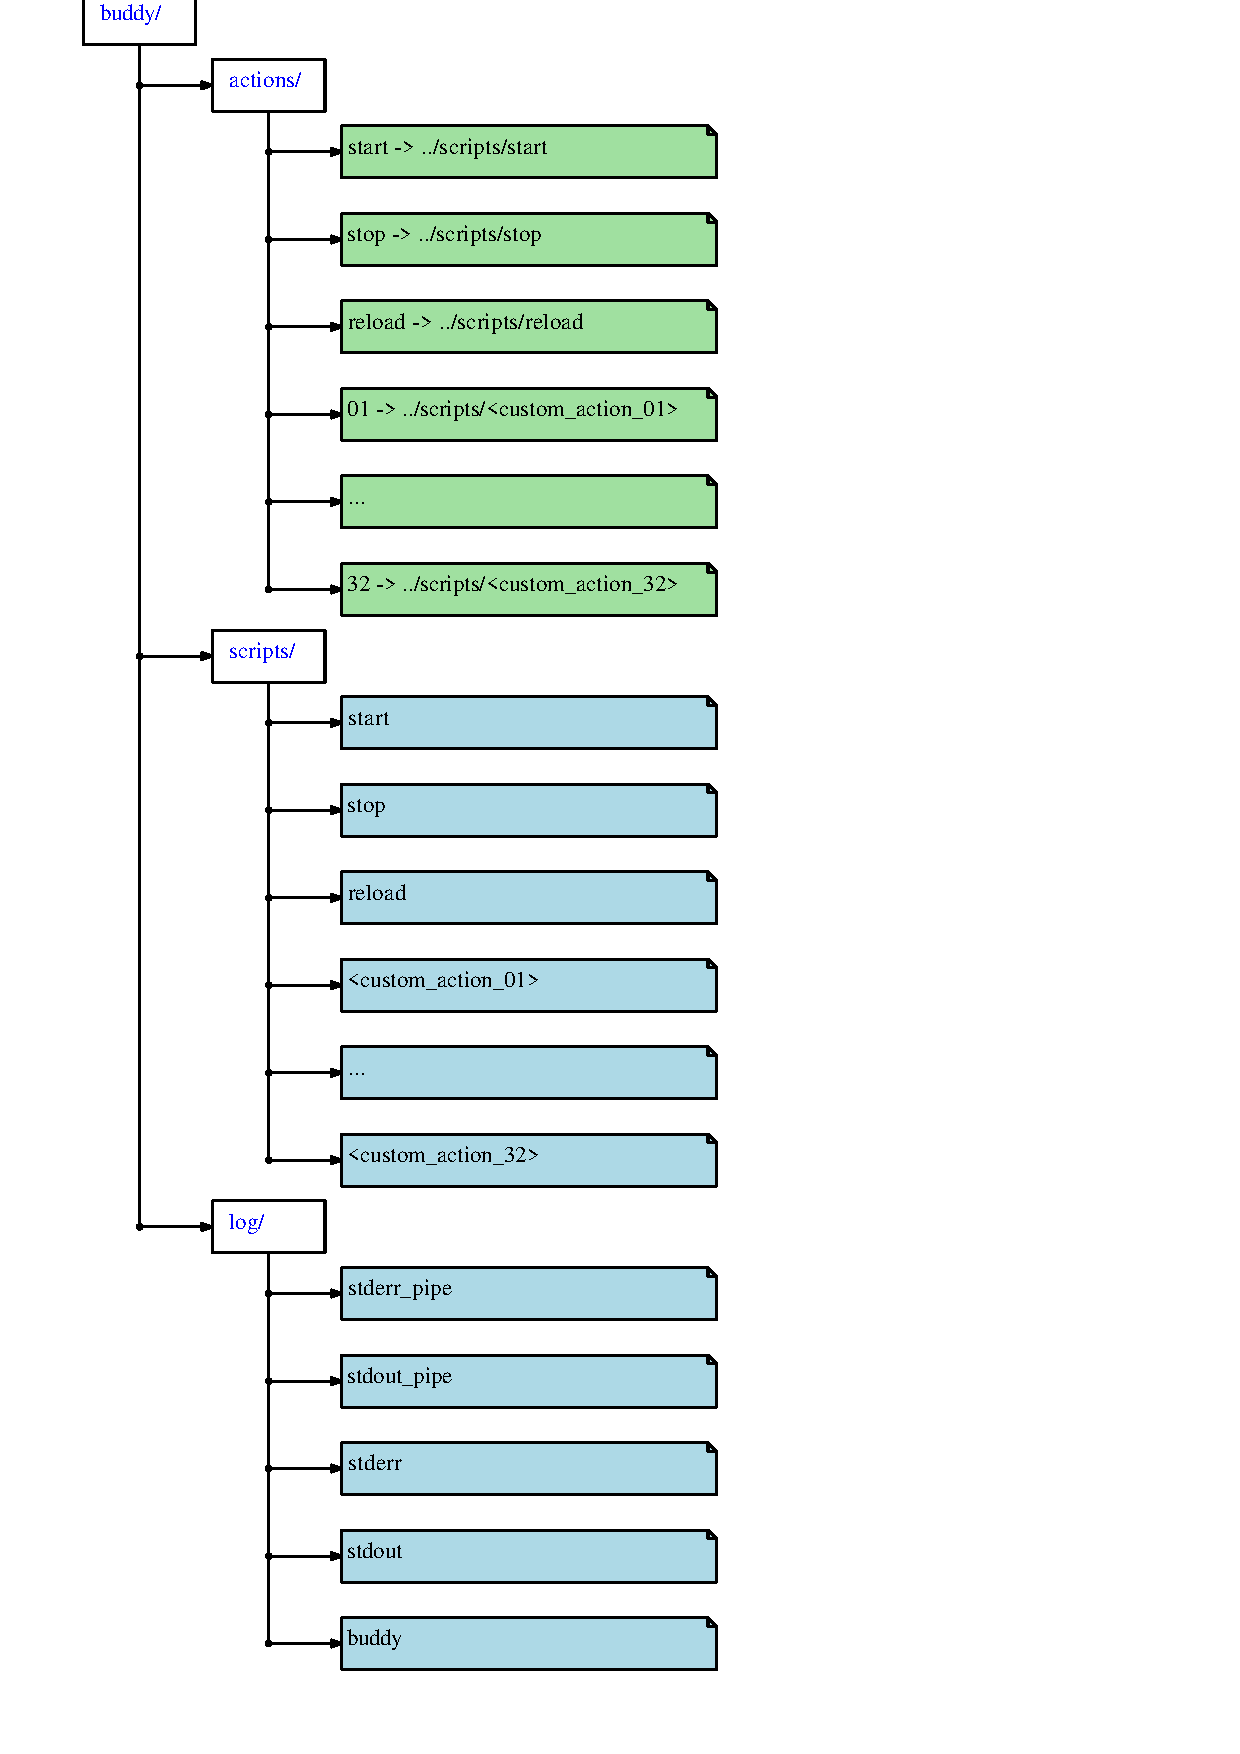
\includegraphics[width=\textwidth]{dot_inline_dotgraph_2}}
\end{DoxyImageNoCaption}
\end{center}


Clients consist of things like \char`\"{}uptop\char`\"{}, which is a status reporting tool that is similar to the common \char`\"{}top\char`\"{} utility. Clients communicate with controller via the API provided in libupkeeper. Hence, you can easily create any client you require, including metrics reporting and/or monitoring and alerting systems.

To explain this, the following sequence chart demonstrates how the components interact:

Start a managed process:

\begin{center}

\begin{DoxyImageNoCaption}  \mbox{\includegraphics{inline_mscgraph_1}}
\end{DoxyImageNoCaption}
\end{center}


Whereas a read-\/only process, such as subscribing to, and receiving events over time would look like this:

\begin{center}

\begin{DoxyImageNoCaption}  \mbox{\includegraphics{inline_mscgraph_2}}
\end{DoxyImageNoCaption}
\end{center}
\section{Sample Configuration.}\label{index_sampleconfig}
\begin{DoxyVerb}
{
    // StateDir
    // Path to variable state-dir for controller and buddies
    "StateDir": "/usr/var/upkeeper",

    // SvcConfigPath
    // Path to location of service configuration files
    "SvcConfigPath": "/usr/etc/upkeeper.d",

    // SvcRunPath
    // Path to location to setup and run buddies
    "SvcRunPath": "/usr/var/upkeeper/buddies",

    // Path to the buddy executable
    "UpkBuddyPath": "/usr/libexec/upk_buddy",

    // How frequently buddy sockets should be polled for events
    // in seconds and fractions of a second
    "BuddyPollingInterval": 0.5,

    // ServiceDefaults:
    "ServiceDefaults": {
        // An array of strings (['foo','bar']) describing what this service provides. These are then used in ordering service
        // startup via prerequisites. Service name, package, and UUID are implicitely added to the list of Provides.
        "Provides": [],

        // A valid UUID for the service, will be automatically generated if not provided.
        "UUID": Null,

        // A brief description of the service
        "ShortDescription": Null,

        // A longer and more complete description of the service
        "LongDescription": Null,

        // An array of strings (['foo','uuid#<...>']) of what must already be running (as named in 'Provides')
        // before this service should start. The syntax <package-name>:<service-name> may be used to specify a service from
        // a specific package. The syntax 'uuid#<uuid-string>' can be used to specify an explicit UUID.
        "Prerequisites": [],

        // Numeric start priority, used in lieu of, or in conjunction with Provides/Prerequisites to determine start order
        "StartPriority": 0,

        // Shutdown timeout before resorting to SIGKILL, Values < 0 will never SIGKILL
        "KillTimeout": 60,

        // Maximum number of times a process may fail in-a-row before its state is changed to down
        // a negative value indicates to restart forever (and is the default)
        "MaxConsecutiveFailures": -1,

        // user-defined max number of restarts within restart window
        "UserMaxRestarts": Null,

        // User-defined restart window, in seconds
        "UserRestartWindow": Null,

        // duration, in seconds, to wait between respawn attempts
        "UserRateLimit": Null,

        // a flag to enable/disable adding a randomized jitter to the user_ratelimit
        "RandomizeRateLimit": false,

        // if controller and/or buddy is run euid root; which uid to run the service as
        "SetUID": 0,

        // if controller and/or buddy is run euid root; which gid to run the service as
        "SetGID": 0,

        // size of the ringbuffer to maintain in the buddy
        "RingbufferSize": 64,

        // number of times to retry connections to the controler when emergent actions
        // occur in the buddy; (-1 for indefinate)
        "ReconnectRetries": 10,

        // command to exec for start, see 'StartScript'
        "ExecStart": Null,

        // script to start the monitored process; The default is 'exec %(EXEC_START)'
        "StartScript": "#!/bin/sh\nexec %(EXEC_START)\n",

        // command to exec for stop. Default: 'kill', see 'StopScript'
        "ExecStop": "kill",

        // Script to stop the monitored process. The default is 'exec %(EXEC_STOP) $1'; where $1 passed
        // to it will be the pid of monitored process (and also the pgrp, and sid, unless the monitored process changed them
        "StopScript": "#!/bin/sh\nexec %(EXEC_STOP) $1\n",

        // command to exec for reload. Default: 'kill -HUP', see 'ReloadScript'
        "ExecReload": "kill -HUP",

        // Script to reload the monitored process. The default is 'exec %(EXEC_RELOAD) $1'; where $1 passed
        // to it will be the pid of monitored process (and also the pgrp, and sid, unless the monitored process changed them
        "ReloadScript": "#!/bin/sh\nexec %(EXEC_RELOAD) $1\n",

        // A collection of key/value (JSON Object: {"foo":"bar"}) pairs where the key is the name of the action, and
        // the value is the contents of a script script to run for that action
        "CustomActions": {},

        // optional script to pipe stdout to. For example: 'exec logger -p local0.notice'
        "PipeStdoutScript": Null,

        // optional script to pipe stderr to. For example: 'exec logger -p local0.warn'
        "PipeStderrScript": Null,

        // optional place to direct stdout.
        // Note that if you pipe stdout elsewhere, this might never be written to, unless the thing you pipe to prints
        // to stdout itself
        "RedirectStdout": Null,

        // optional place to direct stderr.
        // Note that if you pipe stderr elsewhere, this might never be written to, unless the thing you pipe to prints
        // to stderr itself
        "RedirectStderr": Null,

        // state the service should be set to initially. this is used only when a service is first configured.
        "InitialState": "stopped",

        // May be used by a package to instruct the controler to remove a configured service
        // if the file defining that service ever disappears. Possibly useful in packaging
        // to cleanup the controller on package removal. The default behavior is to ignore
        // file removal, and require explicit manual removal of configured services
        "UnconfigureOnFileRemoval": false,

        // If the controller starts/restarts, and buddy has a service state set to 'stopped',
        // but controller's data-store believes the service should be running, prefer
        // buddy's world view, and update the data-store to reflect the stopped state.
        // The default is to trust the data-store; which would cause the service to be started
        "PreferBuddyStateForStopped": false,

        // if the controller starts/restarts, and buddy has a service state set to 'running',
        // but controller's data-store believes the service should be stopped, prefer
        // buddy's world view, and update the data-store to reflect the running state.
        // The default is to trust the buddy, which would leave the service running
        "PreferBuddyStateForRunning": true,
    },
}
\end{DoxyVerb}
 
\chapter{Module Index}
\section{Modules}
Here is a list of all modules:\begin{DoxyCompactList}
\item \contentsline{section}{Config\_\-impl}{\pageref{group__config__impl}}{}
\begin{DoxyCompactList}
\item \contentsline{section}{Services}{\pageref{group__services}}{}
\item \contentsline{section}{Controller}{\pageref{group__controller}}{}
\item \contentsline{section}{Functions}{\pageref{group__functions}}{}
\end{DoxyCompactList}
\item \contentsline{section}{Upk\_\-errors}{\pageref{group__upk__errors}}{}
\item \contentsline{section}{Upk\_\-network}{\pageref{group__upk__network}}{}
\item \contentsline{section}{Client\_\-protocol}{\pageref{group__client__protocol}}{}
\item \contentsline{section}{Uuid}{\pageref{group__uuid}}{}
\begin{DoxyCompactList}
\item \contentsline{section}{Uuid\_\-functions}{\pageref{group__uuid__functions}}{}
\end{DoxyCompactList}
\end{DoxyCompactList}

\chapter{Data Structure Index}
\section{libupkeeper Data Structures}
Here are the data structures with brief descriptions:\begin{CompactList}
\item\contentsline{section}{\bf{\_\-upk\_\-controller\_\-config} (Controller configuration )}{\pageref{struct__upk__controller__config}}{}
\item\contentsline{section}{\bf{\_\-upk\_\-cust\_\-actscr\_\-list} (Linked list of custom action scripts )}{\pageref{struct__upk__cust__actscr__list}}{}
\item\contentsline{section}{\bf{\_\-upk\_\-json\_\-type\_\-handlers} }{\pageref{struct__upk__json__type__handlers}}{}
\item\contentsline{section}{\bf{\_\-upk\_\-svc\_\-desc} (Service configuration )}{\pageref{struct__upk__svc__desc}}{}
\item\contentsline{section}{\bf{\_\-upk\_\-svcinfo} (See definition in $\ast$protocol\_\-fields.h )}{\pageref{struct__upk__svcinfo}}{}
\item\contentsline{section}{\bf{\_\-upk\_\-svclist} (Linked list of service identifiers )}{\pageref{struct__upk__svclist}}{}
\item\contentsline{section}{\bf{\_\-upk\_\-uuid} (Structure for holding 16 byte UUID )}{\pageref{struct__upk__uuid}}{}
\item\contentsline{section}{\bf{upk\_\-ack\_\-repl\_\-t} }{\pageref{structupk__ack__repl__t}}{}
\item\contentsline{section}{\bf{upk\_\-action\_\-req\_\-t} }{\pageref{structupk__action__req__t}}{}
\item\contentsline{section}{\bf{upk\_\-cancel\_\-pubmsg\_\-t} }{\pageref{structupk__cancel__pubmsg__t}}{}
\item\contentsline{section}{\bf{upk\_\-discon\_\-req\_\-t} }{\pageref{structupk__discon__req__t}}{}
\item\contentsline{section}{\bf{upk\_\-error\_\-repl\_\-t} }{\pageref{structupk__error__repl__t}}{}
\item\contentsline{section}{\bf{upk\_\-json\_\-obj\_\-iter} }{\pageref{structupk__json__obj__iter}}{}
\item\contentsline{section}{\bf{upk\_\-list\_\-req\_\-t} }{\pageref{structupk__list__req__t}}{}
\item\contentsline{section}{\bf{upk\_\-listing\_\-repl\_\-t} }{\pageref{structupk__listing__repl__t}}{}
\item\contentsline{section}{\bf{upk\_\-packet\_\-t} }{\pageref{structupk__packet__t}}{}
\item\contentsline{section}{\bf{upk\_\-protocol\_\-handle\_\-t} }{\pageref{structupk__protocol__handle__t}}{}
\item\contentsline{section}{\bf{upk\_\-pub\_\-pubmsg\_\-t} }{\pageref{structupk__pub__pubmsg__t}}{}
\item\contentsline{section}{\bf{upk\_\-repl\_\-preamble\_\-t} }{\pageref{structupk__repl__preamble__t}}{}
\item\contentsline{section}{\bf{upk\_\-repl\_\-seq\_\-end\_\-t} }{\pageref{structupk__repl__seq__end__t}}{}
\item\contentsline{section}{\bf{upk\_\-repl\_\-seq\_\-start\_\-t} }{\pageref{structupk__repl__seq__start__t}}{}
\item\contentsline{section}{\bf{upk\_\-req\_\-preamble\_\-t} }{\pageref{structupk__req__preamble__t}}{}
\item\contentsline{section}{\bf{upk\_\-req\_\-seq\_\-end\_\-t} }{\pageref{structupk__req__seq__end__t}}{}
\item\contentsline{section}{\bf{upk\_\-req\_\-seq\_\-start\_\-t} }{\pageref{structupk__req__seq__start__t}}{}
\item\contentsline{section}{\bf{upk\_\-result\_\-repl\_\-t} }{\pageref{structupk__result__repl__t}}{}
\item\contentsline{section}{\bf{upk\_\-signal\_\-req\_\-t} }{\pageref{structupk__signal__req__t}}{}
\item\contentsline{section}{\bf{upk\_\-status\_\-req\_\-t} }{\pageref{structupk__status__req__t}}{}
\item\contentsline{section}{\bf{upk\_\-subscr\_\-req\_\-t} }{\pageref{structupk__subscr__req__t}}{}
\item\contentsline{section}{\bf{upk\_\-svcinfo\_\-repl\_\-t} }{\pageref{structupk__svcinfo__repl__t}}{}
\item\contentsline{section}{\bf{upk\_\-unsubs\_\-req\_\-t} }{\pageref{structupk__unsubs__req__t}}{}
\item\contentsline{section}{\bf{v0\_\-ack\_\-repl\_\-t} }{\pageref{structv0__ack__repl__t}}{}
\item\contentsline{section}{\bf{v0\_\-action\_\-req\_\-t} }{\pageref{structv0__action__req__t}}{}
\item\contentsline{section}{\bf{v0\_\-cancel\_\-pubmsg\_\-t} }{\pageref{structv0__cancel__pubmsg__t}}{}
\item\contentsline{section}{\bf{v0\_\-discon\_\-req\_\-t} }{\pageref{structv0__discon__req__t}}{}
\item\contentsline{section}{\bf{v0\_\-error\_\-repl\_\-t} }{\pageref{structv0__error__repl__t}}{}
\item\contentsline{section}{\bf{v0\_\-list\_\-req\_\-t} }{\pageref{structv0__list__req__t}}{}
\item\contentsline{section}{\bf{v0\_\-listing\_\-repl\_\-t} }{\pageref{structv0__listing__repl__t}}{}
\item\contentsline{section}{\bf{v0\_\-pub\_\-pubmsg\_\-t} }{\pageref{structv0__pub__pubmsg__t}}{}
\item\contentsline{section}{\bf{v0\_\-repl\_\-seq\_\-end\_\-t} }{\pageref{structv0__repl__seq__end__t}}{}
\item\contentsline{section}{\bf{v0\_\-repl\_\-seq\_\-start\_\-t} }{\pageref{structv0__repl__seq__start__t}}{}
\item\contentsline{section}{\bf{v0\_\-req\_\-seq\_\-end\_\-t} }{\pageref{structv0__req__seq__end__t}}{}
\item\contentsline{section}{\bf{v0\_\-req\_\-seq\_\-start\_\-t} }{\pageref{structv0__req__seq__start__t}}{}
\item\contentsline{section}{\bf{v0\_\-result\_\-repl\_\-t} }{\pageref{structv0__result__repl__t}}{}
\item\contentsline{section}{\bf{v0\_\-signal\_\-req\_\-t} }{\pageref{structv0__signal__req__t}}{}
\item\contentsline{section}{\bf{v0\_\-status\_\-req\_\-t} }{\pageref{structv0__status__req__t}}{}
\item\contentsline{section}{\bf{v0\_\-subscr\_\-req\_\-t} }{\pageref{structv0__subscr__req__t}}{}
\item\contentsline{section}{\bf{v0\_\-svcinfo\_\-repl\_\-t} }{\pageref{structv0__svcinfo__repl__t}}{}
\item\contentsline{section}{\bf{v0\_\-svcinfo\_\-t} }{\pageref{structv0__svcinfo__t}}{}
\item\contentsline{section}{\bf{v0\_\-unsubs\_\-req\_\-t} }{\pageref{structv0__unsubs__req__t}}{}
\end{CompactList}

\chapter{File Index}
\section{File List}
Here is a list of all files with brief descriptions:\begin{DoxyCompactList}
\item\contentsline{section}{clients/{\bf upk.c} }{\pageref{upk_8c}}{}
\item\contentsline{section}{clients/{\bf upk\_\-reload.c} }{\pageref{upk__reload_8c}}{}
\item\contentsline{section}{clients/{\bf upk\_\-start.b.c} }{\pageref{upk__start_8b_8c}}{}
\item\contentsline{section}{clients/{\bf upk\_\-start.c} }{\pageref{upk__start_8c}}{}
\item\contentsline{section}{clients/{\bf upk\_\-stop.c} }{\pageref{upk__stop_8c}}{}
\item\contentsline{section}{controller/{\bf buddy.c} }{\pageref{buddy_8c}}{}
\item\contentsline{section}{controller/{\bf buddy.h} }{\pageref{buddy_8h}}{}
\item\contentsline{section}{controller/{\bf buddy\_\-main.c} }{\pageref{buddy__main_8c}}{}
\item\contentsline{section}{controller/{\bf buddyinc.h} }{\pageref{buddyinc_8h}}{}
\item\contentsline{section}{controller/{\bf config.c} }{\pageref{controller_2config_8c}}{}
\item\contentsline{section}{controller/{\bf controller.c} }{\pageref{controller_2controller_8c}}{}
\item\contentsline{section}{controller/{\bf controller.h} }{\pageref{controller_8h}}{}
\item\contentsline{section}{controller/{\bf controller\_\-main.c} }{\pageref{controller__main_8c}}{}
\item\contentsline{section}{controller/{\bf ctrl\_\-buddy.c} }{\pageref{ctrl__buddy_8c}}{}
\item\contentsline{section}{controller/{\bf ctrl\_\-eventloop.c} }{\pageref{ctrl__eventloop_8c}}{}
\item\contentsline{section}{controller/{\bf ctrl\_\-protocol.c} }{\pageref{ctrl__protocol_8c}}{}
\item\contentsline{section}{controller/{\bf ctrl\_\-protocol.h} (Types used to communicate with buddy )}{\pageref{ctrl__protocol_8h}}{}
\item\contentsline{section}{libupkeeper/{\bf json.c} }{\pageref{json_8c}}{}
\item\contentsline{section}{libupkeeper/{\bf s.c} }{\pageref{s_8c}}{}
\item\contentsline{section}{libupkeeper/{\bf upkeeper.h} }{\pageref{upkeeper_8h}}{}
\item\contentsline{section}{libupkeeper/tests/{\bf config.c} }{\pageref{libupkeeper_2tests_2config_8c}}{}
\item\contentsline{section}{libupkeeper/tests/{\bf dlinked\_\-lists.c} }{\pageref{dlinked__lists_8c}}{}
\item\contentsline{section}{libupkeeper/tests/{\bf json.c} }{\pageref{tests_2json_8c}}{}
\item\contentsline{section}{libupkeeper/tests/{\bf linked\_\-lists.c} }{\pageref{linked__lists_8c}}{}
\item\contentsline{section}{libupkeeper/tests/{\bf tskel.c} }{\pageref{tskel_8c}}{}
\item\contentsline{section}{libupkeeper/tests/{\bf upk\_\-protocol\_\-helpers.c} }{\pageref{upk__protocol__helpers_8c}}{}
\item\contentsline{section}{libupkeeper/tests/{\bf upk\_\-protocol\_\-serializers.c} }{\pageref{upk__protocol__serializers_8c}}{}
\item\contentsline{section}{libupkeeper/tests/{\bf util.c} }{\pageref{util_8c}}{}
\item\contentsline{section}{libupkeeper/tests/{\bf uuid.c} }{\pageref{tests_2uuid_8c}}{}
\item\contentsline{section}{libupkeeper/tests/{\bf v0\_\-protocol\_\-generic\_\-value\_\-checks.inc.c} }{\pageref{v0__protocol__generic__value__checks_8inc_8c}}{}
\item\contentsline{section}{libupkeeper/tests/{\bf v0\_\-protocol\_\-helpers.c} }{\pageref{v0__protocol__helpers_8c}}{}
\item\contentsline{section}{libupkeeper/tests/{\bf v0\_\-protocol\_\-serializers.c} }{\pageref{v0__protocol__serializers_8c}}{}
\item\contentsline{section}{libupkeeper/upkeeper/{\bf controller.c} }{\pageref{libupkeeper_2upkeeper_2controller_8c}}{}
\item\contentsline{section}{libupkeeper/upkeeper/{\bf upk\_\-client.c} (Public client API )}{\pageref{upk__client_8c}}{}
\item\contentsline{section}{libupkeeper/upkeeper/{\bf upk\_\-client.h} }{\pageref{upk__client_8h}}{}
\item\contentsline{section}{libupkeeper/upkeeper/{\bf upk\_\-client\_\-net.c} }{\pageref{upk__client__net_8c}}{}
\item\contentsline{section}{libupkeeper/upkeeper/{\bf upk\_\-client\_\-net.h} }{\pageref{upk__client__net_8h}}{}
\item\contentsline{section}{libupkeeper/upkeeper/{\bf upk\_\-compat.c} }{\pageref{upk__compat_8c}}{}
\item\contentsline{section}{libupkeeper/upkeeper/{\bf upk\_\-compat.h} }{\pageref{upk__compat_8h}}{}
\item\contentsline{section}{libupkeeper/upkeeper/{\bf upk\_\-config.c} (Configuration defaults, and implementation )}{\pageref{upk__config_8c}}{}
\item\contentsline{section}{libupkeeper/upkeeper/{\bf upk\_\-config.h} (Configuration implementation for controller and services )}{\pageref{upk__config_8h}}{}
\item\contentsline{section}{libupkeeper/upkeeper/{\bf upk\_\-crc32.c} }{\pageref{upk__crc32_8c}}{}
\item\contentsline{section}{libupkeeper/upkeeper/{\bf upk\_\-crc32.h} }{\pageref{upk__crc32_8h}}{}
\item\contentsline{section}{libupkeeper/upkeeper/{\bf upk\_\-error.c} }{\pageref{upk__error_8c}}{}
\item\contentsline{section}{libupkeeper/upkeeper/{\bf upk\_\-error.h} (Handle errors and single-\/exit-\/point semantics )}{\pageref{upk__error_8h}}{}
\item\contentsline{section}{libupkeeper/upkeeper/{\bf upk\_\-include.h} }{\pageref{upk__include_8h}}{}
\item\contentsline{section}{libupkeeper/upkeeper/{\bf upk\_\-json.c} }{\pageref{upk__json_8c}}{}
\item\contentsline{section}{libupkeeper/upkeeper/{\bf upk\_\-json.h} }{\pageref{upk__json_8h}}{}
\item\contentsline{section}{libupkeeper/upkeeper/{\bf upk\_\-json\_\-fmt.h} }{\pageref{upk__json__fmt_8h}}{}
\item\contentsline{section}{libupkeeper/upkeeper/{\bf upk\_\-network.c} }{\pageref{upk__network_8c}}{}
\item\contentsline{section}{libupkeeper/upkeeper/{\bf upk\_\-network.h} }{\pageref{upk__network_8h}}{}
\item\contentsline{section}{libupkeeper/upkeeper/{\bf upk\_\-network\_\-types.h} }{\pageref{upk__network__types_8h}}{}
\item\contentsline{section}{libupkeeper/upkeeper/{\bf upk\_\-protocol.c} }{\pageref{upk__protocol_8c}}{}
\item\contentsline{section}{libupkeeper/upkeeper/{\bf upk\_\-protocol.h} (UPK networking protocol )}{\pageref{upk__protocol_8h}}{}
\item\contentsline{section}{libupkeeper/upkeeper/{\bf upk\_\-protocol\_\-serializer.c} }{\pageref{upk__protocol__serializer_8c}}{}
\item\contentsline{section}{libupkeeper/upkeeper/{\bf upk\_\-std\_\-include.h} }{\pageref{upk__std__include_8h}}{}
\item\contentsline{section}{libupkeeper/upkeeper/{\bf upk\_\-types.h} (Types common throughout libupkeeper )}{\pageref{upk__types_8h}}{}
\item\contentsline{section}{libupkeeper/upkeeper/{\bf upk\_\-util.c} }{\pageref{upk__util_8c}}{}
\item\contentsline{section}{libupkeeper/upkeeper/{\bf upk\_\-util.h} }{\pageref{upk__util_8h}}{}
\item\contentsline{section}{libupkeeper/upkeeper/{\bf upk\_\-uuid.h} (Definition of upk uuid implementation )}{\pageref{upk__uuid_8h}}{}
\item\contentsline{section}{libupkeeper/upkeeper/{\bf upk\_\-v0\_\-protocol.c} (Version 0 of the protocol between clients and controlelr  protocol )}{\pageref{upk__v0__protocol_8c}}{}
\item\contentsline{section}{libupkeeper/upkeeper/{\bf upk\_\-v0\_\-protocol.h} }{\pageref{upk__v0__protocol_8h}}{}
\item\contentsline{section}{libupkeeper/upkeeper/{\bf upk\_\-v0\_\-protocol\_\-serializer.c} }{\pageref{upk__v0__protocol__serializer_8c}}{}
\item\contentsline{section}{libupkeeper/upkeeper/{\bf upk\_\-v0\_\-protocol\_\-structs.h} }{\pageref{upk__v0__protocol__structs_8h}}{}
\item\contentsline{section}{libupkeeper/upkeeper/{\bf uuid.c} }{\pageref{upkeeper_2uuid_8c}}{}
\end{DoxyCompactList}

\chapter{Module Documentation}
\section{Controller}
\label{group__controller}\index{Controller@{Controller}}
\subsection*{Data Structures}
\begin{CompactItemize}
\item 
struct \bf{\_\-upk\_\-controller\_\-config}
\begin{CompactList}\small\item\em controller configuration. \item\end{CompactList}\end{CompactItemize}
\subsection*{Typedefs}
\begin{CompactItemize}
\item 
typedef \bf{\_\-upk\_\-controller\_\-config} \bf{upk\_\-controller\_\-config\_\-t}
\begin{CompactList}\small\item\em controller configuration. \item\end{CompactList}\end{CompactItemize}


\subsection{Typedef Documentation}
\index{controller@{controller}!upk_controller_config_t@{upk\_\-controller\_\-config\_\-t}}
\index{upk_controller_config_t@{upk\_\-controller\_\-config\_\-t}!controller@{controller}}
\subsubsection{\setlength{\rightskip}{0pt plus 5cm}typedef struct \bf{\_\-upk\_\-controller\_\-config}  \bf{upk\_\-controller\_\-config\_\-t}}\label{group__controller_gc1cc1c2d639ac665502fdad59f7a92d5}


controller configuration. 


\section{API}
\label{group__API}\index{API@{API}}
\subsection*{Functions}
\begin{DoxyCompactItemize}
\item 
char $\ast$ {\bf upk\_\-clientid} (void)
\item 
bool {\bf upk\_\-client\_\-event\_\-hook} (void)
\end{DoxyCompactItemize}


\subsection{Function Documentation}
\index{API@{API}!upk\_\-client\_\-event\_\-hook@{upk\_\-client\_\-event\_\-hook}}
\index{upk\_\-client\_\-event\_\-hook@{upk\_\-client\_\-event\_\-hook}!API@{API}}
\subsubsection[{upk\_\-client\_\-event\_\-hook}]{\setlength{\rightskip}{0pt plus 5cm}bool upk\_\-client\_\-event\_\-hook (
\begin{DoxyParamCaption}
\item[{void}]{}
\end{DoxyParamCaption}
)}\label{group__API_ga93a0743ec8afde432503054a32bcd4dc}
\index{API@{API}!upk\_\-clientid@{upk\_\-clientid}}
\index{upk\_\-clientid@{upk\_\-clientid}!API@{API}}
\subsubsection[{upk\_\-clientid}]{\setlength{\rightskip}{0pt plus 5cm}char$\ast$ upk\_\-clientid (
\begin{DoxyParamCaption}
\item[{void}]{}
\end{DoxyParamCaption}
)}\label{group__API_gad5bda55978d99b1f4cfd3b7236d594cf}


References getpid(), upk\_\-getprogname, and UPK\_\-MAX\_\-STRING\_\-LEN.



Referenced by main(), and upk\_\-clnet\_\-req\_\-preamble().



Here is the call graph for this function:
\nopagebreak
\begin{figure}[H]
\begin{center}
\leavevmode
\includegraphics[width=190pt]{group__API_gad5bda55978d99b1f4cfd3b7236d594cf_cgraph}
\end{center}
\end{figure}




Here is the caller graph for this function:
\nopagebreak
\begin{figure}[H]
\begin{center}
\leavevmode
\includegraphics[width=270pt]{group__API_gad5bda55978d99b1f4cfd3b7236d594cf_icgraph}
\end{center}
\end{figure}



\section{Config\_\-impl}
\label{group__config__impl}\index{Config\_\-impl@{Config\_\-impl}}
Collaboration diagram for Config\_\-impl:\nopagebreak
\begin{figure}[H]
\begin{center}
\leavevmode
\includegraphics[width=208pt]{group__config__impl}
\end{center}
\end{figure}
\subsection*{Modules}
\begin{DoxyCompactItemize}
\item 
{\bf Services}
\item 
{\bf Controller}
\item 
{\bf Functions}
\end{DoxyCompactItemize}
\subsection*{Defines}
\begin{DoxyCompactItemize}
\item 
\#define {\bf \_\-joa}~json\_\-object\_\-object\_\-add
\item 
\#define {\bf jt\_\-string}~json\_\-type\_\-string
\item 
\#define {\bf jt\_\-int}~json\_\-type\_\-int
\item 
\#define {\bf jt\_\-boolean}~json\_\-type\_\-boolean
\item 
\#define {\bf jt\_\-array}~json\_\-type\_\-array
\end{DoxyCompactItemize}
\subsection*{Enumerations}
\begin{DoxyCompactItemize}
\item 
enum {\bf appender\_\-type\_\-t} \{ {\bf SVCID\_\-APPENDER} =  0, 
{\bf ACTION\_\-APPENDER}
 \}
\end{DoxyCompactItemize}
\subsection*{Functions}
\begin{DoxyCompactItemize}
\item 
static void {\bf upk\_\-svcconf\_\-svcid\_\-array\_\-appender} ({\bf upk\_\-json\_\-stack\_\-meta\_\-t} $\ast$meta, void $\ast$data, char $\ast$key, {\bf upk\_\-json\_\-val\_\-t} v)
\item 
static void {\bf upk\_\-svcconf\_\-setup\_\-array\_\-handlers} ({\bf upk\_\-json\_\-handlers\_\-t} $\ast$handlers)
\item 
static void {\bf upk\_\-svcconf\_\-array\_\-handler} ({\bf upk\_\-json\_\-stack\_\-meta\_\-t} $\ast$meta, void $\ast$data, char $\ast$key, {\bf upk\_\-json\_\-val\_\-t} v)
\item 
static void {\bf upk\_\-svcconf\_\-customaction\_\-array\_\-appender} ({\bf upk\_\-json\_\-stack\_\-meta\_\-t} $\ast$meta, void $\ast$data, char $\ast$key, {\bf upk\_\-json\_\-val\_\-t} v)
\item 
static void {\bf upk\_\-svcconf\_\-setup\_\-object\_\-handlers} ({\bf upk\_\-json\_\-handlers\_\-t} $\ast$handlers)
\item 
static void {\bf upk\_\-svcconf\_\-nested\_\-object\_\-handler} ({\bf upk\_\-json\_\-stack\_\-meta\_\-t} $\ast$meta, void $\ast$data, char $\ast$key, {\bf upk\_\-json\_\-val\_\-t} v)
\item 
static void {\bf upk\_\-svcconf\_\-setup\_\-handlers} ({\bf upk\_\-json\_\-handlers\_\-t} $\ast$handlers)
\item 
static void {\bf upk\_\-ctrlconf\_\-object\_\-handler} ({\bf upk\_\-json\_\-stack\_\-meta\_\-t} $\ast$meta, void $\ast$data, char $\ast$key, {\bf upk\_\-json\_\-val\_\-t} v)
\item 
static void {\bf upk\_\-ctrlconf\_\-string\_\-handler} ({\bf upk\_\-json\_\-stack\_\-meta\_\-t} $\ast$meta, void $\ast$data, char $\ast$key, {\bf upk\_\-json\_\-val\_\-t} v)
\item 
static void {\bf upk\_\-ctrlconf\_\-double\_\-handler} ({\bf upk\_\-json\_\-stack\_\-meta\_\-t} $\ast$meta, void $\ast$data, char $\ast$key, {\bf upk\_\-json\_\-val\_\-t} v)
\item 
static void {\bf upk\_\-ctrlconf\_\-toplvl\_\-obj} ({\bf upk\_\-json\_\-stack\_\-meta\_\-t} $\ast$meta, void $\ast$data, char $\ast$key, {\bf upk\_\-json\_\-val\_\-t} v)
\item 
static void {\bf upk\_\-svcconf\_\-object\_\-handler} ({\bf upk\_\-json\_\-stack\_\-meta\_\-t} $\ast$meta, void $\ast$data, char $\ast$key, {\bf upk\_\-json\_\-val\_\-t} v)
\item 
static void {\bf upk\_\-svcconf\_\-toplvl\_\-obj} ({\bf upk\_\-json\_\-stack\_\-meta\_\-t} $\ast$meta, void $\ast$data, char $\ast$key, {\bf upk\_\-json\_\-val\_\-t} v)
\item 
static void {\bf upk\_\-ctrlconf\_\-pack} ({\bf upk\_\-controller\_\-config\_\-t} $\ast$cfg, const char $\ast$json\_\-string)
\item 
static void {\bf upk\_\-svcconf\_\-bool\_\-handler} ({\bf upk\_\-json\_\-stack\_\-meta\_\-t} $\ast$meta, void $\ast$data, char $\ast$key, {\bf upk\_\-json\_\-val\_\-t} v)
\item 
static void {\bf upk\_\-svcconf\_\-int\_\-handler} ({\bf upk\_\-json\_\-stack\_\-meta\_\-t} $\ast$meta, void $\ast$data, char $\ast$key, {\bf upk\_\-json\_\-val\_\-t} v)
\item 
static void {\bf upk\_\-svcconf\_\-string\_\-handler} ({\bf upk\_\-json\_\-stack\_\-meta\_\-t} $\ast$meta, void $\ast$data, char $\ast$key, {\bf upk\_\-json\_\-val\_\-t} v)
\item 
static void {\bf upk\_\-conf\_\-error\_\-handler} ({\bf upk\_\-json\_\-stack\_\-meta\_\-t} $\ast$meta, void $\ast$data, char $\ast$key, {\bf upk\_\-json\_\-val\_\-t} v)
\item 
static char $\ast$ {\bf upk\_\-config\_\-loadfile} (const char $\ast$filename)
\item 
void {\bf upk\_\-svc\_\-desc\_\-free} ({\bf upk\_\-svc\_\-desc\_\-t} $\ast$svc)
\item 
void {\bf upk\_\-svclist\_\-free} ({\bf upk\_\-svc\_\-desc\_\-meta\_\-t} $\ast$svclist)
\item 
void {\bf upk\_\-ctrlconf\_\-free} ({\bf upk\_\-controller\_\-config\_\-t} $\ast$cfg)
\item 
void {\bf upk\_\-ctrl\_\-free\_\-config} (void)
\item 
static void {\bf upk\_\-ctrlconf\_\-int\_\-handler} ({\bf upk\_\-json\_\-stack\_\-meta\_\-t} $\ast$meta, void $\ast$data, char $\ast$key, {\bf upk\_\-json\_\-val\_\-t} v)
\item 
void {\bf upk\_\-svcconf\_\-pack} ({\bf upk\_\-controller\_\-config\_\-t} $\ast$cfg, const char $\ast$json\_\-string)
\item 
void {\bf upk\_\-ctrl\_\-load\_\-config} (void)
\item 
void {\bf upk\_\-svc\_\-desc\_\-clear} ({\bf upk\_\-svc\_\-desc\_\-t} $\ast$svc)
\item 
static void $\ast$ {\bf upk\_\-json\_\-serialize\_\-or\_\-null} (enum json\_\-type type, void $\ast$val)
\item 
char $\ast$ {\bf upk\_\-concat\_\-svcid} (char $\ast$dest, const char $\ast$pkg, const char $\ast$name)
\item 
char $\ast$ {\bf upk\_\-svc\_\-id} (char $\ast$dest, {\bf upk\_\-svc\_\-desc\_\-t} $\ast$svc)
\item 
void {\bf upk\_\-parse\_\-svc\_\-id} (char $\ast$key, {\bf upk\_\-svc\_\-desc\_\-t} $\ast$svc)
\item 
struct json\_\-object $\ast$ {\bf upk\_\-svclist\_\-to\_\-json\_\-obj} ({\bf upk\_\-svc\_\-desc\_\-meta\_\-t} $\ast$svclist)
\item 
struct json\_\-object $\ast$ {\bf upk\_\-svc\_\-desc\_\-to\_\-json\_\-obj} ({\bf upk\_\-svc\_\-desc\_\-t} $\ast$svc)
\item 
char $\ast$ {\bf upk\_\-json\_\-serialize\_\-svc\_\-config} ({\bf upk\_\-svc\_\-desc\_\-t} $\ast$svc, {\bf upk\_\-json\_\-data\_\-output\_\-opts\_\-t} opts)
\item 
void {\bf upk\_\-overlay\_\-svcconf\_\-values} ({\bf upk\_\-svc\_\-desc\_\-t} $\ast$dest, {\bf upk\_\-svc\_\-desc\_\-t} $\ast$high)
\item 
void {\bf upk\_\-overlay\_\-ctrlconf\_\-values} ({\bf upk\_\-controller\_\-config\_\-t} $\ast$dest, {\bf upk\_\-controller\_\-config\_\-t} $\ast$high)
\item 
void {\bf upk\_\-finalize\_\-svc\_\-desc} ({\bf upk\_\-svc\_\-desc\_\-t} $\ast$dest, {\bf upk\_\-svc\_\-desc\_\-t} $\ast$orig)
\item 
void {\bf upk\_\-load\_\-runtime\_\-service\_\-file} (const char $\ast$filename)
\item 
void {\bf upk\_\-load\_\-runtime\_\-services} (void)
\end{DoxyCompactItemize}
\subsection*{Variables}
\begin{DoxyCompactItemize}
\item 
char {\bf upk\_\-ctrl\_\-configuration\_\-file} [UPK\_\-MAX\_\-PATH\_\-LEN] = \char`\"{}/upkeeper.conf\char`\"{}
\item 
const char {\bf upk\_\-default\_\-configuration\_\-str} [$\,$] = \char`\"{}\}$\backslash$n\char`\"{}
\item 
{\bf upk\_\-controller\_\-config\_\-t} {\bf upk\_\-default\_\-configuration}
\item 
{\bf upk\_\-controller\_\-config\_\-t} {\bf upk\_\-file\_\-configuration}
\item 
{\bf upk\_\-controller\_\-config\_\-t} {\bf upk\_\-runtime\_\-configuration}
\end{DoxyCompactItemize}


\subsection{Define Documentation}
\index{Config\_\-impl@{Config\_\-impl}!\_\-joa@{\_\-joa}}
\index{\_\-joa@{\_\-joa}!Config_impl@{Config\_\-impl}}
\subsubsection[{\_\-joa}]{\setlength{\rightskip}{0pt plus 5cm}\#define \_\-joa~json\_\-object\_\-object\_\-add}\label{group__config__impl_gac8445621620fa3b4e61a39c9af92cce3}


Referenced by upk\_\-svc\_\-desc\_\-to\_\-json\_\-obj(), and upk\_\-svclist\_\-to\_\-json\_\-obj().

\index{Config\_\-impl@{Config\_\-impl}!jt\_\-array@{jt\_\-array}}
\index{jt\_\-array@{jt\_\-array}!Config_impl@{Config\_\-impl}}
\subsubsection[{jt\_\-array}]{\setlength{\rightskip}{0pt plus 5cm}\#define jt\_\-array~json\_\-type\_\-array}\label{group__config__impl_ga9180255338c47b6269f08158ba6574c2}


Referenced by upk\_\-svc\_\-desc\_\-to\_\-json\_\-obj().

\index{Config\_\-impl@{Config\_\-impl}!jt\_\-boolean@{jt\_\-boolean}}
\index{jt\_\-boolean@{jt\_\-boolean}!Config_impl@{Config\_\-impl}}
\subsubsection[{jt\_\-boolean}]{\setlength{\rightskip}{0pt plus 5cm}\#define jt\_\-boolean~json\_\-type\_\-boolean}\label{group__config__impl_gadbcd5a49cee9d0649ac2578803203df2}


Referenced by upk\_\-svc\_\-desc\_\-to\_\-json\_\-obj().

\index{Config\_\-impl@{Config\_\-impl}!jt\_\-int@{jt\_\-int}}
\index{jt\_\-int@{jt\_\-int}!Config_impl@{Config\_\-impl}}
\subsubsection[{jt\_\-int}]{\setlength{\rightskip}{0pt plus 5cm}\#define jt\_\-int~json\_\-type\_\-int}\label{group__config__impl_ga493a64297e93d490b06fee43ec1b4376}


Referenced by upk\_\-svc\_\-desc\_\-to\_\-json\_\-obj().

\index{Config\_\-impl@{Config\_\-impl}!jt\_\-string@{jt\_\-string}}
\index{jt\_\-string@{jt\_\-string}!Config_impl@{Config\_\-impl}}
\subsubsection[{jt\_\-string}]{\setlength{\rightskip}{0pt plus 5cm}\#define jt\_\-string~json\_\-type\_\-string}\label{group__config__impl_ga0e8e5860d56f25f6f5818c71acb9bdb0}


Referenced by upk\_\-svc\_\-desc\_\-to\_\-json\_\-obj().



\subsection{Enumeration Type Documentation}
\index{Config\_\-impl@{Config\_\-impl}!appender\_\-type\_\-t@{appender\_\-type\_\-t}}
\index{appender\_\-type\_\-t@{appender\_\-type\_\-t}!Config_impl@{Config\_\-impl}}
\subsubsection[{appender\_\-type\_\-t}]{\setlength{\rightskip}{0pt plus 5cm}enum {\bf appender\_\-type\_\-t}}\label{group__config__impl_ga9f4a3300bb80a1678b3eef21eedf723a}
\begin{Desc}
\item[Enumerator: ]\par
\begin{description}
\index{SVCID\_\-APPENDER@{SVCID\_\-APPENDER}!Config\_\-impl@{Config\_\-impl}}\index{Config\_\-impl@{Config\_\-impl}!SVCID\_\-APPENDER@{SVCID\_\-APPENDER}}\item[{\em 
SVCID\_\-APPENDER\label{group__config__impl_gga9f4a3300bb80a1678b3eef21eedf723aa0dc54f8f88a18fafe29c58ac49e6ca8b}
}]\index{ACTION\_\-APPENDER@{ACTION\_\-APPENDER}!Config\_\-impl@{Config\_\-impl}}\index{Config\_\-impl@{Config\_\-impl}!ACTION\_\-APPENDER@{ACTION\_\-APPENDER}}\item[{\em 
ACTION\_\-APPENDER\label{group__config__impl_gga9f4a3300bb80a1678b3eef21eedf723aab9100e38f00e9baba41192fc6725f47e}
}]\end{description}
\end{Desc}



\subsection{Function Documentation}
\index{Config\_\-impl@{Config\_\-impl}!upk\_\-concat\_\-svcid@{upk\_\-concat\_\-svcid}}
\index{upk\_\-concat\_\-svcid@{upk\_\-concat\_\-svcid}!Config_impl@{Config\_\-impl}}
\subsubsection[{upk\_\-concat\_\-svcid}]{\setlength{\rightskip}{0pt plus 5cm}char$\ast$ upk\_\-concat\_\-svcid (
\begin{DoxyParamCaption}
\item[{char $\ast$}]{dest, }
\item[{const char $\ast$}]{pkg, }
\item[{const char $\ast$}]{name}
\end{DoxyParamCaption}
)}\label{group__config__impl_gaed8f504cfc4e6b33df5b113bc5ef2177}


References UPK\_\-MAX\_\-STRING\_\-LEN.



Referenced by upk\_\-db\_\-add\_\-new\_\-service(), upk\_\-db\_\-insert\_\-cfg(), upk\_\-db\_\-upsert(), upk\_\-svc\_\-desc\_\-to\_\-json\_\-obj(), and upk\_\-svc\_\-id().



Here is the caller graph for this function:
\nopagebreak
\begin{figure}[H]
\begin{center}
\leavevmode
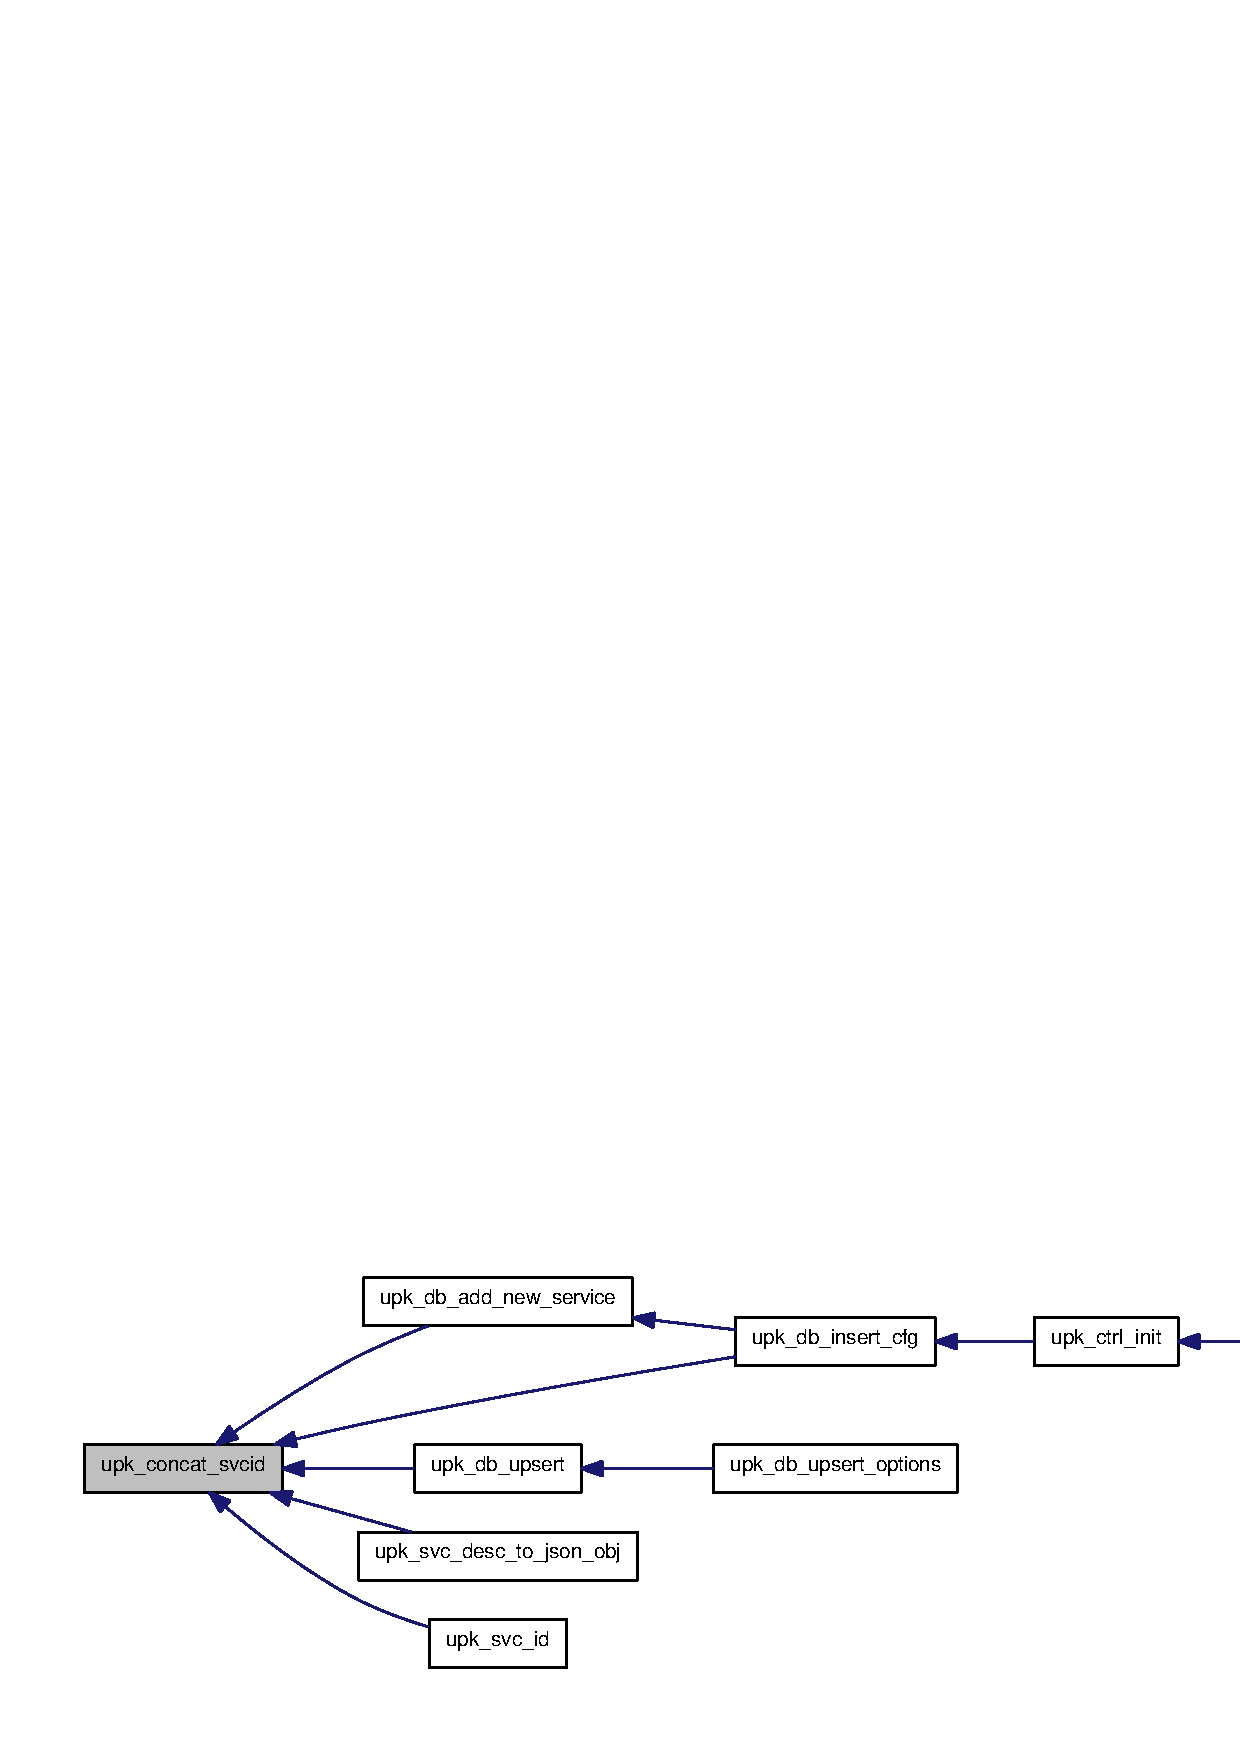
\includegraphics[width=400pt]{group__config__impl_gaed8f504cfc4e6b33df5b113bc5ef2177_icgraph}
\end{center}
\end{figure}


\index{Config\_\-impl@{Config\_\-impl}!upk\_\-conf\_\-error\_\-handler@{upk\_\-conf\_\-error\_\-handler}}
\index{upk\_\-conf\_\-error\_\-handler@{upk\_\-conf\_\-error\_\-handler}!Config_impl@{Config\_\-impl}}
\subsubsection[{upk\_\-conf\_\-error\_\-handler}]{\setlength{\rightskip}{0pt plus 5cm}static void upk\_\-conf\_\-error\_\-handler (
\begin{DoxyParamCaption}
\item[{{\bf upk\_\-json\_\-stack\_\-meta\_\-t} $\ast$}]{meta, }
\item[{void $\ast$}]{data, }
\item[{char $\ast$}]{key, }
\item[{{\bf upk\_\-json\_\-val\_\-t}}]{v}
\end{DoxyParamCaption}
)\hspace{0.3cm}{\ttfamily  [static]}}\label{group__config__impl_gadcd7b5da5ab2a52883bddee085d3acea}


References upk\_\-alert.



Referenced by upk\_\-ctrlconf\_\-pack(), upk\_\-ctrlconf\_\-toplvl\_\-obj(), upk\_\-svcconf\_\-pack(), upk\_\-svcconf\_\-setup\_\-array\_\-handlers(), upk\_\-svcconf\_\-setup\_\-handlers(), upk\_\-svcconf\_\-setup\_\-object\_\-handlers(), and upk\_\-svcconf\_\-toplvl\_\-obj().



Here is the caller graph for this function:
\nopagebreak
\begin{figure}[H]
\begin{center}
\leavevmode
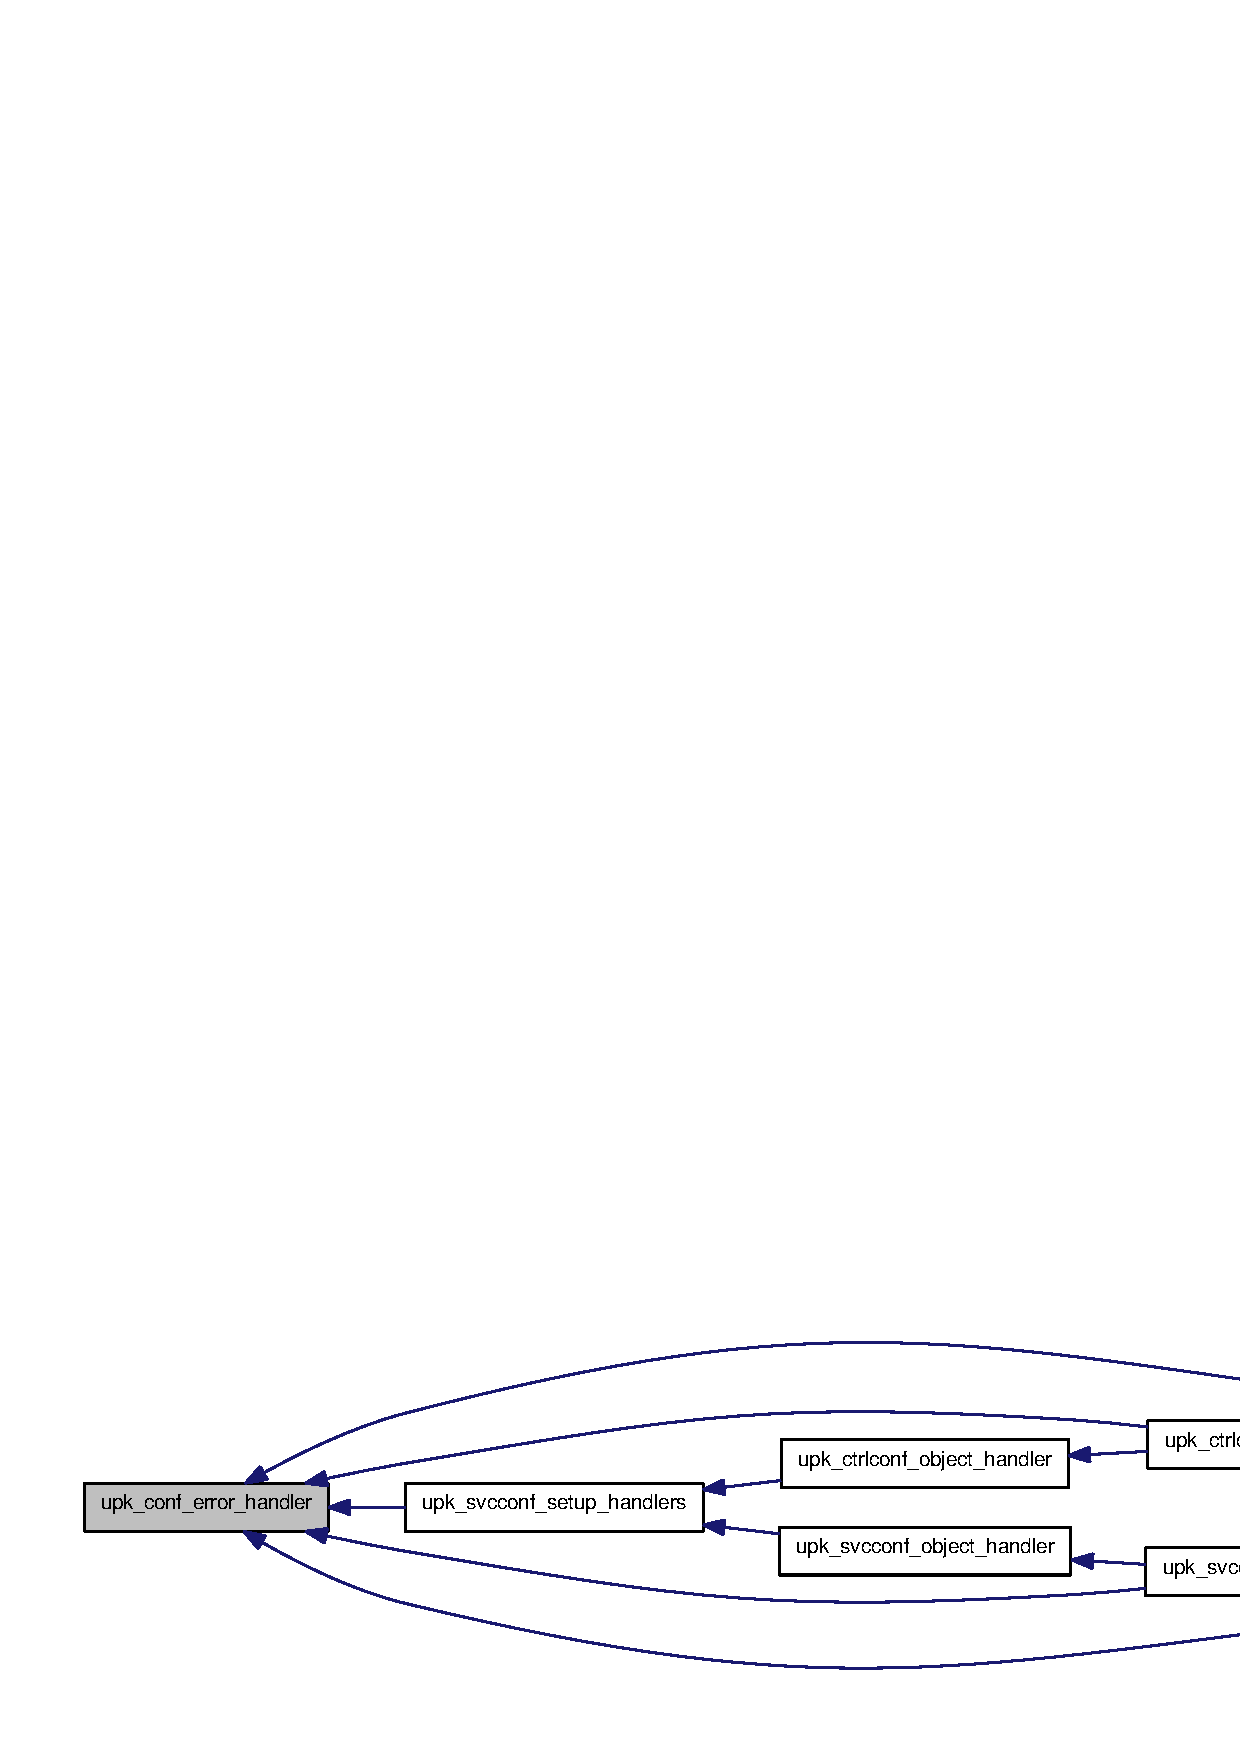
\includegraphics[width=400pt]{group__config__impl_gadcd7b5da5ab2a52883bddee085d3acea_icgraph}
\end{center}
\end{figure}


\index{Config\_\-impl@{Config\_\-impl}!upk\_\-config\_\-loadfile@{upk\_\-config\_\-loadfile}}
\index{upk\_\-config\_\-loadfile@{upk\_\-config\_\-loadfile}!Config_impl@{Config\_\-impl}}
\subsubsection[{upk\_\-config\_\-loadfile}]{\setlength{\rightskip}{0pt plus 5cm}static char $\ast$ upk\_\-config\_\-loadfile (
\begin{DoxyParamCaption}
\item[{const char $\ast$}]{filename}
\end{DoxyParamCaption}
)\hspace{0.3cm}{\ttfamily  [static]}}\label{group__config__impl_gadb1b4dc0c724b6c347fbecd16a8db684}


References calloc(), realloc(), strnlen(), upk\_\-debug1, upk\_\-default\_\-configuration\_\-str, UPK\_\-MAX\_\-STRING\_\-LEN, and upk\_\-warn.



Referenced by upk\_\-ctrl\_\-load\_\-config(), and upk\_\-load\_\-runtime\_\-services().



Here is the call graph for this function:
\nopagebreak
\begin{figure}[H]
\begin{center}
\leavevmode
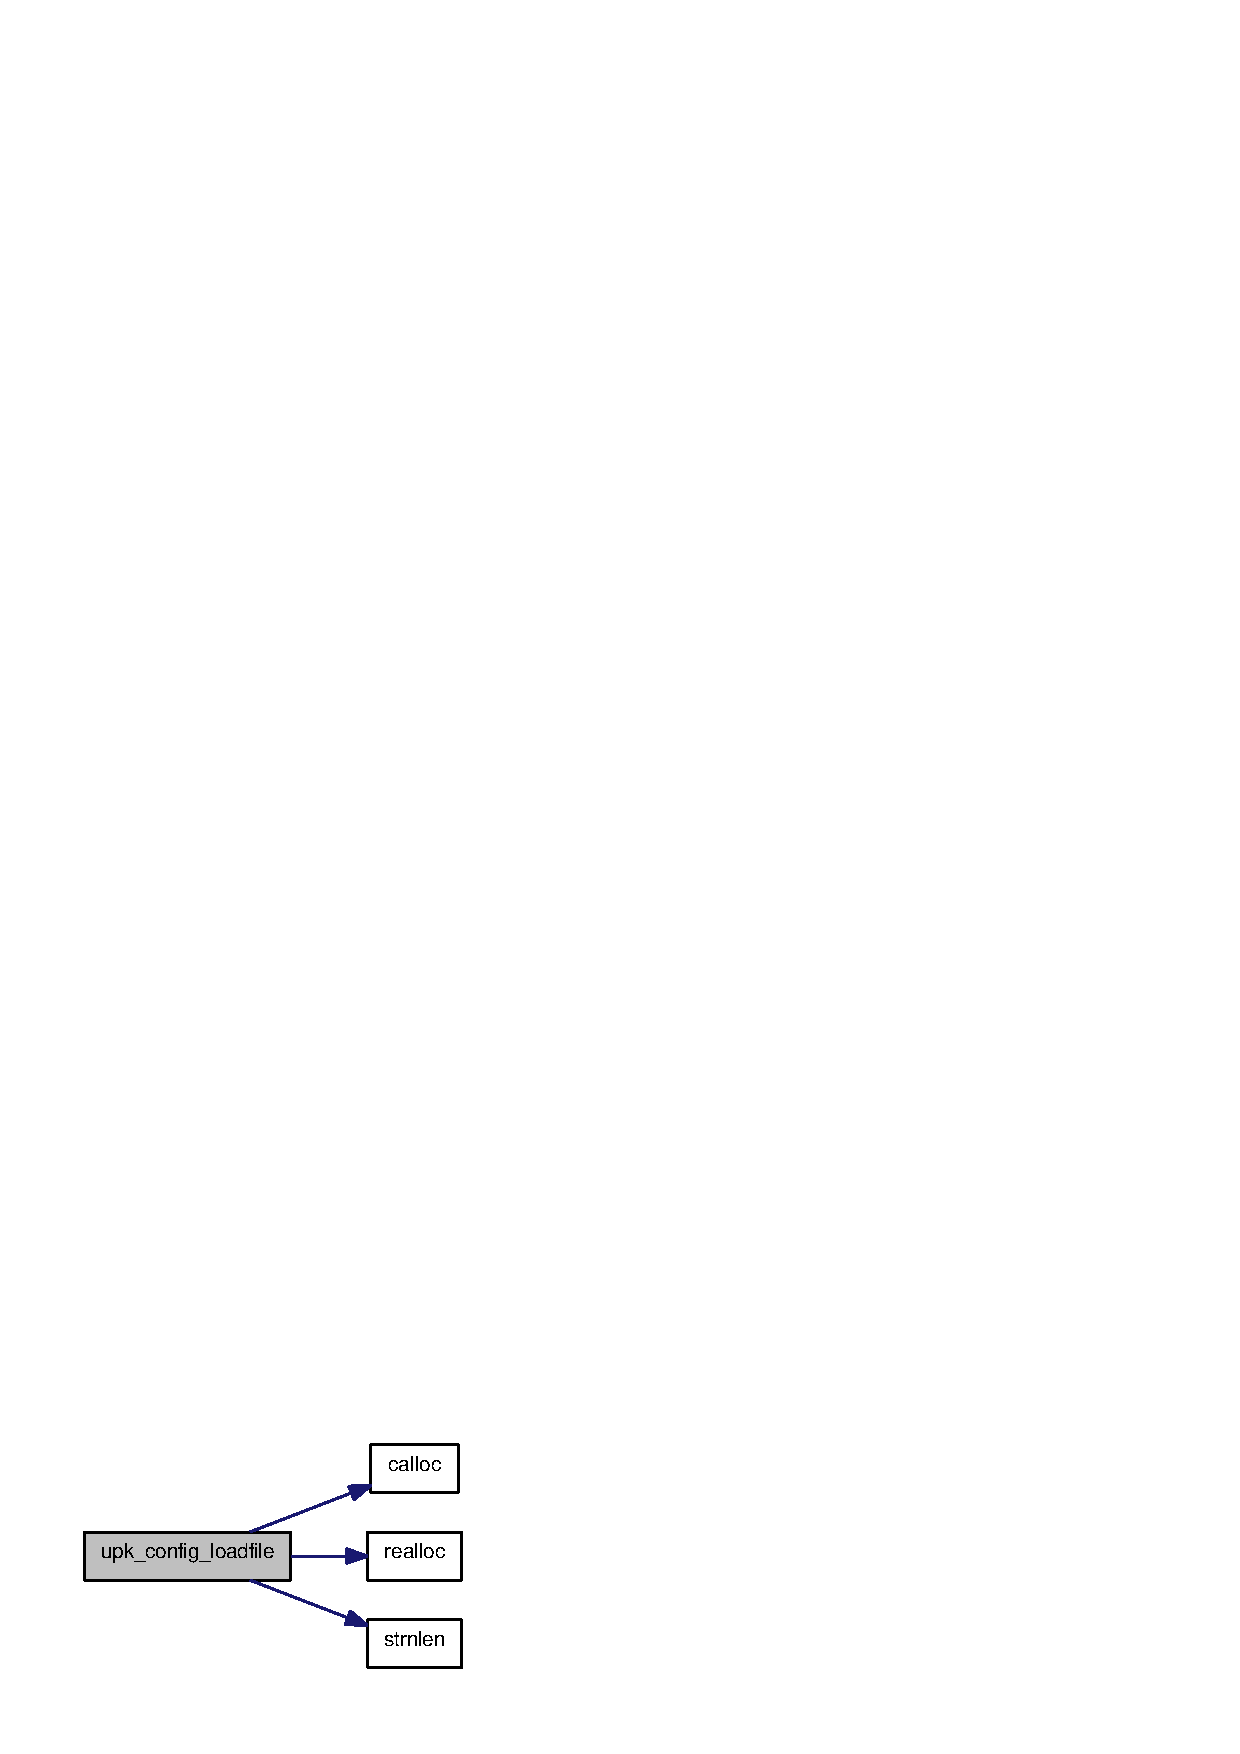
\includegraphics[width=226pt]{group__config__impl_gadb1b4dc0c724b6c347fbecd16a8db684_cgraph}
\end{center}
\end{figure}




Here is the caller graph for this function:
\nopagebreak
\begin{figure}[H]
\begin{center}
\leavevmode
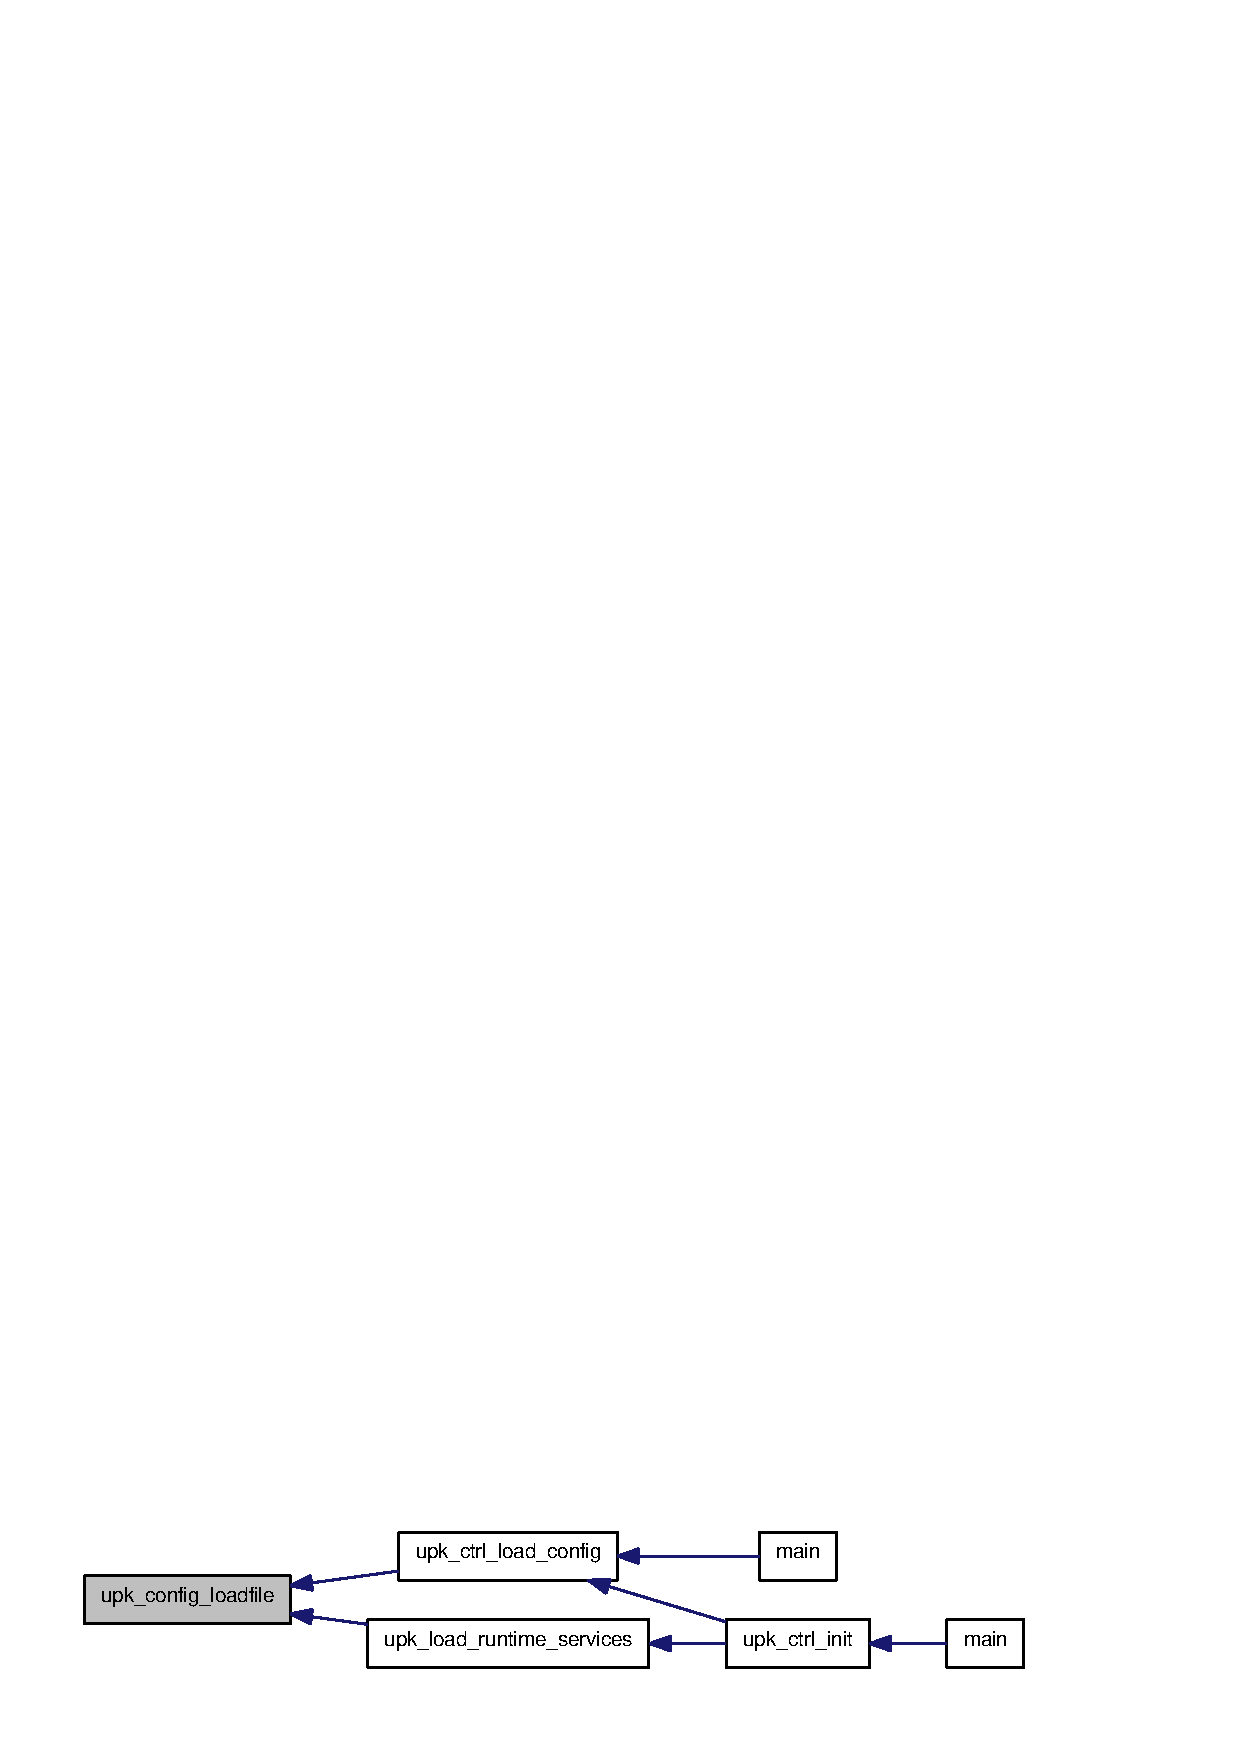
\includegraphics[width=316pt]{group__config__impl_gadb1b4dc0c724b6c347fbecd16a8db684_icgraph}
\end{center}
\end{figure}


\index{Config\_\-impl@{Config\_\-impl}!upk\_\-ctrl\_\-free\_\-config@{upk\_\-ctrl\_\-free\_\-config}}
\index{upk\_\-ctrl\_\-free\_\-config@{upk\_\-ctrl\_\-free\_\-config}!Config_impl@{Config\_\-impl}}
\subsubsection[{upk\_\-ctrl\_\-free\_\-config}]{\setlength{\rightskip}{0pt plus 5cm}void upk\_\-ctrl\_\-free\_\-config (
\begin{DoxyParamCaption}
\item[{void}]{}
\end{DoxyParamCaption}
)}\label{group__config__impl_ga386ddb0964c89347dbf6a2807ed1800e}


References upk\_\-ctrlconf\_\-free().



Referenced by main(), and upk\_\-ctrl\_\-exit().



Here is the call graph for this function:
\nopagebreak
\begin{figure}[H]
\begin{center}
\leavevmode
\includegraphics[width=276pt]{group__config__impl_ga386ddb0964c89347dbf6a2807ed1800e_cgraph}
\end{center}
\end{figure}




Here is the caller graph for this function:
\nopagebreak
\begin{figure}[H]
\begin{center}
\leavevmode
\includegraphics[width=400pt]{group__config__impl_ga386ddb0964c89347dbf6a2807ed1800e_icgraph}
\end{center}
\end{figure}


\index{Config\_\-impl@{Config\_\-impl}!upk\_\-ctrl\_\-load\_\-config@{upk\_\-ctrl\_\-load\_\-config}}
\index{upk\_\-ctrl\_\-load\_\-config@{upk\_\-ctrl\_\-load\_\-config}!Config_impl@{Config\_\-impl}}
\subsubsection[{upk\_\-ctrl\_\-load\_\-config}]{\setlength{\rightskip}{0pt plus 5cm}void upk\_\-ctrl\_\-load\_\-config (
\begin{DoxyParamCaption}
\item[{void}]{}
\end{DoxyParamCaption}
)}\label{group__config__impl_ga11c5a55e854fb56c864a12ef5d314798}


References \_\-upk\_\-controller\_\-config::BuddyPollingInterval, \_\-upk\_\-controller\_\-config::controller\_\-buddy\_\-sock, \_\-upk\_\-controller\_\-config::controller\_\-socket, free(), \_\-upk\_\-controller\_\-config::ServiceDefaults, \_\-upk\_\-controller\_\-config::StateDir, upk\_\-config\_\-loadfile(), upk\_\-ctrl\_\-configuration\_\-file, upk\_\-ctrlconf\_\-pack(), upk\_\-default\_\-configuration\_\-str, UPK\_\-MAX\_\-STRING\_\-LEN, upk\_\-overlay\_\-ctrlconf\_\-values(), and upk\_\-svc\_\-desc\_\-clear().



Referenced by main(), and upk\_\-ctrl\_\-init().



Here is the call graph for this function:
\nopagebreak
\begin{figure}[H]
\begin{center}
\leavevmode
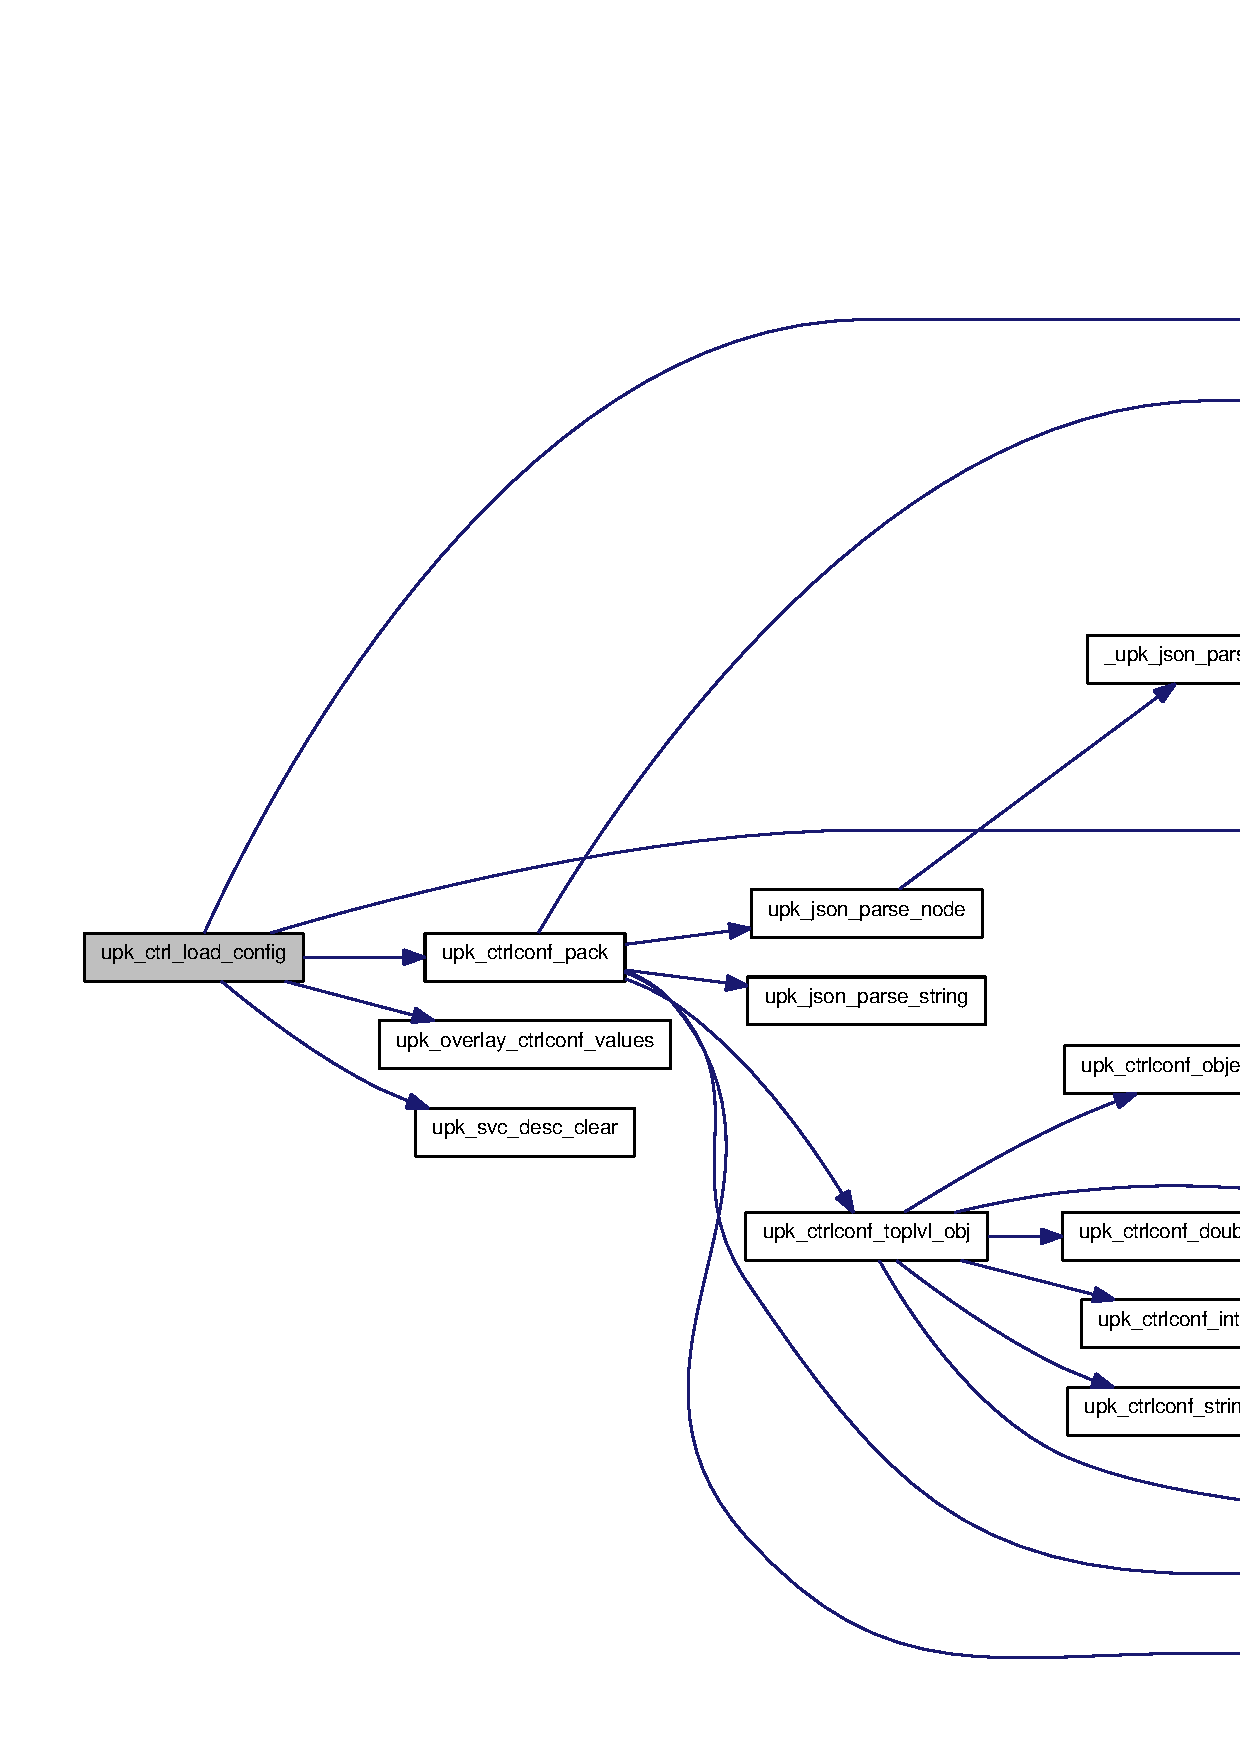
\includegraphics[width=400pt]{group__config__impl_ga11c5a55e854fb56c864a12ef5d314798_cgraph}
\end{center}
\end{figure}




Here is the caller graph for this function:
\nopagebreak
\begin{figure}[H]
\begin{center}
\leavevmode
\includegraphics[width=330pt]{group__config__impl_ga11c5a55e854fb56c864a12ef5d314798_icgraph}
\end{center}
\end{figure}


\index{Config\_\-impl@{Config\_\-impl}!upk\_\-ctrlconf\_\-double\_\-handler@{upk\_\-ctrlconf\_\-double\_\-handler}}
\index{upk\_\-ctrlconf\_\-double\_\-handler@{upk\_\-ctrlconf\_\-double\_\-handler}!Config_impl@{Config\_\-impl}}
\subsubsection[{upk\_\-ctrlconf\_\-double\_\-handler}]{\setlength{\rightskip}{0pt plus 5cm}static void upk\_\-ctrlconf\_\-double\_\-handler (
\begin{DoxyParamCaption}
\item[{{\bf upk\_\-json\_\-stack\_\-meta\_\-t} $\ast$}]{meta, }
\item[{void $\ast$}]{data, }
\item[{char $\ast$}]{key, }
\item[{{\bf upk\_\-json\_\-val\_\-t}}]{v}
\end{DoxyParamCaption}
)\hspace{0.3cm}{\ttfamily  [static]}}\label{group__config__impl_gab2d022caebe210d616ddef45e3a5bdae}


References \_\-upk\_\-controller\_\-config::BuddyPollingInterval, \_\-upk\_\-json\_\-type::dbl, upk\_\-fatal, and \_\-upk\_\-json\_\-type::val.



Referenced by upk\_\-ctrlconf\_\-toplvl\_\-obj().



Here is the caller graph for this function:
\nopagebreak
\begin{figure}[H]
\begin{center}
\leavevmode
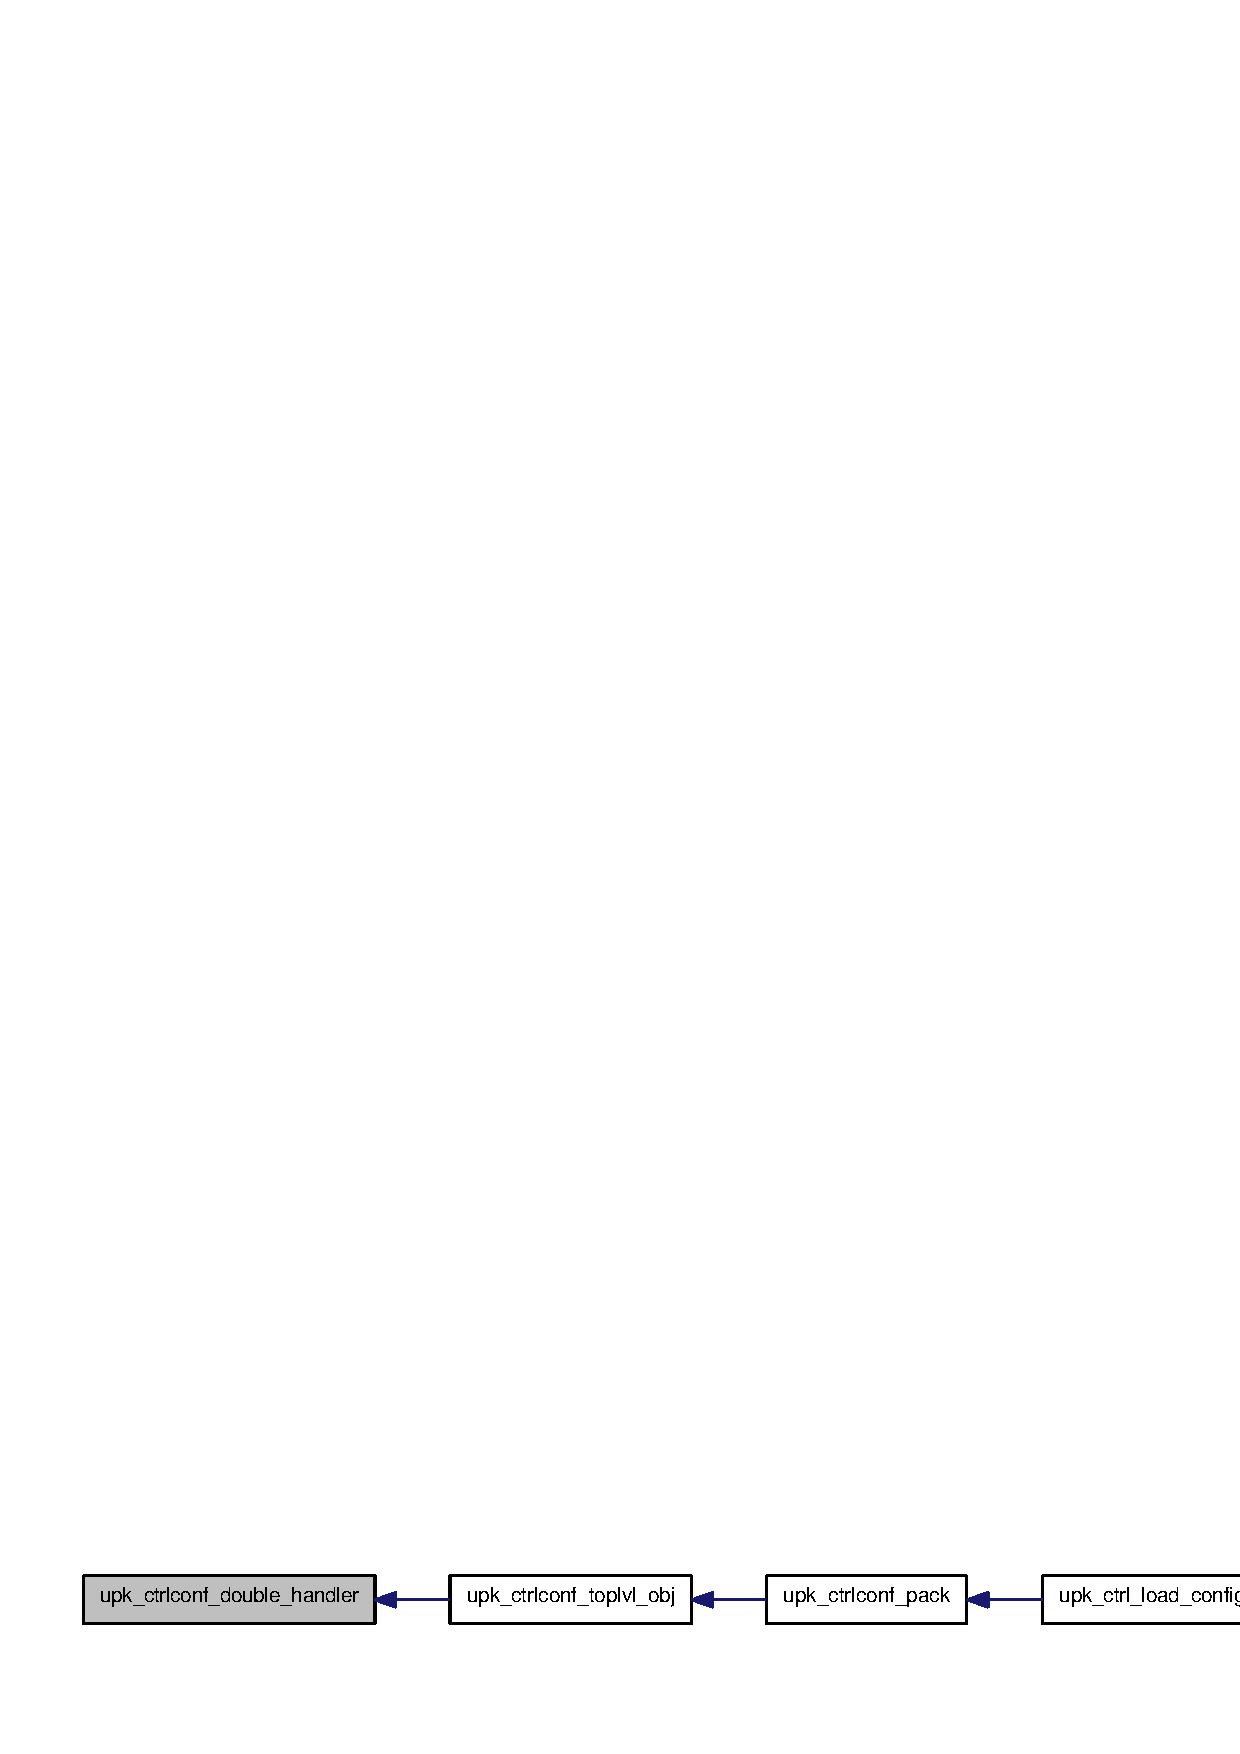
\includegraphics[width=400pt]{group__config__impl_gab2d022caebe210d616ddef45e3a5bdae_icgraph}
\end{center}
\end{figure}


\index{Config\_\-impl@{Config\_\-impl}!upk\_\-ctrlconf\_\-free@{upk\_\-ctrlconf\_\-free}}
\index{upk\_\-ctrlconf\_\-free@{upk\_\-ctrlconf\_\-free}!Config_impl@{Config\_\-impl}}
\subsubsection[{upk\_\-ctrlconf\_\-free}]{\setlength{\rightskip}{0pt plus 5cm}void upk\_\-ctrlconf\_\-free (
\begin{DoxyParamCaption}
\item[{{\bf upk\_\-controller\_\-config\_\-t} $\ast$}]{cfg}
\end{DoxyParamCaption}
)}\label{group__config__impl_ga2aa4766451425bf4662449117b2f8e63}


References \_\-upk\_\-controller\_\-config::ServiceDefaults, \_\-upk\_\-controller\_\-config::svclist, upk\_\-svc\_\-desc\_\-free(), and upk\_\-svclist\_\-free().



Referenced by upk\_\-ctrl\_\-free\_\-config().



Here is the call graph for this function:
\nopagebreak
\begin{figure}[H]
\begin{center}
\leavevmode
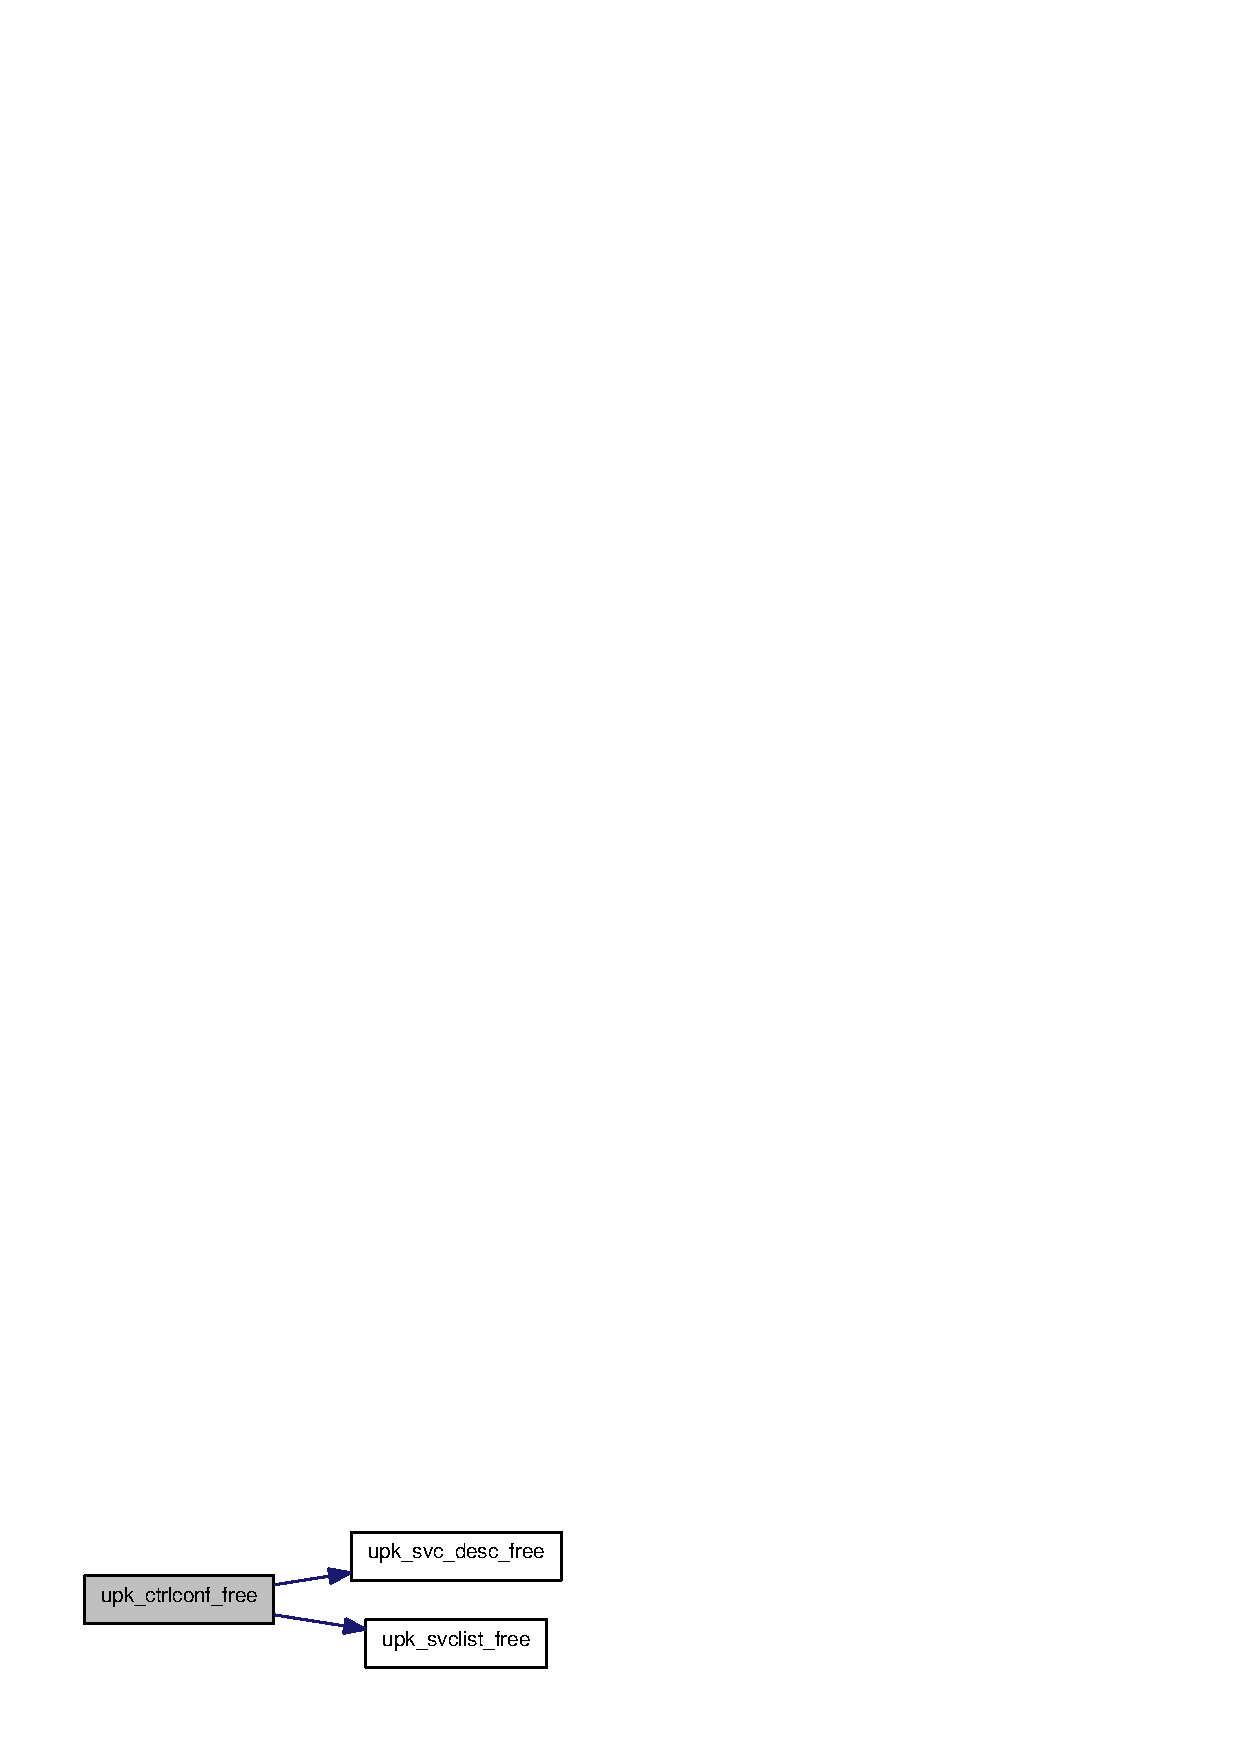
\includegraphics[width=274pt]{group__config__impl_ga2aa4766451425bf4662449117b2f8e63_cgraph}
\end{center}
\end{figure}




Here is the caller graph for this function:
\nopagebreak
\begin{figure}[H]
\begin{center}
\leavevmode
\includegraphics[width=276pt]{group__config__impl_ga2aa4766451425bf4662449117b2f8e63_icgraph}
\end{center}
\end{figure}


\index{Config\_\-impl@{Config\_\-impl}!upk\_\-ctrlconf\_\-int\_\-handler@{upk\_\-ctrlconf\_\-int\_\-handler}}
\index{upk\_\-ctrlconf\_\-int\_\-handler@{upk\_\-ctrlconf\_\-int\_\-handler}!Config_impl@{Config\_\-impl}}
\subsubsection[{upk\_\-ctrlconf\_\-int\_\-handler}]{\setlength{\rightskip}{0pt plus 5cm}static void upk\_\-ctrlconf\_\-int\_\-handler (
\begin{DoxyParamCaption}
\item[{{\bf upk\_\-json\_\-stack\_\-meta\_\-t} $\ast$}]{meta, }
\item[{void $\ast$}]{data, }
\item[{char $\ast$}]{key, }
\item[{{\bf upk\_\-json\_\-val\_\-t}}]{v}
\end{DoxyParamCaption}
)\hspace{0.3cm}{\ttfamily  [static]}}\label{group__config__impl_ga0f9cf5052a1ee60c5e403428ae721b6b}


References \_\-upk\_\-controller\_\-config::BuddyPollingInterval, \_\-upk\_\-controller\_\-config::BuddyVerbosity, \_\-upk\_\-json\_\-type::i, upk\_\-fatal, and \_\-upk\_\-json\_\-type::val.



Referenced by upk\_\-ctrlconf\_\-toplvl\_\-obj().



Here is the caller graph for this function:
\nopagebreak
\begin{figure}[H]
\begin{center}
\leavevmode
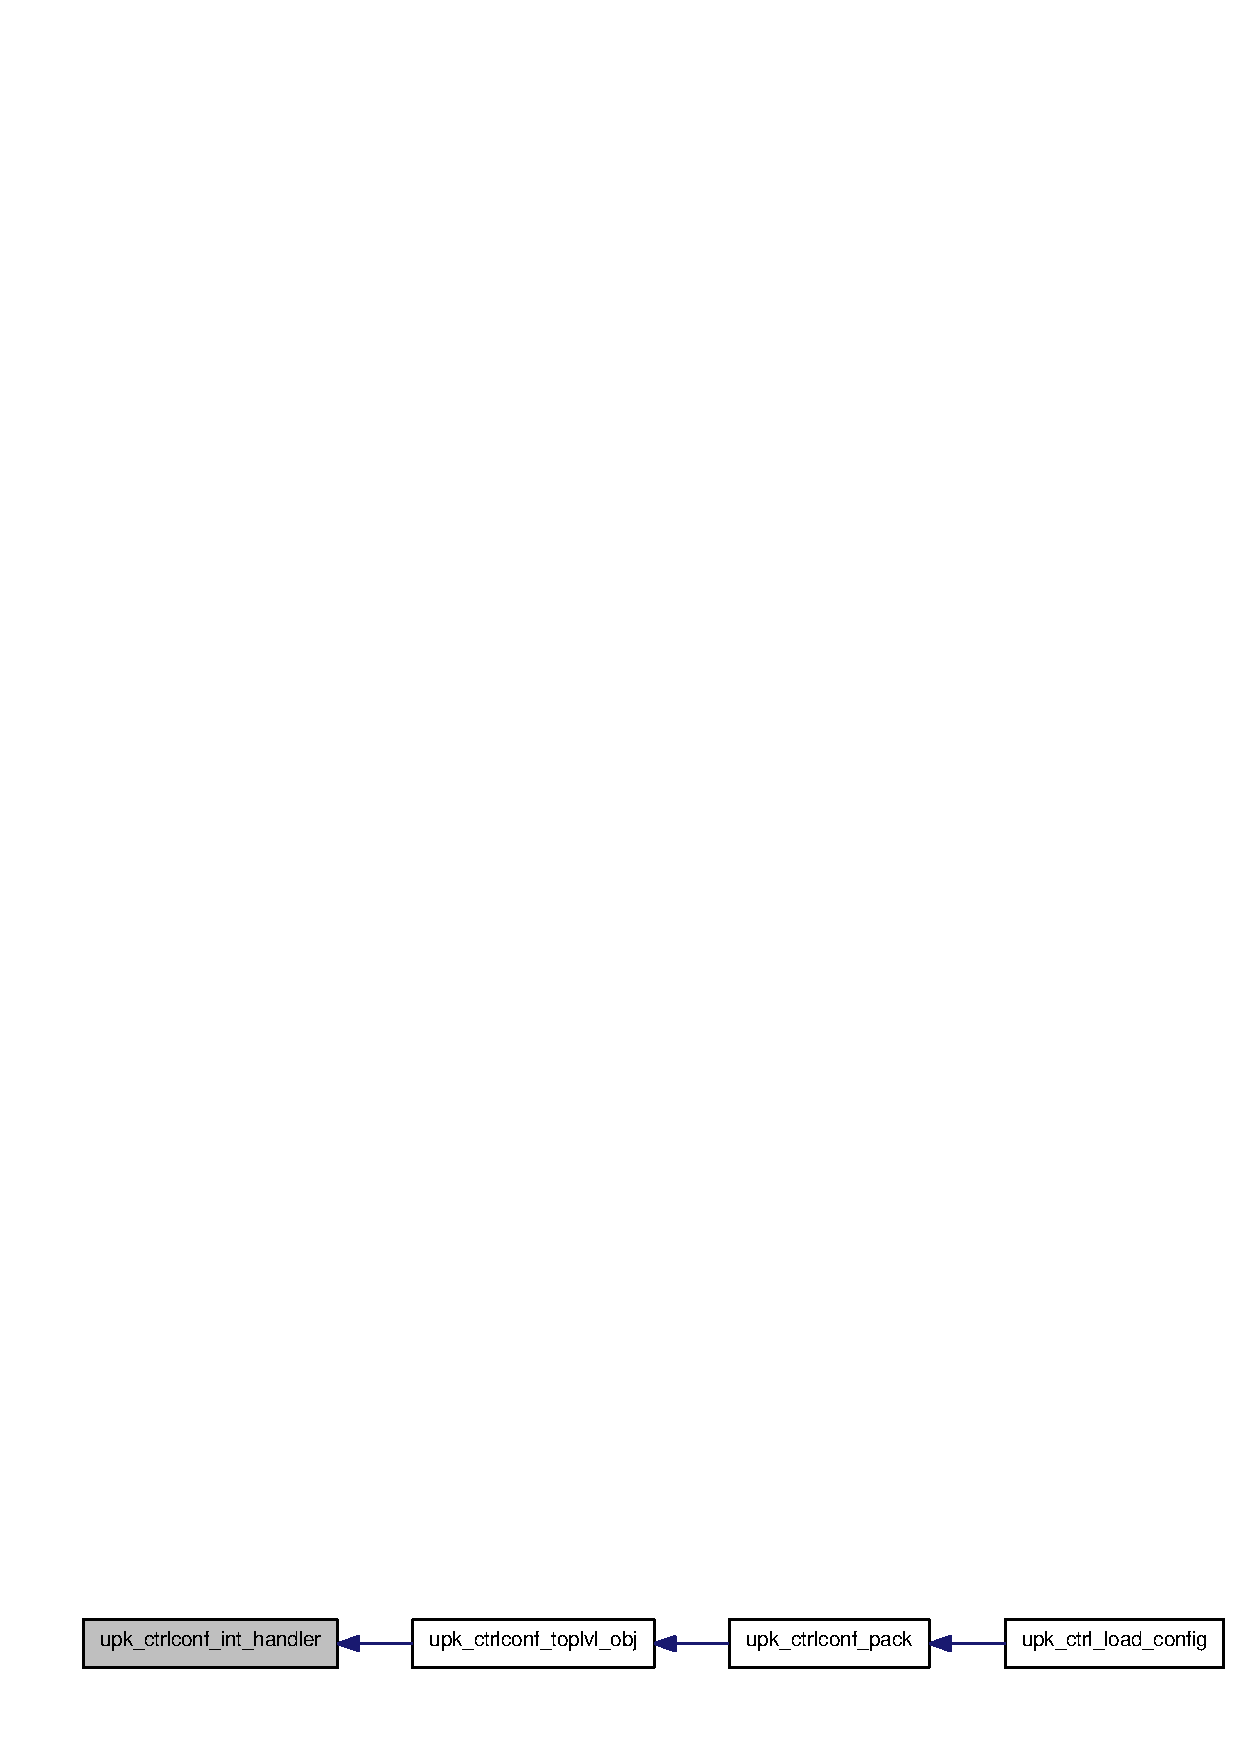
\includegraphics[width=400pt]{group__config__impl_ga0f9cf5052a1ee60c5e403428ae721b6b_icgraph}
\end{center}
\end{figure}


\index{Config\_\-impl@{Config\_\-impl}!upk\_\-ctrlconf\_\-object\_\-handler@{upk\_\-ctrlconf\_\-object\_\-handler}}
\index{upk\_\-ctrlconf\_\-object\_\-handler@{upk\_\-ctrlconf\_\-object\_\-handler}!Config_impl@{Config\_\-impl}}
\subsubsection[{upk\_\-ctrlconf\_\-object\_\-handler}]{\setlength{\rightskip}{0pt plus 5cm}static void upk\_\-ctrlconf\_\-object\_\-handler (
\begin{DoxyParamCaption}
\item[{{\bf upk\_\-json\_\-stack\_\-meta\_\-t} $\ast$}]{meta, }
\item[{void $\ast$}]{data, }
\item[{char $\ast$}]{key, }
\item[{{\bf upk\_\-json\_\-val\_\-t}}]{v}
\end{DoxyParamCaption}
)\hspace{0.3cm}{\ttfamily  [static]}}\label{group__config__impl_ga70bcf5d4574ec504ccfa7c02e54f2f6d}


References \_\-upk\_\-json\_\-stack\_\-node::data, \_\-upk\_\-json\_\-stack\_\-node::handlers, \_\-upk\_\-controller\_\-config::ServiceDefaults, upk\_\-json\_\-stack\_\-push(), upk\_\-parse\_\-svc\_\-id(), and upk\_\-svcconf\_\-setup\_\-handlers().



Referenced by upk\_\-ctrlconf\_\-toplvl\_\-obj().



Here is the call graph for this function:
\nopagebreak
\begin{figure}[H]
\begin{center}
\leavevmode
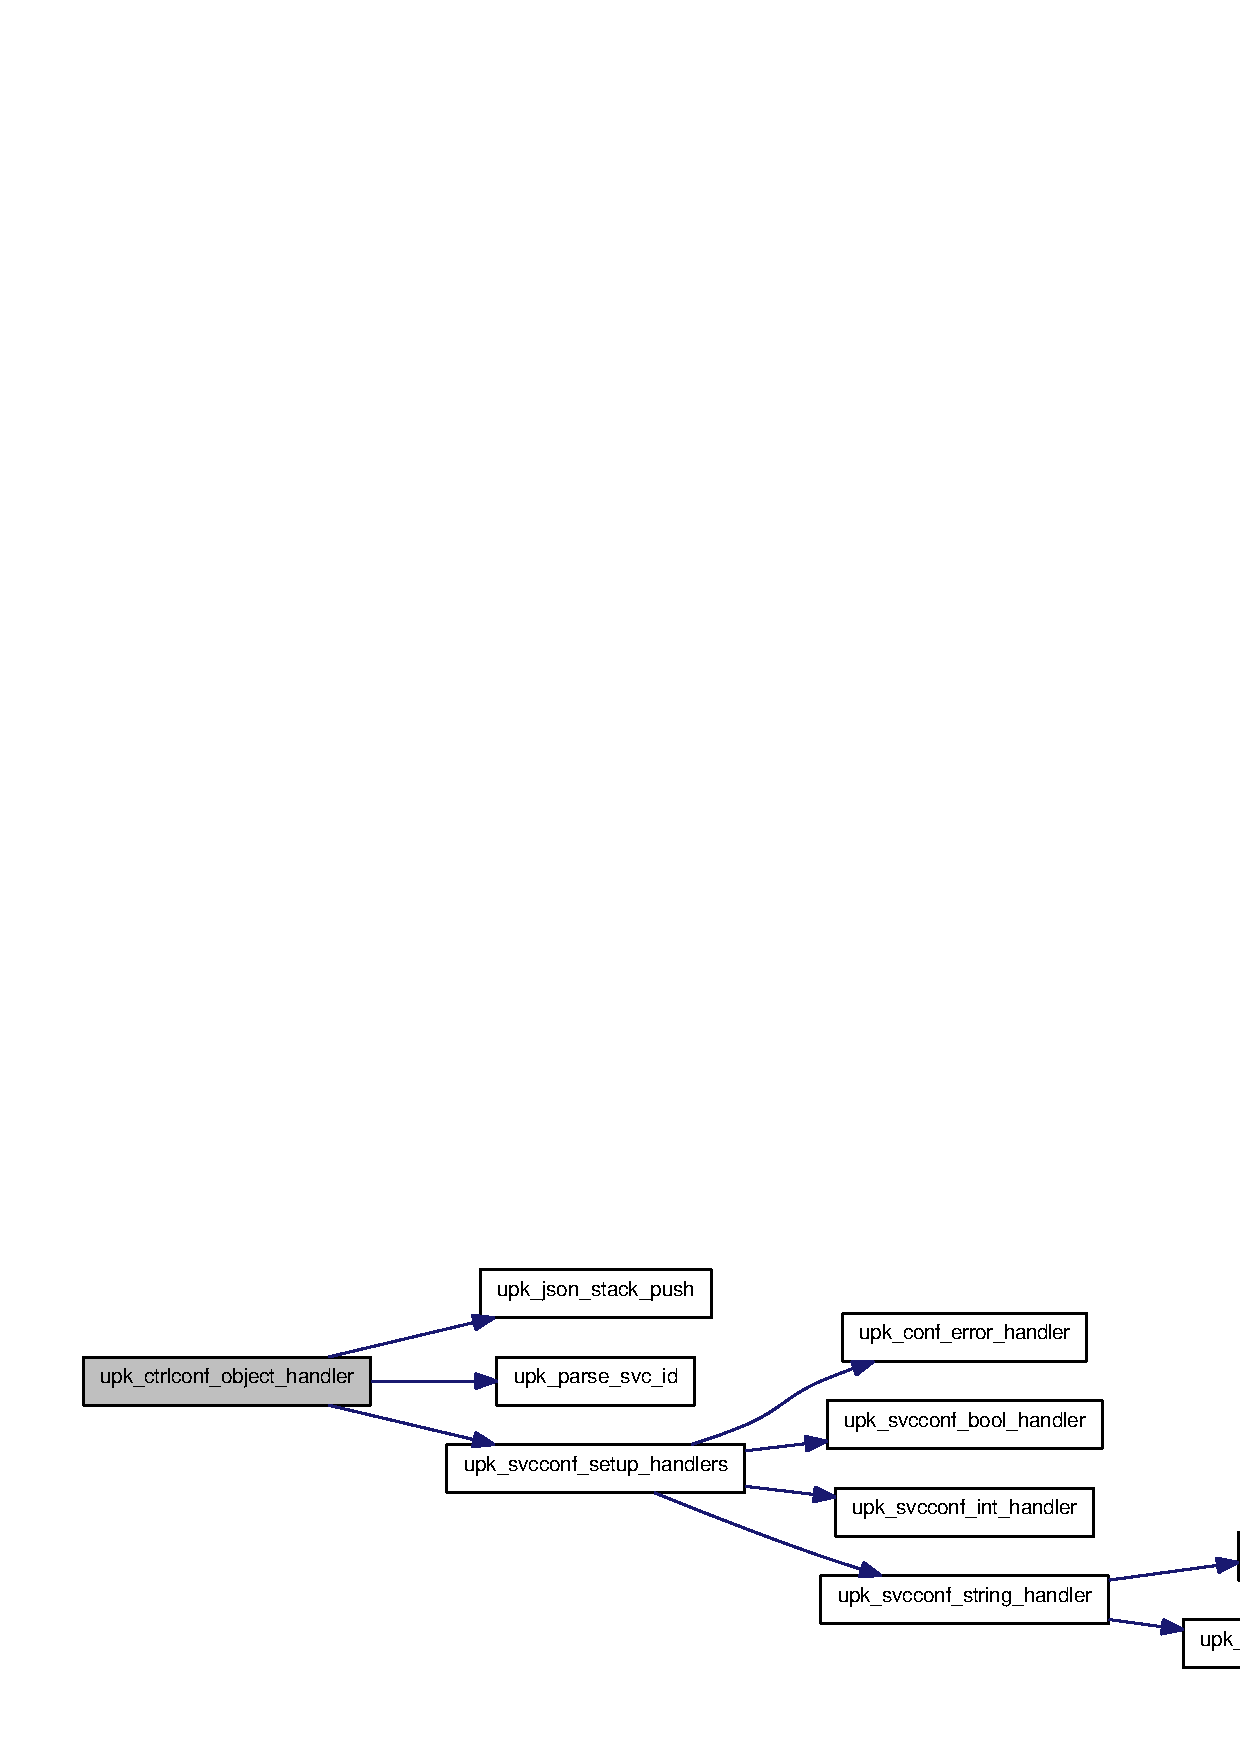
\includegraphics[width=400pt]{group__config__impl_ga70bcf5d4574ec504ccfa7c02e54f2f6d_cgraph}
\end{center}
\end{figure}




Here is the caller graph for this function:
\nopagebreak
\begin{figure}[H]
\begin{center}
\leavevmode
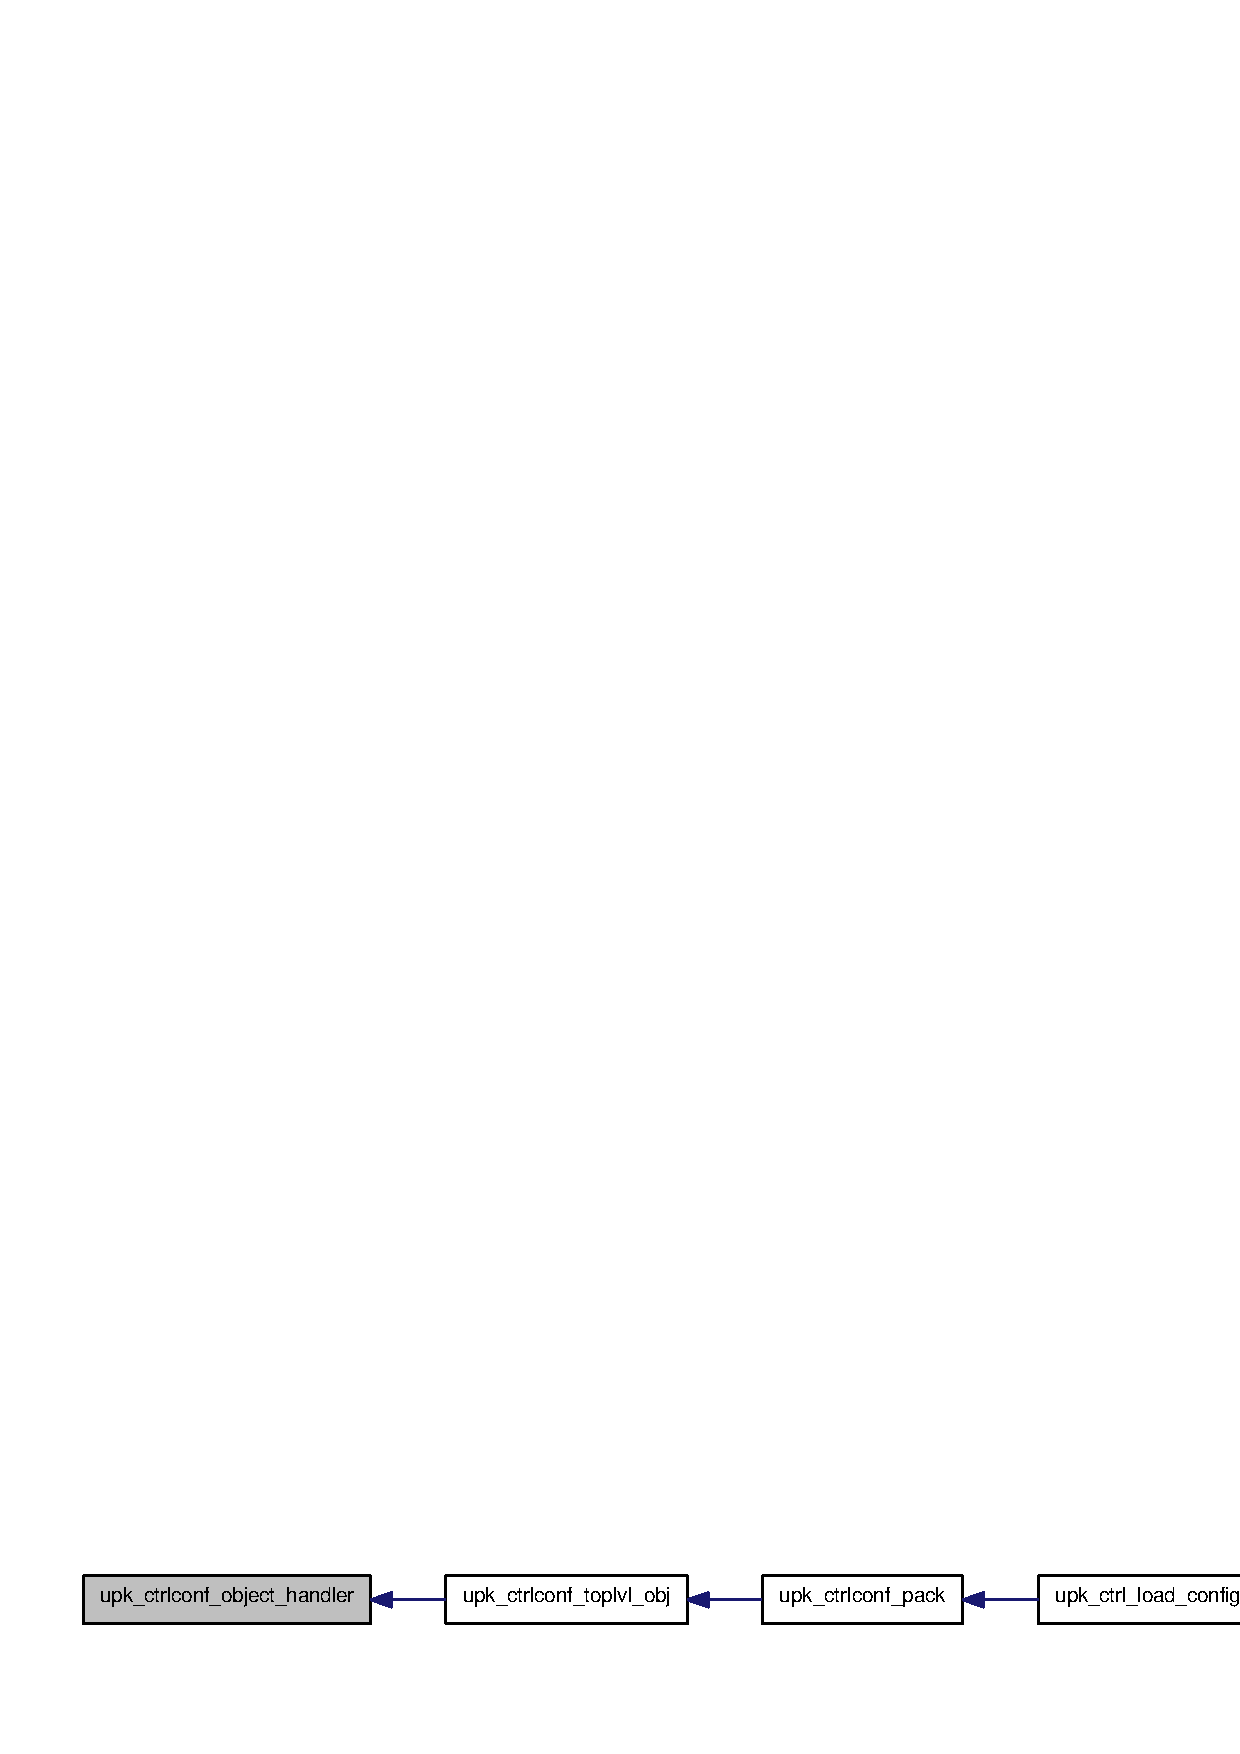
\includegraphics[width=400pt]{group__config__impl_ga70bcf5d4574ec504ccfa7c02e54f2f6d_icgraph}
\end{center}
\end{figure}


\index{Config\_\-impl@{Config\_\-impl}!upk\_\-ctrlconf\_\-pack@{upk\_\-ctrlconf\_\-pack}}
\index{upk\_\-ctrlconf\_\-pack@{upk\_\-ctrlconf\_\-pack}!Config_impl@{Config\_\-impl}}
\subsubsection[{upk\_\-ctrlconf\_\-pack}]{\setlength{\rightskip}{0pt plus 5cm}static void upk\_\-ctrlconf\_\-pack (
\begin{DoxyParamCaption}
\item[{{\bf upk\_\-controller\_\-config\_\-t} $\ast$}]{cfg, }
\item[{const char $\ast$}]{json\_\-string}
\end{DoxyParamCaption}
)\hspace{0.3cm}{\ttfamily  [static]}}\label{group__config__impl_ga141b988b89261c395ef928630abd7492}


References \_\-upk\_\-json\_\-stack\_\-handlers::after\_\-json\_\-array\_\-pop, \_\-upk\_\-json\_\-stack\_\-handlers::after\_\-json\_\-obj\_\-pop, calloc(), \_\-upk\_\-json\_\-stack\_\-node::data, \_\-upk\_\-json\_\-stack\_\-node::handlers, \_\-upk\_\-json\_\-stack\_\-handlers::json\_\-array, \_\-upk\_\-json\_\-stack\_\-handlers::json\_\-bool, \_\-upk\_\-json\_\-stack\_\-handlers::json\_\-double, \_\-upk\_\-json\_\-stack\_\-handlers::json\_\-int, \_\-upk\_\-json\_\-stack\_\-handlers::json\_\-null, \_\-upk\_\-json\_\-stack\_\-handlers::json\_\-object, \_\-upk\_\-json\_\-stack\_\-handlers::json\_\-string, restrict, upk\_\-conf\_\-error\_\-handler(), upk\_\-ctrlconf\_\-toplvl\_\-obj(), upk\_\-json\_\-parse\_\-node(), upk\_\-json\_\-parse\_\-string(), upk\_\-json\_\-stack\_\-meta\_\-t, upk\_\-json\_\-stack\_\-push(), and UPKLIST\_\-FREE.



Referenced by upk\_\-ctrl\_\-load\_\-config().



Here is the call graph for this function:
\nopagebreak
\begin{figure}[H]
\begin{center}
\leavevmode
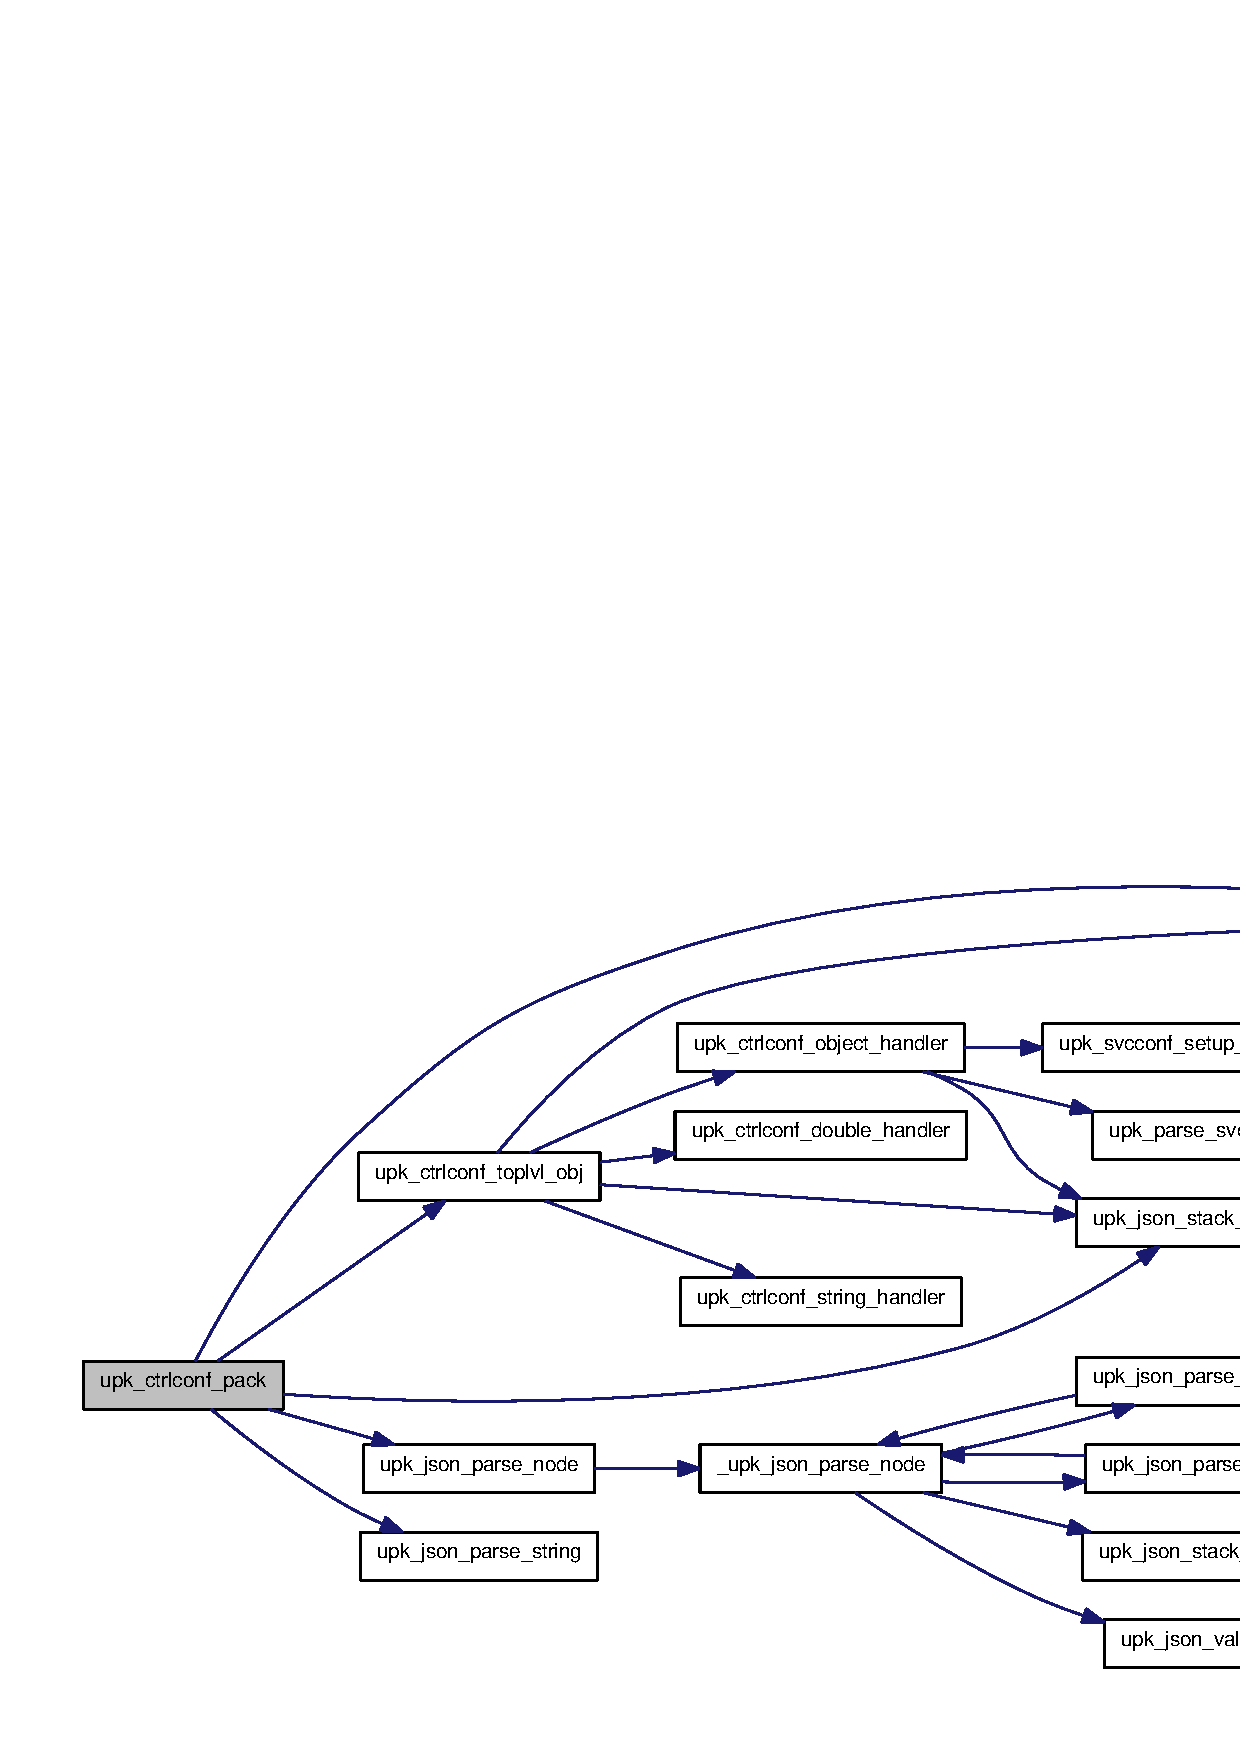
\includegraphics[width=400pt]{group__config__impl_ga141b988b89261c395ef928630abd7492_cgraph}
\end{center}
\end{figure}




Here is the caller graph for this function:
\nopagebreak
\begin{figure}[H]
\begin{center}
\leavevmode
\includegraphics[width=282pt]{group__config__impl_ga141b988b89261c395ef928630abd7492_icgraph}
\end{center}
\end{figure}


\index{Config\_\-impl@{Config\_\-impl}!upk\_\-ctrlconf\_\-string\_\-handler@{upk\_\-ctrlconf\_\-string\_\-handler}}
\index{upk\_\-ctrlconf\_\-string\_\-handler@{upk\_\-ctrlconf\_\-string\_\-handler}!Config_impl@{Config\_\-impl}}
\subsubsection[{upk\_\-ctrlconf\_\-string\_\-handler}]{\setlength{\rightskip}{0pt plus 5cm}static void upk\_\-ctrlconf\_\-string\_\-handler (
\begin{DoxyParamCaption}
\item[{{\bf upk\_\-json\_\-stack\_\-meta\_\-t} $\ast$}]{meta, }
\item[{void $\ast$}]{data, }
\item[{char $\ast$}]{key, }
\item[{{\bf upk\_\-json\_\-val\_\-t}}]{v}
\end{DoxyParamCaption}
)\hspace{0.3cm}{\ttfamily  [static]}}\label{group__config__impl_ga9fa9e7535bf980ea5d54be6129d66580}


References \_\-upk\_\-json\_\-string::c\_\-str, \_\-upk\_\-controller\_\-config::StateDir, \_\-upk\_\-json\_\-type::str, \_\-upk\_\-controller\_\-config::SvcConfigPath, \_\-upk\_\-controller\_\-config::SvcRunPath, upk\_\-fatal, UPK\_\-MAX\_\-STRING\_\-LEN, \_\-upk\_\-controller\_\-config::UpkBuddyPath, and \_\-upk\_\-json\_\-type::val.



Referenced by upk\_\-ctrlconf\_\-toplvl\_\-obj().



Here is the caller graph for this function:
\nopagebreak
\begin{figure}[H]
\begin{center}
\leavevmode
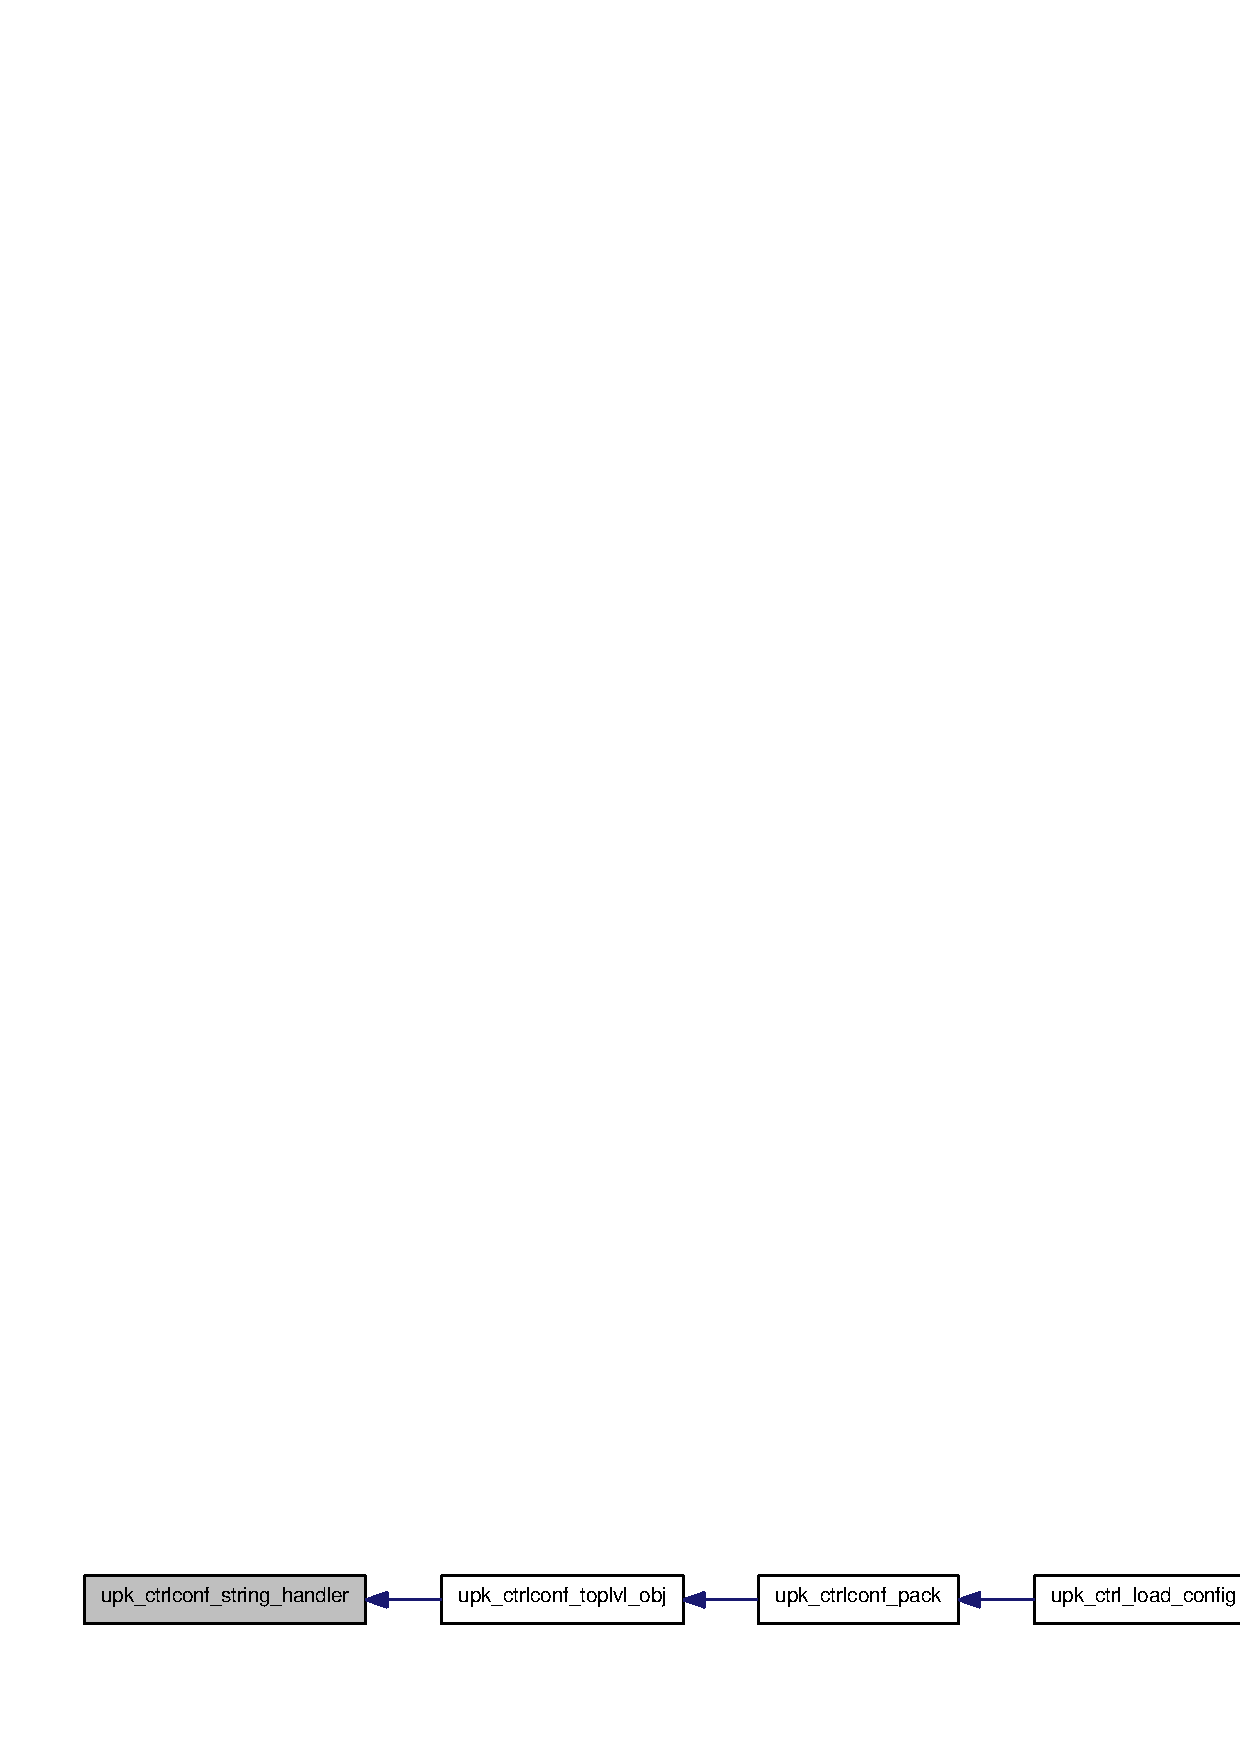
\includegraphics[width=400pt]{group__config__impl_ga9fa9e7535bf980ea5d54be6129d66580_icgraph}
\end{center}
\end{figure}


\index{Config\_\-impl@{Config\_\-impl}!upk\_\-ctrlconf\_\-toplvl\_\-obj@{upk\_\-ctrlconf\_\-toplvl\_\-obj}}
\index{upk\_\-ctrlconf\_\-toplvl\_\-obj@{upk\_\-ctrlconf\_\-toplvl\_\-obj}!Config_impl@{Config\_\-impl}}
\subsubsection[{upk\_\-ctrlconf\_\-toplvl\_\-obj}]{\setlength{\rightskip}{0pt plus 5cm}static void upk\_\-ctrlconf\_\-toplvl\_\-obj (
\begin{DoxyParamCaption}
\item[{{\bf upk\_\-json\_\-stack\_\-meta\_\-t} $\ast$}]{meta, }
\item[{void $\ast$}]{data, }
\item[{char $\ast$}]{key, }
\item[{{\bf upk\_\-json\_\-val\_\-t}}]{v}
\end{DoxyParamCaption}
)\hspace{0.3cm}{\ttfamily  [static]}}\label{group__config__impl_gab9fcf0078a632239eeca0eba28d9d467}


References \_\-upk\_\-json\_\-stack\_\-handlers::after\_\-json\_\-array\_\-pop, \_\-upk\_\-json\_\-stack\_\-handlers::after\_\-json\_\-obj\_\-pop, \_\-upk\_\-json\_\-stack\_\-node::data, \_\-upk\_\-json\_\-stack\_\-node::handlers, \_\-upk\_\-json\_\-stack\_\-handlers::json\_\-array, \_\-upk\_\-json\_\-stack\_\-handlers::json\_\-bool, \_\-upk\_\-json\_\-stack\_\-handlers::json\_\-double, \_\-upk\_\-json\_\-stack\_\-handlers::json\_\-int, \_\-upk\_\-json\_\-stack\_\-handlers::json\_\-null, \_\-upk\_\-json\_\-stack\_\-handlers::json\_\-object, \_\-upk\_\-json\_\-stack\_\-handlers::json\_\-string, restrict, upk\_\-conf\_\-error\_\-handler(), upk\_\-ctrlconf\_\-double\_\-handler(), upk\_\-ctrlconf\_\-int\_\-handler(), upk\_\-ctrlconf\_\-object\_\-handler(), upk\_\-ctrlconf\_\-string\_\-handler(), and upk\_\-json\_\-stack\_\-push().



Referenced by upk\_\-ctrlconf\_\-pack().



Here is the call graph for this function:
\nopagebreak
\begin{figure}[H]
\begin{center}
\leavevmode
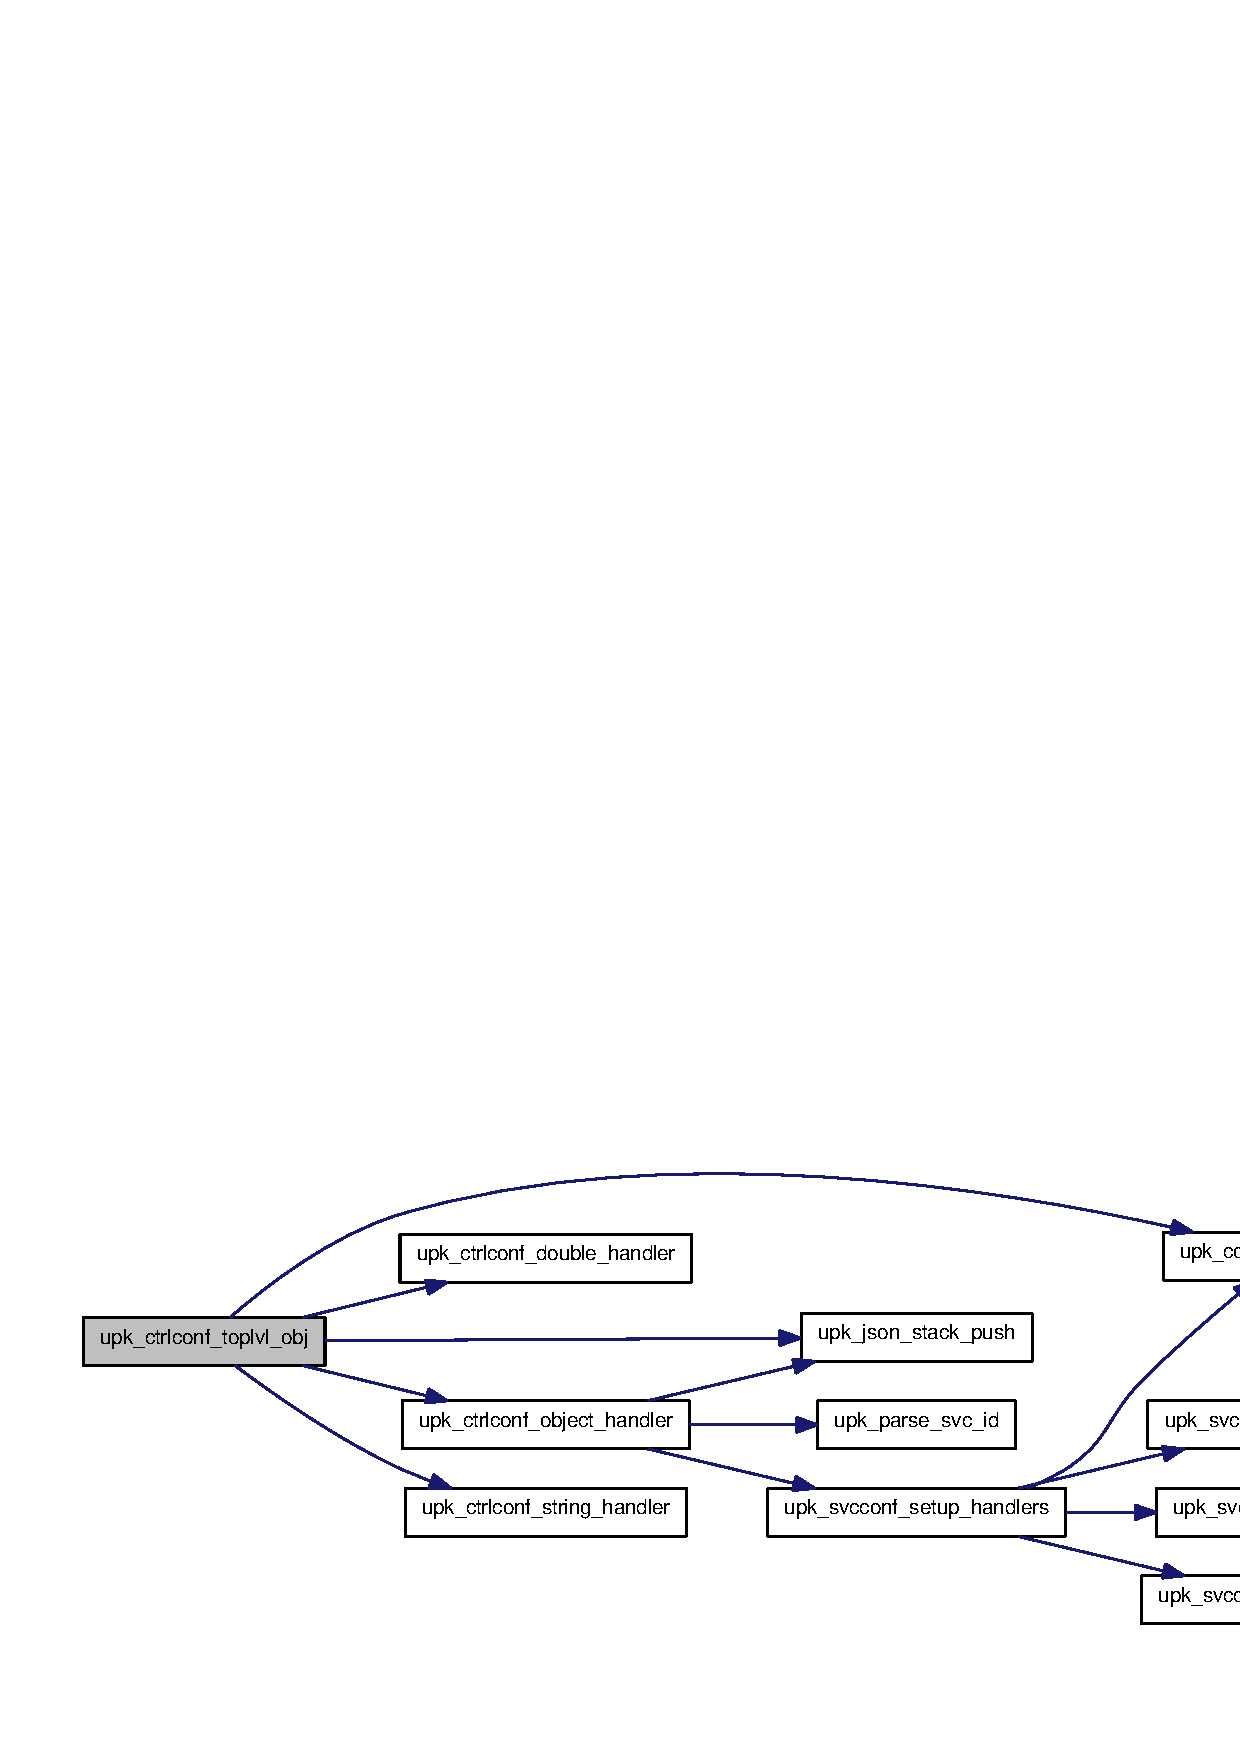
\includegraphics[width=400pt]{group__config__impl_gab9fcf0078a632239eeca0eba28d9d467_cgraph}
\end{center}
\end{figure}




Here is the caller graph for this function:
\nopagebreak
\begin{figure}[H]
\begin{center}
\leavevmode
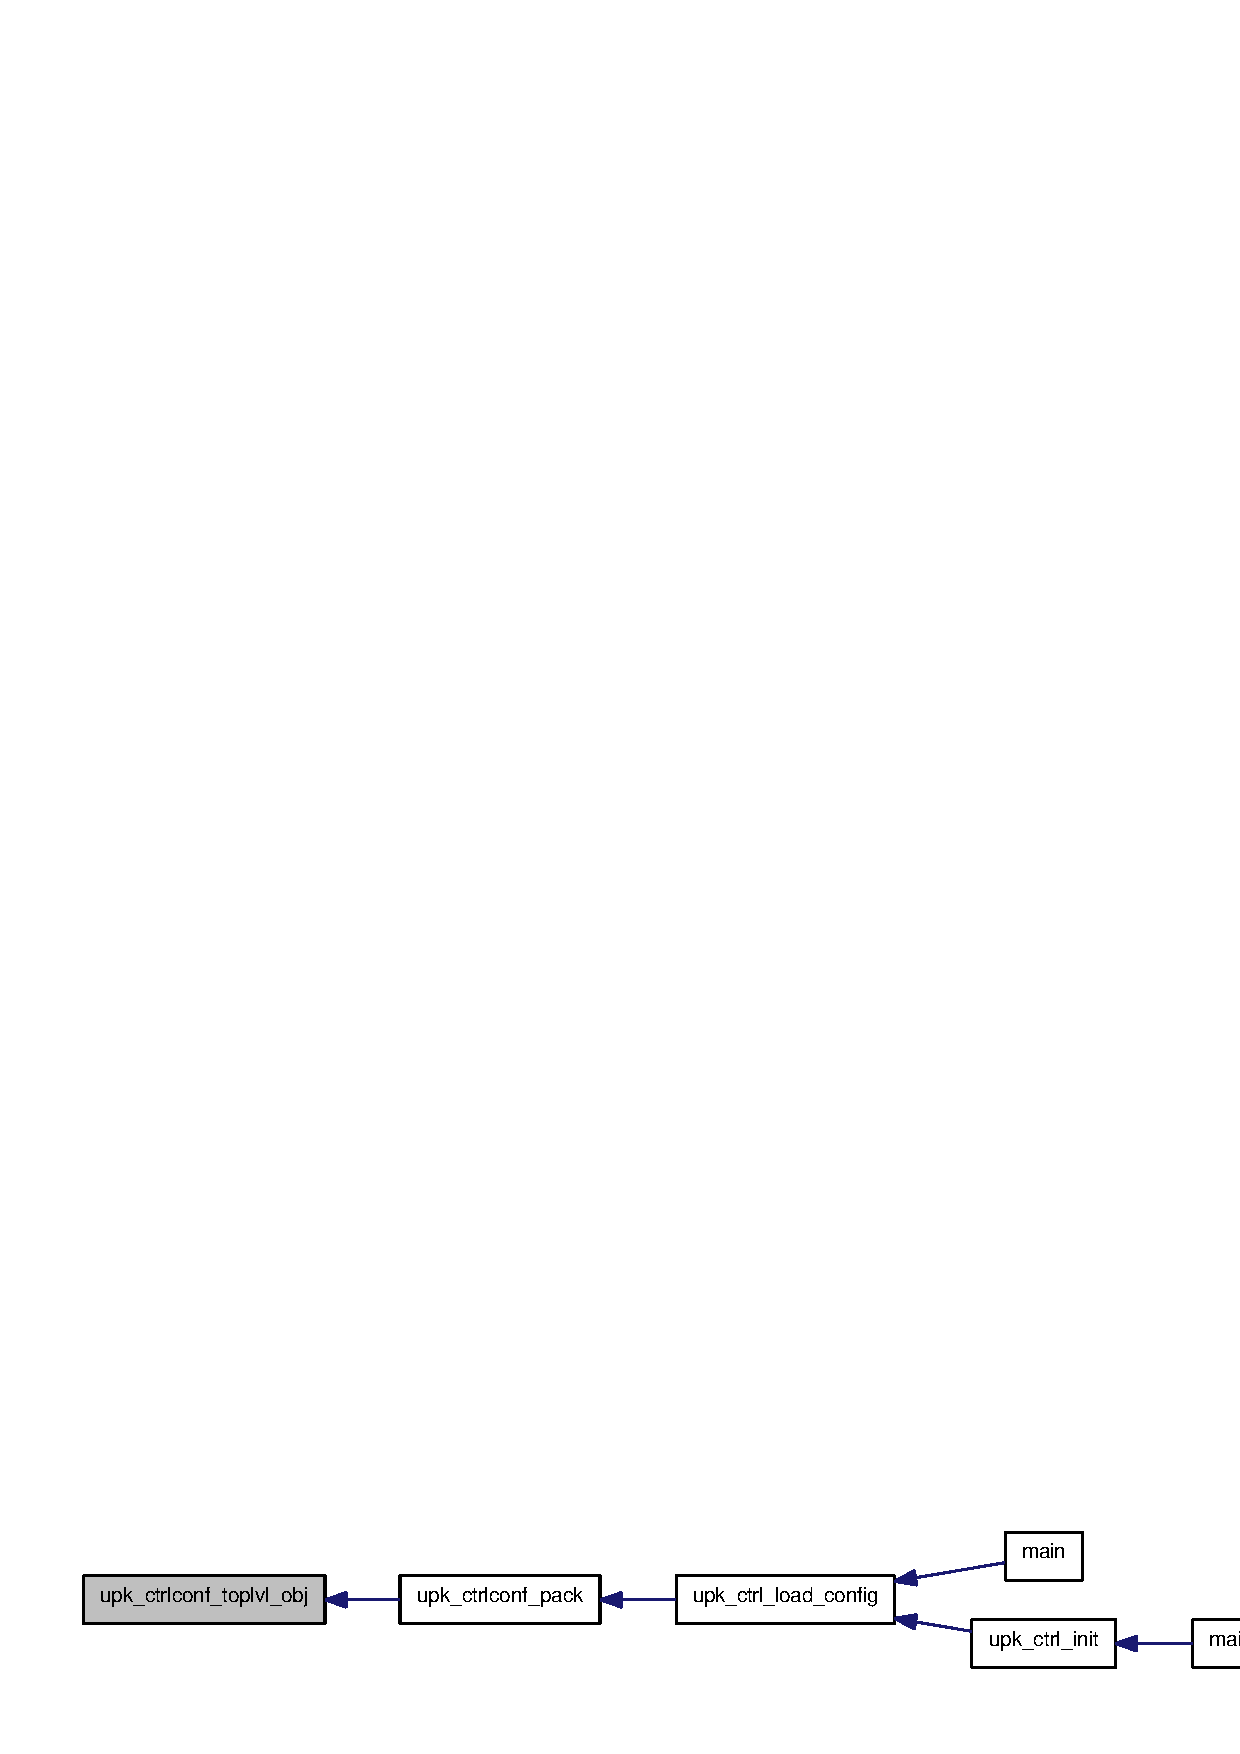
\includegraphics[width=400pt]{group__config__impl_gab9fcf0078a632239eeca0eba28d9d467_icgraph}
\end{center}
\end{figure}


\index{Config\_\-impl@{Config\_\-impl}!upk\_\-finalize\_\-svc\_\-desc@{upk\_\-finalize\_\-svc\_\-desc}}
\index{upk\_\-finalize\_\-svc\_\-desc@{upk\_\-finalize\_\-svc\_\-desc}!Config_impl@{Config\_\-impl}}
\subsubsection[{upk\_\-finalize\_\-svc\_\-desc}]{\setlength{\rightskip}{0pt plus 5cm}void upk\_\-finalize\_\-svc\_\-desc (
\begin{DoxyParamCaption}
\item[{{\bf upk\_\-svc\_\-desc\_\-t} $\ast$}]{dest, }
\item[{{\bf upk\_\-svc\_\-desc\_\-t} $\ast$}]{orig}
\end{DoxyParamCaption}
)}\label{group__config__impl_gafef3f55911da038eb9f8d82bba48222e}


References \_\-upk\_\-svc\_\-desc::ExecReload, \_\-upk\_\-svc\_\-desc::ExecStart, \_\-upk\_\-svc\_\-desc::ExecStop, \_\-upk\_\-svc\_\-desc::ReloadScript, \_\-upk\_\-controller\_\-config::ServiceDefaults, \_\-upk\_\-svc\_\-desc::StartScript, \_\-upk\_\-svc\_\-desc::StopScript, upk\_\-overlay\_\-svcconf\_\-values(), and upk\_\-replace\_\-string().



Referenced by main(), and upk\_\-load\_\-runtime\_\-services().



Here is the call graph for this function:
\nopagebreak
\begin{figure}[H]
\begin{center}
\leavevmode
\includegraphics[width=338pt]{group__config__impl_gafef3f55911da038eb9f8d82bba48222e_cgraph}
\end{center}
\end{figure}




Here is the caller graph for this function:
\nopagebreak
\begin{figure}[H]
\begin{center}
\leavevmode
\includegraphics[width=332pt]{group__config__impl_gafef3f55911da038eb9f8d82bba48222e_icgraph}
\end{center}
\end{figure}


\index{Config\_\-impl@{Config\_\-impl}!upk\_\-json\_\-serialize\_\-or\_\-null@{upk\_\-json\_\-serialize\_\-or\_\-null}}
\index{upk\_\-json\_\-serialize\_\-or\_\-null@{upk\_\-json\_\-serialize\_\-or\_\-null}!Config_impl@{Config\_\-impl}}
\subsubsection[{upk\_\-json\_\-serialize\_\-or\_\-null}]{\setlength{\rightskip}{0pt plus 5cm}static void$\ast$ upk\_\-json\_\-serialize\_\-or\_\-null (
\begin{DoxyParamCaption}
\item[{enum json\_\-type}]{type, }
\item[{void $\ast$}]{val}
\end{DoxyParamCaption}
)\hspace{0.3cm}{\ttfamily  [inline, static]}}\label{group__config__impl_ga3f5141868527ac40542f9b46a366f80d}


Referenced by upk\_\-svc\_\-desc\_\-to\_\-json\_\-obj().



Here is the caller graph for this function:
\nopagebreak
\begin{figure}[H]
\begin{center}
\leavevmode
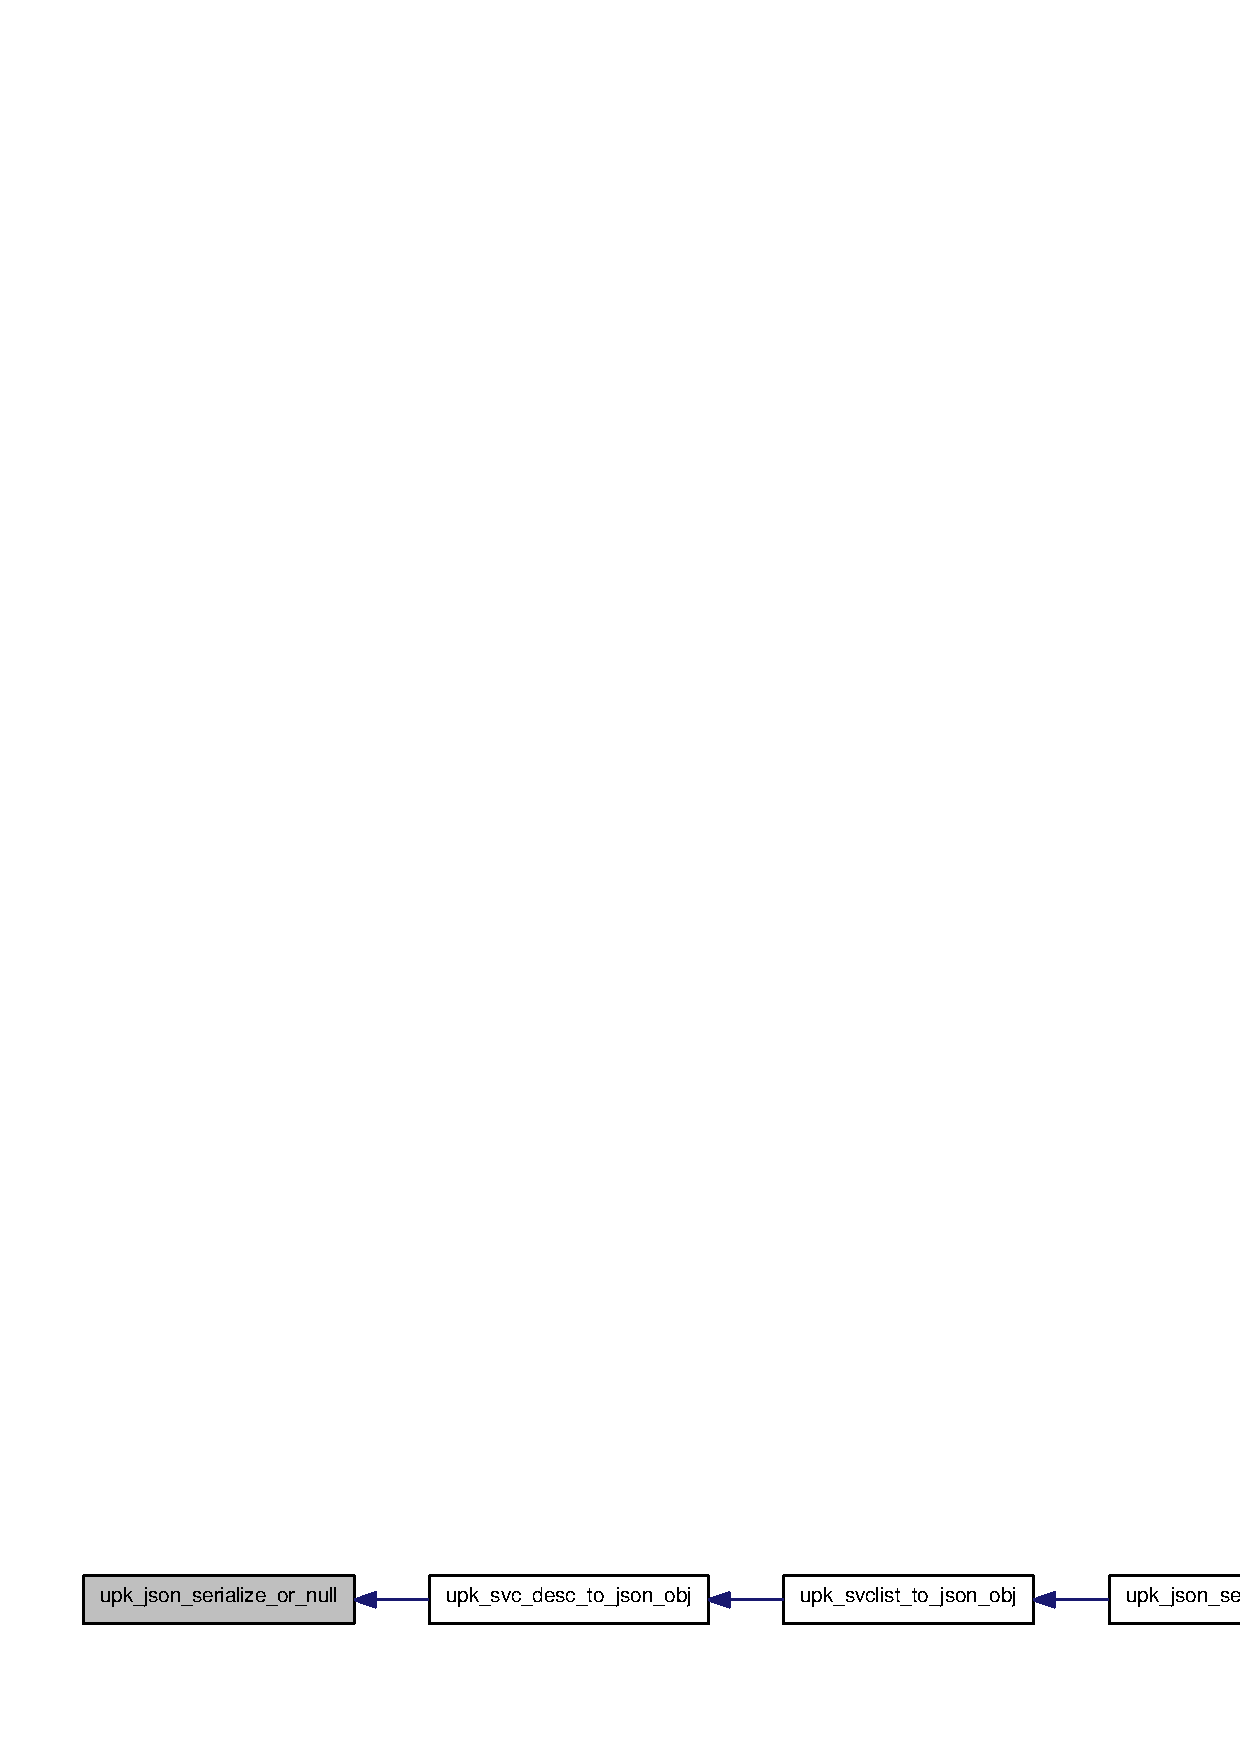
\includegraphics[width=344pt]{group__config__impl_ga3f5141868527ac40542f9b46a366f80d_icgraph}
\end{center}
\end{figure}


\index{Config\_\-impl@{Config\_\-impl}!upk\_\-json\_\-serialize\_\-svc\_\-config@{upk\_\-json\_\-serialize\_\-svc\_\-config}}
\index{upk\_\-json\_\-serialize\_\-svc\_\-config@{upk\_\-json\_\-serialize\_\-svc\_\-config}!Config_impl@{Config\_\-impl}}
\subsubsection[{upk\_\-json\_\-serialize\_\-svc\_\-config}]{\setlength{\rightskip}{0pt plus 5cm}char$\ast$ upk\_\-json\_\-serialize\_\-svc\_\-config (
\begin{DoxyParamCaption}
\item[{{\bf upk\_\-svc\_\-desc\_\-t} $\ast$}]{svc, }
\item[{{\bf upk\_\-json\_\-data\_\-output\_\-opts\_\-t}}]{opts}
\end{DoxyParamCaption}
)}\label{group__config__impl_ga19d2bc0bd2e96a937820f26f4e56b2d9}


References calloc(), \_\-upk\_\-svc\_\-desc::next, upk\_\-svc\_\-desc\_\-meta\_\-p::thisp, upk\_\-json\_\-obj\_\-to\_\-string(), upk\_\-svclist\_\-to\_\-json\_\-obj(), UPKLIST\_\-APPEND, and UPKLIST\_\-FREE.



Referenced by main(), and upk\_\-load\_\-runtime\_\-services().



Here is the call graph for this function:
\nopagebreak
\begin{figure}[H]
\begin{center}
\leavevmode
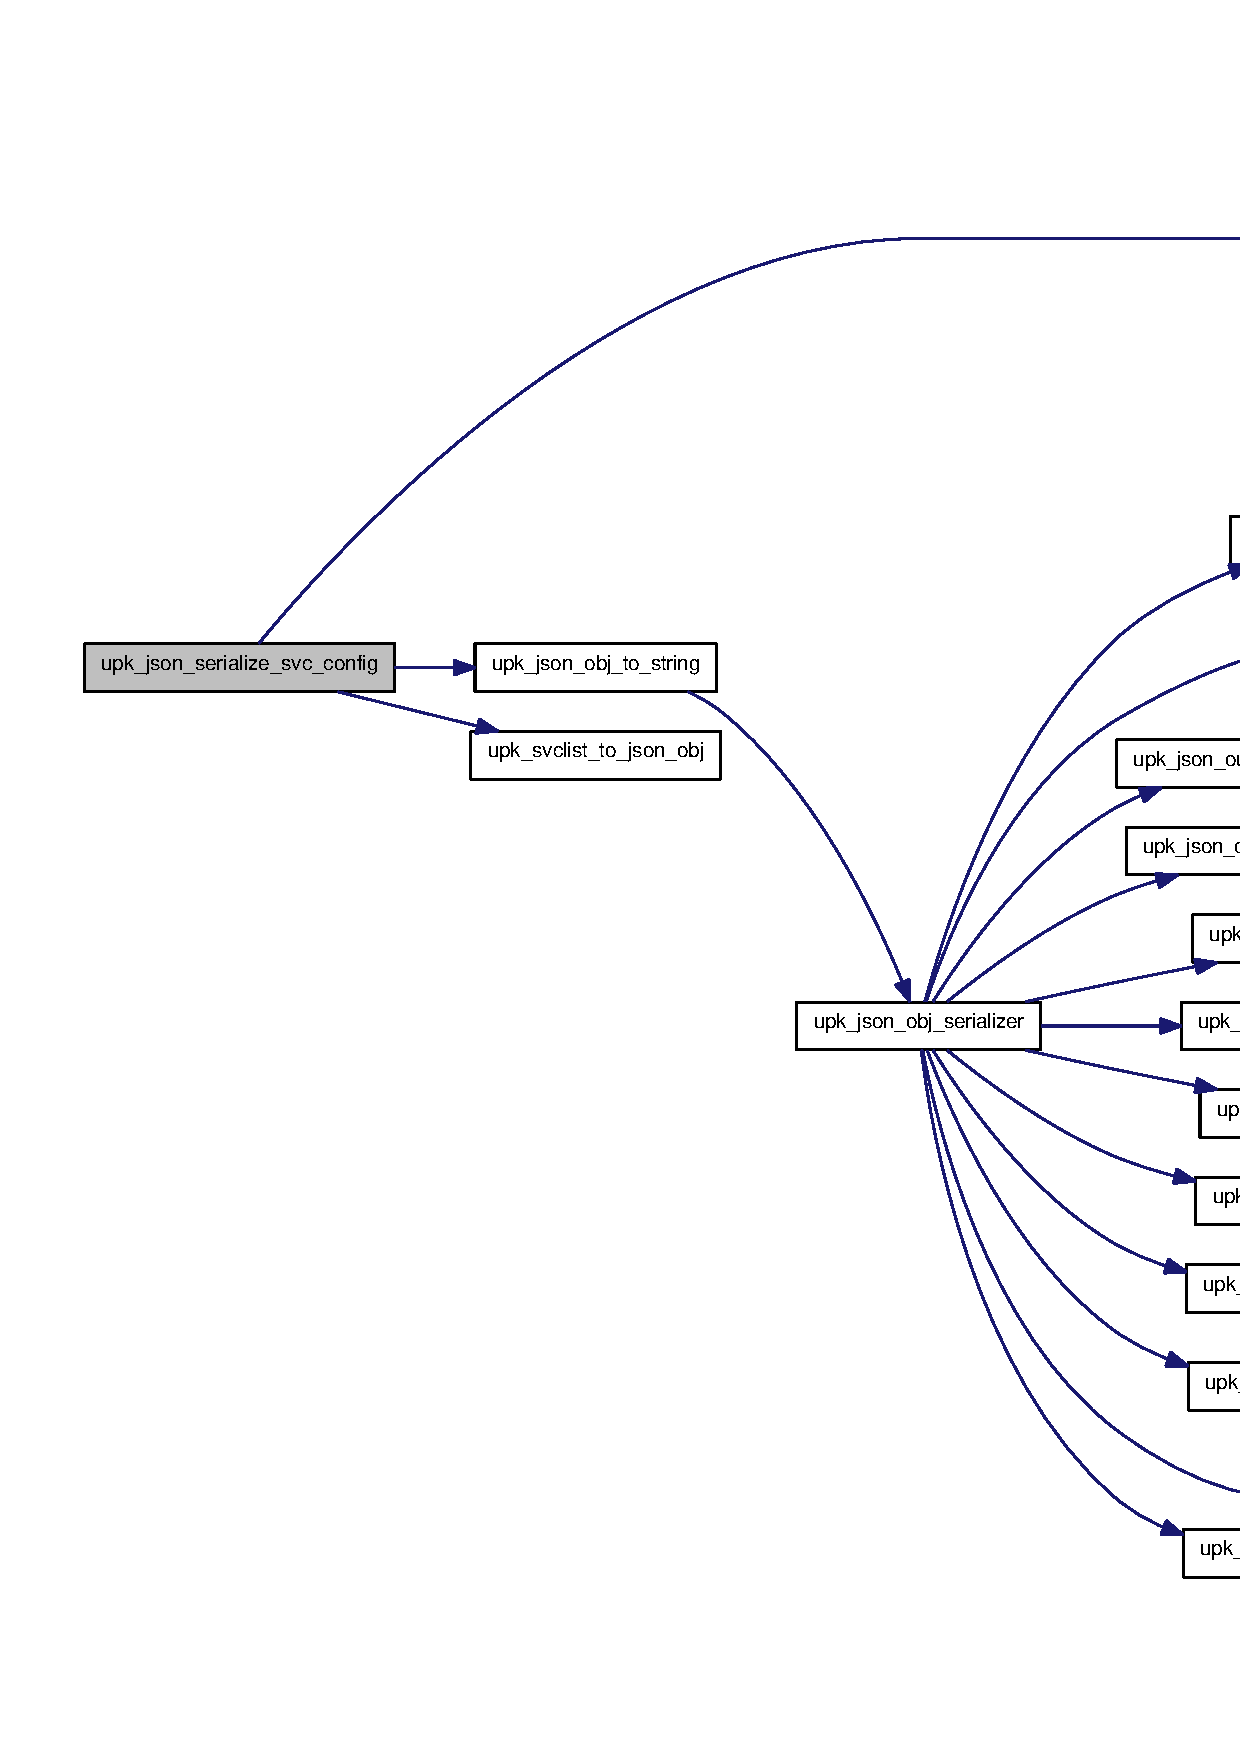
\includegraphics[width=400pt]{group__config__impl_ga19d2bc0bd2e96a937820f26f4e56b2d9_cgraph}
\end{center}
\end{figure}




Here is the caller graph for this function:
\nopagebreak
\begin{figure}[H]
\begin{center}
\leavevmode
\includegraphics[width=366pt]{group__config__impl_ga19d2bc0bd2e96a937820f26f4e56b2d9_icgraph}
\end{center}
\end{figure}


\index{Config\_\-impl@{Config\_\-impl}!upk\_\-load\_\-runtime\_\-service\_\-file@{upk\_\-load\_\-runtime\_\-service\_\-file}}
\index{upk\_\-load\_\-runtime\_\-service\_\-file@{upk\_\-load\_\-runtime\_\-service\_\-file}!Config_impl@{Config\_\-impl}}
\subsubsection[{upk\_\-load\_\-runtime\_\-service\_\-file}]{\setlength{\rightskip}{0pt plus 5cm}void upk\_\-load\_\-runtime\_\-service\_\-file (
\begin{DoxyParamCaption}
\item[{const char $\ast$}]{filename}
\end{DoxyParamCaption}
)}\label{group__config__impl_ga677c2a2d101f12525f6a1d39c8952584}
\index{Config\_\-impl@{Config\_\-impl}!upk\_\-load\_\-runtime\_\-services@{upk\_\-load\_\-runtime\_\-services}}
\index{upk\_\-load\_\-runtime\_\-services@{upk\_\-load\_\-runtime\_\-services}!Config_impl@{Config\_\-impl}}
\subsubsection[{upk\_\-load\_\-runtime\_\-services}]{\setlength{\rightskip}{0pt plus 5cm}void upk\_\-load\_\-runtime\_\-services (
\begin{DoxyParamCaption}
\item[{void}]{}
\end{DoxyParamCaption}
)}\label{group__config__impl_gaad96df378fe382df9bb37e2f21b62ee9}


References calloc(), closedir(), free(), opendir(), readdir(), \_\-upk\_\-json\_\-data\_\-output\_\-options::sep, strnlen(), \_\-upk\_\-controller\_\-config::SvcConfigPath, \_\-upk\_\-controller\_\-config::svclist, upk\_\-svc\_\-desc\_\-meta\_\-p::thisp, upk\_\-config\_\-loadfile(), upk\_\-debug1, upk\_\-diag\_\-verbosity, UPK\_\-DIAGLVL\_\-DEBUG1, upk\_\-finalize\_\-svc\_\-desc(), upk\_\-info, upk\_\-json\_\-serialize\_\-svc\_\-config(), UPK\_\-MAX\_\-PATH\_\-LEN, upk\_\-svc\_\-desc\_\-clear(), upk\_\-svcconf\_\-pack(), UPKLIST\_\-APPEND, UPKLIST\_\-FOREACH, and UPKLIST\_\-FREE.



Referenced by upk\_\-ctrl\_\-init().



Here is the call graph for this function:
\nopagebreak
\begin{figure}[H]
\begin{center}
\leavevmode
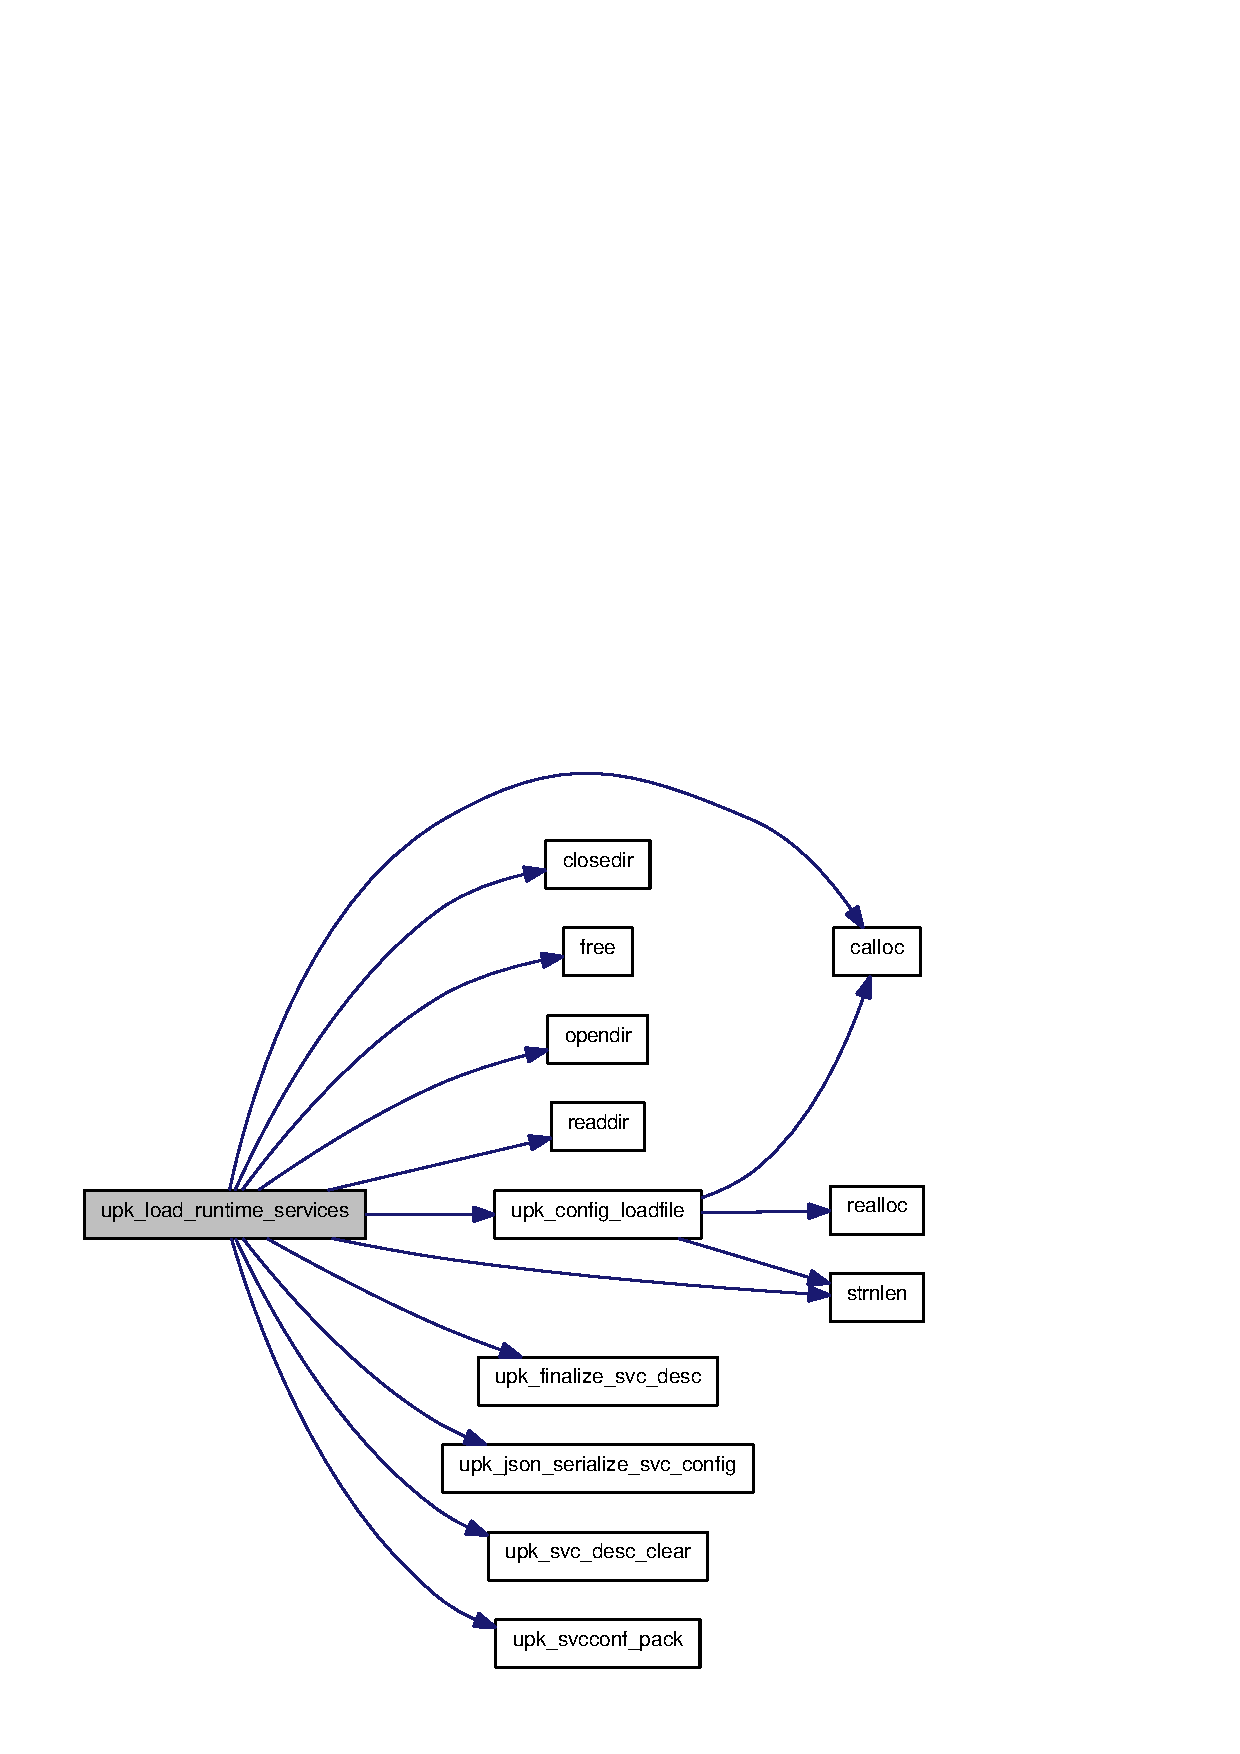
\includegraphics[width=400pt]{group__config__impl_gaad96df378fe382df9bb37e2f21b62ee9_cgraph}
\end{center}
\end{figure}




Here is the caller graph for this function:
\nopagebreak
\begin{figure}[H]
\begin{center}
\leavevmode
\includegraphics[width=360pt]{group__config__impl_gaad96df378fe382df9bb37e2f21b62ee9_icgraph}
\end{center}
\end{figure}


\index{Config\_\-impl@{Config\_\-impl}!upk\_\-overlay\_\-ctrlconf\_\-values@{upk\_\-overlay\_\-ctrlconf\_\-values}}
\index{upk\_\-overlay\_\-ctrlconf\_\-values@{upk\_\-overlay\_\-ctrlconf\_\-values}!Config_impl@{Config\_\-impl}}
\subsubsection[{upk\_\-overlay\_\-ctrlconf\_\-values}]{\setlength{\rightskip}{0pt plus 5cm}void upk\_\-overlay\_\-ctrlconf\_\-values (
\begin{DoxyParamCaption}
\item[{{\bf upk\_\-controller\_\-config\_\-t} $\ast$}]{dest, }
\item[{{\bf upk\_\-controller\_\-config\_\-t} $\ast$}]{high}
\end{DoxyParamCaption}
)}\label{group__config__impl_ga431d962e0b29ea6f54f88d6d1505b2d0}


References \_\-upk\_\-controller\_\-config::BuddyPollingInterval, calloc(), \_\-upk\_\-controller\_\-config::controller\_\-buddy\_\-sock, \_\-upk\_\-controller\_\-config::controller\_\-socket, upk\_\-svc\_\-desc\_\-meta\_\-p::count, \_\-upk\_\-svc\_\-desc::Name, \_\-upk\_\-svc\_\-desc::next, \_\-upk\_\-controller\_\-config::ServiceDefaults, \_\-upk\_\-controller\_\-config::StateDir, \_\-upk\_\-controller\_\-config::SvcConfigPath, \_\-upk\_\-controller\_\-config::svclist, \_\-upk\_\-controller\_\-config::SvcRunPath, upk\_\-svc\_\-desc\_\-meta\_\-p::thisp, upk\_\-overlay\_\-svcconf\_\-values(), \_\-upk\_\-controller\_\-config::UpkBuddyPath, UPKLIST\_\-APPEND, UPKLIST\_\-FOREACH, and UPKLIST\_\-FREE.



Referenced by upk\_\-ctrl\_\-load\_\-config().



Here is the call graph for this function:
\nopagebreak
\begin{figure}[H]
\begin{center}
\leavevmode
\includegraphics[width=362pt]{group__config__impl_ga431d962e0b29ea6f54f88d6d1505b2d0_cgraph}
\end{center}
\end{figure}




Here is the caller graph for this function:
\nopagebreak
\begin{figure}[H]
\begin{center}
\leavevmode
\includegraphics[width=326pt]{group__config__impl_ga431d962e0b29ea6f54f88d6d1505b2d0_icgraph}
\end{center}
\end{figure}


\index{Config\_\-impl@{Config\_\-impl}!upk\_\-overlay\_\-svcconf\_\-values@{upk\_\-overlay\_\-svcconf\_\-values}}
\index{upk\_\-overlay\_\-svcconf\_\-values@{upk\_\-overlay\_\-svcconf\_\-values}!Config_impl@{Config\_\-impl}}
\subsubsection[{upk\_\-overlay\_\-svcconf\_\-values}]{\setlength{\rightskip}{0pt plus 5cm}void upk\_\-overlay\_\-svcconf\_\-values (
\begin{DoxyParamCaption}
\item[{{\bf upk\_\-svc\_\-desc\_\-t} $\ast$}]{dest, }
\item[{{\bf upk\_\-svc\_\-desc\_\-t} $\ast$}]{high}
\end{DoxyParamCaption}
)}\label{group__config__impl_gaab28dbb04c28f723b90b0baba926408f}


References calloc(), \_\-upk\_\-uuid::clk\_\-seq\_\-high, \_\-upk\_\-uuid::clk\_\-seq\_\-low, \_\-upk\_\-cust\_\-actscr\_\-meta\_\-p::count, \_\-upk\_\-svcid\_\-meta\_\-p::count, \_\-upk\_\-svc\_\-desc::CustomActions, \_\-upk\_\-svc\_\-desc::ExecReload, \_\-upk\_\-svc\_\-desc::ExecStart, \_\-upk\_\-svc\_\-desc::ExecStop, free(), \_\-upk\_\-svc\_\-desc::InitialState, \_\-upk\_\-svc\_\-desc::KillTimeout, \_\-upk\_\-svc\_\-desc::LongDescription, \_\-upk\_\-svc\_\-desc::MaxConsecutiveFailures, \_\-upk\_\-svc\_\-desc::Name, \_\-upk\_\-cust\_\-actscr\_\-list::next, \_\-upk\_\-svcid::next, \_\-upk\_\-uuid::node, \_\-upk\_\-svc\_\-desc::Package, \_\-upk\_\-svc\_\-desc::PipeStderrScript, \_\-upk\_\-svc\_\-desc::PipeStdoutScript, \_\-upk\_\-svc\_\-desc::PreferBuddyStateForRunning, \_\-upk\_\-svc\_\-desc::PreferBuddyStateForStopped, \_\-upk\_\-svc\_\-desc::Prerequisites, \_\-upk\_\-svc\_\-desc::Provides, \_\-upk\_\-svc\_\-desc::RandomizeRateLimit, \_\-upk\_\-svc\_\-desc::ReconnectRetries, \_\-upk\_\-svc\_\-desc::RedirectStderr, \_\-upk\_\-svc\_\-desc::RedirectStdout, \_\-upk\_\-svc\_\-desc::ReloadScript, \_\-upk\_\-svc\_\-desc::RingbufferSize, \_\-upk\_\-cust\_\-actscr\_\-list::script, \_\-upk\_\-svc\_\-desc::SetGID, \_\-upk\_\-svc\_\-desc::SetUID, \_\-upk\_\-svc\_\-desc::ShortDescription, \_\-upk\_\-svc\_\-desc::StartPriority, \_\-upk\_\-svc\_\-desc::StartScript, \_\-upk\_\-svc\_\-desc::StopScript, \_\-upk\_\-cust\_\-actscr\_\-meta\_\-p::thisp, \_\-upk\_\-svcid\_\-meta\_\-p::thisp, \_\-upk\_\-uuid::time\_\-high\_\-and\_\-version, \_\-upk\_\-uuid::time\_\-low, \_\-upk\_\-uuid::time\_\-mid, \_\-upk\_\-svc\_\-desc::UnconfigureOnFileRemoval, UPKLIST\_\-APPEND, UPKLIST\_\-FOREACH, UPKLIST\_\-UNLINK, \_\-upk\_\-svc\_\-desc::UserMaxRestarts, \_\-upk\_\-svc\_\-desc::UserRateLimit, \_\-upk\_\-svc\_\-desc::UserRestartWindow, and \_\-upk\_\-svc\_\-desc::UUID.



Referenced by upk\_\-finalize\_\-svc\_\-desc(), and upk\_\-overlay\_\-ctrlconf\_\-values().



Here is the call graph for this function:
\nopagebreak
\begin{figure}[H]
\begin{center}
\leavevmode
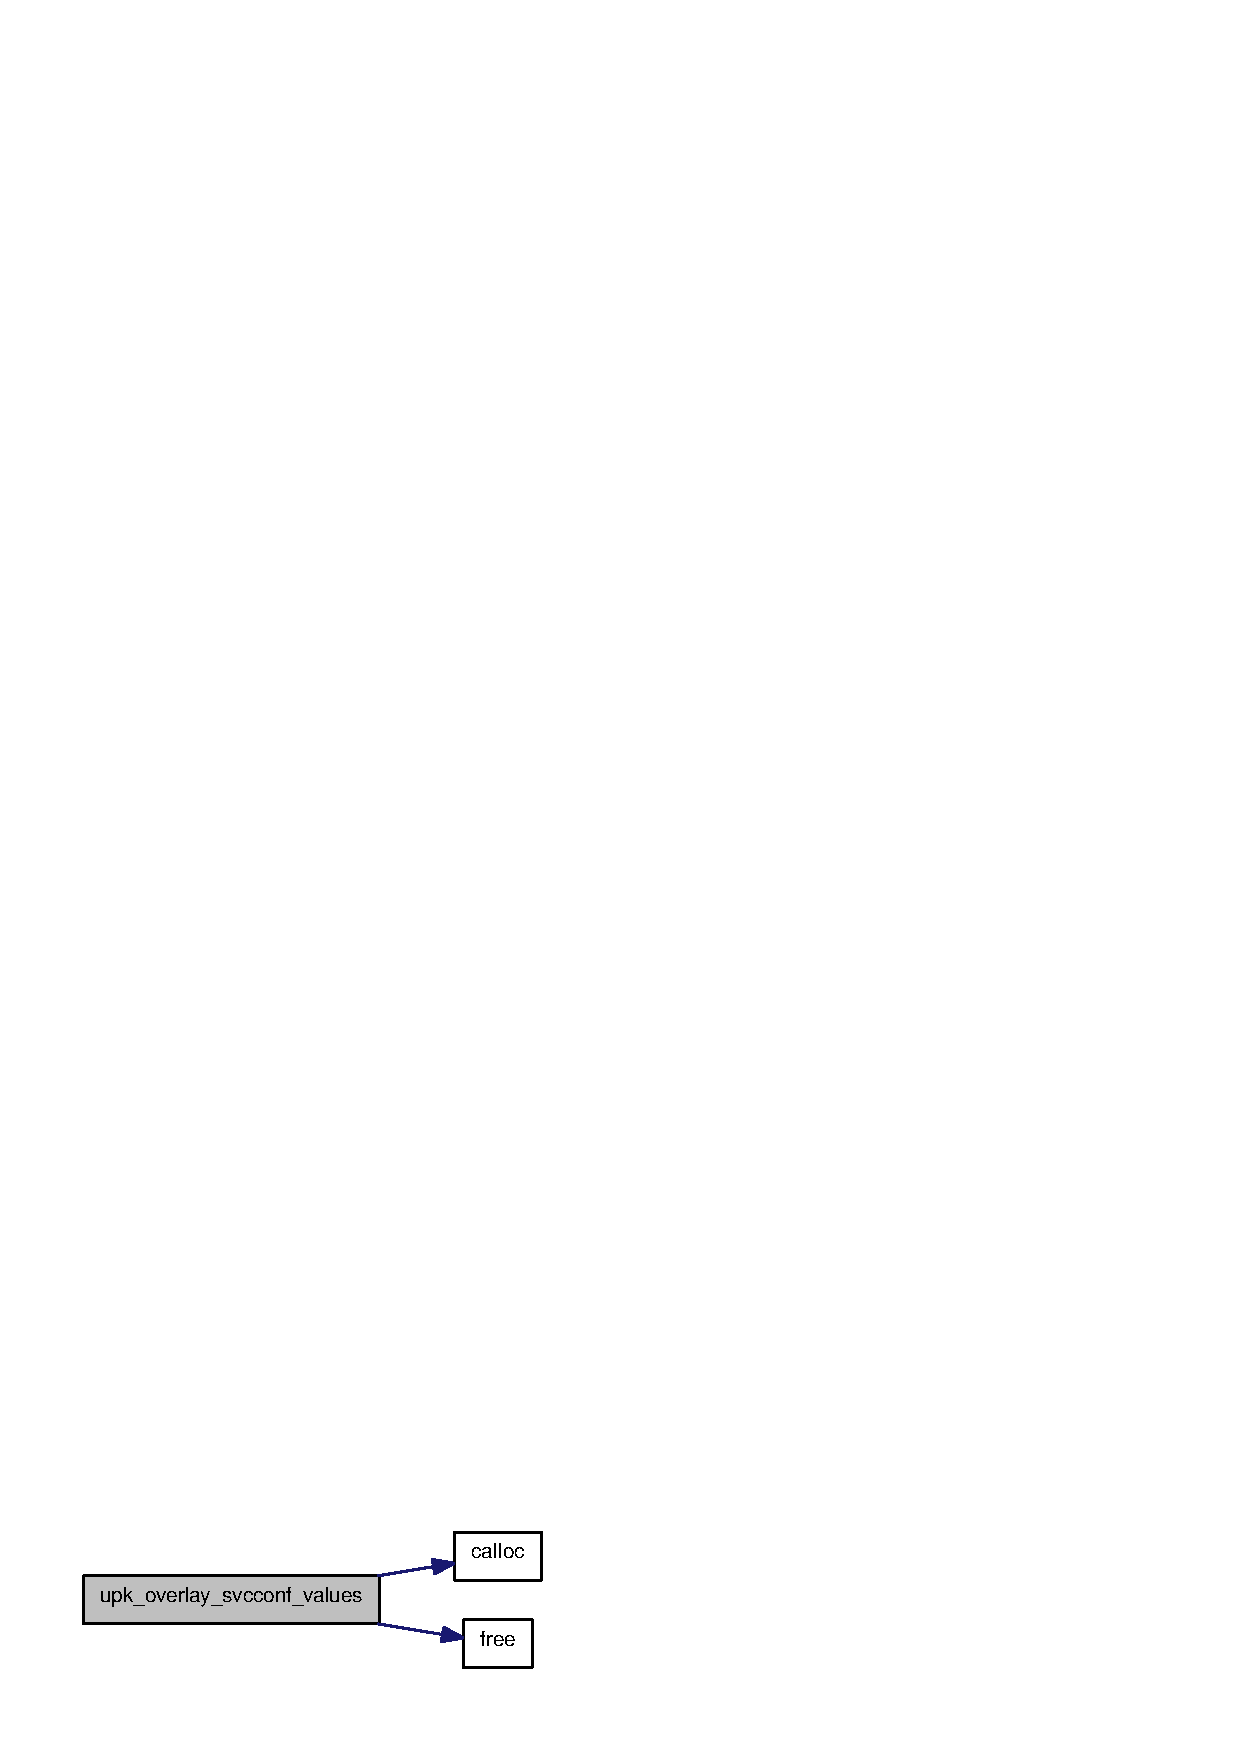
\includegraphics[width=264pt]{group__config__impl_gaab28dbb04c28f723b90b0baba926408f_cgraph}
\end{center}
\end{figure}




Here is the caller graph for this function:
\nopagebreak
\begin{figure}[H]
\begin{center}
\leavevmode
\includegraphics[width=362pt]{group__config__impl_gaab28dbb04c28f723b90b0baba926408f_icgraph}
\end{center}
\end{figure}


\index{Config\_\-impl@{Config\_\-impl}!upk\_\-parse\_\-svc\_\-id@{upk\_\-parse\_\-svc\_\-id}}
\index{upk\_\-parse\_\-svc\_\-id@{upk\_\-parse\_\-svc\_\-id}!Config_impl@{Config\_\-impl}}
\subsubsection[{upk\_\-parse\_\-svc\_\-id}]{\setlength{\rightskip}{0pt plus 5cm}void upk\_\-parse\_\-svc\_\-id (
\begin{DoxyParamCaption}
\item[{char $\ast$}]{key, }
\item[{{\bf upk\_\-svc\_\-desc\_\-t} $\ast$}]{svc}
\end{DoxyParamCaption}
)}\label{group__config__impl_gad985bf99864c933b1a60705b58fded9d}


References \_\-upk\_\-svc\_\-desc::Name, and \_\-upk\_\-svc\_\-desc::Package.



Referenced by upk\_\-ctrlconf\_\-object\_\-handler(), and upk\_\-svcconf\_\-object\_\-handler().



Here is the caller graph for this function:
\nopagebreak
\begin{figure}[H]
\begin{center}
\leavevmode
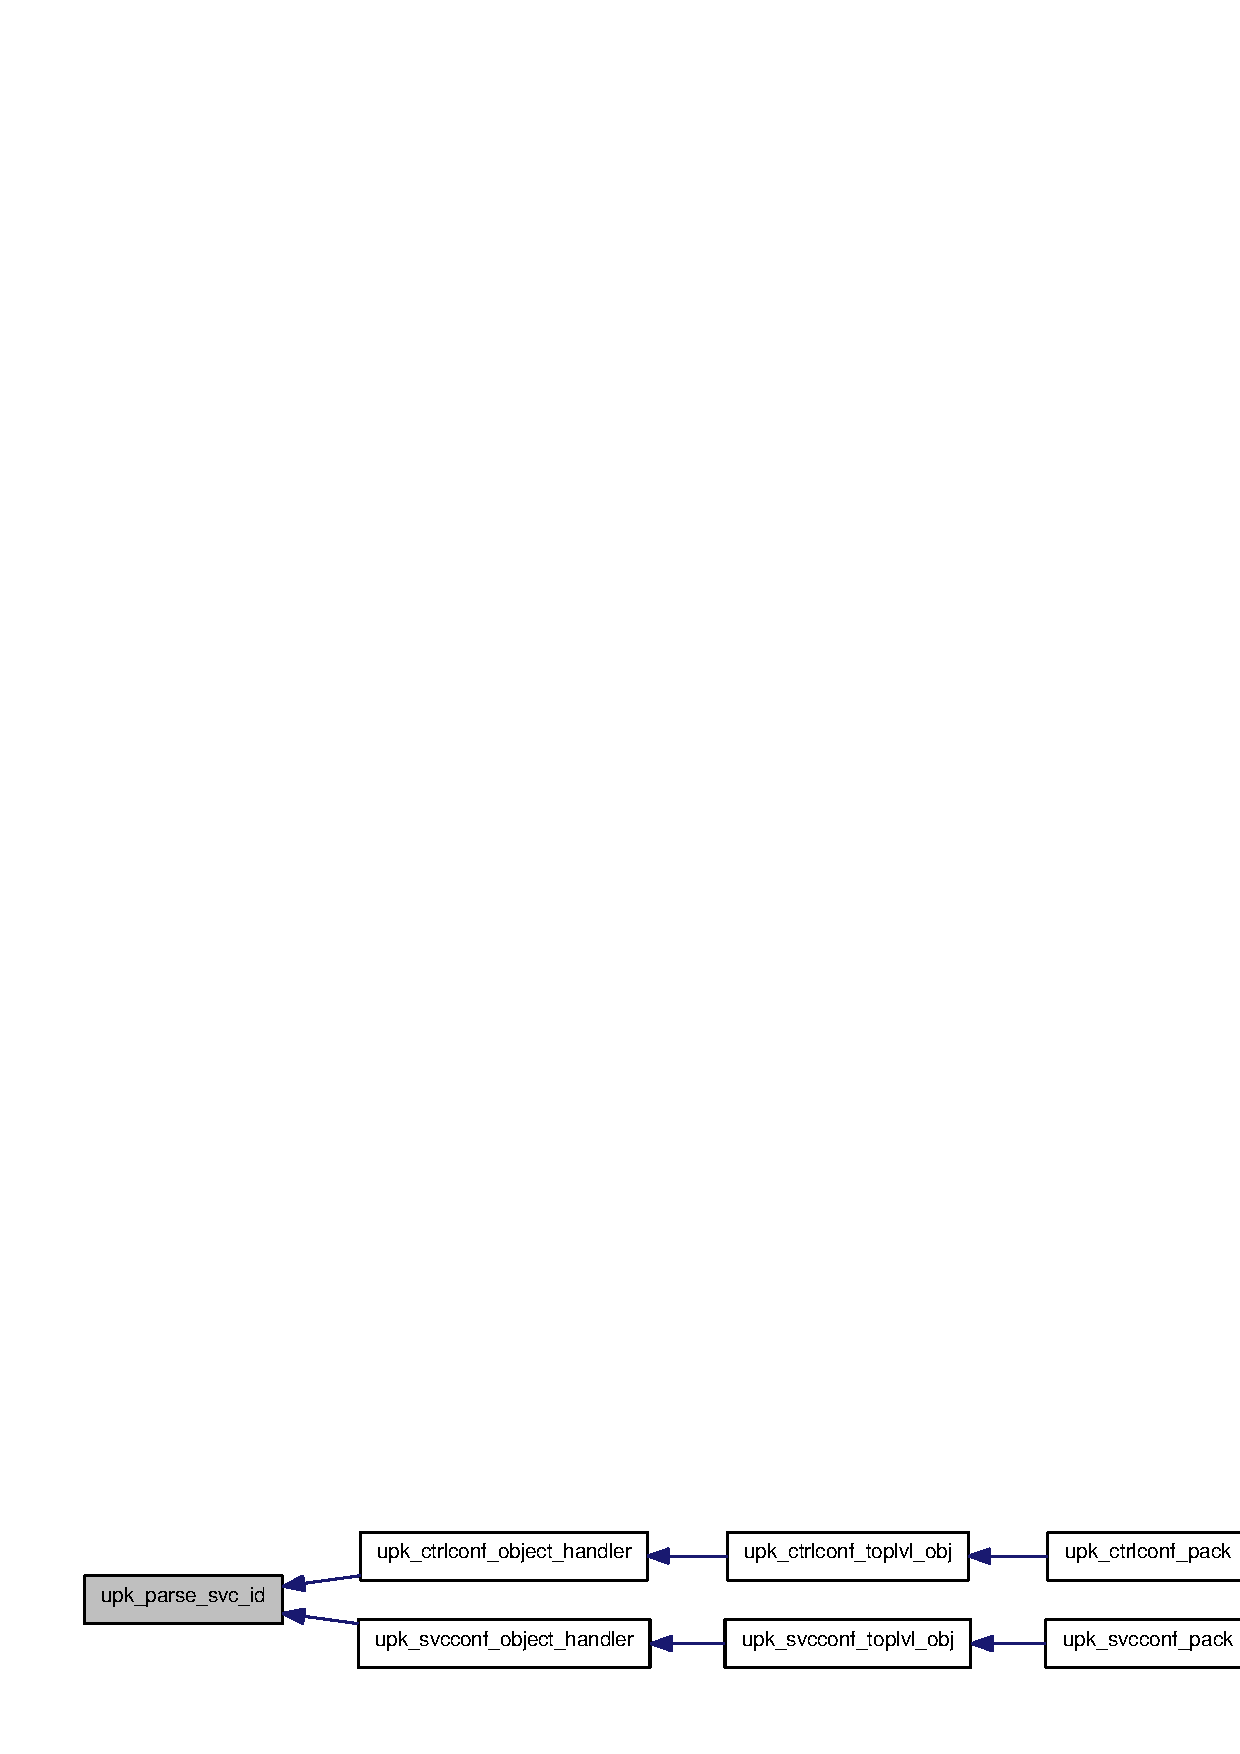
\includegraphics[width=400pt]{group__config__impl_gad985bf99864c933b1a60705b58fded9d_icgraph}
\end{center}
\end{figure}


\index{Config\_\-impl@{Config\_\-impl}!upk\_\-svc\_\-desc\_\-clear@{upk\_\-svc\_\-desc\_\-clear}}
\index{upk\_\-svc\_\-desc\_\-clear@{upk\_\-svc\_\-desc\_\-clear}!Config_impl@{Config\_\-impl}}
\subsubsection[{upk\_\-svc\_\-desc\_\-clear}]{\setlength{\rightskip}{0pt plus 5cm}void upk\_\-svc\_\-desc\_\-clear (
\begin{DoxyParamCaption}
\item[{{\bf upk\_\-svc\_\-desc\_\-t} $\ast$}]{svc}
\end{DoxyParamCaption}
)}\label{group__config__impl_gad3c49ca389d2928e563ec9834942fb28}


References \_\-upk\_\-svc\_\-desc::next, and \_\-upk\_\-svc\_\-desc::StartPriority.



Referenced by main(), upk\_\-ctrl\_\-load\_\-config(), upk\_\-load\_\-runtime\_\-services(), and upk\_\-svcconf\_\-object\_\-handler().



Here is the caller graph for this function:
\nopagebreak
\begin{figure}[H]
\begin{center}
\leavevmode
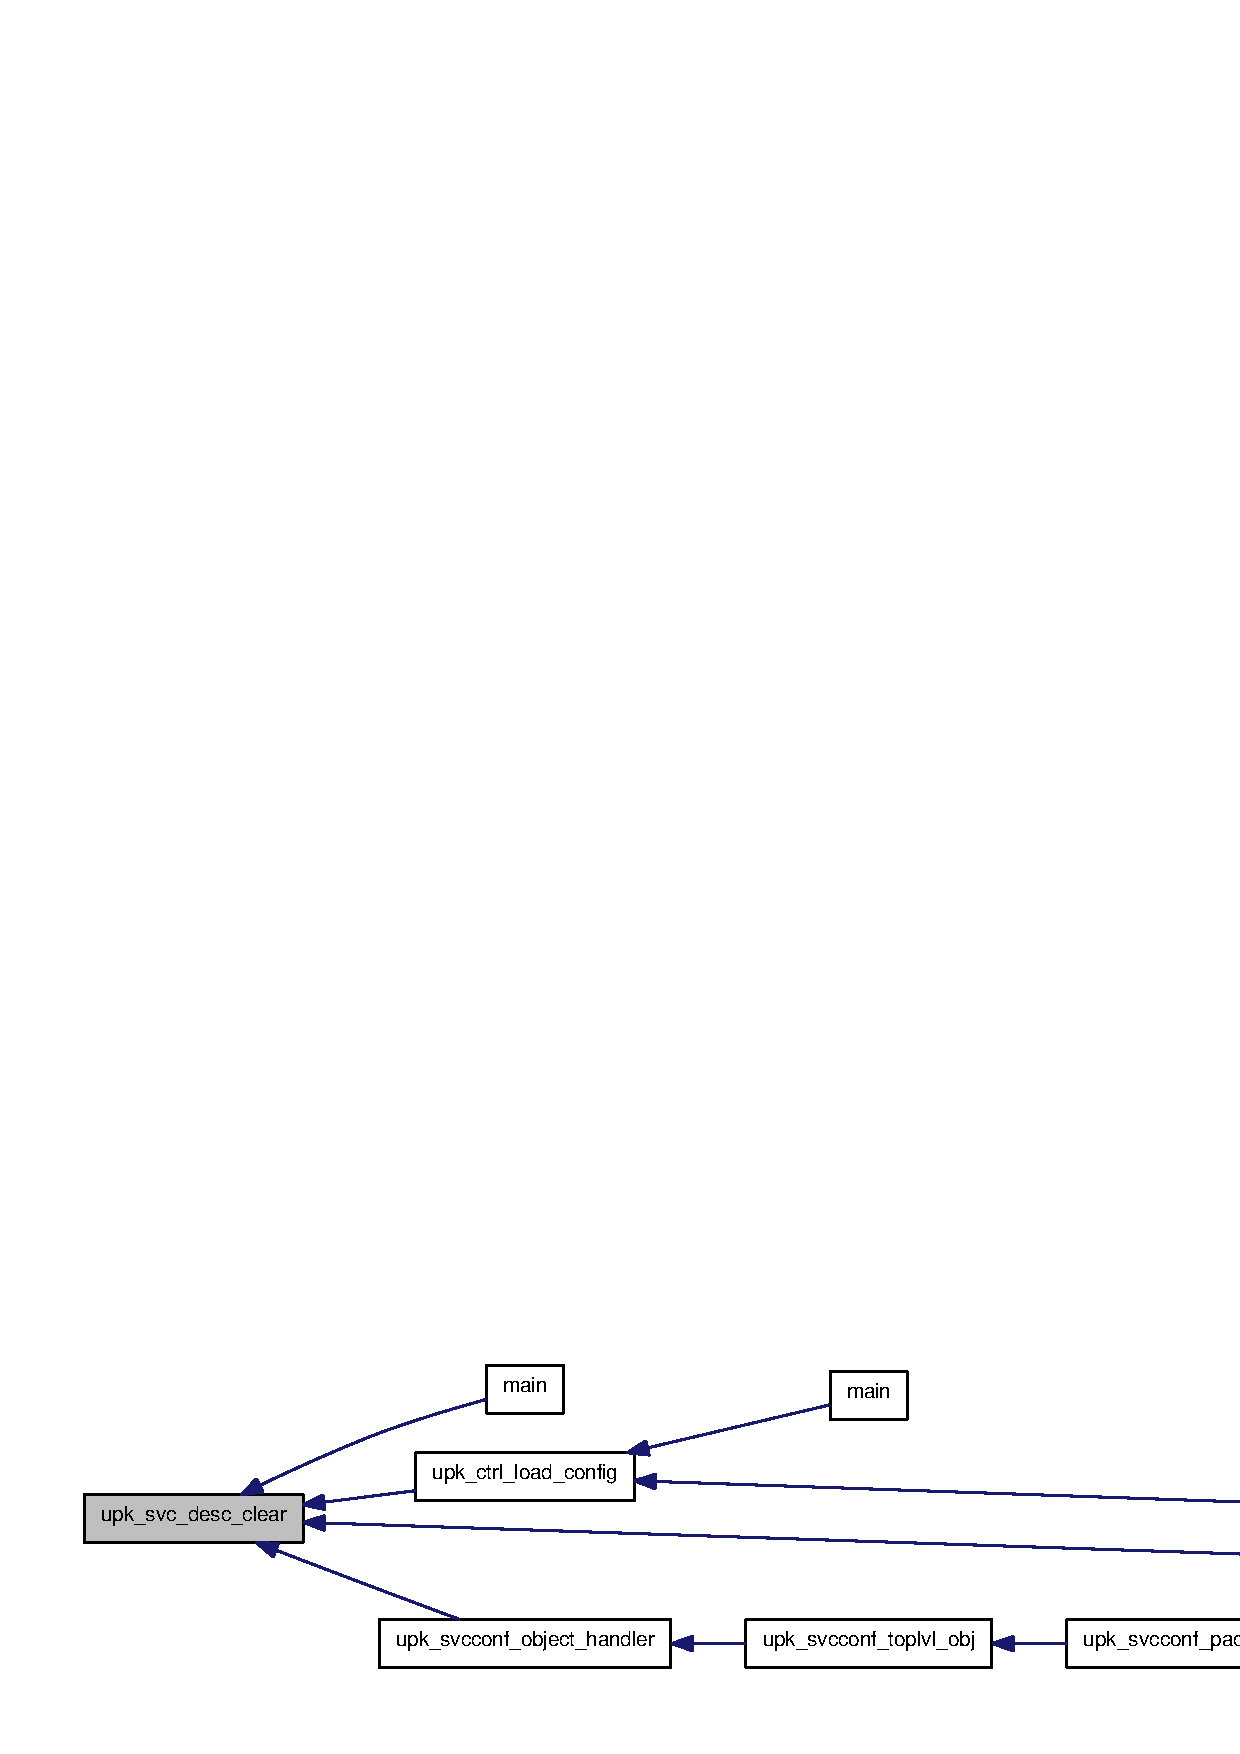
\includegraphics[width=400pt]{group__config__impl_gad3c49ca389d2928e563ec9834942fb28_icgraph}
\end{center}
\end{figure}


\index{Config\_\-impl@{Config\_\-impl}!upk\_\-svc\_\-desc\_\-free@{upk\_\-svc\_\-desc\_\-free}}
\index{upk\_\-svc\_\-desc\_\-free@{upk\_\-svc\_\-desc\_\-free}!Config_impl@{Config\_\-impl}}
\subsubsection[{upk\_\-svc\_\-desc\_\-free}]{\setlength{\rightskip}{0pt plus 5cm}void upk\_\-svc\_\-desc\_\-free (
\begin{DoxyParamCaption}
\item[{{\bf upk\_\-svc\_\-desc\_\-t} $\ast$}]{svc}
\end{DoxyParamCaption}
)}\label{group__config__impl_ga6ca9879f5d370291faf16c2c15ac10bc}


References \_\-upk\_\-svc\_\-desc::CustomActions, free(), \_\-upk\_\-svc\_\-desc::LongDescription, \_\-upk\_\-svc\_\-desc::PipeStderrScript, \_\-upk\_\-svc\_\-desc::PipeStdoutScript, \_\-upk\_\-svc\_\-desc::Prerequisites, \_\-upk\_\-svc\_\-desc::Provides, \_\-upk\_\-svc\_\-desc::ReloadScript, \_\-upk\_\-cust\_\-actscr\_\-list::script, \_\-upk\_\-svc\_\-desc::StartScript, \_\-upk\_\-svc\_\-desc::StopScript, \_\-upk\_\-cust\_\-actscr\_\-meta\_\-p::thisp, UPKLIST\_\-FOREACH, UPKLIST\_\-FREE, and UPKLIST\_\-UNLINK.



Referenced by main(), upk\_\-ctrlconf\_\-free(), and upk\_\-svclist\_\-free().



Here is the call graph for this function:
\nopagebreak
\begin{figure}[H]
\begin{center}
\leavevmode
\includegraphics[width=216pt]{group__config__impl_ga6ca9879f5d370291faf16c2c15ac10bc_cgraph}
\end{center}
\end{figure}




Here is the caller graph for this function:
\nopagebreak
\begin{figure}[H]
\begin{center}
\leavevmode
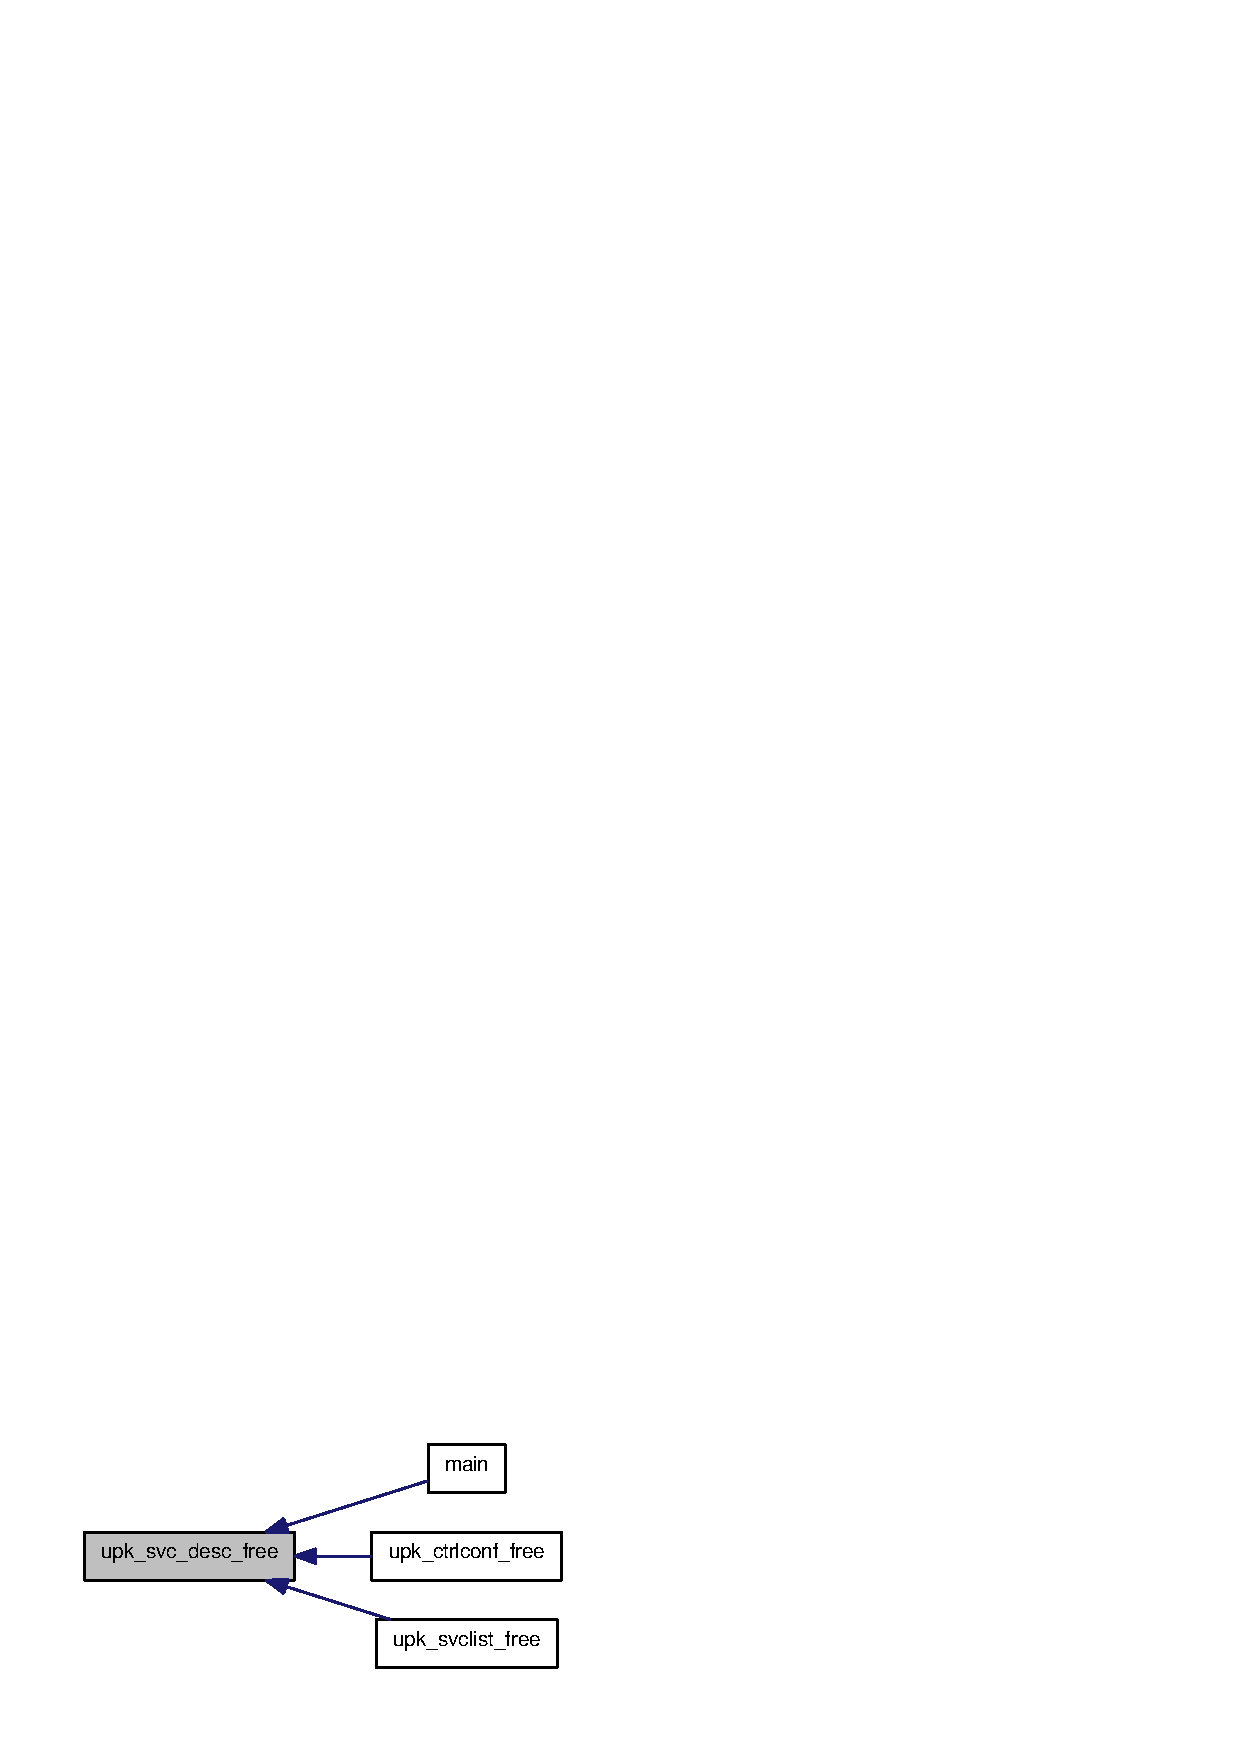
\includegraphics[width=274pt]{group__config__impl_ga6ca9879f5d370291faf16c2c15ac10bc_icgraph}
\end{center}
\end{figure}


\index{Config\_\-impl@{Config\_\-impl}!upk\_\-svc\_\-desc\_\-to\_\-json\_\-obj@{upk\_\-svc\_\-desc\_\-to\_\-json\_\-obj}}
\index{upk\_\-svc\_\-desc\_\-to\_\-json\_\-obj@{upk\_\-svc\_\-desc\_\-to\_\-json\_\-obj}!Config_impl@{Config\_\-impl}}
\subsubsection[{upk\_\-svc\_\-desc\_\-to\_\-json\_\-obj}]{\setlength{\rightskip}{0pt plus 5cm}struct json\_\-object$\ast$ upk\_\-svc\_\-desc\_\-to\_\-json\_\-obj (
\begin{DoxyParamCaption}
\item[{{\bf upk\_\-svc\_\-desc\_\-t} $\ast$}]{svc}
\end{DoxyParamCaption}
)\hspace{0.3cm}{\ttfamily  [read]}}\label{group__config__impl_ga02e5b971c150fa74691e14f94b6ee291}


References \_\-joa, \_\-upk\_\-svc\_\-desc::CustomActions, \_\-upk\_\-svc\_\-desc::ExecReload, \_\-upk\_\-svc\_\-desc::ExecStart, \_\-upk\_\-svc\_\-desc::ExecStop, \_\-upk\_\-svc\_\-desc::InitialState, jt\_\-array, jt\_\-boolean, jt\_\-int, jt\_\-string, \_\-upk\_\-svc\_\-desc::KillTimeout, \_\-upk\_\-svc\_\-desc::LongDescription, \_\-upk\_\-svc\_\-desc::MaxConsecutiveFailures, \_\-upk\_\-cust\_\-actscr\_\-list::name, \_\-upk\_\-svcid::name, \_\-upk\_\-svc\_\-desc::Package, \_\-upk\_\-svc\_\-desc::PipeStderrScript, \_\-upk\_\-svc\_\-desc::PipeStdoutScript, \_\-upk\_\-svcid::pkg, \_\-upk\_\-svc\_\-desc::PreferBuddyStateForRunning, \_\-upk\_\-svc\_\-desc::PreferBuddyStateForStopped, \_\-upk\_\-svc\_\-desc::Prerequisites, \_\-upk\_\-svc\_\-desc::Provides, \_\-upk\_\-svc\_\-desc::RandomizeRateLimit, \_\-upk\_\-svc\_\-desc::ReconnectRetries, \_\-upk\_\-svc\_\-desc::RedirectStderr, \_\-upk\_\-svc\_\-desc::RedirectStdout, \_\-upk\_\-svc\_\-desc::ReloadScript, \_\-upk\_\-svc\_\-desc::RingbufferSize, \_\-upk\_\-cust\_\-actscr\_\-list::script, \_\-upk\_\-svc\_\-desc::SetGID, \_\-upk\_\-svc\_\-desc::SetUID, \_\-upk\_\-svc\_\-desc::ShortDescription, \_\-upk\_\-svc\_\-desc::StartPriority, \_\-upk\_\-svc\_\-desc::StartScript, \_\-upk\_\-svc\_\-desc::StopScript, \_\-upk\_\-cust\_\-actscr\_\-meta\_\-p::thisp, \_\-upk\_\-svcid\_\-meta\_\-p::thisp, \_\-upk\_\-svc\_\-desc::UnconfigureOnFileRemoval, upk\_\-concat\_\-svcid(), upk\_\-json\_\-serialize\_\-or\_\-null(), UPK\_\-MAX\_\-STRING\_\-LEN, UPK\_\-STATE\_\-RUNNING, UPK\_\-STATE\_\-STOPPED, upk\_\-string\_\-to\_\-uuid(), UPKLIST\_\-FOREACH, \_\-upk\_\-svc\_\-desc::UserMaxRestarts, \_\-upk\_\-svc\_\-desc::UserRateLimit, \_\-upk\_\-svc\_\-desc::UserRestartWindow, and \_\-upk\_\-svc\_\-desc::UUID.



Referenced by upk\_\-svclist\_\-to\_\-json\_\-obj().



Here is the call graph for this function:
\nopagebreak
\begin{figure}[H]
\begin{center}
\leavevmode
\includegraphics[width=344pt]{group__config__impl_ga02e5b971c150fa74691e14f94b6ee291_cgraph}
\end{center}
\end{figure}




Here is the caller graph for this function:
\nopagebreak
\begin{figure}[H]
\begin{center}
\leavevmode
\includegraphics[width=334pt]{group__config__impl_ga02e5b971c150fa74691e14f94b6ee291_icgraph}
\end{center}
\end{figure}


\index{Config\_\-impl@{Config\_\-impl}!upk\_\-svc\_\-id@{upk\_\-svc\_\-id}}
\index{upk\_\-svc\_\-id@{upk\_\-svc\_\-id}!Config_impl@{Config\_\-impl}}
\subsubsection[{upk\_\-svc\_\-id}]{\setlength{\rightskip}{0pt plus 5cm}char$\ast$ upk\_\-svc\_\-id (
\begin{DoxyParamCaption}
\item[{char $\ast$}]{dest, }
\item[{{\bf upk\_\-svc\_\-desc\_\-t} $\ast$}]{svc}
\end{DoxyParamCaption}
)}\label{group__config__impl_ga74c0ebb6d5f4b890205dfba4fea7b730}


References \_\-upk\_\-svc\_\-desc::Name, \_\-upk\_\-svc\_\-desc::Package, and upk\_\-concat\_\-svcid().



Referenced by upk\_\-svclist\_\-to\_\-json\_\-obj().



Here is the call graph for this function:\nopagebreak
\begin{figure}[H]
\begin{center}
\leavevmode
\includegraphics[width=242pt]{group__config__impl_ga74c0ebb6d5f4b890205dfba4fea7b730_cgraph}
\end{center}
\end{figure}




Here is the caller graph for this function:
\nopagebreak
\begin{figure}[H]
\begin{center}
\leavevmode
\includegraphics[width=266pt]{group__config__impl_ga74c0ebb6d5f4b890205dfba4fea7b730_icgraph}
\end{center}
\end{figure}


\index{Config\_\-impl@{Config\_\-impl}!upk\_\-svcconf\_\-array\_\-handler@{upk\_\-svcconf\_\-array\_\-handler}}
\index{upk\_\-svcconf\_\-array\_\-handler@{upk\_\-svcconf\_\-array\_\-handler}!Config_impl@{Config\_\-impl}}
\subsubsection[{upk\_\-svcconf\_\-array\_\-handler}]{\setlength{\rightskip}{0pt plus 5cm}static void upk\_\-svcconf\_\-array\_\-handler (
\begin{DoxyParamCaption}
\item[{{\bf upk\_\-json\_\-stack\_\-meta\_\-t} $\ast$}]{meta, }
\item[{void $\ast$}]{data, }
\item[{char $\ast$}]{key, }
\item[{{\bf upk\_\-json\_\-val\_\-t}}]{v}
\end{DoxyParamCaption}
)\hspace{0.3cm}{\ttfamily  [static]}}\label{group__config__impl_ga9ae6ec4edd6a67abc22b670755842ff7}


References calloc(), \_\-upk\_\-json\_\-stack\_\-node::data, \_\-upk\_\-json\_\-stack\_\-node::handlers, \_\-upk\_\-svc\_\-desc::Prerequisites, \_\-upk\_\-svc\_\-desc::Provides, upk\_\-json\_\-stack\_\-push(), and upk\_\-svcconf\_\-setup\_\-array\_\-handlers().



Referenced by upk\_\-svcconf\_\-setup\_\-handlers().



Here is the call graph for this function:
\nopagebreak
\begin{figure}[H]
\begin{center}
\leavevmode
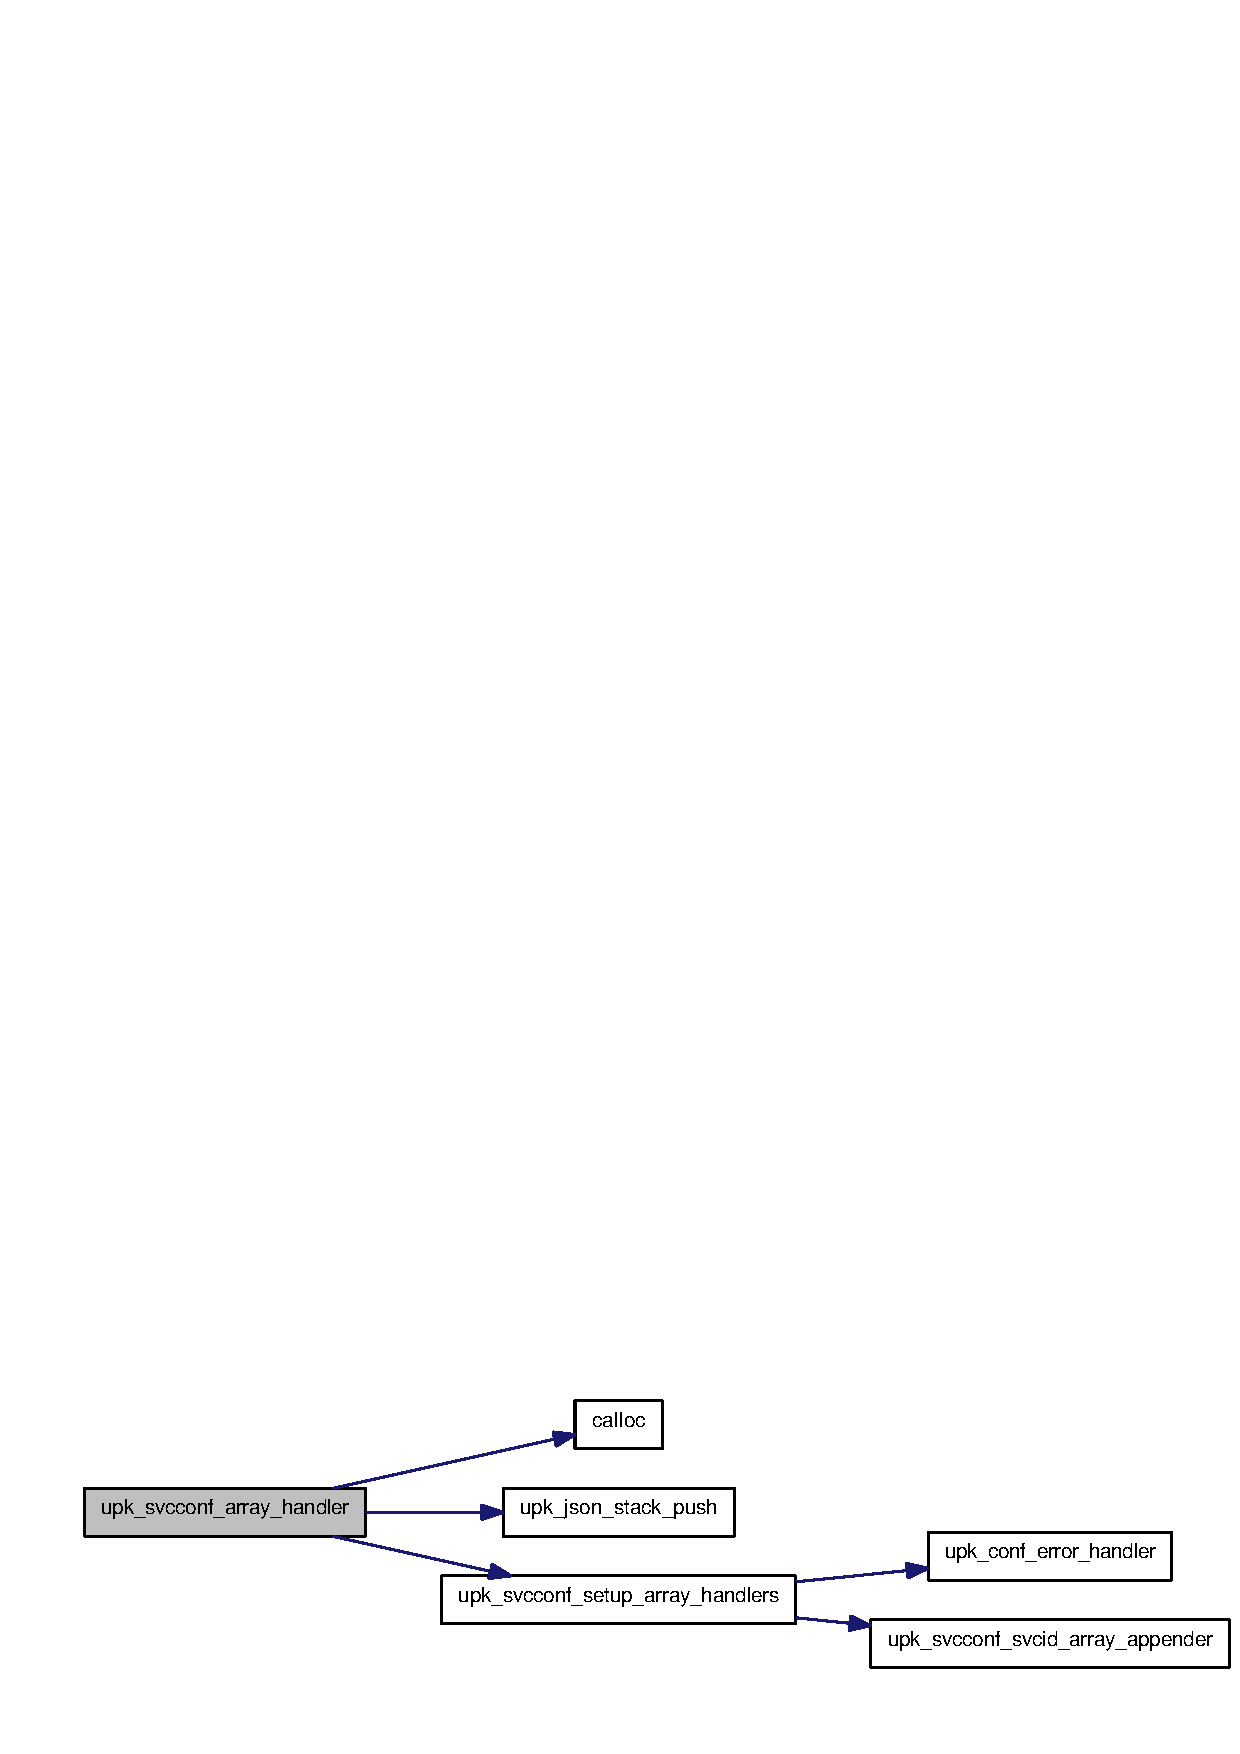
\includegraphics[width=400pt]{group__config__impl_ga9ae6ec4edd6a67abc22b670755842ff7_cgraph}
\end{center}
\end{figure}




Here is the caller graph for this function:
\nopagebreak
\begin{figure}[H]
\begin{center}
\leavevmode
\includegraphics[width=400pt]{group__config__impl_ga9ae6ec4edd6a67abc22b670755842ff7_icgraph}
\end{center}
\end{figure}


\index{Config\_\-impl@{Config\_\-impl}!upk\_\-svcconf\_\-bool\_\-handler@{upk\_\-svcconf\_\-bool\_\-handler}}
\index{upk\_\-svcconf\_\-bool\_\-handler@{upk\_\-svcconf\_\-bool\_\-handler}!Config_impl@{Config\_\-impl}}
\subsubsection[{upk\_\-svcconf\_\-bool\_\-handler}]{\setlength{\rightskip}{0pt plus 5cm}static void upk\_\-svcconf\_\-bool\_\-handler (
\begin{DoxyParamCaption}
\item[{{\bf upk\_\-json\_\-stack\_\-meta\_\-t} $\ast$}]{meta, }
\item[{void $\ast$}]{data, }
\item[{char $\ast$}]{key, }
\item[{{\bf upk\_\-json\_\-val\_\-t}}]{v}
\end{DoxyParamCaption}
)\hspace{0.3cm}{\ttfamily  [static]}}\label{group__config__impl_ga9beda73bf422366a770f7062fbda7fe8}


References \_\-upk\_\-json\_\-type::bl, \_\-upk\_\-svc\_\-desc::PreferBuddyStateForRunning, \_\-upk\_\-svc\_\-desc::PreferBuddyStateForStopped, \_\-upk\_\-svc\_\-desc::RandomizeRateLimit, \_\-upk\_\-svc\_\-desc::UnconfigureOnFileRemoval, upk\_\-alert, and \_\-upk\_\-json\_\-type::val.



Referenced by upk\_\-svcconf\_\-setup\_\-handlers().



Here is the caller graph for this function:
\nopagebreak
\begin{figure}[H]
\begin{center}
\leavevmode
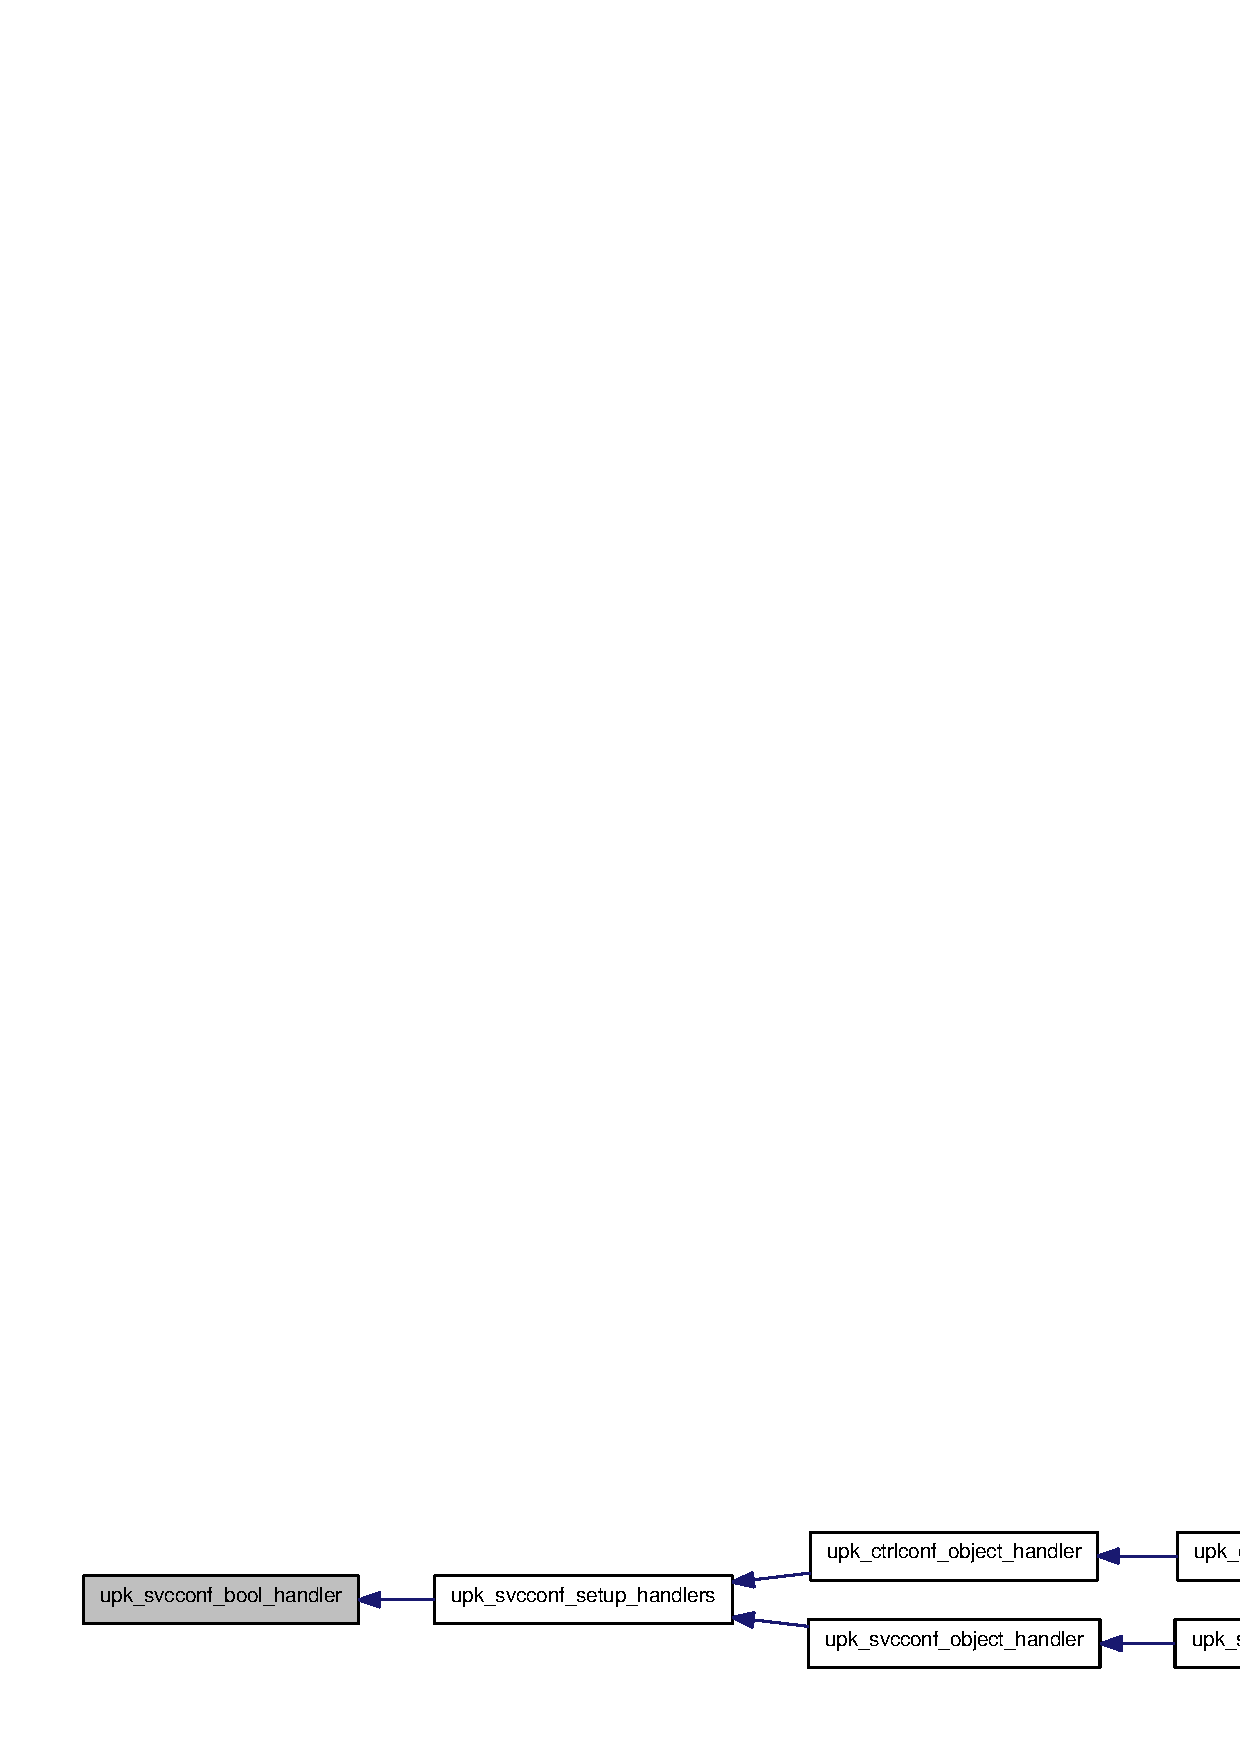
\includegraphics[width=400pt]{group__config__impl_ga9beda73bf422366a770f7062fbda7fe8_icgraph}
\end{center}
\end{figure}


\index{Config\_\-impl@{Config\_\-impl}!upk\_\-svcconf\_\-customaction\_\-array\_\-appender@{upk\_\-svcconf\_\-customaction\_\-array\_\-appender}}
\index{upk\_\-svcconf\_\-customaction\_\-array\_\-appender@{upk\_\-svcconf\_\-customaction\_\-array\_\-appender}!Config_impl@{Config\_\-impl}}
\subsubsection[{upk\_\-svcconf\_\-customaction\_\-array\_\-appender}]{\setlength{\rightskip}{0pt plus 5cm}static void upk\_\-svcconf\_\-customaction\_\-array\_\-appender (
\begin{DoxyParamCaption}
\item[{{\bf upk\_\-json\_\-stack\_\-meta\_\-t} $\ast$}]{meta, }
\item[{void $\ast$}]{data, }
\item[{char $\ast$}]{key, }
\item[{{\bf upk\_\-json\_\-val\_\-t}}]{v}
\end{DoxyParamCaption}
)\hspace{0.3cm}{\ttfamily  [static]}}\label{group__config__impl_ga754e7f3e2be11a91d8f806f5fd1732e8}


References \_\-upk\_\-json\_\-string::c\_\-str, calloc(), \_\-upk\_\-cust\_\-actscr\_\-list::name, \_\-upk\_\-cust\_\-actscr\_\-list::script, \_\-upk\_\-json\_\-type::str, \_\-upk\_\-cust\_\-actscr\_\-meta\_\-p::thisp, UPK\_\-MAX\_\-STRING\_\-LEN, UPKLIST\_\-APPEND, and \_\-upk\_\-json\_\-type::val.



Referenced by upk\_\-svcconf\_\-setup\_\-object\_\-handlers().



Here is the call graph for this function:
\nopagebreak
\begin{figure}[H]
\begin{center}
\leavevmode
\includegraphics[width=330pt]{group__config__impl_ga754e7f3e2be11a91d8f806f5fd1732e8_cgraph}
\end{center}
\end{figure}




Here is the caller graph for this function:
\nopagebreak
\begin{figure}[H]
\begin{center}
\leavevmode
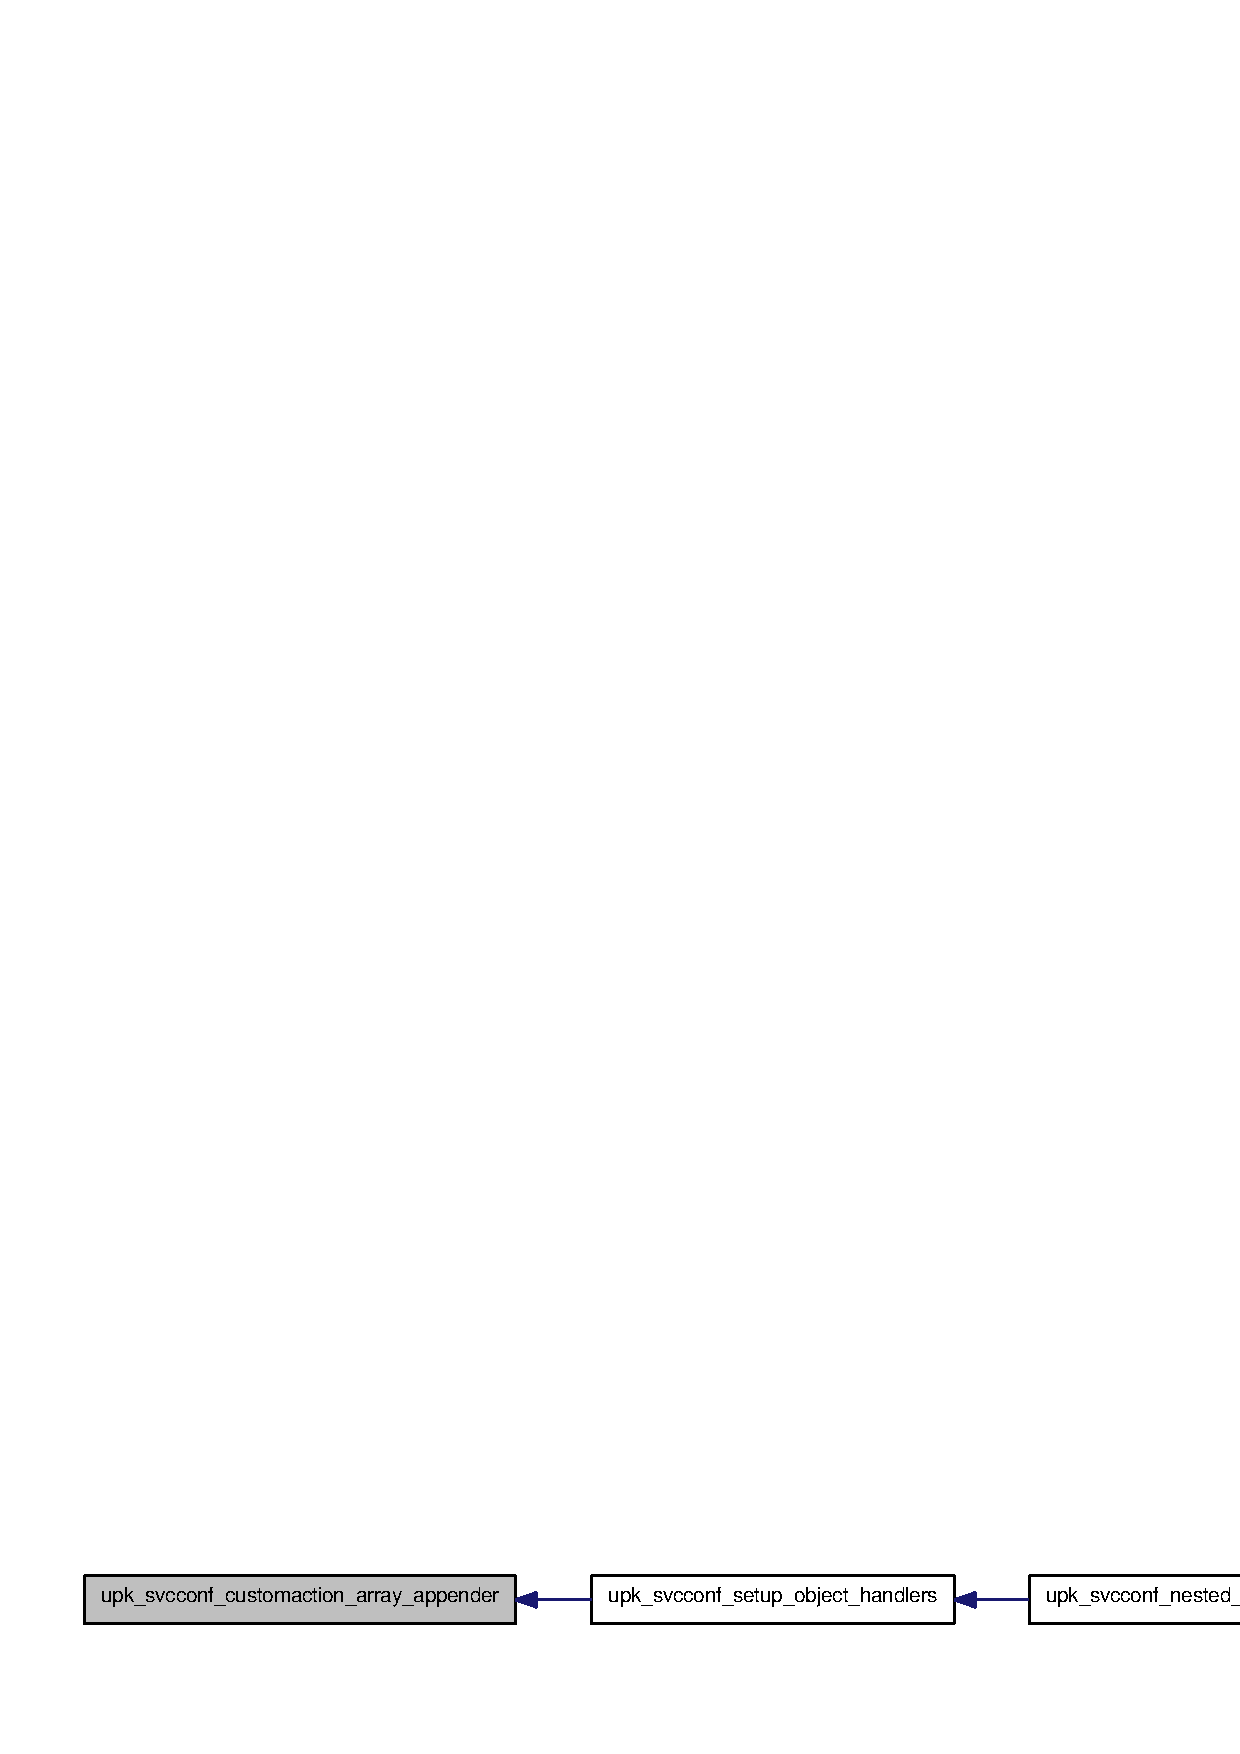
\includegraphics[width=400pt]{group__config__impl_ga754e7f3e2be11a91d8f806f5fd1732e8_icgraph}
\end{center}
\end{figure}


\index{Config\_\-impl@{Config\_\-impl}!upk\_\-svcconf\_\-int\_\-handler@{upk\_\-svcconf\_\-int\_\-handler}}
\index{upk\_\-svcconf\_\-int\_\-handler@{upk\_\-svcconf\_\-int\_\-handler}!Config_impl@{Config\_\-impl}}
\subsubsection[{upk\_\-svcconf\_\-int\_\-handler}]{\setlength{\rightskip}{0pt plus 5cm}static void upk\_\-svcconf\_\-int\_\-handler (
\begin{DoxyParamCaption}
\item[{{\bf upk\_\-json\_\-stack\_\-meta\_\-t} $\ast$}]{meta, }
\item[{void $\ast$}]{data, }
\item[{char $\ast$}]{key, }
\item[{{\bf upk\_\-json\_\-val\_\-t}}]{v}
\end{DoxyParamCaption}
)\hspace{0.3cm}{\ttfamily  [static]}}\label{group__config__impl_ga5771789fb975ff22da6ad83a5a639fb1}


References \_\-upk\_\-json\_\-type::i, \_\-upk\_\-svc\_\-desc::KillTimeout, \_\-upk\_\-svc\_\-desc::MaxConsecutiveFailures, \_\-upk\_\-svc\_\-desc::ReconnectRetries, \_\-upk\_\-svc\_\-desc::RingbufferSize, \_\-upk\_\-svc\_\-desc::SetGID, \_\-upk\_\-svc\_\-desc::SetUID, \_\-upk\_\-svc\_\-desc::StartPriority, upk\_\-alert, \_\-upk\_\-svc\_\-desc::UserMaxRestarts, \_\-upk\_\-svc\_\-desc::UserRateLimit, \_\-upk\_\-svc\_\-desc::UserRestartWindow, and \_\-upk\_\-json\_\-type::val.



Referenced by upk\_\-svcconf\_\-setup\_\-handlers().



Here is the caller graph for this function:
\nopagebreak
\begin{figure}[H]
\begin{center}
\leavevmode
\includegraphics[width=400pt]{group__config__impl_ga5771789fb975ff22da6ad83a5a639fb1_icgraph}
\end{center}
\end{figure}


\index{Config\_\-impl@{Config\_\-impl}!upk\_\-svcconf\_\-nested\_\-object\_\-handler@{upk\_\-svcconf\_\-nested\_\-object\_\-handler}}
\index{upk\_\-svcconf\_\-nested\_\-object\_\-handler@{upk\_\-svcconf\_\-nested\_\-object\_\-handler}!Config_impl@{Config\_\-impl}}
\subsubsection[{upk\_\-svcconf\_\-nested\_\-object\_\-handler}]{\setlength{\rightskip}{0pt plus 5cm}static void upk\_\-svcconf\_\-nested\_\-object\_\-handler (
\begin{DoxyParamCaption}
\item[{{\bf upk\_\-json\_\-stack\_\-meta\_\-t} $\ast$}]{meta, }
\item[{void $\ast$}]{data, }
\item[{char $\ast$}]{key, }
\item[{{\bf upk\_\-json\_\-val\_\-t}}]{v}
\end{DoxyParamCaption}
)\hspace{0.3cm}{\ttfamily  [static]}}\label{group__config__impl_ga92b7ce66bee3b5476996ce54bb395454}


References calloc(), \_\-upk\_\-svc\_\-desc::CustomActions, \_\-upk\_\-json\_\-stack\_\-node::data, \_\-upk\_\-json\_\-stack\_\-node::handlers, upk\_\-json\_\-stack\_\-push(), and upk\_\-svcconf\_\-setup\_\-object\_\-handlers().



Referenced by upk\_\-svcconf\_\-setup\_\-handlers().



Here is the call graph for this function:
\nopagebreak
\begin{figure}[H]
\begin{center}
\leavevmode
\includegraphics[width=400pt]{group__config__impl_ga92b7ce66bee3b5476996ce54bb395454_cgraph}
\end{center}
\end{figure}




Here is the caller graph for this function:
\nopagebreak
\begin{figure}[H]
\begin{center}
\leavevmode
\includegraphics[width=400pt]{group__config__impl_ga92b7ce66bee3b5476996ce54bb395454_icgraph}
\end{center}
\end{figure}


\index{Config\_\-impl@{Config\_\-impl}!upk\_\-svcconf\_\-object\_\-handler@{upk\_\-svcconf\_\-object\_\-handler}}
\index{upk\_\-svcconf\_\-object\_\-handler@{upk\_\-svcconf\_\-object\_\-handler}!Config_impl@{Config\_\-impl}}
\subsubsection[{upk\_\-svcconf\_\-object\_\-handler}]{\setlength{\rightskip}{0pt plus 5cm}static void upk\_\-svcconf\_\-object\_\-handler (
\begin{DoxyParamCaption}
\item[{{\bf upk\_\-json\_\-stack\_\-meta\_\-t} $\ast$}]{meta, }
\item[{void $\ast$}]{data, }
\item[{char $\ast$}]{key, }
\item[{{\bf upk\_\-json\_\-val\_\-t}}]{v}
\end{DoxyParamCaption}
)\hspace{0.3cm}{\ttfamily  [static]}}\label{group__config__impl_ga8753074ecae15841a5f5c3a28e31b58a}


References calloc(), \_\-upk\_\-json\_\-stack\_\-node::data, \_\-upk\_\-json\_\-stack\_\-node::handlers, \_\-upk\_\-controller\_\-config::svclist, upk\_\-svc\_\-desc\_\-meta\_\-p::thisp, upk\_\-json\_\-stack\_\-push(), upk\_\-parse\_\-svc\_\-id(), upk\_\-svc\_\-desc\_\-clear(), upk\_\-svcconf\_\-setup\_\-handlers(), and UPKLIST\_\-APPEND.



Referenced by upk\_\-svcconf\_\-toplvl\_\-obj().



Here is the call graph for this function:
\nopagebreak
\begin{figure}[H]
\begin{center}
\leavevmode
\includegraphics[width=400pt]{group__config__impl_ga8753074ecae15841a5f5c3a28e31b58a_cgraph}
\end{center}
\end{figure}




Here is the caller graph for this function:
\nopagebreak
\begin{figure}[H]
\begin{center}
\leavevmode
\includegraphics[width=400pt]{group__config__impl_ga8753074ecae15841a5f5c3a28e31b58a_icgraph}
\end{center}
\end{figure}


\index{Config\_\-impl@{Config\_\-impl}!upk\_\-svcconf\_\-pack@{upk\_\-svcconf\_\-pack}}
\index{upk\_\-svcconf\_\-pack@{upk\_\-svcconf\_\-pack}!Config_impl@{Config\_\-impl}}
\subsubsection[{upk\_\-svcconf\_\-pack}]{\setlength{\rightskip}{0pt plus 5cm}void upk\_\-svcconf\_\-pack (
\begin{DoxyParamCaption}
\item[{{\bf upk\_\-controller\_\-config\_\-t} $\ast$}]{cfg, }
\item[{const char $\ast$}]{json\_\-string}
\end{DoxyParamCaption}
)}\label{group__config__impl_gaef8b858931337dfe742cae5815857dec}


References \_\-upk\_\-json\_\-stack\_\-handlers::after\_\-json\_\-array\_\-pop, \_\-upk\_\-json\_\-stack\_\-handlers::after\_\-json\_\-obj\_\-pop, calloc(), \_\-upk\_\-json\_\-stack\_\-node::data, \_\-upk\_\-json\_\-stack\_\-node::handlers, \_\-upk\_\-json\_\-stack\_\-handlers::json\_\-array, \_\-upk\_\-json\_\-stack\_\-handlers::json\_\-bool, \_\-upk\_\-json\_\-stack\_\-handlers::json\_\-double, \_\-upk\_\-json\_\-stack\_\-handlers::json\_\-int, \_\-upk\_\-json\_\-stack\_\-handlers::json\_\-null, \_\-upk\_\-json\_\-stack\_\-handlers::json\_\-object, \_\-upk\_\-json\_\-stack\_\-handlers::json\_\-string, restrict, upk\_\-conf\_\-error\_\-handler(), upk\_\-json\_\-parse\_\-node(), upk\_\-json\_\-parse\_\-string(), upk\_\-json\_\-stack\_\-meta\_\-t, upk\_\-json\_\-stack\_\-push(), upk\_\-svcconf\_\-toplvl\_\-obj(), and UPKLIST\_\-FREE.



Referenced by upk\_\-load\_\-runtime\_\-services().



Here is the call graph for this function:
\nopagebreak
\begin{figure}[H]
\begin{center}
\leavevmode
\includegraphics[width=400pt]{group__config__impl_gaef8b858931337dfe742cae5815857dec_cgraph}
\end{center}
\end{figure}




Here is the caller graph for this function:
\nopagebreak
\begin{figure}[H]
\begin{center}
\leavevmode
\includegraphics[width=314pt]{group__config__impl_gaef8b858931337dfe742cae5815857dec_icgraph}
\end{center}
\end{figure}


\index{Config\_\-impl@{Config\_\-impl}!upk\_\-svcconf\_\-setup\_\-array\_\-handlers@{upk\_\-svcconf\_\-setup\_\-array\_\-handlers}}
\index{upk\_\-svcconf\_\-setup\_\-array\_\-handlers@{upk\_\-svcconf\_\-setup\_\-array\_\-handlers}!Config_impl@{Config\_\-impl}}
\subsubsection[{upk\_\-svcconf\_\-setup\_\-array\_\-handlers}]{\setlength{\rightskip}{0pt plus 5cm}static void upk\_\-svcconf\_\-setup\_\-array\_\-handlers (
\begin{DoxyParamCaption}
\item[{{\bf upk\_\-json\_\-handlers\_\-t} $\ast$}]{handlers}
\end{DoxyParamCaption}
)\hspace{0.3cm}{\ttfamily  [inline, static]}}\label{group__config__impl_gaf5f51c2fe67a8dcdffbfefd5697efc09}


References \_\-upk\_\-json\_\-stack\_\-handlers::after\_\-json\_\-array\_\-pop, \_\-upk\_\-json\_\-stack\_\-handlers::after\_\-json\_\-obj\_\-pop, \_\-upk\_\-json\_\-stack\_\-handlers::json\_\-array, \_\-upk\_\-json\_\-stack\_\-handlers::json\_\-bool, \_\-upk\_\-json\_\-stack\_\-handlers::json\_\-double, \_\-upk\_\-json\_\-stack\_\-handlers::json\_\-int, \_\-upk\_\-json\_\-stack\_\-handlers::json\_\-null, \_\-upk\_\-json\_\-stack\_\-handlers::json\_\-object, \_\-upk\_\-json\_\-stack\_\-handlers::json\_\-string, restrict, upk\_\-conf\_\-error\_\-handler(), and upk\_\-svcconf\_\-svcid\_\-array\_\-appender().



Referenced by upk\_\-svcconf\_\-array\_\-handler().



Here is the call graph for this function:\nopagebreak
\begin{figure}[H]
\begin{center}
\leavevmode
\includegraphics[width=400pt]{group__config__impl_gaf5f51c2fe67a8dcdffbfefd5697efc09_cgraph}
\end{center}
\end{figure}




Here is the caller graph for this function:
\nopagebreak
\begin{figure}[H]
\begin{center}
\leavevmode
\includegraphics[width=400pt]{group__config__impl_gaf5f51c2fe67a8dcdffbfefd5697efc09_icgraph}
\end{center}
\end{figure}


\index{Config\_\-impl@{Config\_\-impl}!upk\_\-svcconf\_\-setup\_\-handlers@{upk\_\-svcconf\_\-setup\_\-handlers}}
\index{upk\_\-svcconf\_\-setup\_\-handlers@{upk\_\-svcconf\_\-setup\_\-handlers}!Config_impl@{Config\_\-impl}}
\subsubsection[{upk\_\-svcconf\_\-setup\_\-handlers}]{\setlength{\rightskip}{0pt plus 5cm}static void upk\_\-svcconf\_\-setup\_\-handlers (
\begin{DoxyParamCaption}
\item[{{\bf upk\_\-json\_\-handlers\_\-t} $\ast$}]{handlers}
\end{DoxyParamCaption}
)\hspace{0.3cm}{\ttfamily  [inline, static]}}\label{group__config__impl_ga91a20d1386c12a7ca48670777f2a13b6}


References \_\-upk\_\-json\_\-stack\_\-handlers::after\_\-json\_\-array\_\-pop, \_\-upk\_\-json\_\-stack\_\-handlers::after\_\-json\_\-obj\_\-pop, \_\-upk\_\-json\_\-stack\_\-handlers::json\_\-array, \_\-upk\_\-json\_\-stack\_\-handlers::json\_\-bool, \_\-upk\_\-json\_\-stack\_\-handlers::json\_\-double, \_\-upk\_\-json\_\-stack\_\-handlers::json\_\-int, \_\-upk\_\-json\_\-stack\_\-handlers::json\_\-null, \_\-upk\_\-json\_\-stack\_\-handlers::json\_\-object, \_\-upk\_\-json\_\-stack\_\-handlers::json\_\-string, restrict, upk\_\-conf\_\-error\_\-handler(), upk\_\-svcconf\_\-array\_\-handler(), upk\_\-svcconf\_\-bool\_\-handler(), upk\_\-svcconf\_\-int\_\-handler(), upk\_\-svcconf\_\-nested\_\-object\_\-handler(), and upk\_\-svcconf\_\-string\_\-handler().



Referenced by upk\_\-ctrlconf\_\-object\_\-handler(), and upk\_\-svcconf\_\-object\_\-handler().



Here is the call graph for this function:
\nopagebreak
\begin{figure}[H]
\begin{center}
\leavevmode
\includegraphics[width=400pt]{group__config__impl_ga91a20d1386c12a7ca48670777f2a13b6_cgraph}
\end{center}
\end{figure}




Here is the caller graph for this function:
\nopagebreak
\begin{figure}[H]
\begin{center}
\leavevmode
\includegraphics[width=400pt]{group__config__impl_ga91a20d1386c12a7ca48670777f2a13b6_icgraph}
\end{center}
\end{figure}


\index{Config\_\-impl@{Config\_\-impl}!upk\_\-svcconf\_\-setup\_\-object\_\-handlers@{upk\_\-svcconf\_\-setup\_\-object\_\-handlers}}
\index{upk\_\-svcconf\_\-setup\_\-object\_\-handlers@{upk\_\-svcconf\_\-setup\_\-object\_\-handlers}!Config_impl@{Config\_\-impl}}
\subsubsection[{upk\_\-svcconf\_\-setup\_\-object\_\-handlers}]{\setlength{\rightskip}{0pt plus 5cm}static void upk\_\-svcconf\_\-setup\_\-object\_\-handlers (
\begin{DoxyParamCaption}
\item[{{\bf upk\_\-json\_\-handlers\_\-t} $\ast$}]{handlers}
\end{DoxyParamCaption}
)\hspace{0.3cm}{\ttfamily  [inline, static]}}\label{group__config__impl_ga59ca5690cb0cffe92edb07888036d4ec}


References \_\-upk\_\-json\_\-stack\_\-handlers::after\_\-json\_\-array\_\-pop, \_\-upk\_\-json\_\-stack\_\-handlers::after\_\-json\_\-obj\_\-pop, \_\-upk\_\-json\_\-stack\_\-handlers::json\_\-array, \_\-upk\_\-json\_\-stack\_\-handlers::json\_\-bool, \_\-upk\_\-json\_\-stack\_\-handlers::json\_\-double, \_\-upk\_\-json\_\-stack\_\-handlers::json\_\-int, \_\-upk\_\-json\_\-stack\_\-handlers::json\_\-null, \_\-upk\_\-json\_\-stack\_\-handlers::json\_\-object, \_\-upk\_\-json\_\-stack\_\-handlers::json\_\-string, restrict, upk\_\-conf\_\-error\_\-handler(), and upk\_\-svcconf\_\-customaction\_\-array\_\-appender().



Referenced by upk\_\-svcconf\_\-nested\_\-object\_\-handler().



Here is the call graph for this function:
\nopagebreak
\begin{figure}[H]
\begin{center}
\leavevmode
\includegraphics[width=400pt]{group__config__impl_ga59ca5690cb0cffe92edb07888036d4ec_cgraph}
\end{center}
\end{figure}




Here is the caller graph for this function:
\nopagebreak
\begin{figure}[H]
\begin{center}
\leavevmode
\includegraphics[width=400pt]{group__config__impl_ga59ca5690cb0cffe92edb07888036d4ec_icgraph}
\end{center}
\end{figure}


\index{Config\_\-impl@{Config\_\-impl}!upk\_\-svcconf\_\-string\_\-handler@{upk\_\-svcconf\_\-string\_\-handler}}
\index{upk\_\-svcconf\_\-string\_\-handler@{upk\_\-svcconf\_\-string\_\-handler}!Config_impl@{Config\_\-impl}}
\subsubsection[{upk\_\-svcconf\_\-string\_\-handler}]{\setlength{\rightskip}{0pt plus 5cm}static void upk\_\-svcconf\_\-string\_\-handler (
\begin{DoxyParamCaption}
\item[{{\bf upk\_\-json\_\-stack\_\-meta\_\-t} $\ast$}]{meta, }
\item[{void $\ast$}]{data, }
\item[{char $\ast$}]{key, }
\item[{{\bf upk\_\-json\_\-val\_\-t}}]{v}
\end{DoxyParamCaption}
)\hspace{0.3cm}{\ttfamily  [static]}}\label{group__config__impl_ga8821dad50c00a183fb1fdbb1f950ebe0}


References \_\-SC\_\-GETPW\_\-R\_\-SIZE\_\-MAX, \_\-upk\_\-json\_\-string::c\_\-str, calloc(), \_\-upk\_\-svc\_\-desc::ExecReload, \_\-upk\_\-svc\_\-desc::ExecStart, \_\-upk\_\-svc\_\-desc::ExecStop, free(), getpwnam\_\-r(), \_\-upk\_\-svc\_\-desc::InitialState, \_\-upk\_\-svc\_\-desc::LongDescription, \_\-upk\_\-svc\_\-desc::Name, \_\-upk\_\-svc\_\-desc::Package, \_\-upk\_\-svc\_\-desc::PipeStderrScript, \_\-upk\_\-svc\_\-desc::PipeStdoutScript, \_\-upk\_\-svc\_\-desc::RedirectStderr, \_\-upk\_\-svc\_\-desc::RedirectStdout, \_\-upk\_\-svc\_\-desc::ReloadScript, \_\-upk\_\-svc\_\-desc::SetGID, \_\-upk\_\-svc\_\-desc::SetUID, \_\-upk\_\-svc\_\-desc::ShortDescription, \_\-upk\_\-svc\_\-desc::StartScript, \_\-upk\_\-svc\_\-desc::StopScript, \_\-upk\_\-json\_\-type::str, strnlen(), sysconf(), upk\_\-alert, UPK\_\-MAX\_\-PATH\_\-LEN, UPK\_\-MAX\_\-STRING\_\-LEN, UPK\_\-STATE\_\-RUNNING, UPK\_\-STATE\_\-SHUTDOWN, upk\_\-string\_\-to\_\-uuid(), \_\-upk\_\-svc\_\-desc::UUID, and \_\-upk\_\-json\_\-type::val.



Referenced by upk\_\-svcconf\_\-setup\_\-handlers().



Here is the call graph for this function:
\nopagebreak
\begin{figure}[H]
\begin{center}
\leavevmode
\includegraphics[width=316pt]{group__config__impl_ga8821dad50c00a183fb1fdbb1f950ebe0_cgraph}
\end{center}
\end{figure}




Here is the caller graph for this function:
\nopagebreak
\begin{figure}[H]
\begin{center}
\leavevmode
\includegraphics[width=400pt]{group__config__impl_ga8821dad50c00a183fb1fdbb1f950ebe0_icgraph}
\end{center}
\end{figure}


\index{Config\_\-impl@{Config\_\-impl}!upk\_\-svcconf\_\-svcid\_\-array\_\-appender@{upk\_\-svcconf\_\-svcid\_\-array\_\-appender}}
\index{upk\_\-svcconf\_\-svcid\_\-array\_\-appender@{upk\_\-svcconf\_\-svcid\_\-array\_\-appender}!Config_impl@{Config\_\-impl}}
\subsubsection[{upk\_\-svcconf\_\-svcid\_\-array\_\-appender}]{\setlength{\rightskip}{0pt plus 5cm}static void upk\_\-svcconf\_\-svcid\_\-array\_\-appender (
\begin{DoxyParamCaption}
\item[{{\bf upk\_\-json\_\-stack\_\-meta\_\-t} $\ast$}]{meta, }
\item[{void $\ast$}]{data, }
\item[{char $\ast$}]{key, }
\item[{{\bf upk\_\-json\_\-val\_\-t}}]{v}
\end{DoxyParamCaption}
)\hspace{0.3cm}{\ttfamily  [static]}}\label{group__config__impl_ga9fa35d8083bbdada877c0fb1d1a3826b}


References \_\-upk\_\-json\_\-string::c\_\-str, \_\-upk\_\-svcid::name, \_\-upk\_\-svcid::pkg, \_\-upk\_\-json\_\-type::str, \_\-upk\_\-svcid\_\-meta\_\-p::thisp, UPK\_\-MAX\_\-STRING\_\-LEN, UPKLIST\_\-APPEND, and \_\-upk\_\-json\_\-type::val.



Referenced by upk\_\-svcconf\_\-setup\_\-array\_\-handlers().



Here is the caller graph for this function:
\nopagebreak
\begin{figure}[H]
\begin{center}
\leavevmode
\includegraphics[width=400pt]{group__config__impl_ga9fa35d8083bbdada877c0fb1d1a3826b_icgraph}
\end{center}
\end{figure}


\index{Config\_\-impl@{Config\_\-impl}!upk\_\-svcconf\_\-toplvl\_\-obj@{upk\_\-svcconf\_\-toplvl\_\-obj}}
\index{upk\_\-svcconf\_\-toplvl\_\-obj@{upk\_\-svcconf\_\-toplvl\_\-obj}!Config_impl@{Config\_\-impl}}
\subsubsection[{upk\_\-svcconf\_\-toplvl\_\-obj}]{\setlength{\rightskip}{0pt plus 5cm}static void upk\_\-svcconf\_\-toplvl\_\-obj (
\begin{DoxyParamCaption}
\item[{{\bf upk\_\-json\_\-stack\_\-meta\_\-t} $\ast$}]{meta, }
\item[{void $\ast$}]{data, }
\item[{char $\ast$}]{key, }
\item[{{\bf upk\_\-json\_\-val\_\-t}}]{v}
\end{DoxyParamCaption}
)\hspace{0.3cm}{\ttfamily  [static]}}\label{group__config__impl_ga79e7ae10de877eae2a7c297af5e3a2e1}


References \_\-upk\_\-json\_\-stack\_\-handlers::after\_\-json\_\-array\_\-pop, \_\-upk\_\-json\_\-stack\_\-handlers::after\_\-json\_\-obj\_\-pop, \_\-upk\_\-json\_\-stack\_\-node::data, \_\-upk\_\-json\_\-stack\_\-node::handlers, \_\-upk\_\-json\_\-stack\_\-handlers::json\_\-array, \_\-upk\_\-json\_\-stack\_\-handlers::json\_\-bool, \_\-upk\_\-json\_\-stack\_\-handlers::json\_\-double, \_\-upk\_\-json\_\-stack\_\-handlers::json\_\-int, \_\-upk\_\-json\_\-stack\_\-handlers::json\_\-null, \_\-upk\_\-json\_\-stack\_\-handlers::json\_\-object, \_\-upk\_\-json\_\-stack\_\-handlers::json\_\-string, restrict, upk\_\-conf\_\-error\_\-handler(), upk\_\-json\_\-stack\_\-push(), and upk\_\-svcconf\_\-object\_\-handler().



Referenced by upk\_\-svcconf\_\-pack().



Here is the call graph for this function:
\nopagebreak
\begin{figure}[H]
\begin{center}
\leavevmode
\includegraphics[width=400pt]{group__config__impl_ga79e7ae10de877eae2a7c297af5e3a2e1_cgraph}
\end{center}
\end{figure}




Here is the caller graph for this function:
\nopagebreak
\begin{figure}[H]
\begin{center}
\leavevmode
\includegraphics[width=296pt]{group__config__impl_ga79e7ae10de877eae2a7c297af5e3a2e1_icgraph}
\end{center}
\end{figure}


\index{Config\_\-impl@{Config\_\-impl}!upk\_\-svclist\_\-free@{upk\_\-svclist\_\-free}}
\index{upk\_\-svclist\_\-free@{upk\_\-svclist\_\-free}!Config_impl@{Config\_\-impl}}
\subsubsection[{upk\_\-svclist\_\-free}]{\setlength{\rightskip}{0pt plus 5cm}void upk\_\-svclist\_\-free (
\begin{DoxyParamCaption}
\item[{{\bf upk\_\-svc\_\-desc\_\-meta\_\-t} $\ast$}]{svclist}
\end{DoxyParamCaption}
)}\label{group__config__impl_ga6d49c10e8747af4aa6387ef8388bcd24}


References upk\_\-svc\_\-desc\_\-meta\_\-p::thisp, upk\_\-svc\_\-desc\_\-free(), UPKLIST\_\-FOREACH, and UPKLIST\_\-FREE.



Referenced by upk\_\-ctrlconf\_\-free().



Here is the call graph for this function:\nopagebreak
\begin{figure}[H]
\begin{center}
\leavevmode
\includegraphics[width=270pt]{group__config__impl_ga6d49c10e8747af4aa6387ef8388bcd24_cgraph}
\end{center}
\end{figure}




Here is the caller graph for this function:
\nopagebreak
\begin{figure}[H]
\begin{center}
\leavevmode
\includegraphics[width=260pt]{group__config__impl_ga6d49c10e8747af4aa6387ef8388bcd24_icgraph}
\end{center}
\end{figure}


\index{Config\_\-impl@{Config\_\-impl}!upk\_\-svclist\_\-to\_\-json\_\-obj@{upk\_\-svclist\_\-to\_\-json\_\-obj}}
\index{upk\_\-svclist\_\-to\_\-json\_\-obj@{upk\_\-svclist\_\-to\_\-json\_\-obj}!Config_impl@{Config\_\-impl}}
\subsubsection[{upk\_\-svclist\_\-to\_\-json\_\-obj}]{\setlength{\rightskip}{0pt plus 5cm}struct json\_\-object$\ast$ upk\_\-svclist\_\-to\_\-json\_\-obj (
\begin{DoxyParamCaption}
\item[{{\bf upk\_\-svc\_\-desc\_\-meta\_\-t} $\ast$}]{svclist}
\end{DoxyParamCaption}
)\hspace{0.3cm}{\ttfamily  [read]}}\label{group__config__impl_ga82376799c5e86edd919376c308139d8b}


References \_\-joa, upk\_\-svc\_\-desc\_\-meta\_\-p::thisp, UPK\_\-MAX\_\-STRING\_\-LEN, upk\_\-svc\_\-desc\_\-to\_\-json\_\-obj(), upk\_\-svc\_\-id(), and UPKLIST\_\-FOREACH.



Referenced by upk\_\-json\_\-serialize\_\-svc\_\-config().



Here is the call graph for this function:
\nopagebreak
\begin{figure}[H]
\begin{center}
\leavevmode
\includegraphics[width=334pt]{group__config__impl_ga82376799c5e86edd919376c308139d8b_cgraph}
\end{center}
\end{figure}




Here is the caller graph for this function:
\nopagebreak
\begin{figure}[H]
\begin{center}
\leavevmode
\includegraphics[width=350pt]{group__config__impl_ga82376799c5e86edd919376c308139d8b_icgraph}
\end{center}
\end{figure}




\subsection{Variable Documentation}
\index{Config\_\-impl@{Config\_\-impl}!upk\_\-ctrl\_\-configuration\_\-file@{upk\_\-ctrl\_\-configuration\_\-file}}
\index{upk\_\-ctrl\_\-configuration\_\-file@{upk\_\-ctrl\_\-configuration\_\-file}!Config_impl@{Config\_\-impl}}
\subsubsection[{upk\_\-ctrl\_\-configuration\_\-file}]{\setlength{\rightskip}{0pt plus 5cm}char {\bf upk\_\-ctrl\_\-configuration\_\-file}[UPK\_\-MAX\_\-PATH\_\-LEN] = \char`\"{}/upkeeper.conf\char`\"{}}\label{group__config__impl_ga60eaf9d484f5d0b644ff676f986debd0}


Referenced by upk\_\-ctrl\_\-load\_\-config().

\index{Config\_\-impl@{Config\_\-impl}!upk\_\-default\_\-configuration@{upk\_\-default\_\-configuration}}
\index{upk\_\-default\_\-configuration@{upk\_\-default\_\-configuration}!Config_impl@{Config\_\-impl}}
\subsubsection[{upk\_\-default\_\-configuration}]{\setlength{\rightskip}{0pt plus 5cm}{\bf upk\_\-controller\_\-config\_\-t} {\bf upk\_\-default\_\-configuration}}\label{group__config__impl_gaefda54e715b67195adc6ee3b56671e56}
\index{Config\_\-impl@{Config\_\-impl}!upk\_\-default\_\-configuration\_\-str@{upk\_\-default\_\-configuration\_\-str}}
\index{upk\_\-default\_\-configuration\_\-str@{upk\_\-default\_\-configuration\_\-str}!Config_impl@{Config\_\-impl}}
\subsubsection[{upk\_\-default\_\-configuration\_\-str}]{\setlength{\rightskip}{0pt plus 5cm}const char {\bf upk\_\-default\_\-configuration\_\-str}[$\,$] = \char`\"{}\}$\backslash$n\char`\"{}}\label{group__config__impl_ga295298f54e6d77eee6df85c725e3465a}


Referenced by main(), upk\_\-config\_\-loadfile(), and upk\_\-ctrl\_\-load\_\-config().

\index{Config\_\-impl@{Config\_\-impl}!upk\_\-file\_\-configuration@{upk\_\-file\_\-configuration}}
\index{upk\_\-file\_\-configuration@{upk\_\-file\_\-configuration}!Config_impl@{Config\_\-impl}}
\subsubsection[{upk\_\-file\_\-configuration}]{\setlength{\rightskip}{0pt plus 5cm}{\bf upk\_\-controller\_\-config\_\-t} {\bf upk\_\-file\_\-configuration}}\label{group__config__impl_ga63e376b66da63c0b37258f999eff12f8}


Referenced by upk\_\-ctrl\_\-init().

\index{Config\_\-impl@{Config\_\-impl}!upk\_\-runtime\_\-configuration@{upk\_\-runtime\_\-configuration}}
\index{upk\_\-runtime\_\-configuration@{upk\_\-runtime\_\-configuration}!Config_impl@{Config\_\-impl}}
\subsubsection[{upk\_\-runtime\_\-configuration}]{\setlength{\rightskip}{0pt plus 5cm}{\bf upk\_\-controller\_\-config\_\-t} {\bf upk\_\-runtime\_\-configuration}}\label{group__config__impl_gaf7638ba77297c6ad954805d92fa33c13}


Referenced by buddy\_\-sock\_\-path(), create\_\-buddy\_\-statedir(), ctrl\_\-req\_\-action\_\-handler(), ctrl\_\-sock\_\-setup(), event\_\-loop(), handle\_\-buddies(), lookup\_\-buddy\_\-from\_\-path(), main(), remove\_\-buddy\_\-statedir(), spawn\_\-buddy(), upk\_\-clnet\_\-ctrl\_\-connect(), upk\_\-db\_\-path(), and upk\_\-state\_\-init().


\section{Services}
\label{group__services}\index{Services@{Services}}
Collaboration diagram for Services:\nopagebreak
\begin{figure}[H]
\begin{center}
\leavevmode
\includegraphics[width=202pt]{group__services}
\end{center}
\end{figure}
\subsection*{Data Structures}
\begin{DoxyCompactItemize}
\item 
struct {\bf \_\-upk\_\-svc\_\-desc}
\begin{DoxyCompactList}\small\item\em service configuration. \end{DoxyCompactList}\end{DoxyCompactItemize}
\subsection*{Typedefs}
\begin{DoxyCompactItemize}
\item 
typedef struct {\bf \_\-upk\_\-svc\_\-desc} {\bf upk\_\-svc\_\-desc\_\-t}
\begin{DoxyCompactList}\small\item\em service configuration. \end{DoxyCompactList}\end{DoxyCompactItemize}
\subsection*{Functions}
\begin{DoxyCompactItemize}
\item 
typedef {\bf UPKLIST\_\-METANODE} ({\bf upk\_\-svc\_\-desc\_\-t}, {\bf upk\_\-svc\_\-desc\_\-meta\_\-p})
\end{DoxyCompactItemize}
\subsection*{Variables}
\begin{DoxyCompactItemize}
\item 
typedef {\bf upk\_\-svc\_\-desc\_\-meta\_\-t}
\end{DoxyCompactItemize}


\subsection{Typedef Documentation}
\index{Services@{Services}!upk\_\-svc\_\-desc\_\-t@{upk\_\-svc\_\-desc\_\-t}}
\index{upk\_\-svc\_\-desc\_\-t@{upk\_\-svc\_\-desc\_\-t}!Services@{Services}}
\subsubsection[{upk\_\-svc\_\-desc\_\-t}]{\setlength{\rightskip}{0pt plus 5cm}typedef struct {\bf \_\-upk\_\-svc\_\-desc} {\bf upk\_\-svc\_\-desc\_\-t}}\label{group__services_gab30da8b354cc1afbb09e1ba870fafdf4}


service configuration. 



\subsection{Function Documentation}
\index{Services@{Services}!UPKLIST\_\-METANODE@{UPKLIST\_\-METANODE}}
\index{UPKLIST\_\-METANODE@{UPKLIST\_\-METANODE}!Services@{Services}}
\subsubsection[{UPKLIST\_\-METANODE}]{\setlength{\rightskip}{0pt plus 5cm}typedef UPKLIST\_\-METANODE (
\begin{DoxyParamCaption}
\item[{{\bf upk\_\-svc\_\-desc\_\-t}}]{, }
\item[{{\bf upk\_\-svc\_\-desc\_\-meta\_\-p}}]{}
\end{DoxyParamCaption}
)}\label{group__services_ga6ef800151db9daf4d570e0a1e6b59f0e}


\subsection{Variable Documentation}
\index{Services@{Services}!upk\_\-svc\_\-desc\_\-meta\_\-t@{upk\_\-svc\_\-desc\_\-meta\_\-t}}
\index{upk\_\-svc\_\-desc\_\-meta\_\-t@{upk\_\-svc\_\-desc\_\-meta\_\-t}!Services@{Services}}
\subsubsection[{upk\_\-svc\_\-desc\_\-meta\_\-t}]{\setlength{\rightskip}{0pt plus 5cm}typedef {\bf upk\_\-svc\_\-desc\_\-meta\_\-t}}\label{group__services_ga64df88334b5bfe204b94d05a44c4fb87}

\section{Functions}
\label{group__functions}\index{Functions@{Functions}}
Collaboration diagram for Functions:\nopagebreak
\begin{figure}[H]
\begin{center}
\leavevmode
\includegraphics[width=208pt]{group__functions}
\end{center}
\end{figure}
\subsection*{Functions}
\begin{DoxyCompactItemize}
\item 
void {\bf upk\_\-svc\_\-desc\_\-free} ({\bf upk\_\-svc\_\-desc\_\-t} $\ast$svc)
\item 
void {\bf upk\_\-svclist\_\-free} ({\bf upk\_\-svc\_\-desc\_\-meta\_\-t} $\ast$svclist)
\item 
void {\bf upk\_\-ctrlconf\_\-free} ({\bf upk\_\-controller\_\-config\_\-t} $\ast$cfg)
\item 
void {\bf upk\_\-ctrl\_\-free\_\-config} (void)
\item 
void {\bf upk\_\-svcconf\_\-pack} ({\bf upk\_\-controller\_\-config\_\-t} $\ast$cfg, const char $\ast$json\_\-string)
\item 
void {\bf upk\_\-ctrl\_\-load\_\-config} (void)
\item 
void {\bf upk\_\-svc\_\-desc\_\-clear} ({\bf upk\_\-svc\_\-desc\_\-t} $\ast$svc)
\item 
char $\ast$ {\bf upk\_\-concat\_\-svcid} (char $\ast$dest, const char $\ast$pkg, const char $\ast$name)
\item 
char $\ast$ {\bf upk\_\-svc\_\-id} (char $\ast$dest, {\bf upk\_\-svc\_\-desc\_\-t} $\ast$svc)
\item 
void {\bf upk\_\-parse\_\-svc\_\-id} (char $\ast$key, {\bf upk\_\-svc\_\-desc\_\-t} $\ast$svc)
\item 
struct json\_\-object $\ast$ {\bf upk\_\-svclist\_\-to\_\-json\_\-obj} ({\bf upk\_\-svc\_\-desc\_\-meta\_\-t} $\ast$svclist)
\item 
struct json\_\-object $\ast$ {\bf upk\_\-svc\_\-desc\_\-to\_\-json\_\-obj} ({\bf upk\_\-svc\_\-desc\_\-t} $\ast$svc)
\item 
char $\ast$ {\bf upk\_\-json\_\-serialize\_\-svc\_\-config} ({\bf upk\_\-svc\_\-desc\_\-t} $\ast$svc, {\bf upk\_\-json\_\-data\_\-output\_\-opts\_\-t} opts)
\item 
void {\bf upk\_\-overlay\_\-svcconf\_\-values} ({\bf upk\_\-svc\_\-desc\_\-t} $\ast$dest, {\bf upk\_\-svc\_\-desc\_\-t} $\ast$high)
\item 
void {\bf upk\_\-overlay\_\-ctrlconf\_\-values} ({\bf upk\_\-controller\_\-config\_\-t} $\ast$dest, {\bf upk\_\-controller\_\-config\_\-t} $\ast$high)
\item 
void {\bf upk\_\-finalize\_\-svc\_\-desc} ({\bf upk\_\-svc\_\-desc\_\-t} $\ast$dest, {\bf upk\_\-svc\_\-desc\_\-t} $\ast$orig)
\item 
void {\bf upk\_\-load\_\-runtime\_\-service\_\-file} (const char $\ast$filename)
\item 
void {\bf upk\_\-load\_\-runtime\_\-services} (void)
\end{DoxyCompactItemize}
\subsection*{Variables}
\begin{DoxyCompactItemize}
\item 
char {\bf upk\_\-ctrl\_\-configuration\_\-file} [UPK\_\-MAX\_\-PATH\_\-LEN]
\item 
const char {\bf upk\_\-default\_\-configuration\_\-vec} [$\,$]
\item 
{\bf upk\_\-controller\_\-config\_\-t} {\bf upk\_\-default\_\-configuration}
\item 
{\bf upk\_\-controller\_\-config\_\-t} {\bf upk\_\-file\_\-configuration}
\item 
{\bf upk\_\-controller\_\-config\_\-t} {\bf upk\_\-runtime\_\-configuration}
\end{DoxyCompactItemize}


\subsection{Function Documentation}
\index{Functions@{Functions}!upk\_\-concat\_\-svcid@{upk\_\-concat\_\-svcid}}
\index{upk\_\-concat\_\-svcid@{upk\_\-concat\_\-svcid}!Functions@{Functions}}
\subsubsection[{upk\_\-concat\_\-svcid}]{\setlength{\rightskip}{0pt plus 5cm}char$\ast$ upk\_\-concat\_\-svcid (
\begin{DoxyParamCaption}
\item[{char $\ast$}]{dest, }
\item[{const char $\ast$}]{pkg, }
\item[{const char $\ast$}]{name}
\end{DoxyParamCaption}
)}\label{group__functions_gaed8f504cfc4e6b33df5b113bc5ef2177}


References UPK\_\-MAX\_\-STRING\_\-LEN.



Referenced by upk\_\-svc\_\-desc\_\-to\_\-json\_\-obj(), and upk\_\-svc\_\-id().



Here is the caller graph for this function:\nopagebreak
\begin{figure}[H]
\begin{center}
\leavevmode
\includegraphics[width=400pt]{group__functions_gaed8f504cfc4e6b33df5b113bc5ef2177_icgraph}
\end{center}
\end{figure}


\index{Functions@{Functions}!upk\_\-ctrl\_\-free\_\-config@{upk\_\-ctrl\_\-free\_\-config}}
\index{upk\_\-ctrl\_\-free\_\-config@{upk\_\-ctrl\_\-free\_\-config}!Functions@{Functions}}
\subsubsection[{upk\_\-ctrl\_\-free\_\-config}]{\setlength{\rightskip}{0pt plus 5cm}void upk\_\-ctrl\_\-free\_\-config (
\begin{DoxyParamCaption}
\item[{void}]{}
\end{DoxyParamCaption}
)}\label{group__functions_ga386ddb0964c89347dbf6a2807ed1800e}


References upk\_\-ctrlconf\_\-free(), upk\_\-default\_\-configuration, upk\_\-file\_\-configuration, and upk\_\-runtime\_\-configuration.



Referenced by main().



Here is the call graph for this function:\nopagebreak
\begin{figure}[H]
\begin{center}
\leavevmode
\includegraphics[width=400pt]{group__functions_ga386ddb0964c89347dbf6a2807ed1800e_cgraph}
\end{center}
\end{figure}




Here is the caller graph for this function:\nopagebreak
\begin{figure}[H]
\begin{center}
\leavevmode
\includegraphics[width=222pt]{group__functions_ga386ddb0964c89347dbf6a2807ed1800e_icgraph}
\end{center}
\end{figure}


\index{Functions@{Functions}!upk\_\-ctrl\_\-load\_\-config@{upk\_\-ctrl\_\-load\_\-config}}
\index{upk\_\-ctrl\_\-load\_\-config@{upk\_\-ctrl\_\-load\_\-config}!Functions@{Functions}}
\subsubsection[{upk\_\-ctrl\_\-load\_\-config}]{\setlength{\rightskip}{0pt plus 5cm}void upk\_\-ctrl\_\-load\_\-config (
\begin{DoxyParamCaption}
\item[{void}]{}
\end{DoxyParamCaption}
)}\label{group__functions_ga11c5a55e854fb56c864a12ef5d314798}


References \_\-upk\_\-controller\_\-config::BuddyPollingInterval, \_\-upk\_\-controller\_\-config::controller\_\-buddy\_\-sock, \_\-upk\_\-controller\_\-config::controller\_\-socket, \_\-upk\_\-controller\_\-config::ServiceDefaults, \_\-upk\_\-controller\_\-config::StateDir, upk\_\-config\_\-loadfile(), upk\_\-ctrl\_\-configuration\_\-file, upk\_\-ctrlconf\_\-pack(), upk\_\-default\_\-configuration, upk\_\-default\_\-configuration\_\-vec, upk\_\-file\_\-configuration, UPK\_\-MAX\_\-STRING\_\-LEN, upk\_\-overlay\_\-ctrlconf\_\-values(), upk\_\-runtime\_\-configuration, and upk\_\-svc\_\-desc\_\-clear().



Referenced by main(), and upk\_\-ctrl\_\-init().



Here is the call graph for this function:\nopagebreak
\begin{figure}[H]
\begin{center}
\leavevmode
\includegraphics[width=400pt]{group__functions_ga11c5a55e854fb56c864a12ef5d314798_cgraph}
\end{center}
\end{figure}




Here is the caller graph for this function:\nopagebreak
\begin{figure}[H]
\begin{center}
\leavevmode
\includegraphics[width=330pt]{group__functions_ga11c5a55e854fb56c864a12ef5d314798_icgraph}
\end{center}
\end{figure}


\index{Functions@{Functions}!upk\_\-ctrlconf\_\-free@{upk\_\-ctrlconf\_\-free}}
\index{upk\_\-ctrlconf\_\-free@{upk\_\-ctrlconf\_\-free}!Functions@{Functions}}
\subsubsection[{upk\_\-ctrlconf\_\-free}]{\setlength{\rightskip}{0pt plus 5cm}void upk\_\-ctrlconf\_\-free (
\begin{DoxyParamCaption}
\item[{{\bf upk\_\-controller\_\-config\_\-t} $\ast$}]{cfg}
\end{DoxyParamCaption}
)}\label{group__functions_ga2aa4766451425bf4662449117b2f8e63}


References \_\-upk\_\-controller\_\-config::ServiceDefaults, \_\-upk\_\-controller\_\-config::svclist, upk\_\-svc\_\-desc\_\-free(), and upk\_\-svclist\_\-free().



Referenced by upk\_\-ctrl\_\-free\_\-config().



Here is the call graph for this function:\nopagebreak
\begin{figure}[H]
\begin{center}
\leavevmode
\includegraphics[width=398pt]{group__functions_ga2aa4766451425bf4662449117b2f8e63_cgraph}
\end{center}
\end{figure}




Here is the caller graph for this function:\nopagebreak
\begin{figure}[H]
\begin{center}
\leavevmode
\includegraphics[width=350pt]{group__functions_ga2aa4766451425bf4662449117b2f8e63_icgraph}
\end{center}
\end{figure}


\index{Functions@{Functions}!upk\_\-finalize\_\-svc\_\-desc@{upk\_\-finalize\_\-svc\_\-desc}}
\index{upk\_\-finalize\_\-svc\_\-desc@{upk\_\-finalize\_\-svc\_\-desc}!Functions@{Functions}}
\subsubsection[{upk\_\-finalize\_\-svc\_\-desc}]{\setlength{\rightskip}{0pt plus 5cm}void upk\_\-finalize\_\-svc\_\-desc (
\begin{DoxyParamCaption}
\item[{{\bf upk\_\-svc\_\-desc\_\-t} $\ast$}]{dest, }
\item[{{\bf upk\_\-svc\_\-desc\_\-t} $\ast$}]{orig}
\end{DoxyParamCaption}
)}\label{group__functions_gafef3f55911da038eb9f8d82bba48222e}


References \_\-upk\_\-svc\_\-desc::ExecReload, \_\-upk\_\-svc\_\-desc::ExecStart, \_\-upk\_\-svc\_\-desc::ExecStop, \_\-upk\_\-svc\_\-desc::ReloadScript, \_\-upk\_\-controller\_\-config::ServiceDefaults, \_\-upk\_\-svc\_\-desc::StartScript, \_\-upk\_\-svc\_\-desc::StopScript, upk\_\-overlay\_\-svcconf\_\-values(), upk\_\-replace\_\-string(), and upk\_\-runtime\_\-configuration.



Referenced by upk\_\-load\_\-runtime\_\-services().



Here is the call graph for this function:\nopagebreak
\begin{figure}[H]
\begin{center}
\leavevmode
\includegraphics[width=338pt]{group__functions_gafef3f55911da038eb9f8d82bba48222e_cgraph}
\end{center}
\end{figure}




Here is the caller graph for this function:\nopagebreak
\begin{figure}[H]
\begin{center}
\leavevmode
\includegraphics[width=400pt]{group__functions_gafef3f55911da038eb9f8d82bba48222e_icgraph}
\end{center}
\end{figure}


\index{Functions@{Functions}!upk\_\-json\_\-serialize\_\-svc\_\-config@{upk\_\-json\_\-serialize\_\-svc\_\-config}}
\index{upk\_\-json\_\-serialize\_\-svc\_\-config@{upk\_\-json\_\-serialize\_\-svc\_\-config}!Functions@{Functions}}
\subsubsection[{upk\_\-json\_\-serialize\_\-svc\_\-config}]{\setlength{\rightskip}{0pt plus 5cm}char$\ast$ upk\_\-json\_\-serialize\_\-svc\_\-config (
\begin{DoxyParamCaption}
\item[{{\bf upk\_\-svc\_\-desc\_\-t} $\ast$}]{svc, }
\item[{{\bf upk\_\-json\_\-data\_\-output\_\-opts\_\-t}}]{opts}
\end{DoxyParamCaption}
)}\label{group__functions_ga19d2bc0bd2e96a937820f26f4e56b2d9}


References \_\-upk\_\-svc\_\-desc::next, upk\_\-json\_\-obj\_\-to\_\-string(), upk\_\-svc\_\-desc\_\-meta\_\-t, upk\_\-svclist\_\-to\_\-json\_\-obj(), UPKLIST\_\-APPEND, and UPKLIST\_\-FREE.



Referenced by main(), and upk\_\-load\_\-runtime\_\-services().



Here is the call graph for this function:\nopagebreak
\begin{figure}[H]
\begin{center}
\leavevmode
\includegraphics[width=400pt]{group__functions_ga19d2bc0bd2e96a937820f26f4e56b2d9_cgraph}
\end{center}
\end{figure}




Here is the caller graph for this function:\nopagebreak
\begin{figure}[H]
\begin{center}
\leavevmode
\includegraphics[width=400pt]{group__functions_ga19d2bc0bd2e96a937820f26f4e56b2d9_icgraph}
\end{center}
\end{figure}


\index{Functions@{Functions}!upk\_\-load\_\-runtime\_\-service\_\-file@{upk\_\-load\_\-runtime\_\-service\_\-file}}
\index{upk\_\-load\_\-runtime\_\-service\_\-file@{upk\_\-load\_\-runtime\_\-service\_\-file}!Functions@{Functions}}
\subsubsection[{upk\_\-load\_\-runtime\_\-service\_\-file}]{\setlength{\rightskip}{0pt plus 5cm}void upk\_\-load\_\-runtime\_\-service\_\-file (
\begin{DoxyParamCaption}
\item[{const char $\ast$}]{filename}
\end{DoxyParamCaption}
)}\label{group__functions_ga677c2a2d101f12525f6a1d39c8952584}
\index{Functions@{Functions}!upk\_\-load\_\-runtime\_\-services@{upk\_\-load\_\-runtime\_\-services}}
\index{upk\_\-load\_\-runtime\_\-services@{upk\_\-load\_\-runtime\_\-services}!Functions@{Functions}}
\subsubsection[{upk\_\-load\_\-runtime\_\-services}]{\setlength{\rightskip}{0pt plus 5cm}void upk\_\-load\_\-runtime\_\-services (
\begin{DoxyParamCaption}
\item[{void}]{}
\end{DoxyParamCaption}
)}\label{group__functions_gaad96df378fe382df9bb37e2f21b62ee9}


References \_\-upk\_\-json\_\-data\_\-output\_\-options::sep, strnlen(), \_\-upk\_\-controller\_\-config::SvcConfigPath, \_\-upk\_\-controller\_\-config::svclist, upk\_\-config\_\-loadfile(), upk\_\-debug1, upk\_\-diag\_\-verbosity, UPK\_\-DIAGLVL\_\-DEBUG1, upk\_\-file\_\-configuration, upk\_\-finalize\_\-svc\_\-desc(), upk\_\-info, upk\_\-json\_\-serialize\_\-svc\_\-config(), UPK\_\-MAX\_\-PATH\_\-LEN, upk\_\-runtime\_\-configuration, upk\_\-svc\_\-desc\_\-clear(), upk\_\-svcconf\_\-pack(), UPKLIST\_\-APPEND, UPKLIST\_\-FOREACH, and UPKLIST\_\-FREE.



Referenced by upk\_\-ctrl\_\-init().



Here is the call graph for this function:\nopagebreak
\begin{figure}[H]
\begin{center}
\leavevmode
\includegraphics[width=400pt]{group__functions_gaad96df378fe382df9bb37e2f21b62ee9_cgraph}
\end{center}
\end{figure}




Here is the caller graph for this function:\nopagebreak
\begin{figure}[H]
\begin{center}
\leavevmode
\includegraphics[width=360pt]{group__functions_gaad96df378fe382df9bb37e2f21b62ee9_icgraph}
\end{center}
\end{figure}


\index{Functions@{Functions}!upk\_\-overlay\_\-ctrlconf\_\-values@{upk\_\-overlay\_\-ctrlconf\_\-values}}
\index{upk\_\-overlay\_\-ctrlconf\_\-values@{upk\_\-overlay\_\-ctrlconf\_\-values}!Functions@{Functions}}
\subsubsection[{upk\_\-overlay\_\-ctrlconf\_\-values}]{\setlength{\rightskip}{0pt plus 5cm}void upk\_\-overlay\_\-ctrlconf\_\-values (
\begin{DoxyParamCaption}
\item[{{\bf upk\_\-controller\_\-config\_\-t} $\ast$}]{dest, }
\item[{{\bf upk\_\-controller\_\-config\_\-t} $\ast$}]{high}
\end{DoxyParamCaption}
)}\label{group__functions_ga431d962e0b29ea6f54f88d6d1505b2d0}


References \_\-upk\_\-controller\_\-config::BuddyPollingInterval, \_\-upk\_\-controller\_\-config::controller\_\-buddy\_\-sock, \_\-upk\_\-controller\_\-config::controller\_\-socket, \_\-upk\_\-svc\_\-desc::Name, \_\-upk\_\-controller\_\-config::ServiceDefaults, \_\-upk\_\-controller\_\-config::StateDir, \_\-upk\_\-controller\_\-config::SvcConfigPath, \_\-upk\_\-controller\_\-config::svclist, \_\-upk\_\-controller\_\-config::SvcRunPath, upk\_\-overlay\_\-svcconf\_\-values(), \_\-upk\_\-controller\_\-config::UpkBuddyPath, UPKLIST\_\-APPEND, UPKLIST\_\-FOREACH, and UPKLIST\_\-FREE.



Referenced by upk\_\-ctrl\_\-load\_\-config().



Here is the call graph for this function:\nopagebreak
\begin{figure}[H]
\begin{center}
\leavevmode
\includegraphics[width=362pt]{group__functions_ga431d962e0b29ea6f54f88d6d1505b2d0_cgraph}
\end{center}
\end{figure}




Here is the caller graph for this function:\nopagebreak
\begin{figure}[H]
\begin{center}
\leavevmode
\includegraphics[width=400pt]{group__functions_ga431d962e0b29ea6f54f88d6d1505b2d0_icgraph}
\end{center}
\end{figure}


\index{Functions@{Functions}!upk\_\-overlay\_\-svcconf\_\-values@{upk\_\-overlay\_\-svcconf\_\-values}}
\index{upk\_\-overlay\_\-svcconf\_\-values@{upk\_\-overlay\_\-svcconf\_\-values}!Functions@{Functions}}
\subsubsection[{upk\_\-overlay\_\-svcconf\_\-values}]{\setlength{\rightskip}{0pt plus 5cm}void upk\_\-overlay\_\-svcconf\_\-values (
\begin{DoxyParamCaption}
\item[{{\bf upk\_\-svc\_\-desc\_\-t} $\ast$}]{dest, }
\item[{{\bf upk\_\-svc\_\-desc\_\-t} $\ast$}]{high}
\end{DoxyParamCaption}
)}\label{group__functions_gaab28dbb04c28f723b90b0baba926408f}


References \_\-upk\_\-svc\_\-desc::BuddyShutdownTimeout, \_\-upk\_\-uuid::clk\_\-seq\_\-high, \_\-upk\_\-uuid::clk\_\-seq\_\-low, \_\-upk\_\-svc\_\-desc::custom\_\-action\_\-scripts, \_\-upk\_\-svc\_\-desc::ExecReload, \_\-upk\_\-svc\_\-desc::ExecStart, \_\-upk\_\-svc\_\-desc::ExecStop, \_\-upk\_\-svc\_\-desc::InitialState, \_\-upk\_\-svc\_\-desc::KillTimeout, \_\-upk\_\-svc\_\-desc::LongDescription, \_\-upk\_\-svc\_\-desc::MaxConsecutiveFailures, \_\-upk\_\-svc\_\-desc::Name, \_\-upk\_\-uuid::node, \_\-upk\_\-svc\_\-desc::Package, \_\-upk\_\-svc\_\-desc::PipeStderrScript, \_\-upk\_\-svc\_\-desc::PipeStdoutScript, \_\-upk\_\-svc\_\-desc::PreferBuddyStateForRunning, \_\-upk\_\-svc\_\-desc::PreferBuddyStateForStopped, \_\-upk\_\-svc\_\-desc::Prerequisites, \_\-upk\_\-svc\_\-desc::Provides, \_\-upk\_\-svc\_\-desc::RandomizeRateLimit, \_\-upk\_\-svc\_\-desc::ReconnectRetries, \_\-upk\_\-svc\_\-desc::RedirectStderr, \_\-upk\_\-svc\_\-desc::RedirectStdout, \_\-upk\_\-svc\_\-desc::ReloadScript, \_\-upk\_\-svc\_\-desc::RingbufferSize, \_\-upk\_\-svc\_\-desc::SetGID, \_\-upk\_\-svc\_\-desc::SetUID, \_\-upk\_\-svc\_\-desc::ShortDescription, \_\-upk\_\-svc\_\-desc::StartPriority, \_\-upk\_\-svc\_\-desc::StartScript, \_\-upk\_\-svc\_\-desc::StopScript, \_\-upk\_\-uuid::time\_\-high\_\-and\_\-version, \_\-upk\_\-uuid::time\_\-low, \_\-upk\_\-uuid::time\_\-mid, \_\-upk\_\-svc\_\-desc::UnconfigureOnFileRemoval, UPKLIST\_\-APPEND, UPKLIST\_\-FOREACH, UPKLIST\_\-FREE, \_\-upk\_\-svc\_\-desc::UserMaxRestarts, \_\-upk\_\-svc\_\-desc::UserRateLimit, \_\-upk\_\-svc\_\-desc::UserRestartWindow, and \_\-upk\_\-svc\_\-desc::UUID.



Referenced by upk\_\-finalize\_\-svc\_\-desc(), and upk\_\-overlay\_\-ctrlconf\_\-values().



Here is the caller graph for this function:\nopagebreak
\begin{figure}[H]
\begin{center}
\leavevmode
\includegraphics[width=400pt]{group__functions_gaab28dbb04c28f723b90b0baba926408f_icgraph}
\end{center}
\end{figure}


\index{Functions@{Functions}!upk\_\-parse\_\-svc\_\-id@{upk\_\-parse\_\-svc\_\-id}}
\index{upk\_\-parse\_\-svc\_\-id@{upk\_\-parse\_\-svc\_\-id}!Functions@{Functions}}
\subsubsection[{upk\_\-parse\_\-svc\_\-id}]{\setlength{\rightskip}{0pt plus 5cm}void upk\_\-parse\_\-svc\_\-id (
\begin{DoxyParamCaption}
\item[{char $\ast$}]{key, }
\item[{{\bf upk\_\-svc\_\-desc\_\-t} $\ast$}]{svc}
\end{DoxyParamCaption}
)}\label{group__functions_gad985bf99864c933b1a60705b58fded9d}


References \_\-upk\_\-svc\_\-desc::Name, and \_\-upk\_\-svc\_\-desc::Package.



Referenced by upk\_\-ctrlconf\_\-object\_\-handler(), and upk\_\-svcconf\_\-object\_\-handler().



Here is the caller graph for this function:\nopagebreak
\begin{figure}[H]
\begin{center}
\leavevmode
\includegraphics[width=400pt]{group__functions_gad985bf99864c933b1a60705b58fded9d_icgraph}
\end{center}
\end{figure}


\index{Functions@{Functions}!upk\_\-svc\_\-desc\_\-clear@{upk\_\-svc\_\-desc\_\-clear}}
\index{upk\_\-svc\_\-desc\_\-clear@{upk\_\-svc\_\-desc\_\-clear}!Functions@{Functions}}
\subsubsection[{upk\_\-svc\_\-desc\_\-clear}]{\setlength{\rightskip}{0pt plus 5cm}void upk\_\-svc\_\-desc\_\-clear (
\begin{DoxyParamCaption}
\item[{{\bf upk\_\-svc\_\-desc\_\-t} $\ast$}]{svc}
\end{DoxyParamCaption}
)}\label{group__functions_gad3c49ca389d2928e563ec9834942fb28}


References \_\-upk\_\-svc\_\-desc::next, and \_\-upk\_\-svc\_\-desc::StartPriority.



Referenced by main(), upk\_\-ctrl\_\-load\_\-config(), upk\_\-load\_\-runtime\_\-services(), and upk\_\-svcconf\_\-object\_\-handler().



Here is the caller graph for this function:\nopagebreak
\begin{figure}[H]
\begin{center}
\leavevmode
\includegraphics[width=400pt]{group__functions_gad3c49ca389d2928e563ec9834942fb28_icgraph}
\end{center}
\end{figure}


\index{Functions@{Functions}!upk\_\-svc\_\-desc\_\-free@{upk\_\-svc\_\-desc\_\-free}}
\index{upk\_\-svc\_\-desc\_\-free@{upk\_\-svc\_\-desc\_\-free}!Functions@{Functions}}
\subsubsection[{upk\_\-svc\_\-desc\_\-free}]{\setlength{\rightskip}{0pt plus 5cm}void upk\_\-svc\_\-desc\_\-free (
\begin{DoxyParamCaption}
\item[{{\bf upk\_\-svc\_\-desc\_\-t} $\ast$}]{svc}
\end{DoxyParamCaption}
)}\label{group__functions_ga6ca9879f5d370291faf16c2c15ac10bc}


References \_\-upk\_\-svc\_\-desc::custom\_\-action\_\-scripts, \_\-upk\_\-svc\_\-desc::LongDescription, \_\-upk\_\-svc\_\-desc::PipeStderrScript, \_\-upk\_\-svc\_\-desc::PipeStdoutScript, \_\-upk\_\-svc\_\-desc::ReloadScript, \_\-upk\_\-svc\_\-desc::StartScript, \_\-upk\_\-svc\_\-desc::StopScript, and UPKLIST\_\-FREE.



Referenced by upk\_\-ctrlconf\_\-free(), and upk\_\-svclist\_\-free().



Here is the caller graph for this function:\nopagebreak
\begin{figure}[H]
\begin{center}
\leavevmode
\includegraphics[width=400pt]{group__functions_ga6ca9879f5d370291faf16c2c15ac10bc_icgraph}
\end{center}
\end{figure}


\index{Functions@{Functions}!upk\_\-svc\_\-desc\_\-to\_\-json\_\-obj@{upk\_\-svc\_\-desc\_\-to\_\-json\_\-obj}}
\index{upk\_\-svc\_\-desc\_\-to\_\-json\_\-obj@{upk\_\-svc\_\-desc\_\-to\_\-json\_\-obj}!Functions@{Functions}}
\subsubsection[{upk\_\-svc\_\-desc\_\-to\_\-json\_\-obj}]{\setlength{\rightskip}{0pt plus 5cm}struct json\_\-object$\ast$ upk\_\-svc\_\-desc\_\-to\_\-json\_\-obj (
\begin{DoxyParamCaption}
\item[{{\bf upk\_\-svc\_\-desc\_\-t} $\ast$}]{svc}
\end{DoxyParamCaption}
)\hspace{0.3cm}{\ttfamily  [read]}}\label{group__functions_ga02e5b971c150fa74691e14f94b6ee291}


References \_\-joa, \_\-upk\_\-svc\_\-desc::BuddyShutdownTimeout, \_\-upk\_\-svc\_\-desc::custom\_\-action\_\-scripts, \_\-upk\_\-svc\_\-desc::ExecReload, \_\-upk\_\-svc\_\-desc::ExecStart, \_\-upk\_\-svc\_\-desc::ExecStop, \_\-upk\_\-svc\_\-desc::InitialState, jt\_\-array, jt\_\-boolean, jt\_\-int, jt\_\-string, \_\-upk\_\-svc\_\-desc::KillTimeout, \_\-upk\_\-svc\_\-desc::LongDescription, \_\-upk\_\-svc\_\-desc::MaxConsecutiveFailures, \_\-upk\_\-svc\_\-desc::PipeStderrScript, \_\-upk\_\-svc\_\-desc::PipeStdoutScript, \_\-upk\_\-svc\_\-desc::PreferBuddyStateForRunning, \_\-upk\_\-svc\_\-desc::PreferBuddyStateForStopped, \_\-upk\_\-svc\_\-desc::Prerequisites, \_\-upk\_\-svc\_\-desc::Provides, \_\-upk\_\-svc\_\-desc::RandomizeRateLimit, \_\-upk\_\-svc\_\-desc::ReconnectRetries, \_\-upk\_\-svc\_\-desc::RedirectStderr, \_\-upk\_\-svc\_\-desc::RedirectStdout, \_\-upk\_\-svc\_\-desc::ReloadScript, \_\-upk\_\-svc\_\-desc::RingbufferSize, \_\-upk\_\-svc\_\-desc::SetGID, \_\-upk\_\-svc\_\-desc::SetUID, \_\-upk\_\-svc\_\-desc::ShortDescription, \_\-upk\_\-svc\_\-desc::StartPriority, \_\-upk\_\-svc\_\-desc::StartScript, \_\-upk\_\-svc\_\-desc::StopScript, \_\-upk\_\-svc\_\-desc::UnconfigureOnFileRemoval, upk\_\-concat\_\-svcid(), upk\_\-json\_\-serialize\_\-or\_\-null(), UPK\_\-MAX\_\-STRING\_\-LEN, UPK\_\-STATE\_\-RUNNING, UPK\_\-STATE\_\-STOPPED, upk\_\-string\_\-to\_\-uuid(), UPKLIST\_\-FOREACH, \_\-upk\_\-svc\_\-desc::UserMaxRestarts, \_\-upk\_\-svc\_\-desc::UserRateLimit, \_\-upk\_\-svc\_\-desc::UserRestartWindow, and \_\-upk\_\-svc\_\-desc::UUID.



Referenced by upk\_\-svclist\_\-to\_\-json\_\-obj().



Here is the call graph for this function:\nopagebreak
\begin{figure}[H]
\begin{center}
\leavevmode
\includegraphics[width=400pt]{group__functions_ga02e5b971c150fa74691e14f94b6ee291_cgraph}
\end{center}
\end{figure}




Here is the caller graph for this function:\nopagebreak
\begin{figure}[H]
\begin{center}
\leavevmode
\includegraphics[width=400pt]{group__functions_ga02e5b971c150fa74691e14f94b6ee291_icgraph}
\end{center}
\end{figure}


\index{Functions@{Functions}!upk\_\-svc\_\-id@{upk\_\-svc\_\-id}}
\index{upk\_\-svc\_\-id@{upk\_\-svc\_\-id}!Functions@{Functions}}
\subsubsection[{upk\_\-svc\_\-id}]{\setlength{\rightskip}{0pt plus 5cm}char$\ast$ upk\_\-svc\_\-id (
\begin{DoxyParamCaption}
\item[{char $\ast$}]{dest, }
\item[{{\bf upk\_\-svc\_\-desc\_\-t} $\ast$}]{svc}
\end{DoxyParamCaption}
)}\label{group__functions_ga74c0ebb6d5f4b890205dfba4fea7b730}


References \_\-upk\_\-svc\_\-desc::Name, \_\-upk\_\-svc\_\-desc::Package, and upk\_\-concat\_\-svcid().



Referenced by upk\_\-svclist\_\-to\_\-json\_\-obj().



Here is the call graph for this function:\nopagebreak
\begin{figure}[H]
\begin{center}
\leavevmode
\includegraphics[width=242pt]{group__functions_ga74c0ebb6d5f4b890205dfba4fea7b730_cgraph}
\end{center}
\end{figure}




Here is the caller graph for this function:\nopagebreak
\begin{figure}[H]
\begin{center}
\leavevmode
\includegraphics[width=400pt]{group__functions_ga74c0ebb6d5f4b890205dfba4fea7b730_icgraph}
\end{center}
\end{figure}


\index{Functions@{Functions}!upk\_\-svcconf\_\-pack@{upk\_\-svcconf\_\-pack}}
\index{upk\_\-svcconf\_\-pack@{upk\_\-svcconf\_\-pack}!Functions@{Functions}}
\subsubsection[{upk\_\-svcconf\_\-pack}]{\setlength{\rightskip}{0pt plus 5cm}void upk\_\-svcconf\_\-pack (
\begin{DoxyParamCaption}
\item[{{\bf upk\_\-controller\_\-config\_\-t} $\ast$}]{cfg, }
\item[{const char $\ast$}]{json\_\-string}
\end{DoxyParamCaption}
)}\label{group__functions_gaef8b858931337dfe742cae5815857dec}


References \_\-upk\_\-json\_\-stack\_\-node::data, upk\_\-conf\_\-error\_\-handler(), upk\_\-json\_\-parse\_\-node(), upk\_\-json\_\-parse\_\-string(), upk\_\-json\_\-stack\_\-meta\_\-t, upk\_\-json\_\-stack\_\-push(), upk\_\-svcconf\_\-toplvl\_\-obj(), and UPKLIST\_\-FREE.



Referenced by upk\_\-load\_\-runtime\_\-services().



Here is the call graph for this function:\nopagebreak
\begin{figure}[H]
\begin{center}
\leavevmode
\includegraphics[width=400pt]{group__functions_gaef8b858931337dfe742cae5815857dec_cgraph}
\end{center}
\end{figure}




Here is the caller graph for this function:\nopagebreak
\begin{figure}[H]
\begin{center}
\leavevmode
\includegraphics[width=400pt]{group__functions_gaef8b858931337dfe742cae5815857dec_icgraph}
\end{center}
\end{figure}


\index{Functions@{Functions}!upk\_\-svclist\_\-free@{upk\_\-svclist\_\-free}}
\index{upk\_\-svclist\_\-free@{upk\_\-svclist\_\-free}!Functions@{Functions}}
\subsubsection[{upk\_\-svclist\_\-free}]{\setlength{\rightskip}{0pt plus 5cm}void upk\_\-svclist\_\-free (
\begin{DoxyParamCaption}
\item[{{\bf upk\_\-svc\_\-desc\_\-meta\_\-t} $\ast$}]{svclist}
\end{DoxyParamCaption}
)}\label{group__functions_ga6d49c10e8747af4aa6387ef8388bcd24}


References upk\_\-svc\_\-desc\_\-free(), UPKLIST\_\-FOREACH, and UPKLIST\_\-FREE.



Referenced by upk\_\-ctrlconf\_\-free().



Here is the call graph for this function:\nopagebreak
\begin{figure}[H]
\begin{center}
\leavevmode
\includegraphics[width=270pt]{group__functions_ga6d49c10e8747af4aa6387ef8388bcd24_cgraph}
\end{center}
\end{figure}




Here is the caller graph for this function:\nopagebreak
\begin{figure}[H]
\begin{center}
\leavevmode
\includegraphics[width=400pt]{group__functions_ga6d49c10e8747af4aa6387ef8388bcd24_icgraph}
\end{center}
\end{figure}


\index{Functions@{Functions}!upk\_\-svclist\_\-to\_\-json\_\-obj@{upk\_\-svclist\_\-to\_\-json\_\-obj}}
\index{upk\_\-svclist\_\-to\_\-json\_\-obj@{upk\_\-svclist\_\-to\_\-json\_\-obj}!Functions@{Functions}}
\subsubsection[{upk\_\-svclist\_\-to\_\-json\_\-obj}]{\setlength{\rightskip}{0pt plus 5cm}struct json\_\-object$\ast$ upk\_\-svclist\_\-to\_\-json\_\-obj (
\begin{DoxyParamCaption}
\item[{{\bf upk\_\-svc\_\-desc\_\-meta\_\-t} $\ast$}]{svclist}
\end{DoxyParamCaption}
)\hspace{0.3cm}{\ttfamily  [read]}}\label{group__functions_ga82376799c5e86edd919376c308139d8b}


References \_\-joa, UPK\_\-MAX\_\-STRING\_\-LEN, upk\_\-svc\_\-desc\_\-to\_\-json\_\-obj(), upk\_\-svc\_\-id(), and UPKLIST\_\-FOREACH.



Referenced by upk\_\-json\_\-serialize\_\-svc\_\-config().



Here is the call graph for this function:\nopagebreak
\begin{figure}[H]
\begin{center}
\leavevmode
\includegraphics[width=400pt]{group__functions_ga82376799c5e86edd919376c308139d8b_cgraph}
\end{center}
\end{figure}




Here is the caller graph for this function:\nopagebreak
\begin{figure}[H]
\begin{center}
\leavevmode
\includegraphics[width=400pt]{group__functions_ga82376799c5e86edd919376c308139d8b_icgraph}
\end{center}
\end{figure}




\subsection{Variable Documentation}
\index{Functions@{Functions}!upk\_\-ctrl\_\-configuration\_\-file@{upk\_\-ctrl\_\-configuration\_\-file}}
\index{upk\_\-ctrl\_\-configuration\_\-file@{upk\_\-ctrl\_\-configuration\_\-file}!Functions@{Functions}}
\subsubsection[{upk\_\-ctrl\_\-configuration\_\-file}]{\setlength{\rightskip}{0pt plus 5cm}char {\bf upk\_\-ctrl\_\-configuration\_\-file}[UPK\_\-MAX\_\-PATH\_\-LEN]}\label{group__functions_ga60eaf9d484f5d0b644ff676f986debd0}


Referenced by upk\_\-ctrl\_\-load\_\-config().

\index{Functions@{Functions}!upk\_\-default\_\-configuration@{upk\_\-default\_\-configuration}}
\index{upk\_\-default\_\-configuration@{upk\_\-default\_\-configuration}!Functions@{Functions}}
\subsubsection[{upk\_\-default\_\-configuration}]{\setlength{\rightskip}{0pt plus 5cm}{\bf upk\_\-controller\_\-config\_\-t} {\bf upk\_\-default\_\-configuration}}\label{group__functions_gaefda54e715b67195adc6ee3b56671e56}


Referenced by upk\_\-ctrl\_\-free\_\-config(), and upk\_\-ctrl\_\-load\_\-config().

\index{Functions@{Functions}!upk\_\-default\_\-configuration\_\-vec@{upk\_\-default\_\-configuration\_\-vec}}
\index{upk\_\-default\_\-configuration\_\-vec@{upk\_\-default\_\-configuration\_\-vec}!Functions@{Functions}}
\subsubsection[{upk\_\-default\_\-configuration\_\-vec}]{\setlength{\rightskip}{0pt plus 5cm}const char {\bf upk\_\-default\_\-configuration\_\-vec}[$\,$]}\label{group__functions_ga3f4f40d56f2c3f75a25d5d62e238a362}


Referenced by upk\_\-ctrl\_\-load\_\-config().

\index{Functions@{Functions}!upk\_\-file\_\-configuration@{upk\_\-file\_\-configuration}}
\index{upk\_\-file\_\-configuration@{upk\_\-file\_\-configuration}!Functions@{Functions}}
\subsubsection[{upk\_\-file\_\-configuration}]{\setlength{\rightskip}{0pt plus 5cm}{\bf upk\_\-controller\_\-config\_\-t} {\bf upk\_\-file\_\-configuration}}\label{group__functions_ga63e376b66da63c0b37258f999eff12f8}


Referenced by upk\_\-ctrl\_\-free\_\-config(), upk\_\-ctrl\_\-load\_\-config(), and upk\_\-load\_\-runtime\_\-services().

\index{Functions@{Functions}!upk\_\-runtime\_\-configuration@{upk\_\-runtime\_\-configuration}}
\index{upk\_\-runtime\_\-configuration@{upk\_\-runtime\_\-configuration}!Functions@{Functions}}
\subsubsection[{upk\_\-runtime\_\-configuration}]{\setlength{\rightskip}{0pt plus 5cm}{\bf upk\_\-controller\_\-config\_\-t} {\bf upk\_\-runtime\_\-configuration}}\label{group__functions_gaf7638ba77297c6ad954805d92fa33c13}


Referenced by controller\_\-packet\_\-callback(), create\_\-buddy\_\-statedir(), ctrl\_\-sock\_\-setup(), event\_\-loop(), main(), upk\_\-clnet\_\-ctrl\_\-connect(), upk\_\-ctrl\_\-free\_\-config(), upk\_\-ctrl\_\-load\_\-config(), upk\_\-db\_\-path(), upk\_\-finalize\_\-svc\_\-desc(), and upk\_\-load\_\-runtime\_\-services().


\section{Upk\_\-errors}
\label{group__upk__errors}\index{Upk\_\-errors@{Upk\_\-errors}}
\subsection*{Defines}
\begin{DoxyCompactItemize}
\item 
\#define {\bf UPK\_\-ERR\_\-INIT}
\item 
\#define {\bf CLEAR\_\-UPK\_\-ERROR}~{\bf \_\-\_\-upk\_\-errno\_\-type} = 0
\item 
\#define {\bf UPK\_\-FUNC\_\-ASSERT}(A, B)~do \{ CLEAR\_\-UPK\_\-ERROR; if(! (A)) \{ $\ast$(({\bf upk\_\-errno\_\-t} $\ast$) \&{\bf \_\-\_\-upk\_\-errno\_\-type}) = B; goto \_\-\_\-upk\_\-err\_\-label; \} \} while(0)
\item 
\#define {\bf UPK\_\-FUNC\_\-ASSERT\_\-MSG}(A, B,...)~do \{ CLEAR\_\-UPK\_\-ERROR; if(! (A)) \{ $\ast$(({\bf upk\_\-errno\_\-t} $\ast$) \&{\bf \_\-\_\-upk\_\-errno\_\-type}) = B; memset((char $\ast$) {\bf \_\-\_\-upk\_\-err\_\-buf},0,sizeof({\bf \_\-\_\-upk\_\-err\_\-buf})); snprintf((char $\ast$){\bf \_\-\_\-upk\_\-err\_\-buf}, UPK\_\-MAX\_\-STRING\_\-LEN -\/ 1, \_\-\_\-VA\_\-ARGS\_\-\_\-); goto \_\-\_\-upk\_\-err\_\-label; \} \} while(0)
\item 
\#define {\bf IF\_\-UPK\_\-ERROR}
\item 
\#define {\bf \_\-UPK\_\-AS\_\-STRING}(A)~\#A
\item 
\#define {\bf UPK\_\-AS\_\-STRING}(A)~\_\-UPK\_\-AS\_\-STRING(A)
\item 
\#define {\bf \_\-UPK\_\-DIAG\_\-LOCATION}~\_\-\_\-FILE\_\-\_\- \char`\"{}:\char`\"{} UPK\_\-AS\_\-STRING(\_\-\_\-LINE\_\-\_\-)
\item 
\#define {\bf upk\_\-fatal}(...)~\_\-upk\_\-fatal(\_\-UPK\_\-DIAG\_\-LOCATION, \_\-\_\-VA\_\-ARGS\_\-\_\-)
\item 
\#define {\bf upk\_\-alert}(...)~\_\-upk\_\-alert(\_\-UPK\_\-DIAG\_\-LOCATION, \_\-\_\-VA\_\-ARGS\_\-\_\-)
\item 
\#define {\bf upk\_\-crit}(...)~\_\-upk\_\-crit(\_\-UPK\_\-DIAG\_\-LOCATION, \_\-\_\-VA\_\-ARGS\_\-\_\-)
\item 
\#define {\bf upk\_\-error}(...)~\_\-upk\_\-error(\_\-UPK\_\-DIAG\_\-LOCATION, \_\-\_\-VA\_\-ARGS\_\-\_\-)
\item 
\#define {\bf upk\_\-warn}(...)~\_\-upk\_\-warn(\_\-UPK\_\-DIAG\_\-LOCATION, \_\-\_\-VA\_\-ARGS\_\-\_\-)
\item 
\#define {\bf upk\_\-notice}(...)~\_\-upk\_\-notice(\_\-UPK\_\-DIAG\_\-LOCATION, \_\-\_\-VA\_\-ARGS\_\-\_\-)
\item 
\#define {\bf upk\_\-info}(...)~\_\-upk\_\-info(\_\-UPK\_\-DIAG\_\-LOCATION, \_\-\_\-VA\_\-ARGS\_\-\_\-)
\item 
\#define {\bf upk\_\-verbose}(...)~\_\-upk\_\-verbose(\_\-UPK\_\-DIAG\_\-LOCATION, \_\-\_\-VA\_\-ARGS\_\-\_\-)
\item 
\#define {\bf upk\_\-debug0}(...)~\_\-upk\_\-debug0(\_\-UPK\_\-DIAG\_\-LOCATION, \_\-\_\-VA\_\-ARGS\_\-\_\-)
\item 
\#define {\bf upk\_\-debug1}(...)~\_\-upk\_\-debug1(\_\-UPK\_\-DIAG\_\-LOCATION, \_\-\_\-VA\_\-ARGS\_\-\_\-)
\end{DoxyCompactItemize}
\subsection*{Typedefs}
\begin{DoxyCompactItemize}
\item 
typedef void($\ast$ {\bf err\_\-rpt\_\-callback\_\-t} )({\bf upk\_\-errno\_\-t})
\item 
typedef void($\ast$ {\bf err\_\-rpt\_\-msg\_\-callback\_\-t} )({\bf upk\_\-errno\_\-t}, const char $\ast$)
\item 
typedef void($\ast$ {\bf diag\_\-output\_\-callback\_\-t} )({\bf upk\_\-diaglvl\_\-t} diaglvl, const char $\ast$label, const char $\ast$loc, const char $\ast$fmt, va\_\-list ap)
\end{DoxyCompactItemize}
\subsection*{Enumerations}
\begin{DoxyCompactItemize}
\item 
enum {\bf upk\_\-diaglvl\_\-t} \{ \par
{\bf UPK\_\-DIAGLVL\_\-FATAL} =  0, 
{\bf UPK\_\-DIAGLVL\_\-ALERT}, 
{\bf UPK\_\-DIAGLVL\_\-CRIT}, 
{\bf UPK\_\-DIAGLVL\_\-ERROR}, 
\par
{\bf UPK\_\-DIAGLVL\_\-WARN}, 
{\bf UPK\_\-DIAGLVL\_\-NOTICE}, 
{\bf UPK\_\-DIAGLVL\_\-VERBOSE}, 
{\bf UPK\_\-DIAGLVL\_\-INFO}, 
\par
{\bf UPK\_\-DIAGLVL\_\-DEBUG0}, 
{\bf UPK\_\-DIAGLVL\_\-DEBUG1}, 
{\bf UPK\_\-DIAGLVL\_\-FATAL} =  0, 
{\bf UPK\_\-DIAGLVL\_\-ALERT}, 
\par
{\bf UPK\_\-DIAGLVL\_\-CRIT}, 
{\bf UPK\_\-DIAGLVL\_\-ERROR}, 
{\bf UPK\_\-DIAGLVL\_\-WARN}, 
{\bf UPK\_\-DIAGLVL\_\-NOTICE}, 
\par
{\bf UPK\_\-DIAGLVL\_\-VERBOSE}, 
{\bf UPK\_\-DIAGLVL\_\-INFO}, 
{\bf UPK\_\-DIAGLVL\_\-DEBUG0}, 
{\bf UPK\_\-DIAGLVL\_\-DEBUG1}, 
\par
{\bf UPK\_\-DIAGLVL\_\-FATAL} =  0, 
{\bf UPK\_\-DIAGLVL\_\-ALERT}, 
{\bf UPK\_\-DIAGLVL\_\-CRIT}, 
{\bf UPK\_\-DIAGLVL\_\-ERROR}, 
\par
{\bf UPK\_\-DIAGLVL\_\-WARN}, 
{\bf UPK\_\-DIAGLVL\_\-NOTICE}, 
{\bf UPK\_\-DIAGLVL\_\-VERBOSE}, 
{\bf UPK\_\-DIAGLVL\_\-INFO}, 
\par
{\bf UPK\_\-DIAGLVL\_\-DEBUG0}, 
{\bf UPK\_\-DIAGLVL\_\-DEBUG1}
 \}
\item 
enum {\bf upk\_\-errlevel\_\-t} \{ {\bf UPK\_\-ERRLVL\_\-ERROR}, 
{\bf UPK\_\-ERRLVL\_\-ERROR}, 
{\bf UPK\_\-ERRLVL\_\-ERROR}
 \}
\item 
enum {\bf upk\_\-errno\_\-t} \{ \par
{\bf UPK\_\-ERR\_\-UNKNOWN} =  0, 
{\bf UPK\_\-ERR\_\-UNSUP}, 
{\bf UPK\_\-ERR\_\-INVALID\_\-PKT}, 
{\bf UPK\_\-SOCKET\_\-FAILURE}, 
\par
{\bf UPK\_\-JSON\_\-PARSE\_\-ERROR}, 
{\bf UPK\_\-SQL\_\-ERROR}, 
{\bf UPK\_\-CONF\_\-ERROR}, 
{\bf UPK\_\-ERR\_\-UNKNOWN} =  0, 
\par
{\bf UPK\_\-ERR\_\-UNSUP}, 
{\bf UPK\_\-ERR\_\-INVALID\_\-PKT}, 
{\bf UPK\_\-SOCKET\_\-FAILURE}, 
{\bf UPK\_\-JSON\_\-PARSE\_\-ERROR}, 
\par
{\bf UPK\_\-SQL\_\-ERROR}, 
{\bf UPK\_\-CONF\_\-ERROR}, 
{\bf UPK\_\-ERR\_\-UNKNOWN} =  0, 
{\bf UPK\_\-ERR\_\-UNSUP}, 
\par
{\bf UPK\_\-ERR\_\-INVALID\_\-PKT}, 
{\bf UPK\_\-SOCKET\_\-FAILURE}, 
{\bf UPK\_\-JSON\_\-PARSE\_\-ERROR}, 
{\bf UPK\_\-SQL\_\-ERROR}, 
\par
{\bf UPK\_\-CONF\_\-ERROR}
 \}
\end{DoxyCompactItemize}
\subsection*{Functions}
\begin{DoxyCompactItemize}
\item 
const char $\ast$ {\bf upk\_\-strerror} ({\bf upk\_\-errno\_\-t} err)
\item 
void {\bf upk\_\-report\_\-error} ({\bf upk\_\-errno\_\-t} err)
\item 
void {\bf upk\_\-report\_\-error\_\-msg} ({\bf upk\_\-errno\_\-t} err, const char $\ast$msg)
\item 
{\bf err\_\-rpt\_\-callback\_\-t} {\bf upk\_\-reg\_\-error\_\-callback} ({\bf err\_\-rpt\_\-callback\_\-t} func)
\item 
{\bf err\_\-rpt\_\-msg\_\-callback\_\-t} {\bf upk\_\-reg\_\-err\_\-msg\_\-callback} ({\bf err\_\-rpt\_\-msg\_\-callback\_\-t} func)
\item 
{\bf diag\_\-output\_\-callback\_\-t} {\bf upk\_\-reg\_\-diag\_\-callback} ({\bf diag\_\-output\_\-callback\_\-t} func)
\item 
int32\_\-t {\bf \_\-upk\_\-fatal} (const char $\ast$loc, const char $\ast$fmt,...)
\item 
int32\_\-t {\bf \_\-upk\_\-alert} (const char $\ast$loc, const char $\ast$fmt,...)
\item 
int32\_\-t {\bf \_\-upk\_\-crit} (const char $\ast$loc, const char $\ast$fmt,...)
\item 
int32\_\-t {\bf \_\-upk\_\-error} (const char $\ast$loc, const char $\ast$fmt,...)
\item 
int32\_\-t {\bf \_\-upk\_\-warn} (const char $\ast$loc, const char $\ast$fmt,...)
\item 
int32\_\-t {\bf \_\-upk\_\-notice} (const char $\ast$loc, const char $\ast$fmt,...)
\item 
int32\_\-t {\bf \_\-upk\_\-info} (const char $\ast$loc, const char $\ast$fmt,...)
\item 
int32\_\-t {\bf \_\-upk\_\-verbose} (const char $\ast$loc, const char $\ast$fmt,...)
\item 
int32\_\-t {\bf \_\-upk\_\-debug0} (const char $\ast$loc, const char $\ast$fmt,...)
\item 
int32\_\-t {\bf \_\-upk\_\-debug1} (const char $\ast$loc, const char $\ast$fmt,...)
\end{DoxyCompactItemize}
\subsection*{Variables}
\begin{DoxyCompactItemize}
\item 
static const char {\bf upk\_\-diag\_\-label\_\-idx} [$\,$][16]
\item 
static const char {\bf \_\-\_\-upk\_\-errors} [$\,$][128]
\item 
char {\bf \_\-\_\-upk\_\-err\_\-buf} [4096]
\item 
{\bf upk\_\-errno\_\-t} {\bf \_\-\_\-upk\_\-errno\_\-type}
\item 
int32\_\-t {\bf upk\_\-diag\_\-verbosity}
\item 
char {\bf label\_\-idx} [$\,$][16]
\end{DoxyCompactItemize}


\subsection{Define Documentation}
\index{Upk\_\-errors@{Upk\_\-errors}!\_\-UPK\_\-AS\_\-STRING@{\_\-UPK\_\-AS\_\-STRING}}
\index{\_\-UPK\_\-AS\_\-STRING@{\_\-UPK\_\-AS\_\-STRING}!Upk_errors@{Upk\_\-errors}}
\subsubsection[{\_\-UPK\_\-AS\_\-STRING}]{\setlength{\rightskip}{0pt plus 5cm}\#define \_\-UPK\_\-AS\_\-STRING(
\begin{DoxyParamCaption}
\item[{}]{A}
\end{DoxyParamCaption}
)~\#A}\label{group__upk__errors_ga180b6e204db6cbaad95075f6be4f2bd3}
\index{Upk\_\-errors@{Upk\_\-errors}!\_\-UPK\_\-DIAG\_\-LOCATION@{\_\-UPK\_\-DIAG\_\-LOCATION}}
\index{\_\-UPK\_\-DIAG\_\-LOCATION@{\_\-UPK\_\-DIAG\_\-LOCATION}!Upk_errors@{Upk\_\-errors}}
\subsubsection[{\_\-UPK\_\-DIAG\_\-LOCATION}]{\setlength{\rightskip}{0pt plus 5cm}\#define \_\-UPK\_\-DIAG\_\-LOCATION~\_\-\_\-FILE\_\-\_\- \char`\"{}:\char`\"{} UPK\_\-AS\_\-STRING(\_\-\_\-LINE\_\-\_\-)}\label{group__upk__errors_gae63f3530cff7c66fdfe1756e20776b6b}
\index{Upk\_\-errors@{Upk\_\-errors}!CLEAR\_\-UPK\_\-ERROR@{CLEAR\_\-UPK\_\-ERROR}}
\index{CLEAR\_\-UPK\_\-ERROR@{CLEAR\_\-UPK\_\-ERROR}!Upk_errors@{Upk\_\-errors}}
\subsubsection[{CLEAR\_\-UPK\_\-ERROR}]{\setlength{\rightskip}{0pt plus 5cm}\#define CLEAR\_\-UPK\_\-ERROR~{\bf \_\-\_\-upk\_\-errno\_\-type} = 0}\label{group__upk__errors_ga564509085d4eef0bebc6f155fc047796}
\index{Upk\_\-errors@{Upk\_\-errors}!IF\_\-UPK\_\-ERROR@{IF\_\-UPK\_\-ERROR}}
\index{IF\_\-UPK\_\-ERROR@{IF\_\-UPK\_\-ERROR}!Upk_errors@{Upk\_\-errors}}
\subsubsection[{IF\_\-UPK\_\-ERROR}]{\setlength{\rightskip}{0pt plus 5cm}\#define IF\_\-UPK\_\-ERROR}\label{group__upk__errors_ga4508c0711c4f98ebbef1ab10d8cb4bc5}
{\bfseries Value:}
\begin{DoxyCode}
__upk_err_label: \
    if(__upk_errno_type) upk_error("%s: %s\n", upk_strerror(__upk_errno_type), (*
      __upk_err_buf) ? (__upk_err_buf) : ""); \
    if(__upk_errno_type)
\end{DoxyCode}


Referenced by ctrl\_\-sock\_\-setup(), upk\_\-db\_\-add\_\-new\_\-service(), upk\_\-db\_\-get\_\-single\_\-text(), upk\_\-db\_\-insert\_\-cfg(), upk\_\-db\_\-try\_\-insert(), upk\_\-db\_\-try\_\-update(), upk\_\-deserialize\_\-packet(), and upk\_\-json\_\-parse\_\-string().

\index{Upk\_\-errors@{Upk\_\-errors}!upk\_\-alert@{upk\_\-alert}}
\index{upk\_\-alert@{upk\_\-alert}!Upk_errors@{Upk\_\-errors}}
\subsubsection[{upk\_\-alert}]{\setlength{\rightskip}{0pt plus 5cm}\#define upk\_\-alert(
\begin{DoxyParamCaption}
\item[{}]{...}
\end{DoxyParamCaption}
)~\_\-upk\_\-alert(\_\-UPK\_\-DIAG\_\-LOCATION, \_\-\_\-VA\_\-ARGS\_\-\_\-)}\label{group__upk__errors_ga1ef09a90d15a152ba8ad072b93db9048}


Referenced by buddy\_\-connect(), buddy\_\-exec\_\-action(), upk\_\-conf\_\-error\_\-handler(), upk\_\-svcconf\_\-bool\_\-handler(), upk\_\-svcconf\_\-int\_\-handler(), and upk\_\-svcconf\_\-string\_\-handler().

\index{Upk\_\-errors@{Upk\_\-errors}!UPK\_\-AS\_\-STRING@{UPK\_\-AS\_\-STRING}}
\index{UPK\_\-AS\_\-STRING@{UPK\_\-AS\_\-STRING}!Upk_errors@{Upk\_\-errors}}
\subsubsection[{UPK\_\-AS\_\-STRING}]{\setlength{\rightskip}{0pt plus 5cm}\#define UPK\_\-AS\_\-STRING(
\begin{DoxyParamCaption}
\item[{}]{A}
\end{DoxyParamCaption}
)~\_\-UPK\_\-AS\_\-STRING(A)}\label{group__upk__errors_gac6d905e0fd783709186efa413a000882}
\index{Upk\_\-errors@{Upk\_\-errors}!upk\_\-crit@{upk\_\-crit}}
\index{upk\_\-crit@{upk\_\-crit}!Upk_errors@{Upk\_\-errors}}
\subsubsection[{upk\_\-crit}]{\setlength{\rightskip}{0pt plus 5cm}\#define upk\_\-crit(
\begin{DoxyParamCaption}
\item[{}]{...}
\end{DoxyParamCaption}
)~\_\-upk\_\-crit(\_\-UPK\_\-DIAG\_\-LOCATION, \_\-\_\-VA\_\-ARGS\_\-\_\-)}\label{group__upk__errors_gafe364c8a356d8829afbc3fb973e7df4a}
\index{Upk\_\-errors@{Upk\_\-errors}!upk\_\-debug0@{upk\_\-debug0}}
\index{upk\_\-debug0@{upk\_\-debug0}!Upk_errors@{Upk\_\-errors}}
\subsubsection[{upk\_\-debug0}]{\setlength{\rightskip}{0pt plus 5cm}\#define upk\_\-debug0(
\begin{DoxyParamCaption}
\item[{}]{...}
\end{DoxyParamCaption}
)~\_\-upk\_\-debug0(\_\-UPK\_\-DIAG\_\-LOCATION, \_\-\_\-VA\_\-ARGS\_\-\_\-)}\label{group__upk__errors_gadd55bdd9c057c4b73f28e38959693283}


Referenced by buddy\_\-exec\_\-action(), buddy\_\-init\_\-socket(), buddy\_\-readstate(), and buddy\_\-start\_\-proc().

\index{Upk\_\-errors@{Upk\_\-errors}!upk\_\-debug1@{upk\_\-debug1}}
\index{upk\_\-debug1@{upk\_\-debug1}!Upk_errors@{Upk\_\-errors}}
\subsubsection[{upk\_\-debug1}]{\setlength{\rightskip}{0pt plus 5cm}\#define upk\_\-debug1(
\begin{DoxyParamCaption}
\item[{}]{...}
\end{DoxyParamCaption}
)~\_\-upk\_\-debug1(\_\-UPK\_\-DIAG\_\-LOCATION, \_\-\_\-VA\_\-ARGS\_\-\_\-)}\label{group__upk__errors_ga13c310d9d7c7ebe0eca8b4a6690af032}


Referenced by buddy\_\-accept(), buddy\_\-disconnect(), buddy\_\-event\_\-loop(), buddy\_\-flush\_\-ringbuffer(), buddy\_\-handle\_\-command(), buddy\_\-readstate(), buddy\_\-record\_\-state(), buddy\_\-zero\_\-info(), commit\_\-buddycide(), ctrl\_\-req\_\-action\_\-handler(), ctrl\_\-req\_\-disconnect\_\-handler(), ctrl\_\-req\_\-preamble\_\-handler(), event\_\-loop(), sa\_\-sigaction\_\-func(), upk\_\-clnet\_\-req\_\-disconnect(), upk\_\-config\_\-loadfile(), upk\_\-db\_\-get\_\-single\_\-text(), upk\_\-db\_\-insert\_\-cfg(), upk\_\-db\_\-try\_\-insert(), upk\_\-db\_\-upsert\_\-options(), upk\_\-load\_\-runtime\_\-services(), and upk\_\-read\_\-packets().

\index{Upk\_\-errors@{Upk\_\-errors}!UPK\_\-ERR\_\-INIT@{UPK\_\-ERR\_\-INIT}}
\index{UPK\_\-ERR\_\-INIT@{UPK\_\-ERR\_\-INIT}!Upk_errors@{Upk\_\-errors}}
\subsubsection[{UPK\_\-ERR\_\-INIT}]{\setlength{\rightskip}{0pt plus 5cm}\#define UPK\_\-ERR\_\-INIT}\label{group__upk__errors_ga1b43ad263f5d7e61e7ad7befa1b98ea2}


Referenced by upk\_\-deserialize\_\-packet(), and upk\_\-json\_\-parse\_\-string().

\index{Upk\_\-errors@{Upk\_\-errors}!upk\_\-error@{upk\_\-error}}
\index{upk\_\-error@{upk\_\-error}!Upk_errors@{Upk\_\-errors}}
\subsubsection[{upk\_\-error}]{\setlength{\rightskip}{0pt plus 5cm}\#define upk\_\-error(
\begin{DoxyParamCaption}
\item[{}]{...}
\end{DoxyParamCaption}
)~\_\-upk\_\-error(\_\-UPK\_\-DIAG\_\-LOCATION, \_\-\_\-VA\_\-ARGS\_\-\_\-)}\label{group__upk__errors_ga80aab179a6b3e0e9996c66d669339c85}


Referenced by upk\_\-clnet\_\-req\_\-action(), upk\_\-clnet\_\-req\_\-signal(), upk\_\-clnet\_\-req\_\-status(), upk\_\-db\_\-get\_\-single\_\-text(), upk\_\-db\_\-try\_\-insert(), upk\_\-db\_\-try\_\-update(), and upk\_\-read\_\-packets().

\index{Upk\_\-errors@{Upk\_\-errors}!upk\_\-fatal@{upk\_\-fatal}}
\index{upk\_\-fatal@{upk\_\-fatal}!Upk_errors@{Upk\_\-errors}}
\subsubsection[{upk\_\-fatal}]{\setlength{\rightskip}{0pt plus 5cm}\#define upk\_\-fatal(
\begin{DoxyParamCaption}
\item[{}]{...}
\end{DoxyParamCaption}
)~\_\-upk\_\-fatal(\_\-UPK\_\-DIAG\_\-LOCATION, \_\-\_\-VA\_\-ARGS\_\-\_\-)}\label{group__upk__errors_gab9c146049fed5ed1b55496ee9dd5136b}


Referenced by buddy\_\-init\_\-paths(), ctrl\_\-setup\_\-sighandlers(), main(), spawn\_\-buddy(), upk\_\-clnet\_\-req\_\-preamble(), upk\_\-ctrl\_\-attach\_\-db(), upk\_\-ctrl\_\-init\_\-db(), upk\_\-ctrlconf\_\-double\_\-handler(), upk\_\-ctrlconf\_\-int\_\-handler(), upk\_\-ctrlconf\_\-string\_\-handler(), upk\_\-db\_\-path(), and upk\_\-state\_\-init().

\index{Upk\_\-errors@{Upk\_\-errors}!UPK\_\-FUNC\_\-ASSERT@{UPK\_\-FUNC\_\-ASSERT}}
\index{UPK\_\-FUNC\_\-ASSERT@{UPK\_\-FUNC\_\-ASSERT}!Upk_errors@{Upk\_\-errors}}
\subsubsection[{UPK\_\-FUNC\_\-ASSERT}]{\setlength{\rightskip}{0pt plus 5cm}\#define UPK\_\-FUNC\_\-ASSERT(
\begin{DoxyParamCaption}
\item[{}]{A, }
\item[{}]{B}
\end{DoxyParamCaption}
)~do \{ CLEAR\_\-UPK\_\-ERROR; if(! (A)) \{ $\ast$(({\bf upk\_\-errno\_\-t} $\ast$) \&{\bf \_\-\_\-upk\_\-errno\_\-type}) = B; goto \_\-\_\-upk\_\-err\_\-label; \} \} while(0)}\label{group__upk__errors_gab40957c9fa173393a490b924f97ea17e}


Referenced by ctrl\_\-sock\_\-setup(), and upk\_\-deserialize\_\-packet().

\index{Upk\_\-errors@{Upk\_\-errors}!UPK\_\-FUNC\_\-ASSERT\_\-MSG@{UPK\_\-FUNC\_\-ASSERT\_\-MSG}}
\index{UPK\_\-FUNC\_\-ASSERT\_\-MSG@{UPK\_\-FUNC\_\-ASSERT\_\-MSG}!Upk_errors@{Upk\_\-errors}}
\subsubsection[{UPK\_\-FUNC\_\-ASSERT\_\-MSG}]{\setlength{\rightskip}{0pt plus 5cm}\#define UPK\_\-FUNC\_\-ASSERT\_\-MSG(
\begin{DoxyParamCaption}
\item[{}]{A, }
\item[{}]{B, }
\item[{}]{...}
\end{DoxyParamCaption}
)~do \{ CLEAR\_\-UPK\_\-ERROR; if(! (A)) \{ $\ast$(({\bf upk\_\-errno\_\-t} $\ast$) \&{\bf \_\-\_\-upk\_\-errno\_\-type}) = B; memset((char $\ast$) {\bf \_\-\_\-upk\_\-err\_\-buf},0,sizeof({\bf \_\-\_\-upk\_\-err\_\-buf})); snprintf((char $\ast$){\bf \_\-\_\-upk\_\-err\_\-buf}, UPK\_\-MAX\_\-STRING\_\-LEN -\/ 1, \_\-\_\-VA\_\-ARGS\_\-\_\-); goto \_\-\_\-upk\_\-err\_\-label; \} \} while(0)}\label{group__upk__errors_ga691ea7a49d632dc0d129e6c80cb1e817}


Referenced by ctrl\_\-sock\_\-setup(), upk\_\-db\_\-add\_\-new\_\-service(), upk\_\-db\_\-get\_\-single\_\-text(), upk\_\-db\_\-insert\_\-cfg(), upk\_\-db\_\-try\_\-insert(), upk\_\-db\_\-try\_\-update(), and upk\_\-json\_\-parse\_\-string().

\index{Upk\_\-errors@{Upk\_\-errors}!upk\_\-info@{upk\_\-info}}
\index{upk\_\-info@{upk\_\-info}!Upk_errors@{Upk\_\-errors}}
\subsubsection[{upk\_\-info}]{\setlength{\rightskip}{0pt plus 5cm}\#define upk\_\-info(
\begin{DoxyParamCaption}
\item[{}]{...}
\end{DoxyParamCaption}
)~\_\-upk\_\-info(\_\-UPK\_\-DIAG\_\-LOCATION, \_\-\_\-VA\_\-ARGS\_\-\_\-)}\label{group__upk__errors_gaf5085abefa19153457b124a28a343c67}


Referenced by upk\_\-load\_\-runtime\_\-services().

\index{Upk\_\-errors@{Upk\_\-errors}!upk\_\-notice@{upk\_\-notice}}
\index{upk\_\-notice@{upk\_\-notice}!Upk_errors@{Upk\_\-errors}}
\subsubsection[{upk\_\-notice}]{\setlength{\rightskip}{0pt plus 5cm}\#define upk\_\-notice(
\begin{DoxyParamCaption}
\item[{}]{...}
\end{DoxyParamCaption}
)~\_\-upk\_\-notice(\_\-UPK\_\-DIAG\_\-LOCATION, \_\-\_\-VA\_\-ARGS\_\-\_\-)}\label{group__upk__errors_ga0a5a9b9dcc79caca6fe5d22c8d81580c}


Referenced by buddy\_\-exec\_\-action(), buddy\_\-handle\_\-flags(), buddy\_\-init(), buddy\_\-start\_\-proc(), upk\_\-clnet\_\-req\_\-action(), upk\_\-clnet\_\-req\_\-preamble(), and upk\_\-clnet\_\-req\_\-signal().

\index{Upk\_\-errors@{Upk\_\-errors}!upk\_\-verbose@{upk\_\-verbose}}
\index{upk\_\-verbose@{upk\_\-verbose}!Upk_errors@{Upk\_\-errors}}
\subsubsection[{upk\_\-verbose}]{\setlength{\rightskip}{0pt plus 5cm}\#define upk\_\-verbose(
\begin{DoxyParamCaption}
\item[{}]{...}
\end{DoxyParamCaption}
)~\_\-upk\_\-verbose(\_\-UPK\_\-DIAG\_\-LOCATION, \_\-\_\-VA\_\-ARGS\_\-\_\-)}\label{group__upk__errors_gac74e3303066212cc1123d460d86c3e0f}


Referenced by buddy\_\-handle\_\-command(), buddy\_\-init(), create\_\-buddy\_\-statedir(), phone\_\-home\_\-if\_\-appropriate(), remove\_\-buddy\_\-statedir(), spawn\_\-buddy(), and upk\_\-db\_\-upsert().

\index{Upk\_\-errors@{Upk\_\-errors}!upk\_\-warn@{upk\_\-warn}}
\index{upk\_\-warn@{upk\_\-warn}!Upk_errors@{Upk\_\-errors}}
\subsubsection[{upk\_\-warn}]{\setlength{\rightskip}{0pt plus 5cm}\#define upk\_\-warn(
\begin{DoxyParamCaption}
\item[{}]{...}
\end{DoxyParamCaption}
)~\_\-upk\_\-warn(\_\-UPK\_\-DIAG\_\-LOCATION, \_\-\_\-VA\_\-ARGS\_\-\_\-)}\label{group__upk__errors_gab79b47b21f3a7a5e54120d7dbc64e187}


Referenced by buddy\_\-init(), upk\_\-clnet\_\-req\_\-action(), upk\_\-clnet\_\-req\_\-signal(), upk\_\-clnet\_\-req\_\-status(), upk\_\-config\_\-loadfile(), upk\_\-mkdir\_\-p(), and upk\_\-rm\_\-rf().



\subsection{Typedef Documentation}
\index{Upk\_\-errors@{Upk\_\-errors}!diag\_\-output\_\-callback\_\-t@{diag\_\-output\_\-callback\_\-t}}
\index{diag\_\-output\_\-callback\_\-t@{diag\_\-output\_\-callback\_\-t}!Upk_errors@{Upk\_\-errors}}
\subsubsection[{diag\_\-output\_\-callback\_\-t}]{\setlength{\rightskip}{0pt plus 5cm}typedef void($\ast$ {\bf diag\_\-output\_\-callback\_\-t})({\bf upk\_\-diaglvl\_\-t} diaglvl, const char $\ast$label, const char $\ast$loc, const char $\ast$fmt, va\_\-list ap)}\label{group__upk__errors_ga87fb65c6a60c48ba64273c389d1fba1f}
\index{Upk\_\-errors@{Upk\_\-errors}!err\_\-rpt\_\-callback\_\-t@{err\_\-rpt\_\-callback\_\-t}}
\index{err\_\-rpt\_\-callback\_\-t@{err\_\-rpt\_\-callback\_\-t}!Upk_errors@{Upk\_\-errors}}
\subsubsection[{err\_\-rpt\_\-callback\_\-t}]{\setlength{\rightskip}{0pt plus 5cm}typedef void($\ast$ {\bf err\_\-rpt\_\-callback\_\-t})({\bf upk\_\-errno\_\-t})}\label{group__upk__errors_ga288518a849f000cbab3a64b181b667c0}
\index{Upk\_\-errors@{Upk\_\-errors}!err\_\-rpt\_\-msg\_\-callback\_\-t@{err\_\-rpt\_\-msg\_\-callback\_\-t}}
\index{err\_\-rpt\_\-msg\_\-callback\_\-t@{err\_\-rpt\_\-msg\_\-callback\_\-t}!Upk_errors@{Upk\_\-errors}}
\subsubsection[{err\_\-rpt\_\-msg\_\-callback\_\-t}]{\setlength{\rightskip}{0pt plus 5cm}typedef void($\ast$ {\bf err\_\-rpt\_\-msg\_\-callback\_\-t})({\bf upk\_\-errno\_\-t}, const char $\ast$)}\label{group__upk__errors_gaaacf9b7f9daf89c473706185f68ff493}


\subsection{Enumeration Type Documentation}
\index{Upk\_\-errors@{Upk\_\-errors}!upk\_\-diaglvl\_\-t@{upk\_\-diaglvl\_\-t}}
\index{upk\_\-diaglvl\_\-t@{upk\_\-diaglvl\_\-t}!Upk_errors@{Upk\_\-errors}}
\subsubsection[{upk\_\-diaglvl\_\-t}]{\setlength{\rightskip}{0pt plus 5cm}enum {\bf upk\_\-diaglvl\_\-t}}\label{group__upk__errors_ga69a581dfd708ad2e18688e01cbcc0ff8}
\begin{Desc}
\item[Enumerator: ]\par
\begin{description}
\index{UPK\_\-DIAGLVL\_\-FATAL@{UPK\_\-DIAGLVL\_\-FATAL}!Upk\_\-errors@{Upk\_\-errors}}\index{Upk\_\-errors@{Upk\_\-errors}!UPK\_\-DIAGLVL\_\-FATAL@{UPK\_\-DIAGLVL\_\-FATAL}}\item[{\em 
UPK\_\-DIAGLVL\_\-FATAL\label{group__upk__errors_ga69a581dfd708ad2e18688e01cbcc0ff8a600f5dbf5250560dfb55d2b960d25b95}
}]\index{UPK\_\-DIAGLVL\_\-ALERT@{UPK\_\-DIAGLVL\_\-ALERT}!Upk\_\-errors@{Upk\_\-errors}}\index{Upk\_\-errors@{Upk\_\-errors}!UPK\_\-DIAGLVL\_\-ALERT@{UPK\_\-DIAGLVL\_\-ALERT}}\item[{\em 
UPK\_\-DIAGLVL\_\-ALERT\label{group__upk__errors_ga69a581dfd708ad2e18688e01cbcc0ff8a42b4debd590867bfd13127c7998ca3eb}
}]\index{UPK\_\-DIAGLVL\_\-CRIT@{UPK\_\-DIAGLVL\_\-CRIT}!Upk\_\-errors@{Upk\_\-errors}}\index{Upk\_\-errors@{Upk\_\-errors}!UPK\_\-DIAGLVL\_\-CRIT@{UPK\_\-DIAGLVL\_\-CRIT}}\item[{\em 
UPK\_\-DIAGLVL\_\-CRIT\label{group__upk__errors_ga69a581dfd708ad2e18688e01cbcc0ff8a2459215f50532f8bd045d8926b09cbe1}
}]\index{UPK\_\-DIAGLVL\_\-ERROR@{UPK\_\-DIAGLVL\_\-ERROR}!Upk\_\-errors@{Upk\_\-errors}}\index{Upk\_\-errors@{Upk\_\-errors}!UPK\_\-DIAGLVL\_\-ERROR@{UPK\_\-DIAGLVL\_\-ERROR}}\item[{\em 
UPK\_\-DIAGLVL\_\-ERROR\label{group__upk__errors_ga69a581dfd708ad2e18688e01cbcc0ff8a554508c4755c0b5a7254b5032c8220d2}
}]\index{UPK\_\-DIAGLVL\_\-WARN@{UPK\_\-DIAGLVL\_\-WARN}!Upk\_\-errors@{Upk\_\-errors}}\index{Upk\_\-errors@{Upk\_\-errors}!UPK\_\-DIAGLVL\_\-WARN@{UPK\_\-DIAGLVL\_\-WARN}}\item[{\em 
UPK\_\-DIAGLVL\_\-WARN\label{group__upk__errors_ga69a581dfd708ad2e18688e01cbcc0ff8a28fff8a74dfb72e3c0fad13c8fcd6168}
}]\index{UPK\_\-DIAGLVL\_\-NOTICE@{UPK\_\-DIAGLVL\_\-NOTICE}!Upk\_\-errors@{Upk\_\-errors}}\index{Upk\_\-errors@{Upk\_\-errors}!UPK\_\-DIAGLVL\_\-NOTICE@{UPK\_\-DIAGLVL\_\-NOTICE}}\item[{\em 
UPK\_\-DIAGLVL\_\-NOTICE\label{group__upk__errors_ga69a581dfd708ad2e18688e01cbcc0ff8a2d096c4906e4df530e7b2368d0169558}
}]\index{UPK\_\-DIAGLVL\_\-VERBOSE@{UPK\_\-DIAGLVL\_\-VERBOSE}!Upk\_\-errors@{Upk\_\-errors}}\index{Upk\_\-errors@{Upk\_\-errors}!UPK\_\-DIAGLVL\_\-VERBOSE@{UPK\_\-DIAGLVL\_\-VERBOSE}}\item[{\em 
UPK\_\-DIAGLVL\_\-VERBOSE\label{group__upk__errors_ga69a581dfd708ad2e18688e01cbcc0ff8af4ab159278a3a1599c370e89858ec888}
}]\index{UPK\_\-DIAGLVL\_\-INFO@{UPK\_\-DIAGLVL\_\-INFO}!Upk\_\-errors@{Upk\_\-errors}}\index{Upk\_\-errors@{Upk\_\-errors}!UPK\_\-DIAGLVL\_\-INFO@{UPK\_\-DIAGLVL\_\-INFO}}\item[{\em 
UPK\_\-DIAGLVL\_\-INFO\label{group__upk__errors_ga69a581dfd708ad2e18688e01cbcc0ff8a2bb69eb89e08c5587c87186e04b0aaa8}
}]\index{UPK\_\-DIAGLVL\_\-DEBUG0@{UPK\_\-DIAGLVL\_\-DEBUG0}!Upk\_\-errors@{Upk\_\-errors}}\index{Upk\_\-errors@{Upk\_\-errors}!UPK\_\-DIAGLVL\_\-DEBUG0@{UPK\_\-DIAGLVL\_\-DEBUG0}}\item[{\em 
UPK\_\-DIAGLVL\_\-DEBUG0\label{group__upk__errors_ga69a581dfd708ad2e18688e01cbcc0ff8af6a6be2812d975c859910213b5361e39}
}]\index{UPK\_\-DIAGLVL\_\-DEBUG1@{UPK\_\-DIAGLVL\_\-DEBUG1}!Upk\_\-errors@{Upk\_\-errors}}\index{Upk\_\-errors@{Upk\_\-errors}!UPK\_\-DIAGLVL\_\-DEBUG1@{UPK\_\-DIAGLVL\_\-DEBUG1}}\item[{\em 
UPK\_\-DIAGLVL\_\-DEBUG1\label{group__upk__errors_ga69a581dfd708ad2e18688e01cbcc0ff8a77aa4e5c1c3416dea8d1e7299aaa1530}
}]\index{UPK\_\-DIAGLVL\_\-FATAL@{UPK\_\-DIAGLVL\_\-FATAL}!Upk\_\-errors@{Upk\_\-errors}}\index{Upk\_\-errors@{Upk\_\-errors}!UPK\_\-DIAGLVL\_\-FATAL@{UPK\_\-DIAGLVL\_\-FATAL}}\item[{\em 
UPK\_\-DIAGLVL\_\-FATAL\label{group__upk__errors_ga69a581dfd708ad2e18688e01cbcc0ff8a600f5dbf5250560dfb55d2b960d25b95}
}]fatal error, operation cannot continue \index{UPK\_\-DIAGLVL\_\-ALERT@{UPK\_\-DIAGLVL\_\-ALERT}!Upk\_\-errors@{Upk\_\-errors}}\index{Upk\_\-errors@{Upk\_\-errors}!UPK\_\-DIAGLVL\_\-ALERT@{UPK\_\-DIAGLVL\_\-ALERT}}\item[{\em 
UPK\_\-DIAGLVL\_\-ALERT\label{group__upk__errors_ga69a581dfd708ad2e18688e01cbcc0ff8a42b4debd590867bfd13127c7998ca3eb}
}]alert; something really bad happened, but we believe we can continue \index{UPK\_\-DIAGLVL\_\-CRIT@{UPK\_\-DIAGLVL\_\-CRIT}!Upk\_\-errors@{Upk\_\-errors}}\index{Upk\_\-errors@{Upk\_\-errors}!UPK\_\-DIAGLVL\_\-CRIT@{UPK\_\-DIAGLVL\_\-CRIT}}\item[{\em 
UPK\_\-DIAGLVL\_\-CRIT\label{group__upk__errors_ga69a581dfd708ad2e18688e01cbcc0ff8a2459215f50532f8bd045d8926b09cbe1}
}]critical; something really bad happened, that probably shouldn't happen; we can continue \index{UPK\_\-DIAGLVL\_\-ERROR@{UPK\_\-DIAGLVL\_\-ERROR}!Upk\_\-errors@{Upk\_\-errors}}\index{Upk\_\-errors@{Upk\_\-errors}!UPK\_\-DIAGLVL\_\-ERROR@{UPK\_\-DIAGLVL\_\-ERROR}}\item[{\em 
UPK\_\-DIAGLVL\_\-ERROR\label{group__upk__errors_ga69a581dfd708ad2e18688e01cbcc0ff8a554508c4755c0b5a7254b5032c8220d2}
}]An error occurred. \index{UPK\_\-DIAGLVL\_\-WARN@{UPK\_\-DIAGLVL\_\-WARN}!Upk\_\-errors@{Upk\_\-errors}}\index{Upk\_\-errors@{Upk\_\-errors}!UPK\_\-DIAGLVL\_\-WARN@{UPK\_\-DIAGLVL\_\-WARN}}\item[{\em 
UPK\_\-DIAGLVL\_\-WARN\label{group__upk__errors_ga69a581dfd708ad2e18688e01cbcc0ff8a28fff8a74dfb72e3c0fad13c8fcd6168}
}]A warning, serious, but not too serious \index{UPK\_\-DIAGLVL\_\-NOTICE@{UPK\_\-DIAGLVL\_\-NOTICE}!Upk\_\-errors@{Upk\_\-errors}}\index{Upk\_\-errors@{Upk\_\-errors}!UPK\_\-DIAGLVL\_\-NOTICE@{UPK\_\-DIAGLVL\_\-NOTICE}}\item[{\em 
UPK\_\-DIAGLVL\_\-NOTICE\label{group__upk__errors_ga69a581dfd708ad2e18688e01cbcc0ff8a2d096c4906e4df530e7b2368d0169558}
}]Something you might want to notice; possibly normal operation \index{UPK\_\-DIAGLVL\_\-VERBOSE@{UPK\_\-DIAGLVL\_\-VERBOSE}!Upk\_\-errors@{Upk\_\-errors}}\index{Upk\_\-errors@{Upk\_\-errors}!UPK\_\-DIAGLVL\_\-VERBOSE@{UPK\_\-DIAGLVL\_\-VERBOSE}}\item[{\em 
UPK\_\-DIAGLVL\_\-VERBOSE\label{group__upk__errors_ga69a581dfd708ad2e18688e01cbcc0ff8af4ab159278a3a1599c370e89858ec888}
}]verbose, probably normal operation \index{UPK\_\-DIAGLVL\_\-INFO@{UPK\_\-DIAGLVL\_\-INFO}!Upk\_\-errors@{Upk\_\-errors}}\index{Upk\_\-errors@{Upk\_\-errors}!UPK\_\-DIAGLVL\_\-INFO@{UPK\_\-DIAGLVL\_\-INFO}}\item[{\em 
UPK\_\-DIAGLVL\_\-INFO\label{group__upk__errors_ga69a581dfd708ad2e18688e01cbcc0ff8a2bb69eb89e08c5587c87186e04b0aaa8}
}]information, definitely normal operation, intended to aid in troubleshooting user-\/configurable things \index{UPK\_\-DIAGLVL\_\-DEBUG0@{UPK\_\-DIAGLVL\_\-DEBUG0}!Upk\_\-errors@{Upk\_\-errors}}\index{Upk\_\-errors@{Upk\_\-errors}!UPK\_\-DIAGLVL\_\-DEBUG0@{UPK\_\-DIAGLVL\_\-DEBUG0}}\item[{\em 
UPK\_\-DIAGLVL\_\-DEBUG0\label{group__upk__errors_ga69a581dfd708ad2e18688e01cbcc0ff8af6a6be2812d975c859910213b5361e39}
}]debug0, intended to help find bugs in the program; but may also help in finding configuration or environment problems \index{UPK\_\-DIAGLVL\_\-DEBUG1@{UPK\_\-DIAGLVL\_\-DEBUG1}!Upk\_\-errors@{Upk\_\-errors}}\index{Upk\_\-errors@{Upk\_\-errors}!UPK\_\-DIAGLVL\_\-DEBUG1@{UPK\_\-DIAGLVL\_\-DEBUG1}}\item[{\em 
UPK\_\-DIAGLVL\_\-DEBUG1\label{group__upk__errors_ga69a581dfd708ad2e18688e01cbcc0ff8a77aa4e5c1c3416dea8d1e7299aaa1530}
}]debug1, useful in finding and demonstrating bugs in the program (you should probably be using gdb by this point) \index{UPK\_\-DIAGLVL\_\-FATAL@{UPK\_\-DIAGLVL\_\-FATAL}!Upk\_\-errors@{Upk\_\-errors}}\index{Upk\_\-errors@{Upk\_\-errors}!UPK\_\-DIAGLVL\_\-FATAL@{UPK\_\-DIAGLVL\_\-FATAL}}\item[{\em 
UPK\_\-DIAGLVL\_\-FATAL\label{group__upk__errors_ga69a581dfd708ad2e18688e01cbcc0ff8a600f5dbf5250560dfb55d2b960d25b95}
}]\index{UPK\_\-DIAGLVL\_\-ALERT@{UPK\_\-DIAGLVL\_\-ALERT}!Upk\_\-errors@{Upk\_\-errors}}\index{Upk\_\-errors@{Upk\_\-errors}!UPK\_\-DIAGLVL\_\-ALERT@{UPK\_\-DIAGLVL\_\-ALERT}}\item[{\em 
UPK\_\-DIAGLVL\_\-ALERT\label{group__upk__errors_ga69a581dfd708ad2e18688e01cbcc0ff8a42b4debd590867bfd13127c7998ca3eb}
}]\index{UPK\_\-DIAGLVL\_\-CRIT@{UPK\_\-DIAGLVL\_\-CRIT}!Upk\_\-errors@{Upk\_\-errors}}\index{Upk\_\-errors@{Upk\_\-errors}!UPK\_\-DIAGLVL\_\-CRIT@{UPK\_\-DIAGLVL\_\-CRIT}}\item[{\em 
UPK\_\-DIAGLVL\_\-CRIT\label{group__upk__errors_ga69a581dfd708ad2e18688e01cbcc0ff8a2459215f50532f8bd045d8926b09cbe1}
}]\index{UPK\_\-DIAGLVL\_\-ERROR@{UPK\_\-DIAGLVL\_\-ERROR}!Upk\_\-errors@{Upk\_\-errors}}\index{Upk\_\-errors@{Upk\_\-errors}!UPK\_\-DIAGLVL\_\-ERROR@{UPK\_\-DIAGLVL\_\-ERROR}}\item[{\em 
UPK\_\-DIAGLVL\_\-ERROR\label{group__upk__errors_ga69a581dfd708ad2e18688e01cbcc0ff8a554508c4755c0b5a7254b5032c8220d2}
}]\index{UPK\_\-DIAGLVL\_\-WARN@{UPK\_\-DIAGLVL\_\-WARN}!Upk\_\-errors@{Upk\_\-errors}}\index{Upk\_\-errors@{Upk\_\-errors}!UPK\_\-DIAGLVL\_\-WARN@{UPK\_\-DIAGLVL\_\-WARN}}\item[{\em 
UPK\_\-DIAGLVL\_\-WARN\label{group__upk__errors_ga69a581dfd708ad2e18688e01cbcc0ff8a28fff8a74dfb72e3c0fad13c8fcd6168}
}]\index{UPK\_\-DIAGLVL\_\-NOTICE@{UPK\_\-DIAGLVL\_\-NOTICE}!Upk\_\-errors@{Upk\_\-errors}}\index{Upk\_\-errors@{Upk\_\-errors}!UPK\_\-DIAGLVL\_\-NOTICE@{UPK\_\-DIAGLVL\_\-NOTICE}}\item[{\em 
UPK\_\-DIAGLVL\_\-NOTICE\label{group__upk__errors_ga69a581dfd708ad2e18688e01cbcc0ff8a2d096c4906e4df530e7b2368d0169558}
}]\index{UPK\_\-DIAGLVL\_\-VERBOSE@{UPK\_\-DIAGLVL\_\-VERBOSE}!Upk\_\-errors@{Upk\_\-errors}}\index{Upk\_\-errors@{Upk\_\-errors}!UPK\_\-DIAGLVL\_\-VERBOSE@{UPK\_\-DIAGLVL\_\-VERBOSE}}\item[{\em 
UPK\_\-DIAGLVL\_\-VERBOSE\label{group__upk__errors_ga69a581dfd708ad2e18688e01cbcc0ff8af4ab159278a3a1599c370e89858ec888}
}]\index{UPK\_\-DIAGLVL\_\-INFO@{UPK\_\-DIAGLVL\_\-INFO}!Upk\_\-errors@{Upk\_\-errors}}\index{Upk\_\-errors@{Upk\_\-errors}!UPK\_\-DIAGLVL\_\-INFO@{UPK\_\-DIAGLVL\_\-INFO}}\item[{\em 
UPK\_\-DIAGLVL\_\-INFO\label{group__upk__errors_ga69a581dfd708ad2e18688e01cbcc0ff8a2bb69eb89e08c5587c87186e04b0aaa8}
}]\index{UPK\_\-DIAGLVL\_\-DEBUG0@{UPK\_\-DIAGLVL\_\-DEBUG0}!Upk\_\-errors@{Upk\_\-errors}}\index{Upk\_\-errors@{Upk\_\-errors}!UPK\_\-DIAGLVL\_\-DEBUG0@{UPK\_\-DIAGLVL\_\-DEBUG0}}\item[{\em 
UPK\_\-DIAGLVL\_\-DEBUG0\label{group__upk__errors_ga69a581dfd708ad2e18688e01cbcc0ff8af6a6be2812d975c859910213b5361e39}
}]\index{UPK\_\-DIAGLVL\_\-DEBUG1@{UPK\_\-DIAGLVL\_\-DEBUG1}!Upk\_\-errors@{Upk\_\-errors}}\index{Upk\_\-errors@{Upk\_\-errors}!UPK\_\-DIAGLVL\_\-DEBUG1@{UPK\_\-DIAGLVL\_\-DEBUG1}}\item[{\em 
UPK\_\-DIAGLVL\_\-DEBUG1\label{group__upk__errors_ga69a581dfd708ad2e18688e01cbcc0ff8a77aa4e5c1c3416dea8d1e7299aaa1530}
}]\end{description}
\end{Desc}

\index{Upk\_\-errors@{Upk\_\-errors}!upk\_\-errlevel\_\-t@{upk\_\-errlevel\_\-t}}
\index{upk\_\-errlevel\_\-t@{upk\_\-errlevel\_\-t}!Upk_errors@{Upk\_\-errors}}
\subsubsection[{upk\_\-errlevel\_\-t}]{\setlength{\rightskip}{0pt plus 5cm}enum {\bf upk\_\-errlevel\_\-t}}\label{group__upk__errors_ga179a7b997b68dd92bc7cd4602b8aa4db}
\begin{Desc}
\item[Enumerator: ]\par
\begin{description}
\index{UPK\_\-ERRLVL\_\-ERROR@{UPK\_\-ERRLVL\_\-ERROR}!Upk\_\-errors@{Upk\_\-errors}}\index{Upk\_\-errors@{Upk\_\-errors}!UPK\_\-ERRLVL\_\-ERROR@{UPK\_\-ERRLVL\_\-ERROR}}\item[{\em 
UPK\_\-ERRLVL\_\-ERROR\label{group__upk__errors_ga179a7b997b68dd92bc7cd4602b8aa4dba2e8866ffdd6a886515e3315b840d3f79}
}]\index{UPK\_\-ERRLVL\_\-ERROR@{UPK\_\-ERRLVL\_\-ERROR}!Upk\_\-errors@{Upk\_\-errors}}\index{Upk\_\-errors@{Upk\_\-errors}!UPK\_\-ERRLVL\_\-ERROR@{UPK\_\-ERRLVL\_\-ERROR}}\item[{\em 
UPK\_\-ERRLVL\_\-ERROR\label{group__upk__errors_ga179a7b997b68dd92bc7cd4602b8aa4dba2e8866ffdd6a886515e3315b840d3f79}
}]semantically similar to diaglvl; but for error-\/reporting; may become purely protocol \index{UPK\_\-ERRLVL\_\-ERROR@{UPK\_\-ERRLVL\_\-ERROR}!Upk\_\-errors@{Upk\_\-errors}}\index{Upk\_\-errors@{Upk\_\-errors}!UPK\_\-ERRLVL\_\-ERROR@{UPK\_\-ERRLVL\_\-ERROR}}\item[{\em 
UPK\_\-ERRLVL\_\-ERROR\label{group__upk__errors_ga179a7b997b68dd92bc7cd4602b8aa4dba2e8866ffdd6a886515e3315b840d3f79}
}]\end{description}
\end{Desc}

\index{Upk\_\-errors@{Upk\_\-errors}!upk\_\-errno\_\-t@{upk\_\-errno\_\-t}}
\index{upk\_\-errno\_\-t@{upk\_\-errno\_\-t}!Upk_errors@{Upk\_\-errors}}
\subsubsection[{upk\_\-errno\_\-t}]{\setlength{\rightskip}{0pt plus 5cm}enum {\bf upk\_\-errno\_\-t}}\label{group__upk__errors_ga0abba5d980180c5f12823c366a12020a}
\begin{Desc}
\item[Enumerator: ]\par
\begin{description}
\index{UPK\_\-ERR\_\-UNKNOWN@{UPK\_\-ERR\_\-UNKNOWN}!Upk\_\-errors@{Upk\_\-errors}}\index{Upk\_\-errors@{Upk\_\-errors}!UPK\_\-ERR\_\-UNKNOWN@{UPK\_\-ERR\_\-UNKNOWN}}\item[{\em 
UPK\_\-ERR\_\-UNKNOWN\label{group__upk__errors_ga0abba5d980180c5f12823c366a12020aa8615449e0673546bd4efd9b3ef92fb1c}
}]\index{UPK\_\-ERR\_\-UNSUP@{UPK\_\-ERR\_\-UNSUP}!Upk\_\-errors@{Upk\_\-errors}}\index{Upk\_\-errors@{Upk\_\-errors}!UPK\_\-ERR\_\-UNSUP@{UPK\_\-ERR\_\-UNSUP}}\item[{\em 
UPK\_\-ERR\_\-UNSUP\label{group__upk__errors_ga0abba5d980180c5f12823c366a12020aa8cf76a288b9a273b8b40dfcdbc25c619}
}]\index{UPK\_\-ERR\_\-INVALID\_\-PKT@{UPK\_\-ERR\_\-INVALID\_\-PKT}!Upk\_\-errors@{Upk\_\-errors}}\index{Upk\_\-errors@{Upk\_\-errors}!UPK\_\-ERR\_\-INVALID\_\-PKT@{UPK\_\-ERR\_\-INVALID\_\-PKT}}\item[{\em 
UPK\_\-ERR\_\-INVALID\_\-PKT\label{group__upk__errors_ga0abba5d980180c5f12823c366a12020aa7c6c8e23f4e0f07190ea70b9555868ab}
}]\index{UPK\_\-SOCKET\_\-FAILURE@{UPK\_\-SOCKET\_\-FAILURE}!Upk\_\-errors@{Upk\_\-errors}}\index{Upk\_\-errors@{Upk\_\-errors}!UPK\_\-SOCKET\_\-FAILURE@{UPK\_\-SOCKET\_\-FAILURE}}\item[{\em 
UPK\_\-SOCKET\_\-FAILURE\label{group__upk__errors_ga0abba5d980180c5f12823c366a12020aa8aa6de73b0042e07d3793da091cab2c9}
}]\index{UPK\_\-JSON\_\-PARSE\_\-ERROR@{UPK\_\-JSON\_\-PARSE\_\-ERROR}!Upk\_\-errors@{Upk\_\-errors}}\index{Upk\_\-errors@{Upk\_\-errors}!UPK\_\-JSON\_\-PARSE\_\-ERROR@{UPK\_\-JSON\_\-PARSE\_\-ERROR}}\item[{\em 
UPK\_\-JSON\_\-PARSE\_\-ERROR\label{group__upk__errors_ga0abba5d980180c5f12823c366a12020aa0df92a123484dbef1d2f12d381dc52e9}
}]\index{UPK\_\-SQL\_\-ERROR@{UPK\_\-SQL\_\-ERROR}!Upk\_\-errors@{Upk\_\-errors}}\index{Upk\_\-errors@{Upk\_\-errors}!UPK\_\-SQL\_\-ERROR@{UPK\_\-SQL\_\-ERROR}}\item[{\em 
UPK\_\-SQL\_\-ERROR\label{group__upk__errors_ga0abba5d980180c5f12823c366a12020aa596742161cd5ae35955b3e1baab5a999}
}]\index{UPK\_\-CONF\_\-ERROR@{UPK\_\-CONF\_\-ERROR}!Upk\_\-errors@{Upk\_\-errors}}\index{Upk\_\-errors@{Upk\_\-errors}!UPK\_\-CONF\_\-ERROR@{UPK\_\-CONF\_\-ERROR}}\item[{\em 
UPK\_\-CONF\_\-ERROR\label{group__upk__errors_ga0abba5d980180c5f12823c366a12020aa0541e0eaeb37bd29c74319cac488dff1}
}]\index{UPK\_\-ERR\_\-UNKNOWN@{UPK\_\-ERR\_\-UNKNOWN}!Upk\_\-errors@{Upk\_\-errors}}\index{Upk\_\-errors@{Upk\_\-errors}!UPK\_\-ERR\_\-UNKNOWN@{UPK\_\-ERR\_\-UNKNOWN}}\item[{\em 
UPK\_\-ERR\_\-UNKNOWN\label{group__upk__errors_ga0abba5d980180c5f12823c366a12020aa8615449e0673546bd4efd9b3ef92fb1c}
}]unknown error \index{UPK\_\-ERR\_\-UNSUP@{UPK\_\-ERR\_\-UNSUP}!Upk\_\-errors@{Upk\_\-errors}}\index{Upk\_\-errors@{Upk\_\-errors}!UPK\_\-ERR\_\-UNSUP@{UPK\_\-ERR\_\-UNSUP}}\item[{\em 
UPK\_\-ERR\_\-UNSUP\label{group__upk__errors_ga0abba5d980180c5f12823c366a12020aa8cf76a288b9a273b8b40dfcdbc25c619}
}]unsupported \index{UPK\_\-ERR\_\-INVALID\_\-PKT@{UPK\_\-ERR\_\-INVALID\_\-PKT}!Upk\_\-errors@{Upk\_\-errors}}\index{Upk\_\-errors@{Upk\_\-errors}!UPK\_\-ERR\_\-INVALID\_\-PKT@{UPK\_\-ERR\_\-INVALID\_\-PKT}}\item[{\em 
UPK\_\-ERR\_\-INVALID\_\-PKT\label{group__upk__errors_ga0abba5d980180c5f12823c366a12020aa7c6c8e23f4e0f07190ea70b9555868ab}
}]invalid packet, possibly invalid protocol, packet dimensions, or checksum \index{UPK\_\-SOCKET\_\-FAILURE@{UPK\_\-SOCKET\_\-FAILURE}!Upk\_\-errors@{Upk\_\-errors}}\index{Upk\_\-errors@{Upk\_\-errors}!UPK\_\-SOCKET\_\-FAILURE@{UPK\_\-SOCKET\_\-FAILURE}}\item[{\em 
UPK\_\-SOCKET\_\-FAILURE\label{group__upk__errors_ga0abba5d980180c5f12823c366a12020aa8aa6de73b0042e07d3793da091cab2c9}
}]unable to bind/connect/accept/listen on a socket \index{UPK\_\-JSON\_\-PARSE\_\-ERROR@{UPK\_\-JSON\_\-PARSE\_\-ERROR}!Upk\_\-errors@{Upk\_\-errors}}\index{Upk\_\-errors@{Upk\_\-errors}!UPK\_\-JSON\_\-PARSE\_\-ERROR@{UPK\_\-JSON\_\-PARSE\_\-ERROR}}\item[{\em 
UPK\_\-JSON\_\-PARSE\_\-ERROR\label{group__upk__errors_ga0abba5d980180c5f12823c366a12020aa0df92a123484dbef1d2f12d381dc52e9}
}]json parse error; additional information should also be provided \index{UPK\_\-SQL\_\-ERROR@{UPK\_\-SQL\_\-ERROR}!Upk\_\-errors@{Upk\_\-errors}}\index{Upk\_\-errors@{Upk\_\-errors}!UPK\_\-SQL\_\-ERROR@{UPK\_\-SQL\_\-ERROR}}\item[{\em 
UPK\_\-SQL\_\-ERROR\label{group__upk__errors_ga0abba5d980180c5f12823c366a12020aa596742161cd5ae35955b3e1baab5a999}
}]SQLite Error \index{UPK\_\-CONF\_\-ERROR@{UPK\_\-CONF\_\-ERROR}!Upk\_\-errors@{Upk\_\-errors}}\index{Upk\_\-errors@{Upk\_\-errors}!UPK\_\-CONF\_\-ERROR@{UPK\_\-CONF\_\-ERROR}}\item[{\em 
UPK\_\-CONF\_\-ERROR\label{group__upk__errors_ga0abba5d980180c5f12823c366a12020aa0541e0eaeb37bd29c74319cac488dff1}
}]Configuration error \index{UPK\_\-ERR\_\-UNKNOWN@{UPK\_\-ERR\_\-UNKNOWN}!Upk\_\-errors@{Upk\_\-errors}}\index{Upk\_\-errors@{Upk\_\-errors}!UPK\_\-ERR\_\-UNKNOWN@{UPK\_\-ERR\_\-UNKNOWN}}\item[{\em 
UPK\_\-ERR\_\-UNKNOWN\label{group__upk__errors_ga0abba5d980180c5f12823c366a12020aa8615449e0673546bd4efd9b3ef92fb1c}
}]\index{UPK\_\-ERR\_\-UNSUP@{UPK\_\-ERR\_\-UNSUP}!Upk\_\-errors@{Upk\_\-errors}}\index{Upk\_\-errors@{Upk\_\-errors}!UPK\_\-ERR\_\-UNSUP@{UPK\_\-ERR\_\-UNSUP}}\item[{\em 
UPK\_\-ERR\_\-UNSUP\label{group__upk__errors_ga0abba5d980180c5f12823c366a12020aa8cf76a288b9a273b8b40dfcdbc25c619}
}]\index{UPK\_\-ERR\_\-INVALID\_\-PKT@{UPK\_\-ERR\_\-INVALID\_\-PKT}!Upk\_\-errors@{Upk\_\-errors}}\index{Upk\_\-errors@{Upk\_\-errors}!UPK\_\-ERR\_\-INVALID\_\-PKT@{UPK\_\-ERR\_\-INVALID\_\-PKT}}\item[{\em 
UPK\_\-ERR\_\-INVALID\_\-PKT\label{group__upk__errors_ga0abba5d980180c5f12823c366a12020aa7c6c8e23f4e0f07190ea70b9555868ab}
}]\index{UPK\_\-SOCKET\_\-FAILURE@{UPK\_\-SOCKET\_\-FAILURE}!Upk\_\-errors@{Upk\_\-errors}}\index{Upk\_\-errors@{Upk\_\-errors}!UPK\_\-SOCKET\_\-FAILURE@{UPK\_\-SOCKET\_\-FAILURE}}\item[{\em 
UPK\_\-SOCKET\_\-FAILURE\label{group__upk__errors_ga0abba5d980180c5f12823c366a12020aa8aa6de73b0042e07d3793da091cab2c9}
}]\index{UPK\_\-JSON\_\-PARSE\_\-ERROR@{UPK\_\-JSON\_\-PARSE\_\-ERROR}!Upk\_\-errors@{Upk\_\-errors}}\index{Upk\_\-errors@{Upk\_\-errors}!UPK\_\-JSON\_\-PARSE\_\-ERROR@{UPK\_\-JSON\_\-PARSE\_\-ERROR}}\item[{\em 
UPK\_\-JSON\_\-PARSE\_\-ERROR\label{group__upk__errors_ga0abba5d980180c5f12823c366a12020aa0df92a123484dbef1d2f12d381dc52e9}
}]\index{UPK\_\-SQL\_\-ERROR@{UPK\_\-SQL\_\-ERROR}!Upk\_\-errors@{Upk\_\-errors}}\index{Upk\_\-errors@{Upk\_\-errors}!UPK\_\-SQL\_\-ERROR@{UPK\_\-SQL\_\-ERROR}}\item[{\em 
UPK\_\-SQL\_\-ERROR\label{group__upk__errors_ga0abba5d980180c5f12823c366a12020aa596742161cd5ae35955b3e1baab5a999}
}]\index{UPK\_\-CONF\_\-ERROR@{UPK\_\-CONF\_\-ERROR}!Upk\_\-errors@{Upk\_\-errors}}\index{Upk\_\-errors@{Upk\_\-errors}!UPK\_\-CONF\_\-ERROR@{UPK\_\-CONF\_\-ERROR}}\item[{\em 
UPK\_\-CONF\_\-ERROR\label{group__upk__errors_ga0abba5d980180c5f12823c366a12020aa0541e0eaeb37bd29c74319cac488dff1}
}]\end{description}
\end{Desc}



\subsection{Function Documentation}
\index{Upk\_\-errors@{Upk\_\-errors}!\_\-upk\_\-alert@{\_\-upk\_\-alert}}
\index{\_\-upk\_\-alert@{\_\-upk\_\-alert}!Upk_errors@{Upk\_\-errors}}
\subsubsection[{\_\-upk\_\-alert}]{\setlength{\rightskip}{0pt plus 5cm}int32\_\-t \_\-upk\_\-alert (
\begin{DoxyParamCaption}
\item[{const char $\ast$}]{loc, }
\item[{const char $\ast$}]{fmt, }
\item[{}]{...}
\end{DoxyParamCaption}
)}\label{group__upk__errors_ga14fbd0376694a618a0e98bb862da66cf}
\index{Upk\_\-errors@{Upk\_\-errors}!\_\-upk\_\-crit@{\_\-upk\_\-crit}}
\index{\_\-upk\_\-crit@{\_\-upk\_\-crit}!Upk_errors@{Upk\_\-errors}}
\subsubsection[{\_\-upk\_\-crit}]{\setlength{\rightskip}{0pt plus 5cm}int32\_\-t \_\-upk\_\-crit (
\begin{DoxyParamCaption}
\item[{const char $\ast$}]{loc, }
\item[{const char $\ast$}]{fmt, }
\item[{}]{...}
\end{DoxyParamCaption}
)}\label{group__upk__errors_ga830899129eb356f088c66417cbbead5d}
\index{Upk\_\-errors@{Upk\_\-errors}!\_\-upk\_\-debug0@{\_\-upk\_\-debug0}}
\index{\_\-upk\_\-debug0@{\_\-upk\_\-debug0}!Upk_errors@{Upk\_\-errors}}
\subsubsection[{\_\-upk\_\-debug0}]{\setlength{\rightskip}{0pt plus 5cm}int32\_\-t \_\-upk\_\-debug0 (
\begin{DoxyParamCaption}
\item[{const char $\ast$}]{loc, }
\item[{const char $\ast$}]{fmt, }
\item[{}]{...}
\end{DoxyParamCaption}
)}\label{group__upk__errors_gab05f454cac6e59e119a4ff0cfdc892c3}
\index{Upk\_\-errors@{Upk\_\-errors}!\_\-upk\_\-debug1@{\_\-upk\_\-debug1}}
\index{\_\-upk\_\-debug1@{\_\-upk\_\-debug1}!Upk_errors@{Upk\_\-errors}}
\subsubsection[{\_\-upk\_\-debug1}]{\setlength{\rightskip}{0pt plus 5cm}int32\_\-t \_\-upk\_\-debug1 (
\begin{DoxyParamCaption}
\item[{const char $\ast$}]{loc, }
\item[{const char $\ast$}]{fmt, }
\item[{}]{...}
\end{DoxyParamCaption}
)}\label{group__upk__errors_ga0da64f3c069edb277f7c963b56c8c8fe}
\index{Upk\_\-errors@{Upk\_\-errors}!\_\-upk\_\-error@{\_\-upk\_\-error}}
\index{\_\-upk\_\-error@{\_\-upk\_\-error}!Upk_errors@{Upk\_\-errors}}
\subsubsection[{\_\-upk\_\-error}]{\setlength{\rightskip}{0pt plus 5cm}int32\_\-t \_\-upk\_\-error (
\begin{DoxyParamCaption}
\item[{const char $\ast$}]{loc, }
\item[{const char $\ast$}]{fmt, }
\item[{}]{...}
\end{DoxyParamCaption}
)}\label{group__upk__errors_gae2a2e8001ef8b39d8ee0ff0051a41afc}
\index{Upk\_\-errors@{Upk\_\-errors}!\_\-upk\_\-fatal@{\_\-upk\_\-fatal}}
\index{\_\-upk\_\-fatal@{\_\-upk\_\-fatal}!Upk_errors@{Upk\_\-errors}}
\subsubsection[{\_\-upk\_\-fatal}]{\setlength{\rightskip}{0pt plus 5cm}int32\_\-t \_\-upk\_\-fatal (
\begin{DoxyParamCaption}
\item[{const char $\ast$}]{loc, }
\item[{const char $\ast$}]{fmt, }
\item[{}]{...}
\end{DoxyParamCaption}
)}\label{group__upk__errors_gaccd0f0f9c125762bdc053b8afe1add61}
\index{Upk\_\-errors@{Upk\_\-errors}!\_\-upk\_\-info@{\_\-upk\_\-info}}
\index{\_\-upk\_\-info@{\_\-upk\_\-info}!Upk_errors@{Upk\_\-errors}}
\subsubsection[{\_\-upk\_\-info}]{\setlength{\rightskip}{0pt plus 5cm}int32\_\-t \_\-upk\_\-info (
\begin{DoxyParamCaption}
\item[{const char $\ast$}]{loc, }
\item[{const char $\ast$}]{fmt, }
\item[{}]{...}
\end{DoxyParamCaption}
)}\label{group__upk__errors_ga5b2c9995df403c620ffbd6d7cfbb35ef}
\index{Upk\_\-errors@{Upk\_\-errors}!\_\-upk\_\-notice@{\_\-upk\_\-notice}}
\index{\_\-upk\_\-notice@{\_\-upk\_\-notice}!Upk_errors@{Upk\_\-errors}}
\subsubsection[{\_\-upk\_\-notice}]{\setlength{\rightskip}{0pt plus 5cm}int32\_\-t \_\-upk\_\-notice (
\begin{DoxyParamCaption}
\item[{const char $\ast$}]{loc, }
\item[{const char $\ast$}]{fmt, }
\item[{}]{...}
\end{DoxyParamCaption}
)}\label{group__upk__errors_ga6679b1df8a52310e0bde67fcba85e423}
\index{Upk\_\-errors@{Upk\_\-errors}!\_\-upk\_\-verbose@{\_\-upk\_\-verbose}}
\index{\_\-upk\_\-verbose@{\_\-upk\_\-verbose}!Upk_errors@{Upk\_\-errors}}
\subsubsection[{\_\-upk\_\-verbose}]{\setlength{\rightskip}{0pt plus 5cm}int32\_\-t \_\-upk\_\-verbose (
\begin{DoxyParamCaption}
\item[{const char $\ast$}]{loc, }
\item[{const char $\ast$}]{fmt, }
\item[{}]{...}
\end{DoxyParamCaption}
)}\label{group__upk__errors_gaac96aeafac9fa5757997f6e1f17008cd}
\index{Upk\_\-errors@{Upk\_\-errors}!\_\-upk\_\-warn@{\_\-upk\_\-warn}}
\index{\_\-upk\_\-warn@{\_\-upk\_\-warn}!Upk_errors@{Upk\_\-errors}}
\subsubsection[{\_\-upk\_\-warn}]{\setlength{\rightskip}{0pt plus 5cm}int32\_\-t \_\-upk\_\-warn (
\begin{DoxyParamCaption}
\item[{const char $\ast$}]{loc, }
\item[{const char $\ast$}]{fmt, }
\item[{}]{...}
\end{DoxyParamCaption}
)}\label{group__upk__errors_ga0a4edf34d171f279337dfd0b16e58b4c}
\index{Upk\_\-errors@{Upk\_\-errors}!upk\_\-reg\_\-diag\_\-callback@{upk\_\-reg\_\-diag\_\-callback}}
\index{upk\_\-reg\_\-diag\_\-callback@{upk\_\-reg\_\-diag\_\-callback}!Upk_errors@{Upk\_\-errors}}
\subsubsection[{upk\_\-reg\_\-diag\_\-callback}]{\setlength{\rightskip}{0pt plus 5cm}{\bf diag\_\-output\_\-callback\_\-t} upk\_\-reg\_\-diag\_\-callback (
\begin{DoxyParamCaption}
\item[{{\bf diag\_\-output\_\-callback\_\-t}}]{func}
\end{DoxyParamCaption}
)}\label{group__upk__errors_gac9a242755fb6967d2803f71c24f919fb}
\index{Upk\_\-errors@{Upk\_\-errors}!upk\_\-reg\_\-err\_\-msg\_\-callback@{upk\_\-reg\_\-err\_\-msg\_\-callback}}
\index{upk\_\-reg\_\-err\_\-msg\_\-callback@{upk\_\-reg\_\-err\_\-msg\_\-callback}!Upk_errors@{Upk\_\-errors}}
\subsubsection[{upk\_\-reg\_\-err\_\-msg\_\-callback}]{\setlength{\rightskip}{0pt plus 5cm}{\bf err\_\-rpt\_\-msg\_\-callback\_\-t} upk\_\-reg\_\-err\_\-msg\_\-callback (
\begin{DoxyParamCaption}
\item[{{\bf err\_\-rpt\_\-msg\_\-callback\_\-t}}]{func}
\end{DoxyParamCaption}
)}\label{group__upk__errors_ga74efddd6a209a08d895b71a3a5821d94}
\index{Upk\_\-errors@{Upk\_\-errors}!upk\_\-reg\_\-error\_\-callback@{upk\_\-reg\_\-error\_\-callback}}
\index{upk\_\-reg\_\-error\_\-callback@{upk\_\-reg\_\-error\_\-callback}!Upk_errors@{Upk\_\-errors}}
\subsubsection[{upk\_\-reg\_\-error\_\-callback}]{\setlength{\rightskip}{0pt plus 5cm}{\bf err\_\-rpt\_\-callback\_\-t} upk\_\-reg\_\-error\_\-callback (
\begin{DoxyParamCaption}
\item[{{\bf err\_\-rpt\_\-callback\_\-t}}]{func}
\end{DoxyParamCaption}
)}\label{group__upk__errors_gaf60458d478570367a81c90081cbbfab1}
\index{Upk\_\-errors@{Upk\_\-errors}!upk\_\-report\_\-error@{upk\_\-report\_\-error}}
\index{upk\_\-report\_\-error@{upk\_\-report\_\-error}!Upk_errors@{Upk\_\-errors}}
\subsubsection[{upk\_\-report\_\-error}]{\setlength{\rightskip}{0pt plus 5cm}void upk\_\-report\_\-error (
\begin{DoxyParamCaption}
\item[{{\bf upk\_\-errno\_\-t}}]{err}
\end{DoxyParamCaption}
)}\label{group__upk__errors_ga91dbcf14e12a59b6adfe78b40aa7e336}
\index{Upk\_\-errors@{Upk\_\-errors}!upk\_\-report\_\-error\_\-msg@{upk\_\-report\_\-error\_\-msg}}
\index{upk\_\-report\_\-error\_\-msg@{upk\_\-report\_\-error\_\-msg}!Upk_errors@{Upk\_\-errors}}
\subsubsection[{upk\_\-report\_\-error\_\-msg}]{\setlength{\rightskip}{0pt plus 5cm}void upk\_\-report\_\-error\_\-msg (
\begin{DoxyParamCaption}
\item[{{\bf upk\_\-errno\_\-t}}]{err, }
\item[{const char $\ast$}]{msg}
\end{DoxyParamCaption}
)}\label{group__upk__errors_ga18dffab91240a91111ba6eb6c685da04}
\index{Upk\_\-errors@{Upk\_\-errors}!upk\_\-strerror@{upk\_\-strerror}}
\index{upk\_\-strerror@{upk\_\-strerror}!Upk_errors@{Upk\_\-errors}}
\subsubsection[{upk\_\-strerror}]{\setlength{\rightskip}{0pt plus 5cm}const char$\ast$ upk\_\-strerror (
\begin{DoxyParamCaption}
\item[{{\bf upk\_\-errno\_\-t}}]{err}
\end{DoxyParamCaption}
)}\label{group__upk__errors_gad357577e479d0ef889ce0d51ec45c4a3}


\subsection{Variable Documentation}
\index{Upk\_\-errors@{Upk\_\-errors}!\_\-\_\-upk\_\-err\_\-buf@{\_\-\_\-upk\_\-err\_\-buf}}
\index{\_\-\_\-upk\_\-err\_\-buf@{\_\-\_\-upk\_\-err\_\-buf}!Upk_errors@{Upk\_\-errors}}
\subsubsection[{\_\-\_\-upk\_\-err\_\-buf}]{\setlength{\rightskip}{0pt plus 5cm}char {\bf \_\-\_\-upk\_\-err\_\-buf}[4096]}\label{group__upk__errors_ga18589e292a0da22fe88d249892682072}
\index{Upk\_\-errors@{Upk\_\-errors}!\_\-\_\-upk\_\-errno\_\-type@{\_\-\_\-upk\_\-errno\_\-type}}
\index{\_\-\_\-upk\_\-errno\_\-type@{\_\-\_\-upk\_\-errno\_\-type}!Upk_errors@{Upk\_\-errors}}
\subsubsection[{\_\-\_\-upk\_\-errno\_\-type}]{\setlength{\rightskip}{0pt plus 5cm}{\bf upk\_\-errno\_\-t} {\bf \_\-\_\-upk\_\-errno\_\-type}}\label{group__upk__errors_ga5fdc1cd196465282d0afed92c091ac81}
\index{Upk\_\-errors@{Upk\_\-errors}!\_\-\_\-upk\_\-errors@{\_\-\_\-upk\_\-errors}}
\index{\_\-\_\-upk\_\-errors@{\_\-\_\-upk\_\-errors}!Upk_errors@{Upk\_\-errors}}
\subsubsection[{\_\-\_\-upk\_\-errors}]{\setlength{\rightskip}{0pt plus 5cm}const char {\bf \_\-\_\-upk\_\-errors}[$\,$][128]\hspace{0.3cm}{\ttfamily  [static]}}\label{group__upk__errors_gacefe2af45cf41d39ec20663163ad444b}
{\bfseries Initial value:}
\begin{DoxyCode}
 {
    "unknown",
    "unsupported",
    "invalid packet",
    "socket failure",
    "JSON parser error",
    "SQlite Error",
    "Configuration Error",
}
\end{DoxyCode}
\index{Upk\_\-errors@{Upk\_\-errors}!label\_\-idx@{label\_\-idx}}
\index{label\_\-idx@{label\_\-idx}!Upk_errors@{Upk\_\-errors}}
\subsubsection[{label\_\-idx}]{\setlength{\rightskip}{0pt plus 5cm}char {\bf label\_\-idx}[$\,$][16]}\label{group__upk__errors_ga9d2bce202c2ba97f9c8c02d46857552a}
\index{Upk\_\-errors@{Upk\_\-errors}!upk\_\-diag\_\-label\_\-idx@{upk\_\-diag\_\-label\_\-idx}}
\index{upk\_\-diag\_\-label\_\-idx@{upk\_\-diag\_\-label\_\-idx}!Upk_errors@{Upk\_\-errors}}
\subsubsection[{upk\_\-diag\_\-label\_\-idx}]{\setlength{\rightskip}{0pt plus 5cm}const char {\bf upk\_\-diag\_\-label\_\-idx}[$\,$][16]\hspace{0.3cm}{\ttfamily  [static]}}\label{group__upk__errors_gae422812b612ba3ecf5f411f023416c38}
{\bfseries Initial value:}
\begin{DoxyCode}
 {
    [UPK_DIAGLVL_FATAL] = "FATAL",
    [UPK_DIAGLVL_ALERT] = "ALERT",
    [UPK_DIAGLVL_CRIT] = "CRITICAL",
    [UPK_DIAGLVL_ERROR] = "ERROR",
    [UPK_DIAGLVL_WARN] = "WARNING",
    [UPK_DIAGLVL_NOTICE] = "NOTICE",
    [UPK_DIAGLVL_VERBOSE] = "VERBOSE",
    [UPK_DIAGLVL_INFO] = "INFO",
    [UPK_DIAGLVL_DEBUG0] = "DEBUG0",
    [UPK_DIAGLVL_DEBUG1] = "DEBUG1"
}
\end{DoxyCode}
\index{Upk\_\-errors@{Upk\_\-errors}!upk\_\-diag\_\-verbosity@{upk\_\-diag\_\-verbosity}}
\index{upk\_\-diag\_\-verbosity@{upk\_\-diag\_\-verbosity}!Upk_errors@{Upk\_\-errors}}
\subsubsection[{upk\_\-diag\_\-verbosity}]{\setlength{\rightskip}{0pt plus 5cm}int32\_\-t {\bf upk\_\-diag\_\-verbosity}}\label{group__upk__errors_gad9883b6b44bf3fa3e1abac4266ca1b65}

\section{Upk\_\-network}
\label{group__upk__network}\index{Upk\_\-network@{Upk\_\-network}}
\subsection*{Data Structures}
\begin{DoxyCompactItemize}
\item 
struct {\bf \_\-upk\_\-netmsg\_\-queue}
\begin{DoxyCompactList}\small\item\em this is a tailq for network message queuing \end{DoxyCompactList}\item 
struct {\bf \_\-upk\_\-net\_\-cb\_\-stk}
\item 
struct {\bf \_\-upk\_\-net\_\-gstate}
\item 
struct {\bf \_\-upklist\_\-userdata\_\-state\_\-partition}
\item 
struct {\bf \_\-upk\_\-conn\_\-handle}
\end{DoxyCompactItemize}
\subsection*{Typedefs}
\begin{DoxyCompactItemize}
\item 
typedef struct {\bf \_\-upk\_\-conn\_\-handle} {\bf upk\_\-conn\_\-handle\_\-t}
\item 
typedef void($\ast$ {\bf upk\_\-net\_\-callback\_\-t} )({\bf upk\_\-conn\_\-handle\_\-meta\_\-t} $\ast$handles, {\bf upk\_\-payload\_\-t} $\ast$msg)
\begin{DoxyCompactList}\small\item\em typedef for callback functions. \end{DoxyCompactList}\item 
typedef struct {\bf \_\-upk\_\-netmsg\_\-queue} {\bf upk\_\-netmsg\_\-queue\_\-t}
\begin{DoxyCompactList}\small\item\em this is a tailq for network message queuing \end{DoxyCompactList}\item 
typedef struct {\bf \_\-upk\_\-net\_\-cb\_\-stk} {\bf upk\_\-net\_\-cb\_\-stk\_\-t}
\item 
typedef struct {\bf \_\-upk\_\-net\_\-gstate} {\bf upk\_\-net\_\-gstate\_\-t}
\item 
typedef struct {\bf \_\-upklist\_\-userdata\_\-state\_\-partition} {\bf upklist\_\-userdata\_\-state\_\-partition\_\-t}
\end{DoxyCompactItemize}
\subsection*{Functions}
\begin{DoxyCompactItemize}
\item 
int {\bf upk\_\-domain\_\-socket\_\-connect} (const char $\ast$sockpath)
\begin{DoxyCompactList}\small\item\em make unix-\/domain socket connection. \end{DoxyCompactList}\item 
void {\bf upk\_\-read\_\-packets} ({\bf upk\_\-conn\_\-handle\_\-meta\_\-t} $\ast$handles)
\begin{DoxyCompactList}\small\item\em retry socket connection, pausing between each retry. \end{DoxyCompactList}\item 
void {\bf upk\_\-queue\_\-packet} ({\bf upk\_\-conn\_\-handle\_\-t} $\ast$handle, {\bf upk\_\-packet\_\-t} $\ast$pkt, {\bf upk\_\-net\_\-callback\_\-t} after\_\-write\_\-callback, {\bf upk\_\-net\_\-callback\_\-t} set\_\-after\_\-read\_\-callback)
\begin{DoxyCompactList}\small\item\em queue a packet to send, will be sent via upk\_\-write\_\-packet. \end{DoxyCompactList}\item 
void {\bf upk\_\-write\_\-packets} ({\bf upk\_\-conn\_\-handle\_\-meta\_\-t} $\ast$handles)
\begin{DoxyCompactList}\small\item\em write packets from queue async and nonblocking. \end{DoxyCompactList}\item 
void {\bf upk\_\-disconnect\_\-handle} ({\bf upk\_\-conn\_\-handle\_\-meta\_\-t} $\ast$handles)
\begin{DoxyCompactList}\small\item\em close the connection on a given handle and remove the handle from the list of connection handles. \end{DoxyCompactList}\item 
void {\bf upk\_\-net\_\-add\_\-socket\_\-handle} ({\bf upk\_\-conn\_\-handle\_\-meta\_\-t} $\ast$handles, int fd, {\bf upk\_\-net\_\-callback\_\-t} pkt\_\-callback)
\item 
void {\bf upk\_\-net\_\-event\_\-dispatcher} ({\bf upk\_\-conn\_\-handle\_\-meta\_\-t} $\ast$handles, double poll\_\-ival)
\item 
void {\bf upk\_\-net\_\-flush\_\-closed\_\-sockets} ({\bf upk\_\-conn\_\-handle\_\-meta\_\-t} $\ast$handles)
\item 
int {\bf upk\_\-net\_\-block\_\-until\_\-msg} ({\bf upk\_\-conn\_\-handle\_\-meta\_\-t} $\ast$handles, double poll\_\-ival, struct timeval $\ast${\bf timeout})
\item 
{\bf upk\_\-conn\_\-handle\_\-meta\_\-t} $\ast$ {\bf upk\_\-net\_\-conn\_\-handle\_\-init} (void $\ast$userdata, void($\ast$userdata\_\-free\_\-func)(void $\ast$ptr))
\item 
void {\bf upk\_\-net\_\-shutdown\_\-callback} ({\bf upk\_\-conn\_\-handle\_\-meta\_\-t} $\ast$handles, {\bf upk\_\-payload\_\-t} $\ast$msg)
\item 
typedef {\bf UPKLIST\_\-METANODE} ({\bf upk\_\-conn\_\-handle\_\-t}, upk\_\-conn\_\-handle\_\-meta\_\-p)
\item 
typedef {\bf UPKLIST\_\-METANODE} ({\bf upk\_\-netmsg\_\-queue\_\-t}, upk\_\-netmsg\_\-queue\_\-meta\_\-p)
\item 
typedef {\bf UPKLIST\_\-METANODE} ({\bf upk\_\-net\_\-cb\_\-stk\_\-t}, upk\_\-net\_\-cb\_\-stk\_\-meta\_\-p)
\end{DoxyCompactItemize}
\subsection*{Variables}
\begin{DoxyCompactItemize}
\item 
typedef {\bf upk\_\-conn\_\-handle\_\-meta\_\-t}
\item 
typedef {\bf upk\_\-netmsg\_\-queue\_\-meta\_\-t}
\item 
typedef {\bf upk\_\-net\_\-cb\_\-stk\_\-meta\_\-t}
\end{DoxyCompactItemize}


\subsection{Typedef Documentation}
\index{Upk\_\-network@{Upk\_\-network}!upk\_\-conn\_\-handle\_\-t@{upk\_\-conn\_\-handle\_\-t}}
\index{upk\_\-conn\_\-handle\_\-t@{upk\_\-conn\_\-handle\_\-t}!Upk_network@{Upk\_\-network}}
\subsubsection[{upk\_\-conn\_\-handle\_\-t}]{\setlength{\rightskip}{0pt plus 5cm}typedef struct {\bf \_\-upk\_\-conn\_\-handle} {\bf upk\_\-conn\_\-handle\_\-t}}\label{group__upk__network_ga1c7ed3b2a76c1b7ca4f48178d9147173}
\index{Upk\_\-network@{Upk\_\-network}!upk\_\-net\_\-callback\_\-t@{upk\_\-net\_\-callback\_\-t}}
\index{upk\_\-net\_\-callback\_\-t@{upk\_\-net\_\-callback\_\-t}!Upk_network@{Upk\_\-network}}
\subsubsection[{upk\_\-net\_\-callback\_\-t}]{\setlength{\rightskip}{0pt plus 5cm}typedef void($\ast$ {\bf upk\_\-net\_\-callback\_\-t})({\bf upk\_\-conn\_\-handle\_\-meta\_\-t} $\ast$handles, {\bf upk\_\-payload\_\-t} $\ast$msg)}\label{group__upk__network_gaf6ed795596aa9f2da2bb297eb99a42c5}


typedef for callback functions. 


\begin{DoxyParams}[1]{Parameters}
\mbox{\tt in}  & {\em handles} & -\/ the handle list, where thisp is the handle that generated the event for the callback. \\
\hline
\mbox{\tt in,out}  & {\em data} & -\/ used to pass data you specify to the callbacks. \\
\hline
\mbox{\tt in}  & {\em msg} & -\/ the deserialized message. \\
\hline
\end{DoxyParams}
\index{Upk\_\-network@{Upk\_\-network}!upk\_\-net\_\-cb\_\-stk\_\-t@{upk\_\-net\_\-cb\_\-stk\_\-t}}
\index{upk\_\-net\_\-cb\_\-stk\_\-t@{upk\_\-net\_\-cb\_\-stk\_\-t}!Upk_network@{Upk\_\-network}}
\subsubsection[{upk\_\-net\_\-cb\_\-stk\_\-t}]{\setlength{\rightskip}{0pt plus 5cm}typedef struct {\bf \_\-upk\_\-net\_\-cb\_\-stk} {\bf upk\_\-net\_\-cb\_\-stk\_\-t}}\label{group__upk__network_ga5458953c084c3de0a860a1292107efd0}
\index{Upk\_\-network@{Upk\_\-network}!upk\_\-net\_\-gstate\_\-t@{upk\_\-net\_\-gstate\_\-t}}
\index{upk\_\-net\_\-gstate\_\-t@{upk\_\-net\_\-gstate\_\-t}!Upk_network@{Upk\_\-network}}
\subsubsection[{upk\_\-net\_\-gstate\_\-t}]{\setlength{\rightskip}{0pt plus 5cm}typedef struct {\bf \_\-upk\_\-net\_\-gstate} {\bf upk\_\-net\_\-gstate\_\-t}}\label{group__upk__network_gabf424ef3ff0f136494bc533465954506}
\index{Upk\_\-network@{Upk\_\-network}!upk\_\-netmsg\_\-queue\_\-t@{upk\_\-netmsg\_\-queue\_\-t}}
\index{upk\_\-netmsg\_\-queue\_\-t@{upk\_\-netmsg\_\-queue\_\-t}!Upk_network@{Upk\_\-network}}
\subsubsection[{upk\_\-netmsg\_\-queue\_\-t}]{\setlength{\rightskip}{0pt plus 5cm}typedef struct {\bf \_\-upk\_\-netmsg\_\-queue} {\bf upk\_\-netmsg\_\-queue\_\-t}}\label{group__upk__network_ga487df5ebb06cfae5b86b4421ede0793e}


this is a tailq for network message queuing 

\index{Upk\_\-network@{Upk\_\-network}!upklist\_\-userdata\_\-state\_\-partition\_\-t@{upklist\_\-userdata\_\-state\_\-partition\_\-t}}
\index{upklist\_\-userdata\_\-state\_\-partition\_\-t@{upklist\_\-userdata\_\-state\_\-partition\_\-t}!Upk_network@{Upk\_\-network}}
\subsubsection[{upklist\_\-userdata\_\-state\_\-partition\_\-t}]{\setlength{\rightskip}{0pt plus 5cm}typedef struct {\bf \_\-upklist\_\-userdata\_\-state\_\-partition} {\bf upklist\_\-userdata\_\-state\_\-partition\_\-t}}\label{group__upk__network_gac8ca8fd2c894e5c9edd10f8720c1e5d1}


\subsection{Function Documentation}
\index{Upk\_\-network@{Upk\_\-network}!upk\_\-disconnect\_\-handle@{upk\_\-disconnect\_\-handle}}
\index{upk\_\-disconnect\_\-handle@{upk\_\-disconnect\_\-handle}!Upk_network@{Upk\_\-network}}
\subsubsection[{upk\_\-disconnect\_\-handle}]{\setlength{\rightskip}{0pt plus 5cm}void upk\_\-disconnect\_\-handle (
\begin{DoxyParamCaption}
\item[{{\bf upk\_\-conn\_\-handle\_\-meta\_\-t} $\ast$}]{handles}
\end{DoxyParamCaption}
)}\label{group__upk__network_gaa44450d0a9c4879e8e354c8fc840840e}


close the connection on a given handle and remove the handle from the list of connection handles. 



Referenced by upk\_\-clnet\_\-req\_\-disconnect(), upk\_\-net\_\-event\_\-dispatcher(), upk\_\-net\_\-shutdown\_\-callback(), upk\_\-read\_\-packets(), and upk\_\-write\_\-packets().



Here is the caller graph for this function:\nopagebreak
\begin{figure}[H]
\begin{center}
\leavevmode
\includegraphics[width=400pt]{group__upk__network_gaa44450d0a9c4879e8e354c8fc840840e_icgraph}
\end{center}
\end{figure}


\index{Upk\_\-network@{Upk\_\-network}!upk\_\-domain\_\-socket\_\-connect@{upk\_\-domain\_\-socket\_\-connect}}
\index{upk\_\-domain\_\-socket\_\-connect@{upk\_\-domain\_\-socket\_\-connect}!Upk_network@{Upk\_\-network}}
\subsubsection[{upk\_\-domain\_\-socket\_\-connect}]{\setlength{\rightskip}{0pt plus 5cm}int upk\_\-domain\_\-socket\_\-connect (
\begin{DoxyParamCaption}
\item[{const char $\ast$}]{sockpath}
\end{DoxyParamCaption}
)}\label{group__upk__network_ga63be1bdb5eebb7d4bc4dee03578bdb15}


make unix-\/domain socket connection. 


\begin{DoxyParams}[1]{Parameters}
\mbox{\tt in}  & {\em sockpath} & the path to the socket to connect to (e.g. the controller socket) \\
\hline
\end{DoxyParams}
\begin{DoxyReturn}{Returns}
the file descriptor of the resulting connection 

-\/2 unable to connect, check errno 
\end{DoxyReturn}


Referenced by upk\_\-clnet\_\-ctrl\_\-connect().



Here is the caller graph for this function:\nopagebreak
\begin{figure}[H]
\begin{center}
\leavevmode
\includegraphics[width=400pt]{group__upk__network_ga63be1bdb5eebb7d4bc4dee03578bdb15_icgraph}
\end{center}
\end{figure}


\index{Upk\_\-network@{Upk\_\-network}!upk\_\-net\_\-add\_\-socket\_\-handle@{upk\_\-net\_\-add\_\-socket\_\-handle}}
\index{upk\_\-net\_\-add\_\-socket\_\-handle@{upk\_\-net\_\-add\_\-socket\_\-handle}!Upk_network@{Upk\_\-network}}
\subsubsection[{upk\_\-net\_\-add\_\-socket\_\-handle}]{\setlength{\rightskip}{0pt plus 5cm}void upk\_\-net\_\-add\_\-socket\_\-handle (
\begin{DoxyParamCaption}
\item[{{\bf upk\_\-conn\_\-handle\_\-meta\_\-t} $\ast$}]{handles, }
\item[{int}]{fd, }
\item[{{\bf upk\_\-net\_\-callback\_\-t}}]{pkt\_\-callback}
\end{DoxyParamCaption}
)}\label{group__upk__network_ga38cb92cf068435065099a222eab080c5}


References sockopts, upk\_\-net\_\-get\_\-gstate(), upk\_\-net\_\-get\_\-userdata(), and UPKLIST\_\-APPEND.



Referenced by accept\_\-conn(), main(), and upk\_\-clnet\_\-ctrl\_\-connect().



Here is the call graph for this function:\nopagebreak
\begin{figure}[H]
\begin{center}
\leavevmode
\includegraphics[width=332pt]{group__upk__network_ga38cb92cf068435065099a222eab080c5_cgraph}
\end{center}
\end{figure}




Here is the caller graph for this function:\nopagebreak
\begin{figure}[H]
\begin{center}
\leavevmode
\includegraphics[width=400pt]{group__upk__network_ga38cb92cf068435065099a222eab080c5_icgraph}
\end{center}
\end{figure}


\index{Upk\_\-network@{Upk\_\-network}!upk\_\-net\_\-block\_\-until\_\-msg@{upk\_\-net\_\-block\_\-until\_\-msg}}
\index{upk\_\-net\_\-block\_\-until\_\-msg@{upk\_\-net\_\-block\_\-until\_\-msg}!Upk_network@{Upk\_\-network}}
\subsubsection[{upk\_\-net\_\-block\_\-until\_\-msg}]{\setlength{\rightskip}{0pt plus 5cm}int upk\_\-net\_\-block\_\-until\_\-msg (
\begin{DoxyParamCaption}
\item[{{\bf upk\_\-conn\_\-handle\_\-meta\_\-t} $\ast$}]{handles, }
\item[{double}]{poll\_\-ival, }
\item[{struct timeval $\ast$}]{timeout}
\end{DoxyParamCaption}
)}\label{group__upk__network_ga27367182816f28b924783233304a7abd}


References \_\-upk\_\-conn\_\-handle::fd, \_\-upk\_\-conn\_\-handle::last\_\-pkt\_\-data, \_\-upk\_\-payload::type, and upk\_\-net\_\-event\_\-dispatcher().



Referenced by upk\_\-clnet\_\-serial\_\-request().



Here is the call graph for this function:\nopagebreak
\begin{figure}[H]
\begin{center}
\leavevmode
\includegraphics[width=400pt]{group__upk__network_ga27367182816f28b924783233304a7abd_cgraph}
\end{center}
\end{figure}




Here is the caller graph for this function:\nopagebreak
\begin{figure}[H]
\begin{center}
\leavevmode
\includegraphics[width=400pt]{group__upk__network_ga27367182816f28b924783233304a7abd_icgraph}
\end{center}
\end{figure}


\index{Upk\_\-network@{Upk\_\-network}!upk\_\-net\_\-conn\_\-handle\_\-init@{upk\_\-net\_\-conn\_\-handle\_\-init}}
\index{upk\_\-net\_\-conn\_\-handle\_\-init@{upk\_\-net\_\-conn\_\-handle\_\-init}!Upk_network@{Upk\_\-network}}
\subsubsection[{upk\_\-net\_\-conn\_\-handle\_\-init}]{\setlength{\rightskip}{0pt plus 5cm}{\bf upk\_\-conn\_\-handle\_\-meta\_\-t}$\ast$ upk\_\-net\_\-conn\_\-handle\_\-init (
\begin{DoxyParamCaption}
\item[{void $\ast$}]{userdata, }
\item[{void($\ast$)(void $\ast$ptr)}]{userdata\_\-free\_\-func}
\end{DoxyParamCaption}
)}\label{group__upk__network_gafb24248e1ae94fa213b5708bb7fbb330}


References \_\-upklist\_\-userdata\_\-state\_\-partition::gstate, upk\_\-conn\_\-handle\_\-meta\_\-t, upk\_\-partitioned\_\-userdata\_\-free(), \_\-upklist\_\-userdata\_\-state\_\-partition::userdata, and \_\-upklist\_\-userdata\_\-state\_\-partition::userdata\_\-free\_\-func.



Referenced by event\_\-loop(), main(), and upk\_\-clnet\_\-ctrl\_\-connect().



Here is the call graph for this function:\nopagebreak
\begin{figure}[H]
\begin{center}
\leavevmode
\includegraphics[width=358pt]{group__upk__network_gafb24248e1ae94fa213b5708bb7fbb330_cgraph}
\end{center}
\end{figure}




Here is the caller graph for this function:\nopagebreak
\begin{figure}[H]
\begin{center}
\leavevmode
\includegraphics[width=400pt]{group__upk__network_gafb24248e1ae94fa213b5708bb7fbb330_icgraph}
\end{center}
\end{figure}


\index{Upk\_\-network@{Upk\_\-network}!upk\_\-net\_\-event\_\-dispatcher@{upk\_\-net\_\-event\_\-dispatcher}}
\index{upk\_\-net\_\-event\_\-dispatcher@{upk\_\-net\_\-event\_\-dispatcher}!Upk_network@{Upk\_\-network}}
\subsubsection[{upk\_\-net\_\-event\_\-dispatcher}]{\setlength{\rightskip}{0pt plus 5cm}void upk\_\-net\_\-event\_\-dispatcher (
\begin{DoxyParamCaption}
\item[{{\bf upk\_\-conn\_\-handle\_\-meta\_\-t} $\ast$}]{handles, }
\item[{double}]{poll\_\-ival}
\end{DoxyParamCaption}
)}\label{group__upk__network_ga903e995b09efa15de0a8088a0005c42b}


References \_\-upk\_\-net\_\-gstate::callback\_\-stack, \_\-upk\_\-net\_\-gstate::pending\_\-writeq, upk\_\-build\_\-fd\_\-sets(), upk\_\-disconnect\_\-handle(), upk\_\-double\_\-to\_\-timeval(), upk\_\-net\_\-cb\_\-stk\_\-meta\_\-t, upk\_\-net\_\-get\_\-gstate(), upk\_\-read\_\-packets(), upk\_\-write\_\-packets(), and UPKLIST\_\-FOREACH.



Referenced by event\_\-loop(), main(), and upk\_\-net\_\-block\_\-until\_\-msg().



Here is the call graph for this function:\nopagebreak
\begin{figure}[H]
\begin{center}
\leavevmode
\includegraphics[width=400pt]{group__upk__network_ga903e995b09efa15de0a8088a0005c42b_cgraph}
\end{center}
\end{figure}




Here is the caller graph for this function:\nopagebreak
\begin{figure}[H]
\begin{center}
\leavevmode
\includegraphics[width=400pt]{group__upk__network_ga903e995b09efa15de0a8088a0005c42b_icgraph}
\end{center}
\end{figure}


\index{Upk\_\-network@{Upk\_\-network}!upk\_\-net\_\-flush\_\-closed\_\-sockets@{upk\_\-net\_\-flush\_\-closed\_\-sockets}}
\index{upk\_\-net\_\-flush\_\-closed\_\-sockets@{upk\_\-net\_\-flush\_\-closed\_\-sockets}!Upk_network@{Upk\_\-network}}
\subsubsection[{upk\_\-net\_\-flush\_\-closed\_\-sockets}]{\setlength{\rightskip}{0pt plus 5cm}void upk\_\-net\_\-flush\_\-closed\_\-sockets (
\begin{DoxyParamCaption}
\item[{{\bf upk\_\-conn\_\-handle\_\-meta\_\-t} $\ast$}]{handles}
\end{DoxyParamCaption}
)}\label{group__upk__network_ga3a4576d931cba244e55bdc407b9bbcb1}


References UPKLIST\_\-FOREACH, and UPKLIST\_\-UNLINK.



Referenced by event\_\-loop(), upk\_\-clnet\_\-req\_\-disconnect(), and upk\_\-clnet\_\-serial\_\-request().



Here is the caller graph for this function:\nopagebreak
\begin{figure}[H]
\begin{center}
\leavevmode
\includegraphics[width=400pt]{group__upk__network_ga3a4576d931cba244e55bdc407b9bbcb1_icgraph}
\end{center}
\end{figure}


\index{Upk\_\-network@{Upk\_\-network}!upk\_\-net\_\-shutdown\_\-callback@{upk\_\-net\_\-shutdown\_\-callback}}
\index{upk\_\-net\_\-shutdown\_\-callback@{upk\_\-net\_\-shutdown\_\-callback}!Upk_network@{Upk\_\-network}}
\subsubsection[{upk\_\-net\_\-shutdown\_\-callback}]{\setlength{\rightskip}{0pt plus 5cm}void upk\_\-net\_\-shutdown\_\-callback (
\begin{DoxyParamCaption}
\item[{{\bf upk\_\-conn\_\-handle\_\-meta\_\-t} $\ast$}]{handles, }
\item[{{\bf upk\_\-payload\_\-t} $\ast$}]{msg}
\end{DoxyParamCaption}
)}\label{group__upk__network_ga85c0c3d99b75f2d2b40a41ca4b3c1b9c}


References upk\_\-disconnect\_\-handle().



Referenced by controller\_\-packet\_\-callback().



Here is the call graph for this function:\nopagebreak
\begin{figure}[H]
\begin{center}
\leavevmode
\includegraphics[width=338pt]{group__upk__network_ga85c0c3d99b75f2d2b40a41ca4b3c1b9c_cgraph}
\end{center}
\end{figure}




Here is the caller graph for this function:\nopagebreak
\begin{figure}[H]
\begin{center}
\leavevmode
\includegraphics[width=400pt]{group__upk__network_ga85c0c3d99b75f2d2b40a41ca4b3c1b9c_icgraph}
\end{center}
\end{figure}


\index{Upk\_\-network@{Upk\_\-network}!upk\_\-queue\_\-packet@{upk\_\-queue\_\-packet}}
\index{upk\_\-queue\_\-packet@{upk\_\-queue\_\-packet}!Upk_network@{Upk\_\-network}}
\subsubsection[{upk\_\-queue\_\-packet}]{\setlength{\rightskip}{0pt plus 5cm}void upk\_\-queue\_\-packet (
\begin{DoxyParamCaption}
\item[{{\bf upk\_\-conn\_\-handle\_\-t} $\ast$}]{handle, }
\item[{{\bf upk\_\-packet\_\-t} $\ast$}]{pkt, }
\item[{{\bf upk\_\-net\_\-callback\_\-t}}]{after\_\-write\_\-callback, }
\item[{{\bf upk\_\-net\_\-callback\_\-t}}]{set\_\-after\_\-read\_\-callback}
\end{DoxyParamCaption}
)}\label{group__upk__network_gae2abc6f00b1e39952fdffb19c09b5b38}


queue a packet to send, will be sent via upk\_\-write\_\-packet. 

Queue a packet for a handle 

References \_\-upk\_\-netmsg\_\-queue::after\_\-write\_\-callback, \_\-upk\_\-conn\_\-handle::gstate, \_\-upk\_\-netmsg\_\-queue::msg, \_\-upk\_\-netmsg\_\-queue::msg\_\-len, upk\_\-packet\_\-t::payload\_\-len, \_\-upk\_\-net\_\-gstate::pending\_\-writeq, \_\-upk\_\-netmsg\_\-queue::set\_\-after\_\-read\_\-callback, UPK\_\-PACKET\_\-FOOTER\_\-LEN, UPK\_\-PACKET\_\-HEADER\_\-LEN, upk\_\-serialize\_\-packet(), UPKLIST\_\-APPEND, and \_\-upk\_\-conn\_\-handle::writeq.



Referenced by controller\_\-packet\_\-callback(), main(), and upk\_\-clnet\_\-serial\_\-request().



Here is the call graph for this function:\nopagebreak
\begin{figure}[H]
\begin{center}
\leavevmode
\includegraphics[width=400pt]{group__upk__network_gae2abc6f00b1e39952fdffb19c09b5b38_cgraph}
\end{center}
\end{figure}




Here is the caller graph for this function:\nopagebreak
\begin{figure}[H]
\begin{center}
\leavevmode
\includegraphics[width=400pt]{group__upk__network_gae2abc6f00b1e39952fdffb19c09b5b38_icgraph}
\end{center}
\end{figure}


\index{Upk\_\-network@{Upk\_\-network}!upk\_\-read\_\-packets@{upk\_\-read\_\-packets}}
\index{upk\_\-read\_\-packets@{upk\_\-read\_\-packets}!Upk_network@{Upk\_\-network}}
\subsubsection[{upk\_\-read\_\-packets}]{\setlength{\rightskip}{0pt plus 5cm}void upk\_\-read\_\-packets (
\begin{DoxyParamCaption}
\item[{{\bf upk\_\-conn\_\-handle\_\-meta\_\-t} $\ast$}]{handles}
\end{DoxyParamCaption}
)}\label{group__upk__network_ga4768b12de031d8bc532886acc6e5f7c6}


retry socket connection, pausing between each retry. 


\begin{DoxyParams}[1]{Parameters}
\mbox{\tt in}  & {\em retries} & number of times to retry. \\
\hline
\mbox{\tt in}  & {\em sockpath} & path to the socket to connect to (e.g. the controller socket).\\
\hline
\end{DoxyParams}
\begin{DoxyReturn}{Returns}
the file descriptor of the resulting connection 

-\/2 unable to connect, check errno non-\/blocking read a packet off the 'wire'.
\end{DoxyReturn}
After an entire packet has been recieved, will call the appropriate callback for the packet type. 

References \_\-upk\_\-conn\_\-handle::fd, \_\-upk\_\-conn\_\-handle::n\_\-hdr\_\-bytes\_\-read, \_\-upk\_\-conn\_\-handle::n\_\-remaining\_\-read, \_\-upk\_\-conn\_\-handle::readbuf, upk\_\-call\_\-received\_\-packet\_\-callbacks(), upk\_\-debug1, upk\_\-deserialize\_\-packet(), upk\_\-disconnect\_\-handle(), upk\_\-error, UPK\_\-MAX\_\-PACKET\_\-SIZE, UPK\_\-MAX\_\-SUPPORTED\_\-PROTO, UPK\_\-MIN\_\-SUPPORTED\_\-PROTO, UPK\_\-PACKET\_\-FOOTER\_\-LEN, UPK\_\-PACKET\_\-HEADER\_\-LEN, and upk\_\-pkt\_\-free().



Referenced by upk\_\-net\_\-event\_\-dispatcher().



Here is the call graph for this function:\nopagebreak
\begin{figure}[H]
\begin{center}
\leavevmode
\includegraphics[width=400pt]{group__upk__network_ga4768b12de031d8bc532886acc6e5f7c6_cgraph}
\end{center}
\end{figure}




Here is the caller graph for this function:\nopagebreak
\begin{figure}[H]
\begin{center}
\leavevmode
\includegraphics[width=400pt]{group__upk__network_ga4768b12de031d8bc532886acc6e5f7c6_icgraph}
\end{center}
\end{figure}


\index{Upk\_\-network@{Upk\_\-network}!upk\_\-write\_\-packets@{upk\_\-write\_\-packets}}
\index{upk\_\-write\_\-packets@{upk\_\-write\_\-packets}!Upk_network@{Upk\_\-network}}
\subsubsection[{upk\_\-write\_\-packets}]{\setlength{\rightskip}{0pt plus 5cm}void upk\_\-write\_\-packets (
\begin{DoxyParamCaption}
\item[{{\bf upk\_\-conn\_\-handle\_\-meta\_\-t} $\ast$}]{handles}
\end{DoxyParamCaption}
)}\label{group__upk__network_ga01deb471c83c94104d12b85522292bb8}


write packets from queue async and nonblocking. 



References \_\-upk\_\-conn\_\-handle::after\_\-read\_\-callback, \_\-upk\_\-netmsg\_\-queue::after\_\-write\_\-callback, \_\-upk\_\-conn\_\-handle::fd, \_\-upk\_\-netmsg\_\-queue::msg, \_\-upk\_\-netmsg\_\-queue::msg\_\-len, \_\-upk\_\-netmsg\_\-queue::n\_\-bytes\_\-written, \_\-upk\_\-net\_\-gstate::pending\_\-writeq, \_\-upk\_\-netmsg\_\-queue::set\_\-after\_\-read\_\-callback, upk\_\-disconnect\_\-handle(), upk\_\-net\_\-get\_\-gstate(), UPKLIST\_\-UNLINK, and \_\-upk\_\-conn\_\-handle::writeq.



Referenced by upk\_\-net\_\-event\_\-dispatcher().



Here is the call graph for this function:\nopagebreak
\begin{figure}[H]
\begin{center}
\leavevmode
\includegraphics[width=296pt]{group__upk__network_ga01deb471c83c94104d12b85522292bb8_cgraph}
\end{center}
\end{figure}




Here is the caller graph for this function:\nopagebreak
\begin{figure}[H]
\begin{center}
\leavevmode
\includegraphics[width=400pt]{group__upk__network_ga01deb471c83c94104d12b85522292bb8_icgraph}
\end{center}
\end{figure}


\index{Upk\_\-network@{Upk\_\-network}!UPKLIST\_\-METANODE@{UPKLIST\_\-METANODE}}
\index{UPKLIST\_\-METANODE@{UPKLIST\_\-METANODE}!Upk_network@{Upk\_\-network}}
\subsubsection[{UPKLIST\_\-METANODE}]{\setlength{\rightskip}{0pt plus 5cm}typedef UPKLIST\_\-METANODE (
\begin{DoxyParamCaption}
\item[{{\bf upk\_\-conn\_\-handle\_\-t}}]{, }
\item[{upk\_\-conn\_\-handle\_\-meta\_\-p}]{}
\end{DoxyParamCaption}
)}\label{group__upk__network_ga61657720bab708984d0ca8a7bbfdc284}
\index{Upk\_\-network@{Upk\_\-network}!UPKLIST\_\-METANODE@{UPKLIST\_\-METANODE}}
\index{UPKLIST\_\-METANODE@{UPKLIST\_\-METANODE}!Upk_network@{Upk\_\-network}}
\subsubsection[{UPKLIST\_\-METANODE}]{\setlength{\rightskip}{0pt plus 5cm}typedef UPKLIST\_\-METANODE (
\begin{DoxyParamCaption}
\item[{{\bf upk\_\-netmsg\_\-queue\_\-t}}]{, }
\item[{upk\_\-netmsg\_\-queue\_\-meta\_\-p}]{}
\end{DoxyParamCaption}
)}\label{group__upk__network_gaf93f773bf33705143eb8211f88cf097d}
\index{Upk\_\-network@{Upk\_\-network}!UPKLIST\_\-METANODE@{UPKLIST\_\-METANODE}}
\index{UPKLIST\_\-METANODE@{UPKLIST\_\-METANODE}!Upk_network@{Upk\_\-network}}
\subsubsection[{UPKLIST\_\-METANODE}]{\setlength{\rightskip}{0pt plus 5cm}typedef UPKLIST\_\-METANODE (
\begin{DoxyParamCaption}
\item[{{\bf upk\_\-net\_\-cb\_\-stk\_\-t}}]{, }
\item[{upk\_\-net\_\-cb\_\-stk\_\-meta\_\-p}]{}
\end{DoxyParamCaption}
)}\label{group__upk__network_ga2df37a3e3c18bb443c488a701f10c371}


\subsection{Variable Documentation}
\index{Upk\_\-network@{Upk\_\-network}!upk\_\-conn\_\-handle\_\-meta\_\-t@{upk\_\-conn\_\-handle\_\-meta\_\-t}}
\index{upk\_\-conn\_\-handle\_\-meta\_\-t@{upk\_\-conn\_\-handle\_\-meta\_\-t}!Upk_network@{Upk\_\-network}}
\subsubsection[{upk\_\-conn\_\-handle\_\-meta\_\-t}]{\setlength{\rightskip}{0pt plus 5cm}typedef {\bf upk\_\-conn\_\-handle\_\-meta\_\-t}}\label{group__upk__network_ga64ae05a2acaefbc2d0cb8106b209c981}


Referenced by event\_\-loop(), main(), upk\_\-clnet\_\-ctrl\_\-connect(), and upk\_\-net\_\-conn\_\-handle\_\-init().

\index{Upk\_\-network@{Upk\_\-network}!upk\_\-net\_\-cb\_\-stk\_\-meta\_\-t@{upk\_\-net\_\-cb\_\-stk\_\-meta\_\-t}}
\index{upk\_\-net\_\-cb\_\-stk\_\-meta\_\-t@{upk\_\-net\_\-cb\_\-stk\_\-meta\_\-t}!Upk_network@{Upk\_\-network}}
\subsubsection[{upk\_\-net\_\-cb\_\-stk\_\-meta\_\-t}]{\setlength{\rightskip}{0pt plus 5cm}typedef {\bf upk\_\-net\_\-cb\_\-stk\_\-meta\_\-t}}\label{group__upk__network_gadd690d14f14702fc03894ce04e150458}


Referenced by upk\_\-call\_\-received\_\-packet\_\-callbacks(), and upk\_\-net\_\-event\_\-dispatcher().

\index{Upk\_\-network@{Upk\_\-network}!upk\_\-netmsg\_\-queue\_\-meta\_\-t@{upk\_\-netmsg\_\-queue\_\-meta\_\-t}}
\index{upk\_\-netmsg\_\-queue\_\-meta\_\-t@{upk\_\-netmsg\_\-queue\_\-meta\_\-t}!Upk_network@{Upk\_\-network}}
\subsubsection[{upk\_\-netmsg\_\-queue\_\-meta\_\-t}]{\setlength{\rightskip}{0pt plus 5cm}typedef {\bf upk\_\-netmsg\_\-queue\_\-meta\_\-t}}\label{group__upk__network_gac998706432365d99ac53c9880147b585}

\section{Client\_\-protocol}
\label{group__client__protocol}\index{Client\_\-protocol@{Client\_\-protocol}}
\subsection*{Data Structures}
\begin{DoxyCompactItemize}
\item 
struct {\bf upk\_\-packet\_\-t}
\item 
struct {\bf upk\_\-req\_\-preamble\_\-t}
\item 
struct {\bf upk\_\-repl\_\-preamble\_\-t}
\item 
struct {\bf upk\_\-generic\_\-msg\_\-t}
\item 
struct {\bf upk\_\-req\_\-seq\_\-start\_\-t}
\item 
struct {\bf upk\_\-req\_\-seq\_\-end\_\-t}
\item 
struct {\bf upk\_\-req\_\-action\_\-t}
\item 
struct {\bf upk\_\-req\_\-signal\_\-t}
\item 
struct {\bf upk\_\-req\_\-list\_\-t}
\item 
struct {\bf upk\_\-req\_\-status\_\-t}
\item 
struct {\bf upk\_\-req\_\-subscribe\_\-t}
\item 
struct {\bf upk\_\-req\_\-unsubscribe\_\-t}
\item 
struct {\bf upk\_\-req\_\-disconnect\_\-t}
\item 
struct {\bf upk\_\-repl\_\-seq\_\-start\_\-t}
\item 
struct {\bf upk\_\-repl\_\-seq\_\-end\_\-t}
\item 
struct {\bf upk\_\-repl\_\-result\_\-t}
\item 
struct {\bf upk\_\-repl\_\-listing\_\-t}
\item 
struct {\bf upk\_\-repl\_\-svcinfo\_\-t}
\item 
struct {\bf upk\_\-repl\_\-ack\_\-t}
\item 
struct {\bf upk\_\-repl\_\-error\_\-t}
\item 
struct {\bf upk\_\-pub\_\-publication\_\-t}
\item 
struct {\bf upk\_\-pub\_\-cancelation\_\-t}
\item 
union {\bf \_\-upk\_\-payload\_\-types}
\item 
struct {\bf \_\-upk\_\-payload}
\end{DoxyCompactItemize}
\subsection*{Defines}
\begin{DoxyCompactItemize}
\item 
\#define {\bf UPK\_\-MAX\_\-PACKET\_\-SIZE}~65536
\item 
\#define {\bf UPK\_\-PACKET\_\-HEADER\_\-LEN}~16
\item 
\#define {\bf UPK\_\-PACKET\_\-FOOTER\_\-LEN}~4
\item 
\#define {\bf UPK\_\-MIN\_\-SUPPORTED\_\-PROTO}~0
\item 
\#define {\bf UPK\_\-MAX\_\-SUPPORTED\_\-PROTO}~0
\item 
\#define {\bf UPK\_\-DATA}~\_\-\_\-upk\_\-data
\item 
\#define {\bf UPK\_\-DATA\_\-PTR}~\_\-\_\-upk\_\-data\_\-ptr
\item 
\#define {\bf UPK\_\-DATA\_\-LEN}~\_\-\_\-upk\_\-data\_\-len
\item 
\#define {\bf UPK\_\-BUF}~\_\-\_\-upk\_\-buf
\item 
\#define {\bf UPK\_\-BUF\_\-PTR}~\_\-\_\-upk\_\-buf\_\-ptr
\item 
\#define {\bf UPK\_\-UINT8\_\-BUFFER}~\_\-\_\-upk\_\-uint8\_\-buf
\item 
\#define {\bf UPK\_\-UINT16\_\-BUFFER}~\_\-\_\-upk\_\-uint16\_\-buf
\item 
\#define {\bf UPK\_\-UINT32\_\-BUFFER}~\_\-\_\-upk\_\-uint32\_\-buf
\item 
\#define {\bf UPK\_\-STRING\_\-LENGTH}~\_\-\_\-upk\_\-string\_\-len
\item 
\#define {\bf UPK\_\-MSG\_\-IDENTIFIER\_\-TYPEDEF}~{\bf upk\_\-pkttype\_\-t}
\item 
\#define {\bf UPK\_\-MSG\_\-IDENTIFIER}~pkttype
\item 
\#define {\bf UPK\_\-INIT\_\-DESERIALIZE}(TYPE)
\item 
\#define {\bf UPK\_\-MEMB\_\-TO\_\-LEN}(MEMB)~MEMB \#\# \_\-len
\item 
\#define {\bf UPK\_\-INIT\_\-DESERIALIZE\_\-MSG}(TYPE)
\item 
\#define {\bf UPK\_\-FETCH\_\-UINT32\_\-T}(TYPE, MEMB)
\item 
\#define {\bf UPK\_\-FETCH\_\-UINT32}(MEMB)~UPK\_\-FETCH\_\-UINT32\_\-T(uint32\_\-t, MEMB)
\item 
\#define {\bf UPK\_\-FETCH\_\-UINT16\_\-T}(TYPE, MEMB)
\item 
\#define {\bf UPK\_\-FETCH\_\-UINT16}(MEMB)~UPK\_\-FETCH\_\-UINT16\_\-T(uint16\_\-t, MEMB)
\item 
\#define {\bf UPK\_\-FETCH\_\-UINT8\_\-T}(TYPE, MEMB)
\item 
\#define {\bf UPK\_\-FETCH\_\-UINT8}(MEMB)~UPK\_\-FETCH\_\-UINT8\_\-T(uint8\_\-t, MEMB)
\item 
\#define {\bf UPK\_\-FETCH\_\-BOOL}(MEMB)~UPK\_\-FETCH\_\-UINT8\_\-T(bool, MEMB)
\item 
\#define {\bf UPK\_\-FETCH\_\-ENUM}(TYPE, MEMB)~UPK\_\-FETCH\_\-UINT32\_\-T(TYPE, MEMB)
\item 
\#define {\bf UPK\_\-FETCH\_\-STRING}(MEMB)
\item 
\#define {\bf UPK\_\-FETCH\_\-DATA\_\-TO\_\-BUF}(BUF, LEN)
\item 
\#define {\bf UPK\_\-FETCH\_\-DATA}(MEMB)~UPK\_\-FETCH\_\-DATA\_\-TO\_\-BUF(UPK\_\-DATA-\/$>$MEMB, UPK\_\-MEMB\_\-TO\_\-LEN(MEMB))
\item 
\#define {\bf UPK\_\-FETCH\_\-ARRAY}(MEMB, LEN)
\item 
\#define {\bf UPK\_\-INIT\_\-SERIALIZE}(TYPE)
\item 
\#define {\bf UPK\_\-INIT\_\-SERIALIZE\_\-BUF}(TYPE, LEN)
\item 
\#define {\bf UPK\_\-INIT\_\-SERIALIZE\_\-MSG}(TYPE)
\item 
\#define {\bf UPK\_\-PUT\_\-UINT32}(MEMB)
\item 
\#define {\bf UPK\_\-PUT\_\-UINT16}(MEMB)
\item 
\#define {\bf UPK\_\-PUT\_\-UINT8}(MEMB)
\item 
\#define {\bf UPK\_\-PUT\_\-BOOL}(MEMB)~UPK\_\-PUT\_\-UINT8(MEMB)
\item 
\#define {\bf UPK\_\-PUT\_\-ENUM}(MEMB)~UPK\_\-PUT\_\-UINT32(MEMB)
\item 
\#define {\bf UPK\_\-PUT\_\-STRING}(MEMB)
\item 
\#define {\bf UPK\_\-PUT\_\-DATA\_\-FROM\_\-BUF}(BUF, LEN)
\item 
\#define {\bf UPK\_\-PUT\_\-DATA}(MEMB)~UPK\_\-PUT\_\-DATA\_\-FROM\_\-BUF(UPK\_\-DATA-\/$>$MEMB, UPK\_\-MEMB\_\-TO\_\-LEN(MEMB))
\item 
\#define {\bf UPK\_\-PUT\_\-ARRAY}(MEMB, LEN)
\item 
\#define {\bf UPK\_\-N\_\-SUPPORTED\_\-PROTOS}~(1 + UPK\_\-MAX\_\-SUPPORTED\_\-PROTO -\/ UPK\_\-MIN\_\-SUPPORTED\_\-PROTO)
\item 
\#define {\bf \_\-UPK\_\-N\_\-PER\_\-TYPE}(A)~(UPK\_\-\#\#A\#\#\_\-LIMIT -\/ UPK\_\-\#\#A\#\#\_\-ORIGIN -\/ UPK\_\-N\_\-SUPPORTED\_\-PROTOS)
\item 
\#define {\bf UPK\_\-N\_\-REQ\_\-TYPES}~\_\-UPK\_\-N\_\-PER\_\-TYPE(REQ)
\item 
\#define {\bf UPK\_\-N\_\-REPL\_\-TYPES}~\_\-UPK\_\-N\_\-PER\_\-TYPE(REPL)
\item 
\#define {\bf UPK\_\-N\_\-PUB\_\-TYPES}~\_\-UPK\_\-N\_\-PER\_\-TYPE(PUB)
\item 
\#define {\bf \_\-UPK\_\-MSGTYPE\_\-OFFSET}(V, A, B)~(V $<$ UPK\_\-\#\#A\#\#\_\-LIMIT) ? (V -\/ UPK\_\-\#\#A\#\#\_\-ORIGIN) + B
\item 
\#define {\bf UPK\_\-MSGTYPE\_\-IDX}(MSGTYPE)
\item 
\#define {\bf v0\_\-svcinfo\_\-t}~{\bf upk\_\-svcinfo\_\-t}
\end{DoxyCompactItemize}
\subsection*{Typedefs}
\begin{DoxyCompactItemize}
\item 
typedef unsigned char {\bf upk\_\-pkt\_\-buf\_\-t}
\item 
typedef enum {\bf \_\-upk\_\-msgtype} {\bf upk\_\-msgtype\_\-t}
\begin{DoxyCompactList}\small\item\em message type. \end{DoxyCompactList}\item 
typedef union {\bf \_\-upk\_\-payload\_\-types} {\bf upk\_\-payload\_\-types\_\-u}
\item 
typedef struct {\bf \_\-upk\_\-payload} {\bf upk\_\-payload\_\-t}
\item 
typedef {\bf upk\_\-conn\_\-handle\_\-t} {\bf upk\_\-protocol\_\-handle\_\-t}
\end{DoxyCompactItemize}
\subsection*{Enumerations}
\begin{DoxyCompactItemize}
\item 
enum {\bf upk\_\-pkttype\_\-t} \{ {\bf PKT\_\-REQUEST} =  1, 
{\bf PKT\_\-REPLY}, 
{\bf PKT\_\-PUBMSG}, 
{\bf PKT\_\-V0\_\-PROTO\_\-LIMIT}
 \}
\begin{DoxyCompactList}\small\item\em packet type. \end{DoxyCompactList}\item 
enum {\bf \_\-upk\_\-msgtype} \{ \par
{\bf UPK\_\-REQ\_\-ORIGIN} =  1, 
{\bf UPK\_\-REQ\_\-PREAMBLE} =  1, 
{\bf UPK\_\-REQ\_\-SEQ\_\-START}, 
{\bf UPK\_\-REQ\_\-SEQ\_\-END}, 
\par
{\bf UPK\_\-REQ\_\-ACTION}, 
{\bf UPK\_\-REQ\_\-SIGNAL}, 
{\bf UPK\_\-REQ\_\-LIST}, 
{\bf UPK\_\-REQ\_\-STATUS}, 
\par
{\bf UPK\_\-REQ\_\-SUBSCRIBE}, 
{\bf UPK\_\-REQ\_\-UNSUBSCRIBE}, 
{\bf UPK\_\-REQ\_\-DISCONNECT}, 
{\bf UPK\_\-REQ\_\-V0\_\-PROTO\_\-LIMIT}, 
\par
{\bf UPK\_\-REQ\_\-LIMIT}, 
{\bf UPK\_\-REPL\_\-ORIGIN} =  4096, 
{\bf UPK\_\-REPL\_\-PREAMBLE} =  4096, 
{\bf UPK\_\-REPL\_\-SEQ\_\-START}, 
\par
{\bf UPK\_\-REPL\_\-SEQ\_\-END}, 
{\bf UPK\_\-REPL\_\-RESULT}, 
{\bf UPK\_\-REPL\_\-LISTING}, 
{\bf UPK\_\-REPL\_\-SVCINFO}, 
\par
{\bf UPK\_\-REPL\_\-ACK}, 
{\bf UPK\_\-REPL\_\-ERROR}, 
{\bf UPK\_\-REPL\_\-V0\_\-PROTO\_\-LIMIT}, 
{\bf UPK\_\-REPL\_\-LIMIT}, 
\par
{\bf UPK\_\-PUB\_\-ORIGIN} =  8192, 
{\bf UPK\_\-PUB\_\-PUBLICATION} =  8192, 
{\bf UPK\_\-PUB\_\-CANCELATION}, 
{\bf UPK\_\-PUB\_\-V0\_\-PROTO\_\-LIMIT}, 
\par
{\bf UPK\_\-PUB\_\-LIMIT}
 \}
\begin{DoxyCompactList}\small\item\em message type. \end{DoxyCompactList}\end{DoxyCompactItemize}
\subsection*{Functions}
\begin{DoxyCompactItemize}
\item 
{\bf upk\_\-pkt\_\-buf\_\-t} $\ast$ {\bf upk\_\-serialize\_\-packet} ({\bf upk\_\-packet\_\-t} $\ast$UPK\_\-DATA\_\-PTR)
\item 
{\bf upk\_\-packet\_\-t} $\ast$ {\bf upk\_\-deserialize\_\-packet} ({\bf upk\_\-pkt\_\-buf\_\-t} $\ast$UPK\_\-BUF)
\item 
void $\ast$ {\bf upk\_\-deserialize\_\-req\_\-preamble} ({\bf upk\_\-pkt\_\-buf\_\-t} $\ast$UPK\_\-BUF)
\item 
{\bf upk\_\-pkt\_\-buf\_\-t} $\ast$ {\bf upk\_\-serialize\_\-req\_\-preamble} (void $\ast$UPK\_\-DATA\_\-PTR, size\_\-t UPK\_\-DATA\_\-LEN)
\item 
void $\ast$ {\bf upk\_\-deserialize\_\-repl\_\-preamble} ({\bf upk\_\-pkt\_\-buf\_\-t} $\ast$UPK\_\-BUF)
\item 
{\bf upk\_\-pkt\_\-buf\_\-t} $\ast$ {\bf upk\_\-serialize\_\-repl\_\-preamble} (void $\ast$UPK\_\-DATA\_\-PTR, size\_\-t UPK\_\-DATA\_\-LEN)
\item 
{\bf upk\_\-packet\_\-t} $\ast$ {\bf upk\_\-create\_\-pkt} (void $\ast$payload, uint32\_\-t payload\_\-len, {\bf upk\_\-pkttype\_\-t} pkttype, uint32\_\-t proto\_\-ver)
\item 
{\bf upk\_\-packet\_\-t} $\ast$ {\bf upk\_\-create\_\-req\_\-preamble} ({\bf upk\_\-protocol\_\-handle\_\-t} $\ast$handle, char $\ast$client\_\-name)
\item 
{\bf upk\_\-packet\_\-t} $\ast$ {\bf upk\_\-create\_\-req\_\-seq\_\-start} ({\bf upk\_\-protocol\_\-handle\_\-t} $\ast$handle, {\bf upk\_\-msgtype\_\-t} seq\_\-type, uint32\_\-t count)
\item 
{\bf upk\_\-packet\_\-t} $\ast$ {\bf upk\_\-create\_\-req\_\-seq\_\-end} ({\bf upk\_\-protocol\_\-handle\_\-t} $\ast$handle, bool commit)
\item 
{\bf upk\_\-packet\_\-t} $\ast$ {\bf upk\_\-create\_\-req\_\-action} ({\bf upk\_\-protocol\_\-handle\_\-t} $\ast$handle, char $\ast$svc\_\-id, char $\ast$action)
\item 
{\bf upk\_\-packet\_\-t} $\ast$ {\bf upk\_\-create\_\-req\_\-signal} ({\bf upk\_\-protocol\_\-handle\_\-t} $\ast$handle, char $\ast$svc\_\-id, {\bf upk\_\-signal\_\-t} signal, bool signal\_\-sid, bool signal\_\-pgrp)
\item 
{\bf upk\_\-packet\_\-t} $\ast$ {\bf upk\_\-create\_\-req\_\-list} ({\bf upk\_\-protocol\_\-handle\_\-t} $\ast$handle)
\item 
{\bf upk\_\-packet\_\-t} $\ast$ {\bf upk\_\-create\_\-req\_\-status} ({\bf upk\_\-protocol\_\-handle\_\-t} $\ast$handle, char $\ast$svc\_\-id)
\item 
{\bf upk\_\-packet\_\-t} $\ast$ {\bf upk\_\-create\_\-req\_\-subscribe} ({\bf upk\_\-protocol\_\-handle\_\-t} $\ast$handle, char $\ast$svc\_\-id, bool all\_\-svcs)
\item 
{\bf upk\_\-packet\_\-t} $\ast$ {\bf upk\_\-create\_\-req\_\-unsubscribe} ({\bf upk\_\-protocol\_\-handle\_\-t} $\ast$handle, char $\ast$svc\_\-id, bool all\_\-svcs)
\item 
{\bf upk\_\-packet\_\-t} $\ast$ {\bf upk\_\-create\_\-req\_\-disconnect} ({\bf upk\_\-protocol\_\-handle\_\-t} $\ast$handle)
\item 
{\bf upk\_\-packet\_\-t} $\ast$ {\bf upk\_\-create\_\-repl\_\-preamble} ({\bf upk\_\-protocol\_\-handle\_\-t} $\ast$handle, uint32\_\-t best\_\-version)
\item 
{\bf upk\_\-packet\_\-t} $\ast$ {\bf upk\_\-create\_\-repl\_\-seq\_\-start} ({\bf upk\_\-protocol\_\-handle\_\-t} $\ast$handle, {\bf upk\_\-msgtype\_\-t} seq\_\-type, uint32\_\-t count)
\item 
{\bf upk\_\-packet\_\-t} $\ast$ {\bf upk\_\-create\_\-repl\_\-seq\_\-end} ({\bf upk\_\-protocol\_\-handle\_\-t} $\ast$handle, bool commit)
\item 
{\bf upk\_\-packet\_\-t} $\ast$ {\bf upk\_\-create\_\-repl\_\-result} ({\bf upk\_\-protocol\_\-handle\_\-t} $\ast$handle, char $\ast$msg, bool successful)
\item 
{\bf upk\_\-packet\_\-t} $\ast$ {\bf upk\_\-create\_\-repl\_\-listing} ({\bf upk\_\-protocol\_\-handle\_\-t} $\ast$handle, char $\ast$svc\_\-id)
\item 
{\bf upk\_\-packet\_\-t} $\ast$ {\bf upk\_\-create\_\-repl\_\-svcinfo} ({\bf upk\_\-protocol\_\-handle\_\-t} $\ast$handle, char $\ast$svc\_\-id, {\bf upk\_\-svcinfo\_\-t} $\ast$svcinfo)
\item 
{\bf upk\_\-packet\_\-t} $\ast$ {\bf upk\_\-create\_\-repl\_\-ack} ({\bf upk\_\-protocol\_\-handle\_\-t} $\ast$handle)
\item 
{\bf upk\_\-packet\_\-t} $\ast$ {\bf upk\_\-create\_\-repl\_\-error} ({\bf upk\_\-protocol\_\-handle\_\-t} $\ast$handle, char $\ast$svc\_\-id, {\bf upk\_\-errno\_\-t} uerrno, char $\ast$errmsg, {\bf upk\_\-errlevel\_\-t} errlvl)
\item 
{\bf upk\_\-packet\_\-t} $\ast$ {\bf upk\_\-create\_\-pub\_\-publication} ({\bf upk\_\-protocol\_\-handle\_\-t} $\ast$handle)
\item 
{\bf upk\_\-packet\_\-t} $\ast$ {\bf upk\_\-create\_\-pub\_\-cancelation} ({\bf upk\_\-protocol\_\-handle\_\-t} $\ast$handle)
\item 
void {\bf upk\_\-pkt\_\-free} ({\bf upk\_\-packet\_\-t} $\ast$pkt)
\item 
{\bf upk\_\-msgtype\_\-t} {\bf upk\_\-get\_\-msgtype} ({\bf upk\_\-packet\_\-t} $\ast$pkt)
\item 
size\_\-t {\bf upk\_\-get\_\-msgsize} ({\bf upk\_\-msgtype\_\-t} type)
\end{DoxyCompactItemize}


\subsection{Define Documentation}
\index{Client\_\-protocol@{Client\_\-protocol}!\_\-UPK\_\-MSGTYPE\_\-OFFSET@{\_\-UPK\_\-MSGTYPE\_\-OFFSET}}
\index{\_\-UPK\_\-MSGTYPE\_\-OFFSET@{\_\-UPK\_\-MSGTYPE\_\-OFFSET}!Client_protocol@{Client\_\-protocol}}
\subsubsection[{\_\-UPK\_\-MSGTYPE\_\-OFFSET}]{\setlength{\rightskip}{0pt plus 5cm}\#define \_\-UPK\_\-MSGTYPE\_\-OFFSET(
\begin{DoxyParamCaption}
\item[{}]{V, }
\item[{}]{A, }
\item[{}]{B}
\end{DoxyParamCaption}
)~(V $<$ UPK\_\-\#\#A\#\#\_\-LIMIT) ? (V -\/ UPK\_\-\#\#A\#\#\_\-ORIGIN) + B}\label{group__client__protocol_ga5f72d20e915db202fdc6b1cb07d60cc8}
\index{Client\_\-protocol@{Client\_\-protocol}!\_\-UPK\_\-N\_\-PER\_\-TYPE@{\_\-UPK\_\-N\_\-PER\_\-TYPE}}
\index{\_\-UPK\_\-N\_\-PER\_\-TYPE@{\_\-UPK\_\-N\_\-PER\_\-TYPE}!Client_protocol@{Client\_\-protocol}}
\subsubsection[{\_\-UPK\_\-N\_\-PER\_\-TYPE}]{\setlength{\rightskip}{0pt plus 5cm}\#define \_\-UPK\_\-N\_\-PER\_\-TYPE(
\begin{DoxyParamCaption}
\item[{}]{A}
\end{DoxyParamCaption}
)~(UPK\_\-\#\#A\#\#\_\-LIMIT -\/ UPK\_\-\#\#A\#\#\_\-ORIGIN -\/ UPK\_\-N\_\-SUPPORTED\_\-PROTOS)}\label{group__client__protocol_ga772d0d3ccab3d25e2ef6869185c82bdb}
\index{Client\_\-protocol@{Client\_\-protocol}!UPK\_\-BUF@{UPK\_\-BUF}}
\index{UPK\_\-BUF@{UPK\_\-BUF}!Client_protocol@{Client\_\-protocol}}
\subsubsection[{UPK\_\-BUF}]{\setlength{\rightskip}{0pt plus 5cm}\#define UPK\_\-BUF~\_\-\_\-upk\_\-buf}\label{group__client__protocol_ga2f8e3fdadca458dd0df4929c67687354}


Referenced by deserialize\_\-pub\_\-payload(), deserialize\_\-repl\_\-payload(), deserialize\_\-req\_\-payload(), serial\_\-pub\_\-cancel(), serial\_\-pub\_\-pub(), serial\_\-repl\_\-ack(), serial\_\-repl\_\-err(), serial\_\-repl\_\-listing(), serial\_\-repl\_\-result(), serial\_\-repl\_\-seq\_\-end(), serial\_\-repl\_\-seq\_\-start(), serial\_\-repl\_\-svcinfo(), serial\_\-req\_\-action(), serial\_\-req\_\-disconnect(), serial\_\-req\_\-list(), serial\_\-req\_\-seq\_\-end(), serial\_\-req\_\-seq\_\-start(), serial\_\-req\_\-signal(), serial\_\-req\_\-status(), serial\_\-req\_\-subscribe(), serial\_\-req\_\-unsub(), serial\_\-svcinfo\_\-data(), upk\_\-serialize\_\-packet(), upk\_\-serialize\_\-repl\_\-preamble(), upk\_\-serialize\_\-req\_\-preamble(), and v0\_\-deserialize\_\-payload().

\index{Client\_\-protocol@{Client\_\-protocol}!UPK\_\-BUF\_\-PTR@{UPK\_\-BUF\_\-PTR}}
\index{UPK\_\-BUF\_\-PTR@{UPK\_\-BUF\_\-PTR}!Client_protocol@{Client\_\-protocol}}
\subsubsection[{UPK\_\-BUF\_\-PTR}]{\setlength{\rightskip}{0pt plus 5cm}\#define UPK\_\-BUF\_\-PTR~\_\-\_\-upk\_\-buf\_\-ptr}\label{group__client__protocol_gaf916eeceef858d64ba063052210159f9}
\index{Client\_\-protocol@{Client\_\-protocol}!UPK\_\-DATA@{UPK\_\-DATA}}
\index{UPK\_\-DATA@{UPK\_\-DATA}!Client_protocol@{Client\_\-protocol}}
\subsubsection[{UPK\_\-DATA}]{\setlength{\rightskip}{0pt plus 5cm}\#define UPK\_\-DATA~\_\-\_\-upk\_\-data}\label{group__client__protocol_ga3c63e3d81e8528b3300170bb020ef84b}


Referenced by deserial\_\-pub\_\-cancel(), deserial\_\-pub\_\-pub(), deserial\_\-repl\_\-ack(), deserial\_\-repl\_\-err(), deserial\_\-repl\_\-listing(), deserial\_\-repl\_\-result(), deserial\_\-repl\_\-seq\_\-end(), deserial\_\-repl\_\-seq\_\-start(), deserial\_\-repl\_\-svcinfo(), deserial\_\-req\_\-action(), deserial\_\-req\_\-disconnect(), deserial\_\-req\_\-list(), deserial\_\-req\_\-seq\_\-end(), deserial\_\-req\_\-seq\_\-start(), deserial\_\-req\_\-signal(), deserial\_\-req\_\-status(), deserial\_\-req\_\-subscribe(), deserial\_\-req\_\-unsub(), deserial\_\-svcinfo\_\-data(), serial\_\-repl\_\-svcinfo(), serial\_\-svcinfo\_\-data(), upk\_\-deserialize\_\-packet(), upk\_\-deserialize\_\-repl\_\-preamble(), upk\_\-deserialize\_\-req\_\-preamble(), upk\_\-serialize\_\-packet(), v0\_\-create\_\-repl\_\-svcinfo(), v0\_\-free\_\-repl\_\-payload(), and v0\_\-free\_\-req\_\-payload().

\index{Client\_\-protocol@{Client\_\-protocol}!UPK\_\-DATA\_\-LEN@{UPK\_\-DATA\_\-LEN}}
\index{UPK\_\-DATA\_\-LEN@{UPK\_\-DATA\_\-LEN}!Client_protocol@{Client\_\-protocol}}
\subsubsection[{UPK\_\-DATA\_\-LEN}]{\setlength{\rightskip}{0pt plus 5cm}\#define UPK\_\-DATA\_\-LEN~\_\-\_\-upk\_\-data\_\-len}\label{group__client__protocol_ga838601628956e1c6bb1455484e147e6e}


Referenced by serialize\_\-pub\_\-payload(), serialize\_\-repl\_\-payload(), serialize\_\-req\_\-payload(), and v0\_\-create\_\-repl\_\-svcinfo().

\index{Client\_\-protocol@{Client\_\-protocol}!UPK\_\-DATA\_\-PTR@{UPK\_\-DATA\_\-PTR}}
\index{UPK\_\-DATA\_\-PTR@{UPK\_\-DATA\_\-PTR}!Client_protocol@{Client\_\-protocol}}
\subsubsection[{UPK\_\-DATA\_\-PTR}]{\setlength{\rightskip}{0pt plus 5cm}\#define UPK\_\-DATA\_\-PTR~\_\-\_\-upk\_\-data\_\-ptr}\label{group__client__protocol_gac298973e7b451bf04b2dcb4d2088e2c4}


Referenced by serialize\_\-pub\_\-payload(), serialize\_\-repl\_\-payload(), and serialize\_\-req\_\-payload().

\index{Client\_\-protocol@{Client\_\-protocol}!UPK\_\-FETCH\_\-ARRAY@{UPK\_\-FETCH\_\-ARRAY}}
\index{UPK\_\-FETCH\_\-ARRAY@{UPK\_\-FETCH\_\-ARRAY}!Client_protocol@{Client\_\-protocol}}
\subsubsection[{UPK\_\-FETCH\_\-ARRAY}]{\setlength{\rightskip}{0pt plus 5cm}\#define UPK\_\-FETCH\_\-ARRAY(
\begin{DoxyParamCaption}
\item[{}]{MEMB, }
\item[{}]{LEN}
\end{DoxyParamCaption}
)}\label{group__client__protocol_ga9231bfac6be62483e2540c1af442c99a}
{\bfseries Value:}
\begin{DoxyCode}
memcpy(UPK_DATA->MEMB, UPK_BUF_PTR, LEN); \
    UPK_BUF_PTR += LEN
\end{DoxyCode}


Referenced by deserial\_\-svcinfo\_\-data().

\index{Client\_\-protocol@{Client\_\-protocol}!UPK\_\-FETCH\_\-BOOL@{UPK\_\-FETCH\_\-BOOL}}
\index{UPK\_\-FETCH\_\-BOOL@{UPK\_\-FETCH\_\-BOOL}!Client_protocol@{Client\_\-protocol}}
\subsubsection[{UPK\_\-FETCH\_\-BOOL}]{\setlength{\rightskip}{0pt plus 5cm}\#define UPK\_\-FETCH\_\-BOOL(
\begin{DoxyParamCaption}
\item[{}]{MEMB}
\end{DoxyParamCaption}
)~UPK\_\-FETCH\_\-UINT8\_\-T(bool, MEMB)}\label{group__client__protocol_gace840787c519ae8568f206f0409486ce}


Referenced by deserial\_\-repl\_\-result(), deserial\_\-repl\_\-seq\_\-end(), deserial\_\-req\_\-seq\_\-end(), deserial\_\-req\_\-signal(), deserial\_\-req\_\-subscribe(), and deserial\_\-req\_\-unsub().

\index{Client\_\-protocol@{Client\_\-protocol}!UPK\_\-FETCH\_\-DATA@{UPK\_\-FETCH\_\-DATA}}
\index{UPK\_\-FETCH\_\-DATA@{UPK\_\-FETCH\_\-DATA}!Client_protocol@{Client\_\-protocol}}
\subsubsection[{UPK\_\-FETCH\_\-DATA}]{\setlength{\rightskip}{0pt plus 5cm}\#define UPK\_\-FETCH\_\-DATA(
\begin{DoxyParamCaption}
\item[{}]{MEMB}
\end{DoxyParamCaption}
)~UPK\_\-FETCH\_\-DATA\_\-TO\_\-BUF(UPK\_\-DATA-\/$>$MEMB, UPK\_\-MEMB\_\-TO\_\-LEN(MEMB))}\label{group__client__protocol_gac4914d9faed2c3770345a00ab72c0cf2}


Referenced by upk\_\-deserialize\_\-packet().

\index{Client\_\-protocol@{Client\_\-protocol}!UPK\_\-FETCH\_\-DATA\_\-TO\_\-BUF@{UPK\_\-FETCH\_\-DATA\_\-TO\_\-BUF}}
\index{UPK\_\-FETCH\_\-DATA\_\-TO\_\-BUF@{UPK\_\-FETCH\_\-DATA\_\-TO\_\-BUF}!Client_protocol@{Client\_\-protocol}}
\subsubsection[{UPK\_\-FETCH\_\-DATA\_\-TO\_\-BUF}]{\setlength{\rightskip}{0pt plus 5cm}\#define UPK\_\-FETCH\_\-DATA\_\-TO\_\-BUF(
\begin{DoxyParamCaption}
\item[{}]{BUF, }
\item[{}]{LEN}
\end{DoxyParamCaption}
)}\label{group__client__protocol_ga9213b489238b9cf7bc3bd2ddaa35fe36}
{\bfseries Value:}
\begin{DoxyCode}
BUF = calloc(1, UPK_DATA->LEN); \
    memcpy(BUF, UPK_BUF_PTR, UPK_DATA->LEN); \
    UPK_BUF_PTR += UPK_DATA->LEN
\end{DoxyCode}


Referenced by deserial\_\-repl\_\-svcinfo().

\index{Client\_\-protocol@{Client\_\-protocol}!UPK\_\-FETCH\_\-ENUM@{UPK\_\-FETCH\_\-ENUM}}
\index{UPK\_\-FETCH\_\-ENUM@{UPK\_\-FETCH\_\-ENUM}!Client_protocol@{Client\_\-protocol}}
\subsubsection[{UPK\_\-FETCH\_\-ENUM}]{\setlength{\rightskip}{0pt plus 5cm}\#define UPK\_\-FETCH\_\-ENUM(
\begin{DoxyParamCaption}
\item[{}]{TYPE, }
\item[{}]{MEMB}
\end{DoxyParamCaption}
)~UPK\_\-FETCH\_\-UINT32\_\-T(TYPE, MEMB)}\label{group__client__protocol_ga78962b2083a90b4e3c276dd505fc3ceb}


Referenced by deserial\_\-repl\_\-err(), deserial\_\-repl\_\-seq\_\-start(), deserial\_\-req\_\-seq\_\-start(), deserial\_\-req\_\-signal(), deserial\_\-svcinfo\_\-data(), and upk\_\-deserialize\_\-packet().

\index{Client\_\-protocol@{Client\_\-protocol}!UPK\_\-FETCH\_\-STRING@{UPK\_\-FETCH\_\-STRING}}
\index{UPK\_\-FETCH\_\-STRING@{UPK\_\-FETCH\_\-STRING}!Client_protocol@{Client\_\-protocol}}
\subsubsection[{UPK\_\-FETCH\_\-STRING}]{\setlength{\rightskip}{0pt plus 5cm}\#define UPK\_\-FETCH\_\-STRING(
\begin{DoxyParamCaption}
\item[{}]{MEMB}
\end{DoxyParamCaption}
)}\label{group__client__protocol_ga185f4f2771b53ad3b8f3d6f52507ba64}
{\bfseries Value:}
\begin{DoxyCode}
/* memset(UPK_DATA->MEMB,0,sizeof(UPK_DATA->MEMB)); */ \
    /* UPK_DATA->MEMB = calloc(1, UPK_DATA->UPK_MEMB_TO_LEN(MEMB) + 1);  * null t
      erminate */ \
    memcpy(UPK_DATA->MEMB, UPK_BUF_PTR, UPK_DATA->UPK_MEMB_TO_LEN(MEMB)); \
    UPK_BUF_PTR += UPK_DATA->UPK_MEMB_TO_LEN(MEMB)
\end{DoxyCode}


Referenced by deserial\_\-repl\_\-err(), deserial\_\-repl\_\-listing(), deserial\_\-repl\_\-result(), deserial\_\-repl\_\-svcinfo(), deserial\_\-req\_\-action(), deserial\_\-req\_\-signal(), deserial\_\-req\_\-status(), deserial\_\-req\_\-subscribe(), deserial\_\-req\_\-unsub(), and upk\_\-deserialize\_\-req\_\-preamble().

\index{Client\_\-protocol@{Client\_\-protocol}!UPK\_\-FETCH\_\-UINT16@{UPK\_\-FETCH\_\-UINT16}}
\index{UPK\_\-FETCH\_\-UINT16@{UPK\_\-FETCH\_\-UINT16}!Client_protocol@{Client\_\-protocol}}
\subsubsection[{UPK\_\-FETCH\_\-UINT16}]{\setlength{\rightskip}{0pt plus 5cm}\#define UPK\_\-FETCH\_\-UINT16(
\begin{DoxyParamCaption}
\item[{}]{MEMB}
\end{DoxyParamCaption}
)~UPK\_\-FETCH\_\-UINT16\_\-T(uint16\_\-t, MEMB)}\label{group__client__protocol_ga925fa3a5499566c9cc2dd8f564fae4ce}
\index{Client\_\-protocol@{Client\_\-protocol}!UPK\_\-FETCH\_\-UINT16\_\-T@{UPK\_\-FETCH\_\-UINT16\_\-T}}
\index{UPK\_\-FETCH\_\-UINT16\_\-T@{UPK\_\-FETCH\_\-UINT16\_\-T}!Client_protocol@{Client\_\-protocol}}
\subsubsection[{UPK\_\-FETCH\_\-UINT16\_\-T}]{\setlength{\rightskip}{0pt plus 5cm}\#define UPK\_\-FETCH\_\-UINT16\_\-T(
\begin{DoxyParamCaption}
\item[{}]{TYPE, }
\item[{}]{MEMB}
\end{DoxyParamCaption}
)}\label{group__client__protocol_ga4fbec843866b8e04d8c1db8e50397178}
{\bfseries Value:}
\begin{DoxyCode}
memcpy(&UPK_UINT16_BUFFER, UPK_BUF_PTR, sizeof(UPK_UINT16_BUFFER)); \
    UPK_DATA->MEMB = (TYPE) ntohs( UPK_UINT16_BUFFER ); \
    UPK_BUF_PTR += sizeof(UPK_UINT16_BUFFER)
\end{DoxyCode}
\index{Client\_\-protocol@{Client\_\-protocol}!UPK\_\-FETCH\_\-UINT32@{UPK\_\-FETCH\_\-UINT32}}
\index{UPK\_\-FETCH\_\-UINT32@{UPK\_\-FETCH\_\-UINT32}!Client_protocol@{Client\_\-protocol}}
\subsubsection[{UPK\_\-FETCH\_\-UINT32}]{\setlength{\rightskip}{0pt plus 5cm}\#define UPK\_\-FETCH\_\-UINT32(
\begin{DoxyParamCaption}
\item[{}]{MEMB}
\end{DoxyParamCaption}
)~UPK\_\-FETCH\_\-UINT32\_\-T(uint32\_\-t, MEMB)}\label{group__client__protocol_ga922f6d4edd47629a72059028c8a9b2d7}


Referenced by deserial\_\-repl\_\-err(), deserial\_\-repl\_\-listing(), deserial\_\-repl\_\-result(), deserial\_\-repl\_\-seq\_\-start(), deserial\_\-repl\_\-svcinfo(), deserial\_\-req\_\-action(), deserial\_\-req\_\-seq\_\-start(), deserial\_\-req\_\-signal(), deserial\_\-req\_\-status(), deserial\_\-req\_\-subscribe(), deserial\_\-req\_\-unsub(), deserial\_\-svcinfo\_\-data(), upk\_\-deserialize\_\-packet(), upk\_\-deserialize\_\-repl\_\-preamble(), and upk\_\-deserialize\_\-req\_\-preamble().

\index{Client\_\-protocol@{Client\_\-protocol}!UPK\_\-FETCH\_\-UINT32\_\-T@{UPK\_\-FETCH\_\-UINT32\_\-T}}
\index{UPK\_\-FETCH\_\-UINT32\_\-T@{UPK\_\-FETCH\_\-UINT32\_\-T}!Client_protocol@{Client\_\-protocol}}
\subsubsection[{UPK\_\-FETCH\_\-UINT32\_\-T}]{\setlength{\rightskip}{0pt plus 5cm}\#define UPK\_\-FETCH\_\-UINT32\_\-T(
\begin{DoxyParamCaption}
\item[{}]{TYPE, }
\item[{}]{MEMB}
\end{DoxyParamCaption}
)}\label{group__client__protocol_ga9a47112ae5c848a99f81e06650875a06}
{\bfseries Value:}
\begin{DoxyCode}
memcpy(&UPK_UINT32_BUFFER, UPK_BUF_PTR, sizeof(UPK_UINT32_BUFFER)); \
    UPK_DATA->MEMB = (TYPE) ntohl( UPK_UINT32_BUFFER ); \
    UPK_BUF_PTR += sizeof(UPK_UINT32_BUFFER)
\end{DoxyCode}
\index{Client\_\-protocol@{Client\_\-protocol}!UPK\_\-FETCH\_\-UINT8@{UPK\_\-FETCH\_\-UINT8}}
\index{UPK\_\-FETCH\_\-UINT8@{UPK\_\-FETCH\_\-UINT8}!Client_protocol@{Client\_\-protocol}}
\subsubsection[{UPK\_\-FETCH\_\-UINT8}]{\setlength{\rightskip}{0pt plus 5cm}\#define UPK\_\-FETCH\_\-UINT8(
\begin{DoxyParamCaption}
\item[{}]{MEMB}
\end{DoxyParamCaption}
)~UPK\_\-FETCH\_\-UINT8\_\-T(uint8\_\-t, MEMB)}\label{group__client__protocol_gac6f7a7f9d40fc189ce0fb3c7c718e67b}
\index{Client\_\-protocol@{Client\_\-protocol}!UPK\_\-FETCH\_\-UINT8\_\-T@{UPK\_\-FETCH\_\-UINT8\_\-T}}
\index{UPK\_\-FETCH\_\-UINT8\_\-T@{UPK\_\-FETCH\_\-UINT8\_\-T}!Client_protocol@{Client\_\-protocol}}
\subsubsection[{UPK\_\-FETCH\_\-UINT8\_\-T}]{\setlength{\rightskip}{0pt plus 5cm}\#define UPK\_\-FETCH\_\-UINT8\_\-T(
\begin{DoxyParamCaption}
\item[{}]{TYPE, }
\item[{}]{MEMB}
\end{DoxyParamCaption}
)}\label{group__client__protocol_ga82d22a720ac32f32381e2cd09d62f351}
{\bfseries Value:}
\begin{DoxyCode}
memcpy(&UPK_UINT8_BUFFER, UPK_BUF_PTR, sizeof(UPK_UINT8_BUFFER)); \
    UPK_DATA->MEMB = (TYPE) UPK_UINT8_BUFFER; \
    UPK_BUF_PTR += sizeof(UPK_UINT8_BUFFER)
\end{DoxyCode}
\index{Client\_\-protocol@{Client\_\-protocol}!UPK\_\-INIT\_\-DESERIALIZE@{UPK\_\-INIT\_\-DESERIALIZE}}
\index{UPK\_\-INIT\_\-DESERIALIZE@{UPK\_\-INIT\_\-DESERIALIZE}!Client_protocol@{Client\_\-protocol}}
\subsubsection[{UPK\_\-INIT\_\-DESERIALIZE}]{\setlength{\rightskip}{0pt plus 5cm}\#define UPK\_\-INIT\_\-DESERIALIZE(
\begin{DoxyParamCaption}
\item[{}]{TYPE}
\end{DoxyParamCaption}
)}\label{group__client__protocol_gaaaafc9b0eedc14615222be8eb09dfe0f}
{\bfseries Value:}
\begin{DoxyCode}
TYPE * UPK_DATA = NULL; \
    unsigned char * UPK_BUF_PTR = UPK_BUF; \
    uint32_t UPK_UINT32_BUFFER = 0; \
    uint16_t UPK_UINT16_BUFFER = 0; \
    uint8_t UPK_UINT8_BUFFER = 0; \
    UPK_UINT32_BUFFER = UPK_UINT32_BUFFER + 0; \
    UPK_UINT16_BUFFER = UPK_UINT16_BUFFER + 0; \
    UPK_UINT8_BUFFER = UPK_UINT8_BUFFER + 0
\end{DoxyCode}


Referenced by deserial\_\-svcinfo\_\-data(), and upk\_\-deserialize\_\-packet().

\index{Client\_\-protocol@{Client\_\-protocol}!UPK\_\-INIT\_\-DESERIALIZE\_\-MSG@{UPK\_\-INIT\_\-DESERIALIZE\_\-MSG}}
\index{UPK\_\-INIT\_\-DESERIALIZE\_\-MSG@{UPK\_\-INIT\_\-DESERIALIZE\_\-MSG}!Client_protocol@{Client\_\-protocol}}
\subsubsection[{UPK\_\-INIT\_\-DESERIALIZE\_\-MSG}]{\setlength{\rightskip}{0pt plus 5cm}\#define UPK\_\-INIT\_\-DESERIALIZE\_\-MSG(
\begin{DoxyParamCaption}
\item[{}]{TYPE}
\end{DoxyParamCaption}
)}\label{group__client__protocol_gafdbc5b1b94ac848744b473d4d651aee4}
{\bfseries Value:}
\begin{DoxyCode}
UPK_INIT_DESERIALIZE(TYPE); \
    UPK_DATA = calloc(1,sizeof(*UPK_DATA)); \
    UPK_FETCH_ENUM(UPK_MSG_IDENTIFIER_TYPEDEF, UPK_MSG_IDENTIFIER)
\end{DoxyCode}


Referenced by deserial\_\-pub\_\-cancel(), deserial\_\-pub\_\-pub(), deserial\_\-repl\_\-ack(), deserial\_\-repl\_\-err(), deserial\_\-repl\_\-listing(), deserial\_\-repl\_\-result(), deserial\_\-repl\_\-seq\_\-end(), deserial\_\-repl\_\-seq\_\-start(), deserial\_\-repl\_\-svcinfo(), deserial\_\-req\_\-action(), deserial\_\-req\_\-disconnect(), deserial\_\-req\_\-list(), deserial\_\-req\_\-seq\_\-end(), deserial\_\-req\_\-seq\_\-start(), deserial\_\-req\_\-signal(), deserial\_\-req\_\-status(), deserial\_\-req\_\-subscribe(), deserial\_\-req\_\-unsub(), upk\_\-deserialize\_\-repl\_\-preamble(), and upk\_\-deserialize\_\-req\_\-preamble().

\index{Client\_\-protocol@{Client\_\-protocol}!UPK\_\-INIT\_\-SERIALIZE@{UPK\_\-INIT\_\-SERIALIZE}}
\index{UPK\_\-INIT\_\-SERIALIZE@{UPK\_\-INIT\_\-SERIALIZE}!Client_protocol@{Client\_\-protocol}}
\subsubsection[{UPK\_\-INIT\_\-SERIALIZE}]{\setlength{\rightskip}{0pt plus 5cm}\#define UPK\_\-INIT\_\-SERIALIZE(
\begin{DoxyParamCaption}
\item[{}]{TYPE}
\end{DoxyParamCaption}
)}\label{group__client__protocol_ga4e839e8dfd0239f7b137a581c5a5d202}
{\bfseries Value:}
\begin{DoxyCode}
TYPE * UPK_DATA = (TYPE *) UPK_DATA_PTR; \
    upk_pkt_buf_t * UPK_BUF = NULL; \
    upk_pkt_buf_t * UPK_BUF_PTR = NULL; \
    uint32_t UPK_UINT32_BUFFER = 0; \
    uint16_t UPK_UINT16_BUFFER = 0; \
    uint8_t UPK_UINT8_BUFFER = 0; \
    size_t UPK_STRING_LENGTH = 0; \
    UPK_UINT32_BUFFER = UPK_UINT32_BUFFER + 0; \
    UPK_UINT16_BUFFER = UPK_UINT16_BUFFER + 0; \
    UPK_UINT8_BUFFER = UPK_UINT8_BUFFER + 0; \
    UPK_STRING_LENGTH = UPK_STRING_LENGTH + 0
\end{DoxyCode}
\index{Client\_\-protocol@{Client\_\-protocol}!UPK\_\-INIT\_\-SERIALIZE\_\-BUF@{UPK\_\-INIT\_\-SERIALIZE\_\-BUF}}
\index{UPK\_\-INIT\_\-SERIALIZE\_\-BUF@{UPK\_\-INIT\_\-SERIALIZE\_\-BUF}!Client_protocol@{Client\_\-protocol}}
\subsubsection[{UPK\_\-INIT\_\-SERIALIZE\_\-BUF}]{\setlength{\rightskip}{0pt plus 5cm}\#define UPK\_\-INIT\_\-SERIALIZE\_\-BUF(
\begin{DoxyParamCaption}
\item[{}]{TYPE, }
\item[{}]{LEN}
\end{DoxyParamCaption}
)}\label{group__client__protocol_ga7a90d2e9d331454aacb57d267c82123d}
{\bfseries Value:}
\begin{DoxyCode}
UPK_INIT_SERIALIZE(TYPE); \
    UPK_BUF = calloc(1, LEN); \
    UPK_BUF_PTR = UPK_BUF
\end{DoxyCode}


Referenced by serial\_\-svcinfo\_\-data(), and upk\_\-serialize\_\-packet().

\index{Client\_\-protocol@{Client\_\-protocol}!UPK\_\-INIT\_\-SERIALIZE\_\-MSG@{UPK\_\-INIT\_\-SERIALIZE\_\-MSG}}
\index{UPK\_\-INIT\_\-SERIALIZE\_\-MSG@{UPK\_\-INIT\_\-SERIALIZE\_\-MSG}!Client_protocol@{Client\_\-protocol}}
\subsubsection[{UPK\_\-INIT\_\-SERIALIZE\_\-MSG}]{\setlength{\rightskip}{0pt plus 5cm}\#define UPK\_\-INIT\_\-SERIALIZE\_\-MSG(
\begin{DoxyParamCaption}
\item[{}]{TYPE}
\end{DoxyParamCaption}
)}\label{group__client__protocol_ga6cdbbc0c7eef16ceb644b444ea564718}
{\bfseries Value:}
\begin{DoxyCode}
UPK_INIT_SERIALIZE_BUF(TYPE, UPK_DATA_LEN); \
    UPK_PUT_ENUM(UPK_MSG_IDENTIFIER)
\end{DoxyCode}


Referenced by serial\_\-pub\_\-cancel(), serial\_\-pub\_\-pub(), serial\_\-repl\_\-ack(), serial\_\-repl\_\-err(), serial\_\-repl\_\-listing(), serial\_\-repl\_\-result(), serial\_\-repl\_\-seq\_\-end(), serial\_\-repl\_\-seq\_\-start(), serial\_\-repl\_\-svcinfo(), serial\_\-req\_\-action(), serial\_\-req\_\-disconnect(), serial\_\-req\_\-list(), serial\_\-req\_\-seq\_\-end(), serial\_\-req\_\-seq\_\-start(), serial\_\-req\_\-signal(), serial\_\-req\_\-status(), serial\_\-req\_\-subscribe(), serial\_\-req\_\-unsub(), upk\_\-serialize\_\-repl\_\-preamble(), and upk\_\-serialize\_\-req\_\-preamble().

\index{Client\_\-protocol@{Client\_\-protocol}!UPK\_\-MAX\_\-PACKET\_\-SIZE@{UPK\_\-MAX\_\-PACKET\_\-SIZE}}
\index{UPK\_\-MAX\_\-PACKET\_\-SIZE@{UPK\_\-MAX\_\-PACKET\_\-SIZE}!Client_protocol@{Client\_\-protocol}}
\subsubsection[{UPK\_\-MAX\_\-PACKET\_\-SIZE}]{\setlength{\rightskip}{0pt plus 5cm}\#define UPK\_\-MAX\_\-PACKET\_\-SIZE~65536}\label{group__client__protocol_ga12cb200dc853e42582ceae43528fd80a}
64k should be enough for anyone 

Referenced by upk\_\-deserialize\_\-packet(), and upk\_\-read\_\-packets().

\index{Client\_\-protocol@{Client\_\-protocol}!UPK\_\-MAX\_\-SUPPORTED\_\-PROTO@{UPK\_\-MAX\_\-SUPPORTED\_\-PROTO}}
\index{UPK\_\-MAX\_\-SUPPORTED\_\-PROTO@{UPK\_\-MAX\_\-SUPPORTED\_\-PROTO}!Client_protocol@{Client\_\-protocol}}
\subsubsection[{UPK\_\-MAX\_\-SUPPORTED\_\-PROTO}]{\setlength{\rightskip}{0pt plus 5cm}\#define UPK\_\-MAX\_\-SUPPORTED\_\-PROTO~0}\label{group__client__protocol_ga845e1f4da3372f878635c308b1465f0f}


Referenced by controller\_\-packet\_\-callback(), upk\_\-create\_\-req\_\-preamble(), upk\_\-deserialize\_\-packet(), and upk\_\-read\_\-packets().

\index{Client\_\-protocol@{Client\_\-protocol}!UPK\_\-MEMB\_\-TO\_\-LEN@{UPK\_\-MEMB\_\-TO\_\-LEN}}
\index{UPK\_\-MEMB\_\-TO\_\-LEN@{UPK\_\-MEMB\_\-TO\_\-LEN}!Client_protocol@{Client\_\-protocol}}
\subsubsection[{UPK\_\-MEMB\_\-TO\_\-LEN}]{\setlength{\rightskip}{0pt plus 5cm}\#define UPK\_\-MEMB\_\-TO\_\-LEN(
\begin{DoxyParamCaption}
\item[{}]{MEMB}
\end{DoxyParamCaption}
)~MEMB \#\# \_\-len}\label{group__client__protocol_ga2c06486a36c97c9435999880e4c67754}
\index{Client\_\-protocol@{Client\_\-protocol}!UPK\_\-MIN\_\-SUPPORTED\_\-PROTO@{UPK\_\-MIN\_\-SUPPORTED\_\-PROTO}}
\index{UPK\_\-MIN\_\-SUPPORTED\_\-PROTO@{UPK\_\-MIN\_\-SUPPORTED\_\-PROTO}!Client_protocol@{Client\_\-protocol}}
\subsubsection[{UPK\_\-MIN\_\-SUPPORTED\_\-PROTO}]{\setlength{\rightskip}{0pt plus 5cm}\#define UPK\_\-MIN\_\-SUPPORTED\_\-PROTO~0}\label{group__client__protocol_gafebb05a5b0ab9fe4f6ec8ba2fc7001fb}


Referenced by controller\_\-packet\_\-callback(), upk\_\-create\_\-req\_\-preamble(), upk\_\-deserialize\_\-packet(), and upk\_\-read\_\-packets().

\index{Client\_\-protocol@{Client\_\-protocol}!UPK\_\-MSG\_\-IDENTIFIER@{UPK\_\-MSG\_\-IDENTIFIER}}
\index{UPK\_\-MSG\_\-IDENTIFIER@{UPK\_\-MSG\_\-IDENTIFIER}!Client_protocol@{Client\_\-protocol}}
\subsubsection[{UPK\_\-MSG\_\-IDENTIFIER}]{\setlength{\rightskip}{0pt plus 5cm}\#define UPK\_\-MSG\_\-IDENTIFIER~pkttype}\label{group__client__protocol_ga085168993b6f7b7f00302e0c30df8302}
\index{Client\_\-protocol@{Client\_\-protocol}!UPK\_\-MSG\_\-IDENTIFIER\_\-TYPEDEF@{UPK\_\-MSG\_\-IDENTIFIER\_\-TYPEDEF}}
\index{UPK\_\-MSG\_\-IDENTIFIER\_\-TYPEDEF@{UPK\_\-MSG\_\-IDENTIFIER\_\-TYPEDEF}!Client_protocol@{Client\_\-protocol}}
\subsubsection[{UPK\_\-MSG\_\-IDENTIFIER\_\-TYPEDEF}]{\setlength{\rightskip}{0pt plus 5cm}\#define UPK\_\-MSG\_\-IDENTIFIER\_\-TYPEDEF~{\bf upk\_\-pkttype\_\-t}}\label{group__client__protocol_gadc68886f7e9cb52b8b404cb9c8c75ecb}
\index{Client\_\-protocol@{Client\_\-protocol}!UPK\_\-MSGTYPE\_\-IDX@{UPK\_\-MSGTYPE\_\-IDX}}
\index{UPK\_\-MSGTYPE\_\-IDX@{UPK\_\-MSGTYPE\_\-IDX}!Client_protocol@{Client\_\-protocol}}
\subsubsection[{UPK\_\-MSGTYPE\_\-IDX}]{\setlength{\rightskip}{0pt plus 5cm}\#define UPK\_\-MSGTYPE\_\-IDX(
\begin{DoxyParamCaption}
\item[{}]{MSGTYPE}
\end{DoxyParamCaption}
)}\label{group__client__protocol_gad9b7e8c40ab66ea44d07826b155dc315}
{\bfseries Value:}
\begin{DoxyCode}
( _UPK_MSGTYPE_OFFSET(MSGTYPE,REQ,0) : _UPK_MSGTYPE_OFFSET(MSGTYPE,REPL,
      UPK_N_REQ_TYPES) : \
    _UPK_MSGTYPE_OFFSET(MSGTYPE,PUB,UPK_N_REQ_TYPES+UPK_N_REPL_TYPES) : -1 )
\end{DoxyCode}


Referenced by upk\_\-call\_\-received\_\-packet\_\-callbacks(), and upk\_\-get\_\-msgsize().

\index{Client\_\-protocol@{Client\_\-protocol}!UPK\_\-N\_\-PUB\_\-TYPES@{UPK\_\-N\_\-PUB\_\-TYPES}}
\index{UPK\_\-N\_\-PUB\_\-TYPES@{UPK\_\-N\_\-PUB\_\-TYPES}!Client_protocol@{Client\_\-protocol}}
\subsubsection[{UPK\_\-N\_\-PUB\_\-TYPES}]{\setlength{\rightskip}{0pt plus 5cm}\#define UPK\_\-N\_\-PUB\_\-TYPES~\_\-UPK\_\-N\_\-PER\_\-TYPE(PUB)}\label{group__client__protocol_ga3b95948f33a532906897f998010c26c4}
\index{Client\_\-protocol@{Client\_\-protocol}!UPK\_\-N\_\-REPL\_\-TYPES@{UPK\_\-N\_\-REPL\_\-TYPES}}
\index{UPK\_\-N\_\-REPL\_\-TYPES@{UPK\_\-N\_\-REPL\_\-TYPES}!Client_protocol@{Client\_\-protocol}}
\subsubsection[{UPK\_\-N\_\-REPL\_\-TYPES}]{\setlength{\rightskip}{0pt plus 5cm}\#define UPK\_\-N\_\-REPL\_\-TYPES~\_\-UPK\_\-N\_\-PER\_\-TYPE(REPL)}\label{group__client__protocol_ga39e6f45e037d18790fc450dfa197ff5f}
\index{Client\_\-protocol@{Client\_\-protocol}!UPK\_\-N\_\-REQ\_\-TYPES@{UPK\_\-N\_\-REQ\_\-TYPES}}
\index{UPK\_\-N\_\-REQ\_\-TYPES@{UPK\_\-N\_\-REQ\_\-TYPES}!Client_protocol@{Client\_\-protocol}}
\subsubsection[{UPK\_\-N\_\-REQ\_\-TYPES}]{\setlength{\rightskip}{0pt plus 5cm}\#define UPK\_\-N\_\-REQ\_\-TYPES~\_\-UPK\_\-N\_\-PER\_\-TYPE(REQ)}\label{group__client__protocol_ga11010acfb9cde9fd30b31d9dbabc3859}
\index{Client\_\-protocol@{Client\_\-protocol}!UPK\_\-N\_\-SUPPORTED\_\-PROTOS@{UPK\_\-N\_\-SUPPORTED\_\-PROTOS}}
\index{UPK\_\-N\_\-SUPPORTED\_\-PROTOS@{UPK\_\-N\_\-SUPPORTED\_\-PROTOS}!Client_protocol@{Client\_\-protocol}}
\subsubsection[{UPK\_\-N\_\-SUPPORTED\_\-PROTOS}]{\setlength{\rightskip}{0pt plus 5cm}\#define UPK\_\-N\_\-SUPPORTED\_\-PROTOS~(1 + UPK\_\-MAX\_\-SUPPORTED\_\-PROTO -\/ UPK\_\-MIN\_\-SUPPORTED\_\-PROTO)}\label{group__client__protocol_ga0054661ac76c836ef32f6c19ac783492}
\index{Client\_\-protocol@{Client\_\-protocol}!UPK\_\-PACKET\_\-FOOTER\_\-LEN@{UPK\_\-PACKET\_\-FOOTER\_\-LEN}}
\index{UPK\_\-PACKET\_\-FOOTER\_\-LEN@{UPK\_\-PACKET\_\-FOOTER\_\-LEN}!Client_protocol@{Client\_\-protocol}}
\subsubsection[{UPK\_\-PACKET\_\-FOOTER\_\-LEN}]{\setlength{\rightskip}{0pt plus 5cm}\#define UPK\_\-PACKET\_\-FOOTER\_\-LEN~4}\label{group__client__protocol_ga7f89b21b5bdec5ea97f2fffa12893990}


Referenced by upk\_\-queue\_\-packet(), and upk\_\-read\_\-packets().

\index{Client\_\-protocol@{Client\_\-protocol}!UPK\_\-PACKET\_\-HEADER\_\-LEN@{UPK\_\-PACKET\_\-HEADER\_\-LEN}}
\index{UPK\_\-PACKET\_\-HEADER\_\-LEN@{UPK\_\-PACKET\_\-HEADER\_\-LEN}!Client_protocol@{Client\_\-protocol}}
\subsubsection[{UPK\_\-PACKET\_\-HEADER\_\-LEN}]{\setlength{\rightskip}{0pt plus 5cm}\#define UPK\_\-PACKET\_\-HEADER\_\-LEN~16}\label{group__client__protocol_ga24f73662144614e8a14026b567c45fc5}


Referenced by upk\_\-queue\_\-packet(), and upk\_\-read\_\-packets().

\index{Client\_\-protocol@{Client\_\-protocol}!UPK\_\-PUT\_\-ARRAY@{UPK\_\-PUT\_\-ARRAY}}
\index{UPK\_\-PUT\_\-ARRAY@{UPK\_\-PUT\_\-ARRAY}!Client_protocol@{Client\_\-protocol}}
\subsubsection[{UPK\_\-PUT\_\-ARRAY}]{\setlength{\rightskip}{0pt plus 5cm}\#define UPK\_\-PUT\_\-ARRAY(
\begin{DoxyParamCaption}
\item[{}]{MEMB, }
\item[{}]{LEN}
\end{DoxyParamCaption}
)}\label{group__client__protocol_ga065d946f37c97e6e2a6602dca6b242f4}
{\bfseries Value:}
\begin{DoxyCode}
memcpy(UPK_BUF_PTR, UPK_DATA->MEMB, LEN); \
    UPK_BUF_PTR += LEN
\end{DoxyCode}


Referenced by serial\_\-svcinfo\_\-data().

\index{Client\_\-protocol@{Client\_\-protocol}!UPK\_\-PUT\_\-BOOL@{UPK\_\-PUT\_\-BOOL}}
\index{UPK\_\-PUT\_\-BOOL@{UPK\_\-PUT\_\-BOOL}!Client_protocol@{Client\_\-protocol}}
\subsubsection[{UPK\_\-PUT\_\-BOOL}]{\setlength{\rightskip}{0pt plus 5cm}\#define UPK\_\-PUT\_\-BOOL(
\begin{DoxyParamCaption}
\item[{}]{MEMB}
\end{DoxyParamCaption}
)~UPK\_\-PUT\_\-UINT8(MEMB)}\label{group__client__protocol_ga707febaef37d003d7d32946b655aca3f}


Referenced by serial\_\-repl\_\-result(), serial\_\-repl\_\-seq\_\-end(), serial\_\-req\_\-seq\_\-end(), serial\_\-req\_\-signal(), serial\_\-req\_\-subscribe(), and serial\_\-req\_\-unsub().

\index{Client\_\-protocol@{Client\_\-protocol}!UPK\_\-PUT\_\-DATA@{UPK\_\-PUT\_\-DATA}}
\index{UPK\_\-PUT\_\-DATA@{UPK\_\-PUT\_\-DATA}!Client_protocol@{Client\_\-protocol}}
\subsubsection[{UPK\_\-PUT\_\-DATA}]{\setlength{\rightskip}{0pt plus 5cm}\#define UPK\_\-PUT\_\-DATA(
\begin{DoxyParamCaption}
\item[{}]{MEMB}
\end{DoxyParamCaption}
)~UPK\_\-PUT\_\-DATA\_\-FROM\_\-BUF(UPK\_\-DATA-\/$>$MEMB, UPK\_\-MEMB\_\-TO\_\-LEN(MEMB))}\label{group__client__protocol_gae62777b9d53e266713ef68782d16c44a}
\index{Client\_\-protocol@{Client\_\-protocol}!UPK\_\-PUT\_\-DATA\_\-FROM\_\-BUF@{UPK\_\-PUT\_\-DATA\_\-FROM\_\-BUF}}
\index{UPK\_\-PUT\_\-DATA\_\-FROM\_\-BUF@{UPK\_\-PUT\_\-DATA\_\-FROM\_\-BUF}!Client_protocol@{Client\_\-protocol}}
\subsubsection[{UPK\_\-PUT\_\-DATA\_\-FROM\_\-BUF}]{\setlength{\rightskip}{0pt plus 5cm}\#define UPK\_\-PUT\_\-DATA\_\-FROM\_\-BUF(
\begin{DoxyParamCaption}
\item[{}]{BUF, }
\item[{}]{LEN}
\end{DoxyParamCaption}
)}\label{group__client__protocol_gafe30ab3562da3a63a90a2d43d9a6f474}
{\bfseries Value:}
\begin{DoxyCode}
memcpy(UPK_BUF_PTR, BUF, UPK_DATA->LEN); \
    UPK_BUF_PTR += UPK_DATA->LEN
\end{DoxyCode}


Referenced by serial\_\-repl\_\-svcinfo(), and upk\_\-serialize\_\-packet().

\index{Client\_\-protocol@{Client\_\-protocol}!UPK\_\-PUT\_\-ENUM@{UPK\_\-PUT\_\-ENUM}}
\index{UPK\_\-PUT\_\-ENUM@{UPK\_\-PUT\_\-ENUM}!Client_protocol@{Client\_\-protocol}}
\subsubsection[{UPK\_\-PUT\_\-ENUM}]{\setlength{\rightskip}{0pt plus 5cm}\#define UPK\_\-PUT\_\-ENUM(
\begin{DoxyParamCaption}
\item[{}]{MEMB}
\end{DoxyParamCaption}
)~UPK\_\-PUT\_\-UINT32(MEMB)}\label{group__client__protocol_gaea1c85c387bdd484b04bfd7ddc351f7b}


Referenced by serial\_\-repl\_\-err(), serial\_\-repl\_\-seq\_\-start(), serial\_\-req\_\-seq\_\-start(), serial\_\-req\_\-signal(), serial\_\-svcinfo\_\-data(), and upk\_\-serialize\_\-packet().

\index{Client\_\-protocol@{Client\_\-protocol}!UPK\_\-PUT\_\-STRING@{UPK\_\-PUT\_\-STRING}}
\index{UPK\_\-PUT\_\-STRING@{UPK\_\-PUT\_\-STRING}!Client_protocol@{Client\_\-protocol}}
\subsubsection[{UPK\_\-PUT\_\-STRING}]{\setlength{\rightskip}{0pt plus 5cm}\#define UPK\_\-PUT\_\-STRING(
\begin{DoxyParamCaption}
\item[{}]{MEMB}
\end{DoxyParamCaption}
)}\label{group__client__protocol_ga2b02996dc2060bc5b1e4c1a4b3d091cd}
{\bfseries Value:}
\begin{DoxyCode}
UPK_STRING_LENGTH = strnlen(UPK_DATA->MEMB, UPK_MAX_STRING_LEN); \
    memcpy(UPK_BUF_PTR, UPK_DATA->MEMB, strnlen(UPK_DATA->MEMB, 
      UPK_STRING_LENGTH)); \
    UPK_BUF_PTR += UPK_STRING_LENGTH
\end{DoxyCode}


Referenced by serial\_\-repl\_\-err(), serial\_\-repl\_\-listing(), serial\_\-repl\_\-result(), serial\_\-repl\_\-svcinfo(), serial\_\-req\_\-action(), serial\_\-req\_\-signal(), serial\_\-req\_\-status(), serial\_\-req\_\-subscribe(), serial\_\-req\_\-unsub(), and upk\_\-serialize\_\-req\_\-preamble().

\index{Client\_\-protocol@{Client\_\-protocol}!UPK\_\-PUT\_\-UINT16@{UPK\_\-PUT\_\-UINT16}}
\index{UPK\_\-PUT\_\-UINT16@{UPK\_\-PUT\_\-UINT16}!Client_protocol@{Client\_\-protocol}}
\subsubsection[{UPK\_\-PUT\_\-UINT16}]{\setlength{\rightskip}{0pt plus 5cm}\#define UPK\_\-PUT\_\-UINT16(
\begin{DoxyParamCaption}
\item[{}]{MEMB}
\end{DoxyParamCaption}
)}\label{group__client__protocol_gaa18f4562c8b2b2ec7083343ebed6cccb}
{\bfseries Value:}
\begin{DoxyCode}
UPK_UINT16_BUFFER = htons( (uint16_t) UPK_DATA->MEMB ); \
    memcpy(UPK_BUF_PTR, &UPK_UINT16_BUFFER, sizeof(UPK_UINT16_BUFFER)); \
    UPK_BUF_PTR += sizeof(UPK_UINT16_BUFFER)
\end{DoxyCode}
\index{Client\_\-protocol@{Client\_\-protocol}!UPK\_\-PUT\_\-UINT32@{UPK\_\-PUT\_\-UINT32}}
\index{UPK\_\-PUT\_\-UINT32@{UPK\_\-PUT\_\-UINT32}!Client_protocol@{Client\_\-protocol}}
\subsubsection[{UPK\_\-PUT\_\-UINT32}]{\setlength{\rightskip}{0pt plus 5cm}\#define UPK\_\-PUT\_\-UINT32(
\begin{DoxyParamCaption}
\item[{}]{MEMB}
\end{DoxyParamCaption}
)}\label{group__client__protocol_gadeb5637679537c1ebcbb93b9916b181a}
{\bfseries Value:}
\begin{DoxyCode}
UPK_UINT32_BUFFER = htonl( (uint32_t) UPK_DATA->MEMB ); \
    memcpy(UPK_BUF_PTR, &UPK_UINT32_BUFFER, sizeof(UPK_UINT32_BUFFER)); \
    UPK_BUF_PTR += sizeof(UPK_UINT32_BUFFER)
\end{DoxyCode}


Referenced by serial\_\-repl\_\-err(), serial\_\-repl\_\-listing(), serial\_\-repl\_\-result(), serial\_\-repl\_\-seq\_\-start(), serial\_\-repl\_\-svcinfo(), serial\_\-req\_\-action(), serial\_\-req\_\-seq\_\-start(), serial\_\-req\_\-signal(), serial\_\-req\_\-status(), serial\_\-req\_\-subscribe(), serial\_\-req\_\-unsub(), serial\_\-svcinfo\_\-data(), upk\_\-serialize\_\-packet(), upk\_\-serialize\_\-repl\_\-preamble(), and upk\_\-serialize\_\-req\_\-preamble().

\index{Client\_\-protocol@{Client\_\-protocol}!UPK\_\-PUT\_\-UINT8@{UPK\_\-PUT\_\-UINT8}}
\index{UPK\_\-PUT\_\-UINT8@{UPK\_\-PUT\_\-UINT8}!Client_protocol@{Client\_\-protocol}}
\subsubsection[{UPK\_\-PUT\_\-UINT8}]{\setlength{\rightskip}{0pt plus 5cm}\#define UPK\_\-PUT\_\-UINT8(
\begin{DoxyParamCaption}
\item[{}]{MEMB}
\end{DoxyParamCaption}
)}\label{group__client__protocol_ga7945932893c86b955cc693e89de831cc}
{\bfseries Value:}
\begin{DoxyCode}
UPK_UINT8_BUFFER = (uint8_t) UPK_DATA->MEMB; \
    memcpy(UPK_BUF_PTR, &UPK_UINT8_BUFFER, sizeof(UPK_UINT8_BUFFER)); \
    UPK_BUF_PTR += sizeof(UPK_UINT8_BUFFER)
\end{DoxyCode}
\index{Client\_\-protocol@{Client\_\-protocol}!UPK\_\-STRING\_\-LENGTH@{UPK\_\-STRING\_\-LENGTH}}
\index{UPK\_\-STRING\_\-LENGTH@{UPK\_\-STRING\_\-LENGTH}!Client_protocol@{Client\_\-protocol}}
\subsubsection[{UPK\_\-STRING\_\-LENGTH}]{\setlength{\rightskip}{0pt plus 5cm}\#define UPK\_\-STRING\_\-LENGTH~\_\-\_\-upk\_\-string\_\-len}\label{group__client__protocol_ga28583106fa016b484942d95c904a209a}


Referenced by v0\_\-create\_\-repl\_\-svcinfo().

\index{Client\_\-protocol@{Client\_\-protocol}!UPK\_\-UINT16\_\-BUFFER@{UPK\_\-UINT16\_\-BUFFER}}
\index{UPK\_\-UINT16\_\-BUFFER@{UPK\_\-UINT16\_\-BUFFER}!Client_protocol@{Client\_\-protocol}}
\subsubsection[{UPK\_\-UINT16\_\-BUFFER}]{\setlength{\rightskip}{0pt plus 5cm}\#define UPK\_\-UINT16\_\-BUFFER~\_\-\_\-upk\_\-uint16\_\-buf}\label{group__client__protocol_gafa0b01f804c4cae1ab30abf31924a5f2}
\index{Client\_\-protocol@{Client\_\-protocol}!UPK\_\-UINT32\_\-BUFFER@{UPK\_\-UINT32\_\-BUFFER}}
\index{UPK\_\-UINT32\_\-BUFFER@{UPK\_\-UINT32\_\-BUFFER}!Client_protocol@{Client\_\-protocol}}
\subsubsection[{UPK\_\-UINT32\_\-BUFFER}]{\setlength{\rightskip}{0pt plus 5cm}\#define UPK\_\-UINT32\_\-BUFFER~\_\-\_\-upk\_\-uint32\_\-buf}\label{group__client__protocol_ga350f04aa944c7b184810a882f79a4ab0}
\index{Client\_\-protocol@{Client\_\-protocol}!UPK\_\-UINT8\_\-BUFFER@{UPK\_\-UINT8\_\-BUFFER}}
\index{UPK\_\-UINT8\_\-BUFFER@{UPK\_\-UINT8\_\-BUFFER}!Client_protocol@{Client\_\-protocol}}
\subsubsection[{UPK\_\-UINT8\_\-BUFFER}]{\setlength{\rightskip}{0pt plus 5cm}\#define UPK\_\-UINT8\_\-BUFFER~\_\-\_\-upk\_\-uint8\_\-buf}\label{group__client__protocol_gaa40bdc0e154dbe9dbc32f319d1971f76}
\index{Client\_\-protocol@{Client\_\-protocol}!v0\_\-svcinfo\_\-t@{v0\_\-svcinfo\_\-t}}
\index{v0\_\-svcinfo\_\-t@{v0\_\-svcinfo\_\-t}!Client_protocol@{Client\_\-protocol}}
\subsubsection[{v0\_\-svcinfo\_\-t}]{\setlength{\rightskip}{0pt plus 5cm}\#define {\bf v0\_\-svcinfo\_\-t}~{\bf upk\_\-svcinfo\_\-t}}\label{group__client__protocol_ga5eaabf9c7c85d9fb75104c8a7c77dcb1}


\subsection{Typedef Documentation}
\index{Client\_\-protocol@{Client\_\-protocol}!upk\_\-msgtype\_\-t@{upk\_\-msgtype\_\-t}}
\index{upk\_\-msgtype\_\-t@{upk\_\-msgtype\_\-t}!Client_protocol@{Client\_\-protocol}}
\subsubsection[{upk\_\-msgtype\_\-t}]{\setlength{\rightskip}{0pt plus 5cm}typedef enum {\bf \_\-upk\_\-msgtype}  {\bf upk\_\-msgtype\_\-t}}\label{group__client__protocol_gae8601e305aeb87ddf70b14f2fb357952}


message type. 

$\ast$$\ast$$\ast$$\ast$$\ast$$\ast$$\ast$$\ast$$\ast$$\ast$$\ast$$\ast$$\ast$$\ast$$\ast$$\ast$$\ast$$\ast$$\ast$$\ast$$\ast$$\ast$$\ast$$\ast$$\ast$$\ast$$\ast$$\ast$$\ast$$\ast$$\ast$$\ast$$\ast$$\ast$$\ast$$\ast$$\ast$$\ast$$\ast$$\ast$$\ast$$\ast$$\ast$$\ast$$\ast$$\ast$$\ast$$\ast$$\ast$$\ast$$\ast$$\ast$$\ast$$\ast$$\ast$$\ast$$\ast$$\ast$$\ast$$\ast$$\ast$$\ast$$\ast$$\ast$$\ast$$\ast$$\ast$$\ast$$\ast$$\ast$$\ast$$\ast$$\ast$$\ast$$\ast$$\ast$$\ast$$\ast$$\ast$$\ast$$\ast$$\ast$$\ast$$\ast$$\ast$$\ast$$\ast$$\ast$$\ast$$\ast$$\ast$$\ast$$\ast$$\ast$$\ast$$\ast$$\ast$$\ast$$\ast$$\ast$$\ast$$\ast$$\ast$$\ast$$\ast$$\ast$$\ast$$\ast$$\ast$$\ast$$\ast$$\ast$$\ast$ $\ast$$\ast$$\ast$$\ast$$\ast$$\ast$$\ast$$\ast$$\ast$$\ast$$\ast$$\ast$$\ast$$\ast$$\ast$$\ast$$\ast$$\ast$$\ast$$\ast$$\ast$$\ast$$\ast$$\ast$$\ast$$\ast$$\ast$$\ast$$\ast$$\ast$$\ast$$\ast$$\ast$$\ast$$\ast$$\ast$$\ast$$\ast$$\ast$$\ast$$\ast$$\ast$$\ast$$\ast$$\ast$$\ast$$\ast$$\ast$$\ast$$\ast$$\ast$$\ast$$\ast$$\ast$$\ast$$\ast$$\ast$$\ast$$\ast$$\ast$$\ast$$\ast$$\ast$$\ast$$\ast$$\ast$$\ast$$\ast$$\ast$$\ast$$\ast$$\ast$$\ast$$\ast$$\ast$$\ast$$\ast$$\ast$$\ast$$\ast$$\ast$$\ast$$\ast$$\ast$$\ast$$\ast$$\ast$$\ast$$\ast$$\ast$$\ast$$\ast$$\ast$$\ast$$\ast$$\ast$$\ast$$\ast$$\ast$$\ast$$\ast$$\ast$$\ast$$\ast$$\ast$$\ast$$\ast$$\ast$$\ast$$\ast$$\ast$$\ast$$\ast$ \index{Client\_\-protocol@{Client\_\-protocol}!upk\_\-payload\_\-t@{upk\_\-payload\_\-t}}
\index{upk\_\-payload\_\-t@{upk\_\-payload\_\-t}!Client_protocol@{Client\_\-protocol}}
\subsubsection[{upk\_\-payload\_\-t}]{\setlength{\rightskip}{0pt plus 5cm}typedef struct {\bf \_\-upk\_\-payload}  {\bf upk\_\-payload\_\-t}}\label{group__client__protocol_gaa54f28065ff66bf44e65ecfd2ed89764}
\index{Client\_\-protocol@{Client\_\-protocol}!upk\_\-payload\_\-types\_\-u@{upk\_\-payload\_\-types\_\-u}}
\index{upk\_\-payload\_\-types\_\-u@{upk\_\-payload\_\-types\_\-u}!Client_protocol@{Client\_\-protocol}}
\subsubsection[{upk\_\-payload\_\-types\_\-u}]{\setlength{\rightskip}{0pt plus 5cm}typedef union {\bf \_\-upk\_\-payload\_\-types}  {\bf upk\_\-payload\_\-types\_\-u}}\label{group__client__protocol_ga0ea150662dae4a0aa5c289821c81db99}
\index{Client\_\-protocol@{Client\_\-protocol}!upk\_\-pkt\_\-buf\_\-t@{upk\_\-pkt\_\-buf\_\-t}}
\index{upk\_\-pkt\_\-buf\_\-t@{upk\_\-pkt\_\-buf\_\-t}!Client_protocol@{Client\_\-protocol}}
\subsubsection[{upk\_\-pkt\_\-buf\_\-t}]{\setlength{\rightskip}{0pt plus 5cm}typedef unsigned char {\bf upk\_\-pkt\_\-buf\_\-t}}\label{group__client__protocol_gaa79480f1d86444e4054e06d50c886fe9}
\index{Client\_\-protocol@{Client\_\-protocol}!upk\_\-protocol\_\-handle\_\-t@{upk\_\-protocol\_\-handle\_\-t}}
\index{upk\_\-protocol\_\-handle\_\-t@{upk\_\-protocol\_\-handle\_\-t}!Client_protocol@{Client\_\-protocol}}
\subsubsection[{upk\_\-protocol\_\-handle\_\-t}]{\setlength{\rightskip}{0pt plus 5cm}typedef {\bf upk\_\-conn\_\-handle\_\-t} {\bf upk\_\-protocol\_\-handle\_\-t}}\label{group__client__protocol_ga9b638e014b70b34a96880dc2b62b268f}


\subsection{Enumeration Type Documentation}
\index{Client\_\-protocol@{Client\_\-protocol}!\_\-upk\_\-msgtype@{\_\-upk\_\-msgtype}}
\index{\_\-upk\_\-msgtype@{\_\-upk\_\-msgtype}!Client_protocol@{Client\_\-protocol}}
\subsubsection[{\_\-upk\_\-msgtype}]{\setlength{\rightskip}{0pt plus 5cm}enum {\bf \_\-upk\_\-msgtype}}\label{group__client__protocol_gab04f5fc5314f6296f0ef4b171d1b4282}


message type. 

$\ast$$\ast$$\ast$$\ast$$\ast$$\ast$$\ast$$\ast$$\ast$$\ast$$\ast$$\ast$$\ast$$\ast$$\ast$$\ast$$\ast$$\ast$$\ast$$\ast$$\ast$$\ast$$\ast$$\ast$$\ast$$\ast$$\ast$$\ast$$\ast$$\ast$$\ast$$\ast$$\ast$$\ast$$\ast$$\ast$$\ast$$\ast$$\ast$$\ast$$\ast$$\ast$$\ast$$\ast$$\ast$$\ast$$\ast$$\ast$$\ast$$\ast$$\ast$$\ast$$\ast$$\ast$$\ast$$\ast$$\ast$$\ast$$\ast$$\ast$$\ast$$\ast$$\ast$$\ast$$\ast$$\ast$$\ast$$\ast$$\ast$$\ast$$\ast$$\ast$$\ast$$\ast$$\ast$$\ast$$\ast$$\ast$$\ast$$\ast$$\ast$$\ast$$\ast$$\ast$$\ast$$\ast$$\ast$$\ast$$\ast$$\ast$$\ast$$\ast$$\ast$$\ast$$\ast$$\ast$$\ast$$\ast$$\ast$$\ast$$\ast$$\ast$$\ast$$\ast$$\ast$$\ast$$\ast$$\ast$$\ast$$\ast$$\ast$$\ast$$\ast$ $\ast$$\ast$$\ast$$\ast$$\ast$$\ast$$\ast$$\ast$$\ast$$\ast$$\ast$$\ast$$\ast$$\ast$$\ast$$\ast$$\ast$$\ast$$\ast$$\ast$$\ast$$\ast$$\ast$$\ast$$\ast$$\ast$$\ast$$\ast$$\ast$$\ast$$\ast$$\ast$$\ast$$\ast$$\ast$$\ast$$\ast$$\ast$$\ast$$\ast$$\ast$$\ast$$\ast$$\ast$$\ast$$\ast$$\ast$$\ast$$\ast$$\ast$$\ast$$\ast$$\ast$$\ast$$\ast$$\ast$$\ast$$\ast$$\ast$$\ast$$\ast$$\ast$$\ast$$\ast$$\ast$$\ast$$\ast$$\ast$$\ast$$\ast$$\ast$$\ast$$\ast$$\ast$$\ast$$\ast$$\ast$$\ast$$\ast$$\ast$$\ast$$\ast$$\ast$$\ast$$\ast$$\ast$$\ast$$\ast$$\ast$$\ast$$\ast$$\ast$$\ast$$\ast$$\ast$$\ast$$\ast$$\ast$$\ast$$\ast$$\ast$$\ast$$\ast$$\ast$$\ast$$\ast$$\ast$$\ast$$\ast$$\ast$$\ast$$\ast$$\ast$ \begin{Desc}
\item[Enumerator: ]\par
\begin{description}
\index{UPK\_\-REQ\_\-ORIGIN@{UPK\_\-REQ\_\-ORIGIN}!Client\_\-protocol@{Client\_\-protocol}}\index{Client\_\-protocol@{Client\_\-protocol}!UPK\_\-REQ\_\-ORIGIN@{UPK\_\-REQ\_\-ORIGIN}}\item[{\em 
UPK\_\-REQ\_\-ORIGIN\label{group__client__protocol_ggab04f5fc5314f6296f0ef4b171d1b4282aa5879fbdcdb401b30fcf4f767352d9c3}
}]idenitfy start of range \index{UPK\_\-REQ\_\-PREAMBLE@{UPK\_\-REQ\_\-PREAMBLE}!Client\_\-protocol@{Client\_\-protocol}}\index{Client\_\-protocol@{Client\_\-protocol}!UPK\_\-REQ\_\-PREAMBLE@{UPK\_\-REQ\_\-PREAMBLE}}\item[{\em 
UPK\_\-REQ\_\-PREAMBLE\label{group__client__protocol_ggab04f5fc5314f6296f0ef4b171d1b4282a96be342a0774c92adf59773972e0be0f}
}]A preamble message, used to negotiate version, and handshake \index{UPK\_\-REQ\_\-SEQ\_\-START@{UPK\_\-REQ\_\-SEQ\_\-START}!Client\_\-protocol@{Client\_\-protocol}}\index{Client\_\-protocol@{Client\_\-protocol}!UPK\_\-REQ\_\-SEQ\_\-START@{UPK\_\-REQ\_\-SEQ\_\-START}}\item[{\em 
UPK\_\-REQ\_\-SEQ\_\-START\label{group__client__protocol_ggab04f5fc5314f6296f0ef4b171d1b4282a07f49887f23ef6336294e25df0ab8f5c}
}]The start of a request sequence \index{UPK\_\-REQ\_\-SEQ\_\-END@{UPK\_\-REQ\_\-SEQ\_\-END}!Client\_\-protocol@{Client\_\-protocol}}\index{Client\_\-protocol@{Client\_\-protocol}!UPK\_\-REQ\_\-SEQ\_\-END@{UPK\_\-REQ\_\-SEQ\_\-END}}\item[{\em 
UPK\_\-REQ\_\-SEQ\_\-END\label{group__client__protocol_ggab04f5fc5314f6296f0ef4b171d1b4282a192270581b5ac3a2c49c9552a33a153b}
}]the end of a request sequence \index{UPK\_\-REQ\_\-ACTION@{UPK\_\-REQ\_\-ACTION}!Client\_\-protocol@{Client\_\-protocol}}\index{Client\_\-protocol@{Client\_\-protocol}!UPK\_\-REQ\_\-ACTION@{UPK\_\-REQ\_\-ACTION}}\item[{\em 
UPK\_\-REQ\_\-ACTION\label{group__client__protocol_ggab04f5fc5314f6296f0ef4b171d1b4282a9ac48dc153d5fa1d79280c078a1a5809}
}]An action request (e.g. start, stop, reload, or custom actions) \index{UPK\_\-REQ\_\-SIGNAL@{UPK\_\-REQ\_\-SIGNAL}!Client\_\-protocol@{Client\_\-protocol}}\index{Client\_\-protocol@{Client\_\-protocol}!UPK\_\-REQ\_\-SIGNAL@{UPK\_\-REQ\_\-SIGNAL}}\item[{\em 
UPK\_\-REQ\_\-SIGNAL\label{group__client__protocol_ggab04f5fc5314f6296f0ef4b171d1b4282a18577c0608f2efad2dc0f8465a655b54}
}]a signal request (e.g. send signal N) \index{UPK\_\-REQ\_\-LIST@{UPK\_\-REQ\_\-LIST}!Client\_\-protocol@{Client\_\-protocol}}\index{Client\_\-protocol@{Client\_\-protocol}!UPK\_\-REQ\_\-LIST@{UPK\_\-REQ\_\-LIST}}\item[{\em 
UPK\_\-REQ\_\-LIST\label{group__client__protocol_ggab04f5fc5314f6296f0ef4b171d1b4282a214198b799b71f6705738276654176bc}
}]A listing request. for a listing of all service-\/ids known to the controller \index{UPK\_\-REQ\_\-STATUS@{UPK\_\-REQ\_\-STATUS}!Client\_\-protocol@{Client\_\-protocol}}\index{Client\_\-protocol@{Client\_\-protocol}!UPK\_\-REQ\_\-STATUS@{UPK\_\-REQ\_\-STATUS}}\item[{\em 
UPK\_\-REQ\_\-STATUS\label{group__client__protocol_ggab04f5fc5314f6296f0ef4b171d1b4282ae002aeb3886facb9128f69cb6d759ac2}
}]A status request, to get information on a particular service \index{UPK\_\-REQ\_\-SUBSCRIBE@{UPK\_\-REQ\_\-SUBSCRIBE}!Client\_\-protocol@{Client\_\-protocol}}\index{Client\_\-protocol@{Client\_\-protocol}!UPK\_\-REQ\_\-SUBSCRIBE@{UPK\_\-REQ\_\-SUBSCRIBE}}\item[{\em 
UPK\_\-REQ\_\-SUBSCRIBE\label{group__client__protocol_ggab04f5fc5314f6296f0ef4b171d1b4282afcbcfdd7d845ec9e37e7e3a22099ffd9}
}]subscribe to a feed of status updates \index{UPK\_\-REQ\_\-UNSUBSCRIBE@{UPK\_\-REQ\_\-UNSUBSCRIBE}!Client\_\-protocol@{Client\_\-protocol}}\index{Client\_\-protocol@{Client\_\-protocol}!UPK\_\-REQ\_\-UNSUBSCRIBE@{UPK\_\-REQ\_\-UNSUBSCRIBE}}\item[{\em 
UPK\_\-REQ\_\-UNSUBSCRIBE\label{group__client__protocol_ggab04f5fc5314f6296f0ef4b171d1b4282a3a207b0c96d2936ebed88675937c2975}
}]unsubscribe from a feed of status updates \index{UPK\_\-REQ\_\-DISCONNECT@{UPK\_\-REQ\_\-DISCONNECT}!Client\_\-protocol@{Client\_\-protocol}}\index{Client\_\-protocol@{Client\_\-protocol}!UPK\_\-REQ\_\-DISCONNECT@{UPK\_\-REQ\_\-DISCONNECT}}\item[{\em 
UPK\_\-REQ\_\-DISCONNECT\label{group__client__protocol_ggab04f5fc5314f6296f0ef4b171d1b4282a0b4801fa26542f7fa70286275175ee07}
}]notify controller of your intent to disconnect \index{UPK\_\-REQ\_\-V0\_\-PROTO\_\-LIMIT@{UPK\_\-REQ\_\-V0\_\-PROTO\_\-LIMIT}!Client\_\-protocol@{Client\_\-protocol}}\index{Client\_\-protocol@{Client\_\-protocol}!UPK\_\-REQ\_\-V0\_\-PROTO\_\-LIMIT@{UPK\_\-REQ\_\-V0\_\-PROTO\_\-LIMIT}}\item[{\em 
UPK\_\-REQ\_\-V0\_\-PROTO\_\-LIMIT\label{group__client__protocol_ggab04f5fc5314f6296f0ef4b171d1b4282a47f2714f45ebd848d8dc1cfa2ecd1444}
}]all valid v0 requests are $<$ this \index{UPK\_\-REQ\_\-LIMIT@{UPK\_\-REQ\_\-LIMIT}!Client\_\-protocol@{Client\_\-protocol}}\index{Client\_\-protocol@{Client\_\-protocol}!UPK\_\-REQ\_\-LIMIT@{UPK\_\-REQ\_\-LIMIT}}\item[{\em 
UPK\_\-REQ\_\-LIMIT\label{group__client__protocol_ggab04f5fc5314f6296f0ef4b171d1b4282a48b2d4b569c9fc0f9032fa34a6c6dd30}
}]all requests are $<$ this \index{UPK\_\-REPL\_\-ORIGIN@{UPK\_\-REPL\_\-ORIGIN}!Client\_\-protocol@{Client\_\-protocol}}\index{Client\_\-protocol@{Client\_\-protocol}!UPK\_\-REPL\_\-ORIGIN@{UPK\_\-REPL\_\-ORIGIN}}\item[{\em 
UPK\_\-REPL\_\-ORIGIN\label{group__client__protocol_ggab04f5fc5314f6296f0ef4b171d1b4282add29cfc837c5ebedb09f56117e74c163}
}]identify start of range \index{UPK\_\-REPL\_\-PREAMBLE@{UPK\_\-REPL\_\-PREAMBLE}!Client\_\-protocol@{Client\_\-protocol}}\index{Client\_\-protocol@{Client\_\-protocol}!UPK\_\-REPL\_\-PREAMBLE@{UPK\_\-REPL\_\-PREAMBLE}}\item[{\em 
UPK\_\-REPL\_\-PREAMBLE\label{group__client__protocol_ggab04f5fc5314f6296f0ef4b171d1b4282a96215c5d056e77a04493e423dc22c6b4}
}]the reply to a preamble request, used to send back what the server decided was the best protocol, and complete the handshake \index{UPK\_\-REPL\_\-SEQ\_\-START@{UPK\_\-REPL\_\-SEQ\_\-START}!Client\_\-protocol@{Client\_\-protocol}}\index{Client\_\-protocol@{Client\_\-protocol}!UPK\_\-REPL\_\-SEQ\_\-START@{UPK\_\-REPL\_\-SEQ\_\-START}}\item[{\em 
UPK\_\-REPL\_\-SEQ\_\-START\label{group__client__protocol_ggab04f5fc5314f6296f0ef4b171d1b4282af5f2208106bd9e4b85b58abf0c91016d}
}]the start of a sequence of replies \index{UPK\_\-REPL\_\-SEQ\_\-END@{UPK\_\-REPL\_\-SEQ\_\-END}!Client\_\-protocol@{Client\_\-protocol}}\index{Client\_\-protocol@{Client\_\-protocol}!UPK\_\-REPL\_\-SEQ\_\-END@{UPK\_\-REPL\_\-SEQ\_\-END}}\item[{\em 
UPK\_\-REPL\_\-SEQ\_\-END\label{group__client__protocol_ggab04f5fc5314f6296f0ef4b171d1b4282a08f5de1191d69da4a59758eeef26bac2}
}]the end of a sequence of replies \index{UPK\_\-REPL\_\-RESULT@{UPK\_\-REPL\_\-RESULT}!Client\_\-protocol@{Client\_\-protocol}}\index{Client\_\-protocol@{Client\_\-protocol}!UPK\_\-REPL\_\-RESULT@{UPK\_\-REPL\_\-RESULT}}\item[{\em 
UPK\_\-REPL\_\-RESULT\label{group__client__protocol_ggab04f5fc5314f6296f0ef4b171d1b4282a553cb105e6ff4b627e2799cfc3f8f74c}
}]the result of an action or signal request (or anything else that might benefit from a result msg \index{UPK\_\-REPL\_\-LISTING@{UPK\_\-REPL\_\-LISTING}!Client\_\-protocol@{Client\_\-protocol}}\index{Client\_\-protocol@{Client\_\-protocol}!UPK\_\-REPL\_\-LISTING@{UPK\_\-REPL\_\-LISTING}}\item[{\em 
UPK\_\-REPL\_\-LISTING\label{group__client__protocol_ggab04f5fc5314f6296f0ef4b171d1b4282ac158a8306626930b47ef905a7830e07f}
}]the name of a service in a sequence listing all services \index{UPK\_\-REPL\_\-SVCINFO@{UPK\_\-REPL\_\-SVCINFO}!Client\_\-protocol@{Client\_\-protocol}}\index{Client\_\-protocol@{Client\_\-protocol}!UPK\_\-REPL\_\-SVCINFO@{UPK\_\-REPL\_\-SVCINFO}}\item[{\em 
UPK\_\-REPL\_\-SVCINFO\label{group__client__protocol_ggab04f5fc5314f6296f0ef4b171d1b4282ae1add19bc555a5ce4badb159f98e0e37}
}]all the information known about a service \index{UPK\_\-REPL\_\-ACK@{UPK\_\-REPL\_\-ACK}!Client\_\-protocol@{Client\_\-protocol}}\index{Client\_\-protocol@{Client\_\-protocol}!UPK\_\-REPL\_\-ACK@{UPK\_\-REPL\_\-ACK}}\item[{\em 
UPK\_\-REPL\_\-ACK\label{group__client__protocol_ggab04f5fc5314f6296f0ef4b171d1b4282acbf1523c6bf5cc236d060d6d0ba7db2d}
}]an ack, when nothing else really fits, but a reply is still mandated \index{UPK\_\-REPL\_\-ERROR@{UPK\_\-REPL\_\-ERROR}!Client\_\-protocol@{Client\_\-protocol}}\index{Client\_\-protocol@{Client\_\-protocol}!UPK\_\-REPL\_\-ERROR@{UPK\_\-REPL\_\-ERROR}}\item[{\em 
UPK\_\-REPL\_\-ERROR\label{group__client__protocol_ggab04f5fc5314f6296f0ef4b171d1b4282aa041df31800d879a09a3ce477e222c6d}
}]report an error to the client, for instance, if the named service doesn't exist, or an action doesn't exist, etc \index{UPK\_\-REPL\_\-V0\_\-PROTO\_\-LIMIT@{UPK\_\-REPL\_\-V0\_\-PROTO\_\-LIMIT}!Client\_\-protocol@{Client\_\-protocol}}\index{Client\_\-protocol@{Client\_\-protocol}!UPK\_\-REPL\_\-V0\_\-PROTO\_\-LIMIT@{UPK\_\-REPL\_\-V0\_\-PROTO\_\-LIMIT}}\item[{\em 
UPK\_\-REPL\_\-V0\_\-PROTO\_\-LIMIT\label{group__client__protocol_ggab04f5fc5314f6296f0ef4b171d1b4282a2eb1a2fa31ca50bb78d16ce51c2c4524}
}]All valid v0 replies are $<$ this \index{UPK\_\-REPL\_\-LIMIT@{UPK\_\-REPL\_\-LIMIT}!Client\_\-protocol@{Client\_\-protocol}}\index{Client\_\-protocol@{Client\_\-protocol}!UPK\_\-REPL\_\-LIMIT@{UPK\_\-REPL\_\-LIMIT}}\item[{\em 
UPK\_\-REPL\_\-LIMIT\label{group__client__protocol_ggab04f5fc5314f6296f0ef4b171d1b4282a02e71af273f9b7092b8cc2f782f3da5e}
}]All replies are $<$ this \index{UPK\_\-PUB\_\-ORIGIN@{UPK\_\-PUB\_\-ORIGIN}!Client\_\-protocol@{Client\_\-protocol}}\index{Client\_\-protocol@{Client\_\-protocol}!UPK\_\-PUB\_\-ORIGIN@{UPK\_\-PUB\_\-ORIGIN}}\item[{\em 
UPK\_\-PUB\_\-ORIGIN\label{group__client__protocol_ggab04f5fc5314f6296f0ef4b171d1b4282a64e55f7bd2b88ea1d929a5e158b0a64b}
}]pub origin \index{UPK\_\-PUB\_\-PUBLICATION@{UPK\_\-PUB\_\-PUBLICATION}!Client\_\-protocol@{Client\_\-protocol}}\index{Client\_\-protocol@{Client\_\-protocol}!UPK\_\-PUB\_\-PUBLICATION@{UPK\_\-PUB\_\-PUBLICATION}}\item[{\em 
UPK\_\-PUB\_\-PUBLICATION\label{group__client__protocol_ggab04f5fc5314f6296f0ef4b171d1b4282a0aca3ba5b1fdb79e07fb737421a3de5e}
}]a message sent from the controller to a subscriber, followed by svcinfo packets for all subscribed services \index{UPK\_\-PUB\_\-CANCELATION@{UPK\_\-PUB\_\-CANCELATION}!Client\_\-protocol@{Client\_\-protocol}}\index{Client\_\-protocol@{Client\_\-protocol}!UPK\_\-PUB\_\-CANCELATION@{UPK\_\-PUB\_\-CANCELATION}}\item[{\em 
UPK\_\-PUB\_\-CANCELATION\label{group__client__protocol_ggab04f5fc5314f6296f0ef4b171d1b4282a3bbda7fcc6c4d7fc4a103003f65a8785}
}]notification that a particular service is no longer available to subscribe to, for instance if its been removed \index{UPK\_\-PUB\_\-V0\_\-PROTO\_\-LIMIT@{UPK\_\-PUB\_\-V0\_\-PROTO\_\-LIMIT}!Client\_\-protocol@{Client\_\-protocol}}\index{Client\_\-protocol@{Client\_\-protocol}!UPK\_\-PUB\_\-V0\_\-PROTO\_\-LIMIT@{UPK\_\-PUB\_\-V0\_\-PROTO\_\-LIMIT}}\item[{\em 
UPK\_\-PUB\_\-V0\_\-PROTO\_\-LIMIT\label{group__client__protocol_ggab04f5fc5314f6296f0ef4b171d1b4282a6c36a01a04deabca901ce631c8975f52}
}]All valid pub v0 publication messages are $<$ this \index{UPK\_\-PUB\_\-LIMIT@{UPK\_\-PUB\_\-LIMIT}!Client\_\-protocol@{Client\_\-protocol}}\index{Client\_\-protocol@{Client\_\-protocol}!UPK\_\-PUB\_\-LIMIT@{UPK\_\-PUB\_\-LIMIT}}\item[{\em 
UPK\_\-PUB\_\-LIMIT\label{group__client__protocol_ggab04f5fc5314f6296f0ef4b171d1b4282a8c483e1fbf3bcff3358549d3fbc0e236}
}]All publication messages are $<$ this \end{description}
\end{Desc}

\index{Client\_\-protocol@{Client\_\-protocol}!upk\_\-pkttype\_\-t@{upk\_\-pkttype\_\-t}}
\index{upk\_\-pkttype\_\-t@{upk\_\-pkttype\_\-t}!Client_protocol@{Client\_\-protocol}}
\subsubsection[{upk\_\-pkttype\_\-t}]{\setlength{\rightskip}{0pt plus 5cm}enum {\bf upk\_\-pkttype\_\-t}}\label{group__client__protocol_ga434039581eb81ed8ad335ab19ad1d126}


packet type. 

$\ast$$\ast$$\ast$$\ast$$\ast$$\ast$$\ast$$\ast$$\ast$$\ast$$\ast$$\ast$$\ast$$\ast$$\ast$$\ast$$\ast$$\ast$$\ast$$\ast$$\ast$$\ast$$\ast$$\ast$$\ast$$\ast$$\ast$$\ast$$\ast$$\ast$$\ast$$\ast$$\ast$$\ast$$\ast$$\ast$$\ast$$\ast$$\ast$$\ast$$\ast$$\ast$$\ast$$\ast$$\ast$$\ast$$\ast$$\ast$$\ast$$\ast$$\ast$$\ast$$\ast$$\ast$$\ast$$\ast$$\ast$$\ast$$\ast$$\ast$$\ast$$\ast$$\ast$$\ast$$\ast$$\ast$$\ast$$\ast$$\ast$$\ast$$\ast$$\ast$$\ast$$\ast$$\ast$$\ast$$\ast$$\ast$$\ast$$\ast$$\ast$$\ast$$\ast$$\ast$$\ast$$\ast$$\ast$$\ast$$\ast$$\ast$$\ast$$\ast$$\ast$$\ast$$\ast$$\ast$$\ast$$\ast$$\ast$$\ast$$\ast$$\ast$$\ast$$\ast$$\ast$$\ast$$\ast$$\ast$$\ast$$\ast$$\ast$$\ast$$\ast$ enums for packet type description; anything $>$= V0\_\-PROTO\_\-LIMIT is invalid $\ast$ in version 0 of the protocol; future protocol extensions may be added after V0\_\-PROTO\_\-LIMIT in enumeration, and terminated with V1\_\-PROTO\_\-LIMIT, etc. For the sake of simplicity; these will be forced into uint32\_\-t space; regardless of what the arch's enum size may actually be \begin{Desc}
\item[Enumerator: ]\par
\begin{description}
\index{PKT\_\-REQUEST@{PKT\_\-REQUEST}!Client\_\-protocol@{Client\_\-protocol}}\index{Client\_\-protocol@{Client\_\-protocol}!PKT\_\-REQUEST@{PKT\_\-REQUEST}}\item[{\em 
PKT\_\-REQUEST\label{group__client__protocol_gga434039581eb81ed8ad335ab19ad1d126a43f9e2f1883bc88517b6e918e544c1e0}
}]\index{PKT\_\-REPLY@{PKT\_\-REPLY}!Client\_\-protocol@{Client\_\-protocol}}\index{Client\_\-protocol@{Client\_\-protocol}!PKT\_\-REPLY@{PKT\_\-REPLY}}\item[{\em 
PKT\_\-REPLY\label{group__client__protocol_gga434039581eb81ed8ad335ab19ad1d126a7295c183b01607afd8a447ae0be1d52f}
}]\index{PKT\_\-PUBMSG@{PKT\_\-PUBMSG}!Client\_\-protocol@{Client\_\-protocol}}\index{Client\_\-protocol@{Client\_\-protocol}!PKT\_\-PUBMSG@{PKT\_\-PUBMSG}}\item[{\em 
PKT\_\-PUBMSG\label{group__client__protocol_gga434039581eb81ed8ad335ab19ad1d126a1717680ac7530e8b342c2b44981f64c6}
}]\index{PKT\_\-V0\_\-PROTO\_\-LIMIT@{PKT\_\-V0\_\-PROTO\_\-LIMIT}!Client\_\-protocol@{Client\_\-protocol}}\index{Client\_\-protocol@{Client\_\-protocol}!PKT\_\-V0\_\-PROTO\_\-LIMIT@{PKT\_\-V0\_\-PROTO\_\-LIMIT}}\item[{\em 
PKT\_\-V0\_\-PROTO\_\-LIMIT\label{group__client__protocol_gga434039581eb81ed8ad335ab19ad1d126a347bdf55875f65a7ab62f532c5ea0bbb}
}]\end{description}
\end{Desc}



\subsection{Function Documentation}
\index{Client\_\-protocol@{Client\_\-protocol}!upk\_\-create\_\-pkt@{upk\_\-create\_\-pkt}}
\index{upk\_\-create\_\-pkt@{upk\_\-create\_\-pkt}!Client_protocol@{Client\_\-protocol}}
\subsubsection[{upk\_\-create\_\-pkt}]{\setlength{\rightskip}{0pt plus 5cm}{\bf upk\_\-packet\_\-t}$\ast$ upk\_\-create\_\-pkt (
\begin{DoxyParamCaption}
\item[{void $\ast$}]{payload, }
\item[{uint32\_\-t}]{payload\_\-len, }
\item[{{\bf upk\_\-pkttype\_\-t}}]{pkttype, }
\item[{uint32\_\-t}]{proto\_\-ver}
\end{DoxyParamCaption}
)}\label{group__client__protocol_ga4bf0c5692ae4bcac2293d8baaa5fdc33}


References upk\_\-packet\_\-t::crc32, upk\_\-packet\_\-t::payload, upk\_\-packet\_\-t::payload\_\-len, upk\_\-packet\_\-t::pkttype, upk\_\-packet\_\-t::seq\_\-num, and upk\_\-packet\_\-t::version\_\-id.



Referenced by upk\_\-create\_\-repl\_\-preamble(), and upk\_\-create\_\-req\_\-preamble().



Here is the caller graph for this function:
\nopagebreak
\begin{figure}[H]
\begin{center}
\leavevmode
\includegraphics[width=400pt]{group__client__protocol_ga4bf0c5692ae4bcac2293d8baaa5fdc33_icgraph}
\end{center}
\end{figure}


\index{Client\_\-protocol@{Client\_\-protocol}!upk\_\-create\_\-pub\_\-cancelation@{upk\_\-create\_\-pub\_\-cancelation}}
\index{upk\_\-create\_\-pub\_\-cancelation@{upk\_\-create\_\-pub\_\-cancelation}!Client_protocol@{Client\_\-protocol}}
\subsubsection[{upk\_\-create\_\-pub\_\-cancelation}]{\setlength{\rightskip}{0pt plus 5cm}{\bf upk\_\-packet\_\-t}$\ast$ upk\_\-create\_\-pub\_\-cancelation (
\begin{DoxyParamCaption}
\item[{{\bf upk\_\-protocol\_\-handle\_\-t} $\ast$}]{handle}
\end{DoxyParamCaption}
)}\label{group__client__protocol_ga7bfaf178f1b11124211d19bc96be4358}


References v0\_\-create\_\-pub\_\-cancelation(), and \_\-upk\_\-conn\_\-handle::version\_\-id.



Here is the call graph for this function:\nopagebreak
\begin{figure}[H]
\begin{center}
\leavevmode
\includegraphics[width=356pt]{group__client__protocol_ga7bfaf178f1b11124211d19bc96be4358_cgraph}
\end{center}
\end{figure}


\index{Client\_\-protocol@{Client\_\-protocol}!upk\_\-create\_\-pub\_\-publication@{upk\_\-create\_\-pub\_\-publication}}
\index{upk\_\-create\_\-pub\_\-publication@{upk\_\-create\_\-pub\_\-publication}!Client_protocol@{Client\_\-protocol}}
\subsubsection[{upk\_\-create\_\-pub\_\-publication}]{\setlength{\rightskip}{0pt plus 5cm}{\bf upk\_\-packet\_\-t}$\ast$ upk\_\-create\_\-pub\_\-publication (
\begin{DoxyParamCaption}
\item[{{\bf upk\_\-protocol\_\-handle\_\-t} $\ast$}]{handle}
\end{DoxyParamCaption}
)}\label{group__client__protocol_ga002986cfdd3e4c4e7a66d1f27316ccf6}


References v0\_\-create\_\-pub\_\-publication(), and \_\-upk\_\-conn\_\-handle::version\_\-id.



Here is the call graph for this function:\nopagebreak
\begin{figure}[H]
\begin{center}
\leavevmode
\includegraphics[width=350pt]{group__client__protocol_ga002986cfdd3e4c4e7a66d1f27316ccf6_cgraph}
\end{center}
\end{figure}


\index{Client\_\-protocol@{Client\_\-protocol}!upk\_\-create\_\-repl\_\-ack@{upk\_\-create\_\-repl\_\-ack}}
\index{upk\_\-create\_\-repl\_\-ack@{upk\_\-create\_\-repl\_\-ack}!Client_protocol@{Client\_\-protocol}}
\subsubsection[{upk\_\-create\_\-repl\_\-ack}]{\setlength{\rightskip}{0pt plus 5cm}{\bf upk\_\-packet\_\-t}$\ast$ upk\_\-create\_\-repl\_\-ack (
\begin{DoxyParamCaption}
\item[{{\bf upk\_\-protocol\_\-handle\_\-t} $\ast$}]{handle}
\end{DoxyParamCaption}
)}\label{group__client__protocol_gadfff2845832ab613c057539d7912b514}


References v0\_\-create\_\-repl\_\-ack(), and \_\-upk\_\-conn\_\-handle::version\_\-id.



Here is the call graph for this function:\nopagebreak
\begin{figure}[H]
\begin{center}
\leavevmode
\includegraphics[width=288pt]{group__client__protocol_gadfff2845832ab613c057539d7912b514_cgraph}
\end{center}
\end{figure}


\index{Client\_\-protocol@{Client\_\-protocol}!upk\_\-create\_\-repl\_\-error@{upk\_\-create\_\-repl\_\-error}}
\index{upk\_\-create\_\-repl\_\-error@{upk\_\-create\_\-repl\_\-error}!Client_protocol@{Client\_\-protocol}}
\subsubsection[{upk\_\-create\_\-repl\_\-error}]{\setlength{\rightskip}{0pt plus 5cm}{\bf upk\_\-packet\_\-t}$\ast$ upk\_\-create\_\-repl\_\-error (
\begin{DoxyParamCaption}
\item[{{\bf upk\_\-protocol\_\-handle\_\-t} $\ast$}]{handle, }
\item[{char $\ast$}]{svc\_\-id, }
\item[{{\bf upk\_\-errno\_\-t}}]{uerrno, }
\item[{char $\ast$}]{errmsg, }
\item[{{\bf upk\_\-errlevel\_\-t}}]{errlvl}
\end{DoxyParamCaption}
)}\label{group__client__protocol_ga5523678045bfbadd33d88bed25a22180}


References v0\_\-create\_\-repl\_\-error(), and \_\-upk\_\-conn\_\-handle::version\_\-id.



Here is the call graph for this function:\nopagebreak
\begin{figure}[H]
\begin{center}
\leavevmode
\includegraphics[width=296pt]{group__client__protocol_ga5523678045bfbadd33d88bed25a22180_cgraph}
\end{center}
\end{figure}


\index{Client\_\-protocol@{Client\_\-protocol}!upk\_\-create\_\-repl\_\-listing@{upk\_\-create\_\-repl\_\-listing}}
\index{upk\_\-create\_\-repl\_\-listing@{upk\_\-create\_\-repl\_\-listing}!Client_protocol@{Client\_\-protocol}}
\subsubsection[{upk\_\-create\_\-repl\_\-listing}]{\setlength{\rightskip}{0pt plus 5cm}{\bf upk\_\-packet\_\-t}$\ast$ upk\_\-create\_\-repl\_\-listing (
\begin{DoxyParamCaption}
\item[{{\bf upk\_\-protocol\_\-handle\_\-t} $\ast$}]{handle, }
\item[{char $\ast$}]{svc\_\-id}
\end{DoxyParamCaption}
)}\label{group__client__protocol_gace883045af180111f98ac411f8f256fb}


References v0\_\-create\_\-repl\_\-listing(), and \_\-upk\_\-conn\_\-handle::version\_\-id.



Here is the call graph for this function:\nopagebreak
\begin{figure}[H]
\begin{center}
\leavevmode
\includegraphics[width=308pt]{group__client__protocol_gace883045af180111f98ac411f8f256fb_cgraph}
\end{center}
\end{figure}


\index{Client\_\-protocol@{Client\_\-protocol}!upk\_\-create\_\-repl\_\-preamble@{upk\_\-create\_\-repl\_\-preamble}}
\index{upk\_\-create\_\-repl\_\-preamble@{upk\_\-create\_\-repl\_\-preamble}!Client_protocol@{Client\_\-protocol}}
\subsubsection[{upk\_\-create\_\-repl\_\-preamble}]{\setlength{\rightskip}{0pt plus 5cm}{\bf upk\_\-packet\_\-t}$\ast$ upk\_\-create\_\-repl\_\-preamble (
\begin{DoxyParamCaption}
\item[{{\bf upk\_\-protocol\_\-handle\_\-t} $\ast$}]{handle, }
\item[{uint32\_\-t}]{best\_\-version}
\end{DoxyParamCaption}
)}\label{group__client__protocol_ga8783766294f8c67dd8390b90f26f046e}


References upk\_\-repl\_\-preamble\_\-t::best\_\-version, upk\_\-repl\_\-preamble\_\-t::msgtype, PKT\_\-REPLY, upk\_\-create\_\-pkt(), and UPK\_\-REPL\_\-PREAMBLE.



Referenced by controller\_\-packet\_\-callback().



Here is the call graph for this function:\nopagebreak
\begin{figure}[H]
\begin{center}
\leavevmode
\includegraphics[width=294pt]{group__client__protocol_ga8783766294f8c67dd8390b90f26f046e_cgraph}
\end{center}
\end{figure}




Here is the caller graph for this function:\nopagebreak
\begin{figure}[H]
\begin{center}
\leavevmode
\includegraphics[width=400pt]{group__client__protocol_ga8783766294f8c67dd8390b90f26f046e_icgraph}
\end{center}
\end{figure}


\index{Client\_\-protocol@{Client\_\-protocol}!upk\_\-create\_\-repl\_\-result@{upk\_\-create\_\-repl\_\-result}}
\index{upk\_\-create\_\-repl\_\-result@{upk\_\-create\_\-repl\_\-result}!Client_protocol@{Client\_\-protocol}}
\subsubsection[{upk\_\-create\_\-repl\_\-result}]{\setlength{\rightskip}{0pt plus 5cm}{\bf upk\_\-packet\_\-t}$\ast$ upk\_\-create\_\-repl\_\-result (
\begin{DoxyParamCaption}
\item[{{\bf upk\_\-protocol\_\-handle\_\-t} $\ast$}]{handle, }
\item[{char $\ast$}]{msg, }
\item[{bool}]{successful}
\end{DoxyParamCaption}
)}\label{group__client__protocol_gab9819a3a46c2c5c962bbe5a363c8df00}


References v0\_\-create\_\-repl\_\-result(), and \_\-upk\_\-conn\_\-handle::version\_\-id.



Referenced by controller\_\-packet\_\-callback().



Here is the call graph for this function:\nopagebreak
\begin{figure}[H]
\begin{center}
\leavevmode
\includegraphics[width=304pt]{group__client__protocol_gab9819a3a46c2c5c962bbe5a363c8df00_cgraph}
\end{center}
\end{figure}




Here is the caller graph for this function:\nopagebreak
\begin{figure}[H]
\begin{center}
\leavevmode
\includegraphics[width=400pt]{group__client__protocol_gab9819a3a46c2c5c962bbe5a363c8df00_icgraph}
\end{center}
\end{figure}


\index{Client\_\-protocol@{Client\_\-protocol}!upk\_\-create\_\-repl\_\-seq\_\-end@{upk\_\-create\_\-repl\_\-seq\_\-end}}
\index{upk\_\-create\_\-repl\_\-seq\_\-end@{upk\_\-create\_\-repl\_\-seq\_\-end}!Client_protocol@{Client\_\-protocol}}
\subsubsection[{upk\_\-create\_\-repl\_\-seq\_\-end}]{\setlength{\rightskip}{0pt plus 5cm}{\bf upk\_\-packet\_\-t}$\ast$ upk\_\-create\_\-repl\_\-seq\_\-end (
\begin{DoxyParamCaption}
\item[{{\bf upk\_\-protocol\_\-handle\_\-t} $\ast$}]{handle, }
\item[{bool}]{commit}
\end{DoxyParamCaption}
)}\label{group__client__protocol_ga1192852b5ba479b3fc75a98f6518c480}


References v0\_\-create\_\-repl\_\-seq\_\-end(), and \_\-upk\_\-conn\_\-handle::version\_\-id.



Here is the call graph for this function:\nopagebreak
\begin{figure}[H]
\begin{center}
\leavevmode
\includegraphics[width=330pt]{group__client__protocol_ga1192852b5ba479b3fc75a98f6518c480_cgraph}
\end{center}
\end{figure}


\index{Client\_\-protocol@{Client\_\-protocol}!upk\_\-create\_\-repl\_\-seq\_\-start@{upk\_\-create\_\-repl\_\-seq\_\-start}}
\index{upk\_\-create\_\-repl\_\-seq\_\-start@{upk\_\-create\_\-repl\_\-seq\_\-start}!Client_protocol@{Client\_\-protocol}}
\subsubsection[{upk\_\-create\_\-repl\_\-seq\_\-start}]{\setlength{\rightskip}{0pt plus 5cm}{\bf upk\_\-packet\_\-t}$\ast$ upk\_\-create\_\-repl\_\-seq\_\-start (
\begin{DoxyParamCaption}
\item[{{\bf upk\_\-protocol\_\-handle\_\-t} $\ast$}]{handle, }
\item[{{\bf upk\_\-msgtype\_\-t}}]{seq\_\-type, }
\item[{uint32\_\-t}]{count}
\end{DoxyParamCaption}
)}\label{group__client__protocol_gae9d46060f2534d41022301bb466eed79}


References v0\_\-create\_\-repl\_\-seq\_\-start(), and \_\-upk\_\-conn\_\-handle::version\_\-id.



Here is the call graph for this function:\nopagebreak
\begin{figure}[H]
\begin{center}
\leavevmode
\includegraphics[width=338pt]{group__client__protocol_gae9d46060f2534d41022301bb466eed79_cgraph}
\end{center}
\end{figure}


\index{Client\_\-protocol@{Client\_\-protocol}!upk\_\-create\_\-repl\_\-svcinfo@{upk\_\-create\_\-repl\_\-svcinfo}}
\index{upk\_\-create\_\-repl\_\-svcinfo@{upk\_\-create\_\-repl\_\-svcinfo}!Client_protocol@{Client\_\-protocol}}
\subsubsection[{upk\_\-create\_\-repl\_\-svcinfo}]{\setlength{\rightskip}{0pt plus 5cm}{\bf upk\_\-packet\_\-t}$\ast$ upk\_\-create\_\-repl\_\-svcinfo (
\begin{DoxyParamCaption}
\item[{{\bf upk\_\-protocol\_\-handle\_\-t} $\ast$}]{handle, }
\item[{char $\ast$}]{svc\_\-id, }
\item[{{\bf upk\_\-svcinfo\_\-t} $\ast$}]{svcinfo}
\end{DoxyParamCaption}
)}\label{group__client__protocol_ga7f1f94e26874ff1f2fb7188243bbe2a6}


References v0\_\-create\_\-repl\_\-svcinfo(), and \_\-upk\_\-conn\_\-handle::version\_\-id.



Here is the call graph for this function:
\nopagebreak
\begin{figure}[H]
\begin{center}
\leavevmode
\includegraphics[width=400pt]{group__client__protocol_ga7f1f94e26874ff1f2fb7188243bbe2a6_cgraph}
\end{center}
\end{figure}


\index{Client\_\-protocol@{Client\_\-protocol}!upk\_\-create\_\-req\_\-action@{upk\_\-create\_\-req\_\-action}}
\index{upk\_\-create\_\-req\_\-action@{upk\_\-create\_\-req\_\-action}!Client_protocol@{Client\_\-protocol}}
\subsubsection[{upk\_\-create\_\-req\_\-action}]{\setlength{\rightskip}{0pt plus 5cm}{\bf upk\_\-packet\_\-t}$\ast$ upk\_\-create\_\-req\_\-action (
\begin{DoxyParamCaption}
\item[{{\bf upk\_\-protocol\_\-handle\_\-t} $\ast$}]{handle, }
\item[{char $\ast$}]{svc\_\-id, }
\item[{char $\ast$}]{action}
\end{DoxyParamCaption}
)}\label{group__client__protocol_ga4a223dc1789d567857d4027864c96a38}


References v0\_\-create\_\-req\_\-action(), and \_\-upk\_\-conn\_\-handle::version\_\-id.



Referenced by main(), and upk\_\-clnet\_\-req\_\-action().



Here is the call graph for this function:\nopagebreak
\begin{figure}[H]
\begin{center}
\leavevmode
\includegraphics[width=304pt]{group__client__protocol_ga4a223dc1789d567857d4027864c96a38_cgraph}
\end{center}
\end{figure}




Here is the caller graph for this function:
\nopagebreak
\begin{figure}[H]
\begin{center}
\leavevmode
\includegraphics[width=376pt]{group__client__protocol_ga4a223dc1789d567857d4027864c96a38_icgraph}
\end{center}
\end{figure}


\index{Client\_\-protocol@{Client\_\-protocol}!upk\_\-create\_\-req\_\-disconnect@{upk\_\-create\_\-req\_\-disconnect}}
\index{upk\_\-create\_\-req\_\-disconnect@{upk\_\-create\_\-req\_\-disconnect}!Client_protocol@{Client\_\-protocol}}
\subsubsection[{upk\_\-create\_\-req\_\-disconnect}]{\setlength{\rightskip}{0pt plus 5cm}{\bf upk\_\-packet\_\-t}$\ast$ upk\_\-create\_\-req\_\-disconnect (
\begin{DoxyParamCaption}
\item[{{\bf upk\_\-protocol\_\-handle\_\-t} $\ast$}]{handle}
\end{DoxyParamCaption}
)}\label{group__client__protocol_gae0326e499d4821a8e2c5b0d52a456155}


References v0\_\-create\_\-req\_\-disconnect(), and \_\-upk\_\-conn\_\-handle::version\_\-id.



Referenced by controller\_\-packet\_\-callback(), and upk\_\-clnet\_\-req\_\-disconnect().



Here is the call graph for this function:\nopagebreak
\begin{figure}[H]
\begin{center}
\leavevmode
\includegraphics[width=346pt]{group__client__protocol_gae0326e499d4821a8e2c5b0d52a456155_cgraph}
\end{center}
\end{figure}




Here is the caller graph for this function:
\nopagebreak
\begin{figure}[H]
\begin{center}
\leavevmode
\includegraphics[width=400pt]{group__client__protocol_gae0326e499d4821a8e2c5b0d52a456155_icgraph}
\end{center}
\end{figure}


\index{Client\_\-protocol@{Client\_\-protocol}!upk\_\-create\_\-req\_\-list@{upk\_\-create\_\-req\_\-list}}
\index{upk\_\-create\_\-req\_\-list@{upk\_\-create\_\-req\_\-list}!Client_protocol@{Client\_\-protocol}}
\subsubsection[{upk\_\-create\_\-req\_\-list}]{\setlength{\rightskip}{0pt plus 5cm}{\bf upk\_\-packet\_\-t}$\ast$ upk\_\-create\_\-req\_\-list (
\begin{DoxyParamCaption}
\item[{{\bf upk\_\-protocol\_\-handle\_\-t} $\ast$}]{handle}
\end{DoxyParamCaption}
)}\label{group__client__protocol_ga539525025ae3769acfcad9447fb70697}


References v0\_\-create\_\-req\_\-list(), and \_\-upk\_\-conn\_\-handle::version\_\-id.



Here is the call graph for this function:\nopagebreak
\begin{figure}[H]
\begin{center}
\leavevmode
\includegraphics[width=278pt]{group__client__protocol_ga539525025ae3769acfcad9447fb70697_cgraph}
\end{center}
\end{figure}


\index{Client\_\-protocol@{Client\_\-protocol}!upk\_\-create\_\-req\_\-preamble@{upk\_\-create\_\-req\_\-preamble}}
\index{upk\_\-create\_\-req\_\-preamble@{upk\_\-create\_\-req\_\-preamble}!Client_protocol@{Client\_\-protocol}}
\subsubsection[{upk\_\-create\_\-req\_\-preamble}]{\setlength{\rightskip}{0pt plus 5cm}{\bf upk\_\-packet\_\-t}$\ast$ upk\_\-create\_\-req\_\-preamble (
\begin{DoxyParamCaption}
\item[{{\bf upk\_\-protocol\_\-handle\_\-t} $\ast$}]{handle, }
\item[{char $\ast$}]{client\_\-name}
\end{DoxyParamCaption}
)}\label{group__client__protocol_gac4d30dd77c618f7dc65c109ed287537d}


References upk\_\-req\_\-preamble\_\-t::client\_\-name, upk\_\-req\_\-preamble\_\-t::client\_\-name\_\-len, upk\_\-req\_\-preamble\_\-t::max\_\-supported\_\-ver, upk\_\-req\_\-preamble\_\-t::min\_\-supported\_\-ver, upk\_\-req\_\-preamble\_\-t::msgtype, PKT\_\-REQUEST, req\_\-preamble\_\-len(), strnlen(), upk\_\-create\_\-pkt(), UPK\_\-MAX\_\-STRING\_\-LEN, UPK\_\-MAX\_\-SUPPORTED\_\-PROTO, UPK\_\-MIN\_\-SUPPORTED\_\-PROTO, and UPK\_\-REQ\_\-PREAMBLE.



Referenced by main(), and upk\_\-clnet\_\-req\_\-preamble().



Here is the call graph for this function:
\nopagebreak
\begin{figure}[H]
\begin{center}
\leavevmode
\includegraphics[width=302pt]{group__client__protocol_gac4d30dd77c618f7dc65c109ed287537d_cgraph}
\end{center}
\end{figure}




Here is the caller graph for this function:
\nopagebreak
\begin{figure}[H]
\begin{center}
\leavevmode
\includegraphics[width=400pt]{group__client__protocol_gac4d30dd77c618f7dc65c109ed287537d_icgraph}
\end{center}
\end{figure}


\index{Client\_\-protocol@{Client\_\-protocol}!upk\_\-create\_\-req\_\-seq\_\-end@{upk\_\-create\_\-req\_\-seq\_\-end}}
\index{upk\_\-create\_\-req\_\-seq\_\-end@{upk\_\-create\_\-req\_\-seq\_\-end}!Client_protocol@{Client\_\-protocol}}
\subsubsection[{upk\_\-create\_\-req\_\-seq\_\-end}]{\setlength{\rightskip}{0pt plus 5cm}{\bf upk\_\-packet\_\-t}$\ast$ upk\_\-create\_\-req\_\-seq\_\-end (
\begin{DoxyParamCaption}
\item[{{\bf upk\_\-protocol\_\-handle\_\-t} $\ast$}]{handle, }
\item[{bool}]{commit}
\end{DoxyParamCaption}
)}\label{group__client__protocol_gad49d09abb4fc1e5aef6d088f5455c90c}


References v0\_\-create\_\-req\_\-seq\_\-end(), and \_\-upk\_\-conn\_\-handle::version\_\-id.



Here is the call graph for this function:\nopagebreak
\begin{figure}[H]
\begin{center}
\leavevmode
\includegraphics[width=326pt]{group__client__protocol_gad49d09abb4fc1e5aef6d088f5455c90c_cgraph}
\end{center}
\end{figure}


\index{Client\_\-protocol@{Client\_\-protocol}!upk\_\-create\_\-req\_\-seq\_\-start@{upk\_\-create\_\-req\_\-seq\_\-start}}
\index{upk\_\-create\_\-req\_\-seq\_\-start@{upk\_\-create\_\-req\_\-seq\_\-start}!Client_protocol@{Client\_\-protocol}}
\subsubsection[{upk\_\-create\_\-req\_\-seq\_\-start}]{\setlength{\rightskip}{0pt plus 5cm}{\bf upk\_\-packet\_\-t}$\ast$ upk\_\-create\_\-req\_\-seq\_\-start (
\begin{DoxyParamCaption}
\item[{{\bf upk\_\-protocol\_\-handle\_\-t} $\ast$}]{handle, }
\item[{{\bf upk\_\-msgtype\_\-t}}]{seq\_\-type, }
\item[{uint32\_\-t}]{count}
\end{DoxyParamCaption}
)}\label{group__client__protocol_gae7bcaac788e23b97a8888570ccce6f45}


References v0\_\-create\_\-req\_\-seq\_\-start(), and \_\-upk\_\-conn\_\-handle::version\_\-id.



Here is the call graph for this function:\nopagebreak
\begin{figure}[H]
\begin{center}
\leavevmode
\includegraphics[width=334pt]{group__client__protocol_gae7bcaac788e23b97a8888570ccce6f45_cgraph}
\end{center}
\end{figure}


\index{Client\_\-protocol@{Client\_\-protocol}!upk\_\-create\_\-req\_\-signal@{upk\_\-create\_\-req\_\-signal}}
\index{upk\_\-create\_\-req\_\-signal@{upk\_\-create\_\-req\_\-signal}!Client_protocol@{Client\_\-protocol}}
\subsubsection[{upk\_\-create\_\-req\_\-signal}]{\setlength{\rightskip}{0pt plus 5cm}{\bf upk\_\-packet\_\-t}$\ast$ upk\_\-create\_\-req\_\-signal (
\begin{DoxyParamCaption}
\item[{{\bf upk\_\-protocol\_\-handle\_\-t} $\ast$}]{handle, }
\item[{char $\ast$}]{svc\_\-id, }
\item[{{\bf upk\_\-signal\_\-t}}]{signal, }
\item[{bool}]{signal\_\-sid, }
\item[{bool}]{signal\_\-pgrp}
\end{DoxyParamCaption}
)}\label{group__client__protocol_gab73fb097863d0233bd52ea933e25e481}


References v0\_\-create\_\-req\_\-signal(), and \_\-upk\_\-conn\_\-handle::version\_\-id.



Here is the call graph for this function:\nopagebreak
\begin{figure}[H]
\begin{center}
\leavevmode
\includegraphics[width=302pt]{group__client__protocol_gab73fb097863d0233bd52ea933e25e481_cgraph}
\end{center}
\end{figure}


\index{Client\_\-protocol@{Client\_\-protocol}!upk\_\-create\_\-req\_\-status@{upk\_\-create\_\-req\_\-status}}
\index{upk\_\-create\_\-req\_\-status@{upk\_\-create\_\-req\_\-status}!Client_protocol@{Client\_\-protocol}}
\subsubsection[{upk\_\-create\_\-req\_\-status}]{\setlength{\rightskip}{0pt plus 5cm}{\bf upk\_\-packet\_\-t}$\ast$ upk\_\-create\_\-req\_\-status (
\begin{DoxyParamCaption}
\item[{{\bf upk\_\-protocol\_\-handle\_\-t} $\ast$}]{handle, }
\item[{char $\ast$}]{svc\_\-id}
\end{DoxyParamCaption}
)}\label{group__client__protocol_gac3e4dcc149e6fcc7cd43772beede7563}


References v0\_\-create\_\-req\_\-status(), and \_\-upk\_\-conn\_\-handle::version\_\-id.



Here is the call graph for this function:\nopagebreak
\begin{figure}[H]
\begin{center}
\leavevmode
\includegraphics[width=306pt]{group__client__protocol_gac3e4dcc149e6fcc7cd43772beede7563_cgraph}
\end{center}
\end{figure}


\index{Client\_\-protocol@{Client\_\-protocol}!upk\_\-create\_\-req\_\-subscribe@{upk\_\-create\_\-req\_\-subscribe}}
\index{upk\_\-create\_\-req\_\-subscribe@{upk\_\-create\_\-req\_\-subscribe}!Client_protocol@{Client\_\-protocol}}
\subsubsection[{upk\_\-create\_\-req\_\-subscribe}]{\setlength{\rightskip}{0pt plus 5cm}{\bf upk\_\-packet\_\-t}$\ast$ upk\_\-create\_\-req\_\-subscribe (
\begin{DoxyParamCaption}
\item[{{\bf upk\_\-protocol\_\-handle\_\-t} $\ast$}]{handle, }
\item[{char $\ast$}]{svc\_\-id, }
\item[{bool}]{all\_\-svcs}
\end{DoxyParamCaption}
)}\label{group__client__protocol_gaa0e2537f813b322269c31230f3fbd813}


References v0\_\-create\_\-req\_\-subscribe(), and \_\-upk\_\-conn\_\-handle::version\_\-id.



Here is the call graph for this function:\nopagebreak
\begin{figure}[H]
\begin{center}
\leavevmode
\includegraphics[width=336pt]{group__client__protocol_gaa0e2537f813b322269c31230f3fbd813_cgraph}
\end{center}
\end{figure}


\index{Client\_\-protocol@{Client\_\-protocol}!upk\_\-create\_\-req\_\-unsubscribe@{upk\_\-create\_\-req\_\-unsubscribe}}
\index{upk\_\-create\_\-req\_\-unsubscribe@{upk\_\-create\_\-req\_\-unsubscribe}!Client_protocol@{Client\_\-protocol}}
\subsubsection[{upk\_\-create\_\-req\_\-unsubscribe}]{\setlength{\rightskip}{0pt plus 5cm}{\bf upk\_\-packet\_\-t}$\ast$ upk\_\-create\_\-req\_\-unsubscribe (
\begin{DoxyParamCaption}
\item[{{\bf upk\_\-protocol\_\-handle\_\-t} $\ast$}]{handle, }
\item[{char $\ast$}]{svc\_\-id, }
\item[{bool}]{all\_\-svcs}
\end{DoxyParamCaption}
)}\label{group__client__protocol_ga4d9387ead342167aedab47b8ffaaba6a}


References v0\_\-create\_\-req\_\-unsubscribe(), and \_\-upk\_\-conn\_\-handle::version\_\-id.



Here is the call graph for this function:\nopagebreak
\begin{figure}[H]
\begin{center}
\leavevmode
\includegraphics[width=358pt]{group__client__protocol_ga4d9387ead342167aedab47b8ffaaba6a_cgraph}
\end{center}
\end{figure}


\index{Client\_\-protocol@{Client\_\-protocol}!upk\_\-deserialize\_\-packet@{upk\_\-deserialize\_\-packet}}
\index{upk\_\-deserialize\_\-packet@{upk\_\-deserialize\_\-packet}!Client_protocol@{Client\_\-protocol}}
\subsubsection[{upk\_\-deserialize\_\-packet}]{\setlength{\rightskip}{0pt plus 5cm}{\bf upk\_\-packet\_\-t}$\ast$ upk\_\-deserialize\_\-packet (
\begin{DoxyParamCaption}
\item[{{\bf upk\_\-pkt\_\-buf\_\-t} $\ast$}]{UPK\_\-BUF}
\end{DoxyParamCaption}
)}\label{group__client__protocol_gad663abc34c20639fbc173d9f7584bd9c}


References IF\_\-UPK\_\-ERROR, UPK\_\-DATA, upk\_\-deserialize\_\-payload(), UPK\_\-ERR\_\-INIT, UPK\_\-ERR\_\-INVALID\_\-PKT, UPK\_\-ERR\_\-UNSUP, UPK\_\-FETCH\_\-DATA, UPK\_\-FETCH\_\-ENUM, UPK\_\-FETCH\_\-UINT32, UPK\_\-FUNC\_\-ASSERT, UPK\_\-INIT\_\-DESERIALIZE, UPK\_\-MAX\_\-PACKET\_\-SIZE, UPK\_\-MAX\_\-SUPPORTED\_\-PROTO, UPK\_\-MIN\_\-SUPPORTED\_\-PROTO, upk\_\-pkt\_\-proto\_\-limit, and upk\_\-verify\_\-crc32().



Referenced by upk\_\-read\_\-packets().



Here is the call graph for this function:\nopagebreak
\begin{figure}[H]
\begin{center}
\leavevmode
\includegraphics[width=400pt]{group__client__protocol_gad663abc34c20639fbc173d9f7584bd9c_cgraph}
\end{center}
\end{figure}




Here is the caller graph for this function:
\nopagebreak
\begin{figure}[H]
\begin{center}
\leavevmode
\includegraphics[width=400pt]{group__client__protocol_gad663abc34c20639fbc173d9f7584bd9c_icgraph}
\end{center}
\end{figure}


\index{Client\_\-protocol@{Client\_\-protocol}!upk\_\-deserialize\_\-repl\_\-preamble@{upk\_\-deserialize\_\-repl\_\-preamble}}
\index{upk\_\-deserialize\_\-repl\_\-preamble@{upk\_\-deserialize\_\-repl\_\-preamble}!Client_protocol@{Client\_\-protocol}}
\subsubsection[{upk\_\-deserialize\_\-repl\_\-preamble}]{\setlength{\rightskip}{0pt plus 5cm}void$\ast$ upk\_\-deserialize\_\-repl\_\-preamble (
\begin{DoxyParamCaption}
\item[{{\bf upk\_\-pkt\_\-buf\_\-t} $\ast$}]{UPK\_\-BUF}
\end{DoxyParamCaption}
)}\label{group__client__protocol_ga545eb262d1c2b43e3b70c0535d709300}


References UPK\_\-DATA, UPK\_\-FETCH\_\-UINT32, and UPK\_\-INIT\_\-DESERIALIZE\_\-MSG.

\index{Client\_\-protocol@{Client\_\-protocol}!upk\_\-deserialize\_\-req\_\-preamble@{upk\_\-deserialize\_\-req\_\-preamble}}
\index{upk\_\-deserialize\_\-req\_\-preamble@{upk\_\-deserialize\_\-req\_\-preamble}!Client_protocol@{Client\_\-protocol}}
\subsubsection[{upk\_\-deserialize\_\-req\_\-preamble}]{\setlength{\rightskip}{0pt plus 5cm}void$\ast$ upk\_\-deserialize\_\-req\_\-preamble (
\begin{DoxyParamCaption}
\item[{{\bf upk\_\-pkt\_\-buf\_\-t} $\ast$}]{UPK\_\-BUF}
\end{DoxyParamCaption}
)}\label{group__client__protocol_ga4f0b2a5d8e1f979259f698fdd87054e4}


References UPK\_\-DATA, UPK\_\-FETCH\_\-STRING, UPK\_\-FETCH\_\-UINT32, and UPK\_\-INIT\_\-DESERIALIZE\_\-MSG.

\index{Client\_\-protocol@{Client\_\-protocol}!upk\_\-get\_\-msgsize@{upk\_\-get\_\-msgsize}}
\index{upk\_\-get\_\-msgsize@{upk\_\-get\_\-msgsize}!Client_protocol@{Client\_\-protocol}}
\subsubsection[{upk\_\-get\_\-msgsize}]{\setlength{\rightskip}{0pt plus 5cm}size\_\-t upk\_\-get\_\-msgsize (
\begin{DoxyParamCaption}
\item[{{\bf upk\_\-msgtype\_\-t}}]{type}
\end{DoxyParamCaption}
)}\label{group__client__protocol_ga5cb9fea02ec780b31324509f4a7d4cc7}


References UPK\_\-MSGTYPE\_\-IDX.



Referenced by upk\_\-call\_\-received\_\-packet\_\-callbacks().



Here is the caller graph for this function:
\nopagebreak
\begin{figure}[H]
\begin{center}
\leavevmode
\includegraphics[width=400pt]{group__client__protocol_ga5cb9fea02ec780b31324509f4a7d4cc7_icgraph}
\end{center}
\end{figure}


\index{Client\_\-protocol@{Client\_\-protocol}!upk\_\-get\_\-msgtype@{upk\_\-get\_\-msgtype}}
\index{upk\_\-get\_\-msgtype@{upk\_\-get\_\-msgtype}!Client_protocol@{Client\_\-protocol}}
\subsubsection[{upk\_\-get\_\-msgtype}]{\setlength{\rightskip}{0pt plus 5cm}{\bf upk\_\-msgtype\_\-t} upk\_\-get\_\-msgtype (
\begin{DoxyParamCaption}
\item[{{\bf upk\_\-packet\_\-t} $\ast$}]{pkt}
\end{DoxyParamCaption}
)}\label{group__client__protocol_ga5339221ed534f0fcc851c6f1ea5f64d8}


References upk\_\-generic\_\-msg\_\-t::msgtype, and upk\_\-packet\_\-t::payload.



Referenced by upk\_\-call\_\-received\_\-packet\_\-callbacks().



Here is the caller graph for this function:
\nopagebreak
\begin{figure}[H]
\begin{center}
\leavevmode
\includegraphics[width=400pt]{group__client__protocol_ga5339221ed534f0fcc851c6f1ea5f64d8_icgraph}
\end{center}
\end{figure}


\index{Client\_\-protocol@{Client\_\-protocol}!upk\_\-pkt\_\-free@{upk\_\-pkt\_\-free}}
\index{upk\_\-pkt\_\-free@{upk\_\-pkt\_\-free}!Client_protocol@{Client\_\-protocol}}
\subsubsection[{upk\_\-pkt\_\-free}]{\setlength{\rightskip}{0pt plus 5cm}void upk\_\-pkt\_\-free (
\begin{DoxyParamCaption}
\item[{{\bf upk\_\-packet\_\-t} $\ast$}]{pkt}
\end{DoxyParamCaption}
)}\label{group__client__protocol_gab7efe972a36f4f23cb9b811892cf142c}


References upk\_\-free\_\-payload().



Referenced by controller\_\-packet\_\-callback(), main(), upk\_\-clnet\_\-req\_\-action(), upk\_\-clnet\_\-req\_\-disconnect(), upk\_\-clnet\_\-req\_\-preamble(), and upk\_\-read\_\-packets().



Here is the call graph for this function:\nopagebreak
\begin{figure}[H]
\begin{center}
\leavevmode
\includegraphics[width=370pt]{group__client__protocol_gab7efe972a36f4f23cb9b811892cf142c_cgraph}
\end{center}
\end{figure}




Here is the caller graph for this function:
\nopagebreak
\begin{figure}[H]
\begin{center}
\leavevmode
\includegraphics[width=400pt]{group__client__protocol_gab7efe972a36f4f23cb9b811892cf142c_icgraph}
\end{center}
\end{figure}


\index{Client\_\-protocol@{Client\_\-protocol}!upk\_\-serialize\_\-packet@{upk\_\-serialize\_\-packet}}
\index{upk\_\-serialize\_\-packet@{upk\_\-serialize\_\-packet}!Client_protocol@{Client\_\-protocol}}
\subsubsection[{upk\_\-serialize\_\-packet}]{\setlength{\rightskip}{0pt plus 5cm}{\bf upk\_\-pkt\_\-buf\_\-t}$\ast$ upk\_\-serialize\_\-packet (
\begin{DoxyParamCaption}
\item[{{\bf upk\_\-packet\_\-t} $\ast$}]{UPK\_\-DATA\_\-PTR}
\end{DoxyParamCaption}
)}\label{group__client__protocol_gac79bbd2e82607a6e936e01c4c1f816ee}


References UPK\_\-BUF, upk\_\-crc32(), UPK\_\-DATA, UPK\_\-INIT\_\-SERIALIZE\_\-BUF, UPK\_\-PUT\_\-DATA\_\-FROM\_\-BUF, UPK\_\-PUT\_\-ENUM, UPK\_\-PUT\_\-UINT32, and upk\_\-serialize\_\-payload().



Referenced by upk\_\-queue\_\-packet().



Here is the call graph for this function:\nopagebreak
\begin{figure}[H]
\begin{center}
\leavevmode
\includegraphics[width=400pt]{group__client__protocol_gac79bbd2e82607a6e936e01c4c1f816ee_cgraph}
\end{center}
\end{figure}




Here is the caller graph for this function:
\nopagebreak
\begin{figure}[H]
\begin{center}
\leavevmode
\includegraphics[width=400pt]{group__client__protocol_gac79bbd2e82607a6e936e01c4c1f816ee_icgraph}
\end{center}
\end{figure}


\index{Client\_\-protocol@{Client\_\-protocol}!upk\_\-serialize\_\-repl\_\-preamble@{upk\_\-serialize\_\-repl\_\-preamble}}
\index{upk\_\-serialize\_\-repl\_\-preamble@{upk\_\-serialize\_\-repl\_\-preamble}!Client_protocol@{Client\_\-protocol}}
\subsubsection[{upk\_\-serialize\_\-repl\_\-preamble}]{\setlength{\rightskip}{0pt plus 5cm}{\bf upk\_\-pkt\_\-buf\_\-t}$\ast$ upk\_\-serialize\_\-repl\_\-preamble (
\begin{DoxyParamCaption}
\item[{void $\ast$}]{UPK\_\-DATA\_\-PTR, }
\item[{size\_\-t}]{UPK\_\-DATA\_\-LEN}
\end{DoxyParamCaption}
)}\label{group__client__protocol_ga9d746d3c3531cf9092767e8e85dee5c6}


References UPK\_\-BUF, UPK\_\-INIT\_\-SERIALIZE\_\-MSG, and UPK\_\-PUT\_\-UINT32.

\index{Client\_\-protocol@{Client\_\-protocol}!upk\_\-serialize\_\-req\_\-preamble@{upk\_\-serialize\_\-req\_\-preamble}}
\index{upk\_\-serialize\_\-req\_\-preamble@{upk\_\-serialize\_\-req\_\-preamble}!Client_protocol@{Client\_\-protocol}}
\subsubsection[{upk\_\-serialize\_\-req\_\-preamble}]{\setlength{\rightskip}{0pt plus 5cm}{\bf upk\_\-pkt\_\-buf\_\-t}$\ast$ upk\_\-serialize\_\-req\_\-preamble (
\begin{DoxyParamCaption}
\item[{void $\ast$}]{UPK\_\-DATA\_\-PTR, }
\item[{size\_\-t}]{UPK\_\-DATA\_\-LEN}
\end{DoxyParamCaption}
)}\label{group__client__protocol_gafc67a2e4d7e644ef60eafa1ec8278b72}


References UPK\_\-BUF, UPK\_\-INIT\_\-SERIALIZE\_\-MSG, UPK\_\-PUT\_\-STRING, and UPK\_\-PUT\_\-UINT32.


\section{Uuid}
\label{group__uuid}\index{Uuid@{Uuid}}
Collaboration diagram for Uuid:\nopagebreak
\begin{figure}[H]
\begin{center}
\leavevmode
\includegraphics[width=198pt]{group__uuid}
\end{center}
\end{figure}
\subsection*{Data Structures}
\begin{DoxyCompactItemize}
\item 
struct {\bf \_\-upk\_\-uuid}
\begin{DoxyCompactList}\small\item\em structure for holding 16 byte UUID. \end{DoxyCompactList}\end{DoxyCompactItemize}
\subsection*{Modules}
\begin{DoxyCompactItemize}
\item 
{\bf Uuid\_\-functions}
\end{DoxyCompactItemize}
\subsection*{Defines}
\begin{DoxyCompactItemize}
\item 
\#define {\bf UPK\_\-UUID\_\-LEN}~sizeof({\bf upk\_\-uuid\_\-t})
\item 
\#define {\bf UPK\_\-UUID\_\-STRING\_\-LEN}~36
\end{DoxyCompactItemize}
\subsection*{Typedefs}
\begin{DoxyCompactItemize}
\item 
typedef struct {\bf \_\-upk\_\-uuid} {\bf upk\_\-uuid\_\-t}
\begin{DoxyCompactList}\small\item\em structure for holding 16 byte UUID. \end{DoxyCompactList}\end{DoxyCompactItemize}


\subsection{Define Documentation}
\index{Uuid@{Uuid}!UPK\_\-UUID\_\-LEN@{UPK\_\-UUID\_\-LEN}}
\index{UPK\_\-UUID\_\-LEN@{UPK\_\-UUID\_\-LEN}!Uuid@{Uuid}}
\subsubsection[{UPK\_\-UUID\_\-LEN}]{\setlength{\rightskip}{0pt plus 5cm}\#define UPK\_\-UUID\_\-LEN~sizeof({\bf upk\_\-uuid\_\-t})}\label{group__uuid_ga5c492b948c7c6a74289b75ef6dee5f8b}


Referenced by upk\_\-gen\_\-uuid\_\-bytes().

\index{Uuid@{Uuid}!UPK\_\-UUID\_\-STRING\_\-LEN@{UPK\_\-UUID\_\-STRING\_\-LEN}}
\index{UPK\_\-UUID\_\-STRING\_\-LEN@{UPK\_\-UUID\_\-STRING\_\-LEN}!Uuid@{Uuid}}
\subsubsection[{UPK\_\-UUID\_\-STRING\_\-LEN}]{\setlength{\rightskip}{0pt plus 5cm}\#define UPK\_\-UUID\_\-STRING\_\-LEN~36}\label{group__uuid_ga4e7d198c8257d81f92ec7d4c1d6e7cb5}


Referenced by spawn\_\-buddy(), upk\_\-db\_\-add\_\-new\_\-service(), upk\_\-db\_\-gen\_\-uuid(), upk\_\-db\_\-insert\_\-cfg(), upk\_\-db\_\-try\_\-insert(), upk\_\-db\_\-try\_\-update(), upk\_\-db\_\-upsert(), and upk\_\-uuid\_\-to\_\-string().



\subsection{Typedef Documentation}
\index{Uuid@{Uuid}!upk\_\-uuid\_\-t@{upk\_\-uuid\_\-t}}
\index{upk\_\-uuid\_\-t@{upk\_\-uuid\_\-t}!Uuid@{Uuid}}
\subsubsection[{upk\_\-uuid\_\-t}]{\setlength{\rightskip}{0pt plus 5cm}typedef struct {\bf \_\-upk\_\-uuid}  {\bf upk\_\-uuid\_\-t}}\label{group__uuid_gad592133cddb5acf4c36149653d128496}


structure for holding 16 byte UUID. 

Despite only using v4 uuids, field labels chosen to reflect convention but All bits save those for version and id are random; and do not contain the information the label might imply 
\section{Uuid\_\-functions}
\label{group__uuid__functions}\index{Uuid_functions@{Uuid\_\-functions}}
\subsection*{Functions}
\begin{CompactItemize}
\item 
void \bf{upk\_\-uuid\_\-seed\_\-random} (void)
\begin{CompactList}\small\item\em seed random number pool used by upk\_\-gen\_\-uuid\_\-bytes. \item\end{CompactList}\item 
int \bf{upk\_\-uuid\_\-open\_\-random} (void)
\begin{CompactList}\small\item\em open random device, prefering /dev/urandom, but also trying /dev/random if urandom is unavailable. \item\end{CompactList}\item 
void \bf{upk\_\-gen\_\-uuid\_\-bytes} (\bf{upk\_\-uuid\_\-t} $\ast$buf)
\begin{CompactList}\small\item\em collect and/or generate 16 bytes of random data. \item\end{CompactList}\item 
void \bf{upk\_\-uuid\_\-to\_\-string} (char $\ast$buf, const \bf{upk\_\-uuid\_\-t} $\ast$uuid)
\begin{CompactList}\small\item\em convert uuid to string and place in buf. \item\end{CompactList}\item 
bool \bf{is\_\-valid\_\-upk\_\-uuid\_\-string} (const char $\ast$string)
\begin{CompactList}\small\item\em test if a given string is a valid uuid string. \item\end{CompactList}\item 
void \bf{upk\_\-string\_\-to\_\-uuid} (const char $\ast$string, \bf{upk\_\-uuid\_\-t} $\ast$uuid)
\begin{CompactList}\small\item\em convert uuid string into uuid structure. \item\end{CompactList}\end{CompactItemize}


\subsection{Function Documentation}
\index{uuid_functions@{uuid\_\-functions}!is_valid_upk_uuid_string@{is\_\-valid\_\-upk\_\-uuid\_\-string}}
\index{is_valid_upk_uuid_string@{is\_\-valid\_\-upk\_\-uuid\_\-string}!uuid_functions@{uuid\_\-functions}}
\subsubsection{\setlength{\rightskip}{0pt plus 5cm}bool is\_\-valid\_\-upk\_\-uuid\_\-string (const char $\ast$ {\em string})}\label{group__uuid__functions_g5a4168d12711c8db01d4ea06b473649c}


test if a given string is a valid uuid string. 

$\ast$$\ast$$\ast$$\ast$$\ast$$\ast$$\ast$$\ast$$\ast$$\ast$$\ast$$\ast$$\ast$$\ast$$\ast$$\ast$$\ast$$\ast$$\ast$$\ast$$\ast$$\ast$$\ast$$\ast$$\ast$$\ast$$\ast$$\ast$$\ast$$\ast$$\ast$$\ast$$\ast$$\ast$$\ast$$\ast$$\ast$$\ast$$\ast$$\ast$$\ast$$\ast$$\ast$$\ast$$\ast$$\ast$$\ast$$\ast$$\ast$$\ast$$\ast$$\ast$$\ast$$\ast$$\ast$$\ast$$\ast$$\ast$$\ast$$\ast$$\ast$$\ast$$\ast$$\ast$$\ast$$\ast$$\ast$$\ast$$\ast$$\ast$$\ast$$\ast$$\ast$$\ast$$\ast$$\ast$$\ast$$\ast$$\ast$$\ast$$\ast$$\ast$$\ast$$\ast$$\ast$$\ast$$\ast$$\ast$$\ast$$\ast$$\ast$$\ast$$\ast$$\ast$$\ast$$\ast$$\ast$$\ast$$\ast$$\ast$$\ast$$\ast$$\ast$$\ast$$\ast$$\ast$$\ast$$\ast$$\ast$$\ast$$\ast$$\ast$$\ast$$\ast$

verify string is 36 chars long; and consists of a correctly hiphen-separated sequence of hexidecimal digits

\begin{Desc}
\item[Parameters:]
\begin{description}
\item[\mbox{$\leftarrow$} {\em string}]string to check \end{description}
\end{Desc}
\index{uuid_functions@{uuid\_\-functions}!upk_gen_uuid_bytes@{upk\_\-gen\_\-uuid\_\-bytes}}
\index{upk_gen_uuid_bytes@{upk\_\-gen\_\-uuid\_\-bytes}!uuid_functions@{uuid\_\-functions}}
\subsubsection{\setlength{\rightskip}{0pt plus 5cm}void upk\_\-gen\_\-uuid\_\-bytes (\bf{upk\_\-uuid\_\-t} $\ast$ {\em buf})}\label{group__uuid__functions_gd5fac158e8d20220955a0d338de8a66f}


collect and/or generate 16 bytes of random data. 

$\ast$$\ast$$\ast$$\ast$$\ast$$\ast$$\ast$$\ast$$\ast$$\ast$$\ast$$\ast$$\ast$$\ast$$\ast$$\ast$$\ast$$\ast$$\ast$$\ast$$\ast$$\ast$$\ast$$\ast$$\ast$$\ast$$\ast$$\ast$$\ast$$\ast$$\ast$$\ast$$\ast$$\ast$$\ast$$\ast$$\ast$$\ast$$\ast$$\ast$$\ast$$\ast$$\ast$$\ast$$\ast$$\ast$$\ast$$\ast$$\ast$$\ast$$\ast$$\ast$$\ast$$\ast$$\ast$$\ast$$\ast$$\ast$$\ast$$\ast$$\ast$$\ast$$\ast$$\ast$$\ast$$\ast$$\ast$$\ast$$\ast$$\ast$$\ast$$\ast$$\ast$$\ast$$\ast$$\ast$$\ast$$\ast$$\ast$$\ast$$\ast$$\ast$$\ast$$\ast$$\ast$$\ast$$\ast$$\ast$$\ast$$\ast$$\ast$$\ast$$\ast$$\ast$$\ast$$\ast$$\ast$$\ast$$\ast$$\ast$$\ast$$\ast$$\ast$$\ast$$\ast$$\ast$$\ast$$\ast$$\ast$$\ast$$\ast$$\ast$$\ast$$\ast$

pack the structure you passed; also sets version correctly on structure to conform with spec

\begin{Desc}
\item[Parameters:]
\begin{description}
\item[\mbox{$\rightarrow$} {\em buf}]uuid structure to populate \end{description}
\end{Desc}
\index{uuid_functions@{uuid\_\-functions}!upk_string_to_uuid@{upk\_\-string\_\-to\_\-uuid}}
\index{upk_string_to_uuid@{upk\_\-string\_\-to\_\-uuid}!uuid_functions@{uuid\_\-functions}}
\subsubsection{\setlength{\rightskip}{0pt plus 5cm}void upk\_\-string\_\-to\_\-uuid (const char $\ast$ {\em string}, \bf{upk\_\-uuid\_\-t} $\ast$ {\em uuid})}\label{group__uuid__functions_g1dfeb04a01974489a839d73c968c55f9}


convert uuid string into uuid structure. 

$\ast$$\ast$$\ast$$\ast$$\ast$$\ast$$\ast$$\ast$$\ast$$\ast$$\ast$$\ast$$\ast$$\ast$$\ast$$\ast$$\ast$$\ast$$\ast$$\ast$$\ast$$\ast$$\ast$$\ast$$\ast$$\ast$$\ast$$\ast$$\ast$$\ast$$\ast$$\ast$$\ast$$\ast$$\ast$$\ast$$\ast$$\ast$$\ast$$\ast$$\ast$$\ast$$\ast$$\ast$$\ast$$\ast$$\ast$$\ast$$\ast$$\ast$$\ast$$\ast$$\ast$$\ast$$\ast$$\ast$$\ast$$\ast$$\ast$$\ast$$\ast$$\ast$$\ast$$\ast$$\ast$$\ast$$\ast$$\ast$$\ast$$\ast$$\ast$$\ast$$\ast$$\ast$$\ast$$\ast$$\ast$$\ast$$\ast$$\ast$$\ast$$\ast$$\ast$$\ast$$\ast$$\ast$$\ast$$\ast$$\ast$$\ast$$\ast$$\ast$$\ast$$\ast$$\ast$$\ast$$\ast$$\ast$$\ast$$\ast$$\ast$$\ast$$\ast$$\ast$$\ast$$\ast$$\ast$$\ast$$\ast$$\ast$$\ast$$\ast$$\ast$$\ast$

\begin{Desc}
\item[Parameters:]
\begin{description}
\item[\mbox{$\leftarrow$} {\em string}]uuid string to convert\item[\mbox{$\rightarrow$} {\em uuid}]pointer to buffer to populate \end{description}
\end{Desc}
\index{uuid_functions@{uuid\_\-functions}!upk_uuid_open_random@{upk\_\-uuid\_\-open\_\-random}}
\index{upk_uuid_open_random@{upk\_\-uuid\_\-open\_\-random}!uuid_functions@{uuid\_\-functions}}
\subsubsection{\setlength{\rightskip}{0pt plus 5cm}int upk\_\-uuid\_\-open\_\-random (void)}\label{group__uuid__functions_gd11adf71a9fb86e0ee39898ad6c8421a}


open random device, prefering /dev/urandom, but also trying /dev/random if urandom is unavailable. 

$\ast$$\ast$$\ast$$\ast$$\ast$$\ast$$\ast$$\ast$$\ast$$\ast$$\ast$$\ast$$\ast$$\ast$$\ast$$\ast$$\ast$$\ast$$\ast$$\ast$$\ast$$\ast$$\ast$$\ast$$\ast$$\ast$$\ast$$\ast$$\ast$$\ast$$\ast$$\ast$$\ast$$\ast$$\ast$$\ast$$\ast$$\ast$$\ast$$\ast$$\ast$$\ast$$\ast$$\ast$$\ast$$\ast$$\ast$$\ast$$\ast$$\ast$$\ast$$\ast$$\ast$$\ast$$\ast$$\ast$$\ast$$\ast$$\ast$$\ast$$\ast$$\ast$$\ast$$\ast$$\ast$$\ast$$\ast$$\ast$$\ast$$\ast$$\ast$$\ast$$\ast$$\ast$$\ast$$\ast$$\ast$$\ast$$\ast$$\ast$$\ast$$\ast$$\ast$$\ast$$\ast$$\ast$$\ast$$\ast$$\ast$$\ast$$\ast$$\ast$$\ast$$\ast$$\ast$$\ast$$\ast$$\ast$$\ast$$\ast$$\ast$$\ast$$\ast$$\ast$$\ast$$\ast$$\ast$$\ast$$\ast$$\ast$$\ast$$\ast$$\ast$$\ast$

\begin{Desc}
\item[Returns:]fd of opened device

$<$ 0 on error (check errno) \end{Desc}
\index{uuid_functions@{uuid\_\-functions}!upk_uuid_seed_random@{upk\_\-uuid\_\-seed\_\-random}}
\index{upk_uuid_seed_random@{upk\_\-uuid\_\-seed\_\-random}!uuid_functions@{uuid\_\-functions}}
\subsubsection{\setlength{\rightskip}{0pt plus 5cm}void upk\_\-uuid\_\-seed\_\-random (void)}\label{group__uuid__functions_g6e152a2a0a733fca53b77cf5ab3c74c1}


seed random number pool used by upk\_\-gen\_\-uuid\_\-bytes. 

$\ast$$\ast$$\ast$$\ast$$\ast$$\ast$$\ast$$\ast$$\ast$$\ast$$\ast$$\ast$$\ast$$\ast$$\ast$$\ast$$\ast$$\ast$$\ast$$\ast$$\ast$$\ast$$\ast$$\ast$$\ast$$\ast$$\ast$$\ast$$\ast$$\ast$$\ast$$\ast$$\ast$$\ast$$\ast$$\ast$$\ast$$\ast$$\ast$$\ast$$\ast$$\ast$$\ast$$\ast$$\ast$$\ast$$\ast$$\ast$$\ast$$\ast$$\ast$$\ast$$\ast$$\ast$$\ast$$\ast$$\ast$$\ast$$\ast$$\ast$$\ast$$\ast$$\ast$$\ast$$\ast$$\ast$$\ast$$\ast$$\ast$$\ast$$\ast$$\ast$$\ast$$\ast$$\ast$$\ast$$\ast$$\ast$$\ast$$\ast$$\ast$$\ast$$\ast$$\ast$$\ast$$\ast$$\ast$$\ast$$\ast$$\ast$$\ast$$\ast$$\ast$$\ast$$\ast$$\ast$$\ast$$\ast$$\ast$$\ast$$\ast$$\ast$$\ast$$\ast$$\ast$$\ast$$\ast$$\ast$$\ast$$\ast$$\ast$$\ast$$\ast$

Only necessary if /dev/urandom and /dev/random are unavailable; for instance, check upk\_\-uuid\_\-open\_\-random to see if you get a valid fd; if not, call this (unless you have already seeded random elsewhere, in whatever manner you prefer \index{uuid_functions@{uuid\_\-functions}!upk_uuid_to_string@{upk\_\-uuid\_\-to\_\-string}}
\index{upk_uuid_to_string@{upk\_\-uuid\_\-to\_\-string}!uuid_functions@{uuid\_\-functions}}
\subsubsection{\setlength{\rightskip}{0pt plus 5cm}void upk\_\-uuid\_\-to\_\-string (char $\ast$ {\em buf}, const \bf{upk\_\-uuid\_\-t} $\ast$ {\em uuid})}\label{group__uuid__functions_g7f30dde6ffde33ba98680f7d4130b644}


convert uuid to string and place in buf. 

$\ast$$\ast$$\ast$$\ast$$\ast$$\ast$$\ast$$\ast$$\ast$$\ast$$\ast$$\ast$$\ast$$\ast$$\ast$$\ast$$\ast$$\ast$$\ast$$\ast$$\ast$$\ast$$\ast$$\ast$$\ast$$\ast$$\ast$$\ast$$\ast$$\ast$$\ast$$\ast$$\ast$$\ast$$\ast$$\ast$$\ast$$\ast$$\ast$$\ast$$\ast$$\ast$$\ast$$\ast$$\ast$$\ast$$\ast$$\ast$$\ast$$\ast$$\ast$$\ast$$\ast$$\ast$$\ast$$\ast$$\ast$$\ast$$\ast$$\ast$$\ast$$\ast$$\ast$$\ast$$\ast$$\ast$$\ast$$\ast$$\ast$$\ast$$\ast$$\ast$$\ast$$\ast$$\ast$$\ast$$\ast$$\ast$$\ast$$\ast$$\ast$$\ast$$\ast$$\ast$$\ast$$\ast$$\ast$$\ast$$\ast$$\ast$$\ast$$\ast$$\ast$$\ast$$\ast$$\ast$$\ast$$\ast$$\ast$$\ast$$\ast$$\ast$$\ast$$\ast$$\ast$$\ast$$\ast$$\ast$$\ast$$\ast$$\ast$$\ast$$\ast$$\ast$

\begin{Desc}
\item[Parameters:]
\begin{description}
\item[\mbox{$\rightarrow$} {\em buf}]string buffer (must be at least (UPK\_\-UUID\_\-STRING\_\-LEN + 1) bytes long)\item[\mbox{$\leftarrow$} {\em uuid}]uuid structure to convert \end{description}
\end{Desc}

\section{Protocol}
\label{group__protocol}\index{Protocol@{Protocol}}
\subsection*{Defines}
\begin{DoxyCompactItemize}
\item 
\#define {\bf PROTOCOL\_\-VERSION}~0
\item 
\#define {\bf UPK\_\-INIT\_\-HELPER}(TYPE, MSGTYPE)
\item 
\#define {\bf UPK\_\-HELPER\_\-UINT32\_\-EXPLICIT}(DEST, SRC)
\item 
\#define {\bf UPK\_\-HELPER\_\-UINT32}(MEMB)~UPK\_\-HELPER\_\-UINT32\_\-EXPLICIT(UPK\_\-DATA-\/$>$MEMB, MEMB);
\item 
\#define {\bf UPK\_\-HELPER\_\-UINT16\_\-EXPLICIT}(DEST, SRC)
\item 
\#define {\bf UPK\_\-HELPER\_\-UINT16}(MEMB)~UPK\_\-HELPER\_\-UINT16\_\-EXPLICIT(UPK\_\-DATA-\/$>$MEMB, MEMB);
\item 
\#define {\bf UPK\_\-HELPER\_\-UINT8\_\-EXPLICIT}(DEST, SRC)
\item 
\#define {\bf UPK\_\-HELPER\_\-UINT8}(MEMB)~UPK\_\-HELPER\_\-UINT8\_\-EXPLICIT(UPK\_\-DATA-\/$>$MEMB, MEMB);
\item 
\#define {\bf UPK\_\-HELPER\_\-ENUM}(MEMB)~UPK\_\-HELPER\_\-UINT32(MEMB)
\item 
\#define {\bf UPK\_\-HELPER\_\-BOOL}(MEMB)~UPK\_\-HELPER\_\-UINT8(MEMB)
\item 
\#define {\bf UPK\_\-HELPER\_\-BUF}(DEST, SRC, LEN)
\item 
\#define {\bf UPK\_\-HELPER\_\-ANSISTRING}(DEST, SRC)
\item 
\#define {\bf UPK\_\-HELPER\_\-STRING}(MEMB)
\item 
\#define {\bf UPK\_\-END\_\-HELPER}(PKT\_\-TYPE)~return upk\_\-create\_\-pkt(UPK\_\-DATA, UPK\_\-DATA\_\-LEN, PKT\_\-TYPE, PROTOCOL\_\-VERSION)
\end{DoxyCompactItemize}
\subsection*{Typedefs}
\begin{DoxyCompactItemize}
\item 
typedef void($\ast$ {\bf free\_\-data\_\-t} )(void $\ast$)
\end{DoxyCompactItemize}
\subsection*{Functions}
\begin{DoxyCompactItemize}
\item 
void {\bf v0\_\-free\_\-payload} ({\bf upk\_\-packet\_\-t} $\ast$pkt)
\item 
{\bf upk\_\-packet\_\-t} $\ast$ {\bf v0\_\-create\_\-req\_\-seq\_\-start} ({\bf upk\_\-msgtype\_\-t} msg\_\-seq\_\-type, {\bf uint32\_\-t} msg\_\-seq\_\-count)
\item 
{\bf upk\_\-packet\_\-t} $\ast$ {\bf v0\_\-create\_\-req\_\-seq\_\-end} (bool commit)
\item 
{\bf upk\_\-packet\_\-t} $\ast$ {\bf v0\_\-create\_\-req\_\-action} (char $\ast$svc\_\-id, char $\ast$action)
\item 
{\bf upk\_\-packet\_\-t} $\ast$ {\bf v0\_\-create\_\-req\_\-signal} (char $\ast$svc\_\-id, {\bf upk\_\-signal\_\-t} signal, bool signal\_\-sid, bool signal\_\-pgrp)
\item 
{\bf upk\_\-packet\_\-t} $\ast$ {\bf v0\_\-create\_\-req\_\-list} (void)
\item 
{\bf upk\_\-packet\_\-t} $\ast$ {\bf v0\_\-create\_\-req\_\-status} (char $\ast$svc\_\-id, {\bf uint32\_\-t} restart\_\-window\_\-seconds)
\item 
{\bf upk\_\-packet\_\-t} $\ast$ {\bf v0\_\-create\_\-req\_\-subscribe} (char $\ast$svc\_\-id, bool all\_\-svcs)
\item 
{\bf upk\_\-packet\_\-t} $\ast$ {\bf v0\_\-create\_\-req\_\-unsubscribe} (char $\ast$svc\_\-id, bool all\_\-svcs)
\item 
{\bf upk\_\-packet\_\-t} $\ast$ {\bf v0\_\-create\_\-req\_\-disconnect} (void)
\item 
{\bf upk\_\-packet\_\-t} $\ast$ {\bf v0\_\-create\_\-repl\_\-seq\_\-start} ({\bf upk\_\-msgtype\_\-t} msg\_\-seq\_\-type, {\bf uint32\_\-t} msg\_\-seq\_\-count)
\item 
{\bf upk\_\-packet\_\-t} $\ast$ {\bf v0\_\-create\_\-repl\_\-seq\_\-end} (bool commit)
\item 
{\bf upk\_\-packet\_\-t} $\ast$ {\bf v0\_\-create\_\-repl\_\-result} (char $\ast$msg, bool successful)
\item 
{\bf upk\_\-packet\_\-t} $\ast$ {\bf v0\_\-create\_\-repl\_\-listing} (char $\ast$svc\_\-id)
\item 
static {\bf uint32\_\-t} {\bf get\_\-svcinfo\_\-len} ({\bf v0\_\-svcinfo\_\-t} s)
\item 
{\bf upk\_\-packet\_\-t} $\ast$ {\bf v0\_\-create\_\-repl\_\-svcinfo} (char $\ast$svc\_\-id, {\bf v0\_\-svcinfo\_\-t} $\ast$svcinfo)
\item 
{\bf upk\_\-packet\_\-t} $\ast$ {\bf v0\_\-create\_\-repl\_\-ack} (void)
\item 
{\bf upk\_\-packet\_\-t} $\ast$ {\bf v0\_\-create\_\-repl\_\-error} (char $\ast$svc\_\-id, {\bf upk\_\-errno\_\-t} uerrno, char $\ast$msg, {\bf upk\_\-errlevel\_\-t} errlevel)
\item 
{\bf upk\_\-packet\_\-t} $\ast$ {\bf v0\_\-create\_\-pub\_\-publication} (void)
\item 
{\bf upk\_\-packet\_\-t} $\ast$ {\bf v0\_\-create\_\-pub\_\-cancelation} (void)
\end{DoxyCompactItemize}


\subsection{Define Documentation}
\index{Protocol@{Protocol}!PROTOCOL\_\-VERSION@{PROTOCOL\_\-VERSION}}
\index{PROTOCOL\_\-VERSION@{PROTOCOL\_\-VERSION}!Protocol@{Protocol}}
\subsubsection[{PROTOCOL\_\-VERSION}]{\setlength{\rightskip}{0pt plus 5cm}\#define PROTOCOL\_\-VERSION~0}\label{group__protocol_ga277f7abca2044f354abe265252cb9252}
\index{Protocol@{Protocol}!UPK\_\-END\_\-HELPER@{UPK\_\-END\_\-HELPER}}
\index{UPK\_\-END\_\-HELPER@{UPK\_\-END\_\-HELPER}!Protocol@{Protocol}}
\subsubsection[{UPK\_\-END\_\-HELPER}]{\setlength{\rightskip}{0pt plus 5cm}\#define UPK\_\-END\_\-HELPER(
\begin{DoxyParamCaption}
\item[{}]{PKT\_\-TYPE}
\end{DoxyParamCaption}
)~return upk\_\-create\_\-pkt(UPK\_\-DATA, UPK\_\-DATA\_\-LEN, PKT\_\-TYPE, PROTOCOL\_\-VERSION)}\label{group__protocol_gaf4bd92408245edaba2754f023d8b6f39}


Referenced by v0\_\-create\_\-pub\_\-cancelation(), v0\_\-create\_\-pub\_\-publication(), v0\_\-create\_\-repl\_\-ack(), v0\_\-create\_\-repl\_\-error(), v0\_\-create\_\-repl\_\-listing(), v0\_\-create\_\-repl\_\-result(), v0\_\-create\_\-repl\_\-seq\_\-end(), v0\_\-create\_\-repl\_\-seq\_\-start(), v0\_\-create\_\-repl\_\-svcinfo(), v0\_\-create\_\-req\_\-action(), v0\_\-create\_\-req\_\-disconnect(), v0\_\-create\_\-req\_\-list(), v0\_\-create\_\-req\_\-seq\_\-end(), v0\_\-create\_\-req\_\-seq\_\-start(), v0\_\-create\_\-req\_\-signal(), v0\_\-create\_\-req\_\-status(), v0\_\-create\_\-req\_\-subscribe(), and v0\_\-create\_\-req\_\-unsubscribe().

\index{Protocol@{Protocol}!UPK\_\-HELPER\_\-ANSISTRING@{UPK\_\-HELPER\_\-ANSISTRING}}
\index{UPK\_\-HELPER\_\-ANSISTRING@{UPK\_\-HELPER\_\-ANSISTRING}!Protocol@{Protocol}}
\subsubsection[{UPK\_\-HELPER\_\-ANSISTRING}]{\setlength{\rightskip}{0pt plus 5cm}\#define UPK\_\-HELPER\_\-ANSISTRING(
\begin{DoxyParamCaption}
\item[{}]{DEST, }
\item[{}]{SRC}
\end{DoxyParamCaption}
)}\label{group__protocol_ga70eeb772afe31c1debe539ee1d5f14e0}
{\bfseries Value:}
\begin{DoxyCode}
UPK_STRING_LENGTH = strnlen(SRC, UPK_MAX_STRING_LEN); \
    UPK_HELPER_BUF(DEST, SRC, UPK_STRING_LENGTH + 1); \
    UPK_DATA_LEN--
\end{DoxyCode}
\index{Protocol@{Protocol}!UPK\_\-HELPER\_\-BOOL@{UPK\_\-HELPER\_\-BOOL}}
\index{UPK\_\-HELPER\_\-BOOL@{UPK\_\-HELPER\_\-BOOL}!Protocol@{Protocol}}
\subsubsection[{UPK\_\-HELPER\_\-BOOL}]{\setlength{\rightskip}{0pt plus 5cm}\#define UPK\_\-HELPER\_\-BOOL(
\begin{DoxyParamCaption}
\item[{}]{MEMB}
\end{DoxyParamCaption}
)~UPK\_\-HELPER\_\-UINT8(MEMB)}\label{group__protocol_ga8f802360865c64d30136f7b2862026a9}


Referenced by v0\_\-create\_\-repl\_\-result(), v0\_\-create\_\-repl\_\-seq\_\-end(), v0\_\-create\_\-req\_\-seq\_\-end(), v0\_\-create\_\-req\_\-signal(), v0\_\-create\_\-req\_\-subscribe(), and v0\_\-create\_\-req\_\-unsubscribe().

\index{Protocol@{Protocol}!UPK\_\-HELPER\_\-BUF@{UPK\_\-HELPER\_\-BUF}}
\index{UPK\_\-HELPER\_\-BUF@{UPK\_\-HELPER\_\-BUF}!Protocol@{Protocol}}
\subsubsection[{UPK\_\-HELPER\_\-BUF}]{\setlength{\rightskip}{0pt plus 5cm}\#define UPK\_\-HELPER\_\-BUF(
\begin{DoxyParamCaption}
\item[{}]{DEST, }
\item[{}]{SRC, }
\item[{}]{LEN}
\end{DoxyParamCaption}
)}\label{group__protocol_gadd39e3db19c59d1a74ba953179346c7d}
{\bfseries Value:}
\begin{DoxyCode}
/* DEST = calloc(1, LEN); */ \
    memcpy(DEST,SRC,LEN); \
    UPK_DATA_LEN += LEN
\end{DoxyCode}
\index{Protocol@{Protocol}!UPK\_\-HELPER\_\-ENUM@{UPK\_\-HELPER\_\-ENUM}}
\index{UPK\_\-HELPER\_\-ENUM@{UPK\_\-HELPER\_\-ENUM}!Protocol@{Protocol}}
\subsubsection[{UPK\_\-HELPER\_\-ENUM}]{\setlength{\rightskip}{0pt plus 5cm}\#define UPK\_\-HELPER\_\-ENUM(
\begin{DoxyParamCaption}
\item[{}]{MEMB}
\end{DoxyParamCaption}
)~UPK\_\-HELPER\_\-UINT32(MEMB)}\label{group__protocol_ga88709609481444663fb628dbe83f9485}


Referenced by v0\_\-create\_\-repl\_\-error(), v0\_\-create\_\-repl\_\-seq\_\-start(), v0\_\-create\_\-req\_\-seq\_\-start(), and v0\_\-create\_\-req\_\-signal().

\index{Protocol@{Protocol}!UPK\_\-HELPER\_\-STRING@{UPK\_\-HELPER\_\-STRING}}
\index{UPK\_\-HELPER\_\-STRING@{UPK\_\-HELPER\_\-STRING}!Protocol@{Protocol}}
\subsubsection[{UPK\_\-HELPER\_\-STRING}]{\setlength{\rightskip}{0pt plus 5cm}\#define UPK\_\-HELPER\_\-STRING(
\begin{DoxyParamCaption}
\item[{}]{MEMB}
\end{DoxyParamCaption}
)}\label{group__protocol_ga19949767cfba264d965628a28412d2c8}
{\bfseries Value:}
\begin{DoxyCode}
UPK_HELPER_ANSISTRING(UPK_DATA->MEMB, MEMB); \
    UPK_HELPER_UINT32_EXPLICIT(UPK_DATA->UPK_MEMB_TO_LEN(MEMB), 
      UPK_STRING_LENGTH)
\end{DoxyCode}


Referenced by v0\_\-create\_\-repl\_\-error(), v0\_\-create\_\-repl\_\-listing(), v0\_\-create\_\-repl\_\-result(), v0\_\-create\_\-repl\_\-svcinfo(), v0\_\-create\_\-req\_\-action(), v0\_\-create\_\-req\_\-signal(), v0\_\-create\_\-req\_\-status(), v0\_\-create\_\-req\_\-subscribe(), and v0\_\-create\_\-req\_\-unsubscribe().

\index{Protocol@{Protocol}!UPK\_\-HELPER\_\-UINT16@{UPK\_\-HELPER\_\-UINT16}}
\index{UPK\_\-HELPER\_\-UINT16@{UPK\_\-HELPER\_\-UINT16}!Protocol@{Protocol}}
\subsubsection[{UPK\_\-HELPER\_\-UINT16}]{\setlength{\rightskip}{0pt plus 5cm}\#define UPK\_\-HELPER\_\-UINT16(
\begin{DoxyParamCaption}
\item[{}]{MEMB}
\end{DoxyParamCaption}
)~UPK\_\-HELPER\_\-UINT16\_\-EXPLICIT(UPK\_\-DATA-\/$>$MEMB, MEMB);}\label{group__protocol_ga3d0faaaf056b9512e94fb71f02432e81}
\index{Protocol@{Protocol}!UPK\_\-HELPER\_\-UINT16\_\-EXPLICIT@{UPK\_\-HELPER\_\-UINT16\_\-EXPLICIT}}
\index{UPK\_\-HELPER\_\-UINT16\_\-EXPLICIT@{UPK\_\-HELPER\_\-UINT16\_\-EXPLICIT}!Protocol@{Protocol}}
\subsubsection[{UPK\_\-HELPER\_\-UINT16\_\-EXPLICIT}]{\setlength{\rightskip}{0pt plus 5cm}\#define UPK\_\-HELPER\_\-UINT16\_\-EXPLICIT(
\begin{DoxyParamCaption}
\item[{}]{DEST, }
\item[{}]{SRC}
\end{DoxyParamCaption}
)}\label{group__protocol_gab88e8ac9469efe899be626c40c5a5de2}
{\bfseries Value:}
\begin{DoxyCode}
DEST = SRC; \
    UPK_DATA_LEN += sizeof(uint16_t)
\end{DoxyCode}
\index{Protocol@{Protocol}!UPK\_\-HELPER\_\-UINT32@{UPK\_\-HELPER\_\-UINT32}}
\index{UPK\_\-HELPER\_\-UINT32@{UPK\_\-HELPER\_\-UINT32}!Protocol@{Protocol}}
\subsubsection[{UPK\_\-HELPER\_\-UINT32}]{\setlength{\rightskip}{0pt plus 5cm}\#define UPK\_\-HELPER\_\-UINT32(
\begin{DoxyParamCaption}
\item[{}]{MEMB}
\end{DoxyParamCaption}
)~UPK\_\-HELPER\_\-UINT32\_\-EXPLICIT(UPK\_\-DATA-\/$>$MEMB, MEMB);}\label{group__protocol_gadf1b2975aad8f30a3f6db5e838ddd6af}


Referenced by v0\_\-create\_\-repl\_\-seq\_\-start(), v0\_\-create\_\-req\_\-seq\_\-start(), and v0\_\-create\_\-req\_\-status().

\index{Protocol@{Protocol}!UPK\_\-HELPER\_\-UINT32\_\-EXPLICIT@{UPK\_\-HELPER\_\-UINT32\_\-EXPLICIT}}
\index{UPK\_\-HELPER\_\-UINT32\_\-EXPLICIT@{UPK\_\-HELPER\_\-UINT32\_\-EXPLICIT}!Protocol@{Protocol}}
\subsubsection[{UPK\_\-HELPER\_\-UINT32\_\-EXPLICIT}]{\setlength{\rightskip}{0pt plus 5cm}\#define UPK\_\-HELPER\_\-UINT32\_\-EXPLICIT(
\begin{DoxyParamCaption}
\item[{}]{DEST, }
\item[{}]{SRC}
\end{DoxyParamCaption}
)}\label{group__protocol_ga7d2df78f21cdedb62f4e85947beed93d}
{\bfseries Value:}
\begin{DoxyCode}
DEST = SRC; \
    UPK_DATA_LEN += sizeof(uint32_t)
\end{DoxyCode}


Referenced by v0\_\-create\_\-repl\_\-svcinfo().

\index{Protocol@{Protocol}!UPK\_\-HELPER\_\-UINT8@{UPK\_\-HELPER\_\-UINT8}}
\index{UPK\_\-HELPER\_\-UINT8@{UPK\_\-HELPER\_\-UINT8}!Protocol@{Protocol}}
\subsubsection[{UPK\_\-HELPER\_\-UINT8}]{\setlength{\rightskip}{0pt plus 5cm}\#define UPK\_\-HELPER\_\-UINT8(
\begin{DoxyParamCaption}
\item[{}]{MEMB}
\end{DoxyParamCaption}
)~UPK\_\-HELPER\_\-UINT8\_\-EXPLICIT(UPK\_\-DATA-\/$>$MEMB, MEMB);}\label{group__protocol_ga035f7f3cff892fd97ffd12e16df08450}
\index{Protocol@{Protocol}!UPK\_\-HELPER\_\-UINT8\_\-EXPLICIT@{UPK\_\-HELPER\_\-UINT8\_\-EXPLICIT}}
\index{UPK\_\-HELPER\_\-UINT8\_\-EXPLICIT@{UPK\_\-HELPER\_\-UINT8\_\-EXPLICIT}!Protocol@{Protocol}}
\subsubsection[{UPK\_\-HELPER\_\-UINT8\_\-EXPLICIT}]{\setlength{\rightskip}{0pt plus 5cm}\#define UPK\_\-HELPER\_\-UINT8\_\-EXPLICIT(
\begin{DoxyParamCaption}
\item[{}]{DEST, }
\item[{}]{SRC}
\end{DoxyParamCaption}
)}\label{group__protocol_ga113c39a0ebf0bd329fbc82e691698c70}
{\bfseries Value:}
\begin{DoxyCode}
DEST = SRC; \
    UPK_DATA_LEN += sizeof(uint8_t)
\end{DoxyCode}
\index{Protocol@{Protocol}!UPK\_\-INIT\_\-HELPER@{UPK\_\-INIT\_\-HELPER}}
\index{UPK\_\-INIT\_\-HELPER@{UPK\_\-INIT\_\-HELPER}!Protocol@{Protocol}}
\subsubsection[{UPK\_\-INIT\_\-HELPER}]{\setlength{\rightskip}{0pt plus 5cm}\#define UPK\_\-INIT\_\-HELPER(
\begin{DoxyParamCaption}
\item[{}]{TYPE, }
\item[{}]{MSGTYPE}
\end{DoxyParamCaption}
)}\label{group__protocol_ga4a05db4636b9b59b54981e1d4fab373d}
{\bfseries Value:}
\begin{DoxyCode}
TYPE *UPK_DATA = NULL; \
    uint32_t UPK_DATA_LEN = 0; \
    size_t UPK_STRING_LENGTH = 0; \
    UPK_DATA = calloc(1, sizeof(*UPK_DATA)); \
    UPK_DATA->msgtype = MSGTYPE; \
    UPK_DATA_LEN += 4; \
    UPK_DATA_LEN = UPK_DATA_LEN + 0; \
    UPK_STRING_LENGTH = UPK_STRING_LENGTH + 0
\end{DoxyCode}


Referenced by v0\_\-create\_\-pub\_\-cancelation(), v0\_\-create\_\-pub\_\-publication(), v0\_\-create\_\-repl\_\-ack(), v0\_\-create\_\-repl\_\-error(), v0\_\-create\_\-repl\_\-listing(), v0\_\-create\_\-repl\_\-result(), v0\_\-create\_\-repl\_\-seq\_\-end(), v0\_\-create\_\-repl\_\-seq\_\-start(), v0\_\-create\_\-repl\_\-svcinfo(), v0\_\-create\_\-req\_\-action(), v0\_\-create\_\-req\_\-disconnect(), v0\_\-create\_\-req\_\-list(), v0\_\-create\_\-req\_\-seq\_\-end(), v0\_\-create\_\-req\_\-seq\_\-start(), v0\_\-create\_\-req\_\-signal(), v0\_\-create\_\-req\_\-status(), v0\_\-create\_\-req\_\-subscribe(), and v0\_\-create\_\-req\_\-unsubscribe().



\subsection{Typedef Documentation}
\index{Protocol@{Protocol}!free\_\-data\_\-t@{free\_\-data\_\-t}}
\index{free\_\-data\_\-t@{free\_\-data\_\-t}!Protocol@{Protocol}}
\subsubsection[{free\_\-data\_\-t}]{\setlength{\rightskip}{0pt plus 5cm}typedef void($\ast$ {\bf free\_\-data\_\-t})(void $\ast$)}\label{group__protocol_gaee72a2b10ae9a483f44bf88859ad5134}


\subsection{Function Documentation}
\index{Protocol@{Protocol}!get\_\-svcinfo\_\-len@{get\_\-svcinfo\_\-len}}
\index{get\_\-svcinfo\_\-len@{get\_\-svcinfo\_\-len}!Protocol@{Protocol}}
\subsubsection[{get\_\-svcinfo\_\-len}]{\setlength{\rightskip}{0pt plus 5cm}static {\bf uint32\_\-t} get\_\-svcinfo\_\-len (
\begin{DoxyParamCaption}
\item[{{\bf v0\_\-svcinfo\_\-t}}]{s}
\end{DoxyParamCaption}
)\hspace{0.3cm}{\ttfamily  [static]}}\label{group__protocol_ga0ce71b8c460b8bceaf3d1264382a23ed}


References v0\_\-svcinfo\_\-t::current\_\-state, v0\_\-svcinfo\_\-t::last\_\-action\_\-name, v0\_\-svcinfo\_\-t::last\_\-action\_\-name\_\-len, and v0\_\-svcinfo\_\-t::last\_\-signal\_\-name.



Referenced by v0\_\-create\_\-repl\_\-svcinfo().



Here is the caller graph for this function:
\nopagebreak
\begin{figure}[H]
\begin{center}
\leavevmode
\includegraphics[width=282pt]{group__protocol_ga0ce71b8c460b8bceaf3d1264382a23ed_icgraph}
\end{center}
\end{figure}


\index{Protocol@{Protocol}!v0\_\-create\_\-pub\_\-cancelation@{v0\_\-create\_\-pub\_\-cancelation}}
\index{v0\_\-create\_\-pub\_\-cancelation@{v0\_\-create\_\-pub\_\-cancelation}!Protocol@{Protocol}}
\subsubsection[{v0\_\-create\_\-pub\_\-cancelation}]{\setlength{\rightskip}{0pt plus 5cm}{\bf upk\_\-packet\_\-t}$\ast$ v0\_\-create\_\-pub\_\-cancelation (
\begin{DoxyParamCaption}
\item[{void}]{}
\end{DoxyParamCaption}
)}\label{group__protocol_ga63a357d3b2b2d5e48d1d3083ef02eaae}


References PKT\_\-PUBMSG, UPK\_\-END\_\-HELPER, UPK\_\-INIT\_\-HELPER, and UPK\_\-PUB\_\-CANCELATION.



Referenced by upk\_\-create\_\-pub\_\-cancelation().



Here is the caller graph for this function:
\nopagebreak
\begin{figure}[H]
\begin{center}
\leavevmode
\includegraphics[width=356pt]{group__protocol_ga63a357d3b2b2d5e48d1d3083ef02eaae_icgraph}
\end{center}
\end{figure}


\index{Protocol@{Protocol}!v0\_\-create\_\-pub\_\-publication@{v0\_\-create\_\-pub\_\-publication}}
\index{v0\_\-create\_\-pub\_\-publication@{v0\_\-create\_\-pub\_\-publication}!Protocol@{Protocol}}
\subsubsection[{v0\_\-create\_\-pub\_\-publication}]{\setlength{\rightskip}{0pt plus 5cm}{\bf upk\_\-packet\_\-t}$\ast$ v0\_\-create\_\-pub\_\-publication (
\begin{DoxyParamCaption}
\item[{void}]{}
\end{DoxyParamCaption}
)}\label{group__protocol_gafbb65a90d304e976b3f2ada90c0fe672}


References PKT\_\-PUBMSG, UPK\_\-END\_\-HELPER, UPK\_\-INIT\_\-HELPER, and UPK\_\-PUB\_\-PUBLICATION.



Referenced by upk\_\-create\_\-pub\_\-publication().



Here is the caller graph for this function:
\nopagebreak
\begin{figure}[H]
\begin{center}
\leavevmode
\includegraphics[width=350pt]{group__protocol_gafbb65a90d304e976b3f2ada90c0fe672_icgraph}
\end{center}
\end{figure}


\index{Protocol@{Protocol}!v0\_\-create\_\-repl\_\-ack@{v0\_\-create\_\-repl\_\-ack}}
\index{v0\_\-create\_\-repl\_\-ack@{v0\_\-create\_\-repl\_\-ack}!Protocol@{Protocol}}
\subsubsection[{v0\_\-create\_\-repl\_\-ack}]{\setlength{\rightskip}{0pt plus 5cm}{\bf upk\_\-packet\_\-t}$\ast$ v0\_\-create\_\-repl\_\-ack (
\begin{DoxyParamCaption}
\item[{void}]{}
\end{DoxyParamCaption}
)}\label{group__protocol_gac84406ee7f85446fbacf82cae87d5645}


References PKT\_\-REPLY, UPK\_\-END\_\-HELPER, UPK\_\-INIT\_\-HELPER, and UPK\_\-REPL\_\-ACK.



Referenced by upk\_\-create\_\-repl\_\-ack().



Here is the caller graph for this function:
\nopagebreak
\begin{figure}[H]
\begin{center}
\leavevmode
\includegraphics[width=288pt]{group__protocol_gac84406ee7f85446fbacf82cae87d5645_icgraph}
\end{center}
\end{figure}


\index{Protocol@{Protocol}!v0\_\-create\_\-repl\_\-error@{v0\_\-create\_\-repl\_\-error}}
\index{v0\_\-create\_\-repl\_\-error@{v0\_\-create\_\-repl\_\-error}!Protocol@{Protocol}}
\subsubsection[{v0\_\-create\_\-repl\_\-error}]{\setlength{\rightskip}{0pt plus 5cm}{\bf upk\_\-packet\_\-t}$\ast$ v0\_\-create\_\-repl\_\-error (
\begin{DoxyParamCaption}
\item[{char $\ast$}]{svc\_\-id, }
\item[{{\bf upk\_\-errno\_\-t}}]{uerrno, }
\item[{char $\ast$}]{msg, }
\item[{{\bf upk\_\-errlevel\_\-t}}]{errlevel}
\end{DoxyParamCaption}
)}\label{group__protocol_ga986a285e81efea956fe9c1ff796ea7a3}


References PKT\_\-REPLY, UPK\_\-END\_\-HELPER, UPK\_\-HELPER\_\-ENUM, UPK\_\-HELPER\_\-STRING, UPK\_\-INIT\_\-HELPER, and UPK\_\-REPL\_\-ERROR.



Referenced by upk\_\-create\_\-repl\_\-error().



Here is the caller graph for this function:
\nopagebreak
\begin{figure}[H]
\begin{center}
\leavevmode
\includegraphics[width=296pt]{group__protocol_ga986a285e81efea956fe9c1ff796ea7a3_icgraph}
\end{center}
\end{figure}


\index{Protocol@{Protocol}!v0\_\-create\_\-repl\_\-listing@{v0\_\-create\_\-repl\_\-listing}}
\index{v0\_\-create\_\-repl\_\-listing@{v0\_\-create\_\-repl\_\-listing}!Protocol@{Protocol}}
\subsubsection[{v0\_\-create\_\-repl\_\-listing}]{\setlength{\rightskip}{0pt plus 5cm}{\bf upk\_\-packet\_\-t}$\ast$ v0\_\-create\_\-repl\_\-listing (
\begin{DoxyParamCaption}
\item[{char $\ast$}]{svc\_\-id}
\end{DoxyParamCaption}
)}\label{group__protocol_ga386132f8f4bffabd3e6d3e440a2a06bb}


References PKT\_\-REPLY, UPK\_\-END\_\-HELPER, UPK\_\-HELPER\_\-STRING, UPK\_\-INIT\_\-HELPER, and UPK\_\-REPL\_\-LISTING.



Referenced by upk\_\-create\_\-repl\_\-listing().



Here is the caller graph for this function:
\nopagebreak
\begin{figure}[H]
\begin{center}
\leavevmode
\includegraphics[width=308pt]{group__protocol_ga386132f8f4bffabd3e6d3e440a2a06bb_icgraph}
\end{center}
\end{figure}


\index{Protocol@{Protocol}!v0\_\-create\_\-repl\_\-result@{v0\_\-create\_\-repl\_\-result}}
\index{v0\_\-create\_\-repl\_\-result@{v0\_\-create\_\-repl\_\-result}!Protocol@{Protocol}}
\subsubsection[{v0\_\-create\_\-repl\_\-result}]{\setlength{\rightskip}{0pt plus 5cm}{\bf upk\_\-packet\_\-t}$\ast$ v0\_\-create\_\-repl\_\-result (
\begin{DoxyParamCaption}
\item[{char $\ast$}]{msg, }
\item[{bool}]{successful}
\end{DoxyParamCaption}
)}\label{group__protocol_ga067d22e252d3a91768f7ed22de2b461f}


References PKT\_\-REPLY, UPK\_\-END\_\-HELPER, UPK\_\-HELPER\_\-BOOL, UPK\_\-HELPER\_\-STRING, UPK\_\-INIT\_\-HELPER, and UPK\_\-REPL\_\-RESULT.

\index{Protocol@{Protocol}!v0\_\-create\_\-repl\_\-seq\_\-end@{v0\_\-create\_\-repl\_\-seq\_\-end}}
\index{v0\_\-create\_\-repl\_\-seq\_\-end@{v0\_\-create\_\-repl\_\-seq\_\-end}!Protocol@{Protocol}}
\subsubsection[{v0\_\-create\_\-repl\_\-seq\_\-end}]{\setlength{\rightskip}{0pt plus 5cm}{\bf upk\_\-packet\_\-t}$\ast$ v0\_\-create\_\-repl\_\-seq\_\-end (
\begin{DoxyParamCaption}
\item[{bool}]{commit}
\end{DoxyParamCaption}
)}\label{group__protocol_ga12b2e949f156553fa0bf3348b7d347bb}


References PKT\_\-REPLY, UPK\_\-END\_\-HELPER, UPK\_\-HELPER\_\-BOOL, UPK\_\-INIT\_\-HELPER, and UPK\_\-REPL\_\-SEQ\_\-END.

\index{Protocol@{Protocol}!v0\_\-create\_\-repl\_\-seq\_\-start@{v0\_\-create\_\-repl\_\-seq\_\-start}}
\index{v0\_\-create\_\-repl\_\-seq\_\-start@{v0\_\-create\_\-repl\_\-seq\_\-start}!Protocol@{Protocol}}
\subsubsection[{v0\_\-create\_\-repl\_\-seq\_\-start}]{\setlength{\rightskip}{0pt plus 5cm}{\bf upk\_\-packet\_\-t}$\ast$ v0\_\-create\_\-repl\_\-seq\_\-start (
\begin{DoxyParamCaption}
\item[{{\bf upk\_\-msgtype\_\-t}}]{msg\_\-seq\_\-type, }
\item[{{\bf uint32\_\-t}}]{msg\_\-seq\_\-count}
\end{DoxyParamCaption}
)}\label{group__protocol_ga90085803c6da09a6bbb420703cbd0bed}


References PKT\_\-REPLY, UPK\_\-END\_\-HELPER, UPK\_\-HELPER\_\-ENUM, UPK\_\-HELPER\_\-UINT32, UPK\_\-INIT\_\-HELPER, and UPK\_\-REPL\_\-SEQ\_\-START.



Referenced by upk\_\-create\_\-repl\_\-seq\_\-start().



Here is the caller graph for this function:
\nopagebreak
\begin{figure}[H]
\begin{center}
\leavevmode
\includegraphics[width=338pt]{group__protocol_ga90085803c6da09a6bbb420703cbd0bed_icgraph}
\end{center}
\end{figure}


\index{Protocol@{Protocol}!v0\_\-create\_\-repl\_\-svcinfo@{v0\_\-create\_\-repl\_\-svcinfo}}
\index{v0\_\-create\_\-repl\_\-svcinfo@{v0\_\-create\_\-repl\_\-svcinfo}!Protocol@{Protocol}}
\subsubsection[{v0\_\-create\_\-repl\_\-svcinfo}]{\setlength{\rightskip}{0pt plus 5cm}{\bf upk\_\-packet\_\-t}$\ast$ v0\_\-create\_\-repl\_\-svcinfo (
\begin{DoxyParamCaption}
\item[{char $\ast$}]{svc\_\-id, }
\item[{{\bf v0\_\-svcinfo\_\-t} $\ast$}]{svcinfo}
\end{DoxyParamCaption}
)}\label{group__protocol_gafc9c9d85a29171d60257260de499a277}


References get\_\-svcinfo\_\-len(), v0\_\-svcinfo\_\-t::last\_\-action\_\-name, v0\_\-svcinfo\_\-t::last\_\-action\_\-name\_\-len, PKT\_\-REPLY, strnlen(), UPK\_\-DATA, UPK\_\-DATA\_\-LEN, UPK\_\-END\_\-HELPER, UPK\_\-HELPER\_\-STRING, UPK\_\-HELPER\_\-UINT32\_\-EXPLICIT, UPK\_\-INIT\_\-HELPER, UPK\_\-MAX\_\-STRING\_\-LEN, UPK\_\-REPL\_\-SVCINFO, and UPK\_\-STRING\_\-LENGTH.



Referenced by upk\_\-create\_\-repl\_\-svcinfo().



Here is the call graph for this function:\nopagebreak
\begin{figure}[H]
\begin{center}
\leavevmode
\includegraphics[width=282pt]{group__protocol_gafc9c9d85a29171d60257260de499a277_cgraph}
\end{center}
\end{figure}




Here is the caller graph for this function:
\nopagebreak
\begin{figure}[H]
\begin{center}
\leavevmode
\includegraphics[width=320pt]{group__protocol_gafc9c9d85a29171d60257260de499a277_icgraph}
\end{center}
\end{figure}


\index{Protocol@{Protocol}!v0\_\-create\_\-req\_\-action@{v0\_\-create\_\-req\_\-action}}
\index{v0\_\-create\_\-req\_\-action@{v0\_\-create\_\-req\_\-action}!Protocol@{Protocol}}
\subsubsection[{v0\_\-create\_\-req\_\-action}]{\setlength{\rightskip}{0pt plus 5cm}{\bf upk\_\-packet\_\-t}$\ast$ v0\_\-create\_\-req\_\-action (
\begin{DoxyParamCaption}
\item[{char $\ast$}]{svc\_\-id, }
\item[{char $\ast$}]{action}
\end{DoxyParamCaption}
)}\label{group__protocol_ga9e280445e3d21b22b52cd7e8aac2ebde}


References PKT\_\-REQUEST, UPK\_\-END\_\-HELPER, UPK\_\-HELPER\_\-STRING, UPK\_\-INIT\_\-HELPER, and UPK\_\-REQ\_\-ACTION.



Referenced by upk\_\-create\_\-req\_\-action().



Here is the caller graph for this function:
\nopagebreak
\begin{figure}[H]
\begin{center}
\leavevmode
\includegraphics[width=304pt]{group__protocol_ga9e280445e3d21b22b52cd7e8aac2ebde_icgraph}
\end{center}
\end{figure}


\index{Protocol@{Protocol}!v0\_\-create\_\-req\_\-disconnect@{v0\_\-create\_\-req\_\-disconnect}}
\index{v0\_\-create\_\-req\_\-disconnect@{v0\_\-create\_\-req\_\-disconnect}!Protocol@{Protocol}}
\subsubsection[{v0\_\-create\_\-req\_\-disconnect}]{\setlength{\rightskip}{0pt plus 5cm}{\bf upk\_\-packet\_\-t}$\ast$ v0\_\-create\_\-req\_\-disconnect (
\begin{DoxyParamCaption}
\item[{void}]{}
\end{DoxyParamCaption}
)}\label{group__protocol_gafa1259e66b357b013a93238d6422d2d5}


References PKT\_\-REQUEST, UPK\_\-END\_\-HELPER, UPK\_\-INIT\_\-HELPER, and UPK\_\-REQ\_\-DISCONNECT.



Referenced by upk\_\-create\_\-req\_\-disconnect().



Here is the caller graph for this function:
\nopagebreak
\begin{figure}[H]
\begin{center}
\leavevmode
\includegraphics[width=346pt]{group__protocol_gafa1259e66b357b013a93238d6422d2d5_icgraph}
\end{center}
\end{figure}


\index{Protocol@{Protocol}!v0\_\-create\_\-req\_\-list@{v0\_\-create\_\-req\_\-list}}
\index{v0\_\-create\_\-req\_\-list@{v0\_\-create\_\-req\_\-list}!Protocol@{Protocol}}
\subsubsection[{v0\_\-create\_\-req\_\-list}]{\setlength{\rightskip}{0pt plus 5cm}{\bf upk\_\-packet\_\-t}$\ast$ v0\_\-create\_\-req\_\-list (
\begin{DoxyParamCaption}
\item[{void}]{}
\end{DoxyParamCaption}
)}\label{group__protocol_ga3e81f53aa2de56e24c926935bacdda62}


References PKT\_\-REQUEST, UPK\_\-END\_\-HELPER, UPK\_\-INIT\_\-HELPER, and UPK\_\-REQ\_\-LIST.



Referenced by upk\_\-create\_\-req\_\-list().



Here is the caller graph for this function:
\nopagebreak
\begin{figure}[H]
\begin{center}
\leavevmode
\includegraphics[width=278pt]{group__protocol_ga3e81f53aa2de56e24c926935bacdda62_icgraph}
\end{center}
\end{figure}


\index{Protocol@{Protocol}!v0\_\-create\_\-req\_\-seq\_\-end@{v0\_\-create\_\-req\_\-seq\_\-end}}
\index{v0\_\-create\_\-req\_\-seq\_\-end@{v0\_\-create\_\-req\_\-seq\_\-end}!Protocol@{Protocol}}
\subsubsection[{v0\_\-create\_\-req\_\-seq\_\-end}]{\setlength{\rightskip}{0pt plus 5cm}{\bf upk\_\-packet\_\-t}$\ast$ v0\_\-create\_\-req\_\-seq\_\-end (
\begin{DoxyParamCaption}
\item[{bool}]{commit}
\end{DoxyParamCaption}
)}\label{group__protocol_ga6067fa84364df612c073da778f1ff488}


References PKT\_\-REQUEST, UPK\_\-END\_\-HELPER, UPK\_\-HELPER\_\-BOOL, UPK\_\-INIT\_\-HELPER, and UPK\_\-REQ\_\-SEQ\_\-END.

\index{Protocol@{Protocol}!v0\_\-create\_\-req\_\-seq\_\-start@{v0\_\-create\_\-req\_\-seq\_\-start}}
\index{v0\_\-create\_\-req\_\-seq\_\-start@{v0\_\-create\_\-req\_\-seq\_\-start}!Protocol@{Protocol}}
\subsubsection[{v0\_\-create\_\-req\_\-seq\_\-start}]{\setlength{\rightskip}{0pt plus 5cm}{\bf upk\_\-packet\_\-t}$\ast$ v0\_\-create\_\-req\_\-seq\_\-start (
\begin{DoxyParamCaption}
\item[{{\bf upk\_\-msgtype\_\-t}}]{msg\_\-seq\_\-type, }
\item[{{\bf uint32\_\-t}}]{msg\_\-seq\_\-count}
\end{DoxyParamCaption}
)}\label{group__protocol_ga8bda2a3467a00884646ce14f77baebc9}


References PKT\_\-REQUEST, UPK\_\-END\_\-HELPER, UPK\_\-HELPER\_\-ENUM, UPK\_\-HELPER\_\-UINT32, UPK\_\-INIT\_\-HELPER, and UPK\_\-REQ\_\-SEQ\_\-START.



Referenced by upk\_\-create\_\-req\_\-seq\_\-start().



Here is the caller graph for this function:
\nopagebreak
\begin{figure}[H]
\begin{center}
\leavevmode
\includegraphics[width=334pt]{group__protocol_ga8bda2a3467a00884646ce14f77baebc9_icgraph}
\end{center}
\end{figure}


\index{Protocol@{Protocol}!v0\_\-create\_\-req\_\-signal@{v0\_\-create\_\-req\_\-signal}}
\index{v0\_\-create\_\-req\_\-signal@{v0\_\-create\_\-req\_\-signal}!Protocol@{Protocol}}
\subsubsection[{v0\_\-create\_\-req\_\-signal}]{\setlength{\rightskip}{0pt plus 5cm}{\bf upk\_\-packet\_\-t}$\ast$ v0\_\-create\_\-req\_\-signal (
\begin{DoxyParamCaption}
\item[{char $\ast$}]{svc\_\-id, }
\item[{{\bf upk\_\-signal\_\-t}}]{signal, }
\item[{bool}]{signal\_\-sid, }
\item[{bool}]{signal\_\-pgrp}
\end{DoxyParamCaption}
)}\label{group__protocol_ga75785c92d7be052b7e642b2d92a18888}


References PKT\_\-REQUEST, UPK\_\-END\_\-HELPER, UPK\_\-HELPER\_\-BOOL, UPK\_\-HELPER\_\-ENUM, UPK\_\-HELPER\_\-STRING, UPK\_\-INIT\_\-HELPER, and UPK\_\-REQ\_\-SIGNAL.

\index{Protocol@{Protocol}!v0\_\-create\_\-req\_\-status@{v0\_\-create\_\-req\_\-status}}
\index{v0\_\-create\_\-req\_\-status@{v0\_\-create\_\-req\_\-status}!Protocol@{Protocol}}
\subsubsection[{v0\_\-create\_\-req\_\-status}]{\setlength{\rightskip}{0pt plus 5cm}{\bf upk\_\-packet\_\-t}$\ast$ v0\_\-create\_\-req\_\-status (
\begin{DoxyParamCaption}
\item[{char $\ast$}]{svc\_\-id, }
\item[{{\bf uint32\_\-t}}]{restart\_\-window\_\-seconds}
\end{DoxyParamCaption}
)}\label{group__protocol_ga2fc49e311081b7bde1010374938d92e5}


References PKT\_\-REQUEST, UPK\_\-END\_\-HELPER, UPK\_\-HELPER\_\-STRING, UPK\_\-HELPER\_\-UINT32, UPK\_\-INIT\_\-HELPER, and UPK\_\-REQ\_\-STATUS.



Referenced by upk\_\-create\_\-req\_\-status().



Here is the caller graph for this function:
\nopagebreak
\begin{figure}[H]
\begin{center}
\leavevmode
\includegraphics[width=306pt]{group__protocol_ga2fc49e311081b7bde1010374938d92e5_icgraph}
\end{center}
\end{figure}


\index{Protocol@{Protocol}!v0\_\-create\_\-req\_\-subscribe@{v0\_\-create\_\-req\_\-subscribe}}
\index{v0\_\-create\_\-req\_\-subscribe@{v0\_\-create\_\-req\_\-subscribe}!Protocol@{Protocol}}
\subsubsection[{v0\_\-create\_\-req\_\-subscribe}]{\setlength{\rightskip}{0pt plus 5cm}{\bf upk\_\-packet\_\-t}$\ast$ v0\_\-create\_\-req\_\-subscribe (
\begin{DoxyParamCaption}
\item[{char $\ast$}]{svc\_\-id, }
\item[{bool}]{all\_\-svcs}
\end{DoxyParamCaption}
)}\label{group__protocol_ga2ec0924f457946d6234db0d6411bffeb}


References PKT\_\-REQUEST, UPK\_\-END\_\-HELPER, UPK\_\-HELPER\_\-BOOL, UPK\_\-HELPER\_\-STRING, UPK\_\-INIT\_\-HELPER, and UPK\_\-REQ\_\-SUBSCRIBE.

\index{Protocol@{Protocol}!v0\_\-create\_\-req\_\-unsubscribe@{v0\_\-create\_\-req\_\-unsubscribe}}
\index{v0\_\-create\_\-req\_\-unsubscribe@{v0\_\-create\_\-req\_\-unsubscribe}!Protocol@{Protocol}}
\subsubsection[{v0\_\-create\_\-req\_\-unsubscribe}]{\setlength{\rightskip}{0pt plus 5cm}{\bf upk\_\-packet\_\-t}$\ast$ v0\_\-create\_\-req\_\-unsubscribe (
\begin{DoxyParamCaption}
\item[{char $\ast$}]{svc\_\-id, }
\item[{bool}]{all\_\-svcs}
\end{DoxyParamCaption}
)}\label{group__protocol_ga5329d3013032c9af799f112944f9cac6}


References PKT\_\-REQUEST, UPK\_\-END\_\-HELPER, UPK\_\-HELPER\_\-BOOL, UPK\_\-HELPER\_\-STRING, UPK\_\-INIT\_\-HELPER, and UPK\_\-REQ\_\-UNSUBSCRIBE.

\index{Protocol@{Protocol}!v0\_\-free\_\-payload@{v0\_\-free\_\-payload}}
\index{v0\_\-free\_\-payload@{v0\_\-free\_\-payload}!Protocol@{Protocol}}
\subsubsection[{v0\_\-free\_\-payload}]{\setlength{\rightskip}{0pt plus 5cm}void v0\_\-free\_\-payload (
\begin{DoxyParamCaption}
\item[{{\bf upk\_\-packet\_\-t} $\ast$}]{pkt}
\end{DoxyParamCaption}
)}\label{group__protocol_gab5cfa619e4f879bb6de7ba9c2c37e91e}


Referenced by upk\_\-free\_\-payload().



Here is the caller graph for this function:
\nopagebreak
\begin{figure}[H]
\begin{center}
\leavevmode
\includegraphics[width=370pt]{group__protocol_gab5cfa619e4f879bb6de7ba9c2c37e91e_icgraph}
\end{center}
\end{figure}



\chapter{Data Structure Documentation}
\section{\_\-\_\-CONST\_\-SOCKADDR\_\-ARG Union Reference}
\label{union____CONST__SOCKADDR__ARG}\index{\_\-\_\-CONST\_\-SOCKADDR\_\-ARG@{\_\-\_\-CONST\_\-SOCKADDR\_\-ARG}}


Collaboration diagram for \_\-\_\-CONST\_\-SOCKADDR\_\-ARG:
\nopagebreak
\begin{figure}[H]
\begin{center}
\leavevmode
\includegraphics[width=400pt]{union____CONST__SOCKADDR__ARG__coll__graph}
\end{center}
\end{figure}
\subsection*{Data Fields}
\begin{DoxyCompactItemize}
\item 
\_\-\_\-const struct {\bf sockaddr} $\ast$\_\-\_\-restrict {\bf \_\-\_\-sockaddr\_\-\_\-}
\item 
\_\-\_\-const struct sockaddr\_\-at $\ast$\_\-\_\-restrict {\bf \_\-\_\-sockaddr\_\-at\_\-\_\-}
\item 
\_\-\_\-const struct sockaddr\_\-ax25 $\ast$\_\-\_\-restrict {\bf \_\-\_\-sockaddr\_\-ax25\_\-\_\-}
\item 
\_\-\_\-const struct sockaddr\_\-dl $\ast$\_\-\_\-restrict {\bf \_\-\_\-sockaddr\_\-dl\_\-\_\-}
\item 
\_\-\_\-const struct sockaddr\_\-eon $\ast$\_\-\_\-restrict {\bf \_\-\_\-sockaddr\_\-eon\_\-\_\-}
\item 
\_\-\_\-const struct {\bf sockaddr\_\-in} $\ast$\_\-\_\-restrict {\bf \_\-\_\-sockaddr\_\-in\_\-\_\-}
\item 
\_\-\_\-const struct {\bf sockaddr\_\-in6} $\ast$\_\-\_\-restrict {\bf \_\-\_\-sockaddr\_\-in6\_\-\_\-}
\item 
\_\-\_\-const struct sockaddr\_\-inarp $\ast$\_\-\_\-restrict {\bf \_\-\_\-sockaddr\_\-inarp\_\-\_\-}
\item 
\_\-\_\-const struct sockaddr\_\-ipx $\ast$\_\-\_\-restrict {\bf \_\-\_\-sockaddr\_\-ipx\_\-\_\-}
\item 
\_\-\_\-const struct sockaddr\_\-iso $\ast$\_\-\_\-restrict {\bf \_\-\_\-sockaddr\_\-iso\_\-\_\-}
\item 
\_\-\_\-const struct sockaddr\_\-ns $\ast$\_\-\_\-restrict {\bf \_\-\_\-sockaddr\_\-ns\_\-\_\-}
\item 
\_\-\_\-const struct {\bf sockaddr\_\-un} $\ast$\_\-\_\-restrict {\bf \_\-\_\-sockaddr\_\-un\_\-\_\-}
\item 
\_\-\_\-const struct sockaddr\_\-x25 $\ast$\_\-\_\-restrict {\bf \_\-\_\-sockaddr\_\-x25\_\-\_\-}
\end{DoxyCompactItemize}


\subsection{Field Documentation}
\index{\_\-\_\-CONST\_\-SOCKADDR\_\-ARG@{\_\-\_\-CONST\_\-SOCKADDR\_\-ARG}!\_\-\_\-sockaddr\_\-\_\-@{\_\-\_\-sockaddr\_\-\_\-}}
\index{\_\-\_\-sockaddr\_\-\_\-@{\_\-\_\-sockaddr\_\-\_\-}!__CONST_SOCKADDR_ARG@{\_\-\_\-CONST\_\-SOCKADDR\_\-ARG}}
\subsubsection[{\_\-\_\-sockaddr\_\-\_\-}]{\setlength{\rightskip}{0pt plus 5cm}\_\-\_\-const struct {\bf sockaddr} $\ast$\_\-\_\-restrict {\bf \_\-\_\-CONST\_\-SOCKADDR\_\-ARG::\_\-\_\-sockaddr\_\-\_\-}}\label{union____CONST__SOCKADDR__ARG_a54f32f0d537f9d7dd3a6d80ec88d79c2}
\index{\_\-\_\-CONST\_\-SOCKADDR\_\-ARG@{\_\-\_\-CONST\_\-SOCKADDR\_\-ARG}!\_\-\_\-sockaddr\_\-at\_\-\_\-@{\_\-\_\-sockaddr\_\-at\_\-\_\-}}
\index{\_\-\_\-sockaddr\_\-at\_\-\_\-@{\_\-\_\-sockaddr\_\-at\_\-\_\-}!__CONST_SOCKADDR_ARG@{\_\-\_\-CONST\_\-SOCKADDR\_\-ARG}}
\subsubsection[{\_\-\_\-sockaddr\_\-at\_\-\_\-}]{\setlength{\rightskip}{0pt plus 5cm}\_\-\_\-const struct sockaddr\_\-at $\ast$\_\-\_\-restrict {\bf \_\-\_\-CONST\_\-SOCKADDR\_\-ARG::\_\-\_\-sockaddr\_\-at\_\-\_\-}}\label{union____CONST__SOCKADDR__ARG_a7f83b0c6ccc49c99631cab6378eb0309}
\index{\_\-\_\-CONST\_\-SOCKADDR\_\-ARG@{\_\-\_\-CONST\_\-SOCKADDR\_\-ARG}!\_\-\_\-sockaddr\_\-ax25\_\-\_\-@{\_\-\_\-sockaddr\_\-ax25\_\-\_\-}}
\index{\_\-\_\-sockaddr\_\-ax25\_\-\_\-@{\_\-\_\-sockaddr\_\-ax25\_\-\_\-}!__CONST_SOCKADDR_ARG@{\_\-\_\-CONST\_\-SOCKADDR\_\-ARG}}
\subsubsection[{\_\-\_\-sockaddr\_\-ax25\_\-\_\-}]{\setlength{\rightskip}{0pt plus 5cm}\_\-\_\-const struct sockaddr\_\-ax25 $\ast$\_\-\_\-restrict {\bf \_\-\_\-CONST\_\-SOCKADDR\_\-ARG::\_\-\_\-sockaddr\_\-ax25\_\-\_\-}}\label{union____CONST__SOCKADDR__ARG_ab0eb7056d07426c4409d8c7dbf7b6b81}
\index{\_\-\_\-CONST\_\-SOCKADDR\_\-ARG@{\_\-\_\-CONST\_\-SOCKADDR\_\-ARG}!\_\-\_\-sockaddr\_\-dl\_\-\_\-@{\_\-\_\-sockaddr\_\-dl\_\-\_\-}}
\index{\_\-\_\-sockaddr\_\-dl\_\-\_\-@{\_\-\_\-sockaddr\_\-dl\_\-\_\-}!__CONST_SOCKADDR_ARG@{\_\-\_\-CONST\_\-SOCKADDR\_\-ARG}}
\subsubsection[{\_\-\_\-sockaddr\_\-dl\_\-\_\-}]{\setlength{\rightskip}{0pt plus 5cm}\_\-\_\-const struct sockaddr\_\-dl $\ast$\_\-\_\-restrict {\bf \_\-\_\-CONST\_\-SOCKADDR\_\-ARG::\_\-\_\-sockaddr\_\-dl\_\-\_\-}}\label{union____CONST__SOCKADDR__ARG_ac03ebdd366da50dc6d964e6e91a22ad0}
\index{\_\-\_\-CONST\_\-SOCKADDR\_\-ARG@{\_\-\_\-CONST\_\-SOCKADDR\_\-ARG}!\_\-\_\-sockaddr\_\-eon\_\-\_\-@{\_\-\_\-sockaddr\_\-eon\_\-\_\-}}
\index{\_\-\_\-sockaddr\_\-eon\_\-\_\-@{\_\-\_\-sockaddr\_\-eon\_\-\_\-}!__CONST_SOCKADDR_ARG@{\_\-\_\-CONST\_\-SOCKADDR\_\-ARG}}
\subsubsection[{\_\-\_\-sockaddr\_\-eon\_\-\_\-}]{\setlength{\rightskip}{0pt plus 5cm}\_\-\_\-const struct sockaddr\_\-eon $\ast$\_\-\_\-restrict {\bf \_\-\_\-CONST\_\-SOCKADDR\_\-ARG::\_\-\_\-sockaddr\_\-eon\_\-\_\-}}\label{union____CONST__SOCKADDR__ARG_ac8356643cc030e26e581c1f3c7a26424}
\index{\_\-\_\-CONST\_\-SOCKADDR\_\-ARG@{\_\-\_\-CONST\_\-SOCKADDR\_\-ARG}!\_\-\_\-sockaddr\_\-in6\_\-\_\-@{\_\-\_\-sockaddr\_\-in6\_\-\_\-}}
\index{\_\-\_\-sockaddr\_\-in6\_\-\_\-@{\_\-\_\-sockaddr\_\-in6\_\-\_\-}!__CONST_SOCKADDR_ARG@{\_\-\_\-CONST\_\-SOCKADDR\_\-ARG}}
\subsubsection[{\_\-\_\-sockaddr\_\-in6\_\-\_\-}]{\setlength{\rightskip}{0pt plus 5cm}\_\-\_\-const struct {\bf sockaddr\_\-in6} $\ast$\_\-\_\-restrict {\bf \_\-\_\-CONST\_\-SOCKADDR\_\-ARG::\_\-\_\-sockaddr\_\-in6\_\-\_\-}}\label{union____CONST__SOCKADDR__ARG_a9dbfc44b619d5fc9f00a58551b569f30}
\index{\_\-\_\-CONST\_\-SOCKADDR\_\-ARG@{\_\-\_\-CONST\_\-SOCKADDR\_\-ARG}!\_\-\_\-sockaddr\_\-in\_\-\_\-@{\_\-\_\-sockaddr\_\-in\_\-\_\-}}
\index{\_\-\_\-sockaddr\_\-in\_\-\_\-@{\_\-\_\-sockaddr\_\-in\_\-\_\-}!__CONST_SOCKADDR_ARG@{\_\-\_\-CONST\_\-SOCKADDR\_\-ARG}}
\subsubsection[{\_\-\_\-sockaddr\_\-in\_\-\_\-}]{\setlength{\rightskip}{0pt plus 5cm}\_\-\_\-const struct {\bf sockaddr\_\-in} $\ast$\_\-\_\-restrict {\bf \_\-\_\-CONST\_\-SOCKADDR\_\-ARG::\_\-\_\-sockaddr\_\-in\_\-\_\-}}\label{union____CONST__SOCKADDR__ARG_a417f392923538f674e8fa971bc210a41}
\index{\_\-\_\-CONST\_\-SOCKADDR\_\-ARG@{\_\-\_\-CONST\_\-SOCKADDR\_\-ARG}!\_\-\_\-sockaddr\_\-inarp\_\-\_\-@{\_\-\_\-sockaddr\_\-inarp\_\-\_\-}}
\index{\_\-\_\-sockaddr\_\-inarp\_\-\_\-@{\_\-\_\-sockaddr\_\-inarp\_\-\_\-}!__CONST_SOCKADDR_ARG@{\_\-\_\-CONST\_\-SOCKADDR\_\-ARG}}
\subsubsection[{\_\-\_\-sockaddr\_\-inarp\_\-\_\-}]{\setlength{\rightskip}{0pt plus 5cm}\_\-\_\-const struct sockaddr\_\-inarp $\ast$\_\-\_\-restrict {\bf \_\-\_\-CONST\_\-SOCKADDR\_\-ARG::\_\-\_\-sockaddr\_\-inarp\_\-\_\-}}\label{union____CONST__SOCKADDR__ARG_a9126704979ca4925ab884c1cea273fe1}
\index{\_\-\_\-CONST\_\-SOCKADDR\_\-ARG@{\_\-\_\-CONST\_\-SOCKADDR\_\-ARG}!\_\-\_\-sockaddr\_\-ipx\_\-\_\-@{\_\-\_\-sockaddr\_\-ipx\_\-\_\-}}
\index{\_\-\_\-sockaddr\_\-ipx\_\-\_\-@{\_\-\_\-sockaddr\_\-ipx\_\-\_\-}!__CONST_SOCKADDR_ARG@{\_\-\_\-CONST\_\-SOCKADDR\_\-ARG}}
\subsubsection[{\_\-\_\-sockaddr\_\-ipx\_\-\_\-}]{\setlength{\rightskip}{0pt plus 5cm}\_\-\_\-const struct sockaddr\_\-ipx $\ast$\_\-\_\-restrict {\bf \_\-\_\-CONST\_\-SOCKADDR\_\-ARG::\_\-\_\-sockaddr\_\-ipx\_\-\_\-}}\label{union____CONST__SOCKADDR__ARG_add098f3e9c5222360d8fabd2afe9e403}
\index{\_\-\_\-CONST\_\-SOCKADDR\_\-ARG@{\_\-\_\-CONST\_\-SOCKADDR\_\-ARG}!\_\-\_\-sockaddr\_\-iso\_\-\_\-@{\_\-\_\-sockaddr\_\-iso\_\-\_\-}}
\index{\_\-\_\-sockaddr\_\-iso\_\-\_\-@{\_\-\_\-sockaddr\_\-iso\_\-\_\-}!__CONST_SOCKADDR_ARG@{\_\-\_\-CONST\_\-SOCKADDR\_\-ARG}}
\subsubsection[{\_\-\_\-sockaddr\_\-iso\_\-\_\-}]{\setlength{\rightskip}{0pt plus 5cm}\_\-\_\-const struct sockaddr\_\-iso $\ast$\_\-\_\-restrict {\bf \_\-\_\-CONST\_\-SOCKADDR\_\-ARG::\_\-\_\-sockaddr\_\-iso\_\-\_\-}}\label{union____CONST__SOCKADDR__ARG_a57e53f80a49dd527d60245440b3afd7c}
\index{\_\-\_\-CONST\_\-SOCKADDR\_\-ARG@{\_\-\_\-CONST\_\-SOCKADDR\_\-ARG}!\_\-\_\-sockaddr\_\-ns\_\-\_\-@{\_\-\_\-sockaddr\_\-ns\_\-\_\-}}
\index{\_\-\_\-sockaddr\_\-ns\_\-\_\-@{\_\-\_\-sockaddr\_\-ns\_\-\_\-}!__CONST_SOCKADDR_ARG@{\_\-\_\-CONST\_\-SOCKADDR\_\-ARG}}
\subsubsection[{\_\-\_\-sockaddr\_\-ns\_\-\_\-}]{\setlength{\rightskip}{0pt plus 5cm}\_\-\_\-const struct sockaddr\_\-ns $\ast$\_\-\_\-restrict {\bf \_\-\_\-CONST\_\-SOCKADDR\_\-ARG::\_\-\_\-sockaddr\_\-ns\_\-\_\-}}\label{union____CONST__SOCKADDR__ARG_a2c487ee88d450065e4c99749cd9c4df7}
\index{\_\-\_\-CONST\_\-SOCKADDR\_\-ARG@{\_\-\_\-CONST\_\-SOCKADDR\_\-ARG}!\_\-\_\-sockaddr\_\-un\_\-\_\-@{\_\-\_\-sockaddr\_\-un\_\-\_\-}}
\index{\_\-\_\-sockaddr\_\-un\_\-\_\-@{\_\-\_\-sockaddr\_\-un\_\-\_\-}!__CONST_SOCKADDR_ARG@{\_\-\_\-CONST\_\-SOCKADDR\_\-ARG}}
\subsubsection[{\_\-\_\-sockaddr\_\-un\_\-\_\-}]{\setlength{\rightskip}{0pt plus 5cm}\_\-\_\-const struct {\bf sockaddr\_\-un} $\ast$\_\-\_\-restrict {\bf \_\-\_\-CONST\_\-SOCKADDR\_\-ARG::\_\-\_\-sockaddr\_\-un\_\-\_\-}}\label{union____CONST__SOCKADDR__ARG_a3fa9f73b8d88d58499c2453a409bdc7b}
\index{\_\-\_\-CONST\_\-SOCKADDR\_\-ARG@{\_\-\_\-CONST\_\-SOCKADDR\_\-ARG}!\_\-\_\-sockaddr\_\-x25\_\-\_\-@{\_\-\_\-sockaddr\_\-x25\_\-\_\-}}
\index{\_\-\_\-sockaddr\_\-x25\_\-\_\-@{\_\-\_\-sockaddr\_\-x25\_\-\_\-}!__CONST_SOCKADDR_ARG@{\_\-\_\-CONST\_\-SOCKADDR\_\-ARG}}
\subsubsection[{\_\-\_\-sockaddr\_\-x25\_\-\_\-}]{\setlength{\rightskip}{0pt plus 5cm}\_\-\_\-const struct sockaddr\_\-x25 $\ast$\_\-\_\-restrict {\bf \_\-\_\-CONST\_\-SOCKADDR\_\-ARG::\_\-\_\-sockaddr\_\-x25\_\-\_\-}}\label{union____CONST__SOCKADDR__ARG_aa3ab67b5a2a0555202719df61b50a6bb}


The documentation for this union was generated from the following files:\begin{DoxyCompactItemize}
\item 
controller/{\bf tp.c}\item 
{\bf tp.c}\end{DoxyCompactItemize}

\section{\_\-\_\-fsid\_\-t Struct Reference}
\label{struct____fsid__t}\index{\_\-\_\-fsid\_\-t@{\_\-\_\-fsid\_\-t}}
\subsection*{Data Fields}
\begin{DoxyCompactItemize}
\item 
int {\bf \_\-\_\-val} [2]
\end{DoxyCompactItemize}


\subsection{Field Documentation}
\index{\_\-\_\-fsid\_\-t@{\_\-\_\-fsid\_\-t}!\_\-\_\-val@{\_\-\_\-val}}
\index{\_\-\_\-val@{\_\-\_\-val}!__fsid_t@{\_\-\_\-fsid\_\-t}}
\subsubsection[{\_\-\_\-val}]{\setlength{\rightskip}{0pt plus 5cm}int {\bf \_\-\_\-fsid\_\-t::\_\-\_\-val}}\label{struct____fsid__t_adbefed1af3f4b9a441cd8c2a82088b05}


The documentation for this struct was generated from the following files:\begin{DoxyCompactItemize}
\item 
controller/{\bf tp.c}\item 
{\bf tp.c}\end{DoxyCompactItemize}

\section{\_\-\_\-gconv\_\-info Struct Reference}
\label{struct____gconv__info}\index{\_\-\_\-gconv\_\-info@{\_\-\_\-gconv\_\-info}}


Collaboration diagram for \_\-\_\-gconv\_\-info:
\nopagebreak
\begin{figure}[H]
\begin{center}
\leavevmode
\includegraphics[width=321pt]{struct____gconv__info__coll__graph}
\end{center}
\end{figure}
\subsection*{Data Fields}
\begin{DoxyCompactItemize}
\item 
{\bf size\_\-t} {\bf \_\-\_\-nsteps}
\item 
struct {\bf \_\-\_\-gconv\_\-step} $\ast$ {\bf \_\-\_\-steps}
\item 
\_\-\_\-extension\_\-\_\- struct {\bf \_\-\_\-gconv\_\-step\_\-data} {\bf \_\-\_\-data} [$\,$]
\end{DoxyCompactItemize}


\subsection{Field Documentation}
\index{\_\-\_\-gconv\_\-info@{\_\-\_\-gconv\_\-info}!\_\-\_\-data@{\_\-\_\-data}}
\index{\_\-\_\-data@{\_\-\_\-data}!__gconv_info@{\_\-\_\-gconv\_\-info}}
\subsubsection[{\_\-\_\-data}]{\setlength{\rightskip}{0pt plus 5cm}\_\-\_\-extension\_\-\_\- struct {\bf \_\-\_\-gconv\_\-step\_\-data} {\bf \_\-\_\-gconv\_\-info::\_\-\_\-data}}\label{struct____gconv__info_a82f4ba2aecfbee22ce8581a92283db3a}
\index{\_\-\_\-gconv\_\-info@{\_\-\_\-gconv\_\-info}!\_\-\_\-nsteps@{\_\-\_\-nsteps}}
\index{\_\-\_\-nsteps@{\_\-\_\-nsteps}!__gconv_info@{\_\-\_\-gconv\_\-info}}
\subsubsection[{\_\-\_\-nsteps}]{\setlength{\rightskip}{0pt plus 5cm}{\bf size\_\-t} {\bf \_\-\_\-gconv\_\-info::\_\-\_\-nsteps}}\label{struct____gconv__info_aac71da388558fb03986599ca33b639c4}
\index{\_\-\_\-gconv\_\-info@{\_\-\_\-gconv\_\-info}!\_\-\_\-steps@{\_\-\_\-steps}}
\index{\_\-\_\-steps@{\_\-\_\-steps}!__gconv_info@{\_\-\_\-gconv\_\-info}}
\subsubsection[{\_\-\_\-steps}]{\setlength{\rightskip}{0pt plus 5cm}struct {\bf \_\-\_\-gconv\_\-step} $\ast$ {\bf \_\-\_\-gconv\_\-info::\_\-\_\-steps}}\label{struct____gconv__info_abc803bd2cf88260972f0c8135e439757}


The documentation for this struct was generated from the following files:\begin{DoxyCompactItemize}
\item 
controller/{\bf tp.c}\item 
{\bf tp.c}\end{DoxyCompactItemize}

\section{\_\-\_\-gconv\_\-step Struct Reference}
\label{struct____gconv__step}\index{\_\-\_\-gconv\_\-step@{\_\-\_\-gconv\_\-step}}


Collaboration diagram for \_\-\_\-gconv\_\-step:
\nopagebreak
\begin{figure}[H]
\begin{center}
\leavevmode
\includegraphics[width=191pt]{struct____gconv__step__coll__graph}
\end{center}
\end{figure}
\subsection*{Data Fields}
\begin{DoxyCompactItemize}
\item 
struct \_\-\_\-gconv\_\-loaded\_\-object $\ast$ {\bf \_\-\_\-shlib\_\-handle}
\item 
\_\-\_\-const char $\ast$ {\bf \_\-\_\-modname}
\item 
int {\bf \_\-\_\-counter}
\item 
char $\ast$ {\bf \_\-\_\-from\_\-name}
\item 
char $\ast$ {\bf \_\-\_\-to\_\-name}
\item 
{\bf \_\-\_\-gconv\_\-fct} {\bf \_\-\_\-fct}
\item 
{\bf \_\-\_\-gconv\_\-btowc\_\-fct} {\bf \_\-\_\-btowc\_\-fct}
\item 
{\bf \_\-\_\-gconv\_\-init\_\-fct} {\bf \_\-\_\-init\_\-fct}
\item 
{\bf \_\-\_\-gconv\_\-end\_\-fct} {\bf \_\-\_\-end\_\-fct}
\item 
int {\bf \_\-\_\-min\_\-needed\_\-from}
\item 
int {\bf \_\-\_\-max\_\-needed\_\-from}
\item 
int {\bf \_\-\_\-min\_\-needed\_\-to}
\item 
int {\bf \_\-\_\-max\_\-needed\_\-to}
\item 
int {\bf \_\-\_\-stateful}
\item 
void $\ast$ {\bf \_\-\_\-data}
\end{DoxyCompactItemize}


\subsection{Field Documentation}
\index{\_\-\_\-gconv\_\-step@{\_\-\_\-gconv\_\-step}!\_\-\_\-btowc\_\-fct@{\_\-\_\-btowc\_\-fct}}
\index{\_\-\_\-btowc\_\-fct@{\_\-\_\-btowc\_\-fct}!__gconv_step@{\_\-\_\-gconv\_\-step}}
\subsubsection[{\_\-\_\-btowc\_\-fct}]{\setlength{\rightskip}{0pt plus 5cm}{\bf \_\-\_\-gconv\_\-btowc\_\-fct} {\bf \_\-\_\-gconv\_\-step::\_\-\_\-btowc\_\-fct}}\label{struct____gconv__step_af33161d9b8bee4a753667a5716a82d44}
\index{\_\-\_\-gconv\_\-step@{\_\-\_\-gconv\_\-step}!\_\-\_\-counter@{\_\-\_\-counter}}
\index{\_\-\_\-counter@{\_\-\_\-counter}!__gconv_step@{\_\-\_\-gconv\_\-step}}
\subsubsection[{\_\-\_\-counter}]{\setlength{\rightskip}{0pt plus 5cm}int {\bf \_\-\_\-gconv\_\-step::\_\-\_\-counter}}\label{struct____gconv__step_ae3eddc7fc4bb5fc1b97d1530a2da3516}
\index{\_\-\_\-gconv\_\-step@{\_\-\_\-gconv\_\-step}!\_\-\_\-data@{\_\-\_\-data}}
\index{\_\-\_\-data@{\_\-\_\-data}!__gconv_step@{\_\-\_\-gconv\_\-step}}
\subsubsection[{\_\-\_\-data}]{\setlength{\rightskip}{0pt plus 5cm}void $\ast$ {\bf \_\-\_\-gconv\_\-step::\_\-\_\-data}}\label{struct____gconv__step_a551c603315934b4c0c03c9d0edf90a08}
\index{\_\-\_\-gconv\_\-step@{\_\-\_\-gconv\_\-step}!\_\-\_\-end\_\-fct@{\_\-\_\-end\_\-fct}}
\index{\_\-\_\-end\_\-fct@{\_\-\_\-end\_\-fct}!__gconv_step@{\_\-\_\-gconv\_\-step}}
\subsubsection[{\_\-\_\-end\_\-fct}]{\setlength{\rightskip}{0pt plus 5cm}{\bf \_\-\_\-gconv\_\-end\_\-fct} {\bf \_\-\_\-gconv\_\-step::\_\-\_\-end\_\-fct}}\label{struct____gconv__step_a5d2e3a8eeed0906b50f1264b6bb36063}
\index{\_\-\_\-gconv\_\-step@{\_\-\_\-gconv\_\-step}!\_\-\_\-fct@{\_\-\_\-fct}}
\index{\_\-\_\-fct@{\_\-\_\-fct}!__gconv_step@{\_\-\_\-gconv\_\-step}}
\subsubsection[{\_\-\_\-fct}]{\setlength{\rightskip}{0pt plus 5cm}{\bf \_\-\_\-gconv\_\-fct} {\bf \_\-\_\-gconv\_\-step::\_\-\_\-fct}}\label{struct____gconv__step_a7a2d9c248931382699fa01709ebded9e}
\index{\_\-\_\-gconv\_\-step@{\_\-\_\-gconv\_\-step}!\_\-\_\-from\_\-name@{\_\-\_\-from\_\-name}}
\index{\_\-\_\-from\_\-name@{\_\-\_\-from\_\-name}!__gconv_step@{\_\-\_\-gconv\_\-step}}
\subsubsection[{\_\-\_\-from\_\-name}]{\setlength{\rightskip}{0pt plus 5cm}char $\ast$ {\bf \_\-\_\-gconv\_\-step::\_\-\_\-from\_\-name}}\label{struct____gconv__step_a044fea43e1277d88880c281a8c0cf3cc}
\index{\_\-\_\-gconv\_\-step@{\_\-\_\-gconv\_\-step}!\_\-\_\-init\_\-fct@{\_\-\_\-init\_\-fct}}
\index{\_\-\_\-init\_\-fct@{\_\-\_\-init\_\-fct}!__gconv_step@{\_\-\_\-gconv\_\-step}}
\subsubsection[{\_\-\_\-init\_\-fct}]{\setlength{\rightskip}{0pt plus 5cm}{\bf \_\-\_\-gconv\_\-init\_\-fct} {\bf \_\-\_\-gconv\_\-step::\_\-\_\-init\_\-fct}}\label{struct____gconv__step_a9bce3e0a5683af24c5af2603d8b81d3d}
\index{\_\-\_\-gconv\_\-step@{\_\-\_\-gconv\_\-step}!\_\-\_\-max\_\-needed\_\-from@{\_\-\_\-max\_\-needed\_\-from}}
\index{\_\-\_\-max\_\-needed\_\-from@{\_\-\_\-max\_\-needed\_\-from}!__gconv_step@{\_\-\_\-gconv\_\-step}}
\subsubsection[{\_\-\_\-max\_\-needed\_\-from}]{\setlength{\rightskip}{0pt plus 5cm}int {\bf \_\-\_\-gconv\_\-step::\_\-\_\-max\_\-needed\_\-from}}\label{struct____gconv__step_a18a2d9c44956822494ed0d3373eee9a1}
\index{\_\-\_\-gconv\_\-step@{\_\-\_\-gconv\_\-step}!\_\-\_\-max\_\-needed\_\-to@{\_\-\_\-max\_\-needed\_\-to}}
\index{\_\-\_\-max\_\-needed\_\-to@{\_\-\_\-max\_\-needed\_\-to}!__gconv_step@{\_\-\_\-gconv\_\-step}}
\subsubsection[{\_\-\_\-max\_\-needed\_\-to}]{\setlength{\rightskip}{0pt plus 5cm}int {\bf \_\-\_\-gconv\_\-step::\_\-\_\-max\_\-needed\_\-to}}\label{struct____gconv__step_a4c6cf3292f869af3347c8752a49d557e}
\index{\_\-\_\-gconv\_\-step@{\_\-\_\-gconv\_\-step}!\_\-\_\-min\_\-needed\_\-from@{\_\-\_\-min\_\-needed\_\-from}}
\index{\_\-\_\-min\_\-needed\_\-from@{\_\-\_\-min\_\-needed\_\-from}!__gconv_step@{\_\-\_\-gconv\_\-step}}
\subsubsection[{\_\-\_\-min\_\-needed\_\-from}]{\setlength{\rightskip}{0pt plus 5cm}int {\bf \_\-\_\-gconv\_\-step::\_\-\_\-min\_\-needed\_\-from}}\label{struct____gconv__step_a9e4307074a8e44e2762caf4f28d42f85}
\index{\_\-\_\-gconv\_\-step@{\_\-\_\-gconv\_\-step}!\_\-\_\-min\_\-needed\_\-to@{\_\-\_\-min\_\-needed\_\-to}}
\index{\_\-\_\-min\_\-needed\_\-to@{\_\-\_\-min\_\-needed\_\-to}!__gconv_step@{\_\-\_\-gconv\_\-step}}
\subsubsection[{\_\-\_\-min\_\-needed\_\-to}]{\setlength{\rightskip}{0pt plus 5cm}int {\bf \_\-\_\-gconv\_\-step::\_\-\_\-min\_\-needed\_\-to}}\label{struct____gconv__step_aaadaef5c845fa9ad8aa0ec211aeedd72}
\index{\_\-\_\-gconv\_\-step@{\_\-\_\-gconv\_\-step}!\_\-\_\-modname@{\_\-\_\-modname}}
\index{\_\-\_\-modname@{\_\-\_\-modname}!__gconv_step@{\_\-\_\-gconv\_\-step}}
\subsubsection[{\_\-\_\-modname}]{\setlength{\rightskip}{0pt plus 5cm}\_\-\_\-const char $\ast$ {\bf \_\-\_\-gconv\_\-step::\_\-\_\-modname}}\label{struct____gconv__step_a20f6f55c55f603d7e0ea1a7bdb785e13}
\index{\_\-\_\-gconv\_\-step@{\_\-\_\-gconv\_\-step}!\_\-\_\-shlib\_\-handle@{\_\-\_\-shlib\_\-handle}}
\index{\_\-\_\-shlib\_\-handle@{\_\-\_\-shlib\_\-handle}!__gconv_step@{\_\-\_\-gconv\_\-step}}
\subsubsection[{\_\-\_\-shlib\_\-handle}]{\setlength{\rightskip}{0pt plus 5cm}struct \_\-\_\-gconv\_\-loaded\_\-object $\ast$ {\bf \_\-\_\-gconv\_\-step::\_\-\_\-shlib\_\-handle}}\label{struct____gconv__step_a391605a6fe80f6bb62dd04ccb84bebc3}
\index{\_\-\_\-gconv\_\-step@{\_\-\_\-gconv\_\-step}!\_\-\_\-stateful@{\_\-\_\-stateful}}
\index{\_\-\_\-stateful@{\_\-\_\-stateful}!__gconv_step@{\_\-\_\-gconv\_\-step}}
\subsubsection[{\_\-\_\-stateful}]{\setlength{\rightskip}{0pt plus 5cm}int {\bf \_\-\_\-gconv\_\-step::\_\-\_\-stateful}}\label{struct____gconv__step_ada52712d7761b90d76dc6dcec08c08e3}
\index{\_\-\_\-gconv\_\-step@{\_\-\_\-gconv\_\-step}!\_\-\_\-to\_\-name@{\_\-\_\-to\_\-name}}
\index{\_\-\_\-to\_\-name@{\_\-\_\-to\_\-name}!__gconv_step@{\_\-\_\-gconv\_\-step}}
\subsubsection[{\_\-\_\-to\_\-name}]{\setlength{\rightskip}{0pt plus 5cm}char $\ast$ {\bf \_\-\_\-gconv\_\-step::\_\-\_\-to\_\-name}}\label{struct____gconv__step_a410a67485ec6b4841ef8994c1da5df3a}


The documentation for this struct was generated from the following files:\begin{DoxyCompactItemize}
\item 
controller/{\bf tp.c}\item 
{\bf tp.c}\end{DoxyCompactItemize}

\section{\_\-\_\-gconv\_\-step\_\-data Struct Reference}
\label{struct____gconv__step__data}\index{\_\-\_\-gconv\_\-step\_\-data@{\_\-\_\-gconv\_\-step\_\-data}}


Collaboration diagram for \_\-\_\-gconv\_\-step\_\-data:
\nopagebreak
\begin{figure}[H]
\begin{center}
\leavevmode
\includegraphics[width=283pt]{struct____gconv__step__data__coll__graph}
\end{center}
\end{figure}
\subsection*{Data Fields}
\begin{DoxyCompactItemize}
\item 
unsigned char $\ast$ {\bf \_\-\_\-outbuf}
\item 
unsigned char $\ast$ {\bf \_\-\_\-outbufend}
\item 
int {\bf \_\-\_\-flags}
\item 
int {\bf \_\-\_\-invocation\_\-counter}
\item 
int {\bf \_\-\_\-internal\_\-use}
\item 
{\bf \_\-\_\-mbstate\_\-t} $\ast$ {\bf \_\-\_\-statep}
\item 
{\bf \_\-\_\-mbstate\_\-t} {\bf \_\-\_\-state}
\item 
struct {\bf \_\-\_\-gconv\_\-trans\_\-data} $\ast$ {\bf \_\-\_\-trans}
\end{DoxyCompactItemize}


\subsection{Field Documentation}
\index{\_\-\_\-gconv\_\-step\_\-data@{\_\-\_\-gconv\_\-step\_\-data}!\_\-\_\-flags@{\_\-\_\-flags}}
\index{\_\-\_\-flags@{\_\-\_\-flags}!__gconv_step_data@{\_\-\_\-gconv\_\-step\_\-data}}
\subsubsection[{\_\-\_\-flags}]{\setlength{\rightskip}{0pt plus 5cm}int {\bf \_\-\_\-gconv\_\-step\_\-data::\_\-\_\-flags}}\label{struct____gconv__step__data_a7454e71caf6cdbace4b75ea9a1d9210a}
\index{\_\-\_\-gconv\_\-step\_\-data@{\_\-\_\-gconv\_\-step\_\-data}!\_\-\_\-internal\_\-use@{\_\-\_\-internal\_\-use}}
\index{\_\-\_\-internal\_\-use@{\_\-\_\-internal\_\-use}!__gconv_step_data@{\_\-\_\-gconv\_\-step\_\-data}}
\subsubsection[{\_\-\_\-internal\_\-use}]{\setlength{\rightskip}{0pt plus 5cm}int {\bf \_\-\_\-gconv\_\-step\_\-data::\_\-\_\-internal\_\-use}}\label{struct____gconv__step__data_a5d1f6b4430c9fad34e247d436a8f953c}
\index{\_\-\_\-gconv\_\-step\_\-data@{\_\-\_\-gconv\_\-step\_\-data}!\_\-\_\-invocation\_\-counter@{\_\-\_\-invocation\_\-counter}}
\index{\_\-\_\-invocation\_\-counter@{\_\-\_\-invocation\_\-counter}!__gconv_step_data@{\_\-\_\-gconv\_\-step\_\-data}}
\subsubsection[{\_\-\_\-invocation\_\-counter}]{\setlength{\rightskip}{0pt plus 5cm}int {\bf \_\-\_\-gconv\_\-step\_\-data::\_\-\_\-invocation\_\-counter}}\label{struct____gconv__step__data_a49203215a8a18c3ae980a421cf836642}
\index{\_\-\_\-gconv\_\-step\_\-data@{\_\-\_\-gconv\_\-step\_\-data}!\_\-\_\-outbuf@{\_\-\_\-outbuf}}
\index{\_\-\_\-outbuf@{\_\-\_\-outbuf}!__gconv_step_data@{\_\-\_\-gconv\_\-step\_\-data}}
\subsubsection[{\_\-\_\-outbuf}]{\setlength{\rightskip}{0pt plus 5cm}unsigned char $\ast$ {\bf \_\-\_\-gconv\_\-step\_\-data::\_\-\_\-outbuf}}\label{struct____gconv__step__data_a7f86a6d47c9ac60fd73669e3808ed4eb}
\index{\_\-\_\-gconv\_\-step\_\-data@{\_\-\_\-gconv\_\-step\_\-data}!\_\-\_\-outbufend@{\_\-\_\-outbufend}}
\index{\_\-\_\-outbufend@{\_\-\_\-outbufend}!__gconv_step_data@{\_\-\_\-gconv\_\-step\_\-data}}
\subsubsection[{\_\-\_\-outbufend}]{\setlength{\rightskip}{0pt plus 5cm}unsigned char $\ast$ {\bf \_\-\_\-gconv\_\-step\_\-data::\_\-\_\-outbufend}}\label{struct____gconv__step__data_addf9b896149a198aafd9dab49221ae0a}
\index{\_\-\_\-gconv\_\-step\_\-data@{\_\-\_\-gconv\_\-step\_\-data}!\_\-\_\-state@{\_\-\_\-state}}
\index{\_\-\_\-state@{\_\-\_\-state}!__gconv_step_data@{\_\-\_\-gconv\_\-step\_\-data}}
\subsubsection[{\_\-\_\-state}]{\setlength{\rightskip}{0pt plus 5cm}{\bf \_\-\_\-mbstate\_\-t} {\bf \_\-\_\-gconv\_\-step\_\-data::\_\-\_\-state}}\label{struct____gconv__step__data_a2fbe8725dcd7a7b3afa157cfe7e1f7e1}
\index{\_\-\_\-gconv\_\-step\_\-data@{\_\-\_\-gconv\_\-step\_\-data}!\_\-\_\-statep@{\_\-\_\-statep}}
\index{\_\-\_\-statep@{\_\-\_\-statep}!__gconv_step_data@{\_\-\_\-gconv\_\-step\_\-data}}
\subsubsection[{\_\-\_\-statep}]{\setlength{\rightskip}{0pt plus 5cm}{\bf \_\-\_\-mbstate\_\-t} $\ast$ {\bf \_\-\_\-gconv\_\-step\_\-data::\_\-\_\-statep}}\label{struct____gconv__step__data_a81a2fb141fe26c8ece6d0b233c280532}
\index{\_\-\_\-gconv\_\-step\_\-data@{\_\-\_\-gconv\_\-step\_\-data}!\_\-\_\-trans@{\_\-\_\-trans}}
\index{\_\-\_\-trans@{\_\-\_\-trans}!__gconv_step_data@{\_\-\_\-gconv\_\-step\_\-data}}
\subsubsection[{\_\-\_\-trans}]{\setlength{\rightskip}{0pt plus 5cm}struct {\bf \_\-\_\-gconv\_\-trans\_\-data} $\ast$ {\bf \_\-\_\-gconv\_\-step\_\-data::\_\-\_\-trans}}\label{struct____gconv__step__data_a09fdf90699abef96932f1205f13d5454}


The documentation for this struct was generated from the following files:\begin{DoxyCompactItemize}
\item 
controller/{\bf tp.c}\item 
{\bf tp.c}\end{DoxyCompactItemize}

\section{\_\-\_\-gconv\_\-trans\_\-data Struct Reference}
\label{struct____gconv__trans__data}\index{\_\-\_\-gconv\_\-trans\_\-data@{\_\-\_\-gconv\_\-trans\_\-data}}


Collaboration diagram for \_\-\_\-gconv\_\-trans\_\-data:
\nopagebreak
\begin{figure}[H]
\begin{center}
\leavevmode
\includegraphics[width=205pt]{struct____gconv__trans__data__coll__graph}
\end{center}
\end{figure}
\subsection*{Data Fields}
\begin{DoxyCompactItemize}
\item 
{\bf \_\-\_\-gconv\_\-trans\_\-fct} {\bf \_\-\_\-trans\_\-fct}
\item 
{\bf \_\-\_\-gconv\_\-trans\_\-context\_\-fct} {\bf \_\-\_\-trans\_\-context\_\-fct}
\item 
{\bf \_\-\_\-gconv\_\-trans\_\-end\_\-fct} {\bf \_\-\_\-trans\_\-end\_\-fct}
\item 
void $\ast$ {\bf \_\-\_\-data}
\item 
struct {\bf \_\-\_\-gconv\_\-trans\_\-data} $\ast$ {\bf \_\-\_\-next}
\end{DoxyCompactItemize}


\subsection{Field Documentation}
\index{\_\-\_\-gconv\_\-trans\_\-data@{\_\-\_\-gconv\_\-trans\_\-data}!\_\-\_\-data@{\_\-\_\-data}}
\index{\_\-\_\-data@{\_\-\_\-data}!__gconv_trans_data@{\_\-\_\-gconv\_\-trans\_\-data}}
\subsubsection[{\_\-\_\-data}]{\setlength{\rightskip}{0pt plus 5cm}void $\ast$ {\bf \_\-\_\-gconv\_\-trans\_\-data::\_\-\_\-data}}\label{struct____gconv__trans__data_a51c5bfa70aa018b2ccae1510a9fc7741}
\index{\_\-\_\-gconv\_\-trans\_\-data@{\_\-\_\-gconv\_\-trans\_\-data}!\_\-\_\-next@{\_\-\_\-next}}
\index{\_\-\_\-next@{\_\-\_\-next}!__gconv_trans_data@{\_\-\_\-gconv\_\-trans\_\-data}}
\subsubsection[{\_\-\_\-next}]{\setlength{\rightskip}{0pt plus 5cm}struct {\bf \_\-\_\-gconv\_\-trans\_\-data} $\ast$ {\bf \_\-\_\-gconv\_\-trans\_\-data::\_\-\_\-next}}\label{struct____gconv__trans__data_a7dca48b3953ccbc813c74197b734ad27}
\index{\_\-\_\-gconv\_\-trans\_\-data@{\_\-\_\-gconv\_\-trans\_\-data}!\_\-\_\-trans\_\-context\_\-fct@{\_\-\_\-trans\_\-context\_\-fct}}
\index{\_\-\_\-trans\_\-context\_\-fct@{\_\-\_\-trans\_\-context\_\-fct}!__gconv_trans_data@{\_\-\_\-gconv\_\-trans\_\-data}}
\subsubsection[{\_\-\_\-trans\_\-context\_\-fct}]{\setlength{\rightskip}{0pt plus 5cm}{\bf \_\-\_\-gconv\_\-trans\_\-context\_\-fct} {\bf \_\-\_\-gconv\_\-trans\_\-data::\_\-\_\-trans\_\-context\_\-fct}}\label{struct____gconv__trans__data_a513cd0e479ea3e7447b0527c12976474}
\index{\_\-\_\-gconv\_\-trans\_\-data@{\_\-\_\-gconv\_\-trans\_\-data}!\_\-\_\-trans\_\-end\_\-fct@{\_\-\_\-trans\_\-end\_\-fct}}
\index{\_\-\_\-trans\_\-end\_\-fct@{\_\-\_\-trans\_\-end\_\-fct}!__gconv_trans_data@{\_\-\_\-gconv\_\-trans\_\-data}}
\subsubsection[{\_\-\_\-trans\_\-end\_\-fct}]{\setlength{\rightskip}{0pt plus 5cm}{\bf \_\-\_\-gconv\_\-trans\_\-end\_\-fct} {\bf \_\-\_\-gconv\_\-trans\_\-data::\_\-\_\-trans\_\-end\_\-fct}}\label{struct____gconv__trans__data_af734c91fe15a40a908deee070a34b38d}
\index{\_\-\_\-gconv\_\-trans\_\-data@{\_\-\_\-gconv\_\-trans\_\-data}!\_\-\_\-trans\_\-fct@{\_\-\_\-trans\_\-fct}}
\index{\_\-\_\-trans\_\-fct@{\_\-\_\-trans\_\-fct}!__gconv_trans_data@{\_\-\_\-gconv\_\-trans\_\-data}}
\subsubsection[{\_\-\_\-trans\_\-fct}]{\setlength{\rightskip}{0pt plus 5cm}{\bf \_\-\_\-gconv\_\-trans\_\-fct} {\bf \_\-\_\-gconv\_\-trans\_\-data::\_\-\_\-trans\_\-fct}}\label{struct____gconv__trans__data_a351730f976d374dc01468a2779bc1d1e}


The documentation for this struct was generated from the following files:\begin{DoxyCompactItemize}
\item 
controller/{\bf tp.c}\item 
{\bf tp.c}\end{DoxyCompactItemize}

\section{\_\-\_\-mbstate\_\-t Struct Reference}
\label{struct____mbstate__t}\index{\_\-\_\-mbstate\_\-t@{\_\-\_\-mbstate\_\-t}}
\subsection*{Data Fields}
\begin{DoxyCompactItemize}
\item 
int {\bf \_\-\_\-count}
\item 
\begin{tabbing}
xx\=xx\=xx\=xx\=xx\=xx\=xx\=xx\=xx\=\kill
union \{\\
\>{\bf wint\_t} {\bf \_\_wch}\\
\>char {\bf \_\_wchb} [4]\\
\} {\bf \_\_value}\\

\end{tabbing}\item 
\begin{tabbing}
xx\=xx\=xx\=xx\=xx\=xx\=xx\=xx\=xx\=\kill
union \{\\
\>{\bf wint\_t} {\bf \_\_wch}\\
\>char {\bf \_\_wchb} [4]\\
\} {\bf \_\_value}\\

\end{tabbing}\end{DoxyCompactItemize}


\subsection{Field Documentation}
\index{\_\-\_\-mbstate\_\-t@{\_\-\_\-mbstate\_\-t}!\_\-\_\-count@{\_\-\_\-count}}
\index{\_\-\_\-count@{\_\-\_\-count}!__mbstate_t@{\_\-\_\-mbstate\_\-t}}
\subsubsection[{\_\-\_\-count}]{\setlength{\rightskip}{0pt plus 5cm}int {\bf \_\-\_\-mbstate\_\-t::\_\-\_\-count}}\label{struct____mbstate__t_a076c784a64f56f06c9f6719b3fa8cad2}
\index{\_\-\_\-mbstate\_\-t@{\_\-\_\-mbstate\_\-t}!\_\-\_\-value@{\_\-\_\-value}}
\index{\_\-\_\-value@{\_\-\_\-value}!__mbstate_t@{\_\-\_\-mbstate\_\-t}}
\subsubsection[{\_\-\_\-value}]{\setlength{\rightskip}{0pt plus 5cm}union \{ ... \}   {\bf \_\-\_\-mbstate\_\-t::\_\-\_\-value}}\label{struct____mbstate__t_aaff71b89e04b4b58966d24701a747cab}
\index{\_\-\_\-mbstate\_\-t@{\_\-\_\-mbstate\_\-t}!\_\-\_\-value@{\_\-\_\-value}}
\index{\_\-\_\-value@{\_\-\_\-value}!__mbstate_t@{\_\-\_\-mbstate\_\-t}}
\subsubsection[{\_\-\_\-value}]{\setlength{\rightskip}{0pt plus 5cm}union \{ ... \}   {\bf \_\-\_\-mbstate\_\-t::\_\-\_\-value}}\label{struct____mbstate__t_a6c458980b7ca50a7ae57b08744a4cd0a}
\index{\_\-\_\-mbstate\_\-t@{\_\-\_\-mbstate\_\-t}!\_\-\_\-wch@{\_\-\_\-wch}}
\index{\_\-\_\-wch@{\_\-\_\-wch}!__mbstate_t@{\_\-\_\-mbstate\_\-t}}
\subsubsection[{\_\-\_\-wch}]{\setlength{\rightskip}{0pt plus 5cm}{\bf wint\_\-t} {\bf \_\-\_\-mbstate\_\-t::\_\-\_\-wch}}\label{struct____mbstate__t_a81585f4a2824cbcd93141fb676a9202c}
\index{\_\-\_\-mbstate\_\-t@{\_\-\_\-mbstate\_\-t}!\_\-\_\-wchb@{\_\-\_\-wchb}}
\index{\_\-\_\-wchb@{\_\-\_\-wchb}!__mbstate_t@{\_\-\_\-mbstate\_\-t}}
\subsubsection[{\_\-\_\-wchb}]{\setlength{\rightskip}{0pt plus 5cm}char {\bf \_\-\_\-mbstate\_\-t::\_\-\_\-wchb}[4]}\label{struct____mbstate__t_a2c9631f54d97686f7c3715b6c44bd5f3}


The documentation for this struct was generated from the following files:\begin{DoxyCompactItemize}
\item 
controller/{\bf tp.c}\item 
{\bf tp.c}\end{DoxyCompactItemize}

\section{\_\-\_\-pthread\_\-internal\_\-list Struct Reference}
\label{struct____pthread__internal__list}\index{\_\-\_\-pthread\_\-internal\_\-list@{\_\-\_\-pthread\_\-internal\_\-list}}


Collaboration diagram for \_\-\_\-pthread\_\-internal\_\-list:
\nopagebreak
\begin{figure}[H]
\begin{center}
\leavevmode
\includegraphics[width=205pt]{struct____pthread__internal__list__coll__graph}
\end{center}
\end{figure}
\subsection*{Data Fields}
\begin{DoxyCompactItemize}
\item 
struct {\bf \_\-\_\-pthread\_\-internal\_\-list} $\ast$ {\bf \_\-\_\-prev}
\item 
struct {\bf \_\-\_\-pthread\_\-internal\_\-list} $\ast$ {\bf \_\-\_\-next}
\end{DoxyCompactItemize}


\subsection{Field Documentation}
\index{\_\-\_\-pthread\_\-internal\_\-list@{\_\-\_\-pthread\_\-internal\_\-list}!\_\-\_\-next@{\_\-\_\-next}}
\index{\_\-\_\-next@{\_\-\_\-next}!__pthread_internal_list@{\_\-\_\-pthread\_\-internal\_\-list}}
\subsubsection[{\_\-\_\-next}]{\setlength{\rightskip}{0pt plus 5cm}struct {\bf \_\-\_\-pthread\_\-internal\_\-list} $\ast$ {\bf \_\-\_\-pthread\_\-internal\_\-list::\_\-\_\-next}}\label{struct____pthread__internal__list_af435e8fbe0dd4cfa2d3eee2465e29dad}
\index{\_\-\_\-pthread\_\-internal\_\-list@{\_\-\_\-pthread\_\-internal\_\-list}!\_\-\_\-prev@{\_\-\_\-prev}}
\index{\_\-\_\-prev@{\_\-\_\-prev}!__pthread_internal_list@{\_\-\_\-pthread\_\-internal\_\-list}}
\subsubsection[{\_\-\_\-prev}]{\setlength{\rightskip}{0pt plus 5cm}struct {\bf \_\-\_\-pthread\_\-internal\_\-list} $\ast$ {\bf \_\-\_\-pthread\_\-internal\_\-list::\_\-\_\-prev}}\label{struct____pthread__internal__list_a2e90cc97076b0ecaa46cca1dd6af5220}


The documentation for this struct was generated from the following files:\begin{DoxyCompactItemize}
\item 
controller/{\bf tp.c}\item 
{\bf tp.c}\end{DoxyCompactItemize}

\section{pthread\_\-mutex\_\-t::\_\-\_\-pthread\_\-mutex\_\-s Struct Reference}
\label{structpthread__mutex__t_1_1____pthread__mutex__s}\index{pthread\_\-mutex\_\-t::\_\-\_\-pthread\_\-mutex\_\-s@{pthread\_\-mutex\_\-t::\_\-\_\-pthread\_\-mutex\_\-s}}


Collaboration diagram for pthread\_\-mutex\_\-t::\_\-\_\-pthread\_\-mutex\_\-s:
\nopagebreak
\begin{figure}[H]
\begin{center}
\leavevmode
\includegraphics[width=238pt]{structpthread__mutex__t_1_1____pthread__mutex__s__coll__graph}
\end{center}
\end{figure}
\subsection*{Data Fields}
\begin{DoxyCompactItemize}
\item 
int {\bf \_\-\_\-lock}
\item 
unsigned int {\bf \_\-\_\-count}
\item 
int {\bf \_\-\_\-owner}
\item 
unsigned int {\bf \_\-\_\-nusers}
\item 
int {\bf \_\-\_\-kind}
\item 
int {\bf \_\-\_\-spins}
\item 
{\bf \_\-\_\-pthread\_\-list\_\-t} {\bf \_\-\_\-list}
\end{DoxyCompactItemize}


\subsection{Field Documentation}
\index{pthread\_\-mutex\_\-t::\_\-\_\-pthread\_\-mutex\_\-s@{pthread\_\-mutex\_\-t::\_\-\_\-pthread\_\-mutex\_\-s}!\_\-\_\-count@{\_\-\_\-count}}
\index{\_\-\_\-count@{\_\-\_\-count}!pthread_mutex_t::__pthread_mutex_s@{pthread\_\-mutex\_\-t::\_\-\_\-pthread\_\-mutex\_\-s}}
\subsubsection[{\_\-\_\-count}]{\setlength{\rightskip}{0pt plus 5cm}unsigned int {\bf pthread\_\-mutex\_\-t::\_\-\_\-pthread\_\-mutex\_\-s::\_\-\_\-count}}\label{structpthread__mutex__t_1_1____pthread__mutex__s_aeda8c6bdd0a01696872e421c097b96ee}
\index{pthread\_\-mutex\_\-t::\_\-\_\-pthread\_\-mutex\_\-s@{pthread\_\-mutex\_\-t::\_\-\_\-pthread\_\-mutex\_\-s}!\_\-\_\-kind@{\_\-\_\-kind}}
\index{\_\-\_\-kind@{\_\-\_\-kind}!pthread_mutex_t::__pthread_mutex_s@{pthread\_\-mutex\_\-t::\_\-\_\-pthread\_\-mutex\_\-s}}
\subsubsection[{\_\-\_\-kind}]{\setlength{\rightskip}{0pt plus 5cm}int {\bf pthread\_\-mutex\_\-t::\_\-\_\-pthread\_\-mutex\_\-s::\_\-\_\-kind}}\label{structpthread__mutex__t_1_1____pthread__mutex__s_a2a6cdc833e69946caa82a0412fadf096}
\index{pthread\_\-mutex\_\-t::\_\-\_\-pthread\_\-mutex\_\-s@{pthread\_\-mutex\_\-t::\_\-\_\-pthread\_\-mutex\_\-s}!\_\-\_\-list@{\_\-\_\-list}}
\index{\_\-\_\-list@{\_\-\_\-list}!pthread_mutex_t::__pthread_mutex_s@{pthread\_\-mutex\_\-t::\_\-\_\-pthread\_\-mutex\_\-s}}
\subsubsection[{\_\-\_\-list}]{\setlength{\rightskip}{0pt plus 5cm}{\bf \_\-\_\-pthread\_\-list\_\-t} {\bf pthread\_\-mutex\_\-t::\_\-\_\-pthread\_\-mutex\_\-s::\_\-\_\-list}}\label{structpthread__mutex__t_1_1____pthread__mutex__s_aae6b02c57684242df9b487a00a111a32}
\index{pthread\_\-mutex\_\-t::\_\-\_\-pthread\_\-mutex\_\-s@{pthread\_\-mutex\_\-t::\_\-\_\-pthread\_\-mutex\_\-s}!\_\-\_\-lock@{\_\-\_\-lock}}
\index{\_\-\_\-lock@{\_\-\_\-lock}!pthread_mutex_t::__pthread_mutex_s@{pthread\_\-mutex\_\-t::\_\-\_\-pthread\_\-mutex\_\-s}}
\subsubsection[{\_\-\_\-lock}]{\setlength{\rightskip}{0pt plus 5cm}int {\bf pthread\_\-mutex\_\-t::\_\-\_\-pthread\_\-mutex\_\-s::\_\-\_\-lock}}\label{structpthread__mutex__t_1_1____pthread__mutex__s_a972204bdaeec88b14936af6937ab180c}
\index{pthread\_\-mutex\_\-t::\_\-\_\-pthread\_\-mutex\_\-s@{pthread\_\-mutex\_\-t::\_\-\_\-pthread\_\-mutex\_\-s}!\_\-\_\-nusers@{\_\-\_\-nusers}}
\index{\_\-\_\-nusers@{\_\-\_\-nusers}!pthread_mutex_t::__pthread_mutex_s@{pthread\_\-mutex\_\-t::\_\-\_\-pthread\_\-mutex\_\-s}}
\subsubsection[{\_\-\_\-nusers}]{\setlength{\rightskip}{0pt plus 5cm}unsigned int {\bf pthread\_\-mutex\_\-t::\_\-\_\-pthread\_\-mutex\_\-s::\_\-\_\-nusers}}\label{structpthread__mutex__t_1_1____pthread__mutex__s_afd062054026846354e4827648cf050b3}
\index{pthread\_\-mutex\_\-t::\_\-\_\-pthread\_\-mutex\_\-s@{pthread\_\-mutex\_\-t::\_\-\_\-pthread\_\-mutex\_\-s}!\_\-\_\-owner@{\_\-\_\-owner}}
\index{\_\-\_\-owner@{\_\-\_\-owner}!pthread_mutex_t::__pthread_mutex_s@{pthread\_\-mutex\_\-t::\_\-\_\-pthread\_\-mutex\_\-s}}
\subsubsection[{\_\-\_\-owner}]{\setlength{\rightskip}{0pt plus 5cm}int {\bf pthread\_\-mutex\_\-t::\_\-\_\-pthread\_\-mutex\_\-s::\_\-\_\-owner}}\label{structpthread__mutex__t_1_1____pthread__mutex__s_a5bd4dae0b96d3429e476831c38cfa59d}
\index{pthread\_\-mutex\_\-t::\_\-\_\-pthread\_\-mutex\_\-s@{pthread\_\-mutex\_\-t::\_\-\_\-pthread\_\-mutex\_\-s}!\_\-\_\-spins@{\_\-\_\-spins}}
\index{\_\-\_\-spins@{\_\-\_\-spins}!pthread_mutex_t::__pthread_mutex_s@{pthread\_\-mutex\_\-t::\_\-\_\-pthread\_\-mutex\_\-s}}
\subsubsection[{\_\-\_\-spins}]{\setlength{\rightskip}{0pt plus 5cm}int {\bf pthread\_\-mutex\_\-t::\_\-\_\-pthread\_\-mutex\_\-s::\_\-\_\-spins}}\label{structpthread__mutex__t_1_1____pthread__mutex__s_ab64df829bec5ad6799d599c3e03ce94b}


The documentation for this struct was generated from the following files:\begin{DoxyCompactItemize}
\item 
controller/{\bf tp.c}\item 
{\bf tp.c}\end{DoxyCompactItemize}

\section{\_\-\_\-sigset\_\-t Struct Reference}
\label{struct____sigset__t}\index{\_\-\_\-sigset\_\-t@{\_\-\_\-sigset\_\-t}}
\subsection*{Data Fields}
\begin{DoxyCompactItemize}
\item 
unsigned long int {\bf \_\-\_\-val} [(1024/(8 $\ast$sizeof(unsigned long int)))]
\end{DoxyCompactItemize}


\subsection{Field Documentation}
\index{\_\-\_\-sigset\_\-t@{\_\-\_\-sigset\_\-t}!\_\-\_\-val@{\_\-\_\-val}}
\index{\_\-\_\-val@{\_\-\_\-val}!__sigset_t@{\_\-\_\-sigset\_\-t}}
\subsubsection[{\_\-\_\-val}]{\setlength{\rightskip}{0pt plus 5cm}unsigned long int {\bf \_\-\_\-sigset\_\-t::\_\-\_\-val}}\label{struct____sigset__t_a0e131a0eaa4d6dfd7baa1da69b2b33de}


The documentation for this struct was generated from the following files:\begin{DoxyCompactItemize}
\item 
controller/{\bf tp.c}\item 
{\bf tp.c}\end{DoxyCompactItemize}

\section{\_\-\_\-SOCKADDR\_\-ARG Union Reference}
\label{union____SOCKADDR__ARG}\index{\_\-\_\-SOCKADDR\_\-ARG@{\_\-\_\-SOCKADDR\_\-ARG}}


Collaboration diagram for \_\-\_\-SOCKADDR\_\-ARG:
\nopagebreak
\begin{figure}[H]
\begin{center}
\leavevmode
\includegraphics[width=400pt]{union____SOCKADDR__ARG__coll__graph}
\end{center}
\end{figure}
\subsection*{Data Fields}
\begin{DoxyCompactItemize}
\item 
struct {\bf sockaddr} $\ast$\_\-\_\-restrict {\bf \_\-\_\-sockaddr\_\-\_\-}
\item 
struct sockaddr\_\-at $\ast$\_\-\_\-restrict {\bf \_\-\_\-sockaddr\_\-at\_\-\_\-}
\item 
struct sockaddr\_\-ax25 $\ast$\_\-\_\-restrict {\bf \_\-\_\-sockaddr\_\-ax25\_\-\_\-}
\item 
struct sockaddr\_\-dl $\ast$\_\-\_\-restrict {\bf \_\-\_\-sockaddr\_\-dl\_\-\_\-}
\item 
struct sockaddr\_\-eon $\ast$\_\-\_\-restrict {\bf \_\-\_\-sockaddr\_\-eon\_\-\_\-}
\item 
struct {\bf sockaddr\_\-in} $\ast$\_\-\_\-restrict {\bf \_\-\_\-sockaddr\_\-in\_\-\_\-}
\item 
struct {\bf sockaddr\_\-in6} $\ast$\_\-\_\-restrict {\bf \_\-\_\-sockaddr\_\-in6\_\-\_\-}
\item 
struct sockaddr\_\-inarp $\ast$\_\-\_\-restrict {\bf \_\-\_\-sockaddr\_\-inarp\_\-\_\-}
\item 
struct sockaddr\_\-ipx $\ast$\_\-\_\-restrict {\bf \_\-\_\-sockaddr\_\-ipx\_\-\_\-}
\item 
struct sockaddr\_\-iso $\ast$\_\-\_\-restrict {\bf \_\-\_\-sockaddr\_\-iso\_\-\_\-}
\item 
struct sockaddr\_\-ns $\ast$\_\-\_\-restrict {\bf \_\-\_\-sockaddr\_\-ns\_\-\_\-}
\item 
struct {\bf sockaddr\_\-un} $\ast$\_\-\_\-restrict {\bf \_\-\_\-sockaddr\_\-un\_\-\_\-}
\item 
struct sockaddr\_\-x25 $\ast$\_\-\_\-restrict {\bf \_\-\_\-sockaddr\_\-x25\_\-\_\-}
\end{DoxyCompactItemize}


\subsection{Field Documentation}
\index{\_\-\_\-SOCKADDR\_\-ARG@{\_\-\_\-SOCKADDR\_\-ARG}!\_\-\_\-sockaddr\_\-\_\-@{\_\-\_\-sockaddr\_\-\_\-}}
\index{\_\-\_\-sockaddr\_\-\_\-@{\_\-\_\-sockaddr\_\-\_\-}!__SOCKADDR_ARG@{\_\-\_\-SOCKADDR\_\-ARG}}
\subsubsection[{\_\-\_\-sockaddr\_\-\_\-}]{\setlength{\rightskip}{0pt plus 5cm}struct {\bf sockaddr} $\ast$\_\-\_\-restrict {\bf \_\-\_\-SOCKADDR\_\-ARG::\_\-\_\-sockaddr\_\-\_\-}}\label{union____SOCKADDR__ARG_a6d401f3f38cda3fa1fc83dfe23b7ff9b}
\index{\_\-\_\-SOCKADDR\_\-ARG@{\_\-\_\-SOCKADDR\_\-ARG}!\_\-\_\-sockaddr\_\-at\_\-\_\-@{\_\-\_\-sockaddr\_\-at\_\-\_\-}}
\index{\_\-\_\-sockaddr\_\-at\_\-\_\-@{\_\-\_\-sockaddr\_\-at\_\-\_\-}!__SOCKADDR_ARG@{\_\-\_\-SOCKADDR\_\-ARG}}
\subsubsection[{\_\-\_\-sockaddr\_\-at\_\-\_\-}]{\setlength{\rightskip}{0pt plus 5cm}struct sockaddr\_\-at $\ast$\_\-\_\-restrict {\bf \_\-\_\-SOCKADDR\_\-ARG::\_\-\_\-sockaddr\_\-at\_\-\_\-}}\label{union____SOCKADDR__ARG_a46405606e56360a67176fe3585f00b6c}
\index{\_\-\_\-SOCKADDR\_\-ARG@{\_\-\_\-SOCKADDR\_\-ARG}!\_\-\_\-sockaddr\_\-ax25\_\-\_\-@{\_\-\_\-sockaddr\_\-ax25\_\-\_\-}}
\index{\_\-\_\-sockaddr\_\-ax25\_\-\_\-@{\_\-\_\-sockaddr\_\-ax25\_\-\_\-}!__SOCKADDR_ARG@{\_\-\_\-SOCKADDR\_\-ARG}}
\subsubsection[{\_\-\_\-sockaddr\_\-ax25\_\-\_\-}]{\setlength{\rightskip}{0pt plus 5cm}struct sockaddr\_\-ax25 $\ast$\_\-\_\-restrict {\bf \_\-\_\-SOCKADDR\_\-ARG::\_\-\_\-sockaddr\_\-ax25\_\-\_\-}}\label{union____SOCKADDR__ARG_a860026f4b1fd1fbb66b89a430c4a2f41}
\index{\_\-\_\-SOCKADDR\_\-ARG@{\_\-\_\-SOCKADDR\_\-ARG}!\_\-\_\-sockaddr\_\-dl\_\-\_\-@{\_\-\_\-sockaddr\_\-dl\_\-\_\-}}
\index{\_\-\_\-sockaddr\_\-dl\_\-\_\-@{\_\-\_\-sockaddr\_\-dl\_\-\_\-}!__SOCKADDR_ARG@{\_\-\_\-SOCKADDR\_\-ARG}}
\subsubsection[{\_\-\_\-sockaddr\_\-dl\_\-\_\-}]{\setlength{\rightskip}{0pt plus 5cm}struct sockaddr\_\-dl $\ast$\_\-\_\-restrict {\bf \_\-\_\-SOCKADDR\_\-ARG::\_\-\_\-sockaddr\_\-dl\_\-\_\-}}\label{union____SOCKADDR__ARG_a72ac46e6b457f443a71da03366d724a4}
\index{\_\-\_\-SOCKADDR\_\-ARG@{\_\-\_\-SOCKADDR\_\-ARG}!\_\-\_\-sockaddr\_\-eon\_\-\_\-@{\_\-\_\-sockaddr\_\-eon\_\-\_\-}}
\index{\_\-\_\-sockaddr\_\-eon\_\-\_\-@{\_\-\_\-sockaddr\_\-eon\_\-\_\-}!__SOCKADDR_ARG@{\_\-\_\-SOCKADDR\_\-ARG}}
\subsubsection[{\_\-\_\-sockaddr\_\-eon\_\-\_\-}]{\setlength{\rightskip}{0pt plus 5cm}struct sockaddr\_\-eon $\ast$\_\-\_\-restrict {\bf \_\-\_\-SOCKADDR\_\-ARG::\_\-\_\-sockaddr\_\-eon\_\-\_\-}}\label{union____SOCKADDR__ARG_a04af1df2bf5abf5929adf589dffe2d02}
\index{\_\-\_\-SOCKADDR\_\-ARG@{\_\-\_\-SOCKADDR\_\-ARG}!\_\-\_\-sockaddr\_\-in6\_\-\_\-@{\_\-\_\-sockaddr\_\-in6\_\-\_\-}}
\index{\_\-\_\-sockaddr\_\-in6\_\-\_\-@{\_\-\_\-sockaddr\_\-in6\_\-\_\-}!__SOCKADDR_ARG@{\_\-\_\-SOCKADDR\_\-ARG}}
\subsubsection[{\_\-\_\-sockaddr\_\-in6\_\-\_\-}]{\setlength{\rightskip}{0pt plus 5cm}struct {\bf sockaddr\_\-in6} $\ast$\_\-\_\-restrict {\bf \_\-\_\-SOCKADDR\_\-ARG::\_\-\_\-sockaddr\_\-in6\_\-\_\-}}\label{union____SOCKADDR__ARG_af943d9a1b09cc8ad551b3299f1216946}
\index{\_\-\_\-SOCKADDR\_\-ARG@{\_\-\_\-SOCKADDR\_\-ARG}!\_\-\_\-sockaddr\_\-in\_\-\_\-@{\_\-\_\-sockaddr\_\-in\_\-\_\-}}
\index{\_\-\_\-sockaddr\_\-in\_\-\_\-@{\_\-\_\-sockaddr\_\-in\_\-\_\-}!__SOCKADDR_ARG@{\_\-\_\-SOCKADDR\_\-ARG}}
\subsubsection[{\_\-\_\-sockaddr\_\-in\_\-\_\-}]{\setlength{\rightskip}{0pt plus 5cm}struct {\bf sockaddr\_\-in} $\ast$\_\-\_\-restrict {\bf \_\-\_\-SOCKADDR\_\-ARG::\_\-\_\-sockaddr\_\-in\_\-\_\-}}\label{union____SOCKADDR__ARG_a8d3e57f9b5aca90d6f1b7b6f3130c94f}
\index{\_\-\_\-SOCKADDR\_\-ARG@{\_\-\_\-SOCKADDR\_\-ARG}!\_\-\_\-sockaddr\_\-inarp\_\-\_\-@{\_\-\_\-sockaddr\_\-inarp\_\-\_\-}}
\index{\_\-\_\-sockaddr\_\-inarp\_\-\_\-@{\_\-\_\-sockaddr\_\-inarp\_\-\_\-}!__SOCKADDR_ARG@{\_\-\_\-SOCKADDR\_\-ARG}}
\subsubsection[{\_\-\_\-sockaddr\_\-inarp\_\-\_\-}]{\setlength{\rightskip}{0pt plus 5cm}struct sockaddr\_\-inarp $\ast$\_\-\_\-restrict {\bf \_\-\_\-SOCKADDR\_\-ARG::\_\-\_\-sockaddr\_\-inarp\_\-\_\-}}\label{union____SOCKADDR__ARG_a51a97887f4b7b219759f3f2b221c9169}
\index{\_\-\_\-SOCKADDR\_\-ARG@{\_\-\_\-SOCKADDR\_\-ARG}!\_\-\_\-sockaddr\_\-ipx\_\-\_\-@{\_\-\_\-sockaddr\_\-ipx\_\-\_\-}}
\index{\_\-\_\-sockaddr\_\-ipx\_\-\_\-@{\_\-\_\-sockaddr\_\-ipx\_\-\_\-}!__SOCKADDR_ARG@{\_\-\_\-SOCKADDR\_\-ARG}}
\subsubsection[{\_\-\_\-sockaddr\_\-ipx\_\-\_\-}]{\setlength{\rightskip}{0pt plus 5cm}struct sockaddr\_\-ipx $\ast$\_\-\_\-restrict {\bf \_\-\_\-SOCKADDR\_\-ARG::\_\-\_\-sockaddr\_\-ipx\_\-\_\-}}\label{union____SOCKADDR__ARG_a32e26371d39480c94a76cef40b969202}
\index{\_\-\_\-SOCKADDR\_\-ARG@{\_\-\_\-SOCKADDR\_\-ARG}!\_\-\_\-sockaddr\_\-iso\_\-\_\-@{\_\-\_\-sockaddr\_\-iso\_\-\_\-}}
\index{\_\-\_\-sockaddr\_\-iso\_\-\_\-@{\_\-\_\-sockaddr\_\-iso\_\-\_\-}!__SOCKADDR_ARG@{\_\-\_\-SOCKADDR\_\-ARG}}
\subsubsection[{\_\-\_\-sockaddr\_\-iso\_\-\_\-}]{\setlength{\rightskip}{0pt plus 5cm}struct sockaddr\_\-iso $\ast$\_\-\_\-restrict {\bf \_\-\_\-SOCKADDR\_\-ARG::\_\-\_\-sockaddr\_\-iso\_\-\_\-}}\label{union____SOCKADDR__ARG_aa11f2a4e09d646d853a79f863c31148a}
\index{\_\-\_\-SOCKADDR\_\-ARG@{\_\-\_\-SOCKADDR\_\-ARG}!\_\-\_\-sockaddr\_\-ns\_\-\_\-@{\_\-\_\-sockaddr\_\-ns\_\-\_\-}}
\index{\_\-\_\-sockaddr\_\-ns\_\-\_\-@{\_\-\_\-sockaddr\_\-ns\_\-\_\-}!__SOCKADDR_ARG@{\_\-\_\-SOCKADDR\_\-ARG}}
\subsubsection[{\_\-\_\-sockaddr\_\-ns\_\-\_\-}]{\setlength{\rightskip}{0pt plus 5cm}struct sockaddr\_\-ns $\ast$\_\-\_\-restrict {\bf \_\-\_\-SOCKADDR\_\-ARG::\_\-\_\-sockaddr\_\-ns\_\-\_\-}}\label{union____SOCKADDR__ARG_afd17a2479190133ae3952a92f5bc8b87}
\index{\_\-\_\-SOCKADDR\_\-ARG@{\_\-\_\-SOCKADDR\_\-ARG}!\_\-\_\-sockaddr\_\-un\_\-\_\-@{\_\-\_\-sockaddr\_\-un\_\-\_\-}}
\index{\_\-\_\-sockaddr\_\-un\_\-\_\-@{\_\-\_\-sockaddr\_\-un\_\-\_\-}!__SOCKADDR_ARG@{\_\-\_\-SOCKADDR\_\-ARG}}
\subsubsection[{\_\-\_\-sockaddr\_\-un\_\-\_\-}]{\setlength{\rightskip}{0pt plus 5cm}struct {\bf sockaddr\_\-un} $\ast$\_\-\_\-restrict {\bf \_\-\_\-SOCKADDR\_\-ARG::\_\-\_\-sockaddr\_\-un\_\-\_\-}}\label{union____SOCKADDR__ARG_a848150fd18325ef8e63da5fb3f4a1d8c}
\index{\_\-\_\-SOCKADDR\_\-ARG@{\_\-\_\-SOCKADDR\_\-ARG}!\_\-\_\-sockaddr\_\-x25\_\-\_\-@{\_\-\_\-sockaddr\_\-x25\_\-\_\-}}
\index{\_\-\_\-sockaddr\_\-x25\_\-\_\-@{\_\-\_\-sockaddr\_\-x25\_\-\_\-}!__SOCKADDR_ARG@{\_\-\_\-SOCKADDR\_\-ARG}}
\subsubsection[{\_\-\_\-sockaddr\_\-x25\_\-\_\-}]{\setlength{\rightskip}{0pt plus 5cm}struct sockaddr\_\-x25 $\ast$\_\-\_\-restrict {\bf \_\-\_\-SOCKADDR\_\-ARG::\_\-\_\-sockaddr\_\-x25\_\-\_\-}}\label{union____SOCKADDR__ARG_affb43692eba13f4400fb85a872540ac6}


The documentation for this union was generated from the following files:\begin{DoxyCompactItemize}
\item 
controller/{\bf tp.c}\item 
{\bf tp.c}\end{DoxyCompactItemize}

\section{\_\-\_\-WAIT\_\-STATUS Union Reference}
\label{union____WAIT__STATUS}\index{\_\-\_\-WAIT\_\-STATUS@{\_\-\_\-WAIT\_\-STATUS}}


Collaboration diagram for \_\-\_\-WAIT\_\-STATUS:
\nopagebreak
\begin{figure}[H]
\begin{center}
\leavevmode
\includegraphics[width=140pt]{union____WAIT__STATUS__coll__graph}
\end{center}
\end{figure}
\subsection*{Data Fields}
\begin{DoxyCompactItemize}
\item 
union {\bf wait} $\ast$ {\bf \_\-\_\-uptr}
\item 
int $\ast$ {\bf \_\-\_\-iptr}
\end{DoxyCompactItemize}


\subsection{Field Documentation}
\index{\_\-\_\-WAIT\_\-STATUS@{\_\-\_\-WAIT\_\-STATUS}!\_\-\_\-iptr@{\_\-\_\-iptr}}
\index{\_\-\_\-iptr@{\_\-\_\-iptr}!__WAIT_STATUS@{\_\-\_\-WAIT\_\-STATUS}}
\subsubsection[{\_\-\_\-iptr}]{\setlength{\rightskip}{0pt plus 5cm}int $\ast$ {\bf \_\-\_\-WAIT\_\-STATUS::\_\-\_\-iptr}}\label{union____WAIT__STATUS_ae4b081c78ad9af629d52add24cc67a30}
\index{\_\-\_\-WAIT\_\-STATUS@{\_\-\_\-WAIT\_\-STATUS}!\_\-\_\-uptr@{\_\-\_\-uptr}}
\index{\_\-\_\-uptr@{\_\-\_\-uptr}!__WAIT_STATUS@{\_\-\_\-WAIT\_\-STATUS}}
\subsubsection[{\_\-\_\-uptr}]{\setlength{\rightskip}{0pt plus 5cm}union {\bf wait} $\ast$ {\bf \_\-\_\-WAIT\_\-STATUS::\_\-\_\-uptr}}\label{union____WAIT__STATUS_a2e2a9345006a544cacbe3aaa9f37c320}


The documentation for this union was generated from the following files:\begin{DoxyCompactItemize}
\item 
controller/{\bf tp.c}\item 
{\bf tp.c}\end{DoxyCompactItemize}

\section{\_\-buddy\_\-info Struct Reference}
\label{struct__buddy__info}\index{\_\-buddy\_\-info@{\_\-buddy\_\-info}}


information buddy returns.  




{\ttfamily \#include $<$ctrl\_\-protocol.h$>$}



Collaboration diagram for \_\-buddy\_\-info:\nopagebreak
\begin{figure}[H]
\begin{center}
\leavevmode
\includegraphics[width=149pt]{struct__buddy__info__coll__graph}
\end{center}
\end{figure}
\subsection*{Data Fields}
\begin{DoxyCompactItemize}
\item 
bool {\bf populated}
\item 
pid\_\-t {\bf service\_\-pid}
\item 
pid\_\-t {\bf wait\_\-pid}
\item 
{\bf buddy\_\-cmnd\_\-t} {\bf command}
\item 
{\bf buddy\_\-runstate\_\-t} {\bf desired\_\-state}
\item 
siginfo\_\-t {\bf siginfo}
\item 
int {\bf wait\_\-status}
\item 
time\_\-t {\bf timestamp}
\item 
size\_\-t {\bf remaining}
\item 
{\bf upk\_\-uuid\_\-t} {\bf uuid}
\item 
size\_\-t {\bf slot\_\-n}
\item 
{\bf buddy\_\-info\_\-t} $\ast$ {\bf next}
\end{DoxyCompactItemize}


\subsection{Detailed Description}
information buddy returns. 

This is what buddy sends to controller. 

\subsection{Field Documentation}
\index{\_\-buddy\_\-info@{\_\-buddy\_\-info}!command@{command}}
\index{command@{command}!_buddy_info@{\_\-buddy\_\-info}}
\subsubsection[{command}]{\setlength{\rightskip}{0pt plus 5cm}{\bf buddy\_\-cmnd\_\-t} {\bf \_\-buddy\_\-info::command}}\label{struct__buddy__info_a411cde42d2b5345a711f9c10888e1198}
last command handled by buddy 

Referenced by buddy\_\-readstate(), and buddy\_\-record\_\-state().

\index{\_\-buddy\_\-info@{\_\-buddy\_\-info}!desired\_\-state@{desired\_\-state}}
\index{desired\_\-state@{desired\_\-state}!_buddy_info@{\_\-buddy\_\-info}}
\subsubsection[{desired\_\-state}]{\setlength{\rightskip}{0pt plus 5cm}{\bf buddy\_\-runstate\_\-t} {\bf \_\-buddy\_\-info::desired\_\-state}}\label{struct__buddy__info_ab0dbf45adc70df2fef1f709781873d5a}
desired state of the buddy 

Referenced by buddy\_\-readstate(), and buddy\_\-record\_\-state().

\index{\_\-buddy\_\-info@{\_\-buddy\_\-info}!next@{next}}
\index{next@{next}!_buddy_info@{\_\-buddy\_\-info}}
\subsubsection[{next}]{\setlength{\rightskip}{0pt plus 5cm}{\bf buddy\_\-info\_\-t}$\ast$ {\bf \_\-buddy\_\-info::next}}\label{struct__buddy__info_a1b3ee4c22aa391f41272c9b038e1465f}
pointer to next member in ringbuffer 

Referenced by buddy\_\-flush\_\-ringbuffer(), buddy\_\-free\_\-ringbuffer(), buddy\_\-init\_\-ringbuffer(), buddy\_\-start\_\-proc(), buddy\_\-zero\_\-info(), and sa\_\-sigaction\_\-func().

\index{\_\-buddy\_\-info@{\_\-buddy\_\-info}!populated@{populated}}
\index{populated@{populated}!_buddy_info@{\_\-buddy\_\-info}}
\subsubsection[{populated}]{\setlength{\rightskip}{0pt plus 5cm}bool {\bf \_\-buddy\_\-info::populated}}\label{struct__buddy__info_a916697f2dccd1fc4faf9bcdefcee8e90}
this member is populated; used in ringbuffer 

Referenced by buddy\_\-flush\_\-ringbuffer(), buddy\_\-record\_\-state(), and buddy\_\-zero\_\-info().

\index{\_\-buddy\_\-info@{\_\-buddy\_\-info}!remaining@{remaining}}
\index{remaining@{remaining}!_buddy_info@{\_\-buddy\_\-info}}
\subsubsection[{remaining}]{\setlength{\rightskip}{0pt plus 5cm}size\_\-t {\bf \_\-buddy\_\-info::remaining}}\label{struct__buddy__info_a0e53404c2bbc4000dee7f9e79e384a9b}
number of remaining messages to be sent from buddy 

Referenced by buddy\_\-flush\_\-ringbuffer(), and buddy\_\-readstate().

\index{\_\-buddy\_\-info@{\_\-buddy\_\-info}!service\_\-pid@{service\_\-pid}}
\index{service\_\-pid@{service\_\-pid}!_buddy_info@{\_\-buddy\_\-info}}
\subsubsection[{service\_\-pid}]{\setlength{\rightskip}{0pt plus 5cm}pid\_\-t {\bf \_\-buddy\_\-info::service\_\-pid}}\label{struct__buddy__info_ac62c5f536812b863ec3016a7394baaa3}
pid of the managed process 

Referenced by buddy\_\-readstate(), and buddy\_\-record\_\-state().

\index{\_\-buddy\_\-info@{\_\-buddy\_\-info}!siginfo@{siginfo}}
\index{siginfo@{siginfo}!_buddy_info@{\_\-buddy\_\-info}}
\subsubsection[{siginfo}]{\setlength{\rightskip}{0pt plus 5cm}siginfo\_\-t {\bf \_\-buddy\_\-info::siginfo}}\label{struct__buddy__info_aad8330ed234bad72bad6a915548519da}
siginfo struct if available 

Referenced by sa\_\-sigaction\_\-func().

\index{\_\-buddy\_\-info@{\_\-buddy\_\-info}!slot\_\-n@{slot\_\-n}}
\index{slot\_\-n@{slot\_\-n}!_buddy_info@{\_\-buddy\_\-info}}
\subsubsection[{slot\_\-n}]{\setlength{\rightskip}{0pt plus 5cm}size\_\-t {\bf \_\-buddy\_\-info::slot\_\-n}}\label{struct__buddy__info_aea38b50c414cf38d926ffe579e6449db}
used for diagnostics 

Referenced by buddy\_\-init\_\-ringbuffer(), and buddy\_\-zero\_\-info().

\index{\_\-buddy\_\-info@{\_\-buddy\_\-info}!timestamp@{timestamp}}
\index{timestamp@{timestamp}!_buddy_info@{\_\-buddy\_\-info}}
\subsubsection[{timestamp}]{\setlength{\rightskip}{0pt plus 5cm}time\_\-t {\bf \_\-buddy\_\-info::timestamp}}\label{struct__buddy__info_ab7990ca27beae47735ee8cbf3376c3d7}
timestamp 

Referenced by buddy\_\-readstate(), and buddy\_\-record\_\-state().

\index{\_\-buddy\_\-info@{\_\-buddy\_\-info}!uuid@{uuid}}
\index{uuid@{uuid}!_buddy_info@{\_\-buddy\_\-info}}
\subsubsection[{uuid}]{\setlength{\rightskip}{0pt plus 5cm}{\bf upk\_\-uuid\_\-t} {\bf \_\-buddy\_\-info::uuid}}\label{struct__buddy__info_a677c1a945cf4e2571cdd29b7ae822439}
uuid of service managed by buddy 

Referenced by buddy\_\-readstate(), and buddy\_\-record\_\-state().

\index{\_\-buddy\_\-info@{\_\-buddy\_\-info}!wait\_\-pid@{wait\_\-pid}}
\index{wait\_\-pid@{wait\_\-pid}!_buddy_info@{\_\-buddy\_\-info}}
\subsubsection[{wait\_\-pid}]{\setlength{\rightskip}{0pt plus 5cm}pid\_\-t {\bf \_\-buddy\_\-info::wait\_\-pid}}\label{struct__buddy__info_af7057b15fc51781ce0bb63d717d59e2a}
pid of the process just waited on, if applicable 

Referenced by buddy\_\-readstate(), and sa\_\-sigaction\_\-func().

\index{\_\-buddy\_\-info@{\_\-buddy\_\-info}!wait\_\-status@{wait\_\-status}}
\index{wait\_\-status@{wait\_\-status}!_buddy_info@{\_\-buddy\_\-info}}
\subsubsection[{wait\_\-status}]{\setlength{\rightskip}{0pt plus 5cm}int {\bf \_\-buddy\_\-info::wait\_\-status}}\label{struct__buddy__info_a60504b45dc317e3607852855a74f6904}
wait status, if available 

Referenced by buddy\_\-readstate(), and sa\_\-sigaction\_\-func().



The documentation for this struct was generated from the following file:\begin{DoxyCompactItemize}
\item 
controller/{\bf ctrl\_\-protocol.h}\end{DoxyCompactItemize}

\section{\_\-ctrl\_\-sigqueue Struct Reference}
\label{struct__ctrl__sigqueue}\index{\_\-ctrl\_\-sigqueue@{\_\-ctrl\_\-sigqueue}}


{\ttfamily \#include $<$controller.h$>$}



Collaboration diagram for \_\-ctrl\_\-sigqueue:
\nopagebreak
\begin{figure}[H]
\begin{center}
\leavevmode
\includegraphics[width=159pt]{struct__ctrl__sigqueue__coll__graph}
\end{center}
\end{figure}
\subsection*{Data Fields}
\begin{DoxyCompactItemize}
\item 
{\bf siginfo\_\-t} {\bf siginfo}
\item 
int {\bf signal}
\item 
{\bf ctrl\_\-sigqueue\_\-t} $\ast$ {\bf next}
\end{DoxyCompactItemize}


\subsection{Field Documentation}
\index{\_\-ctrl\_\-sigqueue@{\_\-ctrl\_\-sigqueue}!next@{next}}
\index{next@{next}!_ctrl_sigqueue@{\_\-ctrl\_\-sigqueue}}
\subsubsection[{next}]{\setlength{\rightskip}{0pt plus 5cm}{\bf ctrl\_\-sigqueue\_\-t} $\ast$ {\bf \_\-ctrl\_\-sigqueue::next}}\label{struct__ctrl__sigqueue_a5acec139c3b85b1e6b6c6118ec7f1965}
\index{\_\-ctrl\_\-sigqueue@{\_\-ctrl\_\-sigqueue}!siginfo@{siginfo}}
\index{siginfo@{siginfo}!_ctrl_sigqueue@{\_\-ctrl\_\-sigqueue}}
\subsubsection[{siginfo}]{\setlength{\rightskip}{0pt plus 5cm}{\bf siginfo\_\-t} {\bf \_\-ctrl\_\-sigqueue::siginfo}}\label{struct__ctrl__sigqueue_a9fdfd4fe7c65efd1731d67d7101e7fd5}


Referenced by handle\_\-signals(), and sa\_\-sigaction\_\-func().

\index{\_\-ctrl\_\-sigqueue@{\_\-ctrl\_\-sigqueue}!signal@{signal}}
\index{signal@{signal}!_ctrl_sigqueue@{\_\-ctrl\_\-sigqueue}}
\subsubsection[{signal}]{\setlength{\rightskip}{0pt plus 5cm}int {\bf \_\-ctrl\_\-sigqueue::signal}}\label{struct__ctrl__sigqueue_afd350497c82cb6ff89c729fec571a01f}


Referenced by handle\_\-signals(), and sa\_\-sigaction\_\-func().



The documentation for this struct was generated from the following files:\begin{DoxyCompactItemize}
\item 
controller/{\bf controller.h}\item 
controller/{\bf tp.c}\item 
{\bf tp.c}\end{DoxyCompactItemize}

\section{\_\-fpreg Struct Reference}
\label{struct__fpreg}\index{\_\-fpreg@{\_\-fpreg}}
\subsection*{Data Fields}
\begin{DoxyCompactItemize}
\item 
unsigned short {\bf significand} [4]
\item 
unsigned short {\bf exponent}
\end{DoxyCompactItemize}


\subsection{Field Documentation}
\index{\_\-fpreg@{\_\-fpreg}!exponent@{exponent}}
\index{exponent@{exponent}!_fpreg@{\_\-fpreg}}
\subsubsection[{exponent}]{\setlength{\rightskip}{0pt plus 5cm}unsigned short {\bf \_\-fpreg::exponent}}\label{struct__fpreg_aac80d1876f354d02fcedfcab6bf33762}
\index{\_\-fpreg@{\_\-fpreg}!significand@{significand}}
\index{significand@{significand}!_fpreg@{\_\-fpreg}}
\subsubsection[{significand}]{\setlength{\rightskip}{0pt plus 5cm}unsigned short {\bf \_\-fpreg::significand}}\label{struct__fpreg_ac7b5add6e7a8f3327566659dab881f58}


The documentation for this struct was generated from the following files:\begin{DoxyCompactItemize}
\item 
controller/{\bf tp.c}\item 
{\bf tp.c}\end{DoxyCompactItemize}

\section{\_\-fpstate Struct Reference}
\label{struct__fpstate}\index{\_\-fpstate@{\_\-fpstate}}


Collaboration diagram for \_\-fpstate:
\nopagebreak
\begin{figure}[H]
\begin{center}
\leavevmode
\includegraphics[width=166pt]{struct__fpstate__coll__graph}
\end{center}
\end{figure}
\subsection*{Data Fields}
\begin{DoxyCompactItemize}
\item 
{\bf \_\-\_\-uint16\_\-t} {\bf cwd}
\item 
{\bf \_\-\_\-uint16\_\-t} {\bf swd}
\item 
{\bf \_\-\_\-uint16\_\-t} {\bf ftw}
\item 
{\bf \_\-\_\-uint16\_\-t} {\bf fop}
\item 
{\bf \_\-\_\-uint64\_\-t} {\bf rip}
\item 
{\bf \_\-\_\-uint64\_\-t} {\bf rdp}
\item 
{\bf \_\-\_\-uint32\_\-t} {\bf mxcsr}
\item 
{\bf \_\-\_\-uint32\_\-t} {\bf mxcr\_\-mask}
\item 
struct {\bf \_\-fpxreg} {\bf \_\-st} [8]
\item 
struct {\bf \_\-xmmreg} {\bf \_\-xmm} [16]
\item 
{\bf \_\-\_\-uint32\_\-t} {\bf padding} [24]
\end{DoxyCompactItemize}


\subsection{Field Documentation}
\index{\_\-fpstate@{\_\-fpstate}!\_\-st@{\_\-st}}
\index{\_\-st@{\_\-st}!_fpstate@{\_\-fpstate}}
\subsubsection[{\_\-st}]{\setlength{\rightskip}{0pt plus 5cm}struct {\bf \_\-fpxreg} {\bf \_\-fpstate::\_\-st}}\label{struct__fpstate_a7552347ce2b9514cb54cfda574332ae2}
\index{\_\-fpstate@{\_\-fpstate}!\_\-xmm@{\_\-xmm}}
\index{\_\-xmm@{\_\-xmm}!_fpstate@{\_\-fpstate}}
\subsubsection[{\_\-xmm}]{\setlength{\rightskip}{0pt plus 5cm}struct {\bf \_\-xmmreg} {\bf \_\-fpstate::\_\-xmm}}\label{struct__fpstate_a6b3239dc21c81528cd685d8300371d24}
\index{\_\-fpstate@{\_\-fpstate}!cwd@{cwd}}
\index{cwd@{cwd}!_fpstate@{\_\-fpstate}}
\subsubsection[{cwd}]{\setlength{\rightskip}{0pt plus 5cm}{\bf \_\-\_\-uint16\_\-t} {\bf \_\-fpstate::cwd}}\label{struct__fpstate_ac10a4fc312201fc7f642ce88c02fd8b9}
\index{\_\-fpstate@{\_\-fpstate}!fop@{fop}}
\index{fop@{fop}!_fpstate@{\_\-fpstate}}
\subsubsection[{fop}]{\setlength{\rightskip}{0pt plus 5cm}{\bf \_\-\_\-uint16\_\-t} {\bf \_\-fpstate::fop}}\label{struct__fpstate_a6394eefe98d398faac14d94fd474fac6}
\index{\_\-fpstate@{\_\-fpstate}!ftw@{ftw}}
\index{ftw@{ftw}!_fpstate@{\_\-fpstate}}
\subsubsection[{ftw}]{\setlength{\rightskip}{0pt plus 5cm}{\bf \_\-\_\-uint16\_\-t} {\bf \_\-fpstate::ftw}}\label{struct__fpstate_a326f89d2b0417ba300d40ce7e333d681}
\index{\_\-fpstate@{\_\-fpstate}!mxcr\_\-mask@{mxcr\_\-mask}}
\index{mxcr\_\-mask@{mxcr\_\-mask}!_fpstate@{\_\-fpstate}}
\subsubsection[{mxcr\_\-mask}]{\setlength{\rightskip}{0pt plus 5cm}{\bf \_\-\_\-uint32\_\-t} {\bf \_\-fpstate::mxcr\_\-mask}}\label{struct__fpstate_aa2041e9931322177a8ab986ec7920caa}
\index{\_\-fpstate@{\_\-fpstate}!mxcsr@{mxcsr}}
\index{mxcsr@{mxcsr}!_fpstate@{\_\-fpstate}}
\subsubsection[{mxcsr}]{\setlength{\rightskip}{0pt plus 5cm}{\bf \_\-\_\-uint32\_\-t} {\bf \_\-fpstate::mxcsr}}\label{struct__fpstate_a7fa57ccce9475e5c2aa3ea4c8330f103}
\index{\_\-fpstate@{\_\-fpstate}!padding@{padding}}
\index{padding@{padding}!_fpstate@{\_\-fpstate}}
\subsubsection[{padding}]{\setlength{\rightskip}{0pt plus 5cm}{\bf \_\-\_\-uint32\_\-t} {\bf \_\-fpstate::padding}}\label{struct__fpstate_aed67fd34324f71989cf0d481f42223f2}
\index{\_\-fpstate@{\_\-fpstate}!rdp@{rdp}}
\index{rdp@{rdp}!_fpstate@{\_\-fpstate}}
\subsubsection[{rdp}]{\setlength{\rightskip}{0pt plus 5cm}{\bf \_\-\_\-uint64\_\-t} {\bf \_\-fpstate::rdp}}\label{struct__fpstate_aa3ba0728d97c2c78197be9289b1a0cba}
\index{\_\-fpstate@{\_\-fpstate}!rip@{rip}}
\index{rip@{rip}!_fpstate@{\_\-fpstate}}
\subsubsection[{rip}]{\setlength{\rightskip}{0pt plus 5cm}{\bf \_\-\_\-uint64\_\-t} {\bf \_\-fpstate::rip}}\label{struct__fpstate_ad86906c13d5d3156a4205fa56cfde330}
\index{\_\-fpstate@{\_\-fpstate}!swd@{swd}}
\index{swd@{swd}!_fpstate@{\_\-fpstate}}
\subsubsection[{swd}]{\setlength{\rightskip}{0pt plus 5cm}{\bf \_\-\_\-uint16\_\-t} {\bf \_\-fpstate::swd}}\label{struct__fpstate_a307673696074902c474a208513f5f779}


The documentation for this struct was generated from the following files:\begin{DoxyCompactItemize}
\item 
controller/{\bf tp.c}\item 
{\bf tp.c}\end{DoxyCompactItemize}

\section{\_\-fpxreg Struct Reference}
\label{struct__fpxreg}\index{\_\-fpxreg@{\_\-fpxreg}}
\subsection*{Data Fields}
\begin{DoxyCompactItemize}
\item 
unsigned short {\bf significand} [4]
\item 
unsigned short {\bf exponent}
\item 
unsigned short {\bf padding} [3]
\end{DoxyCompactItemize}


\subsection{Field Documentation}
\index{\_\-fpxreg@{\_\-fpxreg}!exponent@{exponent}}
\index{exponent@{exponent}!_fpxreg@{\_\-fpxreg}}
\subsubsection[{exponent}]{\setlength{\rightskip}{0pt plus 5cm}unsigned short {\bf \_\-fpxreg::exponent}}\label{struct__fpxreg_a2348e3957cd950543945787c112b4b6e}
\index{\_\-fpxreg@{\_\-fpxreg}!padding@{padding}}
\index{padding@{padding}!_fpxreg@{\_\-fpxreg}}
\subsubsection[{padding}]{\setlength{\rightskip}{0pt plus 5cm}unsigned short {\bf \_\-fpxreg::padding}}\label{struct__fpxreg_a13fc410819d1a6abc3929956f14fbb85}
\index{\_\-fpxreg@{\_\-fpxreg}!significand@{significand}}
\index{significand@{significand}!_fpxreg@{\_\-fpxreg}}
\subsubsection[{significand}]{\setlength{\rightskip}{0pt plus 5cm}unsigned short {\bf \_\-fpxreg::significand}}\label{struct__fpxreg_a568266707f270a0484ef4ef416566fdb}


The documentation for this struct was generated from the following files:\begin{DoxyCompactItemize}
\item 
controller/{\bf tp.c}\item 
{\bf tp.c}\end{DoxyCompactItemize}

\section{\_\-G\_\-fpos64\_\-t Struct Reference}
\label{struct__G__fpos64__t}\index{\_\-G\_\-fpos64\_\-t@{\_\-G\_\-fpos64\_\-t}}


Collaboration diagram for \_\-G\_\-fpos64\_\-t:
\nopagebreak
\begin{figure}[H]
\begin{center}
\leavevmode
\includegraphics[width=116pt]{struct__G__fpos64__t__coll__graph}
\end{center}
\end{figure}
\subsection*{Data Fields}
\begin{DoxyCompactItemize}
\item 
{\bf \_\-\_\-off64\_\-t} {\bf \_\-\_\-pos}
\item 
{\bf \_\-\_\-mbstate\_\-t} {\bf \_\-\_\-state}
\end{DoxyCompactItemize}


\subsection{Field Documentation}
\index{\_\-G\_\-fpos64\_\-t@{\_\-G\_\-fpos64\_\-t}!\_\-\_\-pos@{\_\-\_\-pos}}
\index{\_\-\_\-pos@{\_\-\_\-pos}!_G_fpos64_t@{\_\-G\_\-fpos64\_\-t}}
\subsubsection[{\_\-\_\-pos}]{\setlength{\rightskip}{0pt plus 5cm}{\bf \_\-\_\-off64\_\-t} {\bf \_\-G\_\-fpos64\_\-t::\_\-\_\-pos}}\label{struct__G__fpos64__t_a5e289da2680acfd68c15e8f96524a091}
\index{\_\-G\_\-fpos64\_\-t@{\_\-G\_\-fpos64\_\-t}!\_\-\_\-state@{\_\-\_\-state}}
\index{\_\-\_\-state@{\_\-\_\-state}!_G_fpos64_t@{\_\-G\_\-fpos64\_\-t}}
\subsubsection[{\_\-\_\-state}]{\setlength{\rightskip}{0pt plus 5cm}{\bf \_\-\_\-mbstate\_\-t} {\bf \_\-G\_\-fpos64\_\-t::\_\-\_\-state}}\label{struct__G__fpos64__t_ac06ed638762dc499046cf91403aa58bb}


The documentation for this struct was generated from the following files:\begin{DoxyCompactItemize}
\item 
controller/{\bf tp.c}\item 
{\bf tp.c}\end{DoxyCompactItemize}

\section{\_\-G\_\-fpos\_\-t Struct Reference}
\label{struct__G__fpos__t}\index{\_\-G\_\-fpos\_\-t@{\_\-G\_\-fpos\_\-t}}


Collaboration diagram for \_\-G\_\-fpos\_\-t:
\nopagebreak
\begin{figure}[H]
\begin{center}
\leavevmode
\includegraphics[width=114pt]{struct__G__fpos__t__coll__graph}
\end{center}
\end{figure}
\subsection*{Data Fields}
\begin{DoxyCompactItemize}
\item 
{\bf \_\-\_\-off\_\-t} {\bf \_\-\_\-pos}
\item 
{\bf \_\-\_\-mbstate\_\-t} {\bf \_\-\_\-state}
\end{DoxyCompactItemize}


\subsection{Field Documentation}
\index{\_\-G\_\-fpos\_\-t@{\_\-G\_\-fpos\_\-t}!\_\-\_\-pos@{\_\-\_\-pos}}
\index{\_\-\_\-pos@{\_\-\_\-pos}!_G_fpos_t@{\_\-G\_\-fpos\_\-t}}
\subsubsection[{\_\-\_\-pos}]{\setlength{\rightskip}{0pt plus 5cm}{\bf \_\-\_\-off\_\-t} {\bf \_\-G\_\-fpos\_\-t::\_\-\_\-pos}}\label{struct__G__fpos__t_a1f3f051dff02b13553766b90e703ac1a}
\index{\_\-G\_\-fpos\_\-t@{\_\-G\_\-fpos\_\-t}!\_\-\_\-state@{\_\-\_\-state}}
\index{\_\-\_\-state@{\_\-\_\-state}!_G_fpos_t@{\_\-G\_\-fpos\_\-t}}
\subsubsection[{\_\-\_\-state}]{\setlength{\rightskip}{0pt plus 5cm}{\bf \_\-\_\-mbstate\_\-t} {\bf \_\-G\_\-fpos\_\-t::\_\-\_\-state}}\label{struct__G__fpos__t_a7bedfe55beff20f064b4cefa4f65e81d}


The documentation for this struct was generated from the following files:\begin{DoxyCompactItemize}
\item 
controller/{\bf tp.c}\item 
{\bf tp.c}\end{DoxyCompactItemize}

\section{\_\-G\_\-iconv\_\-t Union Reference}
\label{union__G__iconv__t}\index{\_\-G\_\-iconv\_\-t@{\_\-G\_\-iconv\_\-t}}


Collaboration diagram for \_\-G\_\-iconv\_\-t:
\nopagebreak
\begin{figure}[H]
\begin{center}
\leavevmode
\includegraphics[width=341pt]{union__G__iconv__t__coll__graph}
\end{center}
\end{figure}
\subsection*{Data Fields}
\begin{DoxyCompactItemize}
\item 
struct {\bf \_\-\_\-gconv\_\-info} {\bf \_\-\_\-cd}
\item 
\begin{tabbing}
xx\=xx\=xx\=xx\=xx\=xx\=xx\=xx\=xx\=\kill
struct \{\\
\>struct {\bf \_\_gconv\_info} {\bf \_\_cd}\\
\>struct {\bf \_\_gconv\_step\_data} {\bf \_\_data}\\
\} {\bf \_\_combined}\\

\end{tabbing}\item 
\begin{tabbing}
xx\=xx\=xx\=xx\=xx\=xx\=xx\=xx\=xx\=\kill
struct \{\\
\>struct {\bf \_\_gconv\_info} {\bf \_\_cd}\\
\>struct {\bf \_\_gconv\_step\_data} {\bf \_\_data}\\
\} {\bf \_\_combined}\\

\end{tabbing}\end{DoxyCompactItemize}


\subsection{Field Documentation}
\index{\_\-G\_\-iconv\_\-t@{\_\-G\_\-iconv\_\-t}!\_\-\_\-cd@{\_\-\_\-cd}}
\index{\_\-\_\-cd@{\_\-\_\-cd}!_G_iconv_t@{\_\-G\_\-iconv\_\-t}}
\subsubsection[{\_\-\_\-cd}]{\setlength{\rightskip}{0pt plus 5cm}struct {\bf \_\-\_\-gconv\_\-info} {\bf \_\-G\_\-iconv\_\-t::\_\-\_\-cd}}\label{union__G__iconv__t_a480894f5a3ea9055b81f123dec8e82f5}
\index{\_\-G\_\-iconv\_\-t@{\_\-G\_\-iconv\_\-t}!\_\-\_\-combined@{\_\-\_\-combined}}
\index{\_\-\_\-combined@{\_\-\_\-combined}!_G_iconv_t@{\_\-G\_\-iconv\_\-t}}
\subsubsection[{\_\-\_\-combined}]{\setlength{\rightskip}{0pt plus 5cm}struct \{ ... \}   {\bf \_\-G\_\-iconv\_\-t::\_\-\_\-combined}}\label{union__G__iconv__t_a9869bb54f093091ebbd81b87576421f4}
\index{\_\-G\_\-iconv\_\-t@{\_\-G\_\-iconv\_\-t}!\_\-\_\-combined@{\_\-\_\-combined}}
\index{\_\-\_\-combined@{\_\-\_\-combined}!_G_iconv_t@{\_\-G\_\-iconv\_\-t}}
\subsubsection[{\_\-\_\-combined}]{\setlength{\rightskip}{0pt plus 5cm}struct \{ ... \}   {\bf \_\-G\_\-iconv\_\-t::\_\-\_\-combined}}\label{union__G__iconv__t_a8085a91178d4d1ee8b0788d1d8e5511d}
\index{\_\-G\_\-iconv\_\-t@{\_\-G\_\-iconv\_\-t}!\_\-\_\-data@{\_\-\_\-data}}
\index{\_\-\_\-data@{\_\-\_\-data}!_G_iconv_t@{\_\-G\_\-iconv\_\-t}}
\subsubsection[{\_\-\_\-data}]{\setlength{\rightskip}{0pt plus 5cm}struct {\bf \_\-\_\-gconv\_\-step\_\-data} {\bf \_\-G\_\-iconv\_\-t::\_\-\_\-data}}\label{union__G__iconv__t_a02d3090d7ca61716f8e04e995c6e69f6}


The documentation for this union was generated from the following files:\begin{DoxyCompactItemize}
\item 
controller/{\bf tp.c}\item 
{\bf tp.c}\end{DoxyCompactItemize}

\section{\_\-IO\_\-cookie\_\-io\_\-functions\_\-t Struct Reference}
\label{struct__IO__cookie__io__functions__t}\index{\_\-IO\_\-cookie\_\-io\_\-functions\_\-t@{\_\-IO\_\-cookie\_\-io\_\-functions\_\-t}}
\subsection*{Data Fields}
\begin{DoxyCompactItemize}
\item 
{\bf \_\-\_\-io\_\-read\_\-fn} $\ast$ {\bf read}
\item 
{\bf \_\-\_\-io\_\-write\_\-fn} $\ast$ {\bf write}
\item 
{\bf \_\-\_\-io\_\-seek\_\-fn} $\ast$ {\bf seek}
\item 
{\bf \_\-\_\-io\_\-close\_\-fn} $\ast$ {\bf close}
\end{DoxyCompactItemize}


\subsection{Field Documentation}
\index{\_\-IO\_\-cookie\_\-io\_\-functions\_\-t@{\_\-IO\_\-cookie\_\-io\_\-functions\_\-t}!close@{close}}
\index{close@{close}!_IO_cookie_io_functions_t@{\_\-IO\_\-cookie\_\-io\_\-functions\_\-t}}
\subsubsection[{close}]{\setlength{\rightskip}{0pt plus 5cm}{\bf \_\-\_\-io\_\-close\_\-fn} $\ast$ {\bf \_\-IO\_\-cookie\_\-io\_\-functions\_\-t::close}}\label{struct__IO__cookie__io__functions__t_a6990aac8daca5edbe3b9010ef23401e4}
\index{\_\-IO\_\-cookie\_\-io\_\-functions\_\-t@{\_\-IO\_\-cookie\_\-io\_\-functions\_\-t}!read@{read}}
\index{read@{read}!_IO_cookie_io_functions_t@{\_\-IO\_\-cookie\_\-io\_\-functions\_\-t}}
\subsubsection[{read}]{\setlength{\rightskip}{0pt plus 5cm}{\bf \_\-\_\-io\_\-read\_\-fn} $\ast$ {\bf \_\-IO\_\-cookie\_\-io\_\-functions\_\-t::read}}\label{struct__IO__cookie__io__functions__t_a71a4b2df8d8e311bb581254df7d9c08f}
\index{\_\-IO\_\-cookie\_\-io\_\-functions\_\-t@{\_\-IO\_\-cookie\_\-io\_\-functions\_\-t}!seek@{seek}}
\index{seek@{seek}!_IO_cookie_io_functions_t@{\_\-IO\_\-cookie\_\-io\_\-functions\_\-t}}
\subsubsection[{seek}]{\setlength{\rightskip}{0pt plus 5cm}{\bf \_\-\_\-io\_\-seek\_\-fn} $\ast$ {\bf \_\-IO\_\-cookie\_\-io\_\-functions\_\-t::seek}}\label{struct__IO__cookie__io__functions__t_a3a1d7e65f762f73024a06636375a71ef}
\index{\_\-IO\_\-cookie\_\-io\_\-functions\_\-t@{\_\-IO\_\-cookie\_\-io\_\-functions\_\-t}!write@{write}}
\index{write@{write}!_IO_cookie_io_functions_t@{\_\-IO\_\-cookie\_\-io\_\-functions\_\-t}}
\subsubsection[{write}]{\setlength{\rightskip}{0pt plus 5cm}{\bf \_\-\_\-io\_\-write\_\-fn} $\ast$ {\bf \_\-IO\_\-cookie\_\-io\_\-functions\_\-t::write}}\label{struct__IO__cookie__io__functions__t_a55b08c19bcac6cbc9c61de1de18209c8}


The documentation for this struct was generated from the following files:\begin{DoxyCompactItemize}
\item 
controller/{\bf tp.c}\item 
{\bf tp.c}\end{DoxyCompactItemize}

\section{\_\-IO\_\-FILE Struct Reference}
\label{struct__IO__FILE}\index{\_\-IO\_\-FILE@{\_\-IO\_\-FILE}}


Collaboration diagram for \_\-IO\_\-FILE:
\nopagebreak
\begin{figure}[H]
\begin{center}
\leavevmode
\includegraphics[width=153pt]{struct__IO__FILE__coll__graph}
\end{center}
\end{figure}
\subsection*{Data Fields}
\begin{DoxyCompactItemize}
\item 
int {\bf \_\-flags}
\item 
char $\ast$ {\bf \_\-IO\_\-read\_\-ptr}
\item 
char $\ast$ {\bf \_\-IO\_\-read\_\-end}
\item 
char $\ast$ {\bf \_\-IO\_\-read\_\-base}
\item 
char $\ast$ {\bf \_\-IO\_\-write\_\-base}
\item 
char $\ast$ {\bf \_\-IO\_\-write\_\-ptr}
\item 
char $\ast$ {\bf \_\-IO\_\-write\_\-end}
\item 
char $\ast$ {\bf \_\-IO\_\-buf\_\-base}
\item 
char $\ast$ {\bf \_\-IO\_\-buf\_\-end}
\item 
char $\ast$ {\bf \_\-IO\_\-save\_\-base}
\item 
char $\ast$ {\bf \_\-IO\_\-backup\_\-base}
\item 
char $\ast$ {\bf \_\-IO\_\-save\_\-end}
\item 
struct {\bf \_\-IO\_\-marker} $\ast$ {\bf \_\-markers}
\item 
struct {\bf \_\-IO\_\-FILE} $\ast$ {\bf \_\-chain}
\item 
int {\bf \_\-fileno}
\item 
int {\bf \_\-flags2}
\item 
{\bf \_\-\_\-off\_\-t} {\bf \_\-old\_\-offset}
\item 
unsigned short {\bf \_\-cur\_\-column}
\item 
signed char {\bf \_\-vtable\_\-offset}
\item 
char {\bf \_\-shortbuf} [1]
\item 
{\bf \_\-IO\_\-lock\_\-t} $\ast$ {\bf \_\-lock}
\item 
{\bf \_\-\_\-off64\_\-t} {\bf \_\-offset}
\item 
void $\ast$ {\bf \_\-\_\-pad1}
\item 
void $\ast$ {\bf \_\-\_\-pad2}
\item 
void $\ast$ {\bf \_\-\_\-pad3}
\item 
void $\ast$ {\bf \_\-\_\-pad4}
\item 
{\bf size\_\-t} {\bf \_\-\_\-pad5}
\item 
int {\bf \_\-mode}
\item 
char {\bf \_\-unused2} [15 $\ast$sizeof(int)-\/4 $\ast$sizeof(void $\ast$)-\/sizeof({\bf size\_\-t})]
\end{DoxyCompactItemize}


\subsection{Field Documentation}
\index{\_\-IO\_\-FILE@{\_\-IO\_\-FILE}!\_\-\_\-pad1@{\_\-\_\-pad1}}
\index{\_\-\_\-pad1@{\_\-\_\-pad1}!_IO_FILE@{\_\-IO\_\-FILE}}
\subsubsection[{\_\-\_\-pad1}]{\setlength{\rightskip}{0pt plus 5cm}void $\ast$ {\bf \_\-IO\_\-FILE::\_\-\_\-pad1}}\label{struct__IO__FILE_a70aaeef872c441d0d4385c5c6e94f46b}
\index{\_\-IO\_\-FILE@{\_\-IO\_\-FILE}!\_\-\_\-pad2@{\_\-\_\-pad2}}
\index{\_\-\_\-pad2@{\_\-\_\-pad2}!_IO_FILE@{\_\-IO\_\-FILE}}
\subsubsection[{\_\-\_\-pad2}]{\setlength{\rightskip}{0pt plus 5cm}void $\ast$ {\bf \_\-IO\_\-FILE::\_\-\_\-pad2}}\label{struct__IO__FILE_a93aedd4af2259e30013751baca9a1f6c}
\index{\_\-IO\_\-FILE@{\_\-IO\_\-FILE}!\_\-\_\-pad3@{\_\-\_\-pad3}}
\index{\_\-\_\-pad3@{\_\-\_\-pad3}!_IO_FILE@{\_\-IO\_\-FILE}}
\subsubsection[{\_\-\_\-pad3}]{\setlength{\rightskip}{0pt plus 5cm}void $\ast$ {\bf \_\-IO\_\-FILE::\_\-\_\-pad3}}\label{struct__IO__FILE_a79a75456b7a25cc58d310da2a157f210}
\index{\_\-IO\_\-FILE@{\_\-IO\_\-FILE}!\_\-\_\-pad4@{\_\-\_\-pad4}}
\index{\_\-\_\-pad4@{\_\-\_\-pad4}!_IO_FILE@{\_\-IO\_\-FILE}}
\subsubsection[{\_\-\_\-pad4}]{\setlength{\rightskip}{0pt plus 5cm}void $\ast$ {\bf \_\-IO\_\-FILE::\_\-\_\-pad4}}\label{struct__IO__FILE_a212753c24e72e1a1160c5cd0b5d5a5d2}
\index{\_\-IO\_\-FILE@{\_\-IO\_\-FILE}!\_\-\_\-pad5@{\_\-\_\-pad5}}
\index{\_\-\_\-pad5@{\_\-\_\-pad5}!_IO_FILE@{\_\-IO\_\-FILE}}
\subsubsection[{\_\-\_\-pad5}]{\setlength{\rightskip}{0pt plus 5cm}{\bf size\_\-t} {\bf \_\-IO\_\-FILE::\_\-\_\-pad5}}\label{struct__IO__FILE_a79b0d0bccbf23ce37069f9a8ca6297fd}
\index{\_\-IO\_\-FILE@{\_\-IO\_\-FILE}!\_\-chain@{\_\-chain}}
\index{\_\-chain@{\_\-chain}!_IO_FILE@{\_\-IO\_\-FILE}}
\subsubsection[{\_\-chain}]{\setlength{\rightskip}{0pt plus 5cm}struct {\bf \_\-IO\_\-FILE} $\ast$ {\bf \_\-IO\_\-FILE::\_\-chain}}\label{struct__IO__FILE_a77d7da86226a34b761310e9dc9a24bc9}
\index{\_\-IO\_\-FILE@{\_\-IO\_\-FILE}!\_\-cur\_\-column@{\_\-cur\_\-column}}
\index{\_\-cur\_\-column@{\_\-cur\_\-column}!_IO_FILE@{\_\-IO\_\-FILE}}
\subsubsection[{\_\-cur\_\-column}]{\setlength{\rightskip}{0pt plus 5cm}unsigned short {\bf \_\-IO\_\-FILE::\_\-cur\_\-column}}\label{struct__IO__FILE_a77d71fc90c3f2323b0757b2bdb6414d8}
\index{\_\-IO\_\-FILE@{\_\-IO\_\-FILE}!\_\-fileno@{\_\-fileno}}
\index{\_\-fileno@{\_\-fileno}!_IO_FILE@{\_\-IO\_\-FILE}}
\subsubsection[{\_\-fileno}]{\setlength{\rightskip}{0pt plus 5cm}int {\bf \_\-IO\_\-FILE::\_\-fileno}}\label{struct__IO__FILE_a1883574299ff3f4ac644796985ca0a1d}
\index{\_\-IO\_\-FILE@{\_\-IO\_\-FILE}!\_\-flags@{\_\-flags}}
\index{\_\-flags@{\_\-flags}!_IO_FILE@{\_\-IO\_\-FILE}}
\subsubsection[{\_\-flags}]{\setlength{\rightskip}{0pt plus 5cm}int {\bf \_\-IO\_\-FILE::\_\-flags}}\label{struct__IO__FILE_a364ce3577f2cdb788df3a2a54909f45a}
\index{\_\-IO\_\-FILE@{\_\-IO\_\-FILE}!\_\-flags2@{\_\-flags2}}
\index{\_\-flags2@{\_\-flags2}!_IO_FILE@{\_\-IO\_\-FILE}}
\subsubsection[{\_\-flags2}]{\setlength{\rightskip}{0pt plus 5cm}int {\bf \_\-IO\_\-FILE::\_\-flags2}}\label{struct__IO__FILE_a21074da2ffe8235f8777db10ce09b21e}
\index{\_\-IO\_\-FILE@{\_\-IO\_\-FILE}!\_\-IO\_\-backup\_\-base@{\_\-IO\_\-backup\_\-base}}
\index{\_\-IO\_\-backup\_\-base@{\_\-IO\_\-backup\_\-base}!_IO_FILE@{\_\-IO\_\-FILE}}
\subsubsection[{\_\-IO\_\-backup\_\-base}]{\setlength{\rightskip}{0pt plus 5cm}char $\ast$ {\bf \_\-IO\_\-FILE::\_\-IO\_\-backup\_\-base}}\label{struct__IO__FILE_a1279725b52629a402027c38553377002}
\index{\_\-IO\_\-FILE@{\_\-IO\_\-FILE}!\_\-IO\_\-buf\_\-base@{\_\-IO\_\-buf\_\-base}}
\index{\_\-IO\_\-buf\_\-base@{\_\-IO\_\-buf\_\-base}!_IO_FILE@{\_\-IO\_\-FILE}}
\subsubsection[{\_\-IO\_\-buf\_\-base}]{\setlength{\rightskip}{0pt plus 5cm}char $\ast$ {\bf \_\-IO\_\-FILE::\_\-IO\_\-buf\_\-base}}\label{struct__IO__FILE_ae20a9ea0852c3a9cab61384f4aafc883}
\index{\_\-IO\_\-FILE@{\_\-IO\_\-FILE}!\_\-IO\_\-buf\_\-end@{\_\-IO\_\-buf\_\-end}}
\index{\_\-IO\_\-buf\_\-end@{\_\-IO\_\-buf\_\-end}!_IO_FILE@{\_\-IO\_\-FILE}}
\subsubsection[{\_\-IO\_\-buf\_\-end}]{\setlength{\rightskip}{0pt plus 5cm}char $\ast$ {\bf \_\-IO\_\-FILE::\_\-IO\_\-buf\_\-end}}\label{struct__IO__FILE_a39d2fd7b68c46334ed3c2597f085b017}
\index{\_\-IO\_\-FILE@{\_\-IO\_\-FILE}!\_\-IO\_\-read\_\-base@{\_\-IO\_\-read\_\-base}}
\index{\_\-IO\_\-read\_\-base@{\_\-IO\_\-read\_\-base}!_IO_FILE@{\_\-IO\_\-FILE}}
\subsubsection[{\_\-IO\_\-read\_\-base}]{\setlength{\rightskip}{0pt plus 5cm}char $\ast$ {\bf \_\-IO\_\-FILE::\_\-IO\_\-read\_\-base}}\label{struct__IO__FILE_a44aa72c0e0a4df1b7deea4d52b754ced}
\index{\_\-IO\_\-FILE@{\_\-IO\_\-FILE}!\_\-IO\_\-read\_\-end@{\_\-IO\_\-read\_\-end}}
\index{\_\-IO\_\-read\_\-end@{\_\-IO\_\-read\_\-end}!_IO_FILE@{\_\-IO\_\-FILE}}
\subsubsection[{\_\-IO\_\-read\_\-end}]{\setlength{\rightskip}{0pt plus 5cm}char $\ast$ {\bf \_\-IO\_\-FILE::\_\-IO\_\-read\_\-end}}\label{struct__IO__FILE_a29876576674be9d5fa3b16b6b9bbf3b6}
\index{\_\-IO\_\-FILE@{\_\-IO\_\-FILE}!\_\-IO\_\-read\_\-ptr@{\_\-IO\_\-read\_\-ptr}}
\index{\_\-IO\_\-read\_\-ptr@{\_\-IO\_\-read\_\-ptr}!_IO_FILE@{\_\-IO\_\-FILE}}
\subsubsection[{\_\-IO\_\-read\_\-ptr}]{\setlength{\rightskip}{0pt plus 5cm}char $\ast$ {\bf \_\-IO\_\-FILE::\_\-IO\_\-read\_\-ptr}}\label{struct__IO__FILE_a6819964338541c553190173a032f6377}
\index{\_\-IO\_\-FILE@{\_\-IO\_\-FILE}!\_\-IO\_\-save\_\-base@{\_\-IO\_\-save\_\-base}}
\index{\_\-IO\_\-save\_\-base@{\_\-IO\_\-save\_\-base}!_IO_FILE@{\_\-IO\_\-FILE}}
\subsubsection[{\_\-IO\_\-save\_\-base}]{\setlength{\rightskip}{0pt plus 5cm}char $\ast$ {\bf \_\-IO\_\-FILE::\_\-IO\_\-save\_\-base}}\label{struct__IO__FILE_a347e57c7baf8e4df5473f125f1fba509}
\index{\_\-IO\_\-FILE@{\_\-IO\_\-FILE}!\_\-IO\_\-save\_\-end@{\_\-IO\_\-save\_\-end}}
\index{\_\-IO\_\-save\_\-end@{\_\-IO\_\-save\_\-end}!_IO_FILE@{\_\-IO\_\-FILE}}
\subsubsection[{\_\-IO\_\-save\_\-end}]{\setlength{\rightskip}{0pt plus 5cm}char $\ast$ {\bf \_\-IO\_\-FILE::\_\-IO\_\-save\_\-end}}\label{struct__IO__FILE_ac107318631f5c2da04984019d11520a2}
\index{\_\-IO\_\-FILE@{\_\-IO\_\-FILE}!\_\-IO\_\-write\_\-base@{\_\-IO\_\-write\_\-base}}
\index{\_\-IO\_\-write\_\-base@{\_\-IO\_\-write\_\-base}!_IO_FILE@{\_\-IO\_\-FILE}}
\subsubsection[{\_\-IO\_\-write\_\-base}]{\setlength{\rightskip}{0pt plus 5cm}char $\ast$ {\bf \_\-IO\_\-FILE::\_\-IO\_\-write\_\-base}}\label{struct__IO__FILE_a7a3aade07e501c4a70d2363c913bec02}
\index{\_\-IO\_\-FILE@{\_\-IO\_\-FILE}!\_\-IO\_\-write\_\-end@{\_\-IO\_\-write\_\-end}}
\index{\_\-IO\_\-write\_\-end@{\_\-IO\_\-write\_\-end}!_IO_FILE@{\_\-IO\_\-FILE}}
\subsubsection[{\_\-IO\_\-write\_\-end}]{\setlength{\rightskip}{0pt plus 5cm}char $\ast$ {\bf \_\-IO\_\-FILE::\_\-IO\_\-write\_\-end}}\label{struct__IO__FILE_a923e01ed804041c82aab8366e3df30c9}
\index{\_\-IO\_\-FILE@{\_\-IO\_\-FILE}!\_\-IO\_\-write\_\-ptr@{\_\-IO\_\-write\_\-ptr}}
\index{\_\-IO\_\-write\_\-ptr@{\_\-IO\_\-write\_\-ptr}!_IO_FILE@{\_\-IO\_\-FILE}}
\subsubsection[{\_\-IO\_\-write\_\-ptr}]{\setlength{\rightskip}{0pt plus 5cm}char $\ast$ {\bf \_\-IO\_\-FILE::\_\-IO\_\-write\_\-ptr}}\label{struct__IO__FILE_a82d50243e5ab96d9210c46aeced93307}
\index{\_\-IO\_\-FILE@{\_\-IO\_\-FILE}!\_\-lock@{\_\-lock}}
\index{\_\-lock@{\_\-lock}!_IO_FILE@{\_\-IO\_\-FILE}}
\subsubsection[{\_\-lock}]{\setlength{\rightskip}{0pt plus 5cm}{\bf \_\-IO\_\-lock\_\-t} $\ast$ {\bf \_\-IO\_\-FILE::\_\-lock}}\label{struct__IO__FILE_a41d096a9fa8a41b29ff9ff6044cf012c}
\index{\_\-IO\_\-FILE@{\_\-IO\_\-FILE}!\_\-markers@{\_\-markers}}
\index{\_\-markers@{\_\-markers}!_IO_FILE@{\_\-IO\_\-FILE}}
\subsubsection[{\_\-markers}]{\setlength{\rightskip}{0pt plus 5cm}struct {\bf \_\-IO\_\-marker} $\ast$ {\bf \_\-IO\_\-FILE::\_\-markers}}\label{struct__IO__FILE_a336ce232f26150f4f0edfe482907401a}
\index{\_\-IO\_\-FILE@{\_\-IO\_\-FILE}!\_\-mode@{\_\-mode}}
\index{\_\-mode@{\_\-mode}!_IO_FILE@{\_\-IO\_\-FILE}}
\subsubsection[{\_\-mode}]{\setlength{\rightskip}{0pt plus 5cm}int {\bf \_\-IO\_\-FILE::\_\-mode}}\label{struct__IO__FILE_a5fcae29efb49dd2d3ea1fcd920daacfd}
\index{\_\-IO\_\-FILE@{\_\-IO\_\-FILE}!\_\-offset@{\_\-offset}}
\index{\_\-offset@{\_\-offset}!_IO_FILE@{\_\-IO\_\-FILE}}
\subsubsection[{\_\-offset}]{\setlength{\rightskip}{0pt plus 5cm}{\bf \_\-\_\-off64\_\-t} {\bf \_\-IO\_\-FILE::\_\-offset}}\label{struct__IO__FILE_a6984cd80575532a12da307fd776cbe21}
\index{\_\-IO\_\-FILE@{\_\-IO\_\-FILE}!\_\-old\_\-offset@{\_\-old\_\-offset}}
\index{\_\-old\_\-offset@{\_\-old\_\-offset}!_IO_FILE@{\_\-IO\_\-FILE}}
\subsubsection[{\_\-old\_\-offset}]{\setlength{\rightskip}{0pt plus 5cm}{\bf \_\-\_\-off\_\-t} {\bf \_\-IO\_\-FILE::\_\-old\_\-offset}}\label{struct__IO__FILE_a06993119321415a42d87a60117971bb5}
\index{\_\-IO\_\-FILE@{\_\-IO\_\-FILE}!\_\-shortbuf@{\_\-shortbuf}}
\index{\_\-shortbuf@{\_\-shortbuf}!_IO_FILE@{\_\-IO\_\-FILE}}
\subsubsection[{\_\-shortbuf}]{\setlength{\rightskip}{0pt plus 5cm}char {\bf \_\-IO\_\-FILE::\_\-shortbuf}}\label{struct__IO__FILE_a93a64646816443e509390088d6480844}
\index{\_\-IO\_\-FILE@{\_\-IO\_\-FILE}!\_\-unused2@{\_\-unused2}}
\index{\_\-unused2@{\_\-unused2}!_IO_FILE@{\_\-IO\_\-FILE}}
\subsubsection[{\_\-unused2}]{\setlength{\rightskip}{0pt plus 5cm}char {\bf \_\-IO\_\-FILE::\_\-unused2}}\label{struct__IO__FILE_add2be926ca3c141f3a2d215f7c52ee18}
\index{\_\-IO\_\-FILE@{\_\-IO\_\-FILE}!\_\-vtable\_\-offset@{\_\-vtable\_\-offset}}
\index{\_\-vtable\_\-offset@{\_\-vtable\_\-offset}!_IO_FILE@{\_\-IO\_\-FILE}}
\subsubsection[{\_\-vtable\_\-offset}]{\setlength{\rightskip}{0pt plus 5cm}signed char {\bf \_\-IO\_\-FILE::\_\-vtable\_\-offset}}\label{struct__IO__FILE_ac503f09304dc1fa00d54b97ffcf77afa}


The documentation for this struct was generated from the following files:\begin{DoxyCompactItemize}
\item 
controller/{\bf tp.c}\item 
{\bf tp.c}\end{DoxyCompactItemize}

\section{\_\-IO\_\-marker Struct Reference}
\label{struct__IO__marker}\index{\_\-IO\_\-marker@{\_\-IO\_\-marker}}


Collaboration diagram for \_\-IO\_\-marker:
\nopagebreak
\begin{figure}[H]
\begin{center}
\leavevmode
\includegraphics[width=157pt]{struct__IO__marker__coll__graph}
\end{center}
\end{figure}
\subsection*{Data Fields}
\begin{DoxyCompactItemize}
\item 
struct {\bf \_\-IO\_\-marker} $\ast$ {\bf \_\-next}
\item 
struct {\bf \_\-IO\_\-FILE} $\ast$ {\bf \_\-sbuf}
\item 
int {\bf \_\-pos}
\end{DoxyCompactItemize}


\subsection{Field Documentation}
\index{\_\-IO\_\-marker@{\_\-IO\_\-marker}!\_\-next@{\_\-next}}
\index{\_\-next@{\_\-next}!_IO_marker@{\_\-IO\_\-marker}}
\subsubsection[{\_\-next}]{\setlength{\rightskip}{0pt plus 5cm}struct {\bf \_\-IO\_\-marker} $\ast$ {\bf \_\-IO\_\-marker::\_\-next}}\label{struct__IO__marker_a89ef5d2fd7550af75be0f659d8c9b4cd}
\index{\_\-IO\_\-marker@{\_\-IO\_\-marker}!\_\-pos@{\_\-pos}}
\index{\_\-pos@{\_\-pos}!_IO_marker@{\_\-IO\_\-marker}}
\subsubsection[{\_\-pos}]{\setlength{\rightskip}{0pt plus 5cm}int {\bf \_\-IO\_\-marker::\_\-pos}}\label{struct__IO__marker_a3f83a64703190d685175dc43b9e122a6}
\index{\_\-IO\_\-marker@{\_\-IO\_\-marker}!\_\-sbuf@{\_\-sbuf}}
\index{\_\-sbuf@{\_\-sbuf}!_IO_marker@{\_\-IO\_\-marker}}
\subsubsection[{\_\-sbuf}]{\setlength{\rightskip}{0pt plus 5cm}struct {\bf \_\-IO\_\-FILE} $\ast$ {\bf \_\-IO\_\-marker::\_\-sbuf}}\label{struct__IO__marker_a22a90f010ddf7a54200e21ff02336cd9}


The documentation for this struct was generated from the following files:\begin{DoxyCompactItemize}
\item 
controller/{\bf tp.c}\item 
{\bf tp.c}\end{DoxyCompactItemize}

\section{\_\-libc\_\-fpstate Struct Reference}
\label{struct__libc__fpstate}\index{\_\-libc\_\-fpstate@{\_\-libc\_\-fpstate}}


Collaboration diagram for \_\-libc\_\-fpstate:
\nopagebreak
\begin{figure}[H]
\begin{center}
\leavevmode
\includegraphics[width=206pt]{struct__libc__fpstate__coll__graph}
\end{center}
\end{figure}
\subsection*{Data Fields}
\begin{DoxyCompactItemize}
\item 
{\bf \_\-\_\-uint16\_\-t} {\bf cwd}
\item 
{\bf \_\-\_\-uint16\_\-t} {\bf swd}
\item 
{\bf \_\-\_\-uint16\_\-t} {\bf ftw}
\item 
{\bf \_\-\_\-uint16\_\-t} {\bf fop}
\item 
{\bf \_\-\_\-uint64\_\-t} {\bf rip}
\item 
{\bf \_\-\_\-uint64\_\-t} {\bf rdp}
\item 
{\bf \_\-\_\-uint32\_\-t} {\bf mxcsr}
\item 
{\bf \_\-\_\-uint32\_\-t} {\bf mxcr\_\-mask}
\item 
struct {\bf \_\-libc\_\-fpxreg} {\bf \_\-st} [8]
\item 
struct {\bf \_\-libc\_\-xmmreg} {\bf \_\-xmm} [16]
\item 
{\bf \_\-\_\-uint32\_\-t} {\bf padding} [24]
\end{DoxyCompactItemize}


\subsection{Field Documentation}
\index{\_\-libc\_\-fpstate@{\_\-libc\_\-fpstate}!\_\-st@{\_\-st}}
\index{\_\-st@{\_\-st}!_libc_fpstate@{\_\-libc\_\-fpstate}}
\subsubsection[{\_\-st}]{\setlength{\rightskip}{0pt plus 5cm}struct {\bf \_\-libc\_\-fpxreg} {\bf \_\-libc\_\-fpstate::\_\-st}}\label{struct__libc__fpstate_a71c81191a2aeae112be046e86dada930}
\index{\_\-libc\_\-fpstate@{\_\-libc\_\-fpstate}!\_\-xmm@{\_\-xmm}}
\index{\_\-xmm@{\_\-xmm}!_libc_fpstate@{\_\-libc\_\-fpstate}}
\subsubsection[{\_\-xmm}]{\setlength{\rightskip}{0pt plus 5cm}struct {\bf \_\-libc\_\-xmmreg} {\bf \_\-libc\_\-fpstate::\_\-xmm}}\label{struct__libc__fpstate_a4ef2d6c0243887e8a685e929f5e7cffb}
\index{\_\-libc\_\-fpstate@{\_\-libc\_\-fpstate}!cwd@{cwd}}
\index{cwd@{cwd}!_libc_fpstate@{\_\-libc\_\-fpstate}}
\subsubsection[{cwd}]{\setlength{\rightskip}{0pt plus 5cm}{\bf \_\-\_\-uint16\_\-t} {\bf \_\-libc\_\-fpstate::cwd}}\label{struct__libc__fpstate_a90f35a69f4000cbd6011d733f03a9319}
\index{\_\-libc\_\-fpstate@{\_\-libc\_\-fpstate}!fop@{fop}}
\index{fop@{fop}!_libc_fpstate@{\_\-libc\_\-fpstate}}
\subsubsection[{fop}]{\setlength{\rightskip}{0pt plus 5cm}{\bf \_\-\_\-uint16\_\-t} {\bf \_\-libc\_\-fpstate::fop}}\label{struct__libc__fpstate_adecd8996b811ca566216c8ce9691395a}
\index{\_\-libc\_\-fpstate@{\_\-libc\_\-fpstate}!ftw@{ftw}}
\index{ftw@{ftw}!_libc_fpstate@{\_\-libc\_\-fpstate}}
\subsubsection[{ftw}]{\setlength{\rightskip}{0pt plus 5cm}{\bf \_\-\_\-uint16\_\-t} {\bf \_\-libc\_\-fpstate::ftw}}\label{struct__libc__fpstate_a5283e68abdb7a2b54d3f2009b2d20c98}
\index{\_\-libc\_\-fpstate@{\_\-libc\_\-fpstate}!mxcr\_\-mask@{mxcr\_\-mask}}
\index{mxcr\_\-mask@{mxcr\_\-mask}!_libc_fpstate@{\_\-libc\_\-fpstate}}
\subsubsection[{mxcr\_\-mask}]{\setlength{\rightskip}{0pt plus 5cm}{\bf \_\-\_\-uint32\_\-t} {\bf \_\-libc\_\-fpstate::mxcr\_\-mask}}\label{struct__libc__fpstate_a49403eee0cf429d5b7c14592f7c570f1}
\index{\_\-libc\_\-fpstate@{\_\-libc\_\-fpstate}!mxcsr@{mxcsr}}
\index{mxcsr@{mxcsr}!_libc_fpstate@{\_\-libc\_\-fpstate}}
\subsubsection[{mxcsr}]{\setlength{\rightskip}{0pt plus 5cm}{\bf \_\-\_\-uint32\_\-t} {\bf \_\-libc\_\-fpstate::mxcsr}}\label{struct__libc__fpstate_ae71198c1a5a86955ca840b97387e7fdd}
\index{\_\-libc\_\-fpstate@{\_\-libc\_\-fpstate}!padding@{padding}}
\index{padding@{padding}!_libc_fpstate@{\_\-libc\_\-fpstate}}
\subsubsection[{padding}]{\setlength{\rightskip}{0pt plus 5cm}{\bf \_\-\_\-uint32\_\-t} {\bf \_\-libc\_\-fpstate::padding}}\label{struct__libc__fpstate_a11058f071825211de2d85b4408744d1c}
\index{\_\-libc\_\-fpstate@{\_\-libc\_\-fpstate}!rdp@{rdp}}
\index{rdp@{rdp}!_libc_fpstate@{\_\-libc\_\-fpstate}}
\subsubsection[{rdp}]{\setlength{\rightskip}{0pt plus 5cm}{\bf \_\-\_\-uint64\_\-t} {\bf \_\-libc\_\-fpstate::rdp}}\label{struct__libc__fpstate_a8d62655add2abcbddba208cf37a3ddbf}
\index{\_\-libc\_\-fpstate@{\_\-libc\_\-fpstate}!rip@{rip}}
\index{rip@{rip}!_libc_fpstate@{\_\-libc\_\-fpstate}}
\subsubsection[{rip}]{\setlength{\rightskip}{0pt plus 5cm}{\bf \_\-\_\-uint64\_\-t} {\bf \_\-libc\_\-fpstate::rip}}\label{struct__libc__fpstate_ac74c860b128f2f9c7ae50c7f3fe2515c}
\index{\_\-libc\_\-fpstate@{\_\-libc\_\-fpstate}!swd@{swd}}
\index{swd@{swd}!_libc_fpstate@{\_\-libc\_\-fpstate}}
\subsubsection[{swd}]{\setlength{\rightskip}{0pt plus 5cm}{\bf \_\-\_\-uint16\_\-t} {\bf \_\-libc\_\-fpstate::swd}}\label{struct__libc__fpstate_ae3979a0ead7b05c1b49a5926f02b5b15}


The documentation for this struct was generated from the following files:\begin{DoxyCompactItemize}
\item 
controller/{\bf tp.c}\item 
{\bf tp.c}\end{DoxyCompactItemize}

\section{\_\-libc\_\-fpxreg Struct Reference}
\label{struct__libc__fpxreg}\index{\_\-libc\_\-fpxreg@{\_\-libc\_\-fpxreg}}
\subsection*{Data Fields}
\begin{DoxyCompactItemize}
\item 
unsigned short int {\bf significand} [4]
\item 
unsigned short int {\bf exponent}
\item 
unsigned short int {\bf padding} [3]
\end{DoxyCompactItemize}


\subsection{Field Documentation}
\index{\_\-libc\_\-fpxreg@{\_\-libc\_\-fpxreg}!exponent@{exponent}}
\index{exponent@{exponent}!_libc_fpxreg@{\_\-libc\_\-fpxreg}}
\subsubsection[{exponent}]{\setlength{\rightskip}{0pt plus 5cm}unsigned short int {\bf \_\-libc\_\-fpxreg::exponent}}\label{struct__libc__fpxreg_a3c83d7321d2825fdb38bd13c2554db12}
\index{\_\-libc\_\-fpxreg@{\_\-libc\_\-fpxreg}!padding@{padding}}
\index{padding@{padding}!_libc_fpxreg@{\_\-libc\_\-fpxreg}}
\subsubsection[{padding}]{\setlength{\rightskip}{0pt plus 5cm}unsigned short int {\bf \_\-libc\_\-fpxreg::padding}}\label{struct__libc__fpxreg_add7a3161d3aa8f14c51d9cfb9b6493e1}
\index{\_\-libc\_\-fpxreg@{\_\-libc\_\-fpxreg}!significand@{significand}}
\index{significand@{significand}!_libc_fpxreg@{\_\-libc\_\-fpxreg}}
\subsubsection[{significand}]{\setlength{\rightskip}{0pt plus 5cm}unsigned short int {\bf \_\-libc\_\-fpxreg::significand}}\label{struct__libc__fpxreg_a603471628e26b05a7cccab21a1e4e638}


The documentation for this struct was generated from the following files:\begin{DoxyCompactItemize}
\item 
controller/{\bf tp.c}\item 
{\bf tp.c}\end{DoxyCompactItemize}

\section{\_\-libc\_\-xmmreg Struct Reference}
\label{struct__libc__xmmreg}\index{\_\-libc\_\-xmmreg@{\_\-libc\_\-xmmreg}}
\subsection*{Data Fields}
\begin{DoxyCompactItemize}
\item 
{\bf \_\-\_\-uint32\_\-t} {\bf element} [4]
\end{DoxyCompactItemize}


\subsection{Field Documentation}
\index{\_\-libc\_\-xmmreg@{\_\-libc\_\-xmmreg}!element@{element}}
\index{element@{element}!_libc_xmmreg@{\_\-libc\_\-xmmreg}}
\subsubsection[{element}]{\setlength{\rightskip}{0pt plus 5cm}{\bf \_\-\_\-uint32\_\-t} {\bf \_\-libc\_\-xmmreg::element}}\label{struct__libc__xmmreg_af14fe71e8eb8247bfa72a16e6b45a382}


The documentation for this struct was generated from the following files:\begin{DoxyCompactItemize}
\item 
controller/{\bf tp.c}\item 
{\bf tp.c}\end{DoxyCompactItemize}

\section{\_\-test\_\-foo Struct Reference}
\label{struct__test__foo}\index{\_\-test\_\-foo@{\_\-test\_\-foo}}


Collaboration diagram for \_\-test\_\-foo:\nopagebreak
\begin{figure}[H]
\begin{center}
\leavevmode
\includegraphics[width=137pt]{struct__test__foo__coll__graph}
\end{center}
\end{figure}
\subsection*{Data Fields}
\begin{DoxyCompactItemize}
\item 
int32\_\-t {\bf val}
\item 
int32\_\-t {\bf anotherval}
\item 
{\bf test\_\-foo\_\-t} $\ast$ {\bf next}
\item 
{\bf test\_\-foo\_\-t} $\ast$ {\bf prev}
\end{DoxyCompactItemize}


\subsection{Field Documentation}
\index{\_\-test\_\-foo@{\_\-test\_\-foo}!anotherval@{anotherval}}
\index{anotherval@{anotherval}!_test_foo@{\_\-test\_\-foo}}
\subsubsection[{anotherval}]{\setlength{\rightskip}{0pt plus 5cm}int32\_\-t {\bf \_\-test\_\-foo::anotherval}}\label{struct__test__foo_a64a1c8543436c49859f5448e165ebd80}
\index{\_\-test\_\-foo@{\_\-test\_\-foo}!next@{next}}
\index{next@{next}!_test_foo@{\_\-test\_\-foo}}
\subsubsection[{next}]{\setlength{\rightskip}{0pt plus 5cm}{\bf test\_\-foo\_\-t} $\ast$ {\bf \_\-test\_\-foo::next}}\label{struct__test__foo_ad839cc82fbd6fba79a935c7f4c31d06e}
\index{\_\-test\_\-foo@{\_\-test\_\-foo}!prev@{prev}}
\index{prev@{prev}!_test_foo@{\_\-test\_\-foo}}
\subsubsection[{prev}]{\setlength{\rightskip}{0pt plus 5cm}{\bf test\_\-foo\_\-t}$\ast$ {\bf \_\-test\_\-foo::prev}}\label{struct__test__foo_aa19f104ddf0ba576b20be046d60fb969}
\index{\_\-test\_\-foo@{\_\-test\_\-foo}!val@{val}}
\index{val@{val}!_test_foo@{\_\-test\_\-foo}}
\subsubsection[{val}]{\setlength{\rightskip}{0pt plus 5cm}int32\_\-t {\bf \_\-test\_\-foo::val}}\label{struct__test__foo_a6a79e2f1515c1ef1901602ebbb025044}


The documentation for this struct was generated from the following files:\begin{DoxyCompactItemize}
\item 
libupkeeper/tests/{\bf dlinked\_\-lists.c}\item 
libupkeeper/tests/{\bf linked\_\-lists.c}\end{DoxyCompactItemize}

\section{\_\-upk\_\-conn\_\-handle Struct Reference}
\label{struct__upk__conn__handle}\index{\_\-upk\_\-conn\_\-handle@{\_\-upk\_\-conn\_\-handle}}


{\ttfamily \#include $<$upk\_\-network\_\-types.h$>$}



Collaboration diagram for \_\-upk\_\-conn\_\-handle:
\nopagebreak
\begin{figure}[H]
\begin{center}
\leavevmode
\includegraphics[width=400pt]{struct__upk__conn__handle__coll__graph}
\end{center}
\end{figure}
\subsection*{Data Fields}
\begin{DoxyCompactItemize}
\item 
{\bf uint32\_\-t} {\bf version\_\-id}
\item 
int {\bf fd}
\item 
char {\bf cl\_\-name} [2048]
\item 
{\bf upk\_\-pkt\_\-buf\_\-t} {\bf readbuf} [65536]
\item 
{\bf uint8\_\-t} {\bf n\_\-hdr\_\-bytes\_\-read}
\item 
{\bf size\_\-t} {\bf n\_\-remaining\_\-read}
\item 
{\bf upk\_\-netmsg\_\-queue\_\-meta\_\-t} {\bf writeq}
\item 
{\bf upk\_\-payload\_\-t} {\bf last\_\-pkt\_\-data}
\item 
{\bf upk\_\-net\_\-state\_\-t} $\ast$ {\bf state}
\item 
void $\ast$ {\bf userdata}
\item 
void($\ast$ {\bf userdata\_\-free\_\-func} )(void $\ast$)
\item 
{\bf upk\_\-conn\_\-handle\_\-t} $\ast$ {\bf next}
\end{DoxyCompactItemize}


\subsection{Field Documentation}
\index{\_\-upk\_\-conn\_\-handle@{\_\-upk\_\-conn\_\-handle}!cl\_\-name@{cl\_\-name}}
\index{cl\_\-name@{cl\_\-name}!_upk_conn_handle@{\_\-upk\_\-conn\_\-handle}}
\subsubsection[{cl\_\-name}]{\setlength{\rightskip}{0pt plus 5cm}char {\bf \_\-upk\_\-conn\_\-handle::cl\_\-name}}\label{struct__upk__conn__handle_a24a3e21f391126c62c16ab056e901fd6}
name of associated client 

Referenced by ctrl\_\-req\_\-disconnect\_\-handler(), and ctrl\_\-req\_\-preamble\_\-handler().

\index{\_\-upk\_\-conn\_\-handle@{\_\-upk\_\-conn\_\-handle}!fd@{fd}}
\index{fd@{fd}!_upk_conn_handle@{\_\-upk\_\-conn\_\-handle}}
\subsubsection[{fd}]{\setlength{\rightskip}{0pt plus 5cm}int {\bf \_\-upk\_\-conn\_\-handle::fd}}\label{struct__upk__conn__handle_ac03668d85ace564c00ace2a0dafa5a99}
file descriptor 

Referenced by upk\_\-build\_\-fd\_\-sets(), upk\_\-disconnect\_\-handle(), upk\_\-net\_\-add\_\-socket\_\-handle(), upk\_\-net\_\-block\_\-until\_\-msg(), upk\_\-net\_\-event\_\-dispatcher(), upk\_\-net\_\-flush\_\-closed\_\-sockets(), upk\_\-read\_\-packets(), and upk\_\-write\_\-packets().

\index{\_\-upk\_\-conn\_\-handle@{\_\-upk\_\-conn\_\-handle}!last\_\-pkt\_\-data@{last\_\-pkt\_\-data}}
\index{last\_\-pkt\_\-data@{last\_\-pkt\_\-data}!_upk_conn_handle@{\_\-upk\_\-conn\_\-handle}}
\subsubsection[{last\_\-pkt\_\-data}]{\setlength{\rightskip}{0pt plus 5cm}{\bf upk\_\-payload\_\-t} {\bf \_\-upk\_\-conn\_\-handle::last\_\-pkt\_\-data}}\label{struct__upk__conn__handle_a710dc65b81c7f60848d8b820fa74a827}
Last received packet data 

Referenced by main(), upk\_\-call\_\-received\_\-packet\_\-callbacks(), upk\_\-clnet\_\-req\_\-preamble(), upk\_\-clnet\_\-serial\_\-request(), and upk\_\-net\_\-block\_\-until\_\-msg().

\index{\_\-upk\_\-conn\_\-handle@{\_\-upk\_\-conn\_\-handle}!n\_\-hdr\_\-bytes\_\-read@{n\_\-hdr\_\-bytes\_\-read}}
\index{n\_\-hdr\_\-bytes\_\-read@{n\_\-hdr\_\-bytes\_\-read}!_upk_conn_handle@{\_\-upk\_\-conn\_\-handle}}
\subsubsection[{n\_\-hdr\_\-bytes\_\-read}]{\setlength{\rightskip}{0pt plus 5cm}{\bf uint8\_\-t} {\bf \_\-upk\_\-conn\_\-handle::n\_\-hdr\_\-bytes\_\-read}}\label{struct__upk__conn__handle_a9d01770138bb94d0e060929a635cd71d}
remaining header bytes for async read 

Referenced by upk\_\-read\_\-packets().

\index{\_\-upk\_\-conn\_\-handle@{\_\-upk\_\-conn\_\-handle}!n\_\-remaining\_\-read@{n\_\-remaining\_\-read}}
\index{n\_\-remaining\_\-read@{n\_\-remaining\_\-read}!_upk_conn_handle@{\_\-upk\_\-conn\_\-handle}}
\subsubsection[{n\_\-remaining\_\-read}]{\setlength{\rightskip}{0pt plus 5cm}{\bf size\_\-t} {\bf \_\-upk\_\-conn\_\-handle::n\_\-remaining\_\-read}}\label{struct__upk__conn__handle_a2fc49e5a769b39f8522a33a738d8bfff}
reamining bytes after header for async read 

Referenced by upk\_\-read\_\-packets().

\index{\_\-upk\_\-conn\_\-handle@{\_\-upk\_\-conn\_\-handle}!next@{next}}
\index{next@{next}!_upk_conn_handle@{\_\-upk\_\-conn\_\-handle}}
\subsubsection[{next}]{\setlength{\rightskip}{0pt plus 5cm}{\bf upk\_\-conn\_\-handle\_\-t} $\ast$ {\bf \_\-upk\_\-conn\_\-handle::next}}\label{struct__upk__conn__handle_ad71e1d46472d9951ec6fe7f5f07009cd}
next \index{\_\-upk\_\-conn\_\-handle@{\_\-upk\_\-conn\_\-handle}!readbuf@{readbuf}}
\index{readbuf@{readbuf}!_upk_conn_handle@{\_\-upk\_\-conn\_\-handle}}
\subsubsection[{readbuf}]{\setlength{\rightskip}{0pt plus 5cm}{\bf upk\_\-pkt\_\-buf\_\-t} {\bf \_\-upk\_\-conn\_\-handle::readbuf}}\label{struct__upk__conn__handle_aa1f48bbb03d4f15e2358421f20d42cde}
readbuffer used in async read 

Referenced by upk\_\-read\_\-packets().

\index{\_\-upk\_\-conn\_\-handle@{\_\-upk\_\-conn\_\-handle}!state@{state}}
\index{state@{state}!_upk_conn_handle@{\_\-upk\_\-conn\_\-handle}}
\subsubsection[{state}]{\setlength{\rightskip}{0pt plus 5cm}{\bf upk\_\-net\_\-state\_\-t} $\ast$ {\bf \_\-upk\_\-conn\_\-handle::state}}\label{struct__upk__conn__handle_acd095111e3608c83eadb146fff94e0c3}
instance state data, maintained in list metanode 

Referenced by upk\_\-call\_\-received\_\-packet\_\-callbacks(), upk\_\-callback\_\-stack\_\-pop(), upk\_\-callback\_\-stack\_\-push(), upk\_\-net\_\-add\_\-socket\_\-handle(), upk\_\-net\_\-event\_\-dispatcher(), and upk\_\-net\_\-flush\_\-closed\_\-sockets().

\index{\_\-upk\_\-conn\_\-handle@{\_\-upk\_\-conn\_\-handle}!userdata@{userdata}}
\index{userdata@{userdata}!_upk_conn_handle@{\_\-upk\_\-conn\_\-handle}}
\subsubsection[{userdata}]{\setlength{\rightskip}{0pt plus 5cm}void $\ast$ {\bf \_\-upk\_\-conn\_\-handle::userdata}}\label{struct__upk__conn__handle_af16e081a55262dc84ac0d106c5c47ce5}
any user-\/data you might need too pass around 

Referenced by upk\_\-net\_\-add\_\-socket\_\-handle(), and upk\_\-net\_\-flush\_\-closed\_\-sockets().

\index{\_\-upk\_\-conn\_\-handle@{\_\-upk\_\-conn\_\-handle}!userdata\_\-free\_\-func@{userdata\_\-free\_\-func}}
\index{userdata\_\-free\_\-func@{userdata\_\-free\_\-func}!_upk_conn_handle@{\_\-upk\_\-conn\_\-handle}}
\subsubsection[{userdata\_\-free\_\-func}]{\setlength{\rightskip}{0pt plus 5cm}void($\ast$ {\bf \_\-upk\_\-conn\_\-handle::userdata\_\-free\_\-func})(void $\ast$)}\label{struct__upk__conn__handle_ab195a33c7610fa67378db34b731bc185}
function to free the userdata, for use if free(userdata) is insufficient 

Referenced by upk\_\-net\_\-flush\_\-closed\_\-sockets().

\index{\_\-upk\_\-conn\_\-handle@{\_\-upk\_\-conn\_\-handle}!version\_\-id@{version\_\-id}}
\index{version\_\-id@{version\_\-id}!_upk_conn_handle@{\_\-upk\_\-conn\_\-handle}}
\subsubsection[{version\_\-id}]{\setlength{\rightskip}{0pt plus 5cm}{\bf uint32\_\-t} {\bf \_\-upk\_\-conn\_\-handle::version\_\-id}}\label{struct__upk__conn__handle_a8a1da5597243e08b9240cc84379d08d5}
proto version for connection 

Referenced by upk\_\-clnet\_\-req\_\-preamble(), upk\_\-create\_\-pub\_\-cancelation(), upk\_\-create\_\-pub\_\-publication(), upk\_\-create\_\-repl\_\-ack(), upk\_\-create\_\-repl\_\-error(), upk\_\-create\_\-repl\_\-listing(), upk\_\-create\_\-repl\_\-result(), upk\_\-create\_\-repl\_\-seq\_\-end(), upk\_\-create\_\-repl\_\-seq\_\-start(), upk\_\-create\_\-repl\_\-svcinfo(), upk\_\-create\_\-req\_\-action(), upk\_\-create\_\-req\_\-disconnect(), upk\_\-create\_\-req\_\-list(), upk\_\-create\_\-req\_\-seq\_\-end(), upk\_\-create\_\-req\_\-seq\_\-start(), upk\_\-create\_\-req\_\-signal(), upk\_\-create\_\-req\_\-status(), upk\_\-create\_\-req\_\-subscribe(), and upk\_\-create\_\-req\_\-unsubscribe().

\index{\_\-upk\_\-conn\_\-handle@{\_\-upk\_\-conn\_\-handle}!writeq@{writeq}}
\index{writeq@{writeq}!_upk_conn_handle@{\_\-upk\_\-conn\_\-handle}}
\subsubsection[{writeq}]{\setlength{\rightskip}{0pt plus 5cm}{\bf upk\_\-netmsg\_\-queue\_\-meta\_\-t} {\bf \_\-upk\_\-conn\_\-handle::writeq}}\label{struct__upk__conn__handle_a68692e4f2f84769ddbaa5165f83114a7}
write queue linked list 

Referenced by upk\_\-queue\_\-packet(), and upk\_\-write\_\-packets().



The documentation for this struct was generated from the following files:\begin{DoxyCompactItemize}
\item 
controller/{\bf tp.c}\item 
libupkeeper/upkeeper/{\bf upk\_\-network\_\-types.h}\item 
{\bf tp.c}\end{DoxyCompactItemize}

\section{\_\-upk\_\-controller\_\-config Struct Reference}
\label{struct__upk__controller__config}\index{_upk_controller_config@{\_\-upk\_\-controller\_\-config}}
controller configuration.  


{\tt \#include $<$upk\_\-config.h$>$}

\subsection*{Data Fields}
\begin{CompactItemize}
\item 
char \bf{State\-Dir} [UPK\_\-MAX\_\-PATH\_\-LEN]
\item 
char \bf{Svc\-Config\-Path} [UPK\_\-MAX\_\-PATH\_\-LEN]
\item 
char \bf{Svc\-Run\-Path} [UPK\_\-MAX\_\-PATH\_\-LEN]
\item 
char \bf{controller\_\-socket} [UPK\_\-MAX\_\-PATH\_\-LEN]
\item 
char \bf{controller\_\-buddy\_\-sock} [UPK\_\-MAX\_\-PATH\_\-LEN]
\item 
\bf{upk\_\-svc\_\-desc\_\-t} \bf{Service\-Defaults}
\item 
\bf{upk\_\-svc\_\-desc\_\-t} $\ast$ \bf{svclist}
\end{CompactItemize}


\subsection{Detailed Description}
controller configuration. 



\subsection{Field Documentation}
\index{_upk_controller_config@{\_\-upk\_\-controller\_\-config}!StateDir@{StateDir}}
\index{StateDir@{StateDir}!_upk_controller_config@{\_\-upk\_\-controller\_\-config}}
\subsubsection{\setlength{\rightskip}{0pt plus 5cm}char \bf{\_\-upk\_\-controller\_\-config::State\-Dir}[UPK\_\-MAX\_\-PATH\_\-LEN]}\label{struct__upk__controller__config_88676c1b0a7d3f81b73e87d44f52031b}


path to variable state-dir for controller and buddies 

The documentation for this struct was generated from the following file:\begin{CompactItemize}
\item 
upkeeper/\bf{upk\_\-config.h}\end{CompactItemize}

\section{\_\-upk\_\-cust\_\-actscr\_\-list Struct Reference}
\label{struct__upk__cust__actscr__list}\index{\_\-upk\_\-cust\_\-actscr\_\-list@{\_\-upk\_\-cust\_\-actscr\_\-list}}


linked list of custom action scripts.  




{\ttfamily \#include $<$upk\_\-types.h$>$}



Collaboration diagram for \_\-upk\_\-cust\_\-actscr\_\-list:\nopagebreak
\begin{figure}[H]
\begin{center}
\leavevmode
\includegraphics[width=191pt]{struct__upk__cust__actscr__list__coll__graph}
\end{center}
\end{figure}
\subsection*{Data Fields}
\begin{DoxyCompactItemize}
\item 
char {\bf name} [UPK\_\-MAX\_\-STRING\_\-LEN]
\item 
char $\ast$ {\bf script}
\item 
{\bf upk\_\-cust\_\-actscr\_\-list\_\-t} $\ast$ {\bf next}
\end{DoxyCompactItemize}


\subsection{Detailed Description}
linked list of custom action scripts. 

\subsection{Field Documentation}
\index{\_\-upk\_\-cust\_\-actscr\_\-list@{\_\-upk\_\-cust\_\-actscr\_\-list}!name@{name}}
\index{name@{name}!_upk_cust_actscr_list@{\_\-upk\_\-cust\_\-actscr\_\-list}}
\subsubsection[{name}]{\setlength{\rightskip}{0pt plus 5cm}char {\bf \_\-upk\_\-cust\_\-actscr\_\-list::name}[UPK\_\-MAX\_\-STRING\_\-LEN]}\label{struct__upk__cust__actscr__list_a9c057c0eab2ea9e1dc662af85a3110da}
name of custom action \index{\_\-upk\_\-cust\_\-actscr\_\-list@{\_\-upk\_\-cust\_\-actscr\_\-list}!next@{next}}
\index{next@{next}!_upk_cust_actscr_list@{\_\-upk\_\-cust\_\-actscr\_\-list}}
\subsubsection[{next}]{\setlength{\rightskip}{0pt plus 5cm}{\bf upk\_\-cust\_\-actscr\_\-list\_\-t}$\ast$ {\bf \_\-upk\_\-cust\_\-actscr\_\-list::next}}\label{struct__upk__cust__actscr__list_a05337059f1f9aebedff4e8229a934712}
next, for use in lists \index{\_\-upk\_\-cust\_\-actscr\_\-list@{\_\-upk\_\-cust\_\-actscr\_\-list}!script@{script}}
\index{script@{script}!_upk_cust_actscr_list@{\_\-upk\_\-cust\_\-actscr\_\-list}}
\subsubsection[{script}]{\setlength{\rightskip}{0pt plus 5cm}char$\ast$ {\bf \_\-upk\_\-cust\_\-actscr\_\-list::script}}\label{struct__upk__cust__actscr__list_af3ca3ee67f9939bd9a696ebb2043b157}
script to run for action 

The documentation for this struct was generated from the following file:\begin{DoxyCompactItemize}
\item 
libupkeeper/upkeeper/{\bf upk\_\-types.h}\end{DoxyCompactItemize}

\section{\_\-upk\_\-cust\_\-actscr\_\-meta\_\-p Struct Reference}
\label{struct__upk__cust__actscr__meta__p}\index{\_\-upk\_\-cust\_\-actscr\_\-meta\_\-p@{\_\-upk\_\-cust\_\-actscr\_\-meta\_\-p}}


Collaboration diagram for \_\-upk\_\-cust\_\-actscr\_\-meta\_\-p:
\nopagebreak
\begin{figure}[H]
\begin{center}
\leavevmode
\includegraphics[width=201pt]{struct__upk__cust__actscr__meta__p__coll__graph}
\end{center}
\end{figure}
\subsection*{Data Fields}
\begin{DoxyCompactItemize}
\item 
{\bf upk\_\-cust\_\-actscr\_\-list\_\-t} $\ast$ {\bf head}
\item 
{\bf upk\_\-cust\_\-actscr\_\-list\_\-t} $\ast$ {\bf tail}
\item 
{\bf upk\_\-cust\_\-actscr\_\-list\_\-t} $\ast$ {\bf prevp}
\item 
{\bf upk\_\-cust\_\-actscr\_\-list\_\-t} $\ast$ {\bf nextp}
\item 
{\bf upk\_\-cust\_\-actscr\_\-list\_\-t} $\ast$ {\bf tempp}
\item 
{\bf upk\_\-cust\_\-actscr\_\-list\_\-t} $\ast$ {\bf thisp}
\item 
{\bf uint32\_\-t} {\bf count}
\item 
void $\ast$ {\bf userdata}
\item 
void($\ast$ {\bf userdata\_\-free\_\-func} )(void $\ast$)
\end{DoxyCompactItemize}


\subsection{Field Documentation}
\index{\_\-upk\_\-cust\_\-actscr\_\-meta\_\-p@{\_\-upk\_\-cust\_\-actscr\_\-meta\_\-p}!count@{count}}
\index{count@{count}!_upk_cust_actscr_meta_p@{\_\-upk\_\-cust\_\-actscr\_\-meta\_\-p}}
\subsubsection[{count}]{\setlength{\rightskip}{0pt plus 5cm}{\bf uint32\_\-t} {\bf \_\-upk\_\-cust\_\-actscr\_\-meta\_\-p::count}}\label{struct__upk__cust__actscr__meta__p_a7e73857c67cc40118cf5d980543b1dc9}


Referenced by upk\_\-db\_\-upsert\_\-options(), and upk\_\-overlay\_\-svcconf\_\-values().

\index{\_\-upk\_\-cust\_\-actscr\_\-meta\_\-p@{\_\-upk\_\-cust\_\-actscr\_\-meta\_\-p}!head@{head}}
\index{head@{head}!_upk_cust_actscr_meta_p@{\_\-upk\_\-cust\_\-actscr\_\-meta\_\-p}}
\subsubsection[{head}]{\setlength{\rightskip}{0pt plus 5cm}{\bf upk\_\-cust\_\-actscr\_\-list\_\-t} $\ast$ {\bf \_\-upk\_\-cust\_\-actscr\_\-meta\_\-p::head}}\label{struct__upk__cust__actscr__meta__p_abc23aac8f1a22295a3d42061e1b4d3ed}


Referenced by upk\_\-db\_\-upsert\_\-options().

\index{\_\-upk\_\-cust\_\-actscr\_\-meta\_\-p@{\_\-upk\_\-cust\_\-actscr\_\-meta\_\-p}!nextp@{nextp}}
\index{nextp@{nextp}!_upk_cust_actscr_meta_p@{\_\-upk\_\-cust\_\-actscr\_\-meta\_\-p}}
\subsubsection[{nextp}]{\setlength{\rightskip}{0pt plus 5cm}{\bf upk\_\-cust\_\-actscr\_\-list\_\-t} $\ast$ {\bf \_\-upk\_\-cust\_\-actscr\_\-meta\_\-p::nextp}}\label{struct__upk__cust__actscr__meta__p_acf86283b7a51e74160570afd253a8d2e}


Referenced by upk\_\-db\_\-upsert\_\-options().

\index{\_\-upk\_\-cust\_\-actscr\_\-meta\_\-p@{\_\-upk\_\-cust\_\-actscr\_\-meta\_\-p}!prevp@{prevp}}
\index{prevp@{prevp}!_upk_cust_actscr_meta_p@{\_\-upk\_\-cust\_\-actscr\_\-meta\_\-p}}
\subsubsection[{prevp}]{\setlength{\rightskip}{0pt plus 5cm}{\bf upk\_\-cust\_\-actscr\_\-list\_\-t} $\ast$ {\bf \_\-upk\_\-cust\_\-actscr\_\-meta\_\-p::prevp}}\label{struct__upk__cust__actscr__meta__p_a47eee02cf8fcf02f15286f6ebd308b72}


Referenced by upk\_\-db\_\-upsert\_\-options().

\index{\_\-upk\_\-cust\_\-actscr\_\-meta\_\-p@{\_\-upk\_\-cust\_\-actscr\_\-meta\_\-p}!tail@{tail}}
\index{tail@{tail}!_upk_cust_actscr_meta_p@{\_\-upk\_\-cust\_\-actscr\_\-meta\_\-p}}
\subsubsection[{tail}]{\setlength{\rightskip}{0pt plus 5cm}{\bf upk\_\-cust\_\-actscr\_\-list\_\-t} $\ast$ {\bf \_\-upk\_\-cust\_\-actscr\_\-meta\_\-p::tail}}\label{struct__upk__cust__actscr__meta__p_a2dfb80072fb1b7c6cd6a0c4a039ee4aa}
\index{\_\-upk\_\-cust\_\-actscr\_\-meta\_\-p@{\_\-upk\_\-cust\_\-actscr\_\-meta\_\-p}!tempp@{tempp}}
\index{tempp@{tempp}!_upk_cust_actscr_meta_p@{\_\-upk\_\-cust\_\-actscr\_\-meta\_\-p}}
\subsubsection[{tempp}]{\setlength{\rightskip}{0pt plus 5cm}{\bf upk\_\-cust\_\-actscr\_\-list\_\-t} $\ast$ {\bf \_\-upk\_\-cust\_\-actscr\_\-meta\_\-p::tempp}}\label{struct__upk__cust__actscr__meta__p_a4f5bc7779c152c4cda85db151b5ec746}


Referenced by upk\_\-db\_\-upsert\_\-options().

\index{\_\-upk\_\-cust\_\-actscr\_\-meta\_\-p@{\_\-upk\_\-cust\_\-actscr\_\-meta\_\-p}!thisp@{thisp}}
\index{thisp@{thisp}!_upk_cust_actscr_meta_p@{\_\-upk\_\-cust\_\-actscr\_\-meta\_\-p}}
\subsubsection[{thisp}]{\setlength{\rightskip}{0pt plus 5cm}{\bf upk\_\-cust\_\-actscr\_\-list\_\-t} $\ast$ {\bf \_\-upk\_\-cust\_\-actscr\_\-meta\_\-p::thisp}}\label{struct__upk__cust__actscr__meta__p_a0a70afc6f4daae90f7281d42f73f692c}


Referenced by create\_\-buddy\_\-statedir(), remove\_\-buddy\_\-statedir(), upk\_\-db\_\-upsert\_\-options(), upk\_\-overlay\_\-svcconf\_\-values(), upk\_\-svc\_\-desc\_\-free(), upk\_\-svc\_\-desc\_\-to\_\-json\_\-obj(), and upk\_\-svcconf\_\-customaction\_\-array\_\-appender().

\index{\_\-upk\_\-cust\_\-actscr\_\-meta\_\-p@{\_\-upk\_\-cust\_\-actscr\_\-meta\_\-p}!userdata@{userdata}}
\index{userdata@{userdata}!_upk_cust_actscr_meta_p@{\_\-upk\_\-cust\_\-actscr\_\-meta\_\-p}}
\subsubsection[{userdata}]{\setlength{\rightskip}{0pt plus 5cm}void $\ast$ {\bf \_\-upk\_\-cust\_\-actscr\_\-meta\_\-p::userdata}}\label{struct__upk__cust__actscr__meta__p_a0f24d8842db14e95f4a75543633dbe79}
\index{\_\-upk\_\-cust\_\-actscr\_\-meta\_\-p@{\_\-upk\_\-cust\_\-actscr\_\-meta\_\-p}!userdata\_\-free\_\-func@{userdata\_\-free\_\-func}}
\index{userdata\_\-free\_\-func@{userdata\_\-free\_\-func}!_upk_cust_actscr_meta_p@{\_\-upk\_\-cust\_\-actscr\_\-meta\_\-p}}
\subsubsection[{userdata\_\-free\_\-func}]{\setlength{\rightskip}{0pt plus 5cm}void($\ast$ {\bf \_\-upk\_\-cust\_\-actscr\_\-meta\_\-p::userdata\_\-free\_\-func})(void $\ast$)}\label{struct__upk__cust__actscr__meta__p_abdc2b6954abb4508393f2c9d9ae6e64e}


The documentation for this struct was generated from the following files:\begin{DoxyCompactItemize}
\item 
controller/{\bf tp.c}\item 
{\bf tp.c}\end{DoxyCompactItemize}

\section{\_\-upk\_\-json\_\-data\_\-output\_\-options Struct Reference}
\label{struct__upk__json__data__output__options}\index{\_\-upk\_\-json\_\-data\_\-output\_\-options@{\_\-upk\_\-json\_\-data\_\-output\_\-options}}


{\ttfamily \#include $<$upk\_\-json\_\-fmt.h$>$}

\subsection*{Data Fields}
\begin{DoxyCompactItemize}
\item 
char $\ast$ {\bf pad}
\item 
char $\ast$ {\bf indent}
\item 
char $\ast$ {\bf sep}
\item 
\_\-Bool {\bf suppress\_\-null\_\-values}
\item 
bool {\bf suppress\_\-null\_\-values}
\end{DoxyCompactItemize}


\subsection{Field Documentation}
\index{\_\-upk\_\-json\_\-data\_\-output\_\-options@{\_\-upk\_\-json\_\-data\_\-output\_\-options}!indent@{indent}}
\index{indent@{indent}!_upk_json_data_output_options@{\_\-upk\_\-json\_\-data\_\-output\_\-options}}
\subsubsection[{indent}]{\setlength{\rightskip}{0pt plus 5cm}char $\ast$ {\bf \_\-upk\_\-json\_\-data\_\-output\_\-options::indent}}\label{struct__upk__json__data__output__options_a460c4bbe712d5dc06fca05a70ffd0760}


Referenced by main(), and upk\_\-json\_\-print\_\-indent().

\index{\_\-upk\_\-json\_\-data\_\-output\_\-options@{\_\-upk\_\-json\_\-data\_\-output\_\-options}!pad@{pad}}
\index{pad@{pad}!_upk_json_data_output_options@{\_\-upk\_\-json\_\-data\_\-output\_\-options}}
\subsubsection[{pad}]{\setlength{\rightskip}{0pt plus 5cm}char $\ast$ {\bf \_\-upk\_\-json\_\-data\_\-output\_\-options::pad}}\label{struct__upk__json__data__output__options_ab6bf43a5eb659ce13dc4f8173f5b2b32}


Referenced by main(), upk\_\-json\_\-output\_\-array\_\-handler(), upk\_\-json\_\-output\_\-bool\_\-handler(), upk\_\-json\_\-output\_\-double\_\-handler(), upk\_\-json\_\-output\_\-int\_\-handler(), upk\_\-json\_\-output\_\-null\_\-handler(), upk\_\-json\_\-output\_\-object\_\-handler(), and upk\_\-json\_\-output\_\-string\_\-handler().

\index{\_\-upk\_\-json\_\-data\_\-output\_\-options@{\_\-upk\_\-json\_\-data\_\-output\_\-options}!sep@{sep}}
\index{sep@{sep}!_upk_json_data_output_options@{\_\-upk\_\-json\_\-data\_\-output\_\-options}}
\subsubsection[{sep}]{\setlength{\rightskip}{0pt plus 5cm}char $\ast$ {\bf \_\-upk\_\-json\_\-data\_\-output\_\-options::sep}}\label{struct__upk__json__data__output__options_a6afab9cde92a9e076b39cf7c4b73b03b}


Referenced by main(), upk\_\-json\_\-output\_\-after\_\-json\_\-array\_\-pop\_\-handler(), upk\_\-json\_\-output\_\-after\_\-json\_\-obj\_\-pop\_\-handler(), upk\_\-json\_\-output\_\-array\_\-handler(), upk\_\-json\_\-output\_\-bool\_\-handler(), upk\_\-json\_\-output\_\-double\_\-handler(), upk\_\-json\_\-output\_\-int\_\-handler(), upk\_\-json\_\-output\_\-null\_\-handler(), upk\_\-json\_\-output\_\-object\_\-handler(), upk\_\-json\_\-output\_\-string\_\-handler(), and upk\_\-load\_\-runtime\_\-services().

\index{\_\-upk\_\-json\_\-data\_\-output\_\-options@{\_\-upk\_\-json\_\-data\_\-output\_\-options}!suppress\_\-null\_\-values@{suppress\_\-null\_\-values}}
\index{suppress\_\-null\_\-values@{suppress\_\-null\_\-values}!_upk_json_data_output_options@{\_\-upk\_\-json\_\-data\_\-output\_\-options}}
\subsubsection[{suppress\_\-null\_\-values}]{\setlength{\rightskip}{0pt plus 5cm}\_\-Bool {\bf \_\-upk\_\-json\_\-data\_\-output\_\-options::suppress\_\-null\_\-values}}\label{struct__upk__json__data__output__options_a7bc38248c2f9f15c133780257817905e}


Referenced by main(), and upk\_\-json\_\-output\_\-null\_\-handler().

\index{\_\-upk\_\-json\_\-data\_\-output\_\-options@{\_\-upk\_\-json\_\-data\_\-output\_\-options}!suppress\_\-null\_\-values@{suppress\_\-null\_\-values}}
\index{suppress\_\-null\_\-values@{suppress\_\-null\_\-values}!_upk_json_data_output_options@{\_\-upk\_\-json\_\-data\_\-output\_\-options}}
\subsubsection[{suppress\_\-null\_\-values}]{\setlength{\rightskip}{0pt plus 5cm}bool {\bf \_\-upk\_\-json\_\-data\_\-output\_\-options::suppress\_\-null\_\-values}}\label{struct__upk__json__data__output__options_a1b9731dcbdf8b672fff36e22fb01ec93}


The documentation for this struct was generated from the following files:\begin{DoxyCompactItemize}
\item 
controller/{\bf tp.c}\item 
libupkeeper/upkeeper/{\bf upk\_\-json\_\-fmt.h}\item 
{\bf tp.c}\end{DoxyCompactItemize}

\section{\_\-upk\_\-json\_\-output\_\-data Struct Reference}
\label{struct__upk__json__output__data}\index{\_\-upk\_\-json\_\-output\_\-data@{\_\-upk\_\-json\_\-output\_\-data}}


Collaboration diagram for \_\-upk\_\-json\_\-output\_\-data:\nopagebreak
\begin{figure}[H]
\begin{center}
\leavevmode
\includegraphics[width=316pt]{struct__upk__json__output__data__coll__graph}
\end{center}
\end{figure}
\subsection*{Data Fields}
\begin{DoxyCompactItemize}
\item 
{\bf upk\_\-json\_\-output\_\-type\_\-t} {\bf type}
\item 
{\bf upk\_\-stream\_\-string\_\-t} {\bf d}
\item 
{\bf upk\_\-json\_\-data\_\-output\_\-opts\_\-t} {\bf opts}
\end{DoxyCompactItemize}


\subsection{Field Documentation}
\index{\_\-upk\_\-json\_\-output\_\-data@{\_\-upk\_\-json\_\-output\_\-data}!d@{d}}
\index{d@{d}!_upk_json_output_data@{\_\-upk\_\-json\_\-output\_\-data}}
\subsubsection[{d}]{\setlength{\rightskip}{0pt plus 5cm}{\bf upk\_\-stream\_\-string\_\-t} {\bf \_\-upk\_\-json\_\-output\_\-data::d}}\label{struct__upk__json__output__data_a000ae48f20ba4c90b9597c3e5ac6ea30}


Referenced by upk\_\-json\_\-append\_\-string(), upk\_\-json\_\-obj\_\-to\_\-string(), and upk\_\-output\_\-json\_\-string().

\index{\_\-upk\_\-json\_\-output\_\-data@{\_\-upk\_\-json\_\-output\_\-data}!opts@{opts}}
\index{opts@{opts}!_upk_json_output_data@{\_\-upk\_\-json\_\-output\_\-data}}
\subsubsection[{opts}]{\setlength{\rightskip}{0pt plus 5cm}{\bf upk\_\-json\_\-data\_\-output\_\-opts\_\-t} {\bf \_\-upk\_\-json\_\-output\_\-data::opts}}\label{struct__upk__json__output__data_a8edd62bfcca41962e39242d1bd43b683}


Referenced by upk\_\-json\_\-output\_\-after\_\-json\_\-array\_\-pop\_\-handler(), upk\_\-json\_\-output\_\-after\_\-json\_\-obj\_\-pop\_\-handler(), upk\_\-json\_\-output\_\-array\_\-handler(), upk\_\-json\_\-output\_\-bool\_\-handler(), upk\_\-json\_\-output\_\-double\_\-handler(), upk\_\-json\_\-output\_\-int\_\-handler(), upk\_\-json\_\-output\_\-null\_\-handler(), upk\_\-json\_\-output\_\-object\_\-handler(), upk\_\-json\_\-output\_\-string\_\-handler(), and upk\_\-json\_\-print\_\-indent().

\index{\_\-upk\_\-json\_\-output\_\-data@{\_\-upk\_\-json\_\-output\_\-data}!type@{type}}
\index{type@{type}!_upk_json_output_data@{\_\-upk\_\-json\_\-output\_\-data}}
\subsubsection[{type}]{\setlength{\rightskip}{0pt plus 5cm}{\bf upk\_\-json\_\-output\_\-type\_\-t} {\bf \_\-upk\_\-json\_\-output\_\-data::type}}\label{struct__upk__json__output__data_a20d2a665db9bf55ced0aa8b12e5af22f}


Referenced by upk\_\-json\_\-obj\_\-to\_\-stream(), upk\_\-json\_\-obj\_\-to\_\-string(), and upk\_\-output\_\-json\_\-string().



The documentation for this struct was generated from the following file:\begin{DoxyCompactItemize}
\item 
libupkeeper/upkeeper/{\bf upk\_\-json.c}\end{DoxyCompactItemize}

\section{\_\-upk\_\-json\_\-stack\_\-handlers Struct Reference}
\label{struct__upk__json__stack__handlers}\index{\_\-upk\_\-json\_\-stack\_\-handlers@{\_\-upk\_\-json\_\-stack\_\-handlers}}


{\ttfamily \#include $<$upk\_\-json.h$>$}



Collaboration diagram for \_\-upk\_\-json\_\-stack\_\-handlers:\nopagebreak
\begin{figure}[H]
\begin{center}
\leavevmode
\includegraphics[width=201pt]{struct__upk__json__stack__handlers__coll__graph}
\end{center}
\end{figure}
\subsection*{Data Fields}
\begin{DoxyCompactItemize}
\item 
{\bf upk\_\-json\_\-handler\_\-t} {\bf json\_\-null}
\item 
{\bf upk\_\-json\_\-handler\_\-t} {\bf json\_\-bool}
\item 
{\bf upk\_\-json\_\-handler\_\-t} {\bf json\_\-double}
\item 
{\bf upk\_\-json\_\-handler\_\-t} {\bf json\_\-int}
\item 
{\bf upk\_\-json\_\-handler\_\-t} {\bf json\_\-string}
\item 
{\bf upk\_\-json\_\-handler\_\-t} {\bf json\_\-array}
\item 
{\bf upk\_\-json\_\-handler\_\-t} {\bf json\_\-object}
\item 
{\bf upk\_\-json\_\-handler\_\-t} {\bf after\_\-json\_\-obj\_\-pop}
\item 
{\bf upk\_\-json\_\-handler\_\-t} {\bf after\_\-json\_\-array\_\-pop}
\end{DoxyCompactItemize}


\subsection{Field Documentation}
\index{\_\-upk\_\-json\_\-stack\_\-handlers@{\_\-upk\_\-json\_\-stack\_\-handlers}!after\_\-json\_\-array\_\-pop@{after\_\-json\_\-array\_\-pop}}
\index{after\_\-json\_\-array\_\-pop@{after\_\-json\_\-array\_\-pop}!_upk_json_stack_handlers@{\_\-upk\_\-json\_\-stack\_\-handlers}}
\subsubsection[{after\_\-json\_\-array\_\-pop}]{\setlength{\rightskip}{0pt plus 5cm}{\bf upk\_\-json\_\-handler\_\-t} {\bf \_\-upk\_\-json\_\-stack\_\-handlers::after\_\-json\_\-array\_\-pop}}\label{struct__upk__json__stack__handlers_af3cb94cb5c4e1386077206fddd0ccefa}


Referenced by upk\_\-svcconf\_\-setup\_\-handlers().

\index{\_\-upk\_\-json\_\-stack\_\-handlers@{\_\-upk\_\-json\_\-stack\_\-handlers}!after\_\-json\_\-obj\_\-pop@{after\_\-json\_\-obj\_\-pop}}
\index{after\_\-json\_\-obj\_\-pop@{after\_\-json\_\-obj\_\-pop}!_upk_json_stack_handlers@{\_\-upk\_\-json\_\-stack\_\-handlers}}
\subsubsection[{after\_\-json\_\-obj\_\-pop}]{\setlength{\rightskip}{0pt plus 5cm}{\bf upk\_\-json\_\-handler\_\-t} {\bf \_\-upk\_\-json\_\-stack\_\-handlers::after\_\-json\_\-obj\_\-pop}}\label{struct__upk__json__stack__handlers_a834ab3a5104bde8b8fe3740a67b13523}


Referenced by upk\_\-svcconf\_\-setup\_\-handlers().

\index{\_\-upk\_\-json\_\-stack\_\-handlers@{\_\-upk\_\-json\_\-stack\_\-handlers}!json\_\-array@{json\_\-array}}
\index{json\_\-array@{json\_\-array}!_upk_json_stack_handlers@{\_\-upk\_\-json\_\-stack\_\-handlers}}
\subsubsection[{json\_\-array}]{\setlength{\rightskip}{0pt plus 5cm}{\bf upk\_\-json\_\-handler\_\-t} {\bf \_\-upk\_\-json\_\-stack\_\-handlers::json\_\-array}}\label{struct__upk__json__stack__handlers_ae2cac7add3b653b8508b5c8d1ca6e0e5}


Referenced by upk\_\-svcconf\_\-setup\_\-handlers().

\index{\_\-upk\_\-json\_\-stack\_\-handlers@{\_\-upk\_\-json\_\-stack\_\-handlers}!json\_\-bool@{json\_\-bool}}
\index{json\_\-bool@{json\_\-bool}!_upk_json_stack_handlers@{\_\-upk\_\-json\_\-stack\_\-handlers}}
\subsubsection[{json\_\-bool}]{\setlength{\rightskip}{0pt plus 5cm}{\bf upk\_\-json\_\-handler\_\-t} {\bf \_\-upk\_\-json\_\-stack\_\-handlers::json\_\-bool}}\label{struct__upk__json__stack__handlers_af3bf1287a53d8f3d22463ba4513c23de}


Referenced by upk\_\-svcconf\_\-setup\_\-handlers().

\index{\_\-upk\_\-json\_\-stack\_\-handlers@{\_\-upk\_\-json\_\-stack\_\-handlers}!json\_\-double@{json\_\-double}}
\index{json\_\-double@{json\_\-double}!_upk_json_stack_handlers@{\_\-upk\_\-json\_\-stack\_\-handlers}}
\subsubsection[{json\_\-double}]{\setlength{\rightskip}{0pt plus 5cm}{\bf upk\_\-json\_\-handler\_\-t} {\bf \_\-upk\_\-json\_\-stack\_\-handlers::json\_\-double}}\label{struct__upk__json__stack__handlers_a564ecb9ea1b4e7dd602b6647d4cdb126}


Referenced by upk\_\-svcconf\_\-setup\_\-handlers().

\index{\_\-upk\_\-json\_\-stack\_\-handlers@{\_\-upk\_\-json\_\-stack\_\-handlers}!json\_\-int@{json\_\-int}}
\index{json\_\-int@{json\_\-int}!_upk_json_stack_handlers@{\_\-upk\_\-json\_\-stack\_\-handlers}}
\subsubsection[{json\_\-int}]{\setlength{\rightskip}{0pt plus 5cm}{\bf upk\_\-json\_\-handler\_\-t} {\bf \_\-upk\_\-json\_\-stack\_\-handlers::json\_\-int}}\label{struct__upk__json__stack__handlers_aa836b0acf4f7062dab95a34d879e18bf}


Referenced by upk\_\-svcconf\_\-setup\_\-handlers().

\index{\_\-upk\_\-json\_\-stack\_\-handlers@{\_\-upk\_\-json\_\-stack\_\-handlers}!json\_\-null@{json\_\-null}}
\index{json\_\-null@{json\_\-null}!_upk_json_stack_handlers@{\_\-upk\_\-json\_\-stack\_\-handlers}}
\subsubsection[{json\_\-null}]{\setlength{\rightskip}{0pt plus 5cm}{\bf upk\_\-json\_\-handler\_\-t} {\bf \_\-upk\_\-json\_\-stack\_\-handlers::json\_\-null}}\label{struct__upk__json__stack__handlers_a90adb4bb9574408dbf120641f5bcc121}


Referenced by upk\_\-svcconf\_\-setup\_\-handlers().

\index{\_\-upk\_\-json\_\-stack\_\-handlers@{\_\-upk\_\-json\_\-stack\_\-handlers}!json\_\-object@{json\_\-object}}
\index{json\_\-object@{json\_\-object}!_upk_json_stack_handlers@{\_\-upk\_\-json\_\-stack\_\-handlers}}
\subsubsection[{json\_\-object}]{\setlength{\rightskip}{0pt plus 5cm}{\bf upk\_\-json\_\-handler\_\-t} {\bf \_\-upk\_\-json\_\-stack\_\-handlers::json\_\-object}}\label{struct__upk__json__stack__handlers_a4333aaeebbe90aada241ed25e77a5f1d}


Referenced by upk\_\-svcconf\_\-setup\_\-handlers().

\index{\_\-upk\_\-json\_\-stack\_\-handlers@{\_\-upk\_\-json\_\-stack\_\-handlers}!json\_\-string@{json\_\-string}}
\index{json\_\-string@{json\_\-string}!_upk_json_stack_handlers@{\_\-upk\_\-json\_\-stack\_\-handlers}}
\subsubsection[{json\_\-string}]{\setlength{\rightskip}{0pt plus 5cm}{\bf upk\_\-json\_\-handler\_\-t} {\bf \_\-upk\_\-json\_\-stack\_\-handlers::json\_\-string}}\label{struct__upk__json__stack__handlers_a15a461cc1feaa19a8efa26791dad2552}


Referenced by upk\_\-svcconf\_\-setup\_\-handlers().



The documentation for this struct was generated from the following file:\begin{DoxyCompactItemize}
\item 
libupkeeper/upkeeper/{\bf upk\_\-json.h}\end{DoxyCompactItemize}

\section{\_\-upk\_\-json\_\-stack\_\-node Struct Reference}
\label{struct__upk__json__stack__node}\index{\_\-upk\_\-json\_\-stack\_\-node@{\_\-upk\_\-json\_\-stack\_\-node}}


{\ttfamily \#include $<$upk\_\-json.h$>$}



Collaboration diagram for \_\-upk\_\-json\_\-stack\_\-node:\nopagebreak
\begin{figure}[H]
\begin{center}
\leavevmode
\includegraphics[width=205pt]{struct__upk__json__stack__node__coll__graph}
\end{center}
\end{figure}
\subsection*{Data Fields}
\begin{DoxyCompactItemize}
\item 
void $\ast$ {\bf data}
\item 
{\bf upk\_\-json\_\-handlers\_\-t} {\bf handlers}
\item 
{\bf upk\_\-json\_\-stack\_\-node\_\-t} $\ast$ {\bf next}
\end{DoxyCompactItemize}


\subsection{Field Documentation}
\index{\_\-upk\_\-json\_\-stack\_\-node@{\_\-upk\_\-json\_\-stack\_\-node}!data@{data}}
\index{data@{data}!_upk_json_stack_node@{\_\-upk\_\-json\_\-stack\_\-node}}
\subsubsection[{data}]{\setlength{\rightskip}{0pt plus 5cm}void$\ast$ {\bf \_\-upk\_\-json\_\-stack\_\-node::data}}\label{struct__upk__json__stack__node_a5f78b744ac28571069914673a0869033}


Referenced by upk\_\-ctrlconf\_\-object\_\-handler(), upk\_\-ctrlconf\_\-pack(), upk\_\-ctrlconf\_\-toplvl\_\-obj(), upk\_\-json\_\-obj\_\-serializer(), upk\_\-svcconf\_\-object\_\-handler(), upk\_\-svcconf\_\-pack(), and upk\_\-svcconf\_\-toplvl\_\-obj().

\index{\_\-upk\_\-json\_\-stack\_\-node@{\_\-upk\_\-json\_\-stack\_\-node}!handlers@{handlers}}
\index{handlers@{handlers}!_upk_json_stack_node@{\_\-upk\_\-json\_\-stack\_\-node}}
\subsubsection[{handlers}]{\setlength{\rightskip}{0pt plus 5cm}{\bf upk\_\-json\_\-handlers\_\-t} {\bf \_\-upk\_\-json\_\-stack\_\-node::handlers}}\label{struct__upk__json__stack__node_ad22f4491f9086f1ccbd6696dd73736cf}


Referenced by upk\_\-ctrlconf\_\-object\_\-handler(), and upk\_\-svcconf\_\-object\_\-handler().

\index{\_\-upk\_\-json\_\-stack\_\-node@{\_\-upk\_\-json\_\-stack\_\-node}!next@{next}}
\index{next@{next}!_upk_json_stack_node@{\_\-upk\_\-json\_\-stack\_\-node}}
\subsubsection[{next}]{\setlength{\rightskip}{0pt plus 5cm}{\bf upk\_\-json\_\-stack\_\-node\_\-t}$\ast$ {\bf \_\-upk\_\-json\_\-stack\_\-node::next}}\label{struct__upk__json__stack__node_a3f4755d75ac7758d6b3ac8f782a1ab16}


The documentation for this struct was generated from the following file:\begin{DoxyCompactItemize}
\item 
libupkeeper/upkeeper/{\bf upk\_\-json.h}\end{DoxyCompactItemize}

\section{\_\-upk\_\-json\_\-string Struct Reference}
\label{struct__upk__json__string}\index{\_\-upk\_\-json\_\-string@{\_\-upk\_\-json\_\-string}}


{\ttfamily \#include $<$upk\_\-json.h$>$}

\subsection*{Data Fields}
\begin{DoxyCompactItemize}
\item 
char $\ast$ {\bf c\_\-str}
\item 
char $\ast$ {\bf esc\_\-str}
\end{DoxyCompactItemize}


\subsection{Field Documentation}
\index{\_\-upk\_\-json\_\-string@{\_\-upk\_\-json\_\-string}!c\_\-str@{c\_\-str}}
\index{c\_\-str@{c\_\-str}!_upk_json_string@{\_\-upk\_\-json\_\-string}}
\subsubsection[{c\_\-str}]{\setlength{\rightskip}{0pt plus 5cm}char$\ast$ {\bf \_\-upk\_\-json\_\-string::c\_\-str}}\label{struct__upk__json__string_a8b78a10bbc10841a205841c2d7f553ba}


Referenced by upk\_\-ctrlconf\_\-string\_\-handler(), upk\_\-json\_\-value(), and upk\_\-svcconf\_\-string\_\-handler().

\index{\_\-upk\_\-json\_\-string@{\_\-upk\_\-json\_\-string}!esc\_\-str@{esc\_\-str}}
\index{esc\_\-str@{esc\_\-str}!_upk_json_string@{\_\-upk\_\-json\_\-string}}
\subsubsection[{esc\_\-str}]{\setlength{\rightskip}{0pt plus 5cm}char$\ast$ {\bf \_\-upk\_\-json\_\-string::esc\_\-str}}\label{struct__upk__json__string_a82f33532ffb2237425cf6b618f7aa977}


Referenced by upk\_\-json\_\-output\_\-string\_\-handler(), and upk\_\-json\_\-value().



The documentation for this struct was generated from the following file:\begin{DoxyCompactItemize}
\item 
libupkeeper/upkeeper/{\bf upk\_\-json.h}\end{DoxyCompactItemize}

\section{\_\-upk\_\-json\_\-type Struct Reference}
\label{struct__upk__json__type}\index{\_\-upk\_\-json\_\-type@{\_\-upk\_\-json\_\-type}}


{\ttfamily \#include $<$upk\_\-json.h$>$}



Collaboration diagram for \_\-upk\_\-json\_\-type:\nopagebreak
\begin{figure}[H]
\begin{center}
\leavevmode
\includegraphics[width=134pt]{struct__upk__json__type__coll__graph}
\end{center}
\end{figure}
\subsection*{Data Fields}
\begin{DoxyCompactItemize}
\item 
{\bf uint8\_\-t} {\bf type}
\item 
\begin{tabbing}
xx\=xx\=xx\=xx\=xx\=xx\=xx\=xx\=xx\=\kill
union \{\\
\>bool {\bf bl}\\
\>double {\bf dbl}\\
\>int {\bf i}\\
\>{\bf upk\_json\_string\_t} {\bf str}\\
\>struct json\_object $\ast$ {\bf obj}\\
\} {\bf val}\\

\end{tabbing}\end{DoxyCompactItemize}


\subsection{Field Documentation}
\index{\_\-upk\_\-json\_\-type@{\_\-upk\_\-json\_\-type}!bl@{bl}}
\index{bl@{bl}!_upk_json_type@{\_\-upk\_\-json\_\-type}}
\subsubsection[{bl}]{\setlength{\rightskip}{0pt plus 5cm}bool {\bf \_\-upk\_\-json\_\-type::bl}}\label{struct__upk__json__type_aad607b1d4759fe0fa7525789592e18f2}


Referenced by upk\_\-json\_\-output\_\-bool\_\-handler(), upk\_\-json\_\-value(), and upk\_\-svcconf\_\-bool\_\-handler().

\index{\_\-upk\_\-json\_\-type@{\_\-upk\_\-json\_\-type}!dbl@{dbl}}
\index{dbl@{dbl}!_upk_json_type@{\_\-upk\_\-json\_\-type}}
\subsubsection[{dbl}]{\setlength{\rightskip}{0pt plus 5cm}double {\bf \_\-upk\_\-json\_\-type::dbl}}\label{struct__upk__json__type_ac4e041911e770d955fd0318fe8e9ef1e}


Referenced by upk\_\-ctrlconf\_\-double\_\-handler(), upk\_\-json\_\-output\_\-double\_\-handler(), and upk\_\-json\_\-value().

\index{\_\-upk\_\-json\_\-type@{\_\-upk\_\-json\_\-type}!i@{i}}
\index{i@{i}!_upk_json_type@{\_\-upk\_\-json\_\-type}}
\subsubsection[{i}]{\setlength{\rightskip}{0pt plus 5cm}int {\bf \_\-upk\_\-json\_\-type::i}}\label{struct__upk__json__type_a461839ba2cd1bf2127121bda9c362a06}


Referenced by upk\_\-ctrlconf\_\-int\_\-handler(), upk\_\-json\_\-output\_\-int\_\-handler(), upk\_\-json\_\-value(), and upk\_\-svcconf\_\-int\_\-handler().

\index{\_\-upk\_\-json\_\-type@{\_\-upk\_\-json\_\-type}!obj@{obj}}
\index{obj@{obj}!_upk_json_type@{\_\-upk\_\-json\_\-type}}
\subsubsection[{obj}]{\setlength{\rightskip}{0pt plus 5cm}struct json\_\-object$\ast$ {\bf \_\-upk\_\-json\_\-type::obj}}\label{struct__upk__json__type_a465bb44c188f1e4b85840cd9ba933a91}


Referenced by \_\-upk\_\-json\_\-parse\_\-node(), and upk\_\-json\_\-value().

\index{\_\-upk\_\-json\_\-type@{\_\-upk\_\-json\_\-type}!str@{str}}
\index{str@{str}!_upk_json_type@{\_\-upk\_\-json\_\-type}}
\subsubsection[{str}]{\setlength{\rightskip}{0pt plus 5cm}{\bf upk\_\-json\_\-string\_\-t} {\bf \_\-upk\_\-json\_\-type::str}}\label{struct__upk__json__type_a1defbbfede6d554468f8882ecb0596bb}


Referenced by upk\_\-ctrlconf\_\-string\_\-handler(), upk\_\-json\_\-output\_\-string\_\-handler(), upk\_\-json\_\-value(), upk\_\-svcconf\_\-customaction\_\-array\_\-appender(), upk\_\-svcconf\_\-string\_\-handler(), and upk\_\-svcconf\_\-svcid\_\-array\_\-appender().

\index{\_\-upk\_\-json\_\-type@{\_\-upk\_\-json\_\-type}!type@{type}}
\index{type@{type}!_upk_json_type@{\_\-upk\_\-json\_\-type}}
\subsubsection[{type}]{\setlength{\rightskip}{0pt plus 5cm}{\bf uint8\_\-t} {\bf \_\-upk\_\-json\_\-type::type}}\label{struct__upk__json__type_a05591e8d4aab13a955e11c7f8b70d291}


Referenced by \_\-upk\_\-json\_\-parse\_\-node(), and upk\_\-json\_\-value().

\index{\_\-upk\_\-json\_\-type@{\_\-upk\_\-json\_\-type}!val@{val}}
\index{val@{val}!_upk_json_type@{\_\-upk\_\-json\_\-type}}
\subsubsection[{val}]{\setlength{\rightskip}{0pt plus 5cm}union \{ ... \}   {\bf \_\-upk\_\-json\_\-type::val}}\label{struct__upk__json__type_a49660263d1f0e5f765469c372e0ccc29}


Referenced by \_\-upk\_\-json\_\-parse\_\-node(), upk\_\-ctrlconf\_\-double\_\-handler(), upk\_\-ctrlconf\_\-int\_\-handler(), upk\_\-ctrlconf\_\-string\_\-handler(), upk\_\-json\_\-output\_\-bool\_\-handler(), upk\_\-json\_\-output\_\-double\_\-handler(), upk\_\-json\_\-output\_\-int\_\-handler(), upk\_\-json\_\-output\_\-string\_\-handler(), upk\_\-json\_\-value(), upk\_\-svcconf\_\-bool\_\-handler(), upk\_\-svcconf\_\-customaction\_\-array\_\-appender(), upk\_\-svcconf\_\-int\_\-handler(), upk\_\-svcconf\_\-string\_\-handler(), and upk\_\-svcconf\_\-svcid\_\-array\_\-appender().



The documentation for this struct was generated from the following file:\begin{DoxyCompactItemize}
\item 
libupkeeper/upkeeper/{\bf upk\_\-json.h}\end{DoxyCompactItemize}

\section{\_\-upk\_\-net\_\-cb\_\-stk Struct Reference}
\label{struct__upk__net__cb__stk}\index{\_\-upk\_\-net\_\-cb\_\-stk@{\_\-upk\_\-net\_\-cb\_\-stk}}


a callback-\/stack for use in nesting/branching expectations in a conversation  




{\ttfamily \#include $<$upk\_\-network\_\-types.h$>$}



Collaboration diagram for \_\-upk\_\-net\_\-cb\_\-stk:
\nopagebreak
\begin{figure}[H]
\begin{center}
\leavevmode
\includegraphics[width=400pt]{struct__upk__net__cb__stk__coll__graph}
\end{center}
\end{figure}
\subsection*{Data Fields}
\begin{DoxyCompactItemize}
\item 
{\bf upk\_\-net\_\-callback\_\-t} {\bf msg\_\-handlers} [((UPK\_\-REQ\_\-LIMIT-\/UPK\_\-REQ\_\-ORIGIN-\/(1+0-\/0))+(UPK\_\-REPL\_\-LIMIT-\/UPK\_\-REPL\_\-ORIGIN-\/(1+0-\/0))+(UPK\_\-PUB\_\-LIMIT-\/UPK\_\-PUB\_\-ORIGIN-\/(1+0-\/0)))]
\item 
{\bf upk\_\-net\_\-callback\_\-t} {\bf net\_\-dispatch\_\-pre}
\item 
{\bf upk\_\-net\_\-callback\_\-t} {\bf net\_\-dispatch\_\-foreach}
\item 
{\bf upk\_\-net\_\-callback\_\-t} {\bf net\_\-dispatch\_\-post}
\item 
{\bf upk\_\-net\_\-cb\_\-stk\_\-t} $\ast$ {\bf next}
\end{DoxyCompactItemize}


\subsection{Detailed Description}
a callback-\/stack for use in nesting/branching expectations in a conversation 

\subsection{Field Documentation}
\index{\_\-upk\_\-net\_\-cb\_\-stk@{\_\-upk\_\-net\_\-cb\_\-stk}!msg\_\-handlers@{msg\_\-handlers}}
\index{msg\_\-handlers@{msg\_\-handlers}!_upk_net_cb_stk@{\_\-upk\_\-net\_\-cb\_\-stk}}
\subsubsection[{msg\_\-handlers}]{\setlength{\rightskip}{0pt plus 5cm}{\bf upk\_\-net\_\-callback\_\-t} {\bf \_\-upk\_\-net\_\-cb\_\-stk::msg\_\-handlers}}\label{struct__upk__net__cb__stk_a65e029ac7932d87d41452383c60306c0}
the array of callback handlers for each type of message, set the appropriate bucket with the function that handles the type of messages you expect next. Use the macro \doxyref{UPK\_\-MSGTYPE\_\-IDX(msgtype)}{p.}{group__client__protocol_gad9b7e8c40ab66ea44d07826b155dc315} to find the appropriate bucket 

Referenced by init\_\-callback\_\-handlers(), and upk\_\-call\_\-received\_\-packet\_\-callbacks().

\index{\_\-upk\_\-net\_\-cb\_\-stk@{\_\-upk\_\-net\_\-cb\_\-stk}!net\_\-dispatch\_\-foreach@{net\_\-dispatch\_\-foreach}}
\index{net\_\-dispatch\_\-foreach@{net\_\-dispatch\_\-foreach}!_upk_net_cb_stk@{\_\-upk\_\-net\_\-cb\_\-stk}}
\subsubsection[{net\_\-dispatch\_\-foreach}]{\setlength{\rightskip}{0pt plus 5cm}{\bf upk\_\-net\_\-callback\_\-t} {\bf \_\-upk\_\-net\_\-cb\_\-stk::net\_\-dispatch\_\-foreach}}\label{struct__upk__net__cb__stk_a8f8b5b40c2400aaf8ec46f1580c7b462}
run this for every message 

Referenced by upk\_\-net\_\-event\_\-dispatcher().

\index{\_\-upk\_\-net\_\-cb\_\-stk@{\_\-upk\_\-net\_\-cb\_\-stk}!net\_\-dispatch\_\-post@{net\_\-dispatch\_\-post}}
\index{net\_\-dispatch\_\-post@{net\_\-dispatch\_\-post}!_upk_net_cb_stk@{\_\-upk\_\-net\_\-cb\_\-stk}}
\subsubsection[{net\_\-dispatch\_\-post}]{\setlength{\rightskip}{0pt plus 5cm}{\bf upk\_\-net\_\-callback\_\-t} {\bf \_\-upk\_\-net\_\-cb\_\-stk::net\_\-dispatch\_\-post}}\label{struct__upk__net__cb__stk_aa25feca04a93875eaadd0acf705c6fa2}
run this after dispatching to a handler 

Referenced by upk\_\-net\_\-event\_\-dispatcher().

\index{\_\-upk\_\-net\_\-cb\_\-stk@{\_\-upk\_\-net\_\-cb\_\-stk}!net\_\-dispatch\_\-pre@{net\_\-dispatch\_\-pre}}
\index{net\_\-dispatch\_\-pre@{net\_\-dispatch\_\-pre}!_upk_net_cb_stk@{\_\-upk\_\-net\_\-cb\_\-stk}}
\subsubsection[{net\_\-dispatch\_\-pre}]{\setlength{\rightskip}{0pt plus 5cm}{\bf upk\_\-net\_\-callback\_\-t} {\bf \_\-upk\_\-net\_\-cb\_\-stk::net\_\-dispatch\_\-pre}}\label{struct__upk__net__cb__stk_ad521714e4b24eacccd56313716b2e80d}
before dispatching the event to the handler in msg\_\-handlers 

Referenced by upk\_\-net\_\-event\_\-dispatcher().

\index{\_\-upk\_\-net\_\-cb\_\-stk@{\_\-upk\_\-net\_\-cb\_\-stk}!next@{next}}
\index{next@{next}!_upk_net_cb_stk@{\_\-upk\_\-net\_\-cb\_\-stk}}
\subsubsection[{next}]{\setlength{\rightskip}{0pt plus 5cm}{\bf upk\_\-net\_\-cb\_\-stk\_\-t} $\ast$ {\bf \_\-upk\_\-net\_\-cb\_\-stk::next}}\label{struct__upk__net__cb__stk_a6f4bbc9529a57400fefc14965dc55d75}
next 

The documentation for this struct was generated from the following files:\begin{DoxyCompactItemize}
\item 
controller/{\bf tp.c}\item 
libupkeeper/upkeeper/{\bf upk\_\-network\_\-types.h}\item 
{\bf tp.c}\end{DoxyCompactItemize}

\section{\_\-upk\_\-net\_\-state Struct Reference}
\label{struct__upk__net__state}\index{\_\-upk\_\-net\_\-state@{\_\-upk\_\-net\_\-state}}


{\ttfamily \#include $<$upk\_\-network\_\-types.h$>$}



Collaboration diagram for \_\-upk\_\-net\_\-state:
\nopagebreak
\begin{figure}[H]
\begin{center}
\leavevmode
\includegraphics[width=400pt]{struct__upk__net__state__coll__graph}
\end{center}
\end{figure}
\subsection*{Data Fields}
\begin{DoxyCompactItemize}
\item 
{\bf size\_\-t} {\bf pending\_\-writeq}
\item 
{\bf upk\_\-net\_\-cb\_\-stk\_\-meta\_\-t} $\ast$ {\bf callback\_\-stack}
\end{DoxyCompactItemize}


\subsection{Field Documentation}
\index{\_\-upk\_\-net\_\-state@{\_\-upk\_\-net\_\-state}!callback\_\-stack@{callback\_\-stack}}
\index{callback\_\-stack@{callback\_\-stack}!_upk_net_state@{\_\-upk\_\-net\_\-state}}
\subsubsection[{callback\_\-stack}]{\setlength{\rightskip}{0pt plus 5cm}{\bf upk\_\-net\_\-cb\_\-stk\_\-meta\_\-t} $\ast$ {\bf \_\-upk\_\-net\_\-state::callback\_\-stack}}\label{struct__upk__net__state_ac33759fbf7a7b4cf6efbbe9ee169e590}
the callback stack, who's current head is at this point in the conversation 

Referenced by init\_\-callback\_\-handlers(), upk\_\-call\_\-received\_\-packet\_\-callbacks(), upk\_\-callback\_\-stack\_\-pop(), upk\_\-callback\_\-stack\_\-push(), upk\_\-net\_\-add\_\-socket\_\-handle(), upk\_\-net\_\-conn\_\-handles\_\-init(), upk\_\-net\_\-event\_\-dispatcher(), upk\_\-net\_\-flush\_\-closed\_\-sockets(), and upk\_\-partitioned\_\-userdata\_\-free().

\index{\_\-upk\_\-net\_\-state@{\_\-upk\_\-net\_\-state}!pending\_\-writeq@{pending\_\-writeq}}
\index{pending\_\-writeq@{pending\_\-writeq}!_upk_net_state@{\_\-upk\_\-net\_\-state}}
\subsubsection[{pending\_\-writeq}]{\setlength{\rightskip}{0pt plus 5cm}{\bf size\_\-t} {\bf \_\-upk\_\-net\_\-state::pending\_\-writeq}}\label{struct__upk__net__state_a99cc33993d971dcd86f14f9dcf1736d2}
how many messages are waiting to be sent, used to determine if select on write is necessary 

Referenced by upk\_\-net\_\-event\_\-dispatcher(), upk\_\-queue\_\-packet(), and upk\_\-write\_\-packets().



The documentation for this struct was generated from the following files:\begin{DoxyCompactItemize}
\item 
controller/{\bf tp.c}\item 
libupkeeper/upkeeper/{\bf upk\_\-network\_\-types.h}\item 
{\bf tp.c}\end{DoxyCompactItemize}

\section{\_\-upk\_\-netmsg\_\-queue Struct Reference}
\label{struct__upk__netmsg__queue}\index{\_\-upk\_\-netmsg\_\-queue@{\_\-upk\_\-netmsg\_\-queue}}


this is a tailq for network message queuing  




{\ttfamily \#include $<$upk\_\-network\_\-types.h$>$}



Collaboration diagram for \_\-upk\_\-netmsg\_\-queue:
\nopagebreak
\begin{figure}[H]
\begin{center}
\leavevmode
\includegraphics[width=400pt]{struct__upk__netmsg__queue__coll__graph}
\end{center}
\end{figure}
\subsection*{Data Fields}
\begin{DoxyCompactItemize}
\item 
{\bf upk\_\-pkt\_\-buf\_\-t} {\bf msg} [65536]
\item 
{\bf size\_\-t} {\bf msg\_\-len}
\item 
{\bf size\_\-t} {\bf n\_\-bytes\_\-written}
\item 
{\bf upk\_\-net\_\-callback\_\-t} {\bf after\_\-write\_\-callback}
\item 
{\bf upk\_\-netmsg\_\-queue\_\-t} $\ast$ {\bf next}
\end{DoxyCompactItemize}


\subsection{Detailed Description}
this is a tailq for network message queuing 

\subsection{Field Documentation}
\index{\_\-upk\_\-netmsg\_\-queue@{\_\-upk\_\-netmsg\_\-queue}!after\_\-write\_\-callback@{after\_\-write\_\-callback}}
\index{after\_\-write\_\-callback@{after\_\-write\_\-callback}!_upk_netmsg_queue@{\_\-upk\_\-netmsg\_\-queue}}
\subsubsection[{after\_\-write\_\-callback}]{\setlength{\rightskip}{0pt plus 5cm}{\bf upk\_\-net\_\-callback\_\-t} {\bf \_\-upk\_\-netmsg\_\-queue::after\_\-write\_\-callback}}\label{struct__upk__netmsg__queue_ac08757fcf4cb2cf80d69d4aaa47f0dba}
call this after writing this msg; may be NULL 

Referenced by upk\_\-queue\_\-packet(), and upk\_\-write\_\-packets().

\index{\_\-upk\_\-netmsg\_\-queue@{\_\-upk\_\-netmsg\_\-queue}!msg@{msg}}
\index{msg@{msg}!_upk_netmsg_queue@{\_\-upk\_\-netmsg\_\-queue}}
\subsubsection[{msg}]{\setlength{\rightskip}{0pt plus 5cm}{\bf upk\_\-pkt\_\-buf\_\-t} {\bf \_\-upk\_\-netmsg\_\-queue::msg}}\label{struct__upk__netmsg__queue_a64bd48d1e45dcba5cfe2966bb160bab3}
serialized packet (a message) 

Referenced by upk\_\-queue\_\-packet(), and upk\_\-write\_\-packets().

\index{\_\-upk\_\-netmsg\_\-queue@{\_\-upk\_\-netmsg\_\-queue}!msg\_\-len@{msg\_\-len}}
\index{msg\_\-len@{msg\_\-len}!_upk_netmsg_queue@{\_\-upk\_\-netmsg\_\-queue}}
\subsubsection[{msg\_\-len}]{\setlength{\rightskip}{0pt plus 5cm}{\bf size\_\-t} {\bf \_\-upk\_\-netmsg\_\-queue::msg\_\-len}}\label{struct__upk__netmsg__queue_a72d42bbdbfdd3281240ba032a478072c}
length of msg to write 

Referenced by upk\_\-queue\_\-packet(), and upk\_\-write\_\-packets().

\index{\_\-upk\_\-netmsg\_\-queue@{\_\-upk\_\-netmsg\_\-queue}!n\_\-bytes\_\-written@{n\_\-bytes\_\-written}}
\index{n\_\-bytes\_\-written@{n\_\-bytes\_\-written}!_upk_netmsg_queue@{\_\-upk\_\-netmsg\_\-queue}}
\subsubsection[{n\_\-bytes\_\-written}]{\setlength{\rightskip}{0pt plus 5cm}{\bf size\_\-t} {\bf \_\-upk\_\-netmsg\_\-queue::n\_\-bytes\_\-written}}\label{struct__upk__netmsg__queue_afd55858a2d41feebd6a484c238df816b}
remaining bytes in message to write ; used to advance ptr 

Referenced by upk\_\-write\_\-packets().

\index{\_\-upk\_\-netmsg\_\-queue@{\_\-upk\_\-netmsg\_\-queue}!next@{next}}
\index{next@{next}!_upk_netmsg_queue@{\_\-upk\_\-netmsg\_\-queue}}
\subsubsection[{next}]{\setlength{\rightskip}{0pt plus 5cm}{\bf upk\_\-netmsg\_\-queue\_\-t} $\ast$ {\bf \_\-upk\_\-netmsg\_\-queue::next}}\label{struct__upk__netmsg__queue_a5366fc1aeebe39634cfc00d779b8b308}
next 

The documentation for this struct was generated from the following files:\begin{DoxyCompactItemize}
\item 
controller/{\bf tp.c}\item 
libupkeeper/upkeeper/{\bf upk\_\-network\_\-types.h}\item 
{\bf tp.c}\end{DoxyCompactItemize}

\section{\_\-upk\_\-payload Struct Reference}
\label{struct__upk__payload}\index{\_\-upk\_\-payload@{\_\-upk\_\-payload}}


{\ttfamily \#include $<$upk\_\-protocol.h$>$}



Collaboration diagram for \_\-upk\_\-payload:\nopagebreak
\begin{figure}[H]
\begin{center}
\leavevmode
\includegraphics[height=600pt]{struct__upk__payload__coll__graph}
\end{center}
\end{figure}
\subsection*{Data Fields}
\begin{DoxyCompactItemize}
\item 
{\bf upk\_\-msgtype\_\-t} {\bf type}
\item 
{\bf upk\_\-payload\_\-types\_\-u} {\bf payload}
\end{DoxyCompactItemize}


\subsection{Field Documentation}
\index{\_\-upk\_\-payload@{\_\-upk\_\-payload}!payload@{payload}}
\index{payload@{payload}!_upk_payload@{\_\-upk\_\-payload}}
\subsubsection[{payload}]{\setlength{\rightskip}{0pt plus 5cm}{\bf upk\_\-payload\_\-types\_\-u} {\bf \_\-upk\_\-payload::payload}}\label{struct__upk__payload_a22f7f03c4df6792a307fe00cd8a72dbb}


Referenced by controller\_\-packet\_\-callback(), received\_\-packet\_\-callback(), upk\_\-call\_\-received\_\-packet\_\-callbacks(), and upk\_\-clnet\_\-req\_\-action().

\index{\_\-upk\_\-payload@{\_\-upk\_\-payload}!type@{type}}
\index{type@{type}!_upk_payload@{\_\-upk\_\-payload}}
\subsubsection[{type}]{\setlength{\rightskip}{0pt plus 5cm}{\bf upk\_\-msgtype\_\-t} {\bf \_\-upk\_\-payload::type}}\label{struct__upk__payload_ac6a896e3a9a5ecf0efdc6c092f959d1c}


Referenced by controller\_\-packet\_\-callback(), received\_\-packet\_\-callback(), upk\_\-call\_\-received\_\-packet\_\-callbacks(), upk\_\-clnet\_\-req\_\-action(), upk\_\-clnet\_\-req\_\-disconnect(), upk\_\-clnet\_\-req\_\-preamble(), and upk\_\-net\_\-block\_\-until\_\-msg().



The documentation for this struct was generated from the following file:\begin{DoxyCompactItemize}
\item 
libupkeeper/upkeeper/{\bf upk\_\-protocol.h}\end{DoxyCompactItemize}

\section{\_\-upk\_\-payload\_\-types Union Reference}
\label{union__upk__payload__types}\index{\_\-upk\_\-payload\_\-types@{\_\-upk\_\-payload\_\-types}}


{\ttfamily \#include $<$upk\_\-protocol.h$>$}



Collaboration diagram for \_\-upk\_\-payload\_\-types:
\nopagebreak
\begin{figure}[H]
\begin{center}
\leavevmode
\includegraphics[height=600pt]{union__upk__payload__types__coll__graph}
\end{center}
\end{figure}
\subsection*{Data Fields}
\begin{DoxyCompactItemize}
\item 
{\bf upk\_\-req\_\-preamble\_\-t} {\bf req\_\-preamble}
\item 
{\bf upk\_\-repl\_\-preamble\_\-t} {\bf repl\_\-preamble}
\item 
{\bf upk\_\-req\_\-seq\_\-start\_\-t} {\bf req\_\-seq\_\-start}
\item 
{\bf upk\_\-req\_\-seq\_\-end\_\-t} {\bf req\_\-seq\_\-end}
\item 
{\bf upk\_\-req\_\-action\_\-t} {\bf req\_\-action}
\item 
{\bf upk\_\-req\_\-signal\_\-t} {\bf req\_\-signal}
\item 
{\bf upk\_\-req\_\-list\_\-t} {\bf req\_\-list}
\item 
{\bf upk\_\-req\_\-status\_\-t} {\bf req\_\-status}
\item 
{\bf upk\_\-req\_\-subscribe\_\-t} {\bf req\_\-subscribe}
\item 
{\bf upk\_\-req\_\-unsubscribe\_\-t} {\bf req\_\-unsubscribe}
\item 
{\bf upk\_\-req\_\-disconnect\_\-t} {\bf req\_\-disconnect}
\item 
{\bf upk\_\-repl\_\-seq\_\-start\_\-t} {\bf repl\_\-seq\_\-start}
\item 
{\bf upk\_\-repl\_\-seq\_\-end\_\-t} {\bf repl\_\-seq\_\-end}
\item 
{\bf upk\_\-repl\_\-result\_\-t} {\bf repl\_\-result}
\item 
{\bf upk\_\-repl\_\-listing\_\-t} {\bf repl\_\-listing}
\item 
{\bf upk\_\-repl\_\-svcinfo\_\-t} {\bf repl\_\-svcinfo}
\item 
{\bf upk\_\-repl\_\-ack\_\-t} {\bf repl\_\-ack}
\item 
{\bf upk\_\-repl\_\-error\_\-t} {\bf repl\_\-error}
\item 
{\bf upk\_\-pub\_\-publication\_\-t} {\bf pub\_\-publication}
\item 
{\bf upk\_\-pub\_\-cancelation\_\-t} {\bf pub\_\-cancelation}
\end{DoxyCompactItemize}


\subsection{Field Documentation}
\index{\_\-upk\_\-payload\_\-types@{\_\-upk\_\-payload\_\-types}!pub\_\-cancelation@{pub\_\-cancelation}}
\index{pub\_\-cancelation@{pub\_\-cancelation}!_upk_payload_types@{\_\-upk\_\-payload\_\-types}}
\subsubsection[{pub\_\-cancelation}]{\setlength{\rightskip}{0pt plus 5cm}{\bf upk\_\-pub\_\-cancelation\_\-t} {\bf \_\-upk\_\-payload\_\-types::pub\_\-cancelation}}\label{union__upk__payload__types_a924a8938282849aec3628cab9a9c70e2}
\index{\_\-upk\_\-payload\_\-types@{\_\-upk\_\-payload\_\-types}!pub\_\-publication@{pub\_\-publication}}
\index{pub\_\-publication@{pub\_\-publication}!_upk_payload_types@{\_\-upk\_\-payload\_\-types}}
\subsubsection[{pub\_\-publication}]{\setlength{\rightskip}{0pt plus 5cm}{\bf upk\_\-pub\_\-publication\_\-t} {\bf \_\-upk\_\-payload\_\-types::pub\_\-publication}}\label{union__upk__payload__types_ae1e555822f3e14f8ef281c34988ac2ac}
\index{\_\-upk\_\-payload\_\-types@{\_\-upk\_\-payload\_\-types}!repl\_\-ack@{repl\_\-ack}}
\index{repl\_\-ack@{repl\_\-ack}!_upk_payload_types@{\_\-upk\_\-payload\_\-types}}
\subsubsection[{repl\_\-ack}]{\setlength{\rightskip}{0pt plus 5cm}{\bf upk\_\-repl\_\-ack\_\-t} {\bf \_\-upk\_\-payload\_\-types::repl\_\-ack}}\label{union__upk__payload__types_a96d028013b1a4d33847c86a768a5ecf5}
\index{\_\-upk\_\-payload\_\-types@{\_\-upk\_\-payload\_\-types}!repl\_\-error@{repl\_\-error}}
\index{repl\_\-error@{repl\_\-error}!_upk_payload_types@{\_\-upk\_\-payload\_\-types}}
\subsubsection[{repl\_\-error}]{\setlength{\rightskip}{0pt plus 5cm}{\bf upk\_\-repl\_\-error\_\-t} {\bf \_\-upk\_\-payload\_\-types::repl\_\-error}}\label{union__upk__payload__types_a234ea3f49e119dc43e7df00869340b12}


Referenced by upk\_\-clnet\_\-req\_\-action(), upk\_\-clnet\_\-req\_\-signal(), and upk\_\-clnet\_\-req\_\-status().

\index{\_\-upk\_\-payload\_\-types@{\_\-upk\_\-payload\_\-types}!repl\_\-listing@{repl\_\-listing}}
\index{repl\_\-listing@{repl\_\-listing}!_upk_payload_types@{\_\-upk\_\-payload\_\-types}}
\subsubsection[{repl\_\-listing}]{\setlength{\rightskip}{0pt plus 5cm}{\bf upk\_\-repl\_\-listing\_\-t} {\bf \_\-upk\_\-payload\_\-types::repl\_\-listing}}\label{union__upk__payload__types_a76278ef40db5c8ca9f9142c583904fac}
\index{\_\-upk\_\-payload\_\-types@{\_\-upk\_\-payload\_\-types}!repl\_\-preamble@{repl\_\-preamble}}
\index{repl\_\-preamble@{repl\_\-preamble}!_upk_payload_types@{\_\-upk\_\-payload\_\-types}}
\subsubsection[{repl\_\-preamble}]{\setlength{\rightskip}{0pt plus 5cm}{\bf upk\_\-repl\_\-preamble\_\-t} {\bf \_\-upk\_\-payload\_\-types::repl\_\-preamble}}\label{union__upk__payload__types_a319993760ad216611e39b6b6178c0f6d}


Referenced by upk\_\-clnet\_\-req\_\-preamble().

\index{\_\-upk\_\-payload\_\-types@{\_\-upk\_\-payload\_\-types}!repl\_\-result@{repl\_\-result}}
\index{repl\_\-result@{repl\_\-result}!_upk_payload_types@{\_\-upk\_\-payload\_\-types}}
\subsubsection[{repl\_\-result}]{\setlength{\rightskip}{0pt plus 5cm}{\bf upk\_\-repl\_\-result\_\-t} {\bf \_\-upk\_\-payload\_\-types::repl\_\-result}}\label{union__upk__payload__types_aeca4b63aae1ce10365c8a9d3cee78c74}


Referenced by upk\_\-clnet\_\-req\_\-action(), and upk\_\-clnet\_\-req\_\-signal().

\index{\_\-upk\_\-payload\_\-types@{\_\-upk\_\-payload\_\-types}!repl\_\-seq\_\-end@{repl\_\-seq\_\-end}}
\index{repl\_\-seq\_\-end@{repl\_\-seq\_\-end}!_upk_payload_types@{\_\-upk\_\-payload\_\-types}}
\subsubsection[{repl\_\-seq\_\-end}]{\setlength{\rightskip}{0pt plus 5cm}{\bf upk\_\-repl\_\-seq\_\-end\_\-t} {\bf \_\-upk\_\-payload\_\-types::repl\_\-seq\_\-end}}\label{union__upk__payload__types_abc833464995e89ef3ca605f2fdb2a419}
\index{\_\-upk\_\-payload\_\-types@{\_\-upk\_\-payload\_\-types}!repl\_\-seq\_\-start@{repl\_\-seq\_\-start}}
\index{repl\_\-seq\_\-start@{repl\_\-seq\_\-start}!_upk_payload_types@{\_\-upk\_\-payload\_\-types}}
\subsubsection[{repl\_\-seq\_\-start}]{\setlength{\rightskip}{0pt plus 5cm}{\bf upk\_\-repl\_\-seq\_\-start\_\-t} {\bf \_\-upk\_\-payload\_\-types::repl\_\-seq\_\-start}}\label{union__upk__payload__types_a8e34156b16c4fcb741b534ae9623b7de}
\index{\_\-upk\_\-payload\_\-types@{\_\-upk\_\-payload\_\-types}!repl\_\-svcinfo@{repl\_\-svcinfo}}
\index{repl\_\-svcinfo@{repl\_\-svcinfo}!_upk_payload_types@{\_\-upk\_\-payload\_\-types}}
\subsubsection[{repl\_\-svcinfo}]{\setlength{\rightskip}{0pt plus 5cm}{\bf upk\_\-repl\_\-svcinfo\_\-t} {\bf \_\-upk\_\-payload\_\-types::repl\_\-svcinfo}}\label{union__upk__payload__types_ac6d06061ceed386d95971d6c3be8627d}


Referenced by upk\_\-clnet\_\-req\_\-status().

\index{\_\-upk\_\-payload\_\-types@{\_\-upk\_\-payload\_\-types}!req\_\-action@{req\_\-action}}
\index{req\_\-action@{req\_\-action}!_upk_payload_types@{\_\-upk\_\-payload\_\-types}}
\subsubsection[{req\_\-action}]{\setlength{\rightskip}{0pt plus 5cm}{\bf upk\_\-req\_\-action\_\-t} {\bf \_\-upk\_\-payload\_\-types::req\_\-action}}\label{union__upk__payload__types_abc1bf3b102d683a0f031588df6bc97db}


Referenced by ctrl\_\-req\_\-action\_\-handler().

\index{\_\-upk\_\-payload\_\-types@{\_\-upk\_\-payload\_\-types}!req\_\-disconnect@{req\_\-disconnect}}
\index{req\_\-disconnect@{req\_\-disconnect}!_upk_payload_types@{\_\-upk\_\-payload\_\-types}}
\subsubsection[{req\_\-disconnect}]{\setlength{\rightskip}{0pt plus 5cm}{\bf upk\_\-req\_\-disconnect\_\-t} {\bf \_\-upk\_\-payload\_\-types::req\_\-disconnect}}\label{union__upk__payload__types_aa4cc2c914570b63c6f56845320f2fe5c}
\index{\_\-upk\_\-payload\_\-types@{\_\-upk\_\-payload\_\-types}!req\_\-list@{req\_\-list}}
\index{req\_\-list@{req\_\-list}!_upk_payload_types@{\_\-upk\_\-payload\_\-types}}
\subsubsection[{req\_\-list}]{\setlength{\rightskip}{0pt plus 5cm}{\bf upk\_\-req\_\-list\_\-t} {\bf \_\-upk\_\-payload\_\-types::req\_\-list}}\label{union__upk__payload__types_a5c71b56a0a5ae15086be9dc8aeb820f8}
\index{\_\-upk\_\-payload\_\-types@{\_\-upk\_\-payload\_\-types}!req\_\-preamble@{req\_\-preamble}}
\index{req\_\-preamble@{req\_\-preamble}!_upk_payload_types@{\_\-upk\_\-payload\_\-types}}
\subsubsection[{req\_\-preamble}]{\setlength{\rightskip}{0pt plus 5cm}{\bf upk\_\-req\_\-preamble\_\-t} {\bf \_\-upk\_\-payload\_\-types::req\_\-preamble}}\label{union__upk__payload__types_a238d495cdbd50f355dd2222ef55f3dcb}


Referenced by ctrl\_\-req\_\-preamble\_\-handler(), and main().

\index{\_\-upk\_\-payload\_\-types@{\_\-upk\_\-payload\_\-types}!req\_\-seq\_\-end@{req\_\-seq\_\-end}}
\index{req\_\-seq\_\-end@{req\_\-seq\_\-end}!_upk_payload_types@{\_\-upk\_\-payload\_\-types}}
\subsubsection[{req\_\-seq\_\-end}]{\setlength{\rightskip}{0pt plus 5cm}{\bf upk\_\-req\_\-seq\_\-end\_\-t} {\bf \_\-upk\_\-payload\_\-types::req\_\-seq\_\-end}}\label{union__upk__payload__types_ad7515dab1367ab23b347bbd210d4ce41}
\index{\_\-upk\_\-payload\_\-types@{\_\-upk\_\-payload\_\-types}!req\_\-seq\_\-start@{req\_\-seq\_\-start}}
\index{req\_\-seq\_\-start@{req\_\-seq\_\-start}!_upk_payload_types@{\_\-upk\_\-payload\_\-types}}
\subsubsection[{req\_\-seq\_\-start}]{\setlength{\rightskip}{0pt plus 5cm}{\bf upk\_\-req\_\-seq\_\-start\_\-t} {\bf \_\-upk\_\-payload\_\-types::req\_\-seq\_\-start}}\label{union__upk__payload__types_a4a8a58315cbdb8336bd2547767ac6be9}
\index{\_\-upk\_\-payload\_\-types@{\_\-upk\_\-payload\_\-types}!req\_\-signal@{req\_\-signal}}
\index{req\_\-signal@{req\_\-signal}!_upk_payload_types@{\_\-upk\_\-payload\_\-types}}
\subsubsection[{req\_\-signal}]{\setlength{\rightskip}{0pt plus 5cm}{\bf upk\_\-req\_\-signal\_\-t} {\bf \_\-upk\_\-payload\_\-types::req\_\-signal}}\label{union__upk__payload__types_a2bd158d8e0ae2aa4fe01b4557cf36b1b}
\index{\_\-upk\_\-payload\_\-types@{\_\-upk\_\-payload\_\-types}!req\_\-status@{req\_\-status}}
\index{req\_\-status@{req\_\-status}!_upk_payload_types@{\_\-upk\_\-payload\_\-types}}
\subsubsection[{req\_\-status}]{\setlength{\rightskip}{0pt plus 5cm}{\bf upk\_\-req\_\-status\_\-t} {\bf \_\-upk\_\-payload\_\-types::req\_\-status}}\label{union__upk__payload__types_a45f26e1cb6d1430b95b55cbcc3e96172}
\index{\_\-upk\_\-payload\_\-types@{\_\-upk\_\-payload\_\-types}!req\_\-subscribe@{req\_\-subscribe}}
\index{req\_\-subscribe@{req\_\-subscribe}!_upk_payload_types@{\_\-upk\_\-payload\_\-types}}
\subsubsection[{req\_\-subscribe}]{\setlength{\rightskip}{0pt plus 5cm}{\bf upk\_\-req\_\-subscribe\_\-t} {\bf \_\-upk\_\-payload\_\-types::req\_\-subscribe}}\label{union__upk__payload__types_a5b88e06488f6a6b32f3173071fe3d5a0}
\index{\_\-upk\_\-payload\_\-types@{\_\-upk\_\-payload\_\-types}!req\_\-unsubscribe@{req\_\-unsubscribe}}
\index{req\_\-unsubscribe@{req\_\-unsubscribe}!_upk_payload_types@{\_\-upk\_\-payload\_\-types}}
\subsubsection[{req\_\-unsubscribe}]{\setlength{\rightskip}{0pt plus 5cm}{\bf upk\_\-req\_\-unsubscribe\_\-t} {\bf \_\-upk\_\-payload\_\-types::req\_\-unsubscribe}}\label{union__upk__payload__types_aa40a745f243b9efe2c32284a2e5c0707}


The documentation for this union was generated from the following files:\begin{DoxyCompactItemize}
\item 
controller/{\bf tp.c}\item 
libupkeeper/upkeeper/{\bf upk\_\-protocol.h}\item 
{\bf tp.c}\end{DoxyCompactItemize}

\section{\_\-upk\_\-stream\_\-string Union Reference}
\label{union__upk__stream__string}\index{\_\-upk\_\-stream\_\-string@{\_\-upk\_\-stream\_\-string}}
\subsection*{Data Fields}
\begin{DoxyCompactItemize}
\item 
FILE $\ast$ {\bf file}
\item 
\begin{tabbing}
xx\=xx\=xx\=xx\=xx\=xx\=xx\=xx\=xx\=\kill
struct \{\\
\>char $\ast$ {\bf p}\\
\>size\_t {\bf len}\\
\} {\bf str}\\

\end{tabbing}\end{DoxyCompactItemize}


\subsection{Field Documentation}
\index{\_\-upk\_\-stream\_\-string@{\_\-upk\_\-stream\_\-string}!file@{file}}
\index{file@{file}!_upk_stream_string@{\_\-upk\_\-stream\_\-string}}
\subsubsection[{file}]{\setlength{\rightskip}{0pt plus 5cm}FILE$\ast$ {\bf \_\-upk\_\-stream\_\-string::file}}\label{union__upk__stream__string_a7289f52ed23f45e09f48b46c81b3e133}


Referenced by upk\_\-output\_\-json\_\-string().

\index{\_\-upk\_\-stream\_\-string@{\_\-upk\_\-stream\_\-string}!len@{len}}
\index{len@{len}!_upk_stream_string@{\_\-upk\_\-stream\_\-string}}
\subsubsection[{len}]{\setlength{\rightskip}{0pt plus 5cm}size\_\-t {\bf \_\-upk\_\-stream\_\-string::len}}\label{union__upk__stream__string_a908d6a9f33d825669019ba7d761b79da}


Referenced by upk\_\-json\_\-append\_\-string().

\index{\_\-upk\_\-stream\_\-string@{\_\-upk\_\-stream\_\-string}!p@{p}}
\index{p@{p}!_upk_stream_string@{\_\-upk\_\-stream\_\-string}}
\subsubsection[{p}]{\setlength{\rightskip}{0pt plus 5cm}char$\ast$ {\bf \_\-upk\_\-stream\_\-string::p}}\label{union__upk__stream__string_a81a3b349f314d5acddf33bb268232af0}


Referenced by upk\_\-json\_\-append\_\-string(), and upk\_\-json\_\-obj\_\-to\_\-string().

\index{\_\-upk\_\-stream\_\-string@{\_\-upk\_\-stream\_\-string}!str@{str}}
\index{str@{str}!_upk_stream_string@{\_\-upk\_\-stream\_\-string}}
\subsubsection[{str}]{\setlength{\rightskip}{0pt plus 5cm}struct \{ ... \}   {\bf \_\-upk\_\-stream\_\-string::str}}\label{union__upk__stream__string_a8331b1605472ee2a403f53c422ac99bd}


Referenced by upk\_\-json\_\-append\_\-string(), and upk\_\-json\_\-obj\_\-to\_\-string().



The documentation for this union was generated from the following file:\begin{DoxyCompactItemize}
\item 
libupkeeper/upkeeper/{\bf upk\_\-json.c}\end{DoxyCompactItemize}

\section{\_\-upk\_\-stringlist Struct Reference}
\label{struct__upk__stringlist}\index{\_\-upk\_\-stringlist@{\_\-upk\_\-stringlist}}


{\ttfamily \#include $<$upk\_\-types.h$>$}



Collaboration diagram for \_\-upk\_\-stringlist:
\nopagebreak
\begin{figure}[H]
\begin{center}
\leavevmode
\includegraphics[width=159pt]{struct__upk__stringlist__coll__graph}
\end{center}
\end{figure}
\subsection*{Data Fields}
\begin{DoxyCompactItemize}
\item 
char {\bf string} [2048]
\item 
{\bf upk\_\-stringlist\_\-t} $\ast$ {\bf prev}
\item 
{\bf upk\_\-stringlist\_\-t} $\ast$ {\bf next}
\end{DoxyCompactItemize}


\subsection{Field Documentation}
\index{\_\-upk\_\-stringlist@{\_\-upk\_\-stringlist}!next@{next}}
\index{next@{next}!_upk_stringlist@{\_\-upk\_\-stringlist}}
\subsubsection[{next}]{\setlength{\rightskip}{0pt plus 5cm}{\bf upk\_\-stringlist\_\-t} $\ast$ {\bf \_\-upk\_\-stringlist::next}}\label{struct__upk__stringlist_a6c5baa2d23449941b5708530637c3836}
\index{\_\-upk\_\-stringlist@{\_\-upk\_\-stringlist}!prev@{prev}}
\index{prev@{prev}!_upk_stringlist@{\_\-upk\_\-stringlist}}
\subsubsection[{prev}]{\setlength{\rightskip}{0pt plus 5cm}{\bf upk\_\-stringlist\_\-t} $\ast$ {\bf \_\-upk\_\-stringlist::prev}}\label{struct__upk__stringlist_ad9416468a14e706d99ad9f00ab70d9a4}
\index{\_\-upk\_\-stringlist@{\_\-upk\_\-stringlist}!string@{string}}
\index{string@{string}!_upk_stringlist@{\_\-upk\_\-stringlist}}
\subsubsection[{string}]{\setlength{\rightskip}{0pt plus 5cm}char {\bf \_\-upk\_\-stringlist::string}}\label{struct__upk__stringlist_a207f190df01a6d52211d69eca3b05d0a}


Referenced by upk\_\-mkdir\_\-p().



The documentation for this struct was generated from the following files:\begin{DoxyCompactItemize}
\item 
controller/{\bf tp.c}\item 
libupkeeper/upkeeper/{\bf upk\_\-types.h}\item 
{\bf tp.c}\end{DoxyCompactItemize}

\section{\_\-upk\_\-stringlist\_\-meta\_\-p Struct Reference}
\label{struct__upk__stringlist__meta__p}\index{\_\-upk\_\-stringlist\_\-meta\_\-p@{\_\-upk\_\-stringlist\_\-meta\_\-p}}


Collaboration diagram for \_\-upk\_\-stringlist\_\-meta\_\-p:
\nopagebreak
\begin{figure}[H]
\begin{center}
\leavevmode
\includegraphics[width=178pt]{struct__upk__stringlist__meta__p__coll__graph}
\end{center}
\end{figure}
\subsection*{Data Fields}
\begin{DoxyCompactItemize}
\item 
{\bf upk\_\-stringlist\_\-t} $\ast$ {\bf head}
\item 
{\bf upk\_\-stringlist\_\-t} $\ast$ {\bf tail}
\item 
{\bf upk\_\-stringlist\_\-t} $\ast$ {\bf prevp}
\item 
{\bf upk\_\-stringlist\_\-t} $\ast$ {\bf nextp}
\item 
{\bf upk\_\-stringlist\_\-t} $\ast$ {\bf tempp}
\item 
{\bf upk\_\-stringlist\_\-t} $\ast$ {\bf thisp}
\item 
{\bf uint32\_\-t} {\bf count}
\item 
void $\ast$ {\bf userdata}
\item 
void($\ast$ {\bf userdata\_\-free\_\-func} )(void $\ast$)
\end{DoxyCompactItemize}


\subsection{Field Documentation}
\index{\_\-upk\_\-stringlist\_\-meta\_\-p@{\_\-upk\_\-stringlist\_\-meta\_\-p}!count@{count}}
\index{count@{count}!_upk_stringlist_meta_p@{\_\-upk\_\-stringlist\_\-meta\_\-p}}
\subsubsection[{count}]{\setlength{\rightskip}{0pt plus 5cm}{\bf uint32\_\-t} {\bf \_\-upk\_\-stringlist\_\-meta\_\-p::count}}\label{struct__upk__stringlist__meta__p_a1d3b244153fcdc6002aebf3763038bea}
\index{\_\-upk\_\-stringlist\_\-meta\_\-p@{\_\-upk\_\-stringlist\_\-meta\_\-p}!head@{head}}
\index{head@{head}!_upk_stringlist_meta_p@{\_\-upk\_\-stringlist\_\-meta\_\-p}}
\subsubsection[{head}]{\setlength{\rightskip}{0pt plus 5cm}{\bf upk\_\-stringlist\_\-t} $\ast$ {\bf \_\-upk\_\-stringlist\_\-meta\_\-p::head}}\label{struct__upk__stringlist__meta__p_ad50d347e9d962e8d4dd99fb1ae9dde4f}
\index{\_\-upk\_\-stringlist\_\-meta\_\-p@{\_\-upk\_\-stringlist\_\-meta\_\-p}!nextp@{nextp}}
\index{nextp@{nextp}!_upk_stringlist_meta_p@{\_\-upk\_\-stringlist\_\-meta\_\-p}}
\subsubsection[{nextp}]{\setlength{\rightskip}{0pt plus 5cm}{\bf upk\_\-stringlist\_\-t} $\ast$ {\bf \_\-upk\_\-stringlist\_\-meta\_\-p::nextp}}\label{struct__upk__stringlist__meta__p_ad96c049815d28cd7df879c1b9b4ddc15}
\index{\_\-upk\_\-stringlist\_\-meta\_\-p@{\_\-upk\_\-stringlist\_\-meta\_\-p}!prevp@{prevp}}
\index{prevp@{prevp}!_upk_stringlist_meta_p@{\_\-upk\_\-stringlist\_\-meta\_\-p}}
\subsubsection[{prevp}]{\setlength{\rightskip}{0pt plus 5cm}{\bf upk\_\-stringlist\_\-t} $\ast$ {\bf \_\-upk\_\-stringlist\_\-meta\_\-p::prevp}}\label{struct__upk__stringlist__meta__p_aac07c20293394e7814071a9462b7546f}
\index{\_\-upk\_\-stringlist\_\-meta\_\-p@{\_\-upk\_\-stringlist\_\-meta\_\-p}!tail@{tail}}
\index{tail@{tail}!_upk_stringlist_meta_p@{\_\-upk\_\-stringlist\_\-meta\_\-p}}
\subsubsection[{tail}]{\setlength{\rightskip}{0pt plus 5cm}{\bf upk\_\-stringlist\_\-t} $\ast$ {\bf \_\-upk\_\-stringlist\_\-meta\_\-p::tail}}\label{struct__upk__stringlist__meta__p_a73b133ca05ae1601b2c1e95c75d7e808}
\index{\_\-upk\_\-stringlist\_\-meta\_\-p@{\_\-upk\_\-stringlist\_\-meta\_\-p}!tempp@{tempp}}
\index{tempp@{tempp}!_upk_stringlist_meta_p@{\_\-upk\_\-stringlist\_\-meta\_\-p}}
\subsubsection[{tempp}]{\setlength{\rightskip}{0pt plus 5cm}{\bf upk\_\-stringlist\_\-t} $\ast$ {\bf \_\-upk\_\-stringlist\_\-meta\_\-p::tempp}}\label{struct__upk__stringlist__meta__p_a85f0197665ad170fde62adc262883560}
\index{\_\-upk\_\-stringlist\_\-meta\_\-p@{\_\-upk\_\-stringlist\_\-meta\_\-p}!thisp@{thisp}}
\index{thisp@{thisp}!_upk_stringlist_meta_p@{\_\-upk\_\-stringlist\_\-meta\_\-p}}
\subsubsection[{thisp}]{\setlength{\rightskip}{0pt plus 5cm}{\bf upk\_\-stringlist\_\-t} $\ast$ {\bf \_\-upk\_\-stringlist\_\-meta\_\-p::thisp}}\label{struct__upk__stringlist__meta__p_a3695103e7fc7dd1e3b7fae04ca47391e}


Referenced by upk\_\-mkdir\_\-p().

\index{\_\-upk\_\-stringlist\_\-meta\_\-p@{\_\-upk\_\-stringlist\_\-meta\_\-p}!userdata@{userdata}}
\index{userdata@{userdata}!_upk_stringlist_meta_p@{\_\-upk\_\-stringlist\_\-meta\_\-p}}
\subsubsection[{userdata}]{\setlength{\rightskip}{0pt plus 5cm}void $\ast$ {\bf \_\-upk\_\-stringlist\_\-meta\_\-p::userdata}}\label{struct__upk__stringlist__meta__p_ab2b00c69effff805db95ef334b272a86}
\index{\_\-upk\_\-stringlist\_\-meta\_\-p@{\_\-upk\_\-stringlist\_\-meta\_\-p}!userdata\_\-free\_\-func@{userdata\_\-free\_\-func}}
\index{userdata\_\-free\_\-func@{userdata\_\-free\_\-func}!_upk_stringlist_meta_p@{\_\-upk\_\-stringlist\_\-meta\_\-p}}
\subsubsection[{userdata\_\-free\_\-func}]{\setlength{\rightskip}{0pt plus 5cm}void($\ast$ {\bf \_\-upk\_\-stringlist\_\-meta\_\-p::userdata\_\-free\_\-func})(void $\ast$)}\label{struct__upk__stringlist__meta__p_a62c3ef7c99793a4a77bacdd911ff2db6}


The documentation for this struct was generated from the following files:\begin{DoxyCompactItemize}
\item 
controller/{\bf tp.c}\item 
{\bf tp.c}\end{DoxyCompactItemize}

\section{\_\-upk\_\-svc\_\-desc Struct Reference}
\label{struct__upk__svc__desc}\index{_upk_svc_desc@{\_\-upk\_\-svc\_\-desc}}
service configuration.  


{\tt \#include $<$upk\_\-config.h$>$}

\subsection*{Data Fields}
\begin{CompactItemize}
\item 
char \bf{Package} [UPK\_\-MAX\_\-STRING\_\-LEN]
\item 
char \bf{Name} [UPK\_\-MAX\_\-STRING\_\-LEN]
\item 
char \bf{Provides} [UPK\_\-MAX\_\-STRING\_\-LEN]
\item 
\bf{upk\_\-uuid\_\-t} \bf{UUID}
\item 
char \bf{Short\-Description} [UPK\_\-MAX\_\-STRING\_\-LEN]
\item 
char $\ast$ \bf{Long\-Description}
\item 
\bf{upk\_\-svclist\_\-t} $\ast$ \bf{Prerequisites}
\item 
int32\_\-t \bf{Start\-Priority}
\item 
int32\_\-t \bf{Buddy\-Shutdown\-Timeout}
\item 
int32\_\-t \bf{Kill\-Timeout}
\item 
int32\_\-t \bf{User\-Max\-Restarts}
\item 
int32\_\-t \bf{User\-Restart\-Window}
\item 
int32\_\-t \bf{User\-Rate\-Limit}
\item 
bool \bf{Randomize\-Rate\-Limit}
\item 
uid\_\-t \bf{Set\-UID}
\item 
gid\_\-t \bf{Set\-GID}
\item 
size\_\-t \bf{Ringbuffer\-Size}
\item 
int32\_\-t \bf{Reconnect\-Retries}
\item 
char \bf{Exec\-Start} [UPK\_\-MAX\_\-PATH\_\-LEN]
\item 
char $\ast$ \bf{Start\-Script}
\item 
char $\ast$ \bf{Stop\-Script}
\item 
char $\ast$ \bf{Reload\-Script}
\item 
\bf{upk\_\-cust\_\-actscr\_\-list\_\-t} $\ast$ \bf{custom\_\-action\_\-scripts}
\item 
char $\ast$ \bf{Pipe\-Stdout\-Script}
\item 
char $\ast$ \bf{Pipe\-Stderr\-Script}
\item 
char \bf{Redirect\-Stdout} [UPK\_\-MAX\_\-PATH\_\-LEN]
\item 
char \bf{Redirect\-Stderr} [UPK\_\-MAX\_\-PATH\_\-LEN]
\item 
\bf{upk\_\-state\_\-t} \bf{Initial\-State}
\item 
bool \bf{Unconfigure\-On\-File\-Removal}
\item 
bool \bf{Prefer\-Buddy\-State\-For\-Stopped}
\item 
bool \bf{Prefer\-Buddy\-State\-For\-Running}
\item 
\bf{upk\_\-svc\_\-desc\_\-t} $\ast$ \bf{next}
\end{CompactItemize}


\subsection{Detailed Description}
service configuration. 



\subsection{Field Documentation}
\index{_upk_svc_desc@{\_\-upk\_\-svc\_\-desc}!Package@{Package}}
\index{Package@{Package}!_upk_svc_desc@{\_\-upk\_\-svc\_\-desc}}
\subsubsection{\setlength{\rightskip}{0pt plus 5cm}char \bf{\_\-upk\_\-svc\_\-desc::Package}[UPK\_\-MAX\_\-STRING\_\-LEN]}\label{struct__upk__svc__desc_5e1563eff5960c2c5228bfe8325ea583}


an optional prefix to be preppended to the service name 

The documentation for this struct was generated from the following file:\begin{CompactItemize}
\item 
upkeeper/\bf{upk\_\-config.h}\end{CompactItemize}

\section{\_\-upk\_\-svcid Struct Reference}
\label{struct__upk__svcid}\index{\_\-upk\_\-svcid@{\_\-upk\_\-svcid}}


linked list of service identifiers.  




{\ttfamily \#include $<$upk\_\-types.h$>$}



Collaboration diagram for \_\-upk\_\-svcid:\nopagebreak
\begin{figure}[H]
\begin{center}
\leavevmode
\includegraphics[width=147pt]{struct__upk__svcid__coll__graph}
\end{center}
\end{figure}
\subsection*{Data Fields}
\begin{DoxyCompactItemize}
\item 
char {\bf pkg} [UPK\_\-MAX\_\-STRING\_\-LEN]
\item 
char {\bf name} [UPK\_\-MAX\_\-STRING\_\-LEN]
\item 
{\bf upk\_\-uuid\_\-t} {\bf uuid}
\item 
{\bf upk\_\-svcid\_\-t} $\ast$ {\bf next}
\end{DoxyCompactItemize}


\subsection{Detailed Description}
linked list of service identifiers. 

\subsection{Field Documentation}
\index{\_\-upk\_\-svcid@{\_\-upk\_\-svcid}!name@{name}}
\index{name@{name}!_upk_svcid@{\_\-upk\_\-svcid}}
\subsubsection[{name}]{\setlength{\rightskip}{0pt plus 5cm}char {\bf \_\-upk\_\-svcid::name}[UPK\_\-MAX\_\-STRING\_\-LEN]}\label{struct__upk__svcid_abe2d59cc8836ed4791582075c5f24102}
service name \index{\_\-upk\_\-svcid@{\_\-upk\_\-svcid}!next@{next}}
\index{next@{next}!_upk_svcid@{\_\-upk\_\-svcid}}
\subsubsection[{next}]{\setlength{\rightskip}{0pt plus 5cm}{\bf upk\_\-svcid\_\-t}$\ast$ {\bf \_\-upk\_\-svcid::next}}\label{struct__upk__svcid_a776066487e206e67f457156db9c9943d}
next, for use in lists \index{\_\-upk\_\-svcid@{\_\-upk\_\-svcid}!pkg@{pkg}}
\index{pkg@{pkg}!_upk_svcid@{\_\-upk\_\-svcid}}
\subsubsection[{pkg}]{\setlength{\rightskip}{0pt plus 5cm}char {\bf \_\-upk\_\-svcid::pkg}[UPK\_\-MAX\_\-STRING\_\-LEN]}\label{struct__upk__svcid_aaa0bdc96910d275d9d0fa247508e18fc}
service package-\/prefix \index{\_\-upk\_\-svcid@{\_\-upk\_\-svcid}!uuid@{uuid}}
\index{uuid@{uuid}!_upk_svcid@{\_\-upk\_\-svcid}}
\subsubsection[{uuid}]{\setlength{\rightskip}{0pt plus 5cm}{\bf upk\_\-uuid\_\-t} {\bf \_\-upk\_\-svcid::uuid}}\label{struct__upk__svcid_a3b7d5a1866b60ecac8ea4dabe871dfbe}
not sure I need this here; but just in case for now 

The documentation for this struct was generated from the following file:\begin{DoxyCompactItemize}
\item 
libupkeeper/upkeeper/{\bf upk\_\-types.h}\end{DoxyCompactItemize}

\section{\_\-upk\_\-svcid\_\-meta\_\-p Struct Reference}
\label{struct__upk__svcid__meta__p}\index{\_\-upk\_\-svcid\_\-meta\_\-p@{\_\-upk\_\-svcid\_\-meta\_\-p}}


Collaboration diagram for \_\-upk\_\-svcid\_\-meta\_\-p:
\nopagebreak
\begin{figure}[H]
\begin{center}
\leavevmode
\includegraphics[width=165pt]{struct__upk__svcid__meta__p__coll__graph}
\end{center}
\end{figure}
\subsection*{Data Fields}
\begin{DoxyCompactItemize}
\item 
{\bf upk\_\-svcid\_\-t} $\ast$ {\bf head}
\item 
{\bf upk\_\-svcid\_\-t} $\ast$ {\bf tail}
\item 
{\bf upk\_\-svcid\_\-t} $\ast$ {\bf prevp}
\item 
{\bf upk\_\-svcid\_\-t} $\ast$ {\bf nextp}
\item 
{\bf upk\_\-svcid\_\-t} $\ast$ {\bf tempp}
\item 
{\bf upk\_\-svcid\_\-t} $\ast$ {\bf thisp}
\item 
{\bf uint32\_\-t} {\bf count}
\item 
void $\ast$ {\bf userdata}
\item 
void($\ast$ {\bf userdata\_\-free\_\-func} )(void $\ast$)
\end{DoxyCompactItemize}


\subsection{Field Documentation}
\index{\_\-upk\_\-svcid\_\-meta\_\-p@{\_\-upk\_\-svcid\_\-meta\_\-p}!count@{count}}
\index{count@{count}!_upk_svcid_meta_p@{\_\-upk\_\-svcid\_\-meta\_\-p}}
\subsubsection[{count}]{\setlength{\rightskip}{0pt plus 5cm}{\bf uint32\_\-t} {\bf \_\-upk\_\-svcid\_\-meta\_\-p::count}}\label{struct__upk__svcid__meta__p_aae310db442be3e2048b4e2120a52b90a}


Referenced by upk\_\-db\_\-upsert\_\-options(), and upk\_\-overlay\_\-svcconf\_\-values().

\index{\_\-upk\_\-svcid\_\-meta\_\-p@{\_\-upk\_\-svcid\_\-meta\_\-p}!head@{head}}
\index{head@{head}!_upk_svcid_meta_p@{\_\-upk\_\-svcid\_\-meta\_\-p}}
\subsubsection[{head}]{\setlength{\rightskip}{0pt plus 5cm}{\bf upk\_\-svcid\_\-t} $\ast$ {\bf \_\-upk\_\-svcid\_\-meta\_\-p::head}}\label{struct__upk__svcid__meta__p_a248fb8c8d571b7ba64da260fd8c0bff9}


Referenced by upk\_\-db\_\-upsert\_\-options().

\index{\_\-upk\_\-svcid\_\-meta\_\-p@{\_\-upk\_\-svcid\_\-meta\_\-p}!nextp@{nextp}}
\index{nextp@{nextp}!_upk_svcid_meta_p@{\_\-upk\_\-svcid\_\-meta\_\-p}}
\subsubsection[{nextp}]{\setlength{\rightskip}{0pt plus 5cm}{\bf upk\_\-svcid\_\-t} $\ast$ {\bf \_\-upk\_\-svcid\_\-meta\_\-p::nextp}}\label{struct__upk__svcid__meta__p_ae7256ecdb68a159a1efa703c50f5d468}


Referenced by upk\_\-db\_\-upsert\_\-options().

\index{\_\-upk\_\-svcid\_\-meta\_\-p@{\_\-upk\_\-svcid\_\-meta\_\-p}!prevp@{prevp}}
\index{prevp@{prevp}!_upk_svcid_meta_p@{\_\-upk\_\-svcid\_\-meta\_\-p}}
\subsubsection[{prevp}]{\setlength{\rightskip}{0pt plus 5cm}{\bf upk\_\-svcid\_\-t} $\ast$ {\bf \_\-upk\_\-svcid\_\-meta\_\-p::prevp}}\label{struct__upk__svcid__meta__p_a65ccf0bbc55c6955efea37e794eea602}


Referenced by upk\_\-db\_\-upsert\_\-options().

\index{\_\-upk\_\-svcid\_\-meta\_\-p@{\_\-upk\_\-svcid\_\-meta\_\-p}!tail@{tail}}
\index{tail@{tail}!_upk_svcid_meta_p@{\_\-upk\_\-svcid\_\-meta\_\-p}}
\subsubsection[{tail}]{\setlength{\rightskip}{0pt plus 5cm}{\bf upk\_\-svcid\_\-t} $\ast$ {\bf \_\-upk\_\-svcid\_\-meta\_\-p::tail}}\label{struct__upk__svcid__meta__p_a6226c0a8e00d3a17eaeb175e7798737f}
\index{\_\-upk\_\-svcid\_\-meta\_\-p@{\_\-upk\_\-svcid\_\-meta\_\-p}!tempp@{tempp}}
\index{tempp@{tempp}!_upk_svcid_meta_p@{\_\-upk\_\-svcid\_\-meta\_\-p}}
\subsubsection[{tempp}]{\setlength{\rightskip}{0pt plus 5cm}{\bf upk\_\-svcid\_\-t} $\ast$ {\bf \_\-upk\_\-svcid\_\-meta\_\-p::tempp}}\label{struct__upk__svcid__meta__p_a0e4359400db61e3f66e1500b1bb463d2}


Referenced by upk\_\-db\_\-upsert\_\-options().

\index{\_\-upk\_\-svcid\_\-meta\_\-p@{\_\-upk\_\-svcid\_\-meta\_\-p}!thisp@{thisp}}
\index{thisp@{thisp}!_upk_svcid_meta_p@{\_\-upk\_\-svcid\_\-meta\_\-p}}
\subsubsection[{thisp}]{\setlength{\rightskip}{0pt plus 5cm}{\bf upk\_\-svcid\_\-t} $\ast$ {\bf \_\-upk\_\-svcid\_\-meta\_\-p::thisp}}\label{struct__upk__svcid__meta__p_a4540a6b3321ccef75dcf628dd68f5303}


Referenced by upk\_\-db\_\-upsert\_\-options(), upk\_\-overlay\_\-svcconf\_\-values(), upk\_\-svc\_\-desc\_\-to\_\-json\_\-obj(), and upk\_\-svcconf\_\-svcid\_\-array\_\-appender().

\index{\_\-upk\_\-svcid\_\-meta\_\-p@{\_\-upk\_\-svcid\_\-meta\_\-p}!userdata@{userdata}}
\index{userdata@{userdata}!_upk_svcid_meta_p@{\_\-upk\_\-svcid\_\-meta\_\-p}}
\subsubsection[{userdata}]{\setlength{\rightskip}{0pt plus 5cm}void $\ast$ {\bf \_\-upk\_\-svcid\_\-meta\_\-p::userdata}}\label{struct__upk__svcid__meta__p_a28a1dbc726e68ad0fa31d6ce034e7ca1}
\index{\_\-upk\_\-svcid\_\-meta\_\-p@{\_\-upk\_\-svcid\_\-meta\_\-p}!userdata\_\-free\_\-func@{userdata\_\-free\_\-func}}
\index{userdata\_\-free\_\-func@{userdata\_\-free\_\-func}!_upk_svcid_meta_p@{\_\-upk\_\-svcid\_\-meta\_\-p}}
\subsubsection[{userdata\_\-free\_\-func}]{\setlength{\rightskip}{0pt plus 5cm}void($\ast$ {\bf \_\-upk\_\-svcid\_\-meta\_\-p::userdata\_\-free\_\-func})(void $\ast$)}\label{struct__upk__svcid__meta__p_a43bbc7017aac9ab625afd4fb6b291e90}


The documentation for this struct was generated from the following files:\begin{DoxyCompactItemize}
\item 
controller/{\bf tp.c}\item 
{\bf tp.c}\end{DoxyCompactItemize}

\section{\_\-upk\_\-svcinfo Struct Reference}
\label{struct__upk__svcinfo}\index{\_\-upk\_\-svcinfo@{\_\-upk\_\-svcinfo}}


see definition in $\ast$protocol\_\-fields.h.  




{\ttfamily \#include $<$upk\_\-types.h$>$}

\subsection*{Data Fields}
\begin{DoxyCompactItemize}
\item 
{\bf UPK\_\-V0\_\-SVCINFO\_\-T\_\-FIELDS}
\end{DoxyCompactItemize}


\subsection{Detailed Description}
see definition in $\ast$protocol\_\-fields.h. 

\subsection{Field Documentation}
\index{\_\-upk\_\-svcinfo@{\_\-upk\_\-svcinfo}!UPK\_\-V0\_\-SVCINFO\_\-T\_\-FIELDS@{UPK\_\-V0\_\-SVCINFO\_\-T\_\-FIELDS}}
\index{UPK\_\-V0\_\-SVCINFO\_\-T\_\-FIELDS@{UPK\_\-V0\_\-SVCINFO\_\-T\_\-FIELDS}!_upk_svcinfo@{\_\-upk\_\-svcinfo}}
\subsubsection[{UPK\_\-V0\_\-SVCINFO\_\-T\_\-FIELDS}]{\setlength{\rightskip}{0pt plus 5cm}{\bf \_\-upk\_\-svcinfo::UPK\_\-V0\_\-SVCINFO\_\-T\_\-FIELDS}}\label{struct__upk__svcinfo_a663fac69a32271b907e3cd0a6def2e80}


The documentation for this struct was generated from the following file:\begin{DoxyCompactItemize}
\item 
libupkeeper/upkeeper/{\bf upk\_\-types.h}\end{DoxyCompactItemize}

\section{\_\-upk\_\-uuid Struct Reference}
\label{struct__upk__uuid}\index{_upk_uuid@{\_\-upk\_\-uuid}}
structure for holding 16 byte UUID.  


{\tt \#include $<$upk\_\-uuid.h$>$}

\subsection*{Data Fields}
\begin{CompactItemize}
\item 
uint32\_\-t \bf{time\_\-low}
\item 
uint16\_\-t \bf{time\_\-mid}
\item 
uint16\_\-t \bf{time\_\-high\_\-and\_\-version}
\item 
uint8\_\-t \bf{clk\_\-seq\_\-high}
\item 
uint8\_\-t \bf{clk\_\-seq\_\-low}
\item 
uint8\_\-t \bf{node} [6]
\end{CompactItemize}


\subsection{Detailed Description}
structure for holding 16 byte UUID. 

Despite only using v4 uuids, field labels chosen to reflect convention but All bits save those for version and id are random; and do not contain the information the label might imply 



\subsection{Field Documentation}
\index{_upk_uuid@{\_\-upk\_\-uuid}!clk_seq_high@{clk\_\-seq\_\-high}}
\index{clk_seq_high@{clk\_\-seq\_\-high}!_upk_uuid@{\_\-upk\_\-uuid}}
\subsubsection{\setlength{\rightskip}{0pt plus 5cm}uint8\_\-t \bf{\_\-upk\_\-uuid::clk\_\-seq\_\-high}}\label{struct__upk__uuid_05dbb18becfbfe50c7cf1d6912ba96b1}


clock sequence high bits (0x80 - 0x\-B0 in this impl) \index{_upk_uuid@{\_\-upk\_\-uuid}!clk_seq_low@{clk\_\-seq\_\-low}}
\index{clk_seq_low@{clk\_\-seq\_\-low}!_upk_uuid@{\_\-upk\_\-uuid}}
\subsubsection{\setlength{\rightskip}{0pt plus 5cm}uint8\_\-t \bf{\_\-upk\_\-uuid::clk\_\-seq\_\-low}}\label{struct__upk__uuid_712e49442d303d785d7293a28ad5abe4}


clock sequence low bits (random in this impl) \index{_upk_uuid@{\_\-upk\_\-uuid}!node@{node}}
\index{node@{node}!_upk_uuid@{\_\-upk\_\-uuid}}
\subsubsection{\setlength{\rightskip}{0pt plus 5cm}uint8\_\-t \bf{\_\-upk\_\-uuid::node}[6]}\label{struct__upk__uuid_1a897bf0dec44233ab1f78bd067a504f}


unique, usually random number (random in this impl) \index{_upk_uuid@{\_\-upk\_\-uuid}!time_high_and_version@{time\_\-high\_\-and\_\-version}}
\index{time_high_and_version@{time\_\-high\_\-and\_\-version}!_upk_uuid@{\_\-upk\_\-uuid}}
\subsubsection{\setlength{\rightskip}{0pt plus 5cm}uint16\_\-t \bf{\_\-upk\_\-uuid::time\_\-high\_\-and\_\-version}}\label{struct__upk__uuid_b036a4c1fa0c67dcf22b99ce467c0f68}


high-resolution bits, and the version id of the uuid (time\_\-high is random in this impl; version is 0x40) \index{_upk_uuid@{\_\-upk\_\-uuid}!time_low@{time\_\-low}}
\index{time_low@{time\_\-low}!_upk_uuid@{\_\-upk\_\-uuid}}
\subsubsection{\setlength{\rightskip}{0pt plus 5cm}uint32\_\-t \bf{\_\-upk\_\-uuid::time\_\-low}}\label{struct__upk__uuid_2dfc213588d275731787809c62ecce75}


low resolution bits, usually seconds since epoch (random in this impl) \index{_upk_uuid@{\_\-upk\_\-uuid}!time_mid@{time\_\-mid}}
\index{time_mid@{time\_\-mid}!_upk_uuid@{\_\-upk\_\-uuid}}
\subsubsection{\setlength{\rightskip}{0pt plus 5cm}uint16\_\-t \bf{\_\-upk\_\-uuid::time\_\-mid}}\label{struct__upk__uuid_14fca9dce423cda8af02c7715a096ffa}


mid resolution bits (random in this impl) 

The documentation for this struct was generated from the following file:\begin{CompactItemize}
\item 
upkeeper/\bf{upk\_\-uuid.h}\end{CompactItemize}

\section{\_\-upklist\_\-userdata\_\-state\_\-partition Struct Reference}
\label{struct__upklist__userdata__state__partition}\index{\_\-upklist\_\-userdata\_\-state\_\-partition@{\_\-upklist\_\-userdata\_\-state\_\-partition}}


a struct to use as 'userdata' to be passed around, which partitions the 'userdata' segment into global state and then any other userdata you might care about.  




{\ttfamily \#include $<$upk\_\-network\_\-types.h$>$}



Collaboration diagram for \_\-upklist\_\-userdata\_\-state\_\-partition:
\nopagebreak
\begin{figure}[H]
\begin{center}
\leavevmode
\includegraphics[width=400pt]{struct__upklist__userdata__state__partition__coll__graph}
\end{center}
\end{figure}
\subsection*{Data Fields}
\begin{DoxyCompactItemize}
\item 
void $\ast$ {\bf global\_\-userdata}
\item 
{\bf upk\_\-net\_\-state\_\-t} $\ast$ {\bf global\_\-state}
\item 
void($\ast$ {\bf userdata\_\-free\_\-func} )(void $\ast$)
\end{DoxyCompactItemize}


\subsection{Detailed Description}
a struct to use as 'userdata' to be passed around, which partitions the 'userdata' segment into global state and then any other userdata you might care about. 

\subsection{Field Documentation}
\index{\_\-upklist\_\-userdata\_\-state\_\-partition@{\_\-upklist\_\-userdata\_\-state\_\-partition}!global\_\-state@{global\_\-state}}
\index{global\_\-state@{global\_\-state}!_upklist_userdata_state_partition@{\_\-upklist\_\-userdata\_\-state\_\-partition}}
\subsubsection[{global\_\-state}]{\setlength{\rightskip}{0pt plus 5cm}{\bf upk\_\-net\_\-state\_\-t} $\ast$ {\bf \_\-upklist\_\-userdata\_\-state\_\-partition::global\_\-state}}\label{struct__upklist__userdata__state__partition_a6c670d7155218987784644ae9c04d5a0}
global state data for this handle 

Referenced by upk\_\-net\_\-conn\_\-handles\_\-init(), upk\_\-net\_\-get\_\-global\_\-state(), and upk\_\-partitioned\_\-userdata\_\-free().

\index{\_\-upklist\_\-userdata\_\-state\_\-partition@{\_\-upklist\_\-userdata\_\-state\_\-partition}!global\_\-userdata@{global\_\-userdata}}
\index{global\_\-userdata@{global\_\-userdata}!_upklist_userdata_state_partition@{\_\-upklist\_\-userdata\_\-state\_\-partition}}
\subsubsection[{global\_\-userdata}]{\setlength{\rightskip}{0pt plus 5cm}void $\ast$ {\bf \_\-upklist\_\-userdata\_\-state\_\-partition::global\_\-userdata}}\label{struct__upklist__userdata__state__partition_a8d8b13ef1c480630e6c7e4343c51b800}
generic place to stuff data you might need 

Referenced by upk\_\-net\_\-conn\_\-handles\_\-init(), upk\_\-net\_\-get\_\-global\_\-userdata(), and upk\_\-partitioned\_\-userdata\_\-free().

\index{\_\-upklist\_\-userdata\_\-state\_\-partition@{\_\-upklist\_\-userdata\_\-state\_\-partition}!userdata\_\-free\_\-func@{userdata\_\-free\_\-func}}
\index{userdata\_\-free\_\-func@{userdata\_\-free\_\-func}!_upklist_userdata_state_partition@{\_\-upklist\_\-userdata\_\-state\_\-partition}}
\subsubsection[{userdata\_\-free\_\-func}]{\setlength{\rightskip}{0pt plus 5cm}void($\ast$ {\bf \_\-upklist\_\-userdata\_\-state\_\-partition::userdata\_\-free\_\-func})(void $\ast$)}\label{struct__upklist__userdata__state__partition_aa8508108ec668d8779a2cb9d951a6328}
function to free your userdata 

Referenced by upk\_\-net\_\-conn\_\-handles\_\-init(), and upk\_\-partitioned\_\-userdata\_\-free().



The documentation for this struct was generated from the following files:\begin{DoxyCompactItemize}
\item 
controller/{\bf tp.c}\item 
libupkeeper/upkeeper/{\bf upk\_\-network\_\-types.h}\item 
{\bf tp.c}\end{DoxyCompactItemize}

\section{\_\-xmmreg Struct Reference}
\label{struct__xmmreg}\index{\_\-xmmreg@{\_\-xmmreg}}
\subsection*{Data Fields}
\begin{DoxyCompactItemize}
\item 
{\bf \_\-\_\-uint32\_\-t} {\bf element} [4]
\end{DoxyCompactItemize}


\subsection{Field Documentation}
\index{\_\-xmmreg@{\_\-xmmreg}!element@{element}}
\index{element@{element}!_xmmreg@{\_\-xmmreg}}
\subsubsection[{element}]{\setlength{\rightskip}{0pt plus 5cm}{\bf \_\-\_\-uint32\_\-t} {\bf \_\-xmmreg::element}}\label{struct__xmmreg_abf21d5a08ee658cac769df9ac1b675fe}


The documentation for this struct was generated from the following files:\begin{DoxyCompactItemize}
\item 
controller/{\bf tp.c}\item 
{\bf tp.c}\end{DoxyCompactItemize}

\section{cmsghdr Struct Reference}
\label{structcmsghdr}\index{cmsghdr@{cmsghdr}}
\subsection*{Data Fields}
\begin{DoxyCompactItemize}
\item 
{\bf size\_\-t} {\bf cmsg\_\-len}
\item 
int {\bf cmsg\_\-level}
\item 
int {\bf cmsg\_\-type}
\item 
\_\-\_\-extension\_\-\_\- unsigned char {\bf \_\-\_\-cmsg\_\-data} [$\,$]
\end{DoxyCompactItemize}


\subsection{Field Documentation}
\index{cmsghdr@{cmsghdr}!\_\-\_\-cmsg\_\-data@{\_\-\_\-cmsg\_\-data}}
\index{\_\-\_\-cmsg\_\-data@{\_\-\_\-cmsg\_\-data}!cmsghdr@{cmsghdr}}
\subsubsection[{\_\-\_\-cmsg\_\-data}]{\setlength{\rightskip}{0pt plus 5cm}\_\-\_\-extension\_\-\_\- unsigned char {\bf cmsghdr::\_\-\_\-cmsg\_\-data}}\label{structcmsghdr_ac1fcac6c2294e1652f386bea40c793f2}
\index{cmsghdr@{cmsghdr}!cmsg\_\-len@{cmsg\_\-len}}
\index{cmsg\_\-len@{cmsg\_\-len}!cmsghdr@{cmsghdr}}
\subsubsection[{cmsg\_\-len}]{\setlength{\rightskip}{0pt plus 5cm}{\bf size\_\-t} {\bf cmsghdr::cmsg\_\-len}}\label{structcmsghdr_a9d71c5ba999c7db52ec05ae9b702c85c}
\index{cmsghdr@{cmsghdr}!cmsg\_\-level@{cmsg\_\-level}}
\index{cmsg\_\-level@{cmsg\_\-level}!cmsghdr@{cmsghdr}}
\subsubsection[{cmsg\_\-level}]{\setlength{\rightskip}{0pt plus 5cm}int {\bf cmsghdr::cmsg\_\-level}}\label{structcmsghdr_ac0ff1400cb63fbc2e0ece19434cb8fef}
\index{cmsghdr@{cmsghdr}!cmsg\_\-type@{cmsg\_\-type}}
\index{cmsg\_\-type@{cmsg\_\-type}!cmsghdr@{cmsghdr}}
\subsubsection[{cmsg\_\-type}]{\setlength{\rightskip}{0pt plus 5cm}int {\bf cmsghdr::cmsg\_\-type}}\label{structcmsghdr_a4c7cabf7899a688ce10bc92773fca9c1}


The documentation for this struct was generated from the following files:\begin{DoxyCompactItemize}
\item 
controller/{\bf tp.c}\item 
{\bf tp.c}\end{DoxyCompactItemize}

\section{ctrl\_\-sigqueue\_\-meta\_\-p Struct Reference}
\label{structctrl__sigqueue__meta__p}\index{ctrl\_\-sigqueue\_\-meta\_\-p@{ctrl\_\-sigqueue\_\-meta\_\-p}}


Collaboration diagram for ctrl\_\-sigqueue\_\-meta\_\-p:
\nopagebreak
\begin{figure}[H]
\begin{center}
\leavevmode
\includegraphics[width=175pt]{structctrl__sigqueue__meta__p__coll__graph}
\end{center}
\end{figure}
\subsection*{Data Fields}
\begin{DoxyCompactItemize}
\item 
{\bf ctrl\_\-sigqueue\_\-t} $\ast$ {\bf head}
\item 
{\bf ctrl\_\-sigqueue\_\-t} $\ast$ {\bf tail}
\item 
{\bf ctrl\_\-sigqueue\_\-t} $\ast$ {\bf prevp}
\item 
{\bf ctrl\_\-sigqueue\_\-t} $\ast$ {\bf nextp}
\item 
{\bf ctrl\_\-sigqueue\_\-t} $\ast$ {\bf tempp}
\item 
{\bf ctrl\_\-sigqueue\_\-t} $\ast$ {\bf thisp}
\item 
{\bf uint32\_\-t} {\bf count}
\item 
void $\ast$ {\bf userdata}
\item 
void($\ast$ {\bf userdata\_\-free\_\-func} )(void $\ast$)
\end{DoxyCompactItemize}


\subsection{Field Documentation}
\index{ctrl\_\-sigqueue\_\-meta\_\-p@{ctrl\_\-sigqueue\_\-meta\_\-p}!count@{count}}
\index{count@{count}!ctrl_sigqueue_meta_p@{ctrl\_\-sigqueue\_\-meta\_\-p}}
\subsubsection[{count}]{\setlength{\rightskip}{0pt plus 5cm}{\bf uint32\_\-t} {\bf ctrl\_\-sigqueue\_\-meta\_\-p::count}}\label{structctrl__sigqueue__meta__p_a3eda9f22af5575734a15167955148417}


Referenced by handle\_\-signals().

\index{ctrl\_\-sigqueue\_\-meta\_\-p@{ctrl\_\-sigqueue\_\-meta\_\-p}!head@{head}}
\index{head@{head}!ctrl_sigqueue_meta_p@{ctrl\_\-sigqueue\_\-meta\_\-p}}
\subsubsection[{head}]{\setlength{\rightskip}{0pt plus 5cm}{\bf ctrl\_\-sigqueue\_\-t} $\ast$ {\bf ctrl\_\-sigqueue\_\-meta\_\-p::head}}\label{structctrl__sigqueue__meta__p_a610642b36c617c6f386ce18212286c0e}
\index{ctrl\_\-sigqueue\_\-meta\_\-p@{ctrl\_\-sigqueue\_\-meta\_\-p}!nextp@{nextp}}
\index{nextp@{nextp}!ctrl_sigqueue_meta_p@{ctrl\_\-sigqueue\_\-meta\_\-p}}
\subsubsection[{nextp}]{\setlength{\rightskip}{0pt plus 5cm}{\bf ctrl\_\-sigqueue\_\-t} $\ast$ {\bf ctrl\_\-sigqueue\_\-meta\_\-p::nextp}}\label{structctrl__sigqueue__meta__p_a2d050cd070829d9f4d450d3bca998e97}
\index{ctrl\_\-sigqueue\_\-meta\_\-p@{ctrl\_\-sigqueue\_\-meta\_\-p}!prevp@{prevp}}
\index{prevp@{prevp}!ctrl_sigqueue_meta_p@{ctrl\_\-sigqueue\_\-meta\_\-p}}
\subsubsection[{prevp}]{\setlength{\rightskip}{0pt plus 5cm}{\bf ctrl\_\-sigqueue\_\-t} $\ast$ {\bf ctrl\_\-sigqueue\_\-meta\_\-p::prevp}}\label{structctrl__sigqueue__meta__p_acf5cd3343dadc3f28b94b93ddafdb3bd}
\index{ctrl\_\-sigqueue\_\-meta\_\-p@{ctrl\_\-sigqueue\_\-meta\_\-p}!tail@{tail}}
\index{tail@{tail}!ctrl_sigqueue_meta_p@{ctrl\_\-sigqueue\_\-meta\_\-p}}
\subsubsection[{tail}]{\setlength{\rightskip}{0pt plus 5cm}{\bf ctrl\_\-sigqueue\_\-t} $\ast$ {\bf ctrl\_\-sigqueue\_\-meta\_\-p::tail}}\label{structctrl__sigqueue__meta__p_a9386537e619276b671ffbfc4bdbcc860}
\index{ctrl\_\-sigqueue\_\-meta\_\-p@{ctrl\_\-sigqueue\_\-meta\_\-p}!tempp@{tempp}}
\index{tempp@{tempp}!ctrl_sigqueue_meta_p@{ctrl\_\-sigqueue\_\-meta\_\-p}}
\subsubsection[{tempp}]{\setlength{\rightskip}{0pt plus 5cm}{\bf ctrl\_\-sigqueue\_\-t} $\ast$ {\bf ctrl\_\-sigqueue\_\-meta\_\-p::tempp}}\label{structctrl__sigqueue__meta__p_af9495ac9c4780c1b0224d61bc627c899}
\index{ctrl\_\-sigqueue\_\-meta\_\-p@{ctrl\_\-sigqueue\_\-meta\_\-p}!thisp@{thisp}}
\index{thisp@{thisp}!ctrl_sigqueue_meta_p@{ctrl\_\-sigqueue\_\-meta\_\-p}}
\subsubsection[{thisp}]{\setlength{\rightskip}{0pt plus 5cm}{\bf ctrl\_\-sigqueue\_\-t} $\ast$ {\bf ctrl\_\-sigqueue\_\-meta\_\-p::thisp}}\label{structctrl__sigqueue__meta__p_a54a1ff68fa07af43680ff652523c19b1}


Referenced by handle\_\-signals(), and sa\_\-sigaction\_\-func().

\index{ctrl\_\-sigqueue\_\-meta\_\-p@{ctrl\_\-sigqueue\_\-meta\_\-p}!userdata@{userdata}}
\index{userdata@{userdata}!ctrl_sigqueue_meta_p@{ctrl\_\-sigqueue\_\-meta\_\-p}}
\subsubsection[{userdata}]{\setlength{\rightskip}{0pt plus 5cm}void $\ast$ {\bf ctrl\_\-sigqueue\_\-meta\_\-p::userdata}}\label{structctrl__sigqueue__meta__p_a70125ec72740ec9f94202ee5ca1956bf}
\index{ctrl\_\-sigqueue\_\-meta\_\-p@{ctrl\_\-sigqueue\_\-meta\_\-p}!userdata\_\-free\_\-func@{userdata\_\-free\_\-func}}
\index{userdata\_\-free\_\-func@{userdata\_\-free\_\-func}!ctrl_sigqueue_meta_p@{ctrl\_\-sigqueue\_\-meta\_\-p}}
\subsubsection[{userdata\_\-free\_\-func}]{\setlength{\rightskip}{0pt plus 5cm}void($\ast$ {\bf ctrl\_\-sigqueue\_\-meta\_\-p::userdata\_\-free\_\-func})(void $\ast$)}\label{structctrl__sigqueue__meta__p_a02b366a7c81790dfe246b24e55b2d196}


The documentation for this struct was generated from the following files:\begin{DoxyCompactItemize}
\item 
controller/{\bf tp.c}\item 
{\bf tp.c}\end{DoxyCompactItemize}

\section{dirent64 Struct Reference}
\label{structdirent64}\index{dirent64@{dirent64}}
\subsection*{Data Fields}
\begin{DoxyCompactItemize}
\item 
{\bf \_\-\_\-ino64\_\-t} {\bf d\_\-ino}
\item 
{\bf \_\-\_\-off64\_\-t} {\bf d\_\-off}
\item 
unsigned short int {\bf d\_\-reclen}
\item 
unsigned char {\bf d\_\-type}
\item 
char {\bf d\_\-name} [256]
\end{DoxyCompactItemize}


\subsection{Field Documentation}
\index{dirent64@{dirent64}!d\_\-ino@{d\_\-ino}}
\index{d\_\-ino@{d\_\-ino}!dirent64@{dirent64}}
\subsubsection[{d\_\-ino}]{\setlength{\rightskip}{0pt plus 5cm}{\bf \_\-\_\-ino64\_\-t} {\bf dirent64::d\_\-ino}}\label{structdirent64_ac187e13572f569e777752bd993a28684}
\index{dirent64@{dirent64}!d\_\-name@{d\_\-name}}
\index{d\_\-name@{d\_\-name}!dirent64@{dirent64}}
\subsubsection[{d\_\-name}]{\setlength{\rightskip}{0pt plus 5cm}char {\bf dirent64::d\_\-name}}\label{structdirent64_a6e94b2e045483ad211388564bcc875d6}
\index{dirent64@{dirent64}!d\_\-off@{d\_\-off}}
\index{d\_\-off@{d\_\-off}!dirent64@{dirent64}}
\subsubsection[{d\_\-off}]{\setlength{\rightskip}{0pt plus 5cm}{\bf \_\-\_\-off64\_\-t} {\bf dirent64::d\_\-off}}\label{structdirent64_a79af2cc956ef9d991968137afde025c4}
\index{dirent64@{dirent64}!d\_\-reclen@{d\_\-reclen}}
\index{d\_\-reclen@{d\_\-reclen}!dirent64@{dirent64}}
\subsubsection[{d\_\-reclen}]{\setlength{\rightskip}{0pt plus 5cm}unsigned short int {\bf dirent64::d\_\-reclen}}\label{structdirent64_a78c044ed5fdb7e99be431d4770fe050f}
\index{dirent64@{dirent64}!d\_\-type@{d\_\-type}}
\index{d\_\-type@{d\_\-type}!dirent64@{dirent64}}
\subsubsection[{d\_\-type}]{\setlength{\rightskip}{0pt plus 5cm}unsigned char {\bf dirent64::d\_\-type}}\label{structdirent64_a4228c87afd910baab45a45ce745df789}


The documentation for this struct was generated from the following files:\begin{DoxyCompactItemize}
\item 
controller/{\bf tp.c}\item 
{\bf tp.c}\end{DoxyCompactItemize}

\section{div\_\-t Struct Reference}
\label{structdiv__t}\index{div\_\-t@{div\_\-t}}
\subsection*{Data Fields}
\begin{DoxyCompactItemize}
\item 
int {\bf quot}
\item 
int {\bf rem}
\end{DoxyCompactItemize}


\subsection{Field Documentation}
\index{div\_\-t@{div\_\-t}!quot@{quot}}
\index{quot@{quot}!div_t@{div\_\-t}}
\subsubsection[{quot}]{\setlength{\rightskip}{0pt plus 5cm}int {\bf div\_\-t::quot}}\label{structdiv__t_a0b9dda2884048daa68ca4aaa12b17b9a}
\index{div\_\-t@{div\_\-t}!rem@{rem}}
\index{rem@{rem}!div_t@{div\_\-t}}
\subsubsection[{rem}]{\setlength{\rightskip}{0pt plus 5cm}int {\bf div\_\-t::rem}}\label{structdiv__t_ac64389de252de53eda8b4f8dbb7c623f}


The documentation for this struct was generated from the following files:\begin{DoxyCompactItemize}
\item 
controller/{\bf tp.c}\item 
{\bf tp.c}\end{DoxyCompactItemize}

\section{fd\_\-set Struct Reference}
\label{structfd__set}\index{fd\_\-set@{fd\_\-set}}
\subsection*{Data Fields}
\begin{DoxyCompactItemize}
\item 
{\bf \_\-\_\-fd\_\-mask} {\bf fds\_\-bits} [1024/(8 $\ast$sizeof({\bf \_\-\_\-fd\_\-mask}))]
\end{DoxyCompactItemize}


\subsection{Field Documentation}
\index{fd\_\-set@{fd\_\-set}!fds\_\-bits@{fds\_\-bits}}
\index{fds\_\-bits@{fds\_\-bits}!fd_set@{fd\_\-set}}
\subsubsection[{fds\_\-bits}]{\setlength{\rightskip}{0pt plus 5cm}{\bf \_\-\_\-fd\_\-mask} {\bf fd\_\-set::fds\_\-bits}}\label{structfd__set_a512161b46afe9ab46e6b59034313a727}


The documentation for this struct was generated from the following files:\begin{DoxyCompactItemize}
\item 
controller/{\bf tp.c}\item 
{\bf tp.c}\end{DoxyCompactItemize}

\section{flock Struct Reference}
\label{structflock}\index{flock@{flock}}
\subsection*{Data Fields}
\begin{DoxyCompactItemize}
\item 
short int {\bf l\_\-type}
\item 
short int {\bf l\_\-whence}
\item 
{\bf \_\-\_\-off\_\-t} {\bf l\_\-start}
\item 
{\bf \_\-\_\-off\_\-t} {\bf l\_\-len}
\item 
{\bf \_\-\_\-pid\_\-t} {\bf l\_\-pid}
\end{DoxyCompactItemize}


\subsection{Field Documentation}
\index{flock@{flock}!l\_\-len@{l\_\-len}}
\index{l\_\-len@{l\_\-len}!flock@{flock}}
\subsubsection[{l\_\-len}]{\setlength{\rightskip}{0pt plus 5cm}{\bf \_\-\_\-off\_\-t} {\bf flock::l\_\-len}}\label{structflock_a11880888eebb474dff955e2399653412}
\index{flock@{flock}!l\_\-pid@{l\_\-pid}}
\index{l\_\-pid@{l\_\-pid}!flock@{flock}}
\subsubsection[{l\_\-pid}]{\setlength{\rightskip}{0pt plus 5cm}{\bf \_\-\_\-pid\_\-t} {\bf flock::l\_\-pid}}\label{structflock_aebc7059256c46d8154efe2adb9a8b883}
\index{flock@{flock}!l\_\-start@{l\_\-start}}
\index{l\_\-start@{l\_\-start}!flock@{flock}}
\subsubsection[{l\_\-start}]{\setlength{\rightskip}{0pt plus 5cm}{\bf \_\-\_\-off\_\-t} {\bf flock::l\_\-start}}\label{structflock_a41400d8ab148961123d22a29c7a6c269}
\index{flock@{flock}!l\_\-type@{l\_\-type}}
\index{l\_\-type@{l\_\-type}!flock@{flock}}
\subsubsection[{l\_\-type}]{\setlength{\rightskip}{0pt plus 5cm}short int {\bf flock::l\_\-type}}\label{structflock_a504cee7b604e5cd4f9eaa1346fc17672}
\index{flock@{flock}!l\_\-whence@{l\_\-whence}}
\index{l\_\-whence@{l\_\-whence}!flock@{flock}}
\subsubsection[{l\_\-whence}]{\setlength{\rightskip}{0pt plus 5cm}short int {\bf flock::l\_\-whence}}\label{structflock_ad5898a4a2992bb3c599764d76e02767b}


The documentation for this struct was generated from the following files:\begin{DoxyCompactItemize}
\item 
controller/{\bf tp.c}\item 
{\bf tp.c}\end{DoxyCompactItemize}

\section{flock64 Struct Reference}
\label{structflock64}\index{flock64@{flock64}}
\subsection*{Data Fields}
\begin{DoxyCompactItemize}
\item 
short int {\bf l\_\-type}
\item 
short int {\bf l\_\-whence}
\item 
{\bf \_\-\_\-off64\_\-t} {\bf l\_\-start}
\item 
{\bf \_\-\_\-off64\_\-t} {\bf l\_\-len}
\item 
{\bf \_\-\_\-pid\_\-t} {\bf l\_\-pid}
\end{DoxyCompactItemize}


\subsection{Field Documentation}
\index{flock64@{flock64}!l\_\-len@{l\_\-len}}
\index{l\_\-len@{l\_\-len}!flock64@{flock64}}
\subsubsection[{l\_\-len}]{\setlength{\rightskip}{0pt plus 5cm}{\bf \_\-\_\-off64\_\-t} {\bf flock64::l\_\-len}}\label{structflock64_af40dd14c7082ecae9ba2162bf05062e7}
\index{flock64@{flock64}!l\_\-pid@{l\_\-pid}}
\index{l\_\-pid@{l\_\-pid}!flock64@{flock64}}
\subsubsection[{l\_\-pid}]{\setlength{\rightskip}{0pt plus 5cm}{\bf \_\-\_\-pid\_\-t} {\bf flock64::l\_\-pid}}\label{structflock64_a332a555a0e9ebf8033a5d900f9ca6259}
\index{flock64@{flock64}!l\_\-start@{l\_\-start}}
\index{l\_\-start@{l\_\-start}!flock64@{flock64}}
\subsubsection[{l\_\-start}]{\setlength{\rightskip}{0pt plus 5cm}{\bf \_\-\_\-off64\_\-t} {\bf flock64::l\_\-start}}\label{structflock64_ad4a2614bea8d12a20da6e149827487e2}
\index{flock64@{flock64}!l\_\-type@{l\_\-type}}
\index{l\_\-type@{l\_\-type}!flock64@{flock64}}
\subsubsection[{l\_\-type}]{\setlength{\rightskip}{0pt plus 5cm}short int {\bf flock64::l\_\-type}}\label{structflock64_a11415a04b6faa6b555c01105fd98c1b5}
\index{flock64@{flock64}!l\_\-whence@{l\_\-whence}}
\index{l\_\-whence@{l\_\-whence}!flock64@{flock64}}
\subsubsection[{l\_\-whence}]{\setlength{\rightskip}{0pt plus 5cm}short int {\bf flock64::l\_\-whence}}\label{structflock64_a178c8591cf7f180c881265b378d8ec7e}


The documentation for this struct was generated from the following files:\begin{DoxyCompactItemize}
\item 
controller/{\bf tp.c}\item 
{\bf tp.c}\end{DoxyCompactItemize}

\section{group\_\-filter Struct Reference}
\label{structgroup__filter}\index{group\_\-filter@{group\_\-filter}}


Collaboration diagram for group\_\-filter:
\nopagebreak
\begin{figure}[H]
\begin{center}
\leavevmode
\includegraphics[width=136pt]{structgroup__filter__coll__graph}
\end{center}
\end{figure}
\subsection*{Data Fields}
\begin{DoxyCompactItemize}
\item 
{\bf uint32\_\-t} {\bf gf\_\-interface}
\item 
struct {\bf sockaddr\_\-storage} {\bf gf\_\-group}
\item 
{\bf uint32\_\-t} {\bf gf\_\-fmode}
\item 
{\bf uint32\_\-t} {\bf gf\_\-numsrc}
\item 
struct {\bf sockaddr\_\-storage} {\bf gf\_\-slist} [1]
\end{DoxyCompactItemize}


\subsection{Field Documentation}
\index{group\_\-filter@{group\_\-filter}!gf\_\-fmode@{gf\_\-fmode}}
\index{gf\_\-fmode@{gf\_\-fmode}!group_filter@{group\_\-filter}}
\subsubsection[{gf\_\-fmode}]{\setlength{\rightskip}{0pt plus 5cm}{\bf uint32\_\-t} {\bf group\_\-filter::gf\_\-fmode}}\label{structgroup__filter_a5792acae1105c5d22e4ebb030e6fe572}
\index{group\_\-filter@{group\_\-filter}!gf\_\-group@{gf\_\-group}}
\index{gf\_\-group@{gf\_\-group}!group_filter@{group\_\-filter}}
\subsubsection[{gf\_\-group}]{\setlength{\rightskip}{0pt plus 5cm}struct {\bf sockaddr\_\-storage} {\bf group\_\-filter::gf\_\-group}}\label{structgroup__filter_a1a6696077c35e575117abeac30443fc7}
\index{group\_\-filter@{group\_\-filter}!gf\_\-interface@{gf\_\-interface}}
\index{gf\_\-interface@{gf\_\-interface}!group_filter@{group\_\-filter}}
\subsubsection[{gf\_\-interface}]{\setlength{\rightskip}{0pt plus 5cm}{\bf uint32\_\-t} {\bf group\_\-filter::gf\_\-interface}}\label{structgroup__filter_a46de97a261ce94d8fce3f752bf92f59b}
\index{group\_\-filter@{group\_\-filter}!gf\_\-numsrc@{gf\_\-numsrc}}
\index{gf\_\-numsrc@{gf\_\-numsrc}!group_filter@{group\_\-filter}}
\subsubsection[{gf\_\-numsrc}]{\setlength{\rightskip}{0pt plus 5cm}{\bf uint32\_\-t} {\bf group\_\-filter::gf\_\-numsrc}}\label{structgroup__filter_ada812ae2398a4976c762baa7d377a1de}
\index{group\_\-filter@{group\_\-filter}!gf\_\-slist@{gf\_\-slist}}
\index{gf\_\-slist@{gf\_\-slist}!group_filter@{group\_\-filter}}
\subsubsection[{gf\_\-slist}]{\setlength{\rightskip}{0pt plus 5cm}struct {\bf sockaddr\_\-storage} {\bf group\_\-filter::gf\_\-slist}}\label{structgroup__filter_a0ac1f620ab5b119108fcd3362da93796}


The documentation for this struct was generated from the following files:\begin{DoxyCompactItemize}
\item 
controller/{\bf tp.c}\item 
{\bf tp.c}\end{DoxyCompactItemize}

\section{group\_\-req Struct Reference}
\label{structgroup__req}\index{group\_\-req@{group\_\-req}}


Collaboration diagram for group\_\-req:
\nopagebreak
\begin{figure}[H]
\begin{center}
\leavevmode
\includegraphics[width=136pt]{structgroup__req__coll__graph}
\end{center}
\end{figure}
\subsection*{Data Fields}
\begin{DoxyCompactItemize}
\item 
{\bf uint32\_\-t} {\bf gr\_\-interface}
\item 
struct {\bf sockaddr\_\-storage} {\bf gr\_\-group}
\end{DoxyCompactItemize}


\subsection{Field Documentation}
\index{group\_\-req@{group\_\-req}!gr\_\-group@{gr\_\-group}}
\index{gr\_\-group@{gr\_\-group}!group_req@{group\_\-req}}
\subsubsection[{gr\_\-group}]{\setlength{\rightskip}{0pt plus 5cm}struct {\bf sockaddr\_\-storage} {\bf group\_\-req::gr\_\-group}}\label{structgroup__req_ac908300a839f5ee936c0f3e656ad27e2}
\index{group\_\-req@{group\_\-req}!gr\_\-interface@{gr\_\-interface}}
\index{gr\_\-interface@{gr\_\-interface}!group_req@{group\_\-req}}
\subsubsection[{gr\_\-interface}]{\setlength{\rightskip}{0pt plus 5cm}{\bf uint32\_\-t} {\bf group\_\-req::gr\_\-interface}}\label{structgroup__req_a40ecf4278b613556b74a413672168944}


The documentation for this struct was generated from the following files:\begin{DoxyCompactItemize}
\item 
controller/{\bf tp.c}\item 
{\bf tp.c}\end{DoxyCompactItemize}

\section{group\_\-source\_\-req Struct Reference}
\label{structgroup__source__req}\index{group\_\-source\_\-req@{group\_\-source\_\-req}}


Collaboration diagram for group\_\-source\_\-req:
\nopagebreak
\begin{figure}[H]
\begin{center}
\leavevmode
\includegraphics[width=138pt]{structgroup__source__req__coll__graph}
\end{center}
\end{figure}
\subsection*{Data Fields}
\begin{DoxyCompactItemize}
\item 
{\bf uint32\_\-t} {\bf gsr\_\-interface}
\item 
struct {\bf sockaddr\_\-storage} {\bf gsr\_\-group}
\item 
struct {\bf sockaddr\_\-storage} {\bf gsr\_\-source}
\end{DoxyCompactItemize}


\subsection{Field Documentation}
\index{group\_\-source\_\-req@{group\_\-source\_\-req}!gsr\_\-group@{gsr\_\-group}}
\index{gsr\_\-group@{gsr\_\-group}!group_source_req@{group\_\-source\_\-req}}
\subsubsection[{gsr\_\-group}]{\setlength{\rightskip}{0pt plus 5cm}struct {\bf sockaddr\_\-storage} {\bf group\_\-source\_\-req::gsr\_\-group}}\label{structgroup__source__req_a6d7738414c711bc099c805a902cc5951}
\index{group\_\-source\_\-req@{group\_\-source\_\-req}!gsr\_\-interface@{gsr\_\-interface}}
\index{gsr\_\-interface@{gsr\_\-interface}!group_source_req@{group\_\-source\_\-req}}
\subsubsection[{gsr\_\-interface}]{\setlength{\rightskip}{0pt plus 5cm}{\bf uint32\_\-t} {\bf group\_\-source\_\-req::gsr\_\-interface}}\label{structgroup__source__req_ac94ef4bad853488af9868ee95573fb41}
\index{group\_\-source\_\-req@{group\_\-source\_\-req}!gsr\_\-source@{gsr\_\-source}}
\index{gsr\_\-source@{gsr\_\-source}!group_source_req@{group\_\-source\_\-req}}
\subsubsection[{gsr\_\-source}]{\setlength{\rightskip}{0pt plus 5cm}struct {\bf sockaddr\_\-storage} {\bf group\_\-source\_\-req::gsr\_\-source}}\label{structgroup__source__req_a1511d15e97b3d6898151a24906a1c3d0}


The documentation for this struct was generated from the following files:\begin{DoxyCompactItemize}
\item 
controller/{\bf tp.c}\item 
{\bf tp.c}\end{DoxyCompactItemize}

\section{in6\_\-addr Struct Reference}
\label{structin6__addr}\index{in6\_\-addr@{in6\_\-addr}}
\subsection*{Data Fields}
\begin{DoxyCompactItemize}
\item 
\begin{tabbing}
xx\=xx\=xx\=xx\=xx\=xx\=xx\=xx\=xx\=\kill
union \{\\
\>{\bf uint8\_t} {\bf u6\_addr8} [16]\\
\>{\bf uint16\_t} {\bf u6\_addr16} [8]\\
\>{\bf uint32\_t} {\bf u6\_addr32} [4]\\
\} {\bf in6\_u}\\

\end{tabbing}\item 
\begin{tabbing}
xx\=xx\=xx\=xx\=xx\=xx\=xx\=xx\=xx\=\kill
union \{\\
\>{\bf uint8\_t} {\bf u6\_addr8} [16]\\
\>{\bf uint16\_t} {\bf u6\_addr16} [8]\\
\>{\bf uint32\_t} {\bf u6\_addr32} [4]\\
\} {\bf in6\_u}\\

\end{tabbing}\end{DoxyCompactItemize}


\subsection{Field Documentation}
\index{in6\_\-addr@{in6\_\-addr}!in6\_\-u@{in6\_\-u}}
\index{in6\_\-u@{in6\_\-u}!in6_addr@{in6\_\-addr}}
\subsubsection[{in6\_\-u}]{\setlength{\rightskip}{0pt plus 5cm}union \{ ... \}   {\bf in6\_\-addr::in6\_\-u}}\label{structin6__addr_a7555634901db2ed97be0e9b3378fe515}
\index{in6\_\-addr@{in6\_\-addr}!in6\_\-u@{in6\_\-u}}
\index{in6\_\-u@{in6\_\-u}!in6_addr@{in6\_\-addr}}
\subsubsection[{in6\_\-u}]{\setlength{\rightskip}{0pt plus 5cm}union \{ ... \}   {\bf in6\_\-addr::in6\_\-u}}\label{structin6__addr_acd83d98817080878fa85b16a23700f68}
\index{in6\_\-addr@{in6\_\-addr}!u6\_\-addr16@{u6\_\-addr16}}
\index{u6\_\-addr16@{u6\_\-addr16}!in6_addr@{in6\_\-addr}}
\subsubsection[{u6\_\-addr16}]{\setlength{\rightskip}{0pt plus 5cm}{\bf uint16\_\-t} {\bf in6\_\-addr::u6\_\-addr16}[8]}\label{structin6__addr_a1f3ebc758d74bbaab646ca264294319c}
\index{in6\_\-addr@{in6\_\-addr}!u6\_\-addr32@{u6\_\-addr32}}
\index{u6\_\-addr32@{u6\_\-addr32}!in6_addr@{in6\_\-addr}}
\subsubsection[{u6\_\-addr32}]{\setlength{\rightskip}{0pt plus 5cm}{\bf uint32\_\-t} {\bf in6\_\-addr::u6\_\-addr32}[4]}\label{structin6__addr_ae3e70c9efe012b99d63b15812a7b4a33}
\index{in6\_\-addr@{in6\_\-addr}!u6\_\-addr8@{u6\_\-addr8}}
\index{u6\_\-addr8@{u6\_\-addr8}!in6_addr@{in6\_\-addr}}
\subsubsection[{u6\_\-addr8}]{\setlength{\rightskip}{0pt plus 5cm}{\bf uint8\_\-t} {\bf in6\_\-addr::u6\_\-addr8}[16]}\label{structin6__addr_a773aae7b7748d569975db356efd989e3}


The documentation for this struct was generated from the following files:\begin{DoxyCompactItemize}
\item 
controller/{\bf tp.c}\item 
{\bf tp.c}\end{DoxyCompactItemize}

\section{in6\_\-pktinfo Struct Reference}
\label{structin6__pktinfo}\index{in6\_\-pktinfo@{in6\_\-pktinfo}}


Collaboration diagram for in6\_\-pktinfo:
\nopagebreak
\begin{figure}[H]
\begin{center}
\leavevmode
\includegraphics[width=114pt]{structin6__pktinfo__coll__graph}
\end{center}
\end{figure}
\subsection*{Data Fields}
\begin{DoxyCompactItemize}
\item 
struct {\bf in6\_\-addr} {\bf ipi6\_\-addr}
\item 
unsigned int {\bf ipi6\_\-ifindex}
\end{DoxyCompactItemize}


\subsection{Field Documentation}
\index{in6\_\-pktinfo@{in6\_\-pktinfo}!ipi6\_\-addr@{ipi6\_\-addr}}
\index{ipi6\_\-addr@{ipi6\_\-addr}!in6_pktinfo@{in6\_\-pktinfo}}
\subsubsection[{ipi6\_\-addr}]{\setlength{\rightskip}{0pt plus 5cm}struct {\bf in6\_\-addr} {\bf in6\_\-pktinfo::ipi6\_\-addr}}\label{structin6__pktinfo_a87b026872bd4ab42bc948a1951f0922b}
\index{in6\_\-pktinfo@{in6\_\-pktinfo}!ipi6\_\-ifindex@{ipi6\_\-ifindex}}
\index{ipi6\_\-ifindex@{ipi6\_\-ifindex}!in6_pktinfo@{in6\_\-pktinfo}}
\subsubsection[{ipi6\_\-ifindex}]{\setlength{\rightskip}{0pt plus 5cm}unsigned int {\bf in6\_\-pktinfo::ipi6\_\-ifindex}}\label{structin6__pktinfo_a9ce9353893fc69ca3c177826305e28e7}


The documentation for this struct was generated from the following files:\begin{DoxyCompactItemize}
\item 
controller/{\bf tp.c}\item 
{\bf tp.c}\end{DoxyCompactItemize}

\section{in\_\-addr Struct Reference}
\label{structin__addr}\index{in\_\-addr@{in\_\-addr}}
\subsection*{Data Fields}
\begin{DoxyCompactItemize}
\item 
{\bf in\_\-addr\_\-t} {\bf s\_\-addr}
\end{DoxyCompactItemize}


\subsection{Field Documentation}
\index{in\_\-addr@{in\_\-addr}!s\_\-addr@{s\_\-addr}}
\index{s\_\-addr@{s\_\-addr}!in_addr@{in\_\-addr}}
\subsubsection[{s\_\-addr}]{\setlength{\rightskip}{0pt plus 5cm}{\bf in\_\-addr\_\-t} {\bf in\_\-addr::s\_\-addr}}\label{structin__addr_a3b6ef12385f913cc23a199205d9bf858}


The documentation for this struct was generated from the following files:\begin{DoxyCompactItemize}
\item 
controller/{\bf tp.c}\item 
{\bf tp.c}\end{DoxyCompactItemize}

\section{in\_\-pktinfo Struct Reference}
\label{structin__pktinfo}\index{in\_\-pktinfo@{in\_\-pktinfo}}


Collaboration diagram for in\_\-pktinfo:
\nopagebreak
\begin{figure}[H]
\begin{center}
\leavevmode
\includegraphics[width=128pt]{structin__pktinfo__coll__graph}
\end{center}
\end{figure}
\subsection*{Data Fields}
\begin{DoxyCompactItemize}
\item 
int {\bf ipi\_\-ifindex}
\item 
struct {\bf in\_\-addr} {\bf ipi\_\-spec\_\-dst}
\item 
struct {\bf in\_\-addr} {\bf ipi\_\-addr}
\end{DoxyCompactItemize}


\subsection{Field Documentation}
\index{in\_\-pktinfo@{in\_\-pktinfo}!ipi\_\-addr@{ipi\_\-addr}}
\index{ipi\_\-addr@{ipi\_\-addr}!in_pktinfo@{in\_\-pktinfo}}
\subsubsection[{ipi\_\-addr}]{\setlength{\rightskip}{0pt plus 5cm}struct {\bf in\_\-addr} {\bf in\_\-pktinfo::ipi\_\-addr}}\label{structin__pktinfo_a51f86ad8ba1e3c209fb6c8d9572b08c6}
\index{in\_\-pktinfo@{in\_\-pktinfo}!ipi\_\-ifindex@{ipi\_\-ifindex}}
\index{ipi\_\-ifindex@{ipi\_\-ifindex}!in_pktinfo@{in\_\-pktinfo}}
\subsubsection[{ipi\_\-ifindex}]{\setlength{\rightskip}{0pt plus 5cm}int {\bf in\_\-pktinfo::ipi\_\-ifindex}}\label{structin__pktinfo_ac1aa22828a11552e54f53bb3aed1168d}
\index{in\_\-pktinfo@{in\_\-pktinfo}!ipi\_\-spec\_\-dst@{ipi\_\-spec\_\-dst}}
\index{ipi\_\-spec\_\-dst@{ipi\_\-spec\_\-dst}!in_pktinfo@{in\_\-pktinfo}}
\subsubsection[{ipi\_\-spec\_\-dst}]{\setlength{\rightskip}{0pt plus 5cm}struct {\bf in\_\-addr} {\bf in\_\-pktinfo::ipi\_\-spec\_\-dst}}\label{structin__pktinfo_a3ed6e057196d3d34d043631453df83c1}


The documentation for this struct was generated from the following files:\begin{DoxyCompactItemize}
\item 
controller/{\bf tp.c}\item 
{\bf tp.c}\end{DoxyCompactItemize}

\section{iovec Struct Reference}
\label{structiovec}\index{iovec@{iovec}}
\subsection*{Data Fields}
\begin{DoxyCompactItemize}
\item 
void $\ast$ {\bf iov\_\-base}
\item 
{\bf size\_\-t} {\bf iov\_\-len}
\end{DoxyCompactItemize}


\subsection{Field Documentation}
\index{iovec@{iovec}!iov\_\-base@{iov\_\-base}}
\index{iov\_\-base@{iov\_\-base}!iovec@{iovec}}
\subsubsection[{iov\_\-base}]{\setlength{\rightskip}{0pt plus 5cm}void $\ast$ {\bf iovec::iov\_\-base}}\label{structiovec_a03d7cd6fabcba6523b6366738c691321}
\index{iovec@{iovec}!iov\_\-len@{iov\_\-len}}
\index{iov\_\-len@{iov\_\-len}!iovec@{iovec}}
\subsubsection[{iov\_\-len}]{\setlength{\rightskip}{0pt plus 5cm}{\bf size\_\-t} {\bf iovec::iov\_\-len}}\label{structiovec_a17b5ac2078fd1adfabb262a95808a07d}


The documentation for this struct was generated from the following files:\begin{DoxyCompactItemize}
\item 
controller/{\bf tp.c}\item 
{\bf tp.c}\end{DoxyCompactItemize}

\section{ip6\_\-mtuinfo Struct Reference}
\label{structip6__mtuinfo}\index{ip6\_\-mtuinfo@{ip6\_\-mtuinfo}}


Collaboration diagram for ip6\_\-mtuinfo:
\nopagebreak
\begin{figure}[H]
\begin{center}
\leavevmode
\includegraphics[width=126pt]{structip6__mtuinfo__coll__graph}
\end{center}
\end{figure}
\subsection*{Data Fields}
\begin{DoxyCompactItemize}
\item 
struct {\bf sockaddr\_\-in6} {\bf ip6m\_\-addr}
\item 
{\bf uint32\_\-t} {\bf ip6m\_\-mtu}
\end{DoxyCompactItemize}


\subsection{Field Documentation}
\index{ip6\_\-mtuinfo@{ip6\_\-mtuinfo}!ip6m\_\-addr@{ip6m\_\-addr}}
\index{ip6m\_\-addr@{ip6m\_\-addr}!ip6_mtuinfo@{ip6\_\-mtuinfo}}
\subsubsection[{ip6m\_\-addr}]{\setlength{\rightskip}{0pt plus 5cm}struct {\bf sockaddr\_\-in6} {\bf ip6\_\-mtuinfo::ip6m\_\-addr}}\label{structip6__mtuinfo_aac29838540885d08d66cc50bc97b528c}
\index{ip6\_\-mtuinfo@{ip6\_\-mtuinfo}!ip6m\_\-mtu@{ip6m\_\-mtu}}
\index{ip6m\_\-mtu@{ip6m\_\-mtu}!ip6_mtuinfo@{ip6\_\-mtuinfo}}
\subsubsection[{ip6m\_\-mtu}]{\setlength{\rightskip}{0pt plus 5cm}{\bf uint32\_\-t} {\bf ip6\_\-mtuinfo::ip6m\_\-mtu}}\label{structip6__mtuinfo_ac33e44b56c1766156f82d4f75e487dc7}


The documentation for this struct was generated from the following files:\begin{DoxyCompactItemize}
\item 
controller/{\bf tp.c}\item 
{\bf tp.c}\end{DoxyCompactItemize}

\section{ip\_\-mreq Struct Reference}
\label{structip__mreq}\index{ip\_\-mreq@{ip\_\-mreq}}


Collaboration diagram for ip\_\-mreq:
\nopagebreak
\begin{figure}[H]
\begin{center}
\leavevmode
\includegraphics[width=128pt]{structip__mreq__coll__graph}
\end{center}
\end{figure}
\subsection*{Data Fields}
\begin{DoxyCompactItemize}
\item 
struct {\bf in\_\-addr} {\bf imr\_\-multiaddr}
\item 
struct {\bf in\_\-addr} {\bf imr\_\-interface}
\end{DoxyCompactItemize}


\subsection{Field Documentation}
\index{ip\_\-mreq@{ip\_\-mreq}!imr\_\-interface@{imr\_\-interface}}
\index{imr\_\-interface@{imr\_\-interface}!ip_mreq@{ip\_\-mreq}}
\subsubsection[{imr\_\-interface}]{\setlength{\rightskip}{0pt plus 5cm}struct {\bf in\_\-addr} {\bf ip\_\-mreq::imr\_\-interface}}\label{structip__mreq_a5a01c67398a3c25dab84996a04730a2a}
\index{ip\_\-mreq@{ip\_\-mreq}!imr\_\-multiaddr@{imr\_\-multiaddr}}
\index{imr\_\-multiaddr@{imr\_\-multiaddr}!ip_mreq@{ip\_\-mreq}}
\subsubsection[{imr\_\-multiaddr}]{\setlength{\rightskip}{0pt plus 5cm}struct {\bf in\_\-addr} {\bf ip\_\-mreq::imr\_\-multiaddr}}\label{structip__mreq_a68a7523377d80bddb61cd260ed0d8658}


The documentation for this struct was generated from the following files:\begin{DoxyCompactItemize}
\item 
controller/{\bf tp.c}\item 
{\bf tp.c}\end{DoxyCompactItemize}

\section{ip\_\-mreq\_\-source Struct Reference}
\label{structip__mreq__source}\index{ip\_\-mreq\_\-source@{ip\_\-mreq\_\-source}}


Collaboration diagram for ip\_\-mreq\_\-source:
\nopagebreak
\begin{figure}[H]
\begin{center}
\leavevmode
\includegraphics[width=153pt]{structip__mreq__source__coll__graph}
\end{center}
\end{figure}
\subsection*{Data Fields}
\begin{DoxyCompactItemize}
\item 
struct {\bf in\_\-addr} {\bf imr\_\-multiaddr}
\item 
struct {\bf in\_\-addr} {\bf imr\_\-interface}
\item 
struct {\bf in\_\-addr} {\bf imr\_\-sourceaddr}
\end{DoxyCompactItemize}


\subsection{Field Documentation}
\index{ip\_\-mreq\_\-source@{ip\_\-mreq\_\-source}!imr\_\-interface@{imr\_\-interface}}
\index{imr\_\-interface@{imr\_\-interface}!ip_mreq_source@{ip\_\-mreq\_\-source}}
\subsubsection[{imr\_\-interface}]{\setlength{\rightskip}{0pt plus 5cm}struct {\bf in\_\-addr} {\bf ip\_\-mreq\_\-source::imr\_\-interface}}\label{structip__mreq__source_ae2e158e1fa2c20ef2fb9ffe2d23e90a4}
\index{ip\_\-mreq\_\-source@{ip\_\-mreq\_\-source}!imr\_\-multiaddr@{imr\_\-multiaddr}}
\index{imr\_\-multiaddr@{imr\_\-multiaddr}!ip_mreq_source@{ip\_\-mreq\_\-source}}
\subsubsection[{imr\_\-multiaddr}]{\setlength{\rightskip}{0pt plus 5cm}struct {\bf in\_\-addr} {\bf ip\_\-mreq\_\-source::imr\_\-multiaddr}}\label{structip__mreq__source_ad5bc88005eebbe0e0f0d1613f9be2015}
\index{ip\_\-mreq\_\-source@{ip\_\-mreq\_\-source}!imr\_\-sourceaddr@{imr\_\-sourceaddr}}
\index{imr\_\-sourceaddr@{imr\_\-sourceaddr}!ip_mreq_source@{ip\_\-mreq\_\-source}}
\subsubsection[{imr\_\-sourceaddr}]{\setlength{\rightskip}{0pt plus 5cm}struct {\bf in\_\-addr} {\bf ip\_\-mreq\_\-source::imr\_\-sourceaddr}}\label{structip__mreq__source_a19863a6206d9631eb18acc9347bb74e6}


The documentation for this struct was generated from the following files:\begin{DoxyCompactItemize}
\item 
controller/{\bf tp.c}\item 
{\bf tp.c}\end{DoxyCompactItemize}

\section{ip\_\-mreqn Struct Reference}
\label{structip__mreqn}\index{ip\_\-mreqn@{ip\_\-mreqn}}


Collaboration diagram for ip\_\-mreqn:
\nopagebreak
\begin{figure}[H]
\begin{center}
\leavevmode
\includegraphics[width=131pt]{structip__mreqn__coll__graph}
\end{center}
\end{figure}
\subsection*{Data Fields}
\begin{DoxyCompactItemize}
\item 
struct {\bf in\_\-addr} {\bf imr\_\-multiaddr}
\item 
struct {\bf in\_\-addr} {\bf imr\_\-address}
\item 
int {\bf imr\_\-ifindex}
\end{DoxyCompactItemize}


\subsection{Field Documentation}
\index{ip\_\-mreqn@{ip\_\-mreqn}!imr\_\-address@{imr\_\-address}}
\index{imr\_\-address@{imr\_\-address}!ip_mreqn@{ip\_\-mreqn}}
\subsubsection[{imr\_\-address}]{\setlength{\rightskip}{0pt plus 5cm}struct {\bf in\_\-addr} {\bf ip\_\-mreqn::imr\_\-address}}\label{structip__mreqn_aee21b302d5440d290318480657c0956c}
\index{ip\_\-mreqn@{ip\_\-mreqn}!imr\_\-ifindex@{imr\_\-ifindex}}
\index{imr\_\-ifindex@{imr\_\-ifindex}!ip_mreqn@{ip\_\-mreqn}}
\subsubsection[{imr\_\-ifindex}]{\setlength{\rightskip}{0pt plus 5cm}int {\bf ip\_\-mreqn::imr\_\-ifindex}}\label{structip__mreqn_a57e6e1acbf98da91859c8c95e555f5a7}
\index{ip\_\-mreqn@{ip\_\-mreqn}!imr\_\-multiaddr@{imr\_\-multiaddr}}
\index{imr\_\-multiaddr@{imr\_\-multiaddr}!ip_mreqn@{ip\_\-mreqn}}
\subsubsection[{imr\_\-multiaddr}]{\setlength{\rightskip}{0pt plus 5cm}struct {\bf in\_\-addr} {\bf ip\_\-mreqn::imr\_\-multiaddr}}\label{structip__mreqn_ad359b69f0d0e147fe1fb82045ba6cb8e}


The documentation for this struct was generated from the following files:\begin{DoxyCompactItemize}
\item 
controller/{\bf tp.c}\item 
{\bf tp.c}\end{DoxyCompactItemize}

\section{ip\_\-msfilter Struct Reference}
\label{structip__msfilter}\index{ip\_\-msfilter@{ip\_\-msfilter}}


Collaboration diagram for ip\_\-msfilter:
\nopagebreak
\begin{figure}[H]
\begin{center}
\leavevmode
\includegraphics[width=138pt]{structip__msfilter__coll__graph}
\end{center}
\end{figure}
\subsection*{Data Fields}
\begin{DoxyCompactItemize}
\item 
struct {\bf in\_\-addr} {\bf imsf\_\-multiaddr}
\item 
struct {\bf in\_\-addr} {\bf imsf\_\-interface}
\item 
{\bf uint32\_\-t} {\bf imsf\_\-fmode}
\item 
{\bf uint32\_\-t} {\bf imsf\_\-numsrc}
\item 
struct {\bf in\_\-addr} {\bf imsf\_\-slist} [1]
\end{DoxyCompactItemize}


\subsection{Field Documentation}
\index{ip\_\-msfilter@{ip\_\-msfilter}!imsf\_\-fmode@{imsf\_\-fmode}}
\index{imsf\_\-fmode@{imsf\_\-fmode}!ip_msfilter@{ip\_\-msfilter}}
\subsubsection[{imsf\_\-fmode}]{\setlength{\rightskip}{0pt plus 5cm}{\bf uint32\_\-t} {\bf ip\_\-msfilter::imsf\_\-fmode}}\label{structip__msfilter_aa38a8a99b6189ab1e51e9eb31e9a2335}
\index{ip\_\-msfilter@{ip\_\-msfilter}!imsf\_\-interface@{imsf\_\-interface}}
\index{imsf\_\-interface@{imsf\_\-interface}!ip_msfilter@{ip\_\-msfilter}}
\subsubsection[{imsf\_\-interface}]{\setlength{\rightskip}{0pt plus 5cm}struct {\bf in\_\-addr} {\bf ip\_\-msfilter::imsf\_\-interface}}\label{structip__msfilter_aff790bf91a1bb74ad9597becc83be866}
\index{ip\_\-msfilter@{ip\_\-msfilter}!imsf\_\-multiaddr@{imsf\_\-multiaddr}}
\index{imsf\_\-multiaddr@{imsf\_\-multiaddr}!ip_msfilter@{ip\_\-msfilter}}
\subsubsection[{imsf\_\-multiaddr}]{\setlength{\rightskip}{0pt plus 5cm}struct {\bf in\_\-addr} {\bf ip\_\-msfilter::imsf\_\-multiaddr}}\label{structip__msfilter_a6fb4d21068741b8649afeb8fb275d2e4}
\index{ip\_\-msfilter@{ip\_\-msfilter}!imsf\_\-numsrc@{imsf\_\-numsrc}}
\index{imsf\_\-numsrc@{imsf\_\-numsrc}!ip_msfilter@{ip\_\-msfilter}}
\subsubsection[{imsf\_\-numsrc}]{\setlength{\rightskip}{0pt plus 5cm}{\bf uint32\_\-t} {\bf ip\_\-msfilter::imsf\_\-numsrc}}\label{structip__msfilter_ab52390f2d1c8e320520595289facdc94}
\index{ip\_\-msfilter@{ip\_\-msfilter}!imsf\_\-slist@{imsf\_\-slist}}
\index{imsf\_\-slist@{imsf\_\-slist}!ip_msfilter@{ip\_\-msfilter}}
\subsubsection[{imsf\_\-slist}]{\setlength{\rightskip}{0pt plus 5cm}struct {\bf in\_\-addr} {\bf ip\_\-msfilter::imsf\_\-slist}}\label{structip__msfilter_ae9de63e09096ba0fa4ecb78aa578906b}


The documentation for this struct was generated from the following files:\begin{DoxyCompactItemize}
\item 
controller/{\bf tp.c}\item 
{\bf tp.c}\end{DoxyCompactItemize}

\section{ip\_\-opts Struct Reference}
\label{structip__opts}\index{ip\_\-opts@{ip\_\-opts}}


Collaboration diagram for ip\_\-opts:
\nopagebreak
\begin{figure}[H]
\begin{center}
\leavevmode
\includegraphics[width=94pt]{structip__opts__coll__graph}
\end{center}
\end{figure}
\subsection*{Data Fields}
\begin{DoxyCompactItemize}
\item 
struct {\bf in\_\-addr} {\bf ip\_\-dst}
\item 
char {\bf ip\_\-opts} [40]
\end{DoxyCompactItemize}


\subsection{Field Documentation}
\index{ip\_\-opts@{ip\_\-opts}!ip\_\-dst@{ip\_\-dst}}
\index{ip\_\-dst@{ip\_\-dst}!ip_opts@{ip\_\-opts}}
\subsubsection[{ip\_\-dst}]{\setlength{\rightskip}{0pt plus 5cm}struct {\bf in\_\-addr} {\bf ip\_\-opts::ip\_\-dst}}\label{structip__opts_a13a05ac8c25f59f94629d0ea5def276f}
\index{ip\_\-opts@{ip\_\-opts}!ip\_\-opts@{ip\_\-opts}}
\index{ip\_\-opts@{ip\_\-opts}!ip_opts@{ip\_\-opts}}
\subsubsection[{ip\_\-opts}]{\setlength{\rightskip}{0pt plus 5cm}char {\bf ip\_\-opts::ip\_\-opts}}\label{structip__opts_a17f0deb4fce721b76a8c1ea5118d8fe1}


The documentation for this struct was generated from the following files:\begin{DoxyCompactItemize}
\item 
controller/{\bf tp.c}\item 
{\bf tp.c}\end{DoxyCompactItemize}

\section{ipv6\_\-mreq Struct Reference}
\label{structipv6__mreq}\index{ipv6\_\-mreq@{ipv6\_\-mreq}}


Collaboration diagram for ipv6\_\-mreq:
\nopagebreak
\begin{figure}[H]
\begin{center}
\leavevmode
\includegraphics[width=148pt]{structipv6__mreq__coll__graph}
\end{center}
\end{figure}
\subsection*{Data Fields}
\begin{DoxyCompactItemize}
\item 
struct {\bf in6\_\-addr} {\bf ipv6mr\_\-multiaddr}
\item 
unsigned int {\bf ipv6mr\_\-interface}
\end{DoxyCompactItemize}


\subsection{Field Documentation}
\index{ipv6\_\-mreq@{ipv6\_\-mreq}!ipv6mr\_\-interface@{ipv6mr\_\-interface}}
\index{ipv6mr\_\-interface@{ipv6mr\_\-interface}!ipv6_mreq@{ipv6\_\-mreq}}
\subsubsection[{ipv6mr\_\-interface}]{\setlength{\rightskip}{0pt plus 5cm}unsigned int {\bf ipv6\_\-mreq::ipv6mr\_\-interface}}\label{structipv6__mreq_a51b0a3b917110bef413999eecea678cb}
\index{ipv6\_\-mreq@{ipv6\_\-mreq}!ipv6mr\_\-multiaddr@{ipv6mr\_\-multiaddr}}
\index{ipv6mr\_\-multiaddr@{ipv6mr\_\-multiaddr}!ipv6_mreq@{ipv6\_\-mreq}}
\subsubsection[{ipv6mr\_\-multiaddr}]{\setlength{\rightskip}{0pt plus 5cm}struct {\bf in6\_\-addr} {\bf ipv6\_\-mreq::ipv6mr\_\-multiaddr}}\label{structipv6__mreq_a11adc73ca35eb4c46bf443ecc15d4715}


The documentation for this struct was generated from the following files:\begin{DoxyCompactItemize}
\item 
controller/{\bf tp.c}\item 
{\bf tp.c}\end{DoxyCompactItemize}

\section{itimerspec Struct Reference}
\label{structitimerspec}\index{itimerspec@{itimerspec}}


Collaboration diagram for itimerspec:
\nopagebreak
\begin{figure}[H]
\begin{center}
\leavevmode
\includegraphics[width=116pt]{structitimerspec__coll__graph}
\end{center}
\end{figure}
\subsection*{Data Fields}
\begin{DoxyCompactItemize}
\item 
struct {\bf timespec} {\bf it\_\-interval}
\item 
struct {\bf timespec} {\bf it\_\-value}
\end{DoxyCompactItemize}


\subsection{Field Documentation}
\index{itimerspec@{itimerspec}!it\_\-interval@{it\_\-interval}}
\index{it\_\-interval@{it\_\-interval}!itimerspec@{itimerspec}}
\subsubsection[{it\_\-interval}]{\setlength{\rightskip}{0pt plus 5cm}struct {\bf timespec} {\bf itimerspec::it\_\-interval}}\label{structitimerspec_a27cedae552e2b2fe0993c1b2c4ff1889}
\index{itimerspec@{itimerspec}!it\_\-value@{it\_\-value}}
\index{it\_\-value@{it\_\-value}!itimerspec@{itimerspec}}
\subsubsection[{it\_\-value}]{\setlength{\rightskip}{0pt plus 5cm}struct {\bf timespec} {\bf itimerspec::it\_\-value}}\label{structitimerspec_a754dda918053251c24558b07571d6e8f}


The documentation for this struct was generated from the following files:\begin{DoxyCompactItemize}
\item 
controller/{\bf tp.c}\item 
{\bf tp.c}\end{DoxyCompactItemize}

\section{itimerval Struct Reference}
\label{structitimerval}\index{itimerval@{itimerval}}


Collaboration diagram for itimerval:
\nopagebreak
\begin{figure}[H]
\begin{center}
\leavevmode
\includegraphics[width=112pt]{structitimerval__coll__graph}
\end{center}
\end{figure}
\subsection*{Data Fields}
\begin{DoxyCompactItemize}
\item 
struct {\bf timeval} {\bf it\_\-interval}
\item 
struct {\bf timeval} {\bf it\_\-value}
\end{DoxyCompactItemize}


\subsection{Field Documentation}
\index{itimerval@{itimerval}!it\_\-interval@{it\_\-interval}}
\index{it\_\-interval@{it\_\-interval}!itimerval@{itimerval}}
\subsubsection[{it\_\-interval}]{\setlength{\rightskip}{0pt plus 5cm}struct {\bf timeval} {\bf itimerval::it\_\-interval}}\label{structitimerval_ae37e5edff9a3efa2841f5e614e2c2efb}
\index{itimerval@{itimerval}!it\_\-value@{it\_\-value}}
\index{it\_\-value@{it\_\-value}!itimerval@{itimerval}}
\subsubsection[{it\_\-value}]{\setlength{\rightskip}{0pt plus 5cm}struct {\bf timeval} {\bf itimerval::it\_\-value}}\label{structitimerval_a2dc8aae1b0b2e57a7ec8f7d33834495d}


The documentation for this struct was generated from the following files:\begin{DoxyCompactItemize}
\item 
controller/{\bf tp.c}\item 
{\bf tp.c}\end{DoxyCompactItemize}

\section{ldiv\_\-t Struct Reference}
\label{structldiv__t}\index{ldiv\_\-t@{ldiv\_\-t}}
\subsection*{Data Fields}
\begin{DoxyCompactItemize}
\item 
long int {\bf quot}
\item 
long int {\bf rem}
\end{DoxyCompactItemize}


\subsection{Field Documentation}
\index{ldiv\_\-t@{ldiv\_\-t}!quot@{quot}}
\index{quot@{quot}!ldiv_t@{ldiv\_\-t}}
\subsubsection[{quot}]{\setlength{\rightskip}{0pt plus 5cm}long int {\bf ldiv\_\-t::quot}}\label{structldiv__t_ac56cf5939abb521a3a0c48f422b72271}
\index{ldiv\_\-t@{ldiv\_\-t}!rem@{rem}}
\index{rem@{rem}!ldiv_t@{ldiv\_\-t}}
\subsubsection[{rem}]{\setlength{\rightskip}{0pt plus 5cm}long int {\bf ldiv\_\-t::rem}}\label{structldiv__t_a66737a893b8872671393a49aaf568cb1}


The documentation for this struct was generated from the following files:\begin{DoxyCompactItemize}
\item 
controller/{\bf tp.c}\item 
{\bf tp.c}\end{DoxyCompactItemize}

\section{linger Struct Reference}
\label{structlinger}\index{linger@{linger}}
\subsection*{Data Fields}
\begin{DoxyCompactItemize}
\item 
int {\bf l\_\-onoff}
\item 
int {\bf l\_\-linger}
\end{DoxyCompactItemize}


\subsection{Field Documentation}
\index{linger@{linger}!l\_\-linger@{l\_\-linger}}
\index{l\_\-linger@{l\_\-linger}!linger@{linger}}
\subsubsection[{l\_\-linger}]{\setlength{\rightskip}{0pt plus 5cm}int {\bf linger::l\_\-linger}}\label{structlinger_a2b7d01c9a43f95d2ba6f6cf0ec68b412}
\index{linger@{linger}!l\_\-onoff@{l\_\-onoff}}
\index{l\_\-onoff@{l\_\-onoff}!linger@{linger}}
\subsubsection[{l\_\-onoff}]{\setlength{\rightskip}{0pt plus 5cm}int {\bf linger::l\_\-onoff}}\label{structlinger_aa917aeadf061af6ed64aad87df3255fc}


The documentation for this struct was generated from the following files:\begin{DoxyCompactItemize}
\item 
controller/{\bf tp.c}\item 
{\bf tp.c}\end{DoxyCompactItemize}

\section{lldiv\_\-t Struct Reference}
\label{structlldiv__t}\index{lldiv\_\-t@{lldiv\_\-t}}
\subsection*{Data Fields}
\begin{DoxyCompactItemize}
\item 
long long int {\bf quot}
\item 
long long int {\bf rem}
\end{DoxyCompactItemize}


\subsection{Field Documentation}
\index{lldiv\_\-t@{lldiv\_\-t}!quot@{quot}}
\index{quot@{quot}!lldiv_t@{lldiv\_\-t}}
\subsubsection[{quot}]{\setlength{\rightskip}{0pt plus 5cm}long long int {\bf lldiv\_\-t::quot}}\label{structlldiv__t_aa2c189bf2a4ebe0f680463e4ce32b72f}
\index{lldiv\_\-t@{lldiv\_\-t}!rem@{rem}}
\index{rem@{rem}!lldiv_t@{lldiv\_\-t}}
\subsubsection[{rem}]{\setlength{\rightskip}{0pt plus 5cm}long long int {\bf lldiv\_\-t::rem}}\label{structlldiv__t_adc99c61028a27673c373ab2815f90a79}


The documentation for this struct was generated from the following files:\begin{DoxyCompactItemize}
\item 
controller/{\bf tp.c}\item 
{\bf tp.c}\end{DoxyCompactItemize}

\section{mcontext\_\-t Struct Reference}
\label{structmcontext__t}\index{mcontext\_\-t@{mcontext\_\-t}}


Collaboration diagram for mcontext\_\-t:
\nopagebreak
\begin{figure}[H]
\begin{center}
\leavevmode
\includegraphics[width=206pt]{structmcontext__t__coll__graph}
\end{center}
\end{figure}
\subsection*{Data Fields}
\begin{DoxyCompactItemize}
\item 
{\bf gregset\_\-t} {\bf gregs}
\item 
{\bf fpregset\_\-t} {\bf fpregs}
\item 
unsigned long {\bf \_\-\_\-reserved1} [8]
\end{DoxyCompactItemize}


\subsection{Field Documentation}
\index{mcontext\_\-t@{mcontext\_\-t}!\_\-\_\-reserved1@{\_\-\_\-reserved1}}
\index{\_\-\_\-reserved1@{\_\-\_\-reserved1}!mcontext_t@{mcontext\_\-t}}
\subsubsection[{\_\-\_\-reserved1}]{\setlength{\rightskip}{0pt plus 5cm}unsigned long {\bf mcontext\_\-t::\_\-\_\-reserved1}}\label{structmcontext__t_ae39e1cf58e2e3148fca1c18c9b0d0518}
\index{mcontext\_\-t@{mcontext\_\-t}!fpregs@{fpregs}}
\index{fpregs@{fpregs}!mcontext_t@{mcontext\_\-t}}
\subsubsection[{fpregs}]{\setlength{\rightskip}{0pt plus 5cm}{\bf fpregset\_\-t} {\bf mcontext\_\-t::fpregs}}\label{structmcontext__t_a0f0b81a69567bcabdb83b85412b9b8e5}
\index{mcontext\_\-t@{mcontext\_\-t}!gregs@{gregs}}
\index{gregs@{gregs}!mcontext_t@{mcontext\_\-t}}
\subsubsection[{gregs}]{\setlength{\rightskip}{0pt plus 5cm}{\bf gregset\_\-t} {\bf mcontext\_\-t::gregs}}\label{structmcontext__t_a7fbfead90280e2886992435af680d768}


The documentation for this struct was generated from the following files:\begin{DoxyCompactItemize}
\item 
controller/{\bf tp.c}\item 
{\bf tp.c}\end{DoxyCompactItemize}

\section{msghdr Struct Reference}
\label{structmsghdr}\index{msghdr@{msghdr}}


Collaboration diagram for msghdr:
\nopagebreak
\begin{figure}[H]
\begin{center}
\leavevmode
\includegraphics[width=105pt]{structmsghdr__coll__graph}
\end{center}
\end{figure}
\subsection*{Data Fields}
\begin{DoxyCompactItemize}
\item 
void $\ast$ {\bf msg\_\-name}
\item 
socklen\_\-t {\bf msg\_\-namelen}
\item 
struct {\bf iovec} $\ast$ {\bf msg\_\-iov}
\item 
{\bf size\_\-t} {\bf msg\_\-iovlen}
\item 
void $\ast$ {\bf msg\_\-control}
\item 
{\bf size\_\-t} {\bf msg\_\-controllen}
\item 
int {\bf msg\_\-flags}
\end{DoxyCompactItemize}


\subsection{Field Documentation}
\index{msghdr@{msghdr}!msg\_\-control@{msg\_\-control}}
\index{msg\_\-control@{msg\_\-control}!msghdr@{msghdr}}
\subsubsection[{msg\_\-control}]{\setlength{\rightskip}{0pt plus 5cm}void $\ast$ {\bf msghdr::msg\_\-control}}\label{structmsghdr_a76f934d813f4d250a4e686927d1588ed}
\index{msghdr@{msghdr}!msg\_\-controllen@{msg\_\-controllen}}
\index{msg\_\-controllen@{msg\_\-controllen}!msghdr@{msghdr}}
\subsubsection[{msg\_\-controllen}]{\setlength{\rightskip}{0pt plus 5cm}{\bf size\_\-t} {\bf msghdr::msg\_\-controllen}}\label{structmsghdr_a9fa41b0e9a02b5dc9a01aa6f18108adb}
\index{msghdr@{msghdr}!msg\_\-flags@{msg\_\-flags}}
\index{msg\_\-flags@{msg\_\-flags}!msghdr@{msghdr}}
\subsubsection[{msg\_\-flags}]{\setlength{\rightskip}{0pt plus 5cm}int {\bf msghdr::msg\_\-flags}}\label{structmsghdr_a9e8ff97d402c99551cbfd564e9e10a74}
\index{msghdr@{msghdr}!msg\_\-iov@{msg\_\-iov}}
\index{msg\_\-iov@{msg\_\-iov}!msghdr@{msghdr}}
\subsubsection[{msg\_\-iov}]{\setlength{\rightskip}{0pt plus 5cm}struct {\bf iovec} $\ast$ {\bf msghdr::msg\_\-iov}}\label{structmsghdr_a10fcdab05a1eaaa283e8d7fe0518cc5e}
\index{msghdr@{msghdr}!msg\_\-iovlen@{msg\_\-iovlen}}
\index{msg\_\-iovlen@{msg\_\-iovlen}!msghdr@{msghdr}}
\subsubsection[{msg\_\-iovlen}]{\setlength{\rightskip}{0pt plus 5cm}{\bf size\_\-t} {\bf msghdr::msg\_\-iovlen}}\label{structmsghdr_ad4ef1bd6821e599bf42f936850d2c4d7}
\index{msghdr@{msghdr}!msg\_\-name@{msg\_\-name}}
\index{msg\_\-name@{msg\_\-name}!msghdr@{msghdr}}
\subsubsection[{msg\_\-name}]{\setlength{\rightskip}{0pt plus 5cm}void $\ast$ {\bf msghdr::msg\_\-name}}\label{structmsghdr_aa7d108bffe50b61a2079e10c984c1c10}
\index{msghdr@{msghdr}!msg\_\-namelen@{msg\_\-namelen}}
\index{msg\_\-namelen@{msg\_\-namelen}!msghdr@{msghdr}}
\subsubsection[{msg\_\-namelen}]{\setlength{\rightskip}{0pt plus 5cm}socklen\_\-t {\bf msghdr::msg\_\-namelen}}\label{structmsghdr_a47762b69eee1c9ba5736d64516ea0960}


The documentation for this struct was generated from the following files:\begin{DoxyCompactItemize}
\item 
controller/{\bf tp.c}\item 
{\bf tp.c}\end{DoxyCompactItemize}

\section{osockaddr Struct Reference}
\label{structosockaddr}\index{osockaddr@{osockaddr}}
\subsection*{Data Fields}
\begin{DoxyCompactItemize}
\item 
unsigned short int {\bf sa\_\-family}
\item 
unsigned char {\bf sa\_\-data} [14]
\end{DoxyCompactItemize}


\subsection{Field Documentation}
\index{osockaddr@{osockaddr}!sa\_\-data@{sa\_\-data}}
\index{sa\_\-data@{sa\_\-data}!osockaddr@{osockaddr}}
\subsubsection[{sa\_\-data}]{\setlength{\rightskip}{0pt plus 5cm}unsigned char {\bf osockaddr::sa\_\-data}}\label{structosockaddr_ac61c9a27c9fbed882ee312bc7c700f25}
\index{osockaddr@{osockaddr}!sa\_\-family@{sa\_\-family}}
\index{sa\_\-family@{sa\_\-family}!osockaddr@{osockaddr}}
\subsubsection[{sa\_\-family}]{\setlength{\rightskip}{0pt plus 5cm}unsigned short int {\bf osockaddr::sa\_\-family}}\label{structosockaddr_ad86c3ceaa18fcf398564b5bd760fcd32}


The documentation for this struct was generated from the following files:\begin{DoxyCompactItemize}
\item 
controller/{\bf tp.c}\item 
{\bf tp.c}\end{DoxyCompactItemize}

\section{pthread\_\-attr\_\-t Union Reference}
\label{unionpthread__attr__t}\index{pthread\_\-attr\_\-t@{pthread\_\-attr\_\-t}}
\subsection*{Data Fields}
\begin{DoxyCompactItemize}
\item 
char {\bf \_\-\_\-size} [56]
\item 
long int {\bf \_\-\_\-align}
\end{DoxyCompactItemize}


\subsection{Field Documentation}
\index{pthread\_\-attr\_\-t@{pthread\_\-attr\_\-t}!\_\-\_\-align@{\_\-\_\-align}}
\index{\_\-\_\-align@{\_\-\_\-align}!pthread_attr_t@{pthread\_\-attr\_\-t}}
\subsubsection[{\_\-\_\-align}]{\setlength{\rightskip}{0pt plus 5cm}long int {\bf pthread\_\-attr\_\-t::\_\-\_\-align}}\label{unionpthread__attr__t_a95e7355fcfcc161aabfb6b5d8f4e19cd}
\index{pthread\_\-attr\_\-t@{pthread\_\-attr\_\-t}!\_\-\_\-size@{\_\-\_\-size}}
\index{\_\-\_\-size@{\_\-\_\-size}!pthread_attr_t@{pthread\_\-attr\_\-t}}
\subsubsection[{\_\-\_\-size}]{\setlength{\rightskip}{0pt plus 5cm}char {\bf pthread\_\-attr\_\-t::\_\-\_\-size}}\label{unionpthread__attr__t_a7548e14eb53b54bdd4fab49a97076b16}


The documentation for this union was generated from the following files:\begin{DoxyCompactItemize}
\item 
controller/{\bf tp.c}\item 
{\bf tp.c}\end{DoxyCompactItemize}

\section{pthread\_\-barrier\_\-t Union Reference}
\label{unionpthread__barrier__t}\index{pthread\_\-barrier\_\-t@{pthread\_\-barrier\_\-t}}
\subsection*{Data Fields}
\begin{DoxyCompactItemize}
\item 
char {\bf \_\-\_\-size} [32]
\item 
long int {\bf \_\-\_\-align}
\end{DoxyCompactItemize}


\subsection{Field Documentation}
\index{pthread\_\-barrier\_\-t@{pthread\_\-barrier\_\-t}!\_\-\_\-align@{\_\-\_\-align}}
\index{\_\-\_\-align@{\_\-\_\-align}!pthread_barrier_t@{pthread\_\-barrier\_\-t}}
\subsubsection[{\_\-\_\-align}]{\setlength{\rightskip}{0pt plus 5cm}long int {\bf pthread\_\-barrier\_\-t::\_\-\_\-align}}\label{unionpthread__barrier__t_ae0c9b4ddfcd303427ba687ec2029e859}
\index{pthread\_\-barrier\_\-t@{pthread\_\-barrier\_\-t}!\_\-\_\-size@{\_\-\_\-size}}
\index{\_\-\_\-size@{\_\-\_\-size}!pthread_barrier_t@{pthread\_\-barrier\_\-t}}
\subsubsection[{\_\-\_\-size}]{\setlength{\rightskip}{0pt plus 5cm}char {\bf pthread\_\-barrier\_\-t::\_\-\_\-size}}\label{unionpthread__barrier__t_a3e8f7bbf281a52c6bae79ef5f76266f3}


The documentation for this union was generated from the following files:\begin{DoxyCompactItemize}
\item 
controller/{\bf tp.c}\item 
{\bf tp.c}\end{DoxyCompactItemize}

\section{pthread\_\-barrierattr\_\-t Union Reference}
\label{unionpthread__barrierattr__t}\index{pthread\_\-barrierattr\_\-t@{pthread\_\-barrierattr\_\-t}}
\subsection*{Data Fields}
\begin{DoxyCompactItemize}
\item 
char {\bf \_\-\_\-size} [4]
\item 
int {\bf \_\-\_\-align}
\end{DoxyCompactItemize}


\subsection{Field Documentation}
\index{pthread\_\-barrierattr\_\-t@{pthread\_\-barrierattr\_\-t}!\_\-\_\-align@{\_\-\_\-align}}
\index{\_\-\_\-align@{\_\-\_\-align}!pthread_barrierattr_t@{pthread\_\-barrierattr\_\-t}}
\subsubsection[{\_\-\_\-align}]{\setlength{\rightskip}{0pt plus 5cm}int {\bf pthread\_\-barrierattr\_\-t::\_\-\_\-align}}\label{unionpthread__barrierattr__t_affc673be91f5bb300851cd5b49d1f9e8}
\index{pthread\_\-barrierattr\_\-t@{pthread\_\-barrierattr\_\-t}!\_\-\_\-size@{\_\-\_\-size}}
\index{\_\-\_\-size@{\_\-\_\-size}!pthread_barrierattr_t@{pthread\_\-barrierattr\_\-t}}
\subsubsection[{\_\-\_\-size}]{\setlength{\rightskip}{0pt plus 5cm}char {\bf pthread\_\-barrierattr\_\-t::\_\-\_\-size}}\label{unionpthread__barrierattr__t_af6bc84b5d92818e324085b9fce792573}


The documentation for this union was generated from the following files:\begin{DoxyCompactItemize}
\item 
controller/{\bf tp.c}\item 
{\bf tp.c}\end{DoxyCompactItemize}

\section{pthread\_\-cond\_\-t Union Reference}
\label{unionpthread__cond__t}\index{pthread\_\-cond\_\-t@{pthread\_\-cond\_\-t}}
\subsection*{Data Fields}
\begin{DoxyCompactItemize}
\item 
\begin{tabbing}
xx\=xx\=xx\=xx\=xx\=xx\=xx\=xx\=xx\=\kill
struct \{\\
\>int {\bf \_\_lock}\\
\>unsigned int {\bf \_\_futex}\\
\>\_\_extension\_\_ unsigned long long int {\bf \_\_total\_seq}\\
\>\_\_extension\_\_ unsigned long long int {\bf \_\_wakeup\_seq}\\
\>\_\_extension\_\_ unsigned long long int {\bf \_\_woken\_seq}\\
\>void $\ast$ {\bf \_\_mutex}\\
\>unsigned int {\bf \_\_nwaiters}\\
\>unsigned int {\bf \_\_broadcast\_seq}\\
\} {\bf \_\_data}\\

\end{tabbing}\item 
char {\bf \_\-\_\-size} [48]
\item 
\_\-\_\-extension\_\-\_\- long long int {\bf \_\-\_\-align}
\item 
\begin{tabbing}
xx\=xx\=xx\=xx\=xx\=xx\=xx\=xx\=xx\=\kill
struct \{\\
\>int {\bf \_\_lock}\\
\>unsigned int {\bf \_\_futex}\\
\>\_\_extension\_\_ unsigned long long int {\bf \_\_total\_seq}\\
\>\_\_extension\_\_ unsigned long long int {\bf \_\_wakeup\_seq}\\
\>\_\_extension\_\_ unsigned long long int {\bf \_\_woken\_seq}\\
\>void $\ast$ {\bf \_\_mutex}\\
\>unsigned int {\bf \_\_nwaiters}\\
\>unsigned int {\bf \_\_broadcast\_seq}\\
\} {\bf \_\_data}\\

\end{tabbing}\end{DoxyCompactItemize}


\subsection{Field Documentation}
\index{pthread\_\-cond\_\-t@{pthread\_\-cond\_\-t}!\_\-\_\-align@{\_\-\_\-align}}
\index{\_\-\_\-align@{\_\-\_\-align}!pthread_cond_t@{pthread\_\-cond\_\-t}}
\subsubsection[{\_\-\_\-align}]{\setlength{\rightskip}{0pt plus 5cm}\_\-\_\-extension\_\-\_\- long long int {\bf pthread\_\-cond\_\-t::\_\-\_\-align}}\label{unionpthread__cond__t_ab7f611f3374fda2e0c6810478f25aa92}
\index{pthread\_\-cond\_\-t@{pthread\_\-cond\_\-t}!\_\-\_\-broadcast\_\-seq@{\_\-\_\-broadcast\_\-seq}}
\index{\_\-\_\-broadcast\_\-seq@{\_\-\_\-broadcast\_\-seq}!pthread_cond_t@{pthread\_\-cond\_\-t}}
\subsubsection[{\_\-\_\-broadcast\_\-seq}]{\setlength{\rightskip}{0pt plus 5cm}unsigned int {\bf pthread\_\-cond\_\-t::\_\-\_\-broadcast\_\-seq}}\label{unionpthread__cond__t_aabf5ad5a2a5466e0735a448ab4b6c412}
\index{pthread\_\-cond\_\-t@{pthread\_\-cond\_\-t}!\_\-\_\-data@{\_\-\_\-data}}
\index{\_\-\_\-data@{\_\-\_\-data}!pthread_cond_t@{pthread\_\-cond\_\-t}}
\subsubsection[{\_\-\_\-data}]{\setlength{\rightskip}{0pt plus 5cm}struct \{ ... \}   {\bf pthread\_\-cond\_\-t::\_\-\_\-data}}\label{unionpthread__cond__t_a9dff5ff6d4a20ea91186920864ab2c23}
\index{pthread\_\-cond\_\-t@{pthread\_\-cond\_\-t}!\_\-\_\-data@{\_\-\_\-data}}
\index{\_\-\_\-data@{\_\-\_\-data}!pthread_cond_t@{pthread\_\-cond\_\-t}}
\subsubsection[{\_\-\_\-data}]{\setlength{\rightskip}{0pt plus 5cm}struct \{ ... \}   {\bf pthread\_\-cond\_\-t::\_\-\_\-data}}\label{unionpthread__cond__t_a935e7315efec5c5d8c3ccafcfdc45e0f}
\index{pthread\_\-cond\_\-t@{pthread\_\-cond\_\-t}!\_\-\_\-futex@{\_\-\_\-futex}}
\index{\_\-\_\-futex@{\_\-\_\-futex}!pthread_cond_t@{pthread\_\-cond\_\-t}}
\subsubsection[{\_\-\_\-futex}]{\setlength{\rightskip}{0pt plus 5cm}unsigned int {\bf pthread\_\-cond\_\-t::\_\-\_\-futex}}\label{unionpthread__cond__t_a429f19dc629275fe1ded43d89b0045c4}
\index{pthread\_\-cond\_\-t@{pthread\_\-cond\_\-t}!\_\-\_\-lock@{\_\-\_\-lock}}
\index{\_\-\_\-lock@{\_\-\_\-lock}!pthread_cond_t@{pthread\_\-cond\_\-t}}
\subsubsection[{\_\-\_\-lock}]{\setlength{\rightskip}{0pt plus 5cm}int {\bf pthread\_\-cond\_\-t::\_\-\_\-lock}}\label{unionpthread__cond__t_a8c538eb5c540c16f8809e3794b7404c4}
\index{pthread\_\-cond\_\-t@{pthread\_\-cond\_\-t}!\_\-\_\-mutex@{\_\-\_\-mutex}}
\index{\_\-\_\-mutex@{\_\-\_\-mutex}!pthread_cond_t@{pthread\_\-cond\_\-t}}
\subsubsection[{\_\-\_\-mutex}]{\setlength{\rightskip}{0pt plus 5cm}void$\ast$ {\bf pthread\_\-cond\_\-t::\_\-\_\-mutex}}\label{unionpthread__cond__t_aace07ab9cc8e09cc4399f39579f3f226}
\index{pthread\_\-cond\_\-t@{pthread\_\-cond\_\-t}!\_\-\_\-nwaiters@{\_\-\_\-nwaiters}}
\index{\_\-\_\-nwaiters@{\_\-\_\-nwaiters}!pthread_cond_t@{pthread\_\-cond\_\-t}}
\subsubsection[{\_\-\_\-nwaiters}]{\setlength{\rightskip}{0pt plus 5cm}unsigned int {\bf pthread\_\-cond\_\-t::\_\-\_\-nwaiters}}\label{unionpthread__cond__t_a53aa1e4648510a1500dee341b14e608d}
\index{pthread\_\-cond\_\-t@{pthread\_\-cond\_\-t}!\_\-\_\-size@{\_\-\_\-size}}
\index{\_\-\_\-size@{\_\-\_\-size}!pthread_cond_t@{pthread\_\-cond\_\-t}}
\subsubsection[{\_\-\_\-size}]{\setlength{\rightskip}{0pt plus 5cm}char {\bf pthread\_\-cond\_\-t::\_\-\_\-size}}\label{unionpthread__cond__t_a9d009788726d5659009cbe40f6b785c2}
\index{pthread\_\-cond\_\-t@{pthread\_\-cond\_\-t}!\_\-\_\-total\_\-seq@{\_\-\_\-total\_\-seq}}
\index{\_\-\_\-total\_\-seq@{\_\-\_\-total\_\-seq}!pthread_cond_t@{pthread\_\-cond\_\-t}}
\subsubsection[{\_\-\_\-total\_\-seq}]{\setlength{\rightskip}{0pt plus 5cm}\_\-\_\-extension\_\-\_\- unsigned long long int {\bf pthread\_\-cond\_\-t::\_\-\_\-total\_\-seq}}\label{unionpthread__cond__t_a73b7694ba2f978c5335b3a65f50baa14}
\index{pthread\_\-cond\_\-t@{pthread\_\-cond\_\-t}!\_\-\_\-wakeup\_\-seq@{\_\-\_\-wakeup\_\-seq}}
\index{\_\-\_\-wakeup\_\-seq@{\_\-\_\-wakeup\_\-seq}!pthread_cond_t@{pthread\_\-cond\_\-t}}
\subsubsection[{\_\-\_\-wakeup\_\-seq}]{\setlength{\rightskip}{0pt plus 5cm}\_\-\_\-extension\_\-\_\- unsigned long long int {\bf pthread\_\-cond\_\-t::\_\-\_\-wakeup\_\-seq}}\label{unionpthread__cond__t_a5785e983065fe0034198e99a067a3f80}
\index{pthread\_\-cond\_\-t@{pthread\_\-cond\_\-t}!\_\-\_\-woken\_\-seq@{\_\-\_\-woken\_\-seq}}
\index{\_\-\_\-woken\_\-seq@{\_\-\_\-woken\_\-seq}!pthread_cond_t@{pthread\_\-cond\_\-t}}
\subsubsection[{\_\-\_\-woken\_\-seq}]{\setlength{\rightskip}{0pt plus 5cm}\_\-\_\-extension\_\-\_\- unsigned long long int {\bf pthread\_\-cond\_\-t::\_\-\_\-woken\_\-seq}}\label{unionpthread__cond__t_a6e58a7da8bd7a2e847e8a281c776471c}


The documentation for this union was generated from the following files:\begin{DoxyCompactItemize}
\item 
controller/{\bf tp.c}\item 
{\bf tp.c}\end{DoxyCompactItemize}

\section{pthread\_\-condattr\_\-t Union Reference}
\label{unionpthread__condattr__t}\index{pthread\_\-condattr\_\-t@{pthread\_\-condattr\_\-t}}
\subsection*{Data Fields}
\begin{DoxyCompactItemize}
\item 
char {\bf \_\-\_\-size} [4]
\item 
int {\bf \_\-\_\-align}
\end{DoxyCompactItemize}


\subsection{Field Documentation}
\index{pthread\_\-condattr\_\-t@{pthread\_\-condattr\_\-t}!\_\-\_\-align@{\_\-\_\-align}}
\index{\_\-\_\-align@{\_\-\_\-align}!pthread_condattr_t@{pthread\_\-condattr\_\-t}}
\subsubsection[{\_\-\_\-align}]{\setlength{\rightskip}{0pt plus 5cm}int {\bf pthread\_\-condattr\_\-t::\_\-\_\-align}}\label{unionpthread__condattr__t_ab8450ff960dfe7de672a9564b3cb0642}
\index{pthread\_\-condattr\_\-t@{pthread\_\-condattr\_\-t}!\_\-\_\-size@{\_\-\_\-size}}
\index{\_\-\_\-size@{\_\-\_\-size}!pthread_condattr_t@{pthread\_\-condattr\_\-t}}
\subsubsection[{\_\-\_\-size}]{\setlength{\rightskip}{0pt plus 5cm}char {\bf pthread\_\-condattr\_\-t::\_\-\_\-size}}\label{unionpthread__condattr__t_a626d5a3798c803e48512ef619cca713b}


The documentation for this union was generated from the following files:\begin{DoxyCompactItemize}
\item 
controller/{\bf tp.c}\item 
{\bf tp.c}\end{DoxyCompactItemize}

\section{pthread\_\-mutex\_\-t Union Reference}
\label{unionpthread__mutex__t}\index{pthread\_\-mutex\_\-t@{pthread\_\-mutex\_\-t}}


Collaboration diagram for pthread\_\-mutex\_\-t:
\nopagebreak
\begin{figure}[H]
\begin{center}
\leavevmode
\includegraphics[width=238pt]{unionpthread__mutex__t__coll__graph}
\end{center}
\end{figure}
\subsection*{Data Structures}
\begin{DoxyCompactItemize}
\item 
struct {\bf \_\-\_\-pthread\_\-mutex\_\-s}
\end{DoxyCompactItemize}
\subsection*{Data Fields}
\begin{DoxyCompactItemize}
\item 
struct {\bf pthread\_\-mutex\_\-t::\_\-\_\-pthread\_\-mutex\_\-s} {\bf \_\-\_\-data}
\item 
char {\bf \_\-\_\-size} [40]
\item 
long int {\bf \_\-\_\-align}
\end{DoxyCompactItemize}


\subsection{Field Documentation}
\index{pthread\_\-mutex\_\-t@{pthread\_\-mutex\_\-t}!\_\-\_\-align@{\_\-\_\-align}}
\index{\_\-\_\-align@{\_\-\_\-align}!pthread_mutex_t@{pthread\_\-mutex\_\-t}}
\subsubsection[{\_\-\_\-align}]{\setlength{\rightskip}{0pt plus 5cm}long int {\bf pthread\_\-mutex\_\-t::\_\-\_\-align}}\label{unionpthread__mutex__t_a89926597f356f5f994bb7a62b0e26470}
\index{pthread\_\-mutex\_\-t@{pthread\_\-mutex\_\-t}!\_\-\_\-data@{\_\-\_\-data}}
\index{\_\-\_\-data@{\_\-\_\-data}!pthread_mutex_t@{pthread\_\-mutex\_\-t}}
\subsubsection[{\_\-\_\-data}]{\setlength{\rightskip}{0pt plus 5cm}struct {\bf pthread\_\-mutex\_\-t::\_\-\_\-pthread\_\-mutex\_\-s} {\bf pthread\_\-mutex\_\-t::\_\-\_\-data}}\label{unionpthread__mutex__t_aac7cef5b84c81089d5907f25ece33c3f}
\index{pthread\_\-mutex\_\-t@{pthread\_\-mutex\_\-t}!\_\-\_\-size@{\_\-\_\-size}}
\index{\_\-\_\-size@{\_\-\_\-size}!pthread_mutex_t@{pthread\_\-mutex\_\-t}}
\subsubsection[{\_\-\_\-size}]{\setlength{\rightskip}{0pt plus 5cm}char {\bf pthread\_\-mutex\_\-t::\_\-\_\-size}}\label{unionpthread__mutex__t_ae61f14d5317b49e798e5a478d23892ee}


The documentation for this union was generated from the following files:\begin{DoxyCompactItemize}
\item 
controller/{\bf tp.c}\item 
{\bf tp.c}\end{DoxyCompactItemize}

\section{pthread\_\-mutexattr\_\-t Union Reference}
\label{unionpthread__mutexattr__t}\index{pthread\_\-mutexattr\_\-t@{pthread\_\-mutexattr\_\-t}}
\subsection*{Data Fields}
\begin{DoxyCompactItemize}
\item 
char {\bf \_\-\_\-size} [4]
\item 
int {\bf \_\-\_\-align}
\end{DoxyCompactItemize}


\subsection{Field Documentation}
\index{pthread\_\-mutexattr\_\-t@{pthread\_\-mutexattr\_\-t}!\_\-\_\-align@{\_\-\_\-align}}
\index{\_\-\_\-align@{\_\-\_\-align}!pthread_mutexattr_t@{pthread\_\-mutexattr\_\-t}}
\subsubsection[{\_\-\_\-align}]{\setlength{\rightskip}{0pt plus 5cm}int {\bf pthread\_\-mutexattr\_\-t::\_\-\_\-align}}\label{unionpthread__mutexattr__t_acd638babf3a7cd2d4d576938de9fe8e8}
\index{pthread\_\-mutexattr\_\-t@{pthread\_\-mutexattr\_\-t}!\_\-\_\-size@{\_\-\_\-size}}
\index{\_\-\_\-size@{\_\-\_\-size}!pthread_mutexattr_t@{pthread\_\-mutexattr\_\-t}}
\subsubsection[{\_\-\_\-size}]{\setlength{\rightskip}{0pt plus 5cm}char {\bf pthread\_\-mutexattr\_\-t::\_\-\_\-size}}\label{unionpthread__mutexattr__t_a895680cb940172955d7c448ab6a12f19}


The documentation for this union was generated from the following files:\begin{DoxyCompactItemize}
\item 
controller/{\bf tp.c}\item 
{\bf tp.c}\end{DoxyCompactItemize}

\section{pthread\_\-rwlock\_\-t Union Reference}
\label{unionpthread__rwlock__t}\index{pthread\_\-rwlock\_\-t@{pthread\_\-rwlock\_\-t}}
\subsection*{Data Fields}
\begin{DoxyCompactItemize}
\item 
\begin{tabbing}
xx\=xx\=xx\=xx\=xx\=xx\=xx\=xx\=xx\=\kill
struct \{\\
\>int {\bf \_\_lock}\\
\>unsigned int {\bf \_\_nr\_readers}\\
\>unsigned int {\bf \_\_readers\_wakeup}\\
\>unsigned int {\bf \_\_writer\_wakeup}\\
\>unsigned int {\bf \_\_nr\_readers\_queued}\\
\>unsigned int {\bf \_\_nr\_writers\_queued}\\
\>int {\bf \_\_writer}\\
\>int {\bf \_\_shared}\\
\>unsigned long int {\bf \_\_pad1}\\
\>unsigned long int {\bf \_\_pad2}\\
\>unsigned int {\bf \_\_flags}\\
\} {\bf \_\_data}\\

\end{tabbing}\item 
char {\bf \_\-\_\-size} [56]
\item 
long int {\bf \_\-\_\-align}
\item 
\begin{tabbing}
xx\=xx\=xx\=xx\=xx\=xx\=xx\=xx\=xx\=\kill
struct \{\\
\>int {\bf \_\_lock}\\
\>unsigned int {\bf \_\_nr\_readers}\\
\>unsigned int {\bf \_\_readers\_wakeup}\\
\>unsigned int {\bf \_\_writer\_wakeup}\\
\>unsigned int {\bf \_\_nr\_readers\_queued}\\
\>unsigned int {\bf \_\_nr\_writers\_queued}\\
\>int {\bf \_\_writer}\\
\>int {\bf \_\_shared}\\
\>unsigned long int {\bf \_\_pad1}\\
\>unsigned long int {\bf \_\_pad2}\\
\>unsigned int {\bf \_\_flags}\\
\} {\bf \_\_data}\\

\end{tabbing}\end{DoxyCompactItemize}


\subsection{Field Documentation}
\index{pthread\_\-rwlock\_\-t@{pthread\_\-rwlock\_\-t}!\_\-\_\-align@{\_\-\_\-align}}
\index{\_\-\_\-align@{\_\-\_\-align}!pthread_rwlock_t@{pthread\_\-rwlock\_\-t}}
\subsubsection[{\_\-\_\-align}]{\setlength{\rightskip}{0pt plus 5cm}long int {\bf pthread\_\-rwlock\_\-t::\_\-\_\-align}}\label{unionpthread__rwlock__t_a8fd55d1168a72288c4d0280ee07b3cfd}
\index{pthread\_\-rwlock\_\-t@{pthread\_\-rwlock\_\-t}!\_\-\_\-data@{\_\-\_\-data}}
\index{\_\-\_\-data@{\_\-\_\-data}!pthread_rwlock_t@{pthread\_\-rwlock\_\-t}}
\subsubsection[{\_\-\_\-data}]{\setlength{\rightskip}{0pt plus 5cm}struct \{ ... \}   {\bf pthread\_\-rwlock\_\-t::\_\-\_\-data}}\label{unionpthread__rwlock__t_a35220ae83b78740fe3b2092c0c796e37}
\index{pthread\_\-rwlock\_\-t@{pthread\_\-rwlock\_\-t}!\_\-\_\-data@{\_\-\_\-data}}
\index{\_\-\_\-data@{\_\-\_\-data}!pthread_rwlock_t@{pthread\_\-rwlock\_\-t}}
\subsubsection[{\_\-\_\-data}]{\setlength{\rightskip}{0pt plus 5cm}struct \{ ... \}   {\bf pthread\_\-rwlock\_\-t::\_\-\_\-data}}\label{unionpthread__rwlock__t_a48731b96ec931083e9a4529d2ae1ba3a}
\index{pthread\_\-rwlock\_\-t@{pthread\_\-rwlock\_\-t}!\_\-\_\-flags@{\_\-\_\-flags}}
\index{\_\-\_\-flags@{\_\-\_\-flags}!pthread_rwlock_t@{pthread\_\-rwlock\_\-t}}
\subsubsection[{\_\-\_\-flags}]{\setlength{\rightskip}{0pt plus 5cm}unsigned int {\bf pthread\_\-rwlock\_\-t::\_\-\_\-flags}}\label{unionpthread__rwlock__t_a8583a5f18c64148f305b1591d77d5db9}
\index{pthread\_\-rwlock\_\-t@{pthread\_\-rwlock\_\-t}!\_\-\_\-lock@{\_\-\_\-lock}}
\index{\_\-\_\-lock@{\_\-\_\-lock}!pthread_rwlock_t@{pthread\_\-rwlock\_\-t}}
\subsubsection[{\_\-\_\-lock}]{\setlength{\rightskip}{0pt plus 5cm}int {\bf pthread\_\-rwlock\_\-t::\_\-\_\-lock}}\label{unionpthread__rwlock__t_a5f7b1f3dc490b0f8abe6c633dc02a8b4}
\index{pthread\_\-rwlock\_\-t@{pthread\_\-rwlock\_\-t}!\_\-\_\-nr\_\-readers@{\_\-\_\-nr\_\-readers}}
\index{\_\-\_\-nr\_\-readers@{\_\-\_\-nr\_\-readers}!pthread_rwlock_t@{pthread\_\-rwlock\_\-t}}
\subsubsection[{\_\-\_\-nr\_\-readers}]{\setlength{\rightskip}{0pt plus 5cm}unsigned int {\bf pthread\_\-rwlock\_\-t::\_\-\_\-nr\_\-readers}}\label{unionpthread__rwlock__t_a0e25b590254c6d5ad0202a077d99fe0f}
\index{pthread\_\-rwlock\_\-t@{pthread\_\-rwlock\_\-t}!\_\-\_\-nr\_\-readers\_\-queued@{\_\-\_\-nr\_\-readers\_\-queued}}
\index{\_\-\_\-nr\_\-readers\_\-queued@{\_\-\_\-nr\_\-readers\_\-queued}!pthread_rwlock_t@{pthread\_\-rwlock\_\-t}}
\subsubsection[{\_\-\_\-nr\_\-readers\_\-queued}]{\setlength{\rightskip}{0pt plus 5cm}unsigned int {\bf pthread\_\-rwlock\_\-t::\_\-\_\-nr\_\-readers\_\-queued}}\label{unionpthread__rwlock__t_a249ad1b6421f2e943242efeefd6f1c53}
\index{pthread\_\-rwlock\_\-t@{pthread\_\-rwlock\_\-t}!\_\-\_\-nr\_\-writers\_\-queued@{\_\-\_\-nr\_\-writers\_\-queued}}
\index{\_\-\_\-nr\_\-writers\_\-queued@{\_\-\_\-nr\_\-writers\_\-queued}!pthread_rwlock_t@{pthread\_\-rwlock\_\-t}}
\subsubsection[{\_\-\_\-nr\_\-writers\_\-queued}]{\setlength{\rightskip}{0pt plus 5cm}unsigned int {\bf pthread\_\-rwlock\_\-t::\_\-\_\-nr\_\-writers\_\-queued}}\label{unionpthread__rwlock__t_a2a6235ef5ba1db1aff506e8e8d3fd985}
\index{pthread\_\-rwlock\_\-t@{pthread\_\-rwlock\_\-t}!\_\-\_\-pad1@{\_\-\_\-pad1}}
\index{\_\-\_\-pad1@{\_\-\_\-pad1}!pthread_rwlock_t@{pthread\_\-rwlock\_\-t}}
\subsubsection[{\_\-\_\-pad1}]{\setlength{\rightskip}{0pt plus 5cm}unsigned long int {\bf pthread\_\-rwlock\_\-t::\_\-\_\-pad1}}\label{unionpthread__rwlock__t_a464392904cece584a680d936479ba06b}
\index{pthread\_\-rwlock\_\-t@{pthread\_\-rwlock\_\-t}!\_\-\_\-pad2@{\_\-\_\-pad2}}
\index{\_\-\_\-pad2@{\_\-\_\-pad2}!pthread_rwlock_t@{pthread\_\-rwlock\_\-t}}
\subsubsection[{\_\-\_\-pad2}]{\setlength{\rightskip}{0pt plus 5cm}unsigned long int {\bf pthread\_\-rwlock\_\-t::\_\-\_\-pad2}}\label{unionpthread__rwlock__t_ab21ad2474eb5226720a7ea73b3156edd}
\index{pthread\_\-rwlock\_\-t@{pthread\_\-rwlock\_\-t}!\_\-\_\-readers\_\-wakeup@{\_\-\_\-readers\_\-wakeup}}
\index{\_\-\_\-readers\_\-wakeup@{\_\-\_\-readers\_\-wakeup}!pthread_rwlock_t@{pthread\_\-rwlock\_\-t}}
\subsubsection[{\_\-\_\-readers\_\-wakeup}]{\setlength{\rightskip}{0pt plus 5cm}unsigned int {\bf pthread\_\-rwlock\_\-t::\_\-\_\-readers\_\-wakeup}}\label{unionpthread__rwlock__t_a6aecf13b58aaa0e2e4aabf7b7f4ee943}
\index{pthread\_\-rwlock\_\-t@{pthread\_\-rwlock\_\-t}!\_\-\_\-shared@{\_\-\_\-shared}}
\index{\_\-\_\-shared@{\_\-\_\-shared}!pthread_rwlock_t@{pthread\_\-rwlock\_\-t}}
\subsubsection[{\_\-\_\-shared}]{\setlength{\rightskip}{0pt plus 5cm}int {\bf pthread\_\-rwlock\_\-t::\_\-\_\-shared}}\label{unionpthread__rwlock__t_a3fcd8a3f2aff547625445f21026386db}
\index{pthread\_\-rwlock\_\-t@{pthread\_\-rwlock\_\-t}!\_\-\_\-size@{\_\-\_\-size}}
\index{\_\-\_\-size@{\_\-\_\-size}!pthread_rwlock_t@{pthread\_\-rwlock\_\-t}}
\subsubsection[{\_\-\_\-size}]{\setlength{\rightskip}{0pt plus 5cm}char {\bf pthread\_\-rwlock\_\-t::\_\-\_\-size}}\label{unionpthread__rwlock__t_ab881e72a6e4fdb34a0f0d1a625573d11}
\index{pthread\_\-rwlock\_\-t@{pthread\_\-rwlock\_\-t}!\_\-\_\-writer@{\_\-\_\-writer}}
\index{\_\-\_\-writer@{\_\-\_\-writer}!pthread_rwlock_t@{pthread\_\-rwlock\_\-t}}
\subsubsection[{\_\-\_\-writer}]{\setlength{\rightskip}{0pt plus 5cm}int {\bf pthread\_\-rwlock\_\-t::\_\-\_\-writer}}\label{unionpthread__rwlock__t_ae0c130cd48165f630985b027ccfc6ec3}
\index{pthread\_\-rwlock\_\-t@{pthread\_\-rwlock\_\-t}!\_\-\_\-writer\_\-wakeup@{\_\-\_\-writer\_\-wakeup}}
\index{\_\-\_\-writer\_\-wakeup@{\_\-\_\-writer\_\-wakeup}!pthread_rwlock_t@{pthread\_\-rwlock\_\-t}}
\subsubsection[{\_\-\_\-writer\_\-wakeup}]{\setlength{\rightskip}{0pt plus 5cm}unsigned int {\bf pthread\_\-rwlock\_\-t::\_\-\_\-writer\_\-wakeup}}\label{unionpthread__rwlock__t_a7cc34f5fc0088a9360619b41e63f808c}


The documentation for this union was generated from the following files:\begin{DoxyCompactItemize}
\item 
controller/{\bf tp.c}\item 
{\bf tp.c}\end{DoxyCompactItemize}

\section{pthread\_\-rwlockattr\_\-t Union Reference}
\label{unionpthread__rwlockattr__t}\index{pthread\_\-rwlockattr\_\-t@{pthread\_\-rwlockattr\_\-t}}
\subsection*{Data Fields}
\begin{DoxyCompactItemize}
\item 
char {\bf \_\-\_\-size} [8]
\item 
long int {\bf \_\-\_\-align}
\end{DoxyCompactItemize}


\subsection{Field Documentation}
\index{pthread\_\-rwlockattr\_\-t@{pthread\_\-rwlockattr\_\-t}!\_\-\_\-align@{\_\-\_\-align}}
\index{\_\-\_\-align@{\_\-\_\-align}!pthread_rwlockattr_t@{pthread\_\-rwlockattr\_\-t}}
\subsubsection[{\_\-\_\-align}]{\setlength{\rightskip}{0pt plus 5cm}long int {\bf pthread\_\-rwlockattr\_\-t::\_\-\_\-align}}\label{unionpthread__rwlockattr__t_a3ff3b27c974ddac3709268ac675ce850}
\index{pthread\_\-rwlockattr\_\-t@{pthread\_\-rwlockattr\_\-t}!\_\-\_\-size@{\_\-\_\-size}}
\index{\_\-\_\-size@{\_\-\_\-size}!pthread_rwlockattr_t@{pthread\_\-rwlockattr\_\-t}}
\subsubsection[{\_\-\_\-size}]{\setlength{\rightskip}{0pt plus 5cm}char {\bf pthread\_\-rwlockattr\_\-t::\_\-\_\-size}}\label{unionpthread__rwlockattr__t_a4b2f661513fe70c5971787f574ccb3dd}


The documentation for this union was generated from the following files:\begin{DoxyCompactItemize}
\item 
controller/{\bf tp.c}\item 
{\bf tp.c}\end{DoxyCompactItemize}

\section{rlimit Struct Reference}
\label{structrlimit}\index{rlimit@{rlimit}}
\subsection*{Data Fields}
\begin{DoxyCompactItemize}
\item 
{\bf rlim\_\-t} {\bf rlim\_\-cur}
\item 
{\bf rlim\_\-t} {\bf rlim\_\-max}
\end{DoxyCompactItemize}


\subsection{Field Documentation}
\index{rlimit@{rlimit}!rlim\_\-cur@{rlim\_\-cur}}
\index{rlim\_\-cur@{rlim\_\-cur}!rlimit@{rlimit}}
\subsubsection[{rlim\_\-cur}]{\setlength{\rightskip}{0pt plus 5cm}{\bf rlim\_\-t} {\bf rlimit::rlim\_\-cur}}\label{structrlimit_afb303c82ed3027a353e423a555b944b4}
\index{rlimit@{rlimit}!rlim\_\-max@{rlim\_\-max}}
\index{rlim\_\-max@{rlim\_\-max}!rlimit@{rlimit}}
\subsubsection[{rlim\_\-max}]{\setlength{\rightskip}{0pt plus 5cm}{\bf rlim\_\-t} {\bf rlimit::rlim\_\-max}}\label{structrlimit_ab24ab4934cab539abf45b259f5db7639}


The documentation for this struct was generated from the following files:\begin{DoxyCompactItemize}
\item 
controller/{\bf tp.c}\item 
{\bf tp.c}\end{DoxyCompactItemize}

\section{rlimit64 Struct Reference}
\label{structrlimit64}\index{rlimit64@{rlimit64}}
\subsection*{Data Fields}
\begin{DoxyCompactItemize}
\item 
{\bf rlim64\_\-t} {\bf rlim\_\-cur}
\item 
{\bf rlim64\_\-t} {\bf rlim\_\-max}
\end{DoxyCompactItemize}


\subsection{Field Documentation}
\index{rlimit64@{rlimit64}!rlim\_\-cur@{rlim\_\-cur}}
\index{rlim\_\-cur@{rlim\_\-cur}!rlimit64@{rlimit64}}
\subsubsection[{rlim\_\-cur}]{\setlength{\rightskip}{0pt plus 5cm}{\bf rlim64\_\-t} {\bf rlimit64::rlim\_\-cur}}\label{structrlimit64_a9eff8003ed226942a9396272a1913733}
\index{rlimit64@{rlimit64}!rlim\_\-max@{rlim\_\-max}}
\index{rlim\_\-max@{rlim\_\-max}!rlimit64@{rlimit64}}
\subsubsection[{rlim\_\-max}]{\setlength{\rightskip}{0pt plus 5cm}{\bf rlim64\_\-t} {\bf rlimit64::rlim\_\-max}}\label{structrlimit64_a87aeaa6419e8a29f44cf459e7c68d3c6}


The documentation for this struct was generated from the following files:\begin{DoxyCompactItemize}
\item 
controller/{\bf tp.c}\item 
{\bf tp.c}\end{DoxyCompactItemize}

\section{rusage Struct Reference}
\label{structrusage}\index{rusage@{rusage}}


Collaboration diagram for rusage:
\nopagebreak
\begin{figure}[H]
\begin{center}
\leavevmode
\includegraphics[width=106pt]{structrusage__coll__graph}
\end{center}
\end{figure}
\subsection*{Data Fields}
\begin{DoxyCompactItemize}
\item 
struct {\bf timeval} {\bf ru\_\-utime}
\item 
struct {\bf timeval} {\bf ru\_\-stime}
\item 
long int {\bf ru\_\-maxrss}
\item 
long int {\bf ru\_\-ixrss}
\item 
long int {\bf ru\_\-idrss}
\item 
long int {\bf ru\_\-isrss}
\item 
long int {\bf ru\_\-minflt}
\item 
long int {\bf ru\_\-majflt}
\item 
long int {\bf ru\_\-nswap}
\item 
long int {\bf ru\_\-inblock}
\item 
long int {\bf ru\_\-oublock}
\item 
long int {\bf ru\_\-msgsnd}
\item 
long int {\bf ru\_\-msgrcv}
\item 
long int {\bf ru\_\-nsignals}
\item 
long int {\bf ru\_\-nvcsw}
\item 
long int {\bf ru\_\-nivcsw}
\end{DoxyCompactItemize}


\subsection{Field Documentation}
\index{rusage@{rusage}!ru\_\-idrss@{ru\_\-idrss}}
\index{ru\_\-idrss@{ru\_\-idrss}!rusage@{rusage}}
\subsubsection[{ru\_\-idrss}]{\setlength{\rightskip}{0pt plus 5cm}long int {\bf rusage::ru\_\-idrss}}\label{structrusage_ad71775dd6c70ce2013de49997a9d7c45}
\index{rusage@{rusage}!ru\_\-inblock@{ru\_\-inblock}}
\index{ru\_\-inblock@{ru\_\-inblock}!rusage@{rusage}}
\subsubsection[{ru\_\-inblock}]{\setlength{\rightskip}{0pt plus 5cm}long int {\bf rusage::ru\_\-inblock}}\label{structrusage_a740ecaf9d26ca28d9e6c20ee39c35803}
\index{rusage@{rusage}!ru\_\-isrss@{ru\_\-isrss}}
\index{ru\_\-isrss@{ru\_\-isrss}!rusage@{rusage}}
\subsubsection[{ru\_\-isrss}]{\setlength{\rightskip}{0pt plus 5cm}long int {\bf rusage::ru\_\-isrss}}\label{structrusage_ab16f9e9eecd54fc5027c568c8409b3d0}
\index{rusage@{rusage}!ru\_\-ixrss@{ru\_\-ixrss}}
\index{ru\_\-ixrss@{ru\_\-ixrss}!rusage@{rusage}}
\subsubsection[{ru\_\-ixrss}]{\setlength{\rightskip}{0pt plus 5cm}long int {\bf rusage::ru\_\-ixrss}}\label{structrusage_acdf6bd6ae93897566869225267bbbedd}
\index{rusage@{rusage}!ru\_\-majflt@{ru\_\-majflt}}
\index{ru\_\-majflt@{ru\_\-majflt}!rusage@{rusage}}
\subsubsection[{ru\_\-majflt}]{\setlength{\rightskip}{0pt plus 5cm}long int {\bf rusage::ru\_\-majflt}}\label{structrusage_a58dd9122028e344e21fde342810cdd61}
\index{rusage@{rusage}!ru\_\-maxrss@{ru\_\-maxrss}}
\index{ru\_\-maxrss@{ru\_\-maxrss}!rusage@{rusage}}
\subsubsection[{ru\_\-maxrss}]{\setlength{\rightskip}{0pt plus 5cm}long int {\bf rusage::ru\_\-maxrss}}\label{structrusage_ad218fd47b8e8c710966a7015dacfc201}
\index{rusage@{rusage}!ru\_\-minflt@{ru\_\-minflt}}
\index{ru\_\-minflt@{ru\_\-minflt}!rusage@{rusage}}
\subsubsection[{ru\_\-minflt}]{\setlength{\rightskip}{0pt plus 5cm}long int {\bf rusage::ru\_\-minflt}}\label{structrusage_a6b936163a8d51b9d086589a9f64987fd}
\index{rusage@{rusage}!ru\_\-msgrcv@{ru\_\-msgrcv}}
\index{ru\_\-msgrcv@{ru\_\-msgrcv}!rusage@{rusage}}
\subsubsection[{ru\_\-msgrcv}]{\setlength{\rightskip}{0pt plus 5cm}long int {\bf rusage::ru\_\-msgrcv}}\label{structrusage_a40a8e7d36974d44fc22b27e7a21739d6}
\index{rusage@{rusage}!ru\_\-msgsnd@{ru\_\-msgsnd}}
\index{ru\_\-msgsnd@{ru\_\-msgsnd}!rusage@{rusage}}
\subsubsection[{ru\_\-msgsnd}]{\setlength{\rightskip}{0pt plus 5cm}long int {\bf rusage::ru\_\-msgsnd}}\label{structrusage_ab412be741bc7cdf399fa15cec9078c70}
\index{rusage@{rusage}!ru\_\-nivcsw@{ru\_\-nivcsw}}
\index{ru\_\-nivcsw@{ru\_\-nivcsw}!rusage@{rusage}}
\subsubsection[{ru\_\-nivcsw}]{\setlength{\rightskip}{0pt plus 5cm}long int {\bf rusage::ru\_\-nivcsw}}\label{structrusage_a1ce455c6a76953b4e36363f9f1968ed7}
\index{rusage@{rusage}!ru\_\-nsignals@{ru\_\-nsignals}}
\index{ru\_\-nsignals@{ru\_\-nsignals}!rusage@{rusage}}
\subsubsection[{ru\_\-nsignals}]{\setlength{\rightskip}{0pt plus 5cm}long int {\bf rusage::ru\_\-nsignals}}\label{structrusage_a8ab26ea4a5471a4a2015445abe4f4a98}
\index{rusage@{rusage}!ru\_\-nswap@{ru\_\-nswap}}
\index{ru\_\-nswap@{ru\_\-nswap}!rusage@{rusage}}
\subsubsection[{ru\_\-nswap}]{\setlength{\rightskip}{0pt plus 5cm}long int {\bf rusage::ru\_\-nswap}}\label{structrusage_a57ba8257a1290c719c30978eb2684ad1}
\index{rusage@{rusage}!ru\_\-nvcsw@{ru\_\-nvcsw}}
\index{ru\_\-nvcsw@{ru\_\-nvcsw}!rusage@{rusage}}
\subsubsection[{ru\_\-nvcsw}]{\setlength{\rightskip}{0pt plus 5cm}long int {\bf rusage::ru\_\-nvcsw}}\label{structrusage_a8c5973f4e3216fff73ffb51cdc9f8433}
\index{rusage@{rusage}!ru\_\-oublock@{ru\_\-oublock}}
\index{ru\_\-oublock@{ru\_\-oublock}!rusage@{rusage}}
\subsubsection[{ru\_\-oublock}]{\setlength{\rightskip}{0pt plus 5cm}long int {\bf rusage::ru\_\-oublock}}\label{structrusage_a002b02662ae53d05b1cd62c641969fa8}
\index{rusage@{rusage}!ru\_\-stime@{ru\_\-stime}}
\index{ru\_\-stime@{ru\_\-stime}!rusage@{rusage}}
\subsubsection[{ru\_\-stime}]{\setlength{\rightskip}{0pt plus 5cm}struct {\bf timeval} {\bf rusage::ru\_\-stime}}\label{structrusage_a7776ee7a6ec11f32ad4c8d1b0862ceb8}
\index{rusage@{rusage}!ru\_\-utime@{ru\_\-utime}}
\index{ru\_\-utime@{ru\_\-utime}!rusage@{rusage}}
\subsubsection[{ru\_\-utime}]{\setlength{\rightskip}{0pt plus 5cm}struct {\bf timeval} {\bf rusage::ru\_\-utime}}\label{structrusage_a42c294483743ea16b9a77f22a2e7660a}


The documentation for this struct was generated from the following files:\begin{DoxyCompactItemize}
\item 
controller/{\bf tp.c}\item 
{\bf tp.c}\end{DoxyCompactItemize}

\section{sigaction Struct Reference}
\label{structsigaction}\index{sigaction@{sigaction}}


Collaboration diagram for sigaction:
\nopagebreak
\begin{figure}[H]
\begin{center}
\leavevmode
\includegraphics[width=114pt]{structsigaction__coll__graph}
\end{center}
\end{figure}
\subsection*{Data Fields}
\begin{DoxyCompactItemize}
\item 
\begin{tabbing}
xx\=xx\=xx\=xx\=xx\=xx\=xx\=xx\=xx\=\kill
union \{\\
\>\_\_sighandler\_t {\bf sa\_handler}\\
\>void($\ast$ {\bf sa\_sigaction} )(int, {\bf siginfo\_t} $\ast$, void $\ast$)\\
\} {\bf \_\_sigaction\_handler}\\

\end{tabbing}\item 
{\bf \_\-\_\-sigset\_\-t} {\bf sa\_\-mask}
\item 
int {\bf sa\_\-flags}
\item 
void($\ast$ {\bf sa\_\-restorer} )(void)
\item 
\begin{tabbing}
xx\=xx\=xx\=xx\=xx\=xx\=xx\=xx\=xx\=\kill
union \{\\
\>\_\_sighandler\_t {\bf sa\_handler}\\
\>void($\ast$ {\bf sa\_sigaction} )(int, {\bf siginfo\_t} $\ast$, void $\ast$)\\
\} {\bf \_\_sigaction\_handler}\\

\end{tabbing}\end{DoxyCompactItemize}


\subsection{Field Documentation}
\index{sigaction@{sigaction}!\_\-\_\-sigaction\_\-handler@{\_\-\_\-sigaction\_\-handler}}
\index{\_\-\_\-sigaction\_\-handler@{\_\-\_\-sigaction\_\-handler}!sigaction@{sigaction}}
\subsubsection[{\_\-\_\-sigaction\_\-handler}]{\setlength{\rightskip}{0pt plus 5cm}union \{ ... \} 
     {\bf sigaction::\_\-\_\-sigaction\_\-handler}}\label{structsigaction_af7546947a65ae0c56c5db530fbc31159}
\index{sigaction@{sigaction}!\_\-\_\-sigaction\_\-handler@{\_\-\_\-sigaction\_\-handler}}
\index{\_\-\_\-sigaction\_\-handler@{\_\-\_\-sigaction\_\-handler}!sigaction@{sigaction}}
\subsubsection[{\_\-\_\-sigaction\_\-handler}]{\setlength{\rightskip}{0pt plus 5cm}union \{ ... \}   {\bf sigaction::\_\-\_\-sigaction\_\-handler}}\label{structsigaction_a4039498d31a1ed3720510748f2ff2b5e}
\index{sigaction@{sigaction}!sa\_\-flags@{sa\_\-flags}}
\index{sa\_\-flags@{sa\_\-flags}!sigaction@{sigaction}}
\subsubsection[{sa\_\-flags}]{\setlength{\rightskip}{0pt plus 5cm}int {\bf sigaction::sa\_\-flags}}\label{structsigaction_aea0dabe7a03641c8b426521f4406b425}


Referenced by buddy\_\-exec\_\-action(), buddy\_\-init(), commit\_\-buddycide(), and ctrl\_\-setup\_\-sighandlers().

\index{sigaction@{sigaction}!sa\_\-handler@{sa\_\-handler}}
\index{sa\_\-handler@{sa\_\-handler}!sigaction@{sigaction}}
\subsubsection[{sa\_\-handler}]{\setlength{\rightskip}{0pt plus 5cm}\_\-\_\-sighandler\_\-t {\bf sigaction::sa\_\-handler}}\label{structsigaction_a758a699ea5845e043e3ff61df1b59de8}


Referenced by buddy\_\-exec\_\-action(), buddy\_\-init(), commit\_\-buddycide(), and ctrl\_\-setup\_\-sighandlers().

\index{sigaction@{sigaction}!sa\_\-mask@{sa\_\-mask}}
\index{sa\_\-mask@{sa\_\-mask}!sigaction@{sigaction}}
\subsubsection[{sa\_\-mask}]{\setlength{\rightskip}{0pt plus 5cm}{\bf \_\-\_\-sigset\_\-t} {\bf sigaction::sa\_\-mask}}\label{structsigaction_aeecd65682885b6da3cd8b24ebb9a7e4b}


Referenced by buddy\_\-exec\_\-action(), buddy\_\-init(), commit\_\-buddycide(), and ctrl\_\-setup\_\-sighandlers().

\index{sigaction@{sigaction}!sa\_\-restorer@{sa\_\-restorer}}
\index{sa\_\-restorer@{sa\_\-restorer}!sigaction@{sigaction}}
\subsubsection[{sa\_\-restorer}]{\setlength{\rightskip}{0pt plus 5cm}void($\ast$ {\bf sigaction::sa\_\-restorer})(void)}\label{structsigaction_a59e4a1b183425f92f2a102a6ce7691b2}
\index{sigaction@{sigaction}!sa\_\-sigaction@{sa\_\-sigaction}}
\index{sa\_\-sigaction@{sa\_\-sigaction}!sigaction@{sigaction}}
\subsubsection[{sa\_\-sigaction}]{\setlength{\rightskip}{0pt plus 5cm}void($\ast$ {\bf sigaction::sa\_\-sigaction})(int, {\bf siginfo\_\-t} $\ast$, void $\ast$)}\label{structsigaction_a93e1e3dcb806bc2c6c28a936694ef600}


Referenced by buddy\_\-init().



The documentation for this struct was generated from the following files:\begin{DoxyCompactItemize}
\item 
controller/{\bf tp.c}\item 
{\bf tp.c}\end{DoxyCompactItemize}

\section{sigaltstack Struct Reference}
\label{structsigaltstack}\index{sigaltstack@{sigaltstack}}
\subsection*{Data Fields}
\begin{DoxyCompactItemize}
\item 
void $\ast$ {\bf ss\_\-sp}
\item 
int {\bf ss\_\-flags}
\item 
{\bf size\_\-t} {\bf ss\_\-size}
\end{DoxyCompactItemize}


\subsection{Field Documentation}
\index{sigaltstack@{sigaltstack}!ss\_\-flags@{ss\_\-flags}}
\index{ss\_\-flags@{ss\_\-flags}!sigaltstack@{sigaltstack}}
\subsubsection[{ss\_\-flags}]{\setlength{\rightskip}{0pt plus 5cm}int {\bf sigaltstack::ss\_\-flags}}\label{structsigaltstack_a173db1abf4231d1850b2595a01ebc9e2}
\index{sigaltstack@{sigaltstack}!ss\_\-size@{ss\_\-size}}
\index{ss\_\-size@{ss\_\-size}!sigaltstack@{sigaltstack}}
\subsubsection[{ss\_\-size}]{\setlength{\rightskip}{0pt plus 5cm}{\bf size\_\-t} {\bf sigaltstack::ss\_\-size}}\label{structsigaltstack_a0a5016360b089485d55a5ad785f5bddc}
\index{sigaltstack@{sigaltstack}!ss\_\-sp@{ss\_\-sp}}
\index{ss\_\-sp@{ss\_\-sp}!sigaltstack@{sigaltstack}}
\subsubsection[{ss\_\-sp}]{\setlength{\rightskip}{0pt plus 5cm}void $\ast$ {\bf sigaltstack::ss\_\-sp}}\label{structsigaltstack_a366cdbadb5cb79396f7832690c72ad85}


The documentation for this struct was generated from the following files:\begin{DoxyCompactItemize}
\item 
controller/{\bf tp.c}\item 
{\bf tp.c}\end{DoxyCompactItemize}

\section{sigcontext Struct Reference}
\label{structsigcontext}\index{sigcontext@{sigcontext}}


Collaboration diagram for sigcontext:
\nopagebreak
\begin{figure}[H]
\begin{center}
\leavevmode
\includegraphics[width=166pt]{structsigcontext__coll__graph}
\end{center}
\end{figure}
\subsection*{Data Fields}
\begin{DoxyCompactItemize}
\item 
unsigned long {\bf r8}
\item 
unsigned long {\bf r9}
\item 
unsigned long {\bf r10}
\item 
unsigned long {\bf r11}
\item 
unsigned long {\bf r12}
\item 
unsigned long {\bf r13}
\item 
unsigned long {\bf r14}
\item 
unsigned long {\bf r15}
\item 
unsigned long {\bf rdi}
\item 
unsigned long {\bf rsi}
\item 
unsigned long {\bf rbp}
\item 
unsigned long {\bf rbx}
\item 
unsigned long {\bf rdx}
\item 
unsigned long {\bf rax}
\item 
unsigned long {\bf rcx}
\item 
unsigned long {\bf rsp}
\item 
unsigned long {\bf rip}
\item 
unsigned long {\bf eflags}
\item 
unsigned short {\bf cs}
\item 
unsigned short {\bf gs}
\item 
unsigned short {\bf fs}
\item 
unsigned short {\bf \_\-\_\-pad0}
\item 
unsigned long {\bf err}
\item 
unsigned long {\bf trapno}
\item 
unsigned long {\bf oldmask}
\item 
unsigned long {\bf cr2}
\item 
struct {\bf \_\-fpstate} $\ast$ {\bf fpstate}
\item 
unsigned long {\bf \_\-\_\-reserved1} [8]
\end{DoxyCompactItemize}


\subsection{Field Documentation}
\index{sigcontext@{sigcontext}!\_\-\_\-pad0@{\_\-\_\-pad0}}
\index{\_\-\_\-pad0@{\_\-\_\-pad0}!sigcontext@{sigcontext}}
\subsubsection[{\_\-\_\-pad0}]{\setlength{\rightskip}{0pt plus 5cm}unsigned short {\bf sigcontext::\_\-\_\-pad0}}\label{structsigcontext_a7c2e532bc6a202c2e1c1dbd06993365d}
\index{sigcontext@{sigcontext}!\_\-\_\-reserved1@{\_\-\_\-reserved1}}
\index{\_\-\_\-reserved1@{\_\-\_\-reserved1}!sigcontext@{sigcontext}}
\subsubsection[{\_\-\_\-reserved1}]{\setlength{\rightskip}{0pt plus 5cm}unsigned long {\bf sigcontext::\_\-\_\-reserved1}}\label{structsigcontext_a48ea48a9e500e0c4bb6c2cc86c8738ce}
\index{sigcontext@{sigcontext}!cr2@{cr2}}
\index{cr2@{cr2}!sigcontext@{sigcontext}}
\subsubsection[{cr2}]{\setlength{\rightskip}{0pt plus 5cm}unsigned long {\bf sigcontext::cr2}}\label{structsigcontext_ad33bfe87b82bed38f9b2e938c7ed5355}
\index{sigcontext@{sigcontext}!cs@{cs}}
\index{cs@{cs}!sigcontext@{sigcontext}}
\subsubsection[{cs}]{\setlength{\rightskip}{0pt plus 5cm}unsigned short {\bf sigcontext::cs}}\label{structsigcontext_a955e873310dbf0e819660f25f3b1ea77}
\index{sigcontext@{sigcontext}!eflags@{eflags}}
\index{eflags@{eflags}!sigcontext@{sigcontext}}
\subsubsection[{eflags}]{\setlength{\rightskip}{0pt plus 5cm}unsigned long {\bf sigcontext::eflags}}\label{structsigcontext_ab79b0273c20fd330324964bb75fb5485}
\index{sigcontext@{sigcontext}!err@{err}}
\index{err@{err}!sigcontext@{sigcontext}}
\subsubsection[{err}]{\setlength{\rightskip}{0pt plus 5cm}unsigned long {\bf sigcontext::err}}\label{structsigcontext_a0082bfad70e1abe39649f3720a3ad877}
\index{sigcontext@{sigcontext}!fpstate@{fpstate}}
\index{fpstate@{fpstate}!sigcontext@{sigcontext}}
\subsubsection[{fpstate}]{\setlength{\rightskip}{0pt plus 5cm}struct {\bf \_\-fpstate} $\ast$ {\bf sigcontext::fpstate}}\label{structsigcontext_aee2561af99d755170a830e73954e0ee2}
\index{sigcontext@{sigcontext}!fs@{fs}}
\index{fs@{fs}!sigcontext@{sigcontext}}
\subsubsection[{fs}]{\setlength{\rightskip}{0pt plus 5cm}unsigned short {\bf sigcontext::fs}}\label{structsigcontext_a552013f323e462837078d420ef5d186a}
\index{sigcontext@{sigcontext}!gs@{gs}}
\index{gs@{gs}!sigcontext@{sigcontext}}
\subsubsection[{gs}]{\setlength{\rightskip}{0pt plus 5cm}unsigned short {\bf sigcontext::gs}}\label{structsigcontext_a33a2fa5457b632dbf03fb1f8503467e8}
\index{sigcontext@{sigcontext}!oldmask@{oldmask}}
\index{oldmask@{oldmask}!sigcontext@{sigcontext}}
\subsubsection[{oldmask}]{\setlength{\rightskip}{0pt plus 5cm}unsigned long {\bf sigcontext::oldmask}}\label{structsigcontext_adfe9d1041a802bd6627f2664c9d0a221}
\index{sigcontext@{sigcontext}!r10@{r10}}
\index{r10@{r10}!sigcontext@{sigcontext}}
\subsubsection[{r10}]{\setlength{\rightskip}{0pt plus 5cm}unsigned long {\bf sigcontext::r10}}\label{structsigcontext_a6a3b218055232da1b51c27772b160cd5}
\index{sigcontext@{sigcontext}!r11@{r11}}
\index{r11@{r11}!sigcontext@{sigcontext}}
\subsubsection[{r11}]{\setlength{\rightskip}{0pt plus 5cm}unsigned long {\bf sigcontext::r11}}\label{structsigcontext_a5c730ab27fd21bb6f49da4e90f4d2990}
\index{sigcontext@{sigcontext}!r12@{r12}}
\index{r12@{r12}!sigcontext@{sigcontext}}
\subsubsection[{r12}]{\setlength{\rightskip}{0pt plus 5cm}unsigned long {\bf sigcontext::r12}}\label{structsigcontext_a71f90d32dbf75cd55f943b450cf6fa96}
\index{sigcontext@{sigcontext}!r13@{r13}}
\index{r13@{r13}!sigcontext@{sigcontext}}
\subsubsection[{r13}]{\setlength{\rightskip}{0pt plus 5cm}unsigned long {\bf sigcontext::r13}}\label{structsigcontext_a72901b1c3adf2475b380470d5a9ea75d}
\index{sigcontext@{sigcontext}!r14@{r14}}
\index{r14@{r14}!sigcontext@{sigcontext}}
\subsubsection[{r14}]{\setlength{\rightskip}{0pt plus 5cm}unsigned long {\bf sigcontext::r14}}\label{structsigcontext_a27583993c77bb5ff8ff8d15406bcbbfb}
\index{sigcontext@{sigcontext}!r15@{r15}}
\index{r15@{r15}!sigcontext@{sigcontext}}
\subsubsection[{r15}]{\setlength{\rightskip}{0pt plus 5cm}unsigned long {\bf sigcontext::r15}}\label{structsigcontext_a5d46d19c36cc5af89aeb961185fcdf01}
\index{sigcontext@{sigcontext}!r8@{r8}}
\index{r8@{r8}!sigcontext@{sigcontext}}
\subsubsection[{r8}]{\setlength{\rightskip}{0pt plus 5cm}unsigned long {\bf sigcontext::r8}}\label{structsigcontext_ac65aa16a94677191a30e88a059d6265b}
\index{sigcontext@{sigcontext}!r9@{r9}}
\index{r9@{r9}!sigcontext@{sigcontext}}
\subsubsection[{r9}]{\setlength{\rightskip}{0pt plus 5cm}unsigned long {\bf sigcontext::r9}}\label{structsigcontext_a0f4cf2ea03e9c57f84875a3973a80f0c}
\index{sigcontext@{sigcontext}!rax@{rax}}
\index{rax@{rax}!sigcontext@{sigcontext}}
\subsubsection[{rax}]{\setlength{\rightskip}{0pt plus 5cm}unsigned long {\bf sigcontext::rax}}\label{structsigcontext_a091cb9643cb5c3e722d52ca6196d2511}
\index{sigcontext@{sigcontext}!rbp@{rbp}}
\index{rbp@{rbp}!sigcontext@{sigcontext}}
\subsubsection[{rbp}]{\setlength{\rightskip}{0pt plus 5cm}unsigned long {\bf sigcontext::rbp}}\label{structsigcontext_aecd5daf47126cec324b162cffb12ec9f}
\index{sigcontext@{sigcontext}!rbx@{rbx}}
\index{rbx@{rbx}!sigcontext@{sigcontext}}
\subsubsection[{rbx}]{\setlength{\rightskip}{0pt plus 5cm}unsigned long {\bf sigcontext::rbx}}\label{structsigcontext_a1e3c73a4be773ac5520a6b75c98cfe1e}
\index{sigcontext@{sigcontext}!rcx@{rcx}}
\index{rcx@{rcx}!sigcontext@{sigcontext}}
\subsubsection[{rcx}]{\setlength{\rightskip}{0pt plus 5cm}unsigned long {\bf sigcontext::rcx}}\label{structsigcontext_a31e16d09c9e667fe31fe202059db607b}
\index{sigcontext@{sigcontext}!rdi@{rdi}}
\index{rdi@{rdi}!sigcontext@{sigcontext}}
\subsubsection[{rdi}]{\setlength{\rightskip}{0pt plus 5cm}unsigned long {\bf sigcontext::rdi}}\label{structsigcontext_a1fa89d1276a3d6cf215297272b55936f}
\index{sigcontext@{sigcontext}!rdx@{rdx}}
\index{rdx@{rdx}!sigcontext@{sigcontext}}
\subsubsection[{rdx}]{\setlength{\rightskip}{0pt plus 5cm}unsigned long {\bf sigcontext::rdx}}\label{structsigcontext_ab9993249b28db37789116fc65ff12d1c}
\index{sigcontext@{sigcontext}!rip@{rip}}
\index{rip@{rip}!sigcontext@{sigcontext}}
\subsubsection[{rip}]{\setlength{\rightskip}{0pt plus 5cm}unsigned long {\bf sigcontext::rip}}\label{structsigcontext_a79a3deee8af9a84e76a419da136c66c7}
\index{sigcontext@{sigcontext}!rsi@{rsi}}
\index{rsi@{rsi}!sigcontext@{sigcontext}}
\subsubsection[{rsi}]{\setlength{\rightskip}{0pt plus 5cm}unsigned long {\bf sigcontext::rsi}}\label{structsigcontext_abcff078cc70a10292b46ea5286e8ed6d}
\index{sigcontext@{sigcontext}!rsp@{rsp}}
\index{rsp@{rsp}!sigcontext@{sigcontext}}
\subsubsection[{rsp}]{\setlength{\rightskip}{0pt plus 5cm}unsigned long {\bf sigcontext::rsp}}\label{structsigcontext_a0375b9fc438cb349d76304598d4d3d08}
\index{sigcontext@{sigcontext}!trapno@{trapno}}
\index{trapno@{trapno}!sigcontext@{sigcontext}}
\subsubsection[{trapno}]{\setlength{\rightskip}{0pt plus 5cm}unsigned long {\bf sigcontext::trapno}}\label{structsigcontext_ad70cfc592e7c31683b6c76451e2e499e}


The documentation for this struct was generated from the following files:\begin{DoxyCompactItemize}
\item 
controller/{\bf tp.c}\item 
{\bf tp.c}\end{DoxyCompactItemize}

\section{sigevent Struct Reference}
\label{structsigevent}\index{sigevent@{sigevent}}
\subsection*{Data Fields}
\begin{DoxyCompactItemize}
\item 
{\bf sigval\_\-t} {\bf sigev\_\-value}
\item 
int {\bf sigev\_\-signo}
\item 
int {\bf sigev\_\-notify}
\item 
\begin{tabbing}
xx\=xx\=xx\=xx\=xx\=xx\=xx\=xx\=xx\=\kill
union \{\\
\>int {\bf \_pad} [((64/sizeof(int))-\/4)]\\
\>{\bf \_\_pid\_t} {\bf \_tid}\\
\>struct \{\\
\>\>void($\ast$ {\bf \_function} )({\bf sigval\_t})\\
\>\>void $\ast$ {\bf \_attribute}\\
\>\} {\bf \_sigev\_thread}\\
\} {\bf \_sigev\_un}\\

\end{tabbing}\item 
\begin{tabbing}
xx\=xx\=xx\=xx\=xx\=xx\=xx\=xx\=xx\=\kill
union \{\\
\>int {\bf \_pad} [((64/sizeof(int))-\/4)]\\
\>{\bf \_\_pid\_t} {\bf \_tid}\\
\>struct \{\\
\>\>void($\ast$ {\bf \_function} )({\bf sigval\_t})\\
\>\>void $\ast$ {\bf \_attribute}\\
\>\} {\bf \_sigev\_thread}\\
\} {\bf \_sigev\_un}\\

\end{tabbing}\end{DoxyCompactItemize}


\subsection{Field Documentation}
\index{sigevent@{sigevent}!\_\-attribute@{\_\-attribute}}
\index{\_\-attribute@{\_\-attribute}!sigevent@{sigevent}}
\subsubsection[{\_\-attribute}]{\setlength{\rightskip}{0pt plus 5cm}void$\ast$ {\bf sigevent::\_\-attribute}}\label{structsigevent_a059b220fad09b524b48c34ff65761a32}
\index{sigevent@{sigevent}!\_\-function@{\_\-function}}
\index{\_\-function@{\_\-function}!sigevent@{sigevent}}
\subsubsection[{\_\-function}]{\setlength{\rightskip}{0pt plus 5cm}void($\ast$ {\bf sigevent::\_\-function})({\bf sigval\_\-t})}\label{structsigevent_a8404b069b1af9c92971a24d59537646d}
\index{sigevent@{sigevent}!\_\-pad@{\_\-pad}}
\index{\_\-pad@{\_\-pad}!sigevent@{sigevent}}
\subsubsection[{\_\-pad}]{\setlength{\rightskip}{0pt plus 5cm}int {\bf sigevent::\_\-pad}[((64/sizeof(int))-\/4)]}\label{structsigevent_a63f9e4e3988ce50ed94fa5e601f8d6d5}
\index{sigevent@{sigevent}!\_\-sigev\_\-thread@{\_\-sigev\_\-thread}}
\index{\_\-sigev\_\-thread@{\_\-sigev\_\-thread}!sigevent@{sigevent}}
\subsubsection[{\_\-sigev\_\-thread}]{\setlength{\rightskip}{0pt plus 5cm}struct \{ ... \}   {\bf sigevent::\_\-sigev\_\-thread}}\label{structsigevent_adf0d5f931b24a122ed93a46ff97452f7}
\index{sigevent@{sigevent}!\_\-sigev\_\-thread@{\_\-sigev\_\-thread}}
\index{\_\-sigev\_\-thread@{\_\-sigev\_\-thread}!sigevent@{sigevent}}
\subsubsection[{\_\-sigev\_\-thread}]{\setlength{\rightskip}{0pt plus 5cm}struct \{ ... \}   {\bf sigevent::\_\-sigev\_\-thread}}\label{structsigevent_ab5ea879e537a904b979e61a82197eef8}
\index{sigevent@{sigevent}!\_\-sigev\_\-un@{\_\-sigev\_\-un}}
\index{\_\-sigev\_\-un@{\_\-sigev\_\-un}!sigevent@{sigevent}}
\subsubsection[{\_\-sigev\_\-un}]{\setlength{\rightskip}{0pt plus 5cm}union \{ ... \}   {\bf sigevent::\_\-sigev\_\-un}}\label{structsigevent_a491a279f390a056750a3106e0adae6c5}
\index{sigevent@{sigevent}!\_\-sigev\_\-un@{\_\-sigev\_\-un}}
\index{\_\-sigev\_\-un@{\_\-sigev\_\-un}!sigevent@{sigevent}}
\subsubsection[{\_\-sigev\_\-un}]{\setlength{\rightskip}{0pt plus 5cm}union \{ ... \}   {\bf sigevent::\_\-sigev\_\-un}}\label{structsigevent_a591095c4e8420332e260414be1b01f92}
\index{sigevent@{sigevent}!\_\-tid@{\_\-tid}}
\index{\_\-tid@{\_\-tid}!sigevent@{sigevent}}
\subsubsection[{\_\-tid}]{\setlength{\rightskip}{0pt plus 5cm}{\bf \_\-\_\-pid\_\-t} {\bf sigevent::\_\-tid}}\label{structsigevent_aae283fb8799fd184e639061a42416a78}
\index{sigevent@{sigevent}!sigev\_\-notify@{sigev\_\-notify}}
\index{sigev\_\-notify@{sigev\_\-notify}!sigevent@{sigevent}}
\subsubsection[{sigev\_\-notify}]{\setlength{\rightskip}{0pt plus 5cm}int {\bf sigevent::sigev\_\-notify}}\label{structsigevent_aae9a19d879c38e0c4e8a9bf738c5081e}
\index{sigevent@{sigevent}!sigev\_\-signo@{sigev\_\-signo}}
\index{sigev\_\-signo@{sigev\_\-signo}!sigevent@{sigevent}}
\subsubsection[{sigev\_\-signo}]{\setlength{\rightskip}{0pt plus 5cm}int {\bf sigevent::sigev\_\-signo}}\label{structsigevent_a5c645ec1d12bb46efc3f4097c52b665d}
\index{sigevent@{sigevent}!sigev\_\-value@{sigev\_\-value}}
\index{sigev\_\-value@{sigev\_\-value}!sigevent@{sigevent}}
\subsubsection[{sigev\_\-value}]{\setlength{\rightskip}{0pt plus 5cm}{\bf sigval\_\-t} {\bf sigevent::sigev\_\-value}}\label{structsigevent_aedd1f9ff34678d5cfb6946b4ca5a7521}


The documentation for this struct was generated from the following files:\begin{DoxyCompactItemize}
\item 
controller/{\bf tp.c}\item 
{\bf tp.c}\end{DoxyCompactItemize}

\section{siginfo Struct Reference}
\label{structsiginfo}\index{siginfo@{siginfo}}
\subsection*{Data Fields}
\begin{DoxyCompactItemize}
\item 
int {\bf si\_\-signo}
\item 
int {\bf si\_\-errno}
\item 
int {\bf si\_\-code}
\item 
\begin{tabbing}
xx\=xx\=xx\=xx\=xx\=xx\=xx\=xx\=xx\=\kill
union \{\\
\>int {\bf \_pad} [((128/sizeof(int))-\/4)]\\
\>struct \{\\
\>\>{\bf \_\_pid\_t} {\bf si\_pid}\\
\>\>{\bf \_\_uid\_t} {\bf si\_uid}\\
\>\} {\bf \_kill}\\
\>struct \{\\
\>\>int {\bf si\_tid}\\
\>\>int {\bf si\_overrun}\\
\>\>{\bf sigval\_t} {\bf si\_sigval}\\
\>\} {\bf \_timer}\\
\>struct \{\\
\>\>{\bf \_\_pid\_t} {\bf si\_pid}\\
\>\>{\bf \_\_uid\_t} {\bf si\_uid}\\
\>\>{\bf sigval\_t} {\bf si\_sigval}\\
\>\} {\bf \_rt}\\
\>struct \{\\
\>\>{\bf \_\_pid\_t} {\bf si\_pid}\\
\>\>{\bf \_\_uid\_t} {\bf si\_uid}\\
\>\>int {\bf si\_status}\\
\>\>{\bf \_\_clock\_t} {\bf si\_utime}\\
\>\>{\bf \_\_clock\_t} {\bf si\_stime}\\
\>\} {\bf \_sigchld}\\
\>struct \{\\
\>\>void $\ast$ {\bf si\_addr}\\
\>\} {\bf \_sigfault}\\
\>struct \{\\
\>\>long int {\bf si\_band}\\
\>\>int {\bf si\_fd}\\
\>\} {\bf \_sigpoll}\\
\} {\bf \_sifields}\\

\end{tabbing}\item 
\begin{tabbing}
xx\=xx\=xx\=xx\=xx\=xx\=xx\=xx\=xx\=\kill
union \{\\
\>int {\bf \_pad} [((128/sizeof(int))-\/4)]\\
\>struct \{\\
\>\>{\bf \_\_pid\_t} {\bf si\_pid}\\
\>\>{\bf \_\_uid\_t} {\bf si\_uid}\\
\>\} {\bf \_kill}\\
\>struct \{\\
\>\>int {\bf si\_tid}\\
\>\>int {\bf si\_overrun}\\
\>\>{\bf sigval\_t} {\bf si\_sigval}\\
\>\} {\bf \_timer}\\
\>struct \{\\
\>\>{\bf \_\_pid\_t} {\bf si\_pid}\\
\>\>{\bf \_\_uid\_t} {\bf si\_uid}\\
\>\>{\bf sigval\_t} {\bf si\_sigval}\\
\>\} {\bf \_rt}\\
\>struct \{\\
\>\>{\bf \_\_pid\_t} {\bf si\_pid}\\
\>\>{\bf \_\_uid\_t} {\bf si\_uid}\\
\>\>int {\bf si\_status}\\
\>\>{\bf \_\_clock\_t} {\bf si\_utime}\\
\>\>{\bf \_\_clock\_t} {\bf si\_stime}\\
\>\} {\bf \_sigchld}\\
\>struct \{\\
\>\>void $\ast$ {\bf si\_addr}\\
\>\} {\bf \_sigfault}\\
\>struct \{\\
\>\>long int {\bf si\_band}\\
\>\>int {\bf si\_fd}\\
\>\} {\bf \_sigpoll}\\
\} {\bf \_sifields}\\

\end{tabbing}\end{DoxyCompactItemize}


\subsection{Field Documentation}
\index{siginfo@{siginfo}!\_\-kill@{\_\-kill}}
\index{\_\-kill@{\_\-kill}!siginfo@{siginfo}}
\subsubsection[{\_\-kill}]{\setlength{\rightskip}{0pt plus 5cm}struct \{ ... \}   {\bf siginfo::\_\-kill}}\label{structsiginfo_a907a260989869cc2b15fdc28d8cf7c62}
\index{siginfo@{siginfo}!\_\-kill@{\_\-kill}}
\index{\_\-kill@{\_\-kill}!siginfo@{siginfo}}
\subsubsection[{\_\-kill}]{\setlength{\rightskip}{0pt plus 5cm}struct \{ ... \}   {\bf siginfo::\_\-kill}}\label{structsiginfo_a39425c4cd34a2da1a19c30dd7aacc805}
\index{siginfo@{siginfo}!\_\-pad@{\_\-pad}}
\index{\_\-pad@{\_\-pad}!siginfo@{siginfo}}
\subsubsection[{\_\-pad}]{\setlength{\rightskip}{0pt plus 5cm}int {\bf siginfo::\_\-pad}[((128/sizeof(int))-\/4)]}\label{structsiginfo_a88001c4cf16f9f27c53fef986cc2eaee}
\index{siginfo@{siginfo}!\_\-rt@{\_\-rt}}
\index{\_\-rt@{\_\-rt}!siginfo@{siginfo}}
\subsubsection[{\_\-rt}]{\setlength{\rightskip}{0pt plus 5cm}struct \{ ... \}   {\bf siginfo::\_\-rt}}\label{structsiginfo_a48320a087aad89dc97d8ec2cf6624c50}
\index{siginfo@{siginfo}!\_\-rt@{\_\-rt}}
\index{\_\-rt@{\_\-rt}!siginfo@{siginfo}}
\subsubsection[{\_\-rt}]{\setlength{\rightskip}{0pt plus 5cm}struct \{ ... \}   {\bf siginfo::\_\-rt}}\label{structsiginfo_acd3bab02e8bc899bde101a9984417e50}
\index{siginfo@{siginfo}!\_\-sifields@{\_\-sifields}}
\index{\_\-sifields@{\_\-sifields}!siginfo@{siginfo}}
\subsubsection[{\_\-sifields}]{\setlength{\rightskip}{0pt plus 5cm}union \{ ... \}   {\bf siginfo::\_\-sifields}}\label{structsiginfo_a1feb4cc517c965009266429c744ea29a}
\index{siginfo@{siginfo}!\_\-sifields@{\_\-sifields}}
\index{\_\-sifields@{\_\-sifields}!siginfo@{siginfo}}
\subsubsection[{\_\-sifields}]{\setlength{\rightskip}{0pt plus 5cm}union \{ ... \}   {\bf siginfo::\_\-sifields}}\label{structsiginfo_a84fb6d3e32c1540635739866f7fc42e6}
\index{siginfo@{siginfo}!\_\-sigchld@{\_\-sigchld}}
\index{\_\-sigchld@{\_\-sigchld}!siginfo@{siginfo}}
\subsubsection[{\_\-sigchld}]{\setlength{\rightskip}{0pt plus 5cm}struct \{ ... \}   {\bf siginfo::\_\-sigchld}}\label{structsiginfo_ae9e789075c5bb797adcf7f456305e649}
\index{siginfo@{siginfo}!\_\-sigchld@{\_\-sigchld}}
\index{\_\-sigchld@{\_\-sigchld}!siginfo@{siginfo}}
\subsubsection[{\_\-sigchld}]{\setlength{\rightskip}{0pt plus 5cm}struct \{ ... \}   {\bf siginfo::\_\-sigchld}}\label{structsiginfo_ae769d06a28f2fa861a48b98b28bcd40b}
\index{siginfo@{siginfo}!\_\-sigfault@{\_\-sigfault}}
\index{\_\-sigfault@{\_\-sigfault}!siginfo@{siginfo}}
\subsubsection[{\_\-sigfault}]{\setlength{\rightskip}{0pt plus 5cm}struct \{ ... \}   {\bf siginfo::\_\-sigfault}}\label{structsiginfo_ad5e23dffbee9c3e0d39b681c9e3cb430}
\index{siginfo@{siginfo}!\_\-sigfault@{\_\-sigfault}}
\index{\_\-sigfault@{\_\-sigfault}!siginfo@{siginfo}}
\subsubsection[{\_\-sigfault}]{\setlength{\rightskip}{0pt plus 5cm}struct \{ ... \}   {\bf siginfo::\_\-sigfault}}\label{structsiginfo_a18f356db8c6086dc0b1e20322e601ed9}
\index{siginfo@{siginfo}!\_\-sigpoll@{\_\-sigpoll}}
\index{\_\-sigpoll@{\_\-sigpoll}!siginfo@{siginfo}}
\subsubsection[{\_\-sigpoll}]{\setlength{\rightskip}{0pt plus 5cm}struct \{ ... \}   {\bf siginfo::\_\-sigpoll}}\label{structsiginfo_aaaf752a5a8e464e7056f7f4f7ade0555}
\index{siginfo@{siginfo}!\_\-sigpoll@{\_\-sigpoll}}
\index{\_\-sigpoll@{\_\-sigpoll}!siginfo@{siginfo}}
\subsubsection[{\_\-sigpoll}]{\setlength{\rightskip}{0pt plus 5cm}struct \{ ... \}   {\bf siginfo::\_\-sigpoll}}\label{structsiginfo_aded5406eeb80f27b5857bcc1c552a9e4}
\index{siginfo@{siginfo}!\_\-timer@{\_\-timer}}
\index{\_\-timer@{\_\-timer}!siginfo@{siginfo}}
\subsubsection[{\_\-timer}]{\setlength{\rightskip}{0pt plus 5cm}struct \{ ... \}   {\bf siginfo::\_\-timer}}\label{structsiginfo_a5a2cab68aa3cf96663f5d9a5a134e1d4}
\index{siginfo@{siginfo}!\_\-timer@{\_\-timer}}
\index{\_\-timer@{\_\-timer}!siginfo@{siginfo}}
\subsubsection[{\_\-timer}]{\setlength{\rightskip}{0pt plus 5cm}struct \{ ... \}   {\bf siginfo::\_\-timer}}\label{structsiginfo_ab7e85eb7702c6e6db6c366999d59f986}
\index{siginfo@{siginfo}!si\_\-addr@{si\_\-addr}}
\index{si\_\-addr@{si\_\-addr}!siginfo@{siginfo}}
\subsubsection[{si\_\-addr}]{\setlength{\rightskip}{0pt plus 5cm}void$\ast$ {\bf siginfo::si\_\-addr}}\label{structsiginfo_aa9babf5ab1dcfa795cd056bc2f294cab}
\index{siginfo@{siginfo}!si\_\-band@{si\_\-band}}
\index{si\_\-band@{si\_\-band}!siginfo@{siginfo}}
\subsubsection[{si\_\-band}]{\setlength{\rightskip}{0pt plus 5cm}long int {\bf siginfo::si\_\-band}}\label{structsiginfo_ad65aeab629d5c5cee65eec42126a129c}
\index{siginfo@{siginfo}!si\_\-code@{si\_\-code}}
\index{si\_\-code@{si\_\-code}!siginfo@{siginfo}}
\subsubsection[{si\_\-code}]{\setlength{\rightskip}{0pt plus 5cm}int {\bf siginfo::si\_\-code}}\label{structsiginfo_ab1b78958b8876452628ee5efe78538a2}
\index{siginfo@{siginfo}!si\_\-errno@{si\_\-errno}}
\index{si\_\-errno@{si\_\-errno}!siginfo@{siginfo}}
\subsubsection[{si\_\-errno}]{\setlength{\rightskip}{0pt plus 5cm}int {\bf siginfo::si\_\-errno}}\label{structsiginfo_abf9dec8158a137583e984dca217e773c}
\index{siginfo@{siginfo}!si\_\-fd@{si\_\-fd}}
\index{si\_\-fd@{si\_\-fd}!siginfo@{siginfo}}
\subsubsection[{si\_\-fd}]{\setlength{\rightskip}{0pt plus 5cm}int {\bf siginfo::si\_\-fd}}\label{structsiginfo_ab566047c68eef8146fa12c6c89507fba}
\index{siginfo@{siginfo}!si\_\-overrun@{si\_\-overrun}}
\index{si\_\-overrun@{si\_\-overrun}!siginfo@{siginfo}}
\subsubsection[{si\_\-overrun}]{\setlength{\rightskip}{0pt plus 5cm}int {\bf siginfo::si\_\-overrun}}\label{structsiginfo_a5ea3ed790ec78135ea10d283757eb2a5}
\index{siginfo@{siginfo}!si\_\-pid@{si\_\-pid}}
\index{si\_\-pid@{si\_\-pid}!siginfo@{siginfo}}
\subsubsection[{si\_\-pid}]{\setlength{\rightskip}{0pt plus 5cm}{\bf \_\-\_\-pid\_\-t} {\bf siginfo::si\_\-pid}}\label{structsiginfo_af4ef052b7a69fd37b17eda536bd0a161}


Referenced by handle\_\-signals().

\index{siginfo@{siginfo}!si\_\-signo@{si\_\-signo}}
\index{si\_\-signo@{si\_\-signo}!siginfo@{siginfo}}
\subsubsection[{si\_\-signo}]{\setlength{\rightskip}{0pt plus 5cm}int {\bf siginfo::si\_\-signo}}\label{structsiginfo_a84b1160a9490d9d969791d80331316c3}
\index{siginfo@{siginfo}!si\_\-sigval@{si\_\-sigval}}
\index{si\_\-sigval@{si\_\-sigval}!siginfo@{siginfo}}
\subsubsection[{si\_\-sigval}]{\setlength{\rightskip}{0pt plus 5cm}{\bf sigval\_\-t} {\bf siginfo::si\_\-sigval}}\label{structsiginfo_aee2f3fe809bfbbcb2ef60668dfa5ed79}
\index{siginfo@{siginfo}!si\_\-status@{si\_\-status}}
\index{si\_\-status@{si\_\-status}!siginfo@{siginfo}}
\subsubsection[{si\_\-status}]{\setlength{\rightskip}{0pt plus 5cm}int {\bf siginfo::si\_\-status}}\label{structsiginfo_aa33926c9f3227b0daa08089220bc4bec}
\index{siginfo@{siginfo}!si\_\-stime@{si\_\-stime}}
\index{si\_\-stime@{si\_\-stime}!siginfo@{siginfo}}
\subsubsection[{si\_\-stime}]{\setlength{\rightskip}{0pt plus 5cm}{\bf \_\-\_\-clock\_\-t} {\bf siginfo::si\_\-stime}}\label{structsiginfo_ac1b0ed6510e22192ee8299204e4732bd}
\index{siginfo@{siginfo}!si\_\-tid@{si\_\-tid}}
\index{si\_\-tid@{si\_\-tid}!siginfo@{siginfo}}
\subsubsection[{si\_\-tid}]{\setlength{\rightskip}{0pt plus 5cm}int {\bf siginfo::si\_\-tid}}\label{structsiginfo_acfb2d6ffe22944308a64502549a844c5}
\index{siginfo@{siginfo}!si\_\-uid@{si\_\-uid}}
\index{si\_\-uid@{si\_\-uid}!siginfo@{siginfo}}
\subsubsection[{si\_\-uid}]{\setlength{\rightskip}{0pt plus 5cm}{\bf \_\-\_\-uid\_\-t} {\bf siginfo::si\_\-uid}}\label{structsiginfo_aa73498edf7082bbee1c28aa21d348eb0}
\index{siginfo@{siginfo}!si\_\-utime@{si\_\-utime}}
\index{si\_\-utime@{si\_\-utime}!siginfo@{siginfo}}
\subsubsection[{si\_\-utime}]{\setlength{\rightskip}{0pt plus 5cm}{\bf \_\-\_\-clock\_\-t} {\bf siginfo::si\_\-utime}}\label{structsiginfo_a864e2b8e0acbdef640abc7d475ed8459}


The documentation for this struct was generated from the following files:\begin{DoxyCompactItemize}
\item 
controller/{\bf tp.c}\item 
{\bf tp.c}\end{DoxyCompactItemize}

\section{sigstack Struct Reference}
\label{structsigstack}\index{sigstack@{sigstack}}
\subsection*{Data Fields}
\begin{DoxyCompactItemize}
\item 
void $\ast$ {\bf ss\_\-sp}
\item 
int {\bf ss\_\-onstack}
\end{DoxyCompactItemize}


\subsection{Field Documentation}
\index{sigstack@{sigstack}!ss\_\-onstack@{ss\_\-onstack}}
\index{ss\_\-onstack@{ss\_\-onstack}!sigstack@{sigstack}}
\subsubsection[{ss\_\-onstack}]{\setlength{\rightskip}{0pt plus 5cm}int {\bf sigstack::ss\_\-onstack}}\label{structsigstack_a44caef3891b7efa2d5b23f00b66c0525}
\index{sigstack@{sigstack}!ss\_\-sp@{ss\_\-sp}}
\index{ss\_\-sp@{ss\_\-sp}!sigstack@{sigstack}}
\subsubsection[{ss\_\-sp}]{\setlength{\rightskip}{0pt plus 5cm}void $\ast$ {\bf sigstack::ss\_\-sp}}\label{structsigstack_a41186d56cd2f701a19b1232b159ff3f6}


The documentation for this struct was generated from the following files:\begin{DoxyCompactItemize}
\item 
controller/{\bf tp.c}\item 
{\bf tp.c}\end{DoxyCompactItemize}

\section{sigvec Struct Reference}
\label{structsigvec}\index{sigvec@{sigvec}}
\subsection*{Data Fields}
\begin{DoxyCompactItemize}
\item 
\_\-\_\-sighandler\_\-t {\bf sv\_\-handler}
\item 
int {\bf sv\_\-mask}
\item 
int {\bf sv\_\-flags}
\end{DoxyCompactItemize}


\subsection{Field Documentation}
\index{sigvec@{sigvec}!sv\_\-flags@{sv\_\-flags}}
\index{sv\_\-flags@{sv\_\-flags}!sigvec@{sigvec}}
\subsubsection[{sv\_\-flags}]{\setlength{\rightskip}{0pt plus 5cm}int {\bf sigvec::sv\_\-flags}}\label{structsigvec_a8db62fb99937db45ef5d8d3c0cff93e2}
\index{sigvec@{sigvec}!sv\_\-handler@{sv\_\-handler}}
\index{sv\_\-handler@{sv\_\-handler}!sigvec@{sigvec}}
\subsubsection[{sv\_\-handler}]{\setlength{\rightskip}{0pt plus 5cm}\_\-\_\-sighandler\_\-t {\bf sigvec::sv\_\-handler}}\label{structsigvec_aa59ce1c683b7e3ef33326e4db61a6f2e}
\index{sigvec@{sigvec}!sv\_\-mask@{sv\_\-mask}}
\index{sv\_\-mask@{sv\_\-mask}!sigvec@{sigvec}}
\subsubsection[{sv\_\-mask}]{\setlength{\rightskip}{0pt plus 5cm}int {\bf sigvec::sv\_\-mask}}\label{structsigvec_a12ee8a3a46d8209367a5c0bbae2a5c87}


The documentation for this struct was generated from the following files:\begin{DoxyCompactItemize}
\item 
controller/{\bf tp.c}\item 
{\bf tp.c}\end{DoxyCompactItemize}

\section{sockaddr Struct Reference}
\label{structsockaddr}\index{sockaddr@{sockaddr}}
\subsection*{Data Fields}
\begin{DoxyCompactItemize}
\item 
{\bf sa\_\-family\_\-t} {\bf sa\_\-family}
\item 
char {\bf sa\_\-data} [14]
\end{DoxyCompactItemize}


\subsection{Field Documentation}
\index{sockaddr@{sockaddr}!sa\_\-data@{sa\_\-data}}
\index{sa\_\-data@{sa\_\-data}!sockaddr@{sockaddr}}
\subsubsection[{sa\_\-data}]{\setlength{\rightskip}{0pt plus 5cm}char {\bf sockaddr::sa\_\-data}}\label{structsockaddr_a82791edaa35776a38d75182edb0f5a3d}
\index{sockaddr@{sockaddr}!sa\_\-family@{sa\_\-family}}
\index{sa\_\-family@{sa\_\-family}!sockaddr@{sockaddr}}
\subsubsection[{sa\_\-family}]{\setlength{\rightskip}{0pt plus 5cm}{\bf sa\_\-family\_\-t} {\bf sockaddr::sa\_\-family}}\label{structsockaddr_ac6ef02e9a2e90a30218132ffd7b5a5c5}


The documentation for this struct was generated from the following files:\begin{DoxyCompactItemize}
\item 
controller/{\bf tp.c}\item 
{\bf tp.c}\end{DoxyCompactItemize}

\section{sockaddr\_\-in Struct Reference}
\label{structsockaddr__in}\index{sockaddr\_\-in@{sockaddr\_\-in}}


Collaboration diagram for sockaddr\_\-in:
\nopagebreak
\begin{figure}[H]
\begin{center}
\leavevmode
\includegraphics[width=115pt]{structsockaddr__in__coll__graph}
\end{center}
\end{figure}
\subsection*{Data Fields}
\begin{DoxyCompactItemize}
\item 
{\bf sa\_\-family\_\-t} {\bf sin\_\-family}
\item 
{\bf in\_\-port\_\-t} {\bf sin\_\-port}
\item 
struct {\bf in\_\-addr} {\bf sin\_\-addr}
\item 
unsigned char {\bf sin\_\-zero} [sizeof(struct {\bf sockaddr})-\/(sizeof(unsigned short int))-\/sizeof({\bf in\_\-port\_\-t})-\/sizeof(struct {\bf in\_\-addr})]
\end{DoxyCompactItemize}


\subsection{Field Documentation}
\index{sockaddr\_\-in@{sockaddr\_\-in}!sin\_\-addr@{sin\_\-addr}}
\index{sin\_\-addr@{sin\_\-addr}!sockaddr_in@{sockaddr\_\-in}}
\subsubsection[{sin\_\-addr}]{\setlength{\rightskip}{0pt plus 5cm}struct {\bf in\_\-addr} {\bf sockaddr\_\-in::sin\_\-addr}}\label{structsockaddr__in_a4ea5f2f1138e5c8597097db255a9ec6c}
\index{sockaddr\_\-in@{sockaddr\_\-in}!sin\_\-family@{sin\_\-family}}
\index{sin\_\-family@{sin\_\-family}!sockaddr_in@{sockaddr\_\-in}}
\subsubsection[{sin\_\-family}]{\setlength{\rightskip}{0pt plus 5cm}{\bf sa\_\-family\_\-t} {\bf sockaddr\_\-in::sin\_\-family}}\label{structsockaddr__in_a9a7d98bb8e18f4a06a021c32d6cc7117}
\index{sockaddr\_\-in@{sockaddr\_\-in}!sin\_\-port@{sin\_\-port}}
\index{sin\_\-port@{sin\_\-port}!sockaddr_in@{sockaddr\_\-in}}
\subsubsection[{sin\_\-port}]{\setlength{\rightskip}{0pt plus 5cm}{\bf in\_\-port\_\-t} {\bf sockaddr\_\-in::sin\_\-port}}\label{structsockaddr__in_ae89eef5c2b45ce0a177379755edecafa}
\index{sockaddr\_\-in@{sockaddr\_\-in}!sin\_\-zero@{sin\_\-zero}}
\index{sin\_\-zero@{sin\_\-zero}!sockaddr_in@{sockaddr\_\-in}}
\subsubsection[{sin\_\-zero}]{\setlength{\rightskip}{0pt plus 5cm}unsigned char {\bf sockaddr\_\-in::sin\_\-zero}}\label{structsockaddr__in_ae1ceb807e3813f7f875a05822f48782d}


The documentation for this struct was generated from the following files:\begin{DoxyCompactItemize}
\item 
controller/{\bf tp.c}\item 
{\bf tp.c}\end{DoxyCompactItemize}

\section{sockaddr\_\-in6 Struct Reference}
\label{structsockaddr__in6}\index{sockaddr\_\-in6@{sockaddr\_\-in6}}


Collaboration diagram for sockaddr\_\-in6:
\nopagebreak
\begin{figure}[H]
\begin{center}
\leavevmode
\includegraphics[width=123pt]{structsockaddr__in6__coll__graph}
\end{center}
\end{figure}
\subsection*{Data Fields}
\begin{DoxyCompactItemize}
\item 
{\bf sa\_\-family\_\-t} {\bf sin6\_\-family}
\item 
{\bf in\_\-port\_\-t} {\bf sin6\_\-port}
\item 
{\bf uint32\_\-t} {\bf sin6\_\-flowinfo}
\item 
struct {\bf in6\_\-addr} {\bf sin6\_\-addr}
\item 
{\bf uint32\_\-t} {\bf sin6\_\-scope\_\-id}
\end{DoxyCompactItemize}


\subsection{Field Documentation}
\index{sockaddr\_\-in6@{sockaddr\_\-in6}!sin6\_\-addr@{sin6\_\-addr}}
\index{sin6\_\-addr@{sin6\_\-addr}!sockaddr_in6@{sockaddr\_\-in6}}
\subsubsection[{sin6\_\-addr}]{\setlength{\rightskip}{0pt plus 5cm}struct {\bf in6\_\-addr} {\bf sockaddr\_\-in6::sin6\_\-addr}}\label{structsockaddr__in6_a219e7f3ecd6d7dcf8fc2465475be490f}
\index{sockaddr\_\-in6@{sockaddr\_\-in6}!sin6\_\-family@{sin6\_\-family}}
\index{sin6\_\-family@{sin6\_\-family}!sockaddr_in6@{sockaddr\_\-in6}}
\subsubsection[{sin6\_\-family}]{\setlength{\rightskip}{0pt plus 5cm}{\bf sa\_\-family\_\-t} {\bf sockaddr\_\-in6::sin6\_\-family}}\label{structsockaddr__in6_aefa41e43be9c615f8cfd6266c0ed1687}
\index{sockaddr\_\-in6@{sockaddr\_\-in6}!sin6\_\-flowinfo@{sin6\_\-flowinfo}}
\index{sin6\_\-flowinfo@{sin6\_\-flowinfo}!sockaddr_in6@{sockaddr\_\-in6}}
\subsubsection[{sin6\_\-flowinfo}]{\setlength{\rightskip}{0pt plus 5cm}{\bf uint32\_\-t} {\bf sockaddr\_\-in6::sin6\_\-flowinfo}}\label{structsockaddr__in6_a4faf8571dc08f1ed214acfe06941954e}
\index{sockaddr\_\-in6@{sockaddr\_\-in6}!sin6\_\-port@{sin6\_\-port}}
\index{sin6\_\-port@{sin6\_\-port}!sockaddr_in6@{sockaddr\_\-in6}}
\subsubsection[{sin6\_\-port}]{\setlength{\rightskip}{0pt plus 5cm}{\bf in\_\-port\_\-t} {\bf sockaddr\_\-in6::sin6\_\-port}}\label{structsockaddr__in6_a1a1aec2c794e1b8d2fd8705fc20c881b}
\index{sockaddr\_\-in6@{sockaddr\_\-in6}!sin6\_\-scope\_\-id@{sin6\_\-scope\_\-id}}
\index{sin6\_\-scope\_\-id@{sin6\_\-scope\_\-id}!sockaddr_in6@{sockaddr\_\-in6}}
\subsubsection[{sin6\_\-scope\_\-id}]{\setlength{\rightskip}{0pt plus 5cm}{\bf uint32\_\-t} {\bf sockaddr\_\-in6::sin6\_\-scope\_\-id}}\label{structsockaddr__in6_a90915190af45ba4f62e57ea662840f39}


The documentation for this struct was generated from the following files:\begin{DoxyCompactItemize}
\item 
controller/{\bf tp.c}\item 
{\bf tp.c}\end{DoxyCompactItemize}

\section{sockaddr\_\-storage Struct Reference}
\label{structsockaddr__storage}\index{sockaddr\_\-storage@{sockaddr\_\-storage}}
\subsection*{Data Fields}
\begin{DoxyCompactItemize}
\item 
{\bf sa\_\-family\_\-t} {\bf ss\_\-family}
\item 
{\bf \_\-\_\-uint64\_\-t} {\bf \_\-\_\-ss\_\-align}
\item 
char {\bf \_\-\_\-ss\_\-padding} [(128-\/(2 $\ast$sizeof({\bf \_\-\_\-uint64\_\-t})))]
\end{DoxyCompactItemize}


\subsection{Field Documentation}
\index{sockaddr\_\-storage@{sockaddr\_\-storage}!\_\-\_\-ss\_\-align@{\_\-\_\-ss\_\-align}}
\index{\_\-\_\-ss\_\-align@{\_\-\_\-ss\_\-align}!sockaddr_storage@{sockaddr\_\-storage}}
\subsubsection[{\_\-\_\-ss\_\-align}]{\setlength{\rightskip}{0pt plus 5cm}{\bf \_\-\_\-uint64\_\-t} {\bf sockaddr\_\-storage::\_\-\_\-ss\_\-align}}\label{structsockaddr__storage_a7bda5ca3436a0a50b9b35e8ed396048b}
\index{sockaddr\_\-storage@{sockaddr\_\-storage}!\_\-\_\-ss\_\-padding@{\_\-\_\-ss\_\-padding}}
\index{\_\-\_\-ss\_\-padding@{\_\-\_\-ss\_\-padding}!sockaddr_storage@{sockaddr\_\-storage}}
\subsubsection[{\_\-\_\-ss\_\-padding}]{\setlength{\rightskip}{0pt plus 5cm}char {\bf sockaddr\_\-storage::\_\-\_\-ss\_\-padding}}\label{structsockaddr__storage_a30e02c4ab91fe1f70b468fe5d88d9a79}
\index{sockaddr\_\-storage@{sockaddr\_\-storage}!ss\_\-family@{ss\_\-family}}
\index{ss\_\-family@{ss\_\-family}!sockaddr_storage@{sockaddr\_\-storage}}
\subsubsection[{ss\_\-family}]{\setlength{\rightskip}{0pt plus 5cm}{\bf sa\_\-family\_\-t} {\bf sockaddr\_\-storage::ss\_\-family}}\label{structsockaddr__storage_a0c5a3471dd6b0ae1c1b6e48de189fd8c}


The documentation for this struct was generated from the following files:\begin{DoxyCompactItemize}
\item 
controller/{\bf tp.c}\item 
{\bf tp.c}\end{DoxyCompactItemize}

\section{sockaddr\_\-un Struct Reference}
\label{structsockaddr__un}\index{sockaddr\_\-un@{sockaddr\_\-un}}
\subsection*{Data Fields}
\begin{DoxyCompactItemize}
\item 
{\bf sa\_\-family\_\-t} {\bf sun\_\-family}
\item 
char {\bf sun\_\-path} [108]
\end{DoxyCompactItemize}


\subsection{Field Documentation}
\index{sockaddr\_\-un@{sockaddr\_\-un}!sun\_\-family@{sun\_\-family}}
\index{sun\_\-family@{sun\_\-family}!sockaddr_un@{sockaddr\_\-un}}
\subsubsection[{sun\_\-family}]{\setlength{\rightskip}{0pt plus 5cm}{\bf sa\_\-family\_\-t} {\bf sockaddr\_\-un::sun\_\-family}}\label{structsockaddr__un_a129696980f9f8823979bb3e5e7e3c85a}


Referenced by buddy\_\-connect(), buddy\_\-init\_\-socket(), buddy\_\-phone\_\-home(), ctrl\_\-sock\_\-setup(), and upk\_\-domain\_\-socket\_\-connect().

\index{sockaddr\_\-un@{sockaddr\_\-un}!sun\_\-path@{sun\_\-path}}
\index{sun\_\-path@{sun\_\-path}!sockaddr_un@{sockaddr\_\-un}}
\subsubsection[{sun\_\-path}]{\setlength{\rightskip}{0pt plus 5cm}char {\bf sockaddr\_\-un::sun\_\-path}}\label{structsockaddr__un_a342822ce201ec8af97fb53fe7f8afe00}


Referenced by buddy\_\-connect(), buddy\_\-init\_\-socket(), buddy\_\-phone\_\-home(), ctrl\_\-sock\_\-setup(), and upk\_\-domain\_\-socket\_\-connect().



The documentation for this struct was generated from the following files:\begin{DoxyCompactItemize}
\item 
controller/{\bf tp.c}\item 
{\bf tp.c}\end{DoxyCompactItemize}

\section{stat Struct Reference}
\label{structstat}\index{stat@{stat}}


Collaboration diagram for stat:
\nopagebreak
\begin{figure}[H]
\begin{center}
\leavevmode
\includegraphics[width=107pt]{structstat__coll__graph}
\end{center}
\end{figure}
\subsection*{Data Fields}
\begin{DoxyCompactItemize}
\item 
{\bf \_\-\_\-dev\_\-t} {\bf st\_\-dev}
\item 
{\bf \_\-\_\-ino\_\-t} {\bf st\_\-ino}
\item 
{\bf \_\-\_\-nlink\_\-t} {\bf st\_\-nlink}
\item 
{\bf \_\-\_\-mode\_\-t} {\bf st\_\-mode}
\item 
{\bf \_\-\_\-uid\_\-t} {\bf st\_\-uid}
\item 
{\bf \_\-\_\-gid\_\-t} {\bf st\_\-gid}
\item 
int {\bf pad0}
\item 
{\bf \_\-\_\-dev\_\-t} {\bf st\_\-rdev}
\item 
{\bf \_\-\_\-off\_\-t} {\bf st\_\-size}
\item 
{\bf \_\-\_\-blksize\_\-t} {\bf st\_\-blksize}
\item 
{\bf \_\-\_\-blkcnt\_\-t} {\bf st\_\-blocks}
\item 
struct {\bf timespec} {\bf st\_\-atim}
\item 
struct {\bf timespec} {\bf st\_\-mtim}
\item 
struct {\bf timespec} {\bf st\_\-ctim}
\item 
long int {\bf \_\-\_\-unused} [3]
\end{DoxyCompactItemize}


\subsection{Field Documentation}
\index{stat@{stat}!\_\-\_\-unused@{\_\-\_\-unused}}
\index{\_\-\_\-unused@{\_\-\_\-unused}!stat@{stat}}
\subsubsection[{\_\-\_\-unused}]{\setlength{\rightskip}{0pt plus 5cm}long int {\bf stat::\_\-\_\-unused}}\label{structstat_ac795a601f5c358823589bbbe5fdc853d}
\index{stat@{stat}!pad0@{pad0}}
\index{pad0@{pad0}!stat@{stat}}
\subsubsection[{pad0}]{\setlength{\rightskip}{0pt plus 5cm}int {\bf stat::pad0}}\label{structstat_a010cafc95decd699cd9b4b5d7954aec3}
\index{stat@{stat}!st\_\-atim@{st\_\-atim}}
\index{st\_\-atim@{st\_\-atim}!stat@{stat}}
\subsubsection[{st\_\-atim}]{\setlength{\rightskip}{0pt plus 5cm}struct {\bf timespec} {\bf stat::st\_\-atim}}\label{structstat_a8447c545451bec2b95f9d67787404934}
\index{stat@{stat}!st\_\-blksize@{st\_\-blksize}}
\index{st\_\-blksize@{st\_\-blksize}!stat@{stat}}
\subsubsection[{st\_\-blksize}]{\setlength{\rightskip}{0pt plus 5cm}{\bf \_\-\_\-blksize\_\-t} {\bf stat::st\_\-blksize}}\label{structstat_a147cec6b739f3e78af39f5adba5ad45b}
\index{stat@{stat}!st\_\-blocks@{st\_\-blocks}}
\index{st\_\-blocks@{st\_\-blocks}!stat@{stat}}
\subsubsection[{st\_\-blocks}]{\setlength{\rightskip}{0pt plus 5cm}{\bf \_\-\_\-blkcnt\_\-t} {\bf stat::st\_\-blocks}}\label{structstat_a4c3fb39947cc81328e6f8ab0cec14681}
\index{stat@{stat}!st\_\-ctim@{st\_\-ctim}}
\index{st\_\-ctim@{st\_\-ctim}!stat@{stat}}
\subsubsection[{st\_\-ctim}]{\setlength{\rightskip}{0pt plus 5cm}struct {\bf timespec} {\bf stat::st\_\-ctim}}\label{structstat_a8fcf65727b775d92b773776ed1210c8b}
\index{stat@{stat}!st\_\-dev@{st\_\-dev}}
\index{st\_\-dev@{st\_\-dev}!stat@{stat}}
\subsubsection[{st\_\-dev}]{\setlength{\rightskip}{0pt plus 5cm}{\bf \_\-\_\-dev\_\-t} {\bf stat::st\_\-dev}}\label{structstat_afb143a1534bf763afd6b353ea3cad102}
\index{stat@{stat}!st\_\-gid@{st\_\-gid}}
\index{st\_\-gid@{st\_\-gid}!stat@{stat}}
\subsubsection[{st\_\-gid}]{\setlength{\rightskip}{0pt plus 5cm}{\bf \_\-\_\-gid\_\-t} {\bf stat::st\_\-gid}}\label{structstat_aa01a5406f3f4752281673e505aeea93f}
\index{stat@{stat}!st\_\-ino@{st\_\-ino}}
\index{st\_\-ino@{st\_\-ino}!stat@{stat}}
\subsubsection[{st\_\-ino}]{\setlength{\rightskip}{0pt plus 5cm}{\bf \_\-\_\-ino\_\-t} {\bf stat::st\_\-ino}}\label{structstat_a1d7b4c479cacf6557db745dcc18ec603}
\index{stat@{stat}!st\_\-mode@{st\_\-mode}}
\index{st\_\-mode@{st\_\-mode}!stat@{stat}}
\subsubsection[{st\_\-mode}]{\setlength{\rightskip}{0pt plus 5cm}{\bf \_\-\_\-mode\_\-t} {\bf stat::st\_\-mode}}\label{structstat_ad0ca66d10647cc5f8aaf1d06ab34ed54}


Referenced by buddy\_\-exec\_\-action(), create\_\-buddy(), resolve\_\-symlink(), upk\_\-rm\_\-rf(), and upk\_\-state\_\-init().

\index{stat@{stat}!st\_\-mtim@{st\_\-mtim}}
\index{st\_\-mtim@{st\_\-mtim}!stat@{stat}}
\subsubsection[{st\_\-mtim}]{\setlength{\rightskip}{0pt plus 5cm}struct {\bf timespec} {\bf stat::st\_\-mtim}}\label{structstat_a78eca07da5a8a88b1c3dd8be5a32821e}
\index{stat@{stat}!st\_\-nlink@{st\_\-nlink}}
\index{st\_\-nlink@{st\_\-nlink}!stat@{stat}}
\subsubsection[{st\_\-nlink}]{\setlength{\rightskip}{0pt plus 5cm}{\bf \_\-\_\-nlink\_\-t} {\bf stat::st\_\-nlink}}\label{structstat_a1d8d4cf9b348a7f706fef29aabd9bd13}
\index{stat@{stat}!st\_\-rdev@{st\_\-rdev}}
\index{st\_\-rdev@{st\_\-rdev}!stat@{stat}}
\subsubsection[{st\_\-rdev}]{\setlength{\rightskip}{0pt plus 5cm}{\bf \_\-\_\-dev\_\-t} {\bf stat::st\_\-rdev}}\label{structstat_a19878d2506fccbada6f99ff8351e54fc}
\index{stat@{stat}!st\_\-size@{st\_\-size}}
\index{st\_\-size@{st\_\-size}!stat@{stat}}
\subsubsection[{st\_\-size}]{\setlength{\rightskip}{0pt plus 5cm}{\bf \_\-\_\-off\_\-t} {\bf stat::st\_\-size}}\label{structstat_af391341b7f8561e8cbd08602700990a5}
\index{stat@{stat}!st\_\-uid@{st\_\-uid}}
\index{st\_\-uid@{st\_\-uid}!stat@{stat}}
\subsubsection[{st\_\-uid}]{\setlength{\rightskip}{0pt plus 5cm}{\bf \_\-\_\-uid\_\-t} {\bf stat::st\_\-uid}}\label{structstat_a46d053fe9dd5e601d6c2e3f097819336}


The documentation for this struct was generated from the following files:\begin{DoxyCompactItemize}
\item 
controller/{\bf tp.c}\item 
{\bf tp.c}\end{DoxyCompactItemize}

\section{stat64 Struct Reference}
\label{structstat64}\index{stat64@{stat64}}


Collaboration diagram for stat64:
\nopagebreak
\begin{figure}[H]
\begin{center}
\leavevmode
\includegraphics[width=107pt]{structstat64__coll__graph}
\end{center}
\end{figure}
\subsection*{Data Fields}
\begin{DoxyCompactItemize}
\item 
{\bf \_\-\_\-dev\_\-t} {\bf st\_\-dev}
\item 
{\bf \_\-\_\-ino64\_\-t} {\bf st\_\-ino}
\item 
{\bf \_\-\_\-nlink\_\-t} {\bf st\_\-nlink}
\item 
{\bf \_\-\_\-mode\_\-t} {\bf st\_\-mode}
\item 
{\bf \_\-\_\-uid\_\-t} {\bf st\_\-uid}
\item 
{\bf \_\-\_\-gid\_\-t} {\bf st\_\-gid}
\item 
int {\bf pad0}
\item 
{\bf \_\-\_\-dev\_\-t} {\bf st\_\-rdev}
\item 
{\bf \_\-\_\-off\_\-t} {\bf st\_\-size}
\item 
{\bf \_\-\_\-blksize\_\-t} {\bf st\_\-blksize}
\item 
{\bf \_\-\_\-blkcnt64\_\-t} {\bf st\_\-blocks}
\item 
struct {\bf timespec} {\bf st\_\-atim}
\item 
struct {\bf timespec} {\bf st\_\-mtim}
\item 
struct {\bf timespec} {\bf st\_\-ctim}
\item 
long int {\bf \_\-\_\-unused} [3]
\end{DoxyCompactItemize}


\subsection{Field Documentation}
\index{stat64@{stat64}!\_\-\_\-unused@{\_\-\_\-unused}}
\index{\_\-\_\-unused@{\_\-\_\-unused}!stat64@{stat64}}
\subsubsection[{\_\-\_\-unused}]{\setlength{\rightskip}{0pt plus 5cm}long int {\bf stat64::\_\-\_\-unused}}\label{structstat64_a9f95bb4034506f0acf7d793df377a303}
\index{stat64@{stat64}!pad0@{pad0}}
\index{pad0@{pad0}!stat64@{stat64}}
\subsubsection[{pad0}]{\setlength{\rightskip}{0pt plus 5cm}int {\bf stat64::pad0}}\label{structstat64_ad6d351d1e2608389a5bcd9cc38cb326a}
\index{stat64@{stat64}!st\_\-atim@{st\_\-atim}}
\index{st\_\-atim@{st\_\-atim}!stat64@{stat64}}
\subsubsection[{st\_\-atim}]{\setlength{\rightskip}{0pt plus 5cm}struct {\bf timespec} {\bf stat64::st\_\-atim}}\label{structstat64_ae74dc0ae6e9943812786abc970cdf7d2}
\index{stat64@{stat64}!st\_\-blksize@{st\_\-blksize}}
\index{st\_\-blksize@{st\_\-blksize}!stat64@{stat64}}
\subsubsection[{st\_\-blksize}]{\setlength{\rightskip}{0pt plus 5cm}{\bf \_\-\_\-blksize\_\-t} {\bf stat64::st\_\-blksize}}\label{structstat64_ad6c7f15f4bbbfd353123c0a5f44ff150}
\index{stat64@{stat64}!st\_\-blocks@{st\_\-blocks}}
\index{st\_\-blocks@{st\_\-blocks}!stat64@{stat64}}
\subsubsection[{st\_\-blocks}]{\setlength{\rightskip}{0pt plus 5cm}{\bf \_\-\_\-blkcnt64\_\-t} {\bf stat64::st\_\-blocks}}\label{structstat64_a41a6c674f003919e286d6aff0ba9e2bd}
\index{stat64@{stat64}!st\_\-ctim@{st\_\-ctim}}
\index{st\_\-ctim@{st\_\-ctim}!stat64@{stat64}}
\subsubsection[{st\_\-ctim}]{\setlength{\rightskip}{0pt plus 5cm}struct {\bf timespec} {\bf stat64::st\_\-ctim}}\label{structstat64_a547c8163b9efba52f6d099f3460199d0}
\index{stat64@{stat64}!st\_\-dev@{st\_\-dev}}
\index{st\_\-dev@{st\_\-dev}!stat64@{stat64}}
\subsubsection[{st\_\-dev}]{\setlength{\rightskip}{0pt plus 5cm}{\bf \_\-\_\-dev\_\-t} {\bf stat64::st\_\-dev}}\label{structstat64_acc3077ac4ded58151b4c9f82a72963f8}
\index{stat64@{stat64}!st\_\-gid@{st\_\-gid}}
\index{st\_\-gid@{st\_\-gid}!stat64@{stat64}}
\subsubsection[{st\_\-gid}]{\setlength{\rightskip}{0pt plus 5cm}{\bf \_\-\_\-gid\_\-t} {\bf stat64::st\_\-gid}}\label{structstat64_a2803a4e9e8cf17ee6b47657ad8d76167}
\index{stat64@{stat64}!st\_\-ino@{st\_\-ino}}
\index{st\_\-ino@{st\_\-ino}!stat64@{stat64}}
\subsubsection[{st\_\-ino}]{\setlength{\rightskip}{0pt plus 5cm}{\bf \_\-\_\-ino64\_\-t} {\bf stat64::st\_\-ino}}\label{structstat64_a8317c318b86441cd88185ad83c4d545c}
\index{stat64@{stat64}!st\_\-mode@{st\_\-mode}}
\index{st\_\-mode@{st\_\-mode}!stat64@{stat64}}
\subsubsection[{st\_\-mode}]{\setlength{\rightskip}{0pt plus 5cm}{\bf \_\-\_\-mode\_\-t} {\bf stat64::st\_\-mode}}\label{structstat64_a56fc92db07521a52330e85e9f5584c57}
\index{stat64@{stat64}!st\_\-mtim@{st\_\-mtim}}
\index{st\_\-mtim@{st\_\-mtim}!stat64@{stat64}}
\subsubsection[{st\_\-mtim}]{\setlength{\rightskip}{0pt plus 5cm}struct {\bf timespec} {\bf stat64::st\_\-mtim}}\label{structstat64_ab4d9a9cd9a9c34fed122faee2e75c4df}
\index{stat64@{stat64}!st\_\-nlink@{st\_\-nlink}}
\index{st\_\-nlink@{st\_\-nlink}!stat64@{stat64}}
\subsubsection[{st\_\-nlink}]{\setlength{\rightskip}{0pt plus 5cm}{\bf \_\-\_\-nlink\_\-t} {\bf stat64::st\_\-nlink}}\label{structstat64_a202ac99a1faf14aaae99763a5ddafff0}
\index{stat64@{stat64}!st\_\-rdev@{st\_\-rdev}}
\index{st\_\-rdev@{st\_\-rdev}!stat64@{stat64}}
\subsubsection[{st\_\-rdev}]{\setlength{\rightskip}{0pt plus 5cm}{\bf \_\-\_\-dev\_\-t} {\bf stat64::st\_\-rdev}}\label{structstat64_ae497b62efe2430ed60d89285032e7fff}
\index{stat64@{stat64}!st\_\-size@{st\_\-size}}
\index{st\_\-size@{st\_\-size}!stat64@{stat64}}
\subsubsection[{st\_\-size}]{\setlength{\rightskip}{0pt plus 5cm}{\bf \_\-\_\-off\_\-t} {\bf stat64::st\_\-size}}\label{structstat64_a83c5c39975795d75f49c6747d12a049f}
\index{stat64@{stat64}!st\_\-uid@{st\_\-uid}}
\index{st\_\-uid@{st\_\-uid}!stat64@{stat64}}
\subsubsection[{st\_\-uid}]{\setlength{\rightskip}{0pt plus 5cm}{\bf \_\-\_\-uid\_\-t} {\bf stat64::st\_\-uid}}\label{structstat64_a093d5b16c4c81f8e1610317d9a107593}


The documentation for this struct was generated from the following files:\begin{DoxyCompactItemize}
\item 
controller/{\bf tp.c}\item 
{\bf tp.c}\end{DoxyCompactItemize}

\section{timespec Struct Reference}
\label{structtimespec}\index{timespec@{timespec}}
\subsection*{Data Fields}
\begin{DoxyCompactItemize}
\item 
{\bf \_\-\_\-time\_\-t} {\bf tv\_\-sec}
\item 
long int {\bf tv\_\-nsec}
\end{DoxyCompactItemize}


\subsection{Field Documentation}
\index{timespec@{timespec}!tv\_\-nsec@{tv\_\-nsec}}
\index{tv\_\-nsec@{tv\_\-nsec}!timespec@{timespec}}
\subsubsection[{tv\_\-nsec}]{\setlength{\rightskip}{0pt plus 5cm}long int {\bf timespec::tv\_\-nsec}}\label{structtimespec_aa9689622a344d847333e534ac23d3093}


Referenced by buddy\_\-stop\_\-proc(), and phone\_\-home\_\-if\_\-appropriate().

\index{timespec@{timespec}!tv\_\-sec@{tv\_\-sec}}
\index{tv\_\-sec@{tv\_\-sec}!timespec@{timespec}}
\subsubsection[{tv\_\-sec}]{\setlength{\rightskip}{0pt plus 5cm}{\bf \_\-\_\-time\_\-t} {\bf timespec::tv\_\-sec}}\label{structtimespec_a589c1cbd315a9dd339f4fff9dfae15be}


Referenced by buddy\_\-stop\_\-proc(), phone\_\-home\_\-if\_\-appropriate(), and spawn\_\-buddy().



The documentation for this struct was generated from the following files:\begin{DoxyCompactItemize}
\item 
controller/{\bf tp.c}\item 
{\bf tp.c}\end{DoxyCompactItemize}

\section{timeval Struct Reference}
\label{structtimeval}\index{timeval@{timeval}}
\subsection*{Data Fields}
\begin{DoxyCompactItemize}
\item 
{\bf \_\-\_\-time\_\-t} {\bf tv\_\-sec}
\item 
{\bf \_\-\_\-suseconds\_\-t} {\bf tv\_\-usec}
\end{DoxyCompactItemize}


\subsection{Field Documentation}
\index{timeval@{timeval}!tv\_\-sec@{tv\_\-sec}}
\index{tv\_\-sec@{tv\_\-sec}!timeval@{timeval}}
\subsubsection[{tv\_\-sec}]{\setlength{\rightskip}{0pt plus 5cm}{\bf \_\-\_\-time\_\-t} {\bf timeval::tv\_\-sec}}\label{structtimeval_a33c19839180ed049b0419f680f5c37ad}


Referenced by buddy\_\-event\_\-loop(), buddy\_\-readstate(), read\_\-ctrl(), send\_\-buddy\_\-cmd(), upk\_\-net\_\-block\_\-until\_\-msg(), upk\_\-uuid\_\-seed\_\-random(), and write\_\-ctrl().

\index{timeval@{timeval}!tv\_\-usec@{tv\_\-usec}}
\index{tv\_\-usec@{tv\_\-usec}!timeval@{timeval}}
\subsubsection[{tv\_\-usec}]{\setlength{\rightskip}{0pt plus 5cm}{\bf \_\-\_\-suseconds\_\-t} {\bf timeval::tv\_\-usec}}\label{structtimeval_a6792d43e50db57fb38f7b31d48d105ad}


Referenced by buddy\_\-event\_\-loop(), buddy\_\-readstate(), read\_\-ctrl(), upk\_\-net\_\-block\_\-until\_\-msg(), upk\_\-uuid\_\-seed\_\-random(), and write\_\-ctrl().



The documentation for this struct was generated from the following files:\begin{DoxyCompactItemize}
\item 
controller/{\bf tp.c}\item 
{\bf tp.c}\end{DoxyCompactItemize}

\section{timezone Struct Reference}
\label{structtimezone}\index{timezone@{timezone}}
\subsection*{Data Fields}
\begin{DoxyCompactItemize}
\item 
int {\bf tz\_\-minuteswest}
\item 
int {\bf tz\_\-dsttime}
\end{DoxyCompactItemize}


\subsection{Field Documentation}
\index{timezone@{timezone}!tz\_\-dsttime@{tz\_\-dsttime}}
\index{tz\_\-dsttime@{tz\_\-dsttime}!timezone@{timezone}}
\subsubsection[{tz\_\-dsttime}]{\setlength{\rightskip}{0pt plus 5cm}int {\bf timezone::tz\_\-dsttime}}\label{structtimezone_a85259977aeb63b17e6ce94f19afdfd99}
\index{timezone@{timezone}!tz\_\-minuteswest@{tz\_\-minuteswest}}
\index{tz\_\-minuteswest@{tz\_\-minuteswest}!timezone@{timezone}}
\subsubsection[{tz\_\-minuteswest}]{\setlength{\rightskip}{0pt plus 5cm}int {\bf timezone::tz\_\-minuteswest}}\label{structtimezone_a3042f7eff6e1b980728def76b1fa0eb7}


The documentation for this struct was generated from the following files:\begin{DoxyCompactItemize}
\item 
controller/{\bf tp.c}\item 
{\bf tp.c}\end{DoxyCompactItemize}

\section{tm Struct Reference}
\label{structtm}\index{tm@{tm}}
\subsection*{Data Fields}
\begin{DoxyCompactItemize}
\item 
int {\bf tm\_\-sec}
\item 
int {\bf tm\_\-min}
\item 
int {\bf tm\_\-hour}
\item 
int {\bf tm\_\-mday}
\item 
int {\bf tm\_\-mon}
\item 
int {\bf tm\_\-year}
\item 
int {\bf tm\_\-wday}
\item 
int {\bf tm\_\-yday}
\item 
int {\bf tm\_\-isdst}
\item 
long int {\bf tm\_\-gmtoff}
\item 
\_\-\_\-const char $\ast$ {\bf tm\_\-zone}
\end{DoxyCompactItemize}


\subsection{Field Documentation}
\index{tm@{tm}!tm\_\-gmtoff@{tm\_\-gmtoff}}
\index{tm\_\-gmtoff@{tm\_\-gmtoff}!tm@{tm}}
\subsubsection[{tm\_\-gmtoff}]{\setlength{\rightskip}{0pt plus 5cm}long int {\bf tm::tm\_\-gmtoff}}\label{structtm_ab76d309569eaf7b4e3c777430086f362}
\index{tm@{tm}!tm\_\-hour@{tm\_\-hour}}
\index{tm\_\-hour@{tm\_\-hour}!tm@{tm}}
\subsubsection[{tm\_\-hour}]{\setlength{\rightskip}{0pt plus 5cm}int {\bf tm::tm\_\-hour}}\label{structtm_a3e7ca4e37f1abcaf56b8a916c38eb9fe}
\index{tm@{tm}!tm\_\-isdst@{tm\_\-isdst}}
\index{tm\_\-isdst@{tm\_\-isdst}!tm@{tm}}
\subsubsection[{tm\_\-isdst}]{\setlength{\rightskip}{0pt plus 5cm}int {\bf tm::tm\_\-isdst}}\label{structtm_a5645ca0580c8ab2c24f6c2965d9c9f9c}
\index{tm@{tm}!tm\_\-mday@{tm\_\-mday}}
\index{tm\_\-mday@{tm\_\-mday}!tm@{tm}}
\subsubsection[{tm\_\-mday}]{\setlength{\rightskip}{0pt plus 5cm}int {\bf tm::tm\_\-mday}}\label{structtm_ab8d8904bad43b0c8b96e61941c5b5310}
\index{tm@{tm}!tm\_\-min@{tm\_\-min}}
\index{tm\_\-min@{tm\_\-min}!tm@{tm}}
\subsubsection[{tm\_\-min}]{\setlength{\rightskip}{0pt plus 5cm}int {\bf tm::tm\_\-min}}\label{structtm_af414eb7c86cc3099595211eee4d4211b}
\index{tm@{tm}!tm\_\-mon@{tm\_\-mon}}
\index{tm\_\-mon@{tm\_\-mon}!tm@{tm}}
\subsubsection[{tm\_\-mon}]{\setlength{\rightskip}{0pt plus 5cm}int {\bf tm::tm\_\-mon}}\label{structtm_a112ac36fa2f593777138a417cf031e17}
\index{tm@{tm}!tm\_\-sec@{tm\_\-sec}}
\index{tm\_\-sec@{tm\_\-sec}!tm@{tm}}
\subsubsection[{tm\_\-sec}]{\setlength{\rightskip}{0pt plus 5cm}int {\bf tm::tm\_\-sec}}\label{structtm_a4d098a9a5c03a00b2ee61e10851de81e}
\index{tm@{tm}!tm\_\-wday@{tm\_\-wday}}
\index{tm\_\-wday@{tm\_\-wday}!tm@{tm}}
\subsubsection[{tm\_\-wday}]{\setlength{\rightskip}{0pt plus 5cm}int {\bf tm::tm\_\-wday}}\label{structtm_afe81a8c46f1c693c43f259b288859f4f}
\index{tm@{tm}!tm\_\-yday@{tm\_\-yday}}
\index{tm\_\-yday@{tm\_\-yday}!tm@{tm}}
\subsubsection[{tm\_\-yday}]{\setlength{\rightskip}{0pt plus 5cm}int {\bf tm::tm\_\-yday}}\label{structtm_a93a0ba77cc23796df84405dcbcc57eb1}
\index{tm@{tm}!tm\_\-year@{tm\_\-year}}
\index{tm\_\-year@{tm\_\-year}!tm@{tm}}
\subsubsection[{tm\_\-year}]{\setlength{\rightskip}{0pt plus 5cm}int {\bf tm::tm\_\-year}}\label{structtm_a33adf78fd6476b2120ce3b9c4a852053}
\index{tm@{tm}!tm\_\-zone@{tm\_\-zone}}
\index{tm\_\-zone@{tm\_\-zone}!tm@{tm}}
\subsubsection[{tm\_\-zone}]{\setlength{\rightskip}{0pt plus 5cm}\_\-\_\-const char $\ast$ {\bf tm::tm\_\-zone}}\label{structtm_a08f05a87ee67104e5365f706bfa9f705}


The documentation for this struct was generated from the following files:\begin{DoxyCompactItemize}
\item 
controller/{\bf tp.c}\item 
{\bf tp.c}\end{DoxyCompactItemize}

\section{ucontext Struct Reference}
\label{structucontext}\index{ucontext@{ucontext}}


Collaboration diagram for ucontext:
\nopagebreak
\begin{figure}[H]
\begin{center}
\leavevmode
\includegraphics[width=391pt]{structucontext__coll__graph}
\end{center}
\end{figure}
\subsection*{Data Fields}
\begin{DoxyCompactItemize}
\item 
unsigned long int {\bf uc\_\-flags}
\item 
struct {\bf ucontext} $\ast$ {\bf uc\_\-link}
\item 
{\bf stack\_\-t} {\bf uc\_\-stack}
\item 
{\bf mcontext\_\-t} {\bf uc\_\-mcontext}
\item 
{\bf \_\-\_\-sigset\_\-t} {\bf uc\_\-sigmask}
\item 
struct {\bf \_\-libc\_\-fpstate} {\bf \_\-\_\-fpregs\_\-mem}
\end{DoxyCompactItemize}


\subsection{Field Documentation}
\index{ucontext@{ucontext}!\_\-\_\-fpregs\_\-mem@{\_\-\_\-fpregs\_\-mem}}
\index{\_\-\_\-fpregs\_\-mem@{\_\-\_\-fpregs\_\-mem}!ucontext@{ucontext}}
\subsubsection[{\_\-\_\-fpregs\_\-mem}]{\setlength{\rightskip}{0pt plus 5cm}struct {\bf \_\-libc\_\-fpstate} {\bf ucontext::\_\-\_\-fpregs\_\-mem}}\label{structucontext_a1479d0a3b358f3eb4e5db0597c989811}
\index{ucontext@{ucontext}!uc\_\-flags@{uc\_\-flags}}
\index{uc\_\-flags@{uc\_\-flags}!ucontext@{ucontext}}
\subsubsection[{uc\_\-flags}]{\setlength{\rightskip}{0pt plus 5cm}unsigned long int {\bf ucontext::uc\_\-flags}}\label{structucontext_a04f4b489f191e6063f521f7517eeb2d2}
\index{ucontext@{ucontext}!uc\_\-link@{uc\_\-link}}
\index{uc\_\-link@{uc\_\-link}!ucontext@{ucontext}}
\subsubsection[{uc\_\-link}]{\setlength{\rightskip}{0pt plus 5cm}struct {\bf ucontext} $\ast$ {\bf ucontext::uc\_\-link}}\label{structucontext_a17cc5b1fb12c721625899e5014220445}
\index{ucontext@{ucontext}!uc\_\-mcontext@{uc\_\-mcontext}}
\index{uc\_\-mcontext@{uc\_\-mcontext}!ucontext@{ucontext}}
\subsubsection[{uc\_\-mcontext}]{\setlength{\rightskip}{0pt plus 5cm}{\bf mcontext\_\-t} {\bf ucontext::uc\_\-mcontext}}\label{structucontext_a2f11c88226a10ce97471da1a23701a7f}
\index{ucontext@{ucontext}!uc\_\-sigmask@{uc\_\-sigmask}}
\index{uc\_\-sigmask@{uc\_\-sigmask}!ucontext@{ucontext}}
\subsubsection[{uc\_\-sigmask}]{\setlength{\rightskip}{0pt plus 5cm}{\bf \_\-\_\-sigset\_\-t} {\bf ucontext::uc\_\-sigmask}}\label{structucontext_a8789077ba91fb325228d05394de6c745}
\index{ucontext@{ucontext}!uc\_\-stack@{uc\_\-stack}}
\index{uc\_\-stack@{uc\_\-stack}!ucontext@{ucontext}}
\subsubsection[{uc\_\-stack}]{\setlength{\rightskip}{0pt plus 5cm}{\bf stack\_\-t} {\bf ucontext::uc\_\-stack}}\label{structucontext_a8081adf8cabac97c6faec20544a1b28e}


The documentation for this struct was generated from the following files:\begin{DoxyCompactItemize}
\item 
controller/{\bf tp.c}\item 
{\bf tp.c}\end{DoxyCompactItemize}

\section{ucred Struct Reference}
\label{structucred}\index{ucred@{ucred}}
\subsection*{Data Fields}
\begin{DoxyCompactItemize}
\item 
{\bf pid\_\-t} {\bf pid}
\item 
{\bf uid\_\-t} {\bf uid}
\item 
{\bf gid\_\-t} {\bf gid}
\end{DoxyCompactItemize}


\subsection{Field Documentation}
\index{ucred@{ucred}!gid@{gid}}
\index{gid@{gid}!ucred@{ucred}}
\subsubsection[{gid}]{\setlength{\rightskip}{0pt plus 5cm}{\bf gid\_\-t} {\bf ucred::gid}}\label{structucred_a13f05fba775671b7f2eadab16235ba4e}
\index{ucred@{ucred}!pid@{pid}}
\index{pid@{pid}!ucred@{ucred}}
\subsubsection[{pid}]{\setlength{\rightskip}{0pt plus 5cm}{\bf pid\_\-t} {\bf ucred::pid}}\label{structucred_a41831a1f0330604f52d7b066af560f11}
\index{ucred@{ucred}!uid@{uid}}
\index{uid@{uid}!ucred@{ucred}}
\subsubsection[{uid}]{\setlength{\rightskip}{0pt plus 5cm}{\bf uid\_\-t} {\bf ucred::uid}}\label{structucred_a7da93b7ce44f31c9e4d06ab0180c4f01}


The documentation for this struct was generated from the following files:\begin{DoxyCompactItemize}
\item 
controller/{\bf tp.c}\item 
{\bf tp.c}\end{DoxyCompactItemize}

\section{upk\_\-conn\_\-handle\_\-meta\_\-p Struct Reference}
\label{structupk__conn__handle__meta__p}\index{upk\_\-conn\_\-handle\_\-meta\_\-p@{upk\_\-conn\_\-handle\_\-meta\_\-p}}


Collaboration diagram for upk\_\-conn\_\-handle\_\-meta\_\-p:
\nopagebreak
\begin{figure}[H]
\begin{center}
\leavevmode
\includegraphics[width=400pt]{structupk__conn__handle__meta__p__coll__graph}
\end{center}
\end{figure}
\subsection*{Data Fields}
\begin{DoxyCompactItemize}
\item 
{\bf upk\_\-conn\_\-handle\_\-t} $\ast$ {\bf head}
\item 
{\bf upk\_\-conn\_\-handle\_\-t} $\ast$ {\bf tail}
\item 
{\bf upk\_\-conn\_\-handle\_\-t} $\ast$ {\bf prevp}
\item 
{\bf upk\_\-conn\_\-handle\_\-t} $\ast$ {\bf nextp}
\item 
{\bf upk\_\-conn\_\-handle\_\-t} $\ast$ {\bf tempp}
\item 
{\bf upk\_\-conn\_\-handle\_\-t} $\ast$ {\bf thisp}
\item 
{\bf uint32\_\-t} {\bf count}
\item 
void $\ast$ {\bf userdata}
\item 
void($\ast$ {\bf userdata\_\-free\_\-func} )(void $\ast$)
\end{DoxyCompactItemize}


\subsection{Field Documentation}
\index{upk\_\-conn\_\-handle\_\-meta\_\-p@{upk\_\-conn\_\-handle\_\-meta\_\-p}!count@{count}}
\index{count@{count}!upk_conn_handle_meta_p@{upk\_\-conn\_\-handle\_\-meta\_\-p}}
\subsubsection[{count}]{\setlength{\rightskip}{0pt plus 5cm}{\bf uint32\_\-t} {\bf upk\_\-conn\_\-handle\_\-meta\_\-p::count}}\label{structupk__conn__handle__meta__p_a405c825990c6a490f10713597a1ed1e0}
\index{upk\_\-conn\_\-handle\_\-meta\_\-p@{upk\_\-conn\_\-handle\_\-meta\_\-p}!head@{head}}
\index{head@{head}!upk_conn_handle_meta_p@{upk\_\-conn\_\-handle\_\-meta\_\-p}}
\subsubsection[{head}]{\setlength{\rightskip}{0pt plus 5cm}{\bf upk\_\-conn\_\-handle\_\-t} $\ast$ {\bf upk\_\-conn\_\-handle\_\-meta\_\-p::head}}\label{structupk__conn__handle__meta__p_a86b21bcc968396141d096db171ec5d36}


Referenced by main(), upk\_\-clnet\_\-req\_\-action(), upk\_\-clnet\_\-req\_\-disconnect(), upk\_\-clnet\_\-req\_\-preamble(), upk\_\-clnet\_\-req\_\-signal(), upk\_\-clnet\_\-req\_\-status(), and upk\_\-clnet\_\-serial\_\-request().

\index{upk\_\-conn\_\-handle\_\-meta\_\-p@{upk\_\-conn\_\-handle\_\-meta\_\-p}!nextp@{nextp}}
\index{nextp@{nextp}!upk_conn_handle_meta_p@{upk\_\-conn\_\-handle\_\-meta\_\-p}}
\subsubsection[{nextp}]{\setlength{\rightskip}{0pt plus 5cm}{\bf upk\_\-conn\_\-handle\_\-t} $\ast$ {\bf upk\_\-conn\_\-handle\_\-meta\_\-p::nextp}}\label{structupk__conn__handle__meta__p_ae26201b752fe60a7c087e800cf3bb25b}
\index{upk\_\-conn\_\-handle\_\-meta\_\-p@{upk\_\-conn\_\-handle\_\-meta\_\-p}!prevp@{prevp}}
\index{prevp@{prevp}!upk_conn_handle_meta_p@{upk\_\-conn\_\-handle\_\-meta\_\-p}}
\subsubsection[{prevp}]{\setlength{\rightskip}{0pt plus 5cm}{\bf upk\_\-conn\_\-handle\_\-t} $\ast$ {\bf upk\_\-conn\_\-handle\_\-meta\_\-p::prevp}}\label{structupk__conn__handle__meta__p_ade18621ba54d1b8a5b7b6d35b28a8d2f}
\index{upk\_\-conn\_\-handle\_\-meta\_\-p@{upk\_\-conn\_\-handle\_\-meta\_\-p}!tail@{tail}}
\index{tail@{tail}!upk_conn_handle_meta_p@{upk\_\-conn\_\-handle\_\-meta\_\-p}}
\subsubsection[{tail}]{\setlength{\rightskip}{0pt plus 5cm}{\bf upk\_\-conn\_\-handle\_\-t} $\ast$ {\bf upk\_\-conn\_\-handle\_\-meta\_\-p::tail}}\label{structupk__conn__handle__meta__p_a75fa5f15fff895d236078876ea9cc68e}
\index{upk\_\-conn\_\-handle\_\-meta\_\-p@{upk\_\-conn\_\-handle\_\-meta\_\-p}!tempp@{tempp}}
\index{tempp@{tempp}!upk_conn_handle_meta_p@{upk\_\-conn\_\-handle\_\-meta\_\-p}}
\subsubsection[{tempp}]{\setlength{\rightskip}{0pt plus 5cm}{\bf upk\_\-conn\_\-handle\_\-t} $\ast$ {\bf upk\_\-conn\_\-handle\_\-meta\_\-p::tempp}}\label{structupk__conn__handle__meta__p_aca0b9a18cd508baa6bba0b238a3aa59b}
\index{upk\_\-conn\_\-handle\_\-meta\_\-p@{upk\_\-conn\_\-handle\_\-meta\_\-p}!thisp@{thisp}}
\index{thisp@{thisp}!upk_conn_handle_meta_p@{upk\_\-conn\_\-handle\_\-meta\_\-p}}
\subsubsection[{thisp}]{\setlength{\rightskip}{0pt plus 5cm}{\bf upk\_\-conn\_\-handle\_\-t} $\ast$ {\bf upk\_\-conn\_\-handle\_\-meta\_\-p::thisp}}\label{structupk__conn__handle__meta__p_a90587c4a77c136bf2f282963efa6eb02}


Referenced by ctrl\_\-req\_\-action\_\-handler(), ctrl\_\-req\_\-disconnect\_\-handler(), ctrl\_\-req\_\-preamble\_\-handler(), main(), upk\_\-build\_\-fd\_\-sets(), upk\_\-call\_\-received\_\-packet\_\-callbacks(), upk\_\-disconnect\_\-handle(), upk\_\-net\_\-add\_\-socket\_\-handle(), upk\_\-net\_\-block\_\-until\_\-msg(), upk\_\-net\_\-event\_\-dispatcher(), upk\_\-net\_\-flush\_\-closed\_\-sockets(), upk\_\-read\_\-packets(), and upk\_\-write\_\-packets().

\index{upk\_\-conn\_\-handle\_\-meta\_\-p@{upk\_\-conn\_\-handle\_\-meta\_\-p}!userdata@{userdata}}
\index{userdata@{userdata}!upk_conn_handle_meta_p@{upk\_\-conn\_\-handle\_\-meta\_\-p}}
\subsubsection[{userdata}]{\setlength{\rightskip}{0pt plus 5cm}void $\ast$ {\bf upk\_\-conn\_\-handle\_\-meta\_\-p::userdata}}\label{structupk__conn__handle__meta__p_ae2159d510ba432ff9ff79e7072c27c93}


Referenced by upk\_\-net\_\-conn\_\-handles\_\-init(), upk\_\-net\_\-get\_\-global\_\-state(), and upk\_\-net\_\-get\_\-global\_\-userdata().

\index{upk\_\-conn\_\-handle\_\-meta\_\-p@{upk\_\-conn\_\-handle\_\-meta\_\-p}!userdata\_\-free\_\-func@{userdata\_\-free\_\-func}}
\index{userdata\_\-free\_\-func@{userdata\_\-free\_\-func}!upk_conn_handle_meta_p@{upk\_\-conn\_\-handle\_\-meta\_\-p}}
\subsubsection[{userdata\_\-free\_\-func}]{\setlength{\rightskip}{0pt plus 5cm}void($\ast$ {\bf upk\_\-conn\_\-handle\_\-meta\_\-p::userdata\_\-free\_\-func})(void $\ast$)}\label{structupk__conn__handle__meta__p_a190d4dbe67e6a0105c0980adc7230ca6}


Referenced by upk\_\-net\_\-conn\_\-handles\_\-init().



The documentation for this struct was generated from the following files:\begin{DoxyCompactItemize}
\item 
controller/{\bf tp.c}\item 
{\bf tp.c}\end{DoxyCompactItemize}

\section{upk\_\-generic\_\-msg\_\-t Struct Reference}
\label{structupk__generic__msg__t}\index{upk\_\-generic\_\-msg\_\-t@{upk\_\-generic\_\-msg\_\-t}}


{\ttfamily \#include $<$upk\_\-protocol.h$>$}

\subsection*{Data Fields}
\begin{DoxyCompactItemize}
\item 
{\bf upk\_\-msgtype\_\-t} {\bf msgtype}
\end{DoxyCompactItemize}


\subsection{Field Documentation}
\index{upk\_\-generic\_\-msg\_\-t@{upk\_\-generic\_\-msg\_\-t}!msgtype@{msgtype}}
\index{msgtype@{msgtype}!upk_generic_msg_t@{upk\_\-generic\_\-msg\_\-t}}
\subsubsection[{msgtype}]{\setlength{\rightskip}{0pt plus 5cm}{\bf upk\_\-msgtype\_\-t} {\bf upk\_\-generic\_\-msg\_\-t::msgtype}}\label{structupk__generic__msg__t_af8898deba9f752f9f6b0281800a4b9c1}


Referenced by serialize\_\-pub\_\-payload(), serialize\_\-repl\_\-payload(), serialize\_\-req\_\-payload(), and upk\_\-get\_\-msgtype().



The documentation for this struct was generated from the following file:\begin{DoxyCompactItemize}
\item 
libupkeeper/upkeeper/{\bf upk\_\-protocol.h}\end{DoxyCompactItemize}

\section{upk\_\-json\_\-obj\_\-iter Struct Reference}
\label{structupk__json__obj__iter}\index{upk_json_obj_iter@{upk\_\-json\_\-obj\_\-iter}}
\subsection*{Data Fields}
\begin{CompactItemize}
\item 
lh\_\-entry $\ast$ \bf{entry}
\item 
char $\ast$ \bf{key}
\item 
json\_\-object $\ast$ \bf{val}
\end{CompactItemize}


\subsection{Field Documentation}
\index{upk_json_obj_iter@{upk\_\-json\_\-obj\_\-iter}!entry@{entry}}
\index{entry@{entry}!upk_json_obj_iter@{upk\_\-json\_\-obj\_\-iter}}
\subsubsection{\setlength{\rightskip}{0pt plus 5cm}struct lh\_\-entry$\ast$ \bf{upk\_\-json\_\-obj\_\-iter::entry}}\label{structupk__json__obj__iter_1c3e32f6c8e4209f1ff929917bdfe45a}


\index{upk_json_obj_iter@{upk\_\-json\_\-obj\_\-iter}!key@{key}}
\index{key@{key}!upk_json_obj_iter@{upk\_\-json\_\-obj\_\-iter}}
\subsubsection{\setlength{\rightskip}{0pt plus 5cm}char$\ast$ \bf{upk\_\-json\_\-obj\_\-iter::key}}\label{structupk__json__obj__iter_3aaacfb4d94af503a3f625c031d09d39}


\index{upk_json_obj_iter@{upk\_\-json\_\-obj\_\-iter}!val@{val}}
\index{val@{val}!upk_json_obj_iter@{upk\_\-json\_\-obj\_\-iter}}
\subsubsection{\setlength{\rightskip}{0pt plus 5cm}struct json\_\-object$\ast$ \bf{upk\_\-json\_\-obj\_\-iter::val}}\label{structupk__json__obj__iter_c4a80d04d13e6472342f673579d9f6bc}




The documentation for this struct was generated from the following file:\begin{CompactItemize}
\item 
upkeeper/\bf{upk\_\-json.c}\end{CompactItemize}

\section{upk\_\-net\_\-cb\_\-stk\_\-meta\_\-p Struct Reference}
\label{structupk__net__cb__stk__meta__p}\index{upk\_\-net\_\-cb\_\-stk\_\-meta\_\-p@{upk\_\-net\_\-cb\_\-stk\_\-meta\_\-p}}


Collaboration diagram for upk\_\-net\_\-cb\_\-stk\_\-meta\_\-p:
\nopagebreak
\begin{figure}[H]
\begin{center}
\leavevmode
\includegraphics[width=400pt]{structupk__net__cb__stk__meta__p__coll__graph}
\end{center}
\end{figure}
\subsection*{Data Fields}
\begin{DoxyCompactItemize}
\item 
{\bf upk\_\-net\_\-cb\_\-stk\_\-t} $\ast$ {\bf head}
\item 
{\bf upk\_\-net\_\-cb\_\-stk\_\-t} $\ast$ {\bf tail}
\item 
{\bf upk\_\-net\_\-cb\_\-stk\_\-t} $\ast$ {\bf prevp}
\item 
{\bf upk\_\-net\_\-cb\_\-stk\_\-t} $\ast$ {\bf nextp}
\item 
{\bf upk\_\-net\_\-cb\_\-stk\_\-t} $\ast$ {\bf tempp}
\item 
{\bf upk\_\-net\_\-cb\_\-stk\_\-t} $\ast$ {\bf thisp}
\item 
{\bf uint32\_\-t} {\bf count}
\item 
void $\ast$ {\bf userdata}
\item 
void($\ast$ {\bf userdata\_\-free\_\-func} )(void $\ast$)
\end{DoxyCompactItemize}


\subsection{Field Documentation}
\index{upk\_\-net\_\-cb\_\-stk\_\-meta\_\-p@{upk\_\-net\_\-cb\_\-stk\_\-meta\_\-p}!count@{count}}
\index{count@{count}!upk_net_cb_stk_meta_p@{upk\_\-net\_\-cb\_\-stk\_\-meta\_\-p}}
\subsubsection[{count}]{\setlength{\rightskip}{0pt plus 5cm}{\bf uint32\_\-t} {\bf upk\_\-net\_\-cb\_\-stk\_\-meta\_\-p::count}}\label{structupk__net__cb__stk__meta__p_ae701ee169660688ea2ee4539fd318aa0}
\index{upk\_\-net\_\-cb\_\-stk\_\-meta\_\-p@{upk\_\-net\_\-cb\_\-stk\_\-meta\_\-p}!head@{head}}
\index{head@{head}!upk_net_cb_stk_meta_p@{upk\_\-net\_\-cb\_\-stk\_\-meta\_\-p}}
\subsubsection[{head}]{\setlength{\rightskip}{0pt plus 5cm}{\bf upk\_\-net\_\-cb\_\-stk\_\-t} $\ast$ {\bf upk\_\-net\_\-cb\_\-stk\_\-meta\_\-p::head}}\label{structupk__net__cb__stk__meta__p_a464f856ae702f7b54b554ee02d95c007}


Referenced by init\_\-callback\_\-handlers(), upk\_\-call\_\-received\_\-packet\_\-callbacks(), upk\_\-net\_\-add\_\-socket\_\-handle(), and upk\_\-net\_\-event\_\-dispatcher().

\index{upk\_\-net\_\-cb\_\-stk\_\-meta\_\-p@{upk\_\-net\_\-cb\_\-stk\_\-meta\_\-p}!nextp@{nextp}}
\index{nextp@{nextp}!upk_net_cb_stk_meta_p@{upk\_\-net\_\-cb\_\-stk\_\-meta\_\-p}}
\subsubsection[{nextp}]{\setlength{\rightskip}{0pt plus 5cm}{\bf upk\_\-net\_\-cb\_\-stk\_\-t} $\ast$ {\bf upk\_\-net\_\-cb\_\-stk\_\-meta\_\-p::nextp}}\label{structupk__net__cb__stk__meta__p_a5a3bf3c9a9c1fdf4bc0d1f8000e6f7b0}
\index{upk\_\-net\_\-cb\_\-stk\_\-meta\_\-p@{upk\_\-net\_\-cb\_\-stk\_\-meta\_\-p}!prevp@{prevp}}
\index{prevp@{prevp}!upk_net_cb_stk_meta_p@{upk\_\-net\_\-cb\_\-stk\_\-meta\_\-p}}
\subsubsection[{prevp}]{\setlength{\rightskip}{0pt plus 5cm}{\bf upk\_\-net\_\-cb\_\-stk\_\-t} $\ast$ {\bf upk\_\-net\_\-cb\_\-stk\_\-meta\_\-p::prevp}}\label{structupk__net__cb__stk__meta__p_aa4bd7b294f23f4d0da6016666d62672d}
\index{upk\_\-net\_\-cb\_\-stk\_\-meta\_\-p@{upk\_\-net\_\-cb\_\-stk\_\-meta\_\-p}!tail@{tail}}
\index{tail@{tail}!upk_net_cb_stk_meta_p@{upk\_\-net\_\-cb\_\-stk\_\-meta\_\-p}}
\subsubsection[{tail}]{\setlength{\rightskip}{0pt plus 5cm}{\bf upk\_\-net\_\-cb\_\-stk\_\-t} $\ast$ {\bf upk\_\-net\_\-cb\_\-stk\_\-meta\_\-p::tail}}\label{structupk__net__cb__stk__meta__p_a7484d4264e028fe0ff94e8f3b45bf556}
\index{upk\_\-net\_\-cb\_\-stk\_\-meta\_\-p@{upk\_\-net\_\-cb\_\-stk\_\-meta\_\-p}!tempp@{tempp}}
\index{tempp@{tempp}!upk_net_cb_stk_meta_p@{upk\_\-net\_\-cb\_\-stk\_\-meta\_\-p}}
\subsubsection[{tempp}]{\setlength{\rightskip}{0pt plus 5cm}{\bf upk\_\-net\_\-cb\_\-stk\_\-t} $\ast$ {\bf upk\_\-net\_\-cb\_\-stk\_\-meta\_\-p::tempp}}\label{structupk__net__cb__stk__meta__p_a2b2dff5fa02624e8bf46b0bed9a0829c}
\index{upk\_\-net\_\-cb\_\-stk\_\-meta\_\-p@{upk\_\-net\_\-cb\_\-stk\_\-meta\_\-p}!thisp@{thisp}}
\index{thisp@{thisp}!upk_net_cb_stk_meta_p@{upk\_\-net\_\-cb\_\-stk\_\-meta\_\-p}}
\subsubsection[{thisp}]{\setlength{\rightskip}{0pt plus 5cm}{\bf upk\_\-net\_\-cb\_\-stk\_\-t} $\ast$ {\bf upk\_\-net\_\-cb\_\-stk\_\-meta\_\-p::thisp}}\label{structupk__net__cb__stk__meta__p_a6abbe8bc28d55a5e7d47718357182092}


Referenced by upk\_\-callback\_\-stack\_\-push().

\index{upk\_\-net\_\-cb\_\-stk\_\-meta\_\-p@{upk\_\-net\_\-cb\_\-stk\_\-meta\_\-p}!userdata@{userdata}}
\index{userdata@{userdata}!upk_net_cb_stk_meta_p@{upk\_\-net\_\-cb\_\-stk\_\-meta\_\-p}}
\subsubsection[{userdata}]{\setlength{\rightskip}{0pt plus 5cm}void $\ast$ {\bf upk\_\-net\_\-cb\_\-stk\_\-meta\_\-p::userdata}}\label{structupk__net__cb__stk__meta__p_a0815bc9a11316dac3b446e0ca00c49a1}
\index{upk\_\-net\_\-cb\_\-stk\_\-meta\_\-p@{upk\_\-net\_\-cb\_\-stk\_\-meta\_\-p}!userdata\_\-free\_\-func@{userdata\_\-free\_\-func}}
\index{userdata\_\-free\_\-func@{userdata\_\-free\_\-func}!upk_net_cb_stk_meta_p@{upk\_\-net\_\-cb\_\-stk\_\-meta\_\-p}}
\subsubsection[{userdata\_\-free\_\-func}]{\setlength{\rightskip}{0pt plus 5cm}void($\ast$ {\bf upk\_\-net\_\-cb\_\-stk\_\-meta\_\-p::userdata\_\-free\_\-func})(void $\ast$)}\label{structupk__net__cb__stk__meta__p_ac2f59360143e119aaeb2cfb3f7f755ec}


The documentation for this struct was generated from the following files:\begin{DoxyCompactItemize}
\item 
controller/{\bf tp.c}\item 
{\bf tp.c}\end{DoxyCompactItemize}

\section{upk\_\-netmsg\_\-queue\_\-meta\_\-p Struct Reference}
\label{structupk__netmsg__queue__meta__p}\index{upk\_\-netmsg\_\-queue\_\-meta\_\-p@{upk\_\-netmsg\_\-queue\_\-meta\_\-p}}


Collaboration diagram for upk\_\-netmsg\_\-queue\_\-meta\_\-p:
\nopagebreak
\begin{figure}[H]
\begin{center}
\leavevmode
\includegraphics[width=400pt]{structupk__netmsg__queue__meta__p__coll__graph}
\end{center}
\end{figure}
\subsection*{Data Fields}
\begin{DoxyCompactItemize}
\item 
{\bf upk\_\-netmsg\_\-queue\_\-t} $\ast$ {\bf head}
\item 
{\bf upk\_\-netmsg\_\-queue\_\-t} $\ast$ {\bf tail}
\item 
{\bf upk\_\-netmsg\_\-queue\_\-t} $\ast$ {\bf prevp}
\item 
{\bf upk\_\-netmsg\_\-queue\_\-t} $\ast$ {\bf nextp}
\item 
{\bf upk\_\-netmsg\_\-queue\_\-t} $\ast$ {\bf tempp}
\item 
{\bf upk\_\-netmsg\_\-queue\_\-t} $\ast$ {\bf thisp}
\item 
{\bf uint32\_\-t} {\bf count}
\item 
void $\ast$ {\bf userdata}
\item 
void($\ast$ {\bf userdata\_\-free\_\-func} )(void $\ast$)
\end{DoxyCompactItemize}


\subsection{Field Documentation}
\index{upk\_\-netmsg\_\-queue\_\-meta\_\-p@{upk\_\-netmsg\_\-queue\_\-meta\_\-p}!count@{count}}
\index{count@{count}!upk_netmsg_queue_meta_p@{upk\_\-netmsg\_\-queue\_\-meta\_\-p}}
\subsubsection[{count}]{\setlength{\rightskip}{0pt plus 5cm}{\bf uint32\_\-t} {\bf upk\_\-netmsg\_\-queue\_\-meta\_\-p::count}}\label{structupk__netmsg__queue__meta__p_a5946fa6357f742c6ab3186377668312e}


Referenced by upk\_\-write\_\-packets().

\index{upk\_\-netmsg\_\-queue\_\-meta\_\-p@{upk\_\-netmsg\_\-queue\_\-meta\_\-p}!head@{head}}
\index{head@{head}!upk_netmsg_queue_meta_p@{upk\_\-netmsg\_\-queue\_\-meta\_\-p}}
\subsubsection[{head}]{\setlength{\rightskip}{0pt plus 5cm}{\bf upk\_\-netmsg\_\-queue\_\-t} $\ast$ {\bf upk\_\-netmsg\_\-queue\_\-meta\_\-p::head}}\label{structupk__netmsg__queue__meta__p_abcb9a5d38c1b1d54eb9256ec4dc514ed}
\index{upk\_\-netmsg\_\-queue\_\-meta\_\-p@{upk\_\-netmsg\_\-queue\_\-meta\_\-p}!nextp@{nextp}}
\index{nextp@{nextp}!upk_netmsg_queue_meta_p@{upk\_\-netmsg\_\-queue\_\-meta\_\-p}}
\subsubsection[{nextp}]{\setlength{\rightskip}{0pt plus 5cm}{\bf upk\_\-netmsg\_\-queue\_\-t} $\ast$ {\bf upk\_\-netmsg\_\-queue\_\-meta\_\-p::nextp}}\label{structupk__netmsg__queue__meta__p_aaf0d11fc52832d135c71ba324ef56fb9}
\index{upk\_\-netmsg\_\-queue\_\-meta\_\-p@{upk\_\-netmsg\_\-queue\_\-meta\_\-p}!prevp@{prevp}}
\index{prevp@{prevp}!upk_netmsg_queue_meta_p@{upk\_\-netmsg\_\-queue\_\-meta\_\-p}}
\subsubsection[{prevp}]{\setlength{\rightskip}{0pt plus 5cm}{\bf upk\_\-netmsg\_\-queue\_\-t} $\ast$ {\bf upk\_\-netmsg\_\-queue\_\-meta\_\-p::prevp}}\label{structupk__netmsg__queue__meta__p_a44bc17e18766bf3e3cc7a9e6288646b2}
\index{upk\_\-netmsg\_\-queue\_\-meta\_\-p@{upk\_\-netmsg\_\-queue\_\-meta\_\-p}!tail@{tail}}
\index{tail@{tail}!upk_netmsg_queue_meta_p@{upk\_\-netmsg\_\-queue\_\-meta\_\-p}}
\subsubsection[{tail}]{\setlength{\rightskip}{0pt plus 5cm}{\bf upk\_\-netmsg\_\-queue\_\-t} $\ast$ {\bf upk\_\-netmsg\_\-queue\_\-meta\_\-p::tail}}\label{structupk__netmsg__queue__meta__p_af7e282031f74f826f952ea77eceae6d6}
\index{upk\_\-netmsg\_\-queue\_\-meta\_\-p@{upk\_\-netmsg\_\-queue\_\-meta\_\-p}!tempp@{tempp}}
\index{tempp@{tempp}!upk_netmsg_queue_meta_p@{upk\_\-netmsg\_\-queue\_\-meta\_\-p}}
\subsubsection[{tempp}]{\setlength{\rightskip}{0pt plus 5cm}{\bf upk\_\-netmsg\_\-queue\_\-t} $\ast$ {\bf upk\_\-netmsg\_\-queue\_\-meta\_\-p::tempp}}\label{structupk__netmsg__queue__meta__p_aee307e674e9699f39fd1fab5e95639a7}
\index{upk\_\-netmsg\_\-queue\_\-meta\_\-p@{upk\_\-netmsg\_\-queue\_\-meta\_\-p}!thisp@{thisp}}
\index{thisp@{thisp}!upk_netmsg_queue_meta_p@{upk\_\-netmsg\_\-queue\_\-meta\_\-p}}
\subsubsection[{thisp}]{\setlength{\rightskip}{0pt plus 5cm}{\bf upk\_\-netmsg\_\-queue\_\-t} $\ast$ {\bf upk\_\-netmsg\_\-queue\_\-meta\_\-p::thisp}}\label{structupk__netmsg__queue__meta__p_a8a9c2a906b1d43177b868b6cecc334b3}


Referenced by upk\_\-queue\_\-packet(), and upk\_\-write\_\-packets().

\index{upk\_\-netmsg\_\-queue\_\-meta\_\-p@{upk\_\-netmsg\_\-queue\_\-meta\_\-p}!userdata@{userdata}}
\index{userdata@{userdata}!upk_netmsg_queue_meta_p@{upk\_\-netmsg\_\-queue\_\-meta\_\-p}}
\subsubsection[{userdata}]{\setlength{\rightskip}{0pt plus 5cm}void $\ast$ {\bf upk\_\-netmsg\_\-queue\_\-meta\_\-p::userdata}}\label{structupk__netmsg__queue__meta__p_a6dd531e1469b7de929051d04e71accac}
\index{upk\_\-netmsg\_\-queue\_\-meta\_\-p@{upk\_\-netmsg\_\-queue\_\-meta\_\-p}!userdata\_\-free\_\-func@{userdata\_\-free\_\-func}}
\index{userdata\_\-free\_\-func@{userdata\_\-free\_\-func}!upk_netmsg_queue_meta_p@{upk\_\-netmsg\_\-queue\_\-meta\_\-p}}
\subsubsection[{userdata\_\-free\_\-func}]{\setlength{\rightskip}{0pt plus 5cm}void($\ast$ {\bf upk\_\-netmsg\_\-queue\_\-meta\_\-p::userdata\_\-free\_\-func})(void $\ast$)}\label{structupk__netmsg__queue__meta__p_aa2c77e0e47f00d37e23699de9bbcc74e}


The documentation for this struct was generated from the following files:\begin{DoxyCompactItemize}
\item 
controller/{\bf tp.c}\item 
{\bf tp.c}\end{DoxyCompactItemize}

\section{upk\_\-packet\_\-t Struct Reference}
\label{structupk__packet__t}\index{upk_packet_t@{upk\_\-packet\_\-t}}
{\tt \#include $<$upk\_\-protocol.h$>$}

\subsection*{Data Fields}
\begin{CompactItemize}
\item 
uint32\_\-t \bf{version\_\-id}
\item 
uint32\_\-t \bf{seq\_\-num}
\item 
\bf{upk\_\-pkttype\_\-t} \bf{pkttype}
\item 
uint32\_\-t \bf{payload\_\-len}
\item 
void $\ast$ \bf{payload}
\item 
uint32\_\-t \bf{crc32}
\end{CompactItemize}


\subsection{Field Documentation}
\index{upk_packet_t@{upk\_\-packet\_\-t}!crc32@{crc32}}
\index{crc32@{crc32}!upk_packet_t@{upk\_\-packet\_\-t}}
\subsubsection{\setlength{\rightskip}{0pt plus 5cm}uint32\_\-t \bf{upk\_\-packet\_\-t::crc32}}\label{structupk__packet__t_b97203b5fc065402a6c38ac2cf63465a}


\index{upk_packet_t@{upk\_\-packet\_\-t}!payload@{payload}}
\index{payload@{payload}!upk_packet_t@{upk\_\-packet\_\-t}}
\subsubsection{\setlength{\rightskip}{0pt plus 5cm}void$\ast$ \bf{upk\_\-packet\_\-t::payload}}\label{structupk__packet__t_6caffbd5be082e8e5af970b5e1ace87e}


\index{upk_packet_t@{upk\_\-packet\_\-t}!payload_len@{payload\_\-len}}
\index{payload_len@{payload\_\-len}!upk_packet_t@{upk\_\-packet\_\-t}}
\subsubsection{\setlength{\rightskip}{0pt plus 5cm}uint32\_\-t \bf{upk\_\-packet\_\-t::payload\_\-len}}\label{structupk__packet__t_3ed4e0cff00c31c0580426edb59bcd6d}


\index{upk_packet_t@{upk\_\-packet\_\-t}!pkttype@{pkttype}}
\index{pkttype@{pkttype}!upk_packet_t@{upk\_\-packet\_\-t}}
\subsubsection{\setlength{\rightskip}{0pt plus 5cm}\bf{upk\_\-pkttype\_\-t} \bf{upk\_\-packet\_\-t::pkttype}}\label{structupk__packet__t_0f8b763d0ac0a9d3c78fbbdcb29b3340}


\index{upk_packet_t@{upk\_\-packet\_\-t}!seq_num@{seq\_\-num}}
\index{seq_num@{seq\_\-num}!upk_packet_t@{upk\_\-packet\_\-t}}
\subsubsection{\setlength{\rightskip}{0pt plus 5cm}uint32\_\-t \bf{upk\_\-packet\_\-t::seq\_\-num}}\label{structupk__packet__t_d63c3274815c4e5700f95308037bdb0f}


\index{upk_packet_t@{upk\_\-packet\_\-t}!version_id@{version\_\-id}}
\index{version_id@{version\_\-id}!upk_packet_t@{upk\_\-packet\_\-t}}
\subsubsection{\setlength{\rightskip}{0pt plus 5cm}uint32\_\-t \bf{upk\_\-packet\_\-t::version\_\-id}}\label{structupk__packet__t_c853f3b710bdd2033d2958b389edd43c}




The documentation for this struct was generated from the following file:\begin{CompactItemize}
\item 
upkeeper/\bf{upk\_\-protocol.h}\end{CompactItemize}

\section{upk\_\-pub\_\-cancelation\_\-t Struct Reference}
\label{structupk__pub__cancelation__t}\index{upk\_\-pub\_\-cancelation\_\-t@{upk\_\-pub\_\-cancelation\_\-t}}


{\ttfamily \#include $<$upk\_\-protocol.h$>$}

\subsection*{Data Fields}
\begin{DoxyCompactItemize}
\item 
{\bf upk\_\-msgtype\_\-t} {\bf msgtype}
\item 
{\bf UPK\_\-V0\_\-CANCELATION\_\-T\_\-FIELDS}
\end{DoxyCompactItemize}


\subsection{Field Documentation}
\index{upk\_\-pub\_\-cancelation\_\-t@{upk\_\-pub\_\-cancelation\_\-t}!msgtype@{msgtype}}
\index{msgtype@{msgtype}!upk_pub_cancelation_t@{upk\_\-pub\_\-cancelation\_\-t}}
\subsubsection[{msgtype}]{\setlength{\rightskip}{0pt plus 5cm}{\bf upk\_\-msgtype\_\-t} {\bf upk\_\-pub\_\-cancelation\_\-t::msgtype}}\label{structupk__pub__cancelation__t_aabd02c019a75ed8536a16b61269fae4f}
\index{upk\_\-pub\_\-cancelation\_\-t@{upk\_\-pub\_\-cancelation\_\-t}!UPK\_\-V0\_\-CANCELATION\_\-T\_\-FIELDS@{UPK\_\-V0\_\-CANCELATION\_\-T\_\-FIELDS}}
\index{UPK\_\-V0\_\-CANCELATION\_\-T\_\-FIELDS@{UPK\_\-V0\_\-CANCELATION\_\-T\_\-FIELDS}!upk_pub_cancelation_t@{upk\_\-pub\_\-cancelation\_\-t}}
\subsubsection[{UPK\_\-V0\_\-CANCELATION\_\-T\_\-FIELDS}]{\setlength{\rightskip}{0pt plus 5cm}{\bf upk\_\-pub\_\-cancelation\_\-t::UPK\_\-V0\_\-CANCELATION\_\-T\_\-FIELDS}}\label{structupk__pub__cancelation__t_a6457691e1fbba6c131ff6f02f9dd3ff2}


The documentation for this struct was generated from the following files:\begin{DoxyCompactItemize}
\item 
controller/{\bf tp.c}\item 
libupkeeper/upkeeper/{\bf upk\_\-protocol.h}\item 
{\bf tp.c}\end{DoxyCompactItemize}

\section{upk\_\-pub\_\-publication\_\-t Struct Reference}
\label{structupk__pub__publication__t}\index{upk\_\-pub\_\-publication\_\-t@{upk\_\-pub\_\-publication\_\-t}}


{\ttfamily \#include $<$upk\_\-protocol.h$>$}

\subsection*{Data Fields}
\begin{DoxyCompactItemize}
\item 
{\bf UPK\_\-V0\_\-PUBLICATION\_\-T\_\-FIELDS}
\end{DoxyCompactItemize}


\subsection{Field Documentation}
\index{upk\_\-pub\_\-publication\_\-t@{upk\_\-pub\_\-publication\_\-t}!UPK\_\-V0\_\-PUBLICATION\_\-T\_\-FIELDS@{UPK\_\-V0\_\-PUBLICATION\_\-T\_\-FIELDS}}
\index{UPK\_\-V0\_\-PUBLICATION\_\-T\_\-FIELDS@{UPK\_\-V0\_\-PUBLICATION\_\-T\_\-FIELDS}!upk_pub_publication_t@{upk\_\-pub\_\-publication\_\-t}}
\subsubsection[{UPK\_\-V0\_\-PUBLICATION\_\-T\_\-FIELDS}]{\setlength{\rightskip}{0pt plus 5cm}{\bf upk\_\-pub\_\-publication\_\-t::UPK\_\-V0\_\-PUBLICATION\_\-T\_\-FIELDS}}\label{structupk__pub__publication__t_ae9bc317f7b9728751b7f71e84c9ee9cc}


The documentation for this struct was generated from the following file:\begin{DoxyCompactItemize}
\item 
libupkeeper/upkeeper/{\bf upk\_\-protocol.h}\end{DoxyCompactItemize}

\section{upk\_\-repl\_\-ack\_\-t Struct Reference}
\label{structupk__repl__ack__t}\index{upk\_\-repl\_\-ack\_\-t@{upk\_\-repl\_\-ack\_\-t}}


{\ttfamily \#include $<$upk\_\-protocol.h$>$}

\subsection*{Data Fields}
\begin{DoxyCompactItemize}
\item 
{\bf upk\_\-msgtype\_\-t} {\bf msgtype}
\item 
{\bf UPK\_\-V0\_\-REPL\_\-ACK\_\-T\_\-FIELDS}
\end{DoxyCompactItemize}


\subsection{Field Documentation}
\index{upk\_\-repl\_\-ack\_\-t@{upk\_\-repl\_\-ack\_\-t}!msgtype@{msgtype}}
\index{msgtype@{msgtype}!upk_repl_ack_t@{upk\_\-repl\_\-ack\_\-t}}
\subsubsection[{msgtype}]{\setlength{\rightskip}{0pt plus 5cm}{\bf upk\_\-msgtype\_\-t} {\bf upk\_\-repl\_\-ack\_\-t::msgtype}}\label{structupk__repl__ack__t_a5d8857d183b94e780b2ed10282471908}
\index{upk\_\-repl\_\-ack\_\-t@{upk\_\-repl\_\-ack\_\-t}!UPK\_\-V0\_\-REPL\_\-ACK\_\-T\_\-FIELDS@{UPK\_\-V0\_\-REPL\_\-ACK\_\-T\_\-FIELDS}}
\index{UPK\_\-V0\_\-REPL\_\-ACK\_\-T\_\-FIELDS@{UPK\_\-V0\_\-REPL\_\-ACK\_\-T\_\-FIELDS}!upk_repl_ack_t@{upk\_\-repl\_\-ack\_\-t}}
\subsubsection[{UPK\_\-V0\_\-REPL\_\-ACK\_\-T\_\-FIELDS}]{\setlength{\rightskip}{0pt plus 5cm}{\bf upk\_\-repl\_\-ack\_\-t::UPK\_\-V0\_\-REPL\_\-ACK\_\-T\_\-FIELDS}}\label{structupk__repl__ack__t_a53ee389198f457d645700611ac4eb61e}


The documentation for this struct was generated from the following files:\begin{DoxyCompactItemize}
\item 
controller/{\bf tp.c}\item 
libupkeeper/upkeeper/{\bf upk\_\-protocol.h}\item 
{\bf tp.c}\end{DoxyCompactItemize}

\section{upk\_\-repl\_\-error\_\-t Struct Reference}
\label{structupk__repl__error__t}\index{upk\_\-repl\_\-error\_\-t@{upk\_\-repl\_\-error\_\-t}}


{\ttfamily \#include $<$upk\_\-protocol.h$>$}

\subsection*{Data Fields}
\begin{DoxyCompactItemize}
\item 
{\bf UPK\_\-V0\_\-REPL\_\-ERROR\_\-T\_\-FIELDS}
\end{DoxyCompactItemize}


\subsection{Field Documentation}
\index{upk\_\-repl\_\-error\_\-t@{upk\_\-repl\_\-error\_\-t}!UPK\_\-V0\_\-REPL\_\-ERROR\_\-T\_\-FIELDS@{UPK\_\-V0\_\-REPL\_\-ERROR\_\-T\_\-FIELDS}}
\index{UPK\_\-V0\_\-REPL\_\-ERROR\_\-T\_\-FIELDS@{UPK\_\-V0\_\-REPL\_\-ERROR\_\-T\_\-FIELDS}!upk_repl_error_t@{upk\_\-repl\_\-error\_\-t}}
\subsubsection[{UPK\_\-V0\_\-REPL\_\-ERROR\_\-T\_\-FIELDS}]{\setlength{\rightskip}{0pt plus 5cm}{\bf upk\_\-repl\_\-error\_\-t::UPK\_\-V0\_\-REPL\_\-ERROR\_\-T\_\-FIELDS}}\label{structupk__repl__error__t_afa660d3d6dbc44ccac6524cda82bf08d}


The documentation for this struct was generated from the following file:\begin{DoxyCompactItemize}
\item 
libupkeeper/upkeeper/{\bf upk\_\-protocol.h}\end{DoxyCompactItemize}

\section{upk\_\-repl\_\-listing\_\-t Struct Reference}
\label{structupk__repl__listing__t}\index{upk\_\-repl\_\-listing\_\-t@{upk\_\-repl\_\-listing\_\-t}}


{\ttfamily \#include $<$upk\_\-protocol.h$>$}

\subsection*{Data Fields}
\begin{DoxyCompactItemize}
\item 
{\bf UPK\_\-V0\_\-REPL\_\-LISTING\_\-T\_\-FIELDS}
\end{DoxyCompactItemize}


\subsection{Field Documentation}
\index{upk\_\-repl\_\-listing\_\-t@{upk\_\-repl\_\-listing\_\-t}!UPK\_\-V0\_\-REPL\_\-LISTING\_\-T\_\-FIELDS@{UPK\_\-V0\_\-REPL\_\-LISTING\_\-T\_\-FIELDS}}
\index{UPK\_\-V0\_\-REPL\_\-LISTING\_\-T\_\-FIELDS@{UPK\_\-V0\_\-REPL\_\-LISTING\_\-T\_\-FIELDS}!upk_repl_listing_t@{upk\_\-repl\_\-listing\_\-t}}
\subsubsection[{UPK\_\-V0\_\-REPL\_\-LISTING\_\-T\_\-FIELDS}]{\setlength{\rightskip}{0pt plus 5cm}{\bf upk\_\-repl\_\-listing\_\-t::UPK\_\-V0\_\-REPL\_\-LISTING\_\-T\_\-FIELDS}}\label{structupk__repl__listing__t_ad4640b0129723569038bf8ed05da0cd4}


The documentation for this struct was generated from the following file:\begin{DoxyCompactItemize}
\item 
libupkeeper/upkeeper/{\bf upk\_\-protocol.h}\end{DoxyCompactItemize}

\section{upk\_\-repl\_\-preamble\_\-t Struct Reference}
\label{structupk__repl__preamble__t}\index{upk\_\-repl\_\-preamble\_\-t@{upk\_\-repl\_\-preamble\_\-t}}


{\ttfamily \#include $<$upk\_\-protocol.h$>$}

\subsection*{Data Fields}
\begin{DoxyCompactItemize}
\item 
{\bf upk\_\-msgtype\_\-t} {\bf msgtype}
\item 
uint32\_\-t {\bf best\_\-version}
\end{DoxyCompactItemize}


\subsection{Field Documentation}
\index{upk\_\-repl\_\-preamble\_\-t@{upk\_\-repl\_\-preamble\_\-t}!best\_\-version@{best\_\-version}}
\index{best\_\-version@{best\_\-version}!upk_repl_preamble_t@{upk\_\-repl\_\-preamble\_\-t}}
\subsubsection[{best\_\-version}]{\setlength{\rightskip}{0pt plus 5cm}uint32\_\-t {\bf upk\_\-repl\_\-preamble\_\-t::best\_\-version}}\label{structupk__repl__preamble__t_acb127799abee95f15a59a0097b239658}


Referenced by upk\_\-create\_\-repl\_\-preamble().

\index{upk\_\-repl\_\-preamble\_\-t@{upk\_\-repl\_\-preamble\_\-t}!msgtype@{msgtype}}
\index{msgtype@{msgtype}!upk_repl_preamble_t@{upk\_\-repl\_\-preamble\_\-t}}
\subsubsection[{msgtype}]{\setlength{\rightskip}{0pt plus 5cm}{\bf upk\_\-msgtype\_\-t} {\bf upk\_\-repl\_\-preamble\_\-t::msgtype}}\label{structupk__repl__preamble__t_a0eaad3473178ed8d37b80a739a0db41b}


Referenced by upk\_\-create\_\-repl\_\-preamble().



The documentation for this struct was generated from the following file:\begin{DoxyCompactItemize}
\item 
libupkeeper/upkeeper/{\bf upk\_\-protocol.h}\end{DoxyCompactItemize}

\section{upk\_\-repl\_\-result\_\-t Struct Reference}
\label{structupk__repl__result__t}\index{upk\_\-repl\_\-result\_\-t@{upk\_\-repl\_\-result\_\-t}}


{\ttfamily \#include $<$upk\_\-protocol.h$>$}

\subsection*{Data Fields}
\begin{DoxyCompactItemize}
\item 
{\bf UPK\_\-V0\_\-REPL\_\-RESULT\_\-T\_\-FIELDS}
\end{DoxyCompactItemize}


\subsection{Field Documentation}
\index{upk\_\-repl\_\-result\_\-t@{upk\_\-repl\_\-result\_\-t}!UPK\_\-V0\_\-REPL\_\-RESULT\_\-T\_\-FIELDS@{UPK\_\-V0\_\-REPL\_\-RESULT\_\-T\_\-FIELDS}}
\index{UPK\_\-V0\_\-REPL\_\-RESULT\_\-T\_\-FIELDS@{UPK\_\-V0\_\-REPL\_\-RESULT\_\-T\_\-FIELDS}!upk_repl_result_t@{upk\_\-repl\_\-result\_\-t}}
\subsubsection[{UPK\_\-V0\_\-REPL\_\-RESULT\_\-T\_\-FIELDS}]{\setlength{\rightskip}{0pt plus 5cm}{\bf upk\_\-repl\_\-result\_\-t::UPK\_\-V0\_\-REPL\_\-RESULT\_\-T\_\-FIELDS}}\label{structupk__repl__result__t_a01f0b780b7197ff655348942bcecf36e}


The documentation for this struct was generated from the following file:\begin{DoxyCompactItemize}
\item 
libupkeeper/upkeeper/{\bf upk\_\-protocol.h}\end{DoxyCompactItemize}

\section{upk\_\-repl\_\-seq\_\-end\_\-t Struct Reference}
\label{structupk__repl__seq__end__t}\index{upk_repl_seq_end_t@{upk\_\-repl\_\-seq\_\-end\_\-t}}
{\tt \#include $<$upk\_\-protocol.h$>$}

\subsection*{Data Fields}
\begin{CompactItemize}
\item 
\bf{UPK\_\-V0\_\-REPL\_\-SEQ\_\-END\_\-T\_\-FIELDS}
\end{CompactItemize}


\subsection{Field Documentation}
\index{upk_repl_seq_end_t@{upk\_\-repl\_\-seq\_\-end\_\-t}!UPK_V0_REPL_SEQ_END_T_FIELDS@{UPK\_\-V0\_\-REPL\_\-SEQ\_\-END\_\-T\_\-FIELDS}}
\index{UPK_V0_REPL_SEQ_END_T_FIELDS@{UPK\_\-V0\_\-REPL\_\-SEQ\_\-END\_\-T\_\-FIELDS}!upk_repl_seq_end_t@{upk\_\-repl\_\-seq\_\-end\_\-t}}
\subsubsection{\setlength{\rightskip}{0pt plus 5cm}\bf{upk\_\-repl\_\-seq\_\-end\_\-t::UPK\_\-V0\_\-REPL\_\-SEQ\_\-END\_\-T\_\-FIELDS}}\label{structupk__repl__seq__end__t_a9a7589ac85fad8275dcedf979e5f166}




The documentation for this struct was generated from the following file:\begin{CompactItemize}
\item 
upkeeper/\bf{upk\_\-protocol.h}\end{CompactItemize}

\section{upk\_\-repl\_\-seq\_\-start\_\-t Struct Reference}
\label{structupk__repl__seq__start__t}\index{upk\_\-repl\_\-seq\_\-start\_\-t@{upk\_\-repl\_\-seq\_\-start\_\-t}}


{\ttfamily \#include $<$upk\_\-protocol.h$>$}

\subsection*{Data Fields}
\begin{DoxyCompactItemize}
\item 
{\bf upk\_\-msgtype\_\-t} {\bf msgtype}
\item 
{\bf upk\_\-msgtype\_\-t} {\bf msg\_\-seq\_\-type}
\item 
{\bf uint32\_\-t} {\bf msg\_\-seq\_\-count}
\item 
{\bf UPK\_\-V0\_\-UPK\_\-REPL\_\-SEQ\_\-START\_\-T\_\-FIELDS}
\end{DoxyCompactItemize}


\subsection{Field Documentation}
\index{upk\_\-repl\_\-seq\_\-start\_\-t@{upk\_\-repl\_\-seq\_\-start\_\-t}!msg\_\-seq\_\-count@{msg\_\-seq\_\-count}}
\index{msg\_\-seq\_\-count@{msg\_\-seq\_\-count}!upk_repl_seq_start_t@{upk\_\-repl\_\-seq\_\-start\_\-t}}
\subsubsection[{msg\_\-seq\_\-count}]{\setlength{\rightskip}{0pt plus 5cm}{\bf uint32\_\-t} {\bf upk\_\-repl\_\-seq\_\-start\_\-t::msg\_\-seq\_\-count}}\label{structupk__repl__seq__start__t_af3b2c54f6a61b1bd6bb5f2a333148a30}
\index{upk\_\-repl\_\-seq\_\-start\_\-t@{upk\_\-repl\_\-seq\_\-start\_\-t}!msg\_\-seq\_\-type@{msg\_\-seq\_\-type}}
\index{msg\_\-seq\_\-type@{msg\_\-seq\_\-type}!upk_repl_seq_start_t@{upk\_\-repl\_\-seq\_\-start\_\-t}}
\subsubsection[{msg\_\-seq\_\-type}]{\setlength{\rightskip}{0pt plus 5cm}{\bf upk\_\-msgtype\_\-t} {\bf upk\_\-repl\_\-seq\_\-start\_\-t::msg\_\-seq\_\-type}}\label{structupk__repl__seq__start__t_ab3b8eb9429e19a2dc2baac5a271ab964}
\index{upk\_\-repl\_\-seq\_\-start\_\-t@{upk\_\-repl\_\-seq\_\-start\_\-t}!msgtype@{msgtype}}
\index{msgtype@{msgtype}!upk_repl_seq_start_t@{upk\_\-repl\_\-seq\_\-start\_\-t}}
\subsubsection[{msgtype}]{\setlength{\rightskip}{0pt plus 5cm}{\bf upk\_\-msgtype\_\-t} {\bf upk\_\-repl\_\-seq\_\-start\_\-t::msgtype}}\label{structupk__repl__seq__start__t_a87cee031ee6f8f469959d587bee58d6b}
\index{upk\_\-repl\_\-seq\_\-start\_\-t@{upk\_\-repl\_\-seq\_\-start\_\-t}!UPK\_\-V0\_\-UPK\_\-REPL\_\-SEQ\_\-START\_\-T\_\-FIELDS@{UPK\_\-V0\_\-UPK\_\-REPL\_\-SEQ\_\-START\_\-T\_\-FIELDS}}
\index{UPK\_\-V0\_\-UPK\_\-REPL\_\-SEQ\_\-START\_\-T\_\-FIELDS@{UPK\_\-V0\_\-UPK\_\-REPL\_\-SEQ\_\-START\_\-T\_\-FIELDS}!upk_repl_seq_start_t@{upk\_\-repl\_\-seq\_\-start\_\-t}}
\subsubsection[{UPK\_\-V0\_\-UPK\_\-REPL\_\-SEQ\_\-START\_\-T\_\-FIELDS}]{\setlength{\rightskip}{0pt plus 5cm}{\bf upk\_\-repl\_\-seq\_\-start\_\-t::UPK\_\-V0\_\-UPK\_\-REPL\_\-SEQ\_\-START\_\-T\_\-FIELDS}}\label{structupk__repl__seq__start__t_ab32c1fd5691f8e19d59626fca34b01e9}


The documentation for this struct was generated from the following files:\begin{DoxyCompactItemize}
\item 
controller/{\bf tp.c}\item 
libupkeeper/upkeeper/{\bf upk\_\-protocol.h}\item 
{\bf tp.c}\end{DoxyCompactItemize}

\section{upk\_\-repl\_\-svcinfo\_\-t Struct Reference}
\label{structupk__repl__svcinfo__t}\index{upk\_\-repl\_\-svcinfo\_\-t@{upk\_\-repl\_\-svcinfo\_\-t}}


{\ttfamily \#include $<$upk\_\-protocol.h$>$}



Collaboration diagram for upk\_\-repl\_\-svcinfo\_\-t:
\nopagebreak
\begin{figure}[H]
\begin{center}
\leavevmode
\includegraphics[width=142pt]{structupk__repl__svcinfo__t__coll__graph}
\end{center}
\end{figure}
\subsection*{Data Fields}
\begin{DoxyCompactItemize}
\item 
{\bf upk\_\-msgtype\_\-t} {\bf msgtype}
\item 
{\bf uint32\_\-t} {\bf svcinfo\_\-len}
\item 
{\bf upk\_\-svcinfo\_\-t} {\bf svcinfo}
\item 
{\bf uint32\_\-t} {\bf svc\_\-id\_\-len}
\item 
char {\bf svc\_\-id} [2048]
\item 
{\bf UPK\_\-V0\_\-REPL\_\-SVCINFO\_\-T\_\-FIELDS}
\end{DoxyCompactItemize}


\subsection{Field Documentation}
\index{upk\_\-repl\_\-svcinfo\_\-t@{upk\_\-repl\_\-svcinfo\_\-t}!msgtype@{msgtype}}
\index{msgtype@{msgtype}!upk_repl_svcinfo_t@{upk\_\-repl\_\-svcinfo\_\-t}}
\subsubsection[{msgtype}]{\setlength{\rightskip}{0pt plus 5cm}{\bf upk\_\-msgtype\_\-t} {\bf upk\_\-repl\_\-svcinfo\_\-t::msgtype}}\label{structupk__repl__svcinfo__t_a9cfcc8761c682a5523b62dcf0673b569}
\index{upk\_\-repl\_\-svcinfo\_\-t@{upk\_\-repl\_\-svcinfo\_\-t}!svc\_\-id@{svc\_\-id}}
\index{svc\_\-id@{svc\_\-id}!upk_repl_svcinfo_t@{upk\_\-repl\_\-svcinfo\_\-t}}
\subsubsection[{svc\_\-id}]{\setlength{\rightskip}{0pt plus 5cm}char {\bf upk\_\-repl\_\-svcinfo\_\-t::svc\_\-id}}\label{structupk__repl__svcinfo__t_a05a66cc45d6488e9a25809f9e127a940}
\index{upk\_\-repl\_\-svcinfo\_\-t@{upk\_\-repl\_\-svcinfo\_\-t}!svc\_\-id\_\-len@{svc\_\-id\_\-len}}
\index{svc\_\-id\_\-len@{svc\_\-id\_\-len}!upk_repl_svcinfo_t@{upk\_\-repl\_\-svcinfo\_\-t}}
\subsubsection[{svc\_\-id\_\-len}]{\setlength{\rightskip}{0pt plus 5cm}{\bf uint32\_\-t} {\bf upk\_\-repl\_\-svcinfo\_\-t::svc\_\-id\_\-len}}\label{structupk__repl__svcinfo__t_a56662cfce9957e00bf5aa7156637ef1a}
\index{upk\_\-repl\_\-svcinfo\_\-t@{upk\_\-repl\_\-svcinfo\_\-t}!svcinfo@{svcinfo}}
\index{svcinfo@{svcinfo}!upk_repl_svcinfo_t@{upk\_\-repl\_\-svcinfo\_\-t}}
\subsubsection[{svcinfo}]{\setlength{\rightskip}{0pt plus 5cm}{\bf upk\_\-svcinfo\_\-t} {\bf upk\_\-repl\_\-svcinfo\_\-t::svcinfo}}\label{structupk__repl__svcinfo__t_ac477c600b8ea3c26e150d77a5f2288ff}


Referenced by upk\_\-clnet\_\-req\_\-status().

\index{upk\_\-repl\_\-svcinfo\_\-t@{upk\_\-repl\_\-svcinfo\_\-t}!svcinfo\_\-len@{svcinfo\_\-len}}
\index{svcinfo\_\-len@{svcinfo\_\-len}!upk_repl_svcinfo_t@{upk\_\-repl\_\-svcinfo\_\-t}}
\subsubsection[{svcinfo\_\-len}]{\setlength{\rightskip}{0pt plus 5cm}{\bf uint32\_\-t} {\bf upk\_\-repl\_\-svcinfo\_\-t::svcinfo\_\-len}}\label{structupk__repl__svcinfo__t_a8ed34a86d22a87ff5fa3203e6d5fe7f2}
\index{upk\_\-repl\_\-svcinfo\_\-t@{upk\_\-repl\_\-svcinfo\_\-t}!UPK\_\-V0\_\-REPL\_\-SVCINFO\_\-T\_\-FIELDS@{UPK\_\-V0\_\-REPL\_\-SVCINFO\_\-T\_\-FIELDS}}
\index{UPK\_\-V0\_\-REPL\_\-SVCINFO\_\-T\_\-FIELDS@{UPK\_\-V0\_\-REPL\_\-SVCINFO\_\-T\_\-FIELDS}!upk_repl_svcinfo_t@{upk\_\-repl\_\-svcinfo\_\-t}}
\subsubsection[{UPK\_\-V0\_\-REPL\_\-SVCINFO\_\-T\_\-FIELDS}]{\setlength{\rightskip}{0pt plus 5cm}{\bf upk\_\-repl\_\-svcinfo\_\-t::UPK\_\-V0\_\-REPL\_\-SVCINFO\_\-T\_\-FIELDS}}\label{structupk__repl__svcinfo__t_a8bdbf253811aa5675a03517667e5af46}


The documentation for this struct was generated from the following files:\begin{DoxyCompactItemize}
\item 
controller/{\bf tp.c}\item 
libupkeeper/upkeeper/{\bf upk\_\-protocol.h}\item 
{\bf tp.c}\end{DoxyCompactItemize}

\section{upk\_\-req\_\-action\_\-t Struct Reference}
\label{structupk__req__action__t}\index{upk\_\-req\_\-action\_\-t@{upk\_\-req\_\-action\_\-t}}


{\ttfamily \#include $<$upk\_\-protocol.h$>$}

\subsection*{Data Fields}
\begin{DoxyCompactItemize}
\item 
{\bf UPK\_\-V0\_\-REQ\_\-ACTION\_\-T\_\-FIELDS}
\end{DoxyCompactItemize}


\subsection{Field Documentation}
\index{upk\_\-req\_\-action\_\-t@{upk\_\-req\_\-action\_\-t}!UPK\_\-V0\_\-REQ\_\-ACTION\_\-T\_\-FIELDS@{UPK\_\-V0\_\-REQ\_\-ACTION\_\-T\_\-FIELDS}}
\index{UPK\_\-V0\_\-REQ\_\-ACTION\_\-T\_\-FIELDS@{UPK\_\-V0\_\-REQ\_\-ACTION\_\-T\_\-FIELDS}!upk_req_action_t@{upk\_\-req\_\-action\_\-t}}
\subsubsection[{UPK\_\-V0\_\-REQ\_\-ACTION\_\-T\_\-FIELDS}]{\setlength{\rightskip}{0pt plus 5cm}{\bf upk\_\-req\_\-action\_\-t::UPK\_\-V0\_\-REQ\_\-ACTION\_\-T\_\-FIELDS}}\label{structupk__req__action__t_ade60e37e9de796558057acc11c27f5fa}


The documentation for this struct was generated from the following file:\begin{DoxyCompactItemize}
\item 
libupkeeper/upkeeper/{\bf upk\_\-protocol.h}\end{DoxyCompactItemize}

\section{upk\_\-req\_\-disconnect\_\-t Struct Reference}
\label{structupk__req__disconnect__t}\index{upk\_\-req\_\-disconnect\_\-t@{upk\_\-req\_\-disconnect\_\-t}}


{\ttfamily \#include $<$upk\_\-protocol.h$>$}

\subsection*{Data Fields}
\begin{DoxyCompactItemize}
\item 
{\bf UPK\_\-V0\_\-REQ\_\-DISCON\_\-T\_\-FIELDS}
\end{DoxyCompactItemize}


\subsection{Field Documentation}
\index{upk\_\-req\_\-disconnect\_\-t@{upk\_\-req\_\-disconnect\_\-t}!UPK\_\-V0\_\-REQ\_\-DISCON\_\-T\_\-FIELDS@{UPK\_\-V0\_\-REQ\_\-DISCON\_\-T\_\-FIELDS}}
\index{UPK\_\-V0\_\-REQ\_\-DISCON\_\-T\_\-FIELDS@{UPK\_\-V0\_\-REQ\_\-DISCON\_\-T\_\-FIELDS}!upk_req_disconnect_t@{upk\_\-req\_\-disconnect\_\-t}}
\subsubsection[{UPK\_\-V0\_\-REQ\_\-DISCON\_\-T\_\-FIELDS}]{\setlength{\rightskip}{0pt plus 5cm}{\bf upk\_\-req\_\-disconnect\_\-t::UPK\_\-V0\_\-REQ\_\-DISCON\_\-T\_\-FIELDS}}\label{structupk__req__disconnect__t_a56fedd39c75b4b84c287717fc9955085}


The documentation for this struct was generated from the following file:\begin{DoxyCompactItemize}
\item 
libupkeeper/upkeeper/{\bf upk\_\-protocol.h}\end{DoxyCompactItemize}

\section{upk\_\-req\_\-list\_\-t Struct Reference}
\label{structupk__req__list__t}\index{upk\_\-req\_\-list\_\-t@{upk\_\-req\_\-list\_\-t}}


{\ttfamily \#include $<$upk\_\-protocol.h$>$}

\subsection*{Data Fields}
\begin{DoxyCompactItemize}
\item 
{\bf upk\_\-msgtype\_\-t} {\bf msgtype}
\item 
{\bf UPK\_\-V0\_\-REQ\_\-LIST\_\-T\_\-FIELDS}
\end{DoxyCompactItemize}


\subsection{Field Documentation}
\index{upk\_\-req\_\-list\_\-t@{upk\_\-req\_\-list\_\-t}!msgtype@{msgtype}}
\index{msgtype@{msgtype}!upk_req_list_t@{upk\_\-req\_\-list\_\-t}}
\subsubsection[{msgtype}]{\setlength{\rightskip}{0pt plus 5cm}{\bf upk\_\-msgtype\_\-t} {\bf upk\_\-req\_\-list\_\-t::msgtype}}\label{structupk__req__list__t_ac7480e46307ac875c9a44b81ba86cd16}
\index{upk\_\-req\_\-list\_\-t@{upk\_\-req\_\-list\_\-t}!UPK\_\-V0\_\-REQ\_\-LIST\_\-T\_\-FIELDS@{UPK\_\-V0\_\-REQ\_\-LIST\_\-T\_\-FIELDS}}
\index{UPK\_\-V0\_\-REQ\_\-LIST\_\-T\_\-FIELDS@{UPK\_\-V0\_\-REQ\_\-LIST\_\-T\_\-FIELDS}!upk_req_list_t@{upk\_\-req\_\-list\_\-t}}
\subsubsection[{UPK\_\-V0\_\-REQ\_\-LIST\_\-T\_\-FIELDS}]{\setlength{\rightskip}{0pt plus 5cm}{\bf upk\_\-req\_\-list\_\-t::UPK\_\-V0\_\-REQ\_\-LIST\_\-T\_\-FIELDS}}\label{structupk__req__list__t_ae9269a149b7751fe056f25e9164bd980}


The documentation for this struct was generated from the following files:\begin{DoxyCompactItemize}
\item 
controller/{\bf tp.c}\item 
libupkeeper/upkeeper/{\bf upk\_\-protocol.h}\item 
{\bf tp.c}\end{DoxyCompactItemize}

\section{upk\_\-req\_\-preamble\_\-t Struct Reference}
\label{structupk__req__preamble__t}\index{upk\_\-req\_\-preamble\_\-t@{upk\_\-req\_\-preamble\_\-t}}


{\ttfamily \#include $<$upk\_\-protocol.h$>$}

\subsection*{Data Fields}
\begin{DoxyCompactItemize}
\item 
{\bf upk\_\-msgtype\_\-t} {\bf msgtype}
\item 
{\bf uint32\_\-t} {\bf min\_\-supported\_\-ver}
\item 
{\bf uint32\_\-t} {\bf max\_\-supported\_\-ver}
\item 
{\bf uint32\_\-t} {\bf client\_\-name\_\-len}
\item 
char {\bf client\_\-name} [2048]
\end{DoxyCompactItemize}


\subsection{Field Documentation}
\index{upk\_\-req\_\-preamble\_\-t@{upk\_\-req\_\-preamble\_\-t}!client\_\-name@{client\_\-name}}
\index{client\_\-name@{client\_\-name}!upk_req_preamble_t@{upk\_\-req\_\-preamble\_\-t}}
\subsubsection[{client\_\-name}]{\setlength{\rightskip}{0pt plus 5cm}char {\bf upk\_\-req\_\-preamble\_\-t::client\_\-name}}\label{structupk__req__preamble__t_adf95ad7581a49d120d294ab8d04524ef}


Referenced by ctrl\_\-req\_\-preamble\_\-handler(), main(), req\_\-preamble\_\-len(), and upk\_\-create\_\-req\_\-preamble().

\index{upk\_\-req\_\-preamble\_\-t@{upk\_\-req\_\-preamble\_\-t}!client\_\-name\_\-len@{client\_\-name\_\-len}}
\index{client\_\-name\_\-len@{client\_\-name\_\-len}!upk_req_preamble_t@{upk\_\-req\_\-preamble\_\-t}}
\subsubsection[{client\_\-name\_\-len}]{\setlength{\rightskip}{0pt plus 5cm}{\bf uint32\_\-t} {\bf upk\_\-req\_\-preamble\_\-t::client\_\-name\_\-len}}\label{structupk__req__preamble__t_ab7c7470433e8489c766b23a63e4c08a5}


Referenced by req\_\-preamble\_\-len(), and upk\_\-create\_\-req\_\-preamble().

\index{upk\_\-req\_\-preamble\_\-t@{upk\_\-req\_\-preamble\_\-t}!max\_\-supported\_\-ver@{max\_\-supported\_\-ver}}
\index{max\_\-supported\_\-ver@{max\_\-supported\_\-ver}!upk_req_preamble_t@{upk\_\-req\_\-preamble\_\-t}}
\subsubsection[{max\_\-supported\_\-ver}]{\setlength{\rightskip}{0pt plus 5cm}{\bf uint32\_\-t} {\bf upk\_\-req\_\-preamble\_\-t::max\_\-supported\_\-ver}}\label{structupk__req__preamble__t_a229ac56dffaffc07213d4f63d1fc4540}


Referenced by ctrl\_\-req\_\-preamble\_\-handler(), and upk\_\-create\_\-req\_\-preamble().

\index{upk\_\-req\_\-preamble\_\-t@{upk\_\-req\_\-preamble\_\-t}!min\_\-supported\_\-ver@{min\_\-supported\_\-ver}}
\index{min\_\-supported\_\-ver@{min\_\-supported\_\-ver}!upk_req_preamble_t@{upk\_\-req\_\-preamble\_\-t}}
\subsubsection[{min\_\-supported\_\-ver}]{\setlength{\rightskip}{0pt plus 5cm}{\bf uint32\_\-t} {\bf upk\_\-req\_\-preamble\_\-t::min\_\-supported\_\-ver}}\label{structupk__req__preamble__t_a47fb19db9df40e58c4ee3f7027edfdf6}


Referenced by ctrl\_\-req\_\-preamble\_\-handler(), and upk\_\-create\_\-req\_\-preamble().

\index{upk\_\-req\_\-preamble\_\-t@{upk\_\-req\_\-preamble\_\-t}!msgtype@{msgtype}}
\index{msgtype@{msgtype}!upk_req_preamble_t@{upk\_\-req\_\-preamble\_\-t}}
\subsubsection[{msgtype}]{\setlength{\rightskip}{0pt plus 5cm}{\bf upk\_\-msgtype\_\-t} {\bf upk\_\-req\_\-preamble\_\-t::msgtype}}\label{structupk__req__preamble__t_a25327dc25130f88e919e2a728b3d26c5}


Referenced by upk\_\-create\_\-req\_\-preamble().



The documentation for this struct was generated from the following files:\begin{DoxyCompactItemize}
\item 
controller/{\bf tp.c}\item 
libupkeeper/upkeeper/{\bf upk\_\-protocol.h}\item 
{\bf tp.c}\end{DoxyCompactItemize}

\section{upk\_\-req\_\-seq\_\-end\_\-t Struct Reference}
\label{structupk__req__seq__end__t}\index{upk\_\-req\_\-seq\_\-end\_\-t@{upk\_\-req\_\-seq\_\-end\_\-t}}


{\ttfamily \#include $<$upk\_\-protocol.h$>$}

\subsection*{Data Fields}
\begin{DoxyCompactItemize}
\item 
{\bf UPK\_\-V0\_\-UPK\_\-REQ\_\-SEQ\_\-END\_\-T\_\-FIELDS}
\end{DoxyCompactItemize}


\subsection{Field Documentation}
\index{upk\_\-req\_\-seq\_\-end\_\-t@{upk\_\-req\_\-seq\_\-end\_\-t}!UPK\_\-V0\_\-UPK\_\-REQ\_\-SEQ\_\-END\_\-T\_\-FIELDS@{UPK\_\-V0\_\-UPK\_\-REQ\_\-SEQ\_\-END\_\-T\_\-FIELDS}}
\index{UPK\_\-V0\_\-UPK\_\-REQ\_\-SEQ\_\-END\_\-T\_\-FIELDS@{UPK\_\-V0\_\-UPK\_\-REQ\_\-SEQ\_\-END\_\-T\_\-FIELDS}!upk_req_seq_end_t@{upk\_\-req\_\-seq\_\-end\_\-t}}
\subsubsection[{UPK\_\-V0\_\-UPK\_\-REQ\_\-SEQ\_\-END\_\-T\_\-FIELDS}]{\setlength{\rightskip}{0pt plus 5cm}{\bf upk\_\-req\_\-seq\_\-end\_\-t::UPK\_\-V0\_\-UPK\_\-REQ\_\-SEQ\_\-END\_\-T\_\-FIELDS}}\label{structupk__req__seq__end__t_ad88003bbd45ae9b26798b9050675b8c4}


The documentation for this struct was generated from the following file:\begin{DoxyCompactItemize}
\item 
libupkeeper/upkeeper/{\bf upk\_\-protocol.h}\end{DoxyCompactItemize}

\section{upk\_\-req\_\-seq\_\-start\_\-t Struct Reference}
\label{structupk__req__seq__start__t}\index{upk\_\-req\_\-seq\_\-start\_\-t@{upk\_\-req\_\-seq\_\-start\_\-t}}


{\ttfamily \#include $<$upk\_\-protocol.h$>$}

\subsection*{Data Fields}
\begin{DoxyCompactItemize}
\item 
{\bf upk\_\-msgtype\_\-t} {\bf msgtype}
\item 
{\bf upk\_\-msgtype\_\-t} {\bf msg\_\-seq\_\-type}
\item 
{\bf uint32\_\-t} {\bf msg\_\-seq\_\-count}
\item 
{\bf UPK\_\-V0\_\-UPK\_\-REQ\_\-SEQ\_\-START\_\-T\_\-FIELDS}
\end{DoxyCompactItemize}


\subsection{Field Documentation}
\index{upk\_\-req\_\-seq\_\-start\_\-t@{upk\_\-req\_\-seq\_\-start\_\-t}!msg\_\-seq\_\-count@{msg\_\-seq\_\-count}}
\index{msg\_\-seq\_\-count@{msg\_\-seq\_\-count}!upk_req_seq_start_t@{upk\_\-req\_\-seq\_\-start\_\-t}}
\subsubsection[{msg\_\-seq\_\-count}]{\setlength{\rightskip}{0pt plus 5cm}{\bf uint32\_\-t} {\bf upk\_\-req\_\-seq\_\-start\_\-t::msg\_\-seq\_\-count}}\label{structupk__req__seq__start__t_a8b16e90bc05c47e873a5f7a58f49a470}
\index{upk\_\-req\_\-seq\_\-start\_\-t@{upk\_\-req\_\-seq\_\-start\_\-t}!msg\_\-seq\_\-type@{msg\_\-seq\_\-type}}
\index{msg\_\-seq\_\-type@{msg\_\-seq\_\-type}!upk_req_seq_start_t@{upk\_\-req\_\-seq\_\-start\_\-t}}
\subsubsection[{msg\_\-seq\_\-type}]{\setlength{\rightskip}{0pt plus 5cm}{\bf upk\_\-msgtype\_\-t} {\bf upk\_\-req\_\-seq\_\-start\_\-t::msg\_\-seq\_\-type}}\label{structupk__req__seq__start__t_aac9e0a08c56f8142a9cc62a277ec8cf8}
\index{upk\_\-req\_\-seq\_\-start\_\-t@{upk\_\-req\_\-seq\_\-start\_\-t}!msgtype@{msgtype}}
\index{msgtype@{msgtype}!upk_req_seq_start_t@{upk\_\-req\_\-seq\_\-start\_\-t}}
\subsubsection[{msgtype}]{\setlength{\rightskip}{0pt plus 5cm}{\bf upk\_\-msgtype\_\-t} {\bf upk\_\-req\_\-seq\_\-start\_\-t::msgtype}}\label{structupk__req__seq__start__t_a01a4014d27c3621a48b050bcd52af09f}
\index{upk\_\-req\_\-seq\_\-start\_\-t@{upk\_\-req\_\-seq\_\-start\_\-t}!UPK\_\-V0\_\-UPK\_\-REQ\_\-SEQ\_\-START\_\-T\_\-FIELDS@{UPK\_\-V0\_\-UPK\_\-REQ\_\-SEQ\_\-START\_\-T\_\-FIELDS}}
\index{UPK\_\-V0\_\-UPK\_\-REQ\_\-SEQ\_\-START\_\-T\_\-FIELDS@{UPK\_\-V0\_\-UPK\_\-REQ\_\-SEQ\_\-START\_\-T\_\-FIELDS}!upk_req_seq_start_t@{upk\_\-req\_\-seq\_\-start\_\-t}}
\subsubsection[{UPK\_\-V0\_\-UPK\_\-REQ\_\-SEQ\_\-START\_\-T\_\-FIELDS}]{\setlength{\rightskip}{0pt plus 5cm}{\bf upk\_\-req\_\-seq\_\-start\_\-t::UPK\_\-V0\_\-UPK\_\-REQ\_\-SEQ\_\-START\_\-T\_\-FIELDS}}\label{structupk__req__seq__start__t_aaa301b5afff419786ec000e1c759b8af}


The documentation for this struct was generated from the following files:\begin{DoxyCompactItemize}
\item 
controller/{\bf tp.c}\item 
libupkeeper/upkeeper/{\bf upk\_\-protocol.h}\item 
{\bf tp.c}\end{DoxyCompactItemize}

\section{upk\_\-req\_\-signal\_\-t Struct Reference}
\label{structupk__req__signal__t}\index{upk\_\-req\_\-signal\_\-t@{upk\_\-req\_\-signal\_\-t}}


{\ttfamily \#include $<$upk\_\-protocol.h$>$}

\subsection*{Data Fields}
\begin{DoxyCompactItemize}
\item 
{\bf UPK\_\-V0\_\-REQ\_\-SIGNAL\_\-T\_\-FIELDS}
\end{DoxyCompactItemize}


\subsection{Field Documentation}
\index{upk\_\-req\_\-signal\_\-t@{upk\_\-req\_\-signal\_\-t}!UPK\_\-V0\_\-REQ\_\-SIGNAL\_\-T\_\-FIELDS@{UPK\_\-V0\_\-REQ\_\-SIGNAL\_\-T\_\-FIELDS}}
\index{UPK\_\-V0\_\-REQ\_\-SIGNAL\_\-T\_\-FIELDS@{UPK\_\-V0\_\-REQ\_\-SIGNAL\_\-T\_\-FIELDS}!upk_req_signal_t@{upk\_\-req\_\-signal\_\-t}}
\subsubsection[{UPK\_\-V0\_\-REQ\_\-SIGNAL\_\-T\_\-FIELDS}]{\setlength{\rightskip}{0pt plus 5cm}{\bf upk\_\-req\_\-signal\_\-t::UPK\_\-V0\_\-REQ\_\-SIGNAL\_\-T\_\-FIELDS}}\label{structupk__req__signal__t_ab7fb5ea2d5f44e08782fae707d7b516f}


The documentation for this struct was generated from the following file:\begin{DoxyCompactItemize}
\item 
libupkeeper/upkeeper/{\bf upk\_\-protocol.h}\end{DoxyCompactItemize}

\section{upk\_\-req\_\-status\_\-t Struct Reference}
\label{structupk__req__status__t}\index{upk\_\-req\_\-status\_\-t@{upk\_\-req\_\-status\_\-t}}


{\ttfamily \#include $<$upk\_\-protocol.h$>$}

\subsection*{Data Fields}
\begin{DoxyCompactItemize}
\item 
{\bf upk\_\-msgtype\_\-t} {\bf msgtype}
\item 
{\bf uint32\_\-t} {\bf svc\_\-id\_\-len}
\item 
char {\bf svc\_\-id} [2048]
\item 
{\bf uint32\_\-t} {\bf restart\_\-window\_\-seconds}
\item 
{\bf UPK\_\-V0\_\-REQ\_\-STATUS\_\-T\_\-FIELDS}
\end{DoxyCompactItemize}


\subsection{Field Documentation}
\index{upk\_\-req\_\-status\_\-t@{upk\_\-req\_\-status\_\-t}!msgtype@{msgtype}}
\index{msgtype@{msgtype}!upk_req_status_t@{upk\_\-req\_\-status\_\-t}}
\subsubsection[{msgtype}]{\setlength{\rightskip}{0pt plus 5cm}{\bf upk\_\-msgtype\_\-t} {\bf upk\_\-req\_\-status\_\-t::msgtype}}\label{structupk__req__status__t_afc2b22f1f837e86dbf953f22d6cb2fe4}
\index{upk\_\-req\_\-status\_\-t@{upk\_\-req\_\-status\_\-t}!restart\_\-window\_\-seconds@{restart\_\-window\_\-seconds}}
\index{restart\_\-window\_\-seconds@{restart\_\-window\_\-seconds}!upk_req_status_t@{upk\_\-req\_\-status\_\-t}}
\subsubsection[{restart\_\-window\_\-seconds}]{\setlength{\rightskip}{0pt plus 5cm}{\bf uint32\_\-t} {\bf upk\_\-req\_\-status\_\-t::restart\_\-window\_\-seconds}}\label{structupk__req__status__t_a3145782ac3dfd60ff1f791a49a61c6e6}
\index{upk\_\-req\_\-status\_\-t@{upk\_\-req\_\-status\_\-t}!svc\_\-id@{svc\_\-id}}
\index{svc\_\-id@{svc\_\-id}!upk_req_status_t@{upk\_\-req\_\-status\_\-t}}
\subsubsection[{svc\_\-id}]{\setlength{\rightskip}{0pt plus 5cm}char {\bf upk\_\-req\_\-status\_\-t::svc\_\-id}}\label{structupk__req__status__t_a0f60c412404e907aea2e156bb824d327}
\index{upk\_\-req\_\-status\_\-t@{upk\_\-req\_\-status\_\-t}!svc\_\-id\_\-len@{svc\_\-id\_\-len}}
\index{svc\_\-id\_\-len@{svc\_\-id\_\-len}!upk_req_status_t@{upk\_\-req\_\-status\_\-t}}
\subsubsection[{svc\_\-id\_\-len}]{\setlength{\rightskip}{0pt plus 5cm}{\bf uint32\_\-t} {\bf upk\_\-req\_\-status\_\-t::svc\_\-id\_\-len}}\label{structupk__req__status__t_aae63fba8c68647778bd232c354a0ce06}
\index{upk\_\-req\_\-status\_\-t@{upk\_\-req\_\-status\_\-t}!UPK\_\-V0\_\-REQ\_\-STATUS\_\-T\_\-FIELDS@{UPK\_\-V0\_\-REQ\_\-STATUS\_\-T\_\-FIELDS}}
\index{UPK\_\-V0\_\-REQ\_\-STATUS\_\-T\_\-FIELDS@{UPK\_\-V0\_\-REQ\_\-STATUS\_\-T\_\-FIELDS}!upk_req_status_t@{upk\_\-req\_\-status\_\-t}}
\subsubsection[{UPK\_\-V0\_\-REQ\_\-STATUS\_\-T\_\-FIELDS}]{\setlength{\rightskip}{0pt plus 5cm}{\bf upk\_\-req\_\-status\_\-t::UPK\_\-V0\_\-REQ\_\-STATUS\_\-T\_\-FIELDS}}\label{structupk__req__status__t_a87e1da7d16a42b83b5c3b0478943f81d}


The documentation for this struct was generated from the following files:\begin{DoxyCompactItemize}
\item 
controller/{\bf tp.c}\item 
libupkeeper/upkeeper/{\bf upk\_\-protocol.h}\item 
{\bf tp.c}\end{DoxyCompactItemize}

\section{upk\_\-req\_\-subscribe\_\-t Struct Reference}
\label{structupk__req__subscribe__t}\index{upk\_\-req\_\-subscribe\_\-t@{upk\_\-req\_\-subscribe\_\-t}}


{\ttfamily \#include $<$upk\_\-protocol.h$>$}

\subsection*{Data Fields}
\begin{DoxyCompactItemize}
\item 
{\bf upk\_\-msgtype\_\-t} {\bf msgtype}
\item 
\_\-Bool {\bf all\_\-svcs}
\item 
{\bf uint32\_\-t} {\bf svc\_\-id\_\-len}
\item 
char {\bf svc\_\-id} [2048]
\item 
{\bf UPK\_\-V0\_\-REQ\_\-SUBSCR\_\-T\_\-FIELDS}
\end{DoxyCompactItemize}


\subsection{Field Documentation}
\index{upk\_\-req\_\-subscribe\_\-t@{upk\_\-req\_\-subscribe\_\-t}!all\_\-svcs@{all\_\-svcs}}
\index{all\_\-svcs@{all\_\-svcs}!upk_req_subscribe_t@{upk\_\-req\_\-subscribe\_\-t}}
\subsubsection[{all\_\-svcs}]{\setlength{\rightskip}{0pt plus 5cm}\_\-Bool {\bf upk\_\-req\_\-subscribe\_\-t::all\_\-svcs}}\label{structupk__req__subscribe__t_a96c14545a9a8abafdbfea9820799c4f5}
\index{upk\_\-req\_\-subscribe\_\-t@{upk\_\-req\_\-subscribe\_\-t}!msgtype@{msgtype}}
\index{msgtype@{msgtype}!upk_req_subscribe_t@{upk\_\-req\_\-subscribe\_\-t}}
\subsubsection[{msgtype}]{\setlength{\rightskip}{0pt plus 5cm}{\bf upk\_\-msgtype\_\-t} {\bf upk\_\-req\_\-subscribe\_\-t::msgtype}}\label{structupk__req__subscribe__t_a434f2620375f755bd5421102d1c39910}
\index{upk\_\-req\_\-subscribe\_\-t@{upk\_\-req\_\-subscribe\_\-t}!svc\_\-id@{svc\_\-id}}
\index{svc\_\-id@{svc\_\-id}!upk_req_subscribe_t@{upk\_\-req\_\-subscribe\_\-t}}
\subsubsection[{svc\_\-id}]{\setlength{\rightskip}{0pt plus 5cm}char {\bf upk\_\-req\_\-subscribe\_\-t::svc\_\-id}}\label{structupk__req__subscribe__t_a5307d4368a648364277ef8415cddc3bb}
\index{upk\_\-req\_\-subscribe\_\-t@{upk\_\-req\_\-subscribe\_\-t}!svc\_\-id\_\-len@{svc\_\-id\_\-len}}
\index{svc\_\-id\_\-len@{svc\_\-id\_\-len}!upk_req_subscribe_t@{upk\_\-req\_\-subscribe\_\-t}}
\subsubsection[{svc\_\-id\_\-len}]{\setlength{\rightskip}{0pt plus 5cm}{\bf uint32\_\-t} {\bf upk\_\-req\_\-subscribe\_\-t::svc\_\-id\_\-len}}\label{structupk__req__subscribe__t_a8a7d9dd5b4318109dd45b960a0f9ffe3}
\index{upk\_\-req\_\-subscribe\_\-t@{upk\_\-req\_\-subscribe\_\-t}!UPK\_\-V0\_\-REQ\_\-SUBSCR\_\-T\_\-FIELDS@{UPK\_\-V0\_\-REQ\_\-SUBSCR\_\-T\_\-FIELDS}}
\index{UPK\_\-V0\_\-REQ\_\-SUBSCR\_\-T\_\-FIELDS@{UPK\_\-V0\_\-REQ\_\-SUBSCR\_\-T\_\-FIELDS}!upk_req_subscribe_t@{upk\_\-req\_\-subscribe\_\-t}}
\subsubsection[{UPK\_\-V0\_\-REQ\_\-SUBSCR\_\-T\_\-FIELDS}]{\setlength{\rightskip}{0pt plus 5cm}{\bf upk\_\-req\_\-subscribe\_\-t::UPK\_\-V0\_\-REQ\_\-SUBSCR\_\-T\_\-FIELDS}}\label{structupk__req__subscribe__t_a750774bdb4b4f21e3229dc5ecf6ccadd}


The documentation for this struct was generated from the following files:\begin{DoxyCompactItemize}
\item 
controller/{\bf tp.c}\item 
libupkeeper/upkeeper/{\bf upk\_\-protocol.h}\item 
{\bf tp.c}\end{DoxyCompactItemize}

\section{upk\_\-req\_\-unsubscribe\_\-t Struct Reference}
\label{structupk__req__unsubscribe__t}\index{upk\_\-req\_\-unsubscribe\_\-t@{upk\_\-req\_\-unsubscribe\_\-t}}


{\ttfamily \#include $<$upk\_\-protocol.h$>$}

\subsection*{Data Fields}
\begin{DoxyCompactItemize}
\item 
{\bf upk\_\-msgtype\_\-t} {\bf msgtype}
\item 
\_\-Bool {\bf all\_\-svcs}
\item 
{\bf uint32\_\-t} {\bf svc\_\-id\_\-len}
\item 
char {\bf svc\_\-id} [2048]
\item 
{\bf UPK\_\-V0\_\-REQ\_\-UNSUBS\_\-T\_\-FIELDS}
\end{DoxyCompactItemize}


\subsection{Field Documentation}
\index{upk\_\-req\_\-unsubscribe\_\-t@{upk\_\-req\_\-unsubscribe\_\-t}!all\_\-svcs@{all\_\-svcs}}
\index{all\_\-svcs@{all\_\-svcs}!upk_req_unsubscribe_t@{upk\_\-req\_\-unsubscribe\_\-t}}
\subsubsection[{all\_\-svcs}]{\setlength{\rightskip}{0pt plus 5cm}\_\-Bool {\bf upk\_\-req\_\-unsubscribe\_\-t::all\_\-svcs}}\label{structupk__req__unsubscribe__t_a2630d45a4762dd2021723673edfad110}
\index{upk\_\-req\_\-unsubscribe\_\-t@{upk\_\-req\_\-unsubscribe\_\-t}!msgtype@{msgtype}}
\index{msgtype@{msgtype}!upk_req_unsubscribe_t@{upk\_\-req\_\-unsubscribe\_\-t}}
\subsubsection[{msgtype}]{\setlength{\rightskip}{0pt plus 5cm}{\bf upk\_\-msgtype\_\-t} {\bf upk\_\-req\_\-unsubscribe\_\-t::msgtype}}\label{structupk__req__unsubscribe__t_afdfb69da49abec77efe2b3ce745d1445}
\index{upk\_\-req\_\-unsubscribe\_\-t@{upk\_\-req\_\-unsubscribe\_\-t}!svc\_\-id@{svc\_\-id}}
\index{svc\_\-id@{svc\_\-id}!upk_req_unsubscribe_t@{upk\_\-req\_\-unsubscribe\_\-t}}
\subsubsection[{svc\_\-id}]{\setlength{\rightskip}{0pt plus 5cm}char {\bf upk\_\-req\_\-unsubscribe\_\-t::svc\_\-id}}\label{structupk__req__unsubscribe__t_ab3f4095f177fb929fcd59944968a8a67}
\index{upk\_\-req\_\-unsubscribe\_\-t@{upk\_\-req\_\-unsubscribe\_\-t}!svc\_\-id\_\-len@{svc\_\-id\_\-len}}
\index{svc\_\-id\_\-len@{svc\_\-id\_\-len}!upk_req_unsubscribe_t@{upk\_\-req\_\-unsubscribe\_\-t}}
\subsubsection[{svc\_\-id\_\-len}]{\setlength{\rightskip}{0pt plus 5cm}{\bf uint32\_\-t} {\bf upk\_\-req\_\-unsubscribe\_\-t::svc\_\-id\_\-len}}\label{structupk__req__unsubscribe__t_aafaf3c961187b79c9f292ec50c0d312a}
\index{upk\_\-req\_\-unsubscribe\_\-t@{upk\_\-req\_\-unsubscribe\_\-t}!UPK\_\-V0\_\-REQ\_\-UNSUBS\_\-T\_\-FIELDS@{UPK\_\-V0\_\-REQ\_\-UNSUBS\_\-T\_\-FIELDS}}
\index{UPK\_\-V0\_\-REQ\_\-UNSUBS\_\-T\_\-FIELDS@{UPK\_\-V0\_\-REQ\_\-UNSUBS\_\-T\_\-FIELDS}!upk_req_unsubscribe_t@{upk\_\-req\_\-unsubscribe\_\-t}}
\subsubsection[{UPK\_\-V0\_\-REQ\_\-UNSUBS\_\-T\_\-FIELDS}]{\setlength{\rightskip}{0pt plus 5cm}{\bf upk\_\-req\_\-unsubscribe\_\-t::UPK\_\-V0\_\-REQ\_\-UNSUBS\_\-T\_\-FIELDS}}\label{structupk__req__unsubscribe__t_ada8e9bdec7dc31dabccca69f374e5573}


The documentation for this struct was generated from the following files:\begin{DoxyCompactItemize}
\item 
controller/{\bf tp.c}\item 
libupkeeper/upkeeper/{\bf upk\_\-protocol.h}\item 
{\bf tp.c}\end{DoxyCompactItemize}

\section{upk\_\-svc\_\-desc\_\-meta\_\-p Struct Reference}
\label{structupk__svc__desc__meta__p}\index{upk\_\-svc\_\-desc\_\-meta\_\-p@{upk\_\-svc\_\-desc\_\-meta\_\-p}}


Collaboration diagram for upk\_\-svc\_\-desc\_\-meta\_\-p:
\nopagebreak
\begin{figure}[H]
\begin{center}
\leavevmode
\includegraphics[width=400pt]{structupk__svc__desc__meta__p__coll__graph}
\end{center}
\end{figure}
\subsection*{Data Fields}
\begin{DoxyCompactItemize}
\item 
{\bf upk\_\-svc\_\-desc\_\-t} $\ast$ {\bf head}
\item 
{\bf upk\_\-svc\_\-desc\_\-t} $\ast$ {\bf tail}
\item 
{\bf upk\_\-svc\_\-desc\_\-t} $\ast$ {\bf prevp}
\item 
{\bf upk\_\-svc\_\-desc\_\-t} $\ast$ {\bf nextp}
\item 
{\bf upk\_\-svc\_\-desc\_\-t} $\ast$ {\bf tempp}
\item 
{\bf upk\_\-svc\_\-desc\_\-t} $\ast$ {\bf thisp}
\item 
{\bf uint32\_\-t} {\bf count}
\item 
void $\ast$ {\bf userdata}
\item 
void($\ast$ {\bf userdata\_\-free\_\-func} )(void $\ast$)
\end{DoxyCompactItemize}


\subsection{Field Documentation}
\index{upk\_\-svc\_\-desc\_\-meta\_\-p@{upk\_\-svc\_\-desc\_\-meta\_\-p}!count@{count}}
\index{count@{count}!upk_svc_desc_meta_p@{upk\_\-svc\_\-desc\_\-meta\_\-p}}
\subsubsection[{count}]{\setlength{\rightskip}{0pt plus 5cm}{\bf uint32\_\-t} {\bf upk\_\-svc\_\-desc\_\-meta\_\-p::count}}\label{structupk__svc__desc__meta__p_a86a2f12f4b8df7d47e1a219ffbc35077}


Referenced by upk\_\-overlay\_\-ctrlconf\_\-values().

\index{upk\_\-svc\_\-desc\_\-meta\_\-p@{upk\_\-svc\_\-desc\_\-meta\_\-p}!head@{head}}
\index{head@{head}!upk_svc_desc_meta_p@{upk\_\-svc\_\-desc\_\-meta\_\-p}}
\subsubsection[{head}]{\setlength{\rightskip}{0pt plus 5cm}{\bf upk\_\-svc\_\-desc\_\-t} $\ast$ {\bf upk\_\-svc\_\-desc\_\-meta\_\-p::head}}\label{structupk__svc__desc__meta__p_ad075fba47ccb84904e12f97a5b94eff0}
\index{upk\_\-svc\_\-desc\_\-meta\_\-p@{upk\_\-svc\_\-desc\_\-meta\_\-p}!nextp@{nextp}}
\index{nextp@{nextp}!upk_svc_desc_meta_p@{upk\_\-svc\_\-desc\_\-meta\_\-p}}
\subsubsection[{nextp}]{\setlength{\rightskip}{0pt plus 5cm}{\bf upk\_\-svc\_\-desc\_\-t} $\ast$ {\bf upk\_\-svc\_\-desc\_\-meta\_\-p::nextp}}\label{structupk__svc__desc__meta__p_ad2847a4f692fd4afbcaf6fe35e5ef8ab}
\index{upk\_\-svc\_\-desc\_\-meta\_\-p@{upk\_\-svc\_\-desc\_\-meta\_\-p}!prevp@{prevp}}
\index{prevp@{prevp}!upk_svc_desc_meta_p@{upk\_\-svc\_\-desc\_\-meta\_\-p}}
\subsubsection[{prevp}]{\setlength{\rightskip}{0pt plus 5cm}{\bf upk\_\-svc\_\-desc\_\-t} $\ast$ {\bf upk\_\-svc\_\-desc\_\-meta\_\-p::prevp}}\label{structupk__svc__desc__meta__p_a9ea8c1a66bcc43c9cc43f7bbe432327a}
\index{upk\_\-svc\_\-desc\_\-meta\_\-p@{upk\_\-svc\_\-desc\_\-meta\_\-p}!tail@{tail}}
\index{tail@{tail}!upk_svc_desc_meta_p@{upk\_\-svc\_\-desc\_\-meta\_\-p}}
\subsubsection[{tail}]{\setlength{\rightskip}{0pt plus 5cm}{\bf upk\_\-svc\_\-desc\_\-t} $\ast$ {\bf upk\_\-svc\_\-desc\_\-meta\_\-p::tail}}\label{structupk__svc__desc__meta__p_a6e7c49f78c8d1d2378e44fdd1f31a661}
\index{upk\_\-svc\_\-desc\_\-meta\_\-p@{upk\_\-svc\_\-desc\_\-meta\_\-p}!tempp@{tempp}}
\index{tempp@{tempp}!upk_svc_desc_meta_p@{upk\_\-svc\_\-desc\_\-meta\_\-p}}
\subsubsection[{tempp}]{\setlength{\rightskip}{0pt plus 5cm}{\bf upk\_\-svc\_\-desc\_\-t} $\ast$ {\bf upk\_\-svc\_\-desc\_\-meta\_\-p::tempp}}\label{structupk__svc__desc__meta__p_a629bb60cc897dcf320361bb227ee62b6}
\index{upk\_\-svc\_\-desc\_\-meta\_\-p@{upk\_\-svc\_\-desc\_\-meta\_\-p}!thisp@{thisp}}
\index{thisp@{thisp}!upk_svc_desc_meta_p@{upk\_\-svc\_\-desc\_\-meta\_\-p}}
\subsubsection[{thisp}]{\setlength{\rightskip}{0pt plus 5cm}{\bf upk\_\-svc\_\-desc\_\-t} $\ast$ {\bf upk\_\-svc\_\-desc\_\-meta\_\-p::thisp}}\label{structupk__svc__desc__meta__p_a1b5765fbff27a4313dea5b940b546c89}


Referenced by ctrl\_\-req\_\-action\_\-handler(), lookup\_\-buddy\_\-from\_\-path(), main(), upk\_\-ctrl\_\-init(), upk\_\-json\_\-serialize\_\-svc\_\-config(), upk\_\-load\_\-runtime\_\-services(), upk\_\-overlay\_\-ctrlconf\_\-values(), upk\_\-svcconf\_\-object\_\-handler(), upk\_\-svclist\_\-free(), and upk\_\-svclist\_\-to\_\-json\_\-obj().

\index{upk\_\-svc\_\-desc\_\-meta\_\-p@{upk\_\-svc\_\-desc\_\-meta\_\-p}!userdata@{userdata}}
\index{userdata@{userdata}!upk_svc_desc_meta_p@{upk\_\-svc\_\-desc\_\-meta\_\-p}}
\subsubsection[{userdata}]{\setlength{\rightskip}{0pt plus 5cm}void $\ast$ {\bf upk\_\-svc\_\-desc\_\-meta\_\-p::userdata}}\label{structupk__svc__desc__meta__p_a35d3e200fe3613ce3ce32ceec8905fed}
\index{upk\_\-svc\_\-desc\_\-meta\_\-p@{upk\_\-svc\_\-desc\_\-meta\_\-p}!userdata\_\-free\_\-func@{userdata\_\-free\_\-func}}
\index{userdata\_\-free\_\-func@{userdata\_\-free\_\-func}!upk_svc_desc_meta_p@{upk\_\-svc\_\-desc\_\-meta\_\-p}}
\subsubsection[{userdata\_\-free\_\-func}]{\setlength{\rightskip}{0pt plus 5cm}void($\ast$ {\bf upk\_\-svc\_\-desc\_\-meta\_\-p::userdata\_\-free\_\-func})(void $\ast$)}\label{structupk__svc__desc__meta__p_acfc9791937c9cdba54a9e1feb55b37ac}


The documentation for this struct was generated from the following files:\begin{DoxyCompactItemize}
\item 
controller/{\bf tp.c}\item 
{\bf tp.c}\end{DoxyCompactItemize}

\section{v0\_\-pub\_\-cancelation\_\-t Struct Reference}
\label{structv0__pub__cancelation__t}\index{v0\_\-pub\_\-cancelation\_\-t@{v0\_\-pub\_\-cancelation\_\-t}}


{\ttfamily \#include $<$upk\_\-v0\_\-protocol.h$>$}

\subsection*{Data Fields}
\begin{DoxyCompactItemize}
\item 
{\bf upk\_\-msgtype\_\-t} {\bf msgtype}
\item 
{\bf UPK\_\-V0\_\-CANCELATION\_\-T\_\-FIELDS}
\end{DoxyCompactItemize}


\subsection{Field Documentation}
\index{v0\_\-pub\_\-cancelation\_\-t@{v0\_\-pub\_\-cancelation\_\-t}!msgtype@{msgtype}}
\index{msgtype@{msgtype}!v0_pub_cancelation_t@{v0\_\-pub\_\-cancelation\_\-t}}
\subsubsection[{msgtype}]{\setlength{\rightskip}{0pt plus 5cm}{\bf upk\_\-msgtype\_\-t} {\bf v0\_\-pub\_\-cancelation\_\-t::msgtype}}\label{structv0__pub__cancelation__t_a5bdb1596b51584d6babbf230dec4d63d}
\index{v0\_\-pub\_\-cancelation\_\-t@{v0\_\-pub\_\-cancelation\_\-t}!UPK\_\-V0\_\-CANCELATION\_\-T\_\-FIELDS@{UPK\_\-V0\_\-CANCELATION\_\-T\_\-FIELDS}}
\index{UPK\_\-V0\_\-CANCELATION\_\-T\_\-FIELDS@{UPK\_\-V0\_\-CANCELATION\_\-T\_\-FIELDS}!v0_pub_cancelation_t@{v0\_\-pub\_\-cancelation\_\-t}}
\subsubsection[{UPK\_\-V0\_\-CANCELATION\_\-T\_\-FIELDS}]{\setlength{\rightskip}{0pt plus 5cm}{\bf v0\_\-pub\_\-cancelation\_\-t::UPK\_\-V0\_\-CANCELATION\_\-T\_\-FIELDS}}\label{structv0__pub__cancelation__t_aa666fc3762a64a16b9b92035631310bc}


The documentation for this struct was generated from the following files:\begin{DoxyCompactItemize}
\item 
controller/{\bf tp.c}\item 
libupkeeper/upkeeper/{\bf upk\_\-v0\_\-protocol.h}\item 
{\bf tp.c}\end{DoxyCompactItemize}

\section{v0\_\-pub\_\-publication\_\-t Struct Reference}
\label{structv0__pub__publication__t}\index{v0\_\-pub\_\-publication\_\-t@{v0\_\-pub\_\-publication\_\-t}}


{\ttfamily \#include $<$upk\_\-v0\_\-protocol.h$>$}

\subsection*{Data Fields}
\begin{DoxyCompactItemize}
\item 
{\bf UPK\_\-V0\_\-PUBLICATION\_\-T\_\-FIELDS}
\end{DoxyCompactItemize}


\subsection{Field Documentation}
\index{v0\_\-pub\_\-publication\_\-t@{v0\_\-pub\_\-publication\_\-t}!UPK\_\-V0\_\-PUBLICATION\_\-T\_\-FIELDS@{UPK\_\-V0\_\-PUBLICATION\_\-T\_\-FIELDS}}
\index{UPK\_\-V0\_\-PUBLICATION\_\-T\_\-FIELDS@{UPK\_\-V0\_\-PUBLICATION\_\-T\_\-FIELDS}!v0_pub_publication_t@{v0\_\-pub\_\-publication\_\-t}}
\subsubsection[{UPK\_\-V0\_\-PUBLICATION\_\-T\_\-FIELDS}]{\setlength{\rightskip}{0pt plus 5cm}{\bf v0\_\-pub\_\-publication\_\-t::UPK\_\-V0\_\-PUBLICATION\_\-T\_\-FIELDS}}\label{structv0__pub__publication__t_a6c51a079cf827fb5afb5ebddf0e05f39}


The documentation for this struct was generated from the following file:\begin{DoxyCompactItemize}
\item 
libupkeeper/upkeeper/{\bf upk\_\-v0\_\-protocol.h}\end{DoxyCompactItemize}

\section{v0\_\-repl\_\-ack\_\-t Struct Reference}
\label{structv0__repl__ack__t}\index{v0\_\-repl\_\-ack\_\-t@{v0\_\-repl\_\-ack\_\-t}}


{\ttfamily \#include $<$upk\_\-v0\_\-protocol.h$>$}

\subsection*{Data Fields}
\begin{DoxyCompactItemize}
\item 
{\bf upk\_\-msgtype\_\-t} {\bf msgtype}
\item 
{\bf UPK\_\-V0\_\-REPL\_\-ACK\_\-T\_\-FIELDS}
\end{DoxyCompactItemize}


\subsection{Field Documentation}
\index{v0\_\-repl\_\-ack\_\-t@{v0\_\-repl\_\-ack\_\-t}!msgtype@{msgtype}}
\index{msgtype@{msgtype}!v0_repl_ack_t@{v0\_\-repl\_\-ack\_\-t}}
\subsubsection[{msgtype}]{\setlength{\rightskip}{0pt plus 5cm}{\bf upk\_\-msgtype\_\-t} {\bf v0\_\-repl\_\-ack\_\-t::msgtype}}\label{structv0__repl__ack__t_a77b71e25779b76a260da685a33155b5b}
\index{v0\_\-repl\_\-ack\_\-t@{v0\_\-repl\_\-ack\_\-t}!UPK\_\-V0\_\-REPL\_\-ACK\_\-T\_\-FIELDS@{UPK\_\-V0\_\-REPL\_\-ACK\_\-T\_\-FIELDS}}
\index{UPK\_\-V0\_\-REPL\_\-ACK\_\-T\_\-FIELDS@{UPK\_\-V0\_\-REPL\_\-ACK\_\-T\_\-FIELDS}!v0_repl_ack_t@{v0\_\-repl\_\-ack\_\-t}}
\subsubsection[{UPK\_\-V0\_\-REPL\_\-ACK\_\-T\_\-FIELDS}]{\setlength{\rightskip}{0pt plus 5cm}{\bf v0\_\-repl\_\-ack\_\-t::UPK\_\-V0\_\-REPL\_\-ACK\_\-T\_\-FIELDS}}\label{structv0__repl__ack__t_a4e10398e36bbb6f9757f846749796eee}


The documentation for this struct was generated from the following files:\begin{DoxyCompactItemize}
\item 
controller/{\bf tp.c}\item 
libupkeeper/upkeeper/{\bf upk\_\-v0\_\-protocol.h}\item 
{\bf tp.c}\end{DoxyCompactItemize}

\section{v0\_\-repl\_\-error\_\-t Struct Reference}
\label{structv0__repl__error__t}\index{v0\_\-repl\_\-error\_\-t@{v0\_\-repl\_\-error\_\-t}}


{\ttfamily \#include $<$upk\_\-v0\_\-protocol.h$>$}

\subsection*{Data Fields}
\begin{DoxyCompactItemize}
\item 
{\bf upk\_\-msgtype\_\-t} {\bf msgtype}
\item 
{\bf upk\_\-errlevel\_\-t} {\bf errlevel}
\item 
{\bf upk\_\-errno\_\-t} {\bf uerrno}
\item 
{\bf uint32\_\-t} {\bf msg\_\-len}
\item 
char {\bf msg} [2048]
\item 
{\bf uint32\_\-t} {\bf svc\_\-id\_\-len}
\item 
char {\bf svc\_\-id} [2048]
\item 
{\bf UPK\_\-V0\_\-REPL\_\-ERROR\_\-T\_\-FIELDS}
\end{DoxyCompactItemize}


\subsection{Field Documentation}
\index{v0\_\-repl\_\-error\_\-t@{v0\_\-repl\_\-error\_\-t}!errlevel@{errlevel}}
\index{errlevel@{errlevel}!v0_repl_error_t@{v0\_\-repl\_\-error\_\-t}}
\subsubsection[{errlevel}]{\setlength{\rightskip}{0pt plus 5cm}{\bf upk\_\-errlevel\_\-t} {\bf v0\_\-repl\_\-error\_\-t::errlevel}}\label{structv0__repl__error__t_a587818ee995d5512a3b56d11acfc8341}
\index{v0\_\-repl\_\-error\_\-t@{v0\_\-repl\_\-error\_\-t}!msg@{msg}}
\index{msg@{msg}!v0_repl_error_t@{v0\_\-repl\_\-error\_\-t}}
\subsubsection[{msg}]{\setlength{\rightskip}{0pt plus 5cm}char {\bf v0\_\-repl\_\-error\_\-t::msg}}\label{structv0__repl__error__t_aa6a97367e747ffb329208491ba91fb5e}
\index{v0\_\-repl\_\-error\_\-t@{v0\_\-repl\_\-error\_\-t}!msg\_\-len@{msg\_\-len}}
\index{msg\_\-len@{msg\_\-len}!v0_repl_error_t@{v0\_\-repl\_\-error\_\-t}}
\subsubsection[{msg\_\-len}]{\setlength{\rightskip}{0pt plus 5cm}{\bf uint32\_\-t} {\bf v0\_\-repl\_\-error\_\-t::msg\_\-len}}\label{structv0__repl__error__t_a04c5d0387bcb2b0a6a3c855b0c95d8dd}
\index{v0\_\-repl\_\-error\_\-t@{v0\_\-repl\_\-error\_\-t}!msgtype@{msgtype}}
\index{msgtype@{msgtype}!v0_repl_error_t@{v0\_\-repl\_\-error\_\-t}}
\subsubsection[{msgtype}]{\setlength{\rightskip}{0pt plus 5cm}{\bf upk\_\-msgtype\_\-t} {\bf v0\_\-repl\_\-error\_\-t::msgtype}}\label{structv0__repl__error__t_a2ea47677a63d8ca126bdbc92a0306b3d}
\index{v0\_\-repl\_\-error\_\-t@{v0\_\-repl\_\-error\_\-t}!svc\_\-id@{svc\_\-id}}
\index{svc\_\-id@{svc\_\-id}!v0_repl_error_t@{v0\_\-repl\_\-error\_\-t}}
\subsubsection[{svc\_\-id}]{\setlength{\rightskip}{0pt plus 5cm}char {\bf v0\_\-repl\_\-error\_\-t::svc\_\-id}}\label{structv0__repl__error__t_acdccc6c6913f8b6729ee3797bfd57b7e}
\index{v0\_\-repl\_\-error\_\-t@{v0\_\-repl\_\-error\_\-t}!svc\_\-id\_\-len@{svc\_\-id\_\-len}}
\index{svc\_\-id\_\-len@{svc\_\-id\_\-len}!v0_repl_error_t@{v0\_\-repl\_\-error\_\-t}}
\subsubsection[{svc\_\-id\_\-len}]{\setlength{\rightskip}{0pt plus 5cm}{\bf uint32\_\-t} {\bf v0\_\-repl\_\-error\_\-t::svc\_\-id\_\-len}}\label{structv0__repl__error__t_a7ed58dab65c0c6460b3520010569c861}
\index{v0\_\-repl\_\-error\_\-t@{v0\_\-repl\_\-error\_\-t}!uerrno@{uerrno}}
\index{uerrno@{uerrno}!v0_repl_error_t@{v0\_\-repl\_\-error\_\-t}}
\subsubsection[{uerrno}]{\setlength{\rightskip}{0pt plus 5cm}{\bf upk\_\-errno\_\-t} {\bf v0\_\-repl\_\-error\_\-t::uerrno}}\label{structv0__repl__error__t_add53a8f8c680957b481826d23cf1a4ca}
\index{v0\_\-repl\_\-error\_\-t@{v0\_\-repl\_\-error\_\-t}!UPK\_\-V0\_\-REPL\_\-ERROR\_\-T\_\-FIELDS@{UPK\_\-V0\_\-REPL\_\-ERROR\_\-T\_\-FIELDS}}
\index{UPK\_\-V0\_\-REPL\_\-ERROR\_\-T\_\-FIELDS@{UPK\_\-V0\_\-REPL\_\-ERROR\_\-T\_\-FIELDS}!v0_repl_error_t@{v0\_\-repl\_\-error\_\-t}}
\subsubsection[{UPK\_\-V0\_\-REPL\_\-ERROR\_\-T\_\-FIELDS}]{\setlength{\rightskip}{0pt plus 5cm}{\bf v0\_\-repl\_\-error\_\-t::UPK\_\-V0\_\-REPL\_\-ERROR\_\-T\_\-FIELDS}}\label{structv0__repl__error__t_a2f7e3c67fcf7b48a63c8b9eac58fa7f6}


The documentation for this struct was generated from the following files:\begin{DoxyCompactItemize}
\item 
controller/{\bf tp.c}\item 
libupkeeper/upkeeper/{\bf upk\_\-v0\_\-protocol.h}\item 
{\bf tp.c}\end{DoxyCompactItemize}

\section{v0\_\-repl\_\-listing\_\-t Struct Reference}
\label{structv0__repl__listing__t}\index{v0\_\-repl\_\-listing\_\-t@{v0\_\-repl\_\-listing\_\-t}}


{\ttfamily \#include $<$upk\_\-v0\_\-protocol.h$>$}

\subsection*{Data Fields}
\begin{DoxyCompactItemize}
\item 
{\bf upk\_\-msgtype\_\-t} {\bf msgtype}
\item 
{\bf uint32\_\-t} {\bf svc\_\-id\_\-len}
\item 
char {\bf svc\_\-id} [2048]
\item 
{\bf UPK\_\-V0\_\-REPL\_\-LISTING\_\-T\_\-FIELDS}
\end{DoxyCompactItemize}


\subsection{Field Documentation}
\index{v0\_\-repl\_\-listing\_\-t@{v0\_\-repl\_\-listing\_\-t}!msgtype@{msgtype}}
\index{msgtype@{msgtype}!v0_repl_listing_t@{v0\_\-repl\_\-listing\_\-t}}
\subsubsection[{msgtype}]{\setlength{\rightskip}{0pt plus 5cm}{\bf upk\_\-msgtype\_\-t} {\bf v0\_\-repl\_\-listing\_\-t::msgtype}}\label{structv0__repl__listing__t_a6d775f26baff67137038f3369b780038}
\index{v0\_\-repl\_\-listing\_\-t@{v0\_\-repl\_\-listing\_\-t}!svc\_\-id@{svc\_\-id}}
\index{svc\_\-id@{svc\_\-id}!v0_repl_listing_t@{v0\_\-repl\_\-listing\_\-t}}
\subsubsection[{svc\_\-id}]{\setlength{\rightskip}{0pt plus 5cm}char {\bf v0\_\-repl\_\-listing\_\-t::svc\_\-id}}\label{structv0__repl__listing__t_adb085ed6f3af3e7fbf32c184b7ef49dd}
\index{v0\_\-repl\_\-listing\_\-t@{v0\_\-repl\_\-listing\_\-t}!svc\_\-id\_\-len@{svc\_\-id\_\-len}}
\index{svc\_\-id\_\-len@{svc\_\-id\_\-len}!v0_repl_listing_t@{v0\_\-repl\_\-listing\_\-t}}
\subsubsection[{svc\_\-id\_\-len}]{\setlength{\rightskip}{0pt plus 5cm}{\bf uint32\_\-t} {\bf v0\_\-repl\_\-listing\_\-t::svc\_\-id\_\-len}}\label{structv0__repl__listing__t_a50137a1173758a086f8080bfa217b5c7}
\index{v0\_\-repl\_\-listing\_\-t@{v0\_\-repl\_\-listing\_\-t}!UPK\_\-V0\_\-REPL\_\-LISTING\_\-T\_\-FIELDS@{UPK\_\-V0\_\-REPL\_\-LISTING\_\-T\_\-FIELDS}}
\index{UPK\_\-V0\_\-REPL\_\-LISTING\_\-T\_\-FIELDS@{UPK\_\-V0\_\-REPL\_\-LISTING\_\-T\_\-FIELDS}!v0_repl_listing_t@{v0\_\-repl\_\-listing\_\-t}}
\subsubsection[{UPK\_\-V0\_\-REPL\_\-LISTING\_\-T\_\-FIELDS}]{\setlength{\rightskip}{0pt plus 5cm}{\bf v0\_\-repl\_\-listing\_\-t::UPK\_\-V0\_\-REPL\_\-LISTING\_\-T\_\-FIELDS}}\label{structv0__repl__listing__t_a8ad9c1cb73f7490a1fbc81c98428d261}


The documentation for this struct was generated from the following files:\begin{DoxyCompactItemize}
\item 
controller/{\bf tp.c}\item 
libupkeeper/upkeeper/{\bf upk\_\-v0\_\-protocol.h}\item 
{\bf tp.c}\end{DoxyCompactItemize}

\section{v0\_\-repl\_\-result\_\-t Struct Reference}
\label{structv0__repl__result__t}\index{v0\_\-repl\_\-result\_\-t@{v0\_\-repl\_\-result\_\-t}}


{\ttfamily \#include $<$upk\_\-v0\_\-protocol.h$>$}

\subsection*{Data Fields}
\begin{DoxyCompactItemize}
\item 
{\bf upk\_\-msgtype\_\-t} {\bf msgtype}
\item 
\_\-Bool {\bf successful}
\item 
{\bf uint32\_\-t} {\bf msg\_\-len}
\item 
char {\bf msg} [2048]
\item 
{\bf UPK\_\-V0\_\-REPL\_\-RESULT\_\-T\_\-FIELDS}
\end{DoxyCompactItemize}


\subsection{Field Documentation}
\index{v0\_\-repl\_\-result\_\-t@{v0\_\-repl\_\-result\_\-t}!msg@{msg}}
\index{msg@{msg}!v0_repl_result_t@{v0\_\-repl\_\-result\_\-t}}
\subsubsection[{msg}]{\setlength{\rightskip}{0pt plus 5cm}char {\bf v0\_\-repl\_\-result\_\-t::msg}}\label{structv0__repl__result__t_a9cc450ff6c55c8f5577762041c62442c}
\index{v0\_\-repl\_\-result\_\-t@{v0\_\-repl\_\-result\_\-t}!msg\_\-len@{msg\_\-len}}
\index{msg\_\-len@{msg\_\-len}!v0_repl_result_t@{v0\_\-repl\_\-result\_\-t}}
\subsubsection[{msg\_\-len}]{\setlength{\rightskip}{0pt plus 5cm}{\bf uint32\_\-t} {\bf v0\_\-repl\_\-result\_\-t::msg\_\-len}}\label{structv0__repl__result__t_a0abc8e954adeb998595b4b9e585757c4}
\index{v0\_\-repl\_\-result\_\-t@{v0\_\-repl\_\-result\_\-t}!msgtype@{msgtype}}
\index{msgtype@{msgtype}!v0_repl_result_t@{v0\_\-repl\_\-result\_\-t}}
\subsubsection[{msgtype}]{\setlength{\rightskip}{0pt plus 5cm}{\bf upk\_\-msgtype\_\-t} {\bf v0\_\-repl\_\-result\_\-t::msgtype}}\label{structv0__repl__result__t_ad32e97c4b0ccff49eccf25c0e194dd96}
\index{v0\_\-repl\_\-result\_\-t@{v0\_\-repl\_\-result\_\-t}!successful@{successful}}
\index{successful@{successful}!v0_repl_result_t@{v0\_\-repl\_\-result\_\-t}}
\subsubsection[{successful}]{\setlength{\rightskip}{0pt plus 5cm}\_\-Bool {\bf v0\_\-repl\_\-result\_\-t::successful}}\label{structv0__repl__result__t_a910505d9dfd44b9496b32c425b3bc639}
\index{v0\_\-repl\_\-result\_\-t@{v0\_\-repl\_\-result\_\-t}!UPK\_\-V0\_\-REPL\_\-RESULT\_\-T\_\-FIELDS@{UPK\_\-V0\_\-REPL\_\-RESULT\_\-T\_\-FIELDS}}
\index{UPK\_\-V0\_\-REPL\_\-RESULT\_\-T\_\-FIELDS@{UPK\_\-V0\_\-REPL\_\-RESULT\_\-T\_\-FIELDS}!v0_repl_result_t@{v0\_\-repl\_\-result\_\-t}}
\subsubsection[{UPK\_\-V0\_\-REPL\_\-RESULT\_\-T\_\-FIELDS}]{\setlength{\rightskip}{0pt plus 5cm}{\bf v0\_\-repl\_\-result\_\-t::UPK\_\-V0\_\-REPL\_\-RESULT\_\-T\_\-FIELDS}}\label{structv0__repl__result__t_a56b630ba015c389ca8c808cfabf68249}


The documentation for this struct was generated from the following files:\begin{DoxyCompactItemize}
\item 
controller/{\bf tp.c}\item 
libupkeeper/upkeeper/{\bf upk\_\-v0\_\-protocol.h}\item 
{\bf tp.c}\end{DoxyCompactItemize}

\section{v0\_\-repl\_\-seq\_\-end\_\-t Struct Reference}
\label{structv0__repl__seq__end__t}\index{v0\_\-repl\_\-seq\_\-end\_\-t@{v0\_\-repl\_\-seq\_\-end\_\-t}}


{\ttfamily \#include $<$upk\_\-v0\_\-protocol.h$>$}

\subsection*{Data Fields}
\begin{DoxyCompactItemize}
\item 
{\bf UPK\_\-V0\_\-UPK\_\-REPL\_\-SEQ\_\-END\_\-T\_\-FIELDS}
\end{DoxyCompactItemize}


\subsection{Field Documentation}
\index{v0\_\-repl\_\-seq\_\-end\_\-t@{v0\_\-repl\_\-seq\_\-end\_\-t}!UPK\_\-V0\_\-UPK\_\-REPL\_\-SEQ\_\-END\_\-T\_\-FIELDS@{UPK\_\-V0\_\-UPK\_\-REPL\_\-SEQ\_\-END\_\-T\_\-FIELDS}}
\index{UPK\_\-V0\_\-UPK\_\-REPL\_\-SEQ\_\-END\_\-T\_\-FIELDS@{UPK\_\-V0\_\-UPK\_\-REPL\_\-SEQ\_\-END\_\-T\_\-FIELDS}!v0_repl_seq_end_t@{v0\_\-repl\_\-seq\_\-end\_\-t}}
\subsubsection[{UPK\_\-V0\_\-UPK\_\-REPL\_\-SEQ\_\-END\_\-T\_\-FIELDS}]{\setlength{\rightskip}{0pt plus 5cm}{\bf v0\_\-repl\_\-seq\_\-end\_\-t::UPK\_\-V0\_\-UPK\_\-REPL\_\-SEQ\_\-END\_\-T\_\-FIELDS}}\label{structv0__repl__seq__end__t_aaf2fd0b71007615338b85df2c71a48aa}


The documentation for this struct was generated from the following file:\begin{DoxyCompactItemize}
\item 
libupkeeper/upkeeper/{\bf upk\_\-v0\_\-protocol.h}\end{DoxyCompactItemize}

\section{v0\_\-repl\_\-seq\_\-start\_\-t Struct Reference}
\label{structv0__repl__seq__start__t}\index{v0\_\-repl\_\-seq\_\-start\_\-t@{v0\_\-repl\_\-seq\_\-start\_\-t}}


{\ttfamily \#include $<$upk\_\-v0\_\-protocol.h$>$}

\subsection*{Data Fields}
\begin{DoxyCompactItemize}
\item 
{\bf upk\_\-msgtype\_\-t} {\bf msgtype}
\item 
{\bf upk\_\-msgtype\_\-t} {\bf msg\_\-seq\_\-type}
\item 
{\bf uint32\_\-t} {\bf msg\_\-seq\_\-count}
\item 
{\bf UPK\_\-V0\_\-UPK\_\-REPL\_\-SEQ\_\-START\_\-T\_\-FIELDS}
\end{DoxyCompactItemize}


\subsection{Field Documentation}
\index{v0\_\-repl\_\-seq\_\-start\_\-t@{v0\_\-repl\_\-seq\_\-start\_\-t}!msg\_\-seq\_\-count@{msg\_\-seq\_\-count}}
\index{msg\_\-seq\_\-count@{msg\_\-seq\_\-count}!v0_repl_seq_start_t@{v0\_\-repl\_\-seq\_\-start\_\-t}}
\subsubsection[{msg\_\-seq\_\-count}]{\setlength{\rightskip}{0pt plus 5cm}{\bf uint32\_\-t} {\bf v0\_\-repl\_\-seq\_\-start\_\-t::msg\_\-seq\_\-count}}\label{structv0__repl__seq__start__t_a49ff3d56823aa8f8a7431399310661ba}
\index{v0\_\-repl\_\-seq\_\-start\_\-t@{v0\_\-repl\_\-seq\_\-start\_\-t}!msg\_\-seq\_\-type@{msg\_\-seq\_\-type}}
\index{msg\_\-seq\_\-type@{msg\_\-seq\_\-type}!v0_repl_seq_start_t@{v0\_\-repl\_\-seq\_\-start\_\-t}}
\subsubsection[{msg\_\-seq\_\-type}]{\setlength{\rightskip}{0pt plus 5cm}{\bf upk\_\-msgtype\_\-t} {\bf v0\_\-repl\_\-seq\_\-start\_\-t::msg\_\-seq\_\-type}}\label{structv0__repl__seq__start__t_a5aa369bf8768e470dce0c9e6be7ab488}
\index{v0\_\-repl\_\-seq\_\-start\_\-t@{v0\_\-repl\_\-seq\_\-start\_\-t}!msgtype@{msgtype}}
\index{msgtype@{msgtype}!v0_repl_seq_start_t@{v0\_\-repl\_\-seq\_\-start\_\-t}}
\subsubsection[{msgtype}]{\setlength{\rightskip}{0pt plus 5cm}{\bf upk\_\-msgtype\_\-t} {\bf v0\_\-repl\_\-seq\_\-start\_\-t::msgtype}}\label{structv0__repl__seq__start__t_aeca2ea1d92026fb46a2e6d0b2f23c918}
\index{v0\_\-repl\_\-seq\_\-start\_\-t@{v0\_\-repl\_\-seq\_\-start\_\-t}!UPK\_\-V0\_\-UPK\_\-REPL\_\-SEQ\_\-START\_\-T\_\-FIELDS@{UPK\_\-V0\_\-UPK\_\-REPL\_\-SEQ\_\-START\_\-T\_\-FIELDS}}
\index{UPK\_\-V0\_\-UPK\_\-REPL\_\-SEQ\_\-START\_\-T\_\-FIELDS@{UPK\_\-V0\_\-UPK\_\-REPL\_\-SEQ\_\-START\_\-T\_\-FIELDS}!v0_repl_seq_start_t@{v0\_\-repl\_\-seq\_\-start\_\-t}}
\subsubsection[{UPK\_\-V0\_\-UPK\_\-REPL\_\-SEQ\_\-START\_\-T\_\-FIELDS}]{\setlength{\rightskip}{0pt plus 5cm}{\bf v0\_\-repl\_\-seq\_\-start\_\-t::UPK\_\-V0\_\-UPK\_\-REPL\_\-SEQ\_\-START\_\-T\_\-FIELDS}}\label{structv0__repl__seq__start__t_a187d1a3a9c4099ea2254f8a8c629fb2b}


The documentation for this struct was generated from the following files:\begin{DoxyCompactItemize}
\item 
controller/{\bf tp.c}\item 
libupkeeper/upkeeper/{\bf upk\_\-v0\_\-protocol.h}\item 
{\bf tp.c}\end{DoxyCompactItemize}

\section{v0\_\-repl\_\-svcinfo\_\-t Struct Reference}
\label{structv0__repl__svcinfo__t}\index{v0\_\-repl\_\-svcinfo\_\-t@{v0\_\-repl\_\-svcinfo\_\-t}}


{\ttfamily \#include $<$upk\_\-v0\_\-protocol.h$>$}

\subsection*{Data Fields}
\begin{DoxyCompactItemize}
\item 
{\bf UPK\_\-V0\_\-REPL\_\-SVCINFO\_\-T\_\-FIELDS}
\end{DoxyCompactItemize}


\subsection{Field Documentation}
\index{v0\_\-repl\_\-svcinfo\_\-t@{v0\_\-repl\_\-svcinfo\_\-t}!UPK\_\-V0\_\-REPL\_\-SVCINFO\_\-T\_\-FIELDS@{UPK\_\-V0\_\-REPL\_\-SVCINFO\_\-T\_\-FIELDS}}
\index{UPK\_\-V0\_\-REPL\_\-SVCINFO\_\-T\_\-FIELDS@{UPK\_\-V0\_\-REPL\_\-SVCINFO\_\-T\_\-FIELDS}!v0_repl_svcinfo_t@{v0\_\-repl\_\-svcinfo\_\-t}}
\subsubsection[{UPK\_\-V0\_\-REPL\_\-SVCINFO\_\-T\_\-FIELDS}]{\setlength{\rightskip}{0pt plus 5cm}{\bf v0\_\-repl\_\-svcinfo\_\-t::UPK\_\-V0\_\-REPL\_\-SVCINFO\_\-T\_\-FIELDS}}\label{structv0__repl__svcinfo__t_ac45c5a0c20f0119ce2fdc8a604d40f8f}


The documentation for this struct was generated from the following file:\begin{DoxyCompactItemize}
\item 
libupkeeper/upkeeper/{\bf upk\_\-v0\_\-protocol.h}\end{DoxyCompactItemize}

\section{v0\_\-req\_\-action\_\-t Struct Reference}
\label{structv0__req__action__t}\index{v0\_\-req\_\-action\_\-t@{v0\_\-req\_\-action\_\-t}}


{\ttfamily \#include $<$upk\_\-v0\_\-protocol.h$>$}

\subsection*{Data Fields}
\begin{DoxyCompactItemize}
\item 
{\bf upk\_\-msgtype\_\-t} {\bf msgtype}
\item 
{\bf uint32\_\-t} {\bf svc\_\-id\_\-len}
\item 
char {\bf svc\_\-id} [2048]
\item 
{\bf uint32\_\-t} {\bf action\_\-len}
\item 
char {\bf action} [2048]
\item 
{\bf UPK\_\-V0\_\-REQ\_\-ACTION\_\-T\_\-FIELDS}
\end{DoxyCompactItemize}


\subsection{Field Documentation}
\index{v0\_\-req\_\-action\_\-t@{v0\_\-req\_\-action\_\-t}!action@{action}}
\index{action@{action}!v0_req_action_t@{v0\_\-req\_\-action\_\-t}}
\subsubsection[{action}]{\setlength{\rightskip}{0pt plus 5cm}char {\bf v0\_\-req\_\-action\_\-t::action}}\label{structv0__req__action__t_a77e6072f1d865bc665f69b79a888c446}
\index{v0\_\-req\_\-action\_\-t@{v0\_\-req\_\-action\_\-t}!action\_\-len@{action\_\-len}}
\index{action\_\-len@{action\_\-len}!v0_req_action_t@{v0\_\-req\_\-action\_\-t}}
\subsubsection[{action\_\-len}]{\setlength{\rightskip}{0pt plus 5cm}{\bf uint32\_\-t} {\bf v0\_\-req\_\-action\_\-t::action\_\-len}}\label{structv0__req__action__t_a1712274defc5072e91754db302a3e3bb}
\index{v0\_\-req\_\-action\_\-t@{v0\_\-req\_\-action\_\-t}!msgtype@{msgtype}}
\index{msgtype@{msgtype}!v0_req_action_t@{v0\_\-req\_\-action\_\-t}}
\subsubsection[{msgtype}]{\setlength{\rightskip}{0pt plus 5cm}{\bf upk\_\-msgtype\_\-t} {\bf v0\_\-req\_\-action\_\-t::msgtype}}\label{structv0__req__action__t_ac456f9a58ae398102a49c9dac19d3790}
\index{v0\_\-req\_\-action\_\-t@{v0\_\-req\_\-action\_\-t}!svc\_\-id@{svc\_\-id}}
\index{svc\_\-id@{svc\_\-id}!v0_req_action_t@{v0\_\-req\_\-action\_\-t}}
\subsubsection[{svc\_\-id}]{\setlength{\rightskip}{0pt plus 5cm}char {\bf v0\_\-req\_\-action\_\-t::svc\_\-id}}\label{structv0__req__action__t_a362b3cafa48a623bae5f627a9e58d0df}
\index{v0\_\-req\_\-action\_\-t@{v0\_\-req\_\-action\_\-t}!svc\_\-id\_\-len@{svc\_\-id\_\-len}}
\index{svc\_\-id\_\-len@{svc\_\-id\_\-len}!v0_req_action_t@{v0\_\-req\_\-action\_\-t}}
\subsubsection[{svc\_\-id\_\-len}]{\setlength{\rightskip}{0pt plus 5cm}{\bf uint32\_\-t} {\bf v0\_\-req\_\-action\_\-t::svc\_\-id\_\-len}}\label{structv0__req__action__t_a9efefc29f0ec6e1905fc26e3d4bffc18}
\index{v0\_\-req\_\-action\_\-t@{v0\_\-req\_\-action\_\-t}!UPK\_\-V0\_\-REQ\_\-ACTION\_\-T\_\-FIELDS@{UPK\_\-V0\_\-REQ\_\-ACTION\_\-T\_\-FIELDS}}
\index{UPK\_\-V0\_\-REQ\_\-ACTION\_\-T\_\-FIELDS@{UPK\_\-V0\_\-REQ\_\-ACTION\_\-T\_\-FIELDS}!v0_req_action_t@{v0\_\-req\_\-action\_\-t}}
\subsubsection[{UPK\_\-V0\_\-REQ\_\-ACTION\_\-T\_\-FIELDS}]{\setlength{\rightskip}{0pt plus 5cm}{\bf v0\_\-req\_\-action\_\-t::UPK\_\-V0\_\-REQ\_\-ACTION\_\-T\_\-FIELDS}}\label{structv0__req__action__t_aaad19b60b6f16c89134e934bfbc953f0}


The documentation for this struct was generated from the following files:\begin{DoxyCompactItemize}
\item 
controller/{\bf tp.c}\item 
libupkeeper/upkeeper/{\bf upk\_\-v0\_\-protocol.h}\item 
{\bf tp.c}\end{DoxyCompactItemize}

\section{v0\_\-req\_\-disconnect\_\-t Struct Reference}
\label{structv0__req__disconnect__t}\index{v0\_\-req\_\-disconnect\_\-t@{v0\_\-req\_\-disconnect\_\-t}}


{\ttfamily \#include $<$upk\_\-v0\_\-protocol.h$>$}

\subsection*{Data Fields}
\begin{DoxyCompactItemize}
\item 
{\bf UPK\_\-V0\_\-REQ\_\-DISCON\_\-T\_\-FIELDS}
\end{DoxyCompactItemize}


\subsection{Field Documentation}
\index{v0\_\-req\_\-disconnect\_\-t@{v0\_\-req\_\-disconnect\_\-t}!UPK\_\-V0\_\-REQ\_\-DISCON\_\-T\_\-FIELDS@{UPK\_\-V0\_\-REQ\_\-DISCON\_\-T\_\-FIELDS}}
\index{UPK\_\-V0\_\-REQ\_\-DISCON\_\-T\_\-FIELDS@{UPK\_\-V0\_\-REQ\_\-DISCON\_\-T\_\-FIELDS}!v0_req_disconnect_t@{v0\_\-req\_\-disconnect\_\-t}}
\subsubsection[{UPK\_\-V0\_\-REQ\_\-DISCON\_\-T\_\-FIELDS}]{\setlength{\rightskip}{0pt plus 5cm}{\bf v0\_\-req\_\-disconnect\_\-t::UPK\_\-V0\_\-REQ\_\-DISCON\_\-T\_\-FIELDS}}\label{structv0__req__disconnect__t_a5adf5ebd9a9d41566f01196da98fe1cd}


The documentation for this struct was generated from the following file:\begin{DoxyCompactItemize}
\item 
libupkeeper/upkeeper/{\bf upk\_\-v0\_\-protocol.h}\end{DoxyCompactItemize}

\section{v0\_\-req\_\-list\_\-t Struct Reference}
\label{structv0__req__list__t}\index{v0\_\-req\_\-list\_\-t@{v0\_\-req\_\-list\_\-t}}


{\ttfamily \#include $<$upk\_\-v0\_\-protocol.h$>$}

\subsection*{Data Fields}
\begin{DoxyCompactItemize}
\item 
{\bf upk\_\-msgtype\_\-t} {\bf msgtype}
\item 
{\bf UPK\_\-V0\_\-REQ\_\-LIST\_\-T\_\-FIELDS}
\end{DoxyCompactItemize}


\subsection{Field Documentation}
\index{v0\_\-req\_\-list\_\-t@{v0\_\-req\_\-list\_\-t}!msgtype@{msgtype}}
\index{msgtype@{msgtype}!v0_req_list_t@{v0\_\-req\_\-list\_\-t}}
\subsubsection[{msgtype}]{\setlength{\rightskip}{0pt plus 5cm}{\bf upk\_\-msgtype\_\-t} {\bf v0\_\-req\_\-list\_\-t::msgtype}}\label{structv0__req__list__t_a42e76e757db464c08a9fc61eca922076}
\index{v0\_\-req\_\-list\_\-t@{v0\_\-req\_\-list\_\-t}!UPK\_\-V0\_\-REQ\_\-LIST\_\-T\_\-FIELDS@{UPK\_\-V0\_\-REQ\_\-LIST\_\-T\_\-FIELDS}}
\index{UPK\_\-V0\_\-REQ\_\-LIST\_\-T\_\-FIELDS@{UPK\_\-V0\_\-REQ\_\-LIST\_\-T\_\-FIELDS}!v0_req_list_t@{v0\_\-req\_\-list\_\-t}}
\subsubsection[{UPK\_\-V0\_\-REQ\_\-LIST\_\-T\_\-FIELDS}]{\setlength{\rightskip}{0pt plus 5cm}{\bf v0\_\-req\_\-list\_\-t::UPK\_\-V0\_\-REQ\_\-LIST\_\-T\_\-FIELDS}}\label{structv0__req__list__t_acf3eb49327b96aa57bc218564cf5ebd0}


The documentation for this struct was generated from the following files:\begin{DoxyCompactItemize}
\item 
controller/{\bf tp.c}\item 
libupkeeper/upkeeper/{\bf upk\_\-v0\_\-protocol.h}\item 
{\bf tp.c}\end{DoxyCompactItemize}

\section{v0\_\-req\_\-seq\_\-end\_\-t Struct Reference}
\label{structv0__req__seq__end__t}\index{v0\_\-req\_\-seq\_\-end\_\-t@{v0\_\-req\_\-seq\_\-end\_\-t}}


{\ttfamily \#include $<$upk\_\-v0\_\-protocol.h$>$}

\subsection*{Data Fields}
\begin{DoxyCompactItemize}
\item 
{\bf upk\_\-msgtype\_\-t} {\bf msgtype}
\item 
\_\-Bool {\bf commit}
\item 
{\bf UPK\_\-V0\_\-UPK\_\-REQ\_\-SEQ\_\-END\_\-T\_\-FIELDS}
\end{DoxyCompactItemize}


\subsection{Field Documentation}
\index{v0\_\-req\_\-seq\_\-end\_\-t@{v0\_\-req\_\-seq\_\-end\_\-t}!commit@{commit}}
\index{commit@{commit}!v0_req_seq_end_t@{v0\_\-req\_\-seq\_\-end\_\-t}}
\subsubsection[{commit}]{\setlength{\rightskip}{0pt plus 5cm}\_\-Bool {\bf v0\_\-req\_\-seq\_\-end\_\-t::commit}}\label{structv0__req__seq__end__t_af3ac5734d12c1234fe4192944f9f4c0b}
\index{v0\_\-req\_\-seq\_\-end\_\-t@{v0\_\-req\_\-seq\_\-end\_\-t}!msgtype@{msgtype}}
\index{msgtype@{msgtype}!v0_req_seq_end_t@{v0\_\-req\_\-seq\_\-end\_\-t}}
\subsubsection[{msgtype}]{\setlength{\rightskip}{0pt plus 5cm}{\bf upk\_\-msgtype\_\-t} {\bf v0\_\-req\_\-seq\_\-end\_\-t::msgtype}}\label{structv0__req__seq__end__t_a170278558dbe33eca4f7dbcb8a376322}
\index{v0\_\-req\_\-seq\_\-end\_\-t@{v0\_\-req\_\-seq\_\-end\_\-t}!UPK\_\-V0\_\-UPK\_\-REQ\_\-SEQ\_\-END\_\-T\_\-FIELDS@{UPK\_\-V0\_\-UPK\_\-REQ\_\-SEQ\_\-END\_\-T\_\-FIELDS}}
\index{UPK\_\-V0\_\-UPK\_\-REQ\_\-SEQ\_\-END\_\-T\_\-FIELDS@{UPK\_\-V0\_\-UPK\_\-REQ\_\-SEQ\_\-END\_\-T\_\-FIELDS}!v0_req_seq_end_t@{v0\_\-req\_\-seq\_\-end\_\-t}}
\subsubsection[{UPK\_\-V0\_\-UPK\_\-REQ\_\-SEQ\_\-END\_\-T\_\-FIELDS}]{\setlength{\rightskip}{0pt plus 5cm}{\bf v0\_\-req\_\-seq\_\-end\_\-t::UPK\_\-V0\_\-UPK\_\-REQ\_\-SEQ\_\-END\_\-T\_\-FIELDS}}\label{structv0__req__seq__end__t_a57372dd40042d409bec87f5dd78d1516}


The documentation for this struct was generated from the following files:\begin{DoxyCompactItemize}
\item 
controller/{\bf tp.c}\item 
libupkeeper/upkeeper/{\bf upk\_\-v0\_\-protocol.h}\item 
{\bf tp.c}\end{DoxyCompactItemize}

\section{v0\_\-req\_\-seq\_\-start\_\-t Struct Reference}
\label{structv0__req__seq__start__t}\index{v0\_\-req\_\-seq\_\-start\_\-t@{v0\_\-req\_\-seq\_\-start\_\-t}}


{\ttfamily \#include $<$upk\_\-v0\_\-protocol.h$>$}

\subsection*{Data Fields}
\begin{DoxyCompactItemize}
\item 
{\bf upk\_\-msgtype\_\-t} {\bf msgtype}
\item 
{\bf upk\_\-msgtype\_\-t} {\bf msg\_\-seq\_\-type}
\item 
{\bf uint32\_\-t} {\bf msg\_\-seq\_\-count}
\item 
{\bf UPK\_\-V0\_\-UPK\_\-REQ\_\-SEQ\_\-START\_\-T\_\-FIELDS}
\end{DoxyCompactItemize}


\subsection{Field Documentation}
\index{v0\_\-req\_\-seq\_\-start\_\-t@{v0\_\-req\_\-seq\_\-start\_\-t}!msg\_\-seq\_\-count@{msg\_\-seq\_\-count}}
\index{msg\_\-seq\_\-count@{msg\_\-seq\_\-count}!v0_req_seq_start_t@{v0\_\-req\_\-seq\_\-start\_\-t}}
\subsubsection[{msg\_\-seq\_\-count}]{\setlength{\rightskip}{0pt plus 5cm}{\bf uint32\_\-t} {\bf v0\_\-req\_\-seq\_\-start\_\-t::msg\_\-seq\_\-count}}\label{structv0__req__seq__start__t_ad7fedddaf6b53b43b418e1c4969b7980}
\index{v0\_\-req\_\-seq\_\-start\_\-t@{v0\_\-req\_\-seq\_\-start\_\-t}!msg\_\-seq\_\-type@{msg\_\-seq\_\-type}}
\index{msg\_\-seq\_\-type@{msg\_\-seq\_\-type}!v0_req_seq_start_t@{v0\_\-req\_\-seq\_\-start\_\-t}}
\subsubsection[{msg\_\-seq\_\-type}]{\setlength{\rightskip}{0pt plus 5cm}{\bf upk\_\-msgtype\_\-t} {\bf v0\_\-req\_\-seq\_\-start\_\-t::msg\_\-seq\_\-type}}\label{structv0__req__seq__start__t_ae1e62535fda3c9cc622160af2ad1f41f}
\index{v0\_\-req\_\-seq\_\-start\_\-t@{v0\_\-req\_\-seq\_\-start\_\-t}!msgtype@{msgtype}}
\index{msgtype@{msgtype}!v0_req_seq_start_t@{v0\_\-req\_\-seq\_\-start\_\-t}}
\subsubsection[{msgtype}]{\setlength{\rightskip}{0pt plus 5cm}{\bf upk\_\-msgtype\_\-t} {\bf v0\_\-req\_\-seq\_\-start\_\-t::msgtype}}\label{structv0__req__seq__start__t_aa927ffe185f44f4df82df8a2af2058a6}
\index{v0\_\-req\_\-seq\_\-start\_\-t@{v0\_\-req\_\-seq\_\-start\_\-t}!UPK\_\-V0\_\-UPK\_\-REQ\_\-SEQ\_\-START\_\-T\_\-FIELDS@{UPK\_\-V0\_\-UPK\_\-REQ\_\-SEQ\_\-START\_\-T\_\-FIELDS}}
\index{UPK\_\-V0\_\-UPK\_\-REQ\_\-SEQ\_\-START\_\-T\_\-FIELDS@{UPK\_\-V0\_\-UPK\_\-REQ\_\-SEQ\_\-START\_\-T\_\-FIELDS}!v0_req_seq_start_t@{v0\_\-req\_\-seq\_\-start\_\-t}}
\subsubsection[{UPK\_\-V0\_\-UPK\_\-REQ\_\-SEQ\_\-START\_\-T\_\-FIELDS}]{\setlength{\rightskip}{0pt plus 5cm}{\bf v0\_\-req\_\-seq\_\-start\_\-t::UPK\_\-V0\_\-UPK\_\-REQ\_\-SEQ\_\-START\_\-T\_\-FIELDS}}\label{structv0__req__seq__start__t_a43d6cb1c655a3c707a1a089cd952c2ed}


The documentation for this struct was generated from the following files:\begin{DoxyCompactItemize}
\item 
controller/{\bf tp.c}\item 
libupkeeper/upkeeper/{\bf upk\_\-v0\_\-protocol.h}\item 
{\bf tp.c}\end{DoxyCompactItemize}

\section{v0\_\-req\_\-signal\_\-t Struct Reference}
\label{structv0__req__signal__t}\index{v0\_\-req\_\-signal\_\-t@{v0\_\-req\_\-signal\_\-t}}


{\ttfamily \#include $<$upk\_\-v0\_\-protocol.h$>$}

\subsection*{Data Fields}
\begin{DoxyCompactItemize}
\item 
{\bf UPK\_\-V0\_\-REQ\_\-SIGNAL\_\-T\_\-FIELDS}
\end{DoxyCompactItemize}


\subsection{Field Documentation}
\index{v0\_\-req\_\-signal\_\-t@{v0\_\-req\_\-signal\_\-t}!UPK\_\-V0\_\-REQ\_\-SIGNAL\_\-T\_\-FIELDS@{UPK\_\-V0\_\-REQ\_\-SIGNAL\_\-T\_\-FIELDS}}
\index{UPK\_\-V0\_\-REQ\_\-SIGNAL\_\-T\_\-FIELDS@{UPK\_\-V0\_\-REQ\_\-SIGNAL\_\-T\_\-FIELDS}!v0_req_signal_t@{v0\_\-req\_\-signal\_\-t}}
\subsubsection[{UPK\_\-V0\_\-REQ\_\-SIGNAL\_\-T\_\-FIELDS}]{\setlength{\rightskip}{0pt plus 5cm}{\bf v0\_\-req\_\-signal\_\-t::UPK\_\-V0\_\-REQ\_\-SIGNAL\_\-T\_\-FIELDS}}\label{structv0__req__signal__t_a9a563de2d6480dc749ddd1edb5843450}


The documentation for this struct was generated from the following file:\begin{DoxyCompactItemize}
\item 
libupkeeper/upkeeper/{\bf upk\_\-v0\_\-protocol.h}\end{DoxyCompactItemize}

\section{v0\_\-req\_\-status\_\-t Struct Reference}
\label{structv0__req__status__t}\index{v0\_\-req\_\-status\_\-t@{v0\_\-req\_\-status\_\-t}}


{\ttfamily \#include $<$upk\_\-v0\_\-protocol.h$>$}

\subsection*{Data Fields}
\begin{DoxyCompactItemize}
\item 
{\bf upk\_\-msgtype\_\-t} {\bf msgtype}
\item 
{\bf uint32\_\-t} {\bf svc\_\-id\_\-len}
\item 
char {\bf svc\_\-id} [2048]
\item 
{\bf uint32\_\-t} {\bf restart\_\-window\_\-seconds}
\item 
{\bf UPK\_\-V0\_\-REQ\_\-STATUS\_\-T\_\-FIELDS}
\end{DoxyCompactItemize}


\subsection{Field Documentation}
\index{v0\_\-req\_\-status\_\-t@{v0\_\-req\_\-status\_\-t}!msgtype@{msgtype}}
\index{msgtype@{msgtype}!v0_req_status_t@{v0\_\-req\_\-status\_\-t}}
\subsubsection[{msgtype}]{\setlength{\rightskip}{0pt plus 5cm}{\bf upk\_\-msgtype\_\-t} {\bf v0\_\-req\_\-status\_\-t::msgtype}}\label{structv0__req__status__t_a61a37ef5b652a10d5f8e4afc6827b09e}
\index{v0\_\-req\_\-status\_\-t@{v0\_\-req\_\-status\_\-t}!restart\_\-window\_\-seconds@{restart\_\-window\_\-seconds}}
\index{restart\_\-window\_\-seconds@{restart\_\-window\_\-seconds}!v0_req_status_t@{v0\_\-req\_\-status\_\-t}}
\subsubsection[{restart\_\-window\_\-seconds}]{\setlength{\rightskip}{0pt plus 5cm}{\bf uint32\_\-t} {\bf v0\_\-req\_\-status\_\-t::restart\_\-window\_\-seconds}}\label{structv0__req__status__t_a0f15404b6fb80cfb510983ea249769a5}
\index{v0\_\-req\_\-status\_\-t@{v0\_\-req\_\-status\_\-t}!svc\_\-id@{svc\_\-id}}
\index{svc\_\-id@{svc\_\-id}!v0_req_status_t@{v0\_\-req\_\-status\_\-t}}
\subsubsection[{svc\_\-id}]{\setlength{\rightskip}{0pt plus 5cm}char {\bf v0\_\-req\_\-status\_\-t::svc\_\-id}}\label{structv0__req__status__t_a5334ac5b2a287a024e32ddb182ef57bb}
\index{v0\_\-req\_\-status\_\-t@{v0\_\-req\_\-status\_\-t}!svc\_\-id\_\-len@{svc\_\-id\_\-len}}
\index{svc\_\-id\_\-len@{svc\_\-id\_\-len}!v0_req_status_t@{v0\_\-req\_\-status\_\-t}}
\subsubsection[{svc\_\-id\_\-len}]{\setlength{\rightskip}{0pt plus 5cm}{\bf uint32\_\-t} {\bf v0\_\-req\_\-status\_\-t::svc\_\-id\_\-len}}\label{structv0__req__status__t_a673e376191728ba8cfc74381c588e1e6}
\index{v0\_\-req\_\-status\_\-t@{v0\_\-req\_\-status\_\-t}!UPK\_\-V0\_\-REQ\_\-STATUS\_\-T\_\-FIELDS@{UPK\_\-V0\_\-REQ\_\-STATUS\_\-T\_\-FIELDS}}
\index{UPK\_\-V0\_\-REQ\_\-STATUS\_\-T\_\-FIELDS@{UPK\_\-V0\_\-REQ\_\-STATUS\_\-T\_\-FIELDS}!v0_req_status_t@{v0\_\-req\_\-status\_\-t}}
\subsubsection[{UPK\_\-V0\_\-REQ\_\-STATUS\_\-T\_\-FIELDS}]{\setlength{\rightskip}{0pt plus 5cm}{\bf v0\_\-req\_\-status\_\-t::UPK\_\-V0\_\-REQ\_\-STATUS\_\-T\_\-FIELDS}}\label{structv0__req__status__t_a5e646ccd5b6d1c7d28bf0642a9cdf90e}


The documentation for this struct was generated from the following files:\begin{DoxyCompactItemize}
\item 
controller/{\bf tp.c}\item 
libupkeeper/upkeeper/{\bf upk\_\-v0\_\-protocol.h}\item 
{\bf tp.c}\end{DoxyCompactItemize}

\section{v0\_\-req\_\-subscribe\_\-t Struct Reference}
\label{structv0__req__subscribe__t}\index{v0\_\-req\_\-subscribe\_\-t@{v0\_\-req\_\-subscribe\_\-t}}


{\ttfamily \#include $<$upk\_\-v0\_\-protocol.h$>$}

\subsection*{Data Fields}
\begin{DoxyCompactItemize}
\item 
{\bf UPK\_\-V0\_\-REQ\_\-SUBSCR\_\-T\_\-FIELDS}
\end{DoxyCompactItemize}


\subsection{Field Documentation}
\index{v0\_\-req\_\-subscribe\_\-t@{v0\_\-req\_\-subscribe\_\-t}!UPK\_\-V0\_\-REQ\_\-SUBSCR\_\-T\_\-FIELDS@{UPK\_\-V0\_\-REQ\_\-SUBSCR\_\-T\_\-FIELDS}}
\index{UPK\_\-V0\_\-REQ\_\-SUBSCR\_\-T\_\-FIELDS@{UPK\_\-V0\_\-REQ\_\-SUBSCR\_\-T\_\-FIELDS}!v0_req_subscribe_t@{v0\_\-req\_\-subscribe\_\-t}}
\subsubsection[{UPK\_\-V0\_\-REQ\_\-SUBSCR\_\-T\_\-FIELDS}]{\setlength{\rightskip}{0pt plus 5cm}{\bf v0\_\-req\_\-subscribe\_\-t::UPK\_\-V0\_\-REQ\_\-SUBSCR\_\-T\_\-FIELDS}}\label{structv0__req__subscribe__t_ad19517b75cadef378c7fddf795ddcaca}


The documentation for this struct was generated from the following file:\begin{DoxyCompactItemize}
\item 
libupkeeper/upkeeper/{\bf upk\_\-v0\_\-protocol.h}\end{DoxyCompactItemize}

\section{v0\_\-req\_\-unsubscribe\_\-t Struct Reference}
\label{structv0__req__unsubscribe__t}\index{v0\_\-req\_\-unsubscribe\_\-t@{v0\_\-req\_\-unsubscribe\_\-t}}


{\ttfamily \#include $<$upk\_\-v0\_\-protocol.h$>$}

\subsection*{Data Fields}
\begin{DoxyCompactItemize}
\item 
{\bf UPK\_\-V0\_\-REQ\_\-UNSUBS\_\-T\_\-FIELDS}
\end{DoxyCompactItemize}


\subsection{Field Documentation}
\index{v0\_\-req\_\-unsubscribe\_\-t@{v0\_\-req\_\-unsubscribe\_\-t}!UPK\_\-V0\_\-REQ\_\-UNSUBS\_\-T\_\-FIELDS@{UPK\_\-V0\_\-REQ\_\-UNSUBS\_\-T\_\-FIELDS}}
\index{UPK\_\-V0\_\-REQ\_\-UNSUBS\_\-T\_\-FIELDS@{UPK\_\-V0\_\-REQ\_\-UNSUBS\_\-T\_\-FIELDS}!v0_req_unsubscribe_t@{v0\_\-req\_\-unsubscribe\_\-t}}
\subsubsection[{UPK\_\-V0\_\-REQ\_\-UNSUBS\_\-T\_\-FIELDS}]{\setlength{\rightskip}{0pt plus 5cm}{\bf v0\_\-req\_\-unsubscribe\_\-t::UPK\_\-V0\_\-REQ\_\-UNSUBS\_\-T\_\-FIELDS}}\label{structv0__req__unsubscribe__t_a3ef7d23a7d85581c997ebf550b345572}


The documentation for this struct was generated from the following file:\begin{DoxyCompactItemize}
\item 
libupkeeper/upkeeper/{\bf upk\_\-v0\_\-protocol.h}\end{DoxyCompactItemize}

\section{v0\_\-svcinfo\_\-t Struct Reference}
\label{structv0__svcinfo__t}\index{v0\_\-svcinfo\_\-t@{v0\_\-svcinfo\_\-t}}


{\ttfamily \#include $<$upk\_\-v0\_\-protocol.h$>$}

\subsection*{Data Fields}
\begin{DoxyCompactItemize}
\item 
{\bf UPK\_\-V0\_\-SVCINFO\_\-T\_\-FIELDS}
\end{DoxyCompactItemize}


\subsection{Field Documentation}
\index{v0\_\-svcinfo\_\-t@{v0\_\-svcinfo\_\-t}!UPK\_\-V0\_\-SVCINFO\_\-T\_\-FIELDS@{UPK\_\-V0\_\-SVCINFO\_\-T\_\-FIELDS}}
\index{UPK\_\-V0\_\-SVCINFO\_\-T\_\-FIELDS@{UPK\_\-V0\_\-SVCINFO\_\-T\_\-FIELDS}!v0_svcinfo_t@{v0\_\-svcinfo\_\-t}}
\subsubsection[{UPK\_\-V0\_\-SVCINFO\_\-T\_\-FIELDS}]{\setlength{\rightskip}{0pt plus 5cm}{\bf v0\_\-svcinfo\_\-t::UPK\_\-V0\_\-SVCINFO\_\-T\_\-FIELDS}}\label{structv0__svcinfo__t_a9dcbd16f49c76e2ec3bb8a89784060d1}


The documentation for this struct was generated from the following file:\begin{DoxyCompactItemize}
\item 
libupkeeper/upkeeper/{\bf upk\_\-v0\_\-protocol.h}\end{DoxyCompactItemize}

\section{wait Union Reference}
\label{unionwait}\index{wait@{wait}}
\subsection*{Data Fields}
\begin{DoxyCompactItemize}
\item 
{\bf int} {\bf w\_\-status}
\item 
\begin{tabbing}
xx\=xx\=xx\=xx\=xx\=xx\=xx\=xx\=xx\=\kill
struct \{\\
\>unsigned {\bf int} {\bf \_\_w\_termsig}:7\\
\>unsigned {\bf int} {\bf \_\_w\_coredump}:1\\
\>unsigned {\bf int} {\bf \_\_w\_retcode}:8\\
\>unsigned {\bf int}:16\\
\} {\bf \_\_wait\_terminated}\\

\end{tabbing}\item 
\begin{tabbing}
xx\=xx\=xx\=xx\=xx\=xx\=xx\=xx\=xx\=\kill
struct \{\\
\>unsigned {\bf int} {\bf \_\_w\_stopval}:8\\
\>unsigned {\bf int} {\bf \_\_w\_stopsig}:8\\
\>unsigned {\bf int}:16\\
\} {\bf \_\_wait\_stopped}\\

\end{tabbing}\item 
\begin{tabbing}
xx\=xx\=xx\=xx\=xx\=xx\=xx\=xx\=xx\=\kill
struct \{\\
\>unsigned {\bf int} {\bf \_\_w\_termsig}:7\\
\>unsigned {\bf int} {\bf \_\_w\_coredump}:1\\
\>unsigned {\bf int} {\bf \_\_w\_retcode}:8\\
\>unsigned {\bf int}: 16\\
\} {\bf \_\_wait\_terminated}\\

\end{tabbing}\item 
\begin{tabbing}
xx\=xx\=xx\=xx\=xx\=xx\=xx\=xx\=xx\=\kill
struct \{\\
\>unsigned {\bf int} {\bf \_\_w\_stopval}:8\\
\>unsigned {\bf int} {\bf \_\_w\_stopsig}:8\\
\>unsigned {\bf int}: 16\\
\} {\bf \_\_wait\_stopped}\\

\end{tabbing}\end{DoxyCompactItemize}


\subsection{Field Documentation}
\index{wait@{wait}!\_\-\_\-w\_\-coredump@{\_\-\_\-w\_\-coredump}}
\index{\_\-\_\-w\_\-coredump@{\_\-\_\-w\_\-coredump}!wait@{wait}}
\subsubsection[{\_\-\_\-w\_\-coredump}]{\setlength{\rightskip}{0pt plus 5cm}unsigned {\bf int} {\bf wait::\_\-\_\-w\_\-coredump}}\label{unionwait_a912a70a1302d16f2413bae36c2ee8d02}
\index{wait@{wait}!\_\-\_\-w\_\-retcode@{\_\-\_\-w\_\-retcode}}
\index{\_\-\_\-w\_\-retcode@{\_\-\_\-w\_\-retcode}!wait@{wait}}
\subsubsection[{\_\-\_\-w\_\-retcode}]{\setlength{\rightskip}{0pt plus 5cm}unsigned {\bf int} {\bf wait::\_\-\_\-w\_\-retcode}}\label{unionwait_a555a539ae13c86cef4b10fbca34ce7db}
\index{wait@{wait}!\_\-\_\-w\_\-stopsig@{\_\-\_\-w\_\-stopsig}}
\index{\_\-\_\-w\_\-stopsig@{\_\-\_\-w\_\-stopsig}!wait@{wait}}
\subsubsection[{\_\-\_\-w\_\-stopsig}]{\setlength{\rightskip}{0pt plus 5cm}unsigned {\bf int} {\bf wait::\_\-\_\-w\_\-stopsig}}\label{unionwait_a3700e8e83e5ff1eb54220710e34163e9}
\index{wait@{wait}!\_\-\_\-w\_\-stopval@{\_\-\_\-w\_\-stopval}}
\index{\_\-\_\-w\_\-stopval@{\_\-\_\-w\_\-stopval}!wait@{wait}}
\subsubsection[{\_\-\_\-w\_\-stopval}]{\setlength{\rightskip}{0pt plus 5cm}unsigned {\bf int} {\bf wait::\_\-\_\-w\_\-stopval}}\label{unionwait_a8b92e53b6a640051ce71957434cc5622}
\index{wait@{wait}!\_\-\_\-w\_\-termsig@{\_\-\_\-w\_\-termsig}}
\index{\_\-\_\-w\_\-termsig@{\_\-\_\-w\_\-termsig}!wait@{wait}}
\subsubsection[{\_\-\_\-w\_\-termsig}]{\setlength{\rightskip}{0pt plus 5cm}unsigned {\bf int} {\bf wait::\_\-\_\-w\_\-termsig}}\label{unionwait_adb79bba51ee20c941a107eb29fbde274}
\index{wait@{wait}!\_\-\_\-wait\_\-stopped@{\_\-\_\-wait\_\-stopped}}
\index{\_\-\_\-wait\_\-stopped@{\_\-\_\-wait\_\-stopped}!wait@{wait}}
\subsubsection[{\_\-\_\-wait\_\-stopped}]{\setlength{\rightskip}{0pt plus 5cm}struct \{ ... \}   {\bf wait::\_\-\_\-wait\_\-stopped}}\label{unionwait_a27f3129522eb4276a26bec2dd5ad6dce}
\index{wait@{wait}!\_\-\_\-wait\_\-stopped@{\_\-\_\-wait\_\-stopped}}
\index{\_\-\_\-wait\_\-stopped@{\_\-\_\-wait\_\-stopped}!wait@{wait}}
\subsubsection[{\_\-\_\-wait\_\-stopped}]{\setlength{\rightskip}{0pt plus 5cm}struct \{ ... \}   {\bf wait::\_\-\_\-wait\_\-stopped}}\label{unionwait_a79fe4d71807f7807ddb89247e9272c4a}
\index{wait@{wait}!\_\-\_\-wait\_\-terminated@{\_\-\_\-wait\_\-terminated}}
\index{\_\-\_\-wait\_\-terminated@{\_\-\_\-wait\_\-terminated}!wait@{wait}}
\subsubsection[{\_\-\_\-wait\_\-terminated}]{\setlength{\rightskip}{0pt plus 5cm}struct \{ ... \}   {\bf wait::\_\-\_\-wait\_\-terminated}}\label{unionwait_a9bfa5a80879a1ffef30438c12f6c2206}
\index{wait@{wait}!\_\-\_\-wait\_\-terminated@{\_\-\_\-wait\_\-terminated}}
\index{\_\-\_\-wait\_\-terminated@{\_\-\_\-wait\_\-terminated}!wait@{wait}}
\subsubsection[{\_\-\_\-wait\_\-terminated}]{\setlength{\rightskip}{0pt plus 5cm}struct \{ ... \}   {\bf wait::\_\-\_\-wait\_\-terminated}}\label{unionwait_a27819c744f4fba3b8478046dccfd2a07}
\index{wait@{wait}!int@{int}}
\index{int@{int}!wait@{wait}}
\subsubsection[{int}]{\setlength{\rightskip}{0pt plus 5cm}unsigned {\bf wait::int}}\label{unionwait_abf50f10c736e4c01e439591e7fa8b531}
\index{wait@{wait}!w\_\-status@{w\_\-status}}
\index{w\_\-status@{w\_\-status}!wait@{wait}}
\subsubsection[{w\_\-status}]{\setlength{\rightskip}{0pt plus 5cm}{\bf int} {\bf wait::w\_\-status}}\label{unionwait_acf7db74d249efc70e36c999def67f51d}


The documentation for this union was generated from the following files:\begin{DoxyCompactItemize}
\item 
controller/{\bf tp.c}\item 
{\bf tp.c}\end{DoxyCompactItemize}

\chapter{File Documentation}
\section{clients/upk.c File Reference}
\label{upk_8c}\index{clients/upk.c@{clients/upk.c}}
{\ttfamily \#include $<$upkeeper.h$>$}\par
{\ttfamily \#include $<$upkeeper/upk\_\-json.h$>$}\par
{\ttfamily \#include $<$getopt.h$>$}\par
Include dependency graph for upk.c:\nopagebreak
\begin{figure}[H]
\begin{center}
\leavevmode
\includegraphics[width=400pt]{upk_8c__incl}
\end{center}
\end{figure}
\subsection*{Functions}
\begin{DoxyCompactItemize}
\item 
int {\bf main} (int argc, char $\ast$$\ast$argv, char $\ast$$\ast$envp)
\end{DoxyCompactItemize}
\subsection*{Variables}
\begin{DoxyCompactItemize}
\item 
static struct option {\bf longopts} [$\,$]
\end{DoxyCompactItemize}


\subsection{Function Documentation}
\index{upk.c@{upk.c}!main@{main}}
\index{main@{main}!upk.c@{upk.c}}
\subsubsection[{main}]{\setlength{\rightskip}{0pt plus 5cm}int main (
\begin{DoxyParamCaption}
\item[{int}]{argc, }
\item[{char $\ast$$\ast$}]{argv, }
\item[{char $\ast$$\ast$}]{envp}
\end{DoxyParamCaption}
)}\label{upk_8c_a647f21a28344e1d9c643f4115516d7c9}


References calloc(), \_\-upk\_\-svc\_\-desc::ExecReload, \_\-upk\_\-svc\_\-desc::ExecStart, \_\-upk\_\-svc\_\-desc::ExecStop, free(), \_\-upk\_\-json\_\-data\_\-output\_\-options::indent, \_\-upk\_\-svc\_\-desc::InitialState, \_\-upk\_\-svc\_\-desc::KillTimeout, \_\-upk\_\-svc\_\-desc::LongDescription, longopts, \_\-upk\_\-svc\_\-desc::MaxConsecutiveFailures, \_\-upk\_\-svc\_\-desc::Name, \_\-upk\_\-svc\_\-desc::Package, \_\-upk\_\-json\_\-data\_\-output\_\-options::pad, \_\-upk\_\-svc\_\-desc::PreferBuddyStateForRunning, \_\-upk\_\-svc\_\-desc::PreferBuddyStateForStopped, \_\-upk\_\-svc\_\-desc::ReconnectRetries, \_\-upk\_\-svc\_\-desc::ReloadScript, \_\-upk\_\-svc\_\-desc::RingbufferSize, \_\-upk\_\-json\_\-data\_\-output\_\-options::sep, \_\-upk\_\-svc\_\-desc::SetGID, \_\-upk\_\-svc\_\-desc::SetUID, \_\-upk\_\-svc\_\-desc::ShortDescription, \_\-upk\_\-svc\_\-desc::StartPriority, \_\-upk\_\-svc\_\-desc::StartScript, \_\-upk\_\-svc\_\-desc::StopScript, \_\-upk\_\-json\_\-data\_\-output\_\-options::suppress\_\-null\_\-values, upk\_\-boolean\_\-string(), upk\_\-ctrl\_\-free\_\-config(), upk\_\-ctrl\_\-load\_\-config(), upk\_\-default\_\-configuration\_\-str, upk\_\-finalize\_\-svc\_\-desc(), upk\_\-json\_\-serialize\_\-svc\_\-config(), upk\_\-numeric\_\-string(), UPK\_\-STATE\_\-RUNNING, UPK\_\-STATE\_\-STOPPED, upk\_\-string\_\-to\_\-uuid(), upk\_\-svc\_\-desc\_\-clear(), upk\_\-svc\_\-desc\_\-free(), \_\-upk\_\-svc\_\-desc::UserMaxRestarts, \_\-upk\_\-svc\_\-desc::UserRateLimit, \_\-upk\_\-svc\_\-desc::UserRestartWindow, and \_\-upk\_\-svc\_\-desc::UUID.



Here is the call graph for this function:
\nopagebreak
\begin{figure}[H]
\begin{center}
\leavevmode
\includegraphics[width=268pt]{upk_8c_a647f21a28344e1d9c643f4115516d7c9_cgraph}
\end{center}
\end{figure}




\subsection{Variable Documentation}
\index{upk.c@{upk.c}!longopts@{longopts}}
\index{longopts@{longopts}!upk.c@{upk.c}}
\subsubsection[{longopts}]{\setlength{\rightskip}{0pt plus 5cm}struct option {\bf longopts}[$\,$]\hspace{0.3cm}{\ttfamily  [static]}}\label{upk_8c_a94965649155359a4c4eb047af782bf22}


Referenced by main().


\input{upk__reload_8c}
\section{clients/upk\_\-start.c File Reference}
\label{upk__start_8c}\index{clients/upk\_\-start.c@{clients/upk\_\-start.c}}
{\ttfamily \#include $<$upkeeper.h$>$}\par
{\ttfamily \#include $<$sys/un.h$>$}\par
{\ttfamily \#include $<$stdio.h$>$}\par
Include dependency graph for upk\_\-start.c:
\nopagebreak
\begin{figure}[H]
\begin{center}
\leavevmode
\includegraphics[width=400pt]{upk__start_8c__incl}
\end{center}
\end{figure}
\subsection*{Functions}
\begin{DoxyCompactItemize}
\item 
int {\bf main} (int argc, char $\ast$$\ast$argv, char $\ast$$\ast$envp)
\end{DoxyCompactItemize}


\subsection{Function Documentation}
\index{upk\_\-start.c@{upk\_\-start.c}!main@{main}}
\index{main@{main}!upk_start.c@{upk\_\-start.c}}
\subsubsection[{main}]{\setlength{\rightskip}{0pt plus 5cm}int main (
\begin{DoxyParamCaption}
\item[{int}]{argc, }
\item[{char $\ast$$\ast$}]{argv, }
\item[{char $\ast$$\ast$}]{envp}
\end{DoxyParamCaption}
)}\label{upk__start_8c_a647f21a28344e1d9c643f4115516d7c9}


References upk\_\-clnet\_\-ctrl\_\-connect(), upk\_\-clnet\_\-ctrl\_\-disconnect(), upk\_\-clnet\_\-req\_\-action(), upk\_\-conn\_\-handle\_\-meta\_\-t, upk\_\-ctrl\_\-free\_\-config(), upk\_\-ctrl\_\-load\_\-config(), upk\_\-diag\_\-verbosity, UPK\_\-DIAGLVL\_\-DEBUG1, and upk\_\-fatal.



Here is the call graph for this function:
\nopagebreak
\begin{figure}[H]
\begin{center}
\leavevmode
\includegraphics[width=400pt]{upk__start_8c_a647f21a28344e1d9c643f4115516d7c9_cgraph}
\end{center}
\end{figure}



\section{clients/upk\_\-stop.c File Reference}
\label{upk__stop_8c}\index{clients/upk\_\-stop.c@{clients/upk\_\-stop.c}}
{\ttfamily \#include $<$upkeeper.h$>$}\par
{\ttfamily \#include $<$sys/un.h$>$}\par
{\ttfamily \#include $<$stdio.h$>$}\par
Include dependency graph for upk\_\-stop.c:
\nopagebreak
\begin{figure}[H]
\begin{center}
\leavevmode
\includegraphics[width=400pt]{upk__stop_8c__incl}
\end{center}
\end{figure}
\subsection*{Functions}
\begin{DoxyCompactItemize}
\item 
int {\bf main} (int argc, char $\ast$$\ast$argv, char $\ast$$\ast$envp)
\end{DoxyCompactItemize}


\subsection{Function Documentation}
\index{upk\_\-stop.c@{upk\_\-stop.c}!main@{main}}
\index{main@{main}!upk_stop.c@{upk\_\-stop.c}}
\subsubsection[{main}]{\setlength{\rightskip}{0pt plus 5cm}int main (
\begin{DoxyParamCaption}
\item[{int}]{argc, }
\item[{char $\ast$$\ast$}]{argv, }
\item[{char $\ast$$\ast$}]{envp}
\end{DoxyParamCaption}
)}\label{upk__stop_8c_a647f21a28344e1d9c643f4115516d7c9}


References \_\-upk\_\-controller\_\-config::controller\_\-socket, upk\_\-packet\_\-t::payload, upk\_\-packet\_\-t::payload\_\-len, upk\_\-create\_\-req\_\-action(), upk\_\-ctrl\_\-load\_\-config(), upk\_\-debug1, upk\_\-deserialize\_\-packet(), upk\_\-diag\_\-verbosity, UPK\_\-DIAGLVL\_\-DEBUG1, upk\_\-fatal, UPK\_\-MAX\_\-PACKET\_\-SIZE, upk\_\-notice, upk\_\-pkt\_\-free(), upk\_\-runtime\_\-configuration, upk\_\-serialize\_\-packet(), upk\_\-verbose, and upk\_\-packet\_\-t::version\_\-id.



Here is the call graph for this function:\nopagebreak
\begin{figure}[H]
\begin{center}
\leavevmode
\includegraphics[width=400pt]{upk__stop_8c_a647f21a28344e1d9c643f4115516d7c9_cgraph}
\end{center}
\end{figure}



\section{compat/strnlen.c File Reference}
\label{strnlen_8c}\index{compat/strnlen.c@{compat/strnlen.c}}
\subsection*{Functions}
\begin{DoxyCompactItemize}
\item 
{\bf size\_\-t} {\bf strnlen} (const char $\ast$restrict s, {\bf size\_\-t} maxlen)
\end{DoxyCompactItemize}


\subsection{Function Documentation}
\index{strnlen.c@{strnlen.c}!strnlen@{strnlen}}
\index{strnlen@{strnlen}!strnlen.c@{strnlen.c}}
\subsubsection[{strnlen}]{\setlength{\rightskip}{0pt plus 5cm}{\bf size\_\-t} strnlen (
\begin{DoxyParamCaption}
\item[{const char $\ast$restrict}]{s, }
\item[{{\bf size\_\-t}}]{maxlen}
\end{DoxyParamCaption}
)}\label{strnlen_8c_ae098018ab0b0b19c6573041a3ac4a9f0}


Referenced by buddy\_\-init\_\-paths(), opt\_\-parse(), upk\_\-config\_\-loadfile(), upk\_\-create\_\-req\_\-preamble(), upk\_\-ctrl\_\-init\_\-db(), upk\_\-db\_\-gen\_\-uuid(), upk\_\-db\_\-svc\_\-uuid\_\-lookup(), upk\_\-db\_\-upsert\_\-options(), upk\_\-json\_\-append\_\-string(), upk\_\-json\_\-output\_\-array\_\-handler(), upk\_\-json\_\-output\_\-object\_\-handler(), upk\_\-load\_\-runtime\_\-services(), upk\_\-svcconf\_\-string\_\-handler(), and v0\_\-create\_\-repl\_\-svcinfo().



Here is the caller graph for this function:
\nopagebreak
\begin{figure}[H]
\begin{center}
\leavevmode
\includegraphics[width=400pt]{strnlen_8c_ae098018ab0b0b19c6573041a3ac4a9f0_icgraph}
\end{center}
\end{figure}



\section{controller/buddy.c File Reference}
\label{buddy_8c}\index{controller/buddy.c@{controller/buddy.c}}
{\ttfamily \#include \char`\"{}buddy.h\char`\"{}}\par
{\ttfamily \#include $<$assert.h$>$}\par
{\ttfamily \#include $<$stdarg.h$>$}\par
{\ttfamily \#include $<$upkeeper/upk\_\-error.h$>$}\par
Include dependency graph for buddy.c:
\nopagebreak
\begin{figure}[H]
\begin{center}
\leavevmode
\includegraphics[width=400pt]{buddy_8c__incl}
\end{center}
\end{figure}
\subsection*{Defines}
\begin{DoxyCompactItemize}
\item 
\#define {\bf BUDDY\_\-RETRY\_\-TIMEOUT\_\-SEC}~1
\item 
\#define {\bf BUDDY\_\-RETRY\_\-TIMEOUT\_\-NSEC}~0
\item 
\#define {\bf BUDDY\_\-SELECT\_\-TIMEOUT\_\-SEC}~1
\item 
\#define {\bf BUDDY\_\-SELECT\_\-TIMEOUT\_\-USEC}~0
\item 
\#define {\bf RESPAWN\_\-WINDOW}~5
\item 
\#define {\bf MAX\_\-RESPAWN\_\-COUNT}~10
\item 
\#define {\bf RESPAWN\_\-RATELIMIT}~300
\end{DoxyCompactItemize}
\subsection*{Functions}
\begin{DoxyCompactItemize}
\item 
void {\bf buddy\_\-init} ({\bf diag\_\-output\_\-callback\_\-t} logger)
\item 
int32\_\-t {\bf buddy\_\-event\_\-loop} (void)
\item 
void {\bf buddy\_\-cleanup} (void)
\item 
static void {\bf buddy\_\-init\_\-paths} (void)
\item 
static char $\ast$ {\bf buddy\_\-path} (const char $\ast$suffixfmt,...)
\item 
static void {\bf buddy\_\-init\_\-socket} (void)
\item 
static bool {\bf buddy\_\-phone\_\-home} (void)
\item 
static void {\bf buddy\_\-record\_\-state} (void)
\item 
static void {\bf buddy\_\-zero\_\-info} (void)
\item 
static void {\bf buddy\_\-init\_\-ringbuffer} (void)
\item 
static void {\bf buddy\_\-free\_\-ringbuffer} (void)
\item 
static void {\bf buddy\_\-accept} (void)
\item 
static int {\bf buddy\_\-build\_\-fd\_\-set} (fd\_\-set $\ast$socks, bool listen\_\-sock)
\item 
static bool {\bf buddy\_\-handle\_\-flags} (void)
\item 
static void {\bf buddy\_\-stop\_\-proc} (void)
\item 
static void {\bf buddy\_\-reload\_\-proc} (void)
\item 
static void {\bf buddy\_\-cust\_\-action} (uint32\_\-t act\_\-num)
\item 
static void {\bf buddy\_\-handle\_\-command} (void)
\item 
static void {\bf buddy\_\-setreguid} (void)
\item 
static void {\bf buddy\_\-setup\_\-fds} (void)
\item 
static int32\_\-t {\bf read\_\-ctrl} ({\bf buddy\_\-cmnd\_\-t} $\ast$buf)
\item 
static int32\_\-t {\bf write\_\-ctrl} ({\bf buddy\_\-info\_\-t} $\ast$buf)
\item 
static pid\_\-t {\bf buddy\_\-exec\_\-action} (void)
\item 
static bool {\bf buddy\_\-start\_\-proc} (void)
\item 
static void {\bf resolve\_\-symlink} (void)
\item 
static void {\bf buddy\_\-flush\_\-ringbuffer} (void)
\item 
static void {\bf sa\_\-sigaction\_\-func} (int signal, siginfo\_\-t $\ast$siginfo, void $\ast$ucontext)
\item 
void {\bf commit\_\-buddycide} (int32\_\-t signum)
\item 
static bool {\bf buddy\_\-disconnect} (size\_\-t count)
\item 
static void {\bf phone\_\-home\_\-if\_\-appropriate} (void)
\end{DoxyCompactItemize}
\subsection*{Variables}
\begin{DoxyCompactItemize}
\item 
{\bf upk\_\-uuid\_\-t} {\bf buddy\_\-uuid}
\item 
char $\ast$ {\bf buddy\_\-service\_\-name} = NULL
\item 
char {\bf buddy\_\-root\_\-path} [BUDDY\_\-MAX\_\-PATH\_\-LEN] = DEFAULT\_\-BUDDY\_\-ROOT
\item 
uid\_\-t {\bf buddy\_\-setuid}
\item 
gid\_\-t {\bf buddy\_\-setgid}
\item 
size\_\-t {\bf ringbuffer\_\-size} = 32
\item 
char $\ast$$\ast$ {\bf proc\_\-envp} = NULL
\item 
long {\bf reconnect\_\-retries} = 5
\item 
bool {\bf randomize\_\-ratelimit} = false
\item 
uint32\_\-t {\bf user\_\-ratelimit} = 0
\item 
static time\_\-t {\bf respawn\_\-timestamp} = 0
\item 
static uint32\_\-t {\bf rapid\_\-respawn\_\-count} = 0
\item 
static bool {\bf force\_\-ratelimit} = false
\item 
static size\_\-t {\bf ringbuffer\_\-pending} = 0
\item 
static bool {\bf chld\_\-terminated} = false
\item 
static pid\_\-t {\bf proc\_\-pid} = 0
\item 
static {\bf buddy\_\-cmnd\_\-t} {\bf last\_\-command} = UPK\_\-CTRL\_\-NONE
\item 
static {\bf buddy\_\-cmnd\_\-t} {\bf this\_\-command} = UPK\_\-CTRL\_\-NONE
\item 
static int {\bf buddy\_\-shutdown} = 0
\item 
static {\bf buddy\_\-info\_\-t} $\ast$ {\bf info\_\-ringbuffer} = NULL
\item 
static int {\bf buddy\_\-sockfd} = -\/1
\item 
static int {\bf buddy\_\-ctrlfd} = -\/1
\item 
static char {\bf buddy\_\-path\_\-buf} [BUDDY\_\-MAX\_\-PATH\_\-LEN] = \char`\"{}\char`\"{}
\item 
static char {\bf buddy\_\-path\_\-prefix} [BUDDY\_\-MAX\_\-PATH\_\-LEN] = \char`\"{}\char`\"{}
\item 
static char {\bf buddy\_\-string\_\-buf} [BUDDY\_\-MAX\_\-PATH\_\-LEN] = \char`\"{}\char`\"{}
\item 
static struct sockaddr\_\-un {\bf buddy\_\-sockaddr} = \{ 0 \}
\item 
static socklen\_\-t {\bf buddy\_\-sockaddr\_\-len} = 0
\item 
static int {\bf sockopts} = 0
\item 
static int {\bf highest\_\-fd} = 0
\item 
static struct timeval {\bf timeout} = \{.tv\_\-sec = BUDDY\_\-SELECT\_\-TIMEOUT\_\-SEC,.tv\_\-usec = BUDDY\_\-SELECT\_\-TIMEOUT\_\-USEC \}
\item 
static struct timespec {\bf nanotimeout} = \{.tv\_\-sec = BUDDY\_\-RETRY\_\-TIMEOUT\_\-SEC,.tv\_\-nsec = BUDDY\_\-RETRY\_\-TIMEOUT\_\-NSEC \}
\item 
static size\_\-t {\bf ncount} = 0
\item 
static {\bf buddy\_\-runstate\_\-t} {\bf desired\_\-state} = BUDDY\_\-STOPPED
\end{DoxyCompactItemize}


\subsection{Define Documentation}
\index{buddy.c@{buddy.c}!BUDDY\_\-RETRY\_\-TIMEOUT\_\-NSEC@{BUDDY\_\-RETRY\_\-TIMEOUT\_\-NSEC}}
\index{BUDDY\_\-RETRY\_\-TIMEOUT\_\-NSEC@{BUDDY\_\-RETRY\_\-TIMEOUT\_\-NSEC}!buddy.c@{buddy.c}}
\subsubsection[{BUDDY\_\-RETRY\_\-TIMEOUT\_\-NSEC}]{\setlength{\rightskip}{0pt plus 5cm}\#define BUDDY\_\-RETRY\_\-TIMEOUT\_\-NSEC~0}\label{buddy_8c_a374adc6ab83d41ad69c660812a5e3854}
\index{buddy.c@{buddy.c}!BUDDY\_\-RETRY\_\-TIMEOUT\_\-SEC@{BUDDY\_\-RETRY\_\-TIMEOUT\_\-SEC}}
\index{BUDDY\_\-RETRY\_\-TIMEOUT\_\-SEC@{BUDDY\_\-RETRY\_\-TIMEOUT\_\-SEC}!buddy.c@{buddy.c}}
\subsubsection[{BUDDY\_\-RETRY\_\-TIMEOUT\_\-SEC}]{\setlength{\rightskip}{0pt plus 5cm}\#define BUDDY\_\-RETRY\_\-TIMEOUT\_\-SEC~1}\label{buddy_8c_a597f1456de2807772248521856a6ca1c}
\index{buddy.c@{buddy.c}!BUDDY\_\-SELECT\_\-TIMEOUT\_\-SEC@{BUDDY\_\-SELECT\_\-TIMEOUT\_\-SEC}}
\index{BUDDY\_\-SELECT\_\-TIMEOUT\_\-SEC@{BUDDY\_\-SELECT\_\-TIMEOUT\_\-SEC}!buddy.c@{buddy.c}}
\subsubsection[{BUDDY\_\-SELECT\_\-TIMEOUT\_\-SEC}]{\setlength{\rightskip}{0pt plus 5cm}\#define BUDDY\_\-SELECT\_\-TIMEOUT\_\-SEC~1}\label{buddy_8c_a626b2fe03c7debfb60486ae00bf30ce1}


Referenced by buddy\_\-event\_\-loop(), read\_\-ctrl(), and write\_\-ctrl().

\index{buddy.c@{buddy.c}!BUDDY\_\-SELECT\_\-TIMEOUT\_\-USEC@{BUDDY\_\-SELECT\_\-TIMEOUT\_\-USEC}}
\index{BUDDY\_\-SELECT\_\-TIMEOUT\_\-USEC@{BUDDY\_\-SELECT\_\-TIMEOUT\_\-USEC}!buddy.c@{buddy.c}}
\subsubsection[{BUDDY\_\-SELECT\_\-TIMEOUT\_\-USEC}]{\setlength{\rightskip}{0pt plus 5cm}\#define BUDDY\_\-SELECT\_\-TIMEOUT\_\-USEC~0}\label{buddy_8c_a02e1de4ca64638af47b09371b68039e4}


Referenced by buddy\_\-event\_\-loop(), read\_\-ctrl(), and write\_\-ctrl().

\index{buddy.c@{buddy.c}!MAX\_\-RESPAWN\_\-COUNT@{MAX\_\-RESPAWN\_\-COUNT}}
\index{MAX\_\-RESPAWN\_\-COUNT@{MAX\_\-RESPAWN\_\-COUNT}!buddy.c@{buddy.c}}
\subsubsection[{MAX\_\-RESPAWN\_\-COUNT}]{\setlength{\rightskip}{0pt plus 5cm}\#define MAX\_\-RESPAWN\_\-COUNT~10}\label{buddy_8c_a3330b9685fba5fbf699f348210aca3d0}


Referenced by buddy\_\-start\_\-proc().

\index{buddy.c@{buddy.c}!RESPAWN\_\-RATELIMIT@{RESPAWN\_\-RATELIMIT}}
\index{RESPAWN\_\-RATELIMIT@{RESPAWN\_\-RATELIMIT}!buddy.c@{buddy.c}}
\subsubsection[{RESPAWN\_\-RATELIMIT}]{\setlength{\rightskip}{0pt plus 5cm}\#define RESPAWN\_\-RATELIMIT~300}\label{buddy_8c_adab61537d85775a79c1fb0492057d37e}


Referenced by buddy\_\-handle\_\-flags(), and buddy\_\-start\_\-proc().

\index{buddy.c@{buddy.c}!RESPAWN\_\-WINDOW@{RESPAWN\_\-WINDOW}}
\index{RESPAWN\_\-WINDOW@{RESPAWN\_\-WINDOW}!buddy.c@{buddy.c}}
\subsubsection[{RESPAWN\_\-WINDOW}]{\setlength{\rightskip}{0pt plus 5cm}\#define RESPAWN\_\-WINDOW~5}\label{buddy_8c_a8b0bab4747bb8d2312a23f4dab4ec48a}


Referenced by buddy\_\-start\_\-proc().



\subsection{Function Documentation}
\index{buddy.c@{buddy.c}!buddy\_\-accept@{buddy\_\-accept}}
\index{buddy\_\-accept@{buddy\_\-accept}!buddy.c@{buddy.c}}
\subsubsection[{buddy\_\-accept}]{\setlength{\rightskip}{0pt plus 5cm}static void buddy\_\-accept (
\begin{DoxyParamCaption}
\item[{void}]{}
\end{DoxyParamCaption}
)\hspace{0.3cm}{\ttfamily  [inline, static]}}\label{buddy_8c_a212050d7ce21747a29bdd07717001c53}


References buddy\_\-ctrlfd, buddy\_\-sockaddr, buddy\_\-sockaddr\_\-len, buddy\_\-sockfd, sockopts, and upk\_\-debug1.



Referenced by buddy\_\-event\_\-loop().



Here is the caller graph for this function:\nopagebreak
\begin{figure}[H]
\begin{center}
\leavevmode
\includegraphics[width=328pt]{buddy_8c_a212050d7ce21747a29bdd07717001c53_icgraph}
\end{center}
\end{figure}


\index{buddy.c@{buddy.c}!buddy\_\-build\_\-fd\_\-set@{buddy\_\-build\_\-fd\_\-set}}
\index{buddy\_\-build\_\-fd\_\-set@{buddy\_\-build\_\-fd\_\-set}!buddy.c@{buddy.c}}
\subsubsection[{buddy\_\-build\_\-fd\_\-set}]{\setlength{\rightskip}{0pt plus 5cm}static int buddy\_\-build\_\-fd\_\-set (
\begin{DoxyParamCaption}
\item[{fd\_\-set $\ast$}]{socks, }
\item[{bool}]{listen\_\-sock}
\end{DoxyParamCaption}
)\hspace{0.3cm}{\ttfamily  [inline, static]}}\label{buddy_8c_a5a989c286d3d193c6c9784b0f66e18f9}


References buddy\_\-ctrlfd, and buddy\_\-sockfd.



Referenced by buddy\_\-event\_\-loop(), read\_\-ctrl(), and write\_\-ctrl().



Here is the caller graph for this function:\nopagebreak
\begin{figure}[H]
\begin{center}
\leavevmode
\includegraphics[width=400pt]{buddy_8c_a5a989c286d3d193c6c9784b0f66e18f9_icgraph}
\end{center}
\end{figure}


\index{buddy.c@{buddy.c}!buddy\_\-cleanup@{buddy\_\-cleanup}}
\index{buddy\_\-cleanup@{buddy\_\-cleanup}!buddy.c@{buddy.c}}
\subsubsection[{buddy\_\-cleanup}]{\setlength{\rightskip}{0pt plus 5cm}void buddy\_\-cleanup (
\begin{DoxyParamCaption}
\item[{void}]{}
\end{DoxyParamCaption}
)}\label{buddy_8c_ae71e6bfc3369a9182bd124873f3c4c54}


References buddy\_\-flush\_\-ringbuffer(), buddy\_\-free\_\-ringbuffer(), buddy\_\-path(), buddy\_\-service\_\-name, buddy\_\-stop\_\-proc(), and proc\_\-pid.



Referenced by buddy\_\-init(), commit\_\-buddycide(), and main().



Here is the call graph for this function:\nopagebreak
\begin{figure}[H]
\begin{center}
\leavevmode
\includegraphics[width=400pt]{buddy_8c_ae71e6bfc3369a9182bd124873f3c4c54_cgraph}
\end{center}
\end{figure}




Here is the caller graph for this function:\nopagebreak
\begin{figure}[H]
\begin{center}
\leavevmode
\includegraphics[width=400pt]{buddy_8c_ae71e6bfc3369a9182bd124873f3c4c54_icgraph}
\end{center}
\end{figure}


\index{buddy.c@{buddy.c}!buddy\_\-cust\_\-action@{buddy\_\-cust\_\-action}}
\index{buddy\_\-cust\_\-action@{buddy\_\-cust\_\-action}!buddy.c@{buddy.c}}
\subsubsection[{buddy\_\-cust\_\-action}]{\setlength{\rightskip}{0pt plus 5cm}static void buddy\_\-cust\_\-action (
\begin{DoxyParamCaption}
\item[{uint32\_\-t}]{act\_\-num}
\end{DoxyParamCaption}
)\hspace{0.3cm}{\ttfamily  [inline, static]}}\label{buddy_8c_a40221714c58d6dd4fe07c42dd70f3ef8}


References buddy\_\-exec\_\-action(), and buddy\_\-path().



Referenced by buddy\_\-handle\_\-command().



Here is the call graph for this function:\nopagebreak
\begin{figure}[H]
\begin{center}
\leavevmode
\includegraphics[width=400pt]{buddy_8c_a40221714c58d6dd4fe07c42dd70f3ef8_cgraph}
\end{center}
\end{figure}




Here is the caller graph for this function:\nopagebreak
\begin{figure}[H]
\begin{center}
\leavevmode
\includegraphics[width=400pt]{buddy_8c_a40221714c58d6dd4fe07c42dd70f3ef8_icgraph}
\end{center}
\end{figure}


\index{buddy.c@{buddy.c}!buddy\_\-disconnect@{buddy\_\-disconnect}}
\index{buddy\_\-disconnect@{buddy\_\-disconnect}!buddy.c@{buddy.c}}
\subsubsection[{buddy\_\-disconnect}]{\setlength{\rightskip}{0pt plus 5cm}static bool buddy\_\-disconnect (
\begin{DoxyParamCaption}
\item[{size\_\-t}]{count}
\end{DoxyParamCaption}
)\hspace{0.3cm}{\ttfamily  [inline, static]}}\label{buddy_8c_ab07b428fcfd43a52fc80958d41187719}


References buddy\_\-ctrlfd, and upk\_\-debug1.



Referenced by buddy\_\-flush\_\-ringbuffer(), read\_\-ctrl(), and write\_\-ctrl().



Here is the caller graph for this function:\nopagebreak
\begin{figure}[H]
\begin{center}
\leavevmode
\includegraphics[width=400pt]{buddy_8c_ab07b428fcfd43a52fc80958d41187719_icgraph}
\end{center}
\end{figure}


\index{buddy.c@{buddy.c}!buddy\_\-event\_\-loop@{buddy\_\-event\_\-loop}}
\index{buddy\_\-event\_\-loop@{buddy\_\-event\_\-loop}!buddy.c@{buddy.c}}
\subsubsection[{buddy\_\-event\_\-loop}]{\setlength{\rightskip}{0pt plus 5cm}int32\_\-t buddy\_\-event\_\-loop (
\begin{DoxyParamCaption}
\item[{void}]{}
\end{DoxyParamCaption}
)}\label{buddy_8c_ae6ccfa70197441b53a9e94023ee4671c}


References buddy\_\-accept(), buddy\_\-build\_\-fd\_\-set(), buddy\_\-ctrlfd, buddy\_\-flush\_\-ringbuffer(), buddy\_\-handle\_\-command(), buddy\_\-handle\_\-flags(), BUDDY\_\-SELECT\_\-TIMEOUT\_\-SEC, BUDDY\_\-SELECT\_\-TIMEOUT\_\-USEC, buddy\_\-shutdown, buddy\_\-sockfd, commit\_\-buddycide(), highest\_\-fd, read\_\-ctrl(), this\_\-command, timeout, and upk\_\-debug1.



Referenced by main().



Here is the call graph for this function:\nopagebreak
\begin{figure}[H]
\begin{center}
\leavevmode
\includegraphics[width=400pt]{buddy_8c_ae6ccfa70197441b53a9e94023ee4671c_cgraph}
\end{center}
\end{figure}




Here is the caller graph for this function:\nopagebreak
\begin{figure}[H]
\begin{center}
\leavevmode
\includegraphics[width=214pt]{buddy_8c_ae6ccfa70197441b53a9e94023ee4671c_icgraph}
\end{center}
\end{figure}


\index{buddy.c@{buddy.c}!buddy\_\-exec\_\-action@{buddy\_\-exec\_\-action}}
\index{buddy\_\-exec\_\-action@{buddy\_\-exec\_\-action}!buddy.c@{buddy.c}}
\subsubsection[{buddy\_\-exec\_\-action}]{\setlength{\rightskip}{0pt plus 5cm}static pid\_\-t buddy\_\-exec\_\-action (
\begin{DoxyParamCaption}
\item[{void}]{}
\end{DoxyParamCaption}
)\hspace{0.3cm}{\ttfamily  [static]}}\label{buddy_8c_a3e61e516f17cf6184731f66b065a0b69}


References BUDDY\_\-MAX\_\-PATH\_\-LEN, buddy\_\-path\_\-buf, buddy\_\-setreguid(), buddy\_\-setup\_\-fds(), buddy\_\-string\_\-buf, proc\_\-envp, proc\_\-pid, upk\_\-alert, upk\_\-debug0, and upk\_\-notice.



Referenced by buddy\_\-cust\_\-action(), buddy\_\-reload\_\-proc(), buddy\_\-start\_\-proc(), and buddy\_\-stop\_\-proc().



Here is the call graph for this function:\nopagebreak
\begin{figure}[H]
\begin{center}
\leavevmode
\includegraphics[width=372pt]{buddy_8c_a3e61e516f17cf6184731f66b065a0b69_cgraph}
\end{center}
\end{figure}




Here is the caller graph for this function:\nopagebreak
\begin{figure}[H]
\begin{center}
\leavevmode
\includegraphics[width=400pt]{buddy_8c_a3e61e516f17cf6184731f66b065a0b69_icgraph}
\end{center}
\end{figure}


\index{buddy.c@{buddy.c}!buddy\_\-flush\_\-ringbuffer@{buddy\_\-flush\_\-ringbuffer}}
\index{buddy\_\-flush\_\-ringbuffer@{buddy\_\-flush\_\-ringbuffer}!buddy.c@{buddy.c}}
\subsubsection[{buddy\_\-flush\_\-ringbuffer}]{\setlength{\rightskip}{0pt plus 5cm}static void buddy\_\-flush\_\-ringbuffer (
\begin{DoxyParamCaption}
\item[{void}]{}
\end{DoxyParamCaption}
)\hspace{0.3cm}{\ttfamily  [static]}}\label{buddy_8c_a5e3970ccafb2d792b81686ac35a60c54}


References buddy\_\-ctrlfd, buddy\_\-disconnect(), buddy\_\-zero\_\-info(), info\_\-ringbuffer, \_\-buddy\_\-info::next, phone\_\-home\_\-if\_\-appropriate(), \_\-buddy\_\-info::populated, read\_\-ctrl(), \_\-buddy\_\-info::remaining, ringbuffer\_\-pending, this\_\-command, UPK\_\-CTRL\_\-ACK, upk\_\-debug1, and write\_\-ctrl().



Referenced by buddy\_\-cleanup(), and buddy\_\-event\_\-loop().



Here is the call graph for this function:\nopagebreak
\begin{figure}[H]
\begin{center}
\leavevmode
\includegraphics[width=400pt]{buddy_8c_a5e3970ccafb2d792b81686ac35a60c54_cgraph}
\end{center}
\end{figure}




Here is the caller graph for this function:\nopagebreak
\begin{figure}[H]
\begin{center}
\leavevmode
\includegraphics[width=400pt]{buddy_8c_a5e3970ccafb2d792b81686ac35a60c54_icgraph}
\end{center}
\end{figure}


\index{buddy.c@{buddy.c}!buddy\_\-free\_\-ringbuffer@{buddy\_\-free\_\-ringbuffer}}
\index{buddy\_\-free\_\-ringbuffer@{buddy\_\-free\_\-ringbuffer}!buddy.c@{buddy.c}}
\subsubsection[{buddy\_\-free\_\-ringbuffer}]{\setlength{\rightskip}{0pt plus 5cm}static void buddy\_\-free\_\-ringbuffer (
\begin{DoxyParamCaption}
\item[{void}]{}
\end{DoxyParamCaption}
)\hspace{0.3cm}{\ttfamily  [inline, static]}}\label{buddy_8c_a881775ce0d44afe1ddf0c9b7d345db51}


References \_\-buddy\_\-info::next, and ringbuffer\_\-size.



Referenced by buddy\_\-cleanup().



Here is the caller graph for this function:\nopagebreak
\begin{figure}[H]
\begin{center}
\leavevmode
\includegraphics[width=400pt]{buddy_8c_a881775ce0d44afe1ddf0c9b7d345db51_icgraph}
\end{center}
\end{figure}


\index{buddy.c@{buddy.c}!buddy\_\-handle\_\-command@{buddy\_\-handle\_\-command}}
\index{buddy\_\-handle\_\-command@{buddy\_\-handle\_\-command}!buddy.c@{buddy.c}}
\subsubsection[{buddy\_\-handle\_\-command}]{\setlength{\rightskip}{0pt plus 5cm}static void buddy\_\-handle\_\-command (
\begin{DoxyParamCaption}
\item[{void}]{}
\end{DoxyParamCaption}
)\hspace{0.3cm}{\ttfamily  [inline, static]}}\label{buddy_8c_ae672a6a926e25316b74eaed203ca26ec}


References buddy\_\-cust\_\-action(), BUDDY\_\-RANONCE, buddy\_\-reload\_\-proc(), BUDDY\_\-RUNNING, buddy\_\-shutdown, buddy\_\-start\_\-proc(), buddy\_\-stop\_\-proc(), BUDDY\_\-STOPPED, desired\_\-state, last\_\-command, proc\_\-pid, this\_\-command, UPK\_\-CTRL\_\-ACTION\_\-RELOAD, UPK\_\-CTRL\_\-ACTION\_\-RUNONCE, UPK\_\-CTRL\_\-ACTION\_\-START, UPK\_\-CTRL\_\-ACTION\_\-STOP, UPK\_\-CTRL\_\-CUSTOM\_\-ACTION\_\-00, UPK\_\-CTRL\_\-CUSTOM\_\-ACTION\_\-31, UPK\_\-CTRL\_\-SHUTDOWN, UPK\_\-CTRL\_\-SIGNAL\_\-01, UPK\_\-CTRL\_\-SIGNAL\_\-32, UPK\_\-CTRL\_\-STATUS\_\-REQ, upk\_\-debug1, and upk\_\-verbose.



Referenced by buddy\_\-event\_\-loop().



Here is the call graph for this function:\nopagebreak
\begin{figure}[H]
\begin{center}
\leavevmode
\includegraphics[width=400pt]{buddy_8c_ae672a6a926e25316b74eaed203ca26ec_cgraph}
\end{center}
\end{figure}




Here is the caller graph for this function:\nopagebreak
\begin{figure}[H]
\begin{center}
\leavevmode
\includegraphics[width=374pt]{buddy_8c_ae672a6a926e25316b74eaed203ca26ec_icgraph}
\end{center}
\end{figure}


\index{buddy.c@{buddy.c}!buddy\_\-handle\_\-flags@{buddy\_\-handle\_\-flags}}
\index{buddy\_\-handle\_\-flags@{buddy\_\-handle\_\-flags}!buddy.c@{buddy.c}}
\subsubsection[{buddy\_\-handle\_\-flags}]{\setlength{\rightskip}{0pt plus 5cm}static bool buddy\_\-handle\_\-flags (
\begin{DoxyParamCaption}
\item[{void}]{}
\end{DoxyParamCaption}
)\hspace{0.3cm}{\ttfamily  [inline, static]}}\label{buddy_8c_ad3f4ce4d64270a87c808b915f47b5ce2}


References BUDDY\_\-RUNNING, buddy\_\-shutdown, buddy\_\-start\_\-proc(), chld\_\-terminated, desired\_\-state, force\_\-ratelimit, RESPAWN\_\-RATELIMIT, respawn\_\-timestamp, and upk\_\-notice.



Referenced by buddy\_\-event\_\-loop().



Here is the call graph for this function:\nopagebreak
\begin{figure}[H]
\begin{center}
\leavevmode
\includegraphics[width=400pt]{buddy_8c_ad3f4ce4d64270a87c808b915f47b5ce2_cgraph}
\end{center}
\end{figure}




Here is the caller graph for this function:\nopagebreak
\begin{figure}[H]
\begin{center}
\leavevmode
\includegraphics[width=352pt]{buddy_8c_ad3f4ce4d64270a87c808b915f47b5ce2_icgraph}
\end{center}
\end{figure}


\index{buddy.c@{buddy.c}!buddy\_\-init@{buddy\_\-init}}
\index{buddy\_\-init@{buddy\_\-init}!buddy.c@{buddy.c}}
\subsubsection[{buddy\_\-init}]{\setlength{\rightskip}{0pt plus 5cm}void buddy\_\-init (
\begin{DoxyParamCaption}
\item[{{\bf diag\_\-output\_\-callback\_\-t}}]{logger}
\end{DoxyParamCaption}
)}\label{buddy_8c_a8243634d0b4e7fe2b2ece3c97bbbd060}


References buddy\_\-cleanup(), buddy\_\-ctrlfd, buddy\_\-init\_\-paths(), buddy\_\-init\_\-ringbuffer(), buddy\_\-init\_\-socket(), buddy\_\-setgid, buddy\_\-setuid, buddy\_\-sockfd, sa\_\-sigaction\_\-func(), upk\_\-notice, upk\_\-reg\_\-diag\_\-callback(), upk\_\-verbose, and upk\_\-warn.



Referenced by main().



Here is the call graph for this function:\nopagebreak
\begin{figure}[H]
\begin{center}
\leavevmode
\includegraphics[width=400pt]{buddy_8c_a8243634d0b4e7fe2b2ece3c97bbbd060_cgraph}
\end{center}
\end{figure}




Here is the caller graph for this function:\nopagebreak
\begin{figure}[H]
\begin{center}
\leavevmode
\includegraphics[width=178pt]{buddy_8c_a8243634d0b4e7fe2b2ece3c97bbbd060_icgraph}
\end{center}
\end{figure}


\index{buddy.c@{buddy.c}!buddy\_\-init\_\-paths@{buddy\_\-init\_\-paths}}
\index{buddy\_\-init\_\-paths@{buddy\_\-init\_\-paths}!buddy.c@{buddy.c}}
\subsubsection[{buddy\_\-init\_\-paths}]{\setlength{\rightskip}{0pt plus 5cm}static void buddy\_\-init\_\-paths (
\begin{DoxyParamCaption}
\item[{void}]{}
\end{DoxyParamCaption}
)\hspace{0.3cm}{\ttfamily  [inline, static]}}\label{buddy_8c_a4a7fcd2ac2132565a71110b97aef09c9}


References BUDDY\_\-MAX\_\-PATH\_\-LEN, buddy\_\-path\_\-prefix, buddy\_\-root\_\-path, buddy\_\-service\_\-name, strnlen(), upk\_\-fatal, and UPK\_\-MAX\_\-STRING\_\-LEN.



Referenced by buddy\_\-init().



Here is the call graph for this function:\nopagebreak
\begin{figure}[H]
\begin{center}
\leavevmode
\includegraphics[width=216pt]{buddy_8c_a4a7fcd2ac2132565a71110b97aef09c9_cgraph}
\end{center}
\end{figure}




Here is the caller graph for this function:\nopagebreak
\begin{figure}[H]
\begin{center}
\leavevmode
\includegraphics[width=304pt]{buddy_8c_a4a7fcd2ac2132565a71110b97aef09c9_icgraph}
\end{center}
\end{figure}


\index{buddy.c@{buddy.c}!buddy\_\-init\_\-ringbuffer@{buddy\_\-init\_\-ringbuffer}}
\index{buddy\_\-init\_\-ringbuffer@{buddy\_\-init\_\-ringbuffer}!buddy.c@{buddy.c}}
\subsubsection[{buddy\_\-init\_\-ringbuffer}]{\setlength{\rightskip}{0pt plus 5cm}static void buddy\_\-init\_\-ringbuffer (
\begin{DoxyParamCaption}
\item[{void}]{}
\end{DoxyParamCaption}
)\hspace{0.3cm}{\ttfamily  [inline, static]}}\label{buddy_8c_ae52b66d6f890174e6aada3ec2be81da3}


References \_\-buddy\_\-info::next, ringbuffer\_\-size, and \_\-buddy\_\-info::slot\_\-n.



Referenced by buddy\_\-init().



Here is the caller graph for this function:\nopagebreak
\begin{figure}[H]
\begin{center}
\leavevmode
\includegraphics[width=320pt]{buddy_8c_ae52b66d6f890174e6aada3ec2be81da3_icgraph}
\end{center}
\end{figure}


\index{buddy.c@{buddy.c}!buddy\_\-init\_\-socket@{buddy\_\-init\_\-socket}}
\index{buddy\_\-init\_\-socket@{buddy\_\-init\_\-socket}!buddy.c@{buddy.c}}
\subsubsection[{buddy\_\-init\_\-socket}]{\setlength{\rightskip}{0pt plus 5cm}static void buddy\_\-init\_\-socket (
\begin{DoxyParamCaption}
\item[{void}]{}
\end{DoxyParamCaption}
)\hspace{0.3cm}{\ttfamily  [inline, static]}}\label{buddy_8c_aade6680250d2295a4480120419f1f9c1}


References buddy\_\-path(), buddy\_\-sockaddr, buddy\_\-sockaddr\_\-len, buddy\_\-sockfd, and upk\_\-debug0.



Referenced by buddy\_\-init().



Here is the call graph for this function:\nopagebreak
\begin{figure}[H]
\begin{center}
\leavevmode
\includegraphics[width=242pt]{buddy_8c_aade6680250d2295a4480120419f1f9c1_cgraph}
\end{center}
\end{figure}




Here is the caller graph for this function:\nopagebreak
\begin{figure}[H]
\begin{center}
\leavevmode
\includegraphics[width=310pt]{buddy_8c_aade6680250d2295a4480120419f1f9c1_icgraph}
\end{center}
\end{figure}


\index{buddy.c@{buddy.c}!buddy\_\-path@{buddy\_\-path}}
\index{buddy\_\-path@{buddy\_\-path}!buddy.c@{buddy.c}}
\subsubsection[{buddy\_\-path}]{\setlength{\rightskip}{0pt plus 5cm}static char $\ast$ buddy\_\-path (
\begin{DoxyParamCaption}
\item[{const char $\ast$}]{suffixfmt, }
\item[{}]{...}
\end{DoxyParamCaption}
)\hspace{0.3cm}{\ttfamily  [inline, static]}}\label{buddy_8c_a7fa6e4de8f5381b5ed8d6d1bc8d74deb}


References buddy\_\-path\_\-buf, buddy\_\-path\_\-prefix, and buddy\_\-string\_\-buf.



Referenced by buddy\_\-cleanup(), buddy\_\-cust\_\-action(), buddy\_\-init\_\-socket(), buddy\_\-phone\_\-home(), buddy\_\-reload\_\-proc(), buddy\_\-setup\_\-fds(), buddy\_\-start\_\-proc(), and buddy\_\-stop\_\-proc().



Here is the caller graph for this function:\nopagebreak
\begin{figure}[H]
\begin{center}
\leavevmode
\includegraphics[width=400pt]{buddy_8c_a7fa6e4de8f5381b5ed8d6d1bc8d74deb_icgraph}
\end{center}
\end{figure}


\index{buddy.c@{buddy.c}!buddy\_\-phone\_\-home@{buddy\_\-phone\_\-home}}
\index{buddy\_\-phone\_\-home@{buddy\_\-phone\_\-home}!buddy.c@{buddy.c}}
\subsubsection[{buddy\_\-phone\_\-home}]{\setlength{\rightskip}{0pt plus 5cm}static bool buddy\_\-phone\_\-home (
\begin{DoxyParamCaption}
\item[{void}]{}
\end{DoxyParamCaption}
)\hspace{0.3cm}{\ttfamily  [inline, static]}}\label{buddy_8c_a664f7a6d18dea51b1260b106a38ebb24}


References buddy\_\-ctrlfd, buddy\_\-path(), buddy\_\-sockaddr, buddy\_\-sockaddr\_\-len, buddy\_\-string\_\-buf, and resolve\_\-symlink().



Referenced by phone\_\-home\_\-if\_\-appropriate().



Here is the call graph for this function:\nopagebreak
\begin{figure}[H]
\begin{center}
\leavevmode
\includegraphics[width=272pt]{buddy_8c_a664f7a6d18dea51b1260b106a38ebb24_cgraph}
\end{center}
\end{figure}




Here is the caller graph for this function:\nopagebreak
\begin{figure}[H]
\begin{center}
\leavevmode
\includegraphics[width=400pt]{buddy_8c_a664f7a6d18dea51b1260b106a38ebb24_icgraph}
\end{center}
\end{figure}


\index{buddy.c@{buddy.c}!buddy\_\-record\_\-state@{buddy\_\-record\_\-state}}
\index{buddy\_\-record\_\-state@{buddy\_\-record\_\-state}!buddy.c@{buddy.c}}
\subsubsection[{buddy\_\-record\_\-state}]{\setlength{\rightskip}{0pt plus 5cm}static void buddy\_\-record\_\-state (
\begin{DoxyParamCaption}
\item[{void}]{}
\end{DoxyParamCaption}
)\hspace{0.3cm}{\ttfamily  [inline, static]}}\label{buddy_8c_af17b00432a66198a2d8a4c322813d194}


References buddy\_\-zero\_\-info(), \_\-buddy\_\-info::command, desired\_\-state, \_\-buddy\_\-info::desired\_\-state, last\_\-command, \_\-buddy\_\-info::populated, proc\_\-pid, ringbuffer\_\-pending, ringbuffer\_\-size, \_\-buddy\_\-info::service\_\-pid, \_\-buddy\_\-info::timestamp, and upk\_\-debug1.



Referenced by buddy\_\-start\_\-proc(), and sa\_\-sigaction\_\-func().



Here is the call graph for this function:\nopagebreak
\begin{figure}[H]
\begin{center}
\leavevmode
\includegraphics[width=270pt]{buddy_8c_af17b00432a66198a2d8a4c322813d194_cgraph}
\end{center}
\end{figure}




Here is the caller graph for this function:\nopagebreak
\begin{figure}[H]
\begin{center}
\leavevmode
\includegraphics[width=400pt]{buddy_8c_af17b00432a66198a2d8a4c322813d194_icgraph}
\end{center}
\end{figure}


\index{buddy.c@{buddy.c}!buddy\_\-reload\_\-proc@{buddy\_\-reload\_\-proc}}
\index{buddy\_\-reload\_\-proc@{buddy\_\-reload\_\-proc}!buddy.c@{buddy.c}}
\subsubsection[{buddy\_\-reload\_\-proc}]{\setlength{\rightskip}{0pt plus 5cm}static void buddy\_\-reload\_\-proc (
\begin{DoxyParamCaption}
\item[{void}]{}
\end{DoxyParamCaption}
)\hspace{0.3cm}{\ttfamily  [inline, static]}}\label{buddy_8c_a3bd758e7c386267ebc66edef87137fa3}


References buddy\_\-exec\_\-action(), buddy\_\-path(), and proc\_\-pid.



Referenced by buddy\_\-handle\_\-command().



Here is the call graph for this function:\nopagebreak
\begin{figure}[H]
\begin{center}
\leavevmode
\includegraphics[width=400pt]{buddy_8c_a3bd758e7c386267ebc66edef87137fa3_cgraph}
\end{center}
\end{figure}




Here is the caller graph for this function:\nopagebreak
\begin{figure}[H]
\begin{center}
\leavevmode
\includegraphics[width=400pt]{buddy_8c_a3bd758e7c386267ebc66edef87137fa3_icgraph}
\end{center}
\end{figure}


\index{buddy.c@{buddy.c}!buddy\_\-setreguid@{buddy\_\-setreguid}}
\index{buddy\_\-setreguid@{buddy\_\-setreguid}!buddy.c@{buddy.c}}
\subsubsection[{buddy\_\-setreguid}]{\setlength{\rightskip}{0pt plus 5cm}static void buddy\_\-setreguid (
\begin{DoxyParamCaption}
\item[{void}]{}
\end{DoxyParamCaption}
)\hspace{0.3cm}{\ttfamily  [inline, static]}}\label{buddy_8c_a24d738cbfcd52cc736089bb161cabbff}


References buddy\_\-setgid, and buddy\_\-setuid.



Referenced by buddy\_\-exec\_\-action().



Here is the caller graph for this function:\nopagebreak
\begin{figure}[H]
\begin{center}
\leavevmode
\includegraphics[width=400pt]{buddy_8c_a24d738cbfcd52cc736089bb161cabbff_icgraph}
\end{center}
\end{figure}


\index{buddy.c@{buddy.c}!buddy\_\-setup\_\-fds@{buddy\_\-setup\_\-fds}}
\index{buddy\_\-setup\_\-fds@{buddy\_\-setup\_\-fds}!buddy.c@{buddy.c}}
\subsubsection[{buddy\_\-setup\_\-fds}]{\setlength{\rightskip}{0pt plus 5cm}static void buddy\_\-setup\_\-fds (
\begin{DoxyParamCaption}
\item[{void}]{}
\end{DoxyParamCaption}
)\hspace{0.3cm}{\ttfamily  [inline, static]}}\label{buddy_8c_a32791b8ed85c7b3cddafcf8fe9c204c3}


References buddy\_\-path().



Referenced by buddy\_\-exec\_\-action().



Here is the call graph for this function:\nopagebreak
\begin{figure}[H]
\begin{center}
\leavevmode
\includegraphics[width=236pt]{buddy_8c_a32791b8ed85c7b3cddafcf8fe9c204c3_cgraph}
\end{center}
\end{figure}




Here is the caller graph for this function:\nopagebreak
\begin{figure}[H]
\begin{center}
\leavevmode
\includegraphics[width=400pt]{buddy_8c_a32791b8ed85c7b3cddafcf8fe9c204c3_icgraph}
\end{center}
\end{figure}


\index{buddy.c@{buddy.c}!buddy\_\-start\_\-proc@{buddy\_\-start\_\-proc}}
\index{buddy\_\-start\_\-proc@{buddy\_\-start\_\-proc}!buddy.c@{buddy.c}}
\subsubsection[{buddy\_\-start\_\-proc}]{\setlength{\rightskip}{0pt plus 5cm}static bool buddy\_\-start\_\-proc (
\begin{DoxyParamCaption}
\item[{void}]{}
\end{DoxyParamCaption}
)\hspace{0.3cm}{\ttfamily  [static]}}\label{buddy_8c_a27de7f520d62139c1daa635cbb19be37}


References buddy\_\-exec\_\-action(), buddy\_\-path(), buddy\_\-record\_\-state(), buddy\_\-service\_\-name, force\_\-ratelimit, MAX\_\-RESPAWN\_\-COUNT, \_\-buddy\_\-info::next, proc\_\-pid, rapid\_\-respawn\_\-count, RESPAWN\_\-RATELIMIT, respawn\_\-timestamp, RESPAWN\_\-WINDOW, upk\_\-debug0, and upk\_\-notice.



Referenced by buddy\_\-handle\_\-command(), and buddy\_\-handle\_\-flags().



Here is the call graph for this function:\nopagebreak
\begin{figure}[H]
\begin{center}
\leavevmode
\includegraphics[width=400pt]{buddy_8c_a27de7f520d62139c1daa635cbb19be37_cgraph}
\end{center}
\end{figure}




Here is the caller graph for this function:\nopagebreak
\begin{figure}[H]
\begin{center}
\leavevmode
\includegraphics[width=400pt]{buddy_8c_a27de7f520d62139c1daa635cbb19be37_icgraph}
\end{center}
\end{figure}


\index{buddy.c@{buddy.c}!buddy\_\-stop\_\-proc@{buddy\_\-stop\_\-proc}}
\index{buddy\_\-stop\_\-proc@{buddy\_\-stop\_\-proc}!buddy.c@{buddy.c}}
\subsubsection[{buddy\_\-stop\_\-proc}]{\setlength{\rightskip}{0pt plus 5cm}static void buddy\_\-stop\_\-proc (
\begin{DoxyParamCaption}
\item[{void}]{}
\end{DoxyParamCaption}
)\hspace{0.3cm}{\ttfamily  [inline, static]}}\label{buddy_8c_a4b1edbdc726789da8ca825d76581b68f}


References buddy\_\-exec\_\-action(), buddy\_\-path(), nanotimeout, and proc\_\-pid.



Referenced by buddy\_\-cleanup(), and buddy\_\-handle\_\-command().



Here is the call graph for this function:\nopagebreak
\begin{figure}[H]
\begin{center}
\leavevmode
\includegraphics[width=400pt]{buddy_8c_a4b1edbdc726789da8ca825d76581b68f_cgraph}
\end{center}
\end{figure}




Here is the caller graph for this function:\nopagebreak
\begin{figure}[H]
\begin{center}
\leavevmode
\includegraphics[width=400pt]{buddy_8c_a4b1edbdc726789da8ca825d76581b68f_icgraph}
\end{center}
\end{figure}


\index{buddy.c@{buddy.c}!buddy\_\-zero\_\-info@{buddy\_\-zero\_\-info}}
\index{buddy\_\-zero\_\-info@{buddy\_\-zero\_\-info}!buddy.c@{buddy.c}}
\subsubsection[{buddy\_\-zero\_\-info}]{\setlength{\rightskip}{0pt plus 5cm}static void buddy\_\-zero\_\-info (
\begin{DoxyParamCaption}
\item[{void}]{}
\end{DoxyParamCaption}
)\hspace{0.3cm}{\ttfamily  [inline, static]}}\label{buddy_8c_abc4198ffc0ecb66ec9eb56b2f3ff07d1}


References \_\-buddy\_\-info::next, \_\-buddy\_\-info::populated, ringbuffer\_\-pending, \_\-buddy\_\-info::slot\_\-n, and upk\_\-debug1.



Referenced by buddy\_\-flush\_\-ringbuffer(), and buddy\_\-record\_\-state().



Here is the caller graph for this function:\nopagebreak
\begin{figure}[H]
\begin{center}
\leavevmode
\includegraphics[width=400pt]{buddy_8c_abc4198ffc0ecb66ec9eb56b2f3ff07d1_icgraph}
\end{center}
\end{figure}


\index{buddy.c@{buddy.c}!commit\_\-buddycide@{commit\_\-buddycide}}
\index{commit\_\-buddycide@{commit\_\-buddycide}!buddy.c@{buddy.c}}
\subsubsection[{commit\_\-buddycide}]{\setlength{\rightskip}{0pt plus 5cm}void commit\_\-buddycide (
\begin{DoxyParamCaption}
\item[{int32\_\-t}]{signum}
\end{DoxyParamCaption}
)}\label{buddy_8c_ab7a98a53dac20e00f111f46389698b1d}


References buddy\_\-cleanup(), and upk\_\-debug1.



Referenced by buddy\_\-event\_\-loop().



Here is the call graph for this function:\nopagebreak
\begin{figure}[H]
\begin{center}
\leavevmode
\includegraphics[width=400pt]{buddy_8c_ab7a98a53dac20e00f111f46389698b1d_cgraph}
\end{center}
\end{figure}




Here is the caller graph for this function:\nopagebreak
\begin{figure}[H]
\begin{center}
\leavevmode
\includegraphics[width=348pt]{buddy_8c_ab7a98a53dac20e00f111f46389698b1d_icgraph}
\end{center}
\end{figure}


\index{buddy.c@{buddy.c}!phone\_\-home\_\-if\_\-appropriate@{phone\_\-home\_\-if\_\-appropriate}}
\index{phone\_\-home\_\-if\_\-appropriate@{phone\_\-home\_\-if\_\-appropriate}!buddy.c@{buddy.c}}
\subsubsection[{phone\_\-home\_\-if\_\-appropriate}]{\setlength{\rightskip}{0pt plus 5cm}static void phone\_\-home\_\-if\_\-appropriate (
\begin{DoxyParamCaption}
\item[{void}]{}
\end{DoxyParamCaption}
)\hspace{0.3cm}{\ttfamily  [inline, static]}}\label{buddy_8c_afc058b3e7bf5b8dfe5f43a8f83808a90}


References buddy\_\-phone\_\-home(), buddy\_\-shutdown, nanotimeout, reconnect\_\-retries, ringbuffer\_\-pending, ringbuffer\_\-size, and upk\_\-verbose.



Referenced by buddy\_\-flush\_\-ringbuffer().



Here is the call graph for this function:\nopagebreak
\begin{figure}[H]
\begin{center}
\leavevmode
\includegraphics[width=400pt]{buddy_8c_afc058b3e7bf5b8dfe5f43a8f83808a90_cgraph}
\end{center}
\end{figure}




Here is the caller graph for this function:\nopagebreak
\begin{figure}[H]
\begin{center}
\leavevmode
\includegraphics[width=400pt]{buddy_8c_afc058b3e7bf5b8dfe5f43a8f83808a90_icgraph}
\end{center}
\end{figure}


\index{buddy.c@{buddy.c}!read\_\-ctrl@{read\_\-ctrl}}
\index{read\_\-ctrl@{read\_\-ctrl}!buddy.c@{buddy.c}}
\subsubsection[{read\_\-ctrl}]{\setlength{\rightskip}{0pt plus 5cm}static int32\_\-t read\_\-ctrl (
\begin{DoxyParamCaption}
\item[{{\bf buddy\_\-cmnd\_\-t} $\ast$}]{buf}
\end{DoxyParamCaption}
)\hspace{0.3cm}{\ttfamily  [inline, static]}}\label{buddy_8c_a042568d6c2f703b98ba73eb6fc7e8edb}


References buddy\_\-build\_\-fd\_\-set(), buddy\_\-ctrlfd, buddy\_\-disconnect(), BUDDY\_\-SELECT\_\-TIMEOUT\_\-SEC, BUDDY\_\-SELECT\_\-TIMEOUT\_\-USEC, highest\_\-fd, ncount, and timeout.



Referenced by buddy\_\-event\_\-loop(), and buddy\_\-flush\_\-ringbuffer().



Here is the call graph for this function:\nopagebreak
\begin{figure}[H]
\begin{center}
\leavevmode
\includegraphics[width=234pt]{buddy_8c_a042568d6c2f703b98ba73eb6fc7e8edb_cgraph}
\end{center}
\end{figure}




Here is the caller graph for this function:\nopagebreak
\begin{figure}[H]
\begin{center}
\leavevmode
\includegraphics[width=400pt]{buddy_8c_a042568d6c2f703b98ba73eb6fc7e8edb_icgraph}
\end{center}
\end{figure}


\index{buddy.c@{buddy.c}!resolve\_\-symlink@{resolve\_\-symlink}}
\index{resolve\_\-symlink@{resolve\_\-symlink}!buddy.c@{buddy.c}}
\subsubsection[{resolve\_\-symlink}]{\setlength{\rightskip}{0pt plus 5cm}static void resolve\_\-symlink (
\begin{DoxyParamCaption}
\item[{void}]{}
\end{DoxyParamCaption}
)\hspace{0.3cm}{\ttfamily  [static]}}\label{buddy_8c_aca04c1736459e680420f762c4ca81e84}


References buddy\_\-path\_\-buf, and buddy\_\-string\_\-buf.



Referenced by buddy\_\-phone\_\-home().



Here is the caller graph for this function:\nopagebreak
\begin{figure}[H]
\begin{center}
\leavevmode
\includegraphics[width=400pt]{buddy_8c_aca04c1736459e680420f762c4ca81e84_icgraph}
\end{center}
\end{figure}


\index{buddy.c@{buddy.c}!sa\_\-sigaction\_\-func@{sa\_\-sigaction\_\-func}}
\index{sa\_\-sigaction\_\-func@{sa\_\-sigaction\_\-func}!buddy.c@{buddy.c}}
\subsubsection[{sa\_\-sigaction\_\-func}]{\setlength{\rightskip}{0pt plus 5cm}static void sa\_\-sigaction\_\-func (
\begin{DoxyParamCaption}
\item[{int}]{signal, }
\item[{siginfo\_\-t $\ast$}]{siginfo, }
\item[{void $\ast$}]{ucontext}
\end{DoxyParamCaption}
)\hspace{0.3cm}{\ttfamily  [static]}}\label{buddy_8c_ae8769e19667f1be2fc6e8b1a0eef4371}


References buddy\_\-record\_\-state(), buddy\_\-shutdown, chld\_\-terminated, \_\-buddy\_\-info::next, proc\_\-pid, \_\-buddy\_\-info::siginfo, upk\_\-debug1, \_\-buddy\_\-info::wait\_\-pid, and \_\-buddy\_\-info::wait\_\-status.



Referenced by buddy\_\-init().



Here is the call graph for this function:\nopagebreak
\begin{figure}[H]
\begin{center}
\leavevmode
\includegraphics[width=400pt]{buddy_8c_ae8769e19667f1be2fc6e8b1a0eef4371_cgraph}
\end{center}
\end{figure}




Here is the caller graph for this function:\nopagebreak
\begin{figure}[H]
\begin{center}
\leavevmode
\includegraphics[width=310pt]{buddy_8c_ae8769e19667f1be2fc6e8b1a0eef4371_icgraph}
\end{center}
\end{figure}


\index{buddy.c@{buddy.c}!write\_\-ctrl@{write\_\-ctrl}}
\index{write\_\-ctrl@{write\_\-ctrl}!buddy.c@{buddy.c}}
\subsubsection[{write\_\-ctrl}]{\setlength{\rightskip}{0pt plus 5cm}static int32\_\-t write\_\-ctrl (
\begin{DoxyParamCaption}
\item[{{\bf buddy\_\-info\_\-t} $\ast$}]{buf}
\end{DoxyParamCaption}
)\hspace{0.3cm}{\ttfamily  [inline, static]}}\label{buddy_8c_a76b79c47442b30432c9f221b0b18c632}


References buddy\_\-build\_\-fd\_\-set(), buddy\_\-ctrlfd, buddy\_\-disconnect(), BUDDY\_\-SELECT\_\-TIMEOUT\_\-SEC, BUDDY\_\-SELECT\_\-TIMEOUT\_\-USEC, highest\_\-fd, ncount, and timeout.



Referenced by buddy\_\-flush\_\-ringbuffer().



Here is the call graph for this function:\nopagebreak
\begin{figure}[H]
\begin{center}
\leavevmode
\includegraphics[width=236pt]{buddy_8c_a76b79c47442b30432c9f221b0b18c632_cgraph}
\end{center}
\end{figure}




Here is the caller graph for this function:\nopagebreak
\begin{figure}[H]
\begin{center}
\leavevmode
\includegraphics[width=400pt]{buddy_8c_a76b79c47442b30432c9f221b0b18c632_icgraph}
\end{center}
\end{figure}




\subsection{Variable Documentation}
\index{buddy.c@{buddy.c}!buddy\_\-ctrlfd@{buddy\_\-ctrlfd}}
\index{buddy\_\-ctrlfd@{buddy\_\-ctrlfd}!buddy.c@{buddy.c}}
\subsubsection[{buddy\_\-ctrlfd}]{\setlength{\rightskip}{0pt plus 5cm}int {\bf buddy\_\-ctrlfd} = -\/1\hspace{0.3cm}{\ttfamily  [static]}}\label{buddy_8c_a5d7cb1950bafb84d8b4d88b574640811}


Referenced by buddy\_\-accept(), buddy\_\-build\_\-fd\_\-set(), buddy\_\-disconnect(), buddy\_\-event\_\-loop(), buddy\_\-flush\_\-ringbuffer(), buddy\_\-init(), buddy\_\-phone\_\-home(), read\_\-ctrl(), and write\_\-ctrl().

\index{buddy.c@{buddy.c}!buddy\_\-path\_\-buf@{buddy\_\-path\_\-buf}}
\index{buddy\_\-path\_\-buf@{buddy\_\-path\_\-buf}!buddy.c@{buddy.c}}
\subsubsection[{buddy\_\-path\_\-buf}]{\setlength{\rightskip}{0pt plus 5cm}char {\bf buddy\_\-path\_\-buf}[BUDDY\_\-MAX\_\-PATH\_\-LEN] = \char`\"{}\char`\"{}\hspace{0.3cm}{\ttfamily  [static]}}\label{buddy_8c_a1eb224a393d00fd9a07b3a6c171e41bb}


Referenced by buddy\_\-exec\_\-action(), buddy\_\-path(), and resolve\_\-symlink().

\index{buddy.c@{buddy.c}!buddy\_\-path\_\-prefix@{buddy\_\-path\_\-prefix}}
\index{buddy\_\-path\_\-prefix@{buddy\_\-path\_\-prefix}!buddy.c@{buddy.c}}
\subsubsection[{buddy\_\-path\_\-prefix}]{\setlength{\rightskip}{0pt plus 5cm}char {\bf buddy\_\-path\_\-prefix}[BUDDY\_\-MAX\_\-PATH\_\-LEN] = \char`\"{}\char`\"{}\hspace{0.3cm}{\ttfamily  [static]}}\label{buddy_8c_aab6fb913e9f0fd28fb410b3b877aafae}


Referenced by buddy\_\-init\_\-paths(), and buddy\_\-path().

\index{buddy.c@{buddy.c}!buddy\_\-root\_\-path@{buddy\_\-root\_\-path}}
\index{buddy\_\-root\_\-path@{buddy\_\-root\_\-path}!buddy.c@{buddy.c}}
\subsubsection[{buddy\_\-root\_\-path}]{\setlength{\rightskip}{0pt plus 5cm}char {\bf buddy\_\-root\_\-path}[BUDDY\_\-MAX\_\-PATH\_\-LEN] = DEFAULT\_\-BUDDY\_\-ROOT}\label{buddy_8c_a9715b970fd956abacde0cff8a337e0c4}


Referenced by buddy\_\-init\_\-paths(), and opt\_\-parse().

\index{buddy.c@{buddy.c}!buddy\_\-service\_\-name@{buddy\_\-service\_\-name}}
\index{buddy\_\-service\_\-name@{buddy\_\-service\_\-name}!buddy.c@{buddy.c}}
\subsubsection[{buddy\_\-service\_\-name}]{\setlength{\rightskip}{0pt plus 5cm}char$\ast$ {\bf buddy\_\-service\_\-name} = NULL}\label{buddy_8c_a46bdaaaea058028488e4a2fa4abcf80b}


Referenced by buddy\_\-cleanup(), buddy\_\-init\_\-paths(), buddy\_\-start\_\-proc(), and opt\_\-parse().

\index{buddy.c@{buddy.c}!buddy\_\-setgid@{buddy\_\-setgid}}
\index{buddy\_\-setgid@{buddy\_\-setgid}!buddy.c@{buddy.c}}
\subsubsection[{buddy\_\-setgid}]{\setlength{\rightskip}{0pt plus 5cm}gid\_\-t {\bf buddy\_\-setgid}}\label{buddy_8c_a94f0c0963c51ae59585d090bd146267c}


Referenced by buddy\_\-init(), buddy\_\-setreguid(), and opt\_\-parse().

\index{buddy.c@{buddy.c}!buddy\_\-setuid@{buddy\_\-setuid}}
\index{buddy\_\-setuid@{buddy\_\-setuid}!buddy.c@{buddy.c}}
\subsubsection[{buddy\_\-setuid}]{\setlength{\rightskip}{0pt plus 5cm}uid\_\-t {\bf buddy\_\-setuid}}\label{buddy_8c_a2ef8d11cc4ac2862fbe8ce2112e2e4fb}


Referenced by buddy\_\-init(), buddy\_\-setreguid(), and opt\_\-parse().

\index{buddy.c@{buddy.c}!buddy\_\-shutdown@{buddy\_\-shutdown}}
\index{buddy\_\-shutdown@{buddy\_\-shutdown}!buddy.c@{buddy.c}}
\subsubsection[{buddy\_\-shutdown}]{\setlength{\rightskip}{0pt plus 5cm}int {\bf buddy\_\-shutdown} = 0\hspace{0.3cm}{\ttfamily  [static]}}\label{buddy_8c_a9617826c673a1b5913121735ec530410}


Referenced by buddy\_\-event\_\-loop(), buddy\_\-handle\_\-command(), buddy\_\-handle\_\-flags(), phone\_\-home\_\-if\_\-appropriate(), and sa\_\-sigaction\_\-func().

\index{buddy.c@{buddy.c}!buddy\_\-sockaddr@{buddy\_\-sockaddr}}
\index{buddy\_\-sockaddr@{buddy\_\-sockaddr}!buddy.c@{buddy.c}}
\subsubsection[{buddy\_\-sockaddr}]{\setlength{\rightskip}{0pt plus 5cm}struct sockaddr\_\-un {\bf buddy\_\-sockaddr} = \{ 0 \}\hspace{0.3cm}{\ttfamily  [static]}}\label{buddy_8c_ac6fd0c340d369754b0ba41080c21377d}


Referenced by buddy\_\-accept(), buddy\_\-init\_\-socket(), and buddy\_\-phone\_\-home().

\index{buddy.c@{buddy.c}!buddy\_\-sockaddr\_\-len@{buddy\_\-sockaddr\_\-len}}
\index{buddy\_\-sockaddr\_\-len@{buddy\_\-sockaddr\_\-len}!buddy.c@{buddy.c}}
\subsubsection[{buddy\_\-sockaddr\_\-len}]{\setlength{\rightskip}{0pt plus 5cm}socklen\_\-t {\bf buddy\_\-sockaddr\_\-len} = 0\hspace{0.3cm}{\ttfamily  [static]}}\label{buddy_8c_a7f4dab67028a885153a9ec78d40f9a48}


Referenced by buddy\_\-accept(), buddy\_\-init\_\-socket(), and buddy\_\-phone\_\-home().

\index{buddy.c@{buddy.c}!buddy\_\-sockfd@{buddy\_\-sockfd}}
\index{buddy\_\-sockfd@{buddy\_\-sockfd}!buddy.c@{buddy.c}}
\subsubsection[{buddy\_\-sockfd}]{\setlength{\rightskip}{0pt plus 5cm}int {\bf buddy\_\-sockfd} = -\/1\hspace{0.3cm}{\ttfamily  [static]}}\label{buddy_8c_ab8ae7575757371a277bb048389ca9f84}


Referenced by buddy\_\-accept(), buddy\_\-build\_\-fd\_\-set(), buddy\_\-event\_\-loop(), buddy\_\-init(), and buddy\_\-init\_\-socket().

\index{buddy.c@{buddy.c}!buddy\_\-string\_\-buf@{buddy\_\-string\_\-buf}}
\index{buddy\_\-string\_\-buf@{buddy\_\-string\_\-buf}!buddy.c@{buddy.c}}
\subsubsection[{buddy\_\-string\_\-buf}]{\setlength{\rightskip}{0pt plus 5cm}char {\bf buddy\_\-string\_\-buf}[BUDDY\_\-MAX\_\-PATH\_\-LEN] = \char`\"{}\char`\"{}\hspace{0.3cm}{\ttfamily  [static]}}\label{buddy_8c_a12b4e74d3f481815831cbeb5cde0d996}


Referenced by buddy\_\-exec\_\-action(), buddy\_\-path(), buddy\_\-phone\_\-home(), and resolve\_\-symlink().

\index{buddy.c@{buddy.c}!buddy\_\-uuid@{buddy\_\-uuid}}
\index{buddy\_\-uuid@{buddy\_\-uuid}!buddy.c@{buddy.c}}
\subsubsection[{buddy\_\-uuid}]{\setlength{\rightskip}{0pt plus 5cm}{\bf upk\_\-uuid\_\-t} {\bf buddy\_\-uuid}}\label{buddy_8c_a3e9321d881ca257289c65b5022b693c8}


Referenced by opt\_\-parse().

\index{buddy.c@{buddy.c}!chld\_\-terminated@{chld\_\-terminated}}
\index{chld\_\-terminated@{chld\_\-terminated}!buddy.c@{buddy.c}}
\subsubsection[{chld\_\-terminated}]{\setlength{\rightskip}{0pt plus 5cm}bool {\bf chld\_\-terminated} = false\hspace{0.3cm}{\ttfamily  [static]}}\label{buddy_8c_ac7d1b197ce100f66f7fd13dc10b94154}


Referenced by buddy\_\-handle\_\-flags(), and sa\_\-sigaction\_\-func().

\index{buddy.c@{buddy.c}!desired\_\-state@{desired\_\-state}}
\index{desired\_\-state@{desired\_\-state}!buddy.c@{buddy.c}}
\subsubsection[{desired\_\-state}]{\setlength{\rightskip}{0pt plus 5cm}{\bf buddy\_\-runstate\_\-t} {\bf desired\_\-state} = BUDDY\_\-STOPPED\hspace{0.3cm}{\ttfamily  [static]}}\label{buddy_8c_a05901f7b8d5bf031b62c57221a69bff3}


Referenced by buddy\_\-handle\_\-command(), buddy\_\-handle\_\-flags(), and buddy\_\-record\_\-state().

\index{buddy.c@{buddy.c}!force\_\-ratelimit@{force\_\-ratelimit}}
\index{force\_\-ratelimit@{force\_\-ratelimit}!buddy.c@{buddy.c}}
\subsubsection[{force\_\-ratelimit}]{\setlength{\rightskip}{0pt plus 5cm}bool {\bf force\_\-ratelimit} = false\hspace{0.3cm}{\ttfamily  [static]}}\label{buddy_8c_a3e2d3cd0fd4a7c47cc37451ae453bf29}


Referenced by buddy\_\-handle\_\-flags(), and buddy\_\-start\_\-proc().

\index{buddy.c@{buddy.c}!highest\_\-fd@{highest\_\-fd}}
\index{highest\_\-fd@{highest\_\-fd}!buddy.c@{buddy.c}}
\subsubsection[{highest\_\-fd}]{\setlength{\rightskip}{0pt plus 5cm}int {\bf highest\_\-fd} = 0\hspace{0.3cm}{\ttfamily  [static]}}\label{buddy_8c_a15129627630d61eba3b083241572c781}


Referenced by buddy\_\-event\_\-loop(), read\_\-ctrl(), and write\_\-ctrl().

\index{buddy.c@{buddy.c}!info\_\-ringbuffer@{info\_\-ringbuffer}}
\index{info\_\-ringbuffer@{info\_\-ringbuffer}!buddy.c@{buddy.c}}
\subsubsection[{info\_\-ringbuffer}]{\setlength{\rightskip}{0pt plus 5cm}{\bf buddy\_\-info\_\-t}$\ast$ {\bf info\_\-ringbuffer} = NULL\hspace{0.3cm}{\ttfamily  [static]}}\label{buddy_8c_a5a216a38f05caa35201f9382808984b9}


Referenced by buddy\_\-flush\_\-ringbuffer().

\index{buddy.c@{buddy.c}!last\_\-command@{last\_\-command}}
\index{last\_\-command@{last\_\-command}!buddy.c@{buddy.c}}
\subsubsection[{last\_\-command}]{\setlength{\rightskip}{0pt plus 5cm}{\bf buddy\_\-cmnd\_\-t} {\bf last\_\-command} = UPK\_\-CTRL\_\-NONE\hspace{0.3cm}{\ttfamily  [static]}}\label{buddy_8c_afac02348ed45a2ad675379a8ca104518}


Referenced by buddy\_\-handle\_\-command(), and buddy\_\-record\_\-state().

\index{buddy.c@{buddy.c}!nanotimeout@{nanotimeout}}
\index{nanotimeout@{nanotimeout}!buddy.c@{buddy.c}}
\subsubsection[{nanotimeout}]{\setlength{\rightskip}{0pt plus 5cm}struct timespec {\bf nanotimeout} = \{.tv\_\-sec = BUDDY\_\-RETRY\_\-TIMEOUT\_\-SEC,.tv\_\-nsec = BUDDY\_\-RETRY\_\-TIMEOUT\_\-NSEC \}\hspace{0.3cm}{\ttfamily  [static]}}\label{buddy_8c_a0aa2ef11dabd8b068b1725e8a94c92cb}


Referenced by buddy\_\-stop\_\-proc(), and phone\_\-home\_\-if\_\-appropriate().

\index{buddy.c@{buddy.c}!ncount@{ncount}}
\index{ncount@{ncount}!buddy.c@{buddy.c}}
\subsubsection[{ncount}]{\setlength{\rightskip}{0pt plus 5cm}size\_\-t {\bf ncount} = 0\hspace{0.3cm}{\ttfamily  [static]}}\label{buddy_8c_af750bbadf6e7e222f8d8b062e8696dd0}


Referenced by read\_\-ctrl(), and write\_\-ctrl().

\index{buddy.c@{buddy.c}!proc\_\-envp@{proc\_\-envp}}
\index{proc\_\-envp@{proc\_\-envp}!buddy.c@{buddy.c}}
\subsubsection[{proc\_\-envp}]{\setlength{\rightskip}{0pt plus 5cm}char$\ast$$\ast$ {\bf proc\_\-envp} = NULL}\label{buddy_8c_adcfeefdfcc71ba2dc2cddac18f4dcb4d}


Referenced by buddy\_\-exec\_\-action(), and main().

\index{buddy.c@{buddy.c}!proc\_\-pid@{proc\_\-pid}}
\index{proc\_\-pid@{proc\_\-pid}!buddy.c@{buddy.c}}
\subsubsection[{proc\_\-pid}]{\setlength{\rightskip}{0pt plus 5cm}pid\_\-t {\bf proc\_\-pid} = 0\hspace{0.3cm}{\ttfamily  [static]}}\label{buddy_8c_aa13c9951e918940d6f11d8ea9c2f4546}


Referenced by buddy\_\-cleanup(), buddy\_\-exec\_\-action(), buddy\_\-handle\_\-command(), buddy\_\-record\_\-state(), buddy\_\-reload\_\-proc(), buddy\_\-start\_\-proc(), buddy\_\-stop\_\-proc(), deserial\_\-svcinfo\_\-data(), sa\_\-sigaction\_\-func(), and serial\_\-svcinfo\_\-data().

\index{buddy.c@{buddy.c}!randomize\_\-ratelimit@{randomize\_\-ratelimit}}
\index{randomize\_\-ratelimit@{randomize\_\-ratelimit}!buddy.c@{buddy.c}}
\subsubsection[{randomize\_\-ratelimit}]{\setlength{\rightskip}{0pt plus 5cm}bool {\bf randomize\_\-ratelimit} = false}\label{buddy_8c_ac77b45e275dcc4a554fd495516deaa04}
\index{buddy.c@{buddy.c}!rapid\_\-respawn\_\-count@{rapid\_\-respawn\_\-count}}
\index{rapid\_\-respawn\_\-count@{rapid\_\-respawn\_\-count}!buddy.c@{buddy.c}}
\subsubsection[{rapid\_\-respawn\_\-count}]{\setlength{\rightskip}{0pt plus 5cm}uint32\_\-t {\bf rapid\_\-respawn\_\-count} = 0\hspace{0.3cm}{\ttfamily  [static]}}\label{buddy_8c_ae618973dea04a018a21366805669ca73}


Referenced by buddy\_\-start\_\-proc().

\index{buddy.c@{buddy.c}!reconnect\_\-retries@{reconnect\_\-retries}}
\index{reconnect\_\-retries@{reconnect\_\-retries}!buddy.c@{buddy.c}}
\subsubsection[{reconnect\_\-retries}]{\setlength{\rightskip}{0pt plus 5cm}long {\bf reconnect\_\-retries} = 5}\label{buddy_8c_a5d96c4625ef6fb62b61353fd2766b0d9}


Referenced by opt\_\-parse(), and phone\_\-home\_\-if\_\-appropriate().

\index{buddy.c@{buddy.c}!respawn\_\-timestamp@{respawn\_\-timestamp}}
\index{respawn\_\-timestamp@{respawn\_\-timestamp}!buddy.c@{buddy.c}}
\subsubsection[{respawn\_\-timestamp}]{\setlength{\rightskip}{0pt plus 5cm}time\_\-t {\bf respawn\_\-timestamp} = 0\hspace{0.3cm}{\ttfamily  [static]}}\label{buddy_8c_a585a8d637b449525b158a160771fb4b1}


Referenced by buddy\_\-handle\_\-flags(), and buddy\_\-start\_\-proc().

\index{buddy.c@{buddy.c}!ringbuffer\_\-pending@{ringbuffer\_\-pending}}
\index{ringbuffer\_\-pending@{ringbuffer\_\-pending}!buddy.c@{buddy.c}}
\subsubsection[{ringbuffer\_\-pending}]{\setlength{\rightskip}{0pt plus 5cm}size\_\-t {\bf ringbuffer\_\-pending} = 0\hspace{0.3cm}{\ttfamily  [static]}}\label{buddy_8c_af9029329735214e89a6493415ea518d8}


Referenced by buddy\_\-flush\_\-ringbuffer(), buddy\_\-record\_\-state(), buddy\_\-zero\_\-info(), and phone\_\-home\_\-if\_\-appropriate().

\index{buddy.c@{buddy.c}!ringbuffer\_\-size@{ringbuffer\_\-size}}
\index{ringbuffer\_\-size@{ringbuffer\_\-size}!buddy.c@{buddy.c}}
\subsubsection[{ringbuffer\_\-size}]{\setlength{\rightskip}{0pt plus 5cm}size\_\-t {\bf ringbuffer\_\-size} = 32}\label{buddy_8c_aaf0b4e8526897974d594cc330ece0b5c}


Referenced by buddy\_\-free\_\-ringbuffer(), buddy\_\-init\_\-ringbuffer(), buddy\_\-record\_\-state(), main(), opt\_\-parse(), and phone\_\-home\_\-if\_\-appropriate().

\index{buddy.c@{buddy.c}!sockopts@{sockopts}}
\index{sockopts@{sockopts}!buddy.c@{buddy.c}}
\subsubsection[{sockopts}]{\setlength{\rightskip}{0pt plus 5cm}int {\bf sockopts} = 0\hspace{0.3cm}{\ttfamily  [static]}}\label{buddy_8c_a96887378de19e365e512e218277030e4}


Referenced by buddy\_\-accept(), and upk\_\-net\_\-add\_\-socket\_\-handle().

\index{buddy.c@{buddy.c}!this\_\-command@{this\_\-command}}
\index{this\_\-command@{this\_\-command}!buddy.c@{buddy.c}}
\subsubsection[{this\_\-command}]{\setlength{\rightskip}{0pt plus 5cm}{\bf buddy\_\-cmnd\_\-t} {\bf this\_\-command} = UPK\_\-CTRL\_\-NONE\hspace{0.3cm}{\ttfamily  [static]}}\label{buddy_8c_a398354ab30be5dc1e885373b075798c8}


Referenced by buddy\_\-event\_\-loop(), buddy\_\-flush\_\-ringbuffer(), and buddy\_\-handle\_\-command().

\index{buddy.c@{buddy.c}!timeout@{timeout}}
\index{timeout@{timeout}!buddy.c@{buddy.c}}
\subsubsection[{timeout}]{\setlength{\rightskip}{0pt plus 5cm}struct timeval {\bf timeout} = \{.tv\_\-sec = BUDDY\_\-SELECT\_\-TIMEOUT\_\-SEC,.tv\_\-usec = BUDDY\_\-SELECT\_\-TIMEOUT\_\-USEC \}\hspace{0.3cm}{\ttfamily  [static]}}\label{buddy_8c_a03a5df464f7f59f8fe9f8da62642ce06}


Referenced by buddy\_\-event\_\-loop(), read\_\-ctrl(), and write\_\-ctrl().

\index{buddy.c@{buddy.c}!user\_\-ratelimit@{user\_\-ratelimit}}
\index{user\_\-ratelimit@{user\_\-ratelimit}!buddy.c@{buddy.c}}
\subsubsection[{user\_\-ratelimit}]{\setlength{\rightskip}{0pt plus 5cm}uint32\_\-t {\bf user\_\-ratelimit} = 0}\label{buddy_8c_ae27137b4c4b5c8be0a91356bfab19ee1}

\section{controller/buddy.h File Reference}
\label{buddy_8h}\index{controller/buddy.h@{controller/buddy.h}}
{\ttfamily \#include \char`\"{}buddyinc.h\char`\"{}}\par
{\ttfamily \#include \char`\"{}ctrl\_\-protocol.h\char`\"{}}\par
{\ttfamily \#include $<$upkeeper/upk\_\-error.h$>$}\par
{\ttfamily \#include $<$upkeeper/upk\_\-uuid.h$>$}\par
{\ttfamily \#include $<$upkeeper/upk\_\-types.h$>$}\par
Include dependency graph for buddy.h:\nopagebreak
\begin{figure}[H]
\begin{center}
\leavevmode
\includegraphics[width=400pt]{buddy_8h__incl}
\end{center}
\end{figure}
This graph shows which files directly or indirectly include this file:\nopagebreak
\begin{figure}[H]
\begin{center}
\leavevmode
\includegraphics[width=274pt]{buddy_8h__dep__incl}
\end{center}
\end{figure}
\subsection*{Defines}
\begin{DoxyCompactItemize}
\item 
\#define {\bf BUDDY\_\-MAX\_\-STRING\_\-LEN}~UPK\_\-MAX\_\-STRING\_\-LEN
\item 
\#define {\bf BUDDY\_\-MAX\_\-PATH\_\-LEN}~UPK\_\-MAX\_\-PATH\_\-LEN
\end{DoxyCompactItemize}
\subsection*{Functions}
\begin{DoxyCompactItemize}
\item 
void {\bf buddy\_\-init} ({\bf diag\_\-output\_\-callback\_\-t} logger)
\item 
void {\bf commit\_\-buddycide} (int32\_\-t signum)
\item 
int32\_\-t {\bf buddy\_\-event\_\-loop} (void)
\item 
void {\bf buddy\_\-cleanup} (void)
\end{DoxyCompactItemize}
\subsection*{Variables}
\begin{DoxyCompactItemize}
\item 
{\bf upk\_\-uuid\_\-t} {\bf buddy\_\-uuid}
\item 
char $\ast$ {\bf buddy\_\-service\_\-name}
\item 
char {\bf buddy\_\-root\_\-path} [8192]
\item 
{\bf uid\_\-t} {\bf buddy\_\-setuid}
\item 
{\bf gid\_\-t} {\bf buddy\_\-setgid}
\item 
{\bf size\_\-t} {\bf ringbuffer\_\-size}
\item 
char $\ast$$\ast$ {\bf proc\_\-envp}
\item 
long {\bf reconnect\_\-retries}
\item 
bool {\bf randomize\_\-ratelimit}
\item 
bool {\bf initialize\_\-supplemental\_\-groups}
\item 
bool {\bf clear\_\-supplemental\_\-groups}
\item 
{\bf uint32\_\-t} {\bf user\_\-ratelimit}
\end{DoxyCompactItemize}


\subsection{Define Documentation}
\index{buddy.h@{buddy.h}!BUDDY\_\-MAX\_\-PATH\_\-LEN@{BUDDY\_\-MAX\_\-PATH\_\-LEN}}
\index{BUDDY\_\-MAX\_\-PATH\_\-LEN@{BUDDY\_\-MAX\_\-PATH\_\-LEN}!buddy.h@{buddy.h}}
\subsubsection[{BUDDY\_\-MAX\_\-PATH\_\-LEN}]{\setlength{\rightskip}{0pt plus 5cm}\#define BUDDY\_\-MAX\_\-PATH\_\-LEN~UPK\_\-MAX\_\-PATH\_\-LEN}\label{buddy_8h_a64b79a6c5e830efc3d0064b7d084988c}


Referenced by buddy\_\-exec\_\-action(), and buddy\_\-init\_\-paths().

\index{buddy.h@{buddy.h}!BUDDY\_\-MAX\_\-STRING\_\-LEN@{BUDDY\_\-MAX\_\-STRING\_\-LEN}}
\index{BUDDY\_\-MAX\_\-STRING\_\-LEN@{BUDDY\_\-MAX\_\-STRING\_\-LEN}!buddy.h@{buddy.h}}
\subsubsection[{BUDDY\_\-MAX\_\-STRING\_\-LEN}]{\setlength{\rightskip}{0pt plus 5cm}\#define BUDDY\_\-MAX\_\-STRING\_\-LEN~UPK\_\-MAX\_\-STRING\_\-LEN}\label{buddy_8h_a462995f5190216b7ba9802072b3c7b86}


Referenced by opt\_\-parse().



\subsection{Function Documentation}
\index{buddy.h@{buddy.h}!buddy\_\-cleanup@{buddy\_\-cleanup}}
\index{buddy\_\-cleanup@{buddy\_\-cleanup}!buddy.h@{buddy.h}}
\subsubsection[{buddy\_\-cleanup}]{\setlength{\rightskip}{0pt plus 5cm}void buddy\_\-cleanup (
\begin{DoxyParamCaption}
\item[{void}]{}
\end{DoxyParamCaption}
)}\label{buddy_8h_ae71e6bfc3369a9182bd124873f3c4c54}


References buddy\_\-flush\_\-ringbuffer(), buddy\_\-free\_\-ringbuffer(), buddy\_\-path(), buddy\_\-service\_\-name, buddy\_\-stop\_\-proc(), free(), and proc\_\-pid.



Referenced by buddy\_\-init(), commit\_\-buddycide(), and main().



Here is the call graph for this function:
\nopagebreak
\begin{figure}[H]
\begin{center}
\leavevmode
\includegraphics[width=400pt]{buddy_8h_ae71e6bfc3369a9182bd124873f3c4c54_cgraph}
\end{center}
\end{figure}




Here is the caller graph for this function:\nopagebreak
\begin{figure}[H]
\begin{center}
\leavevmode
\includegraphics[width=400pt]{buddy_8h_ae71e6bfc3369a9182bd124873f3c4c54_icgraph}
\end{center}
\end{figure}


\index{buddy.h@{buddy.h}!buddy\_\-event\_\-loop@{buddy\_\-event\_\-loop}}
\index{buddy\_\-event\_\-loop@{buddy\_\-event\_\-loop}!buddy.h@{buddy.h}}
\subsubsection[{buddy\_\-event\_\-loop}]{\setlength{\rightskip}{0pt plus 5cm}int32\_\-t buddy\_\-event\_\-loop (
\begin{DoxyParamCaption}
\item[{void}]{}
\end{DoxyParamCaption}
)}\label{buddy_8h_ae6ccfa70197441b53a9e94023ee4671c}


References buddy\_\-accept(), buddy\_\-build\_\-fd\_\-set(), buddy\_\-ctrlfd, buddy\_\-flush\_\-ringbuffer(), buddy\_\-handle\_\-command(), buddy\_\-handle\_\-flags(), BUDDY\_\-SELECT\_\-TIMEOUT\_\-SEC, BUDDY\_\-SELECT\_\-TIMEOUT\_\-USEC, buddy\_\-shutdown, buddy\_\-sockfd, commit\_\-buddycide(), highest\_\-fd, read\_\-ctrl(), select(), this\_\-command, timeval::tv\_\-sec, timeval::tv\_\-usec, and upk\_\-debug1.



Referenced by main().



Here is the call graph for this function:
\nopagebreak
\begin{figure}[H]
\begin{center}
\leavevmode
\includegraphics[width=400pt]{buddy_8h_ae6ccfa70197441b53a9e94023ee4671c_cgraph}
\end{center}
\end{figure}




Here is the caller graph for this function:\nopagebreak
\begin{figure}[H]
\begin{center}
\leavevmode
\includegraphics[width=214pt]{buddy_8h_ae6ccfa70197441b53a9e94023ee4671c_icgraph}
\end{center}
\end{figure}


\index{buddy.h@{buddy.h}!buddy\_\-init@{buddy\_\-init}}
\index{buddy\_\-init@{buddy\_\-init}!buddy.h@{buddy.h}}
\subsubsection[{buddy\_\-init}]{\setlength{\rightskip}{0pt plus 5cm}void buddy\_\-init (
\begin{DoxyParamCaption}
\item[{{\bf diag\_\-output\_\-callback\_\-t}}]{logger}
\end{DoxyParamCaption}
)}\label{buddy_8h_a8243634d0b4e7fe2b2ece3c97bbbd060}


References buddy\_\-cleanup(), buddy\_\-ctrlfd, buddy\_\-init\_\-paths(), buddy\_\-init\_\-ringbuffer(), buddy\_\-init\_\-socket(), buddy\_\-path(), buddy\_\-setgid, buddy\_\-setuid, buddy\_\-sockfd, sigaction::sa\_\-flags, sigaction::sa\_\-handler, sigaction::sa\_\-mask, sigaction::sa\_\-sigaction, sa\_\-sigaction\_\-func(), sigaction(), sigaddset(), sigemptyset(), sigfillset(), sigset(), upk\_\-notice, upk\_\-reg\_\-diag\_\-callback(), upk\_\-verbose, and upk\_\-warn.



Referenced by main().



Here is the call graph for this function:
\nopagebreak
\begin{figure}[H]
\begin{center}
\leavevmode
\includegraphics[width=400pt]{buddy_8h_a8243634d0b4e7fe2b2ece3c97bbbd060_cgraph}
\end{center}
\end{figure}




Here is the caller graph for this function:\nopagebreak
\begin{figure}[H]
\begin{center}
\leavevmode
\includegraphics[width=178pt]{buddy_8h_a8243634d0b4e7fe2b2ece3c97bbbd060_icgraph}
\end{center}
\end{figure}


\index{buddy.h@{buddy.h}!commit\_\-buddycide@{commit\_\-buddycide}}
\index{commit\_\-buddycide@{commit\_\-buddycide}!buddy.h@{buddy.h}}
\subsubsection[{commit\_\-buddycide}]{\setlength{\rightskip}{0pt plus 5cm}void commit\_\-buddycide (
\begin{DoxyParamCaption}
\item[{int32\_\-t}]{signum}
\end{DoxyParamCaption}
)}\label{buddy_8h_ab7a98a53dac20e00f111f46389698b1d}


References buddy\_\-cleanup(), getpid(), sigaction::sa\_\-flags, sigaction::sa\_\-handler, sigaction::sa\_\-mask, sigaction(), sigemptyset(), sigfillset(), sigprocmask(), sigset(), and upk\_\-debug1.



Referenced by buddy\_\-event\_\-loop().



Here is the call graph for this function:
\nopagebreak
\begin{figure}[H]
\begin{center}
\leavevmode
\includegraphics[width=400pt]{buddy_8h_ab7a98a53dac20e00f111f46389698b1d_cgraph}
\end{center}
\end{figure}




Here is the caller graph for this function:\nopagebreak
\begin{figure}[H]
\begin{center}
\leavevmode
\includegraphics[width=348pt]{buddy_8h_ab7a98a53dac20e00f111f46389698b1d_icgraph}
\end{center}
\end{figure}




\subsection{Variable Documentation}
\index{buddy.h@{buddy.h}!buddy\_\-root\_\-path@{buddy\_\-root\_\-path}}
\index{buddy\_\-root\_\-path@{buddy\_\-root\_\-path}!buddy.h@{buddy.h}}
\subsubsection[{buddy\_\-root\_\-path}]{\setlength{\rightskip}{0pt plus 5cm}char {\bf buddy\_\-root\_\-path}[8192]}\label{buddy_8h_a97a960eb2ad1d03155879c0cb585f4c4}


Referenced by buddy\_\-init\_\-paths(), and opt\_\-parse().

\index{buddy.h@{buddy.h}!buddy\_\-service\_\-name@{buddy\_\-service\_\-name}}
\index{buddy\_\-service\_\-name@{buddy\_\-service\_\-name}!buddy.h@{buddy.h}}
\subsubsection[{buddy\_\-service\_\-name}]{\setlength{\rightskip}{0pt plus 5cm}char$\ast$ {\bf buddy\_\-service\_\-name}}\label{buddy_8h_a46bdaaaea058028488e4a2fa4abcf80b}


Referenced by buddy\_\-cleanup(), buddy\_\-init\_\-paths(), buddy\_\-start\_\-proc(), and opt\_\-parse().

\index{buddy.h@{buddy.h}!buddy\_\-setgid@{buddy\_\-setgid}}
\index{buddy\_\-setgid@{buddy\_\-setgid}!buddy.h@{buddy.h}}
\subsubsection[{buddy\_\-setgid}]{\setlength{\rightskip}{0pt plus 5cm}{\bf gid\_\-t} {\bf buddy\_\-setgid}}\label{buddy_8h_a94f0c0963c51ae59585d090bd146267c}


Referenced by buddy\_\-init(), buddy\_\-setreguid(), and opt\_\-parse().

\index{buddy.h@{buddy.h}!buddy\_\-setuid@{buddy\_\-setuid}}
\index{buddy\_\-setuid@{buddy\_\-setuid}!buddy.h@{buddy.h}}
\subsubsection[{buddy\_\-setuid}]{\setlength{\rightskip}{0pt plus 5cm}{\bf uid\_\-t} {\bf buddy\_\-setuid}}\label{buddy_8h_a2ef8d11cc4ac2862fbe8ce2112e2e4fb}


Referenced by buddy\_\-init(), buddy\_\-setreguid(), buddy\_\-supp\_\-groups(), and opt\_\-parse().

\index{buddy.h@{buddy.h}!buddy\_\-uuid@{buddy\_\-uuid}}
\index{buddy\_\-uuid@{buddy\_\-uuid}!buddy.h@{buddy.h}}
\subsubsection[{buddy\_\-uuid}]{\setlength{\rightskip}{0pt plus 5cm}{\bf upk\_\-uuid\_\-t} {\bf buddy\_\-uuid}}\label{buddy_8h_a3e9321d881ca257289c65b5022b693c8}


Referenced by buddy\_\-record\_\-state(), opt\_\-parse(), and spawn\_\-buddy().

\index{buddy.h@{buddy.h}!clear\_\-supplemental\_\-groups@{clear\_\-supplemental\_\-groups}}
\index{clear\_\-supplemental\_\-groups@{clear\_\-supplemental\_\-groups}!buddy.h@{buddy.h}}
\subsubsection[{clear\_\-supplemental\_\-groups}]{\setlength{\rightskip}{0pt plus 5cm}bool {\bf clear\_\-supplemental\_\-groups}}\label{buddy_8h_a535a3bdf28e5f018da53680703092e1b}


Referenced by buddy\_\-supp\_\-groups(), and opt\_\-parse().

\index{buddy.h@{buddy.h}!initialize\_\-supplemental\_\-groups@{initialize\_\-supplemental\_\-groups}}
\index{initialize\_\-supplemental\_\-groups@{initialize\_\-supplemental\_\-groups}!buddy.h@{buddy.h}}
\subsubsection[{initialize\_\-supplemental\_\-groups}]{\setlength{\rightskip}{0pt plus 5cm}bool {\bf initialize\_\-supplemental\_\-groups}}\label{buddy_8h_ab0872a08f4362ca27dba55fcef64c24f}


Referenced by buddy\_\-supp\_\-groups(), and opt\_\-parse().

\index{buddy.h@{buddy.h}!proc\_\-envp@{proc\_\-envp}}
\index{proc\_\-envp@{proc\_\-envp}!buddy.h@{buddy.h}}
\subsubsection[{proc\_\-envp}]{\setlength{\rightskip}{0pt plus 5cm}char$\ast$$\ast$ {\bf proc\_\-envp}}\label{buddy_8h_adcfeefdfcc71ba2dc2cddac18f4dcb4d}


Referenced by buddy\_\-exec\_\-action(), and main().

\index{buddy.h@{buddy.h}!randomize\_\-ratelimit@{randomize\_\-ratelimit}}
\index{randomize\_\-ratelimit@{randomize\_\-ratelimit}!buddy.h@{buddy.h}}
\subsubsection[{randomize\_\-ratelimit}]{\setlength{\rightskip}{0pt plus 5cm}bool {\bf randomize\_\-ratelimit}}\label{buddy_8h_ac77b45e275dcc4a554fd495516deaa04}
\index{buddy.h@{buddy.h}!reconnect\_\-retries@{reconnect\_\-retries}}
\index{reconnect\_\-retries@{reconnect\_\-retries}!buddy.h@{buddy.h}}
\subsubsection[{reconnect\_\-retries}]{\setlength{\rightskip}{0pt plus 5cm}long {\bf reconnect\_\-retries}}\label{buddy_8h_a5d96c4625ef6fb62b61353fd2766b0d9}


Referenced by opt\_\-parse(), and phone\_\-home\_\-if\_\-appropriate().

\index{buddy.h@{buddy.h}!ringbuffer\_\-size@{ringbuffer\_\-size}}
\index{ringbuffer\_\-size@{ringbuffer\_\-size}!buddy.h@{buddy.h}}
\subsubsection[{ringbuffer\_\-size}]{\setlength{\rightskip}{0pt plus 5cm}{\bf size\_\-t} {\bf ringbuffer\_\-size}}\label{buddy_8h_aaf0b4e8526897974d594cc330ece0b5c}


Referenced by buddy\_\-free\_\-ringbuffer(), buddy\_\-init\_\-ringbuffer(), buddy\_\-record\_\-state(), main(), opt\_\-parse(), and phone\_\-home\_\-if\_\-appropriate().

\index{buddy.h@{buddy.h}!user\_\-ratelimit@{user\_\-ratelimit}}
\index{user\_\-ratelimit@{user\_\-ratelimit}!buddy.h@{buddy.h}}
\subsubsection[{user\_\-ratelimit}]{\setlength{\rightskip}{0pt plus 5cm}{\bf uint32\_\-t} {\bf user\_\-ratelimit}}\label{buddy_8h_ae27137b4c4b5c8be0a91356bfab19ee1}

\section{controller/buddy\_\-main.c File Reference}
\label{buddy__main_8c}\index{controller/buddy\_\-main.c@{controller/buddy\_\-main.c}}
{\ttfamily \#include \char`\"{}buddy.h\char`\"{}}\par
{\ttfamily \#include $<$getopt.h$>$}\par
{\ttfamily \#include $<$stdio.h$>$}\par
{\ttfamily \#include $<$errno.h$>$}\par
Include dependency graph for buddy\_\-main.c:\nopagebreak
\begin{figure}[H]
\begin{center}
\leavevmode
\includegraphics[width=400pt]{buddy__main_8c__incl}
\end{center}
\end{figure}
\subsection*{Functions}
\begin{DoxyCompactItemize}
\item 
static void {\bf buddy\_\-usage} (char $\ast$progname)
\item 
static bool {\bf numeric\_\-string} (const char $\ast$string, long $\ast$num)
\item 
static int {\bf opt\_\-parse} (int argc, char $\ast$$\ast$argv, char $\ast$$\ast$envp)
\item 
static void {\bf buddy\_\-diag\_\-handler} ({\bf upk\_\-diaglvl\_\-t} diaglvl, const char $\ast$label, const char $\ast$loc, const char $\ast$fmt, va\_\-list ap)
\item 
int {\bf main} (int argc, char $\ast$$\ast$argv, char $\ast$$\ast$envp)
\end{DoxyCompactItemize}


\subsection{Function Documentation}
\index{buddy\_\-main.c@{buddy\_\-main.c}!buddy\_\-diag\_\-handler@{buddy\_\-diag\_\-handler}}
\index{buddy\_\-diag\_\-handler@{buddy\_\-diag\_\-handler}!buddy_main.c@{buddy\_\-main.c}}
\subsubsection[{buddy\_\-diag\_\-handler}]{\setlength{\rightskip}{0pt plus 5cm}static void buddy\_\-diag\_\-handler (
\begin{DoxyParamCaption}
\item[{{\bf upk\_\-diaglvl\_\-t}}]{diaglvl, }
\item[{const char $\ast$}]{label, }
\item[{const char $\ast$}]{loc, }
\item[{const char $\ast$}]{fmt, }
\item[{va\_\-list}]{ap}
\end{DoxyParamCaption}
)\hspace{0.3cm}{\ttfamily  [static]}}\label{buddy__main_8c_a6c820af1e7aabaed92d4a53e9ea251e7}


References upk\_\-diag\_\-verbosity, UPK\_\-DIAGLVL\_\-ALERT, UPK\_\-DIAGLVL\_\-CRIT, UPK\_\-DIAGLVL\_\-ERROR, UPK\_\-DIAGLVL\_\-FATAL, and UPK\_\-DIAGLVL\_\-INFO.



Referenced by main().



Here is the caller graph for this function:\nopagebreak
\begin{figure}[H]
\begin{center}
\leavevmode
\includegraphics[width=220pt]{buddy__main_8c_a6c820af1e7aabaed92d4a53e9ea251e7_icgraph}
\end{center}
\end{figure}


\index{buddy\_\-main.c@{buddy\_\-main.c}!buddy\_\-usage@{buddy\_\-usage}}
\index{buddy\_\-usage@{buddy\_\-usage}!buddy_main.c@{buddy\_\-main.c}}
\subsubsection[{buddy\_\-usage}]{\setlength{\rightskip}{0pt plus 5cm}static void buddy\_\-usage (
\begin{DoxyParamCaption}
\item[{char $\ast$}]{progname}
\end{DoxyParamCaption}
)\hspace{0.3cm}{\ttfamily  [static]}}\label{buddy__main_8c_a658c2be7485b4fbf2f8462368ae62893}


Referenced by opt\_\-parse().



Here is the caller graph for this function:\nopagebreak
\begin{figure}[H]
\begin{center}
\leavevmode
\includegraphics[width=288pt]{buddy__main_8c_a658c2be7485b4fbf2f8462368ae62893_icgraph}
\end{center}
\end{figure}


\index{buddy\_\-main.c@{buddy\_\-main.c}!main@{main}}
\index{main@{main}!buddy_main.c@{buddy\_\-main.c}}
\subsubsection[{main}]{\setlength{\rightskip}{0pt plus 5cm}int main (
\begin{DoxyParamCaption}
\item[{int}]{argc, }
\item[{char $\ast$$\ast$}]{argv, }
\item[{char $\ast$$\ast$}]{envp}
\end{DoxyParamCaption}
)}\label{buddy__main_8c_a647f21a28344e1d9c643f4115516d7c9}


References buddy\_\-cleanup(), buddy\_\-diag\_\-handler(), buddy\_\-event\_\-loop(), buddy\_\-init(), opt\_\-parse(), proc\_\-envp, ringbuffer\_\-size, and upk\_\-diag\_\-verbosity.



Here is the call graph for this function:
\nopagebreak
\begin{figure}[H]
\begin{center}
\leavevmode
\includegraphics[width=400pt]{buddy__main_8c_a647f21a28344e1d9c643f4115516d7c9_cgraph}
\end{center}
\end{figure}


\index{buddy\_\-main.c@{buddy\_\-main.c}!numeric\_\-string@{numeric\_\-string}}
\index{numeric\_\-string@{numeric\_\-string}!buddy_main.c@{buddy\_\-main.c}}
\subsubsection[{numeric\_\-string}]{\setlength{\rightskip}{0pt plus 5cm}static bool numeric\_\-string (
\begin{DoxyParamCaption}
\item[{const char $\ast$}]{string, }
\item[{long $\ast$}]{num}
\end{DoxyParamCaption}
)\hspace{0.3cm}{\ttfamily  [inline, static]}}\label{buddy__main_8c_a3c0fdeaae93cff1ffd7a542946bcefde}


Referenced by opt\_\-parse().



Here is the caller graph for this function:\nopagebreak
\begin{figure}[H]
\begin{center}
\leavevmode
\includegraphics[width=294pt]{buddy__main_8c_a3c0fdeaae93cff1ffd7a542946bcefde_icgraph}
\end{center}
\end{figure}


\index{buddy\_\-main.c@{buddy\_\-main.c}!opt\_\-parse@{opt\_\-parse}}
\index{opt\_\-parse@{opt\_\-parse}!buddy_main.c@{buddy\_\-main.c}}
\subsubsection[{opt\_\-parse}]{\setlength{\rightskip}{0pt plus 5cm}static int opt\_\-parse (
\begin{DoxyParamCaption}
\item[{int}]{argc, }
\item[{char $\ast$$\ast$}]{argv, }
\item[{char $\ast$$\ast$}]{envp}
\end{DoxyParamCaption}
)\hspace{0.3cm}{\ttfamily  [static]}}\label{buddy__main_8c_adbe704e27f14c47d6f5fbe8689e140d0}


References BUDDY\_\-MAX\_\-STRING\_\-LEN, buddy\_\-root\_\-path, buddy\_\-service\_\-name, buddy\_\-setgid, buddy\_\-setuid, buddy\_\-usage(), buddy\_\-uuid, is\_\-valid\_\-upk\_\-uuid\_\-string(), numeric\_\-string(), reconnect\_\-retries, ringbuffer\_\-size, strnlen(), upk\_\-diag\_\-verbosity, and upk\_\-string\_\-to\_\-uuid().



Referenced by main().



Here is the call graph for this function:
\nopagebreak
\begin{figure}[H]
\begin{center}
\leavevmode
\includegraphics[width=398pt]{buddy__main_8c_adbe704e27f14c47d6f5fbe8689e140d0_cgraph}
\end{center}
\end{figure}




Here is the caller graph for this function:\nopagebreak
\begin{figure}[H]
\begin{center}
\leavevmode
\includegraphics[width=178pt]{buddy__main_8c_adbe704e27f14c47d6f5fbe8689e140d0_icgraph}
\end{center}
\end{figure}



\section{controller/buddyinc.h File Reference}
\label{buddyinc_8h}\index{controller/buddyinc.h@{controller/buddyinc.h}}
{\ttfamily \#include $<$upkeeper\_\-config.h$>$}\par
{\ttfamily \#include $<$upkeeper/upk\_\-uuid.h$>$}\par
{\ttfamily \#include $<$stdlib.h$>$}\par
{\ttfamily \#include $<$stdint.h$>$}\par
{\ttfamily \#include $<$stdbool.h$>$}\par
{\ttfamily \#include $<$signal.h$>$}\par
{\ttfamily \#include $<$unistd.h$>$}\par
{\ttfamily \#include $<$sys/wait.h$>$}\par
{\ttfamily \#include $<$sys/types.h$>$}\par
{\ttfamily \#include $<$sys/un.h$>$}\par
{\ttfamily \#include $<$sys/socket.h$>$}\par
{\ttfamily \#include $<$sys/stat.h$>$}\par
{\ttfamily \#include $<$time.h$>$}\par
{\ttfamily \#include $<$string.h$>$}\par
{\ttfamily \#include $<$stdio.h$>$}\par
{\ttfamily \#include $<$fcntl.h$>$}\par
{\ttfamily \#include $<$errno.h$>$}\par
{\ttfamily \#include $<$grp.h$>$}\par
Include dependency graph for buddyinc.h:\nopagebreak
\begin{figure}[H]
\begin{center}
\leavevmode
\includegraphics[width=400pt]{buddyinc_8h__incl}
\end{center}
\end{figure}
This graph shows which files directly or indirectly include this file:
\nopagebreak
\begin{figure}[H]
\begin{center}
\leavevmode
\includegraphics[width=400pt]{buddyinc_8h__dep__incl}
\end{center}
\end{figure}

\section{controller/config.c File Reference}
\label{controller_2config_8c}\index{controller/config.c@{controller/config.c}}
{\ttfamily \#include $<$upkeeper.h$>$}\par
{\ttfamily \#include $<$json/json.h$>$}\par
Include dependency graph for config.c:
\nopagebreak
\begin{figure}[H]
\begin{center}
\leavevmode
\includegraphics[width=400pt]{controller_2config_8c__incl}
\end{center}
\end{figure}

\section{libupkeeper/tests/config.c File Reference}
\label{libupkeeper_2tests_2config_8c}\index{libupkeeper/tests/config.c@{libupkeeper/tests/config.c}}
{\ttfamily \#include $<$check.h$>$}\par
{\ttfamily \#include $<$upkeeper.h$>$}\par
Include dependency graph for config.c:
\nopagebreak
\begin{figure}[H]
\begin{center}
\leavevmode
\includegraphics[width=400pt]{libupkeeper_2tests_2config_8c__incl}
\end{center}
\end{figure}
\subsection*{Defines}
\begin{DoxyCompactItemize}
\item 
\#define {\bf test\_\-config\_\-file}~test.conf
\end{DoxyCompactItemize}
\subsection*{Functions}
\begin{DoxyCompactItemize}
\item 
Suite $\ast$ {\bf upk\_\-proto\_\-helpers\_\-suite} (void)
\item 
int {\bf main} (void)
\end{DoxyCompactItemize}


\subsection{Define Documentation}
\index{libupkeeper/tests/config.c@{libupkeeper/tests/config.c}!test\_\-config\_\-file@{test\_\-config\_\-file}}
\index{test\_\-config\_\-file@{test\_\-config\_\-file}!libupkeeper/tests/config.c@{libupkeeper/tests/config.c}}
\subsubsection[{test\_\-config\_\-file}]{\setlength{\rightskip}{0pt plus 5cm}\#define test\_\-config\_\-file~test.conf}\label{libupkeeper_2tests_2config_8c_ad881f06580f4ada2e92970b87712b3b2}


\subsection{Function Documentation}
\index{libupkeeper/tests/config.c@{libupkeeper/tests/config.c}!main@{main}}
\index{main@{main}!libupkeeper/tests/config.c@{libupkeeper/tests/config.c}}
\subsubsection[{main}]{\setlength{\rightskip}{0pt plus 5cm}int main (
\begin{DoxyParamCaption}
\item[{void}]{}
\end{DoxyParamCaption}
)}\label{libupkeeper_2tests_2config_8c_a840291bc02cba5474a4cb46a9b9566fe}


References suite(), and upk\_\-proto\_\-helpers\_\-suite().



Here is the call graph for this function:\nopagebreak
\begin{figure}[H]
\begin{center}
\leavevmode
\includegraphics[width=400pt]{libupkeeper_2tests_2config_8c_a840291bc02cba5474a4cb46a9b9566fe_cgraph}
\end{center}
\end{figure}


\index{libupkeeper/tests/config.c@{libupkeeper/tests/config.c}!upk\_\-proto\_\-helpers\_\-suite@{upk\_\-proto\_\-helpers\_\-suite}}
\index{upk\_\-proto\_\-helpers\_\-suite@{upk\_\-proto\_\-helpers\_\-suite}!libupkeeper/tests/config.c@{libupkeeper/tests/config.c}}
\subsubsection[{upk\_\-proto\_\-helpers\_\-suite}]{\setlength{\rightskip}{0pt plus 5cm}Suite$\ast$ upk\_\-proto\_\-helpers\_\-suite (
\begin{DoxyParamCaption}
\item[{void}]{}
\end{DoxyParamCaption}
)}\label{libupkeeper_2tests_2config_8c_ac0a4392c67731095927ac147b1880fff}


References suite(), v0\_\-proto\_\-pubmsgs(), v0\_\-proto\_\-replies(), and v0\_\-proto\_\-requests().



Referenced by main().



Here is the call graph for this function:\nopagebreak
\begin{figure}[H]
\begin{center}
\leavevmode
\includegraphics[width=378pt]{libupkeeper_2tests_2config_8c_ac0a4392c67731095927ac147b1880fff_cgraph}
\end{center}
\end{figure}




Here is the caller graph for this function:\nopagebreak
\begin{figure}[H]
\begin{center}
\leavevmode
\includegraphics[width=240pt]{libupkeeper_2tests_2config_8c_ac0a4392c67731095927ac147b1880fff_icgraph}
\end{center}
\end{figure}



\section{controller/controller.c File Reference}
\label{controller_2controller_8c}\index{controller/controller.c@{controller/controller.c}}
{\ttfamily \#include $<$upkeeper.h$>$}\par
{\ttfamily \#include \char`\"{}controller.h\char`\"{}}\par
{\ttfamily \#include $<$sqlite3.h$>$}\par
{\ttfamily \#include \char`\"{}ctrl\_\-sql.h\char`\"{}}\par
{\ttfamily \#include \char`\"{}ctrl\_\-data.h\char`\"{}}\par
Include dependency graph for controller.c:
\nopagebreak
\begin{figure}[H]
\begin{center}
\leavevmode
\includegraphics[width=400pt]{controller_2controller_8c__incl}
\end{center}
\end{figure}
\subsection*{Functions}
\begin{DoxyCompactItemize}
\item 
void {\bf upk\_\-state\_\-init} (void)
\begin{DoxyCompactList}\small\item\em controller state initialization. \end{DoxyCompactList}\item 
static void {\bf upk\_\-db\_\-path} (char $\ast$$\ast$pathbuf)
\item 
void {\bf upk\_\-ctrl\_\-attach\_\-db} ({\bf sqlite3} $\ast$dbh, char $\ast$db\_\-path, char $\ast$db\_\-name)
\item 
{\bf sqlite3} $\ast$ {\bf upk\_\-ctrl\_\-init\_\-db} (char $\ast$db\_\-path)
\item 
void {\bf upk\_\-ctrl\_\-exit} (void)
\item 
int {\bf upk\_\-ctrl\_\-init} (void)
\end{DoxyCompactItemize}
\subsection*{Variables}
\begin{DoxyCompactItemize}
\item 
{\bf sqlite3} $\ast$ {\bf ctrl\_\-dbh}
\end{DoxyCompactItemize}


\subsection{Function Documentation}
\index{controller/controller.c@{controller/controller.c}!upk\_\-ctrl\_\-attach\_\-db@{upk\_\-ctrl\_\-attach\_\-db}}
\index{upk\_\-ctrl\_\-attach\_\-db@{upk\_\-ctrl\_\-attach\_\-db}!controller/controller.c@{controller/controller.c}}
\subsubsection[{upk\_\-ctrl\_\-attach\_\-db}]{\setlength{\rightskip}{0pt plus 5cm}void upk\_\-ctrl\_\-attach\_\-db (
\begin{DoxyParamCaption}
\item[{{\bf sqlite3} $\ast$}]{dbh, }
\item[{char $\ast$}]{db\_\-path, }
\item[{char $\ast$}]{db\_\-name}
\end{DoxyParamCaption}
)}\label{controller_2controller_8c_af64418b734764eef9a950ece3c55a6f3}
$\ast$$\ast$$\ast$$\ast$$\ast$$\ast$$\ast$$\ast$$\ast$$\ast$$\ast$$\ast$$\ast$$\ast$$\ast$$\ast$$\ast$$\ast$$\ast$$\ast$$\ast$$\ast$$\ast$$\ast$$\ast$$\ast$$\ast$$\ast$$\ast$$\ast$$\ast$$\ast$$\ast$$\ast$$\ast$$\ast$$\ast$$\ast$$\ast$$\ast$$\ast$$\ast$$\ast$$\ast$$\ast$$\ast$$\ast$$\ast$$\ast$$\ast$$\ast$$\ast$$\ast$$\ast$$\ast$$\ast$$\ast$$\ast$$\ast$$\ast$$\ast$$\ast$$\ast$$\ast$$\ast$$\ast$$\ast$$\ast$$\ast$$\ast$$\ast$$\ast$$\ast$$\ast$$\ast$$\ast$$\ast$$\ast$$\ast$$\ast$$\ast$$\ast$$\ast$$\ast$$\ast$$\ast$$\ast$$\ast$$\ast$$\ast$$\ast$$\ast$$\ast$$\ast$$\ast$$\ast$$\ast$$\ast$$\ast$$\ast$$\ast$$\ast$$\ast$$\ast$$\ast$$\ast$$\ast$$\ast$$\ast$$\ast$$\ast$$\ast$$\ast$$\ast$ 

References sqlite3\_\-exec(), sqlite3\_\-free(), upk\_\-fatal, UPK\_\-MAX\_\-PATH\_\-LEN, and UPK\_\-MAX\_\-STRING\_\-LEN.



Referenced by upk\_\-ctrl\_\-init\_\-db().



Here is the call graph for this function:
\nopagebreak
\begin{figure}[H]
\begin{center}
\leavevmode
\includegraphics[width=252pt]{controller_2controller_8c_af64418b734764eef9a950ece3c55a6f3_cgraph}
\end{center}
\end{figure}




Here is the caller graph for this function:
\nopagebreak
\begin{figure}[H]
\begin{center}
\leavevmode
\includegraphics[width=400pt]{controller_2controller_8c_af64418b734764eef9a950ece3c55a6f3_icgraph}
\end{center}
\end{figure}


\index{controller/controller.c@{controller/controller.c}!upk\_\-ctrl\_\-exit@{upk\_\-ctrl\_\-exit}}
\index{upk\_\-ctrl\_\-exit@{upk\_\-ctrl\_\-exit}!controller/controller.c@{controller/controller.c}}
\subsubsection[{upk\_\-ctrl\_\-exit}]{\setlength{\rightskip}{0pt plus 5cm}void upk\_\-ctrl\_\-exit (
\begin{DoxyParamCaption}
\item[{void}]{}
\end{DoxyParamCaption}
)}\label{controller_2controller_8c_a2c4c927c73aa3fe9a48da90b3c16ad7b}
$\ast$$\ast$$\ast$$\ast$$\ast$$\ast$$\ast$$\ast$$\ast$$\ast$$\ast$$\ast$$\ast$$\ast$$\ast$$\ast$$\ast$$\ast$$\ast$$\ast$$\ast$$\ast$$\ast$$\ast$$\ast$$\ast$$\ast$$\ast$$\ast$$\ast$$\ast$$\ast$$\ast$$\ast$$\ast$$\ast$$\ast$$\ast$$\ast$$\ast$$\ast$$\ast$$\ast$$\ast$$\ast$$\ast$$\ast$$\ast$$\ast$$\ast$$\ast$$\ast$$\ast$$\ast$$\ast$$\ast$$\ast$$\ast$$\ast$$\ast$$\ast$$\ast$$\ast$$\ast$$\ast$$\ast$$\ast$$\ast$$\ast$$\ast$$\ast$$\ast$$\ast$$\ast$$\ast$$\ast$$\ast$$\ast$$\ast$$\ast$$\ast$$\ast$$\ast$$\ast$$\ast$$\ast$$\ast$$\ast$$\ast$$\ast$$\ast$$\ast$$\ast$$\ast$$\ast$$\ast$$\ast$$\ast$$\ast$$\ast$$\ast$$\ast$$\ast$$\ast$$\ast$$\ast$$\ast$$\ast$$\ast$$\ast$$\ast$$\ast$$\ast$$\ast$ 

References ctrl\_\-dbh, sqlite3\_\-close(), and upk\_\-ctrl\_\-free\_\-config().



Referenced by upk\_\-ctrl\_\-init().



Here is the call graph for this function:
\nopagebreak
\begin{figure}[H]
\begin{center}
\leavevmode
\includegraphics[width=256pt]{controller_2controller_8c_a2c4c927c73aa3fe9a48da90b3c16ad7b_cgraph}
\end{center}
\end{figure}




Here is the caller graph for this function:
\nopagebreak
\begin{figure}[H]
\begin{center}
\leavevmode
\includegraphics[width=296pt]{controller_2controller_8c_a2c4c927c73aa3fe9a48da90b3c16ad7b_icgraph}
\end{center}
\end{figure}


\index{controller/controller.c@{controller/controller.c}!upk\_\-ctrl\_\-init@{upk\_\-ctrl\_\-init}}
\index{upk\_\-ctrl\_\-init@{upk\_\-ctrl\_\-init}!controller/controller.c@{controller/controller.c}}
\subsubsection[{upk\_\-ctrl\_\-init}]{\setlength{\rightskip}{0pt plus 5cm}int upk\_\-ctrl\_\-init (
\begin{DoxyParamCaption}
\item[{void}]{}
\end{DoxyParamCaption}
)}\label{controller_2controller_8c_a253734ff940e671ba2bd35fc159a9471}
$\ast$$\ast$$\ast$$\ast$$\ast$$\ast$$\ast$$\ast$$\ast$$\ast$$\ast$$\ast$$\ast$$\ast$$\ast$$\ast$$\ast$$\ast$$\ast$$\ast$$\ast$$\ast$$\ast$$\ast$$\ast$$\ast$$\ast$$\ast$$\ast$$\ast$$\ast$$\ast$$\ast$$\ast$$\ast$$\ast$$\ast$$\ast$$\ast$$\ast$$\ast$$\ast$$\ast$$\ast$$\ast$$\ast$$\ast$$\ast$$\ast$$\ast$$\ast$$\ast$$\ast$$\ast$$\ast$$\ast$$\ast$$\ast$$\ast$$\ast$$\ast$$\ast$$\ast$$\ast$$\ast$$\ast$$\ast$$\ast$$\ast$$\ast$$\ast$$\ast$$\ast$$\ast$$\ast$$\ast$$\ast$$\ast$$\ast$$\ast$$\ast$$\ast$$\ast$$\ast$$\ast$$\ast$$\ast$$\ast$$\ast$$\ast$$\ast$$\ast$$\ast$$\ast$$\ast$$\ast$$\ast$$\ast$$\ast$$\ast$$\ast$$\ast$$\ast$$\ast$$\ast$$\ast$$\ast$$\ast$$\ast$$\ast$$\ast$$\ast$$\ast$$\ast$ 

References ctrl\_\-dbh, \_\-upk\_\-controller\_\-config::svclist, upk\_\-svc\_\-desc\_\-meta\_\-p::thisp, upk\_\-ctrl\_\-exit(), upk\_\-ctrl\_\-init\_\-db(), upk\_\-ctrl\_\-load\_\-config(), upk\_\-db\_\-insert\_\-cfg(), upk\_\-db\_\-path(), upk\_\-file\_\-configuration, upk\_\-load\_\-runtime\_\-services(), UPK\_\-MAX\_\-PATH\_\-LEN, upk\_\-state\_\-init(), and UPKLIST\_\-FOREACH.



Referenced by main().



Here is the call graph for this function:
\nopagebreak
\begin{figure}[H]
\begin{center}
\leavevmode
\includegraphics[width=400pt]{controller_2controller_8c_a253734ff940e671ba2bd35fc159a9471_cgraph}
\end{center}
\end{figure}




Here is the caller graph for this function:\nopagebreak
\begin{figure}[H]
\begin{center}
\leavevmode
\includegraphics[width=188pt]{controller_2controller_8c_a253734ff940e671ba2bd35fc159a9471_icgraph}
\end{center}
\end{figure}


\index{controller/controller.c@{controller/controller.c}!upk\_\-ctrl\_\-init\_\-db@{upk\_\-ctrl\_\-init\_\-db}}
\index{upk\_\-ctrl\_\-init\_\-db@{upk\_\-ctrl\_\-init\_\-db}!controller/controller.c@{controller/controller.c}}
\subsubsection[{upk\_\-ctrl\_\-init\_\-db}]{\setlength{\rightskip}{0pt plus 5cm}{\bf sqlite3}$\ast$ upk\_\-ctrl\_\-init\_\-db (
\begin{DoxyParamCaption}
\item[{char $\ast$}]{db\_\-path}
\end{DoxyParamCaption}
)}\label{controller_2controller_8c_a0d1e1cb13e7ca220914dac2997e78ffc}
$\ast$$\ast$$\ast$$\ast$$\ast$$\ast$$\ast$$\ast$$\ast$$\ast$$\ast$$\ast$$\ast$$\ast$$\ast$$\ast$$\ast$$\ast$$\ast$$\ast$$\ast$$\ast$$\ast$$\ast$$\ast$$\ast$$\ast$$\ast$$\ast$$\ast$$\ast$$\ast$$\ast$$\ast$$\ast$$\ast$$\ast$$\ast$$\ast$$\ast$$\ast$$\ast$$\ast$$\ast$$\ast$$\ast$$\ast$$\ast$$\ast$$\ast$$\ast$$\ast$$\ast$$\ast$$\ast$$\ast$$\ast$$\ast$$\ast$$\ast$$\ast$$\ast$$\ast$$\ast$$\ast$$\ast$$\ast$$\ast$$\ast$$\ast$$\ast$$\ast$$\ast$$\ast$$\ast$$\ast$$\ast$$\ast$$\ast$$\ast$$\ast$$\ast$$\ast$$\ast$$\ast$$\ast$$\ast$$\ast$$\ast$$\ast$$\ast$$\ast$$\ast$$\ast$$\ast$$\ast$$\ast$$\ast$$\ast$$\ast$$\ast$$\ast$$\ast$$\ast$$\ast$$\ast$$\ast$$\ast$$\ast$$\ast$$\ast$$\ast$$\ast$$\ast$ 

References ctrl\_\-create\_\-audit\_\-sql, ctrl\_\-create\_\-cfg\_\-sql, sqlite3\_\-exec(), sqlite3\_\-free(), sqlite3\_\-open(), strnlen(), upk\_\-ctrl\_\-attach\_\-db(), upk\_\-fatal, and UPK\_\-MAX\_\-PATH\_\-LEN.



Referenced by upk\_\-ctrl\_\-init().



Here is the call graph for this function:
\nopagebreak
\begin{figure}[H]
\begin{center}
\leavevmode
\includegraphics[width=372pt]{controller_2controller_8c_a0d1e1cb13e7ca220914dac2997e78ffc_cgraph}
\end{center}
\end{figure}




Here is the caller graph for this function:
\nopagebreak
\begin{figure}[H]
\begin{center}
\leavevmode
\includegraphics[width=308pt]{controller_2controller_8c_a0d1e1cb13e7ca220914dac2997e78ffc_icgraph}
\end{center}
\end{figure}


\index{controller/controller.c@{controller/controller.c}!upk\_\-db\_\-path@{upk\_\-db\_\-path}}
\index{upk\_\-db\_\-path@{upk\_\-db\_\-path}!controller/controller.c@{controller/controller.c}}
\subsubsection[{upk\_\-db\_\-path}]{\setlength{\rightskip}{0pt plus 5cm}static void upk\_\-db\_\-path (
\begin{DoxyParamCaption}
\item[{char $\ast$$\ast$}]{pathbuf}
\end{DoxyParamCaption}
)\hspace{0.3cm}{\ttfamily  [static]}}\label{controller_2controller_8c_a773907c597ba81a1650f505cfa77a4ec}
$\ast$$\ast$$\ast$$\ast$$\ast$$\ast$$\ast$$\ast$$\ast$$\ast$$\ast$$\ast$$\ast$$\ast$$\ast$$\ast$$\ast$$\ast$$\ast$$\ast$$\ast$$\ast$$\ast$$\ast$$\ast$$\ast$$\ast$$\ast$$\ast$$\ast$$\ast$$\ast$$\ast$$\ast$$\ast$$\ast$$\ast$$\ast$$\ast$$\ast$$\ast$$\ast$$\ast$$\ast$$\ast$$\ast$$\ast$$\ast$$\ast$$\ast$$\ast$$\ast$$\ast$$\ast$$\ast$$\ast$$\ast$$\ast$$\ast$$\ast$$\ast$$\ast$$\ast$$\ast$$\ast$$\ast$$\ast$$\ast$$\ast$$\ast$$\ast$$\ast$$\ast$$\ast$$\ast$$\ast$$\ast$$\ast$$\ast$$\ast$$\ast$$\ast$$\ast$$\ast$$\ast$$\ast$$\ast$$\ast$$\ast$$\ast$$\ast$$\ast$$\ast$$\ast$$\ast$$\ast$$\ast$$\ast$$\ast$$\ast$$\ast$$\ast$$\ast$$\ast$$\ast$$\ast$$\ast$$\ast$$\ast$$\ast$$\ast$$\ast$$\ast$$\ast$ 

References \_\-upk\_\-controller\_\-config::StateDir, upk\_\-fatal, and upk\_\-runtime\_\-configuration.



Referenced by upk\_\-ctrl\_\-init().



Here is the caller graph for this function:
\nopagebreak
\begin{figure}[H]
\begin{center}
\leavevmode
\includegraphics[width=296pt]{controller_2controller_8c_a773907c597ba81a1650f505cfa77a4ec_icgraph}
\end{center}
\end{figure}


\index{controller/controller.c@{controller/controller.c}!upk\_\-state\_\-init@{upk\_\-state\_\-init}}
\index{upk\_\-state\_\-init@{upk\_\-state\_\-init}!controller/controller.c@{controller/controller.c}}
\subsubsection[{upk\_\-state\_\-init}]{\setlength{\rightskip}{0pt plus 5cm}void upk\_\-state\_\-init (
\begin{DoxyParamCaption}
\item[{void}]{}
\end{DoxyParamCaption}
)}\label{controller_2controller_8c_aaf41ef9b8673a7296600046af83c2787}


controller state initialization. 

$\ast$$\ast$$\ast$$\ast$$\ast$$\ast$$\ast$$\ast$$\ast$$\ast$$\ast$$\ast$$\ast$$\ast$$\ast$$\ast$$\ast$$\ast$$\ast$$\ast$$\ast$$\ast$$\ast$$\ast$$\ast$$\ast$$\ast$$\ast$$\ast$$\ast$$\ast$$\ast$$\ast$$\ast$$\ast$$\ast$$\ast$$\ast$$\ast$$\ast$$\ast$$\ast$$\ast$$\ast$$\ast$$\ast$$\ast$$\ast$$\ast$$\ast$$\ast$$\ast$$\ast$$\ast$$\ast$$\ast$$\ast$$\ast$$\ast$$\ast$$\ast$$\ast$$\ast$$\ast$$\ast$$\ast$$\ast$$\ast$$\ast$$\ast$$\ast$$\ast$$\ast$$\ast$$\ast$$\ast$$\ast$$\ast$$\ast$$\ast$$\ast$$\ast$$\ast$$\ast$$\ast$$\ast$$\ast$$\ast$$\ast$$\ast$$\ast$$\ast$$\ast$$\ast$$\ast$$\ast$$\ast$$\ast$$\ast$$\ast$$\ast$$\ast$$\ast$$\ast$$\ast$$\ast$$\ast$$\ast$$\ast$$\ast$$\ast$$\ast$$\ast$$\ast$ 

References stat::st\_\-mode, stat(), \_\-upk\_\-controller\_\-config::StateDir, upk\_\-fatal, upk\_\-mkdir\_\-p(), and upk\_\-runtime\_\-configuration.



Referenced by upk\_\-ctrl\_\-init().



Here is the call graph for this function:
\nopagebreak
\begin{figure}[H]
\begin{center}
\leavevmode
\includegraphics[width=230pt]{controller_2controller_8c_aaf41ef9b8673a7296600046af83c2787_cgraph}
\end{center}
\end{figure}




Here is the caller graph for this function:
\nopagebreak
\begin{figure}[H]
\begin{center}
\leavevmode
\includegraphics[width=302pt]{controller_2controller_8c_aaf41ef9b8673a7296600046af83c2787_icgraph}
\end{center}
\end{figure}




\subsection{Variable Documentation}
\index{controller/controller.c@{controller/controller.c}!ctrl\_\-dbh@{ctrl\_\-dbh}}
\index{ctrl\_\-dbh@{ctrl\_\-dbh}!controller/controller.c@{controller/controller.c}}
\subsubsection[{ctrl\_\-dbh}]{\setlength{\rightskip}{0pt plus 5cm}{\bf sqlite3}$\ast$ {\bf ctrl\_\-dbh}}\label{controller_2controller_8c_ab907e74d7ad6a0a44e7c050fdad06b33}


Referenced by upk\_\-ctrl\_\-exit(), and upk\_\-ctrl\_\-init().


\section{libupkeeper/upkeeper/controller.c File Reference}
\label{libupkeeper_2upkeeper_2controller_8c}\index{libupkeeper/upkeeper/controller.c@{libupkeeper/upkeeper/controller.c}}
{\ttfamily \#include \char`\"{}upk\_\-std\_\-include.h\char`\"{}}\par
Include dependency graph for controller.c:
\nopagebreak
\begin{figure}[H]
\begin{center}
\leavevmode
\includegraphics[width=400pt]{libupkeeper_2upkeeper_2controller_8c__incl}
\end{center}
\end{figure}
\subsection*{Defines}
\begin{DoxyCompactItemize}
\item 
\#define {\bf CONTROLLER}~yay
\end{DoxyCompactItemize}


\subsection{Define Documentation}
\index{libupkeeper/upkeeper/controller.c@{libupkeeper/upkeeper/controller.c}!CONTROLLER@{CONTROLLER}}
\index{CONTROLLER@{CONTROLLER}!libupkeeper/upkeeper/controller.c@{libupkeeper/upkeeper/controller.c}}
\subsubsection[{CONTROLLER}]{\setlength{\rightskip}{0pt plus 5cm}\#define CONTROLLER~yay}\label{libupkeeper_2upkeeper_2controller_8c_a6fa0e88c2f73f4e656831351dfdbf6e5}

\section{controller/controller.h File Reference}
\label{controller_8h}\index{controller/controller.h@{controller/controller.h}}
{\ttfamily \#include $<$upkeeper.h$>$}\par
{\ttfamily \#include $<$stdio.h$>$}\par
{\ttfamily \#include $<$ctrl\_\-protocol.h$>$}\par
{\ttfamily \#include $<$sqlite3.h$>$}\par
Include dependency graph for controller.h:\nopagebreak
\begin{figure}[H]
\begin{center}
\leavevmode
\includegraphics[width=400pt]{controller_8h__incl}
\end{center}
\end{figure}
This graph shows which files directly or indirectly include this file:
\nopagebreak
\begin{figure}[H]
\begin{center}
\leavevmode
\includegraphics[width=400pt]{controller_8h__dep__incl}
\end{center}
\end{figure}
\subsection*{Data Structures}
\begin{DoxyCompactItemize}
\item 
struct {\bf \_\-ctrl\_\-sigqueue}
\end{DoxyCompactItemize}
\subsection*{Defines}
\begin{DoxyCompactItemize}
\item 
\#define {\bf UPK\_\-CTRL\_\-MAX\_\-CLIENTS}~FD\_\-SETSIZE
\end{DoxyCompactItemize}
\subsection*{Typedefs}
\begin{DoxyCompactItemize}
\item 
typedef struct {\bf \_\-ctrl\_\-sigqueue} {\bf ctrl\_\-sigqueue\_\-t}
\end{DoxyCompactItemize}
\subsection*{Functions}
\begin{DoxyCompactItemize}
\item 
typedef {\bf UPKLIST\_\-METANODE} ({\bf ctrl\_\-sigqueue\_\-t}, {\bf ctrl\_\-sigqueue\_\-meta\_\-p})
\item 
int {\bf socket\_\-setup} (const char $\ast$sock\_\-path)
\item 
void {\bf handle\_\-signals} (void)
\begin{DoxyCompactList}\small\item\em deal with signals pending action in signal\_\-queue. \end{DoxyCompactList}\item 
void {\bf handle\_\-buddies} (void)
\item 
int32\_\-t {\bf ctrl\_\-sock\_\-setup} (void)
\begin{DoxyCompactList}\small\item\em setup controller's socket \end{DoxyCompactList}\item 
void {\bf event\_\-loop} (int32\_\-t listen\_\-sock)
\begin{DoxyCompactList}\small\item\em the main event loop. \end{DoxyCompactList}\item 
int {\bf upk\_\-ctrl\_\-init} (void)
\item 
void {\bf create\_\-buddy} ({\bf upk\_\-svc\_\-desc\_\-t} $\ast$buddy)
\item 
void {\bf remove\_\-buddy} ({\bf upk\_\-svc\_\-desc\_\-t} $\ast$buddy)
\item 
int {\bf buddy\_\-connect} (const char $\ast$sockpath)
\item 
{\bf buddy\_\-info\_\-t} $\ast$ {\bf buddy\_\-readstate} (int fd)
\item 
bool {\bf kill\_\-buddy} ({\bf upk\_\-svc\_\-desc\_\-t} $\ast$buddy)
\item 
bool {\bf start\_\-buddy\_\-svc} ({\bf upk\_\-svc\_\-desc\_\-t} $\ast$buddy)
\item 
bool {\bf stop\_\-buddy\_\-svc} ({\bf upk\_\-svc\_\-desc\_\-t} $\ast$buddy)
\item 
bool {\bf reload\_\-buddy\_\-svc} ({\bf upk\_\-svc\_\-desc\_\-t} $\ast$buddy)
\end{DoxyCompactItemize}
\subsection*{Variables}
\begin{DoxyCompactItemize}
\item 
typedef {\bf ctrl\_\-sigqueue\_\-meta\_\-t}
\item 
{\bf sqlite3} $\ast$ {\bf ctrl\_\-dbh}
\end{DoxyCompactItemize}


\subsection{Define Documentation}
\index{controller.h@{controller.h}!UPK\_\-CTRL\_\-MAX\_\-CLIENTS@{UPK\_\-CTRL\_\-MAX\_\-CLIENTS}}
\index{UPK\_\-CTRL\_\-MAX\_\-CLIENTS@{UPK\_\-CTRL\_\-MAX\_\-CLIENTS}!controller.h@{controller.h}}
\subsubsection[{UPK\_\-CTRL\_\-MAX\_\-CLIENTS}]{\setlength{\rightskip}{0pt plus 5cm}\#define UPK\_\-CTRL\_\-MAX\_\-CLIENTS~FD\_\-SETSIZE}\label{controller_8h_a0b5b90624855687b6a19e350ff11bf83}


\subsection{Typedef Documentation}
\index{controller.h@{controller.h}!ctrl\_\-sigqueue\_\-t@{ctrl\_\-sigqueue\_\-t}}
\index{ctrl\_\-sigqueue\_\-t@{ctrl\_\-sigqueue\_\-t}!controller.h@{controller.h}}
\subsubsection[{ctrl\_\-sigqueue\_\-t}]{\setlength{\rightskip}{0pt plus 5cm}typedef struct {\bf \_\-ctrl\_\-sigqueue} {\bf ctrl\_\-sigqueue\_\-t}}\label{controller_8h_a2e5900687be90a901d406b81bc6624c3}


\subsection{Function Documentation}
\index{controller.h@{controller.h}!buddy\_\-connect@{buddy\_\-connect}}
\index{buddy\_\-connect@{buddy\_\-connect}!controller.h@{controller.h}}
\subsubsection[{buddy\_\-connect}]{\setlength{\rightskip}{0pt plus 5cm}int buddy\_\-connect (
\begin{DoxyParamCaption}
\item[{const char $\ast$}]{sockpath}
\end{DoxyParamCaption}
)}\label{controller_8h_a702a0c4cef2ab68a8567086357066d3c}


Referenced by handle\_\-buddies(), kill\_\-buddy(), reload\_\-buddy\_\-svc(), start\_\-buddy\_\-svc(), and stop\_\-buddy\_\-svc().



Here is the caller graph for this function:
\nopagebreak
\begin{figure}[H]
\begin{center}
\leavevmode
\includegraphics[width=258pt]{controller_8h_a702a0c4cef2ab68a8567086357066d3c_icgraph}
\end{center}
\end{figure}


\index{controller.h@{controller.h}!buddy\_\-readstate@{buddy\_\-readstate}}
\index{buddy\_\-readstate@{buddy\_\-readstate}!controller.h@{controller.h}}
\subsubsection[{buddy\_\-readstate}]{\setlength{\rightskip}{0pt plus 5cm}{\bf buddy\_\-info\_\-t}$\ast$ buddy\_\-readstate (
\begin{DoxyParamCaption}
\item[{int}]{fd}
\end{DoxyParamCaption}
)}\label{controller_8h_a7bd4c4275367b7d6c5e5950928968c01}


Referenced by send\_\-buddy\_\-cmd().



Here is the caller graph for this function:
\nopagebreak
\begin{figure}[H]
\begin{center}
\leavevmode
\includegraphics[width=394pt]{controller_8h_a7bd4c4275367b7d6c5e5950928968c01_icgraph}
\end{center}
\end{figure}


\index{controller.h@{controller.h}!create\_\-buddy@{create\_\-buddy}}
\index{create\_\-buddy@{create\_\-buddy}!controller.h@{controller.h}}
\subsubsection[{create\_\-buddy}]{\setlength{\rightskip}{0pt plus 5cm}void create\_\-buddy (
\begin{DoxyParamCaption}
\item[{{\bf upk\_\-svc\_\-desc\_\-t} $\ast$}]{buddy}
\end{DoxyParamCaption}
)}\label{controller_8h_ab5645904078d1ac29f24cf8f6f9f95b3}


Referenced by main().



Here is the caller graph for this function:\nopagebreak
\begin{figure}[H]
\begin{center}
\leavevmode
\includegraphics[width=194pt]{controller_8h_ab5645904078d1ac29f24cf8f6f9f95b3_icgraph}
\end{center}
\end{figure}


\index{controller.h@{controller.h}!ctrl\_\-sock\_\-setup@{ctrl\_\-sock\_\-setup}}
\index{ctrl\_\-sock\_\-setup@{ctrl\_\-sock\_\-setup}!controller.h@{controller.h}}
\subsubsection[{ctrl\_\-sock\_\-setup}]{\setlength{\rightskip}{0pt plus 5cm}int32\_\-t ctrl\_\-sock\_\-setup (
\begin{DoxyParamCaption}
\item[{void}]{}
\end{DoxyParamCaption}
)}\label{controller_8h_ad055a2a21d52bb93290db5ecee7b62b5}


setup controller's socket 

$\ast$$\ast$$\ast$$\ast$$\ast$$\ast$$\ast$$\ast$$\ast$$\ast$$\ast$$\ast$$\ast$$\ast$$\ast$$\ast$$\ast$$\ast$$\ast$$\ast$$\ast$$\ast$$\ast$$\ast$$\ast$$\ast$$\ast$$\ast$$\ast$$\ast$$\ast$$\ast$$\ast$$\ast$$\ast$$\ast$$\ast$$\ast$$\ast$$\ast$$\ast$$\ast$$\ast$$\ast$$\ast$$\ast$$\ast$$\ast$$\ast$$\ast$$\ast$$\ast$$\ast$$\ast$$\ast$$\ast$$\ast$$\ast$$\ast$$\ast$$\ast$$\ast$$\ast$$\ast$$\ast$$\ast$$\ast$$\ast$$\ast$$\ast$$\ast$$\ast$$\ast$$\ast$$\ast$$\ast$$\ast$$\ast$$\ast$$\ast$$\ast$$\ast$$\ast$$\ast$$\ast$$\ast$$\ast$$\ast$$\ast$$\ast$$\ast$$\ast$$\ast$$\ast$$\ast$$\ast$$\ast$$\ast$$\ast$$\ast$$\ast$$\ast$$\ast$$\ast$$\ast$$\ast$$\ast$$\ast$$\ast$$\ast$$\ast$$\ast$$\ast$ 

Referenced by main().



Here is the caller graph for this function:\nopagebreak
\begin{figure}[H]
\begin{center}
\leavevmode
\includegraphics[width=204pt]{controller_8h_ad055a2a21d52bb93290db5ecee7b62b5_icgraph}
\end{center}
\end{figure}


\index{controller.h@{controller.h}!event\_\-loop@{event\_\-loop}}
\index{event\_\-loop@{event\_\-loop}!controller.h@{controller.h}}
\subsubsection[{event\_\-loop}]{\setlength{\rightskip}{0pt plus 5cm}void event\_\-loop (
\begin{DoxyParamCaption}
\item[{int32\_\-t}]{listen\_\-sock}
\end{DoxyParamCaption}
)}\label{controller_8h_afcb5edca8881b0c26ccbc120775ed38b}


the main event loop. 

$\ast$$\ast$$\ast$$\ast$$\ast$$\ast$$\ast$$\ast$$\ast$$\ast$$\ast$$\ast$$\ast$$\ast$$\ast$$\ast$$\ast$$\ast$$\ast$$\ast$$\ast$$\ast$$\ast$$\ast$$\ast$$\ast$$\ast$$\ast$$\ast$$\ast$$\ast$$\ast$$\ast$$\ast$$\ast$$\ast$$\ast$$\ast$$\ast$$\ast$$\ast$$\ast$$\ast$$\ast$$\ast$$\ast$$\ast$$\ast$$\ast$$\ast$$\ast$$\ast$$\ast$$\ast$$\ast$$\ast$$\ast$$\ast$$\ast$$\ast$$\ast$$\ast$$\ast$$\ast$$\ast$$\ast$$\ast$$\ast$$\ast$$\ast$$\ast$$\ast$$\ast$$\ast$$\ast$$\ast$$\ast$$\ast$$\ast$$\ast$$\ast$$\ast$$\ast$$\ast$$\ast$$\ast$$\ast$$\ast$$\ast$$\ast$$\ast$$\ast$$\ast$$\ast$$\ast$$\ast$$\ast$$\ast$$\ast$$\ast$$\ast$$\ast$$\ast$$\ast$$\ast$$\ast$$\ast$$\ast$$\ast$$\ast$$\ast$$\ast$$\ast$ This will handle signals, poll buddies, poll clients, publish events, and cleanup sockets. 

Referenced by main().



Here is the caller graph for this function:\nopagebreak
\begin{figure}[H]
\begin{center}
\leavevmode
\includegraphics[width=182pt]{controller_8h_afcb5edca8881b0c26ccbc120775ed38b_icgraph}
\end{center}
\end{figure}


\index{controller.h@{controller.h}!handle\_\-buddies@{handle\_\-buddies}}
\index{handle\_\-buddies@{handle\_\-buddies}!controller.h@{controller.h}}
\subsubsection[{handle\_\-buddies}]{\setlength{\rightskip}{0pt plus 5cm}void handle\_\-buddies (
\begin{DoxyParamCaption}
\item[{void}]{}
\end{DoxyParamCaption}
)}\label{controller_8h_a1e00be01f0ecc2a3b84e03bae75e9bd8}


Referenced by event\_\-loop().



Here is the caller graph for this function:
\nopagebreak
\begin{figure}[H]
\begin{center}
\leavevmode
\includegraphics[width=228pt]{controller_8h_a1e00be01f0ecc2a3b84e03bae75e9bd8_icgraph}
\end{center}
\end{figure}


\index{controller.h@{controller.h}!handle\_\-signals@{handle\_\-signals}}
\index{handle\_\-signals@{handle\_\-signals}!controller.h@{controller.h}}
\subsubsection[{handle\_\-signals}]{\setlength{\rightskip}{0pt plus 5cm}void handle\_\-signals (
\begin{DoxyParamCaption}
\item[{void}]{}
\end{DoxyParamCaption}
)}\label{controller_8h_ad90d54275c3f302332ac0724037f3371}


deal with signals pending action in signal\_\-queue. 

$\ast$$\ast$$\ast$$\ast$$\ast$$\ast$$\ast$$\ast$$\ast$$\ast$$\ast$$\ast$$\ast$$\ast$$\ast$$\ast$$\ast$$\ast$$\ast$$\ast$$\ast$$\ast$$\ast$$\ast$$\ast$$\ast$$\ast$$\ast$$\ast$$\ast$$\ast$$\ast$$\ast$$\ast$$\ast$$\ast$$\ast$$\ast$$\ast$$\ast$$\ast$$\ast$$\ast$$\ast$$\ast$$\ast$$\ast$$\ast$$\ast$$\ast$$\ast$$\ast$$\ast$$\ast$$\ast$$\ast$$\ast$$\ast$$\ast$$\ast$$\ast$$\ast$$\ast$$\ast$$\ast$$\ast$$\ast$$\ast$$\ast$$\ast$$\ast$$\ast$$\ast$$\ast$$\ast$$\ast$$\ast$$\ast$$\ast$$\ast$$\ast$$\ast$$\ast$$\ast$$\ast$$\ast$$\ast$$\ast$$\ast$$\ast$$\ast$$\ast$$\ast$$\ast$$\ast$$\ast$$\ast$$\ast$$\ast$$\ast$$\ast$$\ast$$\ast$$\ast$$\ast$$\ast$$\ast$$\ast$$\ast$$\ast$$\ast$$\ast$$\ast$ Block all signals during copy to avoid annoying race conditions. 

Referenced by event\_\-loop().



Here is the caller graph for this function:
\nopagebreak
\begin{figure}[H]
\begin{center}
\leavevmode
\includegraphics[width=226pt]{controller_8h_ad90d54275c3f302332ac0724037f3371_icgraph}
\end{center}
\end{figure}


\index{controller.h@{controller.h}!kill\_\-buddy@{kill\_\-buddy}}
\index{kill\_\-buddy@{kill\_\-buddy}!controller.h@{controller.h}}
\subsubsection[{kill\_\-buddy}]{\setlength{\rightskip}{0pt plus 5cm}bool kill\_\-buddy (
\begin{DoxyParamCaption}
\item[{{\bf upk\_\-svc\_\-desc\_\-t} $\ast$}]{buddy}
\end{DoxyParamCaption}
)}\label{controller_8h_ac08a0cf9a291c08c1d7d25bab3fb789a}


Referenced by remove\_\-buddy().



Here is the caller graph for this function:
\nopagebreak
\begin{figure}[H]
\begin{center}
\leavevmode
\includegraphics[width=220pt]{controller_8h_ac08a0cf9a291c08c1d7d25bab3fb789a_icgraph}
\end{center}
\end{figure}


\index{controller.h@{controller.h}!reload\_\-buddy\_\-svc@{reload\_\-buddy\_\-svc}}
\index{reload\_\-buddy\_\-svc@{reload\_\-buddy\_\-svc}!controller.h@{controller.h}}
\subsubsection[{reload\_\-buddy\_\-svc}]{\setlength{\rightskip}{0pt plus 5cm}bool reload\_\-buddy\_\-svc (
\begin{DoxyParamCaption}
\item[{{\bf upk\_\-svc\_\-desc\_\-t} $\ast$}]{buddy}
\end{DoxyParamCaption}
)}\label{controller_8h_a732e458dbb31507c5d6e25fe8051c526}


Referenced by ctrl\_\-req\_\-action\_\-handler().



Here is the caller graph for this function:
\nopagebreak
\begin{figure}[H]
\begin{center}
\leavevmode
\includegraphics[width=400pt]{controller_8h_a732e458dbb31507c5d6e25fe8051c526_icgraph}
\end{center}
\end{figure}


\index{controller.h@{controller.h}!remove\_\-buddy@{remove\_\-buddy}}
\index{remove\_\-buddy@{remove\_\-buddy}!controller.h@{controller.h}}
\subsubsection[{remove\_\-buddy}]{\setlength{\rightskip}{0pt plus 5cm}void remove\_\-buddy (
\begin{DoxyParamCaption}
\item[{{\bf upk\_\-svc\_\-desc\_\-t} $\ast$}]{buddy}
\end{DoxyParamCaption}
)}\label{controller_8h_a885b8908c44426b410c5849bbf7ab9b1}


Referenced by handle\_\-buddies().



Here is the caller graph for this function:
\nopagebreak
\begin{figure}[H]
\begin{center}
\leavevmode
\includegraphics[width=244pt]{controller_8h_a885b8908c44426b410c5849bbf7ab9b1_icgraph}
\end{center}
\end{figure}


\index{controller.h@{controller.h}!socket\_\-setup@{socket\_\-setup}}
\index{socket\_\-setup@{socket\_\-setup}!controller.h@{controller.h}}
\subsubsection[{socket\_\-setup}]{\setlength{\rightskip}{0pt plus 5cm}int socket\_\-setup (
\begin{DoxyParamCaption}
\item[{const char $\ast$}]{sock\_\-path}
\end{DoxyParamCaption}
)}\label{controller_8h_a6c6381684bcb3c3529d35032cb7b5bdf}
\index{controller.h@{controller.h}!start\_\-buddy\_\-svc@{start\_\-buddy\_\-svc}}
\index{start\_\-buddy\_\-svc@{start\_\-buddy\_\-svc}!controller.h@{controller.h}}
\subsubsection[{start\_\-buddy\_\-svc}]{\setlength{\rightskip}{0pt plus 5cm}bool start\_\-buddy\_\-svc (
\begin{DoxyParamCaption}
\item[{{\bf upk\_\-svc\_\-desc\_\-t} $\ast$}]{buddy}
\end{DoxyParamCaption}
)}\label{controller_8h_abac768e7b1b76398ad7e25e651f776ea}


Referenced by ctrl\_\-req\_\-action\_\-handler().



Here is the caller graph for this function:
\nopagebreak
\begin{figure}[H]
\begin{center}
\leavevmode
\includegraphics[width=400pt]{controller_8h_abac768e7b1b76398ad7e25e651f776ea_icgraph}
\end{center}
\end{figure}


\index{controller.h@{controller.h}!stop\_\-buddy\_\-svc@{stop\_\-buddy\_\-svc}}
\index{stop\_\-buddy\_\-svc@{stop\_\-buddy\_\-svc}!controller.h@{controller.h}}
\subsubsection[{stop\_\-buddy\_\-svc}]{\setlength{\rightskip}{0pt plus 5cm}bool stop\_\-buddy\_\-svc (
\begin{DoxyParamCaption}
\item[{{\bf upk\_\-svc\_\-desc\_\-t} $\ast$}]{buddy}
\end{DoxyParamCaption}
)}\label{controller_8h_af36be3e8ca1253b0d412f404dcde2629}


Referenced by ctrl\_\-req\_\-action\_\-handler().



Here is the caller graph for this function:
\nopagebreak
\begin{figure}[H]
\begin{center}
\leavevmode
\includegraphics[width=400pt]{controller_8h_af36be3e8ca1253b0d412f404dcde2629_icgraph}
\end{center}
\end{figure}


\index{controller.h@{controller.h}!upk\_\-ctrl\_\-init@{upk\_\-ctrl\_\-init}}
\index{upk\_\-ctrl\_\-init@{upk\_\-ctrl\_\-init}!controller.h@{controller.h}}
\subsubsection[{upk\_\-ctrl\_\-init}]{\setlength{\rightskip}{0pt plus 5cm}int upk\_\-ctrl\_\-init (
\begin{DoxyParamCaption}
\item[{void}]{}
\end{DoxyParamCaption}
)}\label{controller_8h_a253734ff940e671ba2bd35fc159a9471}
$\ast$$\ast$$\ast$$\ast$$\ast$$\ast$$\ast$$\ast$$\ast$$\ast$$\ast$$\ast$$\ast$$\ast$$\ast$$\ast$$\ast$$\ast$$\ast$$\ast$$\ast$$\ast$$\ast$$\ast$$\ast$$\ast$$\ast$$\ast$$\ast$$\ast$$\ast$$\ast$$\ast$$\ast$$\ast$$\ast$$\ast$$\ast$$\ast$$\ast$$\ast$$\ast$$\ast$$\ast$$\ast$$\ast$$\ast$$\ast$$\ast$$\ast$$\ast$$\ast$$\ast$$\ast$$\ast$$\ast$$\ast$$\ast$$\ast$$\ast$$\ast$$\ast$$\ast$$\ast$$\ast$$\ast$$\ast$$\ast$$\ast$$\ast$$\ast$$\ast$$\ast$$\ast$$\ast$$\ast$$\ast$$\ast$$\ast$$\ast$$\ast$$\ast$$\ast$$\ast$$\ast$$\ast$$\ast$$\ast$$\ast$$\ast$$\ast$$\ast$$\ast$$\ast$$\ast$$\ast$$\ast$$\ast$$\ast$$\ast$$\ast$$\ast$$\ast$$\ast$$\ast$$\ast$$\ast$$\ast$$\ast$$\ast$$\ast$$\ast$$\ast$$\ast$ \index{controller.h@{controller.h}!UPKLIST\_\-METANODE@{UPKLIST\_\-METANODE}}
\index{UPKLIST\_\-METANODE@{UPKLIST\_\-METANODE}!controller.h@{controller.h}}
\subsubsection[{UPKLIST\_\-METANODE}]{\setlength{\rightskip}{0pt plus 5cm}typedef UPKLIST\_\-METANODE (
\begin{DoxyParamCaption}
\item[{{\bf ctrl\_\-sigqueue\_\-t}}]{, }
\item[{{\bf ctrl\_\-sigqueue\_\-meta\_\-p}}]{}
\end{DoxyParamCaption}
)}\label{controller_8h_a0b5475aae35992f577c165a6af3f74ac}


\subsection{Variable Documentation}
\index{controller.h@{controller.h}!ctrl\_\-dbh@{ctrl\_\-dbh}}
\index{ctrl\_\-dbh@{ctrl\_\-dbh}!controller.h@{controller.h}}
\subsubsection[{ctrl\_\-dbh}]{\setlength{\rightskip}{0pt plus 5cm}{\bf sqlite3}$\ast$ {\bf ctrl\_\-dbh}}\label{controller_8h_ab907e74d7ad6a0a44e7c050fdad06b33}
\index{controller.h@{controller.h}!ctrl\_\-sigqueue\_\-meta\_\-t@{ctrl\_\-sigqueue\_\-meta\_\-t}}
\index{ctrl\_\-sigqueue\_\-meta\_\-t@{ctrl\_\-sigqueue\_\-meta\_\-t}!controller.h@{controller.h}}
\subsubsection[{ctrl\_\-sigqueue\_\-meta\_\-t}]{\setlength{\rightskip}{0pt plus 5cm}typedef {\bf ctrl\_\-sigqueue\_\-meta\_\-t}}\label{controller_8h_a6ef378243e5a3a8c5874ffc519e33922}

\section{controller/controller\_\-main.c File Reference}
\label{controller__main_8c}\index{controller/controller\_\-main.c@{controller/controller\_\-main.c}}
{\ttfamily \#include \char`\"{}controller.h\char`\"{}}\par
{\ttfamily \#include \char`\"{}ctrl\_\-protocol.h\char`\"{}}\par
{\ttfamily \#include $<$stdio.h$>$}\par
{\ttfamily \#include $<$errno.h$>$}\par
Include dependency graph for controller\_\-main.c:\nopagebreak
\begin{figure}[H]
\begin{center}
\leavevmode
\includegraphics[width=400pt]{controller__main_8c__incl}
\end{center}
\end{figure}
\subsection*{Functions}
\begin{DoxyCompactItemize}
\item 
int {\bf main} (int argc, char $\ast$$\ast$argv, char $\ast$$\ast$envp)
\end{DoxyCompactItemize}


\subsection{Function Documentation}
\index{controller\_\-main.c@{controller\_\-main.c}!main@{main}}
\index{main@{main}!controller_main.c@{controller\_\-main.c}}
\subsubsection[{main}]{\setlength{\rightskip}{0pt plus 5cm}int main (
\begin{DoxyParamCaption}
\item[{int}]{argc, }
\item[{char $\ast$$\ast$}]{argv, }
\item[{char $\ast$$\ast$}]{envp}
\end{DoxyParamCaption}
)}\label{controller__main_8c_a647f21a28344e1d9c643f4115516d7c9}


References create\_\-buddy(), ctrl\_\-sock\_\-setup(), event\_\-loop(), \_\-upk\_\-controller\_\-config::svclist, upk\_\-svc\_\-desc\_\-meta\_\-p::thisp, upk\_\-ctrl\_\-free\_\-config(), upk\_\-ctrl\_\-init(), upk\_\-diag\_\-verbosity, UPK\_\-DIAGLVL\_\-DEBUG1, upk\_\-runtime\_\-configuration, and UPKLIST\_\-FOREACH.



Here is the call graph for this function:
\nopagebreak
\begin{figure}[H]
\begin{center}
\leavevmode
\includegraphics[width=400pt]{controller__main_8c_a647f21a28344e1d9c643f4115516d7c9_cgraph}
\end{center}
\end{figure}



\section{controller/ctrl\_\-buddy.c File Reference}
\label{ctrl__buddy_8c}\index{controller/ctrl\_\-buddy.c@{controller/ctrl\_\-buddy.c}}
{\ttfamily \#include $<$upkeeper.h$>$}\par
{\ttfamily \#include \char`\"{}controller.h\char`\"{}}\par
Include dependency graph for ctrl\_\-buddy.c:
\nopagebreak
\begin{figure}[H]
\begin{center}
\leavevmode
\includegraphics[width=400pt]{ctrl__buddy_8c__incl}
\end{center}
\end{figure}
\subsection*{Functions}
\begin{DoxyCompactItemize}
\item 
static bool {\bf create\_\-buddy\_\-statedir} ({\bf upk\_\-svc\_\-desc\_\-t} $\ast$buddy)
\item 
static bool {\bf remove\_\-buddy\_\-statedir} ({\bf upk\_\-svc\_\-desc\_\-t} $\ast$buddy)
\item 
bool {\bf spawn\_\-buddy} ({\bf upk\_\-svc\_\-desc\_\-t} $\ast$buddy)
\item 
bool {\bf kill\_\-buddy} ({\bf upk\_\-svc\_\-desc\_\-t} $\ast$buddy)
\item 
static bool {\bf send\_\-buddy\_\-cmd} (int fd, {\bf buddy\_\-cmnd\_\-t} cmd)
\item 
static char $\ast$ {\bf buddy\_\-sock\_\-path} ({\bf upk\_\-svc\_\-desc\_\-t} $\ast$buddy, char $\ast$pathbuf)
\item 
void {\bf create\_\-buddy} ({\bf upk\_\-svc\_\-desc\_\-t} $\ast$buddy)
\item 
void {\bf remove\_\-buddy} ({\bf upk\_\-svc\_\-desc\_\-t} $\ast$buddy)
\item 
int {\bf buddy\_\-connect} (const char $\ast$sockpath)
\item 
{\bf buddy\_\-info\_\-t} $\ast$ {\bf buddy\_\-readstate} (int fd)
\item 
void {\bf handle\_\-buddies} (void)
\item 
bool {\bf start\_\-buddy\_\-svc} ({\bf upk\_\-svc\_\-desc\_\-t} $\ast$buddy)
\item 
bool {\bf stop\_\-buddy\_\-svc} ({\bf upk\_\-svc\_\-desc\_\-t} $\ast$buddy)
\item 
bool {\bf reload\_\-buddy\_\-svc} ({\bf upk\_\-svc\_\-desc\_\-t} $\ast$buddy)
\end{DoxyCompactItemize}


\subsection{Function Documentation}
\index{ctrl\_\-buddy.c@{ctrl\_\-buddy.c}!buddy\_\-connect@{buddy\_\-connect}}
\index{buddy\_\-connect@{buddy\_\-connect}!ctrl_buddy.c@{ctrl\_\-buddy.c}}
\subsubsection[{buddy\_\-connect}]{\setlength{\rightskip}{0pt plus 5cm}int buddy\_\-connect (
\begin{DoxyParamCaption}
\item[{const char $\ast$}]{sockpath}
\end{DoxyParamCaption}
)}\label{ctrl__buddy_8c_a702a0c4cef2ab68a8567086357066d3c}


References upk\_\-alert.



Referenced by handle\_\-buddies(), kill\_\-buddy(), reload\_\-buddy\_\-svc(), start\_\-buddy\_\-svc(), and stop\_\-buddy\_\-svc().



Here is the caller graph for this function:\nopagebreak
\begin{figure}[H]
\begin{center}
\leavevmode
\includegraphics[width=400pt]{ctrl__buddy_8c_a702a0c4cef2ab68a8567086357066d3c_icgraph}
\end{center}
\end{figure}


\index{ctrl\_\-buddy.c@{ctrl\_\-buddy.c}!buddy\_\-readstate@{buddy\_\-readstate}}
\index{buddy\_\-readstate@{buddy\_\-readstate}!ctrl_buddy.c@{ctrl\_\-buddy.c}}
\subsubsection[{buddy\_\-readstate}]{\setlength{\rightskip}{0pt plus 5cm}{\bf buddy\_\-info\_\-t}$\ast$ buddy\_\-readstate (
\begin{DoxyParamCaption}
\item[{int}]{fd}
\end{DoxyParamCaption}
)}\label{ctrl__buddy_8c_a7bd4c4275367b7d6c5e5950928968c01}


References \_\-buddy\_\-info::command, \_\-buddy\_\-info::desired\_\-state, \_\-buddy\_\-info::remaining, \_\-buddy\_\-info::service\_\-pid, \_\-buddy\_\-info::timestamp, UPK\_\-CTRL\_\-ACK, upk\_\-debug0, upk\_\-debug1, upk\_\-uuid\_\-to\_\-string(), \_\-buddy\_\-info::uuid, \_\-buddy\_\-info::wait\_\-pid, and \_\-buddy\_\-info::wait\_\-status.



Referenced by send\_\-buddy\_\-cmd().



Here is the call graph for this function:\nopagebreak
\begin{figure}[H]
\begin{center}
\leavevmode
\includegraphics[width=266pt]{ctrl__buddy_8c_a7bd4c4275367b7d6c5e5950928968c01_cgraph}
\end{center}
\end{figure}




Here is the caller graph for this function:\nopagebreak
\begin{figure}[H]
\begin{center}
\leavevmode
\includegraphics[width=400pt]{ctrl__buddy_8c_a7bd4c4275367b7d6c5e5950928968c01_icgraph}
\end{center}
\end{figure}


\index{ctrl\_\-buddy.c@{ctrl\_\-buddy.c}!buddy\_\-sock\_\-path@{buddy\_\-sock\_\-path}}
\index{buddy\_\-sock\_\-path@{buddy\_\-sock\_\-path}!ctrl_buddy.c@{ctrl\_\-buddy.c}}
\subsubsection[{buddy\_\-sock\_\-path}]{\setlength{\rightskip}{0pt plus 5cm}static char$\ast$ buddy\_\-sock\_\-path (
\begin{DoxyParamCaption}
\item[{{\bf upk\_\-svc\_\-desc\_\-t} $\ast$}]{buddy, }
\item[{char $\ast$}]{pathbuf}
\end{DoxyParamCaption}
)\hspace{0.3cm}{\ttfamily  [inline, static]}}\label{ctrl__buddy_8c_a3167c192e6ed5cd46f95d1a5d8848e7c}


References DEFAULT\_\-BUDDY\_\-ROOT, \_\-upk\_\-svc\_\-desc::Name, and UPK\_\-MAX\_\-PATH\_\-LEN.



Referenced by create\_\-buddy(), kill\_\-buddy(), reload\_\-buddy\_\-svc(), start\_\-buddy\_\-svc(), and stop\_\-buddy\_\-svc().



Here is the caller graph for this function:\nopagebreak
\begin{figure}[H]
\begin{center}
\leavevmode
\includegraphics[width=400pt]{ctrl__buddy_8c_a3167c192e6ed5cd46f95d1a5d8848e7c_icgraph}
\end{center}
\end{figure}


\index{ctrl\_\-buddy.c@{ctrl\_\-buddy.c}!create\_\-buddy@{create\_\-buddy}}
\index{create\_\-buddy@{create\_\-buddy}!ctrl_buddy.c@{ctrl\_\-buddy.c}}
\subsubsection[{create\_\-buddy}]{\setlength{\rightskip}{0pt plus 5cm}void create\_\-buddy (
\begin{DoxyParamCaption}
\item[{{\bf upk\_\-svc\_\-desc\_\-t} $\ast$}]{buddy}
\end{DoxyParamCaption}
)}\label{ctrl__buddy_8c_ab5645904078d1ac29f24cf8f6f9f95b3}


References buddy\_\-sock\_\-path(), create\_\-buddy\_\-statedir(), spawn\_\-buddy(), and UPK\_\-MAX\_\-PATH\_\-LEN.



Referenced by main().



Here is the call graph for this function:\nopagebreak
\begin{figure}[H]
\begin{center}
\leavevmode
\includegraphics[width=268pt]{ctrl__buddy_8c_ab5645904078d1ac29f24cf8f6f9f95b3_cgraph}
\end{center}
\end{figure}




Here is the caller graph for this function:\nopagebreak
\begin{figure}[H]
\begin{center}
\leavevmode
\includegraphics[width=194pt]{ctrl__buddy_8c_ab5645904078d1ac29f24cf8f6f9f95b3_icgraph}
\end{center}
\end{figure}


\index{ctrl\_\-buddy.c@{ctrl\_\-buddy.c}!create\_\-buddy\_\-statedir@{create\_\-buddy\_\-statedir}}
\index{create\_\-buddy\_\-statedir@{create\_\-buddy\_\-statedir}!ctrl_buddy.c@{ctrl\_\-buddy.c}}
\subsubsection[{create\_\-buddy\_\-statedir}]{\setlength{\rightskip}{0pt plus 5cm}static bool create\_\-buddy\_\-statedir (
\begin{DoxyParamCaption}
\item[{{\bf upk\_\-svc\_\-desc\_\-t} $\ast$}]{buddy}
\end{DoxyParamCaption}
)\hspace{0.3cm}{\ttfamily  [static]}}\label{ctrl__buddy_8c_a0e91992d43a88269609df40068714512}


References \_\-upk\_\-controller\_\-config::controller\_\-buddy\_\-sock, \_\-upk\_\-svc\_\-desc::custom\_\-action\_\-scripts, DEFAULT\_\-BUDDY\_\-ROOT, \_\-upk\_\-svc\_\-desc::Name, \_\-upk\_\-svc\_\-desc::ReloadScript, \_\-upk\_\-svc\_\-desc::StartScript, \_\-upk\_\-svc\_\-desc::StopScript, UPK\_\-MAX\_\-PATH\_\-LEN, upk\_\-runtime\_\-configuration, upk\_\-verbose, and UPKLIST\_\-FOREACH.



Referenced by create\_\-buddy().



Here is the caller graph for this function:\nopagebreak
\begin{figure}[H]
\begin{center}
\leavevmode
\includegraphics[width=342pt]{ctrl__buddy_8c_a0e91992d43a88269609df40068714512_icgraph}
\end{center}
\end{figure}


\index{ctrl\_\-buddy.c@{ctrl\_\-buddy.c}!handle\_\-buddies@{handle\_\-buddies}}
\index{handle\_\-buddies@{handle\_\-buddies}!ctrl_buddy.c@{ctrl\_\-buddy.c}}
\subsubsection[{handle\_\-buddies}]{\setlength{\rightskip}{0pt plus 5cm}void handle\_\-buddies (
\begin{DoxyParamCaption}
\item[{void}]{}
\end{DoxyParamCaption}
)}\label{ctrl__buddy_8c_a1e00be01f0ecc2a3b84e03bae75e9bd8}


References buddy\_\-connect(), DEFAULT\_\-BUDDY\_\-ROOT, send\_\-buddy\_\-cmd(), UPK\_\-CTRL\_\-STATUS\_\-REQ, and UPK\_\-MAX\_\-PATH\_\-LEN.



Referenced by event\_\-loop().



Here is the call graph for this function:\nopagebreak
\begin{figure}[H]
\begin{center}
\leavevmode
\includegraphics[width=400pt]{ctrl__buddy_8c_a1e00be01f0ecc2a3b84e03bae75e9bd8_cgraph}
\end{center}
\end{figure}




Here is the caller graph for this function:\nopagebreak
\begin{figure}[H]
\begin{center}
\leavevmode
\includegraphics[width=302pt]{ctrl__buddy_8c_a1e00be01f0ecc2a3b84e03bae75e9bd8_icgraph}
\end{center}
\end{figure}


\index{ctrl\_\-buddy.c@{ctrl\_\-buddy.c}!kill\_\-buddy@{kill\_\-buddy}}
\index{kill\_\-buddy@{kill\_\-buddy}!ctrl_buddy.c@{ctrl\_\-buddy.c}}
\subsubsection[{kill\_\-buddy}]{\setlength{\rightskip}{0pt plus 5cm}bool kill\_\-buddy (
\begin{DoxyParamCaption}
\item[{{\bf upk\_\-svc\_\-desc\_\-t} $\ast$}]{buddy}
\end{DoxyParamCaption}
)}\label{ctrl__buddy_8c_ac08a0cf9a291c08c1d7d25bab3fb789a}


References buddy\_\-connect(), buddy\_\-sock\_\-path(), send\_\-buddy\_\-cmd(), UPK\_\-CTRL\_\-SHUTDOWN, and UPK\_\-MAX\_\-PATH\_\-LEN.



Referenced by remove\_\-buddy().



Here is the call graph for this function:\nopagebreak
\begin{figure}[H]
\begin{center}
\leavevmode
\includegraphics[width=400pt]{ctrl__buddy_8c_ac08a0cf9a291c08c1d7d25bab3fb789a_cgraph}
\end{center}
\end{figure}




Here is the caller graph for this function:\nopagebreak
\begin{figure}[H]
\begin{center}
\leavevmode
\includegraphics[width=220pt]{ctrl__buddy_8c_ac08a0cf9a291c08c1d7d25bab3fb789a_icgraph}
\end{center}
\end{figure}


\index{ctrl\_\-buddy.c@{ctrl\_\-buddy.c}!reload\_\-buddy\_\-svc@{reload\_\-buddy\_\-svc}}
\index{reload\_\-buddy\_\-svc@{reload\_\-buddy\_\-svc}!ctrl_buddy.c@{ctrl\_\-buddy.c}}
\subsubsection[{reload\_\-buddy\_\-svc}]{\setlength{\rightskip}{0pt plus 5cm}bool reload\_\-buddy\_\-svc (
\begin{DoxyParamCaption}
\item[{{\bf upk\_\-svc\_\-desc\_\-t} $\ast$}]{buddy}
\end{DoxyParamCaption}
)}\label{ctrl__buddy_8c_a732e458dbb31507c5d6e25fe8051c526}


References buddy\_\-connect(), buddy\_\-sock\_\-path(), send\_\-buddy\_\-cmd(), UPK\_\-CTRL\_\-ACTION\_\-RELOAD, and UPK\_\-MAX\_\-PATH\_\-LEN.



Referenced by controller\_\-packet\_\-callback().



Here is the call graph for this function:\nopagebreak
\begin{figure}[H]
\begin{center}
\leavevmode
\includegraphics[width=400pt]{ctrl__buddy_8c_a732e458dbb31507c5d6e25fe8051c526_cgraph}
\end{center}
\end{figure}




Here is the caller graph for this function:\nopagebreak
\begin{figure}[H]
\begin{center}
\leavevmode
\includegraphics[width=400pt]{ctrl__buddy_8c_a732e458dbb31507c5d6e25fe8051c526_icgraph}
\end{center}
\end{figure}


\index{ctrl\_\-buddy.c@{ctrl\_\-buddy.c}!remove\_\-buddy@{remove\_\-buddy}}
\index{remove\_\-buddy@{remove\_\-buddy}!ctrl_buddy.c@{ctrl\_\-buddy.c}}
\subsubsection[{remove\_\-buddy}]{\setlength{\rightskip}{0pt plus 5cm}void remove\_\-buddy (
\begin{DoxyParamCaption}
\item[{{\bf upk\_\-svc\_\-desc\_\-t} $\ast$}]{buddy}
\end{DoxyParamCaption}
)}\label{ctrl__buddy_8c_a885b8908c44426b410c5849bbf7ab9b1}


References kill\_\-buddy(), and remove\_\-buddy\_\-statedir().



Here is the call graph for this function:\nopagebreak
\begin{figure}[H]
\begin{center}
\leavevmode
\includegraphics[width=400pt]{ctrl__buddy_8c_a885b8908c44426b410c5849bbf7ab9b1_cgraph}
\end{center}
\end{figure}


\index{ctrl\_\-buddy.c@{ctrl\_\-buddy.c}!remove\_\-buddy\_\-statedir@{remove\_\-buddy\_\-statedir}}
\index{remove\_\-buddy\_\-statedir@{remove\_\-buddy\_\-statedir}!ctrl_buddy.c@{ctrl\_\-buddy.c}}
\subsubsection[{remove\_\-buddy\_\-statedir}]{\setlength{\rightskip}{0pt plus 5cm}static bool remove\_\-buddy\_\-statedir (
\begin{DoxyParamCaption}
\item[{{\bf upk\_\-svc\_\-desc\_\-t} $\ast$}]{buddy}
\end{DoxyParamCaption}
)\hspace{0.3cm}{\ttfamily  [static]}}\label{ctrl__buddy_8c_a61bbd1a5bc18012f8087f8a9764ef409}


Referenced by remove\_\-buddy().



Here is the caller graph for this function:\nopagebreak
\begin{figure}[H]
\begin{center}
\leavevmode
\includegraphics[width=278pt]{ctrl__buddy_8c_a61bbd1a5bc18012f8087f8a9764ef409_icgraph}
\end{center}
\end{figure}


\index{ctrl\_\-buddy.c@{ctrl\_\-buddy.c}!send\_\-buddy\_\-cmd@{send\_\-buddy\_\-cmd}}
\index{send\_\-buddy\_\-cmd@{send\_\-buddy\_\-cmd}!ctrl_buddy.c@{ctrl\_\-buddy.c}}
\subsubsection[{send\_\-buddy\_\-cmd}]{\setlength{\rightskip}{0pt plus 5cm}static bool send\_\-buddy\_\-cmd (
\begin{DoxyParamCaption}
\item[{int}]{fd, }
\item[{{\bf buddy\_\-cmnd\_\-t}}]{cmd}
\end{DoxyParamCaption}
)\hspace{0.3cm}{\ttfamily  [static]}}\label{ctrl__buddy_8c_a40a47789c2b14952ebdb1c4a78a2b70e}


References buddy\_\-readstate().



Referenced by handle\_\-buddies(), kill\_\-buddy(), reload\_\-buddy\_\-svc(), start\_\-buddy\_\-svc(), and stop\_\-buddy\_\-svc().



Here is the call graph for this function:\nopagebreak
\begin{figure}[H]
\begin{center}
\leavevmode
\includegraphics[width=396pt]{ctrl__buddy_8c_a40a47789c2b14952ebdb1c4a78a2b70e_cgraph}
\end{center}
\end{figure}




Here is the caller graph for this function:\nopagebreak
\begin{figure}[H]
\begin{center}
\leavevmode
\includegraphics[width=400pt]{ctrl__buddy_8c_a40a47789c2b14952ebdb1c4a78a2b70e_icgraph}
\end{center}
\end{figure}


\index{ctrl\_\-buddy.c@{ctrl\_\-buddy.c}!spawn\_\-buddy@{spawn\_\-buddy}}
\index{spawn\_\-buddy@{spawn\_\-buddy}!ctrl_buddy.c@{ctrl\_\-buddy.c}}
\subsubsection[{spawn\_\-buddy}]{\setlength{\rightskip}{0pt plus 5cm}bool spawn\_\-buddy (
\begin{DoxyParamCaption}
\item[{{\bf upk\_\-svc\_\-desc\_\-t} $\ast$}]{buddy}
\end{DoxyParamCaption}
)}\label{ctrl__buddy_8c_ad0312ac0cbebe30134d47757bc97ea47}


References \_\-upk\_\-svc\_\-desc::Name, and upk\_\-fatal.



Referenced by create\_\-buddy().



Here is the caller graph for this function:\nopagebreak
\begin{figure}[H]
\begin{center}
\leavevmode
\includegraphics[width=306pt]{ctrl__buddy_8c_ad0312ac0cbebe30134d47757bc97ea47_icgraph}
\end{center}
\end{figure}


\index{ctrl\_\-buddy.c@{ctrl\_\-buddy.c}!start\_\-buddy\_\-svc@{start\_\-buddy\_\-svc}}
\index{start\_\-buddy\_\-svc@{start\_\-buddy\_\-svc}!ctrl_buddy.c@{ctrl\_\-buddy.c}}
\subsubsection[{start\_\-buddy\_\-svc}]{\setlength{\rightskip}{0pt plus 5cm}bool start\_\-buddy\_\-svc (
\begin{DoxyParamCaption}
\item[{{\bf upk\_\-svc\_\-desc\_\-t} $\ast$}]{buddy}
\end{DoxyParamCaption}
)}\label{ctrl__buddy_8c_abac768e7b1b76398ad7e25e651f776ea}


References buddy\_\-connect(), buddy\_\-sock\_\-path(), send\_\-buddy\_\-cmd(), UPK\_\-CTRL\_\-ACTION\_\-START, and UPK\_\-MAX\_\-PATH\_\-LEN.



Referenced by controller\_\-packet\_\-callback().



Here is the call graph for this function:\nopagebreak
\begin{figure}[H]
\begin{center}
\leavevmode
\includegraphics[width=400pt]{ctrl__buddy_8c_abac768e7b1b76398ad7e25e651f776ea_cgraph}
\end{center}
\end{figure}




Here is the caller graph for this function:\nopagebreak
\begin{figure}[H]
\begin{center}
\leavevmode
\includegraphics[width=400pt]{ctrl__buddy_8c_abac768e7b1b76398ad7e25e651f776ea_icgraph}
\end{center}
\end{figure}


\index{ctrl\_\-buddy.c@{ctrl\_\-buddy.c}!stop\_\-buddy\_\-svc@{stop\_\-buddy\_\-svc}}
\index{stop\_\-buddy\_\-svc@{stop\_\-buddy\_\-svc}!ctrl_buddy.c@{ctrl\_\-buddy.c}}
\subsubsection[{stop\_\-buddy\_\-svc}]{\setlength{\rightskip}{0pt plus 5cm}bool stop\_\-buddy\_\-svc (
\begin{DoxyParamCaption}
\item[{{\bf upk\_\-svc\_\-desc\_\-t} $\ast$}]{buddy}
\end{DoxyParamCaption}
)}\label{ctrl__buddy_8c_af36be3e8ca1253b0d412f404dcde2629}


References buddy\_\-connect(), buddy\_\-sock\_\-path(), send\_\-buddy\_\-cmd(), UPK\_\-CTRL\_\-ACTION\_\-STOP, and UPK\_\-MAX\_\-PATH\_\-LEN.



Referenced by controller\_\-packet\_\-callback().



Here is the call graph for this function:\nopagebreak
\begin{figure}[H]
\begin{center}
\leavevmode
\includegraphics[width=400pt]{ctrl__buddy_8c_af36be3e8ca1253b0d412f404dcde2629_cgraph}
\end{center}
\end{figure}




Here is the caller graph for this function:\nopagebreak
\begin{figure}[H]
\begin{center}
\leavevmode
\includegraphics[width=400pt]{ctrl__buddy_8c_af36be3e8ca1253b0d412f404dcde2629_icgraph}
\end{center}
\end{figure}



\section{controller/ctrl\_\-data.c File Reference}
\label{ctrl__data_8c}\index{controller/ctrl\_\-data.c@{controller/ctrl\_\-data.c}}
{\ttfamily \#include $<$upkeeper.h$>$}\par
{\ttfamily \#include \char`\"{}controller.h\char`\"{}}\par
{\ttfamily \#include $<$sqlite3.h$>$}\par
Include dependency graph for ctrl\_\-data.c:
\nopagebreak
\begin{figure}[H]
\begin{center}
\leavevmode
\includegraphics[width=400pt]{ctrl__data_8c__incl}
\end{center}
\end{figure}
\subsection*{Defines}
\begin{DoxyCompactItemize}
\item 
\#define {\bf UPSERT\_\-TEXT}(A)
\begin{DoxyCompactList}\small\item\em insert or update a list option. \end{DoxyCompactList}\item 
\#define {\bf UPSERT\_\-INT}(A, NMIN)
\item 
\#define {\bf LIST\_\-UPSERT\_\-TEXT}(A, B, C)
\end{DoxyCompactItemize}
\subsection*{Functions}
\begin{DoxyCompactItemize}
\item 
int {\bf upk\_\-db\_\-get\_\-single\_\-text} ({\bf sqlite3} $\ast$dbh, char $\ast$value, const char $\ast$sql,...)
\begin{DoxyCompactList}\small\item\em lookup a table\_\-id from the schema table. \end{DoxyCompactList}\item 
static int {\bf upk\_\-db\_\-get\_\-table\_\-id} ({\bf sqlite3} $\ast$dbh, const char $\ast$db, const char $\ast$table\_\-name, char $\ast$table\_\-id)
\begin{DoxyCompactList}\small\item\em lookup a table\_\-id from the schema table. \end{DoxyCompactList}\item 
int {\bf upk\_\-db\_\-get\_\-audit\_\-service\_\-table} ({\bf sqlite3} $\ast$dbh, char $\ast$table\_\-id)
\begin{DoxyCompactList}\small\item\em lookup the table\_\-id for upk\_\-audit.service from the schema table. \end{DoxyCompactList}\item 
int {\bf upk\_\-db\_\-get\_\-cfg\_\-services\_\-table} ({\bf sqlite3} $\ast$dbh, char $\ast$table\_\-id)
\begin{DoxyCompactList}\small\item\em lookup the table\_\-id for upk\_\-cfg.services from the schema table. \end{DoxyCompactList}\item 
int {\bf upk\_\-db\_\-get\_\-cfg\_\-svc\_\-options\_\-table} ({\bf sqlite3} $\ast$dbh, char $\ast$table\_\-id)
\begin{DoxyCompactList}\small\item\em lookup the table\_\-id for upk\_\-cfg.svc\_\-optionsfrom the schema table. \end{DoxyCompactList}\item 
int {\bf upk\_\-db\_\-get\_\-cfg\_\-svc\_\-list\_\-options\_\-table} ({\bf sqlite3} $\ast$dbh, char $\ast$table\_\-id)
\begin{DoxyCompactList}\small\item\em lookup the table\_\-id for upk\_\-cfg.svc\_\-list\_\-options from the schema table. \end{DoxyCompactList}\item 
char $\ast$ {\bf upk\_\-db\_\-svc\_\-uuid\_\-lookup} ({\bf sqlite3} $\ast$dbh, const char $\ast$svcid, const char $\ast$package)
\begin{DoxyCompactList}\small\item\em lookup a service $<$package$>$-\/$<$name$>$ \end{DoxyCompactList}\item 
char $\ast$ {\bf upk\_\-db\_\-gen\_\-uuid} ({\bf sqlite3} $\ast$dbh)
\begin{DoxyCompactList}\small\item\em generate new unique service UUID. \end{DoxyCompactList}\item 
bool {\bf upk\_\-db\_\-add\_\-new\_\-service} ({\bf sqlite3} $\ast$dbh, {\bf upk\_\-svc\_\-desc\_\-t} $\ast$svc)
\begin{DoxyCompactList}\small\item\em Create new service definition. \end{DoxyCompactList}\item 
static int {\bf upk\_\-db\_\-try\_\-insert} ({\bf sqlite3} $\ast$dbh, char $\ast$table\_\-id, {\bf upk\_\-svc\_\-desc\_\-t} $\ast$svc, int type, char $\ast$optkey, void $\ast$optval, {\bf size\_\-t} len, char $\ast$section, char $\ast$id)
\begin{DoxyCompactList}\small\item\em try to insert an option \end{DoxyCompactList}\item 
static int {\bf upk\_\-db\_\-try\_\-update} ({\bf sqlite3} $\ast$dbh, char $\ast$table\_\-id, {\bf upk\_\-svc\_\-desc\_\-t} $\ast$svc, int type, char $\ast$optkey, void $\ast$optval, {\bf size\_\-t} len, char $\ast$section, char $\ast$id)
\begin{DoxyCompactList}\small\item\em try to update an option \end{DoxyCompactList}\item 
bool {\bf upk\_\-db\_\-upsert} ({\bf sqlite3} $\ast$dbh, char $\ast$table\_\-id, {\bf upk\_\-svc\_\-desc\_\-t} $\ast$svc, int type, char $\ast$optkey, void $\ast$optval, {\bf size\_\-t} len, char $\ast$section, char $\ast$id)
\begin{DoxyCompactList}\small\item\em insert or update a option. \end{DoxyCompactList}\item 
int32\_\-t {\bf upk\_\-db\_\-upsert\_\-options} ({\bf sqlite3} $\ast$dbh, {\bf upk\_\-svc\_\-desc\_\-t} $\ast$svc)
\begin{DoxyCompactList}\small\item\em Insert options into database;. \end{DoxyCompactList}\item 
bool {\bf upk\_\-db\_\-insert\_\-cfg} ({\bf sqlite3} $\ast$dbh, {\bf upk\_\-svc\_\-desc\_\-t} $\ast$svc)
\begin{DoxyCompactList}\small\item\em Insert a configuration into the database. \end{DoxyCompactList}\end{DoxyCompactItemize}

\section{controller/ctrl\_\-data.h File Reference}
\label{ctrl__data_8h}\index{controller/ctrl\_\-data.h@{controller/ctrl\_\-data.h}}
This graph shows which files directly or indirectly include this file:
\nopagebreak
\begin{figure}[H]
\begin{center}
\leavevmode
\includegraphics[width=150pt]{ctrl__data_8h__dep__incl}
\end{center}
\end{figure}
\subsection*{Functions}
\begin{DoxyCompactItemize}
\item 
int {\bf upk\_\-db\_\-get\_\-single\_\-text} ({\bf sqlite3} $\ast$dbh, char $\ast$value, const char $\ast$sql,...)
\begin{DoxyCompactList}\small\item\em lookup a table\_\-id from the schema table. \end{DoxyCompactList}\item 
int {\bf upk\_\-db\_\-get\_\-audit\_\-service\_\-table} ({\bf sqlite3} $\ast$dbh, char $\ast$table\_\-id)
\begin{DoxyCompactList}\small\item\em lookup the table\_\-id for upk\_\-audit.service from the schema table. \end{DoxyCompactList}\item 
int {\bf upk\_\-db\_\-get\_\-cfg\_\-services\_\-table} ({\bf sqlite3} $\ast$dbh, char $\ast$table\_\-id)
\begin{DoxyCompactList}\small\item\em lookup the table\_\-id for upk\_\-cfg.services from the schema table. \end{DoxyCompactList}\item 
int {\bf upk\_\-db\_\-get\_\-cfg\_\-svc\_\-options\_\-table} ({\bf sqlite3} $\ast$dbh, char $\ast$table\_\-id)
\begin{DoxyCompactList}\small\item\em lookup the table\_\-id for upk\_\-cfg.svc\_\-optionsfrom the schema table. \end{DoxyCompactList}\item 
char $\ast$ {\bf upk\_\-db\_\-svc\_\-uuid\_\-lookup} ({\bf sqlite3} $\ast$dbh, const char $\ast$svcid, const char $\ast$package)
\begin{DoxyCompactList}\small\item\em lookup a service $<$package$>$-\/$<$name$>$ \end{DoxyCompactList}\item 
\_\-Bool {\bf upk\_\-db\_\-insert\_\-cfg} ({\bf sqlite3} $\ast$dbh, {\bf upk\_\-svc\_\-desc\_\-t} $\ast$svc)
\begin{DoxyCompactList}\small\item\em Insert a configuration into the database. \end{DoxyCompactList}\end{DoxyCompactItemize}

\section{controller/ctrl\_\-eventloop.c File Reference}
\label{ctrl__eventloop_8c}\index{controller/ctrl\_\-eventloop.c@{controller/ctrl\_\-eventloop.c}}
{\ttfamily \#include \char`\"{}controller.h\char`\"{}}\par
{\ttfamily \#include $<$stdio.h$>$}\par
{\ttfamily \#include $<$errno.h$>$}\par
Include dependency graph for ctrl\_\-eventloop.c:\nopagebreak
\begin{figure}[H]
\begin{center}
\leavevmode
\includegraphics[width=400pt]{ctrl__eventloop_8c__incl}
\end{center}
\end{figure}
\subsection*{Functions}
\begin{DoxyCompactItemize}
\item 
void {\bf controller\_\-packet\_\-callback} ({\bf upk\_\-conn\_\-handle\_\-meta\_\-t} $\ast$clients, {\bf upk\_\-payload\_\-t} $\ast$)
\item 
void {\bf ctrl\_\-req\_\-action\_\-handler} ({\bf upk\_\-conn\_\-handle\_\-meta\_\-t} $\ast$clients, {\bf upk\_\-payload\_\-t} $\ast$msg)
\begin{DoxyCompactList}\small\item\em Handler to call when an action request is received from a client, signature is of upk\_\-net\_\-callback\_\-t,. \end{DoxyCompactList}\item 
void {\bf ctrl\_\-req\_\-preamble\_\-handler} ({\bf upk\_\-conn\_\-handle\_\-meta\_\-t} $\ast$clients, {\bf upk\_\-payload\_\-t} $\ast$msg)
\begin{DoxyCompactList}\small\item\em Handler to call when an preamble request is received from a client, signature is of upk\_\-net\_\-callback\_\-t,. \end{DoxyCompactList}\item 
void {\bf ctrl\_\-req\_\-disconnect\_\-handler} ({\bf upk\_\-conn\_\-handle\_\-meta\_\-t} $\ast$clients, {\bf upk\_\-payload\_\-t} $\ast$msg)
\begin{DoxyCompactList}\small\item\em Handler to call when an disconnect request is received from a client, signature is of upk\_\-net\_\-callback\_\-t,. \end{DoxyCompactList}\item 
static void {\bf init\_\-callback\_\-handlers} ({\bf upk\_\-conn\_\-handle\_\-meta\_\-t} $\ast$clients)
\begin{DoxyCompactList}\small\item\em setup initial callback handlers \end{DoxyCompactList}\item 
static void {\bf ctrl\_\-accept\_\-conn} (int32\_\-t listen\_\-sock, {\bf upk\_\-conn\_\-handle\_\-meta\_\-t} $\ast$clients)
\begin{DoxyCompactList}\small\item\em \doxyref{accept()}{p.}{controller_2tp_8c_a27d7dff6f11f268fb5bdad349a32a548} and setup a handle for an incomming connection. \end{DoxyCompactList}\item 
void {\bf sa\_\-sigaction\_\-func} (int signal, {\bf siginfo\_\-t} $\ast${\bf siginfo}, void $\ast${\bf ucontext})
\begin{DoxyCompactList}\small\item\em place received signals into a queue to handle later. \end{DoxyCompactList}\item 
void {\bf ctrl\_\-exit\_\-cleanup} (void)
\begin{DoxyCompactList}\small\item\em cleanup allocated structures at exit; makes valgrind happy, so I can find more signicant issues \end{DoxyCompactList}\item 
static void {\bf ctrl\_\-setup\_\-sighandlers} (void)
\begin{DoxyCompactList}\small\item\em setup signal handlers \end{DoxyCompactList}\item 
{\bf upk\_\-conn\_\-handle\_\-meta\_\-t} $\ast$ {\bf ctrl\_\-init} (void)
\begin{DoxyCompactList}\small\item\em initialization before eventloop \end{DoxyCompactList}\item 
void {\bf event\_\-loop} (int32\_\-t listen\_\-sock)
\begin{DoxyCompactList}\small\item\em the main event loop. \end{DoxyCompactList}\item 
int32\_\-t {\bf ctrl\_\-sock\_\-setup} (void)
\begin{DoxyCompactList}\small\item\em setup controller's socket \end{DoxyCompactList}\item 
void {\bf handle\_\-signals} (void)
\begin{DoxyCompactList}\small\item\em deal with signals pending action in signal\_\-queue. \end{DoxyCompactList}\end{DoxyCompactItemize}
\subsection*{Variables}
\begin{DoxyCompactItemize}
\item 
static {\bf ctrl\_\-sigqueue\_\-meta\_\-t} $\ast$ {\bf ctrl\_\-signal\_\-queue}
\item 
static {\bf upk\_\-conn\_\-handle\_\-meta\_\-t} $\ast$ {\bf clients\_\-list\_\-for\_\-cleanup}
\end{DoxyCompactItemize}


\subsection{Function Documentation}
\index{ctrl\_\-eventloop.c@{ctrl\_\-eventloop.c}!controller\_\-packet\_\-callback@{controller\_\-packet\_\-callback}}
\index{controller\_\-packet\_\-callback@{controller\_\-packet\_\-callback}!ctrl_eventloop.c@{ctrl\_\-eventloop.c}}
\subsubsection[{controller\_\-packet\_\-callback}]{\setlength{\rightskip}{0pt plus 5cm}void controller\_\-packet\_\-callback (
\begin{DoxyParamCaption}
\item[{{\bf upk\_\-conn\_\-handle\_\-meta\_\-t} $\ast$}]{clients, }
\item[{{\bf upk\_\-payload\_\-t} $\ast$}]{}
\end{DoxyParamCaption}
)}\label{ctrl__eventloop_8c_a741093d702f88c44f02aa5fbbd20f3b7}
\index{ctrl\_\-eventloop.c@{ctrl\_\-eventloop.c}!ctrl\_\-accept\_\-conn@{ctrl\_\-accept\_\-conn}}
\index{ctrl\_\-accept\_\-conn@{ctrl\_\-accept\_\-conn}!ctrl_eventloop.c@{ctrl\_\-eventloop.c}}
\subsubsection[{ctrl\_\-accept\_\-conn}]{\setlength{\rightskip}{0pt plus 5cm}static void ctrl\_\-accept\_\-conn (
\begin{DoxyParamCaption}
\item[{int32\_\-t}]{listen\_\-sock, }
\item[{{\bf upk\_\-conn\_\-handle\_\-meta\_\-t} $\ast$}]{clients}
\end{DoxyParamCaption}
)\hspace{0.3cm}{\ttfamily  [static]}}\label{ctrl__eventloop_8c_a8b37090bbf8a037f548ce443b49a064a}


\doxyref{accept()}{p.}{controller_2tp_8c_a27d7dff6f11f268fb5bdad349a32a548} and setup a handle for an incomming connection. 

$\ast$$\ast$$\ast$$\ast$$\ast$$\ast$$\ast$$\ast$$\ast$$\ast$$\ast$$\ast$$\ast$$\ast$$\ast$$\ast$$\ast$$\ast$$\ast$$\ast$$\ast$$\ast$$\ast$$\ast$$\ast$$\ast$$\ast$$\ast$$\ast$$\ast$$\ast$$\ast$$\ast$$\ast$$\ast$$\ast$$\ast$$\ast$$\ast$$\ast$$\ast$$\ast$$\ast$$\ast$$\ast$$\ast$$\ast$$\ast$$\ast$$\ast$$\ast$$\ast$$\ast$$\ast$$\ast$$\ast$$\ast$$\ast$$\ast$$\ast$$\ast$$\ast$$\ast$$\ast$$\ast$$\ast$$\ast$$\ast$$\ast$$\ast$$\ast$$\ast$$\ast$$\ast$$\ast$$\ast$$\ast$$\ast$$\ast$$\ast$$\ast$$\ast$$\ast$$\ast$$\ast$$\ast$$\ast$$\ast$$\ast$$\ast$$\ast$$\ast$$\ast$$\ast$$\ast$$\ast$$\ast$$\ast$$\ast$$\ast$$\ast$$\ast$$\ast$$\ast$$\ast$$\ast$$\ast$$\ast$$\ast$$\ast$$\ast$$\ast$$\ast$ 
\begin{DoxyParams}[1]{Parameters}
\mbox{\tt in}  & {\em listen\_\-sock} & The socket the request is coming in on. \\
\hline
\mbox{\tt in,out}  & {\em clients} & The llist of clients, which will be modified if the connection is accepted. \\
\hline
\end{DoxyParams}


References accept(), and upk\_\-net\_\-add\_\-socket\_\-handle().



Referenced by event\_\-loop().



Here is the call graph for this function:
\nopagebreak
\begin{figure}[H]
\begin{center}
\leavevmode
\includegraphics[width=310pt]{ctrl__eventloop_8c_a8b37090bbf8a037f548ce443b49a064a_cgraph}
\end{center}
\end{figure}




Here is the caller graph for this function:
\nopagebreak
\begin{figure}[H]
\begin{center}
\leavevmode
\includegraphics[width=234pt]{ctrl__eventloop_8c_a8b37090bbf8a037f548ce443b49a064a_icgraph}
\end{center}
\end{figure}


\index{ctrl\_\-eventloop.c@{ctrl\_\-eventloop.c}!ctrl\_\-exit\_\-cleanup@{ctrl\_\-exit\_\-cleanup}}
\index{ctrl\_\-exit\_\-cleanup@{ctrl\_\-exit\_\-cleanup}!ctrl_eventloop.c@{ctrl\_\-eventloop.c}}
\subsubsection[{ctrl\_\-exit\_\-cleanup}]{\setlength{\rightskip}{0pt plus 5cm}void ctrl\_\-exit\_\-cleanup (
\begin{DoxyParamCaption}
\item[{void}]{}
\end{DoxyParamCaption}
)}\label{ctrl__eventloop_8c_ae150e0430351943d2feb1798ce483d10}


cleanup allocated structures at exit; makes valgrind happy, so I can find more signicant issues 

$\ast$$\ast$$\ast$$\ast$$\ast$$\ast$$\ast$$\ast$$\ast$$\ast$$\ast$$\ast$$\ast$$\ast$$\ast$$\ast$$\ast$$\ast$$\ast$$\ast$$\ast$$\ast$$\ast$$\ast$$\ast$$\ast$$\ast$$\ast$$\ast$$\ast$$\ast$$\ast$$\ast$$\ast$$\ast$$\ast$$\ast$$\ast$$\ast$$\ast$$\ast$$\ast$$\ast$$\ast$$\ast$$\ast$$\ast$$\ast$$\ast$$\ast$$\ast$$\ast$$\ast$$\ast$$\ast$$\ast$$\ast$$\ast$$\ast$$\ast$$\ast$$\ast$$\ast$$\ast$$\ast$$\ast$$\ast$$\ast$$\ast$$\ast$$\ast$$\ast$$\ast$$\ast$$\ast$$\ast$$\ast$$\ast$$\ast$$\ast$$\ast$$\ast$$\ast$$\ast$$\ast$$\ast$$\ast$$\ast$$\ast$$\ast$$\ast$$\ast$$\ast$$\ast$$\ast$$\ast$$\ast$$\ast$$\ast$$\ast$$\ast$$\ast$$\ast$$\ast$$\ast$$\ast$$\ast$$\ast$$\ast$$\ast$$\ast$$\ast$$\ast$ 

References UPKLIST\_\-FREE.



Referenced by ctrl\_\-init().



Here is the caller graph for this function:
\nopagebreak
\begin{figure}[H]
\begin{center}
\leavevmode
\includegraphics[width=318pt]{ctrl__eventloop_8c_ae150e0430351943d2feb1798ce483d10_icgraph}
\end{center}
\end{figure}


\index{ctrl\_\-eventloop.c@{ctrl\_\-eventloop.c}!ctrl\_\-init@{ctrl\_\-init}}
\index{ctrl\_\-init@{ctrl\_\-init}!ctrl_eventloop.c@{ctrl\_\-eventloop.c}}
\subsubsection[{ctrl\_\-init}]{\setlength{\rightskip}{0pt plus 5cm}{\bf upk\_\-conn\_\-handle\_\-meta\_\-t}$\ast$ ctrl\_\-init (
\begin{DoxyParamCaption}
\item[{void}]{}
\end{DoxyParamCaption}
)}\label{ctrl__eventloop_8c_a22e1808ae5381c736fb81ab04a0b44f3}


initialization before eventloop 

$\ast$$\ast$$\ast$$\ast$$\ast$$\ast$$\ast$$\ast$$\ast$$\ast$$\ast$$\ast$$\ast$$\ast$$\ast$$\ast$$\ast$$\ast$$\ast$$\ast$$\ast$$\ast$$\ast$$\ast$$\ast$$\ast$$\ast$$\ast$$\ast$$\ast$$\ast$$\ast$$\ast$$\ast$$\ast$$\ast$$\ast$$\ast$$\ast$$\ast$$\ast$$\ast$$\ast$$\ast$$\ast$$\ast$$\ast$$\ast$$\ast$$\ast$$\ast$$\ast$$\ast$$\ast$$\ast$$\ast$$\ast$$\ast$$\ast$$\ast$$\ast$$\ast$$\ast$$\ast$$\ast$$\ast$$\ast$$\ast$$\ast$$\ast$$\ast$$\ast$$\ast$$\ast$$\ast$$\ast$$\ast$$\ast$$\ast$$\ast$$\ast$$\ast$$\ast$$\ast$$\ast$$\ast$$\ast$$\ast$$\ast$$\ast$$\ast$$\ast$$\ast$$\ast$$\ast$$\ast$$\ast$$\ast$$\ast$$\ast$$\ast$$\ast$$\ast$$\ast$$\ast$$\ast$$\ast$$\ast$$\ast$$\ast$$\ast$$\ast$$\ast$ This will handle signals, poll buddies, poll clients, publish events, and cleanup sockets. 

References calloc(), ctrl\_\-exit\_\-cleanup(), ctrl\_\-setup\_\-sighandlers(), init\_\-callback\_\-handlers(), and upk\_\-net\_\-conn\_\-handles\_\-init().



Referenced by event\_\-loop().



Here is the call graph for this function:
\nopagebreak
\begin{figure}[H]
\begin{center}
\leavevmode
\includegraphics[width=400pt]{ctrl__eventloop_8c_a22e1808ae5381c736fb81ab04a0b44f3_cgraph}
\end{center}
\end{figure}




Here is the caller graph for this function:
\nopagebreak
\begin{figure}[H]
\begin{center}
\leavevmode
\includegraphics[width=192pt]{ctrl__eventloop_8c_a22e1808ae5381c736fb81ab04a0b44f3_icgraph}
\end{center}
\end{figure}


\index{ctrl\_\-eventloop.c@{ctrl\_\-eventloop.c}!ctrl\_\-req\_\-action\_\-handler@{ctrl\_\-req\_\-action\_\-handler}}
\index{ctrl\_\-req\_\-action\_\-handler@{ctrl\_\-req\_\-action\_\-handler}!ctrl_eventloop.c@{ctrl\_\-eventloop.c}}
\subsubsection[{ctrl\_\-req\_\-action\_\-handler}]{\setlength{\rightskip}{0pt plus 5cm}void ctrl\_\-req\_\-action\_\-handler (
\begin{DoxyParamCaption}
\item[{{\bf upk\_\-conn\_\-handle\_\-meta\_\-t} $\ast$}]{clients, }
\item[{{\bf upk\_\-payload\_\-t} $\ast$}]{msg}
\end{DoxyParamCaption}
)}\label{ctrl__eventloop_8c_a5112d1e28056ffe613e005caf9066db3}


Handler to call when an action request is received from a client, signature is of upk\_\-net\_\-callback\_\-t,. 

$\ast$$\ast$$\ast$$\ast$$\ast$$\ast$$\ast$$\ast$$\ast$$\ast$$\ast$$\ast$$\ast$$\ast$$\ast$$\ast$$\ast$$\ast$$\ast$$\ast$$\ast$$\ast$$\ast$$\ast$$\ast$$\ast$$\ast$$\ast$$\ast$$\ast$$\ast$$\ast$$\ast$$\ast$$\ast$$\ast$$\ast$$\ast$$\ast$$\ast$$\ast$$\ast$$\ast$$\ast$$\ast$$\ast$$\ast$$\ast$$\ast$$\ast$$\ast$$\ast$$\ast$$\ast$$\ast$$\ast$$\ast$$\ast$$\ast$$\ast$$\ast$$\ast$$\ast$$\ast$$\ast$$\ast$$\ast$$\ast$$\ast$$\ast$$\ast$$\ast$$\ast$$\ast$$\ast$$\ast$$\ast$$\ast$$\ast$$\ast$$\ast$$\ast$$\ast$$\ast$$\ast$$\ast$$\ast$$\ast$$\ast$$\ast$$\ast$$\ast$$\ast$$\ast$$\ast$$\ast$$\ast$$\ast$$\ast$$\ast$$\ast$$\ast$$\ast$$\ast$$\ast$$\ast$$\ast$$\ast$$\ast$$\ast$$\ast$$\ast$$\ast$ 
\begin{DoxyParams}[1]{Parameters}
\mbox{\tt in}  & {\em clients} & The llist of handles, and clients-\/$>$thisp is the current handle. \\
\hline
\mbox{\tt in}  & {\em msg} & The action request message. \\
\hline
\end{DoxyParams}


References upk\_\-req\_\-action\_\-t::action, \_\-upk\_\-svc\_\-desc::Name, \_\-upk\_\-payload::payload, reload\_\-buddy\_\-svc(), \_\-upk\_\-payload\_\-types::req\_\-action, start\_\-buddy\_\-svc(), stop\_\-buddy\_\-svc(), upk\_\-req\_\-action\_\-t::svc\_\-id, \_\-upk\_\-controller\_\-config::svclist, upk\_\-svc\_\-desc\_\-meta\_\-p::thisp, upk\_\-conn\_\-handle\_\-meta\_\-p::thisp, upk\_\-create\_\-repl\_\-result(), upk\_\-debug1, UPK\_\-MAX\_\-STRING\_\-LEN, upk\_\-pkt\_\-free(), upk\_\-queue\_\-packet(), upk\_\-runtime\_\-configuration, and UPKLIST\_\-FOREACH.



Referenced by init\_\-callback\_\-handlers().



Here is the call graph for this function:
\nopagebreak
\begin{figure}[H]
\begin{center}
\leavevmode
\includegraphics[width=312pt]{ctrl__eventloop_8c_a5112d1e28056ffe613e005caf9066db3_cgraph}
\end{center}
\end{figure}




Here is the caller graph for this function:
\nopagebreak
\begin{figure}[H]
\begin{center}
\leavevmode
\includegraphics[width=400pt]{ctrl__eventloop_8c_a5112d1e28056ffe613e005caf9066db3_icgraph}
\end{center}
\end{figure}


\index{ctrl\_\-eventloop.c@{ctrl\_\-eventloop.c}!ctrl\_\-req\_\-disconnect\_\-handler@{ctrl\_\-req\_\-disconnect\_\-handler}}
\index{ctrl\_\-req\_\-disconnect\_\-handler@{ctrl\_\-req\_\-disconnect\_\-handler}!ctrl_eventloop.c@{ctrl\_\-eventloop.c}}
\subsubsection[{ctrl\_\-req\_\-disconnect\_\-handler}]{\setlength{\rightskip}{0pt plus 5cm}void ctrl\_\-req\_\-disconnect\_\-handler (
\begin{DoxyParamCaption}
\item[{{\bf upk\_\-conn\_\-handle\_\-meta\_\-t} $\ast$}]{clients, }
\item[{{\bf upk\_\-payload\_\-t} $\ast$}]{msg}
\end{DoxyParamCaption}
)}\label{ctrl__eventloop_8c_a4f1536d3d1e98d423cf2127594f407e8}


Handler to call when an disconnect request is received from a client, signature is of upk\_\-net\_\-callback\_\-t,. 

$\ast$$\ast$$\ast$$\ast$$\ast$$\ast$$\ast$$\ast$$\ast$$\ast$$\ast$$\ast$$\ast$$\ast$$\ast$$\ast$$\ast$$\ast$$\ast$$\ast$$\ast$$\ast$$\ast$$\ast$$\ast$$\ast$$\ast$$\ast$$\ast$$\ast$$\ast$$\ast$$\ast$$\ast$$\ast$$\ast$$\ast$$\ast$$\ast$$\ast$$\ast$$\ast$$\ast$$\ast$$\ast$$\ast$$\ast$$\ast$$\ast$$\ast$$\ast$$\ast$$\ast$$\ast$$\ast$$\ast$$\ast$$\ast$$\ast$$\ast$$\ast$$\ast$$\ast$$\ast$$\ast$$\ast$$\ast$$\ast$$\ast$$\ast$$\ast$$\ast$$\ast$$\ast$$\ast$$\ast$$\ast$$\ast$$\ast$$\ast$$\ast$$\ast$$\ast$$\ast$$\ast$$\ast$$\ast$$\ast$$\ast$$\ast$$\ast$$\ast$$\ast$$\ast$$\ast$$\ast$$\ast$$\ast$$\ast$$\ast$$\ast$$\ast$$\ast$$\ast$$\ast$$\ast$$\ast$$\ast$$\ast$$\ast$$\ast$$\ast$$\ast$ 
\begin{DoxyParams}[1]{Parameters}
\mbox{\tt in}  & {\em clients} & The llist of handles, and clients-\/$>$thisp is the current handle. \\
\hline
\mbox{\tt in}  & {\em msg} & The disconnect request message. \\
\hline
\end{DoxyParams}


References \_\-upk\_\-conn\_\-handle::cl\_\-name, upk\_\-conn\_\-handle\_\-meta\_\-p::thisp, upk\_\-create\_\-req\_\-disconnect(), upk\_\-debug1, upk\_\-net\_\-shutdown\_\-callback(), upk\_\-pkt\_\-free(), and upk\_\-queue\_\-packet().



Referenced by init\_\-callback\_\-handlers().



Here is the call graph for this function:
\nopagebreak
\begin{figure}[H]
\begin{center}
\leavevmode
\includegraphics[width=358pt]{ctrl__eventloop_8c_a4f1536d3d1e98d423cf2127594f407e8_cgraph}
\end{center}
\end{figure}




Here is the caller graph for this function:
\nopagebreak
\begin{figure}[H]
\begin{center}
\leavevmode
\includegraphics[width=400pt]{ctrl__eventloop_8c_a4f1536d3d1e98d423cf2127594f407e8_icgraph}
\end{center}
\end{figure}


\index{ctrl\_\-eventloop.c@{ctrl\_\-eventloop.c}!ctrl\_\-req\_\-preamble\_\-handler@{ctrl\_\-req\_\-preamble\_\-handler}}
\index{ctrl\_\-req\_\-preamble\_\-handler@{ctrl\_\-req\_\-preamble\_\-handler}!ctrl_eventloop.c@{ctrl\_\-eventloop.c}}
\subsubsection[{ctrl\_\-req\_\-preamble\_\-handler}]{\setlength{\rightskip}{0pt plus 5cm}void ctrl\_\-req\_\-preamble\_\-handler (
\begin{DoxyParamCaption}
\item[{{\bf upk\_\-conn\_\-handle\_\-meta\_\-t} $\ast$}]{clients, }
\item[{{\bf upk\_\-payload\_\-t} $\ast$}]{msg}
\end{DoxyParamCaption}
)}\label{ctrl__eventloop_8c_abe67c79dacfd5a3938a3eea359bbc293}


Handler to call when an preamble request is received from a client, signature is of upk\_\-net\_\-callback\_\-t,. 

$\ast$$\ast$$\ast$$\ast$$\ast$$\ast$$\ast$$\ast$$\ast$$\ast$$\ast$$\ast$$\ast$$\ast$$\ast$$\ast$$\ast$$\ast$$\ast$$\ast$$\ast$$\ast$$\ast$$\ast$$\ast$$\ast$$\ast$$\ast$$\ast$$\ast$$\ast$$\ast$$\ast$$\ast$$\ast$$\ast$$\ast$$\ast$$\ast$$\ast$$\ast$$\ast$$\ast$$\ast$$\ast$$\ast$$\ast$$\ast$$\ast$$\ast$$\ast$$\ast$$\ast$$\ast$$\ast$$\ast$$\ast$$\ast$$\ast$$\ast$$\ast$$\ast$$\ast$$\ast$$\ast$$\ast$$\ast$$\ast$$\ast$$\ast$$\ast$$\ast$$\ast$$\ast$$\ast$$\ast$$\ast$$\ast$$\ast$$\ast$$\ast$$\ast$$\ast$$\ast$$\ast$$\ast$$\ast$$\ast$$\ast$$\ast$$\ast$$\ast$$\ast$$\ast$$\ast$$\ast$$\ast$$\ast$$\ast$$\ast$$\ast$$\ast$$\ast$$\ast$$\ast$$\ast$$\ast$$\ast$$\ast$$\ast$$\ast$$\ast$$\ast$ 
\begin{DoxyParams}[1]{Parameters}
\mbox{\tt in}  & {\em clients} & The llist of handles, and clients-\/$>$thisp is the current handle. \\
\hline
\mbox{\tt in}  & {\em msg} & The preamble request message. \\
\hline
\end{DoxyParams}


References \_\-upk\_\-conn\_\-handle::cl\_\-name, upk\_\-req\_\-preamble\_\-t::client\_\-name, upk\_\-req\_\-preamble\_\-t::max\_\-supported\_\-ver, upk\_\-req\_\-preamble\_\-t::min\_\-supported\_\-ver, upk\_\-packet\_\-t::payload, \_\-upk\_\-payload::payload, \_\-upk\_\-payload\_\-types::req\_\-preamble, upk\_\-conn\_\-handle\_\-meta\_\-p::thisp, upk\_\-create\_\-repl\_\-preamble(), upk\_\-debug1, UPK\_\-MAX\_\-STRING\_\-LEN, UPK\_\-MAX\_\-SUPPORTED\_\-PROTO, UPK\_\-MIN\_\-SUPPORTED\_\-PROTO, upk\_\-pkt\_\-free(), and upk\_\-queue\_\-packet().



Referenced by init\_\-callback\_\-handlers().



Here is the call graph for this function:
\nopagebreak
\begin{figure}[H]
\begin{center}
\leavevmode
\includegraphics[width=340pt]{ctrl__eventloop_8c_abe67c79dacfd5a3938a3eea359bbc293_cgraph}
\end{center}
\end{figure}




Here is the caller graph for this function:
\nopagebreak
\begin{figure}[H]
\begin{center}
\leavevmode
\includegraphics[width=400pt]{ctrl__eventloop_8c_abe67c79dacfd5a3938a3eea359bbc293_icgraph}
\end{center}
\end{figure}


\index{ctrl\_\-eventloop.c@{ctrl\_\-eventloop.c}!ctrl\_\-setup\_\-sighandlers@{ctrl\_\-setup\_\-sighandlers}}
\index{ctrl\_\-setup\_\-sighandlers@{ctrl\_\-setup\_\-sighandlers}!ctrl_eventloop.c@{ctrl\_\-eventloop.c}}
\subsubsection[{ctrl\_\-setup\_\-sighandlers}]{\setlength{\rightskip}{0pt plus 5cm}static void ctrl\_\-setup\_\-sighandlers (
\begin{DoxyParamCaption}
\item[{void}]{}
\end{DoxyParamCaption}
)\hspace{0.3cm}{\ttfamily  [inline, static]}}\label{ctrl__eventloop_8c_a7dd0909c839d869fe05e1cf8d4af19e2}


setup signal handlers 

$\ast$$\ast$$\ast$$\ast$$\ast$$\ast$$\ast$$\ast$$\ast$$\ast$$\ast$$\ast$$\ast$$\ast$$\ast$$\ast$$\ast$$\ast$$\ast$$\ast$$\ast$$\ast$$\ast$$\ast$$\ast$$\ast$$\ast$$\ast$$\ast$$\ast$$\ast$$\ast$$\ast$$\ast$$\ast$$\ast$$\ast$$\ast$$\ast$$\ast$$\ast$$\ast$$\ast$$\ast$$\ast$$\ast$$\ast$$\ast$$\ast$$\ast$$\ast$$\ast$$\ast$$\ast$$\ast$$\ast$$\ast$$\ast$$\ast$$\ast$$\ast$$\ast$$\ast$$\ast$$\ast$$\ast$$\ast$$\ast$$\ast$$\ast$$\ast$$\ast$$\ast$$\ast$$\ast$$\ast$$\ast$$\ast$$\ast$$\ast$$\ast$$\ast$$\ast$$\ast$$\ast$$\ast$$\ast$$\ast$$\ast$$\ast$$\ast$$\ast$$\ast$$\ast$$\ast$$\ast$$\ast$$\ast$$\ast$$\ast$$\ast$$\ast$$\ast$$\ast$$\ast$$\ast$$\ast$$\ast$$\ast$$\ast$$\ast$$\ast$$\ast$ 

References sigaction::sa\_\-flags, sigaction::sa\_\-handler, sigaction::sa\_\-mask, sa\_\-sigaction\_\-func(), sigaction(), sigemptyset(), sigfillset(), and upk\_\-fatal.



Referenced by ctrl\_\-init().



Here is the call graph for this function:
\nopagebreak
\begin{figure}[H]
\begin{center}
\leavevmode
\includegraphics[width=290pt]{ctrl__eventloop_8c_a7dd0909c839d869fe05e1cf8d4af19e2_cgraph}
\end{center}
\end{figure}




Here is the caller graph for this function:
\nopagebreak
\begin{figure}[H]
\begin{center}
\leavevmode
\includegraphics[width=342pt]{ctrl__eventloop_8c_a7dd0909c839d869fe05e1cf8d4af19e2_icgraph}
\end{center}
\end{figure}


\index{ctrl\_\-eventloop.c@{ctrl\_\-eventloop.c}!ctrl\_\-sock\_\-setup@{ctrl\_\-sock\_\-setup}}
\index{ctrl\_\-sock\_\-setup@{ctrl\_\-sock\_\-setup}!ctrl_eventloop.c@{ctrl\_\-eventloop.c}}
\subsubsection[{ctrl\_\-sock\_\-setup}]{\setlength{\rightskip}{0pt plus 5cm}int32\_\-t ctrl\_\-sock\_\-setup (
\begin{DoxyParamCaption}
\item[{void}]{}
\end{DoxyParamCaption}
)}\label{ctrl__eventloop_8c_ad055a2a21d52bb93290db5ecee7b62b5}


setup controller's socket 

$\ast$$\ast$$\ast$$\ast$$\ast$$\ast$$\ast$$\ast$$\ast$$\ast$$\ast$$\ast$$\ast$$\ast$$\ast$$\ast$$\ast$$\ast$$\ast$$\ast$$\ast$$\ast$$\ast$$\ast$$\ast$$\ast$$\ast$$\ast$$\ast$$\ast$$\ast$$\ast$$\ast$$\ast$$\ast$$\ast$$\ast$$\ast$$\ast$$\ast$$\ast$$\ast$$\ast$$\ast$$\ast$$\ast$$\ast$$\ast$$\ast$$\ast$$\ast$$\ast$$\ast$$\ast$$\ast$$\ast$$\ast$$\ast$$\ast$$\ast$$\ast$$\ast$$\ast$$\ast$$\ast$$\ast$$\ast$$\ast$$\ast$$\ast$$\ast$$\ast$$\ast$$\ast$$\ast$$\ast$$\ast$$\ast$$\ast$$\ast$$\ast$$\ast$$\ast$$\ast$$\ast$$\ast$$\ast$$\ast$$\ast$$\ast$$\ast$$\ast$$\ast$$\ast$$\ast$$\ast$$\ast$$\ast$$\ast$$\ast$$\ast$$\ast$$\ast$$\ast$$\ast$$\ast$$\ast$$\ast$$\ast$$\ast$$\ast$$\ast$$\ast$ 

References bind(), \_\-upk\_\-controller\_\-config::controller\_\-socket, fcntl(), IF\_\-UPK\_\-ERROR, listen(), SOCK\_\-STREAM, socket(), sockaddr\_\-un::sun\_\-family, sockaddr\_\-un::sun\_\-path, UPK\_\-FUNC\_\-ASSERT, UPK\_\-FUNC\_\-ASSERT\_\-MSG, upk\_\-runtime\_\-configuration, and UPK\_\-SOCKET\_\-FAILURE.



Referenced by main().



Here is the call graph for this function:
\nopagebreak
\begin{figure}[H]
\begin{center}
\leavevmode
\includegraphics[width=212pt]{ctrl__eventloop_8c_ad055a2a21d52bb93290db5ecee7b62b5_cgraph}
\end{center}
\end{figure}




Here is the caller graph for this function:
\nopagebreak
\begin{figure}[H]
\begin{center}
\leavevmode
\includegraphics[width=204pt]{ctrl__eventloop_8c_ad055a2a21d52bb93290db5ecee7b62b5_icgraph}
\end{center}
\end{figure}


\index{ctrl\_\-eventloop.c@{ctrl\_\-eventloop.c}!event\_\-loop@{event\_\-loop}}
\index{event\_\-loop@{event\_\-loop}!ctrl_eventloop.c@{ctrl\_\-eventloop.c}}
\subsubsection[{event\_\-loop}]{\setlength{\rightskip}{0pt plus 5cm}void event\_\-loop (
\begin{DoxyParamCaption}
\item[{int32\_\-t}]{listen\_\-sock}
\end{DoxyParamCaption}
)}\label{ctrl__eventloop_8c_afcb5edca8881b0c26ccbc120775ed38b}


the main event loop. 

$\ast$$\ast$$\ast$$\ast$$\ast$$\ast$$\ast$$\ast$$\ast$$\ast$$\ast$$\ast$$\ast$$\ast$$\ast$$\ast$$\ast$$\ast$$\ast$$\ast$$\ast$$\ast$$\ast$$\ast$$\ast$$\ast$$\ast$$\ast$$\ast$$\ast$$\ast$$\ast$$\ast$$\ast$$\ast$$\ast$$\ast$$\ast$$\ast$$\ast$$\ast$$\ast$$\ast$$\ast$$\ast$$\ast$$\ast$$\ast$$\ast$$\ast$$\ast$$\ast$$\ast$$\ast$$\ast$$\ast$$\ast$$\ast$$\ast$$\ast$$\ast$$\ast$$\ast$$\ast$$\ast$$\ast$$\ast$$\ast$$\ast$$\ast$$\ast$$\ast$$\ast$$\ast$$\ast$$\ast$$\ast$$\ast$$\ast$$\ast$$\ast$$\ast$$\ast$$\ast$$\ast$$\ast$$\ast$$\ast$$\ast$$\ast$$\ast$$\ast$$\ast$$\ast$$\ast$$\ast$$\ast$$\ast$$\ast$$\ast$$\ast$$\ast$$\ast$$\ast$$\ast$$\ast$$\ast$$\ast$$\ast$$\ast$$\ast$$\ast$$\ast$ This will handle signals, poll buddies, poll clients, publish events, and cleanup sockets. 

References \_\-upk\_\-controller\_\-config::BuddyPollingInterval, ctrl\_\-accept\_\-conn(), ctrl\_\-init(), handle\_\-buddies(), handle\_\-signals(), select(), upk\_\-debug1, upk\_\-net\_\-event\_\-dispatcher(), upk\_\-net\_\-flush\_\-closed\_\-sockets(), and upk\_\-runtime\_\-configuration.



Referenced by main().



Here is the call graph for this function:
\nopagebreak
\begin{figure}[H]
\begin{center}
\leavevmode
\includegraphics[width=400pt]{ctrl__eventloop_8c_afcb5edca8881b0c26ccbc120775ed38b_cgraph}
\end{center}
\end{figure}




Here is the caller graph for this function:\nopagebreak
\begin{figure}[H]
\begin{center}
\leavevmode
\includegraphics[width=182pt]{ctrl__eventloop_8c_afcb5edca8881b0c26ccbc120775ed38b_icgraph}
\end{center}
\end{figure}


\index{ctrl\_\-eventloop.c@{ctrl\_\-eventloop.c}!handle\_\-signals@{handle\_\-signals}}
\index{handle\_\-signals@{handle\_\-signals}!ctrl_eventloop.c@{ctrl\_\-eventloop.c}}
\subsubsection[{handle\_\-signals}]{\setlength{\rightskip}{0pt plus 5cm}void handle\_\-signals (
\begin{DoxyParamCaption}
\item[{void}]{}
\end{DoxyParamCaption}
)}\label{ctrl__eventloop_8c_ad90d54275c3f302332ac0724037f3371}


deal with signals pending action in signal\_\-queue. 

$\ast$$\ast$$\ast$$\ast$$\ast$$\ast$$\ast$$\ast$$\ast$$\ast$$\ast$$\ast$$\ast$$\ast$$\ast$$\ast$$\ast$$\ast$$\ast$$\ast$$\ast$$\ast$$\ast$$\ast$$\ast$$\ast$$\ast$$\ast$$\ast$$\ast$$\ast$$\ast$$\ast$$\ast$$\ast$$\ast$$\ast$$\ast$$\ast$$\ast$$\ast$$\ast$$\ast$$\ast$$\ast$$\ast$$\ast$$\ast$$\ast$$\ast$$\ast$$\ast$$\ast$$\ast$$\ast$$\ast$$\ast$$\ast$$\ast$$\ast$$\ast$$\ast$$\ast$$\ast$$\ast$$\ast$$\ast$$\ast$$\ast$$\ast$$\ast$$\ast$$\ast$$\ast$$\ast$$\ast$$\ast$$\ast$$\ast$$\ast$$\ast$$\ast$$\ast$$\ast$$\ast$$\ast$$\ast$$\ast$$\ast$$\ast$$\ast$$\ast$$\ast$$\ast$$\ast$$\ast$$\ast$$\ast$$\ast$$\ast$$\ast$$\ast$$\ast$$\ast$$\ast$$\ast$$\ast$$\ast$$\ast$$\ast$$\ast$$\ast$$\ast$ Block all signals during copy to avoid annoying race conditions. 

References ctrl\_\-sigqueue\_\-meta\_\-p::count, siginfo::si\_\-pid, sigfillset(), \_\-ctrl\_\-sigqueue::siginfo, \_\-ctrl\_\-sigqueue::signal, sigprocmask(), sigset(), ctrl\_\-sigqueue\_\-meta\_\-p::thisp, UPKLIST\_\-HEAD, UPKLIST\_\-UNLINK, and waitpid().



Referenced by event\_\-loop().



Here is the call graph for this function:
\nopagebreak
\begin{figure}[H]
\begin{center}
\leavevmode
\includegraphics[width=234pt]{ctrl__eventloop_8c_ad90d54275c3f302332ac0724037f3371_cgraph}
\end{center}
\end{figure}




Here is the caller graph for this function:
\nopagebreak
\begin{figure}[H]
\begin{center}
\leavevmode
\includegraphics[width=226pt]{ctrl__eventloop_8c_ad90d54275c3f302332ac0724037f3371_icgraph}
\end{center}
\end{figure}


\index{ctrl\_\-eventloop.c@{ctrl\_\-eventloop.c}!init\_\-callback\_\-handlers@{init\_\-callback\_\-handlers}}
\index{init\_\-callback\_\-handlers@{init\_\-callback\_\-handlers}!ctrl_eventloop.c@{ctrl\_\-eventloop.c}}
\subsubsection[{init\_\-callback\_\-handlers}]{\setlength{\rightskip}{0pt plus 5cm}static void init\_\-callback\_\-handlers (
\begin{DoxyParamCaption}
\item[{{\bf upk\_\-conn\_\-handle\_\-meta\_\-t} $\ast$}]{clients}
\end{DoxyParamCaption}
)\hspace{0.3cm}{\ttfamily  [static]}}\label{ctrl__eventloop_8c_a17b8185080472699e32223cdf67f28e0}


setup initial callback handlers 

$\ast$$\ast$$\ast$$\ast$$\ast$$\ast$$\ast$$\ast$$\ast$$\ast$$\ast$$\ast$$\ast$$\ast$$\ast$$\ast$$\ast$$\ast$$\ast$$\ast$$\ast$$\ast$$\ast$$\ast$$\ast$$\ast$$\ast$$\ast$$\ast$$\ast$$\ast$$\ast$$\ast$$\ast$$\ast$$\ast$$\ast$$\ast$$\ast$$\ast$$\ast$$\ast$$\ast$$\ast$$\ast$$\ast$$\ast$$\ast$$\ast$$\ast$$\ast$$\ast$$\ast$$\ast$$\ast$$\ast$$\ast$$\ast$$\ast$$\ast$$\ast$$\ast$$\ast$$\ast$$\ast$$\ast$$\ast$$\ast$$\ast$$\ast$$\ast$$\ast$$\ast$$\ast$$\ast$$\ast$$\ast$$\ast$$\ast$$\ast$$\ast$$\ast$$\ast$$\ast$$\ast$$\ast$$\ast$$\ast$$\ast$$\ast$$\ast$$\ast$$\ast$$\ast$$\ast$$\ast$$\ast$$\ast$$\ast$$\ast$$\ast$$\ast$$\ast$$\ast$$\ast$$\ast$$\ast$$\ast$$\ast$$\ast$$\ast$$\ast$$\ast$ 

References \_\-upk\_\-net\_\-state::callback\_\-stack, ctrl\_\-req\_\-action\_\-handler(), ctrl\_\-req\_\-disconnect\_\-handler(), ctrl\_\-req\_\-preamble\_\-handler(), upk\_\-net\_\-cb\_\-stk\_\-meta\_\-p::head, \_\-upk\_\-net\_\-cb\_\-stk::msg\_\-handlers, UPK\_\-MSGTYPE\_\-IDX, upk\_\-net\_\-get\_\-global\_\-state(), UPK\_\-REQ\_\-ACTION, UPK\_\-REQ\_\-DISCONNECT, UPK\_\-REQ\_\-PREAMBLE, and UPKLIST\_\-PREPEND.



Referenced by ctrl\_\-init().



Here is the call graph for this function:
\nopagebreak
\begin{figure}[H]
\begin{center}
\leavevmode
\includegraphics[width=400pt]{ctrl__eventloop_8c_a17b8185080472699e32223cdf67f28e0_cgraph}
\end{center}
\end{figure}




Here is the caller graph for this function:
\nopagebreak
\begin{figure}[H]
\begin{center}
\leavevmode
\includegraphics[width=340pt]{ctrl__eventloop_8c_a17b8185080472699e32223cdf67f28e0_icgraph}
\end{center}
\end{figure}


\index{ctrl\_\-eventloop.c@{ctrl\_\-eventloop.c}!sa\_\-sigaction\_\-func@{sa\_\-sigaction\_\-func}}
\index{sa\_\-sigaction\_\-func@{sa\_\-sigaction\_\-func}!ctrl_eventloop.c@{ctrl\_\-eventloop.c}}
\subsubsection[{sa\_\-sigaction\_\-func}]{\setlength{\rightskip}{0pt plus 5cm}void sa\_\-sigaction\_\-func (
\begin{DoxyParamCaption}
\item[{int}]{signal, }
\item[{{\bf siginfo\_\-t} $\ast$}]{siginfo, }
\item[{void $\ast$}]{ucontext}
\end{DoxyParamCaption}
)}\label{ctrl__eventloop_8c_a39174bf64f8dd75ed3e494b33e2f3b12}


place received signals into a queue to handle later. 

$\ast$$\ast$$\ast$$\ast$$\ast$$\ast$$\ast$$\ast$$\ast$$\ast$$\ast$$\ast$$\ast$$\ast$$\ast$$\ast$$\ast$$\ast$$\ast$$\ast$$\ast$$\ast$$\ast$$\ast$$\ast$$\ast$$\ast$$\ast$$\ast$$\ast$$\ast$$\ast$$\ast$$\ast$$\ast$$\ast$$\ast$$\ast$$\ast$$\ast$$\ast$$\ast$$\ast$$\ast$$\ast$$\ast$$\ast$$\ast$$\ast$$\ast$$\ast$$\ast$$\ast$$\ast$$\ast$$\ast$$\ast$$\ast$$\ast$$\ast$$\ast$$\ast$$\ast$$\ast$$\ast$$\ast$$\ast$$\ast$$\ast$$\ast$$\ast$$\ast$$\ast$$\ast$$\ast$$\ast$$\ast$$\ast$$\ast$$\ast$$\ast$$\ast$$\ast$$\ast$$\ast$$\ast$$\ast$$\ast$$\ast$$\ast$$\ast$$\ast$$\ast$$\ast$$\ast$$\ast$$\ast$$\ast$$\ast$$\ast$$\ast$$\ast$$\ast$$\ast$$\ast$$\ast$$\ast$$\ast$$\ast$$\ast$$\ast$$\ast$$\ast$ Because most signal handling will have fairly significant work to do, all signal handling is done via queuing the receipt to the 'ctrl\_\-signal\_\-queue', and processing is deferred to the event loop; specifically the \char`\"{}handle\_\-signals\char`\"{} function called first in the event loop. 

References \_\-ctrl\_\-sigqueue::siginfo, \_\-ctrl\_\-sigqueue::signal, ctrl\_\-sigqueue\_\-meta\_\-p::thisp, and UPKLIST\_\-APPEND.



Referenced by ctrl\_\-setup\_\-sighandlers().



Here is the caller graph for this function:
\nopagebreak
\begin{figure}[H]
\begin{center}
\leavevmode
\includegraphics[width=400pt]{ctrl__eventloop_8c_a39174bf64f8dd75ed3e494b33e2f3b12_icgraph}
\end{center}
\end{figure}




\subsection{Variable Documentation}
\index{ctrl\_\-eventloop.c@{ctrl\_\-eventloop.c}!clients\_\-list\_\-for\_\-cleanup@{clients\_\-list\_\-for\_\-cleanup}}
\index{clients\_\-list\_\-for\_\-cleanup@{clients\_\-list\_\-for\_\-cleanup}!ctrl_eventloop.c@{ctrl\_\-eventloop.c}}
\subsubsection[{clients\_\-list\_\-for\_\-cleanup}]{\setlength{\rightskip}{0pt plus 5cm}{\bf upk\_\-conn\_\-handle\_\-meta\_\-t}$\ast$ {\bf clients\_\-list\_\-for\_\-cleanup}\hspace{0.3cm}{\ttfamily  [static]}}\label{ctrl__eventloop_8c_aafb584a009e319bc5b3cf6dc57227c63}
\index{ctrl\_\-eventloop.c@{ctrl\_\-eventloop.c}!ctrl\_\-signal\_\-queue@{ctrl\_\-signal\_\-queue}}
\index{ctrl\_\-signal\_\-queue@{ctrl\_\-signal\_\-queue}!ctrl_eventloop.c@{ctrl\_\-eventloop.c}}
\subsubsection[{ctrl\_\-signal\_\-queue}]{\setlength{\rightskip}{0pt plus 5cm}{\bf ctrl\_\-sigqueue\_\-meta\_\-t}$\ast$ {\bf ctrl\_\-signal\_\-queue}\hspace{0.3cm}{\ttfamily  [static]}}\label{ctrl__eventloop_8c_a09a9da48820270547e0a56b3d6e98bd1}

\section{controller/ctrl\_\-protocol.c File Reference}
\label{ctrl__protocol_8c}\index{controller/ctrl\_\-protocol.c@{controller/ctrl\_\-protocol.c}}
{\ttfamily \#include \char`\"{}controller.h\char`\"{}}\par
{\ttfamily \#include $<$stdio.h$>$}\par
Include dependency graph for ctrl\_\-protocol.c:
\nopagebreak
\begin{figure}[H]
\begin{center}
\leavevmode
\includegraphics[width=400pt]{ctrl__protocol_8c__incl}
\end{center}
\end{figure}

\section{controller/ctrl\_\-protocol.h File Reference}
\label{ctrl__protocol_8h}\index{controller/ctrl\_\-protocol.h@{controller/ctrl\_\-protocol.h}}


types used to communicate with buddy.  


{\ttfamily \#include \char`\"{}buddyinc.h\char`\"{}}\par
Include dependency graph for ctrl\_\-protocol.h:\nopagebreak
\begin{figure}[H]
\begin{center}
\leavevmode
\includegraphics[width=400pt]{ctrl__protocol_8h__incl}
\end{center}
\end{figure}
This graph shows which files directly or indirectly include this file:
\nopagebreak
\begin{figure}[H]
\begin{center}
\leavevmode
\includegraphics[width=400pt]{ctrl__protocol_8h__dep__incl}
\end{center}
\end{figure}
\subsection*{Data Structures}
\begin{DoxyCompactItemize}
\item 
struct {\bf \_\-buddy\_\-info}
\begin{DoxyCompactList}\small\item\em information buddy returns. \end{DoxyCompactList}\end{DoxyCompactItemize}
\subsection*{Typedefs}
\begin{DoxyCompactItemize}
\item 
typedef enum {\bf \_\-buddy\_\-cmnd} {\bf buddy\_\-cmnd\_\-t}
\begin{DoxyCompactList}\small\item\em controller side of buddy protocol. \end{DoxyCompactList}\item 
typedef struct {\bf \_\-buddy\_\-info} {\bf buddy\_\-info\_\-t}
\begin{DoxyCompactList}\small\item\em information buddy returns. \end{DoxyCompactList}\end{DoxyCompactItemize}
\subsection*{Enumerations}
\begin{DoxyCompactItemize}
\item 
enum {\bf \_\-buddy\_\-cmnd} \{ \par
{\bf UPK\_\-CTRL\_\-NONE} =  0, 
{\bf UPK\_\-CTRL\_\-ACK} =  1, 
{\bf UPK\_\-CTRL\_\-SHUTDOWN}, 
{\bf UPK\_\-CTRL\_\-STATUS\_\-REQ}, 
\par
{\bf UPK\_\-CTRL\_\-ACTION\_\-START}, 
{\bf UPK\_\-CTRL\_\-ACTION\_\-STOP}, 
{\bf UPK\_\-CTRL\_\-ACTION\_\-RELOAD}, 
{\bf UPK\_\-CTRL\_\-ACTION\_\-RUNONCE}, 
\par
{\bf UPK\_\-CTRL\_\-CUSTOM\_\-ACTION\_\-00}, 
{\bf UPK\_\-CTRL\_\-CUSTOM\_\-ACTION\_\-01}, 
{\bf UPK\_\-CTRL\_\-CUSTOM\_\-ACTION\_\-02}, 
{\bf UPK\_\-CTRL\_\-CUSTOM\_\-ACTION\_\-03}, 
\par
{\bf UPK\_\-CTRL\_\-CUSTOM\_\-ACTION\_\-04}, 
{\bf UPK\_\-CTRL\_\-CUSTOM\_\-ACTION\_\-05}, 
{\bf UPK\_\-CTRL\_\-CUSTOM\_\-ACTION\_\-06}, 
{\bf UPK\_\-CTRL\_\-CUSTOM\_\-ACTION\_\-07}, 
\par
{\bf UPK\_\-CTRL\_\-CUSTOM\_\-ACTION\_\-08}, 
{\bf UPK\_\-CTRL\_\-CUSTOM\_\-ACTION\_\-09}, 
{\bf UPK\_\-CTRL\_\-CUSTOM\_\-ACTION\_\-10}, 
{\bf UPK\_\-CTRL\_\-CUSTOM\_\-ACTION\_\-11}, 
\par
{\bf UPK\_\-CTRL\_\-CUSTOM\_\-ACTION\_\-12}, 
{\bf UPK\_\-CTRL\_\-CUSTOM\_\-ACTION\_\-13}, 
{\bf UPK\_\-CTRL\_\-CUSTOM\_\-ACTION\_\-14}, 
{\bf UPK\_\-CTRL\_\-CUSTOM\_\-ACTION\_\-15}, 
\par
{\bf UPK\_\-CTRL\_\-CUSTOM\_\-ACTION\_\-16}, 
{\bf UPK\_\-CTRL\_\-CUSTOM\_\-ACTION\_\-17}, 
{\bf UPK\_\-CTRL\_\-CUSTOM\_\-ACTION\_\-18}, 
{\bf UPK\_\-CTRL\_\-CUSTOM\_\-ACTION\_\-19}, 
\par
{\bf UPK\_\-CTRL\_\-CUSTOM\_\-ACTION\_\-20}, 
{\bf UPK\_\-CTRL\_\-CUSTOM\_\-ACTION\_\-21}, 
{\bf UPK\_\-CTRL\_\-CUSTOM\_\-ACTION\_\-22}, 
{\bf UPK\_\-CTRL\_\-CUSTOM\_\-ACTION\_\-23}, 
\par
{\bf UPK\_\-CTRL\_\-CUSTOM\_\-ACTION\_\-24}, 
{\bf UPK\_\-CTRL\_\-CUSTOM\_\-ACTION\_\-25}, 
{\bf UPK\_\-CTRL\_\-CUSTOM\_\-ACTION\_\-26}, 
{\bf UPK\_\-CTRL\_\-CUSTOM\_\-ACTION\_\-27}, 
\par
{\bf UPK\_\-CTRL\_\-CUSTOM\_\-ACTION\_\-28}, 
{\bf UPK\_\-CTRL\_\-CUSTOM\_\-ACTION\_\-29}, 
{\bf UPK\_\-CTRL\_\-CUSTOM\_\-ACTION\_\-30}, 
{\bf UPK\_\-CTRL\_\-CUSTOM\_\-ACTION\_\-31}, 
\par
{\bf UPK\_\-CTRL\_\-SIGNAL\_\-01}, 
{\bf UPK\_\-CTRL\_\-SIGNAL\_\-02}, 
{\bf UPK\_\-CTRL\_\-SIGNAL\_\-03}, 
{\bf UPK\_\-CTRL\_\-SIGNAL\_\-04}, 
\par
{\bf UPK\_\-CTRL\_\-SIGNAL\_\-05}, 
{\bf UPK\_\-CTRL\_\-SIGNAL\_\-06}, 
{\bf UPK\_\-CTRL\_\-SIGNAL\_\-07}, 
{\bf UPK\_\-CTRL\_\-SIGNAL\_\-08}, 
\par
{\bf UPK\_\-CTRL\_\-SIGNAL\_\-09}, 
{\bf UPK\_\-CTRL\_\-SIGNAL\_\-10}, 
{\bf UPK\_\-CTRL\_\-SIGNAL\_\-11}, 
{\bf UPK\_\-CTRL\_\-SIGNAL\_\-12}, 
\par
{\bf UPK\_\-CTRL\_\-SIGNAL\_\-13}, 
{\bf UPK\_\-CTRL\_\-SIGNAL\_\-14}, 
{\bf UPK\_\-CTRL\_\-SIGNAL\_\-15}, 
{\bf UPK\_\-CTRL\_\-SIGNAL\_\-16}, 
\par
{\bf UPK\_\-CTRL\_\-SIGNAL\_\-17}, 
{\bf UPK\_\-CTRL\_\-SIGNAL\_\-18}, 
{\bf UPK\_\-CTRL\_\-SIGNAL\_\-19}, 
{\bf UPK\_\-CTRL\_\-SIGNAL\_\-20}, 
\par
{\bf UPK\_\-CTRL\_\-SIGNAL\_\-21}, 
{\bf UPK\_\-CTRL\_\-SIGNAL\_\-22}, 
{\bf UPK\_\-CTRL\_\-SIGNAL\_\-23}, 
{\bf UPK\_\-CTRL\_\-SIGNAL\_\-24}, 
\par
{\bf UPK\_\-CTRL\_\-SIGNAL\_\-25}, 
{\bf UPK\_\-CTRL\_\-SIGNAL\_\-26}, 
{\bf UPK\_\-CTRL\_\-SIGNAL\_\-27}, 
{\bf UPK\_\-CTRL\_\-SIGNAL\_\-28}, 
\par
{\bf UPK\_\-CTRL\_\-SIGNAL\_\-29}, 
{\bf UPK\_\-CTRL\_\-SIGNAL\_\-30}, 
{\bf UPK\_\-CTRL\_\-SIGNAL\_\-31}, 
{\bf UPK\_\-CTRL\_\-SIGNAL\_\-32}, 
\par
{\bf UPK\_\-CTRL\_\-NONE} =  0, 
{\bf UPK\_\-CTRL\_\-ACK} =  1, 
{\bf UPK\_\-CTRL\_\-SHUTDOWN}, 
{\bf UPK\_\-CTRL\_\-STATUS\_\-REQ}, 
\par
{\bf UPK\_\-CTRL\_\-ACTION\_\-START}, 
{\bf UPK\_\-CTRL\_\-ACTION\_\-STOP}, 
{\bf UPK\_\-CTRL\_\-ACTION\_\-RELOAD}, 
{\bf UPK\_\-CTRL\_\-ACTION\_\-RUNONCE}, 
\par
{\bf UPK\_\-CTRL\_\-CUSTOM\_\-ACTION\_\-00}, 
{\bf UPK\_\-CTRL\_\-CUSTOM\_\-ACTION\_\-01}, 
{\bf UPK\_\-CTRL\_\-CUSTOM\_\-ACTION\_\-02}, 
{\bf UPK\_\-CTRL\_\-CUSTOM\_\-ACTION\_\-03}, 
\par
{\bf UPK\_\-CTRL\_\-CUSTOM\_\-ACTION\_\-04}, 
{\bf UPK\_\-CTRL\_\-CUSTOM\_\-ACTION\_\-05}, 
{\bf UPK\_\-CTRL\_\-CUSTOM\_\-ACTION\_\-06}, 
{\bf UPK\_\-CTRL\_\-CUSTOM\_\-ACTION\_\-07}, 
\par
{\bf UPK\_\-CTRL\_\-CUSTOM\_\-ACTION\_\-08}, 
{\bf UPK\_\-CTRL\_\-CUSTOM\_\-ACTION\_\-09}, 
{\bf UPK\_\-CTRL\_\-CUSTOM\_\-ACTION\_\-10}, 
{\bf UPK\_\-CTRL\_\-CUSTOM\_\-ACTION\_\-11}, 
\par
{\bf UPK\_\-CTRL\_\-CUSTOM\_\-ACTION\_\-12}, 
{\bf UPK\_\-CTRL\_\-CUSTOM\_\-ACTION\_\-13}, 
{\bf UPK\_\-CTRL\_\-CUSTOM\_\-ACTION\_\-14}, 
{\bf UPK\_\-CTRL\_\-CUSTOM\_\-ACTION\_\-15}, 
\par
{\bf UPK\_\-CTRL\_\-CUSTOM\_\-ACTION\_\-16}, 
{\bf UPK\_\-CTRL\_\-CUSTOM\_\-ACTION\_\-17}, 
{\bf UPK\_\-CTRL\_\-CUSTOM\_\-ACTION\_\-18}, 
{\bf UPK\_\-CTRL\_\-CUSTOM\_\-ACTION\_\-19}, 
\par
{\bf UPK\_\-CTRL\_\-CUSTOM\_\-ACTION\_\-20}, 
{\bf UPK\_\-CTRL\_\-CUSTOM\_\-ACTION\_\-21}, 
{\bf UPK\_\-CTRL\_\-CUSTOM\_\-ACTION\_\-22}, 
{\bf UPK\_\-CTRL\_\-CUSTOM\_\-ACTION\_\-23}, 
\par
{\bf UPK\_\-CTRL\_\-CUSTOM\_\-ACTION\_\-24}, 
{\bf UPK\_\-CTRL\_\-CUSTOM\_\-ACTION\_\-25}, 
{\bf UPK\_\-CTRL\_\-CUSTOM\_\-ACTION\_\-26}, 
{\bf UPK\_\-CTRL\_\-CUSTOM\_\-ACTION\_\-27}, 
\par
{\bf UPK\_\-CTRL\_\-CUSTOM\_\-ACTION\_\-28}, 
{\bf UPK\_\-CTRL\_\-CUSTOM\_\-ACTION\_\-29}, 
{\bf UPK\_\-CTRL\_\-CUSTOM\_\-ACTION\_\-30}, 
{\bf UPK\_\-CTRL\_\-CUSTOM\_\-ACTION\_\-31}, 
\par
{\bf UPK\_\-CTRL\_\-SIGNAL\_\-01}, 
{\bf UPK\_\-CTRL\_\-SIGNAL\_\-02}, 
{\bf UPK\_\-CTRL\_\-SIGNAL\_\-03}, 
{\bf UPK\_\-CTRL\_\-SIGNAL\_\-04}, 
\par
{\bf UPK\_\-CTRL\_\-SIGNAL\_\-05}, 
{\bf UPK\_\-CTRL\_\-SIGNAL\_\-06}, 
{\bf UPK\_\-CTRL\_\-SIGNAL\_\-07}, 
{\bf UPK\_\-CTRL\_\-SIGNAL\_\-08}, 
\par
{\bf UPK\_\-CTRL\_\-SIGNAL\_\-09}, 
{\bf UPK\_\-CTRL\_\-SIGNAL\_\-10}, 
{\bf UPK\_\-CTRL\_\-SIGNAL\_\-11}, 
{\bf UPK\_\-CTRL\_\-SIGNAL\_\-12}, 
\par
{\bf UPK\_\-CTRL\_\-SIGNAL\_\-13}, 
{\bf UPK\_\-CTRL\_\-SIGNAL\_\-14}, 
{\bf UPK\_\-CTRL\_\-SIGNAL\_\-15}, 
{\bf UPK\_\-CTRL\_\-SIGNAL\_\-16}, 
\par
{\bf UPK\_\-CTRL\_\-SIGNAL\_\-17}, 
{\bf UPK\_\-CTRL\_\-SIGNAL\_\-18}, 
{\bf UPK\_\-CTRL\_\-SIGNAL\_\-19}, 
{\bf UPK\_\-CTRL\_\-SIGNAL\_\-20}, 
\par
{\bf UPK\_\-CTRL\_\-SIGNAL\_\-21}, 
{\bf UPK\_\-CTRL\_\-SIGNAL\_\-22}, 
{\bf UPK\_\-CTRL\_\-SIGNAL\_\-23}, 
{\bf UPK\_\-CTRL\_\-SIGNAL\_\-24}, 
\par
{\bf UPK\_\-CTRL\_\-SIGNAL\_\-25}, 
{\bf UPK\_\-CTRL\_\-SIGNAL\_\-26}, 
{\bf UPK\_\-CTRL\_\-SIGNAL\_\-27}, 
{\bf UPK\_\-CTRL\_\-SIGNAL\_\-28}, 
\par
{\bf UPK\_\-CTRL\_\-SIGNAL\_\-29}, 
{\bf UPK\_\-CTRL\_\-SIGNAL\_\-30}, 
{\bf UPK\_\-CTRL\_\-SIGNAL\_\-31}, 
{\bf UPK\_\-CTRL\_\-SIGNAL\_\-32}, 
\par
{\bf UPK\_\-CTRL\_\-NONE} =  0, 
{\bf UPK\_\-CTRL\_\-ACK} =  1, 
{\bf UPK\_\-CTRL\_\-SHUTDOWN}, 
{\bf UPK\_\-CTRL\_\-STATUS\_\-REQ}, 
\par
{\bf UPK\_\-CTRL\_\-ACTION\_\-START}, 
{\bf UPK\_\-CTRL\_\-ACTION\_\-STOP}, 
{\bf UPK\_\-CTRL\_\-ACTION\_\-RELOAD}, 
{\bf UPK\_\-CTRL\_\-ACTION\_\-RUNONCE}, 
\par
{\bf UPK\_\-CTRL\_\-CUSTOM\_\-ACTION\_\-00}, 
{\bf UPK\_\-CTRL\_\-CUSTOM\_\-ACTION\_\-01}, 
{\bf UPK\_\-CTRL\_\-CUSTOM\_\-ACTION\_\-02}, 
{\bf UPK\_\-CTRL\_\-CUSTOM\_\-ACTION\_\-03}, 
\par
{\bf UPK\_\-CTRL\_\-CUSTOM\_\-ACTION\_\-04}, 
{\bf UPK\_\-CTRL\_\-CUSTOM\_\-ACTION\_\-05}, 
{\bf UPK\_\-CTRL\_\-CUSTOM\_\-ACTION\_\-06}, 
{\bf UPK\_\-CTRL\_\-CUSTOM\_\-ACTION\_\-07}, 
\par
{\bf UPK\_\-CTRL\_\-CUSTOM\_\-ACTION\_\-08}, 
{\bf UPK\_\-CTRL\_\-CUSTOM\_\-ACTION\_\-09}, 
{\bf UPK\_\-CTRL\_\-CUSTOM\_\-ACTION\_\-10}, 
{\bf UPK\_\-CTRL\_\-CUSTOM\_\-ACTION\_\-11}, 
\par
{\bf UPK\_\-CTRL\_\-CUSTOM\_\-ACTION\_\-12}, 
{\bf UPK\_\-CTRL\_\-CUSTOM\_\-ACTION\_\-13}, 
{\bf UPK\_\-CTRL\_\-CUSTOM\_\-ACTION\_\-14}, 
{\bf UPK\_\-CTRL\_\-CUSTOM\_\-ACTION\_\-15}, 
\par
{\bf UPK\_\-CTRL\_\-CUSTOM\_\-ACTION\_\-16}, 
{\bf UPK\_\-CTRL\_\-CUSTOM\_\-ACTION\_\-17}, 
{\bf UPK\_\-CTRL\_\-CUSTOM\_\-ACTION\_\-18}, 
{\bf UPK\_\-CTRL\_\-CUSTOM\_\-ACTION\_\-19}, 
\par
{\bf UPK\_\-CTRL\_\-CUSTOM\_\-ACTION\_\-20}, 
{\bf UPK\_\-CTRL\_\-CUSTOM\_\-ACTION\_\-21}, 
{\bf UPK\_\-CTRL\_\-CUSTOM\_\-ACTION\_\-22}, 
{\bf UPK\_\-CTRL\_\-CUSTOM\_\-ACTION\_\-23}, 
\par
{\bf UPK\_\-CTRL\_\-CUSTOM\_\-ACTION\_\-24}, 
{\bf UPK\_\-CTRL\_\-CUSTOM\_\-ACTION\_\-25}, 
{\bf UPK\_\-CTRL\_\-CUSTOM\_\-ACTION\_\-26}, 
{\bf UPK\_\-CTRL\_\-CUSTOM\_\-ACTION\_\-27}, 
\par
{\bf UPK\_\-CTRL\_\-CUSTOM\_\-ACTION\_\-28}, 
{\bf UPK\_\-CTRL\_\-CUSTOM\_\-ACTION\_\-29}, 
{\bf UPK\_\-CTRL\_\-CUSTOM\_\-ACTION\_\-30}, 
{\bf UPK\_\-CTRL\_\-CUSTOM\_\-ACTION\_\-31}, 
\par
{\bf UPK\_\-CTRL\_\-SIGNAL\_\-01}, 
{\bf UPK\_\-CTRL\_\-SIGNAL\_\-02}, 
{\bf UPK\_\-CTRL\_\-SIGNAL\_\-03}, 
{\bf UPK\_\-CTRL\_\-SIGNAL\_\-04}, 
\par
{\bf UPK\_\-CTRL\_\-SIGNAL\_\-05}, 
{\bf UPK\_\-CTRL\_\-SIGNAL\_\-06}, 
{\bf UPK\_\-CTRL\_\-SIGNAL\_\-07}, 
{\bf UPK\_\-CTRL\_\-SIGNAL\_\-08}, 
\par
{\bf UPK\_\-CTRL\_\-SIGNAL\_\-09}, 
{\bf UPK\_\-CTRL\_\-SIGNAL\_\-10}, 
{\bf UPK\_\-CTRL\_\-SIGNAL\_\-11}, 
{\bf UPK\_\-CTRL\_\-SIGNAL\_\-12}, 
\par
{\bf UPK\_\-CTRL\_\-SIGNAL\_\-13}, 
{\bf UPK\_\-CTRL\_\-SIGNAL\_\-14}, 
{\bf UPK\_\-CTRL\_\-SIGNAL\_\-15}, 
{\bf UPK\_\-CTRL\_\-SIGNAL\_\-16}, 
\par
{\bf UPK\_\-CTRL\_\-SIGNAL\_\-17}, 
{\bf UPK\_\-CTRL\_\-SIGNAL\_\-18}, 
{\bf UPK\_\-CTRL\_\-SIGNAL\_\-19}, 
{\bf UPK\_\-CTRL\_\-SIGNAL\_\-20}, 
\par
{\bf UPK\_\-CTRL\_\-SIGNAL\_\-21}, 
{\bf UPK\_\-CTRL\_\-SIGNAL\_\-22}, 
{\bf UPK\_\-CTRL\_\-SIGNAL\_\-23}, 
{\bf UPK\_\-CTRL\_\-SIGNAL\_\-24}, 
\par
{\bf UPK\_\-CTRL\_\-SIGNAL\_\-25}, 
{\bf UPK\_\-CTRL\_\-SIGNAL\_\-26}, 
{\bf UPK\_\-CTRL\_\-SIGNAL\_\-27}, 
{\bf UPK\_\-CTRL\_\-SIGNAL\_\-28}, 
\par
{\bf UPK\_\-CTRL\_\-SIGNAL\_\-29}, 
{\bf UPK\_\-CTRL\_\-SIGNAL\_\-30}, 
{\bf UPK\_\-CTRL\_\-SIGNAL\_\-31}, 
{\bf UPK\_\-CTRL\_\-SIGNAL\_\-32}
 \}
\begin{DoxyCompactList}\small\item\em controller side of buddy protocol. \end{DoxyCompactList}\item 
enum {\bf buddy\_\-runstate\_\-t} \{ \par
{\bf BUDDY\_\-UNKNOWN} =  0, 
{\bf BUDDY\_\-STOPPED} =  1, 
{\bf BUDDY\_\-RUNNING}, 
{\bf BUDDY\_\-RANONCE}, 
\par
{\bf BUDDY\_\-UNKNOWN} =  0, 
{\bf BUDDY\_\-STOPPED} =  1, 
{\bf BUDDY\_\-RUNNING}, 
{\bf BUDDY\_\-RANONCE}, 
\par
{\bf BUDDY\_\-UNKNOWN} =  0, 
{\bf BUDDY\_\-STOPPED} =  1, 
{\bf BUDDY\_\-RUNNING}, 
{\bf BUDDY\_\-RANONCE}
 \}
\begin{DoxyCompactList}\small\item\em states for buddy \end{DoxyCompactList}\end{DoxyCompactItemize}


\subsection{Detailed Description}
types used to communicate with buddy. 
\section{controller/ctrl\_\-sql.h File Reference}
\label{ctrl__sql_8h}\index{controller/ctrl\_\-sql.h@{controller/ctrl\_\-sql.h}}
This graph shows which files directly or indirectly include this file:
\nopagebreak
\begin{figure}[H]
\begin{center}
\leavevmode
\includegraphics[width=150pt]{ctrl__sql_8h__dep__incl}
\end{center}
\end{figure}
\subsection*{Variables}
\begin{DoxyCompactItemize}
\item 
const char {\bf ctrl\_\-create\_\-audit\_\-sql} [$\,$] = \char`\"{}INSERT INTO upk\_\-audit.\_\-schema (version, create\_\-date, table\_\-name, table\_\-id) VALUES (1, 1312914180, $\backslash$\char`\"{}service$\backslash$\char`\"{}, $\backslash$\char`\"{}service\_\-s1$\backslash$\char`\"{});$\backslash$n\char`\"{}
\item 
const char {\bf ctrl\_\-create\_\-cfg\_\-sql} [$\,$] = \char`\"{}$\backslash$n\char`\"{}
\end{DoxyCompactItemize}


\subsection{Variable Documentation}
\index{ctrl\_\-sql.h@{ctrl\_\-sql.h}!ctrl\_\-create\_\-audit\_\-sql@{ctrl\_\-create\_\-audit\_\-sql}}
\index{ctrl\_\-create\_\-audit\_\-sql@{ctrl\_\-create\_\-audit\_\-sql}!ctrl_sql.h@{ctrl\_\-sql.h}}
\subsubsection[{ctrl\_\-create\_\-audit\_\-sql}]{\setlength{\rightskip}{0pt plus 5cm}const char {\bf ctrl\_\-create\_\-audit\_\-sql}[$\,$] = \char`\"{}INSERT INTO upk\_\-audit.\_\-schema (version, create\_\-date, table\_\-name, table\_\-id) VALUES (1, 1312914180, $\backslash$\char`\"{}service$\backslash$\char`\"{}, $\backslash$\char`\"{}service\_\-s1$\backslash$\char`\"{});$\backslash$n\char`\"{}}\label{ctrl__sql_8h_a3ebcd9a8a392c792410a8ecc21ee75cf}


Referenced by upk\_\-ctrl\_\-init\_\-db().

\index{ctrl\_\-sql.h@{ctrl\_\-sql.h}!ctrl\_\-create\_\-cfg\_\-sql@{ctrl\_\-create\_\-cfg\_\-sql}}
\index{ctrl\_\-create\_\-cfg\_\-sql@{ctrl\_\-create\_\-cfg\_\-sql}!ctrl_sql.h@{ctrl\_\-sql.h}}
\subsubsection[{ctrl\_\-create\_\-cfg\_\-sql}]{\setlength{\rightskip}{0pt plus 5cm}const char {\bf ctrl\_\-create\_\-cfg\_\-sql}[$\,$] = \char`\"{}$\backslash$n\char`\"{}}\label{ctrl__sql_8h_aae165476301fc7caf5be70659c5064d7}


Referenced by upk\_\-ctrl\_\-init\_\-db().


\input{controller_2tp_8c}
\section{tp.c File Reference}
\label{tp_8c}\index{tp.c@{tp.c}}
\subsection*{Data Structures}
\begin{DoxyCompactItemize}
\item 
struct {\bf \_\-\_\-fsid\_\-t}
\item 
struct {\bf \_\-\_\-sigset\_\-t}
\item 
struct {\bf timespec}
\item 
struct {\bf timeval}
\item 
struct {\bf fd\_\-set}
\item 
union {\bf pthread\_\-attr\_\-t}
\item 
struct {\bf \_\-\_\-pthread\_\-internal\_\-list}
\item 
union {\bf pthread\_\-mutex\_\-t}
\item 
struct {\bf pthread\_\-mutex\_\-t::\_\-\_\-pthread\_\-mutex\_\-s}
\item 
union {\bf pthread\_\-mutexattr\_\-t}
\item 
union {\bf pthread\_\-cond\_\-t}
\item 
union {\bf pthread\_\-condattr\_\-t}
\item 
union {\bf pthread\_\-rwlock\_\-t}
\item 
union {\bf pthread\_\-rwlockattr\_\-t}
\item 
union {\bf pthread\_\-barrier\_\-t}
\item 
union {\bf pthread\_\-barrierattr\_\-t}
\item 
union {\bf wait}
\item 
union {\bf \_\-\_\-WAIT\_\-STATUS}
\item 
struct {\bf div\_\-t}
\item 
struct {\bf ldiv\_\-t}
\item 
struct {\bf lldiv\_\-t}
\item 
struct {\bf siginfo}
\item 
struct {\bf sigevent}
\item 
struct {\bf sigaction}
\item 
struct {\bf sigvec}
\item 
struct {\bf \_\-fpreg}
\item 
struct {\bf \_\-fpxreg}
\item 
struct {\bf \_\-xmmreg}
\item 
struct {\bf \_\-fpstate}
\item 
struct {\bf sigcontext}
\item 
struct {\bf sigstack}
\item 
struct {\bf sigaltstack}
\item 
struct {\bf \_\-libc\_\-fpxreg}
\item 
struct {\bf \_\-libc\_\-xmmreg}
\item 
struct {\bf \_\-libc\_\-fpstate}
\item 
struct {\bf mcontext\_\-t}
\item 
struct {\bf ucontext}
\item 
struct {\bf rlimit}
\item 
struct {\bf rlimit64}
\item 
struct {\bf rusage}
\item 
struct {\bf iovec}
\item 
struct {\bf sockaddr}
\item 
struct {\bf sockaddr\_\-storage}
\item 
struct {\bf msghdr}
\item 
struct {\bf cmsghdr}
\item 
struct {\bf ucred}
\item 
struct {\bf linger}
\item 
struct {\bf osockaddr}
\item 
union {\bf \_\-\_\-SOCKADDR\_\-ARG}
\item 
union {\bf \_\-\_\-CONST\_\-SOCKADDR\_\-ARG}
\item 
struct {\bf in\_\-addr}
\item 
struct {\bf in6\_\-addr}
\item 
struct {\bf sockaddr\_\-in}
\item 
struct {\bf sockaddr\_\-in6}
\item 
struct {\bf ip\_\-mreq}
\item 
struct {\bf ip\_\-mreq\_\-source}
\item 
struct {\bf ipv6\_\-mreq}
\item 
struct {\bf group\_\-req}
\item 
struct {\bf group\_\-source\_\-req}
\item 
struct {\bf ip\_\-msfilter}
\item 
struct {\bf group\_\-filter}
\item 
struct {\bf ip\_\-opts}
\item 
struct {\bf ip\_\-mreqn}
\item 
struct {\bf in\_\-pktinfo}
\item 
struct {\bf in6\_\-pktinfo}
\item 
struct {\bf ip6\_\-mtuinfo}
\item 
struct {\bf sockaddr\_\-un}
\item 
struct {\bf timezone}
\item 
struct {\bf itimerval}
\item 
struct {\bf flock}
\item 
struct {\bf flock64}
\item 
struct {\bf stat}
\item 
struct {\bf stat64}
\item 
struct {\bf dirent64}
\item 
struct {\bf \_\-\_\-mbstate\_\-t}
\item 
struct {\bf \_\-G\_\-fpos\_\-t}
\item 
struct {\bf \_\-G\_\-fpos64\_\-t}
\item 
struct {\bf \_\-\_\-gconv\_\-trans\_\-data}
\item 
struct {\bf \_\-\_\-gconv\_\-step}
\item 
struct {\bf \_\-\_\-gconv\_\-step\_\-data}
\item 
struct {\bf \_\-\_\-gconv\_\-info}
\item 
union {\bf \_\-G\_\-iconv\_\-t}
\item 
struct {\bf \_\-IO\_\-marker}
\item 
struct {\bf \_\-IO\_\-FILE}
\item 
struct {\bf \_\-IO\_\-cookie\_\-io\_\-functions\_\-t}
\item 
struct {\bf \_\-upk\_\-uuid}
\begin{DoxyCompactList}\small\item\em structure for holding 16 byte UUID. \end{DoxyCompactList}\item 
struct {\bf \_\-upk\_\-svcid}
\begin{DoxyCompactList}\small\item\em linked list of service identifiers. \end{DoxyCompactList}\item 
struct {\bf \_\-upk\_\-cust\_\-actscr\_\-list}
\begin{DoxyCompactList}\small\item\em linked list of custom action scripts. \end{DoxyCompactList}\item 
struct {\bf \_\-upk\_\-stringlist}
\item 
struct {\bf \_\-upk\_\-svcinfo}
\begin{DoxyCompactList}\small\item\em see definition in $\ast$protocol\_\-fields.h. \end{DoxyCompactList}\item 
struct {\bf \_\-upk\_\-svcid\_\-meta\_\-p}
\item 
struct {\bf \_\-upk\_\-cust\_\-actscr\_\-meta\_\-p}
\item 
struct {\bf \_\-upk\_\-stringlist\_\-meta\_\-p}
\item 
struct {\bf \_\-upk\_\-json\_\-data\_\-output\_\-options}
\item 
struct {\bf \_\-upk\_\-svc\_\-desc}
\begin{DoxyCompactList}\small\item\em service configuration. \end{DoxyCompactList}\item 
struct {\bf upk\_\-svc\_\-desc\_\-meta\_\-p}
\item 
struct {\bf \_\-upk\_\-controller\_\-config}
\begin{DoxyCompactList}\small\item\em controller configuration. \end{DoxyCompactList}\item 
struct {\bf upk\_\-packet\_\-t}
\item 
struct {\bf upk\_\-req\_\-preamble\_\-t}
\item 
struct {\bf upk\_\-repl\_\-preamble\_\-t}
\item 
struct {\bf upk\_\-generic\_\-msg\_\-t}
\item 
struct {\bf upk\_\-req\_\-seq\_\-start\_\-t}
\item 
struct {\bf upk\_\-req\_\-seq\_\-end\_\-t}
\item 
struct {\bf upk\_\-req\_\-action\_\-t}
\item 
struct {\bf upk\_\-req\_\-signal\_\-t}
\item 
struct {\bf upk\_\-req\_\-list\_\-t}
\item 
struct {\bf upk\_\-req\_\-status\_\-t}
\item 
struct {\bf upk\_\-req\_\-subscribe\_\-t}
\item 
struct {\bf upk\_\-req\_\-unsubscribe\_\-t}
\item 
struct {\bf upk\_\-req\_\-disconnect\_\-t}
\item 
struct {\bf upk\_\-repl\_\-seq\_\-start\_\-t}
\item 
struct {\bf upk\_\-repl\_\-seq\_\-end\_\-t}
\item 
struct {\bf upk\_\-repl\_\-result\_\-t}
\item 
struct {\bf upk\_\-repl\_\-listing\_\-t}
\item 
struct {\bf upk\_\-repl\_\-svcinfo\_\-t}
\item 
struct {\bf upk\_\-repl\_\-ack\_\-t}
\item 
struct {\bf upk\_\-repl\_\-error\_\-t}
\item 
struct {\bf upk\_\-pub\_\-publication\_\-t}
\item 
struct {\bf upk\_\-pub\_\-cancelation\_\-t}
\item 
union {\bf \_\-upk\_\-payload\_\-types}
\item 
struct {\bf \_\-upk\_\-payload}
\item 
struct {\bf upk\_\-conn\_\-handle\_\-meta\_\-p}
\item 
struct {\bf \_\-upk\_\-netmsg\_\-queue}
\begin{DoxyCompactList}\small\item\em this is a tailq for network message queuing \end{DoxyCompactList}\item 
struct {\bf upk\_\-netmsg\_\-queue\_\-meta\_\-p}
\item 
struct {\bf \_\-upk\_\-net\_\-cb\_\-stk}
\begin{DoxyCompactList}\small\item\em a callback-\/stack for use in nesting/branching expectations in a conversation \end{DoxyCompactList}\item 
struct {\bf upk\_\-net\_\-cb\_\-stk\_\-meta\_\-p}
\item 
struct {\bf \_\-upk\_\-net\_\-state}
\item 
struct {\bf \_\-upklist\_\-userdata\_\-state\_\-partition}
\begin{DoxyCompactList}\small\item\em a struct to use as 'userdata' to be passed around, which partitions the 'userdata' segment into global state and then any other userdata you might care about. \end{DoxyCompactList}\item 
struct {\bf \_\-upk\_\-conn\_\-handle}
\item 
struct {\bf v0\_\-req\_\-seq\_\-start\_\-t}
\item 
struct {\bf v0\_\-req\_\-seq\_\-end\_\-t}
\item 
struct {\bf v0\_\-req\_\-action\_\-t}
\item 
struct {\bf v0\_\-req\_\-signal\_\-t}
\item 
struct {\bf v0\_\-req\_\-list\_\-t}
\item 
struct {\bf v0\_\-req\_\-status\_\-t}
\item 
struct {\bf v0\_\-req\_\-subscribe\_\-t}
\item 
struct {\bf v0\_\-req\_\-unsubscribe\_\-t}
\item 
struct {\bf v0\_\-req\_\-disconnect\_\-t}
\item 
struct {\bf v0\_\-repl\_\-seq\_\-start\_\-t}
\item 
struct {\bf v0\_\-repl\_\-seq\_\-end\_\-t}
\item 
struct {\bf v0\_\-repl\_\-result\_\-t}
\item 
struct {\bf v0\_\-repl\_\-listing\_\-t}
\item 
struct {\bf v0\_\-svcinfo\_\-t}
\item 
struct {\bf v0\_\-repl\_\-svcinfo\_\-t}
\item 
struct {\bf v0\_\-repl\_\-ack\_\-t}
\item 
struct {\bf v0\_\-repl\_\-error\_\-t}
\item 
struct {\bf v0\_\-pub\_\-publication\_\-t}
\item 
struct {\bf v0\_\-pub\_\-cancelation\_\-t}
\item 
struct {\bf tm}
\item 
struct {\bf itimerspec}
\item 
struct {\bf \_\-buddy\_\-info}
\begin{DoxyCompactList}\small\item\em information buddy returns. \end{DoxyCompactList}\item 
struct {\bf \_\-ctrl\_\-sigqueue}
\item 
struct {\bf ctrl\_\-sigqueue\_\-meta\_\-p}
\end{DoxyCompactItemize}
\subsection*{Typedefs}
\begin{DoxyCompactItemize}
\item 
typedef long unsigned int {\bf size\_\-t}
\item 
typedef unsigned char {\bf \_\-\_\-u\_\-char}
\item 
typedef unsigned short int {\bf \_\-\_\-u\_\-short}
\item 
typedef unsigned int {\bf \_\-\_\-u\_\-int}
\item 
typedef unsigned long int {\bf \_\-\_\-u\_\-long}
\item 
typedef signed char {\bf \_\-\_\-int8\_\-t}
\item 
typedef unsigned char {\bf \_\-\_\-uint8\_\-t}
\item 
typedef signed short int {\bf \_\-\_\-int16\_\-t}
\item 
typedef unsigned short int {\bf \_\-\_\-uint16\_\-t}
\item 
typedef signed int {\bf \_\-\_\-int32\_\-t}
\item 
typedef unsigned int {\bf \_\-\_\-uint32\_\-t}
\item 
typedef signed long int {\bf \_\-\_\-int64\_\-t}
\item 
typedef unsigned long int {\bf \_\-\_\-uint64\_\-t}
\item 
typedef long int {\bf \_\-\_\-quad\_\-t}
\item 
typedef unsigned long int {\bf \_\-\_\-u\_\-quad\_\-t}
\item 
typedef unsigned long int {\bf \_\-\_\-dev\_\-t}
\item 
typedef unsigned int {\bf \_\-\_\-uid\_\-t}
\item 
typedef unsigned int {\bf \_\-\_\-gid\_\-t}
\item 
typedef unsigned long int {\bf \_\-\_\-ino\_\-t}
\item 
typedef unsigned long int {\bf \_\-\_\-ino64\_\-t}
\item 
typedef unsigned int {\bf \_\-\_\-mode\_\-t}
\item 
typedef unsigned long int {\bf \_\-\_\-nlink\_\-t}
\item 
typedef long int {\bf \_\-\_\-off\_\-t}
\item 
typedef long int {\bf \_\-\_\-off64\_\-t}
\item 
typedef int {\bf \_\-\_\-pid\_\-t}
\item 
typedef long int {\bf \_\-\_\-clock\_\-t}
\item 
typedef unsigned long int {\bf \_\-\_\-rlim\_\-t}
\item 
typedef unsigned long int {\bf \_\-\_\-rlim64\_\-t}
\item 
typedef unsigned int {\bf \_\-\_\-id\_\-t}
\item 
typedef long int {\bf \_\-\_\-time\_\-t}
\item 
typedef unsigned int {\bf \_\-\_\-useconds\_\-t}
\item 
typedef long int {\bf \_\-\_\-suseconds\_\-t}
\item 
typedef int {\bf \_\-\_\-daddr\_\-t}
\item 
typedef long int {\bf \_\-\_\-swblk\_\-t}
\item 
typedef int {\bf \_\-\_\-key\_\-t}
\item 
typedef int {\bf \_\-\_\-clockid\_\-t}
\item 
typedef void $\ast$ {\bf \_\-\_\-timer\_\-t}
\item 
typedef long int {\bf \_\-\_\-blksize\_\-t}
\item 
typedef long int {\bf \_\-\_\-blkcnt\_\-t}
\item 
typedef long int {\bf \_\-\_\-blkcnt64\_\-t}
\item 
typedef unsigned long int {\bf \_\-\_\-fsblkcnt\_\-t}
\item 
typedef unsigned long int {\bf \_\-\_\-fsblkcnt64\_\-t}
\item 
typedef unsigned long int {\bf \_\-\_\-fsfilcnt\_\-t}
\item 
typedef unsigned long int {\bf \_\-\_\-fsfilcnt64\_\-t}
\item 
typedef long int {\bf \_\-\_\-ssize\_\-t}
\item 
typedef {\bf \_\-\_\-off64\_\-t} {\bf \_\-\_\-loff\_\-t}
\item 
typedef {\bf \_\-\_\-quad\_\-t} $\ast$ {\bf \_\-\_\-qaddr\_\-t}
\item 
typedef char $\ast$ {\bf \_\-\_\-caddr\_\-t}
\item 
typedef long int {\bf \_\-\_\-intptr\_\-t}
\item 
typedef unsigned int {\bf \_\-\_\-socklen\_\-t}
\item 
typedef {\bf \_\-\_\-u\_\-char} {\bf u\_\-char}
\item 
typedef {\bf \_\-\_\-u\_\-short} {\bf u\_\-short}
\item 
typedef {\bf \_\-\_\-u\_\-int} {\bf u\_\-int}
\item 
typedef {\bf \_\-\_\-u\_\-long} {\bf u\_\-long}
\item 
typedef {\bf \_\-\_\-quad\_\-t} {\bf quad\_\-t}
\item 
typedef {\bf \_\-\_\-u\_\-quad\_\-t} {\bf u\_\-quad\_\-t}
\item 
typedef {\bf \_\-\_\-fsid\_\-t} {\bf fsid\_\-t}
\item 
typedef {\bf \_\-\_\-loff\_\-t} {\bf loff\_\-t}
\item 
typedef {\bf \_\-\_\-ino\_\-t} {\bf ino\_\-t}
\item 
typedef {\bf \_\-\_\-ino64\_\-t} {\bf ino64\_\-t}
\item 
typedef {\bf \_\-\_\-dev\_\-t} {\bf dev\_\-t}
\item 
typedef {\bf \_\-\_\-gid\_\-t} {\bf gid\_\-t}
\item 
typedef {\bf \_\-\_\-mode\_\-t} {\bf mode\_\-t}
\item 
typedef {\bf \_\-\_\-nlink\_\-t} {\bf nlink\_\-t}
\item 
typedef {\bf \_\-\_\-uid\_\-t} {\bf uid\_\-t}
\item 
typedef {\bf \_\-\_\-off\_\-t} {\bf off\_\-t}
\item 
typedef {\bf \_\-\_\-off64\_\-t} {\bf off64\_\-t}
\item 
typedef {\bf \_\-\_\-pid\_\-t} {\bf pid\_\-t}
\item 
typedef {\bf \_\-\_\-id\_\-t} {\bf id\_\-t}
\item 
typedef {\bf \_\-\_\-ssize\_\-t} {\bf ssize\_\-t}
\item 
typedef {\bf \_\-\_\-daddr\_\-t} {\bf daddr\_\-t}
\item 
typedef {\bf \_\-\_\-caddr\_\-t} {\bf caddr\_\-t}
\item 
typedef {\bf \_\-\_\-key\_\-t} {\bf key\_\-t}
\item 
typedef {\bf \_\-\_\-clock\_\-t} {\bf clock\_\-t}
\item 
typedef {\bf \_\-\_\-time\_\-t} {\bf time\_\-t}
\item 
typedef {\bf \_\-\_\-clockid\_\-t} {\bf clockid\_\-t}
\item 
typedef {\bf \_\-\_\-timer\_\-t} {\bf timer\_\-t}
\item 
typedef {\bf \_\-\_\-useconds\_\-t} {\bf useconds\_\-t}
\item 
typedef {\bf \_\-\_\-suseconds\_\-t} {\bf suseconds\_\-t}
\item 
typedef unsigned long int {\bf ulong}
\item 
typedef unsigned short int {\bf ushort}
\item 
typedef unsigned int {\bf uint}
\item 
typedef int int8\_\-t {\bf \_\-\_\-attribute\_\-\_\-} ((\_\-\_\-mode\_\-\_\-(\_\-\_\-QI\_\-\_\-)))
\item 
typedef int {\bf \_\-\_\-sig\_\-atomic\_\-t}
\item 
typedef {\bf \_\-\_\-sigset\_\-t} {\bf sigset\_\-t}
\item 
typedef long int {\bf \_\-\_\-fd\_\-mask}
\item 
typedef {\bf \_\-\_\-fd\_\-mask} {\bf fd\_\-mask}
\item 
typedef {\bf \_\-\_\-blksize\_\-t} {\bf blksize\_\-t}
\item 
typedef {\bf \_\-\_\-blkcnt\_\-t} {\bf blkcnt\_\-t}
\item 
typedef {\bf \_\-\_\-fsblkcnt\_\-t} {\bf fsblkcnt\_\-t}
\item 
typedef {\bf \_\-\_\-fsfilcnt\_\-t} {\bf fsfilcnt\_\-t}
\item 
typedef {\bf \_\-\_\-blkcnt64\_\-t} {\bf blkcnt64\_\-t}
\item 
typedef {\bf \_\-\_\-fsblkcnt64\_\-t} {\bf fsblkcnt64\_\-t}
\item 
typedef {\bf \_\-\_\-fsfilcnt64\_\-t} {\bf fsfilcnt64\_\-t}
\item 
typedef unsigned long int {\bf pthread\_\-t}
\item 
typedef struct {\bf \_\-\_\-pthread\_\-internal\_\-list} {\bf \_\-\_\-pthread\_\-list\_\-t}
\item 
typedef unsigned int {\bf pthread\_\-key\_\-t}
\item 
typedef int {\bf pthread\_\-once\_\-t}
\item 
typedef volatile int {\bf pthread\_\-spinlock\_\-t}
\item 
typedef unsigned char {\bf uint8\_\-t}
\item 
typedef unsigned short int {\bf uint16\_\-t}
\item 
typedef unsigned int {\bf uint32\_\-t}
\item 
typedef unsigned long int {\bf uint64\_\-t}
\item 
typedef signed char {\bf int\_\-least8\_\-t}
\item 
typedef short int {\bf int\_\-least16\_\-t}
\item 
typedef int {\bf int\_\-least32\_\-t}
\item 
typedef long int {\bf int\_\-least64\_\-t}
\item 
typedef unsigned char {\bf uint\_\-least8\_\-t}
\item 
typedef unsigned short int {\bf uint\_\-least16\_\-t}
\item 
typedef unsigned int {\bf uint\_\-least32\_\-t}
\item 
typedef unsigned long int {\bf uint\_\-least64\_\-t}
\item 
typedef signed char {\bf int\_\-fast8\_\-t}
\item 
typedef long int {\bf int\_\-fast16\_\-t}
\item 
typedef long int {\bf int\_\-fast32\_\-t}
\item 
typedef long int {\bf int\_\-fast64\_\-t}
\item 
typedef unsigned char {\bf uint\_\-fast8\_\-t}
\item 
typedef unsigned long int {\bf uint\_\-fast16\_\-t}
\item 
typedef unsigned long int {\bf uint\_\-fast32\_\-t}
\item 
typedef unsigned long int {\bf uint\_\-fast64\_\-t}
\item 
typedef long int {\bf intptr\_\-t}
\item 
typedef unsigned long int {\bf uintptr\_\-t}
\item 
typedef long int {\bf intmax\_\-t}
\item 
typedef unsigned long int {\bf uintmax\_\-t}
\item 
typedef int {\bf wchar\_\-t}
\item 
typedef struct {\bf siginfo} {\bf siginfo\_\-t}
\item 
typedef struct {\bf sigevent} {\bf sigevent\_\-t}
\item 
typedef struct {\bf sigaltstack} {\bf stack\_\-t}
\item 
typedef long int {\bf greg\_\-t}
\item 
typedef {\bf greg\_\-t} {\bf gregset\_\-t} [23]
\item 
typedef struct {\bf \_\-libc\_\-fpstate} $\ast$ {\bf fpregset\_\-t}
\item 
typedef struct {\bf ucontext} {\bf ucontext\_\-t}
\item 
typedef {\bf \_\-\_\-rlim\_\-t} {\bf rlim\_\-t}
\item 
typedef {\bf \_\-\_\-rlim64\_\-t} {\bf rlim64\_\-t}
\item 
typedef enum \_\-\_\-rlimit\_\-resource {\bf \_\-\_\-rlimit\_\-resource\_\-t}
\item 
typedef enum {\bf \_\-\_\-rusage\_\-who} {\bf \_\-\_\-rusage\_\-who\_\-t}
\item 
typedef enum {\bf \_\-\_\-priority\_\-which} {\bf \_\-\_\-priority\_\-which\_\-t}
\item 
typedef unsigned short int {\bf sa\_\-family\_\-t}
\item 
typedef {\bf uint16\_\-t} {\bf in\_\-port\_\-t}
\item 
typedef {\bf uint32\_\-t} {\bf in\_\-addr\_\-t}
\item 
typedef struct {\bf timezone} $\ast$\_\-\_\-restrict {\bf \_\-\_\-timezone\_\-ptr\_\-t}
\item 
typedef enum {\bf \_\-\_\-itimer\_\-which} {\bf \_\-\_\-itimer\_\-which\_\-t}
\item 
typedef struct \_\-\_\-dirstream {\bf DIR}
\item 
typedef struct {\bf \_\-IO\_\-FILE} {\bf FILE}
\item 
typedef struct {\bf \_\-IO\_\-FILE} {\bf \_\-\_\-FILE}
\item 
typedef unsigned int {\bf wint\_\-t}
\item 
typedef int($\ast$ {\bf \_\-\_\-gconv\_\-fct} )(struct {\bf \_\-\_\-gconv\_\-step} $\ast$, struct {\bf \_\-\_\-gconv\_\-step\_\-data} $\ast$, \_\-\_\-const unsigned char $\ast$$\ast$, \_\-\_\-const unsigned char $\ast$, unsigned char $\ast$$\ast$, {\bf size\_\-t} $\ast$, int, int)
\item 
typedef {\bf wint\_\-t}($\ast$ {\bf \_\-\_\-gconv\_\-btowc\_\-fct} )(struct {\bf \_\-\_\-gconv\_\-step} $\ast$, unsigned char)
\item 
typedef int($\ast$ {\bf \_\-\_\-gconv\_\-init\_\-fct} )(struct {\bf \_\-\_\-gconv\_\-step} $\ast$)
\item 
typedef void($\ast$ {\bf \_\-\_\-gconv\_\-end\_\-fct} )(struct {\bf \_\-\_\-gconv\_\-step} $\ast$)
\item 
typedef int($\ast$ {\bf \_\-\_\-gconv\_\-trans\_\-fct} )(struct {\bf \_\-\_\-gconv\_\-step} $\ast$, struct {\bf \_\-\_\-gconv\_\-step\_\-data} $\ast$, void $\ast$, \_\-\_\-const unsigned char $\ast$, \_\-\_\-const unsigned char $\ast$$\ast$, \_\-\_\-const unsigned char $\ast$, unsigned char $\ast$$\ast$, {\bf size\_\-t} $\ast$)
\item 
typedef int($\ast$ {\bf \_\-\_\-gconv\_\-trans\_\-context\_\-fct} )(void $\ast$, \_\-\_\-const unsigned char $\ast$, \_\-\_\-const unsigned char $\ast$, unsigned char $\ast$, unsigned char $\ast$)
\item 
typedef int($\ast$ {\bf \_\-\_\-gconv\_\-trans\_\-query\_\-fct} )(\_\-\_\-const char $\ast$, \_\-\_\-const char $\ast$$\ast$$\ast$, {\bf size\_\-t} $\ast$)
\item 
typedef int($\ast$ {\bf \_\-\_\-gconv\_\-trans\_\-init\_\-fct} )(void $\ast$$\ast$, const char $\ast$)
\item 
typedef void($\ast$ {\bf \_\-\_\-gconv\_\-trans\_\-end\_\-fct} )(void $\ast$)
\item 
typedef struct {\bf \_\-\_\-gconv\_\-info} $\ast$ {\bf \_\-\_\-gconv\_\-t}
\item 
typedef \_\-\_\-builtin\_\-va\_\-list {\bf \_\-\_\-gnuc\_\-va\_\-list}
\item 
typedef void {\bf \_\-IO\_\-lock\_\-t}
\item 
typedef struct {\bf \_\-IO\_\-FILE} {\bf \_\-IO\_\-FILE}
\item 
typedef {\bf \_\-\_\-ssize\_\-t} {\bf \_\-\_\-io\_\-read\_\-fn} (void $\ast$\_\-\_\-cookie, char $\ast$\_\-\_\-buf, {\bf size\_\-t} \_\-\_\-nbytes)
\item 
typedef {\bf \_\-\_\-ssize\_\-t} {\bf \_\-\_\-io\_\-write\_\-fn} (void $\ast$\_\-\_\-cookie, \_\-\_\-const char $\ast$\_\-\_\-buf, {\bf size\_\-t} \_\-\_\-n)
\item 
typedef int {\bf \_\-\_\-io\_\-seek\_\-fn} (void $\ast$\_\-\_\-cookie, {\bf \_\-\_\-off64\_\-t} $\ast$\_\-\_\-pos, int \_\-\_\-w)
\item 
typedef int {\bf \_\-\_\-io\_\-close\_\-fn} (void $\ast$\_\-\_\-cookie)
\item 
typedef {\bf \_\-\_\-io\_\-read\_\-fn} {\bf cookie\_\-read\_\-function\_\-t}
\item 
typedef {\bf \_\-\_\-io\_\-write\_\-fn} {\bf cookie\_\-write\_\-function\_\-t}
\item 
typedef {\bf \_\-\_\-io\_\-seek\_\-fn} {\bf cookie\_\-seek\_\-function\_\-t}
\item 
typedef {\bf \_\-\_\-io\_\-close\_\-fn} {\bf cookie\_\-close\_\-function\_\-t}
\item 
typedef {\bf \_\-IO\_\-cookie\_\-io\_\-functions\_\-t} {\bf cookie\_\-io\_\-functions\_\-t}
\item 
typedef struct {\bf \_\-upk\_\-uuid} {\bf upk\_\-uuid\_\-t}
\item 
typedef struct {\bf \_\-upk\_\-svcid} {\bf upk\_\-svcid\_\-t}
\item 
typedef struct {\bf \_\-upk\_\-cust\_\-actscr\_\-list} {\bf upk\_\-cust\_\-actscr\_\-list\_\-t}
\item 
typedef struct {\bf \_\-upk\_\-stringlist} {\bf upk\_\-stringlist\_\-t}
\item 
typedef struct {\bf \_\-upk\_\-svcinfo} {\bf upk\_\-svcinfo\_\-t}
\item 
typedef struct {\bf \_\-upk\_\-svcid\_\-meta\_\-p} {\bf upk\_\-svcid\_\-meta\_\-t}
\item 
typedef struct {\bf \_\-upk\_\-cust\_\-actscr\_\-meta\_\-p} {\bf upk\_\-cust\_\-actscr\_\-meta\_\-t}
\item 
typedef struct {\bf \_\-upk\_\-stringlist\_\-meta\_\-p} {\bf upk\_\-stringlist\_\-meta\_\-t}
\item 
typedef void($\ast$ {\bf err\_\-rpt\_\-callback\_\-t} )({\bf upk\_\-errno\_\-t})
\item 
typedef void($\ast$ {\bf err\_\-rpt\_\-msg\_\-callback\_\-t} )({\bf upk\_\-errno\_\-t}, const char $\ast$)
\item 
typedef void($\ast$ {\bf diag\_\-output\_\-callback\_\-t} )({\bf upk\_\-diaglvl\_\-t} diaglvl, const char $\ast$label, const char $\ast$loc, const char $\ast$fmt, va\_\-list ap)
\item 
typedef struct {\bf \_\-upk\_\-json\_\-data\_\-output\_\-options} {\bf upk\_\-json\_\-data\_\-output\_\-opts\_\-t}
\item 
typedef struct {\bf \_\-upk\_\-svc\_\-desc} {\bf upk\_\-svc\_\-desc\_\-t}
\item 
typedef struct {\bf upk\_\-svc\_\-desc\_\-meta\_\-p} {\bf upk\_\-svc\_\-desc\_\-meta\_\-t}
\item 
typedef struct {\bf \_\-upk\_\-controller\_\-config} {\bf upk\_\-controller\_\-config\_\-t}
\item 
typedef unsigned char {\bf upk\_\-pkt\_\-buf\_\-t}
\item 
typedef enum {\bf \_\-upk\_\-msgtype} {\bf upk\_\-msgtype\_\-t}
\item 
typedef union {\bf \_\-upk\_\-payload\_\-types} {\bf upk\_\-payload\_\-types\_\-u}
\item 
typedef struct {\bf \_\-upk\_\-payload} {\bf upk\_\-payload\_\-t}
\item 
typedef struct {\bf \_\-upk\_\-conn\_\-handle} {\bf upk\_\-conn\_\-handle\_\-t}
\item 
typedef struct {\bf upk\_\-conn\_\-handle\_\-meta\_\-p} {\bf upk\_\-conn\_\-handle\_\-meta\_\-t}
\item 
typedef void($\ast$ {\bf upk\_\-net\_\-callback\_\-t} )({\bf upk\_\-conn\_\-handle\_\-meta\_\-t} $\ast$handles, {\bf upk\_\-payload\_\-t} $\ast$msg)
\item 
typedef struct {\bf \_\-upk\_\-netmsg\_\-queue} {\bf upk\_\-netmsg\_\-queue\_\-t}
\item 
typedef struct {\bf upk\_\-netmsg\_\-queue\_\-meta\_\-p} {\bf upk\_\-netmsg\_\-queue\_\-meta\_\-t}
\item 
typedef struct {\bf \_\-upk\_\-net\_\-cb\_\-stk} {\bf upk\_\-net\_\-cb\_\-stk\_\-t}
\item 
typedef struct {\bf upk\_\-net\_\-cb\_\-stk\_\-meta\_\-p} {\bf upk\_\-net\_\-cb\_\-stk\_\-meta\_\-t}
\item 
typedef struct {\bf \_\-upk\_\-net\_\-state} {\bf upk\_\-net\_\-state\_\-t}
\item 
typedef struct {\bf \_\-upklist\_\-userdata\_\-state\_\-partition} {\bf upklist\_\-userdata\_\-state\_\-partition\_\-t}
\item 
typedef {\bf upk\_\-conn\_\-handle\_\-t} {\bf upk\_\-protocol\_\-handle\_\-t}
\item 
typedef enum {\bf \_\-buddy\_\-cmnd} {\bf buddy\_\-cmnd\_\-t}
\item 
typedef struct {\bf \_\-buddy\_\-info} {\bf buddy\_\-info\_\-t}
\item 
typedef struct {\bf sqlite3} {\bf sqlite3}
\item 
typedef long long int {\bf sqlite\_\-int64}
\item 
typedef unsigned long long int {\bf sqlite\_\-uint64}
\item 
typedef int($\ast$ {\bf sqlite3\_\-callback} )(void $\ast$, int, char $\ast$$\ast$, char $\ast$$\ast$)
\item 
typedef struct {\bf sqlite3\_\-stmt} {\bf sqlite3\_\-stmt}
\item 
typedef struct {\bf sqlite3\_\-context} {\bf sqlite3\_\-context}
\item 
typedef struct Mem {\bf sqlite3\_\-value}
\item 
typedef struct {\bf \_\-ctrl\_\-sigqueue} {\bf ctrl\_\-sigqueue\_\-t}
\item 
typedef struct {\bf ctrl\_\-sigqueue\_\-meta\_\-p} {\bf ctrl\_\-sigqueue\_\-meta\_\-t}
\end{DoxyCompactItemize}
\subsection*{Enumerations}
\begin{DoxyCompactItemize}
\item 
enum \{ \par
{\bf \_\-SC\_\-ARG\_\-MAX}, 
{\bf \_\-SC\_\-CHILD\_\-MAX}, 
{\bf \_\-SC\_\-CLK\_\-TCK}, 
{\bf \_\-SC\_\-NGROUPS\_\-MAX}, 
\par
{\bf \_\-SC\_\-OPEN\_\-MAX}, 
{\bf \_\-SC\_\-STREAM\_\-MAX}, 
{\bf \_\-SC\_\-TZNAME\_\-MAX}, 
{\bf \_\-SC\_\-JOB\_\-CONTROL}, 
\par
{\bf \_\-SC\_\-SAVED\_\-IDS}, 
{\bf \_\-SC\_\-REALTIME\_\-SIGNALS}, 
{\bf \_\-SC\_\-PRIORITY\_\-SCHEDULING}, 
{\bf \_\-SC\_\-TIMERS}, 
\par
{\bf \_\-SC\_\-ASYNCHRONOUS\_\-IO}, 
{\bf \_\-SC\_\-PRIORITIZED\_\-IO}, 
{\bf \_\-SC\_\-SYNCHRONIZED\_\-IO}, 
{\bf \_\-SC\_\-FSYNC}, 
\par
{\bf \_\-SC\_\-MAPPED\_\-FILES}, 
{\bf \_\-SC\_\-MEMLOCK}, 
{\bf \_\-SC\_\-MEMLOCK\_\-RANGE}, 
{\bf \_\-SC\_\-MEMORY\_\-PROTECTION}, 
\par
{\bf \_\-SC\_\-MESSAGE\_\-PASSING}, 
{\bf \_\-SC\_\-SEMAPHORES}, 
{\bf \_\-SC\_\-SHARED\_\-MEMORY\_\-OBJECTS}, 
{\bf \_\-SC\_\-AIO\_\-LISTIO\_\-MAX}, 
\par
{\bf \_\-SC\_\-AIO\_\-MAX}, 
{\bf \_\-SC\_\-AIO\_\-PRIO\_\-DELTA\_\-MAX}, 
{\bf \_\-SC\_\-DELAYTIMER\_\-MAX}, 
{\bf \_\-SC\_\-MQ\_\-OPEN\_\-MAX}, 
\par
{\bf \_\-SC\_\-MQ\_\-PRIO\_\-MAX}, 
{\bf \_\-SC\_\-VERSION}, 
{\bf \_\-SC\_\-PAGESIZE}, 
{\bf \_\-SC\_\-RTSIG\_\-MAX}, 
\par
{\bf \_\-SC\_\-SEM\_\-NSEMS\_\-MAX}, 
{\bf \_\-SC\_\-SEM\_\-VALUE\_\-MAX}, 
{\bf \_\-SC\_\-SIGQUEUE\_\-MAX}, 
{\bf \_\-SC\_\-TIMER\_\-MAX}, 
\par
{\bf \_\-SC\_\-BC\_\-BASE\_\-MAX}, 
{\bf \_\-SC\_\-BC\_\-DIM\_\-MAX}, 
{\bf \_\-SC\_\-BC\_\-SCALE\_\-MAX}, 
{\bf \_\-SC\_\-BC\_\-STRING\_\-MAX}, 
\par
{\bf \_\-SC\_\-COLL\_\-WEIGHTS\_\-MAX}, 
{\bf \_\-SC\_\-EQUIV\_\-CLASS\_\-MAX}, 
{\bf \_\-SC\_\-EXPR\_\-NEST\_\-MAX}, 
{\bf \_\-SC\_\-LINE\_\-MAX}, 
\par
{\bf \_\-SC\_\-RE\_\-DUP\_\-MAX}, 
{\bf \_\-SC\_\-CHARCLASS\_\-NAME\_\-MAX}, 
{\bf \_\-SC\_\-2\_\-VERSION}, 
{\bf \_\-SC\_\-2\_\-C\_\-BIND}, 
\par
{\bf \_\-SC\_\-2\_\-C\_\-DEV}, 
{\bf \_\-SC\_\-2\_\-FORT\_\-DEV}, 
{\bf \_\-SC\_\-2\_\-FORT\_\-RUN}, 
{\bf \_\-SC\_\-2\_\-SW\_\-DEV}, 
\par
{\bf \_\-SC\_\-2\_\-LOCALEDEF}, 
{\bf \_\-SC\_\-PII}, 
{\bf \_\-SC\_\-PII\_\-XTI}, 
{\bf \_\-SC\_\-PII\_\-SOCKET}, 
\par
{\bf \_\-SC\_\-PII\_\-INTERNET}, 
{\bf \_\-SC\_\-PII\_\-OSI}, 
{\bf \_\-SC\_\-POLL}, 
{\bf \_\-SC\_\-SELECT}, 
\par
{\bf \_\-SC\_\-UIO\_\-MAXIOV}, 
{\bf \_\-SC\_\-IOV\_\-MAX} =  \_\-SC\_\-UIO\_\-MAXIOV, 
{\bf \_\-SC\_\-PII\_\-INTERNET\_\-STREAM}, 
{\bf \_\-SC\_\-PII\_\-INTERNET\_\-DGRAM}, 
\par
{\bf \_\-SC\_\-PII\_\-OSI\_\-COTS}, 
{\bf \_\-SC\_\-PII\_\-OSI\_\-CLTS}, 
{\bf \_\-SC\_\-PII\_\-OSI\_\-M}, 
{\bf \_\-SC\_\-T\_\-IOV\_\-MAX}, 
\par
{\bf \_\-SC\_\-THREADS}, 
{\bf \_\-SC\_\-THREAD\_\-SAFE\_\-FUNCTIONS}, 
{\bf \_\-SC\_\-GETGR\_\-R\_\-SIZE\_\-MAX}, 
{\bf \_\-SC\_\-GETPW\_\-R\_\-SIZE\_\-MAX}, 
\par
{\bf \_\-SC\_\-LOGIN\_\-NAME\_\-MAX}, 
{\bf \_\-SC\_\-TTY\_\-NAME\_\-MAX}, 
{\bf \_\-SC\_\-THREAD\_\-DESTRUCTOR\_\-ITERATIONS}, 
{\bf \_\-SC\_\-THREAD\_\-KEYS\_\-MAX}, 
\par
{\bf \_\-SC\_\-THREAD\_\-STACK\_\-MIN}, 
{\bf \_\-SC\_\-THREAD\_\-THREADS\_\-MAX}, 
{\bf \_\-SC\_\-THREAD\_\-ATTR\_\-STACKADDR}, 
{\bf \_\-SC\_\-THREAD\_\-ATTR\_\-STACKSIZE}, 
\par
{\bf \_\-SC\_\-THREAD\_\-PRIORITY\_\-SCHEDULING}, 
{\bf \_\-SC\_\-THREAD\_\-PRIO\_\-INHERIT}, 
{\bf \_\-SC\_\-THREAD\_\-PRIO\_\-PROTECT}, 
{\bf \_\-SC\_\-THREAD\_\-PROCESS\_\-SHARED}, 
\par
{\bf \_\-SC\_\-NPROCESSORS\_\-CONF}, 
{\bf \_\-SC\_\-NPROCESSORS\_\-ONLN}, 
{\bf \_\-SC\_\-PHYS\_\-PAGES}, 
{\bf \_\-SC\_\-AVPHYS\_\-PAGES}, 
\par
{\bf \_\-SC\_\-ATEXIT\_\-MAX}, 
{\bf \_\-SC\_\-PASS\_\-MAX}, 
{\bf \_\-SC\_\-XOPEN\_\-VERSION}, 
{\bf \_\-SC\_\-XOPEN\_\-XCU\_\-VERSION}, 
\par
{\bf \_\-SC\_\-XOPEN\_\-UNIX}, 
{\bf \_\-SC\_\-XOPEN\_\-CRYPT}, 
{\bf \_\-SC\_\-XOPEN\_\-ENH\_\-I18N}, 
{\bf \_\-SC\_\-XOPEN\_\-SHM}, 
\par
{\bf \_\-SC\_\-2\_\-CHAR\_\-TERM}, 
{\bf \_\-SC\_\-2\_\-C\_\-VERSION}, 
{\bf \_\-SC\_\-2\_\-UPE}, 
{\bf \_\-SC\_\-XOPEN\_\-XPG2}, 
\par
{\bf \_\-SC\_\-XOPEN\_\-XPG3}, 
{\bf \_\-SC\_\-XOPEN\_\-XPG4}, 
{\bf \_\-SC\_\-CHAR\_\-BIT}, 
{\bf \_\-SC\_\-CHAR\_\-MAX}, 
\par
{\bf \_\-SC\_\-CHAR\_\-MIN}, 
{\bf \_\-SC\_\-INT\_\-MAX}, 
{\bf \_\-SC\_\-INT\_\-MIN}, 
{\bf \_\-SC\_\-LONG\_\-BIT}, 
\par
{\bf \_\-SC\_\-WORD\_\-BIT}, 
{\bf \_\-SC\_\-MB\_\-LEN\_\-MAX}, 
{\bf \_\-SC\_\-NZERO}, 
{\bf \_\-SC\_\-SSIZE\_\-MAX}, 
\par
{\bf \_\-SC\_\-SCHAR\_\-MAX}, 
{\bf \_\-SC\_\-SCHAR\_\-MIN}, 
{\bf \_\-SC\_\-SHRT\_\-MAX}, 
{\bf \_\-SC\_\-SHRT\_\-MIN}, 
\par
{\bf \_\-SC\_\-UCHAR\_\-MAX}, 
{\bf \_\-SC\_\-UINT\_\-MAX}, 
{\bf \_\-SC\_\-ULONG\_\-MAX}, 
{\bf \_\-SC\_\-USHRT\_\-MAX}, 
\par
{\bf \_\-SC\_\-NL\_\-ARGMAX}, 
{\bf \_\-SC\_\-NL\_\-LANGMAX}, 
{\bf \_\-SC\_\-NL\_\-MSGMAX}, 
{\bf \_\-SC\_\-NL\_\-NMAX}, 
\par
{\bf \_\-SC\_\-NL\_\-SETMAX}, 
{\bf \_\-SC\_\-NL\_\-TEXTMAX}, 
{\bf \_\-SC\_\-XBS5\_\-ILP32\_\-OFF32}, 
{\bf \_\-SC\_\-XBS5\_\-ILP32\_\-OFFBIG}, 
\par
{\bf \_\-SC\_\-XBS5\_\-LP64\_\-OFF64}, 
{\bf \_\-SC\_\-XBS5\_\-LPBIG\_\-OFFBIG}, 
{\bf \_\-SC\_\-XOPEN\_\-LEGACY}, 
{\bf \_\-SC\_\-XOPEN\_\-REALTIME}, 
\par
{\bf \_\-SC\_\-XOPEN\_\-REALTIME\_\-THREADS}, 
{\bf \_\-SC\_\-ADVISORY\_\-INFO}, 
{\bf \_\-SC\_\-BARRIERS}, 
{\bf \_\-SC\_\-BASE}, 
\par
{\bf \_\-SC\_\-C\_\-LANG\_\-SUPPORT}, 
{\bf \_\-SC\_\-C\_\-LANG\_\-SUPPORT\_\-R}, 
{\bf \_\-SC\_\-CLOCK\_\-SELECTION}, 
{\bf \_\-SC\_\-CPUTIME}, 
\par
{\bf \_\-SC\_\-THREAD\_\-CPUTIME}, 
{\bf \_\-SC\_\-DEVICE\_\-IO}, 
{\bf \_\-SC\_\-DEVICE\_\-SPECIFIC}, 
{\bf \_\-SC\_\-DEVICE\_\-SPECIFIC\_\-R}, 
\par
{\bf \_\-SC\_\-FD\_\-MGMT}, 
{\bf \_\-SC\_\-FIFO}, 
{\bf \_\-SC\_\-PIPE}, 
{\bf \_\-SC\_\-FILE\_\-ATTRIBUTES}, 
\par
{\bf \_\-SC\_\-FILE\_\-LOCKING}, 
{\bf \_\-SC\_\-FILE\_\-SYSTEM}, 
{\bf \_\-SC\_\-MONOTONIC\_\-CLOCK}, 
{\bf \_\-SC\_\-MULTI\_\-PROCESS}, 
\par
{\bf \_\-SC\_\-SINGLE\_\-PROCESS}, 
{\bf \_\-SC\_\-NETWORKING}, 
{\bf \_\-SC\_\-READER\_\-WRITER\_\-LOCKS}, 
{\bf \_\-SC\_\-SPIN\_\-LOCKS}, 
\par
{\bf \_\-SC\_\-REGEXP}, 
{\bf \_\-SC\_\-REGEX\_\-VERSION}, 
{\bf \_\-SC\_\-SHELL}, 
{\bf \_\-SC\_\-SIGNALS}, 
\par
{\bf \_\-SC\_\-SPAWN}, 
{\bf \_\-SC\_\-SPORADIC\_\-SERVER}, 
{\bf \_\-SC\_\-THREAD\_\-SPORADIC\_\-SERVER}, 
{\bf \_\-SC\_\-SYSTEM\_\-DATABASE}, 
\par
{\bf \_\-SC\_\-SYSTEM\_\-DATABASE\_\-R}, 
{\bf \_\-SC\_\-TIMEOUTS}, 
{\bf \_\-SC\_\-TYPED\_\-MEMORY\_\-OBJECTS}, 
{\bf \_\-SC\_\-USER\_\-GROUPS}, 
\par
{\bf \_\-SC\_\-USER\_\-GROUPS\_\-R}, 
{\bf \_\-SC\_\-2\_\-PBS}, 
{\bf \_\-SC\_\-2\_\-PBS\_\-ACCOUNTING}, 
{\bf \_\-SC\_\-2\_\-PBS\_\-LOCATE}, 
\par
{\bf \_\-SC\_\-2\_\-PBS\_\-MESSAGE}, 
{\bf \_\-SC\_\-2\_\-PBS\_\-TRACK}, 
{\bf \_\-SC\_\-SYMLOOP\_\-MAX}, 
{\bf \_\-SC\_\-STREAMS}, 
\par
{\bf \_\-SC\_\-2\_\-PBS\_\-CHECKPOINT}, 
{\bf \_\-SC\_\-V6\_\-ILP32\_\-OFF32}, 
{\bf \_\-SC\_\-V6\_\-ILP32\_\-OFFBIG}, 
{\bf \_\-SC\_\-V6\_\-LP64\_\-OFF64}, 
\par
{\bf \_\-SC\_\-V6\_\-LPBIG\_\-OFFBIG}, 
{\bf \_\-SC\_\-HOST\_\-NAME\_\-MAX}, 
{\bf \_\-SC\_\-TRACE}, 
{\bf \_\-SC\_\-TRACE\_\-EVENT\_\-FILTER}, 
\par
{\bf \_\-SC\_\-TRACE\_\-INHERIT}, 
{\bf \_\-SC\_\-TRACE\_\-LOG}, 
{\bf \_\-SC\_\-LEVEL1\_\-ICACHE\_\-SIZE}, 
{\bf \_\-SC\_\-LEVEL1\_\-ICACHE\_\-ASSOC}, 
\par
{\bf \_\-SC\_\-LEVEL1\_\-ICACHE\_\-LINESIZE}, 
{\bf \_\-SC\_\-LEVEL1\_\-DCACHE\_\-SIZE}, 
{\bf \_\-SC\_\-LEVEL1\_\-DCACHE\_\-ASSOC}, 
{\bf \_\-SC\_\-LEVEL1\_\-DCACHE\_\-LINESIZE}, 
\par
{\bf \_\-SC\_\-LEVEL2\_\-CACHE\_\-SIZE}, 
{\bf \_\-SC\_\-LEVEL2\_\-CACHE\_\-ASSOC}, 
{\bf \_\-SC\_\-LEVEL2\_\-CACHE\_\-LINESIZE}, 
{\bf \_\-SC\_\-LEVEL3\_\-CACHE\_\-SIZE}, 
\par
{\bf \_\-SC\_\-LEVEL3\_\-CACHE\_\-ASSOC}, 
{\bf \_\-SC\_\-LEVEL3\_\-CACHE\_\-LINESIZE}, 
{\bf \_\-SC\_\-LEVEL4\_\-CACHE\_\-SIZE}, 
{\bf \_\-SC\_\-LEVEL4\_\-CACHE\_\-ASSOC}, 
\par
{\bf \_\-SC\_\-LEVEL4\_\-CACHE\_\-LINESIZE}, 
{\bf \_\-SC\_\-IPV6} =  \_\-SC\_\-LEVEL1\_\-ICACHE\_\-SIZE + 50, 
{\bf \_\-SC\_\-RAW\_\-SOCKETS}
 \}
\item 
enum \{ \par
{\bf \_\-CS\_\-PATH}, 
{\bf \_\-CS\_\-V6\_\-WIDTH\_\-RESTRICTED\_\-ENVS}, 
{\bf \_\-CS\_\-GNU\_\-LIBC\_\-VERSION}, 
{\bf \_\-CS\_\-GNU\_\-LIBPTHREAD\_\-VERSION}, 
\par
{\bf \_\-CS\_\-LFS\_\-CFLAGS} =  1000, 
{\bf \_\-CS\_\-LFS\_\-LDFLAGS}, 
{\bf \_\-CS\_\-LFS\_\-LIBS}, 
{\bf \_\-CS\_\-LFS\_\-LINTFLAGS}, 
\par
{\bf \_\-CS\_\-LFS64\_\-CFLAGS}, 
{\bf \_\-CS\_\-LFS64\_\-LDFLAGS}, 
{\bf \_\-CS\_\-LFS64\_\-LIBS}, 
{\bf \_\-CS\_\-LFS64\_\-LINTFLAGS}, 
\par
{\bf \_\-CS\_\-XBS5\_\-ILP32\_\-OFF32\_\-CFLAGS} =  1100, 
{\bf \_\-CS\_\-XBS5\_\-ILP32\_\-OFF32\_\-LDFLAGS}, 
{\bf \_\-CS\_\-XBS5\_\-ILP32\_\-OFF32\_\-LIBS}, 
{\bf \_\-CS\_\-XBS5\_\-ILP32\_\-OFF32\_\-LINTFLAGS}, 
\par
{\bf \_\-CS\_\-XBS5\_\-ILP32\_\-OFFBIG\_\-CFLAGS}, 
{\bf \_\-CS\_\-XBS5\_\-ILP32\_\-OFFBIG\_\-LDFLAGS}, 
{\bf \_\-CS\_\-XBS5\_\-ILP32\_\-OFFBIG\_\-LIBS}, 
{\bf \_\-CS\_\-XBS5\_\-ILP32\_\-OFFBIG\_\-LINTFLAGS}, 
\par
{\bf \_\-CS\_\-XBS5\_\-LP64\_\-OFF64\_\-CFLAGS}, 
{\bf \_\-CS\_\-XBS5\_\-LP64\_\-OFF64\_\-LDFLAGS}, 
{\bf \_\-CS\_\-XBS5\_\-LP64\_\-OFF64\_\-LIBS}, 
{\bf \_\-CS\_\-XBS5\_\-LP64\_\-OFF64\_\-LINTFLAGS}, 
\par
{\bf \_\-CS\_\-XBS5\_\-LPBIG\_\-OFFBIG\_\-CFLAGS}, 
{\bf \_\-CS\_\-XBS5\_\-LPBIG\_\-OFFBIG\_\-LDFLAGS}, 
{\bf \_\-CS\_\-XBS5\_\-LPBIG\_\-OFFBIG\_\-LIBS}, 
{\bf \_\-CS\_\-XBS5\_\-LPBIG\_\-OFFBIG\_\-LINTFLAGS}, 
\par
{\bf \_\-CS\_\-POSIX\_\-V6\_\-ILP32\_\-OFF32\_\-CFLAGS}, 
{\bf \_\-CS\_\-POSIX\_\-V6\_\-ILP32\_\-OFF32\_\-LDFLAGS}, 
{\bf \_\-CS\_\-POSIX\_\-V6\_\-ILP32\_\-OFF32\_\-LIBS}, 
{\bf \_\-CS\_\-POSIX\_\-V6\_\-ILP32\_\-OFF32\_\-LINTFLAGS}, 
\par
{\bf \_\-CS\_\-POSIX\_\-V6\_\-ILP32\_\-OFFBIG\_\-CFLAGS}, 
{\bf \_\-CS\_\-POSIX\_\-V6\_\-ILP32\_\-OFFBIG\_\-LDFLAGS}, 
{\bf \_\-CS\_\-POSIX\_\-V6\_\-ILP32\_\-OFFBIG\_\-LIBS}, 
{\bf \_\-CS\_\-POSIX\_\-V6\_\-ILP32\_\-OFFBIG\_\-LINTFLAGS}, 
\par
{\bf \_\-CS\_\-POSIX\_\-V6\_\-LP64\_\-OFF64\_\-CFLAGS}, 
{\bf \_\-CS\_\-POSIX\_\-V6\_\-LP64\_\-OFF64\_\-LDFLAGS}, 
{\bf \_\-CS\_\-POSIX\_\-V6\_\-LP64\_\-OFF64\_\-LIBS}, 
{\bf \_\-CS\_\-POSIX\_\-V6\_\-LP64\_\-OFF64\_\-LINTFLAGS}, 
\par
{\bf \_\-CS\_\-POSIX\_\-V6\_\-LPBIG\_\-OFFBIG\_\-CFLAGS}, 
{\bf \_\-CS\_\-POSIX\_\-V6\_\-LPBIG\_\-OFFBIG\_\-LDFLAGS}, 
{\bf \_\-CS\_\-POSIX\_\-V6\_\-LPBIG\_\-OFFBIG\_\-LIBS}, 
{\bf \_\-CS\_\-POSIX\_\-V6\_\-LPBIG\_\-OFFBIG\_\-LINTFLAGS}
 \}
\item 
enum \{ \par
{\bf SI\_\-ASYNCNL} =  -\/60, 
{\bf SI\_\-TKILL} =  -\/6, 
{\bf SI\_\-SIGIO}, 
{\bf SI\_\-ASYNCIO}, 
\par
{\bf SI\_\-MESGQ}, 
{\bf SI\_\-TIMER}, 
{\bf SI\_\-QUEUE}, 
{\bf SI\_\-USER}, 
\par
{\bf SI\_\-KERNEL} =  0x80
 \}
\item 
enum \{ \par
{\bf ILL\_\-ILLOPC} =  1, 
{\bf ILL\_\-ILLOPN}, 
{\bf ILL\_\-ILLADR}, 
{\bf ILL\_\-ILLTRP}, 
\par
{\bf ILL\_\-PRVOPC}, 
{\bf ILL\_\-PRVREG}, 
{\bf ILL\_\-COPROC}, 
{\bf ILL\_\-BADSTK}
 \}
\item 
enum \{ \par
{\bf FPE\_\-INTDIV} =  1, 
{\bf FPE\_\-INTOVF}, 
{\bf FPE\_\-FLTDIV}, 
{\bf FPE\_\-FLTOVF}, 
\par
{\bf FPE\_\-FLTUND}, 
{\bf FPE\_\-FLTRES}, 
{\bf FPE\_\-FLTINV}, 
{\bf FPE\_\-FLTSUB}
 \}
\item 
enum \{ {\bf SEGV\_\-MAPERR} =  1, 
{\bf SEGV\_\-ACCERR}
 \}
\item 
enum \{ {\bf BUS\_\-ADRALN} =  1, 
{\bf BUS\_\-ADRERR}, 
{\bf BUS\_\-OBJERR}
 \}
\item 
enum \{ {\bf TRAP\_\-BRKPT} =  1, 
{\bf TRAP\_\-TRACE}
 \}
\item 
enum \{ \par
{\bf CLD\_\-EXITED} =  1, 
{\bf CLD\_\-KILLED}, 
{\bf CLD\_\-DUMPED}, 
{\bf CLD\_\-TRAPPED}, 
\par
{\bf CLD\_\-STOPPED}, 
{\bf CLD\_\-CONTINUED}
 \}
\item 
enum \{ \par
{\bf POLL\_\-IN} =  1, 
{\bf POLL\_\-OUT}, 
{\bf POLL\_\-MSG}, 
{\bf POLL\_\-ERR}, 
\par
{\bf POLL\_\-PRI}, 
{\bf POLL\_\-HUP}
 \}
\item 
enum \{ {\bf SIGEV\_\-SIGNAL} =  0, 
{\bf SIGEV\_\-NONE}, 
{\bf SIGEV\_\-THREAD}, 
{\bf SIGEV\_\-THREAD\_\-ID} =  4
 \}
\item 
enum \{ {\bf SS\_\-ONSTACK} =  1, 
{\bf SS\_\-DISABLE}
 \}
\item 
enum \{ \par
{\bf REG\_\-R8} =  0, 
{\bf REG\_\-R9}, 
{\bf REG\_\-R10}, 
{\bf REG\_\-R11}, 
\par
{\bf REG\_\-R12}, 
{\bf REG\_\-R13}, 
{\bf REG\_\-R14}, 
{\bf REG\_\-R15}, 
\par
{\bf REG\_\-RDI}, 
{\bf REG\_\-RSI}, 
{\bf REG\_\-RBP}, 
{\bf REG\_\-RBX}, 
\par
{\bf REG\_\-RDX}, 
{\bf REG\_\-RAX}, 
{\bf REG\_\-RCX}, 
{\bf REG\_\-RSP}, 
\par
{\bf REG\_\-RIP}, 
{\bf REG\_\-EFL}, 
{\bf REG\_\-CSGSFS}, 
{\bf REG\_\-ERR}, 
\par
{\bf REG\_\-TRAPNO}, 
{\bf REG\_\-OLDMASK}, 
{\bf REG\_\-CR2}
 \}
\item 
enum {\bf \_\-\_\-rusage\_\-who} \{ \par
{\bf RUSAGE\_\-SELF} =  0, 
{\bf RUSAGE\_\-CHILDREN} =  -\/1, 
{\bf RUSAGE\_\-THREAD} =  1, 
{\bf RUSAGE\_\-SELF} =  0, 
\par
{\bf RUSAGE\_\-CHILDREN} =  -\/1, 
{\bf RUSAGE\_\-THREAD} =  1
 \}
\item 
enum {\bf \_\-\_\-priority\_\-which} \{ \par
{\bf PRIO\_\-PROCESS} =  0, 
{\bf PRIO\_\-PGRP} =  1, 
{\bf PRIO\_\-USER} =  2, 
{\bf PRIO\_\-PROCESS} =  0, 
\par
{\bf PRIO\_\-PGRP} =  1, 
{\bf PRIO\_\-USER} =  2
 \}
\item 
enum {\bf idtype\_\-t} \{ \par
{\bf P\_\-ALL}, 
{\bf P\_\-PID}, 
{\bf P\_\-PGID}, 
{\bf P\_\-ALL}, 
\par
{\bf P\_\-PID}, 
{\bf P\_\-PGID}
 \}
\item 
enum {\bf \_\-\_\-socket\_\-type} \{ \par
{\bf SOCK\_\-STREAM} =  1, 
{\bf SOCK\_\-DGRAM} =  2, 
{\bf SOCK\_\-RAW} =  3, 
{\bf SOCK\_\-RDM} =  4, 
\par
{\bf SOCK\_\-SEQPACKET} =  5, 
{\bf SOCK\_\-PACKET} =  10, 
{\bf SOCK\_\-STREAM} =  1, 
{\bf SOCK\_\-DGRAM} =  2, 
\par
{\bf SOCK\_\-RAW} =  3, 
{\bf SOCK\_\-RDM} =  4, 
{\bf SOCK\_\-SEQPACKET} =  5, 
{\bf SOCK\_\-PACKET} =  10
 \}
\item 
enum \{ \par
{\bf MSG\_\-OOB} =  0x01, 
{\bf MSG\_\-PEEK} =  0x02, 
{\bf MSG\_\-DONTROUTE} =  0x04, 
{\bf MSG\_\-TRYHARD} =  MSG\_\-DONTROUTE, 
\par
{\bf MSG\_\-CTRUNC} =  0x08, 
{\bf MSG\_\-PROXY} =  0x10, 
{\bf MSG\_\-TRUNC} =  0x20, 
{\bf MSG\_\-DONTWAIT} =  0x40, 
\par
{\bf MSG\_\-EOR} =  0x80, 
{\bf MSG\_\-WAITALL} =  0x100, 
{\bf MSG\_\-FIN} =  0x200, 
{\bf MSG\_\-SYN} =  0x400, 
\par
{\bf MSG\_\-CONFIRM} =  0x800, 
{\bf MSG\_\-RST} =  0x1000, 
{\bf MSG\_\-ERRQUEUE} =  0x2000, 
{\bf MSG\_\-NOSIGNAL} =  0x4000, 
\par
{\bf MSG\_\-MORE} =  0x8000
 \}
\item 
enum \{ {\bf SCM\_\-RIGHTS} =  0x01, 
{\bf SCM\_\-CREDENTIALS} =  0x02
 \}
\item 
enum \{ {\bf SHUT\_\-RD} =  0, 
{\bf SHUT\_\-WR}, 
{\bf SHUT\_\-RDWR}
 \}
\item 
enum \{ \par
{\bf IPPROTO\_\-IP} =  0, 
{\bf IPPROTO\_\-HOPOPTS} =  0, 
{\bf IPPROTO\_\-ICMP} =  1, 
{\bf IPPROTO\_\-IGMP} =  2, 
\par
{\bf IPPROTO\_\-IPIP} =  4, 
{\bf IPPROTO\_\-TCP} =  6, 
{\bf IPPROTO\_\-EGP} =  8, 
{\bf IPPROTO\_\-PUP} =  12, 
\par
{\bf IPPROTO\_\-UDP} =  17, 
{\bf IPPROTO\_\-IDP} =  22, 
{\bf IPPROTO\_\-TP} =  29, 
{\bf IPPROTO\_\-IPV6} =  41, 
\par
{\bf IPPROTO\_\-ROUTING} =  43, 
{\bf IPPROTO\_\-FRAGMENT} =  44, 
{\bf IPPROTO\_\-RSVP} =  46, 
{\bf IPPROTO\_\-GRE} =  47, 
\par
{\bf IPPROTO\_\-ESP} =  50, 
{\bf IPPROTO\_\-AH} =  51, 
{\bf IPPROTO\_\-ICMPV6} =  58, 
{\bf IPPROTO\_\-NONE} =  59, 
\par
{\bf IPPROTO\_\-DSTOPTS} =  60, 
{\bf IPPROTO\_\-MTP} =  92, 
{\bf IPPROTO\_\-ENCAP} =  98, 
{\bf IPPROTO\_\-PIM} =  103, 
\par
{\bf IPPROTO\_\-COMP} =  108, 
{\bf IPPROTO\_\-SCTP} =  132, 
{\bf IPPROTO\_\-RAW} =  255, 
{\bf IPPROTO\_\-MAX}
 \}
\item 
enum \{ \par
{\bf IPPORT\_\-ECHO} =  7, 
{\bf IPPORT\_\-DISCARD} =  9, 
{\bf IPPORT\_\-SYSTAT} =  11, 
{\bf IPPORT\_\-DAYTIME} =  13, 
\par
{\bf IPPORT\_\-NETSTAT} =  15, 
{\bf IPPORT\_\-FTP} =  21, 
{\bf IPPORT\_\-TELNET} =  23, 
{\bf IPPORT\_\-SMTP} =  25, 
\par
{\bf IPPORT\_\-TIMESERVER} =  37, 
{\bf IPPORT\_\-NAMESERVER} =  42, 
{\bf IPPORT\_\-WHOIS} =  43, 
{\bf IPPORT\_\-MTP} =  57, 
\par
{\bf IPPORT\_\-TFTP} =  69, 
{\bf IPPORT\_\-RJE} =  77, 
{\bf IPPORT\_\-FINGER} =  79, 
{\bf IPPORT\_\-TTYLINK} =  87, 
\par
{\bf IPPORT\_\-SUPDUP} =  95, 
{\bf IPPORT\_\-EXECSERVER} =  512, 
{\bf IPPORT\_\-LOGINSERVER} =  513, 
{\bf IPPORT\_\-CMDSERVER} =  514, 
\par
{\bf IPPORT\_\-EFSSERVER} =  520, 
{\bf IPPORT\_\-BIFFUDP} =  512, 
{\bf IPPORT\_\-WHOSERVER} =  513, 
{\bf IPPORT\_\-ROUTESERVER} =  520, 
\par
{\bf IPPORT\_\-RESERVED} =  1024, 
{\bf IPPORT\_\-USERRESERVED} =  5000
 \}
\item 
enum {\bf \_\-\_\-itimer\_\-which} \{ \par
{\bf ITIMER\_\-REAL} =  0, 
{\bf ITIMER\_\-VIRTUAL} =  1, 
{\bf ITIMER\_\-PROF} =  2, 
{\bf ITIMER\_\-REAL} =  0, 
\par
{\bf ITIMER\_\-VIRTUAL} =  1, 
{\bf ITIMER\_\-PROF} =  2
 \}
\item 
enum \{ \par
{\bf DT\_\-UNKNOWN} =  0, 
{\bf DT\_\-FIFO} =  1, 
{\bf DT\_\-CHR} =  2, 
{\bf DT\_\-DIR} =  4, 
\par
{\bf DT\_\-BLK} =  6, 
{\bf DT\_\-REG} =  8, 
{\bf DT\_\-LNK} =  10, 
{\bf DT\_\-SOCK} =  12, 
\par
{\bf DT\_\-WHT} =  14
 \}
\item 
enum \{ \par
{\bf \_\-\_\-GCONV\_\-OK} =  0, 
{\bf \_\-\_\-GCONV\_\-NOCONV}, 
{\bf \_\-\_\-GCONV\_\-NODB}, 
{\bf \_\-\_\-GCONV\_\-NOMEM}, 
\par
{\bf \_\-\_\-GCONV\_\-EMPTY\_\-INPUT}, 
{\bf \_\-\_\-GCONV\_\-FULL\_\-OUTPUT}, 
{\bf \_\-\_\-GCONV\_\-ILLEGAL\_\-INPUT}, 
{\bf \_\-\_\-GCONV\_\-INCOMPLETE\_\-INPUT}, 
\par
{\bf \_\-\_\-GCONV\_\-ILLEGAL\_\-DESCRIPTOR}, 
{\bf \_\-\_\-GCONV\_\-INTERNAL\_\-ERROR}
 \}
\item 
enum \{ {\bf \_\-\_\-GCONV\_\-IS\_\-LAST} =  0x0001, 
{\bf \_\-\_\-GCONV\_\-IGNORE\_\-ERRORS} =  0x0002
 \}
\item 
enum {\bf \_\-\_\-codecvt\_\-result} \{ \par
{\bf \_\-\_\-codecvt\_\-ok}, 
{\bf \_\-\_\-codecvt\_\-partial}, 
{\bf \_\-\_\-codecvt\_\-error}, 
{\bf \_\-\_\-codecvt\_\-noconv}, 
\par
{\bf \_\-\_\-codecvt\_\-ok}, 
{\bf \_\-\_\-codecvt\_\-partial}, 
{\bf \_\-\_\-codecvt\_\-error}, 
{\bf \_\-\_\-codecvt\_\-noconv}
 \}
\item 
enum {\bf upk\_\-state\_\-t} \{ \par
{\bf UPK\_\-STATE\_\-UNDEFINED}, 
{\bf UPK\_\-STATE\_\-RUNNING}, 
{\bf UPK\_\-STATE\_\-STOPPED}, 
{\bf UPK\_\-STATE\_\-SHUTDOWN}, 
\par
{\bf UPK\_\-STATE\_\-UNDEFINED}, 
{\bf UPK\_\-STATE\_\-RUNNING}, 
{\bf UPK\_\-STATE\_\-STOPPED}, 
{\bf UPK\_\-STATE\_\-SHUTDOWN}, 
\par
{\bf UPK\_\-STATE\_\-UNDEFINED}, 
{\bf UPK\_\-STATE\_\-RUNNING}, 
{\bf UPK\_\-STATE\_\-STOPPED}, 
{\bf UPK\_\-STATE\_\-SHUTDOWN}
 \}
\item 
enum {\bf upk\_\-signal\_\-t} \{ \par
{\bf UPK\_\-SIG\_\-HUP} =  1, 
{\bf UPK\_\-SIG\_\-INT} =  2, 
{\bf UPK\_\-SIG\_\-QUIT} =  3, 
{\bf UPK\_\-SIG\_\-ILL} =  4, 
\par
{\bf UPK\_\-SIG\_\-TRAP} =  5, 
{\bf UPK\_\-SIG\_\-ABRT} =  6, 
{\bf UPK\_\-SIG\_\-BUS} =  7, 
{\bf UPK\_\-SIG\_\-FPE} =  8, 
\par
{\bf UPK\_\-SIG\_\-KILL} =  9, 
{\bf UPK\_\-SIG\_\-USR1} =  10, 
{\bf UPK\_\-SIG\_\-SEGV} =  11, 
{\bf UPK\_\-SIG\_\-USR2} =  12, 
\par
{\bf UPK\_\-SIG\_\-PIPE} =  13, 
{\bf UPK\_\-SIG\_\-ALRM} =  14, 
{\bf UPK\_\-SIG\_\-TERM} =  15, 
{\bf UPK\_\-SIG\_\-STKFLT} =  16, 
\par
{\bf UPK\_\-SIG\_\-CHLD} =  17, 
{\bf UPK\_\-SIG\_\-CONT} =  18, 
{\bf UPK\_\-SIG\_\-STOP} =  19, 
{\bf UPK\_\-SIG\_\-TSTP} =  20, 
\par
{\bf UPK\_\-SIG\_\-TTIN} =  21, 
{\bf UPK\_\-SIG\_\-TTOU} =  22, 
{\bf UPK\_\-SIG\_\-URG} =  23, 
{\bf UPK\_\-SIG\_\-XCPU} =  24, 
\par
{\bf UPK\_\-SIG\_\-XFSZ} =  25, 
{\bf UPK\_\-SIG\_\-VTALRM} =  26, 
{\bf UPK\_\-SIG\_\-PROF} =  27, 
{\bf UPK\_\-SIG\_\-WINCH} =  28, 
\par
{\bf UPK\_\-SIG\_\-IO} =  29, 
{\bf UPK\_\-SIG\_\-PWR} =  30, 
{\bf UPK\_\-SIG\_\-SYS} =  31, 
{\bf UPK\_\-SIG\_\-HUP} =  1, 
\par
{\bf UPK\_\-SIG\_\-INT} =  2, 
{\bf UPK\_\-SIG\_\-QUIT} =  3, 
{\bf UPK\_\-SIG\_\-ILL} =  4, 
{\bf UPK\_\-SIG\_\-TRAP} =  5, 
\par
{\bf UPK\_\-SIG\_\-ABRT} =  6, 
{\bf UPK\_\-SIG\_\-BUS} =  7, 
{\bf UPK\_\-SIG\_\-FPE} =  8, 
{\bf UPK\_\-SIG\_\-KILL} =  9, 
\par
{\bf UPK\_\-SIG\_\-USR1} =  10, 
{\bf UPK\_\-SIG\_\-SEGV} =  11, 
{\bf UPK\_\-SIG\_\-USR2} =  12, 
{\bf UPK\_\-SIG\_\-PIPE} =  13, 
\par
{\bf UPK\_\-SIG\_\-ALRM} =  14, 
{\bf UPK\_\-SIG\_\-TERM} =  15, 
{\bf UPK\_\-SIG\_\-STKFLT} =  16, 
{\bf UPK\_\-SIG\_\-CHLD} =  17, 
\par
{\bf UPK\_\-SIG\_\-CONT} =  18, 
{\bf UPK\_\-SIG\_\-STOP} =  19, 
{\bf UPK\_\-SIG\_\-TSTP} =  20, 
{\bf UPK\_\-SIG\_\-TTIN} =  21, 
\par
{\bf UPK\_\-SIG\_\-TTOU} =  22, 
{\bf UPK\_\-SIG\_\-URG} =  23, 
{\bf UPK\_\-SIG\_\-XCPU} =  24, 
{\bf UPK\_\-SIG\_\-XFSZ} =  25, 
\par
{\bf UPK\_\-SIG\_\-VTALRM} =  26, 
{\bf UPK\_\-SIG\_\-PROF} =  27, 
{\bf UPK\_\-SIG\_\-WINCH} =  28, 
{\bf UPK\_\-SIG\_\-IO} =  29, 
\par
{\bf UPK\_\-SIG\_\-PWR} =  30, 
{\bf UPK\_\-SIG\_\-SYS} =  31, 
{\bf UPK\_\-SIG\_\-HUP} =  1, 
{\bf UPK\_\-SIG\_\-INT} =  2, 
\par
{\bf UPK\_\-SIG\_\-QUIT} =  3, 
{\bf UPK\_\-SIG\_\-ILL} =  4, 
{\bf UPK\_\-SIG\_\-TRAP} =  5, 
{\bf UPK\_\-SIG\_\-ABRT} =  6, 
\par
{\bf UPK\_\-SIG\_\-BUS} =  7, 
{\bf UPK\_\-SIG\_\-FPE} =  8, 
{\bf UPK\_\-SIG\_\-KILL} =  9, 
{\bf UPK\_\-SIG\_\-USR1} =  10, 
\par
{\bf UPK\_\-SIG\_\-SEGV} =  11, 
{\bf UPK\_\-SIG\_\-USR2} =  12, 
{\bf UPK\_\-SIG\_\-PIPE} =  13, 
{\bf UPK\_\-SIG\_\-ALRM} =  14, 
\par
{\bf UPK\_\-SIG\_\-TERM} =  15, 
{\bf UPK\_\-SIG\_\-STKFLT} =  16, 
{\bf UPK\_\-SIG\_\-CHLD} =  17, 
{\bf UPK\_\-SIG\_\-CONT} =  18, 
\par
{\bf UPK\_\-SIG\_\-STOP} =  19, 
{\bf UPK\_\-SIG\_\-TSTP} =  20, 
{\bf UPK\_\-SIG\_\-TTIN} =  21, 
{\bf UPK\_\-SIG\_\-TTOU} =  22, 
\par
{\bf UPK\_\-SIG\_\-URG} =  23, 
{\bf UPK\_\-SIG\_\-XCPU} =  24, 
{\bf UPK\_\-SIG\_\-XFSZ} =  25, 
{\bf UPK\_\-SIG\_\-VTALRM} =  26, 
\par
{\bf UPK\_\-SIG\_\-PROF} =  27, 
{\bf UPK\_\-SIG\_\-WINCH} =  28, 
{\bf UPK\_\-SIG\_\-IO} =  29, 
{\bf UPK\_\-SIG\_\-PWR} =  30, 
\par
{\bf UPK\_\-SIG\_\-SYS} =  31
 \}
\item 
enum {\bf upk\_\-diaglvl\_\-t} \{ \par
{\bf UPK\_\-DIAGLVL\_\-FATAL} =  0, 
{\bf UPK\_\-DIAGLVL\_\-ALERT}, 
{\bf UPK\_\-DIAGLVL\_\-CRIT}, 
{\bf UPK\_\-DIAGLVL\_\-ERROR}, 
\par
{\bf UPK\_\-DIAGLVL\_\-WARN}, 
{\bf UPK\_\-DIAGLVL\_\-NOTICE}, 
{\bf UPK\_\-DIAGLVL\_\-VERBOSE}, 
{\bf UPK\_\-DIAGLVL\_\-INFO}, 
\par
{\bf UPK\_\-DIAGLVL\_\-DEBUG0}, 
{\bf UPK\_\-DIAGLVL\_\-DEBUG1}, 
{\bf UPK\_\-DIAGLVL\_\-FATAL} =  0, 
{\bf UPK\_\-DIAGLVL\_\-ALERT}, 
\par
{\bf UPK\_\-DIAGLVL\_\-CRIT}, 
{\bf UPK\_\-DIAGLVL\_\-ERROR}, 
{\bf UPK\_\-DIAGLVL\_\-WARN}, 
{\bf UPK\_\-DIAGLVL\_\-NOTICE}, 
\par
{\bf UPK\_\-DIAGLVL\_\-VERBOSE}, 
{\bf UPK\_\-DIAGLVL\_\-INFO}, 
{\bf UPK\_\-DIAGLVL\_\-DEBUG0}, 
{\bf UPK\_\-DIAGLVL\_\-DEBUG1}, 
\par
{\bf UPK\_\-DIAGLVL\_\-FATAL} =  0, 
{\bf UPK\_\-DIAGLVL\_\-ALERT}, 
{\bf UPK\_\-DIAGLVL\_\-CRIT}, 
{\bf UPK\_\-DIAGLVL\_\-ERROR}, 
\par
{\bf UPK\_\-DIAGLVL\_\-WARN}, 
{\bf UPK\_\-DIAGLVL\_\-NOTICE}, 
{\bf UPK\_\-DIAGLVL\_\-VERBOSE}, 
{\bf UPK\_\-DIAGLVL\_\-INFO}, 
\par
{\bf UPK\_\-DIAGLVL\_\-DEBUG0}, 
{\bf UPK\_\-DIAGLVL\_\-DEBUG1}
 \}
\item 
enum {\bf upk\_\-errlevel\_\-t} \{ {\bf UPK\_\-ERRLVL\_\-ERROR}, 
{\bf UPK\_\-ERRLVL\_\-ERROR}, 
{\bf UPK\_\-ERRLVL\_\-ERROR}
 \}
\item 
enum {\bf upk\_\-errno\_\-t} \{ \par
{\bf UPK\_\-ERR\_\-UNKNOWN} =  0, 
{\bf UPK\_\-ERR\_\-UNSUP}, 
{\bf UPK\_\-ERR\_\-INVALID\_\-PKT}, 
{\bf UPK\_\-SOCKET\_\-FAILURE}, 
\par
{\bf UPK\_\-JSON\_\-PARSE\_\-ERROR}, 
{\bf UPK\_\-SQL\_\-ERROR}, 
{\bf UPK\_\-CONF\_\-ERROR}, 
{\bf UPK\_\-ERR\_\-UNKNOWN} =  0, 
\par
{\bf UPK\_\-ERR\_\-UNSUP}, 
{\bf UPK\_\-ERR\_\-INVALID\_\-PKT}, 
{\bf UPK\_\-SOCKET\_\-FAILURE}, 
{\bf UPK\_\-JSON\_\-PARSE\_\-ERROR}, 
\par
{\bf UPK\_\-SQL\_\-ERROR}, 
{\bf UPK\_\-CONF\_\-ERROR}, 
{\bf UPK\_\-ERR\_\-UNKNOWN} =  0, 
{\bf UPK\_\-ERR\_\-UNSUP}, 
\par
{\bf UPK\_\-ERR\_\-INVALID\_\-PKT}, 
{\bf UPK\_\-SOCKET\_\-FAILURE}, 
{\bf UPK\_\-JSON\_\-PARSE\_\-ERROR}, 
{\bf UPK\_\-SQL\_\-ERROR}, 
\par
{\bf UPK\_\-CONF\_\-ERROR}
 \}
\item 
enum {\bf upk\_\-pkttype\_\-t} \{ \par
{\bf PKT\_\-REQUEST} =  1, 
{\bf PKT\_\-REPLY}, 
{\bf PKT\_\-PUBMSG}, 
{\bf PKT\_\-V0\_\-PROTO\_\-LIMIT}, 
\par
{\bf PKT\_\-REQUEST} =  1, 
{\bf PKT\_\-REPLY}, 
{\bf PKT\_\-PUBMSG}, 
{\bf PKT\_\-V0\_\-PROTO\_\-LIMIT}, 
\par
{\bf PKT\_\-REQUEST} =  1, 
{\bf PKT\_\-REPLY}, 
{\bf PKT\_\-PUBMSG}, 
{\bf PKT\_\-V0\_\-PROTO\_\-LIMIT}
 \}
\item 
enum {\bf \_\-upk\_\-msgtype} \{ \par
{\bf UPK\_\-REQ\_\-ORIGIN} =  1, 
{\bf UPK\_\-REQ\_\-PREAMBLE} =  1, 
{\bf UPK\_\-REQ\_\-SEQ\_\-START}, 
{\bf UPK\_\-REQ\_\-SEQ\_\-END}, 
\par
{\bf UPK\_\-REQ\_\-ACTION}, 
{\bf UPK\_\-REQ\_\-SIGNAL}, 
{\bf UPK\_\-REQ\_\-LIST}, 
{\bf UPK\_\-REQ\_\-STATUS}, 
\par
{\bf UPK\_\-REQ\_\-SUBSCRIBE}, 
{\bf UPK\_\-REQ\_\-UNSUBSCRIBE}, 
{\bf UPK\_\-REQ\_\-DISCONNECT}, 
{\bf UPK\_\-REQ\_\-V0\_\-PROTO\_\-LIMIT}, 
\par
{\bf UPK\_\-REQ\_\-LIMIT}, 
{\bf UPK\_\-REPL\_\-ORIGIN} =  4096, 
{\bf UPK\_\-REPL\_\-PREAMBLE} =  4096, 
{\bf UPK\_\-REPL\_\-SEQ\_\-START}, 
\par
{\bf UPK\_\-REPL\_\-SEQ\_\-END}, 
{\bf UPK\_\-REPL\_\-RESULT}, 
{\bf UPK\_\-REPL\_\-LISTING}, 
{\bf UPK\_\-REPL\_\-SVCINFO}, 
\par
{\bf UPK\_\-REPL\_\-ACK}, 
{\bf UPK\_\-REPL\_\-ERROR}, 
{\bf UPK\_\-REPL\_\-V0\_\-PROTO\_\-LIMIT}, 
{\bf UPK\_\-REPL\_\-LIMIT}, 
\par
{\bf UPK\_\-PUB\_\-ORIGIN} =  8192, 
{\bf UPK\_\-PUB\_\-PUBLICATION} =  8192, 
{\bf UPK\_\-PUB\_\-CANCELATION}, 
{\bf UPK\_\-PUB\_\-V0\_\-PROTO\_\-LIMIT}, 
\par
{\bf UPK\_\-PUB\_\-LIMIT}, 
{\bf UPK\_\-REQ\_\-ORIGIN} =  1, 
{\bf UPK\_\-REQ\_\-PREAMBLE} =  1, 
{\bf UPK\_\-REQ\_\-SEQ\_\-START}, 
\par
{\bf UPK\_\-REQ\_\-SEQ\_\-END}, 
{\bf UPK\_\-REQ\_\-ACTION}, 
{\bf UPK\_\-REQ\_\-SIGNAL}, 
{\bf UPK\_\-REQ\_\-LIST}, 
\par
{\bf UPK\_\-REQ\_\-STATUS}, 
{\bf UPK\_\-REQ\_\-SUBSCRIBE}, 
{\bf UPK\_\-REQ\_\-UNSUBSCRIBE}, 
{\bf UPK\_\-REQ\_\-DISCONNECT}, 
\par
{\bf UPK\_\-REQ\_\-V0\_\-PROTO\_\-LIMIT}, 
{\bf UPK\_\-REQ\_\-LIMIT}, 
{\bf UPK\_\-REPL\_\-ORIGIN} =  4096, 
{\bf UPK\_\-REPL\_\-PREAMBLE} =  4096, 
\par
{\bf UPK\_\-REPL\_\-SEQ\_\-START}, 
{\bf UPK\_\-REPL\_\-SEQ\_\-END}, 
{\bf UPK\_\-REPL\_\-RESULT}, 
{\bf UPK\_\-REPL\_\-LISTING}, 
\par
{\bf UPK\_\-REPL\_\-SVCINFO}, 
{\bf UPK\_\-REPL\_\-ACK}, 
{\bf UPK\_\-REPL\_\-ERROR}, 
{\bf UPK\_\-REPL\_\-V0\_\-PROTO\_\-LIMIT}, 
\par
{\bf UPK\_\-REPL\_\-LIMIT}, 
{\bf UPK\_\-PUB\_\-ORIGIN} =  8192, 
{\bf UPK\_\-PUB\_\-PUBLICATION} =  8192, 
{\bf UPK\_\-PUB\_\-CANCELATION}, 
\par
{\bf UPK\_\-PUB\_\-V0\_\-PROTO\_\-LIMIT}, 
{\bf UPK\_\-PUB\_\-LIMIT}, 
{\bf UPK\_\-REQ\_\-ORIGIN} =  1, 
{\bf UPK\_\-REQ\_\-PREAMBLE} =  1, 
\par
{\bf UPK\_\-REQ\_\-SEQ\_\-START}, 
{\bf UPK\_\-REQ\_\-SEQ\_\-END}, 
{\bf UPK\_\-REQ\_\-ACTION}, 
{\bf UPK\_\-REQ\_\-SIGNAL}, 
\par
{\bf UPK\_\-REQ\_\-LIST}, 
{\bf UPK\_\-REQ\_\-STATUS}, 
{\bf UPK\_\-REQ\_\-SUBSCRIBE}, 
{\bf UPK\_\-REQ\_\-UNSUBSCRIBE}, 
\par
{\bf UPK\_\-REQ\_\-DISCONNECT}, 
{\bf UPK\_\-REQ\_\-V0\_\-PROTO\_\-LIMIT}, 
{\bf UPK\_\-REQ\_\-LIMIT}, 
{\bf UPK\_\-REPL\_\-ORIGIN} =  4096, 
\par
{\bf UPK\_\-REPL\_\-PREAMBLE} =  4096, 
{\bf UPK\_\-REPL\_\-SEQ\_\-START}, 
{\bf UPK\_\-REPL\_\-SEQ\_\-END}, 
{\bf UPK\_\-REPL\_\-RESULT}, 
\par
{\bf UPK\_\-REPL\_\-LISTING}, 
{\bf UPK\_\-REPL\_\-SVCINFO}, 
{\bf UPK\_\-REPL\_\-ACK}, 
{\bf UPK\_\-REPL\_\-ERROR}, 
\par
{\bf UPK\_\-REPL\_\-V0\_\-PROTO\_\-LIMIT}, 
{\bf UPK\_\-REPL\_\-LIMIT}, 
{\bf UPK\_\-PUB\_\-ORIGIN} =  8192, 
{\bf UPK\_\-PUB\_\-PUBLICATION} =  8192, 
\par
{\bf UPK\_\-PUB\_\-CANCELATION}, 
{\bf UPK\_\-PUB\_\-V0\_\-PROTO\_\-LIMIT}, 
{\bf UPK\_\-PUB\_\-LIMIT}
 \}
\item 
enum {\bf \_\-buddy\_\-cmnd} \{ \par
{\bf UPK\_\-CTRL\_\-NONE} =  0, 
{\bf UPK\_\-CTRL\_\-ACK} =  1, 
{\bf UPK\_\-CTRL\_\-SHUTDOWN}, 
{\bf UPK\_\-CTRL\_\-STATUS\_\-REQ}, 
\par
{\bf UPK\_\-CTRL\_\-ACTION\_\-START}, 
{\bf UPK\_\-CTRL\_\-ACTION\_\-STOP}, 
{\bf UPK\_\-CTRL\_\-ACTION\_\-RELOAD}, 
{\bf UPK\_\-CTRL\_\-ACTION\_\-RUNONCE}, 
\par
{\bf UPK\_\-CTRL\_\-CUSTOM\_\-ACTION\_\-00}, 
{\bf UPK\_\-CTRL\_\-CUSTOM\_\-ACTION\_\-01}, 
{\bf UPK\_\-CTRL\_\-CUSTOM\_\-ACTION\_\-02}, 
{\bf UPK\_\-CTRL\_\-CUSTOM\_\-ACTION\_\-03}, 
\par
{\bf UPK\_\-CTRL\_\-CUSTOM\_\-ACTION\_\-04}, 
{\bf UPK\_\-CTRL\_\-CUSTOM\_\-ACTION\_\-05}, 
{\bf UPK\_\-CTRL\_\-CUSTOM\_\-ACTION\_\-06}, 
{\bf UPK\_\-CTRL\_\-CUSTOM\_\-ACTION\_\-07}, 
\par
{\bf UPK\_\-CTRL\_\-CUSTOM\_\-ACTION\_\-08}, 
{\bf UPK\_\-CTRL\_\-CUSTOM\_\-ACTION\_\-09}, 
{\bf UPK\_\-CTRL\_\-CUSTOM\_\-ACTION\_\-10}, 
{\bf UPK\_\-CTRL\_\-CUSTOM\_\-ACTION\_\-11}, 
\par
{\bf UPK\_\-CTRL\_\-CUSTOM\_\-ACTION\_\-12}, 
{\bf UPK\_\-CTRL\_\-CUSTOM\_\-ACTION\_\-13}, 
{\bf UPK\_\-CTRL\_\-CUSTOM\_\-ACTION\_\-14}, 
{\bf UPK\_\-CTRL\_\-CUSTOM\_\-ACTION\_\-15}, 
\par
{\bf UPK\_\-CTRL\_\-CUSTOM\_\-ACTION\_\-16}, 
{\bf UPK\_\-CTRL\_\-CUSTOM\_\-ACTION\_\-17}, 
{\bf UPK\_\-CTRL\_\-CUSTOM\_\-ACTION\_\-18}, 
{\bf UPK\_\-CTRL\_\-CUSTOM\_\-ACTION\_\-19}, 
\par
{\bf UPK\_\-CTRL\_\-CUSTOM\_\-ACTION\_\-20}, 
{\bf UPK\_\-CTRL\_\-CUSTOM\_\-ACTION\_\-21}, 
{\bf UPK\_\-CTRL\_\-CUSTOM\_\-ACTION\_\-22}, 
{\bf UPK\_\-CTRL\_\-CUSTOM\_\-ACTION\_\-23}, 
\par
{\bf UPK\_\-CTRL\_\-CUSTOM\_\-ACTION\_\-24}, 
{\bf UPK\_\-CTRL\_\-CUSTOM\_\-ACTION\_\-25}, 
{\bf UPK\_\-CTRL\_\-CUSTOM\_\-ACTION\_\-26}, 
{\bf UPK\_\-CTRL\_\-CUSTOM\_\-ACTION\_\-27}, 
\par
{\bf UPK\_\-CTRL\_\-CUSTOM\_\-ACTION\_\-28}, 
{\bf UPK\_\-CTRL\_\-CUSTOM\_\-ACTION\_\-29}, 
{\bf UPK\_\-CTRL\_\-CUSTOM\_\-ACTION\_\-30}, 
{\bf UPK\_\-CTRL\_\-CUSTOM\_\-ACTION\_\-31}, 
\par
{\bf UPK\_\-CTRL\_\-SIGNAL\_\-01}, 
{\bf UPK\_\-CTRL\_\-SIGNAL\_\-02}, 
{\bf UPK\_\-CTRL\_\-SIGNAL\_\-03}, 
{\bf UPK\_\-CTRL\_\-SIGNAL\_\-04}, 
\par
{\bf UPK\_\-CTRL\_\-SIGNAL\_\-05}, 
{\bf UPK\_\-CTRL\_\-SIGNAL\_\-06}, 
{\bf UPK\_\-CTRL\_\-SIGNAL\_\-07}, 
{\bf UPK\_\-CTRL\_\-SIGNAL\_\-08}, 
\par
{\bf UPK\_\-CTRL\_\-SIGNAL\_\-09}, 
{\bf UPK\_\-CTRL\_\-SIGNAL\_\-10}, 
{\bf UPK\_\-CTRL\_\-SIGNAL\_\-11}, 
{\bf UPK\_\-CTRL\_\-SIGNAL\_\-12}, 
\par
{\bf UPK\_\-CTRL\_\-SIGNAL\_\-13}, 
{\bf UPK\_\-CTRL\_\-SIGNAL\_\-14}, 
{\bf UPK\_\-CTRL\_\-SIGNAL\_\-15}, 
{\bf UPK\_\-CTRL\_\-SIGNAL\_\-16}, 
\par
{\bf UPK\_\-CTRL\_\-SIGNAL\_\-17}, 
{\bf UPK\_\-CTRL\_\-SIGNAL\_\-18}, 
{\bf UPK\_\-CTRL\_\-SIGNAL\_\-19}, 
{\bf UPK\_\-CTRL\_\-SIGNAL\_\-20}, 
\par
{\bf UPK\_\-CTRL\_\-SIGNAL\_\-21}, 
{\bf UPK\_\-CTRL\_\-SIGNAL\_\-22}, 
{\bf UPK\_\-CTRL\_\-SIGNAL\_\-23}, 
{\bf UPK\_\-CTRL\_\-SIGNAL\_\-24}, 
\par
{\bf UPK\_\-CTRL\_\-SIGNAL\_\-25}, 
{\bf UPK\_\-CTRL\_\-SIGNAL\_\-26}, 
{\bf UPK\_\-CTRL\_\-SIGNAL\_\-27}, 
{\bf UPK\_\-CTRL\_\-SIGNAL\_\-28}, 
\par
{\bf UPK\_\-CTRL\_\-SIGNAL\_\-29}, 
{\bf UPK\_\-CTRL\_\-SIGNAL\_\-30}, 
{\bf UPK\_\-CTRL\_\-SIGNAL\_\-31}, 
{\bf UPK\_\-CTRL\_\-SIGNAL\_\-32}, 
\par
{\bf UPK\_\-CTRL\_\-NONE} =  0, 
{\bf UPK\_\-CTRL\_\-ACK} =  1, 
{\bf UPK\_\-CTRL\_\-SHUTDOWN}, 
{\bf UPK\_\-CTRL\_\-STATUS\_\-REQ}, 
\par
{\bf UPK\_\-CTRL\_\-ACTION\_\-START}, 
{\bf UPK\_\-CTRL\_\-ACTION\_\-STOP}, 
{\bf UPK\_\-CTRL\_\-ACTION\_\-RELOAD}, 
{\bf UPK\_\-CTRL\_\-ACTION\_\-RUNONCE}, 
\par
{\bf UPK\_\-CTRL\_\-CUSTOM\_\-ACTION\_\-00}, 
{\bf UPK\_\-CTRL\_\-CUSTOM\_\-ACTION\_\-01}, 
{\bf UPK\_\-CTRL\_\-CUSTOM\_\-ACTION\_\-02}, 
{\bf UPK\_\-CTRL\_\-CUSTOM\_\-ACTION\_\-03}, 
\par
{\bf UPK\_\-CTRL\_\-CUSTOM\_\-ACTION\_\-04}, 
{\bf UPK\_\-CTRL\_\-CUSTOM\_\-ACTION\_\-05}, 
{\bf UPK\_\-CTRL\_\-CUSTOM\_\-ACTION\_\-06}, 
{\bf UPK\_\-CTRL\_\-CUSTOM\_\-ACTION\_\-07}, 
\par
{\bf UPK\_\-CTRL\_\-CUSTOM\_\-ACTION\_\-08}, 
{\bf UPK\_\-CTRL\_\-CUSTOM\_\-ACTION\_\-09}, 
{\bf UPK\_\-CTRL\_\-CUSTOM\_\-ACTION\_\-10}, 
{\bf UPK\_\-CTRL\_\-CUSTOM\_\-ACTION\_\-11}, 
\par
{\bf UPK\_\-CTRL\_\-CUSTOM\_\-ACTION\_\-12}, 
{\bf UPK\_\-CTRL\_\-CUSTOM\_\-ACTION\_\-13}, 
{\bf UPK\_\-CTRL\_\-CUSTOM\_\-ACTION\_\-14}, 
{\bf UPK\_\-CTRL\_\-CUSTOM\_\-ACTION\_\-15}, 
\par
{\bf UPK\_\-CTRL\_\-CUSTOM\_\-ACTION\_\-16}, 
{\bf UPK\_\-CTRL\_\-CUSTOM\_\-ACTION\_\-17}, 
{\bf UPK\_\-CTRL\_\-CUSTOM\_\-ACTION\_\-18}, 
{\bf UPK\_\-CTRL\_\-CUSTOM\_\-ACTION\_\-19}, 
\par
{\bf UPK\_\-CTRL\_\-CUSTOM\_\-ACTION\_\-20}, 
{\bf UPK\_\-CTRL\_\-CUSTOM\_\-ACTION\_\-21}, 
{\bf UPK\_\-CTRL\_\-CUSTOM\_\-ACTION\_\-22}, 
{\bf UPK\_\-CTRL\_\-CUSTOM\_\-ACTION\_\-23}, 
\par
{\bf UPK\_\-CTRL\_\-CUSTOM\_\-ACTION\_\-24}, 
{\bf UPK\_\-CTRL\_\-CUSTOM\_\-ACTION\_\-25}, 
{\bf UPK\_\-CTRL\_\-CUSTOM\_\-ACTION\_\-26}, 
{\bf UPK\_\-CTRL\_\-CUSTOM\_\-ACTION\_\-27}, 
\par
{\bf UPK\_\-CTRL\_\-CUSTOM\_\-ACTION\_\-28}, 
{\bf UPK\_\-CTRL\_\-CUSTOM\_\-ACTION\_\-29}, 
{\bf UPK\_\-CTRL\_\-CUSTOM\_\-ACTION\_\-30}, 
{\bf UPK\_\-CTRL\_\-CUSTOM\_\-ACTION\_\-31}, 
\par
{\bf UPK\_\-CTRL\_\-SIGNAL\_\-01}, 
{\bf UPK\_\-CTRL\_\-SIGNAL\_\-02}, 
{\bf UPK\_\-CTRL\_\-SIGNAL\_\-03}, 
{\bf UPK\_\-CTRL\_\-SIGNAL\_\-04}, 
\par
{\bf UPK\_\-CTRL\_\-SIGNAL\_\-05}, 
{\bf UPK\_\-CTRL\_\-SIGNAL\_\-06}, 
{\bf UPK\_\-CTRL\_\-SIGNAL\_\-07}, 
{\bf UPK\_\-CTRL\_\-SIGNAL\_\-08}, 
\par
{\bf UPK\_\-CTRL\_\-SIGNAL\_\-09}, 
{\bf UPK\_\-CTRL\_\-SIGNAL\_\-10}, 
{\bf UPK\_\-CTRL\_\-SIGNAL\_\-11}, 
{\bf UPK\_\-CTRL\_\-SIGNAL\_\-12}, 
\par
{\bf UPK\_\-CTRL\_\-SIGNAL\_\-13}, 
{\bf UPK\_\-CTRL\_\-SIGNAL\_\-14}, 
{\bf UPK\_\-CTRL\_\-SIGNAL\_\-15}, 
{\bf UPK\_\-CTRL\_\-SIGNAL\_\-16}, 
\par
{\bf UPK\_\-CTRL\_\-SIGNAL\_\-17}, 
{\bf UPK\_\-CTRL\_\-SIGNAL\_\-18}, 
{\bf UPK\_\-CTRL\_\-SIGNAL\_\-19}, 
{\bf UPK\_\-CTRL\_\-SIGNAL\_\-20}, 
\par
{\bf UPK\_\-CTRL\_\-SIGNAL\_\-21}, 
{\bf UPK\_\-CTRL\_\-SIGNAL\_\-22}, 
{\bf UPK\_\-CTRL\_\-SIGNAL\_\-23}, 
{\bf UPK\_\-CTRL\_\-SIGNAL\_\-24}, 
\par
{\bf UPK\_\-CTRL\_\-SIGNAL\_\-25}, 
{\bf UPK\_\-CTRL\_\-SIGNAL\_\-26}, 
{\bf UPK\_\-CTRL\_\-SIGNAL\_\-27}, 
{\bf UPK\_\-CTRL\_\-SIGNAL\_\-28}, 
\par
{\bf UPK\_\-CTRL\_\-SIGNAL\_\-29}, 
{\bf UPK\_\-CTRL\_\-SIGNAL\_\-30}, 
{\bf UPK\_\-CTRL\_\-SIGNAL\_\-31}, 
{\bf UPK\_\-CTRL\_\-SIGNAL\_\-32}, 
\par
{\bf UPK\_\-CTRL\_\-NONE} =  0, 
{\bf UPK\_\-CTRL\_\-ACK} =  1, 
{\bf UPK\_\-CTRL\_\-SHUTDOWN}, 
{\bf UPK\_\-CTRL\_\-STATUS\_\-REQ}, 
\par
{\bf UPK\_\-CTRL\_\-ACTION\_\-START}, 
{\bf UPK\_\-CTRL\_\-ACTION\_\-STOP}, 
{\bf UPK\_\-CTRL\_\-ACTION\_\-RELOAD}, 
{\bf UPK\_\-CTRL\_\-ACTION\_\-RUNONCE}, 
\par
{\bf UPK\_\-CTRL\_\-CUSTOM\_\-ACTION\_\-00}, 
{\bf UPK\_\-CTRL\_\-CUSTOM\_\-ACTION\_\-01}, 
{\bf UPK\_\-CTRL\_\-CUSTOM\_\-ACTION\_\-02}, 
{\bf UPK\_\-CTRL\_\-CUSTOM\_\-ACTION\_\-03}, 
\par
{\bf UPK\_\-CTRL\_\-CUSTOM\_\-ACTION\_\-04}, 
{\bf UPK\_\-CTRL\_\-CUSTOM\_\-ACTION\_\-05}, 
{\bf UPK\_\-CTRL\_\-CUSTOM\_\-ACTION\_\-06}, 
{\bf UPK\_\-CTRL\_\-CUSTOM\_\-ACTION\_\-07}, 
\par
{\bf UPK\_\-CTRL\_\-CUSTOM\_\-ACTION\_\-08}, 
{\bf UPK\_\-CTRL\_\-CUSTOM\_\-ACTION\_\-09}, 
{\bf UPK\_\-CTRL\_\-CUSTOM\_\-ACTION\_\-10}, 
{\bf UPK\_\-CTRL\_\-CUSTOM\_\-ACTION\_\-11}, 
\par
{\bf UPK\_\-CTRL\_\-CUSTOM\_\-ACTION\_\-12}, 
{\bf UPK\_\-CTRL\_\-CUSTOM\_\-ACTION\_\-13}, 
{\bf UPK\_\-CTRL\_\-CUSTOM\_\-ACTION\_\-14}, 
{\bf UPK\_\-CTRL\_\-CUSTOM\_\-ACTION\_\-15}, 
\par
{\bf UPK\_\-CTRL\_\-CUSTOM\_\-ACTION\_\-16}, 
{\bf UPK\_\-CTRL\_\-CUSTOM\_\-ACTION\_\-17}, 
{\bf UPK\_\-CTRL\_\-CUSTOM\_\-ACTION\_\-18}, 
{\bf UPK\_\-CTRL\_\-CUSTOM\_\-ACTION\_\-19}, 
\par
{\bf UPK\_\-CTRL\_\-CUSTOM\_\-ACTION\_\-20}, 
{\bf UPK\_\-CTRL\_\-CUSTOM\_\-ACTION\_\-21}, 
{\bf UPK\_\-CTRL\_\-CUSTOM\_\-ACTION\_\-22}, 
{\bf UPK\_\-CTRL\_\-CUSTOM\_\-ACTION\_\-23}, 
\par
{\bf UPK\_\-CTRL\_\-CUSTOM\_\-ACTION\_\-24}, 
{\bf UPK\_\-CTRL\_\-CUSTOM\_\-ACTION\_\-25}, 
{\bf UPK\_\-CTRL\_\-CUSTOM\_\-ACTION\_\-26}, 
{\bf UPK\_\-CTRL\_\-CUSTOM\_\-ACTION\_\-27}, 
\par
{\bf UPK\_\-CTRL\_\-CUSTOM\_\-ACTION\_\-28}, 
{\bf UPK\_\-CTRL\_\-CUSTOM\_\-ACTION\_\-29}, 
{\bf UPK\_\-CTRL\_\-CUSTOM\_\-ACTION\_\-30}, 
{\bf UPK\_\-CTRL\_\-CUSTOM\_\-ACTION\_\-31}, 
\par
{\bf UPK\_\-CTRL\_\-SIGNAL\_\-01}, 
{\bf UPK\_\-CTRL\_\-SIGNAL\_\-02}, 
{\bf UPK\_\-CTRL\_\-SIGNAL\_\-03}, 
{\bf UPK\_\-CTRL\_\-SIGNAL\_\-04}, 
\par
{\bf UPK\_\-CTRL\_\-SIGNAL\_\-05}, 
{\bf UPK\_\-CTRL\_\-SIGNAL\_\-06}, 
{\bf UPK\_\-CTRL\_\-SIGNAL\_\-07}, 
{\bf UPK\_\-CTRL\_\-SIGNAL\_\-08}, 
\par
{\bf UPK\_\-CTRL\_\-SIGNAL\_\-09}, 
{\bf UPK\_\-CTRL\_\-SIGNAL\_\-10}, 
{\bf UPK\_\-CTRL\_\-SIGNAL\_\-11}, 
{\bf UPK\_\-CTRL\_\-SIGNAL\_\-12}, 
\par
{\bf UPK\_\-CTRL\_\-SIGNAL\_\-13}, 
{\bf UPK\_\-CTRL\_\-SIGNAL\_\-14}, 
{\bf UPK\_\-CTRL\_\-SIGNAL\_\-15}, 
{\bf UPK\_\-CTRL\_\-SIGNAL\_\-16}, 
\par
{\bf UPK\_\-CTRL\_\-SIGNAL\_\-17}, 
{\bf UPK\_\-CTRL\_\-SIGNAL\_\-18}, 
{\bf UPK\_\-CTRL\_\-SIGNAL\_\-19}, 
{\bf UPK\_\-CTRL\_\-SIGNAL\_\-20}, 
\par
{\bf UPK\_\-CTRL\_\-SIGNAL\_\-21}, 
{\bf UPK\_\-CTRL\_\-SIGNAL\_\-22}, 
{\bf UPK\_\-CTRL\_\-SIGNAL\_\-23}, 
{\bf UPK\_\-CTRL\_\-SIGNAL\_\-24}, 
\par
{\bf UPK\_\-CTRL\_\-SIGNAL\_\-25}, 
{\bf UPK\_\-CTRL\_\-SIGNAL\_\-26}, 
{\bf UPK\_\-CTRL\_\-SIGNAL\_\-27}, 
{\bf UPK\_\-CTRL\_\-SIGNAL\_\-28}, 
\par
{\bf UPK\_\-CTRL\_\-SIGNAL\_\-29}, 
{\bf UPK\_\-CTRL\_\-SIGNAL\_\-30}, 
{\bf UPK\_\-CTRL\_\-SIGNAL\_\-31}, 
{\bf UPK\_\-CTRL\_\-SIGNAL\_\-32}
 \}
\item 
enum {\bf buddy\_\-runstate\_\-t} \{ \par
{\bf BUDDY\_\-UNKNOWN} =  0, 
{\bf BUDDY\_\-STOPPED} =  1, 
{\bf BUDDY\_\-RUNNING}, 
{\bf BUDDY\_\-RANONCE}, 
\par
{\bf BUDDY\_\-UNKNOWN} =  0, 
{\bf BUDDY\_\-STOPPED} =  1, 
{\bf BUDDY\_\-RUNNING}, 
{\bf BUDDY\_\-RANONCE}, 
\par
{\bf BUDDY\_\-UNKNOWN} =  0, 
{\bf BUDDY\_\-STOPPED} =  1, 
{\bf BUDDY\_\-RUNNING}, 
{\bf BUDDY\_\-RANONCE}
 \}
\end{DoxyCompactItemize}
\subsection*{Functions}
\begin{DoxyCompactItemize}
\item 
int {\bf select} (int \_\-\_\-nfds, {\bf fd\_\-set} $\ast$\_\-\_\-restrict \_\-\_\-readfds, {\bf fd\_\-set} $\ast$\_\-\_\-restrict \_\-\_\-writefds, {\bf fd\_\-set} $\ast$\_\-\_\-restrict \_\-\_\-exceptfds, struct {\bf timeval} $\ast$\_\-\_\-restrict \_\-\_\-timeout)
\item 
int {\bf pselect} (int \_\-\_\-nfds, {\bf fd\_\-set} $\ast$\_\-\_\-restrict \_\-\_\-readfds, {\bf fd\_\-set} $\ast$\_\-\_\-restrict \_\-\_\-writefds, {\bf fd\_\-set} $\ast$\_\-\_\-restrict \_\-\_\-exceptfds, const struct {\bf timespec} $\ast$\_\-\_\-restrict \_\-\_\-timeout, const {\bf \_\-\_\-sigset\_\-t} $\ast$\_\-\_\-restrict \_\-\_\-sigmask)
\item 
\_\-\_\-extension\_\-\_\- \_\-\_\-inline unsigned int {\bf gnu\_\-dev\_\-major} (unsigned long long int \_\-\_\-dev) \_\-\_\-attribute\_\-\_\-((\_\-\_\-nothrow\_\-\_\-))
\item 
\_\-\_\-extension\_\-\_\- \_\-\_\-inline unsigned int {\bf gnu\_\-dev\_\-minor} (unsigned long long int \_\-\_\-dev) \_\-\_\-attribute\_\-\_\-((\_\-\_\-nothrow\_\-\_\-))
\item 
\_\-\_\-extension\_\-\_\- \_\-\_\-inline unsigned long long int {\bf gnu\_\-dev\_\-makedev} (unsigned int \_\-\_\-major, unsigned int \_\-\_\-minor) \_\-\_\-attribute\_\-\_\-((\_\-\_\-nothrow\_\-\_\-))
\item 
\_\-\_\-extension\_\-\_\- \_\-\_\-inline unsigned int {\bf \_\-\_\-attribute\_\-\_\-} ((\_\-\_\-nothrow\_\-\_\-))
\item 
{\bf size\_\-t} {\bf \_\-\_\-ctype\_\-get\_\-mb\_\-cur\_\-max} (void)
\item 
long int {\bf strtol\_\-l} (\_\-\_\-const char $\ast$\_\-\_\-restrict \_\-\_\-nptr, char $\ast$$\ast$\_\-\_\-restrict \_\-\_\-endptr, int \_\-\_\-base, {\bf \_\-\_\-locale\_\-t} \_\-\_\-loc) \_\-\_\-attribute\_\-\_\-((\_\-\_\-nothrow\_\-\_\-)) \_\-\_\-attribute\_\-\_\-((\_\-\_\-nonnull\_\-\_\-(1
\item 
long int unsigned long int {\bf strtoul\_\-l} (\_\-\_\-const char $\ast$\_\-\_\-restrict \_\-\_\-nptr, char $\ast$$\ast$\_\-\_\-restrict \_\-\_\-endptr, int \_\-\_\-base, {\bf \_\-\_\-locale\_\-t} \_\-\_\-loc) \_\-\_\-attribute\_\-\_\-((\_\-\_\-nothrow\_\-\_\-)) \_\-\_\-attribute\_\-\_\-((\_\-\_\-nonnull\_\-\_\-(1
\item 
long int unsigned long int \_\-\_\-extension\_\-\_\- long long int {\bf strtoll\_\-l} (\_\-\_\-const char $\ast$\_\-\_\-restrict \_\-\_\-nptr, char $\ast$$\ast$\_\-\_\-restrict \_\-\_\-endptr, int \_\-\_\-base, {\bf \_\-\_\-locale\_\-t} \_\-\_\-loc) \_\-\_\-attribute\_\-\_\-((\_\-\_\-nothrow\_\-\_\-)) \_\-\_\-attribute\_\-\_\-((\_\-\_\-nonnull\_\-\_\-(1
\item 
long int unsigned long int \_\-\_\-extension\_\-\_\- long long int \_\-\_\-extension\_\-\_\- unsigned long long int {\bf strtoull\_\-l} (\_\-\_\-const char $\ast$\_\-\_\-restrict \_\-\_\-nptr, char $\ast$$\ast$\_\-\_\-restrict \_\-\_\-endptr, int \_\-\_\-base, {\bf \_\-\_\-locale\_\-t} \_\-\_\-loc) \_\-\_\-attribute\_\-\_\-((\_\-\_\-nothrow\_\-\_\-)) \_\-\_\-attribute\_\-\_\-((\_\-\_\-nonnull\_\-\_\-(1
\item 
long int unsigned long int \_\-\_\-extension\_\-\_\- long long int \_\-\_\-extension\_\-\_\- unsigned long long int double {\bf strtod\_\-l} (\_\-\_\-const char $\ast$\_\-\_\-restrict \_\-\_\-nptr, char $\ast$$\ast$\_\-\_\-restrict \_\-\_\-endptr, {\bf \_\-\_\-locale\_\-t} \_\-\_\-loc) \_\-\_\-attribute\_\-\_\-((\_\-\_\-nothrow\_\-\_\-)) \_\-\_\-attribute\_\-\_\-((\_\-\_\-nonnull\_\-\_\-(1
\item 
long int unsigned long int \_\-\_\-extension\_\-\_\- long long int \_\-\_\-extension\_\-\_\- unsigned long long int double float {\bf strtof\_\-l} (\_\-\_\-const char $\ast$\_\-\_\-restrict \_\-\_\-nptr, char $\ast$$\ast$\_\-\_\-restrict \_\-\_\-endptr, {\bf \_\-\_\-locale\_\-t} \_\-\_\-loc) \_\-\_\-attribute\_\-\_\-((\_\-\_\-nothrow\_\-\_\-)) \_\-\_\-attribute\_\-\_\-((\_\-\_\-nonnull\_\-\_\-(1
\item 
long int unsigned long int \_\-\_\-extension\_\-\_\- long long int \_\-\_\-extension\_\-\_\- unsigned long long int double float long double {\bf strtold\_\-l} (\_\-\_\-const char $\ast$\_\-\_\-restrict \_\-\_\-nptr, char $\ast$$\ast$\_\-\_\-restrict \_\-\_\-endptr, {\bf \_\-\_\-locale\_\-t} \_\-\_\-loc) \_\-\_\-attribute\_\-\_\-((\_\-\_\-nothrow\_\-\_\-)) \_\-\_\-attribute\_\-\_\-((\_\-\_\-nonnull\_\-\_\-(1
\item 
long int unsigned long int \_\-\_\-extension\_\-\_\- long long int \_\-\_\-extension\_\-\_\- unsigned long long int double float long double double {\bf \_\-\_\-strtod\_\-internal} (\_\-\_\-const char $\ast$\_\-\_\-restrict \_\-\_\-nptr, char $\ast$$\ast$\_\-\_\-restrict \_\-\_\-endptr, int \_\-\_\-group) \_\-\_\-attribute\_\-\_\-((\_\-\_\-nothrow\_\-\_\-)) \_\-\_\-attribute\_\-\_\-((\_\-\_\-nonnull\_\-\_\-(1)))
\item 
float {\bf \_\-\_\-strtof\_\-internal} (\_\-\_\-const char $\ast$\_\-\_\-restrict \_\-\_\-nptr, char $\ast$$\ast$\_\-\_\-restrict \_\-\_\-endptr, int \_\-\_\-group) \_\-\_\-attribute\_\-\_\-((\_\-\_\-nothrow\_\-\_\-)) \_\-\_\-attribute\_\-\_\-((\_\-\_\-nonnull\_\-\_\-(1)))
\item 
long double {\bf \_\-\_\-strtold\_\-internal} (\_\-\_\-const char $\ast$\_\-\_\-restrict \_\-\_\-nptr, char $\ast$$\ast$\_\-\_\-restrict \_\-\_\-endptr, int \_\-\_\-group) \_\-\_\-attribute\_\-\_\-((\_\-\_\-nothrow\_\-\_\-)) \_\-\_\-attribute\_\-\_\-((\_\-\_\-nonnull\_\-\_\-(1)))
\item 
long int {\bf \_\-\_\-strtol\_\-internal} (\_\-\_\-const char $\ast$\_\-\_\-restrict \_\-\_\-nptr, char $\ast$$\ast$\_\-\_\-restrict \_\-\_\-endptr, int \_\-\_\-base, int \_\-\_\-group) \_\-\_\-attribute\_\-\_\-((\_\-\_\-nothrow\_\-\_\-)) \_\-\_\-attribute\_\-\_\-((\_\-\_\-nonnull\_\-\_\-(1)))
\item 
unsigned long int {\bf \_\-\_\-strtoul\_\-internal} (\_\-\_\-const char $\ast$\_\-\_\-restrict \_\-\_\-nptr, char $\ast$$\ast$\_\-\_\-restrict \_\-\_\-endptr, int \_\-\_\-base, int \_\-\_\-group) \_\-\_\-attribute\_\-\_\-((\_\-\_\-nothrow\_\-\_\-)) \_\-\_\-attribute\_\-\_\-((\_\-\_\-nonnull\_\-\_\-(1)))
\item 
\_\-\_\-extension\_\-\_\- long long int {\bf \_\-\_\-strtoll\_\-internal} (\_\-\_\-const char $\ast$\_\-\_\-restrict \_\-\_\-nptr, char $\ast$$\ast$\_\-\_\-restrict \_\-\_\-endptr, int \_\-\_\-base, int \_\-\_\-group) \_\-\_\-attribute\_\-\_\-((\_\-\_\-nothrow\_\-\_\-)) \_\-\_\-attribute\_\-\_\-((\_\-\_\-nonnull\_\-\_\-(1)))
\item 
\_\-\_\-extension\_\-\_\- unsigned long long int {\bf \_\-\_\-strtoull\_\-internal} (\_\-\_\-const char $\ast$\_\-\_\-restrict \_\-\_\-nptr, char $\ast$$\ast$\_\-\_\-restrict \_\-\_\-endptr, int \_\-\_\-base, int \_\-\_\-group) \_\-\_\-attribute\_\-\_\-((\_\-\_\-nothrow\_\-\_\-)) \_\-\_\-attribute\_\-\_\-((\_\-\_\-nonnull\_\-\_\-(1)))
\item 
char $\ast$ {\bf l64a} (long int \_\-\_\-n) \_\-\_\-attribute\_\-\_\-((\_\-\_\-nothrow\_\-\_\-))
\item 
long int {\bf a64l} (\_\-\_\-const char $\ast$\_\-\_\-s) \_\-\_\-attribute\_\-\_\-((\_\-\_\-nothrow\_\-\_\-)) \_\-\_\-attribute\_\-\_\-((\_\-\_\-pure\_\-\_\-)) \_\-\_\-attribute\_\-\_\-((\_\-\_\-nonnull\_\-\_\-(1)))
\item 
long int {\bf random} (void)
\item 
int {\bf random\_\-r} (struct random\_\-data $\ast$\_\-\_\-restrict \_\-\_\-buf, int32\_\-t $\ast$\_\-\_\-restrict \_\-\_\-result) \_\-\_\-attribute\_\-\_\-((\_\-\_\-nothrow\_\-\_\-)) \_\-\_\-attribute\_\-\_\-((\_\-\_\-nonnull\_\-\_\-(1
\item 
int int {\bf srandom\_\-r} (unsigned int \_\-\_\-seed, struct random\_\-data $\ast$\_\-\_\-buf) \_\-\_\-attribute\_\-\_\-((\_\-\_\-nothrow\_\-\_\-)) \_\-\_\-attribute\_\-\_\-((\_\-\_\-nonnull\_\-\_\-(2)))
\item 
int {\bf initstate\_\-r} (unsigned int \_\-\_\-seed, char $\ast$\_\-\_\-restrict \_\-\_\-statebuf, {\bf size\_\-t} \_\-\_\-statelen, struct random\_\-data $\ast$\_\-\_\-restrict \_\-\_\-buf) \_\-\_\-attribute\_\-\_\-((\_\-\_\-nothrow\_\-\_\-)) \_\-\_\-attribute\_\-\_\-((\_\-\_\-nonnull\_\-\_\-(2
\item 
int int {\bf setstate\_\-r} (char $\ast$\_\-\_\-restrict \_\-\_\-statebuf, struct random\_\-data $\ast$\_\-\_\-restrict \_\-\_\-buf) \_\-\_\-attribute\_\-\_\-((\_\-\_\-nothrow\_\-\_\-)) \_\-\_\-attribute\_\-\_\-((\_\-\_\-nonnull\_\-\_\-(1
\item 
int int int {\bf rand} (void)
\item 
int {\bf drand48\_\-r} (struct drand48\_\-data $\ast$\_\-\_\-restrict \_\-\_\-buffer, double $\ast$\_\-\_\-restrict \_\-\_\-result) \_\-\_\-attribute\_\-\_\-((\_\-\_\-nothrow\_\-\_\-)) \_\-\_\-attribute\_\-\_\-((\_\-\_\-nonnull\_\-\_\-(1
\item 
int int {\bf erand48\_\-r} (unsigned short int \_\-\_\-xsubi[3], struct drand48\_\-data $\ast$\_\-\_\-restrict \_\-\_\-buffer, double $\ast$\_\-\_\-restrict \_\-\_\-result) \_\-\_\-attribute\_\-\_\-((\_\-\_\-nothrow\_\-\_\-)) \_\-\_\-attribute\_\-\_\-((\_\-\_\-nonnull\_\-\_\-(1
\item 
int int int {\bf lrand48\_\-r} (struct drand48\_\-data $\ast$\_\-\_\-restrict \_\-\_\-buffer, long int $\ast$\_\-\_\-restrict \_\-\_\-result) \_\-\_\-attribute\_\-\_\-((\_\-\_\-nothrow\_\-\_\-)) \_\-\_\-attribute\_\-\_\-((\_\-\_\-nonnull\_\-\_\-(1
\item 
int int int int {\bf nrand48\_\-r} (unsigned short int \_\-\_\-xsubi[3], struct drand48\_\-data $\ast$\_\-\_\-restrict \_\-\_\-buffer, long int $\ast$\_\-\_\-restrict \_\-\_\-result) \_\-\_\-attribute\_\-\_\-((\_\-\_\-nothrow\_\-\_\-)) \_\-\_\-attribute\_\-\_\-((\_\-\_\-nonnull\_\-\_\-(1
\item 
int int int int int {\bf mrand48\_\-r} (struct drand48\_\-data $\ast$\_\-\_\-restrict \_\-\_\-buffer, long int $\ast$\_\-\_\-restrict \_\-\_\-result) \_\-\_\-attribute\_\-\_\-((\_\-\_\-nothrow\_\-\_\-)) \_\-\_\-attribute\_\-\_\-((\_\-\_\-nonnull\_\-\_\-(1
\item 
int int int int int int {\bf jrand48\_\-r} (unsigned short int \_\-\_\-xsubi[3], struct drand48\_\-data $\ast$\_\-\_\-restrict \_\-\_\-buffer, long int $\ast$\_\-\_\-restrict \_\-\_\-result) \_\-\_\-attribute\_\-\_\-((\_\-\_\-nothrow\_\-\_\-)) \_\-\_\-attribute\_\-\_\-((\_\-\_\-nonnull\_\-\_\-(1
\item 
int int int int int int int {\bf srand48\_\-r} (long int \_\-\_\-seedval, struct drand48\_\-data $\ast$\_\-\_\-buffer) \_\-\_\-attribute\_\-\_\-((\_\-\_\-nothrow\_\-\_\-)) \_\-\_\-attribute\_\-\_\-((\_\-\_\-nonnull\_\-\_\-(2)))
\item 
int {\bf seed48\_\-r} (unsigned short int \_\-\_\-seed16v[3], struct drand48\_\-data $\ast$\_\-\_\-buffer) \_\-\_\-attribute\_\-\_\-((\_\-\_\-nothrow\_\-\_\-)) \_\-\_\-attribute\_\-\_\-((\_\-\_\-nonnull\_\-\_\-(1
\item 
int int {\bf lcong48\_\-r} (unsigned short int \_\-\_\-param[7], struct drand48\_\-data $\ast$\_\-\_\-buffer) \_\-\_\-attribute\_\-\_\-((\_\-\_\-nothrow\_\-\_\-)) \_\-\_\-attribute\_\-\_\-((\_\-\_\-nonnull\_\-\_\-(1
\item 
int int void $\ast$ {\bf malloc} ({\bf size\_\-t} \_\-\_\-size) \_\-\_\-attribute\_\-\_\-((\_\-\_\-nothrow\_\-\_\-)) \_\-\_\-attribute\_\-\_\-((\_\-\_\-malloc\_\-\_\-))
\item 
void $\ast$ {\bf calloc} ({\bf size\_\-t} \_\-\_\-nmemb, {\bf size\_\-t} \_\-\_\-size) \_\-\_\-attribute\_\-\_\-((\_\-\_\-nothrow\_\-\_\-)) \_\-\_\-attribute\_\-\_\-((\_\-\_\-malloc\_\-\_\-))
\item 
void $\ast$ {\bf realloc} (void $\ast$\_\-\_\-ptr, {\bf size\_\-t} \_\-\_\-size) \_\-\_\-attribute\_\-\_\-((\_\-\_\-nothrow\_\-\_\-)) \_\-\_\-attribute\_\-\_\-((\_\-\_\-malloc\_\-\_\-)) \_\-\_\-attribute\_\-\_\-((\_\-\_\-warn\_\-unused\_\-result\_\-\_\-))
\item 
void {\bf free} (void $\ast$\_\-\_\-ptr) \_\-\_\-attribute\_\-\_\-((\_\-\_\-nothrow\_\-\_\-))
\item 
void {\bf cfree} (void $\ast$\_\-\_\-ptr) \_\-\_\-attribute\_\-\_\-((\_\-\_\-nothrow\_\-\_\-))
\item 
void $\ast$ {\bf alloca} ({\bf size\_\-t} \_\-\_\-size) \_\-\_\-attribute\_\-\_\-((\_\-\_\-nothrow\_\-\_\-))
\item 
void $\ast$ {\bf valloc} ({\bf size\_\-t} \_\-\_\-size) \_\-\_\-attribute\_\-\_\-((\_\-\_\-nothrow\_\-\_\-)) \_\-\_\-attribute\_\-\_\-((\_\-\_\-malloc\_\-\_\-))
\item 
int {\bf posix\_\-memalign} (void $\ast$$\ast$\_\-\_\-memptr, {\bf size\_\-t} \_\-\_\-alignment, {\bf size\_\-t} \_\-\_\-size) \_\-\_\-attribute\_\-\_\-((\_\-\_\-nothrow\_\-\_\-)) \_\-\_\-attribute\_\-\_\-((\_\-\_\-nonnull\_\-\_\-(1)))
\item 
void {\bf abort} (extern inton\_\-exit(($\ast$\_\-\_\-func)(int \_\-\_\-status void)
\item 
long int {\bf pathconf} (\_\-\_\-const char $\ast$\_\-\_\-path, int \_\-\_\-name) \_\-\_\-attribute\_\-\_\-((\_\-\_\-nothrow\_\-\_\-)) \_\-\_\-attribute\_\-\_\-((\_\-\_\-nonnull\_\-\_\-(1)))
\item 
long int {\bf fpathconf} (int \_\-\_\-fd, int \_\-\_\-name) \_\-\_\-attribute\_\-\_\-((\_\-\_\-nothrow\_\-\_\-))
\item 
long int {\bf sysconf} (int \_\-\_\-name) \_\-\_\-attribute\_\-\_\-((\_\-\_\-nothrow\_\-\_\-))
\item 
{\bf size\_\-t} {\bf confstr} (int \_\-\_\-name, char $\ast$\_\-\_\-buf, {\bf size\_\-t} \_\-\_\-len) \_\-\_\-attribute\_\-\_\-((\_\-\_\-nothrow\_\-\_\-))
\item 
{\bf \_\-\_\-pid\_\-t} {\bf getpid} (void)
\item 
int {\bf sigemptyset} ({\bf sigset\_\-t} $\ast$\_\-\_\-set) \_\-\_\-attribute\_\-\_\-((\_\-\_\-nothrow\_\-\_\-)) \_\-\_\-attribute\_\-\_\-((\_\-\_\-nonnull\_\-\_\-(1)))
\item 
int {\bf sigfillset} ({\bf sigset\_\-t} $\ast$\_\-\_\-set) \_\-\_\-attribute\_\-\_\-((\_\-\_\-nothrow\_\-\_\-)) \_\-\_\-attribute\_\-\_\-((\_\-\_\-nonnull\_\-\_\-(1)))
\item 
int {\bf sigaddset} ({\bf sigset\_\-t} $\ast$\_\-\_\-set, int \_\-\_\-signo) \_\-\_\-attribute\_\-\_\-((\_\-\_\-nothrow\_\-\_\-)) \_\-\_\-attribute\_\-\_\-((\_\-\_\-nonnull\_\-\_\-(1)))
\item 
int {\bf sigdelset} ({\bf sigset\_\-t} $\ast$\_\-\_\-set, int \_\-\_\-signo) \_\-\_\-attribute\_\-\_\-((\_\-\_\-nothrow\_\-\_\-)) \_\-\_\-attribute\_\-\_\-((\_\-\_\-nonnull\_\-\_\-(1)))
\item 
int {\bf sigismember} (\_\-\_\-const {\bf sigset\_\-t} $\ast$\_\-\_\-set, int \_\-\_\-signo) \_\-\_\-attribute\_\-\_\-((\_\-\_\-nothrow\_\-\_\-)) \_\-\_\-attribute\_\-\_\-((\_\-\_\-nonnull\_\-\_\-(1)))
\item 
int {\bf sigisemptyset} (\_\-\_\-const {\bf sigset\_\-t} $\ast$\_\-\_\-set) \_\-\_\-attribute\_\-\_\-((\_\-\_\-nothrow\_\-\_\-)) \_\-\_\-attribute\_\-\_\-((\_\-\_\-nonnull\_\-\_\-(1)))
\item 
int {\bf sigandset} ({\bf sigset\_\-t} $\ast$\_\-\_\-set, \_\-\_\-const {\bf sigset\_\-t} $\ast$\_\-\_\-left, \_\-\_\-const {\bf sigset\_\-t} $\ast$\_\-\_\-right) \_\-\_\-attribute\_\-\_\-((\_\-\_\-nothrow\_\-\_\-)) \_\-\_\-attribute\_\-\_\-((\_\-\_\-nonnull\_\-\_\-(1
\item 
int int {\bf sigorset} ({\bf sigset\_\-t} $\ast$\_\-\_\-set, \_\-\_\-const {\bf sigset\_\-t} $\ast$\_\-\_\-left, \_\-\_\-const {\bf sigset\_\-t} $\ast$\_\-\_\-right) \_\-\_\-attribute\_\-\_\-((\_\-\_\-nothrow\_\-\_\-)) \_\-\_\-attribute\_\-\_\-((\_\-\_\-nonnull\_\-\_\-(1
\item 
int {\bf sigprocmask} (int \_\-\_\-how, \_\-\_\-const {\bf sigset\_\-t} $\ast$\_\-\_\-restrict \_\-\_\-set, {\bf sigset\_\-t} $\ast$\_\-\_\-restrict \_\-\_\-oset) \_\-\_\-attribute\_\-\_\-((\_\-\_\-nothrow\_\-\_\-))
\item 
int {\bf sigsuspend} (\_\-\_\-const {\bf sigset\_\-t} $\ast$\_\-\_\-set) \_\-\_\-attribute\_\-\_\-((\_\-\_\-nonnull\_\-\_\-(1)))
\item 
int {\bf sigaction} (int \_\-\_\-sig, \_\-\_\-const struct {\bf sigaction} $\ast$\_\-\_\-restrict \_\-\_\-act, struct {\bf sigaction} $\ast$\_\-\_\-restrict \_\-\_\-oact) \_\-\_\-attribute\_\-\_\-((\_\-\_\-nothrow\_\-\_\-))
\item 
int {\bf sigpending} ({\bf sigset\_\-t} $\ast$\_\-\_\-set) \_\-\_\-attribute\_\-\_\-((\_\-\_\-nothrow\_\-\_\-)) \_\-\_\-attribute\_\-\_\-((\_\-\_\-nonnull\_\-\_\-(1)))
\item 
int {\bf sigwait} (\_\-\_\-const {\bf sigset\_\-t} $\ast$\_\-\_\-restrict \_\-\_\-set, int $\ast$\_\-\_\-restrict \_\-\_\-sig) \_\-\_\-attribute\_\-\_\-((\_\-\_\-nonnull\_\-\_\-(1
\item 
int int {\bf sigwaitinfo} (\_\-\_\-const {\bf sigset\_\-t} $\ast$\_\-\_\-restrict \_\-\_\-set, {\bf siginfo\_\-t} $\ast$\_\-\_\-restrict \_\-\_\-info) \_\-\_\-attribute\_\-\_\-((\_\-\_\-nonnull\_\-\_\-(1)))
\item 
int {\bf sigtimedwait} (\_\-\_\-const {\bf sigset\_\-t} $\ast$\_\-\_\-restrict \_\-\_\-set, {\bf siginfo\_\-t} $\ast$\_\-\_\-restrict \_\-\_\-info, \_\-\_\-const struct {\bf timespec} $\ast$\_\-\_\-restrict \_\-\_\-timeout) \_\-\_\-attribute\_\-\_\-((\_\-\_\-nonnull\_\-\_\-(1)))
\item 
int {\bf sigqueue} ({\bf \_\-\_\-pid\_\-t} \_\-\_\-pid, int \_\-\_\-sig, \_\-\_\-const union sigval \_\-\_\-val) \_\-\_\-attribute\_\-\_\-((\_\-\_\-nothrow\_\-\_\-))
\item 
int {\bf sigvec} (int \_\-\_\-sig, \_\-\_\-const struct {\bf sigvec} $\ast$\_\-\_\-vec, struct {\bf sigvec} $\ast$\_\-\_\-ovec) \_\-\_\-attribute\_\-\_\-((\_\-\_\-nothrow\_\-\_\-))
\item 
int {\bf sigreturn} (struct {\bf sigcontext} $\ast$\_\-\_\-scp) \_\-\_\-attribute\_\-\_\-((\_\-\_\-nothrow\_\-\_\-))
\item 
int {\bf siginterrupt} (int \_\-\_\-sig, int \_\-\_\-interrupt) \_\-\_\-attribute\_\-\_\-((\_\-\_\-nothrow\_\-\_\-))
\item 
int {\bf sigstack} (struct {\bf sigstack} $\ast$\_\-\_\-ss, struct {\bf sigstack} $\ast$\_\-\_\-oss) \_\-\_\-attribute\_\-\_\-((\_\-\_\-nothrow\_\-\_\-)) \_\-\_\-attribute\_\-\_\-((\_\-\_\-deprecated\_\-\_\-))
\item 
int {\bf sigaltstack} (\_\-\_\-const struct {\bf sigaltstack} $\ast$\_\-\_\-restrict \_\-\_\-ss, struct {\bf sigaltstack} $\ast$\_\-\_\-restrict \_\-\_\-oss) \_\-\_\-attribute\_\-\_\-((\_\-\_\-nothrow\_\-\_\-))
\item 
int {\bf sighold} (int \_\-\_\-sig) \_\-\_\-attribute\_\-\_\-((\_\-\_\-nothrow\_\-\_\-))
\item 
int {\bf sigrelse} (int \_\-\_\-sig) \_\-\_\-attribute\_\-\_\-((\_\-\_\-nothrow\_\-\_\-))
\item 
int {\bf sigignore} (int \_\-\_\-sig) \_\-\_\-attribute\_\-\_\-((\_\-\_\-nothrow\_\-\_\-))
\item 
\_\-\_\-sighandler\_\-t {\bf sigset} (int \_\-\_\-sig, \_\-\_\-sighandler\_\-t \_\-\_\-disp) \_\-\_\-attribute\_\-\_\-((\_\-\_\-nothrow\_\-\_\-))
\item 
int {\bf pthread\_\-sigmask} (int \_\-\_\-how, \_\-\_\-const {\bf \_\-\_\-sigset\_\-t} $\ast$\_\-\_\-restrict \_\-\_\-newmask, {\bf \_\-\_\-sigset\_\-t} $\ast$\_\-\_\-restrict \_\-\_\-oldmask) \_\-\_\-attribute\_\-\_\-((\_\-\_\-nothrow\_\-\_\-))
\item 
int {\bf pthread\_\-kill} ({\bf pthread\_\-t} \_\-\_\-threadid, int \_\-\_\-signo) \_\-\_\-attribute\_\-\_\-((\_\-\_\-nothrow\_\-\_\-))
\item 
int {\bf \_\-\_\-libc\_\-current\_\-sigrtmin} (void)
\item 
int {\bf getrlimit} ({\bf \_\-\_\-rlimit\_\-resource\_\-t} \_\-\_\-resource, struct {\bf rlimit} $\ast$\_\-\_\-rlimits) \_\-\_\-attribute\_\-\_\-((\_\-\_\-nothrow\_\-\_\-))
\item 
int {\bf getrlimit64} ({\bf \_\-\_\-rlimit\_\-resource\_\-t} \_\-\_\-resource, struct {\bf rlimit64} $\ast$\_\-\_\-rlimits) \_\-\_\-attribute\_\-\_\-((\_\-\_\-nothrow\_\-\_\-))
\item 
int {\bf setrlimit} ({\bf \_\-\_\-rlimit\_\-resource\_\-t} \_\-\_\-resource, \_\-\_\-const struct {\bf rlimit} $\ast$\_\-\_\-rlimits) \_\-\_\-attribute\_\-\_\-((\_\-\_\-nothrow\_\-\_\-))
\item 
int {\bf setrlimit64} ({\bf \_\-\_\-rlimit\_\-resource\_\-t} \_\-\_\-resource, \_\-\_\-const struct {\bf rlimit64} $\ast$\_\-\_\-rlimits) \_\-\_\-attribute\_\-\_\-((\_\-\_\-nothrow\_\-\_\-))
\item 
int {\bf getrusage} ({\bf \_\-\_\-rusage\_\-who\_\-t} \_\-\_\-who, struct {\bf rusage} $\ast$\_\-\_\-usage) \_\-\_\-attribute\_\-\_\-((\_\-\_\-nothrow\_\-\_\-))
\item 
int {\bf getpriority} ({\bf \_\-\_\-priority\_\-which\_\-t} \_\-\_\-which, {\bf id\_\-t} \_\-\_\-who) \_\-\_\-attribute\_\-\_\-((\_\-\_\-nothrow\_\-\_\-))
\item 
int {\bf setpriority} ({\bf \_\-\_\-priority\_\-which\_\-t} \_\-\_\-which, {\bf id\_\-t} \_\-\_\-who, int \_\-\_\-prio) \_\-\_\-attribute\_\-\_\-((\_\-\_\-nothrow\_\-\_\-))
\item 
{\bf \_\-\_\-pid\_\-t} {\bf wait} ({\bf \_\-\_\-WAIT\_\-STATUS} \_\-\_\-stat\_\-loc)
\item 
{\bf \_\-\_\-pid\_\-t} {\bf waitpid} ({\bf \_\-\_\-pid\_\-t} \_\-\_\-pid, int $\ast$\_\-\_\-stat\_\-loc, int \_\-\_\-options)
\item 
int {\bf waitid} ({\bf idtype\_\-t} \_\-\_\-idtype, {\bf \_\-\_\-id\_\-t} \_\-\_\-id, {\bf siginfo\_\-t} $\ast$\_\-\_\-infop, int \_\-\_\-options)
\item 
{\bf \_\-\_\-pid\_\-t} {\bf wait3} ({\bf \_\-\_\-WAIT\_\-STATUS} \_\-\_\-stat\_\-loc, int \_\-\_\-options, struct {\bf rusage} $\ast$\_\-\_\-usage) \_\-\_\-attribute\_\-\_\-((\_\-\_\-nothrow\_\-\_\-))
\item 
{\bf \_\-\_\-pid\_\-t} {\bf wait4} ({\bf \_\-\_\-pid\_\-t} \_\-\_\-pid, {\bf \_\-\_\-WAIT\_\-STATUS} \_\-\_\-stat\_\-loc, int \_\-\_\-options, struct {\bf rusage} $\ast$\_\-\_\-usage) \_\-\_\-attribute\_\-\_\-((\_\-\_\-nothrow\_\-\_\-))
\item 
{\bf ssize\_\-t} {\bf readv} (int \_\-\_\-fd, \_\-\_\-const struct {\bf iovec} $\ast$\_\-\_\-iovec, int \_\-\_\-count)
\item 
{\bf ssize\_\-t} {\bf writev} (int \_\-\_\-fd, \_\-\_\-const struct {\bf iovec} $\ast$\_\-\_\-iovec, int \_\-\_\-count)
\item 
struct {\bf cmsghdr} $\ast$ {\bf \_\-\_\-cmsg\_\-nxthdr} (struct {\bf msghdr} $\ast$\_\-\_\-mhdr, struct {\bf cmsghdr} $\ast$\_\-\_\-cmsg) \_\-\_\-attribute\_\-\_\-((\_\-\_\-nothrow\_\-\_\-))
\item 
int {\bf socket} (int \_\-\_\-domain, int \_\-\_\-type, int \_\-\_\-protocol) \_\-\_\-attribute\_\-\_\-((\_\-\_\-nothrow\_\-\_\-))
\item 
int {\bf socketpair} (int \_\-\_\-domain, int \_\-\_\-type, int \_\-\_\-protocol, int \_\-\_\-fds[2]) \_\-\_\-attribute\_\-\_\-((\_\-\_\-nothrow\_\-\_\-))
\item 
int {\bf bind} (int \_\-\_\-fd, {\bf \_\-\_\-CONST\_\-SOCKADDR\_\-ARG} \_\-\_\-addr, socklen\_\-t \_\-\_\-len) \_\-\_\-attribute\_\-\_\-((\_\-\_\-nothrow\_\-\_\-))
\item 
int {\bf getsockname} (int \_\-\_\-fd, {\bf \_\-\_\-SOCKADDR\_\-ARG} \_\-\_\-addr, socklen\_\-t $\ast$\_\-\_\-restrict \_\-\_\-len) \_\-\_\-attribute\_\-\_\-((\_\-\_\-nothrow\_\-\_\-))
\item 
int {\bf connect} (int \_\-\_\-fd, {\bf \_\-\_\-CONST\_\-SOCKADDR\_\-ARG} \_\-\_\-addr, socklen\_\-t \_\-\_\-len)
\item 
int {\bf getpeername} (int \_\-\_\-fd, {\bf \_\-\_\-SOCKADDR\_\-ARG} \_\-\_\-addr, socklen\_\-t $\ast$\_\-\_\-restrict \_\-\_\-len) \_\-\_\-attribute\_\-\_\-((\_\-\_\-nothrow\_\-\_\-))
\item 
{\bf ssize\_\-t} {\bf send} (int \_\-\_\-fd, \_\-\_\-const void $\ast$\_\-\_\-buf, {\bf size\_\-t} \_\-\_\-n, int \_\-\_\-flags)
\item 
{\bf ssize\_\-t} {\bf recv} (int \_\-\_\-fd, void $\ast$\_\-\_\-buf, {\bf size\_\-t} \_\-\_\-n, int \_\-\_\-flags)
\item 
{\bf ssize\_\-t} {\bf sendto} (int \_\-\_\-fd, \_\-\_\-const void $\ast$\_\-\_\-buf, {\bf size\_\-t} \_\-\_\-n, int \_\-\_\-flags, {\bf \_\-\_\-CONST\_\-SOCKADDR\_\-ARG} \_\-\_\-addr, socklen\_\-t \_\-\_\-addr\_\-len)
\item 
{\bf ssize\_\-t} {\bf recvfrom} (int \_\-\_\-fd, void $\ast$\_\-\_\-restrict \_\-\_\-buf, {\bf size\_\-t} \_\-\_\-n, int \_\-\_\-flags, {\bf \_\-\_\-SOCKADDR\_\-ARG} \_\-\_\-addr, socklen\_\-t $\ast$\_\-\_\-restrict \_\-\_\-addr\_\-len)
\item 
{\bf ssize\_\-t} {\bf sendmsg} (int \_\-\_\-fd, \_\-\_\-const struct {\bf msghdr} $\ast$\_\-\_\-message, int \_\-\_\-flags)
\item 
{\bf ssize\_\-t} {\bf recvmsg} (int \_\-\_\-fd, struct {\bf msghdr} $\ast$\_\-\_\-message, int \_\-\_\-flags)
\item 
int {\bf getsockopt} (int \_\-\_\-fd, int \_\-\_\-level, int \_\-\_\-optname, void $\ast$\_\-\_\-restrict \_\-\_\-optval, socklen\_\-t $\ast$\_\-\_\-restrict \_\-\_\-optlen) \_\-\_\-attribute\_\-\_\-((\_\-\_\-nothrow\_\-\_\-))
\item 
int {\bf setsockopt} (int \_\-\_\-fd, int \_\-\_\-level, int \_\-\_\-optname, \_\-\_\-const void $\ast$\_\-\_\-optval, socklen\_\-t \_\-\_\-optlen) \_\-\_\-attribute\_\-\_\-((\_\-\_\-nothrow\_\-\_\-))
\item 
int {\bf listen} (int \_\-\_\-fd, int \_\-\_\-n) \_\-\_\-attribute\_\-\_\-((\_\-\_\-nothrow\_\-\_\-))
\item 
int {\bf accept} (int \_\-\_\-fd, {\bf \_\-\_\-SOCKADDR\_\-ARG} \_\-\_\-addr, socklen\_\-t $\ast$\_\-\_\-restrict \_\-\_\-addr\_\-len)
\item 
int {\bf shutdown} (int \_\-\_\-fd, int \_\-\_\-how) \_\-\_\-attribute\_\-\_\-((\_\-\_\-nothrow\_\-\_\-))
\item 
int {\bf sockatmark} (int \_\-\_\-fd) \_\-\_\-attribute\_\-\_\-((\_\-\_\-nothrow\_\-\_\-))
\item 
int {\bf isfdtype} (int \_\-\_\-fd, int \_\-\_\-fdtype) \_\-\_\-attribute\_\-\_\-((\_\-\_\-nothrow\_\-\_\-))
\item 
{\bf uint32\_\-t} {\bf ntohl} ({\bf uint32\_\-t} \_\-\_\-netlong) \_\-\_\-attribute\_\-\_\-((\_\-\_\-nothrow\_\-\_\-)) \_\-\_\-attribute\_\-\_\-((\_\-\_\-const\_\-\_\-))
\item 
{\bf uint16\_\-t} {\bf ntohs} ({\bf uint16\_\-t} \_\-\_\-netshort) \_\-\_\-attribute\_\-\_\-((\_\-\_\-nothrow\_\-\_\-)) \_\-\_\-attribute\_\-\_\-((\_\-\_\-const\_\-\_\-))
\item 
{\bf uint32\_\-t} {\bf htonl} ({\bf uint32\_\-t} \_\-\_\-hostlong) \_\-\_\-attribute\_\-\_\-((\_\-\_\-nothrow\_\-\_\-)) \_\-\_\-attribute\_\-\_\-((\_\-\_\-const\_\-\_\-))
\item 
{\bf uint16\_\-t} {\bf htons} ({\bf uint16\_\-t} \_\-\_\-hostshort) \_\-\_\-attribute\_\-\_\-((\_\-\_\-nothrow\_\-\_\-)) \_\-\_\-attribute\_\-\_\-((\_\-\_\-const\_\-\_\-))
\item 
int {\bf bindresvport} (int \_\-\_\-sockfd, struct {\bf sockaddr\_\-in} $\ast$\_\-\_\-sock\_\-in) \_\-\_\-attribute\_\-\_\-((\_\-\_\-nothrow\_\-\_\-))
\item 
int {\bf bindresvport6} (int \_\-\_\-sockfd, struct {\bf sockaddr\_\-in6} $\ast$\_\-\_\-sock\_\-in) \_\-\_\-attribute\_\-\_\-((\_\-\_\-nothrow\_\-\_\-))
\item 
int {\bf inet6\_\-option\_\-space} (int \_\-\_\-nbytes) \_\-\_\-attribute\_\-\_\-((\_\-\_\-nothrow\_\-\_\-)) \_\-\_\-attribute\_\-\_\-((\_\-\_\-deprecated\_\-\_\-))
\item 
int {\bf inet6\_\-option\_\-init} (void $\ast$\_\-\_\-bp, struct {\bf cmsghdr} $\ast$$\ast$\_\-\_\-cmsgp, int \_\-\_\-type) \_\-\_\-attribute\_\-\_\-((\_\-\_\-nothrow\_\-\_\-)) \_\-\_\-attribute\_\-\_\-((\_\-\_\-deprecated\_\-\_\-))
\item 
int {\bf inet6\_\-option\_\-append} (struct {\bf cmsghdr} $\ast$\_\-\_\-cmsg, \_\-\_\-const {\bf uint8\_\-t} $\ast$\_\-\_\-typep, int \_\-\_\-multx, int \_\-\_\-plusy) \_\-\_\-attribute\_\-\_\-((\_\-\_\-nothrow\_\-\_\-)) \_\-\_\-attribute\_\-\_\-((\_\-\_\-deprecated\_\-\_\-))
\item 
{\bf uint8\_\-t} $\ast$ {\bf inet6\_\-option\_\-alloc} (struct {\bf cmsghdr} $\ast$\_\-\_\-cmsg, int \_\-\_\-datalen, int \_\-\_\-multx, int \_\-\_\-plusy) \_\-\_\-attribute\_\-\_\-((\_\-\_\-nothrow\_\-\_\-)) \_\-\_\-attribute\_\-\_\-((\_\-\_\-deprecated\_\-\_\-))
\item 
int {\bf inet6\_\-option\_\-next} (\_\-\_\-const struct {\bf cmsghdr} $\ast$\_\-\_\-cmsg, {\bf uint8\_\-t} $\ast$$\ast$\_\-\_\-tptrp) \_\-\_\-attribute\_\-\_\-((\_\-\_\-nothrow\_\-\_\-)) \_\-\_\-attribute\_\-\_\-((\_\-\_\-deprecated\_\-\_\-))
\item 
int {\bf inet6\_\-option\_\-find} (\_\-\_\-const struct {\bf cmsghdr} $\ast$\_\-\_\-cmsg, {\bf uint8\_\-t} $\ast$$\ast$\_\-\_\-tptrp, int \_\-\_\-type) \_\-\_\-attribute\_\-\_\-((\_\-\_\-nothrow\_\-\_\-)) \_\-\_\-attribute\_\-\_\-((\_\-\_\-deprecated\_\-\_\-))
\item 
int {\bf inet6\_\-opt\_\-init} (void $\ast$\_\-\_\-extbuf, socklen\_\-t \_\-\_\-extlen) \_\-\_\-attribute\_\-\_\-((\_\-\_\-nothrow\_\-\_\-))
\item 
int {\bf inet6\_\-opt\_\-append} (void $\ast$\_\-\_\-extbuf, socklen\_\-t \_\-\_\-extlen, int \_\-\_\-offset, {\bf uint8\_\-t} \_\-\_\-type, socklen\_\-t \_\-\_\-len, {\bf uint8\_\-t} \_\-\_\-align, void $\ast$$\ast$\_\-\_\-databufp) \_\-\_\-attribute\_\-\_\-((\_\-\_\-nothrow\_\-\_\-))
\item 
int {\bf inet6\_\-opt\_\-finish} (void $\ast$\_\-\_\-extbuf, socklen\_\-t \_\-\_\-extlen, int \_\-\_\-offset) \_\-\_\-attribute\_\-\_\-((\_\-\_\-nothrow\_\-\_\-))
\item 
int {\bf inet6\_\-opt\_\-set\_\-val} (void $\ast$\_\-\_\-databuf, int \_\-\_\-offset, void $\ast$\_\-\_\-val, socklen\_\-t \_\-\_\-vallen) \_\-\_\-attribute\_\-\_\-((\_\-\_\-nothrow\_\-\_\-))
\item 
int {\bf inet6\_\-opt\_\-next} (void $\ast$\_\-\_\-extbuf, socklen\_\-t \_\-\_\-extlen, int \_\-\_\-offset, {\bf uint8\_\-t} $\ast$\_\-\_\-typep, socklen\_\-t $\ast$\_\-\_\-lenp, void $\ast$$\ast$\_\-\_\-databufp) \_\-\_\-attribute\_\-\_\-((\_\-\_\-nothrow\_\-\_\-))
\item 
int {\bf inet6\_\-opt\_\-find} (void $\ast$\_\-\_\-extbuf, socklen\_\-t \_\-\_\-extlen, int \_\-\_\-offset, {\bf uint8\_\-t} \_\-\_\-type, socklen\_\-t $\ast$\_\-\_\-lenp, void $\ast$$\ast$\_\-\_\-databufp) \_\-\_\-attribute\_\-\_\-((\_\-\_\-nothrow\_\-\_\-))
\item 
int {\bf inet6\_\-opt\_\-get\_\-val} (void $\ast$\_\-\_\-databuf, int \_\-\_\-offset, void $\ast$\_\-\_\-val, socklen\_\-t \_\-\_\-vallen) \_\-\_\-attribute\_\-\_\-((\_\-\_\-nothrow\_\-\_\-))
\item 
socklen\_\-t {\bf inet6\_\-rth\_\-space} (int \_\-\_\-type, int \_\-\_\-segments) \_\-\_\-attribute\_\-\_\-((\_\-\_\-nothrow\_\-\_\-))
\item 
void $\ast$ {\bf inet6\_\-rth\_\-init} (void $\ast$\_\-\_\-bp, socklen\_\-t \_\-\_\-bp\_\-len, int \_\-\_\-type, int \_\-\_\-segments) \_\-\_\-attribute\_\-\_\-((\_\-\_\-nothrow\_\-\_\-))
\item 
int {\bf inet6\_\-rth\_\-add} (void $\ast$\_\-\_\-bp, \_\-\_\-const struct {\bf in6\_\-addr} $\ast$\_\-\_\-addr) \_\-\_\-attribute\_\-\_\-((\_\-\_\-nothrow\_\-\_\-))
\item 
int {\bf inet6\_\-rth\_\-reverse} (\_\-\_\-const void $\ast$\_\-\_\-in, void $\ast$\_\-\_\-out) \_\-\_\-attribute\_\-\_\-((\_\-\_\-nothrow\_\-\_\-))
\item 
int {\bf inet6\_\-rth\_\-segments} (\_\-\_\-const void $\ast$\_\-\_\-bp) \_\-\_\-attribute\_\-\_\-((\_\-\_\-nothrow\_\-\_\-))
\item 
struct {\bf in6\_\-addr} $\ast$ {\bf inet6\_\-rth\_\-getaddr} (\_\-\_\-const void $\ast$\_\-\_\-bp, int \_\-\_\-index) \_\-\_\-attribute\_\-\_\-((\_\-\_\-nothrow\_\-\_\-))
\item 
int {\bf getipv4sourcefilter} (int \_\-\_\-s, struct {\bf in\_\-addr} \_\-\_\-interface\_\-addr, struct {\bf in\_\-addr} \_\-\_\-group, {\bf uint32\_\-t} $\ast$\_\-\_\-fmode, {\bf uint32\_\-t} $\ast$\_\-\_\-numsrc, struct {\bf in\_\-addr} $\ast$\_\-\_\-slist) \_\-\_\-attribute\_\-\_\-((\_\-\_\-nothrow\_\-\_\-))
\item 
int {\bf setipv4sourcefilter} (int \_\-\_\-s, struct {\bf in\_\-addr} \_\-\_\-interface\_\-addr, struct {\bf in\_\-addr} \_\-\_\-group, {\bf uint32\_\-t} \_\-\_\-fmode, {\bf uint32\_\-t} \_\-\_\-numsrc, \_\-\_\-const struct {\bf in\_\-addr} $\ast$\_\-\_\-slist) \_\-\_\-attribute\_\-\_\-((\_\-\_\-nothrow\_\-\_\-))
\item 
int {\bf getsourcefilter} (int \_\-\_\-s, {\bf uint32\_\-t} \_\-\_\-interface\_\-addr, \_\-\_\-const struct {\bf sockaddr} $\ast$\_\-\_\-group, socklen\_\-t \_\-\_\-grouplen, {\bf uint32\_\-t} $\ast$\_\-\_\-fmode, {\bf uint32\_\-t} $\ast$\_\-\_\-numsrc, struct {\bf sockaddr\_\-storage} $\ast$\_\-\_\-slist) \_\-\_\-attribute\_\-\_\-((\_\-\_\-nothrow\_\-\_\-))
\item 
int {\bf setsourcefilter} (int \_\-\_\-s, {\bf uint32\_\-t} \_\-\_\-interface\_\-addr, \_\-\_\-const struct {\bf sockaddr} $\ast$\_\-\_\-group, socklen\_\-t \_\-\_\-grouplen, {\bf uint32\_\-t} \_\-\_\-fmode, {\bf uint32\_\-t} \_\-\_\-numsrc, \_\-\_\-const struct {\bf sockaddr\_\-storage} $\ast$\_\-\_\-slist) \_\-\_\-attribute\_\-\_\-((\_\-\_\-nothrow\_\-\_\-))
\item 
{\bf in\_\-addr\_\-t} {\bf inet\_\-addr} (\_\-\_\-const char $\ast$\_\-\_\-cp) \_\-\_\-attribute\_\-\_\-((\_\-\_\-nothrow\_\-\_\-))
\item 
{\bf in\_\-addr\_\-t} {\bf inet\_\-lnaof} (struct {\bf in\_\-addr} \_\-\_\-in) \_\-\_\-attribute\_\-\_\-((\_\-\_\-nothrow\_\-\_\-))
\item 
struct {\bf in\_\-addr} {\bf inet\_\-makeaddr} ({\bf in\_\-addr\_\-t} \_\-\_\-net, {\bf in\_\-addr\_\-t} \_\-\_\-host) \_\-\_\-attribute\_\-\_\-((\_\-\_\-nothrow\_\-\_\-))
\item 
{\bf in\_\-addr\_\-t} {\bf inet\_\-netof} (struct {\bf in\_\-addr} \_\-\_\-in) \_\-\_\-attribute\_\-\_\-((\_\-\_\-nothrow\_\-\_\-))
\item 
{\bf in\_\-addr\_\-t} {\bf inet\_\-network} (\_\-\_\-const char $\ast$\_\-\_\-cp) \_\-\_\-attribute\_\-\_\-((\_\-\_\-nothrow\_\-\_\-))
\item 
char $\ast$ {\bf inet\_\-ntoa} (struct {\bf in\_\-addr} \_\-\_\-in) \_\-\_\-attribute\_\-\_\-((\_\-\_\-nothrow\_\-\_\-))
\item 
int {\bf inet\_\-pton} (int \_\-\_\-af, \_\-\_\-const char $\ast$\_\-\_\-restrict \_\-\_\-cp, void $\ast$\_\-\_\-restrict \_\-\_\-buf) \_\-\_\-attribute\_\-\_\-((\_\-\_\-nothrow\_\-\_\-))
\item 
\_\-\_\-const char $\ast$ {\bf inet\_\-ntop} (int \_\-\_\-af, \_\-\_\-const void $\ast$\_\-\_\-restrict \_\-\_\-cp, char $\ast$\_\-\_\-restrict \_\-\_\-buf, socklen\_\-t \_\-\_\-len) \_\-\_\-attribute\_\-\_\-((\_\-\_\-nothrow\_\-\_\-))
\item 
int {\bf inet\_\-aton} (\_\-\_\-const char $\ast$\_\-\_\-cp, struct {\bf in\_\-addr} $\ast$\_\-\_\-inp) \_\-\_\-attribute\_\-\_\-((\_\-\_\-nothrow\_\-\_\-))
\item 
char $\ast$ {\bf inet\_\-neta} ({\bf in\_\-addr\_\-t} \_\-\_\-net, char $\ast$\_\-\_\-buf, {\bf size\_\-t} \_\-\_\-len) \_\-\_\-attribute\_\-\_\-((\_\-\_\-nothrow\_\-\_\-))
\item 
char $\ast$ {\bf inet\_\-net\_\-ntop} (int \_\-\_\-af, \_\-\_\-const void $\ast$\_\-\_\-cp, int \_\-\_\-bits, char $\ast$\_\-\_\-buf, {\bf size\_\-t} \_\-\_\-len) \_\-\_\-attribute\_\-\_\-((\_\-\_\-nothrow\_\-\_\-))
\item 
int {\bf inet\_\-net\_\-pton} (int \_\-\_\-af, \_\-\_\-const char $\ast$\_\-\_\-cp, void $\ast$\_\-\_\-buf, {\bf size\_\-t} \_\-\_\-len) \_\-\_\-attribute\_\-\_\-((\_\-\_\-nothrow\_\-\_\-))
\item 
unsigned int {\bf inet\_\-nsap\_\-addr} (\_\-\_\-const char $\ast$\_\-\_\-cp, unsigned char $\ast$\_\-\_\-buf, int \_\-\_\-len) \_\-\_\-attribute\_\-\_\-((\_\-\_\-nothrow\_\-\_\-))
\item 
char $\ast$ {\bf inet\_\-nsap\_\-ntoa} (int \_\-\_\-len, \_\-\_\-const unsigned char $\ast$\_\-\_\-cp, char $\ast$\_\-\_\-buf) \_\-\_\-attribute\_\-\_\-((\_\-\_\-nothrow\_\-\_\-))
\item 
int {\bf gettimeofday} (struct {\bf timeval} $\ast$\_\-\_\-restrict \_\-\_\-tv, {\bf \_\-\_\-timezone\_\-ptr\_\-t} \_\-\_\-tz) \_\-\_\-attribute\_\-\_\-((\_\-\_\-nothrow\_\-\_\-)) \_\-\_\-attribute\_\-\_\-((\_\-\_\-nonnull\_\-\_\-(1)))
\item 
int {\bf settimeofday} (\_\-\_\-const struct {\bf timeval} $\ast$\_\-\_\-tv, \_\-\_\-const struct {\bf timezone} $\ast$\_\-\_\-tz) \_\-\_\-attribute\_\-\_\-((\_\-\_\-nothrow\_\-\_\-)) \_\-\_\-attribute\_\-\_\-((\_\-\_\-nonnull\_\-\_\-(1)))
\item 
int {\bf adjtime} (\_\-\_\-const struct {\bf timeval} $\ast$\_\-\_\-delta, struct {\bf timeval} $\ast$\_\-\_\-olddelta) \_\-\_\-attribute\_\-\_\-((\_\-\_\-nothrow\_\-\_\-))
\item 
int {\bf getitimer} ({\bf \_\-\_\-itimer\_\-which\_\-t} \_\-\_\-which, struct {\bf itimerval} $\ast$\_\-\_\-value) \_\-\_\-attribute\_\-\_\-((\_\-\_\-nothrow\_\-\_\-))
\item 
int {\bf setitimer} ({\bf \_\-\_\-itimer\_\-which\_\-t} \_\-\_\-which, \_\-\_\-const struct {\bf itimerval} $\ast$\_\-\_\-restrict \_\-\_\-new, struct {\bf itimerval} $\ast$\_\-\_\-restrict \_\-\_\-old) \_\-\_\-attribute\_\-\_\-((\_\-\_\-nothrow\_\-\_\-))
\item 
int {\bf utimes} (\_\-\_\-const char $\ast$\_\-\_\-file, \_\-\_\-const struct {\bf timeval} \_\-\_\-tvp[2]) \_\-\_\-attribute\_\-\_\-((\_\-\_\-nothrow\_\-\_\-)) \_\-\_\-attribute\_\-\_\-((\_\-\_\-nonnull\_\-\_\-(1)))
\item 
int {\bf lutimes} (\_\-\_\-const char $\ast$\_\-\_\-file, \_\-\_\-const struct {\bf timeval} \_\-\_\-tvp[2]) \_\-\_\-attribute\_\-\_\-((\_\-\_\-nothrow\_\-\_\-)) \_\-\_\-attribute\_\-\_\-((\_\-\_\-nonnull\_\-\_\-(1)))
\item 
int {\bf futimes} (int \_\-\_\-fd, \_\-\_\-const struct {\bf timeval} \_\-\_\-tvp[2]) \_\-\_\-attribute\_\-\_\-((\_\-\_\-nothrow\_\-\_\-))
\item 
int {\bf futimesat} (int \_\-\_\-fd, \_\-\_\-const char $\ast$\_\-\_\-file, \_\-\_\-const struct {\bf timeval} \_\-\_\-tvp[2]) \_\-\_\-attribute\_\-\_\-((\_\-\_\-nothrow\_\-\_\-))
\item 
{\bf ssize\_\-t} {\bf readahead} (int \_\-\_\-fd, {\bf \_\-\_\-off64\_\-t} \_\-\_\-offset, {\bf size\_\-t} \_\-\_\-count) \_\-\_\-attribute\_\-\_\-((\_\-\_\-nothrow\_\-\_\-))
\item 
int {\bf sync\_\-file\_\-range} (int \_\-\_\-fd, {\bf \_\-\_\-off64\_\-t} \_\-\_\-from, {\bf \_\-\_\-off64\_\-t} \_\-\_\-to, unsigned int \_\-\_\-flags)
\item 
int {\bf vmsplice} (int \_\-\_\-fdout, const struct {\bf iovec} $\ast$\_\-\_\-iov, {\bf size\_\-t} \_\-\_\-count, unsigned int \_\-\_\-flags)
\item 
int {\bf splice} (int \_\-\_\-fdin, {\bf \_\-\_\-off64\_\-t} $\ast$\_\-\_\-offin, int \_\-\_\-fdout, {\bf \_\-\_\-off64\_\-t} $\ast$\_\-\_\-offout, {\bf size\_\-t} \_\-\_\-len, unsigned int \_\-\_\-flags) \_\-\_\-attribute\_\-\_\-((\_\-\_\-nothrow\_\-\_\-))
\item 
int {\bf tee} (int \_\-\_\-fdin, int \_\-\_\-fdout, {\bf size\_\-t} \_\-\_\-len, unsigned int \_\-\_\-flags) \_\-\_\-attribute\_\-\_\-((\_\-\_\-nothrow\_\-\_\-))
\item 
int {\bf stat} (\_\-\_\-const char $\ast$\_\-\_\-restrict \_\-\_\-file, struct {\bf stat} $\ast$\_\-\_\-restrict \_\-\_\-buf) \_\-\_\-attribute\_\-\_\-((\_\-\_\-nothrow\_\-\_\-)) \_\-\_\-attribute\_\-\_\-((\_\-\_\-nonnull\_\-\_\-(1
\item 
int int {\bf fstat} (int \_\-\_\-fd, struct {\bf stat} $\ast$\_\-\_\-buf) \_\-\_\-attribute\_\-\_\-((\_\-\_\-nothrow\_\-\_\-)) \_\-\_\-attribute\_\-\_\-((\_\-\_\-nonnull\_\-\_\-(2)))
\item 
int {\bf stat64} (\_\-\_\-const char $\ast$\_\-\_\-restrict \_\-\_\-file, struct {\bf stat64} $\ast$\_\-\_\-restrict \_\-\_\-buf) \_\-\_\-attribute\_\-\_\-((\_\-\_\-nothrow\_\-\_\-)) \_\-\_\-attribute\_\-\_\-((\_\-\_\-nonnull\_\-\_\-(1
\item 
int int {\bf fstat64} (int \_\-\_\-fd, struct {\bf stat64} $\ast$\_\-\_\-buf) \_\-\_\-attribute\_\-\_\-((\_\-\_\-nothrow\_\-\_\-)) \_\-\_\-attribute\_\-\_\-((\_\-\_\-nonnull\_\-\_\-(2)))
\item 
int {\bf fstatat} (int \_\-\_\-fd, \_\-\_\-const char $\ast$\_\-\_\-restrict \_\-\_\-file, struct {\bf stat} $\ast$\_\-\_\-restrict \_\-\_\-buf, int \_\-\_\-flag) \_\-\_\-attribute\_\-\_\-((\_\-\_\-nothrow\_\-\_\-)) \_\-\_\-attribute\_\-\_\-((\_\-\_\-nonnull\_\-\_\-(2
\item 
int int {\bf fstatat64} (int \_\-\_\-fd, \_\-\_\-const char $\ast$\_\-\_\-restrict \_\-\_\-file, struct {\bf stat64} $\ast$\_\-\_\-restrict \_\-\_\-buf, int \_\-\_\-flag) \_\-\_\-attribute\_\-\_\-((\_\-\_\-nothrow\_\-\_\-)) \_\-\_\-attribute\_\-\_\-((\_\-\_\-nonnull\_\-\_\-(2
\item 
int int int {\bf lstat} (\_\-\_\-const char $\ast$\_\-\_\-restrict \_\-\_\-file, struct {\bf stat} $\ast$\_\-\_\-restrict \_\-\_\-buf) \_\-\_\-attribute\_\-\_\-((\_\-\_\-nothrow\_\-\_\-)) \_\-\_\-attribute\_\-\_\-((\_\-\_\-nonnull\_\-\_\-(1
\item 
int int int int {\bf lstat64} (\_\-\_\-const char $\ast$\_\-\_\-restrict \_\-\_\-file, struct {\bf stat64} $\ast$\_\-\_\-restrict \_\-\_\-buf) \_\-\_\-attribute\_\-\_\-((\_\-\_\-nothrow\_\-\_\-)) \_\-\_\-attribute\_\-\_\-((\_\-\_\-nonnull\_\-\_\-(1
\item 
int int int int int {\bf chmod} (\_\-\_\-const char $\ast$\_\-\_\-file, {\bf \_\-\_\-mode\_\-t} \_\-\_\-mode) \_\-\_\-attribute\_\-\_\-((\_\-\_\-nothrow\_\-\_\-)) \_\-\_\-attribute\_\-\_\-((\_\-\_\-nonnull\_\-\_\-(1)))
\item 
int {\bf lchmod} (\_\-\_\-const char $\ast$\_\-\_\-file, {\bf \_\-\_\-mode\_\-t} \_\-\_\-mode) \_\-\_\-attribute\_\-\_\-((\_\-\_\-nothrow\_\-\_\-)) \_\-\_\-attribute\_\-\_\-((\_\-\_\-nonnull\_\-\_\-(1)))
\item 
int {\bf fchmod} (int \_\-\_\-fd, {\bf \_\-\_\-mode\_\-t} \_\-\_\-mode) \_\-\_\-attribute\_\-\_\-((\_\-\_\-nothrow\_\-\_\-))
\item 
int {\bf fchmodat} (int \_\-\_\-fd, \_\-\_\-const char $\ast$\_\-\_\-file, {\bf \_\-\_\-mode\_\-t} mode, int \_\-\_\-flag) \_\-\_\-attribute\_\-\_\-((\_\-\_\-nothrow\_\-\_\-)) \_\-\_\-attribute\_\-\_\-((\_\-\_\-nonnull\_\-\_\-(2)))
\item 
{\bf \_\-\_\-mode\_\-t} {\bf umask} ({\bf \_\-\_\-mode\_\-t} \_\-\_\-mask) \_\-\_\-attribute\_\-\_\-((\_\-\_\-nothrow\_\-\_\-))
\item 
{\bf \_\-\_\-mode\_\-t} {\bf getumask} (void)
\item 
int {\bf fcntl} (int \_\-\_\-fd, int \_\-\_\-cmd,...)
\item 
int {\bf open} (\_\-\_\-const char $\ast$\_\-\_\-file, int \_\-\_\-oflag,...) \_\-\_\-attribute\_\-\_\-((\_\-\_\-nonnull\_\-\_\-(1)))
\item 
int {\bf open64} (\_\-\_\-const char $\ast$\_\-\_\-file, int \_\-\_\-oflag,...) \_\-\_\-attribute\_\-\_\-((\_\-\_\-nonnull\_\-\_\-(1)))
\item 
int {\bf openat} (int \_\-\_\-fd, \_\-\_\-const char $\ast$\_\-\_\-file, int \_\-\_\-oflag,...) \_\-\_\-attribute\_\-\_\-((\_\-\_\-nonnull\_\-\_\-(2)))
\item 
int {\bf openat64} (int \_\-\_\-fd, \_\-\_\-const char $\ast$\_\-\_\-file, int \_\-\_\-oflag,...) \_\-\_\-attribute\_\-\_\-((\_\-\_\-nonnull\_\-\_\-(2)))
\item 
int {\bf creat} (\_\-\_\-const char $\ast$\_\-\_\-file, {\bf \_\-\_\-mode\_\-t} \_\-\_\-mode) \_\-\_\-attribute\_\-\_\-((\_\-\_\-nonnull\_\-\_\-(1)))
\item 
int {\bf creat64} (\_\-\_\-const char $\ast$\_\-\_\-file, {\bf \_\-\_\-mode\_\-t} \_\-\_\-mode) \_\-\_\-attribute\_\-\_\-((\_\-\_\-nonnull\_\-\_\-(1)))
\item 
int {\bf posix\_\-fadvise} (int \_\-\_\-fd, {\bf \_\-\_\-off\_\-t} \_\-\_\-offset, {\bf \_\-\_\-off\_\-t} \_\-\_\-len, int \_\-\_\-advise) \_\-\_\-attribute\_\-\_\-((\_\-\_\-nothrow\_\-\_\-))
\item 
int {\bf posix\_\-fadvise64} (int \_\-\_\-fd, {\bf \_\-\_\-off64\_\-t} \_\-\_\-offset, {\bf \_\-\_\-off64\_\-t} \_\-\_\-len, int \_\-\_\-advise) \_\-\_\-attribute\_\-\_\-((\_\-\_\-nothrow\_\-\_\-))
\item 
int {\bf posix\_\-fallocate} (int \_\-\_\-fd, {\bf \_\-\_\-off\_\-t} \_\-\_\-offset, {\bf \_\-\_\-off\_\-t} \_\-\_\-len)
\item 
int {\bf posix\_\-fallocate64} (int \_\-\_\-fd, {\bf \_\-\_\-off64\_\-t} \_\-\_\-offset, {\bf \_\-\_\-off64\_\-t} \_\-\_\-len)
\item 
int {\bf flock} (int \_\-\_\-fd, int \_\-\_\-operation) \_\-\_\-attribute\_\-\_\-((\_\-\_\-nothrow\_\-\_\-))
\item 
void {\bf \_\-\_\-assert\_\-fail} (\_\-\_\-const char $\ast$\_\-\_\-assertion, \_\-\_\-const char $\ast$\_\-\_\-file, unsigned int \_\-\_\-line, \_\-\_\-const char $\ast$\_\-\_\-function) \_\-\_\-attribute\_\-\_\-((\_\-\_\-nothrow\_\-\_\-)) \_\-\_\-attribute\_\-\_\-((\_\-\_\-noreturn\_\-\_\-))
\item 
void {\bf \_\-\_\-assert\_\-perror\_\-fail} (int \_\-\_\-errnum, \_\-\_\-const char $\ast$\_\-\_\-file, unsigned int \_\-\_\-line, \_\-\_\-const char $\ast$\_\-\_\-function) \_\-\_\-attribute\_\-\_\-((\_\-\_\-nothrow\_\-\_\-)) \_\-\_\-attribute\_\-\_\-((\_\-\_\-noreturn\_\-\_\-))
\item 
void {\bf \_\-\_\-assert} (const char $\ast$\_\-\_\-assertion, const char $\ast$\_\-\_\-file, int \_\-\_\-line) \_\-\_\-attribute\_\-\_\-((\_\-\_\-nothrow\_\-\_\-)) \_\-\_\-attribute\_\-\_\-((\_\-\_\-noreturn\_\-\_\-))
\item 
int $\ast$ {\bf \_\-\_\-errno\_\-location} (void)
\item 
\_\-\_\-const unsigned short int $\ast$$\ast$ {\bf \_\-\_\-ctype\_\-b\_\-loc} (void)
\item 
{\bf DIR} $\ast$ {\bf opendir} (\_\-\_\-const char $\ast$\_\-\_\-name) \_\-\_\-attribute\_\-\_\-((\_\-\_\-nonnull\_\-\_\-(1)))
\item 
{\bf DIR} $\ast$ {\bf fdopendir} (int \_\-\_\-fd)
\item 
int {\bf closedir} ({\bf DIR} $\ast$\_\-\_\-dirp) \_\-\_\-attribute\_\-\_\-((\_\-\_\-nonnull\_\-\_\-(1)))
\item 
struct dirent $\ast$ {\bf readdir} ({\bf DIR} $\ast$\_\-\_\-dirp) \_\-\_\-attribute\_\-\_\-((\_\-\_\-nonnull\_\-\_\-(1)))
\item 
struct {\bf dirent64} $\ast$ {\bf readdir64} ({\bf DIR} $\ast$\_\-\_\-dirp) \_\-\_\-attribute\_\-\_\-((\_\-\_\-nonnull\_\-\_\-(1)))
\item 
int {\bf readdir\_\-r} ({\bf DIR} $\ast$\_\-\_\-restrict \_\-\_\-dirp, struct dirent $\ast$\_\-\_\-restrict \_\-\_\-entry, struct dirent $\ast$$\ast$\_\-\_\-restrict \_\-\_\-result) \_\-\_\-attribute\_\-\_\-((\_\-\_\-nonnull\_\-\_\-(1
\item 
int int {\bf readdir64\_\-r} ({\bf DIR} $\ast$\_\-\_\-restrict \_\-\_\-dirp, struct {\bf dirent64} $\ast$\_\-\_\-restrict \_\-\_\-entry, struct {\bf dirent64} $\ast$$\ast$\_\-\_\-restrict \_\-\_\-result) \_\-\_\-attribute\_\-\_\-((\_\-\_\-nonnull\_\-\_\-(1
\item 
int int void {\bf rewinddir} ({\bf DIR} $\ast$\_\-\_\-dirp) \_\-\_\-attribute\_\-\_\-((\_\-\_\-nothrow\_\-\_\-)) \_\-\_\-attribute\_\-\_\-((\_\-\_\-nonnull\_\-\_\-(1)))
\item 
void {\bf seekdir} ({\bf DIR} $\ast$\_\-\_\-dirp, long int \_\-\_\-pos) \_\-\_\-attribute\_\-\_\-((\_\-\_\-nothrow\_\-\_\-)) \_\-\_\-attribute\_\-\_\-((\_\-\_\-nonnull\_\-\_\-(1)))
\item 
long int {\bf telldir} ({\bf DIR} $\ast$\_\-\_\-dirp) \_\-\_\-attribute\_\-\_\-((\_\-\_\-nothrow\_\-\_\-)) \_\-\_\-attribute\_\-\_\-((\_\-\_\-nonnull\_\-\_\-(1)))
\item 
int {\bf dirfd} ({\bf DIR} $\ast$\_\-\_\-dirp) \_\-\_\-attribute\_\-\_\-((\_\-\_\-nothrow\_\-\_\-)) \_\-\_\-attribute\_\-\_\-((\_\-\_\-nonnull\_\-\_\-(1)))
\item 
int {\bf scandir} (\_\-\_\-const char $\ast$\_\-\_\-restrict \_\-\_\-dir, struct dirent $\ast$$\ast$$\ast$\_\-\_\-restrict \_\-\_\-namelist, int($\ast$\_\-\_\-selector)(\_\-\_\-const struct dirent $\ast$), int($\ast$\_\-\_\-cmp)(\_\-\_\-const void $\ast$, \_\-\_\-const void $\ast$)) \_\-\_\-attribute\_\-\_\-((\_\-\_\-nonnull\_\-\_\-(1
\item 
int int {\bf scandir64} (\_\-\_\-const char $\ast$\_\-\_\-restrict \_\-\_\-dir, struct {\bf dirent64} $\ast$$\ast$$\ast$\_\-\_\-restrict \_\-\_\-namelist, int($\ast$\_\-\_\-selector)(\_\-\_\-const struct {\bf dirent64} $\ast$), int($\ast$\_\-\_\-cmp)(\_\-\_\-const void $\ast$, \_\-\_\-const void $\ast$)) \_\-\_\-attribute\_\-\_\-((\_\-\_\-nonnull\_\-\_\-(1
\item 
int int int {\bf alphasort} (\_\-\_\-const void $\ast$\_\-\_\-e1, \_\-\_\-const void $\ast$\_\-\_\-e2) \_\-\_\-attribute\_\-\_\-((\_\-\_\-nothrow\_\-\_\-)) \_\-\_\-attribute\_\-\_\-((\_\-\_\-pure\_\-\_\-)) \_\-\_\-attribute\_\-\_\-((\_\-\_\-nonnull\_\-\_\-(1
\item 
int int int int {\bf alphasort64} (\_\-\_\-const void $\ast$\_\-\_\-e1, \_\-\_\-const void $\ast$\_\-\_\-e2) \_\-\_\-attribute\_\-\_\-((\_\-\_\-nothrow\_\-\_\-)) \_\-\_\-attribute\_\-\_\-((\_\-\_\-pure\_\-\_\-)) \_\-\_\-attribute\_\-\_\-((\_\-\_\-nonnull\_\-\_\-(1
\item 
int int int int int {\bf versionsort} (\_\-\_\-const void $\ast$\_\-\_\-e1, \_\-\_\-const void $\ast$\_\-\_\-e2) \_\-\_\-attribute\_\-\_\-((\_\-\_\-nothrow\_\-\_\-)) \_\-\_\-attribute\_\-\_\-((\_\-\_\-pure\_\-\_\-)) \_\-\_\-attribute\_\-\_\-((\_\-\_\-nonnull\_\-\_\-(1
\item 
int int int int int int {\bf versionsort64} (\_\-\_\-const void $\ast$\_\-\_\-e1, \_\-\_\-const void $\ast$\_\-\_\-e2) \_\-\_\-attribute\_\-\_\-((\_\-\_\-nothrow\_\-\_\-)) \_\-\_\-attribute\_\-\_\-((\_\-\_\-pure\_\-\_\-)) \_\-\_\-attribute\_\-\_\-((\_\-\_\-nonnull\_\-\_\-(1
\item 
int int int int int int {\bf \_\-\_\-ssize\_\-t} {\bf getdirentries} (int \_\-\_\-fd, char $\ast$\_\-\_\-restrict \_\-\_\-buf, {\bf size\_\-t} \_\-\_\-nbytes, {\bf \_\-\_\-off\_\-t} $\ast$\_\-\_\-restrict \_\-\_\-basep) \_\-\_\-attribute\_\-\_\-((\_\-\_\-nothrow\_\-\_\-)) \_\-\_\-attribute\_\-\_\-((\_\-\_\-nonnull\_\-\_\-(2
\item 
int int int int int int {\bf \_\-\_\-ssize\_\-t} {\bf \_\-\_\-ssize\_\-t} {\bf getdirentries64} (int \_\-\_\-fd, char $\ast$\_\-\_\-restrict \_\-\_\-buf, {\bf size\_\-t} \_\-\_\-nbytes, {\bf \_\-\_\-off64\_\-t} $\ast$\_\-\_\-restrict \_\-\_\-basep) \_\-\_\-attribute\_\-\_\-((\_\-\_\-nothrow\_\-\_\-)) \_\-\_\-attribute\_\-\_\-((\_\-\_\-nonnull\_\-\_\-(2
\item 
int int int int int int {\bf \_\-\_\-ssize\_\-t} {\bf \_\-\_\-ssize\_\-t} char $\ast$ {\bf dirname} (char $\ast$\_\-\_\-path) \_\-\_\-attribute\_\-\_\-((\_\-\_\-nothrow\_\-\_\-))
\item 
char $\ast$ {\bf \_\-\_\-xpg\_\-basename} (char $\ast$\_\-\_\-path) \_\-\_\-attribute\_\-\_\-((\_\-\_\-nothrow\_\-\_\-))
\item 
void {\bf \_\-IO\_\-cookie\_\-init} (struct \_\-IO\_\-cookie\_\-file $\ast$\_\-\_\-cfile, int \_\-\_\-read\_\-write, void $\ast$\_\-\_\-cookie, {\bf \_\-IO\_\-cookie\_\-io\_\-functions\_\-t} \_\-\_\-fns)
\item 
int {\bf \_\-\_\-underflow} ({\bf \_\-IO\_\-FILE} $\ast$)
\item 
int {\bf \_\-\_\-uflow} ({\bf \_\-IO\_\-FILE} $\ast$)
\item 
int {\bf \_\-\_\-overflow} ({\bf \_\-IO\_\-FILE} $\ast$, int)
\item 
{\bf wint\_\-t} {\bf \_\-\_\-wunderflow} ({\bf \_\-IO\_\-FILE} $\ast$)
\item 
{\bf wint\_\-t} {\bf \_\-\_\-wuflow} ({\bf \_\-IO\_\-FILE} $\ast$)
\item 
{\bf wint\_\-t} {\bf \_\-\_\-woverflow} ({\bf \_\-IO\_\-FILE} $\ast$, {\bf wint\_\-t})
\item 
int {\bf \_\-IO\_\-getc} ({\bf \_\-IO\_\-FILE} $\ast$\_\-\_\-fp)
\item 
int {\bf \_\-IO\_\-putc} (int \_\-\_\-c, {\bf \_\-IO\_\-FILE} $\ast$\_\-\_\-fp)
\item 
int {\bf \_\-IO\_\-feof} ({\bf \_\-IO\_\-FILE} $\ast$\_\-\_\-fp) \_\-\_\-attribute\_\-\_\-((\_\-\_\-nothrow\_\-\_\-))
\item 
int {\bf \_\-IO\_\-ferror} ({\bf \_\-IO\_\-FILE} $\ast$\_\-\_\-fp) \_\-\_\-attribute\_\-\_\-((\_\-\_\-nothrow\_\-\_\-))
\item 
int {\bf \_\-IO\_\-peekc\_\-locked} ({\bf \_\-IO\_\-FILE} $\ast$\_\-\_\-fp)
\item 
void {\bf \_\-IO\_\-flockfile} ({\bf \_\-IO\_\-FILE} $\ast$)
\item 
void {\bf setpwent} (void)
\item 
void {\bf endpwent} (void)
\item 
struct passwd $\ast$ {\bf getpwent} (void)
\item 
struct passwd $\ast$ {\bf fgetpwent} ({\bf FILE} $\ast$\_\-\_\-stream)
\item 
int {\bf putpwent} (\_\-\_\-const struct passwd $\ast$\_\-\_\-restrict \_\-\_\-p, {\bf FILE} $\ast$\_\-\_\-restrict \_\-\_\-f)
\item 
struct passwd $\ast$ {\bf getpwuid} ({\bf \_\-\_\-uid\_\-t} \_\-\_\-uid)
\item 
struct passwd $\ast$ {\bf getpwnam} (\_\-\_\-const char $\ast$\_\-\_\-name)
\item 
int {\bf getpwent\_\-r} (struct passwd $\ast$\_\-\_\-restrict \_\-\_\-resultbuf, char $\ast$\_\-\_\-restrict \_\-\_\-buffer, {\bf size\_\-t} \_\-\_\-buflen, struct passwd $\ast$$\ast$\_\-\_\-restrict \_\-\_\-result)
\item 
int {\bf getpwuid\_\-r} ({\bf \_\-\_\-uid\_\-t} \_\-\_\-uid, struct passwd $\ast$\_\-\_\-restrict \_\-\_\-resultbuf, char $\ast$\_\-\_\-restrict \_\-\_\-buffer, {\bf size\_\-t} \_\-\_\-buflen, struct passwd $\ast$$\ast$\_\-\_\-restrict \_\-\_\-result)
\item 
int {\bf getpwnam\_\-r} (\_\-\_\-const char $\ast$\_\-\_\-restrict \_\-\_\-name, struct passwd $\ast$\_\-\_\-restrict \_\-\_\-resultbuf, char $\ast$\_\-\_\-restrict \_\-\_\-buffer, {\bf size\_\-t} \_\-\_\-buflen, struct passwd $\ast$$\ast$\_\-\_\-restrict \_\-\_\-result)
\item 
int {\bf fgetpwent\_\-r} ({\bf FILE} $\ast$\_\-\_\-restrict \_\-\_\-stream, struct passwd $\ast$\_\-\_\-restrict \_\-\_\-resultbuf, char $\ast$\_\-\_\-restrict \_\-\_\-buffer, {\bf size\_\-t} \_\-\_\-buflen, struct passwd $\ast$$\ast$\_\-\_\-restrict \_\-\_\-result)
\item 
int {\bf getpw} ({\bf \_\-\_\-uid\_\-t} \_\-\_\-uid, char $\ast$\_\-\_\-buffer)
\item 
void {\bf upk\_\-uuid\_\-seed\_\-random} (void)
\begin{DoxyCompactList}\small\item\em seed random number pool used by upk\_\-gen\_\-uuid\_\-bytes. \end{DoxyCompactList}\item 
int {\bf upk\_\-uuid\_\-open\_\-random} (void)
\begin{DoxyCompactList}\small\item\em open random device, prefering /dev/urandom, but also trying /dev/random if urandom is unavailable. \end{DoxyCompactList}\item 
void {\bf upk\_\-gen\_\-uuid\_\-bytes} ({\bf upk\_\-uuid\_\-t} $\ast$buf)
\begin{DoxyCompactList}\small\item\em collect and/or generate 16 bytes of random data. \end{DoxyCompactList}\item 
void {\bf upk\_\-uuid\_\-to\_\-string} (char $\ast$buf, const {\bf upk\_\-uuid\_\-t} $\ast$uuid)
\begin{DoxyCompactList}\small\item\em convert uuid to string and place in buf. \end{DoxyCompactList}\item 
\_\-Bool {\bf is\_\-valid\_\-upk\_\-uuid\_\-string} (const char $\ast$string)
\begin{DoxyCompactList}\small\item\em test if a given string is a valid uuid string. \end{DoxyCompactList}\item 
void {\bf upk\_\-string\_\-to\_\-uuid} ({\bf upk\_\-uuid\_\-t} $\ast$uuid, const char $\ast$string)
\begin{DoxyCompactList}\small\item\em convert uuid string into uuid structure. \end{DoxyCompactList}\item 
const char $\ast$ {\bf upk\_\-strerror} ({\bf upk\_\-errno\_\-t} err)
\item 
void {\bf upk\_\-report\_\-error} ({\bf upk\_\-errno\_\-t} err)
\item 
void {\bf upk\_\-report\_\-error\_\-msg} ({\bf upk\_\-errno\_\-t} err, const char $\ast$msg)
\item 
{\bf err\_\-rpt\_\-callback\_\-t} {\bf upk\_\-reg\_\-error\_\-callback} ({\bf err\_\-rpt\_\-callback\_\-t} func)
\item 
{\bf err\_\-rpt\_\-msg\_\-callback\_\-t} {\bf upk\_\-reg\_\-err\_\-msg\_\-callback} ({\bf err\_\-rpt\_\-msg\_\-callback\_\-t} func)
\item 
{\bf diag\_\-output\_\-callback\_\-t} {\bf upk\_\-reg\_\-diag\_\-callback} ({\bf diag\_\-output\_\-callback\_\-t} func)
\item 
int32\_\-t {\bf \_\-upk\_\-fatal} (const char $\ast$loc, const char $\ast$fmt,...)
\item 
int32\_\-t {\bf \_\-upk\_\-alert} (const char $\ast$loc, const char $\ast$fmt,...)
\item 
int32\_\-t {\bf \_\-upk\_\-crit} (const char $\ast$loc, const char $\ast$fmt,...)
\item 
int32\_\-t {\bf \_\-upk\_\-error} (const char $\ast$loc, const char $\ast$fmt,...)
\item 
int32\_\-t {\bf \_\-upk\_\-warn} (const char $\ast$loc, const char $\ast$fmt,...)
\item 
int32\_\-t {\bf \_\-upk\_\-notice} (const char $\ast$loc, const char $\ast$fmt,...)
\item 
int32\_\-t {\bf \_\-upk\_\-info} (const char $\ast$loc, const char $\ast$fmt,...)
\item 
int32\_\-t {\bf \_\-upk\_\-verbose} (const char $\ast$loc, const char $\ast$fmt,...)
\item 
int32\_\-t {\bf \_\-upk\_\-debug0} (const char $\ast$loc, const char $\ast$fmt,...)
\item 
int32\_\-t {\bf \_\-upk\_\-debug1} (const char $\ast$loc, const char $\ast$fmt,...)
\item 
void {\bf upk\_\-svc\_\-desc\_\-free} ({\bf upk\_\-svc\_\-desc\_\-t} $\ast$svc)
\item 
void {\bf upk\_\-svclist\_\-free} ({\bf upk\_\-svc\_\-desc\_\-meta\_\-t} $\ast$svclist)
\item 
void {\bf upk\_\-ctrlconf\_\-free} ({\bf upk\_\-controller\_\-config\_\-t} $\ast$cfg)
\item 
void {\bf upk\_\-ctrl\_\-free\_\-config} (void)
\item 
void {\bf upk\_\-svcconf\_\-pack} ({\bf upk\_\-controller\_\-config\_\-t} $\ast$cfg, const char $\ast$json\_\-string)
\item 
void {\bf upk\_\-ctrl\_\-load\_\-config} (void)
\item 
void {\bf upk\_\-svc\_\-desc\_\-clear} ({\bf upk\_\-svc\_\-desc\_\-t} $\ast$svc)
\item 
char $\ast$ {\bf upk\_\-concat\_\-svcid} (char $\ast$dest, const char $\ast$pkg, const char $\ast$name)
\item 
char $\ast$ {\bf upk\_\-svc\_\-id} (char $\ast$dest, {\bf upk\_\-svc\_\-desc\_\-t} $\ast$svc)
\item 
void {\bf upk\_\-parse\_\-svc\_\-id} (char $\ast$key, {\bf upk\_\-svc\_\-desc\_\-t} $\ast$svc)
\item 
struct json\_\-object $\ast$ {\bf upk\_\-svclist\_\-to\_\-json\_\-obj} ({\bf upk\_\-svc\_\-desc\_\-meta\_\-t} $\ast$svclist)
\item 
struct json\_\-object $\ast$ {\bf upk\_\-svc\_\-desc\_\-to\_\-json\_\-obj} ({\bf upk\_\-svc\_\-desc\_\-t} $\ast$svc)
\item 
char $\ast$ {\bf upk\_\-json\_\-serialize\_\-svc\_\-config} ({\bf upk\_\-svc\_\-desc\_\-t} $\ast$svc, {\bf upk\_\-json\_\-data\_\-output\_\-opts\_\-t} opts)
\item 
void {\bf upk\_\-overlay\_\-svcconf\_\-values} ({\bf upk\_\-svc\_\-desc\_\-t} $\ast$dest, {\bf upk\_\-svc\_\-desc\_\-t} $\ast$high)
\item 
void {\bf upk\_\-overlay\_\-ctrlconf\_\-values} ({\bf upk\_\-controller\_\-config\_\-t} $\ast$dest, {\bf upk\_\-controller\_\-config\_\-t} $\ast$high)
\item 
void {\bf upk\_\-finalize\_\-svc\_\-desc} ({\bf upk\_\-svc\_\-desc\_\-t} $\ast$dest, {\bf upk\_\-svc\_\-desc\_\-t} $\ast$orig)
\item 
void {\bf upk\_\-load\_\-runtime\_\-service\_\-file} (const char $\ast$filename)
\item 
void {\bf upk\_\-load\_\-runtime\_\-services} (void)
\item 
void {\bf upk\_\-create\_\-crc32\_\-table} ({\bf uint32\_\-t} crc\_\-table[256])
\item 
{\bf uint32\_\-t} {\bf upk\_\-crc32} (unsigned char $\ast$block, {\bf uint32\_\-t} len)
\item 
\_\-Bool {\bf upk\_\-verify\_\-crc32} (unsigned char $\ast$block, {\bf uint32\_\-t} crc32, {\bf uint32\_\-t} len)
\item 
{\bf upk\_\-pkt\_\-buf\_\-t} $\ast$ {\bf upk\_\-serialize\_\-packet} ({\bf upk\_\-packet\_\-t} $\ast$\_\-\_\-upk\_\-data\_\-ptr)
\item 
{\bf upk\_\-packet\_\-t} $\ast$ {\bf upk\_\-deserialize\_\-packet} ({\bf upk\_\-pkt\_\-buf\_\-t} $\ast$\_\-\_\-upk\_\-buf)
\item 
void $\ast$ {\bf upk\_\-deserialize\_\-req\_\-preamble} ({\bf upk\_\-pkt\_\-buf\_\-t} $\ast$\_\-\_\-upk\_\-buf)
\item 
{\bf upk\_\-pkt\_\-buf\_\-t} $\ast$ {\bf upk\_\-serialize\_\-req\_\-preamble} (void $\ast$\_\-\_\-upk\_\-data\_\-ptr, {\bf size\_\-t} \_\-\_\-upk\_\-data\_\-len)
\item 
void $\ast$ {\bf upk\_\-deserialize\_\-repl\_\-preamble} ({\bf upk\_\-pkt\_\-buf\_\-t} $\ast$\_\-\_\-upk\_\-buf)
\item 
{\bf upk\_\-pkt\_\-buf\_\-t} $\ast$ {\bf upk\_\-serialize\_\-repl\_\-preamble} (void $\ast$\_\-\_\-upk\_\-data\_\-ptr, {\bf size\_\-t} \_\-\_\-upk\_\-data\_\-len)
\item 
{\bf upk\_\-packet\_\-t} $\ast$ {\bf upk\_\-create\_\-pkt} (void $\ast$payload, {\bf uint32\_\-t} payload\_\-len, {\bf upk\_\-pkttype\_\-t} pkttype, {\bf uint32\_\-t} proto\_\-ver)
\item 
{\bf upk\_\-packet\_\-t} $\ast$ {\bf upk\_\-create\_\-req\_\-preamble} ({\bf upk\_\-protocol\_\-handle\_\-t} $\ast$handle, char $\ast$client\_\-name)
\item 
{\bf upk\_\-packet\_\-t} $\ast$ {\bf upk\_\-create\_\-req\_\-seq\_\-start} ({\bf upk\_\-protocol\_\-handle\_\-t} $\ast$handle, {\bf upk\_\-msgtype\_\-t} seq\_\-type, {\bf uint32\_\-t} count)
\item 
{\bf upk\_\-packet\_\-t} $\ast$ {\bf upk\_\-create\_\-req\_\-seq\_\-end} ({\bf upk\_\-protocol\_\-handle\_\-t} $\ast$handle, \_\-Bool commit)
\item 
{\bf upk\_\-packet\_\-t} $\ast$ {\bf upk\_\-create\_\-req\_\-action} ({\bf upk\_\-protocol\_\-handle\_\-t} $\ast$handle, char $\ast$svc\_\-id, char $\ast$action)
\item 
{\bf upk\_\-packet\_\-t} $\ast$ {\bf upk\_\-create\_\-req\_\-signal} ({\bf upk\_\-protocol\_\-handle\_\-t} $\ast$handle, char $\ast$svc\_\-id, {\bf upk\_\-signal\_\-t} signal, \_\-Bool signal\_\-sid, \_\-Bool signal\_\-pgrp)
\item 
{\bf upk\_\-packet\_\-t} $\ast$ {\bf upk\_\-create\_\-req\_\-list} ({\bf upk\_\-protocol\_\-handle\_\-t} $\ast$handle)
\item 
{\bf upk\_\-packet\_\-t} $\ast$ {\bf upk\_\-create\_\-req\_\-status} ({\bf upk\_\-protocol\_\-handle\_\-t} $\ast$handle, char $\ast$svc\_\-id, {\bf uint32\_\-t} restart\_\-window\_\-seconds)
\item 
{\bf upk\_\-packet\_\-t} $\ast$ {\bf upk\_\-create\_\-req\_\-subscribe} ({\bf upk\_\-protocol\_\-handle\_\-t} $\ast$handle, char $\ast$svc\_\-id, \_\-Bool all\_\-svcs)
\item 
{\bf upk\_\-packet\_\-t} $\ast$ {\bf upk\_\-create\_\-req\_\-unsubscribe} ({\bf upk\_\-protocol\_\-handle\_\-t} $\ast$handle, char $\ast$svc\_\-id, \_\-Bool all\_\-svcs)
\item 
{\bf upk\_\-packet\_\-t} $\ast$ {\bf upk\_\-create\_\-req\_\-disconnect} ({\bf upk\_\-protocol\_\-handle\_\-t} $\ast$handle)
\item 
{\bf upk\_\-packet\_\-t} $\ast$ {\bf upk\_\-create\_\-repl\_\-preamble} ({\bf upk\_\-protocol\_\-handle\_\-t} $\ast$handle, {\bf uint32\_\-t} best\_\-version)
\item 
{\bf upk\_\-packet\_\-t} $\ast$ {\bf upk\_\-create\_\-repl\_\-seq\_\-start} ({\bf upk\_\-protocol\_\-handle\_\-t} $\ast$handle, {\bf upk\_\-msgtype\_\-t} seq\_\-type, {\bf uint32\_\-t} count)
\item 
{\bf upk\_\-packet\_\-t} $\ast$ {\bf upk\_\-create\_\-repl\_\-seq\_\-end} ({\bf upk\_\-protocol\_\-handle\_\-t} $\ast$handle, \_\-Bool commit)
\item 
{\bf upk\_\-packet\_\-t} $\ast$ {\bf upk\_\-create\_\-repl\_\-result} ({\bf upk\_\-protocol\_\-handle\_\-t} $\ast$handle, char $\ast$msg, \_\-Bool successful)
\item 
{\bf upk\_\-packet\_\-t} $\ast$ {\bf upk\_\-create\_\-repl\_\-listing} ({\bf upk\_\-protocol\_\-handle\_\-t} $\ast$handle, char $\ast$svc\_\-id)
\item 
{\bf upk\_\-packet\_\-t} $\ast$ {\bf upk\_\-create\_\-repl\_\-svcinfo} ({\bf upk\_\-protocol\_\-handle\_\-t} $\ast$handle, char $\ast$svc\_\-id, {\bf upk\_\-svcinfo\_\-t} $\ast$svcinfo)
\item 
{\bf upk\_\-packet\_\-t} $\ast$ {\bf upk\_\-create\_\-repl\_\-ack} ({\bf upk\_\-protocol\_\-handle\_\-t} $\ast$handle)
\item 
{\bf upk\_\-packet\_\-t} $\ast$ {\bf upk\_\-create\_\-repl\_\-error} ({\bf upk\_\-protocol\_\-handle\_\-t} $\ast$handle, char $\ast$svc\_\-id, {\bf upk\_\-errno\_\-t} uerrno, char $\ast$errmsg, {\bf upk\_\-errlevel\_\-t} errlvl)
\item 
{\bf upk\_\-packet\_\-t} $\ast$ {\bf upk\_\-create\_\-pub\_\-publication} ({\bf upk\_\-protocol\_\-handle\_\-t} $\ast$handle)
\item 
{\bf upk\_\-packet\_\-t} $\ast$ {\bf upk\_\-create\_\-pub\_\-cancelation} ({\bf upk\_\-protocol\_\-handle\_\-t} $\ast$handle)
\item 
void {\bf upk\_\-pkt\_\-free} ({\bf upk\_\-packet\_\-t} $\ast$pkt)
\item 
{\bf upk\_\-msgtype\_\-t} {\bf upk\_\-get\_\-msgtype} ({\bf upk\_\-packet\_\-t} $\ast$pkt)
\item 
{\bf size\_\-t} {\bf upk\_\-get\_\-msgsize} ({\bf upk\_\-msgtype\_\-t} type)
\item 
{\bf upk\_\-pkt\_\-buf\_\-t} $\ast$ {\bf v0\_\-serialize\_\-payload} ({\bf upk\_\-packet\_\-t} $\ast$pkt)
\item 
void $\ast$ {\bf v0\_\-deserialize\_\-payload} ({\bf upk\_\-pkt\_\-buf\_\-t} $\ast$\_\-\_\-upk\_\-buf, {\bf upk\_\-pkttype\_\-t} pkttype)
\item 
{\bf upk\_\-packet\_\-t} $\ast$ {\bf v0\_\-create\_\-req\_\-seq\_\-start} ({\bf upk\_\-msgtype\_\-t} msg\_\-seq\_\-type, {\bf uint32\_\-t} msg\_\-seq\_\-count)
\item 
{\bf upk\_\-packet\_\-t} $\ast$ {\bf v0\_\-create\_\-req\_\-seq\_\-end} (\_\-Bool commit)
\item 
{\bf upk\_\-packet\_\-t} $\ast$ {\bf v0\_\-create\_\-req\_\-action} (char $\ast$svc\_\-id, char $\ast$action)
\item 
{\bf upk\_\-packet\_\-t} $\ast$ {\bf v0\_\-create\_\-req\_\-signal} (char $\ast$svc\_\-id, {\bf upk\_\-signal\_\-t} signal, \_\-Bool signal\_\-sid, \_\-Bool signal\_\-pgrp)
\item 
{\bf upk\_\-packet\_\-t} $\ast$ {\bf v0\_\-create\_\-req\_\-list} (void)
\item 
{\bf upk\_\-packet\_\-t} $\ast$ {\bf v0\_\-create\_\-req\_\-status} (char $\ast$svc\_\-id, {\bf uint32\_\-t} restart\_\-window\_\-seconds)
\item 
{\bf upk\_\-packet\_\-t} $\ast$ {\bf v0\_\-create\_\-req\_\-subscribe} (char $\ast$svc\_\-id, \_\-Bool all\_\-svcs)
\item 
{\bf upk\_\-packet\_\-t} $\ast$ {\bf v0\_\-create\_\-req\_\-unsubscribe} (char $\ast$svc\_\-id, \_\-Bool all\_\-svcs)
\item 
{\bf upk\_\-packet\_\-t} $\ast$ {\bf v0\_\-create\_\-req\_\-disconnect} (void)
\item 
{\bf upk\_\-packet\_\-t} $\ast$ {\bf v0\_\-create\_\-repl\_\-seq\_\-start} ({\bf upk\_\-msgtype\_\-t} msg\_\-seq\_\-type, {\bf uint32\_\-t} msg\_\-seq\_\-count)
\item 
{\bf upk\_\-packet\_\-t} $\ast$ {\bf v0\_\-create\_\-repl\_\-seq\_\-end} (\_\-Bool commit)
\item 
{\bf upk\_\-packet\_\-t} $\ast$ {\bf v0\_\-create\_\-repl\_\-result} (char $\ast$msg, \_\-Bool successful)
\item 
{\bf upk\_\-packet\_\-t} $\ast$ {\bf v0\_\-create\_\-repl\_\-listing} (char $\ast$svc\_\-id)
\item 
{\bf upk\_\-packet\_\-t} $\ast$ {\bf v0\_\-create\_\-repl\_\-svcinfo} (char $\ast$svc\_\-id, {\bf v0\_\-svcinfo\_\-t} $\ast$svcinfo)
\item 
{\bf upk\_\-packet\_\-t} $\ast$ {\bf v0\_\-create\_\-repl\_\-ack} (void)
\item 
{\bf upk\_\-packet\_\-t} $\ast$ {\bf v0\_\-create\_\-repl\_\-error} (char $\ast$svc\_\-id, {\bf upk\_\-errno\_\-t} uerrno, char $\ast$errmsg, {\bf upk\_\-errlevel\_\-t} errlvl)
\item 
{\bf upk\_\-packet\_\-t} $\ast$ {\bf v0\_\-create\_\-pub\_\-publication} (void)
\item 
{\bf upk\_\-packet\_\-t} $\ast$ {\bf v0\_\-create\_\-pub\_\-cancelation} (void)
\item 
void {\bf v0\_\-free\_\-payload} ({\bf upk\_\-packet\_\-t} $\ast$pkt)
\item 
int {\bf upk\_\-domain\_\-socket\_\-connect} (const char $\ast$sockpath)
\begin{DoxyCompactList}\small\item\em connect to a domain socket. \end{DoxyCompactList}\item 
void {\bf upk\_\-read\_\-packets} ({\bf upk\_\-conn\_\-handle\_\-meta\_\-t} $\ast$handles)
\begin{DoxyCompactList}\small\item\em read any packets from the handle handles-\/$>$thisp, and call read-\/callbacks. \end{DoxyCompactList}\item 
void {\bf upk\_\-queue\_\-packet} ({\bf upk\_\-conn\_\-handle\_\-meta\_\-t} $\ast$handles, {\bf upk\_\-conn\_\-handle\_\-t} $\ast$handle, {\bf upk\_\-packet\_\-t} $\ast$pkt, {\bf upk\_\-net\_\-callback\_\-t} after\_\-write\_\-callback)
\begin{DoxyCompactList}\small\item\em enqueue a packet for sending \end{DoxyCompactList}\item 
void {\bf upk\_\-write\_\-packets} ({\bf upk\_\-conn\_\-handle\_\-meta\_\-t} $\ast$handles)
\begin{DoxyCompactList}\small\item\em write the packets in the writeq for handles-\/$>$thisp, and call any write callbacks \end{DoxyCompactList}\item 
void {\bf upk\_\-disconnect\_\-handle} ({\bf upk\_\-conn\_\-handle\_\-meta\_\-t} $\ast$handles)
\begin{DoxyCompactList}\small\item\em disconnect the -\/$>$thisp handle in handles. \end{DoxyCompactList}\item 
\_\-Bool {\bf upk\_\-net\_\-add\_\-socket\_\-handle} ({\bf upk\_\-conn\_\-handle\_\-meta\_\-t} $\ast$handles, int fd)
\begin{DoxyCompactList}\small\item\em add a new socket handle to the handles list \end{DoxyCompactList}\item 
void {\bf upk\_\-net\_\-event\_\-dispatcher} ({\bf upk\_\-conn\_\-handle\_\-meta\_\-t} $\ast$handles, double poll\_\-ival)
\begin{DoxyCompactList}\small\item\em The event dispatcher, called via an event-\/loop. \end{DoxyCompactList}\item 
void {\bf upk\_\-net\_\-flush\_\-closed\_\-sockets} ({\bf upk\_\-conn\_\-handle\_\-meta\_\-t} $\ast$handles)
\begin{DoxyCompactList}\small\item\em iterate through the list of handles, and prune any that are no longer valid. \end{DoxyCompactList}\item 
int {\bf upk\_\-net\_\-block\_\-until\_\-msg} ({\bf upk\_\-conn\_\-handle\_\-meta\_\-t} $\ast$handles, double poll\_\-ival, struct {\bf timeval} $\ast${\bf timeout})
\begin{DoxyCompactList}\small\item\em block until a complete message is received, up to timeout. \end{DoxyCompactList}\item 
{\bf upk\_\-conn\_\-handle\_\-meta\_\-t} $\ast$ {\bf upk\_\-net\_\-conn\_\-handles\_\-init} (void $\ast$userdata, void($\ast$userdata\_\-free\_\-func)(void $\ast$ptr))
\begin{DoxyCompactList}\small\item\em initialize connection handles \end{DoxyCompactList}\item 
void {\bf upk\_\-net\_\-shutdown\_\-callback} ({\bf upk\_\-conn\_\-handle\_\-meta\_\-t} $\ast$handles, {\bf upk\_\-payload\_\-t} $\ast$msg)
\begin{DoxyCompactList}\small\item\em wrapper around upk-\/disconnect\_\-handle for use as a callback. \end{DoxyCompactList}\item 
{\bf upk\_\-net\_\-state\_\-t} $\ast$ {\bf upk\_\-net\_\-get\_\-global\_\-state} ({\bf upk\_\-conn\_\-handle\_\-meta\_\-t} $\ast$handles)
\begin{DoxyCompactList}\small\item\em extract the nested global\_\-state component from the generic (void $\ast$) userdata element \end{DoxyCompactList}\item 
void {\bf upk\_\-callback\_\-stack\_\-push} ({\bf upk\_\-conn\_\-handle\_\-t} $\ast$handle, {\bf upk\_\-net\_\-cb\_\-stk\_\-t} $\ast$state)
\begin{DoxyCompactList}\small\item\em push a callback-\/stack state element onto the callback stack for a handle. \end{DoxyCompactList}\item 
void {\bf upk\_\-callback\_\-stack\_\-pop} ({\bf upk\_\-conn\_\-handle\_\-t} $\ast$handle)
\begin{DoxyCompactList}\small\item\em pop the top element off the callback-\/stack for a handle. \end{DoxyCompactList}\item 
{\bf upk\_\-payload\_\-t} $\ast$ {\bf upk\_\-clnet\_\-serial\_\-request} ({\bf upk\_\-conn\_\-handle\_\-meta\_\-t} $\ast$ctrl, {\bf upk\_\-packet\_\-t} $\ast$pkt)
\item 
void {\bf upk\_\-clnet\_\-req\_\-preamble} ({\bf upk\_\-conn\_\-handle\_\-meta\_\-t} $\ast$ctrl)
\item 
{\bf upk\_\-conn\_\-handle\_\-meta\_\-t} $\ast$ {\bf upk\_\-clnet\_\-ctrl\_\-connect} (void)
\item 
void {\bf upk\_\-clnet\_\-req\_\-disconnect} ({\bf upk\_\-conn\_\-handle\_\-meta\_\-t} $\ast$ctrl)
\item 
void {\bf upk\_\-clnet\_\-ctrl\_\-disconnect} ({\bf upk\_\-conn\_\-handle\_\-meta\_\-t} $\ast$ctrl)
\item 
\_\-Bool {\bf upk\_\-clnet\_\-req\_\-action} ({\bf upk\_\-conn\_\-handle\_\-meta\_\-t} $\ast$ctrl, char $\ast$svc\_\-id, char $\ast$action)
\item 
\_\-Bool {\bf upkeeper\_\-action\_\-request} (char $\ast$service\_\-id, char $\ast$action\_\-name)
\item 
\_\-Bool {\bf upkeeper\_\-signal\_\-request} (char $\ast$service\_\-id, {\bf upk\_\-signal\_\-t} signal)
\item 
{\bf upk\_\-svcid\_\-t} $\ast$ {\bf upkeeper\_\-list\_\-services} (void)
\item 
{\bf upk\_\-svcinfo\_\-t} {\bf upkeeper\_\-get\_\-status} (char $\ast$service\_\-id)
\item 
\_\-Bool {\bf upkeeper\_\-subscribe} (const char $\ast$svc\_\-id)
\item 
\_\-Bool {\bf upkeeper\_\-subscribe\_\-all} (void)
\item 
char $\ast$ {\bf upk\_\-clientid} (void)
\item 
\_\-Bool {\bf upk\_\-numeric\_\-string} (const char $\ast$string, long $\ast$num)
\item 
\_\-Bool {\bf upk\_\-boolean\_\-string} (const char $\ast$string, \_\-Bool $\ast$val)
\item 
void {\bf upk\_\-replace\_\-string} (char $\ast$$\ast$haystack, const char $\ast$needle, const char $\ast$repl)
\item 
struct {\bf timeval} {\bf upk\_\-double\_\-to\_\-timeval} (long double rational)
\item 
int {\bf upk\_\-rm\_\-rf} (char $\ast$start\_\-path)
\item 
int {\bf upk\_\-mkdir\_\-p} (const char $\ast$path)
\begin{DoxyCompactList}\small\item\em create a directory and any path components leading up to it. \end{DoxyCompactList}\item 
{\bf clock\_\-t} {\bf clock} (void)
\item 
void {\bf setgrent} (void)
\item 
void {\bf endgrent} (void)
\item 
struct group $\ast$ {\bf getgrent} (void)
\item 
struct group $\ast$ {\bf fgetgrent} ({\bf FILE} $\ast$\_\-\_\-stream)
\item 
int {\bf putgrent} (\_\-\_\-const struct group $\ast$\_\-\_\-restrict \_\-\_\-p, {\bf FILE} $\ast$\_\-\_\-restrict \_\-\_\-f)
\item 
struct group $\ast$ {\bf getgrgid} ({\bf \_\-\_\-gid\_\-t} \_\-\_\-gid)
\item 
struct group $\ast$ {\bf getgrnam} (\_\-\_\-const char $\ast$\_\-\_\-name)
\item 
int {\bf getgrent\_\-r} (struct group $\ast$\_\-\_\-restrict \_\-\_\-resultbuf, char $\ast$\_\-\_\-restrict \_\-\_\-buffer, {\bf size\_\-t} \_\-\_\-buflen, struct group $\ast$$\ast$\_\-\_\-restrict \_\-\_\-result)
\item 
int {\bf getgrgid\_\-r} ({\bf \_\-\_\-gid\_\-t} \_\-\_\-gid, struct group $\ast$\_\-\_\-restrict \_\-\_\-resultbuf, char $\ast$\_\-\_\-restrict \_\-\_\-buffer, {\bf size\_\-t} \_\-\_\-buflen, struct group $\ast$$\ast$\_\-\_\-restrict \_\-\_\-result)
\item 
int {\bf getgrnam\_\-r} (\_\-\_\-const char $\ast$\_\-\_\-restrict \_\-\_\-name, struct group $\ast$\_\-\_\-restrict \_\-\_\-resultbuf, char $\ast$\_\-\_\-restrict \_\-\_\-buffer, {\bf size\_\-t} \_\-\_\-buflen, struct group $\ast$$\ast$\_\-\_\-restrict \_\-\_\-result)
\item 
int {\bf fgetgrent\_\-r} ({\bf FILE} $\ast$\_\-\_\-restrict \_\-\_\-stream, struct group $\ast$\_\-\_\-restrict \_\-\_\-resultbuf, char $\ast$\_\-\_\-restrict \_\-\_\-buffer, {\bf size\_\-t} \_\-\_\-buflen, struct group $\ast$$\ast$\_\-\_\-restrict \_\-\_\-result)
\item 
int {\bf setgroups} ({\bf size\_\-t} \_\-\_\-n, \_\-\_\-const {\bf \_\-\_\-gid\_\-t} $\ast$\_\-\_\-groups) \_\-\_\-attribute\_\-\_\-((\_\-\_\-nothrow\_\-\_\-))
\item 
int {\bf getgrouplist} (\_\-\_\-const char $\ast$\_\-\_\-user, {\bf \_\-\_\-gid\_\-t} \_\-\_\-group, {\bf \_\-\_\-gid\_\-t} $\ast$\_\-\_\-groups, int $\ast$\_\-\_\-ngroups)
\item 
int {\bf initgroups} (\_\-\_\-const char $\ast$\_\-\_\-user, {\bf \_\-\_\-gid\_\-t} \_\-\_\-group)
\item 
const char $\ast$ {\bf sqlite3\_\-libversion} (void)
\item 
int {\bf sqlite3\_\-libversion\_\-number} (void)
\item 
int {\bf sqlite3\_\-close} ({\bf sqlite3} $\ast$)
\item 
int {\bf sqlite3\_\-exec} ({\bf sqlite3} $\ast$, const char $\ast$sql, {\bf sqlite3\_\-callback}, void $\ast$, char $\ast$$\ast$errmsg)
\item 
{\bf sqlite\_\-int64} {\bf sqlite3\_\-last\_\-insert\_\-rowid} ({\bf sqlite3} $\ast$)
\item 
int {\bf sqlite3\_\-changes} ({\bf sqlite3} $\ast$)
\item 
int {\bf sqlite3\_\-total\_\-changes} ({\bf sqlite3} $\ast$)
\item 
void {\bf sqlite3\_\-interrupt} ({\bf sqlite3} $\ast$)
\item 
int {\bf sqlite3\_\-complete} (const char $\ast$sql)
\item 
int {\bf sqlite3\_\-complete16} (const void $\ast$sql)
\item 
int {\bf sqlite3\_\-busy\_\-handler} ({\bf sqlite3} $\ast$, int($\ast$)(void $\ast$, int), void $\ast$)
\item 
int {\bf sqlite3\_\-busy\_\-timeout} ({\bf sqlite3} $\ast$, int ms)
\item 
int {\bf sqlite3\_\-get\_\-table} ({\bf sqlite3} $\ast$, const char $\ast$sql, char $\ast$$\ast$$\ast$resultp, int $\ast$nrow, int $\ast$ncolumn, char $\ast$$\ast$errmsg)
\item 
void {\bf sqlite3\_\-free\_\-table} (char $\ast$$\ast$result)
\item 
char $\ast$ {\bf sqlite3\_\-mprintf} (const char $\ast$,...)
\item 
char $\ast$ {\bf sqlite3\_\-vmprintf} (const char $\ast$, va\_\-list)
\item 
void {\bf sqlite3\_\-free} (char $\ast$z)
\item 
char $\ast$ {\bf sqlite3\_\-snprintf} (int, char $\ast$, const char $\ast$,...)
\item 
int {\bf sqlite3\_\-set\_\-authorizer} ({\bf sqlite3} $\ast$, int($\ast$xAuth)(void $\ast$, int, const char $\ast$, const char $\ast$, const char $\ast$, const char $\ast$), void $\ast$pUserData)
\item 
void $\ast$ {\bf sqlite3\_\-trace} ({\bf sqlite3} $\ast$, void($\ast$xTrace)(void $\ast$, const char $\ast$), void $\ast$)
\item 
void $\ast$ {\bf sqlite3\_\-profile} ({\bf sqlite3} $\ast$, void($\ast$xProfile)(void $\ast$, const char $\ast$, {\bf sqlite\_\-uint64}), void $\ast$)
\item 
void {\bf sqlite3\_\-progress\_\-handler} ({\bf sqlite3} $\ast$, int, int($\ast$)(void $\ast$), void $\ast$)
\item 
void $\ast$ {\bf sqlite3\_\-commit\_\-hook} ({\bf sqlite3} $\ast$, int($\ast$)(void $\ast$), void $\ast$)
\item 
int {\bf sqlite3\_\-open} (const char $\ast$filename, {\bf sqlite3} $\ast$$\ast$ppDb)
\item 
int {\bf sqlite3\_\-open16} (const void $\ast$filename, {\bf sqlite3} $\ast$$\ast$ppDb)
\item 
int {\bf sqlite3\_\-errcode} ({\bf sqlite3} $\ast$db)
\item 
const char $\ast$ {\bf sqlite3\_\-errmsg} ({\bf sqlite3} $\ast$)
\item 
const void $\ast$ {\bf sqlite3\_\-errmsg16} ({\bf sqlite3} $\ast$)
\item 
int {\bf sqlite3\_\-prepare} ({\bf sqlite3} $\ast$db, const char $\ast$zSql, int nBytes, {\bf sqlite3\_\-stmt} $\ast$$\ast$ppStmt, const char $\ast$$\ast$pzTail)
\item 
int {\bf sqlite3\_\-prepare16} ({\bf sqlite3} $\ast$db, const void $\ast$zSql, int nBytes, {\bf sqlite3\_\-stmt} $\ast$$\ast$ppStmt, const void $\ast$$\ast$pzTail)
\item 
int {\bf sqlite3\_\-bind\_\-blob} ({\bf sqlite3\_\-stmt} $\ast$, int, const void $\ast$, int n, void($\ast$)(void $\ast$))
\item 
int {\bf sqlite3\_\-bind\_\-double} ({\bf sqlite3\_\-stmt} $\ast$, int, double)
\item 
int {\bf sqlite3\_\-bind\_\-int} ({\bf sqlite3\_\-stmt} $\ast$, int, int)
\item 
int {\bf sqlite3\_\-bind\_\-int64} ({\bf sqlite3\_\-stmt} $\ast$, int, {\bf sqlite\_\-int64})
\item 
int {\bf sqlite3\_\-bind\_\-null} ({\bf sqlite3\_\-stmt} $\ast$, int)
\item 
int {\bf sqlite3\_\-bind\_\-text} ({\bf sqlite3\_\-stmt} $\ast$, int, const char $\ast$, int n, void($\ast$)(void $\ast$))
\item 
int {\bf sqlite3\_\-bind\_\-text16} ({\bf sqlite3\_\-stmt} $\ast$, int, const void $\ast$, int, void($\ast$)(void $\ast$))
\item 
int {\bf sqlite3\_\-bind\_\-value} ({\bf sqlite3\_\-stmt} $\ast$, int, const {\bf sqlite3\_\-value} $\ast$)
\item 
int {\bf sqlite3\_\-bind\_\-parameter\_\-count} ({\bf sqlite3\_\-stmt} $\ast$)
\item 
const char $\ast$ {\bf sqlite3\_\-bind\_\-parameter\_\-name} ({\bf sqlite3\_\-stmt} $\ast$, int)
\item 
int {\bf sqlite3\_\-bind\_\-parameter\_\-index} ({\bf sqlite3\_\-stmt} $\ast$, const char $\ast$zName)
\item 
int {\bf sqlite3\_\-clear\_\-bindings} ({\bf sqlite3\_\-stmt} $\ast$)
\item 
int {\bf sqlite3\_\-column\_\-count} ({\bf sqlite3\_\-stmt} $\ast$pStmt)
\item 
const char $\ast$ {\bf sqlite3\_\-column\_\-name} ({\bf sqlite3\_\-stmt} $\ast$, int)
\item 
const void $\ast$ {\bf sqlite3\_\-column\_\-name16} ({\bf sqlite3\_\-stmt} $\ast$, int)
\item 
const char $\ast$ {\bf sqlite3\_\-column\_\-database\_\-name} ({\bf sqlite3\_\-stmt} $\ast$, int)
\item 
const void $\ast$ {\bf sqlite3\_\-column\_\-database\_\-name16} ({\bf sqlite3\_\-stmt} $\ast$, int)
\item 
const char $\ast$ {\bf sqlite3\_\-column\_\-table\_\-name} ({\bf sqlite3\_\-stmt} $\ast$, int)
\item 
const void $\ast$ {\bf sqlite3\_\-column\_\-table\_\-name16} ({\bf sqlite3\_\-stmt} $\ast$, int)
\item 
const char $\ast$ {\bf sqlite3\_\-column\_\-origin\_\-name} ({\bf sqlite3\_\-stmt} $\ast$, int)
\item 
const void $\ast$ {\bf sqlite3\_\-column\_\-origin\_\-name16} ({\bf sqlite3\_\-stmt} $\ast$, int)
\item 
const char $\ast$ {\bf sqlite3\_\-column\_\-decltype} ({\bf sqlite3\_\-stmt} $\ast$, int i)
\item 
const void $\ast$ {\bf sqlite3\_\-column\_\-decltype16} ({\bf sqlite3\_\-stmt} $\ast$, int)
\item 
int {\bf sqlite3\_\-step} ({\bf sqlite3\_\-stmt} $\ast$)
\item 
int {\bf sqlite3\_\-data\_\-count} ({\bf sqlite3\_\-stmt} $\ast$pStmt)
\item 
const void $\ast$ {\bf sqlite3\_\-column\_\-blob} ({\bf sqlite3\_\-stmt} $\ast$, int iCol)
\item 
int {\bf sqlite3\_\-column\_\-bytes} ({\bf sqlite3\_\-stmt} $\ast$, int iCol)
\item 
int {\bf sqlite3\_\-column\_\-bytes16} ({\bf sqlite3\_\-stmt} $\ast$, int iCol)
\item 
double {\bf sqlite3\_\-column\_\-double} ({\bf sqlite3\_\-stmt} $\ast$, int iCol)
\item 
int {\bf sqlite3\_\-column\_\-int} ({\bf sqlite3\_\-stmt} $\ast$, int iCol)
\item 
{\bf sqlite\_\-int64} {\bf sqlite3\_\-column\_\-int64} ({\bf sqlite3\_\-stmt} $\ast$, int iCol)
\item 
const unsigned char $\ast$ {\bf sqlite3\_\-column\_\-text} ({\bf sqlite3\_\-stmt} $\ast$, int iCol)
\item 
const void $\ast$ {\bf sqlite3\_\-column\_\-text16} ({\bf sqlite3\_\-stmt} $\ast$, int iCol)
\item 
int {\bf sqlite3\_\-column\_\-type} ({\bf sqlite3\_\-stmt} $\ast$, int iCol)
\item 
int {\bf sqlite3\_\-column\_\-numeric\_\-type} ({\bf sqlite3\_\-stmt} $\ast$, int iCol)
\item 
int {\bf sqlite3\_\-finalize} ({\bf sqlite3\_\-stmt} $\ast$pStmt)
\item 
int {\bf sqlite3\_\-reset} ({\bf sqlite3\_\-stmt} $\ast$pStmt)
\item 
int {\bf sqlite3\_\-create\_\-function} ({\bf sqlite3} $\ast$, const char $\ast$zFunctionName, int nArg, int eTextRep, void $\ast$, void($\ast$xFunc)({\bf sqlite3\_\-context} $\ast$, int, {\bf sqlite3\_\-value} $\ast$$\ast$), void($\ast$xStep)({\bf sqlite3\_\-context} $\ast$, int, {\bf sqlite3\_\-value} $\ast$$\ast$), void($\ast$xFinal)({\bf sqlite3\_\-context} $\ast$))
\item 
int {\bf sqlite3\_\-create\_\-function16} ({\bf sqlite3} $\ast$, const void $\ast$zFunctionName, int nArg, int eTextRep, void $\ast$, void($\ast$xFunc)({\bf sqlite3\_\-context} $\ast$, int, {\bf sqlite3\_\-value} $\ast$$\ast$), void($\ast$xStep)({\bf sqlite3\_\-context} $\ast$, int, {\bf sqlite3\_\-value} $\ast$$\ast$), void($\ast$xFinal)({\bf sqlite3\_\-context} $\ast$))
\item 
int {\bf sqlite3\_\-aggregate\_\-count} ({\bf sqlite3\_\-context} $\ast$)
\item 
const void $\ast$ {\bf sqlite3\_\-value\_\-blob} ({\bf sqlite3\_\-value} $\ast$)
\item 
int {\bf sqlite3\_\-value\_\-bytes} ({\bf sqlite3\_\-value} $\ast$)
\item 
int {\bf sqlite3\_\-value\_\-bytes16} ({\bf sqlite3\_\-value} $\ast$)
\item 
double {\bf sqlite3\_\-value\_\-double} ({\bf sqlite3\_\-value} $\ast$)
\item 
int {\bf sqlite3\_\-value\_\-int} ({\bf sqlite3\_\-value} $\ast$)
\item 
{\bf sqlite\_\-int64} {\bf sqlite3\_\-value\_\-int64} ({\bf sqlite3\_\-value} $\ast$)
\item 
const unsigned char $\ast$ {\bf sqlite3\_\-value\_\-text} ({\bf sqlite3\_\-value} $\ast$)
\item 
const void $\ast$ {\bf sqlite3\_\-value\_\-text16} ({\bf sqlite3\_\-value} $\ast$)
\item 
const void $\ast$ {\bf sqlite3\_\-value\_\-text16le} ({\bf sqlite3\_\-value} $\ast$)
\item 
const void $\ast$ {\bf sqlite3\_\-value\_\-text16be} ({\bf sqlite3\_\-value} $\ast$)
\item 
int {\bf sqlite3\_\-value\_\-type} ({\bf sqlite3\_\-value} $\ast$)
\item 
int {\bf sqlite3\_\-value\_\-numeric\_\-type} ({\bf sqlite3\_\-value} $\ast$)
\item 
void $\ast$ {\bf sqlite3\_\-aggregate\_\-context} ({\bf sqlite3\_\-context} $\ast$, int nBytes)
\item 
void $\ast$ {\bf sqlite3\_\-user\_\-data} ({\bf sqlite3\_\-context} $\ast$)
\item 
void $\ast$ {\bf sqlite3\_\-get\_\-auxdata} ({\bf sqlite3\_\-context} $\ast$, int)
\item 
void {\bf sqlite3\_\-set\_\-auxdata} ({\bf sqlite3\_\-context} $\ast$, int, void $\ast$, void($\ast$)(void $\ast$))
\item 
void {\bf sqlite3\_\-result\_\-blob} ({\bf sqlite3\_\-context} $\ast$, const void $\ast$, int, void($\ast$)(void $\ast$))
\item 
void {\bf sqlite3\_\-result\_\-double} ({\bf sqlite3\_\-context} $\ast$, double)
\item 
void {\bf sqlite3\_\-result\_\-error} ({\bf sqlite3\_\-context} $\ast$, const char $\ast$, int)
\item 
void {\bf sqlite3\_\-result\_\-error16} ({\bf sqlite3\_\-context} $\ast$, const void $\ast$, int)
\item 
void {\bf sqlite3\_\-result\_\-int} ({\bf sqlite3\_\-context} $\ast$, int)
\item 
void {\bf sqlite3\_\-result\_\-int64} ({\bf sqlite3\_\-context} $\ast$, {\bf sqlite\_\-int64})
\item 
void {\bf sqlite3\_\-result\_\-null} ({\bf sqlite3\_\-context} $\ast$)
\item 
void {\bf sqlite3\_\-result\_\-text} ({\bf sqlite3\_\-context} $\ast$, const char $\ast$, int, void($\ast$)(void $\ast$))
\item 
void {\bf sqlite3\_\-result\_\-text16} ({\bf sqlite3\_\-context} $\ast$, const void $\ast$, int, void($\ast$)(void $\ast$))
\item 
void {\bf sqlite3\_\-result\_\-text16le} ({\bf sqlite3\_\-context} $\ast$, const void $\ast$, int, void($\ast$)(void $\ast$))
\item 
void {\bf sqlite3\_\-result\_\-text16be} ({\bf sqlite3\_\-context} $\ast$, const void $\ast$, int, void($\ast$)(void $\ast$))
\item 
void {\bf sqlite3\_\-result\_\-value} ({\bf sqlite3\_\-context} $\ast$, {\bf sqlite3\_\-value} $\ast$)
\item 
int {\bf sqlite3\_\-create\_\-collation} ({\bf sqlite3} $\ast$, const char $\ast$zName, int eTextRep, void $\ast$, int($\ast$xCompare)(void $\ast$, int, const void $\ast$, int, const void $\ast$))
\item 
int {\bf sqlite3\_\-create\_\-collation16} ({\bf sqlite3} $\ast$, const char $\ast$zName, int eTextRep, void $\ast$, int($\ast$xCompare)(void $\ast$, int, const void $\ast$, int, const void $\ast$))
\item 
int {\bf sqlite3\_\-collation\_\-needed} ({\bf sqlite3} $\ast$, void $\ast$, void($\ast$)(void $\ast$, {\bf sqlite3} $\ast$, int eTextRep, const char $\ast$))
\item 
int {\bf sqlite3\_\-collation\_\-needed16} ({\bf sqlite3} $\ast$, void $\ast$, void($\ast$)(void $\ast$, {\bf sqlite3} $\ast$, int eTextRep, const void $\ast$))
\item 
int {\bf sqlite3\_\-key} ({\bf sqlite3} $\ast$db, const void $\ast$pKey, int nKey)
\item 
int {\bf sqlite3\_\-rekey} ({\bf sqlite3} $\ast$db, const void $\ast$pKey, int nKey)
\item 
int {\bf sqlite3\_\-sleep} (int)
\item 
int {\bf sqlite3\_\-expired} ({\bf sqlite3\_\-stmt} $\ast$)
\item 
int {\bf sqlite3\_\-transfer\_\-bindings} ({\bf sqlite3\_\-stmt} $\ast$, {\bf sqlite3\_\-stmt} $\ast$)
\item 
int {\bf sqlite3\_\-global\_\-recover} (void)
\item 
int {\bf sqlite3\_\-get\_\-autocommit} ({\bf sqlite3} $\ast$)
\item 
{\bf sqlite3} $\ast$ {\bf sqlite3\_\-db\_\-handle} ({\bf sqlite3\_\-stmt} $\ast$)
\item 
void $\ast$ {\bf sqlite3\_\-update\_\-hook} ({\bf sqlite3} $\ast$, void($\ast$)(void $\ast$, int, char const $\ast$, char const $\ast$, {\bf sqlite\_\-int64}), void $\ast$)
\item 
void $\ast$ {\bf sqlite3\_\-rollback\_\-hook} ({\bf sqlite3} $\ast$, void($\ast$)(void $\ast$), void $\ast$)
\item 
int {\bf sqlite3\_\-enable\_\-shared\_\-cache} (int)
\item 
int {\bf sqlite3\_\-release\_\-memory} (int)
\item 
void {\bf sqlite3\_\-soft\_\-heap\_\-limit} (int)
\item 
void {\bf sqlite3\_\-thread\_\-cleanup} (void)
\item 
int {\bf sqlite3\_\-table\_\-column\_\-metadata} ({\bf sqlite3} $\ast$db, const char $\ast$zDbName, const char $\ast$zTableName, const char $\ast$zColumnName, char const $\ast$$\ast$pzDataType, char const $\ast$$\ast$pzCollSeq, int $\ast$pNotNull, int $\ast$pPrimaryKey, int $\ast$pAutoinc)
\item 
int {\bf socket\_\-setup} (const char $\ast$sock\_\-path)
\item 
void {\bf handle\_\-signals} (void)
\begin{DoxyCompactList}\small\item\em deal with signals pending action in signal\_\-queue. \end{DoxyCompactList}\item 
void {\bf handle\_\-buddies} (void)
\item 
int32\_\-t {\bf ctrl\_\-sock\_\-setup} (void)
\begin{DoxyCompactList}\small\item\em setup controller's socket \end{DoxyCompactList}\item 
void {\bf event\_\-loop} (int32\_\-t listen\_\-sock)
\begin{DoxyCompactList}\small\item\em the main event loop. \end{DoxyCompactList}\item 
int {\bf upk\_\-ctrl\_\-init} (void)
\item 
void {\bf create\_\-buddy} ({\bf upk\_\-svc\_\-desc\_\-t} $\ast$buddy)
\item 
void {\bf remove\_\-buddy} ({\bf upk\_\-svc\_\-desc\_\-t} $\ast$buddy)
\item 
int {\bf buddy\_\-connect} (const char $\ast$sockpath)
\item 
{\bf buddy\_\-info\_\-t} $\ast$ {\bf buddy\_\-readstate} (int fd)
\item 
\_\-Bool {\bf kill\_\-buddy} ({\bf upk\_\-svc\_\-desc\_\-t} $\ast$buddy)
\item 
\_\-Bool {\bf start\_\-buddy\_\-svc} ({\bf upk\_\-svc\_\-desc\_\-t} $\ast$buddy)
\item 
\_\-Bool {\bf stop\_\-buddy\_\-svc} ({\bf upk\_\-svc\_\-desc\_\-t} $\ast$buddy)
\item 
\_\-Bool {\bf reload\_\-buddy\_\-svc} ({\bf upk\_\-svc\_\-desc\_\-t} $\ast$buddy)
\item 
int {\bf upk\_\-db\_\-get\_\-single\_\-text} ({\bf sqlite3} $\ast$dbh, char $\ast$value, const char $\ast$sql,...)
\begin{DoxyCompactList}\small\item\em lookup a table\_\-id from the schema table. \end{DoxyCompactList}\item 
static int {\bf upk\_\-db\_\-get\_\-table\_\-id} ({\bf sqlite3} $\ast$dbh, const char $\ast$db, const char $\ast$table\_\-name, char $\ast$table\_\-id)
\item 
int {\bf upk\_\-db\_\-get\_\-audit\_\-service\_\-table} ({\bf sqlite3} $\ast$dbh, char $\ast$table\_\-id)
\begin{DoxyCompactList}\small\item\em lookup the table\_\-id for upk\_\-audit.service from the schema table. \end{DoxyCompactList}\item 
int {\bf upk\_\-db\_\-get\_\-cfg\_\-services\_\-table} ({\bf sqlite3} $\ast$dbh, char $\ast$table\_\-id)
\begin{DoxyCompactList}\small\item\em lookup the table\_\-id for upk\_\-cfg.services from the schema table. \end{DoxyCompactList}\item 
int {\bf upk\_\-db\_\-get\_\-cfg\_\-svc\_\-options\_\-table} ({\bf sqlite3} $\ast$dbh, char $\ast$table\_\-id)
\begin{DoxyCompactList}\small\item\em lookup the table\_\-id for upk\_\-cfg.svc\_\-optionsfrom the schema table. \end{DoxyCompactList}\item 
char $\ast$ {\bf upk\_\-db\_\-svc\_\-uuid\_\-lookup} ({\bf sqlite3} $\ast$dbh, const char $\ast$svcid, const char $\ast$package)
\begin{DoxyCompactList}\small\item\em lookup a service $<$package$>$-\/$<$name$>$ \end{DoxyCompactList}\item 
char $\ast$ {\bf upk\_\-db\_\-gen\_\-uuid} ({\bf sqlite3} $\ast$dbh)
\item 
\_\-Bool {\bf upk\_\-db\_\-add\_\-new\_\-service} ({\bf sqlite3} $\ast$dbh, {\bf upk\_\-svc\_\-desc\_\-t} $\ast$svc)
\item 
static int {\bf upk\_\-db\_\-try\_\-insert} ({\bf sqlite3} $\ast$dbh, {\bf upk\_\-svc\_\-desc\_\-t} $\ast$svc, int type, char $\ast$optkey, void $\ast$optval, {\bf size\_\-t} len)
\item 
static int {\bf upk\_\-db\_\-try\_\-update} ({\bf sqlite3} $\ast$dbh, {\bf upk\_\-svc\_\-desc\_\-t} $\ast$svc, int type, char $\ast$optkey, void $\ast$optval, {\bf size\_\-t} len)
\item 
\_\-Bool {\bf upk\_\-db\_\-upsert} ({\bf sqlite3} $\ast$dbh, {\bf upk\_\-svc\_\-desc\_\-t} $\ast$svc, int type, char $\ast$optkey, void $\ast$optval, {\bf size\_\-t} len)
\item 
\_\-Bool {\bf upk\_\-db\_\-upsert\_\-options} ({\bf sqlite3} $\ast$dbh, {\bf upk\_\-svc\_\-desc\_\-t} $\ast$svc)
\item 
\_\-Bool {\bf upk\_\-db\_\-insert\_\-cfg} ({\bf sqlite3} $\ast$dbh, {\bf upk\_\-svc\_\-desc\_\-t} $\ast$svc)
\begin{DoxyCompactList}\small\item\em Insert a configuration into the database. \end{DoxyCompactList}\end{DoxyCompactItemize}
\subsection*{Variables}
\begin{DoxyCompactItemize}
\item 
const char $\ast$ {\bf \_\-\_\-progname}
\item 
$\ast$ {\bf \_\-\_\-locale\_\-t}
\item 
{\bf sigval\_\-t}
\item 
\_\-\_\-const char $\ast$\_\-\_\-const {\bf \_\-sys\_\-siglist} [65]
\item 
\_\-\_\-const char $\ast$\_\-\_\-const {\bf sys\_\-siglist} [65]
\item 
struct {\bf in6\_\-addr} {\bf in6addr\_\-any}
\item 
struct {\bf in6\_\-addr} {\bf in6addr\_\-loopback}
\item 
struct \_\-IO\_\-FILE\_\-plus {\bf \_\-IO\_\-2\_\-1\_\-stdin\_\-}
\item 
struct \_\-IO\_\-FILE\_\-plus {\bf \_\-IO\_\-2\_\-1\_\-stdout\_\-}
\item 
struct \_\-IO\_\-FILE\_\-plus {\bf \_\-IO\_\-2\_\-1\_\-stderr\_\-}
\item 
static const char {\bf upk\_\-diag\_\-label\_\-idx} [$\,$][16]
\item 
static const char {\bf \_\-\_\-upk\_\-errors} [$\,$][128]
\item 
char {\bf \_\-\_\-upk\_\-err\_\-buf} [4096]
\item 
{\bf upk\_\-errno\_\-t} {\bf \_\-\_\-upk\_\-errno\_\-type}
\item 
int32\_\-t {\bf upk\_\-diag\_\-verbosity}
\item 
char {\bf label\_\-idx} [$\,$][16]
\item 
char {\bf upk\_\-ctrl\_\-configuration\_\-file} [8192]
\item 
const char {\bf upk\_\-default\_\-configuration\_\-str} [$\,$]
\item 
{\bf upk\_\-controller\_\-config\_\-t} {\bf upk\_\-default\_\-configuration}
\item 
{\bf upk\_\-controller\_\-config\_\-t} {\bf upk\_\-file\_\-configuration}
\item 
{\bf upk\_\-controller\_\-config\_\-t} {\bf upk\_\-runtime\_\-configuration}
\item 
const char {\bf sqlite3\_\-version} [$\,$]
\item 
char $\ast$ {\bf sqlite3\_\-temp\_\-directory}
\item 
{\bf sqlite3} $\ast$ {\bf ctrl\_\-dbh}
\end{DoxyCompactItemize}


\subsection{Typedef Documentation}
\index{tp.c@{tp.c}!\_\-\_\-attribute\_\-\_\-@{\_\-\_\-attribute\_\-\_\-}}
\index{\_\-\_\-attribute\_\-\_\-@{\_\-\_\-attribute\_\-\_\-}!tp.c@{tp.c}}
\subsubsection[{\_\-\_\-attribute\_\-\_\-}]{\setlength{\rightskip}{0pt plus 5cm}typedef unsigned int \_\-G\_\-uint32\_\-t \_\-\_\-attribute\_\-\_\-((\_\-\_\-mode\_\-\_\-(\_\-\_\-SI\_\-\_\-)))}\label{tp_8c_a2a495f7e022b08438d0bfaaa797a2db3}
\index{tp.c@{tp.c}!\_\-\_\-blkcnt64\_\-t@{\_\-\_\-blkcnt64\_\-t}}
\index{\_\-\_\-blkcnt64\_\-t@{\_\-\_\-blkcnt64\_\-t}!tp.c@{tp.c}}
\subsubsection[{\_\-\_\-blkcnt64\_\-t}]{\setlength{\rightskip}{0pt plus 5cm}typedef long int {\bf \_\-\_\-blkcnt64\_\-t}}\label{tp_8c_aec93243d8a20927a79d643b3171a4125}
\index{tp.c@{tp.c}!\_\-\_\-blkcnt\_\-t@{\_\-\_\-blkcnt\_\-t}}
\index{\_\-\_\-blkcnt\_\-t@{\_\-\_\-blkcnt\_\-t}!tp.c@{tp.c}}
\subsubsection[{\_\-\_\-blkcnt\_\-t}]{\setlength{\rightskip}{0pt plus 5cm}typedef long int {\bf \_\-\_\-blkcnt\_\-t}}\label{tp_8c_ab2ce44845e53a886d6c186cb57089909}
\index{tp.c@{tp.c}!\_\-\_\-blksize\_\-t@{\_\-\_\-blksize\_\-t}}
\index{\_\-\_\-blksize\_\-t@{\_\-\_\-blksize\_\-t}!tp.c@{tp.c}}
\subsubsection[{\_\-\_\-blksize\_\-t}]{\setlength{\rightskip}{0pt plus 5cm}typedef long int {\bf \_\-\_\-blksize\_\-t}}\label{tp_8c_af7ce2e0f7fd2bd8368ef16841f23db12}
\index{tp.c@{tp.c}!\_\-\_\-caddr\_\-t@{\_\-\_\-caddr\_\-t}}
\index{\_\-\_\-caddr\_\-t@{\_\-\_\-caddr\_\-t}!tp.c@{tp.c}}
\subsubsection[{\_\-\_\-caddr\_\-t}]{\setlength{\rightskip}{0pt plus 5cm}typedef char$\ast$ {\bf \_\-\_\-caddr\_\-t}}\label{tp_8c_a4cdab341cba2408a1564e73ac6ff2ee3}
\index{tp.c@{tp.c}!\_\-\_\-clock\_\-t@{\_\-\_\-clock\_\-t}}
\index{\_\-\_\-clock\_\-t@{\_\-\_\-clock\_\-t}!tp.c@{tp.c}}
\subsubsection[{\_\-\_\-clock\_\-t}]{\setlength{\rightskip}{0pt plus 5cm}typedef long int {\bf \_\-\_\-clock\_\-t}}\label{tp_8c_ae9551d2629b9f87e9f03b858a30d3bf3}
\index{tp.c@{tp.c}!\_\-\_\-clockid\_\-t@{\_\-\_\-clockid\_\-t}}
\index{\_\-\_\-clockid\_\-t@{\_\-\_\-clockid\_\-t}!tp.c@{tp.c}}
\subsubsection[{\_\-\_\-clockid\_\-t}]{\setlength{\rightskip}{0pt plus 5cm}typedef int {\bf \_\-\_\-clockid\_\-t}}\label{tp_8c_a2152fd60248c6e136ec160cd2c771f29}
\index{tp.c@{tp.c}!\_\-\_\-daddr\_\-t@{\_\-\_\-daddr\_\-t}}
\index{\_\-\_\-daddr\_\-t@{\_\-\_\-daddr\_\-t}!tp.c@{tp.c}}
\subsubsection[{\_\-\_\-daddr\_\-t}]{\setlength{\rightskip}{0pt plus 5cm}typedef int {\bf \_\-\_\-daddr\_\-t}}\label{tp_8c_ac049a7bc54db854cd77503b5c67355e0}
\index{tp.c@{tp.c}!\_\-\_\-dev\_\-t@{\_\-\_\-dev\_\-t}}
\index{\_\-\_\-dev\_\-t@{\_\-\_\-dev\_\-t}!tp.c@{tp.c}}
\subsubsection[{\_\-\_\-dev\_\-t}]{\setlength{\rightskip}{0pt plus 5cm}typedef unsigned long int {\bf \_\-\_\-dev\_\-t}}\label{tp_8c_a38373ad1952507d165ceab8fb9f1e8b5}
\index{tp.c@{tp.c}!\_\-\_\-fd\_\-mask@{\_\-\_\-fd\_\-mask}}
\index{\_\-\_\-fd\_\-mask@{\_\-\_\-fd\_\-mask}!tp.c@{tp.c}}
\subsubsection[{\_\-\_\-fd\_\-mask}]{\setlength{\rightskip}{0pt plus 5cm}typedef long int {\bf \_\-\_\-fd\_\-mask}}\label{tp_8c_a898bf6c5017fb49fb367b7f45ce457cb}
\index{tp.c@{tp.c}!\_\-\_\-FILE@{\_\-\_\-FILE}}
\index{\_\-\_\-FILE@{\_\-\_\-FILE}!tp.c@{tp.c}}
\subsubsection[{\_\-\_\-FILE}]{\setlength{\rightskip}{0pt plus 5cm}typedef struct {\bf \_\-IO\_\-FILE} {\bf \_\-\_\-FILE}}\label{tp_8c_abe89c9289d8af0c30992c195be90f95e}
\index{tp.c@{tp.c}!\_\-\_\-fsblkcnt64\_\-t@{\_\-\_\-fsblkcnt64\_\-t}}
\index{\_\-\_\-fsblkcnt64\_\-t@{\_\-\_\-fsblkcnt64\_\-t}!tp.c@{tp.c}}
\subsubsection[{\_\-\_\-fsblkcnt64\_\-t}]{\setlength{\rightskip}{0pt plus 5cm}typedef unsigned long int {\bf \_\-\_\-fsblkcnt64\_\-t}}\label{tp_8c_aaa22e7ab83155a700a5f5b4272597d59}
\index{tp.c@{tp.c}!\_\-\_\-fsblkcnt\_\-t@{\_\-\_\-fsblkcnt\_\-t}}
\index{\_\-\_\-fsblkcnt\_\-t@{\_\-\_\-fsblkcnt\_\-t}!tp.c@{tp.c}}
\subsubsection[{\_\-\_\-fsblkcnt\_\-t}]{\setlength{\rightskip}{0pt plus 5cm}typedef unsigned long int {\bf \_\-\_\-fsblkcnt\_\-t}}\label{tp_8c_af120b3f0280c7a3c342fc214375d1673}
\index{tp.c@{tp.c}!\_\-\_\-fsfilcnt64\_\-t@{\_\-\_\-fsfilcnt64\_\-t}}
\index{\_\-\_\-fsfilcnt64\_\-t@{\_\-\_\-fsfilcnt64\_\-t}!tp.c@{tp.c}}
\subsubsection[{\_\-\_\-fsfilcnt64\_\-t}]{\setlength{\rightskip}{0pt plus 5cm}typedef unsigned long int {\bf \_\-\_\-fsfilcnt64\_\-t}}\label{tp_8c_aedfc0309f72fd03c3f5a5e11681cb12a}
\index{tp.c@{tp.c}!\_\-\_\-fsfilcnt\_\-t@{\_\-\_\-fsfilcnt\_\-t}}
\index{\_\-\_\-fsfilcnt\_\-t@{\_\-\_\-fsfilcnt\_\-t}!tp.c@{tp.c}}
\subsubsection[{\_\-\_\-fsfilcnt\_\-t}]{\setlength{\rightskip}{0pt plus 5cm}typedef unsigned long int {\bf \_\-\_\-fsfilcnt\_\-t}}\label{tp_8c_ae242a1310dcddb7970238a341b07c4d0}
\index{tp.c@{tp.c}!\_\-\_\-gconv\_\-btowc\_\-fct@{\_\-\_\-gconv\_\-btowc\_\-fct}}
\index{\_\-\_\-gconv\_\-btowc\_\-fct@{\_\-\_\-gconv\_\-btowc\_\-fct}!tp.c@{tp.c}}
\subsubsection[{\_\-\_\-gconv\_\-btowc\_\-fct}]{\setlength{\rightskip}{0pt plus 5cm}typedef {\bf wint\_\-t}($\ast$ {\bf \_\-\_\-gconv\_\-btowc\_\-fct})(struct {\bf \_\-\_\-gconv\_\-step} $\ast$, unsigned char)}\label{tp_8c_a20927d02f3400da97f16f1a104d7dc30}
\index{tp.c@{tp.c}!\_\-\_\-gconv\_\-end\_\-fct@{\_\-\_\-gconv\_\-end\_\-fct}}
\index{\_\-\_\-gconv\_\-end\_\-fct@{\_\-\_\-gconv\_\-end\_\-fct}!tp.c@{tp.c}}
\subsubsection[{\_\-\_\-gconv\_\-end\_\-fct}]{\setlength{\rightskip}{0pt plus 5cm}typedef void($\ast$ {\bf \_\-\_\-gconv\_\-end\_\-fct})(struct {\bf \_\-\_\-gconv\_\-step} $\ast$)}\label{tp_8c_a8801ba2fa3c4883c203a4ce00d6b107c}
\index{tp.c@{tp.c}!\_\-\_\-gconv\_\-fct@{\_\-\_\-gconv\_\-fct}}
\index{\_\-\_\-gconv\_\-fct@{\_\-\_\-gconv\_\-fct}!tp.c@{tp.c}}
\subsubsection[{\_\-\_\-gconv\_\-fct}]{\setlength{\rightskip}{0pt plus 5cm}typedef int($\ast$ {\bf \_\-\_\-gconv\_\-fct})(struct {\bf \_\-\_\-gconv\_\-step} $\ast$, struct {\bf \_\-\_\-gconv\_\-step\_\-data} $\ast$, \_\-\_\-const unsigned char $\ast$$\ast$, \_\-\_\-const unsigned char $\ast$, unsigned char $\ast$$\ast$, {\bf size\_\-t} $\ast$, int, int)}\label{tp_8c_a42aea8ba7a23ab5cf143407967ff6a7a}
\index{tp.c@{tp.c}!\_\-\_\-gconv\_\-init\_\-fct@{\_\-\_\-gconv\_\-init\_\-fct}}
\index{\_\-\_\-gconv\_\-init\_\-fct@{\_\-\_\-gconv\_\-init\_\-fct}!tp.c@{tp.c}}
\subsubsection[{\_\-\_\-gconv\_\-init\_\-fct}]{\setlength{\rightskip}{0pt plus 5cm}typedef int($\ast$ {\bf \_\-\_\-gconv\_\-init\_\-fct})(struct {\bf \_\-\_\-gconv\_\-step} $\ast$)}\label{tp_8c_aba444fe3b3c533751d379efebbb38dab}
\index{tp.c@{tp.c}!\_\-\_\-gconv\_\-t@{\_\-\_\-gconv\_\-t}}
\index{\_\-\_\-gconv\_\-t@{\_\-\_\-gconv\_\-t}!tp.c@{tp.c}}
\subsubsection[{\_\-\_\-gconv\_\-t}]{\setlength{\rightskip}{0pt plus 5cm}typedef struct {\bf \_\-\_\-gconv\_\-info}                      $\ast$ {\bf \_\-\_\-gconv\_\-t}}\label{tp_8c_aaea8aa865f30f5c1d9219070a5b5860a}
\index{tp.c@{tp.c}!\_\-\_\-gconv\_\-trans\_\-context\_\-fct@{\_\-\_\-gconv\_\-trans\_\-context\_\-fct}}
\index{\_\-\_\-gconv\_\-trans\_\-context\_\-fct@{\_\-\_\-gconv\_\-trans\_\-context\_\-fct}!tp.c@{tp.c}}
\subsubsection[{\_\-\_\-gconv\_\-trans\_\-context\_\-fct}]{\setlength{\rightskip}{0pt plus 5cm}typedef int($\ast$ {\bf \_\-\_\-gconv\_\-trans\_\-context\_\-fct})(void $\ast$, \_\-\_\-const unsigned char $\ast$, \_\-\_\-const unsigned char $\ast$, unsigned char $\ast$, unsigned char $\ast$)}\label{tp_8c_a2a98d80e28c5d60eadb8537d7a371f8f}
\index{tp.c@{tp.c}!\_\-\_\-gconv\_\-trans\_\-end\_\-fct@{\_\-\_\-gconv\_\-trans\_\-end\_\-fct}}
\index{\_\-\_\-gconv\_\-trans\_\-end\_\-fct@{\_\-\_\-gconv\_\-trans\_\-end\_\-fct}!tp.c@{tp.c}}
\subsubsection[{\_\-\_\-gconv\_\-trans\_\-end\_\-fct}]{\setlength{\rightskip}{0pt plus 5cm}typedef void($\ast$ {\bf \_\-\_\-gconv\_\-trans\_\-end\_\-fct})(void $\ast$)}\label{tp_8c_ab8b733d1125d2a023ca1831b2b775508}
\index{tp.c@{tp.c}!\_\-\_\-gconv\_\-trans\_\-fct@{\_\-\_\-gconv\_\-trans\_\-fct}}
\index{\_\-\_\-gconv\_\-trans\_\-fct@{\_\-\_\-gconv\_\-trans\_\-fct}!tp.c@{tp.c}}
\subsubsection[{\_\-\_\-gconv\_\-trans\_\-fct}]{\setlength{\rightskip}{0pt plus 5cm}typedef int($\ast$ {\bf \_\-\_\-gconv\_\-trans\_\-fct})(struct {\bf \_\-\_\-gconv\_\-step} $\ast$, struct {\bf \_\-\_\-gconv\_\-step\_\-data} $\ast$, void $\ast$, \_\-\_\-const unsigned char $\ast$, \_\-\_\-const unsigned char $\ast$$\ast$, \_\-\_\-const unsigned char $\ast$, unsigned char $\ast$$\ast$, {\bf size\_\-t} $\ast$)}\label{tp_8c_a455325f25cdf8cd45d409820be61c180}
\index{tp.c@{tp.c}!\_\-\_\-gconv\_\-trans\_\-init\_\-fct@{\_\-\_\-gconv\_\-trans\_\-init\_\-fct}}
\index{\_\-\_\-gconv\_\-trans\_\-init\_\-fct@{\_\-\_\-gconv\_\-trans\_\-init\_\-fct}!tp.c@{tp.c}}
\subsubsection[{\_\-\_\-gconv\_\-trans\_\-init\_\-fct}]{\setlength{\rightskip}{0pt plus 5cm}typedef int($\ast$ {\bf \_\-\_\-gconv\_\-trans\_\-init\_\-fct})(void $\ast$$\ast$, const char $\ast$)}\label{tp_8c_ab388ed225a1ae888a53b5a8bf7e74e44}
\index{tp.c@{tp.c}!\_\-\_\-gconv\_\-trans\_\-query\_\-fct@{\_\-\_\-gconv\_\-trans\_\-query\_\-fct}}
\index{\_\-\_\-gconv\_\-trans\_\-query\_\-fct@{\_\-\_\-gconv\_\-trans\_\-query\_\-fct}!tp.c@{tp.c}}
\subsubsection[{\_\-\_\-gconv\_\-trans\_\-query\_\-fct}]{\setlength{\rightskip}{0pt plus 5cm}typedef int($\ast$ {\bf \_\-\_\-gconv\_\-trans\_\-query\_\-fct})(\_\-\_\-const char $\ast$, \_\-\_\-const char $\ast$$\ast$$\ast$, {\bf size\_\-t} $\ast$)}\label{tp_8c_a0bdc6040703958e94e967fc2967e48be}
\index{tp.c@{tp.c}!\_\-\_\-gid\_\-t@{\_\-\_\-gid\_\-t}}
\index{\_\-\_\-gid\_\-t@{\_\-\_\-gid\_\-t}!tp.c@{tp.c}}
\subsubsection[{\_\-\_\-gid\_\-t}]{\setlength{\rightskip}{0pt plus 5cm}typedef unsigned int {\bf \_\-\_\-gid\_\-t}}\label{tp_8c_adca764e7d69ca6b658b00179c1e3c01e}
\index{tp.c@{tp.c}!\_\-\_\-gnuc\_\-va\_\-list@{\_\-\_\-gnuc\_\-va\_\-list}}
\index{\_\-\_\-gnuc\_\-va\_\-list@{\_\-\_\-gnuc\_\-va\_\-list}!tp.c@{tp.c}}
\subsubsection[{\_\-\_\-gnuc\_\-va\_\-list}]{\setlength{\rightskip}{0pt plus 5cm}typedef \_\-\_\-builtin\_\-va\_\-list {\bf \_\-\_\-gnuc\_\-va\_\-list}}\label{tp_8c_ab2a2078340888ab219073daba0853b5a}
\index{tp.c@{tp.c}!\_\-\_\-id\_\-t@{\_\-\_\-id\_\-t}}
\index{\_\-\_\-id\_\-t@{\_\-\_\-id\_\-t}!tp.c@{tp.c}}
\subsubsection[{\_\-\_\-id\_\-t}]{\setlength{\rightskip}{0pt plus 5cm}typedef unsigned int {\bf \_\-\_\-id\_\-t}}\label{tp_8c_a4d47b406471830dbfdf9133502ab1e2d}
\index{tp.c@{tp.c}!\_\-\_\-ino64\_\-t@{\_\-\_\-ino64\_\-t}}
\index{\_\-\_\-ino64\_\-t@{\_\-\_\-ino64\_\-t}!tp.c@{tp.c}}
\subsubsection[{\_\-\_\-ino64\_\-t}]{\setlength{\rightskip}{0pt plus 5cm}typedef unsigned long int {\bf \_\-\_\-ino64\_\-t}}\label{tp_8c_abfb194e8746c9569d7bff6b8e3581ffb}
\index{tp.c@{tp.c}!\_\-\_\-ino\_\-t@{\_\-\_\-ino\_\-t}}
\index{\_\-\_\-ino\_\-t@{\_\-\_\-ino\_\-t}!tp.c@{tp.c}}
\subsubsection[{\_\-\_\-ino\_\-t}]{\setlength{\rightskip}{0pt plus 5cm}typedef unsigned long int {\bf \_\-\_\-ino\_\-t}}\label{tp_8c_a0d5670467b75318af25cf289013233be}
\index{tp.c@{tp.c}!\_\-\_\-int16\_\-t@{\_\-\_\-int16\_\-t}}
\index{\_\-\_\-int16\_\-t@{\_\-\_\-int16\_\-t}!tp.c@{tp.c}}
\subsubsection[{\_\-\_\-int16\_\-t}]{\setlength{\rightskip}{0pt plus 5cm}typedef signed short int {\bf \_\-\_\-int16\_\-t}}\label{tp_8c_a91332b87f3597b3ecb7ad353bcda944c}
\index{tp.c@{tp.c}!\_\-\_\-int32\_\-t@{\_\-\_\-int32\_\-t}}
\index{\_\-\_\-int32\_\-t@{\_\-\_\-int32\_\-t}!tp.c@{tp.c}}
\subsubsection[{\_\-\_\-int32\_\-t}]{\setlength{\rightskip}{0pt plus 5cm}typedef signed int {\bf \_\-\_\-int32\_\-t}}\label{tp_8c_ad81dd3c6092f614cc96a1bb25914e653}
\index{tp.c@{tp.c}!\_\-\_\-int64\_\-t@{\_\-\_\-int64\_\-t}}
\index{\_\-\_\-int64\_\-t@{\_\-\_\-int64\_\-t}!tp.c@{tp.c}}
\subsubsection[{\_\-\_\-int64\_\-t}]{\setlength{\rightskip}{0pt plus 5cm}typedef signed long int {\bf \_\-\_\-int64\_\-t}}\label{tp_8c_aeb10a021f8f3b5aaae942fe6b104abb2}
\index{tp.c@{tp.c}!\_\-\_\-int8\_\-t@{\_\-\_\-int8\_\-t}}
\index{\_\-\_\-int8\_\-t@{\_\-\_\-int8\_\-t}!tp.c@{tp.c}}
\subsubsection[{\_\-\_\-int8\_\-t}]{\setlength{\rightskip}{0pt plus 5cm}typedef signed char {\bf \_\-\_\-int8\_\-t}}\label{tp_8c_ad354a21de2c1a620441cb09b93f96031}
\index{tp.c@{tp.c}!\_\-\_\-intptr\_\-t@{\_\-\_\-intptr\_\-t}}
\index{\_\-\_\-intptr\_\-t@{\_\-\_\-intptr\_\-t}!tp.c@{tp.c}}
\subsubsection[{\_\-\_\-intptr\_\-t}]{\setlength{\rightskip}{0pt plus 5cm}typedef long int {\bf \_\-\_\-intptr\_\-t}}\label{tp_8c_a075fd5c40c4d73666419b71350a65634}
\index{tp.c@{tp.c}!\_\-\_\-io\_\-close\_\-fn@{\_\-\_\-io\_\-close\_\-fn}}
\index{\_\-\_\-io\_\-close\_\-fn@{\_\-\_\-io\_\-close\_\-fn}!tp.c@{tp.c}}
\subsubsection[{\_\-\_\-io\_\-close\_\-fn}]{\setlength{\rightskip}{0pt plus 5cm}typedef int {\bf \_\-\_\-io\_\-close\_\-fn}(void $\ast$\_\-\_\-cookie)}\label{tp_8c_a6786b9a023567289213209656e55df6e}
\index{tp.c@{tp.c}!\_\-\_\-io\_\-read\_\-fn@{\_\-\_\-io\_\-read\_\-fn}}
\index{\_\-\_\-io\_\-read\_\-fn@{\_\-\_\-io\_\-read\_\-fn}!tp.c@{tp.c}}
\subsubsection[{\_\-\_\-io\_\-read\_\-fn}]{\setlength{\rightskip}{0pt plus 5cm}typedef {\bf \_\-\_\-ssize\_\-t} {\bf \_\-\_\-io\_\-read\_\-fn}(void $\ast$\_\-\_\-cookie, char $\ast$\_\-\_\-buf, {\bf size\_\-t} \_\-\_\-nbytes)}\label{tp_8c_ae0606271c38e8806f8183247cad8dcc7}
\index{tp.c@{tp.c}!\_\-\_\-io\_\-seek\_\-fn@{\_\-\_\-io\_\-seek\_\-fn}}
\index{\_\-\_\-io\_\-seek\_\-fn@{\_\-\_\-io\_\-seek\_\-fn}!tp.c@{tp.c}}
\subsubsection[{\_\-\_\-io\_\-seek\_\-fn}]{\setlength{\rightskip}{0pt plus 5cm}typedef int {\bf \_\-\_\-io\_\-seek\_\-fn}(void $\ast$\_\-\_\-cookie, {\bf \_\-\_\-off64\_\-t} $\ast$\_\-\_\-pos, int \_\-\_\-w)}\label{tp_8c_acbd4eda6a8012467619139ad9802a38d}
\index{tp.c@{tp.c}!\_\-\_\-io\_\-write\_\-fn@{\_\-\_\-io\_\-write\_\-fn}}
\index{\_\-\_\-io\_\-write\_\-fn@{\_\-\_\-io\_\-write\_\-fn}!tp.c@{tp.c}}
\subsubsection[{\_\-\_\-io\_\-write\_\-fn}]{\setlength{\rightskip}{0pt plus 5cm}typedef {\bf \_\-\_\-ssize\_\-t} {\bf \_\-\_\-io\_\-write\_\-fn}(void $\ast$\_\-\_\-cookie, \_\-\_\-const char $\ast$\_\-\_\-buf, {\bf size\_\-t} \_\-\_\-n)}\label{tp_8c_af1d3782321bafa325a8529727cf17a89}
\index{tp.c@{tp.c}!\_\-\_\-itimer\_\-which\_\-t@{\_\-\_\-itimer\_\-which\_\-t}}
\index{\_\-\_\-itimer\_\-which\_\-t@{\_\-\_\-itimer\_\-which\_\-t}!tp.c@{tp.c}}
\subsubsection[{\_\-\_\-itimer\_\-which\_\-t}]{\setlength{\rightskip}{0pt plus 5cm}typedef enum {\bf \_\-\_\-itimer\_\-which} {\bf \_\-\_\-itimer\_\-which\_\-t}}\label{tp_8c_a48f1fc9220364851ee8f8415ea4fdb76}
\index{tp.c@{tp.c}!\_\-\_\-key\_\-t@{\_\-\_\-key\_\-t}}
\index{\_\-\_\-key\_\-t@{\_\-\_\-key\_\-t}!tp.c@{tp.c}}
\subsubsection[{\_\-\_\-key\_\-t}]{\setlength{\rightskip}{0pt plus 5cm}typedef int {\bf \_\-\_\-key\_\-t}}\label{tp_8c_af3c7f24e5e2be86cb8aaf0642f1eba56}
\index{tp.c@{tp.c}!\_\-\_\-loff\_\-t@{\_\-\_\-loff\_\-t}}
\index{\_\-\_\-loff\_\-t@{\_\-\_\-loff\_\-t}!tp.c@{tp.c}}
\subsubsection[{\_\-\_\-loff\_\-t}]{\setlength{\rightskip}{0pt plus 5cm}typedef {\bf \_\-\_\-off64\_\-t} {\bf \_\-\_\-loff\_\-t}}\label{tp_8c_a13c06cb9050d1bccdf42e891814fb17a}
\index{tp.c@{tp.c}!\_\-\_\-mode\_\-t@{\_\-\_\-mode\_\-t}}
\index{\_\-\_\-mode\_\-t@{\_\-\_\-mode\_\-t}!tp.c@{tp.c}}
\subsubsection[{\_\-\_\-mode\_\-t}]{\setlength{\rightskip}{0pt plus 5cm}typedef unsigned int {\bf \_\-\_\-mode\_\-t}}\label{tp_8c_aaefffa18b83db785a1dd91dbf985d5f3}
\index{tp.c@{tp.c}!\_\-\_\-nlink\_\-t@{\_\-\_\-nlink\_\-t}}
\index{\_\-\_\-nlink\_\-t@{\_\-\_\-nlink\_\-t}!tp.c@{tp.c}}
\subsubsection[{\_\-\_\-nlink\_\-t}]{\setlength{\rightskip}{0pt plus 5cm}typedef unsigned long int {\bf \_\-\_\-nlink\_\-t}}\label{tp_8c_a4304786f6482ce97dd4a02c900fcf3b8}
\index{tp.c@{tp.c}!\_\-\_\-off64\_\-t@{\_\-\_\-off64\_\-t}}
\index{\_\-\_\-off64\_\-t@{\_\-\_\-off64\_\-t}!tp.c@{tp.c}}
\subsubsection[{\_\-\_\-off64\_\-t}]{\setlength{\rightskip}{0pt plus 5cm}typedef long int {\bf \_\-\_\-off64\_\-t}}\label{tp_8c_aca82290b875f93eb9451679fc04b0c9d}
\index{tp.c@{tp.c}!\_\-\_\-off\_\-t@{\_\-\_\-off\_\-t}}
\index{\_\-\_\-off\_\-t@{\_\-\_\-off\_\-t}!tp.c@{tp.c}}
\subsubsection[{\_\-\_\-off\_\-t}]{\setlength{\rightskip}{0pt plus 5cm}typedef long int {\bf \_\-\_\-off\_\-t}}\label{tp_8c_a152a2238409780eca0c972b79cefdbcb}
\index{tp.c@{tp.c}!\_\-\_\-pid\_\-t@{\_\-\_\-pid\_\-t}}
\index{\_\-\_\-pid\_\-t@{\_\-\_\-pid\_\-t}!tp.c@{tp.c}}
\subsubsection[{\_\-\_\-pid\_\-t}]{\setlength{\rightskip}{0pt plus 5cm}typedef int {\bf \_\-\_\-pid\_\-t}}\label{tp_8c_ab7e50f819493286156122eb0c94a3c15}
\index{tp.c@{tp.c}!\_\-\_\-priority\_\-which\_\-t@{\_\-\_\-priority\_\-which\_\-t}}
\index{\_\-\_\-priority\_\-which\_\-t@{\_\-\_\-priority\_\-which\_\-t}!tp.c@{tp.c}}
\subsubsection[{\_\-\_\-priority\_\-which\_\-t}]{\setlength{\rightskip}{0pt plus 5cm}typedef enum {\bf \_\-\_\-priority\_\-which} {\bf \_\-\_\-priority\_\-which\_\-t}}\label{tp_8c_acc03f8c63cd9d260f59c7154f36b4af4}
\index{tp.c@{tp.c}!\_\-\_\-pthread\_\-list\_\-t@{\_\-\_\-pthread\_\-list\_\-t}}
\index{\_\-\_\-pthread\_\-list\_\-t@{\_\-\_\-pthread\_\-list\_\-t}!tp.c@{tp.c}}
\subsubsection[{\_\-\_\-pthread\_\-list\_\-t}]{\setlength{\rightskip}{0pt plus 5cm}typedef struct {\bf \_\-\_\-pthread\_\-internal\_\-list}  {\bf \_\-\_\-pthread\_\-list\_\-t}}\label{tp_8c_a63f76b196263a939aa7b0584d5d3dc72}
\index{tp.c@{tp.c}!\_\-\_\-qaddr\_\-t@{\_\-\_\-qaddr\_\-t}}
\index{\_\-\_\-qaddr\_\-t@{\_\-\_\-qaddr\_\-t}!tp.c@{tp.c}}
\subsubsection[{\_\-\_\-qaddr\_\-t}]{\setlength{\rightskip}{0pt plus 5cm}typedef {\bf \_\-\_\-quad\_\-t}$\ast$ {\bf \_\-\_\-qaddr\_\-t}}\label{tp_8c_a81fe6d95d49844ba905b984ef273dcd6}
\index{tp.c@{tp.c}!\_\-\_\-quad\_\-t@{\_\-\_\-quad\_\-t}}
\index{\_\-\_\-quad\_\-t@{\_\-\_\-quad\_\-t}!tp.c@{tp.c}}
\subsubsection[{\_\-\_\-quad\_\-t}]{\setlength{\rightskip}{0pt plus 5cm}typedef long int {\bf \_\-\_\-quad\_\-t}}\label{tp_8c_a78e19855ae6c4b1fb3905f7c631b23a8}
\index{tp.c@{tp.c}!\_\-\_\-rlim64\_\-t@{\_\-\_\-rlim64\_\-t}}
\index{\_\-\_\-rlim64\_\-t@{\_\-\_\-rlim64\_\-t}!tp.c@{tp.c}}
\subsubsection[{\_\-\_\-rlim64\_\-t}]{\setlength{\rightskip}{0pt plus 5cm}typedef unsigned long int {\bf \_\-\_\-rlim64\_\-t}}\label{tp_8c_ae2170b3fedd320007be6e541f240ad98}
\index{tp.c@{tp.c}!\_\-\_\-rlim\_\-t@{\_\-\_\-rlim\_\-t}}
\index{\_\-\_\-rlim\_\-t@{\_\-\_\-rlim\_\-t}!tp.c@{tp.c}}
\subsubsection[{\_\-\_\-rlim\_\-t}]{\setlength{\rightskip}{0pt plus 5cm}typedef unsigned long int {\bf \_\-\_\-rlim\_\-t}}\label{tp_8c_accbf82de6b1f914ede2500790e32cfd0}
\index{tp.c@{tp.c}!\_\-\_\-rlimit\_\-resource\_\-t@{\_\-\_\-rlimit\_\-resource\_\-t}}
\index{\_\-\_\-rlimit\_\-resource\_\-t@{\_\-\_\-rlimit\_\-resource\_\-t}!tp.c@{tp.c}}
\subsubsection[{\_\-\_\-rlimit\_\-resource\_\-t}]{\setlength{\rightskip}{0pt plus 5cm}typedef enum \_\-\_\-rlimit\_\-resource {\bf \_\-\_\-rlimit\_\-resource\_\-t}}\label{tp_8c_a5648d96342931fdee390405bbc627763}
\index{tp.c@{tp.c}!\_\-\_\-rusage\_\-who\_\-t@{\_\-\_\-rusage\_\-who\_\-t}}
\index{\_\-\_\-rusage\_\-who\_\-t@{\_\-\_\-rusage\_\-who\_\-t}!tp.c@{tp.c}}
\subsubsection[{\_\-\_\-rusage\_\-who\_\-t}]{\setlength{\rightskip}{0pt plus 5cm}typedef enum {\bf \_\-\_\-rusage\_\-who} {\bf \_\-\_\-rusage\_\-who\_\-t}}\label{tp_8c_a27494b1cd0609314f7a19dff14be39d3}
\index{tp.c@{tp.c}!\_\-\_\-sig\_\-atomic\_\-t@{\_\-\_\-sig\_\-atomic\_\-t}}
\index{\_\-\_\-sig\_\-atomic\_\-t@{\_\-\_\-sig\_\-atomic\_\-t}!tp.c@{tp.c}}
\subsubsection[{\_\-\_\-sig\_\-atomic\_\-t}]{\setlength{\rightskip}{0pt plus 5cm}typedef int {\bf \_\-\_\-sig\_\-atomic\_\-t}}\label{tp_8c_a26d47b1f7c28f1cf7a4dd9ffbc43f1c6}
\index{tp.c@{tp.c}!\_\-\_\-socklen\_\-t@{\_\-\_\-socklen\_\-t}}
\index{\_\-\_\-socklen\_\-t@{\_\-\_\-socklen\_\-t}!tp.c@{tp.c}}
\subsubsection[{\_\-\_\-socklen\_\-t}]{\setlength{\rightskip}{0pt plus 5cm}typedef unsigned int {\bf \_\-\_\-socklen\_\-t}}\label{tp_8c_a226a87d0228bf443b7eb7f56e55d68c2}
\index{tp.c@{tp.c}!\_\-\_\-ssize\_\-t@{\_\-\_\-ssize\_\-t}}
\index{\_\-\_\-ssize\_\-t@{\_\-\_\-ssize\_\-t}!tp.c@{tp.c}}
\subsubsection[{\_\-\_\-ssize\_\-t}]{\setlength{\rightskip}{0pt plus 5cm}typedef long int {\bf \_\-\_\-ssize\_\-t}}\label{tp_8c_ac81a9eb44febb7be6254205084e966e5}
\index{tp.c@{tp.c}!\_\-\_\-suseconds\_\-t@{\_\-\_\-suseconds\_\-t}}
\index{\_\-\_\-suseconds\_\-t@{\_\-\_\-suseconds\_\-t}!tp.c@{tp.c}}
\subsubsection[{\_\-\_\-suseconds\_\-t}]{\setlength{\rightskip}{0pt plus 5cm}typedef long int {\bf \_\-\_\-suseconds\_\-t}}\label{tp_8c_ae3826e013137ea3653fcbda8a23b9302}
\index{tp.c@{tp.c}!\_\-\_\-swblk\_\-t@{\_\-\_\-swblk\_\-t}}
\index{\_\-\_\-swblk\_\-t@{\_\-\_\-swblk\_\-t}!tp.c@{tp.c}}
\subsubsection[{\_\-\_\-swblk\_\-t}]{\setlength{\rightskip}{0pt plus 5cm}typedef long int {\bf \_\-\_\-swblk\_\-t}}\label{tp_8c_a84227def21fd32bec61e8ec9e3013c15}
\index{tp.c@{tp.c}!\_\-\_\-time\_\-t@{\_\-\_\-time\_\-t}}
\index{\_\-\_\-time\_\-t@{\_\-\_\-time\_\-t}!tp.c@{tp.c}}
\subsubsection[{\_\-\_\-time\_\-t}]{\setlength{\rightskip}{0pt plus 5cm}typedef long int {\bf \_\-\_\-time\_\-t}}\label{tp_8c_ad70911e36d0bb8e0f3afeaeba5fa5998}
\index{tp.c@{tp.c}!\_\-\_\-timer\_\-t@{\_\-\_\-timer\_\-t}}
\index{\_\-\_\-timer\_\-t@{\_\-\_\-timer\_\-t}!tp.c@{tp.c}}
\subsubsection[{\_\-\_\-timer\_\-t}]{\setlength{\rightskip}{0pt plus 5cm}typedef void$\ast$ {\bf \_\-\_\-timer\_\-t}}\label{tp_8c_aa59f65ae2bb910ce420ed32d3b85e591}
\index{tp.c@{tp.c}!\_\-\_\-timezone\_\-ptr\_\-t@{\_\-\_\-timezone\_\-ptr\_\-t}}
\index{\_\-\_\-timezone\_\-ptr\_\-t@{\_\-\_\-timezone\_\-ptr\_\-t}!tp.c@{tp.c}}
\subsubsection[{\_\-\_\-timezone\_\-ptr\_\-t}]{\setlength{\rightskip}{0pt plus 5cm}typedef struct {\bf timezone}$\ast$ \_\-\_\-restrict {\bf \_\-\_\-timezone\_\-ptr\_\-t}}\label{tp_8c_a4e9440a525bfdc101ceab6fdd87af359}
\index{tp.c@{tp.c}!\_\-\_\-u\_\-char@{\_\-\_\-u\_\-char}}
\index{\_\-\_\-u\_\-char@{\_\-\_\-u\_\-char}!tp.c@{tp.c}}
\subsubsection[{\_\-\_\-u\_\-char}]{\setlength{\rightskip}{0pt plus 5cm}typedef unsigned char {\bf \_\-\_\-u\_\-char}}\label{tp_8c_ac2c764aad0237bd869afe891f76e5c22}
\index{tp.c@{tp.c}!\_\-\_\-u\_\-int@{\_\-\_\-u\_\-int}}
\index{\_\-\_\-u\_\-int@{\_\-\_\-u\_\-int}!tp.c@{tp.c}}
\subsubsection[{\_\-\_\-u\_\-int}]{\setlength{\rightskip}{0pt plus 5cm}typedef unsigned int {\bf \_\-\_\-u\_\-int}}\label{tp_8c_a67868d3d2d9437a6b4479960292097ed}
\index{tp.c@{tp.c}!\_\-\_\-u\_\-long@{\_\-\_\-u\_\-long}}
\index{\_\-\_\-u\_\-long@{\_\-\_\-u\_\-long}!tp.c@{tp.c}}
\subsubsection[{\_\-\_\-u\_\-long}]{\setlength{\rightskip}{0pt plus 5cm}typedef unsigned long int {\bf \_\-\_\-u\_\-long}}\label{tp_8c_a7d79d250616da065d1305dcdb8059bb7}
\index{tp.c@{tp.c}!\_\-\_\-u\_\-quad\_\-t@{\_\-\_\-u\_\-quad\_\-t}}
\index{\_\-\_\-u\_\-quad\_\-t@{\_\-\_\-u\_\-quad\_\-t}!tp.c@{tp.c}}
\subsubsection[{\_\-\_\-u\_\-quad\_\-t}]{\setlength{\rightskip}{0pt plus 5cm}typedef unsigned long int {\bf \_\-\_\-u\_\-quad\_\-t}}\label{tp_8c_a547c0a782920da0394df2687f0410e22}
\index{tp.c@{tp.c}!\_\-\_\-u\_\-short@{\_\-\_\-u\_\-short}}
\index{\_\-\_\-u\_\-short@{\_\-\_\-u\_\-short}!tp.c@{tp.c}}
\subsubsection[{\_\-\_\-u\_\-short}]{\setlength{\rightskip}{0pt plus 5cm}typedef unsigned short int {\bf \_\-\_\-u\_\-short}}\label{tp_8c_ac1f15a6ae74a96d16e9b98552ace949b}
\index{tp.c@{tp.c}!\_\-\_\-uid\_\-t@{\_\-\_\-uid\_\-t}}
\index{\_\-\_\-uid\_\-t@{\_\-\_\-uid\_\-t}!tp.c@{tp.c}}
\subsubsection[{\_\-\_\-uid\_\-t}]{\setlength{\rightskip}{0pt plus 5cm}typedef unsigned int {\bf \_\-\_\-uid\_\-t}}\label{tp_8c_a01bf9ef0cf30a7fb03362107fc4403d5}
\index{tp.c@{tp.c}!\_\-\_\-uint16\_\-t@{\_\-\_\-uint16\_\-t}}
\index{\_\-\_\-uint16\_\-t@{\_\-\_\-uint16\_\-t}!tp.c@{tp.c}}
\subsubsection[{\_\-\_\-uint16\_\-t}]{\setlength{\rightskip}{0pt plus 5cm}typedef unsigned short int {\bf \_\-\_\-uint16\_\-t}}\label{tp_8c_ae191cf54b09af0e7f674cb7c599167e9}
\index{tp.c@{tp.c}!\_\-\_\-uint32\_\-t@{\_\-\_\-uint32\_\-t}}
\index{\_\-\_\-uint32\_\-t@{\_\-\_\-uint32\_\-t}!tp.c@{tp.c}}
\subsubsection[{\_\-\_\-uint32\_\-t}]{\setlength{\rightskip}{0pt plus 5cm}typedef unsigned int {\bf \_\-\_\-uint32\_\-t}}\label{tp_8c_acaa96aed3d7fddac490800f166c2af02}
\index{tp.c@{tp.c}!\_\-\_\-uint64\_\-t@{\_\-\_\-uint64\_\-t}}
\index{\_\-\_\-uint64\_\-t@{\_\-\_\-uint64\_\-t}!tp.c@{tp.c}}
\subsubsection[{\_\-\_\-uint64\_\-t}]{\setlength{\rightskip}{0pt plus 5cm}typedef unsigned long int {\bf \_\-\_\-uint64\_\-t}}\label{tp_8c_ada0d1deb69253bd55d01fa22cce9f19d}
\index{tp.c@{tp.c}!\_\-\_\-uint8\_\-t@{\_\-\_\-uint8\_\-t}}
\index{\_\-\_\-uint8\_\-t@{\_\-\_\-uint8\_\-t}!tp.c@{tp.c}}
\subsubsection[{\_\-\_\-uint8\_\-t}]{\setlength{\rightskip}{0pt plus 5cm}typedef unsigned char {\bf \_\-\_\-uint8\_\-t}}\label{tp_8c_a25875528640a3eee1a026956baa82249}
\index{tp.c@{tp.c}!\_\-\_\-useconds\_\-t@{\_\-\_\-useconds\_\-t}}
\index{\_\-\_\-useconds\_\-t@{\_\-\_\-useconds\_\-t}!tp.c@{tp.c}}
\subsubsection[{\_\-\_\-useconds\_\-t}]{\setlength{\rightskip}{0pt plus 5cm}typedef unsigned int {\bf \_\-\_\-useconds\_\-t}}\label{tp_8c_a1174240000a042e714b4c01aff232d9a}
\index{tp.c@{tp.c}!\_\-IO\_\-FILE@{\_\-IO\_\-FILE}}
\index{\_\-IO\_\-FILE@{\_\-IO\_\-FILE}!tp.c@{tp.c}}
\subsubsection[{\_\-IO\_\-FILE}]{\setlength{\rightskip}{0pt plus 5cm}typedef struct {\bf \_\-IO\_\-FILE} {\bf \_\-IO\_\-FILE}}\label{tp_8c_a71085569b5654df8946f8423b93906ac}
\index{tp.c@{tp.c}!\_\-IO\_\-lock\_\-t@{\_\-IO\_\-lock\_\-t}}
\index{\_\-IO\_\-lock\_\-t@{\_\-IO\_\-lock\_\-t}!tp.c@{tp.c}}
\subsubsection[{\_\-IO\_\-lock\_\-t}]{\setlength{\rightskip}{0pt plus 5cm}typedef void {\bf \_\-IO\_\-lock\_\-t}}\label{tp_8c_a677e9cddd4b515944f4f72e0c9c357a7}
\index{tp.c@{tp.c}!blkcnt64\_\-t@{blkcnt64\_\-t}}
\index{blkcnt64\_\-t@{blkcnt64\_\-t}!tp.c@{tp.c}}
\subsubsection[{blkcnt64\_\-t}]{\setlength{\rightskip}{0pt plus 5cm}typedef {\bf \_\-\_\-blkcnt64\_\-t} {\bf blkcnt64\_\-t}}\label{tp_8c_a5f02f68da33c09318a4ebdd63fe3d55d}
\index{tp.c@{tp.c}!blkcnt\_\-t@{blkcnt\_\-t}}
\index{blkcnt\_\-t@{blkcnt\_\-t}!tp.c@{tp.c}}
\subsubsection[{blkcnt\_\-t}]{\setlength{\rightskip}{0pt plus 5cm}typedef {\bf \_\-\_\-blkcnt\_\-t} {\bf blkcnt\_\-t}}\label{tp_8c_a7da4753cd6945c5ad91f41c00b474b3f}
\index{tp.c@{tp.c}!blksize\_\-t@{blksize\_\-t}}
\index{blksize\_\-t@{blksize\_\-t}!tp.c@{tp.c}}
\subsubsection[{blksize\_\-t}]{\setlength{\rightskip}{0pt plus 5cm}typedef {\bf \_\-\_\-blksize\_\-t} {\bf blksize\_\-t}}\label{tp_8c_acac8eacbbc225743e88f8e5e8bf93581}
\index{tp.c@{tp.c}!buddy\_\-cmnd\_\-t@{buddy\_\-cmnd\_\-t}}
\index{buddy\_\-cmnd\_\-t@{buddy\_\-cmnd\_\-t}!tp.c@{tp.c}}
\subsubsection[{buddy\_\-cmnd\_\-t}]{\setlength{\rightskip}{0pt plus 5cm}typedef enum {\bf \_\-buddy\_\-cmnd}  {\bf buddy\_\-cmnd\_\-t}}\label{tp_8c_a535b2f2f45016f1d808a74f3ea665816}
\index{tp.c@{tp.c}!buddy\_\-info\_\-t@{buddy\_\-info\_\-t}}
\index{buddy\_\-info\_\-t@{buddy\_\-info\_\-t}!tp.c@{tp.c}}
\subsubsection[{buddy\_\-info\_\-t}]{\setlength{\rightskip}{0pt plus 5cm}typedef struct {\bf \_\-buddy\_\-info} {\bf buddy\_\-info\_\-t}}\label{tp_8c_a6036c7d3d9131044bcf5a6f7a79106f5}
\index{tp.c@{tp.c}!caddr\_\-t@{caddr\_\-t}}
\index{caddr\_\-t@{caddr\_\-t}!tp.c@{tp.c}}
\subsubsection[{caddr\_\-t}]{\setlength{\rightskip}{0pt plus 5cm}typedef {\bf \_\-\_\-caddr\_\-t} {\bf caddr\_\-t}}\label{tp_8c_acf8257947bd8294799477e9cd56b0e65}
\index{tp.c@{tp.c}!clock\_\-t@{clock\_\-t}}
\index{clock\_\-t@{clock\_\-t}!tp.c@{tp.c}}
\subsubsection[{clock\_\-t}]{\setlength{\rightskip}{0pt plus 5cm}typedef {\bf \_\-\_\-clock\_\-t} {\bf clock\_\-t}}\label{tp_8c_a169d6209914792de967892c1cb11f648}
\index{tp.c@{tp.c}!clockid\_\-t@{clockid\_\-t}}
\index{clockid\_\-t@{clockid\_\-t}!tp.c@{tp.c}}
\subsubsection[{clockid\_\-t}]{\setlength{\rightskip}{0pt plus 5cm}typedef {\bf \_\-\_\-clockid\_\-t} {\bf clockid\_\-t}}\label{tp_8c_a3467baeafba4d85c2db4c44c7cc9317b}
\index{tp.c@{tp.c}!cookie\_\-close\_\-function\_\-t@{cookie\_\-close\_\-function\_\-t}}
\index{cookie\_\-close\_\-function\_\-t@{cookie\_\-close\_\-function\_\-t}!tp.c@{tp.c}}
\subsubsection[{cookie\_\-close\_\-function\_\-t}]{\setlength{\rightskip}{0pt plus 5cm}typedef {\bf \_\-\_\-io\_\-close\_\-fn} {\bf cookie\_\-close\_\-function\_\-t}}\label{tp_8c_ab2ed535229a6867197f593d4bb4c22be}
\index{tp.c@{tp.c}!cookie\_\-io\_\-functions\_\-t@{cookie\_\-io\_\-functions\_\-t}}
\index{cookie\_\-io\_\-functions\_\-t@{cookie\_\-io\_\-functions\_\-t}!tp.c@{tp.c}}
\subsubsection[{cookie\_\-io\_\-functions\_\-t}]{\setlength{\rightskip}{0pt plus 5cm}typedef {\bf \_\-IO\_\-cookie\_\-io\_\-functions\_\-t} {\bf cookie\_\-io\_\-functions\_\-t}}\label{tp_8c_a86a2bd1e4ae225634e26c1e2af28d471}
\index{tp.c@{tp.c}!cookie\_\-read\_\-function\_\-t@{cookie\_\-read\_\-function\_\-t}}
\index{cookie\_\-read\_\-function\_\-t@{cookie\_\-read\_\-function\_\-t}!tp.c@{tp.c}}
\subsubsection[{cookie\_\-read\_\-function\_\-t}]{\setlength{\rightskip}{0pt plus 5cm}typedef {\bf \_\-\_\-io\_\-read\_\-fn} {\bf cookie\_\-read\_\-function\_\-t}}\label{tp_8c_a5e1ea261db69c32da6ba0e85f730e481}
\index{tp.c@{tp.c}!cookie\_\-seek\_\-function\_\-t@{cookie\_\-seek\_\-function\_\-t}}
\index{cookie\_\-seek\_\-function\_\-t@{cookie\_\-seek\_\-function\_\-t}!tp.c@{tp.c}}
\subsubsection[{cookie\_\-seek\_\-function\_\-t}]{\setlength{\rightskip}{0pt plus 5cm}typedef {\bf \_\-\_\-io\_\-seek\_\-fn} {\bf cookie\_\-seek\_\-function\_\-t}}\label{tp_8c_afd829761c7d17903bb4e362d96253aac}
\index{tp.c@{tp.c}!cookie\_\-write\_\-function\_\-t@{cookie\_\-write\_\-function\_\-t}}
\index{cookie\_\-write\_\-function\_\-t@{cookie\_\-write\_\-function\_\-t}!tp.c@{tp.c}}
\subsubsection[{cookie\_\-write\_\-function\_\-t}]{\setlength{\rightskip}{0pt plus 5cm}typedef {\bf \_\-\_\-io\_\-write\_\-fn} {\bf cookie\_\-write\_\-function\_\-t}}\label{tp_8c_aaffc617866ea95533f45f4af4759dfd0}
\index{tp.c@{tp.c}!ctrl\_\-sigqueue\_\-meta\_\-t@{ctrl\_\-sigqueue\_\-meta\_\-t}}
\index{ctrl\_\-sigqueue\_\-meta\_\-t@{ctrl\_\-sigqueue\_\-meta\_\-t}!tp.c@{tp.c}}
\subsubsection[{ctrl\_\-sigqueue\_\-meta\_\-t}]{\setlength{\rightskip}{0pt plus 5cm}typedef  struct {\bf ctrl\_\-sigqueue\_\-meta\_\-p}  {\bf ctrl\_\-sigqueue\_\-meta\_\-t}}\label{tp_8c_a3ac6577f57c767a77ba0dc2dd2cd5faf}
\index{tp.c@{tp.c}!ctrl\_\-sigqueue\_\-t@{ctrl\_\-sigqueue\_\-t}}
\index{ctrl\_\-sigqueue\_\-t@{ctrl\_\-sigqueue\_\-t}!tp.c@{tp.c}}
\subsubsection[{ctrl\_\-sigqueue\_\-t}]{\setlength{\rightskip}{0pt plus 5cm}typedef struct {\bf \_\-ctrl\_\-sigqueue} {\bf ctrl\_\-sigqueue\_\-t}}\label{tp_8c_a2e5900687be90a901d406b81bc6624c3}
\index{tp.c@{tp.c}!daddr\_\-t@{daddr\_\-t}}
\index{daddr\_\-t@{daddr\_\-t}!tp.c@{tp.c}}
\subsubsection[{daddr\_\-t}]{\setlength{\rightskip}{0pt plus 5cm}typedef {\bf \_\-\_\-daddr\_\-t} {\bf daddr\_\-t}}\label{tp_8c_a613b00ee5b745bbc11594b29b04e2d72}
\index{tp.c@{tp.c}!dev\_\-t@{dev\_\-t}}
\index{dev\_\-t@{dev\_\-t}!tp.c@{tp.c}}
\subsubsection[{dev\_\-t}]{\setlength{\rightskip}{0pt plus 5cm}typedef {\bf \_\-\_\-dev\_\-t} {\bf dev\_\-t}}\label{tp_8c_ac827ff889e5d6c1d6312eb5b28a7b5c8}
\index{tp.c@{tp.c}!diag\_\-output\_\-callback\_\-t@{diag\_\-output\_\-callback\_\-t}}
\index{diag\_\-output\_\-callback\_\-t@{diag\_\-output\_\-callback\_\-t}!tp.c@{tp.c}}
\subsubsection[{diag\_\-output\_\-callback\_\-t}]{\setlength{\rightskip}{0pt plus 5cm}typedef void($\ast$ {\bf diag\_\-output\_\-callback\_\-t})({\bf upk\_\-diaglvl\_\-t} diaglvl, const char $\ast$label, const char $\ast$loc, const char $\ast$fmt, va\_\-list ap)}\label{tp_8c_a87fb65c6a60c48ba64273c389d1fba1f}
\index{tp.c@{tp.c}!DIR@{DIR}}
\index{DIR@{DIR}!tp.c@{tp.c}}
\subsubsection[{DIR}]{\setlength{\rightskip}{0pt plus 5cm}typedef struct \_\-\_\-dirstream {\bf DIR}}\label{tp_8c_a0ebe68390948c14bb9d82987adbfc849}
\index{tp.c@{tp.c}!err\_\-rpt\_\-callback\_\-t@{err\_\-rpt\_\-callback\_\-t}}
\index{err\_\-rpt\_\-callback\_\-t@{err\_\-rpt\_\-callback\_\-t}!tp.c@{tp.c}}
\subsubsection[{err\_\-rpt\_\-callback\_\-t}]{\setlength{\rightskip}{0pt plus 5cm}typedef void($\ast$ {\bf err\_\-rpt\_\-callback\_\-t})({\bf upk\_\-errno\_\-t})}\label{tp_8c_a288518a849f000cbab3a64b181b667c0}
\index{tp.c@{tp.c}!err\_\-rpt\_\-msg\_\-callback\_\-t@{err\_\-rpt\_\-msg\_\-callback\_\-t}}
\index{err\_\-rpt\_\-msg\_\-callback\_\-t@{err\_\-rpt\_\-msg\_\-callback\_\-t}!tp.c@{tp.c}}
\subsubsection[{err\_\-rpt\_\-msg\_\-callback\_\-t}]{\setlength{\rightskip}{0pt plus 5cm}typedef void($\ast$ {\bf err\_\-rpt\_\-msg\_\-callback\_\-t})({\bf upk\_\-errno\_\-t}, const char $\ast$)}\label{tp_8c_aaacf9b7f9daf89c473706185f68ff493}
\index{tp.c@{tp.c}!fd\_\-mask@{fd\_\-mask}}
\index{fd\_\-mask@{fd\_\-mask}!tp.c@{tp.c}}
\subsubsection[{fd\_\-mask}]{\setlength{\rightskip}{0pt plus 5cm}typedef {\bf \_\-\_\-fd\_\-mask} {\bf fd\_\-mask}}\label{tp_8c_a7cf0ea69614a18918b705fb4fb27ad95}
\index{tp.c@{tp.c}!FILE@{FILE}}
\index{FILE@{FILE}!tp.c@{tp.c}}
\subsubsection[{FILE}]{\setlength{\rightskip}{0pt plus 5cm}typedef struct {\bf \_\-IO\_\-FILE} {\bf FILE}}\label{tp_8c_a912af5ab9f8a52ddd387b7defc0b49f1}
\index{tp.c@{tp.c}!fpregset\_\-t@{fpregset\_\-t}}
\index{fpregset\_\-t@{fpregset\_\-t}!tp.c@{tp.c}}
\subsubsection[{fpregset\_\-t}]{\setlength{\rightskip}{0pt plus 5cm}typedef struct {\bf \_\-libc\_\-fpstate}$\ast$ {\bf fpregset\_\-t}}\label{tp_8c_a2399ee17d83ca21bc471e6ac97157151}
\index{tp.c@{tp.c}!fsblkcnt64\_\-t@{fsblkcnt64\_\-t}}
\index{fsblkcnt64\_\-t@{fsblkcnt64\_\-t}!tp.c@{tp.c}}
\subsubsection[{fsblkcnt64\_\-t}]{\setlength{\rightskip}{0pt plus 5cm}typedef {\bf \_\-\_\-fsblkcnt64\_\-t} {\bf fsblkcnt64\_\-t}}\label{tp_8c_a5be27abcad0def5d3731a4d38c6434c4}
\index{tp.c@{tp.c}!fsblkcnt\_\-t@{fsblkcnt\_\-t}}
\index{fsblkcnt\_\-t@{fsblkcnt\_\-t}!tp.c@{tp.c}}
\subsubsection[{fsblkcnt\_\-t}]{\setlength{\rightskip}{0pt plus 5cm}typedef {\bf \_\-\_\-fsblkcnt\_\-t} {\bf fsblkcnt\_\-t}}\label{tp_8c_a259e02dbd79df22bec11ea0ecad2e28b}
\index{tp.c@{tp.c}!fsfilcnt64\_\-t@{fsfilcnt64\_\-t}}
\index{fsfilcnt64\_\-t@{fsfilcnt64\_\-t}!tp.c@{tp.c}}
\subsubsection[{fsfilcnt64\_\-t}]{\setlength{\rightskip}{0pt plus 5cm}typedef {\bf \_\-\_\-fsfilcnt64\_\-t} {\bf fsfilcnt64\_\-t}}\label{tp_8c_a5dc11ca264244ab2378393bf6c5816f7}
\index{tp.c@{tp.c}!fsfilcnt\_\-t@{fsfilcnt\_\-t}}
\index{fsfilcnt\_\-t@{fsfilcnt\_\-t}!tp.c@{tp.c}}
\subsubsection[{fsfilcnt\_\-t}]{\setlength{\rightskip}{0pt plus 5cm}typedef {\bf \_\-\_\-fsfilcnt\_\-t} {\bf fsfilcnt\_\-t}}\label{tp_8c_a31e0eb7cd530717cdd080ed6323f224e}
\index{tp.c@{tp.c}!fsid\_\-t@{fsid\_\-t}}
\index{fsid\_\-t@{fsid\_\-t}!tp.c@{tp.c}}
\subsubsection[{fsid\_\-t}]{\setlength{\rightskip}{0pt plus 5cm}typedef {\bf \_\-\_\-fsid\_\-t} {\bf fsid\_\-t}}\label{tp_8c_ab9fc7229d8237501dcd371ba9875dc7f}
\index{tp.c@{tp.c}!gid\_\-t@{gid\_\-t}}
\index{gid\_\-t@{gid\_\-t}!tp.c@{tp.c}}
\subsubsection[{gid\_\-t}]{\setlength{\rightskip}{0pt plus 5cm}typedef {\bf \_\-\_\-gid\_\-t} {\bf gid\_\-t}}\label{tp_8c_a9520fe38856d436aa8c5850ff21839ec}
\index{tp.c@{tp.c}!greg\_\-t@{greg\_\-t}}
\index{greg\_\-t@{greg\_\-t}!tp.c@{tp.c}}
\subsubsection[{greg\_\-t}]{\setlength{\rightskip}{0pt plus 5cm}typedef long int {\bf greg\_\-t}}\label{tp_8c_a010c51b4a56046c5af06ee32f68dc1ae}
\index{tp.c@{tp.c}!gregset\_\-t@{gregset\_\-t}}
\index{gregset\_\-t@{gregset\_\-t}!tp.c@{tp.c}}
\subsubsection[{gregset\_\-t}]{\setlength{\rightskip}{0pt plus 5cm}typedef {\bf greg\_\-t} {\bf gregset\_\-t}[23]}\label{tp_8c_a6a1ea464a63f35527147a8c2d0c00350}
\index{tp.c@{tp.c}!id\_\-t@{id\_\-t}}
\index{id\_\-t@{id\_\-t}!tp.c@{tp.c}}
\subsubsection[{id\_\-t}]{\setlength{\rightskip}{0pt plus 5cm}typedef {\bf \_\-\_\-id\_\-t} {\bf id\_\-t}}\label{tp_8c_a7f13a96f05e6a74e9b416154cbe5e2e2}
\index{tp.c@{tp.c}!in\_\-addr\_\-t@{in\_\-addr\_\-t}}
\index{in\_\-addr\_\-t@{in\_\-addr\_\-t}!tp.c@{tp.c}}
\subsubsection[{in\_\-addr\_\-t}]{\setlength{\rightskip}{0pt plus 5cm}typedef {\bf uint32\_\-t} {\bf in\_\-addr\_\-t}}\label{tp_8c_a98b38134a62f24554da0ffcabde8062c}
\index{tp.c@{tp.c}!in\_\-port\_\-t@{in\_\-port\_\-t}}
\index{in\_\-port\_\-t@{in\_\-port\_\-t}!tp.c@{tp.c}}
\subsubsection[{in\_\-port\_\-t}]{\setlength{\rightskip}{0pt plus 5cm}typedef {\bf uint16\_\-t} {\bf in\_\-port\_\-t}}\label{tp_8c_a979d51fa99f7145221b3ed1afff5b827}
\index{tp.c@{tp.c}!ino64\_\-t@{ino64\_\-t}}
\index{ino64\_\-t@{ino64\_\-t}!tp.c@{tp.c}}
\subsubsection[{ino64\_\-t}]{\setlength{\rightskip}{0pt plus 5cm}typedef {\bf \_\-\_\-ino64\_\-t} {\bf ino64\_\-t}}\label{tp_8c_a4e5202e9b9ec6abffa64bc4d0b3cfd26}
\index{tp.c@{tp.c}!ino\_\-t@{ino\_\-t}}
\index{ino\_\-t@{ino\_\-t}!tp.c@{tp.c}}
\subsubsection[{ino\_\-t}]{\setlength{\rightskip}{0pt plus 5cm}typedef {\bf \_\-\_\-ino\_\-t} {\bf ino\_\-t}}\label{tp_8c_a73341b7381d39d6e5b80ff9f23379dbd}
\index{tp.c@{tp.c}!int\_\-fast16\_\-t@{int\_\-fast16\_\-t}}
\index{int\_\-fast16\_\-t@{int\_\-fast16\_\-t}!tp.c@{tp.c}}
\subsubsection[{int\_\-fast16\_\-t}]{\setlength{\rightskip}{0pt plus 5cm}typedef long int {\bf int\_\-fast16\_\-t}}\label{tp_8c_a9484eaf25ad9895d8f8d007766765347}
\index{tp.c@{tp.c}!int\_\-fast32\_\-t@{int\_\-fast32\_\-t}}
\index{int\_\-fast32\_\-t@{int\_\-fast32\_\-t}!tp.c@{tp.c}}
\subsubsection[{int\_\-fast32\_\-t}]{\setlength{\rightskip}{0pt plus 5cm}typedef long int {\bf int\_\-fast32\_\-t}}\label{tp_8c_a21402dabb3274e5161a34a27ccff50db}
\index{tp.c@{tp.c}!int\_\-fast64\_\-t@{int\_\-fast64\_\-t}}
\index{int\_\-fast64\_\-t@{int\_\-fast64\_\-t}!tp.c@{tp.c}}
\subsubsection[{int\_\-fast64\_\-t}]{\setlength{\rightskip}{0pt plus 5cm}typedef long int {\bf int\_\-fast64\_\-t}}\label{tp_8c_a061f43a64bd53d8957974dea4026afab}
\index{tp.c@{tp.c}!int\_\-fast8\_\-t@{int\_\-fast8\_\-t}}
\index{int\_\-fast8\_\-t@{int\_\-fast8\_\-t}!tp.c@{tp.c}}
\subsubsection[{int\_\-fast8\_\-t}]{\setlength{\rightskip}{0pt plus 5cm}typedef signed char {\bf int\_\-fast8\_\-t}}\label{tp_8c_afa981e0352f65c207364c9cb82246b53}
\index{tp.c@{tp.c}!int\_\-least16\_\-t@{int\_\-least16\_\-t}}
\index{int\_\-least16\_\-t@{int\_\-least16\_\-t}!tp.c@{tp.c}}
\subsubsection[{int\_\-least16\_\-t}]{\setlength{\rightskip}{0pt plus 5cm}typedef short int {\bf int\_\-least16\_\-t}}\label{tp_8c_a3379485af1661b4f36ac1c311832253b}
\index{tp.c@{tp.c}!int\_\-least32\_\-t@{int\_\-least32\_\-t}}
\index{int\_\-least32\_\-t@{int\_\-least32\_\-t}!tp.c@{tp.c}}
\subsubsection[{int\_\-least32\_\-t}]{\setlength{\rightskip}{0pt plus 5cm}typedef int {\bf int\_\-least32\_\-t}}\label{tp_8c_a647e80cea1327d7b1ccf0b2e1ebb1b53}
\index{tp.c@{tp.c}!int\_\-least64\_\-t@{int\_\-least64\_\-t}}
\index{int\_\-least64\_\-t@{int\_\-least64\_\-t}!tp.c@{tp.c}}
\subsubsection[{int\_\-least64\_\-t}]{\setlength{\rightskip}{0pt plus 5cm}typedef long int {\bf int\_\-least64\_\-t}}\label{tp_8c_ae02ea25791501827bda6093d94a8a36c}
\index{tp.c@{tp.c}!int\_\-least8\_\-t@{int\_\-least8\_\-t}}
\index{int\_\-least8\_\-t@{int\_\-least8\_\-t}!tp.c@{tp.c}}
\subsubsection[{int\_\-least8\_\-t}]{\setlength{\rightskip}{0pt plus 5cm}typedef signed char {\bf int\_\-least8\_\-t}}\label{tp_8c_ae04fa5ea5ad475bfe428842a986fbf28}
\index{tp.c@{tp.c}!intmax\_\-t@{intmax\_\-t}}
\index{intmax\_\-t@{intmax\_\-t}!tp.c@{tp.c}}
\subsubsection[{intmax\_\-t}]{\setlength{\rightskip}{0pt plus 5cm}typedef long int {\bf intmax\_\-t}}\label{tp_8c_aa8722f97ae26d6aeff0fd4ebba7de7e4}
\index{tp.c@{tp.c}!intptr\_\-t@{intptr\_\-t}}
\index{intptr\_\-t@{intptr\_\-t}!tp.c@{tp.c}}
\subsubsection[{intptr\_\-t}]{\setlength{\rightskip}{0pt plus 5cm}typedef long int {\bf intptr\_\-t}}\label{tp_8c_a6a221854dbd5cfaa064c95d516217517}
\index{tp.c@{tp.c}!key\_\-t@{key\_\-t}}
\index{key\_\-t@{key\_\-t}!tp.c@{tp.c}}
\subsubsection[{key\_\-t}]{\setlength{\rightskip}{0pt plus 5cm}typedef {\bf \_\-\_\-key\_\-t} {\bf key\_\-t}}\label{tp_8c_ac2fa30bf00f667b1efa66370fa7b93f8}
\index{tp.c@{tp.c}!loff\_\-t@{loff\_\-t}}
\index{loff\_\-t@{loff\_\-t}!tp.c@{tp.c}}
\subsubsection[{loff\_\-t}]{\setlength{\rightskip}{0pt plus 5cm}typedef {\bf \_\-\_\-loff\_\-t} {\bf loff\_\-t}}\label{tp_8c_af6604ae5cbcfed3b916505d5a135aa60}
\index{tp.c@{tp.c}!mode\_\-t@{mode\_\-t}}
\index{mode\_\-t@{mode\_\-t}!tp.c@{tp.c}}
\subsubsection[{mode\_\-t}]{\setlength{\rightskip}{0pt plus 5cm}typedef {\bf \_\-\_\-mode\_\-t} {\bf mode\_\-t}}\label{tp_8c_ae9f148ba55d84268ecb6f8031ab45076}
\index{tp.c@{tp.c}!nlink\_\-t@{nlink\_\-t}}
\index{nlink\_\-t@{nlink\_\-t}!tp.c@{tp.c}}
\subsubsection[{nlink\_\-t}]{\setlength{\rightskip}{0pt plus 5cm}typedef {\bf \_\-\_\-nlink\_\-t} {\bf nlink\_\-t}}\label{tp_8c_ae6b499a9e117ca8d1d165c847c872cc0}
\index{tp.c@{tp.c}!off64\_\-t@{off64\_\-t}}
\index{off64\_\-t@{off64\_\-t}!tp.c@{tp.c}}
\subsubsection[{off64\_\-t}]{\setlength{\rightskip}{0pt plus 5cm}typedef {\bf \_\-\_\-off64\_\-t} {\bf off64\_\-t}}\label{tp_8c_a16a67fcab8ad72acd723c9619a7886de}
\index{tp.c@{tp.c}!off\_\-t@{off\_\-t}}
\index{off\_\-t@{off\_\-t}!tp.c@{tp.c}}
\subsubsection[{off\_\-t}]{\setlength{\rightskip}{0pt plus 5cm}typedef {\bf \_\-\_\-off\_\-t} {\bf off\_\-t}}\label{tp_8c_a042c92b5eb383998e689acdea01d12de}
\index{tp.c@{tp.c}!pid\_\-t@{pid\_\-t}}
\index{pid\_\-t@{pid\_\-t}!tp.c@{tp.c}}
\subsubsection[{pid\_\-t}]{\setlength{\rightskip}{0pt plus 5cm}typedef {\bf \_\-\_\-pid\_\-t} {\bf pid\_\-t}}\label{tp_8c_a63bef27b1fbd4a91faa273a387a38dc2}
\index{tp.c@{tp.c}!pthread\_\-key\_\-t@{pthread\_\-key\_\-t}}
\index{pthread\_\-key\_\-t@{pthread\_\-key\_\-t}!tp.c@{tp.c}}
\subsubsection[{pthread\_\-key\_\-t}]{\setlength{\rightskip}{0pt plus 5cm}typedef unsigned int {\bf pthread\_\-key\_\-t}}\label{tp_8c_a7d1b3f674a2ecb1b07d85b87dd8fe7d6}
\index{tp.c@{tp.c}!pthread\_\-once\_\-t@{pthread\_\-once\_\-t}}
\index{pthread\_\-once\_\-t@{pthread\_\-once\_\-t}!tp.c@{tp.c}}
\subsubsection[{pthread\_\-once\_\-t}]{\setlength{\rightskip}{0pt plus 5cm}typedef int {\bf pthread\_\-once\_\-t}}\label{tp_8c_a9a12cba02476dab33325eba60a48092a}
\index{tp.c@{tp.c}!pthread\_\-spinlock\_\-t@{pthread\_\-spinlock\_\-t}}
\index{pthread\_\-spinlock\_\-t@{pthread\_\-spinlock\_\-t}!tp.c@{tp.c}}
\subsubsection[{pthread\_\-spinlock\_\-t}]{\setlength{\rightskip}{0pt plus 5cm}typedef volatile int {\bf pthread\_\-spinlock\_\-t}}\label{tp_8c_a763471a7f2dc6e7ebce4bf58fb58b6f4}
\index{tp.c@{tp.c}!pthread\_\-t@{pthread\_\-t}}
\index{pthread\_\-t@{pthread\_\-t}!tp.c@{tp.c}}
\subsubsection[{pthread\_\-t}]{\setlength{\rightskip}{0pt plus 5cm}typedef unsigned long int {\bf pthread\_\-t}}\label{tp_8c_a6b301b83a8e16412e1ba8aad8a118c68}
\index{tp.c@{tp.c}!quad\_\-t@{quad\_\-t}}
\index{quad\_\-t@{quad\_\-t}!tp.c@{tp.c}}
\subsubsection[{quad\_\-t}]{\setlength{\rightskip}{0pt plus 5cm}typedef {\bf \_\-\_\-quad\_\-t} {\bf quad\_\-t}}\label{tp_8c_a8b48981e084c89fce126ab16fdf9dad8}
\index{tp.c@{tp.c}!rlim64\_\-t@{rlim64\_\-t}}
\index{rlim64\_\-t@{rlim64\_\-t}!tp.c@{tp.c}}
\subsubsection[{rlim64\_\-t}]{\setlength{\rightskip}{0pt plus 5cm}typedef {\bf \_\-\_\-rlim64\_\-t} {\bf rlim64\_\-t}}\label{tp_8c_a5097b25060052867f43713f4c8d85972}
\index{tp.c@{tp.c}!rlim\_\-t@{rlim\_\-t}}
\index{rlim\_\-t@{rlim\_\-t}!tp.c@{tp.c}}
\subsubsection[{rlim\_\-t}]{\setlength{\rightskip}{0pt plus 5cm}typedef {\bf \_\-\_\-rlim\_\-t} {\bf rlim\_\-t}}\label{tp_8c_ae65eae70522c07cfb230620a6f4afdec}
\index{tp.c@{tp.c}!sa\_\-family\_\-t@{sa\_\-family\_\-t}}
\index{sa\_\-family\_\-t@{sa\_\-family\_\-t}!tp.c@{tp.c}}
\subsubsection[{sa\_\-family\_\-t}]{\setlength{\rightskip}{0pt plus 5cm}typedef unsigned short int {\bf sa\_\-family\_\-t}}\label{tp_8c_a2d9e094abb99ebd0874373edf1c45eda}
\index{tp.c@{tp.c}!sigevent\_\-t@{sigevent\_\-t}}
\index{sigevent\_\-t@{sigevent\_\-t}!tp.c@{tp.c}}
\subsubsection[{sigevent\_\-t}]{\setlength{\rightskip}{0pt plus 5cm}typedef struct {\bf sigevent}  {\bf sigevent\_\-t}}\label{tp_8c_aab41ed31e585d0e094d08289c6d51efc}
\index{tp.c@{tp.c}!siginfo\_\-t@{siginfo\_\-t}}
\index{siginfo\_\-t@{siginfo\_\-t}!tp.c@{tp.c}}
\subsubsection[{siginfo\_\-t}]{\setlength{\rightskip}{0pt plus 5cm}typedef struct {\bf siginfo}  {\bf siginfo\_\-t}}\label{tp_8c_adbd9a9c18dae0a6c15bfff3717b44bda}
\index{tp.c@{tp.c}!sigset\_\-t@{sigset\_\-t}}
\index{sigset\_\-t@{sigset\_\-t}!tp.c@{tp.c}}
\subsubsection[{sigset\_\-t}]{\setlength{\rightskip}{0pt plus 5cm}typedef {\bf \_\-\_\-sigset\_\-t} {\bf sigset\_\-t}}\label{tp_8c_a134f0411d52ec19a05b55b4ba2f87c3c}
\index{tp.c@{tp.c}!size\_\-t@{size\_\-t}}
\index{size\_\-t@{size\_\-t}!tp.c@{tp.c}}
\subsubsection[{size\_\-t}]{\setlength{\rightskip}{0pt plus 5cm}typedef long unsigned int {\bf size\_\-t}}\label{tp_8c_a222d67ef9d7959e65735150c95b7eee3}
\index{tp.c@{tp.c}!sqlite3@{sqlite3}}
\index{sqlite3@{sqlite3}!tp.c@{tp.c}}
\subsubsection[{sqlite3}]{\setlength{\rightskip}{0pt plus 5cm}typedef struct {\bf sqlite3} {\bf sqlite3}}\label{tp_8c_a0ef6f2646262c8a9b24368d8ac140f69}
\index{tp.c@{tp.c}!sqlite3\_\-callback@{sqlite3\_\-callback}}
\index{sqlite3\_\-callback@{sqlite3\_\-callback}!tp.c@{tp.c}}
\subsubsection[{sqlite3\_\-callback}]{\setlength{\rightskip}{0pt plus 5cm}typedef int($\ast$ {\bf sqlite3\_\-callback})(void $\ast$, int, char $\ast$$\ast$, char $\ast$$\ast$)}\label{tp_8c_adb558f903738a162410af19b774410fe}
\index{tp.c@{tp.c}!sqlite3\_\-context@{sqlite3\_\-context}}
\index{sqlite3\_\-context@{sqlite3\_\-context}!tp.c@{tp.c}}
\subsubsection[{sqlite3\_\-context}]{\setlength{\rightskip}{0pt plus 5cm}typedef struct {\bf sqlite3\_\-context} {\bf sqlite3\_\-context}}\label{tp_8c_a3b519553ffec8fc42b2356f5b1ebdc57}
\index{tp.c@{tp.c}!sqlite3\_\-stmt@{sqlite3\_\-stmt}}
\index{sqlite3\_\-stmt@{sqlite3\_\-stmt}!tp.c@{tp.c}}
\subsubsection[{sqlite3\_\-stmt}]{\setlength{\rightskip}{0pt plus 5cm}typedef struct {\bf sqlite3\_\-stmt} {\bf sqlite3\_\-stmt}}\label{tp_8c_af2a033da1327cdd77f0a174a09aedd0c}
\index{tp.c@{tp.c}!sqlite3\_\-value@{sqlite3\_\-value}}
\index{sqlite3\_\-value@{sqlite3\_\-value}!tp.c@{tp.c}}
\subsubsection[{sqlite3\_\-value}]{\setlength{\rightskip}{0pt plus 5cm}typedef struct Mem {\bf sqlite3\_\-value}}\label{tp_8c_a5bc19e6eab34ccccd953717c04137d88}
\index{tp.c@{tp.c}!sqlite\_\-int64@{sqlite\_\-int64}}
\index{sqlite\_\-int64@{sqlite\_\-int64}!tp.c@{tp.c}}
\subsubsection[{sqlite\_\-int64}]{\setlength{\rightskip}{0pt plus 5cm}typedef long long int {\bf sqlite\_\-int64}}\label{tp_8c_a520a95f9080c018b2fade39885bd2e2a}
\index{tp.c@{tp.c}!sqlite\_\-uint64@{sqlite\_\-uint64}}
\index{sqlite\_\-uint64@{sqlite\_\-uint64}!tp.c@{tp.c}}
\subsubsection[{sqlite\_\-uint64}]{\setlength{\rightskip}{0pt plus 5cm}typedef unsigned long long int {\bf sqlite\_\-uint64}}\label{tp_8c_a127a9c18f6d067a05b994f5d0111ee25}
\index{tp.c@{tp.c}!ssize\_\-t@{ssize\_\-t}}
\index{ssize\_\-t@{ssize\_\-t}!tp.c@{tp.c}}
\subsubsection[{ssize\_\-t}]{\setlength{\rightskip}{0pt plus 5cm}typedef {\bf \_\-\_\-ssize\_\-t} {\bf ssize\_\-t}}\label{tp_8c_a87bd983bf349d8b86901f3200d559e8e}
\index{tp.c@{tp.c}!stack\_\-t@{stack\_\-t}}
\index{stack\_\-t@{stack\_\-t}!tp.c@{tp.c}}
\subsubsection[{stack\_\-t}]{\setlength{\rightskip}{0pt plus 5cm}typedef struct {\bf sigaltstack}  {\bf stack\_\-t}}\label{tp_8c_ab21a6d3f13d5f0d1f601969d1894b18a}
\index{tp.c@{tp.c}!suseconds\_\-t@{suseconds\_\-t}}
\index{suseconds\_\-t@{suseconds\_\-t}!tp.c@{tp.c}}
\subsubsection[{suseconds\_\-t}]{\setlength{\rightskip}{0pt plus 5cm}typedef {\bf \_\-\_\-suseconds\_\-t} {\bf suseconds\_\-t}}\label{tp_8c_a0d96f5f233948708f74f5405c787fe3c}
\index{tp.c@{tp.c}!time\_\-t@{time\_\-t}}
\index{time\_\-t@{time\_\-t}!tp.c@{tp.c}}
\subsubsection[{time\_\-t}]{\setlength{\rightskip}{0pt plus 5cm}typedef {\bf \_\-\_\-time\_\-t} {\bf time\_\-t}}\label{tp_8c_ac8234dac99fc3a2dcc8b7998afd40d49}
\index{tp.c@{tp.c}!timer\_\-t@{timer\_\-t}}
\index{timer\_\-t@{timer\_\-t}!tp.c@{tp.c}}
\subsubsection[{timer\_\-t}]{\setlength{\rightskip}{0pt plus 5cm}typedef {\bf \_\-\_\-timer\_\-t} {\bf timer\_\-t}}\label{tp_8c_ac548f50ba0483d29005b0518f5d9dc46}
\index{tp.c@{tp.c}!u\_\-char@{u\_\-char}}
\index{u\_\-char@{u\_\-char}!tp.c@{tp.c}}
\subsubsection[{u\_\-char}]{\setlength{\rightskip}{0pt plus 5cm}typedef {\bf \_\-\_\-u\_\-char} {\bf u\_\-char}}\label{tp_8c_aba6ba68259a4cd3ad7e5867d5e897f79}
\index{tp.c@{tp.c}!u\_\-int@{u\_\-int}}
\index{u\_\-int@{u\_\-int}!tp.c@{tp.c}}
\subsubsection[{u\_\-int}]{\setlength{\rightskip}{0pt plus 5cm}typedef {\bf \_\-\_\-u\_\-int} {\bf u\_\-int}}\label{tp_8c_a303b68d859bad123760807ce358bbfac}
\index{tp.c@{tp.c}!u\_\-long@{u\_\-long}}
\index{u\_\-long@{u\_\-long}!tp.c@{tp.c}}
\subsubsection[{u\_\-long}]{\setlength{\rightskip}{0pt plus 5cm}typedef {\bf \_\-\_\-u\_\-long} {\bf u\_\-long}}\label{tp_8c_a57c4f26fd4c9450351bb7682e75a2bc8}
\index{tp.c@{tp.c}!u\_\-quad\_\-t@{u\_\-quad\_\-t}}
\index{u\_\-quad\_\-t@{u\_\-quad\_\-t}!tp.c@{tp.c}}
\subsubsection[{u\_\-quad\_\-t}]{\setlength{\rightskip}{0pt plus 5cm}typedef {\bf \_\-\_\-u\_\-quad\_\-t} {\bf u\_\-quad\_\-t}}\label{tp_8c_af143f178cbab26bbf6cf03e7f5d0c087}
\index{tp.c@{tp.c}!u\_\-short@{u\_\-short}}
\index{u\_\-short@{u\_\-short}!tp.c@{tp.c}}
\subsubsection[{u\_\-short}]{\setlength{\rightskip}{0pt plus 5cm}typedef {\bf \_\-\_\-u\_\-short} {\bf u\_\-short}}\label{tp_8c_a5a194b1436ab38b9b1b1d7f75bdb8b38}
\index{tp.c@{tp.c}!ucontext\_\-t@{ucontext\_\-t}}
\index{ucontext\_\-t@{ucontext\_\-t}!tp.c@{tp.c}}
\subsubsection[{ucontext\_\-t}]{\setlength{\rightskip}{0pt plus 5cm}typedef struct {\bf ucontext}  {\bf ucontext\_\-t}}\label{tp_8c_a0f7d867a821848e40344c33fd2528233}
\index{tp.c@{tp.c}!uid\_\-t@{uid\_\-t}}
\index{uid\_\-t@{uid\_\-t}!tp.c@{tp.c}}
\subsubsection[{uid\_\-t}]{\setlength{\rightskip}{0pt plus 5cm}typedef {\bf \_\-\_\-uid\_\-t} {\bf uid\_\-t}}\label{tp_8c_a1844226d778badcda0a21b28310830ea}
\index{tp.c@{tp.c}!uint@{uint}}
\index{uint@{uint}!tp.c@{tp.c}}
\subsubsection[{uint}]{\setlength{\rightskip}{0pt plus 5cm}typedef unsigned int {\bf uint}}\label{tp_8c_a91ad9478d81a7aaf2593e8d9c3d06a14}
\index{tp.c@{tp.c}!uint16\_\-t@{uint16\_\-t}}
\index{uint16\_\-t@{uint16\_\-t}!tp.c@{tp.c}}
\subsubsection[{uint16\_\-t}]{\setlength{\rightskip}{0pt plus 5cm}typedef unsigned short int {\bf uint16\_\-t}}\label{tp_8c_adf4d876453337156dde61095e1f20223}
\index{tp.c@{tp.c}!uint32\_\-t@{uint32\_\-t}}
\index{uint32\_\-t@{uint32\_\-t}!tp.c@{tp.c}}
\subsubsection[{uint32\_\-t}]{\setlength{\rightskip}{0pt plus 5cm}typedef unsigned int {\bf uint32\_\-t}}\label{tp_8c_a435d1572bf3f880d55459d9805097f62}
\index{tp.c@{tp.c}!uint64\_\-t@{uint64\_\-t}}
\index{uint64\_\-t@{uint64\_\-t}!tp.c@{tp.c}}
\subsubsection[{uint64\_\-t}]{\setlength{\rightskip}{0pt plus 5cm}typedef unsigned long int {\bf uint64\_\-t}}\label{tp_8c_a76708dd160ca0401c821b7b0124be563}
\index{tp.c@{tp.c}!uint8\_\-t@{uint8\_\-t}}
\index{uint8\_\-t@{uint8\_\-t}!tp.c@{tp.c}}
\subsubsection[{uint8\_\-t}]{\setlength{\rightskip}{0pt plus 5cm}typedef unsigned char {\bf uint8\_\-t}}\label{tp_8c_aba7bc1797add20fe3efdf37ced1182c5}
\index{tp.c@{tp.c}!uint\_\-fast16\_\-t@{uint\_\-fast16\_\-t}}
\index{uint\_\-fast16\_\-t@{uint\_\-fast16\_\-t}!tp.c@{tp.c}}
\subsubsection[{uint\_\-fast16\_\-t}]{\setlength{\rightskip}{0pt plus 5cm}typedef unsigned long int {\bf uint\_\-fast16\_\-t}}\label{tp_8c_a4b009f9587536282afc6d2fb4ee4c410}
\index{tp.c@{tp.c}!uint\_\-fast32\_\-t@{uint\_\-fast32\_\-t}}
\index{uint\_\-fast32\_\-t@{uint\_\-fast32\_\-t}!tp.c@{tp.c}}
\subsubsection[{uint\_\-fast32\_\-t}]{\setlength{\rightskip}{0pt plus 5cm}typedef unsigned long int {\bf uint\_\-fast32\_\-t}}\label{tp_8c_a8a5d6c5353ff297fd0797e654772361b}
\index{tp.c@{tp.c}!uint\_\-fast64\_\-t@{uint\_\-fast64\_\-t}}
\index{uint\_\-fast64\_\-t@{uint\_\-fast64\_\-t}!tp.c@{tp.c}}
\subsubsection[{uint\_\-fast64\_\-t}]{\setlength{\rightskip}{0pt plus 5cm}typedef unsigned long int {\bf uint\_\-fast64\_\-t}}\label{tp_8c_adb82e9165af5b2bfe1aa4cb777a9edfb}
\index{tp.c@{tp.c}!uint\_\-fast8\_\-t@{uint\_\-fast8\_\-t}}
\index{uint\_\-fast8\_\-t@{uint\_\-fast8\_\-t}!tp.c@{tp.c}}
\subsubsection[{uint\_\-fast8\_\-t}]{\setlength{\rightskip}{0pt plus 5cm}typedef unsigned char {\bf uint\_\-fast8\_\-t}}\label{tp_8c_a2d31063fef649c85396fb28130ef9795}
\index{tp.c@{tp.c}!uint\_\-least16\_\-t@{uint\_\-least16\_\-t}}
\index{uint\_\-least16\_\-t@{uint\_\-least16\_\-t}!tp.c@{tp.c}}
\subsubsection[{uint\_\-least16\_\-t}]{\setlength{\rightskip}{0pt plus 5cm}typedef unsigned short int {\bf uint\_\-least16\_\-t}}\label{tp_8c_a1bae72af13d35bac8eb9424db7e27bf1}
\index{tp.c@{tp.c}!uint\_\-least32\_\-t@{uint\_\-least32\_\-t}}
\index{uint\_\-least32\_\-t@{uint\_\-least32\_\-t}!tp.c@{tp.c}}
\subsubsection[{uint\_\-least32\_\-t}]{\setlength{\rightskip}{0pt plus 5cm}typedef unsigned int {\bf uint\_\-least32\_\-t}}\label{tp_8c_a9a3e3b9785e918fb2c7d964efebd2130}
\index{tp.c@{tp.c}!uint\_\-least64\_\-t@{uint\_\-least64\_\-t}}
\index{uint\_\-least64\_\-t@{uint\_\-least64\_\-t}!tp.c@{tp.c}}
\subsubsection[{uint\_\-least64\_\-t}]{\setlength{\rightskip}{0pt plus 5cm}typedef unsigned long int {\bf uint\_\-least64\_\-t}}\label{tp_8c_a29c34cf2857e3b4b4b421cd5fd711cf6}
\index{tp.c@{tp.c}!uint\_\-least8\_\-t@{uint\_\-least8\_\-t}}
\index{uint\_\-least8\_\-t@{uint\_\-least8\_\-t}!tp.c@{tp.c}}
\subsubsection[{uint\_\-least8\_\-t}]{\setlength{\rightskip}{0pt plus 5cm}typedef unsigned char {\bf uint\_\-least8\_\-t}}\label{tp_8c_ab0fdd2a9dc9606590ecccc0a5d8b5b7c}
\index{tp.c@{tp.c}!uintmax\_\-t@{uintmax\_\-t}}
\index{uintmax\_\-t@{uintmax\_\-t}!tp.c@{tp.c}}
\subsubsection[{uintmax\_\-t}]{\setlength{\rightskip}{0pt plus 5cm}typedef unsigned long int {\bf uintmax\_\-t}}\label{tp_8c_a21649560c6e8dce6de2fb6a95f1bf802}
\index{tp.c@{tp.c}!uintptr\_\-t@{uintptr\_\-t}}
\index{uintptr\_\-t@{uintptr\_\-t}!tp.c@{tp.c}}
\subsubsection[{uintptr\_\-t}]{\setlength{\rightskip}{0pt plus 5cm}typedef unsigned long int {\bf uintptr\_\-t}}\label{tp_8c_a8ea418c829bd2ac1f746fde07e66bbd6}
\index{tp.c@{tp.c}!ulong@{ulong}}
\index{ulong@{ulong}!tp.c@{tp.c}}
\subsubsection[{ulong}]{\setlength{\rightskip}{0pt plus 5cm}typedef unsigned long int {\bf ulong}}\label{tp_8c_a9c34ac44da309b004570530c8cec8a0e}
\index{tp.c@{tp.c}!upk\_\-conn\_\-handle\_\-meta\_\-t@{upk\_\-conn\_\-handle\_\-meta\_\-t}}
\index{upk\_\-conn\_\-handle\_\-meta\_\-t@{upk\_\-conn\_\-handle\_\-meta\_\-t}!tp.c@{tp.c}}
\subsubsection[{upk\_\-conn\_\-handle\_\-meta\_\-t}]{\setlength{\rightskip}{0pt plus 5cm}typedef  struct {\bf upk\_\-conn\_\-handle\_\-meta\_\-p}  {\bf upk\_\-conn\_\-handle\_\-meta\_\-t}}\label{tp_8c_ae064719af3d15ee0327db8ed54e83360}
\index{tp.c@{tp.c}!upk\_\-conn\_\-handle\_\-t@{upk\_\-conn\_\-handle\_\-t}}
\index{upk\_\-conn\_\-handle\_\-t@{upk\_\-conn\_\-handle\_\-t}!tp.c@{tp.c}}
\subsubsection[{upk\_\-conn\_\-handle\_\-t}]{\setlength{\rightskip}{0pt plus 5cm}typedef struct {\bf \_\-upk\_\-conn\_\-handle} {\bf upk\_\-conn\_\-handle\_\-t}}\label{tp_8c_a1c7ed3b2a76c1b7ca4f48178d9147173}
\index{tp.c@{tp.c}!upk\_\-controller\_\-config\_\-t@{upk\_\-controller\_\-config\_\-t}}
\index{upk\_\-controller\_\-config\_\-t@{upk\_\-controller\_\-config\_\-t}!tp.c@{tp.c}}
\subsubsection[{upk\_\-controller\_\-config\_\-t}]{\setlength{\rightskip}{0pt plus 5cm}typedef struct {\bf \_\-upk\_\-controller\_\-config}  {\bf upk\_\-controller\_\-config\_\-t}}\label{tp_8c_a26d3c211cf53e0cd24f9854b2e6fe495}
\index{tp.c@{tp.c}!upk\_\-cust\_\-actscr\_\-list\_\-t@{upk\_\-cust\_\-actscr\_\-list\_\-t}}
\index{upk\_\-cust\_\-actscr\_\-list\_\-t@{upk\_\-cust\_\-actscr\_\-list\_\-t}!tp.c@{tp.c}}
\subsubsection[{upk\_\-cust\_\-actscr\_\-list\_\-t}]{\setlength{\rightskip}{0pt plus 5cm}typedef struct {\bf \_\-upk\_\-cust\_\-actscr\_\-list} {\bf upk\_\-cust\_\-actscr\_\-list\_\-t}}\label{tp_8c_aad2cae8614232457a33e122568919058}
\index{tp.c@{tp.c}!upk\_\-cust\_\-actscr\_\-meta\_\-t@{upk\_\-cust\_\-actscr\_\-meta\_\-t}}
\index{upk\_\-cust\_\-actscr\_\-meta\_\-t@{upk\_\-cust\_\-actscr\_\-meta\_\-t}!tp.c@{tp.c}}
\subsubsection[{upk\_\-cust\_\-actscr\_\-meta\_\-t}]{\setlength{\rightskip}{0pt plus 5cm}typedef  struct {\bf \_\-upk\_\-cust\_\-actscr\_\-meta\_\-p}  {\bf upk\_\-cust\_\-actscr\_\-meta\_\-t}}\label{tp_8c_a4f5b5120a38e94d93bbe15aa0ca3ba53}
\index{tp.c@{tp.c}!upk\_\-json\_\-data\_\-output\_\-opts\_\-t@{upk\_\-json\_\-data\_\-output\_\-opts\_\-t}}
\index{upk\_\-json\_\-data\_\-output\_\-opts\_\-t@{upk\_\-json\_\-data\_\-output\_\-opts\_\-t}!tp.c@{tp.c}}
\subsubsection[{upk\_\-json\_\-data\_\-output\_\-opts\_\-t}]{\setlength{\rightskip}{0pt plus 5cm}typedef struct {\bf \_\-upk\_\-json\_\-data\_\-output\_\-options}  {\bf upk\_\-json\_\-data\_\-output\_\-opts\_\-t}}\label{tp_8c_afa9f9642614352aa6be4a2a8745bfbe4}
\index{tp.c@{tp.c}!upk\_\-msgtype\_\-t@{upk\_\-msgtype\_\-t}}
\index{upk\_\-msgtype\_\-t@{upk\_\-msgtype\_\-t}!tp.c@{tp.c}}
\subsubsection[{upk\_\-msgtype\_\-t}]{\setlength{\rightskip}{0pt plus 5cm}typedef enum {\bf \_\-upk\_\-msgtype}  {\bf upk\_\-msgtype\_\-t}}\label{tp_8c_ae8601e305aeb87ddf70b14f2fb357952}
\index{tp.c@{tp.c}!upk\_\-net\_\-callback\_\-t@{upk\_\-net\_\-callback\_\-t}}
\index{upk\_\-net\_\-callback\_\-t@{upk\_\-net\_\-callback\_\-t}!tp.c@{tp.c}}
\subsubsection[{upk\_\-net\_\-callback\_\-t}]{\setlength{\rightskip}{0pt plus 5cm}typedef void($\ast$ {\bf upk\_\-net\_\-callback\_\-t})({\bf upk\_\-conn\_\-handle\_\-meta\_\-t} $\ast$handles, {\bf upk\_\-payload\_\-t} $\ast$msg)}\label{tp_8c_af6ed795596aa9f2da2bb297eb99a42c5}
\index{tp.c@{tp.c}!upk\_\-net\_\-cb\_\-stk\_\-meta\_\-t@{upk\_\-net\_\-cb\_\-stk\_\-meta\_\-t}}
\index{upk\_\-net\_\-cb\_\-stk\_\-meta\_\-t@{upk\_\-net\_\-cb\_\-stk\_\-meta\_\-t}!tp.c@{tp.c}}
\subsubsection[{upk\_\-net\_\-cb\_\-stk\_\-meta\_\-t}]{\setlength{\rightskip}{0pt plus 5cm}typedef  struct {\bf upk\_\-net\_\-cb\_\-stk\_\-meta\_\-p}  {\bf upk\_\-net\_\-cb\_\-stk\_\-meta\_\-t}}\label{tp_8c_aca1aeabefde8db10e706955491830e8c}
\index{tp.c@{tp.c}!upk\_\-net\_\-cb\_\-stk\_\-t@{upk\_\-net\_\-cb\_\-stk\_\-t}}
\index{upk\_\-net\_\-cb\_\-stk\_\-t@{upk\_\-net\_\-cb\_\-stk\_\-t}!tp.c@{tp.c}}
\subsubsection[{upk\_\-net\_\-cb\_\-stk\_\-t}]{\setlength{\rightskip}{0pt plus 5cm}typedef struct {\bf \_\-upk\_\-net\_\-cb\_\-stk} {\bf upk\_\-net\_\-cb\_\-stk\_\-t}}\label{tp_8c_a5458953c084c3de0a860a1292107efd0}
\index{tp.c@{tp.c}!upk\_\-net\_\-state\_\-t@{upk\_\-net\_\-state\_\-t}}
\index{upk\_\-net\_\-state\_\-t@{upk\_\-net\_\-state\_\-t}!tp.c@{tp.c}}
\subsubsection[{upk\_\-net\_\-state\_\-t}]{\setlength{\rightskip}{0pt plus 5cm}typedef struct {\bf \_\-upk\_\-net\_\-state} {\bf upk\_\-net\_\-state\_\-t}}\label{tp_8c_af6f2fffd402a622f2d895db32f42c4ff}
\index{tp.c@{tp.c}!upk\_\-netmsg\_\-queue\_\-meta\_\-t@{upk\_\-netmsg\_\-queue\_\-meta\_\-t}}
\index{upk\_\-netmsg\_\-queue\_\-meta\_\-t@{upk\_\-netmsg\_\-queue\_\-meta\_\-t}!tp.c@{tp.c}}
\subsubsection[{upk\_\-netmsg\_\-queue\_\-meta\_\-t}]{\setlength{\rightskip}{0pt plus 5cm}typedef  struct {\bf upk\_\-netmsg\_\-queue\_\-meta\_\-p}  {\bf upk\_\-netmsg\_\-queue\_\-meta\_\-t}}\label{tp_8c_a096150cadb21c8b5d57626c6888eb021}
\index{tp.c@{tp.c}!upk\_\-netmsg\_\-queue\_\-t@{upk\_\-netmsg\_\-queue\_\-t}}
\index{upk\_\-netmsg\_\-queue\_\-t@{upk\_\-netmsg\_\-queue\_\-t}!tp.c@{tp.c}}
\subsubsection[{upk\_\-netmsg\_\-queue\_\-t}]{\setlength{\rightskip}{0pt plus 5cm}typedef struct {\bf \_\-upk\_\-netmsg\_\-queue} {\bf upk\_\-netmsg\_\-queue\_\-t}}\label{tp_8c_a487df5ebb06cfae5b86b4421ede0793e}
\index{tp.c@{tp.c}!upk\_\-payload\_\-t@{upk\_\-payload\_\-t}}
\index{upk\_\-payload\_\-t@{upk\_\-payload\_\-t}!tp.c@{tp.c}}
\subsubsection[{upk\_\-payload\_\-t}]{\setlength{\rightskip}{0pt plus 5cm}typedef struct {\bf \_\-upk\_\-payload}  {\bf upk\_\-payload\_\-t}}\label{tp_8c_aa54f28065ff66bf44e65ecfd2ed89764}
\index{tp.c@{tp.c}!upk\_\-payload\_\-types\_\-u@{upk\_\-payload\_\-types\_\-u}}
\index{upk\_\-payload\_\-types\_\-u@{upk\_\-payload\_\-types\_\-u}!tp.c@{tp.c}}
\subsubsection[{upk\_\-payload\_\-types\_\-u}]{\setlength{\rightskip}{0pt plus 5cm}typedef union {\bf \_\-upk\_\-payload\_\-types}  {\bf upk\_\-payload\_\-types\_\-u}}\label{tp_8c_a0ea150662dae4a0aa5c289821c81db99}
\index{tp.c@{tp.c}!upk\_\-pkt\_\-buf\_\-t@{upk\_\-pkt\_\-buf\_\-t}}
\index{upk\_\-pkt\_\-buf\_\-t@{upk\_\-pkt\_\-buf\_\-t}!tp.c@{tp.c}}
\subsubsection[{upk\_\-pkt\_\-buf\_\-t}]{\setlength{\rightskip}{0pt plus 5cm}typedef unsigned char {\bf upk\_\-pkt\_\-buf\_\-t}}\label{tp_8c_aa79480f1d86444e4054e06d50c886fe9}
\index{tp.c@{tp.c}!upk\_\-protocol\_\-handle\_\-t@{upk\_\-protocol\_\-handle\_\-t}}
\index{upk\_\-protocol\_\-handle\_\-t@{upk\_\-protocol\_\-handle\_\-t}!tp.c@{tp.c}}
\subsubsection[{upk\_\-protocol\_\-handle\_\-t}]{\setlength{\rightskip}{0pt plus 5cm}typedef {\bf upk\_\-conn\_\-handle\_\-t} {\bf upk\_\-protocol\_\-handle\_\-t}}\label{tp_8c_a9b638e014b70b34a96880dc2b62b268f}
\index{tp.c@{tp.c}!upk\_\-stringlist\_\-meta\_\-t@{upk\_\-stringlist\_\-meta\_\-t}}
\index{upk\_\-stringlist\_\-meta\_\-t@{upk\_\-stringlist\_\-meta\_\-t}!tp.c@{tp.c}}
\subsubsection[{upk\_\-stringlist\_\-meta\_\-t}]{\setlength{\rightskip}{0pt plus 5cm}typedef  struct {\bf \_\-upk\_\-stringlist\_\-meta\_\-p}  {\bf upk\_\-stringlist\_\-meta\_\-t}}\label{tp_8c_aa1c49db1c4233a624eec3652e1002993}
\index{tp.c@{tp.c}!upk\_\-stringlist\_\-t@{upk\_\-stringlist\_\-t}}
\index{upk\_\-stringlist\_\-t@{upk\_\-stringlist\_\-t}!tp.c@{tp.c}}
\subsubsection[{upk\_\-stringlist\_\-t}]{\setlength{\rightskip}{0pt plus 5cm}typedef struct {\bf \_\-upk\_\-stringlist} {\bf upk\_\-stringlist\_\-t}}\label{tp_8c_a609af6d31e120d42a721fc51613e10d5}
\index{tp.c@{tp.c}!upk\_\-svc\_\-desc\_\-meta\_\-t@{upk\_\-svc\_\-desc\_\-meta\_\-t}}
\index{upk\_\-svc\_\-desc\_\-meta\_\-t@{upk\_\-svc\_\-desc\_\-meta\_\-t}!tp.c@{tp.c}}
\subsubsection[{upk\_\-svc\_\-desc\_\-meta\_\-t}]{\setlength{\rightskip}{0pt plus 5cm}typedef  struct {\bf upk\_\-svc\_\-desc\_\-meta\_\-p}  {\bf upk\_\-svc\_\-desc\_\-meta\_\-t}}\label{tp_8c_a3667b70a705d2740fcb2bd53be2b06b7}
\index{tp.c@{tp.c}!upk\_\-svc\_\-desc\_\-t@{upk\_\-svc\_\-desc\_\-t}}
\index{upk\_\-svc\_\-desc\_\-t@{upk\_\-svc\_\-desc\_\-t}!tp.c@{tp.c}}
\subsubsection[{upk\_\-svc\_\-desc\_\-t}]{\setlength{\rightskip}{0pt plus 5cm}typedef struct {\bf \_\-upk\_\-svc\_\-desc} {\bf upk\_\-svc\_\-desc\_\-t}}\label{tp_8c_ab30da8b354cc1afbb09e1ba870fafdf4}
\index{tp.c@{tp.c}!upk\_\-svcid\_\-meta\_\-t@{upk\_\-svcid\_\-meta\_\-t}}
\index{upk\_\-svcid\_\-meta\_\-t@{upk\_\-svcid\_\-meta\_\-t}!tp.c@{tp.c}}
\subsubsection[{upk\_\-svcid\_\-meta\_\-t}]{\setlength{\rightskip}{0pt plus 5cm}typedef  struct {\bf \_\-upk\_\-svcid\_\-meta\_\-p}  {\bf upk\_\-svcid\_\-meta\_\-t}}\label{tp_8c_a53b8b09fbfa3beacfeb0eadf9a69f56f}
\index{tp.c@{tp.c}!upk\_\-svcid\_\-t@{upk\_\-svcid\_\-t}}
\index{upk\_\-svcid\_\-t@{upk\_\-svcid\_\-t}!tp.c@{tp.c}}
\subsubsection[{upk\_\-svcid\_\-t}]{\setlength{\rightskip}{0pt plus 5cm}typedef struct {\bf \_\-upk\_\-svcid} {\bf upk\_\-svcid\_\-t}}\label{tp_8c_a891b86f6ef13ffc8e4c2aa8cbd10b3da}
\index{tp.c@{tp.c}!upk\_\-svcinfo\_\-t@{upk\_\-svcinfo\_\-t}}
\index{upk\_\-svcinfo\_\-t@{upk\_\-svcinfo\_\-t}!tp.c@{tp.c}}
\subsubsection[{upk\_\-svcinfo\_\-t}]{\setlength{\rightskip}{0pt plus 5cm}typedef struct {\bf \_\-upk\_\-svcinfo}  {\bf upk\_\-svcinfo\_\-t}}\label{tp_8c_afe263b7c32f652aa2cda7acc0ab22cc1}
\index{tp.c@{tp.c}!upk\_\-uuid\_\-t@{upk\_\-uuid\_\-t}}
\index{upk\_\-uuid\_\-t@{upk\_\-uuid\_\-t}!tp.c@{tp.c}}
\subsubsection[{upk\_\-uuid\_\-t}]{\setlength{\rightskip}{0pt plus 5cm}typedef struct {\bf \_\-upk\_\-uuid}  {\bf upk\_\-uuid\_\-t}}\label{tp_8c_ad592133cddb5acf4c36149653d128496}
\index{tp.c@{tp.c}!upklist\_\-userdata\_\-state\_\-partition\_\-t@{upklist\_\-userdata\_\-state\_\-partition\_\-t}}
\index{upklist\_\-userdata\_\-state\_\-partition\_\-t@{upklist\_\-userdata\_\-state\_\-partition\_\-t}!tp.c@{tp.c}}
\subsubsection[{upklist\_\-userdata\_\-state\_\-partition\_\-t}]{\setlength{\rightskip}{0pt plus 5cm}typedef struct {\bf \_\-upklist\_\-userdata\_\-state\_\-partition} {\bf upklist\_\-userdata\_\-state\_\-partition\_\-t}}\label{tp_8c_ac8ca8fd2c894e5c9edd10f8720c1e5d1}
\index{tp.c@{tp.c}!useconds\_\-t@{useconds\_\-t}}
\index{useconds\_\-t@{useconds\_\-t}!tp.c@{tp.c}}
\subsubsection[{useconds\_\-t}]{\setlength{\rightskip}{0pt plus 5cm}typedef {\bf \_\-\_\-useconds\_\-t} {\bf useconds\_\-t}}\label{tp_8c_ade009632006273dfc1a33c2873122258}
\index{tp.c@{tp.c}!ushort@{ushort}}
\index{ushort@{ushort}!tp.c@{tp.c}}
\subsubsection[{ushort}]{\setlength{\rightskip}{0pt plus 5cm}typedef unsigned short int {\bf ushort}}\label{tp_8c_a3fa7784c89589b49764048e9909d0e07}
\index{tp.c@{tp.c}!wchar\_\-t@{wchar\_\-t}}
\index{wchar\_\-t@{wchar\_\-t}!tp.c@{tp.c}}
\subsubsection[{wchar\_\-t}]{\setlength{\rightskip}{0pt plus 5cm}typedef int {\bf wchar\_\-t}}\label{tp_8c_a9c277a3fd853029cc853c877bcd32e8e}
\index{tp.c@{tp.c}!wint\_\-t@{wint\_\-t}}
\index{wint\_\-t@{wint\_\-t}!tp.c@{tp.c}}
\subsubsection[{wint\_\-t}]{\setlength{\rightskip}{0pt plus 5cm}typedef unsigned int {\bf wint\_\-t}}\label{tp_8c_aae8fec8a77257a9718887040067a3f09}


\subsection{Enumeration Type Documentation}
\subsubsection[{"@40}]{\setlength{\rightskip}{0pt plus 5cm}anonymous enum}\label{tp_8c_a2970898e8a43ce21e1cc510d49f1b89d}
\begin{Desc}
\item[Enumerator: ]\par
\begin{description}
\index{\_\-SC\_\-ARG\_\-MAX@{\_\-SC\_\-ARG\_\-MAX}!tp.c@{tp.c}}\index{tp.c@{tp.c}!\_\-SC\_\-ARG\_\-MAX@{\_\-SC\_\-ARG\_\-MAX}}\item[{\em 
\_\-SC\_\-ARG\_\-MAX\label{tp_8c_a2970898e8a43ce21e1cc510d49f1b89da0c2cc45d52a433936aae32a4a58a157b}
}]\index{\_\-SC\_\-CHILD\_\-MAX@{\_\-SC\_\-CHILD\_\-MAX}!tp.c@{tp.c}}\index{tp.c@{tp.c}!\_\-SC\_\-CHILD\_\-MAX@{\_\-SC\_\-CHILD\_\-MAX}}\item[{\em 
\_\-SC\_\-CHILD\_\-MAX\label{tp_8c_a2970898e8a43ce21e1cc510d49f1b89dafac878b2ff9838facf91705381fff270}
}]\index{\_\-SC\_\-CLK\_\-TCK@{\_\-SC\_\-CLK\_\-TCK}!tp.c@{tp.c}}\index{tp.c@{tp.c}!\_\-SC\_\-CLK\_\-TCK@{\_\-SC\_\-CLK\_\-TCK}}\item[{\em 
\_\-SC\_\-CLK\_\-TCK\label{tp_8c_a2970898e8a43ce21e1cc510d49f1b89da8d396542a62a76d44ac0581233a01482}
}]\index{\_\-SC\_\-NGROUPS\_\-MAX@{\_\-SC\_\-NGROUPS\_\-MAX}!tp.c@{tp.c}}\index{tp.c@{tp.c}!\_\-SC\_\-NGROUPS\_\-MAX@{\_\-SC\_\-NGROUPS\_\-MAX}}\item[{\em 
\_\-SC\_\-NGROUPS\_\-MAX\label{tp_8c_a2970898e8a43ce21e1cc510d49f1b89da589e80d711ca0ff7d15c43eda85d10d3}
}]\index{\_\-SC\_\-OPEN\_\-MAX@{\_\-SC\_\-OPEN\_\-MAX}!tp.c@{tp.c}}\index{tp.c@{tp.c}!\_\-SC\_\-OPEN\_\-MAX@{\_\-SC\_\-OPEN\_\-MAX}}\item[{\em 
\_\-SC\_\-OPEN\_\-MAX\label{tp_8c_a2970898e8a43ce21e1cc510d49f1b89da7347ae47c332458320573d7f6cb28cf8}
}]\index{\_\-SC\_\-STREAM\_\-MAX@{\_\-SC\_\-STREAM\_\-MAX}!tp.c@{tp.c}}\index{tp.c@{tp.c}!\_\-SC\_\-STREAM\_\-MAX@{\_\-SC\_\-STREAM\_\-MAX}}\item[{\em 
\_\-SC\_\-STREAM\_\-MAX\label{tp_8c_a2970898e8a43ce21e1cc510d49f1b89da1a8e9dae5f30b530b124ab6771e86c56}
}]\index{\_\-SC\_\-TZNAME\_\-MAX@{\_\-SC\_\-TZNAME\_\-MAX}!tp.c@{tp.c}}\index{tp.c@{tp.c}!\_\-SC\_\-TZNAME\_\-MAX@{\_\-SC\_\-TZNAME\_\-MAX}}\item[{\em 
\_\-SC\_\-TZNAME\_\-MAX\label{tp_8c_a2970898e8a43ce21e1cc510d49f1b89da597734188c420aa73531eda7d7dc3492}
}]\index{\_\-SC\_\-JOB\_\-CONTROL@{\_\-SC\_\-JOB\_\-CONTROL}!tp.c@{tp.c}}\index{tp.c@{tp.c}!\_\-SC\_\-JOB\_\-CONTROL@{\_\-SC\_\-JOB\_\-CONTROL}}\item[{\em 
\_\-SC\_\-JOB\_\-CONTROL\label{tp_8c_a2970898e8a43ce21e1cc510d49f1b89da1c8e4fd4b9adc73be7d62eaf6b4b8144}
}]\index{\_\-SC\_\-SAVED\_\-IDS@{\_\-SC\_\-SAVED\_\-IDS}!tp.c@{tp.c}}\index{tp.c@{tp.c}!\_\-SC\_\-SAVED\_\-IDS@{\_\-SC\_\-SAVED\_\-IDS}}\item[{\em 
\_\-SC\_\-SAVED\_\-IDS\label{tp_8c_a2970898e8a43ce21e1cc510d49f1b89da46411932110fc5c84ba03b2e55df9d5d}
}]\index{\_\-SC\_\-REALTIME\_\-SIGNALS@{\_\-SC\_\-REALTIME\_\-SIGNALS}!tp.c@{tp.c}}\index{tp.c@{tp.c}!\_\-SC\_\-REALTIME\_\-SIGNALS@{\_\-SC\_\-REALTIME\_\-SIGNALS}}\item[{\em 
\_\-SC\_\-REALTIME\_\-SIGNALS\label{tp_8c_a2970898e8a43ce21e1cc510d49f1b89dae8de688ef6bdd51a943140529b927288}
}]\index{\_\-SC\_\-PRIORITY\_\-SCHEDULING@{\_\-SC\_\-PRIORITY\_\-SCHEDULING}!tp.c@{tp.c}}\index{tp.c@{tp.c}!\_\-SC\_\-PRIORITY\_\-SCHEDULING@{\_\-SC\_\-PRIORITY\_\-SCHEDULING}}\item[{\em 
\_\-SC\_\-PRIORITY\_\-SCHEDULING\label{tp_8c_a2970898e8a43ce21e1cc510d49f1b89da24e4f9e3d60c8b3f1b88f4edc8c090bb}
}]\index{\_\-SC\_\-TIMERS@{\_\-SC\_\-TIMERS}!tp.c@{tp.c}}\index{tp.c@{tp.c}!\_\-SC\_\-TIMERS@{\_\-SC\_\-TIMERS}}\item[{\em 
\_\-SC\_\-TIMERS\label{tp_8c_a2970898e8a43ce21e1cc510d49f1b89da37889c111d0e81be3403db09ace73f82}
}]\index{\_\-SC\_\-ASYNCHRONOUS\_\-IO@{\_\-SC\_\-ASYNCHRONOUS\_\-IO}!tp.c@{tp.c}}\index{tp.c@{tp.c}!\_\-SC\_\-ASYNCHRONOUS\_\-IO@{\_\-SC\_\-ASYNCHRONOUS\_\-IO}}\item[{\em 
\_\-SC\_\-ASYNCHRONOUS\_\-IO\label{tp_8c_a2970898e8a43ce21e1cc510d49f1b89da933db98c485cebf42582dbe34451abc8}
}]\index{\_\-SC\_\-PRIORITIZED\_\-IO@{\_\-SC\_\-PRIORITIZED\_\-IO}!tp.c@{tp.c}}\index{tp.c@{tp.c}!\_\-SC\_\-PRIORITIZED\_\-IO@{\_\-SC\_\-PRIORITIZED\_\-IO}}\item[{\em 
\_\-SC\_\-PRIORITIZED\_\-IO\label{tp_8c_a2970898e8a43ce21e1cc510d49f1b89da3642efdc371da436fc8606305156182a}
}]\index{\_\-SC\_\-SYNCHRONIZED\_\-IO@{\_\-SC\_\-SYNCHRONIZED\_\-IO}!tp.c@{tp.c}}\index{tp.c@{tp.c}!\_\-SC\_\-SYNCHRONIZED\_\-IO@{\_\-SC\_\-SYNCHRONIZED\_\-IO}}\item[{\em 
\_\-SC\_\-SYNCHRONIZED\_\-IO\label{tp_8c_a2970898e8a43ce21e1cc510d49f1b89da8cb4be17e73dfb32302909f7bb5cd3ab}
}]\index{\_\-SC\_\-FSYNC@{\_\-SC\_\-FSYNC}!tp.c@{tp.c}}\index{tp.c@{tp.c}!\_\-SC\_\-FSYNC@{\_\-SC\_\-FSYNC}}\item[{\em 
\_\-SC\_\-FSYNC\label{tp_8c_a2970898e8a43ce21e1cc510d49f1b89da5889b322d3f58ec357ac238b2b592604}
}]\index{\_\-SC\_\-MAPPED\_\-FILES@{\_\-SC\_\-MAPPED\_\-FILES}!tp.c@{tp.c}}\index{tp.c@{tp.c}!\_\-SC\_\-MAPPED\_\-FILES@{\_\-SC\_\-MAPPED\_\-FILES}}\item[{\em 
\_\-SC\_\-MAPPED\_\-FILES\label{tp_8c_a2970898e8a43ce21e1cc510d49f1b89da7fe242a752f32ce56a5cc352abbde953}
}]\index{\_\-SC\_\-MEMLOCK@{\_\-SC\_\-MEMLOCK}!tp.c@{tp.c}}\index{tp.c@{tp.c}!\_\-SC\_\-MEMLOCK@{\_\-SC\_\-MEMLOCK}}\item[{\em 
\_\-SC\_\-MEMLOCK\label{tp_8c_a2970898e8a43ce21e1cc510d49f1b89da2ff9b19dd4de134f3e4fbdbf46005475}
}]\index{\_\-SC\_\-MEMLOCK\_\-RANGE@{\_\-SC\_\-MEMLOCK\_\-RANGE}!tp.c@{tp.c}}\index{tp.c@{tp.c}!\_\-SC\_\-MEMLOCK\_\-RANGE@{\_\-SC\_\-MEMLOCK\_\-RANGE}}\item[{\em 
\_\-SC\_\-MEMLOCK\_\-RANGE\label{tp_8c_a2970898e8a43ce21e1cc510d49f1b89da56bed223c424981173e65623f9031944}
}]\index{\_\-SC\_\-MEMORY\_\-PROTECTION@{\_\-SC\_\-MEMORY\_\-PROTECTION}!tp.c@{tp.c}}\index{tp.c@{tp.c}!\_\-SC\_\-MEMORY\_\-PROTECTION@{\_\-SC\_\-MEMORY\_\-PROTECTION}}\item[{\em 
\_\-SC\_\-MEMORY\_\-PROTECTION\label{tp_8c_a2970898e8a43ce21e1cc510d49f1b89dac82446155d1dc791c21f077dadee14b6}
}]\index{\_\-SC\_\-MESSAGE\_\-PASSING@{\_\-SC\_\-MESSAGE\_\-PASSING}!tp.c@{tp.c}}\index{tp.c@{tp.c}!\_\-SC\_\-MESSAGE\_\-PASSING@{\_\-SC\_\-MESSAGE\_\-PASSING}}\item[{\em 
\_\-SC\_\-MESSAGE\_\-PASSING\label{tp_8c_a2970898e8a43ce21e1cc510d49f1b89dad0948a5b6c5ca64f2c969853c520fd18}
}]\index{\_\-SC\_\-SEMAPHORES@{\_\-SC\_\-SEMAPHORES}!tp.c@{tp.c}}\index{tp.c@{tp.c}!\_\-SC\_\-SEMAPHORES@{\_\-SC\_\-SEMAPHORES}}\item[{\em 
\_\-SC\_\-SEMAPHORES\label{tp_8c_a2970898e8a43ce21e1cc510d49f1b89daaeadea88420777dbcaa22f6692bbbc12}
}]\index{\_\-SC\_\-SHARED\_\-MEMORY\_\-OBJECTS@{\_\-SC\_\-SHARED\_\-MEMORY\_\-OBJECTS}!tp.c@{tp.c}}\index{tp.c@{tp.c}!\_\-SC\_\-SHARED\_\-MEMORY\_\-OBJECTS@{\_\-SC\_\-SHARED\_\-MEMORY\_\-OBJECTS}}\item[{\em 
\_\-SC\_\-SHARED\_\-MEMORY\_\-OBJECTS\label{tp_8c_a2970898e8a43ce21e1cc510d49f1b89da1e7b25d3c7d9170c27e7efe6f495074a}
}]\index{\_\-SC\_\-AIO\_\-LISTIO\_\-MAX@{\_\-SC\_\-AIO\_\-LISTIO\_\-MAX}!tp.c@{tp.c}}\index{tp.c@{tp.c}!\_\-SC\_\-AIO\_\-LISTIO\_\-MAX@{\_\-SC\_\-AIO\_\-LISTIO\_\-MAX}}\item[{\em 
\_\-SC\_\-AIO\_\-LISTIO\_\-MAX\label{tp_8c_a2970898e8a43ce21e1cc510d49f1b89daa60a5566a49b0d39ef8d899d2ff26768}
}]\index{\_\-SC\_\-AIO\_\-MAX@{\_\-SC\_\-AIO\_\-MAX}!tp.c@{tp.c}}\index{tp.c@{tp.c}!\_\-SC\_\-AIO\_\-MAX@{\_\-SC\_\-AIO\_\-MAX}}\item[{\em 
\_\-SC\_\-AIO\_\-MAX\label{tp_8c_a2970898e8a43ce21e1cc510d49f1b89da7cad451a1edef308b1fbc1757baf3418}
}]\index{\_\-SC\_\-AIO\_\-PRIO\_\-DELTA\_\-MAX@{\_\-SC\_\-AIO\_\-PRIO\_\-DELTA\_\-MAX}!tp.c@{tp.c}}\index{tp.c@{tp.c}!\_\-SC\_\-AIO\_\-PRIO\_\-DELTA\_\-MAX@{\_\-SC\_\-AIO\_\-PRIO\_\-DELTA\_\-MAX}}\item[{\em 
\_\-SC\_\-AIO\_\-PRIO\_\-DELTA\_\-MAX\label{tp_8c_a2970898e8a43ce21e1cc510d49f1b89daa4fb849f83e29700e415b0c85cfcefc9}
}]\index{\_\-SC\_\-DELAYTIMER\_\-MAX@{\_\-SC\_\-DELAYTIMER\_\-MAX}!tp.c@{tp.c}}\index{tp.c@{tp.c}!\_\-SC\_\-DELAYTIMER\_\-MAX@{\_\-SC\_\-DELAYTIMER\_\-MAX}}\item[{\em 
\_\-SC\_\-DELAYTIMER\_\-MAX\label{tp_8c_a2970898e8a43ce21e1cc510d49f1b89da08f21864f8e73e691c993fa26951f3d2}
}]\index{\_\-SC\_\-MQ\_\-OPEN\_\-MAX@{\_\-SC\_\-MQ\_\-OPEN\_\-MAX}!tp.c@{tp.c}}\index{tp.c@{tp.c}!\_\-SC\_\-MQ\_\-OPEN\_\-MAX@{\_\-SC\_\-MQ\_\-OPEN\_\-MAX}}\item[{\em 
\_\-SC\_\-MQ\_\-OPEN\_\-MAX\label{tp_8c_a2970898e8a43ce21e1cc510d49f1b89daade8ab046e759d521106bd740a32f40a}
}]\index{\_\-SC\_\-MQ\_\-PRIO\_\-MAX@{\_\-SC\_\-MQ\_\-PRIO\_\-MAX}!tp.c@{tp.c}}\index{tp.c@{tp.c}!\_\-SC\_\-MQ\_\-PRIO\_\-MAX@{\_\-SC\_\-MQ\_\-PRIO\_\-MAX}}\item[{\em 
\_\-SC\_\-MQ\_\-PRIO\_\-MAX\label{tp_8c_a2970898e8a43ce21e1cc510d49f1b89dae5507555ead0bcf538d2a42e3734fd97}
}]\index{\_\-SC\_\-VERSION@{\_\-SC\_\-VERSION}!tp.c@{tp.c}}\index{tp.c@{tp.c}!\_\-SC\_\-VERSION@{\_\-SC\_\-VERSION}}\item[{\em 
\_\-SC\_\-VERSION\label{tp_8c_a2970898e8a43ce21e1cc510d49f1b89da4ca2b2795c7de58870a63a24edd1e578}
}]\index{\_\-SC\_\-PAGESIZE@{\_\-SC\_\-PAGESIZE}!tp.c@{tp.c}}\index{tp.c@{tp.c}!\_\-SC\_\-PAGESIZE@{\_\-SC\_\-PAGESIZE}}\item[{\em 
\_\-SC\_\-PAGESIZE\label{tp_8c_a2970898e8a43ce21e1cc510d49f1b89da89e834638990e0b2df402b9a485b82ee}
}]\index{\_\-SC\_\-RTSIG\_\-MAX@{\_\-SC\_\-RTSIG\_\-MAX}!tp.c@{tp.c}}\index{tp.c@{tp.c}!\_\-SC\_\-RTSIG\_\-MAX@{\_\-SC\_\-RTSIG\_\-MAX}}\item[{\em 
\_\-SC\_\-RTSIG\_\-MAX\label{tp_8c_a2970898e8a43ce21e1cc510d49f1b89daf7c1869d1651468a7b67b80681c6f012}
}]\index{\_\-SC\_\-SEM\_\-NSEMS\_\-MAX@{\_\-SC\_\-SEM\_\-NSEMS\_\-MAX}!tp.c@{tp.c}}\index{tp.c@{tp.c}!\_\-SC\_\-SEM\_\-NSEMS\_\-MAX@{\_\-SC\_\-SEM\_\-NSEMS\_\-MAX}}\item[{\em 
\_\-SC\_\-SEM\_\-NSEMS\_\-MAX\label{tp_8c_a2970898e8a43ce21e1cc510d49f1b89da992fc2508421bf3f510159e495f7dc0e}
}]\index{\_\-SC\_\-SEM\_\-VALUE\_\-MAX@{\_\-SC\_\-SEM\_\-VALUE\_\-MAX}!tp.c@{tp.c}}\index{tp.c@{tp.c}!\_\-SC\_\-SEM\_\-VALUE\_\-MAX@{\_\-SC\_\-SEM\_\-VALUE\_\-MAX}}\item[{\em 
\_\-SC\_\-SEM\_\-VALUE\_\-MAX\label{tp_8c_a2970898e8a43ce21e1cc510d49f1b89daa23be5c07a812b14e79336debc3b0505}
}]\index{\_\-SC\_\-SIGQUEUE\_\-MAX@{\_\-SC\_\-SIGQUEUE\_\-MAX}!tp.c@{tp.c}}\index{tp.c@{tp.c}!\_\-SC\_\-SIGQUEUE\_\-MAX@{\_\-SC\_\-SIGQUEUE\_\-MAX}}\item[{\em 
\_\-SC\_\-SIGQUEUE\_\-MAX\label{tp_8c_a2970898e8a43ce21e1cc510d49f1b89da8f4cf7383fa9f7a60c9d3993034b993e}
}]\index{\_\-SC\_\-TIMER\_\-MAX@{\_\-SC\_\-TIMER\_\-MAX}!tp.c@{tp.c}}\index{tp.c@{tp.c}!\_\-SC\_\-TIMER\_\-MAX@{\_\-SC\_\-TIMER\_\-MAX}}\item[{\em 
\_\-SC\_\-TIMER\_\-MAX\label{tp_8c_a2970898e8a43ce21e1cc510d49f1b89dac65ff34700d38edd48ec056dc85e2f26}
}]\index{\_\-SC\_\-BC\_\-BASE\_\-MAX@{\_\-SC\_\-BC\_\-BASE\_\-MAX}!tp.c@{tp.c}}\index{tp.c@{tp.c}!\_\-SC\_\-BC\_\-BASE\_\-MAX@{\_\-SC\_\-BC\_\-BASE\_\-MAX}}\item[{\em 
\_\-SC\_\-BC\_\-BASE\_\-MAX\label{tp_8c_a2970898e8a43ce21e1cc510d49f1b89da189672adfb1e74c733fe1975baa3c63e}
}]\index{\_\-SC\_\-BC\_\-DIM\_\-MAX@{\_\-SC\_\-BC\_\-DIM\_\-MAX}!tp.c@{tp.c}}\index{tp.c@{tp.c}!\_\-SC\_\-BC\_\-DIM\_\-MAX@{\_\-SC\_\-BC\_\-DIM\_\-MAX}}\item[{\em 
\_\-SC\_\-BC\_\-DIM\_\-MAX\label{tp_8c_a2970898e8a43ce21e1cc510d49f1b89da169124fa214ccded407f5084e15bdcf6}
}]\index{\_\-SC\_\-BC\_\-SCALE\_\-MAX@{\_\-SC\_\-BC\_\-SCALE\_\-MAX}!tp.c@{tp.c}}\index{tp.c@{tp.c}!\_\-SC\_\-BC\_\-SCALE\_\-MAX@{\_\-SC\_\-BC\_\-SCALE\_\-MAX}}\item[{\em 
\_\-SC\_\-BC\_\-SCALE\_\-MAX\label{tp_8c_a2970898e8a43ce21e1cc510d49f1b89da336d8b8d21358bfe8101b827759c1d64}
}]\index{\_\-SC\_\-BC\_\-STRING\_\-MAX@{\_\-SC\_\-BC\_\-STRING\_\-MAX}!tp.c@{tp.c}}\index{tp.c@{tp.c}!\_\-SC\_\-BC\_\-STRING\_\-MAX@{\_\-SC\_\-BC\_\-STRING\_\-MAX}}\item[{\em 
\_\-SC\_\-BC\_\-STRING\_\-MAX\label{tp_8c_a2970898e8a43ce21e1cc510d49f1b89dad49ab77eeef2cdc65d299c039680e8c3}
}]\index{\_\-SC\_\-COLL\_\-WEIGHTS\_\-MAX@{\_\-SC\_\-COLL\_\-WEIGHTS\_\-MAX}!tp.c@{tp.c}}\index{tp.c@{tp.c}!\_\-SC\_\-COLL\_\-WEIGHTS\_\-MAX@{\_\-SC\_\-COLL\_\-WEIGHTS\_\-MAX}}\item[{\em 
\_\-SC\_\-COLL\_\-WEIGHTS\_\-MAX\label{tp_8c_a2970898e8a43ce21e1cc510d49f1b89da08df8cdf142917eb4586c71bd64667f7}
}]\index{\_\-SC\_\-EQUIV\_\-CLASS\_\-MAX@{\_\-SC\_\-EQUIV\_\-CLASS\_\-MAX}!tp.c@{tp.c}}\index{tp.c@{tp.c}!\_\-SC\_\-EQUIV\_\-CLASS\_\-MAX@{\_\-SC\_\-EQUIV\_\-CLASS\_\-MAX}}\item[{\em 
\_\-SC\_\-EQUIV\_\-CLASS\_\-MAX\label{tp_8c_a2970898e8a43ce21e1cc510d49f1b89daef306fffe32fbb19f601caa83635ad01}
}]\index{\_\-SC\_\-EXPR\_\-NEST\_\-MAX@{\_\-SC\_\-EXPR\_\-NEST\_\-MAX}!tp.c@{tp.c}}\index{tp.c@{tp.c}!\_\-SC\_\-EXPR\_\-NEST\_\-MAX@{\_\-SC\_\-EXPR\_\-NEST\_\-MAX}}\item[{\em 
\_\-SC\_\-EXPR\_\-NEST\_\-MAX\label{tp_8c_a2970898e8a43ce21e1cc510d49f1b89da869fec646c44813935c5dbe58bb9ec20}
}]\index{\_\-SC\_\-LINE\_\-MAX@{\_\-SC\_\-LINE\_\-MAX}!tp.c@{tp.c}}\index{tp.c@{tp.c}!\_\-SC\_\-LINE\_\-MAX@{\_\-SC\_\-LINE\_\-MAX}}\item[{\em 
\_\-SC\_\-LINE\_\-MAX\label{tp_8c_a2970898e8a43ce21e1cc510d49f1b89dacf8830098f1d823091a16fed9ac18712}
}]\index{\_\-SC\_\-RE\_\-DUP\_\-MAX@{\_\-SC\_\-RE\_\-DUP\_\-MAX}!tp.c@{tp.c}}\index{tp.c@{tp.c}!\_\-SC\_\-RE\_\-DUP\_\-MAX@{\_\-SC\_\-RE\_\-DUP\_\-MAX}}\item[{\em 
\_\-SC\_\-RE\_\-DUP\_\-MAX\label{tp_8c_a2970898e8a43ce21e1cc510d49f1b89daee3e50e74104d1da93384af8f7cf3785}
}]\index{\_\-SC\_\-CHARCLASS\_\-NAME\_\-MAX@{\_\-SC\_\-CHARCLASS\_\-NAME\_\-MAX}!tp.c@{tp.c}}\index{tp.c@{tp.c}!\_\-SC\_\-CHARCLASS\_\-NAME\_\-MAX@{\_\-SC\_\-CHARCLASS\_\-NAME\_\-MAX}}\item[{\em 
\_\-SC\_\-CHARCLASS\_\-NAME\_\-MAX\label{tp_8c_a2970898e8a43ce21e1cc510d49f1b89da4f7895ad0bcd4655d10dd33ffd5fcd38}
}]\index{\_\-SC\_\-2\_\-VERSION@{\_\-SC\_\-2\_\-VERSION}!tp.c@{tp.c}}\index{tp.c@{tp.c}!\_\-SC\_\-2\_\-VERSION@{\_\-SC\_\-2\_\-VERSION}}\item[{\em 
\_\-SC\_\-2\_\-VERSION\label{tp_8c_a2970898e8a43ce21e1cc510d49f1b89daad70ba4e3d50fcdf381a1d7cd17fa63d}
}]\index{\_\-SC\_\-2\_\-C\_\-BIND@{\_\-SC\_\-2\_\-C\_\-BIND}!tp.c@{tp.c}}\index{tp.c@{tp.c}!\_\-SC\_\-2\_\-C\_\-BIND@{\_\-SC\_\-2\_\-C\_\-BIND}}\item[{\em 
\_\-SC\_\-2\_\-C\_\-BIND\label{tp_8c_a2970898e8a43ce21e1cc510d49f1b89da9a2089f4bd7ebac0234b0cd466755fb6}
}]\index{\_\-SC\_\-2\_\-C\_\-DEV@{\_\-SC\_\-2\_\-C\_\-DEV}!tp.c@{tp.c}}\index{tp.c@{tp.c}!\_\-SC\_\-2\_\-C\_\-DEV@{\_\-SC\_\-2\_\-C\_\-DEV}}\item[{\em 
\_\-SC\_\-2\_\-C\_\-DEV\label{tp_8c_a2970898e8a43ce21e1cc510d49f1b89da45b9a0a0b66c8daa019d9c6e73edf2d8}
}]\index{\_\-SC\_\-2\_\-FORT\_\-DEV@{\_\-SC\_\-2\_\-FORT\_\-DEV}!tp.c@{tp.c}}\index{tp.c@{tp.c}!\_\-SC\_\-2\_\-FORT\_\-DEV@{\_\-SC\_\-2\_\-FORT\_\-DEV}}\item[{\em 
\_\-SC\_\-2\_\-FORT\_\-DEV\label{tp_8c_a2970898e8a43ce21e1cc510d49f1b89da0d1f2d24a9e03edf2f163f22619599b2}
}]\index{\_\-SC\_\-2\_\-FORT\_\-RUN@{\_\-SC\_\-2\_\-FORT\_\-RUN}!tp.c@{tp.c}}\index{tp.c@{tp.c}!\_\-SC\_\-2\_\-FORT\_\-RUN@{\_\-SC\_\-2\_\-FORT\_\-RUN}}\item[{\em 
\_\-SC\_\-2\_\-FORT\_\-RUN\label{tp_8c_a2970898e8a43ce21e1cc510d49f1b89da0f7614316941bc8742f769e8d08b3078}
}]\index{\_\-SC\_\-2\_\-SW\_\-DEV@{\_\-SC\_\-2\_\-SW\_\-DEV}!tp.c@{tp.c}}\index{tp.c@{tp.c}!\_\-SC\_\-2\_\-SW\_\-DEV@{\_\-SC\_\-2\_\-SW\_\-DEV}}\item[{\em 
\_\-SC\_\-2\_\-SW\_\-DEV\label{tp_8c_a2970898e8a43ce21e1cc510d49f1b89da75bf6cc98564f62f84d046a7348dda26}
}]\index{\_\-SC\_\-2\_\-LOCALEDEF@{\_\-SC\_\-2\_\-LOCALEDEF}!tp.c@{tp.c}}\index{tp.c@{tp.c}!\_\-SC\_\-2\_\-LOCALEDEF@{\_\-SC\_\-2\_\-LOCALEDEF}}\item[{\em 
\_\-SC\_\-2\_\-LOCALEDEF\label{tp_8c_a2970898e8a43ce21e1cc510d49f1b89da50460cb9738acdb64082b5dfdc36f24c}
}]\index{\_\-SC\_\-PII@{\_\-SC\_\-PII}!tp.c@{tp.c}}\index{tp.c@{tp.c}!\_\-SC\_\-PII@{\_\-SC\_\-PII}}\item[{\em 
\_\-SC\_\-PII\label{tp_8c_a2970898e8a43ce21e1cc510d49f1b89da0de4bba21c685408f04506a254276dcf}
}]\index{\_\-SC\_\-PII\_\-XTI@{\_\-SC\_\-PII\_\-XTI}!tp.c@{tp.c}}\index{tp.c@{tp.c}!\_\-SC\_\-PII\_\-XTI@{\_\-SC\_\-PII\_\-XTI}}\item[{\em 
\_\-SC\_\-PII\_\-XTI\label{tp_8c_a2970898e8a43ce21e1cc510d49f1b89da7b31702fe07131af5da66e3a0d75ff9e}
}]\index{\_\-SC\_\-PII\_\-SOCKET@{\_\-SC\_\-PII\_\-SOCKET}!tp.c@{tp.c}}\index{tp.c@{tp.c}!\_\-SC\_\-PII\_\-SOCKET@{\_\-SC\_\-PII\_\-SOCKET}}\item[{\em 
\_\-SC\_\-PII\_\-SOCKET\label{tp_8c_a2970898e8a43ce21e1cc510d49f1b89da5dcdd48b38c173862bbbad729ea9a325}
}]\index{\_\-SC\_\-PII\_\-INTERNET@{\_\-SC\_\-PII\_\-INTERNET}!tp.c@{tp.c}}\index{tp.c@{tp.c}!\_\-SC\_\-PII\_\-INTERNET@{\_\-SC\_\-PII\_\-INTERNET}}\item[{\em 
\_\-SC\_\-PII\_\-INTERNET\label{tp_8c_a2970898e8a43ce21e1cc510d49f1b89da619323736824b55e81c50f6a7a273e55}
}]\index{\_\-SC\_\-PII\_\-OSI@{\_\-SC\_\-PII\_\-OSI}!tp.c@{tp.c}}\index{tp.c@{tp.c}!\_\-SC\_\-PII\_\-OSI@{\_\-SC\_\-PII\_\-OSI}}\item[{\em 
\_\-SC\_\-PII\_\-OSI\label{tp_8c_a2970898e8a43ce21e1cc510d49f1b89daca62850a146c2e23a1500ad1a1b99e0e}
}]\index{\_\-SC\_\-POLL@{\_\-SC\_\-POLL}!tp.c@{tp.c}}\index{tp.c@{tp.c}!\_\-SC\_\-POLL@{\_\-SC\_\-POLL}}\item[{\em 
\_\-SC\_\-POLL\label{tp_8c_a2970898e8a43ce21e1cc510d49f1b89daffec9ff8e999a903c3287c3d4f1a2d3f}
}]\index{\_\-SC\_\-SELECT@{\_\-SC\_\-SELECT}!tp.c@{tp.c}}\index{tp.c@{tp.c}!\_\-SC\_\-SELECT@{\_\-SC\_\-SELECT}}\item[{\em 
\_\-SC\_\-SELECT\label{tp_8c_a2970898e8a43ce21e1cc510d49f1b89da0cb0ba5bfb97dd48c41882ef33ef939b}
}]\index{\_\-SC\_\-UIO\_\-MAXIOV@{\_\-SC\_\-UIO\_\-MAXIOV}!tp.c@{tp.c}}\index{tp.c@{tp.c}!\_\-SC\_\-UIO\_\-MAXIOV@{\_\-SC\_\-UIO\_\-MAXIOV}}\item[{\em 
\_\-SC\_\-UIO\_\-MAXIOV\label{tp_8c_a2970898e8a43ce21e1cc510d49f1b89da61419970352ea176b083d533afccb7f5}
}]\index{\_\-SC\_\-IOV\_\-MAX@{\_\-SC\_\-IOV\_\-MAX}!tp.c@{tp.c}}\index{tp.c@{tp.c}!\_\-SC\_\-IOV\_\-MAX@{\_\-SC\_\-IOV\_\-MAX}}\item[{\em 
\_\-SC\_\-IOV\_\-MAX\label{tp_8c_a2970898e8a43ce21e1cc510d49f1b89da900a8671e1aa534e275abcdd153a4dff}
}]\index{\_\-SC\_\-PII\_\-INTERNET\_\-STREAM@{\_\-SC\_\-PII\_\-INTERNET\_\-STREAM}!tp.c@{tp.c}}\index{tp.c@{tp.c}!\_\-SC\_\-PII\_\-INTERNET\_\-STREAM@{\_\-SC\_\-PII\_\-INTERNET\_\-STREAM}}\item[{\em 
\_\-SC\_\-PII\_\-INTERNET\_\-STREAM\label{tp_8c_a2970898e8a43ce21e1cc510d49f1b89daf5ae4566e87fe3e72b8ff70b9e37b569}
}]\index{\_\-SC\_\-PII\_\-INTERNET\_\-DGRAM@{\_\-SC\_\-PII\_\-INTERNET\_\-DGRAM}!tp.c@{tp.c}}\index{tp.c@{tp.c}!\_\-SC\_\-PII\_\-INTERNET\_\-DGRAM@{\_\-SC\_\-PII\_\-INTERNET\_\-DGRAM}}\item[{\em 
\_\-SC\_\-PII\_\-INTERNET\_\-DGRAM\label{tp_8c_a2970898e8a43ce21e1cc510d49f1b89dad42dec1894341f4a0ae6871ed817442e}
}]\index{\_\-SC\_\-PII\_\-OSI\_\-COTS@{\_\-SC\_\-PII\_\-OSI\_\-COTS}!tp.c@{tp.c}}\index{tp.c@{tp.c}!\_\-SC\_\-PII\_\-OSI\_\-COTS@{\_\-SC\_\-PII\_\-OSI\_\-COTS}}\item[{\em 
\_\-SC\_\-PII\_\-OSI\_\-COTS\label{tp_8c_a2970898e8a43ce21e1cc510d49f1b89daef08a78a42a77ef5c3e6d4949cee4fc0}
}]\index{\_\-SC\_\-PII\_\-OSI\_\-CLTS@{\_\-SC\_\-PII\_\-OSI\_\-CLTS}!tp.c@{tp.c}}\index{tp.c@{tp.c}!\_\-SC\_\-PII\_\-OSI\_\-CLTS@{\_\-SC\_\-PII\_\-OSI\_\-CLTS}}\item[{\em 
\_\-SC\_\-PII\_\-OSI\_\-CLTS\label{tp_8c_a2970898e8a43ce21e1cc510d49f1b89da8a6ac9a8dffca990764be16af0760a3a}
}]\index{\_\-SC\_\-PII\_\-OSI\_\-M@{\_\-SC\_\-PII\_\-OSI\_\-M}!tp.c@{tp.c}}\index{tp.c@{tp.c}!\_\-SC\_\-PII\_\-OSI\_\-M@{\_\-SC\_\-PII\_\-OSI\_\-M}}\item[{\em 
\_\-SC\_\-PII\_\-OSI\_\-M\label{tp_8c_a2970898e8a43ce21e1cc510d49f1b89da668023b4fd8b32998c9e6793c546cad2}
}]\index{\_\-SC\_\-T\_\-IOV\_\-MAX@{\_\-SC\_\-T\_\-IOV\_\-MAX}!tp.c@{tp.c}}\index{tp.c@{tp.c}!\_\-SC\_\-T\_\-IOV\_\-MAX@{\_\-SC\_\-T\_\-IOV\_\-MAX}}\item[{\em 
\_\-SC\_\-T\_\-IOV\_\-MAX\label{tp_8c_a2970898e8a43ce21e1cc510d49f1b89da71ce9e51db3e472c7aa826ecaa7a8bb6}
}]\index{\_\-SC\_\-THREADS@{\_\-SC\_\-THREADS}!tp.c@{tp.c}}\index{tp.c@{tp.c}!\_\-SC\_\-THREADS@{\_\-SC\_\-THREADS}}\item[{\em 
\_\-SC\_\-THREADS\label{tp_8c_a2970898e8a43ce21e1cc510d49f1b89da6964fa762fbbddea5f1e57e418eb07ce}
}]\index{\_\-SC\_\-THREAD\_\-SAFE\_\-FUNCTIONS@{\_\-SC\_\-THREAD\_\-SAFE\_\-FUNCTIONS}!tp.c@{tp.c}}\index{tp.c@{tp.c}!\_\-SC\_\-THREAD\_\-SAFE\_\-FUNCTIONS@{\_\-SC\_\-THREAD\_\-SAFE\_\-FUNCTIONS}}\item[{\em 
\_\-SC\_\-THREAD\_\-SAFE\_\-FUNCTIONS\label{tp_8c_a2970898e8a43ce21e1cc510d49f1b89da98e612857a4a5877256b25a7474b6257}
}]\index{\_\-SC\_\-GETGR\_\-R\_\-SIZE\_\-MAX@{\_\-SC\_\-GETGR\_\-R\_\-SIZE\_\-MAX}!tp.c@{tp.c}}\index{tp.c@{tp.c}!\_\-SC\_\-GETGR\_\-R\_\-SIZE\_\-MAX@{\_\-SC\_\-GETGR\_\-R\_\-SIZE\_\-MAX}}\item[{\em 
\_\-SC\_\-GETGR\_\-R\_\-SIZE\_\-MAX\label{tp_8c_a2970898e8a43ce21e1cc510d49f1b89da89780c73b5ff66854398e89d1a76d3a2}
}]\index{\_\-SC\_\-GETPW\_\-R\_\-SIZE\_\-MAX@{\_\-SC\_\-GETPW\_\-R\_\-SIZE\_\-MAX}!tp.c@{tp.c}}\index{tp.c@{tp.c}!\_\-SC\_\-GETPW\_\-R\_\-SIZE\_\-MAX@{\_\-SC\_\-GETPW\_\-R\_\-SIZE\_\-MAX}}\item[{\em 
\_\-SC\_\-GETPW\_\-R\_\-SIZE\_\-MAX\label{tp_8c_a2970898e8a43ce21e1cc510d49f1b89da29033f62114663e37c005b19728ce3f2}
}]\index{\_\-SC\_\-LOGIN\_\-NAME\_\-MAX@{\_\-SC\_\-LOGIN\_\-NAME\_\-MAX}!tp.c@{tp.c}}\index{tp.c@{tp.c}!\_\-SC\_\-LOGIN\_\-NAME\_\-MAX@{\_\-SC\_\-LOGIN\_\-NAME\_\-MAX}}\item[{\em 
\_\-SC\_\-LOGIN\_\-NAME\_\-MAX\label{tp_8c_a2970898e8a43ce21e1cc510d49f1b89daf9ae41d83a52e98ed477ca5e32a04866}
}]\index{\_\-SC\_\-TTY\_\-NAME\_\-MAX@{\_\-SC\_\-TTY\_\-NAME\_\-MAX}!tp.c@{tp.c}}\index{tp.c@{tp.c}!\_\-SC\_\-TTY\_\-NAME\_\-MAX@{\_\-SC\_\-TTY\_\-NAME\_\-MAX}}\item[{\em 
\_\-SC\_\-TTY\_\-NAME\_\-MAX\label{tp_8c_a2970898e8a43ce21e1cc510d49f1b89da74f264c1bad1e9509301217ef1b0f1ee}
}]\index{\_\-SC\_\-THREAD\_\-DESTRUCTOR\_\-ITERATIONS@{\_\-SC\_\-THREAD\_\-DESTRUCTOR\_\-ITERATIONS}!tp.c@{tp.c}}\index{tp.c@{tp.c}!\_\-SC\_\-THREAD\_\-DESTRUCTOR\_\-ITERATIONS@{\_\-SC\_\-THREAD\_\-DESTRUCTOR\_\-ITERATIONS}}\item[{\em 
\_\-SC\_\-THREAD\_\-DESTRUCTOR\_\-ITERATIONS\label{tp_8c_a2970898e8a43ce21e1cc510d49f1b89da03e59df0d0be0e463a691d80d84219fa}
}]\index{\_\-SC\_\-THREAD\_\-KEYS\_\-MAX@{\_\-SC\_\-THREAD\_\-KEYS\_\-MAX}!tp.c@{tp.c}}\index{tp.c@{tp.c}!\_\-SC\_\-THREAD\_\-KEYS\_\-MAX@{\_\-SC\_\-THREAD\_\-KEYS\_\-MAX}}\item[{\em 
\_\-SC\_\-THREAD\_\-KEYS\_\-MAX\label{tp_8c_a2970898e8a43ce21e1cc510d49f1b89daeb7065c09fd013b72c697d09220a72ff}
}]\index{\_\-SC\_\-THREAD\_\-STACK\_\-MIN@{\_\-SC\_\-THREAD\_\-STACK\_\-MIN}!tp.c@{tp.c}}\index{tp.c@{tp.c}!\_\-SC\_\-THREAD\_\-STACK\_\-MIN@{\_\-SC\_\-THREAD\_\-STACK\_\-MIN}}\item[{\em 
\_\-SC\_\-THREAD\_\-STACK\_\-MIN\label{tp_8c_a2970898e8a43ce21e1cc510d49f1b89da14bf9ece635c9935dc40ea08b782451f}
}]\index{\_\-SC\_\-THREAD\_\-THREADS\_\-MAX@{\_\-SC\_\-THREAD\_\-THREADS\_\-MAX}!tp.c@{tp.c}}\index{tp.c@{tp.c}!\_\-SC\_\-THREAD\_\-THREADS\_\-MAX@{\_\-SC\_\-THREAD\_\-THREADS\_\-MAX}}\item[{\em 
\_\-SC\_\-THREAD\_\-THREADS\_\-MAX\label{tp_8c_a2970898e8a43ce21e1cc510d49f1b89da6c7f2521c4fda3f437a3bb5225031ec8}
}]\index{\_\-SC\_\-THREAD\_\-ATTR\_\-STACKADDR@{\_\-SC\_\-THREAD\_\-ATTR\_\-STACKADDR}!tp.c@{tp.c}}\index{tp.c@{tp.c}!\_\-SC\_\-THREAD\_\-ATTR\_\-STACKADDR@{\_\-SC\_\-THREAD\_\-ATTR\_\-STACKADDR}}\item[{\em 
\_\-SC\_\-THREAD\_\-ATTR\_\-STACKADDR\label{tp_8c_a2970898e8a43ce21e1cc510d49f1b89da76ade04885b0b7b0aabe9ddd4ad8dc3c}
}]\index{\_\-SC\_\-THREAD\_\-ATTR\_\-STACKSIZE@{\_\-SC\_\-THREAD\_\-ATTR\_\-STACKSIZE}!tp.c@{tp.c}}\index{tp.c@{tp.c}!\_\-SC\_\-THREAD\_\-ATTR\_\-STACKSIZE@{\_\-SC\_\-THREAD\_\-ATTR\_\-STACKSIZE}}\item[{\em 
\_\-SC\_\-THREAD\_\-ATTR\_\-STACKSIZE\label{tp_8c_a2970898e8a43ce21e1cc510d49f1b89da6bc595ee65941ac727eac5170973b140}
}]\index{\_\-SC\_\-THREAD\_\-PRIORITY\_\-SCHEDULING@{\_\-SC\_\-THREAD\_\-PRIORITY\_\-SCHEDULING}!tp.c@{tp.c}}\index{tp.c@{tp.c}!\_\-SC\_\-THREAD\_\-PRIORITY\_\-SCHEDULING@{\_\-SC\_\-THREAD\_\-PRIORITY\_\-SCHEDULING}}\item[{\em 
\_\-SC\_\-THREAD\_\-PRIORITY\_\-SCHEDULING\label{tp_8c_a2970898e8a43ce21e1cc510d49f1b89da1761d7bc6ff560b7587ff8162fa2d186}
}]\index{\_\-SC\_\-THREAD\_\-PRIO\_\-INHERIT@{\_\-SC\_\-THREAD\_\-PRIO\_\-INHERIT}!tp.c@{tp.c}}\index{tp.c@{tp.c}!\_\-SC\_\-THREAD\_\-PRIO\_\-INHERIT@{\_\-SC\_\-THREAD\_\-PRIO\_\-INHERIT}}\item[{\em 
\_\-SC\_\-THREAD\_\-PRIO\_\-INHERIT\label{tp_8c_a2970898e8a43ce21e1cc510d49f1b89da01360ac1c69478391c64a90674483cb5}
}]\index{\_\-SC\_\-THREAD\_\-PRIO\_\-PROTECT@{\_\-SC\_\-THREAD\_\-PRIO\_\-PROTECT}!tp.c@{tp.c}}\index{tp.c@{tp.c}!\_\-SC\_\-THREAD\_\-PRIO\_\-PROTECT@{\_\-SC\_\-THREAD\_\-PRIO\_\-PROTECT}}\item[{\em 
\_\-SC\_\-THREAD\_\-PRIO\_\-PROTECT\label{tp_8c_a2970898e8a43ce21e1cc510d49f1b89da6e30c475bfe3336451efd3402a492062}
}]\index{\_\-SC\_\-THREAD\_\-PROCESS\_\-SHARED@{\_\-SC\_\-THREAD\_\-PROCESS\_\-SHARED}!tp.c@{tp.c}}\index{tp.c@{tp.c}!\_\-SC\_\-THREAD\_\-PROCESS\_\-SHARED@{\_\-SC\_\-THREAD\_\-PROCESS\_\-SHARED}}\item[{\em 
\_\-SC\_\-THREAD\_\-PROCESS\_\-SHARED\label{tp_8c_a2970898e8a43ce21e1cc510d49f1b89da251dfa00ad5c6df9b3d40614030cf7f8}
}]\index{\_\-SC\_\-NPROCESSORS\_\-CONF@{\_\-SC\_\-NPROCESSORS\_\-CONF}!tp.c@{tp.c}}\index{tp.c@{tp.c}!\_\-SC\_\-NPROCESSORS\_\-CONF@{\_\-SC\_\-NPROCESSORS\_\-CONF}}\item[{\em 
\_\-SC\_\-NPROCESSORS\_\-CONF\label{tp_8c_a2970898e8a43ce21e1cc510d49f1b89da7f85f3cc2044d7290009353349d71c68}
}]\index{\_\-SC\_\-NPROCESSORS\_\-ONLN@{\_\-SC\_\-NPROCESSORS\_\-ONLN}!tp.c@{tp.c}}\index{tp.c@{tp.c}!\_\-SC\_\-NPROCESSORS\_\-ONLN@{\_\-SC\_\-NPROCESSORS\_\-ONLN}}\item[{\em 
\_\-SC\_\-NPROCESSORS\_\-ONLN\label{tp_8c_a2970898e8a43ce21e1cc510d49f1b89daea19f8501e1cfd712c09c90014afd575}
}]\index{\_\-SC\_\-PHYS\_\-PAGES@{\_\-SC\_\-PHYS\_\-PAGES}!tp.c@{tp.c}}\index{tp.c@{tp.c}!\_\-SC\_\-PHYS\_\-PAGES@{\_\-SC\_\-PHYS\_\-PAGES}}\item[{\em 
\_\-SC\_\-PHYS\_\-PAGES\label{tp_8c_a2970898e8a43ce21e1cc510d49f1b89dafd1b2c9fd223cedf93d0dc70e727f880}
}]\index{\_\-SC\_\-AVPHYS\_\-PAGES@{\_\-SC\_\-AVPHYS\_\-PAGES}!tp.c@{tp.c}}\index{tp.c@{tp.c}!\_\-SC\_\-AVPHYS\_\-PAGES@{\_\-SC\_\-AVPHYS\_\-PAGES}}\item[{\em 
\_\-SC\_\-AVPHYS\_\-PAGES\label{tp_8c_a2970898e8a43ce21e1cc510d49f1b89da16ea58a0fefb66c9ef8c4425926904dc}
}]\index{\_\-SC\_\-ATEXIT\_\-MAX@{\_\-SC\_\-ATEXIT\_\-MAX}!tp.c@{tp.c}}\index{tp.c@{tp.c}!\_\-SC\_\-ATEXIT\_\-MAX@{\_\-SC\_\-ATEXIT\_\-MAX}}\item[{\em 
\_\-SC\_\-ATEXIT\_\-MAX\label{tp_8c_a2970898e8a43ce21e1cc510d49f1b89dadb34e7b83936fdc6aa69b26dbcd8a859}
}]\index{\_\-SC\_\-PASS\_\-MAX@{\_\-SC\_\-PASS\_\-MAX}!tp.c@{tp.c}}\index{tp.c@{tp.c}!\_\-SC\_\-PASS\_\-MAX@{\_\-SC\_\-PASS\_\-MAX}}\item[{\em 
\_\-SC\_\-PASS\_\-MAX\label{tp_8c_a2970898e8a43ce21e1cc510d49f1b89da3205ad3878479bf272eac76b1b628f89}
}]\index{\_\-SC\_\-XOPEN\_\-VERSION@{\_\-SC\_\-XOPEN\_\-VERSION}!tp.c@{tp.c}}\index{tp.c@{tp.c}!\_\-SC\_\-XOPEN\_\-VERSION@{\_\-SC\_\-XOPEN\_\-VERSION}}\item[{\em 
\_\-SC\_\-XOPEN\_\-VERSION\label{tp_8c_a2970898e8a43ce21e1cc510d49f1b89da21b2d7b445f3e67e7596289a2857acf8}
}]\index{\_\-SC\_\-XOPEN\_\-XCU\_\-VERSION@{\_\-SC\_\-XOPEN\_\-XCU\_\-VERSION}!tp.c@{tp.c}}\index{tp.c@{tp.c}!\_\-SC\_\-XOPEN\_\-XCU\_\-VERSION@{\_\-SC\_\-XOPEN\_\-XCU\_\-VERSION}}\item[{\em 
\_\-SC\_\-XOPEN\_\-XCU\_\-VERSION\label{tp_8c_a2970898e8a43ce21e1cc510d49f1b89da03d07128be011ea338b5b358fbec17cb}
}]\index{\_\-SC\_\-XOPEN\_\-UNIX@{\_\-SC\_\-XOPEN\_\-UNIX}!tp.c@{tp.c}}\index{tp.c@{tp.c}!\_\-SC\_\-XOPEN\_\-UNIX@{\_\-SC\_\-XOPEN\_\-UNIX}}\item[{\em 
\_\-SC\_\-XOPEN\_\-UNIX\label{tp_8c_a2970898e8a43ce21e1cc510d49f1b89dac60550c4cafcd80b43439ab2861177da}
}]\index{\_\-SC\_\-XOPEN\_\-CRYPT@{\_\-SC\_\-XOPEN\_\-CRYPT}!tp.c@{tp.c}}\index{tp.c@{tp.c}!\_\-SC\_\-XOPEN\_\-CRYPT@{\_\-SC\_\-XOPEN\_\-CRYPT}}\item[{\em 
\_\-SC\_\-XOPEN\_\-CRYPT\label{tp_8c_a2970898e8a43ce21e1cc510d49f1b89da67e1d15dccb0419a56e4ace4296e67fb}
}]\index{\_\-SC\_\-XOPEN\_\-ENH\_\-I18N@{\_\-SC\_\-XOPEN\_\-ENH\_\-I18N}!tp.c@{tp.c}}\index{tp.c@{tp.c}!\_\-SC\_\-XOPEN\_\-ENH\_\-I18N@{\_\-SC\_\-XOPEN\_\-ENH\_\-I18N}}\item[{\em 
\_\-SC\_\-XOPEN\_\-ENH\_\-I18N\label{tp_8c_a2970898e8a43ce21e1cc510d49f1b89da25f95ebd4c0ff8e6077e05ac1752718a}
}]\index{\_\-SC\_\-XOPEN\_\-SHM@{\_\-SC\_\-XOPEN\_\-SHM}!tp.c@{tp.c}}\index{tp.c@{tp.c}!\_\-SC\_\-XOPEN\_\-SHM@{\_\-SC\_\-XOPEN\_\-SHM}}\item[{\em 
\_\-SC\_\-XOPEN\_\-SHM\label{tp_8c_a2970898e8a43ce21e1cc510d49f1b89dafb1fa652ea9f2df8c2a5f355139d0e57}
}]\index{\_\-SC\_\-2\_\-CHAR\_\-TERM@{\_\-SC\_\-2\_\-CHAR\_\-TERM}!tp.c@{tp.c}}\index{tp.c@{tp.c}!\_\-SC\_\-2\_\-CHAR\_\-TERM@{\_\-SC\_\-2\_\-CHAR\_\-TERM}}\item[{\em 
\_\-SC\_\-2\_\-CHAR\_\-TERM\label{tp_8c_a2970898e8a43ce21e1cc510d49f1b89dacd542bf2b9d4f2cce0c582283f39c349}
}]\index{\_\-SC\_\-2\_\-C\_\-VERSION@{\_\-SC\_\-2\_\-C\_\-VERSION}!tp.c@{tp.c}}\index{tp.c@{tp.c}!\_\-SC\_\-2\_\-C\_\-VERSION@{\_\-SC\_\-2\_\-C\_\-VERSION}}\item[{\em 
\_\-SC\_\-2\_\-C\_\-VERSION\label{tp_8c_a2970898e8a43ce21e1cc510d49f1b89da3e78e4a307b0b1cf535deb6c40b3f68c}
}]\index{\_\-SC\_\-2\_\-UPE@{\_\-SC\_\-2\_\-UPE}!tp.c@{tp.c}}\index{tp.c@{tp.c}!\_\-SC\_\-2\_\-UPE@{\_\-SC\_\-2\_\-UPE}}\item[{\em 
\_\-SC\_\-2\_\-UPE\label{tp_8c_a2970898e8a43ce21e1cc510d49f1b89da4bc90a24f7495026d780ad09058f13f6}
}]\index{\_\-SC\_\-XOPEN\_\-XPG2@{\_\-SC\_\-XOPEN\_\-XPG2}!tp.c@{tp.c}}\index{tp.c@{tp.c}!\_\-SC\_\-XOPEN\_\-XPG2@{\_\-SC\_\-XOPEN\_\-XPG2}}\item[{\em 
\_\-SC\_\-XOPEN\_\-XPG2\label{tp_8c_a2970898e8a43ce21e1cc510d49f1b89da4d4e7c62fe2cad97cba95279e00a8475}
}]\index{\_\-SC\_\-XOPEN\_\-XPG3@{\_\-SC\_\-XOPEN\_\-XPG3}!tp.c@{tp.c}}\index{tp.c@{tp.c}!\_\-SC\_\-XOPEN\_\-XPG3@{\_\-SC\_\-XOPEN\_\-XPG3}}\item[{\em 
\_\-SC\_\-XOPEN\_\-XPG3\label{tp_8c_a2970898e8a43ce21e1cc510d49f1b89da81fbc867bcb346568594687e50e7fa8f}
}]\index{\_\-SC\_\-XOPEN\_\-XPG4@{\_\-SC\_\-XOPEN\_\-XPG4}!tp.c@{tp.c}}\index{tp.c@{tp.c}!\_\-SC\_\-XOPEN\_\-XPG4@{\_\-SC\_\-XOPEN\_\-XPG4}}\item[{\em 
\_\-SC\_\-XOPEN\_\-XPG4\label{tp_8c_a2970898e8a43ce21e1cc510d49f1b89da91e9614bbefc09a03f0cc5951be411c6}
}]\index{\_\-SC\_\-CHAR\_\-BIT@{\_\-SC\_\-CHAR\_\-BIT}!tp.c@{tp.c}}\index{tp.c@{tp.c}!\_\-SC\_\-CHAR\_\-BIT@{\_\-SC\_\-CHAR\_\-BIT}}\item[{\em 
\_\-SC\_\-CHAR\_\-BIT\label{tp_8c_a2970898e8a43ce21e1cc510d49f1b89da898eac72e16c7f9db08aa346f9544ffa}
}]\index{\_\-SC\_\-CHAR\_\-MAX@{\_\-SC\_\-CHAR\_\-MAX}!tp.c@{tp.c}}\index{tp.c@{tp.c}!\_\-SC\_\-CHAR\_\-MAX@{\_\-SC\_\-CHAR\_\-MAX}}\item[{\em 
\_\-SC\_\-CHAR\_\-MAX\label{tp_8c_a2970898e8a43ce21e1cc510d49f1b89da53331885037d0dc2ba4934a91274eb53}
}]\index{\_\-SC\_\-CHAR\_\-MIN@{\_\-SC\_\-CHAR\_\-MIN}!tp.c@{tp.c}}\index{tp.c@{tp.c}!\_\-SC\_\-CHAR\_\-MIN@{\_\-SC\_\-CHAR\_\-MIN}}\item[{\em 
\_\-SC\_\-CHAR\_\-MIN\label{tp_8c_a2970898e8a43ce21e1cc510d49f1b89dae0a0d240eec9091fe0d09cb13c6eea15}
}]\index{\_\-SC\_\-INT\_\-MAX@{\_\-SC\_\-INT\_\-MAX}!tp.c@{tp.c}}\index{tp.c@{tp.c}!\_\-SC\_\-INT\_\-MAX@{\_\-SC\_\-INT\_\-MAX}}\item[{\em 
\_\-SC\_\-INT\_\-MAX\label{tp_8c_a2970898e8a43ce21e1cc510d49f1b89da309787aee4a777ff85156f470397267c}
}]\index{\_\-SC\_\-INT\_\-MIN@{\_\-SC\_\-INT\_\-MIN}!tp.c@{tp.c}}\index{tp.c@{tp.c}!\_\-SC\_\-INT\_\-MIN@{\_\-SC\_\-INT\_\-MIN}}\item[{\em 
\_\-SC\_\-INT\_\-MIN\label{tp_8c_a2970898e8a43ce21e1cc510d49f1b89dae1abb50bcc70f3c7445cfbb85086af69}
}]\index{\_\-SC\_\-LONG\_\-BIT@{\_\-SC\_\-LONG\_\-BIT}!tp.c@{tp.c}}\index{tp.c@{tp.c}!\_\-SC\_\-LONG\_\-BIT@{\_\-SC\_\-LONG\_\-BIT}}\item[{\em 
\_\-SC\_\-LONG\_\-BIT\label{tp_8c_a2970898e8a43ce21e1cc510d49f1b89da9b84adf77905da68f30fb7ed75911ef1}
}]\index{\_\-SC\_\-WORD\_\-BIT@{\_\-SC\_\-WORD\_\-BIT}!tp.c@{tp.c}}\index{tp.c@{tp.c}!\_\-SC\_\-WORD\_\-BIT@{\_\-SC\_\-WORD\_\-BIT}}\item[{\em 
\_\-SC\_\-WORD\_\-BIT\label{tp_8c_a2970898e8a43ce21e1cc510d49f1b89da47218ca81f3f85e7a9f1f243900f317e}
}]\index{\_\-SC\_\-MB\_\-LEN\_\-MAX@{\_\-SC\_\-MB\_\-LEN\_\-MAX}!tp.c@{tp.c}}\index{tp.c@{tp.c}!\_\-SC\_\-MB\_\-LEN\_\-MAX@{\_\-SC\_\-MB\_\-LEN\_\-MAX}}\item[{\em 
\_\-SC\_\-MB\_\-LEN\_\-MAX\label{tp_8c_a2970898e8a43ce21e1cc510d49f1b89daa5a5775fec16701a21cd0a40cef60653}
}]\index{\_\-SC\_\-NZERO@{\_\-SC\_\-NZERO}!tp.c@{tp.c}}\index{tp.c@{tp.c}!\_\-SC\_\-NZERO@{\_\-SC\_\-NZERO}}\item[{\em 
\_\-SC\_\-NZERO\label{tp_8c_a2970898e8a43ce21e1cc510d49f1b89dab7c0550e64c421ae3da42c7cea1f138a}
}]\index{\_\-SC\_\-SSIZE\_\-MAX@{\_\-SC\_\-SSIZE\_\-MAX}!tp.c@{tp.c}}\index{tp.c@{tp.c}!\_\-SC\_\-SSIZE\_\-MAX@{\_\-SC\_\-SSIZE\_\-MAX}}\item[{\em 
\_\-SC\_\-SSIZE\_\-MAX\label{tp_8c_a2970898e8a43ce21e1cc510d49f1b89dad05e762112f7f0da9c3f59df17935785}
}]\index{\_\-SC\_\-SCHAR\_\-MAX@{\_\-SC\_\-SCHAR\_\-MAX}!tp.c@{tp.c}}\index{tp.c@{tp.c}!\_\-SC\_\-SCHAR\_\-MAX@{\_\-SC\_\-SCHAR\_\-MAX}}\item[{\em 
\_\-SC\_\-SCHAR\_\-MAX\label{tp_8c_a2970898e8a43ce21e1cc510d49f1b89da3c7c55a55b3bf549f3ce6819f776c396}
}]\index{\_\-SC\_\-SCHAR\_\-MIN@{\_\-SC\_\-SCHAR\_\-MIN}!tp.c@{tp.c}}\index{tp.c@{tp.c}!\_\-SC\_\-SCHAR\_\-MIN@{\_\-SC\_\-SCHAR\_\-MIN}}\item[{\em 
\_\-SC\_\-SCHAR\_\-MIN\label{tp_8c_a2970898e8a43ce21e1cc510d49f1b89da4d007abc4d5fe8538fa09f3b86d318d3}
}]\index{\_\-SC\_\-SHRT\_\-MAX@{\_\-SC\_\-SHRT\_\-MAX}!tp.c@{tp.c}}\index{tp.c@{tp.c}!\_\-SC\_\-SHRT\_\-MAX@{\_\-SC\_\-SHRT\_\-MAX}}\item[{\em 
\_\-SC\_\-SHRT\_\-MAX\label{tp_8c_a2970898e8a43ce21e1cc510d49f1b89dabc480c384d7a498721c015dd355cf8e7}
}]\index{\_\-SC\_\-SHRT\_\-MIN@{\_\-SC\_\-SHRT\_\-MIN}!tp.c@{tp.c}}\index{tp.c@{tp.c}!\_\-SC\_\-SHRT\_\-MIN@{\_\-SC\_\-SHRT\_\-MIN}}\item[{\em 
\_\-SC\_\-SHRT\_\-MIN\label{tp_8c_a2970898e8a43ce21e1cc510d49f1b89da47b0e0a2d8115ce10d0fd04019487a05}
}]\index{\_\-SC\_\-UCHAR\_\-MAX@{\_\-SC\_\-UCHAR\_\-MAX}!tp.c@{tp.c}}\index{tp.c@{tp.c}!\_\-SC\_\-UCHAR\_\-MAX@{\_\-SC\_\-UCHAR\_\-MAX}}\item[{\em 
\_\-SC\_\-UCHAR\_\-MAX\label{tp_8c_a2970898e8a43ce21e1cc510d49f1b89dae726457a2a86a1e84f1c22c41bc3fe10}
}]\index{\_\-SC\_\-UINT\_\-MAX@{\_\-SC\_\-UINT\_\-MAX}!tp.c@{tp.c}}\index{tp.c@{tp.c}!\_\-SC\_\-UINT\_\-MAX@{\_\-SC\_\-UINT\_\-MAX}}\item[{\em 
\_\-SC\_\-UINT\_\-MAX\label{tp_8c_a2970898e8a43ce21e1cc510d49f1b89dafbaee1a6ac10d7002569bb2ea5b7ee52}
}]\index{\_\-SC\_\-ULONG\_\-MAX@{\_\-SC\_\-ULONG\_\-MAX}!tp.c@{tp.c}}\index{tp.c@{tp.c}!\_\-SC\_\-ULONG\_\-MAX@{\_\-SC\_\-ULONG\_\-MAX}}\item[{\em 
\_\-SC\_\-ULONG\_\-MAX\label{tp_8c_a2970898e8a43ce21e1cc510d49f1b89dac9d5cfc055f66494838e26f529af74c5}
}]\index{\_\-SC\_\-USHRT\_\-MAX@{\_\-SC\_\-USHRT\_\-MAX}!tp.c@{tp.c}}\index{tp.c@{tp.c}!\_\-SC\_\-USHRT\_\-MAX@{\_\-SC\_\-USHRT\_\-MAX}}\item[{\em 
\_\-SC\_\-USHRT\_\-MAX\label{tp_8c_a2970898e8a43ce21e1cc510d49f1b89daa9247fa7d03ba9c6c227671dd917d00a}
}]\index{\_\-SC\_\-NL\_\-ARGMAX@{\_\-SC\_\-NL\_\-ARGMAX}!tp.c@{tp.c}}\index{tp.c@{tp.c}!\_\-SC\_\-NL\_\-ARGMAX@{\_\-SC\_\-NL\_\-ARGMAX}}\item[{\em 
\_\-SC\_\-NL\_\-ARGMAX\label{tp_8c_a2970898e8a43ce21e1cc510d49f1b89da8ebcc15b28e9d5ddd17801778e1ad096}
}]\index{\_\-SC\_\-NL\_\-LANGMAX@{\_\-SC\_\-NL\_\-LANGMAX}!tp.c@{tp.c}}\index{tp.c@{tp.c}!\_\-SC\_\-NL\_\-LANGMAX@{\_\-SC\_\-NL\_\-LANGMAX}}\item[{\em 
\_\-SC\_\-NL\_\-LANGMAX\label{tp_8c_a2970898e8a43ce21e1cc510d49f1b89da6de401fd2f6281f979c64f25ab47900d}
}]\index{\_\-SC\_\-NL\_\-MSGMAX@{\_\-SC\_\-NL\_\-MSGMAX}!tp.c@{tp.c}}\index{tp.c@{tp.c}!\_\-SC\_\-NL\_\-MSGMAX@{\_\-SC\_\-NL\_\-MSGMAX}}\item[{\em 
\_\-SC\_\-NL\_\-MSGMAX\label{tp_8c_a2970898e8a43ce21e1cc510d49f1b89da739ce1a6b0345fa0b056d91a352bda26}
}]\index{\_\-SC\_\-NL\_\-NMAX@{\_\-SC\_\-NL\_\-NMAX}!tp.c@{tp.c}}\index{tp.c@{tp.c}!\_\-SC\_\-NL\_\-NMAX@{\_\-SC\_\-NL\_\-NMAX}}\item[{\em 
\_\-SC\_\-NL\_\-NMAX\label{tp_8c_a2970898e8a43ce21e1cc510d49f1b89da95546a10d8222b3530bf05a976fd351e}
}]\index{\_\-SC\_\-NL\_\-SETMAX@{\_\-SC\_\-NL\_\-SETMAX}!tp.c@{tp.c}}\index{tp.c@{tp.c}!\_\-SC\_\-NL\_\-SETMAX@{\_\-SC\_\-NL\_\-SETMAX}}\item[{\em 
\_\-SC\_\-NL\_\-SETMAX\label{tp_8c_a2970898e8a43ce21e1cc510d49f1b89da5422248ab872567da5398c3feb306347}
}]\index{\_\-SC\_\-NL\_\-TEXTMAX@{\_\-SC\_\-NL\_\-TEXTMAX}!tp.c@{tp.c}}\index{tp.c@{tp.c}!\_\-SC\_\-NL\_\-TEXTMAX@{\_\-SC\_\-NL\_\-TEXTMAX}}\item[{\em 
\_\-SC\_\-NL\_\-TEXTMAX\label{tp_8c_a2970898e8a43ce21e1cc510d49f1b89da5dbaf9413eed8ef4431a82cd8b2708d1}
}]\index{\_\-SC\_\-XBS5\_\-ILP32\_\-OFF32@{\_\-SC\_\-XBS5\_\-ILP32\_\-OFF32}!tp.c@{tp.c}}\index{tp.c@{tp.c}!\_\-SC\_\-XBS5\_\-ILP32\_\-OFF32@{\_\-SC\_\-XBS5\_\-ILP32\_\-OFF32}}\item[{\em 
\_\-SC\_\-XBS5\_\-ILP32\_\-OFF32\label{tp_8c_a2970898e8a43ce21e1cc510d49f1b89dae78616511dd52bc1a5a1804f3cf26646}
}]\index{\_\-SC\_\-XBS5\_\-ILP32\_\-OFFBIG@{\_\-SC\_\-XBS5\_\-ILP32\_\-OFFBIG}!tp.c@{tp.c}}\index{tp.c@{tp.c}!\_\-SC\_\-XBS5\_\-ILP32\_\-OFFBIG@{\_\-SC\_\-XBS5\_\-ILP32\_\-OFFBIG}}\item[{\em 
\_\-SC\_\-XBS5\_\-ILP32\_\-OFFBIG\label{tp_8c_a2970898e8a43ce21e1cc510d49f1b89da78866044c98651bbadb6c63d72fd755c}
}]\index{\_\-SC\_\-XBS5\_\-LP64\_\-OFF64@{\_\-SC\_\-XBS5\_\-LP64\_\-OFF64}!tp.c@{tp.c}}\index{tp.c@{tp.c}!\_\-SC\_\-XBS5\_\-LP64\_\-OFF64@{\_\-SC\_\-XBS5\_\-LP64\_\-OFF64}}\item[{\em 
\_\-SC\_\-XBS5\_\-LP64\_\-OFF64\label{tp_8c_a2970898e8a43ce21e1cc510d49f1b89daf31db18a99f1e7ce91a43edf53de4c8a}
}]\index{\_\-SC\_\-XBS5\_\-LPBIG\_\-OFFBIG@{\_\-SC\_\-XBS5\_\-LPBIG\_\-OFFBIG}!tp.c@{tp.c}}\index{tp.c@{tp.c}!\_\-SC\_\-XBS5\_\-LPBIG\_\-OFFBIG@{\_\-SC\_\-XBS5\_\-LPBIG\_\-OFFBIG}}\item[{\em 
\_\-SC\_\-XBS5\_\-LPBIG\_\-OFFBIG\label{tp_8c_a2970898e8a43ce21e1cc510d49f1b89da4d3a5ebf7d98c977d6dd4fcc8ef28f00}
}]\index{\_\-SC\_\-XOPEN\_\-LEGACY@{\_\-SC\_\-XOPEN\_\-LEGACY}!tp.c@{tp.c}}\index{tp.c@{tp.c}!\_\-SC\_\-XOPEN\_\-LEGACY@{\_\-SC\_\-XOPEN\_\-LEGACY}}\item[{\em 
\_\-SC\_\-XOPEN\_\-LEGACY\label{tp_8c_a2970898e8a43ce21e1cc510d49f1b89da3e307c6ad388dce46d27c2d6648faba8}
}]\index{\_\-SC\_\-XOPEN\_\-REALTIME@{\_\-SC\_\-XOPEN\_\-REALTIME}!tp.c@{tp.c}}\index{tp.c@{tp.c}!\_\-SC\_\-XOPEN\_\-REALTIME@{\_\-SC\_\-XOPEN\_\-REALTIME}}\item[{\em 
\_\-SC\_\-XOPEN\_\-REALTIME\label{tp_8c_a2970898e8a43ce21e1cc510d49f1b89daae5ac8ea05110f25050400344961b18e}
}]\index{\_\-SC\_\-XOPEN\_\-REALTIME\_\-THREADS@{\_\-SC\_\-XOPEN\_\-REALTIME\_\-THREADS}!tp.c@{tp.c}}\index{tp.c@{tp.c}!\_\-SC\_\-XOPEN\_\-REALTIME\_\-THREADS@{\_\-SC\_\-XOPEN\_\-REALTIME\_\-THREADS}}\item[{\em 
\_\-SC\_\-XOPEN\_\-REALTIME\_\-THREADS\label{tp_8c_a2970898e8a43ce21e1cc510d49f1b89da0730e480790f42c81f881c80b22f5969}
}]\index{\_\-SC\_\-ADVISORY\_\-INFO@{\_\-SC\_\-ADVISORY\_\-INFO}!tp.c@{tp.c}}\index{tp.c@{tp.c}!\_\-SC\_\-ADVISORY\_\-INFO@{\_\-SC\_\-ADVISORY\_\-INFO}}\item[{\em 
\_\-SC\_\-ADVISORY\_\-INFO\label{tp_8c_a2970898e8a43ce21e1cc510d49f1b89da3e8782872fc53c01731b11271a863684}
}]\index{\_\-SC\_\-BARRIERS@{\_\-SC\_\-BARRIERS}!tp.c@{tp.c}}\index{tp.c@{tp.c}!\_\-SC\_\-BARRIERS@{\_\-SC\_\-BARRIERS}}\item[{\em 
\_\-SC\_\-BARRIERS\label{tp_8c_a2970898e8a43ce21e1cc510d49f1b89da1c8fd4ce93d317a2329919673d1d6336}
}]\index{\_\-SC\_\-BASE@{\_\-SC\_\-BASE}!tp.c@{tp.c}}\index{tp.c@{tp.c}!\_\-SC\_\-BASE@{\_\-SC\_\-BASE}}\item[{\em 
\_\-SC\_\-BASE\label{tp_8c_a2970898e8a43ce21e1cc510d49f1b89daabe807786af6cef15e12d795a0131e14}
}]\index{\_\-SC\_\-C\_\-LANG\_\-SUPPORT@{\_\-SC\_\-C\_\-LANG\_\-SUPPORT}!tp.c@{tp.c}}\index{tp.c@{tp.c}!\_\-SC\_\-C\_\-LANG\_\-SUPPORT@{\_\-SC\_\-C\_\-LANG\_\-SUPPORT}}\item[{\em 
\_\-SC\_\-C\_\-LANG\_\-SUPPORT\label{tp_8c_a2970898e8a43ce21e1cc510d49f1b89dad0abffef51965decab7c84a20860f6c8}
}]\index{\_\-SC\_\-C\_\-LANG\_\-SUPPORT\_\-R@{\_\-SC\_\-C\_\-LANG\_\-SUPPORT\_\-R}!tp.c@{tp.c}}\index{tp.c@{tp.c}!\_\-SC\_\-C\_\-LANG\_\-SUPPORT\_\-R@{\_\-SC\_\-C\_\-LANG\_\-SUPPORT\_\-R}}\item[{\em 
\_\-SC\_\-C\_\-LANG\_\-SUPPORT\_\-R\label{tp_8c_a2970898e8a43ce21e1cc510d49f1b89dac5216e698558356b0186cb39b83093fd}
}]\index{\_\-SC\_\-CLOCK\_\-SELECTION@{\_\-SC\_\-CLOCK\_\-SELECTION}!tp.c@{tp.c}}\index{tp.c@{tp.c}!\_\-SC\_\-CLOCK\_\-SELECTION@{\_\-SC\_\-CLOCK\_\-SELECTION}}\item[{\em 
\_\-SC\_\-CLOCK\_\-SELECTION\label{tp_8c_a2970898e8a43ce21e1cc510d49f1b89da1b74b91bddc06f06524be50e4f6ca476}
}]\index{\_\-SC\_\-CPUTIME@{\_\-SC\_\-CPUTIME}!tp.c@{tp.c}}\index{tp.c@{tp.c}!\_\-SC\_\-CPUTIME@{\_\-SC\_\-CPUTIME}}\item[{\em 
\_\-SC\_\-CPUTIME\label{tp_8c_a2970898e8a43ce21e1cc510d49f1b89dacff18c4272e22d7046be4d1673c034c6}
}]\index{\_\-SC\_\-THREAD\_\-CPUTIME@{\_\-SC\_\-THREAD\_\-CPUTIME}!tp.c@{tp.c}}\index{tp.c@{tp.c}!\_\-SC\_\-THREAD\_\-CPUTIME@{\_\-SC\_\-THREAD\_\-CPUTIME}}\item[{\em 
\_\-SC\_\-THREAD\_\-CPUTIME\label{tp_8c_a2970898e8a43ce21e1cc510d49f1b89da67c6aa35a9476755bdc9044150027f07}
}]\index{\_\-SC\_\-DEVICE\_\-IO@{\_\-SC\_\-DEVICE\_\-IO}!tp.c@{tp.c}}\index{tp.c@{tp.c}!\_\-SC\_\-DEVICE\_\-IO@{\_\-SC\_\-DEVICE\_\-IO}}\item[{\em 
\_\-SC\_\-DEVICE\_\-IO\label{tp_8c_a2970898e8a43ce21e1cc510d49f1b89daf393f96bc6ba2410a09f79a0bf630cdd}
}]\index{\_\-SC\_\-DEVICE\_\-SPECIFIC@{\_\-SC\_\-DEVICE\_\-SPECIFIC}!tp.c@{tp.c}}\index{tp.c@{tp.c}!\_\-SC\_\-DEVICE\_\-SPECIFIC@{\_\-SC\_\-DEVICE\_\-SPECIFIC}}\item[{\em 
\_\-SC\_\-DEVICE\_\-SPECIFIC\label{tp_8c_a2970898e8a43ce21e1cc510d49f1b89da7ec11d5821d6dbe314f55d1ce1b9995d}
}]\index{\_\-SC\_\-DEVICE\_\-SPECIFIC\_\-R@{\_\-SC\_\-DEVICE\_\-SPECIFIC\_\-R}!tp.c@{tp.c}}\index{tp.c@{tp.c}!\_\-SC\_\-DEVICE\_\-SPECIFIC\_\-R@{\_\-SC\_\-DEVICE\_\-SPECIFIC\_\-R}}\item[{\em 
\_\-SC\_\-DEVICE\_\-SPECIFIC\_\-R\label{tp_8c_a2970898e8a43ce21e1cc510d49f1b89da83944164313f81996bab025c83f5e19d}
}]\index{\_\-SC\_\-FD\_\-MGMT@{\_\-SC\_\-FD\_\-MGMT}!tp.c@{tp.c}}\index{tp.c@{tp.c}!\_\-SC\_\-FD\_\-MGMT@{\_\-SC\_\-FD\_\-MGMT}}\item[{\em 
\_\-SC\_\-FD\_\-MGMT\label{tp_8c_a2970898e8a43ce21e1cc510d49f1b89da4b1cf0f84e729801060138d63cbd230a}
}]\index{\_\-SC\_\-FIFO@{\_\-SC\_\-FIFO}!tp.c@{tp.c}}\index{tp.c@{tp.c}!\_\-SC\_\-FIFO@{\_\-SC\_\-FIFO}}\item[{\em 
\_\-SC\_\-FIFO\label{tp_8c_a2970898e8a43ce21e1cc510d49f1b89dab9ccca3c769f5de8b65125c82efcf86e}
}]\index{\_\-SC\_\-PIPE@{\_\-SC\_\-PIPE}!tp.c@{tp.c}}\index{tp.c@{tp.c}!\_\-SC\_\-PIPE@{\_\-SC\_\-PIPE}}\item[{\em 
\_\-SC\_\-PIPE\label{tp_8c_a2970898e8a43ce21e1cc510d49f1b89da6fe15aa17d257204b78fafca778cf8d2}
}]\index{\_\-SC\_\-FILE\_\-ATTRIBUTES@{\_\-SC\_\-FILE\_\-ATTRIBUTES}!tp.c@{tp.c}}\index{tp.c@{tp.c}!\_\-SC\_\-FILE\_\-ATTRIBUTES@{\_\-SC\_\-FILE\_\-ATTRIBUTES}}\item[{\em 
\_\-SC\_\-FILE\_\-ATTRIBUTES\label{tp_8c_a2970898e8a43ce21e1cc510d49f1b89dabc086a44bc0e101fe92c5af6a983ab1d}
}]\index{\_\-SC\_\-FILE\_\-LOCKING@{\_\-SC\_\-FILE\_\-LOCKING}!tp.c@{tp.c}}\index{tp.c@{tp.c}!\_\-SC\_\-FILE\_\-LOCKING@{\_\-SC\_\-FILE\_\-LOCKING}}\item[{\em 
\_\-SC\_\-FILE\_\-LOCKING\label{tp_8c_a2970898e8a43ce21e1cc510d49f1b89dab138a55cf228c0734e3270de5a4c306f}
}]\index{\_\-SC\_\-FILE\_\-SYSTEM@{\_\-SC\_\-FILE\_\-SYSTEM}!tp.c@{tp.c}}\index{tp.c@{tp.c}!\_\-SC\_\-FILE\_\-SYSTEM@{\_\-SC\_\-FILE\_\-SYSTEM}}\item[{\em 
\_\-SC\_\-FILE\_\-SYSTEM\label{tp_8c_a2970898e8a43ce21e1cc510d49f1b89daf8823312ed8efcd3aa19db3ea423b87a}
}]\index{\_\-SC\_\-MONOTONIC\_\-CLOCK@{\_\-SC\_\-MONOTONIC\_\-CLOCK}!tp.c@{tp.c}}\index{tp.c@{tp.c}!\_\-SC\_\-MONOTONIC\_\-CLOCK@{\_\-SC\_\-MONOTONIC\_\-CLOCK}}\item[{\em 
\_\-SC\_\-MONOTONIC\_\-CLOCK\label{tp_8c_a2970898e8a43ce21e1cc510d49f1b89dacca83e30f9004e602c937baef805a603}
}]\index{\_\-SC\_\-MULTI\_\-PROCESS@{\_\-SC\_\-MULTI\_\-PROCESS}!tp.c@{tp.c}}\index{tp.c@{tp.c}!\_\-SC\_\-MULTI\_\-PROCESS@{\_\-SC\_\-MULTI\_\-PROCESS}}\item[{\em 
\_\-SC\_\-MULTI\_\-PROCESS\label{tp_8c_a2970898e8a43ce21e1cc510d49f1b89daf0b198a2231adbc79f5a15ee3d93d983}
}]\index{\_\-SC\_\-SINGLE\_\-PROCESS@{\_\-SC\_\-SINGLE\_\-PROCESS}!tp.c@{tp.c}}\index{tp.c@{tp.c}!\_\-SC\_\-SINGLE\_\-PROCESS@{\_\-SC\_\-SINGLE\_\-PROCESS}}\item[{\em 
\_\-SC\_\-SINGLE\_\-PROCESS\label{tp_8c_a2970898e8a43ce21e1cc510d49f1b89dacea91da9c2861f42e4c1e6ef7cdd2b20}
}]\index{\_\-SC\_\-NETWORKING@{\_\-SC\_\-NETWORKING}!tp.c@{tp.c}}\index{tp.c@{tp.c}!\_\-SC\_\-NETWORKING@{\_\-SC\_\-NETWORKING}}\item[{\em 
\_\-SC\_\-NETWORKING\label{tp_8c_a2970898e8a43ce21e1cc510d49f1b89da960fd4d4dde9d03be384d11b5c407b86}
}]\index{\_\-SC\_\-READER\_\-WRITER\_\-LOCKS@{\_\-SC\_\-READER\_\-WRITER\_\-LOCKS}!tp.c@{tp.c}}\index{tp.c@{tp.c}!\_\-SC\_\-READER\_\-WRITER\_\-LOCKS@{\_\-SC\_\-READER\_\-WRITER\_\-LOCKS}}\item[{\em 
\_\-SC\_\-READER\_\-WRITER\_\-LOCKS\label{tp_8c_a2970898e8a43ce21e1cc510d49f1b89da7d917d14611dae090d31e23e8426947f}
}]\index{\_\-SC\_\-SPIN\_\-LOCKS@{\_\-SC\_\-SPIN\_\-LOCKS}!tp.c@{tp.c}}\index{tp.c@{tp.c}!\_\-SC\_\-SPIN\_\-LOCKS@{\_\-SC\_\-SPIN\_\-LOCKS}}\item[{\em 
\_\-SC\_\-SPIN\_\-LOCKS\label{tp_8c_a2970898e8a43ce21e1cc510d49f1b89da38d8391e9500a3b8e23cf905a2935072}
}]\index{\_\-SC\_\-REGEXP@{\_\-SC\_\-REGEXP}!tp.c@{tp.c}}\index{tp.c@{tp.c}!\_\-SC\_\-REGEXP@{\_\-SC\_\-REGEXP}}\item[{\em 
\_\-SC\_\-REGEXP\label{tp_8c_a2970898e8a43ce21e1cc510d49f1b89da52ba7563785e02133280c267cf94ebe1}
}]\index{\_\-SC\_\-REGEX\_\-VERSION@{\_\-SC\_\-REGEX\_\-VERSION}!tp.c@{tp.c}}\index{tp.c@{tp.c}!\_\-SC\_\-REGEX\_\-VERSION@{\_\-SC\_\-REGEX\_\-VERSION}}\item[{\em 
\_\-SC\_\-REGEX\_\-VERSION\label{tp_8c_a2970898e8a43ce21e1cc510d49f1b89daff4cf780966bef7e8c9016cb75a278ec}
}]\index{\_\-SC\_\-SHELL@{\_\-SC\_\-SHELL}!tp.c@{tp.c}}\index{tp.c@{tp.c}!\_\-SC\_\-SHELL@{\_\-SC\_\-SHELL}}\item[{\em 
\_\-SC\_\-SHELL\label{tp_8c_a2970898e8a43ce21e1cc510d49f1b89da2bd672b37eee9cd44b95b68dc6b3cfe9}
}]\index{\_\-SC\_\-SIGNALS@{\_\-SC\_\-SIGNALS}!tp.c@{tp.c}}\index{tp.c@{tp.c}!\_\-SC\_\-SIGNALS@{\_\-SC\_\-SIGNALS}}\item[{\em 
\_\-SC\_\-SIGNALS\label{tp_8c_a2970898e8a43ce21e1cc510d49f1b89da7290e2249cd9777230c3b1e878563a70}
}]\index{\_\-SC\_\-SPAWN@{\_\-SC\_\-SPAWN}!tp.c@{tp.c}}\index{tp.c@{tp.c}!\_\-SC\_\-SPAWN@{\_\-SC\_\-SPAWN}}\item[{\em 
\_\-SC\_\-SPAWN\label{tp_8c_a2970898e8a43ce21e1cc510d49f1b89da1553e7a2f683a607a9a45ee0a4bdadf9}
}]\index{\_\-SC\_\-SPORADIC\_\-SERVER@{\_\-SC\_\-SPORADIC\_\-SERVER}!tp.c@{tp.c}}\index{tp.c@{tp.c}!\_\-SC\_\-SPORADIC\_\-SERVER@{\_\-SC\_\-SPORADIC\_\-SERVER}}\item[{\em 
\_\-SC\_\-SPORADIC\_\-SERVER\label{tp_8c_a2970898e8a43ce21e1cc510d49f1b89dad946ca89deca61d4dcb58ea28bae072c}
}]\index{\_\-SC\_\-THREAD\_\-SPORADIC\_\-SERVER@{\_\-SC\_\-THREAD\_\-SPORADIC\_\-SERVER}!tp.c@{tp.c}}\index{tp.c@{tp.c}!\_\-SC\_\-THREAD\_\-SPORADIC\_\-SERVER@{\_\-SC\_\-THREAD\_\-SPORADIC\_\-SERVER}}\item[{\em 
\_\-SC\_\-THREAD\_\-SPORADIC\_\-SERVER\label{tp_8c_a2970898e8a43ce21e1cc510d49f1b89da0f4060ae11a1f8fad9c256d51cb16d78}
}]\index{\_\-SC\_\-SYSTEM\_\-DATABASE@{\_\-SC\_\-SYSTEM\_\-DATABASE}!tp.c@{tp.c}}\index{tp.c@{tp.c}!\_\-SC\_\-SYSTEM\_\-DATABASE@{\_\-SC\_\-SYSTEM\_\-DATABASE}}\item[{\em 
\_\-SC\_\-SYSTEM\_\-DATABASE\label{tp_8c_a2970898e8a43ce21e1cc510d49f1b89dad7a2452c683d875d07adeab3b6efc42f}
}]\index{\_\-SC\_\-SYSTEM\_\-DATABASE\_\-R@{\_\-SC\_\-SYSTEM\_\-DATABASE\_\-R}!tp.c@{tp.c}}\index{tp.c@{tp.c}!\_\-SC\_\-SYSTEM\_\-DATABASE\_\-R@{\_\-SC\_\-SYSTEM\_\-DATABASE\_\-R}}\item[{\em 
\_\-SC\_\-SYSTEM\_\-DATABASE\_\-R\label{tp_8c_a2970898e8a43ce21e1cc510d49f1b89da221882e852a6542371c6f202799f448b}
}]\index{\_\-SC\_\-TIMEOUTS@{\_\-SC\_\-TIMEOUTS}!tp.c@{tp.c}}\index{tp.c@{tp.c}!\_\-SC\_\-TIMEOUTS@{\_\-SC\_\-TIMEOUTS}}\item[{\em 
\_\-SC\_\-TIMEOUTS\label{tp_8c_a2970898e8a43ce21e1cc510d49f1b89da6b81c4f2bf37b6f3e63a92825ca19141}
}]\index{\_\-SC\_\-TYPED\_\-MEMORY\_\-OBJECTS@{\_\-SC\_\-TYPED\_\-MEMORY\_\-OBJECTS}!tp.c@{tp.c}}\index{tp.c@{tp.c}!\_\-SC\_\-TYPED\_\-MEMORY\_\-OBJECTS@{\_\-SC\_\-TYPED\_\-MEMORY\_\-OBJECTS}}\item[{\em 
\_\-SC\_\-TYPED\_\-MEMORY\_\-OBJECTS\label{tp_8c_a2970898e8a43ce21e1cc510d49f1b89daa6fe598a3a0eafdfd45fb39a1003535f}
}]\index{\_\-SC\_\-USER\_\-GROUPS@{\_\-SC\_\-USER\_\-GROUPS}!tp.c@{tp.c}}\index{tp.c@{tp.c}!\_\-SC\_\-USER\_\-GROUPS@{\_\-SC\_\-USER\_\-GROUPS}}\item[{\em 
\_\-SC\_\-USER\_\-GROUPS\label{tp_8c_a2970898e8a43ce21e1cc510d49f1b89da235697246593f1c8d2f82e964d5fc8cd}
}]\index{\_\-SC\_\-USER\_\-GROUPS\_\-R@{\_\-SC\_\-USER\_\-GROUPS\_\-R}!tp.c@{tp.c}}\index{tp.c@{tp.c}!\_\-SC\_\-USER\_\-GROUPS\_\-R@{\_\-SC\_\-USER\_\-GROUPS\_\-R}}\item[{\em 
\_\-SC\_\-USER\_\-GROUPS\_\-R\label{tp_8c_a2970898e8a43ce21e1cc510d49f1b89da3111ac5ee91a3ae195f90af11a143460}
}]\index{\_\-SC\_\-2\_\-PBS@{\_\-SC\_\-2\_\-PBS}!tp.c@{tp.c}}\index{tp.c@{tp.c}!\_\-SC\_\-2\_\-PBS@{\_\-SC\_\-2\_\-PBS}}\item[{\em 
\_\-SC\_\-2\_\-PBS\label{tp_8c_a2970898e8a43ce21e1cc510d49f1b89da432f4feaa0c95c3c011847b167321011}
}]\index{\_\-SC\_\-2\_\-PBS\_\-ACCOUNTING@{\_\-SC\_\-2\_\-PBS\_\-ACCOUNTING}!tp.c@{tp.c}}\index{tp.c@{tp.c}!\_\-SC\_\-2\_\-PBS\_\-ACCOUNTING@{\_\-SC\_\-2\_\-PBS\_\-ACCOUNTING}}\item[{\em 
\_\-SC\_\-2\_\-PBS\_\-ACCOUNTING\label{tp_8c_a2970898e8a43ce21e1cc510d49f1b89daff74849213745c9cffff09064b42ba0f}
}]\index{\_\-SC\_\-2\_\-PBS\_\-LOCATE@{\_\-SC\_\-2\_\-PBS\_\-LOCATE}!tp.c@{tp.c}}\index{tp.c@{tp.c}!\_\-SC\_\-2\_\-PBS\_\-LOCATE@{\_\-SC\_\-2\_\-PBS\_\-LOCATE}}\item[{\em 
\_\-SC\_\-2\_\-PBS\_\-LOCATE\label{tp_8c_a2970898e8a43ce21e1cc510d49f1b89dab9d929fc7bb40157407524052fc0fc01}
}]\index{\_\-SC\_\-2\_\-PBS\_\-MESSAGE@{\_\-SC\_\-2\_\-PBS\_\-MESSAGE}!tp.c@{tp.c}}\index{tp.c@{tp.c}!\_\-SC\_\-2\_\-PBS\_\-MESSAGE@{\_\-SC\_\-2\_\-PBS\_\-MESSAGE}}\item[{\em 
\_\-SC\_\-2\_\-PBS\_\-MESSAGE\label{tp_8c_a2970898e8a43ce21e1cc510d49f1b89da0e15e03f431df3e9015dc4e6158cb8ff}
}]\index{\_\-SC\_\-2\_\-PBS\_\-TRACK@{\_\-SC\_\-2\_\-PBS\_\-TRACK}!tp.c@{tp.c}}\index{tp.c@{tp.c}!\_\-SC\_\-2\_\-PBS\_\-TRACK@{\_\-SC\_\-2\_\-PBS\_\-TRACK}}\item[{\em 
\_\-SC\_\-2\_\-PBS\_\-TRACK\label{tp_8c_a2970898e8a43ce21e1cc510d49f1b89da7046208013e6e422e5d6715d63ab6902}
}]\index{\_\-SC\_\-SYMLOOP\_\-MAX@{\_\-SC\_\-SYMLOOP\_\-MAX}!tp.c@{tp.c}}\index{tp.c@{tp.c}!\_\-SC\_\-SYMLOOP\_\-MAX@{\_\-SC\_\-SYMLOOP\_\-MAX}}\item[{\em 
\_\-SC\_\-SYMLOOP\_\-MAX\label{tp_8c_a2970898e8a43ce21e1cc510d49f1b89da409f99bdaface79ee78fa6c5a55fd37a}
}]\index{\_\-SC\_\-STREAMS@{\_\-SC\_\-STREAMS}!tp.c@{tp.c}}\index{tp.c@{tp.c}!\_\-SC\_\-STREAMS@{\_\-SC\_\-STREAMS}}\item[{\em 
\_\-SC\_\-STREAMS\label{tp_8c_a2970898e8a43ce21e1cc510d49f1b89da3822baf574ace57da924fba3aab57ac3}
}]\index{\_\-SC\_\-2\_\-PBS\_\-CHECKPOINT@{\_\-SC\_\-2\_\-PBS\_\-CHECKPOINT}!tp.c@{tp.c}}\index{tp.c@{tp.c}!\_\-SC\_\-2\_\-PBS\_\-CHECKPOINT@{\_\-SC\_\-2\_\-PBS\_\-CHECKPOINT}}\item[{\em 
\_\-SC\_\-2\_\-PBS\_\-CHECKPOINT\label{tp_8c_a2970898e8a43ce21e1cc510d49f1b89da33d06c76b87c7ea31154f6217c397688}
}]\index{\_\-SC\_\-V6\_\-ILP32\_\-OFF32@{\_\-SC\_\-V6\_\-ILP32\_\-OFF32}!tp.c@{tp.c}}\index{tp.c@{tp.c}!\_\-SC\_\-V6\_\-ILP32\_\-OFF32@{\_\-SC\_\-V6\_\-ILP32\_\-OFF32}}\item[{\em 
\_\-SC\_\-V6\_\-ILP32\_\-OFF32\label{tp_8c_a2970898e8a43ce21e1cc510d49f1b89da1b134e5acd9ea04d6e94598cb34c4c8b}
}]\index{\_\-SC\_\-V6\_\-ILP32\_\-OFFBIG@{\_\-SC\_\-V6\_\-ILP32\_\-OFFBIG}!tp.c@{tp.c}}\index{tp.c@{tp.c}!\_\-SC\_\-V6\_\-ILP32\_\-OFFBIG@{\_\-SC\_\-V6\_\-ILP32\_\-OFFBIG}}\item[{\em 
\_\-SC\_\-V6\_\-ILP32\_\-OFFBIG\label{tp_8c_a2970898e8a43ce21e1cc510d49f1b89da6bf21a60bfa106a8f0f60ee06f0fc48d}
}]\index{\_\-SC\_\-V6\_\-LP64\_\-OFF64@{\_\-SC\_\-V6\_\-LP64\_\-OFF64}!tp.c@{tp.c}}\index{tp.c@{tp.c}!\_\-SC\_\-V6\_\-LP64\_\-OFF64@{\_\-SC\_\-V6\_\-LP64\_\-OFF64}}\item[{\em 
\_\-SC\_\-V6\_\-LP64\_\-OFF64\label{tp_8c_a2970898e8a43ce21e1cc510d49f1b89da0773b95634ba881488db2ac8470e665b}
}]\index{\_\-SC\_\-V6\_\-LPBIG\_\-OFFBIG@{\_\-SC\_\-V6\_\-LPBIG\_\-OFFBIG}!tp.c@{tp.c}}\index{tp.c@{tp.c}!\_\-SC\_\-V6\_\-LPBIG\_\-OFFBIG@{\_\-SC\_\-V6\_\-LPBIG\_\-OFFBIG}}\item[{\em 
\_\-SC\_\-V6\_\-LPBIG\_\-OFFBIG\label{tp_8c_a2970898e8a43ce21e1cc510d49f1b89daba3ca5511d3c464b6cc3aa73a12cb3fb}
}]\index{\_\-SC\_\-HOST\_\-NAME\_\-MAX@{\_\-SC\_\-HOST\_\-NAME\_\-MAX}!tp.c@{tp.c}}\index{tp.c@{tp.c}!\_\-SC\_\-HOST\_\-NAME\_\-MAX@{\_\-SC\_\-HOST\_\-NAME\_\-MAX}}\item[{\em 
\_\-SC\_\-HOST\_\-NAME\_\-MAX\label{tp_8c_a2970898e8a43ce21e1cc510d49f1b89dadeab8d62e4aa6eae064c3ed1adea7e9a}
}]\index{\_\-SC\_\-TRACE@{\_\-SC\_\-TRACE}!tp.c@{tp.c}}\index{tp.c@{tp.c}!\_\-SC\_\-TRACE@{\_\-SC\_\-TRACE}}\item[{\em 
\_\-SC\_\-TRACE\label{tp_8c_a2970898e8a43ce21e1cc510d49f1b89dab0379b7a975b9467a5f68b3684fec547}
}]\index{\_\-SC\_\-TRACE\_\-EVENT\_\-FILTER@{\_\-SC\_\-TRACE\_\-EVENT\_\-FILTER}!tp.c@{tp.c}}\index{tp.c@{tp.c}!\_\-SC\_\-TRACE\_\-EVENT\_\-FILTER@{\_\-SC\_\-TRACE\_\-EVENT\_\-FILTER}}\item[{\em 
\_\-SC\_\-TRACE\_\-EVENT\_\-FILTER\label{tp_8c_a2970898e8a43ce21e1cc510d49f1b89dabf67cde7bae44f6f20dfaf6e1fa47aff}
}]\index{\_\-SC\_\-TRACE\_\-INHERIT@{\_\-SC\_\-TRACE\_\-INHERIT}!tp.c@{tp.c}}\index{tp.c@{tp.c}!\_\-SC\_\-TRACE\_\-INHERIT@{\_\-SC\_\-TRACE\_\-INHERIT}}\item[{\em 
\_\-SC\_\-TRACE\_\-INHERIT\label{tp_8c_a2970898e8a43ce21e1cc510d49f1b89da46ac69e78344a5c4f61a5df3fabb7d90}
}]\index{\_\-SC\_\-TRACE\_\-LOG@{\_\-SC\_\-TRACE\_\-LOG}!tp.c@{tp.c}}\index{tp.c@{tp.c}!\_\-SC\_\-TRACE\_\-LOG@{\_\-SC\_\-TRACE\_\-LOG}}\item[{\em 
\_\-SC\_\-TRACE\_\-LOG\label{tp_8c_a2970898e8a43ce21e1cc510d49f1b89da51188ae3b22f88917c81344393ff6fcb}
}]\index{\_\-SC\_\-LEVEL1\_\-ICACHE\_\-SIZE@{\_\-SC\_\-LEVEL1\_\-ICACHE\_\-SIZE}!tp.c@{tp.c}}\index{tp.c@{tp.c}!\_\-SC\_\-LEVEL1\_\-ICACHE\_\-SIZE@{\_\-SC\_\-LEVEL1\_\-ICACHE\_\-SIZE}}\item[{\em 
\_\-SC\_\-LEVEL1\_\-ICACHE\_\-SIZE\label{tp_8c_a2970898e8a43ce21e1cc510d49f1b89da3ac20c9926e66555c0fc4f887cc6a524}
}]\index{\_\-SC\_\-LEVEL1\_\-ICACHE\_\-ASSOC@{\_\-SC\_\-LEVEL1\_\-ICACHE\_\-ASSOC}!tp.c@{tp.c}}\index{tp.c@{tp.c}!\_\-SC\_\-LEVEL1\_\-ICACHE\_\-ASSOC@{\_\-SC\_\-LEVEL1\_\-ICACHE\_\-ASSOC}}\item[{\em 
\_\-SC\_\-LEVEL1\_\-ICACHE\_\-ASSOC\label{tp_8c_a2970898e8a43ce21e1cc510d49f1b89da68095650ae9ee3513280f2bf6fde57d2}
}]\index{\_\-SC\_\-LEVEL1\_\-ICACHE\_\-LINESIZE@{\_\-SC\_\-LEVEL1\_\-ICACHE\_\-LINESIZE}!tp.c@{tp.c}}\index{tp.c@{tp.c}!\_\-SC\_\-LEVEL1\_\-ICACHE\_\-LINESIZE@{\_\-SC\_\-LEVEL1\_\-ICACHE\_\-LINESIZE}}\item[{\em 
\_\-SC\_\-LEVEL1\_\-ICACHE\_\-LINESIZE\label{tp_8c_a2970898e8a43ce21e1cc510d49f1b89dae5a5fba5580a06aed99ee008940f8f5b}
}]\index{\_\-SC\_\-LEVEL1\_\-DCACHE\_\-SIZE@{\_\-SC\_\-LEVEL1\_\-DCACHE\_\-SIZE}!tp.c@{tp.c}}\index{tp.c@{tp.c}!\_\-SC\_\-LEVEL1\_\-DCACHE\_\-SIZE@{\_\-SC\_\-LEVEL1\_\-DCACHE\_\-SIZE}}\item[{\em 
\_\-SC\_\-LEVEL1\_\-DCACHE\_\-SIZE\label{tp_8c_a2970898e8a43ce21e1cc510d49f1b89dadc8bed21f66afd4f1190c94a7ab11e3a}
}]\index{\_\-SC\_\-LEVEL1\_\-DCACHE\_\-ASSOC@{\_\-SC\_\-LEVEL1\_\-DCACHE\_\-ASSOC}!tp.c@{tp.c}}\index{tp.c@{tp.c}!\_\-SC\_\-LEVEL1\_\-DCACHE\_\-ASSOC@{\_\-SC\_\-LEVEL1\_\-DCACHE\_\-ASSOC}}\item[{\em 
\_\-SC\_\-LEVEL1\_\-DCACHE\_\-ASSOC\label{tp_8c_a2970898e8a43ce21e1cc510d49f1b89dab74088a4aa157998a8dcfe610ac77f3c}
}]\index{\_\-SC\_\-LEVEL1\_\-DCACHE\_\-LINESIZE@{\_\-SC\_\-LEVEL1\_\-DCACHE\_\-LINESIZE}!tp.c@{tp.c}}\index{tp.c@{tp.c}!\_\-SC\_\-LEVEL1\_\-DCACHE\_\-LINESIZE@{\_\-SC\_\-LEVEL1\_\-DCACHE\_\-LINESIZE}}\item[{\em 
\_\-SC\_\-LEVEL1\_\-DCACHE\_\-LINESIZE\label{tp_8c_a2970898e8a43ce21e1cc510d49f1b89da37d323094469f45a14c58cb8f706ff38}
}]\index{\_\-SC\_\-LEVEL2\_\-CACHE\_\-SIZE@{\_\-SC\_\-LEVEL2\_\-CACHE\_\-SIZE}!tp.c@{tp.c}}\index{tp.c@{tp.c}!\_\-SC\_\-LEVEL2\_\-CACHE\_\-SIZE@{\_\-SC\_\-LEVEL2\_\-CACHE\_\-SIZE}}\item[{\em 
\_\-SC\_\-LEVEL2\_\-CACHE\_\-SIZE\label{tp_8c_a2970898e8a43ce21e1cc510d49f1b89da7eec08ea187a76566dd37743387bfab8}
}]\index{\_\-SC\_\-LEVEL2\_\-CACHE\_\-ASSOC@{\_\-SC\_\-LEVEL2\_\-CACHE\_\-ASSOC}!tp.c@{tp.c}}\index{tp.c@{tp.c}!\_\-SC\_\-LEVEL2\_\-CACHE\_\-ASSOC@{\_\-SC\_\-LEVEL2\_\-CACHE\_\-ASSOC}}\item[{\em 
\_\-SC\_\-LEVEL2\_\-CACHE\_\-ASSOC\label{tp_8c_a2970898e8a43ce21e1cc510d49f1b89dad586bf6fcb2cee9cb35f1bbb23120e73}
}]\index{\_\-SC\_\-LEVEL2\_\-CACHE\_\-LINESIZE@{\_\-SC\_\-LEVEL2\_\-CACHE\_\-LINESIZE}!tp.c@{tp.c}}\index{tp.c@{tp.c}!\_\-SC\_\-LEVEL2\_\-CACHE\_\-LINESIZE@{\_\-SC\_\-LEVEL2\_\-CACHE\_\-LINESIZE}}\item[{\em 
\_\-SC\_\-LEVEL2\_\-CACHE\_\-LINESIZE\label{tp_8c_a2970898e8a43ce21e1cc510d49f1b89dad83ec00b3a4b6123599443f97ad9477b}
}]\index{\_\-SC\_\-LEVEL3\_\-CACHE\_\-SIZE@{\_\-SC\_\-LEVEL3\_\-CACHE\_\-SIZE}!tp.c@{tp.c}}\index{tp.c@{tp.c}!\_\-SC\_\-LEVEL3\_\-CACHE\_\-SIZE@{\_\-SC\_\-LEVEL3\_\-CACHE\_\-SIZE}}\item[{\em 
\_\-SC\_\-LEVEL3\_\-CACHE\_\-SIZE\label{tp_8c_a2970898e8a43ce21e1cc510d49f1b89daf0082527194b04642c96fb61f73c1db9}
}]\index{\_\-SC\_\-LEVEL3\_\-CACHE\_\-ASSOC@{\_\-SC\_\-LEVEL3\_\-CACHE\_\-ASSOC}!tp.c@{tp.c}}\index{tp.c@{tp.c}!\_\-SC\_\-LEVEL3\_\-CACHE\_\-ASSOC@{\_\-SC\_\-LEVEL3\_\-CACHE\_\-ASSOC}}\item[{\em 
\_\-SC\_\-LEVEL3\_\-CACHE\_\-ASSOC\label{tp_8c_a2970898e8a43ce21e1cc510d49f1b89dacdb4ecf81fcd664960c70c303254820e}
}]\index{\_\-SC\_\-LEVEL3\_\-CACHE\_\-LINESIZE@{\_\-SC\_\-LEVEL3\_\-CACHE\_\-LINESIZE}!tp.c@{tp.c}}\index{tp.c@{tp.c}!\_\-SC\_\-LEVEL3\_\-CACHE\_\-LINESIZE@{\_\-SC\_\-LEVEL3\_\-CACHE\_\-LINESIZE}}\item[{\em 
\_\-SC\_\-LEVEL3\_\-CACHE\_\-LINESIZE\label{tp_8c_a2970898e8a43ce21e1cc510d49f1b89daf16b65384fe910b3d0c43e17e6c4fc52}
}]\index{\_\-SC\_\-LEVEL4\_\-CACHE\_\-SIZE@{\_\-SC\_\-LEVEL4\_\-CACHE\_\-SIZE}!tp.c@{tp.c}}\index{tp.c@{tp.c}!\_\-SC\_\-LEVEL4\_\-CACHE\_\-SIZE@{\_\-SC\_\-LEVEL4\_\-CACHE\_\-SIZE}}\item[{\em 
\_\-SC\_\-LEVEL4\_\-CACHE\_\-SIZE\label{tp_8c_a2970898e8a43ce21e1cc510d49f1b89da012b29c1a095b3a8ccc0d69182a9dabc}
}]\index{\_\-SC\_\-LEVEL4\_\-CACHE\_\-ASSOC@{\_\-SC\_\-LEVEL4\_\-CACHE\_\-ASSOC}!tp.c@{tp.c}}\index{tp.c@{tp.c}!\_\-SC\_\-LEVEL4\_\-CACHE\_\-ASSOC@{\_\-SC\_\-LEVEL4\_\-CACHE\_\-ASSOC}}\item[{\em 
\_\-SC\_\-LEVEL4\_\-CACHE\_\-ASSOC\label{tp_8c_a2970898e8a43ce21e1cc510d49f1b89da87558fb6bb940e84869ba86b026a1848}
}]\index{\_\-SC\_\-LEVEL4\_\-CACHE\_\-LINESIZE@{\_\-SC\_\-LEVEL4\_\-CACHE\_\-LINESIZE}!tp.c@{tp.c}}\index{tp.c@{tp.c}!\_\-SC\_\-LEVEL4\_\-CACHE\_\-LINESIZE@{\_\-SC\_\-LEVEL4\_\-CACHE\_\-LINESIZE}}\item[{\em 
\_\-SC\_\-LEVEL4\_\-CACHE\_\-LINESIZE\label{tp_8c_a2970898e8a43ce21e1cc510d49f1b89da6aae5d4832ec8347ab787bbc5bf40bce}
}]\index{\_\-SC\_\-IPV6@{\_\-SC\_\-IPV6}!tp.c@{tp.c}}\index{tp.c@{tp.c}!\_\-SC\_\-IPV6@{\_\-SC\_\-IPV6}}\item[{\em 
\_\-SC\_\-IPV6\label{tp_8c_a2970898e8a43ce21e1cc510d49f1b89da482ba55993e05791b96db3b172a19d48}
}]\index{\_\-SC\_\-RAW\_\-SOCKETS@{\_\-SC\_\-RAW\_\-SOCKETS}!tp.c@{tp.c}}\index{tp.c@{tp.c}!\_\-SC\_\-RAW\_\-SOCKETS@{\_\-SC\_\-RAW\_\-SOCKETS}}\item[{\em 
\_\-SC\_\-RAW\_\-SOCKETS\label{tp_8c_a2970898e8a43ce21e1cc510d49f1b89da5344a5198bec8148c75aadbae2c9fa66}
}]\end{description}
\end{Desc}

\subsubsection[{"@41}]{\setlength{\rightskip}{0pt plus 5cm}anonymous enum}\label{tp_8c_afa231099d07583c3ed0981e0bb665f55}
\begin{Desc}
\item[Enumerator: ]\par
\begin{description}
\index{\_\-CS\_\-PATH@{\_\-CS\_\-PATH}!tp.c@{tp.c}}\index{tp.c@{tp.c}!\_\-CS\_\-PATH@{\_\-CS\_\-PATH}}\item[{\em 
\_\-CS\_\-PATH\label{tp_8c_afa231099d07583c3ed0981e0bb665f55a0167aa2314f3b6554b97e655e08cad92}
}]\index{\_\-CS\_\-V6\_\-WIDTH\_\-RESTRICTED\_\-ENVS@{\_\-CS\_\-V6\_\-WIDTH\_\-RESTRICTED\_\-ENVS}!tp.c@{tp.c}}\index{tp.c@{tp.c}!\_\-CS\_\-V6\_\-WIDTH\_\-RESTRICTED\_\-ENVS@{\_\-CS\_\-V6\_\-WIDTH\_\-RESTRICTED\_\-ENVS}}\item[{\em 
\_\-CS\_\-V6\_\-WIDTH\_\-RESTRICTED\_\-ENVS\label{tp_8c_afa231099d07583c3ed0981e0bb665f55a814512ed8659109ba49d0564f0f4b0a0}
}]\index{\_\-CS\_\-GNU\_\-LIBC\_\-VERSION@{\_\-CS\_\-GNU\_\-LIBC\_\-VERSION}!tp.c@{tp.c}}\index{tp.c@{tp.c}!\_\-CS\_\-GNU\_\-LIBC\_\-VERSION@{\_\-CS\_\-GNU\_\-LIBC\_\-VERSION}}\item[{\em 
\_\-CS\_\-GNU\_\-LIBC\_\-VERSION\label{tp_8c_afa231099d07583c3ed0981e0bb665f55a75a86faebacd152bbb242356f9b9eba8}
}]\index{\_\-CS\_\-GNU\_\-LIBPTHREAD\_\-VERSION@{\_\-CS\_\-GNU\_\-LIBPTHREAD\_\-VERSION}!tp.c@{tp.c}}\index{tp.c@{tp.c}!\_\-CS\_\-GNU\_\-LIBPTHREAD\_\-VERSION@{\_\-CS\_\-GNU\_\-LIBPTHREAD\_\-VERSION}}\item[{\em 
\_\-CS\_\-GNU\_\-LIBPTHREAD\_\-VERSION\label{tp_8c_afa231099d07583c3ed0981e0bb665f55ae2381b911969392bdf1c3294b2113754}
}]\index{\_\-CS\_\-LFS\_\-CFLAGS@{\_\-CS\_\-LFS\_\-CFLAGS}!tp.c@{tp.c}}\index{tp.c@{tp.c}!\_\-CS\_\-LFS\_\-CFLAGS@{\_\-CS\_\-LFS\_\-CFLAGS}}\item[{\em 
\_\-CS\_\-LFS\_\-CFLAGS\label{tp_8c_afa231099d07583c3ed0981e0bb665f55a44555762f90c669900fbd09fcc4281c9}
}]\index{\_\-CS\_\-LFS\_\-LDFLAGS@{\_\-CS\_\-LFS\_\-LDFLAGS}!tp.c@{tp.c}}\index{tp.c@{tp.c}!\_\-CS\_\-LFS\_\-LDFLAGS@{\_\-CS\_\-LFS\_\-LDFLAGS}}\item[{\em 
\_\-CS\_\-LFS\_\-LDFLAGS\label{tp_8c_afa231099d07583c3ed0981e0bb665f55a4a1046bc1b73309d7f3e5a50ab44d077}
}]\index{\_\-CS\_\-LFS\_\-LIBS@{\_\-CS\_\-LFS\_\-LIBS}!tp.c@{tp.c}}\index{tp.c@{tp.c}!\_\-CS\_\-LFS\_\-LIBS@{\_\-CS\_\-LFS\_\-LIBS}}\item[{\em 
\_\-CS\_\-LFS\_\-LIBS\label{tp_8c_afa231099d07583c3ed0981e0bb665f55aad1dd139d5cf9022263176e13fe6cd62}
}]\index{\_\-CS\_\-LFS\_\-LINTFLAGS@{\_\-CS\_\-LFS\_\-LINTFLAGS}!tp.c@{tp.c}}\index{tp.c@{tp.c}!\_\-CS\_\-LFS\_\-LINTFLAGS@{\_\-CS\_\-LFS\_\-LINTFLAGS}}\item[{\em 
\_\-CS\_\-LFS\_\-LINTFLAGS\label{tp_8c_afa231099d07583c3ed0981e0bb665f55a9c22ca22ff8bf2e0b680c2d040a8e380}
}]\index{\_\-CS\_\-LFS64\_\-CFLAGS@{\_\-CS\_\-LFS64\_\-CFLAGS}!tp.c@{tp.c}}\index{tp.c@{tp.c}!\_\-CS\_\-LFS64\_\-CFLAGS@{\_\-CS\_\-LFS64\_\-CFLAGS}}\item[{\em 
\_\-CS\_\-LFS64\_\-CFLAGS\label{tp_8c_afa231099d07583c3ed0981e0bb665f55a8b772a146f53cbb4086e268d638cd252}
}]\index{\_\-CS\_\-LFS64\_\-LDFLAGS@{\_\-CS\_\-LFS64\_\-LDFLAGS}!tp.c@{tp.c}}\index{tp.c@{tp.c}!\_\-CS\_\-LFS64\_\-LDFLAGS@{\_\-CS\_\-LFS64\_\-LDFLAGS}}\item[{\em 
\_\-CS\_\-LFS64\_\-LDFLAGS\label{tp_8c_afa231099d07583c3ed0981e0bb665f55ad498a7ba04e6040f8fb0dc95a13e4405}
}]\index{\_\-CS\_\-LFS64\_\-LIBS@{\_\-CS\_\-LFS64\_\-LIBS}!tp.c@{tp.c}}\index{tp.c@{tp.c}!\_\-CS\_\-LFS64\_\-LIBS@{\_\-CS\_\-LFS64\_\-LIBS}}\item[{\em 
\_\-CS\_\-LFS64\_\-LIBS\label{tp_8c_afa231099d07583c3ed0981e0bb665f55a8d7417c2f5b9299fec0812ae71e28816}
}]\index{\_\-CS\_\-LFS64\_\-LINTFLAGS@{\_\-CS\_\-LFS64\_\-LINTFLAGS}!tp.c@{tp.c}}\index{tp.c@{tp.c}!\_\-CS\_\-LFS64\_\-LINTFLAGS@{\_\-CS\_\-LFS64\_\-LINTFLAGS}}\item[{\em 
\_\-CS\_\-LFS64\_\-LINTFLAGS\label{tp_8c_afa231099d07583c3ed0981e0bb665f55a2b0021509e1a215ff0e8f1425585952d}
}]\index{\_\-CS\_\-XBS5\_\-ILP32\_\-OFF32\_\-CFLAGS@{\_\-CS\_\-XBS5\_\-ILP32\_\-OFF32\_\-CFLAGS}!tp.c@{tp.c}}\index{tp.c@{tp.c}!\_\-CS\_\-XBS5\_\-ILP32\_\-OFF32\_\-CFLAGS@{\_\-CS\_\-XBS5\_\-ILP32\_\-OFF32\_\-CFLAGS}}\item[{\em 
\_\-CS\_\-XBS5\_\-ILP32\_\-OFF32\_\-CFLAGS\label{tp_8c_afa231099d07583c3ed0981e0bb665f55afa92ca3d19b0128a38648e7de326a697}
}]\index{\_\-CS\_\-XBS5\_\-ILP32\_\-OFF32\_\-LDFLAGS@{\_\-CS\_\-XBS5\_\-ILP32\_\-OFF32\_\-LDFLAGS}!tp.c@{tp.c}}\index{tp.c@{tp.c}!\_\-CS\_\-XBS5\_\-ILP32\_\-OFF32\_\-LDFLAGS@{\_\-CS\_\-XBS5\_\-ILP32\_\-OFF32\_\-LDFLAGS}}\item[{\em 
\_\-CS\_\-XBS5\_\-ILP32\_\-OFF32\_\-LDFLAGS\label{tp_8c_afa231099d07583c3ed0981e0bb665f55ae9d6366034ff40897949a8f3e5fbda0f}
}]\index{\_\-CS\_\-XBS5\_\-ILP32\_\-OFF32\_\-LIBS@{\_\-CS\_\-XBS5\_\-ILP32\_\-OFF32\_\-LIBS}!tp.c@{tp.c}}\index{tp.c@{tp.c}!\_\-CS\_\-XBS5\_\-ILP32\_\-OFF32\_\-LIBS@{\_\-CS\_\-XBS5\_\-ILP32\_\-OFF32\_\-LIBS}}\item[{\em 
\_\-CS\_\-XBS5\_\-ILP32\_\-OFF32\_\-LIBS\label{tp_8c_afa231099d07583c3ed0981e0bb665f55ad6869d3d026445f6d13509759a0c720a}
}]\index{\_\-CS\_\-XBS5\_\-ILP32\_\-OFF32\_\-LINTFLAGS@{\_\-CS\_\-XBS5\_\-ILP32\_\-OFF32\_\-LINTFLAGS}!tp.c@{tp.c}}\index{tp.c@{tp.c}!\_\-CS\_\-XBS5\_\-ILP32\_\-OFF32\_\-LINTFLAGS@{\_\-CS\_\-XBS5\_\-ILP32\_\-OFF32\_\-LINTFLAGS}}\item[{\em 
\_\-CS\_\-XBS5\_\-ILP32\_\-OFF32\_\-LINTFLAGS\label{tp_8c_afa231099d07583c3ed0981e0bb665f55a86c05d73cc54ca025ae748b4cab024de}
}]\index{\_\-CS\_\-XBS5\_\-ILP32\_\-OFFBIG\_\-CFLAGS@{\_\-CS\_\-XBS5\_\-ILP32\_\-OFFBIG\_\-CFLAGS}!tp.c@{tp.c}}\index{tp.c@{tp.c}!\_\-CS\_\-XBS5\_\-ILP32\_\-OFFBIG\_\-CFLAGS@{\_\-CS\_\-XBS5\_\-ILP32\_\-OFFBIG\_\-CFLAGS}}\item[{\em 
\_\-CS\_\-XBS5\_\-ILP32\_\-OFFBIG\_\-CFLAGS\label{tp_8c_afa231099d07583c3ed0981e0bb665f55ac07b13aa31e678386bc72b2ffd6896e5}
}]\index{\_\-CS\_\-XBS5\_\-ILP32\_\-OFFBIG\_\-LDFLAGS@{\_\-CS\_\-XBS5\_\-ILP32\_\-OFFBIG\_\-LDFLAGS}!tp.c@{tp.c}}\index{tp.c@{tp.c}!\_\-CS\_\-XBS5\_\-ILP32\_\-OFFBIG\_\-LDFLAGS@{\_\-CS\_\-XBS5\_\-ILP32\_\-OFFBIG\_\-LDFLAGS}}\item[{\em 
\_\-CS\_\-XBS5\_\-ILP32\_\-OFFBIG\_\-LDFLAGS\label{tp_8c_afa231099d07583c3ed0981e0bb665f55a23ddf75e2da4b5af79ad3f7785069631}
}]\index{\_\-CS\_\-XBS5\_\-ILP32\_\-OFFBIG\_\-LIBS@{\_\-CS\_\-XBS5\_\-ILP32\_\-OFFBIG\_\-LIBS}!tp.c@{tp.c}}\index{tp.c@{tp.c}!\_\-CS\_\-XBS5\_\-ILP32\_\-OFFBIG\_\-LIBS@{\_\-CS\_\-XBS5\_\-ILP32\_\-OFFBIG\_\-LIBS}}\item[{\em 
\_\-CS\_\-XBS5\_\-ILP32\_\-OFFBIG\_\-LIBS\label{tp_8c_afa231099d07583c3ed0981e0bb665f55a7313fa6de2a944ec33fb2f84479b054a}
}]\index{\_\-CS\_\-XBS5\_\-ILP32\_\-OFFBIG\_\-LINTFLAGS@{\_\-CS\_\-XBS5\_\-ILP32\_\-OFFBIG\_\-LINTFLAGS}!tp.c@{tp.c}}\index{tp.c@{tp.c}!\_\-CS\_\-XBS5\_\-ILP32\_\-OFFBIG\_\-LINTFLAGS@{\_\-CS\_\-XBS5\_\-ILP32\_\-OFFBIG\_\-LINTFLAGS}}\item[{\em 
\_\-CS\_\-XBS5\_\-ILP32\_\-OFFBIG\_\-LINTFLAGS\label{tp_8c_afa231099d07583c3ed0981e0bb665f55af4e556f54a54f85350c21fa2dd8f89d5}
}]\index{\_\-CS\_\-XBS5\_\-LP64\_\-OFF64\_\-CFLAGS@{\_\-CS\_\-XBS5\_\-LP64\_\-OFF64\_\-CFLAGS}!tp.c@{tp.c}}\index{tp.c@{tp.c}!\_\-CS\_\-XBS5\_\-LP64\_\-OFF64\_\-CFLAGS@{\_\-CS\_\-XBS5\_\-LP64\_\-OFF64\_\-CFLAGS}}\item[{\em 
\_\-CS\_\-XBS5\_\-LP64\_\-OFF64\_\-CFLAGS\label{tp_8c_afa231099d07583c3ed0981e0bb665f55aa141a86f99e2280da67cf6f63b1267c7}
}]\index{\_\-CS\_\-XBS5\_\-LP64\_\-OFF64\_\-LDFLAGS@{\_\-CS\_\-XBS5\_\-LP64\_\-OFF64\_\-LDFLAGS}!tp.c@{tp.c}}\index{tp.c@{tp.c}!\_\-CS\_\-XBS5\_\-LP64\_\-OFF64\_\-LDFLAGS@{\_\-CS\_\-XBS5\_\-LP64\_\-OFF64\_\-LDFLAGS}}\item[{\em 
\_\-CS\_\-XBS5\_\-LP64\_\-OFF64\_\-LDFLAGS\label{tp_8c_afa231099d07583c3ed0981e0bb665f55a01be6bf05c67aba95c94334cd8ca4f76}
}]\index{\_\-CS\_\-XBS5\_\-LP64\_\-OFF64\_\-LIBS@{\_\-CS\_\-XBS5\_\-LP64\_\-OFF64\_\-LIBS}!tp.c@{tp.c}}\index{tp.c@{tp.c}!\_\-CS\_\-XBS5\_\-LP64\_\-OFF64\_\-LIBS@{\_\-CS\_\-XBS5\_\-LP64\_\-OFF64\_\-LIBS}}\item[{\em 
\_\-CS\_\-XBS5\_\-LP64\_\-OFF64\_\-LIBS\label{tp_8c_afa231099d07583c3ed0981e0bb665f55a16ec29dd5fa6a6d73c1b3facd365aaa9}
}]\index{\_\-CS\_\-XBS5\_\-LP64\_\-OFF64\_\-LINTFLAGS@{\_\-CS\_\-XBS5\_\-LP64\_\-OFF64\_\-LINTFLAGS}!tp.c@{tp.c}}\index{tp.c@{tp.c}!\_\-CS\_\-XBS5\_\-LP64\_\-OFF64\_\-LINTFLAGS@{\_\-CS\_\-XBS5\_\-LP64\_\-OFF64\_\-LINTFLAGS}}\item[{\em 
\_\-CS\_\-XBS5\_\-LP64\_\-OFF64\_\-LINTFLAGS\label{tp_8c_afa231099d07583c3ed0981e0bb665f55aa8ae0fe4c1f581a51f099212572d1d20}
}]\index{\_\-CS\_\-XBS5\_\-LPBIG\_\-OFFBIG\_\-CFLAGS@{\_\-CS\_\-XBS5\_\-LPBIG\_\-OFFBIG\_\-CFLAGS}!tp.c@{tp.c}}\index{tp.c@{tp.c}!\_\-CS\_\-XBS5\_\-LPBIG\_\-OFFBIG\_\-CFLAGS@{\_\-CS\_\-XBS5\_\-LPBIG\_\-OFFBIG\_\-CFLAGS}}\item[{\em 
\_\-CS\_\-XBS5\_\-LPBIG\_\-OFFBIG\_\-CFLAGS\label{tp_8c_afa231099d07583c3ed0981e0bb665f55aaeb2393990d88acfe3dc9acf08ac4e38}
}]\index{\_\-CS\_\-XBS5\_\-LPBIG\_\-OFFBIG\_\-LDFLAGS@{\_\-CS\_\-XBS5\_\-LPBIG\_\-OFFBIG\_\-LDFLAGS}!tp.c@{tp.c}}\index{tp.c@{tp.c}!\_\-CS\_\-XBS5\_\-LPBIG\_\-OFFBIG\_\-LDFLAGS@{\_\-CS\_\-XBS5\_\-LPBIG\_\-OFFBIG\_\-LDFLAGS}}\item[{\em 
\_\-CS\_\-XBS5\_\-LPBIG\_\-OFFBIG\_\-LDFLAGS\label{tp_8c_afa231099d07583c3ed0981e0bb665f55a8f6938516dd722057f00b166157a9dcf}
}]\index{\_\-CS\_\-XBS5\_\-LPBIG\_\-OFFBIG\_\-LIBS@{\_\-CS\_\-XBS5\_\-LPBIG\_\-OFFBIG\_\-LIBS}!tp.c@{tp.c}}\index{tp.c@{tp.c}!\_\-CS\_\-XBS5\_\-LPBIG\_\-OFFBIG\_\-LIBS@{\_\-CS\_\-XBS5\_\-LPBIG\_\-OFFBIG\_\-LIBS}}\item[{\em 
\_\-CS\_\-XBS5\_\-LPBIG\_\-OFFBIG\_\-LIBS\label{tp_8c_afa231099d07583c3ed0981e0bb665f55a96816f95d23138ab26d7a6c27cbd6fc3}
}]\index{\_\-CS\_\-XBS5\_\-LPBIG\_\-OFFBIG\_\-LINTFLAGS@{\_\-CS\_\-XBS5\_\-LPBIG\_\-OFFBIG\_\-LINTFLAGS}!tp.c@{tp.c}}\index{tp.c@{tp.c}!\_\-CS\_\-XBS5\_\-LPBIG\_\-OFFBIG\_\-LINTFLAGS@{\_\-CS\_\-XBS5\_\-LPBIG\_\-OFFBIG\_\-LINTFLAGS}}\item[{\em 
\_\-CS\_\-XBS5\_\-LPBIG\_\-OFFBIG\_\-LINTFLAGS\label{tp_8c_afa231099d07583c3ed0981e0bb665f55a3d96f960d60840759ffd8d295ee688c5}
}]\index{\_\-CS\_\-POSIX\_\-V6\_\-ILP32\_\-OFF32\_\-CFLAGS@{\_\-CS\_\-POSIX\_\-V6\_\-ILP32\_\-OFF32\_\-CFLAGS}!tp.c@{tp.c}}\index{tp.c@{tp.c}!\_\-CS\_\-POSIX\_\-V6\_\-ILP32\_\-OFF32\_\-CFLAGS@{\_\-CS\_\-POSIX\_\-V6\_\-ILP32\_\-OFF32\_\-CFLAGS}}\item[{\em 
\_\-CS\_\-POSIX\_\-V6\_\-ILP32\_\-OFF32\_\-CFLAGS\label{tp_8c_afa231099d07583c3ed0981e0bb665f55a8fa6688046cacf7f75b3d9074a472460}
}]\index{\_\-CS\_\-POSIX\_\-V6\_\-ILP32\_\-OFF32\_\-LDFLAGS@{\_\-CS\_\-POSIX\_\-V6\_\-ILP32\_\-OFF32\_\-LDFLAGS}!tp.c@{tp.c}}\index{tp.c@{tp.c}!\_\-CS\_\-POSIX\_\-V6\_\-ILP32\_\-OFF32\_\-LDFLAGS@{\_\-CS\_\-POSIX\_\-V6\_\-ILP32\_\-OFF32\_\-LDFLAGS}}\item[{\em 
\_\-CS\_\-POSIX\_\-V6\_\-ILP32\_\-OFF32\_\-LDFLAGS\label{tp_8c_afa231099d07583c3ed0981e0bb665f55a792071d44a8bb2c3812678399c2d6b59}
}]\index{\_\-CS\_\-POSIX\_\-V6\_\-ILP32\_\-OFF32\_\-LIBS@{\_\-CS\_\-POSIX\_\-V6\_\-ILP32\_\-OFF32\_\-LIBS}!tp.c@{tp.c}}\index{tp.c@{tp.c}!\_\-CS\_\-POSIX\_\-V6\_\-ILP32\_\-OFF32\_\-LIBS@{\_\-CS\_\-POSIX\_\-V6\_\-ILP32\_\-OFF32\_\-LIBS}}\item[{\em 
\_\-CS\_\-POSIX\_\-V6\_\-ILP32\_\-OFF32\_\-LIBS\label{tp_8c_afa231099d07583c3ed0981e0bb665f55a9ef6b546da0ca2d4c88ea575281363fe}
}]\index{\_\-CS\_\-POSIX\_\-V6\_\-ILP32\_\-OFF32\_\-LINTFLAGS@{\_\-CS\_\-POSIX\_\-V6\_\-ILP32\_\-OFF32\_\-LINTFLAGS}!tp.c@{tp.c}}\index{tp.c@{tp.c}!\_\-CS\_\-POSIX\_\-V6\_\-ILP32\_\-OFF32\_\-LINTFLAGS@{\_\-CS\_\-POSIX\_\-V6\_\-ILP32\_\-OFF32\_\-LINTFLAGS}}\item[{\em 
\_\-CS\_\-POSIX\_\-V6\_\-ILP32\_\-OFF32\_\-LINTFLAGS\label{tp_8c_afa231099d07583c3ed0981e0bb665f55a9dfadfd68f22741ef3ab396cba8aa9df}
}]\index{\_\-CS\_\-POSIX\_\-V6\_\-ILP32\_\-OFFBIG\_\-CFLAGS@{\_\-CS\_\-POSIX\_\-V6\_\-ILP32\_\-OFFBIG\_\-CFLAGS}!tp.c@{tp.c}}\index{tp.c@{tp.c}!\_\-CS\_\-POSIX\_\-V6\_\-ILP32\_\-OFFBIG\_\-CFLAGS@{\_\-CS\_\-POSIX\_\-V6\_\-ILP32\_\-OFFBIG\_\-CFLAGS}}\item[{\em 
\_\-CS\_\-POSIX\_\-V6\_\-ILP32\_\-OFFBIG\_\-CFLAGS\label{tp_8c_afa231099d07583c3ed0981e0bb665f55a7b3f7541f29068dbc853f92e6b88cb37}
}]\index{\_\-CS\_\-POSIX\_\-V6\_\-ILP32\_\-OFFBIG\_\-LDFLAGS@{\_\-CS\_\-POSIX\_\-V6\_\-ILP32\_\-OFFBIG\_\-LDFLAGS}!tp.c@{tp.c}}\index{tp.c@{tp.c}!\_\-CS\_\-POSIX\_\-V6\_\-ILP32\_\-OFFBIG\_\-LDFLAGS@{\_\-CS\_\-POSIX\_\-V6\_\-ILP32\_\-OFFBIG\_\-LDFLAGS}}\item[{\em 
\_\-CS\_\-POSIX\_\-V6\_\-ILP32\_\-OFFBIG\_\-LDFLAGS\label{tp_8c_afa231099d07583c3ed0981e0bb665f55a9d6c6c4202aedacb05528c18cb0533a9}
}]\index{\_\-CS\_\-POSIX\_\-V6\_\-ILP32\_\-OFFBIG\_\-LIBS@{\_\-CS\_\-POSIX\_\-V6\_\-ILP32\_\-OFFBIG\_\-LIBS}!tp.c@{tp.c}}\index{tp.c@{tp.c}!\_\-CS\_\-POSIX\_\-V6\_\-ILP32\_\-OFFBIG\_\-LIBS@{\_\-CS\_\-POSIX\_\-V6\_\-ILP32\_\-OFFBIG\_\-LIBS}}\item[{\em 
\_\-CS\_\-POSIX\_\-V6\_\-ILP32\_\-OFFBIG\_\-LIBS\label{tp_8c_afa231099d07583c3ed0981e0bb665f55a679abb18d814748b6fd820a0eb10d045}
}]\index{\_\-CS\_\-POSIX\_\-V6\_\-ILP32\_\-OFFBIG\_\-LINTFLAGS@{\_\-CS\_\-POSIX\_\-V6\_\-ILP32\_\-OFFBIG\_\-LINTFLAGS}!tp.c@{tp.c}}\index{tp.c@{tp.c}!\_\-CS\_\-POSIX\_\-V6\_\-ILP32\_\-OFFBIG\_\-LINTFLAGS@{\_\-CS\_\-POSIX\_\-V6\_\-ILP32\_\-OFFBIG\_\-LINTFLAGS}}\item[{\em 
\_\-CS\_\-POSIX\_\-V6\_\-ILP32\_\-OFFBIG\_\-LINTFLAGS\label{tp_8c_afa231099d07583c3ed0981e0bb665f55abb11afb9ceeeaee61bd86ffdef4cbc02}
}]\index{\_\-CS\_\-POSIX\_\-V6\_\-LP64\_\-OFF64\_\-CFLAGS@{\_\-CS\_\-POSIX\_\-V6\_\-LP64\_\-OFF64\_\-CFLAGS}!tp.c@{tp.c}}\index{tp.c@{tp.c}!\_\-CS\_\-POSIX\_\-V6\_\-LP64\_\-OFF64\_\-CFLAGS@{\_\-CS\_\-POSIX\_\-V6\_\-LP64\_\-OFF64\_\-CFLAGS}}\item[{\em 
\_\-CS\_\-POSIX\_\-V6\_\-LP64\_\-OFF64\_\-CFLAGS\label{tp_8c_afa231099d07583c3ed0981e0bb665f55a529dc22c94bcbb95450e36143e63ba2b}
}]\index{\_\-CS\_\-POSIX\_\-V6\_\-LP64\_\-OFF64\_\-LDFLAGS@{\_\-CS\_\-POSIX\_\-V6\_\-LP64\_\-OFF64\_\-LDFLAGS}!tp.c@{tp.c}}\index{tp.c@{tp.c}!\_\-CS\_\-POSIX\_\-V6\_\-LP64\_\-OFF64\_\-LDFLAGS@{\_\-CS\_\-POSIX\_\-V6\_\-LP64\_\-OFF64\_\-LDFLAGS}}\item[{\em 
\_\-CS\_\-POSIX\_\-V6\_\-LP64\_\-OFF64\_\-LDFLAGS\label{tp_8c_afa231099d07583c3ed0981e0bb665f55aae3ee514fa9ee59531a8a8b827d3f898}
}]\index{\_\-CS\_\-POSIX\_\-V6\_\-LP64\_\-OFF64\_\-LIBS@{\_\-CS\_\-POSIX\_\-V6\_\-LP64\_\-OFF64\_\-LIBS}!tp.c@{tp.c}}\index{tp.c@{tp.c}!\_\-CS\_\-POSIX\_\-V6\_\-LP64\_\-OFF64\_\-LIBS@{\_\-CS\_\-POSIX\_\-V6\_\-LP64\_\-OFF64\_\-LIBS}}\item[{\em 
\_\-CS\_\-POSIX\_\-V6\_\-LP64\_\-OFF64\_\-LIBS\label{tp_8c_afa231099d07583c3ed0981e0bb665f55a577fd991a1d6c3dab7f867a0111de222}
}]\index{\_\-CS\_\-POSIX\_\-V6\_\-LP64\_\-OFF64\_\-LINTFLAGS@{\_\-CS\_\-POSIX\_\-V6\_\-LP64\_\-OFF64\_\-LINTFLAGS}!tp.c@{tp.c}}\index{tp.c@{tp.c}!\_\-CS\_\-POSIX\_\-V6\_\-LP64\_\-OFF64\_\-LINTFLAGS@{\_\-CS\_\-POSIX\_\-V6\_\-LP64\_\-OFF64\_\-LINTFLAGS}}\item[{\em 
\_\-CS\_\-POSIX\_\-V6\_\-LP64\_\-OFF64\_\-LINTFLAGS\label{tp_8c_afa231099d07583c3ed0981e0bb665f55a8056a73ca4ede8e21e3499ccbf39a09c}
}]\index{\_\-CS\_\-POSIX\_\-V6\_\-LPBIG\_\-OFFBIG\_\-CFLAGS@{\_\-CS\_\-POSIX\_\-V6\_\-LPBIG\_\-OFFBIG\_\-CFLAGS}!tp.c@{tp.c}}\index{tp.c@{tp.c}!\_\-CS\_\-POSIX\_\-V6\_\-LPBIG\_\-OFFBIG\_\-CFLAGS@{\_\-CS\_\-POSIX\_\-V6\_\-LPBIG\_\-OFFBIG\_\-CFLAGS}}\item[{\em 
\_\-CS\_\-POSIX\_\-V6\_\-LPBIG\_\-OFFBIG\_\-CFLAGS\label{tp_8c_afa231099d07583c3ed0981e0bb665f55af66305c44a3c3daf189418977013f77b}
}]\index{\_\-CS\_\-POSIX\_\-V6\_\-LPBIG\_\-OFFBIG\_\-LDFLAGS@{\_\-CS\_\-POSIX\_\-V6\_\-LPBIG\_\-OFFBIG\_\-LDFLAGS}!tp.c@{tp.c}}\index{tp.c@{tp.c}!\_\-CS\_\-POSIX\_\-V6\_\-LPBIG\_\-OFFBIG\_\-LDFLAGS@{\_\-CS\_\-POSIX\_\-V6\_\-LPBIG\_\-OFFBIG\_\-LDFLAGS}}\item[{\em 
\_\-CS\_\-POSIX\_\-V6\_\-LPBIG\_\-OFFBIG\_\-LDFLAGS\label{tp_8c_afa231099d07583c3ed0981e0bb665f55a37207685a5c665445b9cf0c4f8d12af6}
}]\index{\_\-CS\_\-POSIX\_\-V6\_\-LPBIG\_\-OFFBIG\_\-LIBS@{\_\-CS\_\-POSIX\_\-V6\_\-LPBIG\_\-OFFBIG\_\-LIBS}!tp.c@{tp.c}}\index{tp.c@{tp.c}!\_\-CS\_\-POSIX\_\-V6\_\-LPBIG\_\-OFFBIG\_\-LIBS@{\_\-CS\_\-POSIX\_\-V6\_\-LPBIG\_\-OFFBIG\_\-LIBS}}\item[{\em 
\_\-CS\_\-POSIX\_\-V6\_\-LPBIG\_\-OFFBIG\_\-LIBS\label{tp_8c_afa231099d07583c3ed0981e0bb665f55ad3236772f8de2583a8243d1fe6d6e250}
}]\index{\_\-CS\_\-POSIX\_\-V6\_\-LPBIG\_\-OFFBIG\_\-LINTFLAGS@{\_\-CS\_\-POSIX\_\-V6\_\-LPBIG\_\-OFFBIG\_\-LINTFLAGS}!tp.c@{tp.c}}\index{tp.c@{tp.c}!\_\-CS\_\-POSIX\_\-V6\_\-LPBIG\_\-OFFBIG\_\-LINTFLAGS@{\_\-CS\_\-POSIX\_\-V6\_\-LPBIG\_\-OFFBIG\_\-LINTFLAGS}}\item[{\em 
\_\-CS\_\-POSIX\_\-V6\_\-LPBIG\_\-OFFBIG\_\-LINTFLAGS\label{tp_8c_afa231099d07583c3ed0981e0bb665f55ab77046e86225b80c37d1aded307d0e26}
}]\end{description}
\end{Desc}

\subsubsection[{"@42}]{\setlength{\rightskip}{0pt plus 5cm}anonymous enum}\label{tp_8c_a394b3903fbf00ba2b6243f60689a5a5f}
\begin{Desc}
\item[Enumerator: ]\par
\begin{description}
\index{SI\_\-ASYNCNL@{SI\_\-ASYNCNL}!tp.c@{tp.c}}\index{tp.c@{tp.c}!SI\_\-ASYNCNL@{SI\_\-ASYNCNL}}\item[{\em 
SI\_\-ASYNCNL\label{tp_8c_a394b3903fbf00ba2b6243f60689a5a5fac755480a3aa8644fa4ee23408c8dad19}
}]\index{SI\_\-TKILL@{SI\_\-TKILL}!tp.c@{tp.c}}\index{tp.c@{tp.c}!SI\_\-TKILL@{SI\_\-TKILL}}\item[{\em 
SI\_\-TKILL\label{tp_8c_a394b3903fbf00ba2b6243f60689a5a5fa77a4d2cb456f2dbbe013be04cf4dfc7a}
}]\index{SI\_\-SIGIO@{SI\_\-SIGIO}!tp.c@{tp.c}}\index{tp.c@{tp.c}!SI\_\-SIGIO@{SI\_\-SIGIO}}\item[{\em 
SI\_\-SIGIO\label{tp_8c_a394b3903fbf00ba2b6243f60689a5a5faec7ae161f1ee0c7693fe6b33230b7173}
}]\index{SI\_\-ASYNCIO@{SI\_\-ASYNCIO}!tp.c@{tp.c}}\index{tp.c@{tp.c}!SI\_\-ASYNCIO@{SI\_\-ASYNCIO}}\item[{\em 
SI\_\-ASYNCIO\label{tp_8c_a394b3903fbf00ba2b6243f60689a5a5fa6bc6ee17a5caf29ac7acb6951e415aef}
}]\index{SI\_\-MESGQ@{SI\_\-MESGQ}!tp.c@{tp.c}}\index{tp.c@{tp.c}!SI\_\-MESGQ@{SI\_\-MESGQ}}\item[{\em 
SI\_\-MESGQ\label{tp_8c_a394b3903fbf00ba2b6243f60689a5a5fa7443d8a198be73b7a41a9e2ab23ba4c9}
}]\index{SI\_\-TIMER@{SI\_\-TIMER}!tp.c@{tp.c}}\index{tp.c@{tp.c}!SI\_\-TIMER@{SI\_\-TIMER}}\item[{\em 
SI\_\-TIMER\label{tp_8c_a394b3903fbf00ba2b6243f60689a5a5fab5bb35822b723a05df48499c72644adc}
}]\index{SI\_\-QUEUE@{SI\_\-QUEUE}!tp.c@{tp.c}}\index{tp.c@{tp.c}!SI\_\-QUEUE@{SI\_\-QUEUE}}\item[{\em 
SI\_\-QUEUE\label{tp_8c_a394b3903fbf00ba2b6243f60689a5a5fab4fb10183f527be7c82b5b67783d6127}
}]\index{SI\_\-USER@{SI\_\-USER}!tp.c@{tp.c}}\index{tp.c@{tp.c}!SI\_\-USER@{SI\_\-USER}}\item[{\em 
SI\_\-USER\label{tp_8c_a394b3903fbf00ba2b6243f60689a5a5fac3b22bb72bb2e0142913ea862e5c5245}
}]\index{SI\_\-KERNEL@{SI\_\-KERNEL}!tp.c@{tp.c}}\index{tp.c@{tp.c}!SI\_\-KERNEL@{SI\_\-KERNEL}}\item[{\em 
SI\_\-KERNEL\label{tp_8c_a394b3903fbf00ba2b6243f60689a5a5face90155725a2f96e1cdeb0ea79aea549}
}]\end{description}
\end{Desc}

\subsubsection[{"@43}]{\setlength{\rightskip}{0pt plus 5cm}anonymous enum}\label{tp_8c_ac205be2172292384dd687b5471a87edd}
\begin{Desc}
\item[Enumerator: ]\par
\begin{description}
\index{ILL\_\-ILLOPC@{ILL\_\-ILLOPC}!tp.c@{tp.c}}\index{tp.c@{tp.c}!ILL\_\-ILLOPC@{ILL\_\-ILLOPC}}\item[{\em 
ILL\_\-ILLOPC\label{tp_8c_ac205be2172292384dd687b5471a87edda08ac447b7b7b3fc3cc6157974e8f531a}
}]\index{ILL\_\-ILLOPN@{ILL\_\-ILLOPN}!tp.c@{tp.c}}\index{tp.c@{tp.c}!ILL\_\-ILLOPN@{ILL\_\-ILLOPN}}\item[{\em 
ILL\_\-ILLOPN\label{tp_8c_ac205be2172292384dd687b5471a87eddae38ce166822c355bb9d62c933e469ff4}
}]\index{ILL\_\-ILLADR@{ILL\_\-ILLADR}!tp.c@{tp.c}}\index{tp.c@{tp.c}!ILL\_\-ILLADR@{ILL\_\-ILLADR}}\item[{\em 
ILL\_\-ILLADR\label{tp_8c_ac205be2172292384dd687b5471a87edda644c22059263960a2b91f7081827713b}
}]\index{ILL\_\-ILLTRP@{ILL\_\-ILLTRP}!tp.c@{tp.c}}\index{tp.c@{tp.c}!ILL\_\-ILLTRP@{ILL\_\-ILLTRP}}\item[{\em 
ILL\_\-ILLTRP\label{tp_8c_ac205be2172292384dd687b5471a87edda1fc81480dcca03e235765b872394a627}
}]\index{ILL\_\-PRVOPC@{ILL\_\-PRVOPC}!tp.c@{tp.c}}\index{tp.c@{tp.c}!ILL\_\-PRVOPC@{ILL\_\-PRVOPC}}\item[{\em 
ILL\_\-PRVOPC\label{tp_8c_ac205be2172292384dd687b5471a87edda5786157c353db524f5ca305a178e4484}
}]\index{ILL\_\-PRVREG@{ILL\_\-PRVREG}!tp.c@{tp.c}}\index{tp.c@{tp.c}!ILL\_\-PRVREG@{ILL\_\-PRVREG}}\item[{\em 
ILL\_\-PRVREG\label{tp_8c_ac205be2172292384dd687b5471a87eddad59c46203ad544d9786b1bac1eda28f6}
}]\index{ILL\_\-COPROC@{ILL\_\-COPROC}!tp.c@{tp.c}}\index{tp.c@{tp.c}!ILL\_\-COPROC@{ILL\_\-COPROC}}\item[{\em 
ILL\_\-COPROC\label{tp_8c_ac205be2172292384dd687b5471a87eddaccb3084d6c11cb1a331906208e63917b}
}]\index{ILL\_\-BADSTK@{ILL\_\-BADSTK}!tp.c@{tp.c}}\index{tp.c@{tp.c}!ILL\_\-BADSTK@{ILL\_\-BADSTK}}\item[{\em 
ILL\_\-BADSTK\label{tp_8c_ac205be2172292384dd687b5471a87eddaf67f6cf0e3aa2ebc25650b1e8b761f1e}
}]\end{description}
\end{Desc}

\subsubsection[{"@44}]{\setlength{\rightskip}{0pt plus 5cm}anonymous enum}\label{tp_8c_a157d5577a5b2f5986037d0d09c7dc77d}
\begin{Desc}
\item[Enumerator: ]\par
\begin{description}
\index{FPE\_\-INTDIV@{FPE\_\-INTDIV}!tp.c@{tp.c}}\index{tp.c@{tp.c}!FPE\_\-INTDIV@{FPE\_\-INTDIV}}\item[{\em 
FPE\_\-INTDIV\label{tp_8c_a157d5577a5b2f5986037d0d09c7dc77da4f1a16d45d09859862d52f28f17caea4}
}]\index{FPE\_\-INTOVF@{FPE\_\-INTOVF}!tp.c@{tp.c}}\index{tp.c@{tp.c}!FPE\_\-INTOVF@{FPE\_\-INTOVF}}\item[{\em 
FPE\_\-INTOVF\label{tp_8c_a157d5577a5b2f5986037d0d09c7dc77da4489950fb95064329b04a5ab7d3b7207}
}]\index{FPE\_\-FLTDIV@{FPE\_\-FLTDIV}!tp.c@{tp.c}}\index{tp.c@{tp.c}!FPE\_\-FLTDIV@{FPE\_\-FLTDIV}}\item[{\em 
FPE\_\-FLTDIV\label{tp_8c_a157d5577a5b2f5986037d0d09c7dc77dac2c419a670054c944f9d8dd79c17aba7}
}]\index{FPE\_\-FLTOVF@{FPE\_\-FLTOVF}!tp.c@{tp.c}}\index{tp.c@{tp.c}!FPE\_\-FLTOVF@{FPE\_\-FLTOVF}}\item[{\em 
FPE\_\-FLTOVF\label{tp_8c_a157d5577a5b2f5986037d0d09c7dc77dac8548147daa6e21402dc410449fed35a}
}]\index{FPE\_\-FLTUND@{FPE\_\-FLTUND}!tp.c@{tp.c}}\index{tp.c@{tp.c}!FPE\_\-FLTUND@{FPE\_\-FLTUND}}\item[{\em 
FPE\_\-FLTUND\label{tp_8c_a157d5577a5b2f5986037d0d09c7dc77dad5ce79c426d8db647ef69df3baf2dafd}
}]\index{FPE\_\-FLTRES@{FPE\_\-FLTRES}!tp.c@{tp.c}}\index{tp.c@{tp.c}!FPE\_\-FLTRES@{FPE\_\-FLTRES}}\item[{\em 
FPE\_\-FLTRES\label{tp_8c_a157d5577a5b2f5986037d0d09c7dc77daa6183517fcbcfb6aca0266ad9bf10bc5}
}]\index{FPE\_\-FLTINV@{FPE\_\-FLTINV}!tp.c@{tp.c}}\index{tp.c@{tp.c}!FPE\_\-FLTINV@{FPE\_\-FLTINV}}\item[{\em 
FPE\_\-FLTINV\label{tp_8c_a157d5577a5b2f5986037d0d09c7dc77da0e11b54775e38eb3d5eb8c158e34ed77}
}]\index{FPE\_\-FLTSUB@{FPE\_\-FLTSUB}!tp.c@{tp.c}}\index{tp.c@{tp.c}!FPE\_\-FLTSUB@{FPE\_\-FLTSUB}}\item[{\em 
FPE\_\-FLTSUB\label{tp_8c_a157d5577a5b2f5986037d0d09c7dc77da59bce92992238e2d85d1c9ea9188780a}
}]\end{description}
\end{Desc}

\subsubsection[{"@45}]{\setlength{\rightskip}{0pt plus 5cm}anonymous enum}\label{tp_8c_a1fb9092bcdeada2d206bdc74afbbe122}
\begin{Desc}
\item[Enumerator: ]\par
\begin{description}
\index{SEGV\_\-MAPERR@{SEGV\_\-MAPERR}!tp.c@{tp.c}}\index{tp.c@{tp.c}!SEGV\_\-MAPERR@{SEGV\_\-MAPERR}}\item[{\em 
SEGV\_\-MAPERR\label{tp_8c_a1fb9092bcdeada2d206bdc74afbbe122a09f3e4b52aaa273fa795292e9aa5896c}
}]\index{SEGV\_\-ACCERR@{SEGV\_\-ACCERR}!tp.c@{tp.c}}\index{tp.c@{tp.c}!SEGV\_\-ACCERR@{SEGV\_\-ACCERR}}\item[{\em 
SEGV\_\-ACCERR\label{tp_8c_a1fb9092bcdeada2d206bdc74afbbe122a1f4486b6ced4f28e920b8bca0b343511}
}]\end{description}
\end{Desc}

\subsubsection[{"@46}]{\setlength{\rightskip}{0pt plus 5cm}anonymous enum}\label{tp_8c_a84627a72058502328269676b81780f89}
\begin{Desc}
\item[Enumerator: ]\par
\begin{description}
\index{BUS\_\-ADRALN@{BUS\_\-ADRALN}!tp.c@{tp.c}}\index{tp.c@{tp.c}!BUS\_\-ADRALN@{BUS\_\-ADRALN}}\item[{\em 
BUS\_\-ADRALN\label{tp_8c_a84627a72058502328269676b81780f89a456f293fb87b9656cf1d3b36e5e785a9}
}]\index{BUS\_\-ADRERR@{BUS\_\-ADRERR}!tp.c@{tp.c}}\index{tp.c@{tp.c}!BUS\_\-ADRERR@{BUS\_\-ADRERR}}\item[{\em 
BUS\_\-ADRERR\label{tp_8c_a84627a72058502328269676b81780f89a98e5f958dd1aa0bea1a2bca6a87ee526}
}]\index{BUS\_\-OBJERR@{BUS\_\-OBJERR}!tp.c@{tp.c}}\index{tp.c@{tp.c}!BUS\_\-OBJERR@{BUS\_\-OBJERR}}\item[{\em 
BUS\_\-OBJERR\label{tp_8c_a84627a72058502328269676b81780f89a42215e0e02dfe3c632fcfb36e270be4a}
}]\end{description}
\end{Desc}

\subsubsection[{"@47}]{\setlength{\rightskip}{0pt plus 5cm}anonymous enum}\label{tp_8c_af3520ff6d43011872bab77edd27d4de3}
\begin{Desc}
\item[Enumerator: ]\par
\begin{description}
\index{TRAP\_\-BRKPT@{TRAP\_\-BRKPT}!tp.c@{tp.c}}\index{tp.c@{tp.c}!TRAP\_\-BRKPT@{TRAP\_\-BRKPT}}\item[{\em 
TRAP\_\-BRKPT\label{tp_8c_af3520ff6d43011872bab77edd27d4de3a8d881ec18c9c97808c09d87e5c35fe5f}
}]\index{TRAP\_\-TRACE@{TRAP\_\-TRACE}!tp.c@{tp.c}}\index{tp.c@{tp.c}!TRAP\_\-TRACE@{TRAP\_\-TRACE}}\item[{\em 
TRAP\_\-TRACE\label{tp_8c_af3520ff6d43011872bab77edd27d4de3a8b64446ccbf726b8ee0b0d123b1291ed}
}]\end{description}
\end{Desc}

\subsubsection[{"@48}]{\setlength{\rightskip}{0pt plus 5cm}anonymous enum}\label{tp_8c_ae8a3b6a5d0d3244ed73924ab2421a0d0}
\begin{Desc}
\item[Enumerator: ]\par
\begin{description}
\index{CLD\_\-EXITED@{CLD\_\-EXITED}!tp.c@{tp.c}}\index{tp.c@{tp.c}!CLD\_\-EXITED@{CLD\_\-EXITED}}\item[{\em 
CLD\_\-EXITED\label{tp_8c_ae8a3b6a5d0d3244ed73924ab2421a0d0a19f226ca7d4f6f0581371c7696cc14d6}
}]\index{CLD\_\-KILLED@{CLD\_\-KILLED}!tp.c@{tp.c}}\index{tp.c@{tp.c}!CLD\_\-KILLED@{CLD\_\-KILLED}}\item[{\em 
CLD\_\-KILLED\label{tp_8c_ae8a3b6a5d0d3244ed73924ab2421a0d0a12ebe44212e0d86ed160455cfe1e122e}
}]\index{CLD\_\-DUMPED@{CLD\_\-DUMPED}!tp.c@{tp.c}}\index{tp.c@{tp.c}!CLD\_\-DUMPED@{CLD\_\-DUMPED}}\item[{\em 
CLD\_\-DUMPED\label{tp_8c_ae8a3b6a5d0d3244ed73924ab2421a0d0a485b6d8eaf3dc9d0526cdb3c55bb6831}
}]\index{CLD\_\-TRAPPED@{CLD\_\-TRAPPED}!tp.c@{tp.c}}\index{tp.c@{tp.c}!CLD\_\-TRAPPED@{CLD\_\-TRAPPED}}\item[{\em 
CLD\_\-TRAPPED\label{tp_8c_ae8a3b6a5d0d3244ed73924ab2421a0d0aa08abdedf9d84d7664e6e2100247ca32}
}]\index{CLD\_\-STOPPED@{CLD\_\-STOPPED}!tp.c@{tp.c}}\index{tp.c@{tp.c}!CLD\_\-STOPPED@{CLD\_\-STOPPED}}\item[{\em 
CLD\_\-STOPPED\label{tp_8c_ae8a3b6a5d0d3244ed73924ab2421a0d0a0960f6f3681752b99757657e82ee801b}
}]\index{CLD\_\-CONTINUED@{CLD\_\-CONTINUED}!tp.c@{tp.c}}\index{tp.c@{tp.c}!CLD\_\-CONTINUED@{CLD\_\-CONTINUED}}\item[{\em 
CLD\_\-CONTINUED\label{tp_8c_ae8a3b6a5d0d3244ed73924ab2421a0d0acf3c480bd1f58d21f790ddb91bbb60f7}
}]\end{description}
\end{Desc}

\subsubsection[{"@49}]{\setlength{\rightskip}{0pt plus 5cm}anonymous enum}\label{tp_8c_af715e26dfffd1f8de1c18449e2770cff}
\begin{Desc}
\item[Enumerator: ]\par
\begin{description}
\index{POLL\_\-IN@{POLL\_\-IN}!tp.c@{tp.c}}\index{tp.c@{tp.c}!POLL\_\-IN@{POLL\_\-IN}}\item[{\em 
POLL\_\-IN\label{tp_8c_af715e26dfffd1f8de1c18449e2770cffa363a8e0554bf22fa7d938ec5cb7591f7}
}]\index{POLL\_\-OUT@{POLL\_\-OUT}!tp.c@{tp.c}}\index{tp.c@{tp.c}!POLL\_\-OUT@{POLL\_\-OUT}}\item[{\em 
POLL\_\-OUT\label{tp_8c_af715e26dfffd1f8de1c18449e2770cffa051863cd7e4d2f3a2ba84bbed60058c6}
}]\index{POLL\_\-MSG@{POLL\_\-MSG}!tp.c@{tp.c}}\index{tp.c@{tp.c}!POLL\_\-MSG@{POLL\_\-MSG}}\item[{\em 
POLL\_\-MSG\label{tp_8c_af715e26dfffd1f8de1c18449e2770cffae872203e548841b7015322c54fd14849}
}]\index{POLL\_\-ERR@{POLL\_\-ERR}!tp.c@{tp.c}}\index{tp.c@{tp.c}!POLL\_\-ERR@{POLL\_\-ERR}}\item[{\em 
POLL\_\-ERR\label{tp_8c_af715e26dfffd1f8de1c18449e2770cffae1eb9fdd79e6f286d5b6ae59872f564f}
}]\index{POLL\_\-PRI@{POLL\_\-PRI}!tp.c@{tp.c}}\index{tp.c@{tp.c}!POLL\_\-PRI@{POLL\_\-PRI}}\item[{\em 
POLL\_\-PRI\label{tp_8c_af715e26dfffd1f8de1c18449e2770cffa69bb7ab75b9763b77cb012d3a36b5910}
}]\index{POLL\_\-HUP@{POLL\_\-HUP}!tp.c@{tp.c}}\index{tp.c@{tp.c}!POLL\_\-HUP@{POLL\_\-HUP}}\item[{\em 
POLL\_\-HUP\label{tp_8c_af715e26dfffd1f8de1c18449e2770cffaf2b3b925f8205127f52ca00943a7758a}
}]\end{description}
\end{Desc}

\subsubsection[{"@50}]{\setlength{\rightskip}{0pt plus 5cm}anonymous enum}\label{tp_8c_afb730582952b7ceec73d7dc9bf7bef39}
\begin{Desc}
\item[Enumerator: ]\par
\begin{description}
\index{SIGEV\_\-SIGNAL@{SIGEV\_\-SIGNAL}!tp.c@{tp.c}}\index{tp.c@{tp.c}!SIGEV\_\-SIGNAL@{SIGEV\_\-SIGNAL}}\item[{\em 
SIGEV\_\-SIGNAL\label{tp_8c_afb730582952b7ceec73d7dc9bf7bef39a32d3ada7b447fa5d6f9017979261ffbd}
}]\index{SIGEV\_\-NONE@{SIGEV\_\-NONE}!tp.c@{tp.c}}\index{tp.c@{tp.c}!SIGEV\_\-NONE@{SIGEV\_\-NONE}}\item[{\em 
SIGEV\_\-NONE\label{tp_8c_afb730582952b7ceec73d7dc9bf7bef39ab50f50b8032db6a6ab72d06761aa3791}
}]\index{SIGEV\_\-THREAD@{SIGEV\_\-THREAD}!tp.c@{tp.c}}\index{tp.c@{tp.c}!SIGEV\_\-THREAD@{SIGEV\_\-THREAD}}\item[{\em 
SIGEV\_\-THREAD\label{tp_8c_afb730582952b7ceec73d7dc9bf7bef39af8415d2aab00beb8db03aa9a6bad7e20}
}]\index{SIGEV\_\-THREAD\_\-ID@{SIGEV\_\-THREAD\_\-ID}!tp.c@{tp.c}}\index{tp.c@{tp.c}!SIGEV\_\-THREAD\_\-ID@{SIGEV\_\-THREAD\_\-ID}}\item[{\em 
SIGEV\_\-THREAD\_\-ID\label{tp_8c_afb730582952b7ceec73d7dc9bf7bef39ad960cdfd6fc986dbe487c302910a5d5b}
}]\end{description}
\end{Desc}

\subsubsection[{"@51}]{\setlength{\rightskip}{0pt plus 5cm}anonymous enum}\label{tp_8c_afccd240f973cf154952fb917c9209719}
\begin{Desc}
\item[Enumerator: ]\par
\begin{description}
\index{SS\_\-ONSTACK@{SS\_\-ONSTACK}!tp.c@{tp.c}}\index{tp.c@{tp.c}!SS\_\-ONSTACK@{SS\_\-ONSTACK}}\item[{\em 
SS\_\-ONSTACK\label{tp_8c_afccd240f973cf154952fb917c9209719a8ffbc32da64eddd752b8bf0489930505}
}]\index{SS\_\-DISABLE@{SS\_\-DISABLE}!tp.c@{tp.c}}\index{tp.c@{tp.c}!SS\_\-DISABLE@{SS\_\-DISABLE}}\item[{\em 
SS\_\-DISABLE\label{tp_8c_afccd240f973cf154952fb917c9209719a60aa6d78a228ca2971c36cf9b9b05f21}
}]\end{description}
\end{Desc}

\subsubsection[{"@52}]{\setlength{\rightskip}{0pt plus 5cm}anonymous enum}\label{tp_8c_a7cc2e4244ca368f68e5746185eda6c4a}
\begin{Desc}
\item[Enumerator: ]\par
\begin{description}
\index{REG\_\-R8@{REG\_\-R8}!tp.c@{tp.c}}\index{tp.c@{tp.c}!REG\_\-R8@{REG\_\-R8}}\item[{\em 
REG\_\-R8\label{tp_8c_a7cc2e4244ca368f68e5746185eda6c4aa1ff98632989dfb5c902197b1d3dfdb3c}
}]\index{REG\_\-R9@{REG\_\-R9}!tp.c@{tp.c}}\index{tp.c@{tp.c}!REG\_\-R9@{REG\_\-R9}}\item[{\em 
REG\_\-R9\label{tp_8c_a7cc2e4244ca368f68e5746185eda6c4aaec01ed7746d6d1e6d8647227a44294c2}
}]\index{REG\_\-R10@{REG\_\-R10}!tp.c@{tp.c}}\index{tp.c@{tp.c}!REG\_\-R10@{REG\_\-R10}}\item[{\em 
REG\_\-R10\label{tp_8c_a7cc2e4244ca368f68e5746185eda6c4aa9f0146b7471afd2020c57fc45d185543}
}]\index{REG\_\-R11@{REG\_\-R11}!tp.c@{tp.c}}\index{tp.c@{tp.c}!REG\_\-R11@{REG\_\-R11}}\item[{\em 
REG\_\-R11\label{tp_8c_a7cc2e4244ca368f68e5746185eda6c4aa397109299908538286730947e68b41c1}
}]\index{REG\_\-R12@{REG\_\-R12}!tp.c@{tp.c}}\index{tp.c@{tp.c}!REG\_\-R12@{REG\_\-R12}}\item[{\em 
REG\_\-R12\label{tp_8c_a7cc2e4244ca368f68e5746185eda6c4aa7e1f6965e1ebbd87d045de20513a0994}
}]\index{REG\_\-R13@{REG\_\-R13}!tp.c@{tp.c}}\index{tp.c@{tp.c}!REG\_\-R13@{REG\_\-R13}}\item[{\em 
REG\_\-R13\label{tp_8c_a7cc2e4244ca368f68e5746185eda6c4aa59a38fc754f5e2bb68ba58f55903b83d}
}]\index{REG\_\-R14@{REG\_\-R14}!tp.c@{tp.c}}\index{tp.c@{tp.c}!REG\_\-R14@{REG\_\-R14}}\item[{\em 
REG\_\-R14\label{tp_8c_a7cc2e4244ca368f68e5746185eda6c4aa25f5e7a1154aa689de6eb6f3022a5fce}
}]\index{REG\_\-R15@{REG\_\-R15}!tp.c@{tp.c}}\index{tp.c@{tp.c}!REG\_\-R15@{REG\_\-R15}}\item[{\em 
REG\_\-R15\label{tp_8c_a7cc2e4244ca368f68e5746185eda6c4aa9468c28ef37d1c359e41d8ad0335ef03}
}]\index{REG\_\-RDI@{REG\_\-RDI}!tp.c@{tp.c}}\index{tp.c@{tp.c}!REG\_\-RDI@{REG\_\-RDI}}\item[{\em 
REG\_\-RDI\label{tp_8c_a7cc2e4244ca368f68e5746185eda6c4aa7038bb463bac81f67fa58feb4dce5173}
}]\index{REG\_\-RSI@{REG\_\-RSI}!tp.c@{tp.c}}\index{tp.c@{tp.c}!REG\_\-RSI@{REG\_\-RSI}}\item[{\em 
REG\_\-RSI\label{tp_8c_a7cc2e4244ca368f68e5746185eda6c4aaacd5be27ebabbbeeee9266acd7a40295}
}]\index{REG\_\-RBP@{REG\_\-RBP}!tp.c@{tp.c}}\index{tp.c@{tp.c}!REG\_\-RBP@{REG\_\-RBP}}\item[{\em 
REG\_\-RBP\label{tp_8c_a7cc2e4244ca368f68e5746185eda6c4aa03785c6d4451d2854f543aedc53248b6}
}]\index{REG\_\-RBX@{REG\_\-RBX}!tp.c@{tp.c}}\index{tp.c@{tp.c}!REG\_\-RBX@{REG\_\-RBX}}\item[{\em 
REG\_\-RBX\label{tp_8c_a7cc2e4244ca368f68e5746185eda6c4aaa9b0d38a452c2135969491c298f968da}
}]\index{REG\_\-RDX@{REG\_\-RDX}!tp.c@{tp.c}}\index{tp.c@{tp.c}!REG\_\-RDX@{REG\_\-RDX}}\item[{\em 
REG\_\-RDX\label{tp_8c_a7cc2e4244ca368f68e5746185eda6c4aa47007228b06d9bc6f7a4cf2c5162f320}
}]\index{REG\_\-RAX@{REG\_\-RAX}!tp.c@{tp.c}}\index{tp.c@{tp.c}!REG\_\-RAX@{REG\_\-RAX}}\item[{\em 
REG\_\-RAX\label{tp_8c_a7cc2e4244ca368f68e5746185eda6c4aa8cda1231308d448ec2f7a3c07f9454b9}
}]\index{REG\_\-RCX@{REG\_\-RCX}!tp.c@{tp.c}}\index{tp.c@{tp.c}!REG\_\-RCX@{REG\_\-RCX}}\item[{\em 
REG\_\-RCX\label{tp_8c_a7cc2e4244ca368f68e5746185eda6c4aa39cb3d86e37ee9e517326d5bfb646ab9}
}]\index{REG\_\-RSP@{REG\_\-RSP}!tp.c@{tp.c}}\index{tp.c@{tp.c}!REG\_\-RSP@{REG\_\-RSP}}\item[{\em 
REG\_\-RSP\label{tp_8c_a7cc2e4244ca368f68e5746185eda6c4aa294dc53caac37dfd090a9bcabbec9e09}
}]\index{REG\_\-RIP@{REG\_\-RIP}!tp.c@{tp.c}}\index{tp.c@{tp.c}!REG\_\-RIP@{REG\_\-RIP}}\item[{\em 
REG\_\-RIP\label{tp_8c_a7cc2e4244ca368f68e5746185eda6c4aa7363f52f49129c46a5482366eb37476f}
}]\index{REG\_\-EFL@{REG\_\-EFL}!tp.c@{tp.c}}\index{tp.c@{tp.c}!REG\_\-EFL@{REG\_\-EFL}}\item[{\em 
REG\_\-EFL\label{tp_8c_a7cc2e4244ca368f68e5746185eda6c4aa8bfae7908dcd63a9e009a867edfc1025}
}]\index{REG\_\-CSGSFS@{REG\_\-CSGSFS}!tp.c@{tp.c}}\index{tp.c@{tp.c}!REG\_\-CSGSFS@{REG\_\-CSGSFS}}\item[{\em 
REG\_\-CSGSFS\label{tp_8c_a7cc2e4244ca368f68e5746185eda6c4aac39e03262f8cc9443c26c9dc39e1e688}
}]\index{REG\_\-ERR@{REG\_\-ERR}!tp.c@{tp.c}}\index{tp.c@{tp.c}!REG\_\-ERR@{REG\_\-ERR}}\item[{\em 
REG\_\-ERR\label{tp_8c_a7cc2e4244ca368f68e5746185eda6c4aa51b321f60544e7de57ff9001f134c8f5}
}]\index{REG\_\-TRAPNO@{REG\_\-TRAPNO}!tp.c@{tp.c}}\index{tp.c@{tp.c}!REG\_\-TRAPNO@{REG\_\-TRAPNO}}\item[{\em 
REG\_\-TRAPNO\label{tp_8c_a7cc2e4244ca368f68e5746185eda6c4aa0c8bb8ea0b317b5d142a8b74edf5a6ad}
}]\index{REG\_\-OLDMASK@{REG\_\-OLDMASK}!tp.c@{tp.c}}\index{tp.c@{tp.c}!REG\_\-OLDMASK@{REG\_\-OLDMASK}}\item[{\em 
REG\_\-OLDMASK\label{tp_8c_a7cc2e4244ca368f68e5746185eda6c4aac683b986dc82953fca9af971272f8cf7}
}]\index{REG\_\-CR2@{REG\_\-CR2}!tp.c@{tp.c}}\index{tp.c@{tp.c}!REG\_\-CR2@{REG\_\-CR2}}\item[{\em 
REG\_\-CR2\label{tp_8c_a7cc2e4244ca368f68e5746185eda6c4aa2ec4f84d9c22d6b010c72f72424cdf2d}
}]\end{description}
\end{Desc}

\subsubsection[{"@53}]{\setlength{\rightskip}{0pt plus 5cm}anonymous enum}\label{tp_8c_aedcf2109f459315e1a7f2af73ec9b603}
\begin{Desc}
\item[Enumerator: ]\par
\begin{description}
\index{MSG\_\-OOB@{MSG\_\-OOB}!tp.c@{tp.c}}\index{tp.c@{tp.c}!MSG\_\-OOB@{MSG\_\-OOB}}\item[{\em 
MSG\_\-OOB\label{tp_8c_aedcf2109f459315e1a7f2af73ec9b603a890be29a00a90e15eb7e50a1cbba95ab}
}]\index{MSG\_\-PEEK@{MSG\_\-PEEK}!tp.c@{tp.c}}\index{tp.c@{tp.c}!MSG\_\-PEEK@{MSG\_\-PEEK}}\item[{\em 
MSG\_\-PEEK\label{tp_8c_aedcf2109f459315e1a7f2af73ec9b603a41ac2d38ac3e36d430b72abfb78273e5}
}]\index{MSG\_\-DONTROUTE@{MSG\_\-DONTROUTE}!tp.c@{tp.c}}\index{tp.c@{tp.c}!MSG\_\-DONTROUTE@{MSG\_\-DONTROUTE}}\item[{\em 
MSG\_\-DONTROUTE\label{tp_8c_aedcf2109f459315e1a7f2af73ec9b603a8ec01a7477627843f34cfab30bfe4c84}
}]\index{MSG\_\-TRYHARD@{MSG\_\-TRYHARD}!tp.c@{tp.c}}\index{tp.c@{tp.c}!MSG\_\-TRYHARD@{MSG\_\-TRYHARD}}\item[{\em 
MSG\_\-TRYHARD\label{tp_8c_aedcf2109f459315e1a7f2af73ec9b603a025ec2e48a7c824781a7ce31b17613ae}
}]\index{MSG\_\-CTRUNC@{MSG\_\-CTRUNC}!tp.c@{tp.c}}\index{tp.c@{tp.c}!MSG\_\-CTRUNC@{MSG\_\-CTRUNC}}\item[{\em 
MSG\_\-CTRUNC\label{tp_8c_aedcf2109f459315e1a7f2af73ec9b603a8dddc37c18e7719d5014b0f47d224247}
}]\index{MSG\_\-PROXY@{MSG\_\-PROXY}!tp.c@{tp.c}}\index{tp.c@{tp.c}!MSG\_\-PROXY@{MSG\_\-PROXY}}\item[{\em 
MSG\_\-PROXY\label{tp_8c_aedcf2109f459315e1a7f2af73ec9b603a6be2684d41760f742b278d11b086562a}
}]\index{MSG\_\-TRUNC@{MSG\_\-TRUNC}!tp.c@{tp.c}}\index{tp.c@{tp.c}!MSG\_\-TRUNC@{MSG\_\-TRUNC}}\item[{\em 
MSG\_\-TRUNC\label{tp_8c_aedcf2109f459315e1a7f2af73ec9b603a0787639b3c2cdceee94c676e0808f581}
}]\index{MSG\_\-DONTWAIT@{MSG\_\-DONTWAIT}!tp.c@{tp.c}}\index{tp.c@{tp.c}!MSG\_\-DONTWAIT@{MSG\_\-DONTWAIT}}\item[{\em 
MSG\_\-DONTWAIT\label{tp_8c_aedcf2109f459315e1a7f2af73ec9b603a4abb819f3641225a59b103910d2a9c7a}
}]\index{MSG\_\-EOR@{MSG\_\-EOR}!tp.c@{tp.c}}\index{tp.c@{tp.c}!MSG\_\-EOR@{MSG\_\-EOR}}\item[{\em 
MSG\_\-EOR\label{tp_8c_aedcf2109f459315e1a7f2af73ec9b603af2e8e3f68982a06443180cffbab1f2fb}
}]\index{MSG\_\-WAITALL@{MSG\_\-WAITALL}!tp.c@{tp.c}}\index{tp.c@{tp.c}!MSG\_\-WAITALL@{MSG\_\-WAITALL}}\item[{\em 
MSG\_\-WAITALL\label{tp_8c_aedcf2109f459315e1a7f2af73ec9b603ab08ae4c3cc1347cc51ea0bbb0056c110}
}]\index{MSG\_\-FIN@{MSG\_\-FIN}!tp.c@{tp.c}}\index{tp.c@{tp.c}!MSG\_\-FIN@{MSG\_\-FIN}}\item[{\em 
MSG\_\-FIN\label{tp_8c_aedcf2109f459315e1a7f2af73ec9b603aef27e2f9ea42f6fa011f37ddda0e8bd4}
}]\index{MSG\_\-SYN@{MSG\_\-SYN}!tp.c@{tp.c}}\index{tp.c@{tp.c}!MSG\_\-SYN@{MSG\_\-SYN}}\item[{\em 
MSG\_\-SYN\label{tp_8c_aedcf2109f459315e1a7f2af73ec9b603a8ec652f9cd10cfef2856945698c44bc9}
}]\index{MSG\_\-CONFIRM@{MSG\_\-CONFIRM}!tp.c@{tp.c}}\index{tp.c@{tp.c}!MSG\_\-CONFIRM@{MSG\_\-CONFIRM}}\item[{\em 
MSG\_\-CONFIRM\label{tp_8c_aedcf2109f459315e1a7f2af73ec9b603a33b8981c2a0371a946594cfd5acbb6fa}
}]\index{MSG\_\-RST@{MSG\_\-RST}!tp.c@{tp.c}}\index{tp.c@{tp.c}!MSG\_\-RST@{MSG\_\-RST}}\item[{\em 
MSG\_\-RST\label{tp_8c_aedcf2109f459315e1a7f2af73ec9b603a466215c8c9363dfabca566c3ed9ee4fc}
}]\index{MSG\_\-ERRQUEUE@{MSG\_\-ERRQUEUE}!tp.c@{tp.c}}\index{tp.c@{tp.c}!MSG\_\-ERRQUEUE@{MSG\_\-ERRQUEUE}}\item[{\em 
MSG\_\-ERRQUEUE\label{tp_8c_aedcf2109f459315e1a7f2af73ec9b603a734b61404403fc9d0eeca9d05b58c0fe}
}]\index{MSG\_\-NOSIGNAL@{MSG\_\-NOSIGNAL}!tp.c@{tp.c}}\index{tp.c@{tp.c}!MSG\_\-NOSIGNAL@{MSG\_\-NOSIGNAL}}\item[{\em 
MSG\_\-NOSIGNAL\label{tp_8c_aedcf2109f459315e1a7f2af73ec9b603a8ce45833f993b8b46a1af2c53e949a12}
}]\index{MSG\_\-MORE@{MSG\_\-MORE}!tp.c@{tp.c}}\index{tp.c@{tp.c}!MSG\_\-MORE@{MSG\_\-MORE}}\item[{\em 
MSG\_\-MORE\label{tp_8c_aedcf2109f459315e1a7f2af73ec9b603aeee5de0e4e8f594f36d0dee38e4bb6c0}
}]\end{description}
\end{Desc}

\subsubsection[{"@54}]{\setlength{\rightskip}{0pt plus 5cm}anonymous enum}\label{tp_8c_a900dca9b26de42491763226e12dcd47b}
\begin{Desc}
\item[Enumerator: ]\par
\begin{description}
\index{SCM\_\-RIGHTS@{SCM\_\-RIGHTS}!tp.c@{tp.c}}\index{tp.c@{tp.c}!SCM\_\-RIGHTS@{SCM\_\-RIGHTS}}\item[{\em 
SCM\_\-RIGHTS\label{tp_8c_a900dca9b26de42491763226e12dcd47ba09dc94e1e7281624b572732a1a319021}
}]\index{SCM\_\-CREDENTIALS@{SCM\_\-CREDENTIALS}!tp.c@{tp.c}}\index{tp.c@{tp.c}!SCM\_\-CREDENTIALS@{SCM\_\-CREDENTIALS}}\item[{\em 
SCM\_\-CREDENTIALS\label{tp_8c_a900dca9b26de42491763226e12dcd47baed18385a7c279d548585779b54791152}
}]\end{description}
\end{Desc}

\subsubsection[{"@55}]{\setlength{\rightskip}{0pt plus 5cm}anonymous enum}\label{tp_8c_a1be3860693af99a6c1da72580097294c}
\begin{Desc}
\item[Enumerator: ]\par
\begin{description}
\index{SHUT\_\-RD@{SHUT\_\-RD}!tp.c@{tp.c}}\index{tp.c@{tp.c}!SHUT\_\-RD@{SHUT\_\-RD}}\item[{\em 
SHUT\_\-RD\label{tp_8c_a1be3860693af99a6c1da72580097294ca1c2982a59d309707236caafd09e43ecd}
}]\index{SHUT\_\-WR@{SHUT\_\-WR}!tp.c@{tp.c}}\index{tp.c@{tp.c}!SHUT\_\-WR@{SHUT\_\-WR}}\item[{\em 
SHUT\_\-WR\label{tp_8c_a1be3860693af99a6c1da72580097294ca1c9e3081960c88d43f9b6c686235a26e}
}]\index{SHUT\_\-RDWR@{SHUT\_\-RDWR}!tp.c@{tp.c}}\index{tp.c@{tp.c}!SHUT\_\-RDWR@{SHUT\_\-RDWR}}\item[{\em 
SHUT\_\-RDWR\label{tp_8c_a1be3860693af99a6c1da72580097294cabe991fe694e235f0fe8678c15962a803}
}]\end{description}
\end{Desc}

\subsubsection[{"@56}]{\setlength{\rightskip}{0pt plus 5cm}anonymous enum}\label{tp_8c_ac9420823bfeba78fce625fc105e3b01d}
\begin{Desc}
\item[Enumerator: ]\par
\begin{description}
\index{IPPROTO\_\-IP@{IPPROTO\_\-IP}!tp.c@{tp.c}}\index{tp.c@{tp.c}!IPPROTO\_\-IP@{IPPROTO\_\-IP}}\item[{\em 
IPPROTO\_\-IP\label{tp_8c_ac9420823bfeba78fce625fc105e3b01da334b0a4a5a3e331e7c7864471e9eab08}
}]\index{IPPROTO\_\-HOPOPTS@{IPPROTO\_\-HOPOPTS}!tp.c@{tp.c}}\index{tp.c@{tp.c}!IPPROTO\_\-HOPOPTS@{IPPROTO\_\-HOPOPTS}}\item[{\em 
IPPROTO\_\-HOPOPTS\label{tp_8c_ac9420823bfeba78fce625fc105e3b01da3c2904d0d8e8c8d2554801c072ea172b}
}]\index{IPPROTO\_\-ICMP@{IPPROTO\_\-ICMP}!tp.c@{tp.c}}\index{tp.c@{tp.c}!IPPROTO\_\-ICMP@{IPPROTO\_\-ICMP}}\item[{\em 
IPPROTO\_\-ICMP\label{tp_8c_ac9420823bfeba78fce625fc105e3b01da7ccd735b73f6955ae2f4abf3e7ca6bb4}
}]\index{IPPROTO\_\-IGMP@{IPPROTO\_\-IGMP}!tp.c@{tp.c}}\index{tp.c@{tp.c}!IPPROTO\_\-IGMP@{IPPROTO\_\-IGMP}}\item[{\em 
IPPROTO\_\-IGMP\label{tp_8c_ac9420823bfeba78fce625fc105e3b01da4cbcb48be0cd8eb6fb5b5741f1c7b639}
}]\index{IPPROTO\_\-IPIP@{IPPROTO\_\-IPIP}!tp.c@{tp.c}}\index{tp.c@{tp.c}!IPPROTO\_\-IPIP@{IPPROTO\_\-IPIP}}\item[{\em 
IPPROTO\_\-IPIP\label{tp_8c_ac9420823bfeba78fce625fc105e3b01da49a42f6d628bf65e78478e8eb4874ff2}
}]\index{IPPROTO\_\-TCP@{IPPROTO\_\-TCP}!tp.c@{tp.c}}\index{tp.c@{tp.c}!IPPROTO\_\-TCP@{IPPROTO\_\-TCP}}\item[{\em 
IPPROTO\_\-TCP\label{tp_8c_ac9420823bfeba78fce625fc105e3b01da4a3c433d15859f62bacc06312791a45e}
}]\index{IPPROTO\_\-EGP@{IPPROTO\_\-EGP}!tp.c@{tp.c}}\index{tp.c@{tp.c}!IPPROTO\_\-EGP@{IPPROTO\_\-EGP}}\item[{\em 
IPPROTO\_\-EGP\label{tp_8c_ac9420823bfeba78fce625fc105e3b01da80a773c5cc60b8985eebf6ffa2a09466}
}]\index{IPPROTO\_\-PUP@{IPPROTO\_\-PUP}!tp.c@{tp.c}}\index{tp.c@{tp.c}!IPPROTO\_\-PUP@{IPPROTO\_\-PUP}}\item[{\em 
IPPROTO\_\-PUP\label{tp_8c_ac9420823bfeba78fce625fc105e3b01da699bd7846abb4506fda29326d658ae08}
}]\index{IPPROTO\_\-UDP@{IPPROTO\_\-UDP}!tp.c@{tp.c}}\index{tp.c@{tp.c}!IPPROTO\_\-UDP@{IPPROTO\_\-UDP}}\item[{\em 
IPPROTO\_\-UDP\label{tp_8c_ac9420823bfeba78fce625fc105e3b01dabd7dfb22e255a4eed332f41de12d7321}
}]\index{IPPROTO\_\-IDP@{IPPROTO\_\-IDP}!tp.c@{tp.c}}\index{tp.c@{tp.c}!IPPROTO\_\-IDP@{IPPROTO\_\-IDP}}\item[{\em 
IPPROTO\_\-IDP\label{tp_8c_ac9420823bfeba78fce625fc105e3b01da20286b44f0a0ab3223296bf76ef0ae06}
}]\index{IPPROTO\_\-TP@{IPPROTO\_\-TP}!tp.c@{tp.c}}\index{tp.c@{tp.c}!IPPROTO\_\-TP@{IPPROTO\_\-TP}}\item[{\em 
IPPROTO\_\-TP\label{tp_8c_ac9420823bfeba78fce625fc105e3b01da4b5edb00546d708e843c3689e3455b23}
}]\index{IPPROTO\_\-IPV6@{IPPROTO\_\-IPV6}!tp.c@{tp.c}}\index{tp.c@{tp.c}!IPPROTO\_\-IPV6@{IPPROTO\_\-IPV6}}\item[{\em 
IPPROTO\_\-IPV6\label{tp_8c_ac9420823bfeba78fce625fc105e3b01da892549243e60ed1e04e88a14b44d8185}
}]\index{IPPROTO\_\-ROUTING@{IPPROTO\_\-ROUTING}!tp.c@{tp.c}}\index{tp.c@{tp.c}!IPPROTO\_\-ROUTING@{IPPROTO\_\-ROUTING}}\item[{\em 
IPPROTO\_\-ROUTING\label{tp_8c_ac9420823bfeba78fce625fc105e3b01dae6c8908ee159996eea202aaebb35dc49}
}]\index{IPPROTO\_\-FRAGMENT@{IPPROTO\_\-FRAGMENT}!tp.c@{tp.c}}\index{tp.c@{tp.c}!IPPROTO\_\-FRAGMENT@{IPPROTO\_\-FRAGMENT}}\item[{\em 
IPPROTO\_\-FRAGMENT\label{tp_8c_ac9420823bfeba78fce625fc105e3b01da823bc30503f5aa19aba1b1d5370fe836}
}]\index{IPPROTO\_\-RSVP@{IPPROTO\_\-RSVP}!tp.c@{tp.c}}\index{tp.c@{tp.c}!IPPROTO\_\-RSVP@{IPPROTO\_\-RSVP}}\item[{\em 
IPPROTO\_\-RSVP\label{tp_8c_ac9420823bfeba78fce625fc105e3b01da4f6700560a09e3a525e9d091a26ccf7a}
}]\index{IPPROTO\_\-GRE@{IPPROTO\_\-GRE}!tp.c@{tp.c}}\index{tp.c@{tp.c}!IPPROTO\_\-GRE@{IPPROTO\_\-GRE}}\item[{\em 
IPPROTO\_\-GRE\label{tp_8c_ac9420823bfeba78fce625fc105e3b01da7bebc6fb62d88ea84b2f2d21b08f65fd}
}]\index{IPPROTO\_\-ESP@{IPPROTO\_\-ESP}!tp.c@{tp.c}}\index{tp.c@{tp.c}!IPPROTO\_\-ESP@{IPPROTO\_\-ESP}}\item[{\em 
IPPROTO\_\-ESP\label{tp_8c_ac9420823bfeba78fce625fc105e3b01da0d4e87a76d71607daf741b26e9569fa3}
}]\index{IPPROTO\_\-AH@{IPPROTO\_\-AH}!tp.c@{tp.c}}\index{tp.c@{tp.c}!IPPROTO\_\-AH@{IPPROTO\_\-AH}}\item[{\em 
IPPROTO\_\-AH\label{tp_8c_ac9420823bfeba78fce625fc105e3b01dadafff634157ac16c57dfc11fb3157fa9}
}]\index{IPPROTO\_\-ICMPV6@{IPPROTO\_\-ICMPV6}!tp.c@{tp.c}}\index{tp.c@{tp.c}!IPPROTO\_\-ICMPV6@{IPPROTO\_\-ICMPV6}}\item[{\em 
IPPROTO\_\-ICMPV6\label{tp_8c_ac9420823bfeba78fce625fc105e3b01daeeff57e3cf726718a92b2138e5842926}
}]\index{IPPROTO\_\-NONE@{IPPROTO\_\-NONE}!tp.c@{tp.c}}\index{tp.c@{tp.c}!IPPROTO\_\-NONE@{IPPROTO\_\-NONE}}\item[{\em 
IPPROTO\_\-NONE\label{tp_8c_ac9420823bfeba78fce625fc105e3b01dae241904fde51636a3d7f2294e002214d}
}]\index{IPPROTO\_\-DSTOPTS@{IPPROTO\_\-DSTOPTS}!tp.c@{tp.c}}\index{tp.c@{tp.c}!IPPROTO\_\-DSTOPTS@{IPPROTO\_\-DSTOPTS}}\item[{\em 
IPPROTO\_\-DSTOPTS\label{tp_8c_ac9420823bfeba78fce625fc105e3b01dacd5154d19f0079a358292233901286ea}
}]\index{IPPROTO\_\-MTP@{IPPROTO\_\-MTP}!tp.c@{tp.c}}\index{tp.c@{tp.c}!IPPROTO\_\-MTP@{IPPROTO\_\-MTP}}\item[{\em 
IPPROTO\_\-MTP\label{tp_8c_ac9420823bfeba78fce625fc105e3b01dad7cedafe812ed96581ec22b7961c4487}
}]\index{IPPROTO\_\-ENCAP@{IPPROTO\_\-ENCAP}!tp.c@{tp.c}}\index{tp.c@{tp.c}!IPPROTO\_\-ENCAP@{IPPROTO\_\-ENCAP}}\item[{\em 
IPPROTO\_\-ENCAP\label{tp_8c_ac9420823bfeba78fce625fc105e3b01daf0e26eca2d20e3df5e3cdf751e816ad9}
}]\index{IPPROTO\_\-PIM@{IPPROTO\_\-PIM}!tp.c@{tp.c}}\index{tp.c@{tp.c}!IPPROTO\_\-PIM@{IPPROTO\_\-PIM}}\item[{\em 
IPPROTO\_\-PIM\label{tp_8c_ac9420823bfeba78fce625fc105e3b01dadb4523bc926e2c7a1cf7fe6b13b89a4f}
}]\index{IPPROTO\_\-COMP@{IPPROTO\_\-COMP}!tp.c@{tp.c}}\index{tp.c@{tp.c}!IPPROTO\_\-COMP@{IPPROTO\_\-COMP}}\item[{\em 
IPPROTO\_\-COMP\label{tp_8c_ac9420823bfeba78fce625fc105e3b01dae1268f8506b606769437e9014a0d5d14}
}]\index{IPPROTO\_\-SCTP@{IPPROTO\_\-SCTP}!tp.c@{tp.c}}\index{tp.c@{tp.c}!IPPROTO\_\-SCTP@{IPPROTO\_\-SCTP}}\item[{\em 
IPPROTO\_\-SCTP\label{tp_8c_ac9420823bfeba78fce625fc105e3b01da9993c2e23406ab563d27c4f99294a249}
}]\index{IPPROTO\_\-RAW@{IPPROTO\_\-RAW}!tp.c@{tp.c}}\index{tp.c@{tp.c}!IPPROTO\_\-RAW@{IPPROTO\_\-RAW}}\item[{\em 
IPPROTO\_\-RAW\label{tp_8c_ac9420823bfeba78fce625fc105e3b01da3f186705d5c21da1b72ecb91cca1f7a4}
}]\index{IPPROTO\_\-MAX@{IPPROTO\_\-MAX}!tp.c@{tp.c}}\index{tp.c@{tp.c}!IPPROTO\_\-MAX@{IPPROTO\_\-MAX}}\item[{\em 
IPPROTO\_\-MAX\label{tp_8c_ac9420823bfeba78fce625fc105e3b01da07a2e22b321778e7a10b3b3b2a014882}
}]\end{description}
\end{Desc}

\subsubsection[{"@57}]{\setlength{\rightskip}{0pt plus 5cm}anonymous enum}\label{tp_8c_afa9be5679ab03d785820f2474c5ccc6e}
\begin{Desc}
\item[Enumerator: ]\par
\begin{description}
\index{IPPORT\_\-ECHO@{IPPORT\_\-ECHO}!tp.c@{tp.c}}\index{tp.c@{tp.c}!IPPORT\_\-ECHO@{IPPORT\_\-ECHO}}\item[{\em 
IPPORT\_\-ECHO\label{tp_8c_afa9be5679ab03d785820f2474c5ccc6eadc62aed33122ab07640aa2785dbedff8}
}]\index{IPPORT\_\-DISCARD@{IPPORT\_\-DISCARD}!tp.c@{tp.c}}\index{tp.c@{tp.c}!IPPORT\_\-DISCARD@{IPPORT\_\-DISCARD}}\item[{\em 
IPPORT\_\-DISCARD\label{tp_8c_afa9be5679ab03d785820f2474c5ccc6ea7fda919bee7ccb872c65e45aa044d504}
}]\index{IPPORT\_\-SYSTAT@{IPPORT\_\-SYSTAT}!tp.c@{tp.c}}\index{tp.c@{tp.c}!IPPORT\_\-SYSTAT@{IPPORT\_\-SYSTAT}}\item[{\em 
IPPORT\_\-SYSTAT\label{tp_8c_afa9be5679ab03d785820f2474c5ccc6ea041a3346a8c681ea5b552821ab43a062}
}]\index{IPPORT\_\-DAYTIME@{IPPORT\_\-DAYTIME}!tp.c@{tp.c}}\index{tp.c@{tp.c}!IPPORT\_\-DAYTIME@{IPPORT\_\-DAYTIME}}\item[{\em 
IPPORT\_\-DAYTIME\label{tp_8c_afa9be5679ab03d785820f2474c5ccc6ea9e4190bed96c84318d27cbfccb3d2a80}
}]\index{IPPORT\_\-NETSTAT@{IPPORT\_\-NETSTAT}!tp.c@{tp.c}}\index{tp.c@{tp.c}!IPPORT\_\-NETSTAT@{IPPORT\_\-NETSTAT}}\item[{\em 
IPPORT\_\-NETSTAT\label{tp_8c_afa9be5679ab03d785820f2474c5ccc6eaa780d65ce03fab8c77a599a37f008201}
}]\index{IPPORT\_\-FTP@{IPPORT\_\-FTP}!tp.c@{tp.c}}\index{tp.c@{tp.c}!IPPORT\_\-FTP@{IPPORT\_\-FTP}}\item[{\em 
IPPORT\_\-FTP\label{tp_8c_afa9be5679ab03d785820f2474c5ccc6ea9a2b1523498363dd3171d722b2b672a1}
}]\index{IPPORT\_\-TELNET@{IPPORT\_\-TELNET}!tp.c@{tp.c}}\index{tp.c@{tp.c}!IPPORT\_\-TELNET@{IPPORT\_\-TELNET}}\item[{\em 
IPPORT\_\-TELNET\label{tp_8c_afa9be5679ab03d785820f2474c5ccc6ea6af8e36d4e8d6fdcbffb14e3d3f42412}
}]\index{IPPORT\_\-SMTP@{IPPORT\_\-SMTP}!tp.c@{tp.c}}\index{tp.c@{tp.c}!IPPORT\_\-SMTP@{IPPORT\_\-SMTP}}\item[{\em 
IPPORT\_\-SMTP\label{tp_8c_afa9be5679ab03d785820f2474c5ccc6eaef044fe26dfc263e25a968e4122b0d25}
}]\index{IPPORT\_\-TIMESERVER@{IPPORT\_\-TIMESERVER}!tp.c@{tp.c}}\index{tp.c@{tp.c}!IPPORT\_\-TIMESERVER@{IPPORT\_\-TIMESERVER}}\item[{\em 
IPPORT\_\-TIMESERVER\label{tp_8c_afa9be5679ab03d785820f2474c5ccc6eab018e8d28690825af0e242fc1de55133}
}]\index{IPPORT\_\-NAMESERVER@{IPPORT\_\-NAMESERVER}!tp.c@{tp.c}}\index{tp.c@{tp.c}!IPPORT\_\-NAMESERVER@{IPPORT\_\-NAMESERVER}}\item[{\em 
IPPORT\_\-NAMESERVER\label{tp_8c_afa9be5679ab03d785820f2474c5ccc6ea52f19eefa68b21f06e977dfbf3cdc9f2}
}]\index{IPPORT\_\-WHOIS@{IPPORT\_\-WHOIS}!tp.c@{tp.c}}\index{tp.c@{tp.c}!IPPORT\_\-WHOIS@{IPPORT\_\-WHOIS}}\item[{\em 
IPPORT\_\-WHOIS\label{tp_8c_afa9be5679ab03d785820f2474c5ccc6ea6f977112eb4a3329b28f149765ab89de}
}]\index{IPPORT\_\-MTP@{IPPORT\_\-MTP}!tp.c@{tp.c}}\index{tp.c@{tp.c}!IPPORT\_\-MTP@{IPPORT\_\-MTP}}\item[{\em 
IPPORT\_\-MTP\label{tp_8c_afa9be5679ab03d785820f2474c5ccc6eab9143f619e5729c0f67f927b65a2e4e0}
}]\index{IPPORT\_\-TFTP@{IPPORT\_\-TFTP}!tp.c@{tp.c}}\index{tp.c@{tp.c}!IPPORT\_\-TFTP@{IPPORT\_\-TFTP}}\item[{\em 
IPPORT\_\-TFTP\label{tp_8c_afa9be5679ab03d785820f2474c5ccc6eae83a5a7ce3cf7d7bfe888a383da2b99c}
}]\index{IPPORT\_\-RJE@{IPPORT\_\-RJE}!tp.c@{tp.c}}\index{tp.c@{tp.c}!IPPORT\_\-RJE@{IPPORT\_\-RJE}}\item[{\em 
IPPORT\_\-RJE\label{tp_8c_afa9be5679ab03d785820f2474c5ccc6eaefab365be2df92d64f06ac2ea13151da}
}]\index{IPPORT\_\-FINGER@{IPPORT\_\-FINGER}!tp.c@{tp.c}}\index{tp.c@{tp.c}!IPPORT\_\-FINGER@{IPPORT\_\-FINGER}}\item[{\em 
IPPORT\_\-FINGER\label{tp_8c_afa9be5679ab03d785820f2474c5ccc6ea449a10dabd7b4b61b63d08bc618adbe8}
}]\index{IPPORT\_\-TTYLINK@{IPPORT\_\-TTYLINK}!tp.c@{tp.c}}\index{tp.c@{tp.c}!IPPORT\_\-TTYLINK@{IPPORT\_\-TTYLINK}}\item[{\em 
IPPORT\_\-TTYLINK\label{tp_8c_afa9be5679ab03d785820f2474c5ccc6ead2fd9a7f16aff9009b2c7758a5ec4993}
}]\index{IPPORT\_\-SUPDUP@{IPPORT\_\-SUPDUP}!tp.c@{tp.c}}\index{tp.c@{tp.c}!IPPORT\_\-SUPDUP@{IPPORT\_\-SUPDUP}}\item[{\em 
IPPORT\_\-SUPDUP\label{tp_8c_afa9be5679ab03d785820f2474c5ccc6eaa49e96ae49baf06fb5b5cdcff4b5c80a}
}]\index{IPPORT\_\-EXECSERVER@{IPPORT\_\-EXECSERVER}!tp.c@{tp.c}}\index{tp.c@{tp.c}!IPPORT\_\-EXECSERVER@{IPPORT\_\-EXECSERVER}}\item[{\em 
IPPORT\_\-EXECSERVER\label{tp_8c_afa9be5679ab03d785820f2474c5ccc6ea722e9f409a8e5bfef3477b87b2c61204}
}]\index{IPPORT\_\-LOGINSERVER@{IPPORT\_\-LOGINSERVER}!tp.c@{tp.c}}\index{tp.c@{tp.c}!IPPORT\_\-LOGINSERVER@{IPPORT\_\-LOGINSERVER}}\item[{\em 
IPPORT\_\-LOGINSERVER\label{tp_8c_afa9be5679ab03d785820f2474c5ccc6eadd6412b6e4b0846d41dee188e74e60c7}
}]\index{IPPORT\_\-CMDSERVER@{IPPORT\_\-CMDSERVER}!tp.c@{tp.c}}\index{tp.c@{tp.c}!IPPORT\_\-CMDSERVER@{IPPORT\_\-CMDSERVER}}\item[{\em 
IPPORT\_\-CMDSERVER\label{tp_8c_afa9be5679ab03d785820f2474c5ccc6ea4eb8c410522a8c8151734a1107849492}
}]\index{IPPORT\_\-EFSSERVER@{IPPORT\_\-EFSSERVER}!tp.c@{tp.c}}\index{tp.c@{tp.c}!IPPORT\_\-EFSSERVER@{IPPORT\_\-EFSSERVER}}\item[{\em 
IPPORT\_\-EFSSERVER\label{tp_8c_afa9be5679ab03d785820f2474c5ccc6ea2ef93f480b75a13b6df76c7ea2ec993b}
}]\index{IPPORT\_\-BIFFUDP@{IPPORT\_\-BIFFUDP}!tp.c@{tp.c}}\index{tp.c@{tp.c}!IPPORT\_\-BIFFUDP@{IPPORT\_\-BIFFUDP}}\item[{\em 
IPPORT\_\-BIFFUDP\label{tp_8c_afa9be5679ab03d785820f2474c5ccc6ead7abd1db94c0585adfc73de5ddd2f81e}
}]\index{IPPORT\_\-WHOSERVER@{IPPORT\_\-WHOSERVER}!tp.c@{tp.c}}\index{tp.c@{tp.c}!IPPORT\_\-WHOSERVER@{IPPORT\_\-WHOSERVER}}\item[{\em 
IPPORT\_\-WHOSERVER\label{tp_8c_afa9be5679ab03d785820f2474c5ccc6ea9aebc8b27f9ce6b45ea5c9716c9f7830}
}]\index{IPPORT\_\-ROUTESERVER@{IPPORT\_\-ROUTESERVER}!tp.c@{tp.c}}\index{tp.c@{tp.c}!IPPORT\_\-ROUTESERVER@{IPPORT\_\-ROUTESERVER}}\item[{\em 
IPPORT\_\-ROUTESERVER\label{tp_8c_afa9be5679ab03d785820f2474c5ccc6eaedb00dd20cae84abc92d09c3b68a8596}
}]\index{IPPORT\_\-RESERVED@{IPPORT\_\-RESERVED}!tp.c@{tp.c}}\index{tp.c@{tp.c}!IPPORT\_\-RESERVED@{IPPORT\_\-RESERVED}}\item[{\em 
IPPORT\_\-RESERVED\label{tp_8c_afa9be5679ab03d785820f2474c5ccc6ea73dc76a47db697c28389fd1dfee4617c}
}]\index{IPPORT\_\-USERRESERVED@{IPPORT\_\-USERRESERVED}!tp.c@{tp.c}}\index{tp.c@{tp.c}!IPPORT\_\-USERRESERVED@{IPPORT\_\-USERRESERVED}}\item[{\em 
IPPORT\_\-USERRESERVED\label{tp_8c_afa9be5679ab03d785820f2474c5ccc6ea3d1dfaf10308ac29f48bcb1ee19411f0}
}]\end{description}
\end{Desc}

\subsubsection[{"@58}]{\setlength{\rightskip}{0pt plus 5cm}anonymous enum}\label{tp_8c_ae6dceca96ec2c7a1b4aa211264a87ef6}
\begin{Desc}
\item[Enumerator: ]\par
\begin{description}
\index{DT\_\-UNKNOWN@{DT\_\-UNKNOWN}!tp.c@{tp.c}}\index{tp.c@{tp.c}!DT\_\-UNKNOWN@{DT\_\-UNKNOWN}}\item[{\em 
DT\_\-UNKNOWN\label{tp_8c_ae6dceca96ec2c7a1b4aa211264a87ef6aeed6ea354e53d7846af370fa5ac314f9}
}]\index{DT\_\-FIFO@{DT\_\-FIFO}!tp.c@{tp.c}}\index{tp.c@{tp.c}!DT\_\-FIFO@{DT\_\-FIFO}}\item[{\em 
DT\_\-FIFO\label{tp_8c_ae6dceca96ec2c7a1b4aa211264a87ef6a5488f793b1e97263b3b7ffea7d8ca820}
}]\index{DT\_\-CHR@{DT\_\-CHR}!tp.c@{tp.c}}\index{tp.c@{tp.c}!DT\_\-CHR@{DT\_\-CHR}}\item[{\em 
DT\_\-CHR\label{tp_8c_ae6dceca96ec2c7a1b4aa211264a87ef6a2eba518c141807e2d6261a2b1c84d25a}
}]\index{DT\_\-DIR@{DT\_\-DIR}!tp.c@{tp.c}}\index{tp.c@{tp.c}!DT\_\-DIR@{DT\_\-DIR}}\item[{\em 
DT\_\-DIR\label{tp_8c_ae6dceca96ec2c7a1b4aa211264a87ef6a40b944f75d390136b9f74124dc23ef94}
}]\index{DT\_\-BLK@{DT\_\-BLK}!tp.c@{tp.c}}\index{tp.c@{tp.c}!DT\_\-BLK@{DT\_\-BLK}}\item[{\em 
DT\_\-BLK\label{tp_8c_ae6dceca96ec2c7a1b4aa211264a87ef6acf772449be652e2a8aecc028370459eb}
}]\index{DT\_\-REG@{DT\_\-REG}!tp.c@{tp.c}}\index{tp.c@{tp.c}!DT\_\-REG@{DT\_\-REG}}\item[{\em 
DT\_\-REG\label{tp_8c_ae6dceca96ec2c7a1b4aa211264a87ef6a2154e45e317a72dc8b51333a7f2930bc}
}]\index{DT\_\-LNK@{DT\_\-LNK}!tp.c@{tp.c}}\index{tp.c@{tp.c}!DT\_\-LNK@{DT\_\-LNK}}\item[{\em 
DT\_\-LNK\label{tp_8c_ae6dceca96ec2c7a1b4aa211264a87ef6aa97e5675a779b4984265742cfb1f3376}
}]\index{DT\_\-SOCK@{DT\_\-SOCK}!tp.c@{tp.c}}\index{tp.c@{tp.c}!DT\_\-SOCK@{DT\_\-SOCK}}\item[{\em 
DT\_\-SOCK\label{tp_8c_ae6dceca96ec2c7a1b4aa211264a87ef6ab0e71a9770f75f0d65ebaacb5699d847}
}]\index{DT\_\-WHT@{DT\_\-WHT}!tp.c@{tp.c}}\index{tp.c@{tp.c}!DT\_\-WHT@{DT\_\-WHT}}\item[{\em 
DT\_\-WHT\label{tp_8c_ae6dceca96ec2c7a1b4aa211264a87ef6a674c01ec30345b0fd81303b8d2a80cb2}
}]\end{description}
\end{Desc}

\subsubsection[{"@59}]{\setlength{\rightskip}{0pt plus 5cm}anonymous enum}\label{tp_8c_a56a0f36da7f9eaaf54bd05cc2bf49173}
\begin{Desc}
\item[Enumerator: ]\par
\begin{description}
\index{\_\-\_\-GCONV\_\-OK@{\_\-\_\-GCONV\_\-OK}!tp.c@{tp.c}}\index{tp.c@{tp.c}!\_\-\_\-GCONV\_\-OK@{\_\-\_\-GCONV\_\-OK}}\item[{\em 
\_\-\_\-GCONV\_\-OK\label{tp_8c_a56a0f36da7f9eaaf54bd05cc2bf49173a6b707a4987fe3915cb6ae1be9ffaa6eb}
}]\index{\_\-\_\-GCONV\_\-NOCONV@{\_\-\_\-GCONV\_\-NOCONV}!tp.c@{tp.c}}\index{tp.c@{tp.c}!\_\-\_\-GCONV\_\-NOCONV@{\_\-\_\-GCONV\_\-NOCONV}}\item[{\em 
\_\-\_\-GCONV\_\-NOCONV\label{tp_8c_a56a0f36da7f9eaaf54bd05cc2bf49173af13525de1d864d059930abf4a9780fd2}
}]\index{\_\-\_\-GCONV\_\-NODB@{\_\-\_\-GCONV\_\-NODB}!tp.c@{tp.c}}\index{tp.c@{tp.c}!\_\-\_\-GCONV\_\-NODB@{\_\-\_\-GCONV\_\-NODB}}\item[{\em 
\_\-\_\-GCONV\_\-NODB\label{tp_8c_a56a0f36da7f9eaaf54bd05cc2bf49173a0bac55692327aac887c485513c18a699}
}]\index{\_\-\_\-GCONV\_\-NOMEM@{\_\-\_\-GCONV\_\-NOMEM}!tp.c@{tp.c}}\index{tp.c@{tp.c}!\_\-\_\-GCONV\_\-NOMEM@{\_\-\_\-GCONV\_\-NOMEM}}\item[{\em 
\_\-\_\-GCONV\_\-NOMEM\label{tp_8c_a56a0f36da7f9eaaf54bd05cc2bf49173aa99c3ff366d9a6cae65163b80f62a54e}
}]\index{\_\-\_\-GCONV\_\-EMPTY\_\-INPUT@{\_\-\_\-GCONV\_\-EMPTY\_\-INPUT}!tp.c@{tp.c}}\index{tp.c@{tp.c}!\_\-\_\-GCONV\_\-EMPTY\_\-INPUT@{\_\-\_\-GCONV\_\-EMPTY\_\-INPUT}}\item[{\em 
\_\-\_\-GCONV\_\-EMPTY\_\-INPUT\label{tp_8c_a56a0f36da7f9eaaf54bd05cc2bf49173a1ace8236115e609409dec72e24dfd1b3}
}]\index{\_\-\_\-GCONV\_\-FULL\_\-OUTPUT@{\_\-\_\-GCONV\_\-FULL\_\-OUTPUT}!tp.c@{tp.c}}\index{tp.c@{tp.c}!\_\-\_\-GCONV\_\-FULL\_\-OUTPUT@{\_\-\_\-GCONV\_\-FULL\_\-OUTPUT}}\item[{\em 
\_\-\_\-GCONV\_\-FULL\_\-OUTPUT\label{tp_8c_a56a0f36da7f9eaaf54bd05cc2bf49173a10e1e68fdaee3594803c156a79e37448}
}]\index{\_\-\_\-GCONV\_\-ILLEGAL\_\-INPUT@{\_\-\_\-GCONV\_\-ILLEGAL\_\-INPUT}!tp.c@{tp.c}}\index{tp.c@{tp.c}!\_\-\_\-GCONV\_\-ILLEGAL\_\-INPUT@{\_\-\_\-GCONV\_\-ILLEGAL\_\-INPUT}}\item[{\em 
\_\-\_\-GCONV\_\-ILLEGAL\_\-INPUT\label{tp_8c_a56a0f36da7f9eaaf54bd05cc2bf49173a2b84b764b297ffa4b81ab31f20b9d036}
}]\index{\_\-\_\-GCONV\_\-INCOMPLETE\_\-INPUT@{\_\-\_\-GCONV\_\-INCOMPLETE\_\-INPUT}!tp.c@{tp.c}}\index{tp.c@{tp.c}!\_\-\_\-GCONV\_\-INCOMPLETE\_\-INPUT@{\_\-\_\-GCONV\_\-INCOMPLETE\_\-INPUT}}\item[{\em 
\_\-\_\-GCONV\_\-INCOMPLETE\_\-INPUT\label{tp_8c_a56a0f36da7f9eaaf54bd05cc2bf49173aac6bbf4e8eba204ac791dd7b06fc9788}
}]\index{\_\-\_\-GCONV\_\-ILLEGAL\_\-DESCRIPTOR@{\_\-\_\-GCONV\_\-ILLEGAL\_\-DESCRIPTOR}!tp.c@{tp.c}}\index{tp.c@{tp.c}!\_\-\_\-GCONV\_\-ILLEGAL\_\-DESCRIPTOR@{\_\-\_\-GCONV\_\-ILLEGAL\_\-DESCRIPTOR}}\item[{\em 
\_\-\_\-GCONV\_\-ILLEGAL\_\-DESCRIPTOR\label{tp_8c_a56a0f36da7f9eaaf54bd05cc2bf49173ad764ac9349e27718d3a755b59b4f5488}
}]\index{\_\-\_\-GCONV\_\-INTERNAL\_\-ERROR@{\_\-\_\-GCONV\_\-INTERNAL\_\-ERROR}!tp.c@{tp.c}}\index{tp.c@{tp.c}!\_\-\_\-GCONV\_\-INTERNAL\_\-ERROR@{\_\-\_\-GCONV\_\-INTERNAL\_\-ERROR}}\item[{\em 
\_\-\_\-GCONV\_\-INTERNAL\_\-ERROR\label{tp_8c_a56a0f36da7f9eaaf54bd05cc2bf49173ab6143e1e66e3ce05fa6ef0c71a895fdd}
}]\end{description}
\end{Desc}

\subsubsection[{"@60}]{\setlength{\rightskip}{0pt plus 5cm}anonymous enum}\label{tp_8c_aa156d1cebb38c8a65846c4d9c006012a}
\begin{Desc}
\item[Enumerator: ]\par
\begin{description}
\index{\_\-\_\-GCONV\_\-IS\_\-LAST@{\_\-\_\-GCONV\_\-IS\_\-LAST}!tp.c@{tp.c}}\index{tp.c@{tp.c}!\_\-\_\-GCONV\_\-IS\_\-LAST@{\_\-\_\-GCONV\_\-IS\_\-LAST}}\item[{\em 
\_\-\_\-GCONV\_\-IS\_\-LAST\label{tp_8c_aa156d1cebb38c8a65846c4d9c006012aafe9c51cc612c277fd7f0750f62868780}
}]\index{\_\-\_\-GCONV\_\-IGNORE\_\-ERRORS@{\_\-\_\-GCONV\_\-IGNORE\_\-ERRORS}!tp.c@{tp.c}}\index{tp.c@{tp.c}!\_\-\_\-GCONV\_\-IGNORE\_\-ERRORS@{\_\-\_\-GCONV\_\-IGNORE\_\-ERRORS}}\item[{\em 
\_\-\_\-GCONV\_\-IGNORE\_\-ERRORS\label{tp_8c_aa156d1cebb38c8a65846c4d9c006012aa0cfaef02cbf4f672a54ab2a64b1dc797}
}]\end{description}
\end{Desc}

\index{tp.c@{tp.c}!\_\-\_\-codecvt\_\-result@{\_\-\_\-codecvt\_\-result}}
\index{\_\-\_\-codecvt\_\-result@{\_\-\_\-codecvt\_\-result}!tp.c@{tp.c}}
\subsubsection[{\_\-\_\-codecvt\_\-result}]{\setlength{\rightskip}{0pt plus 5cm}enum {\bf \_\-\_\-codecvt\_\-result}}\label{tp_8c_a11719cdf5ab5ec9acecc0110aaf64a44}
\begin{Desc}
\item[Enumerator: ]\par
\begin{description}
\index{\_\-\_\-codecvt\_\-ok@{\_\-\_\-codecvt\_\-ok}!tp.c@{tp.c}}\index{tp.c@{tp.c}!\_\-\_\-codecvt\_\-ok@{\_\-\_\-codecvt\_\-ok}}\item[{\em 
\_\-\_\-codecvt\_\-ok\label{tp_8c_a11719cdf5ab5ec9acecc0110aaf64a44a377b090b7582a5bc0082ecb6ab8508b2}
}]\index{\_\-\_\-codecvt\_\-partial@{\_\-\_\-codecvt\_\-partial}!tp.c@{tp.c}}\index{tp.c@{tp.c}!\_\-\_\-codecvt\_\-partial@{\_\-\_\-codecvt\_\-partial}}\item[{\em 
\_\-\_\-codecvt\_\-partial\label{tp_8c_a11719cdf5ab5ec9acecc0110aaf64a44a9a89581489f58cd7e3b21463c3027b2c}
}]\index{\_\-\_\-codecvt\_\-error@{\_\-\_\-codecvt\_\-error}!tp.c@{tp.c}}\index{tp.c@{tp.c}!\_\-\_\-codecvt\_\-error@{\_\-\_\-codecvt\_\-error}}\item[{\em 
\_\-\_\-codecvt\_\-error\label{tp_8c_a11719cdf5ab5ec9acecc0110aaf64a44acf9b34acf7d3258f523ca2ac7af9cff1}
}]\index{\_\-\_\-codecvt\_\-noconv@{\_\-\_\-codecvt\_\-noconv}!tp.c@{tp.c}}\index{tp.c@{tp.c}!\_\-\_\-codecvt\_\-noconv@{\_\-\_\-codecvt\_\-noconv}}\item[{\em 
\_\-\_\-codecvt\_\-noconv\label{tp_8c_a11719cdf5ab5ec9acecc0110aaf64a44ab53583dda339d14d6df9b7978680aa01}
}]\index{\_\-\_\-codecvt\_\-ok@{\_\-\_\-codecvt\_\-ok}!tp.c@{tp.c}}\index{tp.c@{tp.c}!\_\-\_\-codecvt\_\-ok@{\_\-\_\-codecvt\_\-ok}}\item[{\em 
\_\-\_\-codecvt\_\-ok\label{tp_8c_a11719cdf5ab5ec9acecc0110aaf64a44a377b090b7582a5bc0082ecb6ab8508b2}
}]\index{\_\-\_\-codecvt\_\-partial@{\_\-\_\-codecvt\_\-partial}!tp.c@{tp.c}}\index{tp.c@{tp.c}!\_\-\_\-codecvt\_\-partial@{\_\-\_\-codecvt\_\-partial}}\item[{\em 
\_\-\_\-codecvt\_\-partial\label{tp_8c_a11719cdf5ab5ec9acecc0110aaf64a44a9a89581489f58cd7e3b21463c3027b2c}
}]\index{\_\-\_\-codecvt\_\-error@{\_\-\_\-codecvt\_\-error}!tp.c@{tp.c}}\index{tp.c@{tp.c}!\_\-\_\-codecvt\_\-error@{\_\-\_\-codecvt\_\-error}}\item[{\em 
\_\-\_\-codecvt\_\-error\label{tp_8c_a11719cdf5ab5ec9acecc0110aaf64a44acf9b34acf7d3258f523ca2ac7af9cff1}
}]\index{\_\-\_\-codecvt\_\-noconv@{\_\-\_\-codecvt\_\-noconv}!tp.c@{tp.c}}\index{tp.c@{tp.c}!\_\-\_\-codecvt\_\-noconv@{\_\-\_\-codecvt\_\-noconv}}\item[{\em 
\_\-\_\-codecvt\_\-noconv\label{tp_8c_a11719cdf5ab5ec9acecc0110aaf64a44ab53583dda339d14d6df9b7978680aa01}
}]\end{description}
\end{Desc}

\index{tp.c@{tp.c}!\_\-\_\-itimer\_\-which@{\_\-\_\-itimer\_\-which}}
\index{\_\-\_\-itimer\_\-which@{\_\-\_\-itimer\_\-which}!tp.c@{tp.c}}
\subsubsection[{\_\-\_\-itimer\_\-which}]{\setlength{\rightskip}{0pt plus 5cm}enum {\bf \_\-\_\-itimer\_\-which}}\label{tp_8c_ace61e2889347bbd2bb3c990e89dc6928}
\begin{Desc}
\item[Enumerator: ]\par
\begin{description}
\index{ITIMER\_\-REAL@{ITIMER\_\-REAL}!tp.c@{tp.c}}\index{tp.c@{tp.c}!ITIMER\_\-REAL@{ITIMER\_\-REAL}}\item[{\em 
ITIMER\_\-REAL\label{tp_8c_ace61e2889347bbd2bb3c990e89dc6928a9aa6bb697758ee72273c417a706ae1cb}
}]\index{ITIMER\_\-VIRTUAL@{ITIMER\_\-VIRTUAL}!tp.c@{tp.c}}\index{tp.c@{tp.c}!ITIMER\_\-VIRTUAL@{ITIMER\_\-VIRTUAL}}\item[{\em 
ITIMER\_\-VIRTUAL\label{tp_8c_ace61e2889347bbd2bb3c990e89dc6928abce1bee49ae6d6940a3bdcc42ff7bf95}
}]\index{ITIMER\_\-PROF@{ITIMER\_\-PROF}!tp.c@{tp.c}}\index{tp.c@{tp.c}!ITIMER\_\-PROF@{ITIMER\_\-PROF}}\item[{\em 
ITIMER\_\-PROF\label{tp_8c_ace61e2889347bbd2bb3c990e89dc6928a56982edbfec2cfdf3d17da24c1c4e80c}
}]\index{ITIMER\_\-REAL@{ITIMER\_\-REAL}!tp.c@{tp.c}}\index{tp.c@{tp.c}!ITIMER\_\-REAL@{ITIMER\_\-REAL}}\item[{\em 
ITIMER\_\-REAL\label{tp_8c_ace61e2889347bbd2bb3c990e89dc6928a9aa6bb697758ee72273c417a706ae1cb}
}]\index{ITIMER\_\-VIRTUAL@{ITIMER\_\-VIRTUAL}!tp.c@{tp.c}}\index{tp.c@{tp.c}!ITIMER\_\-VIRTUAL@{ITIMER\_\-VIRTUAL}}\item[{\em 
ITIMER\_\-VIRTUAL\label{tp_8c_ace61e2889347bbd2bb3c990e89dc6928abce1bee49ae6d6940a3bdcc42ff7bf95}
}]\index{ITIMER\_\-PROF@{ITIMER\_\-PROF}!tp.c@{tp.c}}\index{tp.c@{tp.c}!ITIMER\_\-PROF@{ITIMER\_\-PROF}}\item[{\em 
ITIMER\_\-PROF\label{tp_8c_ace61e2889347bbd2bb3c990e89dc6928a56982edbfec2cfdf3d17da24c1c4e80c}
}]\end{description}
\end{Desc}

\index{tp.c@{tp.c}!\_\-\_\-priority\_\-which@{\_\-\_\-priority\_\-which}}
\index{\_\-\_\-priority\_\-which@{\_\-\_\-priority\_\-which}!tp.c@{tp.c}}
\subsubsection[{\_\-\_\-priority\_\-which}]{\setlength{\rightskip}{0pt plus 5cm}enum {\bf \_\-\_\-priority\_\-which}}\label{tp_8c_a4834048b77372911e4c5038683ae945b}
\begin{Desc}
\item[Enumerator: ]\par
\begin{description}
\index{PRIO\_\-PROCESS@{PRIO\_\-PROCESS}!tp.c@{tp.c}}\index{tp.c@{tp.c}!PRIO\_\-PROCESS@{PRIO\_\-PROCESS}}\item[{\em 
PRIO\_\-PROCESS\label{tp_8c_a4834048b77372911e4c5038683ae945ba3d467f0e6500cff76fc3eba0ff271339}
}]\index{PRIO\_\-PGRP@{PRIO\_\-PGRP}!tp.c@{tp.c}}\index{tp.c@{tp.c}!PRIO\_\-PGRP@{PRIO\_\-PGRP}}\item[{\em 
PRIO\_\-PGRP\label{tp_8c_a4834048b77372911e4c5038683ae945ba9b4f3a4b5ba8395d37a8df458028b18e}
}]\index{PRIO\_\-USER@{PRIO\_\-USER}!tp.c@{tp.c}}\index{tp.c@{tp.c}!PRIO\_\-USER@{PRIO\_\-USER}}\item[{\em 
PRIO\_\-USER\label{tp_8c_a4834048b77372911e4c5038683ae945ba2fb0eef8a5e372396261b89ae5ccfd05}
}]\index{PRIO\_\-PROCESS@{PRIO\_\-PROCESS}!tp.c@{tp.c}}\index{tp.c@{tp.c}!PRIO\_\-PROCESS@{PRIO\_\-PROCESS}}\item[{\em 
PRIO\_\-PROCESS\label{tp_8c_a4834048b77372911e4c5038683ae945ba3d467f0e6500cff76fc3eba0ff271339}
}]\index{PRIO\_\-PGRP@{PRIO\_\-PGRP}!tp.c@{tp.c}}\index{tp.c@{tp.c}!PRIO\_\-PGRP@{PRIO\_\-PGRP}}\item[{\em 
PRIO\_\-PGRP\label{tp_8c_a4834048b77372911e4c5038683ae945ba9b4f3a4b5ba8395d37a8df458028b18e}
}]\index{PRIO\_\-USER@{PRIO\_\-USER}!tp.c@{tp.c}}\index{tp.c@{tp.c}!PRIO\_\-USER@{PRIO\_\-USER}}\item[{\em 
PRIO\_\-USER\label{tp_8c_a4834048b77372911e4c5038683ae945ba2fb0eef8a5e372396261b89ae5ccfd05}
}]\end{description}
\end{Desc}

\index{tp.c@{tp.c}!\_\-\_\-rusage\_\-who@{\_\-\_\-rusage\_\-who}}
\index{\_\-\_\-rusage\_\-who@{\_\-\_\-rusage\_\-who}!tp.c@{tp.c}}
\subsubsection[{\_\-\_\-rusage\_\-who}]{\setlength{\rightskip}{0pt plus 5cm}enum {\bf \_\-\_\-rusage\_\-who}}\label{tp_8c_a7c925fd03c0767a557bb30b5cc7a60d9}
\begin{Desc}
\item[Enumerator: ]\par
\begin{description}
\index{RUSAGE\_\-SELF@{RUSAGE\_\-SELF}!tp.c@{tp.c}}\index{tp.c@{tp.c}!RUSAGE\_\-SELF@{RUSAGE\_\-SELF}}\item[{\em 
RUSAGE\_\-SELF\label{tp_8c_a7c925fd03c0767a557bb30b5cc7a60d9a68cca28fde203a4a960360163b25ebfb}
}]\index{RUSAGE\_\-CHILDREN@{RUSAGE\_\-CHILDREN}!tp.c@{tp.c}}\index{tp.c@{tp.c}!RUSAGE\_\-CHILDREN@{RUSAGE\_\-CHILDREN}}\item[{\em 
RUSAGE\_\-CHILDREN\label{tp_8c_a7c925fd03c0767a557bb30b5cc7a60d9a62ee5231e849413469038340fd4265cb}
}]\index{RUSAGE\_\-THREAD@{RUSAGE\_\-THREAD}!tp.c@{tp.c}}\index{tp.c@{tp.c}!RUSAGE\_\-THREAD@{RUSAGE\_\-THREAD}}\item[{\em 
RUSAGE\_\-THREAD\label{tp_8c_a7c925fd03c0767a557bb30b5cc7a60d9ad75138d463c89819ce1a88a1d0be45af}
}]\index{RUSAGE\_\-SELF@{RUSAGE\_\-SELF}!tp.c@{tp.c}}\index{tp.c@{tp.c}!RUSAGE\_\-SELF@{RUSAGE\_\-SELF}}\item[{\em 
RUSAGE\_\-SELF\label{tp_8c_a7c925fd03c0767a557bb30b5cc7a60d9a68cca28fde203a4a960360163b25ebfb}
}]\index{RUSAGE\_\-CHILDREN@{RUSAGE\_\-CHILDREN}!tp.c@{tp.c}}\index{tp.c@{tp.c}!RUSAGE\_\-CHILDREN@{RUSAGE\_\-CHILDREN}}\item[{\em 
RUSAGE\_\-CHILDREN\label{tp_8c_a7c925fd03c0767a557bb30b5cc7a60d9a62ee5231e849413469038340fd4265cb}
}]\index{RUSAGE\_\-THREAD@{RUSAGE\_\-THREAD}!tp.c@{tp.c}}\index{tp.c@{tp.c}!RUSAGE\_\-THREAD@{RUSAGE\_\-THREAD}}\item[{\em 
RUSAGE\_\-THREAD\label{tp_8c_a7c925fd03c0767a557bb30b5cc7a60d9ad75138d463c89819ce1a88a1d0be45af}
}]\end{description}
\end{Desc}

\index{tp.c@{tp.c}!\_\-\_\-socket\_\-type@{\_\-\_\-socket\_\-type}}
\index{\_\-\_\-socket\_\-type@{\_\-\_\-socket\_\-type}!tp.c@{tp.c}}
\subsubsection[{\_\-\_\-socket\_\-type}]{\setlength{\rightskip}{0pt plus 5cm}enum {\bf \_\-\_\-socket\_\-type}}\label{tp_8c_a832a2ee6ed10d8da825fc3a6e32db0fd}
\begin{Desc}
\item[Enumerator: ]\par
\begin{description}
\index{SOCK\_\-STREAM@{SOCK\_\-STREAM}!tp.c@{tp.c}}\index{tp.c@{tp.c}!SOCK\_\-STREAM@{SOCK\_\-STREAM}}\item[{\em 
SOCK\_\-STREAM\label{tp_8c_a832a2ee6ed10d8da825fc3a6e32db0fdae3b7fb9487113a31d403b23aaeaad424}
}]\index{SOCK\_\-DGRAM@{SOCK\_\-DGRAM}!tp.c@{tp.c}}\index{tp.c@{tp.c}!SOCK\_\-DGRAM@{SOCK\_\-DGRAM}}\item[{\em 
SOCK\_\-DGRAM\label{tp_8c_a832a2ee6ed10d8da825fc3a6e32db0fda006b373a518eeeb717573f91e70d7fcc}
}]\index{SOCK\_\-RAW@{SOCK\_\-RAW}!tp.c@{tp.c}}\index{tp.c@{tp.c}!SOCK\_\-RAW@{SOCK\_\-RAW}}\item[{\em 
SOCK\_\-RAW\label{tp_8c_a832a2ee6ed10d8da825fc3a6e32db0fdad78d54561daf9c4a7cda0ce115e3f231}
}]\index{SOCK\_\-RDM@{SOCK\_\-RDM}!tp.c@{tp.c}}\index{tp.c@{tp.c}!SOCK\_\-RDM@{SOCK\_\-RDM}}\item[{\em 
SOCK\_\-RDM\label{tp_8c_a832a2ee6ed10d8da825fc3a6e32db0fda09c45b73b01e07ba11a4c565f4e0b196}
}]\index{SOCK\_\-SEQPACKET@{SOCK\_\-SEQPACKET}!tp.c@{tp.c}}\index{tp.c@{tp.c}!SOCK\_\-SEQPACKET@{SOCK\_\-SEQPACKET}}\item[{\em 
SOCK\_\-SEQPACKET\label{tp_8c_a832a2ee6ed10d8da825fc3a6e32db0fda10b933dcd29a563bf6b17c3fd513e4df}
}]\index{SOCK\_\-PACKET@{SOCK\_\-PACKET}!tp.c@{tp.c}}\index{tp.c@{tp.c}!SOCK\_\-PACKET@{SOCK\_\-PACKET}}\item[{\em 
SOCK\_\-PACKET\label{tp_8c_a832a2ee6ed10d8da825fc3a6e32db0fdadd9c48fb0c51bac8af6391a790ba3aa5}
}]\index{SOCK\_\-STREAM@{SOCK\_\-STREAM}!tp.c@{tp.c}}\index{tp.c@{tp.c}!SOCK\_\-STREAM@{SOCK\_\-STREAM}}\item[{\em 
SOCK\_\-STREAM\label{tp_8c_a832a2ee6ed10d8da825fc3a6e32db0fdae3b7fb9487113a31d403b23aaeaad424}
}]\index{SOCK\_\-DGRAM@{SOCK\_\-DGRAM}!tp.c@{tp.c}}\index{tp.c@{tp.c}!SOCK\_\-DGRAM@{SOCK\_\-DGRAM}}\item[{\em 
SOCK\_\-DGRAM\label{tp_8c_a832a2ee6ed10d8da825fc3a6e32db0fda006b373a518eeeb717573f91e70d7fcc}
}]\index{SOCK\_\-RAW@{SOCK\_\-RAW}!tp.c@{tp.c}}\index{tp.c@{tp.c}!SOCK\_\-RAW@{SOCK\_\-RAW}}\item[{\em 
SOCK\_\-RAW\label{tp_8c_a832a2ee6ed10d8da825fc3a6e32db0fdad78d54561daf9c4a7cda0ce115e3f231}
}]\index{SOCK\_\-RDM@{SOCK\_\-RDM}!tp.c@{tp.c}}\index{tp.c@{tp.c}!SOCK\_\-RDM@{SOCK\_\-RDM}}\item[{\em 
SOCK\_\-RDM\label{tp_8c_a832a2ee6ed10d8da825fc3a6e32db0fda09c45b73b01e07ba11a4c565f4e0b196}
}]\index{SOCK\_\-SEQPACKET@{SOCK\_\-SEQPACKET}!tp.c@{tp.c}}\index{tp.c@{tp.c}!SOCK\_\-SEQPACKET@{SOCK\_\-SEQPACKET}}\item[{\em 
SOCK\_\-SEQPACKET\label{tp_8c_a832a2ee6ed10d8da825fc3a6e32db0fda10b933dcd29a563bf6b17c3fd513e4df}
}]\index{SOCK\_\-PACKET@{SOCK\_\-PACKET}!tp.c@{tp.c}}\index{tp.c@{tp.c}!SOCK\_\-PACKET@{SOCK\_\-PACKET}}\item[{\em 
SOCK\_\-PACKET\label{tp_8c_a832a2ee6ed10d8da825fc3a6e32db0fdadd9c48fb0c51bac8af6391a790ba3aa5}
}]\end{description}
\end{Desc}

\index{tp.c@{tp.c}!\_\-buddy\_\-cmnd@{\_\-buddy\_\-cmnd}}
\index{\_\-buddy\_\-cmnd@{\_\-buddy\_\-cmnd}!tp.c@{tp.c}}
\subsubsection[{\_\-buddy\_\-cmnd}]{\setlength{\rightskip}{0pt plus 5cm}enum {\bf \_\-buddy\_\-cmnd}}\label{tp_8c_a0d570130f3428734fef617272f44b7c9}
\begin{Desc}
\item[Enumerator: ]\par
\begin{description}
\index{UPK\_\-CTRL\_\-NONE@{UPK\_\-CTRL\_\-NONE}!tp.c@{tp.c}}\index{tp.c@{tp.c}!UPK\_\-CTRL\_\-NONE@{UPK\_\-CTRL\_\-NONE}}\item[{\em 
UPK\_\-CTRL\_\-NONE\label{tp_8c_ga0d570130f3428734fef617272f44b7c9a0e955330a5184ed62a7b4b34c576c489}
}]unset \index{UPK\_\-CTRL\_\-ACK@{UPK\_\-CTRL\_\-ACK}!tp.c@{tp.c}}\index{tp.c@{tp.c}!UPK\_\-CTRL\_\-ACK@{UPK\_\-CTRL\_\-ACK}}\item[{\em 
UPK\_\-CTRL\_\-ACK\label{tp_8c_ga0d570130f3428734fef617272f44b7c9a2d63901f4bf1412ebd1f4cedaea24d29}
}]controller received the last msg buddy sent it \index{UPK\_\-CTRL\_\-SHUTDOWN@{UPK\_\-CTRL\_\-SHUTDOWN}!tp.c@{tp.c}}\index{tp.c@{tp.c}!UPK\_\-CTRL\_\-SHUTDOWN@{UPK\_\-CTRL\_\-SHUTDOWN}}\item[{\em 
UPK\_\-CTRL\_\-SHUTDOWN\label{tp_8c_ga0d570130f3428734fef617272f44b7c9a515d58a6c6f3630153f4ae13e17ef2cd}
}]buddy shutdown \index{UPK\_\-CTRL\_\-STATUS\_\-REQ@{UPK\_\-CTRL\_\-STATUS\_\-REQ}!tp.c@{tp.c}}\index{tp.c@{tp.c}!UPK\_\-CTRL\_\-STATUS\_\-REQ@{UPK\_\-CTRL\_\-STATUS\_\-REQ}}\item[{\em 
UPK\_\-CTRL\_\-STATUS\_\-REQ\label{tp_8c_ga0d570130f3428734fef617272f44b7c9aef164750235bd19683edda42a64c07fd}
}]report status to controller \index{UPK\_\-CTRL\_\-ACTION\_\-START@{UPK\_\-CTRL\_\-ACTION\_\-START}!tp.c@{tp.c}}\index{tp.c@{tp.c}!UPK\_\-CTRL\_\-ACTION\_\-START@{UPK\_\-CTRL\_\-ACTION\_\-START}}\item[{\em 
UPK\_\-CTRL\_\-ACTION\_\-START\label{tp_8c_ga0d570130f3428734fef617272f44b7c9a8c29aa6ad7f85f8ff20bca0e0399a2b5}
}]\index{UPK\_\-CTRL\_\-ACTION\_\-STOP@{UPK\_\-CTRL\_\-ACTION\_\-STOP}!tp.c@{tp.c}}\index{tp.c@{tp.c}!UPK\_\-CTRL\_\-ACTION\_\-STOP@{UPK\_\-CTRL\_\-ACTION\_\-STOP}}\item[{\em 
UPK\_\-CTRL\_\-ACTION\_\-STOP\label{tp_8c_ga0d570130f3428734fef617272f44b7c9a9c3b195a723ca7d0e958f17f574d69c6}
}]run stop script, which should kill the monitored process \index{UPK\_\-CTRL\_\-ACTION\_\-RELOAD@{UPK\_\-CTRL\_\-ACTION\_\-RELOAD}!tp.c@{tp.c}}\index{tp.c@{tp.c}!UPK\_\-CTRL\_\-ACTION\_\-RELOAD@{UPK\_\-CTRL\_\-ACTION\_\-RELOAD}}\item[{\em 
UPK\_\-CTRL\_\-ACTION\_\-RELOAD\label{tp_8c_ga0d570130f3428734fef617272f44b7c9a383e3644953490dd862c59e008f4fbb1}
}]run reload script, which could, for example, send SIGHUP \index{UPK\_\-CTRL\_\-ACTION\_\-RUNONCE@{UPK\_\-CTRL\_\-ACTION\_\-RUNONCE}!tp.c@{tp.c}}\index{tp.c@{tp.c}!UPK\_\-CTRL\_\-ACTION\_\-RUNONCE@{UPK\_\-CTRL\_\-ACTION\_\-RUNONCE}}\item[{\em 
UPK\_\-CTRL\_\-ACTION\_\-RUNONCE\label{tp_8c_ga0d570130f3428734fef617272f44b7c9acaa9604bc8089b99580466955f2de9ca}
}]run a monitored process in a restarter... only once... ??? \index{UPK\_\-CTRL\_\-CUSTOM\_\-ACTION\_\-00@{UPK\_\-CTRL\_\-CUSTOM\_\-ACTION\_\-00}!tp.c@{tp.c}}\index{tp.c@{tp.c}!UPK\_\-CTRL\_\-CUSTOM\_\-ACTION\_\-00@{UPK\_\-CTRL\_\-CUSTOM\_\-ACTION\_\-00}}\item[{\em 
UPK\_\-CTRL\_\-CUSTOM\_\-ACTION\_\-00\label{tp_8c_ga0d570130f3428734fef617272f44b7c9ad4d2d51e88be2a15e52904a3156add31}
}]run user-\/defined action 00 \index{UPK\_\-CTRL\_\-CUSTOM\_\-ACTION\_\-01@{UPK\_\-CTRL\_\-CUSTOM\_\-ACTION\_\-01}!tp.c@{tp.c}}\index{tp.c@{tp.c}!UPK\_\-CTRL\_\-CUSTOM\_\-ACTION\_\-01@{UPK\_\-CTRL\_\-CUSTOM\_\-ACTION\_\-01}}\item[{\em 
UPK\_\-CTRL\_\-CUSTOM\_\-ACTION\_\-01\label{tp_8c_ga0d570130f3428734fef617272f44b7c9ac755fb8c7ea7a3fa3a42559451ceb92f}
}]run user-\/defined action 01 \index{UPK\_\-CTRL\_\-CUSTOM\_\-ACTION\_\-02@{UPK\_\-CTRL\_\-CUSTOM\_\-ACTION\_\-02}!tp.c@{tp.c}}\index{tp.c@{tp.c}!UPK\_\-CTRL\_\-CUSTOM\_\-ACTION\_\-02@{UPK\_\-CTRL\_\-CUSTOM\_\-ACTION\_\-02}}\item[{\em 
UPK\_\-CTRL\_\-CUSTOM\_\-ACTION\_\-02\label{tp_8c_ga0d570130f3428734fef617272f44b7c9ade6a2b269652eda6621f40c9319307cd}
}]run user-\/defined action 02 \index{UPK\_\-CTRL\_\-CUSTOM\_\-ACTION\_\-03@{UPK\_\-CTRL\_\-CUSTOM\_\-ACTION\_\-03}!tp.c@{tp.c}}\index{tp.c@{tp.c}!UPK\_\-CTRL\_\-CUSTOM\_\-ACTION\_\-03@{UPK\_\-CTRL\_\-CUSTOM\_\-ACTION\_\-03}}\item[{\em 
UPK\_\-CTRL\_\-CUSTOM\_\-ACTION\_\-03\label{tp_8c_ga0d570130f3428734fef617272f44b7c9aff1cd1fc7ac92bb8e6d9a50944f3fd46}
}]run user-\/defined action 03 \index{UPK\_\-CTRL\_\-CUSTOM\_\-ACTION\_\-04@{UPK\_\-CTRL\_\-CUSTOM\_\-ACTION\_\-04}!tp.c@{tp.c}}\index{tp.c@{tp.c}!UPK\_\-CTRL\_\-CUSTOM\_\-ACTION\_\-04@{UPK\_\-CTRL\_\-CUSTOM\_\-ACTION\_\-04}}\item[{\em 
UPK\_\-CTRL\_\-CUSTOM\_\-ACTION\_\-04\label{tp_8c_ga0d570130f3428734fef617272f44b7c9a09cee2c218fdaf5eec500b9fea35f7c9}
}]run user-\/defined action 04 \index{UPK\_\-CTRL\_\-CUSTOM\_\-ACTION\_\-05@{UPK\_\-CTRL\_\-CUSTOM\_\-ACTION\_\-05}!tp.c@{tp.c}}\index{tp.c@{tp.c}!UPK\_\-CTRL\_\-CUSTOM\_\-ACTION\_\-05@{UPK\_\-CTRL\_\-CUSTOM\_\-ACTION\_\-05}}\item[{\em 
UPK\_\-CTRL\_\-CUSTOM\_\-ACTION\_\-05\label{tp_8c_ga0d570130f3428734fef617272f44b7c9ac1c383c5b82d0e89c0a709fee5b38916}
}]run user-\/defined action 05 \index{UPK\_\-CTRL\_\-CUSTOM\_\-ACTION\_\-06@{UPK\_\-CTRL\_\-CUSTOM\_\-ACTION\_\-06}!tp.c@{tp.c}}\index{tp.c@{tp.c}!UPK\_\-CTRL\_\-CUSTOM\_\-ACTION\_\-06@{UPK\_\-CTRL\_\-CUSTOM\_\-ACTION\_\-06}}\item[{\em 
UPK\_\-CTRL\_\-CUSTOM\_\-ACTION\_\-06\label{tp_8c_ga0d570130f3428734fef617272f44b7c9a07d308dea44b1378dd34a9b7afbc689d}
}]run user-\/defined action 06 \index{UPK\_\-CTRL\_\-CUSTOM\_\-ACTION\_\-07@{UPK\_\-CTRL\_\-CUSTOM\_\-ACTION\_\-07}!tp.c@{tp.c}}\index{tp.c@{tp.c}!UPK\_\-CTRL\_\-CUSTOM\_\-ACTION\_\-07@{UPK\_\-CTRL\_\-CUSTOM\_\-ACTION\_\-07}}\item[{\em 
UPK\_\-CTRL\_\-CUSTOM\_\-ACTION\_\-07\label{tp_8c_ga0d570130f3428734fef617272f44b7c9a950f77948bd45ded08cca0ef19880673}
}]run user-\/defined action 07 \index{UPK\_\-CTRL\_\-CUSTOM\_\-ACTION\_\-08@{UPK\_\-CTRL\_\-CUSTOM\_\-ACTION\_\-08}!tp.c@{tp.c}}\index{tp.c@{tp.c}!UPK\_\-CTRL\_\-CUSTOM\_\-ACTION\_\-08@{UPK\_\-CTRL\_\-CUSTOM\_\-ACTION\_\-08}}\item[{\em 
UPK\_\-CTRL\_\-CUSTOM\_\-ACTION\_\-08\label{tp_8c_ga0d570130f3428734fef617272f44b7c9ae6e9df33d3e05b37c58fd20756246e5c}
}]run user-\/defined action 08 \index{UPK\_\-CTRL\_\-CUSTOM\_\-ACTION\_\-09@{UPK\_\-CTRL\_\-CUSTOM\_\-ACTION\_\-09}!tp.c@{tp.c}}\index{tp.c@{tp.c}!UPK\_\-CTRL\_\-CUSTOM\_\-ACTION\_\-09@{UPK\_\-CTRL\_\-CUSTOM\_\-ACTION\_\-09}}\item[{\em 
UPK\_\-CTRL\_\-CUSTOM\_\-ACTION\_\-09\label{tp_8c_ga0d570130f3428734fef617272f44b7c9a60c45dbd5f7d80f0962f227f0de42cd8}
}]run user-\/defined action 09 \index{UPK\_\-CTRL\_\-CUSTOM\_\-ACTION\_\-10@{UPK\_\-CTRL\_\-CUSTOM\_\-ACTION\_\-10}!tp.c@{tp.c}}\index{tp.c@{tp.c}!UPK\_\-CTRL\_\-CUSTOM\_\-ACTION\_\-10@{UPK\_\-CTRL\_\-CUSTOM\_\-ACTION\_\-10}}\item[{\em 
UPK\_\-CTRL\_\-CUSTOM\_\-ACTION\_\-10\label{tp_8c_ga0d570130f3428734fef617272f44b7c9a8a7d1919a3ae877018d16cd26157793b}
}]run user-\/defined action 10 \index{UPK\_\-CTRL\_\-CUSTOM\_\-ACTION\_\-11@{UPK\_\-CTRL\_\-CUSTOM\_\-ACTION\_\-11}!tp.c@{tp.c}}\index{tp.c@{tp.c}!UPK\_\-CTRL\_\-CUSTOM\_\-ACTION\_\-11@{UPK\_\-CTRL\_\-CUSTOM\_\-ACTION\_\-11}}\item[{\em 
UPK\_\-CTRL\_\-CUSTOM\_\-ACTION\_\-11\label{tp_8c_ga0d570130f3428734fef617272f44b7c9aee4f873fd6dd553a925bff1886ce19ef}
}]run user-\/defined action 11 \index{UPK\_\-CTRL\_\-CUSTOM\_\-ACTION\_\-12@{UPK\_\-CTRL\_\-CUSTOM\_\-ACTION\_\-12}!tp.c@{tp.c}}\index{tp.c@{tp.c}!UPK\_\-CTRL\_\-CUSTOM\_\-ACTION\_\-12@{UPK\_\-CTRL\_\-CUSTOM\_\-ACTION\_\-12}}\item[{\em 
UPK\_\-CTRL\_\-CUSTOM\_\-ACTION\_\-12\label{tp_8c_ga0d570130f3428734fef617272f44b7c9a61b5650fe21b878c2e6105e5b086443c}
}]run user-\/defined action 12 \index{UPK\_\-CTRL\_\-CUSTOM\_\-ACTION\_\-13@{UPK\_\-CTRL\_\-CUSTOM\_\-ACTION\_\-13}!tp.c@{tp.c}}\index{tp.c@{tp.c}!UPK\_\-CTRL\_\-CUSTOM\_\-ACTION\_\-13@{UPK\_\-CTRL\_\-CUSTOM\_\-ACTION\_\-13}}\item[{\em 
UPK\_\-CTRL\_\-CUSTOM\_\-ACTION\_\-13\label{tp_8c_ga0d570130f3428734fef617272f44b7c9af5ee488fa0c06b6946dc24ab2ac0c2be}
}]run user-\/defined action 13 \index{UPK\_\-CTRL\_\-CUSTOM\_\-ACTION\_\-14@{UPK\_\-CTRL\_\-CUSTOM\_\-ACTION\_\-14}!tp.c@{tp.c}}\index{tp.c@{tp.c}!UPK\_\-CTRL\_\-CUSTOM\_\-ACTION\_\-14@{UPK\_\-CTRL\_\-CUSTOM\_\-ACTION\_\-14}}\item[{\em 
UPK\_\-CTRL\_\-CUSTOM\_\-ACTION\_\-14\label{tp_8c_ga0d570130f3428734fef617272f44b7c9a524dd2e24958d9ea0d7328c7a3808df4}
}]run user-\/defined action 14 \index{UPK\_\-CTRL\_\-CUSTOM\_\-ACTION\_\-15@{UPK\_\-CTRL\_\-CUSTOM\_\-ACTION\_\-15}!tp.c@{tp.c}}\index{tp.c@{tp.c}!UPK\_\-CTRL\_\-CUSTOM\_\-ACTION\_\-15@{UPK\_\-CTRL\_\-CUSTOM\_\-ACTION\_\-15}}\item[{\em 
UPK\_\-CTRL\_\-CUSTOM\_\-ACTION\_\-15\label{tp_8c_ga0d570130f3428734fef617272f44b7c9a6df324e7fbc9a6c6c8e776880b24309f}
}]run user-\/defined action 15 \index{UPK\_\-CTRL\_\-CUSTOM\_\-ACTION\_\-16@{UPK\_\-CTRL\_\-CUSTOM\_\-ACTION\_\-16}!tp.c@{tp.c}}\index{tp.c@{tp.c}!UPK\_\-CTRL\_\-CUSTOM\_\-ACTION\_\-16@{UPK\_\-CTRL\_\-CUSTOM\_\-ACTION\_\-16}}\item[{\em 
UPK\_\-CTRL\_\-CUSTOM\_\-ACTION\_\-16\label{tp_8c_ga0d570130f3428734fef617272f44b7c9ae7ad5d33d361724ad56052407a1391da}
}]run user-\/defined action 16 \index{UPK\_\-CTRL\_\-CUSTOM\_\-ACTION\_\-17@{UPK\_\-CTRL\_\-CUSTOM\_\-ACTION\_\-17}!tp.c@{tp.c}}\index{tp.c@{tp.c}!UPK\_\-CTRL\_\-CUSTOM\_\-ACTION\_\-17@{UPK\_\-CTRL\_\-CUSTOM\_\-ACTION\_\-17}}\item[{\em 
UPK\_\-CTRL\_\-CUSTOM\_\-ACTION\_\-17\label{tp_8c_ga0d570130f3428734fef617272f44b7c9a0b2f9511065a5a5e9b00c25a360cd2a9}
}]run user-\/defined action 17 \index{UPK\_\-CTRL\_\-CUSTOM\_\-ACTION\_\-18@{UPK\_\-CTRL\_\-CUSTOM\_\-ACTION\_\-18}!tp.c@{tp.c}}\index{tp.c@{tp.c}!UPK\_\-CTRL\_\-CUSTOM\_\-ACTION\_\-18@{UPK\_\-CTRL\_\-CUSTOM\_\-ACTION\_\-18}}\item[{\em 
UPK\_\-CTRL\_\-CUSTOM\_\-ACTION\_\-18\label{tp_8c_ga0d570130f3428734fef617272f44b7c9a591e444a82bcdcad676af39dd1601d3d}
}]run user-\/defined action 18 \index{UPK\_\-CTRL\_\-CUSTOM\_\-ACTION\_\-19@{UPK\_\-CTRL\_\-CUSTOM\_\-ACTION\_\-19}!tp.c@{tp.c}}\index{tp.c@{tp.c}!UPK\_\-CTRL\_\-CUSTOM\_\-ACTION\_\-19@{UPK\_\-CTRL\_\-CUSTOM\_\-ACTION\_\-19}}\item[{\em 
UPK\_\-CTRL\_\-CUSTOM\_\-ACTION\_\-19\label{tp_8c_ga0d570130f3428734fef617272f44b7c9ae422d6a9fda32ecd0312977a381e4a3d}
}]run user-\/defined action 19 \index{UPK\_\-CTRL\_\-CUSTOM\_\-ACTION\_\-20@{UPK\_\-CTRL\_\-CUSTOM\_\-ACTION\_\-20}!tp.c@{tp.c}}\index{tp.c@{tp.c}!UPK\_\-CTRL\_\-CUSTOM\_\-ACTION\_\-20@{UPK\_\-CTRL\_\-CUSTOM\_\-ACTION\_\-20}}\item[{\em 
UPK\_\-CTRL\_\-CUSTOM\_\-ACTION\_\-20\label{tp_8c_ga0d570130f3428734fef617272f44b7c9a24e38bdaecaed077a62a9a6446418a46}
}]run user-\/defined action 20 \index{UPK\_\-CTRL\_\-CUSTOM\_\-ACTION\_\-21@{UPK\_\-CTRL\_\-CUSTOM\_\-ACTION\_\-21}!tp.c@{tp.c}}\index{tp.c@{tp.c}!UPK\_\-CTRL\_\-CUSTOM\_\-ACTION\_\-21@{UPK\_\-CTRL\_\-CUSTOM\_\-ACTION\_\-21}}\item[{\em 
UPK\_\-CTRL\_\-CUSTOM\_\-ACTION\_\-21\label{tp_8c_ga0d570130f3428734fef617272f44b7c9a9a55d452e404fdaa4e9b2cf056243927}
}]run user-\/defined action 21 \index{UPK\_\-CTRL\_\-CUSTOM\_\-ACTION\_\-22@{UPK\_\-CTRL\_\-CUSTOM\_\-ACTION\_\-22}!tp.c@{tp.c}}\index{tp.c@{tp.c}!UPK\_\-CTRL\_\-CUSTOM\_\-ACTION\_\-22@{UPK\_\-CTRL\_\-CUSTOM\_\-ACTION\_\-22}}\item[{\em 
UPK\_\-CTRL\_\-CUSTOM\_\-ACTION\_\-22\label{tp_8c_ga0d570130f3428734fef617272f44b7c9a5a394e5db97ad761f223650307f33cb7}
}]run user-\/defined action 22 \index{UPK\_\-CTRL\_\-CUSTOM\_\-ACTION\_\-23@{UPK\_\-CTRL\_\-CUSTOM\_\-ACTION\_\-23}!tp.c@{tp.c}}\index{tp.c@{tp.c}!UPK\_\-CTRL\_\-CUSTOM\_\-ACTION\_\-23@{UPK\_\-CTRL\_\-CUSTOM\_\-ACTION\_\-23}}\item[{\em 
UPK\_\-CTRL\_\-CUSTOM\_\-ACTION\_\-23\label{tp_8c_ga0d570130f3428734fef617272f44b7c9aa059cffd97711fd05fb877de2d9c774a}
}]run user-\/defined action 23 \index{UPK\_\-CTRL\_\-CUSTOM\_\-ACTION\_\-24@{UPK\_\-CTRL\_\-CUSTOM\_\-ACTION\_\-24}!tp.c@{tp.c}}\index{tp.c@{tp.c}!UPK\_\-CTRL\_\-CUSTOM\_\-ACTION\_\-24@{UPK\_\-CTRL\_\-CUSTOM\_\-ACTION\_\-24}}\item[{\em 
UPK\_\-CTRL\_\-CUSTOM\_\-ACTION\_\-24\label{tp_8c_ga0d570130f3428734fef617272f44b7c9ace35bb7610faa4e5abcf6ef1de2079bf}
}]run user-\/defined action 24 \index{UPK\_\-CTRL\_\-CUSTOM\_\-ACTION\_\-25@{UPK\_\-CTRL\_\-CUSTOM\_\-ACTION\_\-25}!tp.c@{tp.c}}\index{tp.c@{tp.c}!UPK\_\-CTRL\_\-CUSTOM\_\-ACTION\_\-25@{UPK\_\-CTRL\_\-CUSTOM\_\-ACTION\_\-25}}\item[{\em 
UPK\_\-CTRL\_\-CUSTOM\_\-ACTION\_\-25\label{tp_8c_ga0d570130f3428734fef617272f44b7c9ab2cb71fbae83a0e24332bc52aefabda0}
}]run user-\/defined action 25 \index{UPK\_\-CTRL\_\-CUSTOM\_\-ACTION\_\-26@{UPK\_\-CTRL\_\-CUSTOM\_\-ACTION\_\-26}!tp.c@{tp.c}}\index{tp.c@{tp.c}!UPK\_\-CTRL\_\-CUSTOM\_\-ACTION\_\-26@{UPK\_\-CTRL\_\-CUSTOM\_\-ACTION\_\-26}}\item[{\em 
UPK\_\-CTRL\_\-CUSTOM\_\-ACTION\_\-26\label{tp_8c_ga0d570130f3428734fef617272f44b7c9a34ce8d558f5fa5ac852eaea04d05635a}
}]run user-\/defined action 26 \index{UPK\_\-CTRL\_\-CUSTOM\_\-ACTION\_\-27@{UPK\_\-CTRL\_\-CUSTOM\_\-ACTION\_\-27}!tp.c@{tp.c}}\index{tp.c@{tp.c}!UPK\_\-CTRL\_\-CUSTOM\_\-ACTION\_\-27@{UPK\_\-CTRL\_\-CUSTOM\_\-ACTION\_\-27}}\item[{\em 
UPK\_\-CTRL\_\-CUSTOM\_\-ACTION\_\-27\label{tp_8c_ga0d570130f3428734fef617272f44b7c9a7394d9919442461e6932cd0c519143c3}
}]run user-\/defined action 27 \index{UPK\_\-CTRL\_\-CUSTOM\_\-ACTION\_\-28@{UPK\_\-CTRL\_\-CUSTOM\_\-ACTION\_\-28}!tp.c@{tp.c}}\index{tp.c@{tp.c}!UPK\_\-CTRL\_\-CUSTOM\_\-ACTION\_\-28@{UPK\_\-CTRL\_\-CUSTOM\_\-ACTION\_\-28}}\item[{\em 
UPK\_\-CTRL\_\-CUSTOM\_\-ACTION\_\-28\label{tp_8c_ga0d570130f3428734fef617272f44b7c9a92d121185fa103323867066263450d0a}
}]run user-\/defined action 28 \index{UPK\_\-CTRL\_\-CUSTOM\_\-ACTION\_\-29@{UPK\_\-CTRL\_\-CUSTOM\_\-ACTION\_\-29}!tp.c@{tp.c}}\index{tp.c@{tp.c}!UPK\_\-CTRL\_\-CUSTOM\_\-ACTION\_\-29@{UPK\_\-CTRL\_\-CUSTOM\_\-ACTION\_\-29}}\item[{\em 
UPK\_\-CTRL\_\-CUSTOM\_\-ACTION\_\-29\label{tp_8c_ga0d570130f3428734fef617272f44b7c9a247be590c93202d0914524ed28f99436}
}]run user-\/defined action 29 \index{UPK\_\-CTRL\_\-CUSTOM\_\-ACTION\_\-30@{UPK\_\-CTRL\_\-CUSTOM\_\-ACTION\_\-30}!tp.c@{tp.c}}\index{tp.c@{tp.c}!UPK\_\-CTRL\_\-CUSTOM\_\-ACTION\_\-30@{UPK\_\-CTRL\_\-CUSTOM\_\-ACTION\_\-30}}\item[{\em 
UPK\_\-CTRL\_\-CUSTOM\_\-ACTION\_\-30\label{tp_8c_ga0d570130f3428734fef617272f44b7c9aedb828f6b532654ffaf6682db2d7b7c9}
}]run user-\/defined action 30 \index{UPK\_\-CTRL\_\-CUSTOM\_\-ACTION\_\-31@{UPK\_\-CTRL\_\-CUSTOM\_\-ACTION\_\-31}!tp.c@{tp.c}}\index{tp.c@{tp.c}!UPK\_\-CTRL\_\-CUSTOM\_\-ACTION\_\-31@{UPK\_\-CTRL\_\-CUSTOM\_\-ACTION\_\-31}}\item[{\em 
UPK\_\-CTRL\_\-CUSTOM\_\-ACTION\_\-31\label{tp_8c_ga0d570130f3428734fef617272f44b7c9aa5458da99dcdab9d32d51ed2c8709c3c}
}]run user-\/defined action 31 \index{UPK\_\-CTRL\_\-SIGNAL\_\-01@{UPK\_\-CTRL\_\-SIGNAL\_\-01}!tp.c@{tp.c}}\index{tp.c@{tp.c}!UPK\_\-CTRL\_\-SIGNAL\_\-01@{UPK\_\-CTRL\_\-SIGNAL\_\-01}}\item[{\em 
UPK\_\-CTRL\_\-SIGNAL\_\-01\label{tp_8c_ga0d570130f3428734fef617272f44b7c9a93e5e09be581e2b85553a557ab8fd69c}
}]send managed process signal 01 \index{UPK\_\-CTRL\_\-SIGNAL\_\-02@{UPK\_\-CTRL\_\-SIGNAL\_\-02}!tp.c@{tp.c}}\index{tp.c@{tp.c}!UPK\_\-CTRL\_\-SIGNAL\_\-02@{UPK\_\-CTRL\_\-SIGNAL\_\-02}}\item[{\em 
UPK\_\-CTRL\_\-SIGNAL\_\-02\label{tp_8c_ga0d570130f3428734fef617272f44b7c9a81e09a3249141e78998641f17fb4a806}
}]send managed process signal 02 \index{UPK\_\-CTRL\_\-SIGNAL\_\-03@{UPK\_\-CTRL\_\-SIGNAL\_\-03}!tp.c@{tp.c}}\index{tp.c@{tp.c}!UPK\_\-CTRL\_\-SIGNAL\_\-03@{UPK\_\-CTRL\_\-SIGNAL\_\-03}}\item[{\em 
UPK\_\-CTRL\_\-SIGNAL\_\-03\label{tp_8c_ga0d570130f3428734fef617272f44b7c9a02844050ab6e497646de8b2557e68ed4}
}]send managed process signal 03 \index{UPK\_\-CTRL\_\-SIGNAL\_\-04@{UPK\_\-CTRL\_\-SIGNAL\_\-04}!tp.c@{tp.c}}\index{tp.c@{tp.c}!UPK\_\-CTRL\_\-SIGNAL\_\-04@{UPK\_\-CTRL\_\-SIGNAL\_\-04}}\item[{\em 
UPK\_\-CTRL\_\-SIGNAL\_\-04\label{tp_8c_ga0d570130f3428734fef617272f44b7c9ac9981ea9c22902fb453dbe17b3fce4dc}
}]send managed process signal 04 \index{UPK\_\-CTRL\_\-SIGNAL\_\-05@{UPK\_\-CTRL\_\-SIGNAL\_\-05}!tp.c@{tp.c}}\index{tp.c@{tp.c}!UPK\_\-CTRL\_\-SIGNAL\_\-05@{UPK\_\-CTRL\_\-SIGNAL\_\-05}}\item[{\em 
UPK\_\-CTRL\_\-SIGNAL\_\-05\label{tp_8c_ga0d570130f3428734fef617272f44b7c9aad407352365b712c18d2f1f8f20259a1}
}]send managed process signal 05 \index{UPK\_\-CTRL\_\-SIGNAL\_\-06@{UPK\_\-CTRL\_\-SIGNAL\_\-06}!tp.c@{tp.c}}\index{tp.c@{tp.c}!UPK\_\-CTRL\_\-SIGNAL\_\-06@{UPK\_\-CTRL\_\-SIGNAL\_\-06}}\item[{\em 
UPK\_\-CTRL\_\-SIGNAL\_\-06\label{tp_8c_ga0d570130f3428734fef617272f44b7c9a614ee83933b03f99a50e0586f90818ba}
}]send managed process signal 06 \index{UPK\_\-CTRL\_\-SIGNAL\_\-07@{UPK\_\-CTRL\_\-SIGNAL\_\-07}!tp.c@{tp.c}}\index{tp.c@{tp.c}!UPK\_\-CTRL\_\-SIGNAL\_\-07@{UPK\_\-CTRL\_\-SIGNAL\_\-07}}\item[{\em 
UPK\_\-CTRL\_\-SIGNAL\_\-07\label{tp_8c_ga0d570130f3428734fef617272f44b7c9a2a29c7a6cb4ae1e6fd7c4a25dc7ac7fc}
}]send managed process signal 07 \index{UPK\_\-CTRL\_\-SIGNAL\_\-08@{UPK\_\-CTRL\_\-SIGNAL\_\-08}!tp.c@{tp.c}}\index{tp.c@{tp.c}!UPK\_\-CTRL\_\-SIGNAL\_\-08@{UPK\_\-CTRL\_\-SIGNAL\_\-08}}\item[{\em 
UPK\_\-CTRL\_\-SIGNAL\_\-08\label{tp_8c_ga0d570130f3428734fef617272f44b7c9a276b46d81119f54480d9cdd4b05646b0}
}]send managed process signal 08 \index{UPK\_\-CTRL\_\-SIGNAL\_\-09@{UPK\_\-CTRL\_\-SIGNAL\_\-09}!tp.c@{tp.c}}\index{tp.c@{tp.c}!UPK\_\-CTRL\_\-SIGNAL\_\-09@{UPK\_\-CTRL\_\-SIGNAL\_\-09}}\item[{\em 
UPK\_\-CTRL\_\-SIGNAL\_\-09\label{tp_8c_ga0d570130f3428734fef617272f44b7c9a1357658864d6536ac9556d7d396588f8}
}]send managed process signal 09 \index{UPK\_\-CTRL\_\-SIGNAL\_\-10@{UPK\_\-CTRL\_\-SIGNAL\_\-10}!tp.c@{tp.c}}\index{tp.c@{tp.c}!UPK\_\-CTRL\_\-SIGNAL\_\-10@{UPK\_\-CTRL\_\-SIGNAL\_\-10}}\item[{\em 
UPK\_\-CTRL\_\-SIGNAL\_\-10\label{tp_8c_ga0d570130f3428734fef617272f44b7c9a78286574b14a3fd87f640210ba4eaf40}
}]send managed process signal 10 \index{UPK\_\-CTRL\_\-SIGNAL\_\-11@{UPK\_\-CTRL\_\-SIGNAL\_\-11}!tp.c@{tp.c}}\index{tp.c@{tp.c}!UPK\_\-CTRL\_\-SIGNAL\_\-11@{UPK\_\-CTRL\_\-SIGNAL\_\-11}}\item[{\em 
UPK\_\-CTRL\_\-SIGNAL\_\-11\label{tp_8c_ga0d570130f3428734fef617272f44b7c9a28b7a586a29cced2956b4b8069cc55c2}
}]send managed process signal 11 \index{UPK\_\-CTRL\_\-SIGNAL\_\-12@{UPK\_\-CTRL\_\-SIGNAL\_\-12}!tp.c@{tp.c}}\index{tp.c@{tp.c}!UPK\_\-CTRL\_\-SIGNAL\_\-12@{UPK\_\-CTRL\_\-SIGNAL\_\-12}}\item[{\em 
UPK\_\-CTRL\_\-SIGNAL\_\-12\label{tp_8c_ga0d570130f3428734fef617272f44b7c9a8269e04d12d10c779fd3ca359fdbe5c6}
}]send managed process signal 12 \index{UPK\_\-CTRL\_\-SIGNAL\_\-13@{UPK\_\-CTRL\_\-SIGNAL\_\-13}!tp.c@{tp.c}}\index{tp.c@{tp.c}!UPK\_\-CTRL\_\-SIGNAL\_\-13@{UPK\_\-CTRL\_\-SIGNAL\_\-13}}\item[{\em 
UPK\_\-CTRL\_\-SIGNAL\_\-13\label{tp_8c_ga0d570130f3428734fef617272f44b7c9ac499c774341259e919128389b4930752}
}]send managed process signal 13 \index{UPK\_\-CTRL\_\-SIGNAL\_\-14@{UPK\_\-CTRL\_\-SIGNAL\_\-14}!tp.c@{tp.c}}\index{tp.c@{tp.c}!UPK\_\-CTRL\_\-SIGNAL\_\-14@{UPK\_\-CTRL\_\-SIGNAL\_\-14}}\item[{\em 
UPK\_\-CTRL\_\-SIGNAL\_\-14\label{tp_8c_ga0d570130f3428734fef617272f44b7c9a531d0760fe29a830bf078dabc75d9d34}
}]send managed process signal 14 \index{UPK\_\-CTRL\_\-SIGNAL\_\-15@{UPK\_\-CTRL\_\-SIGNAL\_\-15}!tp.c@{tp.c}}\index{tp.c@{tp.c}!UPK\_\-CTRL\_\-SIGNAL\_\-15@{UPK\_\-CTRL\_\-SIGNAL\_\-15}}\item[{\em 
UPK\_\-CTRL\_\-SIGNAL\_\-15\label{tp_8c_ga0d570130f3428734fef617272f44b7c9a4fe214b0a7b209121051704f76092f93}
}]send managed process signal 15 \index{UPK\_\-CTRL\_\-SIGNAL\_\-16@{UPK\_\-CTRL\_\-SIGNAL\_\-16}!tp.c@{tp.c}}\index{tp.c@{tp.c}!UPK\_\-CTRL\_\-SIGNAL\_\-16@{UPK\_\-CTRL\_\-SIGNAL\_\-16}}\item[{\em 
UPK\_\-CTRL\_\-SIGNAL\_\-16\label{tp_8c_ga0d570130f3428734fef617272f44b7c9aad0444cbece18ae2fa899b46f0c81d69}
}]send managed process signal 16 \index{UPK\_\-CTRL\_\-SIGNAL\_\-17@{UPK\_\-CTRL\_\-SIGNAL\_\-17}!tp.c@{tp.c}}\index{tp.c@{tp.c}!UPK\_\-CTRL\_\-SIGNAL\_\-17@{UPK\_\-CTRL\_\-SIGNAL\_\-17}}\item[{\em 
UPK\_\-CTRL\_\-SIGNAL\_\-17\label{tp_8c_ga0d570130f3428734fef617272f44b7c9aebef984813327d158384aa8f6d8f2597}
}]send managed process signal 17 \index{UPK\_\-CTRL\_\-SIGNAL\_\-18@{UPK\_\-CTRL\_\-SIGNAL\_\-18}!tp.c@{tp.c}}\index{tp.c@{tp.c}!UPK\_\-CTRL\_\-SIGNAL\_\-18@{UPK\_\-CTRL\_\-SIGNAL\_\-18}}\item[{\em 
UPK\_\-CTRL\_\-SIGNAL\_\-18\label{tp_8c_ga0d570130f3428734fef617272f44b7c9a830d2dadf604af0afcf7c45c13316401}
}]send managed process signal 18 \index{UPK\_\-CTRL\_\-SIGNAL\_\-19@{UPK\_\-CTRL\_\-SIGNAL\_\-19}!tp.c@{tp.c}}\index{tp.c@{tp.c}!UPK\_\-CTRL\_\-SIGNAL\_\-19@{UPK\_\-CTRL\_\-SIGNAL\_\-19}}\item[{\em 
UPK\_\-CTRL\_\-SIGNAL\_\-19\label{tp_8c_ga0d570130f3428734fef617272f44b7c9a44f52cdef21dca5949e554d361c0a588}
}]send managed process signal 19 \index{UPK\_\-CTRL\_\-SIGNAL\_\-20@{UPK\_\-CTRL\_\-SIGNAL\_\-20}!tp.c@{tp.c}}\index{tp.c@{tp.c}!UPK\_\-CTRL\_\-SIGNAL\_\-20@{UPK\_\-CTRL\_\-SIGNAL\_\-20}}\item[{\em 
UPK\_\-CTRL\_\-SIGNAL\_\-20\label{tp_8c_ga0d570130f3428734fef617272f44b7c9a7599a84e1309a46e4ee73a6b4ef373c2}
}]send managed process signal 20 \index{UPK\_\-CTRL\_\-SIGNAL\_\-21@{UPK\_\-CTRL\_\-SIGNAL\_\-21}!tp.c@{tp.c}}\index{tp.c@{tp.c}!UPK\_\-CTRL\_\-SIGNAL\_\-21@{UPK\_\-CTRL\_\-SIGNAL\_\-21}}\item[{\em 
UPK\_\-CTRL\_\-SIGNAL\_\-21\label{tp_8c_ga0d570130f3428734fef617272f44b7c9a7dcbe24107482384402bb4f2c774c759}
}]send managed process signal 21 \index{UPK\_\-CTRL\_\-SIGNAL\_\-22@{UPK\_\-CTRL\_\-SIGNAL\_\-22}!tp.c@{tp.c}}\index{tp.c@{tp.c}!UPK\_\-CTRL\_\-SIGNAL\_\-22@{UPK\_\-CTRL\_\-SIGNAL\_\-22}}\item[{\em 
UPK\_\-CTRL\_\-SIGNAL\_\-22\label{tp_8c_ga0d570130f3428734fef617272f44b7c9a2515afaf23b86117aed7b4c478e1fda0}
}]send managed process signal 22 \index{UPK\_\-CTRL\_\-SIGNAL\_\-23@{UPK\_\-CTRL\_\-SIGNAL\_\-23}!tp.c@{tp.c}}\index{tp.c@{tp.c}!UPK\_\-CTRL\_\-SIGNAL\_\-23@{UPK\_\-CTRL\_\-SIGNAL\_\-23}}\item[{\em 
UPK\_\-CTRL\_\-SIGNAL\_\-23\label{tp_8c_ga0d570130f3428734fef617272f44b7c9ad96c936276405a46b822b8b3efac52f1}
}]send managed process signal 23 \index{UPK\_\-CTRL\_\-SIGNAL\_\-24@{UPK\_\-CTRL\_\-SIGNAL\_\-24}!tp.c@{tp.c}}\index{tp.c@{tp.c}!UPK\_\-CTRL\_\-SIGNAL\_\-24@{UPK\_\-CTRL\_\-SIGNAL\_\-24}}\item[{\em 
UPK\_\-CTRL\_\-SIGNAL\_\-24\label{tp_8c_ga0d570130f3428734fef617272f44b7c9a82018be46084d0edfaaa3b803884cbce}
}]send managed process signal 24 \index{UPK\_\-CTRL\_\-SIGNAL\_\-25@{UPK\_\-CTRL\_\-SIGNAL\_\-25}!tp.c@{tp.c}}\index{tp.c@{tp.c}!UPK\_\-CTRL\_\-SIGNAL\_\-25@{UPK\_\-CTRL\_\-SIGNAL\_\-25}}\item[{\em 
UPK\_\-CTRL\_\-SIGNAL\_\-25\label{tp_8c_ga0d570130f3428734fef617272f44b7c9ada13bd4fcd86842cd536f465839d43ac}
}]send managed process signal 25 \index{UPK\_\-CTRL\_\-SIGNAL\_\-26@{UPK\_\-CTRL\_\-SIGNAL\_\-26}!tp.c@{tp.c}}\index{tp.c@{tp.c}!UPK\_\-CTRL\_\-SIGNAL\_\-26@{UPK\_\-CTRL\_\-SIGNAL\_\-26}}\item[{\em 
UPK\_\-CTRL\_\-SIGNAL\_\-26\label{tp_8c_ga0d570130f3428734fef617272f44b7c9a28cb40f7d833e1175189c8a7427955fd}
}]send managed process signal 26 \index{UPK\_\-CTRL\_\-SIGNAL\_\-27@{UPK\_\-CTRL\_\-SIGNAL\_\-27}!tp.c@{tp.c}}\index{tp.c@{tp.c}!UPK\_\-CTRL\_\-SIGNAL\_\-27@{UPK\_\-CTRL\_\-SIGNAL\_\-27}}\item[{\em 
UPK\_\-CTRL\_\-SIGNAL\_\-27\label{tp_8c_ga0d570130f3428734fef617272f44b7c9a031a35a002d1d4882cd317f98724695e}
}]send managed process signal 27 \index{UPK\_\-CTRL\_\-SIGNAL\_\-28@{UPK\_\-CTRL\_\-SIGNAL\_\-28}!tp.c@{tp.c}}\index{tp.c@{tp.c}!UPK\_\-CTRL\_\-SIGNAL\_\-28@{UPK\_\-CTRL\_\-SIGNAL\_\-28}}\item[{\em 
UPK\_\-CTRL\_\-SIGNAL\_\-28\label{tp_8c_ga0d570130f3428734fef617272f44b7c9a3516af72185a5da50ab76683b0123282}
}]send managed process signal 28 \index{UPK\_\-CTRL\_\-SIGNAL\_\-29@{UPK\_\-CTRL\_\-SIGNAL\_\-29}!tp.c@{tp.c}}\index{tp.c@{tp.c}!UPK\_\-CTRL\_\-SIGNAL\_\-29@{UPK\_\-CTRL\_\-SIGNAL\_\-29}}\item[{\em 
UPK\_\-CTRL\_\-SIGNAL\_\-29\label{tp_8c_ga0d570130f3428734fef617272f44b7c9a367a039192774a2e2bb0aa683d361c9b}
}]send managed process signal 29 \index{UPK\_\-CTRL\_\-SIGNAL\_\-30@{UPK\_\-CTRL\_\-SIGNAL\_\-30}!tp.c@{tp.c}}\index{tp.c@{tp.c}!UPK\_\-CTRL\_\-SIGNAL\_\-30@{UPK\_\-CTRL\_\-SIGNAL\_\-30}}\item[{\em 
UPK\_\-CTRL\_\-SIGNAL\_\-30\label{tp_8c_ga0d570130f3428734fef617272f44b7c9abb798adf581943cd28fbc52550960b38}
}]send managed process signal 30 \index{UPK\_\-CTRL\_\-SIGNAL\_\-31@{UPK\_\-CTRL\_\-SIGNAL\_\-31}!tp.c@{tp.c}}\index{tp.c@{tp.c}!UPK\_\-CTRL\_\-SIGNAL\_\-31@{UPK\_\-CTRL\_\-SIGNAL\_\-31}}\item[{\em 
UPK\_\-CTRL\_\-SIGNAL\_\-31\label{tp_8c_ga0d570130f3428734fef617272f44b7c9ab8ecf7cd4f721d69a3ced156bb230d9a}
}]send managed process signal 31 \index{UPK\_\-CTRL\_\-SIGNAL\_\-32@{UPK\_\-CTRL\_\-SIGNAL\_\-32}!tp.c@{tp.c}}\index{tp.c@{tp.c}!UPK\_\-CTRL\_\-SIGNAL\_\-32@{UPK\_\-CTRL\_\-SIGNAL\_\-32}}\item[{\em 
UPK\_\-CTRL\_\-SIGNAL\_\-32\label{tp_8c_ga0d570130f3428734fef617272f44b7c9a4a05cfb00b41436cab93584916c87b9c}
}]send managed process signal 32 \index{UPK\_\-CTRL\_\-NONE@{UPK\_\-CTRL\_\-NONE}!tp.c@{tp.c}}\index{tp.c@{tp.c}!UPK\_\-CTRL\_\-NONE@{UPK\_\-CTRL\_\-NONE}}\item[{\em 
UPK\_\-CTRL\_\-NONE\label{tp_8c_ga0d570130f3428734fef617272f44b7c9a0e955330a5184ed62a7b4b34c576c489}
}]\index{UPK\_\-CTRL\_\-ACK@{UPK\_\-CTRL\_\-ACK}!tp.c@{tp.c}}\index{tp.c@{tp.c}!UPK\_\-CTRL\_\-ACK@{UPK\_\-CTRL\_\-ACK}}\item[{\em 
UPK\_\-CTRL\_\-ACK\label{tp_8c_ga0d570130f3428734fef617272f44b7c9a2d63901f4bf1412ebd1f4cedaea24d29}
}]\index{UPK\_\-CTRL\_\-SHUTDOWN@{UPK\_\-CTRL\_\-SHUTDOWN}!tp.c@{tp.c}}\index{tp.c@{tp.c}!UPK\_\-CTRL\_\-SHUTDOWN@{UPK\_\-CTRL\_\-SHUTDOWN}}\item[{\em 
UPK\_\-CTRL\_\-SHUTDOWN\label{tp_8c_ga0d570130f3428734fef617272f44b7c9a515d58a6c6f3630153f4ae13e17ef2cd}
}]\index{UPK\_\-CTRL\_\-STATUS\_\-REQ@{UPK\_\-CTRL\_\-STATUS\_\-REQ}!tp.c@{tp.c}}\index{tp.c@{tp.c}!UPK\_\-CTRL\_\-STATUS\_\-REQ@{UPK\_\-CTRL\_\-STATUS\_\-REQ}}\item[{\em 
UPK\_\-CTRL\_\-STATUS\_\-REQ\label{tp_8c_ga0d570130f3428734fef617272f44b7c9aef164750235bd19683edda42a64c07fd}
}]\index{UPK\_\-CTRL\_\-ACTION\_\-START@{UPK\_\-CTRL\_\-ACTION\_\-START}!tp.c@{tp.c}}\index{tp.c@{tp.c}!UPK\_\-CTRL\_\-ACTION\_\-START@{UPK\_\-CTRL\_\-ACTION\_\-START}}\item[{\em 
UPK\_\-CTRL\_\-ACTION\_\-START\label{tp_8c_ga0d570130f3428734fef617272f44b7c9a8c29aa6ad7f85f8ff20bca0e0399a2b5}
}]\index{UPK\_\-CTRL\_\-ACTION\_\-STOP@{UPK\_\-CTRL\_\-ACTION\_\-STOP}!tp.c@{tp.c}}\index{tp.c@{tp.c}!UPK\_\-CTRL\_\-ACTION\_\-STOP@{UPK\_\-CTRL\_\-ACTION\_\-STOP}}\item[{\em 
UPK\_\-CTRL\_\-ACTION\_\-STOP\label{tp_8c_ga0d570130f3428734fef617272f44b7c9a9c3b195a723ca7d0e958f17f574d69c6}
}]\index{UPK\_\-CTRL\_\-ACTION\_\-RELOAD@{UPK\_\-CTRL\_\-ACTION\_\-RELOAD}!tp.c@{tp.c}}\index{tp.c@{tp.c}!UPK\_\-CTRL\_\-ACTION\_\-RELOAD@{UPK\_\-CTRL\_\-ACTION\_\-RELOAD}}\item[{\em 
UPK\_\-CTRL\_\-ACTION\_\-RELOAD\label{tp_8c_ga0d570130f3428734fef617272f44b7c9a383e3644953490dd862c59e008f4fbb1}
}]\index{UPK\_\-CTRL\_\-ACTION\_\-RUNONCE@{UPK\_\-CTRL\_\-ACTION\_\-RUNONCE}!tp.c@{tp.c}}\index{tp.c@{tp.c}!UPK\_\-CTRL\_\-ACTION\_\-RUNONCE@{UPK\_\-CTRL\_\-ACTION\_\-RUNONCE}}\item[{\em 
UPK\_\-CTRL\_\-ACTION\_\-RUNONCE\label{tp_8c_ga0d570130f3428734fef617272f44b7c9acaa9604bc8089b99580466955f2de9ca}
}]\index{UPK\_\-CTRL\_\-CUSTOM\_\-ACTION\_\-00@{UPK\_\-CTRL\_\-CUSTOM\_\-ACTION\_\-00}!tp.c@{tp.c}}\index{tp.c@{tp.c}!UPK\_\-CTRL\_\-CUSTOM\_\-ACTION\_\-00@{UPK\_\-CTRL\_\-CUSTOM\_\-ACTION\_\-00}}\item[{\em 
UPK\_\-CTRL\_\-CUSTOM\_\-ACTION\_\-00\label{tp_8c_ga0d570130f3428734fef617272f44b7c9ad4d2d51e88be2a15e52904a3156add31}
}]\index{UPK\_\-CTRL\_\-CUSTOM\_\-ACTION\_\-01@{UPK\_\-CTRL\_\-CUSTOM\_\-ACTION\_\-01}!tp.c@{tp.c}}\index{tp.c@{tp.c}!UPK\_\-CTRL\_\-CUSTOM\_\-ACTION\_\-01@{UPK\_\-CTRL\_\-CUSTOM\_\-ACTION\_\-01}}\item[{\em 
UPK\_\-CTRL\_\-CUSTOM\_\-ACTION\_\-01\label{tp_8c_ga0d570130f3428734fef617272f44b7c9ac755fb8c7ea7a3fa3a42559451ceb92f}
}]\index{UPK\_\-CTRL\_\-CUSTOM\_\-ACTION\_\-02@{UPK\_\-CTRL\_\-CUSTOM\_\-ACTION\_\-02}!tp.c@{tp.c}}\index{tp.c@{tp.c}!UPK\_\-CTRL\_\-CUSTOM\_\-ACTION\_\-02@{UPK\_\-CTRL\_\-CUSTOM\_\-ACTION\_\-02}}\item[{\em 
UPK\_\-CTRL\_\-CUSTOM\_\-ACTION\_\-02\label{tp_8c_ga0d570130f3428734fef617272f44b7c9ade6a2b269652eda6621f40c9319307cd}
}]\index{UPK\_\-CTRL\_\-CUSTOM\_\-ACTION\_\-03@{UPK\_\-CTRL\_\-CUSTOM\_\-ACTION\_\-03}!tp.c@{tp.c}}\index{tp.c@{tp.c}!UPK\_\-CTRL\_\-CUSTOM\_\-ACTION\_\-03@{UPK\_\-CTRL\_\-CUSTOM\_\-ACTION\_\-03}}\item[{\em 
UPK\_\-CTRL\_\-CUSTOM\_\-ACTION\_\-03\label{tp_8c_ga0d570130f3428734fef617272f44b7c9aff1cd1fc7ac92bb8e6d9a50944f3fd46}
}]\index{UPK\_\-CTRL\_\-CUSTOM\_\-ACTION\_\-04@{UPK\_\-CTRL\_\-CUSTOM\_\-ACTION\_\-04}!tp.c@{tp.c}}\index{tp.c@{tp.c}!UPK\_\-CTRL\_\-CUSTOM\_\-ACTION\_\-04@{UPK\_\-CTRL\_\-CUSTOM\_\-ACTION\_\-04}}\item[{\em 
UPK\_\-CTRL\_\-CUSTOM\_\-ACTION\_\-04\label{tp_8c_ga0d570130f3428734fef617272f44b7c9a09cee2c218fdaf5eec500b9fea35f7c9}
}]\index{UPK\_\-CTRL\_\-CUSTOM\_\-ACTION\_\-05@{UPK\_\-CTRL\_\-CUSTOM\_\-ACTION\_\-05}!tp.c@{tp.c}}\index{tp.c@{tp.c}!UPK\_\-CTRL\_\-CUSTOM\_\-ACTION\_\-05@{UPK\_\-CTRL\_\-CUSTOM\_\-ACTION\_\-05}}\item[{\em 
UPK\_\-CTRL\_\-CUSTOM\_\-ACTION\_\-05\label{tp_8c_ga0d570130f3428734fef617272f44b7c9ac1c383c5b82d0e89c0a709fee5b38916}
}]\index{UPK\_\-CTRL\_\-CUSTOM\_\-ACTION\_\-06@{UPK\_\-CTRL\_\-CUSTOM\_\-ACTION\_\-06}!tp.c@{tp.c}}\index{tp.c@{tp.c}!UPK\_\-CTRL\_\-CUSTOM\_\-ACTION\_\-06@{UPK\_\-CTRL\_\-CUSTOM\_\-ACTION\_\-06}}\item[{\em 
UPK\_\-CTRL\_\-CUSTOM\_\-ACTION\_\-06\label{tp_8c_ga0d570130f3428734fef617272f44b7c9a07d308dea44b1378dd34a9b7afbc689d}
}]\index{UPK\_\-CTRL\_\-CUSTOM\_\-ACTION\_\-07@{UPK\_\-CTRL\_\-CUSTOM\_\-ACTION\_\-07}!tp.c@{tp.c}}\index{tp.c@{tp.c}!UPK\_\-CTRL\_\-CUSTOM\_\-ACTION\_\-07@{UPK\_\-CTRL\_\-CUSTOM\_\-ACTION\_\-07}}\item[{\em 
UPK\_\-CTRL\_\-CUSTOM\_\-ACTION\_\-07\label{tp_8c_ga0d570130f3428734fef617272f44b7c9a950f77948bd45ded08cca0ef19880673}
}]\index{UPK\_\-CTRL\_\-CUSTOM\_\-ACTION\_\-08@{UPK\_\-CTRL\_\-CUSTOM\_\-ACTION\_\-08}!tp.c@{tp.c}}\index{tp.c@{tp.c}!UPK\_\-CTRL\_\-CUSTOM\_\-ACTION\_\-08@{UPK\_\-CTRL\_\-CUSTOM\_\-ACTION\_\-08}}\item[{\em 
UPK\_\-CTRL\_\-CUSTOM\_\-ACTION\_\-08\label{tp_8c_ga0d570130f3428734fef617272f44b7c9ae6e9df33d3e05b37c58fd20756246e5c}
}]\index{UPK\_\-CTRL\_\-CUSTOM\_\-ACTION\_\-09@{UPK\_\-CTRL\_\-CUSTOM\_\-ACTION\_\-09}!tp.c@{tp.c}}\index{tp.c@{tp.c}!UPK\_\-CTRL\_\-CUSTOM\_\-ACTION\_\-09@{UPK\_\-CTRL\_\-CUSTOM\_\-ACTION\_\-09}}\item[{\em 
UPK\_\-CTRL\_\-CUSTOM\_\-ACTION\_\-09\label{tp_8c_ga0d570130f3428734fef617272f44b7c9a60c45dbd5f7d80f0962f227f0de42cd8}
}]\index{UPK\_\-CTRL\_\-CUSTOM\_\-ACTION\_\-10@{UPK\_\-CTRL\_\-CUSTOM\_\-ACTION\_\-10}!tp.c@{tp.c}}\index{tp.c@{tp.c}!UPK\_\-CTRL\_\-CUSTOM\_\-ACTION\_\-10@{UPK\_\-CTRL\_\-CUSTOM\_\-ACTION\_\-10}}\item[{\em 
UPK\_\-CTRL\_\-CUSTOM\_\-ACTION\_\-10\label{tp_8c_ga0d570130f3428734fef617272f44b7c9a8a7d1919a3ae877018d16cd26157793b}
}]\index{UPK\_\-CTRL\_\-CUSTOM\_\-ACTION\_\-11@{UPK\_\-CTRL\_\-CUSTOM\_\-ACTION\_\-11}!tp.c@{tp.c}}\index{tp.c@{tp.c}!UPK\_\-CTRL\_\-CUSTOM\_\-ACTION\_\-11@{UPK\_\-CTRL\_\-CUSTOM\_\-ACTION\_\-11}}\item[{\em 
UPK\_\-CTRL\_\-CUSTOM\_\-ACTION\_\-11\label{tp_8c_ga0d570130f3428734fef617272f44b7c9aee4f873fd6dd553a925bff1886ce19ef}
}]\index{UPK\_\-CTRL\_\-CUSTOM\_\-ACTION\_\-12@{UPK\_\-CTRL\_\-CUSTOM\_\-ACTION\_\-12}!tp.c@{tp.c}}\index{tp.c@{tp.c}!UPK\_\-CTRL\_\-CUSTOM\_\-ACTION\_\-12@{UPK\_\-CTRL\_\-CUSTOM\_\-ACTION\_\-12}}\item[{\em 
UPK\_\-CTRL\_\-CUSTOM\_\-ACTION\_\-12\label{tp_8c_ga0d570130f3428734fef617272f44b7c9a61b5650fe21b878c2e6105e5b086443c}
}]\index{UPK\_\-CTRL\_\-CUSTOM\_\-ACTION\_\-13@{UPK\_\-CTRL\_\-CUSTOM\_\-ACTION\_\-13}!tp.c@{tp.c}}\index{tp.c@{tp.c}!UPK\_\-CTRL\_\-CUSTOM\_\-ACTION\_\-13@{UPK\_\-CTRL\_\-CUSTOM\_\-ACTION\_\-13}}\item[{\em 
UPK\_\-CTRL\_\-CUSTOM\_\-ACTION\_\-13\label{tp_8c_ga0d570130f3428734fef617272f44b7c9af5ee488fa0c06b6946dc24ab2ac0c2be}
}]\index{UPK\_\-CTRL\_\-CUSTOM\_\-ACTION\_\-14@{UPK\_\-CTRL\_\-CUSTOM\_\-ACTION\_\-14}!tp.c@{tp.c}}\index{tp.c@{tp.c}!UPK\_\-CTRL\_\-CUSTOM\_\-ACTION\_\-14@{UPK\_\-CTRL\_\-CUSTOM\_\-ACTION\_\-14}}\item[{\em 
UPK\_\-CTRL\_\-CUSTOM\_\-ACTION\_\-14\label{tp_8c_ga0d570130f3428734fef617272f44b7c9a524dd2e24958d9ea0d7328c7a3808df4}
}]\index{UPK\_\-CTRL\_\-CUSTOM\_\-ACTION\_\-15@{UPK\_\-CTRL\_\-CUSTOM\_\-ACTION\_\-15}!tp.c@{tp.c}}\index{tp.c@{tp.c}!UPK\_\-CTRL\_\-CUSTOM\_\-ACTION\_\-15@{UPK\_\-CTRL\_\-CUSTOM\_\-ACTION\_\-15}}\item[{\em 
UPK\_\-CTRL\_\-CUSTOM\_\-ACTION\_\-15\label{tp_8c_ga0d570130f3428734fef617272f44b7c9a6df324e7fbc9a6c6c8e776880b24309f}
}]\index{UPK\_\-CTRL\_\-CUSTOM\_\-ACTION\_\-16@{UPK\_\-CTRL\_\-CUSTOM\_\-ACTION\_\-16}!tp.c@{tp.c}}\index{tp.c@{tp.c}!UPK\_\-CTRL\_\-CUSTOM\_\-ACTION\_\-16@{UPK\_\-CTRL\_\-CUSTOM\_\-ACTION\_\-16}}\item[{\em 
UPK\_\-CTRL\_\-CUSTOM\_\-ACTION\_\-16\label{tp_8c_ga0d570130f3428734fef617272f44b7c9ae7ad5d33d361724ad56052407a1391da}
}]\index{UPK\_\-CTRL\_\-CUSTOM\_\-ACTION\_\-17@{UPK\_\-CTRL\_\-CUSTOM\_\-ACTION\_\-17}!tp.c@{tp.c}}\index{tp.c@{tp.c}!UPK\_\-CTRL\_\-CUSTOM\_\-ACTION\_\-17@{UPK\_\-CTRL\_\-CUSTOM\_\-ACTION\_\-17}}\item[{\em 
UPK\_\-CTRL\_\-CUSTOM\_\-ACTION\_\-17\label{tp_8c_ga0d570130f3428734fef617272f44b7c9a0b2f9511065a5a5e9b00c25a360cd2a9}
}]\index{UPK\_\-CTRL\_\-CUSTOM\_\-ACTION\_\-18@{UPK\_\-CTRL\_\-CUSTOM\_\-ACTION\_\-18}!tp.c@{tp.c}}\index{tp.c@{tp.c}!UPK\_\-CTRL\_\-CUSTOM\_\-ACTION\_\-18@{UPK\_\-CTRL\_\-CUSTOM\_\-ACTION\_\-18}}\item[{\em 
UPK\_\-CTRL\_\-CUSTOM\_\-ACTION\_\-18\label{tp_8c_ga0d570130f3428734fef617272f44b7c9a591e444a82bcdcad676af39dd1601d3d}
}]\index{UPK\_\-CTRL\_\-CUSTOM\_\-ACTION\_\-19@{UPK\_\-CTRL\_\-CUSTOM\_\-ACTION\_\-19}!tp.c@{tp.c}}\index{tp.c@{tp.c}!UPK\_\-CTRL\_\-CUSTOM\_\-ACTION\_\-19@{UPK\_\-CTRL\_\-CUSTOM\_\-ACTION\_\-19}}\item[{\em 
UPK\_\-CTRL\_\-CUSTOM\_\-ACTION\_\-19\label{tp_8c_ga0d570130f3428734fef617272f44b7c9ae422d6a9fda32ecd0312977a381e4a3d}
}]\index{UPK\_\-CTRL\_\-CUSTOM\_\-ACTION\_\-20@{UPK\_\-CTRL\_\-CUSTOM\_\-ACTION\_\-20}!tp.c@{tp.c}}\index{tp.c@{tp.c}!UPK\_\-CTRL\_\-CUSTOM\_\-ACTION\_\-20@{UPK\_\-CTRL\_\-CUSTOM\_\-ACTION\_\-20}}\item[{\em 
UPK\_\-CTRL\_\-CUSTOM\_\-ACTION\_\-20\label{tp_8c_ga0d570130f3428734fef617272f44b7c9a24e38bdaecaed077a62a9a6446418a46}
}]\index{UPK\_\-CTRL\_\-CUSTOM\_\-ACTION\_\-21@{UPK\_\-CTRL\_\-CUSTOM\_\-ACTION\_\-21}!tp.c@{tp.c}}\index{tp.c@{tp.c}!UPK\_\-CTRL\_\-CUSTOM\_\-ACTION\_\-21@{UPK\_\-CTRL\_\-CUSTOM\_\-ACTION\_\-21}}\item[{\em 
UPK\_\-CTRL\_\-CUSTOM\_\-ACTION\_\-21\label{tp_8c_ga0d570130f3428734fef617272f44b7c9a9a55d452e404fdaa4e9b2cf056243927}
}]\index{UPK\_\-CTRL\_\-CUSTOM\_\-ACTION\_\-22@{UPK\_\-CTRL\_\-CUSTOM\_\-ACTION\_\-22}!tp.c@{tp.c}}\index{tp.c@{tp.c}!UPK\_\-CTRL\_\-CUSTOM\_\-ACTION\_\-22@{UPK\_\-CTRL\_\-CUSTOM\_\-ACTION\_\-22}}\item[{\em 
UPK\_\-CTRL\_\-CUSTOM\_\-ACTION\_\-22\label{tp_8c_ga0d570130f3428734fef617272f44b7c9a5a394e5db97ad761f223650307f33cb7}
}]\index{UPK\_\-CTRL\_\-CUSTOM\_\-ACTION\_\-23@{UPK\_\-CTRL\_\-CUSTOM\_\-ACTION\_\-23}!tp.c@{tp.c}}\index{tp.c@{tp.c}!UPK\_\-CTRL\_\-CUSTOM\_\-ACTION\_\-23@{UPK\_\-CTRL\_\-CUSTOM\_\-ACTION\_\-23}}\item[{\em 
UPK\_\-CTRL\_\-CUSTOM\_\-ACTION\_\-23\label{tp_8c_ga0d570130f3428734fef617272f44b7c9aa059cffd97711fd05fb877de2d9c774a}
}]\index{UPK\_\-CTRL\_\-CUSTOM\_\-ACTION\_\-24@{UPK\_\-CTRL\_\-CUSTOM\_\-ACTION\_\-24}!tp.c@{tp.c}}\index{tp.c@{tp.c}!UPK\_\-CTRL\_\-CUSTOM\_\-ACTION\_\-24@{UPK\_\-CTRL\_\-CUSTOM\_\-ACTION\_\-24}}\item[{\em 
UPK\_\-CTRL\_\-CUSTOM\_\-ACTION\_\-24\label{tp_8c_ga0d570130f3428734fef617272f44b7c9ace35bb7610faa4e5abcf6ef1de2079bf}
}]\index{UPK\_\-CTRL\_\-CUSTOM\_\-ACTION\_\-25@{UPK\_\-CTRL\_\-CUSTOM\_\-ACTION\_\-25}!tp.c@{tp.c}}\index{tp.c@{tp.c}!UPK\_\-CTRL\_\-CUSTOM\_\-ACTION\_\-25@{UPK\_\-CTRL\_\-CUSTOM\_\-ACTION\_\-25}}\item[{\em 
UPK\_\-CTRL\_\-CUSTOM\_\-ACTION\_\-25\label{tp_8c_ga0d570130f3428734fef617272f44b7c9ab2cb71fbae83a0e24332bc52aefabda0}
}]\index{UPK\_\-CTRL\_\-CUSTOM\_\-ACTION\_\-26@{UPK\_\-CTRL\_\-CUSTOM\_\-ACTION\_\-26}!tp.c@{tp.c}}\index{tp.c@{tp.c}!UPK\_\-CTRL\_\-CUSTOM\_\-ACTION\_\-26@{UPK\_\-CTRL\_\-CUSTOM\_\-ACTION\_\-26}}\item[{\em 
UPK\_\-CTRL\_\-CUSTOM\_\-ACTION\_\-26\label{tp_8c_ga0d570130f3428734fef617272f44b7c9a34ce8d558f5fa5ac852eaea04d05635a}
}]\index{UPK\_\-CTRL\_\-CUSTOM\_\-ACTION\_\-27@{UPK\_\-CTRL\_\-CUSTOM\_\-ACTION\_\-27}!tp.c@{tp.c}}\index{tp.c@{tp.c}!UPK\_\-CTRL\_\-CUSTOM\_\-ACTION\_\-27@{UPK\_\-CTRL\_\-CUSTOM\_\-ACTION\_\-27}}\item[{\em 
UPK\_\-CTRL\_\-CUSTOM\_\-ACTION\_\-27\label{tp_8c_ga0d570130f3428734fef617272f44b7c9a7394d9919442461e6932cd0c519143c3}
}]\index{UPK\_\-CTRL\_\-CUSTOM\_\-ACTION\_\-28@{UPK\_\-CTRL\_\-CUSTOM\_\-ACTION\_\-28}!tp.c@{tp.c}}\index{tp.c@{tp.c}!UPK\_\-CTRL\_\-CUSTOM\_\-ACTION\_\-28@{UPK\_\-CTRL\_\-CUSTOM\_\-ACTION\_\-28}}\item[{\em 
UPK\_\-CTRL\_\-CUSTOM\_\-ACTION\_\-28\label{tp_8c_ga0d570130f3428734fef617272f44b7c9a92d121185fa103323867066263450d0a}
}]\index{UPK\_\-CTRL\_\-CUSTOM\_\-ACTION\_\-29@{UPK\_\-CTRL\_\-CUSTOM\_\-ACTION\_\-29}!tp.c@{tp.c}}\index{tp.c@{tp.c}!UPK\_\-CTRL\_\-CUSTOM\_\-ACTION\_\-29@{UPK\_\-CTRL\_\-CUSTOM\_\-ACTION\_\-29}}\item[{\em 
UPK\_\-CTRL\_\-CUSTOM\_\-ACTION\_\-29\label{tp_8c_ga0d570130f3428734fef617272f44b7c9a247be590c93202d0914524ed28f99436}
}]\index{UPK\_\-CTRL\_\-CUSTOM\_\-ACTION\_\-30@{UPK\_\-CTRL\_\-CUSTOM\_\-ACTION\_\-30}!tp.c@{tp.c}}\index{tp.c@{tp.c}!UPK\_\-CTRL\_\-CUSTOM\_\-ACTION\_\-30@{UPK\_\-CTRL\_\-CUSTOM\_\-ACTION\_\-30}}\item[{\em 
UPK\_\-CTRL\_\-CUSTOM\_\-ACTION\_\-30\label{tp_8c_ga0d570130f3428734fef617272f44b7c9aedb828f6b532654ffaf6682db2d7b7c9}
}]\index{UPK\_\-CTRL\_\-CUSTOM\_\-ACTION\_\-31@{UPK\_\-CTRL\_\-CUSTOM\_\-ACTION\_\-31}!tp.c@{tp.c}}\index{tp.c@{tp.c}!UPK\_\-CTRL\_\-CUSTOM\_\-ACTION\_\-31@{UPK\_\-CTRL\_\-CUSTOM\_\-ACTION\_\-31}}\item[{\em 
UPK\_\-CTRL\_\-CUSTOM\_\-ACTION\_\-31\label{tp_8c_ga0d570130f3428734fef617272f44b7c9aa5458da99dcdab9d32d51ed2c8709c3c}
}]\index{UPK\_\-CTRL\_\-SIGNAL\_\-01@{UPK\_\-CTRL\_\-SIGNAL\_\-01}!tp.c@{tp.c}}\index{tp.c@{tp.c}!UPK\_\-CTRL\_\-SIGNAL\_\-01@{UPK\_\-CTRL\_\-SIGNAL\_\-01}}\item[{\em 
UPK\_\-CTRL\_\-SIGNAL\_\-01\label{tp_8c_ga0d570130f3428734fef617272f44b7c9a93e5e09be581e2b85553a557ab8fd69c}
}]\index{UPK\_\-CTRL\_\-SIGNAL\_\-02@{UPK\_\-CTRL\_\-SIGNAL\_\-02}!tp.c@{tp.c}}\index{tp.c@{tp.c}!UPK\_\-CTRL\_\-SIGNAL\_\-02@{UPK\_\-CTRL\_\-SIGNAL\_\-02}}\item[{\em 
UPK\_\-CTRL\_\-SIGNAL\_\-02\label{tp_8c_ga0d570130f3428734fef617272f44b7c9a81e09a3249141e78998641f17fb4a806}
}]\index{UPK\_\-CTRL\_\-SIGNAL\_\-03@{UPK\_\-CTRL\_\-SIGNAL\_\-03}!tp.c@{tp.c}}\index{tp.c@{tp.c}!UPK\_\-CTRL\_\-SIGNAL\_\-03@{UPK\_\-CTRL\_\-SIGNAL\_\-03}}\item[{\em 
UPK\_\-CTRL\_\-SIGNAL\_\-03\label{tp_8c_ga0d570130f3428734fef617272f44b7c9a02844050ab6e497646de8b2557e68ed4}
}]\index{UPK\_\-CTRL\_\-SIGNAL\_\-04@{UPK\_\-CTRL\_\-SIGNAL\_\-04}!tp.c@{tp.c}}\index{tp.c@{tp.c}!UPK\_\-CTRL\_\-SIGNAL\_\-04@{UPK\_\-CTRL\_\-SIGNAL\_\-04}}\item[{\em 
UPK\_\-CTRL\_\-SIGNAL\_\-04\label{tp_8c_ga0d570130f3428734fef617272f44b7c9ac9981ea9c22902fb453dbe17b3fce4dc}
}]\index{UPK\_\-CTRL\_\-SIGNAL\_\-05@{UPK\_\-CTRL\_\-SIGNAL\_\-05}!tp.c@{tp.c}}\index{tp.c@{tp.c}!UPK\_\-CTRL\_\-SIGNAL\_\-05@{UPK\_\-CTRL\_\-SIGNAL\_\-05}}\item[{\em 
UPK\_\-CTRL\_\-SIGNAL\_\-05\label{tp_8c_ga0d570130f3428734fef617272f44b7c9aad407352365b712c18d2f1f8f20259a1}
}]\index{UPK\_\-CTRL\_\-SIGNAL\_\-06@{UPK\_\-CTRL\_\-SIGNAL\_\-06}!tp.c@{tp.c}}\index{tp.c@{tp.c}!UPK\_\-CTRL\_\-SIGNAL\_\-06@{UPK\_\-CTRL\_\-SIGNAL\_\-06}}\item[{\em 
UPK\_\-CTRL\_\-SIGNAL\_\-06\label{tp_8c_ga0d570130f3428734fef617272f44b7c9a614ee83933b03f99a50e0586f90818ba}
}]\index{UPK\_\-CTRL\_\-SIGNAL\_\-07@{UPK\_\-CTRL\_\-SIGNAL\_\-07}!tp.c@{tp.c}}\index{tp.c@{tp.c}!UPK\_\-CTRL\_\-SIGNAL\_\-07@{UPK\_\-CTRL\_\-SIGNAL\_\-07}}\item[{\em 
UPK\_\-CTRL\_\-SIGNAL\_\-07\label{tp_8c_ga0d570130f3428734fef617272f44b7c9a2a29c7a6cb4ae1e6fd7c4a25dc7ac7fc}
}]\index{UPK\_\-CTRL\_\-SIGNAL\_\-08@{UPK\_\-CTRL\_\-SIGNAL\_\-08}!tp.c@{tp.c}}\index{tp.c@{tp.c}!UPK\_\-CTRL\_\-SIGNAL\_\-08@{UPK\_\-CTRL\_\-SIGNAL\_\-08}}\item[{\em 
UPK\_\-CTRL\_\-SIGNAL\_\-08\label{tp_8c_ga0d570130f3428734fef617272f44b7c9a276b46d81119f54480d9cdd4b05646b0}
}]\index{UPK\_\-CTRL\_\-SIGNAL\_\-09@{UPK\_\-CTRL\_\-SIGNAL\_\-09}!tp.c@{tp.c}}\index{tp.c@{tp.c}!UPK\_\-CTRL\_\-SIGNAL\_\-09@{UPK\_\-CTRL\_\-SIGNAL\_\-09}}\item[{\em 
UPK\_\-CTRL\_\-SIGNAL\_\-09\label{tp_8c_ga0d570130f3428734fef617272f44b7c9a1357658864d6536ac9556d7d396588f8}
}]\index{UPK\_\-CTRL\_\-SIGNAL\_\-10@{UPK\_\-CTRL\_\-SIGNAL\_\-10}!tp.c@{tp.c}}\index{tp.c@{tp.c}!UPK\_\-CTRL\_\-SIGNAL\_\-10@{UPK\_\-CTRL\_\-SIGNAL\_\-10}}\item[{\em 
UPK\_\-CTRL\_\-SIGNAL\_\-10\label{tp_8c_ga0d570130f3428734fef617272f44b7c9a78286574b14a3fd87f640210ba4eaf40}
}]\index{UPK\_\-CTRL\_\-SIGNAL\_\-11@{UPK\_\-CTRL\_\-SIGNAL\_\-11}!tp.c@{tp.c}}\index{tp.c@{tp.c}!UPK\_\-CTRL\_\-SIGNAL\_\-11@{UPK\_\-CTRL\_\-SIGNAL\_\-11}}\item[{\em 
UPK\_\-CTRL\_\-SIGNAL\_\-11\label{tp_8c_ga0d570130f3428734fef617272f44b7c9a28b7a586a29cced2956b4b8069cc55c2}
}]\index{UPK\_\-CTRL\_\-SIGNAL\_\-12@{UPK\_\-CTRL\_\-SIGNAL\_\-12}!tp.c@{tp.c}}\index{tp.c@{tp.c}!UPK\_\-CTRL\_\-SIGNAL\_\-12@{UPK\_\-CTRL\_\-SIGNAL\_\-12}}\item[{\em 
UPK\_\-CTRL\_\-SIGNAL\_\-12\label{tp_8c_ga0d570130f3428734fef617272f44b7c9a8269e04d12d10c779fd3ca359fdbe5c6}
}]\index{UPK\_\-CTRL\_\-SIGNAL\_\-13@{UPK\_\-CTRL\_\-SIGNAL\_\-13}!tp.c@{tp.c}}\index{tp.c@{tp.c}!UPK\_\-CTRL\_\-SIGNAL\_\-13@{UPK\_\-CTRL\_\-SIGNAL\_\-13}}\item[{\em 
UPK\_\-CTRL\_\-SIGNAL\_\-13\label{tp_8c_ga0d570130f3428734fef617272f44b7c9ac499c774341259e919128389b4930752}
}]\index{UPK\_\-CTRL\_\-SIGNAL\_\-14@{UPK\_\-CTRL\_\-SIGNAL\_\-14}!tp.c@{tp.c}}\index{tp.c@{tp.c}!UPK\_\-CTRL\_\-SIGNAL\_\-14@{UPK\_\-CTRL\_\-SIGNAL\_\-14}}\item[{\em 
UPK\_\-CTRL\_\-SIGNAL\_\-14\label{tp_8c_ga0d570130f3428734fef617272f44b7c9a531d0760fe29a830bf078dabc75d9d34}
}]\index{UPK\_\-CTRL\_\-SIGNAL\_\-15@{UPK\_\-CTRL\_\-SIGNAL\_\-15}!tp.c@{tp.c}}\index{tp.c@{tp.c}!UPK\_\-CTRL\_\-SIGNAL\_\-15@{UPK\_\-CTRL\_\-SIGNAL\_\-15}}\item[{\em 
UPK\_\-CTRL\_\-SIGNAL\_\-15\label{tp_8c_ga0d570130f3428734fef617272f44b7c9a4fe214b0a7b209121051704f76092f93}
}]\index{UPK\_\-CTRL\_\-SIGNAL\_\-16@{UPK\_\-CTRL\_\-SIGNAL\_\-16}!tp.c@{tp.c}}\index{tp.c@{tp.c}!UPK\_\-CTRL\_\-SIGNAL\_\-16@{UPK\_\-CTRL\_\-SIGNAL\_\-16}}\item[{\em 
UPK\_\-CTRL\_\-SIGNAL\_\-16\label{tp_8c_ga0d570130f3428734fef617272f44b7c9aad0444cbece18ae2fa899b46f0c81d69}
}]\index{UPK\_\-CTRL\_\-SIGNAL\_\-17@{UPK\_\-CTRL\_\-SIGNAL\_\-17}!tp.c@{tp.c}}\index{tp.c@{tp.c}!UPK\_\-CTRL\_\-SIGNAL\_\-17@{UPK\_\-CTRL\_\-SIGNAL\_\-17}}\item[{\em 
UPK\_\-CTRL\_\-SIGNAL\_\-17\label{tp_8c_ga0d570130f3428734fef617272f44b7c9aebef984813327d158384aa8f6d8f2597}
}]\index{UPK\_\-CTRL\_\-SIGNAL\_\-18@{UPK\_\-CTRL\_\-SIGNAL\_\-18}!tp.c@{tp.c}}\index{tp.c@{tp.c}!UPK\_\-CTRL\_\-SIGNAL\_\-18@{UPK\_\-CTRL\_\-SIGNAL\_\-18}}\item[{\em 
UPK\_\-CTRL\_\-SIGNAL\_\-18\label{tp_8c_ga0d570130f3428734fef617272f44b7c9a830d2dadf604af0afcf7c45c13316401}
}]\index{UPK\_\-CTRL\_\-SIGNAL\_\-19@{UPK\_\-CTRL\_\-SIGNAL\_\-19}!tp.c@{tp.c}}\index{tp.c@{tp.c}!UPK\_\-CTRL\_\-SIGNAL\_\-19@{UPK\_\-CTRL\_\-SIGNAL\_\-19}}\item[{\em 
UPK\_\-CTRL\_\-SIGNAL\_\-19\label{tp_8c_ga0d570130f3428734fef617272f44b7c9a44f52cdef21dca5949e554d361c0a588}
}]\index{UPK\_\-CTRL\_\-SIGNAL\_\-20@{UPK\_\-CTRL\_\-SIGNAL\_\-20}!tp.c@{tp.c}}\index{tp.c@{tp.c}!UPK\_\-CTRL\_\-SIGNAL\_\-20@{UPK\_\-CTRL\_\-SIGNAL\_\-20}}\item[{\em 
UPK\_\-CTRL\_\-SIGNAL\_\-20\label{tp_8c_ga0d570130f3428734fef617272f44b7c9a7599a84e1309a46e4ee73a6b4ef373c2}
}]\index{UPK\_\-CTRL\_\-SIGNAL\_\-21@{UPK\_\-CTRL\_\-SIGNAL\_\-21}!tp.c@{tp.c}}\index{tp.c@{tp.c}!UPK\_\-CTRL\_\-SIGNAL\_\-21@{UPK\_\-CTRL\_\-SIGNAL\_\-21}}\item[{\em 
UPK\_\-CTRL\_\-SIGNAL\_\-21\label{tp_8c_ga0d570130f3428734fef617272f44b7c9a7dcbe24107482384402bb4f2c774c759}
}]\index{UPK\_\-CTRL\_\-SIGNAL\_\-22@{UPK\_\-CTRL\_\-SIGNAL\_\-22}!tp.c@{tp.c}}\index{tp.c@{tp.c}!UPK\_\-CTRL\_\-SIGNAL\_\-22@{UPK\_\-CTRL\_\-SIGNAL\_\-22}}\item[{\em 
UPK\_\-CTRL\_\-SIGNAL\_\-22\label{tp_8c_ga0d570130f3428734fef617272f44b7c9a2515afaf23b86117aed7b4c478e1fda0}
}]\index{UPK\_\-CTRL\_\-SIGNAL\_\-23@{UPK\_\-CTRL\_\-SIGNAL\_\-23}!tp.c@{tp.c}}\index{tp.c@{tp.c}!UPK\_\-CTRL\_\-SIGNAL\_\-23@{UPK\_\-CTRL\_\-SIGNAL\_\-23}}\item[{\em 
UPK\_\-CTRL\_\-SIGNAL\_\-23\label{tp_8c_ga0d570130f3428734fef617272f44b7c9ad96c936276405a46b822b8b3efac52f1}
}]\index{UPK\_\-CTRL\_\-SIGNAL\_\-24@{UPK\_\-CTRL\_\-SIGNAL\_\-24}!tp.c@{tp.c}}\index{tp.c@{tp.c}!UPK\_\-CTRL\_\-SIGNAL\_\-24@{UPK\_\-CTRL\_\-SIGNAL\_\-24}}\item[{\em 
UPK\_\-CTRL\_\-SIGNAL\_\-24\label{tp_8c_ga0d570130f3428734fef617272f44b7c9a82018be46084d0edfaaa3b803884cbce}
}]\index{UPK\_\-CTRL\_\-SIGNAL\_\-25@{UPK\_\-CTRL\_\-SIGNAL\_\-25}!tp.c@{tp.c}}\index{tp.c@{tp.c}!UPK\_\-CTRL\_\-SIGNAL\_\-25@{UPK\_\-CTRL\_\-SIGNAL\_\-25}}\item[{\em 
UPK\_\-CTRL\_\-SIGNAL\_\-25\label{tp_8c_ga0d570130f3428734fef617272f44b7c9ada13bd4fcd86842cd536f465839d43ac}
}]\index{UPK\_\-CTRL\_\-SIGNAL\_\-26@{UPK\_\-CTRL\_\-SIGNAL\_\-26}!tp.c@{tp.c}}\index{tp.c@{tp.c}!UPK\_\-CTRL\_\-SIGNAL\_\-26@{UPK\_\-CTRL\_\-SIGNAL\_\-26}}\item[{\em 
UPK\_\-CTRL\_\-SIGNAL\_\-26\label{tp_8c_ga0d570130f3428734fef617272f44b7c9a28cb40f7d833e1175189c8a7427955fd}
}]\index{UPK\_\-CTRL\_\-SIGNAL\_\-27@{UPK\_\-CTRL\_\-SIGNAL\_\-27}!tp.c@{tp.c}}\index{tp.c@{tp.c}!UPK\_\-CTRL\_\-SIGNAL\_\-27@{UPK\_\-CTRL\_\-SIGNAL\_\-27}}\item[{\em 
UPK\_\-CTRL\_\-SIGNAL\_\-27\label{tp_8c_ga0d570130f3428734fef617272f44b7c9a031a35a002d1d4882cd317f98724695e}
}]\index{UPK\_\-CTRL\_\-SIGNAL\_\-28@{UPK\_\-CTRL\_\-SIGNAL\_\-28}!tp.c@{tp.c}}\index{tp.c@{tp.c}!UPK\_\-CTRL\_\-SIGNAL\_\-28@{UPK\_\-CTRL\_\-SIGNAL\_\-28}}\item[{\em 
UPK\_\-CTRL\_\-SIGNAL\_\-28\label{tp_8c_ga0d570130f3428734fef617272f44b7c9a3516af72185a5da50ab76683b0123282}
}]\index{UPK\_\-CTRL\_\-SIGNAL\_\-29@{UPK\_\-CTRL\_\-SIGNAL\_\-29}!tp.c@{tp.c}}\index{tp.c@{tp.c}!UPK\_\-CTRL\_\-SIGNAL\_\-29@{UPK\_\-CTRL\_\-SIGNAL\_\-29}}\item[{\em 
UPK\_\-CTRL\_\-SIGNAL\_\-29\label{tp_8c_ga0d570130f3428734fef617272f44b7c9a367a039192774a2e2bb0aa683d361c9b}
}]\index{UPK\_\-CTRL\_\-SIGNAL\_\-30@{UPK\_\-CTRL\_\-SIGNAL\_\-30}!tp.c@{tp.c}}\index{tp.c@{tp.c}!UPK\_\-CTRL\_\-SIGNAL\_\-30@{UPK\_\-CTRL\_\-SIGNAL\_\-30}}\item[{\em 
UPK\_\-CTRL\_\-SIGNAL\_\-30\label{tp_8c_ga0d570130f3428734fef617272f44b7c9abb798adf581943cd28fbc52550960b38}
}]\index{UPK\_\-CTRL\_\-SIGNAL\_\-31@{UPK\_\-CTRL\_\-SIGNAL\_\-31}!tp.c@{tp.c}}\index{tp.c@{tp.c}!UPK\_\-CTRL\_\-SIGNAL\_\-31@{UPK\_\-CTRL\_\-SIGNAL\_\-31}}\item[{\em 
UPK\_\-CTRL\_\-SIGNAL\_\-31\label{tp_8c_ga0d570130f3428734fef617272f44b7c9ab8ecf7cd4f721d69a3ced156bb230d9a}
}]\index{UPK\_\-CTRL\_\-SIGNAL\_\-32@{UPK\_\-CTRL\_\-SIGNAL\_\-32}!tp.c@{tp.c}}\index{tp.c@{tp.c}!UPK\_\-CTRL\_\-SIGNAL\_\-32@{UPK\_\-CTRL\_\-SIGNAL\_\-32}}\item[{\em 
UPK\_\-CTRL\_\-SIGNAL\_\-32\label{tp_8c_ga0d570130f3428734fef617272f44b7c9a4a05cfb00b41436cab93584916c87b9c}
}]\index{UPK\_\-CTRL\_\-NONE@{UPK\_\-CTRL\_\-NONE}!tp.c@{tp.c}}\index{tp.c@{tp.c}!UPK\_\-CTRL\_\-NONE@{UPK\_\-CTRL\_\-NONE}}\item[{\em 
UPK\_\-CTRL\_\-NONE\label{tp_8c_ga0d570130f3428734fef617272f44b7c9a0e955330a5184ed62a7b4b34c576c489}
}]\index{UPK\_\-CTRL\_\-ACK@{UPK\_\-CTRL\_\-ACK}!tp.c@{tp.c}}\index{tp.c@{tp.c}!UPK\_\-CTRL\_\-ACK@{UPK\_\-CTRL\_\-ACK}}\item[{\em 
UPK\_\-CTRL\_\-ACK\label{tp_8c_ga0d570130f3428734fef617272f44b7c9a2d63901f4bf1412ebd1f4cedaea24d29}
}]\index{UPK\_\-CTRL\_\-SHUTDOWN@{UPK\_\-CTRL\_\-SHUTDOWN}!tp.c@{tp.c}}\index{tp.c@{tp.c}!UPK\_\-CTRL\_\-SHUTDOWN@{UPK\_\-CTRL\_\-SHUTDOWN}}\item[{\em 
UPK\_\-CTRL\_\-SHUTDOWN\label{tp_8c_ga0d570130f3428734fef617272f44b7c9a515d58a6c6f3630153f4ae13e17ef2cd}
}]\index{UPK\_\-CTRL\_\-STATUS\_\-REQ@{UPK\_\-CTRL\_\-STATUS\_\-REQ}!tp.c@{tp.c}}\index{tp.c@{tp.c}!UPK\_\-CTRL\_\-STATUS\_\-REQ@{UPK\_\-CTRL\_\-STATUS\_\-REQ}}\item[{\em 
UPK\_\-CTRL\_\-STATUS\_\-REQ\label{tp_8c_ga0d570130f3428734fef617272f44b7c9aef164750235bd19683edda42a64c07fd}
}]\index{UPK\_\-CTRL\_\-ACTION\_\-START@{UPK\_\-CTRL\_\-ACTION\_\-START}!tp.c@{tp.c}}\index{tp.c@{tp.c}!UPK\_\-CTRL\_\-ACTION\_\-START@{UPK\_\-CTRL\_\-ACTION\_\-START}}\item[{\em 
UPK\_\-CTRL\_\-ACTION\_\-START\label{tp_8c_ga0d570130f3428734fef617272f44b7c9a8c29aa6ad7f85f8ff20bca0e0399a2b5}
}]\index{UPK\_\-CTRL\_\-ACTION\_\-STOP@{UPK\_\-CTRL\_\-ACTION\_\-STOP}!tp.c@{tp.c}}\index{tp.c@{tp.c}!UPK\_\-CTRL\_\-ACTION\_\-STOP@{UPK\_\-CTRL\_\-ACTION\_\-STOP}}\item[{\em 
UPK\_\-CTRL\_\-ACTION\_\-STOP\label{tp_8c_ga0d570130f3428734fef617272f44b7c9a9c3b195a723ca7d0e958f17f574d69c6}
}]\index{UPK\_\-CTRL\_\-ACTION\_\-RELOAD@{UPK\_\-CTRL\_\-ACTION\_\-RELOAD}!tp.c@{tp.c}}\index{tp.c@{tp.c}!UPK\_\-CTRL\_\-ACTION\_\-RELOAD@{UPK\_\-CTRL\_\-ACTION\_\-RELOAD}}\item[{\em 
UPK\_\-CTRL\_\-ACTION\_\-RELOAD\label{tp_8c_ga0d570130f3428734fef617272f44b7c9a383e3644953490dd862c59e008f4fbb1}
}]\index{UPK\_\-CTRL\_\-ACTION\_\-RUNONCE@{UPK\_\-CTRL\_\-ACTION\_\-RUNONCE}!tp.c@{tp.c}}\index{tp.c@{tp.c}!UPK\_\-CTRL\_\-ACTION\_\-RUNONCE@{UPK\_\-CTRL\_\-ACTION\_\-RUNONCE}}\item[{\em 
UPK\_\-CTRL\_\-ACTION\_\-RUNONCE\label{tp_8c_ga0d570130f3428734fef617272f44b7c9acaa9604bc8089b99580466955f2de9ca}
}]\index{UPK\_\-CTRL\_\-CUSTOM\_\-ACTION\_\-00@{UPK\_\-CTRL\_\-CUSTOM\_\-ACTION\_\-00}!tp.c@{tp.c}}\index{tp.c@{tp.c}!UPK\_\-CTRL\_\-CUSTOM\_\-ACTION\_\-00@{UPK\_\-CTRL\_\-CUSTOM\_\-ACTION\_\-00}}\item[{\em 
UPK\_\-CTRL\_\-CUSTOM\_\-ACTION\_\-00\label{tp_8c_ga0d570130f3428734fef617272f44b7c9ad4d2d51e88be2a15e52904a3156add31}
}]\index{UPK\_\-CTRL\_\-CUSTOM\_\-ACTION\_\-01@{UPK\_\-CTRL\_\-CUSTOM\_\-ACTION\_\-01}!tp.c@{tp.c}}\index{tp.c@{tp.c}!UPK\_\-CTRL\_\-CUSTOM\_\-ACTION\_\-01@{UPK\_\-CTRL\_\-CUSTOM\_\-ACTION\_\-01}}\item[{\em 
UPK\_\-CTRL\_\-CUSTOM\_\-ACTION\_\-01\label{tp_8c_ga0d570130f3428734fef617272f44b7c9ac755fb8c7ea7a3fa3a42559451ceb92f}
}]\index{UPK\_\-CTRL\_\-CUSTOM\_\-ACTION\_\-02@{UPK\_\-CTRL\_\-CUSTOM\_\-ACTION\_\-02}!tp.c@{tp.c}}\index{tp.c@{tp.c}!UPK\_\-CTRL\_\-CUSTOM\_\-ACTION\_\-02@{UPK\_\-CTRL\_\-CUSTOM\_\-ACTION\_\-02}}\item[{\em 
UPK\_\-CTRL\_\-CUSTOM\_\-ACTION\_\-02\label{tp_8c_ga0d570130f3428734fef617272f44b7c9ade6a2b269652eda6621f40c9319307cd}
}]\index{UPK\_\-CTRL\_\-CUSTOM\_\-ACTION\_\-03@{UPK\_\-CTRL\_\-CUSTOM\_\-ACTION\_\-03}!tp.c@{tp.c}}\index{tp.c@{tp.c}!UPK\_\-CTRL\_\-CUSTOM\_\-ACTION\_\-03@{UPK\_\-CTRL\_\-CUSTOM\_\-ACTION\_\-03}}\item[{\em 
UPK\_\-CTRL\_\-CUSTOM\_\-ACTION\_\-03\label{tp_8c_ga0d570130f3428734fef617272f44b7c9aff1cd1fc7ac92bb8e6d9a50944f3fd46}
}]\index{UPK\_\-CTRL\_\-CUSTOM\_\-ACTION\_\-04@{UPK\_\-CTRL\_\-CUSTOM\_\-ACTION\_\-04}!tp.c@{tp.c}}\index{tp.c@{tp.c}!UPK\_\-CTRL\_\-CUSTOM\_\-ACTION\_\-04@{UPK\_\-CTRL\_\-CUSTOM\_\-ACTION\_\-04}}\item[{\em 
UPK\_\-CTRL\_\-CUSTOM\_\-ACTION\_\-04\label{tp_8c_ga0d570130f3428734fef617272f44b7c9a09cee2c218fdaf5eec500b9fea35f7c9}
}]\index{UPK\_\-CTRL\_\-CUSTOM\_\-ACTION\_\-05@{UPK\_\-CTRL\_\-CUSTOM\_\-ACTION\_\-05}!tp.c@{tp.c}}\index{tp.c@{tp.c}!UPK\_\-CTRL\_\-CUSTOM\_\-ACTION\_\-05@{UPK\_\-CTRL\_\-CUSTOM\_\-ACTION\_\-05}}\item[{\em 
UPK\_\-CTRL\_\-CUSTOM\_\-ACTION\_\-05\label{tp_8c_ga0d570130f3428734fef617272f44b7c9ac1c383c5b82d0e89c0a709fee5b38916}
}]\index{UPK\_\-CTRL\_\-CUSTOM\_\-ACTION\_\-06@{UPK\_\-CTRL\_\-CUSTOM\_\-ACTION\_\-06}!tp.c@{tp.c}}\index{tp.c@{tp.c}!UPK\_\-CTRL\_\-CUSTOM\_\-ACTION\_\-06@{UPK\_\-CTRL\_\-CUSTOM\_\-ACTION\_\-06}}\item[{\em 
UPK\_\-CTRL\_\-CUSTOM\_\-ACTION\_\-06\label{tp_8c_ga0d570130f3428734fef617272f44b7c9a07d308dea44b1378dd34a9b7afbc689d}
}]\index{UPK\_\-CTRL\_\-CUSTOM\_\-ACTION\_\-07@{UPK\_\-CTRL\_\-CUSTOM\_\-ACTION\_\-07}!tp.c@{tp.c}}\index{tp.c@{tp.c}!UPK\_\-CTRL\_\-CUSTOM\_\-ACTION\_\-07@{UPK\_\-CTRL\_\-CUSTOM\_\-ACTION\_\-07}}\item[{\em 
UPK\_\-CTRL\_\-CUSTOM\_\-ACTION\_\-07\label{tp_8c_ga0d570130f3428734fef617272f44b7c9a950f77948bd45ded08cca0ef19880673}
}]\index{UPK\_\-CTRL\_\-CUSTOM\_\-ACTION\_\-08@{UPK\_\-CTRL\_\-CUSTOM\_\-ACTION\_\-08}!tp.c@{tp.c}}\index{tp.c@{tp.c}!UPK\_\-CTRL\_\-CUSTOM\_\-ACTION\_\-08@{UPK\_\-CTRL\_\-CUSTOM\_\-ACTION\_\-08}}\item[{\em 
UPK\_\-CTRL\_\-CUSTOM\_\-ACTION\_\-08\label{tp_8c_ga0d570130f3428734fef617272f44b7c9ae6e9df33d3e05b37c58fd20756246e5c}
}]\index{UPK\_\-CTRL\_\-CUSTOM\_\-ACTION\_\-09@{UPK\_\-CTRL\_\-CUSTOM\_\-ACTION\_\-09}!tp.c@{tp.c}}\index{tp.c@{tp.c}!UPK\_\-CTRL\_\-CUSTOM\_\-ACTION\_\-09@{UPK\_\-CTRL\_\-CUSTOM\_\-ACTION\_\-09}}\item[{\em 
UPK\_\-CTRL\_\-CUSTOM\_\-ACTION\_\-09\label{tp_8c_ga0d570130f3428734fef617272f44b7c9a60c45dbd5f7d80f0962f227f0de42cd8}
}]\index{UPK\_\-CTRL\_\-CUSTOM\_\-ACTION\_\-10@{UPK\_\-CTRL\_\-CUSTOM\_\-ACTION\_\-10}!tp.c@{tp.c}}\index{tp.c@{tp.c}!UPK\_\-CTRL\_\-CUSTOM\_\-ACTION\_\-10@{UPK\_\-CTRL\_\-CUSTOM\_\-ACTION\_\-10}}\item[{\em 
UPK\_\-CTRL\_\-CUSTOM\_\-ACTION\_\-10\label{tp_8c_ga0d570130f3428734fef617272f44b7c9a8a7d1919a3ae877018d16cd26157793b}
}]\index{UPK\_\-CTRL\_\-CUSTOM\_\-ACTION\_\-11@{UPK\_\-CTRL\_\-CUSTOM\_\-ACTION\_\-11}!tp.c@{tp.c}}\index{tp.c@{tp.c}!UPK\_\-CTRL\_\-CUSTOM\_\-ACTION\_\-11@{UPK\_\-CTRL\_\-CUSTOM\_\-ACTION\_\-11}}\item[{\em 
UPK\_\-CTRL\_\-CUSTOM\_\-ACTION\_\-11\label{tp_8c_ga0d570130f3428734fef617272f44b7c9aee4f873fd6dd553a925bff1886ce19ef}
}]\index{UPK\_\-CTRL\_\-CUSTOM\_\-ACTION\_\-12@{UPK\_\-CTRL\_\-CUSTOM\_\-ACTION\_\-12}!tp.c@{tp.c}}\index{tp.c@{tp.c}!UPK\_\-CTRL\_\-CUSTOM\_\-ACTION\_\-12@{UPK\_\-CTRL\_\-CUSTOM\_\-ACTION\_\-12}}\item[{\em 
UPK\_\-CTRL\_\-CUSTOM\_\-ACTION\_\-12\label{tp_8c_ga0d570130f3428734fef617272f44b7c9a61b5650fe21b878c2e6105e5b086443c}
}]\index{UPK\_\-CTRL\_\-CUSTOM\_\-ACTION\_\-13@{UPK\_\-CTRL\_\-CUSTOM\_\-ACTION\_\-13}!tp.c@{tp.c}}\index{tp.c@{tp.c}!UPK\_\-CTRL\_\-CUSTOM\_\-ACTION\_\-13@{UPK\_\-CTRL\_\-CUSTOM\_\-ACTION\_\-13}}\item[{\em 
UPK\_\-CTRL\_\-CUSTOM\_\-ACTION\_\-13\label{tp_8c_ga0d570130f3428734fef617272f44b7c9af5ee488fa0c06b6946dc24ab2ac0c2be}
}]\index{UPK\_\-CTRL\_\-CUSTOM\_\-ACTION\_\-14@{UPK\_\-CTRL\_\-CUSTOM\_\-ACTION\_\-14}!tp.c@{tp.c}}\index{tp.c@{tp.c}!UPK\_\-CTRL\_\-CUSTOM\_\-ACTION\_\-14@{UPK\_\-CTRL\_\-CUSTOM\_\-ACTION\_\-14}}\item[{\em 
UPK\_\-CTRL\_\-CUSTOM\_\-ACTION\_\-14\label{tp_8c_ga0d570130f3428734fef617272f44b7c9a524dd2e24958d9ea0d7328c7a3808df4}
}]\index{UPK\_\-CTRL\_\-CUSTOM\_\-ACTION\_\-15@{UPK\_\-CTRL\_\-CUSTOM\_\-ACTION\_\-15}!tp.c@{tp.c}}\index{tp.c@{tp.c}!UPK\_\-CTRL\_\-CUSTOM\_\-ACTION\_\-15@{UPK\_\-CTRL\_\-CUSTOM\_\-ACTION\_\-15}}\item[{\em 
UPK\_\-CTRL\_\-CUSTOM\_\-ACTION\_\-15\label{tp_8c_ga0d570130f3428734fef617272f44b7c9a6df324e7fbc9a6c6c8e776880b24309f}
}]\index{UPK\_\-CTRL\_\-CUSTOM\_\-ACTION\_\-16@{UPK\_\-CTRL\_\-CUSTOM\_\-ACTION\_\-16}!tp.c@{tp.c}}\index{tp.c@{tp.c}!UPK\_\-CTRL\_\-CUSTOM\_\-ACTION\_\-16@{UPK\_\-CTRL\_\-CUSTOM\_\-ACTION\_\-16}}\item[{\em 
UPK\_\-CTRL\_\-CUSTOM\_\-ACTION\_\-16\label{tp_8c_ga0d570130f3428734fef617272f44b7c9ae7ad5d33d361724ad56052407a1391da}
}]\index{UPK\_\-CTRL\_\-CUSTOM\_\-ACTION\_\-17@{UPK\_\-CTRL\_\-CUSTOM\_\-ACTION\_\-17}!tp.c@{tp.c}}\index{tp.c@{tp.c}!UPK\_\-CTRL\_\-CUSTOM\_\-ACTION\_\-17@{UPK\_\-CTRL\_\-CUSTOM\_\-ACTION\_\-17}}\item[{\em 
UPK\_\-CTRL\_\-CUSTOM\_\-ACTION\_\-17\label{tp_8c_ga0d570130f3428734fef617272f44b7c9a0b2f9511065a5a5e9b00c25a360cd2a9}
}]\index{UPK\_\-CTRL\_\-CUSTOM\_\-ACTION\_\-18@{UPK\_\-CTRL\_\-CUSTOM\_\-ACTION\_\-18}!tp.c@{tp.c}}\index{tp.c@{tp.c}!UPK\_\-CTRL\_\-CUSTOM\_\-ACTION\_\-18@{UPK\_\-CTRL\_\-CUSTOM\_\-ACTION\_\-18}}\item[{\em 
UPK\_\-CTRL\_\-CUSTOM\_\-ACTION\_\-18\label{tp_8c_ga0d570130f3428734fef617272f44b7c9a591e444a82bcdcad676af39dd1601d3d}
}]\index{UPK\_\-CTRL\_\-CUSTOM\_\-ACTION\_\-19@{UPK\_\-CTRL\_\-CUSTOM\_\-ACTION\_\-19}!tp.c@{tp.c}}\index{tp.c@{tp.c}!UPK\_\-CTRL\_\-CUSTOM\_\-ACTION\_\-19@{UPK\_\-CTRL\_\-CUSTOM\_\-ACTION\_\-19}}\item[{\em 
UPK\_\-CTRL\_\-CUSTOM\_\-ACTION\_\-19\label{tp_8c_ga0d570130f3428734fef617272f44b7c9ae422d6a9fda32ecd0312977a381e4a3d}
}]\index{UPK\_\-CTRL\_\-CUSTOM\_\-ACTION\_\-20@{UPK\_\-CTRL\_\-CUSTOM\_\-ACTION\_\-20}!tp.c@{tp.c}}\index{tp.c@{tp.c}!UPK\_\-CTRL\_\-CUSTOM\_\-ACTION\_\-20@{UPK\_\-CTRL\_\-CUSTOM\_\-ACTION\_\-20}}\item[{\em 
UPK\_\-CTRL\_\-CUSTOM\_\-ACTION\_\-20\label{tp_8c_ga0d570130f3428734fef617272f44b7c9a24e38bdaecaed077a62a9a6446418a46}
}]\index{UPK\_\-CTRL\_\-CUSTOM\_\-ACTION\_\-21@{UPK\_\-CTRL\_\-CUSTOM\_\-ACTION\_\-21}!tp.c@{tp.c}}\index{tp.c@{tp.c}!UPK\_\-CTRL\_\-CUSTOM\_\-ACTION\_\-21@{UPK\_\-CTRL\_\-CUSTOM\_\-ACTION\_\-21}}\item[{\em 
UPK\_\-CTRL\_\-CUSTOM\_\-ACTION\_\-21\label{tp_8c_ga0d570130f3428734fef617272f44b7c9a9a55d452e404fdaa4e9b2cf056243927}
}]\index{UPK\_\-CTRL\_\-CUSTOM\_\-ACTION\_\-22@{UPK\_\-CTRL\_\-CUSTOM\_\-ACTION\_\-22}!tp.c@{tp.c}}\index{tp.c@{tp.c}!UPK\_\-CTRL\_\-CUSTOM\_\-ACTION\_\-22@{UPK\_\-CTRL\_\-CUSTOM\_\-ACTION\_\-22}}\item[{\em 
UPK\_\-CTRL\_\-CUSTOM\_\-ACTION\_\-22\label{tp_8c_ga0d570130f3428734fef617272f44b7c9a5a394e5db97ad761f223650307f33cb7}
}]\index{UPK\_\-CTRL\_\-CUSTOM\_\-ACTION\_\-23@{UPK\_\-CTRL\_\-CUSTOM\_\-ACTION\_\-23}!tp.c@{tp.c}}\index{tp.c@{tp.c}!UPK\_\-CTRL\_\-CUSTOM\_\-ACTION\_\-23@{UPK\_\-CTRL\_\-CUSTOM\_\-ACTION\_\-23}}\item[{\em 
UPK\_\-CTRL\_\-CUSTOM\_\-ACTION\_\-23\label{tp_8c_ga0d570130f3428734fef617272f44b7c9aa059cffd97711fd05fb877de2d9c774a}
}]\index{UPK\_\-CTRL\_\-CUSTOM\_\-ACTION\_\-24@{UPK\_\-CTRL\_\-CUSTOM\_\-ACTION\_\-24}!tp.c@{tp.c}}\index{tp.c@{tp.c}!UPK\_\-CTRL\_\-CUSTOM\_\-ACTION\_\-24@{UPK\_\-CTRL\_\-CUSTOM\_\-ACTION\_\-24}}\item[{\em 
UPK\_\-CTRL\_\-CUSTOM\_\-ACTION\_\-24\label{tp_8c_ga0d570130f3428734fef617272f44b7c9ace35bb7610faa4e5abcf6ef1de2079bf}
}]\index{UPK\_\-CTRL\_\-CUSTOM\_\-ACTION\_\-25@{UPK\_\-CTRL\_\-CUSTOM\_\-ACTION\_\-25}!tp.c@{tp.c}}\index{tp.c@{tp.c}!UPK\_\-CTRL\_\-CUSTOM\_\-ACTION\_\-25@{UPK\_\-CTRL\_\-CUSTOM\_\-ACTION\_\-25}}\item[{\em 
UPK\_\-CTRL\_\-CUSTOM\_\-ACTION\_\-25\label{tp_8c_ga0d570130f3428734fef617272f44b7c9ab2cb71fbae83a0e24332bc52aefabda0}
}]\index{UPK\_\-CTRL\_\-CUSTOM\_\-ACTION\_\-26@{UPK\_\-CTRL\_\-CUSTOM\_\-ACTION\_\-26}!tp.c@{tp.c}}\index{tp.c@{tp.c}!UPK\_\-CTRL\_\-CUSTOM\_\-ACTION\_\-26@{UPK\_\-CTRL\_\-CUSTOM\_\-ACTION\_\-26}}\item[{\em 
UPK\_\-CTRL\_\-CUSTOM\_\-ACTION\_\-26\label{tp_8c_ga0d570130f3428734fef617272f44b7c9a34ce8d558f5fa5ac852eaea04d05635a}
}]\index{UPK\_\-CTRL\_\-CUSTOM\_\-ACTION\_\-27@{UPK\_\-CTRL\_\-CUSTOM\_\-ACTION\_\-27}!tp.c@{tp.c}}\index{tp.c@{tp.c}!UPK\_\-CTRL\_\-CUSTOM\_\-ACTION\_\-27@{UPK\_\-CTRL\_\-CUSTOM\_\-ACTION\_\-27}}\item[{\em 
UPK\_\-CTRL\_\-CUSTOM\_\-ACTION\_\-27\label{tp_8c_ga0d570130f3428734fef617272f44b7c9a7394d9919442461e6932cd0c519143c3}
}]\index{UPK\_\-CTRL\_\-CUSTOM\_\-ACTION\_\-28@{UPK\_\-CTRL\_\-CUSTOM\_\-ACTION\_\-28}!tp.c@{tp.c}}\index{tp.c@{tp.c}!UPK\_\-CTRL\_\-CUSTOM\_\-ACTION\_\-28@{UPK\_\-CTRL\_\-CUSTOM\_\-ACTION\_\-28}}\item[{\em 
UPK\_\-CTRL\_\-CUSTOM\_\-ACTION\_\-28\label{tp_8c_ga0d570130f3428734fef617272f44b7c9a92d121185fa103323867066263450d0a}
}]\index{UPK\_\-CTRL\_\-CUSTOM\_\-ACTION\_\-29@{UPK\_\-CTRL\_\-CUSTOM\_\-ACTION\_\-29}!tp.c@{tp.c}}\index{tp.c@{tp.c}!UPK\_\-CTRL\_\-CUSTOM\_\-ACTION\_\-29@{UPK\_\-CTRL\_\-CUSTOM\_\-ACTION\_\-29}}\item[{\em 
UPK\_\-CTRL\_\-CUSTOM\_\-ACTION\_\-29\label{tp_8c_ga0d570130f3428734fef617272f44b7c9a247be590c93202d0914524ed28f99436}
}]\index{UPK\_\-CTRL\_\-CUSTOM\_\-ACTION\_\-30@{UPK\_\-CTRL\_\-CUSTOM\_\-ACTION\_\-30}!tp.c@{tp.c}}\index{tp.c@{tp.c}!UPK\_\-CTRL\_\-CUSTOM\_\-ACTION\_\-30@{UPK\_\-CTRL\_\-CUSTOM\_\-ACTION\_\-30}}\item[{\em 
UPK\_\-CTRL\_\-CUSTOM\_\-ACTION\_\-30\label{tp_8c_ga0d570130f3428734fef617272f44b7c9aedb828f6b532654ffaf6682db2d7b7c9}
}]\index{UPK\_\-CTRL\_\-CUSTOM\_\-ACTION\_\-31@{UPK\_\-CTRL\_\-CUSTOM\_\-ACTION\_\-31}!tp.c@{tp.c}}\index{tp.c@{tp.c}!UPK\_\-CTRL\_\-CUSTOM\_\-ACTION\_\-31@{UPK\_\-CTRL\_\-CUSTOM\_\-ACTION\_\-31}}\item[{\em 
UPK\_\-CTRL\_\-CUSTOM\_\-ACTION\_\-31\label{tp_8c_ga0d570130f3428734fef617272f44b7c9aa5458da99dcdab9d32d51ed2c8709c3c}
}]\index{UPK\_\-CTRL\_\-SIGNAL\_\-01@{UPK\_\-CTRL\_\-SIGNAL\_\-01}!tp.c@{tp.c}}\index{tp.c@{tp.c}!UPK\_\-CTRL\_\-SIGNAL\_\-01@{UPK\_\-CTRL\_\-SIGNAL\_\-01}}\item[{\em 
UPK\_\-CTRL\_\-SIGNAL\_\-01\label{tp_8c_ga0d570130f3428734fef617272f44b7c9a93e5e09be581e2b85553a557ab8fd69c}
}]\index{UPK\_\-CTRL\_\-SIGNAL\_\-02@{UPK\_\-CTRL\_\-SIGNAL\_\-02}!tp.c@{tp.c}}\index{tp.c@{tp.c}!UPK\_\-CTRL\_\-SIGNAL\_\-02@{UPK\_\-CTRL\_\-SIGNAL\_\-02}}\item[{\em 
UPK\_\-CTRL\_\-SIGNAL\_\-02\label{tp_8c_ga0d570130f3428734fef617272f44b7c9a81e09a3249141e78998641f17fb4a806}
}]\index{UPK\_\-CTRL\_\-SIGNAL\_\-03@{UPK\_\-CTRL\_\-SIGNAL\_\-03}!tp.c@{tp.c}}\index{tp.c@{tp.c}!UPK\_\-CTRL\_\-SIGNAL\_\-03@{UPK\_\-CTRL\_\-SIGNAL\_\-03}}\item[{\em 
UPK\_\-CTRL\_\-SIGNAL\_\-03\label{tp_8c_ga0d570130f3428734fef617272f44b7c9a02844050ab6e497646de8b2557e68ed4}
}]\index{UPK\_\-CTRL\_\-SIGNAL\_\-04@{UPK\_\-CTRL\_\-SIGNAL\_\-04}!tp.c@{tp.c}}\index{tp.c@{tp.c}!UPK\_\-CTRL\_\-SIGNAL\_\-04@{UPK\_\-CTRL\_\-SIGNAL\_\-04}}\item[{\em 
UPK\_\-CTRL\_\-SIGNAL\_\-04\label{tp_8c_ga0d570130f3428734fef617272f44b7c9ac9981ea9c22902fb453dbe17b3fce4dc}
}]\index{UPK\_\-CTRL\_\-SIGNAL\_\-05@{UPK\_\-CTRL\_\-SIGNAL\_\-05}!tp.c@{tp.c}}\index{tp.c@{tp.c}!UPK\_\-CTRL\_\-SIGNAL\_\-05@{UPK\_\-CTRL\_\-SIGNAL\_\-05}}\item[{\em 
UPK\_\-CTRL\_\-SIGNAL\_\-05\label{tp_8c_ga0d570130f3428734fef617272f44b7c9aad407352365b712c18d2f1f8f20259a1}
}]\index{UPK\_\-CTRL\_\-SIGNAL\_\-06@{UPK\_\-CTRL\_\-SIGNAL\_\-06}!tp.c@{tp.c}}\index{tp.c@{tp.c}!UPK\_\-CTRL\_\-SIGNAL\_\-06@{UPK\_\-CTRL\_\-SIGNAL\_\-06}}\item[{\em 
UPK\_\-CTRL\_\-SIGNAL\_\-06\label{tp_8c_ga0d570130f3428734fef617272f44b7c9a614ee83933b03f99a50e0586f90818ba}
}]\index{UPK\_\-CTRL\_\-SIGNAL\_\-07@{UPK\_\-CTRL\_\-SIGNAL\_\-07}!tp.c@{tp.c}}\index{tp.c@{tp.c}!UPK\_\-CTRL\_\-SIGNAL\_\-07@{UPK\_\-CTRL\_\-SIGNAL\_\-07}}\item[{\em 
UPK\_\-CTRL\_\-SIGNAL\_\-07\label{tp_8c_ga0d570130f3428734fef617272f44b7c9a2a29c7a6cb4ae1e6fd7c4a25dc7ac7fc}
}]\index{UPK\_\-CTRL\_\-SIGNAL\_\-08@{UPK\_\-CTRL\_\-SIGNAL\_\-08}!tp.c@{tp.c}}\index{tp.c@{tp.c}!UPK\_\-CTRL\_\-SIGNAL\_\-08@{UPK\_\-CTRL\_\-SIGNAL\_\-08}}\item[{\em 
UPK\_\-CTRL\_\-SIGNAL\_\-08\label{tp_8c_ga0d570130f3428734fef617272f44b7c9a276b46d81119f54480d9cdd4b05646b0}
}]\index{UPK\_\-CTRL\_\-SIGNAL\_\-09@{UPK\_\-CTRL\_\-SIGNAL\_\-09}!tp.c@{tp.c}}\index{tp.c@{tp.c}!UPK\_\-CTRL\_\-SIGNAL\_\-09@{UPK\_\-CTRL\_\-SIGNAL\_\-09}}\item[{\em 
UPK\_\-CTRL\_\-SIGNAL\_\-09\label{tp_8c_ga0d570130f3428734fef617272f44b7c9a1357658864d6536ac9556d7d396588f8}
}]\index{UPK\_\-CTRL\_\-SIGNAL\_\-10@{UPK\_\-CTRL\_\-SIGNAL\_\-10}!tp.c@{tp.c}}\index{tp.c@{tp.c}!UPK\_\-CTRL\_\-SIGNAL\_\-10@{UPK\_\-CTRL\_\-SIGNAL\_\-10}}\item[{\em 
UPK\_\-CTRL\_\-SIGNAL\_\-10\label{tp_8c_ga0d570130f3428734fef617272f44b7c9a78286574b14a3fd87f640210ba4eaf40}
}]\index{UPK\_\-CTRL\_\-SIGNAL\_\-11@{UPK\_\-CTRL\_\-SIGNAL\_\-11}!tp.c@{tp.c}}\index{tp.c@{tp.c}!UPK\_\-CTRL\_\-SIGNAL\_\-11@{UPK\_\-CTRL\_\-SIGNAL\_\-11}}\item[{\em 
UPK\_\-CTRL\_\-SIGNAL\_\-11\label{tp_8c_ga0d570130f3428734fef617272f44b7c9a28b7a586a29cced2956b4b8069cc55c2}
}]\index{UPK\_\-CTRL\_\-SIGNAL\_\-12@{UPK\_\-CTRL\_\-SIGNAL\_\-12}!tp.c@{tp.c}}\index{tp.c@{tp.c}!UPK\_\-CTRL\_\-SIGNAL\_\-12@{UPK\_\-CTRL\_\-SIGNAL\_\-12}}\item[{\em 
UPK\_\-CTRL\_\-SIGNAL\_\-12\label{tp_8c_ga0d570130f3428734fef617272f44b7c9a8269e04d12d10c779fd3ca359fdbe5c6}
}]\index{UPK\_\-CTRL\_\-SIGNAL\_\-13@{UPK\_\-CTRL\_\-SIGNAL\_\-13}!tp.c@{tp.c}}\index{tp.c@{tp.c}!UPK\_\-CTRL\_\-SIGNAL\_\-13@{UPK\_\-CTRL\_\-SIGNAL\_\-13}}\item[{\em 
UPK\_\-CTRL\_\-SIGNAL\_\-13\label{tp_8c_ga0d570130f3428734fef617272f44b7c9ac499c774341259e919128389b4930752}
}]\index{UPK\_\-CTRL\_\-SIGNAL\_\-14@{UPK\_\-CTRL\_\-SIGNAL\_\-14}!tp.c@{tp.c}}\index{tp.c@{tp.c}!UPK\_\-CTRL\_\-SIGNAL\_\-14@{UPK\_\-CTRL\_\-SIGNAL\_\-14}}\item[{\em 
UPK\_\-CTRL\_\-SIGNAL\_\-14\label{tp_8c_ga0d570130f3428734fef617272f44b7c9a531d0760fe29a830bf078dabc75d9d34}
}]\index{UPK\_\-CTRL\_\-SIGNAL\_\-15@{UPK\_\-CTRL\_\-SIGNAL\_\-15}!tp.c@{tp.c}}\index{tp.c@{tp.c}!UPK\_\-CTRL\_\-SIGNAL\_\-15@{UPK\_\-CTRL\_\-SIGNAL\_\-15}}\item[{\em 
UPK\_\-CTRL\_\-SIGNAL\_\-15\label{tp_8c_ga0d570130f3428734fef617272f44b7c9a4fe214b0a7b209121051704f76092f93}
}]\index{UPK\_\-CTRL\_\-SIGNAL\_\-16@{UPK\_\-CTRL\_\-SIGNAL\_\-16}!tp.c@{tp.c}}\index{tp.c@{tp.c}!UPK\_\-CTRL\_\-SIGNAL\_\-16@{UPK\_\-CTRL\_\-SIGNAL\_\-16}}\item[{\em 
UPK\_\-CTRL\_\-SIGNAL\_\-16\label{tp_8c_ga0d570130f3428734fef617272f44b7c9aad0444cbece18ae2fa899b46f0c81d69}
}]\index{UPK\_\-CTRL\_\-SIGNAL\_\-17@{UPK\_\-CTRL\_\-SIGNAL\_\-17}!tp.c@{tp.c}}\index{tp.c@{tp.c}!UPK\_\-CTRL\_\-SIGNAL\_\-17@{UPK\_\-CTRL\_\-SIGNAL\_\-17}}\item[{\em 
UPK\_\-CTRL\_\-SIGNAL\_\-17\label{tp_8c_ga0d570130f3428734fef617272f44b7c9aebef984813327d158384aa8f6d8f2597}
}]\index{UPK\_\-CTRL\_\-SIGNAL\_\-18@{UPK\_\-CTRL\_\-SIGNAL\_\-18}!tp.c@{tp.c}}\index{tp.c@{tp.c}!UPK\_\-CTRL\_\-SIGNAL\_\-18@{UPK\_\-CTRL\_\-SIGNAL\_\-18}}\item[{\em 
UPK\_\-CTRL\_\-SIGNAL\_\-18\label{tp_8c_ga0d570130f3428734fef617272f44b7c9a830d2dadf604af0afcf7c45c13316401}
}]\index{UPK\_\-CTRL\_\-SIGNAL\_\-19@{UPK\_\-CTRL\_\-SIGNAL\_\-19}!tp.c@{tp.c}}\index{tp.c@{tp.c}!UPK\_\-CTRL\_\-SIGNAL\_\-19@{UPK\_\-CTRL\_\-SIGNAL\_\-19}}\item[{\em 
UPK\_\-CTRL\_\-SIGNAL\_\-19\label{tp_8c_ga0d570130f3428734fef617272f44b7c9a44f52cdef21dca5949e554d361c0a588}
}]\index{UPK\_\-CTRL\_\-SIGNAL\_\-20@{UPK\_\-CTRL\_\-SIGNAL\_\-20}!tp.c@{tp.c}}\index{tp.c@{tp.c}!UPK\_\-CTRL\_\-SIGNAL\_\-20@{UPK\_\-CTRL\_\-SIGNAL\_\-20}}\item[{\em 
UPK\_\-CTRL\_\-SIGNAL\_\-20\label{tp_8c_ga0d570130f3428734fef617272f44b7c9a7599a84e1309a46e4ee73a6b4ef373c2}
}]\index{UPK\_\-CTRL\_\-SIGNAL\_\-21@{UPK\_\-CTRL\_\-SIGNAL\_\-21}!tp.c@{tp.c}}\index{tp.c@{tp.c}!UPK\_\-CTRL\_\-SIGNAL\_\-21@{UPK\_\-CTRL\_\-SIGNAL\_\-21}}\item[{\em 
UPK\_\-CTRL\_\-SIGNAL\_\-21\label{tp_8c_ga0d570130f3428734fef617272f44b7c9a7dcbe24107482384402bb4f2c774c759}
}]\index{UPK\_\-CTRL\_\-SIGNAL\_\-22@{UPK\_\-CTRL\_\-SIGNAL\_\-22}!tp.c@{tp.c}}\index{tp.c@{tp.c}!UPK\_\-CTRL\_\-SIGNAL\_\-22@{UPK\_\-CTRL\_\-SIGNAL\_\-22}}\item[{\em 
UPK\_\-CTRL\_\-SIGNAL\_\-22\label{tp_8c_ga0d570130f3428734fef617272f44b7c9a2515afaf23b86117aed7b4c478e1fda0}
}]\index{UPK\_\-CTRL\_\-SIGNAL\_\-23@{UPK\_\-CTRL\_\-SIGNAL\_\-23}!tp.c@{tp.c}}\index{tp.c@{tp.c}!UPK\_\-CTRL\_\-SIGNAL\_\-23@{UPK\_\-CTRL\_\-SIGNAL\_\-23}}\item[{\em 
UPK\_\-CTRL\_\-SIGNAL\_\-23\label{tp_8c_ga0d570130f3428734fef617272f44b7c9ad96c936276405a46b822b8b3efac52f1}
}]\index{UPK\_\-CTRL\_\-SIGNAL\_\-24@{UPK\_\-CTRL\_\-SIGNAL\_\-24}!tp.c@{tp.c}}\index{tp.c@{tp.c}!UPK\_\-CTRL\_\-SIGNAL\_\-24@{UPK\_\-CTRL\_\-SIGNAL\_\-24}}\item[{\em 
UPK\_\-CTRL\_\-SIGNAL\_\-24\label{tp_8c_ga0d570130f3428734fef617272f44b7c9a82018be46084d0edfaaa3b803884cbce}
}]\index{UPK\_\-CTRL\_\-SIGNAL\_\-25@{UPK\_\-CTRL\_\-SIGNAL\_\-25}!tp.c@{tp.c}}\index{tp.c@{tp.c}!UPK\_\-CTRL\_\-SIGNAL\_\-25@{UPK\_\-CTRL\_\-SIGNAL\_\-25}}\item[{\em 
UPK\_\-CTRL\_\-SIGNAL\_\-25\label{tp_8c_ga0d570130f3428734fef617272f44b7c9ada13bd4fcd86842cd536f465839d43ac}
}]\index{UPK\_\-CTRL\_\-SIGNAL\_\-26@{UPK\_\-CTRL\_\-SIGNAL\_\-26}!tp.c@{tp.c}}\index{tp.c@{tp.c}!UPK\_\-CTRL\_\-SIGNAL\_\-26@{UPK\_\-CTRL\_\-SIGNAL\_\-26}}\item[{\em 
UPK\_\-CTRL\_\-SIGNAL\_\-26\label{tp_8c_ga0d570130f3428734fef617272f44b7c9a28cb40f7d833e1175189c8a7427955fd}
}]\index{UPK\_\-CTRL\_\-SIGNAL\_\-27@{UPK\_\-CTRL\_\-SIGNAL\_\-27}!tp.c@{tp.c}}\index{tp.c@{tp.c}!UPK\_\-CTRL\_\-SIGNAL\_\-27@{UPK\_\-CTRL\_\-SIGNAL\_\-27}}\item[{\em 
UPK\_\-CTRL\_\-SIGNAL\_\-27\label{tp_8c_ga0d570130f3428734fef617272f44b7c9a031a35a002d1d4882cd317f98724695e}
}]\index{UPK\_\-CTRL\_\-SIGNAL\_\-28@{UPK\_\-CTRL\_\-SIGNAL\_\-28}!tp.c@{tp.c}}\index{tp.c@{tp.c}!UPK\_\-CTRL\_\-SIGNAL\_\-28@{UPK\_\-CTRL\_\-SIGNAL\_\-28}}\item[{\em 
UPK\_\-CTRL\_\-SIGNAL\_\-28\label{tp_8c_ga0d570130f3428734fef617272f44b7c9a3516af72185a5da50ab76683b0123282}
}]\index{UPK\_\-CTRL\_\-SIGNAL\_\-29@{UPK\_\-CTRL\_\-SIGNAL\_\-29}!tp.c@{tp.c}}\index{tp.c@{tp.c}!UPK\_\-CTRL\_\-SIGNAL\_\-29@{UPK\_\-CTRL\_\-SIGNAL\_\-29}}\item[{\em 
UPK\_\-CTRL\_\-SIGNAL\_\-29\label{tp_8c_ga0d570130f3428734fef617272f44b7c9a367a039192774a2e2bb0aa683d361c9b}
}]\index{UPK\_\-CTRL\_\-SIGNAL\_\-30@{UPK\_\-CTRL\_\-SIGNAL\_\-30}!tp.c@{tp.c}}\index{tp.c@{tp.c}!UPK\_\-CTRL\_\-SIGNAL\_\-30@{UPK\_\-CTRL\_\-SIGNAL\_\-30}}\item[{\em 
UPK\_\-CTRL\_\-SIGNAL\_\-30\label{tp_8c_ga0d570130f3428734fef617272f44b7c9abb798adf581943cd28fbc52550960b38}
}]\index{UPK\_\-CTRL\_\-SIGNAL\_\-31@{UPK\_\-CTRL\_\-SIGNAL\_\-31}!tp.c@{tp.c}}\index{tp.c@{tp.c}!UPK\_\-CTRL\_\-SIGNAL\_\-31@{UPK\_\-CTRL\_\-SIGNAL\_\-31}}\item[{\em 
UPK\_\-CTRL\_\-SIGNAL\_\-31\label{tp_8c_ga0d570130f3428734fef617272f44b7c9ab8ecf7cd4f721d69a3ced156bb230d9a}
}]\index{UPK\_\-CTRL\_\-SIGNAL\_\-32@{UPK\_\-CTRL\_\-SIGNAL\_\-32}!tp.c@{tp.c}}\index{tp.c@{tp.c}!UPK\_\-CTRL\_\-SIGNAL\_\-32@{UPK\_\-CTRL\_\-SIGNAL\_\-32}}\item[{\em 
UPK\_\-CTRL\_\-SIGNAL\_\-32\label{tp_8c_ga0d570130f3428734fef617272f44b7c9a4a05cfb00b41436cab93584916c87b9c}
}]\end{description}
\end{Desc}

\index{tp.c@{tp.c}!\_\-upk\_\-msgtype@{\_\-upk\_\-msgtype}}
\index{\_\-upk\_\-msgtype@{\_\-upk\_\-msgtype}!tp.c@{tp.c}}
\subsubsection[{\_\-upk\_\-msgtype}]{\setlength{\rightskip}{0pt plus 5cm}enum {\bf \_\-upk\_\-msgtype}}\label{tp_8c_ab04f5fc5314f6296f0ef4b171d1b4282}
\begin{Desc}
\item[Enumerator: ]\par
\begin{description}
\index{UPK\_\-REQ\_\-ORIGIN@{UPK\_\-REQ\_\-ORIGIN}!tp.c@{tp.c}}\index{tp.c@{tp.c}!UPK\_\-REQ\_\-ORIGIN@{UPK\_\-REQ\_\-ORIGIN}}\item[{\em 
UPK\_\-REQ\_\-ORIGIN\label{tp_8c_gab04f5fc5314f6296f0ef4b171d1b4282aa5879fbdcdb401b30fcf4f767352d9c3}
}]\index{UPK\_\-REQ\_\-PREAMBLE@{UPK\_\-REQ\_\-PREAMBLE}!tp.c@{tp.c}}\index{tp.c@{tp.c}!UPK\_\-REQ\_\-PREAMBLE@{UPK\_\-REQ\_\-PREAMBLE}}\item[{\em 
UPK\_\-REQ\_\-PREAMBLE\label{tp_8c_gab04f5fc5314f6296f0ef4b171d1b4282a96be342a0774c92adf59773972e0be0f}
}]\index{UPK\_\-REQ\_\-SEQ\_\-START@{UPK\_\-REQ\_\-SEQ\_\-START}!tp.c@{tp.c}}\index{tp.c@{tp.c}!UPK\_\-REQ\_\-SEQ\_\-START@{UPK\_\-REQ\_\-SEQ\_\-START}}\item[{\em 
UPK\_\-REQ\_\-SEQ\_\-START\label{tp_8c_gab04f5fc5314f6296f0ef4b171d1b4282a07f49887f23ef6336294e25df0ab8f5c}
}]\index{UPK\_\-REQ\_\-SEQ\_\-END@{UPK\_\-REQ\_\-SEQ\_\-END}!tp.c@{tp.c}}\index{tp.c@{tp.c}!UPK\_\-REQ\_\-SEQ\_\-END@{UPK\_\-REQ\_\-SEQ\_\-END}}\item[{\em 
UPK\_\-REQ\_\-SEQ\_\-END\label{tp_8c_gab04f5fc5314f6296f0ef4b171d1b4282a192270581b5ac3a2c49c9552a33a153b}
}]\index{UPK\_\-REQ\_\-ACTION@{UPK\_\-REQ\_\-ACTION}!tp.c@{tp.c}}\index{tp.c@{tp.c}!UPK\_\-REQ\_\-ACTION@{UPK\_\-REQ\_\-ACTION}}\item[{\em 
UPK\_\-REQ\_\-ACTION\label{tp_8c_gab04f5fc5314f6296f0ef4b171d1b4282a9ac48dc153d5fa1d79280c078a1a5809}
}]\index{UPK\_\-REQ\_\-SIGNAL@{UPK\_\-REQ\_\-SIGNAL}!tp.c@{tp.c}}\index{tp.c@{tp.c}!UPK\_\-REQ\_\-SIGNAL@{UPK\_\-REQ\_\-SIGNAL}}\item[{\em 
UPK\_\-REQ\_\-SIGNAL\label{tp_8c_gab04f5fc5314f6296f0ef4b171d1b4282a18577c0608f2efad2dc0f8465a655b54}
}]\index{UPK\_\-REQ\_\-LIST@{UPK\_\-REQ\_\-LIST}!tp.c@{tp.c}}\index{tp.c@{tp.c}!UPK\_\-REQ\_\-LIST@{UPK\_\-REQ\_\-LIST}}\item[{\em 
UPK\_\-REQ\_\-LIST\label{tp_8c_gab04f5fc5314f6296f0ef4b171d1b4282a214198b799b71f6705738276654176bc}
}]\index{UPK\_\-REQ\_\-STATUS@{UPK\_\-REQ\_\-STATUS}!tp.c@{tp.c}}\index{tp.c@{tp.c}!UPK\_\-REQ\_\-STATUS@{UPK\_\-REQ\_\-STATUS}}\item[{\em 
UPK\_\-REQ\_\-STATUS\label{tp_8c_gab04f5fc5314f6296f0ef4b171d1b4282ae002aeb3886facb9128f69cb6d759ac2}
}]\index{UPK\_\-REQ\_\-SUBSCRIBE@{UPK\_\-REQ\_\-SUBSCRIBE}!tp.c@{tp.c}}\index{tp.c@{tp.c}!UPK\_\-REQ\_\-SUBSCRIBE@{UPK\_\-REQ\_\-SUBSCRIBE}}\item[{\em 
UPK\_\-REQ\_\-SUBSCRIBE\label{tp_8c_gab04f5fc5314f6296f0ef4b171d1b4282afcbcfdd7d845ec9e37e7e3a22099ffd9}
}]\index{UPK\_\-REQ\_\-UNSUBSCRIBE@{UPK\_\-REQ\_\-UNSUBSCRIBE}!tp.c@{tp.c}}\index{tp.c@{tp.c}!UPK\_\-REQ\_\-UNSUBSCRIBE@{UPK\_\-REQ\_\-UNSUBSCRIBE}}\item[{\em 
UPK\_\-REQ\_\-UNSUBSCRIBE\label{tp_8c_gab04f5fc5314f6296f0ef4b171d1b4282a3a207b0c96d2936ebed88675937c2975}
}]\index{UPK\_\-REQ\_\-DISCONNECT@{UPK\_\-REQ\_\-DISCONNECT}!tp.c@{tp.c}}\index{tp.c@{tp.c}!UPK\_\-REQ\_\-DISCONNECT@{UPK\_\-REQ\_\-DISCONNECT}}\item[{\em 
UPK\_\-REQ\_\-DISCONNECT\label{tp_8c_gab04f5fc5314f6296f0ef4b171d1b4282a0b4801fa26542f7fa70286275175ee07}
}]\index{UPK\_\-REQ\_\-V0\_\-PROTO\_\-LIMIT@{UPK\_\-REQ\_\-V0\_\-PROTO\_\-LIMIT}!tp.c@{tp.c}}\index{tp.c@{tp.c}!UPK\_\-REQ\_\-V0\_\-PROTO\_\-LIMIT@{UPK\_\-REQ\_\-V0\_\-PROTO\_\-LIMIT}}\item[{\em 
UPK\_\-REQ\_\-V0\_\-PROTO\_\-LIMIT\label{tp_8c_gab04f5fc5314f6296f0ef4b171d1b4282a47f2714f45ebd848d8dc1cfa2ecd1444}
}]\index{UPK\_\-REQ\_\-LIMIT@{UPK\_\-REQ\_\-LIMIT}!tp.c@{tp.c}}\index{tp.c@{tp.c}!UPK\_\-REQ\_\-LIMIT@{UPK\_\-REQ\_\-LIMIT}}\item[{\em 
UPK\_\-REQ\_\-LIMIT\label{tp_8c_gab04f5fc5314f6296f0ef4b171d1b4282a48b2d4b569c9fc0f9032fa34a6c6dd30}
}]\index{UPK\_\-REPL\_\-ORIGIN@{UPK\_\-REPL\_\-ORIGIN}!tp.c@{tp.c}}\index{tp.c@{tp.c}!UPK\_\-REPL\_\-ORIGIN@{UPK\_\-REPL\_\-ORIGIN}}\item[{\em 
UPK\_\-REPL\_\-ORIGIN\label{tp_8c_gab04f5fc5314f6296f0ef4b171d1b4282add29cfc837c5ebedb09f56117e74c163}
}]\index{UPK\_\-REPL\_\-PREAMBLE@{UPK\_\-REPL\_\-PREAMBLE}!tp.c@{tp.c}}\index{tp.c@{tp.c}!UPK\_\-REPL\_\-PREAMBLE@{UPK\_\-REPL\_\-PREAMBLE}}\item[{\em 
UPK\_\-REPL\_\-PREAMBLE\label{tp_8c_gab04f5fc5314f6296f0ef4b171d1b4282a96215c5d056e77a04493e423dc22c6b4}
}]\index{UPK\_\-REPL\_\-SEQ\_\-START@{UPK\_\-REPL\_\-SEQ\_\-START}!tp.c@{tp.c}}\index{tp.c@{tp.c}!UPK\_\-REPL\_\-SEQ\_\-START@{UPK\_\-REPL\_\-SEQ\_\-START}}\item[{\em 
UPK\_\-REPL\_\-SEQ\_\-START\label{tp_8c_gab04f5fc5314f6296f0ef4b171d1b4282af5f2208106bd9e4b85b58abf0c91016d}
}]\index{UPK\_\-REPL\_\-SEQ\_\-END@{UPK\_\-REPL\_\-SEQ\_\-END}!tp.c@{tp.c}}\index{tp.c@{tp.c}!UPK\_\-REPL\_\-SEQ\_\-END@{UPK\_\-REPL\_\-SEQ\_\-END}}\item[{\em 
UPK\_\-REPL\_\-SEQ\_\-END\label{tp_8c_gab04f5fc5314f6296f0ef4b171d1b4282a08f5de1191d69da4a59758eeef26bac2}
}]\index{UPK\_\-REPL\_\-RESULT@{UPK\_\-REPL\_\-RESULT}!tp.c@{tp.c}}\index{tp.c@{tp.c}!UPK\_\-REPL\_\-RESULT@{UPK\_\-REPL\_\-RESULT}}\item[{\em 
UPK\_\-REPL\_\-RESULT\label{tp_8c_gab04f5fc5314f6296f0ef4b171d1b4282a553cb105e6ff4b627e2799cfc3f8f74c}
}]\index{UPK\_\-REPL\_\-LISTING@{UPK\_\-REPL\_\-LISTING}!tp.c@{tp.c}}\index{tp.c@{tp.c}!UPK\_\-REPL\_\-LISTING@{UPK\_\-REPL\_\-LISTING}}\item[{\em 
UPK\_\-REPL\_\-LISTING\label{tp_8c_gab04f5fc5314f6296f0ef4b171d1b4282ac158a8306626930b47ef905a7830e07f}
}]\index{UPK\_\-REPL\_\-SVCINFO@{UPK\_\-REPL\_\-SVCINFO}!tp.c@{tp.c}}\index{tp.c@{tp.c}!UPK\_\-REPL\_\-SVCINFO@{UPK\_\-REPL\_\-SVCINFO}}\item[{\em 
UPK\_\-REPL\_\-SVCINFO\label{tp_8c_gab04f5fc5314f6296f0ef4b171d1b4282ae1add19bc555a5ce4badb159f98e0e37}
}]\index{UPK\_\-REPL\_\-ACK@{UPK\_\-REPL\_\-ACK}!tp.c@{tp.c}}\index{tp.c@{tp.c}!UPK\_\-REPL\_\-ACK@{UPK\_\-REPL\_\-ACK}}\item[{\em 
UPK\_\-REPL\_\-ACK\label{tp_8c_gab04f5fc5314f6296f0ef4b171d1b4282acbf1523c6bf5cc236d060d6d0ba7db2d}
}]\index{UPK\_\-REPL\_\-ERROR@{UPK\_\-REPL\_\-ERROR}!tp.c@{tp.c}}\index{tp.c@{tp.c}!UPK\_\-REPL\_\-ERROR@{UPK\_\-REPL\_\-ERROR}}\item[{\em 
UPK\_\-REPL\_\-ERROR\label{tp_8c_gab04f5fc5314f6296f0ef4b171d1b4282aa041df31800d879a09a3ce477e222c6d}
}]\index{UPK\_\-REPL\_\-V0\_\-PROTO\_\-LIMIT@{UPK\_\-REPL\_\-V0\_\-PROTO\_\-LIMIT}!tp.c@{tp.c}}\index{tp.c@{tp.c}!UPK\_\-REPL\_\-V0\_\-PROTO\_\-LIMIT@{UPK\_\-REPL\_\-V0\_\-PROTO\_\-LIMIT}}\item[{\em 
UPK\_\-REPL\_\-V0\_\-PROTO\_\-LIMIT\label{tp_8c_gab04f5fc5314f6296f0ef4b171d1b4282a2eb1a2fa31ca50bb78d16ce51c2c4524}
}]\index{UPK\_\-REPL\_\-LIMIT@{UPK\_\-REPL\_\-LIMIT}!tp.c@{tp.c}}\index{tp.c@{tp.c}!UPK\_\-REPL\_\-LIMIT@{UPK\_\-REPL\_\-LIMIT}}\item[{\em 
UPK\_\-REPL\_\-LIMIT\label{tp_8c_gab04f5fc5314f6296f0ef4b171d1b4282a02e71af273f9b7092b8cc2f782f3da5e}
}]\index{UPK\_\-PUB\_\-ORIGIN@{UPK\_\-PUB\_\-ORIGIN}!tp.c@{tp.c}}\index{tp.c@{tp.c}!UPK\_\-PUB\_\-ORIGIN@{UPK\_\-PUB\_\-ORIGIN}}\item[{\em 
UPK\_\-PUB\_\-ORIGIN\label{tp_8c_gab04f5fc5314f6296f0ef4b171d1b4282a64e55f7bd2b88ea1d929a5e158b0a64b}
}]\index{UPK\_\-PUB\_\-PUBLICATION@{UPK\_\-PUB\_\-PUBLICATION}!tp.c@{tp.c}}\index{tp.c@{tp.c}!UPK\_\-PUB\_\-PUBLICATION@{UPK\_\-PUB\_\-PUBLICATION}}\item[{\em 
UPK\_\-PUB\_\-PUBLICATION\label{tp_8c_gab04f5fc5314f6296f0ef4b171d1b4282a0aca3ba5b1fdb79e07fb737421a3de5e}
}]\index{UPK\_\-PUB\_\-CANCELATION@{UPK\_\-PUB\_\-CANCELATION}!tp.c@{tp.c}}\index{tp.c@{tp.c}!UPK\_\-PUB\_\-CANCELATION@{UPK\_\-PUB\_\-CANCELATION}}\item[{\em 
UPK\_\-PUB\_\-CANCELATION\label{tp_8c_gab04f5fc5314f6296f0ef4b171d1b4282a3bbda7fcc6c4d7fc4a103003f65a8785}
}]\index{UPK\_\-PUB\_\-V0\_\-PROTO\_\-LIMIT@{UPK\_\-PUB\_\-V0\_\-PROTO\_\-LIMIT}!tp.c@{tp.c}}\index{tp.c@{tp.c}!UPK\_\-PUB\_\-V0\_\-PROTO\_\-LIMIT@{UPK\_\-PUB\_\-V0\_\-PROTO\_\-LIMIT}}\item[{\em 
UPK\_\-PUB\_\-V0\_\-PROTO\_\-LIMIT\label{tp_8c_gab04f5fc5314f6296f0ef4b171d1b4282a6c36a01a04deabca901ce631c8975f52}
}]\index{UPK\_\-PUB\_\-LIMIT@{UPK\_\-PUB\_\-LIMIT}!tp.c@{tp.c}}\index{tp.c@{tp.c}!UPK\_\-PUB\_\-LIMIT@{UPK\_\-PUB\_\-LIMIT}}\item[{\em 
UPK\_\-PUB\_\-LIMIT\label{tp_8c_gab04f5fc5314f6296f0ef4b171d1b4282a8c483e1fbf3bcff3358549d3fbc0e236}
}]\index{UPK\_\-REQ\_\-ORIGIN@{UPK\_\-REQ\_\-ORIGIN}!tp.c@{tp.c}}\index{tp.c@{tp.c}!UPK\_\-REQ\_\-ORIGIN@{UPK\_\-REQ\_\-ORIGIN}}\item[{\em 
UPK\_\-REQ\_\-ORIGIN\label{tp_8c_gab04f5fc5314f6296f0ef4b171d1b4282aa5879fbdcdb401b30fcf4f767352d9c3}
}]idenitfy start of range \index{UPK\_\-REQ\_\-PREAMBLE@{UPK\_\-REQ\_\-PREAMBLE}!tp.c@{tp.c}}\index{tp.c@{tp.c}!UPK\_\-REQ\_\-PREAMBLE@{UPK\_\-REQ\_\-PREAMBLE}}\item[{\em 
UPK\_\-REQ\_\-PREAMBLE\label{tp_8c_gab04f5fc5314f6296f0ef4b171d1b4282a96be342a0774c92adf59773972e0be0f}
}]A preamble message, used to negotiate version, and handshake \index{UPK\_\-REQ\_\-SEQ\_\-START@{UPK\_\-REQ\_\-SEQ\_\-START}!tp.c@{tp.c}}\index{tp.c@{tp.c}!UPK\_\-REQ\_\-SEQ\_\-START@{UPK\_\-REQ\_\-SEQ\_\-START}}\item[{\em 
UPK\_\-REQ\_\-SEQ\_\-START\label{tp_8c_gab04f5fc5314f6296f0ef4b171d1b4282a07f49887f23ef6336294e25df0ab8f5c}
}]The start of a request sequence \index{UPK\_\-REQ\_\-SEQ\_\-END@{UPK\_\-REQ\_\-SEQ\_\-END}!tp.c@{tp.c}}\index{tp.c@{tp.c}!UPK\_\-REQ\_\-SEQ\_\-END@{UPK\_\-REQ\_\-SEQ\_\-END}}\item[{\em 
UPK\_\-REQ\_\-SEQ\_\-END\label{tp_8c_gab04f5fc5314f6296f0ef4b171d1b4282a192270581b5ac3a2c49c9552a33a153b}
}]the end of a request sequence \index{UPK\_\-REQ\_\-ACTION@{UPK\_\-REQ\_\-ACTION}!tp.c@{tp.c}}\index{tp.c@{tp.c}!UPK\_\-REQ\_\-ACTION@{UPK\_\-REQ\_\-ACTION}}\item[{\em 
UPK\_\-REQ\_\-ACTION\label{tp_8c_gab04f5fc5314f6296f0ef4b171d1b4282a9ac48dc153d5fa1d79280c078a1a5809}
}]An action request (e.g. start, stop, reload, or custom actions) \index{UPK\_\-REQ\_\-SIGNAL@{UPK\_\-REQ\_\-SIGNAL}!tp.c@{tp.c}}\index{tp.c@{tp.c}!UPK\_\-REQ\_\-SIGNAL@{UPK\_\-REQ\_\-SIGNAL}}\item[{\em 
UPK\_\-REQ\_\-SIGNAL\label{tp_8c_gab04f5fc5314f6296f0ef4b171d1b4282a18577c0608f2efad2dc0f8465a655b54}
}]a signal request (e.g. send signal N) \index{UPK\_\-REQ\_\-LIST@{UPK\_\-REQ\_\-LIST}!tp.c@{tp.c}}\index{tp.c@{tp.c}!UPK\_\-REQ\_\-LIST@{UPK\_\-REQ\_\-LIST}}\item[{\em 
UPK\_\-REQ\_\-LIST\label{tp_8c_gab04f5fc5314f6296f0ef4b171d1b4282a214198b799b71f6705738276654176bc}
}]A listing request. for a listing of all service-\/ids known to the controller \index{UPK\_\-REQ\_\-STATUS@{UPK\_\-REQ\_\-STATUS}!tp.c@{tp.c}}\index{tp.c@{tp.c}!UPK\_\-REQ\_\-STATUS@{UPK\_\-REQ\_\-STATUS}}\item[{\em 
UPK\_\-REQ\_\-STATUS\label{tp_8c_gab04f5fc5314f6296f0ef4b171d1b4282ae002aeb3886facb9128f69cb6d759ac2}
}]A status request, to get information on a particular service \index{UPK\_\-REQ\_\-SUBSCRIBE@{UPK\_\-REQ\_\-SUBSCRIBE}!tp.c@{tp.c}}\index{tp.c@{tp.c}!UPK\_\-REQ\_\-SUBSCRIBE@{UPK\_\-REQ\_\-SUBSCRIBE}}\item[{\em 
UPK\_\-REQ\_\-SUBSCRIBE\label{tp_8c_gab04f5fc5314f6296f0ef4b171d1b4282afcbcfdd7d845ec9e37e7e3a22099ffd9}
}]subscribe to a feed of status updates \index{UPK\_\-REQ\_\-UNSUBSCRIBE@{UPK\_\-REQ\_\-UNSUBSCRIBE}!tp.c@{tp.c}}\index{tp.c@{tp.c}!UPK\_\-REQ\_\-UNSUBSCRIBE@{UPK\_\-REQ\_\-UNSUBSCRIBE}}\item[{\em 
UPK\_\-REQ\_\-UNSUBSCRIBE\label{tp_8c_gab04f5fc5314f6296f0ef4b171d1b4282a3a207b0c96d2936ebed88675937c2975}
}]unsubscribe from a feed of status updates \index{UPK\_\-REQ\_\-DISCONNECT@{UPK\_\-REQ\_\-DISCONNECT}!tp.c@{tp.c}}\index{tp.c@{tp.c}!UPK\_\-REQ\_\-DISCONNECT@{UPK\_\-REQ\_\-DISCONNECT}}\item[{\em 
UPK\_\-REQ\_\-DISCONNECT\label{tp_8c_gab04f5fc5314f6296f0ef4b171d1b4282a0b4801fa26542f7fa70286275175ee07}
}]notify controller of your intent to disconnect \index{UPK\_\-REQ\_\-V0\_\-PROTO\_\-LIMIT@{UPK\_\-REQ\_\-V0\_\-PROTO\_\-LIMIT}!tp.c@{tp.c}}\index{tp.c@{tp.c}!UPK\_\-REQ\_\-V0\_\-PROTO\_\-LIMIT@{UPK\_\-REQ\_\-V0\_\-PROTO\_\-LIMIT}}\item[{\em 
UPK\_\-REQ\_\-V0\_\-PROTO\_\-LIMIT\label{tp_8c_gab04f5fc5314f6296f0ef4b171d1b4282a47f2714f45ebd848d8dc1cfa2ecd1444}
}]all valid v0 requests are $<$ this \index{UPK\_\-REQ\_\-LIMIT@{UPK\_\-REQ\_\-LIMIT}!tp.c@{tp.c}}\index{tp.c@{tp.c}!UPK\_\-REQ\_\-LIMIT@{UPK\_\-REQ\_\-LIMIT}}\item[{\em 
UPK\_\-REQ\_\-LIMIT\label{tp_8c_gab04f5fc5314f6296f0ef4b171d1b4282a48b2d4b569c9fc0f9032fa34a6c6dd30}
}]all requests are $<$ this \index{UPK\_\-REPL\_\-ORIGIN@{UPK\_\-REPL\_\-ORIGIN}!tp.c@{tp.c}}\index{tp.c@{tp.c}!UPK\_\-REPL\_\-ORIGIN@{UPK\_\-REPL\_\-ORIGIN}}\item[{\em 
UPK\_\-REPL\_\-ORIGIN\label{tp_8c_gab04f5fc5314f6296f0ef4b171d1b4282add29cfc837c5ebedb09f56117e74c163}
}]identify start of range \index{UPK\_\-REPL\_\-PREAMBLE@{UPK\_\-REPL\_\-PREAMBLE}!tp.c@{tp.c}}\index{tp.c@{tp.c}!UPK\_\-REPL\_\-PREAMBLE@{UPK\_\-REPL\_\-PREAMBLE}}\item[{\em 
UPK\_\-REPL\_\-PREAMBLE\label{tp_8c_gab04f5fc5314f6296f0ef4b171d1b4282a96215c5d056e77a04493e423dc22c6b4}
}]the reply to a preamble request, used to send back what the server decided was the best protocol, and complete the handshake \index{UPK\_\-REPL\_\-SEQ\_\-START@{UPK\_\-REPL\_\-SEQ\_\-START}!tp.c@{tp.c}}\index{tp.c@{tp.c}!UPK\_\-REPL\_\-SEQ\_\-START@{UPK\_\-REPL\_\-SEQ\_\-START}}\item[{\em 
UPK\_\-REPL\_\-SEQ\_\-START\label{tp_8c_gab04f5fc5314f6296f0ef4b171d1b4282af5f2208106bd9e4b85b58abf0c91016d}
}]the start of a sequence of replies \index{UPK\_\-REPL\_\-SEQ\_\-END@{UPK\_\-REPL\_\-SEQ\_\-END}!tp.c@{tp.c}}\index{tp.c@{tp.c}!UPK\_\-REPL\_\-SEQ\_\-END@{UPK\_\-REPL\_\-SEQ\_\-END}}\item[{\em 
UPK\_\-REPL\_\-SEQ\_\-END\label{tp_8c_gab04f5fc5314f6296f0ef4b171d1b4282a08f5de1191d69da4a59758eeef26bac2}
}]the end of a sequence of replies \index{UPK\_\-REPL\_\-RESULT@{UPK\_\-REPL\_\-RESULT}!tp.c@{tp.c}}\index{tp.c@{tp.c}!UPK\_\-REPL\_\-RESULT@{UPK\_\-REPL\_\-RESULT}}\item[{\em 
UPK\_\-REPL\_\-RESULT\label{tp_8c_gab04f5fc5314f6296f0ef4b171d1b4282a553cb105e6ff4b627e2799cfc3f8f74c}
}]the result of an action or signal request (or anything else that might benefit from a result msg \index{UPK\_\-REPL\_\-LISTING@{UPK\_\-REPL\_\-LISTING}!tp.c@{tp.c}}\index{tp.c@{tp.c}!UPK\_\-REPL\_\-LISTING@{UPK\_\-REPL\_\-LISTING}}\item[{\em 
UPK\_\-REPL\_\-LISTING\label{tp_8c_gab04f5fc5314f6296f0ef4b171d1b4282ac158a8306626930b47ef905a7830e07f}
}]the name of a service in a sequence listing all services \index{UPK\_\-REPL\_\-SVCINFO@{UPK\_\-REPL\_\-SVCINFO}!tp.c@{tp.c}}\index{tp.c@{tp.c}!UPK\_\-REPL\_\-SVCINFO@{UPK\_\-REPL\_\-SVCINFO}}\item[{\em 
UPK\_\-REPL\_\-SVCINFO\label{tp_8c_gab04f5fc5314f6296f0ef4b171d1b4282ae1add19bc555a5ce4badb159f98e0e37}
}]all the information known about a service \index{UPK\_\-REPL\_\-ACK@{UPK\_\-REPL\_\-ACK}!tp.c@{tp.c}}\index{tp.c@{tp.c}!UPK\_\-REPL\_\-ACK@{UPK\_\-REPL\_\-ACK}}\item[{\em 
UPK\_\-REPL\_\-ACK\label{tp_8c_gab04f5fc5314f6296f0ef4b171d1b4282acbf1523c6bf5cc236d060d6d0ba7db2d}
}]an ack, when nothing else really fits, but a reply is still mandated \index{UPK\_\-REPL\_\-ERROR@{UPK\_\-REPL\_\-ERROR}!tp.c@{tp.c}}\index{tp.c@{tp.c}!UPK\_\-REPL\_\-ERROR@{UPK\_\-REPL\_\-ERROR}}\item[{\em 
UPK\_\-REPL\_\-ERROR\label{tp_8c_gab04f5fc5314f6296f0ef4b171d1b4282aa041df31800d879a09a3ce477e222c6d}
}]report an error to the client, for instance, if the named service doesn't exist, or an action doesn't exist, etc \index{UPK\_\-REPL\_\-V0\_\-PROTO\_\-LIMIT@{UPK\_\-REPL\_\-V0\_\-PROTO\_\-LIMIT}!tp.c@{tp.c}}\index{tp.c@{tp.c}!UPK\_\-REPL\_\-V0\_\-PROTO\_\-LIMIT@{UPK\_\-REPL\_\-V0\_\-PROTO\_\-LIMIT}}\item[{\em 
UPK\_\-REPL\_\-V0\_\-PROTO\_\-LIMIT\label{tp_8c_gab04f5fc5314f6296f0ef4b171d1b4282a2eb1a2fa31ca50bb78d16ce51c2c4524}
}]All valid v0 replies are $<$ this \index{UPK\_\-REPL\_\-LIMIT@{UPK\_\-REPL\_\-LIMIT}!tp.c@{tp.c}}\index{tp.c@{tp.c}!UPK\_\-REPL\_\-LIMIT@{UPK\_\-REPL\_\-LIMIT}}\item[{\em 
UPK\_\-REPL\_\-LIMIT\label{tp_8c_gab04f5fc5314f6296f0ef4b171d1b4282a02e71af273f9b7092b8cc2f782f3da5e}
}]All replies are $<$ this \index{UPK\_\-PUB\_\-ORIGIN@{UPK\_\-PUB\_\-ORIGIN}!tp.c@{tp.c}}\index{tp.c@{tp.c}!UPK\_\-PUB\_\-ORIGIN@{UPK\_\-PUB\_\-ORIGIN}}\item[{\em 
UPK\_\-PUB\_\-ORIGIN\label{tp_8c_gab04f5fc5314f6296f0ef4b171d1b4282a64e55f7bd2b88ea1d929a5e158b0a64b}
}]pub origin \index{UPK\_\-PUB\_\-PUBLICATION@{UPK\_\-PUB\_\-PUBLICATION}!tp.c@{tp.c}}\index{tp.c@{tp.c}!UPK\_\-PUB\_\-PUBLICATION@{UPK\_\-PUB\_\-PUBLICATION}}\item[{\em 
UPK\_\-PUB\_\-PUBLICATION\label{tp_8c_gab04f5fc5314f6296f0ef4b171d1b4282a0aca3ba5b1fdb79e07fb737421a3de5e}
}]a message sent from the controller to a subscriber, followed by svcinfo packets for all subscribed services \index{UPK\_\-PUB\_\-CANCELATION@{UPK\_\-PUB\_\-CANCELATION}!tp.c@{tp.c}}\index{tp.c@{tp.c}!UPK\_\-PUB\_\-CANCELATION@{UPK\_\-PUB\_\-CANCELATION}}\item[{\em 
UPK\_\-PUB\_\-CANCELATION\label{tp_8c_gab04f5fc5314f6296f0ef4b171d1b4282a3bbda7fcc6c4d7fc4a103003f65a8785}
}]notification that a particular service is no longer available to subscribe to, for instance if its been removed \index{UPK\_\-PUB\_\-V0\_\-PROTO\_\-LIMIT@{UPK\_\-PUB\_\-V0\_\-PROTO\_\-LIMIT}!tp.c@{tp.c}}\index{tp.c@{tp.c}!UPK\_\-PUB\_\-V0\_\-PROTO\_\-LIMIT@{UPK\_\-PUB\_\-V0\_\-PROTO\_\-LIMIT}}\item[{\em 
UPK\_\-PUB\_\-V0\_\-PROTO\_\-LIMIT\label{tp_8c_gab04f5fc5314f6296f0ef4b171d1b4282a6c36a01a04deabca901ce631c8975f52}
}]All valid pub v0 publication messages are $<$ this \index{UPK\_\-PUB\_\-LIMIT@{UPK\_\-PUB\_\-LIMIT}!tp.c@{tp.c}}\index{tp.c@{tp.c}!UPK\_\-PUB\_\-LIMIT@{UPK\_\-PUB\_\-LIMIT}}\item[{\em 
UPK\_\-PUB\_\-LIMIT\label{tp_8c_gab04f5fc5314f6296f0ef4b171d1b4282a8c483e1fbf3bcff3358549d3fbc0e236}
}]All publication messages are $<$ this \index{UPK\_\-REQ\_\-ORIGIN@{UPK\_\-REQ\_\-ORIGIN}!tp.c@{tp.c}}\index{tp.c@{tp.c}!UPK\_\-REQ\_\-ORIGIN@{UPK\_\-REQ\_\-ORIGIN}}\item[{\em 
UPK\_\-REQ\_\-ORIGIN\label{tp_8c_gab04f5fc5314f6296f0ef4b171d1b4282aa5879fbdcdb401b30fcf4f767352d9c3}
}]\index{UPK\_\-REQ\_\-PREAMBLE@{UPK\_\-REQ\_\-PREAMBLE}!tp.c@{tp.c}}\index{tp.c@{tp.c}!UPK\_\-REQ\_\-PREAMBLE@{UPK\_\-REQ\_\-PREAMBLE}}\item[{\em 
UPK\_\-REQ\_\-PREAMBLE\label{tp_8c_gab04f5fc5314f6296f0ef4b171d1b4282a96be342a0774c92adf59773972e0be0f}
}]\index{UPK\_\-REQ\_\-SEQ\_\-START@{UPK\_\-REQ\_\-SEQ\_\-START}!tp.c@{tp.c}}\index{tp.c@{tp.c}!UPK\_\-REQ\_\-SEQ\_\-START@{UPK\_\-REQ\_\-SEQ\_\-START}}\item[{\em 
UPK\_\-REQ\_\-SEQ\_\-START\label{tp_8c_gab04f5fc5314f6296f0ef4b171d1b4282a07f49887f23ef6336294e25df0ab8f5c}
}]\index{UPK\_\-REQ\_\-SEQ\_\-END@{UPK\_\-REQ\_\-SEQ\_\-END}!tp.c@{tp.c}}\index{tp.c@{tp.c}!UPK\_\-REQ\_\-SEQ\_\-END@{UPK\_\-REQ\_\-SEQ\_\-END}}\item[{\em 
UPK\_\-REQ\_\-SEQ\_\-END\label{tp_8c_gab04f5fc5314f6296f0ef4b171d1b4282a192270581b5ac3a2c49c9552a33a153b}
}]\index{UPK\_\-REQ\_\-ACTION@{UPK\_\-REQ\_\-ACTION}!tp.c@{tp.c}}\index{tp.c@{tp.c}!UPK\_\-REQ\_\-ACTION@{UPK\_\-REQ\_\-ACTION}}\item[{\em 
UPK\_\-REQ\_\-ACTION\label{tp_8c_gab04f5fc5314f6296f0ef4b171d1b4282a9ac48dc153d5fa1d79280c078a1a5809}
}]\index{UPK\_\-REQ\_\-SIGNAL@{UPK\_\-REQ\_\-SIGNAL}!tp.c@{tp.c}}\index{tp.c@{tp.c}!UPK\_\-REQ\_\-SIGNAL@{UPK\_\-REQ\_\-SIGNAL}}\item[{\em 
UPK\_\-REQ\_\-SIGNAL\label{tp_8c_gab04f5fc5314f6296f0ef4b171d1b4282a18577c0608f2efad2dc0f8465a655b54}
}]\index{UPK\_\-REQ\_\-LIST@{UPK\_\-REQ\_\-LIST}!tp.c@{tp.c}}\index{tp.c@{tp.c}!UPK\_\-REQ\_\-LIST@{UPK\_\-REQ\_\-LIST}}\item[{\em 
UPK\_\-REQ\_\-LIST\label{tp_8c_gab04f5fc5314f6296f0ef4b171d1b4282a214198b799b71f6705738276654176bc}
}]\index{UPK\_\-REQ\_\-STATUS@{UPK\_\-REQ\_\-STATUS}!tp.c@{tp.c}}\index{tp.c@{tp.c}!UPK\_\-REQ\_\-STATUS@{UPK\_\-REQ\_\-STATUS}}\item[{\em 
UPK\_\-REQ\_\-STATUS\label{tp_8c_gab04f5fc5314f6296f0ef4b171d1b4282ae002aeb3886facb9128f69cb6d759ac2}
}]\index{UPK\_\-REQ\_\-SUBSCRIBE@{UPK\_\-REQ\_\-SUBSCRIBE}!tp.c@{tp.c}}\index{tp.c@{tp.c}!UPK\_\-REQ\_\-SUBSCRIBE@{UPK\_\-REQ\_\-SUBSCRIBE}}\item[{\em 
UPK\_\-REQ\_\-SUBSCRIBE\label{tp_8c_gab04f5fc5314f6296f0ef4b171d1b4282afcbcfdd7d845ec9e37e7e3a22099ffd9}
}]\index{UPK\_\-REQ\_\-UNSUBSCRIBE@{UPK\_\-REQ\_\-UNSUBSCRIBE}!tp.c@{tp.c}}\index{tp.c@{tp.c}!UPK\_\-REQ\_\-UNSUBSCRIBE@{UPK\_\-REQ\_\-UNSUBSCRIBE}}\item[{\em 
UPK\_\-REQ\_\-UNSUBSCRIBE\label{tp_8c_gab04f5fc5314f6296f0ef4b171d1b4282a3a207b0c96d2936ebed88675937c2975}
}]\index{UPK\_\-REQ\_\-DISCONNECT@{UPK\_\-REQ\_\-DISCONNECT}!tp.c@{tp.c}}\index{tp.c@{tp.c}!UPK\_\-REQ\_\-DISCONNECT@{UPK\_\-REQ\_\-DISCONNECT}}\item[{\em 
UPK\_\-REQ\_\-DISCONNECT\label{tp_8c_gab04f5fc5314f6296f0ef4b171d1b4282a0b4801fa26542f7fa70286275175ee07}
}]\index{UPK\_\-REQ\_\-V0\_\-PROTO\_\-LIMIT@{UPK\_\-REQ\_\-V0\_\-PROTO\_\-LIMIT}!tp.c@{tp.c}}\index{tp.c@{tp.c}!UPK\_\-REQ\_\-V0\_\-PROTO\_\-LIMIT@{UPK\_\-REQ\_\-V0\_\-PROTO\_\-LIMIT}}\item[{\em 
UPK\_\-REQ\_\-V0\_\-PROTO\_\-LIMIT\label{tp_8c_gab04f5fc5314f6296f0ef4b171d1b4282a47f2714f45ebd848d8dc1cfa2ecd1444}
}]\index{UPK\_\-REQ\_\-LIMIT@{UPK\_\-REQ\_\-LIMIT}!tp.c@{tp.c}}\index{tp.c@{tp.c}!UPK\_\-REQ\_\-LIMIT@{UPK\_\-REQ\_\-LIMIT}}\item[{\em 
UPK\_\-REQ\_\-LIMIT\label{tp_8c_gab04f5fc5314f6296f0ef4b171d1b4282a48b2d4b569c9fc0f9032fa34a6c6dd30}
}]\index{UPK\_\-REPL\_\-ORIGIN@{UPK\_\-REPL\_\-ORIGIN}!tp.c@{tp.c}}\index{tp.c@{tp.c}!UPK\_\-REPL\_\-ORIGIN@{UPK\_\-REPL\_\-ORIGIN}}\item[{\em 
UPK\_\-REPL\_\-ORIGIN\label{tp_8c_gab04f5fc5314f6296f0ef4b171d1b4282add29cfc837c5ebedb09f56117e74c163}
}]\index{UPK\_\-REPL\_\-PREAMBLE@{UPK\_\-REPL\_\-PREAMBLE}!tp.c@{tp.c}}\index{tp.c@{tp.c}!UPK\_\-REPL\_\-PREAMBLE@{UPK\_\-REPL\_\-PREAMBLE}}\item[{\em 
UPK\_\-REPL\_\-PREAMBLE\label{tp_8c_gab04f5fc5314f6296f0ef4b171d1b4282a96215c5d056e77a04493e423dc22c6b4}
}]\index{UPK\_\-REPL\_\-SEQ\_\-START@{UPK\_\-REPL\_\-SEQ\_\-START}!tp.c@{tp.c}}\index{tp.c@{tp.c}!UPK\_\-REPL\_\-SEQ\_\-START@{UPK\_\-REPL\_\-SEQ\_\-START}}\item[{\em 
UPK\_\-REPL\_\-SEQ\_\-START\label{tp_8c_gab04f5fc5314f6296f0ef4b171d1b4282af5f2208106bd9e4b85b58abf0c91016d}
}]\index{UPK\_\-REPL\_\-SEQ\_\-END@{UPK\_\-REPL\_\-SEQ\_\-END}!tp.c@{tp.c}}\index{tp.c@{tp.c}!UPK\_\-REPL\_\-SEQ\_\-END@{UPK\_\-REPL\_\-SEQ\_\-END}}\item[{\em 
UPK\_\-REPL\_\-SEQ\_\-END\label{tp_8c_gab04f5fc5314f6296f0ef4b171d1b4282a08f5de1191d69da4a59758eeef26bac2}
}]\index{UPK\_\-REPL\_\-RESULT@{UPK\_\-REPL\_\-RESULT}!tp.c@{tp.c}}\index{tp.c@{tp.c}!UPK\_\-REPL\_\-RESULT@{UPK\_\-REPL\_\-RESULT}}\item[{\em 
UPK\_\-REPL\_\-RESULT\label{tp_8c_gab04f5fc5314f6296f0ef4b171d1b4282a553cb105e6ff4b627e2799cfc3f8f74c}
}]\index{UPK\_\-REPL\_\-LISTING@{UPK\_\-REPL\_\-LISTING}!tp.c@{tp.c}}\index{tp.c@{tp.c}!UPK\_\-REPL\_\-LISTING@{UPK\_\-REPL\_\-LISTING}}\item[{\em 
UPK\_\-REPL\_\-LISTING\label{tp_8c_gab04f5fc5314f6296f0ef4b171d1b4282ac158a8306626930b47ef905a7830e07f}
}]\index{UPK\_\-REPL\_\-SVCINFO@{UPK\_\-REPL\_\-SVCINFO}!tp.c@{tp.c}}\index{tp.c@{tp.c}!UPK\_\-REPL\_\-SVCINFO@{UPK\_\-REPL\_\-SVCINFO}}\item[{\em 
UPK\_\-REPL\_\-SVCINFO\label{tp_8c_gab04f5fc5314f6296f0ef4b171d1b4282ae1add19bc555a5ce4badb159f98e0e37}
}]\index{UPK\_\-REPL\_\-ACK@{UPK\_\-REPL\_\-ACK}!tp.c@{tp.c}}\index{tp.c@{tp.c}!UPK\_\-REPL\_\-ACK@{UPK\_\-REPL\_\-ACK}}\item[{\em 
UPK\_\-REPL\_\-ACK\label{tp_8c_gab04f5fc5314f6296f0ef4b171d1b4282acbf1523c6bf5cc236d060d6d0ba7db2d}
}]\index{UPK\_\-REPL\_\-ERROR@{UPK\_\-REPL\_\-ERROR}!tp.c@{tp.c}}\index{tp.c@{tp.c}!UPK\_\-REPL\_\-ERROR@{UPK\_\-REPL\_\-ERROR}}\item[{\em 
UPK\_\-REPL\_\-ERROR\label{tp_8c_gab04f5fc5314f6296f0ef4b171d1b4282aa041df31800d879a09a3ce477e222c6d}
}]\index{UPK\_\-REPL\_\-V0\_\-PROTO\_\-LIMIT@{UPK\_\-REPL\_\-V0\_\-PROTO\_\-LIMIT}!tp.c@{tp.c}}\index{tp.c@{tp.c}!UPK\_\-REPL\_\-V0\_\-PROTO\_\-LIMIT@{UPK\_\-REPL\_\-V0\_\-PROTO\_\-LIMIT}}\item[{\em 
UPK\_\-REPL\_\-V0\_\-PROTO\_\-LIMIT\label{tp_8c_gab04f5fc5314f6296f0ef4b171d1b4282a2eb1a2fa31ca50bb78d16ce51c2c4524}
}]\index{UPK\_\-REPL\_\-LIMIT@{UPK\_\-REPL\_\-LIMIT}!tp.c@{tp.c}}\index{tp.c@{tp.c}!UPK\_\-REPL\_\-LIMIT@{UPK\_\-REPL\_\-LIMIT}}\item[{\em 
UPK\_\-REPL\_\-LIMIT\label{tp_8c_gab04f5fc5314f6296f0ef4b171d1b4282a02e71af273f9b7092b8cc2f782f3da5e}
}]\index{UPK\_\-PUB\_\-ORIGIN@{UPK\_\-PUB\_\-ORIGIN}!tp.c@{tp.c}}\index{tp.c@{tp.c}!UPK\_\-PUB\_\-ORIGIN@{UPK\_\-PUB\_\-ORIGIN}}\item[{\em 
UPK\_\-PUB\_\-ORIGIN\label{tp_8c_gab04f5fc5314f6296f0ef4b171d1b4282a64e55f7bd2b88ea1d929a5e158b0a64b}
}]\index{UPK\_\-PUB\_\-PUBLICATION@{UPK\_\-PUB\_\-PUBLICATION}!tp.c@{tp.c}}\index{tp.c@{tp.c}!UPK\_\-PUB\_\-PUBLICATION@{UPK\_\-PUB\_\-PUBLICATION}}\item[{\em 
UPK\_\-PUB\_\-PUBLICATION\label{tp_8c_gab04f5fc5314f6296f0ef4b171d1b4282a0aca3ba5b1fdb79e07fb737421a3de5e}
}]\index{UPK\_\-PUB\_\-CANCELATION@{UPK\_\-PUB\_\-CANCELATION}!tp.c@{tp.c}}\index{tp.c@{tp.c}!UPK\_\-PUB\_\-CANCELATION@{UPK\_\-PUB\_\-CANCELATION}}\item[{\em 
UPK\_\-PUB\_\-CANCELATION\label{tp_8c_gab04f5fc5314f6296f0ef4b171d1b4282a3bbda7fcc6c4d7fc4a103003f65a8785}
}]\index{UPK\_\-PUB\_\-V0\_\-PROTO\_\-LIMIT@{UPK\_\-PUB\_\-V0\_\-PROTO\_\-LIMIT}!tp.c@{tp.c}}\index{tp.c@{tp.c}!UPK\_\-PUB\_\-V0\_\-PROTO\_\-LIMIT@{UPK\_\-PUB\_\-V0\_\-PROTO\_\-LIMIT}}\item[{\em 
UPK\_\-PUB\_\-V0\_\-PROTO\_\-LIMIT\label{tp_8c_gab04f5fc5314f6296f0ef4b171d1b4282a6c36a01a04deabca901ce631c8975f52}
}]\index{UPK\_\-PUB\_\-LIMIT@{UPK\_\-PUB\_\-LIMIT}!tp.c@{tp.c}}\index{tp.c@{tp.c}!UPK\_\-PUB\_\-LIMIT@{UPK\_\-PUB\_\-LIMIT}}\item[{\em 
UPK\_\-PUB\_\-LIMIT\label{tp_8c_gab04f5fc5314f6296f0ef4b171d1b4282a8c483e1fbf3bcff3358549d3fbc0e236}
}]\end{description}
\end{Desc}

\index{tp.c@{tp.c}!buddy\_\-runstate\_\-t@{buddy\_\-runstate\_\-t}}
\index{buddy\_\-runstate\_\-t@{buddy\_\-runstate\_\-t}!tp.c@{tp.c}}
\subsubsection[{buddy\_\-runstate\_\-t}]{\setlength{\rightskip}{0pt plus 5cm}enum {\bf buddy\_\-runstate\_\-t}}\label{tp_8c_afb6dd0c88ffbb852b6e3affb8352e490}
\begin{Desc}
\item[Enumerator: ]\par
\begin{description}
\index{BUDDY\_\-UNKNOWN@{BUDDY\_\-UNKNOWN}!tp.c@{tp.c}}\index{tp.c@{tp.c}!BUDDY\_\-UNKNOWN@{BUDDY\_\-UNKNOWN}}\item[{\em 
BUDDY\_\-UNKNOWN\label{tp_8c_gafb6dd0c88ffbb852b6e3affb8352e490acc5fe7100b8310ac9f66a0b578de06c4}
}]\index{BUDDY\_\-STOPPED@{BUDDY\_\-STOPPED}!tp.c@{tp.c}}\index{tp.c@{tp.c}!BUDDY\_\-STOPPED@{BUDDY\_\-STOPPED}}\item[{\em 
BUDDY\_\-STOPPED\label{tp_8c_gafb6dd0c88ffbb852b6e3affb8352e490a59067a7a5ca3bdfa282768fdb78f2058}
}]the current state of the managed process is stopped \index{BUDDY\_\-RUNNING@{BUDDY\_\-RUNNING}!tp.c@{tp.c}}\index{tp.c@{tp.c}!BUDDY\_\-RUNNING@{BUDDY\_\-RUNNING}}\item[{\em 
BUDDY\_\-RUNNING\label{tp_8c_gafb6dd0c88ffbb852b6e3affb8352e490a427884a92e4d3294450680b06b33544d}
}]the current state of the managed process is running \index{BUDDY\_\-RANONCE@{BUDDY\_\-RANONCE}!tp.c@{tp.c}}\index{tp.c@{tp.c}!BUDDY\_\-RANONCE@{BUDDY\_\-RANONCE}}\item[{\em 
BUDDY\_\-RANONCE\label{tp_8c_gafb6dd0c88ffbb852b6e3affb8352e490a1e61ca9458a608ffdffddc90328c82f0}
}]the current state of the managed process was that it ran once \index{BUDDY\_\-UNKNOWN@{BUDDY\_\-UNKNOWN}!tp.c@{tp.c}}\index{tp.c@{tp.c}!BUDDY\_\-UNKNOWN@{BUDDY\_\-UNKNOWN}}\item[{\em 
BUDDY\_\-UNKNOWN\label{tp_8c_gafb6dd0c88ffbb852b6e3affb8352e490acc5fe7100b8310ac9f66a0b578de06c4}
}]\index{BUDDY\_\-STOPPED@{BUDDY\_\-STOPPED}!tp.c@{tp.c}}\index{tp.c@{tp.c}!BUDDY\_\-STOPPED@{BUDDY\_\-STOPPED}}\item[{\em 
BUDDY\_\-STOPPED\label{tp_8c_gafb6dd0c88ffbb852b6e3affb8352e490a59067a7a5ca3bdfa282768fdb78f2058}
}]\index{BUDDY\_\-RUNNING@{BUDDY\_\-RUNNING}!tp.c@{tp.c}}\index{tp.c@{tp.c}!BUDDY\_\-RUNNING@{BUDDY\_\-RUNNING}}\item[{\em 
BUDDY\_\-RUNNING\label{tp_8c_gafb6dd0c88ffbb852b6e3affb8352e490a427884a92e4d3294450680b06b33544d}
}]\index{BUDDY\_\-RANONCE@{BUDDY\_\-RANONCE}!tp.c@{tp.c}}\index{tp.c@{tp.c}!BUDDY\_\-RANONCE@{BUDDY\_\-RANONCE}}\item[{\em 
BUDDY\_\-RANONCE\label{tp_8c_gafb6dd0c88ffbb852b6e3affb8352e490a1e61ca9458a608ffdffddc90328c82f0}
}]\index{BUDDY\_\-UNKNOWN@{BUDDY\_\-UNKNOWN}!tp.c@{tp.c}}\index{tp.c@{tp.c}!BUDDY\_\-UNKNOWN@{BUDDY\_\-UNKNOWN}}\item[{\em 
BUDDY\_\-UNKNOWN\label{tp_8c_gafb6dd0c88ffbb852b6e3affb8352e490acc5fe7100b8310ac9f66a0b578de06c4}
}]\index{BUDDY\_\-STOPPED@{BUDDY\_\-STOPPED}!tp.c@{tp.c}}\index{tp.c@{tp.c}!BUDDY\_\-STOPPED@{BUDDY\_\-STOPPED}}\item[{\em 
BUDDY\_\-STOPPED\label{tp_8c_gafb6dd0c88ffbb852b6e3affb8352e490a59067a7a5ca3bdfa282768fdb78f2058}
}]\index{BUDDY\_\-RUNNING@{BUDDY\_\-RUNNING}!tp.c@{tp.c}}\index{tp.c@{tp.c}!BUDDY\_\-RUNNING@{BUDDY\_\-RUNNING}}\item[{\em 
BUDDY\_\-RUNNING\label{tp_8c_gafb6dd0c88ffbb852b6e3affb8352e490a427884a92e4d3294450680b06b33544d}
}]\index{BUDDY\_\-RANONCE@{BUDDY\_\-RANONCE}!tp.c@{tp.c}}\index{tp.c@{tp.c}!BUDDY\_\-RANONCE@{BUDDY\_\-RANONCE}}\item[{\em 
BUDDY\_\-RANONCE\label{tp_8c_gafb6dd0c88ffbb852b6e3affb8352e490a1e61ca9458a608ffdffddc90328c82f0}
}]\end{description}
\end{Desc}

\index{tp.c@{tp.c}!idtype\_\-t@{idtype\_\-t}}
\index{idtype\_\-t@{idtype\_\-t}!tp.c@{tp.c}}
\subsubsection[{idtype\_\-t}]{\setlength{\rightskip}{0pt plus 5cm}enum {\bf idtype\_\-t}}\label{tp_8c_a0f6e7ffb9bfd4d17b665b16c3b1c2b1e}
\begin{Desc}
\item[Enumerator: ]\par
\begin{description}
\index{P\_\-ALL@{P\_\-ALL}!tp.c@{tp.c}}\index{tp.c@{tp.c}!P\_\-ALL@{P\_\-ALL}}\item[{\em 
P\_\-ALL\label{tp_8c_a0f6e7ffb9bfd4d17b665b16c3b1c2b1ea3e3e77552a242f89c892494ef1596758}
}]\index{P\_\-PID@{P\_\-PID}!tp.c@{tp.c}}\index{tp.c@{tp.c}!P\_\-PID@{P\_\-PID}}\item[{\em 
P\_\-PID\label{tp_8c_a0f6e7ffb9bfd4d17b665b16c3b1c2b1ea670c56bdd326fb6de6112e15dd6c020e}
}]\index{P\_\-PGID@{P\_\-PGID}!tp.c@{tp.c}}\index{tp.c@{tp.c}!P\_\-PGID@{P\_\-PGID}}\item[{\em 
P\_\-PGID\label{tp_8c_a0f6e7ffb9bfd4d17b665b16c3b1c2b1ea351482652f992f695740282f8554d156}
}]\index{P\_\-ALL@{P\_\-ALL}!tp.c@{tp.c}}\index{tp.c@{tp.c}!P\_\-ALL@{P\_\-ALL}}\item[{\em 
P\_\-ALL\label{tp_8c_a0f6e7ffb9bfd4d17b665b16c3b1c2b1ea3e3e77552a242f89c892494ef1596758}
}]\index{P\_\-PID@{P\_\-PID}!tp.c@{tp.c}}\index{tp.c@{tp.c}!P\_\-PID@{P\_\-PID}}\item[{\em 
P\_\-PID\label{tp_8c_a0f6e7ffb9bfd4d17b665b16c3b1c2b1ea670c56bdd326fb6de6112e15dd6c020e}
}]\index{P\_\-PGID@{P\_\-PGID}!tp.c@{tp.c}}\index{tp.c@{tp.c}!P\_\-PGID@{P\_\-PGID}}\item[{\em 
P\_\-PGID\label{tp_8c_a0f6e7ffb9bfd4d17b665b16c3b1c2b1ea351482652f992f695740282f8554d156}
}]\end{description}
\end{Desc}

\index{tp.c@{tp.c}!upk\_\-diaglvl\_\-t@{upk\_\-diaglvl\_\-t}}
\index{upk\_\-diaglvl\_\-t@{upk\_\-diaglvl\_\-t}!tp.c@{tp.c}}
\subsubsection[{upk\_\-diaglvl\_\-t}]{\setlength{\rightskip}{0pt plus 5cm}enum {\bf upk\_\-diaglvl\_\-t}}\label{tp_8c_a69a581dfd708ad2e18688e01cbcc0ff8}
\begin{Desc}
\item[Enumerator: ]\par
\begin{description}
\index{UPK\_\-DIAGLVL\_\-FATAL@{UPK\_\-DIAGLVL\_\-FATAL}!tp.c@{tp.c}}\index{tp.c@{tp.c}!UPK\_\-DIAGLVL\_\-FATAL@{UPK\_\-DIAGLVL\_\-FATAL}}\item[{\em 
UPK\_\-DIAGLVL\_\-FATAL\label{tp_8c_ga69a581dfd708ad2e18688e01cbcc0ff8a600f5dbf5250560dfb55d2b960d25b95}
}]\index{UPK\_\-DIAGLVL\_\-ALERT@{UPK\_\-DIAGLVL\_\-ALERT}!tp.c@{tp.c}}\index{tp.c@{tp.c}!UPK\_\-DIAGLVL\_\-ALERT@{UPK\_\-DIAGLVL\_\-ALERT}}\item[{\em 
UPK\_\-DIAGLVL\_\-ALERT\label{tp_8c_ga69a581dfd708ad2e18688e01cbcc0ff8a42b4debd590867bfd13127c7998ca3eb}
}]\index{UPK\_\-DIAGLVL\_\-CRIT@{UPK\_\-DIAGLVL\_\-CRIT}!tp.c@{tp.c}}\index{tp.c@{tp.c}!UPK\_\-DIAGLVL\_\-CRIT@{UPK\_\-DIAGLVL\_\-CRIT}}\item[{\em 
UPK\_\-DIAGLVL\_\-CRIT\label{tp_8c_ga69a581dfd708ad2e18688e01cbcc0ff8a2459215f50532f8bd045d8926b09cbe1}
}]\index{UPK\_\-DIAGLVL\_\-ERROR@{UPK\_\-DIAGLVL\_\-ERROR}!tp.c@{tp.c}}\index{tp.c@{tp.c}!UPK\_\-DIAGLVL\_\-ERROR@{UPK\_\-DIAGLVL\_\-ERROR}}\item[{\em 
UPK\_\-DIAGLVL\_\-ERROR\label{tp_8c_ga69a581dfd708ad2e18688e01cbcc0ff8a554508c4755c0b5a7254b5032c8220d2}
}]\index{UPK\_\-DIAGLVL\_\-WARN@{UPK\_\-DIAGLVL\_\-WARN}!tp.c@{tp.c}}\index{tp.c@{tp.c}!UPK\_\-DIAGLVL\_\-WARN@{UPK\_\-DIAGLVL\_\-WARN}}\item[{\em 
UPK\_\-DIAGLVL\_\-WARN\label{tp_8c_ga69a581dfd708ad2e18688e01cbcc0ff8a28fff8a74dfb72e3c0fad13c8fcd6168}
}]\index{UPK\_\-DIAGLVL\_\-NOTICE@{UPK\_\-DIAGLVL\_\-NOTICE}!tp.c@{tp.c}}\index{tp.c@{tp.c}!UPK\_\-DIAGLVL\_\-NOTICE@{UPK\_\-DIAGLVL\_\-NOTICE}}\item[{\em 
UPK\_\-DIAGLVL\_\-NOTICE\label{tp_8c_ga69a581dfd708ad2e18688e01cbcc0ff8a2d096c4906e4df530e7b2368d0169558}
}]\index{UPK\_\-DIAGLVL\_\-VERBOSE@{UPK\_\-DIAGLVL\_\-VERBOSE}!tp.c@{tp.c}}\index{tp.c@{tp.c}!UPK\_\-DIAGLVL\_\-VERBOSE@{UPK\_\-DIAGLVL\_\-VERBOSE}}\item[{\em 
UPK\_\-DIAGLVL\_\-VERBOSE\label{tp_8c_ga69a581dfd708ad2e18688e01cbcc0ff8af4ab159278a3a1599c370e89858ec888}
}]\index{UPK\_\-DIAGLVL\_\-INFO@{UPK\_\-DIAGLVL\_\-INFO}!tp.c@{tp.c}}\index{tp.c@{tp.c}!UPK\_\-DIAGLVL\_\-INFO@{UPK\_\-DIAGLVL\_\-INFO}}\item[{\em 
UPK\_\-DIAGLVL\_\-INFO\label{tp_8c_ga69a581dfd708ad2e18688e01cbcc0ff8a2bb69eb89e08c5587c87186e04b0aaa8}
}]\index{UPK\_\-DIAGLVL\_\-DEBUG0@{UPK\_\-DIAGLVL\_\-DEBUG0}!tp.c@{tp.c}}\index{tp.c@{tp.c}!UPK\_\-DIAGLVL\_\-DEBUG0@{UPK\_\-DIAGLVL\_\-DEBUG0}}\item[{\em 
UPK\_\-DIAGLVL\_\-DEBUG0\label{tp_8c_ga69a581dfd708ad2e18688e01cbcc0ff8af6a6be2812d975c859910213b5361e39}
}]\index{UPK\_\-DIAGLVL\_\-DEBUG1@{UPK\_\-DIAGLVL\_\-DEBUG1}!tp.c@{tp.c}}\index{tp.c@{tp.c}!UPK\_\-DIAGLVL\_\-DEBUG1@{UPK\_\-DIAGLVL\_\-DEBUG1}}\item[{\em 
UPK\_\-DIAGLVL\_\-DEBUG1\label{tp_8c_ga69a581dfd708ad2e18688e01cbcc0ff8a77aa4e5c1c3416dea8d1e7299aaa1530}
}]\index{UPK\_\-DIAGLVL\_\-FATAL@{UPK\_\-DIAGLVL\_\-FATAL}!tp.c@{tp.c}}\index{tp.c@{tp.c}!UPK\_\-DIAGLVL\_\-FATAL@{UPK\_\-DIAGLVL\_\-FATAL}}\item[{\em 
UPK\_\-DIAGLVL\_\-FATAL\label{tp_8c_ga69a581dfd708ad2e18688e01cbcc0ff8a600f5dbf5250560dfb55d2b960d25b95}
}]fatal error, operation cannot continue \index{UPK\_\-DIAGLVL\_\-ALERT@{UPK\_\-DIAGLVL\_\-ALERT}!tp.c@{tp.c}}\index{tp.c@{tp.c}!UPK\_\-DIAGLVL\_\-ALERT@{UPK\_\-DIAGLVL\_\-ALERT}}\item[{\em 
UPK\_\-DIAGLVL\_\-ALERT\label{tp_8c_ga69a581dfd708ad2e18688e01cbcc0ff8a42b4debd590867bfd13127c7998ca3eb}
}]alert; something really bad happened, but we believe we can continue \index{UPK\_\-DIAGLVL\_\-CRIT@{UPK\_\-DIAGLVL\_\-CRIT}!tp.c@{tp.c}}\index{tp.c@{tp.c}!UPK\_\-DIAGLVL\_\-CRIT@{UPK\_\-DIAGLVL\_\-CRIT}}\item[{\em 
UPK\_\-DIAGLVL\_\-CRIT\label{tp_8c_ga69a581dfd708ad2e18688e01cbcc0ff8a2459215f50532f8bd045d8926b09cbe1}
}]critical; something really bad happened, that probably shouldn't happen; we can continue \index{UPK\_\-DIAGLVL\_\-ERROR@{UPK\_\-DIAGLVL\_\-ERROR}!tp.c@{tp.c}}\index{tp.c@{tp.c}!UPK\_\-DIAGLVL\_\-ERROR@{UPK\_\-DIAGLVL\_\-ERROR}}\item[{\em 
UPK\_\-DIAGLVL\_\-ERROR\label{tp_8c_ga69a581dfd708ad2e18688e01cbcc0ff8a554508c4755c0b5a7254b5032c8220d2}
}]An error occurred. \index{UPK\_\-DIAGLVL\_\-WARN@{UPK\_\-DIAGLVL\_\-WARN}!tp.c@{tp.c}}\index{tp.c@{tp.c}!UPK\_\-DIAGLVL\_\-WARN@{UPK\_\-DIAGLVL\_\-WARN}}\item[{\em 
UPK\_\-DIAGLVL\_\-WARN\label{tp_8c_ga69a581dfd708ad2e18688e01cbcc0ff8a28fff8a74dfb72e3c0fad13c8fcd6168}
}]A warning, serious, but not too serious \index{UPK\_\-DIAGLVL\_\-NOTICE@{UPK\_\-DIAGLVL\_\-NOTICE}!tp.c@{tp.c}}\index{tp.c@{tp.c}!UPK\_\-DIAGLVL\_\-NOTICE@{UPK\_\-DIAGLVL\_\-NOTICE}}\item[{\em 
UPK\_\-DIAGLVL\_\-NOTICE\label{tp_8c_ga69a581dfd708ad2e18688e01cbcc0ff8a2d096c4906e4df530e7b2368d0169558}
}]Something you might want to notice; possibly normal operation \index{UPK\_\-DIAGLVL\_\-VERBOSE@{UPK\_\-DIAGLVL\_\-VERBOSE}!tp.c@{tp.c}}\index{tp.c@{tp.c}!UPK\_\-DIAGLVL\_\-VERBOSE@{UPK\_\-DIAGLVL\_\-VERBOSE}}\item[{\em 
UPK\_\-DIAGLVL\_\-VERBOSE\label{tp_8c_ga69a581dfd708ad2e18688e01cbcc0ff8af4ab159278a3a1599c370e89858ec888}
}]verbose, probably normal operation \index{UPK\_\-DIAGLVL\_\-INFO@{UPK\_\-DIAGLVL\_\-INFO}!tp.c@{tp.c}}\index{tp.c@{tp.c}!UPK\_\-DIAGLVL\_\-INFO@{UPK\_\-DIAGLVL\_\-INFO}}\item[{\em 
UPK\_\-DIAGLVL\_\-INFO\label{tp_8c_ga69a581dfd708ad2e18688e01cbcc0ff8a2bb69eb89e08c5587c87186e04b0aaa8}
}]information, definitely normal operation, intended to aid in troubleshooting user-\/configurable things \index{UPK\_\-DIAGLVL\_\-DEBUG0@{UPK\_\-DIAGLVL\_\-DEBUG0}!tp.c@{tp.c}}\index{tp.c@{tp.c}!UPK\_\-DIAGLVL\_\-DEBUG0@{UPK\_\-DIAGLVL\_\-DEBUG0}}\item[{\em 
UPK\_\-DIAGLVL\_\-DEBUG0\label{tp_8c_ga69a581dfd708ad2e18688e01cbcc0ff8af6a6be2812d975c859910213b5361e39}
}]debug0, intended to help find bugs in the program; but may also help in finding configuration or environment problems \index{UPK\_\-DIAGLVL\_\-DEBUG1@{UPK\_\-DIAGLVL\_\-DEBUG1}!tp.c@{tp.c}}\index{tp.c@{tp.c}!UPK\_\-DIAGLVL\_\-DEBUG1@{UPK\_\-DIAGLVL\_\-DEBUG1}}\item[{\em 
UPK\_\-DIAGLVL\_\-DEBUG1\label{tp_8c_ga69a581dfd708ad2e18688e01cbcc0ff8a77aa4e5c1c3416dea8d1e7299aaa1530}
}]debug1, useful in finding and demonstrating bugs in the program (you should probably be using gdb by this point) \index{UPK\_\-DIAGLVL\_\-FATAL@{UPK\_\-DIAGLVL\_\-FATAL}!tp.c@{tp.c}}\index{tp.c@{tp.c}!UPK\_\-DIAGLVL\_\-FATAL@{UPK\_\-DIAGLVL\_\-FATAL}}\item[{\em 
UPK\_\-DIAGLVL\_\-FATAL\label{tp_8c_ga69a581dfd708ad2e18688e01cbcc0ff8a600f5dbf5250560dfb55d2b960d25b95}
}]\index{UPK\_\-DIAGLVL\_\-ALERT@{UPK\_\-DIAGLVL\_\-ALERT}!tp.c@{tp.c}}\index{tp.c@{tp.c}!UPK\_\-DIAGLVL\_\-ALERT@{UPK\_\-DIAGLVL\_\-ALERT}}\item[{\em 
UPK\_\-DIAGLVL\_\-ALERT\label{tp_8c_ga69a581dfd708ad2e18688e01cbcc0ff8a42b4debd590867bfd13127c7998ca3eb}
}]\index{UPK\_\-DIAGLVL\_\-CRIT@{UPK\_\-DIAGLVL\_\-CRIT}!tp.c@{tp.c}}\index{tp.c@{tp.c}!UPK\_\-DIAGLVL\_\-CRIT@{UPK\_\-DIAGLVL\_\-CRIT}}\item[{\em 
UPK\_\-DIAGLVL\_\-CRIT\label{tp_8c_ga69a581dfd708ad2e18688e01cbcc0ff8a2459215f50532f8bd045d8926b09cbe1}
}]\index{UPK\_\-DIAGLVL\_\-ERROR@{UPK\_\-DIAGLVL\_\-ERROR}!tp.c@{tp.c}}\index{tp.c@{tp.c}!UPK\_\-DIAGLVL\_\-ERROR@{UPK\_\-DIAGLVL\_\-ERROR}}\item[{\em 
UPK\_\-DIAGLVL\_\-ERROR\label{tp_8c_ga69a581dfd708ad2e18688e01cbcc0ff8a554508c4755c0b5a7254b5032c8220d2}
}]\index{UPK\_\-DIAGLVL\_\-WARN@{UPK\_\-DIAGLVL\_\-WARN}!tp.c@{tp.c}}\index{tp.c@{tp.c}!UPK\_\-DIAGLVL\_\-WARN@{UPK\_\-DIAGLVL\_\-WARN}}\item[{\em 
UPK\_\-DIAGLVL\_\-WARN\label{tp_8c_ga69a581dfd708ad2e18688e01cbcc0ff8a28fff8a74dfb72e3c0fad13c8fcd6168}
}]\index{UPK\_\-DIAGLVL\_\-NOTICE@{UPK\_\-DIAGLVL\_\-NOTICE}!tp.c@{tp.c}}\index{tp.c@{tp.c}!UPK\_\-DIAGLVL\_\-NOTICE@{UPK\_\-DIAGLVL\_\-NOTICE}}\item[{\em 
UPK\_\-DIAGLVL\_\-NOTICE\label{tp_8c_ga69a581dfd708ad2e18688e01cbcc0ff8a2d096c4906e4df530e7b2368d0169558}
}]\index{UPK\_\-DIAGLVL\_\-VERBOSE@{UPK\_\-DIAGLVL\_\-VERBOSE}!tp.c@{tp.c}}\index{tp.c@{tp.c}!UPK\_\-DIAGLVL\_\-VERBOSE@{UPK\_\-DIAGLVL\_\-VERBOSE}}\item[{\em 
UPK\_\-DIAGLVL\_\-VERBOSE\label{tp_8c_ga69a581dfd708ad2e18688e01cbcc0ff8af4ab159278a3a1599c370e89858ec888}
}]\index{UPK\_\-DIAGLVL\_\-INFO@{UPK\_\-DIAGLVL\_\-INFO}!tp.c@{tp.c}}\index{tp.c@{tp.c}!UPK\_\-DIAGLVL\_\-INFO@{UPK\_\-DIAGLVL\_\-INFO}}\item[{\em 
UPK\_\-DIAGLVL\_\-INFO\label{tp_8c_ga69a581dfd708ad2e18688e01cbcc0ff8a2bb69eb89e08c5587c87186e04b0aaa8}
}]\index{UPK\_\-DIAGLVL\_\-DEBUG0@{UPK\_\-DIAGLVL\_\-DEBUG0}!tp.c@{tp.c}}\index{tp.c@{tp.c}!UPK\_\-DIAGLVL\_\-DEBUG0@{UPK\_\-DIAGLVL\_\-DEBUG0}}\item[{\em 
UPK\_\-DIAGLVL\_\-DEBUG0\label{tp_8c_ga69a581dfd708ad2e18688e01cbcc0ff8af6a6be2812d975c859910213b5361e39}
}]\index{UPK\_\-DIAGLVL\_\-DEBUG1@{UPK\_\-DIAGLVL\_\-DEBUG1}!tp.c@{tp.c}}\index{tp.c@{tp.c}!UPK\_\-DIAGLVL\_\-DEBUG1@{UPK\_\-DIAGLVL\_\-DEBUG1}}\item[{\em 
UPK\_\-DIAGLVL\_\-DEBUG1\label{tp_8c_ga69a581dfd708ad2e18688e01cbcc0ff8a77aa4e5c1c3416dea8d1e7299aaa1530}
}]\end{description}
\end{Desc}

\index{tp.c@{tp.c}!upk\_\-errlevel\_\-t@{upk\_\-errlevel\_\-t}}
\index{upk\_\-errlevel\_\-t@{upk\_\-errlevel\_\-t}!tp.c@{tp.c}}
\subsubsection[{upk\_\-errlevel\_\-t}]{\setlength{\rightskip}{0pt plus 5cm}enum {\bf upk\_\-errlevel\_\-t}}\label{tp_8c_a179a7b997b68dd92bc7cd4602b8aa4db}
\begin{Desc}
\item[Enumerator: ]\par
\begin{description}
\index{UPK\_\-ERRLVL\_\-ERROR@{UPK\_\-ERRLVL\_\-ERROR}!tp.c@{tp.c}}\index{tp.c@{tp.c}!UPK\_\-ERRLVL\_\-ERROR@{UPK\_\-ERRLVL\_\-ERROR}}\item[{\em 
UPK\_\-ERRLVL\_\-ERROR\label{tp_8c_ga179a7b997b68dd92bc7cd4602b8aa4dba2e8866ffdd6a886515e3315b840d3f79}
}]\index{UPK\_\-ERRLVL\_\-ERROR@{UPK\_\-ERRLVL\_\-ERROR}!tp.c@{tp.c}}\index{tp.c@{tp.c}!UPK\_\-ERRLVL\_\-ERROR@{UPK\_\-ERRLVL\_\-ERROR}}\item[{\em 
UPK\_\-ERRLVL\_\-ERROR\label{tp_8c_ga179a7b997b68dd92bc7cd4602b8aa4dba2e8866ffdd6a886515e3315b840d3f79}
}]semantically similar to diaglvl; but for error-\/reporting; may become purely protocol \index{UPK\_\-ERRLVL\_\-ERROR@{UPK\_\-ERRLVL\_\-ERROR}!tp.c@{tp.c}}\index{tp.c@{tp.c}!UPK\_\-ERRLVL\_\-ERROR@{UPK\_\-ERRLVL\_\-ERROR}}\item[{\em 
UPK\_\-ERRLVL\_\-ERROR\label{tp_8c_ga179a7b997b68dd92bc7cd4602b8aa4dba2e8866ffdd6a886515e3315b840d3f79}
}]\end{description}
\end{Desc}

\index{tp.c@{tp.c}!upk\_\-errno\_\-t@{upk\_\-errno\_\-t}}
\index{upk\_\-errno\_\-t@{upk\_\-errno\_\-t}!tp.c@{tp.c}}
\subsubsection[{upk\_\-errno\_\-t}]{\setlength{\rightskip}{0pt plus 5cm}enum {\bf upk\_\-errno\_\-t}}\label{tp_8c_a0abba5d980180c5f12823c366a12020a}
\begin{Desc}
\item[Enumerator: ]\par
\begin{description}
\index{UPK\_\-ERR\_\-UNKNOWN@{UPK\_\-ERR\_\-UNKNOWN}!tp.c@{tp.c}}\index{tp.c@{tp.c}!UPK\_\-ERR\_\-UNKNOWN@{UPK\_\-ERR\_\-UNKNOWN}}\item[{\em 
UPK\_\-ERR\_\-UNKNOWN\label{tp_8c_ga0abba5d980180c5f12823c366a12020aa8615449e0673546bd4efd9b3ef92fb1c}
}]\index{UPK\_\-ERR\_\-UNSUP@{UPK\_\-ERR\_\-UNSUP}!tp.c@{tp.c}}\index{tp.c@{tp.c}!UPK\_\-ERR\_\-UNSUP@{UPK\_\-ERR\_\-UNSUP}}\item[{\em 
UPK\_\-ERR\_\-UNSUP\label{tp_8c_ga0abba5d980180c5f12823c366a12020aa8cf76a288b9a273b8b40dfcdbc25c619}
}]\index{UPK\_\-ERR\_\-INVALID\_\-PKT@{UPK\_\-ERR\_\-INVALID\_\-PKT}!tp.c@{tp.c}}\index{tp.c@{tp.c}!UPK\_\-ERR\_\-INVALID\_\-PKT@{UPK\_\-ERR\_\-INVALID\_\-PKT}}\item[{\em 
UPK\_\-ERR\_\-INVALID\_\-PKT\label{tp_8c_ga0abba5d980180c5f12823c366a12020aa7c6c8e23f4e0f07190ea70b9555868ab}
}]\index{UPK\_\-SOCKET\_\-FAILURE@{UPK\_\-SOCKET\_\-FAILURE}!tp.c@{tp.c}}\index{tp.c@{tp.c}!UPK\_\-SOCKET\_\-FAILURE@{UPK\_\-SOCKET\_\-FAILURE}}\item[{\em 
UPK\_\-SOCKET\_\-FAILURE\label{tp_8c_ga0abba5d980180c5f12823c366a12020aa8aa6de73b0042e07d3793da091cab2c9}
}]\index{UPK\_\-JSON\_\-PARSE\_\-ERROR@{UPK\_\-JSON\_\-PARSE\_\-ERROR}!tp.c@{tp.c}}\index{tp.c@{tp.c}!UPK\_\-JSON\_\-PARSE\_\-ERROR@{UPK\_\-JSON\_\-PARSE\_\-ERROR}}\item[{\em 
UPK\_\-JSON\_\-PARSE\_\-ERROR\label{tp_8c_ga0abba5d980180c5f12823c366a12020aa0df92a123484dbef1d2f12d381dc52e9}
}]\index{UPK\_\-SQL\_\-ERROR@{UPK\_\-SQL\_\-ERROR}!tp.c@{tp.c}}\index{tp.c@{tp.c}!UPK\_\-SQL\_\-ERROR@{UPK\_\-SQL\_\-ERROR}}\item[{\em 
UPK\_\-SQL\_\-ERROR\label{tp_8c_ga0abba5d980180c5f12823c366a12020aa596742161cd5ae35955b3e1baab5a999}
}]\index{UPK\_\-CONF\_\-ERROR@{UPK\_\-CONF\_\-ERROR}!tp.c@{tp.c}}\index{tp.c@{tp.c}!UPK\_\-CONF\_\-ERROR@{UPK\_\-CONF\_\-ERROR}}\item[{\em 
UPK\_\-CONF\_\-ERROR\label{tp_8c_ga0abba5d980180c5f12823c366a12020aa0541e0eaeb37bd29c74319cac488dff1}
}]\index{UPK\_\-ERR\_\-UNKNOWN@{UPK\_\-ERR\_\-UNKNOWN}!tp.c@{tp.c}}\index{tp.c@{tp.c}!UPK\_\-ERR\_\-UNKNOWN@{UPK\_\-ERR\_\-UNKNOWN}}\item[{\em 
UPK\_\-ERR\_\-UNKNOWN\label{tp_8c_ga0abba5d980180c5f12823c366a12020aa8615449e0673546bd4efd9b3ef92fb1c}
}]unknown error \index{UPK\_\-ERR\_\-UNSUP@{UPK\_\-ERR\_\-UNSUP}!tp.c@{tp.c}}\index{tp.c@{tp.c}!UPK\_\-ERR\_\-UNSUP@{UPK\_\-ERR\_\-UNSUP}}\item[{\em 
UPK\_\-ERR\_\-UNSUP\label{tp_8c_ga0abba5d980180c5f12823c366a12020aa8cf76a288b9a273b8b40dfcdbc25c619}
}]unsupported \index{UPK\_\-ERR\_\-INVALID\_\-PKT@{UPK\_\-ERR\_\-INVALID\_\-PKT}!tp.c@{tp.c}}\index{tp.c@{tp.c}!UPK\_\-ERR\_\-INVALID\_\-PKT@{UPK\_\-ERR\_\-INVALID\_\-PKT}}\item[{\em 
UPK\_\-ERR\_\-INVALID\_\-PKT\label{tp_8c_ga0abba5d980180c5f12823c366a12020aa7c6c8e23f4e0f07190ea70b9555868ab}
}]invalid packet, possibly invalid protocol, packet dimensions, or checksum \index{UPK\_\-SOCKET\_\-FAILURE@{UPK\_\-SOCKET\_\-FAILURE}!tp.c@{tp.c}}\index{tp.c@{tp.c}!UPK\_\-SOCKET\_\-FAILURE@{UPK\_\-SOCKET\_\-FAILURE}}\item[{\em 
UPK\_\-SOCKET\_\-FAILURE\label{tp_8c_ga0abba5d980180c5f12823c366a12020aa8aa6de73b0042e07d3793da091cab2c9}
}]unable to bind/connect/accept/listen on a socket \index{UPK\_\-JSON\_\-PARSE\_\-ERROR@{UPK\_\-JSON\_\-PARSE\_\-ERROR}!tp.c@{tp.c}}\index{tp.c@{tp.c}!UPK\_\-JSON\_\-PARSE\_\-ERROR@{UPK\_\-JSON\_\-PARSE\_\-ERROR}}\item[{\em 
UPK\_\-JSON\_\-PARSE\_\-ERROR\label{tp_8c_ga0abba5d980180c5f12823c366a12020aa0df92a123484dbef1d2f12d381dc52e9}
}]json parse error; additional information should also be provided \index{UPK\_\-SQL\_\-ERROR@{UPK\_\-SQL\_\-ERROR}!tp.c@{tp.c}}\index{tp.c@{tp.c}!UPK\_\-SQL\_\-ERROR@{UPK\_\-SQL\_\-ERROR}}\item[{\em 
UPK\_\-SQL\_\-ERROR\label{tp_8c_ga0abba5d980180c5f12823c366a12020aa596742161cd5ae35955b3e1baab5a999}
}]SQLite Error \index{UPK\_\-CONF\_\-ERROR@{UPK\_\-CONF\_\-ERROR}!tp.c@{tp.c}}\index{tp.c@{tp.c}!UPK\_\-CONF\_\-ERROR@{UPK\_\-CONF\_\-ERROR}}\item[{\em 
UPK\_\-CONF\_\-ERROR\label{tp_8c_ga0abba5d980180c5f12823c366a12020aa0541e0eaeb37bd29c74319cac488dff1}
}]Configuration error \index{UPK\_\-ERR\_\-UNKNOWN@{UPK\_\-ERR\_\-UNKNOWN}!tp.c@{tp.c}}\index{tp.c@{tp.c}!UPK\_\-ERR\_\-UNKNOWN@{UPK\_\-ERR\_\-UNKNOWN}}\item[{\em 
UPK\_\-ERR\_\-UNKNOWN\label{tp_8c_ga0abba5d980180c5f12823c366a12020aa8615449e0673546bd4efd9b3ef92fb1c}
}]\index{UPK\_\-ERR\_\-UNSUP@{UPK\_\-ERR\_\-UNSUP}!tp.c@{tp.c}}\index{tp.c@{tp.c}!UPK\_\-ERR\_\-UNSUP@{UPK\_\-ERR\_\-UNSUP}}\item[{\em 
UPK\_\-ERR\_\-UNSUP\label{tp_8c_ga0abba5d980180c5f12823c366a12020aa8cf76a288b9a273b8b40dfcdbc25c619}
}]\index{UPK\_\-ERR\_\-INVALID\_\-PKT@{UPK\_\-ERR\_\-INVALID\_\-PKT}!tp.c@{tp.c}}\index{tp.c@{tp.c}!UPK\_\-ERR\_\-INVALID\_\-PKT@{UPK\_\-ERR\_\-INVALID\_\-PKT}}\item[{\em 
UPK\_\-ERR\_\-INVALID\_\-PKT\label{tp_8c_ga0abba5d980180c5f12823c366a12020aa7c6c8e23f4e0f07190ea70b9555868ab}
}]\index{UPK\_\-SOCKET\_\-FAILURE@{UPK\_\-SOCKET\_\-FAILURE}!tp.c@{tp.c}}\index{tp.c@{tp.c}!UPK\_\-SOCKET\_\-FAILURE@{UPK\_\-SOCKET\_\-FAILURE}}\item[{\em 
UPK\_\-SOCKET\_\-FAILURE\label{tp_8c_ga0abba5d980180c5f12823c366a12020aa8aa6de73b0042e07d3793da091cab2c9}
}]\index{UPK\_\-JSON\_\-PARSE\_\-ERROR@{UPK\_\-JSON\_\-PARSE\_\-ERROR}!tp.c@{tp.c}}\index{tp.c@{tp.c}!UPK\_\-JSON\_\-PARSE\_\-ERROR@{UPK\_\-JSON\_\-PARSE\_\-ERROR}}\item[{\em 
UPK\_\-JSON\_\-PARSE\_\-ERROR\label{tp_8c_ga0abba5d980180c5f12823c366a12020aa0df92a123484dbef1d2f12d381dc52e9}
}]\index{UPK\_\-SQL\_\-ERROR@{UPK\_\-SQL\_\-ERROR}!tp.c@{tp.c}}\index{tp.c@{tp.c}!UPK\_\-SQL\_\-ERROR@{UPK\_\-SQL\_\-ERROR}}\item[{\em 
UPK\_\-SQL\_\-ERROR\label{tp_8c_ga0abba5d980180c5f12823c366a12020aa596742161cd5ae35955b3e1baab5a999}
}]\index{UPK\_\-CONF\_\-ERROR@{UPK\_\-CONF\_\-ERROR}!tp.c@{tp.c}}\index{tp.c@{tp.c}!UPK\_\-CONF\_\-ERROR@{UPK\_\-CONF\_\-ERROR}}\item[{\em 
UPK\_\-CONF\_\-ERROR\label{tp_8c_ga0abba5d980180c5f12823c366a12020aa0541e0eaeb37bd29c74319cac488dff1}
}]\end{description}
\end{Desc}

\index{tp.c@{tp.c}!upk\_\-pkttype\_\-t@{upk\_\-pkttype\_\-t}}
\index{upk\_\-pkttype\_\-t@{upk\_\-pkttype\_\-t}!tp.c@{tp.c}}
\subsubsection[{upk\_\-pkttype\_\-t}]{\setlength{\rightskip}{0pt plus 5cm}enum {\bf upk\_\-pkttype\_\-t}}\label{tp_8c_a434039581eb81ed8ad335ab19ad1d126}
\begin{Desc}
\item[Enumerator: ]\par
\begin{description}
\index{PKT\_\-REQUEST@{PKT\_\-REQUEST}!tp.c@{tp.c}}\index{tp.c@{tp.c}!PKT\_\-REQUEST@{PKT\_\-REQUEST}}\item[{\em 
PKT\_\-REQUEST\label{tp_8c_ga434039581eb81ed8ad335ab19ad1d126a43f9e2f1883bc88517b6e918e544c1e0}
}]\index{PKT\_\-REPLY@{PKT\_\-REPLY}!tp.c@{tp.c}}\index{tp.c@{tp.c}!PKT\_\-REPLY@{PKT\_\-REPLY}}\item[{\em 
PKT\_\-REPLY\label{tp_8c_ga434039581eb81ed8ad335ab19ad1d126a7295c183b01607afd8a447ae0be1d52f}
}]\index{PKT\_\-PUBMSG@{PKT\_\-PUBMSG}!tp.c@{tp.c}}\index{tp.c@{tp.c}!PKT\_\-PUBMSG@{PKT\_\-PUBMSG}}\item[{\em 
PKT\_\-PUBMSG\label{tp_8c_ga434039581eb81ed8ad335ab19ad1d126a1717680ac7530e8b342c2b44981f64c6}
}]\index{PKT\_\-V0\_\-PROTO\_\-LIMIT@{PKT\_\-V0\_\-PROTO\_\-LIMIT}!tp.c@{tp.c}}\index{tp.c@{tp.c}!PKT\_\-V0\_\-PROTO\_\-LIMIT@{PKT\_\-V0\_\-PROTO\_\-LIMIT}}\item[{\em 
PKT\_\-V0\_\-PROTO\_\-LIMIT\label{tp_8c_ga434039581eb81ed8ad335ab19ad1d126a347bdf55875f65a7ab62f532c5ea0bbb}
}]\index{PKT\_\-REQUEST@{PKT\_\-REQUEST}!tp.c@{tp.c}}\index{tp.c@{tp.c}!PKT\_\-REQUEST@{PKT\_\-REQUEST}}\item[{\em 
PKT\_\-REQUEST\label{tp_8c_ga434039581eb81ed8ad335ab19ad1d126a43f9e2f1883bc88517b6e918e544c1e0}
}]\index{PKT\_\-REPLY@{PKT\_\-REPLY}!tp.c@{tp.c}}\index{tp.c@{tp.c}!PKT\_\-REPLY@{PKT\_\-REPLY}}\item[{\em 
PKT\_\-REPLY\label{tp_8c_ga434039581eb81ed8ad335ab19ad1d126a7295c183b01607afd8a447ae0be1d52f}
}]\index{PKT\_\-PUBMSG@{PKT\_\-PUBMSG}!tp.c@{tp.c}}\index{tp.c@{tp.c}!PKT\_\-PUBMSG@{PKT\_\-PUBMSG}}\item[{\em 
PKT\_\-PUBMSG\label{tp_8c_ga434039581eb81ed8ad335ab19ad1d126a1717680ac7530e8b342c2b44981f64c6}
}]\index{PKT\_\-V0\_\-PROTO\_\-LIMIT@{PKT\_\-V0\_\-PROTO\_\-LIMIT}!tp.c@{tp.c}}\index{tp.c@{tp.c}!PKT\_\-V0\_\-PROTO\_\-LIMIT@{PKT\_\-V0\_\-PROTO\_\-LIMIT}}\item[{\em 
PKT\_\-V0\_\-PROTO\_\-LIMIT\label{tp_8c_ga434039581eb81ed8ad335ab19ad1d126a347bdf55875f65a7ab62f532c5ea0bbb}
}]\index{PKT\_\-REQUEST@{PKT\_\-REQUEST}!tp.c@{tp.c}}\index{tp.c@{tp.c}!PKT\_\-REQUEST@{PKT\_\-REQUEST}}\item[{\em 
PKT\_\-REQUEST\label{tp_8c_ga434039581eb81ed8ad335ab19ad1d126a43f9e2f1883bc88517b6e918e544c1e0}
}]\index{PKT\_\-REPLY@{PKT\_\-REPLY}!tp.c@{tp.c}}\index{tp.c@{tp.c}!PKT\_\-REPLY@{PKT\_\-REPLY}}\item[{\em 
PKT\_\-REPLY\label{tp_8c_ga434039581eb81ed8ad335ab19ad1d126a7295c183b01607afd8a447ae0be1d52f}
}]\index{PKT\_\-PUBMSG@{PKT\_\-PUBMSG}!tp.c@{tp.c}}\index{tp.c@{tp.c}!PKT\_\-PUBMSG@{PKT\_\-PUBMSG}}\item[{\em 
PKT\_\-PUBMSG\label{tp_8c_ga434039581eb81ed8ad335ab19ad1d126a1717680ac7530e8b342c2b44981f64c6}
}]\index{PKT\_\-V0\_\-PROTO\_\-LIMIT@{PKT\_\-V0\_\-PROTO\_\-LIMIT}!tp.c@{tp.c}}\index{tp.c@{tp.c}!PKT\_\-V0\_\-PROTO\_\-LIMIT@{PKT\_\-V0\_\-PROTO\_\-LIMIT}}\item[{\em 
PKT\_\-V0\_\-PROTO\_\-LIMIT\label{tp_8c_ga434039581eb81ed8ad335ab19ad1d126a347bdf55875f65a7ab62f532c5ea0bbb}
}]\end{description}
\end{Desc}

\index{tp.c@{tp.c}!upk\_\-signal\_\-t@{upk\_\-signal\_\-t}}
\index{upk\_\-signal\_\-t@{upk\_\-signal\_\-t}!tp.c@{tp.c}}
\subsubsection[{upk\_\-signal\_\-t}]{\setlength{\rightskip}{0pt plus 5cm}enum {\bf upk\_\-signal\_\-t}}\label{tp_8c_a5d95f9080cfb23be1dc92324fbd4f505}
\begin{Desc}
\item[Enumerator: ]\par
\begin{description}
\index{UPK\_\-SIG\_\-HUP@{UPK\_\-SIG\_\-HUP}!tp.c@{tp.c}}\index{tp.c@{tp.c}!UPK\_\-SIG\_\-HUP@{UPK\_\-SIG\_\-HUP}}\item[{\em 
UPK\_\-SIG\_\-HUP\label{tp_8c_a5d95f9080cfb23be1dc92324fbd4f505a5b35f61edcbc5e5caef1c540fb8c81d5}
}]\index{UPK\_\-SIG\_\-INT@{UPK\_\-SIG\_\-INT}!tp.c@{tp.c}}\index{tp.c@{tp.c}!UPK\_\-SIG\_\-INT@{UPK\_\-SIG\_\-INT}}\item[{\em 
UPK\_\-SIG\_\-INT\label{tp_8c_a5d95f9080cfb23be1dc92324fbd4f505a0be4094dc7dd798958afacc780c0cee6}
}]\index{UPK\_\-SIG\_\-QUIT@{UPK\_\-SIG\_\-QUIT}!tp.c@{tp.c}}\index{tp.c@{tp.c}!UPK\_\-SIG\_\-QUIT@{UPK\_\-SIG\_\-QUIT}}\item[{\em 
UPK\_\-SIG\_\-QUIT\label{tp_8c_a5d95f9080cfb23be1dc92324fbd4f505afd4013e5ad48dee273c78f2cc1b219d6}
}]\index{UPK\_\-SIG\_\-ILL@{UPK\_\-SIG\_\-ILL}!tp.c@{tp.c}}\index{tp.c@{tp.c}!UPK\_\-SIG\_\-ILL@{UPK\_\-SIG\_\-ILL}}\item[{\em 
UPK\_\-SIG\_\-ILL\label{tp_8c_a5d95f9080cfb23be1dc92324fbd4f505a6c6b212783270cf9c083738d7192cbb0}
}]\index{UPK\_\-SIG\_\-TRAP@{UPK\_\-SIG\_\-TRAP}!tp.c@{tp.c}}\index{tp.c@{tp.c}!UPK\_\-SIG\_\-TRAP@{UPK\_\-SIG\_\-TRAP}}\item[{\em 
UPK\_\-SIG\_\-TRAP\label{tp_8c_a5d95f9080cfb23be1dc92324fbd4f505a5a85375f0f20f0bcfb8fa47d23f26aa5}
}]\index{UPK\_\-SIG\_\-ABRT@{UPK\_\-SIG\_\-ABRT}!tp.c@{tp.c}}\index{tp.c@{tp.c}!UPK\_\-SIG\_\-ABRT@{UPK\_\-SIG\_\-ABRT}}\item[{\em 
UPK\_\-SIG\_\-ABRT\label{tp_8c_a5d95f9080cfb23be1dc92324fbd4f505a89e7fe584dcf0770cc6ee7685bce9612}
}]\index{UPK\_\-SIG\_\-BUS@{UPK\_\-SIG\_\-BUS}!tp.c@{tp.c}}\index{tp.c@{tp.c}!UPK\_\-SIG\_\-BUS@{UPK\_\-SIG\_\-BUS}}\item[{\em 
UPK\_\-SIG\_\-BUS\label{tp_8c_a5d95f9080cfb23be1dc92324fbd4f505a6879b933592e408f536b711eb9b5f5d9}
}]\index{UPK\_\-SIG\_\-FPE@{UPK\_\-SIG\_\-FPE}!tp.c@{tp.c}}\index{tp.c@{tp.c}!UPK\_\-SIG\_\-FPE@{UPK\_\-SIG\_\-FPE}}\item[{\em 
UPK\_\-SIG\_\-FPE\label{tp_8c_a5d95f9080cfb23be1dc92324fbd4f505a7dcb5c1106d1fc76dca601598d83a8aa}
}]\index{UPK\_\-SIG\_\-KILL@{UPK\_\-SIG\_\-KILL}!tp.c@{tp.c}}\index{tp.c@{tp.c}!UPK\_\-SIG\_\-KILL@{UPK\_\-SIG\_\-KILL}}\item[{\em 
UPK\_\-SIG\_\-KILL\label{tp_8c_a5d95f9080cfb23be1dc92324fbd4f505a5457912488eb532be3db5b4e69cd76ef}
}]\index{UPK\_\-SIG\_\-USR1@{UPK\_\-SIG\_\-USR1}!tp.c@{tp.c}}\index{tp.c@{tp.c}!UPK\_\-SIG\_\-USR1@{UPK\_\-SIG\_\-USR1}}\item[{\em 
UPK\_\-SIG\_\-USR1\label{tp_8c_a5d95f9080cfb23be1dc92324fbd4f505a9e26bccd238aaeb7af854b2a9eb1d11b}
}]\index{UPK\_\-SIG\_\-SEGV@{UPK\_\-SIG\_\-SEGV}!tp.c@{tp.c}}\index{tp.c@{tp.c}!UPK\_\-SIG\_\-SEGV@{UPK\_\-SIG\_\-SEGV}}\item[{\em 
UPK\_\-SIG\_\-SEGV\label{tp_8c_a5d95f9080cfb23be1dc92324fbd4f505a33ec096597853f9a5f999863ccedb335}
}]\index{UPK\_\-SIG\_\-USR2@{UPK\_\-SIG\_\-USR2}!tp.c@{tp.c}}\index{tp.c@{tp.c}!UPK\_\-SIG\_\-USR2@{UPK\_\-SIG\_\-USR2}}\item[{\em 
UPK\_\-SIG\_\-USR2\label{tp_8c_a5d95f9080cfb23be1dc92324fbd4f505ac5c84d613901e9bab5f07199ee447eae}
}]\index{UPK\_\-SIG\_\-PIPE@{UPK\_\-SIG\_\-PIPE}!tp.c@{tp.c}}\index{tp.c@{tp.c}!UPK\_\-SIG\_\-PIPE@{UPK\_\-SIG\_\-PIPE}}\item[{\em 
UPK\_\-SIG\_\-PIPE\label{tp_8c_a5d95f9080cfb23be1dc92324fbd4f505a172d0e21009a7ff5e0737337af386b90}
}]\index{UPK\_\-SIG\_\-ALRM@{UPK\_\-SIG\_\-ALRM}!tp.c@{tp.c}}\index{tp.c@{tp.c}!UPK\_\-SIG\_\-ALRM@{UPK\_\-SIG\_\-ALRM}}\item[{\em 
UPK\_\-SIG\_\-ALRM\label{tp_8c_a5d95f9080cfb23be1dc92324fbd4f505a155bf4087ad15ad163384a8111f44730}
}]\index{UPK\_\-SIG\_\-TERM@{UPK\_\-SIG\_\-TERM}!tp.c@{tp.c}}\index{tp.c@{tp.c}!UPK\_\-SIG\_\-TERM@{UPK\_\-SIG\_\-TERM}}\item[{\em 
UPK\_\-SIG\_\-TERM\label{tp_8c_a5d95f9080cfb23be1dc92324fbd4f505af731bf25648e2123f8d13509aaaf53a2}
}]\index{UPK\_\-SIG\_\-STKFLT@{UPK\_\-SIG\_\-STKFLT}!tp.c@{tp.c}}\index{tp.c@{tp.c}!UPK\_\-SIG\_\-STKFLT@{UPK\_\-SIG\_\-STKFLT}}\item[{\em 
UPK\_\-SIG\_\-STKFLT\label{tp_8c_a5d95f9080cfb23be1dc92324fbd4f505ac17f2f942d5930e078b950ee5a1af9ee}
}]\index{UPK\_\-SIG\_\-CHLD@{UPK\_\-SIG\_\-CHLD}!tp.c@{tp.c}}\index{tp.c@{tp.c}!UPK\_\-SIG\_\-CHLD@{UPK\_\-SIG\_\-CHLD}}\item[{\em 
UPK\_\-SIG\_\-CHLD\label{tp_8c_a5d95f9080cfb23be1dc92324fbd4f505a46e1744977526c9b036792083f03ebfa}
}]\index{UPK\_\-SIG\_\-CONT@{UPK\_\-SIG\_\-CONT}!tp.c@{tp.c}}\index{tp.c@{tp.c}!UPK\_\-SIG\_\-CONT@{UPK\_\-SIG\_\-CONT}}\item[{\em 
UPK\_\-SIG\_\-CONT\label{tp_8c_a5d95f9080cfb23be1dc92324fbd4f505af04da66af2468745930e3122f33579ff}
}]\index{UPK\_\-SIG\_\-STOP@{UPK\_\-SIG\_\-STOP}!tp.c@{tp.c}}\index{tp.c@{tp.c}!UPK\_\-SIG\_\-STOP@{UPK\_\-SIG\_\-STOP}}\item[{\em 
UPK\_\-SIG\_\-STOP\label{tp_8c_a5d95f9080cfb23be1dc92324fbd4f505ab3263824310f09125ebc583642d2f4dc}
}]\index{UPK\_\-SIG\_\-TSTP@{UPK\_\-SIG\_\-TSTP}!tp.c@{tp.c}}\index{tp.c@{tp.c}!UPK\_\-SIG\_\-TSTP@{UPK\_\-SIG\_\-TSTP}}\item[{\em 
UPK\_\-SIG\_\-TSTP\label{tp_8c_a5d95f9080cfb23be1dc92324fbd4f505aad26b9774f4afaeb8e8e178cc7146f1a}
}]\index{UPK\_\-SIG\_\-TTIN@{UPK\_\-SIG\_\-TTIN}!tp.c@{tp.c}}\index{tp.c@{tp.c}!UPK\_\-SIG\_\-TTIN@{UPK\_\-SIG\_\-TTIN}}\item[{\em 
UPK\_\-SIG\_\-TTIN\label{tp_8c_a5d95f9080cfb23be1dc92324fbd4f505a2c02c311b818b2a7282238620a8e9762}
}]\index{UPK\_\-SIG\_\-TTOU@{UPK\_\-SIG\_\-TTOU}!tp.c@{tp.c}}\index{tp.c@{tp.c}!UPK\_\-SIG\_\-TTOU@{UPK\_\-SIG\_\-TTOU}}\item[{\em 
UPK\_\-SIG\_\-TTOU\label{tp_8c_a5d95f9080cfb23be1dc92324fbd4f505a9c00f99d9a6fe5f8871cb352222c0441}
}]\index{UPK\_\-SIG\_\-URG@{UPK\_\-SIG\_\-URG}!tp.c@{tp.c}}\index{tp.c@{tp.c}!UPK\_\-SIG\_\-URG@{UPK\_\-SIG\_\-URG}}\item[{\em 
UPK\_\-SIG\_\-URG\label{tp_8c_a5d95f9080cfb23be1dc92324fbd4f505afd095959c8042044177b2ef73f948f5d}
}]\index{UPK\_\-SIG\_\-XCPU@{UPK\_\-SIG\_\-XCPU}!tp.c@{tp.c}}\index{tp.c@{tp.c}!UPK\_\-SIG\_\-XCPU@{UPK\_\-SIG\_\-XCPU}}\item[{\em 
UPK\_\-SIG\_\-XCPU\label{tp_8c_a5d95f9080cfb23be1dc92324fbd4f505afc07f605e64e1f91b9ed2895f1f2ec21}
}]\index{UPK\_\-SIG\_\-XFSZ@{UPK\_\-SIG\_\-XFSZ}!tp.c@{tp.c}}\index{tp.c@{tp.c}!UPK\_\-SIG\_\-XFSZ@{UPK\_\-SIG\_\-XFSZ}}\item[{\em 
UPK\_\-SIG\_\-XFSZ\label{tp_8c_a5d95f9080cfb23be1dc92324fbd4f505a595bd286fe223e7c0b4bf600234a1a25}
}]\index{UPK\_\-SIG\_\-VTALRM@{UPK\_\-SIG\_\-VTALRM}!tp.c@{tp.c}}\index{tp.c@{tp.c}!UPK\_\-SIG\_\-VTALRM@{UPK\_\-SIG\_\-VTALRM}}\item[{\em 
UPK\_\-SIG\_\-VTALRM\label{tp_8c_a5d95f9080cfb23be1dc92324fbd4f505a1e9a2a651170b43c3ec3e784e0f47c99}
}]\index{UPK\_\-SIG\_\-PROF@{UPK\_\-SIG\_\-PROF}!tp.c@{tp.c}}\index{tp.c@{tp.c}!UPK\_\-SIG\_\-PROF@{UPK\_\-SIG\_\-PROF}}\item[{\em 
UPK\_\-SIG\_\-PROF\label{tp_8c_a5d95f9080cfb23be1dc92324fbd4f505adab05e3cd15dc517a122563e777df8df}
}]\index{UPK\_\-SIG\_\-WINCH@{UPK\_\-SIG\_\-WINCH}!tp.c@{tp.c}}\index{tp.c@{tp.c}!UPK\_\-SIG\_\-WINCH@{UPK\_\-SIG\_\-WINCH}}\item[{\em 
UPK\_\-SIG\_\-WINCH\label{tp_8c_a5d95f9080cfb23be1dc92324fbd4f505ae802bf1b378a9e96e780e06464cb8b2c}
}]\index{UPK\_\-SIG\_\-IO@{UPK\_\-SIG\_\-IO}!tp.c@{tp.c}}\index{tp.c@{tp.c}!UPK\_\-SIG\_\-IO@{UPK\_\-SIG\_\-IO}}\item[{\em 
UPK\_\-SIG\_\-IO\label{tp_8c_a5d95f9080cfb23be1dc92324fbd4f505a5f1c4b59adfcc9306cbc384779fac67e}
}]\index{UPK\_\-SIG\_\-PWR@{UPK\_\-SIG\_\-PWR}!tp.c@{tp.c}}\index{tp.c@{tp.c}!UPK\_\-SIG\_\-PWR@{UPK\_\-SIG\_\-PWR}}\item[{\em 
UPK\_\-SIG\_\-PWR\label{tp_8c_a5d95f9080cfb23be1dc92324fbd4f505a0922e1003f938c82b952fd997b54dbc5}
}]\index{UPK\_\-SIG\_\-SYS@{UPK\_\-SIG\_\-SYS}!tp.c@{tp.c}}\index{tp.c@{tp.c}!UPK\_\-SIG\_\-SYS@{UPK\_\-SIG\_\-SYS}}\item[{\em 
UPK\_\-SIG\_\-SYS\label{tp_8c_a5d95f9080cfb23be1dc92324fbd4f505a77b0c8ef6d11dde255f94e388c671c05}
}]\index{UPK\_\-SIG\_\-HUP@{UPK\_\-SIG\_\-HUP}!tp.c@{tp.c}}\index{tp.c@{tp.c}!UPK\_\-SIG\_\-HUP@{UPK\_\-SIG\_\-HUP}}\item[{\em 
UPK\_\-SIG\_\-HUP\label{tp_8c_a5d95f9080cfb23be1dc92324fbd4f505a5b35f61edcbc5e5caef1c540fb8c81d5}
}]hup \index{UPK\_\-SIG\_\-INT@{UPK\_\-SIG\_\-INT}!tp.c@{tp.c}}\index{tp.c@{tp.c}!UPK\_\-SIG\_\-INT@{UPK\_\-SIG\_\-INT}}\item[{\em 
UPK\_\-SIG\_\-INT\label{tp_8c_a5d95f9080cfb23be1dc92324fbd4f505a0be4094dc7dd798958afacc780c0cee6}
}]int \index{UPK\_\-SIG\_\-QUIT@{UPK\_\-SIG\_\-QUIT}!tp.c@{tp.c}}\index{tp.c@{tp.c}!UPK\_\-SIG\_\-QUIT@{UPK\_\-SIG\_\-QUIT}}\item[{\em 
UPK\_\-SIG\_\-QUIT\label{tp_8c_a5d95f9080cfb23be1dc92324fbd4f505afd4013e5ad48dee273c78f2cc1b219d6}
}]quit \index{UPK\_\-SIG\_\-ILL@{UPK\_\-SIG\_\-ILL}!tp.c@{tp.c}}\index{tp.c@{tp.c}!UPK\_\-SIG\_\-ILL@{UPK\_\-SIG\_\-ILL}}\item[{\em 
UPK\_\-SIG\_\-ILL\label{tp_8c_a5d95f9080cfb23be1dc92324fbd4f505a6c6b212783270cf9c083738d7192cbb0}
}]ill \index{UPK\_\-SIG\_\-TRAP@{UPK\_\-SIG\_\-TRAP}!tp.c@{tp.c}}\index{tp.c@{tp.c}!UPK\_\-SIG\_\-TRAP@{UPK\_\-SIG\_\-TRAP}}\item[{\em 
UPK\_\-SIG\_\-TRAP\label{tp_8c_a5d95f9080cfb23be1dc92324fbd4f505a5a85375f0f20f0bcfb8fa47d23f26aa5}
}]trap \index{UPK\_\-SIG\_\-ABRT@{UPK\_\-SIG\_\-ABRT}!tp.c@{tp.c}}\index{tp.c@{tp.c}!UPK\_\-SIG\_\-ABRT@{UPK\_\-SIG\_\-ABRT}}\item[{\em 
UPK\_\-SIG\_\-ABRT\label{tp_8c_a5d95f9080cfb23be1dc92324fbd4f505a89e7fe584dcf0770cc6ee7685bce9612}
}]abrt \index{UPK\_\-SIG\_\-BUS@{UPK\_\-SIG\_\-BUS}!tp.c@{tp.c}}\index{tp.c@{tp.c}!UPK\_\-SIG\_\-BUS@{UPK\_\-SIG\_\-BUS}}\item[{\em 
UPK\_\-SIG\_\-BUS\label{tp_8c_a5d95f9080cfb23be1dc92324fbd4f505a6879b933592e408f536b711eb9b5f5d9}
}]bus \index{UPK\_\-SIG\_\-FPE@{UPK\_\-SIG\_\-FPE}!tp.c@{tp.c}}\index{tp.c@{tp.c}!UPK\_\-SIG\_\-FPE@{UPK\_\-SIG\_\-FPE}}\item[{\em 
UPK\_\-SIG\_\-FPE\label{tp_8c_a5d95f9080cfb23be1dc92324fbd4f505a7dcb5c1106d1fc76dca601598d83a8aa}
}]fpe \index{UPK\_\-SIG\_\-KILL@{UPK\_\-SIG\_\-KILL}!tp.c@{tp.c}}\index{tp.c@{tp.c}!UPK\_\-SIG\_\-KILL@{UPK\_\-SIG\_\-KILL}}\item[{\em 
UPK\_\-SIG\_\-KILL\label{tp_8c_a5d95f9080cfb23be1dc92324fbd4f505a5457912488eb532be3db5b4e69cd76ef}
}]kill \index{UPK\_\-SIG\_\-USR1@{UPK\_\-SIG\_\-USR1}!tp.c@{tp.c}}\index{tp.c@{tp.c}!UPK\_\-SIG\_\-USR1@{UPK\_\-SIG\_\-USR1}}\item[{\em 
UPK\_\-SIG\_\-USR1\label{tp_8c_a5d95f9080cfb23be1dc92324fbd4f505a9e26bccd238aaeb7af854b2a9eb1d11b}
}]usr1 \index{UPK\_\-SIG\_\-SEGV@{UPK\_\-SIG\_\-SEGV}!tp.c@{tp.c}}\index{tp.c@{tp.c}!UPK\_\-SIG\_\-SEGV@{UPK\_\-SIG\_\-SEGV}}\item[{\em 
UPK\_\-SIG\_\-SEGV\label{tp_8c_a5d95f9080cfb23be1dc92324fbd4f505a33ec096597853f9a5f999863ccedb335}
}]segv \index{UPK\_\-SIG\_\-USR2@{UPK\_\-SIG\_\-USR2}!tp.c@{tp.c}}\index{tp.c@{tp.c}!UPK\_\-SIG\_\-USR2@{UPK\_\-SIG\_\-USR2}}\item[{\em 
UPK\_\-SIG\_\-USR2\label{tp_8c_a5d95f9080cfb23be1dc92324fbd4f505ac5c84d613901e9bab5f07199ee447eae}
}]usr2 \index{UPK\_\-SIG\_\-PIPE@{UPK\_\-SIG\_\-PIPE}!tp.c@{tp.c}}\index{tp.c@{tp.c}!UPK\_\-SIG\_\-PIPE@{UPK\_\-SIG\_\-PIPE}}\item[{\em 
UPK\_\-SIG\_\-PIPE\label{tp_8c_a5d95f9080cfb23be1dc92324fbd4f505a172d0e21009a7ff5e0737337af386b90}
}]pipe \index{UPK\_\-SIG\_\-ALRM@{UPK\_\-SIG\_\-ALRM}!tp.c@{tp.c}}\index{tp.c@{tp.c}!UPK\_\-SIG\_\-ALRM@{UPK\_\-SIG\_\-ALRM}}\item[{\em 
UPK\_\-SIG\_\-ALRM\label{tp_8c_a5d95f9080cfb23be1dc92324fbd4f505a155bf4087ad15ad163384a8111f44730}
}]alrm \index{UPK\_\-SIG\_\-TERM@{UPK\_\-SIG\_\-TERM}!tp.c@{tp.c}}\index{tp.c@{tp.c}!UPK\_\-SIG\_\-TERM@{UPK\_\-SIG\_\-TERM}}\item[{\em 
UPK\_\-SIG\_\-TERM\label{tp_8c_a5d95f9080cfb23be1dc92324fbd4f505af731bf25648e2123f8d13509aaaf53a2}
}]term \index{UPK\_\-SIG\_\-STKFLT@{UPK\_\-SIG\_\-STKFLT}!tp.c@{tp.c}}\index{tp.c@{tp.c}!UPK\_\-SIG\_\-STKFLT@{UPK\_\-SIG\_\-STKFLT}}\item[{\em 
UPK\_\-SIG\_\-STKFLT\label{tp_8c_a5d95f9080cfb23be1dc92324fbd4f505ac17f2f942d5930e078b950ee5a1af9ee}
}]stkflt \index{UPK\_\-SIG\_\-CHLD@{UPK\_\-SIG\_\-CHLD}!tp.c@{tp.c}}\index{tp.c@{tp.c}!UPK\_\-SIG\_\-CHLD@{UPK\_\-SIG\_\-CHLD}}\item[{\em 
UPK\_\-SIG\_\-CHLD\label{tp_8c_a5d95f9080cfb23be1dc92324fbd4f505a46e1744977526c9b036792083f03ebfa}
}]chld \index{UPK\_\-SIG\_\-CONT@{UPK\_\-SIG\_\-CONT}!tp.c@{tp.c}}\index{tp.c@{tp.c}!UPK\_\-SIG\_\-CONT@{UPK\_\-SIG\_\-CONT}}\item[{\em 
UPK\_\-SIG\_\-CONT\label{tp_8c_a5d95f9080cfb23be1dc92324fbd4f505af04da66af2468745930e3122f33579ff}
}]cont \index{UPK\_\-SIG\_\-STOP@{UPK\_\-SIG\_\-STOP}!tp.c@{tp.c}}\index{tp.c@{tp.c}!UPK\_\-SIG\_\-STOP@{UPK\_\-SIG\_\-STOP}}\item[{\em 
UPK\_\-SIG\_\-STOP\label{tp_8c_a5d95f9080cfb23be1dc92324fbd4f505ab3263824310f09125ebc583642d2f4dc}
}]stop \index{UPK\_\-SIG\_\-TSTP@{UPK\_\-SIG\_\-TSTP}!tp.c@{tp.c}}\index{tp.c@{tp.c}!UPK\_\-SIG\_\-TSTP@{UPK\_\-SIG\_\-TSTP}}\item[{\em 
UPK\_\-SIG\_\-TSTP\label{tp_8c_a5d95f9080cfb23be1dc92324fbd4f505aad26b9774f4afaeb8e8e178cc7146f1a}
}]tstp \index{UPK\_\-SIG\_\-TTIN@{UPK\_\-SIG\_\-TTIN}!tp.c@{tp.c}}\index{tp.c@{tp.c}!UPK\_\-SIG\_\-TTIN@{UPK\_\-SIG\_\-TTIN}}\item[{\em 
UPK\_\-SIG\_\-TTIN\label{tp_8c_a5d95f9080cfb23be1dc92324fbd4f505a2c02c311b818b2a7282238620a8e9762}
}]ttin \index{UPK\_\-SIG\_\-TTOU@{UPK\_\-SIG\_\-TTOU}!tp.c@{tp.c}}\index{tp.c@{tp.c}!UPK\_\-SIG\_\-TTOU@{UPK\_\-SIG\_\-TTOU}}\item[{\em 
UPK\_\-SIG\_\-TTOU\label{tp_8c_a5d95f9080cfb23be1dc92324fbd4f505a9c00f99d9a6fe5f8871cb352222c0441}
}]ttou \index{UPK\_\-SIG\_\-URG@{UPK\_\-SIG\_\-URG}!tp.c@{tp.c}}\index{tp.c@{tp.c}!UPK\_\-SIG\_\-URG@{UPK\_\-SIG\_\-URG}}\item[{\em 
UPK\_\-SIG\_\-URG\label{tp_8c_a5d95f9080cfb23be1dc92324fbd4f505afd095959c8042044177b2ef73f948f5d}
}]urg \index{UPK\_\-SIG\_\-XCPU@{UPK\_\-SIG\_\-XCPU}!tp.c@{tp.c}}\index{tp.c@{tp.c}!UPK\_\-SIG\_\-XCPU@{UPK\_\-SIG\_\-XCPU}}\item[{\em 
UPK\_\-SIG\_\-XCPU\label{tp_8c_a5d95f9080cfb23be1dc92324fbd4f505afc07f605e64e1f91b9ed2895f1f2ec21}
}]xcpu \index{UPK\_\-SIG\_\-XFSZ@{UPK\_\-SIG\_\-XFSZ}!tp.c@{tp.c}}\index{tp.c@{tp.c}!UPK\_\-SIG\_\-XFSZ@{UPK\_\-SIG\_\-XFSZ}}\item[{\em 
UPK\_\-SIG\_\-XFSZ\label{tp_8c_a5d95f9080cfb23be1dc92324fbd4f505a595bd286fe223e7c0b4bf600234a1a25}
}]xfsz \index{UPK\_\-SIG\_\-VTALRM@{UPK\_\-SIG\_\-VTALRM}!tp.c@{tp.c}}\index{tp.c@{tp.c}!UPK\_\-SIG\_\-VTALRM@{UPK\_\-SIG\_\-VTALRM}}\item[{\em 
UPK\_\-SIG\_\-VTALRM\label{tp_8c_a5d95f9080cfb23be1dc92324fbd4f505a1e9a2a651170b43c3ec3e784e0f47c99}
}]vtalrm \index{UPK\_\-SIG\_\-PROF@{UPK\_\-SIG\_\-PROF}!tp.c@{tp.c}}\index{tp.c@{tp.c}!UPK\_\-SIG\_\-PROF@{UPK\_\-SIG\_\-PROF}}\item[{\em 
UPK\_\-SIG\_\-PROF\label{tp_8c_a5d95f9080cfb23be1dc92324fbd4f505adab05e3cd15dc517a122563e777df8df}
}]prof \index{UPK\_\-SIG\_\-WINCH@{UPK\_\-SIG\_\-WINCH}!tp.c@{tp.c}}\index{tp.c@{tp.c}!UPK\_\-SIG\_\-WINCH@{UPK\_\-SIG\_\-WINCH}}\item[{\em 
UPK\_\-SIG\_\-WINCH\label{tp_8c_a5d95f9080cfb23be1dc92324fbd4f505ae802bf1b378a9e96e780e06464cb8b2c}
}]winch \index{UPK\_\-SIG\_\-IO@{UPK\_\-SIG\_\-IO}!tp.c@{tp.c}}\index{tp.c@{tp.c}!UPK\_\-SIG\_\-IO@{UPK\_\-SIG\_\-IO}}\item[{\em 
UPK\_\-SIG\_\-IO\label{tp_8c_a5d95f9080cfb23be1dc92324fbd4f505a5f1c4b59adfcc9306cbc384779fac67e}
}]io \index{UPK\_\-SIG\_\-PWR@{UPK\_\-SIG\_\-PWR}!tp.c@{tp.c}}\index{tp.c@{tp.c}!UPK\_\-SIG\_\-PWR@{UPK\_\-SIG\_\-PWR}}\item[{\em 
UPK\_\-SIG\_\-PWR\label{tp_8c_a5d95f9080cfb23be1dc92324fbd4f505a0922e1003f938c82b952fd997b54dbc5}
}]pwr \index{UPK\_\-SIG\_\-SYS@{UPK\_\-SIG\_\-SYS}!tp.c@{tp.c}}\index{tp.c@{tp.c}!UPK\_\-SIG\_\-SYS@{UPK\_\-SIG\_\-SYS}}\item[{\em 
UPK\_\-SIG\_\-SYS\label{tp_8c_a5d95f9080cfb23be1dc92324fbd4f505a77b0c8ef6d11dde255f94e388c671c05}
}]sys \index{UPK\_\-SIG\_\-HUP@{UPK\_\-SIG\_\-HUP}!tp.c@{tp.c}}\index{tp.c@{tp.c}!UPK\_\-SIG\_\-HUP@{UPK\_\-SIG\_\-HUP}}\item[{\em 
UPK\_\-SIG\_\-HUP\label{tp_8c_a5d95f9080cfb23be1dc92324fbd4f505a5b35f61edcbc5e5caef1c540fb8c81d5}
}]\index{UPK\_\-SIG\_\-INT@{UPK\_\-SIG\_\-INT}!tp.c@{tp.c}}\index{tp.c@{tp.c}!UPK\_\-SIG\_\-INT@{UPK\_\-SIG\_\-INT}}\item[{\em 
UPK\_\-SIG\_\-INT\label{tp_8c_a5d95f9080cfb23be1dc92324fbd4f505a0be4094dc7dd798958afacc780c0cee6}
}]\index{UPK\_\-SIG\_\-QUIT@{UPK\_\-SIG\_\-QUIT}!tp.c@{tp.c}}\index{tp.c@{tp.c}!UPK\_\-SIG\_\-QUIT@{UPK\_\-SIG\_\-QUIT}}\item[{\em 
UPK\_\-SIG\_\-QUIT\label{tp_8c_a5d95f9080cfb23be1dc92324fbd4f505afd4013e5ad48dee273c78f2cc1b219d6}
}]\index{UPK\_\-SIG\_\-ILL@{UPK\_\-SIG\_\-ILL}!tp.c@{tp.c}}\index{tp.c@{tp.c}!UPK\_\-SIG\_\-ILL@{UPK\_\-SIG\_\-ILL}}\item[{\em 
UPK\_\-SIG\_\-ILL\label{tp_8c_a5d95f9080cfb23be1dc92324fbd4f505a6c6b212783270cf9c083738d7192cbb0}
}]\index{UPK\_\-SIG\_\-TRAP@{UPK\_\-SIG\_\-TRAP}!tp.c@{tp.c}}\index{tp.c@{tp.c}!UPK\_\-SIG\_\-TRAP@{UPK\_\-SIG\_\-TRAP}}\item[{\em 
UPK\_\-SIG\_\-TRAP\label{tp_8c_a5d95f9080cfb23be1dc92324fbd4f505a5a85375f0f20f0bcfb8fa47d23f26aa5}
}]\index{UPK\_\-SIG\_\-ABRT@{UPK\_\-SIG\_\-ABRT}!tp.c@{tp.c}}\index{tp.c@{tp.c}!UPK\_\-SIG\_\-ABRT@{UPK\_\-SIG\_\-ABRT}}\item[{\em 
UPK\_\-SIG\_\-ABRT\label{tp_8c_a5d95f9080cfb23be1dc92324fbd4f505a89e7fe584dcf0770cc6ee7685bce9612}
}]\index{UPK\_\-SIG\_\-BUS@{UPK\_\-SIG\_\-BUS}!tp.c@{tp.c}}\index{tp.c@{tp.c}!UPK\_\-SIG\_\-BUS@{UPK\_\-SIG\_\-BUS}}\item[{\em 
UPK\_\-SIG\_\-BUS\label{tp_8c_a5d95f9080cfb23be1dc92324fbd4f505a6879b933592e408f536b711eb9b5f5d9}
}]\index{UPK\_\-SIG\_\-FPE@{UPK\_\-SIG\_\-FPE}!tp.c@{tp.c}}\index{tp.c@{tp.c}!UPK\_\-SIG\_\-FPE@{UPK\_\-SIG\_\-FPE}}\item[{\em 
UPK\_\-SIG\_\-FPE\label{tp_8c_a5d95f9080cfb23be1dc92324fbd4f505a7dcb5c1106d1fc76dca601598d83a8aa}
}]\index{UPK\_\-SIG\_\-KILL@{UPK\_\-SIG\_\-KILL}!tp.c@{tp.c}}\index{tp.c@{tp.c}!UPK\_\-SIG\_\-KILL@{UPK\_\-SIG\_\-KILL}}\item[{\em 
UPK\_\-SIG\_\-KILL\label{tp_8c_a5d95f9080cfb23be1dc92324fbd4f505a5457912488eb532be3db5b4e69cd76ef}
}]\index{UPK\_\-SIG\_\-USR1@{UPK\_\-SIG\_\-USR1}!tp.c@{tp.c}}\index{tp.c@{tp.c}!UPK\_\-SIG\_\-USR1@{UPK\_\-SIG\_\-USR1}}\item[{\em 
UPK\_\-SIG\_\-USR1\label{tp_8c_a5d95f9080cfb23be1dc92324fbd4f505a9e26bccd238aaeb7af854b2a9eb1d11b}
}]\index{UPK\_\-SIG\_\-SEGV@{UPK\_\-SIG\_\-SEGV}!tp.c@{tp.c}}\index{tp.c@{tp.c}!UPK\_\-SIG\_\-SEGV@{UPK\_\-SIG\_\-SEGV}}\item[{\em 
UPK\_\-SIG\_\-SEGV\label{tp_8c_a5d95f9080cfb23be1dc92324fbd4f505a33ec096597853f9a5f999863ccedb335}
}]\index{UPK\_\-SIG\_\-USR2@{UPK\_\-SIG\_\-USR2}!tp.c@{tp.c}}\index{tp.c@{tp.c}!UPK\_\-SIG\_\-USR2@{UPK\_\-SIG\_\-USR2}}\item[{\em 
UPK\_\-SIG\_\-USR2\label{tp_8c_a5d95f9080cfb23be1dc92324fbd4f505ac5c84d613901e9bab5f07199ee447eae}
}]\index{UPK\_\-SIG\_\-PIPE@{UPK\_\-SIG\_\-PIPE}!tp.c@{tp.c}}\index{tp.c@{tp.c}!UPK\_\-SIG\_\-PIPE@{UPK\_\-SIG\_\-PIPE}}\item[{\em 
UPK\_\-SIG\_\-PIPE\label{tp_8c_a5d95f9080cfb23be1dc92324fbd4f505a172d0e21009a7ff5e0737337af386b90}
}]\index{UPK\_\-SIG\_\-ALRM@{UPK\_\-SIG\_\-ALRM}!tp.c@{tp.c}}\index{tp.c@{tp.c}!UPK\_\-SIG\_\-ALRM@{UPK\_\-SIG\_\-ALRM}}\item[{\em 
UPK\_\-SIG\_\-ALRM\label{tp_8c_a5d95f9080cfb23be1dc92324fbd4f505a155bf4087ad15ad163384a8111f44730}
}]\index{UPK\_\-SIG\_\-TERM@{UPK\_\-SIG\_\-TERM}!tp.c@{tp.c}}\index{tp.c@{tp.c}!UPK\_\-SIG\_\-TERM@{UPK\_\-SIG\_\-TERM}}\item[{\em 
UPK\_\-SIG\_\-TERM\label{tp_8c_a5d95f9080cfb23be1dc92324fbd4f505af731bf25648e2123f8d13509aaaf53a2}
}]\index{UPK\_\-SIG\_\-STKFLT@{UPK\_\-SIG\_\-STKFLT}!tp.c@{tp.c}}\index{tp.c@{tp.c}!UPK\_\-SIG\_\-STKFLT@{UPK\_\-SIG\_\-STKFLT}}\item[{\em 
UPK\_\-SIG\_\-STKFLT\label{tp_8c_a5d95f9080cfb23be1dc92324fbd4f505ac17f2f942d5930e078b950ee5a1af9ee}
}]\index{UPK\_\-SIG\_\-CHLD@{UPK\_\-SIG\_\-CHLD}!tp.c@{tp.c}}\index{tp.c@{tp.c}!UPK\_\-SIG\_\-CHLD@{UPK\_\-SIG\_\-CHLD}}\item[{\em 
UPK\_\-SIG\_\-CHLD\label{tp_8c_a5d95f9080cfb23be1dc92324fbd4f505a46e1744977526c9b036792083f03ebfa}
}]\index{UPK\_\-SIG\_\-CONT@{UPK\_\-SIG\_\-CONT}!tp.c@{tp.c}}\index{tp.c@{tp.c}!UPK\_\-SIG\_\-CONT@{UPK\_\-SIG\_\-CONT}}\item[{\em 
UPK\_\-SIG\_\-CONT\label{tp_8c_a5d95f9080cfb23be1dc92324fbd4f505af04da66af2468745930e3122f33579ff}
}]\index{UPK\_\-SIG\_\-STOP@{UPK\_\-SIG\_\-STOP}!tp.c@{tp.c}}\index{tp.c@{tp.c}!UPK\_\-SIG\_\-STOP@{UPK\_\-SIG\_\-STOP}}\item[{\em 
UPK\_\-SIG\_\-STOP\label{tp_8c_a5d95f9080cfb23be1dc92324fbd4f505ab3263824310f09125ebc583642d2f4dc}
}]\index{UPK\_\-SIG\_\-TSTP@{UPK\_\-SIG\_\-TSTP}!tp.c@{tp.c}}\index{tp.c@{tp.c}!UPK\_\-SIG\_\-TSTP@{UPK\_\-SIG\_\-TSTP}}\item[{\em 
UPK\_\-SIG\_\-TSTP\label{tp_8c_a5d95f9080cfb23be1dc92324fbd4f505aad26b9774f4afaeb8e8e178cc7146f1a}
}]\index{UPK\_\-SIG\_\-TTIN@{UPK\_\-SIG\_\-TTIN}!tp.c@{tp.c}}\index{tp.c@{tp.c}!UPK\_\-SIG\_\-TTIN@{UPK\_\-SIG\_\-TTIN}}\item[{\em 
UPK\_\-SIG\_\-TTIN\label{tp_8c_a5d95f9080cfb23be1dc92324fbd4f505a2c02c311b818b2a7282238620a8e9762}
}]\index{UPK\_\-SIG\_\-TTOU@{UPK\_\-SIG\_\-TTOU}!tp.c@{tp.c}}\index{tp.c@{tp.c}!UPK\_\-SIG\_\-TTOU@{UPK\_\-SIG\_\-TTOU}}\item[{\em 
UPK\_\-SIG\_\-TTOU\label{tp_8c_a5d95f9080cfb23be1dc92324fbd4f505a9c00f99d9a6fe5f8871cb352222c0441}
}]\index{UPK\_\-SIG\_\-URG@{UPK\_\-SIG\_\-URG}!tp.c@{tp.c}}\index{tp.c@{tp.c}!UPK\_\-SIG\_\-URG@{UPK\_\-SIG\_\-URG}}\item[{\em 
UPK\_\-SIG\_\-URG\label{tp_8c_a5d95f9080cfb23be1dc92324fbd4f505afd095959c8042044177b2ef73f948f5d}
}]\index{UPK\_\-SIG\_\-XCPU@{UPK\_\-SIG\_\-XCPU}!tp.c@{tp.c}}\index{tp.c@{tp.c}!UPK\_\-SIG\_\-XCPU@{UPK\_\-SIG\_\-XCPU}}\item[{\em 
UPK\_\-SIG\_\-XCPU\label{tp_8c_a5d95f9080cfb23be1dc92324fbd4f505afc07f605e64e1f91b9ed2895f1f2ec21}
}]\index{UPK\_\-SIG\_\-XFSZ@{UPK\_\-SIG\_\-XFSZ}!tp.c@{tp.c}}\index{tp.c@{tp.c}!UPK\_\-SIG\_\-XFSZ@{UPK\_\-SIG\_\-XFSZ}}\item[{\em 
UPK\_\-SIG\_\-XFSZ\label{tp_8c_a5d95f9080cfb23be1dc92324fbd4f505a595bd286fe223e7c0b4bf600234a1a25}
}]\index{UPK\_\-SIG\_\-VTALRM@{UPK\_\-SIG\_\-VTALRM}!tp.c@{tp.c}}\index{tp.c@{tp.c}!UPK\_\-SIG\_\-VTALRM@{UPK\_\-SIG\_\-VTALRM}}\item[{\em 
UPK\_\-SIG\_\-VTALRM\label{tp_8c_a5d95f9080cfb23be1dc92324fbd4f505a1e9a2a651170b43c3ec3e784e0f47c99}
}]\index{UPK\_\-SIG\_\-PROF@{UPK\_\-SIG\_\-PROF}!tp.c@{tp.c}}\index{tp.c@{tp.c}!UPK\_\-SIG\_\-PROF@{UPK\_\-SIG\_\-PROF}}\item[{\em 
UPK\_\-SIG\_\-PROF\label{tp_8c_a5d95f9080cfb23be1dc92324fbd4f505adab05e3cd15dc517a122563e777df8df}
}]\index{UPK\_\-SIG\_\-WINCH@{UPK\_\-SIG\_\-WINCH}!tp.c@{tp.c}}\index{tp.c@{tp.c}!UPK\_\-SIG\_\-WINCH@{UPK\_\-SIG\_\-WINCH}}\item[{\em 
UPK\_\-SIG\_\-WINCH\label{tp_8c_a5d95f9080cfb23be1dc92324fbd4f505ae802bf1b378a9e96e780e06464cb8b2c}
}]\index{UPK\_\-SIG\_\-IO@{UPK\_\-SIG\_\-IO}!tp.c@{tp.c}}\index{tp.c@{tp.c}!UPK\_\-SIG\_\-IO@{UPK\_\-SIG\_\-IO}}\item[{\em 
UPK\_\-SIG\_\-IO\label{tp_8c_a5d95f9080cfb23be1dc92324fbd4f505a5f1c4b59adfcc9306cbc384779fac67e}
}]\index{UPK\_\-SIG\_\-PWR@{UPK\_\-SIG\_\-PWR}!tp.c@{tp.c}}\index{tp.c@{tp.c}!UPK\_\-SIG\_\-PWR@{UPK\_\-SIG\_\-PWR}}\item[{\em 
UPK\_\-SIG\_\-PWR\label{tp_8c_a5d95f9080cfb23be1dc92324fbd4f505a0922e1003f938c82b952fd997b54dbc5}
}]\index{UPK\_\-SIG\_\-SYS@{UPK\_\-SIG\_\-SYS}!tp.c@{tp.c}}\index{tp.c@{tp.c}!UPK\_\-SIG\_\-SYS@{UPK\_\-SIG\_\-SYS}}\item[{\em 
UPK\_\-SIG\_\-SYS\label{tp_8c_a5d95f9080cfb23be1dc92324fbd4f505a77b0c8ef6d11dde255f94e388c671c05}
}]\end{description}
\end{Desc}

\index{tp.c@{tp.c}!upk\_\-state\_\-t@{upk\_\-state\_\-t}}
\index{upk\_\-state\_\-t@{upk\_\-state\_\-t}!tp.c@{tp.c}}
\subsubsection[{upk\_\-state\_\-t}]{\setlength{\rightskip}{0pt plus 5cm}enum {\bf upk\_\-state\_\-t}}\label{tp_8c_a3a4d9c1ea04e15544dd09f327c804f59}
\begin{Desc}
\item[Enumerator: ]\par
\begin{description}
\index{UPK\_\-STATE\_\-UNDEFINED@{UPK\_\-STATE\_\-UNDEFINED}!tp.c@{tp.c}}\index{tp.c@{tp.c}!UPK\_\-STATE\_\-UNDEFINED@{UPK\_\-STATE\_\-UNDEFINED}}\item[{\em 
UPK\_\-STATE\_\-UNDEFINED\label{tp_8c_a3a4d9c1ea04e15544dd09f327c804f59a42e512864d07b03f03092a3ea00bb9a0}
}]\index{UPK\_\-STATE\_\-RUNNING@{UPK\_\-STATE\_\-RUNNING}!tp.c@{tp.c}}\index{tp.c@{tp.c}!UPK\_\-STATE\_\-RUNNING@{UPK\_\-STATE\_\-RUNNING}}\item[{\em 
UPK\_\-STATE\_\-RUNNING\label{tp_8c_a3a4d9c1ea04e15544dd09f327c804f59aef794d8da71b6e8176d15566450d0727}
}]\index{UPK\_\-STATE\_\-STOPPED@{UPK\_\-STATE\_\-STOPPED}!tp.c@{tp.c}}\index{tp.c@{tp.c}!UPK\_\-STATE\_\-STOPPED@{UPK\_\-STATE\_\-STOPPED}}\item[{\em 
UPK\_\-STATE\_\-STOPPED\label{tp_8c_a3a4d9c1ea04e15544dd09f327c804f59a3fccb0ef9a1093ab30c66ff49b15579f}
}]\index{UPK\_\-STATE\_\-SHUTDOWN@{UPK\_\-STATE\_\-SHUTDOWN}!tp.c@{tp.c}}\index{tp.c@{tp.c}!UPK\_\-STATE\_\-SHUTDOWN@{UPK\_\-STATE\_\-SHUTDOWN}}\item[{\em 
UPK\_\-STATE\_\-SHUTDOWN\label{tp_8c_a3a4d9c1ea04e15544dd09f327c804f59a2bcf8cfa656f0eadd59db699b12b2fd5}
}]\index{UPK\_\-STATE\_\-UNDEFINED@{UPK\_\-STATE\_\-UNDEFINED}!tp.c@{tp.c}}\index{tp.c@{tp.c}!UPK\_\-STATE\_\-UNDEFINED@{UPK\_\-STATE\_\-UNDEFINED}}\item[{\em 
UPK\_\-STATE\_\-UNDEFINED\label{tp_8c_a3a4d9c1ea04e15544dd09f327c804f59a42e512864d07b03f03092a3ea00bb9a0}
}]unknown/undefined; probably an error \index{UPK\_\-STATE\_\-RUNNING@{UPK\_\-STATE\_\-RUNNING}!tp.c@{tp.c}}\index{tp.c@{tp.c}!UPK\_\-STATE\_\-RUNNING@{UPK\_\-STATE\_\-RUNNING}}\item[{\em 
UPK\_\-STATE\_\-RUNNING\label{tp_8c_a3a4d9c1ea04e15544dd09f327c804f59aef794d8da71b6e8176d15566450d0727}
}]the service is running \index{UPK\_\-STATE\_\-STOPPED@{UPK\_\-STATE\_\-STOPPED}!tp.c@{tp.c}}\index{tp.c@{tp.c}!UPK\_\-STATE\_\-STOPPED@{UPK\_\-STATE\_\-STOPPED}}\item[{\em 
UPK\_\-STATE\_\-STOPPED\label{tp_8c_a3a4d9c1ea04e15544dd09f327c804f59a3fccb0ef9a1093ab30c66ff49b15579f}
}]the service is stopped \index{UPK\_\-STATE\_\-SHUTDOWN@{UPK\_\-STATE\_\-SHUTDOWN}!tp.c@{tp.c}}\index{tp.c@{tp.c}!UPK\_\-STATE\_\-SHUTDOWN@{UPK\_\-STATE\_\-SHUTDOWN}}\item[{\em 
UPK\_\-STATE\_\-SHUTDOWN\label{tp_8c_a3a4d9c1ea04e15544dd09f327c804f59a2bcf8cfa656f0eadd59db699b12b2fd5}
}]the service is stopped, and its buddy is not running \index{UPK\_\-STATE\_\-UNDEFINED@{UPK\_\-STATE\_\-UNDEFINED}!tp.c@{tp.c}}\index{tp.c@{tp.c}!UPK\_\-STATE\_\-UNDEFINED@{UPK\_\-STATE\_\-UNDEFINED}}\item[{\em 
UPK\_\-STATE\_\-UNDEFINED\label{tp_8c_a3a4d9c1ea04e15544dd09f327c804f59a42e512864d07b03f03092a3ea00bb9a0}
}]\index{UPK\_\-STATE\_\-RUNNING@{UPK\_\-STATE\_\-RUNNING}!tp.c@{tp.c}}\index{tp.c@{tp.c}!UPK\_\-STATE\_\-RUNNING@{UPK\_\-STATE\_\-RUNNING}}\item[{\em 
UPK\_\-STATE\_\-RUNNING\label{tp_8c_a3a4d9c1ea04e15544dd09f327c804f59aef794d8da71b6e8176d15566450d0727}
}]\index{UPK\_\-STATE\_\-STOPPED@{UPK\_\-STATE\_\-STOPPED}!tp.c@{tp.c}}\index{tp.c@{tp.c}!UPK\_\-STATE\_\-STOPPED@{UPK\_\-STATE\_\-STOPPED}}\item[{\em 
UPK\_\-STATE\_\-STOPPED\label{tp_8c_a3a4d9c1ea04e15544dd09f327c804f59a3fccb0ef9a1093ab30c66ff49b15579f}
}]\index{UPK\_\-STATE\_\-SHUTDOWN@{UPK\_\-STATE\_\-SHUTDOWN}!tp.c@{tp.c}}\index{tp.c@{tp.c}!UPK\_\-STATE\_\-SHUTDOWN@{UPK\_\-STATE\_\-SHUTDOWN}}\item[{\em 
UPK\_\-STATE\_\-SHUTDOWN\label{tp_8c_a3a4d9c1ea04e15544dd09f327c804f59a2bcf8cfa656f0eadd59db699b12b2fd5}
}]\end{description}
\end{Desc}



\subsection{Function Documentation}
\index{tp.c@{tp.c}!\_\-\_\-assert@{\_\-\_\-assert}}
\index{\_\-\_\-assert@{\_\-\_\-assert}!tp.c@{tp.c}}
\subsubsection[{\_\-\_\-assert}]{\setlength{\rightskip}{0pt plus 5cm}void \_\-\_\-assert (
\begin{DoxyParamCaption}
\item[{const char $\ast$}]{\_\-\_\-assertion, }
\item[{const char $\ast$}]{\_\-\_\-file, }
\item[{int}]{\_\-\_\-line}
\end{DoxyParamCaption}
)}\label{tp_8c_a503c6f443558b6df82ff2f6a5d46df15}
\index{tp.c@{tp.c}!\_\-\_\-assert\_\-fail@{\_\-\_\-assert\_\-fail}}
\index{\_\-\_\-assert\_\-fail@{\_\-\_\-assert\_\-fail}!tp.c@{tp.c}}
\subsubsection[{\_\-\_\-assert\_\-fail}]{\setlength{\rightskip}{0pt plus 5cm}void \_\-\_\-assert\_\-fail (
\begin{DoxyParamCaption}
\item[{\_\-\_\-const char $\ast$}]{\_\-\_\-assertion, }
\item[{\_\-\_\-const char $\ast$}]{\_\-\_\-file, }
\item[{unsigned int}]{\_\-\_\-line, }
\item[{\_\-\_\-const char $\ast$}]{\_\-\_\-function}
\end{DoxyParamCaption}
)}\label{tp_8c_a81d4013ccc308953ffe9b8794a24441a}
\index{tp.c@{tp.c}!\_\-\_\-assert\_\-perror\_\-fail@{\_\-\_\-assert\_\-perror\_\-fail}}
\index{\_\-\_\-assert\_\-perror\_\-fail@{\_\-\_\-assert\_\-perror\_\-fail}!tp.c@{tp.c}}
\subsubsection[{\_\-\_\-assert\_\-perror\_\-fail}]{\setlength{\rightskip}{0pt plus 5cm}void \_\-\_\-assert\_\-perror\_\-fail (
\begin{DoxyParamCaption}
\item[{int}]{\_\-\_\-errnum, }
\item[{\_\-\_\-const char $\ast$}]{\_\-\_\-file, }
\item[{unsigned int}]{\_\-\_\-line, }
\item[{\_\-\_\-const char $\ast$}]{\_\-\_\-function}
\end{DoxyParamCaption}
)}\label{tp_8c_a71d5f1e2c41a9c960837b850789b3023}
\index{tp.c@{tp.c}!\_\-\_\-attribute\_\-\_\-@{\_\-\_\-attribute\_\-\_\-}}
\index{\_\-\_\-attribute\_\-\_\-@{\_\-\_\-attribute\_\-\_\-}!tp.c@{tp.c}}
\subsubsection[{\_\-\_\-attribute\_\-\_\-}]{\setlength{\rightskip}{0pt plus 5cm}\_\-\_\-extension\_\-\_\- \_\-\_\-inline unsigned int \_\-\_\-attribute\_\-\_\- (
\begin{DoxyParamCaption}
\item[{(\_\-\_\-nothrow\_\-\_\-)}]{}
\end{DoxyParamCaption}
)}\label{tp_8c_a9028c7a48858cf5083758e72406fa3d4}
\index{tp.c@{tp.c}!\_\-\_\-cmsg\_\-nxthdr@{\_\-\_\-cmsg\_\-nxthdr}}
\index{\_\-\_\-cmsg\_\-nxthdr@{\_\-\_\-cmsg\_\-nxthdr}!tp.c@{tp.c}}
\subsubsection[{\_\-\_\-cmsg\_\-nxthdr}]{\setlength{\rightskip}{0pt plus 5cm}struct {\bf cmsghdr}$\ast$ \_\-\_\-cmsg\_\-nxthdr (
\begin{DoxyParamCaption}
\item[{struct {\bf msghdr} $\ast$}]{\_\-\_\-mhdr, }
\item[{struct {\bf cmsghdr} $\ast$}]{\_\-\_\-cmsg}
\end{DoxyParamCaption}
)\hspace{0.3cm}{\ttfamily  [read]}}\label{tp_8c_aa7114b20e38f80c5f3dede93dc2111c5}
\index{tp.c@{tp.c}!\_\-\_\-ctype\_\-b\_\-loc@{\_\-\_\-ctype\_\-b\_\-loc}}
\index{\_\-\_\-ctype\_\-b\_\-loc@{\_\-\_\-ctype\_\-b\_\-loc}!tp.c@{tp.c}}
\subsubsection[{\_\-\_\-ctype\_\-b\_\-loc}]{\setlength{\rightskip}{0pt plus 5cm}\_\-\_\-const unsigned short int$\ast$$\ast$ \_\-\_\-ctype\_\-b\_\-loc (
\begin{DoxyParamCaption}
\item[{void}]{}
\end{DoxyParamCaption}
)}\label{tp_8c_a8acd60c3009fdb031e4d4c7fe8403366}
\index{tp.c@{tp.c}!\_\-\_\-ctype\_\-get\_\-mb\_\-cur\_\-max@{\_\-\_\-ctype\_\-get\_\-mb\_\-cur\_\-max}}
\index{\_\-\_\-ctype\_\-get\_\-mb\_\-cur\_\-max@{\_\-\_\-ctype\_\-get\_\-mb\_\-cur\_\-max}!tp.c@{tp.c}}
\subsubsection[{\_\-\_\-ctype\_\-get\_\-mb\_\-cur\_\-max}]{\setlength{\rightskip}{0pt plus 5cm}{\bf size\_\-t} \_\-\_\-ctype\_\-get\_\-mb\_\-cur\_\-max (
\begin{DoxyParamCaption}
\item[{void}]{}
\end{DoxyParamCaption}
)}\label{tp_8c_acd4a13e01187e4e81211cf55743ba4f5}
\index{tp.c@{tp.c}!\_\-\_\-errno\_\-location@{\_\-\_\-errno\_\-location}}
\index{\_\-\_\-errno\_\-location@{\_\-\_\-errno\_\-location}!tp.c@{tp.c}}
\subsubsection[{\_\-\_\-errno\_\-location}]{\setlength{\rightskip}{0pt plus 5cm}int$\ast$ \_\-\_\-errno\_\-location (
\begin{DoxyParamCaption}
\item[{void}]{}
\end{DoxyParamCaption}
)}\label{tp_8c_af7421234b15b89062853a783279b7885}
\index{tp.c@{tp.c}!\_\-\_\-libc\_\-current\_\-sigrtmin@{\_\-\_\-libc\_\-current\_\-sigrtmin}}
\index{\_\-\_\-libc\_\-current\_\-sigrtmin@{\_\-\_\-libc\_\-current\_\-sigrtmin}!tp.c@{tp.c}}
\subsubsection[{\_\-\_\-libc\_\-current\_\-sigrtmin}]{\setlength{\rightskip}{0pt plus 5cm}int \_\-\_\-libc\_\-current\_\-sigrtmin (
\begin{DoxyParamCaption}
\item[{void}]{}
\end{DoxyParamCaption}
)}\label{tp_8c_aae56cefd48e330bdda9878624a123d4b}
\index{tp.c@{tp.c}!\_\-\_\-overflow@{\_\-\_\-overflow}}
\index{\_\-\_\-overflow@{\_\-\_\-overflow}!tp.c@{tp.c}}
\subsubsection[{\_\-\_\-overflow}]{\setlength{\rightskip}{0pt plus 5cm}int \_\-\_\-overflow (
\begin{DoxyParamCaption}
\item[{{\bf \_\-IO\_\-FILE} $\ast$}]{, }
\item[{int}]{}
\end{DoxyParamCaption}
)}\label{tp_8c_a1172996de39c89acd2dfde0e3c620a2e}
\index{tp.c@{tp.c}!\_\-\_\-strtod\_\-internal@{\_\-\_\-strtod\_\-internal}}
\index{\_\-\_\-strtod\_\-internal@{\_\-\_\-strtod\_\-internal}!tp.c@{tp.c}}
\subsubsection[{\_\-\_\-strtod\_\-internal}]{\setlength{\rightskip}{0pt plus 5cm}long int unsigned long int \_\-\_\-extension\_\-\_\- long long int \_\-\_\-extension\_\-\_\- unsigned long long int double float long double double \_\-\_\-strtod\_\-internal (
\begin{DoxyParamCaption}
\item[{\_\-\_\-const char $\ast$\_\-\_\-restrict}]{\_\-\_\-nptr, }
\item[{char $\ast$$\ast$\_\-\_\-restrict}]{\_\-\_\-endptr, }
\item[{int}]{\_\-\_\-group}
\end{DoxyParamCaption}
)}\label{tp_8c_a930dbe5c071bcc244a1c15f2cbd2e98a}
\index{tp.c@{tp.c}!\_\-\_\-strtof\_\-internal@{\_\-\_\-strtof\_\-internal}}
\index{\_\-\_\-strtof\_\-internal@{\_\-\_\-strtof\_\-internal}!tp.c@{tp.c}}
\subsubsection[{\_\-\_\-strtof\_\-internal}]{\setlength{\rightskip}{0pt plus 5cm}float \_\-\_\-strtof\_\-internal (
\begin{DoxyParamCaption}
\item[{\_\-\_\-const char $\ast$\_\-\_\-restrict}]{\_\-\_\-nptr, }
\item[{char $\ast$$\ast$\_\-\_\-restrict}]{\_\-\_\-endptr, }
\item[{int}]{\_\-\_\-group}
\end{DoxyParamCaption}
)}\label{tp_8c_a45def7a26cf985af7e7332eed612eff3}
\index{tp.c@{tp.c}!\_\-\_\-strtol\_\-internal@{\_\-\_\-strtol\_\-internal}}
\index{\_\-\_\-strtol\_\-internal@{\_\-\_\-strtol\_\-internal}!tp.c@{tp.c}}
\subsubsection[{\_\-\_\-strtol\_\-internal}]{\setlength{\rightskip}{0pt plus 5cm}long int \_\-\_\-strtol\_\-internal (
\begin{DoxyParamCaption}
\item[{\_\-\_\-const char $\ast$\_\-\_\-restrict}]{\_\-\_\-nptr, }
\item[{char $\ast$$\ast$\_\-\_\-restrict}]{\_\-\_\-endptr, }
\item[{int}]{\_\-\_\-base, }
\item[{int}]{\_\-\_\-group}
\end{DoxyParamCaption}
)}\label{tp_8c_a5cfe4a47adb0110b07ff31f6bab5f3ad}
\index{tp.c@{tp.c}!\_\-\_\-strtold\_\-internal@{\_\-\_\-strtold\_\-internal}}
\index{\_\-\_\-strtold\_\-internal@{\_\-\_\-strtold\_\-internal}!tp.c@{tp.c}}
\subsubsection[{\_\-\_\-strtold\_\-internal}]{\setlength{\rightskip}{0pt plus 5cm}long double \_\-\_\-strtold\_\-internal (
\begin{DoxyParamCaption}
\item[{\_\-\_\-const char $\ast$\_\-\_\-restrict}]{\_\-\_\-nptr, }
\item[{char $\ast$$\ast$\_\-\_\-restrict}]{\_\-\_\-endptr, }
\item[{int}]{\_\-\_\-group}
\end{DoxyParamCaption}
)}\label{tp_8c_a8208c0a2ca130b42388e5013589a5659}
\index{tp.c@{tp.c}!\_\-\_\-strtoll\_\-internal@{\_\-\_\-strtoll\_\-internal}}
\index{\_\-\_\-strtoll\_\-internal@{\_\-\_\-strtoll\_\-internal}!tp.c@{tp.c}}
\subsubsection[{\_\-\_\-strtoll\_\-internal}]{\setlength{\rightskip}{0pt plus 5cm}\_\-\_\-extension\_\-\_\- long long int \_\-\_\-strtoll\_\-internal (
\begin{DoxyParamCaption}
\item[{\_\-\_\-const char $\ast$\_\-\_\-restrict}]{\_\-\_\-nptr, }
\item[{char $\ast$$\ast$\_\-\_\-restrict}]{\_\-\_\-endptr, }
\item[{int}]{\_\-\_\-base, }
\item[{int}]{\_\-\_\-group}
\end{DoxyParamCaption}
)}\label{tp_8c_a67858e51043f4e75e3e748d7a14a9b64}
\index{tp.c@{tp.c}!\_\-\_\-strtoul\_\-internal@{\_\-\_\-strtoul\_\-internal}}
\index{\_\-\_\-strtoul\_\-internal@{\_\-\_\-strtoul\_\-internal}!tp.c@{tp.c}}
\subsubsection[{\_\-\_\-strtoul\_\-internal}]{\setlength{\rightskip}{0pt plus 5cm}unsigned long int \_\-\_\-strtoul\_\-internal (
\begin{DoxyParamCaption}
\item[{\_\-\_\-const char $\ast$\_\-\_\-restrict}]{\_\-\_\-nptr, }
\item[{char $\ast$$\ast$\_\-\_\-restrict}]{\_\-\_\-endptr, }
\item[{int}]{\_\-\_\-base, }
\item[{int}]{\_\-\_\-group}
\end{DoxyParamCaption}
)}\label{tp_8c_ae431f5c1819a91914e48459b42990b61}
\index{tp.c@{tp.c}!\_\-\_\-strtoull\_\-internal@{\_\-\_\-strtoull\_\-internal}}
\index{\_\-\_\-strtoull\_\-internal@{\_\-\_\-strtoull\_\-internal}!tp.c@{tp.c}}
\subsubsection[{\_\-\_\-strtoull\_\-internal}]{\setlength{\rightskip}{0pt plus 5cm}\_\-\_\-extension\_\-\_\- unsigned long long int \_\-\_\-strtoull\_\-internal (
\begin{DoxyParamCaption}
\item[{\_\-\_\-const char $\ast$\_\-\_\-restrict}]{\_\-\_\-nptr, }
\item[{char $\ast$$\ast$\_\-\_\-restrict}]{\_\-\_\-endptr, }
\item[{int}]{\_\-\_\-base, }
\item[{int}]{\_\-\_\-group}
\end{DoxyParamCaption}
)}\label{tp_8c_a4ce7fe6b2e26069c3dc40fa07b34a228}
\index{tp.c@{tp.c}!\_\-\_\-uflow@{\_\-\_\-uflow}}
\index{\_\-\_\-uflow@{\_\-\_\-uflow}!tp.c@{tp.c}}
\subsubsection[{\_\-\_\-uflow}]{\setlength{\rightskip}{0pt plus 5cm}int \_\-\_\-uflow (
\begin{DoxyParamCaption}
\item[{{\bf \_\-IO\_\-FILE} $\ast$}]{}
\end{DoxyParamCaption}
)}\label{tp_8c_aff15820f954070c567365aabdc979c2e}
\index{tp.c@{tp.c}!\_\-\_\-underflow@{\_\-\_\-underflow}}
\index{\_\-\_\-underflow@{\_\-\_\-underflow}!tp.c@{tp.c}}
\subsubsection[{\_\-\_\-underflow}]{\setlength{\rightskip}{0pt plus 5cm}int \_\-\_\-underflow (
\begin{DoxyParamCaption}
\item[{{\bf \_\-IO\_\-FILE} $\ast$}]{}
\end{DoxyParamCaption}
)}\label{tp_8c_a1dafbba4147d88e54589d4baf96d1443}
\index{tp.c@{tp.c}!\_\-\_\-woverflow@{\_\-\_\-woverflow}}
\index{\_\-\_\-woverflow@{\_\-\_\-woverflow}!tp.c@{tp.c}}
\subsubsection[{\_\-\_\-woverflow}]{\setlength{\rightskip}{0pt plus 5cm}{\bf wint\_\-t} \_\-\_\-woverflow (
\begin{DoxyParamCaption}
\item[{{\bf \_\-IO\_\-FILE} $\ast$}]{, }
\item[{{\bf wint\_\-t}}]{}
\end{DoxyParamCaption}
)}\label{tp_8c_ae52ef2de145737062bdfb49796c0f8a4}
\index{tp.c@{tp.c}!\_\-\_\-wuflow@{\_\-\_\-wuflow}}
\index{\_\-\_\-wuflow@{\_\-\_\-wuflow}!tp.c@{tp.c}}
\subsubsection[{\_\-\_\-wuflow}]{\setlength{\rightskip}{0pt plus 5cm}{\bf wint\_\-t} \_\-\_\-wuflow (
\begin{DoxyParamCaption}
\item[{{\bf \_\-IO\_\-FILE} $\ast$}]{}
\end{DoxyParamCaption}
)}\label{tp_8c_ac7fcf6052c8d88e03913fc29809e261f}
\index{tp.c@{tp.c}!\_\-\_\-wunderflow@{\_\-\_\-wunderflow}}
\index{\_\-\_\-wunderflow@{\_\-\_\-wunderflow}!tp.c@{tp.c}}
\subsubsection[{\_\-\_\-wunderflow}]{\setlength{\rightskip}{0pt plus 5cm}{\bf wint\_\-t} \_\-\_\-wunderflow (
\begin{DoxyParamCaption}
\item[{{\bf \_\-IO\_\-FILE} $\ast$}]{}
\end{DoxyParamCaption}
)}\label{tp_8c_a1ed593765b1fb35ba40831e7443bd925}
\index{tp.c@{tp.c}!\_\-\_\-xpg\_\-basename@{\_\-\_\-xpg\_\-basename}}
\index{\_\-\_\-xpg\_\-basename@{\_\-\_\-xpg\_\-basename}!tp.c@{tp.c}}
\subsubsection[{\_\-\_\-xpg\_\-basename}]{\setlength{\rightskip}{0pt plus 5cm}char$\ast$ \_\-\_\-xpg\_\-basename (
\begin{DoxyParamCaption}
\item[{char $\ast$}]{\_\-\_\-path}
\end{DoxyParamCaption}
)}\label{tp_8c_a30c315d5fe4d798f5ef023a5f06613c7}
\index{tp.c@{tp.c}!\_\-IO\_\-cookie\_\-init@{\_\-IO\_\-cookie\_\-init}}
\index{\_\-IO\_\-cookie\_\-init@{\_\-IO\_\-cookie\_\-init}!tp.c@{tp.c}}
\subsubsection[{\_\-IO\_\-cookie\_\-init}]{\setlength{\rightskip}{0pt plus 5cm}void \_\-IO\_\-cookie\_\-init (
\begin{DoxyParamCaption}
\item[{struct \_\-IO\_\-cookie\_\-file $\ast$}]{\_\-\_\-cfile, }
\item[{int}]{\_\-\_\-read\_\-write, }
\item[{void $\ast$}]{\_\-\_\-cookie, }
\item[{{\bf \_\-IO\_\-cookie\_\-io\_\-functions\_\-t}}]{\_\-\_\-fns}
\end{DoxyParamCaption}
)}\label{tp_8c_a40e023071a34704990e255e42b1ea446}
\index{tp.c@{tp.c}!\_\-IO\_\-feof@{\_\-IO\_\-feof}}
\index{\_\-IO\_\-feof@{\_\-IO\_\-feof}!tp.c@{tp.c}}
\subsubsection[{\_\-IO\_\-feof}]{\setlength{\rightskip}{0pt plus 5cm}int \_\-IO\_\-feof (
\begin{DoxyParamCaption}
\item[{{\bf \_\-IO\_\-FILE} $\ast$}]{\_\-\_\-fp}
\end{DoxyParamCaption}
)}\label{tp_8c_af73ba06a42ad003ddeffe1ec7dec9e73}
\index{tp.c@{tp.c}!\_\-IO\_\-ferror@{\_\-IO\_\-ferror}}
\index{\_\-IO\_\-ferror@{\_\-IO\_\-ferror}!tp.c@{tp.c}}
\subsubsection[{\_\-IO\_\-ferror}]{\setlength{\rightskip}{0pt plus 5cm}int \_\-IO\_\-ferror (
\begin{DoxyParamCaption}
\item[{{\bf \_\-IO\_\-FILE} $\ast$}]{\_\-\_\-fp}
\end{DoxyParamCaption}
)}\label{tp_8c_a5c202cc4fc76c7777d8254f5634b7cab}
\index{tp.c@{tp.c}!\_\-IO\_\-flockfile@{\_\-IO\_\-flockfile}}
\index{\_\-IO\_\-flockfile@{\_\-IO\_\-flockfile}!tp.c@{tp.c}}
\subsubsection[{\_\-IO\_\-flockfile}]{\setlength{\rightskip}{0pt plus 5cm}void \_\-IO\_\-flockfile (
\begin{DoxyParamCaption}
\item[{{\bf \_\-IO\_\-FILE} $\ast$}]{}
\end{DoxyParamCaption}
)}\label{tp_8c_ad48f20f63ac15c6746b2147fa151b404}
\index{tp.c@{tp.c}!\_\-IO\_\-getc@{\_\-IO\_\-getc}}
\index{\_\-IO\_\-getc@{\_\-IO\_\-getc}!tp.c@{tp.c}}
\subsubsection[{\_\-IO\_\-getc}]{\setlength{\rightskip}{0pt plus 5cm}int \_\-IO\_\-getc (
\begin{DoxyParamCaption}
\item[{{\bf \_\-IO\_\-FILE} $\ast$}]{\_\-\_\-fp}
\end{DoxyParamCaption}
)}\label{tp_8c_ac4b43ab8c0dbb7aba959747607347aaf}
\index{tp.c@{tp.c}!\_\-IO\_\-peekc\_\-locked@{\_\-IO\_\-peekc\_\-locked}}
\index{\_\-IO\_\-peekc\_\-locked@{\_\-IO\_\-peekc\_\-locked}!tp.c@{tp.c}}
\subsubsection[{\_\-IO\_\-peekc\_\-locked}]{\setlength{\rightskip}{0pt plus 5cm}int \_\-IO\_\-peekc\_\-locked (
\begin{DoxyParamCaption}
\item[{{\bf \_\-IO\_\-FILE} $\ast$}]{\_\-\_\-fp}
\end{DoxyParamCaption}
)}\label{tp_8c_a2505ad917a40e2ae7ada7fb5d1f8a7ce}
\index{tp.c@{tp.c}!\_\-IO\_\-putc@{\_\-IO\_\-putc}}
\index{\_\-IO\_\-putc@{\_\-IO\_\-putc}!tp.c@{tp.c}}
\subsubsection[{\_\-IO\_\-putc}]{\setlength{\rightskip}{0pt plus 5cm}int \_\-IO\_\-putc (
\begin{DoxyParamCaption}
\item[{int}]{\_\-\_\-c, }
\item[{{\bf \_\-IO\_\-FILE} $\ast$}]{\_\-\_\-fp}
\end{DoxyParamCaption}
)}\label{tp_8c_abf78fd5548497daa47471c681a22bf0f}
\index{tp.c@{tp.c}!a64l@{a64l}}
\index{a64l@{a64l}!tp.c@{tp.c}}
\subsubsection[{a64l}]{\setlength{\rightskip}{0pt plus 5cm}long int a64l (
\begin{DoxyParamCaption}
\item[{\_\-\_\-const char $\ast$}]{\_\-\_\-s}
\end{DoxyParamCaption}
)}\label{tp_8c_aef09b45f5ac56507c5581fa3239069c4}
\index{tp.c@{tp.c}!abort@{abort}}
\index{abort@{abort}!tp.c@{tp.c}}
\subsubsection[{abort}]{\setlength{\rightskip}{0pt plus 5cm}void abort (
\begin{DoxyParamCaption}
\item[{extern int              on\_\-exit( ($\ast$\_\-\_\-func) (int \_\-\_\-status}]{void}
\end{DoxyParamCaption}
)}\label{tp_8c_a8747e361400e778c21d6e3d76d10df4d}
\index{tp.c@{tp.c}!accept@{accept}}
\index{accept@{accept}!tp.c@{tp.c}}
\subsubsection[{accept}]{\setlength{\rightskip}{0pt plus 5cm}int accept (
\begin{DoxyParamCaption}
\item[{int}]{\_\-\_\-fd, }
\item[{{\bf \_\-\_\-SOCKADDR\_\-ARG}}]{\_\-\_\-addr, }
\item[{socklen\_\-t $\ast$\_\-\_\-restrict}]{\_\-\_\-addr\_\-len}
\end{DoxyParamCaption}
)}\label{tp_8c_a27d7dff6f11f268fb5bdad349a32a548}
\index{tp.c@{tp.c}!adjtime@{adjtime}}
\index{adjtime@{adjtime}!tp.c@{tp.c}}
\subsubsection[{adjtime}]{\setlength{\rightskip}{0pt plus 5cm}int adjtime (
\begin{DoxyParamCaption}
\item[{\_\-\_\-const struct {\bf timeval} $\ast$}]{\_\-\_\-delta, }
\item[{struct {\bf timeval} $\ast$}]{\_\-\_\-olddelta}
\end{DoxyParamCaption}
)}\label{tp_8c_a50b7f411f035191589e72f3524de232f}
\index{tp.c@{tp.c}!alloca@{alloca}}
\index{alloca@{alloca}!tp.c@{tp.c}}
\subsubsection[{alloca}]{\setlength{\rightskip}{0pt plus 5cm}void$\ast$ alloca (
\begin{DoxyParamCaption}
\item[{{\bf size\_\-t}}]{\_\-\_\-size}
\end{DoxyParamCaption}
)}\label{tp_8c_a011ec469e1b61ed6a64b35e58c1db00a}
\index{tp.c@{tp.c}!alphasort@{alphasort}}
\index{alphasort@{alphasort}!tp.c@{tp.c}}
\subsubsection[{alphasort}]{\setlength{\rightskip}{0pt plus 5cm}int int int alphasort (
\begin{DoxyParamCaption}
\item[{\_\-\_\-const void $\ast$}]{\_\-\_\-e1, }
\item[{\_\-\_\-const void $\ast$}]{\_\-\_\-e2}
\end{DoxyParamCaption}
)}\label{tp_8c_a95161ad1c7174a8a86c6da0ced7e5564}
\index{tp.c@{tp.c}!alphasort64@{alphasort64}}
\index{alphasort64@{alphasort64}!tp.c@{tp.c}}
\subsubsection[{alphasort64}]{\setlength{\rightskip}{0pt plus 5cm}int int int int alphasort64 (
\begin{DoxyParamCaption}
\item[{\_\-\_\-const void $\ast$}]{\_\-\_\-e1, }
\item[{\_\-\_\-const void $\ast$}]{\_\-\_\-e2}
\end{DoxyParamCaption}
)}\label{tp_8c_a1cd1933c5cd28f5fe3ea3872b4429a08}
\index{tp.c@{tp.c}!bind@{bind}}
\index{bind@{bind}!tp.c@{tp.c}}
\subsubsection[{bind}]{\setlength{\rightskip}{0pt plus 5cm}int bind (
\begin{DoxyParamCaption}
\item[{int}]{\_\-\_\-fd, }
\item[{{\bf \_\-\_\-CONST\_\-SOCKADDR\_\-ARG}}]{\_\-\_\-addr, }
\item[{socklen\_\-t}]{\_\-\_\-len}
\end{DoxyParamCaption}
)}\label{tp_8c_a7933b5c54b5dec453b9c464a7d6977a8}
\index{tp.c@{tp.c}!bindresvport@{bindresvport}}
\index{bindresvport@{bindresvport}!tp.c@{tp.c}}
\subsubsection[{bindresvport}]{\setlength{\rightskip}{0pt plus 5cm}int bindresvport (
\begin{DoxyParamCaption}
\item[{int}]{\_\-\_\-sockfd, }
\item[{struct {\bf sockaddr\_\-in} $\ast$}]{\_\-\_\-sock\_\-in}
\end{DoxyParamCaption}
)}\label{tp_8c_a3d7b92991979146f67711b79403111e6}
\index{tp.c@{tp.c}!bindresvport6@{bindresvport6}}
\index{bindresvport6@{bindresvport6}!tp.c@{tp.c}}
\subsubsection[{bindresvport6}]{\setlength{\rightskip}{0pt plus 5cm}int bindresvport6 (
\begin{DoxyParamCaption}
\item[{int}]{\_\-\_\-sockfd, }
\item[{struct {\bf sockaddr\_\-in6} $\ast$}]{\_\-\_\-sock\_\-in}
\end{DoxyParamCaption}
)}\label{tp_8c_ad895fa802b3aec5024e17c964414056e}
\index{tp.c@{tp.c}!buddy\_\-connect@{buddy\_\-connect}}
\index{buddy\_\-connect@{buddy\_\-connect}!tp.c@{tp.c}}
\subsubsection[{buddy\_\-connect}]{\setlength{\rightskip}{0pt plus 5cm}int buddy\_\-connect (
\begin{DoxyParamCaption}
\item[{const char $\ast$}]{sockpath}
\end{DoxyParamCaption}
)}\label{tp_8c_a702a0c4cef2ab68a8567086357066d3c}


References connect(), SOCK\_\-STREAM, socket(), sockaddr\_\-un::sun\_\-family, sockaddr\_\-un::sun\_\-path, and upk\_\-alert.



Here is the call graph for this function:
\nopagebreak
\begin{figure}[H]
\begin{center}
\leavevmode
\includegraphics[width=214pt]{tp_8c_a702a0c4cef2ab68a8567086357066d3c_cgraph}
\end{center}
\end{figure}


\index{tp.c@{tp.c}!buddy\_\-readstate@{buddy\_\-readstate}}
\index{buddy\_\-readstate@{buddy\_\-readstate}!tp.c@{tp.c}}
\subsubsection[{buddy\_\-readstate}]{\setlength{\rightskip}{0pt plus 5cm}{\bf buddy\_\-info\_\-t}$\ast$ buddy\_\-readstate (
\begin{DoxyParamCaption}
\item[{int}]{fd}
\end{DoxyParamCaption}
)}\label{tp_8c_a7bd4c4275367b7d6c5e5950928968c01}


References \_\-buddy\_\-info::command, \_\-buddy\_\-info::desired\_\-state, \_\-buddy\_\-info::remaining, select(), \_\-buddy\_\-info::service\_\-pid, \_\-buddy\_\-info::timestamp, timeval::tv\_\-sec, timeval::tv\_\-usec, UPK\_\-CTRL\_\-ACK, upk\_\-debug0, upk\_\-debug1, upk\_\-uuid\_\-to\_\-string(), \_\-buddy\_\-info::uuid, \_\-buddy\_\-info::wait\_\-pid, and \_\-buddy\_\-info::wait\_\-status.



Here is the call graph for this function:
\nopagebreak
\begin{figure}[H]
\begin{center}
\leavevmode
\includegraphics[width=266pt]{tp_8c_a7bd4c4275367b7d6c5e5950928968c01_cgraph}
\end{center}
\end{figure}


\index{tp.c@{tp.c}!calloc@{calloc}}
\index{calloc@{calloc}!tp.c@{tp.c}}
\subsubsection[{calloc}]{\setlength{\rightskip}{0pt plus 5cm}void$\ast$ calloc (
\begin{DoxyParamCaption}
\item[{{\bf size\_\-t}}]{\_\-\_\-nmemb, }
\item[{{\bf size\_\-t}}]{\_\-\_\-size}
\end{DoxyParamCaption}
)}\label{tp_8c_a697ee1f5faa14a79182911f6b504aaf1}
\index{tp.c@{tp.c}!cfree@{cfree}}
\index{cfree@{cfree}!tp.c@{tp.c}}
\subsubsection[{cfree}]{\setlength{\rightskip}{0pt plus 5cm}void cfree (
\begin{DoxyParamCaption}
\item[{void $\ast$}]{\_\-\_\-ptr}
\end{DoxyParamCaption}
)}\label{tp_8c_ad9b4dddaf1c8662821977123c703db55}
\index{tp.c@{tp.c}!chmod@{chmod}}
\index{chmod@{chmod}!tp.c@{tp.c}}
\subsubsection[{chmod}]{\setlength{\rightskip}{0pt plus 5cm}int int int int int chmod (
\begin{DoxyParamCaption}
\item[{\_\-\_\-const char $\ast$}]{\_\-\_\-file, }
\item[{{\bf \_\-\_\-mode\_\-t}}]{\_\-\_\-mode}
\end{DoxyParamCaption}
)}\label{tp_8c_aa032f6f4ef675e85a7a4c45e32c2a58d}
\index{tp.c@{tp.c}!clock@{clock}}
\index{clock@{clock}!tp.c@{tp.c}}
\subsubsection[{clock}]{\setlength{\rightskip}{0pt plus 5cm}{\bf clock\_\-t} clock (
\begin{DoxyParamCaption}
\item[{void}]{}
\end{DoxyParamCaption}
)}\label{tp_8c_ade863cfcca9ee19f20ca95796f8ddc1e}
\index{tp.c@{tp.c}!closedir@{closedir}}
\index{closedir@{closedir}!tp.c@{tp.c}}
\subsubsection[{closedir}]{\setlength{\rightskip}{0pt plus 5cm}int closedir (
\begin{DoxyParamCaption}
\item[{{\bf DIR} $\ast$}]{\_\-\_\-dirp}
\end{DoxyParamCaption}
)}\label{tp_8c_acbfc3d4a08ca52e93e5d4969010e37be}
\index{tp.c@{tp.c}!confstr@{confstr}}
\index{confstr@{confstr}!tp.c@{tp.c}}
\subsubsection[{confstr}]{\setlength{\rightskip}{0pt plus 5cm}{\bf size\_\-t} confstr (
\begin{DoxyParamCaption}
\item[{int}]{\_\-\_\-name, }
\item[{char $\ast$}]{\_\-\_\-buf, }
\item[{{\bf size\_\-t}}]{\_\-\_\-len}
\end{DoxyParamCaption}
)}\label{tp_8c_a25e4e877843f8c7b950210a7bfc23f52}
\index{tp.c@{tp.c}!connect@{connect}}
\index{connect@{connect}!tp.c@{tp.c}}
\subsubsection[{connect}]{\setlength{\rightskip}{0pt plus 5cm}int connect (
\begin{DoxyParamCaption}
\item[{int}]{\_\-\_\-fd, }
\item[{{\bf \_\-\_\-CONST\_\-SOCKADDR\_\-ARG}}]{\_\-\_\-addr, }
\item[{socklen\_\-t}]{\_\-\_\-len}
\end{DoxyParamCaption}
)}\label{tp_8c_abbe3dc3d4fd085396e85a40467043dee}
\index{tp.c@{tp.c}!creat@{creat}}
\index{creat@{creat}!tp.c@{tp.c}}
\subsubsection[{creat}]{\setlength{\rightskip}{0pt plus 5cm}int creat (
\begin{DoxyParamCaption}
\item[{\_\-\_\-const char $\ast$}]{\_\-\_\-file, }
\item[{{\bf \_\-\_\-mode\_\-t}}]{\_\-\_\-mode}
\end{DoxyParamCaption}
)}\label{tp_8c_a61708bd583e64dbda835424ead4ec10a}
\index{tp.c@{tp.c}!creat64@{creat64}}
\index{creat64@{creat64}!tp.c@{tp.c}}
\subsubsection[{creat64}]{\setlength{\rightskip}{0pt plus 5cm}int creat64 (
\begin{DoxyParamCaption}
\item[{\_\-\_\-const char $\ast$}]{\_\-\_\-file, }
\item[{{\bf \_\-\_\-mode\_\-t}}]{\_\-\_\-mode}
\end{DoxyParamCaption}
)}\label{tp_8c_ad3d318c7165a22c3b8fb2e8875b152e7}
\index{tp.c@{tp.c}!create\_\-buddy@{create\_\-buddy}}
\index{create\_\-buddy@{create\_\-buddy}!tp.c@{tp.c}}
\subsubsection[{create\_\-buddy}]{\setlength{\rightskip}{0pt plus 5cm}void create\_\-buddy (
\begin{DoxyParamCaption}
\item[{{\bf upk\_\-svc\_\-desc\_\-t} $\ast$}]{buddy}
\end{DoxyParamCaption}
)}\label{tp_8c_ab5645904078d1ac29f24cf8f6f9f95b3}


References buddy\_\-sock\_\-path(), create\_\-buddy\_\-statedir(), spawn\_\-buddy(), stat::st\_\-mode, stat(), and UPK\_\-MAX\_\-PATH\_\-LEN.



Here is the call graph for this function:
\nopagebreak
\begin{figure}[H]
\begin{center}
\leavevmode
\includegraphics[width=400pt]{tp_8c_ab5645904078d1ac29f24cf8f6f9f95b3_cgraph}
\end{center}
\end{figure}


\index{tp.c@{tp.c}!ctrl\_\-sock\_\-setup@{ctrl\_\-sock\_\-setup}}
\index{ctrl\_\-sock\_\-setup@{ctrl\_\-sock\_\-setup}!tp.c@{tp.c}}
\subsubsection[{ctrl\_\-sock\_\-setup}]{\setlength{\rightskip}{0pt plus 5cm}int32\_\-t ctrl\_\-sock\_\-setup (
\begin{DoxyParamCaption}
\item[{void}]{}
\end{DoxyParamCaption}
)}\label{tp_8c_ad055a2a21d52bb93290db5ecee7b62b5}


setup controller's socket 

$\ast$$\ast$$\ast$$\ast$$\ast$$\ast$$\ast$$\ast$$\ast$$\ast$$\ast$$\ast$$\ast$$\ast$$\ast$$\ast$$\ast$$\ast$$\ast$$\ast$$\ast$$\ast$$\ast$$\ast$$\ast$$\ast$$\ast$$\ast$$\ast$$\ast$$\ast$$\ast$$\ast$$\ast$$\ast$$\ast$$\ast$$\ast$$\ast$$\ast$$\ast$$\ast$$\ast$$\ast$$\ast$$\ast$$\ast$$\ast$$\ast$$\ast$$\ast$$\ast$$\ast$$\ast$$\ast$$\ast$$\ast$$\ast$$\ast$$\ast$$\ast$$\ast$$\ast$$\ast$$\ast$$\ast$$\ast$$\ast$$\ast$$\ast$$\ast$$\ast$$\ast$$\ast$$\ast$$\ast$$\ast$$\ast$$\ast$$\ast$$\ast$$\ast$$\ast$$\ast$$\ast$$\ast$$\ast$$\ast$$\ast$$\ast$$\ast$$\ast$$\ast$$\ast$$\ast$$\ast$$\ast$$\ast$$\ast$$\ast$$\ast$$\ast$$\ast$$\ast$$\ast$$\ast$$\ast$$\ast$$\ast$$\ast$$\ast$$\ast$$\ast$ 

References bind(), \_\-upk\_\-controller\_\-config::controller\_\-socket, fcntl(), IF\_\-UPK\_\-ERROR, listen(), SOCK\_\-STREAM, socket(), sockaddr\_\-un::sun\_\-family, sockaddr\_\-un::sun\_\-path, UPK\_\-FUNC\_\-ASSERT, UPK\_\-FUNC\_\-ASSERT\_\-MSG, upk\_\-runtime\_\-configuration, and UPK\_\-SOCKET\_\-FAILURE.



Here is the call graph for this function:
\nopagebreak
\begin{figure}[H]
\begin{center}
\leavevmode
\includegraphics[width=212pt]{tp_8c_ad055a2a21d52bb93290db5ecee7b62b5_cgraph}
\end{center}
\end{figure}


\index{tp.c@{tp.c}!dirfd@{dirfd}}
\index{dirfd@{dirfd}!tp.c@{tp.c}}
\subsubsection[{dirfd}]{\setlength{\rightskip}{0pt plus 5cm}int dirfd (
\begin{DoxyParamCaption}
\item[{{\bf DIR} $\ast$}]{\_\-\_\-dirp}
\end{DoxyParamCaption}
)}\label{tp_8c_a0337d96561ca400032548c210bb6d21e}
\index{tp.c@{tp.c}!dirname@{dirname}}
\index{dirname@{dirname}!tp.c@{tp.c}}
\subsubsection[{dirname}]{\setlength{\rightskip}{0pt plus 5cm}int int int int int int {\bf \_\-\_\-ssize\_\-t} {\bf \_\-\_\-ssize\_\-t} char$\ast$ dirname (
\begin{DoxyParamCaption}
\item[{char $\ast$}]{\_\-\_\-path}
\end{DoxyParamCaption}
)}\label{tp_8c_a0ab94cd712e175b517e65135d9ff01ef}
\index{tp.c@{tp.c}!drand48\_\-r@{drand48\_\-r}}
\index{drand48\_\-r@{drand48\_\-r}!tp.c@{tp.c}}
\subsubsection[{drand48\_\-r}]{\setlength{\rightskip}{0pt plus 5cm}int drand48\_\-r (
\begin{DoxyParamCaption}
\item[{struct drand48\_\-data $\ast$\_\-\_\-restrict}]{\_\-\_\-buffer, }
\item[{double $\ast$\_\-\_\-restrict}]{\_\-\_\-result}
\end{DoxyParamCaption}
)}\label{tp_8c_a8415b472f4286ddbf8c926d07b2ee1ec}
\index{tp.c@{tp.c}!endgrent@{endgrent}}
\index{endgrent@{endgrent}!tp.c@{tp.c}}
\subsubsection[{endgrent}]{\setlength{\rightskip}{0pt plus 5cm}void endgrent (
\begin{DoxyParamCaption}
\item[{void}]{}
\end{DoxyParamCaption}
)}\label{tp_8c_ad8139e6b6a3e1c75bc059ff9507cbd48}
\index{tp.c@{tp.c}!endpwent@{endpwent}}
\index{endpwent@{endpwent}!tp.c@{tp.c}}
\subsubsection[{endpwent}]{\setlength{\rightskip}{0pt plus 5cm}void endpwent (
\begin{DoxyParamCaption}
\item[{void}]{}
\end{DoxyParamCaption}
)}\label{tp_8c_acd2bac39cbb74a8b6fde9ac61f02d0f5}
\index{tp.c@{tp.c}!erand48\_\-r@{erand48\_\-r}}
\index{erand48\_\-r@{erand48\_\-r}!tp.c@{tp.c}}
\subsubsection[{erand48\_\-r}]{\setlength{\rightskip}{0pt plus 5cm}int int erand48\_\-r (
\begin{DoxyParamCaption}
\item[{unsigned short int}]{\_\-\_\-xsubi[3], }
\item[{struct drand48\_\-data $\ast$\_\-\_\-restrict}]{\_\-\_\-buffer, }
\item[{double $\ast$\_\-\_\-restrict}]{\_\-\_\-result}
\end{DoxyParamCaption}
)}\label{tp_8c_aa311abf2eb01df2274c680f4120bdf89}
\index{tp.c@{tp.c}!event\_\-loop@{event\_\-loop}}
\index{event\_\-loop@{event\_\-loop}!tp.c@{tp.c}}
\subsubsection[{event\_\-loop}]{\setlength{\rightskip}{0pt plus 5cm}void event\_\-loop (
\begin{DoxyParamCaption}
\item[{int32\_\-t}]{listen\_\-sock}
\end{DoxyParamCaption}
)}\label{tp_8c_afcb5edca8881b0c26ccbc120775ed38b}


the main event loop. 

$\ast$$\ast$$\ast$$\ast$$\ast$$\ast$$\ast$$\ast$$\ast$$\ast$$\ast$$\ast$$\ast$$\ast$$\ast$$\ast$$\ast$$\ast$$\ast$$\ast$$\ast$$\ast$$\ast$$\ast$$\ast$$\ast$$\ast$$\ast$$\ast$$\ast$$\ast$$\ast$$\ast$$\ast$$\ast$$\ast$$\ast$$\ast$$\ast$$\ast$$\ast$$\ast$$\ast$$\ast$$\ast$$\ast$$\ast$$\ast$$\ast$$\ast$$\ast$$\ast$$\ast$$\ast$$\ast$$\ast$$\ast$$\ast$$\ast$$\ast$$\ast$$\ast$$\ast$$\ast$$\ast$$\ast$$\ast$$\ast$$\ast$$\ast$$\ast$$\ast$$\ast$$\ast$$\ast$$\ast$$\ast$$\ast$$\ast$$\ast$$\ast$$\ast$$\ast$$\ast$$\ast$$\ast$$\ast$$\ast$$\ast$$\ast$$\ast$$\ast$$\ast$$\ast$$\ast$$\ast$$\ast$$\ast$$\ast$$\ast$$\ast$$\ast$$\ast$$\ast$$\ast$$\ast$$\ast$$\ast$$\ast$$\ast$$\ast$$\ast$$\ast$ This will handle signals, poll buddies, poll clients, publish events, and cleanup sockets. 

References \_\-upk\_\-controller\_\-config::BuddyPollingInterval, ctrl\_\-accept\_\-conn(), ctrl\_\-init(), handle\_\-buddies(), handle\_\-signals(), select(), upk\_\-debug1, upk\_\-net\_\-event\_\-dispatcher(), upk\_\-net\_\-flush\_\-closed\_\-sockets(), and upk\_\-runtime\_\-configuration.



Here is the call graph for this function:
\nopagebreak
\begin{figure}[H]
\begin{center}
\leavevmode
\includegraphics[width=400pt]{tp_8c_afcb5edca8881b0c26ccbc120775ed38b_cgraph}
\end{center}
\end{figure}


\index{tp.c@{tp.c}!fchmod@{fchmod}}
\index{fchmod@{fchmod}!tp.c@{tp.c}}
\subsubsection[{fchmod}]{\setlength{\rightskip}{0pt plus 5cm}int fchmod (
\begin{DoxyParamCaption}
\item[{int}]{\_\-\_\-fd, }
\item[{{\bf \_\-\_\-mode\_\-t}}]{\_\-\_\-mode}
\end{DoxyParamCaption}
)}\label{tp_8c_a3e9ce012242cde8b06ee9779960ab127}
\index{tp.c@{tp.c}!fchmodat@{fchmodat}}
\index{fchmodat@{fchmodat}!tp.c@{tp.c}}
\subsubsection[{fchmodat}]{\setlength{\rightskip}{0pt plus 5cm}int fchmodat (
\begin{DoxyParamCaption}
\item[{int}]{\_\-\_\-fd, }
\item[{\_\-\_\-const char $\ast$}]{\_\-\_\-file, }
\item[{{\bf \_\-\_\-mode\_\-t}}]{mode, }
\item[{int}]{\_\-\_\-flag}
\end{DoxyParamCaption}
)}\label{tp_8c_ab9d5f391a082967e1252e4218c6c16e6}
\index{tp.c@{tp.c}!fcntl@{fcntl}}
\index{fcntl@{fcntl}!tp.c@{tp.c}}
\subsubsection[{fcntl}]{\setlength{\rightskip}{0pt plus 5cm}int fcntl (
\begin{DoxyParamCaption}
\item[{int}]{\_\-\_\-fd, }
\item[{int}]{\_\-\_\-cmd, }
\item[{}]{...}
\end{DoxyParamCaption}
)}\label{tp_8c_a616d7b5de1ec94f50883523f1eb110c0}
\index{tp.c@{tp.c}!fdopendir@{fdopendir}}
\index{fdopendir@{fdopendir}!tp.c@{tp.c}}
\subsubsection[{fdopendir}]{\setlength{\rightskip}{0pt plus 5cm}{\bf DIR}$\ast$ fdopendir (
\begin{DoxyParamCaption}
\item[{int}]{\_\-\_\-fd}
\end{DoxyParamCaption}
)}\label{tp_8c_a5f42351143ff99a0c582bbd8464b02c4}
\index{tp.c@{tp.c}!fgetgrent@{fgetgrent}}
\index{fgetgrent@{fgetgrent}!tp.c@{tp.c}}
\subsubsection[{fgetgrent}]{\setlength{\rightskip}{0pt plus 5cm}struct group$\ast$ fgetgrent (
\begin{DoxyParamCaption}
\item[{{\bf FILE} $\ast$}]{\_\-\_\-stream}
\end{DoxyParamCaption}
)\hspace{0.3cm}{\ttfamily  [read]}}\label{tp_8c_a9646ff1dff82661ed4694bd1f34f0454}
\index{tp.c@{tp.c}!fgetgrent\_\-r@{fgetgrent\_\-r}}
\index{fgetgrent\_\-r@{fgetgrent\_\-r}!tp.c@{tp.c}}
\subsubsection[{fgetgrent\_\-r}]{\setlength{\rightskip}{0pt plus 5cm}int fgetgrent\_\-r (
\begin{DoxyParamCaption}
\item[{{\bf FILE} $\ast$\_\-\_\-restrict}]{\_\-\_\-stream, }
\item[{struct group $\ast$\_\-\_\-restrict}]{\_\-\_\-resultbuf, }
\item[{char $\ast$\_\-\_\-restrict}]{\_\-\_\-buffer, }
\item[{{\bf size\_\-t}}]{\_\-\_\-buflen, }
\item[{struct group $\ast$$\ast$\_\-\_\-restrict}]{\_\-\_\-result}
\end{DoxyParamCaption}
)}\label{tp_8c_aa3955d98dff4f99fe2d98fe45934901d}
\index{tp.c@{tp.c}!fgetpwent@{fgetpwent}}
\index{fgetpwent@{fgetpwent}!tp.c@{tp.c}}
\subsubsection[{fgetpwent}]{\setlength{\rightskip}{0pt plus 5cm}struct passwd$\ast$ fgetpwent (
\begin{DoxyParamCaption}
\item[{{\bf FILE} $\ast$}]{\_\-\_\-stream}
\end{DoxyParamCaption}
)\hspace{0.3cm}{\ttfamily  [read]}}\label{tp_8c_afb6cf8b651ff59951708c04cb7b0091b}
\index{tp.c@{tp.c}!fgetpwent\_\-r@{fgetpwent\_\-r}}
\index{fgetpwent\_\-r@{fgetpwent\_\-r}!tp.c@{tp.c}}
\subsubsection[{fgetpwent\_\-r}]{\setlength{\rightskip}{0pt plus 5cm}int fgetpwent\_\-r (
\begin{DoxyParamCaption}
\item[{{\bf FILE} $\ast$\_\-\_\-restrict}]{\_\-\_\-stream, }
\item[{struct passwd $\ast$\_\-\_\-restrict}]{\_\-\_\-resultbuf, }
\item[{char $\ast$\_\-\_\-restrict}]{\_\-\_\-buffer, }
\item[{{\bf size\_\-t}}]{\_\-\_\-buflen, }
\item[{struct passwd $\ast$$\ast$\_\-\_\-restrict}]{\_\-\_\-result}
\end{DoxyParamCaption}
)}\label{tp_8c_a1c0b7554d5b5134625c22550235d09dd}
\index{tp.c@{tp.c}!flock@{flock}}
\index{flock@{flock}!tp.c@{tp.c}}
\subsubsection[{flock}]{\setlength{\rightskip}{0pt plus 5cm}int {\bf flock} (
\begin{DoxyParamCaption}
\item[{int}]{\_\-\_\-fd, }
\item[{int}]{\_\-\_\-operation}
\end{DoxyParamCaption}
)}\label{tp_8c_a6eeda8e63ae8b52bdb954aaf69df2998}
\index{tp.c@{tp.c}!fpathconf@{fpathconf}}
\index{fpathconf@{fpathconf}!tp.c@{tp.c}}
\subsubsection[{fpathconf}]{\setlength{\rightskip}{0pt plus 5cm}long int fpathconf (
\begin{DoxyParamCaption}
\item[{int}]{\_\-\_\-fd, }
\item[{int}]{\_\-\_\-name}
\end{DoxyParamCaption}
)}\label{tp_8c_a06c9affc1246ac760837fc8a2c78e63f}
\index{tp.c@{tp.c}!free@{free}}
\index{free@{free}!tp.c@{tp.c}}
\subsubsection[{free}]{\setlength{\rightskip}{0pt plus 5cm}void free (
\begin{DoxyParamCaption}
\item[{void $\ast$}]{\_\-\_\-ptr}
\end{DoxyParamCaption}
)}\label{tp_8c_a21d2fcdfab8b6e8986291507cd816eb4}
\index{tp.c@{tp.c}!fstat@{fstat}}
\index{fstat@{fstat}!tp.c@{tp.c}}
\subsubsection[{fstat}]{\setlength{\rightskip}{0pt plus 5cm}int int fstat (
\begin{DoxyParamCaption}
\item[{int}]{\_\-\_\-fd, }
\item[{struct {\bf stat} $\ast$}]{\_\-\_\-buf}
\end{DoxyParamCaption}
)}\label{tp_8c_a9c95b8a2a7dc51c37547332e8c6c1893}
\index{tp.c@{tp.c}!fstat64@{fstat64}}
\index{fstat64@{fstat64}!tp.c@{tp.c}}
\subsubsection[{fstat64}]{\setlength{\rightskip}{0pt plus 5cm}int int fstat64 (
\begin{DoxyParamCaption}
\item[{int}]{\_\-\_\-fd, }
\item[{struct {\bf stat64} $\ast$}]{\_\-\_\-buf}
\end{DoxyParamCaption}
)}\label{tp_8c_ac7963c037e6a6e5ef70f205933d917b1}
\index{tp.c@{tp.c}!fstatat@{fstatat}}
\index{fstatat@{fstatat}!tp.c@{tp.c}}
\subsubsection[{fstatat}]{\setlength{\rightskip}{0pt plus 5cm}int fstatat (
\begin{DoxyParamCaption}
\item[{int}]{\_\-\_\-fd, }
\item[{\_\-\_\-const char $\ast$\_\-\_\-restrict}]{\_\-\_\-file, }
\item[{struct {\bf stat} $\ast$\_\-\_\-restrict}]{\_\-\_\-buf, }
\item[{int}]{\_\-\_\-flag}
\end{DoxyParamCaption}
)}\label{tp_8c_a0bc1bbebec4e9859648599d52e452838}
\index{tp.c@{tp.c}!fstatat64@{fstatat64}}
\index{fstatat64@{fstatat64}!tp.c@{tp.c}}
\subsubsection[{fstatat64}]{\setlength{\rightskip}{0pt plus 5cm}int int fstatat64 (
\begin{DoxyParamCaption}
\item[{int}]{\_\-\_\-fd, }
\item[{\_\-\_\-const char $\ast$\_\-\_\-restrict}]{\_\-\_\-file, }
\item[{struct {\bf stat64} $\ast$\_\-\_\-restrict}]{\_\-\_\-buf, }
\item[{int}]{\_\-\_\-flag}
\end{DoxyParamCaption}
)}\label{tp_8c_ab7eb32ff0956a436b18acf564b07e53a}
\index{tp.c@{tp.c}!futimes@{futimes}}
\index{futimes@{futimes}!tp.c@{tp.c}}
\subsubsection[{futimes}]{\setlength{\rightskip}{0pt plus 5cm}int futimes (
\begin{DoxyParamCaption}
\item[{int}]{\_\-\_\-fd, }
\item[{\_\-\_\-const struct {\bf timeval}}]{\_\-\_\-tvp[2]}
\end{DoxyParamCaption}
)}\label{tp_8c_a0e0204ecee26f546977cf7c51b14d5cd}
\index{tp.c@{tp.c}!futimesat@{futimesat}}
\index{futimesat@{futimesat}!tp.c@{tp.c}}
\subsubsection[{futimesat}]{\setlength{\rightskip}{0pt plus 5cm}int futimesat (
\begin{DoxyParamCaption}
\item[{int}]{\_\-\_\-fd, }
\item[{\_\-\_\-const char $\ast$}]{\_\-\_\-file, }
\item[{\_\-\_\-const struct {\bf timeval}}]{\_\-\_\-tvp[2]}
\end{DoxyParamCaption}
)}\label{tp_8c_aa3cd2796b5e0843a53cc0390a00370b3}
\index{tp.c@{tp.c}!getdirentries@{getdirentries}}
\index{getdirentries@{getdirentries}!tp.c@{tp.c}}
\subsubsection[{getdirentries}]{\setlength{\rightskip}{0pt plus 5cm}int int int int int int {\bf \_\-\_\-ssize\_\-t} getdirentries (
\begin{DoxyParamCaption}
\item[{int}]{\_\-\_\-fd, }
\item[{char $\ast$\_\-\_\-restrict}]{\_\-\_\-buf, }
\item[{{\bf size\_\-t}}]{\_\-\_\-nbytes, }
\item[{{\bf \_\-\_\-off\_\-t} $\ast$\_\-\_\-restrict}]{\_\-\_\-basep}
\end{DoxyParamCaption}
)}\label{tp_8c_af390cc3c206dc01e10ca47a770f8fcfa}
\index{tp.c@{tp.c}!getdirentries64@{getdirentries64}}
\index{getdirentries64@{getdirentries64}!tp.c@{tp.c}}
\subsubsection[{getdirentries64}]{\setlength{\rightskip}{0pt plus 5cm}int int int int int int {\bf \_\-\_\-ssize\_\-t} {\bf \_\-\_\-ssize\_\-t} getdirentries64 (
\begin{DoxyParamCaption}
\item[{int}]{\_\-\_\-fd, }
\item[{char $\ast$\_\-\_\-restrict}]{\_\-\_\-buf, }
\item[{{\bf size\_\-t}}]{\_\-\_\-nbytes, }
\item[{{\bf \_\-\_\-off64\_\-t} $\ast$\_\-\_\-restrict}]{\_\-\_\-basep}
\end{DoxyParamCaption}
)}\label{tp_8c_a33e6ed893416ccfc1608de8ad686fe84}
\index{tp.c@{tp.c}!getgrent@{getgrent}}
\index{getgrent@{getgrent}!tp.c@{tp.c}}
\subsubsection[{getgrent}]{\setlength{\rightskip}{0pt plus 5cm}struct group$\ast$ getgrent (
\begin{DoxyParamCaption}
\item[{void}]{}
\end{DoxyParamCaption}
)\hspace{0.3cm}{\ttfamily  [read]}}\label{tp_8c_ad562e93b891b0df5e1d875b7ad118aa6}
\index{tp.c@{tp.c}!getgrent\_\-r@{getgrent\_\-r}}
\index{getgrent\_\-r@{getgrent\_\-r}!tp.c@{tp.c}}
\subsubsection[{getgrent\_\-r}]{\setlength{\rightskip}{0pt plus 5cm}int getgrent\_\-r (
\begin{DoxyParamCaption}
\item[{struct group $\ast$\_\-\_\-restrict}]{\_\-\_\-resultbuf, }
\item[{char $\ast$\_\-\_\-restrict}]{\_\-\_\-buffer, }
\item[{{\bf size\_\-t}}]{\_\-\_\-buflen, }
\item[{struct group $\ast$$\ast$\_\-\_\-restrict}]{\_\-\_\-result}
\end{DoxyParamCaption}
)}\label{tp_8c_ae35fddbc4a3537379af13ba28beb1c14}
\index{tp.c@{tp.c}!getgrgid@{getgrgid}}
\index{getgrgid@{getgrgid}!tp.c@{tp.c}}
\subsubsection[{getgrgid}]{\setlength{\rightskip}{0pt plus 5cm}struct group$\ast$ getgrgid (
\begin{DoxyParamCaption}
\item[{{\bf \_\-\_\-gid\_\-t}}]{\_\-\_\-gid}
\end{DoxyParamCaption}
)\hspace{0.3cm}{\ttfamily  [read]}}\label{tp_8c_af0a145a40b57b7adf707595d527de5a2}
\index{tp.c@{tp.c}!getgrgid\_\-r@{getgrgid\_\-r}}
\index{getgrgid\_\-r@{getgrgid\_\-r}!tp.c@{tp.c}}
\subsubsection[{getgrgid\_\-r}]{\setlength{\rightskip}{0pt plus 5cm}int getgrgid\_\-r (
\begin{DoxyParamCaption}
\item[{{\bf \_\-\_\-gid\_\-t}}]{\_\-\_\-gid, }
\item[{struct group $\ast$\_\-\_\-restrict}]{\_\-\_\-resultbuf, }
\item[{char $\ast$\_\-\_\-restrict}]{\_\-\_\-buffer, }
\item[{{\bf size\_\-t}}]{\_\-\_\-buflen, }
\item[{struct group $\ast$$\ast$\_\-\_\-restrict}]{\_\-\_\-result}
\end{DoxyParamCaption}
)}\label{tp_8c_a3584073b5f144d34602896b938002d1e}
\index{tp.c@{tp.c}!getgrnam@{getgrnam}}
\index{getgrnam@{getgrnam}!tp.c@{tp.c}}
\subsubsection[{getgrnam}]{\setlength{\rightskip}{0pt plus 5cm}struct group$\ast$ getgrnam (
\begin{DoxyParamCaption}
\item[{\_\-\_\-const char $\ast$}]{\_\-\_\-name}
\end{DoxyParamCaption}
)\hspace{0.3cm}{\ttfamily  [read]}}\label{tp_8c_ac433d0a0213b687842e991e56063bf02}
\index{tp.c@{tp.c}!getgrnam\_\-r@{getgrnam\_\-r}}
\index{getgrnam\_\-r@{getgrnam\_\-r}!tp.c@{tp.c}}
\subsubsection[{getgrnam\_\-r}]{\setlength{\rightskip}{0pt plus 5cm}int getgrnam\_\-r (
\begin{DoxyParamCaption}
\item[{\_\-\_\-const char $\ast$\_\-\_\-restrict}]{\_\-\_\-name, }
\item[{struct group $\ast$\_\-\_\-restrict}]{\_\-\_\-resultbuf, }
\item[{char $\ast$\_\-\_\-restrict}]{\_\-\_\-buffer, }
\item[{{\bf size\_\-t}}]{\_\-\_\-buflen, }
\item[{struct group $\ast$$\ast$\_\-\_\-restrict}]{\_\-\_\-result}
\end{DoxyParamCaption}
)}\label{tp_8c_aa26d9ff6c31a4fc1d1bd87c90d4730c6}
\index{tp.c@{tp.c}!getgrouplist@{getgrouplist}}
\index{getgrouplist@{getgrouplist}!tp.c@{tp.c}}
\subsubsection[{getgrouplist}]{\setlength{\rightskip}{0pt plus 5cm}int getgrouplist (
\begin{DoxyParamCaption}
\item[{\_\-\_\-const char $\ast$}]{\_\-\_\-user, }
\item[{{\bf \_\-\_\-gid\_\-t}}]{\_\-\_\-group, }
\item[{{\bf \_\-\_\-gid\_\-t} $\ast$}]{\_\-\_\-groups, }
\item[{int $\ast$}]{\_\-\_\-ngroups}
\end{DoxyParamCaption}
)}\label{tp_8c_abe2b2bad8eaaf098088f945ffe69709c}
\index{tp.c@{tp.c}!getipv4sourcefilter@{getipv4sourcefilter}}
\index{getipv4sourcefilter@{getipv4sourcefilter}!tp.c@{tp.c}}
\subsubsection[{getipv4sourcefilter}]{\setlength{\rightskip}{0pt plus 5cm}int getipv4sourcefilter (
\begin{DoxyParamCaption}
\item[{int}]{\_\-\_\-s, }
\item[{struct {\bf in\_\-addr}}]{\_\-\_\-interface\_\-addr, }
\item[{struct {\bf in\_\-addr}}]{\_\-\_\-group, }
\item[{{\bf uint32\_\-t} $\ast$}]{\_\-\_\-fmode, }
\item[{{\bf uint32\_\-t} $\ast$}]{\_\-\_\-numsrc, }
\item[{struct {\bf in\_\-addr} $\ast$}]{\_\-\_\-slist}
\end{DoxyParamCaption}
)}\label{tp_8c_ae80bfff5f0808629f025613d209878b6}
\index{tp.c@{tp.c}!getitimer@{getitimer}}
\index{getitimer@{getitimer}!tp.c@{tp.c}}
\subsubsection[{getitimer}]{\setlength{\rightskip}{0pt plus 5cm}int getitimer (
\begin{DoxyParamCaption}
\item[{{\bf \_\-\_\-itimer\_\-which\_\-t}}]{\_\-\_\-which, }
\item[{struct {\bf itimerval} $\ast$}]{\_\-\_\-value}
\end{DoxyParamCaption}
)}\label{tp_8c_a42a061d7a635f6ee96166a11752759c7}
\index{tp.c@{tp.c}!getpeername@{getpeername}}
\index{getpeername@{getpeername}!tp.c@{tp.c}}
\subsubsection[{getpeername}]{\setlength{\rightskip}{0pt plus 5cm}int getpeername (
\begin{DoxyParamCaption}
\item[{int}]{\_\-\_\-fd, }
\item[{{\bf \_\-\_\-SOCKADDR\_\-ARG}}]{\_\-\_\-addr, }
\item[{socklen\_\-t $\ast$\_\-\_\-restrict}]{\_\-\_\-len}
\end{DoxyParamCaption}
)}\label{tp_8c_abadaebdbf767642451feb32aec2ce2a3}
\index{tp.c@{tp.c}!getpid@{getpid}}
\index{getpid@{getpid}!tp.c@{tp.c}}
\subsubsection[{getpid}]{\setlength{\rightskip}{0pt plus 5cm}{\bf \_\-\_\-pid\_\-t} getpid (
\begin{DoxyParamCaption}
\item[{void}]{}
\end{DoxyParamCaption}
)}\label{tp_8c_a65f11f4c7016ead9916aad63823e99b6}
\index{tp.c@{tp.c}!getpriority@{getpriority}}
\index{getpriority@{getpriority}!tp.c@{tp.c}}
\subsubsection[{getpriority}]{\setlength{\rightskip}{0pt plus 5cm}int getpriority (
\begin{DoxyParamCaption}
\item[{{\bf \_\-\_\-priority\_\-which\_\-t}}]{\_\-\_\-which, }
\item[{{\bf id\_\-t}}]{\_\-\_\-who}
\end{DoxyParamCaption}
)}\label{tp_8c_ab95c6c404e6ce141fc8d8a10a7a71da0}
\index{tp.c@{tp.c}!getpw@{getpw}}
\index{getpw@{getpw}!tp.c@{tp.c}}
\subsubsection[{getpw}]{\setlength{\rightskip}{0pt plus 5cm}int getpw (
\begin{DoxyParamCaption}
\item[{{\bf \_\-\_\-uid\_\-t}}]{\_\-\_\-uid, }
\item[{char $\ast$}]{\_\-\_\-buffer}
\end{DoxyParamCaption}
)}\label{tp_8c_a5aee17fc012cc2e286afa48ab054f397}
\index{tp.c@{tp.c}!getpwent@{getpwent}}
\index{getpwent@{getpwent}!tp.c@{tp.c}}
\subsubsection[{getpwent}]{\setlength{\rightskip}{0pt plus 5cm}struct passwd$\ast$ getpwent (
\begin{DoxyParamCaption}
\item[{void}]{}
\end{DoxyParamCaption}
)\hspace{0.3cm}{\ttfamily  [read]}}\label{tp_8c_a6c9819b8d04fd2807a7a017801b76d17}
\index{tp.c@{tp.c}!getpwent\_\-r@{getpwent\_\-r}}
\index{getpwent\_\-r@{getpwent\_\-r}!tp.c@{tp.c}}
\subsubsection[{getpwent\_\-r}]{\setlength{\rightskip}{0pt plus 5cm}int getpwent\_\-r (
\begin{DoxyParamCaption}
\item[{struct passwd $\ast$\_\-\_\-restrict}]{\_\-\_\-resultbuf, }
\item[{char $\ast$\_\-\_\-restrict}]{\_\-\_\-buffer, }
\item[{{\bf size\_\-t}}]{\_\-\_\-buflen, }
\item[{struct passwd $\ast$$\ast$\_\-\_\-restrict}]{\_\-\_\-result}
\end{DoxyParamCaption}
)}\label{tp_8c_afe55e25afbea8e64e96478fe25a16040}
\index{tp.c@{tp.c}!getpwnam@{getpwnam}}
\index{getpwnam@{getpwnam}!tp.c@{tp.c}}
\subsubsection[{getpwnam}]{\setlength{\rightskip}{0pt plus 5cm}struct passwd$\ast$ getpwnam (
\begin{DoxyParamCaption}
\item[{\_\-\_\-const char $\ast$}]{\_\-\_\-name}
\end{DoxyParamCaption}
)\hspace{0.3cm}{\ttfamily  [read]}}\label{tp_8c_a24759a4aba9962b91ce620b874ee1e2e}
\index{tp.c@{tp.c}!getpwnam\_\-r@{getpwnam\_\-r}}
\index{getpwnam\_\-r@{getpwnam\_\-r}!tp.c@{tp.c}}
\subsubsection[{getpwnam\_\-r}]{\setlength{\rightskip}{0pt plus 5cm}int getpwnam\_\-r (
\begin{DoxyParamCaption}
\item[{\_\-\_\-const char $\ast$\_\-\_\-restrict}]{\_\-\_\-name, }
\item[{struct passwd $\ast$\_\-\_\-restrict}]{\_\-\_\-resultbuf, }
\item[{char $\ast$\_\-\_\-restrict}]{\_\-\_\-buffer, }
\item[{{\bf size\_\-t}}]{\_\-\_\-buflen, }
\item[{struct passwd $\ast$$\ast$\_\-\_\-restrict}]{\_\-\_\-result}
\end{DoxyParamCaption}
)}\label{tp_8c_ac9052c71716598dfd2129527791d5f55}
\index{tp.c@{tp.c}!getpwuid@{getpwuid}}
\index{getpwuid@{getpwuid}!tp.c@{tp.c}}
\subsubsection[{getpwuid}]{\setlength{\rightskip}{0pt plus 5cm}struct passwd$\ast$ getpwuid (
\begin{DoxyParamCaption}
\item[{{\bf \_\-\_\-uid\_\-t}}]{\_\-\_\-uid}
\end{DoxyParamCaption}
)\hspace{0.3cm}{\ttfamily  [read]}}\label{tp_8c_a0a72648c1068dc30bcc88db9504a960a}
\index{tp.c@{tp.c}!getpwuid\_\-r@{getpwuid\_\-r}}
\index{getpwuid\_\-r@{getpwuid\_\-r}!tp.c@{tp.c}}
\subsubsection[{getpwuid\_\-r}]{\setlength{\rightskip}{0pt plus 5cm}int getpwuid\_\-r (
\begin{DoxyParamCaption}
\item[{{\bf \_\-\_\-uid\_\-t}}]{\_\-\_\-uid, }
\item[{struct passwd $\ast$\_\-\_\-restrict}]{\_\-\_\-resultbuf, }
\item[{char $\ast$\_\-\_\-restrict}]{\_\-\_\-buffer, }
\item[{{\bf size\_\-t}}]{\_\-\_\-buflen, }
\item[{struct passwd $\ast$$\ast$\_\-\_\-restrict}]{\_\-\_\-result}
\end{DoxyParamCaption}
)}\label{tp_8c_ac8387c77808e6b9dc8a89179969b35a7}
\index{tp.c@{tp.c}!getrlimit@{getrlimit}}
\index{getrlimit@{getrlimit}!tp.c@{tp.c}}
\subsubsection[{getrlimit}]{\setlength{\rightskip}{0pt plus 5cm}int getrlimit (
\begin{DoxyParamCaption}
\item[{{\bf \_\-\_\-rlimit\_\-resource\_\-t}}]{\_\-\_\-resource, }
\item[{struct {\bf rlimit} $\ast$}]{\_\-\_\-rlimits}
\end{DoxyParamCaption}
)}\label{tp_8c_ad360f716818e86b1ecd03dfc49c52325}
\index{tp.c@{tp.c}!getrlimit64@{getrlimit64}}
\index{getrlimit64@{getrlimit64}!tp.c@{tp.c}}
\subsubsection[{getrlimit64}]{\setlength{\rightskip}{0pt plus 5cm}int getrlimit64 (
\begin{DoxyParamCaption}
\item[{{\bf \_\-\_\-rlimit\_\-resource\_\-t}}]{\_\-\_\-resource, }
\item[{struct {\bf rlimit64} $\ast$}]{\_\-\_\-rlimits}
\end{DoxyParamCaption}
)}\label{tp_8c_a21a829abf289d2472800e698d345dc0c}
\index{tp.c@{tp.c}!getrusage@{getrusage}}
\index{getrusage@{getrusage}!tp.c@{tp.c}}
\subsubsection[{getrusage}]{\setlength{\rightskip}{0pt plus 5cm}int getrusage (
\begin{DoxyParamCaption}
\item[{{\bf \_\-\_\-rusage\_\-who\_\-t}}]{\_\-\_\-who, }
\item[{struct {\bf rusage} $\ast$}]{\_\-\_\-usage}
\end{DoxyParamCaption}
)}\label{tp_8c_a18c6029c8bfa043a7f0cc84b25f5476c}
\index{tp.c@{tp.c}!getsockname@{getsockname}}
\index{getsockname@{getsockname}!tp.c@{tp.c}}
\subsubsection[{getsockname}]{\setlength{\rightskip}{0pt plus 5cm}int getsockname (
\begin{DoxyParamCaption}
\item[{int}]{\_\-\_\-fd, }
\item[{{\bf \_\-\_\-SOCKADDR\_\-ARG}}]{\_\-\_\-addr, }
\item[{socklen\_\-t $\ast$\_\-\_\-restrict}]{\_\-\_\-len}
\end{DoxyParamCaption}
)}\label{tp_8c_aa75247a7ff2d710c14c867ffa34023e0}
\index{tp.c@{tp.c}!getsockopt@{getsockopt}}
\index{getsockopt@{getsockopt}!tp.c@{tp.c}}
\subsubsection[{getsockopt}]{\setlength{\rightskip}{0pt plus 5cm}int getsockopt (
\begin{DoxyParamCaption}
\item[{int}]{\_\-\_\-fd, }
\item[{int}]{\_\-\_\-level, }
\item[{int}]{\_\-\_\-optname, }
\item[{void $\ast$\_\-\_\-restrict}]{\_\-\_\-optval, }
\item[{socklen\_\-t $\ast$\_\-\_\-restrict}]{\_\-\_\-optlen}
\end{DoxyParamCaption}
)}\label{tp_8c_a80cef828e3b3f28e5ac90cbd4a8149ed}
\index{tp.c@{tp.c}!getsourcefilter@{getsourcefilter}}
\index{getsourcefilter@{getsourcefilter}!tp.c@{tp.c}}
\subsubsection[{getsourcefilter}]{\setlength{\rightskip}{0pt plus 5cm}int getsourcefilter (
\begin{DoxyParamCaption}
\item[{int}]{\_\-\_\-s, }
\item[{{\bf uint32\_\-t}}]{\_\-\_\-interface\_\-addr, }
\item[{\_\-\_\-const struct {\bf sockaddr} $\ast$}]{\_\-\_\-group, }
\item[{socklen\_\-t}]{\_\-\_\-grouplen, }
\item[{{\bf uint32\_\-t} $\ast$}]{\_\-\_\-fmode, }
\item[{{\bf uint32\_\-t} $\ast$}]{\_\-\_\-numsrc, }
\item[{struct {\bf sockaddr\_\-storage} $\ast$}]{\_\-\_\-slist}
\end{DoxyParamCaption}
)}\label{tp_8c_af1ae55efa5ed15c4eadd888755e9e4ed}
\index{tp.c@{tp.c}!gettimeofday@{gettimeofday}}
\index{gettimeofday@{gettimeofday}!tp.c@{tp.c}}
\subsubsection[{gettimeofday}]{\setlength{\rightskip}{0pt plus 5cm}int gettimeofday (
\begin{DoxyParamCaption}
\item[{struct {\bf timeval} $\ast$\_\-\_\-restrict}]{\_\-\_\-tv, }
\item[{{\bf \_\-\_\-timezone\_\-ptr\_\-t}}]{\_\-\_\-tz}
\end{DoxyParamCaption}
)}\label{tp_8c_af1c87cdc8e11e5e9e9a5960a32259a01}
\index{tp.c@{tp.c}!getumask@{getumask}}
\index{getumask@{getumask}!tp.c@{tp.c}}
\subsubsection[{getumask}]{\setlength{\rightskip}{0pt plus 5cm}{\bf \_\-\_\-mode\_\-t} getumask (
\begin{DoxyParamCaption}
\item[{void}]{}
\end{DoxyParamCaption}
)}\label{tp_8c_a1434c09a82be42655bfd5ac0c5badd74}
\index{tp.c@{tp.c}!gnu\_\-dev\_\-major@{gnu\_\-dev\_\-major}}
\index{gnu\_\-dev\_\-major@{gnu\_\-dev\_\-major}!tp.c@{tp.c}}
\subsubsection[{gnu\_\-dev\_\-major}]{\setlength{\rightskip}{0pt plus 5cm}\_\-\_\-extension\_\-\_\- \_\-\_\-inline unsigned int gnu\_\-dev\_\-major (
\begin{DoxyParamCaption}
\item[{unsigned long long int}]{\_\-\_\-dev}
\end{DoxyParamCaption}
)}\label{tp_8c_ad4c90278550200bf8f906e5ae18582cb}
\index{tp.c@{tp.c}!gnu\_\-dev\_\-makedev@{gnu\_\-dev\_\-makedev}}
\index{gnu\_\-dev\_\-makedev@{gnu\_\-dev\_\-makedev}!tp.c@{tp.c}}
\subsubsection[{gnu\_\-dev\_\-makedev}]{\setlength{\rightskip}{0pt plus 5cm}\_\-\_\-extension\_\-\_\- \_\-\_\-inline unsigned long long int gnu\_\-dev\_\-makedev (
\begin{DoxyParamCaption}
\item[{unsigned int}]{\_\-\_\-major, }
\item[{unsigned int}]{\_\-\_\-minor}
\end{DoxyParamCaption}
)}\label{tp_8c_a83660ca12cf9fd00a65a780d84c5f039}
\index{tp.c@{tp.c}!gnu\_\-dev\_\-minor@{gnu\_\-dev\_\-minor}}
\index{gnu\_\-dev\_\-minor@{gnu\_\-dev\_\-minor}!tp.c@{tp.c}}
\subsubsection[{gnu\_\-dev\_\-minor}]{\setlength{\rightskip}{0pt plus 5cm}\_\-\_\-extension\_\-\_\- \_\-\_\-inline unsigned int gnu\_\-dev\_\-minor (
\begin{DoxyParamCaption}
\item[{unsigned long long int}]{\_\-\_\-dev}
\end{DoxyParamCaption}
)}\label{tp_8c_aa624affd3798a14c2146de752d0a3450}
\index{tp.c@{tp.c}!handle\_\-buddies@{handle\_\-buddies}}
\index{handle\_\-buddies@{handle\_\-buddies}!tp.c@{tp.c}}
\subsubsection[{handle\_\-buddies}]{\setlength{\rightskip}{0pt plus 5cm}void handle\_\-buddies (
\begin{DoxyParamCaption}
\item[{void}]{}
\end{DoxyParamCaption}
)}\label{tp_8c_a1e00be01f0ecc2a3b84e03bae75e9bd8}


References buddy\_\-connect(), closedir(), lookup\_\-buddy\_\-from\_\-path(), opendir(), readdir(), remove\_\-buddy(), send\_\-buddy\_\-cmd(), \_\-upk\_\-controller\_\-config::SvcRunPath, UPK\_\-CTRL\_\-STATUS\_\-REQ, UPK\_\-MAX\_\-PATH\_\-LEN, upk\_\-rm\_\-rf(), and upk\_\-runtime\_\-configuration.



Here is the call graph for this function:
\nopagebreak
\begin{figure}[H]
\begin{center}
\leavevmode
\includegraphics[width=400pt]{tp_8c_a1e00be01f0ecc2a3b84e03bae75e9bd8_cgraph}
\end{center}
\end{figure}


\index{tp.c@{tp.c}!handle\_\-signals@{handle\_\-signals}}
\index{handle\_\-signals@{handle\_\-signals}!tp.c@{tp.c}}
\subsubsection[{handle\_\-signals}]{\setlength{\rightskip}{0pt plus 5cm}void handle\_\-signals (
\begin{DoxyParamCaption}
\item[{void}]{}
\end{DoxyParamCaption}
)}\label{tp_8c_ad90d54275c3f302332ac0724037f3371}


deal with signals pending action in signal\_\-queue. 

$\ast$$\ast$$\ast$$\ast$$\ast$$\ast$$\ast$$\ast$$\ast$$\ast$$\ast$$\ast$$\ast$$\ast$$\ast$$\ast$$\ast$$\ast$$\ast$$\ast$$\ast$$\ast$$\ast$$\ast$$\ast$$\ast$$\ast$$\ast$$\ast$$\ast$$\ast$$\ast$$\ast$$\ast$$\ast$$\ast$$\ast$$\ast$$\ast$$\ast$$\ast$$\ast$$\ast$$\ast$$\ast$$\ast$$\ast$$\ast$$\ast$$\ast$$\ast$$\ast$$\ast$$\ast$$\ast$$\ast$$\ast$$\ast$$\ast$$\ast$$\ast$$\ast$$\ast$$\ast$$\ast$$\ast$$\ast$$\ast$$\ast$$\ast$$\ast$$\ast$$\ast$$\ast$$\ast$$\ast$$\ast$$\ast$$\ast$$\ast$$\ast$$\ast$$\ast$$\ast$$\ast$$\ast$$\ast$$\ast$$\ast$$\ast$$\ast$$\ast$$\ast$$\ast$$\ast$$\ast$$\ast$$\ast$$\ast$$\ast$$\ast$$\ast$$\ast$$\ast$$\ast$$\ast$$\ast$$\ast$$\ast$$\ast$$\ast$$\ast$$\ast$ Block all signals during copy to avoid annoying race conditions. 

References ctrl\_\-sigqueue\_\-meta\_\-p::count, siginfo::si\_\-pid, sigfillset(), \_\-ctrl\_\-sigqueue::siginfo, \_\-ctrl\_\-sigqueue::signal, sigprocmask(), sigset(), ctrl\_\-sigqueue\_\-meta\_\-p::thisp, UPKLIST\_\-HEAD, UPKLIST\_\-UNLINK, and waitpid().



Here is the call graph for this function:
\nopagebreak
\begin{figure}[H]
\begin{center}
\leavevmode
\includegraphics[width=234pt]{tp_8c_ad90d54275c3f302332ac0724037f3371_cgraph}
\end{center}
\end{figure}


\index{tp.c@{tp.c}!htonl@{htonl}}
\index{htonl@{htonl}!tp.c@{tp.c}}
\subsubsection[{htonl}]{\setlength{\rightskip}{0pt plus 5cm}{\bf uint32\_\-t} htonl (
\begin{DoxyParamCaption}
\item[{{\bf uint32\_\-t}}]{\_\-\_\-hostlong}
\end{DoxyParamCaption}
) const}\label{tp_8c_a8b09b61c536bc8bbf53e27a0893ad5be}
\index{tp.c@{tp.c}!htons@{htons}}
\index{htons@{htons}!tp.c@{tp.c}}
\subsubsection[{htons}]{\setlength{\rightskip}{0pt plus 5cm}{\bf uint16\_\-t} htons (
\begin{DoxyParamCaption}
\item[{{\bf uint16\_\-t}}]{\_\-\_\-hostshort}
\end{DoxyParamCaption}
) const}\label{tp_8c_ab7c88473b1c74e561fc3170cbc77e5e8}
\index{tp.c@{tp.c}!inet6\_\-opt\_\-append@{inet6\_\-opt\_\-append}}
\index{inet6\_\-opt\_\-append@{inet6\_\-opt\_\-append}!tp.c@{tp.c}}
\subsubsection[{inet6\_\-opt\_\-append}]{\setlength{\rightskip}{0pt plus 5cm}int inet6\_\-opt\_\-append (
\begin{DoxyParamCaption}
\item[{void $\ast$}]{\_\-\_\-extbuf, }
\item[{socklen\_\-t}]{\_\-\_\-extlen, }
\item[{int}]{\_\-\_\-offset, }
\item[{{\bf uint8\_\-t}}]{\_\-\_\-type, }
\item[{socklen\_\-t}]{\_\-\_\-len, }
\item[{{\bf uint8\_\-t}}]{\_\-\_\-align, }
\item[{void $\ast$$\ast$}]{\_\-\_\-databufp}
\end{DoxyParamCaption}
)}\label{tp_8c_ad0fc10b73ce237a2d34396dc995c501e}
\index{tp.c@{tp.c}!inet6\_\-opt\_\-find@{inet6\_\-opt\_\-find}}
\index{inet6\_\-opt\_\-find@{inet6\_\-opt\_\-find}!tp.c@{tp.c}}
\subsubsection[{inet6\_\-opt\_\-find}]{\setlength{\rightskip}{0pt plus 5cm}int inet6\_\-opt\_\-find (
\begin{DoxyParamCaption}
\item[{void $\ast$}]{\_\-\_\-extbuf, }
\item[{socklen\_\-t}]{\_\-\_\-extlen, }
\item[{int}]{\_\-\_\-offset, }
\item[{{\bf uint8\_\-t}}]{\_\-\_\-type, }
\item[{socklen\_\-t $\ast$}]{\_\-\_\-lenp, }
\item[{void $\ast$$\ast$}]{\_\-\_\-databufp}
\end{DoxyParamCaption}
)}\label{tp_8c_a476b8c2fe884348bcbbc3867fce03df7}
\index{tp.c@{tp.c}!inet6\_\-opt\_\-finish@{inet6\_\-opt\_\-finish}}
\index{inet6\_\-opt\_\-finish@{inet6\_\-opt\_\-finish}!tp.c@{tp.c}}
\subsubsection[{inet6\_\-opt\_\-finish}]{\setlength{\rightskip}{0pt plus 5cm}int inet6\_\-opt\_\-finish (
\begin{DoxyParamCaption}
\item[{void $\ast$}]{\_\-\_\-extbuf, }
\item[{socklen\_\-t}]{\_\-\_\-extlen, }
\item[{int}]{\_\-\_\-offset}
\end{DoxyParamCaption}
)}\label{tp_8c_aa3f52ca2c532df182b3cd9b15f96453c}
\index{tp.c@{tp.c}!inet6\_\-opt\_\-get\_\-val@{inet6\_\-opt\_\-get\_\-val}}
\index{inet6\_\-opt\_\-get\_\-val@{inet6\_\-opt\_\-get\_\-val}!tp.c@{tp.c}}
\subsubsection[{inet6\_\-opt\_\-get\_\-val}]{\setlength{\rightskip}{0pt plus 5cm}int inet6\_\-opt\_\-get\_\-val (
\begin{DoxyParamCaption}
\item[{void $\ast$}]{\_\-\_\-databuf, }
\item[{int}]{\_\-\_\-offset, }
\item[{void $\ast$}]{\_\-\_\-val, }
\item[{socklen\_\-t}]{\_\-\_\-vallen}
\end{DoxyParamCaption}
)}\label{tp_8c_a0c51ecc24dfaf801cbe05c2f428e192a}
\index{tp.c@{tp.c}!inet6\_\-opt\_\-init@{inet6\_\-opt\_\-init}}
\index{inet6\_\-opt\_\-init@{inet6\_\-opt\_\-init}!tp.c@{tp.c}}
\subsubsection[{inet6\_\-opt\_\-init}]{\setlength{\rightskip}{0pt plus 5cm}int inet6\_\-opt\_\-init (
\begin{DoxyParamCaption}
\item[{void $\ast$}]{\_\-\_\-extbuf, }
\item[{socklen\_\-t}]{\_\-\_\-extlen}
\end{DoxyParamCaption}
)}\label{tp_8c_a48910d6791a67a865293f26d4142a44e}
\index{tp.c@{tp.c}!inet6\_\-opt\_\-next@{inet6\_\-opt\_\-next}}
\index{inet6\_\-opt\_\-next@{inet6\_\-opt\_\-next}!tp.c@{tp.c}}
\subsubsection[{inet6\_\-opt\_\-next}]{\setlength{\rightskip}{0pt plus 5cm}int inet6\_\-opt\_\-next (
\begin{DoxyParamCaption}
\item[{void $\ast$}]{\_\-\_\-extbuf, }
\item[{socklen\_\-t}]{\_\-\_\-extlen, }
\item[{int}]{\_\-\_\-offset, }
\item[{{\bf uint8\_\-t} $\ast$}]{\_\-\_\-typep, }
\item[{socklen\_\-t $\ast$}]{\_\-\_\-lenp, }
\item[{void $\ast$$\ast$}]{\_\-\_\-databufp}
\end{DoxyParamCaption}
)}\label{tp_8c_a98d4917d5baaaff385c63cdc2c56e47d}
\index{tp.c@{tp.c}!inet6\_\-opt\_\-set\_\-val@{inet6\_\-opt\_\-set\_\-val}}
\index{inet6\_\-opt\_\-set\_\-val@{inet6\_\-opt\_\-set\_\-val}!tp.c@{tp.c}}
\subsubsection[{inet6\_\-opt\_\-set\_\-val}]{\setlength{\rightskip}{0pt plus 5cm}int inet6\_\-opt\_\-set\_\-val (
\begin{DoxyParamCaption}
\item[{void $\ast$}]{\_\-\_\-databuf, }
\item[{int}]{\_\-\_\-offset, }
\item[{void $\ast$}]{\_\-\_\-val, }
\item[{socklen\_\-t}]{\_\-\_\-vallen}
\end{DoxyParamCaption}
)}\label{tp_8c_aa17ab2ecf2573af2b7ae2f9192a4b115}
\index{tp.c@{tp.c}!inet6\_\-option\_\-alloc@{inet6\_\-option\_\-alloc}}
\index{inet6\_\-option\_\-alloc@{inet6\_\-option\_\-alloc}!tp.c@{tp.c}}
\subsubsection[{inet6\_\-option\_\-alloc}]{\setlength{\rightskip}{0pt plus 5cm}{\bf uint8\_\-t}$\ast$ inet6\_\-option\_\-alloc (
\begin{DoxyParamCaption}
\item[{struct {\bf cmsghdr} $\ast$}]{\_\-\_\-cmsg, }
\item[{int}]{\_\-\_\-datalen, }
\item[{int}]{\_\-\_\-multx, }
\item[{int}]{\_\-\_\-plusy}
\end{DoxyParamCaption}
)}\label{tp_8c_a4e09f16e95c4457bb167a9594af14724}
\index{tp.c@{tp.c}!inet6\_\-option\_\-append@{inet6\_\-option\_\-append}}
\index{inet6\_\-option\_\-append@{inet6\_\-option\_\-append}!tp.c@{tp.c}}
\subsubsection[{inet6\_\-option\_\-append}]{\setlength{\rightskip}{0pt plus 5cm}int inet6\_\-option\_\-append (
\begin{DoxyParamCaption}
\item[{struct {\bf cmsghdr} $\ast$}]{\_\-\_\-cmsg, }
\item[{\_\-\_\-const {\bf uint8\_\-t} $\ast$}]{\_\-\_\-typep, }
\item[{int}]{\_\-\_\-multx, }
\item[{int}]{\_\-\_\-plusy}
\end{DoxyParamCaption}
)}\label{tp_8c_a198bffa2442c6e29408b1ff040025eea}
\index{tp.c@{tp.c}!inet6\_\-option\_\-find@{inet6\_\-option\_\-find}}
\index{inet6\_\-option\_\-find@{inet6\_\-option\_\-find}!tp.c@{tp.c}}
\subsubsection[{inet6\_\-option\_\-find}]{\setlength{\rightskip}{0pt plus 5cm}int inet6\_\-option\_\-find (
\begin{DoxyParamCaption}
\item[{\_\-\_\-const struct {\bf cmsghdr} $\ast$}]{\_\-\_\-cmsg, }
\item[{{\bf uint8\_\-t} $\ast$$\ast$}]{\_\-\_\-tptrp, }
\item[{int}]{\_\-\_\-type}
\end{DoxyParamCaption}
)}\label{tp_8c_a5f7a96d7f26b00692a17b92accee19f2}
\index{tp.c@{tp.c}!inet6\_\-option\_\-init@{inet6\_\-option\_\-init}}
\index{inet6\_\-option\_\-init@{inet6\_\-option\_\-init}!tp.c@{tp.c}}
\subsubsection[{inet6\_\-option\_\-init}]{\setlength{\rightskip}{0pt plus 5cm}int inet6\_\-option\_\-init (
\begin{DoxyParamCaption}
\item[{void $\ast$}]{\_\-\_\-bp, }
\item[{struct {\bf cmsghdr} $\ast$$\ast$}]{\_\-\_\-cmsgp, }
\item[{int}]{\_\-\_\-type}
\end{DoxyParamCaption}
)}\label{tp_8c_adc396c9f6eaf49a6bcbcf08c88949f3c}
\index{tp.c@{tp.c}!inet6\_\-option\_\-next@{inet6\_\-option\_\-next}}
\index{inet6\_\-option\_\-next@{inet6\_\-option\_\-next}!tp.c@{tp.c}}
\subsubsection[{inet6\_\-option\_\-next}]{\setlength{\rightskip}{0pt plus 5cm}int inet6\_\-option\_\-next (
\begin{DoxyParamCaption}
\item[{\_\-\_\-const struct {\bf cmsghdr} $\ast$}]{\_\-\_\-cmsg, }
\item[{{\bf uint8\_\-t} $\ast$$\ast$}]{\_\-\_\-tptrp}
\end{DoxyParamCaption}
)}\label{tp_8c_a415b44baa5b25cabb7e458e2cc1511e5}
\index{tp.c@{tp.c}!inet6\_\-option\_\-space@{inet6\_\-option\_\-space}}
\index{inet6\_\-option\_\-space@{inet6\_\-option\_\-space}!tp.c@{tp.c}}
\subsubsection[{inet6\_\-option\_\-space}]{\setlength{\rightskip}{0pt plus 5cm}int inet6\_\-option\_\-space (
\begin{DoxyParamCaption}
\item[{int}]{\_\-\_\-nbytes}
\end{DoxyParamCaption}
)}\label{tp_8c_a571f1aadd296f0c27fda8a6801b669c3}
\index{tp.c@{tp.c}!inet6\_\-rth\_\-add@{inet6\_\-rth\_\-add}}
\index{inet6\_\-rth\_\-add@{inet6\_\-rth\_\-add}!tp.c@{tp.c}}
\subsubsection[{inet6\_\-rth\_\-add}]{\setlength{\rightskip}{0pt plus 5cm}int inet6\_\-rth\_\-add (
\begin{DoxyParamCaption}
\item[{void $\ast$}]{\_\-\_\-bp, }
\item[{\_\-\_\-const struct {\bf in6\_\-addr} $\ast$}]{\_\-\_\-addr}
\end{DoxyParamCaption}
)}\label{tp_8c_a116fc5490ae5b65dd1b8bffc38a2ffca}
\index{tp.c@{tp.c}!inet6\_\-rth\_\-getaddr@{inet6\_\-rth\_\-getaddr}}
\index{inet6\_\-rth\_\-getaddr@{inet6\_\-rth\_\-getaddr}!tp.c@{tp.c}}
\subsubsection[{inet6\_\-rth\_\-getaddr}]{\setlength{\rightskip}{0pt plus 5cm}struct {\bf in6\_\-addr}$\ast$ inet6\_\-rth\_\-getaddr (
\begin{DoxyParamCaption}
\item[{\_\-\_\-const void $\ast$}]{\_\-\_\-bp, }
\item[{int}]{\_\-\_\-index}
\end{DoxyParamCaption}
)\hspace{0.3cm}{\ttfamily  [read]}}\label{tp_8c_a8ea3f5c4b0ba15b4af882d5ac1cddf4c}
\index{tp.c@{tp.c}!inet6\_\-rth\_\-init@{inet6\_\-rth\_\-init}}
\index{inet6\_\-rth\_\-init@{inet6\_\-rth\_\-init}!tp.c@{tp.c}}
\subsubsection[{inet6\_\-rth\_\-init}]{\setlength{\rightskip}{0pt plus 5cm}void$\ast$ inet6\_\-rth\_\-init (
\begin{DoxyParamCaption}
\item[{void $\ast$}]{\_\-\_\-bp, }
\item[{socklen\_\-t}]{\_\-\_\-bp\_\-len, }
\item[{int}]{\_\-\_\-type, }
\item[{int}]{\_\-\_\-segments}
\end{DoxyParamCaption}
)}\label{tp_8c_af4a9727f67812a85d327317de2b8d9e0}
\index{tp.c@{tp.c}!inet6\_\-rth\_\-reverse@{inet6\_\-rth\_\-reverse}}
\index{inet6\_\-rth\_\-reverse@{inet6\_\-rth\_\-reverse}!tp.c@{tp.c}}
\subsubsection[{inet6\_\-rth\_\-reverse}]{\setlength{\rightskip}{0pt plus 5cm}int inet6\_\-rth\_\-reverse (
\begin{DoxyParamCaption}
\item[{\_\-\_\-const void $\ast$}]{\_\-\_\-in, }
\item[{void $\ast$}]{\_\-\_\-out}
\end{DoxyParamCaption}
)}\label{tp_8c_a0aeb7cdbcfcc8ecea39ecbc929549799}
\index{tp.c@{tp.c}!inet6\_\-rth\_\-segments@{inet6\_\-rth\_\-segments}}
\index{inet6\_\-rth\_\-segments@{inet6\_\-rth\_\-segments}!tp.c@{tp.c}}
\subsubsection[{inet6\_\-rth\_\-segments}]{\setlength{\rightskip}{0pt plus 5cm}int inet6\_\-rth\_\-segments (
\begin{DoxyParamCaption}
\item[{\_\-\_\-const void $\ast$}]{\_\-\_\-bp}
\end{DoxyParamCaption}
)}\label{tp_8c_a6274cc8ac4abb3fb2ebd771c24d749bc}
\index{tp.c@{tp.c}!inet6\_\-rth\_\-space@{inet6\_\-rth\_\-space}}
\index{inet6\_\-rth\_\-space@{inet6\_\-rth\_\-space}!tp.c@{tp.c}}
\subsubsection[{inet6\_\-rth\_\-space}]{\setlength{\rightskip}{0pt plus 5cm}socklen\_\-t inet6\_\-rth\_\-space (
\begin{DoxyParamCaption}
\item[{int}]{\_\-\_\-type, }
\item[{int}]{\_\-\_\-segments}
\end{DoxyParamCaption}
)}\label{tp_8c_af555da91b4c03aed0de93651ba18018c}
\index{tp.c@{tp.c}!inet\_\-addr@{inet\_\-addr}}
\index{inet\_\-addr@{inet\_\-addr}!tp.c@{tp.c}}
\subsubsection[{inet\_\-addr}]{\setlength{\rightskip}{0pt plus 5cm}{\bf in\_\-addr\_\-t} inet\_\-addr (
\begin{DoxyParamCaption}
\item[{\_\-\_\-const char $\ast$}]{\_\-\_\-cp}
\end{DoxyParamCaption}
)}\label{tp_8c_a43c73aef9b07827c97acc1fe52c0eb19}
\index{tp.c@{tp.c}!inet\_\-aton@{inet\_\-aton}}
\index{inet\_\-aton@{inet\_\-aton}!tp.c@{tp.c}}
\subsubsection[{inet\_\-aton}]{\setlength{\rightskip}{0pt plus 5cm}int inet\_\-aton (
\begin{DoxyParamCaption}
\item[{\_\-\_\-const char $\ast$}]{\_\-\_\-cp, }
\item[{struct {\bf in\_\-addr} $\ast$}]{\_\-\_\-inp}
\end{DoxyParamCaption}
)}\label{tp_8c_a32a590072266edefb613e60f578cd1da}
\index{tp.c@{tp.c}!inet\_\-lnaof@{inet\_\-lnaof}}
\index{inet\_\-lnaof@{inet\_\-lnaof}!tp.c@{tp.c}}
\subsubsection[{inet\_\-lnaof}]{\setlength{\rightskip}{0pt plus 5cm}{\bf in\_\-addr\_\-t} inet\_\-lnaof (
\begin{DoxyParamCaption}
\item[{struct {\bf in\_\-addr}}]{\_\-\_\-in}
\end{DoxyParamCaption}
)}\label{tp_8c_afc1fc3691ff939f9f6639a95144109ad}
\index{tp.c@{tp.c}!inet\_\-makeaddr@{inet\_\-makeaddr}}
\index{inet\_\-makeaddr@{inet\_\-makeaddr}!tp.c@{tp.c}}
\subsubsection[{inet\_\-makeaddr}]{\setlength{\rightskip}{0pt plus 5cm}struct {\bf in\_\-addr} inet\_\-makeaddr (
\begin{DoxyParamCaption}
\item[{{\bf in\_\-addr\_\-t}}]{\_\-\_\-net, }
\item[{{\bf in\_\-addr\_\-t}}]{\_\-\_\-host}
\end{DoxyParamCaption}
)\hspace{0.3cm}{\ttfamily  [read]}}\label{tp_8c_a52aeaf6cf384a2a91a5001d3abff353e}
\index{tp.c@{tp.c}!inet\_\-net\_\-ntop@{inet\_\-net\_\-ntop}}
\index{inet\_\-net\_\-ntop@{inet\_\-net\_\-ntop}!tp.c@{tp.c}}
\subsubsection[{inet\_\-net\_\-ntop}]{\setlength{\rightskip}{0pt plus 5cm}char$\ast$ inet\_\-net\_\-ntop (
\begin{DoxyParamCaption}
\item[{int}]{\_\-\_\-af, }
\item[{\_\-\_\-const void $\ast$}]{\_\-\_\-cp, }
\item[{int}]{\_\-\_\-bits, }
\item[{char $\ast$}]{\_\-\_\-buf, }
\item[{{\bf size\_\-t}}]{\_\-\_\-len}
\end{DoxyParamCaption}
)}\label{tp_8c_a974aa0eb28022632384f526d034281eb}
\index{tp.c@{tp.c}!inet\_\-net\_\-pton@{inet\_\-net\_\-pton}}
\index{inet\_\-net\_\-pton@{inet\_\-net\_\-pton}!tp.c@{tp.c}}
\subsubsection[{inet\_\-net\_\-pton}]{\setlength{\rightskip}{0pt plus 5cm}int inet\_\-net\_\-pton (
\begin{DoxyParamCaption}
\item[{int}]{\_\-\_\-af, }
\item[{\_\-\_\-const char $\ast$}]{\_\-\_\-cp, }
\item[{void $\ast$}]{\_\-\_\-buf, }
\item[{{\bf size\_\-t}}]{\_\-\_\-len}
\end{DoxyParamCaption}
)}\label{tp_8c_a2578c61c3954d40de0d76b23d86a3dcd}
\index{tp.c@{tp.c}!inet\_\-neta@{inet\_\-neta}}
\index{inet\_\-neta@{inet\_\-neta}!tp.c@{tp.c}}
\subsubsection[{inet\_\-neta}]{\setlength{\rightskip}{0pt plus 5cm}char$\ast$ inet\_\-neta (
\begin{DoxyParamCaption}
\item[{{\bf in\_\-addr\_\-t}}]{\_\-\_\-net, }
\item[{char $\ast$}]{\_\-\_\-buf, }
\item[{{\bf size\_\-t}}]{\_\-\_\-len}
\end{DoxyParamCaption}
)}\label{tp_8c_ae8ec9d589f0f81e8ff339722a3f7b3b0}
\index{tp.c@{tp.c}!inet\_\-netof@{inet\_\-netof}}
\index{inet\_\-netof@{inet\_\-netof}!tp.c@{tp.c}}
\subsubsection[{inet\_\-netof}]{\setlength{\rightskip}{0pt plus 5cm}{\bf in\_\-addr\_\-t} inet\_\-netof (
\begin{DoxyParamCaption}
\item[{struct {\bf in\_\-addr}}]{\_\-\_\-in}
\end{DoxyParamCaption}
)}\label{tp_8c_a67b282c827f10d4c889485892a0ed46f}
\index{tp.c@{tp.c}!inet\_\-network@{inet\_\-network}}
\index{inet\_\-network@{inet\_\-network}!tp.c@{tp.c}}
\subsubsection[{inet\_\-network}]{\setlength{\rightskip}{0pt plus 5cm}{\bf in\_\-addr\_\-t} inet\_\-network (
\begin{DoxyParamCaption}
\item[{\_\-\_\-const char $\ast$}]{\_\-\_\-cp}
\end{DoxyParamCaption}
)}\label{tp_8c_a86ac0481c9b6dc2702d9954d88dcbe25}
\index{tp.c@{tp.c}!inet\_\-nsap\_\-addr@{inet\_\-nsap\_\-addr}}
\index{inet\_\-nsap\_\-addr@{inet\_\-nsap\_\-addr}!tp.c@{tp.c}}
\subsubsection[{inet\_\-nsap\_\-addr}]{\setlength{\rightskip}{0pt plus 5cm}unsigned int inet\_\-nsap\_\-addr (
\begin{DoxyParamCaption}
\item[{\_\-\_\-const char $\ast$}]{\_\-\_\-cp, }
\item[{unsigned char $\ast$}]{\_\-\_\-buf, }
\item[{int}]{\_\-\_\-len}
\end{DoxyParamCaption}
)}\label{tp_8c_a78966f143c5b1346045d3705910e8525}
\index{tp.c@{tp.c}!inet\_\-nsap\_\-ntoa@{inet\_\-nsap\_\-ntoa}}
\index{inet\_\-nsap\_\-ntoa@{inet\_\-nsap\_\-ntoa}!tp.c@{tp.c}}
\subsubsection[{inet\_\-nsap\_\-ntoa}]{\setlength{\rightskip}{0pt plus 5cm}char$\ast$ inet\_\-nsap\_\-ntoa (
\begin{DoxyParamCaption}
\item[{int}]{\_\-\_\-len, }
\item[{\_\-\_\-const unsigned char $\ast$}]{\_\-\_\-cp, }
\item[{char $\ast$}]{\_\-\_\-buf}
\end{DoxyParamCaption}
)}\label{tp_8c_aadc5b04730cc0ae7684de31e46a255be}
\index{tp.c@{tp.c}!inet\_\-ntoa@{inet\_\-ntoa}}
\index{inet\_\-ntoa@{inet\_\-ntoa}!tp.c@{tp.c}}
\subsubsection[{inet\_\-ntoa}]{\setlength{\rightskip}{0pt plus 5cm}char$\ast$ inet\_\-ntoa (
\begin{DoxyParamCaption}
\item[{struct {\bf in\_\-addr}}]{\_\-\_\-in}
\end{DoxyParamCaption}
)}\label{tp_8c_a4e01c184132af0c3cbb74e5889681a1f}
\index{tp.c@{tp.c}!inet\_\-ntop@{inet\_\-ntop}}
\index{inet\_\-ntop@{inet\_\-ntop}!tp.c@{tp.c}}
\subsubsection[{inet\_\-ntop}]{\setlength{\rightskip}{0pt plus 5cm}\_\-\_\-const char$\ast$ inet\_\-ntop (
\begin{DoxyParamCaption}
\item[{int}]{\_\-\_\-af, }
\item[{\_\-\_\-const void $\ast$\_\-\_\-restrict}]{\_\-\_\-cp, }
\item[{char $\ast$\_\-\_\-restrict}]{\_\-\_\-buf, }
\item[{socklen\_\-t}]{\_\-\_\-len}
\end{DoxyParamCaption}
)}\label{tp_8c_a86fdfeef324b9c39b7fedffc3f7a8e6c}
\index{tp.c@{tp.c}!inet\_\-pton@{inet\_\-pton}}
\index{inet\_\-pton@{inet\_\-pton}!tp.c@{tp.c}}
\subsubsection[{inet\_\-pton}]{\setlength{\rightskip}{0pt plus 5cm}int inet\_\-pton (
\begin{DoxyParamCaption}
\item[{int}]{\_\-\_\-af, }
\item[{\_\-\_\-const char $\ast$\_\-\_\-restrict}]{\_\-\_\-cp, }
\item[{void $\ast$\_\-\_\-restrict}]{\_\-\_\-buf}
\end{DoxyParamCaption}
)}\label{tp_8c_a969983170c7e853cfa3cb494bc99acd9}
\index{tp.c@{tp.c}!initgroups@{initgroups}}
\index{initgroups@{initgroups}!tp.c@{tp.c}}
\subsubsection[{initgroups}]{\setlength{\rightskip}{0pt plus 5cm}int initgroups (
\begin{DoxyParamCaption}
\item[{\_\-\_\-const char $\ast$}]{\_\-\_\-user, }
\item[{{\bf \_\-\_\-gid\_\-t}}]{\_\-\_\-group}
\end{DoxyParamCaption}
)}\label{tp_8c_ab15b28c07bd1d279806fa23704207336}
\index{tp.c@{tp.c}!initstate\_\-r@{initstate\_\-r}}
\index{initstate\_\-r@{initstate\_\-r}!tp.c@{tp.c}}
\subsubsection[{initstate\_\-r}]{\setlength{\rightskip}{0pt plus 5cm}int initstate\_\-r (
\begin{DoxyParamCaption}
\item[{unsigned int}]{\_\-\_\-seed, }
\item[{char $\ast$\_\-\_\-restrict}]{\_\-\_\-statebuf, }
\item[{{\bf size\_\-t}}]{\_\-\_\-statelen, }
\item[{struct random\_\-data $\ast$\_\-\_\-restrict}]{\_\-\_\-buf}
\end{DoxyParamCaption}
)}\label{tp_8c_aa7d8bb0c8b827f6e6d2244e5f025f1fe}
\index{tp.c@{tp.c}!isfdtype@{isfdtype}}
\index{isfdtype@{isfdtype}!tp.c@{tp.c}}
\subsubsection[{isfdtype}]{\setlength{\rightskip}{0pt plus 5cm}int isfdtype (
\begin{DoxyParamCaption}
\item[{int}]{\_\-\_\-fd, }
\item[{int}]{\_\-\_\-fdtype}
\end{DoxyParamCaption}
)}\label{tp_8c_afad26b80b09b64defbb99dced2db05ff}
\index{tp.c@{tp.c}!jrand48\_\-r@{jrand48\_\-r}}
\index{jrand48\_\-r@{jrand48\_\-r}!tp.c@{tp.c}}
\subsubsection[{jrand48\_\-r}]{\setlength{\rightskip}{0pt plus 5cm}int int int int int int jrand48\_\-r (
\begin{DoxyParamCaption}
\item[{unsigned short int}]{\_\-\_\-xsubi[3], }
\item[{struct drand48\_\-data $\ast$\_\-\_\-restrict}]{\_\-\_\-buffer, }
\item[{long int $\ast$\_\-\_\-restrict}]{\_\-\_\-result}
\end{DoxyParamCaption}
)}\label{tp_8c_af6a70f308a14c4bfbc8595194628d9d7}
\index{tp.c@{tp.c}!kill\_\-buddy@{kill\_\-buddy}}
\index{kill\_\-buddy@{kill\_\-buddy}!tp.c@{tp.c}}
\subsubsection[{kill\_\-buddy}]{\setlength{\rightskip}{0pt plus 5cm}\_\-Bool kill\_\-buddy (
\begin{DoxyParamCaption}
\item[{{\bf upk\_\-svc\_\-desc\_\-t} $\ast$}]{buddy}
\end{DoxyParamCaption}
)}\label{tp_8c_aa3c38841d80bc9a51156de84472a849a}


References buddy\_\-connect(), buddy\_\-sock\_\-path(), send\_\-buddy\_\-cmd(), UPK\_\-CTRL\_\-SHUTDOWN, and UPK\_\-MAX\_\-PATH\_\-LEN.



Here is the call graph for this function:
\nopagebreak
\begin{figure}[H]
\begin{center}
\leavevmode
\includegraphics[width=358pt]{tp_8c_aa3c38841d80bc9a51156de84472a849a_cgraph}
\end{center}
\end{figure}


\index{tp.c@{tp.c}!l64a@{l64a}}
\index{l64a@{l64a}!tp.c@{tp.c}}
\subsubsection[{l64a}]{\setlength{\rightskip}{0pt plus 5cm}char$\ast$ l64a (
\begin{DoxyParamCaption}
\item[{long int}]{\_\-\_\-n}
\end{DoxyParamCaption}
)}\label{tp_8c_a3f4858f3025d6220dd6a54d77db1d125}
\index{tp.c@{tp.c}!lchmod@{lchmod}}
\index{lchmod@{lchmod}!tp.c@{tp.c}}
\subsubsection[{lchmod}]{\setlength{\rightskip}{0pt plus 5cm}int lchmod (
\begin{DoxyParamCaption}
\item[{\_\-\_\-const char $\ast$}]{\_\-\_\-file, }
\item[{{\bf \_\-\_\-mode\_\-t}}]{\_\-\_\-mode}
\end{DoxyParamCaption}
)}\label{tp_8c_ace00f2f33ff90d472686a54fde76f4d3}
\index{tp.c@{tp.c}!lcong48\_\-r@{lcong48\_\-r}}
\index{lcong48\_\-r@{lcong48\_\-r}!tp.c@{tp.c}}
\subsubsection[{lcong48\_\-r}]{\setlength{\rightskip}{0pt plus 5cm}int int lcong48\_\-r (
\begin{DoxyParamCaption}
\item[{unsigned short int}]{\_\-\_\-param[7], }
\item[{struct drand48\_\-data $\ast$}]{\_\-\_\-buffer}
\end{DoxyParamCaption}
)}\label{tp_8c_a64564033e86a30104a94953c73423d64}
\index{tp.c@{tp.c}!listen@{listen}}
\index{listen@{listen}!tp.c@{tp.c}}
\subsubsection[{listen}]{\setlength{\rightskip}{0pt plus 5cm}int listen (
\begin{DoxyParamCaption}
\item[{int}]{\_\-\_\-fd, }
\item[{int}]{\_\-\_\-n}
\end{DoxyParamCaption}
)}\label{tp_8c_a55aa626d1a64b93763649f7b151de079}
\index{tp.c@{tp.c}!lrand48\_\-r@{lrand48\_\-r}}
\index{lrand48\_\-r@{lrand48\_\-r}!tp.c@{tp.c}}
\subsubsection[{lrand48\_\-r}]{\setlength{\rightskip}{0pt plus 5cm}int int int lrand48\_\-r (
\begin{DoxyParamCaption}
\item[{struct drand48\_\-data $\ast$\_\-\_\-restrict}]{\_\-\_\-buffer, }
\item[{long int $\ast$\_\-\_\-restrict}]{\_\-\_\-result}
\end{DoxyParamCaption}
)}\label{tp_8c_a49c9475b5c8aaa734bbc7bb0ad0e4838}
\index{tp.c@{tp.c}!lstat@{lstat}}
\index{lstat@{lstat}!tp.c@{tp.c}}
\subsubsection[{lstat}]{\setlength{\rightskip}{0pt plus 5cm}int int int lstat (
\begin{DoxyParamCaption}
\item[{\_\-\_\-const char $\ast$\_\-\_\-restrict}]{\_\-\_\-file, }
\item[{struct {\bf stat} $\ast$\_\-\_\-restrict}]{\_\-\_\-buf}
\end{DoxyParamCaption}
)}\label{tp_8c_a0bb7735cec904d39fc3b674d7bd90933}
\index{tp.c@{tp.c}!lstat64@{lstat64}}
\index{lstat64@{lstat64}!tp.c@{tp.c}}
\subsubsection[{lstat64}]{\setlength{\rightskip}{0pt plus 5cm}int int int int lstat64 (
\begin{DoxyParamCaption}
\item[{\_\-\_\-const char $\ast$\_\-\_\-restrict}]{\_\-\_\-file, }
\item[{struct {\bf stat64} $\ast$\_\-\_\-restrict}]{\_\-\_\-buf}
\end{DoxyParamCaption}
)}\label{tp_8c_a509ec2b2117e5feea30d67164ca3ef4a}
\index{tp.c@{tp.c}!lutimes@{lutimes}}
\index{lutimes@{lutimes}!tp.c@{tp.c}}
\subsubsection[{lutimes}]{\setlength{\rightskip}{0pt plus 5cm}int lutimes (
\begin{DoxyParamCaption}
\item[{\_\-\_\-const char $\ast$}]{\_\-\_\-file, }
\item[{\_\-\_\-const struct {\bf timeval}}]{\_\-\_\-tvp[2]}
\end{DoxyParamCaption}
)}\label{tp_8c_aa350a69f8ca0d93118249d662b615989}
\index{tp.c@{tp.c}!malloc@{malloc}}
\index{malloc@{malloc}!tp.c@{tp.c}}
\subsubsection[{malloc}]{\setlength{\rightskip}{0pt plus 5cm}int int void$\ast$ malloc (
\begin{DoxyParamCaption}
\item[{{\bf size\_\-t}}]{\_\-\_\-size}
\end{DoxyParamCaption}
)}\label{tp_8c_a94e7f224588f7fa8fabd0fcaafc18530}
\index{tp.c@{tp.c}!mrand48\_\-r@{mrand48\_\-r}}
\index{mrand48\_\-r@{mrand48\_\-r}!tp.c@{tp.c}}
\subsubsection[{mrand48\_\-r}]{\setlength{\rightskip}{0pt plus 5cm}int int int int int mrand48\_\-r (
\begin{DoxyParamCaption}
\item[{struct drand48\_\-data $\ast$\_\-\_\-restrict}]{\_\-\_\-buffer, }
\item[{long int $\ast$\_\-\_\-restrict}]{\_\-\_\-result}
\end{DoxyParamCaption}
)}\label{tp_8c_a066f1443b6d85801eb822fc96ff2bfba}
\index{tp.c@{tp.c}!nrand48\_\-r@{nrand48\_\-r}}
\index{nrand48\_\-r@{nrand48\_\-r}!tp.c@{tp.c}}
\subsubsection[{nrand48\_\-r}]{\setlength{\rightskip}{0pt plus 5cm}int int int int nrand48\_\-r (
\begin{DoxyParamCaption}
\item[{unsigned short int}]{\_\-\_\-xsubi[3], }
\item[{struct drand48\_\-data $\ast$\_\-\_\-restrict}]{\_\-\_\-buffer, }
\item[{long int $\ast$\_\-\_\-restrict}]{\_\-\_\-result}
\end{DoxyParamCaption}
)}\label{tp_8c_a76ec81e32c250192e3c133394bc88476}
\index{tp.c@{tp.c}!ntohl@{ntohl}}
\index{ntohl@{ntohl}!tp.c@{tp.c}}
\subsubsection[{ntohl}]{\setlength{\rightskip}{0pt plus 5cm}{\bf uint32\_\-t} ntohl (
\begin{DoxyParamCaption}
\item[{{\bf uint32\_\-t}}]{\_\-\_\-netlong}
\end{DoxyParamCaption}
) const}\label{tp_8c_a69291e5ebba125f7ff1118fd2f9c1369}
\index{tp.c@{tp.c}!ntohs@{ntohs}}
\index{ntohs@{ntohs}!tp.c@{tp.c}}
\subsubsection[{ntohs}]{\setlength{\rightskip}{0pt plus 5cm}{\bf uint16\_\-t} ntohs (
\begin{DoxyParamCaption}
\item[{{\bf uint16\_\-t}}]{\_\-\_\-netshort}
\end{DoxyParamCaption}
) const}\label{tp_8c_a7ed3751eb8baea91fd3395dfe336d2b0}
\index{tp.c@{tp.c}!open@{open}}
\index{open@{open}!tp.c@{tp.c}}
\subsubsection[{open}]{\setlength{\rightskip}{0pt plus 5cm}int open (
\begin{DoxyParamCaption}
\item[{\_\-\_\-const char $\ast$}]{\_\-\_\-file, }
\item[{int}]{\_\-\_\-oflag, }
\item[{}]{...}
\end{DoxyParamCaption}
)}\label{tp_8c_ae0ea34d92a8486a42bb27b1d0853b3d4}
\index{tp.c@{tp.c}!open64@{open64}}
\index{open64@{open64}!tp.c@{tp.c}}
\subsubsection[{open64}]{\setlength{\rightskip}{0pt plus 5cm}int open64 (
\begin{DoxyParamCaption}
\item[{\_\-\_\-const char $\ast$}]{\_\-\_\-file, }
\item[{int}]{\_\-\_\-oflag, }
\item[{}]{...}
\end{DoxyParamCaption}
)}\label{tp_8c_a28d65cee90ac822573cc2093a274b76e}
\index{tp.c@{tp.c}!openat@{openat}}
\index{openat@{openat}!tp.c@{tp.c}}
\subsubsection[{openat}]{\setlength{\rightskip}{0pt plus 5cm}int openat (
\begin{DoxyParamCaption}
\item[{int}]{\_\-\_\-fd, }
\item[{\_\-\_\-const char $\ast$}]{\_\-\_\-file, }
\item[{int}]{\_\-\_\-oflag, }
\item[{}]{...}
\end{DoxyParamCaption}
)}\label{tp_8c_adda7b171fac068872fe045b63a5b5377}
\index{tp.c@{tp.c}!openat64@{openat64}}
\index{openat64@{openat64}!tp.c@{tp.c}}
\subsubsection[{openat64}]{\setlength{\rightskip}{0pt plus 5cm}int openat64 (
\begin{DoxyParamCaption}
\item[{int}]{\_\-\_\-fd, }
\item[{\_\-\_\-const char $\ast$}]{\_\-\_\-file, }
\item[{int}]{\_\-\_\-oflag, }
\item[{}]{...}
\end{DoxyParamCaption}
)}\label{tp_8c_a667170bdbcb84edf5934d2862c3e4643}
\index{tp.c@{tp.c}!opendir@{opendir}}
\index{opendir@{opendir}!tp.c@{tp.c}}
\subsubsection[{opendir}]{\setlength{\rightskip}{0pt plus 5cm}{\bf DIR}$\ast$ opendir (
\begin{DoxyParamCaption}
\item[{\_\-\_\-const char $\ast$}]{\_\-\_\-name}
\end{DoxyParamCaption}
)}\label{tp_8c_a64ec36c1441b3ba01863f28a22546cb8}
\index{tp.c@{tp.c}!pathconf@{pathconf}}
\index{pathconf@{pathconf}!tp.c@{tp.c}}
\subsubsection[{pathconf}]{\setlength{\rightskip}{0pt plus 5cm}long int pathconf (
\begin{DoxyParamCaption}
\item[{\_\-\_\-const char $\ast$}]{\_\-\_\-path, }
\item[{int}]{\_\-\_\-name}
\end{DoxyParamCaption}
)}\label{tp_8c_aaa8836cb92bca8c1a20aff1476e59427}
\index{tp.c@{tp.c}!posix\_\-fadvise@{posix\_\-fadvise}}
\index{posix\_\-fadvise@{posix\_\-fadvise}!tp.c@{tp.c}}
\subsubsection[{posix\_\-fadvise}]{\setlength{\rightskip}{0pt plus 5cm}int posix\_\-fadvise (
\begin{DoxyParamCaption}
\item[{int}]{\_\-\_\-fd, }
\item[{{\bf \_\-\_\-off\_\-t}}]{\_\-\_\-offset, }
\item[{{\bf \_\-\_\-off\_\-t}}]{\_\-\_\-len, }
\item[{int}]{\_\-\_\-advise}
\end{DoxyParamCaption}
)}\label{tp_8c_aa30387037bc343284e949c18017d2fd9}
\index{tp.c@{tp.c}!posix\_\-fadvise64@{posix\_\-fadvise64}}
\index{posix\_\-fadvise64@{posix\_\-fadvise64}!tp.c@{tp.c}}
\subsubsection[{posix\_\-fadvise64}]{\setlength{\rightskip}{0pt plus 5cm}int posix\_\-fadvise64 (
\begin{DoxyParamCaption}
\item[{int}]{\_\-\_\-fd, }
\item[{{\bf \_\-\_\-off64\_\-t}}]{\_\-\_\-offset, }
\item[{{\bf \_\-\_\-off64\_\-t}}]{\_\-\_\-len, }
\item[{int}]{\_\-\_\-advise}
\end{DoxyParamCaption}
)}\label{tp_8c_a591472dbb38000f6d940bc681e1e9fbe}
\index{tp.c@{tp.c}!posix\_\-fallocate@{posix\_\-fallocate}}
\index{posix\_\-fallocate@{posix\_\-fallocate}!tp.c@{tp.c}}
\subsubsection[{posix\_\-fallocate}]{\setlength{\rightskip}{0pt plus 5cm}int posix\_\-fallocate (
\begin{DoxyParamCaption}
\item[{int}]{\_\-\_\-fd, }
\item[{{\bf \_\-\_\-off\_\-t}}]{\_\-\_\-offset, }
\item[{{\bf \_\-\_\-off\_\-t}}]{\_\-\_\-len}
\end{DoxyParamCaption}
)}\label{tp_8c_ab313bc376edb75b08214eff2b2776007}
\index{tp.c@{tp.c}!posix\_\-fallocate64@{posix\_\-fallocate64}}
\index{posix\_\-fallocate64@{posix\_\-fallocate64}!tp.c@{tp.c}}
\subsubsection[{posix\_\-fallocate64}]{\setlength{\rightskip}{0pt plus 5cm}int posix\_\-fallocate64 (
\begin{DoxyParamCaption}
\item[{int}]{\_\-\_\-fd, }
\item[{{\bf \_\-\_\-off64\_\-t}}]{\_\-\_\-offset, }
\item[{{\bf \_\-\_\-off64\_\-t}}]{\_\-\_\-len}
\end{DoxyParamCaption}
)}\label{tp_8c_a862eca20dbba7583fabdb08d4f6202c4}
\index{tp.c@{tp.c}!posix\_\-memalign@{posix\_\-memalign}}
\index{posix\_\-memalign@{posix\_\-memalign}!tp.c@{tp.c}}
\subsubsection[{posix\_\-memalign}]{\setlength{\rightskip}{0pt plus 5cm}int posix\_\-memalign (
\begin{DoxyParamCaption}
\item[{void $\ast$$\ast$}]{\_\-\_\-memptr, }
\item[{{\bf size\_\-t}}]{\_\-\_\-alignment, }
\item[{{\bf size\_\-t}}]{\_\-\_\-size}
\end{DoxyParamCaption}
)}\label{tp_8c_aa51a7ee474367f46b636377f4522ff62}
\index{tp.c@{tp.c}!pselect@{pselect}}
\index{pselect@{pselect}!tp.c@{tp.c}}
\subsubsection[{pselect}]{\setlength{\rightskip}{0pt plus 5cm}int pselect (
\begin{DoxyParamCaption}
\item[{int}]{\_\-\_\-nfds, }
\item[{{\bf fd\_\-set} $\ast$\_\-\_\-restrict}]{\_\-\_\-readfds, }
\item[{{\bf fd\_\-set} $\ast$\_\-\_\-restrict}]{\_\-\_\-writefds, }
\item[{{\bf fd\_\-set} $\ast$\_\-\_\-restrict}]{\_\-\_\-exceptfds, }
\item[{const struct {\bf timespec} $\ast$\_\-\_\-restrict}]{\_\-\_\-timeout, }
\item[{const {\bf \_\-\_\-sigset\_\-t} $\ast$\_\-\_\-restrict}]{\_\-\_\-sigmask}
\end{DoxyParamCaption}
)}\label{tp_8c_a4537974574be5d5ca37f20aa0d196570}
\index{tp.c@{tp.c}!pthread\_\-kill@{pthread\_\-kill}}
\index{pthread\_\-kill@{pthread\_\-kill}!tp.c@{tp.c}}
\subsubsection[{pthread\_\-kill}]{\setlength{\rightskip}{0pt plus 5cm}int pthread\_\-kill (
\begin{DoxyParamCaption}
\item[{{\bf pthread\_\-t}}]{\_\-\_\-threadid, }
\item[{int}]{\_\-\_\-signo}
\end{DoxyParamCaption}
)}\label{tp_8c_af58504e01c1a5d435f3a807548746fc8}
\index{tp.c@{tp.c}!pthread\_\-sigmask@{pthread\_\-sigmask}}
\index{pthread\_\-sigmask@{pthread\_\-sigmask}!tp.c@{tp.c}}
\subsubsection[{pthread\_\-sigmask}]{\setlength{\rightskip}{0pt plus 5cm}int pthread\_\-sigmask (
\begin{DoxyParamCaption}
\item[{int}]{\_\-\_\-how, }
\item[{\_\-\_\-const {\bf \_\-\_\-sigset\_\-t} $\ast$\_\-\_\-restrict}]{\_\-\_\-newmask, }
\item[{{\bf \_\-\_\-sigset\_\-t} $\ast$\_\-\_\-restrict}]{\_\-\_\-oldmask}
\end{DoxyParamCaption}
)}\label{tp_8c_aa20a288ca74699e3449a11ddb831347f}
\index{tp.c@{tp.c}!putgrent@{putgrent}}
\index{putgrent@{putgrent}!tp.c@{tp.c}}
\subsubsection[{putgrent}]{\setlength{\rightskip}{0pt plus 5cm}int putgrent (
\begin{DoxyParamCaption}
\item[{\_\-\_\-const struct group $\ast$\_\-\_\-restrict}]{\_\-\_\-p, }
\item[{{\bf FILE} $\ast$\_\-\_\-restrict}]{\_\-\_\-f}
\end{DoxyParamCaption}
)}\label{tp_8c_aae9352006f6a50e8fe9929e26ec9a4ab}
\index{tp.c@{tp.c}!putpwent@{putpwent}}
\index{putpwent@{putpwent}!tp.c@{tp.c}}
\subsubsection[{putpwent}]{\setlength{\rightskip}{0pt plus 5cm}int putpwent (
\begin{DoxyParamCaption}
\item[{\_\-\_\-const struct passwd $\ast$\_\-\_\-restrict}]{\_\-\_\-p, }
\item[{{\bf FILE} $\ast$\_\-\_\-restrict}]{\_\-\_\-f}
\end{DoxyParamCaption}
)}\label{tp_8c_acda0bba4bfc18139ef03befea700328c}
\index{tp.c@{tp.c}!rand@{rand}}
\index{rand@{rand}!tp.c@{tp.c}}
\subsubsection[{rand}]{\setlength{\rightskip}{0pt plus 5cm}int int int rand (
\begin{DoxyParamCaption}
\item[{void}]{}
\end{DoxyParamCaption}
)}\label{tp_8c_aaf7627dfde55ceca7ab8841548a29d79}
\index{tp.c@{tp.c}!random@{random}}
\index{random@{random}!tp.c@{tp.c}}
\subsubsection[{random}]{\setlength{\rightskip}{0pt plus 5cm}long int random (
\begin{DoxyParamCaption}
\item[{void}]{}
\end{DoxyParamCaption}
)}\label{tp_8c_a350b5b3334c99bb57d2b39da0b2dd694}
\index{tp.c@{tp.c}!random\_\-r@{random\_\-r}}
\index{random\_\-r@{random\_\-r}!tp.c@{tp.c}}
\subsubsection[{random\_\-r}]{\setlength{\rightskip}{0pt plus 5cm}int random\_\-r (
\begin{DoxyParamCaption}
\item[{struct random\_\-data $\ast$\_\-\_\-restrict}]{\_\-\_\-buf, }
\item[{int32\_\-t $\ast$\_\-\_\-restrict}]{\_\-\_\-result}
\end{DoxyParamCaption}
)}\label{tp_8c_a2331ca6a056bdd8cc3d0b6ebc033cdb1}
\index{tp.c@{tp.c}!readahead@{readahead}}
\index{readahead@{readahead}!tp.c@{tp.c}}
\subsubsection[{readahead}]{\setlength{\rightskip}{0pt plus 5cm}{\bf ssize\_\-t} readahead (
\begin{DoxyParamCaption}
\item[{int}]{\_\-\_\-fd, }
\item[{{\bf \_\-\_\-off64\_\-t}}]{\_\-\_\-offset, }
\item[{{\bf size\_\-t}}]{\_\-\_\-count}
\end{DoxyParamCaption}
)}\label{tp_8c_a8fe788f96e5addab5238e8f9add6947b}
\index{tp.c@{tp.c}!readdir@{readdir}}
\index{readdir@{readdir}!tp.c@{tp.c}}
\subsubsection[{readdir}]{\setlength{\rightskip}{0pt plus 5cm}struct dirent$\ast$ readdir (
\begin{DoxyParamCaption}
\item[{{\bf DIR} $\ast$}]{\_\-\_\-dirp}
\end{DoxyParamCaption}
)\hspace{0.3cm}{\ttfamily  [read]}}\label{tp_8c_a9f82130440d60124d10e0d82187180a2}
\index{tp.c@{tp.c}!readdir64@{readdir64}}
\index{readdir64@{readdir64}!tp.c@{tp.c}}
\subsubsection[{readdir64}]{\setlength{\rightskip}{0pt plus 5cm}struct {\bf dirent64}$\ast$ readdir64 (
\begin{DoxyParamCaption}
\item[{{\bf DIR} $\ast$}]{\_\-\_\-dirp}
\end{DoxyParamCaption}
)\hspace{0.3cm}{\ttfamily  [read]}}\label{tp_8c_a4c30546746eab75d488f60f5b1942ef0}
\index{tp.c@{tp.c}!readdir64\_\-r@{readdir64\_\-r}}
\index{readdir64\_\-r@{readdir64\_\-r}!tp.c@{tp.c}}
\subsubsection[{readdir64\_\-r}]{\setlength{\rightskip}{0pt plus 5cm}int int readdir64\_\-r (
\begin{DoxyParamCaption}
\item[{{\bf DIR} $\ast$\_\-\_\-restrict}]{\_\-\_\-dirp, }
\item[{struct {\bf dirent64} $\ast$\_\-\_\-restrict}]{\_\-\_\-entry, }
\item[{struct {\bf dirent64} $\ast$$\ast$\_\-\_\-restrict}]{\_\-\_\-result}
\end{DoxyParamCaption}
)}\label{tp_8c_ab4bc0414bc0d8ef2fdda31e48bd60e3a}
\index{tp.c@{tp.c}!readdir\_\-r@{readdir\_\-r}}
\index{readdir\_\-r@{readdir\_\-r}!tp.c@{tp.c}}
\subsubsection[{readdir\_\-r}]{\setlength{\rightskip}{0pt plus 5cm}int readdir\_\-r (
\begin{DoxyParamCaption}
\item[{{\bf DIR} $\ast$\_\-\_\-restrict}]{\_\-\_\-dirp, }
\item[{struct dirent $\ast$\_\-\_\-restrict}]{\_\-\_\-entry, }
\item[{struct dirent $\ast$$\ast$\_\-\_\-restrict}]{\_\-\_\-result}
\end{DoxyParamCaption}
)}\label{tp_8c_a9a5f2ab1478138d15f73a4a10e6b1832}
\index{tp.c@{tp.c}!readv@{readv}}
\index{readv@{readv}!tp.c@{tp.c}}
\subsubsection[{readv}]{\setlength{\rightskip}{0pt plus 5cm}{\bf ssize\_\-t} readv (
\begin{DoxyParamCaption}
\item[{int}]{\_\-\_\-fd, }
\item[{\_\-\_\-const struct {\bf iovec} $\ast$}]{\_\-\_\-iovec, }
\item[{int}]{\_\-\_\-count}
\end{DoxyParamCaption}
)}\label{tp_8c_a54c208510d3eadfb85f624dac74e7417}
\index{tp.c@{tp.c}!realloc@{realloc}}
\index{realloc@{realloc}!tp.c@{tp.c}}
\subsubsection[{realloc}]{\setlength{\rightskip}{0pt plus 5cm}void$\ast$ realloc (
\begin{DoxyParamCaption}
\item[{void $\ast$}]{\_\-\_\-ptr, }
\item[{{\bf size\_\-t}}]{\_\-\_\-size}
\end{DoxyParamCaption}
)}\label{tp_8c_a5ee46db62f5e2504c74e5c1b36f6cb8d}
\index{tp.c@{tp.c}!recv@{recv}}
\index{recv@{recv}!tp.c@{tp.c}}
\subsubsection[{recv}]{\setlength{\rightskip}{0pt plus 5cm}{\bf ssize\_\-t} recv (
\begin{DoxyParamCaption}
\item[{int}]{\_\-\_\-fd, }
\item[{void $\ast$}]{\_\-\_\-buf, }
\item[{{\bf size\_\-t}}]{\_\-\_\-n, }
\item[{int}]{\_\-\_\-flags}
\end{DoxyParamCaption}
)}\label{tp_8c_a97f4dd5dfff86742c2913e1529070adc}
\index{tp.c@{tp.c}!recvfrom@{recvfrom}}
\index{recvfrom@{recvfrom}!tp.c@{tp.c}}
\subsubsection[{recvfrom}]{\setlength{\rightskip}{0pt plus 5cm}{\bf ssize\_\-t} recvfrom (
\begin{DoxyParamCaption}
\item[{int}]{\_\-\_\-fd, }
\item[{void $\ast$\_\-\_\-restrict}]{\_\-\_\-buf, }
\item[{{\bf size\_\-t}}]{\_\-\_\-n, }
\item[{int}]{\_\-\_\-flags, }
\item[{{\bf \_\-\_\-SOCKADDR\_\-ARG}}]{\_\-\_\-addr, }
\item[{socklen\_\-t $\ast$\_\-\_\-restrict}]{\_\-\_\-addr\_\-len}
\end{DoxyParamCaption}
)}\label{tp_8c_a6b2ff4efbd6bb49a2876bcfb3b0f9920}
\index{tp.c@{tp.c}!recvmsg@{recvmsg}}
\index{recvmsg@{recvmsg}!tp.c@{tp.c}}
\subsubsection[{recvmsg}]{\setlength{\rightskip}{0pt plus 5cm}{\bf ssize\_\-t} recvmsg (
\begin{DoxyParamCaption}
\item[{int}]{\_\-\_\-fd, }
\item[{struct {\bf msghdr} $\ast$}]{\_\-\_\-message, }
\item[{int}]{\_\-\_\-flags}
\end{DoxyParamCaption}
)}\label{tp_8c_a759b878c7229a8ceb309efcff21d9713}
\index{tp.c@{tp.c}!reload\_\-buddy\_\-svc@{reload\_\-buddy\_\-svc}}
\index{reload\_\-buddy\_\-svc@{reload\_\-buddy\_\-svc}!tp.c@{tp.c}}
\subsubsection[{reload\_\-buddy\_\-svc}]{\setlength{\rightskip}{0pt plus 5cm}\_\-Bool reload\_\-buddy\_\-svc (
\begin{DoxyParamCaption}
\item[{{\bf upk\_\-svc\_\-desc\_\-t} $\ast$}]{buddy}
\end{DoxyParamCaption}
)}\label{tp_8c_a4bad57b08433cb346f18effffbb86cf2}


References buddy\_\-connect(), buddy\_\-sock\_\-path(), send\_\-buddy\_\-cmd(), UPK\_\-CTRL\_\-ACTION\_\-RELOAD, and UPK\_\-MAX\_\-PATH\_\-LEN.



Here is the call graph for this function:
\nopagebreak
\begin{figure}[H]
\begin{center}
\leavevmode
\includegraphics[width=394pt]{tp_8c_a4bad57b08433cb346f18effffbb86cf2_cgraph}
\end{center}
\end{figure}


\index{tp.c@{tp.c}!remove\_\-buddy@{remove\_\-buddy}}
\index{remove\_\-buddy@{remove\_\-buddy}!tp.c@{tp.c}}
\subsubsection[{remove\_\-buddy}]{\setlength{\rightskip}{0pt plus 5cm}void remove\_\-buddy (
\begin{DoxyParamCaption}
\item[{{\bf upk\_\-svc\_\-desc\_\-t} $\ast$}]{buddy}
\end{DoxyParamCaption}
)}\label{tp_8c_a885b8908c44426b410c5849bbf7ab9b1}


References kill\_\-buddy(), and remove\_\-buddy\_\-statedir().



Here is the call graph for this function:
\nopagebreak
\begin{figure}[H]
\begin{center}
\leavevmode
\includegraphics[width=374pt]{tp_8c_a885b8908c44426b410c5849bbf7ab9b1_cgraph}
\end{center}
\end{figure}


\index{tp.c@{tp.c}!rewinddir@{rewinddir}}
\index{rewinddir@{rewinddir}!tp.c@{tp.c}}
\subsubsection[{rewinddir}]{\setlength{\rightskip}{0pt plus 5cm}int int void rewinddir (
\begin{DoxyParamCaption}
\item[{{\bf DIR} $\ast$}]{\_\-\_\-dirp}
\end{DoxyParamCaption}
)}\label{tp_8c_a30d46d00f9e6e4aab8189a87788b89b1}
\index{tp.c@{tp.c}!scandir@{scandir}}
\index{scandir@{scandir}!tp.c@{tp.c}}
\subsubsection[{scandir}]{\setlength{\rightskip}{0pt plus 5cm}int scandir (
\begin{DoxyParamCaption}
\item[{\_\-\_\-const char $\ast$\_\-\_\-restrict}]{\_\-\_\-dir, }
\item[{struct dirent $\ast$$\ast$$\ast$\_\-\_\-restrict}]{\_\-\_\-namelist, }
\item[{int($\ast$)(\_\-\_\-const struct dirent $\ast$)}]{\_\-\_\-selector, }
\item[{int($\ast$)(\_\-\_\-const void $\ast$, \_\-\_\-const void $\ast$)}]{\_\-\_\-cmp}
\end{DoxyParamCaption}
)}\label{tp_8c_a3d4e7eea3a59312797f9d72984e8f30a}
\index{tp.c@{tp.c}!scandir64@{scandir64}}
\index{scandir64@{scandir64}!tp.c@{tp.c}}
\subsubsection[{scandir64}]{\setlength{\rightskip}{0pt plus 5cm}int int scandir64 (
\begin{DoxyParamCaption}
\item[{\_\-\_\-const char $\ast$\_\-\_\-restrict}]{\_\-\_\-dir, }
\item[{struct {\bf dirent64} $\ast$$\ast$$\ast$\_\-\_\-restrict}]{\_\-\_\-namelist, }
\item[{int($\ast$)(\_\-\_\-const struct {\bf dirent64} $\ast$)}]{\_\-\_\-selector, }
\item[{int($\ast$)(\_\-\_\-const void $\ast$, \_\-\_\-const void $\ast$)}]{\_\-\_\-cmp}
\end{DoxyParamCaption}
)}\label{tp_8c_a6e81c3f6c785535bb7124d75622ba61f}
\index{tp.c@{tp.c}!seed48\_\-r@{seed48\_\-r}}
\index{seed48\_\-r@{seed48\_\-r}!tp.c@{tp.c}}
\subsubsection[{seed48\_\-r}]{\setlength{\rightskip}{0pt plus 5cm}int seed48\_\-r (
\begin{DoxyParamCaption}
\item[{unsigned short int}]{\_\-\_\-seed16v[3], }
\item[{struct drand48\_\-data $\ast$}]{\_\-\_\-buffer}
\end{DoxyParamCaption}
)}\label{tp_8c_a1c21d960c0ad841d2ef9269751464769}
\index{tp.c@{tp.c}!seekdir@{seekdir}}
\index{seekdir@{seekdir}!tp.c@{tp.c}}
\subsubsection[{seekdir}]{\setlength{\rightskip}{0pt plus 5cm}void seekdir (
\begin{DoxyParamCaption}
\item[{{\bf DIR} $\ast$}]{\_\-\_\-dirp, }
\item[{long int}]{\_\-\_\-pos}
\end{DoxyParamCaption}
)}\label{tp_8c_a691acb3e74e23a945c23c31c464313b3}
\index{tp.c@{tp.c}!select@{select}}
\index{select@{select}!tp.c@{tp.c}}
\subsubsection[{select}]{\setlength{\rightskip}{0pt plus 5cm}int select (
\begin{DoxyParamCaption}
\item[{int}]{\_\-\_\-nfds, }
\item[{{\bf fd\_\-set} $\ast$\_\-\_\-restrict}]{\_\-\_\-readfds, }
\item[{{\bf fd\_\-set} $\ast$\_\-\_\-restrict}]{\_\-\_\-writefds, }
\item[{{\bf fd\_\-set} $\ast$\_\-\_\-restrict}]{\_\-\_\-exceptfds, }
\item[{struct {\bf timeval} $\ast$\_\-\_\-restrict}]{\_\-\_\-timeout}
\end{DoxyParamCaption}
)}\label{tp_8c_aaa1d7841e84120566afb01114444543f}
\index{tp.c@{tp.c}!send@{send}}
\index{send@{send}!tp.c@{tp.c}}
\subsubsection[{send}]{\setlength{\rightskip}{0pt plus 5cm}{\bf ssize\_\-t} send (
\begin{DoxyParamCaption}
\item[{int}]{\_\-\_\-fd, }
\item[{\_\-\_\-const void $\ast$}]{\_\-\_\-buf, }
\item[{{\bf size\_\-t}}]{\_\-\_\-n, }
\item[{int}]{\_\-\_\-flags}
\end{DoxyParamCaption}
)}\label{tp_8c_aa4abcb060264ed16b1d7777143da2696}
\index{tp.c@{tp.c}!sendmsg@{sendmsg}}
\index{sendmsg@{sendmsg}!tp.c@{tp.c}}
\subsubsection[{sendmsg}]{\setlength{\rightskip}{0pt plus 5cm}{\bf ssize\_\-t} sendmsg (
\begin{DoxyParamCaption}
\item[{int}]{\_\-\_\-fd, }
\item[{\_\-\_\-const struct {\bf msghdr} $\ast$}]{\_\-\_\-message, }
\item[{int}]{\_\-\_\-flags}
\end{DoxyParamCaption}
)}\label{tp_8c_a84909f3a9ab065352ab03a7a8574f66a}
\index{tp.c@{tp.c}!sendto@{sendto}}
\index{sendto@{sendto}!tp.c@{tp.c}}
\subsubsection[{sendto}]{\setlength{\rightskip}{0pt plus 5cm}{\bf ssize\_\-t} sendto (
\begin{DoxyParamCaption}
\item[{int}]{\_\-\_\-fd, }
\item[{\_\-\_\-const void $\ast$}]{\_\-\_\-buf, }
\item[{{\bf size\_\-t}}]{\_\-\_\-n, }
\item[{int}]{\_\-\_\-flags, }
\item[{{\bf \_\-\_\-CONST\_\-SOCKADDR\_\-ARG}}]{\_\-\_\-addr, }
\item[{socklen\_\-t}]{\_\-\_\-addr\_\-len}
\end{DoxyParamCaption}
)}\label{tp_8c_ae021c76fac7cb8e441673feb5be0ce43}
\index{tp.c@{tp.c}!setgrent@{setgrent}}
\index{setgrent@{setgrent}!tp.c@{tp.c}}
\subsubsection[{setgrent}]{\setlength{\rightskip}{0pt plus 5cm}void setgrent (
\begin{DoxyParamCaption}
\item[{void}]{}
\end{DoxyParamCaption}
)}\label{tp_8c_acb15dcd4c02d1f8b693306cd43a8aa69}
\index{tp.c@{tp.c}!setgroups@{setgroups}}
\index{setgroups@{setgroups}!tp.c@{tp.c}}
\subsubsection[{setgroups}]{\setlength{\rightskip}{0pt plus 5cm}int setgroups (
\begin{DoxyParamCaption}
\item[{{\bf size\_\-t}}]{\_\-\_\-n, }
\item[{\_\-\_\-const {\bf \_\-\_\-gid\_\-t} $\ast$}]{\_\-\_\-groups}
\end{DoxyParamCaption}
)}\label{tp_8c_a47cc556432109b454522e6d8c9291277}
\index{tp.c@{tp.c}!setipv4sourcefilter@{setipv4sourcefilter}}
\index{setipv4sourcefilter@{setipv4sourcefilter}!tp.c@{tp.c}}
\subsubsection[{setipv4sourcefilter}]{\setlength{\rightskip}{0pt plus 5cm}int setipv4sourcefilter (
\begin{DoxyParamCaption}
\item[{int}]{\_\-\_\-s, }
\item[{struct {\bf in\_\-addr}}]{\_\-\_\-interface\_\-addr, }
\item[{struct {\bf in\_\-addr}}]{\_\-\_\-group, }
\item[{{\bf uint32\_\-t}}]{\_\-\_\-fmode, }
\item[{{\bf uint32\_\-t}}]{\_\-\_\-numsrc, }
\item[{\_\-\_\-const struct {\bf in\_\-addr} $\ast$}]{\_\-\_\-slist}
\end{DoxyParamCaption}
)}\label{tp_8c_a603efd18147e0422ed516886984fb09e}
\index{tp.c@{tp.c}!setitimer@{setitimer}}
\index{setitimer@{setitimer}!tp.c@{tp.c}}
\subsubsection[{setitimer}]{\setlength{\rightskip}{0pt plus 5cm}int setitimer (
\begin{DoxyParamCaption}
\item[{{\bf \_\-\_\-itimer\_\-which\_\-t}}]{\_\-\_\-which, }
\item[{\_\-\_\-const struct {\bf itimerval} $\ast$\_\-\_\-restrict}]{\_\-\_\-new, }
\item[{struct {\bf itimerval} $\ast$\_\-\_\-restrict}]{\_\-\_\-old}
\end{DoxyParamCaption}
)}\label{tp_8c_af827c3f73057db88ecde831980047501}
\index{tp.c@{tp.c}!setpriority@{setpriority}}
\index{setpriority@{setpriority}!tp.c@{tp.c}}
\subsubsection[{setpriority}]{\setlength{\rightskip}{0pt plus 5cm}int setpriority (
\begin{DoxyParamCaption}
\item[{{\bf \_\-\_\-priority\_\-which\_\-t}}]{\_\-\_\-which, }
\item[{{\bf id\_\-t}}]{\_\-\_\-who, }
\item[{int}]{\_\-\_\-prio}
\end{DoxyParamCaption}
)}\label{tp_8c_a2f98eeae4136b7d713400dbe0cc01378}
\index{tp.c@{tp.c}!setpwent@{setpwent}}
\index{setpwent@{setpwent}!tp.c@{tp.c}}
\subsubsection[{setpwent}]{\setlength{\rightskip}{0pt plus 5cm}void setpwent (
\begin{DoxyParamCaption}
\item[{void}]{}
\end{DoxyParamCaption}
)}\label{tp_8c_a015c67a1cd39fb9dc8910ad7d622c6fa}
\index{tp.c@{tp.c}!setrlimit@{setrlimit}}
\index{setrlimit@{setrlimit}!tp.c@{tp.c}}
\subsubsection[{setrlimit}]{\setlength{\rightskip}{0pt plus 5cm}int setrlimit (
\begin{DoxyParamCaption}
\item[{{\bf \_\-\_\-rlimit\_\-resource\_\-t}}]{\_\-\_\-resource, }
\item[{\_\-\_\-const struct {\bf rlimit} $\ast$}]{\_\-\_\-rlimits}
\end{DoxyParamCaption}
)}\label{tp_8c_a757fe0a6aa96caae810ef190fe476485}
\index{tp.c@{tp.c}!setrlimit64@{setrlimit64}}
\index{setrlimit64@{setrlimit64}!tp.c@{tp.c}}
\subsubsection[{setrlimit64}]{\setlength{\rightskip}{0pt plus 5cm}int setrlimit64 (
\begin{DoxyParamCaption}
\item[{{\bf \_\-\_\-rlimit\_\-resource\_\-t}}]{\_\-\_\-resource, }
\item[{\_\-\_\-const struct {\bf rlimit64} $\ast$}]{\_\-\_\-rlimits}
\end{DoxyParamCaption}
)}\label{tp_8c_abe0f47249c6b50ea08596adfe6ef78a0}
\index{tp.c@{tp.c}!setsockopt@{setsockopt}}
\index{setsockopt@{setsockopt}!tp.c@{tp.c}}
\subsubsection[{setsockopt}]{\setlength{\rightskip}{0pt plus 5cm}int setsockopt (
\begin{DoxyParamCaption}
\item[{int}]{\_\-\_\-fd, }
\item[{int}]{\_\-\_\-level, }
\item[{int}]{\_\-\_\-optname, }
\item[{\_\-\_\-const void $\ast$}]{\_\-\_\-optval, }
\item[{socklen\_\-t}]{\_\-\_\-optlen}
\end{DoxyParamCaption}
)}\label{tp_8c_a28e55149f3417ac3b3b2d4d10cea40b5}
\index{tp.c@{tp.c}!setsourcefilter@{setsourcefilter}}
\index{setsourcefilter@{setsourcefilter}!tp.c@{tp.c}}
\subsubsection[{setsourcefilter}]{\setlength{\rightskip}{0pt plus 5cm}int setsourcefilter (
\begin{DoxyParamCaption}
\item[{int}]{\_\-\_\-s, }
\item[{{\bf uint32\_\-t}}]{\_\-\_\-interface\_\-addr, }
\item[{\_\-\_\-const struct {\bf sockaddr} $\ast$}]{\_\-\_\-group, }
\item[{socklen\_\-t}]{\_\-\_\-grouplen, }
\item[{{\bf uint32\_\-t}}]{\_\-\_\-fmode, }
\item[{{\bf uint32\_\-t}}]{\_\-\_\-numsrc, }
\item[{\_\-\_\-const struct {\bf sockaddr\_\-storage} $\ast$}]{\_\-\_\-slist}
\end{DoxyParamCaption}
)}\label{tp_8c_a0c9b672fee6653b21e4eb727bd114938}
\index{tp.c@{tp.c}!setstate\_\-r@{setstate\_\-r}}
\index{setstate\_\-r@{setstate\_\-r}!tp.c@{tp.c}}
\subsubsection[{setstate\_\-r}]{\setlength{\rightskip}{0pt plus 5cm}int int setstate\_\-r (
\begin{DoxyParamCaption}
\item[{char $\ast$\_\-\_\-restrict}]{\_\-\_\-statebuf, }
\item[{struct random\_\-data $\ast$\_\-\_\-restrict}]{\_\-\_\-buf}
\end{DoxyParamCaption}
)}\label{tp_8c_aca424a81d758768de578b9c31865eb4b}
\index{tp.c@{tp.c}!settimeofday@{settimeofday}}
\index{settimeofday@{settimeofday}!tp.c@{tp.c}}
\subsubsection[{settimeofday}]{\setlength{\rightskip}{0pt plus 5cm}int settimeofday (
\begin{DoxyParamCaption}
\item[{\_\-\_\-const struct {\bf timeval} $\ast$}]{\_\-\_\-tv, }
\item[{\_\-\_\-const struct {\bf timezone} $\ast$}]{\_\-\_\-tz}
\end{DoxyParamCaption}
)}\label{tp_8c_a266e1c3bf514e93863a4bc80633be557}
\index{tp.c@{tp.c}!shutdown@{shutdown}}
\index{shutdown@{shutdown}!tp.c@{tp.c}}
\subsubsection[{shutdown}]{\setlength{\rightskip}{0pt plus 5cm}int shutdown (
\begin{DoxyParamCaption}
\item[{int}]{\_\-\_\-fd, }
\item[{int}]{\_\-\_\-how}
\end{DoxyParamCaption}
)}\label{tp_8c_ab96ad16a557663d6e0d9672c3bf6937a}
\index{tp.c@{tp.c}!sigaction@{sigaction}}
\index{sigaction@{sigaction}!tp.c@{tp.c}}
\subsubsection[{sigaction}]{\setlength{\rightskip}{0pt plus 5cm}int {\bf sigaction} (
\begin{DoxyParamCaption}
\item[{int}]{\_\-\_\-sig, }
\item[{\_\-\_\-const struct {\bf sigaction} $\ast$\_\-\_\-restrict}]{\_\-\_\-act, }
\item[{struct {\bf sigaction} $\ast$\_\-\_\-restrict}]{\_\-\_\-oact}
\end{DoxyParamCaption}
)}\label{tp_8c_a740db5cb700ac655b93536abe01082d6}
\index{tp.c@{tp.c}!sigaddset@{sigaddset}}
\index{sigaddset@{sigaddset}!tp.c@{tp.c}}
\subsubsection[{sigaddset}]{\setlength{\rightskip}{0pt plus 5cm}int sigaddset (
\begin{DoxyParamCaption}
\item[{{\bf sigset\_\-t} $\ast$}]{\_\-\_\-set, }
\item[{int}]{\_\-\_\-signo}
\end{DoxyParamCaption}
)}\label{tp_8c_a2b527554ed99a9765349bcdb412da770}
\index{tp.c@{tp.c}!sigaltstack@{sigaltstack}}
\index{sigaltstack@{sigaltstack}!tp.c@{tp.c}}
\subsubsection[{sigaltstack}]{\setlength{\rightskip}{0pt plus 5cm}int {\bf sigaltstack} (
\begin{DoxyParamCaption}
\item[{\_\-\_\-const struct {\bf sigaltstack} $\ast$\_\-\_\-restrict}]{\_\-\_\-ss, }
\item[{struct {\bf sigaltstack} $\ast$\_\-\_\-restrict}]{\_\-\_\-oss}
\end{DoxyParamCaption}
)}\label{tp_8c_a170b53f16a2a79747b965a8eed3a4344}
\index{tp.c@{tp.c}!sigandset@{sigandset}}
\index{sigandset@{sigandset}!tp.c@{tp.c}}
\subsubsection[{sigandset}]{\setlength{\rightskip}{0pt plus 5cm}int sigandset (
\begin{DoxyParamCaption}
\item[{{\bf sigset\_\-t} $\ast$}]{\_\-\_\-set, }
\item[{\_\-\_\-const {\bf sigset\_\-t} $\ast$}]{\_\-\_\-left, }
\item[{\_\-\_\-const {\bf sigset\_\-t} $\ast$}]{\_\-\_\-right}
\end{DoxyParamCaption}
)}\label{tp_8c_a853f44b10e0831755eb16a0efe4cd257}
\index{tp.c@{tp.c}!sigdelset@{sigdelset}}
\index{sigdelset@{sigdelset}!tp.c@{tp.c}}
\subsubsection[{sigdelset}]{\setlength{\rightskip}{0pt plus 5cm}int sigdelset (
\begin{DoxyParamCaption}
\item[{{\bf sigset\_\-t} $\ast$}]{\_\-\_\-set, }
\item[{int}]{\_\-\_\-signo}
\end{DoxyParamCaption}
)}\label{tp_8c_a2ee2c0a61ea2440c0364dfc05a719ec6}
\index{tp.c@{tp.c}!sigemptyset@{sigemptyset}}
\index{sigemptyset@{sigemptyset}!tp.c@{tp.c}}
\subsubsection[{sigemptyset}]{\setlength{\rightskip}{0pt plus 5cm}int sigemptyset (
\begin{DoxyParamCaption}
\item[{{\bf sigset\_\-t} $\ast$}]{\_\-\_\-set}
\end{DoxyParamCaption}
)}\label{tp_8c_a57087bdf7ca8b526bb80dbe390ccf297}
\index{tp.c@{tp.c}!sigfillset@{sigfillset}}
\index{sigfillset@{sigfillset}!tp.c@{tp.c}}
\subsubsection[{sigfillset}]{\setlength{\rightskip}{0pt plus 5cm}int sigfillset (
\begin{DoxyParamCaption}
\item[{{\bf sigset\_\-t} $\ast$}]{\_\-\_\-set}
\end{DoxyParamCaption}
)}\label{tp_8c_a6c3013276048e468267eca29fdd44d0a}
\index{tp.c@{tp.c}!sighold@{sighold}}
\index{sighold@{sighold}!tp.c@{tp.c}}
\subsubsection[{sighold}]{\setlength{\rightskip}{0pt plus 5cm}int sighold (
\begin{DoxyParamCaption}
\item[{int}]{\_\-\_\-sig}
\end{DoxyParamCaption}
)}\label{tp_8c_a9eaaa447263ca6b9fb58f7429168b0db}
\index{tp.c@{tp.c}!sigignore@{sigignore}}
\index{sigignore@{sigignore}!tp.c@{tp.c}}
\subsubsection[{sigignore}]{\setlength{\rightskip}{0pt plus 5cm}int sigignore (
\begin{DoxyParamCaption}
\item[{int}]{\_\-\_\-sig}
\end{DoxyParamCaption}
)}\label{tp_8c_a388f396b786d733def60c0b0619844ac}
\index{tp.c@{tp.c}!siginterrupt@{siginterrupt}}
\index{siginterrupt@{siginterrupt}!tp.c@{tp.c}}
\subsubsection[{siginterrupt}]{\setlength{\rightskip}{0pt plus 5cm}int siginterrupt (
\begin{DoxyParamCaption}
\item[{int}]{\_\-\_\-sig, }
\item[{int}]{\_\-\_\-interrupt}
\end{DoxyParamCaption}
)}\label{tp_8c_a1cc3787f5ca1fc065b12e41dd0cb4f4e}
\index{tp.c@{tp.c}!sigisemptyset@{sigisemptyset}}
\index{sigisemptyset@{sigisemptyset}!tp.c@{tp.c}}
\subsubsection[{sigisemptyset}]{\setlength{\rightskip}{0pt plus 5cm}int sigisemptyset (
\begin{DoxyParamCaption}
\item[{\_\-\_\-const {\bf sigset\_\-t} $\ast$}]{\_\-\_\-set}
\end{DoxyParamCaption}
)}\label{tp_8c_acb06c8a10009592e9975597160e1aabc}
\index{tp.c@{tp.c}!sigismember@{sigismember}}
\index{sigismember@{sigismember}!tp.c@{tp.c}}
\subsubsection[{sigismember}]{\setlength{\rightskip}{0pt plus 5cm}int sigismember (
\begin{DoxyParamCaption}
\item[{\_\-\_\-const {\bf sigset\_\-t} $\ast$}]{\_\-\_\-set, }
\item[{int}]{\_\-\_\-signo}
\end{DoxyParamCaption}
)}\label{tp_8c_a9aacfb87d4e3755c253796cf812b7e08}
\index{tp.c@{tp.c}!sigorset@{sigorset}}
\index{sigorset@{sigorset}!tp.c@{tp.c}}
\subsubsection[{sigorset}]{\setlength{\rightskip}{0pt plus 5cm}int int sigorset (
\begin{DoxyParamCaption}
\item[{{\bf sigset\_\-t} $\ast$}]{\_\-\_\-set, }
\item[{\_\-\_\-const {\bf sigset\_\-t} $\ast$}]{\_\-\_\-left, }
\item[{\_\-\_\-const {\bf sigset\_\-t} $\ast$}]{\_\-\_\-right}
\end{DoxyParamCaption}
)}\label{tp_8c_af56ad72da5ec015fba313900d23dd770}
\index{tp.c@{tp.c}!sigpending@{sigpending}}
\index{sigpending@{sigpending}!tp.c@{tp.c}}
\subsubsection[{sigpending}]{\setlength{\rightskip}{0pt plus 5cm}int sigpending (
\begin{DoxyParamCaption}
\item[{{\bf sigset\_\-t} $\ast$}]{\_\-\_\-set}
\end{DoxyParamCaption}
)}\label{tp_8c_a6b1f2f562e9736ee446c81b61fe63974}
\index{tp.c@{tp.c}!sigprocmask@{sigprocmask}}
\index{sigprocmask@{sigprocmask}!tp.c@{tp.c}}
\subsubsection[{sigprocmask}]{\setlength{\rightskip}{0pt plus 5cm}int sigprocmask (
\begin{DoxyParamCaption}
\item[{int}]{\_\-\_\-how, }
\item[{\_\-\_\-const {\bf sigset\_\-t} $\ast$\_\-\_\-restrict}]{\_\-\_\-set, }
\item[{{\bf sigset\_\-t} $\ast$\_\-\_\-restrict}]{\_\-\_\-oset}
\end{DoxyParamCaption}
)}\label{tp_8c_aa68905c2cae64c0ea01fca0c584dfa35}
\index{tp.c@{tp.c}!sigqueue@{sigqueue}}
\index{sigqueue@{sigqueue}!tp.c@{tp.c}}
\subsubsection[{sigqueue}]{\setlength{\rightskip}{0pt plus 5cm}int sigqueue (
\begin{DoxyParamCaption}
\item[{{\bf \_\-\_\-pid\_\-t}}]{\_\-\_\-pid, }
\item[{int}]{\_\-\_\-sig, }
\item[{\_\-\_\-const union sigval}]{\_\-\_\-val}
\end{DoxyParamCaption}
)}\label{tp_8c_abe65edf8d0e9baa475fa8c6288d69e84}
\index{tp.c@{tp.c}!sigrelse@{sigrelse}}
\index{sigrelse@{sigrelse}!tp.c@{tp.c}}
\subsubsection[{sigrelse}]{\setlength{\rightskip}{0pt plus 5cm}int sigrelse (
\begin{DoxyParamCaption}
\item[{int}]{\_\-\_\-sig}
\end{DoxyParamCaption}
)}\label{tp_8c_a30127c83fff9cb16ff0537835f4531b5}
\index{tp.c@{tp.c}!sigreturn@{sigreturn}}
\index{sigreturn@{sigreturn}!tp.c@{tp.c}}
\subsubsection[{sigreturn}]{\setlength{\rightskip}{0pt plus 5cm}int sigreturn (
\begin{DoxyParamCaption}
\item[{struct {\bf sigcontext} $\ast$}]{\_\-\_\-scp}
\end{DoxyParamCaption}
)}\label{tp_8c_ab1166b0de969107302d5c6a28363d688}
\index{tp.c@{tp.c}!sigset@{sigset}}
\index{sigset@{sigset}!tp.c@{tp.c}}
\subsubsection[{sigset}]{\setlength{\rightskip}{0pt plus 5cm}\_\-\_\-sighandler\_\-t sigset (
\begin{DoxyParamCaption}
\item[{int}]{\_\-\_\-sig, }
\item[{\_\-\_\-sighandler\_\-t}]{\_\-\_\-disp}
\end{DoxyParamCaption}
)}\label{tp_8c_a40f9508dc08bc459c1773c72094987d6}
\index{tp.c@{tp.c}!sigstack@{sigstack}}
\index{sigstack@{sigstack}!tp.c@{tp.c}}
\subsubsection[{sigstack}]{\setlength{\rightskip}{0pt plus 5cm}int {\bf sigstack} (
\begin{DoxyParamCaption}
\item[{struct {\bf sigstack} $\ast$}]{\_\-\_\-ss, }
\item[{struct {\bf sigstack} $\ast$}]{\_\-\_\-oss}
\end{DoxyParamCaption}
)}\label{tp_8c_af982ac1943213dc5c932e49967bbb782}
\index{tp.c@{tp.c}!sigsuspend@{sigsuspend}}
\index{sigsuspend@{sigsuspend}!tp.c@{tp.c}}
\subsubsection[{sigsuspend}]{\setlength{\rightskip}{0pt plus 5cm}int sigsuspend (
\begin{DoxyParamCaption}
\item[{\_\-\_\-const {\bf sigset\_\-t} $\ast$}]{\_\-\_\-set}
\end{DoxyParamCaption}
)}\label{tp_8c_a175e7d68d95715c8a405ed3bc37b009e}
\index{tp.c@{tp.c}!sigtimedwait@{sigtimedwait}}
\index{sigtimedwait@{sigtimedwait}!tp.c@{tp.c}}
\subsubsection[{sigtimedwait}]{\setlength{\rightskip}{0pt plus 5cm}int sigtimedwait (
\begin{DoxyParamCaption}
\item[{\_\-\_\-const {\bf sigset\_\-t} $\ast$\_\-\_\-restrict}]{\_\-\_\-set, }
\item[{{\bf siginfo\_\-t} $\ast$\_\-\_\-restrict}]{\_\-\_\-info, }
\item[{\_\-\_\-const struct {\bf timespec} $\ast$\_\-\_\-restrict}]{\_\-\_\-timeout}
\end{DoxyParamCaption}
)}\label{tp_8c_a772143a5f307ae6a5734c17acf89ade6}
\index{tp.c@{tp.c}!sigvec@{sigvec}}
\index{sigvec@{sigvec}!tp.c@{tp.c}}
\subsubsection[{sigvec}]{\setlength{\rightskip}{0pt plus 5cm}int {\bf sigvec} (
\begin{DoxyParamCaption}
\item[{int}]{\_\-\_\-sig, }
\item[{\_\-\_\-const struct {\bf sigvec} $\ast$}]{\_\-\_\-vec, }
\item[{struct {\bf sigvec} $\ast$}]{\_\-\_\-ovec}
\end{DoxyParamCaption}
)}\label{tp_8c_a9ceceda9fd7def021c6e1234db16c06d}
\index{tp.c@{tp.c}!sigwait@{sigwait}}
\index{sigwait@{sigwait}!tp.c@{tp.c}}
\subsubsection[{sigwait}]{\setlength{\rightskip}{0pt plus 5cm}int sigwait (
\begin{DoxyParamCaption}
\item[{\_\-\_\-const {\bf sigset\_\-t} $\ast$\_\-\_\-restrict}]{\_\-\_\-set, }
\item[{int $\ast$\_\-\_\-restrict}]{\_\-\_\-sig}
\end{DoxyParamCaption}
)}\label{tp_8c_adbe9fec9fc48262ea6f88277d37c278f}
\index{tp.c@{tp.c}!sigwaitinfo@{sigwaitinfo}}
\index{sigwaitinfo@{sigwaitinfo}!tp.c@{tp.c}}
\subsubsection[{sigwaitinfo}]{\setlength{\rightskip}{0pt plus 5cm}int int sigwaitinfo (
\begin{DoxyParamCaption}
\item[{\_\-\_\-const {\bf sigset\_\-t} $\ast$\_\-\_\-restrict}]{\_\-\_\-set, }
\item[{{\bf siginfo\_\-t} $\ast$\_\-\_\-restrict}]{\_\-\_\-info}
\end{DoxyParamCaption}
)}\label{tp_8c_ad5d772ea456f2e45a231d947e35106cb}
\index{tp.c@{tp.c}!sockatmark@{sockatmark}}
\index{sockatmark@{sockatmark}!tp.c@{tp.c}}
\subsubsection[{sockatmark}]{\setlength{\rightskip}{0pt plus 5cm}int sockatmark (
\begin{DoxyParamCaption}
\item[{int}]{\_\-\_\-fd}
\end{DoxyParamCaption}
)}\label{tp_8c_aeca70ac07eb006a17232448380210d0c}
\index{tp.c@{tp.c}!socket@{socket}}
\index{socket@{socket}!tp.c@{tp.c}}
\subsubsection[{socket}]{\setlength{\rightskip}{0pt plus 5cm}int socket (
\begin{DoxyParamCaption}
\item[{int}]{\_\-\_\-domain, }
\item[{int}]{\_\-\_\-type, }
\item[{int}]{\_\-\_\-protocol}
\end{DoxyParamCaption}
)}\label{tp_8c_a303c844f499a13fc0bf5338fc3194bfc}
\index{tp.c@{tp.c}!socket\_\-setup@{socket\_\-setup}}
\index{socket\_\-setup@{socket\_\-setup}!tp.c@{tp.c}}
\subsubsection[{socket\_\-setup}]{\setlength{\rightskip}{0pt plus 5cm}int socket\_\-setup (
\begin{DoxyParamCaption}
\item[{const char $\ast$}]{sock\_\-path}
\end{DoxyParamCaption}
)}\label{tp_8c_a6c6381684bcb3c3529d35032cb7b5bdf}
\index{tp.c@{tp.c}!socketpair@{socketpair}}
\index{socketpair@{socketpair}!tp.c@{tp.c}}
\subsubsection[{socketpair}]{\setlength{\rightskip}{0pt plus 5cm}int socketpair (
\begin{DoxyParamCaption}
\item[{int}]{\_\-\_\-domain, }
\item[{int}]{\_\-\_\-type, }
\item[{int}]{\_\-\_\-protocol, }
\item[{int}]{\_\-\_\-fds[2]}
\end{DoxyParamCaption}
)}\label{tp_8c_a8cb9602ef7f66dd72892345a0c0da9d3}
\index{tp.c@{tp.c}!splice@{splice}}
\index{splice@{splice}!tp.c@{tp.c}}
\subsubsection[{splice}]{\setlength{\rightskip}{0pt plus 5cm}int splice (
\begin{DoxyParamCaption}
\item[{int}]{\_\-\_\-fdin, }
\item[{{\bf \_\-\_\-off64\_\-t} $\ast$}]{\_\-\_\-offin, }
\item[{int}]{\_\-\_\-fdout, }
\item[{{\bf \_\-\_\-off64\_\-t} $\ast$}]{\_\-\_\-offout, }
\item[{{\bf size\_\-t}}]{\_\-\_\-len, }
\item[{unsigned int}]{\_\-\_\-flags}
\end{DoxyParamCaption}
)}\label{tp_8c_af6d8ae26e237408db9638b3c40aa2956}
\index{tp.c@{tp.c}!sqlite3\_\-aggregate\_\-context@{sqlite3\_\-aggregate\_\-context}}
\index{sqlite3\_\-aggregate\_\-context@{sqlite3\_\-aggregate\_\-context}!tp.c@{tp.c}}
\subsubsection[{sqlite3\_\-aggregate\_\-context}]{\setlength{\rightskip}{0pt plus 5cm}void$\ast$ sqlite3\_\-aggregate\_\-context (
\begin{DoxyParamCaption}
\item[{{\bf sqlite3\_\-context} $\ast$}]{, }
\item[{int}]{nBytes}
\end{DoxyParamCaption}
)}\label{tp_8c_aa98f50eacffd3613daa76cf59229b010}
\index{tp.c@{tp.c}!sqlite3\_\-aggregate\_\-count@{sqlite3\_\-aggregate\_\-count}}
\index{sqlite3\_\-aggregate\_\-count@{sqlite3\_\-aggregate\_\-count}!tp.c@{tp.c}}
\subsubsection[{sqlite3\_\-aggregate\_\-count}]{\setlength{\rightskip}{0pt plus 5cm}int sqlite3\_\-aggregate\_\-count (
\begin{DoxyParamCaption}
\item[{{\bf sqlite3\_\-context} $\ast$}]{}
\end{DoxyParamCaption}
)}\label{tp_8c_a8f3e37f7ec1616cdbd2670983f4cb523}
\index{tp.c@{tp.c}!sqlite3\_\-bind\_\-blob@{sqlite3\_\-bind\_\-blob}}
\index{sqlite3\_\-bind\_\-blob@{sqlite3\_\-bind\_\-blob}!tp.c@{tp.c}}
\subsubsection[{sqlite3\_\-bind\_\-blob}]{\setlength{\rightskip}{0pt plus 5cm}int sqlite3\_\-bind\_\-blob (
\begin{DoxyParamCaption}
\item[{{\bf sqlite3\_\-stmt} $\ast$}]{, }
\item[{int}]{, }
\item[{const void $\ast$}]{, }
\item[{int}]{n, }
\item[{void($\ast$)(void $\ast$)}]{}
\end{DoxyParamCaption}
)}\label{tp_8c_a31729e3159ba77c17d7fb51a7f468e8e}
\index{tp.c@{tp.c}!sqlite3\_\-bind\_\-double@{sqlite3\_\-bind\_\-double}}
\index{sqlite3\_\-bind\_\-double@{sqlite3\_\-bind\_\-double}!tp.c@{tp.c}}
\subsubsection[{sqlite3\_\-bind\_\-double}]{\setlength{\rightskip}{0pt plus 5cm}int sqlite3\_\-bind\_\-double (
\begin{DoxyParamCaption}
\item[{{\bf sqlite3\_\-stmt} $\ast$}]{, }
\item[{int}]{, }
\item[{double}]{}
\end{DoxyParamCaption}
)}\label{tp_8c_a1e47a8d85788a7b85a00f868e1df61c2}
\index{tp.c@{tp.c}!sqlite3\_\-bind\_\-int@{sqlite3\_\-bind\_\-int}}
\index{sqlite3\_\-bind\_\-int@{sqlite3\_\-bind\_\-int}!tp.c@{tp.c}}
\subsubsection[{sqlite3\_\-bind\_\-int}]{\setlength{\rightskip}{0pt plus 5cm}int sqlite3\_\-bind\_\-int (
\begin{DoxyParamCaption}
\item[{{\bf sqlite3\_\-stmt} $\ast$}]{, }
\item[{int}]{, }
\item[{int}]{}
\end{DoxyParamCaption}
)}\label{tp_8c_acb3c1ebeca0b79c87807bf9d7c13ae9c}
\index{tp.c@{tp.c}!sqlite3\_\-bind\_\-int64@{sqlite3\_\-bind\_\-int64}}
\index{sqlite3\_\-bind\_\-int64@{sqlite3\_\-bind\_\-int64}!tp.c@{tp.c}}
\subsubsection[{sqlite3\_\-bind\_\-int64}]{\setlength{\rightskip}{0pt plus 5cm}int sqlite3\_\-bind\_\-int64 (
\begin{DoxyParamCaption}
\item[{{\bf sqlite3\_\-stmt} $\ast$}]{, }
\item[{int}]{, }
\item[{{\bf sqlite\_\-int64}}]{}
\end{DoxyParamCaption}
)}\label{tp_8c_a91859176cc06d7fd906756dd7364ff88}
\index{tp.c@{tp.c}!sqlite3\_\-bind\_\-null@{sqlite3\_\-bind\_\-null}}
\index{sqlite3\_\-bind\_\-null@{sqlite3\_\-bind\_\-null}!tp.c@{tp.c}}
\subsubsection[{sqlite3\_\-bind\_\-null}]{\setlength{\rightskip}{0pt plus 5cm}int sqlite3\_\-bind\_\-null (
\begin{DoxyParamCaption}
\item[{{\bf sqlite3\_\-stmt} $\ast$}]{, }
\item[{int}]{}
\end{DoxyParamCaption}
)}\label{tp_8c_a361e2e79de6e4a728c4ec7d48f1762ea}
\index{tp.c@{tp.c}!sqlite3\_\-bind\_\-parameter\_\-count@{sqlite3\_\-bind\_\-parameter\_\-count}}
\index{sqlite3\_\-bind\_\-parameter\_\-count@{sqlite3\_\-bind\_\-parameter\_\-count}!tp.c@{tp.c}}
\subsubsection[{sqlite3\_\-bind\_\-parameter\_\-count}]{\setlength{\rightskip}{0pt plus 5cm}int sqlite3\_\-bind\_\-parameter\_\-count (
\begin{DoxyParamCaption}
\item[{{\bf sqlite3\_\-stmt} $\ast$}]{}
\end{DoxyParamCaption}
)}\label{tp_8c_ad664d81503303011b38a48547dd50391}
\index{tp.c@{tp.c}!sqlite3\_\-bind\_\-parameter\_\-index@{sqlite3\_\-bind\_\-parameter\_\-index}}
\index{sqlite3\_\-bind\_\-parameter\_\-index@{sqlite3\_\-bind\_\-parameter\_\-index}!tp.c@{tp.c}}
\subsubsection[{sqlite3\_\-bind\_\-parameter\_\-index}]{\setlength{\rightskip}{0pt plus 5cm}int sqlite3\_\-bind\_\-parameter\_\-index (
\begin{DoxyParamCaption}
\item[{{\bf sqlite3\_\-stmt} $\ast$}]{, }
\item[{const char $\ast$}]{zName}
\end{DoxyParamCaption}
)}\label{tp_8c_a2443f017b082c8da81bbdbaeaef0bd46}
\index{tp.c@{tp.c}!sqlite3\_\-bind\_\-parameter\_\-name@{sqlite3\_\-bind\_\-parameter\_\-name}}
\index{sqlite3\_\-bind\_\-parameter\_\-name@{sqlite3\_\-bind\_\-parameter\_\-name}!tp.c@{tp.c}}
\subsubsection[{sqlite3\_\-bind\_\-parameter\_\-name}]{\setlength{\rightskip}{0pt plus 5cm}const char$\ast$ sqlite3\_\-bind\_\-parameter\_\-name (
\begin{DoxyParamCaption}
\item[{{\bf sqlite3\_\-stmt} $\ast$}]{, }
\item[{int}]{}
\end{DoxyParamCaption}
)}\label{tp_8c_a812b6ded8a4fb9992d608e7f2cf4561e}
\index{tp.c@{tp.c}!sqlite3\_\-bind\_\-text@{sqlite3\_\-bind\_\-text}}
\index{sqlite3\_\-bind\_\-text@{sqlite3\_\-bind\_\-text}!tp.c@{tp.c}}
\subsubsection[{sqlite3\_\-bind\_\-text}]{\setlength{\rightskip}{0pt plus 5cm}int sqlite3\_\-bind\_\-text (
\begin{DoxyParamCaption}
\item[{{\bf sqlite3\_\-stmt} $\ast$}]{, }
\item[{int}]{, }
\item[{const char $\ast$}]{, }
\item[{int}]{n, }
\item[{void($\ast$)(void $\ast$)}]{}
\end{DoxyParamCaption}
)}\label{tp_8c_a154a83560a7c30758ad266cbb248de11}
\index{tp.c@{tp.c}!sqlite3\_\-bind\_\-text16@{sqlite3\_\-bind\_\-text16}}
\index{sqlite3\_\-bind\_\-text16@{sqlite3\_\-bind\_\-text16}!tp.c@{tp.c}}
\subsubsection[{sqlite3\_\-bind\_\-text16}]{\setlength{\rightskip}{0pt plus 5cm}int sqlite3\_\-bind\_\-text16 (
\begin{DoxyParamCaption}
\item[{{\bf sqlite3\_\-stmt} $\ast$}]{, }
\item[{int}]{, }
\item[{const void $\ast$}]{, }
\item[{int}]{, }
\item[{void($\ast$)(void $\ast$)}]{}
\end{DoxyParamCaption}
)}\label{tp_8c_a84b8a7e0a97ed98cf08164f2bfa9b400}
\index{tp.c@{tp.c}!sqlite3\_\-bind\_\-value@{sqlite3\_\-bind\_\-value}}
\index{sqlite3\_\-bind\_\-value@{sqlite3\_\-bind\_\-value}!tp.c@{tp.c}}
\subsubsection[{sqlite3\_\-bind\_\-value}]{\setlength{\rightskip}{0pt plus 5cm}int sqlite3\_\-bind\_\-value (
\begin{DoxyParamCaption}
\item[{{\bf sqlite3\_\-stmt} $\ast$}]{, }
\item[{int}]{, }
\item[{const {\bf sqlite3\_\-value} $\ast$}]{}
\end{DoxyParamCaption}
)}\label{tp_8c_ae2de595a4a816aa57435c9247839d86a}
\index{tp.c@{tp.c}!sqlite3\_\-busy\_\-handler@{sqlite3\_\-busy\_\-handler}}
\index{sqlite3\_\-busy\_\-handler@{sqlite3\_\-busy\_\-handler}!tp.c@{tp.c}}
\subsubsection[{sqlite3\_\-busy\_\-handler}]{\setlength{\rightskip}{0pt plus 5cm}int sqlite3\_\-busy\_\-handler (
\begin{DoxyParamCaption}
\item[{{\bf sqlite3} $\ast$}]{, }
\item[{int($\ast$)(void $\ast$, int)}]{, }
\item[{void $\ast$}]{}
\end{DoxyParamCaption}
)}\label{tp_8c_ab8abb144d1027f542d30a95785715a10}
\index{tp.c@{tp.c}!sqlite3\_\-busy\_\-timeout@{sqlite3\_\-busy\_\-timeout}}
\index{sqlite3\_\-busy\_\-timeout@{sqlite3\_\-busy\_\-timeout}!tp.c@{tp.c}}
\subsubsection[{sqlite3\_\-busy\_\-timeout}]{\setlength{\rightskip}{0pt plus 5cm}int sqlite3\_\-busy\_\-timeout (
\begin{DoxyParamCaption}
\item[{{\bf sqlite3} $\ast$}]{, }
\item[{int}]{ms}
\end{DoxyParamCaption}
)}\label{tp_8c_adc4bf2fa2d99ada77cc9685de1545f81}
\index{tp.c@{tp.c}!sqlite3\_\-changes@{sqlite3\_\-changes}}
\index{sqlite3\_\-changes@{sqlite3\_\-changes}!tp.c@{tp.c}}
\subsubsection[{sqlite3\_\-changes}]{\setlength{\rightskip}{0pt plus 5cm}int sqlite3\_\-changes (
\begin{DoxyParamCaption}
\item[{{\bf sqlite3} $\ast$}]{}
\end{DoxyParamCaption}
)}\label{tp_8c_a76ac3f934412b229573b6f0bb92fec92}
\index{tp.c@{tp.c}!sqlite3\_\-clear\_\-bindings@{sqlite3\_\-clear\_\-bindings}}
\index{sqlite3\_\-clear\_\-bindings@{sqlite3\_\-clear\_\-bindings}!tp.c@{tp.c}}
\subsubsection[{sqlite3\_\-clear\_\-bindings}]{\setlength{\rightskip}{0pt plus 5cm}int sqlite3\_\-clear\_\-bindings (
\begin{DoxyParamCaption}
\item[{{\bf sqlite3\_\-stmt} $\ast$}]{}
\end{DoxyParamCaption}
)}\label{tp_8c_ae61352b2ca369461dff492252745faee}
\index{tp.c@{tp.c}!sqlite3\_\-close@{sqlite3\_\-close}}
\index{sqlite3\_\-close@{sqlite3\_\-close}!tp.c@{tp.c}}
\subsubsection[{sqlite3\_\-close}]{\setlength{\rightskip}{0pt plus 5cm}int sqlite3\_\-close (
\begin{DoxyParamCaption}
\item[{{\bf sqlite3} $\ast$}]{}
\end{DoxyParamCaption}
)}\label{tp_8c_a2bed731544ef093a4bcec9203cb1aaef}
\index{tp.c@{tp.c}!sqlite3\_\-collation\_\-needed@{sqlite3\_\-collation\_\-needed}}
\index{sqlite3\_\-collation\_\-needed@{sqlite3\_\-collation\_\-needed}!tp.c@{tp.c}}
\subsubsection[{sqlite3\_\-collation\_\-needed}]{\setlength{\rightskip}{0pt plus 5cm}int sqlite3\_\-collation\_\-needed (
\begin{DoxyParamCaption}
\item[{{\bf sqlite3} $\ast$}]{, }
\item[{void $\ast$}]{, }
\item[{void($\ast$)(void $\ast$, {\bf sqlite3} $\ast$, int eTextRep, const char $\ast$)}]{}
\end{DoxyParamCaption}
)}\label{tp_8c_a53ab91b86a87aee552e46db99b9b30f5}
\index{tp.c@{tp.c}!sqlite3\_\-collation\_\-needed16@{sqlite3\_\-collation\_\-needed16}}
\index{sqlite3\_\-collation\_\-needed16@{sqlite3\_\-collation\_\-needed16}!tp.c@{tp.c}}
\subsubsection[{sqlite3\_\-collation\_\-needed16}]{\setlength{\rightskip}{0pt plus 5cm}int sqlite3\_\-collation\_\-needed16 (
\begin{DoxyParamCaption}
\item[{{\bf sqlite3} $\ast$}]{, }
\item[{void $\ast$}]{, }
\item[{void($\ast$)(void $\ast$, {\bf sqlite3} $\ast$, int eTextRep, const void $\ast$)}]{}
\end{DoxyParamCaption}
)}\label{tp_8c_a2dfa4bd13eeb572f9f738ca337ac93f7}
\index{tp.c@{tp.c}!sqlite3\_\-column\_\-blob@{sqlite3\_\-column\_\-blob}}
\index{sqlite3\_\-column\_\-blob@{sqlite3\_\-column\_\-blob}!tp.c@{tp.c}}
\subsubsection[{sqlite3\_\-column\_\-blob}]{\setlength{\rightskip}{0pt plus 5cm}const void$\ast$ sqlite3\_\-column\_\-blob (
\begin{DoxyParamCaption}
\item[{{\bf sqlite3\_\-stmt} $\ast$}]{, }
\item[{int}]{iCol}
\end{DoxyParamCaption}
)}\label{tp_8c_a5d8f43f1554039ceb9bec0bbffd63887}
\index{tp.c@{tp.c}!sqlite3\_\-column\_\-bytes@{sqlite3\_\-column\_\-bytes}}
\index{sqlite3\_\-column\_\-bytes@{sqlite3\_\-column\_\-bytes}!tp.c@{tp.c}}
\subsubsection[{sqlite3\_\-column\_\-bytes}]{\setlength{\rightskip}{0pt plus 5cm}int sqlite3\_\-column\_\-bytes (
\begin{DoxyParamCaption}
\item[{{\bf sqlite3\_\-stmt} $\ast$}]{, }
\item[{int}]{iCol}
\end{DoxyParamCaption}
)}\label{tp_8c_a139c52b22f8c1183edf7708fa291aec4}
\index{tp.c@{tp.c}!sqlite3\_\-column\_\-bytes16@{sqlite3\_\-column\_\-bytes16}}
\index{sqlite3\_\-column\_\-bytes16@{sqlite3\_\-column\_\-bytes16}!tp.c@{tp.c}}
\subsubsection[{sqlite3\_\-column\_\-bytes16}]{\setlength{\rightskip}{0pt plus 5cm}int sqlite3\_\-column\_\-bytes16 (
\begin{DoxyParamCaption}
\item[{{\bf sqlite3\_\-stmt} $\ast$}]{, }
\item[{int}]{iCol}
\end{DoxyParamCaption}
)}\label{tp_8c_af1d5fb49caec3ff6a1d22db955ac5d31}
\index{tp.c@{tp.c}!sqlite3\_\-column\_\-count@{sqlite3\_\-column\_\-count}}
\index{sqlite3\_\-column\_\-count@{sqlite3\_\-column\_\-count}!tp.c@{tp.c}}
\subsubsection[{sqlite3\_\-column\_\-count}]{\setlength{\rightskip}{0pt plus 5cm}int sqlite3\_\-column\_\-count (
\begin{DoxyParamCaption}
\item[{{\bf sqlite3\_\-stmt} $\ast$}]{pStmt}
\end{DoxyParamCaption}
)}\label{tp_8c_a7a4eefc77c19b661a6ba063ddf12326a}
\index{tp.c@{tp.c}!sqlite3\_\-column\_\-database\_\-name@{sqlite3\_\-column\_\-database\_\-name}}
\index{sqlite3\_\-column\_\-database\_\-name@{sqlite3\_\-column\_\-database\_\-name}!tp.c@{tp.c}}
\subsubsection[{sqlite3\_\-column\_\-database\_\-name}]{\setlength{\rightskip}{0pt plus 5cm}const char$\ast$ sqlite3\_\-column\_\-database\_\-name (
\begin{DoxyParamCaption}
\item[{{\bf sqlite3\_\-stmt} $\ast$}]{, }
\item[{int}]{}
\end{DoxyParamCaption}
)}\label{tp_8c_a5a684d8cfc54ec763ca9a5b10291586c}
\index{tp.c@{tp.c}!sqlite3\_\-column\_\-database\_\-name16@{sqlite3\_\-column\_\-database\_\-name16}}
\index{sqlite3\_\-column\_\-database\_\-name16@{sqlite3\_\-column\_\-database\_\-name16}!tp.c@{tp.c}}
\subsubsection[{sqlite3\_\-column\_\-database\_\-name16}]{\setlength{\rightskip}{0pt plus 5cm}const void$\ast$ sqlite3\_\-column\_\-database\_\-name16 (
\begin{DoxyParamCaption}
\item[{{\bf sqlite3\_\-stmt} $\ast$}]{, }
\item[{int}]{}
\end{DoxyParamCaption}
)}\label{tp_8c_a5b3968a71a00ac02f11aa1675ff9ffa4}
\index{tp.c@{tp.c}!sqlite3\_\-column\_\-decltype@{sqlite3\_\-column\_\-decltype}}
\index{sqlite3\_\-column\_\-decltype@{sqlite3\_\-column\_\-decltype}!tp.c@{tp.c}}
\subsubsection[{sqlite3\_\-column\_\-decltype}]{\setlength{\rightskip}{0pt plus 5cm}const char$\ast$ sqlite3\_\-column\_\-decltype (
\begin{DoxyParamCaption}
\item[{{\bf sqlite3\_\-stmt} $\ast$}]{, }
\item[{int}]{i}
\end{DoxyParamCaption}
)}\label{tp_8c_a21d054b64b217eea3121b78d09e4f491}
\index{tp.c@{tp.c}!sqlite3\_\-column\_\-decltype16@{sqlite3\_\-column\_\-decltype16}}
\index{sqlite3\_\-column\_\-decltype16@{sqlite3\_\-column\_\-decltype16}!tp.c@{tp.c}}
\subsubsection[{sqlite3\_\-column\_\-decltype16}]{\setlength{\rightskip}{0pt plus 5cm}const void$\ast$ sqlite3\_\-column\_\-decltype16 (
\begin{DoxyParamCaption}
\item[{{\bf sqlite3\_\-stmt} $\ast$}]{, }
\item[{int}]{}
\end{DoxyParamCaption}
)}\label{tp_8c_af05295c0149dcb3990289873d6cfeaab}
\index{tp.c@{tp.c}!sqlite3\_\-column\_\-double@{sqlite3\_\-column\_\-double}}
\index{sqlite3\_\-column\_\-double@{sqlite3\_\-column\_\-double}!tp.c@{tp.c}}
\subsubsection[{sqlite3\_\-column\_\-double}]{\setlength{\rightskip}{0pt plus 5cm}double sqlite3\_\-column\_\-double (
\begin{DoxyParamCaption}
\item[{{\bf sqlite3\_\-stmt} $\ast$}]{, }
\item[{int}]{iCol}
\end{DoxyParamCaption}
)}\label{tp_8c_a838a6af471e90bc080b08a6219099de9}
\index{tp.c@{tp.c}!sqlite3\_\-column\_\-int@{sqlite3\_\-column\_\-int}}
\index{sqlite3\_\-column\_\-int@{sqlite3\_\-column\_\-int}!tp.c@{tp.c}}
\subsubsection[{sqlite3\_\-column\_\-int}]{\setlength{\rightskip}{0pt plus 5cm}int sqlite3\_\-column\_\-int (
\begin{DoxyParamCaption}
\item[{{\bf sqlite3\_\-stmt} $\ast$}]{, }
\item[{int}]{iCol}
\end{DoxyParamCaption}
)}\label{tp_8c_a2fb75f411c508be8480074c2b5528b5f}
\index{tp.c@{tp.c}!sqlite3\_\-column\_\-int64@{sqlite3\_\-column\_\-int64}}
\index{sqlite3\_\-column\_\-int64@{sqlite3\_\-column\_\-int64}!tp.c@{tp.c}}
\subsubsection[{sqlite3\_\-column\_\-int64}]{\setlength{\rightskip}{0pt plus 5cm}{\bf sqlite\_\-int64} sqlite3\_\-column\_\-int64 (
\begin{DoxyParamCaption}
\item[{{\bf sqlite3\_\-stmt} $\ast$}]{, }
\item[{int}]{iCol}
\end{DoxyParamCaption}
)}\label{tp_8c_a0f0d15fb944b42a0db82b5211baf1c9c}
\index{tp.c@{tp.c}!sqlite3\_\-column\_\-name@{sqlite3\_\-column\_\-name}}
\index{sqlite3\_\-column\_\-name@{sqlite3\_\-column\_\-name}!tp.c@{tp.c}}
\subsubsection[{sqlite3\_\-column\_\-name}]{\setlength{\rightskip}{0pt plus 5cm}const char$\ast$ sqlite3\_\-column\_\-name (
\begin{DoxyParamCaption}
\item[{{\bf sqlite3\_\-stmt} $\ast$}]{, }
\item[{int}]{}
\end{DoxyParamCaption}
)}\label{tp_8c_ad06b24b51b0e6cb656244bd26f1b1507}
\index{tp.c@{tp.c}!sqlite3\_\-column\_\-name16@{sqlite3\_\-column\_\-name16}}
\index{sqlite3\_\-column\_\-name16@{sqlite3\_\-column\_\-name16}!tp.c@{tp.c}}
\subsubsection[{sqlite3\_\-column\_\-name16}]{\setlength{\rightskip}{0pt plus 5cm}const void$\ast$ sqlite3\_\-column\_\-name16 (
\begin{DoxyParamCaption}
\item[{{\bf sqlite3\_\-stmt} $\ast$}]{, }
\item[{int}]{}
\end{DoxyParamCaption}
)}\label{tp_8c_a4bfb7b29822a4133245be835cd6dc80a}
\index{tp.c@{tp.c}!sqlite3\_\-column\_\-numeric\_\-type@{sqlite3\_\-column\_\-numeric\_\-type}}
\index{sqlite3\_\-column\_\-numeric\_\-type@{sqlite3\_\-column\_\-numeric\_\-type}!tp.c@{tp.c}}
\subsubsection[{sqlite3\_\-column\_\-numeric\_\-type}]{\setlength{\rightskip}{0pt plus 5cm}int sqlite3\_\-column\_\-numeric\_\-type (
\begin{DoxyParamCaption}
\item[{{\bf sqlite3\_\-stmt} $\ast$}]{, }
\item[{int}]{iCol}
\end{DoxyParamCaption}
)}\label{tp_8c_a351b63061f68b8bed417527f6162e7a3}
\index{tp.c@{tp.c}!sqlite3\_\-column\_\-origin\_\-name@{sqlite3\_\-column\_\-origin\_\-name}}
\index{sqlite3\_\-column\_\-origin\_\-name@{sqlite3\_\-column\_\-origin\_\-name}!tp.c@{tp.c}}
\subsubsection[{sqlite3\_\-column\_\-origin\_\-name}]{\setlength{\rightskip}{0pt plus 5cm}const char$\ast$ sqlite3\_\-column\_\-origin\_\-name (
\begin{DoxyParamCaption}
\item[{{\bf sqlite3\_\-stmt} $\ast$}]{, }
\item[{int}]{}
\end{DoxyParamCaption}
)}\label{tp_8c_a73c9fa126f02c73fcab213417c3609fe}
\index{tp.c@{tp.c}!sqlite3\_\-column\_\-origin\_\-name16@{sqlite3\_\-column\_\-origin\_\-name16}}
\index{sqlite3\_\-column\_\-origin\_\-name16@{sqlite3\_\-column\_\-origin\_\-name16}!tp.c@{tp.c}}
\subsubsection[{sqlite3\_\-column\_\-origin\_\-name16}]{\setlength{\rightskip}{0pt plus 5cm}const void$\ast$ sqlite3\_\-column\_\-origin\_\-name16 (
\begin{DoxyParamCaption}
\item[{{\bf sqlite3\_\-stmt} $\ast$}]{, }
\item[{int}]{}
\end{DoxyParamCaption}
)}\label{tp_8c_a730551f2d363594ca4eaf2f5dc53ca0e}
\index{tp.c@{tp.c}!sqlite3\_\-column\_\-table\_\-name@{sqlite3\_\-column\_\-table\_\-name}}
\index{sqlite3\_\-column\_\-table\_\-name@{sqlite3\_\-column\_\-table\_\-name}!tp.c@{tp.c}}
\subsubsection[{sqlite3\_\-column\_\-table\_\-name}]{\setlength{\rightskip}{0pt plus 5cm}const char$\ast$ sqlite3\_\-column\_\-table\_\-name (
\begin{DoxyParamCaption}
\item[{{\bf sqlite3\_\-stmt} $\ast$}]{, }
\item[{int}]{}
\end{DoxyParamCaption}
)}\label{tp_8c_a9e4c155f415d5cc2c7ef88bd317682b7}
\index{tp.c@{tp.c}!sqlite3\_\-column\_\-table\_\-name16@{sqlite3\_\-column\_\-table\_\-name16}}
\index{sqlite3\_\-column\_\-table\_\-name16@{sqlite3\_\-column\_\-table\_\-name16}!tp.c@{tp.c}}
\subsubsection[{sqlite3\_\-column\_\-table\_\-name16}]{\setlength{\rightskip}{0pt plus 5cm}const void$\ast$ sqlite3\_\-column\_\-table\_\-name16 (
\begin{DoxyParamCaption}
\item[{{\bf sqlite3\_\-stmt} $\ast$}]{, }
\item[{int}]{}
\end{DoxyParamCaption}
)}\label{tp_8c_a07725f23acab04ac9b29437f6f8a5504}
\index{tp.c@{tp.c}!sqlite3\_\-column\_\-text@{sqlite3\_\-column\_\-text}}
\index{sqlite3\_\-column\_\-text@{sqlite3\_\-column\_\-text}!tp.c@{tp.c}}
\subsubsection[{sqlite3\_\-column\_\-text}]{\setlength{\rightskip}{0pt plus 5cm}const unsigned char$\ast$ sqlite3\_\-column\_\-text (
\begin{DoxyParamCaption}
\item[{{\bf sqlite3\_\-stmt} $\ast$}]{, }
\item[{int}]{iCol}
\end{DoxyParamCaption}
)}\label{tp_8c_adebe4cf494727dd2e9c0d22c2a629d2f}
\index{tp.c@{tp.c}!sqlite3\_\-column\_\-text16@{sqlite3\_\-column\_\-text16}}
\index{sqlite3\_\-column\_\-text16@{sqlite3\_\-column\_\-text16}!tp.c@{tp.c}}
\subsubsection[{sqlite3\_\-column\_\-text16}]{\setlength{\rightskip}{0pt plus 5cm}const void$\ast$ sqlite3\_\-column\_\-text16 (
\begin{DoxyParamCaption}
\item[{{\bf sqlite3\_\-stmt} $\ast$}]{, }
\item[{int}]{iCol}
\end{DoxyParamCaption}
)}\label{tp_8c_a0afa03ad65cdeb5c5291f6d99039dbcf}
\index{tp.c@{tp.c}!sqlite3\_\-column\_\-type@{sqlite3\_\-column\_\-type}}
\index{sqlite3\_\-column\_\-type@{sqlite3\_\-column\_\-type}!tp.c@{tp.c}}
\subsubsection[{sqlite3\_\-column\_\-type}]{\setlength{\rightskip}{0pt plus 5cm}int sqlite3\_\-column\_\-type (
\begin{DoxyParamCaption}
\item[{{\bf sqlite3\_\-stmt} $\ast$}]{, }
\item[{int}]{iCol}
\end{DoxyParamCaption}
)}\label{tp_8c_a7e076f91f53b4936cd6f2ce4b078bcc1}
\index{tp.c@{tp.c}!sqlite3\_\-commit\_\-hook@{sqlite3\_\-commit\_\-hook}}
\index{sqlite3\_\-commit\_\-hook@{sqlite3\_\-commit\_\-hook}!tp.c@{tp.c}}
\subsubsection[{sqlite3\_\-commit\_\-hook}]{\setlength{\rightskip}{0pt plus 5cm}void$\ast$ sqlite3\_\-commit\_\-hook (
\begin{DoxyParamCaption}
\item[{{\bf sqlite3} $\ast$}]{, }
\item[{int($\ast$)(void $\ast$)}]{, }
\item[{void $\ast$}]{}
\end{DoxyParamCaption}
)}\label{tp_8c_a3c8fbf07aa34256c5287d22824886310}
\index{tp.c@{tp.c}!sqlite3\_\-complete@{sqlite3\_\-complete}}
\index{sqlite3\_\-complete@{sqlite3\_\-complete}!tp.c@{tp.c}}
\subsubsection[{sqlite3\_\-complete}]{\setlength{\rightskip}{0pt plus 5cm}int sqlite3\_\-complete (
\begin{DoxyParamCaption}
\item[{const char $\ast$}]{sql}
\end{DoxyParamCaption}
)}\label{tp_8c_a718bc483a63c7fd4e00b4d3d04ab1e66}
\index{tp.c@{tp.c}!sqlite3\_\-complete16@{sqlite3\_\-complete16}}
\index{sqlite3\_\-complete16@{sqlite3\_\-complete16}!tp.c@{tp.c}}
\subsubsection[{sqlite3\_\-complete16}]{\setlength{\rightskip}{0pt plus 5cm}int sqlite3\_\-complete16 (
\begin{DoxyParamCaption}
\item[{const void $\ast$}]{sql}
\end{DoxyParamCaption}
)}\label{tp_8c_ad6c0dd4fc142e4809f29802301060489}
\index{tp.c@{tp.c}!sqlite3\_\-create\_\-collation@{sqlite3\_\-create\_\-collation}}
\index{sqlite3\_\-create\_\-collation@{sqlite3\_\-create\_\-collation}!tp.c@{tp.c}}
\subsubsection[{sqlite3\_\-create\_\-collation}]{\setlength{\rightskip}{0pt plus 5cm}int sqlite3\_\-create\_\-collation (
\begin{DoxyParamCaption}
\item[{{\bf sqlite3} $\ast$}]{, }
\item[{const char $\ast$}]{zName, }
\item[{int}]{eTextRep, }
\item[{void $\ast$}]{, }
\item[{int($\ast$)(void $\ast$, int, const void $\ast$, int, const void $\ast$)}]{xCompare}
\end{DoxyParamCaption}
)}\label{tp_8c_a811029a1a9887f6ce62393419f083aa9}
\index{tp.c@{tp.c}!sqlite3\_\-create\_\-collation16@{sqlite3\_\-create\_\-collation16}}
\index{sqlite3\_\-create\_\-collation16@{sqlite3\_\-create\_\-collation16}!tp.c@{tp.c}}
\subsubsection[{sqlite3\_\-create\_\-collation16}]{\setlength{\rightskip}{0pt plus 5cm}int sqlite3\_\-create\_\-collation16 (
\begin{DoxyParamCaption}
\item[{{\bf sqlite3} $\ast$}]{, }
\item[{const char $\ast$}]{zName, }
\item[{int}]{eTextRep, }
\item[{void $\ast$}]{, }
\item[{int($\ast$)(void $\ast$, int, const void $\ast$, int, const void $\ast$)}]{xCompare}
\end{DoxyParamCaption}
)}\label{tp_8c_af2ebe7190c8cc30df8e94bd5b2ff7ea2}
\index{tp.c@{tp.c}!sqlite3\_\-create\_\-function@{sqlite3\_\-create\_\-function}}
\index{sqlite3\_\-create\_\-function@{sqlite3\_\-create\_\-function}!tp.c@{tp.c}}
\subsubsection[{sqlite3\_\-create\_\-function}]{\setlength{\rightskip}{0pt plus 5cm}int sqlite3\_\-create\_\-function (
\begin{DoxyParamCaption}
\item[{{\bf sqlite3} $\ast$}]{, }
\item[{const char $\ast$}]{zFunctionName, }
\item[{int}]{nArg, }
\item[{int}]{eTextRep, }
\item[{void $\ast$}]{, }
\item[{void($\ast$)({\bf sqlite3\_\-context} $\ast$, int, {\bf sqlite3\_\-value} $\ast$$\ast$)}]{xFunc, }
\item[{void($\ast$)({\bf sqlite3\_\-context} $\ast$, int, {\bf sqlite3\_\-value} $\ast$$\ast$)}]{xStep, }
\item[{void($\ast$)({\bf sqlite3\_\-context} $\ast$)}]{xFinal}
\end{DoxyParamCaption}
)}\label{tp_8c_a807ffb292a0b47dc5abde7f0c4263578}
\index{tp.c@{tp.c}!sqlite3\_\-create\_\-function16@{sqlite3\_\-create\_\-function16}}
\index{sqlite3\_\-create\_\-function16@{sqlite3\_\-create\_\-function16}!tp.c@{tp.c}}
\subsubsection[{sqlite3\_\-create\_\-function16}]{\setlength{\rightskip}{0pt plus 5cm}int sqlite3\_\-create\_\-function16 (
\begin{DoxyParamCaption}
\item[{{\bf sqlite3} $\ast$}]{, }
\item[{const void $\ast$}]{zFunctionName, }
\item[{int}]{nArg, }
\item[{int}]{eTextRep, }
\item[{void $\ast$}]{, }
\item[{void($\ast$)({\bf sqlite3\_\-context} $\ast$, int, {\bf sqlite3\_\-value} $\ast$$\ast$)}]{xFunc, }
\item[{void($\ast$)({\bf sqlite3\_\-context} $\ast$, int, {\bf sqlite3\_\-value} $\ast$$\ast$)}]{xStep, }
\item[{void($\ast$)({\bf sqlite3\_\-context} $\ast$)}]{xFinal}
\end{DoxyParamCaption}
)}\label{tp_8c_ab0bc4c6a76062af5b38d0e7031c4270a}
\index{tp.c@{tp.c}!sqlite3\_\-data\_\-count@{sqlite3\_\-data\_\-count}}
\index{sqlite3\_\-data\_\-count@{sqlite3\_\-data\_\-count}!tp.c@{tp.c}}
\subsubsection[{sqlite3\_\-data\_\-count}]{\setlength{\rightskip}{0pt plus 5cm}int sqlite3\_\-data\_\-count (
\begin{DoxyParamCaption}
\item[{{\bf sqlite3\_\-stmt} $\ast$}]{pStmt}
\end{DoxyParamCaption}
)}\label{tp_8c_ab1f136b177ca59a20354ab34163dc16b}
\index{tp.c@{tp.c}!sqlite3\_\-db\_\-handle@{sqlite3\_\-db\_\-handle}}
\index{sqlite3\_\-db\_\-handle@{sqlite3\_\-db\_\-handle}!tp.c@{tp.c}}
\subsubsection[{sqlite3\_\-db\_\-handle}]{\setlength{\rightskip}{0pt plus 5cm}{\bf sqlite3}$\ast$ sqlite3\_\-db\_\-handle (
\begin{DoxyParamCaption}
\item[{{\bf sqlite3\_\-stmt} $\ast$}]{}
\end{DoxyParamCaption}
)}\label{tp_8c_a31408b82a39042aa94deffa88e0b8f2f}
\index{tp.c@{tp.c}!sqlite3\_\-enable\_\-shared\_\-cache@{sqlite3\_\-enable\_\-shared\_\-cache}}
\index{sqlite3\_\-enable\_\-shared\_\-cache@{sqlite3\_\-enable\_\-shared\_\-cache}!tp.c@{tp.c}}
\subsubsection[{sqlite3\_\-enable\_\-shared\_\-cache}]{\setlength{\rightskip}{0pt plus 5cm}int sqlite3\_\-enable\_\-shared\_\-cache (
\begin{DoxyParamCaption}
\item[{int}]{}
\end{DoxyParamCaption}
)}\label{tp_8c_a561ae8b7a7de28c8ea7b1139173c0d4b}
\index{tp.c@{tp.c}!sqlite3\_\-errcode@{sqlite3\_\-errcode}}
\index{sqlite3\_\-errcode@{sqlite3\_\-errcode}!tp.c@{tp.c}}
\subsubsection[{sqlite3\_\-errcode}]{\setlength{\rightskip}{0pt plus 5cm}int sqlite3\_\-errcode (
\begin{DoxyParamCaption}
\item[{{\bf sqlite3} $\ast$}]{db}
\end{DoxyParamCaption}
)}\label{tp_8c_aacf8bb5cc3e174eca0c6aab77aa9d4ec}
\index{tp.c@{tp.c}!sqlite3\_\-errmsg@{sqlite3\_\-errmsg}}
\index{sqlite3\_\-errmsg@{sqlite3\_\-errmsg}!tp.c@{tp.c}}
\subsubsection[{sqlite3\_\-errmsg}]{\setlength{\rightskip}{0pt plus 5cm}const char$\ast$ sqlite3\_\-errmsg (
\begin{DoxyParamCaption}
\item[{{\bf sqlite3} $\ast$}]{}
\end{DoxyParamCaption}
)}\label{tp_8c_a79ee0a1ed6cd307e41ff3a40f5601901}
\index{tp.c@{tp.c}!sqlite3\_\-errmsg16@{sqlite3\_\-errmsg16}}
\index{sqlite3\_\-errmsg16@{sqlite3\_\-errmsg16}!tp.c@{tp.c}}
\subsubsection[{sqlite3\_\-errmsg16}]{\setlength{\rightskip}{0pt plus 5cm}const void$\ast$ sqlite3\_\-errmsg16 (
\begin{DoxyParamCaption}
\item[{{\bf sqlite3} $\ast$}]{}
\end{DoxyParamCaption}
)}\label{tp_8c_a56125b3c30851ce342ebefd96926b2bf}
\index{tp.c@{tp.c}!sqlite3\_\-exec@{sqlite3\_\-exec}}
\index{sqlite3\_\-exec@{sqlite3\_\-exec}!tp.c@{tp.c}}
\subsubsection[{sqlite3\_\-exec}]{\setlength{\rightskip}{0pt plus 5cm}int sqlite3\_\-exec (
\begin{DoxyParamCaption}
\item[{{\bf sqlite3} $\ast$}]{, }
\item[{const char $\ast$}]{sql, }
\item[{{\bf sqlite3\_\-callback}}]{, }
\item[{void $\ast$}]{, }
\item[{char $\ast$$\ast$}]{errmsg}
\end{DoxyParamCaption}
)}\label{tp_8c_a1cad78c574b81af1ae198449fdf94db1}
\index{tp.c@{tp.c}!sqlite3\_\-expired@{sqlite3\_\-expired}}
\index{sqlite3\_\-expired@{sqlite3\_\-expired}!tp.c@{tp.c}}
\subsubsection[{sqlite3\_\-expired}]{\setlength{\rightskip}{0pt plus 5cm}int sqlite3\_\-expired (
\begin{DoxyParamCaption}
\item[{{\bf sqlite3\_\-stmt} $\ast$}]{}
\end{DoxyParamCaption}
)}\label{tp_8c_ad07e3b49f6ad38bc5419be450c3745b2}
\index{tp.c@{tp.c}!sqlite3\_\-finalize@{sqlite3\_\-finalize}}
\index{sqlite3\_\-finalize@{sqlite3\_\-finalize}!tp.c@{tp.c}}
\subsubsection[{sqlite3\_\-finalize}]{\setlength{\rightskip}{0pt plus 5cm}int sqlite3\_\-finalize (
\begin{DoxyParamCaption}
\item[{{\bf sqlite3\_\-stmt} $\ast$}]{pStmt}
\end{DoxyParamCaption}
)}\label{tp_8c_aaf6c3dbc23f33c0752588425c7e9d498}
\index{tp.c@{tp.c}!sqlite3\_\-free@{sqlite3\_\-free}}
\index{sqlite3\_\-free@{sqlite3\_\-free}!tp.c@{tp.c}}
\subsubsection[{sqlite3\_\-free}]{\setlength{\rightskip}{0pt plus 5cm}void sqlite3\_\-free (
\begin{DoxyParamCaption}
\item[{char $\ast$}]{z}
\end{DoxyParamCaption}
)}\label{tp_8c_a808725aa6e9403c6bdf64552decbc379}
\index{tp.c@{tp.c}!sqlite3\_\-free\_\-table@{sqlite3\_\-free\_\-table}}
\index{sqlite3\_\-free\_\-table@{sqlite3\_\-free\_\-table}!tp.c@{tp.c}}
\subsubsection[{sqlite3\_\-free\_\-table}]{\setlength{\rightskip}{0pt plus 5cm}void sqlite3\_\-free\_\-table (
\begin{DoxyParamCaption}
\item[{char $\ast$$\ast$}]{result}
\end{DoxyParamCaption}
)}\label{tp_8c_ac8666adc4917ac808dd3f451d60b8ea7}
\index{tp.c@{tp.c}!sqlite3\_\-get\_\-autocommit@{sqlite3\_\-get\_\-autocommit}}
\index{sqlite3\_\-get\_\-autocommit@{sqlite3\_\-get\_\-autocommit}!tp.c@{tp.c}}
\subsubsection[{sqlite3\_\-get\_\-autocommit}]{\setlength{\rightskip}{0pt plus 5cm}int sqlite3\_\-get\_\-autocommit (
\begin{DoxyParamCaption}
\item[{{\bf sqlite3} $\ast$}]{}
\end{DoxyParamCaption}
)}\label{tp_8c_a06f184f6ecc6fb6c2dee9429d82a79e0}
\index{tp.c@{tp.c}!sqlite3\_\-get\_\-auxdata@{sqlite3\_\-get\_\-auxdata}}
\index{sqlite3\_\-get\_\-auxdata@{sqlite3\_\-get\_\-auxdata}!tp.c@{tp.c}}
\subsubsection[{sqlite3\_\-get\_\-auxdata}]{\setlength{\rightskip}{0pt plus 5cm}void$\ast$ sqlite3\_\-get\_\-auxdata (
\begin{DoxyParamCaption}
\item[{{\bf sqlite3\_\-context} $\ast$}]{, }
\item[{int}]{}
\end{DoxyParamCaption}
)}\label{tp_8c_a1fa76e15e1d442bf22416cdf0003b895}
\index{tp.c@{tp.c}!sqlite3\_\-get\_\-table@{sqlite3\_\-get\_\-table}}
\index{sqlite3\_\-get\_\-table@{sqlite3\_\-get\_\-table}!tp.c@{tp.c}}
\subsubsection[{sqlite3\_\-get\_\-table}]{\setlength{\rightskip}{0pt plus 5cm}int sqlite3\_\-get\_\-table (
\begin{DoxyParamCaption}
\item[{{\bf sqlite3} $\ast$}]{, }
\item[{const char $\ast$}]{sql, }
\item[{char $\ast$$\ast$$\ast$}]{resultp, }
\item[{int $\ast$}]{nrow, }
\item[{int $\ast$}]{ncolumn, }
\item[{char $\ast$$\ast$}]{errmsg}
\end{DoxyParamCaption}
)}\label{tp_8c_a6f7a187f7c736ac77eaa252923456a8e}
\index{tp.c@{tp.c}!sqlite3\_\-global\_\-recover@{sqlite3\_\-global\_\-recover}}
\index{sqlite3\_\-global\_\-recover@{sqlite3\_\-global\_\-recover}!tp.c@{tp.c}}
\subsubsection[{sqlite3\_\-global\_\-recover}]{\setlength{\rightskip}{0pt plus 5cm}int sqlite3\_\-global\_\-recover (
\begin{DoxyParamCaption}
\item[{void}]{}
\end{DoxyParamCaption}
)}\label{tp_8c_a5407e9468b280a94c9db805df5345016}
\index{tp.c@{tp.c}!sqlite3\_\-interrupt@{sqlite3\_\-interrupt}}
\index{sqlite3\_\-interrupt@{sqlite3\_\-interrupt}!tp.c@{tp.c}}
\subsubsection[{sqlite3\_\-interrupt}]{\setlength{\rightskip}{0pt plus 5cm}void sqlite3\_\-interrupt (
\begin{DoxyParamCaption}
\item[{{\bf sqlite3} $\ast$}]{}
\end{DoxyParamCaption}
)}\label{tp_8c_adb917bc0def5f5577fd270fba407c05c}
\index{tp.c@{tp.c}!sqlite3\_\-key@{sqlite3\_\-key}}
\index{sqlite3\_\-key@{sqlite3\_\-key}!tp.c@{tp.c}}
\subsubsection[{sqlite3\_\-key}]{\setlength{\rightskip}{0pt plus 5cm}int sqlite3\_\-key (
\begin{DoxyParamCaption}
\item[{{\bf sqlite3} $\ast$}]{db, }
\item[{const void $\ast$}]{pKey, }
\item[{int}]{nKey}
\end{DoxyParamCaption}
)}\label{tp_8c_ac4de60b5d95588cc54ed9a8e0d6780e2}
\index{tp.c@{tp.c}!sqlite3\_\-last\_\-insert\_\-rowid@{sqlite3\_\-last\_\-insert\_\-rowid}}
\index{sqlite3\_\-last\_\-insert\_\-rowid@{sqlite3\_\-last\_\-insert\_\-rowid}!tp.c@{tp.c}}
\subsubsection[{sqlite3\_\-last\_\-insert\_\-rowid}]{\setlength{\rightskip}{0pt plus 5cm}{\bf sqlite\_\-int64} sqlite3\_\-last\_\-insert\_\-rowid (
\begin{DoxyParamCaption}
\item[{{\bf sqlite3} $\ast$}]{}
\end{DoxyParamCaption}
)}\label{tp_8c_a137adeae2faf3d4e0a72f44bed0f0470}
\index{tp.c@{tp.c}!sqlite3\_\-libversion@{sqlite3\_\-libversion}}
\index{sqlite3\_\-libversion@{sqlite3\_\-libversion}!tp.c@{tp.c}}
\subsubsection[{sqlite3\_\-libversion}]{\setlength{\rightskip}{0pt plus 5cm}const char$\ast$ sqlite3\_\-libversion (
\begin{DoxyParamCaption}
\item[{void}]{}
\end{DoxyParamCaption}
)}\label{tp_8c_a56d672edfba3f5456e468cfb98061083}
\index{tp.c@{tp.c}!sqlite3\_\-libversion\_\-number@{sqlite3\_\-libversion\_\-number}}
\index{sqlite3\_\-libversion\_\-number@{sqlite3\_\-libversion\_\-number}!tp.c@{tp.c}}
\subsubsection[{sqlite3\_\-libversion\_\-number}]{\setlength{\rightskip}{0pt plus 5cm}int sqlite3\_\-libversion\_\-number (
\begin{DoxyParamCaption}
\item[{void}]{}
\end{DoxyParamCaption}
)}\label{tp_8c_ac0a2573128936d88da6f02ae29b84acd}
\index{tp.c@{tp.c}!sqlite3\_\-mprintf@{sqlite3\_\-mprintf}}
\index{sqlite3\_\-mprintf@{sqlite3\_\-mprintf}!tp.c@{tp.c}}
\subsubsection[{sqlite3\_\-mprintf}]{\setlength{\rightskip}{0pt plus 5cm}char$\ast$ sqlite3\_\-mprintf (
\begin{DoxyParamCaption}
\item[{const char $\ast$}]{, }
\item[{}]{...}
\end{DoxyParamCaption}
)}\label{tp_8c_af7a1f4fa443b15f6bf98dfc94735d1a3}
\index{tp.c@{tp.c}!sqlite3\_\-open@{sqlite3\_\-open}}
\index{sqlite3\_\-open@{sqlite3\_\-open}!tp.c@{tp.c}}
\subsubsection[{sqlite3\_\-open}]{\setlength{\rightskip}{0pt plus 5cm}int sqlite3\_\-open (
\begin{DoxyParamCaption}
\item[{const char $\ast$}]{filename, }
\item[{{\bf sqlite3} $\ast$$\ast$}]{ppDb}
\end{DoxyParamCaption}
)}\label{tp_8c_a0bec0abd6d4c319d9340add743825d60}
\index{tp.c@{tp.c}!sqlite3\_\-open16@{sqlite3\_\-open16}}
\index{sqlite3\_\-open16@{sqlite3\_\-open16}!tp.c@{tp.c}}
\subsubsection[{sqlite3\_\-open16}]{\setlength{\rightskip}{0pt plus 5cm}int sqlite3\_\-open16 (
\begin{DoxyParamCaption}
\item[{const void $\ast$}]{filename, }
\item[{{\bf sqlite3} $\ast$$\ast$}]{ppDb}
\end{DoxyParamCaption}
)}\label{tp_8c_aafe1bb4dfe6d4fa7b7d5501b3169cc33}
\index{tp.c@{tp.c}!sqlite3\_\-prepare@{sqlite3\_\-prepare}}
\index{sqlite3\_\-prepare@{sqlite3\_\-prepare}!tp.c@{tp.c}}
\subsubsection[{sqlite3\_\-prepare}]{\setlength{\rightskip}{0pt plus 5cm}int sqlite3\_\-prepare (
\begin{DoxyParamCaption}
\item[{{\bf sqlite3} $\ast$}]{db, }
\item[{const char $\ast$}]{zSql, }
\item[{int}]{nBytes, }
\item[{{\bf sqlite3\_\-stmt} $\ast$$\ast$}]{ppStmt, }
\item[{const char $\ast$$\ast$}]{pzTail}
\end{DoxyParamCaption}
)}\label{tp_8c_a2322405eadeb95539ec7c96e2cfdf38b}
\index{tp.c@{tp.c}!sqlite3\_\-prepare16@{sqlite3\_\-prepare16}}
\index{sqlite3\_\-prepare16@{sqlite3\_\-prepare16}!tp.c@{tp.c}}
\subsubsection[{sqlite3\_\-prepare16}]{\setlength{\rightskip}{0pt plus 5cm}int sqlite3\_\-prepare16 (
\begin{DoxyParamCaption}
\item[{{\bf sqlite3} $\ast$}]{db, }
\item[{const void $\ast$}]{zSql, }
\item[{int}]{nBytes, }
\item[{{\bf sqlite3\_\-stmt} $\ast$$\ast$}]{ppStmt, }
\item[{const void $\ast$$\ast$}]{pzTail}
\end{DoxyParamCaption}
)}\label{tp_8c_a91cc492d3829f1674d9ecd19458421ed}
\index{tp.c@{tp.c}!sqlite3\_\-profile@{sqlite3\_\-profile}}
\index{sqlite3\_\-profile@{sqlite3\_\-profile}!tp.c@{tp.c}}
\subsubsection[{sqlite3\_\-profile}]{\setlength{\rightskip}{0pt plus 5cm}void$\ast$ sqlite3\_\-profile (
\begin{DoxyParamCaption}
\item[{{\bf sqlite3} $\ast$}]{, }
\item[{void($\ast$)(void $\ast$, const char $\ast$, {\bf sqlite\_\-uint64})}]{xProfile, }
\item[{void $\ast$}]{}
\end{DoxyParamCaption}
)}\label{tp_8c_a3e2df041b85f881ef4c191c6a8002561}
\index{tp.c@{tp.c}!sqlite3\_\-progress\_\-handler@{sqlite3\_\-progress\_\-handler}}
\index{sqlite3\_\-progress\_\-handler@{sqlite3\_\-progress\_\-handler}!tp.c@{tp.c}}
\subsubsection[{sqlite3\_\-progress\_\-handler}]{\setlength{\rightskip}{0pt plus 5cm}void sqlite3\_\-progress\_\-handler (
\begin{DoxyParamCaption}
\item[{{\bf sqlite3} $\ast$}]{, }
\item[{int}]{, }
\item[{int($\ast$)(void $\ast$)}]{, }
\item[{void $\ast$}]{}
\end{DoxyParamCaption}
)}\label{tp_8c_a74d30da7b949f4b869d762369c7aefed}
\index{tp.c@{tp.c}!sqlite3\_\-rekey@{sqlite3\_\-rekey}}
\index{sqlite3\_\-rekey@{sqlite3\_\-rekey}!tp.c@{tp.c}}
\subsubsection[{sqlite3\_\-rekey}]{\setlength{\rightskip}{0pt plus 5cm}int sqlite3\_\-rekey (
\begin{DoxyParamCaption}
\item[{{\bf sqlite3} $\ast$}]{db, }
\item[{const void $\ast$}]{pKey, }
\item[{int}]{nKey}
\end{DoxyParamCaption}
)}\label{tp_8c_a6541f0ba18825303b0f5a566b8f6fb52}
\index{tp.c@{tp.c}!sqlite3\_\-release\_\-memory@{sqlite3\_\-release\_\-memory}}
\index{sqlite3\_\-release\_\-memory@{sqlite3\_\-release\_\-memory}!tp.c@{tp.c}}
\subsubsection[{sqlite3\_\-release\_\-memory}]{\setlength{\rightskip}{0pt plus 5cm}int sqlite3\_\-release\_\-memory (
\begin{DoxyParamCaption}
\item[{int}]{}
\end{DoxyParamCaption}
)}\label{tp_8c_a45a5a52960091a94a66d61c8fc49a294}
\index{tp.c@{tp.c}!sqlite3\_\-reset@{sqlite3\_\-reset}}
\index{sqlite3\_\-reset@{sqlite3\_\-reset}!tp.c@{tp.c}}
\subsubsection[{sqlite3\_\-reset}]{\setlength{\rightskip}{0pt plus 5cm}int sqlite3\_\-reset (
\begin{DoxyParamCaption}
\item[{{\bf sqlite3\_\-stmt} $\ast$}]{pStmt}
\end{DoxyParamCaption}
)}\label{tp_8c_a4f90cba6b396574cf3d5b1ac009de0c7}
\index{tp.c@{tp.c}!sqlite3\_\-result\_\-blob@{sqlite3\_\-result\_\-blob}}
\index{sqlite3\_\-result\_\-blob@{sqlite3\_\-result\_\-blob}!tp.c@{tp.c}}
\subsubsection[{sqlite3\_\-result\_\-blob}]{\setlength{\rightskip}{0pt plus 5cm}void sqlite3\_\-result\_\-blob (
\begin{DoxyParamCaption}
\item[{{\bf sqlite3\_\-context} $\ast$}]{, }
\item[{const void $\ast$}]{, }
\item[{int}]{, }
\item[{void($\ast$)(void $\ast$)}]{}
\end{DoxyParamCaption}
)}\label{tp_8c_a7dabc96652dbaf414a4dc55176a11158}
\index{tp.c@{tp.c}!sqlite3\_\-result\_\-double@{sqlite3\_\-result\_\-double}}
\index{sqlite3\_\-result\_\-double@{sqlite3\_\-result\_\-double}!tp.c@{tp.c}}
\subsubsection[{sqlite3\_\-result\_\-double}]{\setlength{\rightskip}{0pt plus 5cm}void sqlite3\_\-result\_\-double (
\begin{DoxyParamCaption}
\item[{{\bf sqlite3\_\-context} $\ast$}]{, }
\item[{double}]{}
\end{DoxyParamCaption}
)}\label{tp_8c_a75eacc6277e6988383e58509d4e59a16}
\index{tp.c@{tp.c}!sqlite3\_\-result\_\-error@{sqlite3\_\-result\_\-error}}
\index{sqlite3\_\-result\_\-error@{sqlite3\_\-result\_\-error}!tp.c@{tp.c}}
\subsubsection[{sqlite3\_\-result\_\-error}]{\setlength{\rightskip}{0pt plus 5cm}void sqlite3\_\-result\_\-error (
\begin{DoxyParamCaption}
\item[{{\bf sqlite3\_\-context} $\ast$}]{, }
\item[{const char $\ast$}]{, }
\item[{int}]{}
\end{DoxyParamCaption}
)}\label{tp_8c_a02826d87e45fd4f04445a3c99a14b54e}
\index{tp.c@{tp.c}!sqlite3\_\-result\_\-error16@{sqlite3\_\-result\_\-error16}}
\index{sqlite3\_\-result\_\-error16@{sqlite3\_\-result\_\-error16}!tp.c@{tp.c}}
\subsubsection[{sqlite3\_\-result\_\-error16}]{\setlength{\rightskip}{0pt plus 5cm}void sqlite3\_\-result\_\-error16 (
\begin{DoxyParamCaption}
\item[{{\bf sqlite3\_\-context} $\ast$}]{, }
\item[{const void $\ast$}]{, }
\item[{int}]{}
\end{DoxyParamCaption}
)}\label{tp_8c_a4f775fb37f2dbbe82fa3af2fc40b3da1}
\index{tp.c@{tp.c}!sqlite3\_\-result\_\-int@{sqlite3\_\-result\_\-int}}
\index{sqlite3\_\-result\_\-int@{sqlite3\_\-result\_\-int}!tp.c@{tp.c}}
\subsubsection[{sqlite3\_\-result\_\-int}]{\setlength{\rightskip}{0pt plus 5cm}void sqlite3\_\-result\_\-int (
\begin{DoxyParamCaption}
\item[{{\bf sqlite3\_\-context} $\ast$}]{, }
\item[{int}]{}
\end{DoxyParamCaption}
)}\label{tp_8c_a127222e07afca28c77e0b8bab06c155d}
\index{tp.c@{tp.c}!sqlite3\_\-result\_\-int64@{sqlite3\_\-result\_\-int64}}
\index{sqlite3\_\-result\_\-int64@{sqlite3\_\-result\_\-int64}!tp.c@{tp.c}}
\subsubsection[{sqlite3\_\-result\_\-int64}]{\setlength{\rightskip}{0pt plus 5cm}void sqlite3\_\-result\_\-int64 (
\begin{DoxyParamCaption}
\item[{{\bf sqlite3\_\-context} $\ast$}]{, }
\item[{{\bf sqlite\_\-int64}}]{}
\end{DoxyParamCaption}
)}\label{tp_8c_a8096cfd100cf9425bd694ef4d0428981}
\index{tp.c@{tp.c}!sqlite3\_\-result\_\-null@{sqlite3\_\-result\_\-null}}
\index{sqlite3\_\-result\_\-null@{sqlite3\_\-result\_\-null}!tp.c@{tp.c}}
\subsubsection[{sqlite3\_\-result\_\-null}]{\setlength{\rightskip}{0pt plus 5cm}void sqlite3\_\-result\_\-null (
\begin{DoxyParamCaption}
\item[{{\bf sqlite3\_\-context} $\ast$}]{}
\end{DoxyParamCaption}
)}\label{tp_8c_aae1ddb43f87c897288e26fd7d890c6bd}
\index{tp.c@{tp.c}!sqlite3\_\-result\_\-text@{sqlite3\_\-result\_\-text}}
\index{sqlite3\_\-result\_\-text@{sqlite3\_\-result\_\-text}!tp.c@{tp.c}}
\subsubsection[{sqlite3\_\-result\_\-text}]{\setlength{\rightskip}{0pt plus 5cm}void sqlite3\_\-result\_\-text (
\begin{DoxyParamCaption}
\item[{{\bf sqlite3\_\-context} $\ast$}]{, }
\item[{const char $\ast$}]{, }
\item[{int}]{, }
\item[{void($\ast$)(void $\ast$)}]{}
\end{DoxyParamCaption}
)}\label{tp_8c_a2dfd2d971e743b8d5a24725606a733ac}
\index{tp.c@{tp.c}!sqlite3\_\-result\_\-text16@{sqlite3\_\-result\_\-text16}}
\index{sqlite3\_\-result\_\-text16@{sqlite3\_\-result\_\-text16}!tp.c@{tp.c}}
\subsubsection[{sqlite3\_\-result\_\-text16}]{\setlength{\rightskip}{0pt plus 5cm}void sqlite3\_\-result\_\-text16 (
\begin{DoxyParamCaption}
\item[{{\bf sqlite3\_\-context} $\ast$}]{, }
\item[{const void $\ast$}]{, }
\item[{int}]{, }
\item[{void($\ast$)(void $\ast$)}]{}
\end{DoxyParamCaption}
)}\label{tp_8c_a100c529828ea52773e578ab58fc0db68}
\index{tp.c@{tp.c}!sqlite3\_\-result\_\-text16be@{sqlite3\_\-result\_\-text16be}}
\index{sqlite3\_\-result\_\-text16be@{sqlite3\_\-result\_\-text16be}!tp.c@{tp.c}}
\subsubsection[{sqlite3\_\-result\_\-text16be}]{\setlength{\rightskip}{0pt plus 5cm}void sqlite3\_\-result\_\-text16be (
\begin{DoxyParamCaption}
\item[{{\bf sqlite3\_\-context} $\ast$}]{, }
\item[{const void $\ast$}]{, }
\item[{int}]{, }
\item[{void($\ast$)(void $\ast$)}]{}
\end{DoxyParamCaption}
)}\label{tp_8c_a41115183d0e904520f1e9a315d709b71}
\index{tp.c@{tp.c}!sqlite3\_\-result\_\-text16le@{sqlite3\_\-result\_\-text16le}}
\index{sqlite3\_\-result\_\-text16le@{sqlite3\_\-result\_\-text16le}!tp.c@{tp.c}}
\subsubsection[{sqlite3\_\-result\_\-text16le}]{\setlength{\rightskip}{0pt plus 5cm}void sqlite3\_\-result\_\-text16le (
\begin{DoxyParamCaption}
\item[{{\bf sqlite3\_\-context} $\ast$}]{, }
\item[{const void $\ast$}]{, }
\item[{int}]{, }
\item[{void($\ast$)(void $\ast$)}]{}
\end{DoxyParamCaption}
)}\label{tp_8c_a1d6c259a3fc5e3b6a43f0196a8380d54}
\index{tp.c@{tp.c}!sqlite3\_\-result\_\-value@{sqlite3\_\-result\_\-value}}
\index{sqlite3\_\-result\_\-value@{sqlite3\_\-result\_\-value}!tp.c@{tp.c}}
\subsubsection[{sqlite3\_\-result\_\-value}]{\setlength{\rightskip}{0pt plus 5cm}void sqlite3\_\-result\_\-value (
\begin{DoxyParamCaption}
\item[{{\bf sqlite3\_\-context} $\ast$}]{, }
\item[{{\bf sqlite3\_\-value} $\ast$}]{}
\end{DoxyParamCaption}
)}\label{tp_8c_a7cd28ba7a4256aec12262ed3d75bb39a}
\index{tp.c@{tp.c}!sqlite3\_\-rollback\_\-hook@{sqlite3\_\-rollback\_\-hook}}
\index{sqlite3\_\-rollback\_\-hook@{sqlite3\_\-rollback\_\-hook}!tp.c@{tp.c}}
\subsubsection[{sqlite3\_\-rollback\_\-hook}]{\setlength{\rightskip}{0pt plus 5cm}void$\ast$ sqlite3\_\-rollback\_\-hook (
\begin{DoxyParamCaption}
\item[{{\bf sqlite3} $\ast$}]{, }
\item[{void($\ast$)(void $\ast$)}]{, }
\item[{void $\ast$}]{}
\end{DoxyParamCaption}
)}\label{tp_8c_a54ec33f9057170ce7c6a075557adccef}
\index{tp.c@{tp.c}!sqlite3\_\-set\_\-authorizer@{sqlite3\_\-set\_\-authorizer}}
\index{sqlite3\_\-set\_\-authorizer@{sqlite3\_\-set\_\-authorizer}!tp.c@{tp.c}}
\subsubsection[{sqlite3\_\-set\_\-authorizer}]{\setlength{\rightskip}{0pt plus 5cm}int sqlite3\_\-set\_\-authorizer (
\begin{DoxyParamCaption}
\item[{{\bf sqlite3} $\ast$}]{, }
\item[{int($\ast$)(void $\ast$, int, const char $\ast$, const char $\ast$, const char $\ast$, const char $\ast$)}]{xAuth, }
\item[{void $\ast$}]{pUserData}
\end{DoxyParamCaption}
)}\label{tp_8c_abd8b56491f13d4ca8f155a7c4854e970}
\index{tp.c@{tp.c}!sqlite3\_\-set\_\-auxdata@{sqlite3\_\-set\_\-auxdata}}
\index{sqlite3\_\-set\_\-auxdata@{sqlite3\_\-set\_\-auxdata}!tp.c@{tp.c}}
\subsubsection[{sqlite3\_\-set\_\-auxdata}]{\setlength{\rightskip}{0pt plus 5cm}void sqlite3\_\-set\_\-auxdata (
\begin{DoxyParamCaption}
\item[{{\bf sqlite3\_\-context} $\ast$}]{, }
\item[{int}]{, }
\item[{void $\ast$}]{, }
\item[{void($\ast$)(void $\ast$)}]{}
\end{DoxyParamCaption}
)}\label{tp_8c_a0bc48d9635563abac5c21657f0a33d91}
\index{tp.c@{tp.c}!sqlite3\_\-sleep@{sqlite3\_\-sleep}}
\index{sqlite3\_\-sleep@{sqlite3\_\-sleep}!tp.c@{tp.c}}
\subsubsection[{sqlite3\_\-sleep}]{\setlength{\rightskip}{0pt plus 5cm}int sqlite3\_\-sleep (
\begin{DoxyParamCaption}
\item[{int}]{}
\end{DoxyParamCaption}
)}\label{tp_8c_ac1127335906102f199947b4d1b9730c3}
\index{tp.c@{tp.c}!sqlite3\_\-snprintf@{sqlite3\_\-snprintf}}
\index{sqlite3\_\-snprintf@{sqlite3\_\-snprintf}!tp.c@{tp.c}}
\subsubsection[{sqlite3\_\-snprintf}]{\setlength{\rightskip}{0pt plus 5cm}char$\ast$ sqlite3\_\-snprintf (
\begin{DoxyParamCaption}
\item[{int}]{, }
\item[{char $\ast$}]{, }
\item[{const char $\ast$}]{, }
\item[{}]{...}
\end{DoxyParamCaption}
)}\label{tp_8c_aa5f92fdb1c68cc15084ac80c0801c4c9}
\index{tp.c@{tp.c}!sqlite3\_\-soft\_\-heap\_\-limit@{sqlite3\_\-soft\_\-heap\_\-limit}}
\index{sqlite3\_\-soft\_\-heap\_\-limit@{sqlite3\_\-soft\_\-heap\_\-limit}!tp.c@{tp.c}}
\subsubsection[{sqlite3\_\-soft\_\-heap\_\-limit}]{\setlength{\rightskip}{0pt plus 5cm}void sqlite3\_\-soft\_\-heap\_\-limit (
\begin{DoxyParamCaption}
\item[{int}]{}
\end{DoxyParamCaption}
)}\label{tp_8c_af92fdcf1463cd9810bc30ada7fbe6a0d}
\index{tp.c@{tp.c}!sqlite3\_\-step@{sqlite3\_\-step}}
\index{sqlite3\_\-step@{sqlite3\_\-step}!tp.c@{tp.c}}
\subsubsection[{sqlite3\_\-step}]{\setlength{\rightskip}{0pt plus 5cm}int sqlite3\_\-step (
\begin{DoxyParamCaption}
\item[{{\bf sqlite3\_\-stmt} $\ast$}]{}
\end{DoxyParamCaption}
)}\label{tp_8c_ae04a3cf3ae391dabf1161cc0e040e9e8}
\index{tp.c@{tp.c}!sqlite3\_\-table\_\-column\_\-metadata@{sqlite3\_\-table\_\-column\_\-metadata}}
\index{sqlite3\_\-table\_\-column\_\-metadata@{sqlite3\_\-table\_\-column\_\-metadata}!tp.c@{tp.c}}
\subsubsection[{sqlite3\_\-table\_\-column\_\-metadata}]{\setlength{\rightskip}{0pt plus 5cm}int sqlite3\_\-table\_\-column\_\-metadata (
\begin{DoxyParamCaption}
\item[{{\bf sqlite3} $\ast$}]{db, }
\item[{const char $\ast$}]{zDbName, }
\item[{const char $\ast$}]{zTableName, }
\item[{const char $\ast$}]{zColumnName, }
\item[{char const $\ast$$\ast$}]{pzDataType, }
\item[{char const $\ast$$\ast$}]{pzCollSeq, }
\item[{int $\ast$}]{pNotNull, }
\item[{int $\ast$}]{pPrimaryKey, }
\item[{int $\ast$}]{pAutoinc}
\end{DoxyParamCaption}
)}\label{tp_8c_a2bbe559dda66bca4e714ecc0d352f9d1}
\index{tp.c@{tp.c}!sqlite3\_\-thread\_\-cleanup@{sqlite3\_\-thread\_\-cleanup}}
\index{sqlite3\_\-thread\_\-cleanup@{sqlite3\_\-thread\_\-cleanup}!tp.c@{tp.c}}
\subsubsection[{sqlite3\_\-thread\_\-cleanup}]{\setlength{\rightskip}{0pt plus 5cm}void sqlite3\_\-thread\_\-cleanup (
\begin{DoxyParamCaption}
\item[{void}]{}
\end{DoxyParamCaption}
)}\label{tp_8c_a6fea9ea6925b2a5b669bad0dc4be732d}
\index{tp.c@{tp.c}!sqlite3\_\-total\_\-changes@{sqlite3\_\-total\_\-changes}}
\index{sqlite3\_\-total\_\-changes@{sqlite3\_\-total\_\-changes}!tp.c@{tp.c}}
\subsubsection[{sqlite3\_\-total\_\-changes}]{\setlength{\rightskip}{0pt plus 5cm}int sqlite3\_\-total\_\-changes (
\begin{DoxyParamCaption}
\item[{{\bf sqlite3} $\ast$}]{}
\end{DoxyParamCaption}
)}\label{tp_8c_aee5319d9ebc7d80db19959a5d6f97f7c}
\index{tp.c@{tp.c}!sqlite3\_\-trace@{sqlite3\_\-trace}}
\index{sqlite3\_\-trace@{sqlite3\_\-trace}!tp.c@{tp.c}}
\subsubsection[{sqlite3\_\-trace}]{\setlength{\rightskip}{0pt plus 5cm}void$\ast$ sqlite3\_\-trace (
\begin{DoxyParamCaption}
\item[{{\bf sqlite3} $\ast$}]{, }
\item[{void($\ast$)(void $\ast$, const char $\ast$)}]{xTrace, }
\item[{void $\ast$}]{}
\end{DoxyParamCaption}
)}\label{tp_8c_a57a75b3f2142aaca344942a7d09d8917}
\index{tp.c@{tp.c}!sqlite3\_\-transfer\_\-bindings@{sqlite3\_\-transfer\_\-bindings}}
\index{sqlite3\_\-transfer\_\-bindings@{sqlite3\_\-transfer\_\-bindings}!tp.c@{tp.c}}
\subsubsection[{sqlite3\_\-transfer\_\-bindings}]{\setlength{\rightskip}{0pt plus 5cm}int sqlite3\_\-transfer\_\-bindings (
\begin{DoxyParamCaption}
\item[{{\bf sqlite3\_\-stmt} $\ast$}]{, }
\item[{{\bf sqlite3\_\-stmt} $\ast$}]{}
\end{DoxyParamCaption}
)}\label{tp_8c_a03c6dc1dfbb1bf47c587579a56609120}
\index{tp.c@{tp.c}!sqlite3\_\-update\_\-hook@{sqlite3\_\-update\_\-hook}}
\index{sqlite3\_\-update\_\-hook@{sqlite3\_\-update\_\-hook}!tp.c@{tp.c}}
\subsubsection[{sqlite3\_\-update\_\-hook}]{\setlength{\rightskip}{0pt plus 5cm}void$\ast$ sqlite3\_\-update\_\-hook (
\begin{DoxyParamCaption}
\item[{{\bf sqlite3} $\ast$}]{, }
\item[{void($\ast$)(void $\ast$, int, char const $\ast$, char const $\ast$, {\bf sqlite\_\-int64})}]{, }
\item[{void $\ast$}]{}
\end{DoxyParamCaption}
)}\label{tp_8c_a7f83e2fa2e42be5df67c17fd2ac51ce0}
\index{tp.c@{tp.c}!sqlite3\_\-user\_\-data@{sqlite3\_\-user\_\-data}}
\index{sqlite3\_\-user\_\-data@{sqlite3\_\-user\_\-data}!tp.c@{tp.c}}
\subsubsection[{sqlite3\_\-user\_\-data}]{\setlength{\rightskip}{0pt plus 5cm}void$\ast$ sqlite3\_\-user\_\-data (
\begin{DoxyParamCaption}
\item[{{\bf sqlite3\_\-context} $\ast$}]{}
\end{DoxyParamCaption}
)}\label{tp_8c_ae36489c2fd5b8e831c359b32b04d38f3}
\index{tp.c@{tp.c}!sqlite3\_\-value\_\-blob@{sqlite3\_\-value\_\-blob}}
\index{sqlite3\_\-value\_\-blob@{sqlite3\_\-value\_\-blob}!tp.c@{tp.c}}
\subsubsection[{sqlite3\_\-value\_\-blob}]{\setlength{\rightskip}{0pt plus 5cm}const void$\ast$ sqlite3\_\-value\_\-blob (
\begin{DoxyParamCaption}
\item[{{\bf sqlite3\_\-value} $\ast$}]{}
\end{DoxyParamCaption}
)}\label{tp_8c_a81138be97f3e5124e33fb50925b710b6}
\index{tp.c@{tp.c}!sqlite3\_\-value\_\-bytes@{sqlite3\_\-value\_\-bytes}}
\index{sqlite3\_\-value\_\-bytes@{sqlite3\_\-value\_\-bytes}!tp.c@{tp.c}}
\subsubsection[{sqlite3\_\-value\_\-bytes}]{\setlength{\rightskip}{0pt plus 5cm}int sqlite3\_\-value\_\-bytes (
\begin{DoxyParamCaption}
\item[{{\bf sqlite3\_\-value} $\ast$}]{}
\end{DoxyParamCaption}
)}\label{tp_8c_a2aff2bf1311b5bd05d8e30738445b186}
\index{tp.c@{tp.c}!sqlite3\_\-value\_\-bytes16@{sqlite3\_\-value\_\-bytes16}}
\index{sqlite3\_\-value\_\-bytes16@{sqlite3\_\-value\_\-bytes16}!tp.c@{tp.c}}
\subsubsection[{sqlite3\_\-value\_\-bytes16}]{\setlength{\rightskip}{0pt plus 5cm}int sqlite3\_\-value\_\-bytes16 (
\begin{DoxyParamCaption}
\item[{{\bf sqlite3\_\-value} $\ast$}]{}
\end{DoxyParamCaption}
)}\label{tp_8c_ab9fc32189d3f40e4030e70a66dfb70a9}
\index{tp.c@{tp.c}!sqlite3\_\-value\_\-double@{sqlite3\_\-value\_\-double}}
\index{sqlite3\_\-value\_\-double@{sqlite3\_\-value\_\-double}!tp.c@{tp.c}}
\subsubsection[{sqlite3\_\-value\_\-double}]{\setlength{\rightskip}{0pt plus 5cm}double sqlite3\_\-value\_\-double (
\begin{DoxyParamCaption}
\item[{{\bf sqlite3\_\-value} $\ast$}]{}
\end{DoxyParamCaption}
)}\label{tp_8c_a0e5216b4627c5609b627c474617489bc}
\index{tp.c@{tp.c}!sqlite3\_\-value\_\-int@{sqlite3\_\-value\_\-int}}
\index{sqlite3\_\-value\_\-int@{sqlite3\_\-value\_\-int}!tp.c@{tp.c}}
\subsubsection[{sqlite3\_\-value\_\-int}]{\setlength{\rightskip}{0pt plus 5cm}int sqlite3\_\-value\_\-int (
\begin{DoxyParamCaption}
\item[{{\bf sqlite3\_\-value} $\ast$}]{}
\end{DoxyParamCaption}
)}\label{tp_8c_af85c1bccdd78d4eefdcdb0136aaf9149}
\index{tp.c@{tp.c}!sqlite3\_\-value\_\-int64@{sqlite3\_\-value\_\-int64}}
\index{sqlite3\_\-value\_\-int64@{sqlite3\_\-value\_\-int64}!tp.c@{tp.c}}
\subsubsection[{sqlite3\_\-value\_\-int64}]{\setlength{\rightskip}{0pt plus 5cm}{\bf sqlite\_\-int64} sqlite3\_\-value\_\-int64 (
\begin{DoxyParamCaption}
\item[{{\bf sqlite3\_\-value} $\ast$}]{}
\end{DoxyParamCaption}
)}\label{tp_8c_a1e9c14aa16c70b749a3cb9d0073ef358}
\index{tp.c@{tp.c}!sqlite3\_\-value\_\-numeric\_\-type@{sqlite3\_\-value\_\-numeric\_\-type}}
\index{sqlite3\_\-value\_\-numeric\_\-type@{sqlite3\_\-value\_\-numeric\_\-type}!tp.c@{tp.c}}
\subsubsection[{sqlite3\_\-value\_\-numeric\_\-type}]{\setlength{\rightskip}{0pt plus 5cm}int sqlite3\_\-value\_\-numeric\_\-type (
\begin{DoxyParamCaption}
\item[{{\bf sqlite3\_\-value} $\ast$}]{}
\end{DoxyParamCaption}
)}\label{tp_8c_a188720dd3783aa9dd216ffd4057af06e}
\index{tp.c@{tp.c}!sqlite3\_\-value\_\-text@{sqlite3\_\-value\_\-text}}
\index{sqlite3\_\-value\_\-text@{sqlite3\_\-value\_\-text}!tp.c@{tp.c}}
\subsubsection[{sqlite3\_\-value\_\-text}]{\setlength{\rightskip}{0pt plus 5cm}const unsigned char$\ast$ sqlite3\_\-value\_\-text (
\begin{DoxyParamCaption}
\item[{{\bf sqlite3\_\-value} $\ast$}]{}
\end{DoxyParamCaption}
)}\label{tp_8c_a766575996a443f3405e197e0d74e3a9e}
\index{tp.c@{tp.c}!sqlite3\_\-value\_\-text16@{sqlite3\_\-value\_\-text16}}
\index{sqlite3\_\-value\_\-text16@{sqlite3\_\-value\_\-text16}!tp.c@{tp.c}}
\subsubsection[{sqlite3\_\-value\_\-text16}]{\setlength{\rightskip}{0pt plus 5cm}const void$\ast$ sqlite3\_\-value\_\-text16 (
\begin{DoxyParamCaption}
\item[{{\bf sqlite3\_\-value} $\ast$}]{}
\end{DoxyParamCaption}
)}\label{tp_8c_aa550444ce7916dedd3b4a3dff2a9889b}
\index{tp.c@{tp.c}!sqlite3\_\-value\_\-text16be@{sqlite3\_\-value\_\-text16be}}
\index{sqlite3\_\-value\_\-text16be@{sqlite3\_\-value\_\-text16be}!tp.c@{tp.c}}
\subsubsection[{sqlite3\_\-value\_\-text16be}]{\setlength{\rightskip}{0pt plus 5cm}const void$\ast$ sqlite3\_\-value\_\-text16be (
\begin{DoxyParamCaption}
\item[{{\bf sqlite3\_\-value} $\ast$}]{}
\end{DoxyParamCaption}
)}\label{tp_8c_a9acbc27bd79b816940b457e5ff3433ef}
\index{tp.c@{tp.c}!sqlite3\_\-value\_\-text16le@{sqlite3\_\-value\_\-text16le}}
\index{sqlite3\_\-value\_\-text16le@{sqlite3\_\-value\_\-text16le}!tp.c@{tp.c}}
\subsubsection[{sqlite3\_\-value\_\-text16le}]{\setlength{\rightskip}{0pt plus 5cm}const void$\ast$ sqlite3\_\-value\_\-text16le (
\begin{DoxyParamCaption}
\item[{{\bf sqlite3\_\-value} $\ast$}]{}
\end{DoxyParamCaption}
)}\label{tp_8c_aa78d5b8e382059f8a120a07a2b65166e}
\index{tp.c@{tp.c}!sqlite3\_\-value\_\-type@{sqlite3\_\-value\_\-type}}
\index{sqlite3\_\-value\_\-type@{sqlite3\_\-value\_\-type}!tp.c@{tp.c}}
\subsubsection[{sqlite3\_\-value\_\-type}]{\setlength{\rightskip}{0pt plus 5cm}int sqlite3\_\-value\_\-type (
\begin{DoxyParamCaption}
\item[{{\bf sqlite3\_\-value} $\ast$}]{}
\end{DoxyParamCaption}
)}\label{tp_8c_aed137fb0d21554419bc7de5675057503}
\index{tp.c@{tp.c}!sqlite3\_\-vmprintf@{sqlite3\_\-vmprintf}}
\index{sqlite3\_\-vmprintf@{sqlite3\_\-vmprintf}!tp.c@{tp.c}}
\subsubsection[{sqlite3\_\-vmprintf}]{\setlength{\rightskip}{0pt plus 5cm}char$\ast$ sqlite3\_\-vmprintf (
\begin{DoxyParamCaption}
\item[{const char $\ast$}]{, }
\item[{va\_\-list}]{}
\end{DoxyParamCaption}
)}\label{tp_8c_a2e24e53f9baa23ac6ea7d68dc85936eb}
\index{tp.c@{tp.c}!srand48\_\-r@{srand48\_\-r}}
\index{srand48\_\-r@{srand48\_\-r}!tp.c@{tp.c}}
\subsubsection[{srand48\_\-r}]{\setlength{\rightskip}{0pt plus 5cm}int int int int int int int srand48\_\-r (
\begin{DoxyParamCaption}
\item[{long int}]{\_\-\_\-seedval, }
\item[{struct drand48\_\-data $\ast$}]{\_\-\_\-buffer}
\end{DoxyParamCaption}
)}\label{tp_8c_a3ad2e316f2d1724da05b868db4e8f205}
\index{tp.c@{tp.c}!srandom\_\-r@{srandom\_\-r}}
\index{srandom\_\-r@{srandom\_\-r}!tp.c@{tp.c}}
\subsubsection[{srandom\_\-r}]{\setlength{\rightskip}{0pt plus 5cm}int int srandom\_\-r (
\begin{DoxyParamCaption}
\item[{unsigned int}]{\_\-\_\-seed, }
\item[{struct random\_\-data $\ast$}]{\_\-\_\-buf}
\end{DoxyParamCaption}
)}\label{tp_8c_a5611cce135067dd7694571757b645c11}
\index{tp.c@{tp.c}!start\_\-buddy\_\-svc@{start\_\-buddy\_\-svc}}
\index{start\_\-buddy\_\-svc@{start\_\-buddy\_\-svc}!tp.c@{tp.c}}
\subsubsection[{start\_\-buddy\_\-svc}]{\setlength{\rightskip}{0pt plus 5cm}\_\-Bool start\_\-buddy\_\-svc (
\begin{DoxyParamCaption}
\item[{{\bf upk\_\-svc\_\-desc\_\-t} $\ast$}]{buddy}
\end{DoxyParamCaption}
)}\label{tp_8c_ae04a098dd897b47c91797d5420891e2b}


References buddy\_\-connect(), buddy\_\-sock\_\-path(), send\_\-buddy\_\-cmd(), UPK\_\-CTRL\_\-ACTION\_\-START, and UPK\_\-MAX\_\-PATH\_\-LEN.



Here is the call graph for this function:
\nopagebreak
\begin{figure}[H]
\begin{center}
\leavevmode
\includegraphics[width=386pt]{tp_8c_ae04a098dd897b47c91797d5420891e2b_cgraph}
\end{center}
\end{figure}


\index{tp.c@{tp.c}!stat@{stat}}
\index{stat@{stat}!tp.c@{tp.c}}
\subsubsection[{stat}]{\setlength{\rightskip}{0pt plus 5cm}int {\bf stat} (
\begin{DoxyParamCaption}
\item[{\_\-\_\-const char $\ast$\_\-\_\-restrict}]{\_\-\_\-file, }
\item[{struct {\bf stat} $\ast$\_\-\_\-restrict}]{\_\-\_\-buf}
\end{DoxyParamCaption}
)}\label{tp_8c_aa2b1f7a26216d00f7f48ed37cc91be67}
\index{tp.c@{tp.c}!stat64@{stat64}}
\index{stat64@{stat64}!tp.c@{tp.c}}
\subsubsection[{stat64}]{\setlength{\rightskip}{0pt plus 5cm}int {\bf stat64} (
\begin{DoxyParamCaption}
\item[{\_\-\_\-const char $\ast$\_\-\_\-restrict}]{\_\-\_\-file, }
\item[{struct {\bf stat64} $\ast$\_\-\_\-restrict}]{\_\-\_\-buf}
\end{DoxyParamCaption}
)}\label{tp_8c_a547d45f5fb062a5926907b7b4bac4fed}
\index{tp.c@{tp.c}!stop\_\-buddy\_\-svc@{stop\_\-buddy\_\-svc}}
\index{stop\_\-buddy\_\-svc@{stop\_\-buddy\_\-svc}!tp.c@{tp.c}}
\subsubsection[{stop\_\-buddy\_\-svc}]{\setlength{\rightskip}{0pt plus 5cm}\_\-Bool stop\_\-buddy\_\-svc (
\begin{DoxyParamCaption}
\item[{{\bf upk\_\-svc\_\-desc\_\-t} $\ast$}]{buddy}
\end{DoxyParamCaption}
)}\label{tp_8c_a3e78e7b7395693968f10c49b8b9a4a72}


References buddy\_\-connect(), buddy\_\-sock\_\-path(), send\_\-buddy\_\-cmd(), UPK\_\-CTRL\_\-ACTION\_\-STOP, and UPK\_\-MAX\_\-PATH\_\-LEN.



Here is the call graph for this function:
\nopagebreak
\begin{figure}[H]
\begin{center}
\leavevmode
\includegraphics[width=386pt]{tp_8c_a3e78e7b7395693968f10c49b8b9a4a72_cgraph}
\end{center}
\end{figure}


\index{tp.c@{tp.c}!strtod\_\-l@{strtod\_\-l}}
\index{strtod\_\-l@{strtod\_\-l}!tp.c@{tp.c}}
\subsubsection[{strtod\_\-l}]{\setlength{\rightskip}{0pt plus 5cm}long int unsigned long int \_\-\_\-extension\_\-\_\- long long int \_\-\_\-extension\_\-\_\- unsigned long long int double strtod\_\-l (
\begin{DoxyParamCaption}
\item[{\_\-\_\-const char $\ast$\_\-\_\-restrict}]{\_\-\_\-nptr, }
\item[{char $\ast$$\ast$\_\-\_\-restrict}]{\_\-\_\-endptr, }
\item[{{\bf \_\-\_\-locale\_\-t}}]{\_\-\_\-loc}
\end{DoxyParamCaption}
)}\label{tp_8c_af5261b50bb90f6e97958fd5d32f7f1f2}
\index{tp.c@{tp.c}!strtof\_\-l@{strtof\_\-l}}
\index{strtof\_\-l@{strtof\_\-l}!tp.c@{tp.c}}
\subsubsection[{strtof\_\-l}]{\setlength{\rightskip}{0pt plus 5cm}long int unsigned long int \_\-\_\-extension\_\-\_\- long long int \_\-\_\-extension\_\-\_\- unsigned long long int double float strtof\_\-l (
\begin{DoxyParamCaption}
\item[{\_\-\_\-const char $\ast$\_\-\_\-restrict}]{\_\-\_\-nptr, }
\item[{char $\ast$$\ast$\_\-\_\-restrict}]{\_\-\_\-endptr, }
\item[{{\bf \_\-\_\-locale\_\-t}}]{\_\-\_\-loc}
\end{DoxyParamCaption}
)}\label{tp_8c_aceccda850968e67784890be34015c7b3}
\index{tp.c@{tp.c}!strtol\_\-l@{strtol\_\-l}}
\index{strtol\_\-l@{strtol\_\-l}!tp.c@{tp.c}}
\subsubsection[{strtol\_\-l}]{\setlength{\rightskip}{0pt plus 5cm}long int strtol\_\-l (
\begin{DoxyParamCaption}
\item[{\_\-\_\-const char $\ast$\_\-\_\-restrict}]{\_\-\_\-nptr, }
\item[{char $\ast$$\ast$\_\-\_\-restrict}]{\_\-\_\-endptr, }
\item[{int}]{\_\-\_\-base, }
\item[{{\bf \_\-\_\-locale\_\-t}}]{\_\-\_\-loc}
\end{DoxyParamCaption}
)}\label{tp_8c_a7d0cf0e5c9808e88cd4aeca7e3d55099}
\index{tp.c@{tp.c}!strtold\_\-l@{strtold\_\-l}}
\index{strtold\_\-l@{strtold\_\-l}!tp.c@{tp.c}}
\subsubsection[{strtold\_\-l}]{\setlength{\rightskip}{0pt plus 5cm}long int unsigned long int \_\-\_\-extension\_\-\_\- long long int \_\-\_\-extension\_\-\_\- unsigned long long int double float long double strtold\_\-l (
\begin{DoxyParamCaption}
\item[{\_\-\_\-const char $\ast$\_\-\_\-restrict}]{\_\-\_\-nptr, }
\item[{char $\ast$$\ast$\_\-\_\-restrict}]{\_\-\_\-endptr, }
\item[{{\bf \_\-\_\-locale\_\-t}}]{\_\-\_\-loc}
\end{DoxyParamCaption}
)}\label{tp_8c_a6d0409717e9ff008c85b641f68ba83bd}
\index{tp.c@{tp.c}!strtoll\_\-l@{strtoll\_\-l}}
\index{strtoll\_\-l@{strtoll\_\-l}!tp.c@{tp.c}}
\subsubsection[{strtoll\_\-l}]{\setlength{\rightskip}{0pt plus 5cm}long int unsigned long int \_\-\_\-extension\_\-\_\- long long int strtoll\_\-l (
\begin{DoxyParamCaption}
\item[{\_\-\_\-const char $\ast$\_\-\_\-restrict}]{\_\-\_\-nptr, }
\item[{char $\ast$$\ast$\_\-\_\-restrict}]{\_\-\_\-endptr, }
\item[{int}]{\_\-\_\-base, }
\item[{{\bf \_\-\_\-locale\_\-t}}]{\_\-\_\-loc}
\end{DoxyParamCaption}
)}\label{tp_8c_ac9c1b00992748848653d2e5d3b97cd6f}
\index{tp.c@{tp.c}!strtoul\_\-l@{strtoul\_\-l}}
\index{strtoul\_\-l@{strtoul\_\-l}!tp.c@{tp.c}}
\subsubsection[{strtoul\_\-l}]{\setlength{\rightskip}{0pt plus 5cm}long int unsigned long int strtoul\_\-l (
\begin{DoxyParamCaption}
\item[{\_\-\_\-const char $\ast$\_\-\_\-restrict}]{\_\-\_\-nptr, }
\item[{char $\ast$$\ast$\_\-\_\-restrict}]{\_\-\_\-endptr, }
\item[{int}]{\_\-\_\-base, }
\item[{{\bf \_\-\_\-locale\_\-t}}]{\_\-\_\-loc}
\end{DoxyParamCaption}
)}\label{tp_8c_aa729aab97de6c5f5d00ff82b2764a2af}
\index{tp.c@{tp.c}!strtoull\_\-l@{strtoull\_\-l}}
\index{strtoull\_\-l@{strtoull\_\-l}!tp.c@{tp.c}}
\subsubsection[{strtoull\_\-l}]{\setlength{\rightskip}{0pt plus 5cm}long int unsigned long int \_\-\_\-extension\_\-\_\- long long int \_\-\_\-extension\_\-\_\- unsigned long long int strtoull\_\-l (
\begin{DoxyParamCaption}
\item[{\_\-\_\-const char $\ast$\_\-\_\-restrict}]{\_\-\_\-nptr, }
\item[{char $\ast$$\ast$\_\-\_\-restrict}]{\_\-\_\-endptr, }
\item[{int}]{\_\-\_\-base, }
\item[{{\bf \_\-\_\-locale\_\-t}}]{\_\-\_\-loc}
\end{DoxyParamCaption}
)}\label{tp_8c_a5708a65f234d98efab90b7acc36b9e9b}
\index{tp.c@{tp.c}!sync\_\-file\_\-range@{sync\_\-file\_\-range}}
\index{sync\_\-file\_\-range@{sync\_\-file\_\-range}!tp.c@{tp.c}}
\subsubsection[{sync\_\-file\_\-range}]{\setlength{\rightskip}{0pt plus 5cm}int sync\_\-file\_\-range (
\begin{DoxyParamCaption}
\item[{int}]{\_\-\_\-fd, }
\item[{{\bf \_\-\_\-off64\_\-t}}]{\_\-\_\-from, }
\item[{{\bf \_\-\_\-off64\_\-t}}]{\_\-\_\-to, }
\item[{unsigned int}]{\_\-\_\-flags}
\end{DoxyParamCaption}
)}\label{tp_8c_a71dacfa2ee23bb1c842f9eb3056f572b}
\index{tp.c@{tp.c}!sysconf@{sysconf}}
\index{sysconf@{sysconf}!tp.c@{tp.c}}
\subsubsection[{sysconf}]{\setlength{\rightskip}{0pt plus 5cm}long int sysconf (
\begin{DoxyParamCaption}
\item[{int}]{\_\-\_\-name}
\end{DoxyParamCaption}
)}\label{tp_8c_a8e9c1becefdc28ac0e8615fbccfb06de}
\index{tp.c@{tp.c}!tee@{tee}}
\index{tee@{tee}!tp.c@{tp.c}}
\subsubsection[{tee}]{\setlength{\rightskip}{0pt plus 5cm}int tee (
\begin{DoxyParamCaption}
\item[{int}]{\_\-\_\-fdin, }
\item[{int}]{\_\-\_\-fdout, }
\item[{{\bf size\_\-t}}]{\_\-\_\-len, }
\item[{unsigned int}]{\_\-\_\-flags}
\end{DoxyParamCaption}
)}\label{tp_8c_a0424e2c1393372cc65963c114466dd17}
\index{tp.c@{tp.c}!telldir@{telldir}}
\index{telldir@{telldir}!tp.c@{tp.c}}
\subsubsection[{telldir}]{\setlength{\rightskip}{0pt plus 5cm}long int telldir (
\begin{DoxyParamCaption}
\item[{{\bf DIR} $\ast$}]{\_\-\_\-dirp}
\end{DoxyParamCaption}
)}\label{tp_8c_a8e06c69526c85f7ba336ae5fff5ac863}
\index{tp.c@{tp.c}!umask@{umask}}
\index{umask@{umask}!tp.c@{tp.c}}
\subsubsection[{umask}]{\setlength{\rightskip}{0pt plus 5cm}{\bf \_\-\_\-mode\_\-t} umask (
\begin{DoxyParamCaption}
\item[{{\bf \_\-\_\-mode\_\-t}}]{\_\-\_\-mask}
\end{DoxyParamCaption}
)}\label{tp_8c_a78957640abc50d6f5334fac612be714e}
\index{tp.c@{tp.c}!upk\_\-boolean\_\-string@{upk\_\-boolean\_\-string}}
\index{upk\_\-boolean\_\-string@{upk\_\-boolean\_\-string}!tp.c@{tp.c}}
\subsubsection[{upk\_\-boolean\_\-string}]{\setlength{\rightskip}{0pt plus 5cm}\_\-Bool upk\_\-boolean\_\-string (
\begin{DoxyParamCaption}
\item[{const char $\ast$}]{string, }
\item[{\_\-Bool $\ast$}]{val}
\end{DoxyParamCaption}
)}\label{tp_8c_ab56e1a2fc21b5583737fd1d800d91d51}
\index{tp.c@{tp.c}!upk\_\-clnet\_\-ctrl\_\-connect@{upk\_\-clnet\_\-ctrl\_\-connect}}
\index{upk\_\-clnet\_\-ctrl\_\-connect@{upk\_\-clnet\_\-ctrl\_\-connect}!tp.c@{tp.c}}
\subsubsection[{upk\_\-clnet\_\-ctrl\_\-connect}]{\setlength{\rightskip}{0pt plus 5cm}{\bf upk\_\-conn\_\-handle\_\-meta\_\-t}$\ast$ upk\_\-clnet\_\-ctrl\_\-connect (
\begin{DoxyParamCaption}
\item[{void}]{}
\end{DoxyParamCaption}
)}\label{tp_8c_adc9b54f471b3390b4740f62e85a9a324}
$\ast$$\ast$$\ast$$\ast$$\ast$$\ast$$\ast$$\ast$$\ast$$\ast$$\ast$$\ast$$\ast$$\ast$$\ast$$\ast$$\ast$$\ast$$\ast$$\ast$$\ast$$\ast$$\ast$$\ast$$\ast$$\ast$$\ast$$\ast$$\ast$$\ast$$\ast$$\ast$$\ast$$\ast$$\ast$$\ast$$\ast$$\ast$$\ast$$\ast$$\ast$$\ast$$\ast$$\ast$$\ast$$\ast$$\ast$$\ast$$\ast$$\ast$$\ast$$\ast$$\ast$$\ast$$\ast$$\ast$$\ast$$\ast$$\ast$$\ast$$\ast$$\ast$$\ast$$\ast$$\ast$$\ast$$\ast$$\ast$$\ast$$\ast$$\ast$$\ast$$\ast$$\ast$$\ast$$\ast$$\ast$$\ast$$\ast$$\ast$$\ast$$\ast$$\ast$$\ast$$\ast$$\ast$$\ast$$\ast$$\ast$$\ast$$\ast$$\ast$$\ast$$\ast$$\ast$$\ast$$\ast$$\ast$$\ast$$\ast$$\ast$$\ast$$\ast$$\ast$$\ast$$\ast$$\ast$$\ast$$\ast$$\ast$$\ast$$\ast$ 

References \_\-upk\_\-controller\_\-config::controller\_\-socket, upk\_\-clnet\_\-req\_\-preamble(), upk\_\-domain\_\-socket\_\-connect(), upk\_\-net\_\-add\_\-socket\_\-handle(), upk\_\-net\_\-conn\_\-handles\_\-init(), upk\_\-runtime\_\-configuration, and UPKLIST\_\-HEAD.



Here is the call graph for this function:
\nopagebreak
\begin{figure}[H]
\begin{center}
\leavevmode
\includegraphics[width=342pt]{tp_8c_adc9b54f471b3390b4740f62e85a9a324_cgraph}
\end{center}
\end{figure}


\index{tp.c@{tp.c}!upk\_\-clnet\_\-ctrl\_\-disconnect@{upk\_\-clnet\_\-ctrl\_\-disconnect}}
\index{upk\_\-clnet\_\-ctrl\_\-disconnect@{upk\_\-clnet\_\-ctrl\_\-disconnect}!tp.c@{tp.c}}
\subsubsection[{upk\_\-clnet\_\-ctrl\_\-disconnect}]{\setlength{\rightskip}{0pt plus 5cm}void upk\_\-clnet\_\-ctrl\_\-disconnect (
\begin{DoxyParamCaption}
\item[{{\bf upk\_\-conn\_\-handle\_\-meta\_\-t} $\ast$}]{ctrl}
\end{DoxyParamCaption}
)}\label{tp_8c_a8d7e372cd6428f266cfb371189a291c9}
$\ast$$\ast$$\ast$$\ast$$\ast$$\ast$$\ast$$\ast$$\ast$$\ast$$\ast$$\ast$$\ast$$\ast$$\ast$$\ast$$\ast$$\ast$$\ast$$\ast$$\ast$$\ast$$\ast$$\ast$$\ast$$\ast$$\ast$$\ast$$\ast$$\ast$$\ast$$\ast$$\ast$$\ast$$\ast$$\ast$$\ast$$\ast$$\ast$$\ast$$\ast$$\ast$$\ast$$\ast$$\ast$$\ast$$\ast$$\ast$$\ast$$\ast$$\ast$$\ast$$\ast$$\ast$$\ast$$\ast$$\ast$$\ast$$\ast$$\ast$$\ast$$\ast$$\ast$$\ast$$\ast$$\ast$$\ast$$\ast$$\ast$$\ast$$\ast$$\ast$$\ast$$\ast$$\ast$$\ast$$\ast$$\ast$$\ast$$\ast$$\ast$$\ast$$\ast$$\ast$$\ast$$\ast$$\ast$$\ast$$\ast$$\ast$$\ast$$\ast$$\ast$$\ast$$\ast$$\ast$$\ast$$\ast$$\ast$$\ast$$\ast$$\ast$$\ast$$\ast$$\ast$$\ast$$\ast$$\ast$$\ast$$\ast$$\ast$$\ast$ 

References upk\_\-clnet\_\-req\_\-disconnect(), and UPKLIST\_\-FREE.



Here is the call graph for this function:
\nopagebreak
\begin{figure}[H]
\begin{center}
\leavevmode
\includegraphics[width=340pt]{tp_8c_a8d7e372cd6428f266cfb371189a291c9_cgraph}
\end{center}
\end{figure}


\index{tp.c@{tp.c}!upk\_\-clnet\_\-req\_\-action@{upk\_\-clnet\_\-req\_\-action}}
\index{upk\_\-clnet\_\-req\_\-action@{upk\_\-clnet\_\-req\_\-action}!tp.c@{tp.c}}
\subsubsection[{upk\_\-clnet\_\-req\_\-action}]{\setlength{\rightskip}{0pt plus 5cm}\_\-Bool upk\_\-clnet\_\-req\_\-action (
\begin{DoxyParamCaption}
\item[{{\bf upk\_\-conn\_\-handle\_\-meta\_\-t} $\ast$}]{ctrl, }
\item[{char $\ast$}]{svc\_\-id, }
\item[{char $\ast$}]{action}
\end{DoxyParamCaption}
)}\label{tp_8c_a3c6607b59d3bd0c769a71d813afe1b52}
$\ast$$\ast$$\ast$$\ast$$\ast$$\ast$$\ast$$\ast$$\ast$$\ast$$\ast$$\ast$$\ast$$\ast$$\ast$$\ast$$\ast$$\ast$$\ast$$\ast$$\ast$$\ast$$\ast$$\ast$$\ast$$\ast$$\ast$$\ast$$\ast$$\ast$$\ast$$\ast$$\ast$$\ast$$\ast$$\ast$$\ast$$\ast$$\ast$$\ast$$\ast$$\ast$$\ast$$\ast$$\ast$$\ast$$\ast$$\ast$$\ast$$\ast$$\ast$$\ast$$\ast$$\ast$$\ast$$\ast$$\ast$$\ast$$\ast$$\ast$$\ast$$\ast$$\ast$$\ast$$\ast$$\ast$$\ast$$\ast$$\ast$$\ast$$\ast$$\ast$$\ast$$\ast$$\ast$$\ast$$\ast$$\ast$$\ast$$\ast$$\ast$$\ast$$\ast$$\ast$$\ast$$\ast$$\ast$$\ast$$\ast$$\ast$$\ast$$\ast$$\ast$$\ast$$\ast$$\ast$$\ast$$\ast$$\ast$$\ast$$\ast$$\ast$$\ast$$\ast$$\ast$$\ast$$\ast$$\ast$$\ast$$\ast$$\ast$$\ast$ 

References upk\_\-repl\_\-error\_\-t::errlevel, free(), upk\_\-conn\_\-handle\_\-meta\_\-p::head, upk\_\-repl\_\-error\_\-t::msg, upk\_\-repl\_\-result\_\-t::msg, \_\-upk\_\-payload::payload, \_\-upk\_\-payload\_\-types::repl\_\-error, \_\-upk\_\-payload\_\-types::repl\_\-result, upk\_\-repl\_\-result\_\-t::successful, \_\-upk\_\-payload::type, upk\_\-clnet\_\-serial\_\-request(), upk\_\-create\_\-req\_\-action(), upk\_\-diag\_\-verbosity, upk\_\-error, upk\_\-notice, upk\_\-pkt\_\-free(), UPK\_\-REPL\_\-ERROR, UPK\_\-REPL\_\-RESULT, and upk\_\-warn.



Here is the call graph for this function:
\nopagebreak
\begin{figure}[H]
\begin{center}
\leavevmode
\includegraphics[width=312pt]{tp_8c_a3c6607b59d3bd0c769a71d813afe1b52_cgraph}
\end{center}
\end{figure}


\index{tp.c@{tp.c}!upk\_\-clnet\_\-req\_\-disconnect@{upk\_\-clnet\_\-req\_\-disconnect}}
\index{upk\_\-clnet\_\-req\_\-disconnect@{upk\_\-clnet\_\-req\_\-disconnect}!tp.c@{tp.c}}
\subsubsection[{upk\_\-clnet\_\-req\_\-disconnect}]{\setlength{\rightskip}{0pt plus 5cm}void upk\_\-clnet\_\-req\_\-disconnect (
\begin{DoxyParamCaption}
\item[{{\bf upk\_\-conn\_\-handle\_\-meta\_\-t} $\ast$}]{ctrl}
\end{DoxyParamCaption}
)}\label{tp_8c_af573b85764e9dc557daed0b1b2ee0bf6}
$\ast$$\ast$$\ast$$\ast$$\ast$$\ast$$\ast$$\ast$$\ast$$\ast$$\ast$$\ast$$\ast$$\ast$$\ast$$\ast$$\ast$$\ast$$\ast$$\ast$$\ast$$\ast$$\ast$$\ast$$\ast$$\ast$$\ast$$\ast$$\ast$$\ast$$\ast$$\ast$$\ast$$\ast$$\ast$$\ast$$\ast$$\ast$$\ast$$\ast$$\ast$$\ast$$\ast$$\ast$$\ast$$\ast$$\ast$$\ast$$\ast$$\ast$$\ast$$\ast$$\ast$$\ast$$\ast$$\ast$$\ast$$\ast$$\ast$$\ast$$\ast$$\ast$$\ast$$\ast$$\ast$$\ast$$\ast$$\ast$$\ast$$\ast$$\ast$$\ast$$\ast$$\ast$$\ast$$\ast$$\ast$$\ast$$\ast$$\ast$$\ast$$\ast$$\ast$$\ast$$\ast$$\ast$$\ast$$\ast$$\ast$$\ast$$\ast$$\ast$$\ast$$\ast$$\ast$$\ast$$\ast$$\ast$$\ast$$\ast$$\ast$$\ast$$\ast$$\ast$$\ast$$\ast$$\ast$$\ast$$\ast$$\ast$$\ast$$\ast$ 

References free(), upk\_\-conn\_\-handle\_\-meta\_\-p::head, \_\-upk\_\-payload::type, upk\_\-clnet\_\-serial\_\-request(), upk\_\-create\_\-req\_\-disconnect(), upk\_\-debug1, upk\_\-disconnect\_\-handle(), upk\_\-net\_\-flush\_\-closed\_\-sockets(), upk\_\-pkt\_\-free(), UPK\_\-REQ\_\-DISCONNECT, and UPKLIST\_\-HEAD.



Here is the call graph for this function:
\nopagebreak
\begin{figure}[H]
\begin{center}
\leavevmode
\includegraphics[width=360pt]{tp_8c_af573b85764e9dc557daed0b1b2ee0bf6_cgraph}
\end{center}
\end{figure}


\index{tp.c@{tp.c}!upk\_\-clnet\_\-req\_\-preamble@{upk\_\-clnet\_\-req\_\-preamble}}
\index{upk\_\-clnet\_\-req\_\-preamble@{upk\_\-clnet\_\-req\_\-preamble}!tp.c@{tp.c}}
\subsubsection[{upk\_\-clnet\_\-req\_\-preamble}]{\setlength{\rightskip}{0pt plus 5cm}void upk\_\-clnet\_\-req\_\-preamble (
\begin{DoxyParamCaption}
\item[{{\bf upk\_\-conn\_\-handle\_\-meta\_\-t} $\ast$}]{ctrl}
\end{DoxyParamCaption}
)}\label{tp_8c_a3c8470569c64aa14552d455bdadc9ae5}
$\ast$$\ast$$\ast$$\ast$$\ast$$\ast$$\ast$$\ast$$\ast$$\ast$$\ast$$\ast$$\ast$$\ast$$\ast$$\ast$$\ast$$\ast$$\ast$$\ast$$\ast$$\ast$$\ast$$\ast$$\ast$$\ast$$\ast$$\ast$$\ast$$\ast$$\ast$$\ast$$\ast$$\ast$$\ast$$\ast$$\ast$$\ast$$\ast$$\ast$$\ast$$\ast$$\ast$$\ast$$\ast$$\ast$$\ast$$\ast$$\ast$$\ast$$\ast$$\ast$$\ast$$\ast$$\ast$$\ast$$\ast$$\ast$$\ast$$\ast$$\ast$$\ast$$\ast$$\ast$$\ast$$\ast$$\ast$$\ast$$\ast$$\ast$$\ast$$\ast$$\ast$$\ast$$\ast$$\ast$$\ast$$\ast$$\ast$$\ast$$\ast$$\ast$$\ast$$\ast$$\ast$$\ast$$\ast$$\ast$$\ast$$\ast$$\ast$$\ast$$\ast$$\ast$$\ast$$\ast$$\ast$$\ast$$\ast$$\ast$$\ast$$\ast$$\ast$$\ast$$\ast$$\ast$$\ast$$\ast$$\ast$$\ast$$\ast$$\ast$ 

References upk\_\-repl\_\-preamble\_\-t::best\_\-version, free(), upk\_\-conn\_\-handle\_\-meta\_\-p::head, \_\-upk\_\-conn\_\-handle::last\_\-pkt\_\-data, \_\-upk\_\-payload::payload, \_\-upk\_\-payload\_\-types::repl\_\-preamble, \_\-upk\_\-payload::type, upk\_\-clientid(), upk\_\-clnet\_\-serial\_\-request(), upk\_\-create\_\-req\_\-preamble(), upk\_\-fatal, upk\_\-notice, upk\_\-pkt\_\-free(), UPK\_\-REPL\_\-PREAMBLE, and \_\-upk\_\-conn\_\-handle::version\_\-id.



Here is the call graph for this function:
\nopagebreak
\begin{figure}[H]
\begin{center}
\leavevmode
\includegraphics[width=330pt]{tp_8c_a3c8470569c64aa14552d455bdadc9ae5_cgraph}
\end{center}
\end{figure}


\index{tp.c@{tp.c}!upk\_\-clnet\_\-serial\_\-request@{upk\_\-clnet\_\-serial\_\-request}}
\index{upk\_\-clnet\_\-serial\_\-request@{upk\_\-clnet\_\-serial\_\-request}!tp.c@{tp.c}}
\subsubsection[{upk\_\-clnet\_\-serial\_\-request}]{\setlength{\rightskip}{0pt plus 5cm}{\bf upk\_\-payload\_\-t}$\ast$ upk\_\-clnet\_\-serial\_\-request (
\begin{DoxyParamCaption}
\item[{{\bf upk\_\-conn\_\-handle\_\-meta\_\-t} $\ast$}]{ctrl, }
\item[{{\bf upk\_\-packet\_\-t} $\ast$}]{pkt}
\end{DoxyParamCaption}
)}\label{tp_8c_a49ae58fb782583a8f9543aab27cc2fd8}
$\ast$$\ast$$\ast$$\ast$$\ast$$\ast$$\ast$$\ast$$\ast$$\ast$$\ast$$\ast$$\ast$$\ast$$\ast$$\ast$$\ast$$\ast$$\ast$$\ast$$\ast$$\ast$$\ast$$\ast$$\ast$$\ast$$\ast$$\ast$$\ast$$\ast$$\ast$$\ast$$\ast$$\ast$$\ast$$\ast$$\ast$$\ast$$\ast$$\ast$$\ast$$\ast$$\ast$$\ast$$\ast$$\ast$$\ast$$\ast$$\ast$$\ast$$\ast$$\ast$$\ast$$\ast$$\ast$$\ast$$\ast$$\ast$$\ast$$\ast$$\ast$$\ast$$\ast$$\ast$$\ast$$\ast$$\ast$$\ast$$\ast$$\ast$$\ast$$\ast$$\ast$$\ast$$\ast$$\ast$$\ast$$\ast$$\ast$$\ast$$\ast$$\ast$$\ast$$\ast$$\ast$$\ast$$\ast$$\ast$$\ast$$\ast$$\ast$$\ast$$\ast$$\ast$$\ast$$\ast$$\ast$$\ast$$\ast$$\ast$$\ast$$\ast$$\ast$$\ast$$\ast$$\ast$$\ast$$\ast$$\ast$$\ast$$\ast$$\ast$ 

References calloc(), upk\_\-conn\_\-handle\_\-meta\_\-p::head, \_\-upk\_\-conn\_\-handle::last\_\-pkt\_\-data, upk\_\-net\_\-block\_\-until\_\-msg(), upk\_\-net\_\-flush\_\-closed\_\-sockets(), upk\_\-queue\_\-packet(), and UPKLIST\_\-HEAD.



Here is the call graph for this function:
\nopagebreak
\begin{figure}[H]
\begin{center}
\leavevmode
\includegraphics[width=354pt]{tp_8c_a49ae58fb782583a8f9543aab27cc2fd8_cgraph}
\end{center}
\end{figure}


\index{tp.c@{tp.c}!upk\_\-crc32@{upk\_\-crc32}}
\index{upk\_\-crc32@{upk\_\-crc32}!tp.c@{tp.c}}
\subsubsection[{upk\_\-crc32}]{\setlength{\rightskip}{0pt plus 5cm}{\bf uint32\_\-t} upk\_\-crc32 (
\begin{DoxyParamCaption}
\item[{unsigned char $\ast$}]{block, }
\item[{{\bf uint32\_\-t}}]{len}
\end{DoxyParamCaption}
)}\label{tp_8c_a2f818528d529ebf17a4d198863968f7e}
\index{tp.c@{tp.c}!upk\_\-create\_\-crc32\_\-table@{upk\_\-create\_\-crc32\_\-table}}
\index{upk\_\-create\_\-crc32\_\-table@{upk\_\-create\_\-crc32\_\-table}!tp.c@{tp.c}}
\subsubsection[{upk\_\-create\_\-crc32\_\-table}]{\setlength{\rightskip}{0pt plus 5cm}void upk\_\-create\_\-crc32\_\-table (
\begin{DoxyParamCaption}
\item[{{\bf uint32\_\-t}}]{crc\_\-table[256]}
\end{DoxyParamCaption}
)}\label{tp_8c_ad878322cb251b7f42de3a11a8d603f85}
\index{tp.c@{tp.c}!upk\_\-create\_\-repl\_\-result@{upk\_\-create\_\-repl\_\-result}}
\index{upk\_\-create\_\-repl\_\-result@{upk\_\-create\_\-repl\_\-result}!tp.c@{tp.c}}
\subsubsection[{upk\_\-create\_\-repl\_\-result}]{\setlength{\rightskip}{0pt plus 5cm}{\bf upk\_\-packet\_\-t}$\ast$ upk\_\-create\_\-repl\_\-result (
\begin{DoxyParamCaption}
\item[{{\bf upk\_\-protocol\_\-handle\_\-t} $\ast$}]{handle, }
\item[{char $\ast$}]{msg, }
\item[{\_\-Bool}]{successful}
\end{DoxyParamCaption}
)}\label{tp_8c_a9bb3a8bef56da031c13cdd2099224313}
\index{tp.c@{tp.c}!upk\_\-create\_\-repl\_\-seq\_\-end@{upk\_\-create\_\-repl\_\-seq\_\-end}}
\index{upk\_\-create\_\-repl\_\-seq\_\-end@{upk\_\-create\_\-repl\_\-seq\_\-end}!tp.c@{tp.c}}
\subsubsection[{upk\_\-create\_\-repl\_\-seq\_\-end}]{\setlength{\rightskip}{0pt plus 5cm}{\bf upk\_\-packet\_\-t}$\ast$ upk\_\-create\_\-repl\_\-seq\_\-end (
\begin{DoxyParamCaption}
\item[{{\bf upk\_\-protocol\_\-handle\_\-t} $\ast$}]{handle, }
\item[{\_\-Bool}]{commit}
\end{DoxyParamCaption}
)}\label{tp_8c_a5dc85c6e7ae855fb41dc373278611fd4}
\index{tp.c@{tp.c}!upk\_\-create\_\-req\_\-seq\_\-end@{upk\_\-create\_\-req\_\-seq\_\-end}}
\index{upk\_\-create\_\-req\_\-seq\_\-end@{upk\_\-create\_\-req\_\-seq\_\-end}!tp.c@{tp.c}}
\subsubsection[{upk\_\-create\_\-req\_\-seq\_\-end}]{\setlength{\rightskip}{0pt plus 5cm}{\bf upk\_\-packet\_\-t}$\ast$ upk\_\-create\_\-req\_\-seq\_\-end (
\begin{DoxyParamCaption}
\item[{{\bf upk\_\-protocol\_\-handle\_\-t} $\ast$}]{handle, }
\item[{\_\-Bool}]{commit}
\end{DoxyParamCaption}
)}\label{tp_8c_a764aae0fff46e59d75b1ed90beb2a253}
\index{tp.c@{tp.c}!upk\_\-create\_\-req\_\-signal@{upk\_\-create\_\-req\_\-signal}}
\index{upk\_\-create\_\-req\_\-signal@{upk\_\-create\_\-req\_\-signal}!tp.c@{tp.c}}
\subsubsection[{upk\_\-create\_\-req\_\-signal}]{\setlength{\rightskip}{0pt plus 5cm}{\bf upk\_\-packet\_\-t}$\ast$ upk\_\-create\_\-req\_\-signal (
\begin{DoxyParamCaption}
\item[{{\bf upk\_\-protocol\_\-handle\_\-t} $\ast$}]{handle, }
\item[{char $\ast$}]{svc\_\-id, }
\item[{{\bf upk\_\-signal\_\-t}}]{signal, }
\item[{\_\-Bool}]{signal\_\-sid, }
\item[{\_\-Bool}]{signal\_\-pgrp}
\end{DoxyParamCaption}
)}\label{tp_8c_a783f57e59d7b2787f4c19299386b8131}
\index{tp.c@{tp.c}!upk\_\-create\_\-req\_\-subscribe@{upk\_\-create\_\-req\_\-subscribe}}
\index{upk\_\-create\_\-req\_\-subscribe@{upk\_\-create\_\-req\_\-subscribe}!tp.c@{tp.c}}
\subsubsection[{upk\_\-create\_\-req\_\-subscribe}]{\setlength{\rightskip}{0pt plus 5cm}{\bf upk\_\-packet\_\-t}$\ast$ upk\_\-create\_\-req\_\-subscribe (
\begin{DoxyParamCaption}
\item[{{\bf upk\_\-protocol\_\-handle\_\-t} $\ast$}]{handle, }
\item[{char $\ast$}]{svc\_\-id, }
\item[{\_\-Bool}]{all\_\-svcs}
\end{DoxyParamCaption}
)}\label{tp_8c_af17e04aed02cd01d3931921b58ff1799}
\index{tp.c@{tp.c}!upk\_\-create\_\-req\_\-unsubscribe@{upk\_\-create\_\-req\_\-unsubscribe}}
\index{upk\_\-create\_\-req\_\-unsubscribe@{upk\_\-create\_\-req\_\-unsubscribe}!tp.c@{tp.c}}
\subsubsection[{upk\_\-create\_\-req\_\-unsubscribe}]{\setlength{\rightskip}{0pt plus 5cm}{\bf upk\_\-packet\_\-t}$\ast$ upk\_\-create\_\-req\_\-unsubscribe (
\begin{DoxyParamCaption}
\item[{{\bf upk\_\-protocol\_\-handle\_\-t} $\ast$}]{handle, }
\item[{char $\ast$}]{svc\_\-id, }
\item[{\_\-Bool}]{all\_\-svcs}
\end{DoxyParamCaption}
)}\label{tp_8c_a063ad8ac0bb7e51046d0d587b66bc66d}
\index{tp.c@{tp.c}!upk\_\-ctrl\_\-init@{upk\_\-ctrl\_\-init}}
\index{upk\_\-ctrl\_\-init@{upk\_\-ctrl\_\-init}!tp.c@{tp.c}}
\subsubsection[{upk\_\-ctrl\_\-init}]{\setlength{\rightskip}{0pt plus 5cm}int upk\_\-ctrl\_\-init (
\begin{DoxyParamCaption}
\item[{void}]{}
\end{DoxyParamCaption}
)}\label{tp_8c_a253734ff940e671ba2bd35fc159a9471}
$\ast$$\ast$$\ast$$\ast$$\ast$$\ast$$\ast$$\ast$$\ast$$\ast$$\ast$$\ast$$\ast$$\ast$$\ast$$\ast$$\ast$$\ast$$\ast$$\ast$$\ast$$\ast$$\ast$$\ast$$\ast$$\ast$$\ast$$\ast$$\ast$$\ast$$\ast$$\ast$$\ast$$\ast$$\ast$$\ast$$\ast$$\ast$$\ast$$\ast$$\ast$$\ast$$\ast$$\ast$$\ast$$\ast$$\ast$$\ast$$\ast$$\ast$$\ast$$\ast$$\ast$$\ast$$\ast$$\ast$$\ast$$\ast$$\ast$$\ast$$\ast$$\ast$$\ast$$\ast$$\ast$$\ast$$\ast$$\ast$$\ast$$\ast$$\ast$$\ast$$\ast$$\ast$$\ast$$\ast$$\ast$$\ast$$\ast$$\ast$$\ast$$\ast$$\ast$$\ast$$\ast$$\ast$$\ast$$\ast$$\ast$$\ast$$\ast$$\ast$$\ast$$\ast$$\ast$$\ast$$\ast$$\ast$$\ast$$\ast$$\ast$$\ast$$\ast$$\ast$$\ast$$\ast$$\ast$$\ast$$\ast$$\ast$$\ast$$\ast$$\ast$$\ast$ 

References ctrl\_\-dbh, \_\-upk\_\-controller\_\-config::svclist, upk\_\-svc\_\-desc\_\-meta\_\-p::thisp, upk\_\-ctrl\_\-exit(), upk\_\-ctrl\_\-init\_\-db(), upk\_\-ctrl\_\-load\_\-config(), upk\_\-db\_\-insert\_\-cfg(), upk\_\-db\_\-path(), upk\_\-file\_\-configuration, upk\_\-load\_\-runtime\_\-services(), UPK\_\-MAX\_\-PATH\_\-LEN, upk\_\-state\_\-init(), and UPKLIST\_\-FOREACH.



Referenced by main().



Here is the call graph for this function:
\nopagebreak
\begin{figure}[H]
\begin{center}
\leavevmode
\includegraphics[width=400pt]{tp_8c_a253734ff940e671ba2bd35fc159a9471_cgraph}
\end{center}
\end{figure}




Here is the caller graph for this function:
\nopagebreak
\begin{figure}[H]
\begin{center}
\leavevmode
\includegraphics[width=188pt]{tp_8c_a253734ff940e671ba2bd35fc159a9471_icgraph}
\end{center}
\end{figure}


\index{tp.c@{tp.c}!upk\_\-db\_\-add\_\-new\_\-service@{upk\_\-db\_\-add\_\-new\_\-service}}
\index{upk\_\-db\_\-add\_\-new\_\-service@{upk\_\-db\_\-add\_\-new\_\-service}!tp.c@{tp.c}}
\subsubsection[{upk\_\-db\_\-add\_\-new\_\-service}]{\setlength{\rightskip}{0pt plus 5cm}\_\-Bool upk\_\-db\_\-add\_\-new\_\-service (
\begin{DoxyParamCaption}
\item[{{\bf sqlite3} $\ast$}]{dbh, }
\item[{{\bf upk\_\-svc\_\-desc\_\-t} $\ast$}]{svc}
\end{DoxyParamCaption}
)}\label{tp_8c_aa430eea28c82565e7914d3495fe337fb}


References \_\-\_\-upk\_\-err\_\-buf, \_\-\_\-upk\_\-errno\_\-type, \_\-upk\_\-error(), \_\-upk\_\-svc\_\-desc::Name, \_\-upk\_\-svc\_\-desc::Package, sqlite3\_\-exec(), sqlite3\_\-free(), upk\_\-concat\_\-svcid(), UPK\_\-CONF\_\-ERROR, upk\_\-db\_\-gen\_\-uuid(), upk\_\-db\_\-get\_\-cfg\_\-services\_\-table(), upk\_\-db\_\-get\_\-single\_\-text(), UPK\_\-SQL\_\-ERROR, upk\_\-strerror(), upk\_\-string\_\-to\_\-uuid(), upk\_\-uuid\_\-to\_\-string(), and \_\-upk\_\-svc\_\-desc::UUID.



Here is the call graph for this function:
\nopagebreak
\begin{figure}[H]
\begin{center}
\leavevmode
\includegraphics[width=400pt]{tp_8c_aa430eea28c82565e7914d3495fe337fb_cgraph}
\end{center}
\end{figure}


\index{tp.c@{tp.c}!upk\_\-db\_\-gen\_\-uuid@{upk\_\-db\_\-gen\_\-uuid}}
\index{upk\_\-db\_\-gen\_\-uuid@{upk\_\-db\_\-gen\_\-uuid}!tp.c@{tp.c}}
\subsubsection[{upk\_\-db\_\-gen\_\-uuid}]{\setlength{\rightskip}{0pt plus 5cm}char$\ast$ upk\_\-db\_\-gen\_\-uuid (
\begin{DoxyParamCaption}
\item[{{\bf sqlite3} $\ast$}]{dbh}
\end{DoxyParamCaption}
)}\label{tp_8c_acc71cfd5ae07267381a93f56f3744bf6}


References strnlen(), upk\_\-db\_\-get\_\-cfg\_\-services\_\-table(), upk\_\-db\_\-get\_\-single\_\-text(), upk\_\-gen\_\-uuid\_\-bytes(), upk\_\-uuid\_\-open\_\-random(), upk\_\-uuid\_\-seed\_\-random(), and upk\_\-uuid\_\-to\_\-string().



Here is the call graph for this function:
\nopagebreak
\begin{figure}[H]
\begin{center}
\leavevmode
\includegraphics[width=326pt]{tp_8c_acc71cfd5ae07267381a93f56f3744bf6_cgraph}
\end{center}
\end{figure}


\index{tp.c@{tp.c}!upk\_\-db\_\-get\_\-table\_\-id@{upk\_\-db\_\-get\_\-table\_\-id}}
\index{upk\_\-db\_\-get\_\-table\_\-id@{upk\_\-db\_\-get\_\-table\_\-id}!tp.c@{tp.c}}
\subsubsection[{upk\_\-db\_\-get\_\-table\_\-id}]{\setlength{\rightskip}{0pt plus 5cm}static int upk\_\-db\_\-get\_\-table\_\-id (
\begin{DoxyParamCaption}
\item[{{\bf sqlite3} $\ast$}]{dbh, }
\item[{const char $\ast$}]{db, }
\item[{const char $\ast$}]{table\_\-name, }
\item[{char $\ast$}]{table\_\-id}
\end{DoxyParamCaption}
)\hspace{0.3cm}{\ttfamily  [static]}}\label{tp_8c_a0550e7a1649badcbfcc64b56848504e6}


References upk\_\-db\_\-get\_\-single\_\-text().



Referenced by upk\_\-db\_\-get\_\-audit\_\-service\_\-table(), upk\_\-db\_\-get\_\-cfg\_\-services\_\-table(), and upk\_\-db\_\-get\_\-cfg\_\-svc\_\-options\_\-table().



Here is the call graph for this function:
\nopagebreak
\begin{figure}[H]
\begin{center}
\leavevmode
\includegraphics[width=306pt]{tp_8c_a0550e7a1649badcbfcc64b56848504e6_cgraph}
\end{center}
\end{figure}




Here is the caller graph for this function:
\nopagebreak
\begin{figure}[H]
\begin{center}
\leavevmode
\includegraphics[width=356pt]{tp_8c_a0550e7a1649badcbfcc64b56848504e6_icgraph}
\end{center}
\end{figure}


\index{tp.c@{tp.c}!upk\_\-db\_\-try\_\-insert@{upk\_\-db\_\-try\_\-insert}}
\index{upk\_\-db\_\-try\_\-insert@{upk\_\-db\_\-try\_\-insert}!tp.c@{tp.c}}
\subsubsection[{upk\_\-db\_\-try\_\-insert}]{\setlength{\rightskip}{0pt plus 5cm}static int upk\_\-db\_\-try\_\-insert (
\begin{DoxyParamCaption}
\item[{{\bf sqlite3} $\ast$}]{dbh, }
\item[{{\bf upk\_\-svc\_\-desc\_\-t} $\ast$}]{svc, }
\item[{int}]{type, }
\item[{char $\ast$}]{optkey, }
\item[{void $\ast$}]{optval, }
\item[{{\bf size\_\-t}}]{len}
\end{DoxyParamCaption}
)\hspace{0.3cm}{\ttfamily  [inline, static]}}\label{tp_8c_abfb48e1a43743a5203be067fac95c23c}


References \_\-\_\-upk\_\-err\_\-buf, \_\-\_\-upk\_\-errno\_\-type, \_\-upk\_\-error(), sqlite3\_\-bind\_\-blob(), sqlite3\_\-bind\_\-double(), sqlite3\_\-bind\_\-int(), sqlite3\_\-bind\_\-null(), sqlite3\_\-bind\_\-text(), sqlite3\_\-errmsg(), sqlite3\_\-finalize(), sqlite3\_\-prepare(), sqlite3\_\-reset(), sqlite3\_\-step(), upk\_\-db\_\-get\_\-cfg\_\-svc\_\-options\_\-table(), UPK\_\-SQL\_\-ERROR, upk\_\-strerror(), upk\_\-uuid\_\-to\_\-string(), and \_\-upk\_\-svc\_\-desc::UUID.



Referenced by upk\_\-db\_\-upsert().



Here is the call graph for this function:
\nopagebreak
\begin{figure}[H]
\begin{center}
\leavevmode
\includegraphics[height=600pt]{tp_8c_abfb48e1a43743a5203be067fac95c23c_cgraph}
\end{center}
\end{figure}




Here is the caller graph for this function:
\nopagebreak
\begin{figure}[H]
\begin{center}
\leavevmode
\includegraphics[width=254pt]{tp_8c_abfb48e1a43743a5203be067fac95c23c_icgraph}
\end{center}
\end{figure}


\index{tp.c@{tp.c}!upk\_\-db\_\-try\_\-update@{upk\_\-db\_\-try\_\-update}}
\index{upk\_\-db\_\-try\_\-update@{upk\_\-db\_\-try\_\-update}!tp.c@{tp.c}}
\subsubsection[{upk\_\-db\_\-try\_\-update}]{\setlength{\rightskip}{0pt plus 5cm}static int upk\_\-db\_\-try\_\-update (
\begin{DoxyParamCaption}
\item[{{\bf sqlite3} $\ast$}]{dbh, }
\item[{{\bf upk\_\-svc\_\-desc\_\-t} $\ast$}]{svc, }
\item[{int}]{type, }
\item[{char $\ast$}]{optkey, }
\item[{void $\ast$}]{optval, }
\item[{{\bf size\_\-t}}]{len}
\end{DoxyParamCaption}
)\hspace{0.3cm}{\ttfamily  [inline, static]}}\label{tp_8c_a3663936bb5323fc1e444203b2893273f}


References \_\-\_\-upk\_\-err\_\-buf, \_\-\_\-upk\_\-errno\_\-type, \_\-upk\_\-error(), sqlite3\_\-bind\_\-blob(), sqlite3\_\-bind\_\-double(), sqlite3\_\-bind\_\-int(), sqlite3\_\-bind\_\-null(), sqlite3\_\-bind\_\-text(), sqlite3\_\-errmsg(), sqlite3\_\-finalize(), sqlite3\_\-prepare(), sqlite3\_\-reset(), sqlite3\_\-step(), upk\_\-db\_\-get\_\-cfg\_\-svc\_\-options\_\-table(), UPK\_\-SQL\_\-ERROR, upk\_\-strerror(), upk\_\-uuid\_\-to\_\-string(), and \_\-upk\_\-svc\_\-desc::UUID.



Referenced by upk\_\-db\_\-upsert().



Here is the call graph for this function:
\nopagebreak
\begin{figure}[H]
\begin{center}
\leavevmode
\includegraphics[height=600pt]{tp_8c_a3663936bb5323fc1e444203b2893273f_cgraph}
\end{center}
\end{figure}




Here is the caller graph for this function:
\nopagebreak
\begin{figure}[H]
\begin{center}
\leavevmode
\includegraphics[width=260pt]{tp_8c_a3663936bb5323fc1e444203b2893273f_icgraph}
\end{center}
\end{figure}


\index{tp.c@{tp.c}!upk\_\-db\_\-upsert@{upk\_\-db\_\-upsert}}
\index{upk\_\-db\_\-upsert@{upk\_\-db\_\-upsert}!tp.c@{tp.c}}
\subsubsection[{upk\_\-db\_\-upsert}]{\setlength{\rightskip}{0pt plus 5cm}\_\-Bool upk\_\-db\_\-upsert (
\begin{DoxyParamCaption}
\item[{{\bf sqlite3} $\ast$}]{dbh, }
\item[{{\bf upk\_\-svc\_\-desc\_\-t} $\ast$}]{svc, }
\item[{int}]{type, }
\item[{char $\ast$}]{optkey, }
\item[{void $\ast$}]{optval, }
\item[{{\bf size\_\-t}}]{len}
\end{DoxyParamCaption}
)}\label{tp_8c_af5a6a5103a10febeca06d80f9413d273}


References \_\-upk\_\-verbose(), \_\-upk\_\-svc\_\-desc::Name, \_\-upk\_\-svc\_\-desc::Package, upk\_\-concat\_\-svcid(), upk\_\-db\_\-try\_\-insert(), upk\_\-db\_\-try\_\-update(), upk\_\-uuid\_\-to\_\-string(), and \_\-upk\_\-svc\_\-desc::UUID.



Here is the call graph for this function:
\nopagebreak
\begin{figure}[H]
\begin{center}
\leavevmode
\includegraphics[width=400pt]{tp_8c_af5a6a5103a10febeca06d80f9413d273_cgraph}
\end{center}
\end{figure}


\index{tp.c@{tp.c}!upk\_\-db\_\-upsert\_\-options@{upk\_\-db\_\-upsert\_\-options}}
\index{upk\_\-db\_\-upsert\_\-options@{upk\_\-db\_\-upsert\_\-options}!tp.c@{tp.c}}
\subsubsection[{upk\_\-db\_\-upsert\_\-options}]{\setlength{\rightskip}{0pt plus 5cm}\_\-Bool upk\_\-db\_\-upsert\_\-options (
\begin{DoxyParamCaption}
\item[{{\bf sqlite3} $\ast$}]{dbh, }
\item[{{\bf upk\_\-svc\_\-desc\_\-t} $\ast$}]{svc}
\end{DoxyParamCaption}
)}\label{tp_8c_ae5913049a23c86034c2733f9522c2435}


References \_\-upk\_\-svc\_\-desc::ExecReload, \_\-upk\_\-svc\_\-desc::ExecStart, \_\-upk\_\-svc\_\-desc::ExecStop, \_\-upk\_\-svc\_\-desc::InitialState, \_\-upk\_\-svc\_\-desc::KillTimeout, \_\-upk\_\-svc\_\-desc::LongDescription, \_\-upk\_\-svc\_\-desc::MaxConsecutiveFailures, \_\-upk\_\-svc\_\-desc::Name, \_\-upk\_\-svc\_\-desc::Package, \_\-upk\_\-svc\_\-desc::PipeStderrScript, \_\-upk\_\-svc\_\-desc::PipeStdoutScript, \_\-upk\_\-svc\_\-desc::PreferBuddyStateForRunning, \_\-upk\_\-svc\_\-desc::PreferBuddyStateForStopped, \_\-upk\_\-svc\_\-desc::RandomizeRateLimit, realloc(), \_\-upk\_\-svc\_\-desc::ReconnectRetries, \_\-upk\_\-svc\_\-desc::RedirectStderr, \_\-upk\_\-svc\_\-desc::RedirectStdout, \_\-upk\_\-svc\_\-desc::ReloadScript, \_\-upk\_\-svc\_\-desc::RestartAllDependencies, \_\-upk\_\-svc\_\-desc::RestartOnPrerequisiteRestart, \_\-upk\_\-svc\_\-desc::RingbufferSize, \_\-upk\_\-svc\_\-desc::SetGID, \_\-upk\_\-svc\_\-desc::SetUID, \_\-upk\_\-svc\_\-desc::ShortDescription, \_\-upk\_\-svc\_\-desc::StartPriority, \_\-upk\_\-svc\_\-desc::StartScript, \_\-upk\_\-svc\_\-desc::StartupDelay, \_\-upk\_\-svc\_\-desc::StopScript, strnlen(), \_\-upk\_\-svc\_\-desc::UnconfigureOnFileRemoval, upk\_\-db\_\-upsert(), \_\-upk\_\-svc\_\-desc::UserMaxRestarts, \_\-upk\_\-svc\_\-desc::UserRateLimit, and \_\-upk\_\-svc\_\-desc::UserRestartWindow.



Here is the call graph for this function:
\nopagebreak
\begin{figure}[H]
\begin{center}
\leavevmode
\includegraphics[width=400pt]{tp_8c_ae5913049a23c86034c2733f9522c2435_cgraph}
\end{center}
\end{figure}


\index{tp.c@{tp.c}!upk\_\-double\_\-to\_\-timeval@{upk\_\-double\_\-to\_\-timeval}}
\index{upk\_\-double\_\-to\_\-timeval@{upk\_\-double\_\-to\_\-timeval}!tp.c@{tp.c}}
\subsubsection[{upk\_\-double\_\-to\_\-timeval}]{\setlength{\rightskip}{0pt plus 5cm}struct {\bf timeval} upk\_\-double\_\-to\_\-timeval (
\begin{DoxyParamCaption}
\item[{long double}]{r}
\end{DoxyParamCaption}
)\hspace{0.3cm}{\ttfamily  [read]}}\label{tp_8c_ac419231d01359d3c9af855eade772401}
$\ast$$\ast$$\ast$$\ast$$\ast$$\ast$$\ast$$\ast$$\ast$$\ast$$\ast$$\ast$$\ast$$\ast$$\ast$$\ast$$\ast$$\ast$$\ast$$\ast$$\ast$$\ast$$\ast$$\ast$$\ast$$\ast$$\ast$$\ast$$\ast$$\ast$$\ast$$\ast$$\ast$$\ast$$\ast$$\ast$$\ast$$\ast$$\ast$$\ast$$\ast$$\ast$$\ast$$\ast$$\ast$$\ast$$\ast$$\ast$$\ast$$\ast$$\ast$$\ast$$\ast$$\ast$$\ast$$\ast$$\ast$$\ast$$\ast$$\ast$$\ast$$\ast$$\ast$$\ast$$\ast$$\ast$$\ast$$\ast$$\ast$$\ast$$\ast$$\ast$$\ast$$\ast$$\ast$ \index{tp.c@{tp.c}!upk\_\-mkdir\_\-p@{upk\_\-mkdir\_\-p}}
\index{upk\_\-mkdir\_\-p@{upk\_\-mkdir\_\-p}!tp.c@{tp.c}}
\subsubsection[{upk\_\-mkdir\_\-p}]{\setlength{\rightskip}{0pt plus 5cm}int upk\_\-mkdir\_\-p (
\begin{DoxyParamCaption}
\item[{const char $\ast$}]{path}
\end{DoxyParamCaption}
)}\label{tp_8c_ae3be04286bae383b2a1bf3c5c8221a33}


create a directory and any path components leading up to it. 

$\ast$$\ast$$\ast$$\ast$$\ast$$\ast$$\ast$$\ast$$\ast$$\ast$$\ast$$\ast$$\ast$$\ast$$\ast$$\ast$$\ast$$\ast$$\ast$$\ast$$\ast$$\ast$$\ast$$\ast$$\ast$$\ast$$\ast$$\ast$$\ast$$\ast$$\ast$$\ast$$\ast$$\ast$$\ast$$\ast$$\ast$$\ast$$\ast$$\ast$$\ast$$\ast$$\ast$$\ast$$\ast$$\ast$$\ast$$\ast$$\ast$$\ast$$\ast$$\ast$$\ast$$\ast$$\ast$$\ast$$\ast$$\ast$$\ast$$\ast$$\ast$$\ast$$\ast$$\ast$$\ast$$\ast$$\ast$$\ast$$\ast$$\ast$$\ast$$\ast$$\ast$$\ast$$\ast$ 
\begin{DoxyParams}[1]{Parameters}
\mbox{\tt in}  & {\em path} & directory to create.\\
\hline
\end{DoxyParams}
\begin{DoxyReturn}{Returns}
the number of directories successfully created. 
\end{DoxyReturn}


References calloc(), dirname(), stat(), \_\-upk\_\-stringlist::string, \_\-upk\_\-stringlist\_\-meta\_\-p::thisp, UPK\_\-MAX\_\-STRING\_\-LEN, upk\_\-warn, UPKLIST\_\-FOREACH, UPKLIST\_\-FREE, and UPKLIST\_\-PREPEND.



Here is the call graph for this function:
\nopagebreak
\begin{figure}[H]
\begin{center}
\leavevmode
\includegraphics[width=204pt]{tp_8c_ae3be04286bae383b2a1bf3c5c8221a33_cgraph}
\end{center}
\end{figure}


\index{tp.c@{tp.c}!upk\_\-numeric\_\-string@{upk\_\-numeric\_\-string}}
\index{upk\_\-numeric\_\-string@{upk\_\-numeric\_\-string}!tp.c@{tp.c}}
\subsubsection[{upk\_\-numeric\_\-string}]{\setlength{\rightskip}{0pt plus 5cm}\_\-Bool upk\_\-numeric\_\-string (
\begin{DoxyParamCaption}
\item[{const char $\ast$}]{string, }
\item[{long $\ast$}]{num}
\end{DoxyParamCaption}
)}\label{tp_8c_ab30dbb59ff825fb02f0b6b11276a07ce}
$\ast$$\ast$$\ast$$\ast$$\ast$$\ast$$\ast$$\ast$$\ast$$\ast$$\ast$$\ast$$\ast$$\ast$$\ast$$\ast$$\ast$$\ast$$\ast$$\ast$$\ast$$\ast$$\ast$$\ast$$\ast$$\ast$$\ast$$\ast$$\ast$$\ast$$\ast$$\ast$$\ast$$\ast$$\ast$$\ast$$\ast$$\ast$$\ast$$\ast$$\ast$$\ast$$\ast$$\ast$$\ast$$\ast$$\ast$$\ast$$\ast$$\ast$$\ast$$\ast$$\ast$$\ast$$\ast$$\ast$$\ast$$\ast$$\ast$$\ast$$\ast$$\ast$$\ast$$\ast$$\ast$$\ast$$\ast$$\ast$$\ast$$\ast$$\ast$$\ast$$\ast$$\ast$$\ast$ \index{tp.c@{tp.c}!upk\_\-reg\_\-err\_\-msg\_\-callback@{upk\_\-reg\_\-err\_\-msg\_\-callback}}
\index{upk\_\-reg\_\-err\_\-msg\_\-callback@{upk\_\-reg\_\-err\_\-msg\_\-callback}!tp.c@{tp.c}}
\subsubsection[{upk\_\-reg\_\-err\_\-msg\_\-callback}]{\setlength{\rightskip}{0pt plus 5cm}{\bf err\_\-rpt\_\-msg\_\-callback\_\-t} upk\_\-reg\_\-err\_\-msg\_\-callback (
\begin{DoxyParamCaption}
\item[{{\bf err\_\-rpt\_\-msg\_\-callback\_\-t}}]{func}
\end{DoxyParamCaption}
)}\label{tp_8c_a74efddd6a209a08d895b71a3a5821d94}
\index{tp.c@{tp.c}!upk\_\-reg\_\-error\_\-callback@{upk\_\-reg\_\-error\_\-callback}}
\index{upk\_\-reg\_\-error\_\-callback@{upk\_\-reg\_\-error\_\-callback}!tp.c@{tp.c}}
\subsubsection[{upk\_\-reg\_\-error\_\-callback}]{\setlength{\rightskip}{0pt plus 5cm}{\bf err\_\-rpt\_\-callback\_\-t} upk\_\-reg\_\-error\_\-callback (
\begin{DoxyParamCaption}
\item[{{\bf err\_\-rpt\_\-callback\_\-t}}]{func}
\end{DoxyParamCaption}
)}\label{tp_8c_af60458d478570367a81c90081cbbfab1}
\index{tp.c@{tp.c}!upk\_\-replace\_\-string@{upk\_\-replace\_\-string}}
\index{upk\_\-replace\_\-string@{upk\_\-replace\_\-string}!tp.c@{tp.c}}
\subsubsection[{upk\_\-replace\_\-string}]{\setlength{\rightskip}{0pt plus 5cm}void upk\_\-replace\_\-string (
\begin{DoxyParamCaption}
\item[{char $\ast$$\ast$}]{haystack, }
\item[{const char $\ast$}]{needle, }
\item[{const char $\ast$}]{repl}
\end{DoxyParamCaption}
)}\label{tp_8c_afa8ca0c65fa02bf5725772ca74a83afd}
$\ast$$\ast$$\ast$$\ast$$\ast$$\ast$$\ast$$\ast$$\ast$$\ast$$\ast$$\ast$$\ast$$\ast$$\ast$$\ast$$\ast$$\ast$$\ast$$\ast$$\ast$$\ast$$\ast$$\ast$$\ast$$\ast$$\ast$$\ast$$\ast$$\ast$$\ast$$\ast$$\ast$$\ast$$\ast$$\ast$$\ast$$\ast$$\ast$$\ast$$\ast$$\ast$$\ast$$\ast$$\ast$$\ast$$\ast$$\ast$$\ast$$\ast$$\ast$$\ast$$\ast$$\ast$$\ast$$\ast$$\ast$$\ast$$\ast$$\ast$$\ast$$\ast$$\ast$$\ast$$\ast$$\ast$$\ast$$\ast$$\ast$$\ast$$\ast$$\ast$$\ast$$\ast$$\ast$ 

References realloc().



Here is the call graph for this function:
\nopagebreak
\begin{figure}[H]
\begin{center}
\leavevmode
\includegraphics[width=224pt]{tp_8c_afa8ca0c65fa02bf5725772ca74a83afd_cgraph}
\end{center}
\end{figure}


\index{tp.c@{tp.c}!upk\_\-report\_\-error@{upk\_\-report\_\-error}}
\index{upk\_\-report\_\-error@{upk\_\-report\_\-error}!tp.c@{tp.c}}
\subsubsection[{upk\_\-report\_\-error}]{\setlength{\rightskip}{0pt plus 5cm}void upk\_\-report\_\-error (
\begin{DoxyParamCaption}
\item[{{\bf upk\_\-errno\_\-t}}]{err}
\end{DoxyParamCaption}
)}\label{tp_8c_a91dbcf14e12a59b6adfe78b40aa7e336}
\index{tp.c@{tp.c}!upk\_\-report\_\-error\_\-msg@{upk\_\-report\_\-error\_\-msg}}
\index{upk\_\-report\_\-error\_\-msg@{upk\_\-report\_\-error\_\-msg}!tp.c@{tp.c}}
\subsubsection[{upk\_\-report\_\-error\_\-msg}]{\setlength{\rightskip}{0pt plus 5cm}void upk\_\-report\_\-error\_\-msg (
\begin{DoxyParamCaption}
\item[{{\bf upk\_\-errno\_\-t}}]{err, }
\item[{const char $\ast$}]{msg}
\end{DoxyParamCaption}
)}\label{tp_8c_a18dffab91240a91111ba6eb6c685da04}
\index{tp.c@{tp.c}!upk\_\-rm\_\-rf@{upk\_\-rm\_\-rf}}
\index{upk\_\-rm\_\-rf@{upk\_\-rm\_\-rf}!tp.c@{tp.c}}
\subsubsection[{upk\_\-rm\_\-rf}]{\setlength{\rightskip}{0pt plus 5cm}int upk\_\-rm\_\-rf (
\begin{DoxyParamCaption}
\item[{char $\ast$}]{start\_\-path}
\end{DoxyParamCaption}
)}\label{tp_8c_ab9358b45d3e4e93d49e080a04a414b1a}
$\ast$$\ast$$\ast$$\ast$$\ast$$\ast$$\ast$$\ast$$\ast$$\ast$$\ast$$\ast$$\ast$$\ast$$\ast$$\ast$$\ast$$\ast$$\ast$$\ast$$\ast$$\ast$$\ast$$\ast$$\ast$$\ast$$\ast$$\ast$$\ast$$\ast$$\ast$$\ast$$\ast$$\ast$$\ast$$\ast$$\ast$$\ast$$\ast$$\ast$$\ast$$\ast$$\ast$$\ast$$\ast$$\ast$$\ast$$\ast$$\ast$$\ast$$\ast$$\ast$$\ast$$\ast$$\ast$$\ast$$\ast$$\ast$$\ast$$\ast$$\ast$$\ast$$\ast$$\ast$$\ast$$\ast$$\ast$$\ast$$\ast$$\ast$$\ast$$\ast$$\ast$$\ast$$\ast$ 

References closedir(), opendir(), readdir(), stat::st\_\-mode, stat(), UPK\_\-MAX\_\-PATH\_\-LEN, upk\_\-rm\_\-rf(), and upk\_\-warn.



Here is the call graph for this function:
\nopagebreak
\begin{figure}[H]
\begin{center}
\leavevmode
\includegraphics[width=200pt]{tp_8c_ab9358b45d3e4e93d49e080a04a414b1a_cgraph}
\end{center}
\end{figure}


\index{tp.c@{tp.c}!upk\_\-verify\_\-crc32@{upk\_\-verify\_\-crc32}}
\index{upk\_\-verify\_\-crc32@{upk\_\-verify\_\-crc32}!tp.c@{tp.c}}
\subsubsection[{upk\_\-verify\_\-crc32}]{\setlength{\rightskip}{0pt plus 5cm}\_\-Bool upk\_\-verify\_\-crc32 (
\begin{DoxyParamCaption}
\item[{unsigned char $\ast$}]{block, }
\item[{{\bf uint32\_\-t}}]{crc32, }
\item[{{\bf uint32\_\-t}}]{len}
\end{DoxyParamCaption}
)}\label{tp_8c_aa037b25a8c8d12feae61998f30938c65}


References upk\_\-crc32().



Here is the call graph for this function:
\nopagebreak
\begin{figure}[H]
\begin{center}
\leavevmode
\includegraphics[width=232pt]{tp_8c_aa037b25a8c8d12feae61998f30938c65_cgraph}
\end{center}
\end{figure}


\index{tp.c@{tp.c}!upkeeper\_\-action\_\-request@{upkeeper\_\-action\_\-request}}
\index{upkeeper\_\-action\_\-request@{upkeeper\_\-action\_\-request}!tp.c@{tp.c}}
\subsubsection[{upkeeper\_\-action\_\-request}]{\setlength{\rightskip}{0pt plus 5cm}\_\-Bool upkeeper\_\-action\_\-request (
\begin{DoxyParamCaption}
\item[{char $\ast$}]{service\_\-id, }
\item[{char $\ast$}]{action\_\-name}
\end{DoxyParamCaption}
)}\label{tp_8c_abecffd3bd98f8ae8e34d033a62d2af3e}
\index{tp.c@{tp.c}!upkeeper\_\-get\_\-status@{upkeeper\_\-get\_\-status}}
\index{upkeeper\_\-get\_\-status@{upkeeper\_\-get\_\-status}!tp.c@{tp.c}}
\subsubsection[{upkeeper\_\-get\_\-status}]{\setlength{\rightskip}{0pt plus 5cm}{\bf upk\_\-svcinfo\_\-t} upkeeper\_\-get\_\-status (
\begin{DoxyParamCaption}
\item[{char $\ast$}]{service\_\-id}
\end{DoxyParamCaption}
)}\label{tp_8c_affc36784551fd662bf27a91865609050}
\index{tp.c@{tp.c}!upkeeper\_\-list\_\-services@{upkeeper\_\-list\_\-services}}
\index{upkeeper\_\-list\_\-services@{upkeeper\_\-list\_\-services}!tp.c@{tp.c}}
\subsubsection[{upkeeper\_\-list\_\-services}]{\setlength{\rightskip}{0pt plus 5cm}{\bf upk\_\-svcid\_\-t}$\ast$ upkeeper\_\-list\_\-services (
\begin{DoxyParamCaption}
\item[{void}]{}
\end{DoxyParamCaption}
)}\label{tp_8c_a0707357b7d13aab81e38059faf87168c}
\index{tp.c@{tp.c}!upkeeper\_\-signal\_\-request@{upkeeper\_\-signal\_\-request}}
\index{upkeeper\_\-signal\_\-request@{upkeeper\_\-signal\_\-request}!tp.c@{tp.c}}
\subsubsection[{upkeeper\_\-signal\_\-request}]{\setlength{\rightskip}{0pt plus 5cm}\_\-Bool upkeeper\_\-signal\_\-request (
\begin{DoxyParamCaption}
\item[{char $\ast$}]{service\_\-id, }
\item[{{\bf upk\_\-signal\_\-t}}]{signal}
\end{DoxyParamCaption}
)}\label{tp_8c_a0f7d16ac5a525875de9e9f967b2e1dc8}
\index{tp.c@{tp.c}!upkeeper\_\-subscribe@{upkeeper\_\-subscribe}}
\index{upkeeper\_\-subscribe@{upkeeper\_\-subscribe}!tp.c@{tp.c}}
\subsubsection[{upkeeper\_\-subscribe}]{\setlength{\rightskip}{0pt plus 5cm}\_\-Bool upkeeper\_\-subscribe (
\begin{DoxyParamCaption}
\item[{const char $\ast$}]{svc\_\-id}
\end{DoxyParamCaption}
)}\label{tp_8c_a31a19b98c73518419301bfa350abe3fb}
\index{tp.c@{tp.c}!upkeeper\_\-subscribe\_\-all@{upkeeper\_\-subscribe\_\-all}}
\index{upkeeper\_\-subscribe\_\-all@{upkeeper\_\-subscribe\_\-all}!tp.c@{tp.c}}
\subsubsection[{upkeeper\_\-subscribe\_\-all}]{\setlength{\rightskip}{0pt plus 5cm}\_\-Bool upkeeper\_\-subscribe\_\-all (
\begin{DoxyParamCaption}
\item[{void}]{}
\end{DoxyParamCaption}
)}\label{tp_8c_a19699533c6f397f6158aad4482360a75}
\index{tp.c@{tp.c}!utimes@{utimes}}
\index{utimes@{utimes}!tp.c@{tp.c}}
\subsubsection[{utimes}]{\setlength{\rightskip}{0pt plus 5cm}int utimes (
\begin{DoxyParamCaption}
\item[{\_\-\_\-const char $\ast$}]{\_\-\_\-file, }
\item[{\_\-\_\-const struct {\bf timeval}}]{\_\-\_\-tvp[2]}
\end{DoxyParamCaption}
)}\label{tp_8c_a8d00e86a02c58c15c3033e374118dcfe}
\index{tp.c@{tp.c}!v0\_\-create\_\-repl\_\-result@{v0\_\-create\_\-repl\_\-result}}
\index{v0\_\-create\_\-repl\_\-result@{v0\_\-create\_\-repl\_\-result}!tp.c@{tp.c}}
\subsubsection[{v0\_\-create\_\-repl\_\-result}]{\setlength{\rightskip}{0pt plus 5cm}{\bf upk\_\-packet\_\-t}$\ast$ v0\_\-create\_\-repl\_\-result (
\begin{DoxyParamCaption}
\item[{char $\ast$}]{msg, }
\item[{\_\-Bool}]{successful}
\end{DoxyParamCaption}
)}\label{tp_8c_a93c329fe458cd94122447be8bd69527d}
\index{tp.c@{tp.c}!v0\_\-create\_\-repl\_\-seq\_\-end@{v0\_\-create\_\-repl\_\-seq\_\-end}}
\index{v0\_\-create\_\-repl\_\-seq\_\-end@{v0\_\-create\_\-repl\_\-seq\_\-end}!tp.c@{tp.c}}
\subsubsection[{v0\_\-create\_\-repl\_\-seq\_\-end}]{\setlength{\rightskip}{0pt plus 5cm}{\bf upk\_\-packet\_\-t}$\ast$ v0\_\-create\_\-repl\_\-seq\_\-end (
\begin{DoxyParamCaption}
\item[{\_\-Bool}]{commit}
\end{DoxyParamCaption}
)}\label{tp_8c_a4dc26d5dff795ff4b84565979446ebf1}
\index{tp.c@{tp.c}!v0\_\-create\_\-req\_\-seq\_\-end@{v0\_\-create\_\-req\_\-seq\_\-end}}
\index{v0\_\-create\_\-req\_\-seq\_\-end@{v0\_\-create\_\-req\_\-seq\_\-end}!tp.c@{tp.c}}
\subsubsection[{v0\_\-create\_\-req\_\-seq\_\-end}]{\setlength{\rightskip}{0pt plus 5cm}{\bf upk\_\-packet\_\-t}$\ast$ v0\_\-create\_\-req\_\-seq\_\-end (
\begin{DoxyParamCaption}
\item[{\_\-Bool}]{commit}
\end{DoxyParamCaption}
)}\label{tp_8c_ab81567b404b38ecbed64301bab2346f0}
\index{tp.c@{tp.c}!v0\_\-create\_\-req\_\-signal@{v0\_\-create\_\-req\_\-signal}}
\index{v0\_\-create\_\-req\_\-signal@{v0\_\-create\_\-req\_\-signal}!tp.c@{tp.c}}
\subsubsection[{v0\_\-create\_\-req\_\-signal}]{\setlength{\rightskip}{0pt plus 5cm}{\bf upk\_\-packet\_\-t}$\ast$ v0\_\-create\_\-req\_\-signal (
\begin{DoxyParamCaption}
\item[{char $\ast$}]{svc\_\-id, }
\item[{{\bf upk\_\-signal\_\-t}}]{signal, }
\item[{\_\-Bool}]{signal\_\-sid, }
\item[{\_\-Bool}]{signal\_\-pgrp}
\end{DoxyParamCaption}
)}\label{tp_8c_a9a01099bcdb7a082fb56f1075472d234}
\index{tp.c@{tp.c}!v0\_\-create\_\-req\_\-subscribe@{v0\_\-create\_\-req\_\-subscribe}}
\index{v0\_\-create\_\-req\_\-subscribe@{v0\_\-create\_\-req\_\-subscribe}!tp.c@{tp.c}}
\subsubsection[{v0\_\-create\_\-req\_\-subscribe}]{\setlength{\rightskip}{0pt plus 5cm}{\bf upk\_\-packet\_\-t}$\ast$ v0\_\-create\_\-req\_\-subscribe (
\begin{DoxyParamCaption}
\item[{char $\ast$}]{svc\_\-id, }
\item[{\_\-Bool}]{all\_\-svcs}
\end{DoxyParamCaption}
)}\label{tp_8c_ab31e4ec1ee6f4b49015b24ee03a4e2a6}
\index{tp.c@{tp.c}!v0\_\-create\_\-req\_\-unsubscribe@{v0\_\-create\_\-req\_\-unsubscribe}}
\index{v0\_\-create\_\-req\_\-unsubscribe@{v0\_\-create\_\-req\_\-unsubscribe}!tp.c@{tp.c}}
\subsubsection[{v0\_\-create\_\-req\_\-unsubscribe}]{\setlength{\rightskip}{0pt plus 5cm}{\bf upk\_\-packet\_\-t}$\ast$ v0\_\-create\_\-req\_\-unsubscribe (
\begin{DoxyParamCaption}
\item[{char $\ast$}]{svc\_\-id, }
\item[{\_\-Bool}]{all\_\-svcs}
\end{DoxyParamCaption}
)}\label{tp_8c_a2bdad7620692d4413a9532888887a4ff}
\index{tp.c@{tp.c}!v0\_\-deserialize\_\-payload@{v0\_\-deserialize\_\-payload}}
\index{v0\_\-deserialize\_\-payload@{v0\_\-deserialize\_\-payload}!tp.c@{tp.c}}
\subsubsection[{v0\_\-deserialize\_\-payload}]{\setlength{\rightskip}{0pt plus 5cm}void$\ast$ v0\_\-deserialize\_\-payload (
\begin{DoxyParamCaption}
\item[{{\bf upk\_\-pkt\_\-buf\_\-t} $\ast$}]{\_\-\_\-upk\_\-buf, }
\item[{{\bf upk\_\-pkttype\_\-t}}]{pkttype}
\end{DoxyParamCaption}
)}\label{tp_8c_a16137f9325b75e45722e49e8c03764f4}


References deserial\_\-pkt\_\-dispatch, and UPK\_\-BUF.

\index{tp.c@{tp.c}!v0\_\-serialize\_\-payload@{v0\_\-serialize\_\-payload}}
\index{v0\_\-serialize\_\-payload@{v0\_\-serialize\_\-payload}!tp.c@{tp.c}}
\subsubsection[{v0\_\-serialize\_\-payload}]{\setlength{\rightskip}{0pt plus 5cm}{\bf upk\_\-pkt\_\-buf\_\-t}$\ast$ v0\_\-serialize\_\-payload (
\begin{DoxyParamCaption}
\item[{{\bf upk\_\-packet\_\-t} $\ast$}]{pkt}
\end{DoxyParamCaption}
)}\label{tp_8c_ae79e7dbcde1fd7e12de6b1a44d213bf8}


References upk\_\-packet\_\-t::payload, upk\_\-packet\_\-t::payload\_\-len, upk\_\-packet\_\-t::pkttype, and serial\_\-pkt\_\-dispatch.

\index{tp.c@{tp.c}!valloc@{valloc}}
\index{valloc@{valloc}!tp.c@{tp.c}}
\subsubsection[{valloc}]{\setlength{\rightskip}{0pt plus 5cm}void$\ast$ valloc (
\begin{DoxyParamCaption}
\item[{{\bf size\_\-t}}]{\_\-\_\-size}
\end{DoxyParamCaption}
)}\label{tp_8c_ac6da986ca72606038b9b608f996b8a6b}
\index{tp.c@{tp.c}!versionsort@{versionsort}}
\index{versionsort@{versionsort}!tp.c@{tp.c}}
\subsubsection[{versionsort}]{\setlength{\rightskip}{0pt plus 5cm}int int int int int versionsort (
\begin{DoxyParamCaption}
\item[{\_\-\_\-const void $\ast$}]{\_\-\_\-e1, }
\item[{\_\-\_\-const void $\ast$}]{\_\-\_\-e2}
\end{DoxyParamCaption}
)}\label{tp_8c_a6465434f7d4f128ad4736761014deeed}
\index{tp.c@{tp.c}!versionsort64@{versionsort64}}
\index{versionsort64@{versionsort64}!tp.c@{tp.c}}
\subsubsection[{versionsort64}]{\setlength{\rightskip}{0pt plus 5cm}int int int int int int versionsort64 (
\begin{DoxyParamCaption}
\item[{\_\-\_\-const void $\ast$}]{\_\-\_\-e1, }
\item[{\_\-\_\-const void $\ast$}]{\_\-\_\-e2}
\end{DoxyParamCaption}
)}\label{tp_8c_a400faa7450217624a83185bea496c97e}
\index{tp.c@{tp.c}!vmsplice@{vmsplice}}
\index{vmsplice@{vmsplice}!tp.c@{tp.c}}
\subsubsection[{vmsplice}]{\setlength{\rightskip}{0pt plus 5cm}int vmsplice (
\begin{DoxyParamCaption}
\item[{int}]{\_\-\_\-fdout, }
\item[{const struct {\bf iovec} $\ast$}]{\_\-\_\-iov, }
\item[{{\bf size\_\-t}}]{\_\-\_\-count, }
\item[{unsigned int}]{\_\-\_\-flags}
\end{DoxyParamCaption}
)}\label{tp_8c_a9eeaae4cf627f6f142597331d41fd288}
\index{tp.c@{tp.c}!wait@{wait}}
\index{wait@{wait}!tp.c@{tp.c}}
\subsubsection[{wait}]{\setlength{\rightskip}{0pt plus 5cm}{\bf \_\-\_\-pid\_\-t} {\bf wait} (
\begin{DoxyParamCaption}
\item[{{\bf \_\-\_\-WAIT\_\-STATUS}}]{\_\-\_\-stat\_\-loc}
\end{DoxyParamCaption}
)}\label{tp_8c_ab80b6d7f0c0f60c183f4a24023be912b}
\index{tp.c@{tp.c}!wait3@{wait3}}
\index{wait3@{wait3}!tp.c@{tp.c}}
\subsubsection[{wait3}]{\setlength{\rightskip}{0pt plus 5cm}{\bf \_\-\_\-pid\_\-t} wait3 (
\begin{DoxyParamCaption}
\item[{{\bf \_\-\_\-WAIT\_\-STATUS}}]{\_\-\_\-stat\_\-loc, }
\item[{int}]{\_\-\_\-options, }
\item[{struct {\bf rusage} $\ast$}]{\_\-\_\-usage}
\end{DoxyParamCaption}
)}\label{tp_8c_a335042652f89f86d66b1130beed6ffa9}
\index{tp.c@{tp.c}!wait4@{wait4}}
\index{wait4@{wait4}!tp.c@{tp.c}}
\subsubsection[{wait4}]{\setlength{\rightskip}{0pt plus 5cm}{\bf \_\-\_\-pid\_\-t} wait4 (
\begin{DoxyParamCaption}
\item[{{\bf \_\-\_\-pid\_\-t}}]{\_\-\_\-pid, }
\item[{{\bf \_\-\_\-WAIT\_\-STATUS}}]{\_\-\_\-stat\_\-loc, }
\item[{int}]{\_\-\_\-options, }
\item[{struct {\bf rusage} $\ast$}]{\_\-\_\-usage}
\end{DoxyParamCaption}
)}\label{tp_8c_ab2864482ea83c7d920f56c62f584b8b2}
\index{tp.c@{tp.c}!waitid@{waitid}}
\index{waitid@{waitid}!tp.c@{tp.c}}
\subsubsection[{waitid}]{\setlength{\rightskip}{0pt plus 5cm}int waitid (
\begin{DoxyParamCaption}
\item[{{\bf idtype\_\-t}}]{\_\-\_\-idtype, }
\item[{{\bf \_\-\_\-id\_\-t}}]{\_\-\_\-id, }
\item[{{\bf siginfo\_\-t} $\ast$}]{\_\-\_\-infop, }
\item[{int}]{\_\-\_\-options}
\end{DoxyParamCaption}
)}\label{tp_8c_aca0a8a14cd4323f653fc2f2c2fd5d875}
\index{tp.c@{tp.c}!waitpid@{waitpid}}
\index{waitpid@{waitpid}!tp.c@{tp.c}}
\subsubsection[{waitpid}]{\setlength{\rightskip}{0pt plus 5cm}{\bf \_\-\_\-pid\_\-t} waitpid (
\begin{DoxyParamCaption}
\item[{{\bf \_\-\_\-pid\_\-t}}]{\_\-\_\-pid, }
\item[{int $\ast$}]{\_\-\_\-stat\_\-loc, }
\item[{int}]{\_\-\_\-options}
\end{DoxyParamCaption}
)}\label{tp_8c_aa35dbece97881ee00888a5f99e3c8e65}
\index{tp.c@{tp.c}!writev@{writev}}
\index{writev@{writev}!tp.c@{tp.c}}
\subsubsection[{writev}]{\setlength{\rightskip}{0pt plus 5cm}{\bf ssize\_\-t} writev (
\begin{DoxyParamCaption}
\item[{int}]{\_\-\_\-fd, }
\item[{\_\-\_\-const struct {\bf iovec} $\ast$}]{\_\-\_\-iovec, }
\item[{int}]{\_\-\_\-count}
\end{DoxyParamCaption}
)}\label{tp_8c_a13099ba4e60666359bf37c6703782991}


\subsection{Variable Documentation}
\index{tp.c@{tp.c}!\_\-\_\-locale\_\-t@{\_\-\_\-locale\_\-t}}
\index{\_\-\_\-locale\_\-t@{\_\-\_\-locale\_\-t}!tp.c@{tp.c}}
\subsubsection[{\_\-\_\-locale\_\-t}]{\setlength{\rightskip}{0pt plus 5cm}$\ast$ {\bf \_\-\_\-locale\_\-t}}\label{tp_8c_a0306da51d3e6e5e3996559643af8241f}
\index{tp.c@{tp.c}!\_\-\_\-progname@{\_\-\_\-progname}}
\index{\_\-\_\-progname@{\_\-\_\-progname}!tp.c@{tp.c}}
\subsubsection[{\_\-\_\-progname}]{\setlength{\rightskip}{0pt plus 5cm}const char$\ast$ {\bf \_\-\_\-progname}}\label{tp_8c_af3e2558e6af14f043a37f62fee51f4b1}
\index{tp.c@{tp.c}!\_\-\_\-upk\_\-errors@{\_\-\_\-upk\_\-errors}}
\index{\_\-\_\-upk\_\-errors@{\_\-\_\-upk\_\-errors}!tp.c@{tp.c}}
\subsubsection[{\_\-\_\-upk\_\-errors}]{\setlength{\rightskip}{0pt plus 5cm}const char {\bf \_\-\_\-upk\_\-errors}[$\,$][128]\hspace{0.3cm}{\ttfamily  [static]}}\label{tp_8c_acefe2af45cf41d39ec20663163ad444b}
{\bfseries Initial value:}
\begin{DoxyCode}
 {
    "unknown",
    "unsupported",
    "invalid packet",
    "socket failure",
    "JSON parser error",
    "SQlite Error",
    "Configuration Error",
}
\end{DoxyCode}
\index{tp.c@{tp.c}!\_\-IO\_\-2\_\-1\_\-stderr\_\-@{\_\-IO\_\-2\_\-1\_\-stderr\_\-}}
\index{\_\-IO\_\-2\_\-1\_\-stderr\_\-@{\_\-IO\_\-2\_\-1\_\-stderr\_\-}!tp.c@{tp.c}}
\subsubsection[{\_\-IO\_\-2\_\-1\_\-stderr\_\-}]{\setlength{\rightskip}{0pt plus 5cm}struct \_\-IO\_\-FILE\_\-plus {\bf \_\-IO\_\-2\_\-1\_\-stderr\_\-}}\label{tp_8c_aea872324816db67e158fdd3b46ee9c37}
\index{tp.c@{tp.c}!\_\-IO\_\-2\_\-1\_\-stdin\_\-@{\_\-IO\_\-2\_\-1\_\-stdin\_\-}}
\index{\_\-IO\_\-2\_\-1\_\-stdin\_\-@{\_\-IO\_\-2\_\-1\_\-stdin\_\-}!tp.c@{tp.c}}
\subsubsection[{\_\-IO\_\-2\_\-1\_\-stdin\_\-}]{\setlength{\rightskip}{0pt plus 5cm}struct \_\-IO\_\-FILE\_\-plus {\bf \_\-IO\_\-2\_\-1\_\-stdin\_\-}}\label{tp_8c_a62eb68449a5afa9133154c8e34ddee42}
\index{tp.c@{tp.c}!\_\-IO\_\-2\_\-1\_\-stdout\_\-@{\_\-IO\_\-2\_\-1\_\-stdout\_\-}}
\index{\_\-IO\_\-2\_\-1\_\-stdout\_\-@{\_\-IO\_\-2\_\-1\_\-stdout\_\-}!tp.c@{tp.c}}
\subsubsection[{\_\-IO\_\-2\_\-1\_\-stdout\_\-}]{\setlength{\rightskip}{0pt plus 5cm}struct \_\-IO\_\-FILE\_\-plus {\bf \_\-IO\_\-2\_\-1\_\-stdout\_\-}}\label{tp_8c_a9b00391dd3b6feb53a40351c21ec7cb1}
\index{tp.c@{tp.c}!\_\-sys\_\-siglist@{\_\-sys\_\-siglist}}
\index{\_\-sys\_\-siglist@{\_\-sys\_\-siglist}!tp.c@{tp.c}}
\subsubsection[{\_\-sys\_\-siglist}]{\setlength{\rightskip}{0pt plus 5cm}\_\-\_\-const char$\ast$ \_\-\_\-const {\bf \_\-sys\_\-siglist}[65]}\label{tp_8c_abba90ae10ac791c34770e3d716f27981}
\index{tp.c@{tp.c}!ctrl\_\-dbh@{ctrl\_\-dbh}}
\index{ctrl\_\-dbh@{ctrl\_\-dbh}!tp.c@{tp.c}}
\subsubsection[{ctrl\_\-dbh}]{\setlength{\rightskip}{0pt plus 5cm}{\bf sqlite3}$\ast$ {\bf ctrl\_\-dbh}}\label{tp_8c_ab907e74d7ad6a0a44e7c050fdad06b33}


Referenced by upk\_\-ctrl\_\-exit(), and upk\_\-ctrl\_\-init().

\index{tp.c@{tp.c}!in6addr\_\-any@{in6addr\_\-any}}
\index{in6addr\_\-any@{in6addr\_\-any}!tp.c@{tp.c}}
\subsubsection[{in6addr\_\-any}]{\setlength{\rightskip}{0pt plus 5cm}struct {\bf in6\_\-addr} {\bf in6addr\_\-any}}\label{tp_8c_aaeaa677694bf0d6e949dc8ae689b5152}
\index{tp.c@{tp.c}!in6addr\_\-loopback@{in6addr\_\-loopback}}
\index{in6addr\_\-loopback@{in6addr\_\-loopback}!tp.c@{tp.c}}
\subsubsection[{in6addr\_\-loopback}]{\setlength{\rightskip}{0pt plus 5cm}struct {\bf in6\_\-addr} {\bf in6addr\_\-loopback}}\label{tp_8c_a2ac144975043a9749efb584a6f73e24b}
\index{tp.c@{tp.c}!label\_\-idx@{label\_\-idx}}
\index{label\_\-idx@{label\_\-idx}!tp.c@{tp.c}}
\subsubsection[{label\_\-idx}]{\setlength{\rightskip}{0pt plus 5cm}char {\bf label\_\-idx}[$\,$][16]}\label{tp_8c_a9d2bce202c2ba97f9c8c02d46857552a}
\index{tp.c@{tp.c}!sigval\_\-t@{sigval\_\-t}}
\index{sigval\_\-t@{sigval\_\-t}!tp.c@{tp.c}}
\subsubsection[{sigval\_\-t}]{\setlength{\rightskip}{0pt plus 5cm}{\bf sigval\_\-t}}\label{tp_8c_a8316bbba14dcf6f0bbfa153c96ca384e}
\index{tp.c@{tp.c}!sqlite3\_\-temp\_\-directory@{sqlite3\_\-temp\_\-directory}}
\index{sqlite3\_\-temp\_\-directory@{sqlite3\_\-temp\_\-directory}!tp.c@{tp.c}}
\subsubsection[{sqlite3\_\-temp\_\-directory}]{\setlength{\rightskip}{0pt plus 5cm}char$\ast$ {\bf sqlite3\_\-temp\_\-directory}}\label{tp_8c_ada2f9f790df64f7ae8bc2b898b183be2}
\index{tp.c@{tp.c}!sqlite3\_\-version@{sqlite3\_\-version}}
\index{sqlite3\_\-version@{sqlite3\_\-version}!tp.c@{tp.c}}
\subsubsection[{sqlite3\_\-version}]{\setlength{\rightskip}{0pt plus 5cm}const char {\bf sqlite3\_\-version}[$\,$]}\label{tp_8c_a466e673c61615dd237c6917c2f95de44}
\index{tp.c@{tp.c}!sys\_\-siglist@{sys\_\-siglist}}
\index{sys\_\-siglist@{sys\_\-siglist}!tp.c@{tp.c}}
\subsubsection[{sys\_\-siglist}]{\setlength{\rightskip}{0pt plus 5cm}\_\-\_\-const char$\ast$ \_\-\_\-const {\bf sys\_\-siglist}[65]}\label{tp_8c_ab00bf959879fed652b40f0468b348f87}
\index{tp.c@{tp.c}!upk\_\-diag\_\-label\_\-idx@{upk\_\-diag\_\-label\_\-idx}}
\index{upk\_\-diag\_\-label\_\-idx@{upk\_\-diag\_\-label\_\-idx}!tp.c@{tp.c}}
\subsubsection[{upk\_\-diag\_\-label\_\-idx}]{\setlength{\rightskip}{0pt plus 5cm}const char {\bf upk\_\-diag\_\-label\_\-idx}[$\,$][16]\hspace{0.3cm}{\ttfamily  [static]}}\label{tp_8c_ae422812b612ba3ecf5f411f023416c38}
{\bfseries Initial value:}
\begin{DoxyCode}
 {
    [UPK_DIAGLVL_FATAL] = "FATAL",
    [UPK_DIAGLVL_ALERT] = "ALERT",
    [UPK_DIAGLVL_CRIT] = "CRITICAL",
    [UPK_DIAGLVL_ERROR] = "ERROR",
    [UPK_DIAGLVL_WARN] = "WARNING",
    [UPK_DIAGLVL_NOTICE] = "NOTICE",
    [UPK_DIAGLVL_VERBOSE] = "VERBOSE",
    [UPK_DIAGLVL_INFO] = "INFO",
    [UPK_DIAGLVL_DEBUG0] = "DEBUG0",
    [UPK_DIAGLVL_DEBUG1] = "DEBUG1"
}
\end{DoxyCode}

\section{libupkeeper/json.c File Reference}
\label{json_8c}\index{libupkeeper/json.c@{libupkeeper/json.c}}
{\ttfamily \#include $<$upkeeper/upk\_\-json.h$>$}\par
{\ttfamily \#include $<$stdio.h$>$}\par
Include dependency graph for json.c:
\nopagebreak
\begin{figure}[H]
\begin{center}
\leavevmode
\includegraphics[width=400pt]{json_8c__incl}
\end{center}
\end{figure}
\subsection*{Functions}
\begin{DoxyCompactItemize}
\item 
int {\bf main} ()
\end{DoxyCompactItemize}


\subsection{Function Documentation}
\index{json.c@{json.c}!main@{main}}
\index{main@{main}!json.c@{json.c}}
\subsubsection[{main}]{\setlength{\rightskip}{0pt plus 5cm}int main (
\begin{DoxyParamCaption}
\item[{void}]{}
\end{DoxyParamCaption}
)}\label{json_8c_ae66f6b31b5ad750f1fe042a706a4e3d4}


References upk\_\-json\_\-parse\_\-string().



Here is the call graph for this function:\nopagebreak
\begin{figure}[H]
\begin{center}
\leavevmode
\includegraphics[width=232pt]{json_8c_ae66f6b31b5ad750f1fe042a706a4e3d4_cgraph}
\end{center}
\end{figure}



\section{libupkeeper/tests/json.c File Reference}
\label{tests_2json_8c}\index{libupkeeper/tests/json.c@{libupkeeper/tests/json.c}}
{\ttfamily \#include $<$upkeeper/upk\_\-json.h$>$}\par
{\ttfamily \#include $<$stdio.h$>$}\par
Include dependency graph for json.c:\nopagebreak
\begin{figure}[H]
\begin{center}
\leavevmode
\includegraphics[width=400pt]{tests_2json_8c__incl}
\end{center}
\end{figure}
\subsection*{Functions}
\begin{DoxyCompactItemize}
\item 
int {\bf main} ()
\end{DoxyCompactItemize}


\subsection{Function Documentation}
\index{tests/json.c@{tests/json.c}!main@{main}}
\index{main@{main}!tests/json.c@{tests/json.c}}
\subsubsection[{main}]{\setlength{\rightskip}{0pt plus 5cm}int main (
\begin{DoxyParamCaption}
\item[{void}]{}
\end{DoxyParamCaption}
)}\label{tests_2json_8c_ae66f6b31b5ad750f1fe042a706a4e3d4}


References upk\_\-json\_\-parse\_\-string().



Here is the call graph for this function:\nopagebreak
\begin{figure}[H]
\begin{center}
\leavevmode
\includegraphics[width=232pt]{tests_2json_8c_ae66f6b31b5ad750f1fe042a706a4e3d4_cgraph}
\end{center}
\end{figure}



\section{libupkeeper/rmrf.c File Reference}
\label{rmrf_8c}\index{libupkeeper/rmrf.c@{libupkeeper/rmrf.c}}
{\ttfamily \#include $<$upkeeper.h$>$}\par
Include dependency graph for rmrf.c:\nopagebreak
\begin{figure}[H]
\begin{center}
\leavevmode
\includegraphics[width=400pt]{rmrf_8c__incl}
\end{center}
\end{figure}
\subsection*{Functions}
\begin{DoxyCompactItemize}
\item 
int {\bf main} (int argc, char $\ast$$\ast$argv, char $\ast$$\ast$envp)
\end{DoxyCompactItemize}


\subsection{Function Documentation}
\index{rmrf.c@{rmrf.c}!main@{main}}
\index{main@{main}!rmrf.c@{rmrf.c}}
\subsubsection[{main}]{\setlength{\rightskip}{0pt plus 5cm}int main (
\begin{DoxyParamCaption}
\item[{int}]{argc, }
\item[{char $\ast$$\ast$}]{argv, }
\item[{char $\ast$$\ast$}]{envp}
\end{DoxyParamCaption}
)}\label{rmrf_8c_a647f21a28344e1d9c643f4115516d7c9}


References upk\_\-rm\_\-rf().



Here is the call graph for this function:
\nopagebreak
\begin{figure}[H]
\begin{center}
\leavevmode
\includegraphics[width=178pt]{rmrf_8c_a647f21a28344e1d9c643f4115516d7c9_cgraph}
\end{center}
\end{figure}



\section{libupkeeper/s.c File Reference}
\label{s_8c}\index{libupkeeper/s.c@{libupkeeper/s.c}}
{\ttfamily \#include $<$upkeeper.h$>$}\par
Include dependency graph for s.c:\nopagebreak
\begin{figure}[H]
\begin{center}
\leavevmode
\includegraphics[width=400pt]{s_8c__incl}
\end{center}
\end{figure}
\subsection*{Defines}
\begin{DoxyCompactItemize}
\item 
\#define {\bf n\_\-protos}~(1 + UPK\_\-MAX\_\-SUPPORTED\_\-PROTO -\/ UPK\_\-MIN\_\-SUPPORTED\_\-PROTO)
\item 
\#define {\bf n\_\-per}(A)~(UPK\_\-\#\#A\#\#\_\-LIMIT -\/ UPK\_\-\#\#A\#\#\_\-ORIGIN -\/ n\_\-protos)
\item 
\#define {\bf t\_\-scs}(A, B)~(type $<$ UPK\_\-\#\#A\#\#\_\-LIMIT) ? (type -\/ UPK\_\-\#\#A\#\#\_\-ORIGIN) + B
\item 
\#define {\bf t\_\-idx}~t\_\-scs(REQ, 0) : t\_\-scs(REPL, n\_\-per(REQ)) : t\_\-scs(PUB, n\_\-per(REQ) + n\_\-per(REPL)) : -\/1
\end{DoxyCompactItemize}
\subsection*{Functions}
\begin{DoxyCompactItemize}
\item 
int {\bf crap} ({\bf upk\_\-msgtype\_\-t} type)
\item 
int {\bf main} (int argc, char $\ast$$\ast$argv, char $\ast$$\ast$envp)
\end{DoxyCompactItemize}


\subsection{Define Documentation}
\index{s.c@{s.c}!n\_\-per@{n\_\-per}}
\index{n\_\-per@{n\_\-per}!s.c@{s.c}}
\subsubsection[{n\_\-per}]{\setlength{\rightskip}{0pt plus 5cm}\#define n\_\-per(
\begin{DoxyParamCaption}
\item[{}]{A}
\end{DoxyParamCaption}
)~(UPK\_\-\#\#A\#\#\_\-LIMIT -\/ UPK\_\-\#\#A\#\#\_\-ORIGIN -\/ n\_\-protos)}\label{s_8c_a720a1ab6b45d3777fa01bd970d5f0b85}
\index{s.c@{s.c}!n\_\-protos@{n\_\-protos}}
\index{n\_\-protos@{n\_\-protos}!s.c@{s.c}}
\subsubsection[{n\_\-protos}]{\setlength{\rightskip}{0pt plus 5cm}\#define n\_\-protos~(1 + UPK\_\-MAX\_\-SUPPORTED\_\-PROTO -\/ UPK\_\-MIN\_\-SUPPORTED\_\-PROTO)}\label{s_8c_aeb0621327e4cfc85469f9bc0d8f2cefa}
\index{s.c@{s.c}!t\_\-idx@{t\_\-idx}}
\index{t\_\-idx@{t\_\-idx}!s.c@{s.c}}
\subsubsection[{t\_\-idx}]{\setlength{\rightskip}{0pt plus 5cm}\#define t\_\-idx~t\_\-scs(REQ, 0) : t\_\-scs(REPL, n\_\-per(REQ)) : t\_\-scs(PUB, n\_\-per(REQ) + n\_\-per(REPL)) : -\/1}\label{s_8c_a2428a4fbabf6a9eb9f66b0877121fb4b}


Referenced by crap().

\index{s.c@{s.c}!t\_\-scs@{t\_\-scs}}
\index{t\_\-scs@{t\_\-scs}!s.c@{s.c}}
\subsubsection[{t\_\-scs}]{\setlength{\rightskip}{0pt plus 5cm}\#define t\_\-scs(
\begin{DoxyParamCaption}
\item[{}]{A, }
\item[{}]{B}
\end{DoxyParamCaption}
)~(type $<$ UPK\_\-\#\#A\#\#\_\-LIMIT) ? (type -\/ UPK\_\-\#\#A\#\#\_\-ORIGIN) + B}\label{s_8c_aa3c02e742a20b4c124386f2fe23ccb12}


\subsection{Function Documentation}
\index{s.c@{s.c}!crap@{crap}}
\index{crap@{crap}!s.c@{s.c}}
\subsubsection[{crap}]{\setlength{\rightskip}{0pt plus 5cm}int crap (
\begin{DoxyParamCaption}
\item[{{\bf upk\_\-msgtype\_\-t}}]{type}
\end{DoxyParamCaption}
)}\label{s_8c_a85487da9057c1e9f9a5feaa8b34d007b}


References t\_\-idx.

\index{s.c@{s.c}!main@{main}}
\index{main@{main}!s.c@{s.c}}
\subsubsection[{main}]{\setlength{\rightskip}{0pt plus 5cm}int main (
\begin{DoxyParamCaption}
\item[{int}]{argc, }
\item[{char $\ast$$\ast$}]{argv, }
\item[{char $\ast$$\ast$}]{envp}
\end{DoxyParamCaption}
)}\label{s_8c_a647f21a28344e1d9c643f4115516d7c9}


References upk\_\-req\_\-preamble\_\-t::client\_\-name, upk\_\-conn\_\-handle\_\-meta\_\-p::head, \_\-upk\_\-conn\_\-handle::last\_\-pkt\_\-data, \_\-upk\_\-payload::payload, \_\-upk\_\-payload\_\-types::req\_\-preamble, SOCK\_\-STREAM, socketpair(), \_\-upk\_\-payload::type, upk\_\-clientid(), upk\_\-create\_\-req\_\-action(), upk\_\-create\_\-req\_\-preamble(), upk\_\-fatal, upk\_\-net\_\-add\_\-socket\_\-handle(), upk\_\-net\_\-conn\_\-handles\_\-init(), upk\_\-net\_\-event\_\-dispatcher(), and upk\_\-queue\_\-packet().



Here is the call graph for this function:
\nopagebreak
\begin{figure}[H]
\begin{center}
\leavevmode
\includegraphics[width=258pt]{s_8c_a647f21a28344e1d9c643f4115516d7c9_cgraph}
\end{center}
\end{figure}



\input{dlinked__lists_8c}
\section{libupkeeper/tests/linked\_\-lists.c File Reference}
\label{linked__lists_8c}\index{libupkeeper/tests/linked\_\-lists.c@{libupkeeper/tests/linked\_\-lists.c}}
{\ttfamily \#include $<$check.h$>$}\par
{\ttfamily \#include $<$upkeeper.h$>$}\par
Include dependency graph for linked\_\-lists.c:\nopagebreak
\begin{figure}[H]
\begin{center}
\leavevmode
\includegraphics[width=400pt]{linked__lists_8c__incl}
\end{center}
\end{figure}
\subsection*{Data Structures}
\begin{DoxyCompactItemize}
\item 
struct {\bf \_\-test\_\-foo}
\end{DoxyCompactItemize}
\subsection*{Typedefs}
\begin{DoxyCompactItemize}
\item 
typedef struct {\bf \_\-test\_\-foo} {\bf test\_\-foo\_\-t}
\end{DoxyCompactItemize}
\subsection*{Functions}
\begin{DoxyCompactItemize}
\item 
{\bf START\_\-TEST} (test\_\-swap)
\item 
{\bf START\_\-TEST} (test\_\-prepend)
\item 
{\bf START\_\-TEST} (test\_\-append)
\item 
{\bf START\_\-TEST} (test\_\-append\_\-this)
\item 
{\bf START\_\-TEST} (test\_\-unlink)
\item 
{\bf START\_\-TEST} (test\_\-unlink\_\-first)
\item 
TCase $\ast$ {\bf ll\_\-tcase} (void)
\item 
Suite $\ast$ {\bf upk\_\-ll\_\-suite} (void)
\item 
int {\bf main} (void)
\end{DoxyCompactItemize}
\subsection*{Variables}
\begin{DoxyCompactItemize}
\item 
{\bf END\_\-TEST}
\end{DoxyCompactItemize}


\subsection{Typedef Documentation}
\index{linked\_\-lists.c@{linked\_\-lists.c}!test\_\-foo\_\-t@{test\_\-foo\_\-t}}
\index{test\_\-foo\_\-t@{test\_\-foo\_\-t}!linked_lists.c@{linked\_\-lists.c}}
\subsubsection[{test\_\-foo\_\-t}]{\setlength{\rightskip}{0pt plus 5cm}typedef struct {\bf \_\-test\_\-foo} {\bf test\_\-foo\_\-t}}\label{linked__lists_8c_a4b43c8ae206659538de9a05feb083943}


\subsection{Function Documentation}
\index{linked\_\-lists.c@{linked\_\-lists.c}!ll\_\-tcase@{ll\_\-tcase}}
\index{ll\_\-tcase@{ll\_\-tcase}!linked_lists.c@{linked\_\-lists.c}}
\subsubsection[{ll\_\-tcase}]{\setlength{\rightskip}{0pt plus 5cm}TCase$\ast$ ll\_\-tcase (
\begin{DoxyParamCaption}
\item[{void}]{}
\end{DoxyParamCaption}
)}\label{linked__lists_8c_a65d1316a022cc77f64ccd64e027d070b}
\index{linked\_\-lists.c@{linked\_\-lists.c}!main@{main}}
\index{main@{main}!linked_lists.c@{linked\_\-lists.c}}
\subsubsection[{main}]{\setlength{\rightskip}{0pt plus 5cm}int main (
\begin{DoxyParamCaption}
\item[{void}]{}
\end{DoxyParamCaption}
)}\label{linked__lists_8c_a840291bc02cba5474a4cb46a9b9566fe}


References suite(), and upk\_\-ll\_\-suite().



Here is the call graph for this function:\nopagebreak
\begin{figure}[H]
\begin{center}
\leavevmode
\includegraphics[width=348pt]{linked__lists_8c_a840291bc02cba5474a4cb46a9b9566fe_cgraph}
\end{center}
\end{figure}


\index{linked\_\-lists.c@{linked\_\-lists.c}!START\_\-TEST@{START\_\-TEST}}
\index{START\_\-TEST@{START\_\-TEST}!linked_lists.c@{linked\_\-lists.c}}
\subsubsection[{START\_\-TEST}]{\setlength{\rightskip}{0pt plus 5cm}START\_\-TEST (
\begin{DoxyParamCaption}
\item[{test\_\-append\_\-this}]{}
\end{DoxyParamCaption}
)}\label{linked__lists_8c_a32b84ff61ec87c9ce56bdbbe74a63c6d}


References UPKLIST\_\-APPEND\_\-THIS, UPKLIST\_\-FOREACH, UPKLIST\_\-FREE, and UPKLIST\_\-INIT.

\index{linked\_\-lists.c@{linked\_\-lists.c}!START\_\-TEST@{START\_\-TEST}}
\index{START\_\-TEST@{START\_\-TEST}!linked_lists.c@{linked\_\-lists.c}}
\subsubsection[{START\_\-TEST}]{\setlength{\rightskip}{0pt plus 5cm}START\_\-TEST (
\begin{DoxyParamCaption}
\item[{test\_\-append}]{}
\end{DoxyParamCaption}
)}\label{linked__lists_8c_ad7f6db810e845a82c373cbead388bb57}


References UPKLIST\_\-APPEND, UPKLIST\_\-FOREACH, UPKLIST\_\-FREE, and UPKLIST\_\-INIT.

\index{linked\_\-lists.c@{linked\_\-lists.c}!START\_\-TEST@{START\_\-TEST}}
\index{START\_\-TEST@{START\_\-TEST}!linked_lists.c@{linked\_\-lists.c}}
\subsubsection[{START\_\-TEST}]{\setlength{\rightskip}{0pt plus 5cm}START\_\-TEST (
\begin{DoxyParamCaption}
\item[{test\_\-unlink\_\-first}]{}
\end{DoxyParamCaption}
)}\label{linked__lists_8c_a5c642f751982b67046d51e0c296217f7}


References UPKLIST\_\-APPEND\_\-THIS, UPKLIST\_\-FOREACH, UPKLIST\_\-FREE, UPKLIST\_\-INIT, and UPKLIST\_\-UNLINK.

\index{linked\_\-lists.c@{linked\_\-lists.c}!START\_\-TEST@{START\_\-TEST}}
\index{START\_\-TEST@{START\_\-TEST}!linked_lists.c@{linked\_\-lists.c}}
\subsubsection[{START\_\-TEST}]{\setlength{\rightskip}{0pt plus 5cm}START\_\-TEST (
\begin{DoxyParamCaption}
\item[{test\_\-unlink}]{}
\end{DoxyParamCaption}
)}\label{linked__lists_8c_a9be10c139e3bf15f72d7b30f01f77880}


References UPKLIST\_\-APPEND\_\-THIS, UPKLIST\_\-FOREACH, UPKLIST\_\-FREE, UPKLIST\_\-INIT, and UPKLIST\_\-UNLINK.

\index{linked\_\-lists.c@{linked\_\-lists.c}!START\_\-TEST@{START\_\-TEST}}
\index{START\_\-TEST@{START\_\-TEST}!linked_lists.c@{linked\_\-lists.c}}
\subsubsection[{START\_\-TEST}]{\setlength{\rightskip}{0pt plus 5cm}START\_\-TEST (
\begin{DoxyParamCaption}
\item[{test\_\-prepend}]{}
\end{DoxyParamCaption}
)}\label{linked__lists_8c_abd7a89d3d2243f39cc3cadc881bdd9b0}


References UPKLIST\_\-FOREACH, UPKLIST\_\-FREE, UPKLIST\_\-INIT, and UPKLIST\_\-PREPEND.

\index{linked\_\-lists.c@{linked\_\-lists.c}!START\_\-TEST@{START\_\-TEST}}
\index{START\_\-TEST@{START\_\-TEST}!linked_lists.c@{linked\_\-lists.c}}
\subsubsection[{START\_\-TEST}]{\setlength{\rightskip}{0pt plus 5cm}START\_\-TEST (
\begin{DoxyParamCaption}
\item[{test\_\-swap}]{}
\end{DoxyParamCaption}
)}\label{linked__lists_8c_ada5b938d98ae4597be87d443f605e055}


References UPKLIST\_\-APPEND, UPKLIST\_\-FOREACH, UPKLIST\_\-FREE, UPKLIST\_\-INIT, and UPKLIST\_\-SWAP.

\index{linked\_\-lists.c@{linked\_\-lists.c}!upk\_\-ll\_\-suite@{upk\_\-ll\_\-suite}}
\index{upk\_\-ll\_\-suite@{upk\_\-ll\_\-suite}!linked_lists.c@{linked\_\-lists.c}}
\subsubsection[{upk\_\-ll\_\-suite}]{\setlength{\rightskip}{0pt plus 5cm}Suite$\ast$ upk\_\-ll\_\-suite (
\begin{DoxyParamCaption}
\item[{void}]{}
\end{DoxyParamCaption}
)}\label{linked__lists_8c_a63fab312f9d6288cdfbac46e1d44df72}


References ll\_\-tcase(), and suite().



Here is the call graph for this function:\nopagebreak
\begin{figure}[H]
\begin{center}
\leavevmode
\includegraphics[width=274pt]{linked__lists_8c_a63fab312f9d6288cdfbac46e1d44df72_cgraph}
\end{center}
\end{figure}




\subsection{Variable Documentation}
\index{linked\_\-lists.c@{linked\_\-lists.c}!END\_\-TEST@{END\_\-TEST}}
\index{END\_\-TEST@{END\_\-TEST}!linked_lists.c@{linked\_\-lists.c}}
\subsubsection[{END\_\-TEST}]{\setlength{\rightskip}{0pt plus 5cm}{\bf END\_\-TEST}}\label{linked__lists_8c_a458b78ce9e48beb128edb722b07e4716}

\section{libupkeeper/tests/tskel.c File Reference}
\label{tskel_8c}\index{libupkeeper/tests/tskel.c@{libupkeeper/tests/tskel.c}}
{\ttfamily \#include $<$check.h$>$}\par
{\ttfamily \#include $<$upkeeper.h$>$}\par
Include dependency graph for tskel.c:
\nopagebreak
\begin{figure}[H]
\begin{center}
\leavevmode
\includegraphics[width=400pt]{tskel_8c__incl}
\end{center}
\end{figure}
\subsection*{Defines}
\begin{DoxyCompactItemize}
\item 
\#define {\bf TESTCASE\_\-NAME}~\char`\"{}uuid\char`\"{}
\item 
\#define {\bf SUITE\_\-NAME}~\char`\"{}uuid\char`\"{}
\end{DoxyCompactItemize}
\subsection*{Functions}
\begin{DoxyCompactItemize}
\item 
{\bf START\_\-TEST} (test\_\-gen\_\-uuid)
\item 
TCase $\ast$ {\bf tcase} (void)
\item 
Suite $\ast$ {\bf suite} (void)
\item 
int {\bf main} (void)
\end{DoxyCompactItemize}
\subsection*{Variables}
\begin{DoxyCompactItemize}
\item 
{\bf END\_\-TEST}
\end{DoxyCompactItemize}


\subsection{Define Documentation}
\index{tskel.c@{tskel.c}!SUITE\_\-NAME@{SUITE\_\-NAME}}
\index{SUITE\_\-NAME@{SUITE\_\-NAME}!tskel.c@{tskel.c}}
\subsubsection[{SUITE\_\-NAME}]{\setlength{\rightskip}{0pt plus 5cm}\#define SUITE\_\-NAME~\char`\"{}uuid\char`\"{}}\label{tskel_8c_a63bbe54e7d5255201975871ab2e0450b}


Referenced by suite().

\index{tskel.c@{tskel.c}!TESTCASE\_\-NAME@{TESTCASE\_\-NAME}}
\index{TESTCASE\_\-NAME@{TESTCASE\_\-NAME}!tskel.c@{tskel.c}}
\subsubsection[{TESTCASE\_\-NAME}]{\setlength{\rightskip}{0pt plus 5cm}\#define TESTCASE\_\-NAME~\char`\"{}uuid\char`\"{}}\label{tskel_8c_a6f8a99555738c48135a89ea410f3b7d4}


Referenced by tcase().



\subsection{Function Documentation}
\index{tskel.c@{tskel.c}!main@{main}}
\index{main@{main}!tskel.c@{tskel.c}}
\subsubsection[{main}]{\setlength{\rightskip}{0pt plus 5cm}int main (
\begin{DoxyParamCaption}
\item[{void}]{}
\end{DoxyParamCaption}
)}\label{tskel_8c_a840291bc02cba5474a4cb46a9b9566fe}


References suite().



Here is the call graph for this function:\nopagebreak
\begin{figure}[H]
\begin{center}
\leavevmode
\includegraphics[width=232pt]{tskel_8c_a840291bc02cba5474a4cb46a9b9566fe_cgraph}
\end{center}
\end{figure}


\index{tskel.c@{tskel.c}!START\_\-TEST@{START\_\-TEST}}
\index{START\_\-TEST@{START\_\-TEST}!tskel.c@{tskel.c}}
\subsubsection[{START\_\-TEST}]{\setlength{\rightskip}{0pt plus 5cm}START\_\-TEST (
\begin{DoxyParamCaption}
\item[{test\_\-gen\_\-uuid}]{}
\end{DoxyParamCaption}
)}\label{tskel_8c_a22a50f5d4c6000b6655c351906dd444e}
\index{tskel.c@{tskel.c}!suite@{suite}}
\index{suite@{suite}!tskel.c@{tskel.c}}
\subsubsection[{suite}]{\setlength{\rightskip}{0pt plus 5cm}Suite$\ast$ suite (
\begin{DoxyParamCaption}
\item[{void}]{}
\end{DoxyParamCaption}
)}\label{tskel_8c_affbfbb1547b594d1c71a23b8b06eca63}


References SUITE\_\-NAME, and tcase().



Referenced by main(), test\_\-suite(), upk\_\-ll\_\-suite(), upk\_\-proto\_\-helpers\_\-suite(), upk\_\-proto\_\-serializers\_\-suite(), upk\_\-suite(), v0\_\-proto\_\-helpers\_\-suite(), and v0\_\-proto\_\-serializers\_\-suite().



Here is the call graph for this function:\nopagebreak
\begin{figure}[H]
\begin{center}
\leavevmode
\includegraphics[width=158pt]{tskel_8c_affbfbb1547b594d1c71a23b8b06eca63_cgraph}
\end{center}
\end{figure}




Here is the caller graph for this function:\nopagebreak
\begin{figure}[H]
\begin{center}
\leavevmode
\includegraphics[width=328pt]{tskel_8c_affbfbb1547b594d1c71a23b8b06eca63_icgraph}
\end{center}
\end{figure}


\index{tskel.c@{tskel.c}!tcase@{tcase}}
\index{tcase@{tcase}!tskel.c@{tskel.c}}
\subsubsection[{tcase}]{\setlength{\rightskip}{0pt plus 5cm}TCase$\ast$ tcase (
\begin{DoxyParamCaption}
\item[{void}]{}
\end{DoxyParamCaption}
)}\label{tskel_8c_a8a435d719d867659f07d654e35407fa4}


References TESTCASE\_\-NAME.



Referenced by suite(), test\_\-tcase(), and upk\_\-tcase().



Here is the caller graph for this function:\nopagebreak
\begin{figure}[H]
\begin{center}
\leavevmode
\includegraphics[width=400pt]{tskel_8c_a8a435d719d867659f07d654e35407fa4_icgraph}
\end{center}
\end{figure}




\subsection{Variable Documentation}
\index{tskel.c@{tskel.c}!END\_\-TEST@{END\_\-TEST}}
\index{END\_\-TEST@{END\_\-TEST}!tskel.c@{tskel.c}}
\subsubsection[{END\_\-TEST}]{\setlength{\rightskip}{0pt plus 5cm}{\bf END\_\-TEST}}\label{tskel_8c_a458b78ce9e48beb128edb722b07e4716}

\section{libupkeeper/tests/upk\_\-protocol\_\-helpers.c File Reference}
\label{upk__protocol__helpers_8c}\index{libupkeeper/tests/upk\_\-protocol\_\-helpers.c@{libupkeeper/tests/upk\_\-protocol\_\-helpers.c}}
{\ttfamily \#include $<$check.h$>$}\par
{\ttfamily \#include $<$upkeeper/upk\_\-protocol.h$>$}\par
{\ttfamily \#include \char`\"{}v0\_\-protocol\_\-generic\_\-value\_\-checks.inc.c\char`\"{}}\par
Include dependency graph for upk\_\-protocol\_\-helpers.c:\nopagebreak
\begin{figure}[H]
\begin{center}
\leavevmode
\includegraphics[width=400pt]{upk__protocol__helpers_8c__incl}
\end{center}
\end{figure}
\subsection*{Defines}
\begin{DoxyCompactItemize}
\item 
\#define {\bf NAME\_\-TO\_\-FUNC}(A)~upk\_\-create\_\- \#\# A
\item 
\#define {\bf NAME\_\-TO\_\-TYPE}(A)~upk\_\- \#\# A \#\# \_\-t
\item 
\#define {\bf TEST\_\-SETUP}(NAME,...)
\item 
\#define {\bf TEST\_\-SETUP\_\-NOARGS}(NAME)
\item 
\#define {\bf TEST\_\-TEARDOWN}~upk\_\-pkt\_\-free(pkt);
\item 
\#define {\bf v0\_\-svcinfo\_\-t}~{\bf upk\_\-svcinfo\_\-t}
\item 
\#define {\bf CHECK\_\-PREAMBLE}
\end{DoxyCompactItemize}
\subsection*{Functions}
\begin{DoxyCompactItemize}
\item 
Suite $\ast$ {\bf upk\_\-proto\_\-helpers\_\-suite} (void)
\item 
int {\bf main} (void)
\end{DoxyCompactItemize}


\subsection{Define Documentation}
\index{upk\_\-protocol\_\-helpers.c@{upk\_\-protocol\_\-helpers.c}!CHECK\_\-PREAMBLE@{CHECK\_\-PREAMBLE}}
\index{CHECK\_\-PREAMBLE@{CHECK\_\-PREAMBLE}!upk_protocol_helpers.c@{upk\_\-protocol\_\-helpers.c}}
\subsubsection[{CHECK\_\-PREAMBLE}]{\setlength{\rightskip}{0pt plus 5cm}\#define CHECK\_\-PREAMBLE}\label{upk__protocol__helpers_8c_a248d7b1695dd281019c862493d2e844e}
\index{upk\_\-protocol\_\-helpers.c@{upk\_\-protocol\_\-helpers.c}!NAME\_\-TO\_\-FUNC@{NAME\_\-TO\_\-FUNC}}
\index{NAME\_\-TO\_\-FUNC@{NAME\_\-TO\_\-FUNC}!upk_protocol_helpers.c@{upk\_\-protocol\_\-helpers.c}}
\subsubsection[{NAME\_\-TO\_\-FUNC}]{\setlength{\rightskip}{0pt plus 5cm}\#define NAME\_\-TO\_\-FUNC(
\begin{DoxyParamCaption}
\item[{}]{A}
\end{DoxyParamCaption}
)~upk\_\-create\_\- \#\# A}\label{upk__protocol__helpers_8c_a2465364896ae6a9f5d5a029843f87fa2}
\index{upk\_\-protocol\_\-helpers.c@{upk\_\-protocol\_\-helpers.c}!NAME\_\-TO\_\-TYPE@{NAME\_\-TO\_\-TYPE}}
\index{NAME\_\-TO\_\-TYPE@{NAME\_\-TO\_\-TYPE}!upk_protocol_helpers.c@{upk\_\-protocol\_\-helpers.c}}
\subsubsection[{NAME\_\-TO\_\-TYPE}]{\setlength{\rightskip}{0pt plus 5cm}\#define NAME\_\-TO\_\-TYPE(
\begin{DoxyParamCaption}
\item[{}]{A}
\end{DoxyParamCaption}
)~upk\_\- \#\# A \#\# \_\-t}\label{upk__protocol__helpers_8c_ac6c929cac18f9881e60a13de8a6dde33}
\index{upk\_\-protocol\_\-helpers.c@{upk\_\-protocol\_\-helpers.c}!TEST\_\-SETUP@{TEST\_\-SETUP}}
\index{TEST\_\-SETUP@{TEST\_\-SETUP}!upk_protocol_helpers.c@{upk\_\-protocol\_\-helpers.c}}
\subsubsection[{TEST\_\-SETUP}]{\setlength{\rightskip}{0pt plus 5cm}\#define TEST\_\-SETUP(
\begin{DoxyParamCaption}
\item[{}]{NAME, }
\item[{}]{...}
\end{DoxyParamCaption}
)}\label{upk__protocol__helpers_8c_ad9198f6daa353c15cfe5e21689971de9}
{\bfseries Value:}
\begin{DoxyCode}
upk_packet_t *pkt = NULL; \
    NAME_TO_TYPE(NAME) t = { 0 }; \
    upk_protocol_handle_t handle = { 0 }; \
    pkt = NAME_TO_FUNC(NAME)(&handle, __VA_ARGS__); \
    t = *((NAME_TO_TYPE(NAME) *) pkt->payload)
\end{DoxyCode}


Referenced by START\_\-TEST().

\index{upk\_\-protocol\_\-helpers.c@{upk\_\-protocol\_\-helpers.c}!TEST\_\-SETUP\_\-NOARGS@{TEST\_\-SETUP\_\-NOARGS}}
\index{TEST\_\-SETUP\_\-NOARGS@{TEST\_\-SETUP\_\-NOARGS}!upk_protocol_helpers.c@{upk\_\-protocol\_\-helpers.c}}
\subsubsection[{TEST\_\-SETUP\_\-NOARGS}]{\setlength{\rightskip}{0pt plus 5cm}\#define TEST\_\-SETUP\_\-NOARGS(
\begin{DoxyParamCaption}
\item[{}]{NAME}
\end{DoxyParamCaption}
)}\label{upk__protocol__helpers_8c_aa4a34f6f94c5eace6a0c837938e48d0e}
{\bfseries Value:}
\begin{DoxyCode}
upk_packet_t *pkt = NULL; \
    NAME_TO_TYPE(NAME) t = { 0 }; \
    upk_protocol_handle_t handle = { 0 }; \
    pkt = NAME_TO_FUNC(NAME)(&handle); \
    t = *((NAME_TO_TYPE(NAME) *) pkt->payload)
\end{DoxyCode}


Referenced by START\_\-TEST().

\index{upk\_\-protocol\_\-helpers.c@{upk\_\-protocol\_\-helpers.c}!TEST\_\-TEARDOWN@{TEST\_\-TEARDOWN}}
\index{TEST\_\-TEARDOWN@{TEST\_\-TEARDOWN}!upk_protocol_helpers.c@{upk\_\-protocol\_\-helpers.c}}
\subsubsection[{TEST\_\-TEARDOWN}]{\setlength{\rightskip}{0pt plus 5cm}\#define TEST\_\-TEARDOWN~upk\_\-pkt\_\-free(pkt);}\label{upk__protocol__helpers_8c_a95cf650329cffbc4f514eb95b315d915}


Referenced by START\_\-TEST().

\index{upk\_\-protocol\_\-helpers.c@{upk\_\-protocol\_\-helpers.c}!v0\_\-svcinfo\_\-t@{v0\_\-svcinfo\_\-t}}
\index{v0\_\-svcinfo\_\-t@{v0\_\-svcinfo\_\-t}!upk_protocol_helpers.c@{upk\_\-protocol\_\-helpers.c}}
\subsubsection[{v0\_\-svcinfo\_\-t}]{\setlength{\rightskip}{0pt plus 5cm}\#define {\bf v0\_\-svcinfo\_\-t}~{\bf upk\_\-svcinfo\_\-t}}\label{upk__protocol__helpers_8c_a5eaabf9c7c85d9fb75104c8a7c77dcb1}


\subsection{Function Documentation}
\index{upk\_\-protocol\_\-helpers.c@{upk\_\-protocol\_\-helpers.c}!main@{main}}
\index{main@{main}!upk_protocol_helpers.c@{upk\_\-protocol\_\-helpers.c}}
\subsubsection[{main}]{\setlength{\rightskip}{0pt plus 5cm}int main (
\begin{DoxyParamCaption}
\item[{void}]{}
\end{DoxyParamCaption}
)}\label{upk__protocol__helpers_8c_a840291bc02cba5474a4cb46a9b9566fe}


References suite(), and upk\_\-proto\_\-helpers\_\-suite().



Here is the call graph for this function:\nopagebreak
\begin{figure}[H]
\begin{center}
\leavevmode
\includegraphics[width=400pt]{upk__protocol__helpers_8c_a840291bc02cba5474a4cb46a9b9566fe_cgraph}
\end{center}
\end{figure}


\index{upk\_\-protocol\_\-helpers.c@{upk\_\-protocol\_\-helpers.c}!upk\_\-proto\_\-helpers\_\-suite@{upk\_\-proto\_\-helpers\_\-suite}}
\index{upk\_\-proto\_\-helpers\_\-suite@{upk\_\-proto\_\-helpers\_\-suite}!upk_protocol_helpers.c@{upk\_\-protocol\_\-helpers.c}}
\subsubsection[{upk\_\-proto\_\-helpers\_\-suite}]{\setlength{\rightskip}{0pt plus 5cm}Suite$\ast$ upk\_\-proto\_\-helpers\_\-suite (
\begin{DoxyParamCaption}
\item[{void}]{}
\end{DoxyParamCaption}
)}\label{upk__protocol__helpers_8c_ac0a4392c67731095927ac147b1880fff}


References suite(), v0\_\-proto\_\-pubmsgs(), v0\_\-proto\_\-replies(), and v0\_\-proto\_\-requests().



Here is the call graph for this function:\nopagebreak
\begin{figure}[H]
\begin{center}
\leavevmode
\includegraphics[width=378pt]{upk__protocol__helpers_8c_ac0a4392c67731095927ac147b1880fff_cgraph}
\end{center}
\end{figure}



\input{upk__protocol__serializers_8c}
\section{libupkeeper/tests/util.c File Reference}
\label{util_8c}\index{libupkeeper/tests/util.c@{libupkeeper/tests/util.c}}
{\ttfamily \#include $<$check.h$>$}\par
{\ttfamily \#include $<$upkeeper.h$>$}\par
Include dependency graph for util.c:\nopagebreak
\begin{figure}[H]
\begin{center}
\leavevmode
\includegraphics[width=400pt]{util_8c__incl}
\end{center}
\end{figure}
\subsection*{Defines}
\begin{DoxyCompactItemize}
\item 
\#define {\bf TESTCASE\_\-NAME}~\char`\"{}util\char`\"{}
\item 
\#define {\bf SUITE\_\-NAME}~\char`\"{}util\char`\"{}
\end{DoxyCompactItemize}
\subsection*{Functions}
\begin{DoxyCompactItemize}
\item 
{\bf START\_\-TEST} (test\_\-replace\_\-larger)
\item 
{\bf START\_\-TEST} (test\_\-replace\_\-smaller)
\item 
TCase $\ast$ {\bf test\_\-tcase} (void)
\item 
Suite $\ast$ {\bf test\_\-suite} (void)
\item 
int {\bf main} (void)
\end{DoxyCompactItemize}
\subsection*{Variables}
\begin{DoxyCompactItemize}
\item 
{\bf END\_\-TEST}
\end{DoxyCompactItemize}


\subsection{Define Documentation}
\index{util.c@{util.c}!SUITE\_\-NAME@{SUITE\_\-NAME}}
\index{SUITE\_\-NAME@{SUITE\_\-NAME}!util.c@{util.c}}
\subsubsection[{SUITE\_\-NAME}]{\setlength{\rightskip}{0pt plus 5cm}\#define SUITE\_\-NAME~\char`\"{}util\char`\"{}}\label{util_8c_a63bbe54e7d5255201975871ab2e0450b}


Referenced by test\_\-suite().

\index{util.c@{util.c}!TESTCASE\_\-NAME@{TESTCASE\_\-NAME}}
\index{TESTCASE\_\-NAME@{TESTCASE\_\-NAME}!util.c@{util.c}}
\subsubsection[{TESTCASE\_\-NAME}]{\setlength{\rightskip}{0pt plus 5cm}\#define TESTCASE\_\-NAME~\char`\"{}util\char`\"{}}\label{util_8c_a6f8a99555738c48135a89ea410f3b7d4}


Referenced by test\_\-tcase().



\subsection{Function Documentation}
\index{util.c@{util.c}!main@{main}}
\index{main@{main}!util.c@{util.c}}
\subsubsection[{main}]{\setlength{\rightskip}{0pt plus 5cm}int main (
\begin{DoxyParamCaption}
\item[{void}]{}
\end{DoxyParamCaption}
)}\label{util_8c_a840291bc02cba5474a4cb46a9b9566fe}


References suite(), and test\_\-suite().



Here is the call graph for this function:\nopagebreak
\begin{figure}[H]
\begin{center}
\leavevmode
\includegraphics[width=352pt]{util_8c_a840291bc02cba5474a4cb46a9b9566fe_cgraph}
\end{center}
\end{figure}


\index{util.c@{util.c}!START\_\-TEST@{START\_\-TEST}}
\index{START\_\-TEST@{START\_\-TEST}!util.c@{util.c}}
\subsubsection[{START\_\-TEST}]{\setlength{\rightskip}{0pt plus 5cm}START\_\-TEST (
\begin{DoxyParamCaption}
\item[{test\_\-replace\_\-smaller}]{}
\end{DoxyParamCaption}
)}\label{util_8c_a05bcebd906fc471ec6f66ee155887ddd}


References calloc(), free(), and upk\_\-replace\_\-string().



Here is the call graph for this function:
\nopagebreak
\begin{figure}[H]
\begin{center}
\leavevmode
\includegraphics[width=258pt]{util_8c_a05bcebd906fc471ec6f66ee155887ddd_cgraph}
\end{center}
\end{figure}


\index{util.c@{util.c}!START\_\-TEST@{START\_\-TEST}}
\index{START\_\-TEST@{START\_\-TEST}!util.c@{util.c}}
\subsubsection[{START\_\-TEST}]{\setlength{\rightskip}{0pt plus 5cm}START\_\-TEST (
\begin{DoxyParamCaption}
\item[{test\_\-replace\_\-larger}]{}
\end{DoxyParamCaption}
)}\label{util_8c_ae4c10688040986e3070e75251ab9755a}


References calloc(), free(), and upk\_\-replace\_\-string().



Here is the call graph for this function:
\nopagebreak
\begin{figure}[H]
\begin{center}
\leavevmode
\includegraphics[width=258pt]{util_8c_ae4c10688040986e3070e75251ab9755a_cgraph}
\end{center}
\end{figure}


\index{util.c@{util.c}!test\_\-suite@{test\_\-suite}}
\index{test\_\-suite@{test\_\-suite}!util.c@{util.c}}
\subsubsection[{test\_\-suite}]{\setlength{\rightskip}{0pt plus 5cm}Suite$\ast$ test\_\-suite (
\begin{DoxyParamCaption}
\item[{void}]{}
\end{DoxyParamCaption}
)}\label{util_8c_a9e281e959d36f4598da7a2d19094fe71}


References suite(), SUITE\_\-NAME, and test\_\-tcase().



Referenced by main().



Here is the call graph for this function:\nopagebreak
\begin{figure}[H]
\begin{center}
\leavevmode
\includegraphics[width=278pt]{util_8c_a9e281e959d36f4598da7a2d19094fe71_cgraph}
\end{center}
\end{figure}




Here is the caller graph for this function:\nopagebreak
\begin{figure}[H]
\begin{center}
\leavevmode
\includegraphics[width=178pt]{util_8c_a9e281e959d36f4598da7a2d19094fe71_icgraph}
\end{center}
\end{figure}


\index{util.c@{util.c}!test\_\-tcase@{test\_\-tcase}}
\index{test\_\-tcase@{test\_\-tcase}!util.c@{util.c}}
\subsubsection[{test\_\-tcase}]{\setlength{\rightskip}{0pt plus 5cm}TCase$\ast$ test\_\-tcase (
\begin{DoxyParamCaption}
\item[{void}]{}
\end{DoxyParamCaption}
)}\label{util_8c_ac7897cfd0df8748e9b920508b68de587}


References tcase(), and TESTCASE\_\-NAME.



Referenced by test\_\-suite().



Here is the call graph for this function:\nopagebreak
\begin{figure}[H]
\begin{center}
\leavevmode
\includegraphics[width=182pt]{util_8c_ac7897cfd0df8748e9b920508b68de587_cgraph}
\end{center}
\end{figure}




Here is the caller graph for this function:\nopagebreak
\begin{figure}[H]
\begin{center}
\leavevmode
\includegraphics[width=276pt]{util_8c_ac7897cfd0df8748e9b920508b68de587_icgraph}
\end{center}
\end{figure}




\subsection{Variable Documentation}
\index{util.c@{util.c}!END\_\-TEST@{END\_\-TEST}}
\index{END\_\-TEST@{END\_\-TEST}!util.c@{util.c}}
\subsubsection[{END\_\-TEST}]{\setlength{\rightskip}{0pt plus 5cm}{\bf END\_\-TEST}}\label{util_8c_a458b78ce9e48beb128edb722b07e4716}

\section{libupkeeper/tests/uuid.c File Reference}
\label{tests_2uuid_8c}\index{libupkeeper/tests/uuid.c@{libupkeeper/tests/uuid.c}}
{\ttfamily \#include $<$check.h$>$}\par
{\ttfamily \#include $<$upkeeper.h$>$}\par
{\ttfamily \#include $<$stdio.h$>$}\par
Include dependency graph for uuid.c:\nopagebreak
\begin{figure}[H]
\begin{center}
\leavevmode
\includegraphics[width=400pt]{tests_2uuid_8c__incl}
\end{center}
\end{figure}
\subsection*{Defines}
\begin{DoxyCompactItemize}
\item 
\#define {\bf TESTCASE\_\-NAME}~\char`\"{}uuid\char`\"{}
\item 
\#define {\bf SUITE\_\-NAME}~\char`\"{}uuid\char`\"{}
\end{DoxyCompactItemize}
\subsection*{Functions}
\begin{DoxyCompactItemize}
\item 
{\bf START\_\-TEST} (test\_\-string\_\-to\_\-uuid)
\item 
{\bf START\_\-TEST} (test\_\-uuid\_\-to\_\-string)
\item 
{\bf START\_\-TEST} (test\_\-is\_\-valid)
\item 
{\bf START\_\-TEST} (test\_\-gen\_\-uuid)
\item 
TCase $\ast$ {\bf upk\_\-tcase} (void)
\item 
Suite $\ast$ {\bf upk\_\-suite} (void)
\item 
int {\bf main} (void)
\end{DoxyCompactItemize}
\subsection*{Variables}
\begin{DoxyCompactItemize}
\item 
{\bf END\_\-TEST}
\end{DoxyCompactItemize}


\subsection{Define Documentation}
\index{tests/uuid.c@{tests/uuid.c}!SUITE\_\-NAME@{SUITE\_\-NAME}}
\index{SUITE\_\-NAME@{SUITE\_\-NAME}!tests/uuid.c@{tests/uuid.c}}
\subsubsection[{SUITE\_\-NAME}]{\setlength{\rightskip}{0pt plus 5cm}\#define SUITE\_\-NAME~\char`\"{}uuid\char`\"{}}\label{tests_2uuid_8c_a63bbe54e7d5255201975871ab2e0450b}


Referenced by upk\_\-suite().

\index{tests/uuid.c@{tests/uuid.c}!TESTCASE\_\-NAME@{TESTCASE\_\-NAME}}
\index{TESTCASE\_\-NAME@{TESTCASE\_\-NAME}!tests/uuid.c@{tests/uuid.c}}
\subsubsection[{TESTCASE\_\-NAME}]{\setlength{\rightskip}{0pt plus 5cm}\#define TESTCASE\_\-NAME~\char`\"{}uuid\char`\"{}}\label{tests_2uuid_8c_a6f8a99555738c48135a89ea410f3b7d4}


Referenced by upk\_\-tcase().



\subsection{Function Documentation}
\index{tests/uuid.c@{tests/uuid.c}!main@{main}}
\index{main@{main}!tests/uuid.c@{tests/uuid.c}}
\subsubsection[{main}]{\setlength{\rightskip}{0pt plus 5cm}int main (
\begin{DoxyParamCaption}
\item[{void}]{}
\end{DoxyParamCaption}
)}\label{tests_2uuid_8c_a840291bc02cba5474a4cb46a9b9566fe}


References suite(), and upk\_\-suite().



Here is the call graph for this function:\nopagebreak
\begin{figure}[H]
\begin{center}
\leavevmode
\includegraphics[width=350pt]{tests_2uuid_8c_a840291bc02cba5474a4cb46a9b9566fe_cgraph}
\end{center}
\end{figure}


\index{tests/uuid.c@{tests/uuid.c}!START\_\-TEST@{START\_\-TEST}}
\index{START\_\-TEST@{START\_\-TEST}!tests/uuid.c@{tests/uuid.c}}
\subsubsection[{START\_\-TEST}]{\setlength{\rightskip}{0pt plus 5cm}START\_\-TEST (
\begin{DoxyParamCaption}
\item[{test\_\-is\_\-valid}]{}
\end{DoxyParamCaption}
)}\label{tests_2uuid_8c_a19b6bd7f21b51341c7b6a3693030c4c5}


References is\_\-valid\_\-upk\_\-uuid\_\-string().



Here is the call graph for this function:\nopagebreak
\begin{figure}[H]
\begin{center}
\leavevmode
\includegraphics[width=284pt]{tests_2uuid_8c_a19b6bd7f21b51341c7b6a3693030c4c5_cgraph}
\end{center}
\end{figure}


\index{tests/uuid.c@{tests/uuid.c}!START\_\-TEST@{START\_\-TEST}}
\index{START\_\-TEST@{START\_\-TEST}!tests/uuid.c@{tests/uuid.c}}
\subsubsection[{START\_\-TEST}]{\setlength{\rightskip}{0pt plus 5cm}START\_\-TEST (
\begin{DoxyParamCaption}
\item[{test\_\-uuid\_\-to\_\-string}]{}
\end{DoxyParamCaption}
)}\label{tests_2uuid_8c_abcac4ce98e7997e86d00e2c722cdb726}


References \_\-upk\_\-uuid::time\_\-low, and upk\_\-uuid\_\-to\_\-string().



Here is the call graph for this function:\nopagebreak
\begin{figure}[H]
\begin{center}
\leavevmode
\includegraphics[width=258pt]{tests_2uuid_8c_abcac4ce98e7997e86d00e2c722cdb726_cgraph}
\end{center}
\end{figure}


\index{tests/uuid.c@{tests/uuid.c}!START\_\-TEST@{START\_\-TEST}}
\index{START\_\-TEST@{START\_\-TEST}!tests/uuid.c@{tests/uuid.c}}
\subsubsection[{START\_\-TEST}]{\setlength{\rightskip}{0pt plus 5cm}START\_\-TEST (
\begin{DoxyParamCaption}
\item[{test\_\-gen\_\-uuid}]{}
\end{DoxyParamCaption}
)}\label{tests_2uuid_8c_a22a50f5d4c6000b6655c351906dd444e}


References \_\-upk\_\-uuid::clk\_\-seq\_\-high, \_\-upk\_\-uuid::time\_\-high\_\-and\_\-version, and upk\_\-gen\_\-uuid\_\-bytes().



Here is the call graph for this function:\nopagebreak
\begin{figure}[H]
\begin{center}
\leavevmode
\includegraphics[width=400pt]{tests_2uuid_8c_a22a50f5d4c6000b6655c351906dd444e_cgraph}
\end{center}
\end{figure}


\index{tests/uuid.c@{tests/uuid.c}!START\_\-TEST@{START\_\-TEST}}
\index{START\_\-TEST@{START\_\-TEST}!tests/uuid.c@{tests/uuid.c}}
\subsubsection[{START\_\-TEST}]{\setlength{\rightskip}{0pt plus 5cm}START\_\-TEST (
\begin{DoxyParamCaption}
\item[{test\_\-string\_\-to\_\-uuid}]{}
\end{DoxyParamCaption}
)}\label{tests_2uuid_8c_a3097fcd3881a49c19a256c1cce883c93}


References \_\-upk\_\-uuid::clk\_\-seq\_\-high, \_\-upk\_\-uuid::clk\_\-seq\_\-low, \_\-upk\_\-uuid::node, \_\-upk\_\-uuid::time\_\-high\_\-and\_\-version, \_\-upk\_\-uuid::time\_\-low, \_\-upk\_\-uuid::time\_\-mid, and upk\_\-string\_\-to\_\-uuid().



Here is the call graph for this function:
\nopagebreak
\begin{figure}[H]
\begin{center}
\leavevmode
\includegraphics[width=400pt]{tests_2uuid_8c_a3097fcd3881a49c19a256c1cce883c93_cgraph}
\end{center}
\end{figure}


\index{tests/uuid.c@{tests/uuid.c}!upk\_\-suite@{upk\_\-suite}}
\index{upk\_\-suite@{upk\_\-suite}!tests/uuid.c@{tests/uuid.c}}
\subsubsection[{upk\_\-suite}]{\setlength{\rightskip}{0pt plus 5cm}Suite$\ast$ upk\_\-suite (
\begin{DoxyParamCaption}
\item[{void}]{}
\end{DoxyParamCaption}
)}\label{tests_2uuid_8c_ac4122b5e934a573110ae00763990b79b}


References suite(), SUITE\_\-NAME, and upk\_\-tcase().



Referenced by main().



Here is the call graph for this function:\nopagebreak
\begin{figure}[H]
\begin{center}
\leavevmode
\includegraphics[width=276pt]{tests_2uuid_8c_ac4122b5e934a573110ae00763990b79b_cgraph}
\end{center}
\end{figure}




Here is the caller graph for this function:\nopagebreak
\begin{figure}[H]
\begin{center}
\leavevmode
\includegraphics[width=176pt]{tests_2uuid_8c_ac4122b5e934a573110ae00763990b79b_icgraph}
\end{center}
\end{figure}


\index{tests/uuid.c@{tests/uuid.c}!upk\_\-tcase@{upk\_\-tcase}}
\index{upk\_\-tcase@{upk\_\-tcase}!tests/uuid.c@{tests/uuid.c}}
\subsubsection[{upk\_\-tcase}]{\setlength{\rightskip}{0pt plus 5cm}TCase$\ast$ upk\_\-tcase (
\begin{DoxyParamCaption}
\item[{void}]{}
\end{DoxyParamCaption}
)}\label{tests_2uuid_8c_af6888f755408e718291d8b54195c48be}


References tcase(), and TESTCASE\_\-NAME.



Referenced by upk\_\-suite().



Here is the call graph for this function:\nopagebreak
\begin{figure}[H]
\begin{center}
\leavevmode
\includegraphics[width=182pt]{tests_2uuid_8c_af6888f755408e718291d8b54195c48be_cgraph}
\end{center}
\end{figure}




Here is the caller graph for this function:\nopagebreak
\begin{figure}[H]
\begin{center}
\leavevmode
\includegraphics[width=274pt]{tests_2uuid_8c_af6888f755408e718291d8b54195c48be_icgraph}
\end{center}
\end{figure}




\subsection{Variable Documentation}
\index{tests/uuid.c@{tests/uuid.c}!END\_\-TEST@{END\_\-TEST}}
\index{END\_\-TEST@{END\_\-TEST}!tests/uuid.c@{tests/uuid.c}}
\subsubsection[{END\_\-TEST}]{\setlength{\rightskip}{0pt plus 5cm}{\bf END\_\-TEST}}\label{tests_2uuid_8c_a458b78ce9e48beb128edb722b07e4716}

\input{upkeeper_2uuid_8c}
\section{libupkeeper/tests/v0\_\-protocol\_\-generic\_\-value\_\-checks.inc.c File Reference}
\label{v0__protocol__generic__value__checks_8inc_8c}\index{libupkeeper/tests/v0\_\-protocol\_\-generic\_\-value\_\-checks.inc.c@{libupkeeper/tests/v0\_\-protocol\_\-generic\_\-value\_\-checks.inc.c}}
This graph shows which files directly or indirectly include this file:\nopagebreak
\begin{figure}[H]
\begin{center}
\leavevmode
\includegraphics[width=400pt]{v0__protocol__generic__value__checks_8inc_8c__dep__incl}
\end{center}
\end{figure}
\subsection*{Defines}
\begin{DoxyCompactItemize}
\item 
\#define {\bf \_\-stringify}(A)~\#A
\item 
\#define {\bf stringify}(A)~\_\-stringify(A)
\item 
\#define {\bf \_\-create\_\-fmt}(FMT)~\char`\"{}: got: \char`\"{} stringify(FMT) \char`\"{}, wanted: \char`\"{} stringify(FMT)
\item 
\#define {\bf check\_\-isequal}(A, B, FMT)~fail\_\-unless( (A == B), stringify(A) \_\-create\_\-fmt(FMT), A, B)
\item 
\#define {\bf check\_\-isequal\_\-str}(A, B, FMT)~fail\_\-unless( strcmp(A, B) == 0, stringify(A) \_\-create\_\-fmt(FMT), A, B)
\item 
\#define {\bf action\_\-name}~\char`\"{}svcinfo last action name\char`\"{}
\item 
\#define {\bf service\_\-name}~\char`\"{}svcinfo service\char`\"{}
\item 
\#define {\bf service\_\-name}~\char`\"{}service on which error is being reported\char`\"{}
\item 
\#define {\bf errmsg}~\char`\"{}Some helpful error message telling what happened\char`\"{}
\end{DoxyCompactItemize}
\subsection*{Functions}
\begin{DoxyCompactItemize}
\item 
{\bf START\_\-TEST} (test\_\-proto\_\-req\_\-seq\_\-start)
\item 
{\bf START\_\-TEST} (test\_\-proto\_\-req\_\-seq\_\-end)
\item 
{\bf START\_\-TEST} (test\_\-proto\_\-req\_\-action)
\item 
{\bf START\_\-TEST} (test\_\-proto\_\-req\_\-signal)
\item 
{\bf START\_\-TEST} (test\_\-proto\_\-req\_\-list)
\item 
{\bf START\_\-TEST} (test\_\-proto\_\-req\_\-status)
\item 
{\bf START\_\-TEST} (test\_\-proto\_\-req\_\-subscribe)
\item 
{\bf START\_\-TEST} (test\_\-proto\_\-req\_\-unsubscribe)
\item 
{\bf START\_\-TEST} (test\_\-proto\_\-req\_\-disconnect)
\item 
{\bf START\_\-TEST} (test\_\-proto\_\-repl\_\-seq\_\-start)
\item 
{\bf START\_\-TEST} (test\_\-proto\_\-repl\_\-seq\_\-end)
\item 
{\bf START\_\-TEST} (test\_\-proto\_\-repl\_\-result)
\item 
{\bf START\_\-TEST} (test\_\-proto\_\-repl\_\-listing)
\item 
{\bf START\_\-TEST} (test\_\-proto\_\-repl\_\-svcinfo)
\item 
{\bf START\_\-TEST} (test\_\-proto\_\-repl\_\-ack)
\item 
{\bf START\_\-TEST} (test\_\-proto\_\-repl\_\-error)
\item 
{\bf START\_\-TEST} (test\_\-proto\_\-pub\_\-publication)
\item 
{\bf START\_\-TEST} (test\_\-proto\_\-pub\_\-cancelation)
\item 
TCase $\ast$ {\bf v0\_\-proto\_\-requests} (void)
\item 
TCase $\ast$ {\bf v0\_\-proto\_\-replies} (void)
\item 
TCase $\ast$ {\bf v0\_\-proto\_\-pubmsgs} (void)
\end{DoxyCompactItemize}
\subsection*{Variables}
\begin{DoxyCompactItemize}
\item 
{\bf END\_\-TEST}
\end{DoxyCompactItemize}


\subsection{Define Documentation}
\index{v0\_\-protocol\_\-generic\_\-value\_\-checks.inc.c@{v0\_\-protocol\_\-generic\_\-value\_\-checks.inc.c}!\_\-create\_\-fmt@{\_\-create\_\-fmt}}
\index{\_\-create\_\-fmt@{\_\-create\_\-fmt}!v0_protocol_generic_value_checks.inc.c@{v0\_\-protocol\_\-generic\_\-value\_\-checks.inc.c}}
\subsubsection[{\_\-create\_\-fmt}]{\setlength{\rightskip}{0pt plus 5cm}\#define \_\-create\_\-fmt(
\begin{DoxyParamCaption}
\item[{}]{FMT}
\end{DoxyParamCaption}
)~\char`\"{}: got: \char`\"{} stringify(FMT) \char`\"{}, wanted: \char`\"{} stringify(FMT)}\label{v0__protocol__generic__value__checks_8inc_8c_a0cbc4ea25f709c780eb512e6cb3caf20}
\index{v0\_\-protocol\_\-generic\_\-value\_\-checks.inc.c@{v0\_\-protocol\_\-generic\_\-value\_\-checks.inc.c}!\_\-stringify@{\_\-stringify}}
\index{\_\-stringify@{\_\-stringify}!v0_protocol_generic_value_checks.inc.c@{v0\_\-protocol\_\-generic\_\-value\_\-checks.inc.c}}
\subsubsection[{\_\-stringify}]{\setlength{\rightskip}{0pt plus 5cm}\#define \_\-stringify(
\begin{DoxyParamCaption}
\item[{}]{A}
\end{DoxyParamCaption}
)~\#A}\label{v0__protocol__generic__value__checks_8inc_8c_ae4d04a6a08a5c5b96aca2e1fd83c4282}
\index{v0\_\-protocol\_\-generic\_\-value\_\-checks.inc.c@{v0\_\-protocol\_\-generic\_\-value\_\-checks.inc.c}!action\_\-name@{action\_\-name}}
\index{action\_\-name@{action\_\-name}!v0_protocol_generic_value_checks.inc.c@{v0\_\-protocol\_\-generic\_\-value\_\-checks.inc.c}}
\subsubsection[{action\_\-name}]{\setlength{\rightskip}{0pt plus 5cm}\#define action\_\-name~\char`\"{}svcinfo last action name\char`\"{}}\label{v0__protocol__generic__value__checks_8inc_8c_a00430c24f9858e4c15341bfddc519aab}


Referenced by START\_\-TEST().

\index{v0\_\-protocol\_\-generic\_\-value\_\-checks.inc.c@{v0\_\-protocol\_\-generic\_\-value\_\-checks.inc.c}!check\_\-isequal@{check\_\-isequal}}
\index{check\_\-isequal@{check\_\-isequal}!v0_protocol_generic_value_checks.inc.c@{v0\_\-protocol\_\-generic\_\-value\_\-checks.inc.c}}
\subsubsection[{check\_\-isequal}]{\setlength{\rightskip}{0pt plus 5cm}\#define check\_\-isequal(
\begin{DoxyParamCaption}
\item[{}]{A, }
\item[{}]{B, }
\item[{}]{FMT}
\end{DoxyParamCaption}
)~fail\_\-unless( (A == B), stringify(A) \_\-create\_\-fmt(FMT), A, B)}\label{v0__protocol__generic__value__checks_8inc_8c_acbbef338f7d55fd770e99e2b696a4d14}


Referenced by START\_\-TEST().

\index{v0\_\-protocol\_\-generic\_\-value\_\-checks.inc.c@{v0\_\-protocol\_\-generic\_\-value\_\-checks.inc.c}!check\_\-isequal\_\-str@{check\_\-isequal\_\-str}}
\index{check\_\-isequal\_\-str@{check\_\-isequal\_\-str}!v0_protocol_generic_value_checks.inc.c@{v0\_\-protocol\_\-generic\_\-value\_\-checks.inc.c}}
\subsubsection[{check\_\-isequal\_\-str}]{\setlength{\rightskip}{0pt plus 5cm}\#define check\_\-isequal\_\-str(
\begin{DoxyParamCaption}
\item[{}]{A, }
\item[{}]{B, }
\item[{}]{FMT}
\end{DoxyParamCaption}
)~fail\_\-unless( strcmp(A, B) == 0, stringify(A) \_\-create\_\-fmt(FMT), A, B)}\label{v0__protocol__generic__value__checks_8inc_8c_a24d0fb3966b2b807dd8b2868f76ab1c0}
\index{v0\_\-protocol\_\-generic\_\-value\_\-checks.inc.c@{v0\_\-protocol\_\-generic\_\-value\_\-checks.inc.c}!errmsg@{errmsg}}
\index{errmsg@{errmsg}!v0_protocol_generic_value_checks.inc.c@{v0\_\-protocol\_\-generic\_\-value\_\-checks.inc.c}}
\subsubsection[{errmsg}]{\setlength{\rightskip}{0pt plus 5cm}\#define errmsg~\char`\"{}Some helpful error message telling what happened\char`\"{}}\label{v0__protocol__generic__value__checks_8inc_8c_a1bc2c7bca1d103379d68add34f85e0f8}


Referenced by START\_\-TEST().

\index{v0\_\-protocol\_\-generic\_\-value\_\-checks.inc.c@{v0\_\-protocol\_\-generic\_\-value\_\-checks.inc.c}!service\_\-name@{service\_\-name}}
\index{service\_\-name@{service\_\-name}!v0_protocol_generic_value_checks.inc.c@{v0\_\-protocol\_\-generic\_\-value\_\-checks.inc.c}}
\subsubsection[{service\_\-name}]{\setlength{\rightskip}{0pt plus 5cm}\#define service\_\-name~\char`\"{}svcinfo service\char`\"{}}\label{v0__protocol__generic__value__checks_8inc_8c_a1d0b15edba2e9922fddecfbfd7a255f6}


Referenced by START\_\-TEST().

\index{v0\_\-protocol\_\-generic\_\-value\_\-checks.inc.c@{v0\_\-protocol\_\-generic\_\-value\_\-checks.inc.c}!service\_\-name@{service\_\-name}}
\index{service\_\-name@{service\_\-name}!v0_protocol_generic_value_checks.inc.c@{v0\_\-protocol\_\-generic\_\-value\_\-checks.inc.c}}
\subsubsection[{service\_\-name}]{\setlength{\rightskip}{0pt plus 5cm}\#define service\_\-name~\char`\"{}service on which error is being reported\char`\"{}}\label{v0__protocol__generic__value__checks_8inc_8c_a1d0b15edba2e9922fddecfbfd7a255f6}
\index{v0\_\-protocol\_\-generic\_\-value\_\-checks.inc.c@{v0\_\-protocol\_\-generic\_\-value\_\-checks.inc.c}!stringify@{stringify}}
\index{stringify@{stringify}!v0_protocol_generic_value_checks.inc.c@{v0\_\-protocol\_\-generic\_\-value\_\-checks.inc.c}}
\subsubsection[{stringify}]{\setlength{\rightskip}{0pt plus 5cm}\#define stringify(
\begin{DoxyParamCaption}
\item[{}]{A}
\end{DoxyParamCaption}
)~\_\-stringify(A)}\label{v0__protocol__generic__value__checks_8inc_8c_ae8d098a30085240ed6a6ca1d48218828}


\subsection{Function Documentation}
\index{v0\_\-protocol\_\-generic\_\-value\_\-checks.inc.c@{v0\_\-protocol\_\-generic\_\-value\_\-checks.inc.c}!START\_\-TEST@{START\_\-TEST}}
\index{START\_\-TEST@{START\_\-TEST}!v0_protocol_generic_value_checks.inc.c@{v0\_\-protocol\_\-generic\_\-value\_\-checks.inc.c}}
\subsubsection[{START\_\-TEST}]{\setlength{\rightskip}{0pt plus 5cm}START\_\-TEST (
\begin{DoxyParamCaption}
\item[{test\_\-proto\_\-req\_\-seq\_\-start}]{}
\end{DoxyParamCaption}
)}\label{v0__protocol__generic__value__checks_8inc_8c_a5148e7fe7a38f8ba64dd025a3ff559ab}


References PKT\_\-REQUEST, TEST\_\-SETUP, TEST\_\-TEARDOWN, UPK\_\-REQ\_\-LIST, and UPK\_\-REQ\_\-SEQ\_\-START.

\index{v0\_\-protocol\_\-generic\_\-value\_\-checks.inc.c@{v0\_\-protocol\_\-generic\_\-value\_\-checks.inc.c}!START\_\-TEST@{START\_\-TEST}}
\index{START\_\-TEST@{START\_\-TEST}!v0_protocol_generic_value_checks.inc.c@{v0\_\-protocol\_\-generic\_\-value\_\-checks.inc.c}}
\subsubsection[{START\_\-TEST}]{\setlength{\rightskip}{0pt plus 5cm}START\_\-TEST (
\begin{DoxyParamCaption}
\item[{test\_\-proto\_\-req\_\-seq\_\-end}]{}
\end{DoxyParamCaption}
)}\label{v0__protocol__generic__value__checks_8inc_8c_a8cfd188aa68b3edf8948dde128bc8462}


References PKT\_\-REQUEST, TEST\_\-SETUP, TEST\_\-TEARDOWN, and UPK\_\-REQ\_\-SEQ\_\-END.

\index{v0\_\-protocol\_\-generic\_\-value\_\-checks.inc.c@{v0\_\-protocol\_\-generic\_\-value\_\-checks.inc.c}!START\_\-TEST@{START\_\-TEST}}
\index{START\_\-TEST@{START\_\-TEST}!v0_protocol_generic_value_checks.inc.c@{v0\_\-protocol\_\-generic\_\-value\_\-checks.inc.c}}
\subsubsection[{START\_\-TEST}]{\setlength{\rightskip}{0pt plus 5cm}START\_\-TEST (
\begin{DoxyParamCaption}
\item[{test\_\-proto\_\-req\_\-signal}]{}
\end{DoxyParamCaption}
)}\label{v0__protocol__generic__value__checks_8inc_8c_a9c6e8e37eba035bf6ccfb9a8cd944d2b}


References PKT\_\-REQUEST, TEST\_\-SETUP, TEST\_\-TEARDOWN, UPK\_\-REQ\_\-SIGNAL, and UPK\_\-SIG\_\-KILL.

\index{v0\_\-protocol\_\-generic\_\-value\_\-checks.inc.c@{v0\_\-protocol\_\-generic\_\-value\_\-checks.inc.c}!START\_\-TEST@{START\_\-TEST}}
\index{START\_\-TEST@{START\_\-TEST}!v0_protocol_generic_value_checks.inc.c@{v0\_\-protocol\_\-generic\_\-value\_\-checks.inc.c}}
\subsubsection[{START\_\-TEST}]{\setlength{\rightskip}{0pt plus 5cm}START\_\-TEST (
\begin{DoxyParamCaption}
\item[{test\_\-proto\_\-req\_\-unsubscribe}]{}
\end{DoxyParamCaption}
)}\label{v0__protocol__generic__value__checks_8inc_8c_abff73f527995eba2cd31cebaba05c380}


References PKT\_\-REQUEST, TEST\_\-SETUP, TEST\_\-TEARDOWN, and UPK\_\-REQ\_\-UNSUBSCRIBE.

\index{v0\_\-protocol\_\-generic\_\-value\_\-checks.inc.c@{v0\_\-protocol\_\-generic\_\-value\_\-checks.inc.c}!START\_\-TEST@{START\_\-TEST}}
\index{START\_\-TEST@{START\_\-TEST}!v0_protocol_generic_value_checks.inc.c@{v0\_\-protocol\_\-generic\_\-value\_\-checks.inc.c}}
\subsubsection[{START\_\-TEST}]{\setlength{\rightskip}{0pt plus 5cm}START\_\-TEST (
\begin{DoxyParamCaption}
\item[{test\_\-proto\_\-pub\_\-cancelation}]{}
\end{DoxyParamCaption}
)}\label{v0__protocol__generic__value__checks_8inc_8c_af55c8ded198032c71acb879bc7c8cc83}


References PKT\_\-PUBMSG, TEST\_\-SETUP\_\-NOARGS, TEST\_\-TEARDOWN, and UPK\_\-PUB\_\-CANCELATION.

\index{v0\_\-protocol\_\-generic\_\-value\_\-checks.inc.c@{v0\_\-protocol\_\-generic\_\-value\_\-checks.inc.c}!START\_\-TEST@{START\_\-TEST}}
\index{START\_\-TEST@{START\_\-TEST}!v0_protocol_generic_value_checks.inc.c@{v0\_\-protocol\_\-generic\_\-value\_\-checks.inc.c}}
\subsubsection[{START\_\-TEST}]{\setlength{\rightskip}{0pt plus 5cm}START\_\-TEST (
\begin{DoxyParamCaption}
\item[{test\_\-proto\_\-repl\_\-error}]{}
\end{DoxyParamCaption}
)}\label{v0__protocol__generic__value__checks_8inc_8c_ac40779c29932799bae27c629be6c9ce4}


References check\_\-isequal, errmsg, PKT\_\-REPLY, service\_\-name, TEST\_\-SETUP, TEST\_\-TEARDOWN, UPK\_\-ERR\_\-UNKNOWN, UPK\_\-ERRLVL\_\-ERROR, and UPK\_\-REPL\_\-ERROR.

\index{v0\_\-protocol\_\-generic\_\-value\_\-checks.inc.c@{v0\_\-protocol\_\-generic\_\-value\_\-checks.inc.c}!START\_\-TEST@{START\_\-TEST}}
\index{START\_\-TEST@{START\_\-TEST}!v0_protocol_generic_value_checks.inc.c@{v0\_\-protocol\_\-generic\_\-value\_\-checks.inc.c}}
\subsubsection[{START\_\-TEST}]{\setlength{\rightskip}{0pt plus 5cm}START\_\-TEST (
\begin{DoxyParamCaption}
\item[{test\_\-proto\_\-pub\_\-publication}]{}
\end{DoxyParamCaption}
)}\label{v0__protocol__generic__value__checks_8inc_8c_a1f1109807c19ec9a41528b7973767a2a}


References PKT\_\-PUBMSG, TEST\_\-SETUP\_\-NOARGS, TEST\_\-TEARDOWN, and UPK\_\-PUB\_\-PUBLICATION.

\index{v0\_\-protocol\_\-generic\_\-value\_\-checks.inc.c@{v0\_\-protocol\_\-generic\_\-value\_\-checks.inc.c}!START\_\-TEST@{START\_\-TEST}}
\index{START\_\-TEST@{START\_\-TEST}!v0_protocol_generic_value_checks.inc.c@{v0\_\-protocol\_\-generic\_\-value\_\-checks.inc.c}}
\subsubsection[{START\_\-TEST}]{\setlength{\rightskip}{0pt plus 5cm}START\_\-TEST (
\begin{DoxyParamCaption}
\item[{test\_\-proto\_\-repl\_\-ack}]{}
\end{DoxyParamCaption}
)}\label{v0__protocol__generic__value__checks_8inc_8c_a4b6229d3d1d978033ae73ece432c83e9}


References PKT\_\-REPLY, TEST\_\-SETUP\_\-NOARGS, TEST\_\-TEARDOWN, and UPK\_\-REPL\_\-ACK.

\index{v0\_\-protocol\_\-generic\_\-value\_\-checks.inc.c@{v0\_\-protocol\_\-generic\_\-value\_\-checks.inc.c}!START\_\-TEST@{START\_\-TEST}}
\index{START\_\-TEST@{START\_\-TEST}!v0_protocol_generic_value_checks.inc.c@{v0\_\-protocol\_\-generic\_\-value\_\-checks.inc.c}}
\subsubsection[{START\_\-TEST}]{\setlength{\rightskip}{0pt plus 5cm}START\_\-TEST (
\begin{DoxyParamCaption}
\item[{test\_\-proto\_\-repl\_\-svcinfo}]{}
\end{DoxyParamCaption}
)}\label{v0__protocol__generic__value__checks_8inc_8c_a554197ff7968c36a59eac49ca419d4ff}


References action\_\-name, v0\_\-svcinfo\_\-t::last\_\-action\_\-time, PKT\_\-REPLY, service\_\-name, TEST\_\-SETUP, TEST\_\-TEARDOWN, UPK\_\-REPL\_\-SVCINFO, UPK\_\-SIG\_\-KILL, UPK\_\-STATE\_\-RUNNING, and UPK\_\-STATE\_\-SHUTDOWN.

\index{v0\_\-protocol\_\-generic\_\-value\_\-checks.inc.c@{v0\_\-protocol\_\-generic\_\-value\_\-checks.inc.c}!START\_\-TEST@{START\_\-TEST}}
\index{START\_\-TEST@{START\_\-TEST}!v0_protocol_generic_value_checks.inc.c@{v0\_\-protocol\_\-generic\_\-value\_\-checks.inc.c}}
\subsubsection[{START\_\-TEST}]{\setlength{\rightskip}{0pt plus 5cm}START\_\-TEST (
\begin{DoxyParamCaption}
\item[{test\_\-proto\_\-repl\_\-listing}]{}
\end{DoxyParamCaption}
)}\label{v0__protocol__generic__value__checks_8inc_8c_ae0efefe77eac021c5940904d4b0c6363}


References PKT\_\-REPLY, TEST\_\-SETUP, TEST\_\-TEARDOWN, and UPK\_\-REPL\_\-LISTING.

\index{v0\_\-protocol\_\-generic\_\-value\_\-checks.inc.c@{v0\_\-protocol\_\-generic\_\-value\_\-checks.inc.c}!START\_\-TEST@{START\_\-TEST}}
\index{START\_\-TEST@{START\_\-TEST}!v0_protocol_generic_value_checks.inc.c@{v0\_\-protocol\_\-generic\_\-value\_\-checks.inc.c}}
\subsubsection[{START\_\-TEST}]{\setlength{\rightskip}{0pt plus 5cm}START\_\-TEST (
\begin{DoxyParamCaption}
\item[{test\_\-proto\_\-repl\_\-result}]{}
\end{DoxyParamCaption}
)}\label{v0__protocol__generic__value__checks_8inc_8c_a0fa70cfc45717620a008f892e42494f5}


References PKT\_\-REPLY, TEST\_\-SETUP, TEST\_\-TEARDOWN, and UPK\_\-REPL\_\-RESULT.

\index{v0\_\-protocol\_\-generic\_\-value\_\-checks.inc.c@{v0\_\-protocol\_\-generic\_\-value\_\-checks.inc.c}!START\_\-TEST@{START\_\-TEST}}
\index{START\_\-TEST@{START\_\-TEST}!v0_protocol_generic_value_checks.inc.c@{v0\_\-protocol\_\-generic\_\-value\_\-checks.inc.c}}
\subsubsection[{START\_\-TEST}]{\setlength{\rightskip}{0pt plus 5cm}START\_\-TEST (
\begin{DoxyParamCaption}
\item[{test\_\-proto\_\-repl\_\-seq\_\-end}]{}
\end{DoxyParamCaption}
)}\label{v0__protocol__generic__value__checks_8inc_8c_a793b8af5cb0fa587445d93854706bef4}


References PKT\_\-REPLY, TEST\_\-SETUP, TEST\_\-TEARDOWN, and UPK\_\-REPL\_\-SEQ\_\-END.

\index{v0\_\-protocol\_\-generic\_\-value\_\-checks.inc.c@{v0\_\-protocol\_\-generic\_\-value\_\-checks.inc.c}!START\_\-TEST@{START\_\-TEST}}
\index{START\_\-TEST@{START\_\-TEST}!v0_protocol_generic_value_checks.inc.c@{v0\_\-protocol\_\-generic\_\-value\_\-checks.inc.c}}
\subsubsection[{START\_\-TEST}]{\setlength{\rightskip}{0pt plus 5cm}START\_\-TEST (
\begin{DoxyParamCaption}
\item[{test\_\-proto\_\-repl\_\-seq\_\-start}]{}
\end{DoxyParamCaption}
)}\label{v0__protocol__generic__value__checks_8inc_8c_aa798cd25dc2b52399408e78ce8639c7e}


References PKT\_\-REPLY, TEST\_\-SETUP, TEST\_\-TEARDOWN, UPK\_\-REPL\_\-LISTING, and UPK\_\-REPL\_\-SEQ\_\-START.

\index{v0\_\-protocol\_\-generic\_\-value\_\-checks.inc.c@{v0\_\-protocol\_\-generic\_\-value\_\-checks.inc.c}!START\_\-TEST@{START\_\-TEST}}
\index{START\_\-TEST@{START\_\-TEST}!v0_protocol_generic_value_checks.inc.c@{v0\_\-protocol\_\-generic\_\-value\_\-checks.inc.c}}
\subsubsection[{START\_\-TEST}]{\setlength{\rightskip}{0pt plus 5cm}START\_\-TEST (
\begin{DoxyParamCaption}
\item[{test\_\-proto\_\-req\_\-disconnect}]{}
\end{DoxyParamCaption}
)}\label{v0__protocol__generic__value__checks_8inc_8c_a1212f4926dcccc24d655b782f0bcb9bf}


References PKT\_\-REQUEST, TEST\_\-SETUP\_\-NOARGS, TEST\_\-TEARDOWN, and UPK\_\-REQ\_\-DISCONNECT.

\index{v0\_\-protocol\_\-generic\_\-value\_\-checks.inc.c@{v0\_\-protocol\_\-generic\_\-value\_\-checks.inc.c}!START\_\-TEST@{START\_\-TEST}}
\index{START\_\-TEST@{START\_\-TEST}!v0_protocol_generic_value_checks.inc.c@{v0\_\-protocol\_\-generic\_\-value\_\-checks.inc.c}}
\subsubsection[{START\_\-TEST}]{\setlength{\rightskip}{0pt plus 5cm}START\_\-TEST (
\begin{DoxyParamCaption}
\item[{test\_\-proto\_\-req\_\-list}]{}
\end{DoxyParamCaption}
)}\label{v0__protocol__generic__value__checks_8inc_8c_a30d1de1be521e2715780e19c358ed61e}


References PKT\_\-REQUEST, TEST\_\-SETUP\_\-NOARGS, TEST\_\-TEARDOWN, and UPK\_\-REQ\_\-LIST.

\index{v0\_\-protocol\_\-generic\_\-value\_\-checks.inc.c@{v0\_\-protocol\_\-generic\_\-value\_\-checks.inc.c}!START\_\-TEST@{START\_\-TEST}}
\index{START\_\-TEST@{START\_\-TEST}!v0_protocol_generic_value_checks.inc.c@{v0\_\-protocol\_\-generic\_\-value\_\-checks.inc.c}}
\subsubsection[{START\_\-TEST}]{\setlength{\rightskip}{0pt plus 5cm}START\_\-TEST (
\begin{DoxyParamCaption}
\item[{test\_\-proto\_\-req\_\-subscribe}]{}
\end{DoxyParamCaption}
)}\label{v0__protocol__generic__value__checks_8inc_8c_a03eb9f2d984f383d761f6703d6fe05ae}


References PKT\_\-REQUEST, TEST\_\-SETUP, TEST\_\-TEARDOWN, and UPK\_\-REQ\_\-SUBSCRIBE.

\index{v0\_\-protocol\_\-generic\_\-value\_\-checks.inc.c@{v0\_\-protocol\_\-generic\_\-value\_\-checks.inc.c}!START\_\-TEST@{START\_\-TEST}}
\index{START\_\-TEST@{START\_\-TEST}!v0_protocol_generic_value_checks.inc.c@{v0\_\-protocol\_\-generic\_\-value\_\-checks.inc.c}}
\subsubsection[{START\_\-TEST}]{\setlength{\rightskip}{0pt plus 5cm}START\_\-TEST (
\begin{DoxyParamCaption}
\item[{test\_\-proto\_\-req\_\-status}]{}
\end{DoxyParamCaption}
)}\label{v0__protocol__generic__value__checks_8inc_8c_a0212099b62e941e768689a9f11c57f4f}


References PKT\_\-REQUEST, TEST\_\-SETUP, TEST\_\-TEARDOWN, and UPK\_\-REQ\_\-STATUS.

\index{v0\_\-protocol\_\-generic\_\-value\_\-checks.inc.c@{v0\_\-protocol\_\-generic\_\-value\_\-checks.inc.c}!START\_\-TEST@{START\_\-TEST}}
\index{START\_\-TEST@{START\_\-TEST}!v0_protocol_generic_value_checks.inc.c@{v0\_\-protocol\_\-generic\_\-value\_\-checks.inc.c}}
\subsubsection[{START\_\-TEST}]{\setlength{\rightskip}{0pt plus 5cm}START\_\-TEST (
\begin{DoxyParamCaption}
\item[{test\_\-proto\_\-req\_\-action}]{}
\end{DoxyParamCaption}
)}\label{v0__protocol__generic__value__checks_8inc_8c_a634d74551068c76f399310286799e250}


References PKT\_\-REQUEST, TEST\_\-SETUP, TEST\_\-TEARDOWN, and UPK\_\-REQ\_\-ACTION.

\index{v0\_\-protocol\_\-generic\_\-value\_\-checks.inc.c@{v0\_\-protocol\_\-generic\_\-value\_\-checks.inc.c}!v0\_\-proto\_\-pubmsgs@{v0\_\-proto\_\-pubmsgs}}
\index{v0\_\-proto\_\-pubmsgs@{v0\_\-proto\_\-pubmsgs}!v0_protocol_generic_value_checks.inc.c@{v0\_\-protocol\_\-generic\_\-value\_\-checks.inc.c}}
\subsubsection[{v0\_\-proto\_\-pubmsgs}]{\setlength{\rightskip}{0pt plus 5cm}TCase$\ast$ v0\_\-proto\_\-pubmsgs (
\begin{DoxyParamCaption}
\item[{void}]{}
\end{DoxyParamCaption}
)}\label{v0__protocol__generic__value__checks_8inc_8c_a68c6e9a3fa82fdc4ba3099b5d51325c4}


Referenced by upk\_\-proto\_\-helpers\_\-suite(), upk\_\-proto\_\-serializers\_\-suite(), v0\_\-proto\_\-helpers\_\-suite(), and v0\_\-proto\_\-serializers\_\-suite().



Here is the caller graph for this function:\nopagebreak
\begin{figure}[H]
\begin{center}
\leavevmode
\includegraphics[width=390pt]{v0__protocol__generic__value__checks_8inc_8c_a68c6e9a3fa82fdc4ba3099b5d51325c4_icgraph}
\end{center}
\end{figure}


\index{v0\_\-protocol\_\-generic\_\-value\_\-checks.inc.c@{v0\_\-protocol\_\-generic\_\-value\_\-checks.inc.c}!v0\_\-proto\_\-replies@{v0\_\-proto\_\-replies}}
\index{v0\_\-proto\_\-replies@{v0\_\-proto\_\-replies}!v0_protocol_generic_value_checks.inc.c@{v0\_\-protocol\_\-generic\_\-value\_\-checks.inc.c}}
\subsubsection[{v0\_\-proto\_\-replies}]{\setlength{\rightskip}{0pt plus 5cm}TCase$\ast$ v0\_\-proto\_\-replies (
\begin{DoxyParamCaption}
\item[{void}]{}
\end{DoxyParamCaption}
)}\label{v0__protocol__generic__value__checks_8inc_8c_a2a4a24535c6783d0368bffe5de8fca19}


Referenced by upk\_\-proto\_\-helpers\_\-suite(), upk\_\-proto\_\-serializers\_\-suite(), v0\_\-proto\_\-helpers\_\-suite(), and v0\_\-proto\_\-serializers\_\-suite().



Here is the caller graph for this function:\nopagebreak
\begin{figure}[H]
\begin{center}
\leavevmode
\includegraphics[width=378pt]{v0__protocol__generic__value__checks_8inc_8c_a2a4a24535c6783d0368bffe5de8fca19_icgraph}
\end{center}
\end{figure}


\index{v0\_\-protocol\_\-generic\_\-value\_\-checks.inc.c@{v0\_\-protocol\_\-generic\_\-value\_\-checks.inc.c}!v0\_\-proto\_\-requests@{v0\_\-proto\_\-requests}}
\index{v0\_\-proto\_\-requests@{v0\_\-proto\_\-requests}!v0_protocol_generic_value_checks.inc.c@{v0\_\-protocol\_\-generic\_\-value\_\-checks.inc.c}}
\subsubsection[{v0\_\-proto\_\-requests}]{\setlength{\rightskip}{0pt plus 5cm}TCase$\ast$ v0\_\-proto\_\-requests (
\begin{DoxyParamCaption}
\item[{void}]{}
\end{DoxyParamCaption}
)}\label{v0__protocol__generic__value__checks_8inc_8c_a085188d170c07b95395023cb9434bdd0}


Referenced by upk\_\-proto\_\-helpers\_\-suite(), upk\_\-proto\_\-serializers\_\-suite(), v0\_\-proto\_\-helpers\_\-suite(), and v0\_\-proto\_\-serializers\_\-suite().



Here is the caller graph for this function:\nopagebreak
\begin{figure}[H]
\begin{center}
\leavevmode
\includegraphics[width=386pt]{v0__protocol__generic__value__checks_8inc_8c_a085188d170c07b95395023cb9434bdd0_icgraph}
\end{center}
\end{figure}




\subsection{Variable Documentation}
\index{v0\_\-protocol\_\-generic\_\-value\_\-checks.inc.c@{v0\_\-protocol\_\-generic\_\-value\_\-checks.inc.c}!END\_\-TEST@{END\_\-TEST}}
\index{END\_\-TEST@{END\_\-TEST}!v0_protocol_generic_value_checks.inc.c@{v0\_\-protocol\_\-generic\_\-value\_\-checks.inc.c}}
\subsubsection[{END\_\-TEST}]{\setlength{\rightskip}{0pt plus 5cm}{\bf END\_\-TEST}}\label{v0__protocol__generic__value__checks_8inc_8c_a458b78ce9e48beb128edb722b07e4716}

\section{libupkeeper/tests/v0\_\-protocol\_\-helpers.c File Reference}
\label{v0__protocol__helpers_8c}\index{libupkeeper/tests/v0\_\-protocol\_\-helpers.c@{libupkeeper/tests/v0\_\-protocol\_\-helpers.c}}
{\ttfamily \#include $<$check.h$>$}\par
{\ttfamily \#include $<$upkeeper/upk\_\-v0\_\-protocol.h$>$}\par
{\ttfamily \#include \char`\"{}v0\_\-protocol\_\-generic\_\-value\_\-checks.inc.c\char`\"{}}\par
Include dependency graph for v0\_\-protocol\_\-helpers.c:
\nopagebreak
\begin{figure}[H]
\begin{center}
\leavevmode
\includegraphics[width=400pt]{v0__protocol__helpers_8c__incl}
\end{center}
\end{figure}
\subsection*{Defines}
\begin{DoxyCompactItemize}
\item 
\#define {\bf NAME\_\-TO\_\-FUNC}(A)~v0\_\-create\_\- \#\# A
\item 
\#define {\bf NAME\_\-TO\_\-TYPE}(A)~v0\_\- \#\# A \#\# \_\-t
\item 
\#define {\bf TEST\_\-SETUP}(NAME,...)
\item 
\#define {\bf TEST\_\-SETUP\_\-NOARGS}(NAME)
\item 
\#define {\bf TEST\_\-TEARDOWN}~upk\_\-pkt\_\-free(pkt);
\end{DoxyCompactItemize}
\subsection*{Functions}
\begin{DoxyCompactItemize}
\item 
Suite $\ast$ {\bf v0\_\-proto\_\-helpers\_\-suite} (void)
\item 
int {\bf main} (void)
\end{DoxyCompactItemize}


\subsection{Define Documentation}
\index{v0\_\-protocol\_\-helpers.c@{v0\_\-protocol\_\-helpers.c}!NAME\_\-TO\_\-FUNC@{NAME\_\-TO\_\-FUNC}}
\index{NAME\_\-TO\_\-FUNC@{NAME\_\-TO\_\-FUNC}!v0_protocol_helpers.c@{v0\_\-protocol\_\-helpers.c}}
\subsubsection[{NAME\_\-TO\_\-FUNC}]{\setlength{\rightskip}{0pt plus 5cm}\#define NAME\_\-TO\_\-FUNC(
\begin{DoxyParamCaption}
\item[{}]{A}
\end{DoxyParamCaption}
)~v0\_\-create\_\- \#\# A}\label{v0__protocol__helpers_8c_a2465364896ae6a9f5d5a029843f87fa2}
\index{v0\_\-protocol\_\-helpers.c@{v0\_\-protocol\_\-helpers.c}!NAME\_\-TO\_\-TYPE@{NAME\_\-TO\_\-TYPE}}
\index{NAME\_\-TO\_\-TYPE@{NAME\_\-TO\_\-TYPE}!v0_protocol_helpers.c@{v0\_\-protocol\_\-helpers.c}}
\subsubsection[{NAME\_\-TO\_\-TYPE}]{\setlength{\rightskip}{0pt plus 5cm}\#define NAME\_\-TO\_\-TYPE(
\begin{DoxyParamCaption}
\item[{}]{A}
\end{DoxyParamCaption}
)~v0\_\- \#\# A \#\# \_\-t}\label{v0__protocol__helpers_8c_ac6c929cac18f9881e60a13de8a6dde33}
\index{v0\_\-protocol\_\-helpers.c@{v0\_\-protocol\_\-helpers.c}!TEST\_\-SETUP@{TEST\_\-SETUP}}
\index{TEST\_\-SETUP@{TEST\_\-SETUP}!v0_protocol_helpers.c@{v0\_\-protocol\_\-helpers.c}}
\subsubsection[{TEST\_\-SETUP}]{\setlength{\rightskip}{0pt plus 5cm}\#define TEST\_\-SETUP(
\begin{DoxyParamCaption}
\item[{}]{NAME, }
\item[{}]{...}
\end{DoxyParamCaption}
)}\label{v0__protocol__helpers_8c_ad9198f6daa353c15cfe5e21689971de9}
{\bfseries Value:}
\begin{DoxyCode}
upk_packet_t *pkt = NULL; \
    NAME_TO_TYPE(NAME) t = { 0 }; \
    pkt = NAME_TO_FUNC(NAME)(__VA_ARGS__); \
    t = *((NAME_TO_TYPE(NAME) *) pkt->payload)
\end{DoxyCode}
\index{v0\_\-protocol\_\-helpers.c@{v0\_\-protocol\_\-helpers.c}!TEST\_\-SETUP\_\-NOARGS@{TEST\_\-SETUP\_\-NOARGS}}
\index{TEST\_\-SETUP\_\-NOARGS@{TEST\_\-SETUP\_\-NOARGS}!v0_protocol_helpers.c@{v0\_\-protocol\_\-helpers.c}}
\subsubsection[{TEST\_\-SETUP\_\-NOARGS}]{\setlength{\rightskip}{0pt plus 5cm}\#define TEST\_\-SETUP\_\-NOARGS(
\begin{DoxyParamCaption}
\item[{}]{NAME}
\end{DoxyParamCaption}
)}\label{v0__protocol__helpers_8c_aa4a34f6f94c5eace6a0c837938e48d0e}
{\bfseries Value:}
\begin{DoxyCode}
upk_packet_t *pkt = NULL; \
    NAME_TO_TYPE(NAME) t = { 0 }; \
    pkt = NAME_TO_FUNC(NAME)(); \
    t = *((NAME_TO_TYPE(NAME) *) pkt->payload)
\end{DoxyCode}
\index{v0\_\-protocol\_\-helpers.c@{v0\_\-protocol\_\-helpers.c}!TEST\_\-TEARDOWN@{TEST\_\-TEARDOWN}}
\index{TEST\_\-TEARDOWN@{TEST\_\-TEARDOWN}!v0_protocol_helpers.c@{v0\_\-protocol\_\-helpers.c}}
\subsubsection[{TEST\_\-TEARDOWN}]{\setlength{\rightskip}{0pt plus 5cm}\#define TEST\_\-TEARDOWN~upk\_\-pkt\_\-free(pkt);}\label{v0__protocol__helpers_8c_a95cf650329cffbc4f514eb95b315d915}


\subsection{Function Documentation}
\index{v0\_\-protocol\_\-helpers.c@{v0\_\-protocol\_\-helpers.c}!main@{main}}
\index{main@{main}!v0_protocol_helpers.c@{v0\_\-protocol\_\-helpers.c}}
\subsubsection[{main}]{\setlength{\rightskip}{0pt plus 5cm}int main (
\begin{DoxyParamCaption}
\item[{void}]{}
\end{DoxyParamCaption}
)}\label{v0__protocol__helpers_8c_a840291bc02cba5474a4cb46a9b9566fe}


References suite(), and v0\_\-proto\_\-helpers\_\-suite().



Here is the call graph for this function:\nopagebreak
\begin{figure}[H]
\begin{center}
\leavevmode
\includegraphics[width=400pt]{v0__protocol__helpers_8c_a840291bc02cba5474a4cb46a9b9566fe_cgraph}
\end{center}
\end{figure}


\index{v0\_\-protocol\_\-helpers.c@{v0\_\-protocol\_\-helpers.c}!v0\_\-proto\_\-helpers\_\-suite@{v0\_\-proto\_\-helpers\_\-suite}}
\index{v0\_\-proto\_\-helpers\_\-suite@{v0\_\-proto\_\-helpers\_\-suite}!v0_protocol_helpers.c@{v0\_\-protocol\_\-helpers.c}}
\subsubsection[{v0\_\-proto\_\-helpers\_\-suite}]{\setlength{\rightskip}{0pt plus 5cm}Suite$\ast$ v0\_\-proto\_\-helpers\_\-suite (
\begin{DoxyParamCaption}
\item[{void}]{}
\end{DoxyParamCaption}
)}\label{v0__protocol__helpers_8c_a9ea5254a509ebb2b13037861c8c3d78c}


References suite(), v0\_\-proto\_\-pubmsgs(), v0\_\-proto\_\-replies(), and v0\_\-proto\_\-requests().



Referenced by main().



Here is the call graph for this function:\nopagebreak
\begin{figure}[H]
\begin{center}
\leavevmode
\includegraphics[width=374pt]{v0__protocol__helpers_8c_a9ea5254a509ebb2b13037861c8c3d78c_cgraph}
\end{center}
\end{figure}




Here is the caller graph for this function:\nopagebreak
\begin{figure}[H]
\begin{center}
\leavevmode
\includegraphics[width=236pt]{v0__protocol__helpers_8c_a9ea5254a509ebb2b13037861c8c3d78c_icgraph}
\end{center}
\end{figure}



\section{libupkeeper/tests/v0\_\-protocol\_\-serializers.c File Reference}
\label{v0__protocol__serializers_8c}\index{libupkeeper/tests/v0\_\-protocol\_\-serializers.c@{libupkeeper/tests/v0\_\-protocol\_\-serializers.c}}
{\ttfamily \#include $<$check.h$>$}\par
{\ttfamily \#include $<$upkeeper/upk\_\-v0\_\-protocol.h$>$}\par
{\ttfamily \#include \char`\"{}v0\_\-protocol\_\-generic\_\-value\_\-checks.inc.c\char`\"{}}\par
Include dependency graph for v0\_\-protocol\_\-serializers.c:
\nopagebreak
\begin{figure}[H]
\begin{center}
\leavevmode
\includegraphics[width=400pt]{v0__protocol__serializers_8c__incl}
\end{center}
\end{figure}
\subsection*{Defines}
\begin{DoxyCompactItemize}
\item 
\#define {\bf NAME\_\-TO\_\-FUNC}(A)~v0\_\-create\_\- \#\# A
\item 
\#define {\bf NAME\_\-TO\_\-TYPE}(A)~v0\_\- \#\# A \#\# \_\-t
\item 
\#define {\bf TEST\_\-SETUP}(NAME,...)
\item 
\#define {\bf TEST\_\-SETUP\_\-NOARGS}(NAME)
\item 
\#define {\bf TEST\_\-TEARDOWN}
\end{DoxyCompactItemize}
\subsection*{Functions}
\begin{DoxyCompactItemize}
\item 
Suite $\ast$ {\bf v0\_\-proto\_\-serializers\_\-suite} (void)
\item 
int {\bf main} (void)
\end{DoxyCompactItemize}


\subsection{Define Documentation}
\index{v0\_\-protocol\_\-serializers.c@{v0\_\-protocol\_\-serializers.c}!NAME\_\-TO\_\-FUNC@{NAME\_\-TO\_\-FUNC}}
\index{NAME\_\-TO\_\-FUNC@{NAME\_\-TO\_\-FUNC}!v0_protocol_serializers.c@{v0\_\-protocol\_\-serializers.c}}
\subsubsection[{NAME\_\-TO\_\-FUNC}]{\setlength{\rightskip}{0pt plus 5cm}\#define NAME\_\-TO\_\-FUNC(
\begin{DoxyParamCaption}
\item[{}]{A}
\end{DoxyParamCaption}
)~v0\_\-create\_\- \#\# A}\label{v0__protocol__serializers_8c_a2465364896ae6a9f5d5a029843f87fa2}
\index{v0\_\-protocol\_\-serializers.c@{v0\_\-protocol\_\-serializers.c}!NAME\_\-TO\_\-TYPE@{NAME\_\-TO\_\-TYPE}}
\index{NAME\_\-TO\_\-TYPE@{NAME\_\-TO\_\-TYPE}!v0_protocol_serializers.c@{v0\_\-protocol\_\-serializers.c}}
\subsubsection[{NAME\_\-TO\_\-TYPE}]{\setlength{\rightskip}{0pt plus 5cm}\#define NAME\_\-TO\_\-TYPE(
\begin{DoxyParamCaption}
\item[{}]{A}
\end{DoxyParamCaption}
)~v0\_\- \#\# A \#\# \_\-t}\label{v0__protocol__serializers_8c_ac6c929cac18f9881e60a13de8a6dde33}
\index{v0\_\-protocol\_\-serializers.c@{v0\_\-protocol\_\-serializers.c}!TEST\_\-SETUP@{TEST\_\-SETUP}}
\index{TEST\_\-SETUP@{TEST\_\-SETUP}!v0_protocol_serializers.c@{v0\_\-protocol\_\-serializers.c}}
\subsubsection[{TEST\_\-SETUP}]{\setlength{\rightskip}{0pt plus 5cm}\#define TEST\_\-SETUP(
\begin{DoxyParamCaption}
\item[{}]{NAME, }
\item[{}]{...}
\end{DoxyParamCaption}
)}\label{v0__protocol__serializers_8c_ad9198f6daa353c15cfe5e21689971de9}
{\bfseries Value:}
\begin{DoxyCode}
upk_packet_t *pkt = NULL; \
    NAME_TO_TYPE(NAME) t = { 0 }; \
    pkt = NAME_TO_FUNC(NAME)(__VA_ARGS__); \
    upk_pkt_buf_t * buf = upk_serialize_packet(pkt); \
    upk_pkt_free(pkt); \
    pkt = upk_deserialize_packet(buf); \
    t = *((NAME_TO_TYPE(NAME) *) pkt->payload)
\end{DoxyCode}
\index{v0\_\-protocol\_\-serializers.c@{v0\_\-protocol\_\-serializers.c}!TEST\_\-SETUP\_\-NOARGS@{TEST\_\-SETUP\_\-NOARGS}}
\index{TEST\_\-SETUP\_\-NOARGS@{TEST\_\-SETUP\_\-NOARGS}!v0_protocol_serializers.c@{v0\_\-protocol\_\-serializers.c}}
\subsubsection[{TEST\_\-SETUP\_\-NOARGS}]{\setlength{\rightskip}{0pt plus 5cm}\#define TEST\_\-SETUP\_\-NOARGS(
\begin{DoxyParamCaption}
\item[{}]{NAME}
\end{DoxyParamCaption}
)}\label{v0__protocol__serializers_8c_aa4a34f6f94c5eace6a0c837938e48d0e}
{\bfseries Value:}
\begin{DoxyCode}
upk_packet_t *pkt = NULL; \
    NAME_TO_TYPE(NAME) t = { 0 }; \
    pkt = NAME_TO_FUNC(NAME)(); \
    upk_pkt_buf_t * buf = upk_serialize_packet(pkt); \
    upk_pkt_free(pkt); \
    pkt = upk_deserialize_packet(buf); \
    t = *((NAME_TO_TYPE(NAME) *) pkt->payload)
\end{DoxyCode}
\index{v0\_\-protocol\_\-serializers.c@{v0\_\-protocol\_\-serializers.c}!TEST\_\-TEARDOWN@{TEST\_\-TEARDOWN}}
\index{TEST\_\-TEARDOWN@{TEST\_\-TEARDOWN}!v0_protocol_serializers.c@{v0\_\-protocol\_\-serializers.c}}
\subsubsection[{TEST\_\-TEARDOWN}]{\setlength{\rightskip}{0pt plus 5cm}\#define TEST\_\-TEARDOWN}\label{v0__protocol__serializers_8c_a95cf650329cffbc4f514eb95b315d915}
{\bfseries Value:}
\begin{DoxyCode}
upk_pkt_free(pkt); \
    free(buf)
\end{DoxyCode}


\subsection{Function Documentation}
\index{v0\_\-protocol\_\-serializers.c@{v0\_\-protocol\_\-serializers.c}!main@{main}}
\index{main@{main}!v0_protocol_serializers.c@{v0\_\-protocol\_\-serializers.c}}
\subsubsection[{main}]{\setlength{\rightskip}{0pt plus 5cm}int main (
\begin{DoxyParamCaption}
\item[{void}]{}
\end{DoxyParamCaption}
)}\label{v0__protocol__serializers_8c_a840291bc02cba5474a4cb46a9b9566fe}


References suite(), and v0\_\-proto\_\-serializers\_\-suite().



Here is the call graph for this function:\nopagebreak
\begin{figure}[H]
\begin{center}
\leavevmode
\includegraphics[width=400pt]{v0__protocol__serializers_8c_a840291bc02cba5474a4cb46a9b9566fe_cgraph}
\end{center}
\end{figure}


\index{v0\_\-protocol\_\-serializers.c@{v0\_\-protocol\_\-serializers.c}!v0\_\-proto\_\-serializers\_\-suite@{v0\_\-proto\_\-serializers\_\-suite}}
\index{v0\_\-proto\_\-serializers\_\-suite@{v0\_\-proto\_\-serializers\_\-suite}!v0_protocol_serializers.c@{v0\_\-protocol\_\-serializers.c}}
\subsubsection[{v0\_\-proto\_\-serializers\_\-suite}]{\setlength{\rightskip}{0pt plus 5cm}Suite$\ast$ v0\_\-proto\_\-serializers\_\-suite (
\begin{DoxyParamCaption}
\item[{void}]{}
\end{DoxyParamCaption}
)}\label{v0__protocol__serializers_8c_ac00bbc6bc38d8eee4bacafb3d3a0d18c}


References suite(), v0\_\-proto\_\-pubmsgs(), v0\_\-proto\_\-replies(), and v0\_\-proto\_\-requests().



Referenced by main().



Here is the call graph for this function:\nopagebreak
\begin{figure}[H]
\begin{center}
\leavevmode
\includegraphics[width=386pt]{v0__protocol__serializers_8c_ac00bbc6bc38d8eee4bacafb3d3a0d18c_cgraph}
\end{center}
\end{figure}




Here is the caller graph for this function:\nopagebreak
\begin{figure}[H]
\begin{center}
\leavevmode
\includegraphics[width=248pt]{v0__protocol__serializers_8c_ac00bbc6bc38d8eee4bacafb3d3a0d18c_icgraph}
\end{center}
\end{figure}



\section{upkeeper.h File Reference}
\label{upkeeper_8h}\index{upkeeper.h@{upkeeper.h}}
{\tt \#include $<$upkeeper/upk\_\-include.h$>$}\par

\section{libupkeeper/upkeeper/upk\_\-client.c File Reference}
\label{upk__client_8c}\index{libupkeeper/upkeeper/upk\_\-client.c@{libupkeeper/upkeeper/upk\_\-client.c}}


public client API.  


{\ttfamily \#include \char`\"{}upk\_\-include.h\char`\"{}}\par
Include dependency graph for upk\_\-client.c:
\nopagebreak
\begin{figure}[H]
\begin{center}
\leavevmode
\includegraphics[width=400pt]{upk__client_8c__incl}
\end{center}
\end{figure}
\subsection*{Functions}
\begin{DoxyCompactItemize}
\item 
char $\ast$ {\bf upk\_\-clientid} (void)
\begin{DoxyCompactList}\small\item\em fill buf with the client\_\-id string. \end{DoxyCompactList}\item 
bool {\bf upk\_\-client\_\-event\_\-hook} (void)
\begin{DoxyCompactList}\small\item\em the body of the client event-\/loop; so you can call it once per pass of your own eventloop if you prefer. \end{DoxyCompactList}\end{DoxyCompactItemize}


\subsection{Detailed Description}
public client API. 

\subsection{Function Documentation}
\index{upk\_\-client.c@{upk\_\-client.c}!upk\_\-client\_\-event\_\-hook@{upk\_\-client\_\-event\_\-hook}}
\index{upk\_\-client\_\-event\_\-hook@{upk\_\-client\_\-event\_\-hook}!upk_client.c@{upk\_\-client.c}}
\subsubsection[{upk\_\-client\_\-event\_\-hook}]{\setlength{\rightskip}{0pt plus 5cm}bool upk\_\-client\_\-event\_\-hook (
\begin{DoxyParamCaption}
\item[{void}]{}
\end{DoxyParamCaption}
)}\label{upk__client_8c_a93a0743ec8afde432503054a32bcd4dc}


the body of the client event-\/loop; so you can call it once per pass of your own eventloop if you prefer. 

\index{upk\_\-client.c@{upk\_\-client.c}!upk\_\-clientid@{upk\_\-clientid}}
\index{upk\_\-clientid@{upk\_\-clientid}!upk_client.c@{upk\_\-client.c}}
\subsubsection[{upk\_\-clientid}]{\setlength{\rightskip}{0pt plus 5cm}char$\ast$ upk\_\-clientid (
\begin{DoxyParamCaption}
\item[{void}]{}
\end{DoxyParamCaption}
)}\label{upk__client_8c_ad5bda55978d99b1f4cfd3b7236d594cf}


fill buf with the client\_\-id string. 


\begin{DoxyParams}[1]{Parameters}
\mbox{\tt out}  & {\em buf} & allocated buffer to write clientid into \\
\hline
\end{DoxyParams}


References UPK\_\-MAX\_\-STRING\_\-LEN.



Referenced by main(), and upk\_\-clnet\_\-req\_\-preamble().



Here is the caller graph for this function:\nopagebreak
\begin{figure}[H]
\begin{center}
\leavevmode
\includegraphics[width=400pt]{upk__client_8c_ad5bda55978d99b1f4cfd3b7236d594cf_icgraph}
\end{center}
\end{figure}



\section{upkeeper/upk\_\-client.h File Reference}
\label{upk__client_8h}\index{upkeeper/upk_client.h@{upkeeper/upk\_\-client.h}}
{\tt \#include \char`\"{}upk\_\-types.h\char`\"{}}\par
\subsection*{Functions}
\begin{CompactItemize}
\item 
char $\ast$ \bf{upkeeper\_\-getsvc\_\-id} (char $\ast$pkg, char $\ast$svc\_\-name)
\item 
bool \bf{upkeeper\_\-action} (unsigned char $\ast$service\_\-id, unsigned char $\ast$action\_\-name)
\item 
bool \bf{upkeeper\_\-signal} (unsigned char $\ast$service\_\-id, \bf{upk\_\-signal\_\-t} signal)
\item 
\bf{upk\_\-svclist\_\-t} $\ast$ \bf{upkeeper\_\-list\_\-services} ()
\item 
\bf{upk\_\-svcinfo\_\-t} \bf{upkeeper\_\-get\_\-status} (unsigned char $\ast$service\_\-id)
\item 
bool \bf{upkeeper\_\-subscribe} (const char $\ast$svc\_\-id)
\item 
bool \bf{upkeeper\_\-subscribe\_\-all} (void)
\end{CompactItemize}


\subsection{Function Documentation}
\index{upk_client.h@{upk\_\-client.h}!upkeeper_action@{upkeeper\_\-action}}
\index{upkeeper_action@{upkeeper\_\-action}!upk_client.h@{upk\_\-client.h}}
\subsubsection{\setlength{\rightskip}{0pt plus 5cm}bool upkeeper\_\-action (unsigned char $\ast$ {\em service\_\-id}, unsigned char $\ast$ {\em action\_\-name})}\label{upk__client_8h_9a09dd6a2fae8a842f18c9fb74eebc86}


\index{upk_client.h@{upk\_\-client.h}!upkeeper_get_status@{upkeeper\_\-get\_\-status}}
\index{upkeeper_get_status@{upkeeper\_\-get\_\-status}!upk_client.h@{upk\_\-client.h}}
\subsubsection{\setlength{\rightskip}{0pt plus 5cm}\bf{upk\_\-svcinfo\_\-t} upkeeper\_\-get\_\-status (unsigned char $\ast$ {\em service\_\-id})}\label{upk__client_8h_b96afc35a57a2fd96f06e8e9855bb1de}


\index{upk_client.h@{upk\_\-client.h}!upkeeper_getsvc_id@{upkeeper\_\-getsvc\_\-id}}
\index{upkeeper_getsvc_id@{upkeeper\_\-getsvc\_\-id}!upk_client.h@{upk\_\-client.h}}
\subsubsection{\setlength{\rightskip}{0pt plus 5cm}char$\ast$ upkeeper\_\-getsvc\_\-id (char $\ast$ {\em pkg}, char $\ast$ {\em svc\_\-name})}\label{upk__client_8h_41fe12c1f6c1518a86a1a4b3d3207b31}


\index{upk_client.h@{upk\_\-client.h}!upkeeper_list_services@{upkeeper\_\-list\_\-services}}
\index{upkeeper_list_services@{upkeeper\_\-list\_\-services}!upk_client.h@{upk\_\-client.h}}
\subsubsection{\setlength{\rightskip}{0pt plus 5cm}\bf{upk\_\-svclist\_\-t}$\ast$ upkeeper\_\-list\_\-services ()}\label{upk__client_8h_818bc9b3cdf0d28ac454e2550c63be04}


\index{upk_client.h@{upk\_\-client.h}!upkeeper_signal@{upkeeper\_\-signal}}
\index{upkeeper_signal@{upkeeper\_\-signal}!upk_client.h@{upk\_\-client.h}}
\subsubsection{\setlength{\rightskip}{0pt plus 5cm}bool upkeeper\_\-signal (unsigned char $\ast$ {\em service\_\-id}, \bf{upk\_\-signal\_\-t} {\em signal})}\label{upk__client_8h_13e04d1297df98a60dbbfb228f57787a}


\index{upk_client.h@{upk\_\-client.h}!upkeeper_subscribe@{upkeeper\_\-subscribe}}
\index{upkeeper_subscribe@{upkeeper\_\-subscribe}!upk_client.h@{upk\_\-client.h}}
\subsubsection{\setlength{\rightskip}{0pt plus 5cm}bool upkeeper\_\-subscribe (const char $\ast$ {\em svc\_\-id})}\label{upk__client_8h_449008740a5cbce78411dee5bd78f736}


\index{upk_client.h@{upk\_\-client.h}!upkeeper_subscribe_all@{upkeeper\_\-subscribe\_\-all}}
\index{upkeeper_subscribe_all@{upkeeper\_\-subscribe\_\-all}!upk_client.h@{upk\_\-client.h}}
\subsubsection{\setlength{\rightskip}{0pt plus 5cm}bool upkeeper\_\-subscribe\_\-all (void)}\label{upk__client_8h_199f661a90e7bfd5553ebd2eacc346c2}



\section{libupkeeper/upkeeper/upk\_\-client\_\-net.c File Reference}
\label{upk__client__net_8c}\index{libupkeeper/upkeeper/upk\_\-client\_\-net.c@{libupkeeper/upkeeper/upk\_\-client\_\-net.c}}
{\ttfamily \#include \char`\"{}upk\_\-include.h\char`\"{}}\par
Include dependency graph for upk\_\-client\_\-net.c:\nopagebreak
\begin{figure}[H]
\begin{center}
\leavevmode
\includegraphics[width=400pt]{upk__client__net_8c__incl}
\end{center}
\end{figure}
\subsection*{Functions}
\begin{DoxyCompactItemize}
\item 
{\bf upk\_\-payload\_\-t} $\ast$ {\bf upk\_\-clnet\_\-serial\_\-request} ({\bf upk\_\-conn\_\-handle\_\-meta\_\-t} $\ast$ctrl, {\bf upk\_\-packet\_\-t} $\ast$pkt)
\item 
void {\bf upk\_\-clnet\_\-req\_\-preamble} ({\bf upk\_\-conn\_\-handle\_\-meta\_\-t} $\ast$ctrl)
\item 
{\bf upk\_\-conn\_\-handle\_\-meta\_\-t} $\ast$ {\bf upk\_\-clnet\_\-ctrl\_\-connect} (void)
\item 
void {\bf upk\_\-clnet\_\-req\_\-disconnect} ({\bf upk\_\-conn\_\-handle\_\-meta\_\-t} $\ast$ctrl)
\item 
void {\bf upk\_\-clnet\_\-ctrl\_\-disconnect} ({\bf upk\_\-conn\_\-handle\_\-meta\_\-t} $\ast$ctrl)
\item 
bool {\bf upk\_\-clnet\_\-req\_\-action} ({\bf upk\_\-conn\_\-handle\_\-meta\_\-t} $\ast$ctrl, char $\ast$svc\_\-id, char $\ast$action)
\item 
bool {\bf upk\_\-clnet\_\-req\_\-signal} ({\bf upk\_\-conn\_\-handle\_\-meta\_\-t} $\ast$ctrl, char $\ast$svc\_\-id, {\bf upk\_\-signal\_\-t} signal, bool should\_\-signal\_\-sid, bool should\_\-signal\_\-pgrp)
\item 
{\bf upk\_\-svcinfo\_\-t} $\ast$ {\bf upk\_\-clnet\_\-req\_\-status} ({\bf upk\_\-conn\_\-handle\_\-meta\_\-t} $\ast$ctrl, char $\ast$svc\_\-id, {\bf uint32\_\-t} restart\_\-window\_\-seconds)
\end{DoxyCompactItemize}


\subsection{Function Documentation}
\index{upk\_\-client\_\-net.c@{upk\_\-client\_\-net.c}!upk\_\-clnet\_\-ctrl\_\-connect@{upk\_\-clnet\_\-ctrl\_\-connect}}
\index{upk\_\-clnet\_\-ctrl\_\-connect@{upk\_\-clnet\_\-ctrl\_\-connect}!upk_client_net.c@{upk\_\-client\_\-net.c}}
\subsubsection[{upk\_\-clnet\_\-ctrl\_\-connect}]{\setlength{\rightskip}{0pt plus 5cm}{\bf upk\_\-conn\_\-handle\_\-meta\_\-t}$\ast$ upk\_\-clnet\_\-ctrl\_\-connect (
\begin{DoxyParamCaption}
\item[{void}]{}
\end{DoxyParamCaption}
)}\label{upk__client__net_8c_adc9b54f471b3390b4740f62e85a9a324}
$\ast$$\ast$$\ast$$\ast$$\ast$$\ast$$\ast$$\ast$$\ast$$\ast$$\ast$$\ast$$\ast$$\ast$$\ast$$\ast$$\ast$$\ast$$\ast$$\ast$$\ast$$\ast$$\ast$$\ast$$\ast$$\ast$$\ast$$\ast$$\ast$$\ast$$\ast$$\ast$$\ast$$\ast$$\ast$$\ast$$\ast$$\ast$$\ast$$\ast$$\ast$$\ast$$\ast$$\ast$$\ast$$\ast$$\ast$$\ast$$\ast$$\ast$$\ast$$\ast$$\ast$$\ast$$\ast$$\ast$$\ast$$\ast$$\ast$$\ast$$\ast$$\ast$$\ast$$\ast$$\ast$$\ast$$\ast$$\ast$$\ast$$\ast$$\ast$$\ast$$\ast$$\ast$$\ast$$\ast$$\ast$$\ast$$\ast$$\ast$$\ast$$\ast$$\ast$$\ast$$\ast$$\ast$$\ast$$\ast$$\ast$$\ast$$\ast$$\ast$$\ast$$\ast$$\ast$$\ast$$\ast$$\ast$$\ast$$\ast$$\ast$$\ast$$\ast$$\ast$$\ast$$\ast$$\ast$$\ast$$\ast$$\ast$$\ast$$\ast$ 

References \_\-upk\_\-controller\_\-config::controller\_\-socket, upk\_\-clnet\_\-req\_\-preamble(), upk\_\-domain\_\-socket\_\-connect(), upk\_\-net\_\-add\_\-socket\_\-handle(), upk\_\-net\_\-conn\_\-handles\_\-init(), upk\_\-runtime\_\-configuration, and UPKLIST\_\-HEAD.



Referenced by main().



Here is the call graph for this function:
\nopagebreak
\begin{figure}[H]
\begin{center}
\leavevmode
\includegraphics[width=342pt]{upk__client__net_8c_adc9b54f471b3390b4740f62e85a9a324_cgraph}
\end{center}
\end{figure}




Here is the caller graph for this function:\nopagebreak
\begin{figure}[H]
\begin{center}
\leavevmode
\includegraphics[width=236pt]{upk__client__net_8c_adc9b54f471b3390b4740f62e85a9a324_icgraph}
\end{center}
\end{figure}


\index{upk\_\-client\_\-net.c@{upk\_\-client\_\-net.c}!upk\_\-clnet\_\-ctrl\_\-disconnect@{upk\_\-clnet\_\-ctrl\_\-disconnect}}
\index{upk\_\-clnet\_\-ctrl\_\-disconnect@{upk\_\-clnet\_\-ctrl\_\-disconnect}!upk_client_net.c@{upk\_\-client\_\-net.c}}
\subsubsection[{upk\_\-clnet\_\-ctrl\_\-disconnect}]{\setlength{\rightskip}{0pt plus 5cm}void upk\_\-clnet\_\-ctrl\_\-disconnect (
\begin{DoxyParamCaption}
\item[{{\bf upk\_\-conn\_\-handle\_\-meta\_\-t} $\ast$}]{ctrl}
\end{DoxyParamCaption}
)}\label{upk__client__net_8c_a8d7e372cd6428f266cfb371189a291c9}
$\ast$$\ast$$\ast$$\ast$$\ast$$\ast$$\ast$$\ast$$\ast$$\ast$$\ast$$\ast$$\ast$$\ast$$\ast$$\ast$$\ast$$\ast$$\ast$$\ast$$\ast$$\ast$$\ast$$\ast$$\ast$$\ast$$\ast$$\ast$$\ast$$\ast$$\ast$$\ast$$\ast$$\ast$$\ast$$\ast$$\ast$$\ast$$\ast$$\ast$$\ast$$\ast$$\ast$$\ast$$\ast$$\ast$$\ast$$\ast$$\ast$$\ast$$\ast$$\ast$$\ast$$\ast$$\ast$$\ast$$\ast$$\ast$$\ast$$\ast$$\ast$$\ast$$\ast$$\ast$$\ast$$\ast$$\ast$$\ast$$\ast$$\ast$$\ast$$\ast$$\ast$$\ast$$\ast$$\ast$$\ast$$\ast$$\ast$$\ast$$\ast$$\ast$$\ast$$\ast$$\ast$$\ast$$\ast$$\ast$$\ast$$\ast$$\ast$$\ast$$\ast$$\ast$$\ast$$\ast$$\ast$$\ast$$\ast$$\ast$$\ast$$\ast$$\ast$$\ast$$\ast$$\ast$$\ast$$\ast$$\ast$$\ast$$\ast$$\ast$ 

References upk\_\-clnet\_\-req\_\-disconnect(), and UPKLIST\_\-FREE.



Referenced by main().



Here is the call graph for this function:
\nopagebreak
\begin{figure}[H]
\begin{center}
\leavevmode
\includegraphics[width=340pt]{upk__client__net_8c_a8d7e372cd6428f266cfb371189a291c9_cgraph}
\end{center}
\end{figure}




Here is the caller graph for this function:\nopagebreak
\begin{figure}[H]
\begin{center}
\leavevmode
\includegraphics[width=248pt]{upk__client__net_8c_a8d7e372cd6428f266cfb371189a291c9_icgraph}
\end{center}
\end{figure}


\index{upk\_\-client\_\-net.c@{upk\_\-client\_\-net.c}!upk\_\-clnet\_\-req\_\-action@{upk\_\-clnet\_\-req\_\-action}}
\index{upk\_\-clnet\_\-req\_\-action@{upk\_\-clnet\_\-req\_\-action}!upk_client_net.c@{upk\_\-client\_\-net.c}}
\subsubsection[{upk\_\-clnet\_\-req\_\-action}]{\setlength{\rightskip}{0pt plus 5cm}bool upk\_\-clnet\_\-req\_\-action (
\begin{DoxyParamCaption}
\item[{{\bf upk\_\-conn\_\-handle\_\-meta\_\-t} $\ast$}]{ctrl, }
\item[{char $\ast$}]{svc\_\-id, }
\item[{char $\ast$}]{action}
\end{DoxyParamCaption}
)}\label{upk__client__net_8c_a096afa26e30a200e490ebae8a7a1e405}
$\ast$$\ast$$\ast$$\ast$$\ast$$\ast$$\ast$$\ast$$\ast$$\ast$$\ast$$\ast$$\ast$$\ast$$\ast$$\ast$$\ast$$\ast$$\ast$$\ast$$\ast$$\ast$$\ast$$\ast$$\ast$$\ast$$\ast$$\ast$$\ast$$\ast$$\ast$$\ast$$\ast$$\ast$$\ast$$\ast$$\ast$$\ast$$\ast$$\ast$$\ast$$\ast$$\ast$$\ast$$\ast$$\ast$$\ast$$\ast$$\ast$$\ast$$\ast$$\ast$$\ast$$\ast$$\ast$$\ast$$\ast$$\ast$$\ast$$\ast$$\ast$$\ast$$\ast$$\ast$$\ast$$\ast$$\ast$$\ast$$\ast$$\ast$$\ast$$\ast$$\ast$$\ast$$\ast$$\ast$$\ast$$\ast$$\ast$$\ast$$\ast$$\ast$$\ast$$\ast$$\ast$$\ast$$\ast$$\ast$$\ast$$\ast$$\ast$$\ast$$\ast$$\ast$$\ast$$\ast$$\ast$$\ast$$\ast$$\ast$$\ast$$\ast$$\ast$$\ast$$\ast$$\ast$$\ast$$\ast$$\ast$$\ast$$\ast$$\ast$ 

References upk\_\-repl\_\-error\_\-t::errlevel, free(), upk\_\-conn\_\-handle\_\-meta\_\-p::head, upk\_\-repl\_\-error\_\-t::msg, upk\_\-repl\_\-result\_\-t::msg, \_\-upk\_\-payload::payload, \_\-upk\_\-payload\_\-types::repl\_\-error, \_\-upk\_\-payload\_\-types::repl\_\-result, upk\_\-repl\_\-result\_\-t::successful, \_\-upk\_\-payload::type, upk\_\-clnet\_\-serial\_\-request(), upk\_\-create\_\-req\_\-action(), upk\_\-diag\_\-verbosity, upk\_\-error, upk\_\-notice, upk\_\-pkt\_\-free(), UPK\_\-REPL\_\-ERROR, UPK\_\-REPL\_\-RESULT, and upk\_\-warn.



Referenced by main().



Here is the call graph for this function:
\nopagebreak
\begin{figure}[H]
\begin{center}
\leavevmode
\includegraphics[width=312pt]{upk__client__net_8c_a096afa26e30a200e490ebae8a7a1e405_cgraph}
\end{center}
\end{figure}




Here is the caller graph for this function:\nopagebreak
\begin{figure}[H]
\begin{center}
\leavevmode
\includegraphics[width=226pt]{upk__client__net_8c_a096afa26e30a200e490ebae8a7a1e405_icgraph}
\end{center}
\end{figure}


\index{upk\_\-client\_\-net.c@{upk\_\-client\_\-net.c}!upk\_\-clnet\_\-req\_\-disconnect@{upk\_\-clnet\_\-req\_\-disconnect}}
\index{upk\_\-clnet\_\-req\_\-disconnect@{upk\_\-clnet\_\-req\_\-disconnect}!upk_client_net.c@{upk\_\-client\_\-net.c}}
\subsubsection[{upk\_\-clnet\_\-req\_\-disconnect}]{\setlength{\rightskip}{0pt plus 5cm}void upk\_\-clnet\_\-req\_\-disconnect (
\begin{DoxyParamCaption}
\item[{{\bf upk\_\-conn\_\-handle\_\-meta\_\-t} $\ast$}]{ctrl}
\end{DoxyParamCaption}
)}\label{upk__client__net_8c_af573b85764e9dc557daed0b1b2ee0bf6}
$\ast$$\ast$$\ast$$\ast$$\ast$$\ast$$\ast$$\ast$$\ast$$\ast$$\ast$$\ast$$\ast$$\ast$$\ast$$\ast$$\ast$$\ast$$\ast$$\ast$$\ast$$\ast$$\ast$$\ast$$\ast$$\ast$$\ast$$\ast$$\ast$$\ast$$\ast$$\ast$$\ast$$\ast$$\ast$$\ast$$\ast$$\ast$$\ast$$\ast$$\ast$$\ast$$\ast$$\ast$$\ast$$\ast$$\ast$$\ast$$\ast$$\ast$$\ast$$\ast$$\ast$$\ast$$\ast$$\ast$$\ast$$\ast$$\ast$$\ast$$\ast$$\ast$$\ast$$\ast$$\ast$$\ast$$\ast$$\ast$$\ast$$\ast$$\ast$$\ast$$\ast$$\ast$$\ast$$\ast$$\ast$$\ast$$\ast$$\ast$$\ast$$\ast$$\ast$$\ast$$\ast$$\ast$$\ast$$\ast$$\ast$$\ast$$\ast$$\ast$$\ast$$\ast$$\ast$$\ast$$\ast$$\ast$$\ast$$\ast$$\ast$$\ast$$\ast$$\ast$$\ast$$\ast$$\ast$$\ast$$\ast$$\ast$$\ast$$\ast$ 

References free(), upk\_\-conn\_\-handle\_\-meta\_\-p::head, \_\-upk\_\-payload::type, upk\_\-clnet\_\-serial\_\-request(), upk\_\-create\_\-req\_\-disconnect(), upk\_\-debug1, upk\_\-disconnect\_\-handle(), upk\_\-net\_\-flush\_\-closed\_\-sockets(), upk\_\-pkt\_\-free(), UPK\_\-REQ\_\-DISCONNECT, and UPKLIST\_\-HEAD.



Referenced by upk\_\-clnet\_\-ctrl\_\-disconnect().



Here is the call graph for this function:
\nopagebreak
\begin{figure}[H]
\begin{center}
\leavevmode
\includegraphics[width=360pt]{upk__client__net_8c_af573b85764e9dc557daed0b1b2ee0bf6_cgraph}
\end{center}
\end{figure}




Here is the caller graph for this function:
\nopagebreak
\begin{figure}[H]
\begin{center}
\leavevmode
\includegraphics[width=340pt]{upk__client__net_8c_af573b85764e9dc557daed0b1b2ee0bf6_icgraph}
\end{center}
\end{figure}


\index{upk\_\-client\_\-net.c@{upk\_\-client\_\-net.c}!upk\_\-clnet\_\-req\_\-preamble@{upk\_\-clnet\_\-req\_\-preamble}}
\index{upk\_\-clnet\_\-req\_\-preamble@{upk\_\-clnet\_\-req\_\-preamble}!upk_client_net.c@{upk\_\-client\_\-net.c}}
\subsubsection[{upk\_\-clnet\_\-req\_\-preamble}]{\setlength{\rightskip}{0pt plus 5cm}void upk\_\-clnet\_\-req\_\-preamble (
\begin{DoxyParamCaption}
\item[{{\bf upk\_\-conn\_\-handle\_\-meta\_\-t} $\ast$}]{ctrl}
\end{DoxyParamCaption}
)}\label{upk__client__net_8c_a3c8470569c64aa14552d455bdadc9ae5}
$\ast$$\ast$$\ast$$\ast$$\ast$$\ast$$\ast$$\ast$$\ast$$\ast$$\ast$$\ast$$\ast$$\ast$$\ast$$\ast$$\ast$$\ast$$\ast$$\ast$$\ast$$\ast$$\ast$$\ast$$\ast$$\ast$$\ast$$\ast$$\ast$$\ast$$\ast$$\ast$$\ast$$\ast$$\ast$$\ast$$\ast$$\ast$$\ast$$\ast$$\ast$$\ast$$\ast$$\ast$$\ast$$\ast$$\ast$$\ast$$\ast$$\ast$$\ast$$\ast$$\ast$$\ast$$\ast$$\ast$$\ast$$\ast$$\ast$$\ast$$\ast$$\ast$$\ast$$\ast$$\ast$$\ast$$\ast$$\ast$$\ast$$\ast$$\ast$$\ast$$\ast$$\ast$$\ast$$\ast$$\ast$$\ast$$\ast$$\ast$$\ast$$\ast$$\ast$$\ast$$\ast$$\ast$$\ast$$\ast$$\ast$$\ast$$\ast$$\ast$$\ast$$\ast$$\ast$$\ast$$\ast$$\ast$$\ast$$\ast$$\ast$$\ast$$\ast$$\ast$$\ast$$\ast$$\ast$$\ast$$\ast$$\ast$$\ast$$\ast$ 

References upk\_\-repl\_\-preamble\_\-t::best\_\-version, free(), upk\_\-conn\_\-handle\_\-meta\_\-p::head, \_\-upk\_\-conn\_\-handle::last\_\-pkt\_\-data, \_\-upk\_\-payload::payload, \_\-upk\_\-payload\_\-types::repl\_\-preamble, \_\-upk\_\-payload::type, upk\_\-clientid(), upk\_\-clnet\_\-serial\_\-request(), upk\_\-create\_\-req\_\-preamble(), upk\_\-fatal, upk\_\-notice, upk\_\-pkt\_\-free(), UPK\_\-REPL\_\-PREAMBLE, and \_\-upk\_\-conn\_\-handle::version\_\-id.



Referenced by upk\_\-clnet\_\-ctrl\_\-connect().



Here is the call graph for this function:
\nopagebreak
\begin{figure}[H]
\begin{center}
\leavevmode
\includegraphics[width=330pt]{upk__client__net_8c_a3c8470569c64aa14552d455bdadc9ae5_cgraph}
\end{center}
\end{figure}




Here is the caller graph for this function:
\nopagebreak
\begin{figure}[H]
\begin{center}
\leavevmode
\includegraphics[width=320pt]{upk__client__net_8c_a3c8470569c64aa14552d455bdadc9ae5_icgraph}
\end{center}
\end{figure}


\index{upk\_\-client\_\-net.c@{upk\_\-client\_\-net.c}!upk\_\-clnet\_\-req\_\-signal@{upk\_\-clnet\_\-req\_\-signal}}
\index{upk\_\-clnet\_\-req\_\-signal@{upk\_\-clnet\_\-req\_\-signal}!upk_client_net.c@{upk\_\-client\_\-net.c}}
\subsubsection[{upk\_\-clnet\_\-req\_\-signal}]{\setlength{\rightskip}{0pt plus 5cm}bool upk\_\-clnet\_\-req\_\-signal (
\begin{DoxyParamCaption}
\item[{{\bf upk\_\-conn\_\-handle\_\-meta\_\-t} $\ast$}]{ctrl, }
\item[{char $\ast$}]{svc\_\-id, }
\item[{{\bf upk\_\-signal\_\-t}}]{signal, }
\item[{bool}]{should\_\-signal\_\-sid, }
\item[{bool}]{should\_\-signal\_\-pgrp}
\end{DoxyParamCaption}
)}\label{upk__client__net_8c_a0e1c05ab07e8db991b82f91e30bf2925}
$\ast$$\ast$$\ast$$\ast$$\ast$$\ast$$\ast$$\ast$$\ast$$\ast$$\ast$$\ast$$\ast$$\ast$$\ast$$\ast$$\ast$$\ast$$\ast$$\ast$$\ast$$\ast$$\ast$$\ast$$\ast$$\ast$$\ast$$\ast$$\ast$$\ast$$\ast$$\ast$$\ast$$\ast$$\ast$$\ast$$\ast$$\ast$$\ast$$\ast$$\ast$$\ast$$\ast$$\ast$$\ast$$\ast$$\ast$$\ast$$\ast$$\ast$$\ast$$\ast$$\ast$$\ast$$\ast$$\ast$$\ast$$\ast$$\ast$$\ast$$\ast$$\ast$$\ast$$\ast$$\ast$$\ast$$\ast$$\ast$$\ast$$\ast$$\ast$$\ast$$\ast$$\ast$$\ast$$\ast$$\ast$$\ast$$\ast$$\ast$$\ast$$\ast$$\ast$$\ast$$\ast$$\ast$$\ast$$\ast$$\ast$$\ast$$\ast$$\ast$$\ast$$\ast$$\ast$$\ast$$\ast$$\ast$$\ast$$\ast$$\ast$$\ast$$\ast$$\ast$$\ast$$\ast$$\ast$$\ast$$\ast$$\ast$$\ast$$\ast$ 

References upk\_\-repl\_\-error\_\-t::errlevel, free(), upk\_\-conn\_\-handle\_\-meta\_\-p::head, upk\_\-repl\_\-error\_\-t::msg, upk\_\-repl\_\-result\_\-t::msg, \_\-upk\_\-payload::payload, \_\-upk\_\-payload\_\-types::repl\_\-error, \_\-upk\_\-payload\_\-types::repl\_\-result, upk\_\-repl\_\-result\_\-t::successful, \_\-upk\_\-payload::type, upk\_\-clnet\_\-serial\_\-request(), upk\_\-create\_\-req\_\-signal(), upk\_\-diag\_\-verbosity, upk\_\-error, upk\_\-notice, upk\_\-pkt\_\-free(), UPK\_\-REPL\_\-ERROR, UPK\_\-REPL\_\-RESULT, and upk\_\-warn.



Here is the call graph for this function:
\nopagebreak
\begin{figure}[H]
\begin{center}
\leavevmode
\includegraphics[width=312pt]{upk__client__net_8c_a0e1c05ab07e8db991b82f91e30bf2925_cgraph}
\end{center}
\end{figure}


\index{upk\_\-client\_\-net.c@{upk\_\-client\_\-net.c}!upk\_\-clnet\_\-req\_\-status@{upk\_\-clnet\_\-req\_\-status}}
\index{upk\_\-clnet\_\-req\_\-status@{upk\_\-clnet\_\-req\_\-status}!upk_client_net.c@{upk\_\-client\_\-net.c}}
\subsubsection[{upk\_\-clnet\_\-req\_\-status}]{\setlength{\rightskip}{0pt plus 5cm}{\bf upk\_\-svcinfo\_\-t}$\ast$ upk\_\-clnet\_\-req\_\-status (
\begin{DoxyParamCaption}
\item[{{\bf upk\_\-conn\_\-handle\_\-meta\_\-t} $\ast$}]{ctrl, }
\item[{char $\ast$}]{svc\_\-id, }
\item[{{\bf uint32\_\-t}}]{restart\_\-window\_\-seconds}
\end{DoxyParamCaption}
)}\label{upk__client__net_8c_a222200fea80f3367f682ac816f8cd62b}
$\ast$$\ast$$\ast$$\ast$$\ast$$\ast$$\ast$$\ast$$\ast$$\ast$$\ast$$\ast$$\ast$$\ast$$\ast$$\ast$$\ast$$\ast$$\ast$$\ast$$\ast$$\ast$$\ast$$\ast$$\ast$$\ast$$\ast$$\ast$$\ast$$\ast$$\ast$$\ast$$\ast$$\ast$$\ast$$\ast$$\ast$$\ast$$\ast$$\ast$$\ast$$\ast$$\ast$$\ast$$\ast$$\ast$$\ast$$\ast$$\ast$$\ast$$\ast$$\ast$$\ast$$\ast$$\ast$$\ast$$\ast$$\ast$$\ast$$\ast$$\ast$$\ast$$\ast$$\ast$$\ast$$\ast$$\ast$$\ast$$\ast$$\ast$$\ast$$\ast$$\ast$$\ast$$\ast$$\ast$$\ast$$\ast$$\ast$$\ast$$\ast$$\ast$$\ast$$\ast$$\ast$$\ast$$\ast$$\ast$$\ast$$\ast$$\ast$$\ast$$\ast$$\ast$$\ast$$\ast$$\ast$$\ast$$\ast$$\ast$$\ast$$\ast$$\ast$$\ast$$\ast$$\ast$$\ast$$\ast$$\ast$$\ast$$\ast$$\ast$ 

References calloc(), upk\_\-repl\_\-error\_\-t::errlevel, free(), upk\_\-conn\_\-handle\_\-meta\_\-p::head, upk\_\-repl\_\-error\_\-t::msg, \_\-upk\_\-payload::payload, \_\-upk\_\-payload\_\-types::repl\_\-error, \_\-upk\_\-payload\_\-types::repl\_\-svcinfo, upk\_\-repl\_\-svcinfo\_\-t::svcinfo, \_\-upk\_\-payload::type, upk\_\-clnet\_\-serial\_\-request(), upk\_\-create\_\-req\_\-status(), upk\_\-diag\_\-verbosity, upk\_\-error, upk\_\-pkt\_\-free(), UPK\_\-REPL\_\-ERROR, UPK\_\-REPL\_\-SVCINFO, and upk\_\-warn.



Here is the call graph for this function:
\nopagebreak
\begin{figure}[H]
\begin{center}
\leavevmode
\includegraphics[width=314pt]{upk__client__net_8c_a222200fea80f3367f682ac816f8cd62b_cgraph}
\end{center}
\end{figure}


\index{upk\_\-client\_\-net.c@{upk\_\-client\_\-net.c}!upk\_\-clnet\_\-serial\_\-request@{upk\_\-clnet\_\-serial\_\-request}}
\index{upk\_\-clnet\_\-serial\_\-request@{upk\_\-clnet\_\-serial\_\-request}!upk_client_net.c@{upk\_\-client\_\-net.c}}
\subsubsection[{upk\_\-clnet\_\-serial\_\-request}]{\setlength{\rightskip}{0pt plus 5cm}{\bf upk\_\-payload\_\-t}$\ast$ upk\_\-clnet\_\-serial\_\-request (
\begin{DoxyParamCaption}
\item[{{\bf upk\_\-conn\_\-handle\_\-meta\_\-t} $\ast$}]{ctrl, }
\item[{{\bf upk\_\-packet\_\-t} $\ast$}]{pkt}
\end{DoxyParamCaption}
)}\label{upk__client__net_8c_a49ae58fb782583a8f9543aab27cc2fd8}
$\ast$$\ast$$\ast$$\ast$$\ast$$\ast$$\ast$$\ast$$\ast$$\ast$$\ast$$\ast$$\ast$$\ast$$\ast$$\ast$$\ast$$\ast$$\ast$$\ast$$\ast$$\ast$$\ast$$\ast$$\ast$$\ast$$\ast$$\ast$$\ast$$\ast$$\ast$$\ast$$\ast$$\ast$$\ast$$\ast$$\ast$$\ast$$\ast$$\ast$$\ast$$\ast$$\ast$$\ast$$\ast$$\ast$$\ast$$\ast$$\ast$$\ast$$\ast$$\ast$$\ast$$\ast$$\ast$$\ast$$\ast$$\ast$$\ast$$\ast$$\ast$$\ast$$\ast$$\ast$$\ast$$\ast$$\ast$$\ast$$\ast$$\ast$$\ast$$\ast$$\ast$$\ast$$\ast$$\ast$$\ast$$\ast$$\ast$$\ast$$\ast$$\ast$$\ast$$\ast$$\ast$$\ast$$\ast$$\ast$$\ast$$\ast$$\ast$$\ast$$\ast$$\ast$$\ast$$\ast$$\ast$$\ast$$\ast$$\ast$$\ast$$\ast$$\ast$$\ast$$\ast$$\ast$$\ast$$\ast$$\ast$$\ast$$\ast$$\ast$ 

References calloc(), upk\_\-conn\_\-handle\_\-meta\_\-p::head, \_\-upk\_\-conn\_\-handle::last\_\-pkt\_\-data, upk\_\-net\_\-block\_\-until\_\-msg(), upk\_\-net\_\-flush\_\-closed\_\-sockets(), upk\_\-queue\_\-packet(), and UPKLIST\_\-HEAD.



Referenced by upk\_\-clnet\_\-req\_\-action(), upk\_\-clnet\_\-req\_\-disconnect(), upk\_\-clnet\_\-req\_\-preamble(), upk\_\-clnet\_\-req\_\-signal(), and upk\_\-clnet\_\-req\_\-status().



Here is the call graph for this function:
\nopagebreak
\begin{figure}[H]
\begin{center}
\leavevmode
\includegraphics[width=354pt]{upk__client__net_8c_a49ae58fb782583a8f9543aab27cc2fd8_cgraph}
\end{center}
\end{figure}




Here is the caller graph for this function:
\nopagebreak
\begin{figure}[H]
\begin{center}
\leavevmode
\includegraphics[width=334pt]{upk__client__net_8c_a49ae58fb782583a8f9543aab27cc2fd8_icgraph}
\end{center}
\end{figure}



\section{libupkeeper/upkeeper/upk\_\-client\_\-net.h File Reference}
\label{upk__client__net_8h}\index{libupkeeper/upkeeper/upk\_\-client\_\-net.h@{libupkeeper/upkeeper/upk\_\-client\_\-net.h}}
This graph shows which files directly or indirectly include this file:
\nopagebreak
\begin{figure}[H]
\begin{center}
\leavevmode
\includegraphics[width=400pt]{upk__client__net_8h__dep__incl}
\end{center}
\end{figure}
\subsection*{Functions}
\begin{DoxyCompactItemize}
\item 
{\bf upk\_\-payload\_\-t} $\ast$ {\bf upk\_\-clnet\_\-serial\_\-request} ({\bf upk\_\-conn\_\-handle\_\-meta\_\-t} $\ast$ctrl, {\bf upk\_\-packet\_\-t} $\ast$pkt)
\item 
void {\bf upk\_\-clnet\_\-req\_\-preamble} ({\bf upk\_\-conn\_\-handle\_\-meta\_\-t} $\ast$ctrl)
\item 
{\bf upk\_\-conn\_\-handle\_\-meta\_\-t} $\ast$ {\bf upk\_\-clnet\_\-ctrl\_\-connect} (void)
\item 
void {\bf upk\_\-clnet\_\-req\_\-disconnect} ({\bf upk\_\-conn\_\-handle\_\-meta\_\-t} $\ast$ctrl)
\item 
void {\bf upk\_\-clnet\_\-ctrl\_\-disconnect} ({\bf upk\_\-conn\_\-handle\_\-meta\_\-t} $\ast$ctrl)
\item 
\_\-Bool {\bf upk\_\-clnet\_\-req\_\-action} ({\bf upk\_\-conn\_\-handle\_\-meta\_\-t} $\ast$ctrl, char $\ast$svc\_\-id, char $\ast$action)
\end{DoxyCompactItemize}


\subsection{Function Documentation}
\index{upk\_\-client\_\-net.h@{upk\_\-client\_\-net.h}!upk\_\-clnet\_\-ctrl\_\-connect@{upk\_\-clnet\_\-ctrl\_\-connect}}
\index{upk\_\-clnet\_\-ctrl\_\-connect@{upk\_\-clnet\_\-ctrl\_\-connect}!upk_client_net.h@{upk\_\-client\_\-net.h}}
\subsubsection[{upk\_\-clnet\_\-ctrl\_\-connect}]{\setlength{\rightskip}{0pt plus 5cm}{\bf upk\_\-conn\_\-handle\_\-meta\_\-t}$\ast$ upk\_\-clnet\_\-ctrl\_\-connect (
\begin{DoxyParamCaption}
\item[{void}]{}
\end{DoxyParamCaption}
)}\label{upk__client__net_8h_adc9b54f471b3390b4740f62e85a9a324}
$\ast$$\ast$$\ast$$\ast$$\ast$$\ast$$\ast$$\ast$$\ast$$\ast$$\ast$$\ast$$\ast$$\ast$$\ast$$\ast$$\ast$$\ast$$\ast$$\ast$$\ast$$\ast$$\ast$$\ast$$\ast$$\ast$$\ast$$\ast$$\ast$$\ast$$\ast$$\ast$$\ast$$\ast$$\ast$$\ast$$\ast$$\ast$$\ast$$\ast$$\ast$$\ast$$\ast$$\ast$$\ast$$\ast$$\ast$$\ast$$\ast$$\ast$$\ast$$\ast$$\ast$$\ast$$\ast$$\ast$$\ast$$\ast$$\ast$$\ast$$\ast$$\ast$$\ast$$\ast$$\ast$$\ast$$\ast$$\ast$$\ast$$\ast$$\ast$$\ast$$\ast$$\ast$$\ast$$\ast$$\ast$$\ast$$\ast$$\ast$$\ast$$\ast$$\ast$$\ast$$\ast$$\ast$$\ast$$\ast$$\ast$$\ast$$\ast$$\ast$$\ast$$\ast$$\ast$$\ast$$\ast$$\ast$$\ast$$\ast$$\ast$$\ast$$\ast$$\ast$$\ast$$\ast$$\ast$$\ast$$\ast$$\ast$$\ast$$\ast$ \index{upk\_\-client\_\-net.h@{upk\_\-client\_\-net.h}!upk\_\-clnet\_\-ctrl\_\-disconnect@{upk\_\-clnet\_\-ctrl\_\-disconnect}}
\index{upk\_\-clnet\_\-ctrl\_\-disconnect@{upk\_\-clnet\_\-ctrl\_\-disconnect}!upk_client_net.h@{upk\_\-client\_\-net.h}}
\subsubsection[{upk\_\-clnet\_\-ctrl\_\-disconnect}]{\setlength{\rightskip}{0pt plus 5cm}void upk\_\-clnet\_\-ctrl\_\-disconnect (
\begin{DoxyParamCaption}
\item[{{\bf upk\_\-conn\_\-handle\_\-meta\_\-t} $\ast$}]{ctrl}
\end{DoxyParamCaption}
)}\label{upk__client__net_8h_a8d7e372cd6428f266cfb371189a291c9}
$\ast$$\ast$$\ast$$\ast$$\ast$$\ast$$\ast$$\ast$$\ast$$\ast$$\ast$$\ast$$\ast$$\ast$$\ast$$\ast$$\ast$$\ast$$\ast$$\ast$$\ast$$\ast$$\ast$$\ast$$\ast$$\ast$$\ast$$\ast$$\ast$$\ast$$\ast$$\ast$$\ast$$\ast$$\ast$$\ast$$\ast$$\ast$$\ast$$\ast$$\ast$$\ast$$\ast$$\ast$$\ast$$\ast$$\ast$$\ast$$\ast$$\ast$$\ast$$\ast$$\ast$$\ast$$\ast$$\ast$$\ast$$\ast$$\ast$$\ast$$\ast$$\ast$$\ast$$\ast$$\ast$$\ast$$\ast$$\ast$$\ast$$\ast$$\ast$$\ast$$\ast$$\ast$$\ast$$\ast$$\ast$$\ast$$\ast$$\ast$$\ast$$\ast$$\ast$$\ast$$\ast$$\ast$$\ast$$\ast$$\ast$$\ast$$\ast$$\ast$$\ast$$\ast$$\ast$$\ast$$\ast$$\ast$$\ast$$\ast$$\ast$$\ast$$\ast$$\ast$$\ast$$\ast$$\ast$$\ast$$\ast$$\ast$$\ast$$\ast$ \index{upk\_\-client\_\-net.h@{upk\_\-client\_\-net.h}!upk\_\-clnet\_\-req\_\-action@{upk\_\-clnet\_\-req\_\-action}}
\index{upk\_\-clnet\_\-req\_\-action@{upk\_\-clnet\_\-req\_\-action}!upk_client_net.h@{upk\_\-client\_\-net.h}}
\subsubsection[{upk\_\-clnet\_\-req\_\-action}]{\setlength{\rightskip}{0pt plus 5cm}\_\-Bool upk\_\-clnet\_\-req\_\-action (
\begin{DoxyParamCaption}
\item[{{\bf upk\_\-conn\_\-handle\_\-meta\_\-t} $\ast$}]{ctrl, }
\item[{char $\ast$}]{svc\_\-id, }
\item[{char $\ast$}]{action}
\end{DoxyParamCaption}
)}\label{upk__client__net_8h_a3c6607b59d3bd0c769a71d813afe1b52}
$\ast$$\ast$$\ast$$\ast$$\ast$$\ast$$\ast$$\ast$$\ast$$\ast$$\ast$$\ast$$\ast$$\ast$$\ast$$\ast$$\ast$$\ast$$\ast$$\ast$$\ast$$\ast$$\ast$$\ast$$\ast$$\ast$$\ast$$\ast$$\ast$$\ast$$\ast$$\ast$$\ast$$\ast$$\ast$$\ast$$\ast$$\ast$$\ast$$\ast$$\ast$$\ast$$\ast$$\ast$$\ast$$\ast$$\ast$$\ast$$\ast$$\ast$$\ast$$\ast$$\ast$$\ast$$\ast$$\ast$$\ast$$\ast$$\ast$$\ast$$\ast$$\ast$$\ast$$\ast$$\ast$$\ast$$\ast$$\ast$$\ast$$\ast$$\ast$$\ast$$\ast$$\ast$$\ast$$\ast$$\ast$$\ast$$\ast$$\ast$$\ast$$\ast$$\ast$$\ast$$\ast$$\ast$$\ast$$\ast$$\ast$$\ast$$\ast$$\ast$$\ast$$\ast$$\ast$$\ast$$\ast$$\ast$$\ast$$\ast$$\ast$$\ast$$\ast$$\ast$$\ast$$\ast$$\ast$$\ast$$\ast$$\ast$$\ast$$\ast$ \index{upk\_\-client\_\-net.h@{upk\_\-client\_\-net.h}!upk\_\-clnet\_\-req\_\-disconnect@{upk\_\-clnet\_\-req\_\-disconnect}}
\index{upk\_\-clnet\_\-req\_\-disconnect@{upk\_\-clnet\_\-req\_\-disconnect}!upk_client_net.h@{upk\_\-client\_\-net.h}}
\subsubsection[{upk\_\-clnet\_\-req\_\-disconnect}]{\setlength{\rightskip}{0pt plus 5cm}void upk\_\-clnet\_\-req\_\-disconnect (
\begin{DoxyParamCaption}
\item[{{\bf upk\_\-conn\_\-handle\_\-meta\_\-t} $\ast$}]{ctrl}
\end{DoxyParamCaption}
)}\label{upk__client__net_8h_af573b85764e9dc557daed0b1b2ee0bf6}
$\ast$$\ast$$\ast$$\ast$$\ast$$\ast$$\ast$$\ast$$\ast$$\ast$$\ast$$\ast$$\ast$$\ast$$\ast$$\ast$$\ast$$\ast$$\ast$$\ast$$\ast$$\ast$$\ast$$\ast$$\ast$$\ast$$\ast$$\ast$$\ast$$\ast$$\ast$$\ast$$\ast$$\ast$$\ast$$\ast$$\ast$$\ast$$\ast$$\ast$$\ast$$\ast$$\ast$$\ast$$\ast$$\ast$$\ast$$\ast$$\ast$$\ast$$\ast$$\ast$$\ast$$\ast$$\ast$$\ast$$\ast$$\ast$$\ast$$\ast$$\ast$$\ast$$\ast$$\ast$$\ast$$\ast$$\ast$$\ast$$\ast$$\ast$$\ast$$\ast$$\ast$$\ast$$\ast$$\ast$$\ast$$\ast$$\ast$$\ast$$\ast$$\ast$$\ast$$\ast$$\ast$$\ast$$\ast$$\ast$$\ast$$\ast$$\ast$$\ast$$\ast$$\ast$$\ast$$\ast$$\ast$$\ast$$\ast$$\ast$$\ast$$\ast$$\ast$$\ast$$\ast$$\ast$$\ast$$\ast$$\ast$$\ast$$\ast$$\ast$ \index{upk\_\-client\_\-net.h@{upk\_\-client\_\-net.h}!upk\_\-clnet\_\-req\_\-preamble@{upk\_\-clnet\_\-req\_\-preamble}}
\index{upk\_\-clnet\_\-req\_\-preamble@{upk\_\-clnet\_\-req\_\-preamble}!upk_client_net.h@{upk\_\-client\_\-net.h}}
\subsubsection[{upk\_\-clnet\_\-req\_\-preamble}]{\setlength{\rightskip}{0pt plus 5cm}void upk\_\-clnet\_\-req\_\-preamble (
\begin{DoxyParamCaption}
\item[{{\bf upk\_\-conn\_\-handle\_\-meta\_\-t} $\ast$}]{ctrl}
\end{DoxyParamCaption}
)}\label{upk__client__net_8h_a3c8470569c64aa14552d455bdadc9ae5}
$\ast$$\ast$$\ast$$\ast$$\ast$$\ast$$\ast$$\ast$$\ast$$\ast$$\ast$$\ast$$\ast$$\ast$$\ast$$\ast$$\ast$$\ast$$\ast$$\ast$$\ast$$\ast$$\ast$$\ast$$\ast$$\ast$$\ast$$\ast$$\ast$$\ast$$\ast$$\ast$$\ast$$\ast$$\ast$$\ast$$\ast$$\ast$$\ast$$\ast$$\ast$$\ast$$\ast$$\ast$$\ast$$\ast$$\ast$$\ast$$\ast$$\ast$$\ast$$\ast$$\ast$$\ast$$\ast$$\ast$$\ast$$\ast$$\ast$$\ast$$\ast$$\ast$$\ast$$\ast$$\ast$$\ast$$\ast$$\ast$$\ast$$\ast$$\ast$$\ast$$\ast$$\ast$$\ast$$\ast$$\ast$$\ast$$\ast$$\ast$$\ast$$\ast$$\ast$$\ast$$\ast$$\ast$$\ast$$\ast$$\ast$$\ast$$\ast$$\ast$$\ast$$\ast$$\ast$$\ast$$\ast$$\ast$$\ast$$\ast$$\ast$$\ast$$\ast$$\ast$$\ast$$\ast$$\ast$$\ast$$\ast$$\ast$$\ast$$\ast$ \index{upk\_\-client\_\-net.h@{upk\_\-client\_\-net.h}!upk\_\-clnet\_\-serial\_\-request@{upk\_\-clnet\_\-serial\_\-request}}
\index{upk\_\-clnet\_\-serial\_\-request@{upk\_\-clnet\_\-serial\_\-request}!upk_client_net.h@{upk\_\-client\_\-net.h}}
\subsubsection[{upk\_\-clnet\_\-serial\_\-request}]{\setlength{\rightskip}{0pt plus 5cm}{\bf upk\_\-payload\_\-t}$\ast$ upk\_\-clnet\_\-serial\_\-request (
\begin{DoxyParamCaption}
\item[{{\bf upk\_\-conn\_\-handle\_\-meta\_\-t} $\ast$}]{ctrl, }
\item[{{\bf upk\_\-packet\_\-t} $\ast$}]{pkt}
\end{DoxyParamCaption}
)}\label{upk__client__net_8h_a49ae58fb782583a8f9543aab27cc2fd8}
$\ast$$\ast$$\ast$$\ast$$\ast$$\ast$$\ast$$\ast$$\ast$$\ast$$\ast$$\ast$$\ast$$\ast$$\ast$$\ast$$\ast$$\ast$$\ast$$\ast$$\ast$$\ast$$\ast$$\ast$$\ast$$\ast$$\ast$$\ast$$\ast$$\ast$$\ast$$\ast$$\ast$$\ast$$\ast$$\ast$$\ast$$\ast$$\ast$$\ast$$\ast$$\ast$$\ast$$\ast$$\ast$$\ast$$\ast$$\ast$$\ast$$\ast$$\ast$$\ast$$\ast$$\ast$$\ast$$\ast$$\ast$$\ast$$\ast$$\ast$$\ast$$\ast$$\ast$$\ast$$\ast$$\ast$$\ast$$\ast$$\ast$$\ast$$\ast$$\ast$$\ast$$\ast$$\ast$$\ast$$\ast$$\ast$$\ast$$\ast$$\ast$$\ast$$\ast$$\ast$$\ast$$\ast$$\ast$$\ast$$\ast$$\ast$$\ast$$\ast$$\ast$$\ast$$\ast$$\ast$$\ast$$\ast$$\ast$$\ast$$\ast$$\ast$$\ast$$\ast$$\ast$$\ast$$\ast$$\ast$$\ast$$\ast$$\ast$$\ast$ 
\section{libupkeeper/upkeeper/upk\_\-compat.c File Reference}
\label{upk__compat_8c}\index{libupkeeper/upkeeper/upk\_\-compat.c@{libupkeeper/upkeeper/upk\_\-compat.c}}
\subsection*{Functions}
\begin{DoxyCompactItemize}
\item 
size\_\-t {\bf strnlen} (const char $\ast$restrict string, size\_\-t maxlen)
\end{DoxyCompactItemize}


\subsection{Function Documentation}
\index{upk\_\-compat.c@{upk\_\-compat.c}!strnlen@{strnlen}}
\index{strnlen@{strnlen}!upk_compat.c@{upk\_\-compat.c}}
\subsubsection[{strnlen}]{\setlength{\rightskip}{0pt plus 5cm}size\_\-t strnlen (
\begin{DoxyParamCaption}
\item[{const char $\ast$restrict}]{string, }
\item[{size\_\-t}]{maxlen}
\end{DoxyParamCaption}
)}\label{upk__compat_8c_a46f2e73d24c7ab8289f978f80647478c}


Referenced by buddy\_\-init\_\-paths(), opt\_\-parse(), upk\_\-config\_\-loadfile(), upk\_\-create\_\-req\_\-preamble(), upk\_\-json\_\-append\_\-string(), upk\_\-json\_\-output\_\-array\_\-handler(), upk\_\-json\_\-output\_\-object\_\-handler(), upk\_\-load\_\-runtime\_\-services(), upk\_\-svcconf\_\-string\_\-handler(), and v0\_\-create\_\-repl\_\-svcinfo().



Here is the caller graph for this function:
\nopagebreak
\begin{figure}[H]
\begin{center}
\leavevmode
\includegraphics[width=400pt]{upk__compat_8c_a46f2e73d24c7ab8289f978f80647478c_icgraph}
\end{center}
\end{figure}



\section{upkeeper/upk\_\-compat.h File Reference}
\label{upk__compat_8h}\index{upkeeper/upk_compat.h@{upkeeper/upk\_\-compat.h}}
\subsection*{Defines}
\begin{CompactItemize}
\item 
\#define \bf{c\_\-isxdigit}(c)~((c $>$= '0' \&\& c $<$= '9') $|$$|$ (c $>$= 'A' \&\& c $<$= 'F') $|$$|$ (c $>$= 'a' \&\& c $<$= 'f'))
\end{CompactItemize}


\subsection{Define Documentation}
\index{upk_compat.h@{upk\_\-compat.h}!c_isxdigit@{c\_\-isxdigit}}
\index{c_isxdigit@{c\_\-isxdigit}!upk_compat.h@{upk\_\-compat.h}}
\subsubsection{\setlength{\rightskip}{0pt plus 5cm}\#define c\_\-isxdigit(c)~((c $>$= '0' \&\& c $<$= '9') $|$$|$ (c $>$= 'A' \&\& c $<$= 'F') $|$$|$ (c $>$= 'a' \&\& c $<$= 'f'))}\label{upk__compat_8h_6a044496f3cd5d54651bbd06c834fdbe}



\section{libupkeeper/upkeeper/upk\_\-config.c File Reference}
\label{upk__config_8c}\index{libupkeeper/upkeeper/upk\_\-config.c@{libupkeeper/upkeeper/upk\_\-config.c}}


configuration defaults, and implementation  


{\ttfamily \#include \char`\"{}upk\_\-include.h\char`\"{}}\par
{\ttfamily \#include \char`\"{}upk\_\-json.h\char`\"{}}\par
Include dependency graph for upk\_\-config.c:\nopagebreak
\begin{figure}[H]
\begin{center}
\leavevmode
\includegraphics[width=400pt]{upk__config_8c__incl}
\end{center}
\end{figure}
\subsection*{Defines}
\begin{DoxyCompactItemize}
\item 
\#define {\bf \_\-stringify}(A)~\#A
\item 
\#define {\bf stringify}(A)~\_\-stringify(A)
\item 
\#define {\bf \_\-joa}~json\_\-object\_\-object\_\-add
\item 
\#define {\bf jt\_\-string}~json\_\-type\_\-string
\item 
\#define {\bf jt\_\-int}~json\_\-type\_\-int
\item 
\#define {\bf jt\_\-boolean}~json\_\-type\_\-boolean
\item 
\#define {\bf jt\_\-array}~json\_\-type\_\-array
\end{DoxyCompactItemize}
\subsection*{Functions}
\begin{DoxyCompactItemize}
\item 
static void {\bf upk\_\-ctrlconf\_\-string\_\-handler} ({\bf upk\_\-json\_\-stack\_\-meta\_\-t} $\ast$meta, void $\ast$data, char $\ast$key, {\bf upk\_\-json\_\-val\_\-t} v)
\item 
static void {\bf upk\_\-ctrlconf\_\-double\_\-handler} ({\bf upk\_\-json\_\-stack\_\-meta\_\-t} $\ast$meta, void $\ast$data, char $\ast$key, {\bf upk\_\-json\_\-val\_\-t} v)
\item 
static void {\bf upk\_\-ctrlconf\_\-object\_\-handler} ({\bf upk\_\-json\_\-stack\_\-meta\_\-t} $\ast$meta, void $\ast$data, char $\ast$key, {\bf upk\_\-json\_\-val\_\-t} v)
\item 
static void {\bf upk\_\-ctrlconf\_\-pack} ({\bf upk\_\-controller\_\-config\_\-t} $\ast$cfg, const char $\ast$json\_\-string)
\item 
static void {\bf upk\_\-svcconf\_\-bool\_\-handler} ({\bf upk\_\-json\_\-stack\_\-meta\_\-t} $\ast$meta, void $\ast$data, char $\ast$key, {\bf upk\_\-json\_\-val\_\-t} v)
\item 
static void {\bf upk\_\-svcconf\_\-int\_\-handler} ({\bf upk\_\-json\_\-stack\_\-meta\_\-t} $\ast$meta, void $\ast$data, char $\ast$key, {\bf upk\_\-json\_\-val\_\-t} v)
\item 
static void {\bf upk\_\-svcconf\_\-string\_\-handler} ({\bf upk\_\-json\_\-stack\_\-meta\_\-t} $\ast$meta, void $\ast$data, char $\ast$key, {\bf upk\_\-json\_\-val\_\-t} v)
\item 
static void {\bf upk\_\-conf\_\-error\_\-handler} ({\bf upk\_\-json\_\-stack\_\-meta\_\-t} $\ast$meta, void $\ast$data, char $\ast$key, {\bf upk\_\-json\_\-val\_\-t} v)
\item 
static char $\ast$ {\bf upk\_\-config\_\-loadfile} (const char $\ast$filename)
\item 
void {\bf upk\_\-svc\_\-desc\_\-free} ({\bf upk\_\-svc\_\-desc\_\-t} $\ast$svc)
\item 
void {\bf upk\_\-svclist\_\-free} ({\bf upk\_\-svc\_\-desc\_\-meta\_\-t} $\ast$svclist)
\item 
void {\bf upk\_\-ctrlconf\_\-free} ({\bf upk\_\-controller\_\-config\_\-t} $\ast$cfg)
\item 
void {\bf upk\_\-ctrl\_\-free\_\-config} (void)
\item 
static void {\bf upk\_\-svcconf\_\-setup\_\-handlers} ({\bf upk\_\-json\_\-handlers\_\-t} $\ast$handlers)
\item 
static void {\bf upk\_\-ctrlconf\_\-toplvl\_\-obj} ({\bf upk\_\-json\_\-stack\_\-meta\_\-t} $\ast$meta, void $\ast$data, char $\ast$key, {\bf upk\_\-json\_\-val\_\-t} v)
\item 
static void {\bf upk\_\-svcconf\_\-object\_\-handler} ({\bf upk\_\-json\_\-stack\_\-meta\_\-t} $\ast$meta, void $\ast$data, char $\ast$key, {\bf upk\_\-json\_\-val\_\-t} v)
\item 
static void {\bf upk\_\-svcconf\_\-toplvl\_\-obj} ({\bf upk\_\-json\_\-stack\_\-meta\_\-t} $\ast$meta, void $\ast$data, char $\ast$key, {\bf upk\_\-json\_\-val\_\-t} v)
\item 
void {\bf upk\_\-svcconf\_\-pack} ({\bf upk\_\-controller\_\-config\_\-t} $\ast$cfg, const char $\ast$json\_\-string)
\item 
void {\bf upk\_\-ctrl\_\-load\_\-config} (void)
\item 
void {\bf upk\_\-svc\_\-desc\_\-clear} ({\bf upk\_\-svc\_\-desc\_\-t} $\ast$svc)
\item 
static void $\ast$ {\bf upk\_\-json\_\-serialize\_\-or\_\-null} (enum json\_\-type type, void $\ast$val)
\item 
char $\ast$ {\bf upk\_\-concat\_\-svcid} (char $\ast$dest, const char $\ast$pkg, const char $\ast$name)
\item 
char $\ast$ {\bf upk\_\-svc\_\-id} (char $\ast$dest, {\bf upk\_\-svc\_\-desc\_\-t} $\ast$svc)
\item 
void {\bf upk\_\-parse\_\-svc\_\-id} (char $\ast$key, {\bf upk\_\-svc\_\-desc\_\-t} $\ast$svc)
\item 
struct json\_\-object $\ast$ {\bf upk\_\-svclist\_\-to\_\-json\_\-obj} ({\bf upk\_\-svc\_\-desc\_\-meta\_\-t} $\ast$svclist)
\item 
struct json\_\-object $\ast$ {\bf upk\_\-svc\_\-desc\_\-to\_\-json\_\-obj} ({\bf upk\_\-svc\_\-desc\_\-t} $\ast$svc)
\item 
char $\ast$ {\bf upk\_\-json\_\-serialize\_\-svc\_\-config} ({\bf upk\_\-svc\_\-desc\_\-t} $\ast$svc, {\bf upk\_\-json\_\-data\_\-output\_\-opts\_\-t} opts)
\item 
void {\bf upk\_\-overlay\_\-svcconf\_\-values} ({\bf upk\_\-svc\_\-desc\_\-t} $\ast$dest, {\bf upk\_\-svc\_\-desc\_\-t} $\ast$high)
\item 
void {\bf upk\_\-overlay\_\-ctrlconf\_\-values} ({\bf upk\_\-controller\_\-config\_\-t} $\ast$dest, {\bf upk\_\-controller\_\-config\_\-t} $\ast$high)
\item 
void {\bf upk\_\-finalize\_\-svc\_\-desc} ({\bf upk\_\-svc\_\-desc\_\-t} $\ast$dest, {\bf upk\_\-svc\_\-desc\_\-t} $\ast$orig)
\item 
void {\bf upk\_\-load\_\-runtime\_\-service\_\-file} (const char $\ast$filename)
\item 
void {\bf upk\_\-load\_\-runtime\_\-services} (void)
\end{DoxyCompactItemize}
\subsection*{Variables}
\begin{DoxyCompactItemize}
\item 
char {\bf upk\_\-ctrl\_\-configuration\_\-file} [UPK\_\-MAX\_\-PATH\_\-LEN] = \char`\"{}/upkeeper.conf\char`\"{}
\item 
const char {\bf upk\_\-default\_\-configuration\_\-vec} [$\,$] = \char`\"{}\}$\backslash$n\char`\"{}
\item 
{\bf upk\_\-controller\_\-config\_\-t} {\bf upk\_\-default\_\-configuration}
\item 
{\bf upk\_\-controller\_\-config\_\-t} {\bf upk\_\-file\_\-configuration}
\item 
{\bf upk\_\-controller\_\-config\_\-t} {\bf upk\_\-runtime\_\-configuration}
\end{DoxyCompactItemize}


\subsection{Detailed Description}
configuration defaults, and implementation 
\section{libupkeeper/upkeeper/upk\_\-config.h File Reference}
\label{upk__config_8h}\index{libupkeeper/upkeeper/upk\_\-config.h@{libupkeeper/upkeeper/upk\_\-config.h}}


configuration implementation for controller and services.  


{\ttfamily \#include \char`\"{}upk\_\-include.h\char`\"{}}\par
Include dependency graph for upk\_\-config.h:\nopagebreak
\begin{figure}[H]
\begin{center}
\leavevmode
\includegraphics[width=400pt]{upk__config_8h__incl}
\end{center}
\end{figure}
This graph shows which files directly or indirectly include this file:
\nopagebreak
\begin{figure}[H]
\begin{center}
\leavevmode
\includegraphics[width=400pt]{upk__config_8h__dep__incl}
\end{center}
\end{figure}
\subsection*{Data Structures}
\begin{DoxyCompactItemize}
\item 
struct {\bf \_\-upk\_\-svc\_\-desc}
\begin{DoxyCompactList}\small\item\em service configuration. \end{DoxyCompactList}\item 
struct {\bf \_\-upk\_\-controller\_\-config}
\begin{DoxyCompactList}\small\item\em controller configuration. \end{DoxyCompactList}\end{DoxyCompactItemize}
\subsection*{Typedefs}
\begin{DoxyCompactItemize}
\item 
typedef struct {\bf \_\-upk\_\-svc\_\-desc} {\bf upk\_\-svc\_\-desc\_\-t}
\begin{DoxyCompactList}\small\item\em service configuration. \end{DoxyCompactList}\item 
typedef struct {\bf \_\-upk\_\-controller\_\-config} {\bf upk\_\-controller\_\-config\_\-t}
\begin{DoxyCompactList}\small\item\em controller configuration. \end{DoxyCompactList}\end{DoxyCompactItemize}
\subsection*{Functions}
\begin{DoxyCompactItemize}
\item 
typedef {\bf UPKLIST\_\-METANODE} ({\bf upk\_\-svc\_\-desc\_\-t}, {\bf upk\_\-svc\_\-desc\_\-meta\_\-p})
\item 
void {\bf upk\_\-svc\_\-desc\_\-free} ({\bf upk\_\-svc\_\-desc\_\-t} $\ast$svc)
\item 
void {\bf upk\_\-svclist\_\-free} ({\bf upk\_\-svc\_\-desc\_\-meta\_\-t} $\ast$svclist)
\item 
void {\bf upk\_\-ctrlconf\_\-free} ({\bf upk\_\-controller\_\-config\_\-t} $\ast$cfg)
\item 
void {\bf upk\_\-ctrl\_\-free\_\-config} (void)
\item 
void {\bf upk\_\-svcconf\_\-pack} ({\bf upk\_\-controller\_\-config\_\-t} $\ast$cfg, const char $\ast$json\_\-string)
\item 
void {\bf upk\_\-ctrl\_\-load\_\-config} (void)
\item 
void {\bf upk\_\-svc\_\-desc\_\-clear} ({\bf upk\_\-svc\_\-desc\_\-t} $\ast$svc)
\item 
char $\ast$ {\bf upk\_\-concat\_\-svcid} (char $\ast$dest, const char $\ast$pkg, const char $\ast$name)
\item 
char $\ast$ {\bf upk\_\-svc\_\-id} (char $\ast$dest, {\bf upk\_\-svc\_\-desc\_\-t} $\ast$svc)
\item 
void {\bf upk\_\-parse\_\-svc\_\-id} (char $\ast$key, {\bf upk\_\-svc\_\-desc\_\-t} $\ast$svc)
\item 
struct json\_\-object $\ast$ {\bf upk\_\-svclist\_\-to\_\-json\_\-obj} ({\bf upk\_\-svc\_\-desc\_\-meta\_\-t} $\ast$svclist)
\item 
struct json\_\-object $\ast$ {\bf upk\_\-svc\_\-desc\_\-to\_\-json\_\-obj} ({\bf upk\_\-svc\_\-desc\_\-t} $\ast$svc)
\item 
char $\ast$ {\bf upk\_\-json\_\-serialize\_\-svc\_\-config} ({\bf upk\_\-svc\_\-desc\_\-t} $\ast$svc, {\bf upk\_\-json\_\-data\_\-output\_\-opts\_\-t} opts)
\item 
void {\bf upk\_\-overlay\_\-svcconf\_\-values} ({\bf upk\_\-svc\_\-desc\_\-t} $\ast$dest, {\bf upk\_\-svc\_\-desc\_\-t} $\ast$high)
\item 
void {\bf upk\_\-overlay\_\-ctrlconf\_\-values} ({\bf upk\_\-controller\_\-config\_\-t} $\ast$dest, {\bf upk\_\-controller\_\-config\_\-t} $\ast$high)
\item 
void {\bf upk\_\-finalize\_\-svc\_\-desc} ({\bf upk\_\-svc\_\-desc\_\-t} $\ast$dest, {\bf upk\_\-svc\_\-desc\_\-t} $\ast$orig)
\item 
void {\bf upk\_\-load\_\-runtime\_\-service\_\-file} (const char $\ast$filename)
\item 
void {\bf upk\_\-load\_\-runtime\_\-services} (void)
\end{DoxyCompactItemize}
\subsection*{Variables}
\begin{DoxyCompactItemize}
\item 
typedef {\bf upk\_\-svc\_\-desc\_\-meta\_\-t}
\item 
char {\bf upk\_\-ctrl\_\-configuration\_\-file} [8192]
\item 
const char {\bf upk\_\-default\_\-configuration\_\-str} [$\,$]
\item 
{\bf upk\_\-controller\_\-config\_\-t} {\bf upk\_\-default\_\-configuration}
\item 
{\bf upk\_\-controller\_\-config\_\-t} {\bf upk\_\-file\_\-configuration}
\item 
{\bf upk\_\-controller\_\-config\_\-t} {\bf upk\_\-runtime\_\-configuration}
\end{DoxyCompactItemize}


\subsection{Detailed Description}
configuration implementation for controller and services. Structures and prototypes handling and defining service and controller's configuration. 
\section{libupkeeper/upkeeper/upk\_\-crc32.c File Reference}
\label{upk__crc32_8c}\index{libupkeeper/upkeeper/upk\_\-crc32.c@{libupkeeper/upkeeper/upk\_\-crc32.c}}
{\ttfamily \#include \char`\"{}upk\_\-crc32.h\char`\"{}}\par
Include dependency graph for upk\_\-crc32.c:
\nopagebreak
\begin{figure}[H]
\begin{center}
\leavevmode
\includegraphics[width=400pt]{upk__crc32_8c__incl}
\end{center}
\end{figure}
\subsection*{Functions}
\begin{DoxyCompactItemize}
\item 
void {\bf upk\_\-create\_\-crc32\_\-table} (uint32\_\-t crc\_\-table[256])
\item 
uint32\_\-t {\bf upk\_\-crc32} (unsigned char $\ast$block, uint32\_\-t len)
\item 
bool {\bf upk\_\-verify\_\-crc32} (unsigned char $\ast$block, uint32\_\-t crc32, uint32\_\-t len)
\end{DoxyCompactItemize}


\subsection{Function Documentation}
\index{upk\_\-crc32.c@{upk\_\-crc32.c}!upk\_\-crc32@{upk\_\-crc32}}
\index{upk\_\-crc32@{upk\_\-crc32}!upk_crc32.c@{upk\_\-crc32.c}}
\subsubsection[{upk\_\-crc32}]{\setlength{\rightskip}{0pt plus 5cm}uint32\_\-t upk\_\-crc32 (
\begin{DoxyParamCaption}
\item[{unsigned char $\ast$}]{block, }
\item[{uint32\_\-t}]{len}
\end{DoxyParamCaption}
)}\label{upk__crc32_8c_a2f818528d529ebf17a4d198863968f7e}


Referenced by upk\_\-serialize\_\-packet(), and upk\_\-verify\_\-crc32().



Here is the caller graph for this function:\nopagebreak
\begin{figure}[H]
\begin{center}
\leavevmode
\includegraphics[width=400pt]{upk__crc32_8c_a2f818528d529ebf17a4d198863968f7e_icgraph}
\end{center}
\end{figure}


\index{upk\_\-crc32.c@{upk\_\-crc32.c}!upk\_\-create\_\-crc32\_\-table@{upk\_\-create\_\-crc32\_\-table}}
\index{upk\_\-create\_\-crc32\_\-table@{upk\_\-create\_\-crc32\_\-table}!upk_crc32.c@{upk\_\-crc32.c}}
\subsubsection[{upk\_\-create\_\-crc32\_\-table}]{\setlength{\rightskip}{0pt plus 5cm}void upk\_\-create\_\-crc32\_\-table (
\begin{DoxyParamCaption}
\item[{uint32\_\-t}]{crc\_\-table[256]}
\end{DoxyParamCaption}
)}\label{upk__crc32_8c_ad878322cb251b7f42de3a11a8d603f85}
\index{upk\_\-crc32.c@{upk\_\-crc32.c}!upk\_\-verify\_\-crc32@{upk\_\-verify\_\-crc32}}
\index{upk\_\-verify\_\-crc32@{upk\_\-verify\_\-crc32}!upk_crc32.c@{upk\_\-crc32.c}}
\subsubsection[{upk\_\-verify\_\-crc32}]{\setlength{\rightskip}{0pt plus 5cm}bool upk\_\-verify\_\-crc32 (
\begin{DoxyParamCaption}
\item[{unsigned char $\ast$}]{block, }
\item[{uint32\_\-t}]{crc32, }
\item[{uint32\_\-t}]{len}
\end{DoxyParamCaption}
)}\label{upk__crc32_8c_a41ff3a40fa6072290ffce6dfe96813db}


References upk\_\-crc32().



Referenced by upk\_\-deserialize\_\-packet().



Here is the call graph for this function:\nopagebreak
\begin{figure}[H]
\begin{center}
\leavevmode
\includegraphics[width=232pt]{upk__crc32_8c_a41ff3a40fa6072290ffce6dfe96813db_cgraph}
\end{center}
\end{figure}




Here is the caller graph for this function:\nopagebreak
\begin{figure}[H]
\begin{center}
\leavevmode
\includegraphics[width=400pt]{upk__crc32_8c_a41ff3a40fa6072290ffce6dfe96813db_icgraph}
\end{center}
\end{figure}



\section{libupkeeper/upkeeper/upk\_\-crc32.h File Reference}
\label{upk__crc32_8h}\index{libupkeeper/upkeeper/upk\_\-crc32.h@{libupkeeper/upkeeper/upk\_\-crc32.h}}
{\ttfamily \#include \char`\"{}upk\_\-std\_\-include.h\char`\"{}}\par
Include dependency graph for upk\_\-crc32.h:
\nopagebreak
\begin{figure}[H]
\begin{center}
\leavevmode
\includegraphics[width=400pt]{upk__crc32_8h__incl}
\end{center}
\end{figure}
This graph shows which files directly or indirectly include this file:\nopagebreak
\begin{figure}[H]
\begin{center}
\leavevmode
\includegraphics[width=400pt]{upk__crc32_8h__dep__incl}
\end{center}
\end{figure}
\subsection*{Functions}
\begin{DoxyCompactItemize}
\item 
void {\bf upk\_\-create\_\-crc32\_\-table} (uint32\_\-t crc\_\-table[256])
\item 
uint32\_\-t {\bf upk\_\-crc32} (unsigned char $\ast$block, uint32\_\-t len)
\item 
bool {\bf upk\_\-verify\_\-crc32} (unsigned char $\ast$block, uint32\_\-t crc32, uint32\_\-t len)
\end{DoxyCompactItemize}


\subsection{Function Documentation}
\index{upk\_\-crc32.h@{upk\_\-crc32.h}!upk\_\-crc32@{upk\_\-crc32}}
\index{upk\_\-crc32@{upk\_\-crc32}!upk_crc32.h@{upk\_\-crc32.h}}
\subsubsection[{upk\_\-crc32}]{\setlength{\rightskip}{0pt plus 5cm}uint32\_\-t upk\_\-crc32 (
\begin{DoxyParamCaption}
\item[{unsigned char $\ast$}]{block, }
\item[{uint32\_\-t}]{len}
\end{DoxyParamCaption}
)}\label{upk__crc32_8h_a2f818528d529ebf17a4d198863968f7e}


Referenced by upk\_\-serialize\_\-packet(), and upk\_\-verify\_\-crc32().



Here is the caller graph for this function:\nopagebreak
\begin{figure}[H]
\begin{center}
\leavevmode
\includegraphics[width=400pt]{upk__crc32_8h_a2f818528d529ebf17a4d198863968f7e_icgraph}
\end{center}
\end{figure}


\index{upk\_\-crc32.h@{upk\_\-crc32.h}!upk\_\-create\_\-crc32\_\-table@{upk\_\-create\_\-crc32\_\-table}}
\index{upk\_\-create\_\-crc32\_\-table@{upk\_\-create\_\-crc32\_\-table}!upk_crc32.h@{upk\_\-crc32.h}}
\subsubsection[{upk\_\-create\_\-crc32\_\-table}]{\setlength{\rightskip}{0pt plus 5cm}void upk\_\-create\_\-crc32\_\-table (
\begin{DoxyParamCaption}
\item[{uint32\_\-t}]{crc\_\-table[256]}
\end{DoxyParamCaption}
)}\label{upk__crc32_8h_ad878322cb251b7f42de3a11a8d603f85}
\index{upk\_\-crc32.h@{upk\_\-crc32.h}!upk\_\-verify\_\-crc32@{upk\_\-verify\_\-crc32}}
\index{upk\_\-verify\_\-crc32@{upk\_\-verify\_\-crc32}!upk_crc32.h@{upk\_\-crc32.h}}
\subsubsection[{upk\_\-verify\_\-crc32}]{\setlength{\rightskip}{0pt plus 5cm}bool upk\_\-verify\_\-crc32 (
\begin{DoxyParamCaption}
\item[{unsigned char $\ast$}]{block, }
\item[{uint32\_\-t}]{crc32, }
\item[{uint32\_\-t}]{len}
\end{DoxyParamCaption}
)}\label{upk__crc32_8h_a41ff3a40fa6072290ffce6dfe96813db}


References upk\_\-crc32().



Referenced by upk\_\-deserialize\_\-packet().



Here is the call graph for this function:\nopagebreak
\begin{figure}[H]
\begin{center}
\leavevmode
\includegraphics[width=232pt]{upk__crc32_8h_a41ff3a40fa6072290ffce6dfe96813db_cgraph}
\end{center}
\end{figure}




Here is the caller graph for this function:\nopagebreak
\begin{figure}[H]
\begin{center}
\leavevmode
\includegraphics[width=400pt]{upk__crc32_8h_a41ff3a40fa6072290ffce6dfe96813db_icgraph}
\end{center}
\end{figure}



\section{libupkeeper/upkeeper/upk\_\-error.c File Reference}
\label{upk__error_8c}\index{libupkeeper/upkeeper/upk\_\-error.c@{libupkeeper/upkeeper/upk\_\-error.c}}
{\ttfamily \#include \char`\"{}upk\_\-error.h\char`\"{}}\par
{\ttfamily \#include $<$stdio.h$>$}\par
{\ttfamily \#include $<$stdarg.h$>$}\par
Include dependency graph for upk\_\-error.c:
\nopagebreak
\begin{figure}[H]
\begin{center}
\leavevmode
\includegraphics[width=400pt]{upk__error_8c__incl}
\end{center}
\end{figure}
\subsection*{Defines}
\begin{DoxyCompactItemize}
\item 
\#define {\bf UPK\_\-STATIC\_\-ERR\_\-DECL}
\end{DoxyCompactItemize}
\subsection*{Functions}
\begin{DoxyCompactItemize}
\item 
static void {\bf \_\-upk\_\-default\_\-diag\_\-output} ({\bf upk\_\-diaglvl\_\-t} diaglvl, const char $\ast$label, const char $\ast$loc, const char $\ast$fmt, va\_\-list ap)
\item 
static int32\_\-t {\bf \_\-upk\_\-diagnostic} ({\bf upk\_\-diaglvl\_\-t} diaglvl, const char $\ast$loc, const char $\ast$fmt, va\_\-list ap)
\item 
const char $\ast$ {\bf upk\_\-strerror} ({\bf upk\_\-errno\_\-t} err)
\item 
{\bf diag\_\-output\_\-callback\_\-t} {\bf upk\_\-reg\_\-diag\_\-callback} ({\bf diag\_\-output\_\-callback\_\-t} func)
\item 
int32\_\-t {\bf \_\-upk\_\-fatal} (const char $\ast$loc, const char $\ast$fmt,...)
\item 
int32\_\-t {\bf \_\-upk\_\-alert} (const char $\ast$loc, const char $\ast$fmt,...)
\item 
int32\_\-t {\bf \_\-upk\_\-crit} (const char $\ast$loc, const char $\ast$fmt,...)
\item 
int32\_\-t {\bf \_\-upk\_\-error} (const char $\ast$loc, const char $\ast$fmt,...)
\item 
int32\_\-t {\bf \_\-upk\_\-warn} (const char $\ast$loc, const char $\ast$fmt,...)
\item 
int32\_\-t {\bf \_\-upk\_\-notice} (const char $\ast$loc, const char $\ast$fmt,...)
\item 
int32\_\-t {\bf \_\-upk\_\-info} (const char $\ast$loc, const char $\ast$fmt,...)
\item 
int32\_\-t {\bf \_\-upk\_\-verbose} (const char $\ast$loc, const char $\ast$fmt,...)
\item 
int32\_\-t {\bf \_\-upk\_\-debug0} (const char $\ast$loc, const char $\ast$fmt,...)
\item 
int32\_\-t {\bf \_\-upk\_\-debug1} (const char $\ast$loc, const char $\ast$fmt,...)
\end{DoxyCompactItemize}
\subsection*{Variables}
\begin{DoxyCompactItemize}
\item 
int32\_\-t {\bf upk\_\-diag\_\-verbosity} = UPK\_\-DIAGLVL\_\-NOTICE
\item 
{\bf diag\_\-output\_\-callback\_\-t} {\bf \_\-\_\-upk\_\-diag\_\-output\_\-callback} = \_\-upk\_\-default\_\-diag\_\-output
\end{DoxyCompactItemize}


\subsection{Define Documentation}
\index{upk\_\-error.c@{upk\_\-error.c}!UPK\_\-STATIC\_\-ERR\_\-DECL@{UPK\_\-STATIC\_\-ERR\_\-DECL}}
\index{UPK\_\-STATIC\_\-ERR\_\-DECL@{UPK\_\-STATIC\_\-ERR\_\-DECL}!upk_error.c@{upk\_\-error.c}}
\subsubsection[{UPK\_\-STATIC\_\-ERR\_\-DECL}]{\setlength{\rightskip}{0pt plus 5cm}\#define UPK\_\-STATIC\_\-ERR\_\-DECL}\label{upk__error_8c_ae10462bb9dc587860c9f9b5793cd5144}


Referenced by \_\-upk\_\-alert(), \_\-upk\_\-crit(), \_\-upk\_\-debug0(), \_\-upk\_\-debug1(), \_\-upk\_\-default\_\-diag\_\-output(), \_\-upk\_\-error(), \_\-upk\_\-fatal(), \_\-upk\_\-info(), \_\-upk\_\-notice(), \_\-upk\_\-verbose(), and \_\-upk\_\-warn().



\subsection{Function Documentation}
\index{upk\_\-error.c@{upk\_\-error.c}!\_\-upk\_\-default\_\-diag\_\-output@{\_\-upk\_\-default\_\-diag\_\-output}}
\index{\_\-upk\_\-default\_\-diag\_\-output@{\_\-upk\_\-default\_\-diag\_\-output}!upk_error.c@{upk\_\-error.c}}
\subsubsection[{\_\-upk\_\-default\_\-diag\_\-output}]{\setlength{\rightskip}{0pt plus 5cm}static void \_\-upk\_\-default\_\-diag\_\-output (
\begin{DoxyParamCaption}
\item[{{\bf upk\_\-diaglvl\_\-t}}]{diaglvl, }
\item[{const char $\ast$}]{label, }
\item[{const char $\ast$}]{loc, }
\item[{const char $\ast$}]{fmt, }
\item[{va\_\-list}]{ap}
\end{DoxyParamCaption}
)\hspace{0.3cm}{\ttfamily  [static]}}\label{upk__error_8c_a5d2d98f10ed28c8b4dd84a013b5fa0d7}


References upk\_\-diag\_\-verbosity, UPK\_\-DIAGLVL\_\-ALERT, UPK\_\-DIAGLVL\_\-CRIT, UPK\_\-DIAGLVL\_\-ERROR, UPK\_\-DIAGLVL\_\-FATAL, UPK\_\-DIAGLVL\_\-INFO, and UPK\_\-STATIC\_\-ERR\_\-DECL.

\index{upk\_\-error.c@{upk\_\-error.c}!\_\-upk\_\-diagnostic@{\_\-upk\_\-diagnostic}}
\index{\_\-upk\_\-diagnostic@{\_\-upk\_\-diagnostic}!upk_error.c@{upk\_\-error.c}}
\subsubsection[{\_\-upk\_\-diagnostic}]{\setlength{\rightskip}{0pt plus 5cm}static int32\_\-t \_\-upk\_\-diagnostic (
\begin{DoxyParamCaption}
\item[{{\bf upk\_\-diaglvl\_\-t}}]{diaglvl, }
\item[{const char $\ast$}]{loc, }
\item[{const char $\ast$}]{fmt, }
\item[{va\_\-list}]{ap}
\end{DoxyParamCaption}
)\hspace{0.3cm}{\ttfamily  [static]}}\label{upk__error_8c_ad14e81d375393c4706c348edabd52a99}


References \_\-\_\-upk\_\-diag\_\-output\_\-callback, upk\_\-diag\_\-label\_\-idx, upk\_\-diag\_\-verbosity, and UPK\_\-DIAGLVL\_\-FATAL.



Referenced by \_\-upk\_\-alert(), \_\-upk\_\-crit(), \_\-upk\_\-debug0(), \_\-upk\_\-debug1(), \_\-upk\_\-error(), \_\-upk\_\-fatal(), \_\-upk\_\-info(), \_\-upk\_\-notice(), \_\-upk\_\-verbose(), and \_\-upk\_\-warn().



Here is the caller graph for this function:\nopagebreak
\begin{figure}[H]
\begin{center}
\leavevmode
\includegraphics[width=246pt]{upk__error_8c_ad14e81d375393c4706c348edabd52a99_icgraph}
\end{center}
\end{figure}




\subsection{Variable Documentation}
\index{upk\_\-error.c@{upk\_\-error.c}!\_\-\_\-upk\_\-diag\_\-output\_\-callback@{\_\-\_\-upk\_\-diag\_\-output\_\-callback}}
\index{\_\-\_\-upk\_\-diag\_\-output\_\-callback@{\_\-\_\-upk\_\-diag\_\-output\_\-callback}!upk_error.c@{upk\_\-error.c}}
\subsubsection[{\_\-\_\-upk\_\-diag\_\-output\_\-callback}]{\setlength{\rightskip}{0pt plus 5cm}{\bf diag\_\-output\_\-callback\_\-t} {\bf \_\-\_\-upk\_\-diag\_\-output\_\-callback} = \_\-upk\_\-default\_\-diag\_\-output}\label{upk__error_8c_aedd920cbf73e5ed62af50ee77ac71c56}


Referenced by \_\-upk\_\-diagnostic(), and upk\_\-reg\_\-diag\_\-callback().


\section{upkeeper/upk\_\-error.h File Reference}
\label{upk__error_8h}\index{upkeeper/upk_error.h@{upkeeper/upk\_\-error.h}}
handle errors and single-exit-point semantics. 

{\tt \#include \char`\"{}upk\_\-std\_\-include.h\char`\"{}}\par
{\tt \#include $<$stdarg.h$>$}\par
\subsection*{Defines}
\begin{CompactItemize}
\item 
\#define \bf{UPK\_\-ERRMSG}~\_\-\_\-upk\_\-err\_\-buf
\item 
\#define \bf{UPK\_\-ERR\_\-INIT}
\item 
\#define \bf{UPK\_\-FUNC\_\-ASSERT}(A, B)~do \{ if(! (A)) \{ \_\-\_\-upk\_\-error\_\-type = B; goto \_\-\_\-upk\_\-err; \} \} while(0)
\item 
\#define \bf{UPK\_\-FUNC\_\-ASSERT\_\-MSG}(A, B,)~do \{ if(! (A)) \{ snprintf(UPK\_\-ERRMSG, UPK\_\-MAX\_\-STRING\_\-LEN, \_\-\_\-VA\_\-ARGS\_\-\_\-); \_\-\_\-upk\_\-error\_\-type = B; goto \_\-\_\-upk\_\-err; \} \} while(0)
\item 
\#define \bf{IF\_\-UPK\_\-ERROR}
\item 
\#define \bf{\_\-\_\-UPK\_\-DIAG\_\-LABELS}
\item 
\#define \bf{\_\-\_\-UPK\_\-ERRORS\_\-DESC\_\-ARRAY}
\item 
\#define \bf{\_\-UPK\_\-AS\_\-STRING}(A)~\#A
\item 
\#define \bf{UPK\_\-AS\_\-STRING}(A)~\_\-UPK\_\-AS\_\-STRING(A)
\item 
\#define \bf{\_\-UPK\_\-DIAG\_\-LOCATION}~\_\-\_\-FILE\_\-\_\- \char`\"{}:\char`\"{} UPK\_\-AS\_\-STRING(\_\-\_\-LINE\_\-\_\-)
\item 
\#define \bf{upk\_\-fatal}()~\_\-upk\_\-fatal(\_\-UPK\_\-DIAG\_\-LOCATION, \_\-\_\-VA\_\-ARGS\_\-\_\-)
\item 
\#define \bf{upk\_\-alert}()~\_\-upk\_\-alert(\_\-UPK\_\-DIAG\_\-LOCATION, \_\-\_\-VA\_\-ARGS\_\-\_\-)
\item 
\#define \bf{upk\_\-crit}()~\_\-upk\_\-crit(\_\-UPK\_\-DIAG\_\-LOCATION, \_\-\_\-VA\_\-ARGS\_\-\_\-)
\item 
\#define \bf{upk\_\-error}()~\_\-upk\_\-error(\_\-UPK\_\-DIAG\_\-LOCATION, \_\-\_\-VA\_\-ARGS\_\-\_\-)
\item 
\#define \bf{upk\_\-warn}()~\_\-upk\_\-warn(\_\-UPK\_\-DIAG\_\-LOCATION, \_\-\_\-VA\_\-ARGS\_\-\_\-)
\item 
\#define \bf{upk\_\-notice}()~\_\-upk\_\-notice(\_\-UPK\_\-DIAG\_\-LOCATION, \_\-\_\-VA\_\-ARGS\_\-\_\-)
\item 
\#define \bf{upk\_\-info}()~\_\-upk\_\-info(\_\-UPK\_\-DIAG\_\-LOCATION, \_\-\_\-VA\_\-ARGS\_\-\_\-)
\item 
\#define \bf{upk\_\-verbose}()~\_\-upk\_\-verbose(\_\-UPK\_\-DIAG\_\-LOCATION, \_\-\_\-VA\_\-ARGS\_\-\_\-)
\item 
\#define \bf{upk\_\-debug0}()~\_\-upk\_\-debug0(\_\-UPK\_\-DIAG\_\-LOCATION, \_\-\_\-VA\_\-ARGS\_\-\_\-)
\item 
\#define \bf{upk\_\-debug1}()~\_\-upk\_\-debug1(\_\-UPK\_\-DIAG\_\-LOCATION, \_\-\_\-VA\_\-ARGS\_\-\_\-)
\end{CompactItemize}
\subsection*{Typedefs}
\begin{CompactItemize}
\item 
typedef void($\ast$) \bf{err\_\-rpt\_\-callback\_\-t} (\bf{upk\_\-error\_\-t})
\item 
typedef void($\ast$) \bf{err\_\-rpt\_\-msg\_\-callback\_\-t} (\bf{upk\_\-error\_\-t}, unsigned const char $\ast$)
\item 
typedef void($\ast$) \bf{diag\_\-output\_\-callback\_\-t} (\bf{upk\_\-diaglvl\_\-t} diaglvl, const char $\ast$label, const char $\ast$loc, const char $\ast$fmt, va\_\-list ap)
\end{CompactItemize}
\subsection*{Enumerations}
\begin{CompactItemize}
\item 
enum \bf{upk\_\-diaglvl\_\-t} \{ \par
\bf{UPK\_\-DIAGLVL\_\-FATAL} =  0, 
\bf{UPK\_\-DIAGLVL\_\-ALERT}, 
\bf{UPK\_\-DIAGLVL\_\-CRIT}, 
\bf{UPK\_\-DIAGLVL\_\-ERROR}, 
\par
\bf{UPK\_\-DIAGLVL\_\-WARN}, 
\bf{UPK\_\-DIAGLVL\_\-NOTICE}, 
\bf{UPK\_\-DIAGLVL\_\-VERBOSE}, 
\bf{UPK\_\-DIAGLVL\_\-INFO}, 
\par
\bf{UPK\_\-DIAGLVL\_\-DEBUG0}, 
\bf{UPK\_\-DIAGLVL\_\-DEBUG1}
 \}
\item 
enum \bf{upk\_\-errlevel\_\-t} \{ \bf{UPK\_\-ERRLVL\_\-ERROR}
 \}
\item 
enum \bf{upk\_\-error\_\-t} \{ \par
\bf{UPK\_\-ERR\_\-UNKNOWN} =  0, 
\bf{UPK\_\-ERR\_\-UNSUP}, 
\bf{UPK\_\-ERR\_\-INVALID\_\-PKT}, 
\bf{UPK\_\-SOCKET\_\-FAILURE}, 
\par
\bf{UPK\_\-JSON\_\-PARSE\_\-ERROR}
 \}
\end{CompactItemize}
\subsection*{Functions}
\begin{CompactItemize}
\item 
const unsigned char $\ast$ \bf{upk\_\-strerror} (\bf{upk\_\-error\_\-t} err)
\item 
void \bf{upk\_\-report\_\-error} (\bf{upk\_\-error\_\-t} err)
\item 
void \bf{upk\_\-report\_\-error\_\-msg} (\bf{upk\_\-error\_\-t} err, unsigned const char $\ast$msg)
\item 
\bf{err\_\-rpt\_\-callback\_\-t} \bf{upk\_\-reg\_\-error\_\-callback} (\bf{err\_\-rpt\_\-callback\_\-t} func)
\item 
\bf{err\_\-rpt\_\-msg\_\-callback\_\-t} \bf{upk\_\-reg\_\-err\_\-msg\_\-callback} (\bf{err\_\-rpt\_\-msg\_\-callback\_\-t} func)
\item 
\bf{diag\_\-output\_\-callback\_\-t} \bf{upk\_\-reg\_\-diag\_\-callback} (\bf{diag\_\-output\_\-callback\_\-t} func)
\item 
int32\_\-t \bf{\_\-upk\_\-fatal} (const char $\ast$loc, const char $\ast$fmt,...)
\item 
int32\_\-t \bf{\_\-upk\_\-alert} (const char $\ast$loc, const char $\ast$fmt,...)
\item 
int32\_\-t \bf{\_\-upk\_\-crit} (const char $\ast$loc, const char $\ast$fmt,...)
\item 
int32\_\-t \bf{\_\-upk\_\-error} (const char $\ast$loc, const char $\ast$fmt,...)
\item 
int32\_\-t \bf{\_\-upk\_\-warn} (const char $\ast$loc, const char $\ast$fmt,...)
\item 
int32\_\-t \bf{\_\-upk\_\-notice} (const char $\ast$loc, const char $\ast$fmt,...)
\item 
int32\_\-t \bf{\_\-upk\_\-info} (const char $\ast$loc, const char $\ast$fmt,...)
\item 
int32\_\-t \bf{\_\-upk\_\-verbose} (const char $\ast$loc, const char $\ast$fmt,...)
\item 
int32\_\-t \bf{\_\-upk\_\-debug0} (const char $\ast$loc, const char $\ast$fmt,...)
\item 
int32\_\-t \bf{\_\-upk\_\-debug1} (const char $\ast$loc, const char $\ast$fmt,...)
\end{CompactItemize}
\subsection*{Variables}
\begin{CompactItemize}
\item 
int32\_\-t \bf{upk\_\-diag\_\-verbosity}
\item 
char \bf{label\_\-idx} [$\,$][16]
\end{CompactItemize}


\subsection{Detailed Description}
handle errors and single-exit-point semantics. 


\section{libupkeeper/upkeeper/upk\_\-include.h File Reference}
\label{upk__include_8h}\index{libupkeeper/upkeeper/upk\_\-include.h@{libupkeeper/upkeeper/upk\_\-include.h}}
{\ttfamily \#include \char`\"{}upk\_\-std\_\-include.h\char`\"{}}\par
{\ttfamily \#include \char`\"{}upk\_\-compat.h\char`\"{}}\par
{\ttfamily \#include \char`\"{}upk\_\-uuid.h\char`\"{}}\par
{\ttfamily \#include \char`\"{}upk\_\-types.h\char`\"{}}\par
{\ttfamily \#include \char`\"{}upk\_\-error.h\char`\"{}}\par
{\ttfamily \#include \char`\"{}upk\_\-json\_\-fmt.h\char`\"{}}\par
{\ttfamily \#include \char`\"{}upk\_\-config.h\char`\"{}}\par
{\ttfamily \#include \char`\"{}upk\_\-crc32.h\char`\"{}}\par
{\ttfamily \#include \char`\"{}upk\_\-protocol.h\char`\"{}}\par
{\ttfamily \#include \char`\"{}upk\_\-v0\_\-protocol.h\char`\"{}}\par
{\ttfamily \#include \char`\"{}upk\_\-v0\_\-protocol\_\-structs.h\char`\"{}}\par
{\ttfamily \#include \char`\"{}upk\_\-network.h\char`\"{}}\par
{\ttfamily \#include \char`\"{}upk\_\-client\_\-net.h\char`\"{}}\par
{\ttfamily \#include \char`\"{}upk\_\-client.h\char`\"{}}\par
{\ttfamily \#include \char`\"{}upk\_\-util.h\char`\"{}}\par
Include dependency graph for upk\_\-include.h:
\nopagebreak
\begin{figure}[H]
\begin{center}
\leavevmode
\includegraphics[width=400pt]{upk__include_8h__incl}
\end{center}
\end{figure}
This graph shows which files directly or indirectly include this file:\nopagebreak
\begin{figure}[H]
\begin{center}
\leavevmode
\includegraphics[width=400pt]{upk__include_8h__dep__incl}
\end{center}
\end{figure}

\section{upkeeper/upk\_\-json.c File Reference}
\label{upk__json_8c}\index{upkeeper/upk_json.c@{upkeeper/upk\_\-json.c}}
{\tt \#include \char`\"{}upk\_\-json.h\char`\"{}}\par
\subsection*{Data Structures}
\begin{CompactItemize}
\item 
struct \bf{upk\_\-json\_\-obj\_\-iter}
\end{CompactItemize}
\subsection*{Typedefs}
\begin{CompactItemize}
\item 
typedef \bf{upk\_\-json\_\-obj\_\-iter} \bf{upk\_\-json\_\-obj\_\-iter\_\-t}
\end{CompactItemize}
\subsection*{Functions}
\begin{CompactItemize}
\item 
void \bf{upk\_\-json\_\-default\_\-null\_\-handler} (char $\ast$key)
\item 
void \bf{upk\_\-json\_\-default\_\-bool\_\-handler} (char $\ast$key, \_\-Bool val)
\item 
void \bf{upk\_\-json\_\-default\_\-double\_\-handler} (char $\ast$key, double val)
\item 
void \bf{upk\_\-json\_\-default\_\-int\_\-handler} (char $\ast$key, int val)
\item 
void \bf{upk\_\-json\_\-default\_\-string\_\-handler} (char $\ast$key, char $\ast$val)
\item 
void \bf{upk\_\-json\_\-default\_\-array\_\-handler} (char $\ast$key, void $\ast$jobj)
\item 
void \bf{upk\_\-json\_\-default\_\-object\_\-handler} (char $\ast$key, void $\ast$jobj)
\item 
static void \bf{upk\_\-json\_\-value} (char $\ast$key, struct json\_\-object $\ast$jobj)
\item 
static void \bf{upk\_\-json\_\-parse\_\-array} (char $\ast$key, struct json\_\-object $\ast$jarray)
\item 
void \bf{upk\_\-json\_\-default\_\-bool\_\-handler} (char $\ast$key, bool val)
\item 
void \bf{upk\_\-json\_\-parse\_\-node} (struct json\_\-object $\ast$jobj)
\item 
bool \bf{upk\_\-json\_\-parse\_\-string} (const char $\ast$string)
\end{CompactItemize}
\subsection*{Variables}
\begin{CompactItemize}
\item 
\bf{upk\_\-json\_\-type\_\-handlers\_\-t} \bf{upk\_\-json\_\-type\_\-callbacks}
\end{CompactItemize}


\subsection{Typedef Documentation}
\index{upk_json.c@{upk\_\-json.c}!upk_json_obj_iter_t@{upk\_\-json\_\-obj\_\-iter\_\-t}}
\index{upk_json_obj_iter_t@{upk\_\-json\_\-obj\_\-iter\_\-t}!upk_json.c@{upk\_\-json.c}}
\subsubsection{\setlength{\rightskip}{0pt plus 5cm}typedef struct \bf{upk\_\-json\_\-obj\_\-iter}  \bf{upk\_\-json\_\-obj\_\-iter\_\-t}}\label{upk__json_8c_d690a67e8a75090f73df321b1517bbde}




\subsection{Function Documentation}
\index{upk_json.c@{upk\_\-json.c}!upk_json_default_array_handler@{upk\_\-json\_\-default\_\-array\_\-handler}}
\index{upk_json_default_array_handler@{upk\_\-json\_\-default\_\-array\_\-handler}!upk_json.c@{upk\_\-json.c}}
\subsubsection{\setlength{\rightskip}{0pt plus 5cm}void upk\_\-json\_\-default\_\-array\_\-handler (char $\ast$ {\em key}, void $\ast$ {\em jobj})}\label{upk__json_8c_658ac1bb4821a27d03ac1b4c37330b56}


\index{upk_json.c@{upk\_\-json.c}!upk_json_default_bool_handler@{upk\_\-json\_\-default\_\-bool\_\-handler}}
\index{upk_json_default_bool_handler@{upk\_\-json\_\-default\_\-bool\_\-handler}!upk_json.c@{upk\_\-json.c}}
\subsubsection{\setlength{\rightskip}{0pt plus 5cm}void upk\_\-json\_\-default\_\-bool\_\-handler (char $\ast$ {\em key}, bool {\em val})}\label{upk__json_8c_b9121acf8274bd3603fa6cadfcba7ae7}


\index{upk_json.c@{upk\_\-json.c}!upk_json_default_bool_handler@{upk\_\-json\_\-default\_\-bool\_\-handler}}
\index{upk_json_default_bool_handler@{upk\_\-json\_\-default\_\-bool\_\-handler}!upk_json.c@{upk\_\-json.c}}
\subsubsection{\setlength{\rightskip}{0pt plus 5cm}void upk\_\-json\_\-default\_\-bool\_\-handler (char $\ast$ {\em key}, \_\-Bool {\em val})}\label{upk__json_8c_8593fda954c1a9b1dccbb5aac33628cd}


\index{upk_json.c@{upk\_\-json.c}!upk_json_default_double_handler@{upk\_\-json\_\-default\_\-double\_\-handler}}
\index{upk_json_default_double_handler@{upk\_\-json\_\-default\_\-double\_\-handler}!upk_json.c@{upk\_\-json.c}}
\subsubsection{\setlength{\rightskip}{0pt plus 5cm}void upk\_\-json\_\-default\_\-double\_\-handler (char $\ast$ {\em key}, double {\em val})}\label{upk__json_8c_41a87d081c76d71b7289d03625c23307}


\index{upk_json.c@{upk\_\-json.c}!upk_json_default_int_handler@{upk\_\-json\_\-default\_\-int\_\-handler}}
\index{upk_json_default_int_handler@{upk\_\-json\_\-default\_\-int\_\-handler}!upk_json.c@{upk\_\-json.c}}
\subsubsection{\setlength{\rightskip}{0pt plus 5cm}void upk\_\-json\_\-default\_\-int\_\-handler (char $\ast$ {\em key}, int {\em val})}\label{upk__json_8c_500daba1da46f418fe14f6a130eb75c2}


\index{upk_json.c@{upk\_\-json.c}!upk_json_default_null_handler@{upk\_\-json\_\-default\_\-null\_\-handler}}
\index{upk_json_default_null_handler@{upk\_\-json\_\-default\_\-null\_\-handler}!upk_json.c@{upk\_\-json.c}}
\subsubsection{\setlength{\rightskip}{0pt plus 5cm}void upk\_\-json\_\-default\_\-null\_\-handler (char $\ast$ {\em key})}\label{upk__json_8c_4741524ec90cd6d2766c0652792ea539}


\index{upk_json.c@{upk\_\-json.c}!upk_json_default_object_handler@{upk\_\-json\_\-default\_\-object\_\-handler}}
\index{upk_json_default_object_handler@{upk\_\-json\_\-default\_\-object\_\-handler}!upk_json.c@{upk\_\-json.c}}
\subsubsection{\setlength{\rightskip}{0pt plus 5cm}void upk\_\-json\_\-default\_\-object\_\-handler (char $\ast$ {\em key}, void $\ast$ {\em jobj})}\label{upk__json_8c_dd4bd5382fbf172f01057fea659a01be}


\index{upk_json.c@{upk\_\-json.c}!upk_json_default_string_handler@{upk\_\-json\_\-default\_\-string\_\-handler}}
\index{upk_json_default_string_handler@{upk\_\-json\_\-default\_\-string\_\-handler}!upk_json.c@{upk\_\-json.c}}
\subsubsection{\setlength{\rightskip}{0pt plus 5cm}void upk\_\-json\_\-default\_\-string\_\-handler (char $\ast$ {\em key}, char $\ast$ {\em val})}\label{upk__json_8c_315349bdbe11040e8b4c36cc3c7f3e4b}


\index{upk_json.c@{upk\_\-json.c}!upk_json_parse_array@{upk\_\-json\_\-parse\_\-array}}
\index{upk_json_parse_array@{upk\_\-json\_\-parse\_\-array}!upk_json.c@{upk\_\-json.c}}
\subsubsection{\setlength{\rightskip}{0pt plus 5cm}static void upk\_\-json\_\-parse\_\-array (char $\ast$ {\em key}, struct json\_\-object $\ast$ {\em jarray})\hspace{0.3cm}{\tt  [inline, static]}}\label{upk__json_8c_0c2ce3c4273312fb7c901aa89ebfa266}


\index{upk_json.c@{upk\_\-json.c}!upk_json_parse_node@{upk\_\-json\_\-parse\_\-node}}
\index{upk_json_parse_node@{upk\_\-json\_\-parse\_\-node}!upk_json.c@{upk\_\-json.c}}
\subsubsection{\setlength{\rightskip}{0pt plus 5cm}void upk\_\-json\_\-parse\_\-node (struct json\_\-object $\ast$ {\em jobj})}\label{upk__json_8c_164bc60904555c43e05dbd5e0d532aad}


\index{upk_json.c@{upk\_\-json.c}!upk_json_parse_string@{upk\_\-json\_\-parse\_\-string}}
\index{upk_json_parse_string@{upk\_\-json\_\-parse\_\-string}!upk_json.c@{upk\_\-json.c}}
\subsubsection{\setlength{\rightskip}{0pt plus 5cm}bool upk\_\-json\_\-parse\_\-string (const char $\ast$ {\em string})}\label{upk__json_8c_6d35780a11761486067390ec08c810a7}


\index{upk_json.c@{upk\_\-json.c}!upk_json_value@{upk\_\-json\_\-value}}
\index{upk_json_value@{upk\_\-json\_\-value}!upk_json.c@{upk\_\-json.c}}
\subsubsection{\setlength{\rightskip}{0pt plus 5cm}static void upk\_\-json\_\-value (char $\ast$ {\em key}, struct json\_\-object $\ast$ {\em jobj})\hspace{0.3cm}{\tt  [inline, static]}}\label{upk__json_8c_7c248650d514d85805db1ed609c02761}




\subsection{Variable Documentation}
\index{upk_json.c@{upk\_\-json.c}!upk_json_type_callbacks@{upk\_\-json\_\-type\_\-callbacks}}
\index{upk_json_type_callbacks@{upk\_\-json\_\-type\_\-callbacks}!upk_json.c@{upk\_\-json.c}}
\subsubsection{\setlength{\rightskip}{0pt plus 5cm}\bf{upk\_\-json\_\-type\_\-handlers\_\-t} \bf{upk\_\-json\_\-type\_\-callbacks}}\label{upk__json_8c_13031608a5ee069cf88bdb5206a8de6f}


\textbf{Initial value:}

\begin{Code}\begin{verbatim} {
    .data = NULL,
    .upk_json_null = upk_json_default_null_handler,
    .upk_json_bool = upk_json_default_bool_handler,
    .upk_json_double = upk_json_default_double_handler,
    .upk_json_int = upk_json_default_int_handler,
    .upk_json_string = upk_json_default_string_handler,
    .upk_json_array = upk_json_default_array_handler,
    .upk_json_object = upk_json_default_object_handler,
    .upk_json_pop_obj = NULL,
    .upk_json_pop_array = NULL,
}
\end{verbatim}\end{Code}

\section{upkeeper/upk\_\-json.h File Reference}
\label{upk__json_8h}\index{upkeeper/upk_json.h@{upkeeper/upk\_\-json.h}}
{\tt \#include $<$json/json.h$>$}\par
{\tt \#include $<$stdio.h$>$}\par
{\tt \#include \char`\"{}upk\_\-include.h\char`\"{}}\par
\subsection*{Data Structures}
\begin{CompactItemize}
\item 
struct \bf{\_\-upk\_\-json\_\-type\_\-handlers}
\end{CompactItemize}
\subsection*{Typedefs}
\begin{CompactItemize}
\item 
typedef \bf{\_\-upk\_\-json\_\-type\_\-handlers} \bf{upk\_\-json\_\-type\_\-handlers\_\-t}
\end{CompactItemize}
\subsection*{Functions}
\begin{CompactItemize}
\item 
void \bf{upk\_\-json\_\-default\_\-null\_\-handler} (char $\ast$key)
\item 
void \bf{upk\_\-json\_\-default\_\-bool\_\-handler} (char $\ast$key, bool val)
\item 
void \bf{upk\_\-json\_\-default\_\-double\_\-handler} (char $\ast$key, double val)
\item 
void \bf{upk\_\-json\_\-default\_\-int\_\-handler} (char $\ast$key, int val)
\item 
void \bf{upk\_\-json\_\-default\_\-string\_\-handler} (char $\ast$key, char $\ast$val)
\item 
void \bf{upk\_\-json\_\-default\_\-array\_\-handler} (char $\ast$key, void $\ast$jobj)
\item 
void \bf{upk\_\-json\_\-default\_\-object\_\-handler} (char $\ast$key, void $\ast$jobj)
\item 
void \bf{upk\_\-json\_\-parse\_\-node} (struct json\_\-object $\ast$jobj)
\item 
bool \bf{upk\_\-json\_\-parse\_\-string} (const char $\ast$string)
\end{CompactItemize}
\subsection*{Variables}
\begin{CompactItemize}
\item 
\bf{upk\_\-json\_\-type\_\-handlers\_\-t} \bf{upk\_\-json\_\-type\_\-callbacks}
\item 
\bf{upk\_\-json\_\-type\_\-handlers\_\-t} \bf{upk\_\-json\_\-type\_\-callbacks}
\end{CompactItemize}


\subsection{Typedef Documentation}
\index{upk_json.h@{upk\_\-json.h}!upk_json_type_handlers_t@{upk\_\-json\_\-type\_\-handlers\_\-t}}
\index{upk_json_type_handlers_t@{upk\_\-json\_\-type\_\-handlers\_\-t}!upk_json.h@{upk\_\-json.h}}
\subsubsection{\setlength{\rightskip}{0pt plus 5cm}typedef struct \bf{\_\-upk\_\-json\_\-type\_\-handlers}  \bf{upk\_\-json\_\-type\_\-handlers\_\-t}}\label{upk__json_8h_be6b08d3db63ce06a38056b740516f79}




\subsection{Function Documentation}
\index{upk_json.h@{upk\_\-json.h}!upk_json_default_array_handler@{upk\_\-json\_\-default\_\-array\_\-handler}}
\index{upk_json_default_array_handler@{upk\_\-json\_\-default\_\-array\_\-handler}!upk_json.h@{upk\_\-json.h}}
\subsubsection{\setlength{\rightskip}{0pt plus 5cm}void upk\_\-json\_\-default\_\-array\_\-handler (char $\ast$ {\em key}, void $\ast$ {\em jobj})}\label{upk__json_8h_658ac1bb4821a27d03ac1b4c37330b56}


\index{upk_json.h@{upk\_\-json.h}!upk_json_default_bool_handler@{upk\_\-json\_\-default\_\-bool\_\-handler}}
\index{upk_json_default_bool_handler@{upk\_\-json\_\-default\_\-bool\_\-handler}!upk_json.h@{upk\_\-json.h}}
\subsubsection{\setlength{\rightskip}{0pt plus 5cm}void upk\_\-json\_\-default\_\-bool\_\-handler (char $\ast$ {\em key}, bool {\em val})}\label{upk__json_8h_b9121acf8274bd3603fa6cadfcba7ae7}


\index{upk_json.h@{upk\_\-json.h}!upk_json_default_double_handler@{upk\_\-json\_\-default\_\-double\_\-handler}}
\index{upk_json_default_double_handler@{upk\_\-json\_\-default\_\-double\_\-handler}!upk_json.h@{upk\_\-json.h}}
\subsubsection{\setlength{\rightskip}{0pt plus 5cm}void upk\_\-json\_\-default\_\-double\_\-handler (char $\ast$ {\em key}, double {\em val})}\label{upk__json_8h_41a87d081c76d71b7289d03625c23307}


\index{upk_json.h@{upk\_\-json.h}!upk_json_default_int_handler@{upk\_\-json\_\-default\_\-int\_\-handler}}
\index{upk_json_default_int_handler@{upk\_\-json\_\-default\_\-int\_\-handler}!upk_json.h@{upk\_\-json.h}}
\subsubsection{\setlength{\rightskip}{0pt plus 5cm}void upk\_\-json\_\-default\_\-int\_\-handler (char $\ast$ {\em key}, int {\em val})}\label{upk__json_8h_500daba1da46f418fe14f6a130eb75c2}


\index{upk_json.h@{upk\_\-json.h}!upk_json_default_null_handler@{upk\_\-json\_\-default\_\-null\_\-handler}}
\index{upk_json_default_null_handler@{upk\_\-json\_\-default\_\-null\_\-handler}!upk_json.h@{upk\_\-json.h}}
\subsubsection{\setlength{\rightskip}{0pt plus 5cm}void upk\_\-json\_\-default\_\-null\_\-handler (char $\ast$ {\em key})}\label{upk__json_8h_4741524ec90cd6d2766c0652792ea539}


\index{upk_json.h@{upk\_\-json.h}!upk_json_default_object_handler@{upk\_\-json\_\-default\_\-object\_\-handler}}
\index{upk_json_default_object_handler@{upk\_\-json\_\-default\_\-object\_\-handler}!upk_json.h@{upk\_\-json.h}}
\subsubsection{\setlength{\rightskip}{0pt plus 5cm}void upk\_\-json\_\-default\_\-object\_\-handler (char $\ast$ {\em key}, void $\ast$ {\em jobj})}\label{upk__json_8h_dd4bd5382fbf172f01057fea659a01be}


\index{upk_json.h@{upk\_\-json.h}!upk_json_default_string_handler@{upk\_\-json\_\-default\_\-string\_\-handler}}
\index{upk_json_default_string_handler@{upk\_\-json\_\-default\_\-string\_\-handler}!upk_json.h@{upk\_\-json.h}}
\subsubsection{\setlength{\rightskip}{0pt plus 5cm}void upk\_\-json\_\-default\_\-string\_\-handler (char $\ast$ {\em key}, char $\ast$ {\em val})}\label{upk__json_8h_315349bdbe11040e8b4c36cc3c7f3e4b}


\index{upk_json.h@{upk\_\-json.h}!upk_json_parse_node@{upk\_\-json\_\-parse\_\-node}}
\index{upk_json_parse_node@{upk\_\-json\_\-parse\_\-node}!upk_json.h@{upk\_\-json.h}}
\subsubsection{\setlength{\rightskip}{0pt plus 5cm}void upk\_\-json\_\-parse\_\-node (struct json\_\-object $\ast$ {\em jobj})}\label{upk__json_8h_164bc60904555c43e05dbd5e0d532aad}


\index{upk_json.h@{upk\_\-json.h}!upk_json_parse_string@{upk\_\-json\_\-parse\_\-string}}
\index{upk_json_parse_string@{upk\_\-json\_\-parse\_\-string}!upk_json.h@{upk\_\-json.h}}
\subsubsection{\setlength{\rightskip}{0pt plus 5cm}bool upk\_\-json\_\-parse\_\-string (const char $\ast$ {\em string})}\label{upk__json_8h_6d35780a11761486067390ec08c810a7}




\subsection{Variable Documentation}
\index{upk_json.h@{upk\_\-json.h}!upk_json_type_callbacks@{upk\_\-json\_\-type\_\-callbacks}}
\index{upk_json_type_callbacks@{upk\_\-json\_\-type\_\-callbacks}!upk_json.h@{upk\_\-json.h}}
\subsubsection{\setlength{\rightskip}{0pt plus 5cm}\bf{upk\_\-json\_\-type\_\-handlers\_\-t} \bf{upk\_\-json\_\-type\_\-callbacks}}\label{upk__json_8h_13031608a5ee069cf88bdb5206a8de6f}


\index{upk_json.h@{upk\_\-json.h}!upk_json_type_callbacks@{upk\_\-json\_\-type\_\-callbacks}}
\index{upk_json_type_callbacks@{upk\_\-json\_\-type\_\-callbacks}!upk_json.h@{upk\_\-json.h}}
\subsubsection{\setlength{\rightskip}{0pt plus 5cm}\bf{upk\_\-json\_\-type\_\-handlers\_\-t} \bf{upk\_\-json\_\-type\_\-callbacks}}\label{upk__json_8h_13031608a5ee069cf88bdb5206a8de6f}



\section{libupkeeper/upkeeper/upk\_\-json\_\-fmt.h File Reference}
\label{upk__json__fmt_8h}\index{libupkeeper/upkeeper/upk\_\-json\_\-fmt.h@{libupkeeper/upkeeper/upk\_\-json\_\-fmt.h}}
This graph shows which files directly or indirectly include this file:
\nopagebreak
\begin{figure}[H]
\begin{center}
\leavevmode
\includegraphics[width=400pt]{upk__json__fmt_8h__dep__incl}
\end{center}
\end{figure}
\subsection*{Data Structures}
\begin{DoxyCompactItemize}
\item 
struct {\bf \_\-upk\_\-json\_\-data\_\-output\_\-options}
\end{DoxyCompactItemize}
\subsection*{Typedefs}
\begin{DoxyCompactItemize}
\item 
typedef struct {\bf \_\-upk\_\-json\_\-data\_\-output\_\-options} {\bf upk\_\-json\_\-data\_\-output\_\-opts\_\-t}
\end{DoxyCompactItemize}


\subsection{Typedef Documentation}
\index{upk\_\-json\_\-fmt.h@{upk\_\-json\_\-fmt.h}!upk\_\-json\_\-data\_\-output\_\-opts\_\-t@{upk\_\-json\_\-data\_\-output\_\-opts\_\-t}}
\index{upk\_\-json\_\-data\_\-output\_\-opts\_\-t@{upk\_\-json\_\-data\_\-output\_\-opts\_\-t}!upk_json_fmt.h@{upk\_\-json\_\-fmt.h}}
\subsubsection[{upk\_\-json\_\-data\_\-output\_\-opts\_\-t}]{\setlength{\rightskip}{0pt plus 5cm}typedef struct {\bf \_\-upk\_\-json\_\-data\_\-output\_\-options}  {\bf upk\_\-json\_\-data\_\-output\_\-opts\_\-t}}\label{upk__json__fmt_8h_afa9f9642614352aa6be4a2a8745bfbe4}

\section{libupkeeper/upkeeper/upk\_\-network.c File Reference}
\label{upk__network_8c}\index{libupkeeper/upkeeper/upk\_\-network.c@{libupkeeper/upkeeper/upk\_\-network.c}}
{\ttfamily \#include \char`\"{}upk\_\-include.h\char`\"{}}\par
Include dependency graph for upk\_\-network.c:\nopagebreak
\begin{figure}[H]
\begin{center}
\leavevmode
\includegraphics[width=400pt]{upk__network_8c__incl}
\end{center}
\end{figure}
\subsection*{Functions}
\begin{DoxyCompactItemize}
\item 
static void {\bf upk\_\-call\_\-received\_\-packet\_\-callbacks} ({\bf upk\_\-conn\_\-handle\_\-meta\_\-t} $\ast$handles, {\bf upk\_\-packet\_\-t} $\ast$pkt)
\begin{DoxyCompactList}\small\item\em call callback for received packet based on type. \end{DoxyCompactList}\item 
static int {\bf upk\_\-build\_\-fd\_\-sets} ({\bf upk\_\-conn\_\-handle\_\-meta\_\-t} $\ast$handles, {\bf fd\_\-set} $\ast$readfds, {\bf fd\_\-set} $\ast$writefds, {\bf fd\_\-set} $\ast$exceptfds)
\begin{DoxyCompactList}\small\item\em initialize file-\/descriptor sets \end{DoxyCompactList}\item 
static void {\bf upk\_\-partitioned\_\-userdata\_\-free} (void $\ast$ptr)
\begin{DoxyCompactList}\small\item\em userdata cleanup callback \end{DoxyCompactList}\item 
{\bf upk\_\-conn\_\-handle\_\-meta\_\-t} $\ast$ {\bf upk\_\-net\_\-conn\_\-handles\_\-init} (void $\ast$userdata, void($\ast$userdata\_\-free\_\-func)(void $\ast$ptr))
\begin{DoxyCompactList}\small\item\em initialize connection handles \end{DoxyCompactList}\item 
{\bf upk\_\-net\_\-state\_\-t} $\ast$ {\bf upk\_\-net\_\-get\_\-global\_\-state} ({\bf upk\_\-conn\_\-handle\_\-meta\_\-t} $\ast$handles)
\begin{DoxyCompactList}\small\item\em extract the nested global\_\-state component from the generic (void $\ast$) userdata element \end{DoxyCompactList}\item 
void $\ast$ {\bf upk\_\-net\_\-get\_\-global\_\-userdata} ({\bf upk\_\-conn\_\-handle\_\-meta\_\-t} $\ast$handles)
\begin{DoxyCompactList}\small\item\em extract nested the global\_\-userdata component from the generic (void $\ast$) userdata element \end{DoxyCompactList}\item 
bool {\bf upk\_\-net\_\-add\_\-socket\_\-handle} ({\bf upk\_\-conn\_\-handle\_\-meta\_\-t} $\ast$handles, int fd)
\begin{DoxyCompactList}\small\item\em add a new socket handle to the handles list \end{DoxyCompactList}\item 
void {\bf upk\_\-net\_\-flush\_\-closed\_\-sockets} ({\bf upk\_\-conn\_\-handle\_\-meta\_\-t} $\ast$handles)
\begin{DoxyCompactList}\small\item\em iterate through the list of handles, and prune any that are no longer valid. \end{DoxyCompactList}\item 
void {\bf upk\_\-net\_\-event\_\-dispatcher} ({\bf upk\_\-conn\_\-handle\_\-meta\_\-t} $\ast$handles, double sel\_\-ival)
\begin{DoxyCompactList}\small\item\em The event dispatcher, called via an event-\/loop. \end{DoxyCompactList}\item 
int {\bf upk\_\-net\_\-block\_\-until\_\-msg} ({\bf upk\_\-conn\_\-handle\_\-meta\_\-t} $\ast$handles, double sel\_\-ival, struct {\bf timeval} $\ast${\bf timeout})
\begin{DoxyCompactList}\small\item\em block until a complete message is received, up to timeout. \end{DoxyCompactList}\item 
void {\bf upk\_\-disconnect\_\-handle} ({\bf upk\_\-conn\_\-handle\_\-meta\_\-t} $\ast$handles)
\begin{DoxyCompactList}\small\item\em disconnect the -\/$>$thisp handle in handles. \end{DoxyCompactList}\item 
void {\bf upk\_\-net\_\-shutdown\_\-callback} ({\bf upk\_\-conn\_\-handle\_\-meta\_\-t} $\ast$handles, {\bf upk\_\-payload\_\-t} $\ast$msg)
\begin{DoxyCompactList}\small\item\em wrapper around upk-\/disconnect\_\-handle for use as a callback. \end{DoxyCompactList}\item 
void {\bf upk\_\-queue\_\-packet} ({\bf upk\_\-conn\_\-handle\_\-meta\_\-t} $\ast$handles, {\bf upk\_\-conn\_\-handle\_\-t} $\ast$handle, {\bf upk\_\-packet\_\-t} $\ast$pkt, {\bf upk\_\-net\_\-callback\_\-t} after\_\-write\_\-callback)
\begin{DoxyCompactList}\small\item\em enqueue a packet for sending \end{DoxyCompactList}\item 
void {\bf upk\_\-write\_\-packets} ({\bf upk\_\-conn\_\-handle\_\-meta\_\-t} $\ast$handles)
\begin{DoxyCompactList}\small\item\em write the packets in the writeq for handles-\/$>$thisp, and call any write callbacks \end{DoxyCompactList}\item 
void {\bf upk\_\-read\_\-packets} ({\bf upk\_\-conn\_\-handle\_\-meta\_\-t} $\ast$handles)
\begin{DoxyCompactList}\small\item\em read any packets from the handle handles-\/$>$thisp, and call read-\/callbacks. \end{DoxyCompactList}\item 
int {\bf upk\_\-domain\_\-socket\_\-connect} (const char $\ast$sockpath)
\begin{DoxyCompactList}\small\item\em connect to a domain socket. \end{DoxyCompactList}\item 
void {\bf upk\_\-callback\_\-stack\_\-push} ({\bf upk\_\-conn\_\-handle\_\-t} $\ast$handle, {\bf upk\_\-net\_\-cb\_\-stk\_\-t} $\ast$state)
\begin{DoxyCompactList}\small\item\em push a callback-\/stack state element onto the callback stack for a handle. \end{DoxyCompactList}\item 
void {\bf upk\_\-callback\_\-stack\_\-pop} ({\bf upk\_\-conn\_\-handle\_\-t} $\ast$handle)
\begin{DoxyCompactList}\small\item\em pop the top element off the callback-\/stack for a handle. \end{DoxyCompactList}\end{DoxyCompactItemize}


\subsection{Detailed Description}
$\ast$$\ast$$\ast$$\ast$$\ast$$\ast$$\ast$$\ast$$\ast$$\ast$$\ast$$\ast$$\ast$$\ast$$\ast$$\ast$$\ast$$\ast$$\ast$$\ast$$\ast$$\ast$$\ast$$\ast$$\ast$$\ast$$\ast$$\ast$$\ast$$\ast$$\ast$$\ast$$\ast$$\ast$$\ast$$\ast$$\ast$$\ast$$\ast$$\ast$$\ast$$\ast$$\ast$$\ast$$\ast$$\ast$$\ast$$\ast$$\ast$$\ast$$\ast$$\ast$$\ast$$\ast$$\ast$$\ast$$\ast$$\ast$$\ast$$\ast$$\ast$$\ast$$\ast$$\ast$$\ast$$\ast$$\ast$$\ast$$\ast$$\ast$$\ast$$\ast$$\ast$ Copyright (c) 2011 Yahoo! Inc. All rights reserved. Licensed under the Apache License, Version 2.0 (the \char`\"{}License\char`\"{}); you may not use this file except in compliance with the License. You may obtain a copy of the License at {\tt http://www.apache.org/licenses/LICENSE-\/2.0} Unless required by applicable law or agreed to in writing, software distributed under the License is distributed on an \char`\"{}AS IS\char`\"{} BASIS, WITHOUT WARRANTIES OR CONDITIONS OF ANY KIND, either express or implied. See the License for the specific language governing permissions and limitations under the License. See accompanying LICENSE file.

The networking code shared by controller and clients 
\section{libupkeeper/upkeeper/upk\_\-network.h File Reference}
\label{upk__network_8h}\index{libupkeeper/upkeeper/upk\_\-network.h@{libupkeeper/upkeeper/upk\_\-network.h}}
{\ttfamily \#include \char`\"{}upk\_\-include.h\char`\"{}}\par
Include dependency graph for upk\_\-network.h:\nopagebreak
\begin{figure}[H]
\begin{center}
\leavevmode
\includegraphics[width=400pt]{upk__network_8h__incl}
\end{center}
\end{figure}
This graph shows which files directly or indirectly include this file:
\nopagebreak
\begin{figure}[H]
\begin{center}
\leavevmode
\includegraphics[width=400pt]{upk__network_8h__dep__incl}
\end{center}
\end{figure}
\subsection*{Functions}
\begin{DoxyCompactItemize}
\item 
int {\bf upk\_\-domain\_\-socket\_\-connect} (const char $\ast$sockpath)
\begin{DoxyCompactList}\small\item\em make unix-\/domain socket connection. \end{DoxyCompactList}\item 
void {\bf upk\_\-read\_\-packets} ({\bf upk\_\-conn\_\-handle\_\-meta\_\-t} $\ast$handles)
\begin{DoxyCompactList}\small\item\em retry socket connection, pausing between each retry. \end{DoxyCompactList}\item 
void {\bf upk\_\-queue\_\-packet} ({\bf upk\_\-conn\_\-handle\_\-t} $\ast$handle, {\bf upk\_\-packet\_\-t} $\ast$pkt, {\bf upk\_\-net\_\-callback\_\-t} after\_\-write\_\-callback, {\bf upk\_\-net\_\-callback\_\-t} set\_\-after\_\-read\_\-callback)
\begin{DoxyCompactList}\small\item\em queue a packet to send, will be sent via upk\_\-write\_\-packet. \end{DoxyCompactList}\item 
void {\bf upk\_\-write\_\-packets} ({\bf upk\_\-conn\_\-handle\_\-meta\_\-t} $\ast$handles)
\begin{DoxyCompactList}\small\item\em write packets from queue async and nonblocking. \end{DoxyCompactList}\item 
void {\bf upk\_\-disconnect\_\-handle} ({\bf upk\_\-conn\_\-handle\_\-meta\_\-t} $\ast$handles)
\begin{DoxyCompactList}\small\item\em close the connection on a given handle and remove the handle from the list of connection handles. \end{DoxyCompactList}\item 
void {\bf upk\_\-net\_\-add\_\-socket\_\-handle} ({\bf upk\_\-conn\_\-handle\_\-meta\_\-t} $\ast$handles, int fd, {\bf upk\_\-net\_\-callback\_\-t} pkt\_\-callback)
\item 
void {\bf upk\_\-net\_\-event\_\-dispatcher} ({\bf upk\_\-conn\_\-handle\_\-meta\_\-t} $\ast$handles, double poll\_\-ival)
\item 
void {\bf upk\_\-net\_\-flush\_\-closed\_\-sockets} ({\bf upk\_\-conn\_\-handle\_\-meta\_\-t} $\ast$handles)
\item 
int {\bf upk\_\-net\_\-block\_\-until\_\-msg} ({\bf upk\_\-conn\_\-handle\_\-meta\_\-t} $\ast$handles, double poll\_\-ival, struct timeval $\ast${\bf timeout})
\item 
{\bf upk\_\-conn\_\-handle\_\-meta\_\-t} $\ast$ {\bf upk\_\-net\_\-conn\_\-handle\_\-init} (void $\ast$userdata, void($\ast$userdata\_\-free\_\-func)(void $\ast$ptr))
\item 
void {\bf upk\_\-net\_\-shutdown\_\-callback} ({\bf upk\_\-conn\_\-handle\_\-meta\_\-t} $\ast$handles, {\bf upk\_\-payload\_\-t} $\ast$msg)
\end{DoxyCompactItemize}


\subsection{Detailed Description}

\section{libupkeeper/upkeeper/upk\_\-network\_\-types.h File Reference}
\label{upk__network__types_8h}\index{libupkeeper/upkeeper/upk\_\-network\_\-types.h@{libupkeeper/upkeeper/upk\_\-network\_\-types.h}}
This graph shows which files directly or indirectly include this file:
\nopagebreak
\begin{figure}[H]
\begin{center}
\leavevmode
\includegraphics[width=400pt]{upk__network__types_8h__dep__incl}
\end{center}
\end{figure}
\subsection*{Data Structures}
\begin{DoxyCompactItemize}
\item 
struct {\bf \_\-upk\_\-netmsg\_\-queue}
\begin{DoxyCompactList}\small\item\em this is a tailq for network message queuing \end{DoxyCompactList}\item 
struct {\bf \_\-upk\_\-net\_\-cb\_\-stk}
\begin{DoxyCompactList}\small\item\em a callback-\/stack for use in nesting/branching expectations in a conversation \end{DoxyCompactList}\item 
struct {\bf \_\-upk\_\-net\_\-state}
\item 
struct {\bf \_\-upklist\_\-userdata\_\-state\_\-partition}
\begin{DoxyCompactList}\small\item\em a struct to use as 'userdata' to be passed around, which partitions the 'userdata' segment into global state and then any other userdata you might care about. \end{DoxyCompactList}\item 
struct {\bf \_\-upk\_\-conn\_\-handle}
\end{DoxyCompactItemize}
\subsection*{Defines}
\begin{DoxyCompactItemize}
\item 
\#define {\bf TOTAL\_\-N\_\-MSG\_\-TYPES}~(UPK\_\-N\_\-REQ\_\-TYPES + UPK\_\-N\_\-REPL\_\-TYPES + UPK\_\-N\_\-PUB\_\-TYPES)
\end{DoxyCompactItemize}
\subsection*{Typedefs}
\begin{DoxyCompactItemize}
\item 
typedef struct {\bf \_\-upk\_\-conn\_\-handle} {\bf upk\_\-conn\_\-handle\_\-t}
\item 
typedef void($\ast$ {\bf upk\_\-net\_\-callback\_\-t} )({\bf upk\_\-conn\_\-handle\_\-meta\_\-t} $\ast$handles, {\bf upk\_\-payload\_\-t} $\ast$msg)
\begin{DoxyCompactList}\small\item\em typedef for callback functions. \end{DoxyCompactList}\item 
typedef struct {\bf \_\-upk\_\-netmsg\_\-queue} {\bf upk\_\-netmsg\_\-queue\_\-t}
\begin{DoxyCompactList}\small\item\em this is a tailq for network message queuing \end{DoxyCompactList}\item 
typedef struct {\bf \_\-upk\_\-net\_\-cb\_\-stk} {\bf upk\_\-net\_\-cb\_\-stk\_\-t}
\begin{DoxyCompactList}\small\item\em a callback-\/stack for use in nesting/branching expectations in a conversation \end{DoxyCompactList}\item 
typedef struct {\bf \_\-upk\_\-net\_\-state} {\bf upk\_\-net\_\-state\_\-t}
\begin{DoxyCompactList}\small\item\em global state data for this client/connection \end{DoxyCompactList}\item 
typedef struct {\bf \_\-upklist\_\-userdata\_\-state\_\-partition} {\bf upklist\_\-userdata\_\-state\_\-partition\_\-t}
\begin{DoxyCompactList}\small\item\em a struct to use as 'userdata' to be passed around, which partitions the 'userdata' segment into global state and then any other userdata you might care about. \end{DoxyCompactList}\end{DoxyCompactItemize}
\subsection*{Functions}
\begin{DoxyCompactItemize}
\item 
typedef {\bf UPKLIST\_\-METANODE} ({\bf upk\_\-conn\_\-handle\_\-t}, {\bf upk\_\-conn\_\-handle\_\-meta\_\-p})
\item 
typedef {\bf UPKLIST\_\-METANODE} ({\bf upk\_\-netmsg\_\-queue\_\-t}, {\bf upk\_\-netmsg\_\-queue\_\-meta\_\-p})
\item 
typedef {\bf UPKLIST\_\-METANODE} ({\bf upk\_\-net\_\-cb\_\-stk\_\-t}, {\bf upk\_\-net\_\-cb\_\-stk\_\-meta\_\-p})
\begin{DoxyCompactList}\small\item\em metanode for the callback stack \end{DoxyCompactList}\end{DoxyCompactItemize}
\subsection*{Variables}
\begin{DoxyCompactItemize}
\item 
typedef {\bf upk\_\-conn\_\-handle\_\-meta\_\-t}
\item 
typedef {\bf upk\_\-netmsg\_\-queue\_\-meta\_\-t}
\item 
typedef {\bf upk\_\-net\_\-cb\_\-stk\_\-meta\_\-t}
\end{DoxyCompactItemize}


\subsection{Detailed Description}

\section{libupkeeper/upkeeper/upk\_\-protocol.c File Reference}
\label{upk__protocol_8c}\index{libupkeeper/upkeeper/upk\_\-protocol.c@{libupkeeper/upkeeper/upk\_\-protocol.c}}
{\ttfamily \#include \char`\"{}upk\_\-protocol.h\char`\"{}}\par
{\ttfamily \#include \char`\"{}upk\_\-v0\_\-protocol.h\char`\"{}}\par
Include dependency graph for upk\_\-protocol.c:
\nopagebreak
\begin{figure}[H]
\begin{center}
\leavevmode
\includegraphics[width=400pt]{upk__protocol_8c__incl}
\end{center}
\end{figure}
\subsection*{Functions}
\begin{DoxyCompactItemize}
\item 
{\bf upk\_\-packet\_\-t} $\ast$ {\bf upk\_\-create\_\-pkt} (void $\ast$payload, uint32\_\-t payload\_\-len, {\bf upk\_\-pkttype\_\-t} pkttype, uint32\_\-t proto\_\-ver)
\item 
static uint32\_\-t {\bf req\_\-preamble\_\-len} ({\bf upk\_\-req\_\-preamble\_\-t} $\ast$preamble)
\item 
{\bf upk\_\-packet\_\-t} $\ast$ {\bf upk\_\-create\_\-req\_\-preamble} ({\bf upk\_\-protocol\_\-handle\_\-t} $\ast$handle, char $\ast$client\_\-name)
\item 
{\bf upk\_\-packet\_\-t} $\ast$ {\bf upk\_\-create\_\-repl\_\-preamble} ({\bf upk\_\-protocol\_\-handle\_\-t} $\ast$handle, uint32\_\-t best\_\-version)
\item 
static void {\bf upk\_\-free\_\-payload} ({\bf upk\_\-packet\_\-t} $\ast$pkt)
\item 
void {\bf upk\_\-pkt\_\-free} ({\bf upk\_\-packet\_\-t} $\ast$pkt)
\item 
{\bf upk\_\-packet\_\-t} $\ast$ {\bf upk\_\-create\_\-req\_\-seq\_\-start} ({\bf upk\_\-protocol\_\-handle\_\-t} $\ast$handle, {\bf upk\_\-msgtype\_\-t} seq\_\-type, uint32\_\-t count)
\item 
{\bf upk\_\-packet\_\-t} $\ast$ {\bf upk\_\-create\_\-req\_\-seq\_\-end} ({\bf upk\_\-protocol\_\-handle\_\-t} $\ast$handle, bool commit)
\item 
{\bf upk\_\-packet\_\-t} $\ast$ {\bf upk\_\-create\_\-req\_\-action} ({\bf upk\_\-protocol\_\-handle\_\-t} $\ast$handle, char $\ast$svc\_\-id, char $\ast$action)
\item 
{\bf upk\_\-packet\_\-t} $\ast$ {\bf upk\_\-create\_\-req\_\-signal} ({\bf upk\_\-protocol\_\-handle\_\-t} $\ast$handle, char $\ast$svc\_\-id, {\bf upk\_\-signal\_\-t} signal, bool signal\_\-sid, bool signal\_\-pgrp)
\item 
{\bf upk\_\-packet\_\-t} $\ast$ {\bf upk\_\-create\_\-req\_\-list} ({\bf upk\_\-protocol\_\-handle\_\-t} $\ast$handle)
\item 
{\bf upk\_\-packet\_\-t} $\ast$ {\bf upk\_\-create\_\-req\_\-status} ({\bf upk\_\-protocol\_\-handle\_\-t} $\ast$handle, char $\ast$svc\_\-id)
\item 
{\bf upk\_\-packet\_\-t} $\ast$ {\bf upk\_\-create\_\-req\_\-subscribe} ({\bf upk\_\-protocol\_\-handle\_\-t} $\ast$handle, char $\ast$svc\_\-id, bool all\_\-svcs)
\item 
{\bf upk\_\-packet\_\-t} $\ast$ {\bf upk\_\-create\_\-req\_\-unsubscribe} ({\bf upk\_\-protocol\_\-handle\_\-t} $\ast$handle, char $\ast$svc\_\-id, bool all\_\-svcs)
\item 
{\bf upk\_\-packet\_\-t} $\ast$ {\bf upk\_\-create\_\-req\_\-disconnect} ({\bf upk\_\-protocol\_\-handle\_\-t} $\ast$handle)
\item 
{\bf upk\_\-packet\_\-t} $\ast$ {\bf upk\_\-create\_\-repl\_\-seq\_\-start} ({\bf upk\_\-protocol\_\-handle\_\-t} $\ast$handle, {\bf upk\_\-msgtype\_\-t} seq\_\-type, uint32\_\-t count)
\item 
{\bf upk\_\-packet\_\-t} $\ast$ {\bf upk\_\-create\_\-repl\_\-seq\_\-end} ({\bf upk\_\-protocol\_\-handle\_\-t} $\ast$handle, bool commit)
\item 
{\bf upk\_\-packet\_\-t} $\ast$ {\bf upk\_\-create\_\-repl\_\-result} ({\bf upk\_\-protocol\_\-handle\_\-t} $\ast$handle, char $\ast$msg, bool successful)
\item 
{\bf upk\_\-packet\_\-t} $\ast$ {\bf upk\_\-create\_\-repl\_\-listing} ({\bf upk\_\-protocol\_\-handle\_\-t} $\ast$handle, char $\ast$svc\_\-id)
\item 
{\bf upk\_\-packet\_\-t} $\ast$ {\bf upk\_\-create\_\-repl\_\-svcinfo} ({\bf upk\_\-protocol\_\-handle\_\-t} $\ast$handle, char $\ast$svc\_\-id, {\bf upk\_\-svcinfo\_\-t} $\ast$svcinfo)
\item 
{\bf upk\_\-packet\_\-t} $\ast$ {\bf upk\_\-create\_\-repl\_\-ack} ({\bf upk\_\-protocol\_\-handle\_\-t} $\ast$handle)
\item 
{\bf upk\_\-packet\_\-t} $\ast$ {\bf upk\_\-create\_\-repl\_\-error} ({\bf upk\_\-protocol\_\-handle\_\-t} $\ast$handle, char $\ast$svc\_\-id, {\bf upk\_\-errno\_\-t} uerrno, char $\ast$errmsg, {\bf upk\_\-errlevel\_\-t} errlvl)
\item 
{\bf upk\_\-packet\_\-t} $\ast$ {\bf upk\_\-create\_\-pub\_\-publication} ({\bf upk\_\-protocol\_\-handle\_\-t} $\ast$handle)
\item 
{\bf upk\_\-packet\_\-t} $\ast$ {\bf upk\_\-create\_\-pub\_\-cancelation} ({\bf upk\_\-protocol\_\-handle\_\-t} $\ast$handle)
\item 
{\bf upk\_\-msgtype\_\-t} {\bf upk\_\-get\_\-msgtype} ({\bf upk\_\-packet\_\-t} $\ast$pkt)
\item 
size\_\-t {\bf upk\_\-get\_\-msgsize} ({\bf upk\_\-msgtype\_\-t} type)
\end{DoxyCompactItemize}


\subsection{Function Documentation}
\index{upk\_\-protocol.c@{upk\_\-protocol.c}!req\_\-preamble\_\-len@{req\_\-preamble\_\-len}}
\index{req\_\-preamble\_\-len@{req\_\-preamble\_\-len}!upk_protocol.c@{upk\_\-protocol.c}}
\subsubsection[{req\_\-preamble\_\-len}]{\setlength{\rightskip}{0pt plus 5cm}static uint32\_\-t req\_\-preamble\_\-len (
\begin{DoxyParamCaption}
\item[{{\bf upk\_\-req\_\-preamble\_\-t} $\ast$}]{preamble}
\end{DoxyParamCaption}
)\hspace{0.3cm}{\ttfamily  [inline, static]}}\label{upk__protocol_8c_a2d57fdeb20bbd31f2ca85f9301e21a43}


References upk\_\-req\_\-preamble\_\-t::client\_\-name, and upk\_\-req\_\-preamble\_\-t::client\_\-name\_\-len.



Referenced by upk\_\-create\_\-req\_\-preamble().



Here is the caller graph for this function:\nopagebreak
\begin{figure}[H]
\begin{center}
\leavevmode
\includegraphics[width=400pt]{upk__protocol_8c_a2d57fdeb20bbd31f2ca85f9301e21a43_icgraph}
\end{center}
\end{figure}


\index{upk\_\-protocol.c@{upk\_\-protocol.c}!upk\_\-free\_\-payload@{upk\_\-free\_\-payload}}
\index{upk\_\-free\_\-payload@{upk\_\-free\_\-payload}!upk_protocol.c@{upk\_\-protocol.c}}
\subsubsection[{upk\_\-free\_\-payload}]{\setlength{\rightskip}{0pt plus 5cm}static void upk\_\-free\_\-payload (
\begin{DoxyParamCaption}
\item[{{\bf upk\_\-packet\_\-t} $\ast$}]{pkt}
\end{DoxyParamCaption}
)\hspace{0.3cm}{\ttfamily  [inline, static]}}\label{upk__protocol_8c_a4bf94cc8e7458fd891a91dde470be196}


References upk\_\-packet\_\-t::payload, and v0\_\-free\_\-payload().



Referenced by upk\_\-pkt\_\-free().



Here is the call graph for this function:\nopagebreak
\begin{figure}[H]
\begin{center}
\leavevmode
\includegraphics[width=262pt]{upk__protocol_8c_a4bf94cc8e7458fd891a91dde470be196_cgraph}
\end{center}
\end{figure}




Here is the caller graph for this function:\nopagebreak
\begin{figure}[H]
\begin{center}
\leavevmode
\includegraphics[width=400pt]{upk__protocol_8c_a4bf94cc8e7458fd891a91dde470be196_icgraph}
\end{center}
\end{figure}



\section{libupkeeper/upkeeper/upk\_\-protocol.h File Reference}
\label{upk__protocol_8h}\index{libupkeeper/upkeeper/upk\_\-protocol.h@{libupkeeper/upkeeper/upk\_\-protocol.h}}


UPK networking protocol.  


{\ttfamily \#include \char`\"{}upk\_\-error.h\char`\"{}}\par
{\ttfamily \#include \char`\"{}upk\_\-types.h\char`\"{}}\par
{\ttfamily \#include \char`\"{}upk\_\-std\_\-include.h\char`\"{}}\par
{\ttfamily \#include \char`\"{}upk\_\-v0\_\-protocol\_\-structs.h\char`\"{}}\par
{\ttfamily \#include \char`\"{}upk\_\-network\_\-types.h\char`\"{}}\par
Include dependency graph for upk\_\-protocol.h:\nopagebreak
\begin{figure}[H]
\begin{center}
\leavevmode
\includegraphics[width=400pt]{upk__protocol_8h__incl}
\end{center}
\end{figure}
This graph shows which files directly or indirectly include this file:
\nopagebreak
\begin{figure}[H]
\begin{center}
\leavevmode
\includegraphics[width=400pt]{upk__protocol_8h__dep__incl}
\end{center}
\end{figure}
\subsection*{Data Structures}
\begin{DoxyCompactItemize}
\item 
struct {\bf upk\_\-packet\_\-t}
\item 
struct {\bf upk\_\-req\_\-preamble\_\-t}
\item 
struct {\bf upk\_\-repl\_\-preamble\_\-t}
\item 
struct {\bf upk\_\-generic\_\-msg\_\-t}
\item 
struct {\bf upk\_\-req\_\-seq\_\-start\_\-t}
\item 
struct {\bf upk\_\-req\_\-seq\_\-end\_\-t}
\item 
struct {\bf upk\_\-req\_\-action\_\-t}
\item 
struct {\bf upk\_\-req\_\-signal\_\-t}
\item 
struct {\bf upk\_\-req\_\-list\_\-t}
\item 
struct {\bf upk\_\-req\_\-status\_\-t}
\item 
struct {\bf upk\_\-req\_\-subscribe\_\-t}
\item 
struct {\bf upk\_\-req\_\-unsubscribe\_\-t}
\item 
struct {\bf upk\_\-req\_\-disconnect\_\-t}
\item 
struct {\bf upk\_\-repl\_\-seq\_\-start\_\-t}
\item 
struct {\bf upk\_\-repl\_\-seq\_\-end\_\-t}
\item 
struct {\bf upk\_\-repl\_\-result\_\-t}
\item 
struct {\bf upk\_\-repl\_\-listing\_\-t}
\item 
struct {\bf upk\_\-repl\_\-svcinfo\_\-t}
\item 
struct {\bf upk\_\-repl\_\-ack\_\-t}
\item 
struct {\bf upk\_\-repl\_\-error\_\-t}
\item 
struct {\bf upk\_\-pub\_\-publication\_\-t}
\item 
struct {\bf upk\_\-pub\_\-cancelation\_\-t}
\item 
union {\bf \_\-upk\_\-payload\_\-types}
\item 
struct {\bf \_\-upk\_\-payload}
\end{DoxyCompactItemize}
\subsection*{Defines}
\begin{DoxyCompactItemize}
\item 
\#define {\bf UPK\_\-MAX\_\-PACKET\_\-SIZE}~65536
\item 
\#define {\bf UPK\_\-PACKET\_\-HEADER\_\-LEN}~16
\item 
\#define {\bf UPK\_\-PACKET\_\-FOOTER\_\-LEN}~4
\item 
\#define {\bf UPK\_\-MIN\_\-SUPPORTED\_\-PROTO}~0
\item 
\#define {\bf UPK\_\-MAX\_\-SUPPORTED\_\-PROTO}~0
\item 
\#define {\bf UPK\_\-DATA}~\_\-\_\-upk\_\-data
\item 
\#define {\bf UPK\_\-DATA\_\-PTR}~\_\-\_\-upk\_\-data\_\-ptr
\item 
\#define {\bf UPK\_\-DATA\_\-LEN}~\_\-\_\-upk\_\-data\_\-len
\item 
\#define {\bf UPK\_\-BUF}~\_\-\_\-upk\_\-buf
\item 
\#define {\bf UPK\_\-BUF\_\-PTR}~\_\-\_\-upk\_\-buf\_\-ptr
\item 
\#define {\bf UPK\_\-UINT8\_\-BUFFER}~\_\-\_\-upk\_\-uint8\_\-buf
\item 
\#define {\bf UPK\_\-UINT16\_\-BUFFER}~\_\-\_\-upk\_\-uint16\_\-buf
\item 
\#define {\bf UPK\_\-UINT32\_\-BUFFER}~\_\-\_\-upk\_\-uint32\_\-buf
\item 
\#define {\bf UPK\_\-STRING\_\-LENGTH}~\_\-\_\-upk\_\-string\_\-len
\item 
\#define {\bf UPK\_\-MSG\_\-IDENTIFIER\_\-TYPEDEF}~{\bf upk\_\-pkttype\_\-t}
\item 
\#define {\bf UPK\_\-MSG\_\-IDENTIFIER}~pkttype
\item 
\#define {\bf UPK\_\-INIT\_\-DESERIALIZE}(TYPE)
\item 
\#define {\bf UPK\_\-MEMB\_\-TO\_\-LEN}(MEMB)~MEMB \#\# \_\-len
\item 
\#define {\bf UPK\_\-INIT\_\-DESERIALIZE\_\-MSG}(TYPE)
\item 
\#define {\bf UPK\_\-FETCH\_\-UINT32\_\-T}(TYPE, MEMB)
\item 
\#define {\bf UPK\_\-FETCH\_\-UINT32}(MEMB)~UPK\_\-FETCH\_\-UINT32\_\-T(uint32\_\-t, MEMB)
\item 
\#define {\bf UPK\_\-FETCH\_\-UINT16\_\-T}(TYPE, MEMB)
\item 
\#define {\bf UPK\_\-FETCH\_\-UINT16}(MEMB)~UPK\_\-FETCH\_\-UINT16\_\-T(uint16\_\-t, MEMB)
\item 
\#define {\bf UPK\_\-FETCH\_\-UINT8\_\-T}(TYPE, MEMB)
\item 
\#define {\bf UPK\_\-FETCH\_\-UINT8}(MEMB)~UPK\_\-FETCH\_\-UINT8\_\-T(uint8\_\-t, MEMB)
\item 
\#define {\bf UPK\_\-FETCH\_\-BOOL}(MEMB)~UPK\_\-FETCH\_\-UINT8\_\-T(bool, MEMB)
\item 
\#define {\bf UPK\_\-FETCH\_\-ENUM}(TYPE, MEMB)~UPK\_\-FETCH\_\-UINT32\_\-T(TYPE, MEMB)
\item 
\#define {\bf UPK\_\-FETCH\_\-STRING}(MEMB)
\item 
\#define {\bf UPK\_\-FETCH\_\-DATA\_\-TO\_\-BUF}(BUF, LEN)
\item 
\#define {\bf UPK\_\-FETCH\_\-DATA}(MEMB)~UPK\_\-FETCH\_\-DATA\_\-TO\_\-BUF(UPK\_\-DATA-\/$>$MEMB, UPK\_\-MEMB\_\-TO\_\-LEN(MEMB))
\item 
\#define {\bf UPK\_\-FETCH\_\-ARRAY}(MEMB, LEN)
\item 
\#define {\bf UPK\_\-INIT\_\-SERIALIZE}(TYPE)
\item 
\#define {\bf UPK\_\-INIT\_\-SERIALIZE\_\-BUF}(TYPE, LEN)
\item 
\#define {\bf UPK\_\-INIT\_\-SERIALIZE\_\-MSG}(TYPE)
\item 
\#define {\bf UPK\_\-PUT\_\-UINT32}(MEMB)
\item 
\#define {\bf UPK\_\-PUT\_\-UINT16}(MEMB)
\item 
\#define {\bf UPK\_\-PUT\_\-UINT8}(MEMB)
\item 
\#define {\bf UPK\_\-PUT\_\-BOOL}(MEMB)~UPK\_\-PUT\_\-UINT8(MEMB)
\item 
\#define {\bf UPK\_\-PUT\_\-ENUM}(MEMB)~UPK\_\-PUT\_\-UINT32(MEMB)
\item 
\#define {\bf UPK\_\-PUT\_\-STRING}(MEMB)
\item 
\#define {\bf UPK\_\-PUT\_\-DATA\_\-FROM\_\-BUF}(BUF, LEN)
\item 
\#define {\bf UPK\_\-PUT\_\-DATA}(MEMB)~UPK\_\-PUT\_\-DATA\_\-FROM\_\-BUF(UPK\_\-DATA-\/$>$MEMB, UPK\_\-MEMB\_\-TO\_\-LEN(MEMB))
\item 
\#define {\bf UPK\_\-PUT\_\-ARRAY}(MEMB, LEN)
\item 
\#define {\bf UPK\_\-N\_\-SUPPORTED\_\-PROTOS}~(1 + UPK\_\-MAX\_\-SUPPORTED\_\-PROTO -\/ UPK\_\-MIN\_\-SUPPORTED\_\-PROTO)
\item 
\#define {\bf \_\-UPK\_\-N\_\-PER\_\-TYPE}(A)~(UPK\_\-\#\#A\#\#\_\-LIMIT -\/ UPK\_\-\#\#A\#\#\_\-ORIGIN -\/ UPK\_\-N\_\-SUPPORTED\_\-PROTOS)
\item 
\#define {\bf UPK\_\-N\_\-REQ\_\-TYPES}~\_\-UPK\_\-N\_\-PER\_\-TYPE(REQ)
\item 
\#define {\bf UPK\_\-N\_\-REPL\_\-TYPES}~\_\-UPK\_\-N\_\-PER\_\-TYPE(REPL)
\item 
\#define {\bf UPK\_\-N\_\-PUB\_\-TYPES}~\_\-UPK\_\-N\_\-PER\_\-TYPE(PUB)
\item 
\#define {\bf \_\-UPK\_\-MSGTYPE\_\-OFFSET}(V, A, B)~(V $<$ UPK\_\-\#\#A\#\#\_\-LIMIT) ? (V -\/ UPK\_\-\#\#A\#\#\_\-ORIGIN) + B
\item 
\#define {\bf UPK\_\-MSGTYPE\_\-IDX}(MSGTYPE)
\item 
\#define {\bf v0\_\-svcinfo\_\-t}~{\bf upk\_\-svcinfo\_\-t}
\end{DoxyCompactItemize}
\subsection*{Typedefs}
\begin{DoxyCompactItemize}
\item 
typedef unsigned char {\bf upk\_\-pkt\_\-buf\_\-t}
\item 
typedef enum {\bf \_\-upk\_\-msgtype} {\bf upk\_\-msgtype\_\-t}
\begin{DoxyCompactList}\small\item\em message type. \end{DoxyCompactList}\item 
typedef union {\bf \_\-upk\_\-payload\_\-types} {\bf upk\_\-payload\_\-types\_\-u}
\item 
typedef struct {\bf \_\-upk\_\-payload} {\bf upk\_\-payload\_\-t}
\item 
typedef {\bf upk\_\-conn\_\-handle\_\-t} {\bf upk\_\-protocol\_\-handle\_\-t}
\end{DoxyCompactItemize}
\subsection*{Enumerations}
\begin{DoxyCompactItemize}
\item 
enum {\bf upk\_\-pkttype\_\-t} \{ {\bf PKT\_\-REQUEST} =  1, 
{\bf PKT\_\-REPLY}, 
{\bf PKT\_\-PUBMSG}, 
{\bf PKT\_\-V0\_\-PROTO\_\-LIMIT}
 \}
\begin{DoxyCompactList}\small\item\em packet type. \end{DoxyCompactList}\item 
enum {\bf \_\-upk\_\-msgtype} \{ \par
{\bf UPK\_\-REQ\_\-ORIGIN} =  1, 
{\bf UPK\_\-REQ\_\-PREAMBLE} =  1, 
{\bf UPK\_\-REQ\_\-SEQ\_\-START}, 
{\bf UPK\_\-REQ\_\-SEQ\_\-END}, 
\par
{\bf UPK\_\-REQ\_\-ACTION}, 
{\bf UPK\_\-REQ\_\-SIGNAL}, 
{\bf UPK\_\-REQ\_\-LIST}, 
{\bf UPK\_\-REQ\_\-STATUS}, 
\par
{\bf UPK\_\-REQ\_\-SUBSCRIBE}, 
{\bf UPK\_\-REQ\_\-UNSUBSCRIBE}, 
{\bf UPK\_\-REQ\_\-DISCONNECT}, 
{\bf UPK\_\-REQ\_\-V0\_\-PROTO\_\-LIMIT}, 
\par
{\bf UPK\_\-REQ\_\-LIMIT}, 
{\bf UPK\_\-REPL\_\-ORIGIN} =  4096, 
{\bf UPK\_\-REPL\_\-PREAMBLE} =  4096, 
{\bf UPK\_\-REPL\_\-SEQ\_\-START}, 
\par
{\bf UPK\_\-REPL\_\-SEQ\_\-END}, 
{\bf UPK\_\-REPL\_\-RESULT}, 
{\bf UPK\_\-REPL\_\-LISTING}, 
{\bf UPK\_\-REPL\_\-SVCINFO}, 
\par
{\bf UPK\_\-REPL\_\-ACK}, 
{\bf UPK\_\-REPL\_\-ERROR}, 
{\bf UPK\_\-REPL\_\-V0\_\-PROTO\_\-LIMIT}, 
{\bf UPK\_\-REPL\_\-LIMIT}, 
\par
{\bf UPK\_\-PUB\_\-ORIGIN} =  8192, 
{\bf UPK\_\-PUB\_\-PUBLICATION} =  8192, 
{\bf UPK\_\-PUB\_\-CANCELATION}, 
{\bf UPK\_\-PUB\_\-V0\_\-PROTO\_\-LIMIT}, 
\par
{\bf UPK\_\-PUB\_\-LIMIT}
 \}
\begin{DoxyCompactList}\small\item\em message type. \end{DoxyCompactList}\end{DoxyCompactItemize}
\subsection*{Functions}
\begin{DoxyCompactItemize}
\item 
{\bf upk\_\-pkt\_\-buf\_\-t} $\ast$ {\bf upk\_\-serialize\_\-packet} ({\bf upk\_\-packet\_\-t} $\ast$UPK\_\-DATA\_\-PTR)
\item 
{\bf upk\_\-packet\_\-t} $\ast$ {\bf upk\_\-deserialize\_\-packet} ({\bf upk\_\-pkt\_\-buf\_\-t} $\ast$UPK\_\-BUF)
\item 
void $\ast$ {\bf upk\_\-deserialize\_\-req\_\-preamble} ({\bf upk\_\-pkt\_\-buf\_\-t} $\ast$UPK\_\-BUF)
\item 
{\bf upk\_\-pkt\_\-buf\_\-t} $\ast$ {\bf upk\_\-serialize\_\-req\_\-preamble} (void $\ast$UPK\_\-DATA\_\-PTR, size\_\-t UPK\_\-DATA\_\-LEN)
\item 
void $\ast$ {\bf upk\_\-deserialize\_\-repl\_\-preamble} ({\bf upk\_\-pkt\_\-buf\_\-t} $\ast$UPK\_\-BUF)
\item 
{\bf upk\_\-pkt\_\-buf\_\-t} $\ast$ {\bf upk\_\-serialize\_\-repl\_\-preamble} (void $\ast$UPK\_\-DATA\_\-PTR, size\_\-t UPK\_\-DATA\_\-LEN)
\item 
{\bf upk\_\-packet\_\-t} $\ast$ {\bf upk\_\-create\_\-pkt} (void $\ast$payload, uint32\_\-t payload\_\-len, {\bf upk\_\-pkttype\_\-t} pkttype, uint32\_\-t proto\_\-ver)
\item 
{\bf upk\_\-packet\_\-t} $\ast$ {\bf upk\_\-create\_\-req\_\-preamble} ({\bf upk\_\-protocol\_\-handle\_\-t} $\ast$handle, char $\ast$client\_\-name)
\item 
{\bf upk\_\-packet\_\-t} $\ast$ {\bf upk\_\-create\_\-req\_\-seq\_\-start} ({\bf upk\_\-protocol\_\-handle\_\-t} $\ast$handle, {\bf upk\_\-msgtype\_\-t} seq\_\-type, uint32\_\-t count)
\item 
{\bf upk\_\-packet\_\-t} $\ast$ {\bf upk\_\-create\_\-req\_\-seq\_\-end} ({\bf upk\_\-protocol\_\-handle\_\-t} $\ast$handle, bool commit)
\item 
{\bf upk\_\-packet\_\-t} $\ast$ {\bf upk\_\-create\_\-req\_\-action} ({\bf upk\_\-protocol\_\-handle\_\-t} $\ast$handle, char $\ast$svc\_\-id, char $\ast$action)
\item 
{\bf upk\_\-packet\_\-t} $\ast$ {\bf upk\_\-create\_\-req\_\-signal} ({\bf upk\_\-protocol\_\-handle\_\-t} $\ast$handle, char $\ast$svc\_\-id, {\bf upk\_\-signal\_\-t} signal, bool signal\_\-sid, bool signal\_\-pgrp)
\item 
{\bf upk\_\-packet\_\-t} $\ast$ {\bf upk\_\-create\_\-req\_\-list} ({\bf upk\_\-protocol\_\-handle\_\-t} $\ast$handle)
\item 
{\bf upk\_\-packet\_\-t} $\ast$ {\bf upk\_\-create\_\-req\_\-status} ({\bf upk\_\-protocol\_\-handle\_\-t} $\ast$handle, char $\ast$svc\_\-id)
\item 
{\bf upk\_\-packet\_\-t} $\ast$ {\bf upk\_\-create\_\-req\_\-subscribe} ({\bf upk\_\-protocol\_\-handle\_\-t} $\ast$handle, char $\ast$svc\_\-id, bool all\_\-svcs)
\item 
{\bf upk\_\-packet\_\-t} $\ast$ {\bf upk\_\-create\_\-req\_\-unsubscribe} ({\bf upk\_\-protocol\_\-handle\_\-t} $\ast$handle, char $\ast$svc\_\-id, bool all\_\-svcs)
\item 
{\bf upk\_\-packet\_\-t} $\ast$ {\bf upk\_\-create\_\-req\_\-disconnect} ({\bf upk\_\-protocol\_\-handle\_\-t} $\ast$handle)
\item 
{\bf upk\_\-packet\_\-t} $\ast$ {\bf upk\_\-create\_\-repl\_\-preamble} ({\bf upk\_\-protocol\_\-handle\_\-t} $\ast$handle, uint32\_\-t best\_\-version)
\item 
{\bf upk\_\-packet\_\-t} $\ast$ {\bf upk\_\-create\_\-repl\_\-seq\_\-start} ({\bf upk\_\-protocol\_\-handle\_\-t} $\ast$handle, {\bf upk\_\-msgtype\_\-t} seq\_\-type, uint32\_\-t count)
\item 
{\bf upk\_\-packet\_\-t} $\ast$ {\bf upk\_\-create\_\-repl\_\-seq\_\-end} ({\bf upk\_\-protocol\_\-handle\_\-t} $\ast$handle, bool commit)
\item 
{\bf upk\_\-packet\_\-t} $\ast$ {\bf upk\_\-create\_\-repl\_\-result} ({\bf upk\_\-protocol\_\-handle\_\-t} $\ast$handle, char $\ast$msg, bool successful)
\item 
{\bf upk\_\-packet\_\-t} $\ast$ {\bf upk\_\-create\_\-repl\_\-listing} ({\bf upk\_\-protocol\_\-handle\_\-t} $\ast$handle, char $\ast$svc\_\-id)
\item 
{\bf upk\_\-packet\_\-t} $\ast$ {\bf upk\_\-create\_\-repl\_\-svcinfo} ({\bf upk\_\-protocol\_\-handle\_\-t} $\ast$handle, char $\ast$svc\_\-id, {\bf upk\_\-svcinfo\_\-t} $\ast$svcinfo)
\item 
{\bf upk\_\-packet\_\-t} $\ast$ {\bf upk\_\-create\_\-repl\_\-ack} ({\bf upk\_\-protocol\_\-handle\_\-t} $\ast$handle)
\item 
{\bf upk\_\-packet\_\-t} $\ast$ {\bf upk\_\-create\_\-repl\_\-error} ({\bf upk\_\-protocol\_\-handle\_\-t} $\ast$handle, char $\ast$svc\_\-id, {\bf upk\_\-errno\_\-t} uerrno, char $\ast$errmsg, {\bf upk\_\-errlevel\_\-t} errlvl)
\item 
{\bf upk\_\-packet\_\-t} $\ast$ {\bf upk\_\-create\_\-pub\_\-publication} ({\bf upk\_\-protocol\_\-handle\_\-t} $\ast$handle)
\item 
{\bf upk\_\-packet\_\-t} $\ast$ {\bf upk\_\-create\_\-pub\_\-cancelation} ({\bf upk\_\-protocol\_\-handle\_\-t} $\ast$handle)
\item 
void {\bf upk\_\-pkt\_\-free} ({\bf upk\_\-packet\_\-t} $\ast$pkt)
\item 
{\bf upk\_\-msgtype\_\-t} {\bf upk\_\-get\_\-msgtype} ({\bf upk\_\-packet\_\-t} $\ast$pkt)
\item 
size\_\-t {\bf upk\_\-get\_\-msgsize} ({\bf upk\_\-msgtype\_\-t} type)
\end{DoxyCompactItemize}


\subsection{Detailed Description}
UPK networking protocol. The network protocol defined herein is intended at this time for localhost communication via domain socket. If for any reason it is ever desirable to use this over the wire, care has been taken to ensure endian and type safety for transport; however, my current opinion is anything for network transport should require authentication and presumably service-\/to-\/service authentication, proxy authentication, etc, i.e. x509 or preferably krb5 or similar mechanisms, along with non-\/struct-\/buffer based communication. And so it is my contention that it would probably be far saner to build a network service on top of this library, implementing its own authentication and communication protocol (probably utilizing json/yaml/xml/protobufs/whatever) 
\section{upkeeper/upk\_\-protocol\_\-serializer.c File Reference}
\label{upk__protocol__serializer_8c}\index{upkeeper/upk_protocol_serializer.c@{upkeeper/upk\_\-protocol\_\-serializer.c}}
{\tt \#include \char`\"{}upk\_\-protocol.h\char`\"{}}\par
{\tt \#include \char`\"{}upk\_\-v0\_\-protocol.h\char`\"{}}\par
{\tt \#include \char`\"{}upk\_\-error.h\char`\"{}}\par
{\tt \#include \char`\"{}upk\_\-crc32.h\char`\"{}}\par
\subsection*{Functions}
\begin{CompactItemize}
\item 
static void $\ast$ \bf{upk\_\-deserialize\_\-payload} (\bf{upk\_\-pkt\_\-buf\_\-t} $\ast$payload\_\-buf, \bf{upk\_\-pkttype\_\-t} pkttype, uint32\_\-t version\_\-id)
\item 
static \bf{upk\_\-pkt\_\-buf\_\-t} $\ast$ \bf{upk\_\-serialize\_\-payload} (\bf{upk\_\-packet\_\-t} $\ast$pkt)
\item 
\bf{upk\_\-packet\_\-t} $\ast$ \bf{upk\_\-deserialize\_\-packet} (\bf{upk\_\-pkt\_\-buf\_\-t} $\ast$UPK\_\-BUF)
\item 
\bf{upk\_\-pkt\_\-buf\_\-t} $\ast$ \bf{upk\_\-serialize\_\-packet} (\bf{upk\_\-packet\_\-t} $\ast$UPK\_\-DATA\_\-PTR)
\end{CompactItemize}
\subsection*{Variables}
\begin{CompactItemize}
\item 
\bf{upk\_\-pkttype\_\-t} \bf{upk\_\-pkt\_\-proto\_\-limit} [$\,$]
\item 
\bf{upk\_\-req\_\-msgtype\_\-t} \bf{upk\_\-req\_\-proto\_\-limit} [$\,$]
\item 
\bf{upk\_\-repl\_\-msgtype\_\-t} \bf{upk\_\-repl\_\-proto\_\-limit} [$\,$]
\item 
\bf{upk\_\-pub\_\-msgtype\_\-t} \bf{upk\_\-pub\_\-proto\_\-limit} [$\,$]
\end{CompactItemize}


\subsection{Function Documentation}
\index{upk_protocol_serializer.c@{upk\_\-protocol\_\-serializer.c}!upk_deserialize_packet@{upk\_\-deserialize\_\-packet}}
\index{upk_deserialize_packet@{upk\_\-deserialize\_\-packet}!upk_protocol_serializer.c@{upk\_\-protocol\_\-serializer.c}}
\subsubsection{\setlength{\rightskip}{0pt plus 5cm}\bf{upk\_\-packet\_\-t}$\ast$ upk\_\-deserialize\_\-packet (\bf{upk\_\-pkt\_\-buf\_\-t} $\ast$ {\em UPK\_\-BUF})}\label{upk__protocol__serializer_8c_66ef9f518f7c009acf779e8d2845c16f}


\index{upk_protocol_serializer.c@{upk\_\-protocol\_\-serializer.c}!upk_deserialize_payload@{upk\_\-deserialize\_\-payload}}
\index{upk_deserialize_payload@{upk\_\-deserialize\_\-payload}!upk_protocol_serializer.c@{upk\_\-protocol\_\-serializer.c}}
\subsubsection{\setlength{\rightskip}{0pt plus 5cm}static void$\ast$ upk\_\-deserialize\_\-payload (\bf{upk\_\-pkt\_\-buf\_\-t} $\ast$ {\em payload\_\-buf}, \bf{upk\_\-pkttype\_\-t} {\em pkttype}, uint32\_\-t {\em version\_\-id})\hspace{0.3cm}{\tt  [inline, static]}}\label{upk__protocol__serializer_8c_51b85c510900195bfee15e488ca4e20a}


\index{upk_protocol_serializer.c@{upk\_\-protocol\_\-serializer.c}!upk_serialize_packet@{upk\_\-serialize\_\-packet}}
\index{upk_serialize_packet@{upk\_\-serialize\_\-packet}!upk_protocol_serializer.c@{upk\_\-protocol\_\-serializer.c}}
\subsubsection{\setlength{\rightskip}{0pt plus 5cm}\bf{upk\_\-pkt\_\-buf\_\-t}$\ast$ upk\_\-serialize\_\-packet (\bf{upk\_\-packet\_\-t} $\ast$ {\em UPK\_\-DATA\_\-PTR})}\label{upk__protocol__serializer_8c_a988ff1bcb8d4efb5c23fc60c6517f2c}


\index{upk_protocol_serializer.c@{upk\_\-protocol\_\-serializer.c}!upk_serialize_payload@{upk\_\-serialize\_\-payload}}
\index{upk_serialize_payload@{upk\_\-serialize\_\-payload}!upk_protocol_serializer.c@{upk\_\-protocol\_\-serializer.c}}
\subsubsection{\setlength{\rightskip}{0pt plus 5cm}static \bf{upk\_\-pkt\_\-buf\_\-t}$\ast$ upk\_\-serialize\_\-payload (\bf{upk\_\-packet\_\-t} $\ast$ {\em pkt})\hspace{0.3cm}{\tt  [inline, static]}}\label{upk__protocol__serializer_8c_62fa285786d6ab9d5cd1aa2ee33d4ab6}




\subsection{Variable Documentation}
\index{upk_protocol_serializer.c@{upk\_\-protocol\_\-serializer.c}!upk_pkt_proto_limit@{upk\_\-pkt\_\-proto\_\-limit}}
\index{upk_pkt_proto_limit@{upk\_\-pkt\_\-proto\_\-limit}!upk_protocol_serializer.c@{upk\_\-protocol\_\-serializer.c}}
\subsubsection{\setlength{\rightskip}{0pt plus 5cm}\bf{upk\_\-pkttype\_\-t} \bf{upk\_\-pkt\_\-proto\_\-limit}[$\,$]}\label{upk__protocol__serializer_8c_351a1cb15d76b11d983b300cf72b3518}


\textbf{Initial value:}

\begin{Code}\begin{verbatim} {
    PKT_V0_PROTO_LIMIT,
}
\end{verbatim}\end{Code}
\index{upk_protocol_serializer.c@{upk\_\-protocol\_\-serializer.c}!upk_pub_proto_limit@{upk\_\-pub\_\-proto\_\-limit}}
\index{upk_pub_proto_limit@{upk\_\-pub\_\-proto\_\-limit}!upk_protocol_serializer.c@{upk\_\-protocol\_\-serializer.c}}
\subsubsection{\setlength{\rightskip}{0pt plus 5cm}\bf{upk\_\-pub\_\-msgtype\_\-t} \bf{upk\_\-pub\_\-proto\_\-limit}[$\,$]}\label{upk__protocol__serializer_8c_bb6fc76157fb3f0102884bf80124ca77}


\textbf{Initial value:}

\begin{Code}\begin{verbatim} {
    PUB_V0_PROTO_LIMIT,
}
\end{verbatim}\end{Code}
\index{upk_protocol_serializer.c@{upk\_\-protocol\_\-serializer.c}!upk_repl_proto_limit@{upk\_\-repl\_\-proto\_\-limit}}
\index{upk_repl_proto_limit@{upk\_\-repl\_\-proto\_\-limit}!upk_protocol_serializer.c@{upk\_\-protocol\_\-serializer.c}}
\subsubsection{\setlength{\rightskip}{0pt plus 5cm}\bf{upk\_\-repl\_\-msgtype\_\-t} \bf{upk\_\-repl\_\-proto\_\-limit}[$\,$]}\label{upk__protocol__serializer_8c_655127a6d5b9bf5d6b444229805ec58b}


\textbf{Initial value:}

\begin{Code}\begin{verbatim} {
    REPL_V0_PROTO_LIMIT,
}
\end{verbatim}\end{Code}
\index{upk_protocol_serializer.c@{upk\_\-protocol\_\-serializer.c}!upk_req_proto_limit@{upk\_\-req\_\-proto\_\-limit}}
\index{upk_req_proto_limit@{upk\_\-req\_\-proto\_\-limit}!upk_protocol_serializer.c@{upk\_\-protocol\_\-serializer.c}}
\subsubsection{\setlength{\rightskip}{0pt plus 5cm}\bf{upk\_\-req\_\-msgtype\_\-t} \bf{upk\_\-req\_\-proto\_\-limit}[$\,$]}\label{upk__protocol__serializer_8c_54a6ee6325eaa6c6221b317a76a9df9e}


\textbf{Initial value:}

\begin{Code}\begin{verbatim} {
    REQ_V0_PROTO_LIMIT,
}
\end{verbatim}\end{Code}

\section{libupkeeper/upkeeper/upk\_\-std\_\-include.h File Reference}
\label{upk__std__include_8h}\index{libupkeeper/upkeeper/upk\_\-std\_\-include.h@{libupkeeper/upkeeper/upk\_\-std\_\-include.h}}
{\ttfamily \#include \char`\"{}upk\_\-compat.h\char`\"{}}\par
{\ttfamily \#include $<$sys/types.h$>$}\par
{\ttfamily \#include $<$stdbool.h$>$}\par
{\ttfamily \#include $<$stdint.h$>$}\par
{\ttfamily \#include $<$stdlib.h$>$}\par
{\ttfamily \#include $<$float.h$>$}\par
{\ttfamily \#include $<$stddef.h$>$}\par
{\ttfamily \#include $<$unistd.h$>$}\par
{\ttfamily \#include $<$string.h$>$}\par
{\ttfamily \#include $<$sys/wait.h$>$}\par
{\ttfamily \#include $<$arpa/inet.h$>$}\par
{\ttfamily \#include $<$sys/socket.h$>$}\par
{\ttfamily \#include $<$sys/un.h$>$}\par
{\ttfamily \#include $<$sys/select.h$>$}\par
{\ttfamily \#include $<$sys/time.h$>$}\par
{\ttfamily \#include $<$sys/file.h$>$}\par
{\ttfamily \#include $<$assert.h$>$}\par
{\ttfamily \#include $<$fcntl.h$>$}\par
{\ttfamily \#include $<$errno.h$>$}\par
{\ttfamily \#include $<$ctype.h$>$}\par
{\ttfamily \#include $<$dirent.h$>$}\par
{\ttfamily \#include $<$libgen.h$>$}\par
{\ttfamily \#include $<$stdio.h$>$}\par
Include dependency graph for upk\_\-std\_\-include.h:
\nopagebreak
\begin{figure}[H]
\begin{center}
\leavevmode
\includegraphics[width=400pt]{upk__std__include_8h__incl}
\end{center}
\end{figure}
This graph shows which files directly or indirectly include this file:
\nopagebreak
\begin{figure}[H]
\begin{center}
\leavevmode
\includegraphics[width=400pt]{upk__std__include_8h__dep__incl}
\end{center}
\end{figure}

\section{libupkeeper/upkeeper/upk\_\-types.h File Reference}
\label{upk__types_8h}\index{libupkeeper/upkeeper/upk\_\-types.h@{libupkeeper/upkeeper/upk\_\-types.h}}


types common throughout libupkeeper.  


{\ttfamily \#include \char`\"{}upk\_\-std\_\-include.h\char`\"{}}\par
{\ttfamily \#include \char`\"{}upk\_\-v0\_\-protocol\_\-structs.h\char`\"{}}\par
{\ttfamily \#include \char`\"{}upk\_\-uuid.h\char`\"{}}\par
Include dependency graph for upk\_\-types.h:\nopagebreak
\begin{figure}[H]
\begin{center}
\leavevmode
\includegraphics[width=400pt]{upk__types_8h__incl}
\end{center}
\end{figure}
This graph shows which files directly or indirectly include this file:
\nopagebreak
\begin{figure}[H]
\begin{center}
\leavevmode
\includegraphics[width=400pt]{upk__types_8h__dep__incl}
\end{center}
\end{figure}
\subsection*{Data Structures}
\begin{DoxyCompactItemize}
\item 
struct {\bf \_\-upk\_\-svcid}
\begin{DoxyCompactList}\small\item\em linked list of service identifiers. \end{DoxyCompactList}\item 
struct {\bf \_\-upk\_\-cust\_\-actscr\_\-list}
\begin{DoxyCompactList}\small\item\em linked list of custom action scripts. \end{DoxyCompactList}\item 
struct {\bf \_\-upk\_\-stringlist}
\item 
struct {\bf \_\-upk\_\-svcinfo}
\begin{DoxyCompactList}\small\item\em see definition in $\ast$protocol\_\-fields.h. \end{DoxyCompactList}\end{DoxyCompactItemize}
\subsection*{Defines}
\begin{DoxyCompactItemize}
\item 
\#define {\bf UPK\_\-MAX\_\-STRING\_\-LEN}~2048
\begin{DoxyCompactList}\small\item\em longest allowable string (other than paths). \end{DoxyCompactList}\item 
\#define {\bf UPK\_\-MAX\_\-PATH\_\-LEN}~8192
\begin{DoxyCompactList}\small\item\em longest allowable path. \end{DoxyCompactList}\item 
\#define {\bf UPKLIST\_\-METANODE}(TYPE, NAME)~struct \{ TYPE $\ast$ head; TYPE $\ast$ tail; TYPE $\ast$ prevp; TYPE $\ast$ nextp; TYPE $\ast$ tempp; TYPE $\ast$ thisp; {\bf uint32\_\-t} count; void $\ast$userdata; void ($\ast$userdata\_\-free\_\-func)(void $\ast$); \} $\ast$ NAME
\begin{DoxyCompactList}\small\item\em definition of metanode for a given type. \end{DoxyCompactList}\item 
\#define {\bf UPKLIST\_\-INIT}(TYPE, NAME)
\item 
\#define {\bf \_\-UPKLIST\_\-NEWNODE}(NAME)~NAME-\/$>$tempp = calloc(1,sizeof($\ast$(NAME-\/$>$tempp)))
\item 
\#define {\bf UPKLIST\_\-APPEND\_\-THIS}(NAME)
\item 
\#define {\bf UPKLIST\_\-APPEND}(NAME)
\item 
\#define {\bf UPKLIST\_\-PREPEND\_\-THIS}(NAME)
\item 
\#define {\bf UPKLIST\_\-PREPEND}(NAME)
\item 
\#define {\bf \_\-UPKLIST\_\-NEXTNODE}(NAME)~( (NAME-\/$>$thisp) ? NAME-\/$>$thisp-\/$>$next : NULL )
\item 
\#define {\bf \_\-UPKLIST\_\-FOREACH\_\-CONTINUE}(NAME)~NAME-\/$>$tempp = NULL, NAME-\/$>$prevp = NAME-\/$>$thisp, NAME-\/$>$thisp = NAME-\/$>$nextp, NAME-\/$>$nextp = \_\-UPKLIST\_\-NEXTNODE(NAME)
\item 
\#define {\bf \_\-UPKLIST\_\-FOREACH\_\-INIT}(NAME)~NAME-\/$>$tempp = NULL, NAME-\/$>$prevp = NULL, NAME-\/$>$thisp = NAME-\/$>$head, NAME-\/$>$nextp = \_\-UPKLIST\_\-NEXTNODE(NAME)
\item 
\#define {\bf UPKLIST\_\-FOREACH}(NAME)~for( \_\-UPKLIST\_\-FOREACH\_\-INIT(NAME); NAME-\/$>$thisp != NULL; \_\-UPKLIST\_\-FOREACH\_\-CONTINUE(NAME) )
\item 
\#define {\bf UPKLIST\_\-HEAD}(NAME)~do \{ UPKLIST\_\-FOREACH(NAME) \{ break; \} \} while(0)
\item 
\#define {\bf UPKLIST\_\-SWAP}(NAME, A, APREV, B, BPREV)
\item 
\#define {\bf UPKLIST\_\-UNLINK}(NAME)
\item 
\#define {\bf UPKLIST\_\-FREE}(NAME)
\item 
\#define {\bf UPKDLIST\_\-METANODE}(TYPE, NAME)~struct \{ TYPE $\ast$ head; TYPE $\ast$ tail; TYPE $\ast$ prevp; TYPE $\ast$ nextp; TYPE $\ast$ tempp; TYPE $\ast$ thisp; {\bf uint32\_\-t} count; void $\ast$userdata; void ($\ast$userdata\_\-free\_\-func)(void $\ast$); \} $\ast$ NAME
\item 
\#define {\bf \_\-UPKDLIST\_\-NEWNODE}(NAME)~NAME-\/$>$tempp = calloc(1,sizeof($\ast$(NAME-\/$>$tempp)))
\item 
\#define {\bf UPKDLIST\_\-INIT}(TYPE, NAME)
\item 
\#define {\bf UPKDLIST\_\-APPEND\_\-THIS}(NAME)
\item 
\#define {\bf UPKDLIST\_\-APPEND}(NAME)
\item 
\#define {\bf UPKDLIST\_\-PREPEND\_\-THIS}(NAME)
\item 
\#define {\bf UPKDLIST\_\-PREPEND}(NAME)
\item 
\#define {\bf \_\-UPKDLIST\_\-NEXTNODE}(NAME)~( (NAME-\/$>$thisp) ? NAME-\/$>$thisp-\/$>$next : NULL )
\item 
\#define {\bf \_\-UPKDLIST\_\-PREVNODE}(NAME)~( (NAME-\/$>$thisp) ? NAME-\/$>$thisp-\/$>$prev : NULL )
\item 
\#define {\bf \_\-UPKDLIST\_\-FOREACH\_\-CONTINUE}(NAME)
\item 
\#define {\bf \_\-UPKDLIST\_\-FOREACH\_\-INIT}(NAME)~NAME-\/$>$tempp = NULL, NAME-\/$>$prevp = NULL, NAME-\/$>$thisp = NAME-\/$>$head, NAME-\/$>$nextp = \_\-UPKDLIST\_\-NEXTNODE(NAME)
\item 
\#define {\bf UPKDLIST\_\-FOREACH}(NAME)~for( \_\-UPKDLIST\_\-FOREACH\_\-INIT(NAME); NAME-\/$>$thisp != NULL; \_\-UPKDLIST\_\-FOREACH\_\-CONTINUE(NAME) )
\item 
\#define {\bf UPKDLIST\_\-HEAD}(NAME)~do \{ UPKDLIST\_\-FOREACH(NAME) \{ break; \} \} while(0)
\item 
\#define {\bf \_\-UPKDLIST\_\-FOREACH\_\-R\_\-CONTINUE}(NAME)
\item 
\#define {\bf \_\-UPKDLIST\_\-FOREACH\_\-R\_\-INIT}(NAME)~NAME-\/$>$tempp = NULL, NAME-\/$>$nextp = NULL, NAME-\/$>$thisp = NAME-\/$>$tail, NAME-\/$>$prevp = \_\-UPKDLIST\_\-PREVNODE(NAME)
\item 
\#define {\bf UPKDLIST\_\-FOREACH\_\-REVERSE}(NAME)~for( \_\-UPKDLIST\_\-FOREACH\_\-R\_\-INIT(NAME); NAME-\/$>$thisp != NULL; \_\-UPKDLIST\_\-FOREACH\_\-R\_\-CONTINUE(NAME) )
\item 
\#define {\bf UPKDLIST\_\-TAIL}(NAME)~do \{ UPKDLIST\_\-FOREACH\_\-REVERSE(NAME) \{ break; \} \} while(0)
\item 
\#define {\bf UPKDLIST\_\-SWAP}(NAME, A, B)
\item 
\#define {\bf UPKDLIST\_\-UNLINK}(NAME)
\item 
\#define {\bf UPKDLIST\_\-FREE}(NAME)
\end{DoxyCompactItemize}
\subsection*{Typedefs}
\begin{DoxyCompactItemize}
\item 
typedef struct {\bf \_\-upk\_\-svcid} {\bf upk\_\-svcid\_\-t}
\begin{DoxyCompactList}\small\item\em linked list of service identifiers. \end{DoxyCompactList}\item 
typedef struct {\bf \_\-upk\_\-cust\_\-actscr\_\-list} {\bf upk\_\-cust\_\-actscr\_\-list\_\-t}
\begin{DoxyCompactList}\small\item\em linked list of custom action scripts. \end{DoxyCompactList}\item 
typedef struct {\bf \_\-upk\_\-stringlist} {\bf upk\_\-stringlist\_\-t}
\begin{DoxyCompactList}\small\item\em doubly linked list of strings. For generic things. \end{DoxyCompactList}\item 
typedef struct {\bf \_\-upk\_\-svcinfo} {\bf upk\_\-svcinfo\_\-t}
\begin{DoxyCompactList}\small\item\em see definition in $\ast$protocol\_\-fields.h. \end{DoxyCompactList}\end{DoxyCompactItemize}
\subsection*{Enumerations}
\begin{DoxyCompactItemize}
\item 
enum {\bf upk\_\-state\_\-t} \{ \par
{\bf UPK\_\-STATE\_\-UNDEFINED}, 
{\bf UPK\_\-STATE\_\-RUNNING}, 
{\bf UPK\_\-STATE\_\-STOPPED}, 
{\bf UPK\_\-STATE\_\-SHUTDOWN}, 
\par
{\bf UPK\_\-STATE\_\-UNDEFINED}, 
{\bf UPK\_\-STATE\_\-RUNNING}, 
{\bf UPK\_\-STATE\_\-STOPPED}, 
{\bf UPK\_\-STATE\_\-SHUTDOWN}, 
\par
{\bf UPK\_\-STATE\_\-UNDEFINED}, 
{\bf UPK\_\-STATE\_\-RUNNING}, 
{\bf UPK\_\-STATE\_\-STOPPED}, 
{\bf UPK\_\-STATE\_\-SHUTDOWN}
 \}
\begin{DoxyCompactList}\small\item\em run states to report to clients. \end{DoxyCompactList}\item 
enum {\bf upk\_\-signal\_\-t} \{ \par
{\bf UPK\_\-SIG\_\-HUP} =  1, 
{\bf UPK\_\-SIG\_\-INT} =  2, 
{\bf UPK\_\-SIG\_\-QUIT} =  3, 
{\bf UPK\_\-SIG\_\-ILL} =  4, 
\par
{\bf UPK\_\-SIG\_\-TRAP} =  5, 
{\bf UPK\_\-SIG\_\-ABRT} =  6, 
{\bf UPK\_\-SIG\_\-BUS} =  7, 
{\bf UPK\_\-SIG\_\-FPE} =  8, 
\par
{\bf UPK\_\-SIG\_\-KILL} =  9, 
{\bf UPK\_\-SIG\_\-USR1} =  10, 
{\bf UPK\_\-SIG\_\-SEGV} =  11, 
{\bf UPK\_\-SIG\_\-USR2} =  12, 
\par
{\bf UPK\_\-SIG\_\-PIPE} =  13, 
{\bf UPK\_\-SIG\_\-ALRM} =  14, 
{\bf UPK\_\-SIG\_\-TERM} =  15, 
{\bf UPK\_\-SIG\_\-STKFLT} =  16, 
\par
{\bf UPK\_\-SIG\_\-CHLD} =  17, 
{\bf UPK\_\-SIG\_\-CONT} =  18, 
{\bf UPK\_\-SIG\_\-STOP} =  19, 
{\bf UPK\_\-SIG\_\-TSTP} =  20, 
\par
{\bf UPK\_\-SIG\_\-TTIN} =  21, 
{\bf UPK\_\-SIG\_\-TTOU} =  22, 
{\bf UPK\_\-SIG\_\-URG} =  23, 
{\bf UPK\_\-SIG\_\-XCPU} =  24, 
\par
{\bf UPK\_\-SIG\_\-XFSZ} =  25, 
{\bf UPK\_\-SIG\_\-VTALRM} =  26, 
{\bf UPK\_\-SIG\_\-PROF} =  27, 
{\bf UPK\_\-SIG\_\-WINCH} =  28, 
\par
{\bf UPK\_\-SIG\_\-IO} =  29, 
{\bf UPK\_\-SIG\_\-PWR} =  30, 
{\bf UPK\_\-SIG\_\-SYS} =  31, 
{\bf UPK\_\-SIG\_\-HUP} =  1, 
\par
{\bf UPK\_\-SIG\_\-INT} =  2, 
{\bf UPK\_\-SIG\_\-QUIT} =  3, 
{\bf UPK\_\-SIG\_\-ILL} =  4, 
{\bf UPK\_\-SIG\_\-TRAP} =  5, 
\par
{\bf UPK\_\-SIG\_\-ABRT} =  6, 
{\bf UPK\_\-SIG\_\-BUS} =  7, 
{\bf UPK\_\-SIG\_\-FPE} =  8, 
{\bf UPK\_\-SIG\_\-KILL} =  9, 
\par
{\bf UPK\_\-SIG\_\-USR1} =  10, 
{\bf UPK\_\-SIG\_\-SEGV} =  11, 
{\bf UPK\_\-SIG\_\-USR2} =  12, 
{\bf UPK\_\-SIG\_\-PIPE} =  13, 
\par
{\bf UPK\_\-SIG\_\-ALRM} =  14, 
{\bf UPK\_\-SIG\_\-TERM} =  15, 
{\bf UPK\_\-SIG\_\-STKFLT} =  16, 
{\bf UPK\_\-SIG\_\-CHLD} =  17, 
\par
{\bf UPK\_\-SIG\_\-CONT} =  18, 
{\bf UPK\_\-SIG\_\-STOP} =  19, 
{\bf UPK\_\-SIG\_\-TSTP} =  20, 
{\bf UPK\_\-SIG\_\-TTIN} =  21, 
\par
{\bf UPK\_\-SIG\_\-TTOU} =  22, 
{\bf UPK\_\-SIG\_\-URG} =  23, 
{\bf UPK\_\-SIG\_\-XCPU} =  24, 
{\bf UPK\_\-SIG\_\-XFSZ} =  25, 
\par
{\bf UPK\_\-SIG\_\-VTALRM} =  26, 
{\bf UPK\_\-SIG\_\-PROF} =  27, 
{\bf UPK\_\-SIG\_\-WINCH} =  28, 
{\bf UPK\_\-SIG\_\-IO} =  29, 
\par
{\bf UPK\_\-SIG\_\-PWR} =  30, 
{\bf UPK\_\-SIG\_\-SYS} =  31, 
{\bf UPK\_\-SIG\_\-HUP} =  1, 
{\bf UPK\_\-SIG\_\-INT} =  2, 
\par
{\bf UPK\_\-SIG\_\-QUIT} =  3, 
{\bf UPK\_\-SIG\_\-ILL} =  4, 
{\bf UPK\_\-SIG\_\-TRAP} =  5, 
{\bf UPK\_\-SIG\_\-ABRT} =  6, 
\par
{\bf UPK\_\-SIG\_\-BUS} =  7, 
{\bf UPK\_\-SIG\_\-FPE} =  8, 
{\bf UPK\_\-SIG\_\-KILL} =  9, 
{\bf UPK\_\-SIG\_\-USR1} =  10, 
\par
{\bf UPK\_\-SIG\_\-SEGV} =  11, 
{\bf UPK\_\-SIG\_\-USR2} =  12, 
{\bf UPK\_\-SIG\_\-PIPE} =  13, 
{\bf UPK\_\-SIG\_\-ALRM} =  14, 
\par
{\bf UPK\_\-SIG\_\-TERM} =  15, 
{\bf UPK\_\-SIG\_\-STKFLT} =  16, 
{\bf UPK\_\-SIG\_\-CHLD} =  17, 
{\bf UPK\_\-SIG\_\-CONT} =  18, 
\par
{\bf UPK\_\-SIG\_\-STOP} =  19, 
{\bf UPK\_\-SIG\_\-TSTP} =  20, 
{\bf UPK\_\-SIG\_\-TTIN} =  21, 
{\bf UPK\_\-SIG\_\-TTOU} =  22, 
\par
{\bf UPK\_\-SIG\_\-URG} =  23, 
{\bf UPK\_\-SIG\_\-XCPU} =  24, 
{\bf UPK\_\-SIG\_\-XFSZ} =  25, 
{\bf UPK\_\-SIG\_\-VTALRM} =  26, 
\par
{\bf UPK\_\-SIG\_\-PROF} =  27, 
{\bf UPK\_\-SIG\_\-WINCH} =  28, 
{\bf UPK\_\-SIG\_\-IO} =  29, 
{\bf UPK\_\-SIG\_\-PWR} =  30, 
\par
{\bf UPK\_\-SIG\_\-SYS} =  31
 \}
\begin{DoxyCompactList}\small\item\em signal names. \end{DoxyCompactList}\end{DoxyCompactItemize}
\subsection*{Functions}
\begin{DoxyCompactItemize}
\item 
typedef {\bf UPKLIST\_\-METANODE} ({\bf upk\_\-svcid\_\-t}, {\bf \_\-upk\_\-svcid\_\-meta\_\-p})
\item 
typedef {\bf UPKLIST\_\-METANODE} ({\bf upk\_\-cust\_\-actscr\_\-list\_\-t}, {\bf \_\-upk\_\-cust\_\-actscr\_\-meta\_\-p})
\item 
typedef {\bf UPKDLIST\_\-METANODE} ({\bf upk\_\-stringlist\_\-t}, {\bf \_\-upk\_\-stringlist\_\-meta\_\-p})
\end{DoxyCompactItemize}
\subsection*{Variables}
\begin{DoxyCompactItemize}
\item 
typedef {\bf upk\_\-svcid\_\-meta\_\-t}
\item 
typedef {\bf upk\_\-cust\_\-actscr\_\-meta\_\-t}
\item 
typedef {\bf upk\_\-stringlist\_\-meta\_\-t}
\end{DoxyCompactItemize}


\subsection{Detailed Description}
types common throughout libupkeeper. Types used commonly, and (ideally) not more suitably defined elsewhere. 

\subsection{Define Documentation}
\index{upk\_\-types.h@{upk\_\-types.h}!\_\-UPKDLIST\_\-FOREACH\_\-CONTINUE@{\_\-UPKDLIST\_\-FOREACH\_\-CONTINUE}}
\index{\_\-UPKDLIST\_\-FOREACH\_\-CONTINUE@{\_\-UPKDLIST\_\-FOREACH\_\-CONTINUE}!upk_types.h@{upk\_\-types.h}}
\subsubsection[{\_\-UPKDLIST\_\-FOREACH\_\-CONTINUE}]{\setlength{\rightskip}{0pt plus 5cm}\#define \_\-UPKDLIST\_\-FOREACH\_\-CONTINUE(
\begin{DoxyParamCaption}
\item[{}]{NAME}
\end{DoxyParamCaption}
)}\label{upk__types_8h_aee1520184988e001f00b15427bbcbcbe}
{\bfseries Value:}
\begin{DoxyCode}
NAME->tempp = NULL, NAME->prevp = NAME->thisp, NAME->thisp = NAME->nextp, \
    NAME->nextp = _UPKDLIST_NEXTNODE(NAME), NAME->prevp = _UPKDLIST_PREVNODE(NAME
      )
\end{DoxyCode}
\index{upk\_\-types.h@{upk\_\-types.h}!\_\-UPKDLIST\_\-FOREACH\_\-INIT@{\_\-UPKDLIST\_\-FOREACH\_\-INIT}}
\index{\_\-UPKDLIST\_\-FOREACH\_\-INIT@{\_\-UPKDLIST\_\-FOREACH\_\-INIT}!upk_types.h@{upk\_\-types.h}}
\subsubsection[{\_\-UPKDLIST\_\-FOREACH\_\-INIT}]{\setlength{\rightskip}{0pt plus 5cm}\#define \_\-UPKDLIST\_\-FOREACH\_\-INIT(
\begin{DoxyParamCaption}
\item[{}]{NAME}
\end{DoxyParamCaption}
)~NAME-\/$>$tempp = NULL, NAME-\/$>$prevp = NULL, NAME-\/$>$thisp = NAME-\/$>$head, NAME-\/$>$nextp = \_\-UPKDLIST\_\-NEXTNODE(NAME)}\label{upk__types_8h_a3bbe2a96595bbe2a7fa25d2b554655a0}
\index{upk\_\-types.h@{upk\_\-types.h}!\_\-UPKDLIST\_\-FOREACH\_\-R\_\-CONTINUE@{\_\-UPKDLIST\_\-FOREACH\_\-R\_\-CONTINUE}}
\index{\_\-UPKDLIST\_\-FOREACH\_\-R\_\-CONTINUE@{\_\-UPKDLIST\_\-FOREACH\_\-R\_\-CONTINUE}!upk_types.h@{upk\_\-types.h}}
\subsubsection[{\_\-UPKDLIST\_\-FOREACH\_\-R\_\-CONTINUE}]{\setlength{\rightskip}{0pt plus 5cm}\#define \_\-UPKDLIST\_\-FOREACH\_\-R\_\-CONTINUE(
\begin{DoxyParamCaption}
\item[{}]{NAME}
\end{DoxyParamCaption}
)}\label{upk__types_8h_ae2712bc7f9b9b1184023351e4fd6f85b}
{\bfseries Value:}
\begin{DoxyCode}
NAME->tempp = NULL, NAME->nextp = NAME->thisp, NAME->thisp = NAME->prevp, \
    NAME->prevp = _UPKDLIST_PREVNODE(NAME), NAME->nextp = _UPKDLIST_NEXTNODE(NAME
      )
\end{DoxyCode}
\index{upk\_\-types.h@{upk\_\-types.h}!\_\-UPKDLIST\_\-FOREACH\_\-R\_\-INIT@{\_\-UPKDLIST\_\-FOREACH\_\-R\_\-INIT}}
\index{\_\-UPKDLIST\_\-FOREACH\_\-R\_\-INIT@{\_\-UPKDLIST\_\-FOREACH\_\-R\_\-INIT}!upk_types.h@{upk\_\-types.h}}
\subsubsection[{\_\-UPKDLIST\_\-FOREACH\_\-R\_\-INIT}]{\setlength{\rightskip}{0pt plus 5cm}\#define \_\-UPKDLIST\_\-FOREACH\_\-R\_\-INIT(
\begin{DoxyParamCaption}
\item[{}]{NAME}
\end{DoxyParamCaption}
)~NAME-\/$>$tempp = NULL, NAME-\/$>$nextp = NULL, NAME-\/$>$thisp = NAME-\/$>$tail, NAME-\/$>$prevp = \_\-UPKDLIST\_\-PREVNODE(NAME)}\label{upk__types_8h_a4b4e8f55f3f0fc2632c278cce656c25a}
\index{upk\_\-types.h@{upk\_\-types.h}!\_\-UPKDLIST\_\-NEWNODE@{\_\-UPKDLIST\_\-NEWNODE}}
\index{\_\-UPKDLIST\_\-NEWNODE@{\_\-UPKDLIST\_\-NEWNODE}!upk_types.h@{upk\_\-types.h}}
\subsubsection[{\_\-UPKDLIST\_\-NEWNODE}]{\setlength{\rightskip}{0pt plus 5cm}\#define \_\-UPKDLIST\_\-NEWNODE(
\begin{DoxyParamCaption}
\item[{}]{NAME}
\end{DoxyParamCaption}
)~NAME-\/$>$tempp = calloc(1,sizeof($\ast$(NAME-\/$>$tempp)))}\label{upk__types_8h_adcd738126b53d00922eecfea3907179b}
\index{upk\_\-types.h@{upk\_\-types.h}!\_\-UPKDLIST\_\-NEXTNODE@{\_\-UPKDLIST\_\-NEXTNODE}}
\index{\_\-UPKDLIST\_\-NEXTNODE@{\_\-UPKDLIST\_\-NEXTNODE}!upk_types.h@{upk\_\-types.h}}
\subsubsection[{\_\-UPKDLIST\_\-NEXTNODE}]{\setlength{\rightskip}{0pt plus 5cm}\#define \_\-UPKDLIST\_\-NEXTNODE(
\begin{DoxyParamCaption}
\item[{}]{NAME}
\end{DoxyParamCaption}
)~( (NAME-\/$>$thisp) ? NAME-\/$>$thisp-\/$>$next : NULL )}\label{upk__types_8h_af87e43cc27e5c8a580af32d20c9980ce}
\index{upk\_\-types.h@{upk\_\-types.h}!\_\-UPKDLIST\_\-PREVNODE@{\_\-UPKDLIST\_\-PREVNODE}}
\index{\_\-UPKDLIST\_\-PREVNODE@{\_\-UPKDLIST\_\-PREVNODE}!upk_types.h@{upk\_\-types.h}}
\subsubsection[{\_\-UPKDLIST\_\-PREVNODE}]{\setlength{\rightskip}{0pt plus 5cm}\#define \_\-UPKDLIST\_\-PREVNODE(
\begin{DoxyParamCaption}
\item[{}]{NAME}
\end{DoxyParamCaption}
)~( (NAME-\/$>$thisp) ? NAME-\/$>$thisp-\/$>$prev : NULL )}\label{upk__types_8h_a7d3faebdf619ff8fc2d9def6ddec15c1}
\index{upk\_\-types.h@{upk\_\-types.h}!\_\-UPKLIST\_\-FOREACH\_\-CONTINUE@{\_\-UPKLIST\_\-FOREACH\_\-CONTINUE}}
\index{\_\-UPKLIST\_\-FOREACH\_\-CONTINUE@{\_\-UPKLIST\_\-FOREACH\_\-CONTINUE}!upk_types.h@{upk\_\-types.h}}
\subsubsection[{\_\-UPKLIST\_\-FOREACH\_\-CONTINUE}]{\setlength{\rightskip}{0pt plus 5cm}\#define \_\-UPKLIST\_\-FOREACH\_\-CONTINUE(
\begin{DoxyParamCaption}
\item[{}]{NAME}
\end{DoxyParamCaption}
)~NAME-\/$>$tempp = NULL, NAME-\/$>$prevp = NAME-\/$>$thisp, NAME-\/$>$thisp = NAME-\/$>$nextp, NAME-\/$>$nextp = \_\-UPKLIST\_\-NEXTNODE(NAME)}\label{upk__types_8h_ab3e98a61e35afa676bc8d9e648f55403}
\index{upk\_\-types.h@{upk\_\-types.h}!\_\-UPKLIST\_\-FOREACH\_\-INIT@{\_\-UPKLIST\_\-FOREACH\_\-INIT}}
\index{\_\-UPKLIST\_\-FOREACH\_\-INIT@{\_\-UPKLIST\_\-FOREACH\_\-INIT}!upk_types.h@{upk\_\-types.h}}
\subsubsection[{\_\-UPKLIST\_\-FOREACH\_\-INIT}]{\setlength{\rightskip}{0pt plus 5cm}\#define \_\-UPKLIST\_\-FOREACH\_\-INIT(
\begin{DoxyParamCaption}
\item[{}]{NAME}
\end{DoxyParamCaption}
)~NAME-\/$>$tempp = NULL, NAME-\/$>$prevp = NULL, NAME-\/$>$thisp = NAME-\/$>$head, NAME-\/$>$nextp = \_\-UPKLIST\_\-NEXTNODE(NAME)}\label{upk__types_8h_aa5f1b7442d9ea346eee9b9dec3aacbee}
\index{upk\_\-types.h@{upk\_\-types.h}!\_\-UPKLIST\_\-NEWNODE@{\_\-UPKLIST\_\-NEWNODE}}
\index{\_\-UPKLIST\_\-NEWNODE@{\_\-UPKLIST\_\-NEWNODE}!upk_types.h@{upk\_\-types.h}}
\subsubsection[{\_\-UPKLIST\_\-NEWNODE}]{\setlength{\rightskip}{0pt plus 5cm}\#define \_\-UPKLIST\_\-NEWNODE(
\begin{DoxyParamCaption}
\item[{}]{NAME}
\end{DoxyParamCaption}
)~NAME-\/$>$tempp = calloc(1,sizeof($\ast$(NAME-\/$>$tempp)))}\label{upk__types_8h_a2b0e9c67fff2851aa34319772b08846f}
\index{upk\_\-types.h@{upk\_\-types.h}!\_\-UPKLIST\_\-NEXTNODE@{\_\-UPKLIST\_\-NEXTNODE}}
\index{\_\-UPKLIST\_\-NEXTNODE@{\_\-UPKLIST\_\-NEXTNODE}!upk_types.h@{upk\_\-types.h}}
\subsubsection[{\_\-UPKLIST\_\-NEXTNODE}]{\setlength{\rightskip}{0pt plus 5cm}\#define \_\-UPKLIST\_\-NEXTNODE(
\begin{DoxyParamCaption}
\item[{}]{NAME}
\end{DoxyParamCaption}
)~( (NAME-\/$>$thisp) ? NAME-\/$>$thisp-\/$>$next : NULL )}\label{upk__types_8h_ad5c91d8bf190375199988c381e72086f}
\index{upk\_\-types.h@{upk\_\-types.h}!UPK\_\-MAX\_\-PATH\_\-LEN@{UPK\_\-MAX\_\-PATH\_\-LEN}}
\index{UPK\_\-MAX\_\-PATH\_\-LEN@{UPK\_\-MAX\_\-PATH\_\-LEN}!upk_types.h@{upk\_\-types.h}}
\subsubsection[{UPK\_\-MAX\_\-PATH\_\-LEN}]{\setlength{\rightskip}{0pt plus 5cm}\#define UPK\_\-MAX\_\-PATH\_\-LEN~8192}\label{upk__types_8h_aecff6ab1ed65c0bd9e1be1ac0296061d}


longest allowable path. 



Referenced by buddy\_\-sock\_\-path(), create\_\-buddy(), create\_\-buddy\_\-statedir(), handle\_\-buddies(), kill\_\-buddy(), lookup\_\-buddy\_\-from\_\-path(), reload\_\-buddy\_\-svc(), remove\_\-buddy\_\-statedir(), spawn\_\-buddy(), start\_\-buddy\_\-svc(), stop\_\-buddy\_\-svc(), upk\_\-ctrl\_\-attach\_\-db(), upk\_\-ctrl\_\-init(), upk\_\-ctrl\_\-init\_\-db(), upk\_\-load\_\-runtime\_\-services(), upk\_\-rm\_\-rf(), and upk\_\-svcconf\_\-string\_\-handler().

\index{upk\_\-types.h@{upk\_\-types.h}!UPK\_\-MAX\_\-STRING\_\-LEN@{UPK\_\-MAX\_\-STRING\_\-LEN}}
\index{UPK\_\-MAX\_\-STRING\_\-LEN@{UPK\_\-MAX\_\-STRING\_\-LEN}!upk_types.h@{upk\_\-types.h}}
\subsubsection[{UPK\_\-MAX\_\-STRING\_\-LEN}]{\setlength{\rightskip}{0pt plus 5cm}\#define UPK\_\-MAX\_\-STRING\_\-LEN~2048}\label{upk__types_8h_a7ab2c8ba7f13eac616288982bad10402}


longest allowable string (other than paths). 



Referenced by buddy\_\-init\_\-paths(), ctrl\_\-req\_\-action\_\-handler(), ctrl\_\-req\_\-preamble\_\-handler(), upk\_\-clientid(), upk\_\-concat\_\-svcid(), upk\_\-config\_\-loadfile(), upk\_\-create\_\-req\_\-preamble(), upk\_\-ctrl\_\-attach\_\-db(), upk\_\-ctrl\_\-load\_\-config(), upk\_\-ctrlconf\_\-string\_\-handler(), upk\_\-db\_\-add\_\-new\_\-service(), upk\_\-db\_\-gen\_\-uuid(), upk\_\-db\_\-get\_\-single\_\-text(), upk\_\-db\_\-get\_\-table\_\-id(), upk\_\-db\_\-insert\_\-cfg(), upk\_\-db\_\-svc\_\-uuid\_\-lookup(), upk\_\-db\_\-try\_\-insert(), upk\_\-db\_\-try\_\-update(), upk\_\-db\_\-upsert(), upk\_\-db\_\-upsert\_\-options(), upk\_\-json\_\-append\_\-string(), upk\_\-json\_\-output\_\-array\_\-handler(), upk\_\-json\_\-output\_\-object\_\-handler(), upk\_\-mkdir\_\-p(), upk\_\-output\_\-json\_\-string(), upk\_\-svc\_\-desc\_\-to\_\-json\_\-obj(), upk\_\-svcconf\_\-customaction\_\-array\_\-appender(), upk\_\-svcconf\_\-string\_\-handler(), upk\_\-svcconf\_\-svcid\_\-array\_\-appender(), upk\_\-svclist\_\-to\_\-json\_\-obj(), and v0\_\-create\_\-repl\_\-svcinfo().

\index{upk\_\-types.h@{upk\_\-types.h}!UPKDLIST\_\-APPEND@{UPKDLIST\_\-APPEND}}
\index{UPKDLIST\_\-APPEND@{UPKDLIST\_\-APPEND}!upk_types.h@{upk\_\-types.h}}
\subsubsection[{UPKDLIST\_\-APPEND}]{\setlength{\rightskip}{0pt plus 5cm}\#define UPKDLIST\_\-APPEND(
\begin{DoxyParamCaption}
\item[{}]{NAME}
\end{DoxyParamCaption}
)}\label{upk__types_8h_a38f44e444a8091b02d1bfec5e01726d5}
{\bfseries Value:}
\begin{DoxyCode}
NAME->thisp = NAME->tail; \
    NAME->prevp = (NAME->thisp) ? NAME->thisp->prev : NAME->head; \
    UPKDLIST_APPEND_THIS(NAME)
\end{DoxyCode}


Referenced by START\_\-TEST().

\index{upk\_\-types.h@{upk\_\-types.h}!UPKDLIST\_\-APPEND\_\-THIS@{UPKDLIST\_\-APPEND\_\-THIS}}
\index{UPKDLIST\_\-APPEND\_\-THIS@{UPKDLIST\_\-APPEND\_\-THIS}!upk_types.h@{upk\_\-types.h}}
\subsubsection[{UPKDLIST\_\-APPEND\_\-THIS}]{\setlength{\rightskip}{0pt plus 5cm}\#define UPKDLIST\_\-APPEND\_\-THIS(
\begin{DoxyParamCaption}
\item[{}]{NAME}
\end{DoxyParamCaption}
)}\label{upk__types_8h_a743ee84576d0939ecf0fa01dad38edf7}
{\bfseries Value:}
\begin{DoxyCode}
_UPKDLIST_NEWNODE(NAME); \
    NAME->tempp->next = NAME->nextp; \
    if(NAME->thisp) { NAME->thisp->next = NAME->tempp; NAME->tempp->prev = NAME->
      thisp; } \
    if(! NAME->nextp ) { NAME->tail = NAME->tempp; } \
    if(! NAME->prevp && NAME->count == 0 ) { NAME->head = NAME->tempp; } \
    ++NAME->count; \
    NAME->thisp = NAME->tempp;
\end{DoxyCode}


Referenced by START\_\-TEST().

\index{upk\_\-types.h@{upk\_\-types.h}!UPKDLIST\_\-FOREACH@{UPKDLIST\_\-FOREACH}}
\index{UPKDLIST\_\-FOREACH@{UPKDLIST\_\-FOREACH}!upk_types.h@{upk\_\-types.h}}
\subsubsection[{UPKDLIST\_\-FOREACH}]{\setlength{\rightskip}{0pt plus 5cm}\#define UPKDLIST\_\-FOREACH(
\begin{DoxyParamCaption}
\item[{}]{NAME}
\end{DoxyParamCaption}
)~for( \_\-UPKDLIST\_\-FOREACH\_\-INIT(NAME); NAME-\/$>$thisp != NULL; \_\-UPKDLIST\_\-FOREACH\_\-CONTINUE(NAME) )}\label{upk__types_8h_ae944b206daaa8daf0cd9ac94ed2ccad6}


Referenced by START\_\-TEST().

\index{upk\_\-types.h@{upk\_\-types.h}!UPKDLIST\_\-FOREACH\_\-REVERSE@{UPKDLIST\_\-FOREACH\_\-REVERSE}}
\index{UPKDLIST\_\-FOREACH\_\-REVERSE@{UPKDLIST\_\-FOREACH\_\-REVERSE}!upk_types.h@{upk\_\-types.h}}
\subsubsection[{UPKDLIST\_\-FOREACH\_\-REVERSE}]{\setlength{\rightskip}{0pt plus 5cm}\#define UPKDLIST\_\-FOREACH\_\-REVERSE(
\begin{DoxyParamCaption}
\item[{}]{NAME}
\end{DoxyParamCaption}
)~for( \_\-UPKDLIST\_\-FOREACH\_\-R\_\-INIT(NAME); NAME-\/$>$thisp != NULL; \_\-UPKDLIST\_\-FOREACH\_\-R\_\-CONTINUE(NAME) )}\label{upk__types_8h_a19449808d6db6fee1534eeb227ad7d84}


Referenced by START\_\-TEST().

\index{upk\_\-types.h@{upk\_\-types.h}!UPKDLIST\_\-FREE@{UPKDLIST\_\-FREE}}
\index{UPKDLIST\_\-FREE@{UPKDLIST\_\-FREE}!upk_types.h@{upk\_\-types.h}}
\subsubsection[{UPKDLIST\_\-FREE}]{\setlength{\rightskip}{0pt plus 5cm}\#define UPKDLIST\_\-FREE(
\begin{DoxyParamCaption}
\item[{}]{NAME}
\end{DoxyParamCaption}
)}\label{upk__types_8h_a1a6d01fad206573953d2274cea0ac2d8}
{\bfseries Value:}
\begin{DoxyCode}
do { \
        if(NAME) { \
            UPKDLIST_FOREACH(NAME) { \
                UPKDLIST_UNLINK(NAME); \
            }\
            if(NAME->userdata && NAME->userdata_free_func) { NAME->userdata_free_
      func(NAME->userdata); } \
            free(NAME); \
        } \
    } while(0)
\end{DoxyCode}


Referenced by START\_\-TEST().

\index{upk\_\-types.h@{upk\_\-types.h}!UPKDLIST\_\-HEAD@{UPKDLIST\_\-HEAD}}
\index{UPKDLIST\_\-HEAD@{UPKDLIST\_\-HEAD}!upk_types.h@{upk\_\-types.h}}
\subsubsection[{UPKDLIST\_\-HEAD}]{\setlength{\rightskip}{0pt plus 5cm}\#define UPKDLIST\_\-HEAD(
\begin{DoxyParamCaption}
\item[{}]{NAME}
\end{DoxyParamCaption}
)~do \{ UPKDLIST\_\-FOREACH(NAME) \{ break; \} \} while(0)}\label{upk__types_8h_aa1c757b5bda06bf390afeb62ce62ebbe}
\index{upk\_\-types.h@{upk\_\-types.h}!UPKDLIST\_\-INIT@{UPKDLIST\_\-INIT}}
\index{UPKDLIST\_\-INIT@{UPKDLIST\_\-INIT}!upk_types.h@{upk\_\-types.h}}
\subsubsection[{UPKDLIST\_\-INIT}]{\setlength{\rightskip}{0pt plus 5cm}\#define UPKDLIST\_\-INIT(
\begin{DoxyParamCaption}
\item[{}]{TYPE, }
\item[{}]{NAME}
\end{DoxyParamCaption}
)}\label{upk__types_8h_ad2d7dae6337f8104eee4e3acd2ee5e8c}
{\bfseries Value:}
\begin{DoxyCode}
UPKDLIST_METANODE(TYPE, NAME) = NULL; \
    NAME = calloc(1, sizeof(*NAME)); \
\end{DoxyCode}


Referenced by START\_\-TEST().

\index{upk\_\-types.h@{upk\_\-types.h}!UPKDLIST\_\-METANODE@{UPKDLIST\_\-METANODE}}
\index{UPKDLIST\_\-METANODE@{UPKDLIST\_\-METANODE}!upk_types.h@{upk\_\-types.h}}
\subsubsection[{UPKDLIST\_\-METANODE}]{\setlength{\rightskip}{0pt plus 5cm}\#define UPKDLIST\_\-METANODE(
\begin{DoxyParamCaption}
\item[{}]{TYPE, }
\item[{}]{NAME}
\end{DoxyParamCaption}
)~struct \{ TYPE $\ast$ head; TYPE $\ast$ tail; TYPE $\ast$ prevp; TYPE $\ast$ nextp; TYPE $\ast$ tempp; TYPE $\ast$ thisp; {\bf uint32\_\-t} count; void $\ast$userdata; void ($\ast$userdata\_\-free\_\-func)(void $\ast$); \} $\ast$ NAME}\label{upk__types_8h_ae620be8ef336c612a0ea939a609af61e}
\index{upk\_\-types.h@{upk\_\-types.h}!UPKDLIST\_\-PREPEND@{UPKDLIST\_\-PREPEND}}
\index{UPKDLIST\_\-PREPEND@{UPKDLIST\_\-PREPEND}!upk_types.h@{upk\_\-types.h}}
\subsubsection[{UPKDLIST\_\-PREPEND}]{\setlength{\rightskip}{0pt plus 5cm}\#define UPKDLIST\_\-PREPEND(
\begin{DoxyParamCaption}
\item[{}]{NAME}
\end{DoxyParamCaption}
)}\label{upk__types_8h_af7501d83c9b3d8f84c4bd93664896d82}
{\bfseries Value:}
\begin{DoxyCode}
NAME->prevp = NULL; \
    NAME->thisp = NAME->head; \
    UPKDLIST_PREPEND_THIS(NAME)
\end{DoxyCode}


Referenced by START\_\-TEST().

\index{upk\_\-types.h@{upk\_\-types.h}!UPKDLIST\_\-PREPEND\_\-THIS@{UPKDLIST\_\-PREPEND\_\-THIS}}
\index{UPKDLIST\_\-PREPEND\_\-THIS@{UPKDLIST\_\-PREPEND\_\-THIS}!upk_types.h@{upk\_\-types.h}}
\subsubsection[{UPKDLIST\_\-PREPEND\_\-THIS}]{\setlength{\rightskip}{0pt plus 5cm}\#define UPKDLIST\_\-PREPEND\_\-THIS(
\begin{DoxyParamCaption}
\item[{}]{NAME}
\end{DoxyParamCaption}
)}\label{upk__types_8h_a24516c4ef1bef7a2de01a5977c4d17d8}
{\bfseries Value:}
\begin{DoxyCode}
_UPKDLIST_NEWNODE(NAME); \
    NAME->tempp->next = NAME->thisp; \
    if(NAME->thisp) {  NAME->tempp->prev = NAME->thisp->prev; NAME->thisp->prev =
       NAME->tempp; } \
    if(! NAME->nextp ) { NAME->tail = NAME->tempp; } \
    if(! NAME->prevp ) { NAME->head = NAME->tempp; } else { NAME->prevp->next = N
      AME->tempp; } \
    ++NAME->count; \
    NAME->thisp = NAME->tempp
\end{DoxyCode}
\index{upk\_\-types.h@{upk\_\-types.h}!UPKDLIST\_\-SWAP@{UPKDLIST\_\-SWAP}}
\index{UPKDLIST\_\-SWAP@{UPKDLIST\_\-SWAP}!upk_types.h@{upk\_\-types.h}}
\subsubsection[{UPKDLIST\_\-SWAP}]{\setlength{\rightskip}{0pt plus 5cm}\#define UPKDLIST\_\-SWAP(
\begin{DoxyParamCaption}
\item[{}]{NAME, }
\item[{}]{A, }
\item[{}]{B}
\end{DoxyParamCaption}
)}\label{upk__types_8h_ada502dd7d6ede9648af9451c749b1cc1}
{\bfseries Value:}
\begin{DoxyCode}
NAME->tempp = calloc(1,sizeof(*NAME->tempp)); \
    A->prev->next = B; \
    B->prev->next = A; \
    NAME->tempp->next = A->next; \
    NAME->tempp->prev = A->prev; \
    A->next = B->next; \
    A->prev = B->prev; \
    B->next = NAME->tempp->next; \
    B->prev = NAME->tempp->prev; \
    free(NAME->tempp); NAME->tempp = NULL
\end{DoxyCode}


Referenced by START\_\-TEST().

\index{upk\_\-types.h@{upk\_\-types.h}!UPKDLIST\_\-TAIL@{UPKDLIST\_\-TAIL}}
\index{UPKDLIST\_\-TAIL@{UPKDLIST\_\-TAIL}!upk_types.h@{upk\_\-types.h}}
\subsubsection[{UPKDLIST\_\-TAIL}]{\setlength{\rightskip}{0pt plus 5cm}\#define UPKDLIST\_\-TAIL(
\begin{DoxyParamCaption}
\item[{}]{NAME}
\end{DoxyParamCaption}
)~do \{ UPKDLIST\_\-FOREACH\_\-REVERSE(NAME) \{ break; \} \} while(0)}\label{upk__types_8h_a72464b9993d61201d61b9625c8070a24}
\index{upk\_\-types.h@{upk\_\-types.h}!UPKDLIST\_\-UNLINK@{UPKDLIST\_\-UNLINK}}
\index{UPKDLIST\_\-UNLINK@{UPKDLIST\_\-UNLINK}!upk_types.h@{upk\_\-types.h}}
\subsubsection[{UPKDLIST\_\-UNLINK}]{\setlength{\rightskip}{0pt plus 5cm}\#define UPKDLIST\_\-UNLINK(
\begin{DoxyParamCaption}
\item[{}]{NAME}
\end{DoxyParamCaption}
)}\label{upk__types_8h_a93c1099d24e2cc2543b8fae7d711f272}
{\bfseries Value:}
\begin{DoxyCode}
do{ \
        if(NAME->thisp) { \
            if(! NAME->prevp ) { NAME->head = NAME->nextp; } else { NAME->prevp->
      next = NAME->nextp; } \
            if(! NAME->nextp ) { NAME->tail = NAME->prevp; } else { NAME->nextp->
      prev = NAME->prevp; }  \
            free(NAME->thisp); NAME->thisp = NULL; \
            --NAME->count; \
        } \
    } while(0)
\end{DoxyCode}


Referenced by START\_\-TEST().

\index{upk\_\-types.h@{upk\_\-types.h}!UPKLIST\_\-APPEND@{UPKLIST\_\-APPEND}}
\index{UPKLIST\_\-APPEND@{UPKLIST\_\-APPEND}!upk_types.h@{upk\_\-types.h}}
\subsubsection[{UPKLIST\_\-APPEND}]{\setlength{\rightskip}{0pt plus 5cm}\#define UPKLIST\_\-APPEND(
\begin{DoxyParamCaption}
\item[{}]{NAME}
\end{DoxyParamCaption}
)}\label{upk__types_8h_a762fa0bc37691b9f91920e80fa313c87}
{\bfseries Value:}
\begin{DoxyCode}
NAME->thisp = NAME->tail; \
    NAME->prevp = (NAME->prevp) ? NAME->prevp : NAME->head; \
    UPKLIST_APPEND_THIS(NAME); \
    NAME->prevp = NULL
\end{DoxyCode}


Referenced by sa\_\-sigaction\_\-func(), START\_\-TEST(), upk\_\-json\_\-serialize\_\-svc\_\-config(), upk\_\-load\_\-runtime\_\-services(), upk\_\-net\_\-add\_\-socket\_\-handle(), upk\_\-overlay\_\-ctrlconf\_\-values(), upk\_\-overlay\_\-svcconf\_\-values(), upk\_\-queue\_\-packet(), upk\_\-svcconf\_\-customaction\_\-array\_\-appender(), upk\_\-svcconf\_\-object\_\-handler(), and upk\_\-svcconf\_\-svcid\_\-array\_\-appender().

\index{upk\_\-types.h@{upk\_\-types.h}!UPKLIST\_\-APPEND\_\-THIS@{UPKLIST\_\-APPEND\_\-THIS}}
\index{UPKLIST\_\-APPEND\_\-THIS@{UPKLIST\_\-APPEND\_\-THIS}!upk_types.h@{upk\_\-types.h}}
\subsubsection[{UPKLIST\_\-APPEND\_\-THIS}]{\setlength{\rightskip}{0pt plus 5cm}\#define UPKLIST\_\-APPEND\_\-THIS(
\begin{DoxyParamCaption}
\item[{}]{NAME}
\end{DoxyParamCaption}
)}\label{upk__types_8h_a77f70a007413ba03417da74a5bf7eb8e}
{\bfseries Value:}
\begin{DoxyCode}
_UPKLIST_NEWNODE(NAME); \
    NAME->tempp->next = NAME->nextp; \
    if(! NAME->nextp ) { NAME->tail = NAME->tempp; } \
    if(! NAME->prevp && NAME->count == 0 ) { NAME->head = NAME->tempp; } \
    if(NAME->thisp) { NAME->thisp->next = NAME->tempp; } \
    ++NAME->count; \
    NAME->thisp = NAME->tempp;
\end{DoxyCode}


Referenced by START\_\-TEST().

\index{upk\_\-types.h@{upk\_\-types.h}!UPKLIST\_\-FOREACH@{UPKLIST\_\-FOREACH}}
\index{UPKLIST\_\-FOREACH@{UPKLIST\_\-FOREACH}!upk_types.h@{upk\_\-types.h}}
\subsubsection[{UPKLIST\_\-FOREACH}]{\setlength{\rightskip}{0pt plus 5cm}\#define UPKLIST\_\-FOREACH(
\begin{DoxyParamCaption}
\item[{}]{NAME}
\end{DoxyParamCaption}
)~for( \_\-UPKLIST\_\-FOREACH\_\-INIT(NAME); NAME-\/$>$thisp != NULL; \_\-UPKLIST\_\-FOREACH\_\-CONTINUE(NAME) )}\label{upk__types_8h_a0bcdc372d091c6f6e48c99bebd75269f}


Referenced by create\_\-buddy\_\-statedir(), ctrl\_\-req\_\-action\_\-handler(), lookup\_\-buddy\_\-from\_\-path(), main(), remove\_\-buddy\_\-statedir(), START\_\-TEST(), upk\_\-build\_\-fd\_\-sets(), upk\_\-ctrl\_\-init(), upk\_\-db\_\-upsert\_\-options(), upk\_\-json\_\-stack\_\-pop(), upk\_\-load\_\-runtime\_\-services(), upk\_\-mkdir\_\-p(), upk\_\-net\_\-event\_\-dispatcher(), upk\_\-net\_\-flush\_\-closed\_\-sockets(), upk\_\-overlay\_\-ctrlconf\_\-values(), upk\_\-overlay\_\-svcconf\_\-values(), upk\_\-svc\_\-desc\_\-free(), upk\_\-svc\_\-desc\_\-to\_\-json\_\-obj(), upk\_\-svclist\_\-free(), and upk\_\-svclist\_\-to\_\-json\_\-obj().

\index{upk\_\-types.h@{upk\_\-types.h}!UPKLIST\_\-FREE@{UPKLIST\_\-FREE}}
\index{UPKLIST\_\-FREE@{UPKLIST\_\-FREE}!upk_types.h@{upk\_\-types.h}}
\subsubsection[{UPKLIST\_\-FREE}]{\setlength{\rightskip}{0pt plus 5cm}\#define UPKLIST\_\-FREE(
\begin{DoxyParamCaption}
\item[{}]{NAME}
\end{DoxyParamCaption}
)}\label{upk__types_8h_a36ae7556094301c62e5445ed3b9c977b}
{\bfseries Value:}
\begin{DoxyCode}
do { \
        if(NAME) { \
            UPKLIST_FOREACH(NAME) { \
                UPKLIST_UNLINK(NAME); \
            }\
            if(NAME->userdata && NAME->userdata_free_func) { NAME->userdata_free_
      func(NAME->userdata); } \
            free(NAME); \
        } \
    } while(0)
\end{DoxyCode}


Referenced by ctrl\_\-exit\_\-cleanup(), START\_\-TEST(), upk\_\-clnet\_\-ctrl\_\-disconnect(), upk\_\-ctrlconf\_\-pack(), upk\_\-json\_\-obj\_\-serializer(), upk\_\-json\_\-serialize\_\-svc\_\-config(), upk\_\-load\_\-runtime\_\-services(), upk\_\-mkdir\_\-p(), upk\_\-net\_\-flush\_\-closed\_\-sockets(), upk\_\-overlay\_\-ctrlconf\_\-values(), upk\_\-partitioned\_\-userdata\_\-free(), upk\_\-svc\_\-desc\_\-free(), upk\_\-svcconf\_\-pack(), and upk\_\-svclist\_\-free().

\index{upk\_\-types.h@{upk\_\-types.h}!UPKLIST\_\-HEAD@{UPKLIST\_\-HEAD}}
\index{UPKLIST\_\-HEAD@{UPKLIST\_\-HEAD}!upk_types.h@{upk\_\-types.h}}
\subsubsection[{UPKLIST\_\-HEAD}]{\setlength{\rightskip}{0pt plus 5cm}\#define UPKLIST\_\-HEAD(
\begin{DoxyParamCaption}
\item[{}]{NAME}
\end{DoxyParamCaption}
)~do \{ UPKLIST\_\-FOREACH(NAME) \{ break; \} \} while(0)}\label{upk__types_8h_af9b0cc29cac0ff597d63e3dd33728bbe}


Referenced by handle\_\-signals(), upk\_\-callback\_\-stack\_\-pop(), upk\_\-clnet\_\-ctrl\_\-connect(), upk\_\-clnet\_\-req\_\-disconnect(), and upk\_\-clnet\_\-serial\_\-request().

\index{upk\_\-types.h@{upk\_\-types.h}!UPKLIST\_\-INIT@{UPKLIST\_\-INIT}}
\index{UPKLIST\_\-INIT@{UPKLIST\_\-INIT}!upk_types.h@{upk\_\-types.h}}
\subsubsection[{UPKLIST\_\-INIT}]{\setlength{\rightskip}{0pt plus 5cm}\#define UPKLIST\_\-INIT(
\begin{DoxyParamCaption}
\item[{}]{TYPE, }
\item[{}]{NAME}
\end{DoxyParamCaption}
)}\label{upk__types_8h_a8191d6b042e40c6f9c8f5906f3b1afae}
{\bfseries Value:}
\begin{DoxyCode}
UPKLIST_METANODE(TYPE, NAME) = NULL; \
    NAME = calloc(1, sizeof(*NAME))
\end{DoxyCode}


Referenced by START\_\-TEST().

\index{upk\_\-types.h@{upk\_\-types.h}!UPKLIST\_\-METANODE@{UPKLIST\_\-METANODE}}
\index{UPKLIST\_\-METANODE@{UPKLIST\_\-METANODE}!upk_types.h@{upk\_\-types.h}}
\subsubsection[{UPKLIST\_\-METANODE}]{\setlength{\rightskip}{0pt plus 5cm}\#define UPKLIST\_\-METANODE(
\begin{DoxyParamCaption}
\item[{}]{TYPE, }
\item[{}]{NAME}
\end{DoxyParamCaption}
)~struct \{ TYPE $\ast$ head; TYPE $\ast$ tail; TYPE $\ast$ prevp; TYPE $\ast$ nextp; TYPE $\ast$ tempp; TYPE $\ast$ thisp; {\bf uint32\_\-t} count; void $\ast$userdata; void ($\ast$userdata\_\-free\_\-func)(void $\ast$); \} $\ast$ NAME}\label{upk__types_8h_a1f8950f409c8950608e410bf09d97194}


definition of metanode for a given type. 

this macro contains a pionter; so if you want to use it to create a typedef, it would look something like:

\doxyref{UPKLIST\_\-METANODE(my\_\-listtype\_\-t, listtype\_\-metanode\_\-p)}{p.}{upk__types_8h_a1f8950f409c8950608e410bf09d97194}, listtype\_\-metanode\_\-t;

or similar. \index{upk\_\-types.h@{upk\_\-types.h}!UPKLIST\_\-PREPEND@{UPKLIST\_\-PREPEND}}
\index{UPKLIST\_\-PREPEND@{UPKLIST\_\-PREPEND}!upk_types.h@{upk\_\-types.h}}
\subsubsection[{UPKLIST\_\-PREPEND}]{\setlength{\rightskip}{0pt plus 5cm}\#define UPKLIST\_\-PREPEND(
\begin{DoxyParamCaption}
\item[{}]{NAME}
\end{DoxyParamCaption}
)}\label{upk__types_8h_a5518a3cca969746b2fbda0f1b7bb3b95}
{\bfseries Value:}
\begin{DoxyCode}
NAME->prevp = NULL; \
    NAME->thisp = NAME->head; \
    UPKLIST_PREPEND_THIS(NAME)
\end{DoxyCode}


Referenced by init\_\-callback\_\-handlers(), START\_\-TEST(), upk\_\-callback\_\-stack\_\-push(), upk\_\-json\_\-stack\_\-push(), and upk\_\-mkdir\_\-p().

\index{upk\_\-types.h@{upk\_\-types.h}!UPKLIST\_\-PREPEND\_\-THIS@{UPKLIST\_\-PREPEND\_\-THIS}}
\index{UPKLIST\_\-PREPEND\_\-THIS@{UPKLIST\_\-PREPEND\_\-THIS}!upk_types.h@{upk\_\-types.h}}
\subsubsection[{UPKLIST\_\-PREPEND\_\-THIS}]{\setlength{\rightskip}{0pt plus 5cm}\#define UPKLIST\_\-PREPEND\_\-THIS(
\begin{DoxyParamCaption}
\item[{}]{NAME}
\end{DoxyParamCaption}
)}\label{upk__types_8h_acd933b19bba8e2910000f04995d33688}
{\bfseries Value:}
\begin{DoxyCode}
_UPKLIST_NEWNODE(NAME); \
    NAME->tempp->next = NAME->thisp; \
    if(! NAME->nextp ) { NAME->tail = NAME->tempp; } \
    if(! NAME->prevp ) { NAME->head = NAME->tempp; } else { NAME->prevp->next = N
      AME->tempp; } \
    ++NAME->count; \
    NAME->thisp = NAME->tempp
\end{DoxyCode}
\index{upk\_\-types.h@{upk\_\-types.h}!UPKLIST\_\-SWAP@{UPKLIST\_\-SWAP}}
\index{UPKLIST\_\-SWAP@{UPKLIST\_\-SWAP}!upk_types.h@{upk\_\-types.h}}
\subsubsection[{UPKLIST\_\-SWAP}]{\setlength{\rightskip}{0pt plus 5cm}\#define UPKLIST\_\-SWAP(
\begin{DoxyParamCaption}
\item[{}]{NAME, }
\item[{}]{A, }
\item[{}]{APREV, }
\item[{}]{B, }
\item[{}]{BPREV}
\end{DoxyParamCaption}
)}\label{upk__types_8h_af5c5e6ce4ee1a5eeca52165a1be9c9e7}
{\bfseries Value:}
\begin{DoxyCode}
NAME->tempp = calloc(1,sizeof(*NAME->tempp)); \
    APREV->next = B; \
    BPREV->next = A; \
    NAME->tempp->next = A->next; \
    A->next = B->next; \
    B->next = NAME->tempp->next; \
    free(NAME->tempp); NAME->tempp = NULL
\end{DoxyCode}


Referenced by START\_\-TEST().

\index{upk\_\-types.h@{upk\_\-types.h}!UPKLIST\_\-UNLINK@{UPKLIST\_\-UNLINK}}
\index{UPKLIST\_\-UNLINK@{UPKLIST\_\-UNLINK}!upk_types.h@{upk\_\-types.h}}
\subsubsection[{UPKLIST\_\-UNLINK}]{\setlength{\rightskip}{0pt plus 5cm}\#define UPKLIST\_\-UNLINK(
\begin{DoxyParamCaption}
\item[{}]{NAME}
\end{DoxyParamCaption}
)}\label{upk__types_8h_a93969ddd44492f876ab93f85e607c4c8}
{\bfseries Value:}
\begin{DoxyCode}
do { \
        if(NAME->thisp) { \
            if(! NAME->prevp ) { NAME->head = NAME->nextp; } else { NAME->prevp->
      next = NAME->nextp; } \
            if(! NAME->nextp ) { NAME->tail = NAME->prevp; } \
            free(NAME->thisp); NAME->thisp = NULL; \
            --NAME->count; \
        } \
    } while(0)
\end{DoxyCode}


Referenced by handle\_\-signals(), START\_\-TEST(), upk\_\-callback\_\-stack\_\-pop(), upk\_\-json\_\-stack\_\-pop(), upk\_\-net\_\-flush\_\-closed\_\-sockets(), upk\_\-overlay\_\-svcconf\_\-values(), upk\_\-svc\_\-desc\_\-free(), and upk\_\-write\_\-packets().



\subsection{Typedef Documentation}
\index{upk\_\-types.h@{upk\_\-types.h}!upk\_\-cust\_\-actscr\_\-list\_\-t@{upk\_\-cust\_\-actscr\_\-list\_\-t}}
\index{upk\_\-cust\_\-actscr\_\-list\_\-t@{upk\_\-cust\_\-actscr\_\-list\_\-t}!upk_types.h@{upk\_\-types.h}}
\subsubsection[{upk\_\-cust\_\-actscr\_\-list\_\-t}]{\setlength{\rightskip}{0pt plus 5cm}typedef struct {\bf \_\-upk\_\-cust\_\-actscr\_\-list} {\bf upk\_\-cust\_\-actscr\_\-list\_\-t}}\label{upk__types_8h_aad2cae8614232457a33e122568919058}


linked list of custom action scripts. 

\index{upk\_\-types.h@{upk\_\-types.h}!upk\_\-stringlist\_\-t@{upk\_\-stringlist\_\-t}}
\index{upk\_\-stringlist\_\-t@{upk\_\-stringlist\_\-t}!upk_types.h@{upk\_\-types.h}}
\subsubsection[{upk\_\-stringlist\_\-t}]{\setlength{\rightskip}{0pt plus 5cm}typedef struct {\bf \_\-upk\_\-stringlist} {\bf upk\_\-stringlist\_\-t}}\label{upk__types_8h_a609af6d31e120d42a721fc51613e10d5}


doubly linked list of strings. For generic things. 

\index{upk\_\-types.h@{upk\_\-types.h}!upk\_\-svcid\_\-t@{upk\_\-svcid\_\-t}}
\index{upk\_\-svcid\_\-t@{upk\_\-svcid\_\-t}!upk_types.h@{upk\_\-types.h}}
\subsubsection[{upk\_\-svcid\_\-t}]{\setlength{\rightskip}{0pt plus 5cm}typedef struct {\bf \_\-upk\_\-svcid} {\bf upk\_\-svcid\_\-t}}\label{upk__types_8h_a891b86f6ef13ffc8e4c2aa8cbd10b3da}


linked list of service identifiers. 

\index{upk\_\-types.h@{upk\_\-types.h}!upk\_\-svcinfo\_\-t@{upk\_\-svcinfo\_\-t}}
\index{upk\_\-svcinfo\_\-t@{upk\_\-svcinfo\_\-t}!upk_types.h@{upk\_\-types.h}}
\subsubsection[{upk\_\-svcinfo\_\-t}]{\setlength{\rightskip}{0pt plus 5cm}typedef struct {\bf \_\-upk\_\-svcinfo}  {\bf upk\_\-svcinfo\_\-t}}\label{upk__types_8h_afe263b7c32f652aa2cda7acc0ab22cc1}


see definition in $\ast$protocol\_\-fields.h. 



\subsection{Enumeration Type Documentation}
\index{upk\_\-types.h@{upk\_\-types.h}!upk\_\-signal\_\-t@{upk\_\-signal\_\-t}}
\index{upk\_\-signal\_\-t@{upk\_\-signal\_\-t}!upk_types.h@{upk\_\-types.h}}
\subsubsection[{upk\_\-signal\_\-t}]{\setlength{\rightskip}{0pt plus 5cm}enum {\bf upk\_\-signal\_\-t}}\label{upk__types_8h_a5d95f9080cfb23be1dc92324fbd4f505}


signal names. 

List of signal names, so that the platform's signal numbering is no longer significant for data storage, or communication with controller \begin{Desc}
\item[Enumerator: ]\par
\begin{description}
\index{UPK\_\-SIG\_\-HUP@{UPK\_\-SIG\_\-HUP}!upk\_\-types.h@{upk\_\-types.h}}\index{upk\_\-types.h@{upk\_\-types.h}!UPK\_\-SIG\_\-HUP@{UPK\_\-SIG\_\-HUP}}\item[{\em 
UPK\_\-SIG\_\-HUP\label{upk__types_8h_a5d95f9080cfb23be1dc92324fbd4f505a5b35f61edcbc5e5caef1c540fb8c81d5}
}]\index{UPK\_\-SIG\_\-INT@{UPK\_\-SIG\_\-INT}!upk\_\-types.h@{upk\_\-types.h}}\index{upk\_\-types.h@{upk\_\-types.h}!UPK\_\-SIG\_\-INT@{UPK\_\-SIG\_\-INT}}\item[{\em 
UPK\_\-SIG\_\-INT\label{upk__types_8h_a5d95f9080cfb23be1dc92324fbd4f505a0be4094dc7dd798958afacc780c0cee6}
}]\index{UPK\_\-SIG\_\-QUIT@{UPK\_\-SIG\_\-QUIT}!upk\_\-types.h@{upk\_\-types.h}}\index{upk\_\-types.h@{upk\_\-types.h}!UPK\_\-SIG\_\-QUIT@{UPK\_\-SIG\_\-QUIT}}\item[{\em 
UPK\_\-SIG\_\-QUIT\label{upk__types_8h_a5d95f9080cfb23be1dc92324fbd4f505afd4013e5ad48dee273c78f2cc1b219d6}
}]\index{UPK\_\-SIG\_\-ILL@{UPK\_\-SIG\_\-ILL}!upk\_\-types.h@{upk\_\-types.h}}\index{upk\_\-types.h@{upk\_\-types.h}!UPK\_\-SIG\_\-ILL@{UPK\_\-SIG\_\-ILL}}\item[{\em 
UPK\_\-SIG\_\-ILL\label{upk__types_8h_a5d95f9080cfb23be1dc92324fbd4f505a6c6b212783270cf9c083738d7192cbb0}
}]\index{UPK\_\-SIG\_\-TRAP@{UPK\_\-SIG\_\-TRAP}!upk\_\-types.h@{upk\_\-types.h}}\index{upk\_\-types.h@{upk\_\-types.h}!UPK\_\-SIG\_\-TRAP@{UPK\_\-SIG\_\-TRAP}}\item[{\em 
UPK\_\-SIG\_\-TRAP\label{upk__types_8h_a5d95f9080cfb23be1dc92324fbd4f505a5a85375f0f20f0bcfb8fa47d23f26aa5}
}]\index{UPK\_\-SIG\_\-ABRT@{UPK\_\-SIG\_\-ABRT}!upk\_\-types.h@{upk\_\-types.h}}\index{upk\_\-types.h@{upk\_\-types.h}!UPK\_\-SIG\_\-ABRT@{UPK\_\-SIG\_\-ABRT}}\item[{\em 
UPK\_\-SIG\_\-ABRT\label{upk__types_8h_a5d95f9080cfb23be1dc92324fbd4f505a89e7fe584dcf0770cc6ee7685bce9612}
}]\index{UPK\_\-SIG\_\-BUS@{UPK\_\-SIG\_\-BUS}!upk\_\-types.h@{upk\_\-types.h}}\index{upk\_\-types.h@{upk\_\-types.h}!UPK\_\-SIG\_\-BUS@{UPK\_\-SIG\_\-BUS}}\item[{\em 
UPK\_\-SIG\_\-BUS\label{upk__types_8h_a5d95f9080cfb23be1dc92324fbd4f505a6879b933592e408f536b711eb9b5f5d9}
}]\index{UPK\_\-SIG\_\-FPE@{UPK\_\-SIG\_\-FPE}!upk\_\-types.h@{upk\_\-types.h}}\index{upk\_\-types.h@{upk\_\-types.h}!UPK\_\-SIG\_\-FPE@{UPK\_\-SIG\_\-FPE}}\item[{\em 
UPK\_\-SIG\_\-FPE\label{upk__types_8h_a5d95f9080cfb23be1dc92324fbd4f505a7dcb5c1106d1fc76dca601598d83a8aa}
}]\index{UPK\_\-SIG\_\-KILL@{UPK\_\-SIG\_\-KILL}!upk\_\-types.h@{upk\_\-types.h}}\index{upk\_\-types.h@{upk\_\-types.h}!UPK\_\-SIG\_\-KILL@{UPK\_\-SIG\_\-KILL}}\item[{\em 
UPK\_\-SIG\_\-KILL\label{upk__types_8h_a5d95f9080cfb23be1dc92324fbd4f505a5457912488eb532be3db5b4e69cd76ef}
}]\index{UPK\_\-SIG\_\-USR1@{UPK\_\-SIG\_\-USR1}!upk\_\-types.h@{upk\_\-types.h}}\index{upk\_\-types.h@{upk\_\-types.h}!UPK\_\-SIG\_\-USR1@{UPK\_\-SIG\_\-USR1}}\item[{\em 
UPK\_\-SIG\_\-USR1\label{upk__types_8h_a5d95f9080cfb23be1dc92324fbd4f505a9e26bccd238aaeb7af854b2a9eb1d11b}
}]\index{UPK\_\-SIG\_\-SEGV@{UPK\_\-SIG\_\-SEGV}!upk\_\-types.h@{upk\_\-types.h}}\index{upk\_\-types.h@{upk\_\-types.h}!UPK\_\-SIG\_\-SEGV@{UPK\_\-SIG\_\-SEGV}}\item[{\em 
UPK\_\-SIG\_\-SEGV\label{upk__types_8h_a5d95f9080cfb23be1dc92324fbd4f505a33ec096597853f9a5f999863ccedb335}
}]\index{UPK\_\-SIG\_\-USR2@{UPK\_\-SIG\_\-USR2}!upk\_\-types.h@{upk\_\-types.h}}\index{upk\_\-types.h@{upk\_\-types.h}!UPK\_\-SIG\_\-USR2@{UPK\_\-SIG\_\-USR2}}\item[{\em 
UPK\_\-SIG\_\-USR2\label{upk__types_8h_a5d95f9080cfb23be1dc92324fbd4f505ac5c84d613901e9bab5f07199ee447eae}
}]\index{UPK\_\-SIG\_\-PIPE@{UPK\_\-SIG\_\-PIPE}!upk\_\-types.h@{upk\_\-types.h}}\index{upk\_\-types.h@{upk\_\-types.h}!UPK\_\-SIG\_\-PIPE@{UPK\_\-SIG\_\-PIPE}}\item[{\em 
UPK\_\-SIG\_\-PIPE\label{upk__types_8h_a5d95f9080cfb23be1dc92324fbd4f505a172d0e21009a7ff5e0737337af386b90}
}]\index{UPK\_\-SIG\_\-ALRM@{UPK\_\-SIG\_\-ALRM}!upk\_\-types.h@{upk\_\-types.h}}\index{upk\_\-types.h@{upk\_\-types.h}!UPK\_\-SIG\_\-ALRM@{UPK\_\-SIG\_\-ALRM}}\item[{\em 
UPK\_\-SIG\_\-ALRM\label{upk__types_8h_a5d95f9080cfb23be1dc92324fbd4f505a155bf4087ad15ad163384a8111f44730}
}]\index{UPK\_\-SIG\_\-TERM@{UPK\_\-SIG\_\-TERM}!upk\_\-types.h@{upk\_\-types.h}}\index{upk\_\-types.h@{upk\_\-types.h}!UPK\_\-SIG\_\-TERM@{UPK\_\-SIG\_\-TERM}}\item[{\em 
UPK\_\-SIG\_\-TERM\label{upk__types_8h_a5d95f9080cfb23be1dc92324fbd4f505af731bf25648e2123f8d13509aaaf53a2}
}]\index{UPK\_\-SIG\_\-STKFLT@{UPK\_\-SIG\_\-STKFLT}!upk\_\-types.h@{upk\_\-types.h}}\index{upk\_\-types.h@{upk\_\-types.h}!UPK\_\-SIG\_\-STKFLT@{UPK\_\-SIG\_\-STKFLT}}\item[{\em 
UPK\_\-SIG\_\-STKFLT\label{upk__types_8h_a5d95f9080cfb23be1dc92324fbd4f505ac17f2f942d5930e078b950ee5a1af9ee}
}]\index{UPK\_\-SIG\_\-CHLD@{UPK\_\-SIG\_\-CHLD}!upk\_\-types.h@{upk\_\-types.h}}\index{upk\_\-types.h@{upk\_\-types.h}!UPK\_\-SIG\_\-CHLD@{UPK\_\-SIG\_\-CHLD}}\item[{\em 
UPK\_\-SIG\_\-CHLD\label{upk__types_8h_a5d95f9080cfb23be1dc92324fbd4f505a46e1744977526c9b036792083f03ebfa}
}]\index{UPK\_\-SIG\_\-CONT@{UPK\_\-SIG\_\-CONT}!upk\_\-types.h@{upk\_\-types.h}}\index{upk\_\-types.h@{upk\_\-types.h}!UPK\_\-SIG\_\-CONT@{UPK\_\-SIG\_\-CONT}}\item[{\em 
UPK\_\-SIG\_\-CONT\label{upk__types_8h_a5d95f9080cfb23be1dc92324fbd4f505af04da66af2468745930e3122f33579ff}
}]\index{UPK\_\-SIG\_\-STOP@{UPK\_\-SIG\_\-STOP}!upk\_\-types.h@{upk\_\-types.h}}\index{upk\_\-types.h@{upk\_\-types.h}!UPK\_\-SIG\_\-STOP@{UPK\_\-SIG\_\-STOP}}\item[{\em 
UPK\_\-SIG\_\-STOP\label{upk__types_8h_a5d95f9080cfb23be1dc92324fbd4f505ab3263824310f09125ebc583642d2f4dc}
}]\index{UPK\_\-SIG\_\-TSTP@{UPK\_\-SIG\_\-TSTP}!upk\_\-types.h@{upk\_\-types.h}}\index{upk\_\-types.h@{upk\_\-types.h}!UPK\_\-SIG\_\-TSTP@{UPK\_\-SIG\_\-TSTP}}\item[{\em 
UPK\_\-SIG\_\-TSTP\label{upk__types_8h_a5d95f9080cfb23be1dc92324fbd4f505aad26b9774f4afaeb8e8e178cc7146f1a}
}]\index{UPK\_\-SIG\_\-TTIN@{UPK\_\-SIG\_\-TTIN}!upk\_\-types.h@{upk\_\-types.h}}\index{upk\_\-types.h@{upk\_\-types.h}!UPK\_\-SIG\_\-TTIN@{UPK\_\-SIG\_\-TTIN}}\item[{\em 
UPK\_\-SIG\_\-TTIN\label{upk__types_8h_a5d95f9080cfb23be1dc92324fbd4f505a2c02c311b818b2a7282238620a8e9762}
}]\index{UPK\_\-SIG\_\-TTOU@{UPK\_\-SIG\_\-TTOU}!upk\_\-types.h@{upk\_\-types.h}}\index{upk\_\-types.h@{upk\_\-types.h}!UPK\_\-SIG\_\-TTOU@{UPK\_\-SIG\_\-TTOU}}\item[{\em 
UPK\_\-SIG\_\-TTOU\label{upk__types_8h_a5d95f9080cfb23be1dc92324fbd4f505a9c00f99d9a6fe5f8871cb352222c0441}
}]\index{UPK\_\-SIG\_\-URG@{UPK\_\-SIG\_\-URG}!upk\_\-types.h@{upk\_\-types.h}}\index{upk\_\-types.h@{upk\_\-types.h}!UPK\_\-SIG\_\-URG@{UPK\_\-SIG\_\-URG}}\item[{\em 
UPK\_\-SIG\_\-URG\label{upk__types_8h_a5d95f9080cfb23be1dc92324fbd4f505afd095959c8042044177b2ef73f948f5d}
}]\index{UPK\_\-SIG\_\-XCPU@{UPK\_\-SIG\_\-XCPU}!upk\_\-types.h@{upk\_\-types.h}}\index{upk\_\-types.h@{upk\_\-types.h}!UPK\_\-SIG\_\-XCPU@{UPK\_\-SIG\_\-XCPU}}\item[{\em 
UPK\_\-SIG\_\-XCPU\label{upk__types_8h_a5d95f9080cfb23be1dc92324fbd4f505afc07f605e64e1f91b9ed2895f1f2ec21}
}]\index{UPK\_\-SIG\_\-XFSZ@{UPK\_\-SIG\_\-XFSZ}!upk\_\-types.h@{upk\_\-types.h}}\index{upk\_\-types.h@{upk\_\-types.h}!UPK\_\-SIG\_\-XFSZ@{UPK\_\-SIG\_\-XFSZ}}\item[{\em 
UPK\_\-SIG\_\-XFSZ\label{upk__types_8h_a5d95f9080cfb23be1dc92324fbd4f505a595bd286fe223e7c0b4bf600234a1a25}
}]\index{UPK\_\-SIG\_\-VTALRM@{UPK\_\-SIG\_\-VTALRM}!upk\_\-types.h@{upk\_\-types.h}}\index{upk\_\-types.h@{upk\_\-types.h}!UPK\_\-SIG\_\-VTALRM@{UPK\_\-SIG\_\-VTALRM}}\item[{\em 
UPK\_\-SIG\_\-VTALRM\label{upk__types_8h_a5d95f9080cfb23be1dc92324fbd4f505a1e9a2a651170b43c3ec3e784e0f47c99}
}]\index{UPK\_\-SIG\_\-PROF@{UPK\_\-SIG\_\-PROF}!upk\_\-types.h@{upk\_\-types.h}}\index{upk\_\-types.h@{upk\_\-types.h}!UPK\_\-SIG\_\-PROF@{UPK\_\-SIG\_\-PROF}}\item[{\em 
UPK\_\-SIG\_\-PROF\label{upk__types_8h_a5d95f9080cfb23be1dc92324fbd4f505adab05e3cd15dc517a122563e777df8df}
}]\index{UPK\_\-SIG\_\-WINCH@{UPK\_\-SIG\_\-WINCH}!upk\_\-types.h@{upk\_\-types.h}}\index{upk\_\-types.h@{upk\_\-types.h}!UPK\_\-SIG\_\-WINCH@{UPK\_\-SIG\_\-WINCH}}\item[{\em 
UPK\_\-SIG\_\-WINCH\label{upk__types_8h_a5d95f9080cfb23be1dc92324fbd4f505ae802bf1b378a9e96e780e06464cb8b2c}
}]\index{UPK\_\-SIG\_\-IO@{UPK\_\-SIG\_\-IO}!upk\_\-types.h@{upk\_\-types.h}}\index{upk\_\-types.h@{upk\_\-types.h}!UPK\_\-SIG\_\-IO@{UPK\_\-SIG\_\-IO}}\item[{\em 
UPK\_\-SIG\_\-IO\label{upk__types_8h_a5d95f9080cfb23be1dc92324fbd4f505a5f1c4b59adfcc9306cbc384779fac67e}
}]\index{UPK\_\-SIG\_\-PWR@{UPK\_\-SIG\_\-PWR}!upk\_\-types.h@{upk\_\-types.h}}\index{upk\_\-types.h@{upk\_\-types.h}!UPK\_\-SIG\_\-PWR@{UPK\_\-SIG\_\-PWR}}\item[{\em 
UPK\_\-SIG\_\-PWR\label{upk__types_8h_a5d95f9080cfb23be1dc92324fbd4f505a0922e1003f938c82b952fd997b54dbc5}
}]\index{UPK\_\-SIG\_\-SYS@{UPK\_\-SIG\_\-SYS}!upk\_\-types.h@{upk\_\-types.h}}\index{upk\_\-types.h@{upk\_\-types.h}!UPK\_\-SIG\_\-SYS@{UPK\_\-SIG\_\-SYS}}\item[{\em 
UPK\_\-SIG\_\-SYS\label{upk__types_8h_a5d95f9080cfb23be1dc92324fbd4f505a77b0c8ef6d11dde255f94e388c671c05}
}]\index{UPK\_\-SIG\_\-HUP@{UPK\_\-SIG\_\-HUP}!upk\_\-types.h@{upk\_\-types.h}}\index{upk\_\-types.h@{upk\_\-types.h}!UPK\_\-SIG\_\-HUP@{UPK\_\-SIG\_\-HUP}}\item[{\em 
UPK\_\-SIG\_\-HUP\label{upk__types_8h_a5d95f9080cfb23be1dc92324fbd4f505a5b35f61edcbc5e5caef1c540fb8c81d5}
}]hup \index{UPK\_\-SIG\_\-INT@{UPK\_\-SIG\_\-INT}!upk\_\-types.h@{upk\_\-types.h}}\index{upk\_\-types.h@{upk\_\-types.h}!UPK\_\-SIG\_\-INT@{UPK\_\-SIG\_\-INT}}\item[{\em 
UPK\_\-SIG\_\-INT\label{upk__types_8h_a5d95f9080cfb23be1dc92324fbd4f505a0be4094dc7dd798958afacc780c0cee6}
}]int \index{UPK\_\-SIG\_\-QUIT@{UPK\_\-SIG\_\-QUIT}!upk\_\-types.h@{upk\_\-types.h}}\index{upk\_\-types.h@{upk\_\-types.h}!UPK\_\-SIG\_\-QUIT@{UPK\_\-SIG\_\-QUIT}}\item[{\em 
UPK\_\-SIG\_\-QUIT\label{upk__types_8h_a5d95f9080cfb23be1dc92324fbd4f505afd4013e5ad48dee273c78f2cc1b219d6}
}]quit \index{UPK\_\-SIG\_\-ILL@{UPK\_\-SIG\_\-ILL}!upk\_\-types.h@{upk\_\-types.h}}\index{upk\_\-types.h@{upk\_\-types.h}!UPK\_\-SIG\_\-ILL@{UPK\_\-SIG\_\-ILL}}\item[{\em 
UPK\_\-SIG\_\-ILL\label{upk__types_8h_a5d95f9080cfb23be1dc92324fbd4f505a6c6b212783270cf9c083738d7192cbb0}
}]ill \index{UPK\_\-SIG\_\-TRAP@{UPK\_\-SIG\_\-TRAP}!upk\_\-types.h@{upk\_\-types.h}}\index{upk\_\-types.h@{upk\_\-types.h}!UPK\_\-SIG\_\-TRAP@{UPK\_\-SIG\_\-TRAP}}\item[{\em 
UPK\_\-SIG\_\-TRAP\label{upk__types_8h_a5d95f9080cfb23be1dc92324fbd4f505a5a85375f0f20f0bcfb8fa47d23f26aa5}
}]trap \index{UPK\_\-SIG\_\-ABRT@{UPK\_\-SIG\_\-ABRT}!upk\_\-types.h@{upk\_\-types.h}}\index{upk\_\-types.h@{upk\_\-types.h}!UPK\_\-SIG\_\-ABRT@{UPK\_\-SIG\_\-ABRT}}\item[{\em 
UPK\_\-SIG\_\-ABRT\label{upk__types_8h_a5d95f9080cfb23be1dc92324fbd4f505a89e7fe584dcf0770cc6ee7685bce9612}
}]abrt \index{UPK\_\-SIG\_\-BUS@{UPK\_\-SIG\_\-BUS}!upk\_\-types.h@{upk\_\-types.h}}\index{upk\_\-types.h@{upk\_\-types.h}!UPK\_\-SIG\_\-BUS@{UPK\_\-SIG\_\-BUS}}\item[{\em 
UPK\_\-SIG\_\-BUS\label{upk__types_8h_a5d95f9080cfb23be1dc92324fbd4f505a6879b933592e408f536b711eb9b5f5d9}
}]bus \index{UPK\_\-SIG\_\-FPE@{UPK\_\-SIG\_\-FPE}!upk\_\-types.h@{upk\_\-types.h}}\index{upk\_\-types.h@{upk\_\-types.h}!UPK\_\-SIG\_\-FPE@{UPK\_\-SIG\_\-FPE}}\item[{\em 
UPK\_\-SIG\_\-FPE\label{upk__types_8h_a5d95f9080cfb23be1dc92324fbd4f505a7dcb5c1106d1fc76dca601598d83a8aa}
}]fpe \index{UPK\_\-SIG\_\-KILL@{UPK\_\-SIG\_\-KILL}!upk\_\-types.h@{upk\_\-types.h}}\index{upk\_\-types.h@{upk\_\-types.h}!UPK\_\-SIG\_\-KILL@{UPK\_\-SIG\_\-KILL}}\item[{\em 
UPK\_\-SIG\_\-KILL\label{upk__types_8h_a5d95f9080cfb23be1dc92324fbd4f505a5457912488eb532be3db5b4e69cd76ef}
}]kill \index{UPK\_\-SIG\_\-USR1@{UPK\_\-SIG\_\-USR1}!upk\_\-types.h@{upk\_\-types.h}}\index{upk\_\-types.h@{upk\_\-types.h}!UPK\_\-SIG\_\-USR1@{UPK\_\-SIG\_\-USR1}}\item[{\em 
UPK\_\-SIG\_\-USR1\label{upk__types_8h_a5d95f9080cfb23be1dc92324fbd4f505a9e26bccd238aaeb7af854b2a9eb1d11b}
}]usr1 \index{UPK\_\-SIG\_\-SEGV@{UPK\_\-SIG\_\-SEGV}!upk\_\-types.h@{upk\_\-types.h}}\index{upk\_\-types.h@{upk\_\-types.h}!UPK\_\-SIG\_\-SEGV@{UPK\_\-SIG\_\-SEGV}}\item[{\em 
UPK\_\-SIG\_\-SEGV\label{upk__types_8h_a5d95f9080cfb23be1dc92324fbd4f505a33ec096597853f9a5f999863ccedb335}
}]segv \index{UPK\_\-SIG\_\-USR2@{UPK\_\-SIG\_\-USR2}!upk\_\-types.h@{upk\_\-types.h}}\index{upk\_\-types.h@{upk\_\-types.h}!UPK\_\-SIG\_\-USR2@{UPK\_\-SIG\_\-USR2}}\item[{\em 
UPK\_\-SIG\_\-USR2\label{upk__types_8h_a5d95f9080cfb23be1dc92324fbd4f505ac5c84d613901e9bab5f07199ee447eae}
}]usr2 \index{UPK\_\-SIG\_\-PIPE@{UPK\_\-SIG\_\-PIPE}!upk\_\-types.h@{upk\_\-types.h}}\index{upk\_\-types.h@{upk\_\-types.h}!UPK\_\-SIG\_\-PIPE@{UPK\_\-SIG\_\-PIPE}}\item[{\em 
UPK\_\-SIG\_\-PIPE\label{upk__types_8h_a5d95f9080cfb23be1dc92324fbd4f505a172d0e21009a7ff5e0737337af386b90}
}]pipe \index{UPK\_\-SIG\_\-ALRM@{UPK\_\-SIG\_\-ALRM}!upk\_\-types.h@{upk\_\-types.h}}\index{upk\_\-types.h@{upk\_\-types.h}!UPK\_\-SIG\_\-ALRM@{UPK\_\-SIG\_\-ALRM}}\item[{\em 
UPK\_\-SIG\_\-ALRM\label{upk__types_8h_a5d95f9080cfb23be1dc92324fbd4f505a155bf4087ad15ad163384a8111f44730}
}]alrm \index{UPK\_\-SIG\_\-TERM@{UPK\_\-SIG\_\-TERM}!upk\_\-types.h@{upk\_\-types.h}}\index{upk\_\-types.h@{upk\_\-types.h}!UPK\_\-SIG\_\-TERM@{UPK\_\-SIG\_\-TERM}}\item[{\em 
UPK\_\-SIG\_\-TERM\label{upk__types_8h_a5d95f9080cfb23be1dc92324fbd4f505af731bf25648e2123f8d13509aaaf53a2}
}]term \index{UPK\_\-SIG\_\-STKFLT@{UPK\_\-SIG\_\-STKFLT}!upk\_\-types.h@{upk\_\-types.h}}\index{upk\_\-types.h@{upk\_\-types.h}!UPK\_\-SIG\_\-STKFLT@{UPK\_\-SIG\_\-STKFLT}}\item[{\em 
UPK\_\-SIG\_\-STKFLT\label{upk__types_8h_a5d95f9080cfb23be1dc92324fbd4f505ac17f2f942d5930e078b950ee5a1af9ee}
}]stkflt \index{UPK\_\-SIG\_\-CHLD@{UPK\_\-SIG\_\-CHLD}!upk\_\-types.h@{upk\_\-types.h}}\index{upk\_\-types.h@{upk\_\-types.h}!UPK\_\-SIG\_\-CHLD@{UPK\_\-SIG\_\-CHLD}}\item[{\em 
UPK\_\-SIG\_\-CHLD\label{upk__types_8h_a5d95f9080cfb23be1dc92324fbd4f505a46e1744977526c9b036792083f03ebfa}
}]chld \index{UPK\_\-SIG\_\-CONT@{UPK\_\-SIG\_\-CONT}!upk\_\-types.h@{upk\_\-types.h}}\index{upk\_\-types.h@{upk\_\-types.h}!UPK\_\-SIG\_\-CONT@{UPK\_\-SIG\_\-CONT}}\item[{\em 
UPK\_\-SIG\_\-CONT\label{upk__types_8h_a5d95f9080cfb23be1dc92324fbd4f505af04da66af2468745930e3122f33579ff}
}]cont \index{UPK\_\-SIG\_\-STOP@{UPK\_\-SIG\_\-STOP}!upk\_\-types.h@{upk\_\-types.h}}\index{upk\_\-types.h@{upk\_\-types.h}!UPK\_\-SIG\_\-STOP@{UPK\_\-SIG\_\-STOP}}\item[{\em 
UPK\_\-SIG\_\-STOP\label{upk__types_8h_a5d95f9080cfb23be1dc92324fbd4f505ab3263824310f09125ebc583642d2f4dc}
}]stop \index{UPK\_\-SIG\_\-TSTP@{UPK\_\-SIG\_\-TSTP}!upk\_\-types.h@{upk\_\-types.h}}\index{upk\_\-types.h@{upk\_\-types.h}!UPK\_\-SIG\_\-TSTP@{UPK\_\-SIG\_\-TSTP}}\item[{\em 
UPK\_\-SIG\_\-TSTP\label{upk__types_8h_a5d95f9080cfb23be1dc92324fbd4f505aad26b9774f4afaeb8e8e178cc7146f1a}
}]tstp \index{UPK\_\-SIG\_\-TTIN@{UPK\_\-SIG\_\-TTIN}!upk\_\-types.h@{upk\_\-types.h}}\index{upk\_\-types.h@{upk\_\-types.h}!UPK\_\-SIG\_\-TTIN@{UPK\_\-SIG\_\-TTIN}}\item[{\em 
UPK\_\-SIG\_\-TTIN\label{upk__types_8h_a5d95f9080cfb23be1dc92324fbd4f505a2c02c311b818b2a7282238620a8e9762}
}]ttin \index{UPK\_\-SIG\_\-TTOU@{UPK\_\-SIG\_\-TTOU}!upk\_\-types.h@{upk\_\-types.h}}\index{upk\_\-types.h@{upk\_\-types.h}!UPK\_\-SIG\_\-TTOU@{UPK\_\-SIG\_\-TTOU}}\item[{\em 
UPK\_\-SIG\_\-TTOU\label{upk__types_8h_a5d95f9080cfb23be1dc92324fbd4f505a9c00f99d9a6fe5f8871cb352222c0441}
}]ttou \index{UPK\_\-SIG\_\-URG@{UPK\_\-SIG\_\-URG}!upk\_\-types.h@{upk\_\-types.h}}\index{upk\_\-types.h@{upk\_\-types.h}!UPK\_\-SIG\_\-URG@{UPK\_\-SIG\_\-URG}}\item[{\em 
UPK\_\-SIG\_\-URG\label{upk__types_8h_a5d95f9080cfb23be1dc92324fbd4f505afd095959c8042044177b2ef73f948f5d}
}]urg \index{UPK\_\-SIG\_\-XCPU@{UPK\_\-SIG\_\-XCPU}!upk\_\-types.h@{upk\_\-types.h}}\index{upk\_\-types.h@{upk\_\-types.h}!UPK\_\-SIG\_\-XCPU@{UPK\_\-SIG\_\-XCPU}}\item[{\em 
UPK\_\-SIG\_\-XCPU\label{upk__types_8h_a5d95f9080cfb23be1dc92324fbd4f505afc07f605e64e1f91b9ed2895f1f2ec21}
}]xcpu \index{UPK\_\-SIG\_\-XFSZ@{UPK\_\-SIG\_\-XFSZ}!upk\_\-types.h@{upk\_\-types.h}}\index{upk\_\-types.h@{upk\_\-types.h}!UPK\_\-SIG\_\-XFSZ@{UPK\_\-SIG\_\-XFSZ}}\item[{\em 
UPK\_\-SIG\_\-XFSZ\label{upk__types_8h_a5d95f9080cfb23be1dc92324fbd4f505a595bd286fe223e7c0b4bf600234a1a25}
}]xfsz \index{UPK\_\-SIG\_\-VTALRM@{UPK\_\-SIG\_\-VTALRM}!upk\_\-types.h@{upk\_\-types.h}}\index{upk\_\-types.h@{upk\_\-types.h}!UPK\_\-SIG\_\-VTALRM@{UPK\_\-SIG\_\-VTALRM}}\item[{\em 
UPK\_\-SIG\_\-VTALRM\label{upk__types_8h_a5d95f9080cfb23be1dc92324fbd4f505a1e9a2a651170b43c3ec3e784e0f47c99}
}]vtalrm \index{UPK\_\-SIG\_\-PROF@{UPK\_\-SIG\_\-PROF}!upk\_\-types.h@{upk\_\-types.h}}\index{upk\_\-types.h@{upk\_\-types.h}!UPK\_\-SIG\_\-PROF@{UPK\_\-SIG\_\-PROF}}\item[{\em 
UPK\_\-SIG\_\-PROF\label{upk__types_8h_a5d95f9080cfb23be1dc92324fbd4f505adab05e3cd15dc517a122563e777df8df}
}]prof \index{UPK\_\-SIG\_\-WINCH@{UPK\_\-SIG\_\-WINCH}!upk\_\-types.h@{upk\_\-types.h}}\index{upk\_\-types.h@{upk\_\-types.h}!UPK\_\-SIG\_\-WINCH@{UPK\_\-SIG\_\-WINCH}}\item[{\em 
UPK\_\-SIG\_\-WINCH\label{upk__types_8h_a5d95f9080cfb23be1dc92324fbd4f505ae802bf1b378a9e96e780e06464cb8b2c}
}]winch \index{UPK\_\-SIG\_\-IO@{UPK\_\-SIG\_\-IO}!upk\_\-types.h@{upk\_\-types.h}}\index{upk\_\-types.h@{upk\_\-types.h}!UPK\_\-SIG\_\-IO@{UPK\_\-SIG\_\-IO}}\item[{\em 
UPK\_\-SIG\_\-IO\label{upk__types_8h_a5d95f9080cfb23be1dc92324fbd4f505a5f1c4b59adfcc9306cbc384779fac67e}
}]io \index{UPK\_\-SIG\_\-PWR@{UPK\_\-SIG\_\-PWR}!upk\_\-types.h@{upk\_\-types.h}}\index{upk\_\-types.h@{upk\_\-types.h}!UPK\_\-SIG\_\-PWR@{UPK\_\-SIG\_\-PWR}}\item[{\em 
UPK\_\-SIG\_\-PWR\label{upk__types_8h_a5d95f9080cfb23be1dc92324fbd4f505a0922e1003f938c82b952fd997b54dbc5}
}]pwr \index{UPK\_\-SIG\_\-SYS@{UPK\_\-SIG\_\-SYS}!upk\_\-types.h@{upk\_\-types.h}}\index{upk\_\-types.h@{upk\_\-types.h}!UPK\_\-SIG\_\-SYS@{UPK\_\-SIG\_\-SYS}}\item[{\em 
UPK\_\-SIG\_\-SYS\label{upk__types_8h_a5d95f9080cfb23be1dc92324fbd4f505a77b0c8ef6d11dde255f94e388c671c05}
}]sys \index{UPK\_\-SIG\_\-HUP@{UPK\_\-SIG\_\-HUP}!upk\_\-types.h@{upk\_\-types.h}}\index{upk\_\-types.h@{upk\_\-types.h}!UPK\_\-SIG\_\-HUP@{UPK\_\-SIG\_\-HUP}}\item[{\em 
UPK\_\-SIG\_\-HUP\label{upk__types_8h_a5d95f9080cfb23be1dc92324fbd4f505a5b35f61edcbc5e5caef1c540fb8c81d5}
}]\index{UPK\_\-SIG\_\-INT@{UPK\_\-SIG\_\-INT}!upk\_\-types.h@{upk\_\-types.h}}\index{upk\_\-types.h@{upk\_\-types.h}!UPK\_\-SIG\_\-INT@{UPK\_\-SIG\_\-INT}}\item[{\em 
UPK\_\-SIG\_\-INT\label{upk__types_8h_a5d95f9080cfb23be1dc92324fbd4f505a0be4094dc7dd798958afacc780c0cee6}
}]\index{UPK\_\-SIG\_\-QUIT@{UPK\_\-SIG\_\-QUIT}!upk\_\-types.h@{upk\_\-types.h}}\index{upk\_\-types.h@{upk\_\-types.h}!UPK\_\-SIG\_\-QUIT@{UPK\_\-SIG\_\-QUIT}}\item[{\em 
UPK\_\-SIG\_\-QUIT\label{upk__types_8h_a5d95f9080cfb23be1dc92324fbd4f505afd4013e5ad48dee273c78f2cc1b219d6}
}]\index{UPK\_\-SIG\_\-ILL@{UPK\_\-SIG\_\-ILL}!upk\_\-types.h@{upk\_\-types.h}}\index{upk\_\-types.h@{upk\_\-types.h}!UPK\_\-SIG\_\-ILL@{UPK\_\-SIG\_\-ILL}}\item[{\em 
UPK\_\-SIG\_\-ILL\label{upk__types_8h_a5d95f9080cfb23be1dc92324fbd4f505a6c6b212783270cf9c083738d7192cbb0}
}]\index{UPK\_\-SIG\_\-TRAP@{UPK\_\-SIG\_\-TRAP}!upk\_\-types.h@{upk\_\-types.h}}\index{upk\_\-types.h@{upk\_\-types.h}!UPK\_\-SIG\_\-TRAP@{UPK\_\-SIG\_\-TRAP}}\item[{\em 
UPK\_\-SIG\_\-TRAP\label{upk__types_8h_a5d95f9080cfb23be1dc92324fbd4f505a5a85375f0f20f0bcfb8fa47d23f26aa5}
}]\index{UPK\_\-SIG\_\-ABRT@{UPK\_\-SIG\_\-ABRT}!upk\_\-types.h@{upk\_\-types.h}}\index{upk\_\-types.h@{upk\_\-types.h}!UPK\_\-SIG\_\-ABRT@{UPK\_\-SIG\_\-ABRT}}\item[{\em 
UPK\_\-SIG\_\-ABRT\label{upk__types_8h_a5d95f9080cfb23be1dc92324fbd4f505a89e7fe584dcf0770cc6ee7685bce9612}
}]\index{UPK\_\-SIG\_\-BUS@{UPK\_\-SIG\_\-BUS}!upk\_\-types.h@{upk\_\-types.h}}\index{upk\_\-types.h@{upk\_\-types.h}!UPK\_\-SIG\_\-BUS@{UPK\_\-SIG\_\-BUS}}\item[{\em 
UPK\_\-SIG\_\-BUS\label{upk__types_8h_a5d95f9080cfb23be1dc92324fbd4f505a6879b933592e408f536b711eb9b5f5d9}
}]\index{UPK\_\-SIG\_\-FPE@{UPK\_\-SIG\_\-FPE}!upk\_\-types.h@{upk\_\-types.h}}\index{upk\_\-types.h@{upk\_\-types.h}!UPK\_\-SIG\_\-FPE@{UPK\_\-SIG\_\-FPE}}\item[{\em 
UPK\_\-SIG\_\-FPE\label{upk__types_8h_a5d95f9080cfb23be1dc92324fbd4f505a7dcb5c1106d1fc76dca601598d83a8aa}
}]\index{UPK\_\-SIG\_\-KILL@{UPK\_\-SIG\_\-KILL}!upk\_\-types.h@{upk\_\-types.h}}\index{upk\_\-types.h@{upk\_\-types.h}!UPK\_\-SIG\_\-KILL@{UPK\_\-SIG\_\-KILL}}\item[{\em 
UPK\_\-SIG\_\-KILL\label{upk__types_8h_a5d95f9080cfb23be1dc92324fbd4f505a5457912488eb532be3db5b4e69cd76ef}
}]\index{UPK\_\-SIG\_\-USR1@{UPK\_\-SIG\_\-USR1}!upk\_\-types.h@{upk\_\-types.h}}\index{upk\_\-types.h@{upk\_\-types.h}!UPK\_\-SIG\_\-USR1@{UPK\_\-SIG\_\-USR1}}\item[{\em 
UPK\_\-SIG\_\-USR1\label{upk__types_8h_a5d95f9080cfb23be1dc92324fbd4f505a9e26bccd238aaeb7af854b2a9eb1d11b}
}]\index{UPK\_\-SIG\_\-SEGV@{UPK\_\-SIG\_\-SEGV}!upk\_\-types.h@{upk\_\-types.h}}\index{upk\_\-types.h@{upk\_\-types.h}!UPK\_\-SIG\_\-SEGV@{UPK\_\-SIG\_\-SEGV}}\item[{\em 
UPK\_\-SIG\_\-SEGV\label{upk__types_8h_a5d95f9080cfb23be1dc92324fbd4f505a33ec096597853f9a5f999863ccedb335}
}]\index{UPK\_\-SIG\_\-USR2@{UPK\_\-SIG\_\-USR2}!upk\_\-types.h@{upk\_\-types.h}}\index{upk\_\-types.h@{upk\_\-types.h}!UPK\_\-SIG\_\-USR2@{UPK\_\-SIG\_\-USR2}}\item[{\em 
UPK\_\-SIG\_\-USR2\label{upk__types_8h_a5d95f9080cfb23be1dc92324fbd4f505ac5c84d613901e9bab5f07199ee447eae}
}]\index{UPK\_\-SIG\_\-PIPE@{UPK\_\-SIG\_\-PIPE}!upk\_\-types.h@{upk\_\-types.h}}\index{upk\_\-types.h@{upk\_\-types.h}!UPK\_\-SIG\_\-PIPE@{UPK\_\-SIG\_\-PIPE}}\item[{\em 
UPK\_\-SIG\_\-PIPE\label{upk__types_8h_a5d95f9080cfb23be1dc92324fbd4f505a172d0e21009a7ff5e0737337af386b90}
}]\index{UPK\_\-SIG\_\-ALRM@{UPK\_\-SIG\_\-ALRM}!upk\_\-types.h@{upk\_\-types.h}}\index{upk\_\-types.h@{upk\_\-types.h}!UPK\_\-SIG\_\-ALRM@{UPK\_\-SIG\_\-ALRM}}\item[{\em 
UPK\_\-SIG\_\-ALRM\label{upk__types_8h_a5d95f9080cfb23be1dc92324fbd4f505a155bf4087ad15ad163384a8111f44730}
}]\index{UPK\_\-SIG\_\-TERM@{UPK\_\-SIG\_\-TERM}!upk\_\-types.h@{upk\_\-types.h}}\index{upk\_\-types.h@{upk\_\-types.h}!UPK\_\-SIG\_\-TERM@{UPK\_\-SIG\_\-TERM}}\item[{\em 
UPK\_\-SIG\_\-TERM\label{upk__types_8h_a5d95f9080cfb23be1dc92324fbd4f505af731bf25648e2123f8d13509aaaf53a2}
}]\index{UPK\_\-SIG\_\-STKFLT@{UPK\_\-SIG\_\-STKFLT}!upk\_\-types.h@{upk\_\-types.h}}\index{upk\_\-types.h@{upk\_\-types.h}!UPK\_\-SIG\_\-STKFLT@{UPK\_\-SIG\_\-STKFLT}}\item[{\em 
UPK\_\-SIG\_\-STKFLT\label{upk__types_8h_a5d95f9080cfb23be1dc92324fbd4f505ac17f2f942d5930e078b950ee5a1af9ee}
}]\index{UPK\_\-SIG\_\-CHLD@{UPK\_\-SIG\_\-CHLD}!upk\_\-types.h@{upk\_\-types.h}}\index{upk\_\-types.h@{upk\_\-types.h}!UPK\_\-SIG\_\-CHLD@{UPK\_\-SIG\_\-CHLD}}\item[{\em 
UPK\_\-SIG\_\-CHLD\label{upk__types_8h_a5d95f9080cfb23be1dc92324fbd4f505a46e1744977526c9b036792083f03ebfa}
}]\index{UPK\_\-SIG\_\-CONT@{UPK\_\-SIG\_\-CONT}!upk\_\-types.h@{upk\_\-types.h}}\index{upk\_\-types.h@{upk\_\-types.h}!UPK\_\-SIG\_\-CONT@{UPK\_\-SIG\_\-CONT}}\item[{\em 
UPK\_\-SIG\_\-CONT\label{upk__types_8h_a5d95f9080cfb23be1dc92324fbd4f505af04da66af2468745930e3122f33579ff}
}]\index{UPK\_\-SIG\_\-STOP@{UPK\_\-SIG\_\-STOP}!upk\_\-types.h@{upk\_\-types.h}}\index{upk\_\-types.h@{upk\_\-types.h}!UPK\_\-SIG\_\-STOP@{UPK\_\-SIG\_\-STOP}}\item[{\em 
UPK\_\-SIG\_\-STOP\label{upk__types_8h_a5d95f9080cfb23be1dc92324fbd4f505ab3263824310f09125ebc583642d2f4dc}
}]\index{UPK\_\-SIG\_\-TSTP@{UPK\_\-SIG\_\-TSTP}!upk\_\-types.h@{upk\_\-types.h}}\index{upk\_\-types.h@{upk\_\-types.h}!UPK\_\-SIG\_\-TSTP@{UPK\_\-SIG\_\-TSTP}}\item[{\em 
UPK\_\-SIG\_\-TSTP\label{upk__types_8h_a5d95f9080cfb23be1dc92324fbd4f505aad26b9774f4afaeb8e8e178cc7146f1a}
}]\index{UPK\_\-SIG\_\-TTIN@{UPK\_\-SIG\_\-TTIN}!upk\_\-types.h@{upk\_\-types.h}}\index{upk\_\-types.h@{upk\_\-types.h}!UPK\_\-SIG\_\-TTIN@{UPK\_\-SIG\_\-TTIN}}\item[{\em 
UPK\_\-SIG\_\-TTIN\label{upk__types_8h_a5d95f9080cfb23be1dc92324fbd4f505a2c02c311b818b2a7282238620a8e9762}
}]\index{UPK\_\-SIG\_\-TTOU@{UPK\_\-SIG\_\-TTOU}!upk\_\-types.h@{upk\_\-types.h}}\index{upk\_\-types.h@{upk\_\-types.h}!UPK\_\-SIG\_\-TTOU@{UPK\_\-SIG\_\-TTOU}}\item[{\em 
UPK\_\-SIG\_\-TTOU\label{upk__types_8h_a5d95f9080cfb23be1dc92324fbd4f505a9c00f99d9a6fe5f8871cb352222c0441}
}]\index{UPK\_\-SIG\_\-URG@{UPK\_\-SIG\_\-URG}!upk\_\-types.h@{upk\_\-types.h}}\index{upk\_\-types.h@{upk\_\-types.h}!UPK\_\-SIG\_\-URG@{UPK\_\-SIG\_\-URG}}\item[{\em 
UPK\_\-SIG\_\-URG\label{upk__types_8h_a5d95f9080cfb23be1dc92324fbd4f505afd095959c8042044177b2ef73f948f5d}
}]\index{UPK\_\-SIG\_\-XCPU@{UPK\_\-SIG\_\-XCPU}!upk\_\-types.h@{upk\_\-types.h}}\index{upk\_\-types.h@{upk\_\-types.h}!UPK\_\-SIG\_\-XCPU@{UPK\_\-SIG\_\-XCPU}}\item[{\em 
UPK\_\-SIG\_\-XCPU\label{upk__types_8h_a5d95f9080cfb23be1dc92324fbd4f505afc07f605e64e1f91b9ed2895f1f2ec21}
}]\index{UPK\_\-SIG\_\-XFSZ@{UPK\_\-SIG\_\-XFSZ}!upk\_\-types.h@{upk\_\-types.h}}\index{upk\_\-types.h@{upk\_\-types.h}!UPK\_\-SIG\_\-XFSZ@{UPK\_\-SIG\_\-XFSZ}}\item[{\em 
UPK\_\-SIG\_\-XFSZ\label{upk__types_8h_a5d95f9080cfb23be1dc92324fbd4f505a595bd286fe223e7c0b4bf600234a1a25}
}]\index{UPK\_\-SIG\_\-VTALRM@{UPK\_\-SIG\_\-VTALRM}!upk\_\-types.h@{upk\_\-types.h}}\index{upk\_\-types.h@{upk\_\-types.h}!UPK\_\-SIG\_\-VTALRM@{UPK\_\-SIG\_\-VTALRM}}\item[{\em 
UPK\_\-SIG\_\-VTALRM\label{upk__types_8h_a5d95f9080cfb23be1dc92324fbd4f505a1e9a2a651170b43c3ec3e784e0f47c99}
}]\index{UPK\_\-SIG\_\-PROF@{UPK\_\-SIG\_\-PROF}!upk\_\-types.h@{upk\_\-types.h}}\index{upk\_\-types.h@{upk\_\-types.h}!UPK\_\-SIG\_\-PROF@{UPK\_\-SIG\_\-PROF}}\item[{\em 
UPK\_\-SIG\_\-PROF\label{upk__types_8h_a5d95f9080cfb23be1dc92324fbd4f505adab05e3cd15dc517a122563e777df8df}
}]\index{UPK\_\-SIG\_\-WINCH@{UPK\_\-SIG\_\-WINCH}!upk\_\-types.h@{upk\_\-types.h}}\index{upk\_\-types.h@{upk\_\-types.h}!UPK\_\-SIG\_\-WINCH@{UPK\_\-SIG\_\-WINCH}}\item[{\em 
UPK\_\-SIG\_\-WINCH\label{upk__types_8h_a5d95f9080cfb23be1dc92324fbd4f505ae802bf1b378a9e96e780e06464cb8b2c}
}]\index{UPK\_\-SIG\_\-IO@{UPK\_\-SIG\_\-IO}!upk\_\-types.h@{upk\_\-types.h}}\index{upk\_\-types.h@{upk\_\-types.h}!UPK\_\-SIG\_\-IO@{UPK\_\-SIG\_\-IO}}\item[{\em 
UPK\_\-SIG\_\-IO\label{upk__types_8h_a5d95f9080cfb23be1dc92324fbd4f505a5f1c4b59adfcc9306cbc384779fac67e}
}]\index{UPK\_\-SIG\_\-PWR@{UPK\_\-SIG\_\-PWR}!upk\_\-types.h@{upk\_\-types.h}}\index{upk\_\-types.h@{upk\_\-types.h}!UPK\_\-SIG\_\-PWR@{UPK\_\-SIG\_\-PWR}}\item[{\em 
UPK\_\-SIG\_\-PWR\label{upk__types_8h_a5d95f9080cfb23be1dc92324fbd4f505a0922e1003f938c82b952fd997b54dbc5}
}]\index{UPK\_\-SIG\_\-SYS@{UPK\_\-SIG\_\-SYS}!upk\_\-types.h@{upk\_\-types.h}}\index{upk\_\-types.h@{upk\_\-types.h}!UPK\_\-SIG\_\-SYS@{UPK\_\-SIG\_\-SYS}}\item[{\em 
UPK\_\-SIG\_\-SYS\label{upk__types_8h_a5d95f9080cfb23be1dc92324fbd4f505a77b0c8ef6d11dde255f94e388c671c05}
}]\end{description}
\end{Desc}

\index{upk\_\-types.h@{upk\_\-types.h}!upk\_\-state\_\-t@{upk\_\-state\_\-t}}
\index{upk\_\-state\_\-t@{upk\_\-state\_\-t}!upk_types.h@{upk\_\-types.h}}
\subsubsection[{upk\_\-state\_\-t}]{\setlength{\rightskip}{0pt plus 5cm}enum {\bf upk\_\-state\_\-t}}\label{upk__types_8h_a3a4d9c1ea04e15544dd09f327c804f59}


run states to report to clients. 

The current state of a monitored service \begin{Desc}
\item[Enumerator: ]\par
\begin{description}
\index{UPK\_\-STATE\_\-UNDEFINED@{UPK\_\-STATE\_\-UNDEFINED}!upk\_\-types.h@{upk\_\-types.h}}\index{upk\_\-types.h@{upk\_\-types.h}!UPK\_\-STATE\_\-UNDEFINED@{UPK\_\-STATE\_\-UNDEFINED}}\item[{\em 
UPK\_\-STATE\_\-UNDEFINED\label{upk__types_8h_a3a4d9c1ea04e15544dd09f327c804f59a42e512864d07b03f03092a3ea00bb9a0}
}]\index{UPK\_\-STATE\_\-RUNNING@{UPK\_\-STATE\_\-RUNNING}!upk\_\-types.h@{upk\_\-types.h}}\index{upk\_\-types.h@{upk\_\-types.h}!UPK\_\-STATE\_\-RUNNING@{UPK\_\-STATE\_\-RUNNING}}\item[{\em 
UPK\_\-STATE\_\-RUNNING\label{upk__types_8h_a3a4d9c1ea04e15544dd09f327c804f59aef794d8da71b6e8176d15566450d0727}
}]\index{UPK\_\-STATE\_\-STOPPED@{UPK\_\-STATE\_\-STOPPED}!upk\_\-types.h@{upk\_\-types.h}}\index{upk\_\-types.h@{upk\_\-types.h}!UPK\_\-STATE\_\-STOPPED@{UPK\_\-STATE\_\-STOPPED}}\item[{\em 
UPK\_\-STATE\_\-STOPPED\label{upk__types_8h_a3a4d9c1ea04e15544dd09f327c804f59a3fccb0ef9a1093ab30c66ff49b15579f}
}]\index{UPK\_\-STATE\_\-SHUTDOWN@{UPK\_\-STATE\_\-SHUTDOWN}!upk\_\-types.h@{upk\_\-types.h}}\index{upk\_\-types.h@{upk\_\-types.h}!UPK\_\-STATE\_\-SHUTDOWN@{UPK\_\-STATE\_\-SHUTDOWN}}\item[{\em 
UPK\_\-STATE\_\-SHUTDOWN\label{upk__types_8h_a3a4d9c1ea04e15544dd09f327c804f59a2bcf8cfa656f0eadd59db699b12b2fd5}
}]\index{UPK\_\-STATE\_\-UNDEFINED@{UPK\_\-STATE\_\-UNDEFINED}!upk\_\-types.h@{upk\_\-types.h}}\index{upk\_\-types.h@{upk\_\-types.h}!UPK\_\-STATE\_\-UNDEFINED@{UPK\_\-STATE\_\-UNDEFINED}}\item[{\em 
UPK\_\-STATE\_\-UNDEFINED\label{upk__types_8h_a3a4d9c1ea04e15544dd09f327c804f59a42e512864d07b03f03092a3ea00bb9a0}
}]unknown/undefined; probably an error \index{UPK\_\-STATE\_\-RUNNING@{UPK\_\-STATE\_\-RUNNING}!upk\_\-types.h@{upk\_\-types.h}}\index{upk\_\-types.h@{upk\_\-types.h}!UPK\_\-STATE\_\-RUNNING@{UPK\_\-STATE\_\-RUNNING}}\item[{\em 
UPK\_\-STATE\_\-RUNNING\label{upk__types_8h_a3a4d9c1ea04e15544dd09f327c804f59aef794d8da71b6e8176d15566450d0727}
}]the service is running \index{UPK\_\-STATE\_\-STOPPED@{UPK\_\-STATE\_\-STOPPED}!upk\_\-types.h@{upk\_\-types.h}}\index{upk\_\-types.h@{upk\_\-types.h}!UPK\_\-STATE\_\-STOPPED@{UPK\_\-STATE\_\-STOPPED}}\item[{\em 
UPK\_\-STATE\_\-STOPPED\label{upk__types_8h_a3a4d9c1ea04e15544dd09f327c804f59a3fccb0ef9a1093ab30c66ff49b15579f}
}]the service is stopped \index{UPK\_\-STATE\_\-SHUTDOWN@{UPK\_\-STATE\_\-SHUTDOWN}!upk\_\-types.h@{upk\_\-types.h}}\index{upk\_\-types.h@{upk\_\-types.h}!UPK\_\-STATE\_\-SHUTDOWN@{UPK\_\-STATE\_\-SHUTDOWN}}\item[{\em 
UPK\_\-STATE\_\-SHUTDOWN\label{upk__types_8h_a3a4d9c1ea04e15544dd09f327c804f59a2bcf8cfa656f0eadd59db699b12b2fd5}
}]the service is stopped, and its buddy is not running \index{UPK\_\-STATE\_\-UNDEFINED@{UPK\_\-STATE\_\-UNDEFINED}!upk\_\-types.h@{upk\_\-types.h}}\index{upk\_\-types.h@{upk\_\-types.h}!UPK\_\-STATE\_\-UNDEFINED@{UPK\_\-STATE\_\-UNDEFINED}}\item[{\em 
UPK\_\-STATE\_\-UNDEFINED\label{upk__types_8h_a3a4d9c1ea04e15544dd09f327c804f59a42e512864d07b03f03092a3ea00bb9a0}
}]\index{UPK\_\-STATE\_\-RUNNING@{UPK\_\-STATE\_\-RUNNING}!upk\_\-types.h@{upk\_\-types.h}}\index{upk\_\-types.h@{upk\_\-types.h}!UPK\_\-STATE\_\-RUNNING@{UPK\_\-STATE\_\-RUNNING}}\item[{\em 
UPK\_\-STATE\_\-RUNNING\label{upk__types_8h_a3a4d9c1ea04e15544dd09f327c804f59aef794d8da71b6e8176d15566450d0727}
}]\index{UPK\_\-STATE\_\-STOPPED@{UPK\_\-STATE\_\-STOPPED}!upk\_\-types.h@{upk\_\-types.h}}\index{upk\_\-types.h@{upk\_\-types.h}!UPK\_\-STATE\_\-STOPPED@{UPK\_\-STATE\_\-STOPPED}}\item[{\em 
UPK\_\-STATE\_\-STOPPED\label{upk__types_8h_a3a4d9c1ea04e15544dd09f327c804f59a3fccb0ef9a1093ab30c66ff49b15579f}
}]\index{UPK\_\-STATE\_\-SHUTDOWN@{UPK\_\-STATE\_\-SHUTDOWN}!upk\_\-types.h@{upk\_\-types.h}}\index{upk\_\-types.h@{upk\_\-types.h}!UPK\_\-STATE\_\-SHUTDOWN@{UPK\_\-STATE\_\-SHUTDOWN}}\item[{\em 
UPK\_\-STATE\_\-SHUTDOWN\label{upk__types_8h_a3a4d9c1ea04e15544dd09f327c804f59a2bcf8cfa656f0eadd59db699b12b2fd5}
}]\end{description}
\end{Desc}



\subsection{Function Documentation}
\index{upk\_\-types.h@{upk\_\-types.h}!UPKDLIST\_\-METANODE@{UPKDLIST\_\-METANODE}}
\index{UPKDLIST\_\-METANODE@{UPKDLIST\_\-METANODE}!upk_types.h@{upk\_\-types.h}}
\subsubsection[{UPKDLIST\_\-METANODE}]{\setlength{\rightskip}{0pt plus 5cm}typedef UPKDLIST\_\-METANODE (
\begin{DoxyParamCaption}
\item[{{\bf upk\_\-stringlist\_\-t}}]{, }
\item[{{\bf \_\-upk\_\-stringlist\_\-meta\_\-p}}]{}
\end{DoxyParamCaption}
)}\label{upk__types_8h_a78451b1916b93db9d0c65bb038f43db2}
\index{upk\_\-types.h@{upk\_\-types.h}!UPKLIST\_\-METANODE@{UPKLIST\_\-METANODE}}
\index{UPKLIST\_\-METANODE@{UPKLIST\_\-METANODE}!upk_types.h@{upk\_\-types.h}}
\subsubsection[{UPKLIST\_\-METANODE}]{\setlength{\rightskip}{0pt plus 5cm}typedef UPKLIST\_\-METANODE (
\begin{DoxyParamCaption}
\item[{{\bf upk\_\-svcid\_\-t}}]{, }
\item[{{\bf \_\-upk\_\-svcid\_\-meta\_\-p}}]{}
\end{DoxyParamCaption}
)}\label{upk__types_8h_a0200110ede2486a0f852054599ea788a}
\index{upk\_\-types.h@{upk\_\-types.h}!UPKLIST\_\-METANODE@{UPKLIST\_\-METANODE}}
\index{UPKLIST\_\-METANODE@{UPKLIST\_\-METANODE}!upk_types.h@{upk\_\-types.h}}
\subsubsection[{UPKLIST\_\-METANODE}]{\setlength{\rightskip}{0pt plus 5cm}typedef UPKLIST\_\-METANODE (
\begin{DoxyParamCaption}
\item[{{\bf upk\_\-cust\_\-actscr\_\-list\_\-t}}]{, }
\item[{{\bf \_\-upk\_\-cust\_\-actscr\_\-meta\_\-p}}]{}
\end{DoxyParamCaption}
)}\label{upk__types_8h_a329c32307ad2a181b19a6e667b76b1cf}


\subsection{Variable Documentation}
\index{upk\_\-types.h@{upk\_\-types.h}!upk\_\-cust\_\-actscr\_\-meta\_\-t@{upk\_\-cust\_\-actscr\_\-meta\_\-t}}
\index{upk\_\-cust\_\-actscr\_\-meta\_\-t@{upk\_\-cust\_\-actscr\_\-meta\_\-t}!upk_types.h@{upk\_\-types.h}}
\subsubsection[{upk\_\-cust\_\-actscr\_\-meta\_\-t}]{\setlength{\rightskip}{0pt plus 5cm}typedef {\bf upk\_\-cust\_\-actscr\_\-meta\_\-t}}\label{upk__types_8h_abd8107c7cce0cfa38c4d9ac49545c9fb}
\index{upk\_\-types.h@{upk\_\-types.h}!upk\_\-stringlist\_\-meta\_\-t@{upk\_\-stringlist\_\-meta\_\-t}}
\index{upk\_\-stringlist\_\-meta\_\-t@{upk\_\-stringlist\_\-meta\_\-t}!upk_types.h@{upk\_\-types.h}}
\subsubsection[{upk\_\-stringlist\_\-meta\_\-t}]{\setlength{\rightskip}{0pt plus 5cm}typedef {\bf upk\_\-stringlist\_\-meta\_\-t}}\label{upk__types_8h_a2e641ad03ce8504403749a0ed48c7158}
\index{upk\_\-types.h@{upk\_\-types.h}!upk\_\-svcid\_\-meta\_\-t@{upk\_\-svcid\_\-meta\_\-t}}
\index{upk\_\-svcid\_\-meta\_\-t@{upk\_\-svcid\_\-meta\_\-t}!upk_types.h@{upk\_\-types.h}}
\subsubsection[{upk\_\-svcid\_\-meta\_\-t}]{\setlength{\rightskip}{0pt plus 5cm}typedef {\bf upk\_\-svcid\_\-meta\_\-t}}\label{upk__types_8h_ae9f5e025901afb0c980737ce3a43c366}

\section{libupkeeper/upkeeper/upk\_\-util.c File Reference}
\label{upk__util_8c}\index{libupkeeper/upkeeper/upk\_\-util.c@{libupkeeper/upkeeper/upk\_\-util.c}}
{\ttfamily \#include \char`\"{}upk\_\-include.h\char`\"{}}\par
{\ttfamily \#include $<$stdio.h$>$}\par
Include dependency graph for upk\_\-util.c:\nopagebreak
\begin{figure}[H]
\begin{center}
\leavevmode
\includegraphics[width=400pt]{upk__util_8c__incl}
\end{center}
\end{figure}
\subsection*{Functions}
\begin{DoxyCompactItemize}
\item 
bool {\bf upk\_\-numeric\_\-string} (const char $\ast$string, long $\ast$num)
\item 
bool {\bf upk\_\-boolean\_\-string} (const char $\ast$string, bool $\ast$val)
\item 
void {\bf upk\_\-replace\_\-string} (char $\ast$$\ast$haystack, const char $\ast$needle, const char $\ast$repl)
\item 
struct timeval {\bf upk\_\-double\_\-to\_\-timeval} (long double r)
\end{DoxyCompactItemize}


\subsection{Function Documentation}
\index{upk\_\-util.c@{upk\_\-util.c}!upk\_\-boolean\_\-string@{upk\_\-boolean\_\-string}}
\index{upk\_\-boolean\_\-string@{upk\_\-boolean\_\-string}!upk_util.c@{upk\_\-util.c}}
\subsubsection[{upk\_\-boolean\_\-string}]{\setlength{\rightskip}{0pt plus 5cm}bool upk\_\-boolean\_\-string (
\begin{DoxyParamCaption}
\item[{const char $\ast$}]{string, }
\item[{bool $\ast$}]{val}
\end{DoxyParamCaption}
)}\label{upk__util_8c_a9b91732d9c4b0c3f43908520440e1326}


References upk\_\-numeric\_\-string().



Referenced by main().



Here is the call graph for this function:\nopagebreak
\begin{figure}[H]
\begin{center}
\leavevmode
\includegraphics[width=282pt]{upk__util_8c_a9b91732d9c4b0c3f43908520440e1326_cgraph}
\end{center}
\end{figure}




Here is the caller graph for this function:\nopagebreak
\begin{figure}[H]
\begin{center}
\leavevmode
\includegraphics[width=218pt]{upk__util_8c_a9b91732d9c4b0c3f43908520440e1326_icgraph}
\end{center}
\end{figure}


\index{upk\_\-util.c@{upk\_\-util.c}!upk\_\-double\_\-to\_\-timeval@{upk\_\-double\_\-to\_\-timeval}}
\index{upk\_\-double\_\-to\_\-timeval@{upk\_\-double\_\-to\_\-timeval}!upk_util.c@{upk\_\-util.c}}
\subsubsection[{upk\_\-double\_\-to\_\-timeval}]{\setlength{\rightskip}{0pt plus 5cm}struct timeval upk\_\-double\_\-to\_\-timeval (
\begin{DoxyParamCaption}
\item[{long double}]{r}
\end{DoxyParamCaption}
)\hspace{0.3cm}{\ttfamily  [read]}}\label{upk__util_8c_a48651b15870de70bcf13409977bbbe37}


Referenced by upk\_\-net\_\-event\_\-dispatcher().



Here is the caller graph for this function:
\nopagebreak
\begin{figure}[H]
\begin{center}
\leavevmode
\includegraphics[width=400pt]{upk__util_8c_a48651b15870de70bcf13409977bbbe37_icgraph}
\end{center}
\end{figure}


\index{upk\_\-util.c@{upk\_\-util.c}!upk\_\-numeric\_\-string@{upk\_\-numeric\_\-string}}
\index{upk\_\-numeric\_\-string@{upk\_\-numeric\_\-string}!upk_util.c@{upk\_\-util.c}}
\subsubsection[{upk\_\-numeric\_\-string}]{\setlength{\rightskip}{0pt plus 5cm}bool upk\_\-numeric\_\-string (
\begin{DoxyParamCaption}
\item[{const char $\ast$}]{string, }
\item[{long $\ast$}]{num}
\end{DoxyParamCaption}
)}\label{upk__util_8c_a7b3be027e64541238710e1821152a1a6}


Referenced by main(), and upk\_\-boolean\_\-string().



Here is the caller graph for this function:\nopagebreak
\begin{figure}[H]
\begin{center}
\leavevmode
\includegraphics[width=356pt]{upk__util_8c_a7b3be027e64541238710e1821152a1a6_icgraph}
\end{center}
\end{figure}


\index{upk\_\-util.c@{upk\_\-util.c}!upk\_\-replace\_\-string@{upk\_\-replace\_\-string}}
\index{upk\_\-replace\_\-string@{upk\_\-replace\_\-string}!upk_util.c@{upk\_\-util.c}}
\subsubsection[{upk\_\-replace\_\-string}]{\setlength{\rightskip}{0pt plus 5cm}void upk\_\-replace\_\-string (
\begin{DoxyParamCaption}
\item[{char $\ast$$\ast$}]{haystack, }
\item[{const char $\ast$}]{needle, }
\item[{const char $\ast$}]{repl}
\end{DoxyParamCaption}
)}\label{upk__util_8c_afa8ca0c65fa02bf5725772ca74a83afd}


Referenced by START\_\-TEST(), and upk\_\-finalize\_\-svc\_\-desc().



Here is the caller graph for this function:\nopagebreak
\begin{figure}[H]
\begin{center}
\leavevmode
\includegraphics[width=400pt]{upk__util_8c_afa8ca0c65fa02bf5725772ca74a83afd_icgraph}
\end{center}
\end{figure}



\section{libupkeeper/upkeeper/upk\_\-util.h File Reference}
\label{upk__util_8h}\index{libupkeeper/upkeeper/upk\_\-util.h@{libupkeeper/upkeeper/upk\_\-util.h}}
This graph shows which files directly or indirectly include this file:
\nopagebreak
\begin{figure}[H]
\begin{center}
\leavevmode
\includegraphics[width=400pt]{upk__util_8h__dep__incl}
\end{center}
\end{figure}
\subsection*{Defines}
\begin{DoxyCompactItemize}
\item 
\#define {\bf \_\-stringify}(A)~\#A
\item 
\#define {\bf stringify}(A)~\_\-stringify(A)
\end{DoxyCompactItemize}
\subsection*{Functions}
\begin{DoxyCompactItemize}
\item 
bool {\bf upk\_\-numeric\_\-string} (const char $\ast$string, long $\ast$num)
\item 
bool {\bf upk\_\-boolean\_\-string} (const char $\ast$string, bool $\ast$val)
\item 
void {\bf upk\_\-replace\_\-string} (char $\ast$$\ast$haystack, const char $\ast$needle, const char $\ast$repl)
\item 
struct {\bf timeval} {\bf upk\_\-double\_\-to\_\-timeval} (long double rational)
\item 
int {\bf upk\_\-rm\_\-rf} (char $\ast$start\_\-path)
\item 
int {\bf upk\_\-mkdir\_\-p} (const char $\ast$path)
\begin{DoxyCompactList}\small\item\em create a directory and any path components leading up to it. \end{DoxyCompactList}\end{DoxyCompactItemize}


\subsection{Define Documentation}
\index{upk\_\-util.h@{upk\_\-util.h}!\_\-stringify@{\_\-stringify}}
\index{\_\-stringify@{\_\-stringify}!upk_util.h@{upk\_\-util.h}}
\subsubsection[{\_\-stringify}]{\setlength{\rightskip}{0pt plus 5cm}\#define \_\-stringify(
\begin{DoxyParamCaption}
\item[{}]{A}
\end{DoxyParamCaption}
)~\#A}\label{upk__util_8h_ae4d04a6a08a5c5b96aca2e1fd83c4282}
\index{upk\_\-util.h@{upk\_\-util.h}!stringify@{stringify}}
\index{stringify@{stringify}!upk_util.h@{upk\_\-util.h}}
\subsubsection[{stringify}]{\setlength{\rightskip}{0pt plus 5cm}\#define stringify(
\begin{DoxyParamCaption}
\item[{}]{A}
\end{DoxyParamCaption}
)~\_\-stringify(A)}\label{upk__util_8h_ae8d098a30085240ed6a6ca1d48218828}


\subsection{Function Documentation}
\index{upk\_\-util.h@{upk\_\-util.h}!upk\_\-boolean\_\-string@{upk\_\-boolean\_\-string}}
\index{upk\_\-boolean\_\-string@{upk\_\-boolean\_\-string}!upk_util.h@{upk\_\-util.h}}
\subsubsection[{upk\_\-boolean\_\-string}]{\setlength{\rightskip}{0pt plus 5cm}bool upk\_\-boolean\_\-string (
\begin{DoxyParamCaption}
\item[{const char $\ast$}]{string, }
\item[{bool $\ast$}]{val}
\end{DoxyParamCaption}
)}\label{upk__util_8h_a9b91732d9c4b0c3f43908520440e1326}
$\ast$$\ast$$\ast$$\ast$$\ast$$\ast$$\ast$$\ast$$\ast$$\ast$$\ast$$\ast$$\ast$$\ast$$\ast$$\ast$$\ast$$\ast$$\ast$$\ast$$\ast$$\ast$$\ast$$\ast$$\ast$$\ast$$\ast$$\ast$$\ast$$\ast$$\ast$$\ast$$\ast$$\ast$$\ast$$\ast$$\ast$$\ast$$\ast$$\ast$$\ast$$\ast$$\ast$$\ast$$\ast$$\ast$$\ast$$\ast$$\ast$$\ast$$\ast$$\ast$$\ast$$\ast$$\ast$$\ast$$\ast$$\ast$$\ast$$\ast$$\ast$$\ast$$\ast$$\ast$$\ast$$\ast$$\ast$$\ast$$\ast$$\ast$$\ast$$\ast$$\ast$$\ast$$\ast$ 

References upk\_\-numeric\_\-string().



Here is the call graph for this function:
\nopagebreak
\begin{figure}[H]
\begin{center}
\leavevmode
\includegraphics[width=282pt]{upk__util_8h_a9b91732d9c4b0c3f43908520440e1326_cgraph}
\end{center}
\end{figure}


\index{upk\_\-util.h@{upk\_\-util.h}!upk\_\-double\_\-to\_\-timeval@{upk\_\-double\_\-to\_\-timeval}}
\index{upk\_\-double\_\-to\_\-timeval@{upk\_\-double\_\-to\_\-timeval}!upk_util.h@{upk\_\-util.h}}
\subsubsection[{upk\_\-double\_\-to\_\-timeval}]{\setlength{\rightskip}{0pt plus 5cm}struct {\bf timeval} upk\_\-double\_\-to\_\-timeval (
\begin{DoxyParamCaption}
\item[{long double}]{r}
\end{DoxyParamCaption}
)\hspace{0.3cm}{\ttfamily  [read]}}\label{upk__util_8h_ac419231d01359d3c9af855eade772401}
$\ast$$\ast$$\ast$$\ast$$\ast$$\ast$$\ast$$\ast$$\ast$$\ast$$\ast$$\ast$$\ast$$\ast$$\ast$$\ast$$\ast$$\ast$$\ast$$\ast$$\ast$$\ast$$\ast$$\ast$$\ast$$\ast$$\ast$$\ast$$\ast$$\ast$$\ast$$\ast$$\ast$$\ast$$\ast$$\ast$$\ast$$\ast$$\ast$$\ast$$\ast$$\ast$$\ast$$\ast$$\ast$$\ast$$\ast$$\ast$$\ast$$\ast$$\ast$$\ast$$\ast$$\ast$$\ast$$\ast$$\ast$$\ast$$\ast$$\ast$$\ast$$\ast$$\ast$$\ast$$\ast$$\ast$$\ast$$\ast$$\ast$$\ast$$\ast$$\ast$$\ast$$\ast$$\ast$ \index{upk\_\-util.h@{upk\_\-util.h}!upk\_\-mkdir\_\-p@{upk\_\-mkdir\_\-p}}
\index{upk\_\-mkdir\_\-p@{upk\_\-mkdir\_\-p}!upk_util.h@{upk\_\-util.h}}
\subsubsection[{upk\_\-mkdir\_\-p}]{\setlength{\rightskip}{0pt plus 5cm}int upk\_\-mkdir\_\-p (
\begin{DoxyParamCaption}
\item[{const char $\ast$}]{path}
\end{DoxyParamCaption}
)}\label{upk__util_8h_ae3be04286bae383b2a1bf3c5c8221a33}


create a directory and any path components leading up to it. 

$\ast$$\ast$$\ast$$\ast$$\ast$$\ast$$\ast$$\ast$$\ast$$\ast$$\ast$$\ast$$\ast$$\ast$$\ast$$\ast$$\ast$$\ast$$\ast$$\ast$$\ast$$\ast$$\ast$$\ast$$\ast$$\ast$$\ast$$\ast$$\ast$$\ast$$\ast$$\ast$$\ast$$\ast$$\ast$$\ast$$\ast$$\ast$$\ast$$\ast$$\ast$$\ast$$\ast$$\ast$$\ast$$\ast$$\ast$$\ast$$\ast$$\ast$$\ast$$\ast$$\ast$$\ast$$\ast$$\ast$$\ast$$\ast$$\ast$$\ast$$\ast$$\ast$$\ast$$\ast$$\ast$$\ast$$\ast$$\ast$$\ast$$\ast$$\ast$$\ast$$\ast$$\ast$$\ast$ 
\begin{DoxyParams}[1]{Parameters}
\mbox{\tt in}  & {\em path} & directory to create.\\
\hline
\end{DoxyParams}
\begin{DoxyReturn}{Returns}
the number of directories successfully created. 
\end{DoxyReturn}
\index{upk\_\-util.h@{upk\_\-util.h}!upk\_\-numeric\_\-string@{upk\_\-numeric\_\-string}}
\index{upk\_\-numeric\_\-string@{upk\_\-numeric\_\-string}!upk_util.h@{upk\_\-util.h}}
\subsubsection[{upk\_\-numeric\_\-string}]{\setlength{\rightskip}{0pt plus 5cm}bool upk\_\-numeric\_\-string (
\begin{DoxyParamCaption}
\item[{const char $\ast$}]{string, }
\item[{long $\ast$}]{num}
\end{DoxyParamCaption}
)}\label{upk__util_8h_a7b3be027e64541238710e1821152a1a6}
$\ast$$\ast$$\ast$$\ast$$\ast$$\ast$$\ast$$\ast$$\ast$$\ast$$\ast$$\ast$$\ast$$\ast$$\ast$$\ast$$\ast$$\ast$$\ast$$\ast$$\ast$$\ast$$\ast$$\ast$$\ast$$\ast$$\ast$$\ast$$\ast$$\ast$$\ast$$\ast$$\ast$$\ast$$\ast$$\ast$$\ast$$\ast$$\ast$$\ast$$\ast$$\ast$$\ast$$\ast$$\ast$$\ast$$\ast$$\ast$$\ast$$\ast$$\ast$$\ast$$\ast$$\ast$$\ast$$\ast$$\ast$$\ast$$\ast$$\ast$$\ast$$\ast$$\ast$$\ast$$\ast$$\ast$$\ast$$\ast$$\ast$$\ast$$\ast$$\ast$$\ast$$\ast$$\ast$ \index{upk\_\-util.h@{upk\_\-util.h}!upk\_\-replace\_\-string@{upk\_\-replace\_\-string}}
\index{upk\_\-replace\_\-string@{upk\_\-replace\_\-string}!upk_util.h@{upk\_\-util.h}}
\subsubsection[{upk\_\-replace\_\-string}]{\setlength{\rightskip}{0pt plus 5cm}void upk\_\-replace\_\-string (
\begin{DoxyParamCaption}
\item[{char $\ast$$\ast$}]{haystack, }
\item[{const char $\ast$}]{needle, }
\item[{const char $\ast$}]{repl}
\end{DoxyParamCaption}
)}\label{upk__util_8h_afa8ca0c65fa02bf5725772ca74a83afd}
$\ast$$\ast$$\ast$$\ast$$\ast$$\ast$$\ast$$\ast$$\ast$$\ast$$\ast$$\ast$$\ast$$\ast$$\ast$$\ast$$\ast$$\ast$$\ast$$\ast$$\ast$$\ast$$\ast$$\ast$$\ast$$\ast$$\ast$$\ast$$\ast$$\ast$$\ast$$\ast$$\ast$$\ast$$\ast$$\ast$$\ast$$\ast$$\ast$$\ast$$\ast$$\ast$$\ast$$\ast$$\ast$$\ast$$\ast$$\ast$$\ast$$\ast$$\ast$$\ast$$\ast$$\ast$$\ast$$\ast$$\ast$$\ast$$\ast$$\ast$$\ast$$\ast$$\ast$$\ast$$\ast$$\ast$$\ast$$\ast$$\ast$$\ast$$\ast$$\ast$$\ast$$\ast$$\ast$ \index{upk\_\-util.h@{upk\_\-util.h}!upk\_\-rm\_\-rf@{upk\_\-rm\_\-rf}}
\index{upk\_\-rm\_\-rf@{upk\_\-rm\_\-rf}!upk_util.h@{upk\_\-util.h}}
\subsubsection[{upk\_\-rm\_\-rf}]{\setlength{\rightskip}{0pt plus 5cm}int upk\_\-rm\_\-rf (
\begin{DoxyParamCaption}
\item[{char $\ast$}]{start\_\-path}
\end{DoxyParamCaption}
)}\label{upk__util_8h_ab9358b45d3e4e93d49e080a04a414b1a}
$\ast$$\ast$$\ast$$\ast$$\ast$$\ast$$\ast$$\ast$$\ast$$\ast$$\ast$$\ast$$\ast$$\ast$$\ast$$\ast$$\ast$$\ast$$\ast$$\ast$$\ast$$\ast$$\ast$$\ast$$\ast$$\ast$$\ast$$\ast$$\ast$$\ast$$\ast$$\ast$$\ast$$\ast$$\ast$$\ast$$\ast$$\ast$$\ast$$\ast$$\ast$$\ast$$\ast$$\ast$$\ast$$\ast$$\ast$$\ast$$\ast$$\ast$$\ast$$\ast$$\ast$$\ast$$\ast$$\ast$$\ast$$\ast$$\ast$$\ast$$\ast$$\ast$$\ast$$\ast$$\ast$$\ast$$\ast$$\ast$$\ast$$\ast$$\ast$$\ast$$\ast$$\ast$$\ast$ 
\section{libupkeeper/upkeeper/upk\_\-uuid.h File Reference}
\label{upk__uuid_8h}\index{libupkeeper/upkeeper/upk\_\-uuid.h@{libupkeeper/upkeeper/upk\_\-uuid.h}}


definition of upk uuid implementation.  


{\ttfamily \#include \char`\"{}upk\_\-std\_\-include.h\char`\"{}}\par
Include dependency graph for upk\_\-uuid.h:
\nopagebreak
\begin{figure}[H]
\begin{center}
\leavevmode
\includegraphics[width=400pt]{upk__uuid_8h__incl}
\end{center}
\end{figure}
This graph shows which files directly or indirectly include this file:\nopagebreak
\begin{figure}[H]
\begin{center}
\leavevmode
\includegraphics[width=400pt]{upk__uuid_8h__dep__incl}
\end{center}
\end{figure}
\subsection*{Data Structures}
\begin{DoxyCompactItemize}
\item 
struct {\bf \_\-upk\_\-uuid}
\begin{DoxyCompactList}\small\item\em structure for holding 16 byte UUID. \end{DoxyCompactList}\end{DoxyCompactItemize}
\subsection*{Defines}
\begin{DoxyCompactItemize}
\item 
\#define {\bf UPK\_\-UUID\_\-LEN}~sizeof({\bf upk\_\-uuid\_\-t})
\item 
\#define {\bf UPK\_\-UUID\_\-STRING\_\-LEN}~36
\end{DoxyCompactItemize}
\subsection*{Typedefs}
\begin{DoxyCompactItemize}
\item 
typedef struct {\bf \_\-upk\_\-uuid} {\bf upk\_\-uuid\_\-t}
\begin{DoxyCompactList}\small\item\em structure for holding 16 byte UUID. \end{DoxyCompactList}\end{DoxyCompactItemize}
\subsection*{Functions}
\begin{DoxyCompactItemize}
\item 
void {\bf upk\_\-uuid\_\-seed\_\-random} (void)
\begin{DoxyCompactList}\small\item\em seed random number pool used by upk\_\-gen\_\-uuid\_\-bytes. \end{DoxyCompactList}\item 
int {\bf upk\_\-uuid\_\-open\_\-random} (void)
\begin{DoxyCompactList}\small\item\em open random device, prefering /dev/urandom, but also trying /dev/random if urandom is unavailable. \end{DoxyCompactList}\item 
void {\bf upk\_\-gen\_\-uuid\_\-bytes} ({\bf upk\_\-uuid\_\-t} $\ast$buf)
\begin{DoxyCompactList}\small\item\em collect and/or generate 16 bytes of random data. \end{DoxyCompactList}\item 
void {\bf upk\_\-uuid\_\-to\_\-string} (char $\ast$buf, const {\bf upk\_\-uuid\_\-t} $\ast$uuid)
\begin{DoxyCompactList}\small\item\em convert uuid to string and place in buf. \end{DoxyCompactList}\item 
bool {\bf is\_\-valid\_\-upk\_\-uuid\_\-string} (const char $\ast$string)
\begin{DoxyCompactList}\small\item\em test if a given string is a valid uuid string. \end{DoxyCompactList}\item 
void {\bf upk\_\-string\_\-to\_\-uuid} (const char $\ast$string, {\bf upk\_\-uuid\_\-t} $\ast$uuid)
\begin{DoxyCompactList}\small\item\em convert uuid string into uuid structure. \end{DoxyCompactList}\end{DoxyCompactItemize}


\subsection{Detailed Description}
definition of upk uuid implementation. Functions for version 4 UUIDs (random) 
\section{libupkeeper/upkeeper/upk\_\-v0\_\-protocol.c File Reference}
\label{upk__v0__protocol_8c}\index{libupkeeper/upkeeper/upk\_\-v0\_\-protocol.c@{libupkeeper/upkeeper/upk\_\-v0\_\-protocol.c}}


version 0 of the protocol between clients and controlelr  


{\ttfamily \#include \char`\"{}upk\_\-v0\_\-protocol.h\char`\"{}}\par
Include dependency graph for upk\_\-v0\_\-protocol.c:\nopagebreak
\begin{figure}[H]
\begin{center}
\leavevmode
\includegraphics[width=400pt]{upk__v0__protocol_8c__incl}
\end{center}
\end{figure}
\subsection*{Defines}
\begin{DoxyCompactItemize}
\item 
\#define {\bf PROTOCOL\_\-VERSION}~0
\item 
\#define {\bf UPK\_\-INIT\_\-HELPER}(TYPE, MSGTYPE)
\item 
\#define {\bf UPK\_\-HELPER\_\-UINT32\_\-EXPLICIT}(DEST, SRC)
\item 
\#define {\bf UPK\_\-HELPER\_\-UINT32}(MEMB)~UPK\_\-HELPER\_\-UINT32\_\-EXPLICIT(UPK\_\-DATA-\/$>$MEMB, MEMB);
\item 
\#define {\bf UPK\_\-HELPER\_\-UINT16\_\-EXPLICIT}(DEST, SRC)
\item 
\#define {\bf UPK\_\-HELPER\_\-UINT16}(MEMB)~UPK\_\-HELPER\_\-UINT16\_\-EXPLICIT(UPK\_\-DATA-\/$>$MEMB, MEMB);
\item 
\#define {\bf UPK\_\-HELPER\_\-UINT8\_\-EXPLICIT}(DEST, SRC)
\item 
\#define {\bf UPK\_\-HELPER\_\-UINT8}(MEMB)~UPK\_\-HELPER\_\-UINT8\_\-EXPLICIT(UPK\_\-DATA-\/$>$MEMB, MEMB);
\item 
\#define {\bf UPK\_\-HELPER\_\-ENUM}(MEMB)~UPK\_\-HELPER\_\-UINT32(MEMB)
\item 
\#define {\bf UPK\_\-HELPER\_\-BOOL}(MEMB)~UPK\_\-HELPER\_\-UINT8(MEMB)
\item 
\#define {\bf UPK\_\-HELPER\_\-BUF}(DEST, SRC, LEN)
\item 
\#define {\bf UPK\_\-HELPER\_\-ANSISTRING}(DEST, SRC)
\item 
\#define {\bf UPK\_\-HELPER\_\-STRING}(MEMB)
\item 
\#define {\bf UPK\_\-END\_\-HELPER}(PKT\_\-TYPE)~return upk\_\-create\_\-pkt(UPK\_\-DATA, UPK\_\-DATA\_\-LEN, PKT\_\-TYPE, PROTOCOL\_\-VERSION)
\end{DoxyCompactItemize}
\subsection*{Typedefs}
\begin{DoxyCompactItemize}
\item 
typedef void($\ast$ {\bf free\_\-data\_\-t} )(void $\ast$)
\end{DoxyCompactItemize}
\subsection*{Functions}
\begin{DoxyCompactItemize}
\item 
void {\bf v0\_\-free\_\-payload} ({\bf upk\_\-packet\_\-t} $\ast$pkt)
\item 
{\bf upk\_\-packet\_\-t} $\ast$ {\bf v0\_\-create\_\-req\_\-seq\_\-start} ({\bf upk\_\-msgtype\_\-t} msg\_\-seq\_\-type, {\bf uint32\_\-t} msg\_\-seq\_\-count)
\item 
{\bf upk\_\-packet\_\-t} $\ast$ {\bf v0\_\-create\_\-req\_\-seq\_\-end} (bool commit)
\item 
{\bf upk\_\-packet\_\-t} $\ast$ {\bf v0\_\-create\_\-req\_\-action} (char $\ast$svc\_\-id, char $\ast$action)
\item 
{\bf upk\_\-packet\_\-t} $\ast$ {\bf v0\_\-create\_\-req\_\-signal} (char $\ast$svc\_\-id, {\bf upk\_\-signal\_\-t} signal, bool signal\_\-sid, bool signal\_\-pgrp)
\item 
{\bf upk\_\-packet\_\-t} $\ast$ {\bf v0\_\-create\_\-req\_\-list} (void)
\item 
{\bf upk\_\-packet\_\-t} $\ast$ {\bf v0\_\-create\_\-req\_\-status} (char $\ast$svc\_\-id, {\bf uint32\_\-t} restart\_\-window\_\-seconds)
\item 
{\bf upk\_\-packet\_\-t} $\ast$ {\bf v0\_\-create\_\-req\_\-subscribe} (char $\ast$svc\_\-id, bool all\_\-svcs)
\item 
{\bf upk\_\-packet\_\-t} $\ast$ {\bf v0\_\-create\_\-req\_\-unsubscribe} (char $\ast$svc\_\-id, bool all\_\-svcs)
\item 
{\bf upk\_\-packet\_\-t} $\ast$ {\bf v0\_\-create\_\-req\_\-disconnect} (void)
\item 
{\bf upk\_\-packet\_\-t} $\ast$ {\bf v0\_\-create\_\-repl\_\-seq\_\-start} ({\bf upk\_\-msgtype\_\-t} msg\_\-seq\_\-type, {\bf uint32\_\-t} msg\_\-seq\_\-count)
\item 
{\bf upk\_\-packet\_\-t} $\ast$ {\bf v0\_\-create\_\-repl\_\-seq\_\-end} (bool commit)
\item 
{\bf upk\_\-packet\_\-t} $\ast$ {\bf v0\_\-create\_\-repl\_\-result} (char $\ast$msg, bool successful)
\item 
{\bf upk\_\-packet\_\-t} $\ast$ {\bf v0\_\-create\_\-repl\_\-listing} (char $\ast$svc\_\-id)
\item 
static {\bf uint32\_\-t} {\bf get\_\-svcinfo\_\-len} ({\bf v0\_\-svcinfo\_\-t} s)
\item 
{\bf upk\_\-packet\_\-t} $\ast$ {\bf v0\_\-create\_\-repl\_\-svcinfo} (char $\ast$svc\_\-id, {\bf v0\_\-svcinfo\_\-t} $\ast$svcinfo)
\item 
{\bf upk\_\-packet\_\-t} $\ast$ {\bf v0\_\-create\_\-repl\_\-ack} (void)
\item 
{\bf upk\_\-packet\_\-t} $\ast$ {\bf v0\_\-create\_\-repl\_\-error} (char $\ast$svc\_\-id, {\bf upk\_\-errno\_\-t} uerrno, char $\ast$msg, {\bf upk\_\-errlevel\_\-t} errlevel)
\item 
{\bf upk\_\-packet\_\-t} $\ast$ {\bf v0\_\-create\_\-pub\_\-publication} (void)
\item 
{\bf upk\_\-packet\_\-t} $\ast$ {\bf v0\_\-create\_\-pub\_\-cancelation} (void)
\end{DoxyCompactItemize}


\subsection{Detailed Description}
version 0 of the protocol between clients and controlelr 
\section{libupkeeper/upkeeper/upk\_\-v0\_\-protocol.h File Reference}
\label{upk__v0__protocol_8h}\index{libupkeeper/upkeeper/upk\_\-v0\_\-protocol.h@{libupkeeper/upkeeper/upk\_\-v0\_\-protocol.h}}
{\ttfamily \#include \char`\"{}upk\_\-protocol.h\char`\"{}}\par
{\ttfamily \#include \char`\"{}upk\_\-v0\_\-protocol\_\-structs.h\char`\"{}}\par
Include dependency graph for upk\_\-v0\_\-protocol.h:\nopagebreak
\begin{figure}[H]
\begin{center}
\leavevmode
\includegraphics[width=400pt]{upk__v0__protocol_8h__incl}
\end{center}
\end{figure}
This graph shows which files directly or indirectly include this file:
\nopagebreak
\begin{figure}[H]
\begin{center}
\leavevmode
\includegraphics[width=400pt]{upk__v0__protocol_8h__dep__incl}
\end{center}
\end{figure}
\subsection*{Data Structures}
\begin{DoxyCompactItemize}
\item 
struct {\bf v0\_\-req\_\-seq\_\-start\_\-t}
\item 
struct {\bf v0\_\-req\_\-seq\_\-end\_\-t}
\item 
struct {\bf v0\_\-req\_\-action\_\-t}
\item 
struct {\bf v0\_\-req\_\-signal\_\-t}
\item 
struct {\bf v0\_\-req\_\-list\_\-t}
\item 
struct {\bf v0\_\-req\_\-status\_\-t}
\item 
struct {\bf v0\_\-req\_\-subscribe\_\-t}
\item 
struct {\bf v0\_\-req\_\-unsubscribe\_\-t}
\item 
struct {\bf v0\_\-req\_\-disconnect\_\-t}
\item 
struct {\bf v0\_\-repl\_\-seq\_\-start\_\-t}
\item 
struct {\bf v0\_\-repl\_\-seq\_\-end\_\-t}
\item 
struct {\bf v0\_\-repl\_\-result\_\-t}
\item 
struct {\bf v0\_\-repl\_\-listing\_\-t}
\item 
struct {\bf v0\_\-svcinfo\_\-t}
\item 
struct {\bf v0\_\-repl\_\-svcinfo\_\-t}
\item 
struct {\bf v0\_\-repl\_\-ack\_\-t}
\item 
struct {\bf v0\_\-repl\_\-error\_\-t}
\item 
struct {\bf v0\_\-pub\_\-publication\_\-t}
\item 
struct {\bf v0\_\-pub\_\-cancelation\_\-t}
\end{DoxyCompactItemize}
\subsection*{Functions}
\begin{DoxyCompactItemize}
\item 
{\bf upk\_\-pkt\_\-buf\_\-t} $\ast$ {\bf v0\_\-serialize\_\-payload} ({\bf upk\_\-packet\_\-t} $\ast$pkt)
\item 
void $\ast$ {\bf v0\_\-deserialize\_\-payload} ({\bf upk\_\-pkt\_\-buf\_\-t} $\ast$UPK\_\-BUF, {\bf upk\_\-pkttype\_\-t} pkttype)
\item 
{\bf upk\_\-packet\_\-t} $\ast$ {\bf v0\_\-create\_\-req\_\-seq\_\-start} ({\bf upk\_\-msgtype\_\-t} msg\_\-seq\_\-type, {\bf uint32\_\-t} msg\_\-seq\_\-count)
\item 
{\bf upk\_\-packet\_\-t} $\ast$ {\bf v0\_\-create\_\-req\_\-seq\_\-end} (bool commit)
\item 
{\bf upk\_\-packet\_\-t} $\ast$ {\bf v0\_\-create\_\-req\_\-action} (char $\ast$svc\_\-id, char $\ast$action)
\item 
{\bf upk\_\-packet\_\-t} $\ast$ {\bf v0\_\-create\_\-req\_\-signal} (char $\ast$svc\_\-id, {\bf upk\_\-signal\_\-t} signal, bool signal\_\-sid, bool signal\_\-pgrp)
\item 
{\bf upk\_\-packet\_\-t} $\ast$ {\bf v0\_\-create\_\-req\_\-list} (void)
\item 
{\bf upk\_\-packet\_\-t} $\ast$ {\bf v0\_\-create\_\-req\_\-status} (char $\ast$svc\_\-id, {\bf uint32\_\-t} restart\_\-window\_\-seconds)
\item 
{\bf upk\_\-packet\_\-t} $\ast$ {\bf v0\_\-create\_\-req\_\-subscribe} (char $\ast$svc\_\-id, bool all\_\-svcs)
\item 
{\bf upk\_\-packet\_\-t} $\ast$ {\bf v0\_\-create\_\-req\_\-unsubscribe} (char $\ast$svc\_\-id, bool all\_\-svcs)
\item 
{\bf upk\_\-packet\_\-t} $\ast$ {\bf v0\_\-create\_\-req\_\-disconnect} (void)
\item 
{\bf upk\_\-packet\_\-t} $\ast$ {\bf v0\_\-create\_\-repl\_\-seq\_\-start} ({\bf upk\_\-msgtype\_\-t} msg\_\-seq\_\-type, {\bf uint32\_\-t} msg\_\-seq\_\-count)
\item 
{\bf upk\_\-packet\_\-t} $\ast$ {\bf v0\_\-create\_\-repl\_\-seq\_\-end} (bool commit)
\item 
{\bf upk\_\-packet\_\-t} $\ast$ {\bf v0\_\-create\_\-repl\_\-result} (char $\ast$msg, bool successful)
\item 
{\bf upk\_\-packet\_\-t} $\ast$ {\bf v0\_\-create\_\-repl\_\-listing} (char $\ast$svc\_\-id)
\item 
{\bf upk\_\-packet\_\-t} $\ast$ {\bf v0\_\-create\_\-repl\_\-svcinfo} (char $\ast$svc\_\-id, {\bf v0\_\-svcinfo\_\-t} $\ast$svcinfo)
\item 
{\bf upk\_\-packet\_\-t} $\ast$ {\bf v0\_\-create\_\-repl\_\-ack} (void)
\item 
{\bf upk\_\-packet\_\-t} $\ast$ {\bf v0\_\-create\_\-repl\_\-error} (char $\ast$svc\_\-id, {\bf upk\_\-errno\_\-t} uerrno, char $\ast$errmsg, {\bf upk\_\-errlevel\_\-t} errlvl)
\item 
{\bf upk\_\-packet\_\-t} $\ast$ {\bf v0\_\-create\_\-pub\_\-publication} (void)
\item 
{\bf upk\_\-packet\_\-t} $\ast$ {\bf v0\_\-create\_\-pub\_\-cancelation} (void)
\item 
void {\bf v0\_\-free\_\-payload} ({\bf upk\_\-packet\_\-t} $\ast$pkt)
\end{DoxyCompactItemize}


\subsection{Function Documentation}
\index{upk\_\-v0\_\-protocol.h@{upk\_\-v0\_\-protocol.h}!v0\_\-deserialize\_\-payload@{v0\_\-deserialize\_\-payload}}
\index{v0\_\-deserialize\_\-payload@{v0\_\-deserialize\_\-payload}!upk_v0_protocol.h@{upk\_\-v0\_\-protocol.h}}
\subsubsection[{v0\_\-deserialize\_\-payload}]{\setlength{\rightskip}{0pt plus 5cm}void$\ast$ v0\_\-deserialize\_\-payload (
\begin{DoxyParamCaption}
\item[{{\bf upk\_\-pkt\_\-buf\_\-t} $\ast$}]{UPK\_\-BUF, }
\item[{{\bf upk\_\-pkttype\_\-t}}]{pkttype}
\end{DoxyParamCaption}
)}\label{upk__v0__protocol_8h_ab4cdfb488dae87d1e636a2ebd26b9e04}
\index{upk\_\-v0\_\-protocol.h@{upk\_\-v0\_\-protocol.h}!v0\_\-serialize\_\-payload@{v0\_\-serialize\_\-payload}}
\index{v0\_\-serialize\_\-payload@{v0\_\-serialize\_\-payload}!upk_v0_protocol.h@{upk\_\-v0\_\-protocol.h}}
\subsubsection[{v0\_\-serialize\_\-payload}]{\setlength{\rightskip}{0pt plus 5cm}{\bf upk\_\-pkt\_\-buf\_\-t}$\ast$ v0\_\-serialize\_\-payload (
\begin{DoxyParamCaption}
\item[{{\bf upk\_\-packet\_\-t} $\ast$}]{pkt}
\end{DoxyParamCaption}
)}\label{upk__v0__protocol_8h_ae79e7dbcde1fd7e12de6b1a44d213bf8}

\section{upkeeper/upk\_\-v0\_\-protocol\_\-serializer.c File Reference}
\label{upk__v0__protocol__serializer_8c}\index{upkeeper/upk_v0_protocol_serializer.c@{upkeeper/upk\_\-v0\_\-protocol\_\-serializer.c}}
{\tt \#include \char`\"{}upk\_\-v0\_\-protocol.h\char`\"{}}\par
{\tt \#include \char`\"{}upk\_\-error.h\char`\"{}}\par
{\tt \#include $<$assert.h$>$}\par
\subsection*{Defines}
\begin{CompactItemize}
\item 
\#define \bf{UPK\_\-MSG\_\-IDENTIFIER}~msgtype
\item 
\#define \bf{UPK\_\-MSG\_\-IDENTIFIER\_\-TYPEDEF}~\bf{upk\_\-req\_\-msgtype\_\-t}
\item 
\#define \bf{UPK\_\-MSG\_\-IDENTIFIER\_\-TYPEDEF}~\bf{upk\_\-repl\_\-msgtype\_\-t}
\item 
\#define \bf{UPK\_\-MSG\_\-IDENTIFIER\_\-TYPEDEF}~\bf{upk\_\-pub\_\-msgtype\_\-t}
\item 
\#define \bf{UPK\_\-MSG\_\-IDENTIFIER\_\-TYPEDEF}~\bf{upk\_\-req\_\-msgtype\_\-t}
\item 
\#define \bf{UPK\_\-MSG\_\-IDENTIFIER\_\-TYPEDEF}~\bf{upk\_\-repl\_\-msgtype\_\-t}
\item 
\#define \bf{UPK\_\-MSG\_\-IDENTIFIER\_\-TYPEDEF}~\bf{upk\_\-pub\_\-msgtype\_\-t}
\end{CompactItemize}
\subsection*{Typedefs}
\begin{CompactItemize}
\item 
typedef void $\ast$($\ast$) \bf{deserialize\_\-payload\_\-t} (\bf{upk\_\-pkt\_\-buf\_\-t} $\ast$)
\item 
typedef \bf{upk\_\-pkt\_\-buf\_\-t} $\ast$($\ast$) \bf{serialize\_\-payload\_\-t} (void $\ast$, size\_\-t)
\end{CompactItemize}
\subsection*{Functions}
\begin{CompactItemize}
\item 
static \bf{upk\_\-pkt\_\-buf\_\-t} $\ast$ \bf{serialize\_\-req\_\-payload} (void $\ast$UPK\_\-DATA\_\-PTR, size\_\-t UPK\_\-DATA\_\-LEN)
\item 
static \bf{upk\_\-pkt\_\-buf\_\-t} $\ast$ \bf{serialize\_\-repl\_\-payload} (void $\ast$UPK\_\-DATA\_\-PTR, size\_\-t UPK\_\-DATA\_\-LEN)
\item 
static \bf{upk\_\-pkt\_\-buf\_\-t} $\ast$ \bf{serialize\_\-pub\_\-payload} (void $\ast$UPK\_\-DATA\_\-PTR, size\_\-t UPK\_\-DATA\_\-LEN)
\item 
static void $\ast$ \bf{deserialize\_\-req\_\-payload} (\bf{upk\_\-pkt\_\-buf\_\-t} $\ast$UPK\_\-BUF)
\item 
static void $\ast$ \bf{deserialize\_\-repl\_\-payload} (\bf{upk\_\-pkt\_\-buf\_\-t} $\ast$UPK\_\-BUF)
\item 
static void $\ast$ \bf{deserialize\_\-pub\_\-payload} (\bf{upk\_\-pkt\_\-buf\_\-t} $\ast$UPK\_\-BUF)
\item 
static void $\ast$ \bf{deserial\_\-req\_\-seq\_\-start} (\bf{upk\_\-pkt\_\-buf\_\-t} $\ast$UPK\_\-BUF)
\item 
static void $\ast$ \bf{deserial\_\-req\_\-seq\_\-end} (\bf{upk\_\-pkt\_\-buf\_\-t} $\ast$UPK\_\-BUF)
\item 
static void $\ast$ \bf{deserial\_\-req\_\-action} (\bf{upk\_\-pkt\_\-buf\_\-t} $\ast$UPK\_\-BUF)
\item 
static void $\ast$ \bf{deserial\_\-req\_\-signal} (\bf{upk\_\-pkt\_\-buf\_\-t} $\ast$UPK\_\-BUF)
\item 
static void $\ast$ \bf{deserial\_\-req\_\-list} (\bf{upk\_\-pkt\_\-buf\_\-t} $\ast$UPK\_\-BUF)
\item 
static void $\ast$ \bf{deserial\_\-req\_\-status} (\bf{upk\_\-pkt\_\-buf\_\-t} $\ast$UPK\_\-BUF)
\item 
static void $\ast$ \bf{deserial\_\-req\_\-subscribe} (\bf{upk\_\-pkt\_\-buf\_\-t} $\ast$UPK\_\-BUF)
\item 
static void $\ast$ \bf{deserial\_\-req\_\-unsub} (\bf{upk\_\-pkt\_\-buf\_\-t} $\ast$UPK\_\-BUF)
\item 
static void $\ast$ \bf{deserial\_\-req\_\-disconnect} (\bf{upk\_\-pkt\_\-buf\_\-t} $\ast$UPK\_\-BUF)
\item 
static void $\ast$ \bf{deserial\_\-repl\_\-seq\_\-start} (\bf{upk\_\-pkt\_\-buf\_\-t} $\ast$UPK\_\-BUF)
\item 
static void $\ast$ \bf{deserial\_\-repl\_\-seq\_\-end} (\bf{upk\_\-pkt\_\-buf\_\-t} $\ast$UPK\_\-BUF)
\item 
static void $\ast$ \bf{deserial\_\-repl\_\-result} (\bf{upk\_\-pkt\_\-buf\_\-t} $\ast$UPK\_\-BUF)
\item 
static void $\ast$ \bf{deserial\_\-repl\_\-listing} (\bf{upk\_\-pkt\_\-buf\_\-t} $\ast$UPK\_\-BUF)
\item 
static \bf{v0\_\-svcinfo\_\-t} $\ast$ \bf{deserial\_\-svcinfo\_\-data} (\bf{upk\_\-pkt\_\-buf\_\-t} $\ast$UPK\_\-BUF)
\item 
static void $\ast$ \bf{deserial\_\-repl\_\-svcinfo} (\bf{upk\_\-pkt\_\-buf\_\-t} $\ast$UPK\_\-BUF)
\item 
static void $\ast$ \bf{deserial\_\-repl\_\-ack} (\bf{upk\_\-pkt\_\-buf\_\-t} $\ast$UPK\_\-BUF)
\item 
static void $\ast$ \bf{deserial\_\-repl\_\-err} (\bf{upk\_\-pkt\_\-buf\_\-t} $\ast$UPK\_\-BUF)
\item 
static void $\ast$ \bf{deserial\_\-pub\_\-pub} (\bf{upk\_\-pkt\_\-buf\_\-t} $\ast$UPK\_\-BUF)
\item 
static void $\ast$ \bf{deserial\_\-pub\_\-cancel} (\bf{upk\_\-pkt\_\-buf\_\-t} $\ast$UPK\_\-BUF)
\item 
static \bf{upk\_\-pkt\_\-buf\_\-t} $\ast$ \bf{serial\_\-req\_\-seq\_\-start} (void $\ast$UPK\_\-DATA\_\-PTR, size\_\-t UPK\_\-DATA\_\-LEN)
\item 
static \bf{upk\_\-pkt\_\-buf\_\-t} $\ast$ \bf{serial\_\-req\_\-seq\_\-end} (void $\ast$UPK\_\-DATA\_\-PTR, size\_\-t UPK\_\-DATA\_\-LEN)
\item 
static \bf{upk\_\-pkt\_\-buf\_\-t} $\ast$ \bf{serial\_\-req\_\-action} (void $\ast$UPK\_\-DATA\_\-PTR, size\_\-t UPK\_\-DATA\_\-LEN)
\item 
static \bf{upk\_\-pkt\_\-buf\_\-t} $\ast$ \bf{serial\_\-req\_\-signal} (void $\ast$UPK\_\-DATA\_\-PTR, size\_\-t UPK\_\-DATA\_\-LEN)
\item 
static \bf{upk\_\-pkt\_\-buf\_\-t} $\ast$ \bf{serial\_\-req\_\-list} (void $\ast$UPK\_\-DATA\_\-PTR, size\_\-t UPK\_\-DATA\_\-LEN)
\item 
static \bf{upk\_\-pkt\_\-buf\_\-t} $\ast$ \bf{serial\_\-req\_\-status} (void $\ast$UPK\_\-DATA\_\-PTR, size\_\-t UPK\_\-DATA\_\-LEN)
\item 
static \bf{upk\_\-pkt\_\-buf\_\-t} $\ast$ \bf{serial\_\-req\_\-subscribe} (void $\ast$UPK\_\-DATA\_\-PTR, size\_\-t UPK\_\-DATA\_\-LEN)
\item 
static \bf{upk\_\-pkt\_\-buf\_\-t} $\ast$ \bf{serial\_\-req\_\-unsub} (void $\ast$UPK\_\-DATA\_\-PTR, size\_\-t UPK\_\-DATA\_\-LEN)
\item 
static \bf{upk\_\-pkt\_\-buf\_\-t} $\ast$ \bf{serial\_\-req\_\-disconnect} (void $\ast$UPK\_\-DATA\_\-PTR, size\_\-t UPK\_\-DATA\_\-LEN)
\item 
static \bf{upk\_\-pkt\_\-buf\_\-t} $\ast$ \bf{serial\_\-repl\_\-seq\_\-start} (void $\ast$UPK\_\-DATA\_\-PTR, size\_\-t UPK\_\-DATA\_\-LEN)
\item 
static \bf{upk\_\-pkt\_\-buf\_\-t} $\ast$ \bf{serial\_\-repl\_\-seq\_\-end} (void $\ast$UPK\_\-DATA\_\-PTR, size\_\-t UPK\_\-DATA\_\-LEN)
\item 
static \bf{upk\_\-pkt\_\-buf\_\-t} $\ast$ \bf{serial\_\-repl\_\-result} (void $\ast$UPK\_\-DATA\_\-PTR, size\_\-t UPK\_\-DATA\_\-LEN)
\item 
static \bf{upk\_\-pkt\_\-buf\_\-t} $\ast$ \bf{serial\_\-repl\_\-listing} (void $\ast$UPK\_\-DATA\_\-PTR, size\_\-t UPK\_\-DATA\_\-LEN)
\item 
static \bf{upk\_\-pkt\_\-buf\_\-t} $\ast$ \bf{serial\_\-svcinfo\_\-data} (\bf{v0\_\-svcinfo\_\-t} $\ast$data, size\_\-t UPK\_\-DATA\_\-LEN)
\item 
static \bf{upk\_\-pkt\_\-buf\_\-t} $\ast$ \bf{serial\_\-repl\_\-svcinfo} (void $\ast$UPK\_\-DATA\_\-PTR, size\_\-t UPK\_\-DATA\_\-LEN)
\item 
static \bf{upk\_\-pkt\_\-buf\_\-t} $\ast$ \bf{serial\_\-repl\_\-ack} (void $\ast$UPK\_\-DATA\_\-PTR, size\_\-t UPK\_\-DATA\_\-LEN)
\item 
static \bf{upk\_\-pkt\_\-buf\_\-t} $\ast$ \bf{serial\_\-repl\_\-err} (void $\ast$UPK\_\-DATA\_\-PTR, size\_\-t UPK\_\-DATA\_\-LEN)
\item 
static \bf{upk\_\-pkt\_\-buf\_\-t} $\ast$ \bf{serial\_\-pub\_\-pub} (void $\ast$UPK\_\-DATA\_\-PTR, size\_\-t UPK\_\-DATA\_\-LEN)
\item 
static \bf{upk\_\-pkt\_\-buf\_\-t} $\ast$ \bf{serial\_\-pub\_\-cancel} (void $\ast$UPK\_\-DATA\_\-PTR, size\_\-t UPK\_\-DATA\_\-LEN)
\item 
void $\ast$ \bf{v0\_\-deserialize\_\-payload} (\bf{upk\_\-pkt\_\-buf\_\-t} $\ast$UPK\_\-BUF, \bf{upk\_\-pkttype\_\-t} pkttype)
\item 
\bf{upk\_\-pkt\_\-buf\_\-t} $\ast$ \bf{v0\_\-serialize\_\-payload} (\bf{upk\_\-packet\_\-t} $\ast$pkt)
\end{CompactItemize}
\subsection*{Variables}
\begin{CompactItemize}
\item 
\bf{upk\_\-pkttype\_\-t} \bf{upk\_\-pkt\_\-proto\_\-limit} [$\,$]
\item 
\bf{upk\_\-req\_\-msgtype\_\-t} \bf{upk\_\-req\_\-proto\_\-limit} [$\,$]
\item 
\bf{upk\_\-repl\_\-msgtype\_\-t} \bf{upk\_\-repl\_\-proto\_\-limit} [$\,$]
\item 
\bf{upk\_\-pub\_\-msgtype\_\-t} \bf{upk\_\-pub\_\-proto\_\-limit} [$\,$]
\item 
static \bf{deserialize\_\-payload\_\-t} \bf{deserial\_\-pkt\_\-dispatch} [$\,$]
\item 
static \bf{deserialize\_\-payload\_\-t} \bf{deserial\_\-req\_\-dispatch} [$\,$]
\item 
static \bf{deserialize\_\-payload\_\-t} \bf{deserial\_\-repl\_\-dispatch} [$\,$]
\item 
static \bf{deserialize\_\-payload\_\-t} \bf{deserial\_\-pub\_\-dispatch} [$\,$]
\item 
static \bf{serialize\_\-payload\_\-t} \bf{serial\_\-pkt\_\-dispatch} [$\,$]
\item 
static \bf{serialize\_\-payload\_\-t} \bf{serial\_\-req\_\-dispatch} [$\,$]
\item 
static \bf{serialize\_\-payload\_\-t} \bf{serial\_\-repl\_\-dispatch} [$\,$]
\item 
static \bf{serialize\_\-payload\_\-t} \bf{serial\_\-pub\_\-dispatch} [$\,$]
\end{CompactItemize}


\subsection{Define Documentation}
\index{upk_v0_protocol_serializer.c@{upk\_\-v0\_\-protocol\_\-serializer.c}!UPK_MSG_IDENTIFIER@{UPK\_\-MSG\_\-IDENTIFIER}}
\index{UPK_MSG_IDENTIFIER@{UPK\_\-MSG\_\-IDENTIFIER}!upk_v0_protocol_serializer.c@{upk\_\-v0\_\-protocol\_\-serializer.c}}
\subsubsection{\setlength{\rightskip}{0pt plus 5cm}\#define UPK\_\-MSG\_\-IDENTIFIER~msgtype}\label{upk__v0__protocol__serializer_8c_89bf08a3eb477b5eb78f0d0976cd05a5}


\index{upk_v0_protocol_serializer.c@{upk\_\-v0\_\-protocol\_\-serializer.c}!UPK_MSG_IDENTIFIER_TYPEDEF@{UPK\_\-MSG\_\-IDENTIFIER\_\-TYPEDEF}}
\index{UPK_MSG_IDENTIFIER_TYPEDEF@{UPK\_\-MSG\_\-IDENTIFIER\_\-TYPEDEF}!upk_v0_protocol_serializer.c@{upk\_\-v0\_\-protocol\_\-serializer.c}}
\subsubsection{\setlength{\rightskip}{0pt plus 5cm}\#define UPK\_\-MSG\_\-IDENTIFIER\_\-TYPEDEF~\bf{upk\_\-pub\_\-msgtype\_\-t}}\label{upk__v0__protocol__serializer_8c_96517f1ffa023c3ba39a466272312bfc}


\index{upk_v0_protocol_serializer.c@{upk\_\-v0\_\-protocol\_\-serializer.c}!UPK_MSG_IDENTIFIER_TYPEDEF@{UPK\_\-MSG\_\-IDENTIFIER\_\-TYPEDEF}}
\index{UPK_MSG_IDENTIFIER_TYPEDEF@{UPK\_\-MSG\_\-IDENTIFIER\_\-TYPEDEF}!upk_v0_protocol_serializer.c@{upk\_\-v0\_\-protocol\_\-serializer.c}}
\subsubsection{\setlength{\rightskip}{0pt plus 5cm}\#define UPK\_\-MSG\_\-IDENTIFIER\_\-TYPEDEF~\bf{upk\_\-repl\_\-msgtype\_\-t}}\label{upk__v0__protocol__serializer_8c_96517f1ffa023c3ba39a466272312bfc}


\index{upk_v0_protocol_serializer.c@{upk\_\-v0\_\-protocol\_\-serializer.c}!UPK_MSG_IDENTIFIER_TYPEDEF@{UPK\_\-MSG\_\-IDENTIFIER\_\-TYPEDEF}}
\index{UPK_MSG_IDENTIFIER_TYPEDEF@{UPK\_\-MSG\_\-IDENTIFIER\_\-TYPEDEF}!upk_v0_protocol_serializer.c@{upk\_\-v0\_\-protocol\_\-serializer.c}}
\subsubsection{\setlength{\rightskip}{0pt plus 5cm}\#define UPK\_\-MSG\_\-IDENTIFIER\_\-TYPEDEF~\bf{upk\_\-req\_\-msgtype\_\-t}}\label{upk__v0__protocol__serializer_8c_96517f1ffa023c3ba39a466272312bfc}


\index{upk_v0_protocol_serializer.c@{upk\_\-v0\_\-protocol\_\-serializer.c}!UPK_MSG_IDENTIFIER_TYPEDEF@{UPK\_\-MSG\_\-IDENTIFIER\_\-TYPEDEF}}
\index{UPK_MSG_IDENTIFIER_TYPEDEF@{UPK\_\-MSG\_\-IDENTIFIER\_\-TYPEDEF}!upk_v0_protocol_serializer.c@{upk\_\-v0\_\-protocol\_\-serializer.c}}
\subsubsection{\setlength{\rightskip}{0pt plus 5cm}\#define UPK\_\-MSG\_\-IDENTIFIER\_\-TYPEDEF~\bf{upk\_\-pub\_\-msgtype\_\-t}}\label{upk__v0__protocol__serializer_8c_96517f1ffa023c3ba39a466272312bfc}


\index{upk_v0_protocol_serializer.c@{upk\_\-v0\_\-protocol\_\-serializer.c}!UPK_MSG_IDENTIFIER_TYPEDEF@{UPK\_\-MSG\_\-IDENTIFIER\_\-TYPEDEF}}
\index{UPK_MSG_IDENTIFIER_TYPEDEF@{UPK\_\-MSG\_\-IDENTIFIER\_\-TYPEDEF}!upk_v0_protocol_serializer.c@{upk\_\-v0\_\-protocol\_\-serializer.c}}
\subsubsection{\setlength{\rightskip}{0pt plus 5cm}\#define UPK\_\-MSG\_\-IDENTIFIER\_\-TYPEDEF~\bf{upk\_\-repl\_\-msgtype\_\-t}}\label{upk__v0__protocol__serializer_8c_96517f1ffa023c3ba39a466272312bfc}


\index{upk_v0_protocol_serializer.c@{upk\_\-v0\_\-protocol\_\-serializer.c}!UPK_MSG_IDENTIFIER_TYPEDEF@{UPK\_\-MSG\_\-IDENTIFIER\_\-TYPEDEF}}
\index{UPK_MSG_IDENTIFIER_TYPEDEF@{UPK\_\-MSG\_\-IDENTIFIER\_\-TYPEDEF}!upk_v0_protocol_serializer.c@{upk\_\-v0\_\-protocol\_\-serializer.c}}
\subsubsection{\setlength{\rightskip}{0pt plus 5cm}\#define UPK\_\-MSG\_\-IDENTIFIER\_\-TYPEDEF~\bf{upk\_\-req\_\-msgtype\_\-t}}\label{upk__v0__protocol__serializer_8c_96517f1ffa023c3ba39a466272312bfc}




\subsection{Typedef Documentation}
\index{upk_v0_protocol_serializer.c@{upk\_\-v0\_\-protocol\_\-serializer.c}!deserialize_payload_t@{deserialize\_\-payload\_\-t}}
\index{deserialize_payload_t@{deserialize\_\-payload\_\-t}!upk_v0_protocol_serializer.c@{upk\_\-v0\_\-protocol\_\-serializer.c}}
\subsubsection{\setlength{\rightskip}{0pt plus 5cm}typedef void$\ast$($\ast$) \bf{deserialize\_\-payload\_\-t}(\bf{upk\_\-pkt\_\-buf\_\-t} $\ast$)}\label{upk__v0__protocol__serializer_8c_386c7ce0d96a36eba52f607785954fb2}


\index{upk_v0_protocol_serializer.c@{upk\_\-v0\_\-protocol\_\-serializer.c}!serialize_payload_t@{serialize\_\-payload\_\-t}}
\index{serialize_payload_t@{serialize\_\-payload\_\-t}!upk_v0_protocol_serializer.c@{upk\_\-v0\_\-protocol\_\-serializer.c}}
\subsubsection{\setlength{\rightskip}{0pt plus 5cm}typedef \bf{upk\_\-pkt\_\-buf\_\-t}$\ast$($\ast$) \bf{serialize\_\-payload\_\-t}(void $\ast$, size\_\-t)}\label{upk__v0__protocol__serializer_8c_a73942ed7d71071303cad84250b5d150}




\subsection{Function Documentation}
\index{upk_v0_protocol_serializer.c@{upk\_\-v0\_\-protocol\_\-serializer.c}!deserial_pub_cancel@{deserial\_\-pub\_\-cancel}}
\index{deserial_pub_cancel@{deserial\_\-pub\_\-cancel}!upk_v0_protocol_serializer.c@{upk\_\-v0\_\-protocol\_\-serializer.c}}
\subsubsection{\setlength{\rightskip}{0pt plus 5cm}static void $\ast$ deserial\_\-pub\_\-cancel (\bf{upk\_\-pkt\_\-buf\_\-t} $\ast$ {\em UPK\_\-BUF})\hspace{0.3cm}{\tt  [static]}}\label{upk__v0__protocol__serializer_8c_92a47c4b0a79e3b54efe7d74921647a8}


\index{upk_v0_protocol_serializer.c@{upk\_\-v0\_\-protocol\_\-serializer.c}!deserial_pub_pub@{deserial\_\-pub\_\-pub}}
\index{deserial_pub_pub@{deserial\_\-pub\_\-pub}!upk_v0_protocol_serializer.c@{upk\_\-v0\_\-protocol\_\-serializer.c}}
\subsubsection{\setlength{\rightskip}{0pt plus 5cm}static void $\ast$ deserial\_\-pub\_\-pub (\bf{upk\_\-pkt\_\-buf\_\-t} $\ast$ {\em UPK\_\-BUF})\hspace{0.3cm}{\tt  [static]}}\label{upk__v0__protocol__serializer_8c_8bf38ab4f3120283c1d430388b0e094b}


\index{upk_v0_protocol_serializer.c@{upk\_\-v0\_\-protocol\_\-serializer.c}!deserial_repl_ack@{deserial\_\-repl\_\-ack}}
\index{deserial_repl_ack@{deserial\_\-repl\_\-ack}!upk_v0_protocol_serializer.c@{upk\_\-v0\_\-protocol\_\-serializer.c}}
\subsubsection{\setlength{\rightskip}{0pt plus 5cm}static void $\ast$ deserial\_\-repl\_\-ack (\bf{upk\_\-pkt\_\-buf\_\-t} $\ast$ {\em UPK\_\-BUF})\hspace{0.3cm}{\tt  [static]}}\label{upk__v0__protocol__serializer_8c_338e1dd96e529a395c08ddefe1a06570}


\index{upk_v0_protocol_serializer.c@{upk\_\-v0\_\-protocol\_\-serializer.c}!deserial_repl_err@{deserial\_\-repl\_\-err}}
\index{deserial_repl_err@{deserial\_\-repl\_\-err}!upk_v0_protocol_serializer.c@{upk\_\-v0\_\-protocol\_\-serializer.c}}
\subsubsection{\setlength{\rightskip}{0pt plus 5cm}static void $\ast$ deserial\_\-repl\_\-err (\bf{upk\_\-pkt\_\-buf\_\-t} $\ast$ {\em UPK\_\-BUF})\hspace{0.3cm}{\tt  [static]}}\label{upk__v0__protocol__serializer_8c_4ac2ecbdb16284517abf410979f679c1}


\index{upk_v0_protocol_serializer.c@{upk\_\-v0\_\-protocol\_\-serializer.c}!deserial_repl_listing@{deserial\_\-repl\_\-listing}}
\index{deserial_repl_listing@{deserial\_\-repl\_\-listing}!upk_v0_protocol_serializer.c@{upk\_\-v0\_\-protocol\_\-serializer.c}}
\subsubsection{\setlength{\rightskip}{0pt plus 5cm}static void $\ast$ deserial\_\-repl\_\-listing (\bf{upk\_\-pkt\_\-buf\_\-t} $\ast$ {\em UPK\_\-BUF})\hspace{0.3cm}{\tt  [static]}}\label{upk__v0__protocol__serializer_8c_2ece2185a06e9adb1586e6be2a363699}


\index{upk_v0_protocol_serializer.c@{upk\_\-v0\_\-protocol\_\-serializer.c}!deserial_repl_result@{deserial\_\-repl\_\-result}}
\index{deserial_repl_result@{deserial\_\-repl\_\-result}!upk_v0_protocol_serializer.c@{upk\_\-v0\_\-protocol\_\-serializer.c}}
\subsubsection{\setlength{\rightskip}{0pt plus 5cm}static void $\ast$ deserial\_\-repl\_\-result (\bf{upk\_\-pkt\_\-buf\_\-t} $\ast$ {\em UPK\_\-BUF})\hspace{0.3cm}{\tt  [static]}}\label{upk__v0__protocol__serializer_8c_32e31fcf0aa793f95ca03b257f90fbdc}


\index{upk_v0_protocol_serializer.c@{upk\_\-v0\_\-protocol\_\-serializer.c}!deserial_repl_seq_end@{deserial\_\-repl\_\-seq\_\-end}}
\index{deserial_repl_seq_end@{deserial\_\-repl\_\-seq\_\-end}!upk_v0_protocol_serializer.c@{upk\_\-v0\_\-protocol\_\-serializer.c}}
\subsubsection{\setlength{\rightskip}{0pt plus 5cm}static void $\ast$ deserial\_\-repl\_\-seq\_\-end (\bf{upk\_\-pkt\_\-buf\_\-t} $\ast$ {\em UPK\_\-BUF})\hspace{0.3cm}{\tt  [static]}}\label{upk__v0__protocol__serializer_8c_2bed75f58500c5f8b98263b27684fe2b}


\index{upk_v0_protocol_serializer.c@{upk\_\-v0\_\-protocol\_\-serializer.c}!deserial_repl_seq_start@{deserial\_\-repl\_\-seq\_\-start}}
\index{deserial_repl_seq_start@{deserial\_\-repl\_\-seq\_\-start}!upk_v0_protocol_serializer.c@{upk\_\-v0\_\-protocol\_\-serializer.c}}
\subsubsection{\setlength{\rightskip}{0pt plus 5cm}static void $\ast$ deserial\_\-repl\_\-seq\_\-start (\bf{upk\_\-pkt\_\-buf\_\-t} $\ast$ {\em UPK\_\-BUF})\hspace{0.3cm}{\tt  [static]}}\label{upk__v0__protocol__serializer_8c_e2882870969e8e360c79d633ef41fd95}


\index{upk_v0_protocol_serializer.c@{upk\_\-v0\_\-protocol\_\-serializer.c}!deserial_repl_svcinfo@{deserial\_\-repl\_\-svcinfo}}
\index{deserial_repl_svcinfo@{deserial\_\-repl\_\-svcinfo}!upk_v0_protocol_serializer.c@{upk\_\-v0\_\-protocol\_\-serializer.c}}
\subsubsection{\setlength{\rightskip}{0pt plus 5cm}static void $\ast$ deserial\_\-repl\_\-svcinfo (\bf{upk\_\-pkt\_\-buf\_\-t} $\ast$ {\em UPK\_\-BUF})\hspace{0.3cm}{\tt  [static]}}\label{upk__v0__protocol__serializer_8c_f42bbd9cf9788e8ca3c5a9dd0a2e560b}


\index{upk_v0_protocol_serializer.c@{upk\_\-v0\_\-protocol\_\-serializer.c}!deserial_req_action@{deserial\_\-req\_\-action}}
\index{deserial_req_action@{deserial\_\-req\_\-action}!upk_v0_protocol_serializer.c@{upk\_\-v0\_\-protocol\_\-serializer.c}}
\subsubsection{\setlength{\rightskip}{0pt plus 5cm}static void $\ast$ deserial\_\-req\_\-action (\bf{upk\_\-pkt\_\-buf\_\-t} $\ast$ {\em UPK\_\-BUF})\hspace{0.3cm}{\tt  [static]}}\label{upk__v0__protocol__serializer_8c_4029a91da73fd884fe31aebf3c1356c2}


\index{upk_v0_protocol_serializer.c@{upk\_\-v0\_\-protocol\_\-serializer.c}!deserial_req_disconnect@{deserial\_\-req\_\-disconnect}}
\index{deserial_req_disconnect@{deserial\_\-req\_\-disconnect}!upk_v0_protocol_serializer.c@{upk\_\-v0\_\-protocol\_\-serializer.c}}
\subsubsection{\setlength{\rightskip}{0pt plus 5cm}static void $\ast$ deserial\_\-req\_\-disconnect (\bf{upk\_\-pkt\_\-buf\_\-t} $\ast$ {\em UPK\_\-BUF})\hspace{0.3cm}{\tt  [static]}}\label{upk__v0__protocol__serializer_8c_57abbf7a2bec8ca24f7a18dee9792dda}


\index{upk_v0_protocol_serializer.c@{upk\_\-v0\_\-protocol\_\-serializer.c}!deserial_req_list@{deserial\_\-req\_\-list}}
\index{deserial_req_list@{deserial\_\-req\_\-list}!upk_v0_protocol_serializer.c@{upk\_\-v0\_\-protocol\_\-serializer.c}}
\subsubsection{\setlength{\rightskip}{0pt plus 5cm}static void $\ast$ deserial\_\-req\_\-list (\bf{upk\_\-pkt\_\-buf\_\-t} $\ast$ {\em UPK\_\-BUF})\hspace{0.3cm}{\tt  [static]}}\label{upk__v0__protocol__serializer_8c_ffa544904298b25c9233dcb69bb3ec82}


\index{upk_v0_protocol_serializer.c@{upk\_\-v0\_\-protocol\_\-serializer.c}!deserial_req_seq_end@{deserial\_\-req\_\-seq\_\-end}}
\index{deserial_req_seq_end@{deserial\_\-req\_\-seq\_\-end}!upk_v0_protocol_serializer.c@{upk\_\-v0\_\-protocol\_\-serializer.c}}
\subsubsection{\setlength{\rightskip}{0pt plus 5cm}static void $\ast$ deserial\_\-req\_\-seq\_\-end (\bf{upk\_\-pkt\_\-buf\_\-t} $\ast$ {\em UPK\_\-BUF})\hspace{0.3cm}{\tt  [static]}}\label{upk__v0__protocol__serializer_8c_27f42a3a862a0d1f492c13ca90a0a783}


\index{upk_v0_protocol_serializer.c@{upk\_\-v0\_\-protocol\_\-serializer.c}!deserial_req_seq_start@{deserial\_\-req\_\-seq\_\-start}}
\index{deserial_req_seq_start@{deserial\_\-req\_\-seq\_\-start}!upk_v0_protocol_serializer.c@{upk\_\-v0\_\-protocol\_\-serializer.c}}
\subsubsection{\setlength{\rightskip}{0pt plus 5cm}static void $\ast$ deserial\_\-req\_\-seq\_\-start (\bf{upk\_\-pkt\_\-buf\_\-t} $\ast$ {\em UPK\_\-BUF})\hspace{0.3cm}{\tt  [static]}}\label{upk__v0__protocol__serializer_8c_78f9694e4dc2e4b8c655faeb8a157a80}


\index{upk_v0_protocol_serializer.c@{upk\_\-v0\_\-protocol\_\-serializer.c}!deserial_req_signal@{deserial\_\-req\_\-signal}}
\index{deserial_req_signal@{deserial\_\-req\_\-signal}!upk_v0_protocol_serializer.c@{upk\_\-v0\_\-protocol\_\-serializer.c}}
\subsubsection{\setlength{\rightskip}{0pt plus 5cm}static void $\ast$ deserial\_\-req\_\-signal (\bf{upk\_\-pkt\_\-buf\_\-t} $\ast$ {\em UPK\_\-BUF})\hspace{0.3cm}{\tt  [static]}}\label{upk__v0__protocol__serializer_8c_9b349e0c356976785e124066695ad25c}


\index{upk_v0_protocol_serializer.c@{upk\_\-v0\_\-protocol\_\-serializer.c}!deserial_req_status@{deserial\_\-req\_\-status}}
\index{deserial_req_status@{deserial\_\-req\_\-status}!upk_v0_protocol_serializer.c@{upk\_\-v0\_\-protocol\_\-serializer.c}}
\subsubsection{\setlength{\rightskip}{0pt plus 5cm}static void $\ast$ deserial\_\-req\_\-status (\bf{upk\_\-pkt\_\-buf\_\-t} $\ast$ {\em UPK\_\-BUF})\hspace{0.3cm}{\tt  [static]}}\label{upk__v0__protocol__serializer_8c_f59fc9846a50c001fc91e5e97b977e09}


\index{upk_v0_protocol_serializer.c@{upk\_\-v0\_\-protocol\_\-serializer.c}!deserial_req_subscribe@{deserial\_\-req\_\-subscribe}}
\index{deserial_req_subscribe@{deserial\_\-req\_\-subscribe}!upk_v0_protocol_serializer.c@{upk\_\-v0\_\-protocol\_\-serializer.c}}
\subsubsection{\setlength{\rightskip}{0pt plus 5cm}static void $\ast$ deserial\_\-req\_\-subscribe (\bf{upk\_\-pkt\_\-buf\_\-t} $\ast$ {\em UPK\_\-BUF})\hspace{0.3cm}{\tt  [static]}}\label{upk__v0__protocol__serializer_8c_0760b4b71ced5178c0e743e4d3bb8020}


\index{upk_v0_protocol_serializer.c@{upk\_\-v0\_\-protocol\_\-serializer.c}!deserial_req_unsub@{deserial\_\-req\_\-unsub}}
\index{deserial_req_unsub@{deserial\_\-req\_\-unsub}!upk_v0_protocol_serializer.c@{upk\_\-v0\_\-protocol\_\-serializer.c}}
\subsubsection{\setlength{\rightskip}{0pt plus 5cm}static void $\ast$ deserial\_\-req\_\-unsub (\bf{upk\_\-pkt\_\-buf\_\-t} $\ast$ {\em UPK\_\-BUF})\hspace{0.3cm}{\tt  [static]}}\label{upk__v0__protocol__serializer_8c_47868a867451807842747c6f8f06d50d}


\index{upk_v0_protocol_serializer.c@{upk\_\-v0\_\-protocol\_\-serializer.c}!deserial_svcinfo_data@{deserial\_\-svcinfo\_\-data}}
\index{deserial_svcinfo_data@{deserial\_\-svcinfo\_\-data}!upk_v0_protocol_serializer.c@{upk\_\-v0\_\-protocol\_\-serializer.c}}
\subsubsection{\setlength{\rightskip}{0pt plus 5cm}static \bf{v0\_\-svcinfo\_\-t} $\ast$ deserial\_\-svcinfo\_\-data (\bf{upk\_\-pkt\_\-buf\_\-t} $\ast$ {\em UPK\_\-BUF})\hspace{0.3cm}{\tt  [inline, static]}}\label{upk__v0__protocol__serializer_8c_3899710df11c1e58cb329f05a9bb5867}


\index{upk_v0_protocol_serializer.c@{upk\_\-v0\_\-protocol\_\-serializer.c}!deserialize_pub_payload@{deserialize\_\-pub\_\-payload}}
\index{deserialize_pub_payload@{deserialize\_\-pub\_\-payload}!upk_v0_protocol_serializer.c@{upk\_\-v0\_\-protocol\_\-serializer.c}}
\subsubsection{\setlength{\rightskip}{0pt plus 5cm}static void $\ast$ deserialize\_\-pub\_\-payload (\bf{upk\_\-pkt\_\-buf\_\-t} $\ast$ {\em UPK\_\-BUF})\hspace{0.3cm}{\tt  [static]}}\label{upk__v0__protocol__serializer_8c_8beceb1747023ba10008ae4ad58c350c}


\index{upk_v0_protocol_serializer.c@{upk\_\-v0\_\-protocol\_\-serializer.c}!deserialize_repl_payload@{deserialize\_\-repl\_\-payload}}
\index{deserialize_repl_payload@{deserialize\_\-repl\_\-payload}!upk_v0_protocol_serializer.c@{upk\_\-v0\_\-protocol\_\-serializer.c}}
\subsubsection{\setlength{\rightskip}{0pt plus 5cm}static void $\ast$ deserialize\_\-repl\_\-payload (\bf{upk\_\-pkt\_\-buf\_\-t} $\ast$ {\em UPK\_\-BUF})\hspace{0.3cm}{\tt  [static]}}\label{upk__v0__protocol__serializer_8c_4fc68bd038ada3828a19db6c5bead82d}


\index{upk_v0_protocol_serializer.c@{upk\_\-v0\_\-protocol\_\-serializer.c}!deserialize_req_payload@{deserialize\_\-req\_\-payload}}
\index{deserialize_req_payload@{deserialize\_\-req\_\-payload}!upk_v0_protocol_serializer.c@{upk\_\-v0\_\-protocol\_\-serializer.c}}
\subsubsection{\setlength{\rightskip}{0pt plus 5cm}static void $\ast$ deserialize\_\-req\_\-payload (\bf{upk\_\-pkt\_\-buf\_\-t} $\ast$ {\em UPK\_\-BUF})\hspace{0.3cm}{\tt  [static]}}\label{upk__v0__protocol__serializer_8c_609269c3a74ece7c8972bf26548b4162}


\index{upk_v0_protocol_serializer.c@{upk\_\-v0\_\-protocol\_\-serializer.c}!serial_pub_cancel@{serial\_\-pub\_\-cancel}}
\index{serial_pub_cancel@{serial\_\-pub\_\-cancel}!upk_v0_protocol_serializer.c@{upk\_\-v0\_\-protocol\_\-serializer.c}}
\subsubsection{\setlength{\rightskip}{0pt plus 5cm}static \bf{upk\_\-pkt\_\-buf\_\-t} $\ast$ serial\_\-pub\_\-cancel (void $\ast$ {\em UPK\_\-DATA\_\-PTR}, size\_\-t {\em UPK\_\-DATA\_\-LEN})\hspace{0.3cm}{\tt  [static]}}\label{upk__v0__protocol__serializer_8c_9710588eb9b972114adaa12c0d104f8e}


\index{upk_v0_protocol_serializer.c@{upk\_\-v0\_\-protocol\_\-serializer.c}!serial_pub_pub@{serial\_\-pub\_\-pub}}
\index{serial_pub_pub@{serial\_\-pub\_\-pub}!upk_v0_protocol_serializer.c@{upk\_\-v0\_\-protocol\_\-serializer.c}}
\subsubsection{\setlength{\rightskip}{0pt plus 5cm}static \bf{upk\_\-pkt\_\-buf\_\-t} $\ast$ serial\_\-pub\_\-pub (void $\ast$ {\em UPK\_\-DATA\_\-PTR}, size\_\-t {\em UPK\_\-DATA\_\-LEN})\hspace{0.3cm}{\tt  [static]}}\label{upk__v0__protocol__serializer_8c_0b8bf889b85b9a1c809d002b65a2bdaf}


\index{upk_v0_protocol_serializer.c@{upk\_\-v0\_\-protocol\_\-serializer.c}!serial_repl_ack@{serial\_\-repl\_\-ack}}
\index{serial_repl_ack@{serial\_\-repl\_\-ack}!upk_v0_protocol_serializer.c@{upk\_\-v0\_\-protocol\_\-serializer.c}}
\subsubsection{\setlength{\rightskip}{0pt plus 5cm}static \bf{upk\_\-pkt\_\-buf\_\-t} $\ast$ serial\_\-repl\_\-ack (void $\ast$ {\em UPK\_\-DATA\_\-PTR}, size\_\-t {\em UPK\_\-DATA\_\-LEN})\hspace{0.3cm}{\tt  [static]}}\label{upk__v0__protocol__serializer_8c_dc297725c534c0d90065221b8736e159}


\index{upk_v0_protocol_serializer.c@{upk\_\-v0\_\-protocol\_\-serializer.c}!serial_repl_err@{serial\_\-repl\_\-err}}
\index{serial_repl_err@{serial\_\-repl\_\-err}!upk_v0_protocol_serializer.c@{upk\_\-v0\_\-protocol\_\-serializer.c}}
\subsubsection{\setlength{\rightskip}{0pt plus 5cm}static \bf{upk\_\-pkt\_\-buf\_\-t} $\ast$ serial\_\-repl\_\-err (void $\ast$ {\em UPK\_\-DATA\_\-PTR}, size\_\-t {\em UPK\_\-DATA\_\-LEN})\hspace{0.3cm}{\tt  [static]}}\label{upk__v0__protocol__serializer_8c_959725a10aa2ada5d4161098e7f90fbc}


\index{upk_v0_protocol_serializer.c@{upk\_\-v0\_\-protocol\_\-serializer.c}!serial_repl_listing@{serial\_\-repl\_\-listing}}
\index{serial_repl_listing@{serial\_\-repl\_\-listing}!upk_v0_protocol_serializer.c@{upk\_\-v0\_\-protocol\_\-serializer.c}}
\subsubsection{\setlength{\rightskip}{0pt plus 5cm}static \bf{upk\_\-pkt\_\-buf\_\-t} $\ast$ serial\_\-repl\_\-listing (void $\ast$ {\em UPK\_\-DATA\_\-PTR}, size\_\-t {\em UPK\_\-DATA\_\-LEN})\hspace{0.3cm}{\tt  [static]}}\label{upk__v0__protocol__serializer_8c_84dba705abb0681a9ee98e4dba842b9e}


\index{upk_v0_protocol_serializer.c@{upk\_\-v0\_\-protocol\_\-serializer.c}!serial_repl_result@{serial\_\-repl\_\-result}}
\index{serial_repl_result@{serial\_\-repl\_\-result}!upk_v0_protocol_serializer.c@{upk\_\-v0\_\-protocol\_\-serializer.c}}
\subsubsection{\setlength{\rightskip}{0pt plus 5cm}static \bf{upk\_\-pkt\_\-buf\_\-t} $\ast$ serial\_\-repl\_\-result (void $\ast$ {\em UPK\_\-DATA\_\-PTR}, size\_\-t {\em UPK\_\-DATA\_\-LEN})\hspace{0.3cm}{\tt  [static]}}\label{upk__v0__protocol__serializer_8c_7930240d0ea17e922bba2a0cc81bf391}


\index{upk_v0_protocol_serializer.c@{upk\_\-v0\_\-protocol\_\-serializer.c}!serial_repl_seq_end@{serial\_\-repl\_\-seq\_\-end}}
\index{serial_repl_seq_end@{serial\_\-repl\_\-seq\_\-end}!upk_v0_protocol_serializer.c@{upk\_\-v0\_\-protocol\_\-serializer.c}}
\subsubsection{\setlength{\rightskip}{0pt plus 5cm}static \bf{upk\_\-pkt\_\-buf\_\-t} $\ast$ serial\_\-repl\_\-seq\_\-end (void $\ast$ {\em UPK\_\-DATA\_\-PTR}, size\_\-t {\em UPK\_\-DATA\_\-LEN})\hspace{0.3cm}{\tt  [static]}}\label{upk__v0__protocol__serializer_8c_80bd6b17f9a1013d295c6ab61e2b26b0}


\index{upk_v0_protocol_serializer.c@{upk\_\-v0\_\-protocol\_\-serializer.c}!serial_repl_seq_start@{serial\_\-repl\_\-seq\_\-start}}
\index{serial_repl_seq_start@{serial\_\-repl\_\-seq\_\-start}!upk_v0_protocol_serializer.c@{upk\_\-v0\_\-protocol\_\-serializer.c}}
\subsubsection{\setlength{\rightskip}{0pt plus 5cm}static \bf{upk\_\-pkt\_\-buf\_\-t} $\ast$ serial\_\-repl\_\-seq\_\-start (void $\ast$ {\em UPK\_\-DATA\_\-PTR}, size\_\-t {\em UPK\_\-DATA\_\-LEN})\hspace{0.3cm}{\tt  [static]}}\label{upk__v0__protocol__serializer_8c_17a3e2c84cea41d705d73f1c1f08cdab}


\index{upk_v0_protocol_serializer.c@{upk\_\-v0\_\-protocol\_\-serializer.c}!serial_repl_svcinfo@{serial\_\-repl\_\-svcinfo}}
\index{serial_repl_svcinfo@{serial\_\-repl\_\-svcinfo}!upk_v0_protocol_serializer.c@{upk\_\-v0\_\-protocol\_\-serializer.c}}
\subsubsection{\setlength{\rightskip}{0pt plus 5cm}static \bf{upk\_\-pkt\_\-buf\_\-t} $\ast$ serial\_\-repl\_\-svcinfo (void $\ast$ {\em UPK\_\-DATA\_\-PTR}, size\_\-t {\em UPK\_\-DATA\_\-LEN})\hspace{0.3cm}{\tt  [static]}}\label{upk__v0__protocol__serializer_8c_03ac22b2ab7e2cb6047c3b5a5ec30b13}


\index{upk_v0_protocol_serializer.c@{upk\_\-v0\_\-protocol\_\-serializer.c}!serial_req_action@{serial\_\-req\_\-action}}
\index{serial_req_action@{serial\_\-req\_\-action}!upk_v0_protocol_serializer.c@{upk\_\-v0\_\-protocol\_\-serializer.c}}
\subsubsection{\setlength{\rightskip}{0pt plus 5cm}static \bf{upk\_\-pkt\_\-buf\_\-t} $\ast$ serial\_\-req\_\-action (void $\ast$ {\em UPK\_\-DATA\_\-PTR}, size\_\-t {\em UPK\_\-DATA\_\-LEN})\hspace{0.3cm}{\tt  [static]}}\label{upk__v0__protocol__serializer_8c_cc7845090f295fcc6031e399955aafa0}


\index{upk_v0_protocol_serializer.c@{upk\_\-v0\_\-protocol\_\-serializer.c}!serial_req_disconnect@{serial\_\-req\_\-disconnect}}
\index{serial_req_disconnect@{serial\_\-req\_\-disconnect}!upk_v0_protocol_serializer.c@{upk\_\-v0\_\-protocol\_\-serializer.c}}
\subsubsection{\setlength{\rightskip}{0pt plus 5cm}static \bf{upk\_\-pkt\_\-buf\_\-t} $\ast$ serial\_\-req\_\-disconnect (void $\ast$ {\em UPK\_\-DATA\_\-PTR}, size\_\-t {\em UPK\_\-DATA\_\-LEN})\hspace{0.3cm}{\tt  [static]}}\label{upk__v0__protocol__serializer_8c_9a2101bc043ac434b7775512d725ce03}


\index{upk_v0_protocol_serializer.c@{upk\_\-v0\_\-protocol\_\-serializer.c}!serial_req_list@{serial\_\-req\_\-list}}
\index{serial_req_list@{serial\_\-req\_\-list}!upk_v0_protocol_serializer.c@{upk\_\-v0\_\-protocol\_\-serializer.c}}
\subsubsection{\setlength{\rightskip}{0pt plus 5cm}static \bf{upk\_\-pkt\_\-buf\_\-t} $\ast$ serial\_\-req\_\-list (void $\ast$ {\em UPK\_\-DATA\_\-PTR}, size\_\-t {\em UPK\_\-DATA\_\-LEN})\hspace{0.3cm}{\tt  [static]}}\label{upk__v0__protocol__serializer_8c_286518f23202a1d81daa449e6b024147}


\index{upk_v0_protocol_serializer.c@{upk\_\-v0\_\-protocol\_\-serializer.c}!serial_req_seq_end@{serial\_\-req\_\-seq\_\-end}}
\index{serial_req_seq_end@{serial\_\-req\_\-seq\_\-end}!upk_v0_protocol_serializer.c@{upk\_\-v0\_\-protocol\_\-serializer.c}}
\subsubsection{\setlength{\rightskip}{0pt plus 5cm}static \bf{upk\_\-pkt\_\-buf\_\-t} $\ast$ serial\_\-req\_\-seq\_\-end (void $\ast$ {\em UPK\_\-DATA\_\-PTR}, size\_\-t {\em UPK\_\-DATA\_\-LEN})\hspace{0.3cm}{\tt  [static]}}\label{upk__v0__protocol__serializer_8c_8f19f1e349476a12674fa3c192be10a4}


\index{upk_v0_protocol_serializer.c@{upk\_\-v0\_\-protocol\_\-serializer.c}!serial_req_seq_start@{serial\_\-req\_\-seq\_\-start}}
\index{serial_req_seq_start@{serial\_\-req\_\-seq\_\-start}!upk_v0_protocol_serializer.c@{upk\_\-v0\_\-protocol\_\-serializer.c}}
\subsubsection{\setlength{\rightskip}{0pt plus 5cm}static \bf{upk\_\-pkt\_\-buf\_\-t} $\ast$ serial\_\-req\_\-seq\_\-start (void $\ast$ {\em UPK\_\-DATA\_\-PTR}, size\_\-t {\em UPK\_\-DATA\_\-LEN})\hspace{0.3cm}{\tt  [static]}}\label{upk__v0__protocol__serializer_8c_1230ca0c0808b6a21a375276824469b2}


\index{upk_v0_protocol_serializer.c@{upk\_\-v0\_\-protocol\_\-serializer.c}!serial_req_signal@{serial\_\-req\_\-signal}}
\index{serial_req_signal@{serial\_\-req\_\-signal}!upk_v0_protocol_serializer.c@{upk\_\-v0\_\-protocol\_\-serializer.c}}
\subsubsection{\setlength{\rightskip}{0pt plus 5cm}static \bf{upk\_\-pkt\_\-buf\_\-t} $\ast$ serial\_\-req\_\-signal (void $\ast$ {\em UPK\_\-DATA\_\-PTR}, size\_\-t {\em UPK\_\-DATA\_\-LEN})\hspace{0.3cm}{\tt  [static]}}\label{upk__v0__protocol__serializer_8c_830ebd908fe945f11e1183ab00e11705}


\index{upk_v0_protocol_serializer.c@{upk\_\-v0\_\-protocol\_\-serializer.c}!serial_req_status@{serial\_\-req\_\-status}}
\index{serial_req_status@{serial\_\-req\_\-status}!upk_v0_protocol_serializer.c@{upk\_\-v0\_\-protocol\_\-serializer.c}}
\subsubsection{\setlength{\rightskip}{0pt plus 5cm}static \bf{upk\_\-pkt\_\-buf\_\-t} $\ast$ serial\_\-req\_\-status (void $\ast$ {\em UPK\_\-DATA\_\-PTR}, size\_\-t {\em UPK\_\-DATA\_\-LEN})\hspace{0.3cm}{\tt  [static]}}\label{upk__v0__protocol__serializer_8c_886271fb0f074213a85ae1ec018c1565}


\index{upk_v0_protocol_serializer.c@{upk\_\-v0\_\-protocol\_\-serializer.c}!serial_req_subscribe@{serial\_\-req\_\-subscribe}}
\index{serial_req_subscribe@{serial\_\-req\_\-subscribe}!upk_v0_protocol_serializer.c@{upk\_\-v0\_\-protocol\_\-serializer.c}}
\subsubsection{\setlength{\rightskip}{0pt plus 5cm}static \bf{upk\_\-pkt\_\-buf\_\-t} $\ast$ serial\_\-req\_\-subscribe (void $\ast$ {\em UPK\_\-DATA\_\-PTR}, size\_\-t {\em UPK\_\-DATA\_\-LEN})\hspace{0.3cm}{\tt  [static]}}\label{upk__v0__protocol__serializer_8c_c878ee31627f39667a6a6d298e9c15f5}


\index{upk_v0_protocol_serializer.c@{upk\_\-v0\_\-protocol\_\-serializer.c}!serial_req_unsub@{serial\_\-req\_\-unsub}}
\index{serial_req_unsub@{serial\_\-req\_\-unsub}!upk_v0_protocol_serializer.c@{upk\_\-v0\_\-protocol\_\-serializer.c}}
\subsubsection{\setlength{\rightskip}{0pt plus 5cm}static \bf{upk\_\-pkt\_\-buf\_\-t} $\ast$ serial\_\-req\_\-unsub (void $\ast$ {\em UPK\_\-DATA\_\-PTR}, size\_\-t {\em UPK\_\-DATA\_\-LEN})\hspace{0.3cm}{\tt  [static]}}\label{upk__v0__protocol__serializer_8c_e504f851d96ae5bb888ee6b11420c429}


\index{upk_v0_protocol_serializer.c@{upk\_\-v0\_\-protocol\_\-serializer.c}!serial_svcinfo_data@{serial\_\-svcinfo\_\-data}}
\index{serial_svcinfo_data@{serial\_\-svcinfo\_\-data}!upk_v0_protocol_serializer.c@{upk\_\-v0\_\-protocol\_\-serializer.c}}
\subsubsection{\setlength{\rightskip}{0pt plus 5cm}static \bf{upk\_\-pkt\_\-buf\_\-t} $\ast$ serial\_\-svcinfo\_\-data (\bf{v0\_\-svcinfo\_\-t} $\ast$ {\em data}, size\_\-t {\em UPK\_\-DATA\_\-LEN})\hspace{0.3cm}{\tt  [inline, static]}}\label{upk__v0__protocol__serializer_8c_1482c72ce14e215e0a780589afdbad65}


\index{upk_v0_protocol_serializer.c@{upk\_\-v0\_\-protocol\_\-serializer.c}!serialize_pub_payload@{serialize\_\-pub\_\-payload}}
\index{serialize_pub_payload@{serialize\_\-pub\_\-payload}!upk_v0_protocol_serializer.c@{upk\_\-v0\_\-protocol\_\-serializer.c}}
\subsubsection{\setlength{\rightskip}{0pt plus 5cm}static \bf{upk\_\-pkt\_\-buf\_\-t} $\ast$ serialize\_\-pub\_\-payload (void $\ast$ {\em UPK\_\-DATA\_\-PTR}, size\_\-t {\em UPK\_\-DATA\_\-LEN})\hspace{0.3cm}{\tt  [static]}}\label{upk__v0__protocol__serializer_8c_18b3d3d55379e96aeea1fe69cfd02145}


\index{upk_v0_protocol_serializer.c@{upk\_\-v0\_\-protocol\_\-serializer.c}!serialize_repl_payload@{serialize\_\-repl\_\-payload}}
\index{serialize_repl_payload@{serialize\_\-repl\_\-payload}!upk_v0_protocol_serializer.c@{upk\_\-v0\_\-protocol\_\-serializer.c}}
\subsubsection{\setlength{\rightskip}{0pt plus 5cm}static \bf{upk\_\-pkt\_\-buf\_\-t} $\ast$ serialize\_\-repl\_\-payload (void $\ast$ {\em UPK\_\-DATA\_\-PTR}, size\_\-t {\em UPK\_\-DATA\_\-LEN})\hspace{0.3cm}{\tt  [static]}}\label{upk__v0__protocol__serializer_8c_56a3d856ad070db498ec14a87490f1e6}


\index{upk_v0_protocol_serializer.c@{upk\_\-v0\_\-protocol\_\-serializer.c}!serialize_req_payload@{serialize\_\-req\_\-payload}}
\index{serialize_req_payload@{serialize\_\-req\_\-payload}!upk_v0_protocol_serializer.c@{upk\_\-v0\_\-protocol\_\-serializer.c}}
\subsubsection{\setlength{\rightskip}{0pt plus 5cm}static \bf{upk\_\-pkt\_\-buf\_\-t} $\ast$ serialize\_\-req\_\-payload (void $\ast$ {\em UPK\_\-DATA\_\-PTR}, size\_\-t {\em UPK\_\-DATA\_\-LEN})\hspace{0.3cm}{\tt  [static]}}\label{upk__v0__protocol__serializer_8c_749b3d75bf9184f2a4e7fe2fcf460a0a}


\index{upk_v0_protocol_serializer.c@{upk\_\-v0\_\-protocol\_\-serializer.c}!v0_deserialize_payload@{v0\_\-deserialize\_\-payload}}
\index{v0_deserialize_payload@{v0\_\-deserialize\_\-payload}!upk_v0_protocol_serializer.c@{upk\_\-v0\_\-protocol\_\-serializer.c}}
\subsubsection{\setlength{\rightskip}{0pt plus 5cm}void$\ast$ v0\_\-deserialize\_\-payload (\bf{upk\_\-pkt\_\-buf\_\-t} $\ast$ {\em UPK\_\-BUF}, \bf{upk\_\-pkttype\_\-t} {\em pkttype})}\label{upk__v0__protocol__serializer_8c_ba48f37f01d102213ba61927c0a67aee}


\index{upk_v0_protocol_serializer.c@{upk\_\-v0\_\-protocol\_\-serializer.c}!v0_serialize_payload@{v0\_\-serialize\_\-payload}}
\index{v0_serialize_payload@{v0\_\-serialize\_\-payload}!upk_v0_protocol_serializer.c@{upk\_\-v0\_\-protocol\_\-serializer.c}}
\subsubsection{\setlength{\rightskip}{0pt plus 5cm}\bf{upk\_\-pkt\_\-buf\_\-t}$\ast$ v0\_\-serialize\_\-payload (\bf{upk\_\-packet\_\-t} $\ast$ {\em pkt})}\label{upk__v0__protocol__serializer_8c_f1921fb8d7d6d080507c2190131d1f38}




\subsection{Variable Documentation}
\index{upk_v0_protocol_serializer.c@{upk\_\-v0\_\-protocol\_\-serializer.c}!deserial_pkt_dispatch@{deserial\_\-pkt\_\-dispatch}}
\index{deserial_pkt_dispatch@{deserial\_\-pkt\_\-dispatch}!upk_v0_protocol_serializer.c@{upk\_\-v0\_\-protocol\_\-serializer.c}}
\subsubsection{\setlength{\rightskip}{0pt plus 5cm}\bf{deserialize\_\-payload\_\-t} \bf{deserial\_\-pkt\_\-dispatch}[$\,$]\hspace{0.3cm}{\tt  [static]}}\label{upk__v0__protocol__serializer_8c_1e112be76d7c7e587e9be565c2a96c20}


\textbf{Initial value:}

\begin{Code}\begin{verbatim} {
    [PKT_REQUEST] = deserialize_req_payload,
    [PKT_REPLY] = deserialize_repl_payload,
    [PKT_PUBMSG] = deserialize_pub_payload,
}
\end{verbatim}\end{Code}
\index{upk_v0_protocol_serializer.c@{upk\_\-v0\_\-protocol\_\-serializer.c}!deserial_pub_dispatch@{deserial\_\-pub\_\-dispatch}}
\index{deserial_pub_dispatch@{deserial\_\-pub\_\-dispatch}!upk_v0_protocol_serializer.c@{upk\_\-v0\_\-protocol\_\-serializer.c}}
\subsubsection{\setlength{\rightskip}{0pt plus 5cm}\bf{deserialize\_\-payload\_\-t} \bf{deserial\_\-pub\_\-dispatch}[$\,$]\hspace{0.3cm}{\tt  [static]}}\label{upk__v0__protocol__serializer_8c_f7d67b30b363f5c6e6cafcb93fc70098}


\textbf{Initial value:}

\begin{Code}\begin{verbatim} {
    [PUB_PUBLICATION] = deserial_pub_pub,
    [PUB_CANCELATION] = deserial_pub_cancel,
}
\end{verbatim}\end{Code}
\index{upk_v0_protocol_serializer.c@{upk\_\-v0\_\-protocol\_\-serializer.c}!deserial_repl_dispatch@{deserial\_\-repl\_\-dispatch}}
\index{deserial_repl_dispatch@{deserial\_\-repl\_\-dispatch}!upk_v0_protocol_serializer.c@{upk\_\-v0\_\-protocol\_\-serializer.c}}
\subsubsection{\setlength{\rightskip}{0pt plus 5cm}\bf{deserialize\_\-payload\_\-t} \bf{deserial\_\-repl\_\-dispatch}[$\,$]\hspace{0.3cm}{\tt  [static]}}\label{upk__v0__protocol__serializer_8c_89003ae668a43676eec307e8935b1e7d}


\textbf{Initial value:}

\begin{Code}\begin{verbatim} {
    [REPL_SEQ_START] = deserial_repl_seq_start,
    [REPL_SEQ_END] = deserial_repl_seq_end,
    [REPL_RESULT] = deserial_repl_result,
    [REPL_LISTING] = deserial_repl_listing,
    [REPL_SVCINFO] = deserial_repl_svcinfo,
    [REPL_ACK] = deserial_repl_ack,
    [REPL_ERROR] = deserial_repl_err,
}
\end{verbatim}\end{Code}
\index{upk_v0_protocol_serializer.c@{upk\_\-v0\_\-protocol\_\-serializer.c}!deserial_req_dispatch@{deserial\_\-req\_\-dispatch}}
\index{deserial_req_dispatch@{deserial\_\-req\_\-dispatch}!upk_v0_protocol_serializer.c@{upk\_\-v0\_\-protocol\_\-serializer.c}}
\subsubsection{\setlength{\rightskip}{0pt plus 5cm}\bf{deserialize\_\-payload\_\-t} \bf{deserial\_\-req\_\-dispatch}[$\,$]\hspace{0.3cm}{\tt  [static]}}\label{upk__v0__protocol__serializer_8c_6799c8eca227a8f0f1c2ac133b1a6d8f}


\textbf{Initial value:}

\begin{Code}\begin{verbatim} {
    [REQ_SEQ_START] = deserial_req_seq_start,
    [REQ_SEQ_END] = deserial_req_seq_end,
    [REQ_ACTION] = deserial_req_action,
    [REQ_SIGNAL] = deserial_req_signal,
    [REQ_LIST] = deserial_req_list,
    [REQ_STATUS] = deserial_req_status,
    [REQ_SUBSCRIBE] = deserial_req_subscribe,
    [REQ_UNSUBSCRIBE] = deserial_req_unsub,
    [REQ_DISCONNECT] = deserial_req_disconnect,
}
\end{verbatim}\end{Code}
\index{upk_v0_protocol_serializer.c@{upk\_\-v0\_\-protocol\_\-serializer.c}!serial_pkt_dispatch@{serial\_\-pkt\_\-dispatch}}
\index{serial_pkt_dispatch@{serial\_\-pkt\_\-dispatch}!upk_v0_protocol_serializer.c@{upk\_\-v0\_\-protocol\_\-serializer.c}}
\subsubsection{\setlength{\rightskip}{0pt plus 5cm}\bf{serialize\_\-payload\_\-t} \bf{serial\_\-pkt\_\-dispatch}[$\,$]\hspace{0.3cm}{\tt  [static]}}\label{upk__v0__protocol__serializer_8c_b62893658685016d54e6832e16c87ec0}


\textbf{Initial value:}

\begin{Code}\begin{verbatim} {
    [PKT_REQUEST] = serialize_req_payload,
    [PKT_REPLY] = serialize_repl_payload,
    [PKT_PUBMSG] = serialize_pub_payload,
}
\end{verbatim}\end{Code}
\index{upk_v0_protocol_serializer.c@{upk\_\-v0\_\-protocol\_\-serializer.c}!serial_pub_dispatch@{serial\_\-pub\_\-dispatch}}
\index{serial_pub_dispatch@{serial\_\-pub\_\-dispatch}!upk_v0_protocol_serializer.c@{upk\_\-v0\_\-protocol\_\-serializer.c}}
\subsubsection{\setlength{\rightskip}{0pt plus 5cm}\bf{serialize\_\-payload\_\-t} \bf{serial\_\-pub\_\-dispatch}[$\,$]\hspace{0.3cm}{\tt  [static]}}\label{upk__v0__protocol__serializer_8c_e3ac3b629079d700669a605a446fe25c}


\textbf{Initial value:}

\begin{Code}\begin{verbatim} {
    [PUB_PUBLICATION] = serial_pub_pub,
    [PUB_CANCELATION] = serial_pub_cancel,
}
\end{verbatim}\end{Code}
\index{upk_v0_protocol_serializer.c@{upk\_\-v0\_\-protocol\_\-serializer.c}!serial_repl_dispatch@{serial\_\-repl\_\-dispatch}}
\index{serial_repl_dispatch@{serial\_\-repl\_\-dispatch}!upk_v0_protocol_serializer.c@{upk\_\-v0\_\-protocol\_\-serializer.c}}
\subsubsection{\setlength{\rightskip}{0pt plus 5cm}\bf{serialize\_\-payload\_\-t} \bf{serial\_\-repl\_\-dispatch}[$\,$]\hspace{0.3cm}{\tt  [static]}}\label{upk__v0__protocol__serializer_8c_2e39c2f2d3890ea1b784eb20d4d5b0e2}


\textbf{Initial value:}

\begin{Code}\begin{verbatim} {
    [REPL_SEQ_START] = serial_repl_seq_start,
    [REPL_SEQ_END] = serial_repl_seq_end,
    [REPL_RESULT] = serial_repl_result,
    [REPL_LISTING] = serial_repl_listing,
    [REPL_SVCINFO] = serial_repl_svcinfo,
    [REPL_ACK] = serial_repl_ack,
    [REPL_ERROR] = serial_repl_err,
}
\end{verbatim}\end{Code}
\index{upk_v0_protocol_serializer.c@{upk\_\-v0\_\-protocol\_\-serializer.c}!serial_req_dispatch@{serial\_\-req\_\-dispatch}}
\index{serial_req_dispatch@{serial\_\-req\_\-dispatch}!upk_v0_protocol_serializer.c@{upk\_\-v0\_\-protocol\_\-serializer.c}}
\subsubsection{\setlength{\rightskip}{0pt plus 5cm}\bf{serialize\_\-payload\_\-t} \bf{serial\_\-req\_\-dispatch}[$\,$]\hspace{0.3cm}{\tt  [static]}}\label{upk__v0__protocol__serializer_8c_da0ec6015acbedfcde2f4c48a75afc42}


\textbf{Initial value:}

\begin{Code}\begin{verbatim} {
    [REQ_SEQ_START] = serial_req_seq_start,
    [REQ_SEQ_END] = serial_req_seq_end,
    [REQ_ACTION] = serial_req_action,
    [REQ_SIGNAL] = serial_req_signal,
    [REQ_LIST] = serial_req_list,
    [REQ_STATUS] = serial_req_status,
    [REQ_SUBSCRIBE] = serial_req_subscribe,
    [REQ_UNSUBSCRIBE] = serial_req_unsub,
    [REQ_DISCONNECT] = serial_req_disconnect,
}
\end{verbatim}\end{Code}
\index{upk_v0_protocol_serializer.c@{upk\_\-v0\_\-protocol\_\-serializer.c}!upk_pkt_proto_limit@{upk\_\-pkt\_\-proto\_\-limit}}
\index{upk_pkt_proto_limit@{upk\_\-pkt\_\-proto\_\-limit}!upk_v0_protocol_serializer.c@{upk\_\-v0\_\-protocol\_\-serializer.c}}
\subsubsection{\setlength{\rightskip}{0pt plus 5cm}\bf{upk\_\-pkttype\_\-t} \bf{upk\_\-pkt\_\-proto\_\-limit}[$\,$]}\label{upk__v0__protocol__serializer_8c_351a1cb15d76b11d983b300cf72b3518}


\index{upk_v0_protocol_serializer.c@{upk\_\-v0\_\-protocol\_\-serializer.c}!upk_pub_proto_limit@{upk\_\-pub\_\-proto\_\-limit}}
\index{upk_pub_proto_limit@{upk\_\-pub\_\-proto\_\-limit}!upk_v0_protocol_serializer.c@{upk\_\-v0\_\-protocol\_\-serializer.c}}
\subsubsection{\setlength{\rightskip}{0pt plus 5cm}\bf{upk\_\-pub\_\-msgtype\_\-t} \bf{upk\_\-pub\_\-proto\_\-limit}[$\,$]}\label{upk__v0__protocol__serializer_8c_bb6fc76157fb3f0102884bf80124ca77}


\index{upk_v0_protocol_serializer.c@{upk\_\-v0\_\-protocol\_\-serializer.c}!upk_repl_proto_limit@{upk\_\-repl\_\-proto\_\-limit}}
\index{upk_repl_proto_limit@{upk\_\-repl\_\-proto\_\-limit}!upk_v0_protocol_serializer.c@{upk\_\-v0\_\-protocol\_\-serializer.c}}
\subsubsection{\setlength{\rightskip}{0pt plus 5cm}\bf{upk\_\-repl\_\-msgtype\_\-t} \bf{upk\_\-repl\_\-proto\_\-limit}[$\,$]}\label{upk__v0__protocol__serializer_8c_655127a6d5b9bf5d6b444229805ec58b}


\index{upk_v0_protocol_serializer.c@{upk\_\-v0\_\-protocol\_\-serializer.c}!upk_req_proto_limit@{upk\_\-req\_\-proto\_\-limit}}
\index{upk_req_proto_limit@{upk\_\-req\_\-proto\_\-limit}!upk_v0_protocol_serializer.c@{upk\_\-v0\_\-protocol\_\-serializer.c}}
\subsubsection{\setlength{\rightskip}{0pt plus 5cm}\bf{upk\_\-req\_\-msgtype\_\-t} \bf{upk\_\-req\_\-proto\_\-limit}[$\,$]}\label{upk__v0__protocol__serializer_8c_54a6ee6325eaa6c6221b317a76a9df9e}



\section{libupkeeper/upkeeper/upk\_\-v0\_\-protocol\_\-structs.h File Reference}
\label{upk__v0__protocol__structs_8h}\index{libupkeeper/upkeeper/upk\_\-v0\_\-protocol\_\-structs.h@{libupkeeper/upkeeper/upk\_\-v0\_\-protocol\_\-structs.h}}
This graph shows which files directly or indirectly include this file:
\nopagebreak
\begin{figure}[H]
\begin{center}
\leavevmode
\includegraphics[width=400pt]{upk__v0__protocol__structs_8h__dep__incl}
\end{center}
\end{figure}
\subsection*{Defines}
\begin{DoxyCompactItemize}
\item 
\#define {\bf UPK\_\-V0\_\-UPK\_\-REQ\_\-SEQ\_\-START\_\-T\_\-FIELDS}
\item 
\#define {\bf UPK\_\-V0\_\-UPK\_\-REQ\_\-SEQ\_\-END\_\-T\_\-FIELDS}
\item 
\#define {\bf UPK\_\-V0\_\-REQ\_\-ACTION\_\-T\_\-FIELDS}
\item 
\#define {\bf UPK\_\-V0\_\-REQ\_\-SIGNAL\_\-T\_\-FIELDS}
\item 
\#define {\bf UPK\_\-V0\_\-REQ\_\-LIST\_\-T\_\-FIELDS}~{\bf upk\_\-msgtype\_\-t}       msgtype
\item 
\#define {\bf UPK\_\-V0\_\-REQ\_\-STATUS\_\-T\_\-FIELDS}
\item 
\#define {\bf UPK\_\-V0\_\-REQ\_\-SUBSCR\_\-T\_\-FIELDS}
\item 
\#define {\bf UPK\_\-V0\_\-REQ\_\-UNSUBS\_\-T\_\-FIELDS}
\item 
\#define {\bf UPK\_\-V0\_\-REQ\_\-DISCON\_\-T\_\-FIELDS}~{\bf upk\_\-msgtype\_\-t}       msgtype
\item 
\#define {\bf UPK\_\-V0\_\-UPK\_\-REPL\_\-SEQ\_\-START\_\-T\_\-FIELDS}
\item 
\#define {\bf UPK\_\-V0\_\-UPK\_\-REPL\_\-SEQ\_\-END\_\-T\_\-FIELDS}
\item 
\#define {\bf UPK\_\-V0\_\-REPL\_\-RESULT\_\-T\_\-FIELDS}
\item 
\#define {\bf UPK\_\-V0\_\-REPL\_\-LISTING\_\-T\_\-FIELDS}
\item 
\#define {\bf UPK\_\-V0\_\-SVCINFO\_\-T\_\-FIELDS}
\item 
\#define {\bf UPK\_\-V0\_\-REPL\_\-SVCINFO\_\-T\_\-FIELDS}
\item 
\#define {\bf UPK\_\-V0\_\-REPL\_\-ACK\_\-T\_\-FIELDS}~{\bf upk\_\-msgtype\_\-t}           msgtype
\item 
\#define {\bf UPK\_\-V0\_\-REPL\_\-ERROR\_\-T\_\-FIELDS}
\item 
\#define {\bf UPK\_\-V0\_\-PUBLICATION\_\-T\_\-FIELDS}~{\bf upk\_\-msgtype\_\-t}       msgtype
\item 
\#define {\bf UPK\_\-V0\_\-CANCELATION\_\-T\_\-FIELDS}~{\bf upk\_\-msgtype\_\-t}       msgtype
\end{DoxyCompactItemize}


\subsection{Define Documentation}
\index{upk\_\-v0\_\-protocol\_\-structs.h@{upk\_\-v0\_\-protocol\_\-structs.h}!UPK\_\-V0\_\-CANCELATION\_\-T\_\-FIELDS@{UPK\_\-V0\_\-CANCELATION\_\-T\_\-FIELDS}}
\index{UPK\_\-V0\_\-CANCELATION\_\-T\_\-FIELDS@{UPK\_\-V0\_\-CANCELATION\_\-T\_\-FIELDS}!upk_v0_protocol_structs.h@{upk\_\-v0\_\-protocol\_\-structs.h}}
\subsubsection[{UPK\_\-V0\_\-CANCELATION\_\-T\_\-FIELDS}]{\setlength{\rightskip}{0pt plus 5cm}\#define UPK\_\-V0\_\-CANCELATION\_\-T\_\-FIELDS~{\bf upk\_\-msgtype\_\-t}       msgtype}\label{upk__v0__protocol__structs_8h_ab117220050b3f0b8992d06cf31e9ca34}
\index{upk\_\-v0\_\-protocol\_\-structs.h@{upk\_\-v0\_\-protocol\_\-structs.h}!UPK\_\-V0\_\-PUBLICATION\_\-T\_\-FIELDS@{UPK\_\-V0\_\-PUBLICATION\_\-T\_\-FIELDS}}
\index{UPK\_\-V0\_\-PUBLICATION\_\-T\_\-FIELDS@{UPK\_\-V0\_\-PUBLICATION\_\-T\_\-FIELDS}!upk_v0_protocol_structs.h@{upk\_\-v0\_\-protocol\_\-structs.h}}
\subsubsection[{UPK\_\-V0\_\-PUBLICATION\_\-T\_\-FIELDS}]{\setlength{\rightskip}{0pt plus 5cm}\#define UPK\_\-V0\_\-PUBLICATION\_\-T\_\-FIELDS~{\bf upk\_\-msgtype\_\-t}       msgtype}\label{upk__v0__protocol__structs_8h_a56404989f6d9204d8fb8de59dd63853a}
\index{upk\_\-v0\_\-protocol\_\-structs.h@{upk\_\-v0\_\-protocol\_\-structs.h}!UPK\_\-V0\_\-REPL\_\-ACK\_\-T\_\-FIELDS@{UPK\_\-V0\_\-REPL\_\-ACK\_\-T\_\-FIELDS}}
\index{UPK\_\-V0\_\-REPL\_\-ACK\_\-T\_\-FIELDS@{UPK\_\-V0\_\-REPL\_\-ACK\_\-T\_\-FIELDS}!upk_v0_protocol_structs.h@{upk\_\-v0\_\-protocol\_\-structs.h}}
\subsubsection[{UPK\_\-V0\_\-REPL\_\-ACK\_\-T\_\-FIELDS}]{\setlength{\rightskip}{0pt plus 5cm}\#define UPK\_\-V0\_\-REPL\_\-ACK\_\-T\_\-FIELDS~{\bf upk\_\-msgtype\_\-t}           msgtype}\label{upk__v0__protocol__structs_8h_a612c79fc8daaf92a92852d9fbb293cc6}
\index{upk\_\-v0\_\-protocol\_\-structs.h@{upk\_\-v0\_\-protocol\_\-structs.h}!UPK\_\-V0\_\-REPL\_\-ERROR\_\-T\_\-FIELDS@{UPK\_\-V0\_\-REPL\_\-ERROR\_\-T\_\-FIELDS}}
\index{UPK\_\-V0\_\-REPL\_\-ERROR\_\-T\_\-FIELDS@{UPK\_\-V0\_\-REPL\_\-ERROR\_\-T\_\-FIELDS}!upk_v0_protocol_structs.h@{upk\_\-v0\_\-protocol\_\-structs.h}}
\subsubsection[{UPK\_\-V0\_\-REPL\_\-ERROR\_\-T\_\-FIELDS}]{\setlength{\rightskip}{0pt plus 5cm}\#define UPK\_\-V0\_\-REPL\_\-ERROR\_\-T\_\-FIELDS}\label{upk__v0__protocol__structs_8h_a8e1b9ca5c569cedea0c37bf218331274}
{\bfseries Value:}
\begin{DoxyCode}
upk_msgtype_t           msgtype; \
    upk_errlevel_t          errlevel; \
    upk_errno_t             uerrno; \
    uint32_t                msg_len; \
    char                    msg[UPK_MAX_STRING_LEN]; \
    uint32_t                svc_id_len; \
    char                    svc_id[UPK_MAX_STRING_LEN]
\end{DoxyCode}
\index{upk\_\-v0\_\-protocol\_\-structs.h@{upk\_\-v0\_\-protocol\_\-structs.h}!UPK\_\-V0\_\-REPL\_\-LISTING\_\-T\_\-FIELDS@{UPK\_\-V0\_\-REPL\_\-LISTING\_\-T\_\-FIELDS}}
\index{UPK\_\-V0\_\-REPL\_\-LISTING\_\-T\_\-FIELDS@{UPK\_\-V0\_\-REPL\_\-LISTING\_\-T\_\-FIELDS}!upk_v0_protocol_structs.h@{upk\_\-v0\_\-protocol\_\-structs.h}}
\subsubsection[{UPK\_\-V0\_\-REPL\_\-LISTING\_\-T\_\-FIELDS}]{\setlength{\rightskip}{0pt plus 5cm}\#define UPK\_\-V0\_\-REPL\_\-LISTING\_\-T\_\-FIELDS}\label{upk__v0__protocol__structs_8h_aee0b588a5b3e1412db90ab95895943b1}
{\bfseries Value:}
\begin{DoxyCode}
upk_msgtype_t      msgtype; \
    uint32_t                svc_id_len; \
    char                    svc_id[UPK_MAX_STRING_LEN]
\end{DoxyCode}
\index{upk\_\-v0\_\-protocol\_\-structs.h@{upk\_\-v0\_\-protocol\_\-structs.h}!UPK\_\-V0\_\-REPL\_\-RESULT\_\-T\_\-FIELDS@{UPK\_\-V0\_\-REPL\_\-RESULT\_\-T\_\-FIELDS}}
\index{UPK\_\-V0\_\-REPL\_\-RESULT\_\-T\_\-FIELDS@{UPK\_\-V0\_\-REPL\_\-RESULT\_\-T\_\-FIELDS}!upk_v0_protocol_structs.h@{upk\_\-v0\_\-protocol\_\-structs.h}}
\subsubsection[{UPK\_\-V0\_\-REPL\_\-RESULT\_\-T\_\-FIELDS}]{\setlength{\rightskip}{0pt plus 5cm}\#define UPK\_\-V0\_\-REPL\_\-RESULT\_\-T\_\-FIELDS}\label{upk__v0__protocol__structs_8h_ad5abcf74859bd06704710e3e4388ecff}
{\bfseries Value:}
\begin{DoxyCode}
upk_msgtype_t      msgtype; \
    bool                    successful; \
    uint32_t                msg_len; \
    char                    msg[UPK_MAX_STRING_LEN]
\end{DoxyCode}
\index{upk\_\-v0\_\-protocol\_\-structs.h@{upk\_\-v0\_\-protocol\_\-structs.h}!UPK\_\-V0\_\-REPL\_\-SVCINFO\_\-T\_\-FIELDS@{UPK\_\-V0\_\-REPL\_\-SVCINFO\_\-T\_\-FIELDS}}
\index{UPK\_\-V0\_\-REPL\_\-SVCINFO\_\-T\_\-FIELDS@{UPK\_\-V0\_\-REPL\_\-SVCINFO\_\-T\_\-FIELDS}!upk_v0_protocol_structs.h@{upk\_\-v0\_\-protocol\_\-structs.h}}
\subsubsection[{UPK\_\-V0\_\-REPL\_\-SVCINFO\_\-T\_\-FIELDS}]{\setlength{\rightskip}{0pt plus 5cm}\#define UPK\_\-V0\_\-REPL\_\-SVCINFO\_\-T\_\-FIELDS}\label{upk__v0__protocol__structs_8h_ab493121b93a92c908be3b40c3d4520c7}
{\bfseries Value:}
\begin{DoxyCode}
upk_msgtype_t           msgtype; \
    uint32_t                svcinfo_len;                   /* sizeof struct can b
      e arch dependant; immaterial on unix */ \
                                                           /* domain socket; but 
      to keep this network safe, I'm going */ \
                                                           /* to go ahead and ser
      ialize it the same as everything else */ \
    v0_svcinfo_t            svcinfo; \
    uint32_t                svc_id_len; \
    char                    svc_id[UPK_MAX_STRING_LEN]
\end{DoxyCode}
\index{upk\_\-v0\_\-protocol\_\-structs.h@{upk\_\-v0\_\-protocol\_\-structs.h}!UPK\_\-V0\_\-REQ\_\-ACTION\_\-T\_\-FIELDS@{UPK\_\-V0\_\-REQ\_\-ACTION\_\-T\_\-FIELDS}}
\index{UPK\_\-V0\_\-REQ\_\-ACTION\_\-T\_\-FIELDS@{UPK\_\-V0\_\-REQ\_\-ACTION\_\-T\_\-FIELDS}!upk_v0_protocol_structs.h@{upk\_\-v0\_\-protocol\_\-structs.h}}
\subsubsection[{UPK\_\-V0\_\-REQ\_\-ACTION\_\-T\_\-FIELDS}]{\setlength{\rightskip}{0pt plus 5cm}\#define UPK\_\-V0\_\-REQ\_\-ACTION\_\-T\_\-FIELDS}\label{upk__v0__protocol__structs_8h_acec7509ca72519aa722be1f01bebe1fb}
{\bfseries Value:}
\begin{DoxyCode}
upk_msgtype_t       msgtype; \
    uint32_t            svc_id_len; \
    char                svc_id[UPK_MAX_STRING_LEN]; \
    uint32_t            action_len; \
    char                action[UPK_MAX_STRING_LEN]
\end{DoxyCode}
\index{upk\_\-v0\_\-protocol\_\-structs.h@{upk\_\-v0\_\-protocol\_\-structs.h}!UPK\_\-V0\_\-REQ\_\-DISCON\_\-T\_\-FIELDS@{UPK\_\-V0\_\-REQ\_\-DISCON\_\-T\_\-FIELDS}}
\index{UPK\_\-V0\_\-REQ\_\-DISCON\_\-T\_\-FIELDS@{UPK\_\-V0\_\-REQ\_\-DISCON\_\-T\_\-FIELDS}!upk_v0_protocol_structs.h@{upk\_\-v0\_\-protocol\_\-structs.h}}
\subsubsection[{UPK\_\-V0\_\-REQ\_\-DISCON\_\-T\_\-FIELDS}]{\setlength{\rightskip}{0pt plus 5cm}\#define UPK\_\-V0\_\-REQ\_\-DISCON\_\-T\_\-FIELDS~{\bf upk\_\-msgtype\_\-t}       msgtype}\label{upk__v0__protocol__structs_8h_ac3371e5a62375e99586716fa8859938a}
\index{upk\_\-v0\_\-protocol\_\-structs.h@{upk\_\-v0\_\-protocol\_\-structs.h}!UPK\_\-V0\_\-REQ\_\-LIST\_\-T\_\-FIELDS@{UPK\_\-V0\_\-REQ\_\-LIST\_\-T\_\-FIELDS}}
\index{UPK\_\-V0\_\-REQ\_\-LIST\_\-T\_\-FIELDS@{UPK\_\-V0\_\-REQ\_\-LIST\_\-T\_\-FIELDS}!upk_v0_protocol_structs.h@{upk\_\-v0\_\-protocol\_\-structs.h}}
\subsubsection[{UPK\_\-V0\_\-REQ\_\-LIST\_\-T\_\-FIELDS}]{\setlength{\rightskip}{0pt plus 5cm}\#define UPK\_\-V0\_\-REQ\_\-LIST\_\-T\_\-FIELDS~{\bf upk\_\-msgtype\_\-t}       msgtype}\label{upk__v0__protocol__structs_8h_a3306befee49a08d049337d4a2d53f28f}
\index{upk\_\-v0\_\-protocol\_\-structs.h@{upk\_\-v0\_\-protocol\_\-structs.h}!UPK\_\-V0\_\-REQ\_\-SIGNAL\_\-T\_\-FIELDS@{UPK\_\-V0\_\-REQ\_\-SIGNAL\_\-T\_\-FIELDS}}
\index{UPK\_\-V0\_\-REQ\_\-SIGNAL\_\-T\_\-FIELDS@{UPK\_\-V0\_\-REQ\_\-SIGNAL\_\-T\_\-FIELDS}!upk_v0_protocol_structs.h@{upk\_\-v0\_\-protocol\_\-structs.h}}
\subsubsection[{UPK\_\-V0\_\-REQ\_\-SIGNAL\_\-T\_\-FIELDS}]{\setlength{\rightskip}{0pt plus 5cm}\#define UPK\_\-V0\_\-REQ\_\-SIGNAL\_\-T\_\-FIELDS}\label{upk__v0__protocol__structs_8h_a869d6b33bd30ba9b12a94ba38ed7df0f}
{\bfseries Value:}
\begin{DoxyCode}
upk_msgtype_t       msgtype; \
    upk_signal_t        signal; \
    bool                signal_sid; \
    bool                signal_pgrp; \
    uint32_t            svc_id_len; \
    char                svc_id[UPK_MAX_STRING_LEN]
\end{DoxyCode}
\index{upk\_\-v0\_\-protocol\_\-structs.h@{upk\_\-v0\_\-protocol\_\-structs.h}!UPK\_\-V0\_\-REQ\_\-STATUS\_\-T\_\-FIELDS@{UPK\_\-V0\_\-REQ\_\-STATUS\_\-T\_\-FIELDS}}
\index{UPK\_\-V0\_\-REQ\_\-STATUS\_\-T\_\-FIELDS@{UPK\_\-V0\_\-REQ\_\-STATUS\_\-T\_\-FIELDS}!upk_v0_protocol_structs.h@{upk\_\-v0\_\-protocol\_\-structs.h}}
\subsubsection[{UPK\_\-V0\_\-REQ\_\-STATUS\_\-T\_\-FIELDS}]{\setlength{\rightskip}{0pt plus 5cm}\#define UPK\_\-V0\_\-REQ\_\-STATUS\_\-T\_\-FIELDS}\label{upk__v0__protocol__structs_8h_ab38d0d95fdc0732cfa9b75584219d538}
{\bfseries Value:}
\begin{DoxyCode}
upk_msgtype_t       msgtype; \
    uint32_t            svc_id_len; \
    char                svc_id[UPK_MAX_STRING_LEN]; \
    uint32_t            restart_window_seconds
\end{DoxyCode}
\index{upk\_\-v0\_\-protocol\_\-structs.h@{upk\_\-v0\_\-protocol\_\-structs.h}!UPK\_\-V0\_\-REQ\_\-SUBSCR\_\-T\_\-FIELDS@{UPK\_\-V0\_\-REQ\_\-SUBSCR\_\-T\_\-FIELDS}}
\index{UPK\_\-V0\_\-REQ\_\-SUBSCR\_\-T\_\-FIELDS@{UPK\_\-V0\_\-REQ\_\-SUBSCR\_\-T\_\-FIELDS}!upk_v0_protocol_structs.h@{upk\_\-v0\_\-protocol\_\-structs.h}}
\subsubsection[{UPK\_\-V0\_\-REQ\_\-SUBSCR\_\-T\_\-FIELDS}]{\setlength{\rightskip}{0pt plus 5cm}\#define UPK\_\-V0\_\-REQ\_\-SUBSCR\_\-T\_\-FIELDS}\label{upk__v0__protocol__structs_8h_ad97193fc220fb9870071fbe8e33a133b}
{\bfseries Value:}
\begin{DoxyCode}
upk_msgtype_t       msgtype; \
    bool                all_svcs;                     /* send a req with all=true
       to subscribe to everything in */ \
                                                          /* one shot; svc_id wil
      l be ignored, and should have len 0 */ \
    uint32_t            svc_id_len; \
    char                svc_id[UPK_MAX_STRING_LEN]
\end{DoxyCode}
\index{upk\_\-v0\_\-protocol\_\-structs.h@{upk\_\-v0\_\-protocol\_\-structs.h}!UPK\_\-V0\_\-REQ\_\-UNSUBS\_\-T\_\-FIELDS@{UPK\_\-V0\_\-REQ\_\-UNSUBS\_\-T\_\-FIELDS}}
\index{UPK\_\-V0\_\-REQ\_\-UNSUBS\_\-T\_\-FIELDS@{UPK\_\-V0\_\-REQ\_\-UNSUBS\_\-T\_\-FIELDS}!upk_v0_protocol_structs.h@{upk\_\-v0\_\-protocol\_\-structs.h}}
\subsubsection[{UPK\_\-V0\_\-REQ\_\-UNSUBS\_\-T\_\-FIELDS}]{\setlength{\rightskip}{0pt plus 5cm}\#define UPK\_\-V0\_\-REQ\_\-UNSUBS\_\-T\_\-FIELDS}\label{upk__v0__protocol__structs_8h_a2b6288d2c66ef74a6650ef44cc044189}
{\bfseries Value:}
\begin{DoxyCode}
upk_msgtype_t       msgtype; \
    bool                all_svcs; \
    uint32_t            svc_id_len; \
    char                svc_id[UPK_MAX_STRING_LEN]
\end{DoxyCode}
\index{upk\_\-v0\_\-protocol\_\-structs.h@{upk\_\-v0\_\-protocol\_\-structs.h}!UPK\_\-V0\_\-SVCINFO\_\-T\_\-FIELDS@{UPK\_\-V0\_\-SVCINFO\_\-T\_\-FIELDS}}
\index{UPK\_\-V0\_\-SVCINFO\_\-T\_\-FIELDS@{UPK\_\-V0\_\-SVCINFO\_\-T\_\-FIELDS}!upk_v0_protocol_structs.h@{upk\_\-v0\_\-protocol\_\-structs.h}}
\subsubsection[{UPK\_\-V0\_\-SVCINFO\_\-T\_\-FIELDS}]{\setlength{\rightskip}{0pt plus 5cm}\#define UPK\_\-V0\_\-SVCINFO\_\-T\_\-FIELDS}\label{upk__v0__protocol__structs_8h_acccca258049c0a041c3e20291266bc79}
{\bfseries Value:}
\begin{DoxyCode}
uint32_t                last_action_time; \
    uint32_t                last_action_status; \
    uint32_t                last_action_name_len; \
    char                    last_action_name[UPK_MAX_STRING_LEN]; \
    uint32_t                last_signal_time; \
    uint32_t                last_signal_status; \
    upk_signal_t            last_signal_name; \
    uint32_t                buddy_pid; \
    uint32_t                proc_pid; \
    upk_state_t             current_state; \
    upk_state_t             prior_state; \
    uint32_t                n_recorded_restarts
\end{DoxyCode}
\index{upk\_\-v0\_\-protocol\_\-structs.h@{upk\_\-v0\_\-protocol\_\-structs.h}!UPK\_\-V0\_\-UPK\_\-REPL\_\-SEQ\_\-END\_\-T\_\-FIELDS@{UPK\_\-V0\_\-UPK\_\-REPL\_\-SEQ\_\-END\_\-T\_\-FIELDS}}
\index{UPK\_\-V0\_\-UPK\_\-REPL\_\-SEQ\_\-END\_\-T\_\-FIELDS@{UPK\_\-V0\_\-UPK\_\-REPL\_\-SEQ\_\-END\_\-T\_\-FIELDS}!upk_v0_protocol_structs.h@{upk\_\-v0\_\-protocol\_\-structs.h}}
\subsubsection[{UPK\_\-V0\_\-UPK\_\-REPL\_\-SEQ\_\-END\_\-T\_\-FIELDS}]{\setlength{\rightskip}{0pt plus 5cm}\#define UPK\_\-V0\_\-UPK\_\-REPL\_\-SEQ\_\-END\_\-T\_\-FIELDS}\label{upk__v0__protocol__structs_8h_a3ed27dd7d93ecf5d795930425868cb19}
{\bfseries Value:}
\begin{DoxyCode}
upk_msgtype_t      msgtype; \
    bool                    commit
\end{DoxyCode}
\index{upk\_\-v0\_\-protocol\_\-structs.h@{upk\_\-v0\_\-protocol\_\-structs.h}!UPK\_\-V0\_\-UPK\_\-REPL\_\-SEQ\_\-START\_\-T\_\-FIELDS@{UPK\_\-V0\_\-UPK\_\-REPL\_\-SEQ\_\-START\_\-T\_\-FIELDS}}
\index{UPK\_\-V0\_\-UPK\_\-REPL\_\-SEQ\_\-START\_\-T\_\-FIELDS@{UPK\_\-V0\_\-UPK\_\-REPL\_\-SEQ\_\-START\_\-T\_\-FIELDS}!upk_v0_protocol_structs.h@{upk\_\-v0\_\-protocol\_\-structs.h}}
\subsubsection[{UPK\_\-V0\_\-UPK\_\-REPL\_\-SEQ\_\-START\_\-T\_\-FIELDS}]{\setlength{\rightskip}{0pt plus 5cm}\#define UPK\_\-V0\_\-UPK\_\-REPL\_\-SEQ\_\-START\_\-T\_\-FIELDS}\label{upk__v0__protocol__structs_8h_aaf84780293d35388fa934a52caede103}
{\bfseries Value:}
\begin{DoxyCode}
upk_msgtype_t      msgtype; \
    upk_msgtype_t      msg_seq_type; \
    uint32_t                msg_seq_count
\end{DoxyCode}
\index{upk\_\-v0\_\-protocol\_\-structs.h@{upk\_\-v0\_\-protocol\_\-structs.h}!UPK\_\-V0\_\-UPK\_\-REQ\_\-SEQ\_\-END\_\-T\_\-FIELDS@{UPK\_\-V0\_\-UPK\_\-REQ\_\-SEQ\_\-END\_\-T\_\-FIELDS}}
\index{UPK\_\-V0\_\-UPK\_\-REQ\_\-SEQ\_\-END\_\-T\_\-FIELDS@{UPK\_\-V0\_\-UPK\_\-REQ\_\-SEQ\_\-END\_\-T\_\-FIELDS}!upk_v0_protocol_structs.h@{upk\_\-v0\_\-protocol\_\-structs.h}}
\subsubsection[{UPK\_\-V0\_\-UPK\_\-REQ\_\-SEQ\_\-END\_\-T\_\-FIELDS}]{\setlength{\rightskip}{0pt plus 5cm}\#define UPK\_\-V0\_\-UPK\_\-REQ\_\-SEQ\_\-END\_\-T\_\-FIELDS}\label{upk__v0__protocol__structs_8h_a8e291343050a458d205a0f05b0169eb0}
{\bfseries Value:}
\begin{DoxyCode}
upk_msgtype_t       msgtype; \
    bool                commit                         /* if false, the preceding
       sequence of requests since the */ \
\end{DoxyCode}
\index{upk\_\-v0\_\-protocol\_\-structs.h@{upk\_\-v0\_\-protocol\_\-structs.h}!UPK\_\-V0\_\-UPK\_\-REQ\_\-SEQ\_\-START\_\-T\_\-FIELDS@{UPK\_\-V0\_\-UPK\_\-REQ\_\-SEQ\_\-START\_\-T\_\-FIELDS}}
\index{UPK\_\-V0\_\-UPK\_\-REQ\_\-SEQ\_\-START\_\-T\_\-FIELDS@{UPK\_\-V0\_\-UPK\_\-REQ\_\-SEQ\_\-START\_\-T\_\-FIELDS}!upk_v0_protocol_structs.h@{upk\_\-v0\_\-protocol\_\-structs.h}}
\subsubsection[{UPK\_\-V0\_\-UPK\_\-REQ\_\-SEQ\_\-START\_\-T\_\-FIELDS}]{\setlength{\rightskip}{0pt plus 5cm}\#define UPK\_\-V0\_\-UPK\_\-REQ\_\-SEQ\_\-START\_\-T\_\-FIELDS}\label{upk__v0__protocol__structs_8h_a14cd585fa9163e91801363c2288cef5b}
{\bfseries Value:}
\begin{DoxyCode}
upk_msgtype_t       msgtype; \
    upk_msgtype_t       msg_seq_type; \
    uint32_t            msg_seq_count
\end{DoxyCode}

\section{mainpage.doc File Reference}
\label{mainpage_8doc}\index{mainpage.doc@{mainpage.doc}}

\section{upkeeper\_\-config.h File Reference}
\label{upkeeper__config_8h}\index{upkeeper\_\-config.h@{upkeeper\_\-config.h}}
This graph shows which files directly or indirectly include this file:
\nopagebreak
\begin{figure}[H]
\begin{center}
\leavevmode
\includegraphics[width=400pt]{upkeeper__config_8h__dep__incl}
\end{center}
\end{figure}
\subsection*{Defines}
\begin{DoxyCompactItemize}
\item 
\#define {\bf HAVE\_\-ALLOCA}~1
\item 
\#define {\bf HAVE\_\-ALLOCA\_\-H}~1
\item 
\#define {\bf HAVE\_\-ARPA\_\-INET\_\-H}~1
\item 
\#define {\bf HAVE\_\-ATEXIT}~1
\item 
\#define {\bf HAVE\_\-CTYPE\_\-H}~1
\item 
\#define {\bf HAVE\_\-DLFCN\_\-H}~1
\item 
\#define {\bf HAVE\_\-DUP2}~1
\item 
\#define {\bf HAVE\_\-FCNTL\_\-H}~1
\item 
\#define {\bf HAVE\_\-FLOAT\_\-H}~1
\item 
\#define {\bf HAVE\_\-GETTIMEOFDAY}~1
\item 
\#define {\bf HAVE\_\-INTTYPES\_\-H}~1
\item 
\#define {\bf HAVE\_\-MALLOC}~1
\item 
\#define {\bf HAVE\_\-MEMCHR}~1
\item 
\#define {\bf HAVE\_\-MEMORY\_\-H}~1
\item 
\#define {\bf HAVE\_\-MKDIR}~1
\item 
\#define {\bf HAVE\_\-REALLOC}~1
\item 
\#define {\bf HAVE\_\-SELECT}~1
\item 
\#define {\bf HAVE\_\-SOCKET}~1
\item 
\#define {\bf HAVE\_\-STDBOOL\_\-H}~1
\item 
\#define {\bf HAVE\_\-STDDEF\_\-H}~1
\item 
\#define {\bf HAVE\_\-STDINT\_\-H}~1
\item 
\#define {\bf HAVE\_\-STDLIB\_\-H}~1
\item 
\#define {\bf HAVE\_\-STRERROR}~1
\item 
\#define {\bf HAVE\_\-STRINGS\_\-H}~1
\item 
\#define {\bf HAVE\_\-STRING\_\-H}~1
\item 
\#define {\bf HAVE\_\-STRNLEN}~1
\item 
\#define {\bf HAVE\_\-STRTOL}~1
\item 
\#define {\bf HAVE\_\-STRTOUL}~1
\item 
\#define {\bf HAVE\_\-SYS\_\-FILE\_\-H}~1
\item 
\#define {\bf HAVE\_\-SYS\_\-SOCKET\_\-H}~1
\item 
\#define {\bf HAVE\_\-SYS\_\-STAT\_\-H}~1
\item 
\#define {\bf HAVE\_\-SYS\_\-TIME\_\-H}~1
\item 
\#define {\bf HAVE\_\-SYS\_\-TYPES\_\-H}~1
\item 
\#define {\bf HAVE\_\-UNISTD\_\-H}~1
\item 
\#define {\bf HAVE\_\-VFORK}~1
\item 
\#define {\bf HAVE\_\-WORKING\_\-VFORK}~1
\item 
\#define {\bf HAVE\_\-\_\-BOOL}~1
\item 
\#define {\bf HAVE\_\-\_\-\_\-PROGNAME}~1
\item 
\#define {\bf LSTAT\_\-FOLLOWS\_\-SLASHED\_\-SYMLINK}~1
\item 
\#define {\bf LT\_\-OBJDIR}~\char`\"{}.libs/\char`\"{}
\item 
\#define {\bf PACKAGE}~\char`\"{}upkeeper\char`\"{}
\item 
\#define {\bf PACKAGE\_\-BUGREPORT}~\char`\"{}ytoolshed@yahoo-\/inc.com\char`\"{}
\item 
\#define {\bf PACKAGE\_\-NAME}~\char`\"{}upkeeper\char`\"{}
\item 
\#define {\bf PACKAGE\_\-STRING}~\char`\"{}upkeeper 1.0\char`\"{}
\item 
\#define {\bf PACKAGE\_\-TARNAME}~\char`\"{}upkeeper\char`\"{}
\item 
\#define {\bf PACKAGE\_\-VERSION}~\char`\"{}1.0\char`\"{}
\item 
\#define {\bf STDC\_\-HEADERS}~1
\item 
\#define {\bf VERSION}~\char`\"{}1.0\char`\"{}
\item 
\#define {\bf restrict}~\_\-\_\-restrict
\end{DoxyCompactItemize}


\subsection{Define Documentation}
\index{upkeeper\_\-config.h@{upkeeper\_\-config.h}!HAVE\_\-\_\-\_\-PROGNAME@{HAVE\_\-\_\-\_\-PROGNAME}}
\index{HAVE\_\-\_\-\_\-PROGNAME@{HAVE\_\-\_\-\_\-PROGNAME}!upkeeper_config.h@{upkeeper\_\-config.h}}
\subsubsection[{HAVE\_\-\_\-\_\-PROGNAME}]{\setlength{\rightskip}{0pt plus 5cm}\#define HAVE\_\-\_\-\_\-PROGNAME~1}\label{upkeeper__config_8h_a9f377282a580b4f12e7a962fee33d146}
\index{upkeeper\_\-config.h@{upkeeper\_\-config.h}!HAVE\_\-\_\-BOOL@{HAVE\_\-\_\-BOOL}}
\index{HAVE\_\-\_\-BOOL@{HAVE\_\-\_\-BOOL}!upkeeper_config.h@{upkeeper\_\-config.h}}
\subsubsection[{HAVE\_\-\_\-BOOL}]{\setlength{\rightskip}{0pt plus 5cm}\#define HAVE\_\-\_\-BOOL~1}\label{upkeeper__config_8h_a862ffdbac7ac8323712310a418b7d9a3}
\index{upkeeper\_\-config.h@{upkeeper\_\-config.h}!HAVE\_\-ALLOCA@{HAVE\_\-ALLOCA}}
\index{HAVE\_\-ALLOCA@{HAVE\_\-ALLOCA}!upkeeper_config.h@{upkeeper\_\-config.h}}
\subsubsection[{HAVE\_\-ALLOCA}]{\setlength{\rightskip}{0pt plus 5cm}\#define HAVE\_\-ALLOCA~1}\label{upkeeper__config_8h_aaf5250164f8a3c52b7820317aee7d9ce}
\index{upkeeper\_\-config.h@{upkeeper\_\-config.h}!HAVE\_\-ALLOCA\_\-H@{HAVE\_\-ALLOCA\_\-H}}
\index{HAVE\_\-ALLOCA\_\-H@{HAVE\_\-ALLOCA\_\-H}!upkeeper_config.h@{upkeeper\_\-config.h}}
\subsubsection[{HAVE\_\-ALLOCA\_\-H}]{\setlength{\rightskip}{0pt plus 5cm}\#define HAVE\_\-ALLOCA\_\-H~1}\label{upkeeper__config_8h_a277c3d138498b9267fe43589b6b7d91e}
\index{upkeeper\_\-config.h@{upkeeper\_\-config.h}!HAVE\_\-ARPA\_\-INET\_\-H@{HAVE\_\-ARPA\_\-INET\_\-H}}
\index{HAVE\_\-ARPA\_\-INET\_\-H@{HAVE\_\-ARPA\_\-INET\_\-H}!upkeeper_config.h@{upkeeper\_\-config.h}}
\subsubsection[{HAVE\_\-ARPA\_\-INET\_\-H}]{\setlength{\rightskip}{0pt plus 5cm}\#define HAVE\_\-ARPA\_\-INET\_\-H~1}\label{upkeeper__config_8h_a7d1a71461e07569d0c9003da24c30a59}
\index{upkeeper\_\-config.h@{upkeeper\_\-config.h}!HAVE\_\-ATEXIT@{HAVE\_\-ATEXIT}}
\index{HAVE\_\-ATEXIT@{HAVE\_\-ATEXIT}!upkeeper_config.h@{upkeeper\_\-config.h}}
\subsubsection[{HAVE\_\-ATEXIT}]{\setlength{\rightskip}{0pt plus 5cm}\#define HAVE\_\-ATEXIT~1}\label{upkeeper__config_8h_ac4faa6cee576eede96dd582213f19b78}
\index{upkeeper\_\-config.h@{upkeeper\_\-config.h}!HAVE\_\-CTYPE\_\-H@{HAVE\_\-CTYPE\_\-H}}
\index{HAVE\_\-CTYPE\_\-H@{HAVE\_\-CTYPE\_\-H}!upkeeper_config.h@{upkeeper\_\-config.h}}
\subsubsection[{HAVE\_\-CTYPE\_\-H}]{\setlength{\rightskip}{0pt plus 5cm}\#define HAVE\_\-CTYPE\_\-H~1}\label{upkeeper__config_8h_abd3c4aff90801d067f0dd1d176a0d1ac}
\index{upkeeper\_\-config.h@{upkeeper\_\-config.h}!HAVE\_\-DLFCN\_\-H@{HAVE\_\-DLFCN\_\-H}}
\index{HAVE\_\-DLFCN\_\-H@{HAVE\_\-DLFCN\_\-H}!upkeeper_config.h@{upkeeper\_\-config.h}}
\subsubsection[{HAVE\_\-DLFCN\_\-H}]{\setlength{\rightskip}{0pt plus 5cm}\#define HAVE\_\-DLFCN\_\-H~1}\label{upkeeper__config_8h_a0ee1617ff2f6885ef384a3dd46f9b9d7}
\index{upkeeper\_\-config.h@{upkeeper\_\-config.h}!HAVE\_\-DUP2@{HAVE\_\-DUP2}}
\index{HAVE\_\-DUP2@{HAVE\_\-DUP2}!upkeeper_config.h@{upkeeper\_\-config.h}}
\subsubsection[{HAVE\_\-DUP2}]{\setlength{\rightskip}{0pt plus 5cm}\#define HAVE\_\-DUP2~1}\label{upkeeper__config_8h_a2878546c1ea52be9a5b1859c7bc92ae5}
\index{upkeeper\_\-config.h@{upkeeper\_\-config.h}!HAVE\_\-FCNTL\_\-H@{HAVE\_\-FCNTL\_\-H}}
\index{HAVE\_\-FCNTL\_\-H@{HAVE\_\-FCNTL\_\-H}!upkeeper_config.h@{upkeeper\_\-config.h}}
\subsubsection[{HAVE\_\-FCNTL\_\-H}]{\setlength{\rightskip}{0pt plus 5cm}\#define HAVE\_\-FCNTL\_\-H~1}\label{upkeeper__config_8h_a765d75020849aa0a9b6becd9a5b7a193}
\index{upkeeper\_\-config.h@{upkeeper\_\-config.h}!HAVE\_\-FLOAT\_\-H@{HAVE\_\-FLOAT\_\-H}}
\index{HAVE\_\-FLOAT\_\-H@{HAVE\_\-FLOAT\_\-H}!upkeeper_config.h@{upkeeper\_\-config.h}}
\subsubsection[{HAVE\_\-FLOAT\_\-H}]{\setlength{\rightskip}{0pt plus 5cm}\#define HAVE\_\-FLOAT\_\-H~1}\label{upkeeper__config_8h_a575cd33d7c103a84b4d54759e71ea78d}
\index{upkeeper\_\-config.h@{upkeeper\_\-config.h}!HAVE\_\-GETTIMEOFDAY@{HAVE\_\-GETTIMEOFDAY}}
\index{HAVE\_\-GETTIMEOFDAY@{HAVE\_\-GETTIMEOFDAY}!upkeeper_config.h@{upkeeper\_\-config.h}}
\subsubsection[{HAVE\_\-GETTIMEOFDAY}]{\setlength{\rightskip}{0pt plus 5cm}\#define HAVE\_\-GETTIMEOFDAY~1}\label{upkeeper__config_8h_a32e7ff1da5763e68f44097cb23826415}
\index{upkeeper\_\-config.h@{upkeeper\_\-config.h}!HAVE\_\-INTTYPES\_\-H@{HAVE\_\-INTTYPES\_\-H}}
\index{HAVE\_\-INTTYPES\_\-H@{HAVE\_\-INTTYPES\_\-H}!upkeeper_config.h@{upkeeper\_\-config.h}}
\subsubsection[{HAVE\_\-INTTYPES\_\-H}]{\setlength{\rightskip}{0pt plus 5cm}\#define HAVE\_\-INTTYPES\_\-H~1}\label{upkeeper__config_8h_ab90a030ff2790ebdc176660a6dd2a478}
\index{upkeeper\_\-config.h@{upkeeper\_\-config.h}!HAVE\_\-MALLOC@{HAVE\_\-MALLOC}}
\index{HAVE\_\-MALLOC@{HAVE\_\-MALLOC}!upkeeper_config.h@{upkeeper\_\-config.h}}
\subsubsection[{HAVE\_\-MALLOC}]{\setlength{\rightskip}{0pt plus 5cm}\#define HAVE\_\-MALLOC~1}\label{upkeeper__config_8h_a14503280ca0cb757db915eea09282bfc}
\index{upkeeper\_\-config.h@{upkeeper\_\-config.h}!HAVE\_\-MEMCHR@{HAVE\_\-MEMCHR}}
\index{HAVE\_\-MEMCHR@{HAVE\_\-MEMCHR}!upkeeper_config.h@{upkeeper\_\-config.h}}
\subsubsection[{HAVE\_\-MEMCHR}]{\setlength{\rightskip}{0pt plus 5cm}\#define HAVE\_\-MEMCHR~1}\label{upkeeper__config_8h_af8d713b0a72e02b22b6d0f7151c409cb}
\index{upkeeper\_\-config.h@{upkeeper\_\-config.h}!HAVE\_\-MEMORY\_\-H@{HAVE\_\-MEMORY\_\-H}}
\index{HAVE\_\-MEMORY\_\-H@{HAVE\_\-MEMORY\_\-H}!upkeeper_config.h@{upkeeper\_\-config.h}}
\subsubsection[{HAVE\_\-MEMORY\_\-H}]{\setlength{\rightskip}{0pt plus 5cm}\#define HAVE\_\-MEMORY\_\-H~1}\label{upkeeper__config_8h_ae93a78f9d076138897af441c9f86f285}
\index{upkeeper\_\-config.h@{upkeeper\_\-config.h}!HAVE\_\-MKDIR@{HAVE\_\-MKDIR}}
\index{HAVE\_\-MKDIR@{HAVE\_\-MKDIR}!upkeeper_config.h@{upkeeper\_\-config.h}}
\subsubsection[{HAVE\_\-MKDIR}]{\setlength{\rightskip}{0pt plus 5cm}\#define HAVE\_\-MKDIR~1}\label{upkeeper__config_8h_a1967cbe267a90927ecf5d3ddc81db924}
\index{upkeeper\_\-config.h@{upkeeper\_\-config.h}!HAVE\_\-REALLOC@{HAVE\_\-REALLOC}}
\index{HAVE\_\-REALLOC@{HAVE\_\-REALLOC}!upkeeper_config.h@{upkeeper\_\-config.h}}
\subsubsection[{HAVE\_\-REALLOC}]{\setlength{\rightskip}{0pt plus 5cm}\#define HAVE\_\-REALLOC~1}\label{upkeeper__config_8h_a0302094a0ee567c610a36c63104ebda5}
\index{upkeeper\_\-config.h@{upkeeper\_\-config.h}!HAVE\_\-SELECT@{HAVE\_\-SELECT}}
\index{HAVE\_\-SELECT@{HAVE\_\-SELECT}!upkeeper_config.h@{upkeeper\_\-config.h}}
\subsubsection[{HAVE\_\-SELECT}]{\setlength{\rightskip}{0pt plus 5cm}\#define HAVE\_\-SELECT~1}\label{upkeeper__config_8h_aee3a7313d861afa18971031528fd0cd5}
\index{upkeeper\_\-config.h@{upkeeper\_\-config.h}!HAVE\_\-SOCKET@{HAVE\_\-SOCKET}}
\index{HAVE\_\-SOCKET@{HAVE\_\-SOCKET}!upkeeper_config.h@{upkeeper\_\-config.h}}
\subsubsection[{HAVE\_\-SOCKET}]{\setlength{\rightskip}{0pt plus 5cm}\#define HAVE\_\-SOCKET~1}\label{upkeeper__config_8h_a4cd6234bfe3f7c10968a1151f43ce280}
\index{upkeeper\_\-config.h@{upkeeper\_\-config.h}!HAVE\_\-STDBOOL\_\-H@{HAVE\_\-STDBOOL\_\-H}}
\index{HAVE\_\-STDBOOL\_\-H@{HAVE\_\-STDBOOL\_\-H}!upkeeper_config.h@{upkeeper\_\-config.h}}
\subsubsection[{HAVE\_\-STDBOOL\_\-H}]{\setlength{\rightskip}{0pt plus 5cm}\#define HAVE\_\-STDBOOL\_\-H~1}\label{upkeeper__config_8h_a8c3fa1b2f1be8c6f6929548c548cf50a}
\index{upkeeper\_\-config.h@{upkeeper\_\-config.h}!HAVE\_\-STDDEF\_\-H@{HAVE\_\-STDDEF\_\-H}}
\index{HAVE\_\-STDDEF\_\-H@{HAVE\_\-STDDEF\_\-H}!upkeeper_config.h@{upkeeper\_\-config.h}}
\subsubsection[{HAVE\_\-STDDEF\_\-H}]{\setlength{\rightskip}{0pt plus 5cm}\#define HAVE\_\-STDDEF\_\-H~1}\label{upkeeper__config_8h_a0e6b9a04ae66b7846715e51a0a2dccff}
\index{upkeeper\_\-config.h@{upkeeper\_\-config.h}!HAVE\_\-STDINT\_\-H@{HAVE\_\-STDINT\_\-H}}
\index{HAVE\_\-STDINT\_\-H@{HAVE\_\-STDINT\_\-H}!upkeeper_config.h@{upkeeper\_\-config.h}}
\subsubsection[{HAVE\_\-STDINT\_\-H}]{\setlength{\rightskip}{0pt plus 5cm}\#define HAVE\_\-STDINT\_\-H~1}\label{upkeeper__config_8h_ab6cd6d1c63c1e26ea2d4537b77148354}
\index{upkeeper\_\-config.h@{upkeeper\_\-config.h}!HAVE\_\-STDLIB\_\-H@{HAVE\_\-STDLIB\_\-H}}
\index{HAVE\_\-STDLIB\_\-H@{HAVE\_\-STDLIB\_\-H}!upkeeper_config.h@{upkeeper\_\-config.h}}
\subsubsection[{HAVE\_\-STDLIB\_\-H}]{\setlength{\rightskip}{0pt plus 5cm}\#define HAVE\_\-STDLIB\_\-H~1}\label{upkeeper__config_8h_a9e0e434ec1a6ddbd97db12b5a32905e0}
\index{upkeeper\_\-config.h@{upkeeper\_\-config.h}!HAVE\_\-STRERROR@{HAVE\_\-STRERROR}}
\index{HAVE\_\-STRERROR@{HAVE\_\-STRERROR}!upkeeper_config.h@{upkeeper\_\-config.h}}
\subsubsection[{HAVE\_\-STRERROR}]{\setlength{\rightskip}{0pt plus 5cm}\#define HAVE\_\-STRERROR~1}\label{upkeeper__config_8h_a992653625041edef146772df96f7bca9}
\index{upkeeper\_\-config.h@{upkeeper\_\-config.h}!HAVE\_\-STRING\_\-H@{HAVE\_\-STRING\_\-H}}
\index{HAVE\_\-STRING\_\-H@{HAVE\_\-STRING\_\-H}!upkeeper_config.h@{upkeeper\_\-config.h}}
\subsubsection[{HAVE\_\-STRING\_\-H}]{\setlength{\rightskip}{0pt plus 5cm}\#define HAVE\_\-STRING\_\-H~1}\label{upkeeper__config_8h_ad4c234dd1625255dc626a15886306e7d}
\index{upkeeper\_\-config.h@{upkeeper\_\-config.h}!HAVE\_\-STRINGS\_\-H@{HAVE\_\-STRINGS\_\-H}}
\index{HAVE\_\-STRINGS\_\-H@{HAVE\_\-STRINGS\_\-H}!upkeeper_config.h@{upkeeper\_\-config.h}}
\subsubsection[{HAVE\_\-STRINGS\_\-H}]{\setlength{\rightskip}{0pt plus 5cm}\#define HAVE\_\-STRINGS\_\-H~1}\label{upkeeper__config_8h_a405d10d46190bcb0320524c54eafc850}
\index{upkeeper\_\-config.h@{upkeeper\_\-config.h}!HAVE\_\-STRNLEN@{HAVE\_\-STRNLEN}}
\index{HAVE\_\-STRNLEN@{HAVE\_\-STRNLEN}!upkeeper_config.h@{upkeeper\_\-config.h}}
\subsubsection[{HAVE\_\-STRNLEN}]{\setlength{\rightskip}{0pt plus 5cm}\#define HAVE\_\-STRNLEN~1}\label{upkeeper__config_8h_a9bee6d8db098b2230690f8e8db9ffb74}
\index{upkeeper\_\-config.h@{upkeeper\_\-config.h}!HAVE\_\-STRTOL@{HAVE\_\-STRTOL}}
\index{HAVE\_\-STRTOL@{HAVE\_\-STRTOL}!upkeeper_config.h@{upkeeper\_\-config.h}}
\subsubsection[{HAVE\_\-STRTOL}]{\setlength{\rightskip}{0pt plus 5cm}\#define HAVE\_\-STRTOL~1}\label{upkeeper__config_8h_adca0e8e7c3827189abcd6ceae6f60c32}
\index{upkeeper\_\-config.h@{upkeeper\_\-config.h}!HAVE\_\-STRTOUL@{HAVE\_\-STRTOUL}}
\index{HAVE\_\-STRTOUL@{HAVE\_\-STRTOUL}!upkeeper_config.h@{upkeeper\_\-config.h}}
\subsubsection[{HAVE\_\-STRTOUL}]{\setlength{\rightskip}{0pt plus 5cm}\#define HAVE\_\-STRTOUL~1}\label{upkeeper__config_8h_a0f08977476bc5b181092cf8b3ddaf368}
\index{upkeeper\_\-config.h@{upkeeper\_\-config.h}!HAVE\_\-SYS\_\-FILE\_\-H@{HAVE\_\-SYS\_\-FILE\_\-H}}
\index{HAVE\_\-SYS\_\-FILE\_\-H@{HAVE\_\-SYS\_\-FILE\_\-H}!upkeeper_config.h@{upkeeper\_\-config.h}}
\subsubsection[{HAVE\_\-SYS\_\-FILE\_\-H}]{\setlength{\rightskip}{0pt plus 5cm}\#define HAVE\_\-SYS\_\-FILE\_\-H~1}\label{upkeeper__config_8h_a96fa932920642690a24896d503f46902}
\index{upkeeper\_\-config.h@{upkeeper\_\-config.h}!HAVE\_\-SYS\_\-SOCKET\_\-H@{HAVE\_\-SYS\_\-SOCKET\_\-H}}
\index{HAVE\_\-SYS\_\-SOCKET\_\-H@{HAVE\_\-SYS\_\-SOCKET\_\-H}!upkeeper_config.h@{upkeeper\_\-config.h}}
\subsubsection[{HAVE\_\-SYS\_\-SOCKET\_\-H}]{\setlength{\rightskip}{0pt plus 5cm}\#define HAVE\_\-SYS\_\-SOCKET\_\-H~1}\label{upkeeper__config_8h_afb96c2bc08ebf33cca68c714f624a58d}
\index{upkeeper\_\-config.h@{upkeeper\_\-config.h}!HAVE\_\-SYS\_\-STAT\_\-H@{HAVE\_\-SYS\_\-STAT\_\-H}}
\index{HAVE\_\-SYS\_\-STAT\_\-H@{HAVE\_\-SYS\_\-STAT\_\-H}!upkeeper_config.h@{upkeeper\_\-config.h}}
\subsubsection[{HAVE\_\-SYS\_\-STAT\_\-H}]{\setlength{\rightskip}{0pt plus 5cm}\#define HAVE\_\-SYS\_\-STAT\_\-H~1}\label{upkeeper__config_8h_ace156430ba007d19b4348a950d0c692b}
\index{upkeeper\_\-config.h@{upkeeper\_\-config.h}!HAVE\_\-SYS\_\-TIME\_\-H@{HAVE\_\-SYS\_\-TIME\_\-H}}
\index{HAVE\_\-SYS\_\-TIME\_\-H@{HAVE\_\-SYS\_\-TIME\_\-H}!upkeeper_config.h@{upkeeper\_\-config.h}}
\subsubsection[{HAVE\_\-SYS\_\-TIME\_\-H}]{\setlength{\rightskip}{0pt plus 5cm}\#define HAVE\_\-SYS\_\-TIME\_\-H~1}\label{upkeeper__config_8h_a2aae46056558e9d6fef6380f9678ffe3}
\index{upkeeper\_\-config.h@{upkeeper\_\-config.h}!HAVE\_\-SYS\_\-TYPES\_\-H@{HAVE\_\-SYS\_\-TYPES\_\-H}}
\index{HAVE\_\-SYS\_\-TYPES\_\-H@{HAVE\_\-SYS\_\-TYPES\_\-H}!upkeeper_config.h@{upkeeper\_\-config.h}}
\subsubsection[{HAVE\_\-SYS\_\-TYPES\_\-H}]{\setlength{\rightskip}{0pt plus 5cm}\#define HAVE\_\-SYS\_\-TYPES\_\-H~1}\label{upkeeper__config_8h_a69dc70bea5d1f8bd2be9740e974fa666}
\index{upkeeper\_\-config.h@{upkeeper\_\-config.h}!HAVE\_\-UNISTD\_\-H@{HAVE\_\-UNISTD\_\-H}}
\index{HAVE\_\-UNISTD\_\-H@{HAVE\_\-UNISTD\_\-H}!upkeeper_config.h@{upkeeper\_\-config.h}}
\subsubsection[{HAVE\_\-UNISTD\_\-H}]{\setlength{\rightskip}{0pt plus 5cm}\#define HAVE\_\-UNISTD\_\-H~1}\label{upkeeper__config_8h_a219b06937831d0da94d801ab13987639}
\index{upkeeper\_\-config.h@{upkeeper\_\-config.h}!HAVE\_\-VFORK@{HAVE\_\-VFORK}}
\index{HAVE\_\-VFORK@{HAVE\_\-VFORK}!upkeeper_config.h@{upkeeper\_\-config.h}}
\subsubsection[{HAVE\_\-VFORK}]{\setlength{\rightskip}{0pt plus 5cm}\#define HAVE\_\-VFORK~1}\label{upkeeper__config_8h_a6e660eb97fa8ec4462facdd5d3721aed}
\index{upkeeper\_\-config.h@{upkeeper\_\-config.h}!HAVE\_\-WORKING\_\-VFORK@{HAVE\_\-WORKING\_\-VFORK}}
\index{HAVE\_\-WORKING\_\-VFORK@{HAVE\_\-WORKING\_\-VFORK}!upkeeper_config.h@{upkeeper\_\-config.h}}
\subsubsection[{HAVE\_\-WORKING\_\-VFORK}]{\setlength{\rightskip}{0pt plus 5cm}\#define HAVE\_\-WORKING\_\-VFORK~1}\label{upkeeper__config_8h_a3f110f0b36f0c6ef25501e5a10e9a0de}
\index{upkeeper\_\-config.h@{upkeeper\_\-config.h}!LSTAT\_\-FOLLOWS\_\-SLASHED\_\-SYMLINK@{LSTAT\_\-FOLLOWS\_\-SLASHED\_\-SYMLINK}}
\index{LSTAT\_\-FOLLOWS\_\-SLASHED\_\-SYMLINK@{LSTAT\_\-FOLLOWS\_\-SLASHED\_\-SYMLINK}!upkeeper_config.h@{upkeeper\_\-config.h}}
\subsubsection[{LSTAT\_\-FOLLOWS\_\-SLASHED\_\-SYMLINK}]{\setlength{\rightskip}{0pt plus 5cm}\#define LSTAT\_\-FOLLOWS\_\-SLASHED\_\-SYMLINK~1}\label{upkeeper__config_8h_a34ef112da2cd333b13939ec3dc368af3}
\index{upkeeper\_\-config.h@{upkeeper\_\-config.h}!LT\_\-OBJDIR@{LT\_\-OBJDIR}}
\index{LT\_\-OBJDIR@{LT\_\-OBJDIR}!upkeeper_config.h@{upkeeper\_\-config.h}}
\subsubsection[{LT\_\-OBJDIR}]{\setlength{\rightskip}{0pt plus 5cm}\#define LT\_\-OBJDIR~\char`\"{}.libs/\char`\"{}}\label{upkeeper__config_8h_ac2d5925d76379847dd9fc4747b061659}
\index{upkeeper\_\-config.h@{upkeeper\_\-config.h}!PACKAGE@{PACKAGE}}
\index{PACKAGE@{PACKAGE}!upkeeper_config.h@{upkeeper\_\-config.h}}
\subsubsection[{PACKAGE}]{\setlength{\rightskip}{0pt plus 5cm}\#define PACKAGE~\char`\"{}upkeeper\char`\"{}}\label{upkeeper__config_8h_aca8570fb706c81df371b7f9bc454ae03}
\index{upkeeper\_\-config.h@{upkeeper\_\-config.h}!PACKAGE\_\-BUGREPORT@{PACKAGE\_\-BUGREPORT}}
\index{PACKAGE\_\-BUGREPORT@{PACKAGE\_\-BUGREPORT}!upkeeper_config.h@{upkeeper\_\-config.h}}
\subsubsection[{PACKAGE\_\-BUGREPORT}]{\setlength{\rightskip}{0pt plus 5cm}\#define PACKAGE\_\-BUGREPORT~\char`\"{}ytoolshed@yahoo-\/inc.com\char`\"{}}\label{upkeeper__config_8h_a1d1d2d7f8d2f95b376954d649ab03233}
\index{upkeeper\_\-config.h@{upkeeper\_\-config.h}!PACKAGE\_\-NAME@{PACKAGE\_\-NAME}}
\index{PACKAGE\_\-NAME@{PACKAGE\_\-NAME}!upkeeper_config.h@{upkeeper\_\-config.h}}
\subsubsection[{PACKAGE\_\-NAME}]{\setlength{\rightskip}{0pt plus 5cm}\#define PACKAGE\_\-NAME~\char`\"{}upkeeper\char`\"{}}\label{upkeeper__config_8h_a1c0439e4355794c09b64274849eb0279}
\index{upkeeper\_\-config.h@{upkeeper\_\-config.h}!PACKAGE\_\-STRING@{PACKAGE\_\-STRING}}
\index{PACKAGE\_\-STRING@{PACKAGE\_\-STRING}!upkeeper_config.h@{upkeeper\_\-config.h}}
\subsubsection[{PACKAGE\_\-STRING}]{\setlength{\rightskip}{0pt plus 5cm}\#define PACKAGE\_\-STRING~\char`\"{}upkeeper 1.0\char`\"{}}\label{upkeeper__config_8h_ac73e6f903c16eca7710f92e36e1c6fbf}
\index{upkeeper\_\-config.h@{upkeeper\_\-config.h}!PACKAGE\_\-TARNAME@{PACKAGE\_\-TARNAME}}
\index{PACKAGE\_\-TARNAME@{PACKAGE\_\-TARNAME}!upkeeper_config.h@{upkeeper\_\-config.h}}
\subsubsection[{PACKAGE\_\-TARNAME}]{\setlength{\rightskip}{0pt plus 5cm}\#define PACKAGE\_\-TARNAME~\char`\"{}upkeeper\char`\"{}}\label{upkeeper__config_8h_af415af6bfede0e8d5453708afe68651c}
\index{upkeeper\_\-config.h@{upkeeper\_\-config.h}!PACKAGE\_\-VERSION@{PACKAGE\_\-VERSION}}
\index{PACKAGE\_\-VERSION@{PACKAGE\_\-VERSION}!upkeeper_config.h@{upkeeper\_\-config.h}}
\subsubsection[{PACKAGE\_\-VERSION}]{\setlength{\rightskip}{0pt plus 5cm}\#define PACKAGE\_\-VERSION~\char`\"{}1.0\char`\"{}}\label{upkeeper__config_8h_aa326a05d5e30f9e9a4bb0b4469d5d0c0}
\index{upkeeper\_\-config.h@{upkeeper\_\-config.h}!restrict@{restrict}}
\index{restrict@{restrict}!upkeeper_config.h@{upkeeper\_\-config.h}}
\subsubsection[{restrict}]{\setlength{\rightskip}{0pt plus 5cm}\#define restrict~\_\-\_\-restrict}\label{upkeeper__config_8h_a080abdcb9c02438f1cd2bb707af25af8}
\index{upkeeper\_\-config.h@{upkeeper\_\-config.h}!STDC\_\-HEADERS@{STDC\_\-HEADERS}}
\index{STDC\_\-HEADERS@{STDC\_\-HEADERS}!upkeeper_config.h@{upkeeper\_\-config.h}}
\subsubsection[{STDC\_\-HEADERS}]{\setlength{\rightskip}{0pt plus 5cm}\#define STDC\_\-HEADERS~1}\label{upkeeper__config_8h_a550e5c272cc3cf3814651721167dcd23}
\index{upkeeper\_\-config.h@{upkeeper\_\-config.h}!VERSION@{VERSION}}
\index{VERSION@{VERSION}!upkeeper_config.h@{upkeeper\_\-config.h}}
\subsubsection[{VERSION}]{\setlength{\rightskip}{0pt plus 5cm}\#define VERSION~\char`\"{}1.0\char`\"{}}\label{upkeeper__config_8h_a1c6d5de492ac61ad29aec7aa9a436bbf}

\printindex
\end{document}
